\documentclass{book}                                                           %
%----------------------------------Preamble------------------------------------%
%---------------------------Packages----------------------------%
\usepackage{geometry}
\geometry{b5paper, margin=1.0in}
\usepackage[T1]{fontenc}
\usepackage{graphicx, float}            % Graphics/Images.
\usepackage{natbib}                     % For bibliographies.
\bibliographystyle{agsm}                % Bibliography style.
\usepackage[french, english]{babel}     % Language typesetting.
\usepackage[dvipsnames]{xcolor}         % Color names.
\usepackage{listings}                   % Verbatim-Like Tools.
\usepackage{mathtools, esint, mathrsfs} % amsmath and integrals.
\usepackage{amsthm, amsfonts, amssymb}  % Fonts and theorems.
\usepackage{tcolorbox}                  % Frames around theorems.
\usepackage{upgreek}                    % Non-Italic Greek.
\usepackage{fmtcount, etoolbox}         % For the \book{} command.
\usepackage[newparttoc]{titlesec}       % Formatting chapter, etc.
\usepackage{titletoc}                   % Allows \book in toc.
\usepackage[nottoc]{tocbibind}          % Bibliography in toc.
\usepackage[titles]{tocloft}            % ToC formatting.
\usepackage{pgfplots, tikz}             % Drawing/graphing tools.
\usepackage{imakeidx}                   % Used for index.
\usetikzlibrary{
    calc,                   % Calculating right angles and more.
    angles,                 % Drawing angles within triangles.
    arrows.meta,            % Latex and Stealth arrows.
    quotes,                 % Adding labels to angles.
    positioning,            % Relative positioning of nodes.
    decorations.markings,   % Adding arrows in the middle of a line.
    patterns,
    arrows
}                                       % Libraries for tikz.
\pgfplotsset{compat=1.9}                % Version of pgfplots.
\usepackage[font=scriptsize,
            labelformat=simple,
            labelsep=colon]{subcaption} % Subfigure captions.
\usepackage[font={scriptsize},
            hypcap=true,
            labelsep=colon]{caption}    % Figure captions.
\usepackage[pdftex,
            pdfauthor={Ryan Maguire},
            pdftitle={Mathematics and Physics},
            pdfsubject={Mathematics, Physics, Science},
            pdfkeywords={Mathematics, Physics, Computer Science, Biology},
            pdfproducer={LaTeX},
            pdfcreator={pdflatex}]{hyperref}
\hypersetup{
    colorlinks=true,
    linkcolor=blue,
    filecolor=magenta,
    urlcolor=Cerulean,
    citecolor=SkyBlue
}                           % Colors for hyperref.
\usepackage[toc,acronym,nogroupskip,nopostdot]{glossaries}
\usepackage{glossary-mcols}
%------------------------Theorem Styles-------------------------%
\theoremstyle{plain}
\newtheorem{theorem}{Theorem}[section]

% Define theorem style for default spacing and normal font.
\newtheoremstyle{normal}
    {\topsep}               % Amount of space above the theorem.
    {\topsep}               % Amount of space below the theorem.
    {}                      % Font used for body of theorem.
    {}                      % Measure of space to indent.
    {\bfseries}             % Font of the header of the theorem.
    {}                      % Punctuation between head and body.
    {.5em}                  % Space after theorem head.
    {}

% Italic header environment.
\newtheoremstyle{thmit}{\topsep}{\topsep}{}{}{\itshape}{}{0.5em}{}

% Define environments with italic headers.
\theoremstyle{thmit}
\newtheorem*{solution}{Solution}

% Define default environments.
\theoremstyle{normal}
\newtheorem{example}{Example}[section]
\newtheorem{definition}{Definition}[section]
\newtheorem{problem}{Problem}[section]

% Define framed environment.
\tcbuselibrary{most}
\newtcbtheorem[use counter*=theorem]{ftheorem}{Theorem}{%
    before=\par\vspace{2ex},
    boxsep=0.5\topsep,
    after=\par\vspace{2ex},
    colback=green!5,
    colframe=green!35!black,
    fonttitle=\bfseries\upshape%
}{thm}

\newtcbtheorem[auto counter, number within=section]{faxiom}{Axiom}{%
    before=\par\vspace{2ex},
    boxsep=0.5\topsep,
    after=\par\vspace{2ex},
    colback=Apricot!5,
    colframe=Apricot!35!black,
    fonttitle=\bfseries\upshape%
}{ax}

\newtcbtheorem[use counter*=definition]{fdefinition}{Definition}{%
    before=\par\vspace{2ex},
    boxsep=0.5\topsep,
    after=\par\vspace{2ex},
    colback=blue!5!white,
    colframe=blue!75!black,
    fonttitle=\bfseries\upshape%
}{def}

\newtcbtheorem[use counter*=example]{fexample}{Example}{%
    before=\par\vspace{2ex},
    boxsep=0.5\topsep,
    after=\par\vspace{2ex},
    colback=red!5!white,
    colframe=red!75!black,
    fonttitle=\bfseries\upshape%
}{ex}

\newtcbtheorem[auto counter, number within=section]{fnotation}{Notation}{%
    before=\par\vspace{2ex},
    boxsep=0.5\topsep,
    after=\par\vspace{2ex},
    colback=SeaGreen!5!white,
    colframe=SeaGreen!75!black,
    fonttitle=\bfseries\upshape%
}{not}

\newtcbtheorem[use counter*=remark]{fremark}{Remark}{%
    fonttitle=\bfseries\upshape,
    colback=Goldenrod!5!white,
    colframe=Goldenrod!75!black}{ex}

\newenvironment{bproof}{\textit{Proof.}}{\hfill$\square$}
\tcolorboxenvironment{bproof}{%
    blanker,
    breakable,
    left=3mm,
    before skip=5pt,
    after skip=10pt,
    borderline west={0.6mm}{0pt}{green!80!black}
}

\AtEndEnvironment{lexample}{$\hfill\textcolor{red}{\blacksquare}$}
\newtcbtheorem[use counter*=example]{lexample}{Example}{%
    empty,
    title={Example~\theexample},
    boxed title style={%
        empty,
        size=minimal,
        toprule=2pt,
        top=0.5\topsep,
    },
    coltitle=red,
    fonttitle=\bfseries,
    parbox=false,
    boxsep=0pt,
    before=\par\vspace{2ex},
    left=0pt,
    right=0pt,
    top=3ex,
    bottom=1ex,
    before=\par\vspace{2ex},
    after=\par\vspace{2ex},
    breakable,
    pad at break*=0mm,
    vfill before first,
    overlay unbroken={%
        \draw[red, line width=2pt]
            ([yshift=-1.2ex]title.south-|frame.west) to
            ([yshift=-1.2ex]title.south-|frame.east);
        },
    overlay first={%
        \draw[red, line width=2pt]
            ([yshift=-1.2ex]title.south-|frame.west) to
            ([yshift=-1.2ex]title.south-|frame.east);
    },
}{ex}

\AtEndEnvironment{ldefinition}{$\hfill\textcolor{Blue}{\blacksquare}$}
\newtcbtheorem[use counter*=definition]{ldefinition}{Definition}{%
    empty,
    title={Definition~\thedefinition:~{#1}},
    boxed title style={%
        empty,
        size=minimal,
        toprule=2pt,
        top=0.5\topsep,
    },
    coltitle=Blue,
    fonttitle=\bfseries,
    parbox=false,
    boxsep=0pt,
    before=\par\vspace{2ex},
    left=0pt,
    right=0pt,
    top=3ex,
    bottom=0pt,
    before=\par\vspace{2ex},
    after=\par\vspace{1ex},
    breakable,
    pad at break*=0mm,
    vfill before first,
    overlay unbroken={%
        \draw[Blue, line width=2pt]
            ([yshift=-1.2ex]title.south-|frame.west) to
            ([yshift=-1.2ex]title.south-|frame.east);
        },
    overlay first={%
        \draw[Blue, line width=2pt]
            ([yshift=-1.2ex]title.south-|frame.west) to
            ([yshift=-1.2ex]title.south-|frame.east);
    },
}{def}

\AtEndEnvironment{ltheorem}{$\hfill\textcolor{Green}{\blacksquare}$}
\newtcbtheorem[use counter*=theorem]{ltheorem}{Theorem}{%
    empty,
    title={Theorem~\thetheorem:~{#1}},
    boxed title style={%
        empty,
        size=minimal,
        toprule=2pt,
        top=0.5\topsep,
    },
    coltitle=Green,
    fonttitle=\bfseries,
    parbox=false,
    boxsep=0pt,
    before=\par\vspace{2ex},
    left=0pt,
    right=0pt,
    top=3ex,
    bottom=-1.5ex,
    breakable,
    pad at break*=0mm,
    vfill before first,
    overlay unbroken={%
        \draw[Green, line width=2pt]
            ([yshift=-1.2ex]title.south-|frame.west) to
            ([yshift=-1.2ex]title.south-|frame.east);},
    overlay first={%
        \draw[Green, line width=2pt]
            ([yshift=-1.2ex]title.south-|frame.west) to
            ([yshift=-1.2ex]title.south-|frame.east);
    }
}{thm}

%--------------------Declared Math Operators--------------------%
\DeclareMathOperator{\adjoint}{adj}         % Adjoint.
\DeclareMathOperator{\Card}{Card}           % Cardinality.
\DeclareMathOperator{\curl}{curl}           % Curl.
\DeclareMathOperator{\diam}{diam}           % Diameter.
\DeclareMathOperator{\dist}{dist}           % Distance.
\DeclareMathOperator{\Div}{div}             % Divergence.
\DeclareMathOperator{\Erf}{Erf}             % Error Function.
\DeclareMathOperator{\Erfc}{Erfc}           % Complementary Error Function.
\DeclareMathOperator{\Ext}{Ext}             % Exterior.
\DeclareMathOperator{\GCD}{GCD}             % Greatest common denominator.
\DeclareMathOperator{\grad}{grad}           % Gradient
\DeclareMathOperator{\Ima}{Im}              % Image.
\DeclareMathOperator{\Int}{Int}             % Interior.
\DeclareMathOperator{\LC}{LC}               % Leading coefficient.
\DeclareMathOperator{\LCM}{LCM}             % Least common multiple.
\DeclareMathOperator{\LM}{LM}               % Leading monomial.
\DeclareMathOperator{\LT}{LT}               % Leading term.
\DeclareMathOperator{\Mod}{mod}             % Modulus.
\DeclareMathOperator{\Mon}{Mon}             % Monomial.
\DeclareMathOperator{\multideg}{mutlideg}   % Multi-Degree (Graphs).
\DeclareMathOperator{\nul}{nul}             % Null space of operator.
\DeclareMathOperator{\Ord}{Ord}             % Ordinal of ordered set.
\DeclareMathOperator{\Prin}{Prin}           % Principal value.
\DeclareMathOperator{\proj}{proj}           % Projection.
\DeclareMathOperator{\Refl}{Refl}           % Reflection operator.
\DeclareMathOperator{\rk}{rk}               % Rank of operator.
\DeclareMathOperator{\sgn}{sgn}             % Sign of a number.
\DeclareMathOperator{\sinc}{sinc}           % Sinc function.
\DeclareMathOperator{\Span}{Span}           % Span of a set.
\DeclareMathOperator{\Spec}{Spec}           % Spectrum.
\DeclareMathOperator{\supp}{supp}           % Support
\DeclareMathOperator{\Tr}{Tr}               % Trace of matrix.
%--------------------Declared Math Symbols--------------------%
\DeclareMathSymbol{\minus}{\mathbin}{AMSa}{"39} % Unary minus sign.
%------------------------New Commands---------------------------%
\DeclarePairedDelimiter\norm{\lVert}{\rVert}
\DeclarePairedDelimiter\ceil{\lceil}{\rceil}
\DeclarePairedDelimiter\floor{\lfloor}{\rfloor}
\newcommand*\diff{\mathop{}\!\mathrm{d}}
\newcommand*\Diff[1]{\mathop{}\!\mathrm{d^#1}}
\renewcommand*{\glstextformat}[1]{\textcolor{RoyalBlue}{#1}}
\renewcommand{\glsnamefont}[1]{\textbf{#1}}
\renewcommand\labelitemii{$\circ$}
\renewcommand\thesubfigure{%
    \arabic{chapter}.\arabic{figure}.\arabic{subfigure}}
\addto\captionsenglish{\renewcommand{\figurename}{Fig.}}
\numberwithin{equation}{section}

\renewcommand{\vector}[1]{\boldsymbol{\mathrm{#1}}}

\newcommand{\uvector}[1]{\boldsymbol{\hat{\mathrm{#1}}}}
\newcommand{\topspace}[2][]{(#2,\tau_{#1})}
\newcommand{\measurespace}[2][]{(#2,\varSigma_{#1},\mu_{#1})}
\newcommand{\measurablespace}[2][]{(#2,\varSigma_{#1})}
\newcommand{\manifold}[2][]{(#2,\tau_{#1},\mathcal{A}_{#1})}
\newcommand{\tanspace}[2]{T_{#1}{#2}}
\newcommand{\cotanspace}[2]{T_{#1}^{*}{#2}}
\newcommand{\Ckspace}[3][\mathbb{R}]{C^{#2}(#3,#1)}
\newcommand{\funcspace}[2][\mathbb{R}]{\mathcal{F}(#2,#1)}
\newcommand{\smoothvecf}[1]{\mathfrak{X}(#1)}
\newcommand{\smoothonef}[1]{\mathfrak{X}^{*}(#1)}
\newcommand{\bracket}[2]{[#1,#2]}

%------------------------Book Command---------------------------%
\makeatletter
\renewcommand\@pnumwidth{1cm}
\newcounter{book}
\renewcommand\thebook{\@Roman\c@book}
\newcommand\book{%
    \if@openright
        \cleardoublepage
    \else
        \clearpage
    \fi
    \thispagestyle{plain}%
    \if@twocolumn
        \onecolumn
        \@tempswatrue
    \else
        \@tempswafalse
    \fi
    \null\vfil
    \secdef\@book\@sbook
}
\def\@book[#1]#2{%
    \refstepcounter{book}
    \addcontentsline{toc}{book}{\bookname\ \thebook:\hspace{1em}#1}
    \markboth{}{}
    {\centering
     \interlinepenalty\@M
     \normalfont
     \huge\bfseries\bookname\nobreakspace\thebook
     \par
     \vskip 20\p@
     \Huge\bfseries#2\par}%
    \@endbook}
\def\@sbook#1{%
    {\centering
     \interlinepenalty \@M
     \normalfont
     \Huge\bfseries#1\par}%
    \@endbook}
\def\@endbook{
    \vfil\newpage
        \if@twoside
            \if@openright
                \null
                \thispagestyle{empty}%
                \newpage
            \fi
        \fi
        \if@tempswa
            \twocolumn
        \fi
}
\newcommand*\l@book[2]{%
    \ifnum\c@tocdepth >-3\relax
        \addpenalty{-\@highpenalty}%
        \addvspace{2.25em\@plus\p@}%
        \setlength\@tempdima{3em}%
        \begingroup
            \parindent\z@\rightskip\@pnumwidth
            \parfillskip -\@pnumwidth
            {
                \leavevmode
                \Large\bfseries#1\hfill\hb@xt@\@pnumwidth{\hss#2}
            }
            \par
            \nobreak
            \global\@nobreaktrue
            \everypar{\global\@nobreakfalse\everypar{}}%
        \endgroup
    \fi}
\newcommand\bookname{Book}
\renewcommand{\thebook}{\texorpdfstring{\Numberstring{book}}{book}}
\providecommand*{\toclevel@book}{-2}
\makeatother
\titleformat{\part}[display]
    {\Large\bfseries}
    {\partname\nobreakspace\thepart}
    {0mm}
    {\Huge\bfseries}
\titlecontents{part}[0pt]
    {\large\bfseries}
    {\partname\ \thecontentslabel: \quad}
    {}
    {\hfill\contentspage}
\titlecontents{chapter}[0pt]
    {\bfseries}
    {\chaptername\ \thecontentslabel:\quad}
    {}
    {\hfill\contentspage}
\newglossarystyle{longpara}{%
    \setglossarystyle{long}%
    \renewenvironment{theglossary}{%
        \begin{longtable}[l]{{p{0.25\hsize}p{0.65\hsize}}}
    }{\end{longtable}}%
    \renewcommand{\glossentry}[2]{%
        \glstarget{##1}{\glossentryname{##1}}%
        &\glossentrydesc{##1}{~##2.}
        \tabularnewline%
        \tabularnewline
    }%
}
\newglossary[not-glg]{notation}{not-gls}{not-glo}{Notation}
\newcommand*{\newnotation}[4][]{%
    \newglossaryentry{#2}{type=notation, name={\textbf{#3}, },
                          text={#4}, description={#4},#1}%
}
%--------------------------LENGTHS------------------------------%
% Spacings for the Table of Contents.
\addtolength{\cftsecnumwidth}{1ex}
\addtolength{\cftsubsecindent}{1ex}
\addtolength{\cftsubsecnumwidth}{1ex}
\addtolength{\cftfignumwidth}{1ex}
\addtolength{\cfttabnumwidth}{1ex}

% Indent and paragraph spacing.
\setlength{\parindent}{0em}
\setlength{\parskip}{0em}                                                           %
%--------------------------------Main Document---------------------------------%
\def\compilefigures{1}
\def\compilefoundations{0}
\def\compilealgebra{0}
\def\compiletopology{1}
\def\compileanalysis{0}
\def\compilegeometry{0}
\def\compilegeotop{0}
\def\compilephysics{0}

\if\compilefoundations0
    \externaldocument{./external/references_foundations}
    \setcounter{page}{1}
    \setcounter{endpage}{1}
    \setcounter{book}{1}
    \setcounter{part}{3}
    \setcounter{chapter}{10}
\fi

\if\compilealgebra0
    \externaldocument{./external/references_algebra}
    \if\compilefoundations0
        \setcounter{book}{2}
        \setcounter{part}{7}
        \setcounter{chapter}{20}
    \fi
\fi

\if\compiletopology0
    \externaldocument{./external/references_topology}
    \if\compilefoundations0
        \if\compilealgebra0
            \setcounter{book}{3}
            \setcounter{part}{12}
            \setcounter{chapter}{30}
        \fi
    \fi
\fi

\begin{document}
    \pagenumbering{gobble}
    \pagecolor{CoverPage}
    \begin{titlepage}
        \centering
        {\LARGE\bfseries{Mathematics and Physics}\par}
        \vspace{3.5cm}
        \includegraphics{images/CoverPage.pdf}
        \par\vspace{3cm}
        {\Large\itshape{Ryan Maguire}\par}
        \vfill
        {\large\today\par}
    \end{titlepage}
    \nopagecolor
    \pagenumbering{roman}
    \tableofcontents
    \listoffigures
    \listoftables
    \clearpage

    \if\compilefoundations1
        \chapter*{Preface}
            \addcontentsline{toc}{chapter}{Preface}
            This work contains mathematics and physics. It starts from scratch and develops,
in a rather lengthy fashion, all of the mathematics that I have come across and
decided to write down. An attempt was made (but almost certainly failed) to
mimic the style of Euclid's text \textit{The Elements}, in which he proclaims a
few postulates and definitions, and then proceeds from there in developing over
400 propositions and theorems in a logical order. This is not a complete mimicry
since there are discussions, examples, and many figures to give intuition
whereas the elements is simply theorem-proof, with figures only drawn to show a
construction described in a proof. Unlike most textbooks there are no exercises,
but rather an abundance of worked out examples and an attempt was made to prove
every claim in a logical and consistent order. The goal is to justify every step
by a definition, axiom, or previously proved theorem. As such, there are no
logical prerequesites to read the theorems and proofs, but the examples that are
used to build intuition often presume a belief in the existence of real numbers
(in particular, the non-negative integers and rational numbers), and some of
the motivating examples also use calculus and the elementary algebra of a
polynomial in one real variable. Both of these concepts are, eventually,
formally developed, but for pedagogical reasons many examples use these notions
beforehand. Theorems and proofs do not rely on examples, and in this sense there
are no prerequesites. A reader lacking calculus may simply find no motivation in
many definitions and axioms, but should be able to follow along the proofs in
the order presented.
\par\hfill\par
This is not a textbook (or collection thereof) in the usual sense in that, as
mentioned previously, all claims are worked out in full. There are no steps that
are \textit{left as an exercise to the reader}. This can still be used as a
textbook if the reader simply reads the claim of a theorem and tries to prove
it first before reading onwards. Since it is all too tempting to allow ones eyes
to wander all of 2 inches to the solution, many excellent textbooks for various
topics are cited in the bibliography. Thus this work can be seen as a supplment
to these, or as a standalone. The existence of such a work is to give those
eager to see mathematics presented in a single logical order a source to work
with. Knowing all to well the trouble of G\"{o}del's Incompleteness Theorems
(Discussed in Book~\ref{book:Foundations}), this is merely an attempt at doing
so. The advanced mathematician will find that having all of the details spelled
out for them to be superfluous, and the beginner will not have the time to read
such a large volume, nonetheless I feel such a text should \textit{exist}. 
\par\hfill\par
This work is very much a work in progress and will remain so for many years, do
in part to the sheer scope of the project. Any and all suggestions, corrections,
and improvements are welcome and the source code is hosted on GitHub%
\footnote{\url{https://github.com/ryanmaguire/Mathematics-and-Physics}} under
the GNU GPL 3 license. My only wish is that this material is not
\textit{stolen} in the sense that one claims the work their own, but all of the
code is freely available and may be used by anyone. This includes all of the
tikz code for reproducing figures. Figures produced via the use of the C
programming language are compatible with the C99 standard, and the asymptote
code is not too innovative either.%
\footnote{\url{https://github.com/ryanmaguire/%
               Mathematics-and-Physics/tree/master/tikz}}
\begin{flushright}
    Ryan Maguire,\\
    Lowell, MA\\
\end{flushright}
        \clearpage
        \chapter*{Acknowledgements}
            \addcontentsline{toc}{chapter}{Acknowledgements}
            % Fill this in later.
James ``Kiwi'' Graham-Eagle (Duh), Dan Klain (also duh), Stanley Chang for
showing me how to perform surgery, Enrique Gonzalez-Valesco, Tim Cook for being
my first real mentor, Richard French for his infinite patience, Sam Gomez for
reading early drafts, Sam Fingerman for a plethora of conversation,
Alexander ``Sasha'' Kheifets for discussions on probability theory and measure,
Tibor Beke for topology (algebraic and point-set), Molly for being Molly,
Kaileigh for being my rock (geology pun), Kyle and Asa for having the same
last name, Justin and Mike for reading \textit{very} early drafts.
        \clearpage
        \pagenumbering{gobble}
        \book{Foundations}
            \label{book:Foundations}%
            \pagenumbering{arabic}
            \renewcommand{\PARPATH}{\TOPPATH/Foundations/Logic_and_Sets}
            \part{Logic and Sets}
                \chapter{Propositional Logic}
                    \renewcommand{\PATH}{\PARPATH/Propositional_Logic}
                    \label{chapt:Propositional_Logic}%
                    We'll begin our discussion of logic with the most primitive kind:
propositional\index{Logic!Propositional}.%
\footnote{%
    Also called \textit{sentential logic}\index{Logic!Sentential}.%
}
This deals with the structure of sentences, how the English language is used to
formulate arguments and deduce new facts. It is for this reason one should start
with the foundations of logic for at the heart of mathematics is the concept of
\textit{definition-theorem-proof}. The word definition, it is hoped, is
understood as a primitive of the English language (much like the word
\textit{the}) but theorem and proof require an explanation if we are to use them
consistently. We'll discuss propositions, predicates, implications, negations,
and overall what we are to consider valid reasoning. We return to logic later
in Books~\ref{book:Foundations} and \ref{book:Topology} when discussing
Boolean algebras\index{Boolean Algebra} and Stone spaces%
\index{Stone Space}\index{Topological Space!Stone Space}, culminating in Stone's
representation theorem.
\section{What is Logic?}
    It may seem strange to begin a study of mathematics with the development of
    logic as one might think such conversations should reside in philosophy.
    Indeed, most of classical logic was developed by philosophers rather than
    mathematicians. Many problems, which we will discuss in
    Chapt.~\ref{chapt:Zermelo_Fraenkel_Set_Theory}, arose in the early 1900s
    with the very core of mathematics. Arguments once considered sound were
    shattered and contradictions were discovered. On the other hand
    other methods of proof that are very intuitive were shown to be able to
    prove the existence of non-intuitive and almost impossible objects. This
    motivates us to develop the \textit{axioms} of logic and explore what valid
    arguments should look like.
    \begin{example}
        \label{ex:Logic_IVP}%
        A student of calculus has likely heard of the intermediate value
        theorem\index{Theorem!Intermediate Value}. Fear not those who haven't,
        we shall draw pictures. Given a \textit{continuous}%
        \footnote{%
            Intuitively a \textit{curve} one can draw from left to right without
            lifting up their pencil.%
        }
        function $f$ of real numbers, if $f(0)$ is negative and $f(1)$
        positive,%
        \footnote{%
            $f(0)$ means the evaluation of $f$ at zero. If $f$ has the formula
            $f(x)=x+1$, then $f(0)=1$.
        }
        then there is some point in the middle which evaluates to zero. The
        proof is quite simple: We first look at what happens to the point
        $\frac{1}{2}$. If $f$ is zero here we are done, otherwise if $f$ is
        positive then we may suspect there's a value in
        between 0 and $\frac{1}{2}$ which evaluates to zero and if $f$ is
        negative at this point, then there's probably a zero between
        $\frac{1}{2}$ and 1. In either case we divide the range of possibilities
        in half and see what happens at $\frac{1}{4}$ in the first case and
        $\frac{3}{4}$ in the latter. We continue \textit{inductively} (whatever
        this means) and obtain a \textit{sequence} of real numbers which we then
        show \textit{converges}. Invoking continuity, $f$ then evaluates to
        zero at this limit and we are done (see Fig.~\ref{fig:Sketch_of_IVP}).
    \end{example}
    \begin{figure}[H]
        \centering
        \captionsetup{type=figure}
        \if\compilefigures1
            \includegraphics{images/Intermediate_Value_Theorem_Sketch.pdf}
        \fi
        \caption{Sketch for the Intermediate Value Theorem}
        \label{fig:Sketch_of_IVP}
    \end{figure}
    We can see why this may work. After a few iterations we've narrowed down a
    zero point to a small range between $x_{3}$ and $x_{5}$ and this is a
    nice algorithm we can tell a computer to execute to arbitrary precision%
    \footnote{%
        This is known as the \textit{bisection} method%
        \index{Root Finding!Bisection}\index{Bisection Method} of root finding.%
    }
    but what went into the proof? If we are to phrase this with absolute rigor,
    what definitions, assumptions, and previous theorems are we relying on? For
    starters, the existence of \textit{real numbers}, a notion of
    \textit{continuity}, and the definition of a \textit{sequence}. Our
    exposition of logic is to make clear what is required for valid proofs.
    \begin{example}
        \label{ex:Logic_Gauss_Sum}%
        It has been alleged, though as always one should exhibit skepticism,
        that in 1784 at the age of seven the great mathematician Carl
        Friedrich Gauss\index{Gauss, Carl Friedrich} (1777-1855 C.E.)
        demonstrated that $1+2+\dots+99+100=5050$ \cite[p.~12-13]{von1856gauss}.
        It has also been claimed he had revelations about the normal
        distribution while counting the number of steps on his way to school,
        and that he corrected his fathers mathematical calculations at the age
        of three.%
        \footnote{%
            Many such claims were made by Gauss' biographer
            \textit{Wolfgang Sartorious von Waltershausen}, born 30 years after
            Gauss, publishing these stories in
            \textit{Gauss: zum Ged\"{a}chtnis}. Gauss apparently told some of
            these stories to von Waltershausen at old age in great excitement.
            It would be great to accept the tale as a feel-good story, but
            shortly after J\'{a}nos Bolyai
            (1802-1860 C.E.)\index{Bolyai, J\'{a}nos} published his account of
            absolute geometry in 1831 creating a common foundation for Euclidean
            and hyperbolic geometry, Gauss wrote that he was unable to give
            praise since he had developed these results 30 years prior but
            never published. With such comments it is hard to tell what is
            factual about Gauss.
        }
        Alas, mathematicians are a few tales away from forming the religion of
        Gauss. Nevertheless, let's see what the argument is. We rearrange this
        sum as follows:
        \begin{table}[H]
            \centering
            \captionsetup{type=table}
            \begin{tabular}{ccccccccccc}
                &&$1$&$+$&$2$&$+$&$\cdots$&$+$&$99$&$+$&$100$\\
                \hline\\
                $=$&&$1$&$+$&$2$&$+$&$\cdots$&$+$&$49$&$+$&$50$\\
                &$+$&$100$&$+$&$99$&$+$&$\cdots$&$+$&$52$&$+$&$51$\\
                \hline\\
                $=$&&$101$&$+$&$101$&$+$&$\cdots$&$+$&$101$&$+$&$101$\\
                \hline\\
                $=$&&$50$&$\times$&$101$\\
                \hline\\
                $=$&&$5050$
            \end{tabular}
            \caption{Gauss' Sum of 1 to 100}
        \end{table}
        While this seems to be a concrete proof of the claim, is it valid? Can
        we generalize it? What assumptions about integers and arithmetic are we
        making?
    \end{example}
    \begin{example}
        \label{ex:Logic_Euler_Sum}%
        Gauss is often called the prince of Mathematics, and the king is the
        great Leonhard Euler\index{Euler, Leonhard} (1707-1783 C.E.). He too
        studied sums and considered the bizarre series $1+2+3+4+\cdots$ arriving
        at the answer $\minus\frac{1}{12}$.%
        \footnote{%
            While this sum was studied in the $18^{th}$ century, there seems to
            be ambiguity as to whether or not Euler earns the credit on this
            one. He writes this sum and others, such as $1+2+4+8+\cdots$ which
            he claims sums to $\minus{1}$ and $1+3+9+27+\cdots$ arriving at
            $\minus\frac{1}{2}$, in his text \textit{De Seriebus Divergentibus}
            (English: \textit{On Divergent Series}). He also computes Grandi's
            summation using the geometric series
            \cite[p.~206-208]{euler2012seriebus}. He does not sum $1+2+3+\cdots$
            to $\minus\frac{1}{12}$ like we do, only mentions it is probably
            negative.
        }
        Let's see how we can obtain this. First consider Grandi's
        series\index{Grandi's series}, named after Luigi Guido Grandi%
        \index{Grandi, Luigi Guido} (1671-1742 C.E.). We have:
        \begin{equation}
            G=1-1+1-1+1-1+\cdots
        \end{equation}
        Is there a meaningful number to assign to $G$? Suppose there is and
        write:
        \begin{table}[H]
            \centering
            \captionsetup{type=table}
            \begin{tabular}{rrrrrrrrrrrrr}
                $1-G$&$=$&$1$&$-$&$\Big[$$1$&$-$&$1$&$+$&$1$&$-$&$\cdots$
                    &$\Big]$\\[1ex]
                \hline\\
                    &$=$&$1$&$-$&$1$&$+$&$1$&$-$&$1$&$+$&$\cdots$\\[1ex]
                \hline\\
                &$=$&$G$
            \end{tabular}
            \caption{Grandi's Series $1-1+1-1+\cdots$}
        \end{table}
        And hence we have $1-G=G$. Rearranging we get $2G=1$ and therefore
        $G=\frac{1}{2}$. Next, we consider the series:
        \begin{equation}
            T=1-2+3-4+5-6+\cdots
        \end{equation}
        Again, suppose $T$ has a legal value and apply the following
        manipulations:
        \begin{table}[H]
            \centering
            \captionsetup{type=table}
            \begin{tabular}{ccccccccccc}
                $2T$&$=$&$1$&$-$&$2$&$+$&$3$&$-$&$4$&$+$&$\cdots$\\
                    &   &   &$+$&$1$&$-$&$2$&$+$&$3$&$-$&$\cdots$\\
                \hline\\
                    &$=$&$1$&$-$&$1$&$+$&$1$&$-$&$1$&$+$&$\cdots$\\
                \hline\\
                &$=$&$\frac{1}{2}$
            \end{tabular}
            \caption{The Sum of $1-2+3-4+\cdots$}
        \end{table}
        And hence $T=\frac{1}{4}$. We now return to Euler's sum which we'll
        denote $S$. We subtract the series $T$ which we computed above,
        obtaining:
        \begin{table}[H]
            \centering
            \captionsetup{type=table}
            \begin{tabular}{ccccccccccccc}
                $S-T$&$=$&&       &$1$&$+$&$2$&$+$&$3$&$+$&$4$&$\cdots$\\
                     &&$-$&$\Big[$&$1$&$-$&$2$&$+$&$3$&$-$&$4$&$\cdots$&$\Big]$
                \\[1ex]
                \hline\\
                     &$=$&&&$0$&$+$&$4$&$+$&$0$&$+$&$8$&$\cdots$\\[1ex]
                \hline\\
                &$=$&&$4\Big[$&$1$&$+$&$2$&$+$&$3$&$+$&$4$&$\cdots$&$\Big]$
                    \\[1ex]
                \hline\\
                &$=$&&$4S$
            \end{tabular}
            \caption{The Sum of $1+2+3+4+\cdots$}
        \end{table}
        So $S-T=4S$. But $T=\frac{1}{4}$ and hence $3S=\minus\frac{1}{4}$.
        Thus $S=\minus\frac{1}{12}$.%
        \footnote{%
            The method of summation presented here is an augmentation of
            Srinivasa Ramanujan's (1887-1920 C.E.)\index{Ramanujan, Srinivasa}
            \cite[Chapt.~VIII p.~3]{RamanujanNotebooksI}.
        }
    \end{example}
    We now contemplate the previous examples and ask which are valid. It is
    tempting to say Ex.~\ref{ex:Logic_IVP} and Ex.~\ref{ex:Logic_Gauss_Sum} were
    presented with accurate proofs, whereas Ex.~\ref{ex:Logic_Euler_Sum} is
    garbage, but why? We ``proved'' Gauss' and Euler's sum in the same manner:
    Rearranged terms, used \textit{dot dot dot} notation to indicate some
    pattern, added things together in a convincing way, and then simplified. One
    might suggest that Gauss' proof involved a finite scheme and that if asked
    one could laboriously write out the numbers indicated by the dots, whereas
    Euler's sum is infinite. But if we were to perform Gauss' problem with a
    number so large that it would take longer than the age of the universe to
    write down, even with the aid of computer, would we reject his method of
    proof then? There is some solace, and we can show that the Euler sum is
    invalid if we accept that $1\ne{0}$. Consider the sum $1+1+1+1+\cdots$ which
    we shall denote $B$ for bad. Using Grandi's series we subtract and obtain:
    \begin{table}[H]
        \centering
        \captionsetup{type=table}
        \begin{tabular}{ccccccccccccc}
            $B-G$&$=$&&       &$1$&$+$&$1$&$+$&$1$&$+$&$1$&$\cdots$\\
                 &&$-$&$\Big[$&$1$&$-$&$1$&$+$&$1$&$-$&$1$&$\cdots$&$\Big]$
            \\[1ex]
            \hline\\
                 &$=$&&&$0$&$+$&$2$&$+$&$0$&$+$&$2$&$\cdots$\\[1ex]
            \hline\\
            &$=$&&$2\Big[$&$1$&$+$&$1$&$+$&$1$&$+$&$1$&$\cdots$&$\Big]$
                \\[1ex]
            \hline\\
            &$=$&&$2B$
        \end{tabular}
        \caption{The Sum of $1+1+1+1+\cdots$}
    \end{table}
    And so we obtain $B-G=2B$, so $B=\minus{G}$. But we know Grandi's series is
    $G=\frac{1}{2}$, and hence $B=\minus\frac{1}{2}$. We can also do the
    following:
    \begin{equation}
        1+B=1+(1+1+1+1+\cdots)=1+1+1+1+\cdots=B
    \end{equation}
    And hence $1+B=B$, so $1=0$ which is a contradiction.
    \subsection{Truth}
        Since the aim of mathematics is to prove the validity of mathematical
        statements, we should start with a definition of truth. We run into a
        wall instantly since this is essentially an impossible task. Any
        definition will be circular, and it is a theorem of
        Alfred Tarski\index{Tarski, Alfred} (1901-1983 C.E.) that if one has
        defined arithmetic, then one cannot use arithmetic to define
        truth.\index{Theorem!Tarski's Undefineability Theorem}%
        \index{Tarski's Undefineability Theorem}%
        \footnote{%
            This is known as Tarski's Undefineability Theorem.%
        }
        That is, if we take upon the assumption of the existence of the
        natural numbers 0, 1, 2, $\dots$ with the familiar notion of addition,%
        \footnote{%
            i.e. $1+1=2$ and other mathematical gems.
        }
        then \textit{arithmetic} truth cannot be defined using this arithmetic.
        Let us consult the dictionary. The Oxford English dictionary defines
        truth to mean \textit{in accordance with fact or reality}
        \cite{OEDTrueDef}, Merriam-Webster states that truth is
        \textit{the body of real things, events, and facts}
        \cite{MerriamWebsterTruthDef}, and Cambridge claims it is
        \textit{the quality of being true} \cite{CambridgeTruthDef}. As
        hypothesized these definitions are circular and rely on other predefined
        terms. We propose the following work around: Truth\index{Truth} is a
        primitive notion that needs no definition. We can then define
        false\index{False} to mean \textit{not} true.
        \par\hfill\par
        Tarski's result came about in the 1930's when he tried to mathematically
        work out the \textit{liar's paradox}\index{Paradox!Liar's}%
        \index{Liar's Paradox} \cite{TarskiUndefinability}. Consider the
        following sentence:
        \begin{equation}
            \text{This sentence is false.}
        \end{equation}
        Similar statements have been considered throughout the ages, including
        the variant known as Epimenides' paradox\index{Paradox!Epimenides'}.
        Epimenides of Cnossos (\textit{c.} 600 B.C.E.), who was from Crete,
        proclaims \textit{Cretans are always liars} \cite{KingJamesBible}. The
        question was considered again 200 years later when Eubulides of Miletus
        (\textit{c.} 400 B.C.E.) considered the sentence \textit{I am lying.}
        Further still in the Book of Psalms king David says
        \textit{I said in my haste, all men are liars} \cite{KingJamesBible}.
        Needless to say, the paradox is quite old and well studied. Now we ask,
        is the statement \textit{true} or \textit{false} (assuming such notions
        are defined)? Let's work through it and suppose truth. If this sentence
        is false is true, then the sentence is false even though we just claimed
        it to be true. Hence, it must be false. But if this sentence is false is
        false, then the sentence is true, but we just showed it cannot be true.
        So, which one is it? There are two interpretations: The statement is
        \textit{neither} true nor false, and the sentence is \textit{both} true
        and false. Suppose we accept that the statement is neither true nor
        false. This leads to another sentence where we cannot make such a
        conclusion:
        \begin{equation}
            \text{This sentence is not true.}
        \end{equation}
        If this is neither true nor false, then it is not true, and hence true,
        bringing us back to the paradox. Now we claim it is both true and false,
        leading us to:
        \begin{equation}
            \text{The sentence is false and not true.}
        \end{equation}
        The problem intensifies if we consider pairs of sentences:
        \twocolumneq[\par]{%
            \label{eqn:That_Sentence_Is_True}%
            \text{Statement \ref{eqn:That_Statement_Is_False} is true.}
        }
        {%
            \label{eqn:That_Statement_Is_False}%
            \text{Statement \ref{eqn:That_Sentence_Is_True} is false.}
        }
        and now we go round and round in an endless circle. As Alfred Tarski
        pointed out, the problem arises in languages in which statements are
        allowed to be self-referential. To see this is indeed a self
        referencing claim we write $P$ for the proposition and arrive at the
        equation:
        \begin{equation}
            P=P\text{ is false}
        \end{equation}
        if we substitute $P$, we obtain:
        \begin{equation}
            P=(P\text{ is false})\text{ is false}
             =\big((P\text{ is false})\text{ is false}\big)\text{ is false}
        \end{equation}
        While it may seem like this is an unnecessary discussion, the liar's
        paradox plays a role in mathematics. For one it motivates Tarski's
        theorem on the defineability of truth, and more famously it allowed Kurt
        G\"{o}del\index{G\"{o}del, Kurt} (1906-1978 C.E.) to prove his
        \textit{incompleteness theorems}, which really shook most of modern
        mathematics. Indeed, this theorem allegedly made Albert
        Einstein\index{Einstein, Albert} believe there could be no
        \textit{theory of everything}\index{Theory of Everything}.%
        \footnote{%
            A theory of physics that could solve all problems great and small.
            While no direct quotation from Einstein could be found, Stephen
            Hawking wrote that G\"{o}del's theorem convinced him no such theory
            can exist \cite{hawking2002godel}.
        }
        For the sake of moving on to mathematics we accept truth to be a
        primitive notion and acknowledge that the foundations of this concept
        are very shaky.
        \par\hfill\par
        Let us examine a few more paradoxes of the English language. The main
        troubles of set theory will have to wait until we've developed more
        vocabulary. The first to discuss is
        \textit{Berry's paradox}\index{Paradox!Berry's}\index{Berry's Paradox},
        named after G. G. Berry\index{Berry, G. G.} (1867-1928 C.E.), a junior
        librarian at one of Oxford's library who relayed the paradox to Bertrand
        Russell \cite[p.~63]{CamCompBertRuss03}, who published it in 1906.%
        \footnote{%
            Berry's original paradox dealt with Cantor's theory of
            \textit{ordinal} numbers, not integers.
        }
        The paradox arises from the following sentence:
        \begin{center}
            \textit{The smallest positive integer not defineable in less than}
            \textit{60 letters}
        \end{center}
        This statement is itself only 57 characters long. The English language
        has 26 letters, a space bar, and 10 numerical symbols (in addition to
        grammatical symbols like commas), so let's suppose there are 50 distinct
        characters allowed in a sentence. There are then a total of
        $50^{60}\approx{8}\times{10}^{101}$ combinations. Just about all of
        these sentences are absolute gibberish, for example:
        \begin{center}
            \textit{qjasneofiq923m woasmd fd/'?maojs 3m ansdjf aia sdf iquer sj}
        \end{center}
        One of my more poetic works, called
        \textit{bashing my keyboard and counting to 60}. Some of these
        combinations of characters do indeed correspond to integers. For
        example, \textit{The smallest positive integer} is 1. In almost every
        system of arithmetic studied there exists a \textit{well-ordering}%
        \index{Well Ordering} property of the integers. If you are given a
        collection of positive integers and told it contains some number $n$,
        then there is a \textit{smallest} one. The proof is quite simple, ask
        yourself \textit{is 1 in the collection}? If yes, you are done since 1
        is the smallest positive integer, if not, proceed. Then ask
        \textit{is 2 in the collection}? Again, if yes then you are done since
        2 is the smallest positive integer greater than 1, but you've already
        checked that 1 is not in your collection. You continue until finally you
        hit an integer where the answer is \textit{yes}. You are guarenteed this
        process will stop since by hypothesis the collection has some integer
        $n$, and hence you need at most $n$ iterations of this procedure. This
        \textit{proof by algorithm} is not a proof unless we have some
        \textit{axiom} that such arguments are legal. Nevertheless it is
        intuitive and gives means of proving the claim in some theories (like
        Zermelo-Fraenkel Set Theory) and justifies accepting the principle as
        valid without requiring proof in others (like Peano Arithmetic).
        \par\hfill\par
        We use the well-ordering principle to formulate Berry's paradox. In
        mathematics we describe collections of objects with sentences. This need
        not be with English, but the problem will exist in any human language.
        For example,
        \textit{the collection of all integers which are divisible by two} is a
        description of the \textit{even} integers. So now we propose
        \textit{the set of all integers not defineable in less than 60 letters}.
        Since there are at most $\approx{10}^{102}$ such integers that are
        defineable in less than 60 characters, and since most presume there are
        infinitely many numbers, we conclude the collection of integers defined
        by this sentence is non-empty. Then by the well ordering principle there
        is a least such element. But then this least element satisfies the
        criterion \textit{The smallest positive integer not defineable in less}
        \textit{than 60 letters}, which is less than 60 letters. But we've
        described it in fewer than 60 characters, a contradiction.%
        \footnote{%
            Some number theorists use this paradox to prove all integers are
            interesting. If not, then there is a least such integer that is
            not interesting. But being the smallest boring integer is pretty
            interesting! Hence, all integers are interesting.%
        }
        \footnote{%
            There is a semantical equivalent more familiar to most (though
            almost all are unbothered by it). In the classic Disney movie
            \textit{Aladdin}, whilst singing the song
            \textit{A Whole New World}, princess Jasmine proclaims
            \textit{indescribable feeling}, and yet she just described it.
        }
        \par\hfill\par
        The resolution has already been alluded to. There is an ambiguity with
        the word \textit{defineable}. Does this sentence indeed define an
        integer? It seems the paradox merely gives a proof that it does not. One
        proposed alternative to this solution is to create a hierarchy. Hence
        \textit{The smallest positive integer that is not $defineable_{0}$}
        \textit{in less than 60 letters} is a number that is $defineable_{1}$ in
        less than 60 letters. Like the liar's paradox, Berry's has a role in
        mathematics. In 1989 the American mathematics George
        Boolos\index{Boolos, George}%
        \footnote{Note to be confused with George Boole.}
        used the paradox to prove G\"{o}del's incompleteness theorem in a
        different manner.
        \par\hfill\par
        Next is the \textit{Grelling-Nelson Paradox}%
        \index{Grelling-Nelson Paradox}\index{Paradox!Grelling-Nelson}. This is
        less mathematical than the previous one but has a familiar ring to it.
        It is named after the German logicians Kurt
        Grelling\index{Grelling, Kurt} (1886-1943 C.E.) and Leonard
        Nelson\index{Nelson, Leonard} (1882-1927 C.E.).%
        \footnote{%
            Nelson's great grandfather is the mathematician
            \textit{Johann Peter Gustav Lejeune Dirichlet}.%
            \index{Dirichlet, Peter Gustav Lejeune}
        }
        Label an adjective of the English language as \textit{autological} if
        whatever the adjective is describing also holds for the adjective
        itself. For example, \textit{polysyllabic} describes words with many
        syllables, of which polysyllabic is such a word. Even more creative,
        \textit{pentasyllabic} words have five syllables, which pentasyllabic
        happens to have. The word \textit{word} is autological, as is the word
        \textit{English} (so long as it's read in English). Label an adjective
        \textit{heterological} otherwise. The words \textit{monosyllabic} and
        \textit{long} are heterological. Now we consider the word heterological.
        Since this is an adjective it is valid to ask if it is autological or
        heterological. If we suppose it is heterological, then it describes
        itself and is thus autological, a contradiction. If it is autological
        then it describes itself, but heterological words do not describe
        themselves, a contradiction.
        \par\hfill\par
        The game  being played here is similar to the circularity of the
        liar's paradox. Since this problem is purely semantical, we move on to
        \textit{Curry's paradox}\index{Curry's Paradox}\index{Paradox!Curry's}.%
        \footnote{%
            Also known as L\"{o}b's paradox\index{Paradox!L\"{o}b's}%
            \index{L\"{o}b's Paradox}
        }
        Like the liar's paradox, this problem has mathematical use and is often
        seen as a simplification of the Kleene-Rosser paradox%
        \index{Kleene-Rosser Paradox}\index{Paradox!Kleene-Rosser} which was
        used to prove certain formal systems are inconsistent.%
        \footnote{%
            Much the way Russell's paradox proved na\"{i}ve set theory to
            be inconsistent.
        }
        The problem is named after the American mathematician
        Haskell Curry\index{Haskell Curry}%
        \footnote{%
            Programming enthusiasts should note the language
            \textit{Haskell} is named after Curry.
        }
        (1900-1982 C.E.).%
        \footnote{%
            Curry's paradox shows the inconsistentency of na\"{i}ve set theory,
            the original \textit{lambda calculus}, and Curry's
            \textit{combinatory logic}.
        }
        Let $P$ be any sentence, and let $Q$ be the sentence
        \textit{if this sentence is true, then P is true}. If $Q$ is true, then
        \textit{if this sentence is true, then P is true} is a true statment.
        Hence, $P$ is true. From this \textit{anything} can be proven. Like the
        liar's paradox the problem is in the allowance of self-referencing
        sentences. $Q$ can be written as the statement \textit{if Q, then P},
        which is certainly self-referential.
        \par\hfill\par
        We've quite a lot of cleaning up to do before we can delve into the core
        of mathematics. One might think this is a waste of time, but an
        inconsistent theory is truly horrible. The
        \textit{principle of explosion}\index{Principle of Explosion}%
        \footnote{We will prove the principle later in this chapter.}
        allows one to prove, given an inconsistent set of assumptions, that
        \textit{everything} is provably true and false. This is rather boring
        and something one would hope to avoid. While it will only play a small
        role throughout our investigations, we should discuss Bertrand
        Russell's\index{Russell, Bertrand} \textit{type theory}%
        \index{Type Theory}, invented in collaboration with
        Alfred North Whitehead\index{Whitehead, Alfred North}
        (1861-1947 C.E.).%
        \footnote{%
            Not to be confused with the great topologist J. H. C. Whitehead.
        }
        This was one of the first attempts at resolving these paradoxes. Here
        everything has a \textit{type}, which may be thought of as a
        non-negative integer. When discussing containment, for example
        \textit{the collection A is contained in the collection B}, we only
        give this meaning if $B$ is of type 1 greater than $A$. Operations can
        only be applied to objects of the correct type. This has applications in
        computer science and programming. Programming languages like Python
        allow one to define functions that take in undefined inputs. The program
        will crash if an input is given that the function cannot safely handle.
        For example, consider the following code which is meant to take in a
        real number and add 1 to it:
        \par
        \begin{tcblisting}{
            before=\par\vspace{2ex},
            boxsep=0.5\topsep,
            after=\par\vspace{2ex},
            top=0ex,
            bottom=0ex,
            title=Python Code with Ambiguous Input,
            listing only,
            listing options={
                language=Python,
                basicstyle=\ttfamily,
                keywordstyle=\color{blue}\ttfamily,
                stringstyle=\color{red}\ttfamily,
                commentstyle=\color{green}\ttfamily,
                morecomment={[l][\color{magenta}]{\#}},
                numbers=left,
                framexleftmargin=-16ex,
                numbersep=-16ex,
                xleftmargin=-16ex
            }
        }
            def f(x):
                return x+1
        \end{tcblisting}
        If we enter $x=1$, then type $f(x)$, this will return 2 without error.
        However Python allows strings and if we enter $x=\textit{``Bob''}$ the
        program will crash. This implementation of type checking is called
        \textit{Duck typing}\index{Duck Typing}\index{Python}%
        \footnote{%
            If your input looks like a duck and sounds like a duck, it is
            probably a duck.
        }
        in which the type of the input is checked at run time and if the type
        looks correct, the program will attempt to execute it. Contrast this
        with languages which require types to be declared prior to compilation
        or executation. Writing this in C we have:%
        \index{C Programming Language}%
        \footnote{%
            For simplicity, \textit{double} in C simply means a real number.
        }
        \begin{tcblisting}{
            before=\par\vspace{2ex},
            boxsep=0.5\topsep,
            after=\par\vspace{2ex},
            top=0ex,
            bottom=0ex,
            title=C Code with Declared Input,
            listing only,
            listing options={
                language=C,
                basicstyle=\ttfamily,
                keywordstyle=\color{blue}\ttfamily,
                stringstyle=\color{red}\ttfamily,
                commentstyle=\color{green}\ttfamily,
                morecomment={[l][\color{magenta}]{\#}},
                numbers=left,
                framexleftmargin=-16ex,
                numbersep=-16ex,
                xleftmargin=-16ex
            }
        }
            double f(double x){
                return x+1;
            }
        \end{tcblisting}
        If we try to use this function on anything that is not a real number
        the program will refuse to compile.%
        \footnote{%
            Unless you're using a \textit{really} outdated compiler.
        }
        The entirety of type theory is laid out in the three volume
        treatise \textit{Principia Mathematica}. We will adopt Zermelo-Fraenkel
        set theory\index{Zermelo-Fraenkel Set Theory} in addition to the logical
        axioms of Hilbert\index{Hilbert, David} to formulate mathematics, both
        of which were introduced 20 years after Russell and Whitehead's efforts.
    \subsection{Sets}
        The main objects in mathematics are \textit{sets}. This development came
        about in the 1800's with figures like Georg Cantor\index{Cantor, Georg},
        Augustus De Morgan\index{De Morgan, Augustus}, and Bernard
        Bolzano\index{Bolzano, Bernard} making the first strides in the theory.
        The early history is intuitive, but vague. This led to Russell's
        paradox\index{Paradox!Russell's Paradox}\index{Russell's Paradox} which
        ultimately showed stricter axioms of set theory were needed. We
        currently only need a definition, and we will delve into the axioms in
        Chapt.~\ref{chapt:Zermelo_Fraenkel_Set_Theory}. Let's look to the
        primary source for a definition, posited by Georg Cantor
        (1845-1918 C.E.). He wrote \cite{Cantor1895}:
        \begin{center}
            \textit{A set is a gathering together into a whole of definite}
            \textit{distinct objects of our perception or of our thought, which}
            \textit{are called the elements of the set.}
            \par\hfill
            \textit{Beitr\"{a}ge zur Begr\"{u}ndung der Transfiniten}
            \textit{Mengenlehre}%
            \footnote{%
                English:
                \textit{Contributions in Support of Transfinite Set Theory}.%
            }
            \par\hfill
            \textit{Georg Cantor, 1985 C.E.}
        \end{center}
        Felix Hausdorff\index{Hausdorff, Felix} (1868-1942 C.E.) posits
        \cite[p.~11]{HausdorffSetTheory}:
        \begin{center}
            \textit{A set is formed by the grouping together of single objects}
            \textit{into a whole. A set is a plurality thought of as a unit.}
            \par\hfill
            \textit{Mengenlehre}%
            \footnote{%
                English:
                \textit{Set Theory}.%
            }
            \par\hfill
            \textit{Felix Hausdorff, 1927 C.E.}
        \end{center}
        Both are beautifully phrased, but circular since the terms
        \textit{gathering}, \textit{objects}, and \textit{grouping} are not
        defined. This form of circularity was addressed by Alfred Tarski in his
        1946 book \textit{Introduction to Logic and the Methodology of the}
        \textit{Deductive Science}. He expresses the need for primitive
        undefined notions that we take for granted and use freely. We collect
        the smallest number of primitives possible, motivated by intuition, and
        then define other terms in our theory by means of sentences involving
        these primitives and previously defined terms.
        \par\hfill\par
        I do not wish to imply the circularity of the foundations of
        mathematics was created with the advent of set theory. In what is
        perhaps the most important textbook ever written,
        \textit{The Elements}\index{Elements, The (Euclid)} by Euclid of
        Alexandria (\textit{c.} 300 B.C.E), we find the first known work
        that employs the \textit{axiomatic method}\index{Axiomatic Method}. It
        starts with definitions, \textit{postulates}, and
        \textit{common notions}, and proceeds to prove a plethora of important
        theorems in a logical manner deriving results from these primitives and
        previously proved theorems. In modern language postulates and common
        notions are known as \textit{axioms}, which are statements that we
        accept as true without evidence or proof. It is not without flaw since
        his primitive definitions are circular. For example, the
        first definition is of a point:
        \begin{center}
            \textit{A point is that which has no part.}
            \par
            \hfill\textit{The Elements}\par
            \hfill\textit{Euclid of Alexandria, c. 300 B.C.E.}
        \end{center}
        The word part is never defined. Similarly, a line is defined as
        \textit{breadthless length}. This is not to detract from his efforts but
        to show the problem of \textit{infinite regress}\index{Infinite Regress}
        is unavoidable unless we assert that certain terms need no definition.
        For us, the word set will have no real definition. Nevertheless, we
        write the following:
        \begin{fdefinition}{Set}{Set}
            A \gls{set} is a collection of objects called the elements of the
            set.\index{Set}\index{Set!Definition}
        \end{fdefinition}
        The circularity we pointed out in Cantor's definition arises here since
        neither \textit{collection} nor \textit{object} have been defined. To
        begin doing mathematics we need a \textit{thing}. Sets act as our thing.
        We know they exist%
        \footnote{%
            In the sense of Plato's realism.%
            \index{Plato}\index{Platonic Realism}
            Whether sets exist in any real sense is another question.
        }
        but cannot define them very well. Instead we describe how they behave
        and how to obtain new sets from pre-existing ones via \textit{axioms}.
        Before doing so we should first get familiar with the notation. We
        cannot build set theory just yet since we've yet to develop logic. In
        the most elementary systems such as Peano arithmetic there is a notion
        of set, and hence we need to define this first. Pedagogically it is poor
        to proceed without examples, so we provide some now.
        \begin{fnotation}{Element Notation}{Element_Notation}
            If $A$ is a \gls{set} and if $x$ is an element\index{Set!Element of}
            of $A$, then we denote this by writing
            \glslink{containmentsymb}{$x\in{A}$}. If $x$ is not an element
            of $A$, we write $x\notin{A}$.\index{Containment $\in$}%
            \index{Element}\index{Element!Notation}
        \end{fnotation}
        \begin{example}
            The first three letters of the Latin alphabet can be expressed in
            set notation as follows. If we let the symbol $A$ denote this set, we
            may write:
            \begin{equation}
                A=\{\,a,\,b,\,c\,\}
            \end{equation}
            This is the standard for smaller sets; separate the elements by
            commas and enclose with braces. Letting $B$ denote the first three
            positive integers, we get:
            \begin{equation}
                B=\{\,1,\,2,\,3\,\}
            \end{equation}
            Using element notation (Not.~\ref{not:Element_Notation}) we have
            $1\in{B}$, but $4\notin{B}$. That is, $B$ contains the number 1 but
            does not contain the number 4. Similarly, $a\in{A}$ and
            $d\notin{A}$. The symbol $\in$ reads \textit{is in}, or
            \textit{is an element of}, or \textit{is contained inside of}. Thus
            $a\in{A}$ reads $a$ is an element of $A$, or simply $a$ is in $A$.
            The notation $\notin$ is the negation of this: \textit{not in} or
            \textit{not an element of}. Hence $4\notin{B}$ reads
            4\textit{ is not an element of B}, or 4\textit{ is not in B}.
        \end{example}
        \begin{example}
            For the working mathematician sets are allowed to contain almost
            anything they like. For example, we could consider the set of all
            cities of Earth and label this $C$. Then Boston is an element of
            $C$, but Massachusetts is not since Boston is a city, but
            Massachusetts is not (it's a state). Similarly, London would be an
            element of $C$, but England would not be.
        \end{example}
        As we've seen, it is common to denote small sets be enumerating all of
        the elements, separating with commas, and then enclosing in braces.
        Rigorously we need to justify such notation with axioms, such as the
        \textit{axiom of pairing}, which asserts the existence of sets like this
        but for now it's safe to just present this as what finite sets are. It
        is important to note the distinction between $A$ and $\{A\}$ since these
        are not the same thing%
        \footnote{%
            Provably so using the axiom of a regularity, so this claim is by no
            means obvious.
        }
        much the way there is a difference between a human and the house that
        human lives in.
        \begin{example}
            \label{ex:Everything_is_a_Set}%
            In the set theory that we will be working with, Zermelo-Fraenkel set
            theory\index{Zermelo-Fraenkel Set Theory}, abbreviated
            \gls{ZFC}, \textit{everything} is a set. This will be explained
            later, but we quite literally mean everything. The integers will be
            defined via John von Neumann's\index{von Neumann, John}
            construction. We start with the empty set\index{Empty Set}
            $\emptyset$ which is the set that contains nothing, often denoted
            $\emptyset=\{\,\}$, and this will be our zero. We proceed and define
            $1=\{\emptyset\}$, $2=\{\emptyset,\{\emptyset\}\}$,
            $3=\{\emptyset,\{\emptyset\},\{\emptyset,\{\emptyset\}\}\}$, and so
            on. This can be written more attractively as $0=\{\}$, $1=\{0\}$,
            $2=\{0,1\}$, and $3=\{0,1,2\}$, and hence $n$ is just a set
            containing $n$ things using our usual intuitive notion of counting.
            Moreover \textit{functions} are defined as sets, as are
            \textit{ordered pairs} $(a,b)$, and even \textit{orderings}. The
            examples presented here, such as sets of letters, sets of cities,
            etc., are for the sake of intuition and familiarization. No claim is
            made that these are actual sets in a mathematically rigorous sense.
            In ZFC everything is a set, the elements of a set are sets
            themselves, as are the elements of those elements, and so on,
            creating massive towers of sets. The axioms of ZFC are laid out to
            ensure these towers don't collapse on themselves with
            contradictions.
        \end{example}
        While in \gls{ZFC} we do adopt the idea that everything is a set, there
        seems to be universal agreement about notation for sets. Capital Latin
        letters like $A,B,C,X,Y,Z$ denote sets that we actually want to think of
        as collections of things, whereas lowercase Latin letters like
        $a,b,c,x,y,z$ denote elements of these sets which we think of as
        ordinary mathematical objects like numbers, or functions, or whatever.
        Because of this it often causes one discomfort where in the proof of
        something we need to write $x\in{y}$. This is especially true in the
        development of arithmetic. The benefit of the construction described
        above is we now have a simple means of \textit{ordering} the integers
        and we can write $m<n$ (read as \textit{m is less than n}) if it is true
        that $m\in{n}$. But this leads to the bizarre notation $1\in{2}$ or
        $0\in{3}$, which may cause some anxiety.
        \begin{example}
            The collection of all non-negative integers $0,1,2,\dots$ constitute
            a set which is often denoted $\mathbb{N}$. If we include the
            negatives we also get a set, labelled $\mathbb{Z}$. The rational
            numbers form a set, as do the real numbers, and these are written
            $\mathbb{Q}$ and $\mathbb{R}$, respectively. Lastly, the complex
            numbers also create a set $\mathbb{C}$. It is not obvious how to
            make these familiar things into sets without circularity, something
            we wish to avoid in foundations. Such constructions are another aim
            of Book~\ref{book:Foundations}.
        \end{example}
        Elaborating on the discussion in Ex.~\ref{ex:Everything_is_a_Set}, there
        are other theories for the foundations of mathematics that allow for
        primitive notions such as classes and universes. Some of these theories
        are extremely weak (cannot prove much) but very safe (there is likely no
        contradiction), whereas some are very user friendly but almost certainly
        fallacious. Peano's axioms are an example of a weak system of which the
        axioms are so basic and obvious that no one is likely to ever find a
        contradiction, but they cannot assert the existence of negative
        integers, let alone the reals. On the other hand, any theory that
        allows one to say the \textit{collection} of all sets whether the
        collection is a class, or a universe, or whatever, is one that should be
        treated with skepticism. The theory of Zermelo and Fraenkel is a healthy
        middle ground. Strong enough to do most mathematics, and no
        contradiction found yet, though much of the $20^{th}$ century was spent
        searching to no avail.
        \subsubsection{A Brief History}
            Considering collections of things and naming them accordingly dates
            back to antiquity. Aggragates of points are defined in Euclid's
            elements and large assemblages have been used in mathematics since.
            The term \textit{set} seems to appear first in the works of
            Bernard Placidus Johann Nepomuk Bolzano (1781-1848 C.E.), a Bohemian
            who coined the German term \textit{Menge}, which translates to set
            in English\index{Bolzano, Bernard}. The phrase appears in his
            \textit{Paradoxien des Unendiichen}%
            \footnote{%
                English: \textit{The Paradoxes of the Infinite}.
            }
            which was posthumously published in 1851. At the time Bolzano was
            known mostly for his philosophical works, including his 1837
            \textit{Wissenschaftslehre}%
            \footnote{%
                English: \textit{Theory of Science}.
            }
            which attempts, much like this book, to provide a logical foundation
            to many of the natural sciences. It is a shame, then, that he did
            not enjoy the fame as a mathematician accredited to him today since
            his groundbreaking works in real analysis were not published until
            the 1880's when the Austrian mathematician Otto
            Stolz\index{Stolz, Otto} (1842-1905 C.E.) happened across Bolzano's
            journals.
            \par\hfill\par
            Alluded to in Bolzano's text is \textit{Galileo's Paradox}%
            \index{Galileo's Paradox}\index{Paradox!Galileo's} put forward by
            the famed Italian astronomer Galileo Galilei\index{Galilei, Galileo}
            (1564-1642 C.E.)%
            \footnote{%
                In one of the coincidences of history, Galileo Galilei died the
                same year Sir Isaac Newton (1642-1727 C.E.) was born (using the
                Julian calendar and not the Gregorian).
            }
            in his work \textit{Discorsi e Dimostrazioni}
            \textit{Matematiche Intorno a Due Nuove Scienze}.%
            \footnote{%
                English: \textit{Discourses and Mathematical Demonstrations}
                \textit{Relating to Two New Sciences}, though commonly shortened
                to \textit{Two New Sciences}.
            }
            This paradox is formally resolved in set theory, most notably in the
            works of Georg Cantor in the late 1800's. Quite impressive, then,
            that Galileo pondered such problems two centuries ahead of his time.
            Let's examine his paradoxes.
            \par\hfill\par
            Consider the two lines drawn in Fig.~\ref{fig:Galileo_Paradox_001}.
            One is longer than the other but both contain infinitely many
            points. Since one is greater we are forced to conclude, as Galileo
            wrote, that we have something greater than infinity since the
            infinity of points in the longer is greater than the infinity of
            points in the shorter \cite{GalileoTwoNewSciences}.
            \begin{figure}[H]
                \centering
                \captionsetup{type=figure}
                \if\compilefigures1
                    \includegraphics{images/Galileo_Paradox_001.pdf}
                \fi
                \caption{Lines for Galileo's Paradox}
                \label{fig:Galileo_Paradox_001}
            \end{figure}
            The conclusion is somewhat correct, there are different infinities
            in set theory. The infinity of the real numbers is strictly greater
            than the infinity of the natural numbers, for example. This will be
            made very clear when we discuss bijective functions and
            cardinalities, but for now it may seem as mathematical gibberish.%
            \footnote{%
                These conclusions are due to Cantor. Some, like Hilbert,
                defended his work while many, like Kronecker and Wittgenstein,
                lambasted his writings and his character. Some solace: Most of
                Cantor's works were accepted as true by the mid $20^{th}$
                century and his results have become standard in $21^{st}$
                century analysis, topology, and measure theory courses.
            }
            Galileo is wrong in claiming one line has more points than the other
            since both have the same infinity of points. That is, we can match
            up every point of the long line to a unique point in the short line,
            showing the longer one can't be greater in quantity.
            \par\hfill\par
            To construct this one-to-one correspondence requires a bit of
            perspective. Suppose we place an observer at the point $O$ shown in
            Fig.~\ref{fig:Galileo_Paradox_002}. The observer would not see the
            longer line, but if he or she were able to then both would appear to
            be the same length. To get our one-to-one correspondence we draw a
            straight line from this observer to the first line and then continue
            outwards to the longer one. This takes a point in the short line
            uniquely to a point in the long one, and every point in the long
            line is hit by some point in the short one. So we've matched every
            point in the short line to every point in the long line and hence
            the claim cannot be made that one has \textit{more} elements than
            the other. What sets them apart (their \textit{length}) is not a
            set-theoretic concept, but rather a \textit{measure} theoretic one.%
            \footnote{%
                In a late night musing I stumbled across this same problem. I
                learned of the solution from my mathematical mentor James
                \textit{Kiwi} Graham-Eagle who presented me with
                Fig.~\ref{fig:Galileo_Paradox_002}.
            }
            \par\hfill\par
            \begin{figure}[H]
                \centering
                \captionsetup{type=figure}
                \if\compilefigures1
                    \includegraphics{images/Galileo_Paradox_002.pdf}
                \fi
                \caption{Solution to Galileo's Paradox}
                \label{fig:Galileo_Paradox_002}
            \end{figure}
            Galileo's second paradox is presented in a similar manner. He writes
            that there are infinitely many integers, and infinitely many square
            integers. Every square integer is also an integer, for example 1, 4,
            9, 16, 25, and so on. The converse is false, not every integer is a
            square integer since 2, 3, 5, 6, 7, 8, 10, and so on are not
            squares. From this argument Galileo concluded there are
            \textit{more} integers than square integers. The following
            observation then troubled him. For every integer%
            \footnote{%
                Here we loosely use integer to mean non-negative natural number:
                0, 1, 2, 3, etc.
            }
            there is a unique square number, namely given $n$ there is $n^{2}$.
            Given this there cannot be more integers than squares, a
            contradiction.
            \par\hfill\par
            The amazing part about this paradox is that it already contains its
            own solution. The \textit{function} which sends $n$ to $n^{2}$ is a
            \textit{bijection} between the integers and the squares. In set
            theory if a bijection exists, then the two sets have the same
            size. The problem can be reduced significantly if we note that not
            every integer is even, but every even integer is an integer. One
            might wrongly conclude then that there are more integers then even
            integers. But for every integer there is precisely one even integer,
            namely given $n$ we have $2n$. Even easier, all positive integers
            are integers, but not all integers are positive since zero is not
            positive. We might then conclude that the set of positive integers
            has infinity points, whereas the set of all integers has infinity
            + 1 points. But for every integer there is precisely one positive
            integer, namely given $n$ we have $n+1$.
            \par\hfill\par
            All three examples have the same problem. We take an infinite set,
            remove points%
            \footnote{%
                Perhaps infinitely many, as Galileo did.
            }
            but arrive at a set that is the same \textit{size} as what we
            started with. As stated, this problem is handled in set theory. By
            definition two sets are of the same size if a one-to-one
            correspondence (like $n\mapsto{n}^{2}$ or $n\mapsto{2n}$ or
            $n\mapsto{n}+1$)%
            \footnote{%
                The symbol $\mapsto$ reads aloud as \textit{maps to}.
            }
            exists between them. What's even more troubling%
            \footnote{%
                Unbeknownst to Galileo but knowst to Cantor.
            }
            is that the set of all \textit{rational} numbers is the same size as
            all of these. We'll explore this rigorously in
            Chapt.~\ref{chapt:Cardinality}.
    \subsection{Predicates and Propositions}
        Propositions and predicates will be two more of our primitive notions
        which we will vaguely define, but mostly rely on intuition.
        \begin{fdefinition}{Predicate}{Predicate}
            A \gls{predicate} $P$ on a \gls{set} $A$ is a sentence such that for
            any $x\in{A}$ one may state that $P(x)$ is either true or false.%
            \index{Predicate}\index{Predicate!Definition}
        \end{fdefinition}
        We have technically left the realm of propositional logical and entered
        \textit{predicate logic}\index{Predicate Logic}\index{Logic!Predicate}.
        This is because we needed to \textit{quantify} over all of the elements
        of the set $A$. That is, we've used the phrase \textit{for all}, a type
        of quantifier that is dealt with in predicate logic, not propositional.
        In strict propositional logic we would define \textit{propositional}
        \textit{variables}\index{Propositional Variable}, which is a primitive
        taken to be a variable which can either be true or false. These are also
        called \textit{atomic formulae}\index{Atomic Formula}, and from some set
        $A$ of atomic formulae one obtains a language by combining these
        primitive variables with logical \textit{connectives} such as $\neg$,
        $\land$, $\lor$, $\Rightarrow$, and $\Leftrightarrow$, each of which we
        discuss in the next section. So if $A$ is our set of propositional
        variables, and if $p,q\in{A}$, then $p\land{q}$ is something valled a
        \textit{well-formed formula}. A language is then obtained by considering
        the set of all well-formed formulae that are obtained using the
        following three rules:
        \begin{itemize}
            \item[1.)] If $p\in{A}$ is an atomic formula, then it is a
                       well-formed formula.
            \item[2.)] If $p\in{A}$ is an atomic formula, then $\neg{p}$ is a
                       well-formed formula. 
            \item[3.)] If $p,q$ are well-formed formulae, and if $b$ is a
                       logical connective, then $pbq$ is a well-formed formula.  
        \end{itemize}
        We will not completely abandon propositional logic but since we will,
        as all mathematicians must, accept predicate logic into our vocabulary
        there is no harm in introducing Def.~\ref{def:Predicate} now. It is,
        after all, a primitive definition. For pure propositional logic one may
        consider as the set of propositional variables the sentences
        $P(x)$ for all $x\in{A}$. These are then just sentences which one may
        ask \textit{is it true or false}, which is precisely what a
        propositional variable is.
        \par\hfill\par
        Predicates are the main tool used in set theory for defining and
        building new sets via the \textit{axiom schema of specification}%
        \index{Axiom!Schema of Specification}. Many describe predicates as
        \textit{functions} from a set $A$ to the Boolean-valued set
        $\{\text{True},\,\text{False}\}$, which is fine provided the notion
        function has been defined. To do so now would requires us to make
        \textit{function} another primitive, and thus one has the following
        problem: Do we accept \textit{predicate} as a primitive, or
        \textit{function}? We'll adopt predicate and later \textit{define}
        functions using elementary notions from the axioms of set theory. The
        reason being that a predicate is essentially a \textit{sentence}, which
        is certainly a primitive notion.
        \par\hfill\par
        To see if our definition matches other standards, let's consult the
        dictionary and a textbook. Merriam-Webster writes that a predicate is
        \textit{something that is affirmed or denied of the subject in a}
        \textit{proposition in logic} \cite{MerriamWebsterPredicateDef}. This is
        a linguistic definition for the use of word predicate in English,
        whereas mathematicians often use overly convoluted formulas to define
        things. Looking to Cunningham's \textit{A Logical Introduction to Proof}
        we have that \textit{A predicate is just a statement proclaiming that}
        \textit{certain variables satisfy a property}
        \cite{Cunningham2010}. He then uses the example \textit{x is tall} where
        $x$ is taken to be a variable. Thus our adopted definition is not at all
        different from the linguistical or mathematical ones, and it truly is a
        primitive notion.
        \begin{example}
            Let $A$ be the set $A=\{1,2,3\}$ and let $P$ be the predicate
            \textit{x is greater than 2}. To be precise, $P$ is a predicate on
            the set of all positive integers 1, 2, 3, etc. The set of values in
            $A$ which satisfy $P$ is $B=\{3\}$. If we let $Q$ represent
            \textit{x is negative}, then there are no elements in $A$ that
            satify $Q$ and hence the resulting set is the empty set $\emptyset$.
        \end{example}
        \begin{example}
            Let $X$ be any set and let $P$ be the sentence $x$ is not equal to
            $x$. There are no elements which satisfy this criterion and hence
            the sentence is always false for any input $x$. In other words, the
            set of elements which satisfies $P$ is the empty set $\emptyset$.
        \end{example}
        This is the primary means of forming sets in mathematics. We take a set
        we have proven exists and then apply some sentence to it and collect all
        elements of the set satisfying our statement. To do this requires
        justification, and this is the \textit{axiom schema of specification}.
        For example, if we have $A=\{1,2,3\}$ and $P$ is the predicate on $A$
        claiming \textit{x is greater than 2}, then we form a new set $B$ by
        collecting the elements of $A$ which satisfy $P$. We denote this by the
        so-called \textit{set-builder notation}\index{Set-Builder Notation}%
        \index{Set!Set-Builder Notation}:
        \begin{equation}
            B=\{\,x\in{A}\;|\;P(x)\,\}
        \end{equation}
        In more relaxed settings one uses the \textit{axiom of unrestricted}
        \textit{comprehension}\index{Axiom!of Unrestricted Comprehension} which
        allows one to form a set by any sentence. That is, we need not first
        consider some set $A$ and then apply our sentence $P$ to the elements of
        $A$ and extract the elements $x\in{A}$ which satisfy $P$, instead we
        ask for the \textit{set of all things satisfying P}. That is, we write:
        \begin{equation}
            B=\{\,x\;|\;P(x)\,\}
        \end{equation}
        Unfortunately this leads to contradiction and must be avoided.
        Nevertheless it is common in textbooks on measure theory or analysis,
        where convoluted sets need to be constructed, to appeal to unrestricted
        comprehension regardless of the consequences. It is fortunate enough
        that almost all of these constructions can be reformulated in a manner
        consistent with \gls{ZFC}.
        \par\hfill\par
        Moving on to propositions, we first express the na\"{i}ve Aristotelian
        definition put forward by Aristotle\index{Aristotle} (384-322 B.C.E.).
        \begin{equation}
            \text{A proposition is a sentence which affirms or denies a }
            \text{predicate.}
        \end{equation}
        Examples of propositions are found in the so-called
        \textit{Socrates syllogism}\index{Socrates!Syllogism of}.
        \begin{example}
            We wish to conclude the ancient greek philosopher
            Socrates\index{Socrates} was mortal. We start with the following
            proposition: \textit{All men are mortal}. We assert this sentence is
            true and may be used later in the proofs of other claims. Second,
            we state \textit{Socrates is a man}. This is another proposition
            that we accept as true. To conclude Socrates is mortal we need some
            \textit{rule of inference} that allows us to tie these two
            propositions together. One such rule, known as
            \textit{modus ponens}\index{Modus Ponens}%
            \index{Axiom!of Modus Ponens}, does what we need. It states
            that if $P$ and $Q$ are propositions, if $P$ implies $Q$, and if $P$
            is true, then $Q$ is true. Using this, since all men are mortal, and
            since Socrates is a man, we conclude that Socrates is mortal.
        \end{example}
        An easier proof that Socrates is mortal goes as follows: He's dead.
        Nevertheless, we are starting to see what is needed to construct valid
        proofs. We formalize the Aristotelian view slightly, adopting the
        following definition:%
        \footnote{%
            Though recognizing that this is again another primitive.
        }
        \begin{fdefinition}{Proposition}{Proposition}
            A \gls{proposition} is a \gls{predicate} on a \gls{set} $A$
            evaluated at a particular element $x\in{A}$, which is then affirmed
            or denied to be true.%
            \index{Proposition}\index{Proposition!Definition}
        \end{fdefinition}
        The order of the input is often important, but from how we've defined
        predicates and propositions the input is a single element of the set
        $A$. To speak of \textit{multivariable} predicates and propositions
        requires order, which sets do not have. Indeed, the only distinguishing
        feature of a set is the elements it contains and hence $\{1,2,3\}$ and
        $\{3,2,1\}$ are identical. Ordering sets is a big part of elementary
        set theory and is dealt with by constructing the
        \textit{Cartesian Product}\index{Cartesian Product} of two sets. Since
        we do not have such notions at the moment our predicates must act on
        single variables.
        \begin{example}
            Let's use the previous example of Socrates to motivate what we mean.
            Let $P$ be the predicate \textit{x is a man}.%
            \footnote{%
                To be precise, it is a predicate on the set of all humans who
                have ever lived.
            }
            If we input Socrates we obtain $P(\text{Socrates})=\text{True}$. If
            we input Hatshepsut, we get $P(\text{Hatshepsut})=\text{False}$.
            This is how we distinguish a predicate from a proposition. $P$ is
            a predicate, whereas $P(\text{Hatshepsut})=\text{False}$ is
            proposition.
        \end{example}
        \begin{example}
            Suppose we have invented the notion of ordered pairs somehow, and
            we denote this by $(x,y)$ using parentheses. So $(x,y)$ and $(y,x)$
            are distinct things whenever $x$ and $y$ are different. With this,
            let us consider the predicate \textit{x is a man, y is a woman} and
            let us label this $P\big((x,y)\big)$.%
            \footnote{%
                As pointed out in Halmos' text, while $P\big((x,y)\big)$ is the
                \textit{correct} notation, $P$ accepts ordered pairs as input,
                everyone just writes $P(x,y)$ \cite[p.~32]{Halmos1974}.
            }
            \footnote{%
                To be precise, $P$ is a predicate on the set of all
                \textit{ordered pairs} of humans.
            }
            The \textit{order} of the inputs now
            matters. For example,
            $P(\text{Socrates},\text{Hatshepsut})=\text{True}$, but
            $P(\text{Hatshepsut},\text{Socrates})=\text{False}$.
        \end{example}
    \subsection{Rules of Inference}
        Given a collection of propositions we often wish to derive new ones.
        Indeed, that is the entirety of mathematics: Proving new theorems. We
        must precisely state which rules we accept as valid and then attempt to
        stay consistent with them. The first we have already discussed,
        \textit{modus ponens}. This rule applies to \textit{implications}, one
        of the two primitives we adopt in our lanuage of deducing new claims,
        the second being negation which we will discuss soon enough.
        \begin{fdefinition}{Implication}{Implication}
            An \gls{implication} on a \gls{predicate} $Q$ on \gls{set} $A$ by a
            predicate $P$ on $A$ is the sentence that if $P$, then $Q$. We
            denote this $P\Rightarrow{Q}$.
            \index{Implication}\index{Implication!Definition}
        \end{fdefinition}
        $P$ is called the \textit{hypothesis}\index{Hypothesis}, and $Q$ is the
        \textit{conclusion}\index{Conclusion}. $P$ is also called the
        \textit{antecedent}\index{Antecedent} and $Q$ the consequent%
        \index{Consequent}, and moreover $P$ is also called the
        \textit{premise}\index{Premise}
        \begin{example}
            \label{ex:Implication_Mammals}%
            We've no way of proving if $P\Rightarrow{Q}$ is true for any two
            predicates since we've no axioms to draw from yet. Nevertheless let
            us use intuition to see what this \textit{should} mean. Let $P$ be
            the predicate \textit{x is a bear}, where $P$ acts on the set
            of all animals, and let $Q$ be the predicate \textit{x is a mammal}
            (again acting on the set of all animals). From biology we know that
            if $x$ is a bear, then $x$ is a mammal. This is summarized by saying
            $P$ implies $Q$, written $P\Rightarrow{Q}$.
        \end{example}
        We describe implication via \textit{truth tables}\index{Truth Table}.
        Truth tables for a finite collection of propositions exhaust all
        possible combinations of True and False, and then apply these
        combinations to the logical question at hand. Implication is depicted in
        Tab.~\ref{tab:Truth_Table_Implication}. Given $n$ propositions there are
        $2^{n}$ possible scenarios and so these truth tables get very big very
        fast. We can see that there are $2^{n}$ possibilities since there are
        $n$ choices to be made from 0 and 1, so there are $2\cdot{2}\cdots{2}$
        possibilities with $n$ 2's.%
        \footnote{Of course, we've yet to define what $2^{n}$ means.}
        \par
        \begin{minipage}[b]{0.49\textwidth}
            \centering
            \begin{table}[H]
                \centering
                \captionsetup{type=table}
                \begin{tabular}{l|l|l}
                    \multicolumn{1}{c|}{$P$}&\multicolumn{1}{c|}{$P$}&
                    \multicolumn{1}{c}{$P\Rightarrow{Q}$}\\
                    \hline
                    False&False&True\\
                    False&True&True\\
                    True&False&False\\
                    True&True&True
                \end{tabular}
                \caption{Truth Table for Implication}
                \label{tab:Truth_Table_Implication}
            \end{table}
        \end{minipage}\hfill
        \begin{minipage}[b]{0.49\textwidth}
            \centering
            \begin{table}[H]
                \centering
                \captionsetup{type=table}
                \begin{tabular}{c|c|c}
                    $P$&$Q$&$P\Rightarrow{Q}$\\
                    \hline
                    0&0&1\\
                    0&1&1\\
                    1&0&0\\
                    1&1&1
                \end{tabular}
                \caption{Alternate Table for Implication}
                \label{tab:Alternate_Truth_Table_Implication}
            \end{table}
        \end{minipage}
        \par\vspace{2.5ex}
        It is often easier and more useful to write these tables using zeros and
        ones. For one this hints at a means for computers to be able to
        understand and manipulate logical statements and proofs, but it is also
        less cumbersome and allows us to systematically run through the
        possibilities. That is, we start with all propositions set to 0 and then
        flick the right-most one to 1, then the second right-most, and so on.
        The symbol 0 denotes false, and 1 represents truth. The alternative
        truth table for implication is shown in
        Tab.~\ref{tab:Alternate_Truth_Table_Implication}.
        This shows that the only possible way for $P\Rightarrow{Q}$ to be false
        is if $P$ is true, yet $Q$ is false. This may be strange according to
        everyday language and there is a common tendency to confuse the order of
        implication. We spell this out in an example.
        \begin{example}
            \label{ex:Mathematical_Implication}%
            Let $P$ be the proposition \textit{I am late for work} and let $Q$
            denote \textit{I will be fired}, and let's exhaust the four
            possible scenarios of $P\Rightarrow{Q}$. That is, we consider the
            claim \textit{if I am late for work, then I will be fired}. Suppose
            I was not late for work, and I was not fired. Is $P\Rightarrow{Q}$
            true? Well, the criterion for $P$ was not satisfied and hence the
            statement is \textit{not} false, and so we claim it is true. Next, I
            was not late for work yet I was still fired (harsh). Again, the
            criterion for $P$ was not satisfied and so the claim is not false,
            and hence we accept it is true. Third, I was late for work and I was
            not fired (nice boss). Here we see that $P\Rightarrow{Q}$ is
            \textit{false}. The criterion for $P$ was satisfied, yet $Q$ was not
            and therefore $P\Rightarrow{Q}$ is a false statement. Lastly, I was
            late for work and I was fired. This is perhaps the easiest one to
            handle since it is verbatim what one thinks of when they hear
            \textit{if, then} claims. Here, $P\Rightarrow{Q}$ is true.
        \end{example}
        \begin{example}
            \label{ex:False_Antecedent}%
            Given any two propositions $P$ and $Q$ (i.e. predicates evaluated at
            certain elements of our set) where the hypothesis, also called the
            antecedent, is false, then $P\Rightarrow{Q}$ is true regardless of
            $Q$. Let $A$ be the set of all integers and cities of Earth, and let
            $P(x)$ the predicate \textit{x is odd}, and $Q(x)$ be set to
            \textit{x is the capital of France}. Suppose we input 2 into $P$ and
            \textit{London} for $Q$, so we have in plain English the statement
            \textit{if 2 is odd, then London is the capital of France}. This is
            a true statement according to \ref{tab:Truth_Table_Implication}
            since the hypothesis $P$ is false. This is at odds with use in
            natural language in which one thinks $P$ implies $Q$ should be some
            kind of causational argument.
        \end{example}
        \begin{example}
            \label{ex:Vacuous_Truth}%
            The argument shown in Ex.~\ref{ex:False_Antecedent} is very common
            in mathematics and is called a \textit{vacuous} truth.%
            \index{Vacuous Truth}\index{Truth!Vacuous} Proof via vacuous truth
            most often occurs when one has a proposition that needs proving and
            they need to handle the special case of the empty set $\emptyset$.
            For example, a \textit{subset} of a given set $B$ is another set $A$
            such that for every element $x\in{A}$ it is true that $x\in{B}$. We
            wish to prove the statement that if $A$ is a set, then $\emptyset$
            is a subset of $A$. That is, we need to prove
            \textit{if} $x\in\emptyset$, \textit{then} $x\in{A}$. But the empty
            set, as the name implies, contains no elements $(\emptyset=\{\,\})$
            so the hypothesis $x\in\emptyset$ is always false. We'd then say
            that the empty set is a subset of $A$ \textit{vacuously}.
        \end{example}
        In Ex.~\ref{ex:Mathematical_Implication} and
        Tab.~\ref{tab:Truth_Table_Implication} we see the only scenario where
        $P\Rightarrow{Q}$ is concluded to be false is when $P$ is true, yet $Q$
        is false. This is at odds with our use of \textit{if, then} in natural
        language, and further examples will be given when discussing modus
        ponens. For mathematical statements this truth table is adequate.
        \par\hfill\par
        Given this definition of implication the axiom of \textit{modus ponens},
        short for \textit{modus ponendo ponens} which in Latin means
        \textit{mode that by affirmings affirms}, seems redundantly obvious.
        Nevertheless, we must write it out. First, we must define
        \textit{axiom} and \textit{proof}. Proof is another primitive, but axiom
        is not. We may define axiom in terms of previous notions.
        \begin{fdefinition}{Proof}{Proof}
            A \gls{proof} of a \gls{proposition} $P$ is a valid argument
            affirming or denying $P$.\index{Proof}
        \end{fdefinition}
        Valid arguments are formed by combining previously proved propositions
        with definitions to arrive at a conclusion using the allowed rules of
        inference. As of yet we have not claimed what rules of inference we will
        accept nor do we have any propositions to build from. Both of these are
        addressed by \textit{axioms}.
        \begin{fdefinition}{Axiom}{Axiom}
            An \gls{axiom} is a \gls{proposition} that is affirmed to be true
            without \gls{proof}.\index{Axiom}
        \end{fdefinition}
        There are two uses of the word \textit{axiom} in mathematics, and
        unfortunately they are different. We will use axiom in accordance with
        Def.~\ref{def:Axiom}, which is the original meaning of the word. The
        second meaning is essentially a synonymn for \textit{definition} or
        \textit{defining properties}. For example, in group theory one accepts
        the following \textit{axioms} of multiplication:
        \par
        \begin{subequations}
            \begin{minipage}[b]{0.49\textwidth}
                \begin{align}
                    a\cdot(b\cdot{c})&=(a\cdot{b})\cdot{c}\\
                    a\cdot{1}&=a
                \end{align}
            \end{minipage}
            \hfill
            \begin{minipage}[b]{0.49\textwidth}
                \begin{align}
                    1\cdot{a}&=a\\
                    a/a&=1
                \end{align}
            \end{minipage}
        \end{subequations}
        \par\vspace{2.5ex}
        These are not fundamental truths of every type of multiplication
        possible, but rather the defining properties of something called a
        group. Another common example is that of a \textit{vector space}, where
        the defining properties are called the \textit{axioms of vector spaces}.
        To be consistent with mathematical vocabulary this collection of
        properties should be called the \textit{definition} of vector spaces. If
        presented with some mathematical object one must then prove it
        satisfies the various properties, and then we may use the theory of
        vector spaces freely in our investigation of this object. This is
        contrasted with actual axioms which we take to always be true in every
        scenario. Throughout we will use axiom and definition as distinct
        notions. For the sake of completeness, Def.~\ref{def:Axiom} refers to
        \textit{logical axioms}\index{Axiom!Logical Axiom}, whereas the latter
        is called \textit{non-logical}\index{Axiom!Non-Logical Axiom}.
        \par\hfill\par
        The word \textit{axiomatize}\index{Axiom!Axiomatize} will appear, which
        may cause confusion since it has a slightly different meaning than the
        other two. This is the process of taking a complicated mathematical
        structure, like the arithmetic of real numbers, and stripping away it's
        key properties such as associativity: $a+(b+c)=(a+b)+c$, or
        commutativity: $a+b=b+a$. We often give a name to an object that has
        these properties (groups, vector spaces, topological spaces, etc.) and
        have thus \textit{axiomatized} the fundamental traits. Axiomatize has no
        formal definition, and is only used in discussions, not proofs or
        theorems.
        \par\hfill\par
        In a good system the axioms should be intuitively obvious and not too
        controversial. The reason is that you must convince other mathematicians
        that your axioms are justified. Usually axioms are based on intuition,
        or based on modeling the real world. In Euclid's \textit{Elements}%
        \index{Elements, The (Euclid)} there are 10 axioms,%
        \footnote{%
            Five are called postulates and the others common notions.%
        }
        most of which are not too awe inspiring. The five postulates are phrased
        as follows:
        \begin{center}
            \begin{enumerate}
                \item \textit{To draw a straight line from any point}
                      \textit{to any point.}
                \item \textit{To produce a finite straight line continuously in}
                      \textit{a straight line.}
                \item \textit{To describe a circle with any centre and}
                      \textit{distance.}
                \item \textit{That all right angles are equal to one another.}
                \item \textit{That if a straight line falling on two straight}
                      \textit{lines make the interior angles on the same side}
                      \textit{less than two right angles, the two straight}
                      \textit{lines, if produced indefinitely, meet on that}
                      \textit{side on which are the angles less than two right}
                      \textit{angles.}
            \end{enumerate}
            \hfill\textit{The Elements,}%
            \footnote{%
                This is from the Heath translation written by the Englishman
                Sir Thomas Little Heath\index{Heath, Sir Thomas Little}
                (1861-1940 C.E.), hence \textit{center} is spelled
                \textit{centre}.
            }\par
            \hfill\textit{Euclid of Alexandria, c. 300 B.C.E.}
        \end{center}
        The first three are modeling constructions using a straigth-edge and
        compass, and the fourth says there is one type of right angle. Only the
        fifth postulate, known famously as \textit{Euclid's Fifth Axiom}%
        \index{Axiom!Euclid's Fifth}, is non-obvious. These five constitute the
        study of \textit{Euclidean geometry}\index{Geometry!Euclidean}%
        \index{Euclidean Geometry}, the first four of which make up
        \textit{absolute geometry}\index{Geometry!Absolute}%
        \index{Absolute Geometry}. For almost two thousand years a handful of
        mathematicians tried to prove that absolute and Euclidean geometry are
        the same. That is, the fifth postulate can be proved from
        the other four. Many minds of antiquity such as Claudius Ptolemny%
        \index{Ptolemy, Claidus} (\textit{c.} 100-170 C.E.), Proclus
        Lycaeous\index{Lycaeous, Proclus} (\textit{c.} 412-485 C.E.), Omar
        Khayy\'{a}m\index{Khayy\'{a}m, Omar} (1050-1123 C.E.), and others
        made the attempt, but all merely introduced an alternative axiom either
        explicitly or implicity which was equivalent to Euclid's. Euclid himself
        was hesitant in his use of the postulate, only using it nearly 30
        theorems into book one when he needed it. So the question remains, can
        the fifth be proven from the first four? The answer is \textit{no}. We
        know this because there are \textit{models}\index{Model} of the first
        four where the fifth one fails.
        \par\hfill\par
        In the $18^{th}$ century the Swiss mathematician Johann Heinrich
        Lambert\index{Lambert, Johann Heinrich} (1728-1777 C.E.) made
        investigations into a quadrilateral where three of the angles are right.
        If one could prove the fourth angles must also be right, then with this
        Euclid's fifth could be proven (Omar Khayy\'{a}m did precisely this but
        claimed the fourth angle being right is self-evident). Lambert discarded
        the possibility of the fourth angle being obtuse, but then made
        investigations into the acute case. He was never able to prove this is
        impossible, and indeed it's not. This leads to another \textit{model} of
        absolute geometry, \textit{hyperbolic geometry}%
        \index{Geometry!Hyperbolic}, in which the fourth angle is allowed to be
        acute. Such a quadrilateral is shown in
        Fig.~\ref{fig:Lambert_Khayyam_Quadrilateral}.
        \begin{figure}[H]
            \centering
            \captionsetup{type=figure}
            \if\compilefigures1
                \includegraphics{images/Lambert_Khayyam_Quadrilateral.pdf}
            \fi
            \caption{A Lambert-Khayyam Quadrilateral}
            \label{fig:Lambert_Khayyam_Quadrilateral}
        \end{figure}
        The revelation that Euclid's fifth is not provable from the other four
        is made more intuitive by the work of John
        Playfair\index{Playfair, John} (1748-1819 C.E.) who described the
        following axiom, now known as \textit{Playfair's axiom}:
        \begin{center}
            \textit{In a plane, given a line and a point not on it, at most one}
            \textit{line parallel to the given line can be drawn through the}
            \textit{point}
            \par
            \hfill\textit{Elements of Geometry}\par
            \hfill\textit{John Playfair, 1795 C.E.}
        \end{center}
        In combination with the first four axioms this is equivalent to Euclid's
        fifth. The first four can prove parallel lines exist, and hence we
        cannot claim no such line exists, but we may change Playfair's axiom to
        state that \textit{many} parallels exist, again giving us the model of
        hyperbolic geometry. Perhaps we wish to claim there are no parallel
        lines, in which case we must do away with Euclid's second axiom. This
        leads to \textit{elliptic geometry}\index{Geometry!Elliptic}%
        \index{Elliptic Geometry}, which is the geometry of a sphere. This model
        shows that Euclid's second cannot be proved from the others as well.
        \par\hfill\par
        There are two things to take away from this discussion: Consistency and
        independence. If we accept a handful of axioms, we hope no
        inconsistencies are found. That is, there is no statement which can be
        proven from the axioms to be both true and false. Such systems are easy
        to construct, take as your first axiom the sentence \textit{P is true},
        and for the second \textit{P is false}, where $P$ is any claim you wish.
        This axiomatic system is inconsistent (by design). Most systems that are
        inconsistent are far more subtle.%
        \footnote{%
            Combinatory logic, na\"{i}ve set theory, etc.
        }
        Unfortunately for most useful axiomatic systems%
        \footnote{%
            A system where elementary arithmetic (addition and multiplication)
            is possible.
        }
        consistency is an inapproachable problem. One can prove consistency if
        and only if the system is actually inconsistent, paradoxically.%
        \footnote{%
            This is one of G\"{o}del's Theorems.
        }
        The second problem of independence is far more approachable and asks if,
        given a collection of axioms, are any of them redundant? That is, can
        one or more of them be proven from the others? Examples of independent
        axioms are Euclid's fifth and the axiom of choice (which is independent
        of the other axioms of ZFC). On the other hand, as we will see
        momentarily, Hilbert's first axiom of logic is redundant, provable from
        the other three.
        \par\hfill\par
        A final thing to note before moving on from Euclid is the degree of
        rigor that one accepts as valid. Let's prove the very first theorem in
        Euclid's book and see if you accept the argument. We are to construct,
        given two points, an equilateral triangle with side lengths equal to
        the distance between the two starting points. Label the points $A$ and
        $B$. From Euclid's first axiom we may draw a line from $A$ to $B$. From
        the third axiom way may construct the circle centered at $A$ with radius
        $\overline{AB}$, and similarly the circle centered at $B$ with radius
        $\overline{BA}$. Labeling the point of intersection $C$, we may
        construct a line from $A$ to $C$ and a line from $B$ to $C$ using
        Euclid's first. But then the triangle $\Delta{ABC}$ is an equilateral
        triangle. Since $C$ lies on the circle centered at $A$ with radius
        $\overline{AB}$, the length of $\overline{AC}$ is equal to
        $\overline{AB}$. Similarly, $\overline{BC}$ is equal to $\overline{BA}$.
        \begin{figure}[H]
            \centering
            \captionsetup{type=figure}
            \includegraphics{images/Euclid_Book_I_Prop_I.pdf}
            \caption{Proof of Euclid I.1}
            \label{fig:Euclid_I_1}
        \end{figure}
        Simple, clear, and definitely doable with a ruler, compass, and steady
        hands. But why does the point $C$ exist? The only axiom which asserts
        the existence of points is the fifth, and that has no use here.
        \par\hfill\par
        We are now in the position to state our first axiom. In most textbooks
        it is called a \textit{rule of inference} but for us there will be no
        difference.
        \begin{faxiom}{Modus Ponens}{Modus Ponens}
            If $A$ is a set, if $P$ and $Q$ are predicates on $A$, if
            $P\Rightarrow{Q}$ is true, if $x\in{A}$, and if $P(x)$ is
            true, then $Q(x)$ is true.\index{Axiom!of Modus Ponens}
        \end{faxiom}
        \begin{example}
            Let $A$ be the set of all animals, and $P$ be the predicate
            \textit{x is a bear}. Furthermore, let $Q$ be the predicate
            \textit{x is a mammal}. As previously discussed
            (Ex.~\ref{ex:Implication_Mammals}), biology tells us
            $P\Rightarrow{Q}$ is a true statement as all bears are mammals. That
            is, \textit{if x is a bear, then x is a mammal}. Hence if we stumble
            across a bear, by modus ponens we may conclude we've found a mammal.
        \end{example}
        \begin{example}
            This example is found in \cite{McGee1985ModusPonens}. For
            background, in 1980 C.E. there were three presidential candidates
            for the United States of America: Reagan (of the Republican party),
            Carter (of the Democratic party), and Anderson (running as an
            independent, but affiliated with the Republican party). So
            altogether there were two Republicans running and one Democrat. The
            argument goes as follows. The first proposition: If a Republican
            wins the election, then if Reagan does not win, then Anderson will
            win. This is true since there are only two Republican option, hence
            if Reagan doesn't win but it is true that a Republican does, the
            only option left is Anderson and hence Anderson will win. The second
            proposition: A Republican will win the election. The conclusion: If
            Reagan doesn't win, then Anderson will win. For some more feedback,
            while a Republican (Reagan) was predicted to win, and did indeed so,
            Carter was the sure runner up as Anderson did not garner much
            support. Because of this, the conclusion seems faulty and seems more
            likely that if Reagan doesn't win, then Carter will. Given the first
            two propositions, the third one is a valid conclusion. Since we've
            already stated the first proposition is valid, all eyes point to the
            second. There's no proof of this, and McGee's paper relies on proof
            by probability, a logical fallacy known as
            \textit{Appeal to Probability}\index{Fallacy!Appeal to Probability}%
            \index{Appeal to Probability}. Polls showed Reagan was likely to win
            and this is used to justify the second proposition is true. If by
            any other means one was able to logically prove the second
            proposition, then the conclusion, regardless of how inaccurate it
            may sound, is valid, further demonstrating the occasional disconnect
            between natural language and formal ones.
        \end{example}
        The next two commonly accepted rules of inference, known as
        \textit{modus tollens}\index{Axiom!of Modus Tollens} and
        \textit{contraposition}\index{Axiom!of Contraposition} are widely used
        in the mathematical world and relate to a statements contrapositive.
        The contrapositive is related to the \textit{negation} of a proposition,
        and so we define this now.
        \begin{fdefinition}{Negation}{Negation}
            The negation of a \gls{predicate} $P$ is the predicate \textit{not}
            $P$, denoted $\neg{P}$.
        \end{fdefinition}
        While we continue to use the word \textit{predicate} in these
        definitions it is worth noting some textbooks call these
        \textit{propositional variables}\index{Propositional Variable}, but the
        intent is the same: A sentence in some collection of variables which
        allows one to proclaim True of False, depending on input. Negation is a
        \textit{unary} operation acting on a single variable. The truth table
        for $\neg$ is shown below in Tab.~\ref{tab:Truth_Table_Negation}.
        \begin{table}[H]
            \centering
            \captionsetup{type=table}
            \begin{tabular}{c|c}
                $P$&$\neg{P}$\\
                \hline
                0&1\\
                1&0
            \end{tabular}
            \caption{Truth Table for Negation}
            \label{tab:Truth_Table_Negation}
        \end{table}
        That is, we take true to false and false to true. Negation and
        implication form our two primitive logical operations, and the other
        familiar terms (disjunction, conjunction, equivalence) can be expressed
        using these two. With negation defined, we now present a
        \textit{logical fallacy}\index{Logical Fallacy}, a form of reasoning
        that is invalid and leads to contradiction. This is the fallacy of
        \textit{affirming the consequent}%
        \index{Logical Fallacy!Affirming the Consequent}.
        \begin{example}
            \label{ex:Affirming_the_Consequent}%
            The fallacy of affirming the consequent is also known as the
            inverse fallacy\index{Logical Fallacy!Inverse Fallacy}, and in
            mathematics it is called the \textit{converse}
            fallacy\index{Logical Fallacy!of the Converse}.
            \textit{Modus ponens} tells us that if $P$ and $Q$ are statements
            with $P\Rightarrow{Q}$, and if $P$ is true, then $Q$ is true. The
            \textit{converse}\index{Converse} of the statement
            \textit{if P, then Q} is the sentence \textit{if Q, then P}. The
            validity of $P\Rightarrow{Q}$ does \textbf{not} verify the converse,
            much to the dismay of mathematicians. Theorems (which are just
            propositions that are \textit{mathematical} in nature) are often
            held in higher regard if they express the \textit{equivalence} of
            two propositions: $P\Rightarrow{Q}$ and $Q\Rightarrow{P}$. That is,
            both the statement and its converse are true. There are everyday and
            mathematical examples showing that this line of reasoning if faulty.
            Previously we discussed the classification of bears:
            \textit{if an animal is a bear, then it is a mammal}. The converse
            states if an animal is a mammal, then it is a bear. Humans are a
            counterexample to this claim since humans are mammals but are not
            bears. In the mathematical world we can consider the proposition
            \textit{if n is an odd integer, then n is not 2}. The converse
            states that if $n$ is not 2, then $n$ is an odd integer. But 4 is
            not 2, yet 4 is not an odd integer.
        \end{example}
        The invalidity of affirming the consequent can be see from truth tables:
        \begin{table}[H]
            \centering
            \captionsetup{type=table}
            \begin{tabular}{c|c|c|c}
                $P$&$Q$&$P\Rightarrow{Q}$&$Q\Rightarrow{P}$\\
                \hline
                0&0&1&1\\
                0&1&1&0\\
                1&0&0&1\\
                1&1&1&1
            \end{tabular}
            \caption{Truth Table for the Converse}
            \label{tab:Truth_Table_Converse}
        \end{table}
        Since the columns for $P\Rightarrow{Q}$ and $Q\Rightarrow{P}$ are
        different, we see that these are different claims. Negation further
        allows us to define the \textit{contrapositive}\index{Contrapositive} of
        $P\Rightarrow{Q}$, which is the new statement
        $\neg{Q}\Rightarrow\neg{P}$. As it turns out this is not new
        sentence at all and is equivalent to $P\Rightarrow{Q}$. Note
        $P\Rightarrow{Q}$ is false only when $P$ is true, yet $Q$ is false.
        Similarly, $\neg{Q}\Rightarrow\neg{P}$ is false only if $\neg{Q}$ is
        true and $\neg{P}$ is false. But if $\neg{Q}$ is true, then $Q$ is
        false (Def.~\ref{def:Negation}) and if $\neg{P}$ is false, then $P$ is
        true (Def.~\ref{def:Negation}). Thus $\neg{Q}\Rightarrow\neg{P}$ is only
        false when $P$ is true and $Q$ is false. We can further examine this via
        truth tables:
        \begin{table}[H]
            \centering
            \captionsetup{type=table}
            \begin{tabular}{c|c|c|c|c|c}
                $P$&$Q$&$\neg{P}$&$\neg{Q}$&$P\Rightarrow{Q}$
                    &$\neg{Q}\Rightarrow\neg{P}$\\
                \hline
                0&0&1&1&1&1\\
                0&1&1&0&1&1\\
                1&0&0&1&0&0\\
                1&1&0&0&1&1
            \end{tabular}
            \caption{Truth Table for the Contrapositive}
            \label{tab:Truth_Table_for_Contrapositive}
        \end{table}
        \begin{example}
            Suppose $a$ and $b$ are variables representing real numbers and $P$
            is the proposition $a<1/2$ and $b<1/2$, and let $Q$ be the
            proposition $a+b<1$. What is the contrapositive of
            $P\Rightarrow{Q}$? This would be $\neg{Q}\Rightarrow\neg{P}$, where
            $\neg{Q}$ is the negation of $Q$ which reads $a+b\geq{1}$.
            Similarly, $\neg{P}$ is the statement $a\geq{1}/2$ or $b\geq{1}/2$.
            Thus, the contrapositive says that if $a+b\geq{1}$, then either
            $a\geq{1}/2$ or $b\geq{1}/2$ (or both). While the contrapositive of
            a statement is always equivalent to the original statement, the
            converse need not be. Indeed, this statement is true (once one knows
            the order structure of real numbers), but the converse is not. The
            converse states that if $a+b<1$, then $a<1/2$ and $b<1/2$, but
            letting $a=2$ and $b=\minus{3}$ contradicts this claim.
        \end{example}
        The axiom of \textit{modus tollens} states that if
        $P\Rightarrow{Q}$, and if $\neg{Q}$ is true, then $\neg{P}$ is true. We
        are not directly adopting this axiom since it is provable from the
        axiom of \textit{modus ponens} if one accepts the standard axioms of set
        theory. Indeed, \textit{modus tollens} is implied by the
        \textit{law of the excluded middle}\index{Law of the Excluded Middle},
        which is in turn implied by the
        \textit{axiom of choice}\index{Axiom!of Choice}, two topics that will be
        discussed in Chapt.~\ref{chapt:Zermelo_Fraenkel_Set_Theory}. Similar to
        \textit{modus tollens}, the axiom of contraposition states that
        $P\Rightarrow{Q}$ is equivalent to $\neg{Q}\Rightarrow\neg{P}$. That is,
        if the statement $P\Rightarrow{Q}$ is true, then the contrapositive
        $\neg{Q}\Rightarrow\neg{P}$ is also true.
        \begin{example}
            Consider once again the description of Socrates. We start with the
            proposition \textit{all humans are mammals}. If Socrates is a human,
            then Socrates is a mammal. Therefore if Socrates is \textit{not} a
            mammal, then Socrates is \textit{not} a human. We could also say
            that all bears are mammals, and hence if you come across an animal
            that is \textit{not} a mammal, then this animal is \textit{not} a
            bear. Reasoning like this follows from contraposition.
        \end{example}
        Before moving to Hilbert systems it is worth while mentioning a few
        \textit{invalid} forms of reasoning. We do not include these as rules of
        inference since they lead to contradiction, although students often make
        these fallacious mistakes when exploring proofs for the first time.%
        \footnote{%
            I know I did.
        }
        We've discussed \textit{affirming the consequent} and now identify
        \textit{denying the antecedent}%
        \index{Logical Fallacy!Denying the Antecedent}, which is another type of
        converse fallacy and is the most common to make. Denying the antecedent
        goes as follows, if $P$ implies $Q$, and \textit{not} $P$, then
        \textit{not} $Q$. This is false, and we will provide plenty of examples
        to indicate this.
        \begin{example}
            Harking back to a previous example, consider the statement
            \textit{if I am late to work, then I will be fired}. Now suppose I
            was not late to work. Does this mean I was not fired? No! Perhaps I
            was lazy on the job, or uttered too many vulgarities (I do have a
            sailor's mouth). Knowing that I was not late tells us nothing about
            whether or not I was fired. It is only if I \textit{was} late that
            we can then appropriately apply \textit{modus ponens} and conclude
            that I was fired.
        \end{example}
        \begin{example}
            Consider the proposition
            \textit{If n is an odd integer, then n is not 2}. Now suppose we are
            told than $n$ is \textit{not} an odd integer. Can we conclude that
            $n$ is 2? No! It may be 4, or 6, or any other even integer.
        \end{example}
        We can consider $P\Rightarrow{Q}$ and $\neg{P}\Rightarrow\neg{Q}$ by
        means of truth table. The statement $\neg{P}\Rightarrow\neg{Q}$ is
        called the \textit{inverse} of $P\Rightarrow{Q}$.
        \begin{table}[H]
            \centering
            \captionsetup{type=table}
            \begin{tabular}{c|c|c|c|c|c}
                $P$&$Q$&$\neg{P}$&$\neg{Q}$&$P\Rightarrow{Q}$
                                           &$\neg{P}\Rightarrow\neg{Q}$\\
                \hline
                0&0&1&1&1&1\\
                0&1&1&0&1&0\\
                1&0&0&1&0&1\\
                1&1&0&0&1&1
            \end{tabular}
            \caption{Truth Table for the Inverse}
            \label{tab:Truth_Table_Inverse}
        \end{table}
        The next fallacy is known as the
        \textit{fallacy of the undistributed middle}%
        \index{Logical Fallacy!of the Undistributed Middle}. This is the first
        argument that takes three propositions. It falsely concludes that
        if $P_{1}\Rightarrow{Q}$, and if $P_{2}\Rightarrow{Q}$, then
        $P_{1}\Rightarrow{P}_{2}$. This is false as the truth table below
        demonstates.
        \begin{table}[H]
            \centering
            \captionsetup{type=table}
            \begin{tabular}{c|c|c|c|c|c}
                $P_{1}$&$P_{2}$&$Q$&$P_{1}\Rightarrow{Q}$&$P_{2}\Rightarrow{Q}$
                                   &$P_{1}\Rightarrow{P}_{2}$\\
                \hline
                0&0&0&1&1&1\\
                0&0&1&1&1&1\\
                0&1&0&1&0&1\\
                0&1&1&1&1&1\\
                1&0&0&0&1&0\\
                1&0&1&1&1&0\\
                1&1&0&0&0&1\\
                1&1&1&1&1&1
            \end{tabular}
            \caption{Fallacy of the Undistributed Middle}
            \label{tab:Fallcy_of_Undistributed_Middle}
        \end{table}
        There's a column on this table where $P_{1}\Rightarrow{Q}$ is true, and
        $P_{2}\Rightarrow{Q}$ is true, yet $P_{1}\Rightarrow{P}_{2}$ is false.
        Namely, choose $P_{1}=True$, $P_{2}=False$, and $Q=True$.
        \begin{example}
            Consider the claim \textit{all mathematicians love geometry} which
            one could only hope is true. Consider also
            \textit{all physicists love geometry}. Given that these two
            statements are true, it would be wrong to conclude that all
            mathematicians are physicists.
        \end{example}
        \begin{example}
            We can consider a mathematical proposition. If $n$ is divisible by
            2, then $n$ is even, and if $n$ is divisible by 4, then $n$ is even.
            We cannot conclude that if $n$ is divisible by 2, then $n$ is
            divisible by 4 since the number 6 serves as a counterexample. That
            is, $6=2\cdot{3}$ and hence 6 is divisible by 2, but it is not
            divisible by 4.
        \end{example}
        Lastly, we discuss the difference between a \textit{valid} argument and
        a \textit{sound} one. A valid argument is one that proves a claim from
        hypothesized propositions by correctly using the rules of inference. A
        sound argument is a valid argument of which the hypothesized
        premises are true.
        \begin{example}
            Consider the proposition \textit{all birds can fly}. We invoke
            \textit{modus ponens} and arrive at the following absurdity:
            \begin{subequations}
                \begin{align}
                    &\text{All birds can fly}.\\
                    &\text{Penguins are birds}.\\
                    &\text{Therefore, penguins can fly}.
                \end{align}
            \end{subequations}
            It is currently believed that penguins are incapable of flight no
            matter how hard they may try, and hence we have used our rules of
            inference correctly, but we've arrived at a false claim. That is,
            our argument is valid, but it cannot be sound. And indeed, the flaw
            is that the proposition \textit{all birds can fly} is false since
            penguins serve as a counterexample.
        \end{example}
        Another example is known as the \textit{masked-man fallacy}%
        \index{Logical Fallacy!Masked-Man Fallacy}.
        \begin{example}
            \label{ex:Masked_Man_Fallacy}%
            Suppose I have a friend \textit{Bob}. Since he is my friend, the
            proposition \textit{I know Bob} is true. Suppose further that there
            is a man wearing a mask. Since he is wearing a mask, I do not know
            who he is and hence the proposition
            \textit{I do not know the masked man} is true. We obtain the
            following:
            \begin{subequations}
                \begin{align}
                    &\text{I know Bob}.\\
                    &\text{I do not know that masked man}.\\
                    &\text{Therefore, Bob is not the masked man}.
                \end{align}
            \end{subequations}
            Our argument is valid and follows from \textit{modus tollens}. That
            is, we have the proposition
            \textit{if the man is Bob, then I know him}. Hence, if I don't know
            the man, then it is not Bob. However this argument is not sound
            since it is perfectly possible for Bob to be wearing the mask. The
            flaw comes from the proposition
            \textit{I do not know the masked man}. In truth, it may be possible
            that I do. This knowledge is not available to me and cannot be used
            or refuted in the argument.
        \end{example}
                    \section{Hilbert Systems}
    In the set theory we will be working with there are a few words and symbols
    that are left undefined. As stated, this is unavoidable since defining
    everything would be circular, and we try to use the fewest number of
    \textit{primitive}. The main undefined symbol in set theory is that of
    \textit{containment} (\gls{containmentsymb})
    (see Not.~\ref{not:Element_Notation}), a type of
    \textit{\gls{predicate}}\index{Predicate} of the form \textit{x is in A}.
    Other common symbols such as subset (\gls{subseteq}) and equality
    (\gls{equalsymb}) are then defined in terms of this. In a similar manner
    there are other commonly used symbols in mathematical logic such as
    \textit{disjunction} (\gls{disjunctionsymb}), \textit{conjunction}
    (\gls{conjunctionsymb}), and \textit{equivalence} (\gls{equivalencesymb})
    that we need not accept as primitives, but rather can define in terms of
    implication (\gls{implicationsymb}) and negation (\gls{negationsymb}). We
    start with conjunction, which gives meaning the logical term \textit{and}.
    \subsection{Connectives}
        The symbol $\land$ is used to represent the word \textit{and} in a
        mathematical way. 
        \begin{fdefinition}{Conjunction}{Conjunction}
            The conjunction of propositions $P$ and $Q$ is the statement $P$ and
            $Q$ defined by the formula:\index{Conjunction}
            \begin{equation*}
                P\land{Q}\equiv\neg\big(P\Rightarrow\neg{Q}\big)
            \end{equation*}
        \end{fdefinition}
        Before justifying this definition, we wish to get an idea as to what
        \textit{and} should mean. Given two propositions $P$ and $Q$, $P$ and
        $Q$ should be considered if and only if both $P$ is true and $Q$ is
        true. That is, both are true simultaneously.
        \par\hfill\par
        \begin{fdefinition}{Disjunction}{Disjunction}
            The disjunction of propositions $P$ and $Q$ is the statement $P$ or
            $Q$ defined by the formula:
            \begin{equation*}
                P\lor{Q}\equiv(P\Rightarrow{Q})\Rightarrow{P}
            \end{equation*}
        \end{fdefinition}
    We have relied on the word \textit{statement} being already defined, and
    similarly for the words \textit{parameter} or \textit{variable}. For most
    this is not an issue, but it may irk others. From our undefined symbol $\in$
    we build new symbols by expressing them in terms of a
    \textit{formula}\index{Formula}, which is simply a finite
    sequence of symbols. Here the word \textit{sequence} is meant to imply that
    the \textit{order} in which we combine these symbols is important and that
    rearranging said order may create a different inequivalent formula. We build
    formulas by defining a few symbols that stand as placeholders for standard
    words in English. There are four symbols, called
    \textit{\glspl{connective}}\index{Connective (Logic)}, that we use.
    From this we see that we have introduced 6 new words that are undefined but
    require comment. The words are \textit{and, or, if, then, true}, and
    \textit{false}. There are other symbols we could adopt, such as
    \textit{equivalence}:
    \begin{equation*}
        a\Leftrightarrow{b}
    \end{equation*}
    But from how we shall define these notions, this new symbol is equivalent to
    a combination of the previous ones:
    \begin{equation*}
        \Big(\big(a\Leftrightarrow{b}\big)\Rightarrow
             \big((a\Rightarrow{b})\land(b\Rightarrow{a})\big)\Big)
        \land\Big(\big((a\Rightarrow{b})\land(b\Rightarrow{A})\big)
            \Rightarrow\big(a\Leftrightarrow{b}\big)\Big)
    \end{equation*}
    That is, $a\Leftrightarrow{b}$ if and only if $a$ is true if and only if $b$
    is true. Similarly, we could define \textit{does not imply}:
    \begin{equation*}
        a\not\Rightarrow{b}
    \end{equation*}
    But this is the same as:
    \begin{equation*}
        a\not\Rightarrow{b}\Longleftrightarrow
        \neg(a\Rightarrow{b})
        \Longleftrightarrow
        a\land\neg{b}
    \end{equation*}
    The words true and false are assumed to be well defined. They are also
    assumed to be opposites of each other (which we will define in terms of
    negation). We will use truth tables\index{Truth Table} to define what
    various connectives mean when it is known that certain propositions are true
    or false. In such tables the symbol 0 represents that a proposition is false
    and the symbol 1 represents truth.
    \par\hfill\par
    The other four words can be ambiguous in their everyday usage which we
    cannot allow for in mathematics. As such we must specify what we mean when
    we use these words and rid of any such ambiguity.
    \subsection{Conjunction}
        The conjunction connective (\gls{conjunctionsymb}) is used to denote the
        word \textit{and}. Given two propositions $P$ and $Q$, $P\land{Q}$ is a true
        statement if and only if both $P$ and $Q$ are true. That is, we
        associate to $\land$ the following truth table:
        \begin{table}[H]
            \centering
            \captionsetup{type=table}
            \begin{tabular}{ccc}
                $P$&$Q$&$P\land{Q}$\\
                \hline
                0&0&0\\
                0&1&0\\
                1&0&0\\
                1&1&1
            \end{tabular}
            \caption{Truth Table for Conjunction}
            \label{tab:Truth_Table_for_Conjunction}
        \end{table}
        There are several \textit{axioms} of conjunctions that are intuitively
        obvious, but must be stated since their use is wide spread.
        \begin{faxiom}{Axioms of Conjunction}{Axioms_of_Conjunction}
            If $P$ and $Q$ are propositions, then the following are true:
            \begin{align}
                P\land{Q}&\Longleftrightarrow{Q}\land{P}
                \tag{Commutativity of Conjunction}\\
                P\land\textrm{True}&\Longleftrightarrow\textrm{P}
                \tag{Identity of Conjunction}
            \end{align}
        \end{faxiom}
    \subsection{Disjunction}
        The disjunction connective (\gls{disjunctionsymb}) represents the word
        \textit{or}. Given two propositions $P$ and $Q$, $P\lor{Q}$ is true if
        and only if $P$ is true, or $Q$ is true, or both $P$ and $Q$ are true.
        There is an unfortunate ambiguity in English as to whether $P$ or $Q$
        means $P$ is true or $Q$ is true, but not both, or whether it means
        $P$ is true or $Q$ is true, or \textit{both} are true. The convention is
        to adopt the latter definition. That is, $P\lor{Q}$ has the following
        truth table:
        \begin{table}[H]
            \centering
            \captionsetup{type=table}
            \begin{tabular}{ccc}
                $P$&$Q$&$P\lor{Q}$\\
                \hline
                0&0&0\\
                0&1&1\\
                1&0&1\\
                1&1&1
            \end{tabular}
            \caption{Truth Table for Disjunction}
            \label{tab:Truth_Table_for_Disjunction}
        \end{table}
        There is another connective called the \textit{exlusive} or, which is
        defined to be false if both $P$ and $Q$ are true. The symbol $\lor$ is
        strictly used to denote the inclusive or. That is, the word or as
        represented by the truth table in
        Tab.~\ref{tab:Truth_Table_for_Disjunction}.
    \subsection{Implication}
        Examining, we see that there are scenarios where $P\Rightarrow{Q}$
        is true and $Q\Rightarrow{P}$ is false, and similarly where
        $P\Rightarrow{Q}$ is false and $Q\Rightarrow{P}$ is true. Propositions
        $P$ and $Q$ such that $P\Rightarrow{Q}$ and $Q\Rightarrow{P}$ are called
        \textit{equivalent}, and great deal of mathematics is devoted to the
        search for equivalencies of statements. This is denoted by the
        connective $P\Leftrightarrow{Q}$. Equivalence has the following truth
        table:
        \begin{table}[H]
            \centering
            \captionsetup{type=table}
            \begin{tabular}{cccccc}
                $P$&$Q$&$P\Rightarrow{Q}$&$Q\Rightarrow{P}$
                   &$P\Leftrightarrow{Q}$
                   &$(P\Rightarrow{Q})\land(Q\Rightarrow{P})$\\
                \hline
                0&0&1&1&1&1\\
                0&1&1&0&0&0\\
                1&0&0&1&0&0\\
                1&1&1&1&1&1
            \end{tabular}
            \caption{Truth Table for Equivalence}
            \label{tab:Truth_Table_for_Equivalence}
        \end{table}
        \subsection{Misc}
        \begin{table}[H]
            \centering
            \captionsetup{type=table}
            \begin{tabular}{c c c c c c}
                \hline
                $p$&$q$&$r$&$\neg{q}$&$p\lor\neg{q}$&$(p\lor\neg{q})\land{r}$\\
                \hline
                0&0&0&1&1&0\\
                0&0&1&1&1&1\\
                0&1&0&0&0&0\\
                0&1&1&0&0&0\\
                1&0&0&1&1&0\\
                1&0&1&1&1&1\\
                1&1&0&0&1&0\\
                1&1&1&0&1&1\\
                \hline
            \end{tabular}
            \caption{Truth Table for $(p\lor\neg{q})\land{r}$}
            \label{tab:Truth_Table_Example}
        \end{table}
        \begin{theorem}
            If $a\rightarrow{b}$, if $\neg{c}\rightarrow\neg{b}$, and if
            $\neg{c}$, then $\neg{a}$.
        \end{theorem}
        \begin{proof}
            For if $a\rightarrow{b}$, then $\neg{b}\rightarrow\neg{a}$. But
            $\neg{c}\rightarrow\neg{b}$. But if $\neg{c}\rightarrow\neg{b}$ and
            $\neg{b}\rightarrow\neg{a}$, then $\neg{c}\rightarrow\neg{a}$. Thus
            $a\rightarrow{b}$, $\neg{c}\rightarrow\neg{b}$, and thus
            $\neg{c}\Rightarrow\neg{a}$.
        \end{proof}
        \begin{problem}
            If $a\rightarrow{b}$, if $\neg{c}\rightarrow\neg{b}$, and if
            $\neg{c}$, then $\neg{a}$.
        \end{problem}
        \begin{proof}
            For if $\neg c \rightarrow \neg b$, then $b\rightarrow c$. But if
            $a\rightarrow b$ and $b\rightarrow c$, then $a\rightarrow c$.
            Therefore $a\rightarrow c$. But if $a\rightarrow c$, then
            $\neg c \rightarrow \neg a$. Therefore,
            $a\rightarrow b,\neg c\rightarrow\neg b,\neg c\Rightarrow\neg a$.
        \end{proof}
        \begin{ftheorem}{Law of Syllogism}{Law_of_Syllogism}
            If $P$, $Q$, and $R$ are propositions, if $P\Rightarrow{Q}$, and if
            $Q\Rightarrow{R}$, then $P\Rightarrow{R}$.
        \end{ftheorem}
                \chapter{Predicate Calculus}
                    \renewcommand{\PATH}{\PARPATH/Predicate_Calculus}
                    \label{chapt:Predicate_Calculus}%
                    \section{Quantifiers}
    There are two more symbols called
    \textit{\glspl{quantifier}}\index{Quantifier}.
    \begin{equation*}
        \forall_{x}\quad\textrm{For all }x
        \quad\quad\quad\quad
        \exists_{x}\quad\textrm{There exists }x
    \end{equation*}
    Quantifiers, together with connectives, the word \textit{set}, and the
    $\in$ symbol are combined to define new terms and new symbols. The rest
    of mathematics rests on trusting ones intuition behind these notions.
    \begin{example}
        Let $\mathbb{R}$ denote the set of real numbers. The symbols
        $\forall_{R\in\mathbb{R}}(n^{2}\geq{0})$ can then be read in English
        as \textit{For all real numbers x, the square of x is non-negative},
        which is indeed a true statement. We can combine quantifiers to
        create more complicated statements, such as:
        \begin{equation}
            \forall_{x\in\mathbb{R}}(x\ne{0})\exists_{y\in\mathbb{R}}(xy=1)
        \end{equation}
        This reads that for all non-zero real numbers $x$, there exists a
        real numbers $y$ such that the product $xy$ is equal to 1. This is
        also a true statement.
    \end{example}
    \begin{example}
        The order of quantifiers is very important and often can not be
        interchanged. Considering the previous example, if we switch the
        order of the quantifiers we get:
        \begin{equation}
            \exists_{y\in\mathbb{R}}(xy=1)\forall_{x\in\mathbb{R}}(x\ne{0})
        \end{equation}
        This states that there exists a real number $y$ such that, for every
        non-zero real number $x$, it is true that $xy=1$. But this is
        certainly not true because if $x=1$ and $z=\minus{1}$, we obtain
        $(1)y=1$ and $(\minus{1})y=1$, and from this we conclude that
        $\minus{1}=1$, which is false. Hence, the order of the quantifiers
        is important.
    \end{example}
    \begin{example}
        Quantifiers can be combined with connectives to make longer and more
        complicated statements. For example, suppose $P$ is the proposition
        \textit{true if n is an even integer, false otherwise}. Furthermore,
        let $Q$ be the proposition \textit{true if n is a square integer},
        \textit{false otherwise}. Lastly, let $r$ be the proposition
        \textit{true if n is divisible by 4, false otherwise}.
        Consider then the following statement:
        \begin{equation}
            \forall_{n\in\mathbb{Z}}(p(n)\land{q(n)}\Rightarrow{r}(n))
        \end{equation}
        This reads in English as \textit{for all integers n, if n is an}
        \textit{integer, and if n is a square, then n is divisible by 4}.
    \end{example}
    \subsection{Negating Quantifiers}
        The negation of the statement \textit{for all x, P(x) is true} implies
        this is false. Thus there must exist one $x$ such that $P(x)$ is false,
        and from this we see that negating the $\forall$ quantifier produces the
        $\exists$ quantifier.
        \begin{example}
            Let $P$ be the proposition \textit{true if $x^{2}=2$} and consider
            the following statement:
            \begin{equation}
                \exists_{x\in\mathbb{Q}}\big(P(x)\big)
            \end{equation}
            This reads in plain English as the statement \textit{there exists a}
            \textit{rational number x whose square is equal to 2}. This has been
            known to be false since the ancient Greeks, and thus it's negation
            is true. We can write the negation as follows:
            \begin{equation}
                \neg\Big(\exists_{x\in\mathbb{Q}}\big(p(x)\big)\Big)
                \Longleftrightarrow\forall_{x\in\mathbb{Q}}\big(\neg{P}(x)\big)
            \end{equation}
            This now says that for all rational numbers $x$, the square of $x$
            is not equal to 2.
        \end{example}
                \chapter{Zermelo-Fraenkel Set Theory}
                    \renewcommand{\PATH}{\PARPATH/Elementary_Set_Theory}
                    \label{chapt:Zermelo_Fraenkel_Set_Theory}%
                    %------------------------------------------------------------------------------%
\section{The Axioms of Zermelo and Fraenkel}
    The first thing to do is define what \textit{sets}\index{Set} are.
    \begin{fdefinition}{Sets}{Sets}
        A \gls{set} is a collection of objects (or elements), none of which is
        the set itself.\index{Set}
    \end{fdefinition}
    If we wish to stand on a truly solid foundation, it seems we're off to a bad
    start. In defining sets we've used the words \textit{collection} and
    \textit{objects}, neither of which have been defined. This is the problem
    found in Chapt.~\ref{chapt:Logic} when defining connectives. To begin
    stating definitions and theorems we need the existence of a \textit{thing}.
    Sets act as our thing. We know they exist, but we don't know how to define
    them all to well. Nevertheless, we can describe how they behave and what
    they can do, as well as how to obtain new sets from pre-existing ones.
    \begin{fnotation}{Element Notation}{Element_Notation}
        If $A$ is a \gls{set} and if $x$ is an element\index{Set!Element of} of
        $A$, then we denote this by writing
        \glslink{containmentsymb}{$x\in{A}$}. If $x$ is not an element
        of $A$, we write $x\notin{A}$.\index{Containment $\in$}
    \end{fnotation}
    We do not yet know that sets exist. Pedagogically it seems poor to wait
    for examples, so we'll speak loosely for the moment so we may familiarize
    ourselves with the notation.
    \newpage
    \begin{fexample}{Using Element Notation}{Using_Element_Notation}
        Given a set $A$ that contains only a few objects, we can represent $A$
        by listing out the elements, separated by commas, and enclosing them in
        braces. Suppose $A$ is the set that contains three distinct objects
        labelled $a$, $b$, and $c$. We then write:
        \begin{equation}
            A=\big\{\,a,\,b,\,c\,\big\}
        \end{equation}
        If we are told that there is a fourth object $d$ that is different from
        $a$, $b$, and $c$, then we can use the notation defined in
        Not.~\ref{not:Element_Notation} to write the following:
        \par
        \begin{subequations}
            \begin{minipage}[b]{0.49\textwidth}
                \centering
                \begin{equation}
                    a\in{A}
                \end{equation}
            \end{minipage}
            \hfill
            \begin{minipage}[b]{0.49\textwidth}
                \centering
                \begin{equation}
                    d\notin{A}
                \end{equation}
            \end{minipage}
        \end{subequations}
        \par\vspace{2.5ex}
        The notation $a\in{A}$ should be read as \textit{a is an element of A},
        or \textit{a is contained in A}, or simply \textit{a is in A}.
        Similarly, the notation $d\notin{A}$ should be read as
        \textit{d is not an element of A}, or \textit{d is not contained in A}.
        \par\hfill\par
        $A$ is an example of a \textit{finite} set\index{Set!Finite}, moreover
        it contains only three elements. For larger sets we rely on other
        methods to write them down. One such means is to indicate a pattern and
        use an ellipses to show that it goes on. Such a description is vague and
        lacks rigor, but can be helpful when the pattern is obvious. The set of
        all \textit{natural} numbers\index{Natural Numbers}, or non-negative
        integers (denoted \gls{mathbbN}) can be loosely represented by writing:
        \begin{equation}
            \label{eqn:Natural_Numbers_Ellipses}%
            \mathbb{N}=\big\{\,0,\,1,\,2,\,3,\,4,\,5,\,\dots\,\big\}
        \end{equation}
        Using our developed notation, we can write:
        \par
        \begin{subequations}
            \begin{minipage}[b]{0.49\textwidth}
                \centering
                \begin{equation}
                    23\in\mathbb{N}
                \end{equation}
            \end{minipage}
            \hfill
            \begin{minipage}[b]{0.49\textwidth}
                \centering
                \begin{equation}
                    \minus{4}\notin\mathbb{N}
                \end{equation}
            \end{minipage}
        \end{subequations}
        \par\vspace{2.5ex}
        Letting \gls{mathbbZn} denote all non-negative integers between 0 and
        $n-1$, we have:
        \begin{equation}
            \label{eqn:Z_n_Ellipses}%
            \mathbb{Z}_{n}=\big\{0,\,1,\,2,\,\dots,\,n-1\,\big\}
        \end{equation}
        Thus $17\in\mathbb{Z}_{18}$ but $19\notin\mathbb{Z}_{18}$. Lastly, we
        present the integers\index{Integers} (\gls{mathbbZ}).
        \begin{equation}
            \label{eqn:Integers_Ellipses}%
            \mathbb{Z}=\big\{\,\dots,\,\minus{3},\,\minus{2},\,\minus{1},
                             \,0,\,1,\,2,\,3,\dots\,\big\}
        \end{equation}
    \end{fexample}
    In our definition of a set (Def.~\ref{def:Sets}) we explicitly required
    that sets cannot contain themselves. That is, if $A$ is a set, then
    $A\notin{A}$. This requirement was introduced to avoid paradoxes discovered
    by Bertrand Russell\index{Russell, Bertrand} in 1901. Allow us to neglect
    this requirement for a moment and reveal why it is essential. Recall from
    logic that a system of mathematics is inconsistent if one can prove a
    contradiction within the theory. In Naive Set Theory\index{Naive Set Theory}
    we allow the \textit{axiom of unrestricted comprehension}%
    \index{Axiom!of Unrestricted Comprehension}. This allows us to construct
    sets as any definable collection. That is, if we have a
    proposition\index{Proposition} $P$, then we can define a set $A$ as the set
    of all objects that satisfy $P$. We can write:
    \begin{equation}
        A=\big\{\,x\;|\;P(x)\,\big\}
    \end{equation}
    Problems with such a loose definition arise instantly. Let $P$ be the
    proposition \textit{true if x is a set, false otherwise}. Then
    $A=\{\,x\;|\;P(x)\,\}$ can be read in plain English as the
    \textit{set of all sets}\index{Set!of All Sets}. A natural question would be
    whether or not $A$ then contains itself. That is, is $A\in{A}$? Russell's
    paradox arises by defining proper sets to be sets $B$ such that
    $B\notin{B}$, and improper sets to be sets $B$ such that $B\in{B}$. Using
    the \textit{Law of the Excluded Middle}\index{Law of the Excluded Middle}
    (which we will prove later), one has that every set is either proper or
    improper.
    \begin{ftheorem}{Russell's Paradox}{Russells_Paradox}
        Naive Set Theory is inconsistent.\index{Russell's Paradox}
        \index{Theorem!Russell's Paradox}
    \end{ftheorem}
    \begin{bproof}
        For let $P$ be the proposition \textit{true if} $x\notin{x}$,
        \textit{false otherwise}. Let $A$ be the set defined by this
        proposition:
        \begin{equation}
            A=\big\{\,x\;|\;P(x)\,\big\}
        \end{equation}
        That is, $A$ is the set of all sets that do not contain themselves.
        Suppose $A\in{A}$. If $A\in{A}$ then $P(A)$ is true. That is, $A$ is a
        proper set. But proper sets do not contain themselves and $A\in{A}$, a
        contradiction. Thus $A\notin{A}$. But if $A\notin{A}$ than $P(A)$ is
        false. But if $P(A)$ is false, than $A$ is an improper set. But then
        $A\in{A}$, a contradiction as $A\notin{A}$. Thus $A\in{A}$ if and only
        if $A\notin{A}$, a contradiction. Therefore, Naive Set Theory is
        inconsistent.
    \end{bproof}
    Our development of Zermelo-Fraenkel Set Theory%
    \index{Zermelo-Fraenkel Set Theory} is to avoid this paradox and attempt to
    develop a consistent system of mathematics. The proof of Russell's Paradox
    (Thm.~\ref{thm:Russells_Paradox}) relied on the
    \textit{Law of the Excluded Middle}\index{Law of the Excluded Middle} which
    states that, given a proposition $P$, either $P$ is true or its negation is
    true. Thus we have shown that the axiom of unrestricted
    comprehension\index{Axiom!of Unrestricted Comprehension} and the law of the
    excluded middle are not compatible. This is quite unfortunate as the law of
    the excluded middle is essential in mathematics as it allows one to prove
    things via contradiction\index{Proof!by Contradiction}. That is, given some
    statement we assume the opposite is true and arrive at a contradiction thus
    showing the negation of our statement is false. We then invoke the law of
    the excluded middle to show that our original statement is true. The axioms
    of Zermelo and Fraenkel, together with the axiom of choice (a system
    commonly abbreviated as \gls{ZFC}) are able to prove the validity of the law
    of the excluded middle. That is, if ZFC is consistent, then so is the law of
    the excluded middle. This is one of the reasons for studying ZFC in detail.
    \par\hfill\par
    The first collection of axioms were proposed in 1908 by
    Ernst Zermelo\index{Zermelo, Ernst}. Subtle problems were pointed out by
    Abraham Fraenkel\index{Fraenkel, Abraham} in 1920, and in 1921 the system of
    Zermelo-Fraenkel Set Theory\index{Zermelo-Fraenkel Set Theory} came to be.
    The requirement that a set does not contain itself, which is equivalent to
    the \textit{axiom of regularity}\index{Axiom!of Regularity}, is sufficient
    to avoid Russell's paradox. We will prove the equivalence of this axiom with
    our definition once we have obtained the law of the excluded middle.
    \subsection{Subsets and Equality}
        To delve more into set theory it would be convenient to know that at
        least \textit{one} set exists. The axiom of the empty
        set\index{Axiom!of the Empty Set} gives us such an existence.
        \begin{faxiom}{Axiom of the Empty Set}{Axiom_of_the_Empty_Set}
            There exists a set \gls{emptysetsymb} (the \gls{empty set}) such
            that for all $x$ it is true that $x\notin\emptyset$.
            \index{Empty Set}\index{Set!Empty}
            \begin{equation*}
                \exists_{\emptyset}:\forall_{x}\big(\neg(x\in\emptyset)\big)
            \end{equation*}
        \end{faxiom}
        The empty set is the set that contains no elements. As such some choose
        to write $\emptyset=\{\}$. Note that this is different from the
        set $\{\emptyset\}$ since the empty set contains no elements whereas
        $\{\emptyset\}$ contains one elements (it contains the empty set).
        Indeed, the equality of $\emptyset$ and $\{\emptyset\}$ would violate
        our requirement that sets do not contain themselves. Any set that
        contains \textit{something} is called non-empty.
        \begin{fdefinition}{Non-Empty Set}{Non_Empty_Set}
            A \gls{non-empty set} is a \gls{set} $A$ such that there exists an
            $x$ such that $x\in{A}$.\index{Set!Non-Empty}
        \end{fdefinition}
        The terminology is somewhat redundant, and essentially every set we deal
        with is non-empty. Indeed, there is only one empty set
        (see Thm.~\ref{thm:Empty_Set_is_Unique}). Thus, every other set one
        thinks of is non-empty.
        \begin{example}
            Using the notation from Ex.~\ref{ex:Using_Element_Notation}, the set
            of all natural numbers (\gls{mathbbN}) and the set of all integers
            (\gls{mathbbZ}) are non-empty since $0\in\mathbb{N}$ and
            $0\in\mathbb{Z}$. If $n$ is a positive integer, then the set
            of integers between $0$ and $n-1$ (\gls{mathbbZn}) is non-empty as
            well since $0\in\mathbb{Z}_{n}$. Note that there is some ambiguity
            behind the meaning of $\mathbb{Z}_{0}$. This stems from our
            \textit{dot dot dot} definition and it is unclear what this should
            mean for $n=0$. When we rigorously define this notation we will see
            that $\mathbb{Z}_{0}$ is empty. That is, we will say
            $k\in\mathbb{Z}_{n}$ if $k\in\mathbb{N}$ and $k<n$, a description
            that will be justified by the axiom schema of
            specification\index{Axiom!Schema of Specification}. Thus, for
            $\mathbb{Z}_{0}$ we seek an integer $k\in\mathbb{N}$ such that
            $k<0$. But there are no such integers, and thus the set is empty.
        \end{example}
        \begin{example}
            It's possible to write down some formula for a set that ultimately
            leads to the empty set. For consider the \textit{set of all}
            \textit{rational numbers whose square is two}. This set turns out to
            be empty since there is no rational that satisfies this criterion.
            That is, $\sqrt{2}$ is known to be an irrational number. Thus, the
            set specified by our proposition is the empty set.
        \end{example}
        \begin{example}
            Going in the other direction, it is possible to write a formula for
            a set that appears empty, but is indeed not. The set of all
            $p\textrm{-Sylow}$ subgroups\index{Group!Subgroup!Sylow} of a
            non-empty finite group (Discussed in Book~\ref{book:Algebra}) is a
            non-empty set, but there's no reason to believe so from the start.
        \end{example}
        A set is entirely determined by its elements, and as such repetition and
        order cannot be accounted for. Thus the sets $\{a,b\}$ and $\{a,a,b\}$
        must be considered the same since they contain precisely the same
        elements. This will be made clear once equality has been defined. In a
        similar manner, sets have no sense of order and thus $\{a,b\}$ and
        $\{b,a\}$ are equivalent. It then becomes a task to invent some new
        object that does have a notion of order. To do this requires the concept
        of a \textit{function}\index{Function}, and it is our current aim to
        develop this topic.
        \par\hfill\par
        To rigorously show that the examples in the previous paragraph are equal
        requires a definition of equality. This is the
        \textit{axiom of extensionality}\index{Axiom!of Extensionality}. First,
        we define the familiar symbol for equality (\gls{equalsymb}) in
        terms of containment (\gls{containmentsymb}).
        \begin{fnotation}{Equality}{Equality}
            If $A$ and $B$ are sets, then \glslink{equalsymb}{$A=B$} if and
            only if for all sets $C$, $C\in{A}$ if and only if $C\in{B}$, and
            for all sets $D$, $A\in{D}$ if and only if $B\in{D}$.
            \begin{equation*}
                \forall_{A}\forall_{B}\Big((A=B)\Longleftrightarrow\big(
                    \forall_{C}(C\in{A}\Leftrightarrow{C}\in{B})
                    \land\forall_{D}(A\in{D}\Leftrightarrow{B}\in{D})\big)\Big)
            \end{equation*}
        \end{fnotation}
        \begin{example}
            Consider the set of all planets in the solar system, and consider
            the set of the eight largest objects in the solar system other than
            the sun. These two sets are equal since the eight largest objects
            (other than the sun) are the eight planets (sorry Pluto), and the
            set of planets form the eight largest objects. The tricky part is
            to check that for any set one can name, it is true that if the set
            of planets lies in the set, then the set of the eight largest
            objects not equal to the sun lie in this set as well, and vice
            versa. This is almost impossible, and seemingly redundant, and so we
            rely on the \textit{axiom of extensionality} to ease the
            demonstration of equality.
        \end{example}
        The axiom of extensionality says that to check for equality it suffices
        to show that for all $C$, $C\in{A}$ if and only if $C\in{B}$.
        That is, there is no need to check that for all $D$, $A\in{D}$ if and
        only if $B\in{D}$. For simplicity, the axiom of extensionality may be
        taken as the definition of
        equality\index{Equality}\index{Set!Equal Sets}.
        \begin{faxiom}{Axiom of Extensionality}{Axiom_of_Extensionality}
            If $A$ and $B$ are sets, and if for all $x$ it is true that
            $x\in{A}$ if and only if $x\in{B}$, then $A=B$. That is, $A$ and $B$
            are equal sets.\index{Axiom!of Extensionality}
            \begin{equation*}
                \forall_{A}\forall_{B}\Big(\forall_{x}(x\in{A}\Leftrightarrow
                x\in{B})\Longleftrightarrow\big(A=B\big)\Big)
            \end{equation*}
        \end{faxiom}
        \begin{example}
            Returning to our example of planets, we have seen that the set of
            all planets and the set of the eight largest objects other than the
            sun contain precisely the same elements. By the axiom of
            extensionality, we thus have equality amongst these two.
        \end{example}
        \begin{example}
            Let \gls{mathbbR} denote the real numbers, let \gls{greaterthan} and
            \gls{leq} denote the usual notions of \textit{greater than} and
            \textit{less than or equal to}, respectively. Define $A$ and $B$ by:
            \par
            \begin{subequations}
                \begin{minipage}[b]{0.49\textwidth}
                    \centering
                    \begin{equation}
                        A=\{\,x\in\mathbb{R}\;|\;x>0\,\}
                    \end{equation}
                \end{minipage}
                \hfill
                \begin{minipage}[b]{0.49\textwidth}
                    \centering
                    \begin{equation}
                        B=\{\,y\in\mathbb{R}\;|\;y\not\leq{0}\,\}
                    \end{equation}
                \end{minipage}
            \end{subequations}
            \par\vspace{2.5ex}
            This notation will be justified by the specification axiom
            (see Ax.~\ref{ax:Axiom_Schema_of_Specification}). Then for any real
            number $x\in\mathbb{R}$, we have that $x\in{A}$ if and only if
            $x>0$. That is, $A$ is the set of all positive real numbers. But if
            $x>0$, then $x\ne{0}$ and $x$ is non-negative, so $x\not\leq{0}$.
            Thus $x$ satisfies the criterion for membership of $B$, and
            therefore $x\in{B}$. Similarly, $y\in{B}$ if and only if
            $y\not\leq{0}$ and this is just another way of stating that $y>0$,
            and hence $y\in{A}$. By the axiom of extensionality, $A=B$.
        \end{example}
        We'll restate the definition of equality\index{Equality} using the
        language of subsets\index{Set!Subset}, lessening the effort required in
        proving various things are equal. The notions are equivalent. Subsets
        are sets that are defined in terms of another given set by simply
        removing some (or none, or all) of the elements.
        \begin{fdefinition}{Subsets}{Subsets}
            A \gls{subset} of a \gls{set} $B$ is a set $A$ such that for all
            $x\in{A}$ it is true that $x\in{B}$. If $A$ is a subset of $B$ we
            write \glslink{subseteq}{$A\subseteq{B}$}. Otherwise, we write
            $A\nsubseteq{B}$.\index{Set!Subset}
            \begin{equation*}
                \forall_{A}\forall_{B}\Big(\big(A\subseteq{B}\big)
                \Longleftrightarrow
                \forall_{x}\big(x\in{A}\Rightarrow{x}\in{B}\big)\Big)
            \end{equation*}
        \end{fdefinition}
        We can often visualize sets as blobs in the plane. Using such a visual,
        we can envision subsets as well (Fig.~\ref{fig:Subset_Blobs}). Given a
        blob $B$, a subset of $B$ is another blob $A$ that is entirely contained
        within $B$.
        \begin{figure}[H]
            \centering
            %--------------------------------Dependencies----------------------------------%
%   tikz                                                                       %
%-------------------------------Main Document----------------------------------%
\begin{tikzpicture}[line width=0.2mm, scale=1.2]

    % Coordinates for the bigger blob.
    \coordinate (P1) at ( 0.0, -2.0);
    \coordinate (P2) at ( 1.0, -1.0);
    \coordinate (P3) at ( 1.5,  1.0);
    \coordinate (P4) at ( 0.0,  2.0);
    \coordinate (P5) at (-3.0,  0.0);

    % Coordinates for the inner blob.
    \coordinate (Q1) at ( 0.0, -1.0);
    \coordinate (Q2) at ( 1.0,  0.0);
    \coordinate (Q3) at ( 0.5,  0.5);
    \coordinate (Q4) at (-0.5,  0.5);
    \coordinate (Q5) at (-1.0,  0.0);

    % Coordindates to label things.
    \coordinate (A) at (-0.1, -0.2);
    \coordinate (B) at (-1.5,  0.5);

    % Draw the bigger blob.
    \draw[fill=red, opacity=0.4] (P1) to [out=0,    in=-120] (P2)
                                      to [out=60,   in=-45]  (P3)
                                      to [out=135,  in=0]    (P4)
                                      to [out=-180, in=70]   (P5)
                                      to [out=-110, in=-180] cycle;

    % Draw the inner blob.
    \draw[fill=cyan, opacity=0.8] (Q1) to [out=0,    in=-120]  (Q2)
                                       to [out=60,   in=20]    (Q3)
                                       to [out=-160, in=45]    (Q4)
                                       to [out=-135, in=90]    (Q5)
                                       to [out=-90,  in=180]   cycle;

    % Labels for the two blobs.
    \node at (A) {$A$};
    \node at (B) {$B$};
\end{tikzpicture}

            \caption{Visualizing Subsets as Blobs}
            \label{fig:Subset_Blobs}
        \end{figure}
        \begin{example}
            Consider the set of natural numbers $\mathbb{N}$ and the set of
            integers $\mathbb{Z}$ (loosely defined in
            Eqn.~\ref{eqn:Natural_Numbers_Ellipses} and
            Eqn.~\ref{eqn:Integers_Ellipses}, respectively). It can be seen that
            every natural number is also an integer, and thus we have:
            \begin{equation}
                \mathbb{N}\subseteq\mathbb{Z}
            \end{equation}
            Letting \gls{mathbbQ} denote the rational
            numbers\index{Rational Numbers} $p/q$, where $p,q\in\mathbb{Z}$ and
            $q$ is non-zero, we can see that $\mathbb{Q}$ contains $\mathbb{Z}$
            as a subset. That is, setting $q=1$ and allowing $p$ to vary over
            $\mathbb{Z}$ gives us every integer. Thus:
            \begin{equation}
                \mathbb{Z}\subseteq\mathbb{Q}
            \end{equation}
            We can continue with the real numbers (\gls{mathbbR}) and the
            complex numbers (\gls{mathbbC}) as well, creating a chain of
            subsets:
            \begin{equation}
                \mathbb{N}\subseteq\mathbb{Z}\subseteq\mathbb{Q}
                \subseteq\mathbb{R}\subseteq\mathbb{C}
            \end{equation}
        \end{example}
        \begin{example}
            Let $\mathbb{Z}_{n}$ be the set of all integers $k\in\mathbb{N}$
            such that $k<n$. If $m,n\in\mathbb{N}$ and $m<n$ we see that:
            \begin{equation}
                \mathbb{Z}_{m}\subseteq\mathbb{Z}_{n}
            \end{equation}
            This is because $\mathbb{Z}_{m}$ is the set of all $k\in\mathbb{N}$
            such that $k<m$. But since $\mathbb{Z}_{n}$ is the set of all
            $k\in\mathbb{N}$ such that $k<n$, and since $m<n$, if
            $k\in\mathbb{Z}_{m}$ then $k<m$, and thus $k<n$, which implies that
            $k\in\mathbb{Z}_{n}$.
        \end{example}
        It is important to note the distinction between the symbols for
        containment (\gls{containmentsymb}) for for subset\index{Set!Subset}
        (\gls{subseteq}). The symbol $\in$ is used to denote that some object
        $x$ is an \textit{element}\index{Set!Element of} of some set. That is,
        $x\in{A}$ indicates that $x$ is an element of $A$. This does not
        necessarily imply $x\subseteq{A}$, but this \textit{does} imply that
        $\{x\}\subseteq{A}$. That is, if $x\in{A}$, then the set that contains
        only $x$ is a subset of $A$. Moreover, the notions are not mutually
        exclusive. It is possible for $A$ to be a set such that $x\in{A}$ and
        $x\subseteq{A}$. For let $A=\{\emptyset\}$. For any set $A$ it is true
        that $\emptyset\subseteq{A}$ (see Thm.~\ref{thm:Emptyset_Is_Subset}).
        But from how $A$ is defined, we have that $\emptyset\in{A}$. Thus it is
        true that both $\emptyset\in{A}$ and $\emptyset\subseteq{A}$.
        \begin{fexample}{Elementary Examples of Subsets}
                        {Elementary_Examples_of_Subsets}
            Let $A$ and $B$ be the sets defined by:
            \par
            \begin{subequations}
                \begin{minipage}[b]{0.49\textwidth}
                    \centering
                    \begin{equation}
                        A=\big\{\,a,\,b,\,c\,\big\}
                    \end{equation}
                \end{minipage}
                \hfill
                \begin{minipage}[b]{0.49\textwidth}
                    \centering
                    \begin{equation}
                        B=\big\{\,a,\,b,\,c,\,d\,\big\}
                    \end{equation}
                \end{minipage}
            \end{subequations}
            \par\vspace{2.5ex}
            where we assume that $a$, $b$, $c$, and $d$ are distinct objects.
            From the definition of subsets (Def.~\ref{def:Subsets}):
            \par
            \begin{subequations}
                \begin{minipage}[b]{0.49\textwidth}
                    \centering
                    \begin{equation}
                        A\subseteq{B}
                    \end{equation}
                \end{minipage}
                \hfill
                \begin{minipage}[b]{0.49\textwidth}
                    \centering
                    \begin{equation}
                        B\nsubseteq{A}
                    \end{equation}
                \end{minipage}
            \end{subequations}
            \par\vspace{2.5ex}
            This is true since from the definition of $A$ and $B$, every element
            of $A$ is also an element of $B$. The converse of this is not true
            since there is an element of $B$ that is not an element of $A$
            (namely, the element $d$). That is, $d\in{B}$ but $d\notin{A}$ and
            therefore $B\nsubseteq{A}$.
        \end{fexample}
        The example shown in Ex.~\ref{ex:Elementary_Examples_of_Subsets} hints
        at how we can redefine equality of sets. We see that $A\subseteq{B}$,
        but $B\nsubseteq{A}$. If we have two sets $A$ and $B$ such that
        $A\subseteq{B}$ and $B\subseteq{A}$, then it would be impossible to
        discern between the two. This gives us our new definition of equality.
        We now prove this equivalence with the axiom of extensionality%
        \index{Axiom!of Extensionality} (Ax.~\ref{ax:Axiom_of_Extensionality}).
        \begin{theorem}
            \label{thm:Equivalent_Def_of_Equality}%
            If $A$ and $B$ are sets, then $A=B$ if and only if $A\subseteq{B}$
            and $B\subseteq{A}$.
        \end{theorem}
        \begin{proof}
            By the axiom of extensionality
            (Ax.~\ref{ax:Axiom_of_Extensionality}), $A=B$ if and only if for
            all $x$ it is true that $x\in{A}$ if and only if $x\in{B}$. But then
            $x\in{A}$ implies that $x\in{B}$, and thus $A\subseteq{B}$
            (Def.~\ref{def:Subsets}). But also $x\in{B}$ implies $x\in{A}$, and
            therefore $B\subseteq{A}$. Therefore if $A=B$, then $A\subseteq{B}$
            and $B\subseteq{A}$. Now if $A\subseteq{B}$ and $B\subseteq{A}$,
            then for all $x\in{A}$ it is true that $x\in{B}$ and for all
            $x\in{B}$ it is true that $x\in{A}$ (Def.~\ref{def:Subsets}), and
            therefore $x\in{A}$ if and only if $x\in{B}$. Thus if
            $A\subseteq{B}$ and $B\subseteq{A}$, then $A=B$. But it was just
            proved that if $A=B$, then $A\subseteq{B}$ and $B\subseteq{A}$.
            Therefore $A=B$ if and only if $A\subseteq{B}$ and $B\subseteq{A}$.
        \end{proof}
        With this, we can redefine the notion of
        \textit{equal sets}\index{Set!Equal Sets}.
        \begin{fdefinition}{Equal Sets}{Equal_Sets}
            \Glspl{equal set} are \glspl{set} $A$ and $B$, denoted
            \glslink{equalsymb}{$A=B$}, such that $A\subseteq{B}$ and
            $B\subseteq{A}$.\index{Set!Equality}
            \begin{equation*}
                \forall_{A}\forall_{B}\Big((A=B)\Longleftrightarrow
                \big((A\subseteq{B})\land(B\subseteq{A})\big)\Big)
            \end{equation*}
        \end{fdefinition}
        Def.~\ref{def:Equal_Sets} is justified by
        Thm.~\ref{thm:Equivalent_Def_of_Equality}, and thus there is no
        contradiction with the axiom of extensionality
        (Ax.~\ref{ax:Axiom_of_Extensionality}). If $A$ and $B$ are not equal, we
        write $A\ne{B}$. 
        \begin{lexample}{More Examples of Subsets}{More_Examples_of_Subsets}
            Using the notation from Ex.~\ref{ex:Using_Element_Notation}, for all
            $n\in\mathbb{N}$ we have:
            \begin{equation}
                \mathbb{Z}_{n}\subseteq\mathbb{N}
            \end{equation}
            Let's define \gls{mathbbNe} and \gls{mathbbNo} to be the sets of
            even\index{Natural Numbers!Even} and odd\index{Natural Numbers!Odd}
            non-negative integers, respectively:
            \par
            \begin{subequations}
                \begin{minipage}[b]{0.49\textwidth}
                    \centering
                    \begin{equation}
                        \label{eqn:Even_Pos_Ints_Ellipses}%
                        \mathbb{N}_{e}=\big\{\,0,\,2,\,4,\,6,\,8,\,\dots\,\big\}
                    \end{equation}
                \end{minipage}
                \hfill
                \begin{minipage}[b]{0.49\textwidth}
                    \centering
                    \begin{equation}
                        \label{eqn:Odd_Pos_Ints_Ellipses}%
                        \mathbb{N}_{o}=\big\{\,1,\,3,\,5,\,7,\,9,\,\dots\,\big\}
                    \end{equation}
                \end{minipage}
            \end{subequations}
            \par\vspace{2.5ex}
            From this we see the following two expressions are true:
            \par
            \begin{subequations}
                \begin{minipage}[b]{0.49\textwidth}
                    \centering
                    \begin{equation}
                        \mathbb{N}_{o}\subseteq\mathbb{N}
                    \end{equation}
                \end{minipage}
                \hfill
                \begin{minipage}[b]{0.49\textwidth}
                    \centering
                    \begin{equation}
                        \mathbb{N}_{e}=\mathbb{N}
                    \end{equation}
                \end{minipage}
            \end{subequations}
            \par\vspace{2.5ex}
            Moreover we see that $\mathbb{N}_{o}$ and $\mathbb{N}_{e}$ have no
            elements in common. That is, they are \textit{disjoint}%
            \index{Set!Disjoint Sets}. From this, we can write:
            \par
            \begin{subequations}
                \begin{minipage}[b]{0.49\textwidth}
                    \centering
                    \begin{equation}
                        \mathbb{N}_{o}\nsubseteq\mathbb{N}_{e}
                    \end{equation}
                \end{minipage}
                \hfill
                \begin{minipage}[b]{0.49\textwidth}
                    \centering
                    \begin{equation}
                        \mathbb{N}_{e}\nsubseteq\mathbb{N}_{o}
                    \end{equation}
                \end{minipage}
            \end{subequations}
            \par\vspace{2.5ex}
            We can also think of trivial examples:
            \par
            \begin{subequations}
                \begin{minipage}[b]{0.49\textwidth}
                    \centering
                    \begin{equation}
                        \mathbb{Z}_{3}\subseteq\mathbb{Z}_{4}
                    \end{equation}
                \end{minipage}
                \hfill
                \begin{minipage}[b]{0.49\textwidth}
                    \centering
                    \begin{equation}
                        \mathbb{Z}_{4}\nsubseteq\mathbb{Z}_{3}
                    \end{equation}
                \end{minipage}
            \end{subequations}
            \par\vspace{2.5ex}
            This is because every element of $\mathbb{Z}_{3}$ is contained in
            $\mathbb{Z}_{4}$, but $3\in\mathbb{Z}_{4}$ and
            $3\notin\mathbb{Z}_{3}$.
        \end{lexample}
        It may seem like bad notation to write $3\notin\mathbb{Z}_{3}$, but
        since we want $\mathbb{Z}_{n}$ to have $n$ elements, and since we
        started counting at zero, we have that $n\notin\mathbb{Z}_{n}$ for all
        $n\in\mathbb{N}$. Such counting schemes are common in computer science,
        but there's disagreement in mathematics as to whether $0\in\mathbb{N}$
        or not. We will use the
        \textit{axiom of infinity}\index{Axiom!of Infinity} to prove the
        existence of $\mathbb{N}$, and in doing so it will be natural to define
        $\mathbb{N}$ as a set that contains $0$.
        \par\hfill\par
        While Def.~\ref{def:Equal_Sets} is indeed equivalent to the axiom of
        extensionality, this definition creates a few problems. As discussed
        previously, sets have no notion of order and cannot account for
        repetition. For let $A$, $B$, and $C$ be the sets defined by:
        \par
        \begin{subequations}
            \begin{minipage}[b]{0.31\textwidth}
                \centering
                \begin{equation}
                    A=\big\{\,a,\,b\,\big\}
                \end{equation}
            \end{minipage}
            \hfill
            \begin{minipage}[b]{0.36\textwidth}
                \centering
                \begin{equation}
                    B=\big\{\,a,\,a,\,b\,\big\}
                \end{equation}
            \end{minipage}
            \hfill
            \begin{minipage}[b]{0.31\textwidth}
                \centering
                \begin{equation}
                    C=\big\{\,b,\,a\,\big\}
                \end{equation}
            \end{minipage}
        \end{subequations}
        \par\vspace{2.5ex}
        All three of these sets are equal by both the definition of equality
        (Def.~\ref{def:Equal_Sets})\index{Set!Equal Sets} and the axiom of
        extensionality\index{Axiom!of Extensionality}. It seems clear that
        $A\subseteq{B}$, but it is also true that $B\subseteq{A}$. This is
        because $B$ contains only the elements $a$ and $b$. While $a$ is
        included twice, repetition cannot be accounted for and $B$ is entirely
        determined by $a$ and $b$. But $A$ also contains $a$ and $b$, and
        therefore $B\subseteq{A}$. By the definition of equality
        (Def.~\ref{def:Equal_Sets}), we have that $A=B$. In a similar manner,
        $A=C$. From the definition of subsets, for any set $A$ we see that
        $A\subseteq{A}$ (see Thm.~\ref{thm:Reflexivity_of_Inclusion}). It would
        be nice to distinguish between subsets that aren't the entire set
        itself. These are called proper subsets\index{Set!Subset!Proper}, and
        we can define them in terms of equality.
        \begin{fdefinition}{Proper Subsets}{Proper_Subsets}
            A \gls{proper subset} of a \gls{set} $B$ is a set $A$ such that
            $A\subseteq{B}$ and $A\ne{B}$. We write
            \glslink{subsetneq}{$A\subsetneq{B}$} to denote that $A$ is a proper
            subset of $B$.\index{Set!Subset!Proper}
            \begin{equation*}
                \forall_{A}\forall_{B}(A\subsetneq{B})
                \Longleftrightarrow\Big((A\subseteq{B})\land(A\ne{B})\Big)
            \end{equation*}
        \end{fdefinition}
        The symbols \gls{subseteq} and \gls{subsetneq} are analogous to the
        notations of inequalities that one finds in calculus: \gls{leq} and
        \gls{lessthan}. In many texts, the two symbols $\subseteq$ and $\subset$
        are taken to be identical, which may cause confusion. In an attempt to
        reduce confusion, $\subseteq$ will denote any subset, $\subsetneq$
        denotes a proper subset, and the symbol $\subset$ will be avoided.
        \begin{lexample}{Proper Subsets}{Proper_Subsets}
            Let $A$ and $B$ be sets defined as follows:
            \par
            \begin{subequations}
                \begin{minipage}[b]{0.49\textwidth}
                    \centering
                    \begin{equation}
                        A=\big\{\,a,\,b,\,c\,\big\}
                    \end{equation}
                \end{minipage}
                \hfill
                \begin{minipage}[b]{0.49\textwidth}
                    \centering
                    \begin{equation}
                        B=\big\{\,a,\,b,\,c,\,d\,\big\}
                    \end{equation}
                \end{minipage}
            \end{subequations}
            \par\vspace{2.5ex}
            Then $A\subseteq{B}$, since every element of $A$ is an element of
            $B$, but $B\nsubseteq{A}$ since $d\in{B}$ and $d\notin{A}$.
            Therefore $A\ne{B}$, and thus $A$ is a proper subset of $B$. We can
            denote this by writing $A\subsetneq{B}$.
        \end{lexample}
        Proper subsets are subsets that are missing at least one element
        (see Thm.~\ref{thm:Prop_Subset_Not_Equal}). Returning to our claim that
        $\emptyset\subseteq{A}$ for any set $A$, for any non-empty set $A$ we
        have that $\emptyset\subsetneq{A}$. This is because for non-empty sets
        there is at least one $x$ such that $x\in{A}$
        (Def.~\ref{def:Non_Empty_Set}), whereas for all $x$ it is true that
        $x\notin\emptyset$. Thus equality cannot occur, and the empty set must
        be a proper subset. It is also true that the empty set contains no
        proper subsets. The only subset of $\emptyset$ is itself.
        \begin{example}
            Returning to more concrete examples, $\mathbb{N}$ is a proper subset
            of $\mathbb{Z}$. To see this, note that $\minus{1}\in\mathbb{Z}$ but
            $\minus{1}\notin\mathbb{N}$. Indeed, none of the negative integers
            are natural numbers, but they are integers. We can write this by:
            \begin{equation}
                \mathbb{N}\subsetneq\mathbb{Z}
            \end{equation}
            Similarly, $\mathbb{Q}$ contains numbers that are not integers,
            for example $1/2$. Thus, $\mathbb{Z}$ is also a proper subset of
            $\mathbb{Q}$. Lastly, since $\sqrt{2}$ is not a rational number, the
            set of rational numbers must then be a proper subset of the set of
            real numbers.
        \end{example}
        We now introduce the \textit{axiom schema of specification}.
        \begin{faxiom}{Axiom Schema of Specification}
                      {Axiom_Schema_of_Specification}
            If $A$ is a set and if $P$ is a proposition, then there exists a set
            $B$ such that $x\in{B}$ if and only if $x\in{A}$ and $P(x)$ is true.
            We can write this as:\index{Axiom!Schema of Specification}
            \index{Proposition}
            \begin{equation*}
                B=\big\{\,x\in{A}\;|\;P(x)\,\big\}
            \end{equation*}
            Using our formal language, we have:
            \begin{equation*}
                \forall_{A}\forall_{P}\exists_{B}:
                \forall_{x}\Big((x\in{B})\Leftrightarrow
                \big((x\in{A})\land{P}(x)\big)\Big)
            \end{equation*}
        \end{faxiom}
        Ax.~\ref{ax:Axiom_Schema_of_Specification} is different from the
        inconsistent axiom of unrestricted comprehension%
        \index{Axiom!of Unrestricted Comprehension} in that we can only speak of
        elements that are already defined and contained in some other set. That
        is, this new axiom does not allow us to talk about the
        \textit{set of all sets}\index{Set!of All Sets}, and so we have avoided
        the crux of Russell's paradox.\index{Russell's Paradox}
        \par\hfill\par
        This allows us to use the Set-Builder\index{Set-Builder Notation} method
        of constructing sets. We described the natural numbers \gls{mathbbN} and
        integers \gls{mathbbZ} (From the German \textit{Zahl}) using
        Eqns.~\ref{eqn:Natural_Numbers_Ellipses} and
        \ref{eqn:Integers_Ellipses}, respectively. It would be more difficult
        (but not impossible) to describe the set of rational numbers%
        \index{Rational Numbers} in such a way. Instead, we use set-builder
        notation if it is known that \gls{mathbbQ} is contained in some larger
        set \gls{mathbbR} (the \textit{real} numbers)\index{Real Numbers}.
        \begin{equation}
            \mathbb{Q}=\Big\{\;\frac{p}{q}\in\mathbb{R}\;\big|\;
                                p,\,q\in\mathbb{Z}\textrm{ and }q\ne{0}\;\Big\}
        \end{equation}
        That is, the rational numbers are the set of all real numbers which can
        be written as the ratios of integers with non-zero denominator. The
        Axiom Schema of Specification states that this is is a valid method of
        describing sets. It is also known as the axiom of separation%
        \index{Axiom!of Separation}.
        \begin{example}
            We can describe the sets $\mathbb{Z}$, $\mathbb{N}$,
            $\mathbb{N}_{e}$, and $\mathbb{N}_{o}$ using set-builder notation if
            we assume these belong to some larger set $\mathbb{R}$. We define
            $\mathbb{Z}$ by:
            \index{Natural Numbers}\index{Natural Numbers!Even}%
            \index{Natural Numbers!Odd}\index{Integers}
            \begin{equation}
                \mathbb{Z}=
                \big\{\,n\in\mathbb{R}\;|\;n\textrm{ is an integer}\,\big\}
            \end{equation}
            From here we can define $\mathbb{N}$ by:
            \begin{equation}
                \mathbb{N}=\{\,n\in\mathbb{Z}\;|\;n\geq{0}\,\}
            \end{equation}
            Furthermore, $\mathbb{N}_{e}$ and $\mathbb{N}_{0}$ can be described
            as follows:
            \par
            \begin{subequations}
                \begin{minipage}[b]{0.495\textwidth}
                    \centering
                    \begin{equation}
                        \label{eqn:Even_Pos_Ints_Set_Builder}%
                        \mathbb{N}_{e}=
                        \big\{n\in\mathbb{N}\;|\;n\textrm{ is even}\big\}
                    \end{equation}
                \end{minipage}
                \hfill
                \begin{minipage}[b]{0.495\textwidth}
                    \centering
                    \begin{equation}
                        \label{eqn:Odd_Pos_Ints_Set_Builder}%
                        \mathbb{N}_{o}=
                        \big\{n\in\mathbb{N}\;|\;n\textrm{ is odd}\big\}
                    \end{equation}
                \end{minipage}
            \end{subequations}
            \par\vspace{2.5ex}
            Such notation is justified by the axiom schema of specification%
            \index{Axiom!Schema of Specification}.
        \end{example}
        We are not adopting these definitions since they lack rigor. These
        examples build intuition behind the notation and the axioms, but we will
        develop arithmetic axiomatically using the \textit{axiom of infinity}%
        \index{Axiom!of Infinity}.
    \subsection{Ordered Pairs and Unions}
        We now wish to solve the issue previously raised that sets do
        not have order. We'll develop a new object, called ordered pairs%
        \index{Ordered Pair}, that can distinguish such things. The definition
        we'll adopt is due to Kuratowski\index{Kuratowski, Kazimierz} and
        defines \gls{orderedpairsymb} as follows:
        \begin{equation}
            (a,\,b)=\big\{\,\{\,a\,\},\,\{\,a,\,b\,\}\,\big\}
        \end{equation}
        We now prove such a set exists within the framework of \gls{ZFC}.
        \begin{faxiom}{Axiom of Pairing}{Axiom_of_Pairing}
            If $A$ and $B$ are sets, then there exists a set $\mathcal{C}$
            such that $A\in\mathcal{C}$ and $B\in\mathcal{C}$.
            \index{Axiom!of Pairing}
            \begin{equation*}
                \forall_{A}\forall_{B}\exists_{\mathcal{C}}:
                \Big((A\in\mathcal{C})\land(B\in\mathcal{C})\Big)
            \end{equation*}
        \end{faxiom}
        The set hypothesized to exist in this axiom may be very large, we have
        no way of knowing. What we want from this is a set that contains two
        elements $A$ and $B$, and only those elements. We obtain this by
        combining pairing with specification.
        \begin{theorem}
            \label{thm:Existence_of_Set_Built_from_Two_Sets}%
            If $A$ and $B$ are sets, then there exists a set $D$ such that
            for all $x$ it is true that $x\in{D}$ if and only if $x=A$ or
            $x=B$. That is:
            \begin{equation}
                D=\{\,A,\,B\,\}
            \end{equation}
        \end{theorem}
        \begin{proof}
            By the axiom of pairing (Ax.~\ref{ax:Axiom_of_Pairing}) there
            exists a set $\mathcal{C}$ such that $A\in\mathcal{C}$ and
            $B\in\mathcal{C}$. Let $P$ be the proposition
            \textit{true if} $x=A$ \textit{or} $x=B$, \textit{false otherwise}.
            By the axiom schema of specification
            (Ax.~\ref{ax:Axiom_Schema_of_Specification}), there is a set
            $D$ such that:
            \begin{equation}
                D=\{\,x\in\mathcal{C}\;|\;P(x)\,\}
            \end{equation}
            That is, $x\in{D}$ if and only if $x\in\mathcal{C}$ and $P(x)$ is
            true. But then $x\in{D}$ if and only if $x\in\mathcal{C}$ and $x=A$
            or $x\in\mathcal{C}$ and $x=B$. But $A\in\mathcal{C}$ and
            $B\in\mathcal{C}$, and thus $P(x)$ implies $x\in\mathcal{C}$. Thus,
            $x\in{D}$ if and only if $P(x)$ is true. That is, $x\in{D}$ if and
            only if $x=A$ or $x=B$.
        \end{proof}
        By the axiom of extensionality\index{Axiom!of Extensionality}
        (Ax.~\ref{ax:Axiom_of_Extensionality}), the set hypothesized in
        Thm.~\ref{thm:Existence_of_Set_Built_from_Two_Sets} is unique, and thus
        there is no trouble in \textit{defining} the symbol $\{A,B\}$ to be the
        unique set that contains the elements $A$ and $B$ and only those
        elements. That is, we develop the new notation:
        \begin{fnotation}{Finite Set Notation}{Finite_Set_Notation}
            If $A$ and $B$ are sets, then $\{A,B\}$ is the unique set such that
            for all $x$, $x\in\{A,B\}$ if and only if $x=A$ or $x=B$.
            \index{Set!Finite}
            \begin{equation*}
                \forall_{x}\Big(\big(x\in\{A,B\}\big)
                \Longleftrightarrow\big((x=A)\lor(x=B)\big)\Big)
            \end{equation*}
        \end{fnotation}
        \begin{theorem}
            \label{thm:Existence_of_Set_Containing_Set}%
            If $A$ is a set, then there is a set $B$ such that $x\in{B}$ if
            and only if $x=A$. That is, there exists a set $B$ such that:
            \begin{equation}
                B=\{\,A\,\}
            \end{equation}
        \end{theorem}
        \begin{proof}
            For since $A$ is a set, by
            Thm.~\ref{thm:Existence_of_Set_Built_from_Two_Sets} there exists
            a set $B=\{A,\,A\}$. But then $x\in{B}$ if and only if $x=A$.
        \end{proof}
        We can apply Not.~\ref{not:Finite_Set_Notation} to a single set $A$ and
        similarly define what the notation $\{A\}$ means. With this, we can now
        prove the existence of ordered pairs.
        \begin{ltheorem}{Existence of Ordered Pairs}{Existence_of_Ordered_Pairs}
            If $A$ and $B$ are sets, then there is a set $(A,\,B)$ such that
            for all $x$ it is true that $x\in(A,\,B)$ if only if $x=\{A\}$
            or $x=\{A,B\}$.\index{Ordered Pair}
        \end{ltheorem}
        \begin{proof}
            For by Thm.~\ref{thm:Existence_of_Set_Containing_Set}, there is
            a set $\{A\}$ such that $x\in\{A\}$ if and only if $x=A$.
            But by Thm.~\ref{thm:Existence_of_Set_Built_from_Two_Sets}, there
            is a set $\{A,\,B\}$ such that $x\in\{A,\,B\}$ and if only
            if $x=A$ or $x=B$. But again by
            Thm.~\ref{thm:Existence_of_Set_Built_from_Two_Sets}, since
            $\{A\}$ and $\{A,\,B\}$ are sets, there is a set $(A,\,B)$ such
            that $x\in(A,\,B)$ if and only if $x=\{A\}$ or $x=\{A,\,B\}$.
        \end{proof}
        \begin{fdefinition}{Ordered Pairs}{Ordered_Pairs}
            The \gls{ordered pair} of a \gls{set} $x$ with respect to a set
            $y$ is the set:\index{Ordered Pair}
            \begin{equation*}
                (x,\,y)=\big\{\,\{\,x\,\},\,\{\,x,\,y\,\}\,\big\}
            \end{equation*}
            Using our formal language:
            \begin{equation*}
                \forall_{x}\forall_{y}\forall_{z}\Big(
                    \big(z\in(x,y)\big)\Longleftrightarrow
                    \big((z=\{x\})\lor(z=\{x,y\})\big)
                \Big)
            \end{equation*}
        \end{fdefinition}
        Thm.~\ref{thm:Existence_of_Ordered_Pairs} asserts the existence of
        ordered pairs\index{Ordered Pair}, as defined by Kuratowski%.
        \index{Kuratowski, Kazimierz}, and allows us to present
        Def.~\ref{def:Ordered_Pairs} in a way that is consistent with ZFC.
        Kuratowski first put forward this definition in 1921 and it does
        precisely what we want it to do and orders elements. That is, if $x$ and
        $y$ are distinct, then $(x,\,y)\ne(y,\,x)$. The caveat with this
        definition is the following reduction:
        \begin{equation}
            (x,\,x)
            =\big\{\,\{\,x\,\},\,\{\,x,\,x\,\}\,\big\}
            =\big\{\,\{\,x\,\},\{\,x\,\}\,\big\}
            =\big\{\,\{\,x\,\}\,\big\}
        \end{equation}
        Prior to Kuratowski there existed a definition due to Norbert Wiener%
        \index{Wiener, Norbert}, put forward in 1914. His definition grew out of
        Bertrand Russell's\index{Russell, Bertrand} Type
        Theory\index{Type Theory} which was an attempt to rid set theory of the
        paradoxes he discovered. Wiener writes:
        \begin{equation}
            (x,\,y)_{W}=\Big\{\,\big\{\,\{\,x\,\},\,\emptyset\,\big\},\,
                                \big\{\,\{\,y\,\}\,\big\}\Big\}
        \end{equation}
        Returning to Kuratowski's definition (Def.~\ref{def:Ordered_Pairs}),
        consider the ordered pair $(1,\,2)$, where we take for granted that
        $1\ne{2}$. We have:
        \begin{equation}
            (1,\,2)=\big\{\,\{\,1\,\},\,\{\,1,\,2\,\}\,\big\}
        \end{equation}
        Swapping and computing $(2,\,1)$, we obtain:
        \begin{equation}
            (2,\,1)=\big\{\,\{\,2\,\},\,\{\,2,\,1\,\}\,\big\}
        \end{equation}
        We know that sets cannot distinguish order, so
        $\{\,1,\,2\,\}=\{\,2,\,1\,\}$. Thus:
        \par
        \begin{subequations}
            \begin{minipage}[b]{0.49\textwidth}
                \centering
                \begin{equation}
                    (1,\,2)=\big\{\,\{\,1\,\},\,\{\,1,\,2\,\}\,\big\}
                \end{equation}
            \end{minipage}
            \hfill
            \begin{minipage}[b]{0.49\textwidth}
                \centering
                \begin{equation}
                    (2,\,1)=\big\{\,\{\,2\,\},\,\{\,1,\,2\,\}\,\big\}
                \end{equation}
            \end{minipage}
        \end{subequations}
        \par\vspace{2.5ex}
        Combining these equations, we now have that:
        \begin{equation}
            (1,\,2)\ne(2,\,1)
        \end{equation}
        To see this, note that both sets contain the element $\{1,\,2\}$, but
        $\{1\}$ is an element of $(1,\,2)$ and not an element of $(2,\,1)$,
        and thus $(1,\,2)\nsubseteq(2,\,1)$. Similarly, $\{2\}$ is an element
        of $(2,\,1)$ but not an element of $(1,\,2)$, and therefore
        $(2,\,1)\nsubseteq(1,\,2)$. From the definition of equality
        (Def.~\ref{def:Equal_Sets}), we have that these sets are not equal.
        \par\hfill\par
        There's is an unfortunate doubling of notation that occurs in
        mathematics, and $(a,b)$ has two common meanings. The first meaning is
        the ordered pair which we've just defined, and the second is the
        \textit{open interval}\index{Interval!Open} defined in the context of a
        \textit{partially ordered set}\index{Partially Ordered Set}.
        The most common example is when discussing the real numbers
        $\mathbb{R}$, $(a,b)$ denotes the set of all real numbers $x$ such that
        $a<x$ and $x<b$. Hopefully it will be clear what the notation means when
        a theorem or example is being presented, but we will be explicit when
        ambiguity can arise.
        \par\hfill\par
        The natural thing from here is to construct the
        \textit{Cartesian Product}\index{Cartesian Product} of two sets. This is
        the set of all ordered pairs\index{Ordered Pair} $(a,\,b)$ where $a$
        belongs to some set $A$ and $b$ belongs to another set $B$. To prove
        such a set exists requires two more axioms.
        \newpage
        \begin{faxiom}{Axiom of Union}{Axiom_of_Union}
            If $\mathcal{O}$ is a set, then there exists a set $\mathcal{F}$
            such that, for all $A$ such that $A\in\mathcal{O}$ and for all
            $x$ such that $x\in{A}$, it is true that $x\in\mathcal{F}$.%
            \index{Axiom!of Union}
            \begin{equation*}
                \forall_{\mathcal{O}}\exists_{\mathcal{F}}:\forall_{x}\Big(
                \big(\exists_{A\in\mathcal{O}}:x\in{A}\big)
                \Rightarrow{x}\in\mathcal{F}\Big)
            \end{equation*}
        \end{faxiom}
        This states that, given a collection of sets $\mathcal{O}$, there exists
        a larger set which contains the elements of the constituent sets of
        $\mathcal{O}$. Similar to the axiom of pairing, $\mathcal{F}$ may be
        much larger than desired and we must invoke the axiom schema of
        specification to arrive at the \textit{union} over a collection.
        \begin{ltheorem}{Existence of the Union of Sets}{Existence_of_Unions}
            If $\mathcal{O}$ is a set, then there exists a set \gls{unionO} such
            that for all $x$ it is true that $x\in\bigcup\mathcal{O}$ if and
            only if there is a set $A\in\mathcal{O}$ such that $x\in{A}$.
        \end{ltheorem}
        \begin{proof}
            For by the axiom of union (Ax.~\ref{ax:Axiom_of_Union}), there
            exists a set $\mathcal{F}$ such that for all $A\in\mathcal{O}$
            and for all $x\in{A}$ it is true that $x\in\mathcal{F}$. Let
            $P$ be the proposition \textit{true if there exists a set}
            $A\in\mathcal{O}$ \textit{such that} $x\in{A}$,
            \textit{false otherwise}. Then, by the axiom schema of specification
            (Ax.~\ref{ax:Axiom_Schema_of_Specification}) there exists a set
            $\bigcup\mathcal{O}$ such that:
            \begin{equation}
                \bigcup\mathcal{O}=\big\{\,x\in\mathcal{F}\;|\;P(x)\,\big\}
            \end{equation}
            But then $x\in\bigcup\mathcal{O}$ if and only if $x\in\mathcal{F}$
            and $P(x)$ is true. But if $P(x)$ is true, then $x\in\mathcal{F}$,
            and thus $x\in\bigcup\mathcal{O}$ if and only if there is a set
            $A\in\mathcal{O}$ such that $x\in{A}$.
        \end{proof}
        One question that arises is
        \textit{what happens if our collection is empty}? That is, if
        $\mathcal{O}=\emptyset$, is there any meaning behind the equation:
        \begin{equation}
            \mathcal{F}=\bigcup\emptyset
        \end{equation}
        There is, and $\mathcal{F}$ will be the empty set. That is,
        $\mathcal{F}=\emptyset$. This is true in a vacuous sense and can be
        proved via contradiction with the law of the excluded middle.
        We define the set $\mathcal{F}$ described in
        Thm.~\ref{thm:Existence_of_Unions} as the \textit{union}%
        \index{Union (Sets)} over the set $\mathcal{O}$. The set $\mathcal{O}$
        is often called the index set\index{Index Set} for which we take the
        union over.
        \begin{fdefinition}{Union over a Set}{Union_over_a_Set}
            The \gls{union over a set} $\mathcal{O}$ is the set:
            \index{Set!Union}\index{Union!over a Collection}
            \begin{equation*}
                \bigcup_{\mathcal{U}\in\mathcal{O}}\mathcal{U}
                =\big\{\,x\;|\;\textrm{There exists a set }
                         \mathcal{U}\in\mathcal{O}\textrm{ such that }
                         x\in\mathcal{U}\big\}
            \end{equation*}
            Using our formal language:
            \begin{equation*}
                \forall_{\mathcal{O}}\forall_{x}\bigg(
                    \Big(x\in\bigcup_{\mathcal{U}\in\mathcal{O}}\mathcal{U}\Big)
                    \Longleftrightarrow\big(\exists_{\mathcal{U}\in\mathcal{O}}:
                    x\in\mathcal{U}\big)\bigg)
            \end{equation*}
        \end{fdefinition}
        There are two ways to write unions for arbitrary collections, and we
        will make use of both depending on scenario. The first manner we have
        already seen in Thm.~\ref{thm:Existence_of_Unions} where, given a
        collection $\mathcal{O}$, we wrote \gls{unionO} to denote the union over
        $\mathcal{O}$. The second is depicted in
        Def.~\ref{def:Union_over_a_Set}. That is, given $\mathcal{O}$ we write:
        \begin{equation}
            \bigcup\mathcal{O}=\bigcup_{\mathcal{U}\in\mathcal{O}}\mathcal{U}
        \end{equation}
        This alternative notation can be useful when we are using various
        indexing tricks to solve problems, or when combining unions with the
        various other set operations such as differences and intersections.
        \par\hfill\par
        The notion of union is very convenient if we already have a collection
        of sets defined, but it would be nice to form the union over two given
        sets without considering them as part of a larger collection. This can
        be done by combining the axiom of union\index{Axiom!of Union} with
        pairing\index{Axiom!of Pairing}.
        \begin{theorem}
            \label{thm:Union_of_Two_Sets_Exists}%
            If $A$ and $B$ are sets, then there exists a set \gls{AcupB} such
            that $x\in{A}\cup{B}$ if and only if either $x\in{A}$ or $x\in{B}$.
        \end{theorem}
        \begin{proof}
            For by Thm.~\ref{thm:Existence_of_Set_Built_from_Two_Sets} there
            exists a set $\mathcal{O}$ such that $y\in\mathcal{O}$ if and only
            if $y=A$ or $y=B$. That is, $\mathcal{O}=\{A,\,B\}$. But by
            Thm.~\ref{thm:Existence_of_Unions} there exists a set $A\cup{B}$
            such that $x\in{A}\cup{B}$ if and only if there exists a set
            $\mathcal{U}\in\mathcal{O}$ such that $x\in\mathcal{U}$. But then
            $x\in{A}\cup{B}$ if and only if either $x\in{A}$ or $x\in{B}$.
        \end{proof}
        This allows us to define our first \textit{operation} of two sets.
        \begin{fdefinition}{Union of Two Sets}{Union_of_Two_Sets}
            The \gls{union of two sets} $A$ and $B$ is the set \gls{AcupB}
            defined by:\index{Union!of Two Sets}
            \begin{equation*}
                A\cup{B}=\big\{\,x\;|\;x\in{A}\textrm{ or }x\in{B}\,\big\}
            \end{equation*}
            That is:
            \begin{equation*}
                \forall_{A}\forall_{B}\forall_{x}\Big(
                    \big(x\in{A}\cup{B}\big)
                    \Longleftrightarrow
                    \big((x\in{A})\lor(x\in{B})\big)
                \Big)
            \end{equation*}
        \end{fdefinition}
        In our definition of the union over a collection and the union of two
        sets we have slightly abused our set-builder
        notation\index{Set-Builder Notation}. The axiom schema of
        specification\index{Axiom!Schema of Specification} allows us to write a
        set as $A=\{\,x\in{B}\,|\,P(x)\,\}$ given some set $B$ that is already
        known to exists, and some proposition\index{Proposition} $P$. These two
        definitions (Defs.~\ref{def:Union_over_a_Set} and
        \ref{def:Union_of_Two_Sets}) are justified by the theorems we have
        proven, and so there is no contradiction.
        \begin{example}
            \label{ex:Union_of_Zm_and_Zn}%
            Again using the notation found in Eqn.~\ref{eqn:Z_n_Ellipses}, if we
            let $\mathbb{Z}_{n}$ denote the integers between $0$ and $n-1$, we
            have the following: If $m$ is less than $n$, then:
            \begin{equation}
                \mathbb{Z}_{m}\cup\mathbb{Z}_{n}=\mathbb{Z}_{n}
            \end{equation}
            This is because every element of $\mathbb{Z}_{m}$ is already
            and element of $\mathbb{Z}_{n}$, and thus taking the union adds
            nothing new to $\mathbb{Z}_{n}$, so the resulting set is
            $\mathbb{Z}_{m}$.
        \end{example}
        \begin{example}
            Denoting the even and odd non-negative integers by \gls{mathbbNe}
            and \gls{mathbbNo}, respectively, we see that:
            \index{Natural Numbers!Even}\index{Natural Numbers!Odd}
            \begin{equation}
                \mathbb{N}_{e}\cup\mathbb{N}_{o}=\mathbb{N}
            \end{equation}
            This is because every non-negative integer $n\in\mathbb{N}$ is
            either even or odd, and thus either $n\in\mathbb{N}_{e}$ or
            $n\in\mathbb{N}_{o}$. Taking the union therefore gives the entire
            set $\mathbb{N}$. The union does not add anything more than
            $\mathbb{N}$ since $\mathbb{N}_{e}\subseteq\mathbb{N}$ and
            $\mathbb{N}_{o}\subseteq\mathbb{N}$.
        \end{example}
        \begin{fexample}{Union of Two Sets}{Union_of_Two_Sets}
            Let $A$ and $B$ be the sets defined by:
            \par
            \begin{subequations}
                \begin{minipage}[b]{0.49\textwidth}
                    \centering
                    \begin{equation}
                        A=\{\,a,\,b,\,c\,\}
                    \end{equation}
                \end{minipage}
                \hfill
                \begin{minipage}[b]{0.49\textwidth}
                    \centering
                    \begin{equation}
                        B=\{\,c,\,1,\,2\,\}
                    \end{equation}
                \end{minipage}
            \end{subequations}
            \par\vspace{2.5ex}
            The union of $A$ and $B$ is the set that contains all of the
            elements of $A$ and all of the elements of $B$, and only such
            elements. That is:
            \begin{equation}
                A\cup{B}=\{\,a,\,b,\,c,\,1,\,2\,\}
            \end{equation}
            Even though $c\in{A}$ and $c\in{B}$, $c$ only appears once in the
            union. This is because sets cannot account for repetition, so
            including $c$ twice would be redundant.
        \end{fexample}
        The union of two sets can again be visualized by considering blobs
        in the plane. Let $A$ and $B$ be two circles that overlap somewhere in
        the middle. The union $A\cup{B}$ can then be represented by shading in
        the region covered by either $A$ or $B$
        (see Fig.~\ref{fig:Union_of_Two_Sets}). Such a drawing is called a
        \textit{Venn diagram}\index{Venn Diagram}.
        \begin{figure}[H]
            \centering
            \captionsetup{type=figure}
            %--------------------------------Dependencies----------------------------------%
%   tikz                                                                       %
%-------------------------------Main Document----------------------------------%
\begin{tikzpicture}[line width=0.2mm]

    % Coordinates for the centers of the circles.
    \coordinate (C1) at (-1.3, 0);
    \coordinate (C2) at ( 1.3, 0);

    % Coordinates for the labels.
    \coordinate (A) at (-1.3, 1.2);
    \coordinate (B) at ( 1.3, 1.2);
    \coordinate (U) at ( 0.0, 2.5);

    % Rectangle indicating the universe set.
    \draw (-4, -3) rectangle (4, 3);

    % Fill in the circle with cyan.
    \draw[fill=cyan, draw=none] (C1) circle (2);
    \draw[fill=cyan, draw=none] (C2) circle (2);

    % Give outlines to the circles.
    \draw (C1) circle (2);
    \draw (C2) circle (2);

    % Labels.
    \node at (A) {$A$};
    \node at (B) {$B$};
    \node at (U) {$A\cup{B}$};
\end{tikzpicture}
            \caption{Venn Diagram for Union}
            \label{fig:Union_of_Two_Sets}
        \end{figure}
        Fig.~\ref{fig:Union_of_Two_Sets} can be extended to an
        arbitrary collection of sets. For the sake of simplicity, a Venn
        diagram for the union of three sets is shown in
        Fig.~\ref{fig:Union_of_Three_Sets}.
        \begin{figure}[H]
            \centering
            \captionsetup{type=figure}
            \begin{tikzpicture}
    % Coordinates for the centers of the circles.
    \coordinate (C1) at (-1.3,  0.00);
    \coordinate (C2) at ( 1.3,  0.00);
    \coordinate (C3) at ( 0.0, -2.15);

    % Coordinates for the labels.
    \coordinate (A) at (-1.3, 1.2);
    \coordinate (B) at ( 1.3, 1.2);
    \coordinate (C) at ( 0.0, -3.5);
    \coordinate (U) at ( 0.0, 2.5);

    % Rectangle indicating the universe set.
    \draw (-4, -4.5) rectangle (4, 3);

    % Fill in the circle with cyan.
    \draw[fill=cyan, draw=none] (C1) circle (2);
    \draw[fill=cyan, draw=none] (C2) circle (2);
    \draw[fill=cyan, draw=none] (C3) circle (2);

    % Give outlines to the circles.
    \draw (C1) circle (2);
    \draw (C2) circle (2);
    \draw (C3) circle (2);

    % Labels.
    \node at (A) {$A$};
    \node at (B) {$B$};
    \node at (C) {$C$};
    \node at (U)
        {$\Large{\underset{{\mathcal{U}\in\{A,B,C\}}}{\bigcup}\mathcal{U}}$};
\end{tikzpicture}
            \caption{The Union of Three Sets}
            \label{fig:Union_of_Three_Sets}
        \end{figure}
        We can combine the axiom schema of specification
        (Ax.~\ref{ax:Axiom_Schema_of_Specification}) with the existence of the
        union of two sets to define intersections. The intersection of two sets,
        denoted \gls{AcapB}, is the set consisting of all elements that lie in
        both $A$ and $B$ simultaneously.
        \begin{theorem}
            If $A$ and $B$ are sets, then there exists a set \gls{AcapB}
            such that for all $x$ it is true that $x\in{A}\cap{B}$ if and
            only if $x\in{A}$ and $x\in{B}$.
        \end{theorem}
        \begin{proof}
            For by Thm.~\ref{thm:Union_of_Two_Sets_Exists}, there exists
            a set $A\cup{B}$ such that for all $x$ is is true that
            $x\in{A}\cup{B}$ if and only if $x\in{A}$ or $x\in{B}$. Let
            $P$ be the proposition \textit{True if} $x\in{A}$ \textit{and}
            $x\in{B}$, \textit{false otherwise}. Then by the axiom schema
            of specification (Ax.~\ref{ax:Axiom_Schema_of_Specification})
            there is a set $A\cap{B}$ such that:
            \begin{equation}
                A\cap{B}=\big\{\,x\in{A}\cup{B}\;|\;P(x)\,\big\}
            \end{equation}
            But then $x\in{A}\cap{B}$ if and only if $x\in{A}\cup{B}$ and
            $x\in{A}$ and $x\in{B}$. But if $x\in{A}$ and $x\in{B}$, then
            $x\in{A}$, and thus $x\in{A}\cup{B}$
            (Def.~\ref{def:Union_of_Two_Sets}). That is, $P(x)$ implies that
            $x\in{A}\cap{B}$. Therefore, $x\in{A}\cap{B}$ if and only if $P(x)$
            is true. That is, $x\in{A}\cap{B}$ if and only if $x\in{A}$ and
            $x\in{B}$.
        \end{proof}
        \begin{fdefinition}{Intersection of Two Sets}
                           {Intersection_of_Two_Sets}
            The \gls{intersection of two sets} $A$ and $B$, denoted \gls{AcapB},
            is the set:\index{Intersection!of Two Sets}
            \begin{equation*}
                A\cap{B}
                =\big\{\,x\in{A}\cup{B}\;|\;
                    a\in{A}\textrm{ and }b\in{B}\,\big\}
            \end{equation*}
            That is:
            \begin{equation*}
                \forall_{A}\forall_{B}\forall_{x}\Big(
                    \big(x\in{A}\cap{B}\big)
                    \Leftrightarrow
                    \big((x\in{A})\land(x\in{B})\big)
                \Big)
            \end{equation*}
        \end{fdefinition}
        \begin{example}
            Using Eqn.~\ref{eqn:Z_n_Ellipses} to represent $\mathbb{Z}_{n}$,
            we can see that if $m<n$ then:
            \begin{equation}
                \mathbb{Z}_{m}\cap\mathbb{Z}_{n}=\mathbb{Z}_{m}
            \end{equation}
            Since $m<n$, every element of $\mathbb{Z}_{m}$ is contained in
            $\mathbb{Z}_{n}$. But every element of $\mathbb{Z}_{n}$ that is
            not contained in $\mathbb{Z}_{m}$ will not be in the intersection.
            This is the opposite of the pattern we saw in
            Ex.~\ref{ex:Union_of_Zm_and_Zn} when we considered the union of
            $\mathbb{Z}_{m}$ and $\mathbb{Z}_{n}$. This spells out a general
            theorem: If $A\subseteq{B}$, then $A\cap{B}=A$ and $A\cup{B}=B$
            (see Thm.~\ref{thm:Intersection_with_Subset} and
            \ref{thm:Union_With_Subset}, respectively).
        \end{example}
        \begin{fexample}{Intersections of Two Sets}
                        {Intersections_of_Two_Sets}
            If we let $A$ and $B$ be the sets defined by:
            \par
            \begin{subequations}
                \begin{minipage}[b]{0.49\textwidth}
                    \centering
                    \begin{equation}
                        A=\{\,a,\,b,\,c\,\}
                    \end{equation}
                \end{minipage}
                \hfill
                \begin{minipage}[b]{0.49\textwidth}
                    \centering
                    \begin{equation}
                        B=\{\,c,\,1,\,2\,\}
                    \end{equation}
                \end{minipage}
            \end{subequations}
            \par\vspace{2.5ex}
            we have that the intersection is then:
            \begin{equation}
                A\cap{B}=\{\,1\,\}
            \end{equation}
            This is because $1$ is the only element that appears in both $A$ and
            $B$, and is hence the only member of $A\cap{B}$.
        \end{fexample}
        \begin{example}
            Recalling our comment in Ex.~\ref{ex:More_Examples_of_Subsets},
            we claimed that the set of even integers (\gls{mathbbNe}) and the
            set of odd integers (\gls{mathbbNo}) are
            \textit{disjoint}\index{Set!Disjoint Sets}. We can now be precise
            about what this means. Since even numbers are of the form $2n$ and
            odd numbers are of the form $2n+1$, there are no natural numbers
            $k\in\mathbb{N}$ that are both even and odd. Thus:
            \begin{equation}
                \mathbb{N}_{e}\cap\mathbb{N}_{o}=\emptyset
            \end{equation}
            This is our definition of disjoint sets: Those with empty
            intersection.
        \end{example}
        \begin{fdefinition}{Disjoint Sets}{Disjoint_Sets}
            \Gls{disjoint sets} are \glspl{set} $A$ and $B$ such that
            $A\cap{B}=\emptyset$.\index{Set!Disjoint Sets}
        \end{fdefinition}
        We'll need one brief theorem about intersections to allow us to prove
        that certain sets are not equal.
        \begin{theorem}
            \label{thm:Lemma_for_Anti_Russells_Paradox}%
            If $A$ and $B$ are sets, if $x\in{B}$, and if $x\notin{A}\cap{B}$,
            then $x\notin{A}$.
        \end{theorem}
        \begin{proof}
            For if $x\notin{A}\cap{B}$ then either $x\notin{A}$ or $x\notin{B}$
            (Def.~\ref{def:Intersection_of_Two_Sets}). But $x\in{B}$, and
            therefore $x\notin{A}$.
        \end{proof}
        Similar to how unions can be visualized with Venn diagrams
        (Fig.~\ref{fig:Union_of_Two_Sets}), so can the intersection of
        two sets. We draw two circles that overlap slightly, and consider the
        region contained in both (see Fig.~\ref{fig:Intersection_of_Two_Sets}).
        \index{Venn Diagram}
        \begin{figure}[H]
            \centering
            \captionsetup{type=figure}
            %--------------------------------Dependencies----------------------------------%
%   tikz                                                                       %
%-------------------------------Main Document----------------------------------%
\begin{tikzpicture}[line width=0.2mm]
    % Coordinates for the centers of the circles.
    \coordinate (C1) at (-1.3, 0);
    \coordinate (C2) at ( 1.3, 0);

    % Coordinates for the labels.
    \coordinate (A) at (-1.3, 1.2);
    \coordinate (B) at ( 1.3, 1.2);
    \coordinate (I) at ( 0.0, 2.5);

    % Rectangle indicating the universe set.
    \draw (-4, -3) rectangle (4, 3);

    % Fill in the circle with cyan.
    \draw[fill=cyan] (0, -1.51987) arc(-49.46:49.46:2) arc(130.54:229.46:2);

    % Give outlines to the circles.
    \draw (C1) circle (2);
    \draw (C2) circle (2);

    % Labels.
    \node at (A) {$A$};
    \node at (B) {$B$};
    \node at (I) {$A\cap{B}$};
\end{tikzpicture}
            \caption{Venn Diagram for Intersection}
            \label{fig:Intersection_of_Two_Sets}
        \end{figure}
        We can extend this further and define the intersection over any
        collection of sets.
        \begin{ltheorem}{Existence of the Intersection of Sets}
                        {thm:Existence_of_Arbitrary_Intersetions}
            If $\mathcal{O}$ is a set, then there exists a set \gls{intersectO}
            such that for all $x$ it is true that $x\in\bigcap\mathcal{O}$ if
            and only if $x\in\bigcup\mathcal{O}$ and for all
            $\mathcal{U}\in\mathcal{O}$ it is true that $x\in\mathcal{U}$.
        \end{ltheorem}
        \begin{proof}
            For by Thm.~\ref{thm:Existence_of_Unions} there is a set
            $\bigcup\mathcal{O}$ such that for all $x$ it is true that
            $x\in\bigcup\mathcal{O}$ if and only if there exists a
            $\mathcal{U}\in\mathcal{O}$ such that $x\in\mathcal{U}$. Let
            $P$ be the proposition \textit{True if for all}
            $\mathcal{U}\in\mathcal{O}$ \textit{it is true that}
            $x\in\mathcal{U}$, \textit{false otherwise}. Then by the
            axiom schema of specification
            (Ax.~\ref{ax:Axiom_Schema_of_Specification}), there exists the set:
            \begin{equation}
                \bigcap\mathcal{O}
                =\Big\{\,x\in\bigcup\mathcal{O}
                    \;|\;P(x)\,\Big\}
            \end{equation}
            But then $x\in\bigcap\mathcal{O}$ if and only if
            $x\in\bigcup\mathcal{O}$ and $P(x)$ is true. That is,
            $x\in\bigcap\mathcal{O}$ if and only if $x\in\bigcup\mathcal{O}$
            and for all $\mathcal{U}\in\mathcal{O}$ it is true that
            $x\in\mathcal{U}$.
        \end{proof}
        It is common to consider some \textit{universal} set, of which all
        other sets of current consideration are drawn from. Using this the
        definition of arbitrary intersection is defined as the subset of
        this universal set such that every element of this subset is
        contained in every element of the arbitrary collection. One may then
        ask what would happen if the collection is empty. Using this
        definition the intersection would be the entire universal set
        in a vacuous sense. That is, there would be no $x$ in the universe
        that fails the definition of the intersection over an empty
        collection, and thus the intersection is everything. Letting $X$
        denote our universe, we obtain:
        \begin{equation}
            \emptyset=\bigcup_{\mathcal{U}\in\emptyset}\mathcal{U}
                \subseteq\bigcap_{\mathcal{U}\in\emptyset}\mathcal{U}
            =X
        \end{equation}
        It seems like unions should always be bigger. Indeed, for any
        non-empty collection, the intersection over the collection is a
        subset of the union over the collection. Because of this we do
        not adopt this definition of the intersection over a collection,
        but rather require in our construction the use of the union over
        the collection, and then use the axiom schema of specification to
        pick the subset of all elements of the union that belong to every
        element of the collection. Thus:
        \begin{equation}
            \bigcap_{\mathcal{U}\in\emptyset}\mathcal{U}
            \subseteq\bigcup_{\mathcal{U}\in\emptyset}\mathcal{U}
            =\emptyset
        \end{equation}
        And from this we conclude the intersection is empty as well.
        \begin{fdefinition}{Intersection Over a Collection}
                           {Intersection_Over_a_Collection}
            The \gls{intersection over a set} $\mathcal{O}$
            of sets is the set \gls{intersectO} defined by:
            \begin{equation*}
                \bigcap_{\mathcal{U}\in\mathcal{O}}\mathcal{U}
                =\Big\{\,x\in\bigcup_{\mathcal{U}\in\mathcal{O}}\mathcal{U}
                    \;\Big|\;x\in\mathcal{U}\textrm{ for all }
                    \mathcal{U}\in\mathcal{O}\,\Big\}
            \end{equation*}
            That is:
            \begin{equation*}
                \forall_{\mathcal{O}}\forall_{x}\bigg(
                    \Big(x\in\bigcap_{\mathcal{U}\in\mathcal{O}}\mathcal{U}\Big)
                    \Longleftrightarrow\Big(
                        \big(
                            x\in\bigcup_{\mathcal{U}\in\mathcal{O}}\mathcal{U}
                        \big)
                        \land\big(
                            \forall_{\mathcal{U}\in\mathcal{O}}
                            (x\in\mathcal{U})
                        \big)
                    \Big)
                \bigg)
            \end{equation*}
        \end{fdefinition}
        We can extend our Venn diagram for larger collections as well
        (see Fig.~\ref{fig:Intersection_of_Three_Sets}).
        \begin{figure}[H]
            \centering
            \begin{tikzpicture}
    % Coordinates for the centers of the circles.
    \coordinate (C1) at (-1.3,  0.00);
    \coordinate (C2) at ( 1.3,  0.00);
    \coordinate (C3) at ( 0.0, -2.15);

    \coordinate (O)  at ( 0.0000, -0.7500);
    \coordinate (P1) at ( 0.6817, -0.2697);
    \coordinate (P2) at (-0.6817, -0.2697);
    \coordinate (P3) at ( 0.0000, -1.5198);

    % Coordinates for the labels.
    \coordinate (A) at (-1.3, 1.2);
    \coordinate (B) at ( 1.3, 1.2);
    \coordinate (C) at ( 0.0, -3.5);
    \coordinate (U) at ( 0.0, 2.5);

    % Rectangle indicating the universe set.
    \draw (-4, -4.5) rectangle (4, 3.3);

    % Fill in the intersection with cyan.
    \draw[fill=cyan, draw=none] (P1) arc(70.07:109.93:2)
                                     arc(187.8:229.50:2)
                                     arc(310.54:352.25:2);

    % Give outlines to the circles.
    \draw (C1) circle (2);
    \draw (C2) circle (2);
    \draw (C3) circle (2);

    % Labels.
    \node at (A) {$A$};
    \node at (B) {$B$};
    \node at (C) {$C$};
    \node at (U)
        {\Large{$\underset{\mathcal{U}\in\{A,B,C\}}{\bigcap}\mathcal{U}$}};
\end{tikzpicture}
            \caption{The Intersection of Three Sets}
            \label{fig:Intersection_of_Three_Sets}
        \end{figure}
        Much the way we've defined what it means for two sets to be disjoint, we
        can extend this to arbitrary collections. We'll say that a collections
        of sets is mutually disjoint if all distinct elements of the collection
        have empty intersection. That is, all distinct pairs are disjoint.
        \begin{fdefinition}{Mutually Disjoint Collection of Sets}
                           {Mutually_Disjoint_Collection_of_Sets}
            A mutually disjoint collection of sets is a set $\mathcal{O}$ such
            that for all $A,B\in\mathcal{O}$ such that $A\ne{B}$ it is true that
            $A\cap{B}=\emptyset$. That is, for all distinct elements
            $A,B\in\mathcal{O}$ it is true that $A$ and $B$ are
            \glslink{disjoint sets}{disjoint}.
            \index{Mutually Disjoint Collection}
        \end{fdefinition}
        The term pairwise disjoint\index{Pairwise Disjoint} is also frequently
        used in measure theory and probability. As such, one might guess that
        the notion has a fair amount of use in these subjects. Next on the list
        of axioms is that of \textit{regularity}.
        \begin{faxiom}{Axiom of Regularity}{Axiom_of_Regularity}
            If $A$ is a non-empty set, then there is an element $B\in{A}$
            such that $A\cap{B}=\emptyset$.\index{Axiom!of Regularity}
            \begin{equation*}
                \forall_{A}(\exists_{x\in{A}})\Rightarrow
                \exists_{y}:\Big((y\in{A})\land
                \big((y\cap{A})=\emptyset\big)\Big)
            \end{equation*}
        \end{faxiom}
        This axiom is often seen as unnecessary by many working mathematicians
        and indeed it's use seems to only lie in set theory and foundations.
        That is, unlike the axioms of choice and union which are widely
        applicable to analysis and topology, regularity seems to only be useful
        to set theorists. This is not entirely true if one really pays attention
        to the details. Often we are presented some object $X$, perhaps a
        topological space, or an algebraic structure like a group, and we need
        to extend this object to a larger collection. One concrete example comes
        from topology when we have a \textit{non-compact} space $(X,\tau)$ and
        we want to find a \textit{compact} space $(\tilde{X},\tilde{\tau})$ that
        contains our original space. In the construction we add a single point
        to $(X,\tau)$ called \textit{infinity}, and label it $\infty$. But what
        if the symbol $\infty$ already belongs to $X$? How do we find a new
        object that is guarenteed not to lie in $X$? The axiom of regularity
        allows us to show that $\{X\}$ does not lie in $X$, for any set $X$, and
        thus we can take this to be our new point. This, and many similar
        constructions, rely on the axiom of regularity to guarentee that our
        reasoning is not ultimately circular.
        \par\hfill\par
        Regardless of the axioms application, its existence is vital to support
        the claim that ZFC is a good system to base mathematics on. We will
        combine this with pairing to prove that for any set $A$ it is true that
        $A\notin{A}$. That is, Zermelo-Fraenkel set theory is free of Russell's
        paradox\index{Russell's Paradox}.
        \begin{theorem}
            \label{thm:Anti_Russells_Paradox}%
            If $A$ is a set, then $A\notin{A}$.
        \end{theorem}
        \begin{proof}
            For if $A$ is a set, then $\{A\}$ is a set
            (Thm.~\ref{thm:Existence_of_Set_Containing_Set}). But since
            $A\in\{A\}$, $\{A\}$ is a non-empty set
            (Def.~\ref{def:Non_Empty_Set}). Thus by the axiom of regularity
            (Ax.~\ref{ax:Axiom_of_Regularity}) there is a set $B\in\{A\}$ such
            that $B\cap\{A\}=\emptyset$. But $B\in\{A\}$ if and only if
            $B=A$, and therefore $A\cap\{A\}=\emptyset$. Thus, by the axiom of
            the empty set (Ax.~\ref{ax:Axiom_of_the_Empty_Set}), for all $x$ it
            is true that $x\notin{A}\cap\{A\}$ and therefore
            $A\notin{A}\cap\{A\}$. But $A\in\{A\}$ and therefore
            $A\notin{A}$ (Thm.~\ref{thm:Lemma_for_Anti_Russells_Paradox}).
        \end{proof}
        \begin{theorem}
            \label{thm:Containment_NEqual_Underlying_Set}%
            If $A$ and $B$ are sets and if $A\in{B}$, then $A\ne{B}$.
        \end{theorem}
        \begin{proof}
            For $A\notin{A}$ (Thm.~\ref{thm:Anti_Russells_Paradox}) and
            $A\in{B}$ and therefore it is not true that for all $x$, $x\in{A}$
            if and only if $x\in{B}$. Therefore, by the Axiom of
            Extensionality (Ax.~\ref{ax:Axiom_of_Extensionality}), $A\ne{B}$.
        \end{proof}
        \begin{theorem}
            \label{thm:Cor_of_Containment_NEqual_Underlying_Set}%
            If $A$ is a set, then $A\ne\{A\}$.
        \end{theorem}
        \begin{proof}
            For if $A$ is a set, then $A\notin{A}$
            (Thm.~\ref{thm:Anti_Russells_Paradox}). But if $A$ is a set, then
            $\{A\}$ is a set (Thm.~\ref{thm:Existence_of_Set_Containing_Set}).
            But $A\in\{A\}$, and thus $A\ne\{A\}$
            (Thm.~\ref{thm:Containment_NEqual_Underlying_Set}).
        \end{proof}
        These quick theorems will eventually prove the well known result that
        $0\ne{1}$. It also shows us that there is no set of all
        sets\index{Set!of All Sets}.
    \subsection{The Axiom of the Power Set}
        Continuing in our goal of constructing order, we move on to the
        Cartesian product\index{Cartesian Product} of two sets $A$ and $B$. This
        is the collection of all ordered pairs $(a,b)$ such that $a\in{A}$ and
        $b\in{B}$. To prove such a set exists requires the
        \textit{axiom of the power set}.
        \begin{faxiom}{Axiom of the Power Set}{Axiom_of_the_Power_Set}
            If $A$ is a set, then there exists a set $\mathscr{P}$ such that
            for all $x\subseteq{A}$ it is true that $x\in\mathscr{P}$.
            \index{Axiom!of the Power Set}
            \begin{equation*}
                \forall_{A}\exists_{\mathscr{P}}:
                \forall_{x}\Big((x\subseteq{X})\Rightarrow(x\in\mathscr{P})\Big)
            \end{equation*}
        \end{faxiom}
        Again, much like the axiom of union and the axiom of pairing, this
        set may be bigger than we would like. We wish to find a set, called
        the \textit{power set}, that contains all of the subsets of a given
        set $A$ and nothing else. Combining the axiom of the power set
        with the axiom schema of specification gives us such existence.
        \begin{ltheorem}{Existence of the Power Set}
                        {Existence_of_the_Power_Set}
            If $A$ is a set, then there exists a set \gls{powersetsymb}
            such that for all $x$ it is true that $x\in\mathcal{P}(A)$ if and
            only if $x\subseteq{A}$.\index{Set!Power Set}
        \end{ltheorem}
        \begin{proof}
            For by the axiom of the power set
            (Ax.~\ref{ax:Axiom_of_the_Power_Set}) there is a set $\mathscr{P}$
            such that for all $x\subseteq{A}$ it is true that $x\in\mathscr{P}$.
            Let $P$ be the proposition \textit{true if} $x\subseteq{A}$,
            \textit{false otherwise}. By the axiom schema of specification
            (Ax.~\ref{ax:Axiom_Schema_of_Specification}), there is a set
            $\mathcal{P}(A)$ such that:
            \begin{equation}
                \mathcal{P}(A)=\{\,x\in\mathscr{P}(A)\;|\;P(x)\,\}
            \end{equation}
            But if $P(x)$ is true, then $x$ is a subset of $A$, and therefore
            $x\in\mathscr{P}(A)$. Thus $x\in\mathcal{P}(A)$ if and only if
            $x\subseteq{A}$.
        \end{proof}
        With this we now define the \textit{power set} of a given set.
        \newpage
        \begin{fdefinition}{Power Set}{Power_Set}
            The \gls{power set} of a \gls{set} $A$ is the set $\mathcal{P}(A)$
            defined by:\index{Power Set}\index{Set!Power Set}
            \begin{equation*}
                \mathcal{P}(A)=\{\,x\;|\;x\subseteq{X}\,\}
            \end{equation*}
            That is, the set of all subsets of $X$.
            \begin{equation*}
                \forall_{A}\forall_{B}\Big(B\in\mathcal{P}(A)\Longleftrightarrow
                    B\subseteq{A}\Big)
            \end{equation*}
        \end{fdefinition}
        Again, there is some abuse of our set-builder notation, but
        Thm.~\ref{thm:Existence_of_the_Power_Set} justifies such a definition.
        The power set of a set is a crucial construction for when one discusses
        the \textit{cardinality} of sets, denoted $\textrm{Card}(A)$. This
        describes the \textit{size} of a set in a very precise manner. A theorem
        that will eventually be proved known as
        \textit{Cantor's Theorem}\index{Theorem!Cantor's Power Set Theorem}
        shows that the power set of a set is always strictly \textit{larger}
        than the original set. That is:
        \begin{equation}
            \textrm{Card}(A)<\textrm{Card}\big(\mathcal{P}(A)\big)
        \end{equation}
        This will be made precise soon enough. The axiom of the power set allows
        us to build \textit{larger} sets from a given set. This creates a
        paradoxical heirarchy of infinities. Starting with the \textit{smallest}
        infinity, the natural numbers $\mathbb{N}$, we can create a
        significantly larger set by considering $\mathcal{P}(\mathbb{N})$. We
        can continue and consider $\mathcal{P}(\mathcal{P}(\mathbb{N}))$, and
        there's no reason to stop there. At each step we create a new, massively
        larger set. This is both unintuitive and paradoxical and as such some
        may choose to reject it. This axiom is vital in the discussion of
        topology and measure theory, and so we choose to accept it as true.
        \begin{example}
            If $A=\{1,2\}$, then the power set is:
            \begin{equation}
                \mathcal{P}(A)=\big\{\,\emptyset,\,\{1\},\,\{2\},\,
                    \{1,2\}\,\big\}
            \end{equation}
            We must consider the empty set since $\emptyset\subseteq{A}$.
            Now suppose $A=\{1,2,3\}$:
            \begin{equation}
                \mathcal{P}(A)=\big\{\,\emptyset,\,\{1\},\,\{2\},\,\{3\},\,
                    \{1,2\},\,\{1,3\},\,\{2,3\},\,\{1,2,3\}\,\big\}
            \end{equation}
            We see that a set with 2 elements has a power set with 4 elements
            and a set with 3 elements has a power set with 8. This pattern
            continues for finite sets and if $A$ has $n$ elements, then
            $\mathcal{P}(A)$ has $2^{n}$ elements.
        \end{example}
        \begin{example}
            Let $A=\{a_{1},\dots,a_{n}\}$, where all of the elements $a_{k}$ are
            distinct. To count the total number of subsets we first note that
            there is one set that contains zero elements, the empty set. Next,
            there are $n$ subsets that contain one element, these are the sets
            $\{a_{k}\}$. There are $n(n-1)/2$ sets that contain two elements,
            $\{a_{i},a_{j}\}$, such that $i\ne{j}$. Continuing, we see that
            there are $\binom{n}{k}$ subsets that contain $k$ elements, where
            $\binom{n}{k}$ is the \textit{binomial coefficient}%
            \index{Binomial Coefficient}. This is defined in terms of the
            factorial function:
            \begin{subequations}
                \begin{align}
                    \binom{n}{k}
                    &=\frac{n!}{k!(n-k)!}\\
                    &=\frac{n\cdot(n-1)\cdots{2}\cdot{1}}
                        {k\cdot(k-1)\cdots{2}\cdot{1}\cdot(n-k)
                        \cdot(n-k-1)\cdots{2}\cdot{1}}\\
                    &=\frac{n\cdot(n-1)\cdots\cdot(n-k+1)}
                        {k\cdot(k-1)\cdots{2}\cdot{1}}
                \end{align}
            \end{subequations}
            To avoid undefined ratios, we define $0!=1$. Note then that
            $\binom{n}{n}=1$. This says that the number of ways to choose $n$
            element subsets from $A$ is 1. This makes sense since the only $n$
            element subset of $A$ is the entirety of $A$! To compute the size of
            $\mathcal{P}(A)$ it now suffices to sum over all of these binomial
            coefficients. Such a task can be achieved by invoking the
            \textit{binomial theorem}\index{Theorem!Binomial Theorem}. Given
            a positive integer $n$ and two real numbers $x$ and $y$, the
            binomial theorem states that:
            \begin{subequations}
                \begin{align}
                    (x+y)^{n}
                    &=\sum_{k=0}^{n}\binom{n}{k}x^{n-k}y^{k}\\
                    &=\binom{n}{0}x^{n}+\binom{n}{1}x^{n-1}y+\cdots+
                        \binom{n}{n-1}xy^{n-1}+\binom{n}{n}y^{n}
                \end{align}
            \end{subequations}
            Here, the notation $\Sigma$ is simply shorthand for denoting a long
            sum. For example:
            \par
            \begin{subequations}
                \begin{minipage}[b]{0.49\textwidth}
                    \centering
                    \begin{equation}
                        \sum_{n=1}^{3}n=1+2+3=6
                    \end{equation}
                \end{minipage}
                \hfill
                \begin{minipage}[b]{0.49\textwidth}
                    \centering
                    \begin{equation}
                        \sum_{n=1}^{3}n^{2}=1+2^{2}+3^{2}=14
                    \end{equation}
                \end{minipage}
            \end{subequations}
            \par\vspace{2.5ex}
            Setting $x=y=1$, we obtain:
            \begin{equation}
                2^{n}=\sum_{k=0}^{n}\binom{n}{k}
            \end{equation}
            and this is precisely the number of elements of $\mathcal{P}(A)$.
        \end{example}
        \begin{example}
            When we consider the case of an \textit{infinite} set $A$ we have
            that $\mathcal{P}(A)$ is a strictly larger set and this creates a
            paradoxical heirarchy of infinities. The smallest heirarchy is
            that of the \textit{countable} infinite sets, like $\mathbb{N}$.
            Everything larger is called \textit{uncountable}. It will be
            shown that the following is true:
            \begin{equation}
                \Card\big(\mathcal{P}(\mathbb{N})\big)=
                \Card(\mathbb{R})
            \end{equation}
            where again $\mathbb{N}$ denotes the non-negative integers and
            $\mathbb{R}$ denotes the set of all \textit{real} numbers. We
            can loosely show this by using the binary representation of real
            numbers. A real number may be thought of as an infinite decimal.
            For example, $\pi=3.1415926\dots$ and $1=1.000\dots$ We can
            also represent real numbers as a sequence of zeroes and ones and
            this is the \textit{binary} representation. For
            $A\subseteq\mathbb{N}$ and let $r_{A}=0.n_{1}n_{2}\hdots$ where:
            \begin{equation}
                n_{i}=
                \begin{cases}
                    0,&i\notin{A}\\
                    1,&i\in{A}
                \end{cases}
            \end{equation}
            Thus for each $A\in\mathcal{P}(\mathbb{N})$ there is a real
            number $r_{A}$ such that $0\leq{r}_{A}\leq{1}$ that is
            associated with it, and moreover to every real number between
            zero and one there is a subset of $\mathbb{N}$ associated with
            it. The tricky numbers to see are zero and one, but note that
            $r_{\emptyset}$ is associated to 0 and $r_{\mathbb{N}}$ gets
            paired with 1. To show that $\mathbb{R}$ and
            $\mathcal{P}(\mathbb{N})$ are the same size requires us to
            refine this association so that every element of
            $\mathcal{P}(\mathbb{N})$ uniquely corresponds to an element of
            $\mathbb{R}$, and vice-versa.
        \end{example}
    \subsection{Cartesian Products and Functions}
        Previously we've introduced ordered pairs and the notion of the power
        set. We can use both of these concepts to define and prove the existence
        of \textit{Cartesian products}. Intuitively we want to define
        $A\times{B}$ to be the set of all ordered pairs $(a,b)$ where $a\in{A}$
        and $b\in{B}$:
        \begin{equation}
            A\times{B}=\big\{\,(a,\,b)\;|\;a\in{A}\textrm{ and }b\in{B}\,\big\}
        \end{equation}
        But recalling Def.~\ref{def:Ordered_Pairs}, ordered pairs are sets
        of the form $\{\{a\},\{a,b\}\}$. Thus elements of $A\times{B}$ are
        contained in the power set of the power set of $A\cup{B}$:
        \begin{equation}
            A\times{B}\subseteq\mathcal{P}\big(\mathcal{P}(A\cup{B})\big)
        \end{equation}
        We can combine the axiom of the power set with the axiom schema of
        specification to obtain the existence of the Cartesian product of
        two sets.\index{Axiom!of the Power Set}
        \index{Axiom!Schema of Specification}
        \begin{theorem}
            \label{thm:Ordered_Pair_Subset_of_Power_Set}%
            If $A$ and $B$ are sets, if $a\in{A}$ and $b\in{B}$, then
            $(a,b)\subseteq\mathcal{P}(A\cup{B})$.
        \end{theorem}
        \begin{proof}
            For if $a\in{A}$ and $b\in{B}$, then
            $(a,b)=\{\,\{\,a\,\},\,\{\,a,\,b\,\}\,\}$
            (Def.~\ref{def:Ordered_Pairs}). But if $a\in{A}$, then $a\in{A}$
            or $a\in{B}$, and thus $a\in{A}\cup{B}$
            (Def.~\ref{def:Union_of_Two_Sets}). But then
            $\{\,a\,\}\subseteq{A}\cup{B}$ (Def.~\ref{def:Subsets}). But if
            $b\in{B}$, then $b\in{A}$ or $b\in{B}$, and thus $b\in{A}\cup{B}$
            (Def.~\ref{def:Union_of_Two_Sets}). But then
            $\{\,a,\,b\,\}\subseteq{A}\cup{B}$ (Def.~\ref{def:Subsets}).
            But then $\{\,a\,\}\subseteq{A}\cup{B}$ and
            $\{\,a,\,b\,\}\subseteq{A}\cup{B}$, and thus
            $(a,b)\subseteq\mathcal{P}(A\cup{B})$ (Def.~\ref{def:Power_Set}).
        \end{proof}
        \begin{ltheorem}{Existence of the Cartesian Product}
                        {Existence_of_the_Cartesian_Product}
            If $A$ and $B$ are sets, then there exists a set $A\times{B}$
            such that, for all $z$, $z\in{A}\times{B}$ if and only if there
            is an $a\in{A}$ and $b\in{B}$ such that $z=(a,b)$.
            \index{Cartesian Product}
        \end{ltheorem}
        \begin{proof}
            For if $A$ and $B$ are sets, then $A\cup{B}$ is a set
            (Thm.~\ref{thm:Union_of_Two_Sets_Exists}). But if $A\cup{B}$ is a
            set, then $\mathcal{P}(A\cup{B})$ is a set
            (Thm.~\ref{thm:Existence_of_the_Power_Set}), where $\mathcal{P}(X)$
            denotes the power set of $X$. But if $\mathcal{P}(A\cup{B})$ is a
            set, then $\mathcal{P}(\mathcal{P}(A\cup{B}))$ is a set
            (Thm.~\ref{thm:Existence_of_the_Power_Set}). But then
            $z\in\mathcal{P}(\mathcal{P}(A\cup{B}))$ if and only if
            $z\subseteq\mathcal{P}(A\cup{B})$ (Def.~\ref{def:Power_Set}).
            But if $a\in{A}$ and $b\in{B}$, then
            $(a,b)\subseteq\mathcal{P}(A\cup{B})$
            (Thm.~\ref{thm:Ordered_Pair_Subset_of_Power_Set}), and therefore
            $(a,b)\in\mathcal{P}(\mathcal{P}(A\cup{B}))$. Let $P$ be the
            proposition \textit{True if there exists} $a\in{A}$ \textit{and}
            $b\in{B}$ \textit{such that} $z=(a,b)$, \textit{false otherwise}.
            Then by the axiom schema of specification
            (Ax.~\ref{ax:Axiom_Schema_of_Specification}), there exists a
            set $A\times{B}$ such that:
            \begin{equation}
                A\times{B}=
                \{\,z\in\mathcal{P}\big(\mathcal{P}(A\cup{B})\big)\;|\;
                    P(z)\,\}
            \end{equation}
            But it was proved that $P(z)$ implies that
            $z\in\mathcal{P}(\mathcal{P}(A\cup{B}))$. Thus $z\in{A}\times{B}$
            if and only if there exists $a\in{A}$ and $b\in{B}$
            such that $z=(a,b)$.
        \end{proof}
        \begin{fdefinition}{Cartesian Product of Two Sets}
                           {Cartesian_Product_of_Two_Sets}
            The \gls{Cartesian product} of two \glspl{set} $A$ and $B$ is the
            set:\index{Cartesian Product}
            \begin{equation*}
                A\times{B}
                =\{\,(a,\,b)\;|\;a\in{A}\textrm{ and }b\in{B}\,\}
            \end{equation*}
            Formally:
            \begin{equation*}
                \forall_{A}\forall_{B}\forall_{z}\Big(
                    (z\in{A}\times{B})\Longleftrightarrow
                    \big(\exists_{x\in{A}}\land\exists_{y\in{B}}:z=(x,y)\big)
                \Big)
            \end{equation*}
        \end{fdefinition}
        Note that since, in general, $(a,b)\ne(b,a)$, it is generally true that
        $A\times{B}\ne{B}\times{A}$. Indeed, equality occurs if and only if
        $A=B$ (or if either set is empty).
        \begin{fexample}{Basic Cartesian Products}{Basic_Cartesian_Products}
            Let $A$ and $B$ be sets defined as follows:
            \par
            \begin{subequations}
                \begin{minipage}[b]{0.49\textwidth}
                    \centering
                    \begin{equation}
                        A=\{\,1,\,2,\,3\,\}
                    \end{equation}
                \end{minipage}
                \hfill
                \begin{minipage}[b]{0.49\textwidth}
                    \centering
                    \begin{equation}
                        B=\{\,a,\,b\,\}
                    \end{equation}
                \end{minipage}
            \end{subequations}
            \par\vspace{2.5ex}
            Let's compute $A\times{B}$ and $B\times{A}$. From the definition
            (Def.~\ref{def:Cartesian_Product_of_Two_Sets}) we have:
            \begin{equation}
                A\times{B}=\{\,(a,b)\;|\;a\in{A}\textrm{ and }b\in{B}\,\}
            \end{equation}
            Using this, we can compute:
            \begin{equation}
                A\times{B}=\big\{\,(1,a),\,(2,a),\,(3,a),\,
                                   (1,b),\,(2,b),\,(3,b)\,\big\}
            \end{equation}
            Computing $B\times{A}$, we have:
            \begin{equation}
                B\times{A}=\big\{\,(a,\,1),\,(a,\,2),\,(a,\,3),\,
                                   (b,\,1),\,(b,\,2),\,(b,\,3)\,\big\}
            \end{equation}
            Now if we suppose that $a$ is not equal to 1, then we see that
            $(a,1)$ is a different element than $(1,a)$, and thus $A\times{B}$
            is not equal to $B\times{A}$. Next, compute $A\times{A}$:
            \begin{equation}
                \begin{split}
                    A\times{A}=\Big\{\,(1,1),\,(1,2),\,&(1,3),
                                       (2,1),\,(2,2),\,\\&(2,3),
                                       (3,1),\,(3,2),\,(3,3)\,\Big\}
                \end{split}
            \end{equation}
            And finally $B\times{B}$:
            \begin{equation}
                B\times{B}=\big\{\,(a,\,a),\,(a,\,b),
                                 \,(b,\,a),\,(b,\,b)\,\big\}
            \end{equation}
            Equality of $A\times{B}$ and $B\times{A}$ is achieved if and only
            if $A=B$, or if either set is the empty set.
        \end{fexample}
        Note that in Ex.~\ref{ex:Basic_Cartesian_Products}, the \textit{size}
        of the Cartesian product of two sets was simply the product of the
        number of elements of the constituent sets. That is, we see that $A$
        has three elements and $B$ has two elements, but also that
        $A\times{B}$ has six elements. Moreover, $A\times{A}$ has nine
        elements and $B\times{B}$ has four. This pattern holds for the
        Cartesian products of any two \textit{finite} sets.
        \index{Set!Finite}
        \par\hfill\par
        It is common to consider the Cartesian product of a set with itself.
        That is, given a set $A$, we are often interested in $A\times{A}$. We
        denote this by writing $A^{2}$. One such example is when we consider
        the set of real numbers $\mathbb{R}$. The Cartesian product
        $\mathbb{R}^{2}$ is called the \textit{Euclidean Plane}, or the
        \textit{Cartesian Plane}\index{Euclidean Plane}\index{Cartesian Plane},
        after Euclid of Alexandria\index{Euclid of Alexandria} and Ren\'{e}
        Descartes\index{Descartes, Ren\'{e}}. This is because $\mathbb{R}^{2}$
        is used to model both planar geometry and analytical geometry, of which
        Euclid and Descartes were pioneers of, respectively. The term Cartesian
        products is in honor of Ren\'{e} Descartes, as well. Let $\mathbb{R}$
        denote the set of real numbers, and let $A=\mathbb{R}$ and
        $B=\mathbb{R}$. Then we have:
        \begin{equation}
            A\times{B}=\mathbb{R}\times\mathbb{R}\equiv\mathbb{R}^{2}
        \end{equation}
        Where the symbol \gls{equiv} means that $\mathbb{R}^{2}$ is defined by
        this expression. Using the definition of Cartesian products
        (Def.~\ref{def:Cartesian_Product_of_Two_Sets}), we obtain:
        \begin{equation}
            \mathbb{R}^{2}=\{\;(x,y)\,:\,x\in\mathbb{R}
                               \textrm{ and }y\in\mathbb{R}\;\}
        \end{equation}
        That is, $\mathbb{R}^{2}$ is the set of all ordered pairs of real
        numbers. The first term is called the $x$ coordinate, and similarly the
        second term is called the $y$ coordinate. We envision this as a
        \textit{plane} of points, each one corresponding to an ordered pair
        $(x,y)$. This is depicted in Fig.~\ref{fig:Cartesian_Plane}.
        \begin{figure}[H]
            \centering
            %--------------------------------Dependencies----------------------------------%
%   amssymb                                                                    %
%   tikz                                                                       %
%       arrows.meta                                                            %
%-------------------------------Main Document----------------------------------%
\begin{tikzpicture}[%
    >=Latex,
    line width=0.2mm,
    line cap=round,
    font=\Large
]
    % Coordinates for the points.
    \coordinate (x) at (2.2, 0.0);
    \coordinate (y) at (0.0, 2.9);
    \coordinate (z) at (2.2, 2.9);

    % Draw a grid.
    \draw[style=help lines] (-0.3, -0.3) grid (7.9, 7.9);

    % Axes.
    \begin{scope}[thick]
        \draw[->] (-0.3, 0) to (8.4, 0) node [above] {$\mathbb{R}$};
        \draw[->] (0, -0.3) to (0, 8.4) node [right] {$\mathbb{R}$};
    \end{scope}

    % Draw dashed lines to the point.
    \begin{scope}[densely dashed]
        \draw (x) to (z);
        \draw (y) to (z);
    \end{scope}

    % Draw dots marking the various points.
    \draw[fill=black] (x) circle (0.6mm);
    \draw[fill=black] (y) circle (0.6mm);
    \draw[fill=black] (z) circle (0.6mm);

    \node at (x) [below=0.1]     {$x$};
    \node at (y) [left=0.1]      {$y$};
    \node at (z) [above right]   {$(x,\,y)$};
\end{tikzpicture}
            \caption{The Cartesian Plane $\mathbb{R}^{2}$}
            \label{fig:Cartesian_Plane}
        \end{figure}
        Consider further the set $\mathbb{N}^{2}$. That is, letting
        $\mathbb{N}$ denote the set of natural numbers
        (Eqn.~\ref{eqn:Natural_Numbers_Ellipses}), letting $A=\mathbb{N}$ and
        $B=\mathbb{N}$ we have:\index{Integer Lattice}
        \begin{equation}
            A\times{B}=\mathbb{N}\times\mathbb{N}\equiv\mathbb{N}^{2}
        \end{equation}
        Again using the definition of Cartesian products
        (Def.~\ref{def:Cartesian_Product_of_Two_Sets}), we have:
        \begin{equation}
            \mathbb{N}^{2}=
            \{\,(n,\,m)\;|\;n\in\mathbb{N}\textrm{ and }m\in\mathbb{N}\,\}
        \end{equation}
        We can visualize this as a subset of $\mathbb{R}^{2}$ by drawing a
        lattice of points in the Cartesian plane
        (Fig.~\ref{fig:Lattice_Cart_Prod_of_N_with_N}).
        \begin{figure}[H]
            \centering
            %--------------------------------Dependencies----------------------------------%
%   amssymb                                                                    %
%   tikz                                                                       %
%       arrows.meta                                                            %
%-------------------------------Main Document----------------------------------%
\begin{tikzpicture}[%
    >=Latex,
    line width=0.2mm,
    line cap=round
]

    % Axes.
    \begin{scope}[thick, font=\Large]
        \draw[->] (0, 0) to (8.4, 0) node [above] {$\mathbb{N}$};
        \draw[->] (0, 0) to (0, 8.4) node [right] {$\mathbb{N}$};
    \end{scope}

    \foreach\x in{1, 2, 3, 4, 5, 6, 7, 8}{
        \foreach\y in{1, 2, 3, 4, 5, 6, 7, 8}{
            \draw[fill=black] (\x, \y) circle (0.2mm);
        }
        \draw (\x, -0.1) to (\x, 0.1) node [below=1ex] {$\x$};
        \draw (-0.1, \x) to (0.1, \x) node [left=1ex]  {$\x$};
    }
\end{tikzpicture}
            \caption{The Lattice $\mathbb{N}^{2}$}
            \label{fig:Lattice_Cart_Prod_of_N_with_N}
        \end{figure}
        This can then be consider a subset of the Euclidean plane
        $\mathbb{R}^{2}$. That is, at every ordered pair of integers $(m,n)$,
        we place a point in the Euclidean plane whose $x$ coordinate is $m$ and
        whose $y$ coordinate is $n$. We can also be more abstract and general in
        our examples. Consider the following sets:
        \par
        \begin{subequations}
            \begin{minipage}[b]{0.49\textwidth}
                \centering
                \begin{equation}
                    A=\{\,\textrm{Point, Line 1, Line 2}\,\}
                \end{equation}
            \end{minipage}
            \hfill
            \begin{minipage}[b]{0.49\textwidth}
                \centering
                \begin{equation}
                    B=\{\,\textrm{Point, Line}\,\}
                \end{equation}
            \end{minipage}
        \end{subequations}
        \par\vspace{2.5ex}
        We can visually represent the Cartesian product $A\times{B}$ by
        drawing $A$ in green and $B$ in red, as shown in
        Fig.~\ref{fig:Cartesian_Product_Example}. The Cartesian Product
        $A\times{B}$ is the set formed by connecting all of the points
        from $A$ and $B$ in the plane. This is shown in blue.
        \begin{figure}[H]
            \centering
            %--------------------------------Dependencies----------------------------------%
%   tikz                                                                       %
%       arrows.meta                                                            %
%-------------------------------Main Document----------------------------------%
\begin{tikzpicture}[%
    >=Latex,
    line width=0.2mm,
    line cap=round
]

    % Draw green to indicate the set A.
    \begin{scope}[green]

        % Draw some points.
        \draw[fill=green] (1, 0) circle (0.3mm);
        \draw[fill=green] (2, 0) circle (0.3mm);
        \draw[fill=green] (5, 0) circle (0.3mm);
        \draw[fill=green] (6, 0) circle (0.3mm);
        \draw[fill=green] (7, 0) circle (0.3mm);

        % Draw lines.
        \draw (2, 0) to (5, 0);
        \draw (6, 0) to (7, 0);
    \end{scope}

    % Draw red to denote the set B.
    \begin{scope}[red]

        % Draw in some points.
        \draw[fill=red] (0, 1) circle (0.3mm);
        \draw[fill=red] (0, 2) circle (0.3mm);
        \draw[fill=red] (0, 5) circle (0.3mm);

        % Draw a line.
        \draw (0, 2) to (0, 5);
    \end{scope}

    % Use blue to mark AxB (Cartesian product).
    \begin{scope}[blue]

        % Fill in points.
        \draw[fill=blue] (1, 1) circle (0.3mm);
        \draw[fill=blue] (1, 2) circle (0.3mm);
        \draw[fill=blue] (1, 5) circle (0.3mm);
        \draw[fill=blue] (2, 1) circle (0.3mm);
        \draw[fill=blue] (5, 1) circle (0.3mm);
        \draw[fill=blue] (6, 1) circle (0.3mm);
        \draw[fill=blue] (7, 1) circle (0.3mm);
        \draw[fill=blue] (2, 2) circle (0.3mm);
        \draw[fill=blue] (2, 5) circle (0.3mm);
        \draw[fill=blue] (5, 2) circle (0.3mm);
        \draw[fill=blue] (5, 5) circle (0.3mm);
        \draw[fill=blue] (6, 2) circle (0.3mm);
        \draw[fill=blue] (7, 2) circle (0.3mm);
        \draw[fill=blue] (6, 5) circle (0.3mm);
        \draw[fill=blue] (7, 5) circle (0.3mm);

        % Draw lines.
        \draw (1, 2) to (1, 5);
        \draw (2, 1) to (5, 1);
        \draw (6, 1) to (7, 1);

        % Fill in rectangles.
        \draw[fill=blue, opacity=0.4] (2, 2) to (5, 2) to (5, 5)
                                             to (2, 5) to cycle;
        \draw[fill=blue, opacity=0.4] (6, 2) to (7, 2) to (7, 5)
                                             to (6, 5) to cycle;
        \draw (2, 2) to (5, 2) to (5, 5) to (2, 5) to cycle;
        \draw (6, 2) to (7, 2) to (7, 5) to (6, 5) to cycle;
    \end{scope}
\end{tikzpicture}
            \caption[Cartesian Product of Two Sets]
                {The Cartesian Product of Two Sets. $A$ is
                 in \textcolor{green}{Green},
                 $B$ is in \textcolor{red}{red}, and
                 $A\times{B}$ is in \textcolor{blue}{blue}.}
            \label{fig:Cartesian_Product_Example}
        \end{figure}
        Cartesian products are not \textit{associative}%
        \index{Binary Operation!Associative}. That is, given three sets $A$,
        $B$, and $C$, there is no clear way to take the Cartesian
        product\index{Cartesian Product} of these since:
        \begin{equation}
            A\times(B\times{C})\ne(A\times{B})\times{C}
        \end{equation}
        To see this, note that the elements of $A\times(B\times{C})$ are
        ordered pairs of the form $\big(a,\,(b,\,c)\big)$, whereas elements of
        $(A\times{B})\times{C}$ are of the form $\big((a,\,b),\,c\big)$. When
        we write $A\times{B}\times{C}$ we really want ordered \textit{triples}
        of the form $(a,\,b,\,c)$.
        Much the way ordered pairs have been defined, we can modify Kuratowski's
        approach and define ordered triples\index{Ordered Triple} and ordered
        $n$ tuples\index{Ordered $n$ Tuple}. Rather than doing this we will use
        the language of functions to define higher order Cartesian products.
        \begin{fdefinition}{Functions}{Function}
            A \gls{function} from a \gls{set} $A$ to a set $B$ is a \gls{subset}
            $f\subseteq{A}\times{B}$, denoted $f:A\rightarrow{B}$, such that
            for all $x\in{A}$ there is a unique $y\in{B}$ such that
            $(x,y)\in{f}$. $A$ is called the domain of $f$
            and $B$ is called the codomain.\index{Function}
        \end{fdefinition}
        We're used to hearing that a function is a rule that assigns to an
        input value $x$ some output value $f(x)$. It may seem hard to justify,
        then, why we've defined a function as a subset of the Cartesian
        product. But note the requirement that for each $x\in{A}$ there is a
        \textit{unique} $y\in{B}$ such that $(x,y)\in{f}$. We call this unique
        element the \textit{image} of $x$ under the function $f$ and write
        $y=f(x)$. The condition that there is a unique such value $y$ to each
        $x$ is called the \textit{vertical line test}\index{Vertical Line Test}
        when graphing functions of the form $f:\mathbb{R}\rightarrow\mathbb{R}$
        (Fig.~\ref{fig:Function_R_to_R_Subset_Cart_Prod}). Simply, given such
        a function, if one draws a vertical line in the plane, then it must
        intersect the graph of $f$ once and only once. This provides a
        quick means of discerning functions from non-functions.
        \begin{lexample}{The Square Function}{Square_Function}
            If we can come up with some rule that assigns to every element
            $a\in{A}$ a unique element of $B$, then we can use this rule to
            define a function $f:A\rightarrow{B}$. Such a rule often comes
            in the form of a \textit{formula}\index{Formula}. We write the
            unique element that $a$ corresponds to as $f(b)$. For example, let
            $A=\mathbb{R}$ and let $B=\mathbb{R}$. We can define a function by
            the squaring formula:
            \begin{equation}
                f(x)=x\cdot{x}=x^{2}
            \end{equation}
            Once we know that $x^{2}$ gives a unique number
            (which will require some notion of arithmetic), we can define
            the function $f:\mathbb{R}\rightarrow\mathbb{R}$ by:
            \begin{equation}
                f=\{\,(x,\,x^{2})\in\mathbb{R}^{2}\;|\;x\in\mathbb{R}\,\}
            \end{equation}
            Usually we'll define functions by their formula's, rather than
            expressing them explicitly as subsets of the Cartesian product.
        \end{lexample}
        In the field of mathematical analysis we are often concerned with
        functions involving real numbers. For the sake of intuition, let
        us consider functions of the form $f:\mathbb{R}\rightarrow\mathbb{R}$.
        Any curve that we draw left-to-right, without picking up the pencil,
        will be a valid function.
        (See Fig.~\ref{fig:Function_R_to_R_Subset_Cart_Prod}).
        \begin{figure}[H]
            \centering
            %--------------------------------Dependencies----------------------------------%
%   xcolor                                                                     %
%   amssymb                                                                    %
%   tikz                                                                       %
%       arrows.meta                                                            %
%-------------------------------Main Document----------------------------------%
\begin{tikzpicture}[%
    >=Latex,
    line width=0.2mm,
    line cap=round,
    scale=1.2
]
    % Coorindates for the curve.
    \coordinate (P1) at (-4.00, -2.00);
    \coordinate (P2) at (-2.00, -3.00);
    \coordinate (P3) at ( 0.00,  0.00);
    \coordinate (P4) at ( 2.00,  3.00);
    \coordinate (P5) at ( 4.00,  3.90);

    % Draw a green mesh indicating the Cartesian plane.
    \foreach\x in {-40, -39, ..., 39}{
        \draw[draw=green, line width=0.1mm] (\x/10, -4) to (-4, \x/10);
        \draw[draw=green, line width=0.1mm] (4, \x/10)  to (\x/10, 4);
    }
    \draw[draw=green, line width=0.1mm] (4, 4)  to (4, 4);

    \begin{scope}[thick, font=\Large]
        \draw[<->] (-4.3,  0.0) to (4.3, 0.0) node [above] {$\mathbb{R}$};
        \draw[<->] ( 0.0, -4.3) to (0.0, 4.3) node [right] {$\mathbb{R}$};
    \end{scope}

    \draw[draw=blue] (P1) to [out=-30, in=150]  (P2)
                          to [out=-30, in=210]  (P3)
                          to [out=30,  in=180]  (P4)
                          to [out=0,   in=200]  (P5);
    \draw[fill=white, draw=white] 
        (1.3, 2.0) rectangle node {$\textcolor{blue}{f}$} (1.6, 1.4);
\end{tikzpicture}
            \caption[Example of a Function $f:\mathbb{R}\rightarrow\mathbb{R}$]
                    {Example of a function $f:\mathbb{R}\rightarrow\mathbb{R}$.
                     The Cartesian product $\mathbb{R}\times\mathbb{R}$ is
                     shown in \textcolor{green!80!black}{green}, and the
                     function $f\subseteq\mathbb{R}\times\mathbb{R}$ is shown
                     in \textcolor{blue}{blue}.}
            \label{fig:Function_R_to_R_Subset_Cart_Prod}
        \end{figure}
        Let $g\subseteq\mathbb{R}\times\mathbb{R}$ be defined as follows:
        \begin{equation}
            g=\big\{\,(x,\,y)\in\mathbb{R}^{2}\;|\;y^{2}=x\,\big\}
        \end{equation}
        It is tempting to label $g$ by writing $g(x)=\sqrt{x}$, but $g$ is
        not a function for it fails two of the requirements of a function.
        Firstly, for any $x>0$, there are two values $y_{1}$ and $y_{2}$
        whose square is equal to $x$. Indeed, if $y_{1}$ is one such value,
        then setting $y_{2}=\minus{y}_{1}$ will result in a second
        distinct value. Thus $g$ does not have the uniqueness property
        required for functions. Moreover, if $x<0$, then there is no such
        value $y\in\mathbb{R}$ such that $(x,y)\in{g}$, and thus $g$ also
        lacks the existence property. In terms of the vertical line test,
        there are points $x$ such that the vertical line through
        $(x,\,0)$ intersects $g$ twice, and there are points such that the
        vertical line does not intersect at all. The graph of $g$ is shown
        in Fig.~\ref{fig:SQRT_Not_a_Function}.
        \begin{figure}[H]
            \centering
            %--------------------------------Dependencies----------------------------------%
%   xcolor                                                                     %
%   amssymb                                                                    %
%   tikz                                                                       %
%       arrows.meta                                                            %
%       patterns                                                               %
%-------------------------------Main Document----------------------------------%
\begin{tikzpicture}[%
    >=Latex,
    line width=0.2mm,
    line cap=round,
    scale=1.2
]
    % Coorindates for the curve.
    \coordinate (P1) at (-3.85, -2.00);
    \coordinate (P2) at (-2.00, -3.00);
    \coordinate (P3) at ( 0.00,  0.00);
    \coordinate (P4) at ( 2.00,  3.00);
    \coordinate (P5) at ( 3.85,  3.80);

    \draw[%
        pattern=north west lines,
        pattern color=Green!80!Black,
        opacity=0.5,
        draw=white
    ]   (-3.9, -3.9) rectangle (3.9, 3.9);

    \begin{scope}[thick, font=\Large]
        \draw[<->] (-4.2, 0) to (4.2, 0) node [above] {$\mathbb{R}$};
        \draw[<->] (0, -4.2) to (0, 4.2) node [right] {$\mathbb{R}$};
    \end{scope}

    \draw[draw=red] (3.880000, -1.969772) to (3.840000, -1.959592)
                                          to (3.800000, -1.949359)
                                          to (3.760000, -1.939072)
                                          to (3.720000, -1.928730)
                                          to (3.680000, -1.918333)
                                          to (3.640000, -1.907878)
                                          to (3.600000, -1.897367)
                                          to (3.560000, -1.886796)
                                          to (3.520000, -1.876166)
                                          to (3.480000, -1.865476)
                                          to (3.440000, -1.854724)
                                          to (3.400000, -1.843909)
                                          to (3.360000, -1.833030)
                                          to (3.320000, -1.822087)
                                          to (3.280000, -1.811077)
                                          to (3.240000, -1.800000)
                                          to (3.200000, -1.788854)
                                          to (3.160000, -1.777639)
                                          to (3.120000, -1.766352)
                                          to (3.080000, -1.754993)
                                          to (3.040000, -1.743560)
                                          to (3.000000, -1.732051)
                                          to (2.960000, -1.720465)
                                          to (2.920000, -1.708801)
                                          to (2.880000, -1.697056)
                                          to (2.840000, -1.685230)
                                          to (2.800000, -1.673320)
                                          to (2.760000, -1.661325)
                                          to (2.720000, -1.649242)
                                          to (2.680000, -1.637071)
                                          to (2.640000, -1.624808)
                                          to (2.600000, -1.612452)
                                          to (2.560000, -1.600000)
                                          to (2.520000, -1.587451)
                                          to (2.480000, -1.574802)
                                          to (2.440000, -1.562050)
                                          to (2.400000, -1.549193)
                                          to (2.360000, -1.536229)
                                          to (2.320000, -1.523155)
                                          to (2.280000, -1.509967)
                                          to (2.240000, -1.496663)
                                          to (2.200000, -1.483240)
                                          to (2.160000, -1.469694)
                                          to (2.120000, -1.456022)
                                          to (2.080000, -1.442221)
                                          to (2.040000, -1.428286)
                                          to (2.000000, -1.414214)
                                          to (1.960000, -1.400000)
                                          to (1.920000, -1.385641)
                                          to (1.880000, -1.371131)
                                          to (1.840000, -1.356466)
                                          to (1.800000, -1.341641)
                                          to (1.760000, -1.326650)
                                          to (1.720000, -1.311488)
                                          to (1.680000, -1.296148)
                                          to (1.640000, -1.280625)
                                          to (1.600000, -1.264911)
                                          to (1.560000, -1.249000)
                                          to (1.520000, -1.232883)
                                          to (1.480000, -1.216553)
                                          to (1.440000, -1.200000)
                                          to (1.400000, -1.183216)
                                          to (1.360000, -1.166190)
                                          to (1.320000, -1.148913)
                                          to (1.280000, -1.131371)
                                          to (1.240000, -1.113553)
                                          to (1.200000, -1.095445)
                                          to (1.160000, -1.077033)
                                          to (1.120000, -1.058301)
                                          to (1.080000, -1.039230)
                                          to (1.040000, -1.019804)
                                          to (1.000000, -1.000000)
                                          to (0.960000, -0.979796)
                                          to (0.920000, -0.959166)
                                          to (0.880000, -0.938083)
                                          to (0.840000, -0.916515)
                                          to (0.800000, -0.894427)
                                          to (0.760000, -0.871780)
                                          to (0.720000, -0.848528)
                                          to (0.680000, -0.824621)
                                          to (0.640000, -0.800000)
                                          to (0.600000, -0.774597)
                                          to (0.560000, -0.748331)
                                          to (0.520000, -0.721110)
                                          to (0.480000, -0.692820)
                                          to (0.440000, -0.663325)
                                          to (0.400000, -0.632456)
                                          to (0.360000, -0.600000)
                                          to (0.320000, -0.565685)
                                          to (0.280000, -0.529150)
                                          to (0.240000, -0.489898)
                                          to (0.200000, -0.447214)
                                          to (0.160000, -0.400000)
                                          to (0.120000, -0.346410)
                                          to (0.080000, -0.282843)
                                          to (0.040000, -0.200000)
                                          to (0.000000, 0.000000) 
                                          to (0.040000, 0.200000)
                                          to (0.080000, 0.282843)
                                          to (0.120000, 0.346410)
                                          to (0.160000, 0.400000)
                                          to (0.200000, 0.447214)
                                          to (0.240000, 0.489898)
                                          to (0.280000, 0.529150)
                                          to (0.320000, 0.565685)
                                          to (0.360000, 0.600000)
                                          to (0.400000, 0.632456)
                                          to (0.440000, 0.663325)
                                          to (0.480000, 0.692820)
                                          to (0.520000, 0.721110)
                                          to (0.560000, 0.748331)
                                          to (0.600000, 0.774597)
                                          to (0.640000, 0.800000)
                                          to (0.680000, 0.824621)
                                          to (0.720000, 0.848528)
                                          to (0.760000, 0.871780)
                                          to (0.800000, 0.894427)
                                          to (0.840000, 0.916515)
                                          to (0.880000, 0.938083)
                                          to (0.920000, 0.959166)
                                          to (0.960000, 0.979796)
                                          to (1.000000, 1.000000)
                                          to (1.040000, 1.019804)
                                          to (1.080000, 1.039230)
                                          to (1.120000, 1.058301)
                                          to (1.160000, 1.077033)
                                          to (1.200000, 1.095445)
                                          to (1.240000, 1.113553)
                                          to (1.280000, 1.131371)
                                          to (1.320000, 1.148913)
                                          to (1.360000, 1.166190)
                                          to (1.400000, 1.183216)
                                          to (1.440000, 1.200000)
                                          to (1.480000, 1.216553)
                                          to (1.520000, 1.232883)
                                          to (1.560000, 1.249000)
                                          to (1.600000, 1.264911)
                                          to (1.640000, 1.280625)
                                          to (1.680000, 1.296148)
                                          to (1.720000, 1.311488)
                                          to (1.760000, 1.326650)
                                          to (1.800000, 1.341641)
                                          to (1.840000, 1.356466)
                                          to (1.880000, 1.371131)
                                          to (1.920000, 1.385641)
                                          to (1.960000, 1.400000)
                                          to (2.000000, 1.414214)
                                          to (2.040000, 1.428286)
                                          to (2.080000, 1.442221)
                                          to (2.120000, 1.456022)
                                          to (2.160000, 1.469694)
                                          to (2.200000, 1.483240)
                                          to (2.240000, 1.496663)
                                          to (2.280000, 1.509967)
                                          to (2.320000, 1.523155)
                                          to (2.360000, 1.536229)
                                          to (2.400000, 1.549193)
                                          to (2.440000, 1.562050)
                                          to (2.480000, 1.574802)
                                          to (2.520000, 1.587451)
                                          to (2.560000, 1.600000)
                                          to (2.600000, 1.612452)
                                          to (2.640000, 1.624808)
                                          to (2.680000, 1.637071)
                                          to (2.720000, 1.649242)
                                          to (2.760000, 1.661325)
                                          to (2.800000, 1.673320)
                                          to (2.840000, 1.685230)
                                          to (2.880000, 1.697056)
                                          to (2.920000, 1.708801)
                                          to (2.960000, 1.720465)
                                          to (3.000000, 1.732051)
                                          to (3.040000, 1.743560)
                                          to (3.080000, 1.754993)
                                          to (3.120000, 1.766352)
                                          to (3.160000, 1.777639)
                                          to (3.200000, 1.788854)
                                          to (3.240000, 1.800000)
                                          to (3.280000, 1.811077)
                                          to (3.320000, 1.822087)
                                          to (3.360000, 1.833030)
                                          to (3.400000, 1.843909)
                                          to (3.440000, 1.854724)
                                          to (3.480000, 1.865476)
                                          to (3.520000, 1.876166)
                                          to (3.560000, 1.886796)
                                          to (3.600000, 1.897367)
                                          to (3.640000, 1.907878)
                                          to (3.680000, 1.918333)
                                          to (3.720000, 1.928730)
                                          to (3.760000, 1.939072)
                                          to (3.800000, 1.949359)
                                          to (3.840000, 1.959592)
                                          to (3.880000, 1.969772);
    \draw[fill=white, draw=white] 
        (1.3, 2.0) rectangle node {$\textcolor{red}{g}$} (1.6, 1.5);
\end{tikzpicture}
            \caption[Example of a Non-Function]
                {$g\subseteq\mathbb{R}\times\mathbb{R}$ is not a function
                 since it fails the vertical line test.}
            \label{fig:SQRT_Not_a_Function}
        \end{figure}
        We need not only consider functions of the form
        $f:\mathbb{R}\rightarrow\mathbb{R}$, nor are we restricted to function
        liked $f:\mathcal{U}\rightarrow\mathcal{V}$ where $\mathcal{U}$ and
        $\mathcal{V}$ are subsets of $\mathbb{R}$, and we can allow for
        arbitrary abstract functions. Let $A$ and $B$ be defined as follows:
        \index{Function}
        \par
        \begin{subequations}
            \begin{minipage}[b]{0.49\textwidth}
                \centering
                \begin{equation}
                    A=\{\,1,\,2,\,3,\,4\,\}
                \end{equation}
            \end{minipage}
            \hfill
            \begin{minipage}[b]{0.49\textwidth}
                \centering
                \begin{equation}
                    B=\{\,a,\,b,\,c\,\}
                \end{equation}
            \end{minipage}
        \end{subequations}
        \par\vspace{2.5ex}
        Similar to the vertical line test\index{Vertical Line Test}, we can
        devise a visual to discerning functions from non-functions for abstract
        sets. We represent the elements of $A$ and $B$ as points in some blob
        in the plane, and then draw arrows between the points
        $x\in{A}$ and $y\in{b}$ indicating that $(x,y)\in{f}$. This allows us to
        determine if a given $f\subseteq{A}\times{B}$ is a functions ore not.
        Every point in $A$ must be mapped to a unique point in $B$. That is,
        every point in $A$ must have one and only one arrow connecting it to
        some point in $B$. Examples of valid functions are shown in
        Fig.~\ref{fig:Abstract_Functions}, and non-functions are shown in
        Fig.~\ref{fig:Abstract_Non_Functions}.
        \begin{figure}[H]
            \centering
            \begin{subfigure}[b]{0.49\textwidth}
                \centering
                \resizebox{\textwidth}{!}{%
                    %--------------------------------Dependencies----------------------------------%
%   tikz                                                                       %
%       arrows.meta                                                            %
%-------------------------------Main Document----------------------------------%
\begin{tikzpicture}[%
    >=latex,
    line width=0.2mm,
    line cap=round,
    scale=1.2
]
    % Coorindates.
    \coordinate (a) at ( 1.5,  0.75);
    \coordinate (b) at ( 1.5, -0.00);
    \coordinate (c) at ( 1.5, -0.75);
    \coordinate (1) at (-1.5,  1.20);
    \coordinate (2) at (-1.5,  0.40);
    \coordinate (3) at (-1.5, -0.40);
    \coordinate (4) at (-1.5, -1.20);
    \coordinate (A) at (-1.5,  2.50);
    \coordinate (B) at ( 1.5,  2.50);

    % Ellipses representing the sets A and B.
    \draw[thick] (-1.5, 0.0) ellipse (1 and 2);
    \draw[thick] ( 1.5, 0.0) ellipse (1 and 2);

    % Draw circles for the various points.
    \draw[fill=black] (a) circle (0.4mm);
    \draw[fill=black] (b) circle (0.4mm);
    \draw[fill=black] (c) circle (0.4mm);
    \draw[fill=black] (1) circle (0.4mm);
    \draw[fill=black] (2) circle (0.4mm);
    \draw[fill=black] (3) circle (0.4mm);
    \draw[fill=black] (4) circle (0.4mm);

    % Draw paths indicating mappings.
    \begin{scope}[->]
        \draw[shorten >=0.8mm] (1) to (c);
        \draw[shorten >=0.8mm] (2) to (a);
        \draw[shorten >=0.8mm] (3) to (b);
        \draw[shorten >=0.8mm] (4) to (a);
    \end{scope}

    % Labels.
    \node at (A)         {$A$};
    \node at (B)         {$B$};
    \node at (a) [right] {$a$};
    \node at (b) [right] {$b$};
    \node at (c) [right] {$c$};
    \node at (1) [left]  {$1$};
    \node at (2) [left]  {$2$};
    \node at (3) [left]  {$3$};
    \node at (4) [left]  {$4$};
\end{tikzpicture}
                }
                \subcaption{A Valid Function.}
            \end{subfigure}
            \begin{subfigure}[b]{0.49\textwidth}
                \centering
                \resizebox{\textwidth}{!}{%
                    %--------------------------------Dependencies----------------------------------%
%   tikz                                                                       %
%       arrows.meta                                                            %
%-------------------------------Main Document----------------------------------%
\begin{tikzpicture}[%
    >=latex,
    line width=0.2mm,
    line cap=round,
    scale=1.2
]
    % Coorindates.
    \coordinate (a) at ( 1.5,  0.75);
    \coordinate (b) at ( 1.5, -0.00);
    \coordinate (c) at ( 1.5, -0.75);
    \coordinate (1) at (-1.5,  1.20);
    \coordinate (2) at (-1.5,  0.40);
    \coordinate (3) at (-1.5, -0.40);
    \coordinate (4) at (-1.5, -1.20);
    \coordinate (A) at (-1.5,  2.50);
    \coordinate (B) at ( 1.5,  2.50);

    % Ellipses representing the sets A and B.
    \draw[thick] (-1.5, 0.0) ellipse (1 and 2);
    \draw[thick] ( 1.5, 0.0) ellipse (1 and 2);

    % Draw circles for the various points.
    \draw[fill=black] (a) circle (0.4mm);
    \draw[fill=black] (b) circle (0.4mm);
    \draw[fill=black] (c) circle (0.4mm);
    \draw[fill=black] (1) circle (0.4mm);
    \draw[fill=black] (2) circle (0.4mm);
    \draw[fill=black] (3) circle (0.4mm);
    \draw[fill=black] (4) circle (0.4mm);

    % Draw paths indicating mappings.
    \begin{scope}[->]
        \draw[shorten >=0.8mm] (1) to (a);
        \draw[shorten >=0.8mm] (2) to (a);
        \draw[shorten >=0.8mm] (3) to (a);
        \draw[shorten >=0.8mm] (4) to (a);
    \end{scope}

    % Labels.
    \node at (A)         {$A$};
    \node at (B)         {$B$};
    \node at (a) [right] {$a$};
    \node at (b) [right] {$b$};
    \node at (c) [right] {$c$};
    \node at (1) [left]  {$1$};
    \node at (2) [left]  {$2$};
    \node at (3) [left]  {$3$};
    \node at (4) [left]  {$4$};
\end{tikzpicture}
                }
                \subcaption{Another Valid Function.}
            \end{subfigure}
            \caption{Visual for Abstract Functions}
            \label{fig:Abstract_Functions}
        \end{figure}
        \begin{figure}[H]
            \centering
            \begin{subfigure}[b]{0.49\textwidth}
                \centering
                \resizebox{\textwidth}{!}{%
                    %--------------------------------Dependencies----------------------------------%
%   tikz                                                                       %
%       arrows.meta                                                            %
%-------------------------------Main Document----------------------------------%
\begin{tikzpicture}[%
    >=latex,
    line width=0.2mm,
    line cap=round,
    scale=1.2
]
    % Coorindates.
    \coordinate (a) at ( 1.5,  0.75);
    \coordinate (b) at ( 1.5, -0.00);
    \coordinate (c) at ( 1.5, -0.75);
    \coordinate (1) at (-1.5,  1.20);
    \coordinate (2) at (-1.5,  0.40);
    \coordinate (3) at (-1.5, -0.40);
    \coordinate (4) at (-1.5, -1.20);
    \coordinate (A) at (-1.5,  2.50);
    \coordinate (B) at ( 1.5,  2.50);

    % Ellipses representing the sets A and B.
    \draw[thick] (-1.5, 0.0) ellipse (1 and 2);
    \draw[thick] ( 1.5, 0.0) ellipse (1 and 2);

    % Draw circles for the various points.
    \draw[fill=black] (a) circle (0.4mm);
    \draw[fill=black] (b) circle (0.4mm);
    \draw[fill=black] (c) circle (0.4mm);
    \draw[fill=black] (1) circle (0.4mm);
    \draw[fill=black] (2) circle (0.4mm);
    \draw[fill=black] (3) circle (0.4mm);
    \draw[fill=black] (4) circle (0.4mm);

    % Draw paths indicating mappings.
    \begin{scope}[->]
        \draw[shorten >=0.8mm] (1) to (a);
        \draw[shorten >=0.8mm] (2) to (b);
        \draw[shorten >=0.8mm] (3) to (c);
    \end{scope}

    % Labels.
    \node at (A)         {$A$};
    \node at (B)         {$B$};
    \node at (a) [right] {$a$};
    \node at (b) [right] {$b$};
    \node at (c) [right] {$c$};
    \node at (1) [left]  {$1$};
    \node at (2) [left]  {$2$};
    \node at (3) [left]  {$3$};
    \node at (4) [left]  {$4$};
\end{tikzpicture}
                }
                \subcaption{Fails Existence.}
            \end{subfigure}
            \begin{subfigure}[b]{0.49\textwidth}
                \centering
                \resizebox{\textwidth}{!}{%
                    %--------------------------------Dependencies----------------------------------%
%   tikz                                                                       %
%       arrows.meta                                                            %
%-------------------------------Main Document----------------------------------%
\begin{tikzpicture}[%
    >=latex,
    line width=0.2mm,
    line cap=round,
    scale=1.2
]
    % Coorindates.
    \coordinate (a) at ( 1.5,  0.75);
    \coordinate (b) at ( 1.5, -0.00);
    \coordinate (c) at ( 1.5, -0.75);
    \coordinate (1) at (-1.5,  1.20);
    \coordinate (2) at (-1.5,  0.40);
    \coordinate (3) at (-1.5, -0.40);
    \coordinate (4) at (-1.5, -1.20);
    \coordinate (A) at (-1.5,  2.50);
    \coordinate (B) at ( 1.5,  2.50);

    % Ellipses representing the sets A and B.
    \draw[thick] (-1.5, 0.0) ellipse (1 and 2);
    \draw[thick] ( 1.5, 0.0) ellipse (1 and 2);

    % Draw circles for the various points.
    \draw[fill=black] (a) circle (0.4mm);
    \draw[fill=black] (b) circle (0.4mm);
    \draw[fill=black] (c) circle (0.4mm);
    \draw[fill=black] (1) circle (0.4mm);
    \draw[fill=black] (2) circle (0.4mm);
    \draw[fill=black] (3) circle (0.4mm);
    \draw[fill=black] (4) circle (0.4mm);

    % Draw paths indicating mappings.
    \begin{scope}[->]
        \draw[shorten >=0.8mm] (1) to (a);
        \draw[shorten >=0.8mm] (2) to (a);
        \draw[shorten >=0.8mm] (2) to (b);
        \draw[shorten >=0.8mm] (3) to (c);
        \draw[shorten >=0.8mm] (4) to (c);
    \end{scope}

    % Labels.
    \node at (A)         {$A$};
    \node at (B)         {$B$};
    \node at (a) [right] {$a$};
    \node at (b) [right] {$b$};
    \node at (c) [right] {$c$};
    \node at (1) [left]  {$1$};
    \node at (2) [left]  {$2$};
    \node at (3) [left]  {$3$};
    \node at (4) [left]  {$4$};
\end{tikzpicture}
                }
                \subcaption{Fails Uniqueness.}
            \end{subfigure}
            \caption{Non-Functions}
            \label{fig:Abstract_Non_Functions}
        \end{figure}
        It is possible to count the total number of functions from $A$ to $B$.
        Since every element of $A$ needs to be mapped to some element of $B$,
        and since there are 4 elements in $A$ and 3 elements in $B$, the total
        number of functions $f:A\rightarrow{B}$ is $4^{3}=64$. On the other
        hand, the total number of subsets of $A\times{B}$ is $2^{12}=4096$
        (we will justify this when we discuss the \textit{cardinality} of
        sets). Thus, if we were to randomly pick a subset of $A\times{B}$, the
        odds are that it is almost certainly \textit{not} a function
        (1.5625\%). Thus, functions are very special subsets.
        There is a frequent need to discuss the \textit{set of all functions}
        from a given set $A$ into another set $B$. To ensure we don't create
        a function version of Russell's paradox, we prove such a set exists.
        \begin{theorem}
            If $A$ and $B$ are sets, then there exists a set $\mathcal{F}$ such
            that, for all $f$ it is true that $f\in\mathcal{F}$ if and only if
            $f$ is a function from $A$ to $B$, $f:A\rightarrow{B}$.
            \index{Function!Set of All}
        \end{theorem}
        \begin{proof}
            For if $A$ and $B$ are sets, then by
            Thm.~\ref{thm:Existence_of_the_Cartesian_Product} the set
            $A\times{B}$ exists. But by
            Thm.~\ref{thm:Existence_of_the_Power_Set}, the power set of
            $A\times{B}$, $\mathcal{P}(A\times{B})$, exists. Let $P$ be the
            proposition \textit{True if} $f$ \textit{is a function from} $A$
            \textit{to} $B$, \textit{false otherwise}. Then by axiom schema of
            specification (Ax.~\ref{ax:Axiom_Schema_of_Specification}), there is
            a set $\mathcal{F}$ such that:
            \begin{equation}
                \mathcal{F}=\big\{\,f\in\mathcal{P}(A\times{B})\;|
                    \;P(f)\,\big\}
            \end{equation}
            But then for all $f$, $f\in\mathcal{F}$ if and only if
            $f\in\mathcal{F}$ and $P(f)$ is true. But if $P(f)$ is true then
            $f$ is a function from $A$ to $B$, and thus by the definition of a
            function (Def.~\ref{def:Function}) $f\subseteq{A}\times{B}$. But
            then by the definition of the power set (Def.~\ref{def:Power_Set})
            we have that $f\in\mathcal{P}(A\times{B})$. Thus $P(f)$ implies
            $f\in\mathcal{F}$. Therefore $f\in\mathcal{F}$ if and only if
            $P(f)$. That is, $f\in\mathcal{F}$ if and only if $f$ is a function
            from $A$ to $B$.
        \end{proof}
        There is non-standard notation when discussing the set of all functions
        from a given set $A$ to a set $B$:
        \begin{fnotation}{Set of All Functions}{Set_of_All_Functions}
            If $A$ and $B$ are sets, the set of all functions from $A$ to $B$,
            $f:A\rightarrow{B}$, is denoted as either $\mathcal{F}(A,B)$ or
            $B^{A}$.
        \end{fnotation}
        The notation $B^{A}$ is common in many areas such as topology and
        algebra, especially when $A=B$. The \textit{topological space} $I^{I}$,
        which is the set of all functions from the \textit{closed unit inverval}
        \index{Interval!Closed} to itself, is often used to construct examples
        and counterexamples. In analysis the notation $\mathcal{F}(A,B)$ seems
        to be more common, in particular $\mathcal{C}(A,B)$ is often used to
        denote the set of all \textit{continuous} functions from $A$ to $B$,
        provided the word continuous has meaning. Since the notation is not
        universal nor standard across the various disciplines, an attempt will
        be made to specify what $B^{A}$ or $\mathcal{F}(A,B)$ means before using
        it in a theorem or counterexample.
        \begin{fdefinition}{Image of a Point}{Image_of_Point}
            The \gls{image of a point} of an element $x$ in a set $A$ under a
            \gls{function} $f:A\rightarrow{B}$ is the unique value $y\in{B}$
            such that $(x,y)\in{f}$. We write $y=f(x)$.
            \index{Image!of a Point}
        \end{fdefinition}
        This allows us to define functions by simply specifying what the
        image of each $x\in{A}$ is. Restating our previous claim, if we can
        define some formula such that for each $x\in{A}$ there is a unique
        $f(x)\in{B}$ such that the formula takes $x$ to $f(x)$, then we can
        define $f$ as the set of all such ordered pairs $(x,f(x))$, and this
        will be a function.
        \begin{fnotation}{Image Notation}{Image_Notation}
            If $A$ and $B$ are sets, if $f:A\rightarrow{B}$ is a function,
            if $x\in{A}$ and if $y=f(x)\in{B}$, then we denote this by
            writing $x\overset{f}{\longmapsto}{y}$ or just $x\mapsto{y}$.
        \end{fnotation}
        Throughout we will almost exclusively use the notation $y=f(x)$ rather
        than $x\mapsto{y}$. The reasons are purely aesthetic and both notations
        are common in mathematics. In a similar manner, we can define the image
        of an entire subset.
        \begin{theorem}
            If $A$ and $B$ are sets, if $f:A\rightarrow{B}$ is a function,
            and if $\mathcal{U}\subseteq{A}$, then there is a set
            $\mathcal{V}\subseteq{B}$ such that for all $y$ it is true that
            $y\in\mathcal{V}$ if and only if $y\in{B}$ and such that there is
            an $x\in\mathcal{U}$ such that $y=f(x)$.
        \end{theorem}
        \begin{proof}
            For let $P$ be the proposition \textit{True if there exists}
            $x\in\mathcal{U}$ \textit{such that} $y=f(x)$,
            \textit{false otherwise}. By the axiom schema of specification
            (Ax.~\ref{ax:Axiom_Schema_of_Specification}) there is a set
            $\mathcal{V}$ such that, for all $y$ it is true that
            $y\in\mathcal{V}$ if and only if $y\in{B}$ and $P(y)$ is true. That
            is, $y\in\mathcal{V}$ if and only if $y\in{B}$ and if there is an
            $x\in\mathcal{U}$ such that $y=f(x)$.
        \end{proof}
        \begin{fdefinition}{Image of a Subset}{Image_of_Subset}
            The \gls{set image} of a \gls{subset} $\mathcal{U}$ of a \gls{set}
            $A$ under a \gls{function} $f:A\rightarrow{B}$ is the
            set:\index{Image!of a Set}
            \begin{equation*}
                f\big(\mathcal{U}\big)=
                    \{\,y\in{B}\;|\;\textrm{There exists }x\in\mathcal{U}
                                    \textrm{ such that }y=f(x)\,\}
            \end{equation*}
            That is, the set of all points in $B$ that are the image of points
            in $\mathcal{U}$. Formally:
            \begin{equation*}
                \forall_{A}\forall_{B}\forall_{f:A\rightarrow{B}}
                \forall_{\mathcal{U}\subseteq{A}}\forall_{y}\Big(
                    \big(y\in{f}(\mathcal{U})\big)\Longleftrightarrow
                    \big(\exists_{x\in\mathcal{U}}:y=f(x)\big)\Big)
            \end{equation*}
        \end{fdefinition}
        This definition of the image of a subset was given in such a manner
        so that it only relies on the axiom schema of specification to
        justify it's existence. We could also use the notation:
        \begin{equation}
            f\big(\mathcal{U})=\{\,f(x)\in{B}\;|\;x\in\mathcal{U}\,\}
        \end{equation}
        Writing the definition of the image of a subset in such a way is
        justified by the \textit{axiom schema of replacement}%
        \index{Axiom!Schema of Replacement}, but we've not yet included this
        axiom in our system.
        \begin{example}
            If $f:\mathbb{R}\rightarrow\mathbb{R}$ is the function $f(x)=x^{2}$,
            then:
            \begin{equation}
                f(\mathbb{R})=[0,\infty)\equiv\{\,x\in\mathbb{R}\;|\;x\geq{0}\}
            \end{equation}
            This is because every non-negative real number $y$ gets mapped to
            by at least one real number (the positive square root $\sqrt{y}$).
            None of the negative numbers are the image of any element of
            $\mathbb{R}$ since the square of a real number is always
            non-negative.
        \end{example}
        We can visualize functions and images by using blobs in the plane. Given
        some sub-blob of a set $A$, the image of this will be another sub-blob
        of $B$. Note that if $f:A\rightarrow{B}$ is a function, it does
        \textbf{not} need to be true that $f(A)=B$. These are special functions
        that are called \textit{surjective}\index{Function!Surjective} and are
        discussed in Chapt.~\ref{chapt:Function_Theory}. Such a drawing of the
        general case is shown in Fig.~\ref{fig:Image_of_Point_and_Subset}.
        \begin{figure}[H]
            \centering
            \captionsetup{type=figure}
            \begin{tikzpicture}[>=Latex]
    \coordinate (U1) at (-5.0, -2.0);
    \coordinate (U2) at (-3.5, -2.0);
    \coordinate (U3) at (-0.5, -0.5);
    \coordinate (U4) at (-2.0,  2.0);
    \coordinate (U5) at (-3.3,  1.6);
    \coordinate (U6) at (-4.0,  2.0);
    \coordinate (U7) at (-5.0,  0.0);

    \coordinate (V1) at (5.0,  2.0);
    \coordinate (V2) at (4.0,  2.0);
    \coordinate (V3) at (2.0,  0.0);
    \coordinate (V4) at (2.0, -2.0);
    \coordinate (V5) at (4.0, -1.0);
    \coordinate (V6) at (5.0, -1.0);

    \coordinate (S1) at (-4.0,  0.0);
    \coordinate (S2) at (-3.0, -1.0);
    \coordinate (S3) at (-2.5,  0.0);
    \coordinate (S4) at (-3.0,  0.5);

    \coordinate (T1) at (3.0,  0.0);
    \coordinate (T2) at (3.5, -0.8);
    \coordinate (T3) at (4.5,  0.0);
    \coordinate (T4) at (3.5,  0.8);

    \coordinate (x)  at (-2.8, -0.3);
    \coordinate (fx) at (3.4,  -0.4);

    \draw[fill=blue,opacity=0.5,draw=black,thick]
        (U1)    to[out=0,  in=-150] (U2)
                to[out=30, in=-90]  (U3)
                to[out=90, in=-60]  (U4)
                to[out=120, in=-30] (U5)
                to[out=150,in=10]   (U6)
                to[out=-170,in=90]  (U7)
                to[out=-90,in=180]  cycle;

    \draw[fill=red!80!white,opacity=0.5,draw=black,thick]
        (V1)    to[out=180, in=0]       (V2)
                to[out=180, in=60]      (V3)
                to[out=-120,in=120]     (V4)
                to[out=-60, in=180]     (V5)
                to[out=0,   in=-120]    (V6)
                to[out=60,  in=0]       cycle;

    \draw[fill=blue!80!white] (S1)  to[out=-150,in=180] (S2)
                                    to[out=0,   in=-90] (S3)
                                    to[out=90,  in=-60] (S4)
                                    to[out=120, in=30]  cycle;

    \draw[fill=red!80!white] (T1)   to[out=-150,in=180] (T2)
                                    to[out=0,   in=-90] (T3)
                                    to[out=90,  in=0]   (T4)
                                    to[out=180, in=30]  cycle;

    \draw[fill=black] (x)  circle (0.3mm);
    \draw[fill=black] (fx) circle (0.3mm);
    \node at (-2.5, 1.0) {\Large{$A$}};
    \node at ( 4.6, 1.3) {\Large{$B$}};
    \node at (-3.3, 0.0) {\large{$\mathcal{U}$}};
    \node at ( 3.7, 0.2) {\large{$f(\mathcal{U})$}};
    \node at (x)  [below] {$x$};
    \node at (fx) [right] {$f(x)$};
    \draw[->,shorten >= 1.5mm,shorten <= 1.5mm]
        (x) to[out=-30,in=-150] node[below]{$f$} (fx);
\end{tikzpicture}
            \caption{Image of a Subset and of a Point under a Function}
            \label{fig:Image_of_Point_and_Subset}
        \end{figure}
        If we consider a function $f:A\rightarrow{B}$ and the image of the
        entire set $A$ we obtain the \textit{range} of $f$. That is, the range
        is the set $f(A)\subseteq{B}$. In a similar manner to the forward image
        of a function, we can define the pre-image.
        \begin{theorem}
            \label{thm:Existence_of_Pre_Image}%
            If $A$ and $B$ are sets, if $f:A\rightarrow{B}$ is a function from
            $A$ to $B$, and if $\mathcal{V}\subseteq{B}$, then there is a set
            $\mathcal{U}\subseteq{A}$ such that for all $x$ it is true that
            $x\in\mathcal{U}$ if and only if $x\in{A}$ and $f(x)\in\mathcal{V}$.
        \end{theorem}
        \begin{proof}
            For let $P$ be the proposition \textit{True if} $x\in{A}$
            \textit{and} $f(x)\in\mathcal{V}$, \textit{false otherwise}. Then
            by the axiom schema of specification
            (Ax.~\ref{ax:Axiom_Schema_of_Specification}) there is a set
            $\mathcal{U}$ such that:
            \begin{equation*}
                \mathcal{U}=\big\{\,x\in{A}\;|\;P(x)\,\big\}
            \end{equation*}
            But $P(x)$ implies $x\in{A}$ and thus $x\in\mathcal{U}$ if and only
            if $x\in{A}$ and $f(x)\in\mathcal{V}$.
        \end{proof}
        \begin{fdefinition}{Pre-Image of a Subset}{Pre_Image_of_Subset}
            The \gls{pre-image} of a \gls{subset} $\mathcal{V}\subseteq{B}$
            under a \gls{function} $f:A\rightarrow{B}$ is the set:
            \index{Pre-Image}
            \begin{equation}
                f^{\minus{1}}(\mathcal{V})
                =\big\{\,x\in{A}\;|\;f(x)\in\mathcal{V}\,\big\}
            \end{equation}
            Using our formal language:
            \begin{equation*}
                \forall_{A}\forall_{B}\forall_{f:A\rightarrow{B}}
                \forall_{\mathcal{V}\subseteq{B}}\forall_{x}\Big(
                    \big(x\in{f}^{\minus{1}}(\mathcal{V})\big)
                    \Longleftrightarrow
                    \big((x\in{A})\land(f(x)\in\mathcal{V}))\big)\Big)
            \end{equation*}
        \end{fdefinition}
        The pre-image of a set behaves a lot differently than the image, and
        this will be explored in detail when functions are discussed. The cause
        of the discrepancy is the requirement that elements of $A$ map uniquely
        to elements of $B$, but a single element in $B$ can be the image of
        many different points in $A$. This gives rise to the notion of the
        \textit{fiber} of a point in $B$.
        \begin{theorem}
            If $A$ and $B$ are sets, if $f:A\rightarrow{B}$ is a function, and
            if $b\in{A}$, then there is a set $\mathcal{U}\subseteq{A}$ such
            for all $x\in{A}$ it is true that $x\in\mathcal{U}$ if and only if
            $f(x)=b$.
        \end{theorem}
        \begin{proof}
            For by Thm.~\ref{thm:Existence_of_Set_Containing_Set}, $\{b\}$ is
            a set and $\{b\}\subseteq{B}$ (Def.~\ref{def:Subsets}). But if
            $\{b\}$ is a subset of $B$, then there is a set
            $\mathcal{U}\subseteq{A}$ such that for all $x\in{A}$ it is true
            that $x\in\mathcal{U}$ if and only if $f(x)\in\{b\}$
            (Thm.~\ref{thm:Existence_of_Pre_Image}). But $f(x)\in\{b\}$ if and
            only if $f(x)=b$ (Thm.~\ref{thm:Existence_of_Set_Containing_Set}).
            Thus, for all $x\in{A}$, $x\in\mathcal{U}$ if and only if $f(x)=b$.
        \end{proof}
        \begin{fdefinition}{Fiber of an Element}{Fiber_of_Element}
            The \gls{fiber} of an element $b$ in a \gls{set} $B$ under a
            \gls{function} $f:A\rightarrow{B}$ from a set $A$ to a set $B$ is
            the pre-image of the set $\{b\}$. That is:\index{Fiber}
            \begin{equation*}
                f^{\minus{1}}(\{b\})
                =\big\{\,a\in{A}\:|\;f(a)=b\,\big\}
            \end{equation*}
        \end{fdefinition}
        Before we end our introduction to the concept of a function, we should
        first note the other synonomous terminology that is used and give some
        historical background. In many texts, including this one, authors use
        the word \textit{map} or \textit{mapping} to denote a function, rather
        than simply use the word function. This language has its roots in
        geometry, and particularly in the study of projective geometry. One can
        consider \textit{perspectives}, which are functions that map one line in
        the Euclidean plane to another. Consider two non-parallel lines
        $\overline{AB}$ and $\overline{CD}$ and a point $P$ in the plane that
        lies on neither of these two. Given a point $x$ which lies on
        $\overline{AB}$, we map this to the line $\overline{CD}$ by drawing a
        straight line from $P$ to $x$ and marking where this intersects
        $\overline{CD}$
        (see Fig.~\ref{fig:Example_of_Map_from_Projective_Geometry}).
        \begin{figure}[H]
            \centering
            \captionsetup{type=figure}
            \begin{tikzpicture}[>=Latex]
    \coordinate (A) at (-4.0000, -1.0000);
    \coordinate (B) at ( 4.0000,  1.0000);
    \coordinate (C) at (-4.0000,  0.0000);
    \coordinate (D) at ( 4.0000, -1.0000);
    \coordinate (P) at ( 0.0000,  1.5000);
    \coordinate (x) at ( 1.0000,  0.2500);
    \coordinate (y) at ( 1.7778, -0.7222);

    \draw[<->, shorten >=-1cm, shorten <=-1cm] (A) to (B);
    \draw[<->, shorten >=-1cm, shorten <=-1cm] (C) to (D);
    \draw (P) to (y);

    \draw[fill=black] (P) circle (0.5mm);
    \draw[fill=black] (A) circle (0.5mm);
    \draw[fill=black] (B) circle (0.5mm);
    \draw[fill=black] (C) circle (0.5mm);
    \draw[fill=black] (D) circle (0.5mm);
    \draw[fill=black] (x) circle (0.5mm);
    \draw[fill=black] (y) circle (0.5mm);

    \node at (A) [below] {$A$};
    \node at (B) [above] {$B$};
    \node at (C) [above] {$C$};
    \node at (D) [below] {$D$};
    \node at (P) [right] {$P$};
    \node at (x) [above] {$x$};
    \node at (y) [below] {$y$};
\end{tikzpicture}
            \caption{Example of a Mapping from Projective Geometry}
            \label{fig:Example_of_Map_from_Projective_Geometry}
        \end{figure}
        Such constructions play a central role in geometry, and particularly
        projective geometry, and culminate in a beautiful theorem known as
        \textit{Desargues's Theorem}\index{Theorem!Desargues's}, named after
        Girard Desargues. From this historical motivation, the word function,
        map, and mapping are synonomous in the realm of mathematics. In select
        fields such as analysis and geometry the words \textit{operator} and
        \textit{transformation} are used, and occasionally the word
        \textit{graph} is used. We will try to be clear in our useage of this
        vocabularly to rid of any potential ambiguity.
    \subsection{The Axiom of Choice and Diaconescu's Theorem}
        The next two axioms to be introduced are the most controversial of those
        listed in ZFC: The \textit{axiom of infinity} and the
        \textit{axiom of choice}. While the axiom of infinity only has a
        small number of critics, the axiom of choice is far more contentious.
        Choice is equivalent to many other statements that come across in
        almost all forms of mathematics (analysis, algebra, topology, etc.).
        Many of which are theorems we would \textit{want} to be true, and so
        accepting the axiom of choice allows us to prove them. In particular,
        the axioms presented thus far can be combined with the axiom of choice
        to prove the \textit{Law of the Excluded Middle}, a result known as
        Diaconescu's theorem, and this is our current goal.
        \begin{faxiom}{Axiom of Choice}{Axiom_of_Choice}
            If $\mathcal{O}$ is a non-empty set such that for all
            $\mathcal{U}\in\mathcal{O}$ it is true that $\mathcal{U}$ is
            non-empty, and if $\bigcup\mathcal{O}$ is the union over
            $\mathcal{O}$, then there is a function
            $f:\mathcal{O}\rightarrow\mathcal{F}$ such that for all
            $x\in\mathcal{O}$ it is true that $f(x)\in{x}$.
            Formally:\index{Axiom!of Choice}
            \begin{equation*}
                \forall_{\mathcal{O}}\big((\mathcal{O}\ne\emptyset)\land
                    (\emptyset\notin\mathcal{O})\big)
                \exists_{f:\mathcal{O}\rightarrow\bigcup\mathcal{O}}\Big(
                \forall_{x\in\mathcal{O}}\big(f(x)\in{x}\big)\Big)
            \end{equation*}
        \end{faxiom}
        Such a function is called a \textit{choice function}%
        \index{Function!Choice Function}. The axiom can be made obviously true
        or obviously false depending on how we word it. To convince one of its
        validity requires talking about products\index{Product!of Sets}. The
        Cartesian product\index{Cartesian Product} has been defined using
        ordered pairs\index{Ordered Pair} as defined by
        Kuratowski\index{Kazimierz, Kuratowski} and allows us to order two
        elements. Given two sets $A$ and $B$ we can define an equivalent notion
        using the set of all functions from $\mathbb{Z}_{2}=\{0,1\}$ into
        $A\cup{B}$ with a particular property:
        \begin{equation}
            A\times{B}=
            \big\{\,f:\mathbb{Z}_{2}\rightarrow{A}\cup{B}\;|\;
                f(0)\in{A}\textrm{ and }f(1)\in{B}\,\big\}
        \end{equation}
        To see why this is equivalent note that $A\times{B}$ is the set of all
        ordered pairs whose first entry lies in $A$ and whose second entry lies
        in $B$. Given $a\in{A}$ and $b\in{B}$, let
        $f:\mathbb{Z}_{2}\rightarrow{A}\cup{B}$ be the function such that
        $f(0)=a$ and $f(1)=b$. Then we can identify the ordered pair $(a,b)$
        with $f$. Indeed, $(a,b)=(f(0),f(1))$ making our identification very
        explicit. We can now generalize to a collection of $n$ different sets
        and define the ordered $n$ tuple over a collection of $n$ sets to be the
        set of all functions from $\mathbb{Z}_{n}$ into the union over this
        collection with a similar property:
        \begin{equation}
            \prod_{k\in\mathbb{Z}_{n}}A_{k}
            =\Big\{\,f:\mathbb{Z}_{n}\rightarrow\bigcup_{k\in\mathbb{Z}_{n}}^{n}
                A_{k}\;\big|\;f(k)\in{A}_{k}\textrm{ for all }k\in\mathbb{Z}_{n}
            \Big\}
        \end{equation}
        Given the function $f$ that maps $k$ to $a_{k}\in{A}_{k}$, we identify
        this by:
        \begin{equation}
            f=(a_{0},\,a_{1},\,\dots,\,a_{k},\,\dots,\,a_{n-1})
            =(f(0),\,f(1),\,\dots,\,f(k),\,\dots,\,f(n-1))
        \end{equation}
        And thus we have a more general way of defining products. Note that
        swapping the order of the product is equivalent to changing functions,
        so two $n$ tuples are equal if and only if all of their entries are
        equal. What's nice about our function definition is that it allows one
        to define products over \textit{arbitrary} collections. This is crucial
        for topology and analysis as we often wish to speak of
        \textit{infinite dimensional} spaces that are constructed using these
        abstract products. Given a set $I$, often called the \textit{index set},
        such that for all $\mathcal{U}\in{I}$ it is true $\mathcal{U}$ is a set,
        we can form the product over $I$ by defining this to be the collection
        of all functions from $I$ into the union over $I$.
        \begin{equation}
            \prod_{i\in{I}}A_{i}
            =\big\{\,f:I\rightarrow\bigcup_{i\in{I}}A_{i}\;|\;
                f(i)\in{A}_{i}\textrm{ for all }i\in{I}\,\big\}
        \end{equation}
        The axiom of choice\index{Axiom!of Choice} is equivalent to the
        statement \textit{The infinite product of non-empty sets is non-empty}.
        These functions that identify $k$ with the $k^{th}$ set are precisely
        choice functions. Phrasing it like this we see that the axiom of choice
        is somewhat obvious. The infinite product of non-empty sets is most
        likely enormous! Claiming it's non-empty seems trivial. It is then
        unfortunate that this claim can not be proven with the other axioms
        we've developed. As stated before, the axiom of choice is equivalent to
        many other statements such as \textit{Zorn's lemma, Tychonoff's theorem,
        the well ordering theorem, every vector space has a basis, every set has
        a group structure}, and countless more. Many of these theorems have many
        applications to algebra, analysis, and topology, and since we would like
        to use them to prove other things we are forced to accept the axiom of
        choice. Many theorems in real analysis hide the use of the axiom of
        choice by constructing sequences \textit{by induction}. An attempt will
        be made to be clear whenever the axiom of choice is used in a proof.
        \par\hfill\par
        We conclude this section by presenting Diaconescu's theorem.
        \begin{ftheorem}{Diaconescu's Theorem}{Diaconescus_Theorem}
            If $P$ is a proposition on sets and if $x$ is a set, then either
            $P(x)$ is true or the negation of $P(x)$ is true. That is,
            $P\lor\neg{P}$ is true.
            \index{Theorem!Diaconescu's}
        \end{ftheorem}
        \begin{bproof}
            Let $0=\emptyset$. By
            Thm.~\ref{thm:Existence_of_Set_Containing_Set}, we have that the set
            $\{0\}$ exists. Let $1=\{0\}$. Then since $0\in{1}$, $0\ne{1}$
            (Thm.~\ref{thm:Containment_NEqual_Underlying_Set}). Since $0$ and
            $1$ are sets, by Thm.~\ref{thm:Existence_of_Set_Built_from_Two_Sets}
            we have that the set $\{0,1\}$ exists. Let $Q$ be the proposition
            \textit{true if P(x) or } $x=0$, \textit{false otherwise}. By the
            axiom schema of specification
            (Ax.~\ref{ax:Axiom_Schema_of_Specification}) there exists a set
            $\mathcal{U}$ such that:
            \begin{equation}
                \mathcal{U}=\big\{\,x\in\{\,0,\,1\,\}\;|\;Q(x)\,\big\}
            \end{equation}
            Similarly, let $R$ be the proposition \textit{true if P(x) or}
            $x=1$, \textit{false otherwise}. By the axiom schema of
            specification we have that the following set exists:
            \begin{equation}
                \mathcal{V}=\big\{\,x\in\{\,0,\,1\,\}\;|\;R(x)\,\big\}
            \end{equation}
            By Thm.~\ref{thm:Existence_of_Set_Built_from_Two_Sets}, we have that
            the set $\{\,\mathcal{U},\,\mathcal{V}\,\}$ exists. By the axiom of
            choice (Ax.~\ref{ax:Axiom_of_Choice}), there exists a function
            $f:\{\mathcal{U},\mathcal{V}\}\rightarrow%
             \bigcup\{\mathcal{U},\mathcal{V}\}$ such that
            $f(\mathcal{U})\in\mathcal{U}$ and $f(\mathcal{V})\in\mathcal{V}$.
            But then, by the definition of $\mathcal{U}$, either
            $f(\mathcal{U})=0$ or $P(x)$ is true. Similarly, either
            $f(\mathcal{V})=1$ or $P(x)$ is true. But since $0\ne{1}$, either
            $f(\mathcal{U})\ne{f}(\mathcal{V})$ or $P(x)$ is true. Again by the
            axiom of extensionality (Ax.~\ref{ax:Axiom_of_Extensionality}), and
            by the definition of $\mathcal{U}$ and $\mathcal{V}$, if $P(x)$ is
            true then $\mathcal{U}=\mathcal{V}$. But then
            $f(\mathcal{U})=f(\mathcal{V})$. But then, by the contrapositive,
            $\neg{P}(x)$ implies that $f(\mathcal{U})\ne{f}(\mathcal{V})$. But
            by extensionality, either $f(\mathcal{U})=f(\mathcal{V})$ or
            $f(\mathcal{U})\ne{f}(\mathcal{V})$, and thus either $P(x)$ or
            $\neg{P}(x)$. That is, $P\lor\neg{P}$ is true.
        \end{bproof}
        We can now prove things via \textit{proof by contradiction}. While we
        have made great efforts to justify every step of a proof thus far, we
        will often omit mention of Diaconescu's theorem as a justification for
        the law of the excluded middle and simply use it freely. We may rest
        easy knowing that we've proved it's validity within the framework of
        ZFC. There are two more axioms remaining, that of infinity and
        replacement. The axiom of infinity is best introduced when we construct
        the natural numbers, and from there build the real numbers, and thus we
        shall delay its development briefly. The axiom of replacement needs a
        notion of class and thus will also be postponed.
                    \section{The Structure of Sets}
    We've developed two \textit{operations}\index{Binary Operation} on sets thus
    far, that of union and intersection. Several of the properties of these two
    give rise to a structure known as a
    \textit{Boolean algebra}\index{Boolean Algebra}. Many theorems about sets
    can thus be proven in an algebraic setting by using the structure of a
    Boolean algebra, and thus it is our current goal to prove the basics about
    unions and operations so that we may transition to algebraic proofs.
    \subsection{Basic Theorems}
        With the law of the excluded middle in our toolbelt, we can now rapidly
        prove many basic and familiar results.
        \begin{theorem}
            \label{thm:Emptyset_Is_Subset}%
            If $A$ is a set, then $\emptyset\subseteq{A}$.
        \end{theorem}
        \begin{proof}
            For if not, then there is an $x\in\emptyset$ such that
            $x\notin{A}$ (Def.~\ref{def:Subsets}). But for all $x$ it is true
            that $x\notin\emptyset$ (Def.~\ref{def:Empty_Set}), a contradiction.
            Therefore $\emptyset\subseteq{A}$.
        \end{proof}
        This short theorem allows us to prove that the empty set is unique.
        \begin{theorem}
            \label{thm:Empty_Set_is_Unique}%
            If $\emptyset'$ is a set with no elements, then
            $\emptyset=\emptyset'$.
        \end{theorem}
        \begin{proof}
            For suppose not. But $\emptyset'$ is a set, and thus
            $\emptyset\subseteq\emptyset'$ (Thm.~\ref{thm:Emptyset_Is_Subset}).
            By the definition of equality if $\emptyset\ne\emptyset'$,
            then $\emptyset'\nsubseteq\emptyset$ (Def.~\ref{def:Equal_Sets}).
            But then there is an $x$ such that $x\in\emptyset'$ and
            $x\notin\emptyset$ (Def.~\ref{def:Subsets}). But by hypothesis
            $\emptyset'$ contains no elements, a contradiction. Thus
            $\emptyset'\subseteq\emptyset$. Therefore, $\emptyset=\emptyset'$
            (Def.~\ref{def:Equal_Sets}).
        \end{proof}
        We can use this to define \textit{the} empty set.
        \begin{fdefinition}{The Empty Set}{Empty_Set}
            The \gls{empty set} is the unique \gls{set} $\emptyset$ such that
            for all $x$ it is true that $x\notin\emptyset$.\index{Empty Set}
        \end{fdefinition}
        \begin{ltheorem}{Transitivity of Inclusion}{Transitivity_of_Inclusion}
            If $A$, $B$, and $C$ are sets, if $A\subseteq{B}$, and if
            $B\subseteq{C}$, then $A\subseteq{C}$.\index{Relation!Transitive}
            \index{Transitivity!of Inclusion}
        \end{ltheorem}
        \begin{proof}
            For suppose not. Then by the definition of subset there is an
            $x\in{A}$ such that $x\notin{C}$ (Def.~\ref{def:Subsets}). But $A$
            is a subset of $B$ and thus $x\in{B}$ (Def.~\ref{def:Subsets}).
            Similarly, $B$ is a subset of $C$ and therefore $x\in{C}$
            (Def.~\ref{def:Subsets}), a contradiction.
        \end{proof}
        Containment (\gls{containmentsymb}) is not transitive. That is, if
        $A\in{B}$ and $B\in{C}$, it may not be true that $A\in{C}$, nor is it
        necessarily true that $\{A\}\in{C}$, or even $\{A\}\subseteq{C}$. For a
        simple example, let $A=\emptyset$, $B=\{A,\{A\}\}$, and
        $C=\{B\}$. Then by definition $A\in{B}$ and $B\in{C}$, but $A\notin{C}$.
        This is because for all $x$ it is true that $x\in{C}$ if and only if
        $x=B$, and since $A\in{B}$ it is necessarily true that $A\ne{B}$
        (see Thm.~\ref{thm:Containment_NEqual_Underlying_Set}), and therefore
        $A\notin{C}$. Moreover, since $\{A\}\notin\{A\}$
        (Thm.~\ref{thm:Anti_Russells_Paradox}), we have that $\{A\}\ne{B}$.
        For $\{A\}\in{B}$ by definition and $\{A\}\notin\{A\}$, and thus by
        the axiom of extensionality (Ax.~\ref{ax:Axiom_of_Extensionality}) we
        may conclude that $\{A\}\ne{B}$. From this we may then conclude that
        $\{A\}\notin{C}$ and $\{A\}\nsubseteq{C}$.
        \par\hfill\par
        It is possible to find sets such that $A\in{B}$ and $B\in{C}$, and
        furthermore such that $A\in{C}$, we need only consider a nested chain
        of sets. Let $A=\emptyset$, $B=\{A,\{A\}\}$, and
        $C=\{A,B,\{B\}\}$. Then by construction, $A\in{B}$, $B\in{C}$, and
        $A\in{C}$. Such chains are used in the von Neumann construction of the
        integers.\index{von Neumann, John}
        \par\hfill\par
        With the transitivity of inclusion we can present a few brief
        corrolaries.
        \begin{theorem}
            \label{thm:Subsets_of_Equal_Sets}%
            If $A$, $B$, and $C$ are sets, if $A=B$, and if $C\subseteq{A}$,
            then $C\subseteq{B}$.
        \end{theorem}
        \begin{proof}
            For if $A=B$, then $A\subseteq{B}$ (Def.~\ref{def:Equal_Sets}). But
            by the transitivity of inclusion, if $C\subseteq{A}$ and
            $A\subseteq{B}$, then $C\subseteq{B}$
            (Thm.~\ref{thm:Transitivity_of_Inclusion}).
        \end{proof}
        \begin{theorem}
            \label{thm:Superset_of_Equal_Sets}%
            If $A,B$, and $C$ are sets, if $A=B$, and if $A\subseteq{C}$, then
            $B\subseteq{C}$.
        \end{theorem}
        \begin{proof}
            For if $A=B$ then $B\subseteq{A}$ (Def.~\ref{def:Equal_Sets}).
            But if $B\subseteq{A}$ and $A\subseteq{C}$, then by the transitivity
            of inclusion, $B\subseteq{C}$
            (Thm.~\ref{thm:Transitivity_of_Inclusion}).
        \end{proof}
        More than just being transitive, inclusion is also reflexive.
        \begin{ltheorem}{Reflexivity of Inclusion}{Reflexivity_of_Inclusion}
            If $A$ is a set, then $A\subseteq{A}$.
            \index{Relation!Reflexive}\index{Reflexivity!of Inclusion}
        \end{ltheorem}
        \begin{proof}
            For if not, then by the definition of subset there is an $x\in{A}$
            such that $x\notin{A}$ (Def.~\ref{def:Subsets}), a contradiction.
            Therefore $A\subseteq{A}$.
        \end{proof}
        The notion of inclusion $(A\subseteq{B})$ is also
        antisymmetric\index{Relation!Antisymmetric}. That is to say, if
        $A\subseteq{B}$ and $B\subseteq{A}$, then $A=B$. This is simply the
        definition of equality (Def.~\ref{def:Equal_Sets}). A relation that is
        transitive, reflexive, and antisymetric is known as a partial
        ordering\index{Partial Order} and will be very important in the study of
        order theory and topology. The partial ordering of inclusion on the
        power set of some given set is the quintessential example of a partial
        ordering. On the other hand, the notion of containment is not reflexive.
        That is, for any set $A$ it is true that $A\notin{A}$
        (Thm.~\ref{thm:Anti_Russells_Paradox}). Indeed, this was a desired
        characteristic of containment to allow us to avoid Russell's
        Paradox\index{Russell's Paradox}.
        \begin{ltheorem}{Reflexivity of Equality}{Equality_Reflexive}
            If $A$ is a set, then $A=A$.
            \index{Relation!Reflexive}\index{Reflexivity!of Equality}
        \end{ltheorem}
        \begin{proof}
            For if $A$ is a set then $A\subseteq{A}$
            (Thm.~\ref{thm:Reflexivity_of_Inclusion}). Thus, $A=A$
            (Def.~\ref{def:Equal_Sets}).
        \end{proof}
        \begin{ltheorem}{Symmetry of Equality}{Symmetry_of_Equality}
            If $A$ and $B$ are sets and if $A=B$, then $B=A$.
            \index{Relation!Symmetric}\index{Symmetry!of Equality}
        \end{ltheorem}
        \begin{proof}
            For suppose not. If $B\ne{A}$, then either $B\nsubseteq{A}$ or
            $A\nsubseteq{B}$. But $A=B$, and thus $A\subseteq{B}$  and
            $B\subseteq{A}$ (Def.~\ref{def:Equal_Sets}),
            a contradiction. Thus, $B=A$.
        \end{proof}
        An important but non-obvious statement is that containment
        (\gls{containmentsymb}) is \textit{not} symmetric, and indeed is the
        exact opposite, it is antisymetric. That is, for any two sets $A$ and
        $B$ it impossible for both $A\in{B}$ and $B\in{A}$, for this would
        violate the axiom of regularity\index{Axiom!of Regularity}
        (Ax.~\ref{ax:Axiom_of_Regularity}). We now prove this claim rigorously.
        \begin{ltheorem}{Antisymmetry of Containment}
                        {Antisymmetry_of_Containment}
            If $A$ and $B$ are sets, and if $A\in{B}$, then $B\notin{A}$.
            \index{Relation!Antisymmetric}\index{Antisymmetry!of Containment}
        \end{ltheorem}
        \begin{proof}
            For suppose not, and suppose $B\in{A}$. But by
            Thm.~\ref{thm:Existence_of_Set_Built_from_Two_Sets}, if $A$ and $B$
            are sets, then there is a set $\{A,B\}$ such that for all $x$ it is
            true that $x\in\{A,B\}$ if and only if $x=A$ or $x=B$. But then
            $\{A,B\}$ is a non-empty set, and thus by the axiom of regularity
            (Ax.~\ref{ax:Axiom_of_Regularity}) there is an $x\in\{A,B\}$ such
            that $x\cap\{A,B\}=\emptyset$. But by hypothesis, $A\in{B}$, and
            thus $A\in{B}\cap\{A,B\}$ (Def.~\ref{def:Intersection_of_Two_Sets}),
            and therefore $x\ne{B}$. But similarly, if $B\in{A}$, then
            $B\in{A}\cap\{A,B\}$ and thus $x\ne{B}$. But $x\in\{A,B\}$ if and
            only if $x=A$ or $x=B$, a contradiction. Therefore, $B\notin{A}$.
        \end{proof}
        An instant corrolary of this is that $\{A\}\notin{A}$.
        \begin{theorem}
            \label{thm:Set_Containing_A_is_not_Element_of_A}%
            If $A$ is a set, then $\{A\}\notin{A}$.
        \end{theorem}
        \begin{proof}
            For $A\in\{A\}$. But if $A\in\{A\}$, then $\{A\}\notin{A}$
            (Thm.~\ref{thm:Antisymmetry_of_Containment}).
        \end{proof}
        We now continue developing the structure of equality.
        \begin{ltheorem}{Transitivity of Equality}{Transitivity_of_Equality}
            If $A$, $B$, and $C$ are sets, if $A=B$, and if $B=C$, then $A=C$.
        \end{ltheorem}
        \begin{proof}
            For if $B=C$, then $C\subseteq{B}$ (Def.~\ref{def:Equal_Sets}). But
            if $A=B$, then $B=A$ (Thm.~\ref{thm:Reflexivity_of_Inclusion}). But
            if $B=A$ and $C\subseteq{B}$, then $C\subseteq{A}$
            (Thm.~\ref{thm:Subsets_of_Equal_Sets}). And if $A=B$, then
            $A\subseteq{B}$ (Def.~\ref{def:Equal_Sets}). But if $B=C$ and
            $A\subseteq{B}$, then $A\subseteq{C}$
            (Thm.~\ref{thm:Subsets_of_Equal_Sets}). But it was proved that
            $C\subseteq{A}$, and thus $A=C$ (Def.~\ref{def:Equal_Sets}).
        \end{proof}
        The three properties we've proved thus far, that of reflexivity
        (Thm.~\ref{thm:Equality_Reflexive}), symmetry
        (Thm.~\ref{thm:Symmetry_of_Equality}), and transitivity
        (Thm.~\ref{thm:Transitivity_of_Equality}) are the key ingredients to
        defining \textit{equivalence relations}\index{Equivalence Relation}.
        Equivalence relations are used to model the notion of equality in more
        abstract settings and are fundamental in the study of algebra and
        topology. We'll discuss these more in
        \S~\ref{Section:ZFC:Elementary_Set_Theory:Relations}.
        \begin{theorem}
            \label{thm:Prop_Subset_Not_Equal}%
            If $A$ and $B$ are sets, and if $A\subsetneq{B}$, then there is an
            $x\in{B}$ such that $x\notin{A}$.
        \end{theorem}
        \begin{proof}
            For suppose not. Then for all $x\in{B}$ it is true that $x\in{A}$.
            But then $B\subseteq{A}$ (Def.~\ref{def:Subsets}).
            But $A\subseteq{B}$ and thus $A=B$ (Def.~\ref{def:Equal_Sets}).
            But $A\subsetneq{B}$ and therefore $A\ne{B}$, a contradiction.
        \end{proof}
        Theorem \ref{thm:Prop_Subset_Not_Equal} can be used as an equivalent
        definition of a proper subset. That is, a proper subset is a subset that
        is missing at least one element.
    \subsection{Operations on Sets}
        Similar to the arithmetic of real numbers, there are standard operations
        that can be performed on sets to obtain new sets. The four most common
        operations are union, intersection, set difference, and symmetric
        difference. As stated before, we wish to build the structure of sets in
        an algebraic manner. To do this requires the notion that the operations
        of intersection and unions are \textit{commutative},
        \textit{distributive}, have \textit{identities}, and have
        \textit{complements}.
        \begin{ltheorem}{Commutative Law of Unions}{Commutative_Law_of_Unions}
            If $A$ and $B$ are sets, then $A\cup{B}=B\cup{A}$.
        \end{ltheorem}
        \begin{proof}
            For if $x\in{A}\cup{B}$, then either $x\in{A}$ or $x\in{B}$, or both
            (Def.~\ref{def:Union_of_Two_Sets}). But then either $x\in{B}$ or
            $x\in{A}$, or both, and therefore $x\in{B}\cup{A}$
            (Def.~\ref{def:Union_of_Two_Sets}). But then for all
            $x\in{A}\cup{B}$ it is true that $x\in{B}\cup{A}$, and therefore
            $A\cup{B}\subseteq{B}\cup{A}$ (Def.~\ref{def:Subsets}). Similarly,
            $B\cup{A}\subseteq{A}\cup{B}$, and thus
            $A\cup{B}=B\cup{A}$ (Def.~\ref{def:Equal_Sets}).
        \end{proof}
        When taking the union of two sets, we obtain a \textit{larger} set, in
        a sense. Again relying on the analogy of arithmetic, given two
        non-negative integers $a$ and $b$, it is true that $a\leq{a}+b$.
        Equality is obtained if and only if either $b$ is equal to zero. The
        empty set thus acts as the \textit{zero} of unions. Also, given three
        non-negative integers $a$, $b$, and $c$, if $b\leq{c}$, then
        $a+b\leq{a}+c$. A similar result will hold for unions.
        \begin{theorem}
            \label{thm:Union_is_Bigger}%
            If $A$ and $B$ are sets, then $A\subseteq{A}\cup{B}$.
        \end{theorem}
        \begin{proof}
            For suppose not. Then there is an $x\in{A}$ such that
            $x\notin{A}\cup{B}$. But if $x\in{A}$, then $x\in{A}$ or $x\in{B}$
            and thus $x\in{A}\cup{B}$ (Def.~\ref{def:Union_of_Two_Sets}), a
            contradiction.
        \end{proof}
        \begin{theorem}
            \label{thm:Union_With_Lesser_Set_on_Right}%
            If $A$, $B$, and $C$ are sets, and if $B\subseteq{C}$, then
            $A\cup{B}\subseteq{A}\cup{C}$.
        \end{theorem}
        \begin{proof}
            For if $x\in{A}\cup{B}$, then either $x\in{A}$, or $x\in{B}$, or
            both (Def.~\ref{def:Union_of_Two_Sets}). But $B$ is a subset of $C$,
            and therefore if $x\in{B}$, then $x\in{C}$ (Def.~\ref{def:Subsets}).
            Thus, if $x\in{A}$ or $x\in{B}$, then $x\in{A}$ or $x\in{C}$, and
            therefore $x\in{A}\cup{C}$ (Def.~\ref{def:Union_of_Two_Sets}).
            Thus, $A\cup{B}\subseteq{A}\cup{C}$ (Def.~\ref{def:Subsets}).
        \end{proof}
        \begin{theorem}
            \label{thm:Union_With_Lesser_Set_on_Left}%
            If $A$, $B$, and $C$ are sets, and if $B\subseteq{C}$, then
            $B\cup{A}\subseteq{C}\cup{A}$.
        \end{theorem}
        \begin{proof}
            For $B\cup{A}=A\cup{B}$ (Thm.~\ref{thm:Commutative_Law_of_Unions}).
            But if $B\subseteq{C}$, then $A\cup{B}\subseteq{A}\cup{C}$
            (Thm.~\ref{thm:Union_With_Lesser_Set_on_Right}). And if
            $B\cup{A}=A\cup{B}$ and $A\cup{B}\subseteq{A}\cup{C}$, then
            $B\cup{A}\subseteq{A}\cup{C}$
            (Thm.~\ref{thm:Superset_of_Equal_Sets}). But $A\cup{C}=C\cup{A}$
            (Thm.\ref{thm:Commutative_Law_of_Unions}) and if $A\cup{C}=C\cup{A}$
            and $B\cup{A}\subseteq{A}\cup{C}$, then
            $B\cup{A}\subseteq{C}\cup{A}$
            (Thm.~\ref{thm:Subsets_of_Equal_Sets}).
        \end{proof}
        \begin{theorem}
            If $A$, $B$, $C$, and $D$ are sets, if $A\subseteq{C}$, and if
            $B\subseteq{D}$, then $A\cup{B}\subseteq{C}\cup{D}$.
        \end{theorem}
        \begin{proof}
            For if $B\subseteq{D}$, then $A\cup{B}\subseteq{A}\cup{D}$
            (Thm.~\ref{thm:Union_With_Lesser_Set_on_Right}). But if
            $A\subseteq{C}$, then $A\cup{D}\subseteq{C}\cup{D}$
            (Thm.~\ref{thm:Union_With_Lesser_Set_on_Left}), obtaining the
            result.
        \end{proof}
        Taking the union of subsets is redundant, as we simply obtain the larger
        set. This starts to break down the analogy between sets and arithmetic,
        since there is only one \textit{zero}. That is, there is only one number
        $b$ such that $a+b=a$, and that is $b=0$. While any subset acts as a
        \textit{zero} of a given set, the empty set has the property that it
        acts as a zero for \textit{every} set. It is the only set with this
        property, and thus the analogy with arithmetic is slightly restored.
        \begin{theorem}
            \label{thm:Union_With_Subset}%
            If $A$ and $B$ are sets, and if $A\subseteq{B}$, then $A\cup{B}=B$.
        \end{theorem}
        \begin{proof}
            For if $A$ and $B$ are sets, then $B\subseteq{A}\cup{B}$
            (Thm.~\ref{thm:Union_is_Bigger}). But if $A\subseteq{B}$, then for
            all $x\in{A}$ it is true that $x\in{B}$ (Def.~\ref{def:Subsets}).
            Thus if $x\in{A}$ or if $x\in{B}$, then $x\in{B}$. But then, for all
            $x\in{A}\cup{B}$, it is true that $x\in{B}$, and therefore
            $A\cup{B}\subseteq{B}$ (Def.~\ref{def:Subsets}). Thus, $A\cup{B}=B$
            (Def.~\ref{def:Equal_Sets}).
        \end{proof}
        \begin{theorem}
            \label{thm:Union_with_Emptyset}%
            If $A$ is a set, then $A=\emptyset\cup{A}$.
        \end{theorem}
        \begin{proof}
            For $\emptyset\subseteq{A}$ (Thm.~\ref{thm:Emptyset_Is_Subset}) and
            therefore $\emptyset\cup{A}=A$ (Thm.~\ref{thm:Union_With_Subset}).
        \end{proof}
        \begin{theorem}
            \label{thm:Empty_Set_Is_Zero_for_Unions}%
            If $A$ is a set such that, for any set $B$ it is true that
            $A\cup{B}=B$, then $A$ is the empty set.
        \end{theorem}
        \begin{proof}
            For suppose not. If $A\ne\emptyset$, then there is an $x\in{A}$
            (Def.~\ref{def:Empty_Set}). But if $A$ is a set, then $B=\{A\}$ is a
            set (Thm.~\ref{thm:Existence_of_Set_Containing_Set}). But then
            $x\in{A}\cup{B}$ (Def.~\ref{def:Union_of_Two_Sets}). But
            $x\notin{B}$, and thus $A\cup{B}\ne{B}$
            (Def.~\ref{def:Equal_Sets}), a contradiction
            since $A$ is such that for any set $B$, it is
            true that $A\cup{B}=B$. Thus, $A$ is the empty set.
        \end{proof}
        Thm.~\ref{thm:Empty_Set_Is_Zero_for_Unions} proves the assertion that
        the empty set is the zero of set union. The converse of
        Thm.~\ref{thm:Union_With_Subset} can be proved as well.
        \begin{theorem}
            \label{thm:Conv_Union_Is_Bigger}%
            If $A$ and $B$ are sets, and if $A\cup{B}\subseteq{A}$, then
            $A\cup{B}=A$.
        \end{theorem}
        \begin{proof}
            For $A\subseteq{A}\cup{B}$ (Thm.~\ref{thm:Union_is_Bigger}). But by
            hypothesis, $A\cup{B}\subseteq{A}$. But then $A=A\cup{B}$
            (Def.~\ref{def:Equal_Sets}).
        \end{proof}
        \begin{theorem}
            \label{thm:Union_is_Equal}%
            If $A$ and $B$ are sets, and if $A\cup{B}\subseteq{A}$, then
            $B\subseteq{A}$.
        \end{theorem}
        \begin{proof}
            For if $A\cup{B}\subseteq{A}$, then $A\cup{B}=A$
            (Thm.~\ref{thm:Conv_Union_Is_Bigger}). And also,
            $B\subseteq{A}\cup{B}$ (Thm.~\ref{thm:Union_is_Bigger}). But if
            $A\cup{B}=A$ and $B\subseteq{A}\cup{B}$, then $B\subseteq{A}$
            (Thm.~\ref{thm:Subsets_of_Equal_Sets}).
        \end{proof}
        Logically, and pedagogically, it would seem appropriate to demonstrate
        the fact that union is an \textit{associative} operation on sets. We
        will instead hold off on this and prove it in a purely algebraic setting
        once we've developed Boolean algebras. Boolean algebras consist of two
        operations that are commutative, distributive, contain identities and
        complements. For the case of sets we will use union and intersection as
        our operations, and the power set of some given set as the set which
        these operations act on. First, we'll state associativity of unions:
        \begin{equation}
            A\cup(B\cup{C})=(A\cup{B})\cup{C}
        \end{equation}
        This becomes intuitively clear when one examines the Venn diagram
        shown in Fig.~\ref{fig:Union_of_Three_Sets}. Using the analogy of
        arithmetic, given three real numbers $a$, $b$, and $c$, it is true that
        $a+(b+c)=(a+b)+c$. This is called the associative law of addition.
        Combining this law with the commutative law shows that the order in
        which three real numbers are added is irrelevant. Applying induction, we
        see that given any finite collection of real numbers, the order in
        which we add them is again irrelevant. The same holds true for the union
        of sets. We now move on to intersections, and return to the associative
        law in Chapter~\ref{chapt:Function_Theory},
        (Section~\ref{sec:Boolean_Algebra}).
        \begin{ltheorem}{Commutative Law of Intersections}{Commut_Law_Intersec}
            If $A$ and $B$ are sets, then $A\cap{B}=B\cap{A}$.
        \end{ltheorem}
        \begin{proof}
            For if $x\in{A}\cap{B}$, then $x\in{A}$ and
            $x\in{B}$. But then $x\in{B}$ and $x\in{A}$,
            and therefore $x\in{B}\cap{A}$
            (Def.~\ref{def:Intersection_of_Two_Sets}). But then
            for all $x\in{A}\cap{B}$ it is true that
            $x\in{B}\cap{A}$, and therefore
            $A\cup{B}\subseteq{B}\cup{A}$
            (Def.~\ref{def:Subsets}). Similarly,
            $B\cap{A}\subseteq{A}\cap{B}$, and thus
            $A\cap{B}=B\cap{A}$ (Def.~\ref{def:Equal_Sets}).
            Therefore, etc.
        \end{proof}
        \begin{theorem}
            \label{thm:Intersection_is_Smaller}%
            If $A$ snd $B$ are sets, then
            $A\cap{B}\subseteq{A}$.
        \end{theorem}
        \begin{proof}
            If $x\in{A}\cap{B}$, then $x\in{A}$ and
            $x\in{B}$, and thus $x\in{A}$. Therefore, etc.
        \end{proof}
        \begin{theorem}
            \label{thm:Intersection_with_Lesser_Set}%
            If $A$, $B$, and $C$ are sets, and if
            $B\subseteq{C}$, then
            $A\cap{B}\subseteq{A}\cap{C}$.
        \end{theorem}
        \begin{proof}
            For if $x\in{A}\cap{B}$, then $x\in{A}$ and
            $x\in{B}$ (Def.~\ref{def:Intersection_of_Two_Sets}).
            But $B$ is a subset of $C$, and thus if
            $x\in{B}$, then $x\in{C}$
            (Def.~\ref{def:Subsets}). But then $x\in{A}$ and
            $x\in{C}$, and therefore $x\in{A}\cap{C}$
            (Def.~\ref{def:Intersection_of_Two_Sets}). But
            then $A\cap{B}\subseteq{A}\cap{C}$
            (Def.~\ref{def:Subsets}). Therefore, etc.
        \end{proof}
        \begin{figure}[H]
            \centering
            \captionsetup{type=figure}
            \centering
            \documentclass[crop,class=article]{standalone}
%----------------------------Preamble-------------------------------%
\usepackage{tikz}                       % Drawing/graphing tools.
%--------------------------Main Document----------------------------%
\begin{document}
    \begin{tikzpicture}
        \draw (-3,-2.3) rectangle (2.5,2.3);
        \draw (0,0) circle (2);
        \draw[fill=cyan] (0.5,-0.3) circle (0.85);
        \node at (0.5,-0.1) {$A$};
        \node at (0,1.3) {$B$};
        \node at (-2.3,1.5) {$A\cap{B}$};
    \end{tikzpicture}
\end{document}
            \caption{Visual for Thm.~\ref{thm:Intersection_of_Subset}.}
            \label{fig:Union_Intersection_venn_diagram}
        \end{figure}
        \begin{theorem}
            \label{thm:Intersection_is_Equal}%
            If $A$ and $B$ are sets, and if
            $A=A\cap{B}$, then $A\subseteq{B}$.
        \end{theorem}
        \begin{proof}
            For suppose not. Then there is an $x\in{A}$ such
            that $x\notin{B}$. But since $A=A\cap{B}$,
            if $x\in{A}$ then $x\in{A}\cap{B}$
            (Def.~\ref{def:Equal_Sets}). But if
            $x\in{A}\cap{B}$, then $x\in{B}$
            (Thm.~\ref{thm:Intersection_is_Smaller}),
            a contradiction. Therefore, etc.
        \end{proof}
        \begin{theorem}
            \label{thm:Intersection_of_Subset}%
            If $A$ and $B$ are sets, and if
            $A\subseteq{B}$, then $A\cap{B}=A$.
        \end{theorem}
        \begin{proof}
            For $A\cap{B}\subseteq{A}$
            (Thm.~\ref{thm:Intersection_is_Smaller}). But
            since $A$ is a subset of $B$, if $x\in{A}$, then
            $x\in{B}$ (Def.~\ref{def:Subsets}). But then
            $x\in{A}\cap{B}$
            (Def.~\ref{def:Intersection_of_Two_Sets}). Therefore,
            $A\subseteq{A}\cap{B}$ (Def~\ref{def:Subsets})
            and thus $A=A\cap{B}$ (Def~\ref{def:Equal_Sets}).
            Therefore, etc.
        \end{proof}
        \begin{theorem}
            \label{thm:Conv_Intersection_is_Smaller}%
            If $A$ and $B$ are sets, and if
            $A\subseteq{A}\cap{B}$, then $A=A\cap{B}$.
        \end{theorem}
        \begin{proof}
            For $A\cap{B}\subseteq{A}$
            (Thm.~\ref{thm:Intersection_is_Smaller}). But
            by hypothesis, $A\subseteq{A}\cap{B}$, and thus
            $A=A\cap{B}$ (Def.~\ref{def:Equal_Sets}).
            Therefore, etc.
        \end{proof}
        \begin{theorem}
            If $A$ is a set, then $\emptyset\cap{A}=\emptyset$.
        \end{theorem}
        \begin{proof}
            For $\emptyset\subseteq{A}$ (Thm.~\ref{thm:Emptyset_Is_Subset}), and
            therefore $\emptyset\cap{A}=\emptyset$
            (Thm.~\ref{thm:Intersection_of_Subset}).
        \end{proof}
        % \begin{theorem}
        %     \label{thm:Redundant_Intersection}%
        %     If $A$, $B$, and $C$ are sets and if
        %     $B\subseteq{A}$, then
        %     $A\cap(B\cap{C})=B\cap{C}$.
        % \end{theorem}
        % \begin{proof}
        %     For $A\cup(B\cup{C})\subseteq{B}\cup{C}$
        %     (Thm.~\ref{thm:Intersection_is_Smaller}). But
        %     $A\cap(B\cap{C})=(A\cap{B})\cap{C}$
        %     (Thm.~\ref{thm:Assoc_Law_Intersec}).
        %     And since $B$ is a subset of $A$,
        %     $A\cap{B}=A$
        %     (Thm.~\ref{thm:Intersection_of_Subset}),
        %     and thus $(A\cap{B})\cap{C}=B\cap{C}$. Thus,
        %     $B\cap{C}=A\cap(B\cap{C})$
        %     (Thm.~\ref{thm:Transitivity_of_Equality}).
        %     Therefore, etc.
        % \end{proof}
        \begin{theorem}
            \label{thm:First_Pseudo_Dist_Law_Union}%
            If $A$, $B$, and $C$ are sets, then
            $(B\cap{C})\subseteq(A\cup{B})\cap(A\cup{C})$.
        \end{theorem}
        \begin{proof}
            For $B\subseteq{A}\cup{B}$
            (Thm.~\ref{thm:Union_is_Bigger}). But then
            $B\cap{C}\subseteq(A\cup{B})\cap{C}$
            (Thm.~\ref{thm:Intersection_with_Lesser_Set}).
            But $C\subseteq{A}\cup{C}$
            (Thm.~\ref{thm:Union_is_Bigger}), and thus
            $(A\cup{B})\cap{C}%
            \subseteq(A\cup{B})\cap{A}\cup{C}$
            (Thm.~\ref{thm:Intersection_with_Lesser_Set}).
            But it was just proved that
            $B\cap{C}\subseteq(A\cup{B})\cap{C}$, and
            therefore by transivity,
            $(B\cap{C})\subseteq(A\cup{B})\cap(A\cup{C})$
            (Thm.~\ref{thm:Transitivity_of_Inclusion}).
            Therefore, etc.
        \end{proof}
        \begin{ftheorem}{Distributive Law of Unions}
            {Distributive_Law_Union}
            If $A$, $B$, and $C$ are sets, then:
            \begin{equation*}
                A\cup(B\cap{C})=(A\cup{B})\cap(A\cup{C})
            \end{equation*}
        \end{ftheorem}
        \begin{bproof}
            For $(B\cap{C})\subseteq(A\cup{B})\cap(A\cup{C})$
            (Thm.~\ref{thm:First_Pseudo_Dist_Law_Union}).
            But then:
            \begin{equation}
                A\cup(B\cap{C})\subseteq
                A\cup\Big((A\cup{B})\cap(A\cup{C})\Big)
            \end{equation}
            But $A\cup((A\cup{B})\cap(A\cup{C}))%
                =(A\cup{B})\cap(A\cup{C})$, and therefore:
            \begin{equation}
                A\cup(B\cap{C})\subseteq
                (A\cup{B})\cap(A\cup{C})
            \end{equation}
        \end{bproof}
        We can represent this pictorially using Venn diagrams.
        \begin{figure}[H]
            \centering
            \captionsetup{type=figure}
            \begin{tikzpicture}
    % Coordinates for the points.
    \coordinate (A) at (-2.6, 0.0);
    \coordinate (B) at ( 0.0, 0.0);
    \coordinate (C) at ( 2.6, 0.0);

    % Fill in the circle A.
    \draw[fill=cyan, draw=none] (A) circle (2);

    % Fill in the overlap between B and C.
    \draw[fill=cyan] (1.3, -1.51987) arc(-49.46:49.46:2) arc(130.54:229.46:2);

    % Draw circles outlining the regions A, B, and C.
    \draw[draw=black] (A) circle (2);
    \draw[draw=black] (B) circle (2);
    \draw[draw=black] (C) circle (2);

    % Add some labels.
    \node at (A) [above=1cm] {$A$};
    \node at (B) [above=1cm] {$B$};
    \node at (C) [above=1cm] {$C$};
\end{tikzpicture}
            \caption{Venn Diagram for the Distributive Law of Unions}
            \label{fig:Venn_Diagram_Distributive_Law_of_Union}
        \end{figure}
        \begin{ftheorem}{Distributive Law of Intersections}
            {Distributive_Law_Intersections}
            If $A$, $B$, and $C$ are sets, then:
            \begin{equation*}
                A\cap(B\cup{C})=(A\cap{B})\cup(A\cap{C})
            \end{equation*}
        \end{ftheorem}
        \begin{bproof}
            For by the distributive law of unions
            (Thm.~\ref{thm:Distributive_Law_Union}), we have:
            \begin{equation}
                    (A\cap{B})\cup(A\cap{C})
                    =\Big((A\cap{B})\cup{A}\Big)\cap\Big((A\cap{B})\cup{C}\Big)
            \end{equation}
            But $A\cap{B}\subseteq{A}$ (Thm.~\ref{thm:Intersection_is_Smaller})
            and thus $(A\cap{B})\cup{A}=A$ (Thm.~\ref{thm:Union_With_Subset}).
            Thus:
            \begin{equation}
                \Big((A\cap{B})\cup{A}\Big)\cap\Big((A\cap{B})\cup{C}\Big)
                =A\cap\Big((A\cap{B})\cup{C}\Big)
            \end{equation}
            But by the commutative law of unions
            (Thm.~\ref{thm:Commutative_Law_of_Unions}),
            $(A\cap{B})\cup{C}=C\cup(A\cap{B})$. Applying the distributive law
            again, we obtain:
            \begin{equation}
                A\cap\Big(C\cup(A\cap{B})\Big)
                =A\cap\Big((C\cup{A})\cap(C\cup{B})\Big)
            \end{equation}
            But by the associative law of intersections
            (Thm.~\ref{thm:Associative_Law_of_Intersections}) we have:
            \begin{equation}
                A\cap\Big((C\cup{A})\cap(C\cup{B})\Big)
                =\Big(A\cap(C\cup{A})\Big)\cap(C\cup{B})
            \end{equation}
            But $A\subseteq{C}\cup{A}$ (Thm.~\ref{thm:Union_is_Bigger}), and
            thus $A\cap(C\cup{A})=A$
            (Thm.~\ref{thm:Intersection_with_Lesser_Set}). But then:
            \begin{equation}
                \Big(A\cap(C\cup{A})\Big)\cap(C\cup{B})
                =A\cap(C\cup{B})
            \end{equation}
            By the transitivity of equality
            (Thm.~\ref{thm:Transitivity_of_Equality}) we conclude the result.
        \end{bproof}
        \begin{figure}[H]
            \centering
            \captionsetup{type=figure}
            \begin{tikzpicture}
                % Coordinates for the points.
                \coordinate (B) at (-2.6, 0.0);
                \coordinate (A) at ( 0.0, 0.0);
                \coordinate (C) at ( 2.6, 0.0);
            
                % Fill in the overlap between B and A.
                \draw[fill=cyan] (-1.3, -1.51987) arc(-49.46:49.46:2) arc(130.54:229.46:2);
            
                % Fill in the overlap between A and C.
                \draw[fill=cyan] (1.3, -1.51987) arc(-49.46:49.46:2) arc(130.54:229.46:2);
            
                % Draw circles outlining the regions A, B, and C.
                \draw[draw=black] (A) circle (2);
                \draw[draw=black] (B) circle (2);
                \draw[draw=black] (C) circle (2);
            
                % Add some labels.
                \node at (A) [above=1cm] {$A$};
                \node at (B) [above=1cm] {$B$};
                \node at (C) [above=1cm] {$C$};
            \end{tikzpicture}
            \caption{Venn Diagram for the Distributive Law of Intersections}
            \label{fig:Venn_Diagram_Distributive_Law_of_Intersections}
        \end{figure}
        Continuing with this analogy, we discuss set difference.
        \begin{theorem}
            \label{thm:Existence_of_Set_Difference}%
            If $A$ and $B$ are sets, then there is a set $C$ such that for all
            $x$ it is true that $x\in{C}$ if and only if $x\in{A}$ and
            $x\notin{B}$.
        \end{theorem}
        \begin{proof}
            For let $P$ be the proposition \textit{true if} $x\notin{B}$,
            \textit{false otherwise}. Then by the axiom schema of specification
            (Ax.~\ref{ax:Axiom_Schema_of_Specification}), there is a set $C$
            such that:
            \begin{equation}
                C=\{\,x\in{A}\;|\;P(x)\,\}
            \end{equation}
            But then $x\in{C}$ if and only if $x\in{A}$ and $P(x)$ is true.
            But $P(x)$ is true if and only if $x\notin{B}$. Thus $x\in{C}$ if
            and only if $x\in{A}$ and $x\notin{B}$.
        \end{proof}
        The set described in Thm.~\ref{thm:Existence_of_Set_Difference} is known
        as the set difference of $B$ with respect to $A$. We take a moment to
        discuss some of it's properties.
        \begin{fdefinition}{Set Difference}{Set_Difference}
            The set difference of a set $B$ with respect to a set $A$ is the
            set:
            \begin{equation*}
                A\setminus{B}=\{\,x\in{A}\;|\;x\notin{B}\,\}
            \end{equation*}
        \end{fdefinition}
        \begin{example}
            Let $\mathbb{Z}$ denote the integers, and $\mathbb{N}$ denote the
            set of natural numbers. Then $\mathbb{Z}\setminus\mathbb{N}$ is the
            set of all negative integers. Flipping this, we see that
            $\mathbb{N}\setminus\mathbb{Z}$ is the empty set since there are no
            non-negative integers that are not also integers.
        \end{example}
        \begin{example}
            Letting $\mathbb{R}$ denote the real numbers and $\mathbb{Q}$ denote
            the rationals, $\mathbb{R}\setminus\mathbb{Q}$ is the set of all
            \textit{irrational} numbers. Famous examples include $\sqrt{2}$,
            $\pi$, and $e$ (sometimes known as Euler's constant).
        \end{example}
        \begin{example}
            If we let $A$ and $B$ be defined as:
            \par
            \begin{subequations}
                \begin{minipage}[b]{0.49\textwidth}
                    \centering
                    \begin{equation}
                        A=\{\,a,\,b,\,c\,\}
                    \end{equation}
                \end{minipage}
                \hfill
                \begin{minipage}[b]{0.49\textwidth}
                    \centering
                    \begin{equation}
                        B=\{\,b,\,c,\,d\,\}
                    \end{equation}
                \end{minipage}
            \end{subequations}
            \par\vspace{2.5ex}
            Then we can compute directly the set difference between the two:
            \par
            \begin{subequations}
                \begin{minipage}[b]{0.49\textwidth}
                    \centering
                    \begin{equation}
                        A\setminus{B}=\{\,a\,\}
                    \end{equation}
                \end{minipage}
                \hfill
                \begin{minipage}[b]{0.49\textwidth}
                    \centering
                    \begin{equation}
                        B\setminus{A}=\{\,d\,\}
                    \end{equation}
                \end{minipage}
            \end{subequations}
            \par\vspace{2.5ex}
            Thus the symmetric difference between sets is not a
            \textit{commutative} set operation.
        \end{example}
        \begin{figure}[H]
            \centering
            \captionsetup{type=figure}
            %--------------------------------Dependencies----------------------------------%
%   tikz                                                                       %
%-------------------------------Main Document----------------------------------%
\begin{tikzpicture}[line width=0.2mm]

    % Coordinates for the centers of the circles.
    \coordinate (C1) at (-1.3, 0);
    \coordinate (C2) at ( 1.3, 0);

    % Coordinates for the labels.
    \coordinate (A) at (-1.3, 1.2);
    \coordinate (B) at ( 1.3, 1.2);
    \coordinate (U) at ( 0.0, 2.5);

    % Rectangle indicating the universe set.
    \draw (-4, -3) rectangle (4, 3);

    % Draw the two circles.
    \draw[fill=cyan]              (C1) circle (2);
    \draw[fill=white, draw=black] (C2) circle (2);

    % Add an outline to the left circle.
    \draw (C1) circle (2);

    % Labels.
    \node at (A) {$A$};
    \node at (B) {$B$};
    \node at (U) {$A\setminus{B}$};
\end{tikzpicture}
            \caption{Venn Diagram for Set Difference}
            \label{fig:Set_Diff_Venn_Diagram}
        \end{figure} 
        \begin{theorem}
            \label{thm:Set_Difference_of_Set_with_Self}%
            If $A$ is a set, then $A\setminus{A}=\emptyset$.
        \end{theorem}
        \begin{proof}
            For suppose not. But since $A\setminus{A}$ is a set,
            $\emptyset\subseteq{A}\setminus{A}
            $(Thm.~\ref{thm:Emptyset_Is_Subset}),and thus if
            $A\setminus{A}\ne\emptyset$ then $A\setminus{A}\nsubseteq\emptyset$
            (Def.~\ref{def:Equal_Sets}). But then there is an
            $x\in{A}\setminus{A}$ such that $x\notin\emptyset$. But if
            $x\in{A}\setminus{A}$, then $x\in{A}$ and $x\notin{A}$
            (Def.~\ref{def:Set_Difference}), a contradiction. Thus,
            $A\setminus{A}=\emptyset$.
        \end{proof}
        \begin{theorem}
            \label{thm:Set_Difference_is_Subset}%
            If $A$ and $B$ are sets, then $A\setminus{B}\subseteq{A}$.
        \end{theorem}
        \begin{proof}
            For suppose not. Then there is an $x\in{A}\setminus{B}$ such that
            $x\notin{A}$. But $x\in{A}\setminus{B}$ if and only if $x\in{A}$ and
            $x\notin{B}$ (Def.~\ref{def:Set_Difference}), and thus $x\in{A}$, a
            contradiction.
        \end{proof}
        \begin{theorem}
            \label{thm:Set_Difference_of_Set_and_Empty}%
            If $A$ is a set, then $A\setminus\emptyset=A$.
        \end{theorem}
        \begin{proof}
            For since $A$ and $\emptyset$ are sets,
            $A\setminus\emptyset\subseteq{A}$
            (Thm.~\ref{thm:Set_Difference_is_Subset}). Suppose they are not
            equal. Then there is an $x\in{A}$ such that
            $x\notin{A}\setminus\emptyset$ (Def.~\ref{def:Equal_Sets}). But if
            $x\in{A}$ and $x\notin{A}\setminus\emptyset$, then $x\in\emptyset$
            (Def.~\ref{def:Set_Difference}) a contradiction since for all $x$ it
            is true that $x\notin\emptyset$ (Def.~\ref{def:Empty_Set}). Thus,
            they are equal.
        \end{proof}
        \begin{example}
            More than being a non-commutative operation, set difference is not
            \textit{associative} either. For let $A$ be any non-empty set and
            let $A=B=C$. Then:
            \begin{equation}
                A\setminus(A\setminus{A})=A\setminus\emptyset=A
            \end{equation}
            Flipping this around, we have:
            \begin{equation}
                (A\setminus{A})\setminus{A}=\emptyset\setminus{A}=\emptyset
            \end{equation}
            But since $A$ is a non-empty set, $A\ne\emptyset$, thus showing
            that set difference is not associative.
        \end{example}
        \begin{ldefinition}{Symmetric Difference}{Symmetric_Difference}
            The symmetric difference of $A$ and $B$, denoted $A\ominus{B}$, is
            the set:
            \begin{equation}
                A\ominus{B}
                =(A\cup{B})\setminus(A\cap{B})
            \end{equation}
        \end{ldefinition}
        While set difference appears similar to subtraction, the two have their
        differences. For any two real numbers $a$ and $b$, it is always true
        that $b=a-(a-b)$. For sets this is not true. For let $A$ be the empty
        set, and let $B$ be non-empty. Then
        $A\setminus(A\setminus{B})=\emptyset$, which is not $B$. Set differences
        can not be easily simplified. The notion is not associative, nor is it
        commutative. If there is a larger \textit{universe} set, then set
        difference can be related to intersection.
        \begin{theorem}
            \label{thm:Set_Difference_As_Intersection}%
            If $A$, $B$, and $C$ are sets, and if $A\subseteq{C}$ and
            $B\subseteq{C}$, then:
            \begin{equation}
                B\setminus{A}=B\cap(C\setminus{A})
            \end{equation}
        \end{theorem}
        \begin{proof}
            For if $x\in{B}\setminus{A}$, then
            $x\in{B}$ and $x\notin{A}$. But
            $B\subseteq{C}$, and thus if $x\in{B}$, then
            $x\in{C}$. But if $x\notin{A}$, then
            $x\in{C}\setminus{A}$. Therefore
            $B\setminus{A}\subseteq{B}\cap(C\setminus{A})$.
            Similarly,
            $B\cap(C\setminus{A})\subseteq{B}\setminus{A}$,
            and therefore
            $B\setminus{A}={B}\cap(C\setminus{A})$.
        \end{proof}
        We can draw a Vann diagram for the symmetric difference, see
        Fig.~\ref{fig:Sym_Diff_Venn_Diagram}.
        \begin{figure}[H]
            \centering
            \captionsetup{type=figure}
            %--------------------------------Dependencies----------------------------------%
%   tikz                                                                       %
%-------------------------------Main Document----------------------------------%
\begin{tikzpicture}[line width=0.2mm]

    % Coordinates for the centers of the circles.
    \coordinate (C1) at (-1.3, 0);
    \coordinate (C2) at ( 1.3, 0);

    % Coordinates for the labels.
    \coordinate (A) at (-1.3, 1.2);
    \coordinate (B) at ( 1.3, 1.2);
    \coordinate (S) at ( 0.0, 2.5);

    % Rectangle indicating the universe set.
    \draw (-4, -3) rectangle (4, 3);

    % Fill in the circle with cyan.
    \draw[fill=cyan, draw=none] (C1) circle (2);
    \draw[fill=cyan, draw=none] (C2) circle (2);

    % Fill in the circle with cyan.
    \draw[fill=white, draw=none] (0, -1.51987) arc(-49.46:49.46:2)
                                               arc(130.54:229.46:2);

    % Give outlines to the circles.
    \draw (C1) circle (2);
    \draw (C2) circle (2);

    % Labels.
    \node at (A) {$A$};
    \node at (B) {$B$};
    \node at (S) {$A\ominus{B}$};
\end{tikzpicture}
            \caption{Venn Diagram for Symmetric Difference}
            \label{fig:Sym_Diff_Venn_Diagram}
        \end{figure}
        The concept of set difference can then be used to define the
        concept of complement.
        Thm.~\ref{thm:Set_Difference_As_Intersection} can then be
        translated into the notation of complements as follows:
        \begin{theorem}
            If $A$, $B$, and $\Omega$ are sets,
            $A,B\subseteq\Omega$, and if $A^{C}$ is the
            complement of $A$ with respect to $\Omega$, then:
            \begin{equation}
                B\setminus{A}=B\cap{A}^{C}
            \end{equation}
        \end{theorem}
        \begin{proof}
            By the definition of complement,
            $A^{C}=\Omega\setminus{A}$.
            As $A\subseteq\Omega$ and $B\subseteq\Omega$, by
            Thm.~\ref{thm:Set_Difference_As_Intersection},
            $B\setminus{A}=B\cap(\Omega\setminus{A})$,
            and therefore $B\setminus{A}=B\cap{A}^{C}$.
        \end{proof}
        The main result about complements are known as
        DeMorgan's Laws. The laws relate unions and
        intersections by means of complements. The general
        laws hold for arbitrary unions and arbitrary
        intersections, as will be shown later.
        \begin{ftheorem}{DeMorgan's Laws}{MEASURE_DEMORGAN}
            If $A$, $B$, and $\Omega$ are sets, if
            $A\subseteq\Omega$ and $B\subseteq\Omega$, then:
            \begin{subequations}
                \begin{align}
                    \big(A\cap{B}\big)^{C}
                    &=A^{C}\cup{B}^{C}\\
                    \big(A\cup{B}\big)^{C}
                    &=A^{C}\cap{B}^{C}
                \end{align}
            \end{subequations}
        \end{ftheorem}
        With this, we can prove some results about
        set differences.
        \begin{theorem}
            If $A$ and $B$ are sets, then:
            \begin{equation}
                A=\big(A\cap{B}\big)
                    \cup\big(A\setminus{B}\big)
            \end{equation}
        \end{theorem}
        \begin{proof}
            For let $\Omega=A\cup{B}$. Then
            $A\subseteq\Omega$ and $B\subseteq\Omega$,
            and thus:
            \begin{subequations}
                \begin{align}
                    \big(A\cap{B})\cup\big(A\setminus{B}\big)
                    &=\big(A\cap{B}\big)
                        \cup\big(A\cap{B}^{C}\big)\\
                    &=A\cap(B\cup{B}^{C})\\
                    &=A\cap\Omega
                \end{align}
            \end{subequations}
            But by Thm.~\ref{thm:Intersection_is_Smaller},
            $A\cap\Omega=A$. Therefore, etc.
        \end{proof}
        \begin{theorem}
            If $A$, $B$, and $C$ are sets, then:
            \begin{equation}
                A\cap\big(B\setminus{C}\big)
                =\big(A\cap{B}\big)\cap\big(A\setminus{C}\big)
            \end{equation}
        \end{theorem}
        \begin{proof}
            For:
            \begin{subequations}
                \begin{align}
                    A\cap\big(B\setminus{C}\big)
                    &=A\cap\big(B\cap{C}^{C}\big)\\
                    &=\big(A\cap{A}\big)
                        \cap\big(B\cap{C}^{C}\big)\\
                    &=\big(A\cap{B}\big)
                        \cap\big(A\cap{C}^{C}\big)\\
                    &=\big(A\cap{B}\big)
                        \cap\big(A\setminus{C}\big)
                \end{align}
            \end{subequations}
        \end{proof}
        Intersections do distribute over set differences.
        \begin{theorem}
            If $A$, $B$, and $C$ are sets, then:
            \begin{equation}
                A\cap(B\setminus{C})=
                (A\cap{B})\setminus(A\cap{C})
            \end{equation}
        \end{theorem}
        \begin{proof}
            For:
            \begin{subequations}
                \begin{align}
                    \big(A\cap{B}\big)\setminus
                        \big(A\cap{C}\big)
                    &=\big(A\cap{B}\big)
                        \cap\big(A\cap{C}\big)^{C}\\
                    &=\big(A\cap{B}\big)
                        \cap\big(A^{C}\cup{C}^{C}\big)\\
                    &=\big[\big(A\cap{B}\big)\cap{A}^{C}\big]
                        \cup\big[\big({A}\cap{B}\big)
                        \cap{C}^{C}\big]\\
                    &=\big[\big(A\cap{A}^{C}\big)\cap{B}\big]
                        \cup\big[\big(A\cap{B}\big)
                        \cap{C}^{C}\big]\\
                    &=\emptyset\cup\big[\big(A\cap{B}\big)
                        \cap{C}^{C}\big]\\
                    &=\big(A\cap{B}\big)\cap{C}^{C}\\
                    &=A\cap\big(B\cap{C}^{C}\big)\\
                    &=A\cap\big(B\setminus{C}\big)
                \end{align}
            \end{subequations}
            Therefore, etc.
        \end{proof}
        Unions do not, however. For let $A$ be non-empty
        and let $A=B=C$. Then $A\cup(B\setminus{C})=A$, but
        $(A\cup{B})\setminus(A\cup{C})=\emptyset$.
        \begin{theorem}
            If $A$ and $B$ are sets and $A\subset B$,
            then $B\setminus(B\setminus A)=A$.
        \end{theorem}
        \begin{proof}
            For:
            \begin{align}
                Yo
            \end{align}
            $[x\in B\setminus(B\setminus{A})]%
            \Rightarrow[x\in{B}\land{x}\notin%
            \{x\in{B}:x\notin{A}\}]%
            \Rightarrow[x\in{A}\subset{B}]$.
            $[x\in{A}]\Rightarrow[x\notin{B}\setminus{A}]%
            \Rightarrow[x\in{B}\setminus(B\setminus{A})]$.
        \end{proof}
        The previous theorem shows that $(A^C)^{C}=A$.
        % Untrue garbage.
        % If $A$ and $B$ are sets, and if $C\subseteq{A}\cup{B}$, then
        % either $C\subseteq{A}$ or $C\subseteq{B}$, or both. It is
        % possible that $C\subseteq{A}\cup{B}$ and yet $C$ and $B$ have no
        % elements in common, as long as $C\subseteq{A}$. As an example,
        % take $A$ and $B$ to be disjoint sets. Then $A\subseteq{A}\cup{B}$,
        % yet $A$ and $B$ have no elements in common. If
        % $C\subseteq{A}\cap{B}$, then it must be true that
        % $C\subseteq{A}$ and $C\subseteq{B}$.
        % As with the notions of unions and intersections, set differences and
        % symmetric differences can be visualized using Venn diagrams.
        \begin{theorem}
            \label{thm:MEASURE_THEORY_SET_DIFFERENCE_AS_INTERSECTION}
            If $A$, $B$, and $C$ are sets, and if $A\subseteq{C}$
            and $B\subseteq{C}$, then:
            \begin{equation}
                B\setminus{A}=B\cap(C\setminus{A})
            \end{equation}
        \end{theorem}
        \begin{proof}
            For if $x\in{B}\setminus{A}$, then
            $x\in{B}$ and $x\notin{A}$. But
            $B\subseteq{C}$, and thus if $x\in{B}$, then $x\in{C}$.
            But if $x\notin{A}$, then $x\in{C}\setminus{A}$. Therefore
            $B\setminus{A}\subseteq{B}\cap(C\setminus{A})$.
            Similarly, $B\cap(C\setminus{A})\subseteq{B}\setminus{A}$,
            and therefore $B\setminus{A}={B}\cap(C\setminus{A})$.
        \end{proof}
        While set difference appears similar to subtraction that one finds in
        basic arithmetic, the two have their differences. For any two real
        numbers $a$ and $b$, $b=a-(a-b)$. For sets this is not true. For let $A$
        be the empty set, and let $B$ be non-empty. Then
        $A\setminus(A\setminus{B})=\emptyset$, which is not $B$.
        Also, while it may seems convincing that
        $A\setminus(B\setminus{A})=A\setminus{B}$, this is not true. For
        let $A$ be a non-empty set and let $B=A$. Then
        $A\setminus(B\setminus{A})=A$, but $A\setminus{B}=\emptyset$.
        The concept of set difference can then be used to define the
        concept of complement.
                    %------------------------------------------------------------------------------%
\section{Relations}
    \label{Section:ZFC:Elementary_Set_Theory:Relations}%
    \begin{fdefinition}{Relation on a Set}{Relation_on_a_Set}
        A \gls{relation} on a \gls{set} $A$ is a \gls{subset} $R$ of the
        \gls{Cartesian product} $A\times{A}$.
    \end{fdefinition}
    We use a special notation for relations on a set.
    \begin{fnotation}{Relation Notation}{Relation_Notation}
        If $A$ is a set, if $R$ is a relation on $A$, and if $(a,b)\in{R}$, we
        write $aRb$.
        \begin{equation*}
            \forall_{x}\forall_{y}\big(aRb\big)\Leftrightarrow
            \big((a,b)\in{R}\big)
        \end{equation*}
    \end{fnotation}
    For a relation $R$ it is not necessary true that $aRb$ implies $bRa$, nor is
    it necessarily true that $aRa$. These are called symmetric and reflexive
    relations, respectively.
    \begin{lexample}{Examples of Relations}{Examples_of_Relations}
        Let $A=\mathbb{R}$ and consider the relation of equality. That is, let
        $R_{=}\subseteq\mathbb{R}^{2}$ be defined by:
        \begin{equation}
            R_{=}=\{\,(x,y)\in\mathbb{R}^{2}\;|\;x=y\,\}
        \end{equation}
        Then $R_{=}$ is a relation on $\mathbb{R}^{2}$. Rather than writing
        $(x,y)\in{R_{=}}$ or $xR_{=}y$ we commonly write $x=y$. Note that this
        relation is defined entirely by the \textit{diagonal} of the Cartesian
        product $\mathbb{R}\times\mathbb{R}$. Another simple relation is that of
        ordering. Let $R_{<}$ be defined as follows:
        \begin{equation}
            R_{<}=\{\,(x,y)\in\mathbb{R}^{2}\;|\;x<y\,\}
        \end{equation}
        This is also a relation since it is a subset of the Cartesian product,
        but it is a slightly more complicated one. There are many
        \textit{off-diagonal} elements of this relation.
    \end{lexample}
    \begin{theorem}
        If $B$ is a set, if $A\subseteq{B}$, and if $R$ is a relation on $B$,
        then there is a relation $R_{A}$ such that $R_{A}$ is a relation on
        $A$ and $R_{A}\subseteq{R}$.
    \end{theorem}
    \begin{proof}
        For let $P$ be the proposition \textit{True if} $(x,y)\in{A}^{2}$,
        \textit{false otherwise}. By the axiom schema of specification
        (Ax.~\ref{ax:Axiom_Schema_of_Specification}) there is a set:
        \begin{equation}
            R_{A}=\big\{\,(x,y)\in{R}\;|\;P\big((x,y)\big)\,\big\}
        \end{equation}
        But then $(x,y)\in{R}_{A}$ if and only if $(x,y)\in{R}$ and
        $(x,y)\in{A}^{2}$.
    \end{proof}
    This set is called the \textit{restriction} of $R$ to the subset $A$.
    \begin{fdefinition}{Restriction of a Relation}{Restriction_of_a_Relation}
        The restriction of a relation $R$ on a set $B$ to a subset $A$ is the
        set $R_{A}$ defined by:
        \begin{equation*}
            R_{A}=\big\{\,(x,y)\in{R}\;|\;(x,y)\in{A}^{2}\,\big\}
        \end{equation*}
    \end{fdefinition}
    There are many basic properties that relations have, and we prove them now.
    \begin{theorem}
        \label{thm:Cartesian_Product_Is_Relation}%
        If $A$ is a set, then $A\times{A}$ is a relation on $A$.
    \end{theorem}
    \begin{proof}
        For if $A$ is a set, then
        $A\times{A}\subseteq{A}\times{A}$. Therefore, etc.
    \end{proof}
    \begin{theorem}
        \label{thm:Empty_Set_Is_Relation}%
        If $A$ is a set, and then $\emptyset$ is a relation
        on $A$.
    \end{theorem}
    \begin{proof}
        For if $A$ is a set, then
        $\emptyset\subseteq{A}\times{A}$. Therefore, etc.
    \end{proof}
    \begin{theorem}
        Set inclusion $\subseteq$ is a relation. Proper set inclusion
        $\subsetneq$ is a relation. These define partial orderings.
    \end{theorem}
    \begin{fdefinition}{Domain of a Relation}{Domain_of_a_Relation}
        The \gls{domain (relation)} of a \gls{relation} $R$ on a \gls{set} $A$
        is the set:
        \begin{equation*}
            \textrm{dom}(R)=\big\{a\in{A}\;|\;\exists{b}\in{A}
                \textrm{ such that }aRb\big\}
        \end{equation*}
    \end{fdefinition}
    \begin{fdefinition}{Range of a Relation}{Range_of_a_Relation}
        The \gls{range (relation)} of a \gls{relation} $R$ on a \gls{set} $A$ is
        the set:
        \begin{equation*}
            \textrm{ran}(R)=\big\{b\in{A}\;|\;\exists{a}\in{A}
                \textrm{ such that }aRb\big\}
        \end{equation*}
    \end{fdefinition}
    \begin{fdefinition}{Field of a Relation}{Field_of_a_Relation}
        The \gls{field (relation)} of a \gls{relation} $R$ on a set $A$ is the
        set:
        \begin{equation*}
            \textrm{field}(R)=\textrm{dom}(R)\cup\textrm{ran}(R)
        \end{equation*}
        Where $\textrm{dom}(R)$ is the \gls{domain (relation)} of $R$ and
        $\textrm{ran}(R)$ is the \gls{range (relation)} of $R$.
    \end{fdefinition}
    These provide the two most basic examples of relations on a
    set. The empty set is the relation that says no two elements
    are related. Indeed, even single elements are unrelated to
    themselves. The second, the entire Cartesian product
    $A\times{A}$, says that everything is related. These are the
    two extreme cases, but provide useful examples and
    counterexamples in various contexts. More useful is that the
    union and intersection of relations is also a relation. We
    prove this now.
    \begin{theorem}
        \label{thm:Intersection_of_Relations_Is_Relation}%
        If $A$ is a set and if $R_{1}$ and $R_{2}$ are relations
        on $A$, then $R_{1}\cap{R}_{2}$ is a relation on $A$.
    \end{theorem}
    \begin{proof}
        For let $R=R_{1}\cap{R}_{2}$ and suppose $R$ is not a
        relation on $A$. Then there is an $x\in{R}$ such that
        $x\notin{A}\times{A}$. But if $x\in{R}$ then
        $x\in{R}_{1}$ and $x\in{R}_{2}$. But for all
        $x\in{R}_{1}$, $x\in{A}\times{A}$, since $R_{1}$ is a
        relation on $A$, a contradiction as
        $x\notin{A}\times{A}$. Therefore, $R$ is a relation on
        $A$.
    \end{proof}
    \begin{theorem}
        \label{thm:Set_Theory_Union_of_Relations_Is_Relation}
        If $A$ is a set and if $R_{1}$ and $R_{2}$ are relations
        on $A$, then $R_{1}\cup{R}_{2}$ is a relation on $A$.
    \end{theorem}
    \begin{proof}
        For let $R=R_{1}\cup{R}_{2}$ and suppose $R$ is not a
        relation on $A$. Then there is an $x\in{R}$ such that
        $x\notin{A}\times{A}$. But if $x\in{R}$ then
        $x\in{R}_{1}$ or $x\in{R}_{2}$. But for all $x\in{R}_{1}$
        and for all $x\in{R}_{2}$,
        $x\in{A}\times{A}$, since $R_{1}$ and $R_{2}$ are
        relations on $A$, a contradiction. Therefore, etc.
    \end{proof}
    \begin{theorem}
        If $A$ is a set and $R$ is a relation on $A$, then there
        is a relation $\mathcal{U}$ on $A$ such that
        $R\cap\mathcal{U}=R$.
    \end{theorem}
    \begin{proof}
        For let $\mathcal{U}={A}\times{A}$. Then by
        Thm.~\ref{thm:Cartesian_Product_Is_Relation}, $A\times{A}$ is
        a relation on $A$. But since $R$ is a relation,
        $R\subseteq{A}\times{A}$. But then
        $R\cap\mathcal{U}=R$. Therefore, etc.
    \end{proof}
    \begin{theorem}
        If $A$ is a set and $R$ is a relation on $A$, then there
        is a relation $\mathcal{U}$ on $A$ such that
        $R\cup\mathcal{U}=R$
    \end{theorem}
    \begin{proof}
        For let $\mathcal{U}=\emptyset$. Then by
        Thm.~\ref{thm:Empty_Set_Is_Relation},
        $\mathcal{U}$ is a relation. But if $R$ is a set, then
        $R\cup\emptyset=R$. Thus, $R\cup\mathcal{U}=R$.
        Therefore, etc.
    \end{proof}
    Since a general relation is simply a subset of $A\times{A}$,
    there's not much structure on them, and thus there's not a lot
    that can be said about them. We can add more constraints to
    certain relations to get the more familiar properties
    we're used to.
    \begin{fdefinition}{Reflexive Relations}{Reflexive_Relations}
        A reflexive relation on a set $A$ is a
        relation $R$ on $A$ such that for all $a\in{A}$
        it is true that $aRa$.
    \end{fdefinition}
    A reflexive relation on $A$ is simply any subset of
    $A\times{A}$ that contains the entire \textit{diagonal}. That,
    all of the pairs $(a,a)$. A reflexive relation can contain more
    than this, however. The only strict requirement is that
    $aRa$ for all $a\in{A}$.
    \begin{theorem}
        If $A$ is a set, and if $R_{1}$ and $R_{2}$ are reflexive
        relations on $A$, then $R_{1}\cap{R}_{2}$ is a reflexive
        relation on $A$.
    \end{theorem}
    \begin{proof}
        For let $R=R_{1}\cap{R}_{2}$. Then by
        Thm.~\ref{thm:Intersection_of_Relations_Is_Relation}, $R$ is a relation.
        Suppose $R$ is not reflexive.
        Then there is an $a\in{A}$ such that $(a,a)\notin{R}$. But
        if $a\in{A}$, then $(a,a)\in{R}_{1}$, since $R_{1}$ is
        reflexive. Similarly, $(a,a)\in{R}_{2}$ since $R_{2}$ is
        reflexive. But if $(a,a)\in{R}_{1}$ and $(a,a)\in{R}_{2}$,
        then $(a,a)\in{R}$ since $R=R_{1}\cap{R}_{2}$, a
        contradiction. Therefore, $R$ is reflexive.
    \end{proof}
    \begin{theorem}
        If $A$ is a set, if $R_{1}$ is a reflexive relation on
        $A$, and if $R_{2}$ is a relation on $A$, then
        $R_{1}\cup{R}_{2}$ is a reflexive relation on $A$.
    \end{theorem}
    \begin{proof}
        For let $R=R_{1}\cup{R}_{2}$. Since $R_{1}$ and $R_{2}$ are
        relations, by
        Thm.~\ref{thm:Set_Theory_Union_of_Relations_Is_Relation},
        $R$ is a relation. Suppose it is not reflexive.
        Then there is an $a\in{A}$ such that
        $(a,a)\notin{R}$. But if $a\in{A}$ then $(a,a)\in{R}_{1}$
        since $R_{1}$ is reflexive. But if $(a,a)\in{R}_{1}$ then
        $(a,a)\in{R}_{1}\cup{R}_{2}$, a contradiction.
        Therefore, etc.
    \end{proof}
    Given an arbitrary relation $R$ on a set $A$, it may not be
    true that $R$ is reflexive. It may often be useful to add in
    only the necessary points of $A$ that will make $R$
    reflexive. This is called the reflexive closure of $R$.
    \begin{fdefinition}{Reflexive Closure of a Relation}
                       {Reflexive_Closure_of_Relation}
        The reflexive closure of a relation $R$ on a set $A$
        is the set:
        \begin{equation}
            S=R\cup\{(a,a):a\in{A}\}
        \end{equation}
    \end{fdefinition}
    \begin{theorem}
        If $A$ is a set, $R$ is a relation on $A$, and if $S$ is the
        reflexive closure of $R$, then $S$ is a reflexive relation on $A$.
    \end{theorem}
    \begin{theorem}
        \label{thm:Set_Theory_Refl_Clos_Is_Smallest_Refl_With_R}
        If $A$ is a set, if $R$ is a relation on $A$, if
        $S$ is the reflexive closure of $R$, and if $T$ is a
        reflexive relation on $A$ such that $R\subseteq{T}$, then
        $S\subseteq{T}$.
    \end{theorem}
    \begin{proof}
        For if $x\in{S}$, then either $x\in{R}$ or there is an
        $a\in{A}$ such that $x=(a,a)$. But if $x\in{R}$, then
        $x\in{T}$ since $R\subseteq{T}$. If $x\notin{R}$ then
        there is an $a\in{A}$ such that $x=(a,a)$. But $T$ is
        reflexive, and therefore $(a,a)\in{T}$. But then
        $x\in{T}$. Therefore, $S\subseteq{T}$.
    \end{proof}
    Thm.~\ref{thm:Set_Theory_Refl_Clos_Is_Smallest_Refl_With_R}
    says that the reflexive closure of a relation $R$ is, in a sense,
    the \textit{smallest} relation that is reflexive and contains
    $R$ as a subset.
    \begin{theorem}
        If $A$ is a set, $R_{1}$ and $R_{2}$ are relations on $A$,
        and if $S_{1}$ and $S_{2}$ are the reflexive closures of
        $R_{1}$ and $R_{2}$, respectively, then the reflexive closure
        of $R_{1}\cap{R}_{2}$ is:
        \begin{equation}
            S=S_{1}\cap{S}_{2}
        \end{equation}
    \end{theorem}
    \begin{proof}
        By the definition of reflexive closure, we have:
        \begin{align}
            S_{1}&=R_{1}\cup\{(a,a):a\in{A}\}
            \tag{Def.~\ref{def:Reflexive_Closure_of_Relation}}\\
            S_{1}&=R_{2}\cup\{(a,a):a\in{A}\}
            \tag{Def.~\ref{def:Reflexive_Closure_of_Relation}}\\
            \nonumber
            S_{1}\cap{S}_{2}&=
            (R_{1}\cup\{(a,a):a\in{A}\})
            \cap(R_{2}\cup\{(a,a):a\in{A}\})\\
            &=(R_{1}\cap{R}_{2})
            \cup\{(a,a):a\in{A}\}
            \tag{Distributive Law}
        \end{align}
        But by the definition of the transitive closure of
        $R_{1}\cap{R}_{2}$:
        \begin{equation}
            S=(R_{1}\cap{R}_{2})\cup\{(a,a):a\in{A}\}
            \tag{Def.~\ref{def:Reflexive_Closure_of_Relation}}
        \end{equation}
        Therefore, etc.
    \end{proof}
    \begin{fdefinition}{Symmetric Relation}{Symmetric_Relation}
        A symmetric relation on a set $A$ is a
        relation $R$ on $A$ such that for all $a,b\in{A}$
        such that $aRb$, it is true that $bRa$.
    \end{fdefinition}
    \begin{theorem}
        If $A$ is a set, if $S_{1}$ and $S_{2}$ are symmetric relations
        on $A$, then $S_{1}\cap{S}_{2}$ is a symmetric relation on $A$.
    \end{theorem}
    \begin{proof}
        For since $S_{1}$ and $S_{2}$ are relations, $S_{1}\cap{S}_{2}$ is a
        relation (Thm.~\ref{thm:Intersection_of_Relations_Is_Relation}). Suppose
        it is not symmetric. Then there is an $(x,y)\in{S}_{1}\cap{S}_{2}$ such
        that $(y,x)\notin{S}_{1}\cap{S}_{2}$. But if
        $(x,y)\in{S}_{1}\cap{S}_{2}$, then $(x,y)\in{S}_{1}$ and
        $(x,y)\in{S}_{2}$ (Def.~\ref{def:Intersection_of_Two_Sets}). But $S_{1}$
        is symmetric and if $(x,y)\in{S}_{1}$, then $(y,x)\in{S}_{1}$
        (Def.~\ref{def:Symmetric_Relation}). Similarly $(y,x)\in{S}_{2}$, and
        therefore $(y,x)\in{S}_{1}\cap{S}_{2}$
        (Def.~\ref{def:Intersection_of_Two_Sets})), a contradiction. Therefore,
        $S_{1}\cap{S}_{2}$ is symmetric.
    \end{proof}
    \begin{fdefinition}{Transitive Relation}{Transitive_Relation}
        A transitive relation on a set $A$ is a relation $R$ on $A$
        such that for all $a,b,c\in{A}$ such that $aRb$ and $bRc$,
        is it true that $aRc$.
    \end{fdefinition}
    \begin{theorem}
        \label{thm:Entire_Cartesian_is_Transitive}%
        If $A$ is a set, then $A\times{A}$ is a transitive relation on $A$.
    \end{theorem}
    \begin{proof}
        For suppose not. Then there exists $a,b,c\in{A}$ such that
        $(a,b)\in{A}\times{A}$ and $(b,c)\in{A}\times{A}$, yet
        $(a,c)\in{A}\times{A}$. But if $a\in{A}$ and $c\in{A}$, then
        $(a,c)\in{A}\times{A}$ (Def.~\ref{def:Cartesian_Product_of_Two_Sets}), a
        contradiction. Therefore $A\times{A}$ is a transitive relation on $A$.
    \end{proof}
    Using the Cartesian product definition of a relation, we can visualize the
    requirement imposed on transitive relations in the diagram below
    (Fig.~\ref{fig:Transitive_Relation_Diagram}).
    \begin{figure}[H]
        \centering
        \captionsetup{type=figure}
        \begin{tikzpicture}
    \foreach\x in {0,1,2,3,4,5,6,7,8,9}{
        \foreach\y in {0,1,2,3,4,5,6,7,8,9}{
            \draw[fill=black] (\x,\y) circle (0.1);
        }
        \node at (\x, -1) {$\x$};
        \node at (-1, \x) {$\x$};
    }

    \draw[fill=red,draw=red,opacity=0.4] ( 1.7, -0.3) rectangle (2.3, 9.3);
    \draw[fill=red,draw=red,opacity=0.4] (-0.3,  5.7) rectangle (9.3, 6.3);

    \draw[draw=blue,fill=cyan,opacity=0.5] (2, 4) circle (0.2);
    \draw[draw=blue,fill=cyan,opacity=0.5] (4, 6) circle (0.2);
    \draw[draw=blue,fill=cyan,opacity=0.5] (2, 6) circle (0.2);
\end{tikzpicture}
        \caption{Diagram for a Transitive Relation}
        \label{fig:Transitive_Relation_Diagram}
    \end{figure}
    Given a point $(a,b)$ that is in the relation and another point $(b,c)$, for
    the relation to be transitive requires $(a,c)$ to be contained in it. That
    is, if we take the first coordinate from the first element and the second
    coordinate from the second element and then combine them to form a new
    ordered pair, this element must also be in the relation.
    \begin{theorem}
        If $A$ is a set, if $T_{1}$ and $T_{2}$ are transitive relations on $A$,
        and if $R=T_{1}\cap{T}_{2}$, then $R$ is a transitive relation.
    \end{theorem}
    \begin{proof}
        For since $T_{1}$ and $T_{2}$ are relations, $T_{1}\cap{T}_{2}$ is a
        relation (Thm.~\ref{thm:Intersection_of_Relations_Is_Relation}). Suppose
        it is not transitive. Then there are $(x,y),(y,z)\in{R}$ such that
        $(x,z)\notin{R}$ (Def.~\ref{def:Transitive_Relation}). But if
        $(x,y),(y,z)\in{R}$, then by the definition of intersection,
        $(x,y),(y,z)\in{T}_{1}$ and $(x,y),(y,z)\in{T}_{1}$
        (Def.~\ref{def:Intersection_of_Two_Sets}). But $T_{1}$ is transitive, and
        thus if $xT_{1}y$ and $yT_{1}z$, then $xT_{1}z$. But similarly $T_{2}$
        is transitive, and therefore $xT_{2}z$. But then $(x,z)\in{T}_{1}$ and
        $(x,z)\in{T}_{2}$, and thus $(x,z)\in{T}_{1}\cap{T}_{2}$, a
        contradiction. Therefore, $R$ is transitive.
    \end{proof}
    \begin{example}
        The requirement that both relations $T_{1}$ and $T_{2}$ are transitive
        cannot be weakened. For consider the relations $S$ and $T$ on
        $\mathbb{Z}_{3}$ defined by:
        \par\hfill\par
        \begin{subequations}
            \begin{minipage}[b]{0.49\textwidth}
                \centering
                \begin{equation}
                    S=\big\{\,(0,1),\,(1,2)\,\}
                \end{equation}
            \end{minipage}
            \hfill
            \begin{minipage}[b]{0.49\textwidth}
                \centering
                \begin{equation}
                    T=\big\{\,(0,1),\,(1,2),\,(0,1)\,\}
                \end{equation}
            \end{minipage}
        \end{subequations}
        \par\vspace{2.5ex}
        Then $T$ is transitive and $S$ is not. Moreover $S\subseteq{T}$, and
        hence $S\cap{T}=S$ (Thm.~\ref{thm:Intersection_of_Subset}), and
        therefore the intersection is not transitive. This example is
        demonstrated in
        Fig.~\subref{fig:Trans_Intersect_Non_Trans_May_Not_Be_Trans}. The
        opposite is possible, and to construct an example we need only find a
        transitve relation $T$ and a non-transitive relation $S$ such that
        $T\subseteq{S}$. Define:
        \par\hfill\par
        \begin{subequations}
            \begin{minipage}[b]{0.49\textwidth}
                \centering
                \begin{equation}
                    T=\big\{\,(0,0)\,\}
                \end{equation}
            \end{minipage}
            \hfill
            \begin{minipage}[b]{0.49\textwidth}
                \centering
                \begin{equation}
                    S=\big\{\,(0,0),\,(0,1),\,(1,2)\,\}
                \end{equation}
            \end{minipage}
        \end{subequations}
        \par\vspace{2.5ex}
        Then $T$ is transitive, $S$ is not, and $S\cap{T}=T$
        (See \subref{fig:Trans_Int_Trans_May_Not_Be_Trans}).
    \end{example}
    \begin{figure}[H]
        \centering
        \captionsetup{type=figure}
        \begin{subfigure}[b]{0.49\textwidth}
            \centering
            \begin{tikzpicture}
    \foreach\x in {0,1,2}{
        \foreach\y in {0,1,2}{
            \draw[fill=black] (\x,\y) circle (0.4mm);
        }
    }
    \node at (-1, 2) {$a$};
    \node at (-1, 1) {$b$};
    \node at (-1, 0) {$c$};
    \node at (2, 3) {$a$};
    \node at (1, 3) {$b$};
    \node at (0, 3) {$c$};
    \draw[draw=blue,fill=none] (0,1) circle (0.3);
    \draw[draw=blue,fill=none] (1,0) circle (0.3);
    \draw[draw=blue,fill=none] (2,2) circle (0.3);
    \draw[draw=red,fill=none] (-0.4243, 0.5757) rectangle (0.4243, 1.4243);
    \draw[draw=red,fill=none] ( 0.5757,-0.4243) rectangle (1.4243, 0.4243);
\end{tikzpicture}
            \subcaption{The intersection is not transitive}
            \label{fig:Trans_Intersect_Non_Trans_May_Not_Be_Trans}
        \end{subfigure}
        \hfill
        \begin{subfigure}[b]{0.49\textwidth}
            \centering
            \begin{tikzpicture}
    \foreach\x in {0,1,2}{
        \foreach\y in {0,1,2}{
            \draw[fill=black] (\x,\y) circle (0.4mm);
        }
    }
    \node at (-1, 2) {$a$};
    \node at (-1, 1) {$b$};
    \node at (-1, 0) {$c$};
    \node at (2, 3) {$a$};
    \node at (1, 3) {$b$};
    \node at (0, 3) {$c$};
    \draw[draw=blue,fill=none] (0,2) circle (0.3);
    \draw[draw=red,fill=none] (-0.4243, 1.5557) rectangle (0.4243, 2.4243);
    \draw[draw=red,fill=none] (-0.4243, 0.5757) rectangle (0.4243, 1.4243);
    \draw[draw=red,fill=none] ( 0.5757,-0.4243) rectangle (1.4243, 0.4243);
\end{tikzpicture}
            \subcaption{The intersection is transitive}
            \label{fig:Trans_Int_Trans_May_Not_Be_Trans}
        \end{subfigure}
        \label{fig:Intersection_of_Transitive_and_Non_Transitive_Relations}
        \caption{The Intersection of Transitive and Non-Transitive Relations}
    \end{figure}
    We can strengthened our claim that the intersection of two transitive
    relations is again transitive and show that any arbitrary intersection will
    again be transitive.
    \begin{theorem}
        \label{thm:Intersection_of_Transitive_is_Transitive}%
        If $A$ is a set, if $\mathcal{P}(A\times{A})$ denotes the power set of
        $A\times{A}$, if $\mathcal{O}\subseteq\mathcal{P}(A\times{A})$ is such
        that for all $\mathcal{U}\in\mathcal{O}$ it is true that $\mathcal{U}$
        is a transitive relation on $A$, if $\mathcal{T}$ is defined by:
        \begin{equation}
            \mathcal{T}=\bigcap_{\mathcal{U}\in\mathcal{O}}\mathcal{U}
        \end{equation}
        Then $\mathcal{T}$ is a transitive relation on $A$.
    \end{theorem}
    \begin{proof}
        For suppose not. Then there exists $a,b,c\in{A}$ such that
        $(a,b)\in\mathcal{T}$ and $(b,c)\in\mathcal{T}$, yet
        $(a,c)\notin\mathcal{T}$. But if $(a,b)\in\mathcal{T}$, then for all
        $\mathcal{U}\in\mathcal{O}$ it is true that $(a,b)\in\mathcal{U}$
        (Def.~\ref{def:Intersection_Over_a_Collection}). Similarly, for all
        $\mathcal{U}\in\mathcal{O}$ it is true that $(b,c)\in\mathcal{U}$.
        But by hypothesis, for all $\mathcal{U}\in\mathcal{O}$ it is true that
        $\mathcal{U}$ is a transitive relation and thus if $(a,b)\in\mathcal{U}$
        and $(b,c)\in\mathcal{U}$, then it is true that $(a,c)\in\mathcal{U}$
        (Def.~\ref{def:Transitive_Relation}). But then for all
        $\mathcal{U}\in\mathcal{O}$ it is true that $(a,c)\in\mathcal{U}$, and
        therefore $(a,c)\in\mathcal{T}$
        (Def.~\ref{def:Intersection_Over_a_Collection}), a contradiction.
        Therefore, $\mathcal{T}$ is a transitive relation on $A$.
    \end{proof}
    This allows us to define the transitive closure of any relation $R$ on a set
    $A$. It is, in a sense, the \textit{smallest} transitive relation that
    contains $R$.
    \begin{theorem}
        If $A$ is a set and if $R$ is a relation on $A$, then there exists a
        transitive relation $\mathcal{T}$ on $A$ such that
        $R\subseteq\mathcal{T}$ and such that for transitive relations $T$ on
        $A$ such that $R\subseteq{T}$ it is true that $\mathcal{T}\subseteq{T}$.
    \end{theorem}
    \begin{proof}
        For let $P$ be the proposition \textit{True if} $S$
        \textit{is a transitive relation on} $A$ \textit{such that}
        $R\subseteq{S}$, \textit{false otherwise}. Then by the axiom schema of
        specification (Ax.~\ref{ax:Axiom_Schema_of_Specification}) there exists
        a set:
        \begin{equation}
            \mathcal{O}=\big\{\,S\in\mathcal{P}(A\times{A})\;|\;P(S)\,\big\}
        \end{equation}
        But then for all $S\in\mathcal{O}$, $P(S)$ is true and therefore
        $R\subseteq{S}$ and $S$ is transitive. Moreover, $\mathcal{O}$ is
        non-empty since by Thm.~\ref{thm:Entire_Cartesian_is_Transitive},
        $A\times{A}$ is a transitive relation. Define $\mathcal{T}$ by:
        \begin{equation}
            \mathcal{T}=\bigcap_{S\in\mathcal{O}}S
        \end{equation}
        Then by Thm.~\ref{thm:Intersection_of_Transitive_is_Transitive},
        $\mathcal{T}$ is a transitive relation. Moreover, suppose $S$ is a
        transitive relation such that $R\subseteq{S}$. But if $S$ is a relation
        on $A$, then $S\subseteq{A}\times{A}$
        (Def.~\ref{def:Relation_on_a_Set}) and therefore
        $S\in\mathcal{P}(A\times{A})$ (Def.~\ref{def:Power_Set}). But if $S$ is
        a transitive relation and if $R\subseteq{S}$, then $P(S)$ is true, and
        therefore $S\in\mathcal{P}$. Thus, $\mathcal{T}\subseteq{S}$.
    \end{proof}
    \begin{fdefinition}{Transitive Closure}{Transitive_Closure}
        The transitive closure of a relation $R$ on a set
        $A$ is the the set $R^{t}\subseteq{A}\times{A}$ defined by:
        \begin{equation}
            R^{t}
        \end{equation}
    \end{fdefinition}
    \begin{fdefinition}{Asymmetric Relation}{Assymetric_Relation}
        An asymmetric relation on a set $A$ is a relation $R$
        on $A$ such that for all $a,b\in{A}$ such that $aRb$
        it is true that $(b,a)\notin{R}$.
    \end{fdefinition}
    \begin{fdefinition}{Total Relation}{Total_Relation}
        A total relation on a set $A$ is a relation $R$ on $A$ such
        that for all $a,b\in{A}$ it is true that either
        $aRb$ or $bRa$, or both.
    \end{fdefinition}
    The notion of equality can be defined as a relation
    with the following properties:
    \begin{enumerate}
        \item Equality is Reflexive: $a=a$ for all $a\in{A}$.
        \item Equality is Symmetric: $a=b$ if and only if $b=a$.
        \item Equality is Transitive: If $a=b$ and $b=c$, then $a=c$.
        \item The relation is uniquely defined by the set
              $\{(a,a)\in A\times A:a\in A\}$.
    \end{enumerate}
    That is, equality can be seen as the \textit{diagonal} in the
    Cartesian product $A\times{A}$.
    \begin{fdefinition}{Antisymmetric Relation}
        An antisymmetric relation on a set $A$ is a relation $R$ on $A$
        such that for all $a,b\in{A}$ such that $aRb$ and $bRa$, it
        is true that $a=b$.
    \end{fdefinition}
    \begin{fdefinition}{Equivalence Relation}{Equivalence_Relation}
        An equivalence relation on a set $A$ is a relation $R$ on $A$ such that
        $R$ is reflexive, symmetric, and transitive.
    \end{fdefinition}
    Equivalence relations attempt to model equality. They are fundamental in
    mathematics as they allow us to define \textit{equivalence classes}, which
    are used to define quotients. There are many examples such as quotient
    topologies, quotient groups, quotient rings, and quotient modules, all of
    which will be discussed later.
    \begin{fdefinition}{Equivalence Class}{Equivalence_Class}
        The equivalence class of an element $x$ in a set $A$ by an
        equivalence relation $R$ is the set:
        \begin{equation*}
            [x]=\{\,y\in{A}\;|\;xRy\,\}
        \end{equation*}
    \end{fdefinition}
    It's important to note that the term class here is different from the notion
    of a collection of sets. And equivalence class of an element $x$ in a set
    $A$ under an equivalene relation $R$ will indeed be a set in $ZFC$.
    \begin{theorem}
        \label{thm:Equivalence_Classes_Disjoint_or_Equal}%
        If $A$ is a set, if $R$ is an equivalence relation on $A$, and if
        $x,y\in{A}$, then either $[x]=[y]$ or $[x]\cap[y]=\emptyset$.
    \end{theorem}
    \begin{proof}
        For suppose not and suppose $[x]\ne[y]$ and that
        $[x]\cap[y]\ne\emptyset$. That is, suppose:
        \begin{equation*}
            \neg([x]=[y])\land\neg([x]\cap[y]=\emptyset)
        \end{equation*}
        If $[x]\cap[y]$ is non-empty then there is a
        $z\in{A}$ such that $z\in[x]$ and $z\in[y]$
        (Def.~\ref{def:Non_Empty_Set}). But if $z\in[x]$, then $xRz$
        (Def.~\ref{def:Equivalence_Class}). But also
        $z\in[y]$ and therefore $yRz$. But $R$ is an equivalence relation and
        is therefore symmetric (Def.~\ref{def:Equivalence_Relation}) and thus
        if $yRz$ then $zRy$ (Def.~\ref{def:Symmetric_Relation}). But an
        equivalence relation is also transitive, and thus if $xRz$ and $zRy$,
        then $xRy$ (Def.~\ref{def:Transitive_Relation}). But if $[x]\ne[y]$ then
        either $[x]\nsubseteq[y]$ or $[y]\nsubseteq[x]$. Suppose
        $[x]\nsubseteq[y]$ and let $a\in[x]$ be such that $a\notin[y]$. But
        if $a\in[x]$ then $xRa$ (Def.~\ref{def:Equivalence_Class}). But since
        equivalence relations are symmetric, if $xRa$, then $aRx$. But it was
        proven that $xRy$ and since equivalence relations are transitive, if
        $aRx$ and $xRy$, then $aRy$. But again if $aRy$, then $yRa$ and
        therefore $a\in[y]$, a contradiction. Therefore $[x]\subseteq[y]$.
        Similarly, $[y]\subseteq[x]$ and therefore $[x]=[y]$, a contradiction.
        By the law of the excluded middle, the negation is true:
        \begin{equation*}
            \neg\big(\neg([x]=[y])\land\neg([x]\cap[y]=\emptyset)\big)
            =([x]=[y])\lor([x]\cap[y]=\emptyset)
        \end{equation*}
        Thus, either $[x]=[y]$ or $[x]\cap[y]=\emptyset$.
    \end{proof}
    \begin{fdefinition}{Quotient Set}{Quotient_Set}
        The quotient set of a set $A$ by an equivalence relation $R$ on $A$ is
        the set:
        \begin{equation*}
            A/R=\{\,[x]\in\mathcal{P}(A)\;|\;x\in{A}\,\}
        \end{equation*}
        Where $[x]$ is the equivalence class of $x$ under $R$.
    \end{fdefinition}
    \begin{example}
        The definition of the quotient set comes naturally when one considers
        functions between sets. Suppose $A$ and $B$ are sets, and suppose
        $f:A\rightarrow{B}$ is a function. In general, it may not be true that
        $f(a_{1})=f(a_{2})$ implies that $a_{1}=a_{2}$, and so we wish to find a
        subset of $A$ with this property. The quotient set does this. Let
        $R$ be the relation:
        \begin{equation}
            R=\{\,(a,b)\in{A}^{2}\;|\;f(a)=f(b)\,\}
        \end{equation}
        If we form the quotient set $A/R$ and consider the projective mapping
        $\pi:A\rightarrow{A}/R$ that sends $a\in{A}$ to its equivalence class.
        That is, $\pi(a)=[a]$. We then seek a function
        $\tilde{f}:A/R\rightarrow{B}$ such that $\tilde{f}\circ{\pi}=f$.
        That is, we wish to make the diagram below \textit{commute}.
        \begin{figure}[H]
            \centering
            \begin{tikzpicture}[%
    >=latex,
    every path/.style={->},
    line width=0.2mm,
    line cap=round
]
    \node (A) at (0.0,  0.0) {$A$};
    \node (AR) at (0.0, -2.0) {$A/R$};
    \node (B) at  (2.0,  0.0) {$B$};
    \path (A) edge node [above]        {$f$}         (B);
    \path (AR) edge node [below right] {$\tilde{f}$} (B);
    \path (A) edge node [left]         {$\pi$}       (AR);
\end{tikzpicture}
            \label{fig:Comm_Diagram_Quotient_Set}
            \caption{Commutative Diagram for the Quotient Set}
        \end{figure}
        So we need to map $[x]$ to $f(x)$. That is, $\tilde{f}([x])=f(x)$. For
        this problem to be well posed requires that the equivalence class that
        make up the elements of $A/R$ come from equivalence relations. That is,
        that the relation $R$ is transitive, symmetric, and reflexive.
    \end{example}
    \begin{theorem}
        If $A$ is a set and if $R$ is an equivalence relation on $A$, then
        $A/R$ is a partition of $A$.
    \end{theorem}
    \begin{proof}
        For by Thm.~\ref{thm:Equivalence_Classes_Disjoint_or_Equal}, if
        $\mathcal{U},\mathcal{V}\in{A}/R$, then either
        $\mathcal{U}=\mathcal{V}$ or $\mathcal{U}\cap\mathcal{V}=\emptyset$.
        But also, for all $x\in{A}$, there is a $\mathcal{U}\in{A}/R$ such that
        $x\in\mathcal{U}$ since $x\in[x]$ and $[x]\in{R}/A$. Therefore,
        $A/R$ is a partition of $A$.
    \end{proof}
                \chapter{The Real Numbers}
                    \renewcommand{\PATH}{\PARPATH/Real_Numbers}
                    \label{chapt:The_Real_Numbers}%
                    Now that most of ZFC has been laid out, we take the time to discuss the
next axiom on the list:
\textit{the axiom of infinity}\index{Axiom!of Infinity}. This axiom,
while controversial, posits the existence of an infinite set and allows
us to construct the natural numbers and the real numbers in the
framework of set theory.
                \chapter{Function Theory}
                    \renewcommand{\PATH}{\PARPATH/Function_Theory}
                    \label{chapt:Function_Theory}%
                    \section{Definitions}
    \begin{fdefinition}{Fields}{Fields}
        A field is a commutative ring $(\mathbb{F},+,\cdot\,)$ such that, for
        all $a\in\mathbb{F}$ such that $a$ is not the unital element of
        $(\mathbb{F},+)$, it is true that $a$ is an invertible element of
        $(\mathbb{F},\cdot\,)$.
    \end{fdefinition}
    \begin{fdefinition}{Subfield}{Subfield}
        A subfield of a field $(F,+,\cdot)$ is a set $K\subset F$, such that
        $(K,+,\cdot)$ is a field.
    \end{fdefinition}
    Given an element $a\in\mathbb{F}$, if $b$ is such that
    $a+b=0$ then we write $b=\minus{a}$. Subtraction of two elements
    $a$ and $c$, denoted $a-c$, is defined as $a+(\minus{c})$. The
    structure $(\mathbb{F},+)$ forms an Abelian group. From this we have
    that the identity is unique, as are additive inverses.
    It is common in the definition of a field to require that
    $0\ne{1}$. This is because if $0=1$ then we have $\mathbb{F}=\{0\}$.
    This comes from the following.
    \begin{ltheorem}{Multiplication by Zero}{Multiplication_by_Zero}
        If $(\mathbb{F},\,+,\,\cdot\,)$ is a field, and if $a\in\mathbb{F}$,
        then $a\cdot{0}=0$.
    \end{ltheorem}
    \begin{proof}
        For we have:
        \begin{equation}
            0=a\cdot(0)-a\cdot(0)=a\cdot(0-0)=a\cdot{0}
        \end{equation}
        This simply combines the distributive law with the additive
        property of zero, completing the proof.
    \end{proof}
    \begin{theorem}
        If $(\mathbb{F},\,+,\,\cdot\,)$ is a field, and if $0=1$, then
        $\mathbb{F}=\{0\}$.
    \end{theorem}
    \begin{proof}
        For suppose not, and let $a\in\mathbb{F}$ be such that $a\ne{0}$.
        But then, by Thm.~\ref{thm:Multiplication_by_Zero}:
        \begin{equation}
            a=a\cdot{1}=a\cdot{0}=0
        \end{equation}
        And thus $a=0$, a contradiction. Therefore,
        $\mathbb{F}$ is trivial.
    \end{proof}
    It is thus common to either call such a field a trivial field, or
    to require that $0\ne{1}$.
    \begin{lexample}{Examples of Fields}{Examples_of_Fields}
        There are several fields that should be familiar to the reader.
        If we let $\mathbb{R}$ denote the real numbers and $+$ and $\cdot$
        be the usual notations of addition and multiplication, then
        $(\mathbb{R},\,+,\,\cdot\,)$ is a field. Similarly, letting
        $\mathbb{Q}$ denote the rational numbers and $\mathbb{C}$ denote
        the complex numbers, $(\mathbb{Q},\,+,\,\cdot\,)$ is a field, as
        is $(\mathbb{C},\,+,\,\cdot\,)$. There are finite fields as well.
        Let $\mathbb{F}_{2}=\{0,\,1\}$ and define multiplication and
        addition as follows:
        \par\hfill\par
        \begin{table}[H]
            \centering
            \captionsetup{type=table}
            \parbox{.45\linewidth}{%
                \centering
                \begin{tabular}{c|cc}
                    $+$&0&1\\
                    \hline
                    0&0&1\\
                    1&1&0
                \end{tabular}
            }
            \parbox{.45\linewidth}{%
                \centering
                \begin{tabular}{c|cc}
                    $\cdot$&0&1\\
                    \hline
                    0&0&0\\
                    1&0&1
                \end{tabular}
            }
            \caption{The Arithmetic of $\mathbb{F}_{2}$}
        \end{table}
        $(\mathbb{F}_{2},\,+,\,\cdot)$ forms a field. Finally, if
        $p\in\mathbb{N}$ is prime, and if $+$ and $\cdot$ are addition
        and multiplication mod $p$, respectively, then
        $(\mathbb{Z}_{p},\,+,\,\cdot\,)$ is a field.
    \end{lexample}
    \begin{fdefinition}{Vector Space}{Vector_Space}
        A vector space over a field $(\mathbb{F},\,+,\,\cdot\,)$ is a
        set $V$ and a function
        $\boldsymbol{\cdot}:\mathbb{F}\times{V}\rightarrow{V}$ and
        a binary operation $\boldsymbol{+}$ on $V$, usuall called
        scalar multiplication and vector addition, respectively, 
        such that for all $\mathbf{x},\mathbf{y},\mathbf{z}\in{V}$,
        and all $a,b\in\mathbf{F}$, the following is true:
        \begin{enumerate}
            \item $\mathbf{x}\boldsymbol{+}%
                   (\mathbf{y}\boldsymbol{+}\mathbf{z})=%
                   (\mathbf{x}\boldsymbol{+}\mathbf{y})%
                   \boldsymbol{+}\mathbf{z}$
                  \hfill[Associative of Vector Addition]
            \item $\mathbf{x}\boldsymbol{+}\mathbf{y}=%
                   \mathbf{y}\boldsymbol{+}\mathbf{x}$
                  \hfill[Commutativity of Vector Addition]
            \item There is a $\mathbf{0}\in{V}$ such that
                  $\mathbf{0}\boldsymbol{+}\mathbf{x}=\mathbf{x}$
                  \hfill[Existence of Zero Vector]
            \item For all $\mathbf{x}$ there is a $\mathbf{y}$ such that
                  $\mathbf{x}\boldsymbol{+}\mathbf{y}=\mathbf{0}$
                  \hfill[Additive Inverses]
            \item $(a\cdot{b})\boldsymbol{\cdot}\mathbf{x}=%
                    a\boldsymbol{\cdot}(b\boldsymbol{\cdot}\mathbf{x})$
                  \hfill[Compatibility of Multiplication]
            \item $(a+b)\boldsymbol{\cdot}\mathbf{x}=%
                   (a\boldsymbol{\cdot}\mathbf{x})\boldsymbol{+}%
                   (b\boldsymbol{\cdot}\mathbf{x})$
                  \hfill[Distributive Law for Field Addition]
            \item $a\boldsymbol{\cdot}(\mathbf{x}\boldsymbol{+}\mathbf{y})=%
                   (a\boldsymbol{\cdot}\mathbf{x})\boldsymbol{+}%
                   (a\boldsymbol{\cdot}\mathbf{y})$
                  \hfill[Distributive Law for Vector Addition]
        \end{enumerate}
    \end{fdefinition}
    It is quite common not to distinguish between scalar multiplication
    $\boldsymbol{\cdot}$ and field multiplication $\cdot$, which may cause
    confusion. It is also common to drop the use of a symbol altogether and
    simply representation multiplication by concatenation of the the
    two variables, for example $a\mathbf{x}$ or $ab$, which represents
    scalar multiplication and field multiplication, respectively.
    \begin{example}
        If we let $\mathbb{F}=\mathbb{R}$ and let
        $V=\mathbb{R}^{n}$, where addition, multiplication, scalar
        multiplication, and vector addition are defined in their usual
        manner, then this forms a vector space. Similarly, the space
        $C([a,b])$ of continuous functions forms a vector space over
        $\mathbb{R}$, as does $L^{2}(\mathbb{R})$, the space of
        square integrable functions.
    \end{example}
    \begin{fdefinition}{Bilinear Operations}{Bilinear_Operations}
        A bilinear operation on a vector space
        $(V,\,\boldsymbol{+},\,\boldsymbol{\cdot}\,)$ over a field
        $(\mathbf{F},\,+,\,\cdot\,)$ is a function
        $[\,]:V\times{V}\rightarrow{V}$ such that, for all
        $\mathbf{x},\mathbf{y},\mathbf{z}\in{V}$, and for all
        $a,b\in\mathbf{F}$, the following is true:
        \begin{enumerate}
            \item $[\mathbf{x}\boldsymbol{+}\mathbf{y}, \mathbf{z}]=%
                   [\mathbf{x},\mathbf{z}]\boldsymbol{+}%
                   [\mathbf{y},\mathbf{z}]$
                  \hfill[Right Distributive Law]
            \item $[\mathbf{x},\mathbf{y}\boldsymbol{+}\mathbf{z}]=%
                   [\mathbf{x},\mathbf{y}]\boldsymbol{+}%
                   [\mathbf{x},\mathbf{z}]$
                  \hfill[Left Distributive Law]
            \item $[a\boldsymbol{\cdot}\mathbf{x},%
                    b\boldsymbol{\cdot}\mathbf{y}]=%
                   (a\cdot{b})\boldsymbol{\cdot}[\mathbf{x},\mathbf{y}]$
                  \hfill[Compatibility with Scalars]
        \end{enumerate}
    \end{fdefinition}
    \begin{lexample}{Examples of Bilinear Operations}
                    {Examples_of_Bilinear_Operation}
        The quintessential example of a bilinear operation is the
        cross product that one encounters in a multivariable calculus
        course. That is, for any three vectors
        $\mathbf{x},\mathbf{y},\mathbf{z}$, we have:
        \begin{equation}
            \mathbf{x}\times(\mathbf{y}+\mathbf{z})=
            \mathbf{x}\times\mathbf{y}+\mathbf{x}\times\mathbf{z}
        \end{equation}
        Similarly for right sided multiplication. The compatibility of
        the cross product with scalar multiplication is also true:
        \begin{equation}
            (a\mathbf{x})\times(b\mathbf{y})=ab(\mathbf{x}\times\mathbf{y})
        \end{equation}
        This serves somewhat as a motivating example for bilinear
        operations. If we think of the field of invertible matrices,
        then multiplication forms a bilinear operation as well, with
        scalar multiplication being the usual entry wise operation that
        is done on matrices. Lastly, if $\langle\,\rangle$ is an inner
        product on $\mathbb{R}$ or $\mathbb{C}$, then this is a bilinear
        operation, the vector space being the underlying field itself.
    \end{lexample}
    \begin{fdefinition}{Algebra over a Field}{Algebra_over_a_Field}
        An algebra of a field $(\mathbf{F},\,+,\,\cdot\,)$ is a
        vector space $(\mathbf{V},\,\boldsymbol{+},\,\boldsymbol{\cdot}\,)$
        and a bilinear operation $[\,]:V\times{V}\rightarrow{V}$.
    \end{fdefinition}
    \begin{fdefinition}{Associative Algebra over a Field}
                       {Associative_Algebra_over_a_Field}
        An associative algebra over a field $(\mathbb{F},\,+,\,\cdot\,)$
        is an algebra $(V,[\,])$ over $\mathbb{F}$ such that, for all
        $r\in\mathbb{F}$ and for all $\mathbf{x},\mathbf{y}\in{V}$,
        the following is true:
        \begin{equation}
            r[\mathbf{x},\,\mathbf{y}]=[r\mathbf{x},\,\mathbf{y}]
                                      =[\mathbf{x},\,r\mathbf{y}]
        \end{equation}
    \end{fdefinition}
    \begin{fdefinition}{Derivation on an Algebra}{Derivation_on_an_Algebra}
        A derivation on an algebra $(V,\,[\,])$ is a function
        $D:V\rightarrow{V}$ such that for all $\mathbf{x},\mathbf{y}\in{V}$,
        the following (Liebniz's Rule) is true:
        \begin{equation}
            D([\mathbf{x},\mathbf{y}])
            =[\mathbf{x},D(\mathbf{y})]+[D(\mathbf{x}),\mathbf{y}]
        \end{equation}
    \end{fdefinition}
    \begin{theorem}
        In a field, $0$ and $1$ are unique.
    \end{theorem}
    \begin{proof}
        For suppose not, and let $0'$ and $1'$ be other identities.
        Then $1'=1'\cdot 1 = 1$ and $0'=0'+0=0$.
    \end{proof}
    \begin{theorem}
        For any field $\langle{F},+,\cdot\rangle$ and $a\in{F}$, $a\cdot{0}=0$.
    \end{theorem}
    \begin{proof}
        For:
        \begin{equation}
            0=a\cdot{0}+(\minus{a}\cdot{0})
             =a\cdot(0+0)+(\minus{a}\cdot{0})
             =a\cdot{0}+a\cdot{0}+(\minus{a}\cdot{0})
             =a\cdot 0
        \end{equation}
        Thus, $a\cdot{0}=0$.
    \end{proof}
    If $1=0$, then $a=a\cdot{1}=a\cdot{0}=0$, and thus every element is
    zero. A very boring field.
    \begin{theorem}
        In a field $\langle F, +,\cdot \rangle$, if $0\ne 1$, then $0$ has no
        inverse.
    \end{theorem}
    \begin{proof}
        For let $a$ be such an inverse. Then $a\cdot{0}=1$. But for any element
        of $F$, $a\cdot{0}=0$. But $0\ne{1}$, a contradiction.
    \end{proof}
    \begin{theorem}
        If $a+b=0$, then $b=(\minus{1})\cdot{a}$ where $(\minus{1})$ is the
        solution to $1+(\minus{1})=0$.
    \end{theorem}
    \begin{proof}
        $a+(\minus{1})a=a(1+(\minus{1}))=a\cdot{0}=0$. From uniqueness,
        $b=(\minus{1})a$. We may thus write additive inverses as $\minus{a}$.
    \end{proof}
    \begin{definition}
        Given two fields $(F,+,\cdot)$ and $(F',+',\times)$, a bijection
        function $f:F\rightarrow{F}'$ is said to be a field isomorphism if and
        only if for allelements $a,b\in{F}$, $f(a+b)=f(a)+'f(b)$, and
        $f(a\cdot{b})=f(a)\times{f}(b)$
    \end{definition}
    \begin{definition}
        $(F,+,\cdot)$ and $(F',+',\times)$, are said to be isomorphic if and
        only if they have an isomorphism.
    \end{definition}
    \begin{theorem}
        Given an ismorphism between two fields $(F,+,\cdot)$ and
        $(F', +',\times)$, $f(1)=1'$ and $f(0)=0'$.
    \end{theorem}
    \begin{proof}
        For let $x\in{F}$. Then $f(x)=f(x\cdot 1)=f(x)\times{f}(1)$, and
        $f(x)=f(x+0)=f(x)+'f(0)$. Therefore, etc.
    \end{proof}
    \begin{theorem}
        In a field $(F,+,\cdot)$, $(a+b)^{2}=a^{2}+2ab+b^{2}$
        ($2$ being the solution to $1+1$).
    \end{theorem}
    \begin{proof}
        For:
        \begin{align}
            (a+b)^{2}&=(a+b)(a+b)\\
                     &=a(a+b)+b(a+b)\\
                     &=a^{2}+ab+ba+b^{2}\\
                     &=a^{2}+ab(1+1)+b^{2}\\
                     &=a^{2}+2ab+b^{2}
        \end{align}
    \end{proof}
                    \section{Binary Operations}
    Binary operations are the standard tools that one uses when they develope
    arithmetic. As such, the most familiar examples of binary operations are
    those of addition, multiplication, and subtraction with real numbers.
    On the other hand, division is \textit{not} a binary operation on the real
    numbers since division by zero is undefined. To make this explicit we need
    to give a rigorous definition to binary operations. We can do this with the
    language of functions\index{Function} and by using the Cartesian product
    \index{Cartesian Product} of a set $A$ with itself.
    \begin{fdefinition}{Binary Operation}{Binary_Operation}
        A \gls{binary operation} on a set $A$ is a function
        $*:A\times{A}\rightarrow{A}$.
    \end{fdefinition}
    \begin{example}
        Let $\mathbb{R}$ be the set of real numbers and $+$ denote the addition
        of two real numbers. Then $+$ is a binary operation on $\mathbb{R}$.
        Similarly, if $\cdot$ denotes the multiplication of two real numbers,
        than it two is a binary operation on $\mathbb{R}$. For division, $\div$,
        we are lacking the requirement that \textit{for all}
        $(a,b)\in\mathbb{R}^{2}$ there is a unique $c\in\mathbb{R}$ such that
        $a\div{b}=c$, since if $b=0$ our expression is undefined. That is, this
        is not a function from $\mathbb{R}^{2}$ to $\mathbb{R}$. If we consider
        all of the non-zero elements, then division is a binary operation. That
        is, division is a binary operation on $\mathbb{R}\setminus\{0\}$.
    \end{example}
    \begin{lexample}{Binary Operation on the Set of Functions}
                    {Binary_Operation_on_the_Set_of_Functions}
        If $A$ is a set, and if $\mathcal{F}(A,A)$ denotes the set of all
        functions $f:A\rightarrow{A}$, and if $\circ$ denotes function
        composition, then $\circ$ is a binary operation on $\mathcal{F}(A,A)$.
        That is, for any two functions $f,g\in\mathcal{F}(A,A)$, the composition
        $g\circ{f}:A\rightarrow{A}$ is again an element of $\mathcal{F}(A,A)$
    \end{lexample}
    Just like functions, there are three important conditions that a binary
    operation must satisfy. Given any ordered pair $(a,b)\in{A}^{2}$, it must
    be true that $*(a,b)$ is defined. This comes from the definition of a
    function on a set (Def.~\ref{def:Function}). Next, the image of $(a,b)$ must
    be unique. That is, if $*(a,b)=c$ and $*(a,b)=d$, then $c=d$. Note that this
    is not the same as requiring that $*(a,b)=*(b,a)$, and in general this is
    not true. Such binary operations are called
    \textit{commutative}\index{Commutative Operation}. Lastly, for any
    $(a,b)\in{A}^{2}$, $*(a,b)$ must be an element of $A$. That is,
    $*(a,b)\in{A}$. All of these requirements come from the definition of a
    function, so in a sense it is redundant to repeat these. In practice one
    defines a binary operation by a formula $\varphi$, and it then becomes
    necessary to show that this formula satisfies these properties before we can
    rightly call it a binary operation.
    \begin{example}
        Let $A=\mathbb{Z}_{2}$ and consider all of the binary operations on
        $\mathbb{Z}_{2}$. We can count these by constructing tables:
        \begin{table}[H]
            \centering
            \begin{tabular}{c|c}
                $(x,y)$&$*(x,y)$\\
                \hline
                $(0,0)$&0\\
                $(0,1)$&0\\
                $(1,0)$&1\\
                $(1,1)$&0
            \end{tabular}
            \label{tab:Binary_Operation_on_Z_2}
            \caption{Simple Binary Operation on $\mathbb{Z}_{2}$}
        \end{table}
        This is one such binary operation, there are 15 others. To see this,
        recall that the number of functions from a set $A$ to a set $B$, where
        both $A$ and $B$ are finite sets with $m$ and $n$ elements,
        respectively, is $n^{m}$. Since $\mathbb{Z}_{2}$ has 2 elements, and
        since a binary operation is a function
        $*\mathbb{Z}_{2}\times\mathbb{Z}_{2}\rightarrow\mathbb{Z}_{2}$, the
        total number of binary operations is $2^{(2^{2})}=2^{4}=16$. In general,
        if $A$ has $n$ elements, and if $B$ is the set of all binary operations
        on $A$, then:
        \begin{equation}
            \textrm{Card}(B)=n^{(n^2)}
        \end{equation}
    \end{example}
    \begin{example}
        Let's consider some formula that take in numbers and return numbers, and
        see if they can define operations on various sets. Suppose we have:
        \begin{equation}
            a*b=\{\,r\in\mathbb{R}\;|\;r^{2}=|ab|\,\}
        \end{equation}
        Where $|ab|$ denotes the absolute value of $a$ times $b$. If we take the
        positive square root we can write this as $a*b=\sqrt{|ab|}$. If we
        consider this formula on the rational numbers $\mathbb{Q}$, does it
        define a function? One might recall that $\sqrt{2}$ is not a rational
        number. That is, it is \textit{irrational}. Thus $1*2$ is not a rational
        number, and so $*$ is not a binary operation on $\mathbb{Q}$. It is a
        binary operation on $\mathbb{R}$, however. Suppose we change the formula
        to state:
        \begin{equation}
            a*b=\{\,r\in\mathbb{R}\:|\;r^{2}-ab=0\,\}
        \end{equation}
        and where we consider this formula to take inputs from $\mathbb{R}$.
        This is not a binary operation since it is poorly defined. That is,
        should $1*1=1$, or should $1*1=\minus{1}$? The formula is ambgious and
        thus $*$ is not a binary operation.
    \end{example}
    \begin{example}
        If we consider subtraction on the integers $\mathbb{Z}$, this is a
        binary operation. The operation is well defined and returns an integer
        for all integer inputs. If instead we consider subtraction on
        $\mathbb{N}$, this is \textit{not} a binary operation since it may take
        in non-negative integers and return a negative integer. For example,
        $1-2=\minus{1}$, and $\minus{1}\notin\mathbb{N}$. A simple fix for this
        is considering again the absolute value function. If we define
        $n*m=|n-m|$, then $*$ is indeed a binary operation on $\mathbb{N}$.
    \end{example}
    \begin{fnotation}{Binary Operation}{Binary_Operation}
        If $A$ is a set and if $*:A\times{A}\rightarrow{A}$ is a binary
        operation on $A$, for any ordered pair $(a,b)\in{A}^{2}$, the image
        of $*(a,b)$ is denoted $a*b$.
    \end{fnotation}
    It is occasionally useful to think of binary operations purely as functions,
    and so we will use function notation at these times. For the most part we
    will stick with notation defined in Not.~\ref{not:Binary_Operation}. There
    are several types of binary operations worth studying, and several key
    properties that these operations can have. One of the most fundamental is
    the existence of a \textit{unital} element, also known as an identity.
    \begin{fdefinition}{Left Unital Element}{Left_Unital_Element}
        A left unital element in a \gls{set} $A$ under a \gls{binary operation}
        $*$ on $A$ is an element $e_{L}\in{A}$ such that, for all $a\in{A}$ it
        is true that $e_{L}*a=a$.
    \end{fdefinition}
    \begin{example}
        From the definition of a left unital element
        (Def.~\ref{def:Left_Unital_Element}) it would seem natural to define a
        right unital element. The importance is to note that left and right
        unital elements need not be equal. Indeed, if $A$ is a set and $*$ is
        a binary operation, given a left identity $e_{L}$ and a right identity
        $e_{R}$ it will be true that $e_{R}=e_{L}$ and thus all left and right
        unital elements will be the same
        (see Thm.~\ref{thm:left_and_right_identity_implies_identity}). Thus to
        find counterexamples to the claim that the existence of a left unital
        element implies the existence of a right unital element we need to think
        of strange operations. Let $A=\mathbb{R}$ and let $*$ be defined by
        $a*b=b$ for all $a,b\in\mathbb{R}$. Then every element of $\mathbb{R}$
        is a left unital element. Moreover, none of the element of $\mathbb{R}$
        are right unital elements.
    \end{example}
    \begin{fdefinition}{Right Unital Element}{Right_Unital_Element}
        A right unital element of a \gls{set} $A$ under a \gls{binary operation}
        $*$ is an element $e_{R}$ such that for all $a\in{A}$ it is true that
        $a*e_{R}=a$.
    \end{fdefinition}
    \begin{example}
        Consider $\mathbb{R}$ with the operation $*$ defined by $a*b=a+b+1$.
        This operation has a right unital element, $\minus{1}$. For:
        \begin{equation}
            a*(\minus{1})=a+(\minus{1})+1=a+0=a
        \end{equation}
        And this is true for all $a\in\mathbb{R}$, so $\minus{1}$ is a right
        unital element. It turns out this is also a left unital element, and
        hence a unital element, and this can be proven if addition is known to
        be a \textit{commutative} operation.
    \end{example}
    \begin{theorem}
        \label{thm:left_and_right_identity_implies_identity}%
        If $A$ is a set, if $*$ is a binary operation on $A$, if $e_{L}$ is a
        left unital element of $A$, and if $e_{R}$ is a right unital element of
        $a$, then $e_{L}=e_{R}$.
    \end{theorem}
    \begin{proof}
        For:
        \begin{equation}
            e_{L}=e_{L}*e_{R}=e_{R}
        \end{equation}
        And thus $e_{L}=e_{R}$.
    \end{proof}
    \begin{example}
        Consider a non-empty set $A$ and the set of all functions from $A$ to
        itself, $\mathcal{F}(A,A)$. Let $\circ$ denote the binary operation of
        function composition. Then $\mathcal{F}(A,A)$ has a right identity under
        $\circ$, and a left identity. For
        the identity function $\textrm{id}_{A}$ acts as a right identity:
        \begin{equation}
            (f\circ\textrm{id}_{A})(x)
            =f\big(\textrm{id}_{A}(x)\big)
            =f(x)
        \end{equation}
        And thus $\textrm{id}_{A}$ is a right identity. By
        Thm.~\ref{thm:left_and_right_identity_implies_identity}, any left
        identity must also be a right identity, and so the likely candidate to
        check is $\textrm{id}_{A}$. And indeed we have:
        \begin{equation}
            (\textrm{id}_{A}\circ{f})(x)
            =\textrm{id}_{A}\big(f(x)\big)
            =f(x)
        \end{equation}
        And thus $\textrm{id}_{A}$ is a left identity as well.
    \end{example}
    \begin{fdefinition}{Unital Element}{Unital_Element}
        A \gls{unital element} of a \gls{set} $A$ under a \gls{binary operation}
        $*$ is an element $e\in{A}$ that is both a right unital element and a
        left unital element.
    \end{fdefinition}
    \begin{example}
        Let $\mathbb{R}$ be the set of real numbers and let $+$ be the usual
        notion of addition. Then 0 is a unital element of $\mathbb{R}$ with
        respect to this operation. That is, for any real number $x$ we have
        $x+0=0+x=x$. For multiplication the unital element is 1. This is because
        $1\cdot{x}=x\cdot{1}=x$. Subtraction has a right unital element, and
        again it is 0 since $x-0=x$, but no left identity. To see this, suppose
        $e-x=x$ for all $x$. Applying some algebra we have that $e=2x$, meaning
        there is no constant $e\in\mathbb{R}$ such that for all $x$, $e-x=x$.
        Since subtraction has no left unital element, it has no unital element
        either.
    \end{example}
    \begin{theorem}
        \label{thm:Unital_Elements_are_Unique}%
        If $A$ is a set, if $*$ is a binary operation on $A$, and if $e$ and
        $e'$ are unital elements of $A$, then $e=e'$
    \end{theorem}
    \begin{proof}
        For:
        \begin{equation}
            e=e*e'=e'
        \end{equation}
        And thus by transitivity, $e=e'$.
    \end{proof}
    The next thing to discuss is that of inverses. There are five types, but in
    practice only one of these is discussed.
    \begin{fdefinition}{Weak Right Inverse}{Weak_Right_Inverse}
        A weak right inverse of an element $a$ in a \gls{set} $A$ under a
        \gls{binary operation} $*$ on $A$ is an element $b\in{A}$ such that
        $a*b$ is a right unital element.
    \end{fdefinition}
    This definition will not recieve much use until we discuss
    groups\index{Group}. A group is a set with a binary operation $*$ that has
    a unital element, inverse elements, and is associatied (to be defined soon).
    As it turns out these conditions are stronger than necessary and it suffices
    to check that there are weak right inverses and a right unital element. The
    next thing to define is right inverses.
    \begin{fdefinition}{Right Inverse}{Right_Inverse}
        A right inverse of an element $a$ in a \gls{set} $A$ under a
        \gls{binary operation} is an element $b\in{A}$ such that $a*b$ is a
        \gls{unital element}.
    \end{fdefinition}
    Here, we've simply strengthened the requirement that $a*b$ not only be a
    right unital element, but also a left unital element as well. A right
    inverse is therefore necessarily a weak right inverse.
    \begin{fdefinition}{Weakly Left Invertible}{Weakly_Left_Invertible}
        A weakly left invertible element of a \gls{set} $A$ under a
        \gls{binary operation} $*$ is an element $a\in{A}$ such that there
        exists a $b\in{A}$ such that $b*a$ is a left unital element.
    \end{fdefinition}
    \begin{fdefinition}{Left Invertible Element}{Left_Inverse}
        A left invertible element of a \gls{set} $A$ under a
        \gls{binary operation} is an element $a\in{A}$ such that there exists a
        $b\in{A}$ such that $b*a$ is a \gls{unital element}.
    \end{fdefinition}
    \begin{fdefinition}{Invertible Element}{Invertible_Element}
        An invertible element of a a \gls{set} $A$ under a
        \gls{binary operation} is an element $a\in{A}$ that is both
        left invertible and right invertible.
    \end{fdefinition}
    \begin{fdefinition}{Commutative Operation}{Commutative_Operation}
        A \gls{commutative operation} on a \gls{set} $A$ is a
        \gls{binary operation} $*$ such that for all $(a,b)\in{A}^{2}$ it is
        true that $a*b=b*a$.
    \end{fdefinition}
    \begin{fdefinition}{Associative Operation}{Associative_Operation}
        A \gls{associative operation} on a \gls{set} $A$ is a
        \gls{binary operation} $*$ such that, for all $a,b,c\in{A}$ it is true
        that $a*(b*c)=(a*b)*c$.
    \end{fdefinition}
    \begin{example}
        Consider a finite set $A$ and consider the set of all functions from
        $\mathbb{Z}_{n}$ to $A$. That is, $\mathcal{F}_{n}(\mathbb{Z}_{n},A)$.
        Define $A[x]$ by:
        \begin{equation}
            \mathcal{F}=\bigcup_{n\in\mathbb{N}}\mathcal{F}_{n}
        \end{equation}
        That is, the set of all finite sequences in $A$. We can form an
        associative operation on this set by defining the concatenation
        operation. Given $f,g\in\mathcal{F}$, suppose
        $f\in\mathcal{F}(\mathbb{Z}_{m},A)$ and
        $g\in\mathcal{F}(\mathbb{Z}_{n},A)$. We define
        $f*g\in\mathcal{F}(\mathbb{Z}_{m+n},A)$ as follows:
        \begin{equation}
            (f*g)(k)=
            \begin{cases}
                f(k),&k\in\mathbb{Z}_{m}\\
                g(k-m),&k\in\mathbb{Z}_{m+n}\textrm{ and }k\geq{m}
            \end{cases}
        \end{equation}
        That is, given two sequences $f_{0},f_{1},\dots,f_{m-1}$ and
        $g_{0},g_{1},\dots,g_{n-1}$, we concatenate them to form the sequence
        $f_{0},\dots,f_{m-1},g_{0},\dots,g_{n-1}$. This operation is associative
        since if $f,g,h\in\mathcal{F}$, then:
        \begin{subequations}
            \begin{align}
                f*(g*h)&=(f_{0},f_{1},\dots,f_{m-1})
                    *(g_{0},g_{1},\dots,g_{m-1},h_{0},h_{1},\dots,h_{r-1})\\
                &=f_{0},f_{1},\dots,f_{m-1},
                    g_{0},g_{1},\dots,g_{m-1},h_{0},h_{1},\dots,h_{r-1}\\
                &=(f_{0},f_{1},\dots,f_{m-1},
                    g_{0},g_{1},\dots,g_{m-1})*(h_{0},h_{1},\dots,h_{r-1})\\
                &=(f*g)*h
            \end{align}
        \end{subequations}
        If $A$ has more than one point than $*$ is not commutative. For let
        $f,g:\mathbb{Z}_{1}\rightarrow{A}$ be defined by $f(0)=a$ and $g(0)=b$,
        respectively. Then $f*g=a,b$ but $g*f=b,a$, and thus $f*g\ne{g}*f$.
        There is, however, an identity. Consider a $\mathbb{Z}_{0}$, which is
        the empty set. Any function from $\mathbb{Z}_{0}$ to $A$ is therefore
        the \textit{empty sequence}. If we concatenate $f$ with the empty
        sequence we get back $f$, and this then acts as our unital element.
    \end{example}


                    \section{Boolean Algebras}
    We now attempt to make set theory more algebraic. We wish to model
    as an object the triple $(\mathcal{P}(X),\cup,\cap)$, where
    $\mathcal{P}(X)$ is the \gls{power set} of some set, and $\cup$ and
    $\cap$ and union and intersection, respectively. These can be seen as
    binary operations on $\mathcal{P}(X)$. We take a few of the properties
    of this structure and state them as the definition for our new object:
    \textit{Boolean Algebras}.
    \begin{fdefinition}{Complement in a Boolean Algebra}
                       {Complement}
        A complement of a \gls{set} $A$ with respect to two
        \glspl{binary operation} $*$ and $\circ$ is an element
        $a^{\minus{1}}\in{A}$ such that:
        \begin{equation*}
            a*a^{\minus{1}}=a^{\minus{1}}*a=e_{\circ}
            \quad\quad
            a\circ{a}^{\minus{1}}=a^{\minus{1}}\circ{a}=e_{*}
        \end{equation*}
        Where $e_{\circ}$ and $e_{*}$ are the \glspl{unital element} of
        $\circ$ and $*$, respectively.
    \end{fdefinition}
    \begin{fdefinition}{Boolean Algebras}{Boolean_Algebra}
        A Boolean algebra is a set $A$ with two
        \glslink{commutative operation}{commutative} \glspl{binary operation}
        $\circ$ and $*$ on $A$ with \glspl{unital element} $e_{*}$ and
        $e_{\circ}$, respectively, such that:
        \begin{itemize}
            \item[1.)]  $\circ$ \glslink{distributive operation}{distributes}
                        over $*$ and $*$ distributes over $\circ$.
            \item[2.)]  For all $a\in{A}$ there is a complement of $a$.
        \end{itemize}
    \end{fdefinition}
    The second property is known as the complement property and it is very
    different from the notion of inverses. An inverse of an element $a$ with
    respective to an operation $\cdot$ is such that $a\cdot{b}$ is a unital
    element with respect to the operation $\cdot$. A complement produces a
    unital element with respect the the \textit{other} operation. That is,
    $a*a^{\minus{1}}$ is a unital element of $\circ$, and not $*$. Similarly,
    $a\circ{a}^{\minus{1}}$ is a unital element of $*$ and not $\circ$.
    \begin{theorem}
        If $(A,\circ,*)$ is a Boolean algebra and if $b\in{X}$ is a
        unital element of $\circ$, then $b=e_{\circ}$.
    \end{theorem}
    \begin{proof}
        For unital elements are unique
        (Thm.~\ref{thm:Unital_Elements_are_Unique}), and therefore
        $b=e_{\circ}$.
    \end{proof}
    \begin{theorem}
        If $(X,\circ,*)$ is a Boolean algebra and if $b\in{X}$ is a
        unital element of $*$, then $b=e_{*}$.
    \end{theorem}
    \begin{proof}
        For unital elements are unique
        (Thm.~\ref{thm:Unital_Elements_are_Unique}), and therefore $b=e_{*}$.
    \end{proof}
    \begin{theorem}
        \label{thm:Bool_Alg_Boundary_of_Circ}%
        If $(X,\circ,*)$ is a Boolean algebra, if $e_{*}$ is the unital
        element of $*$, and if $a\in{X}$, then $a\circ{e}_{*}=e_{*}$.
    \end{theorem}
    \begin{proof}
        For if $a\in{X}$ then there is an $a^{\minus{1}}\in{X}$ such that
        $a\circ{a}^{\minus{1}}=e_{*}$ (Def.~\ref{def:Boolean_Algebra}).
        But then:
        \par\vspace{-2.5ex}
        \begin{minipage}[t]{0.51\textwidth}
            \centering
            \begin{align}
                e_{*}&=a\circ{a}^{\minus{1}}
                \tag{Complement}\\
                &=a\circ(a^{\minus{1}}*e_{*})
                \tag{Identity}\\
                &=(a\circ{a}^{\minus{1}})*(a\circ{e}_{*})
                \tag{Distributivity}
            \end{align}
        \end{minipage}
        \hfill
        \begin{minipage}[t]{0.47\textwidth}
            \centering
            \begin{align}
                &=e_{*}*(a\circ{e}_{*})
                \tag{Complement}\\
                &=a\circ{e}_{*}
                \tag{Identity}
            \end{align}
        \end{minipage}
        \par\vspace{2.5ex}
        And therefore $e_{*}=a\circ{e}_{*}$.
    \end{proof}
    This theorem is equivalent to the notion that a Boolean algebra is a
    bounded lattice\index{Bounded Lattice} and the $e_{*}$ is a boundary. The
    theorem holds for $\circ$ as well.
    \begin{theorem}
        \label{thm:Bool_Alg_Boundary_of_Star}%
        If $(X,\circ,*)$ is a Boolean algebra, if $e_{*}$ is the unital
        element of $*$, and if $a\in{X}$, then $a*{e}_{\circ}=e_{\circ}$.
    \end{theorem}
    \begin{proof}
        For if $a\in{X}$ then there is an $a^{\minus{1}}\in{X}$ such that
        $a*{a}^{\minus{1}}=e_{\circ}$ (Def.~\ref{def:Boolean_Algebra}).
        But then:
        \par\vspace{-2.5ex}
        \begin{minipage}[t]{0.51\textwidth}
            \centering
            \begin{align}
                e_{\circ}&=a*{a}^{\minus{1}}
                \tag{Complement}\\
                &=a*(a^{\minus{1}}\circ{e}_{\circ})
                \tag{Identity}\\
                &=(a*a^{\minus{1}})\circ(a*e_{*})
                \tag{Distributivity}
            \end{align}
        \end{minipage}
        \hfill
        \begin{minipage}[t]{0.47\textwidth}
            \centering
            \begin{align}
                &=e_{\circ}\circ(a*e_{\circ})
                \tag{Complement}\\
                &=a*e_{\circ}
                \tag{Identity}
            \end{align}
        \end{minipage}
        \par\vspace{2.5ex}
        And therefore $e_{\circ}=a*e_{\circ}$.
    \end{proof}
    \begin{theorem}
        If $(A,\circ,*)$ is a Boolean algebra, if $e_{\circ}$ and $e_{*}$
        are the unital elements of $\circ$ and $*$, respectively, then
        $e_{\circ}$ is the complement of $e_{*}$ and $e_{*}$ is the
        complement of $e_{\circ}$.
    \end{theorem}
    \begin{proof}
        From identity:
        \par\vspace{-2.5ex}
        \begin{subequations}
            \begin{minipage}[b]{0.49\textwidth}
                \centering
                \begin{equation}
                    e_{\circ}\circ{e}_{*}=e_{*}\circ{e}_{\circ}=e_{*}
                    \tag{Identity}
                \end{equation}
            \end{minipage}
            \hfill
            \begin{minipage}[b]{0.49\textwidth}
                \centering
                \begin{equation}
                    e_{\circ}*{e}_{*}=e_{*}*e_{\circ}=e_{\circ}
                    \tag{Identity}
                \end{equation}
            \end{minipage}
        \end{subequations}
        \par\vspace{2.5ex}
        Thus, $e_{*}$ is a complement of $e_{\circ}$ and $e_{\circ}$ is a
        complement of $e_{*}$ (Def.~\ref{def:Complement}).
    \end{proof}
    Every element of a Boolean algebra is idempotent with respect to both
    operations.
    \begin{theorem}
        \label{thm:Bool_Alg_Idempotent_of_Star}%
        If $(A,\circ,*)$ is a Boolean algebra and if $a\in{A}$, then $a*a=a$.
    \end{theorem}
    \begin{proof}
        For:
        \par\vspace{-2.5ex}
        \begin{subequations}
            \begin{minipage}[t]{0.49\textwidth}
                \centering
                \begin{align}
                    a&=a*e_{*}
                    \tag{Identity}\\
                    &=a*(a\circ{a}^{\minus{1}})
                    \tag{Complement}\\
                    &=(a*a)\circ(a*a^{\minus{1}})
                    \tag{Distributivity}
                \end{align}
            \end{minipage}
            \hfill
            \begin{minipage}[t]{0.49\textwidth}
                \centering
                \begin{align}
                    &=(a*a)\circ{e}_{\circ}
                    \tag{Complement}\\
                    &=a*a\tag{Identity}
                \end{align}
            \end{minipage}
        \end{subequations}
        \par\vspace{2.5ex}
        And therefore $a=a*a$.
    \end{proof}
    \begin{theorem}
        \label{thm:Bool_Alg_Idempotent_of_Circ}%
        If $(A,\circ,*)$ is a Boolean algebra and if $a\in{A}$, then
        $a\circ{a}=a$.
    \end{theorem}
    \begin{proof}
        For:
        \par\vspace{-2.5ex}
        \begin{subequations}
            \begin{minipage}[t]{0.49\textwidth}
                \centering
                \begin{align}
                    a&=a\circ{e}_{\circ}
                    \tag{Identity}\\
                    &=a\circ(a*a^{\minus{1}})
                    \tag{Complement}\\
                    &=(a\circ{a})*(a\circ{a}^{\minus{1}})
                    \tag{Distributivity}
                \end{align}
            \end{minipage}
            \hfill
            \begin{minipage}[t]{0.49\textwidth}
                \centering
                \begin{align}
                    &=(a\circ{a})*{e}_{*}
                    \tag{Complement}\\
                    &=a\circ{a}\tag{Identity}
                \end{align}
            \end{minipage}
        \end{subequations}
        \par\vspace{2.5ex}
        And therefore $a=a\circ{a}$.
    \end{proof}
    \begin{theorem}
        \label{thm:Bool_Alg_aob_equal_a_acb_equal_a_implies_a_equal_b}%
        If $(A,\circ,*)$ is a Boolean algebra, if $a,b\in{A}$, if $a\circ{b}=a$,
        and if $a*b=a$, then $b=a$.
    \end{theorem}
    \begin{proof}
        For:
        \par
        \begin{minipage}[b]{0.49\textwidth}
            \centering
            \begin{align}
                b&=b*e_{*}\tag{Identity}\\
                 &=b*(a\circ a^{-1})\tag{Complement}\\
                 &=(b*a)\circ(b* a^{-1})\tag{Distributivity}\\
                 &=a\circ (b* a^{-1})\tag{Hypothesis}
            \end{align}
        \end{minipage}
        \hfill
        \begin{minipage}[b]{0.49\textwidth}
            \centering
            \begin{align}
                &=(a\circ b)*(a\circ a^{-1})\tag{Distributivity}\\
                &=(a\circ{b})*e_{*}\tag{Complement}\\
                &=a\circ{b}\tag{Identity}\\
                &=a\tag{Hypothesis}
            \end{align}
        \end{minipage}
        \par\vspace{2.5ex}
        And therefore $a=b$.
    \end{proof}
    \begin{theorem}
        If $(A,\circ,*)$ is a Boolean algebra, if $a\in{A}$ is such that
        $a=a^{\minus{1}}$, then $a=e_{\circ}=e_{*}$.
    \end{theorem}
    \begin{proof}
        For let $a\in{A}$ and let $a=a^{\minus{1}}$. Then by
        Thm.~\ref{thm:Bool_Alg_Idempotent_of_Star}:
        \begin{equation}
            a=a*a=a*a^{-1}=e_{\circ}
        \end{equation}
        Similarly, $a=e_{*}$.
    \end{proof}
    \begin{theorem}
        If $(A,\circ,*)$ is a Boolean algebra, if $a\in{A}$, and if $b,c\in{A}$
        are complements of $a$, then $b=c$.
    \end{theorem}
    \begin{proof}
        For:
        \par
        \begin{minipage}[t]{0.49\textwidth}
            \centering
            \begin{align}
                b&=b*e
                \tag{Identity}\\
                &=b*(a\circ{c})
                \tag{Complement}\\
                &=(b*a)\circ(b*c)
                \tag{Distributivity}\\
                &=e_{\circ}\circ(b*c)
                \tag{Complement}\\
                &=(c*a)\circ(b*c)
                \tag{Complement}
            \end{align}
        \end{minipage}
        \hfill
        \begin{minipage}[t]{0.49\textwidth}
            \centering
            \begin{align}
                &=(c*a)\circ(c*b)
                \tag{Commutativity}\\
                &=c\circ(a*b)
                \tag{Distributivity}\\
                &=c\circ{e}_{\circ}
                \tag{Complement}\\
                &=c
                \tag{Identity}
            \end{align}
        \end{minipage}
        \par\vspace{2.5ex}
        Therefore, $b=c$.
    \end{proof}
    \begin{theorem}
        If $(A,\circ,*)$ is a Boolean algebra and if $a\in{A}$,
        then $(a^{\minus{1}})^{\minus{1}}=a$.
    \end{theorem}
    \begin{proof}
        For:
        \begin{align}
            a&=a*e_{*}
            \tag{Identity}\\
            &=a*\big(a^{\minus{1}}\circ(a^{\minus{1}})^{\minus{1}})
            \tag{Complement}\\
            &=(a\circ{a}^{\minus{1}})*
                \big(a\circ(a^{\minus{1}})^{\minus{1}}\big)
            \tag{Distributivity}\\
            &=e_{*}*\big(a\circ(a^{\minus{1}})^{\minus{1}}\big)
            \tag{Complement}\\
            &=a\circ(a^{\minus{1}})^{\minus{1}}
            \tag{Identity}
        \end{align}
        And similarly $a*(a^{\minus{1}})^{\minus{1}}=a$. But if $a*b=a$ and
        $a\circ{b}=a$, then $a=b$
        (Thm.~\ref{thm:Bool_Alg_aob_equal_a_acb_equal_a_implies_a_equal_b}).
        Therefore, $a=(a^{\minus{1}})^{\minus{1}}$.
    \end{proof}
    \begin{ltheorem}{Absorption Laws}{Absorption_Law}
        If $(A,\circ,*)$ is a Boolean algebra, if $a\in{A}$ and if $b\in{A}$,
        then $a*(a\circ{b})=a$ and $a\circ(a*{b})=a$.
    \end{ltheorem}
    \begin{proof}
        For:
        \par
        \begin{minipage}[t]{0.59\textwidth}
            \centering
            \begin{align}
                a*(a\circ{b})&=(a*e_{*})\circ(a*b)
                \tag{Identity}\\
                &=a*(e_{*}\circ{b})
                \tag{Distributivity}
            \end{align}
        \end{minipage}
        \hfill
        \begin{minipage}[t]{0.39\textwidth}
            \centering
            \begin{align}
                &=a*e_{*}
                \tag{Thm.~\ref{thm:Bool_Alg_Boundary_of_Circ}}\\
                &=a
                \tag{Identity}
            \end{align}
        \end{minipage}
        \par\vspace{2.5ex}
        And therefore $a*(a\circ{b})=a$. Similarly:
        \par
        \begin{minipage}[t]{0.59\textwidth}
            \centering
            \begin{align}
                a\circ(a*b)&=(a\circ{e}_{\circ})*(a\circ{b})
                \tag{Identity}\\
                &=a\circ(e_{\circ}*b)
                \tag{Distributivity}
            \end{align}
        \end{minipage}
        \hfill
        \begin{minipage}[t]{0.39\textwidth}
            \begin{align}
                &=a\circ{e}_{\circ}
                \tag{Thm.~\ref{thm:Bool_Alg_Boundary_of_Star}}\\
                &=a
                \tag{Identity}
            \end{align}
        \end{minipage}
        \par\vspace{2.5ex}
        And therefore $a\circ(a*b)=a$.
    \end{proof}
    We can weaken the hypothesis of
    Thm.~\ref{thm:Bool_Alg_aob_equal_a_acb_equal_a_implies_a_equal_b} to obtain
    a more general result.
    \begin{theorem}
        \label{thm:Bool_Alg_aob_equal_acb_implies_a_equal_b}
        If $(A,\circ,*)$ is a Boolean algebra, if $a,b\in{A}$, and if
        $a*b=a\circ{b}$, then $a=b$.
    \end{theorem}
    \begin{proof}
        For:
        \begin{align}
            a&=a*e_{*}
            \tag{Identity}\\
            &=a*(b\circ{b}^{\minus{1}})
            \tag{Complement}\\
            &=(a*b)\circ(a*b^{\minus{1}})
            \tag{Distributivity}\\
            &=(a\circ{b})\circ(a*b^{\minus{1}})
            \tag{Hypothesis}\\
            &=((a\circ{b})\circ{a})*
                \big((a\circ{b})\circ{b}^{\minus{1}}\big)
            \tag{Distributivity}\\
            &=\big((a\circ{b})\circ{a}\big)*
                \big(a\circ(b\circ{b}^{\minus{1}})\big)
            \tag{Associativity}\\
            &=\big((a\circ{b})\circ{a}\big)*(a\circ{e}_{*})
            \tag{Complement}\\
            &=\big((a\circ{b})\circ{a}\big)*e_{*}
            \tag{Thm.~\ref{thm:Bool_Alg_Boundary_of_Circ}}\\
            &=(a\circ{b})\circ{a}
            \tag{Identity}\\
            &=(a\circ{a})\circ{b}
            \tag{Associativity and Commutativity}\\
            &=a\circ{b}
            \tag{Thm~\ref{thm:Bool_Alg_Idempotent_of_Circ}}
        \end{align}
        Thus $a=a\circ{b}$. But $a\circ{b}=a*{b}$, and so $a=a*{b}$. By
        Thm.~\ref{thm:Bool_Alg_aob_equal_a_acb_equal_a_implies_a_equal_b},
        $a=b$.
    \end{proof}
            \begin{definition} For $a\in S$, an inverse, or normal inverse, of the First Operation is an element $b\in S$ such that $a\circ b=e_{\circ}$. An inverse of the Second Operation is similarly defined. The normal inverses are denoted $a^{*}$ and $a^{\circ}$.
            \end{definition}
            \begin{theorem} If $a\in S$ has a normal inverse for either operation, than it is unique.
            \end{theorem}
            \begin{proof} For suppose not. Let $a\in S$ have a normal inverse for the First Operation. That is, there is an $a^{\circ}\in S$ such that $a\circ a^{\circ}=e_{\circ}$ and let $a'^{\circ}$ be a second normal inverse not equal to the first. But then $a^{\circ}=a^{\circ}\circ e_{\circ}=a^{\circ}\circ (a\circ a'^{\circ})$ and from associativity we have $a^{\circ}=(a^{\circ}\circ a)\circ a'^{\circ}=a'^{\circ}$. Thus, the normal inverse is unique. Similarly if there is an inverse for the Second Operation
            \end{proof}
            \begin{theorem} If $a\in S$ has a normal inverse, say $a'$, for one operation, then $a^{-1}=a'^{-1}$.
            \end{theorem}
            \begin{proof} For let $a\in S$ have a normal inverse $a'$ for the First Operation. That is, $a\circ a' = e_{\circ}$. But $a' \circ a'^{-1}=e_{*}$, and from theorem 1.3 $a\circ e_{*}=e_{*}$. So $a\circ (a' \circ a'^{-1})=e_{*}$. And from theorem 1.4, $a\circ a=a$, so we have $(a\circ a)\circ (a'\circ a'^{-1}=a\circ (a\circ a')\circ a'^{-1}=a\circ a'^{-1}=e_{*}$. But $a\circ a^{-1}=e_{\circ}$. And pseudo-inverses are unique. Thus, $a^{-1}=a'^{-1}$. 
            \end{proof}
            \begin{theorem} The identities have normal inverses for their respective operations.
            \end{theorem}
            \begin{proof} As normal inverses are unique, it suffices to find inverses for both identities. But $e_{\circ}\circ e_{\circ}=e_{\circ}$, so $e_{\circ}$ is its own inverse for the First Operation. Similarly, $e_{*}*e_{*}=e_{*}$.
            \end{proof}
            \begin{theorem} \textbf{(The Not-A-Field Theorem)} Only the identities have normal inverses.
            \end{theorem}
            \begin{proof} For suppose not. Suppose $a\in S,\ a\ne e_{\circ},\ a\ne e_{*}$ and a has an inverse for the First Operation. That is $\exists a^{\circ}\in S|\ a\circ a^{\circ}=e_{\circ}$. But by theorem 1.4, $a\circ a^{\circ}=(a\circ a)\circ a^{\circ}$. By associativity, we have $e_{\circ}=a\circ a^{\circ} = a\circ (a\circ a^{\circ})=a\circ e_{\circ}=a$. Thus, $a=e_{\circ}$. But by hypothesis, $a\ne e_{\circ}$. Thus, there is no inverse for $a$. Similarly, a has no inverse for the Second Operation.
            \end{proof}
            \begin{theorem}
            There exist pseudo-fields with only one element.
            \end{theorem}
            \begin{proof}
            For let $e_{\circ} = e_{*}$, and let no other elements be in the set. 
            \end{proof}
            \begin{theorem}
            A pseud-field has one element if and only if $e_{\circ} = e_{*}$.
            \end{theorem}
            \begin{proof}
            For suppose there is another element $a \ne e_{\circ}$. But then $a \circ e_{\circ} = a$, but also $a \circ e_{\circ} = a \circ e_{*} = e_{*}$. So $a = e_{*}$. If there is only one element, then clearly $e_{\circ} = e_{*}$ as otherwise there would be two elements.
            \end{proof}
            \begin{definition} A generating set on a pseudo-field is a subset $g_S \subset S$ such that every element of $S$ can be written as a finite combination of elements in $g_S$ using $\circ$ or $*$.
            \end{definition}
            \begin{theorem}
            The number of elements in a finite pseudo-field is a power of 2.
            \end{theorem}
            \begin{proof}
            Consider the set of all generators $g_S$ on $S$. Clearly for all such generators, $1\leq |g_S|\leq |S|$. Let $G$ be the smallest generator, such that $|G| \leq |g_S|$ for any other given generator. 
            \end{proof}
                    \section{Sequences and Matrices}
    Matrices\index{Matrix} are the fundamental object studied in
    linear algebra\index{Linear Algebra}, and are used in the study of general
    algebra as well. To discuss the more interesting properties requires some
    notion of arithmetic that we do not yet posses. In particular, matrices are
    most interesting when there is an underlying \textit{ring}\index{Ring}
    structure. For now we simply introduce the set theoretic definition of a
    matrix, relate this to the familiar \textit{grid of numbers} definition, and
    provide examples.
    \begin{fdefinition}{Matrix}
        An $n\times{m}$, $n,m\in\mathbb{N}$, matrix on a set $X$ is a function
        $A:\mathbb{Z}_{n}\times\mathbb{Z}_{m}\rightarrow{X}$.
    \end{fdefinition}
                \chapter{Arithmetic}
                    \renewcommand{\PATH}{\PARPATH/Arithmetic}
                    \label{chapt:Arithmetic}%
                   \section{Elementary Number Theory}
    \begin{theorem}
        \label{thm:Equiv_Classes_Form_Partition}%
        If $A$ is a set, if $R$ is an equivalence relation on $A$, and
        if $A/R$ is the quotient set, then $A/R$ is a partition of $A$.
    \end{theorem}
    \begin{proof}
        For all $x\in{A}$ it is true that $[x]\in{A}/R$ and since $R$ is
        an equivalence relation we have $x\in[x]$, hence $A/R$ covers
        $A$. Moreover, if $\mathcal{U},\mathcal{V}\in{A}/R$ and if
        $\mathcal{U}\cap\mathcal{V}$ is non-empty, then there is an
        $x\in{R}$ such that $[x]\in\mathcal{U}$ and $[x]\in\mathcal{V}$.
        But if $[y]\in\mathcal{U}$ and $[z]\in\mathcal{V}$, then
        $yRx$ and $xRz$. But then $yRz$ since $R$ is an equivalence
        relation and therefore $[y]\in\mathcal{V}$. Similarly,
        $[z]\in\mathcal{U}$. Hence, either $\mathcal{U}=\mathcal{V}$ or
        they are disjoint. Therefore, $A/R$ is a partition of $A$.
    \end{proof}
    \begin{theorem}
        If $A$ is a set, and if $\mathcal{O}\subseteq\powset{X}$ is a
        partition of $A$, then there is an equivalence relation $R$ on
        $A$ such that $\mathcal{O}=A/R$.
    \end{theorem}
    \begin{proof}
        For let $R\subseteq{A}\times{A}$ be defined by:
        \begin{equation}
            R=\{\,(x,y)\in{A}\times{A}\;|\;
                \exists_{\mathcal{U}\in\mathcal{O}}
                (x,y\in\mathcal{U})\,\}
        \end{equation}
        then $R$ is an equivalence relation. Since $\mathcal{O}$ is a
        partition, for all $x\in{A}$ there is a
        $\mathcal{U}\in\mathcal{O}$ such that $x\in\mathcal{U}$. But
        then $x\in\mathcal{U}$ and $x\in\mathcal{U}$, and therefore
        $(x,x)\in{R}$. That is, $xRx$. Moreover, if $xRy$ then there is
        a $\mathcal{U}\in\mathcal{O}$ such that $x\in\mathcal{U}$ and
        $y\in\mathcal{U}$. But then $y\in\mathcal{U}$ and
        $x\in\mathcal{U}$ and hence $yRx$. Lastly, if $xRy$ and $yRz$,
        then there is a set $\mathcal{U}\in\mathcal{O}$ and a set
        $\mathcal{V}\in\mathcal{O}$ such that $x,y\in\mathcal{U}$ and
        $y,z\in\mathcal{V}$. But $\mathcal{O}$ is a partition, and hence
        either $\mathcal{U}\cap\mathcal{V}=\emptyset$ or
        $\mathcal{U}=\mathcal{V}$. But
        $\mathcal{U}\cap\mathcal{V}\ne\emptyset$ since $y\in\mathcal{U}$
        and $y\in\mathcal{V}$. Therefore, $\mathcal{U}=\mathcal{V}$ and
        thus, since $z\in\mathcal{V}$, it is true that
        $z\in\mathcal{U}$. That is, $xRz$. Hence, $R$ is an equivalence
        relation. Moreover, by definition, $A/R=\mathcal{O}$.
    \end{proof}
    \begin{theorem}
        \label{thm:Fibers_of_Func_Form_Equiv_Relation}%
        If $A$ and $B$ are sets, if $f:A\rightarrow{B}$ is a function,
        and if $R\subseteq{A}\times{A}$ is the relation defined by:
        \begin{equation}
            R=\{\,(x,y)\in{A}\times{A}\;|\;f(x)=f(y)\,\}
        \end{equation}
        then $R$ is an equivalence relation on $A$.
    \end{theorem}
    \begin{proof}
        For all $x\in{A}$ it is true that $f(x)=f(x)$, and hence $xRx$.
        Moreover, if $x,y\in{A}$ and $xRy$, then $f(x)=f(y)$. But
        equality is reflexive, and hence $f(y)=f(x)$. But then $yRx$.
        Lastly, by the transitivity of equality, if $xRy$ and $yRz$,
        then $f(x)=f(y)$ and $f(y)=f(z)$, hence $f(x)=f(z)$. But then
        $xRz$. Thus, $R$ is and equivalence relation.
    \end{proof}
    \begin{theorem}
        \label{thm:Weak_Euc_Division_Alg}%
        If $n,m\in\mathbb{N}^{+}$, then there exists $q,r\in\mathbb{N}$
        such that $n=q\cdot{m}+r$ with $r<m$.
    \end{theorem}
    \begin{proof}
        For let $G\subseteq\mathbb{N}$ be defined by:
        \begin{equation}
            G=\{\,k\in\mathbb{N}\;|\;n-k\cdot{m}\geq{0}\,\}
        \end{equation}
        if $n<m$, then $G=\{0\}$ and hence choosing $r=n$ and $q=0$
        works. If $n=m$, $q=1$ and $r=0$ does the trick. Otherwise, $G$
        is non-empty and bounded since it is bounded by $n$, and hence
        there is a greatest element. Let $q\in{G}$ be the greatest
        element, and let $r=n-q\cdot{m}$. Since $q\in{G}$, $r>0$.
        Moreover, $r<m$. For if not, then
        $r-m=n-q\cdot{m}-m=n-(q+1)\cdot{m}\geq{0}$, which contradicts
        the maximality of $q$. But then $n=kq+r$ and $r<m$.
    \end{proof}
    There's a strengthening of this theorem, which dates back to
    antiquity.
    \begin{ftheorem}{Euclid's Division Algorithm}
                    {Euclid_Division_Algorithm}
        If $m,n\in\mathbb{Z}$, and if $m\ne{0}$, then there exists
        unique $q\in\mathbb{Z}$ and $r\in\mathbb{N}$ such that $r<|m|$
        and:
        \begin{equation*}
            n=mq+r
        \end{equation*}
    \end{ftheorem}
    \begin{bproof}
        For if $n=0$, then let $r=0$ and $q=0$. If $n>0$, and if $m>0$,
        then by Thm.~\ref{thm:Weak_Euc_Division_Alg} there exists
        $q,r$ such that $n=q\cdot{m}+r$ with $r<m$. If $n>0$ and $m<0$,
        then $\minus{m}>0$. But then by
        Thm.~\ref{thm:Weak_Euc_Division_Alg} there exists $q,r$ such
        that $n=q\cdot(\minus{m})+r$ with $r<\minus{m}$. But then
        $n=(\minus{q})\cdot{m}+r$, and $r<|m|$. If $n<0$ and $m>0$,
        then $\minus{n}>0$ and hence by
        Thm.~\ref{thm:Weak_Euc_Division_Alg} there exists
        $q,r\in\mathbb{N}$ such that $r<m$ and $\minus{n}=q\cdot{m}+r$.
        But then:
        \begin{equation}
            n=(\minus{q})\cdot{m}-r=(\minus{q}-1)\cdot{m}+(m-r)
        \end{equation}
        but since $0\leq{r}<m$ we have $0\leq{m}-r<m$. Lastly, if $n<0$
        and $m<0$, then $\minus{n}>0$ and $\minus{m}>0$. But then by
        Thm.~\ref{thm:Weak_Euc_Division_Alg} there exists $q,r$ with
        $\minus{n}=q\cdot(\minus{m})+r$ and $r<\minus{m}$. But then
        $n=q\cdot{m}-r$, and hence $n=(q+1)\cdot{m}+(\minus{r}-m)$. But 
        $r<\minus{m}$, and therefore $0<\minus{r}-m$ and
        $\minus{r}-m<|m|$. Moreover, $q$ and $r$ are unique. For suppose
        $n=q_{0}\cdot{m}+r_{0}$ and $n=q_{1}\cdot{m}+r_{1}$. If
        $q_{0}\ne{q}_{1}$, then either $q_{0}<q_{1}$ or $q_{1}<q_{0}$.
        Suppose $q_{0}<q_{1}$ and let $k=q_{1}-q_{0}$. But then
        \begin{equation}
            n=q_{0}\cdot{m}+r_{0}=(q_{1}-k)\cdot{m}+r_{0}
                =q_{1}\cdot{m}+r_{0}-k\cdot{m}
                =q_{1}\cdot{m}+r_{1}
        \end{equation}
        and therefore $r_{1}=r_{0}-k\cdot{m}$, so
        $r_{0}=r_{1}+k\cdot{m}$, a contradiction since $r_{0}<m$. Hence,
        $q_{0}=q_{1}$. But then taking the difference we obtain
        $r_{0}=r_{1}$. Thus, they are unique.
    \end{bproof}
    \begin{fdefinition}{Divisor of an Integer}{Divisor_of_Integer}
        A divisor of an integer $n\in\mathbb{Z}$ is an integer
        $m\in\mathbb{Z}$ such that there exists and integer
        $k\in\mathbb{Z}$ where $k\cdot{m}=n$. We denote this by $m|n$.
    \end{fdefinition}
    \begin{theorem}
        \label{thm:One_is_Divisor}%
        If $n\in\mathbb{Z}$, then $1|n$.
    \end{theorem}
    \begin{proof}
        For $n=1\cdot{n}$, and hence $1$ is a divisor of $n$
        (Def.~\ref{def:Divisor_of_Integer}).
    \end{proof}
    \begin{theorem}
        \label{thm:Greater_is_not_divisor_of_lesser}%
        If $n,m\in\mathbb{N}^{+}$ and $m<n$, then $n$ does not divide
        $m$.
    \end{theorem}
    \begin{proof}
        For suppose not. If $n|m$, then there exists $k\in\mathbb{Z}$
        such that $m=k\cdot{n}$ (Def.~\ref{def:Divisor_of_Integer}). But
        $n,m\in\mathbb{N}^{+}$ and therefore $n>0$ and $m>0$. But
        $m=k\cdot{n}$, and hence $k>0$. But then
        $m=k\cdot{n}\leq{1}\cdot{n}=n$, a contradiction since $m<n$.
    \end{proof}
    Well ordering of $\mathbb{N}$. Well ordering of countable set.
    \begin{fdefinition}{Greatest Common Divisor}{GCD}
        A greatest common divisor of two integers
        $n,m\in\mathbb{Z}\setminus\{0\}$ is an integer
        $k\in\mathbb{N}^{+}$ such that $k|n$, $k|m$, and for all
        $j\in\mathbb{N}^{+}$ where $j|n$ and $j|m$ it is true that
        $j\leq{k}$.
    \end{fdefinition}
    We say \textit{a} greatest divisor since we don't know
    \textit{a priori} if there are many, or if there is one at all.
    \begin{theorem}
        \label{thm:GCD_Existence_Theorem}%
        If $n,m\in\mathbb{Z}\setminus\{0\}$, then there exists a
        greatest common divisor.
    \end{theorem}
    \begin{proof}
        For let $G\subseteq\mathbb{N}^{+}$ be defined by:
        \begin{equation}
            G=\{\,k\in\mathbb{N}^{+}\;|\;
                k\textrm{ divides }n\textrm{ and }
                k\textrm{ divides }m\,\}
        \end{equation}
        Then $G$ is non-empty since $1\in{G}$. That is, $1|n$ and $1|m$
        (Thm.~\ref{thm:One_is_Divisor}). If $k\in{G}$, then
        $k$ divides $|n|$ and $|m|$. But since
        $n,m\in\mathbb{Z}\setminus\{0\}$ it is true that
        $|n|,|m|\in\mathbb{N}^{+}$. But then if $k$ divides $|n|$ and $|m|$,
        then $k<|n|$ and $k<|m|$
        (Thm.~\ref{thm:Greater_is_not_divisor_of_lesser}). Hence, $G$ is
        bounded above. But then there is a greatest element $k\in{G}$.
        But then $k|m$ and $k|n$, and for all $j\in\mathbb{N}^{+}$ such
        that $j|m$ and $j|n$ it is true that $j\leq{k}$. Hence, $k$ is
        a greatest common divisor (Def.~\ref{def:GCD}).
    \end{proof}
    \begin{theorem}
        \label{thm:GCD_Unique}%
        If $n,m\in\mathbb{Z}\setminus\{0\}$, if $k$ is a greatest common
        divisor of $n$ and $m$, and if $j$ is a greatest common
        divisor of $n$ and $m$, then $k=j$.
    \end{theorem}
    \begin{proof}
        For if not, then either $j<k$ or $k<j$. But if $j<k$ then $j$ is
        not the greatest common divisor since there exists an element
        $k\in\mathbb{N}^{+}$ such that $k|m$, $k|n$, and such that
        $j<k$, a contradiction (Def.~\ref{def:GCD}). Similarly
        $k\not<j$, and hence $j=k$.
    \end{proof}
    Now that we know there's a unique greatest common divisor, we
    use the following notation:
    \begin{fnotation}{Greatest Common Divisor}{GCD}
        The greatest common divisor of $n,m\in\mathbb{Z}\setminus\{0\}$
        is denoted $\GCD(n,m)$.
    \end{fnotation}
    The algorithmic way to go about showing there exists a unique
    greatest common divisor is to apply Euclid's algorithm. We perform
    division with remainder repeatedly until we're left with no
    remaining term. Suppose we're given $n,m\in\mathbb{N}^{+}$ and want
    to compute $\GCD(n,m)$. We do:
    \par
    \begin{subequations}
        \begin{minipage}[b]{0.49\textwidth}
            \centering
            \begin{align}
                n&=q_{0}m+r_{0}\\
                m&=q_{1}r_{0}+r_{2}\\
                r_{0}&=q_{2}r_{1}+r_{2}
            \end{align}
        \end{minipage}
        \hfill
        \begin{minipage}[b]{0.49\textwidth}
            \centering
            \begin{align}
                r_{n-3}&=q_{n-1}r_{n-2}+r_{n-1}\\
                r_{n-2}&=q_{n}r_{n-1}+r_{n}\\
                r_{n-1}&=q_{n+1}r_{n}
            \end{align}
        \end{minipage}
    \end{subequations}
    \par\vspace{2.5ex}
    The $\GCD$ is the last non-zero remainder term.
    \begin{example}
        Let's compute the $\GCD$ of $34$ and $51$. We have:
        \twocolumneq{34=1\cdot{34}+17}{34=2\cdot{17}}
        and so $\GCD(34,51)=17$. Perhaps bigger numbers will better
        demonstrate the algorithm. Let's compute $\GCD(57970,10353)$. We
        obtain:
        \par
        \begin{subequations}
            \begin{minipage}[b]{0.49\textwidth}
                \centering
                \begin{align}
                    57970&=5\cdot{10353}+6205\\
                    10353&=1\cdot{6205}+4148\\
                    6205&=1\cdot{4148}+2057
                \end{align}
            \end{minipage}
            \hfill
            \begin{minipage}[b]{0.49\textwidth}
                \centering
                \begin{align}
                    4148&=2\cdot{2057}+34\\
                    2057&=60\cdot{34}+17\\
                    34&=2\cdot{17}
                \end{align}
            \end{minipage}
        \end{subequations}
        \par\vspace{2.5ex}
        after running the gauntlet, the last equation has zero
        remainder: $34=2\cdot{17}+0$ and hence $\GCD(57970,10353)=17$.
    \end{example}
    \begin{fdefinition}{Least Common Multiple}{LCM}
        A least common multiple of integers
        $n,m\in\mathbb{Z}\setminus\{0\}$ is an integer
        $k\in\mathbb{N}^{+}$ where $n|k$, $m|k$, and for all
        $j\in\mathbb{N}^{+}$ with $n|k$ and $m|k$ it is true that
        $k\leq{j}$.
    \end{fdefinition}
    Again, we use the phrasing \textit{a} least common multiple since
    the existence and uniqueness of such a concept has not yet been
    proved. We now perform this task.
    \begin{theorem}
        \label{thm:Integer_Divides_Multiple_of_Self}%
        If $n,m\in\mathbb{Z}$, if $k=n\cdot{m}$, then $n$ divides $k$.
    \end{theorem}
    \begin{proof}
        For by hypothesis there exists an $m\in\mathbb{Z}$ such that
        $n\cdot{m}=k$ and hence $n$ divides $k$
        (Def.~\ref{def:Divisor_of_Integer}).
    \end{proof}
    \begin{theorem}
        \label{thm:LCM_Existence_Theorem}%
        If $n,m\in\mathbb{Z}\setminus\{0\}$, then there is a least
        common multiple of $n$ and $m$.
    \end{theorem}
    \begin{proof}
        For let $G\subseteq\mathbb{N}^{+}$ be defined by:
        \begin{equation}
            G=\{\,k\in\mathbb{N}^{+}\;|\;
                n\textit{ divides }k\textrm{ and }
                m\textit{ divides }k\,\}
        \end{equation}
        Then $G$ is non-empty since $|n|\cdot|m|\in{G}$
        (Thm.~\ref{thm:Integer_Divides_Multiple_of_Self}). But if $G$ is
        a non-empty subset of $\mathbb{N}^{+}$, then there is a least
        element $k\in{G}$. But then $n$ divides $k$, $m$ divides $k$,
        and for all $j$ with $n|j$ and $m|j$ it is true that
        $k\leq{j}$. Hence, $k$ is a least common multiple of $n$ and $m$
        (Def.~\ref{def:LCM}).
    \end{proof}
    Much like the greatest common divisor, we now prove that least
    common multiples are unique and then assign a notation to the
    concept.
    \begin{theorem}
        \label{thm:LCM_Unique}%
        If $n,m\in\mathbb{Z}^{+}$, if $k$ is a least common multiple of
        $n$ and $m$, and if $j$ is a least common multiple of $n$ and
        $m$, then $k=j$.
    \end{theorem}
    \begin{proof}
        For if not, then either $j<k$ or $k<j$, violating minimality.
    \end{proof}
    \begin{fnotation}{Least Common Multiple}{LCM}
        The least common multiple of $n,m\in\mathbb{Z}\setminus\{0\}$ is
        denoted $\LCM(n,m)$.
    \end{fnotation}
    One of the most useful theorems in number theory is from the French
    mathematician \'{E}tienne B\'{e}zout. The theorem, known as
    B\'{e}zout's identity, was proved in the $18^{th}$ century in the
    setting of polynomials, but when applied to integers it allows to us
    make many theorems of great historical importance into short
    corollaries. For example, as we will show, the effort in proving
    Euclid's prime number lemma and the Chinese remainder theorem are
    greatly diminshed by applying the identity. Later, in the context of
    \textit{rings}, a generalization will be given.
    \begin{ftheorem}{B\'{e}zout's Identity}{Bezout_Identity}
        If $a,b\in\mathbb{N}\setminus\{0\}$, and if $d=\GCD(a,b)$, then
        there exist $n,m\in\mathbb{Z}$ such that:
        \begin{equation*}
            a\cdot{n}+b\cdot{m}=d
        \end{equation*}
    \end{ftheorem}
    \begin{bproof}
        For let $G\subseteq\mathbb{Z}\setminus\{0\}$ be defined by:
        \begin{equation}
            G=\{\,k\in\mathbb{N}\setminus\{0\}\;|\;
                \textrm{ There exists }n,m\in\mathbb{Z}
                \textrm{ such that }k=an+bm\big)\,\}
        \end{equation}
        then $G$ is non-empty since $a^{2}+b^{2}\in{G}$. But then there
        is a least element $d\in{G}$. By Euclid's division algorithm,
        there exists $q\in\mathbb{Z}$ and $r\in\mathbb{N}$ such that
        $r<d$ and $a=q\cdot{d}+r$
        (Thm.~\ref{thm:Euclid_Division_Algorithm}). But $d\in{G}$, and
        hence there are $n,m\in\mathbb{Z}$ such that
        $d=a\cdot{n}+b\cdot{m}$. But then:
        \begin{equation}
            r=a-qd=a-q(na+mb)=a-aqn-bqm=a(1-qn)+b\cdot(\minus{q}m)
        \end{equation}
        But if $r>0$, then $r\in{G}$ and $r<d$, a contradiction since
        $d$ is the least element of $G$. Hence, $r=0$ and $d$ divides
        $a$ (Def.~\ref{def:Divisor_of_Integer}). Similarly, $d$ divides
        $b$. If $c\in\mathbb{N}^{+}$ is such that $c|a$ and $c|b$, then
        there exists $s,t\in\mathbb{Z}$ such that $a=c\cdot{s}$ and
        $b=c\cdot{t}$. But then:
        \begin{equation}
            d=a\cdot{n}+b\cdot{m}=(c\cdot{s})n+(c\cdot{t})m=c(sn+tm)
        \end{equation}
        and therefore $d$ divides $c$. But it $d$ divides $c$, then
        $d$ is not greater than $c$
        (Thm.~\ref{thm:Greater_is_not_divisor_of_lesser}), and therefore
        $c\leq{d}$. Thus, $d$ is the greatest common divisor
        (Def.~\ref{def:GCD}).
    \end{bproof}
    \begin{theorem}
        \label{thm:Divisor_of_AB_Divides_GCD}%
        If $a,b,n\in\mathbb{Z}\setminus\{0\}$, and if $n|a$ and $n|b$,
        then $n|\GCD(a,b)$.
    \end{theorem}
    \begin{proof}
        By B\'{e}zout's identity there exists $s,t\in\mathbb{Z}$ such
        that $as+bt=\GCD(a,b)$ (Thm.~\ref{thm:Bezout_Identity}). But
        $n|a$ and $n|b$, and thus there exists $u,v\in\mathbb{Z}$ such
        that $nu=a$ and $nv=b$ (Def.~\ref{def:Divisor_of_Integer}). But
        then $n(us+vt)=\GCD(a,b)$. Therefore, $n$ divides $\GCD(a,b)$
        (Def.~\ref{def:Divisor_of_Integer}).
    \end{proof}
    \begin{theorem}
        \label{thm:n_Div_AB_then_A_Div_AS_BT}%
        If $a,b,s,t,n\in\mathbb{Z}$, if $n|a$, and if $n|b$, then $a$
        divides $as+bt$.
    \end{theorem}
    \begin{proof}
        For if $n$ divides $a$ and $b$, then there exists
        $u,v\in\mathbb{Z}$ such that $nu=a$ and $nv=b$
        (Def.~\ref{def:Divisor_of_Integer}). But then
        $as+bt=nus+nvt=n(us+bt)$, and thus $n$ divides $as+bt$
        (Def.~\ref{def:Divisor_of_Integer}).
    \end{proof}
    As claimed, many great theorems from antiquity become corollaries of
    B\'{e}zout's identity. We now demonstrate this.
    \begin{ftheorem}{Euclid's Prime Number Lemma}
                    {Euclid_Prime_Number_Lemma}
        If $a,b,p\in\mathbb{Z}\setminus\{0\}$, if $\GCD(a,p)=1$, and if
        $p$ divides $a\cdot{b}$, then $p$ divides $b$.
    \end{ftheorem}
    \begin{bproof}
        Since $\GCD(a,p)=1$, by B\'{e}zout's identity there exist
        integers $n,m\in\mathbb{Z}$ such that $an+pm=1$
        (Thm.~\ref{thm:Bezout_Identity}). But then $ban+bpm=b$. But $p$
        divides $ab$ and hence there is a $k\in\mathbb{Z}$ such that
        $kp=ab$ (Def.~\ref{def:Divisor_of_Integer}) and therefore
        $kpn+bpm=b$. But then $p(kn+bm)=b$, and hence $p$ divides $b$
        (Def.~\ref{def:Divisor_of_Integer}).
    \end{bproof}
    Euclid's phrasing of this theorem, as presented in his
    \textit{elements}, goes as follows:
    \begin{theorem}
        \label{thm:Prime_Div_AB_then_PdivA_or_PdivB}%
        If $a,b\in\mathbb{N}^{+}$, if $p\in\mathbb{N}^{+}$ is prime, and
        if $p$ divides $a\cdot{b}$, then either $p$ divides $a$ or $p$
        divides $b$.
    \end{theorem}
    \begin{proof}
        For if $p$ does not divide $a$, then $\GCD(a,p)=1$, and thus
        $p$ divides $b$ (Thm.~\ref{thm:Euclid_Prime_Number_Lemma}).
        Similary, if $p$ does not divide $b$ then it divides $a$.
    \end{proof}
    \begin{theorem}
        If $m,n\in\mathbb{N}^{+}$, if $l$ is the least common multiple of
        $n$ and $m$, and if $d$ is the greatest common divisor of $n$ and
        $m$, then $l\cdot{d}=n\cdot{m}$.
    \end{theorem}
    \begin{ftheorem}{Fundamental Theorem of Arithmetic}
                    {Fundamental_Theorem_of_Arithmetic}
        If $n\in\mathbb{N}^{+}$, then there exists a unique
        $n\in\mathbb{N}^{+}$, a unique strictly increasing sequence
        $P:\mathbb{Z}_{n}\rightarrow\mathbb{N}^{+}$ and a unique
        sequence $N:\mathbb{Z}_{n}\rightarrow\mathbb{N}^{+}$ such that
        for all $k\in\mathbb{Z}_{n}$ it is true that $P_{k}$ is prime
        and:
        \begin{equation*}
            n=\prod_{k\in\mathbb{Z}_{n}}P_{k}^{N_{k}}
        \end{equation*}
    \end{ftheorem}
    That is, every integer has a unique prime factorization. If $n$ is a
    prime, the factorization is simply
    $P:\mathbb{Z}_{1}\rightarrow\mathbb{N}^{+}$ defined by $P_{0}=n$ and
    $N:\mathbb{Z}_{1}\rightarrow\mathbb{N}^{+}$ with $N_{0}=1$.
    \begin{theorem}
        \label{thm:Composite_N_Exists_AB_N_Div_AB_and_N_NDiv_A_or_B}%
        If $n\in\mathbb{N}^{+}$ is not prime, then there exists
        integers $a,b\in\mathbb{N}^{+}$ such that $n$ divides
        $ab$, but $n$ does not divide $a$ and $n$ does not divide $b$.
    \end{theorem}
    \begin{proof}
        For of $n$ is composite, then there is a prime $p$ that divides
        $n$. Let $Q=n/p$. By the fundamental theorem of arithmetic,
        there exists a subset
        $S\subseteq\mathbb{N}^{+}\times\mathbb{N}^{+}$ such that for all
        $(q,n)\in{S}$ it is true that $q$ is prime and:
        \begin{equation}
            Q=\prod_{(p,n)\in{S}}q^{n}
        \end{equation}
        Since there are infinitely many primes, there is a prime $P$ not
        contained in the projection of $S$ into the first variable. Let
        $a=p$ and $b=Q\cdot{P}$. Then $n$ does not divide $a$ or $b$,
        but it does divide $a\cdot{b}$.
    \end{proof}
    \begin{example}
        The smallest example we have to work with is 4, and so we direct
        our attention there. 4 divides 12, and $12=4\cdot{3}$. Following
        the proof of
        Thm.~\ref{thm:Composite_N_Exists_AB_N_Div_AB_and_N_NDiv_A_or_B},
        we remove a prime from 4 and are left with 2. We then pick a
        prime that is not in the prime factorization of 4 and multiply
        by this. That is, we have $p=2$, $Q=2$, and $P=3$. We set
        $a=p=2$ and $b=Q\cdot{P}=2\cdot{3}=6$. Then 4 does not divide 2
        since $2<4$ and moreover 4 does not divide 6, but it does divide
        $2\cdot{6}=12$.
    \end{example}
    \begin{ftheorem}{Chinese Remainder Theorem}
                    {Chinese_Remainder_Theorem}
        If $n\in\mathbb{N}^{+}$ is an integer, if
        $N:\mathbb{Z}_{n}\rightarrow\mathbb{N}$ is such that for all
        $i,j\in\mathbb{Z}_{n}$ with $i\ne{j}$ it is true that
        $\GCD(N_{i},N_{j})=1$, and if
        $A:\mathbb{Z}_{n}\rightarrow\mathbb{N}$ is a sequence of
        integers such that $A_{i}<N_{i}$ for all $i\in\mathbb{Z}_{n}$,
        then there is a unique $x\in\mathbb{N}$ such that for all
        $i\in\mathbb{Z}_{n}$ it is true that $x\equiv{A}_{i}\mod{N}_{i}$
        and $x<\prod_{k\in\mathbb{Z}_{n}}N_{k}$
    \end{ftheorem}
    \begin{bproof}
        By induction. The base case, since $N_{1}$ and $N_{2}$ are
        relatively prime, by B\'{e}zout's identity there exist integers
        $m_{1},m_{2}\in\mathbb{Z}$ such that $m_{1}N_{1}+m_{2}N_{2}=1$.
        Let $x=m_{2}N_{2}A_{1}+m_{1}N_{1}A_{2}$. In the induction case,
        there is an $x$ such that $x\equiv{A}_{i}\mod{N}_{i}$ for
        $i\in\mathbb{Z}_{n-1}$ and $x\equiv{A}_{n}A_{n+1}\mod{N}_{n}N_{n+1}$
        since $N_{n}$ and $N_{n+1}$ are relatively prime.
    \end{bproof}
    We can get some use out of this by studying the Euler totient
    function.
    \begin{theorem}
        \label{thm:Rel_Prime_to_Prod_of_Rel_Primes}%
        If $n,m\in\mathbb{N}$, if $\GCD(n,m)=1$, if $k\in\mathbb{N}$,
        and if $k<mn$, then $\GCD(k,n\cdot{m})=1$ if and only if
        $\GCD(k,n)=1$ and $\GCD(k.m)=1$
    \end{theorem}
    \begin{proof}
        Somehow the Chinese remainder theorem does this. Moving on for
        now.
    \end{proof}
    $S_{1}\subseteq{S}_{2}$, we see that
    $\varphi(a)$ divides $\varphi(b)$.  \begin{fdefinition}{Euler Totient Function}{Euler_Totient_Func}
        The Euler totient function is the function
        $\varphi:\mathbb{N}^{+}\rightarrow\mathbb{N}^{+}$ defined by:
        \begin{equation*}
            \varphi(n)=\cardinality{\{\,k\in\mathbb{N}\;|\;
                k\leq{n}\textrm{ and }\GCD(k,n)=1\,\}}
        \end{equation*}
    \end{fdefinition}
    Since there are so many different uses of the symbol $\varphi$, when
    a theorem pertains to the Euler totient function we will explicitly
    say so.
    \begin{theorem}
        \label{thm:Euler_Totient_of_Prime}%
        If $p\in\mathbb{N}$ is a prime number and if $\varphi$ is the
        Euler totient function, then $\varphi(p)=p-1$.
    \end{theorem}
    \begin{proof}
        For all $k\in\mathbb{N}^{+}$ such that $k<p$ it is true that
        $\GCD(k,p)=1$ since $p$ is prime. Hence, $\varphi(p)$ is equal
        to $\cardinality{\mathbb{Z}_{p}\setminus\{0\}}$ which  is $p-1$.
    \end{proof}
    \begin{theorem}
        \label{thm:Euler_Totient_Multiplicative}%
        If $a,b\in\mathbb{N}$, if $\varphi$ is the Euler totient
        function, if $\GCD(a,b)=1$, then:
        \begin{equation}
            \varphi(a\cdot{b})=\varphi(a)\cdot\varphi(b)
        \end{equation}
    \end{theorem}
    \begin{proof}
        For since $\GCD(n,m)=1$, for all $k<mn$ it is true that
        $\GCD(k,mn)=1$ if and only if $\GCD(k,m)=1$ and $\GCD(k,n)=1$
        (Thm.~\ref{thm:Rel_Prime_to_Prod_of_Rel_Primes}). Hence, there
        are $\varphi(a)\cdot\varphi(b)$ such elements.
    \end{proof}
    \begin{theorem}
        \label{thm:Euler_Totient_Powers_of_Primes}%
        If $p\in\mathbb{N}$ is prime, if $\varphi$ is the Euler totient
        function, and if $n\in\mathbb{N}^{+}$, then
        $\varphi(p^{n})=p^{n-1}(p-1)$.
    \end{theorem}
    \begin{proof}
        For if $p$ is prime, and if $m\in\mathbb{Z}_{p}\setminus\{0\}$,
        then since the only factors of $p^{n}$ are powers of $p$,
        $\GCD(p^{n},m)=p^{k}$ for some $k\in\mathbb{Z}_{n}$. There are
        $p\cdot{p}^{n-1}$ elements that are multiples of $p$, and hence
        $p^{n}-p^{n-1}$ elements that are coprime. Hence,
        $\varphi(p^{n})=p^{n}-p^{n-1}=p^{n-1}(p-1)$.
    \end{proof}
    We can combine the fundamental theorem of arithmetic together with
    these theorems to quickly compute the Euler totient function of a
    given value.
    \begin{example}
        The prime factorization of 12 is $2^{2}\cdot{3}$. Thus, we can
        compute $\varphi$ as follows:
        \begin{equation}
            \varphi(12)=\varphi(2^{2}\cdot{3})
                =\varphi(2^{2})\cdot\varphi(3)
                =2^{2-1}(2-1)\cdot(3-1)=2\cdot{1}\cdot{2}=4
        \end{equation}
        we can also just count out the relatively prime elements of
        $\mathbb{N}$ that are less than 12, and we obtain 1, 5, 7, and
        11. Powers of primes are particularly easy:
        \begin{equation}
            \varphi(16)=\varphi(2^{4})=2^{4-1}(2-1)=2^{3}=8
        \end{equation}
        the relatively prime elements are 1, 3, 5, 7, 9, 11, 13, and 15.
        That is, all of the odd numbers less than 16. Lastly, let's try
        $\varphi(75)$. We obtain:
        \begin{equation}
            \varphi(75)=\varphi(5^{2}*3)=5^{2-1}(5-1)\cdot(3-1)
                =5\cdot{4}\cdot{2}=40
        \end{equation}
    \end{example}
    \begin{theorem}
        \label{thm:SQRT_Primes_are_Irrational}%
        If $p\in\mathbb{N}^{+}$ is a prime number, then $\sqrt{p}$ is
        irrational.
    \end{theorem}
    \begin{proof}
        For suppose not. If $\sqrt{p}$ is rational, then there exists
        $a,b\in\mathbb{Z}$ such that $b\ne{0}$, $\GCD(a,b)=1$, and
        $\sqrt{p}=a/b$. But then $a^{2}=pb^{2}$ and thus $p$ divides
        $a\cdot{a}$ (Def.~\ref{def:Divisor_of_Integer}). Since $p$ is
        prime, by Euclid's prime number lemma $p$ divides $a$
        (Thm.~\ref{thm:Euclid_Prime_Number_Lemma}). But then there is a
        $k\in\mathbb{Z}$ such that $a=p\cdot{k}$. But then
        $a^{2}=p^{2}k^{2}=pb^{2}$, and hence $pk^{2}=b^{2}$. But then
        $p$ divides $b^{2}$ (Def.~\ref{def:Divisor_of_Integer}) and thus
        since $p$ is prime, $p$ divides $b$
        (Thm.~\ref{thm:Euclid_Prime_Number_Lemma}). But then $p$ divides
        $a$ and $b$, a contradiction since $\GCD(a,b)=1$ and $1<p$.
        Hence, $\sqrt{p}$ is irrational.
    \end{proof}
    Only finitely many $n$ have $\varphi(n)=N$ for a fixed $N$, where
    $\varphi$ is the Euler totient function.
    \begin{theorem}
        \label{thm:A_DIV_B_then_EulerTotA_Div_EulerTotB}%
        If $a,b\in\mathbb{N}^{+}$, if $a|b$, and if $\varphi$ is the
        Euler totient function, then $\varphi(a)$ divides $\varphi(b)$.
    \end{theorem}
    \begin{proof}
        For by the fundamental theorem of arithmetic
        (Thm.~\ref{thm:Fundamental_Theorem_of_Arithmetic}) there exist
        integers $m,n\in\mathbb{N}^{+}$, sequences
        $P,M:\mathbb{Z}_{m}\rightarrow\mathbb{N}^{+}$ and
        $Q,N:\mathbb{Z}_{n}\rightarrow\mathbb{N}^{+}$ such that for all
        $j\in\mathbb{Z}_{m}$ and $k\in\mathbb{Z}_{n}$, $P_{j}$ and
        $Q_{k}$ are prime, and:
        \twocolumneq{a=\prod_{j\in\mathbb{Z}_{m}}P_{j}^{M_{j}}}
                    {b=\prod_{k\in\mathbb{Z}_{n}}Q_{k}^{N_{k}}}
        But since $a$ divides $b$ there exists a $k\in\mathbb{Z}$ such
        that $b=a\cdot{k}$ (Def.~\ref{def:Divisor_of_Integer}). But
        since $P$ is a strictly increasing sequence and hence the
        $P_{j}$ are distinct, and since all of the $P_{j}$ are prime,
        all of the $P_{j}^{M_{j}}$ are relatively prime. Hence:
        \begin{align*}
            \varphi(a)&=\varphi\Big(
                \prod_{j\in\mathbb{Z}_{m}}P_{j}^{M_{j}}
            \Big)\\
            &=\prod_{j\in\mathbb{Z}_{m}}\varphi(P_{j}^{M_{j}})
                \tag{Thm.~\ref{thm:Euler_Totient_Multiplicative}}\\
            &=\prod_{j\in\mathbb{Z}_{m}}P_{j}^{N_{j}-1}(P_{j}-1)
                \tag{Thm.~\ref{thm:Euler_Totient_Powers_of_Primes}}
        \end{align*}
        and
        \begin{align*}
            \varphi(b)&=\varphi\Big(
                \prod_{k\in\mathbb{Z}_{n}}Q_{k}^{M_{k}}
            \Big)\\
            &=\prod_{k\in\mathbb{Z}_{n}}\varphi(Q_{k}^{M_{k}})
                \tag{Thm.~\ref{thm:Euler_Totient_Multiplicative}}\\
            &=\prod_{k\in\mathbb{Z}_{n}}Q_{k}^{N_{k}-1}(Q_{k}-1)
                \tag{Thm.~\ref{thm:Euler_Totient_Powers_of_Primes}}
        \end{align*}
        since $a$ divides $b$, and from the uniqueness of the sequences
        $P$ and $Q$, we see that $\varphi(a)$ divides $\varphi(b)$.
    \end{proof}
                   \section{Modulo Arithmetic}
    \begin{theorem}
        \label{thm:Modulo_n_is_Equiv_Relation}%
        If $n\in\mathbb{N}$, and if
        $R\subseteq\mathbb{Z}\times\mathbb{Z}$ is defined by:
        \begin{equation}
            R=\{\,(a,b)\in\mathbb{Z}^{2}\;|\;
                n\textrm{ divides }b-a\,\}
        \end{equation}
        then $R$ is an equivalence relation on $\mathbb{Z}$.
    \end{theorem}
    \begin{proof}
        For $aRa$ since $a-a=0$ and $n$ divides 0. If $aRb$, then $n$
        divides $b-a$ and hence there is a $k\in\mathbb{Z}$ such that
        $nk=b-a$ (Def.~\ref{def:Divisor_of_Integer}). But then
        $n(\minus{k})=a-b$, and thus $n$ divides $a-b$
        (Def.~\ref{def:Divisor_of_Integer}), hence $bRa$. Lastly, if
        $aRb$ and $bRc$, then there exist integers $j,k\in\mathbb{Z}$
        such that $nj=b-a$ and $nk=c-b$. But then:
        \begin{equation}
            n(k+j)=nk+nk=(c-b)+(b-a)=c-a
        \end{equation}
        and therefore $aRc$.
    \end{proof}
    \begin{fdefinition}{Ring of Integers Modulo $n$}{Ring_Ints_Mod_N}
        The ring of integers modulo $n\in\mathbb{N}$ is the quotient set
        $\mathbb{Z}/R$ where $R$ is the equivalence relation
        $R\subseteq\mathbb{Z}^{2}$ defined by:
        \begin{equation*}
            R=\{\,(a,b)\in\mathbb{Z}^{2}\;|\;n\textrm{ divides }b-a\,\}
        \end{equation*}
        We denote this $\mathbb{Z}/n\mathbb{Z}$.
    \end{fdefinition}
    \begin{theorem}
        \label{thm:Z_n_is_Bij_onto_Z_mod_n}%
        If $n\in\mathbb{N}^{+}$, if $\mathbb{Z}/n\mathbb{Z}$ is the ring
        of integers modulo $n$, and if the function
        $\pi:\mathbb{Z}\rightarrow\mathbb{Z}/n\mathbb{Z}$ is the
        canonical projection map: $\pi(n)=[n]$, then
        $\pi|_{\mathbb{Z}_{n}}$ is bijective.
    \end{theorem}
    \begin{proof}
        For let $x\in\mathbb{Z}/n\mathbb{Z}$. Then there exists a
        representative $k\in\mathbb{Z}$ such that $[k]=x$. But by
        Euclid's division algorithm there exists $q\in\mathbb{Z}$ and
        $r\in\mathbb{N}$ such that $r<n$ and $k=qn+r$. But then
        $qn=k-r$ and hence $n$ divides $k-r$
        (Def.~\ref{def:Divisor_of_Integer}). But then $r\in[k]$, and
        hence $\pi(r)=\pi(k)=x$. And since $r<n$, $r\in\mathbb{Z}_{n}$.
        Hence, $\pi|_{\mathbb{Z}_{n}}$ is surjective. Moreover, if
        $a,b\in\mathbb{Z}_{n}$ and if $a\ne{b}$, then either $a<b$ or
        $b<a$. Suppose $a<b$. If $\pi(a)=\pi(b)$, then $[a]=[b]$ and
        hence $n$ divides $b-a$. But since $a,b\in\mathbb{Z}_{n}$, $a<n$
        and $b<n$, and thus $b-a<n$. But since $a<b$,
        $b-a\in\mathbb{N}^{+}$. But then $n$ the greater divides $b-a$
        the lesser, a contradiction
        (Thm.~\ref{thm:Greater_is_not_divisor_of_lesser}). Hence,
        $\pi|_{\mathbb{Z}_{n}}$ is injective, and is therefore a
        bijection. 
    \end{proof}
    In the case of $n=0$ we see that $\mathbb{Z}/0\mathbb{Z}$ reduces to
    just $\mathbb{Z}$. That is, the equivalence classes are just
    $[x]=\{x\}$ and thus
    $\pi:\mathbb{Z}\rightarrow\mathbb{Z}/0\mathbb{Z}$ is a bijection. We
    now wish to endow $\mathbb{Z}/n\mathbb{Z}$ with an arithmetic. We do
    so by borrowing the arithmetic from $\mathbb{Z}$ by using Euclid's
    division algorithm. We define this as follows.
    \begin{fdefinition}{Addition Modulo $n$}{Addition_Mod_n}
        The additive operation $\tilde{+}$ on $\mathbb{Z}/n\mathbb{Z}$
        (relabelled $Z_{n}$ for brevity) for $n\in\mathbb{N}^{+}$ is the
        set:
        \begin{equation*}
            \tilde{+}=\big\{\,\big((x,y),z\big)
                \in\big(Z_{n}\times{Z}_{n}\big)\times{Z}_{n}\;\big|\;
                \exists_{a,b\in\mathbb{Z}}
                \big(x=[a],y=[b],z=[a+b]\big)\big\}
        \end{equation*}
    \end{fdefinition}
    We only used the labelling $Z_{n}$ so that the equation didn't
    run off the page, and will not use it regularly, but rather stick
    to $\mathbb{Z}/n\mathbb{Z}$. The definition seems strange, but
    recall a function $f:A\rightarrow{B}$ is a subset
    $f\subseteq{A}\times{B}$ with certain properties, and a binary
    operation on $A$ is a function $*:A\times{A}\rightarrow{A}$. Hence,
    a binary operation is a particular subset of
    $(A\times{A})\times{A}$. We are now tasked with showing the
    definition given by Def.~\ref{def:Addition_Mod_n} forms a valid well
    defined binary operation on $\mathbb{Z}/n\mathbb{Z}$. To show that
    it is a binary operation amounts to showing that for every pair of
    elements $(x,y)$ there is a unique $z$ corresponding to this.
    \begin{theorem}
        \label{thm:Mod_Addition_is_Bin_Op}%
        If $n\in\mathbb{N}^{+}$, and if $\tilde{+}$ is the additive
        operation on $\mathbb{Z}/n\mathbb{Z}$, the $\tilde{+}$ is a
        binary operation.
    \end{theorem}
    \begin{proof}
        For if $x,y\in\mathbb{Z}/n\mathbb{Z}$, then there exists
        $a,b\in\mathbb{Z}$ such that $x=[a]$ and $y=[b]$. But then
        $\big((x,y)[a+b]\big)\in\tilde{+}$
        (Def.~\ref{def:Addition_Mod_n}). If $z\in\mathbb{Z}$ is such
        that $\big((x,y),z\big)\in\tilde{+}$, then there exists
        $\alpha,\beta,\gamma\in\mathbb{Z}$ such that
        $x=[\alpha]$, $y=[\beta]$, and $z=[\alpha+\beta]$. But if
        $x=[\alpha]$ and $x=[a]$, then $n$ divides $a-\alpha$ and hence
        there is a $j\in\mathbb{Z}$ such that $jn=a-\alpha$
        (Def.~\ref{def:Divisor_of_Integer}). Similarly there is a
        $k\in\mathbb{Z}$ such that $kn=b-\beta$. But then:
        \begin{equation}
            a+b-(\alpha+\beta)=(a-\alpha)+(b-\beta)=jn+kn=(j+k)n
        \end{equation}
        and hence $n$ divides $a+b-(\alpha+\beta)$
        (Def.~\ref{def:Divisor_of_Integer}). But then
        $[a+b]=[\alpha+\beta]$, and hence for all
        $x,y\in\mathbb{Z}/n\mathbb{Z}$ there is a unique
        $z\in\mathbb{Z}/n\mathbb{Z}$ such that
        $\big((x,y),z\big)\in\tilde{+}$, and hence $\tilde{+}$ is
        function. Moreover, since the domain of $\tilde{+}$ is
        $\mathbb{Z}/n\mathbb{Z}\times\mathbb{Z}/n\mathbb{Z}$ and the
        range is $\mathbb{Z}/n\mathbb{Z}$, $\tilde{+}$ is a binary
        operation.
    \end{proof}
    Since $\mathbb{Z}/n\mathbb{Z}$ can be put into a bijection with
    $\mathbb{Z}_{n}$ for $n\in\mathbb{N}^{+}$
    (Thm.~\ref{thm:Z_n_is_Bij_onto_Z_mod_n}), and since $\tilde{+}$
    gives a binary operation on $\mathbb{Z}/n\mathbb{Z}$
    (Thm.~\ref{thm:Mod_Addition_is_Bin_Op}) it custom to pull this
    binary operation back to $\mathbb{Z}_{n}$ and relabel it simply as
    $+$. It's always poor to use the same symbol for two different
    things that are frequently used in the same context, but alas it is
    the standard. In this case it is rather justifiable since
    $[j+k]$ is simply the remainder term of $j+k$ after division by $n$.
    \begin{example}
        The most common example one comes across of modulo arithmetic is
        in $\mathbb{Z}_{12}$ since this represents a clock. If it is 11
        A.M. and you wait for 3 hours, the time will then be 2 P.M. and
        hence $11+3=2$, quite paradoxical. One might claim ``Aha! I use
        military time!'' but then we simply apply the argument to
        $\mathbb{Z}_{24}$ and ask what time is 23 hours + 3 hours? That
        answer is 2 in the morning, hence $23+3=2$. There's no mystery
        once one realizes we are simply using the arithmetic of
        $\mathbb{Z}/n\mathbb{Z}$.
    \end{example}
    With modulo addition defined, we now turn to multiplication. Similar
    to addition, we build this new operation by borrowing from our
    familiar multiplicative operation on $\mathbb{Z}$ and thus push
    down to the equivalence classes in $\mathbb{Z}/n\mathbb{Z}$.
    \begin{fdefinition}{Multiplication Modulo $n$}{Multiplication_Mod_n}
        The multiplicative operation $\tilde{\cdot}$ on
        $\mathbb{Z}/n\mathbb{Z}$
        (relabelled $Z_{n}$ for brevity) for $n\in\mathbb{N}^{+}$
        is the set:
        \begin{equation*}
            \tilde{\cdot}=\big\{\,\big((x,y),z\big)
                \in\big(Z_{n}\times{Z}_{n}\big)\times{Z}_{n}\;\big|\;
                \exists_{a,b\in\mathbb{Z}}
                \big(x=[a],y=[b],z=[a\cdot{b}]\big)\big\}
        \end{equation*}
    \end{fdefinition}
    \begin{theorem}
        \label{thm:Mult_Mod_n_is_Bin_Op}%
        If $n\in\mathbb{N}^{+}$, if $\tilde{\cdot}$ is the
        multiplicative operation on $\mathbb{Z}/n\mathbb{Z}$, then
        $\tilde{\cdot}$ is a binary operation on
        $\mathbb{Z}/n\mathbb{Z}$.
    \end{theorem}
    \begin{proof}
        For if $x,y\in\mathbb{Z}/n\mathbb{Z}$ then there exist
        $n,m\in\mathbb{Z}$ such that $x=[n]$ and $y=[m]$. But then
        $\big((x,y),[n\cdot{m}]\big)\in\tilde{\cdot}$
        (Def.~\ref{def:Multiplication_Mod_n}). If
        $\big((x,y),z\big)\in\tilde{\cdot}$, then there exists
        $\alpha,\beta\in\mathbb{Z}/n\mathbb{Z}$ such that
        $x=[\alpha]$, $y=[\beta]$, and $z=[\alpha\cdot\beta]$
        (Def.~\ref{def:Multiplication_Mod_n}). But if $x=[\alpha]$ and
        $x=[a]$, then $[a]=[\alpha]$ and hence $n$ divides $a-\alpha$.
        Similarly, $n$ divides $b-\beta$. But then there exists
        $j,k\in\mathbb{Z}$ such that $jn=a-\alpha$ and $kn=b-\beta$
        (Def.~\ref{def:Divisor_of_Integer}). But then
        $a=jn+\alpha$ and $b-kn+\beta$, hence:
        \begin{subequations}
            \begin{align}
                (a\cdot{b})-(\alpha\cdot\beta)
                    &=(\alpha+jn)(\beta+kn)-(\alpha\cdot\beta)\\
                    &=\alpha\beta+jn\beta+kn\alpha-\alpha\cdot\beta\\
                    &=jn\beta+kn\alpha\\
                    &=n(j\beta+k\alpha)
            \end{align}
        \end{subequations}
        and hence $n$ divides $a\cdot{b}-\alpha\cdot\beta$. But then
        $[a\cdot{b}]=[\alpha\cdot\beta]$ and therefore for all
        $x,y\in\mathbb{Z}/n\mathbb{Z}$ there is a unique
        $z\in\mathbb{Z}/n\mathbb{Z}$ such that
        $\big((x,y),z\big)\in\tilde{\cdot}$. Thus, $\tilde{\cdot}$ is a
        binary operation on $\mathbb{Z}/n\mathbb{Z}$.
    \end{proof}
    While we occasional use $\mathbb{Z}_{n}$, $+$, and $\cdot$ in place
    of $\mathbb{Z}/n\mathbb{Z}$, $\tilde{+}$, and $\tilde{\cdot}$, it is
    worthwhile to note that the elements of $\mathbb{Z}/n\mathbb{Z}$ are
    \textit{not} the same as the elements of $\mathbb{Z}_{n}$.
    $\mathbb{N}$ was constructed from the axiom of infinity and the
    elements look like
    $\emptyset,\{\emptyset\},\{\emptyset,\{\emptyset\}\}$, and so forth.
    Meanwhile $\mathbb{Z}/n\mathbb{Z}$ was constructed from an
    equivalence relation, and hence the elements of
    $\mathbb{Z}/n\mathbb{Z}$ are elements of the \textit{power set} of
    $\mathbb{N}$. Indeed, we know precisely what these elements are:
    \begin{equation}
        \begin{split}
            \mathbb{Z}/n\mathbb{Z}=
            \Big\{\,&\{\,0,\,\pm{n},\,\pm{2n},\,\pm{3n},\,\dots\,\},\\
                &\{\,1,\,1\pm{n},\,1\pm{2n},\,1\pm{3n},\,\dots\,\},\\
                &\{\,2,\,2\pm{n},\,2\pm{2n},\,2\pm{3n},\,\dots\,\},\\
                &\dots,\\
                &\{\,n-1,\,n-1\pm{n},\,n-1\pm{2n},\,n-1\pm{3n},\,
                    \dots\,\}\Big\}
        \end{split}
    \end{equation}
    set theoretically these are different.
    Thm.~\ref{thm:Z_n_is_Bij_onto_Z_mod_n} tells us they're the same
    size and the way we've defined modulo arithmetic mimics the notion
    division with remainder in $\mathbb{Z}_{n}$. That is,
    writing $a+b=qn+r$ with $0\leq{r}<r$, we have defined
    $[a]\tilde{+}[b]=[r]$, and similary for $a\cdot{b}=sn+t$, we have
    $[a]\tilde{\cdot}[b]=[t]$. It is in this sense that we are justified
    in using the same notation.
    \begin{example}
        A common application of modulo arithmetic that one sees in
        elementary number theory is the computation of the last few
        digits of large powers of numbers. For example, consider $3^120$
        and suppose we want to know the last digit of this number.
        That's equivalent to asking what is the smallest representative
        of the equivalence class of $3^{120}$ in the ring of integers
        modulo 10. First we reduce the problem and recognize that
        $120=2\cdot{60}$, and hence
        $3^{120}=3^{2\cdot{60}}=(3^{2})^{60}$. Well $3^{2}=9$, which
        is equivalent to $\minus{1}$ in $\mathbb{Z}/10\mathbb{Z}$, and
        so we next consider $(\minus{1})^{60}$. But this is just 1.
        But 1 is congruent to 1 in $\mathbb{Z}/10\mathbb{Z}$ and there
        we have it: The last digit of $3^{120}$ is 1. Indeed, using your
        favorite computer language, we can compute and obtain:
        \begin{equation*}
            3^{120}=
            1797010299914431210413179829509605039731475627537851106401
        \end{equation*}
        and so our calculation was correct. Let us try $2^{2000}$ and
        attain the last 2 digits (But perhaps not compute the actual
        value). We note that $2000=10*200$ and every computer scientist
        recognizes instantly that $2^{10}=1024$, which is congruent to
        24 in $\mathbb{Z}/100\mathbb{Z}$. So we are left with
        $24^{200}$. We look at the exponent again, note that it is equal
        to $2\cdot{100}$ and $24^{2}$ seems a far simpler computation.
        We get $24^{2}=576$, the last two digits of which are 76, and so
        we're down to $76^{100}$. We break this into $(76^{2})^{50}$ and
        upon computing we get $76^{2}=5776$ and so the last two digits
        are once again 76, meaning we can continue decomposing away all
        of the powers of 2, and we are left with
        $75^{25}=76^{24}\cdot{76}$. But then removing the powers of 2
        away from 24 ($24=2^{3}\cdot{3}$), we are left with
        $76^{3}\cdot{76}=76^{4}$ which then reduces to $76$. The last
        two digits of $2^{2000}$ are 76.
    \end{example}
    \begin{theorem}
        \label{thm:Equiv_Class_of_0_is_Add_Identity_Mod_n}%
        If $n\in\mathbb{N}^{+}$, if $[0]\in\mathbb{Z}/n\mathbb{Z}$ is
        the equivalence class of 0 in the ring of integers modulo $n$,
        and if $x\in\mathbb{Z}/n\mathbb{Z}$, then $x\tilde{+}[0]=x$.
    \end{theorem}
    \begin{proof}
        For if $x\in\mathbb{Z}/n\mathbb{Z}$ then there is a
        $k\in\mathbb{Z}$ such that $x=[k]$. But then:
        \begin{equation}
            x\tilde{+}[0]=[k]\tilde{+}[0]=[k+0]=[k]=x
        \end{equation}
    \end{proof}
    \begin{theorem}
        \label{thm:Mod_Add_is_Assoc}%
        If $n\in\mathbb{N}^{+}$, if $x,y,z\in\mathbb{Z}/n\mathbb{Z}$,
        then $(x\tilde{+}y)\tilde{+}z=x\tilde{+}(y\tilde{+}z)$.
    \end{theorem}
    \begin{proof}
        For if $x,y,z\in\mathbb{Z}/n\mathbb{Z}$, then there exists
        $i,j,k\in\mathbb{Z}$ such that $x=[i]$, $y=[j]$, and $z=[k]$.
        But then:
        \par
        \begin{subequations}
            \begin{minipage}[t]{0.54\textwidth}
                \centering
                \begin{align}
                    (x\tilde{+}y)\tilde{+}z
                    &=([i]\tilde{+}[j])\tilde{+}[k]
                        \tag{Hypothesis}\\
                    &=[i+j]\tilde{+}[k]
                        \tag{Def.~\ref{def:Addition_Mod_n}}\\
                    &=[(i+j)+k]
                        \tag{Def.~\ref{def:Addition_Mod_n}}\\
                    &=[i+(j+k)]
                        \tag{Associativity}
                \end{align}
            \end{minipage}
            \hfill
            \begin{minipage}[t]{0.44\textwidth}
                \begin{align}
                    &=[i]\tilde{+}[j+l]
                        \tag{Def.~\ref{def:Addition_Mod_n}}\\
                    &=[i]\tilde{+}([j]\tilde{+}[k])
                        \tag{Def.~\ref{def:Addition_Mod_n}}\\
                    &=x\tilde{+}(y\tilde{+}z)
                        \tag{Hypothesis}
                \end{align}
            \end{minipage}
        \end{subequations}
        \par\vspace{2.5ex}
        proving the claim.
    \end{proof}
    \begin{theorem}
        \label{thm:Additive_Inv_Mod_n}%
        If $n\in\mathbb{N}^{+}$, and if $x\in\mathbb{Z}/n\mathbb{Z}$,
        then there is a $y\in\mathbb{Z}/n\mathbb{Z}$ such that
        $x\tilde{+}y=[0]$.
    \end{theorem}
    \begin{proof}
        For if $x\in\mathbb{Z}/n\mathbb{Z}$, then there is a
        $k\in\mathbb{Z}$ such that $x=[k]$. Let $y=[\minus{k}]$. But
        then:
        \begin{equation}
            x\tilde{+}y=[k]\tilde{+}[\minus{k}]
            =[k+(\minus{k})]=[0]
        \end{equation}
        proving the claim.
    \end{proof}
    \begin{theorem}
        \label{thm:Equiv_Class_of_1_is_Mult_Identity_Mod_n}%
        If $n\in\mathbb{N}^{+}$, if $[1]\in\mathbb{Z}/n\mathbb{Z}$ is
        the equivalence class of 1 in the ring of integers modulo $n$,
        and if $x\in\mathbb{Z}/n\mathbb{Z}$, then $x\tilde{\cdot}[1]=x$.
    \end{theorem}
    \begin{proof}
        For if $x\in\mathbb{Z}/n\mathbb{Z}$, then there is a
        $k\in\mathbb{Z}$ such that $x=[k]$. But then:
        \begin{equation}
            x\tilde{\cdot}[1]=[k]\tilde{\cdot}[1]=[k\cdot{1}]=[k]=x
        \end{equation}
    \end{proof}
    \begin{theorem}
        \label{thm:Mod_Mult_is_Assoc}%
        If $n\in\mathbb{N}^{+}$, if $x,y,z\in\mathbb{Z}/n\mathbb{Z}$,
        then $(x\tilde{\cdot}y)\tilde{\cdot}z%
        =x\tilde{\cdot}(y\tilde{\cdot}z)$.
    \end{theorem}
    \begin{proof}
        For if $x,y,z\in\mathbb{Z}/n\mathbb{Z}$, then there exists
        $i,j,k\in\mathbb{Z}$ such that $x=[i]$, $y=[j]$, and $z=[k]$.
        But then:
        \par
        \begin{subequations}
            \begin{minipage}[t]{0.54\textwidth}
                \centering
                \begin{align}
                    (x\tilde{\cdot}y)\tilde{\cdot}z
                    &=([i]\tilde{\cdot}[j])\tilde{\cdot}[k]
                        \tag{Hypothesis}\\
                    &=[i\cdot{j}]\tilde{\cdot}[k]
                        \tag{Def.~\ref{def:Multiplication_Mod_n}}\\
                    &=[(i\cdot{j})\cdot{k}]
                        \tag{Def.~\ref{def:Multiplication_Mod_n}}\\
                    &=[i\cdot(j\cdot{k})]
                        \tag{Associativity}
                \end{align}
            \end{minipage}
            \hfill
            \begin{minipage}[t]{0.44\textwidth}
                \begin{align}
                    &=[i]\tilde{\cdot}[j\cdot{l}]
                        \tag{Def.~\ref{def:Multiplication_Mod_n}}\\
                    &=[i]\tilde{\cdot}([j]\tilde{\cdot}[k])
                        \tag{Def.~\ref{def:Multiplication_Mod_n}}\\
                    &=x\tilde{\cdot}(y\tilde{\cdot}z)
                        \tag{Hypothesis}
                \end{align}
            \end{minipage}
        \end{subequations}
        \par\vspace{2.5ex}
        proving the claim.
    \end{proof}
    \begin{theorem}
        \label{thm:Invertible_Mod_n_iff_Relatively_Prime}%
        If $n\in\mathbb{N}^{+}$, if $x\in\mathbb{Z}/n\mathbb{Z}$, then
        there exists a $y\in\mathbb{Z}/n\mathbb{Z}$ such that
        $x\tilde{\cdot}{y}=[1]$ if and only if there is a
        $k\in\mathbb{Z}$ such that $x=[k]$ and $\GCD(k,n)=1$.
    \end{theorem}
    \begin{proof}
        For if $k$ is a representative for $x$ and $\GCD(k,n)=1$, then
        by B\'{e}zout's identity there exist $a,b\in\mathbb{Z}$ such
        that $a\cdot{k}+b\cdot{n}=1$ (Thm.~\ref{thm:Bezout_Identity}).
        But then $b\cdot{n}=1-a\cdot{k}$ and hence $n$ divides
        $1-a\cdot{k}$ (Def.~\ref{def:Divisor_of_Integer}). But then by
        the definition of the ring of integers modulo $n$,
        $1\in[a\cdot{k}]$ (Def.~\ref{def:Ring_Ints_Mod_N} and
        hence $[a]\tilde{\cdot}[k]=[1]$. In the other direction, if
        $x$ has an inverse $y$, then there are representatives $k,m$
        such that $x=[k]$ and $y=[m]$. But then
        $x\tilde{\cdot}{y}=[k]\tilde{\cdot}[m]=[k\cdot{m}]$. But by
        hypothesis $x\tilde{\cdot}{y}=[1]$ and hence $[k\cdot{m}]=[1]$.
        But then $n$ divides $1-km$ and hence there is a
        $j\in\mathbb{Z}$ such that $jn=1-km$
        (Def.~\ref{def:Divisor_of_Integer}). But then $nj+km=1$ and
        therefore $\GCD(k,n)=1$.
    \end{proof}
    Hence every non-zero element of $\mathbb{Z}/p\mathbb{Z}$ for some prime
    $p$ is invertible.
    \begin{example}
        Other tricks that use modulo arithmetic appear in disguise when one
        studies divisibility tricks. If $a=\sum{a}_{n}10^{n}$ is a finite
        sum, then $a$ is congruent of $\sum{a}_{n}$. Simply use the
        additivity of modulo addition, and use the fact that
        $10^{n}\equiv{1}\mod{9}$. Another trick comes from studying if a
        number is divisible by 3. Applying the same trick, we see that if
        3 divides $n$, then it divides the sum of its digits (in base 10).
        Conversely, if 3 divides the sum of the digits of $n$ (in base 10),
        then 3 divides $n$.
    \end{example}
    \begin{example}
        Looking back at a previous example, let's compute the last digit of
        $9^{n}$ for any $n\in\mathbb{N}$. We note that
        $9\equiv\minus{1}\mod{10}$ and hence we only need to consider
        $(\minus{1})^{n}$. But $(\minus{1})^{n}$ is 1 if $n$ is even and
        $\minus{1}$ is $n$ is odd. Therefore the last digit of $9^{n}$ is
        9 if $n$ is odd and 1 if $n$ is even. And indeed, the pattern holds
        true: 1, 9, 81, 729, 6561, and so on.
    \end{example}
    Come back to excercises (DF Chapt 1).
                \chapter{Cardinality}
                    \renewcommand{\PATH}{\PARPATH/Cardinality}
                    \label{chapt:Cardinality}%
                    \section{Cardinality}
    As mentioned before, there is a way to discuss the size of sets in a manner
    that allows one to be precise when stating \textit{the set A is larger than}
    \textit{the set B}. If two sets are small enough, we can simply count out
    the number of elements contained in each and compare sets this way. For an
    infinite set it doesn't make sense to talk about the \textit{number} of
    elements, but we can still specify what it means two sets to have the same
    size. Sets $A$ and $B$ are equivalent if there exists a bijection
    $f:A\rightarrow{B}$. We then say that $A$ and $B$ have the same cardinality,
    and we denote this by $\textrm{Card}(A)=\textrm{Card}(B)$. A finite set is a
    set $A$ such that there is a bijection between $A$ and $\mathbb{Z}_{n}$, for
    some $n\in\mathbb{N}$. We can then view the elements of $A$ as
    $A=\{a_{1},\hdots,a_{n}\}$. A countable set is a set $A$ such that there is
    a bijection between $A$ and $\mathbb{N}$. These notions were first developed
    by Georg Cantor\index{Cantor, Georg}, and one natural question would be to
    ask if $\textrm{Card}(\mathbb{N})=\textrm{Card}(\mathbb{N})$? What about
    $\textrm{Card}(\mathbb{N})$ and $\textrm{Card}(\mathbb{R})$? This chapter
    aims to answer these questions, and develop the cardinal numbers along the
    way.
    \subsection{Equivalent Sets}
        \begin{fdefinition}{Equivalent Sets}{Equivalent_Sets}
            Equivalent sets are \glspl{set} $A$ and $B$ such that there exists a
            \gls{bijective function} $f:A\rightarrow{B}$.
        \end{fdefinition}
        The notion of equivalent sets defines an equivalence relation on sets.
        That is, the notion is reflexive, symmetric, and transitive.
        \begin{theorem}
            If $A$ is a set, then $A$ is equivalent to $A$.
        \end{theorem}
        \begin{proof}
            For the identity mapping $\textrm{id}_{A}:A\rightarrow{A}$ is a
            bijective function.
        \end{proof}
        \begin{theorem}
            If $A$ and $B$ are sets and if $A$ is equivalent to $B$, then $B$ is
            equivalent to $A$.
        \end{theorem}
        \begin{proof}
            For if $A$ is equivalent to $B$, then there is a bijection
            $f:A\rightarrow{B}$. But if $f$ is a bijection, then the inverse
            function $f^{-1}:B\rightarrow{A}$ is well-defined and is a
            bijection. Thus $B$ is equivalent to $A$.
        \end{proof}
        \begin{theorem}
            If $A$, $B$, and $C$ are sets, if $A$ is equivalent to $B$, and if
            $B$ is equivalent to $C$, then $A$ is equivalent to $C$.
        \end{theorem}
        \begin{proof}
            For if $A$ is equivalent to $B$, then there is a bijection
            $f:A\rightarrow{B}$. But if $B$ is equivalent ot $C$, then there is a
            bijection $g:B\rightarrow{C}$. But then $g\circ{f}:A\rightarrow{C}$ is a
            bijection, and thus $A$ and $C$ are equivalent.
        \end{proof}
        A bijection is a function that is both injective and surjective. Thus, two
        equivalent sets can be put into a one-to-one correspondence and can be said
        to have the same size. We then say that $A$ and $B$ have the same
        cardinality. The notation is written as $|A|=|B|$ or $\Card(A)=\Card(B)$.
        Cardinality splits sets into one of three categories.
        \begin{ldefinition}{Finite Sets}{Finite_Sets}
            A finite set is a set $A$ such that there exists
            an $n\in\mathbb{N}$ such that there is a
            bijection $f:\mathbb{Z}_{n}\rightarrow{A}$, or
            such that $A=\emptyset$.
        \end{ldefinition}
        Sets that are not finite are called infinite. There
        are two types of infinite sets. Let $\mathbb{N}$
        denote the set of positive integers, or
        \textit{natural} numbers.
        \begin{ldefinition}{Countably Infinite Sets}
              {Countably_Infinite}
            A countably infinite set is a set $A$ such that
            is a bijection $f:\mathbb{N}\rightarrow{A}$.
        \end{ldefinition}
        Combining the notions of finite sets and countably
        infinite sets, we get the notion of
        \textit{countable} sets.
        \begin{ldefinition}{Countable Sets}
              {Countable_Sets}
            A countable set is a set $A$ such that $A$ is
            either finite or countably infinite.
        \end{ldefinition}
        Countable sets are also called \textit{listable}.
        This is because if $A$ is a countably infinite set,
        and if $a:\mathbb{N}\rightarrow{A}$ is a bijection,
        we can write $A$ as:
        \begin{equation}
            A=\{\;a_{n}\,:\,n\in\mathbb{N}\;\}
            =\{\,a_{1},\,a_{2},\,\dots,\,a_{k},\,\dots\,\}
        \end{equation}
        If $A$ is finite, and if
        $a:\mathbb{Z}_{n}\rightarrow{A}$ is a
        bijection, then we can write:
        \begin{equation}
            A=\{\;a_{n}\,:\,n\in\mathbb{Z}_{n}\;\}
             =\{\,a_{1},\,\dots,\,a_{n}\,\}
        \end{equation}
        Recall that functions $a:\mathbb{N}\rightarrow{A}$
        are called \textit{sequences}, and the image of
        $n\in\mathbb{N}$ is written $a_{n}$, rather than
        $a(n)$.
        \begin{example}
            The set of all positive even integers is
            countable. For let $\mathbb{N}_{e}$ be the
            set of all even integers and define
            $f:\mathbb{N}\rightarrow\mathbb{N}_{e}$ be
            $f(n)=2n$ for all $n\in\mathbb{N}$. This is
            a bijection, and thus $\mathbb{N}_{e}$ is
            countable. The set of all odd positive integers
            is countable, as shown by letting
            $f(n)=2n-1$. Even though the set of even
            integers may seem ``smaller,'' than the set of
            all integers, they are equivalent. The set of
            all integers $\mathbb{Z}$ is also countable.
            For let $f:\mathbb{N}\rightarrow\mathbb{Z}$
            be defined as:
            \begin{equation}
                f(n)=
                \begin{cases}
                    \frac{1}{2}(n-1),&n\textrm{ odd}\\
                    -\frac{n}{2},&n\textrm{ even}
                \end{cases}
            \end{equation}
        \end{example}
        Any set that is infinite (Not finite) contains a
        countable subset. Thus, $\mathbb{N}$ can be
        considered as the \textit{smallest} infinite set.
        \begin{theorem}
            If $A$ is an infinite set, then there exists
            $S\subseteq{A}$ such that $S$ is countable.
        \end{theorem}
        \begin{proof}
            For as $A$ is infinite, for all $n\in\mathbb{N}$
            there exists a set $B\subseteq{A}$ such that
            $|B|=n$. For all $n\in\mathbb{N}$,
            define the following:
            \begin{equation}
                \mathcal{S}_{n}=\{B\subseteq{A}:|B|=n\}
            \end{equation}
            Let $\mathcal{S}$ be defined as:
            \begin{equation}
                \mathcal{S}=\{\mathcal{S}_{n}:n\in\mathbb{N}\}
            \end{equation}
            Then $\mathcal{S}$ is countable, for
            $a:\mathbb{N}\rightarrow\mathcal{S}$ defined
            by $a_{n}=\mathcal{S}_{n}$ is a bijection.
            By the axiom of choice, there is a function:
            \begin{equation}
                \alpha:\mathcal{S}\rightarrow
                \bigcup_{n=1}^{\infty}\mathcal{S}_{n}
            \end{equation}
            Such that, for all $x\in\mathcal{S}$,
            $\alpha(x)\in{x}$. But then, for all
            $x\in\mathcal{S}$, $\alpha(x)$ is a subset
            of $A$. But for all $x\in\mathcal{S}$, there
            is an $n\in\mathbb{N}$ such that
            $a_{n}=x$. Thus, let $S$ be the following:
            \begin{equation}
                S=\bigcup_{n=1}^{\infty}\alpha(a_{n})
            \end{equation}
        \end{proof}
        In the absence of the requirement that $a\cap{b}=\emptyset$ for all
        pairs in $\mathcal{U}$, we still have that the union is, at most,
        countable. The mapping we found would be a \textit{surjection}, rather
        than a bijection. The union is then either finite or countable. The
        Cantor-Schr\"{o}der-Bernstein Theorem can often be used to help identify
        the size of a set. This says that if $A$ and $B$ are sets such that
        there exists a surjective function $f:A\rightarrow{B}$ and a surjective
        function $g:B\rightarrow{A}$, then there is a bijective function
        $h:A\rightarrow{B}$. The requirement that $f$ and $g$ both be surjective
        can be replaced with the requirement that they both be injective. This
        is similar to saying that if $\Card(A)\leq\Card(B)$ and
        $\Card(B)\leq\Card(A)$, then $\Card(A)=\Card(B)$. Here, $\Card(A)$
        denotes the \textit{cardinality} of the set $A$.
        \begin{lexample}{Countable Sets}{Countable_Sets}
            There are many commonly discussed sets that are
            countably infinite. $\mathbb{N}$ is a trivial
            such example, but also $\mathbb{N}_{e}$ and
            $\mathbb{N}_{o}$, the sets of even and odd
            positive integers, respectively. For consider as
            bijections the following functions:
            \par
            \begin{subequations}
                \begin{minipage}[b]{0.49\textwidth}
                    \centering
                    \begin{equation}
                        f_{e}(n)=2n
                    \end{equation}
                \end{minipage}
                \hfill
                \begin{minipage}[b]{0.49\textwidth}
                    \centering
                    \begin{equation}
                        f_{0}(n)=2n-1
                    \end{equation}
                \end{minipage}
                \par\vspace{2.5ex}
                The set of all integers, $\mathbb{Z}$ is also
                countable, as shown in
                Fig.~\ref{fig:Bijection_N_and_Z}.
                One bijection is:
                \begin{equation}
                    f(n)=
                    \begin{cases}
                        \frac{n}{2},&n\mod{2}=0\\
                        \frac{1-n}{2},&n\mod{2}=1
                    \end{cases}
                \end{equation}
            \end{subequations}
            Any subset of $\mathbb{Z}$ is countable,
            and this is true of any countable set.
        \end{lexample}
        \begin{figure}[H]
            \centering
            \captionsetup{type=figure}
            \documentclass[crop,class=article]{standalone}
%----------------------------Preamble-------------------------------%
\usepackage{tikz}
\usepackage{amssymb}
\usetikzlibrary{arrows.meta}
%--------------------------Main Document----------------------------%
\begin{document}
    \begin{tikzpicture}[%
        >=latex
    ]
        \draw[<->, thick] (-5, 0) to (5, 0) node[below] {$\mathbb{Z}$};
        \foreach\x in {-4, -3, -2, -1, 0, 1, 2, 3, 4}{%
            \draw (\x, -0.1) to (\x, 0.1);
            \node at (\x, -0.4) {\x};
        }
        \draw[->] (0, 0.2) arc(180:0:0.5 and 0.4);
        \draw[->] (1, -0.6) arc(0:-180:1 and 0.6);
        \draw[->] (-1, 0.2) arc(180:0:1.5 and 0.7);
        \draw[->] (2, -0.6) arc(0:-180:2 and 0.8);
        \draw[->] (-2, 0.2) arc(180:0:2.5 and 0.9);
        \draw[->] (3, -0.6) arc(0:-180:3 and 1);
        \draw[->] (-3, 0.2) arc(180:0:3.5 and 1.1);
        \draw[->] (4, -0.6) arc(0:-180:4 and 1.2);
    \end{tikzpicture}
\end{document}
            \caption{Diagram of a Bijection Between
                     $\mathbb{N}$ and $\mathbb{Z}$.}
            \label{fig:Bijection_N_and_Z}
        \end{figure}
        One of the standard results about countable sets is
        that their subsets are also countable. This theorem
        relies, in a very subtle way, the use of the axiom
        of choice. There are a few stepping stones to get
        there. We will accept the various
        Cantor-Schr\"{o}eder-Bernstein theorems, which say
        the following:
        \begin{ltheorem}
              {First Cantor-Schr\"{o}eder-Bernstein Theorem}
              {First_Cantor_Schroeder_Bernstein}
            If $A$ and $B$ are sets such that there is an injective
            function $f:A\rightarrow{B}$ and an injective function
            $g:B\rightarrow{A}$, then there is a bijective function
            $h:A\rightarrow{B}$.
        \end{ltheorem}
        \begin{ltheorem}
              {Second Cantor-Schr\"{o}eder-Bernstein Theorem}
              {Second_Cantor_Schroeder_Bernstein}
            If $A$ and $B$ are sets such that there is a surjective
            function $f:A\rightarrow{B}$ and a surjective function
            $g:B\rightarrow{A}$, then there is a bijective function
            $h:A\rightarrow{B}$.
        \end{ltheorem}
        \par\hfill\par
        Using cardinalities, this says that if
        $\Card(A)\leq\Card(B)$ and $\Card(B)\leq\Card(A)$, then
        $\Card(A)=\Card(B)$. With this notation it becomes more
        intuitive. We will use this to prove that various sets are
        countable. Many sets that appear to be larger than $\mathbb{N}$
        can shown to to be the same size as $\mathbb{N}$ by finding
        a simple injective function, without finding an explicit
        bijection.
        \begin{ltheorem}
              {Third Cantor-Schr\"{o}eder-Bernstein Theorem}
              {Third_Cantor_Schroeder_Bernstein}
            If $A$, $B$, and $C$ are sets such that
            $A\subseteq{B}\subseteq{C}$, and if $A$ and $C$ are equivalent
            sets, then $B$ and $C$ are equivalent sets.
        \end{ltheorem}
        \par\hfill\par
        This says that if $\Card(A)\leq\Card(B)\leq\Card(C)$,
        and if $\Card(A)=\Card(C)$, then $\Card(B)=\Card(C)$.
        \begin{theorem}
            \label{thm:Measure_Theory_NxN_Is_Countable}
            $\mathbb{N}\times\mathbb{N}$ is countably infinite.
        \end{theorem}
        \begin{proof}
            There is a trivial injection
            $f:\mathbb{N}\rightarrow\mathbb{N}\times\mathbb{N}$
            defined by:
            \begin{equation}
                f(n)=(n,0)
            \end{equation}
            There is also an injection
            $g:\mathbb{N}\times\mathbb{N}\rightarrow\mathbb{N}$
            defined by:
            \begin{equation}
                g(n.m)=2^{n}3^{m}
            \end{equation}
            Since 2 and 3 are co-prime, if
            $g(n_{1},m_{1})=g(n_{2},m_{2})$, then
            $(n_{1},m_{1})=(n_{2},m_{2})$. Thus, $g$ is an injection.
            By the Cantor-Schr\"{o}eder-Bernstein Theorem, there is a
            bijection $h:\mathbb{N}\rightarrow\mathbb{N}\times\mathbb{N}$.
        \end{proof}
        One can intuitively see that the set of all positive
        rational numbers $\mathbb{Q}^{+}$ is countable by examining
        the zig-zag pattern shown in
        Fig.~\ref{fig:Bijection_N_and_Q_Plus}.
        Thm.~\ref{thm:Measure_Theory_NxN_Is_Countable} also
        shows this in a more rigorous way that. We can create
        a one-to-one correspondence with
        $\mathbb{N}\times\mathbb{N}$ by mapping
        $pq^{\minus{1}}\mapsto(p,q)$. Thus $\mathbb{Q}^{+}$
        and $\mathbb{N}\times\mathbb{N}$ are equivalent sets.
        But $\mathbb{N}\times\mathbb{N}$ and $\mathbb{N}$
        are equivalent sets, and therefore $\mathbb{Q}^{+}$
        is countable.
        Thm.~\ref{thm:Measure_Theory_NxN_Is_Countable} can also be used
        to show that the countable union of countable sets is also
        countable.
        \begin{ltheorem}{Equivalence of Countable Sets}
              {Countable_iff_exists_inj_to_N}
            A set $A$ is countable if and only if there is an injective
            function $f:A\rightarrow\mathbb{N}$.
        \end{ltheorem}
        Thm.~\ref{thm:Countable_iff_exists_inj_to_N} seems
        intuitively obvious, the injective function is
        simply the listing function. For a finite set, this
        is precisely how one constructs such an injection.
        For an infinite set $A$, this is equivalent to
        showing that any infinite subset of $\mathbb{N}$ is
        equivalent to $\mathbb{N}$. The standard proof
        using \textit{induction}, but actually has the axiom
        of choice underlying it.
        \begin{theorem}
            If $\mathcal{A}$ is a countably infinite set
            such that, for all $A\in\mathcal{A}$, $A$ is
            a non-empty countable set, then the set:
            \begin{equation}
                S=\bigcup_{A\in\mathcal{A}}A
            \end{equation}
            Is a countable set.
        \end{theorem}
        \begin{proof}
            If $\mathcal{F}$ is finite, then we are done. Suppose not.
            Let $A:\mathbb{N}\rightarrow\mathcal{A}$ be a bijection,
            and define:
            \begin{equation}
                S=\bigcup_{n\in\mathbb{N}}A_{n}
            \end{equation}
            Also, let:
            \begin{equation}
                \mathcal{F}_{n}
                =\{f:A_{n}\rightarrow\mathbb{N}:
                    f\textrm{ is injective}\}
            \end{equation}
            Since, for all $n\in\mathbb{N}$, $A_{n}$ is
            non-empty and countable, $\mathcal{F}_{n}$
            is non-empty. Let:
            \begin{equation}
                \mathcal{F}
                =\bigcup_{n\in\mathbb{N}}\mathcal{F}_{n}
            \end{equation}
            Thus, by the axiom of choice, there is a function
            $F:\mathbb{N}\rightarrow\mathcal{F}$ such that, for all
            $n\in\mathbb{N}$, $F_{n}\in\mathcal{F}_{n}$. For
            $x\in{S}$, let:
            \begin{equation}
                \varphi_{x}
                =\inf\{n\in\mathbb{N}:x\in{A}_{n}\}
            \end{equation}
            By the well-ordering of $\mathbb{N}$, for all
            $x\in{S}$, $\varphi_{x}$ is well defined. Let
            $\phi:S\rightarrow\mathbb{N}\times\mathbb{N}$
            be defined by:
            \begin{equation}
                \phi(x)
                =\big(\varphi_{x},F_{\varphi_{x}}(x)\big)
            \end{equation}
            Then $\phi$ is an injection. For if
            $\big(\varphi_{x},F_{\varphi_{x}}(x)\big)=%
             \big(\varphi_{y},F_{\varphi_{x}}(y)\big)$, then
            $\varphi_{x}=\varphi_{y}$, and thus
            $F_{\varphi(x)}(x)=F_{\varphi(x)}(y)$. But
            $F_{\varphi_{x}}$ is an injection, and
            thus $x=y$. Therefore $\phi$ is an injection.
            But $\mathbb{N}\times\mathbb{N}$ and $\mathbb{N}$
            are equivalent sets, and thus there's an
            injection $f:\mathbb{N}\times\mathbb{N}$. And
            the composition of injective functions is again
            injective, and thus
            $\phi\circ{f}:S\rightarrow\mathbb{N}$ is an
            injective function. But by
            Thm.~\ref{thm:Countable_iff_exists_inj_to_N},
            if there is an injective function
            $f:S\rightarrow\mathbb{N}$, then $S$ is
            countable. Therefore, etc.
        \end{proof}
        \begin{theorem}
            If $X$ is infinite, then there exists a
            countably infinite set $A\subseteq{X}$.
        \end{theorem}
        \begin{proof}
            If $A$ is finite, then we are done. Suppose not.
            For $n\in\mathbb{N}$, let:
            \begin{equation}
                A_{n}
                =\{g:\mathbb{Z}_{n}\rightarrow{A}:f\textrm{ is inective}\}
            \end{equation}
            Also, define:
            \begin{equation}
                \mathcal{F}=\bigcup_{n\in\mathbb{N}}A_{n}
            \end{equation}
            But by the axiom of choice, there is a function
            $f:\mathbb{N}\rightarrow\mathcal{F}$ such that
            $f_{n}\in{A}_{n}$. But then, for all
            $n\in\mathbb{N}$, the range of $f_{n}$ is finite.
            \begin{equation}
                A=\bigcup_{n\in\mathbb{N}}f_{n}
                    \Big(\mathbb{Z}_{n}\Big)
            \end{equation}
            Then $A\subseteq{X}$ is countably infinite.
        \end{proof}
        The set of rational numbers, $\mathbb{Q}$, is also
        countable. We may intuitively think of $\mathbb{N}$
        as being smaller than $\mathbb{Q}$, since there are
        simple \textit{surjections} that can be constructed
        from $\mathbb{Q}$ to $\mathbb{N}$. There is also a
        surjection from $\mathbb{N}$ onto $\mathbb{Q}^{+}$,
        as is shown in Fig.~\ref{fig:Bijection_N_and_Q_Plus}.
        To construct such a surjection, write out all of the
        positive rational numbers in a grid so that $a_{nm}$
        is the number $n/m$. Then zig-zag along the diagonals
        to construct the function. Thus there is a surjection
        $f:\mathbb{Q}^{+}\rightarrow\mathbb{N}$ and a surjection
        $g:\mathbb{N}\rightarrow\mathbb{Q}^{+}$. The
        Cantor-Schr\"{o}eder-Bernstein theorem says that if there is
        surjection from $A$ to $B$ and a surjection from $B$ to $A$, then
        there is a bijection between $A$ and $B$. Therefore there is a
        bijection between $\mathbb{N}$ and $\mathbb{Q}^{+}$, and
        $\mathbb{Q}^{+}$ is countable.
        \begin{figure}[H]
            \centering
            \captionsetup{type=figure}
            \resizebox{0.7\textwidth}{!}{%
                \documentclass[crop,class=article]{standalone}
%----------------------------Preamble-------------------------------%
\usepackage{tikz}
\usetikzlibrary{arrows.meta}
%--------------------------Main Document----------------------------%
\begin{document}
    \begin{tikzpicture}[%
        >=latex
    ]
        \foreach\y in {1, 2, 3, 4, 5, 6}{%
            \foreach\x in {1, 2, 3, 4, 5, 6}{%
                \node (\x\y) at (\x, 7-\y) {$\frac{\x}{\y}$};
            }
        }
        \foreach\x in {1, 2, 3, 4, 5, 6}{%
            \node at (7, \x) {$\cdots$};
            \node at (\x, 0) {$\vdots$};
        }
        \node at (7, 0) {$\ddots$};
        \draw[->] (11) to (12);
        \draw[->] (12) to (21);
        \draw[->] (21) to (31);
        \draw[->] (31) to (22);
        \draw[->] (22) to (13);
        \draw[->] (13) to (14);
        \draw[->] (14) to (23);
        \draw[->] (23) to (32);
        \draw[->] (32) to (41);
        \draw[->] (41) to (51);
        \draw[->] (51) to (42);
        \draw[->] (42) to (33);
        \draw[->] (33) to (24);
        \draw[->] (24) to (15);
        \draw[->] (15) to (16);
        \draw[->] (16) to (25);
        \draw[->] (25) to (34);
        \draw[->] (34) to (43);
        \draw[->] (43) to (52);
        \draw[->] (52) to (61);
        \draw[->] (61) to (62);
        \draw[->] (62) to (53);
        \draw[->] (53) to (44);
        \draw[->] (44) to (35);
        \draw[->] (35) to (26);
        \draw[->] (36) to (45);
        \draw[->] (45) to (54);
        \draw[->] (54) to (63);
        \draw[->] (64) to (55);
        \draw[->] (55) to (46);
        \draw[->] (56) to (65);
    \end{tikzpicture}
\end{document}
            }
            \caption{Diagram of a Surjection from
                     $\mathbb{N}$ onto $\mathbb{Q}^{+}$.}
            \label{fig:Bijection_N_and_Q_Plus}
        \end{figure}
        We can modify Fig.~\ref{fig:Bijection_N_and_Q_Plus}
        slightly to create a surjection between $\mathbb{N}$
        and $\mathbb{Q}$, see
        Fig.~\ref{fig:Bijection_N_and_Q}.
        It is important to note that this bijection will not
        preserve the order of the rational numbers. The
        bijection will have to jump around back and forth.
        Any such bijection will be forced to do this, as the
        rationals are everywhere dense on $\mathbb{R}$. Any
        monotonic sequence of $\mathbb{Q}$ cannot possibly
        be a bijection.
        \begin{theorem}
            If $A$ is a countably infinite set and
            $B\subseteq{A}$, then $B$ is countable.
        \end{theorem}
        \begin{proof}
            As $A$ is countably infinite, there is a bijection
            $a:\mathbb{N}\rightarrow{A}$. Define:
            \begin{equation}
                K=\{n\in\mathbb{N}:a_{n}\in{B}\}
            \end{equation}
            As $B\subseteq{A}$,
            this set contains a subsequence of points in
            $\mathbb{N}$ that get mapped into $B$. If $K$ is finite,
            then $B$ is finite, and if not then $K$ is countably
            infinite, and thus $B$ is countably infinite.
        \end{proof}
        \begin{figure}[H]
            \centering
            \captionsetup{type=figure}
            \resizebox{\textwidth}{!}{%
                \documentclass[crop,class=article]{standalone}
%----------------------------Preamble-------------------------------%
\usepackage{tikz}
\usepackage{amsmath}
\usetikzlibrary{arrows.meta}
%--------------------------Main Document----------------------------%
\begin{document}
    \begin{tikzpicture}[%
        >=latex
    ]
        \foreach\y in {1, 2, 3, 4}{%
            \foreach\x in {-4, -3, -2, -1, 0, 1, 2, 3, 4}{%
                \node (\x\y) at (\x, 7-\y) {$\frac{\x}{\y}$};
            }
        }
        \foreach\x in {-4, -3, -2, -1, 0, 1, 2, 3, 4}{%
            \node at (\x, 2) {$\vdots$};
        }
        \foreach\y in {3, 4, 5, 6}{%
            \node at (5, \y) {$\cdots$};
            \node at (-5, \y) {$\cdots$};
        }
        \node at (5, 2) {$\ddots$};
        \node at (-5, 2) {$\reflectbox{\ensuremath{\ddots}}$};
        \draw[->] (01) to (11);
        \draw[->] (11) to (12);
        \draw[->] (12) to (02);
        \draw[->] (02) to (-12);
        \draw[->] (-12) to (-11);
        \draw[->] (-1, 6.3) to (-1, 6.6)
                            to (2, 6.6)
                            to (2, 6.3);
        \draw[->] (21) to (22);
        \draw[->] (22) to (23);
        \draw[->] (23) to (13);
        \draw[->] (13) to (03);
        \draw[->] (03) to (-13);
        \draw[->] (-13) to (-23);
        \draw[->] (-23) to (-22);
        \draw[->] (-22) to (-21);
        \draw[->] (-2, 6.3) to (-2, 6.8)
                            to (3, 6.8)
                            to (3, 6.3);
        \draw[->] (31) to (32);
        \draw[->] (32) to (33);
        \draw[->] (33) to (34);
        \draw[->] (34) to (24);
        \draw[->] (24) to (14);
        \draw[->] (14) to (04);
        \draw[->] (04) to (-14);
        \draw[->] (-14) to (-24);
        \draw[->] (-24) to (-34);
        \draw[->] (-34) to (-33);
        \draw[->] (-33) to (-32);
        \draw[->] (-32) to (-31);
        \draw[->] (-3, 6.3) to (-3, 7)
                            to (4, 7)
                            to (4, 6.3);
        \draw[->] (41) to (42);
        \draw[->] (42) to (43);
        \draw[->] (43) to (44);
        \draw[->] (44) to (4, 2.3);
        \draw[->] (-4, 2.3) to (-44);
        \draw[->] (-44) to (-43);
        \draw[->] (-43) to (-42);
        \draw[->] (-42) to (-41);
    \end{tikzpicture}
\end{document}
            }
            \caption{Diagram of a Surjection from
                     $\mathbb{N}$ onto $\mathbb{Q}$.}
            \label{fig:Bijection_N_and_Q}
        \end{figure}
        \begin{theorem}
            If $A$ is an infinite set, then there exists a
            countable subset $B\subseteq{A}$.
        \end{theorem}
        \begin{proof}
            If $A$ is infinite then there is an
            $a_{1}\in{A}$. But, as $A$ is infinite,
            $A\setminus\{a_{1}\}$ is infinite, and there
            is an $a_{2}\in{A}\setminus\{a_{1}\}$. Continuing
            we obtain a sequence of distinct elements in $A$.
            Let $B=\{a_{n}:n\in\mathbb{N}\}$. Then
            $B\subseteq{A}$, and $B$ is countable.
        \end{proof}
        \begin{lexample}
            Suppose we have a collection of disjoint intervals
            of $\mathbb{R}$. This collection is either finite
            or countable. For in every interval, choose a
            rational number $q_{n}$. Let
            $A=\{q_{1},q_{2},\hdots\}$. Then
            $A\subseteq\mathbb{Q}$, and thus $A$ is either
            finite or countable. But this is also an enumeration
            of the intervals in the collection, and thus the
            collection is either finite or countable.
        \end{lexample}
        Given a countable collection of sets
        $A=\{\mathcal{A}_{1},\mathcal{A}_{2},\hdots\}$ such
        that, for all $n\in\mathbb{N}$, $\mathcal{A}_{n}$ is
        also a countable set, then the union is countable. That is:
        \begin{equation}
            B=\bigcup_{n=1}^{\infty}\mathcal{A}_{n}
        \end{equation}
        is a countable set. The proof of this is a mimicry of
        the proof of the countability of $\mathbb{Q}$. Not
        every set is either finite or countable. The real numbers,
        $\mathbb{R}$, is an example of an \textit{uncountable}
        set. First, some notes on the power set of a set.
        This is a bijection between the open unit interval $(0,1)$ and
        the closed unit interval $[0,1]$.
        \begin{equation}
            f(x)=
            \begin{cases}
                \frac{1}{2},&x=0\\
                \frac{1}{2^{n+2}},&x=\frac{1}{2^{n}}\\
                x,&\textrm{Otherwise}
            \end{cases}
        \end{equation}
        A graph of this is shown in
        Fig.~\ref{fig:Measure_Theory_Bijection_Closed_I_to_Open}.
        \begin{figure}[H]
            \centering
            \captionsetup{type=figure}
            \documentclass[crop,class=article]{standalone}
%----------------------------Preamble-------------------------------%
\usepackage{tikz}                       % Drawing/graphing tools.
\usetikzlibrary{arrows.meta}            % Latex and Stealth arrows.
%--------------------------Main Document----------------------------%
\begin{document}
    \begin{tikzpicture}[>=Latex, scale=2]
        \draw[->] (-0.15in, 0) to (1.1in, 0) node[above] {$x$};
        \draw[->] (0, -0.15in) to (0, 1.1in) node[right] {$y$};
        \draw (0, 0) to (1in, 1in);
        \draw[fill=black, draw=black] (0, 0.5in) circle (0.3mm);
        \foreach\x in{1in, 0.5in, 0.25in, 0.125in, 0.0625in, 0.03125in}{
            \draw[fill=white, draw=black] (\x, \x) circle (0.3mm);
            \draw[fill=black, draw=black] (\x, 0.25*\x) circle (0.3mm);
        }
    \end{tikzpicture}
\end{document}
            \caption{Bijection from $[0,1]$ to $(0,1)$.}
            \label{fig:Measure_Theory_Bijection_Closed_I_to_Open}
        \end{figure}
        The power set of any set is strictly larger than the
        original set. If $\Omega$ is finite with $n$ elements, it
        can be shown that $\mathcal{P}(\Omega)$ has $2^{n}$
        eleents. For infinite sets, there is a trivial surjection
        from $\mathcal{P}(\Omega)$ onto $\Omega$: for any element
        $x$, let $f(\{x\})=x$. This shows that
        $\Card(\Omega)\leq\Card(\mathcal{P}(\Omega))$. We now show
        that the inequality is strict.
        \begin{theorem}
            If $\Omega$ is a set, then there is no bijection
            $f:\Omega\rightarrow\mathcal{P}(\Omega)$
        \end{theorem}
        \begin{proof}
            For suppose not, and let
            $f:\Omega\rightarrow\mathcal{P}(\Omega)$ be such a
            bijection. Define:
            \begin{equation}
                A=\{x\in\Omega:x\in{f}(x)\}
            \end{equation}
            Then $A\subseteq\Omega$, and thus
            $A\in\mathcal{P}(\Omega)$. But then the complement of
            $A$ is also an element of $\mathcal{P}(\Omega)$. But
            $f$ is a bijection and thus there is an $x\in\Omega$
            such that $f(x)=A^{C}$. If $x\in{f}(x)$, then
            $x\in{A}$, a contradiction as $f(x)=A^{C}$, and thus
            $x\in{A}^{C}$ as well. Therefore $x\notin{f}(x)$. But
            then $x\in{A}^{C}$. But, from the definition of $A$,
            since $x\in{A}^{C}$ and $f(x)=A^{C}$, $x\in{f}(x)$
            and thus $x\in{A}$, a contradiction. Thus there is no
            $x$ such that $f(x)=A^{C}$. Therefore, $f$ is not a
            bijection.
        \end{proof}
        From this we conclude that $\mathcal{P}(\mathbb{N})$
        is an uncountable infinite set. But since $\mathbb{R}$
        and $\mathcal{P}(\mathbb{N})$ have the same cardinality,
        $\mathbb{R}$ is also uncountable.
        If a set $A$ has the same cardinality as $\mathbb{R}$,
        we say that $A$ has the cardinality of the continuum.
        \begin{lexample}
            There is a bijection between the open unit
            square $(0,1)\times(0,1)$ and the open unit interval
            $(0,1)$. For an element $(x,y)\in(0,1)\times(0,1)$,
            let $z\in(0,1)$ be defined as
            $z=0.x_{1}y_{1}x_{2}y_{2}x_{3}y_{3}\dots$ This is
            a bijection, for all $(x,y)$ in the square there is
            a corresponding $z\in(0,1)$, and for all
            $z\in(0,1)$ there is a corresponding element of
            $(0,1)\times(0,1)$. We can say that $(x,y)$ can
            be coded into $z$, and $z$ can be decoded into
            $(x,y)$. Hence, $(0,1)\times(0,1)$ has the cardinality
            of the continuum. By stereographic projection and induction
            we obtain:
            \par\hfill\par
            \begin{subequations}
                \begin{minipage}[b]{0.49\textwidth}
                    \begin{equation}
                        \Card(\mathbb{R}^{2})=\Card(\mathbb{R})
                    \end{equation}
                \end{minipage}
                \hfill
                \begin{minipage}[b]{0.49\textwidth}
                    \begin{equation}
                        \Card(\mathbb{R}^{n})=\Card(\mathbb{R})
                    \end{equation}
                \end{minipage}
                \par
            \end{subequations}
        \end{lexample}
        \begin{lexample}
            Consider the set of all real-valued sequences. We've seen
            that any real number can be represented as a function
            $f:\mathbb{N}\rightarrow\{0,1\}$. A real-valued sequence
            is a function $a:\mathbb{N}\rightarrow\mathbb{R}$, and
            thus the set of real-valued sequences can be seen as the
            set of functions whose domain is $\mathbb{N}$ and whose
            range is the set of all functions
            $f:\mathbb{N}\rightarrow\{0,1\}$. So given a sequence
            $a$, the image of $a_{n}$, for $n\in\mathbb{N}$, is a
            function $f_{n}:\mathbb{N}\rightarrow\{0,1\}$. Therefore
            the set of all real-valued sequences can be represented
            as the set of all functions
            $g:\mathbb{N}\times\mathbb{N}\rightarrow\{0,1\}$, where
            $g(n,m)=f_{n}(m)$. But $\mathbb{N}\times\mathbb{N}$ is
            countable, and thus the set of all functions of the form
            $g:\mathbb{N}\times\mathbb{N}\rightarrow\{0,1\}$ has the
            same cardinality as the set of all functions of the form
            $f:\mathbb{N}\rightarrow\{0,1\}$. But this has the
            cardinality of the continuum. Therefore, the set of all
            real-valued sequences has the cardinality of the continuum.
        \end{lexample}
        \begin{theorem}
            If $A$ is an infinite set, then there exists $S\subseteq{A}$ such that
            $S$ is countable.
        \end{theorem}
        \begin{proof}
            For as $A$ is infinite, for all $n\in\mathbb{N}$
            there exists a set $B\subseteq{A}$ such that
            $|B|=n$. For all $n\in\mathbb{N}$,
            define the following:
            \begin{equation}
                \mathcal{S}_{n}=\{B\subseteq{A}:|B|=n\}
            \end{equation}
            Let $\mathcal{S}$ be defined as:
            \begin{equation}
                \mathcal{S}=\{\mathcal{S}_{n}:n\in\mathbb{N}\}
            \end{equation}
            Then $\mathcal{S}$ is countable, for
            $a:\mathbb{N}\rightarrow\mathcal{S}$ defined
            by $a_{n}=\mathcal{S}_{n}$ is a bijection.
            By the axiom of choice, there is a function:
            \begin{equation}
                \alpha:\mathcal{S}\rightarrow
                \bigcup_{n=1}^{\infty}\mathcal{S}_{n}
            \end{equation}
            Such that, for all $x\in\mathcal{S}$,
            $\alpha(x)\in{x}$. But then, for all
            $x\in\mathcal{S}$, $\alpha(x)$ is a subset
            of $A$. But for all $x\in\mathcal{S}$, there
            is an $n\in\mathbb{N}$ such that
            $a_{n}=x$. Thus, let $S$ be the following:
            \begin{equation}
                S=\bigcup_{n=1}^{\infty}\alpha(a_{n})
            \end{equation}
        \end{proof}
        \begin{table}[H]
            \captionsetup{type=table}
            \centering
            \begin{tabular}{ccccc}
                $u_{11}$&$u_{12}$&$u_{13}$
                &$u_{14}$&$\hdots$\\
                $u_{21}$&$u_{22}$&$u_{23}$
                &$u_{24}$&$\hdots$\\
                $u_{31}$&$u_{32}$&$u_{33}$
                &$u_{34}$&$\hdots$\\
                $u_{41}$&$u_{42}$&$u_{43}$
                &$u_{44}$&$\hdots$\\
                $\vdots$&$\vdots$&$\vdots$
                &$\vdots$&$\ddots$
            \end{tabular}
            \caption{Construction of a Bijection on the
                     Countable Union of Countably Infinite
                     Sets.}
            \label{table:Countable_Union_of_Countable}
        \end{table}
        Where $u_{nm}$ is the $m^{th}$ element of
        $\mathcal{U}_{n}$.
        Using the \textit{diagonal argument},
        we obtain:
        In the absence of the requirement that
        $a\cap{b}=\emptyset$ for all pairs in $\mathcal{U}$,
        we still have that the union is, at most, countable.
        The mapping we found would be a
        \textit{surjection}, rather than a bijection.
        The union is then either finite or countable. The
        Cantor-Schr\"{o}der-Bernstein Theorem can often be
        used to help identify the size of a set. This says
        that if $A$ and $B$ are sets such that there exists
        a surjective function $f:A\rightarrow{B}$ and a
        surjective function $g:B\rightarrow{A}$, then there
        is a bijective function $h:A\rightarrow{B}$. The
        requirement that $f$ and $g$ both be surjective
        can be replaced with the requirement that they both
        be injective. This is similar to saying that if
        $\Card(A)\leq\Card(B)$ and $\Card(B)\leq\Card(A)$,
        then $\Card(A)=\Card(B)$. Here, $\Card(A)$ denotes
        the \textit{cardinality} of the set $A$.
        \begin{theorem}
            Equivalence has the following properties:
            \begin{enumerate}
                \item   $A\sim A$ for any set $A$.
                \item   If $A\sim B$, then $B\sim A$.
                \item   If $A\sim B$ and $B\sim C$, then $A\sim C$.
            \end{enumerate}
        \end{theorem}
        \begin{proof}
        In order,
        \begin{enumerate}
        \item   For let $f$ be the identity mapping. That is, for all
                $x\in A$, $f(x)=x$. This is bijective and thus $A\sim A$.
        \item   If $A\sim B$, there is a bijective function $f:A\rightarrow B$.
                Then $f^{-1}:B\rightarrow A$ is bijective, and $B\sim A$.
        \item   Let $f:A\rightarrow B$ and $g:B\rightarrow C$ be bijections.
                Then $g\circ f:A\rightarrow C$ is a bijection,
                and thus $A\sim C$.
        \end{enumerate}
        \end{proof}
        \begin{theorem}
            If $A\sim{C}$ and $B\sim{D}$, where $A,B$ and $C,D$ are disjoint,
            then $A\cup{B}\sim{C}\cup{D}$.
        \end{theorem}
        \begin{proof}
            Let $f:A\rightarrow C$ and $g:B\rightarrow D$ be isomorphisms.
            Let $h:A\cup{B}\rightarrow{C}\cup{D}$ be defined by:
            \begin{equation}
                h(x)=
                \begin{cases}
                    f(x),&x\in{A}\\
                    g(x),&x\in{B}
                \end{cases}
            \end{equation}
            As $A$ and $B$ are disjoint, this is indeed a function and it is
            bijective as $C$ and $D$ are disjoint. Therefore, etc.
        \end{proof}
        \begin{definition}
        A set $A$ is a said to be finite if and only if there is some $n\in \mathbb{N}$ such
        that there is a bijection $f:\mathbb{Z}_n \rightarrow A$.
        \end{definition}
        \begin{definition}
        If $A$ is a set that is equivalent to $\mathbb{Z}_n$ for some $n\in \mathbb{N}$,
        then the cardinality of $A$, denoted $|A|$, is $n$.
        \end{definition}
        \begin{theorem}
        For two finite sets $A$ and $B$, $A\sim B$ if and only if $|A|=|B|$.
        \end{theorem}
        \begin{proof}
        $[|A|=|B|=n]\Rightarrow[A\sim \mathbb{Z}_n]\land[B\sim \mathbb{Z}_n]\Rightarrow [A\sim B]$.
        $[A\sim B]\Rightarrow [\exists \underset{Bijective}{f:A\rightarrow B}]\Rightarrow [f(A) = B]\Rightarrow [|A|=|B|]$.
        \end{proof}
        \begin{definition}
        A set $A$ is said to be infinite if and only if there is a proper subset $B\underset{Proper}\subset A$ such that $B\sim A$.
        \end{definition}
        \begin{theorem}
        Infinite sets are not finite.
        \end{theorem}
        \begin{proof}
        Suppose not. Let $A$ be an infinite set and suppose there is an $n\in \mathbb{N}$ such
        that $A\sim \mathbb{Z}_n$. But as $A$ is an infinite set, there is a proper subset $B$
        such that $B\sim A$. But then $B\sim \mathbb{Z}_n$. But as $B$ is a proper subset,
        there is at least one point in $A$ not contained in $B$. But then $|B|<n$, a contradiction. Thus $A$ is not finite.
        \end{proof}
        \begin{theorem}
            If $A$ is an infinite set, then for every $n\in \mathbb{N}$
            there is a subset $B\subset A$ such that $B\sim \mathbb{Z}_n$.
        \end{theorem}
        \begin{proof}
        Suppose not. Then there is a least $n\in \mathbb{N}:B\subset A\Rightarrow |B|<n$.
        But then $A$ has at most $n$ elements, a contradiction.
        \end{proof}
        \begin{definition}
            A set $A$ is called countable if and only if $A\sim \mathbb{N}$.
        \end{definition}
        \begin{theorem}
        A set $A$ is infinite if and only if it contains a proper subset $B$ such that $B\sim \mathbb{N}$.
        \end{theorem}
        \begin{proof}
        If $A$ has a proper subset $B$ such that $B\sim \mathbb{N}$, then $A$ is not finite and is thus infinite.
        If $A$ is infinite, then for all $n\in \mathbb{N}$ there is a set $A_n\subset A$ such that
        $A_n \sim \mathbb{Z}_n$. Let $B = \{a_n: a_n \in A_n, a_n \notin A_{n-1}\}$.
        Note that $a_{n} = a_{m}$ if and only if $m= n$. Let $f:\mathbb{N} \rightarrow B$
        be defined by $n\mapsto a_n$. This is bijective, and thus $B\sim \mathbb{N}$.
        \end{proof}
        This shows that $\mathbb{N}$ is, in a sense, the "Smallest,"
        infinite set. $|\mathbb{N}|$ is denoted $\aleph_0$.
        \begin{definition}
        A set is called uncountable if and only if it is infinite and not countable.
        \end{definition}
        \begin{theorem}
            If $B\subset A$, $f:A\rightarrow B$ is injective, then there
            is a bijection $g:A\rightarrow B$
        \end{theorem}
        \begin{proof}
            Let $Y = A\setminus B$, and inductively define
            $f^{k+1}(Y)=f(f^{k}(Y))$. Let
            $X=Y\cup(\cup_{k=0}^{\infty}f^{k}(Y))$. As  $Y\cap{B}=\emptyset$,
            then $f(Y)\cap Y= \emptyset$. As $f$ is an injection,
            $f(f(Y))\cap f(Y)=\emptyset$,
            and similarly $f(f(Y))\cap Y = \emptyset$. Inductively,
            $f^{n}(Y)\cap f^{m}(Y)=\emptyset$,
        for $n\ne m$. It then also follows that $f(X) = \cup_{k=1}^{\infty} f^{k}(Y)$.
        Thus $A\setminus X = [B\cup Y]\setminus [Y\cup f(X)] = B\setminus f(X)$.
        Let $g(x) = \begin{cases} f(x), & x\in X \\ x, & x \in B\setminus f(X)\end{cases}$.
        This is a bijections from $A$ to $B$.
        \end{proof}
        \begin{theorem}[Cantor-Schr\"{o}der-Bernstein Theorem]
        If $A_1 \subset A$, $B_1 \subset B$, and $A\sim B_1$, $B \sim A_1$, then $A\sim B$.
        \end{theorem}
        \begin{proof}
        Let $f:A\rightarrow B_1$ and $g:B\rightarrow A_1$ be bijections.
        Then $(g\circ f):A\rightarrow A_1$ is an injection from $A$ into $A_1$.
        Thus, there is a bijection $h:A\rightarrow A_1$. Thus, $A\sim A_1 \sim B\Rightarrow A\sim B$.
        \end{proof}
        \begin{theorem}
            $\mathbb{N}\times \mathbb{N}$ is countable.
        \end{theorem}
        \begin{proof}
        For $f:\mathbb{N} \rightarrow \mathbb{N}\times \mathbb{N}$ defined by $f(n) = (0,n)$
        shows there is a subset $N_1$ of $\mathbb{N} \times \mathbb{N}$ such that
        $\mathbb{N}\sim N_1$. And $g:\mathbb{N}\times \mathbb{N} \rightarrow \mathbb{N}$
        defined by $g(n,m) =n+2^{n+m}$ shows that there is a subset $M_1 \subset \mathbb{N}$
        such that $\mathbb{N} \times \mathbb{N} \sim M_1$. By the Cantor-Schr\"{o}der-Bernstein Theorem,
        $\mathbb{N} \sim \mathbb{N}\times \mathbb{N}$.
        \end{proof}
        \begin{theorem}
            If $A$ is infinite and $f:A\rightarrow\mathbb{N}$ is injective,
            then $A$ is countable.
        \end{theorem}
        \begin{proof}
        As $A$ is infinite and $A\sim f(A)$, $f(A)$ is infinite.
        But as $f(A)\subset \mathbb{N}$ and $f(A)$ is infinite,
        $f(A)\sim \mathbb{N}$. Thus, $A\sim \mathbb{N}$.
        \end{proof}
        \begin{definition}
            If $A$ and $B$ are sets, we say that $|A|<|B|$ if there is an
            injective function $f:A\rightarrow B$, yet no bijection.
        \end{definition}
        \begin{theorem}[Cantor's Theorem]
            For a set $M$, $|M|<|\mathcal{P}(M)|$.
        \end{theorem}
        \begin{proof}
        For let $M$ be a set with cardinality $|M|$. Let $U_m \subset M$ such that $U_m \sim M$.
        Such a set exists, for example, the singletons of $\mathcal{P}(M)$. Thus, $M$ is split into
        two distinct sets $Class\ I=\{x\in M: \textrm{There is a subset } X\subset U_m\textrm{ such that }x\in X\}$,
        and $Class\ II=M-Class\ I$. Let $L = Class\ II$. $L\subset M$, and thus $L\in \mathcal{P}(M)$. However,
        $L \notin U_m$ for if it were, then the element $m_1$ paired with it in $M$ is of Class II
        (For it cannot be of Class I as $m_1$ would not appear in $L$). If $m_1$ were in Class II,
        then by definition $m_1 \notin L$. But as $m_1 \in L$, we see that $L\notin U_m$. Thus,
        $|U_m| <|\mathcal{P}(M)|$, and therefore $|M|<|\mathcal{P}(M)|$.
        \end{proof}
        \begin{theorem}
            The set $R=\{x\in \mathbb{R}:0<x<1\}$ is equivalent to
            $\mathcal{P}(\mathbb{N})$.
        \end{theorem}
        \begin{proof}
            For every real number has a binary representation (Proof of this
            is omitted). That is, for every real number $r$, there is a sequence
            $a:\mathbb{N}\rightarrow\{0,\,1\}$ such that:
            \begin{equation}
                r=\sum_{n=0}^{\infty}\frac{a_{n}}{2^{n}}
            \end{equation}
        As $0<x<1$, this sum is just $\sum_{n=1}^{\infty} \frac{a_n}{2^n}$.
        Let $f:\mathcal{P}(\mathbb{N})\rightarrow R$ be defined by the
        following: If $N\subset \mathcal{P}(\mathbb{N})$ and $n\in N$, then
        $a_{n}=1$, other wise $n=0$. Then every real number is matched to a
        subset of $\mathcal{P}(\mathbb{N})$, moreover this is done bijectively.
        Thus, $\mathcal{P}(\mathbb{N})\sim R$.
        \end{proof}
        \begin{theorem}
            $\mathbb{R}\sim\mathcal{P}(\mathbb{N})$.
        \end{theorem}
        \begin{proof}
            It suffices to show that $(0,1)\sim\mathbb{R}$.
            Let $f:(0,1)\rightarrow\mathbb{R}$ be defined by:
            \begin{equation}
                f(x)=
                \begin{cases}
                    \frac{x(1-x)}{2x-1},&x\ne\frac{1}{2}\\
                    0,&x=\frac{1}{2}
                \end{cases}
            \end{equation}
        \end{proof}
        \begin{theorem}
            The following are true:
            \begin{enumerate}
                \item $\Card(A)=0$ if and only if $A=\emptyset$.
                \item If ${A}\sim{\mathbb{Z}_{n}}$, then $\Card(A)=n$.
            \end{enumerate}
        \end{theorem}
        \begin{definition}
            A finite cardinal number is a cardinal
            number of a finite set.
        \end{definition}
        \begin{definition}
            The standard ordering on the finite cardinal
            number is $0<1<\hdots<n<n+1<\hdots$
        \end{definition}
        Thus, if $A$ and $B$ are finite sets, then we write $\Card(A)<\Card(B)$ if
        $A$ is equivalent to a subset of $B$ but not equivalent to $B$. We take this
        notion and generalize to all sets. For $A$ and $B$, we write
        $\Card(A)<\Card(B)$ if $A$ is equivalent to a subset of $B$ but is not
        equivalent to $B$. This is the same as saying $A$ is equivalent to a subset
        of $B$, but $B$ is not equivalent to a subset of $A$. We write that
        $\Card(A)\leq\Card(B)$ is $A$ is equivalent to a subset of $B$.
        \begin{theorem}
            The following are true:
            \begin{enumerate}
                \item If $\Card(A)\leq\Card(B)$ and
                      $\Card(B)\leq\Card(A)$, then
                      $\Card(A)\leq\Card(C)$.
                \item If $\Card(A)\leq\Card(B)$, then
                      $\Card(A)+\Card(C)\leq\Card(B)+\Card(C)$
            \end{enumerate}
        \end{theorem}
        \begin{theorem}
            If ${A}\subset{B}\subset{C}$, and
            $\Card(A)=\Card(C)$, then $\Card(B)=\Card(C)$.
        \end{theorem}
        \begin{theorem}
            If $f:{X}\rightarrow{Y}$ is a function,
            then $\Card(f(X))\leq\Card(X)$.
        \end{theorem}
        \begin{proof}
            Note that $f^{-1}(\{y\})$ creates a set of mutually disjoint
            subsets of $X$. By the axiom of choice there is a function
            $F:{f(X)}\rightarrow{X}$ such that for all ${y}\in{f(X)}$,
            ${F(y)}\in{f^{-1}(\{y\})}$. But since these sets are disjoint,
            $F$ is injective. Thus, $f(X)$ is equivalent to a subset of $X$.
            Therefore, $\Card(f(X))\leq\Card(X)$.
        \end{proof}
        The Schr\"{o}der-Bernstein theorem can be restated equivalently as
        ``If $A$ is equivalent to a subset of $B$ and $B$ is equivalent to a
        subset of $A$, then $A$ is equivalent to $B$.'' Addition and
        multiplication of finite cardinals follows directly from the standard
        arithmetic for the natural numbers. For cardinals of infinite sets,
        the arithmetic becomes a little more complicated.
        \begin{definition}
            The sum of two cardinal numbers is the cardinality of the union of two
            disjoint sets $A$ and $B$. That is, if ${A}\cap{B}=\emptyset$, then
            $\Card(A)+\Card(B)=\Card({A}\cup{B})$.
        \end{definition}
        \begin{theorem}
            If $a$ and $b$ are distinct cardinal numbers, then there exists sets $A$
            and $B$ such that ${A}\cap{B}=\emptyset$, $\textrm{Card}(A)=a$, and
            $\textrm{Card}(B)=b$.
        \end{theorem}
        \begin{theorem}
            If $A,B,C,$ and $D$ are sets such that $\Card(A)=\Card(C)$,
            $\Card(B)=\Card(D)$, and if ${A}\cap{B}=\emptyset$ and
            ${C}\cap{D}=\emptyset$, then
            $\Card({A}\cup{B})=\Card({C}\cup{D})$.
        \end{theorem}
        \begin{theorem}
            If $x,y,$ and $z$ are cardinal numbers, then
            $x+y=y+x$ and $x+(y+z)=(x+y)+z$.
        \end{theorem}
        The carinality of the set of natural numbers is denoted $\aleph_{0}$.
        That is, $\Card(\mathbb{N})=\aleph_{0}$
        \begin{example}
            Find the cardinal sum of $2$ and $5$. Let $N_{2}=\{1,2\}$ and
            $N_{5}=\{3,4,5,6,7\}$. Then $N_{2}$ and $N_{5}$ are disjoint,
            $\Card(N_{2})=2$ and $\Card(N_{5})=5$. Therefore
            $2+5=\Card(N_{2}\cup{N_{5}})$. But ${N_{2}}\cup{N_{5}}$ is just
            $\mathbb{Z}_{7}$, and $\Card(\mathbb{Z}_{7})=7$. Thus, $2+5=7$.
        \end{example}
        \begin{theorem}
            If $n$ and $m$ are finite cardinalities, then the cardinal sum of $n$
            and $m$ is the integer $n+m$, where $+$ is the usual arithmetic
            addition.
        \end{theorem}
        \begin{example}
            Compute the cardinal sum $\aleph_{0}+\aleph_{0}$. Let $\mathbb{N}_{e}$
            be the set of even natural numbers, and let $\mathbb{N}_{o}$ be the set
            of odd natural numbers. Then $\Card(\mathbb{N}_{e})=\aleph_{0}$,
            $\Card(\mathbb{N}_{o})=\aleph_{0}$, and
            ${\mathbb{N}_{o}}\cap{\mathbb{N}_{e}}=\emptyset$. Thus:
            \begin{equation}
                \aleph_{0}+\aleph_{0}=\Card({\mathbb{N}_{o}}\cup{\mathbb{N}_{e}})
            \end{equation}
            But ${\mathbb{N}_{o}}\cup{\mathbb{N}_{e}}=\mathbb{N}$ and
            $\Card(\mathbb{N})=\aleph_{0}$. Therefore,
            $\aleph_{0}+\aleph_{0}=\aleph_{0}$.
        \end{example}
        \begin{example}
            Find $n+\aleph_{0}$, where $n\in\mathbb{N}$. We have that
            $\Card(\mathbb{Z}_{n}z)=n$ and
            $\Card(\mathbb{N}\setminus\mathbb{Z}_{n})=\aleph_{0}$
            But then
            $n+\aleph_{0}=\Card(\mathbb{Z}_{n}\cup%
             \mathbb{N}\setminus\mathbb{Z}_{n})=\Card(\mathbb{N})=\aleph_{0}$.
            Therefore, $n+\aleph_{0}=\aleph_{0}$.
        \end{example}
        \begin{definition}
            The cardinality of the continuum, denoted $\mathfrak{c}$, is the
            cardinality of the set of real numbers. That is,
            $\mathfrak{c}=\Card(\mathbb{R})$.
        \end{definition}
        \begin{theorem}
            $\mathfrak{c}+\aleph_{0}=\mathfrak{c}$.
        \end{theorem}
        \begin{proof}
            We have $\Card((0,1))=\mathfrak{c}$ and $\Card(\mathbb{N})=\aleph_{0}$.
            But $(0,1)\cap\mathbb{N}=\emptyset$, and thus
            $\aleph_{0}+\mathfrak{c}=\Card((0,1)\cup\mathbb{N})$.
            But $\mathbb{R}\sim(0,1)$ and $\mathbb{N}\cup(0,1)\subset\mathbb{R}$. By
            the Schr\"{o}der-Bernstein theorem, $\mathbb{N}\cup(0,1)\sim\mathbb{R}$.
            Therefore, etc.
        \end{proof}
        \begin{definition}
            The product of two cardinal numbers $a$ and $b$ is the cardinality of
            the cartesian product of two set $A$ and $B$ such that $\Card(A)=a$ and
            $\Card(B)=b$. That is, ${a}\times{b}=\Card({A}\times{B})$.
        \end{definition}
        \begin{theorem}
            The following are true of cardinal numbers:
            \begin{enumerate}
                \item $xy=yx$
                \item $x(yz)=(xy)z$
                \item $x(y+z)=xy+xz$
            \end{enumerate}
        \end{theorem}
        \begin{proof}[Proof of Part 3]
            Let $A,B,$ and $C$ be disjoint.
            Then
            ${A}\times{({B}\cup{C})}%
             =({A}\times{B})\cup({A}\times{C})$, and thus
            $\Card({A}\times{({B}\cup{C})})%
             =\Card(({A}\times{B})\cup({A}\times{C}))$.
            But ${A}\times{B}$ and ${A}\times{C}$ are disjoint.
            Thus we have
            $\Card(({A}\times{B})\cup({A}\times{C}))%
             =\Card({A}\times{B})+\Card({A}\times{C})$.
            Therefore, etc.
        \end{proof}
        \begin{theorem}
            If $\Card(T)=x$ and $F:{T}\rightarrow{\mathcal{P}(T)}$ is a
            set-valued mapping such that for all ${t}\in{T}$ we have that
            $\Card(F(t))=y$ and for all ${t}\ne{t}$,
            ${F(t)}\cap{F(t')}=\emptyset$, then $\Card(\cup_{t=1}^{N}F(t))=xy$
        \end{theorem}
        \begin{example}
            Let $f:{\mathbb{N}^{2}}\rightarrow{\mathbb{N}}$
            be defined by $f(n,m)=2^{n}3^{m}$.
            Then $f$ is injective, since $2$ and $3$
            are coprime. Therefore,
            $\aleph_{0}\times\aleph_{0}=\aleph_{0}$.
        \end{example}
        \begin{example}
            Show that $\mathbb{R}^{2}\sim\mathbb{R}$.
            Let $f:\mathbb{R}^{2}\rightarrow\mathbb{R}$
            be the rather bizarre function defined by the image
            $f(x_{0}.x_{1}x_{2}\hdots,y_{0}.y_{1}y_{2}\hdots)%
             =x_{0}y_{0}.x_{0}y_{0}x_{1}y_{1}\hdots$ Then
            $f$ is inective. But the mapping
            $g:\mathbb{R}\rightarrow\mathbb{R}^{2}$
            defined by $g(x)=(x,0)$ is also injective.
            By Schr\"{o}der-Bernstein,
            $\mathbb{R}^{2}\sim\mathbb{R}$.
        \end{example}
        \begin{definition}
           Order isomorphic set are two sets $A$ and $B$
           with well orders $<_{A}$ and $<_{B}$ such that
           there exists a bijection $f:{B}A\rightarrow{B}$
           such that for all $a_{1},a_{2}\in{A}$ such that
           $a_{1}<_{A}a_{2}$, $f(a_{1})<_{B}f(a_{2})$.
        \end{definition}
        \begin{theorem}
           Order-Isomorphism is an equivalence relation.
        \end{theorem}
        To every well ordered set, an ordinal number is
        assigned, denoted $\Ord(A,<_{A})$. Conversely,
        for every ordinal number there is a set with a
        well order corresponding to it. Two ordinal numbers
        are equal if and only if the well-ordered sets
        corresponding to them are order isomorphic.
        That is,
        $\Ord(A,<_{A})=\Ord(B,<_{B})$ if and only if
        $(A,<_{A})$ and $(B,<_{B})$ are order isomorphic.
        \begin{theorem}
           If $(A,<_{A})$ and $(B,<_{B})$ are well ordered
           sets, and if $\Card(A)=\Card(B)$, then
           $(A,<_{A})$ and $(B,<_{B})$ are order
           isomorphic.
        \end{theorem}
        The ordinal number of the empty set is $0$. The
        ordinal number of a finite set of $n$ elements with
        a well ordering is denoted $n\in\mathbb{N}$.
        The ordinal for the natural numbers $\mathbb{N}$
        with their usual well-ordering is denoted $\omega$.
        A given well-ordered set has only one cardinal number,
        but it is possible for it to have two ordinal numbers.
        \begin{definition}
            An ordinal number $\alpha$ is less than or equal to an ordinal
            number $\beta$ if there are well-ordered sets $(A,<_{A})$ and
            $(B,<_{B})$ such that $\alpha=\Ord((A,<_{A}))$ and
            $\beta=\Ord(B,<_{B})$, and $(A,<_{B})$ is order isomorphic to
            subset of $(B,<_{B})$.
        \end{definition}
        \begin{theorem}
            The only order isomorphism from a well ordered set $(A,<_{A})$ to
            itself is the identity isomorphism.
        \end{theorem}
        \begin{theorem}
            If $\alpha$ and $\beta$ are ordinal numbers and
            ${\alpha}\leq{\beta}$ and ${\beta}\leq{\alpha}$,
            then $\alpha=\beta$.
        \end{theorem}
        \begin{theorem}
            If $\alpha$ and $\beta$ are ordinal numbers, either
            ${\alpha}\leq{\beta}$, or ${\beta}\leq{\alpha}$.
        \end{theorem}
        \begin{theorem}
            If $\alpha$ and $\beta$ are ordinal numbers, either
            $\alpha<\beta$, $\beta<\alpha$, or $\alpha=\beta$.
        \end{theorem}
        \begin{definition}
            The total ordering relation of a well-ordered set $(A,<_{A})$
            with respect
           to a well-ordered set $(B,<_{B})$ is the ordering
           on the set ${A}\cup{B}$ defined as: For all
           $a_{1},a_{2}\in{A}$ such that $a_{1}<_{A}a_{2}$,
           $a_{1}<_{*}a_{2}$, for all $b_{1},b_{2}\in{B}$
           such that $b_{1}<_{B}b_{2}$, $b_{1}<_{*}b_{2}$,
           and for all ${a}\in{A}$ and ${b}\in{B}$,
           ${a}<_{*}{b}$.
        \end{definition}
        \begin{theorem}
           The total ordering relation $<_{*}$ on the set
           ${A}\cup{B}$ is a well-ordering.
        \end{theorem}
        \begin{definition}
            The ordinal sum of two ordinal numbers $\Ord((A,<_{A}))$ and
            $\Ord((B,<_{B}))$, where $A$ and $B$ are disjoint, is the ordinal
            number $\Ord(({A}\cup{B},<_{*}))$.
        \end{definition}
        \begin{theorem}
           The following are true of ordinal numbers:
           \begin{enumerate}
                \item $\alpha<\beta\Rightarrow\alpha+\gamma<\beta+\gamma$
                \item $(\alpha+\beta)+\gamma=\alpha+(\beta+\gamma)$
                \item $\alpha+\beta=\alpha+\gamma\Rightarrow\beta=\gamma$
           \end{enumerate}
        \end{theorem}
        \begin{definition}
            The lexicographic ordering on the cartesianproduct of well
            ordered set $(A,<_{A})$ and $(B,<_{B})$ is the ordering on
            ${A}\times{B}$ defined by: If ${a}<_{A}{x}$, then
            $(a,b)<_{*}(x,y)$ for all $b,y\in{B}$, and if $a=x$ and
            $b<_{B}y$, then $(a,b)<_{*}(x,y)$.
        \end{definition}
        \begin{theorem}
            If $(A,<_{A})$ and $(B,<_{B})$ are well ordered sets, then the
            lexicographic ordering on ${A}\times{B}$ is a well ordering.
        \end{theorem}
        \begin{definition}
            The ordinal product of two ordinal numbers
            $\Ord((A,<_{A}))$ and $\Ord((B,<_{B}))$,
            is $\Ord(({A}\times{B},<_{*}))$
        \end{definition}
        \begin{theorem}
            The following are true of ordinal numbers:
            \begin{enumerate}
                \item $\alpha(\beta\gamma)=(\alpha\beta)\gamma$
                \item $\alpha(\beta+\gamma)=\alpha\beta+\alpha\gamma$
            \end{enumerate}
        \end{theorem}
        \begin{definition}
           Relatively prime integers are integers
           $a,b\in\mathbb{N}$ such that $\gcd(a,b)=1$.
        \end{definition}
        \begin{theorem}
           If $p$ is prime and $a\in\mathbb{N}$ is
           such that $p$ does not divide $a$, then $a$ and $p$
           are relatively prime.
        \end{theorem}
        \begin{theorem}
           There are infinitely many prime numbers.
        \end{theorem}
        \begin{theorem}
           If $a\in\mathbb{N}$, $a>1$, then either
           $a$ is a prime number, or $a$ is the product
           of finitely many primes.
        \end{theorem}
        \begin{theorem}
           If $a\in\mathbb{N}$, $a>1$, and if $a$ is not
           prime, then the prime expansion of $a$ is
           unique.
        \end{theorem}
        \begin{definition}
           A diophantine equation is an equation whose
           solutions are required to be integers.
        \end{definition}
        \begin{definition}
           A linear diophantine equation in two variables
           $x$ and $y$ is an equation
           $ax+by=c$, where $a,b,c\in\mathbb{Z}$.
        \end{definition}
        \begin{theorem}
           If $a,b,c\in\mathbb{Z}$ $d=\gcd(a,b)$, and if $d$ does not
           divide $c$, then $ax+by=c$ has no integral solutions.
        \end{theorem}
        \begin{theorem}
           If $a,b,c\in\mathbb{Z}$ $d=\gcd(a,b)$, and if $d$ divides $c$,
           then $ax+by=c$ has infinitely many solutions.
        \end{theorem}
            \part{Lattice Theory}
                \renewcommand{\PARPATH}{\TOPPATH/Foundations/Lattice_Theory}
                \chapter{Relations of Order}
                    \renewcommand{\PATH}{\PARPATH/Relations_of_Order}
                    \label{chapt:Relations_of_Order}%
                    \section{Relations of Order}
    \begin{definition}
        Given a set $A$, a total order on $A$ is a relation $\leq$ with the
        following properties: For all $a,b,c\in A$,
        \begin{enumerate}
            \item   $a\leq b$ and $b\leq a$ if and only if $a=b$.
                    \hfill[Antisymmetry]
            \item   If $a\leq{b}$ and $b\leq c$, then $a\leq{c}$.
                    \hfill[Transitivity]
            \item Either $a\leq b$, or $b\leq a$, or both.\hfill[Totality]
        \end{enumerate}
    \end{definition}
    If $a\leq b$, we may also write $b\geq a$.
    \begin{definition}
        Given a set $A$, a strict relation of order is a relation $<$ with the
        following properties: For all $a,b,c\in A$,
        \begin{enumerate}
            \item   Precisely one of the following is true: $a<b$, $b<a$, $a=b$.
                    \hfill [Trichotomy]
            \item   If $a<b$ and $b<c$, then $a<c$.
                    \hfill[Transitivity]
        \end{enumerate}
    \end{definition}
    \begin{definition}
        An ordered field is a field $\langle F,+,\cdot \rangle$ with a total
        order $\leq$ with the following properties: For all $a,b,c\in F$,
        \begin{enumerate}
            \item   If $a\leq b$, then $a+c\leq b+c$
            \item   If $0 \leq a$ and $0\leq b$, then $0\leq a\cdot b$
            \item   $0\leq 1$
        \end{enumerate}
    \end{definition}
    If $a\leq b$ and $a\ne b$, we write $a<b$.
    \begin{theorem}
        In a field, $(ab)^{2}=a^{2}b^{2}$.
    \end{theorem}
    \begin{proof}
        For $(ab)^{2}=(ab)(ab)=(a)(b)(a)(b)=(a)(a)(b)(b)=a^{2}b^{2}$.
    \end{proof}
    \begin{theorem}
        In an ordered field, if $0\leq a$ and $0\leq b$, then $0\leq a+b$.
    \end{theorem}
    \begin{proof}
        For as $0\leq a$, $0+b\leq a+b$. But $0+b = b$ and $0\leq b$. From
        transitivity, $0\leq a+b$.
    \end{proof}
    \begin{theorem}
        In an ordered field, if $0\leq x$, then $-x\leq 0$.
    \end{theorem}
    \begin{proof}
        For $0\leq x$, and thus $(-x)=0+(-x)\leq x+(-x)=0$. From transitivity,
        $(-x)\leq 0$.
    \end{proof}
    \begin{theorem}
        In a field, $(-1)^2 = 1$.
    \end{theorem}
    \begin{proof}
        For $(-1)^2 +(-1) = (-1)(-1+1) = (-1)\cdot 0 = 0$. As additive inverses
        are unique, $(-1)^2 = 1$.
    \end{proof}
    \begin{theorem}
        In an ordered field, $0\leq x^2$.
    \end{theorem}
    \begin{proof}
        If $0 \leq x$, we are done. Suppose $x\leq 0$. Then
        $0\leq(-x)=(-1)x$, and thus $0\leq (-1)^2 x^2=x^2$.
    \end{proof}
    \begin{theorem}
        In an ordered field, $a\leq b$ if and only if $0 \leq b-a$
    \end{theorem}
    \begin{proof}
        For suppose $a\leq b$. Then $0=a+(-a)\leq b-a\Rightarrow 0 \leq b-a$.
        If $0\leq b-a$, then $a=0+a \leq (b-a)+a = b\Rightarrow a\leq b$.
    \end{proof}
    \begin{theorem}
        If $a\leq b$, then $-b\leq -a$.
    \end{theorem}
    \begin{proof}
        For then $0 \leq b-a$, and thus $-(b-a)=a-b\leq 0$, and therefore
        $-b\leq-a$.
    \end{proof}
    \begin{theorem}
        In an ordered field, if $a\leq b$ and $c\leq d$, then $a+c \leq b+d$.
    \end{theorem}
    \begin{proof}
        For $0\leq b-a$ and $0\leq d-c$. Thus,
        $0\leq(b-a)+(d-c)=(b+d)-(a+c)$, and therefore $a+c \leq b+d$.
    \end{proof}
    \begin{theorem}
        In an ordered field, if $0\leq a$ and $b\leq 0$, then $ab\leq 0$.
    \end{theorem}
    \begin{proof}
        For as $b\leq 0$, $0\leq -b$, and thus $0\leq -ba$, and therefore
        $-(-ba) = ba \leq 0$.
    \end{proof}
    \begin{theorem}
        If $0< a$, then $0<\frac{1}{a}$.
    \end{theorem}
    \begin{proof}
        For $\frac{1}{a}\ne 0$ as it is invertible, and $0$ is not. But
        $0\leq1=a\cdot \frac{1}{a}$ and $0<a$ and thus $\frac{1}{a} \not <0$.
        Therefore $0<\frac{1}{a}$.
    \end{proof}
    \begin{theorem}
        In an ordered field, if $0<a\leq b$, then
        $0<\frac{1}{b}\leq\frac{1}{a}$.
    \end{theorem}
    \begin{proof}
        As $a\leq b$:
        \begin{equation}
            \frac{1}{b}
            =a\cdot\frac{1}{ba}\leq{b}\cdot\frac{1}{ba}
            =\frac{1}{a}
        \end{equation}
        Thus, $0< \frac{1}{b}\leq \frac{1}{a}$.
    \end{proof}
    \begin{theorem}
        In an ordered field, if $0 \leq a \leq b$, then $a^2 \leq b^2$.
    \end{theorem}
    \begin{proof}
        For as $0\leq{a}\leq{b}$, $a\cdot{a}\leq{b}\cdot{a}$. Thus,
        $a^{2}\leq{b}\cdot{a}$. But also $a\cdot{b}\leq{b}\cdot{b}$. Thus,
        $a\cdot{b}\leq{b}^{2}$. By transitivity, $a^{2}\leq{b}^{2}$.
    \end{proof}
    \begin{theorem}
        If $1\leq a$, then $a \leq a^2$. If $0\leq a \leq 1$, then
        $a^2 \leq a$.
    \end{theorem}
    \begin{proof}
        For as $1\leq a$, $a=1\cdot a \leq a^2$. If $0\leq a \leq 1$, then
        $a^2 \leq 1\cdot a = a$.
    \end{proof}
                    \section{Zorn's Lemma}
    A relation on a set $X$ is a subset $R\subseteq{X}\times{X}$. Given an
    element $(x,y)\in{R}$, we often write $xRy$ to denote this. Here we'll write
    $x\leq{y}$.
    \begin{ldefinition}{Ordered Sets}{Ordered_Set}
        An ordered set is a set $X$ and a relation $\leq$ on $X$, denoted
        $(X,\leq)$ such that the following are true:
        \begin{enumerate}
            \item   For all $x\in{X}$, $x\leq{x}$.
            \item   For all $x,y\in{X}$ such that $x\leq{y}$ and $y\leq{x}$, it
                    is true that $x=y$.
            \item   For all $x,y,z\in{X}$ such that $x\leq{y}$ and $y\leq{z}$,
                    it is true that $x\leq{z}$.
        \end{enumerate}
    \end{ldefinition}
    \begin{ldefinition}{Majorants in Ordered Sets}{Majorant_in_Ord_Set}
        A majorant of a subset $Y\subseteq{X}$ of and ordered set $(X,\leq)$ is
        an element $x\in{X}$ such that, for all $y\in{Y}$, it is true that
        $y\leq{x}$.
    \end{ldefinition}
    \begin{lexample}{}{}
        Let $(X,d)$ be a metric space, and let $x_{0}\in{X}$. Define the
        following:
        \begin{equation}
            \mathscr{N}(x_{0})=
            \big\{\mathcal{V}\subseteq{X}:\mathcal{V}
                \textrm{ is a neighborhood of $x_{0}$}\big\}
        \end{equation}
        We can order $\mathscr{N}$ by reverse containment. That is, We have the
        following relation:
        \begin{equation}
            \leq=\big\{(\mathcal{U},\mathcal{V})\in
                \mathscr{N}(x_{0})\times\mathscr{N}(x_{0})
                :\mathcal{V}\subseteq\mathcal{U}\big\}
        \end{equation}
        That is, we write $\mathcal{U}\leq\mathcal{V}$ if $\mathcal{V}$ is a
        subset of $\mathcal{U}$. Note that, for all $x_{0}$, $\mathscr{x_{0}}$
        has a least element, or a minorant, but $X$ is such an element. But, if
        $\{x_{0}\}$ is not open, then there is no majorant.
    \end{lexample}
    \begin{ldefinition}{Totally Ordered Sets}{Tot_Ord_Set}
        A totally ordered set is an ordered set $(X,\leq)$ such that, for all
        $x,y\in{X}$, either $x\leq{y}$ or $y\leq{x}$.
    \end{ldefinition}
    \begin{ldefinition}{Maximal Element}{Maximal_Element}
        A maximal element of a subset $Y\subseteq{X}$ of a totally ordered set
        $(X,\leq)$ is an element $y$ such that:
        \begin{equation}
            \{y'\in{Y}:y\leq{y}'\}=\{y\}
        \end{equation}
        Note that $y$ is not necessary a majorant for $Y$ nor is $y$ necessarily
        unique.
    \end{ldefinition}
    \begin{ldefinition}{Inductively Ordered Sets}{Induct_Ordered_Set}
        An inductively ordered set is an ordered set $)X,\leq)$ such that, for
        all totally ordered subsets $S\subseteq{X}$, there is a majorant
        $x\in{X}$ of $S$.
    \end{ldefinition}
    That is, there exists $x\in{X}$ such that, for all $y\in{S}$, $y\leq{x}$.
    Let $X=\mathbb{R}$ and consider the set $\mathscr{N}(0)$. Then
    $\mathscr{N}(0)$ is not inductively ordered.
    \begin{ltheorem}{Zorn's Lemma}{Zorns_Lemma}
        If $(X,\leq)$ is an inductively ordered set, then there is a maximal
        element $x\in{X}$.
    \end{ltheorem}
                \chapter{Graph Theory}
                    \renewcommand{\PATH}{\PARPATH/Graph_Theory}
                    \label{chapt:Graph_Theory}%
                    \documentclass[crop=false,class=book,oneside]{standalone}                      %
%----------------------------------Preamble------------------------------------%
%---------------------------Packages----------------------------%
\usepackage{geometry}
\geometry{b5paper, margin=1.0in}
\usepackage[T1]{fontenc}
\usepackage{graphicx, float}            % Graphics/Images.
\usepackage{natbib}                     % For bibliographies.
\bibliographystyle{agsm}                % Bibliography style.
\usepackage[french, english]{babel}     % Language typesetting.
\usepackage[dvipsnames]{xcolor}         % Color names.
\usepackage{listings}                   % Verbatim-Like Tools.
\usepackage{mathtools, esint, mathrsfs} % amsmath and integrals.
\usepackage{amsthm, amsfonts, amssymb}  % Fonts and theorems.
\usepackage{tcolorbox}                  % Frames around theorems.
\usepackage{upgreek}                    % Non-Italic Greek.
\usepackage{fmtcount, etoolbox}         % For the \book{} command.
\usepackage[newparttoc]{titlesec}       % Formatting chapter, etc.
\usepackage{titletoc}                   % Allows \book in toc.
\usepackage[nottoc]{tocbibind}          % Bibliography in toc.
\usepackage[titles]{tocloft}            % ToC formatting.
\usepackage{pgfplots, tikz}             % Drawing/graphing tools.
\usepackage{imakeidx}                   % Used for index.
\usetikzlibrary{
    calc,                   % Calculating right angles and more.
    angles,                 % Drawing angles within triangles.
    arrows.meta,            % Latex and Stealth arrows.
    quotes,                 % Adding labels to angles.
    positioning,            % Relative positioning of nodes.
    decorations.markings,   % Adding arrows in the middle of a line.
    patterns,
    arrows
}                                       % Libraries for tikz.
\pgfplotsset{compat=1.9}                % Version of pgfplots.
\usepackage[font=scriptsize,
            labelformat=simple,
            labelsep=colon]{subcaption} % Subfigure captions.
\usepackage[font={scriptsize},
            hypcap=true,
            labelsep=colon]{caption}    % Figure captions.
\usepackage[pdftex,
            pdfauthor={Ryan Maguire},
            pdftitle={Mathematics and Physics},
            pdfsubject={Mathematics, Physics, Science},
            pdfkeywords={Mathematics, Physics, Computer Science, Biology},
            pdfproducer={LaTeX},
            pdfcreator={pdflatex}]{hyperref}
\hypersetup{
    colorlinks=true,
    linkcolor=blue,
    filecolor=magenta,
    urlcolor=Cerulean,
    citecolor=SkyBlue
}                           % Colors for hyperref.
\usepackage[toc,acronym,nogroupskip,nopostdot]{glossaries}
\usepackage{glossary-mcols}
%------------------------Theorem Styles-------------------------%
\theoremstyle{plain}
\newtheorem{theorem}{Theorem}[section]

% Define theorem style for default spacing and normal font.
\newtheoremstyle{normal}
    {\topsep}               % Amount of space above the theorem.
    {\topsep}               % Amount of space below the theorem.
    {}                      % Font used for body of theorem.
    {}                      % Measure of space to indent.
    {\bfseries}             % Font of the header of the theorem.
    {}                      % Punctuation between head and body.
    {.5em}                  % Space after theorem head.
    {}

% Italic header environment.
\newtheoremstyle{thmit}{\topsep}{\topsep}{}{}{\itshape}{}{0.5em}{}

% Define environments with italic headers.
\theoremstyle{thmit}
\newtheorem*{solution}{Solution}

% Define default environments.
\theoremstyle{normal}
\newtheorem{example}{Example}[section]
\newtheorem{definition}{Definition}[section]
\newtheorem{problem}{Problem}[section]

% Define framed environment.
\tcbuselibrary{most}
\newtcbtheorem[use counter*=theorem]{ftheorem}{Theorem}{%
    before=\par\vspace{2ex},
    boxsep=0.5\topsep,
    after=\par\vspace{2ex},
    colback=green!5,
    colframe=green!35!black,
    fonttitle=\bfseries\upshape%
}{thm}

\newtcbtheorem[auto counter, number within=section]{faxiom}{Axiom}{%
    before=\par\vspace{2ex},
    boxsep=0.5\topsep,
    after=\par\vspace{2ex},
    colback=Apricot!5,
    colframe=Apricot!35!black,
    fonttitle=\bfseries\upshape%
}{ax}

\newtcbtheorem[use counter*=definition]{fdefinition}{Definition}{%
    before=\par\vspace{2ex},
    boxsep=0.5\topsep,
    after=\par\vspace{2ex},
    colback=blue!5!white,
    colframe=blue!75!black,
    fonttitle=\bfseries\upshape%
}{def}

\newtcbtheorem[use counter*=example]{fexample}{Example}{%
    before=\par\vspace{2ex},
    boxsep=0.5\topsep,
    after=\par\vspace{2ex},
    colback=red!5!white,
    colframe=red!75!black,
    fonttitle=\bfseries\upshape%
}{ex}

\newtcbtheorem[auto counter, number within=section]{fnotation}{Notation}{%
    before=\par\vspace{2ex},
    boxsep=0.5\topsep,
    after=\par\vspace{2ex},
    colback=SeaGreen!5!white,
    colframe=SeaGreen!75!black,
    fonttitle=\bfseries\upshape%
}{not}

\newtcbtheorem[use counter*=remark]{fremark}{Remark}{%
    fonttitle=\bfseries\upshape,
    colback=Goldenrod!5!white,
    colframe=Goldenrod!75!black}{ex}

\newenvironment{bproof}{\textit{Proof.}}{\hfill$\square$}
\tcolorboxenvironment{bproof}{%
    blanker,
    breakable,
    left=3mm,
    before skip=5pt,
    after skip=10pt,
    borderline west={0.6mm}{0pt}{green!80!black}
}

\AtEndEnvironment{lexample}{$\hfill\textcolor{red}{\blacksquare}$}
\newtcbtheorem[use counter*=example]{lexample}{Example}{%
    empty,
    title={Example~\theexample},
    boxed title style={%
        empty,
        size=minimal,
        toprule=2pt,
        top=0.5\topsep,
    },
    coltitle=red,
    fonttitle=\bfseries,
    parbox=false,
    boxsep=0pt,
    before=\par\vspace{2ex},
    left=0pt,
    right=0pt,
    top=3ex,
    bottom=1ex,
    before=\par\vspace{2ex},
    after=\par\vspace{2ex},
    breakable,
    pad at break*=0mm,
    vfill before first,
    overlay unbroken={%
        \draw[red, line width=2pt]
            ([yshift=-1.2ex]title.south-|frame.west) to
            ([yshift=-1.2ex]title.south-|frame.east);
        },
    overlay first={%
        \draw[red, line width=2pt]
            ([yshift=-1.2ex]title.south-|frame.west) to
            ([yshift=-1.2ex]title.south-|frame.east);
    },
}{ex}

\AtEndEnvironment{ldefinition}{$\hfill\textcolor{Blue}{\blacksquare}$}
\newtcbtheorem[use counter*=definition]{ldefinition}{Definition}{%
    empty,
    title={Definition~\thedefinition:~{#1}},
    boxed title style={%
        empty,
        size=minimal,
        toprule=2pt,
        top=0.5\topsep,
    },
    coltitle=Blue,
    fonttitle=\bfseries,
    parbox=false,
    boxsep=0pt,
    before=\par\vspace{2ex},
    left=0pt,
    right=0pt,
    top=3ex,
    bottom=0pt,
    before=\par\vspace{2ex},
    after=\par\vspace{1ex},
    breakable,
    pad at break*=0mm,
    vfill before first,
    overlay unbroken={%
        \draw[Blue, line width=2pt]
            ([yshift=-1.2ex]title.south-|frame.west) to
            ([yshift=-1.2ex]title.south-|frame.east);
        },
    overlay first={%
        \draw[Blue, line width=2pt]
            ([yshift=-1.2ex]title.south-|frame.west) to
            ([yshift=-1.2ex]title.south-|frame.east);
    },
}{def}

\AtEndEnvironment{ltheorem}{$\hfill\textcolor{Green}{\blacksquare}$}
\newtcbtheorem[use counter*=theorem]{ltheorem}{Theorem}{%
    empty,
    title={Theorem~\thetheorem:~{#1}},
    boxed title style={%
        empty,
        size=minimal,
        toprule=2pt,
        top=0.5\topsep,
    },
    coltitle=Green,
    fonttitle=\bfseries,
    parbox=false,
    boxsep=0pt,
    before=\par\vspace{2ex},
    left=0pt,
    right=0pt,
    top=3ex,
    bottom=-1.5ex,
    breakable,
    pad at break*=0mm,
    vfill before first,
    overlay unbroken={%
        \draw[Green, line width=2pt]
            ([yshift=-1.2ex]title.south-|frame.west) to
            ([yshift=-1.2ex]title.south-|frame.east);},
    overlay first={%
        \draw[Green, line width=2pt]
            ([yshift=-1.2ex]title.south-|frame.west) to
            ([yshift=-1.2ex]title.south-|frame.east);
    }
}{thm}

%--------------------Declared Math Operators--------------------%
\DeclareMathOperator{\adjoint}{adj}         % Adjoint.
\DeclareMathOperator{\Card}{Card}           % Cardinality.
\DeclareMathOperator{\curl}{curl}           % Curl.
\DeclareMathOperator{\diam}{diam}           % Diameter.
\DeclareMathOperator{\dist}{dist}           % Distance.
\DeclareMathOperator{\Div}{div}             % Divergence.
\DeclareMathOperator{\Erf}{Erf}             % Error Function.
\DeclareMathOperator{\Erfc}{Erfc}           % Complementary Error Function.
\DeclareMathOperator{\Ext}{Ext}             % Exterior.
\DeclareMathOperator{\GCD}{GCD}             % Greatest common denominator.
\DeclareMathOperator{\grad}{grad}           % Gradient
\DeclareMathOperator{\Ima}{Im}              % Image.
\DeclareMathOperator{\Int}{Int}             % Interior.
\DeclareMathOperator{\LC}{LC}               % Leading coefficient.
\DeclareMathOperator{\LCM}{LCM}             % Least common multiple.
\DeclareMathOperator{\LM}{LM}               % Leading monomial.
\DeclareMathOperator{\LT}{LT}               % Leading term.
\DeclareMathOperator{\Mod}{mod}             % Modulus.
\DeclareMathOperator{\Mon}{Mon}             % Monomial.
\DeclareMathOperator{\multideg}{mutlideg}   % Multi-Degree (Graphs).
\DeclareMathOperator{\nul}{nul}             % Null space of operator.
\DeclareMathOperator{\Ord}{Ord}             % Ordinal of ordered set.
\DeclareMathOperator{\Prin}{Prin}           % Principal value.
\DeclareMathOperator{\proj}{proj}           % Projection.
\DeclareMathOperator{\Refl}{Refl}           % Reflection operator.
\DeclareMathOperator{\rk}{rk}               % Rank of operator.
\DeclareMathOperator{\sgn}{sgn}             % Sign of a number.
\DeclareMathOperator{\sinc}{sinc}           % Sinc function.
\DeclareMathOperator{\Span}{Span}           % Span of a set.
\DeclareMathOperator{\Spec}{Spec}           % Spectrum.
\DeclareMathOperator{\supp}{supp}           % Support
\DeclareMathOperator{\Tr}{Tr}               % Trace of matrix.
%--------------------Declared Math Symbols--------------------%
\DeclareMathSymbol{\minus}{\mathbin}{AMSa}{"39} % Unary minus sign.
%------------------------New Commands---------------------------%
\DeclarePairedDelimiter\norm{\lVert}{\rVert}
\DeclarePairedDelimiter\ceil{\lceil}{\rceil}
\DeclarePairedDelimiter\floor{\lfloor}{\rfloor}
\newcommand*\diff{\mathop{}\!\mathrm{d}}
\newcommand*\Diff[1]{\mathop{}\!\mathrm{d^#1}}
\renewcommand*{\glstextformat}[1]{\textcolor{RoyalBlue}{#1}}
\renewcommand{\glsnamefont}[1]{\textbf{#1}}
\renewcommand\labelitemii{$\circ$}
\renewcommand\thesubfigure{%
    \arabic{chapter}.\arabic{figure}.\arabic{subfigure}}
\addto\captionsenglish{\renewcommand{\figurename}{Fig.}}
\numberwithin{equation}{section}

\renewcommand{\vector}[1]{\boldsymbol{\mathrm{#1}}}

\newcommand{\uvector}[1]{\boldsymbol{\hat{\mathrm{#1}}}}
\newcommand{\topspace}[2][]{(#2,\tau_{#1})}
\newcommand{\measurespace}[2][]{(#2,\varSigma_{#1},\mu_{#1})}
\newcommand{\measurablespace}[2][]{(#2,\varSigma_{#1})}
\newcommand{\manifold}[2][]{(#2,\tau_{#1},\mathcal{A}_{#1})}
\newcommand{\tanspace}[2]{T_{#1}{#2}}
\newcommand{\cotanspace}[2]{T_{#1}^{*}{#2}}
\newcommand{\Ckspace}[3][\mathbb{R}]{C^{#2}(#3,#1)}
\newcommand{\funcspace}[2][\mathbb{R}]{\mathcal{F}(#2,#1)}
\newcommand{\smoothvecf}[1]{\mathfrak{X}(#1)}
\newcommand{\smoothonef}[1]{\mathfrak{X}^{*}(#1)}
\newcommand{\bracket}[2]{[#1,#2]}

%------------------------Book Command---------------------------%
\makeatletter
\renewcommand\@pnumwidth{1cm}
\newcounter{book}
\renewcommand\thebook{\@Roman\c@book}
\newcommand\book{%
    \if@openright
        \cleardoublepage
    \else
        \clearpage
    \fi
    \thispagestyle{plain}%
    \if@twocolumn
        \onecolumn
        \@tempswatrue
    \else
        \@tempswafalse
    \fi
    \null\vfil
    \secdef\@book\@sbook
}
\def\@book[#1]#2{%
    \refstepcounter{book}
    \addcontentsline{toc}{book}{\bookname\ \thebook:\hspace{1em}#1}
    \markboth{}{}
    {\centering
     \interlinepenalty\@M
     \normalfont
     \huge\bfseries\bookname\nobreakspace\thebook
     \par
     \vskip 20\p@
     \Huge\bfseries#2\par}%
    \@endbook}
\def\@sbook#1{%
    {\centering
     \interlinepenalty \@M
     \normalfont
     \Huge\bfseries#1\par}%
    \@endbook}
\def\@endbook{
    \vfil\newpage
        \if@twoside
            \if@openright
                \null
                \thispagestyle{empty}%
                \newpage
            \fi
        \fi
        \if@tempswa
            \twocolumn
        \fi
}
\newcommand*\l@book[2]{%
    \ifnum\c@tocdepth >-3\relax
        \addpenalty{-\@highpenalty}%
        \addvspace{2.25em\@plus\p@}%
        \setlength\@tempdima{3em}%
        \begingroup
            \parindent\z@\rightskip\@pnumwidth
            \parfillskip -\@pnumwidth
            {
                \leavevmode
                \Large\bfseries#1\hfill\hb@xt@\@pnumwidth{\hss#2}
            }
            \par
            \nobreak
            \global\@nobreaktrue
            \everypar{\global\@nobreakfalse\everypar{}}%
        \endgroup
    \fi}
\newcommand\bookname{Book}
\renewcommand{\thebook}{\texorpdfstring{\Numberstring{book}}{book}}
\providecommand*{\toclevel@book}{-2}
\makeatother
\titleformat{\part}[display]
    {\Large\bfseries}
    {\partname\nobreakspace\thepart}
    {0mm}
    {\Huge\bfseries}
\titlecontents{part}[0pt]
    {\large\bfseries}
    {\partname\ \thecontentslabel: \quad}
    {}
    {\hfill\contentspage}
\titlecontents{chapter}[0pt]
    {\bfseries}
    {\chaptername\ \thecontentslabel:\quad}
    {}
    {\hfill\contentspage}
\newglossarystyle{longpara}{%
    \setglossarystyle{long}%
    \renewenvironment{theglossary}{%
        \begin{longtable}[l]{{p{0.25\hsize}p{0.65\hsize}}}
    }{\end{longtable}}%
    \renewcommand{\glossentry}[2]{%
        \glstarget{##1}{\glossentryname{##1}}%
        &\glossentrydesc{##1}{~##2.}
        \tabularnewline%
        \tabularnewline
    }%
}
\newglossary[not-glg]{notation}{not-gls}{not-glo}{Notation}
\newcommand*{\newnotation}[4][]{%
    \newglossaryentry{#2}{type=notation, name={\textbf{#3}, },
                          text={#4}, description={#4},#1}%
}
%--------------------------LENGTHS------------------------------%
% Spacings for the Table of Contents.
\addtolength{\cftsecnumwidth}{1ex}
\addtolength{\cftsubsecindent}{1ex}
\addtolength{\cftsubsecnumwidth}{1ex}
\addtolength{\cftfignumwidth}{1ex}
\addtolength{\cfttabnumwidth}{1ex}

% Indent and paragraph spacing.
\setlength{\parindent}{0em}
\setlength{\parskip}{0em}                                                           %
%---------------------------------tikz Path------------------------------------%
\makeatletter                                                                  %
    \def\input@path{{../../../tikz/}}                                          %
\makeatother                                                                   %
%----------------------------------GLOSSARY------------------------------------%
\makeglossaries                                                                %
\loadglsentries{glossary}                                                      %
\loadglsentries{acronym}                                                       %
%--------------------------------Main Document---------------------------------%
\begin{document}
    \ifx\ifmain\undefined
        \pagenumbering{roman}
        \title{Graph Theory}
        \author{Ryan Maguire}
        \date{\vspace{-5ex}}
        \maketitle
        \tableofcontents
        \clearpage
        \chapter*{Graph Theory}
        \addcontentsline{toc}{chapter}{Graph Theory}
        \markboth{}{GRAPH THEORY}
        \vspace{10ex}
        \setcounter{chapter}{1}
        \pagenumbering{arabic}
    \else
        \chapter{Graph Theory}
    \fi
    \section{Graph Theory I}
        \begin{definition}
            A graph is a set of points called vertices and a set
            of lines called edges that connect pairs of vertices.
            The vertex set is denoted $V(G)$, and the edge
            set is denoted $E(G)$.
        \end{definition}
        \begin{definition}
            If $u$ and $v$ are edges of a set, and if there
            is an edge connecting them, then they
            are said to be adjacent. 
        \end{definition}
        \begin{definition}
            A vertex that has no adjacent
            vertices is called isolated.
        \end{definition}
        \begin{definition}
            The edge connecting vertices $u$ and
            $v$ is said to be incident with them.
        \end{definition}
        \begin{definition}
            The size of $V(G)$ is written as $|V(G)|$, and
            is the number of vertices in the graph.
            Similarly with $|E(G)|$.
        \end{definition}
        \begin{definition}
            If $G$ is a graph, then a subgraph $G'$ of
            $G$ is a subset of vertices $V(G')\subset{V(G)}$
            together with a subset of edges
            $E(G')\subset{E(G)}$, such that $V(G')$
            and $E(G')$ are themselves a graph.
        \end{definition}
        \begin{definition}
            Given a graph $G$ with vertices $V(G)$ and
            edges $V(G)$, the complimentary graph is the
            graph with vertices $V(G)$ and edges $E(V)^C$
            consisting of all of the edges not contained
            in $E(V)$. The complimentary graph
            is denoted $G^C$.
        \end{definition}
        \begin{theorem}
            For any graph $G$, $(G^C)^{C}=G$.
        \end{theorem}
        \begin{proof}
            For let $G$ be a graph and consider $G^C$.
            From the definition, either an edge is contained
            in $G$ or it is contained in $G^C$. If the edge
            is contained in $G^C$, then it is not contained
            in $(G^C)^C$, and vice versa. But if an edge is
            not contained in $G^C$, then it is contained in
            $G$, and thus edges in $(G^C)^C$ are contained in
            $G$. Similarly, if an edge is contained in $G$, then
            it is not contained in $G^C$, and thus it is contained
            in $(G^C)^C$. Thus all edges in $G$ are contained
            in $(G^C)^C$. But it was just proved that all edges
            in $(G^C)^{C}$ are contained in $G$.
            Thus $(G^C)^{C}=G$.
        \end{proof}
        \begin{definition}
        The number of edges incident with a vertex is called the degree of that vertex. The degree of a vertex $v$ is denoted $\deg(v)$.
        \end{definition}
        \begin{theorem}
        For any finite graph $G$, $\sum_{v\in V(G)} \deg(v) = 2|E(G)|$.
        \end{theorem}
        \begin{proof}
        We prove by induction. If there are zero edges, then the degree of each vertex is zero and $\sum_{v\in V(G)}\deg(v) = 0 = 2|E(G)|$, as $|E(G)| = 0$. If there is only one edge, suppose incident on the vertices $u$ and $v$, then $\deg(u) = \deg(v) = 1$, and thus $\sum_{v\in V(G)} \deg(v) = 1+1 = 2 = 2|E(G)|$, as $|E(G)| = 1$. Now suppose that if there are $n$ edges then $\sum_{v\in V(G)}\deg(v) = 2|E(G)|$. It suffices to show that this implies that if there $n+1$ edges this result remains valid. Let $G$ be a graph with $|E(G)| = n+1$. Let $uv$ be some edge in $E(V)$ incident to the vertices $u$ and $v$, and let $G'$ be the subgraph with vertices $V(G') = V(G)$ and edges $E(G')=E(G)\setminus \{uv\}$. Then $|E(G')| = n$, and therefore $\sum_{v\in V(G')}\deg(v) = 2n$. But $\sum_{v\in V(G)} \deg(v) - \sum_{v\in V(G')}\deg(v) = 2$, as the vertices $u$ and $v$ each have one more degree in $G$ than in $G'$, and all other vertices are the same. Thus $\sum_{v\in V(G)}\deg(v) = 2 + \sum_{v\in V(G')}\deg(v) = 2(n+1) = 2|E(G)|$.
        \end{proof}
        Euler's proof of the same theorem is as follows:
        \begin{theorem}[Handshaking Theorem]
        For every finite graph $G$, $\sum_{v\in V(G)}\deg(v) = 2|E(V)|$.
        \end{theorem}
        \begin{proof}
        If $|E(V)| = 0$, then no two vertices are adjacent and thus $\sum_{v\in V(G)}\deg(v) = 0$. Otherwise, each edge is incident on exactly two vertices. As the degree of a vertex is the number of edges which are incident on it, we see that each edge contributes to the degree of 2 vertices. Thus, adding up all of degrees of the vertices is just twice the total number of edges.
        \end{proof}
        \begin{corollary}
        For any finite graph $G$, $\sum_{v\in V(G)}\deg(v)$ is even.
        \end{corollary}
        \begin{proof} As $\sum_{v\in V(G)}\deg(v) = 2|E(G)|$, we have that the sum is twice the value of an integer, and thus is even.
        \end{proof}
        \begin{corollary}
        The number of vertices with an odd degree is even.
        \end{corollary}
        \begin{proof}
        For suppose not. Suppose there is an odd number of vertices with odd degree. Let $V_0(G)$ be the vertices with even degree, and $V_1(G)$ be the vertices with odd degree. But $\sum_{v\in V_0(G)}\deg(v) + \sum_{v\in V_1(G)} \deg(v) = \sum_{v\in V(G)}\deg(v) = 2|E(G)|$, which is even. But we have that $\sum_{v\in V_0(G)}\deg(v)$ is even, as for all $v\in V_{0}(G)$, $\deg(v)$ is even. Thus $\sum_{v\in V(G)}\deg(v) - \sum_{v\in V_0(G)}\deg(v)$ is even. But $\sum_{v\in V_1(G)}\deg(v) = \sum_{v\in V(G)}\deg(v) - \sum_{v\in V_0(G)}\deg(v)$, and is therefore even. But for all $v\in V_1(G)$, $\deg(v)$ is odd. And the sum of and odd number of odd numbers is odd. Thus, there cannot be an odd number of vertices with odd degree. Therefore there is an even number of such vertices.
        \end{proof}
        \begin{definition}
        A vertex with an odd degree is called odd, a vertex with even degree is called even.
        \end{definition}
        \begin{definition}
        Two graphs $G$ and $H$ are said to be isomorphic if and only if there is a bijective function $f:G\rightarrow H$ such that $\{u,v\}\in E(G)$ if and only if $\{f(u),f(v)\}\in E(H)$. We write $G \cong H$.
        \end{definition}
        \begin{lemma}
        If $G$ is a graph, and $w\in V(G)$, then the function $\chi_{\{v,w\}}^G = \begin{cases} 0 & \{v,w\} \notin V(G) \\ 1 & \{v,w\} \in V(G) \end{cases}$ satisfies $\deg(v) = \sum_{\underset{v\ne w}{w\in V(G)}} \chi_{\{v,w\}}^G$
        \end{lemma}
        \begin{proof}
        For $\deg(v)$ is the number of edges incident to it. As an edge is incident to exactly two vertices, for each edge connected to $v$ there is a $w\in V(G)$ such that $\{v,w\} \in E(G)$. Moreover, there are $\deg(v)$ vertices connected to it. Thus we have $\sum_{\underset{\{v,w\}\in E(G)}{w\in V(G)}} \chi_{\{v,w\}}^G = \sum_{\underset{\{v,w\}\in E(G)}{w\in V(G)}}1 = \deg(v)$. And finally $\sum_{\underset{v\ne w}{w\in V(G)}}\chi_{\{v,w\}}^G = \sum_{\underset{\{v,w\}\in E(G)}{w\in V(G)}}\chi_{\{v,w\}}^G+\sum_{\underset{\{v,w\}\notin E(G)}{w\in V(G)}}\chi_{\{v,w\}}^G = \deg(v) + 0 = \deg(v)$.
        \end{proof}
        \begin{theorem}
        The vertices of isomorphic graphs have the same degree.
        \end{theorem}
        \begin{proof}
        For let $G$ and $H$ be isomorphic with isomorphism $f$ and define $\chi_{\{v,w\}}^G = \begin{cases} 0 & \{v,w\} \notin V(G) \\ 1 & \{v,w\} \in V(G) \end{cases}$. Then $\deg(v) = \sum_{\underset{v\ne w}{w\in V(G)}}\chi_{\{v,w\}}^G =\sum_{\underset{v\ne w}{w\in V(G)}}\chi_{\{f(v),f(w)\}}^H = \deg(f(v))$. Thus, $\deg(v) = \deg(f(v))$.
        \end{proof}
        \begin{lemma}
        Define  $\chi_{\{v,w\}}^G = \begin{cases} 0 & \{v,w\} \notin V(G) \\ 1 & \{v,w\} \in V(G) \end{cases}$. Then $\chi_{\{v,w\}}^{G^C} = |1-\chi_{\{v,w\}}^G|$
        \end{lemma}
        \begin{proof}
        From the definition, $\chi_{\{v,w\}}^{G^C} = \begin{cases} 0 & \{v,w\} \notin V(G^C) \\ 1 & \{v,w\} \in V(G^C) \end{cases}$. But if $\{v,w\} \in V({G^C})$, then $\{v,w\}\notin V(G)$, and thus $\chi_{\{v,w\}}^G = 0$, $\chi_{\{v,w\}}^{G^C} = 1$. By reversing this argument we set that $\chi_{\{v,w\}}^{G} = 1$ when $\chi_{\{v,w\}}^{G^C} = 0$. The result immediately follows.
        \end{proof}
        \begin{corollary}
        If $G$ is a graph with $n$ vertices and $v$ is a vertex, then the sum of the degree of $v$ in $G$ and $G^C$ is $n-1$.
        \end{corollary}
        \begin{proof}
        This is because $\deg(v)_G+\deg(v)_{G^C} = \sum_{\underset{v\ne w}w\in V(G)}\chi_{\{v,w\}}^G + \sum_{\underset{v\ne w}{w\in V(G^C)}}\chi_{\{v,w\}}^{G^C} = \sum_{\underset{v\ne w}{w\in V(G)}} 1$. As there are $n-1$ elements of $V(G)$ not equal to $v$, we have that the sum is $n-1$.
        \end{proof}
        \begin{theorem}
        Graphs $G$ and $H$ are isomorphic if and only if $G^C$ and $H^C$ are isomorphic.
        \end{theorem}
        \begin{proof}
        For let $f:G\rightarrow H$ be an isomorphic function and suppose $\{v,w\}\notin E(G)$. Then, as $f$ is an isomorphism from $G$ to $H$, $\{f(v),f(w)\}\notin E(H)$. Thus, $\{v,w\}\in G^C$ and $\{f(v),f(w)\}\in H^C$. Similarly for any pair $\{V,W\}\in E(H^C)$, $\{f^{-1}(V),f^{-1}(W)\} \in E(G^C)$. Thus, $f^{-1}:G^C \rightarrow H^C$ is an isomorphism. Therefore if $G\cong H$, then $G^C \cong H^C$. By an identical argument, the converse is true.
        \end{proof}
        \begin{definition}
        If all pairs of vertices are adjacent, then the graph is called complete. The complete graph of $n$ vertices is denoted $K_n$. $K_1$ is called the trivial graph of one point.
        \end{definition}
        \begin{definition}
        The empty graph on $n$ vertices is the graph in which $|V(G)| = n$ and $|E(G)| = 0$. That is, it is the graph that has no connections and no two vertices are adjacent.
        \end{definition}
        \begin{corollary}
        For any $n\in \mathbb{N}$, $(K_n)^C$ is the empty graph on $n$ vertices.
        \end{corollary}
        \begin{proof}
        For $K_n$ contains all possible edges, and therefore $(K_n)^C$ contains no edges. But this is merely the empty graph on $n$ vertices.
        \end{proof}
        \begin{corollary}
        The degree of any vertex of a $K_n$ graph is $n-1$.
        \end{corollary}
        \begin{proof}
        For $\deg(v)_{K_n} + \deg(v)_{K_n^c}=n-1$ and $\deg(v)_{K_n^c} = 0$. Therefore, etc.
        \end{proof}
        \begin{corollary}
        For any graph $G$ of $n$ vertices, $|E(G)|\leq \frac{n^2-n}{2}$.
        \end{corollary}
        \begin{proof}
        For suppose $G$ is a complete graph $K_n$. Then $\sum_{v\in V(G)}\deg(v) = n(n-1) = 2|E(G)| \Rightarrow |E(G)| = \frac{n^2-n}{2}$. If $G$ is not the complete graph $K_n$, then it has fewer edges than $K_n$ and the $|E(G)| <|E(K_n)|= \frac{n^2-n}{2}$. Thus, for and arbitrary graph of $n$ elements, $|E(G)|\leq \frac{n^2-n}{2}$.
        \end{proof}
        \begin{definition}
        A graph is called regular if all of its vertices have the same degree. If the common degree is $k$, $G$ is called $k$-regular.
        \end{definition}
        \begin{corollary}
        $G$ is regular if and only if $G^C$ is regular. 
        \end{corollary}
        \begin{proof}
        For let $G$ be $k$-regular and suppose $G$ has $n$ vertices. Then given $v$ in $G^C$, it must have $n-1-k$ edges as $\deg(v)_G + \deg(v)_{G^C} = n-1$. But as $v$ is arbitrary, all vertices must have $n-1-k$ edges. Thus $G^C$ is $n-k-1$ regular
        \end{proof}
        \begin{corollary}
        $k$-regular graphs of odd degree have an even number of vertices.
        \end{corollary}
        \begin{proof}
        Suppose not and let $G$ be a $k$-regular graph with $n$ vertices, where $k$ and $n$ are odd. Then $\sum_{v\in V(G)}\deg(v) = 2|E(G)|$ from the handshaking theorem, and is thus even. But if $\sum_{v\in V(G)}\deg(v) = n\cdot k$, which is odd. A contradiction.
        \end{proof}
        \begin{definition}
        The degree sequence of a graph $G$ is a sequence of degrees of vertices of the graph in descending order.
        \end{definition}
        \begin{theorem}
        The degree sequence of a graph $G$ must contain a repeated degree.
        \end{theorem}
        \begin{proof}
        For suppose $G$ has $n$ vertices. Then $\max\{\deg(v)\} = n-1$. Thus, the range of degrees is $0$ to $n-1$. If there is no vertex with degree zero, then there are $n$ vertex and $n-1$ possible degrees, and therefore there must be at least one repeat. If there is a vertex with degree zero, then none of the vertices can have degree $n-1$. Thus the range of the vertices is $0$ to $n-2$. Thus there must be a repeat. 
        \end{proof}
        \begin{theorem}
        There exists graphs with the same degree sequence that are not
        isomorphic.
        \end{theorem}
        \begin{proof}
        For let $G$ be the graph consisting of two triangles, with no edge joining either of them. That is, $u_1\rightarrow u_2 \rightarrow u_3\rightarrow u_1$, and $u_4\rightarrow u_5 \rightarrow u_6 \rightarrow u_4$. The degree sequence is $2,2,2,2,2,2$. Take the hexagon as $H$, $v_1\rightarrow v_2 \rightarrow \hdots \rightarrow v_6 \rightarrow v_1$. $H$ and $G$ cannot be isomorphic for if they were we have that there is an edge between the two triangles in $G$. As no such edge exists, there is no isomorphism.
        \end{proof}
        \begin{definition}
        A $u-v$ walk is a sequence of vertices and edges beginning at $u$ and ending at $v$ such that vertices and edges alternate and each edge is incident with the vertices preceding and following it. We denote a walk by the vertices, as the edges are implied.
        \end{definition}
        \begin{definition}
        A closed walk begins and ends at the same vertex.
        \end{definition}
        \begin{definition}
        The length of a walk is the number of edges traversed. If an edge is traversed more than once, each time is counted.
        \end{definition}
        \begin{definition}
        A trail is a walk in which no edge is traversed more than once.
        \end{definition}
        \begin{definition} A circuit is a closed trail.
        \end{definition}
        \begin{definition}
        A path is a trail in which no vertex is repeated.
        \end{definition}
        \begin{definition}
        The shortest $u-v$ path is called a geodesic.
        \end{definition}
        \begin{definition}
        The length of a geodesic from $u$ to $v$ is called the distance between $u$ and $v$. It is denoted $d(u,v)$.
        \end{definition}
        \begin{definition}
        A graph that contains a pair of vertices with no path between them is called disconnected.
        \end{definition}
        \begin{definition}
        A graph that is not disconnected is called connected.
        \end{definition}
        \begin{corollary}
        If $G$ is a connected graph and $u$ and $v$ are points in $G$, then there is a path between them.
        \end{corollary}
        \begin{proof}
        For suppose not. But if there is no such path, then $G$ is disconnected, a contradiction. Therefore, etc.
        \end{proof}
        \begin{definition}
        A connected component of a graph is a subgraph such that every pair of vertices has a path between them.
        \end{definition}
        \begin{theorem}
        If $G$ is a graph, then either $G$ is connected or $G^C$ is connected, or both. 
        \end{theorem}
        \begin{proof}
        If both $G$ and $G^C$ are connected, we are done. Suppose $G$ is not connected. Then there are two elements $u$ and $v$ such that there is no path from $u$ to $v$. Then $\{u,v\}\in E(G^C)$. Let $r$ be any arbitrary point in $G$. Now either there is a path from $r$ to $v$, there is a path from $r$ to $u$, or there is a path to neither. There can not be a path to both as this would imply $u$ and $v$ are connected, but they are not. Thus in $G^C$ there must be an edge from $u$ to $r$ or $v$ to $r$, and as $u$ and $v$ are connected in $G^C$, $r$ must be connected to both vertices as well. But $r$ is arbitrary. Thus $G^C$ is connected.
        \end{proof}
        \begin{definition}
        A path on $n$ vertices is denoted $P_n$.
        \end{definition}
        \begin{corollary}
        If $G = P_n$, for some $n\in \mathbb{N}$, then the longest geodesic has length $n-1$.
        \end{corollary}
        \begin{proof}
        Let $G=P_n$ with vertices $v_k$, $k=1,2,\hdots, n$ and edges $\{v_k,v_{k+1}\}$, for $k=1,2,\hdots n-1$. First we show that such a geodesic starts and ends at the endpoints of $P_n$. For suppose not, and let such a geodesic begin at $v_k$. As paths retrace neither edges nor vertices, the next vertex is either $v_{k+1}$ or $v_{k-1}$. Suppose it is $v_{k+1}$. Suppose this geodesic terminates at $v_{k+N} \ne v_{n}$. But then the geodesic from $v_{k}$ to $v_{n}$ is longer than $v_{k+N}$. And similarly the geodesic from $v_1$ to $v_n$ is longer the geodesic from $v_k$ to $v_n$. Thus, the longest geodesic starts and ends at the endpoints of $P_n$. Next we compute the length of this geodesic. But as there are $n$ vertices, there are $n-1$ edges from $v_1$ to $v_n$, and thus the length is $n-1$.
        \end{proof}
        \begin{definition}
        The diameter of a connected graph is the length of the longest geodesic. That is, if $G$ is a connected graph, then the diameter of $G$ is $\max\{d(u,v): u,v\in V(G)\}$. The diameter is denoted $d(G)$.
        \end{definition}
        \begin{corollary}
        The two definitions of the previous definition are equivalent.
        \end{corollary}
        \begin{proof}
        For let $G$ be a connected graph and suppose the length of the longest geodesic is $d(G)\in \mathbb{N}$. Then for any such $u,v\in V(G)$, $d(u,v) \leq d(G)$, for if $d(u,v)> d(G)$ then the geodesic from $u$ to $v$ would be longer than $d(G)$, a contradiction. Thus the diameter is $\max\{d(u,v):u,v\in V(G)\}$. Now suppose $d(G) = \max\{d(u,v):u,v \in V(G)\}$. Suppose there is a geodesic from points $p$ and $q$ that is longer than $d(G)$. But then $d(p,q)>\max\{d(u,v):u,v\in V(G)\}$. A contradiction. Thus the diameter is the longest geodesic.
        \end{proof}
        \begin{corollary}
        For $n>1$, the diameter of any $K_n$ graph is $1$.
        \end{corollary}
        \begin{proof}
        If $n=1$, then $d(K_1) = 0$, as there are no geodesics in the graph. Thus, suppose $n>1$ and let $u$ and $v$ be arbitrary vertices of $K_n$. Then $d(u,v)=1$, as $K_n$ is a complete graph and thus there exists an edge between $u$ and $v$. But $u$ and $v$ are arbitrary. Thus $\max\{d(u,v):u,v\in V(G)\} = 1$. Therefore $d(K_n) = 1$.
        \end{proof}
        \begin{corollary}
        The diameter of any $P_n$ graph is $n-1$.
        \end{corollary}
        \begin{proof}
        For the diameter is the longest geodesic, and from corollary 1.10 this is $n-1$. Thus $d(P_n) = n-1$.
        \end{proof}
        \begin{corollary}
        For any connected graph $G$ where $|V(G)| = n$, $d(G) \leq n-1$.
        \end{corollary}
        \begin{proof}
        For let $G$ be a graph on $n$ vertices. Suppose $d(G)>n-1$. But as there are only $n$ elements, a path of length greater than $n-1$ must traverse some vertex more than once. But then this is not a path, and thus not a geodesic. So there is no geodesic of length greater than $n-1$. Thus $d(G)\leq n-1$.
        \end{proof}
        \begin{theorem}
        If a walk contains no repeated vertex, then it contains no repeated edge.
        \end{theorem}
        \begin{proof}
        Suppose not. Let $uv$ be an edge that is repeated. Then both $u$ and $v$ must be repeated, a contradiction. Thus if no edge is repeated, no edge is repeated.
        \end{proof}
        \begin{corollary}
        The degree sequence of $P_n$ is $1,1,2,\hdots, 2$. There are two $1's$, and $n-2$ $2's$.
        \end{corollary}
        \begin{proof}
        For if $v\in V(P_n)$ is an endpoint, then $\deg(u) = 1$. If not, then $\deg(u) = 2$. As there are only two endpoints, there must be $n-2$ vertices that are not endpoints. Thus the degree sequence is $1,1,2,\hdots,2$.
        \end{proof}
        \begin{corollary}
        The degree sequence of $K_n$ is $n-1,n-1,\hdots, n-1$.
        \end{corollary}
        \begin{proof}
        For given a point in $K_n$, there is an edge from $u$ to every other vertex in $K_n$. Thus there are $n-1$ such edges from such 
        a vertex, and therefore $\deg(u) = n-1$. As $u$ is arbitrary, for each $u\in V(K_n)$, $\deg(u) = n-1$. Thus the degree sequence is $n-1,n-1,\hdots, n-1$.
        \end{proof}
        \begin{definition}
        A cycle is a closed trail in which no vertex is repeated, with the the exception of the first vertex. That is, a cycle is a trail with one and only one repeated vertex (The start/end point).
        \end{definition}
        \begin{remark}
        A cycle is sometimes called a closed path.
        \end{remark}
        \begin{corollary}
        $2-regular$ graphs form cycles.
        \end{corollary}
        \begin{proof}
        For suppose there are $n$ vertices, and label them $v_1,\hdots, v_n$. As $\deg(v_1)=2$, there must be two vertices connected to it, let $v_2$ be such a vertex. Again, as $\deg(v_2)=2$ there must be two vertices connected to it. But $v_1$ is one such vertex, let $v_3$ be another. Continue in the manner until $v_n$. $v_n$ is connected to $v_{n-1}$, and for all $k=2,3,\hdots, n-1$, there are already two connections. Thus, $v_n$ must be adjacent to $v_1$. But this is a cycle. Therefore, etc.
        \end{proof}
        \begin{definition}
        A cycle on $n$ vertices is denoted $C_n$.
        \end{definition}
        \begin{remark}
        $C_3$ is usually called a triangle.
        \end{remark}
        \begin{corollary}
        For $n>2$, the degree sequence of $C_n$ is $2,2,\hdots, 2$.
        \end{corollary}
        \begin{proof}
        For given a point $u\in V(C_n)$, there are 2 edges incident to $u$, and thus $\deg(u) = 2$. But $u$ is arbitrary, and thus for any $u\in V(C_n)$, $\deg(u) = 2$. The degree sequence is therefore $2,2,\hdots, 2$.
        \end{proof}
        \begin{theorem}
        For a $C_n$ graph, $n>2$, $d(C_n) = \frac{n}{2}$ if $n$ is even, and $\frac{n-1}{2}$ is $n$ is odd.
        \end{theorem}
        \begin{proof}
        For suppose $n$ is odd and let $u$ be an arbitrary point in a $C_n$ graph. Then, for $v\ne u$ there are two independent paths $uu_1\hdots u_k v$ and $vu_{k+1}\hdots u_{n-2}u$. The length of the first being $k+1$ and the length of the second being $n-k-1$, the geodesic being the smaller of the two. When $k= \frac{n-3}{2}$ we have $k+1 = \frac{n-1}{2}$ and $n-k-1 = \frac{n+1}{2}$. When $k=\frac{n-1}{2}$ we have $k+1 = \frac{n+1}{2}$ and $n-k-1 = \frac{n-1}{2}$. Thus, the geodesic maximized at either of these points and is equal to $\frac{n-1}{2}$. As $u$ is arbitrary, $d(G) = \frac{n-1}{2}$. A similar argument follows when $n$ is even.
        \end{proof}
        \begin{definition}
        A graph that is isomorphic to its complement is called self-complementary.
        \end{definition}
        \begin{theorem}
        If $C_n$ is a cycle on n points, and $(C_n)^C$ is a cycle on $n$ points, then $n = 5$.
        \end{theorem}
        \begin{proof}
        For suppose $n=3$. Then $C_n = K_n$, and thus $(C_n)^C$ is the empty graph, and thus not a cycle. If $n = 4$, then given a vertex $u\in V(C_4)$ there is one and only one vertex $v$ such that $\{u,v\} \notin E(C_4)$. Thus $\{u,v\}$ is the only edge containing both $u$ and $v$ in $E((C_4)^C)$, thus $(C_4)^C$ is disconnected and therefore not a cycle. For $n=5$, $C_5$ and $(C_5)^C$ are both cycles. Given $n>5$, the degree of any point in $C_{n}$ is $2$, but the degree of any point in $(C_n)^C$ is $n-3$ as $\deg(u)_G + \deg(u)_{G^c} = n-1$. But then for $n>5, \deg(u)_{u\in (C_n)^C} > 2$ and thus cannot be a cycle. $C_5$ is the only cycle such that $(C_n)^C$ is also a cycle.
        \end{proof}
        \begin{theorem}
        Every circuit contains a cycle.
        \end{theorem}
        \begin{proof}
        For let $G$ be a circuit with $n$ vertices. If no vertices are repeated, with the exception of the starting point, then this is a cycle and we are done. Let the circuit be denoted by listing the vertices $v_1 \rightarrow v_n$. If a vertex is repeated in this sequence, remove all points in between. That is, if the sequence is $v_1,\hdots, v_k,\hdots, v_k, \hdots$, remove all of the points that lie between $v_k$ and itself. Our new sequence is $v_1, \hdots, v_k, \hdots$. Continue this refinement until we have returned to $v_1$ (Which will eventually happen as this is a circuit). Any point on this newly developed circuit is crossed once and only once from the refinement. But then this is a cycle.
        \end{proof}
        \begin{theorem}
        Every circuit is either a cycle or contains two cycles in it.
        \end{theorem}
        \begin{proof}
        Let $G$ be a proper circuit. That is, at least one vertex is repeated. Suppose this is $v_k$. Let the sequence of points traversed be listed as $v_1,\hdots, v_k, \hdots,v_k, \hdots, v_n$. Consider all of the points that lie between $v_k$ and itself. If we repeated the refinement done on the entire circuit from the previous theorem on just this subgraph, we again obtain a cycle. This cycle is different from the original one obtained as it contains edges not on the original. Thus, there are at least two cycles.
        \end{proof}
        \begin{definition}
        Two $u-v$ paths are said to be independent if the only common vertices are $u$ and $v$.
        \end{definition}
        \begin{theorem}
        If $u$ and $v$ are vertices that lie in the same cycle of some graph $G$, then there are at least 2 independent $u-v$ paths.
        \end{theorem}
        \begin{proof}
        For let $u$ and $v$ lie in the cycle $vv_1 \hdots v_k u v_{k+1}\hdots v_n v$. Then the path $v v_1 \hdots v_k u$ is a $u-v$ path, and the path $u v_{k+1} \hdots v_n v$ is a $u-v$ path, and moreover they are independent as the only common points are $u$ and $v$. And $u$ and $v$ are arbitrary points in the cycle. Thus every pair of vertices in the same cycle have at least two independent paths.
        \end{proof}
        \begin{definition}
        A connected graph without cycles is called a tree.
        \end{definition}
        \begin{definition}
        An $(n,e)$ connected graph is a graph on $n$ vertices with $e$ edges.
        \end{definition}
        \begin{theorem}
        If $u$ and $v$ are vertices of a tree, then there is only one $u-v$ path.
        \end{theorem}
        \begin{proof}
        Let $u$ and $v$ be points on a tree. As a tree is connected, there is at least one $u-v$ path. Suppose there is another. Let $a$ be the first point where the two paths diverge (This must happen at least once as the paths are not equal) and let $b$ be the first point where the paths converge (This must happen at least once as both paths end at the same point). But then there are two independent paths from $a$ to $b$, and thus a cycle. But trees do not have cycles. Therefore, etc.
        \end{proof}
        \begin{corollary}
        A tree with more than one point contains at least two elements with degree $1$.
        \end{corollary}
        \begin{proof}
        For let $G$ be a tree and $u,v\in G$ such that $d(u,v) = d(G)$. Then $\deg(u) = \deg(v) = 1$. For suppose not. Let $w$ be a point such that $vw\in E(G)$ but not on the path between $u$ and $v$. Then the only path between $u$ and $w$ contains the entirety of the $uv$ path, as there is only one path between two points in a tree. But then $d(u,w)>d(u,v)$, a contradiction. Thus the point $w$ does not exist and $\deg(v)=1$. Similarly, $\deg(u)=1$.
        \end{proof}
        \begin{corollary}
        The longest geodesic on a tree starts and ends at endpoints.
        \end{corollary}
        \begin{proof}
        For given any two points on a tree that are not endpoints we may append to them adjacent points and construct a longer geodesic. Thus, the longest such geodesic starts and ends at endpoints.
        \end{proof}
        \begin{lemma}
        A graph with $n$ vertices and $e$ edges has at least $n-e$ connected components (Or at least 1 if $n<e$).
        \end{lemma}
        \begin{proof}
        Let $G$ be a graph with $n$ vertices, and keep $n$ fixed throughout. We prove by induction on $e$. If $e=0$, there are $n$ connected components. Let $0<e < n$. By hypothesis there are at least $n-e$ connected components. If $u$ and $v$ are not adjacent and lie in the same connected component, then the new graph formed by appending $uv$ to $E(G)$ still has at least $n-e$ connected components. Let $u$ be in one and $v$ in another. If we Append to $E(G)$ the edge $uv$ then there $e+1$ edges at least $n-(e+1)$ connected components. Therefore, etc.
        \end{proof}
        \begin{corollary}
        A connected graph on $n$ vertices has at least $n-1$ edges.
        \end{corollary}
        \begin{proof}
        For the number of connected components $N$ of any graph with $n$ vertices and $e$ edges is at least $n-e$. That is $N\leq n-e$. But $N=1$ for connected graphs, so $n-e\leq 1 \Rightarrow n-1\leq e$.
        \end{proof}
        \begin{theorem}
        If a tree has $n$ vertices, it has $n-1$ edges.
        \end{theorem}
        \begin{proof} For as a tree is connected, there must at least be $n-1$ edges. If there are more than $n-1$ edges, then there must be a cycle as $\sum_{v\in V(G)} \deg(v) = 2e \geq 2n\Rightarrow e\geq n$. Thus, $e=n-1$. 
        \end{proof}
        \begin{definition}
        An induced subgraph $H$ of a graph $G$ is a set of vertices $V(H) \subset V(G)$ such that for all $u,v\in V(H)$ if $uv\in E(G)$ then $uv \in E(H)$.
        \end{definition}
        \begin{remark}
        That is, the induced subgraph is the graph produced by deleting points and only deleting the edges incident on said points.
        \end{remark}
        \begin{definition}
        If $H$ is a subgraph of $G$ and $V(H)=V(G)$, the $H$ is called a spanning graph of $G$.
        \end{definition}
        \begin{definition}
        If $H$ is a spanning graph of $G$ and $H$ is a tree, then it is called a spanning tree of $G$.
        \end{definition}
        \begin{corollary}
        The induced spanning subgraph of any graph $G$ is $G$.
        \end{corollary}
        \begin{proof}
        Let $H$ be an induced spanning subgraph of some graph $G$. As $H$ is a spanning graph, $V(H)=V(G)$. But as $H$ is an induced subgraph, $E(H)=E(G)$. But then $H=G$.
        \end{proof}
        \begin{theorem}
        All of the spanning trees of $C_n$ are isomorphic to each other.
        \end{theorem}
        \begin{proof}
        For let $C_n$ be the graph characterized by the walk $v_1\hdots v_n$ ($v_1$ and $v_n$ are adjacent). The spanning tree is produced by removing one and only one edge. Let one tree be the removal of $v_{k}v_{k+1}$ and another be $v_{j}v_{j+1}$. Define the isomorphism $f$ as $f(v_l) = v_{k-j+l \mod(n)}$. Then if $l=j+1$, $f(v_{j+1}) = v_{k+1}$, and thus is adjacent only to $f(v_{j+2 \mod(n)}) = v_{k+2\mod(n)}$. If $l=j$, then $f(v_j) = v_k$ and thus is only adjacent to $f(v_{j-1}\mod(n)) = v_{k-1}\mod(n)$. This is an isomorphism.
        \end{proof}
        \begin{remark}
        The isomorphism described above has the effect of "Rotating," one spanning tree to match the other.
        \end{remark}
        \begin{theorem}
        Disconnected sets do not have spanning trees.
        \end{theorem}
        \begin{proof}
        For let $G$ be a disconnected graph and suppose $u,v\in G$ are such that no path lie between them. Suppose $G$ has a spanning tree $H$ where $V(H)=V(G)$. Then, as $H$ is a tree, there is a path from $u$ to $v$. But as $E(H)\subset E(G)$, then there is a path from $u$ to $v$ in $G$, a contradiction. Therefore, etc.
        \end{proof}
        \begin{theorem}
        Given an $(n,e)$ connected graph $G$, the spanning tree of $G$ is a deletion of $e-n+1$ edges.
        \end{theorem}
        \begin{proof}
        For the number of edges in a tree is $n-1$, then $e-x = n-1$, where $x$ is the number of edges that are to be deleted. Solving for this yields $x=e-n+1$.
        \end{proof}
        \begin{definition}
        In a graph $G$, a bridge is an edge in $E(G)$ that is not contained in a cycle.
        \end{definition}
        \begin{corollary}
        Every edge of a tree is a bridge.
        \end{corollary}
        \begin{proof}
        For as trees contain no cycles, no edge lies within a cycle, and thus every edge is a bridge.
        \end{proof}
        \begin{corollary}
        If every edge of a graph $G$ is a bridge, then $G$ is a tree.
        \end{corollary}
        \begin{proof}
        For suppose not. Suppose $G$ contains a cycle in it. Then there is an edge contained within a cycle, and therefore an edge that is not a bridge. But every edge is a bridge, a contradiction. Therefore, etc.
        \end{proof}
        \begin{theorem}
        If $G$ is a connected graph with at least one cycle, then there exists a spanning tree.
        \end{theorem}
        \begin{proof}
        Let $G$ be a connected graph and let $v_1 \rightarrow v_n\rightarrow v_1$ be a cycle. Remove any edge in this cycle. The resulting subgraph is still connected, for given a point $u$ and a point $v$, either their geodesic contains the removed edge or it doesn't. If it doesn't, we are done. If not, there is another path from $u$ to $v$ as every cycle has two independent paths between all of its points. Thus $u$ and $v$ are still connected. As $u$ and $v$ are arbitrary, the graph $G$ is still connected. But now $v_1\rightarrow v_n \rightarrow v_1$ is no longer a cycle. For all other cycles, remove a single edge. The resulting subgraph is still connected. But then this final subgraph is a spanning graph containing no cycles and is connected, and is thus a spanning tree.
        \end{proof}
        \begin{corollary}
        If $G$ is a connected graph with at least one cycle, then it has more than one spanning tree.
        \end{corollary}
        \begin{proof}
        In the construction above, in any given cycle remove a different edge to obtain a new spanning tree.
        \end{proof}
        \begin{theorem}
        Given a graph $G$, an edge of $G$ is a bridge if and only if its deletion increases the number of components of $G$.
        \end{theorem}
        \begin{proof}
        For suppose the deletion of some edge $uv$ increases the number of components of $G$. Then $uv$ can not be the member of a cycle, otherwise there would be a second independent path from $u$ to $v$, and thus $u$ and $v$ would lie in the same component. Thus $uv$ is a bridge. Suppose $uv$ is an edge in $G$. Then if deleted, $u$ and $v$ would lie in two different components as otherwise $uv$ would be a cycle, but it is not. Thus the deletion of a bridge creates two new components.
        \end{proof}
        \begin{corollary}
        If $G$ is a connected graph and $v\in V(G)$ does not lie in a cycle, then the degree of $v$ in any spanning tree of $G$ is $\deg(v)$.
        \end{corollary}
        \begin{proof}
        It suffices to show that for any spanning tree of $G$, no edge incident on $v$ is removed. Let $u$ be some adjacent vertex. Then $uv$ is a bridge, for if not then it is contained in a cycle and thus $v$ is contained in a cycle, but it is not. Thus the deletion of $uv$ creates two connected components, and thus no spanning tree may be obtained. Thus, no edges may be deleted from $v$ in a spanning tree of $G$.
        \end{proof}
        \begin{theorem}
        Given a $K_n$ graph, there exists a $P_n$ spanning tree.
        \end{theorem}
        \begin{proof}
        For let $G$ be a $K_n$ graph and let $v\in V(G)$ be arbitrary. Let $u\ne v$ be arbitrary, and remove from $v$ all edges other than $uv$. The edge $uv$ exists as $G$ is complete. From $u$, let $w\ne u, w\ne v$ be arbitrary and remove from $u$all edges other than $uv$ and $uw$. Continue in this manner until the last vertex. The degree of every vertex is $2$, with the exception of $v$ and the last vertex, who have degree $1$. Thus, this is a $P_n$ graph.
        \end{proof}
        \begin{definition}
        The eccentricity of a vertex $v$ of a connected graph $G$ is the maximum value of $d(v,x)$ for all vertices $x\in V(G)$. It is denoted $e(v)$.
        \end{definition}
        \begin{definition}
        The center of a graph $G$ is the set of vertices $v\in G$ such that $e(v) \leq e(w)$ for all $w\in G$. This set is denoted $C(G)$.
        \end{definition}
        \begin{definition}
        The eccentricity of the center of a graph $G$ is called the radius of $G$, denoted $r(G)$.
        \end{definition}
        \begin{corollary}
        $\max\{e(v):v\in G\}= d(G)$.
        \end{corollary}
        \begin{proof}
        For $\max\{e(v):v\in G\} = \max\{d(v,x), x\in G:v\in G\} = d(G)$.
        \end{proof}
        \begin{corollary}
        The center of a $P_n$ graph $v_1\rightarrow v_n$ is $\{v_\frac{n}{2}\}$ if $n$ is even, and $\{v_{\frac{n-1}{2}},v_{\frac{n+1}{2}}\}$ if $n$ is odd.
        \end{corollary}
        \begin{proof}
        For $\max\{d(v_k,x):x\in G\} = \min\{n-k,k\}$. This is minized, when $n$ is even, for $k= \frac{n}{2}$, and is minimized for odd $n$ when $k=\frac{n\pm 1}{2}$.
        \end{proof}
        \begin{corollary}
        There exists graphs $G$ such that every element $v\in V(G)$ is also in $C(G)$.
        \end{corollary}
        \begin{proof}
        For let $G$ be a $K_n$ graph. Then $e(v) = 1$ for all $v\in V(G)$, and thus $C(G) = V(G)$.
        \end{proof}
        \begin{corollary}
        The eccentricities of all vertices within a tree that are not themselves endpoints are lowered by 1 if all endpoints of the tree are removed.
        \end{corollary}
        \begin{proof}
        For let $G$ be a tree, $v\in G$, and suppose $v$ is not an endpoint. Then $d(v,u)$ is maximized at an endpoint $x$. Thus removing all endpoints from $G$ reduces $e(v)$. Moreover, it does so by $1$, for the $d(v,u)$ will now be maximized at a point adjacent to $x$.
        \end{proof}
        \begin{theorem}[Jordan's Center Theorem]
        The center of a tree consists either of $1$ point of $2$.
        \end{theorem}
        \begin{proof}
        Let $G$ be a tree. Remove the endpoints from $G$ to create the subgraph $G'$. This is again a tree. From $G'$, remove the endpoints to create the subgraph $G''$. Continuing in the fashion we are left either with two adjacent points of equal eccentricity or with one point. Thus, the center contains either $1$ point or $2$.
        \end{proof}
        \begin{lemma}
        For a connected graph, $r(G) \leq d(G)$.
        \end{lemma}
        \begin{proof}
        For $r(G) = \min\{\max\{d(x,v):x\in G\} v\in G\} \leq \max\{d(x,v):x,v\in G\}=d(G)$.
        \end{proof}
        \begin{theorem}
        For any connected graph, $r(G) \leq d(G) \leq 2r(G)$.
        \end{theorem}
        \begin{proof}
        From the lemma, $r(G) \leq d(G)$. Let $u,v\in G$ be such that $d(u,v)=d(G)$ and let $w\in G$ be such that $e(w) = r(G)$. As $G$ is connected, $d(u,w)$ and $d(v,w)$ exists. But then $d(u,v)\leq d(u,w)+d(v,w) \leq r(G)+r(G)=2r(G)$. Thus, $r(G)\leq d(G)\leq 2r(G)$.
        \end{proof}
        \begin{corollary}
        There exists graphs $G$ such that $r(G) = d(G)$.
        \end{corollary}
        \begin{proof}
        For consider $G=P_2$. Then $r(G) = d(G) = 2$.
        \end{proof}
        \begin{corollary}
        There exists graphs $G$ such that $d(G) = 2r(G)$.
        \end{corollary}
        \begin{proof}
        For consider $G=P_5$. Then $d(G) = 2r(G) = 4$.
        \end{proof}
        \begin{definition}
        A graph $G$ is said to be bipartite if and only if there are two sets $V_1$ and $V_2$ such that $V(G) = V_1\cup V_2$ where $V_1\cap V_2 = \emptyset$, and if $uv \in E(G)$, then $u$ and $v$ are not both contained in one of the $V_i$.
        \end{definition}
        \begin{theorem}
        Every tree is bipartite.
        \end{theorem}
        \begin{proof}
        For let $G$ be a tree and $v\in G$ be an endpoint. Add $v$ to the set $V_1$. The vertex adjacent to $v$, call it $u$, append to $V_2$. For all element adjacent $u$ append to $V_1$. Continue in such a manner, oscillating between $V_1$ and $V_2$, until all elements are in either $V_1$ or $V_2$. Then $V_1 \cap V_2 = \emptyset$ and $V_1 \cup V_2 = V(G)$.
        \end{proof}
        \begin{theorem}
        $C_n$ is bipartite if and only if $n$ is even. 
        \end{theorem}
        \begin{proof}
        Let $G=C_n$, $n$ be even, and let $v_1\rightarrow v_n$ be a path on $n$ points in $C_n$. Append $v_1$ to $V_1$, $v_2$ to $v_2$, and so on. Then odd numbers are in $V_1$ and even numbers are in $V_2$, so $V_1\cup V_2 = V(G)$ and $V_1 \cap V_2 = \emptyset$. But as $n$ is even, $v_n \in V_2$. Thus, $v_1 v_n \in E(G)$ and $v_1$ and $v_n$ are not in the same partition of $V(G)$. Thus $C_n$ is bipartite. Now suppose $C_n$ is bipartite and suppose $n$ is odd. Let $v_1 \rightarrow v_n$ be a path on the $n$ points. Suppose $v_1 \in V_1$. Then $v_2 \in V_2$, and $v_n \in V_2$. But as $v_n$ is odd, $v_{n} \in V_1$, a contradiction. Thus if $C_n$ is bipartite, then $n$ is even.
        \end{proof}
        \begin{definition}
        If $G$ is a bipartite graph partition by $V_1$ and $V_2$, where $|V_1| = n$ and $|V_2| = m$, and if ever element of $V_1$ is adjacent to every element of $V_2$, then $G$ is called complete and is denoted $K_{n,m}$.
        \end{definition}
        \begin{corollary}
        $r(K_{1,n}) = 1$.
        \end{corollary}
        \begin{proof}
        For let $v\in V_1$ be the unique point. As $K_{1,n}$ is complete, every element of $V_2$ is adjacent to $V$. Thus, $e(v) = 1$. Therefore, $r(K_{1,n}) =1$.
        \end{proof}
        \begin{corollary}
        $C(K_{1,n})$ is the unique element of $V_1$.
        \end{corollary}
        \begin{proof}
        For if $v\in V_1$, then $e(v) = 1 = r(K_{1,n})$.
        \end{proof}
        \begin{corollary}
        $d(K_{1,n})=2$ for $n>1$.
        \end{corollary}
        \begin{proof}
        For let $v\in V_1$ be the unique point in $V_1$, and let $u_1$ and $u_2 \in V_2$ be arbitrary. Then $u_1$ and $u_2$ are not adjacent, and thus the only path between them is $u_1 v u_2$. Thus, $d(u_1,u_2) = 2$. But $u_1$ and $u_2$ are arbitrary. Thus, $d(K_{1,n}) = 2$.
        \end{proof}
        \begin{corollary}
        If $n\geq1$, $m> 1$ then $d(K_{m,n}) = 2$.
        \end{corollary}
        \begin{proof}
        For let $G=K_{m,n}$, $n\geq1$, $m> 1$. If $u\in V_1$ and $v\in V_2$, then $d(u,v) = 1$. If $u,v\in V_1$, then, for any $w\in V_2$, $uwv$ is a path from $u$ to $v$, and thus $d(u,v) = 2$. Thus, $d(K_{n.m}) = 2$.
        \end{proof}
        \begin{corollary}
        If $n,m\geq 1$, then $r(K_{m,n}) = 1$.
        \end{corollary}
        \begin{proof}
        For $r(K_{n,m}) = \min\{ \max\{d(u,v):u\in G\}: v\in G\} = 1$ (That is, take $u\in V_1$ and $v\in V_2$, and thus $d(u,v)=1$).
        \end{proof}
        \begin{corollary}
        $K_{m,n}^C$ contains a $P_m$ and a $P_n$ graph.
        \end{corollary}
        \begin{proof}
        For let $u_1,\hdots, u_m$ be in $V_1$, and $v_1,\hdots v_n$ be in $V_2$. Then $u_1 \rightarrow u_m$ and $v_1 \rightarrow v_n$ are paths in $K_{m,n}^C$.
        \end{proof}
        \begin{theorem}
        $K_{m,n}^C$ is disconnected.
        \end{theorem}
        \begin{proof}
        For let $u\in V_1$ and $v\in V_2$ be arbitrary. As $K_{m,n}$ is complete, $uv$ is an edge and thus $uv$ is not an edge in $K_{m,n}^C$. But as $u$ and $v$ were arbitrarily chosen, $V_1$ and $V_2$ are disconnected components in $K_{m,n}^C$.
        \end{proof}
        \begin{theorem}
        A $K_{m,n}$ graph is a tree if and only if $n$ or $m$ is equal to $1$.
        \end{theorem}
        \begin{proof}
        For suppose $m=1$. Then there are no cycles in $K_{1,n}$, as let $v\in V_1$ and $u_1,u_2\in V_2$ be arbitrary. Then the only path between these points is $u_1 v u_2$, and therefore there can be no cycles. No suppose $K_{n,m}$ is a tree. Then $\sum_{v\in V(K_{m,n})}\deg(v) = 2e=2(m+n-1)$, as this is a tree, and $\sum_{v\in V(K_{m,n})}\deg(v) = 2nm$. Thus, $n+m-1=mn$, so $n(m-1)=m-1$, and therefore either $m=1$ or $n=1$.
        \end{proof}
        \begin{theorem}
        If $G$ is such that $|V(G)|=6$, then either $G$ or $G^C$ contains a triangle as a subgraph.
        \end{theorem}
        \begin{proof}
        Let $k$ be a vertex of $G$. Let $k$ be a point with at least $3$ adjacent vertices. If no such point exists, then it must exist in $G^C$ as $\deg(k)_G+\deg(k)_{G^C}=5$. Let $r,t$ and $s$ be the points adjacent to $k$. If any of them are adjacent to one another, then together with $k$ they form a triangle. If no, then $r,t,s$ are adjacent in $G^C$ and thus there is a triangle.
        \end{proof}
        \begin{corollary}
        If $G$ is a graph and $|V(G)|\geq 6$, then either $G$ or $G^C$ contains a triangle subgraph.
        \end{corollary}
        \begin{proof}
        For let $k\in G$ be a vertex with at least $3$ adjacent vertices. If no such point exists, then it must exist in $G^C$ as $\deg(k)_G+\deg(k)_{G^C} = n-1 \geq 5$. Let $r,t,s$ be such adjacent points. If any of them are also adjacent, we are done. If not, then they are adjacent in $G^C$ and we are done.
        \end{proof}
        \begin{theorem}
        There exists graphs on $5$ vertices such that neither the graph nor the complement contain a triangle.
        \end{theorem}
        \begin{proof}
        For let the vertices be labelled $(1),\hdots,(5)$. Consider the "House," $(1)(2)(3)(4)(5)(1)$. Its complement is the "Star," $(1)(3)(5)(2)(4)(1)$. Neither contain triangles.
        \end{proof}
        \begin{definition}
        A graph is called planar if and only if it can be drawn in the plane with no edges intersecting. A graph that is not planar is called non-planar.
        \end{definition}
        \begin{definition}
        If a planar graph is drawn in a manner without intersecting edges, it is called a plane graph.
        \end{definition}
        \begin{corollary}
        All graphs with fewer than $5$ edges are planar.
        \end{corollary}
        \begin{proof}
        For $K_4$ is planar, and thus all smaller graphs are. To show this, let $(1)(2)(3)$ be the edges of a triangle. Place the fourth point $(4)$ in the center and then connect $(1)(4)$, $(2)(4)$, and $(3)(4)$. This is a plane graph of $K_4$ and thus $K_4$ is planar.
        \end{proof}
        \begin{theorem}
        All trees are planar.
        \end{theorem}
        \begin{proof}
        By induction. If $|V(G)| = 1$, we are done. Suppose it is true for $|V(G)| = n$. Let $G$ be a tree such that $|V(G)| = n+1$ and let $p$ be an endpoint adjacent to $u$. Deleting this creates a subtree on $n$ points. But then this is planar. Appending $p$ in a small enough neighborhood about $u$ shows that $G$ is planar.
        \end{proof}
        \begin{theorem}
        For all $n$, $K_{1,n}$ and $K_{2,n}$ are planar.
        \end{theorem}
        \begin{proof}
        For $K_{1,n}$ is simply a "Star," with $n$ endpoints whose sole adjacent vertex is the center, and is thus planar. For $K_{2,n}$, let $u_1,u_2 \in V_1$ and $v_1,\hdots, v_n \in V_2$. Place $u_1$ at $(-1,0)$ and $u_2$ at $(1,0)$. Place $v_k$ at $(k,0)$. Connect the straight lines from $v_k$ to $u_1$ and $u_2$. This is $K_{2,n}$ and is a plane graph. Thus, $K_{2,n}$ is planar.
        \end{proof}
        \begin{definition}
        A cutpoint of a graph is a point whose deletion increases the number of components of the graph.
        \end{definition}
        \begin{definition}
        A block of a graph is a maximal connected subgraph which contains no cutpoints relative to itself.
        \end{definition}
        \begin{theorem}
        A vertex $v$ on a tree is a cutpoint if and only if $\deg(v) \geq 2$.
        \end{theorem}
        \begin{proof}
        For suppose $v$ is a cutpoint. Then it is not an endpoint, as otherwise its deletion would not create disconnected components. But if it is not an endpoint, then $\deg(v)>1$. Thus, $\deg(v)\geq 2$. Now suppose $\deg(v) \geq 2$. Let $u$ and $w$ be two vertices adjacent to $v$ and not equal to each other. If we delete $v$, there is no path from $u$ to $w$ as if there were then there would be two independent paths from $u$ to $w$ and thus a cycle. But trees have no cycles. Thus, the deletion of $v$ disconnects the graph and $v$ is a cutpoint.
        \end{proof}
        \begin{theorem}
        Blocks of Trees.
        \end{theorem}
        \begin{corollary}
        A $C_n$ graph contains no cut points for $n>2$.
        \end{corollary}
        \begin{proof}
        For let $v$ be an arbitrary vertex in a $C_n$ graph and let $u$ and $w$ be other vertices ($n>2$, so such vertices exist). Then, as $C_n$ is a cycle, there are two independent paths from $u$ to $w$, one of which contains $v$ and the other not containing $v$. Thus, removing $v$ does not disconnect $C_n$. As $v$ is arbitrary, $C_n$ has no cutpoints for $n>2$.
        \end{proof}
        \begin{theorem}
        In a graph $G$ with $u,v\in V(G)$, if $uv\in E(G)$ and $u$ and $v$ are cutpoints, then $uv$ is a bridge.
        \end{theorem}
        \begin{proof}
        For let $u$ and $v$ be cutpoints of $G$ and suppose $uv\in E(G)$. Let $s$ and $t$ be vertices in two of the separate components that are formed by removing $v$. Thus, there is no path from $s$ to $t$. But then $uv$ cannot be part of a cycle, as then there would be two independent paths from $u$ to $v$, a contradiction. Thus $uv$ is a bridge.
        \end{proof}
        \begin{theorem}
        If $uv$ is a bridge, $\deg(u),\deg(v)>1$, then $u$ and $v$ are cutpoints.
        \end{theorem}
        \begin{proof}
        For let $uv$ be a bridge, let $s$ be adjacent to $u$ and $t$ adjacent to $v$. Any path from $s$ to $t$ must contain $uv$, as otherwise $uv$ would be contained in a cycle, but $uv$ is a bridge and thus is not contained in a cycle. Then the removal of $uv$ separates $s$ from $t$, and we now have disconnected components. Thus, $u$ and $v$ are cutpoints.
        \end{proof}
        \begin{corollary}
        If $uv$ is a bridge, and either $\deg(v)>1$ or $\deg(u)>1$ (But not necessarily both), then either $u$ or $v$ is a cutpoint.
        \end{corollary}
        \begin{proof}
        For let $uv$ be a bridge and suppose $\deg(v)>1$. Let $s$ be adjacent to $v$ and not equal to $u$. As $uv$ is a bridge, any path from $s$ to $u$ must contain $uv$. Thus, the removal of $v$ separates $u$ from $s$. That is, $v$ is a cutpoint.
        \end{proof}
        \begin{corollary}
        There exist graphs $G$ such that $u$ is a cutpoint of $G$, $ux \in E(G)$, and yet $ux$ is not a bridge.
        \end{corollary}
        \begin{proof}
        For let $K_3$ be the complete graph on vertices $t_1,t_2,t_3$, and append to it a single vertex and $v$ and connect it only to $t_1$. Then $t_1$ is a cutpoint, for it seperates $v$ from $t_2$ and $t_3$, $t_1t_2\in E(G)$, yet $t_1 t_2$ is not a bridge as it is contained within a cycle.
        \end{proof}
        \begin{definition}
        A coloring of a graph is an assignment of labels, denoted by colors, to vertices of the graph.
        \end{definition}
        \begin{definition}
        The chromatic number of a graph is the minimum number of unique colors that are needed to color a graph such that no two adjacent vertices have the same color. This is denoted $N(G)$.
        \end{definition}
        \begin{theorem}
        Even cycles $C_{2k}$ are $2-colorable$. That is, they have chromatic number $2$.
        \end{theorem}
        \begin{proof}
        For let $v_1$ be arbitrary, and call it blue. Characterize $C_{2k}$ by $v_1 v_2 \hdots v_{2k-1}v_{2k} v_1$. If $n$ is even, let $v_n$ be red, otherwise let it be blue. Thus, if $1<n<2k$, then $v_n$ and $v_{n+1}$ have different colors. For $n=2k$, $v_{2k-1}$ and $v_1$ are blue, and $v_{2k}$ is red. Thus, this is $2-colorable$.
        \end{proof}
        \begin{theorem}
        A graph $G$ has chromatic number $N(G)=2$ if and only if $G$ is bipartite.
        \end{theorem}
        \begin{proof}
        For let $G$ be bipartite, being the disjoint union of $V_1$ and $V_2$. Then, if $v\in V_1$ call it blue and if $v\in V_2$ call it red. Then no two adjacent vertices of $G$ are colored the same way, as elements of $V_1$ connect only to elements of $V_2$ and vice-versa. Thus, $N(G)=2$. If $N(G)=2$, then for $v\in G$ such that $v$ is blue, append to $V_1$. For $v\in G$ colored red, append to $V_2$. Then $V_1\cup V_2 = G$ and $V_1\cap V_2 = \emptyset$ as all elements of $G$ are either blue or red, exclusively. But as $N(G)=2$, if $v\in V_1$ and $u\in V_1$, then $uv\notin E(G)$. Similarly for $V_2$. Thus, $G$ is bipartite.
        \end{proof}
        \begin{theorem}
        If $G$ is a graph on $n$ vertices, and $N(G) = n$, then $G= K_n$.
        \end{theorem}
        \begin{proof}
        For let $G$ be a graph on $n$ vertices and let $N(G) = n$. Let $v,u\in G$ be arbitrary and suppose $v$ is blue. If $uv\notin E(G)$, then we may label $v$ freely as blue. But then, at most, $N(G)=n-1$, a contradiction. Thus $uv\in E(G)$. As $u$ and $v$ are arbitrary, all vertices are adjacent. Thus $G=K_n$.
        \end{proof}
        \begin{corollary}
        If $N(G) = 1$, then $G$ is totally disconnected $E(G)=\emptyset$, or $G$ contains one point.
        \end{corollary}
        \begin{proof}
        For if $G$ contains one point, we are done. Suppose not and let $u,v\in G$. If $uv \in E(G)$ then $u$ and $v$ cannot be colored the same way, and thus $N(G)>1$, a contradiction. Thus $uv\notin E(G)$. As $u$ and $v$ are arbitrary, $E(G) = \emptyset$.
        \end{proof}
        \begin{lemma}
        Trees are bipartite.
        \end{lemma}
        \begin{proof}
        By induction. A tree on two vertices is bipartite. Suppose a tree on $n$ vertices is bipartite. Let $G$ be a tree on $n+1$ vertices, and let $v\in G$ be an endpoint. Deleting $v$ creates a tree on $n$ vertices, and is thus bipartite. Appending $v$ back in, let $u$ be the unique vertices adjacent to $v$. Place $v$ in the partition not containing $u$. Thus $G$ is bipartite.
        \end{proof}
        \begin{corollary}
        Trees are two colorable.
        \end{corollary}
        \begin{proof}
        For as trees are bipartite, they are two colorable.
        \end{proof}
        \begin{corollary}
        There exist two-colorable graphs that are not trees.
        \end{corollary}
        \begin{proof}
        For consider $K_{3,3}$. It is a bipartite graph, and is therefore two-colorable. However it is not a tree as it contains cycles.
        \end{proof}
        \begin{definition}
        If a planar graph is drawn with no intersecting edges, it divides the plane into regions called the faces of the graph.
        \end{definition}
        \begin{definition}
        The outer face of a plane graph is the face which is unbounded in the plane.
        \end{definition}
        \begin{lemma}
        If $G$ is a plane connected graph with $F$ faces, and if a vertex $v$ is appended to $G$, if $v$ is made adjacent to $k$ vertices in $G$ and is still plane, then this new graph has $F+k-1$ faces,
        \end{lemma}
        \begin{proof}
        For let $G$ be a plane graph with $F$ faces. We prove by induction. Let $v$ be an appended vertex. If we add $1$ edge, we create no new faces as otherwise there is an intersection and the result is no longer planar. Suppose an addition of $k$ edges yields $k-1$ new faces. From $v$, add a new edge to some vertex $u$. As $G$ is connected, and as $G$ with $v$ is also connected, there is a path from $u$ to $v$ that does not contain $uv$. But then $uv$ creates a new region, that is the cycle on $uv$. Thus there is $k$ new faces.
        \end{proof}
        \begin{theorem}[Euler's Characteristic Theorem]
        For planar graphs $G$, if $G$ is represent as plane then $V-E+F=2$, where $V = |V(G)|$, $E=|E(G)|$, and $F$ is the number of faces.
        \end{theorem}
        \begin{proof}
        We prove by induction on the number of vertices. If $V=1$, then $F=1$ and $E=0$, thus $V-E+F=1-0+1=2$. Now, suppose on $n$ vertices, $V-E+F=2$. Then, for $n+1$ vertices with $k$ new vertices we have $(V+1)-(E+k)+(F+k-1) = V+1-E-k+F+k+1 = V-E+F=2$.
        \end{proof}
        \begin{lemma}
        $K_5$ is non-planar.
        \end{lemma}
        \begin{proof}
        Suppose not, and let it be represent in the plane as planar. Then $V=5$, $E = 10$, and thus $V-E = -5$, meaning $F = 7$. But each region is bounded by, at least, $3$ edges. As each edge is the boundary of at least $2$ regions, $\frac{3F}{2} \leq E$. But $\frac{3F}{2} = 10.5$ and $E=10$, a contradiction. Thus $K_5$ is non-planar.
        \end{proof}
        \begin{lemma}
        $K_{3,3}$ is non-planar.
        \end{lemma}
        \begin{proof}
        For suppose not. Then $V-E+F=2$. We have that $V=6$, $E= 9$, and thus $F=5$. But $F$ is contained within at least 4 edges, for $K_{3,3}$ has no cycles on $3$ vertices as it is Bipartite. But then, $\frac{4F}{2} = 2F \leq E = 9$. But $2F = 10$, a contradiction. Thus $K_{3,3}$ is nonplanar.
        \end{proof}
        \begin{lemma}
        If $G$ is nonplanar and $v$ is appended to $G$, then the result is nonplanar.
        \end{lemma}
        \begin{proof}
        For suppose not. That is $G$ with $v$ contains no intersecting vertices. Then deleting $v$ means that $G$ has no intersecting vertices, and is thus planar. But it is not, a contradiction. Thus the resulting graph is non-planar.
        \end{proof}
        \begin{theorem}
        For $n>4$, $K_n$ is non-planar.
        \end{theorem}
        \begin{proof}
        By induction. For $n=5$, we are done. Suppose it is true for $n$. Appending a new vertices results in yet again a non-planar graph. Thus $K_n$ is non-planar for $n>4$.
        \end{proof}
        \begin{theorem}
        For $n,m\geq 3$, $K_{n,m}$ is non-planar.
        \end{theorem}
        \begin{proof}
        For let $n,m\geq 3$. Choose $3$ elements in $V_1$ and $3$ in $V_2$. As $K_{n,m}$ is the complete bipartite graph, there are edges from the three chosen points in $V_1$ to the three chosen points in $V_2$, and vice-versa. But this is the $K_{3,3}$ graph, and is thus non-planar. Appending to this graph vertices also results in a non-planar graph. Thus $K_{n,m}$ is non-planar.
        \end{proof}
        \begin{lemma}
        The number of faces on a plane graph is maximized when each face is contained by a triangle, or is the outer face.
        \end{lemma}
        \begin{proof}
        For suppose not. Suppose a face is contained by $n>3$ sides and that this is the maximum number of faces on the graph. But as $n>3$, at least two vertices which contain the face are not adjacent and thus may be connected forming two new faces. But we say the graph had the maximal number of faces, a contradiction. Thus all faces form triangles.
        \end{proof}
        \begin{theorem}
        A planar graph on $n$ vertices has at most $3n-6$ edges.
        \end{theorem}
        \begin{proof}
        When a graph is maximized, the faces are contained within triangles. Then $\frac{2}{3}V= F$. But from Euler's Characteristic Formula, $V-E+F=2$. So, $n-V+\frac{2}{3}V = 2$, or $n-\frac{1}{3}V = 2$. So, $V=3n-6$. If the graph does not contain the maximal number of faces, it is less than this number. Thus, if a graph is planar, $E\leq 3V-6$.
        \end{proof}
        \begin{theorem}
        If $G$ is a planar connected graph, then it can be drawn such that any face is the outer face.
        \end{theorem}
        \begin{theorem}
        Euler's Characteristic Theorem may be modified for $k$ disconnected components.
        \end{theorem}
        \begin{corollary}
        For trees, $E=V-1$.
        \end{corollary}
        \begin{proof}
        For as tress have no cycle, $F=1$. But trees are connected and planar, and thus $V-E+F = 2$. Therefore $E=V-1$.
        \end{proof}
        \begin{corollary}
        For cycles $C_n$, $E=V$.
        \end{corollary}
        \begin{proof}
        For $F=2$. Thus, $V-E+2=2\Rightarrow V=E$.
        \end{proof}
        \begin{definition}
        If a planar graph can be drawn such that all of its vertices are touching the outer face it is called outer planar.
        \end{definition}
        \begin{corollary}
        Trees are outer planar.
        \end{corollary}
        \begin{proof}
        For trees, $F=1$, and thus every vertices touches the outer (Only) face.
        \end{proof}
        \begin{lemma}
        If $G$ is a connected graph that is not outer planar, then there exists a vertex $\deg(v)$ such that $\deg(v)>2$.
        \end{lemma}
        \begin{proof}
        For let $u \in G$ be such that $u$ does not touch the outer edge and let $w$ be a vertex that does. As $G$ is connected, there is a path from $u$ to $w$. Let $v$ be the first point on this path that touches the outer face. Then $\deg(v)>2$. For suppose not. $\deg(v)$ is at least $2$, as there is a path to $u$ and a path to $w$. But if there is no other adjacent vertex then $u$ and $w$ are adjacent to the same face. A contradiction. Thus $\deg(v)>2$.
        \end{proof}
        \begin{corollary}
        All cycles are outer planar.
        \end{corollary}
        \begin{proof}
        For all $v\in C_n$, $\deg(v)=2$. Thus $C_n$ cannot possible be not outer planar, and is therefore planar.
        \end{proof}
        \begin{definition}
        The point-connectivity of a graph is the minimum number of points whose deletion yields either a disconnected graph or a trivial one. For a graph $G$, this is denoted $k(G)$.
        \end{definition}
        \begin{corollary}
        A disconnected graph $G$ has $k(G) = 0$.
        \end{corollary}
        \begin{proof}
        For deleting zero points yields a disconnected graph.
        \end{proof}
        \begin{corollary}
        If $G$ is connected and has a cutpoint, then $k(G) = 1$.
        \end{corollary}
        \begin{proof}
        For the deletion of a cutpoint increases the number of disconnected components, and thus if $G$ is connected the deletion of a cutpoint makes it disconnected.
        \end{proof}
        \begin{corollary}
        If $G$ is connected and contains a bridge $uv$, then $k(G)=1$.
        \end{corollary}
        \begin{proof}
        For delete $u$ or $v$ from $G$. As $uv$ is a bridge, $G$ is now disconnected. Thus, $k(G) = 1$>
        \end{proof}
        \begin{corollary}
        $k(C_n) =2$
        \end{corollary}
        \begin{proof}
        For if delete some point $v$ from $C_n$. This is still connected as there are two independent paths from any two points in $C_n$. Let $u$ be a point not adjacent to $v$ (If $n=3$, delete another point and we arrive at the trivial graph). Deleting this point then disconnects the graph for there is now no path from the points adjacent to $v$. Thus $k(C_n)=2$.
        \end{proof}
        \begin{corollary}
        $k(K_n) = n-1$.
        \end{corollary}
        \begin{proof}
        For suppose not, and suppose $k(K_n)<n-1$. Delete $k<n-1$ points from $K_n$ and let $u,v$ be arbitrary points that remain (There are at least $2$ as $k<n-1$). But as the graph is $K_n$, $uv\in E(K_n)$. As $u$ and $v$ are arbitrary, the graph is still connected. Thus $k=n-1$ and we are left with the trivial graph.
        \end{proof}
        \begin{corollary}
        $k(K_{m,n}) = \min\{m,n\}$.
        \end{corollary}
        \begin{proof}
        For suppose not. Suppose $k(K_{m,n})<\min\{m,n\}$. Remove less than $\min\{m,n\}$ vertices from $K_{m,n}$ and let $u,v$ be arbitrary. If $u\in V_1$ and $v\in V_2$, we are done as $uv\in E(K_{m,n})$. Suppose $u,v\in V_1$. As less then $\min\{m,n\}$ points have been removed, there is still a $w\in V_2$. But then $uw$ and $wv$ exists. Thus there is a path from $u$ to $v$. As $u$ and $v$ are arbitrary, the graph is still connected. Finally, there exist a deletion of $\min\{n,m\}$ points that disconnected $K_{m,n}$. For suppose $|V_1| = m$ and $|V_2| = n$, and let $n<m$. Delete all points from $V_1$. This is disconnected as no points in $V_2$ are adjacent. Thus $k(K_{m,n})=\min\{m,n\}$.
        \end{proof}
        \begin{definition}
        A wheel on $n$ vertices $W_n$ is a cycle $C_{n-1}$ with a vertex $v$ appended that is adjacent to all elements of $C_{n-1}$.
        \end{definition}
        \begin{corollary}
        $r(W_n) = 1$.
        \end{corollary}
        \begin{proof}
        For recall $r(W_n) = \min\{\max\{d(v,x):x\in W_n\}v\in W_n\}$. Let $v$ be the appended vertex to $C_{n-1}$. Then $d(v,x) = 1$ for all $x\in W_n$. Thus $r(W_n) = 1$.
        \end{proof}
        \begin{corollary}
        $d(W_n) = 2$
        \end{corollary}
        \begin{proof}
        For $d(W_n) = \max\{\max\{d(v,x):x\in W_n\}v\in W_n\}$. Let $u$ be an element in the $C_{n-1}$ subgraph and $w$ be arbitrary. If $w= v$, the midpoint, then $d(u,w) = 1$. If $w$ is adjacent to $u$, then $d(u,w) = 1$. Otherwise $u$ and $w$ are connected by the path $uvw$. Thus, $d(u,w) = 2$. Therefore $d(W_n) = 2$>
        \end{proof}
        \begin{corollary}
        The center $C(W_n)$ is the appended vertex $v$.
        \end{corollary}
        \begin{proof}
        For $d(v,x) = 1 = r(W_n)$ for all other $x$.
        \end{proof}
        \begin{corollary}
        The radii of the maximum spanning tree of $W_n$ is equal to the radii of $P_n$.
        \end{corollary}
        \begin{proof}
        For the points on $C_{n-1}$, label $c_1,\hdots, c_{n-1}$, and let $v$ be the appended vertex. Define the spanning tree $vc_1\cdots c_{n-1}$. This is a $P_n$ graph and is thus the longest possible radii on $n$ points.
        \end{proof}
        \begin{corollary}
        The diameter of the maximum spanning tree of $W_n$ is the diameter of $P_n$>
        \end{corollary}
        \begin{proof}
        From the previous construction, there is a $P_n$ spanning tree and thus this is the maximal diameter on $n$ points.
        \end{proof}
        \begin{corollary}
        The minimum radii of any spanning tree of $W_n$ is $1$.
        \end{corollary}
        \begin{proof}
        For let $c_k$, $k=1,\hdots,n-1$ be the points on the $C_{n-1}$ subgraph and append $v$. Remove all edges incident on $c_k$ except that which lie on incident on $v$ as well. This is a tree. Moreover, for all $x\ne v$, $d(x,v) = 1$.
        \end{proof}
        \begin{corollary}
        The minimum diameter of any spanning tree of $W_n$ is $2$.
        \end{corollary}
        \begin{proof}
        The construction from the previous corollary has diameter $2$. There is no spanning tree of smaller diameter, for any two vertices $u$ and $w$ that are not adjacent in $W_n$ will not be adjacent in the spanning tree, and thus $d(u,w)>1$.
        \end{proof}
        \begin{definition}
        For a graph $G$ with vertices $v_1,\hdots, v_n$, the adjacency matrix $A(G)$ is a $n\times n$ binary matrix (A matrix whose elements are $0$ or $1$) such that the entry $a_{ij}= 1$ if $v_i v_j \in E(G)$, and $a_{ij}=0$ otherwise.
        \end{definition}
        \begin{corollary}
        For any graph $G$, if $a_{ij}$ is the entry of the $i^{th}$ row and $j^{th}$ column of $A(G)$, then the diagonal $a_{ii} = 0$.
        \end{corollary}
        \begin{proof}
        For as no vertex is adjacent to itself, $a_{ii}=0$.
        \end{proof}
        \begin{corollary}
        $A(K_n) = \begin{bmatrix} 0 & 1 &  \hdots & 1 & 1 \\ 1 & 0 & \hdots & 1 & 1 \\ \vdots & \ddots & \ddots & \vdots & \vdots \\ \vdots & \ddots & \ddots & \vdots & \vdots \\ 1 & 1 & \hdots & 1 & 0 \end{bmatrix}$. That is $a_{ij} = \begin{cases} 0, & i=j \\ 1, & i\ne j\end{cases}$
        \end{corollary}
        \begin{proof}
        For if $i\ne j$, then $v_iv_j \in E(K_n)$, and thus $a_{ij}=1$.
        \end{proof}
        \begin{corollary}
        For a graph $G$ with entries $a_{ij}$ of $A(G)$, $a_{ij} = a_{ji}$.
        \end{corollary}
        \begin{proof}
        For if $v_iv_j \in E(G)$, then $v_j v_i \in E(G)$. Thus, $a_{ij} = a_{ji}$.
        \end{proof}
        \begin{definition}
        A directed graph $G$ is a set of vertices $V(G)$ together with directed edges $E(G)$ that form ordered pairs $(a,b)$ between vertices. If $a$ and $b$ are vertices and there is a directed edge from $a$ to $b$ we write $ab \in E(G)$. These are also called digraphs.
        \end{definition}
        \begin{remark}
        It is not necessarily true that $(a,b) \in G$ implies $(b,a) \in G$. Indeed, it is not true that $(a,b) = (b,a)$, as these are ordered pairs.
        \end{remark}
        \begin{definition}
        A graph with multiple edges between vertices is called a multigraph.
        \end{definition}
        \begin{definition}
        In a multigraph, a loop is a connection from a vertex to itself.
        \end{definition}
        \begin{definition}
        If $G$ is a multigraph with vertices $v_1,\hdots, v_n$, then the adjacency matrix $A(G)$ is defined by the entries $a_{ij} = n$, where $n$ is the number of edges from $v_i$ to $v_j$. 
        \end{definition}
        \begin{remark}
        For a multigraph it is not necessarily true that $a_{ii}=0$, as loops may exist.
        \end{remark}
        \begin{corollary}
        If $G$ is a graph with vertices $v_1,\hdots, v_n$, and $a_{ij}$ are the entries of $A(G)$, then $\deg(v_i) = \sum_{j=1}^{n} a_{ij}$.
        \end{corollary}
        \begin{proof}
        For $\deg(v_i) = \sum_{\underset{v_j\ne v_i}{v_j\in V(G)}}\chi_{\{v_i,v_j\}}^G$. But $\chi_{\{v_i,v_j\}}^G = \begin{cases} 1, & v_iv_j\in E(G)\\ 0, & v_iv_j \notin E(G)\end{cases}$. Thus, $\chi_{\{v_i,v_i\}}^G = a_{ij}$, and $\deg(v_i) = \sum_{j=1}^{n} a_{ij}$
        \end{proof}
        \begin{theorem}
        For a graph $G$, it is not necessarily true that $A(G)^2$ is a binary matrix.
        \end{theorem}
        \begin{proof}
        For take $A(G) = \begin{bmatrix} 0 & 0 & 1 \\ 1 & 0 & 1 \\ 1& 1 & 0 \end{bmatrix}$. Then $A(G)^2 = \begin{bmatrix} 1 & 1 & 0 \\ 1 & 1 & 1 \\ 1 & 0 & 2 \end{bmatrix}$
        \end{proof}
        \begin{theorem}
        If $G$ is a graph on $n$ vertices with adjacency matrix $A(G)$ with elements $a_{ij}$, and if $a^2_{ij}$ are the elements of $A^2(G)$, then they represent the number of $v_{i}-v_{j}$ walks of length $2$.
        \end{theorem}
        \begin{proof}
        For $a^2_{ij} = \sum_{k=1}^{n} a_{ik}a_{kj}$. Now $a_{ik}a_{kj}$ is $1$ if and only if both $v_iv_k \in E(G)$ and $v_kv_j \in E(G)$ and zero otherwise.. But then there is a walk of length $2$ from $v_i$ to $v_j$ in the form of $v_i v_k v_j$. Thus, $a^2_{ij}$ is the number walks of length $2$ from $v_i$ to $v_j$.
        \end{proof} 
        \begin{theorem}
        If $G$ is a graph on $n$ vertices with adjacency matrix $A(G)$ with elements $a_{ij}$, and if $a^m_{ij}$ are the elements of $A^m(G)$, then the elements $a^m_{ij}$ are the number of walks of length $m$ from $v_i$ to $v_j$.
        \end{theorem}
        \begin{proof}
        By induction. The base case is solved by the previous theorem. Suppose the elements $b{ij}$ of $A^m(G)$ represent the number of walks of length $k$ from $v_i$ to $v_k$. Then $A^{m+1}(G)=A(G)A^m(G)$. Thus the elements are $c_{ij} = \sum_{k=1}^{n} a_{ik}b_{kj}$. But $a_{ik}b_{kj} = \begin{cases} 0, & v_i v_k \notin E(G) \\ b_{kj}, & v_i v_k \in E(G)\end{cases}$. Thus $c_{ij} = \underset{v_i v_k \in E(G)}\sum b_{kj}$. But $b_{kj}$ is the number of walks from $v_k$ to $v_j$ of length $m$. But $v_i v_k \in E(G)$. But then there is a walk from $v_i$ to $v_j$ of length $m+1$ as $v_iv_k \in E(G)$. And this is a sum over all possible $v_k$ such that $v_iv_k \in E(G)$. Thus $c_{ij}$ is the number of walks from $v_i$ to $v_j$ of length $m+1$.
        \end{proof}
        \begin{theorem}
        If $G$ is a graph on $n$ vertices with adjacency matrix $A(G)$ and $k$ is the smallest number such that $\sum_{i=0}^{k} A^i(G)$ is non-zero, then $d(G) = k$.
        \end{theorem}
        \begin{proof}
        For suppose $\sum_{i=0}^{k}A^i(G)$ has no zero elements, and suppose $\sum_{i=0}^{k-1}A^i(G)$ has a zero element, say $a_{ij}$. Then there are no walk of lengths $1,2 \hdots, k-1$ from $v_i$ to $v_j$. As $\sum_{i=0}^{k} A^i(G)$ has no zeroes, there is a path from $v_{i}$ to $v_{j}$ of length $k$. Moreover, this is the shortest possible path. But as there are no zeros in this sum, every pair $v_k$ and $v_{\ell}$ has a path of at most length $k$. Thus $d(G)=k$.
        \end{proof}
        \begin{theorem}
        If $G$ is a graph with adjacency matrix $A(G)$ and no such $k\in \mathbb{G}$ exists such that $\sum_{i=0}^{k}A^i(G)$ has no zeros, then $G$ is disconnected.
        \end{theorem}
        \begin{proof}
        For the diameter of a connected graph is less than the number of vertices of the graph. Thus $G$ is disconnected.
        \end{proof}
    \section{Graph Theory II}
        \subsection{Spanning Trees}
        \subsection{Product Graphs}
        \subsection{Distance Properties of Graphs}
    \section{Additional Material}
        \subsection{F\'{a}ry's Theorem}
        \subsection{The Art Gallery Theorem}
        \subsection{F\'{a}ry's Theorem}
        \subsection{Kuratowski's Theorem}
        \subsection{Notes}
        \begin{theorem}
        If a graph $G$ has n vertices, and each vertex has more than $\frac{n}{2}$ edges, then it is connected.
        \end{theorem}
        \begin{proof}
        For suppose not. Suppose it can be disconnected into at least two graphs. Then the first graph must have more than $\frac{n}{2}$ vertices, as a given vertices has more than $\frac{n}{2}$ edges. But this must hold as well for any other connected graph. And the sum of these disconnected graphs has more than $n$ vertices, an impossibility. Therefore it is connected.
        \end{proof}
        \begin{definition}
        Two graphs $G$ and $H$ are isomorphic if there exists a bijective function $f:G\rightarrow H$ such that for all $v,w\in V(G)$, $\{v,w\}\in E(G)$ if and only if $\{f(v)<f(w)\}\in E(H)$.
        \end{definition}
        \begin{theorem} If $G$ and $H$ are isomorphic, then $\deg{v} = \deg(f(v))$.
        \end{theorem}
        \begin{proof}
        Define $\xi_{\{v,w\}}^{G}:E(G)\rightarrow \{0,1\}$ by $\xi_{\{v,w\}}^{G} = 0$ if $\{v,w\} \notin E(G)$ and 1 if $\{v,w\}\in E(G)$. Then $\deg(v)=\sum_{w\in V(G),w\ne v}\xi_{\{v,w\}}^{G}$. But $\xi_{\{f(v),f(w)\}}^{H} = \xi_{\{v,w\}}^{G}$, and from this we have:
        \begin{equation*}
            \deg(f(v))=\sum_{f(v)\in V(H),f(v)\ne f(w)}\xi_{\{f(v),f(w)\}}^{H}=\sum_{w\in V(G),w\ne v}\xi_{\{v,w\}}^{G}=\deg(v)
        \end{equation*}
        \end{proof}
        \begin{remark}
        The previous function is an example of a characteristic function.
        \end{remark}
        \begin{problem}
        Given that a graph has diamater $d(G)\geq 3$, what can be said about $d(G^C)$, given $G^C$ is connected.
        \end{problem}
        \subsubsection{Notes on Trees}
            \begin{definition}
                A circuit free graph is a graph $G$ that contains
                no circuits.
            \end{definition}
            \begin{definition}
                A tree is a connected circuit free graph.
            \end{definition}
            \begin{remark}
                A forest is a circuit free graph. That is, a forest
                is the union of trees (Hence the name).
            \end{remark}
            \begin{definition}
                A trivial tree is a graph consisting of a single vertex.
            \end{definition}
            \begin{definition}
                An empty tree is a graph containing no vertices.
            \end{definition}
            \begin{remark}
                Trees appear in computer science often as they are
                useful for solving sorting problems, and lend themselves
                easily to algorithms. All trees are simple graphs, and
                contain no loops.
            \end{remark}
            \begin{definition}
                A leaf in a graph is a vertex of degree 1.
            \end{definition}
            \begin{definition}
                An internal vertex in a graph $G$ is a vertex $v$ such
                that $\deg(v)>1$.
            \end{definition}
            \begin{remark}
                A leaf is also called a \textit{terminal vertex}.
            \end{remark}
            \begin{theorem}
                If $G=(V,E)$ is a tree, and
                $e\in{E}$, then $(V,E\setminus\{e\})$ is
                disconnected.
            \end{theorem}
            \begin{proof}
                For suppose not. Let $e=\{a,b\}$. If $(V,E\setminus\{v\})$
                is connected, then there is a path from $a$ to $b$,
                $x_{1}\rightarrow\cdots\rightarrow{x_{n}}$. But then
                $a\rightarrow{x_{1}}\rightarrow\cdots%
                 \rightarrow{x_{n}}\rightarrow{b}\rightarrow{a}$ is a
                cycle in $(V,E)$, a contradiction as $G$ is a graph
                and thus contains no cycles. Therefore, etc.
            \end{proof}
            \begin{theorem}
                If $G$ is a non-trivial and non-empty tree, then
                it contains at least two leaves.
            \end{theorem}
            \begin{proof}
                By induction. The base case is $n=2$ which is
                two vertices with an edge between them, and therefore
                both vertices have degree 1. Suppose it is true for $n$.
                If $G=(V,E)$ is a tree on $n+1$ edge, then there is
                an edge $e\in{E}$. Let $e=\{a,b\}$. Let
                $(V_{1},E_{1})$ be the subgraph formed from
                $(V,E\setminus\{e\})$ by all of the vertices that are
                connected to $a$, and let $(V_{1},E_{1})$ be the
                subgraph of all vertices connected to $b$. As
                $(V,E\setminus\{e\})$ is disconnected,
                no element of $(V_{1},E_{1})$ is connected to an element
                of $(V_{2},E_{2})$. Moreover,
                $(V,E)=(V_{1},E_{1})\cup(V_{2},E_{2})\cup(\{a,b\},e\}$.
                But also $(V_{1},E_{1})$ and $(V_{2},E_{2})$ are trees
                and $|V_{1}|<n+1$, $|V_{2}|<n+1$. But then there are
                two leaves in $(V_{1},E_{1})$ and two leaves in
                $(V_{2},E_{2})$. Let $v_{1},v_{2}$ be such leaves that
                are not equal to $a$ and $b$. Then
                $v_{1}$ is not connected to $b$ in $(V,E)$, and
                $v_{2}$ is not connected to $a$ in $(V,E)$, and therefore
                the degrees of $v_{1}$ and $v_{2}$ do not change.
                Therefore $\deg(v_{1})=\deg(v_{2})=1$, and they are
                leaves. Therefore, etc.
            \end{proof}
            \begin{theorem}
                If $G$ is a tree with $n$ vertices, then it has
                $n-1$ edges.
            \end{theorem}
            \begin{proof}
                By induction. The base case is trivial on one vertex.
                Suppose it is true for $n$. If $G$ is a graph on
                $n+1$ vertices, then there is a leaf $v$.
                Then then subgraph formed by
                $V\setminus\{v\}$ is a tree on $n$ vertices. But then,
                by induction, there are $n-1$ vertices. As $v$ is a leaf,
                $G$ has $(n-1)+1=n$ vertices.
            \end{proof}
            \begin{theorem}
                If $G$ is a connected graph with $n$ vertices and
                $n-1$ edges, then $G$ is a tree.
            \end{theorem}
            \begin{proof}
                Suppose not. Suppose $G$ is a connected graph
                on $n$ vertices with $n-1$ edges that contains a
                circuit. Let $e$ be an edge in the circuit.
                Then $(V,E\setminus\{e\})$ is connected. Continue removing
                edges from circuits until we obtain a spanning tree.
                At no point did we ever remove vertices, so we have
                a tree on $n$ vertices with less than $n-1$ edges,
                a contradiction. Thus, $G$ is a tree.
            \end{proof}
            \begin{definition}
                A rooted tree is a tree with distinct vertex
                called the root of the tree.
            \end{definition}
            \begin{definition}
                The level of a vertex in a rooted tree is the number
                of edges between the vertex and the root.
            \end{definition}
            \begin{definition}
                The height of a tree is the maximum level of any
                vertex in the tree.
            \end{definition}
            \begin{definition}
                The children of an internal vertex in a rooted tree
                are the adjacent vertices that are one level
                higher.
            \end{definition}
            \begin{definition}
                The parent of a vertex in a rooted tree is
                the adjacent vertex one level below.
            \end{definition}
            \begin{definition}
                An ancestor of a vertex in a rooted tree is a vertex
                that lies on the path between the vertex and the root.
            \end{definition}
            \begin{definition}
                A descendant of a vertex is a vertex that is of a higher
                and whose path does not contain the root.
            \end{definition}
            \begin{definition}
                A binary tree is a rooted tree in which each internal
                vertex has at most two children.
            \end{definition}
            \begin{definition}
                A full binary tree is a binary tree in which every
                internal vertex has exactly two children.
            \end{definition}
            \begin{remark}
                The children in a full binary tree can be labelled
                ``left child'' and ``right child.'' From this there
                is a notion of ``left subtree'' and ``right subtree''
                with respect to the root of the tree.
            \end{remark}
            \begin{theorem}
                If $n\in\mathbb{N}$ and $T$ is a full binary tree with
                $n$ internal vertices,
                then $T$ has $n+1$ leaves and $2n+1$ vertices.
            \end{theorem}
            \begin{proof}
                If $T$ is a full binary tree with $n$ internal vertices,
                then every internal vertex has 2 children. Thus, the
                number of vertices that have a parent is equal to twice
                the number of internal vertices, which is $2n$. But the
                only vertex without a parent is the root. Thus, the
                total number of vertices is $2n+1$. Moreover, the number
                of points is equal to the sum of the number of leaves
                with the number of internal vertices. But there are
                $2n+1$ points and $n$ vertices, and therefore there
                are $n+1$ leaves.
            \end{proof}
            \begin{theorem}
                If $T$ is a binary tree with $\ell$ leaves and height
                $h$, then $\ell\leq2^{h}$.
            \end{theorem}
            \begin{proof}
                By induction on $h$. The base case case is $h=0$, in
                which the tree is trivial. Suppose it is true for
                $h=n$. Let $G$ be a rooted tree of heigh $n+1$.
                Removing the root creates two rooted subtrees,
                each of height $n$. But then there are, at most
                $2^{n}$ leaves in each subtree. Connecting the root
                removes two leaves (The roots of the two subtrees),
                and adds one (The original root). Thus we have
                $\ell\leq{2^{n}+2^{n}-2+1}=2^{n+1}-1$.
            \end{proof}
            \begin{definition}
                A spanning tree of a graph $G$ is a subgraph
                $H$ of $G$ such that $H$ is a tree and every
                vertex in $G$ is a vertex in $H$.
            \end{definition}
            \begin{theorem}
                Every connected graph has a spanning tree.
            \end{theorem}
            \begin{proof}
                By induction on the number of edges. The base cases
                is $n=0$ or $n=1$, in both cases the graph $G$ is its
                own spanning tree. Suppose it true for all graphs with
                $n$ vertices. Let $G$ be a graph with $n+1$ vertices.
                If $G$ is a tree, we are done. Suppose not. Then there
                is a circuit in $G$. Let $e$ be an edge in the circuit.
                Then $(V,E\setminus\{e\})$ is connected and a graph
                with $n$ edges. But then there is a spanning tree. But
                then this is a tree containing all vertices of $G$,
                and is thus a spanning tree. Therefore, etc.
            \end{proof}
            \begin{theorem}
                If $G$ is a connected graph with $n$ vertices, and if
                $H_{1}$ and $H_{2}$ are spanning trees,
                then the number of edges in $H_{1}$ is equal to
                the number of edges in $H_{2}$.
            \end{theorem}
            \begin{proof}
                If $H_{1}$ and $H_{2}$ are spanning trees of
                $G$, then they are both trees with $n$ vertices and
                thus have $n-1$ edges.
            \end{proof}
            \begin{definition}
                A weighted graph is a graph $G$ with a function
                $w:E\rightarrow\mathbb{R}$, we $E$ is the edge set.
            \end{definition}
            \begin{remark}
                A weighted graph is a graph $G$ such that every
                edge of $G$ has a weight attached to it, some
                real number.
            \end{remark}
            \begin{definition}
                The total weight of a weighted graph $G$ is the
                sum of all of the weights of all of the edges in $G$.
            \end{definition}
            \begin{definition}
                A minimal spanning tree of a weighted graph $G$
                is a spanning tree of $G$ with the least possible
                total weight.
            \end{definition}
            There are two algorithm's for computing the minimal
            spanning tree of a weight graph $G$.
            \begin{theorem}[Kruskal's Algorithm]
                Every connected weighted graph $G$
                has a minimal spanning tree.
            \end{theorem}
            \begin{proof}
                Let $G=(V,E)$ be a connected graph on $n$ vertices.
                Define $T_{0}=(V,\emptyset)$. That is, the completely
                disconnected graph on $n$ vertices. Let $E_{0}=E$,
                and let $e_{0}\in{E}$ be an element of minimal weight.
                Let $T_{1}=(V,\{e\})$, $E_{1}=\setminus\{e\}$.
                For $m<n$, inductively define $e_{m-1}$ to be a minimal
                element of $E_{m-1}$, $T_{m}=T_{m-1}\cup\{e_{m}\}$,
                and $E_{m}=E_{m-1}\setminus\{e_{m-1}\}$.
                Then $T_{n}$ is a minimal spanning tree of $G$.
            \end{proof}
            \begin{theorem}[Prim's Algorithm]
                Every connected weighted graph $G$ has a minimal
                spanning tree.
            \end{theorem}
            \begin{proof}
                Let $v$ be a vertex in $V$.
                Let $V_{0}=V\setminus\{v\}$,
                $U_{0}=\{v\}$, and $F_{0}=\emptyset$.
                Let $T_{0}$ be the graph $(U_{0},F_{0})$.
                For $i=1,\hdots,n-1$, find a minimum weight
                $e\in{E_{i}}$ so that $e=\{u,w\}$, where
                $u\notin{V_{i}}$ and $w\in{V_{i}}$.
                Let $U_{i+1}=U_{i}\cup\{w\}$,
                $F_{i+1}=F_{i}\cup\{e\}$,
                $V_{i+1}=V_{i}\setminus\{w\}$, and
                $E_{i+1}=E_{i}\setminus\{e\}$.
                Then $(U_{n},F_{n})$ is a minimal spanning tree of
                $G$.
            \end{proof}
\end{document}
            \part{Categories and Models}
                \renewcommand{\PARPATH}{\TOPPATH/Foundations/Categories_and_Models}
                \chapter{Category Theory}
                    \renewcommand{\PATH}{\PARPATH}
                    \label{chapt:Category_Theory}%
                    \section{Stuff}
        \addtocontents{toc}{\protect\newpage}
        \clearpage
        \setcounter{endpage}{\thepage}
    \fi

    \if\compilealgebra1
        \pagenumbering{gobble}
        \book{Algebra}
            \label{book:Algebra}%
            \pagenumbering{arabic}
            \setcounter{page}{\value{endpage}}
            \part{Group Theory}
                \renewcommand{\PARPATH}{\TOPPATH/Algebra/Group_Theory}
                \chapter{Elementary Group Theory}
                    \renewcommand{\PATH}{\PARPATH/Elementary_Group_Theory}
                    \label{chapt:Elementary_Group_Theory}%
                    One of the most fundamental structures studied in mathematics is a
\gls{group}\index{Group}. Recalling some notions from
Book~\ref{book:Foundations} we define a group to be a \gls{set}\index{Set} $G$
together with a \gls{binary operation}\index{Binary Operation} $*$ that is
\glslink{associative operation}{associative}%
\index{Binary Operation!Associative}, has an \glslink{unital element}{identity}%
\index{Unital Element}, and such that all elements are
\glslink{invertible element}{invertible}\index{Invertible Element}.%
\footnote{%
    All of these notions are developed in Chapt.~\ref{chapt:Function_Theory}.
}
Groups then seem to be simple objects, and indeed the standard arithmetic that
one is familiar with in \gls{mathbbR} has far more structure.%
\footnote{%
    $\mathbb{R}$ forms a \gls{field}\index{Field}.
}
In another sense perhaps groups have too much
structure. We can certainly strip away invertibility, leaving associativity and
identity intact, and this results in a \gls{monoid}\index{Monoid}. We can
further rid of \textit{the} identity, maintaining only associativity, and it
may be reasonable that such objects are useful. Furthermore we can take away the
requirement that we have a binary operation and replace this with a partial
function\index{Partial Function}. This latter object gives rise to the notion of
a groupoid\index{Groupoid}, which
has applications in geometry and analysis. We'll start with ordinary
binary operations, but only require associativity. These are called
\glspl{semigroup}\index{Semigroup}.
\section{Group-Like Structures}
    One motivating reason for studying semigroups is that many foundational
    theorems of groups do not require all of the structure they are endowed
    with. Indeed almost nothing was needed to prove the identity is unique
    (Thm.~\ref{thm:Unital_Elements_are_Unique}). Given an element $e$ such that
    $a*e=e*a=a$ for all $a\in{G}$, if $e'$ is also an identity, then
    $e=e*e'=e'$. Requiring associativity and the existence of inverses is
    superfluous. However, associativity is important for otherwise there is an
    ambiguity in how to combine three elements. Associativity is not the only
    resolution to this problem but is common and appears in our familiar
    arithmetic.%
    \footnote{%
        The Jacobi identity\index{Jacobi Identity} is another means. It appears
        in the \textit{cross product} of vectors.\index{Cross Product}
    }
    \subsection{Semigroups and Monoids}
        Let's briefly recall some vocabulary from
        Chapt.~\ref{chapt:Function_Theory}. Given a set $G$ with a binary
        operation $*$, a right unital element is an $e_{R}\in{G}$ such that
        $a*e_{R}=a$ for all $a\in{G}$. Left unitals are similarly defined,
        $e_{L}*a=a$. Unital elements are those which are both left and right
        unital elements. Left and right identities need not be unique, but
        two-sided ones do. If there exists both left and right unital elements
        $e_{L}$ and $e_{R}$, then they coincide $e_{L}=e_{R}$ giving us an
        identity (Thm.~\ref{thm:left_and_right_identity_implies_identity}). A
        right invertible element is an $a\in{G}$ such that there is a $b\in{G}$
        with $a*b$ a unital element. Left invertible is similarly defined, $b*a$
        being a unital element, and invertible elements are those that are both
        left and right invertible. If the binary operation is associative, then
        inverses are unique and we may write $a^{\minus{1}}$. We relax these
        conditions to \textit{weakly} left and right invertible, requiring for
        $a\in{G}$ that there is a $b\in{G}$ with $b*a$ equal to a left unital
        element or $a*b$ equal to a right unital element, respectively. This is
        \textit{usually} a strictly weaker notion. Without further ado we give
        the definition of a semigroup.
        \begin{fdefinition}{Semigroup}{Semigroup}
            A \gls{semigroup} is an \gls{ordered pair} $\monoid{G}$ where $G$ is
            a \gls{set} and $*$ is an \gls{associative operation} $*$ on $G$.
            That is, for all $a,b,c\in{G}$ we have:\index{Semigroup}
            \begin{equation}
                \label{eqn:Semigroup_Associativity}
                a*(b*c)=(a*b)*c\tag{1}
            \end{equation}
        \end{fdefinition}
        Associativity was formally defined in Chapt.~\ref{chapt:Function_Theory}
        Def.~\ref{def:Associative_Operation}. This states there is no ambiguity
        in combining three elements. Indeed, continuing inductively, there is no
        ambiguity in combining an ordered list of $n$ elements for any
        $n\in\mathbb{N}$ with $n\geq{2}$. It is important to note we may not be
        able to swap the order of our operation. That is, for distinct
        $a,b\in{G}$ it may not be true that $a*b=b*a$. The binary operation $*$
        is not required to be \glslink{commutative operation}{commutative}.
        \index{Binary Operation!Commutative}
        \par\hfill\par
        Defining semigroups as \glspl{ordered pair} allows us to distinguish a
        semigroup from the underlying set. Recalling Kuratowski's definition
        (Def.~\ref{def:Ordered_Pairs}) we have:
        \begin{equation}
            \monoid{G}=\{\,\{G\},\,\{G,\,*\}\,\}
        \end{equation}
        By regularity\index{Axiom!of Regularity}, since $\{G\}\in\monoid{G}$ and
        $G\notin{G}$ (Thm.~\ref{thm:Anti_Russells_Paradox}), we have a
        set-theoretic way of distinguishing between the semigroup structure on
        $G$ and $G$ itself. In category theory one speaks of the
        \textit{forgetful functor}\index{Functor!Forgetful}. The language is
        often presented very loosely: We map the semigroup $G$ to the underlying
        set $G$. That is, we \textit{forget} about the binary operation $*$.
        A more satisfying way of presenting this is to express
        $\mathcal{F}:\mathbf{Semigroups}\rightarrow\mathbf{Sets}$ by:
        \begin{equation}
            \mathcal{F}\big(\monoid{G}\big)=G
        \end{equation}
        We did not adopt any axioms about proper classes in
        Book~\ref{book:Foundations} and hence such things are of little concern
        to us. Without further delay we present examples.
        \begin{example}
            If $G=\emptyset$ and $*$ is the empty function, then $\monoid{G}$ is
            the \textit{empty semigroup}\index{Semigroup!Empty Semigroup}. This
            is vacuously true since there are no elements that do not satisfy
            Def.~\ref{def:Semigroup}, and thus $\monoid[][\emptyset]{\emptyset}$
            is a semigroup.
        \end{example}
        \begin{example}
            Let $G=\mathbb{Z}_{1}=\{0\}$, and let $*$ be the only possible
            binary operation on $G$: $0*0=0$. Then $\monoid{G}$ is a semigroup
            trivially. Since there is only one element, we compute:
            \begin{equation}
                0*(0*0)=0*0=(0*0)*0
            \end{equation}
            Thus $\monoid{G}$ is a set with an associative binary operation,
            making it a semigroup (Def.~\ref{def:Semigroup}). $\monoid{G}$ has
            additional structure: there is a unital element 0 and every element
            is invertible.%
            \footnote{%
                There is only one element, and unital elements are invertible
                (Thm.~\ref{thm:Unital_Elements_Are_Invertible}).
            }
            This is the structure of a group.
        \end{example}
        \begin{example}
            \label{ex:The_Positive_Integers_as_a_Semigroup}%
            The defining example of a semigroup is the positive integers
            $\mathbb{N}^{+}$ with the usual notion of addition $+$. More
            precisely, we take the standard additive binary operation
            $+:\mathbb{N}\times\mathbb{N}\rightarrow\mathbb{N}$ and restrict it
            to $\mathbb{N}^{+}$ (but rather than writing $+|_{\mathbb{N}^{+}}$
            we stick to $+$). This makes $\monoid[][+]{\mathbb{N}^{+}}$ a
            semigroup. Since the restriction of $+$ to $\mathbb{N}^{+}$ is
            closed%
            \footnote{%
                That is, the sum of positive integers is again a positive
                integer.
            }
            we have that $+$ is a binary operation on $\mathbb{N}^{+}$. And
            since the restriction of an associative operation is again
            associative, $+$ is associative on $\mathbb{N}^{+}$, and hence the
            criteria of Def.~\ref{def:Semigroup} are satisfied.
        \end{example}
        Note the semigroup $\monoid[][+]{\mathbb{N}^{+}}$ does not have any of
        the additional structure mentioned in the forward to this chapter. There
        is no unital element, nor are there inverse elements for any
        $n\in\mathbb{N}^{+}$. To see this, note $\monoid[][+]{\mathbb{Z}}$ has a
        unital element 0 and for all $n\in\mathbb{Z}$ there is an inverse
        $\minus{n}$. Since unital elements are unique
        (Thm.~\ref{thm:Unital_Elements_are_Unique}) and since inverses are
        unique for associative operations
        (Thm.~\ref{thm:Assoc_Op_Inverses_are_Unique}), we have that 0 is the
        unique unital element and $\minus{n}$ is the unique inverse of
        $n\in\mathbb{Z}$. But $0\notin\mathbb{N}^{+}$ and for all
        $n\in\mathbb{N}^{+}$ we know that $\minus{n}\notin\mathbb{N}^{+}$.
        Suppose $\monoid[][+]{\mathbb{N}^{+}}$ has a unital element $e$. That
        is, for all $n\in\mathbb{N}^{+}$ we have $e+n=n$. We must show $e=0$,
        contradicting our claim that $e\in\mathbb{N}^{+}$. But then, since
        $\mathbb{N}^{+}\subseteq\mathbb{Z}$, for all $n\in\mathbb{N}^{+}$ there
        is a $\minus{n}\in\mathbb{Z}$ such that $n+(\minus{n})=0$. Applying
        associativity, we obtain:
        \begin{equation}
            0=n+(\minus{n})=(e+n)+(\minus{n})=e+\big(n+(\minus{n})\big)=e+0=e
        \end{equation}
        So $e=0$, a contradiction, and thus $\mathbb{N}^{+}$ has no unital
        element. Similarly, there are no invertible elements. From this we see
        that $\monoid[][+]{\mathbb{N}^{+}}$ is purely a semigroup, and is
        neither a monoid nor a group.%
        \footnote{%
            See the start of this chapter for a rough definition or
            Defs.~\ref{def:Monoid} and \ref{def:Group}, respectively.
        }
        This is what was meant by the claim that $\monoid[][+]{\mathbb{N}^{+}}$
        is the defining example of a semigroup.%
        \footnote{%
            It's slightly more, since it is a \textit{commutative} semigroup.%
            \index{Commutative!Semigroup}\index{Semigroup!Commutative}
        }
        \par\hfill\par
        In proving $\mathbb{N}^{+}$ has no unital element we used the fact that
        it embeds naturally as a subset of a group, the integers
        $\monoid[][+]{\mathbb{Z}}$, and the argument presented required the use
        of invertible elements. If we have a semigroup $\monoid{G}$ with a
        unital element $e\in{G}$, it is possible that $G\setminus\{e\}$ has a
        \textit{new} unital element $e'$. Since identities are unique, $e'$ is
        not a unital element in $G$, but rather a unital element in
        $G\setminus\{e\}$. We'll see examples once
        Thm.~\ref{thm:Embedding_Theorem_for_Semigroups} has been proven.
        \begin{example}
            We can put another associative binary operation on $\mathbb{N}^{+}$,
            and may define $*$ by $m*n=n+m+nm$. Then $\monoid{\mathbb{N}}$ is a
            semigroup since $*$ is associative (Def.~\ref{def:Semigroup}). To
            see this, we compute:
            \begin{align}
                a*(b*c)&=a*(b+c+bc)\\
                    &=a+(b+c+bc)+a(b+c+bc)\\
                    &=a+b+c+bc+ab+ac+abc\\
                    &=a+b+ab+c+(a+b+ab)c\\
                    &=(a+b+ab)*c\\
                    &=(a*b)*c
            \end{align}
            and hence $*$ is indeed associative
            (Def.~\ref{def:Associative_Operation}).
        \end{example}
        \begin{example}
            Given a set $A$, $\monoid[][\cup]{\powset{A}}$ is a semigroup
            since union is a well defined binary operation and moreover is
            associative (Thm.~\ref{thm:Associative_Law_of_Unions}). Similarly,
            $\monoid[][\cap]{\powset{A}}$ is a semigroup since intersection is
            associative (Thm.~\ref{thm:Associative_Law_of_Intersections}).
        \end{example}
        Semigroups can be truly reckless. We demonstrate this with an example.
        \begin{example}
            \label{ex:Semigroup_ab_eq_b}%
            Let $X$ be any non-empty set and define $*$ by $a*b=b$. That is, we
            simply choose the right element. Then $*$ is associative since:
            \vspace{-2.5ex}
            \twocolumneq{a*(b*c)=a*c=c}{(a*b)*c=b*c=c}
            In this structure every element is weakly left invertible and also
            a left unital element but there are no right identities or weakly
            right invertible elements.
        \end{example}
        \begin{example}
            \label{ex:Semigroup_ab_eq_a}%
            Similar to Ex.~\ref{ex:Semigroup_ab_eq_b} we can define $a*b=a$
            which again gives us a semigroup. Here every element is weakly right
            invertible and everything is a right identity. That is, if
            $a\in{G}$, let $b\in{G}$ be arbitrary. Then $a*b$ is a right unital
            element since every element is right unital. Hence, $a$ is weakly
            right invertible and $b$ is a weak right inverse. There are no
            left unital or weakly left invertible elements.
        \end{example}
        There is solace in the fact that any semigroup can be extended to a
        monoid by adding a single element. That is, any semigroup can be given
        an identity. This is done in
        Thm.~\ref{thm:Embedding_Theorem_for_Semigroups}. First, we formally
        define monoids.
        \begin{fdefinition}{Monoid}{Monoid}
            A \gls{monoid} is a \gls{semigroup} $\monoid{G}$ such that there
            exists a \gls{unital element} $e\in{G}$. That is, there is an
            $e\in{G}$ and for all $a,b,c\in{G}$ we have:
            \par\vspace{-2.5ex}
            \begin{minipage}[t]{0.49\textwidth}
                \centering
                \begin{equation}
                    \label{eqn:Monoid_Associativity}
                    a*(b*c)=a*(b*c)\tag{1}
                \end{equation}
            \end{minipage}
            \hfill
            \begin{minipage}[t]{0.49\textwidth}
                \centering
                \begin{equation}
                    \label{eqn:Monoid_Identity}
                    a*e=a\quad
                    e*a=a\tag{2}
                \end{equation}
            \end{minipage}
        \end{fdefinition}
        From the uniqueness of unital elements with respect to any binary
        operation (Thm.~\ref{thm:Unital_Elements_are_Unique}), the identity in a
        monoid $\monoid{G}$ is unique.
        \begin{example}
            Unlike semigroups, there is no \textit{empty} monoid since by
            definition we assume the existence of a unital element. Hence $G$
            must be nonempty.
        \end{example}
        \begin{example}
            Any monoid is necessarily a semigroup, but the converse need not
            hold. Ex.~\ref{ex:The_Positive_Integers_as_a_Semigroup} showed
            that the positive integers with the usual notion of addition $+$
            form a pure semigroup that is neither a monoid nor a group. That is,
            since $(\mathbb{N}^{+},+)$ does not have a unital element it is not
            a monoid.
        \end{example}
        \begin{example}
            The set $\mathbb{Z}_{1}$ with the operation $*$ defined by $0*0=0$
            is a monoid. As stated before it is also a group.
        \end{example}
        \begin{example}
            The quintessential example of a monoid is the natural numbers
            $\mathbb{N}$ with the usual additive binary operation $+$. This
            makes $(\mathbb{N},+)$ a monoid with 0 acting as the identity. Much
            like the semigroup $(\mathbb{N}^{+},+)$, the monoid $(\mathbb{N},+)$
            lacks inverses and is not a group, but rather a pure monoid.%
            \footnote{%
                It also has the property that addition is commutative making it
                a \gls{commutative monoid}.
            }
        \end{example}
        We now prove any semigroup can be extened to a monoid by adding one
        point.
        \begin{ltheorem}{Embedding Theorem for Semigroups}
                        {Embedding_Theorem_for_Semigroups}
            If $(G,*)$ is a semigroup, then there is a monoid
            $(\tilde{G},\times)$ such that $G\subseteq\tilde{G}$ and such that
            $\times|_{G}=*$. That is, the restriction of $\times$ to $G$ is $*$.
        \end{ltheorem}
        \begin{proof}
            If $G$ is a set, then $\{G\}$ is a set
            (Thm.~\ref{thm:Existence_of_Set_Containing_Set}). But $G\ne\{G\}$
            (Thm.~\ref{thm:Cor_of_Containment_NEqual_Underlying_Set}) and
            $\{G\}\notin{G}$
            (Thm.~\ref{thm:Set_Containing_A_is_not_Element_of_A}). Let
            $\tilde{G}=G\cup\{G\}$. Then $G\subseteq\tilde{G}$
            (Thm.~\ref{thm:Union_is_Bigger_Left}). Define $\times$ as follows:
            \begin{equation}
                a\times{b}=
                \begin{cases}
                    a*b,&a\in{G},\,b\in{G}\\
                    a,&a\in{G},\,b=G\\
                    b,&a=G,\,b\in{G}\\
                    G,&a=G,\,b=G
                \end{cases}
            \end{equation}
            Then since $\{G\}\notin{G}$, this is well defined, and by definition
            $\times|_{G}=*$. But $\times$ is an associative operation with a
            unital element, since by definition $G$ is the unital element of
            $\tilde{G}$. It is associative since there are only a few cases to
            check: If $a,b,c\ne{G}$, then since $a*b\in{G}$ and $b*c\in{G}$, and
            since $G\notin{G}$ we have:
            \begin{equation}
                a\times(b\times{c})=a\times(b*c)=a*(b*c)=(a*b)*c=
                (a*b)\times{c}=(a\times{b})\times{c}
            \end{equation}
            If $a,b\in{G}$ and $c=G$, we have:
            \begin{equation}
                a\times(b\times{G})=a\times{b}=(a\times{b})\times{G}
            \end{equation}
            And similarly if $a=G$ or $b=G$. Hence,
            $\monoid[][\times]{\tilde{G}}$ is a monoid (Def.~\ref{def:Monoid}).
        \end{proof}
        Let's see what happens if we perform the construction in
        Thm.~\ref{thm:Embedding_Theorem_for_Semigroups} on a semigroup that is
        already a monoid. Taking $\mathbb{Z}$ as our monoid (It's actually a
        group), we pick up a new element $\{\mathbb{Z}\}$ which we may as well
        label $\infty$ with the strange operation:
        \begin{equation}
            n+\infty=n\quad\quad{n}\in\mathbb{Z}
        \end{equation}
        This new monoid contains $\mathbb{Z}$ embedded inside, although
        $\mathbb{Z}$ already contains an identity, namely zero. So what is the
        identity for our appended space $\tilde{\mathbb{Z}}$? It's $\infty$
        since we have $0+\infty=0$ and hence 0 is no longer an identity. This
        leads to the paradoxical conclusion: There are monoids
        $\monoid{G}$ with proper subsets $A\subsetneq{G}$ that do \textbf{not}
        contain the identity element, but such that $\monoid{A}$ is still a
        monoid (contains an identity).
        \par\hfill\par
        In this example we see that 0 still really wants to be an identity, and
        the only thing stopping it from being so is $\infty$. Removing this
        element allows zero to be what its always wanted to be: The additive
        identity. This problem is resolved by groups. While monoids are
        structurally simpler than groups, the notion of a group is one of the
        most basic and fundamental algebraic structures that one can consider.
        The existence of inverse elements removes this unwanted phenomenon and
        if semigroup $\monoid{G}$ embeds into a group
        $\monoid[][\times]{\tilde{G}}$, then either the unital element in $G$ is
        the same as the one in $\tilde{G}$, or $G$ has no identity.
        \begin{fdefinition}{Group}{Group}
            A group is a \gls{monoid} $(G,*)$ such that for all $g\in{G}$, $g$
            is an \gls{invertible element} with respect to $*$. That is:%
            \index{Group}
            \begin{align}
                &\label{def:Group_Assoc}
                \textrm{The binary operation }*\textrm{ is associative}\tag{1}\\
                &\label{def:Group_Unit}
                \textrm{There exists a unital element $e\in{G}$}\tag{2}\\
                &\label{def:Group_Inverse}
                \textrm{For every element }a\in{A}
                \textrm{ there is an inverse element }a^{\minus{1}}\tag{3}
            \end{align}
        \end{fdefinition}
        Note that it is not necessarily true that $a*b=b*a$. Such groups are
        called Abelian\index{Abelian Group}\index{Group!Abelian}. There are
        several examples of groups that one is likely familiar with.
        \begin{example}
            If $+$ denotes the usual addition on $\mathbb{Z}$, then
            $(\mathbb{Z},+)$ is a group. The unital element is 0, and for all
            $n\in\mathbb{Z}$, $\minus{n}$ is an inverse element of $n$. That is,
            $n+(\minus{n})=0$, which is a unital element. Moreover, addition is
            associative and therefore $(\mathbb{Z},+)$ is a group.
        \end{example}
        \begin{example}
            If $\mathbb{R}^{+}$ denotes the positive real numbers, and if
            $\cdot$ denotes the usual multiplication of real numbers, then
            $(\mathbb{R},\cdot)$ is a group. Here 1 is the unital element and
            for all $r\in\mathbb{R}^{+}$ $1/r$ is the inverse element. Lastly,
            the operation is indeed associative.
        \end{example}
        \begin{example}
            Consider $\mathbb{Z}_{n}$ with modular addition $+$. Then
            $(\mathbb{Z}_{n},+)$ is a group. The unital element is $0$ since for
            all $k\in\mathbb{Z}_{n}$, $k+0=k$. The inverse of
            $k\in\mathbb{Z}_{n}$ is the unique integer $m\in\mathbb{Z}_{n}$ such
            that $k+m=n$. That is, $m=n-k$. For then $k+m=n$, and $n$ is
            equivalent to zero in $\mathbb{Z}_{n}$. Since modular addition is
            commutative, it follows that $0$ is a left and right unital element
            and that each element is left and right invertible, and thus
            $(\mathbb{Z}_{n},+)$ is a group.
        \end{example}
        Wishing to be as lazy as possible, we present the following.
        \begin{theorem}
            If $G$ is a set, if $*$ is an associative binary operation on $G$,
            if $e\in{G}$ is a unique right unital element, and if for all
            $g\in{G}$ it is true that $g$ is weakly right invertible, then $G$
            is a group.
        \end{theorem}
        \begin{proof}
            For by
            Thm.~\ref{thm:existence_of_weak_left_and_weak_right_implies_unital},
            $e$ is a unital element. By
            Thm.~\ref{thm:unqiue_right_unit_and_weak_r_inv_implies_inv}, for all
            $g\in{G}$ it is true that $g$ is invertible. Therefore, $(G,*)$ is a
            group (Def.~\ref{def:Group}).
        \end{proof}
        One should consult the proofs of the referenced theorems in
        Chapt.~\ref{chapt:Function_Theory} if there is doubt. This eases the
        task of proving something is a group, we need only check that there is a
        right identity $g*e_{R}=g$ and for all $a\in{G}$ there is a $b\in{G}$
        with $g*(a*b)=g$. In other words, $a*b=e_{R}$.
        \par\hfill\par
        Some consequences of Chapt.~\ref{chapt:Function_Theory}. The identity of
        a group is unique (Thm.~\ref{thm:Unital_Elements_are_Unique}), as are
        the inverses of elements (Thm.~\ref{thm:Assoc_Op_Inverses_are_Unique}).
        Moreover, the inverse of a unital element is itself
        (Thm.~\ref{thm:Unital_Elements_Are_Invertible}), and the inverse of a
        product is the product of inverses \textit{with the order swapped}:
        $(a*b)^{\minus{1}}=b^{\minus{1}}*a^{\minus{1}}$
        (Thm.~\ref{thm:assoc_op_prod_of_inv_is_inv}). Lastly, inverting
        an inverse gives you the original element:
        $(a^{\minus{1}})^{\minus{1}}=a$.
        \par\hfill\par
        One of the ways of representing semigroups (and groups and monoids) is
        via their \textit{Cayley Table}\index{Cayley Table}, named after the
        English mathematician Arthur Cayley (1821-1895 C.E.)%
        \index{Cayley, Arthur} who was one of the early pioneers of group
        theory. In 1854 he published \textit{On the Theory of Groups} which
        contains the first occurance of these tables. The concept is quite
        simple, given a semigroup with $n$ elements we present an $n\times{n}$
        table and fill in the $(i,j)$ spot by multiplying the $i^{th}$ element
        with the $j^{th}$ element, left to right. Of course, we need to put some
        order on the elements, but this is immaterial.
        \begin{example}
            Take $\mathbb{Z}_{2}=\{0,1\}$ and bequeath it with modulo
            arithmetic: $0+0=0$, $0+1=1$, $1+0=1$, $1+1=0$. This produces the
            structure of a group. We use this to compute the Cayley table
            (Tab.~\ref{tab:Cayley_Table_Z2})
            \begin{table}[H]
                \centering
                \captionsetup{type=table}
                \begin{tabular}{c|cc}
                    $+$&0&1\\
                    \hline
                    0&0&1\\
                    1&1&0
                \end{tabular}
                \caption{Cayley Table for $\mathbb{Z}_{2}$}
                \label{tab:Cayley_Table_Z2}
            \end{table}
            We could equivalently have chosen 1 in the left column and 0 in the
            right, the order being irrelevant. All of the information about a
            group or monoid or semigroup can be encoded in its Cayley table.%
            \footnote{%
                When the underlying set is infinite this is no longer useful.
            }
        \end{example}
        \begin{example}
            Consider $\mathbb{Z}_{4}$ with it's modular addition $+$. Then
            $(\mathbb{Z}_{4},+)$ is a group. We can represent the operation $+$
            with the following table:
            \begin{table}[H]
                \centering
                \captionsetup{type=table}
                \begin{tabular}{c|cccc}
                    $+$&0&1&2&3\\
                    \hline
                    0&0&1&2&3\\
                    1&1&2&3&0\\
                    2&2&3&0&1\\
                    3&3&0&1&2
                \end{tabular}
                \caption{The Group Structure of $\mathbb{Z}_{4}$}
            \end{table}
        \end{example}
        \begin{example}
            Rotations about a point $(x,y)\in\nspace[2]$ defined by:
            \begin{equation}
                \begin{pmatrix}
                    x'\\
                    y'
                \end{pmatrix}=
                \begin{pmatrix*}[r]
                    \cos(\theta)&\minus\sin(\theta)\\
                    \sin(\theta)&\cos(\theta)
                \end{pmatrix*}
                \begin{pmatrix}
                    x\\
                    y
                \end{pmatrix}
            \end{equation}
            form a group under rotation by an angle $\theta$. $\theta=0$ is
            the identity, and given a rotation $\theta$, the rotation
            $\minus\theta$ in the reverse direction serves as inverse.
        \end{example}
        \begin{example}
            Let $X$ denote the set of all $\vector{x}\in\nspace[2]$ such that
            $x_{0}\ne{0}$. That is, the Cartesian plane with the $x$ axis
            removed. Define $*$ on $X$ by:
            \begin{equation}
                (a,\,b)*(c,\,d)=(ac,\,bc+d)
            \end{equation}
            This is a group. The element $(1,0)$ serves as identity since:
            \begin{align}
                (1,\,0)*(c,\,d)&=(1\cdot{c},\,0\cdot{c}+d)=(c,\,d)\\
                (a,\,b)*(1,\,0)&=(a\cdot{1},\,b\cdot{1}+0)=(a,\,b)
            \end{align}
            Lastly, given $(a,b)$, the inverse is $(1/a,\minus{b}/a)$ since:
            \begin{equation}
                \big(a,\,b\big)*\big(\frac{1}{a},\,\minus\frac{b}{a}\big)
                    =\big(a\cdot\frac{1}{a},\,\frac{b}{a}-\frac{b}{a}\big)
                    =(1,\,0)
            \end{equation}
            and similarly for left multiplication. Hence, this is a group.
        \end{example}
        With Cayley tables presented, it is convenient to briefly discuss Latin
        squares\index{Latin Square}. These are studied in combinatorics but have
        their uses in groups theory. A Latin square on a collection of $n$
        letters is an $n\times{n}$ gride of these letters such that each symbol
        appears exactly once in each row and each column.
        \begin{table}[H]
            \centering
            \captionsetup{type=table}
            \begin{tabular}{|c|c|c|}
                \hline
                A&B&C\\
                \hline
                B&C&A\\
                \hline
                C&A&B\\
                \hline
            \end{tabular}
            \caption{Example of a Latin Square}
            \label{tab:Example_of_Latin_Square}
        \end{table}
        We can write this out algebraically. Consider a group with it's Cayley
        table. Fix some row element $a\in{G}$ and look at $a*x$ for all
        $x\in{G}$. The Cayley table is then a Latin square if this is bijective
        for all $a\in{G}$, and if $x*b$ is bijective for all $b\in{G}$. We can
        write this more succinctly, requiring for all $a,b\in{G}$ there is a
        unique $x\in{G}$ such that $a*x=b$. This property has been well studied
        and given a name.
        \begin{fdefinition}{Quasigroup}{Quasigroup}
            A quasigroup is an \gls{ordered pair} $\monoid{G}$ where $G$ is a
            \gls{set} and $*$ is a \gls{binary operation} on $G$ where for all
            $a,b\in{G}$ there exists unique $x,y\in{G}$ with:%
            \index{Quasigroup}
            \par\vspace{-2ex}
            \begin{minipage}[b]{0.49\textwidth}
                \centering
                \begin{equation}
                    \label{eqn:Quasigroup_Equation_Right}%
                    a*x=b\tag{1}
                \end{equation}
            \end{minipage}
            \begin{minipage}[b]{0.49\textwidth}
                \centering
                \begin{equation}
                    \label{eqn:Quasigroup_Equation_Left}%
                    y*a=b\tag{2}
                \end{equation}
            \end{minipage}
            \hfill
        \end{fdefinition}
        Note associativity is \textbf{not} assumed in the definition. The
        condition being imposed is known as the \textit{Latin square property}%
        \index{Latin Square Property} and allows one to define division
        unambigously. This is quite clever since no unital elements are assumed
        to exist. In most settings we define division by inverse elements. That
        is, given $a$ we define $1/a=a^{\minus{1}}$ where $a^{\minus{1}}$ is the
        inverse of $a$. Such a definition presumes the existence of an identity
        since then $a*a^{\minus{1}}$ is a unital element by definition.
        Quasigroups allow for division without identities since we require the
        solution to $a*x=b$ to be unique allowing us to define $a/b=x$.
        \begin{example}
            The integers with subtraction serve as the modeling example of
            quasigroups. Subtraction satisfies the Latin square property since
            if $a-b=a-c$, then $b=c$, and similarly if $b-a=c-a$. There are no
            other features associated with this structure. Subtraction is
            \textit{not} associative since $a-(b-c)=a-b+c\ne(a-b)-c$ and it is
            also not commutative since $a-b=b-a$ if and only if $a=b$. There is
            also no unital element. Zero is a right unital, but not a left. That
            is, $a-0=a$ but $0-a=\minus{a}$
        \end{example}
        \begin{example}
            The non-zero rationals $\mathbb{Q}\setminus\{0\}$ form a quasigroup
            with division in a similar manner to subtraction with the integers.
            This is also non-commutative, non-associative, and lacks a left
            identity.
        \end{example}
        \begin{example}
            In group theory one speaks of the \textit{quaternion group}, which
            is a group consisting of 8 elements that has found its way into
            geometry, topology, and physics. In quasigroup theory we have the
            \textit{hyperbolic quaternion quasigroup} which simlarly has
            applications in physics. Again we have a set with 8 elements
            $\{\pm{1},\pm{i},\pm{j},\pm{k}\}$ and define
            $i^{2}=j^{2}=k^{2}=1$. We then fill out the rest of the
            Cayley table the way one does the quaternions.%
            \footnote{%
                We will return to the quaternion group and hyperbolic quaternion
                quasigroup later.
            }
        \end{example}
        \begin{table}[H]
            \centering
            \captionsetup{type=table}
            \begin{tabular}{r|rrrrrrrrrr}
                $\cdot$&$1$&$i$&$j$&$k$
                    &$\minus{1}$&$\minus{i}$&$\minus{j}$&$\minus{k}$\\
                \hline
                $1$&$1$&$i$&$j$&$k$        
                    &$\minus{1}$&$\minus{i}$&$\minus{j}$&$\minus{k}$\\
                $i$&$i$&$1$&$k$&$\minus{j}$
                    &$\minus{i}$&$\minus{1}$&$\minus{k}$&$j$\\
                $j$&$j$&$\minus{k}$&$1$&$i$
                    &$\minus{j}$&$k$&$\minus{1}$&$\minus{i}$\\
                $k$&$k$&$j$&$\minus{i}$&$1$
                    &$\minus{k}$&$\minus{j}$&$i$&$\minus{1}$\\
                $\minus{1}$&$\minus{1}$&$\minus{i}$&$\minus{j}$&$\minus{k}$&
                    $1$&$i$&$j$&$k$\\
                $\minus{i}$&$\minus{i}$&$\minus{1}$&$\minus{k}$&$j$&
                    $i$&$1$&$k$&$\minus{j}$\\
                $\minus{j}$&$\minus{j}$&$k$&$\minus{1}$&$\minus{i}$&
                    $j$&$\minus{k}$&$1$&$i$\\
                $\minus{k}$&$\minus{k}$&$\minus{j}$&$i$&$\minus{1}$&
                    $k$&$j$&$\minus{i}$&$1$
            \end{tabular}
            \caption{Cayley Table for the Hyperbolic Quaternion Quasigroup}
            \label{tab:Cayley_Table_Hyperbolic_Quaternions}
        \end{table}
        There is an equivalent condition one can impose that gives rise to this
        structure. A binary operation is called cancellative if $a*b=a*c$ can be
        simplified to $b=c$. Hence addition in $\mathbb{Z}$ is cancellative but
        multiplication is not since $0\cdot{2}=0\cdot{3}$ but $2\ne{3}$.
        Quasigroups necessarily have a cancellative binary operation.
        \begin{theorem}
            If $\monoid{G}$ is a quasigroup, then $*$ is a cancellative binary
            operation. That is, for all $a,b,c\in{G}$, if $a*b=a*c$, then
            $b=c$, and if $b*a=c*a$, then $b=c$.
        \end{theorem}
        \begin{proof}
            For suppose not. Then there exists $a,b,c\in{G}$ such that
            $a*b=a*c$, but $b\ne{c}$. Let $y=a*b$. But $a*b=a*c$, and hence by
            the transitivity of equality $y=a*c$. Since $a\in{G}$ and $y\in{G}$,
            and since $\monoid{G}$ is a quasigroup, there is a unique $x\in{G}$
            with $a*x=y$ (Def.~\ref{def:Quasigroup}
            Eqn.~\ref{eqn:Quasigroup_Equation_Right}). But $a*b=y$ and hence
            $b=x$. But also $a*c=y$ and hence $c=x$. By the transitivity of
            equality, $b=c$. Similarly, if $b*a=c*a$ apply
            Def.~\ref{def:Quasigroup} Eqn.~\ref{eqn:Quasigroup_Equation_Left}.
        \end{proof}
        The converse, that cancellative binary operations give rise to
        quasigroups, holds for finite sets. This is not a deep theorem but the
        method of proof is vital. We will mimic this with Cayley's theorem.
        \begin{theorem}
            \label{thm:Finite_Cancellative_Op_is_Quasigroup}%
            If $G$ is a finite set and if $*$ is a cancellative binary operation
            on $G$, then $\monoid{G}$ is a quasigroup.
        \end{theorem}
        \begin{proof}
            For suppose not. Then there exists $a,b\in{G}$ such that there is
            not a unique $x\in{G}$ with $a*x=b$ or a unique $y\in{G}$ such that
            $y*a=b$. Suppose the former and let $f:G\rightarrow{G}$ be defined
            by $f(x)=a*x$. Then $f$ is injective. For if not, then there exists
            $x_{1},x_{2}\in{G}$ such that $f(x_{1})=f(x_{2})$ but
            $x_{1}\ne{x}_{2}$ (Def.~\ref{def:Injective_Function}). But $*$ is
            cancellative, and hence if $a*x_{1}=a*x_{2}$, then $x_{1}=x_{2}$,
            a contradiction. But if $f$ is an injective function from $G$ to
            itself, and if $G$ is finite, then $f$ is surjective. Hence there is
            an $x\in{G}$ with $f(x)=b$. But then $a*x=b$, a contradiction.
        \end{proof}
        \begin{example}
            We cannot extend Thm.~\ref{thm:Finite_Cancellative_Op_is_Quasigroup}
            to the infinite case. Let $G=\mathbb{Z}\setminus\{0\}$ and define
            $a*b=2ab$. If $a*b=a*c$, then $2ab=2ac$ and since $a\ne{0}$ we
            conclude that $b=c$. This is not a quasigroup, since
            $2,3\in{G}$ but there is no element $x\in{G}$ with
            $2*x=3$ since $2*x=4x$ which must be even.
        \end{example}
        \begin{example}
            Quasigroups are not quite \textit{non-associative groups} since
            there not be an identity. Moreover, even if $\monoid{G}$ has a
            unital element and inverses, without associativity this may not be a
            quasigroup. Take the three element set $\{a,b,e\}$ and let $e$ be
            the identity. Define $a*a=a$ and $b*b=b$. Furthermore, let $a$ and
            $b$ be inverses of each other so $a*b=b*a=e$. This operation is
            not a group since it is non-associative:
            \vspace{-2.5ex}
            \twocolumneq{a*(a*b)=a*e=a}{(a*a)*b=a*b=e}
            It is also not a quasigroup since it lacks the uniqueness
            requirement. We have $a*a=a*e$ but $a\ne{e}$.
        \end{example}
        Quasigroups are allowed to be empty since there is no hypothesized
        element to exist. It may seem, given the bizarre examples, that
        quasigroups are quite removed from groups, but this is not so. If
        $\monoid{G}$ is a non-empty quasigroup and if $*$ is associative, then
        the structure is actually a group. That is, unital elements and inverses
        come for free.
        \begin{theorem}
            \label{thm:Non_Empty_Assoc_Quasigroup_Has_Identity}%
            If $\monoid{G}$ is a quasigroup, if $G$ is non-empty, and if $*$ is
            associative, then there is a unital element $e\in{G}$.
        \end{theorem}
        \begin{proof}
            For if $G$ is non-empty, then there is an $a\in{G}$
            (Def.~\ref{def:Non_Empty_Set}). But $\monoid{G}$ is a quasigroup and
            hence if $a\in{G}$ then there is an $e_{R}\in{G}$ such that
            $a*e_{R}=a$ (Def.~\ref{def:Quasigroup}
            Eqn.~\ref{eqn:Quasigroup_Equation_Right}). Suppose $e_{R}$ is not a
            right identity. Then there is a $b\in{G}$ such that
            $b*e_{R}\ne{b}$ (Def.~\ref{def:Right_Unital_Element}). But
            $\monoid{G}$ is a quasigroup, and hence there is a unique $y\in{G}$
            such that $y*a=b$ (Def.~\ref{def:Quasigroup}
            Eqn.~\ref{eqn:Quasigroup_Equation_Left}). But by hypothesis $*$ is
            associative, and hence:
            \begin{equation}
                b*e_{R}=(y*a)*e_{r}=y*(a*e_{r})=y*a=b
            \end{equation}
            a contradiction. Hence, $e_{R}$ is a right unital element. Similarly
            there exists a left unital element $e_{L}$. But if there exists a
            left unital element $e_{L}$ and a right unital element $e_{R}$, then
            $e_{L}=e_{R}$
            (Def.~\ref{thm:left_and_right_identity_implies_identity}). But then
            $e_{L}$ is both a left and right unital element, and is therefore
            a unital element (Def.~\ref{def:Unital_Element}).
        \end{proof}
        \begin{theorem}
            \label{thm:Non_Empty_Assoc_Quasigroup_has_Invs}%
            If $\monoid{G}$ is a quasigroup, if $G$ is non-empty, if $*$ is
            associative, and if $a\in{G}$, then $a$ is invertible.
        \end{theorem}
        \begin{proof}
            For if $G$ is non-empty and $*$ is associative, then there is a
            unital element $e\in{G}$
            (Thm.\ref{thm:Non_Empty_Assoc_Quasigroup_Has_Identity}). But if
            $a\in{G}$, then since $G$ is a quasigroup there is a unique
            $x\in{G}$ such that $a*x=e$ (Def.~\ref{def:Quasigroup}
            Eqn.~\ref{eqn:Quasigroup_Equation_Right}) and similarly a unique
            $y\in{G}$ such that $y*a=e$ (Def.~\ref{def:Quasigroup}
            Eqn.~\ref{eqn:Quasigroup_Equation_Left}). But then $a$ is both left
            and right invertible (Defs.~\ref{def:Left_Invertible},
            \ref{def:Right_Invertible}), and is therefore invertible
            (Def.~\ref{def:Invertible_Element}).
        \end{proof}
        \begin{theorem}
            \label{thm:Non_Empty_Assoc_Quasigroup_is_Group}%
            If $\monoid{G}$ is a semigroup that is also a quasigroup, and if
            $G$ is non-empty, then $\monoid{G}$ is a group.
        \end{theorem}
        \begin{proof}
            For if $\monoid{G}$ is a semigroup, then $*$ is associative
            (Def.~\ref{def:Semigroup}). Then by
            Thm.~\ref{thm:Non_Empty_Assoc_Quasigroup_Has_Identity} there exists
            an identity, and by
            Thm.~\ref{thm:Non_Empty_Assoc_Quasigroup_has_Invs} there exist
            inverses. Thus, $\monoid{G}$ is a group (Def.~\ref{def:Group}).
        \end{proof}
        \begin{theorem}
            If $\monoid{G}$ is a cancellative semigroup, and if $*$ is
            associative, then $\monoid{G}$ is a group.
        \end{theorem}
        \begin{proof}
            For if $G$ is finite and $*$ is cancellative, then $\monoid{G}$ is a
            quasigroup. But if $G$ is non-empty and $\monoid{G}$ is both a
            semigroup and a quasigroup, then it is a group.
        \end{proof}
    \subsection{Subsemigroups}
        Now that we've shown that semigroups can be embedded into monoids, we
        return to the study of pure semigroups and see if there are any gems to
        be found. We introduce the notion of subsemigroup, a generalization of
        \textit{subgroup} (see Def.~\ref{def:Subgroup}). First we need to
        develop the idea of the product of subsets of a semigroup.
        \begin{fdefinition}{Semigroup Set Product}{Semigroup_Set_Product}
            The product of a subset $A\subseteq{G}$ against a subset $B\in{G}$
            in a semigroup $(G,*)$ is the set $A*B$ defined by:
            \begin{equation*}
                A*B=\{\,x\in{G}\;|\;\textrm{There exists }a\in{A}
                    \textrm{ and }b\in{B}\textrm{ such that }x=a*b\,\}
            \end{equation*}
        \end{fdefinition}
        We can write the semigroup product of $A,B\subseteq{G}$ more
        suggestively as follows:
        \begin{equation}
            A*B=\{\,a*b\;|\;a\in{A}\textrm{ and }b\in{B}\,\}
        \end{equation}
        The definition we've used is simply to stay consistent with our notation
        used for the axiom schema of separation
        (Ax.~\ref{ax:Axiom_Schema_of_Specification}) which we need to prove that
        $A*B$ exists in the first place.
        \par\hfill\par
        We've now doubly used the symbol $*$ which is perhaps poor notation, but
        hopefully will not cause confusion. If $A$ and $B$ are \textit{subsets}
        of $G$, then $A*B$ is another subset of $G$. If $a$ and $b$ are elements
        of $G$, then $a*b$ is again an element of $G$. Therein lies the
        distinction between the notations.
        \begin{example}
            Let $\monoid[][+]{\mathbb{N}^{+}}$ be the usual additive semigroup
            on the positive integers, and let $A=\{1\}$ and
            $B=\mathbb{N}_{o}$, the set of all positive odd integers. The set
            $AB_{\mathbb{N}^{+}}$ is then the set:
            \begin{equation}
                A+B=\{\,a+b\;|\;a\in{A}\textrm{ and }b\in{B}\,\}
            \end{equation}
            But $A=\{1\}$ and $B=\mathbb{N}_{o}$, the set of all odd positive
            integers, and so for all $b\in{B}$ we can write $b=2n+1$ for
            some $n\in\mathbb{N}$ (possibly $n=0$). But then:
            \begin{subequations}
                \begin{align}
                    A+B&=\{\,1+(2n+1)\;|\;n\in\mathbb{N}\,\}\\
                        &=\{\,2n+2\;|\;n\in\mathbb{N}\,\}\\
                        &=\{\,2(n+1)\;|\;n\in\mathbb{N}\,\}\\
                        &=\{\,2n\;|\;n\in\mathbb{N}^{+}\,\}
                \end{align}
            \end{subequations}
            This is precisely the even positive natural integers. That is, we
            have found that:
            \begin{equation}
                A+B=\mathbb{N}_{e}\setminus\{0\}
            \end{equation}
        \end{example}
        \begin{example}
            Let $\monoid[][\cdot\,]{\mathbb{N}}$ be the semigroup of the
            natural numbers with the usual notion of multiplication. If we let
            $A=\{2\}$ and $B=\mathbb{N}$, then we obtain:
            \begin{equation}
                A\cdot{B}=\{\,2\cdot{n}\;|\;n\in\mathbb{N}^{+}\}
                    \mathbb{N}_{e}\setminus\{0\}
            \end{equation}
            same as the previous example. It is occasionally convenient to
            simply write $2\mathbb{N}$, much the way we write $n\mathbb{Z}$ to
            denote the multiples of $\mathbb{Z}$ by $n$.
        \end{example}
        To define a subsemigroup of a semigroup $\monoid{G}$ we want a subset
        $A\subseteq{G}$ that is closed under the binary operation $*$. That is,
        for all $a,b\in{A}$ we want it to be true that $a*b\in{A}$. We can
        phrase this in terms of the semigroup product by requiring that
        $AA_{G}\subseteq{A}$. This need not always be the case, one need only
        consider $\monoid[][+]{\mathbb{N}^{+}}$ with $A=\{1\}$. Then $AA=\{2\}$,
        and thus $A$ is not closed under $+$. With this, we now define
        subsemigroups.
        \begin{fdefinition}{Subsemigroup}{Subsemigroup}
            A subsemigroup of a semigroup $\monoid{G}$ is a subset
            $A\subseteq{G}$ such that for all $a,b\in{A}$ it is true that
            $a*b\in{A}$
        \end{fdefinition}
        \begin{theorem}
            \label{thm:Equiv_Def_Subsemigroup}%
            If $\monoid{G}$ is a semigroup, then $A\subseteq{G}$ is a
            subsemigroup if and only if $AA_{G}\subseteq{A}$, where $AA_{G}$ is
            the semigroup product of $A$ with itself in $G$.
        \end{theorem}
        \begin{proof}
            For suppose $A$ is a subsemigroup and $AA_{G}\nsubseteq{A}$. Then
            there exists $x\in{AA_{G}}$ such that $a\notin{A}$
            (Def.~\ref{def:Subsets}). But by the definition of semigroup
            product, $x\in{AA}_{G}$ if and only if there exists $a,b\in{A}$
            such that $a*b=x$ (Def.~\ref{def:Semigroup_Set_Product}). But $A$ is
            a subsemigroup and thus for all $a,b\in{A}$ it is true that
            $a*b\in{A}$, a contradiction. Hence, $AA_{G}\subseteq{A}$. Now
            suppose $AA_{G}\subseteq{A}$ and suppose $A$ is not a subsemigroup.
            Then there exists $a,b\in{A}$ such that $a*b\notin{A}$
            (Def.~\ref{def:Subsemigroup}). But if $a,b\in{A}$, then
            $a*b\in{AA}_{G}$ (Def.~\ref{def:Semigroup_Set_Product}) and by
            hypothesis $AA_{G}\subseteq{A}$, and thus $a*b\in{A}$
            (Def.~\ref{def:Subsets}), a contradiction. Thus, $A$ is a
            subsemigroup if and only if $AA_{G}\subseteq{A}$.
        \end{proof}
        \begin{theorem}
            \label{thm:Whole_Semigroup_is_Subsemigroup}%
            If $\monoid{G}$ is a semigroup, then $G$ is a subsemigroup of
            $\monoid{G}$.
        \end{theorem}
        \begin{proof}
            For if $\monoid{G}$ is a semigroup, then $*$ is an associative
            binary operation (Def.~\ref{def:Semigroup}), and hence $*$ is a
            binary operation. But then if $a,b\in{G}$, then $a*b\in{G}$
            (Def.~\ref{def:Binary_Operation}). Thus, $G$ is a subsemigroup.
        \end{proof}
        \begin{theorem}
            \label{thm:Emptyset_is_Subsemigroup}%
            If $\monoid{G}$ is a semigroup, then $\emptyset$ is a subsemigroup
            of $G$.
        \end{theorem}
        \begin{proof}
            For suppose not. Then there exists $a,b\in\emptyset$ such that
            $a*b\notin\emptyset$, a contradiction since for all $x$ it is true
            that $x\notin\emptyset$ (Def.~\ref{def:Empty_Set}). Hence,
            $\emptyset$ is a subsemigroup.
        \end{proof}
        \begin{theorem}
            \label{thm:Intersection_of_Subsemigroups_is_Subsemigroup}%
            If $\monoid{G}$ is a semigroup, if
            $\mathcal{S}\subseteq\mathcal{P}(G)$ is such that for all
            $A\in\mathcal{S}$ it is true that $A$ is a subsemigroup of $G$,
            then $\bigcap\mathcal{S}$ is a subsemigroup of $G$. are
        \end{theorem}
        \begin{proof}
            For if not then there exists $a,b\in\bigcap\mathcal{S}$ such that
            $a*b\notin\bigcap\mathcal{S}$ (Def.~\ref{def:Subsemigroup}). But if
            $a,b\in\bigcap\mathcal{S}$ then for all $\mathcal{U}\in\mathcal{S}$
            it is true that $a,b\in\mathcal{U}$
            (Def.~\ref{def:Intersection_Over_a_Collection}). But by hypothesis,
            for all $\mathcal{U}\in\mathcal{S}$ it is true that $\mathcal{U}$
            is a subsemigroup of $G$, and thus $a*b\in\mathcal{U}$
            (Def.~\ref{def:Subsemigroup}). But if $a*b\in\mathcal{U}$ for all
            $\mathcal{U}\in\mathcal{S}$, then $a*b\in\bigcap\mathcal{S}$
            (Def.~\ref{def:Intersection_Over_a_Collection}), a contradiction.
            Thus, $\bigcap\mathcal{S}$ is a subsemigroup.
        \end{proof}
        We can immediately apply this to any finite collection. In particular:
        \begin{theorem}
            \label{thm:Intersection_of_Two_Subsemigroups_is_Subsemigroup}%
            If $\monoid{G}$ is a semigroup, if $A,B\subseteq{G}$ are
            subsemigroups, then $A\cap{B}$ is a subsemigroup.
        \end{theorem}
        \begin{proof}
            For by Thm.~\ref{thm:Existence_of_Set_Built_from_Two_Sets}, the set
            $\{A,B\}$ exists. Thus, by
            Thm.~\ref{thm:Intersection_of_Subsemigroups_is_Subsemigroup}
            $\bigcap\{A,B\}$ is a subsemigroup. But
            $\bigcap\{A,B\}=A\cap{B}$, hence $A\cap{B}$ is a subsemigroup.
        \end{proof}
        Thus the structure of subsemigroups of a semigroup forms a complete
        lattice.
        \begin{ltheorem}{Lattice Theorem of Semigroups}
                        {Lattice_Theorem_of_Semigroups}
            If $\monoid{G}$ is a semigroup, if
            $\mathcal{S}\subseteq\mathcal{P}(G)$ is the set of all subsemigroups
            of $G$:
            \begin{equation}
                \mathcal{S}=\{\,A\in\mathcal{P}(G)\;|\;
                    A\textrm{ is a subsemigroup of }G\,\}
            \end{equation}
            If $(\mathcal{P}(G),\subseteq)$ is the usual partial ordering by
            inclusion, then $(\mathcal{S},\subseteq|_{\mathcal{S}})$ is a
            complete lattice.
        \end{ltheorem}
        \begin{proof}
            For let $A,B\in\mathcal{S}$. By
            Thm.~\ref{thm:Intersection_of_Two_Subsemigroups_is_Subsemigroup},
            $A\cap{B}$ is a subsemigroup. But $A\cap{B}\subseteq{A}$
            (Thm.~\ref{thm:Intersection_is_Smaller_Left}) and
            $A\cap{B}\subseteq{B}$
            (Thm.~\ref{thm:Intersection_is_Smaller_Right}), and hence
            $A\cap{B}$ is a lower bound for $A$ and $B$. Suppose it is not the
            greatest lower bound. Then there is a set $C\in\mathcal{S}$ such
            that $C\subseteq{A}$, $C\subseteq{B}$, and $A\cap{B}\subsetneq{C}$.
            But then there exists $c\in{C}$ such that $c\notin{A}\cap{B}$
            (Thm.~\ref{thm:Prop_Subset_Not_Equal}). But $C\subseteq{A}$ and thus
            $c\in{A}$ (Def.~\ref{def:Subsets}). Similarly, $C\subseteq{B}$ and
            hence $c\in{B}$. But then $c\in{A}\cap{B}$
            (Def.~\ref{def:Intersection_of_Two_Sets}), a contradiction. Thus,
            $A\cap{B}$ is the greatest lower bound of $A$ and $B$. By the
            axiom schema of specification
            (Ax.~\ref{ax:Axiom_Schema_of_Specification}), there exists the set:
            \begin{equation}
                \mathcal{U}_{AB}=\{\,\mathcal{U}\in\mathcal{S}\;|\;
                    A\in\mathcal{U}\textrm{ and }B\in\mathcal{U}\}
            \end{equation}
            But $A,B\subseteq{G}$ and $G$ is a subsemigroup of $G$
            (Thm.~\ref{thm:Whole_Semigroup_is_Subsemigroup}), and thus
            $\mathcal{U}_{AB}\ne\emptyset$. But by
            Thm.~\ref{thm:Intersection_of_Subsemigroups_is_Subsemigroup},
            $\bigcap\mathcal{U}_{AB}$ is a subsemigroup. But by contruction, for
            all $\mathcal{U}\in\mathcal{U}_{AB}$, $A\in\mathcal{U}$ and
            $B\in\mathcal{U}$, and hence $A,B\in\bigcap\mathcal{U}_{AB}$.
            Thus $\bigcap\mathcal{U}_{AB}$ is an upper bound for $A$ and $B$.
            Suppose it is not the least upper bound. Then there exists
            $C\in\mathcal{S}$ such that $A\subseteq{C}$, $B\subseteq{C}$, and
            $C\subsetneq\bigcap\mathcal{U}_{AB}$. But then $C$ is a subsemigroup
            such that $A\in{C}$ and $B\in{C}$, and thus $C\in\mathcal{U}_{AB}$.
            But then $\bigcap\mathcal{U}_{AB}\subseteq{C}$, a contradiction.
            Thus, $\bigcap\mathcal{U}_{AB}$ is the least upper bound of $A$ and
            $B$. Thus, $(\mathcal{S},\subseteq)$ is a complete lattice.
        \end{proof}
        \begin{example}
            \label{ex:Example_of_a_Semigroup}%
            Let $X$ be a set with several distinct elements and let
            $\mathscr{F}$ be the set of all constant mappings
            $f:X\rightarrow{X}$. That is, there is some $c\in{X}$ such that for
            all $x\in{X}$ it is true that $f(x)=c$, so $f[X]=\{c\}$. Let $\circ$
            denote function composition. We know that function composition is
            associative (Thm.~\ref{thm:Associativity_of_Composition}). Moreover,
            $\circ$ takes elements of $\mathscr{F}$ to $\mathscr{F}$. For if
            $f,g\in\mathscr{F}$ then there are $c_{f},c_{g}\in{X}$ such that
            $f[X]=\{c_{f}\}$ and $g[X]=\{c_{g}\}$. But then, for all $x\in{X}$
            we have:
            \begin{equation}
                (g\circ{f})(x)=g(f(x))=g(c_{f})=c_{g}
            \end{equation}
            and thus $g\circ{f}$ is a constant mapping as well. Therefore
            $\circ$ is an associative binary operation on $\mathscr{F}$ and
            $\monoid[][\circ]{\mathscr{F}}$ is a semigroup
            (Def.~\ref{def:Semigroup}).
        \end{example}
        The example shown in Ex.~\ref{ex:Example_of_a_Semigroup} is missing most
        algebraic properties. Notably, there is no identity. Since we chose $X$
        to have at least several distinct elements, for any distinct functions
        $f,g\in\mathscr{F}$ we have $g\circ{f}\ne{f}\circ{g}$ and hence there
        can be no unital element. There can also be no left unital element, and
        as such there can be no left invertible elements. Every element is a
        right unital element since $g\circ{f}=g$, and as such every element is
        \textit{weakly} right invertible. Moreover, as this previous expression
        shows, the operation is not commutative. Thus
        $\monoid[][\circ]{\mathscr{F}}$ is a semigroup but can't possibly be any
        of the nicer objects like monoids or groups. It motivates an important
        object in mathematics, the transformation semigroup. Avoiding proof by
        naming, we first show this is a semigroup.
        \begin{theorem}
            If $X$ is a set, if $\funcspace[X]{X}$ is the set of all function
            from $X$ to $X$, and if $\circ$ denotes function composition, then
            $\monoid[][\circ]{\funcspace[X]{X}}$ is a semigroup.
        \end{theorem}
        \begin{proof}
            Since function composition is a binary operation on
            $\funcspace[X]{X}$, and since $\circ$ is associative
            (Thm.~\ref{thm:Associativity_of_Composition}), this forms a
            semigroup (Def.~\ref{def:Semigroup}).
        \end{proof}
        \begin{fdefinition}{Semigroup of Transformations}
                           {Semigroup_of_Transformations}
            The semigroup of transformations on a set $X$ is the semigroup
            $\monoid[][\circ]{\funcspace[X]{X}}$ of the set of all functions
            $f:X\rightarrow{X}$ $\funcspace[X]{X}$ with function composition.
        \end{fdefinition}
        This will be much more important later when we consider certain subsets
        of transformation semigroups which actually form groups. It turns out
        \textit{every} group is of this form.%
        \footnote{%
            Up to isomorphism. This is Cayley's Theorem.%
            \index{Cayley's Theorem}\index{Theorem!Cayley's}
        }
        We now prove an analogous result for semigroups, that every semigroup is
        equivalent to a subset of a semigroup of transformations. To do this we
        need a precise notion of equivalence and we need to introduce the idea
        of subsemigroups, which are the semigroup analog of subsets in set
        theory.

                    \section{Groups}
    While monoids are structurally simpler than groups, the notion of a group
    is one of the most basic and fundamental algebraic structures that one can
    consider.
    \begin{fdefinition}{Group}{Group}
        A group is a \gls{monoid} $(G,*)$ such that for all $g\in{G}$, $g$ is
        an \gls{invertible element} with respect to $*$. That is:\index{Group}
        \begin{align}
            &\label{def:Group_Assoc}
            \textrm{The binary operation }*\textrm{ is associative}\tag{1}\\
            &\label{def:Group_Unit}
            \textrm{There exists a unital element $e\in{G}$}\tag{2}\\
            &\label{def:Group_Inverse}
            \textrm{For every element }a\in{A}
            \textrm{ there is an inverse element }a^{\minus{1}}\tag{3}
        \end{align}
    \end{fdefinition}
    Note that it is not necessarily true that $a*b=b*a$. Such groups are called
    Abelian. There are several examples of groups that one is likely familiar
    with.
    \begin{example}
        If $+$ denotes the usual addition on $\mathbb{Z}$, then
        $(\mathbb{Z},+)$ is a group. The unital element is 0, and for all
        $n\in\mathbb{Z}$, $\minus{n}$ is an inverse element of $n$. That is,
        $n+(\minus{n})=0$, which is a unital element. Moreover, addition is
        associative and therefore $(\mathbb{Z},+)$ is a group.
    \end{example}
    \begin{example}
        If $\mathbb{R}^{+}$ denotes the positive real numbers, and if $\cdot$
        denotes the usual multiplication of real numbers, then
        $(\mathbb{R},\cdot)$ is a group. For this group, 1 is the unital
        element for all $r\in\mathbb{R}^{+}$, $1/r$ is the inverse element.
        Lastly, the operation is indeed associative.
    \end{example}
    \begin{example}
        Consider $\mathbb{Z}_{4}$ with it's modular addition $+$. Then
        $(\mathbb{Z}_{4},+)$ is a group. We can represent the operation $+$ with
        the following table:
        \begin{table}[H]
            \centering
            \captionsetup{type=table}
            \begin{tabular}{c|cccc}
                $+$&0&1&2&3\\
                \hline
                0&0&1&2&3\\
                1&1&2&3&0\\
                2&2&3&0&1\\
                3&3&0&1&2
            \end{tabular}
            \caption{The Group Structure of $\mathbb{Z}_{4}$}
        \end{table}
    \end{example}
    \begin{example}
        More generally, consider $\mathbb{Z}_{n}$ with modular addition $+$.
        Then $(\mathbb{Z}_{n},+)$ is a group. The unital element is $0$ since
        for all $k\in\mathbb{Z}_{n}$, $k+0=k$. The inverse of
        $k\in\mathbb{Z}_{n}$ is the unique integer $m\in\mathbb{Z}_{n}$ such
        that $k+m=n$. That is, $m=n-k$. For then $k+m=n$, and $n$ is equivalent
        to zero in $\mathbb{Z}_{n}$. Since modular addition is commutative, it
        follows that $0$ is a left and right unital element and that each
        element is left and right invertible, and thus $(\mathbb{Z}_{n},+)$ is a
        group.
    \end{example}
    \begin{theorem}
        If $G$ is a set, if $*$ is an associative binary operation on $G$, if
        $e\in{G}$ is a unique right unital element, and if for all $g\in{G}$ it
        is true that $g$ is weakly right invertible, then $G$ is a group.
    \end{theorem}
    \begin{proof}
        For by
        Thm.~\ref{thm:existence_of_weak_left_and_weak_right_implies_unital},
        $e$ is a unital element. And by
        Thm.~\ref{thm:unqiue_right_unit_and_weak_r_inv_implies_inv}, for all
        $g\in{G}$ it is true that $g$ is invertible. Therefore, $(G,*)$ is a
        group (Def.~\ref{def:Group}).
    \end{proof}
    Thus it suffices to check that there is a unique right identity and that all
    elements are weakly right intertible. The unital element of a group is
    unique (Thm.~\ref{thm:Unital_Elements_are_Unique}), as are the inverses of
    elements (Thm.~\ref{thm:Assoc_Op_Inverses_are_Unique}). Moreover, the
    inverse of a unital element is itself
    (Thm.~\ref{thm:Unital_Elements_Are_Invertible}).
    \begin{theorem}
        If $n\in\mathbb{N}^{+}$, if $\tilde{+}$ is addition modulo $n$,
        then $\monoid[][\tilde{+}]{\mathbb{Z}/n\mathbb{Z}}$ is a group.
    \end{theorem}
    \begin{proof}
        For $\tilde{+}$ is associative (Thm.~\ref{thm:Mod_Add_is_Assoc}),
        $[0]$ is a unital element
        (Thm.~\ref{thm:Equiv_Class_of_0_is_Add_Identity_Mod_n}), and
        for all $x\in\mathbb{Z}/n\mathbb{Z}$ there is a
        $y\in\mathbb{Z}/n\mathbb{Z}$ such that $x\tilde{y}$ is a unital
        element (Thm.~\ref{thm:Additive_Inv_Mod_n}). Therefore,
        $\monoid[][\tilde{+}]{\mathbb{Z}/n\mathbb{Z}}$ is a group.
    \end{proof}
    \begin{theorem}
        If $p\in\mathbb{N}^{+}$ is prime, and if $\tilde{\cdot}$ is the
        restriction of multiplication modulo $n$ to
        $\mathbb{Z}/n\mathbb{Z}\setminus\{[0]\}$, then
        $\monoid[][\tilde{\cdot}]{\mathbb{Z}/n\mathbb{Z}\setminus\{[0]\}}$
        is a group.
    \end{theorem}
    \begin{proof}
        For $[1]$ is a unital element
        (Thm.~\ref{thm:Equiv_Class_of_1_is_Mult_Identity_Mod_n}),
        $\tilde{\cdot}$ is associative (Thm.~\ref{thm:Mod_Mult_is_Assoc}).
        But $p$ is prime, and hence for all non-zero
        $x\in\mathbb{Z}/p\mathbb{Z}$ there is a multiplicative inverse
        (Thm.~\ref{thm:Invertible_Mod_n_iff_Relatively_Prime}). Hence,
        $\monoid[][\tilde{\cdot}]{\mathbb{Z}/p\mathbb{Z}\setminus\{[0]\}}$
        is a group.
    \end{proof}
    \begin{example}
        If $G\subseteq\mathbb{C}$ is defined by:
        \begin{equation}
            G=\{\,z\in\mathbb{C}\;|\;
                \textrm{ There exists }n\in\mathbb{N}^{+}
                \textrm{ such that }z^{n}=1\,\}
        \end{equation}
        then $G$ is a group under multiplication. For these are just the
        \textit{roots of unity} and using the polar representation of a
        complex number we have $z=\exp(2\pi{i}m/n)$ for some
        $m,n\in\mathbb{N}$. Multiplying $z\cdot{w}$ yields:
        \begin{equation}
            \exp\Big(\frac{2\pi{i}m}{n}\Big)
                \exp\Big(\frac{2\pi{i}j}{k}\Big)
            =\exp\Big(\frac{2\pi{i}(mk+nj)}{nk}\Big)
        \end{equation}
        showing that $G$ is closed to multiplication. The identity element
        is contained in here since $1=1^{1}$, hence $1\in{G}$. Lastly,
        inverses: If $z=\exp(2\pi{i}m/n)$, let
        $z^{\minus{1}}=\exp(\minus{2}\pi{i}m/n)$. However, $G$ is not a
        group under addition since $1+1$ is not contained in $G$.
        That is, $1+1=2\exp(2\pi{i})$ in polar form and hence any power of
        this will not result in one since:
        \begin{equation}
            \norm{\big(2\exp(2\pi{i})\big)^{n}}
            =2^{n}\norm{\exp(2\pi{i}n)}=2^{n}
        \end{equation}
        and this is not equal to 1 for all $n\in\mathbb{N}^{+}$.
    \end{example}
    \begin{example}
        Define $G\subseteq\mathbb{R}$ by:
        \begin{equation}
            G=\{\,a+b\sqrt{2}\;|\;a,b\in\mathbb{Q}\,\}
        \end{equation}
        Then $G$ is a group under addition. Given $x,y\in{G}$ we have:
        \begin{equation}
            x+y=(a+b\sqrt{2})+(c+d\sqrt{2})=(a+c)+(b+d)\sqrt{2}
        \end{equation}
        and hence $G$ is closed under addition. The identity element is
        contained in $G$ since $0=0+0\sqrt{2}$, and moreover so are
        additive inverses: Let $\minus{x}=\minus{a}-b\sqrt{2}$. Since
        addition is also associative, we have that $G$ is a group under
        addition. If we consider $G\setminus\{0\}$ with multiplication, then
        this too is a group. Give $x,y\in{G}$ we have:
        \begin{equation}
            x\cdot{y}=(a+b\sqrt{2})(c+d\sqrt{2})
                =(ac+2bd)+(ad+bd)\sqrt{2}
        \end{equation}
        since $ad+bd\in\mathbb{Q}$ and $ac+2bd\in\mathbb{Q}$, we have that
        $x\cdot{y}$ is again an element of $\mathbb{Q}$. The identity is in
        $G$, setting $a=1$ and $b=0$. Lastly, if $x\in{G}$ then by
        definition $x$ is not zero, and hence if $x=a+b\sqrt{2}$ then either
        $a$ is non-zero or $b$ is non-zero. But then $a^{2}-2b^{2}$ is
        non-zero since $\sqrt{2}$ is irrational. Let
        $x^{\minus{1}}=(a-b\sqrt{2})/(a^{2}-2b^{2})$. Then:
        \begin{equation}
            x\cdot{x}^{\minus{1}}=
            \big(a+b\sqrt{2}\big)\big(\frac{a-b\sqrt{2}}{a^{2}-2b^{2}}\big)
            =\frac{(a+b\sqrt{2})(a-b\sqrt{2})}{a^{2}-2b^{2}}
            =\frac{a^{2}-2b^{2}}{a^{2}-2b^{2}}=1
        \end{equation}
    \end{example}
    \begin{theorem}
        If $\monoid{G}$ is a group, and if $g\in{G}$ has order
        $n\in\mathbb{N}$, then $g^{\minus{1}}=g^{n-1}$.
    \end{theorem}
    \begin{proof}
        For $e=g^{n}=g\cdot{g}^{n-1}$, so the uniqueness of inverses
        $g^{n-1}=g^{\minus{1}}$.
    \end{proof}
    \begin{theorem}
        If $\monoid{G}$ is a group, if $x,y\in{G}$, and if $x$ and $y$
        commute, then $y^{\minus{1}}*x*y=x$ and
        $x^{\minus{1}}*y^{\minus{1}}*x*y=e$.
    \end{theorem}
    \begin{proof}
        Since $x$ and $y$ commute, $x*y=y*x$. Apply the cancellation laws.
    \end{proof}
    \begin{theorem}[Power Laws]
        If $\monoid{G}$ is a group, $a\in{G}$, $n,m\in\mathbb{Z}$, then:
        \begin{align}
            a^{n}*a^{m}&=a^{n+m}\\
            (a^{\minus{1}})^{n}&=(a^{n})^{\minus{1}}
        \end{align}
    \end{theorem}
    \begin{theorem}
        If $x\in{G}$ has odd order, there is a $n\in\mathbb{Z}$ such that
        $x=(x^{2})^{n+1}$.
    \end{theorem}
    \begin{proof}
        For $e=x^{2n+1}=x^{2n}x$ and hence by cancellation
        $x=x^{2n+2}=(x^{2})^{n+1}$.
    \end{proof}
    \begin{theorem}
        If $\monoid{G}$ is a group, $a\in{G}$ has order $n$, $g\in{G}$,
        then $g^{\minus{1}}ag$ has order $n$. Also, the order of $a*b$ is
        the order of $b*a$.
    \end{theorem}
    \begin{proof}
        We show $(g^{\minus{1}}ag)^{n}=g^{\minus{1}}a^{n}g$ by induction:
        \begin{equation}
            (g^{\minus{1}}ag)^{n+1}=(g^{\minus{1}}ag)(g^{\minus{1}}ag)^{n}
            =(g^{\minus{1}}ag)(g^{\minus{1}}a^{n}g)
            =g^{\minus{1}}a^{n+1}g
        \end{equation}
        hence if $a$ has order $n$, applying this shows that
        $g^{\minus{1}}ag$ has order $n$.
    \end{proof}
    \begin{theorem}
        If $a,b$ commute, then $(ab)^{n}=a^{n}b^{n}$.
    \end{theorem}
    \begin{theorem}[Cyclic Subgroup]
        If $\monoid{G}$ is a group, if $x\in{G}$, and if $H\subseteq{G}$ is
        defined by:
        \begin{equation}
            H=\{\,x^{n}\;|\;n\in\mathbb{Z}\,\}
        \end{equation}
        Then $\monoid{H}$ is a group.
    \end{theorem}
    \begin{proof}
        It contains the identity since $x^{0}=e$ by definition. It contains
        inverses since $(x^{n})^{\minus{1}}=x^{\minus{n}}$. Lastly, it
        is closed under $*$ since $x^{n}*x^{m}=x^{n+m}$. Hence, it is a
        group.
    \end{proof}
    \begin{theorem}
        If $\monoid[A]{A}$ and $\monoid[B]{B}$ are groups, if
        $\monoid{A\times{B}}$ is the direct product of $A$ and $B$, then
        $\monoid{A\times{B}}$ is Abelian if and only if
        $\monoid[A]{A}$ and $\monoid[B]{B}$ are Abelian.
    \end{theorem}
    \begin{proof}
        For if $\monoid[A]{A}$ and $\monoid[B]{B}$ are Abelian,
        $(a,b),(c,d)\in{A}\times{B}$, then:
        \begin{equation}
            (a,b)*(c,d)=(a*_{A}c,b*_{B}d)=
            (c*_{A}a,d*_{B}b )=(c,d)*(a,b)
        \end{equation}
        and hence $\monoid{A\times{B}}$ is Abelian. The other direction is
        similar.
    \end{proof}
    \begin{theorem}
        If $\monoid[A]{A}$ and $\monoid[B]{B}$ are groups, if $e_{A}\in{A}$
        is the unital element of $A$, if $e_{B}\in{B}$ is the unital element
        of $B$, if $a\in{A}$, if $b\in{B}$, and if $\monoid{A\times{B}}$
        is the direct product of $A$ and $B$, then $(a,e_{B})$ and
        $(e_{A},b)$ commute in $A\times{B}$.
    \end{theorem}
    \begin{proof}
        For
        \begin{equation}
            (a,e_{B})*(e_{A},b)=(a*e_{A},e_{B}*b)
            =(e_{A}*a,b*e_{B})=(e_{A},b)*(a,e_{B})
        \end{equation}
    \end{proof}
    \begin{theorem}
        If $\monoid[A]{A}$ and $\monoid[B]{B}$ are groups, if $a\in{A}$ has
        order $n\in\mathbb{N}^{+}$, if $b\in{B}$ has order
        $m\in\mathbb{N}^{+}$, and if $\monoid{A\times{B}}$ is the direct
        product of $A$ and $B$, then $(a,b)$ has order $\LCM(n,m)$ in
        $A\times{B}$.
    \end{theorem}
    \begin{proof}
        For:
        \begin{equation}
            (a,b)^{N}=\big((a,e_{B})*(e_{A},b)\big)^{N}
            =(a,e_{B})^{N}*(e_{A},b)^{N}
            =(a^{N},e_{B})*(e_{A},b^{N})
        \end{equation}
        and hence the least $N$ that makes $a^{N}=e$ and $b^{N}=e$ is the
        least $N$ such that $n|N$ and $m|N$. But this is just $\LCM(n,m)$.
    \end{proof}
    DF 1.1.32
    \begin{theorem}
        If $\monoid{G}$ is a group, $x\in{G}$ has order $n\in\mathbb{N}$,
        and if $f:\mathbb{Z}_{n}\rightarrow{G}$ is defined by
        $f(k)=x^{k}$, then $f$ is injective.
    \end{theorem}
    \begin{proof}
        For if not then there are distinct $k_{1},k_{2}\in\mathbb{Z}_{n}$
        such that $f(k_{1})=f(k_{2})$. Suppose $k_{1}<k_{2}$. Then
        $x^{k_{2}}=x^{k_{1}}$ and hence $x^{k_{2}-k_{1}}=e$, a contradiction
        since $k_{2}-k_{2}<n$ and $n$ is the least such element in
        $\mathbb{N}^{+}$ with $x^{n}=e$.
    \end{proof}
    \begin{theorem}
        If $\monoid{G}$ is a group, if $x\in{G}$ has infinite order, and if
        $f:\mathbb{Z}\rightarrow{G}$ is defined by $f(n)=x^{n}$, then
        $f$ is injective.
    \end{theorem}
    \begin{proof}
        For suppose not. Then $x^{m}=x^{n}$ which implies $x^{m-n}=e$,
        a contradiction since $x$ has infinite order. Hence, $m-n=0$ and
        thus $m=n$.
    \end{proof}
    \begin{theorem}
        If $\monoid{G}$ is a group, if $n\in\mathbb{N}^{+}$, if $x\in{G}$
        has order $n$, and if $N\in\mathbb{N}$, then there is a
        $K\in\mathbb{Z}_{n}$ such that $x^{k}=x^{N}$.
    \end{theorem}
    \begin{proof}
        For either $N=0$ or $N\ne{0}$. But if $N=0$, then since
        $0\in\mathbb{Z}_{n}$ we have that $x^{N}=x^{0}$ and we're done.
        Suppose $N\ne{0}$. But then $N,n\in\mathbb{Z}\setminus\{0\}$ and
        hence by Euclid's division algorithm there exists $q\in\mathbb{Z}$
        and $r\in\mathbb{N}$ such that $r<n$ and $N=qn+r$. But then:
        \begin{equation}
            x^{N}=x^{qn+r}=x^{qn}x^{r}=(x^{n})^{q}x^{r}
            =e^{q}x^{r}=x^{r}
        \end{equation}
        proving the claim.
    \end{proof}
    \begin{theorem}
        \label{thm:Group_Inverse_of_Product}%
        If $(G,*)$ is a group and $a,b\in G$, then:
        \begin{equation}
            (a*b)^{\minus{1}}=b^{\minus{1}}*a^{\minus{1}}
        \end{equation}
    \end{theorem}
    \begin{proof}
        For if $(G,*)$ is a group, and if $a,b\in{G}$, then $*$ is associative
        and $a$ and $b$ are invertible (Def.~\ref{def:Group}). But then by
        Thm.~\ref{thm:assoc_op_prod_of_inv_is_inv},
        $a*b=b^{\minus{1}}*a^{\minus{1}}$.
    \end{proof}
    \begin{theorem}
        \label{thm:Group_Inverse_of_Inverse}%
        If $(G,*)$ is a group and $a\in{G}$, then:
        \begin{equation}
            (a^{\minus{1}})^{\minus{1}}=a
        \end{equation}
    \end{theorem}
    \begin{proof}
        For if $e$ is the unital element of $G$, then:
        \begin{align}
            a^{\minus{1}}*(a^{\minus{1}})^{\minus{1}}
            &=(a^{\minus{1}}* a)^{\minus{1}}
            \tag{Thm.~\ref{thm:Group_Inverse_of_Product}}\\
            &=e
            \tag{Inverse Property}
        \end{align}
        From the uniqueness of inverses
        (Thm.~\ref{thm:Assoc_Op_Inverses_are_Unique}),
        $(a^{\minus{1}})^{\minus{1}}=a$.
    \end{proof}
    One of the fundamental aspects of elementary algebra is adding and
    subtracting like expressions from two sides of an equation. That is, if we
    are given $4x+1=9$, we solve this by adding $\minus{1}$ to both sides, and
    then dividing both sides by $4$ yielding $x=2$. Such procedures are valid
    because of the \textit{cancellation laws}\index{Cancellation Law} of real
    number arithmetic. These laws hold for groups, as well.
    \begin{ltheorem}{Left Cancellation Law}{Group_Left_Cancellation_Law}
        \index{Cancellation Law!Left}%
        If $(G,*)$ is a group, if $a,b,c\in{G}$, and if $a*b=a*c$, then $b=c$.
    \end{ltheorem}
    \begin{proof}
        For let $e$ be the unital element of $G$. Then:
        \par\vspace{-2.5ex}
        \begin{minipage}[t]{0.49\textwidth}
            \centering
            \begin{align}
                b&=e*b
                \tag{Identity}\\
                &=(a^{\minus{1}}*a)*b
                \tag{Inverse}\\
                &=a^{\minus{1}}*(a*b)
                \tag{Associativity}\\
                &=a^{\minus{1}}*(a*c)
                \tag{Hypothesis}
            \end{align}
        \end{minipage}
        \hfill
        \begin{minipage}[t]{0.49\textwidth}
            \centering
            \begin{align}
                &=(a^{\minus{1}}*a)*c
                \tag{Associativity}\\
                &=c*e
                \tag{Inverse}\\
                &=c
                \tag{Identity}
            \end{align}
        \end{minipage}
        \par\vspace{2.5ex}
        Thus by the transitivity of equality
        (Thm.~\ref{thm:Transitivity_of_Equality}), $b=c$.
    \end{proof}
    \begin{ltheorem}{Right Cancellation Law}{Group_Right_Cancellation_Law}
        \index{Cancellation Law!Right}%
        If $(G,*)$ is a group, if $a,b,c\in{G}$, and if $b*a=c*a$, then $b=c$.
    \end{ltheorem}
    \begin{proof}
        For let $e$ be the unital element of $G$. Then:
        \par\vspace{-2.5ex}
        \begin{minipage}[t]{0.49\textwidth}
            \centering
            \begin{align}
                b&=b*e
                \tag{Identity}\\
                &=b*(a*a^{\minus{1}})
                \tag{Inverse}\\
                &=(b*a)*a^{\minus{1}}
                \tag{Associativity}\\
                &=(c*a)*a^{\minus{1}}
                \tag{Hypothesis}
            \end{align}
        \end{minipage}
        \hfill
        \begin{minipage}[t]{0.49\textwidth}
            \centering
            \begin{align}
                &=c*(a*a^{\minus{1}})
                \tag{Associativity}\\
                &=e*c
                \tag{Inverse}\\
                &=c
                \tag{Identity}
            \end{align}
        \end{minipage}
        \par\vspace{2.5ex}
        And therefore by transitivity (Thm.~\ref{thm:Transitivity_of_Equality}),
        $b=c$.
    \end{proof}
    With this we can perform the basic substitution operations from elementary
    algebra.
    \begin{example}
        Let $(G,*)$ be a group with unital element $e\in{G}$, and suppose
        $x\in{G}$ and $a\in{G}$ are elements satisfying the following:
        \par
        \begin{subequations}
            \begin{minipage}[b]{0.49\textwidth}
                \centering
                \begin{equation}
                    x^{2}=b
                \end{equation}
            \end{minipage}
            \hfill
            \begin{minipage}[b]{0.49\textwidth}
                \begin{equation}
                    x^{7}=e
                \end{equation}
            \end{minipage}
        \end{subequations}
        \par\vspace{2.5ex}
        where $x^{n}=x^{n-1}*x$. We can use the cancellation laws to solve for
        $x$. We have:
        \begin{equation}
            b^{3}*x=(x^{2})^{3}*x=x^{6}*x=x^{7}=e
        \end{equation}
        And thus we have $b^{3}*x=e$. But $b^{3}*(b^{3})^{\minus{1}}=e$, and
        from the left cancellation law
        (Thm.~\ref{thm:Group_Left_Cancellation_Law}) we obtain
        $x=(b^{3})^{\minus{1}}$.
    \end{example}
    \begin{example}
        As a more complicated example, let $(G,*)$ be a group with unital
        element $e\in{G}$, and $a,b,x\in{G}$ satisfying the following:
        \par
        \begin{subequations}
            \begin{minipage}[b]{0.49\textwidth}
                \centering
                \begin{equation}
                    a*x^{2}=b
                \end{equation}
            \end{minipage}
            \hfill
            \begin{minipage}[b]{0.49\textwidth}
                \centering
                \begin{equation}
                    x^{3}=e
                \end{equation}
            \end{minipage}
        \end{subequations}
        \par\vspace{2.5ex}
        We can solve for $x$ in terms of the other variables. Note that if we
        multiply both sides of the first equation on the right by $x$ we
        obtain:
        \begin{equation}
            a*x^{3}=b*x
        \end{equation}
        But $x^{3}=e$, and thus we can simplify this to $a=b*x$. One solution to
        this is $b^{\minus{1}}*a$, and applying the right cancellation law
        (Thm.~\ref{thm:Group_Right_Cancellation_Law}) we see that this is the
        only solution. Thus, $x=b^{\minus{1}}*a$.
    \end{example}
    \begin{theorem}
        \label{thm:Group_Simplifying_on_Left}%
        If $(G,*)$ is a group, if $a,b,c\in{G}$, and if $a*b=c$, then
        $b=a^{\minus{1}}*c$.
    \end{theorem}
    \begin{proof}
        For $a*(a^{\minus{1}}*c)=(a*a^{\minus{1}})*c=e*c=c$, by associativity
        and identity. But $a*b=c$, and thus by the left cancellation law
        (Thm.~\ref{thm:Group_Left_Cancellation_Law}), $b=a^{\minus{1}}*c$.
    \end{proof}
    \begin{theorem}
        \label{thm:Group_Simplifying_on_Right}%
        If $(G,*)$ is a group, if $a,b,c\in{G}$, and if $a*b=c$, then
        $a=c*b^{\minus{1}}$.
    \end{theorem}
    \begin{proof}
        For $(c*b^{\minus{1}})*b=c*(b^{\minus{1}}*b)=c*e=c$, by associativity
        and identity. But $a*b=c$, and thus by the right cancellation law
        (Thm.~\ref{thm:Group_Right_Cancellation_Law}), $a=c*b^{\minus{1}}$.
    \end{proof}
    \begin{theorem}
        If $(G,*)$ is a group and if $a\in{G}$ is idempotent, then $a$ is the
        unital element.
    \end{theorem}
    \begin{proof}
        If $(G,*)$ is a group, then there is a unital element $e\in{G}$
        (Def.~\ref{def:Group}). But if $a$ is idempotent, then $a*a=a$
        (Def.~\ref{def:Idempotent}). But $a*e=a$, and thus by the left
        cancellation law (Thm.~\ref{thm:Group_Left_Cancellation_Law}) $a=e$.
    \end{proof}
    Note that this does not say that $a^{2}=e$ implies that $a=e$, for consider
    the group $(\mathbb{Z}_{2},+)$. Then $1+1=0$, which is the identity element,
    but $1\ne{0}$. Real valued arithmetic does not have this property. If $a$ is
    a real number such that $a+a=0$, then $a=0$. For multiplication, if
    $a\cdot{a}=1$, then we can conclude that either $a=1$ or $a=\minus{1}$. In a
    general group, however, there may be infinitely many elements such that
    $a*a=e$, yet $a\ne{e}$. Groups such that every element has the property that
    $a^{2}=e$ are called \textit{Boolean} groups\index{Boolean Group}.
    \par\hfill\par
    Groups may also lack \textit{square roots}\index{Square Root}. That is,
    given a group $(G,*)$ and an element $a\in{G}$, there may not be an element
    $b\in{G}$ such that $a=b*b$. One need only think of the group
    $(\mathbb{Q}^{+},\cdot\,)$, where $\cdot$ denotes usual multiplication.
    This is a group, and $2\in\mathbb{Q}^{+}$, but there is no element
    $x\in\mathbb{Q}^{+}$ such that $x^{2}=2$. Groups do, however, possess the
    Latin square property\index{Latin Square Property}.
    \begin{ltheorem}{Latin Square Property of Groups}{Group_Latin_Square}
        If $(G,*)$ is a group, $a,b\in{G}$, then there is a unique $x\in{G}$
        such that $a*x=b$.\index{Latin Square Property!of a group}
    \end{ltheorem}
    \begin{proof}
        For since $(G,*)$ is a group, there is a unital element $e\in{G}$ and an
        element $a^{\minus{1}}\in{G}$ such that $a*a^{\minus{1}}=e$
        (Def.~\ref{def:Group}). Let $x=a^{\minus{1}}*b$. Then:
        \begin{equation}
            a*x=a*(a^{\minus{1}}*b)=(a*a^{\minus{1}})*b=e*b=b
        \end{equation}
        Moreover, if $a*y=b$, then by the left cancellation law
        \ref{thm:Group_Left_Cancellation_Law}, $y=x$. Therefore, $x$ is unique.
    \end{proof}
    \begin{theorem}
        \label{thm:Group_Commuting_Elements_Have_Commuting_Inverses}%
        If $(G,*)$ is a group, if $a,b\in{G}$ are commuting elements, and if
        $a^{\minus{1}}$ and $b^{\minus{1}}$ are the inverses of $a$ and $b$,
        respectively, then $a^{\minus{1}}$ and $b^{\minus{1}}$ are commuting
        elements.
    \end{theorem}
    \begin{proof}
        For:
        \begin{align}
            b^{\minus{1}}*a^{\minus{1}}
            &=(a*b)^{\minus{1}}
            \tag{Thm.~\ref{thm:Group_Inverse_of_Product}}\\
            &=(b*a)^{\minus{1}}
            \tag{Hypothesis}\\
            &=a^{\minus{1}}*b^{\minus{1}}
            \tag{Thm.~\ref{thm:Group_Inverse_of_Product}}
        \end{align}
        By transitivity,
        $a^{\minus{1}}*b^{\minus{1}}=b^{\minus{1}}*a^{\minus{1}}$. Thus,
        $a^{\minus{1}}$ and $b^{\minus{1}}$ commute
        (Def.~\ref{def:Commuting_Elements}).
    \end{proof}
    We will later define the center of a group to be the subset of all commuting
    elements. The above theorem will the be used to show that the center is a
    \textit{subgroup} of the original group.
    \begin{theorem}
        \label{thm:Group_Comm_Elems_Have_Comm_Powers_a}%
        If $(G,*)$ is a group, if $a,b\in{G}$ commute, and if $n\in\mathbb{N}$,
        then $a^{n}$ and $b$ commute.
    \end{theorem}
    \begin{proof}
        For by induction, suppose not. Then by the well ordering of $\mathbb{N}$
        there is a least $n\in\mathbb{N}$ such that $a^{n}$ and $b$ do not
        commute. But $a$ and $b$ commute, and thus $n>1$. But then $a^{n-1}$
        commutes with $b$. Thus:
        \par
        \begin{minipage}[t]{0.52\textwidth}
            \centering
            \begin{align}
                a^{n}*b&=(a^{n-1}*a)*b
                \tag{Definition of $a^{n}$}\\
                &=a^{n-1}*(a*b)
                \tag{Associativity}\\
                &=a^{n-1}*(b*a)
                \tag{Commutativity}\\
                &=(a^{n-1}*b)*a
                \tag{Associativity}
            \end{align}
            \hfill
        \end{minipage}
        \begin{minipage}[t]{0.47\textwidth}
            \centering
            \begin{align}
                &=(b*a^{n-1})*a
                \tag{Commutativity}\\
                &=b*(a^{n-1}*a)
                \tag{Associativity}\\
                &=b*a^{n}
                \tag{Definition of $a^{n}$}
            \end{align}
        \end{minipage}
        \par\vspace{2.5ex}
        By transitivity, $a^{n}*b=b*a^{n}$, a contradiction. Thus, for all
        $n\in\mathbb{N}$ it is true that $a^{n}$ and $b$ commute.
    \end{proof}
    \begin{theorem}
        \label{thm:Group_Commuting_Elements_Have_Commuting_Powers_Part_b}%
        If $(G,*)$ is a group, if $a,b\in{G}$ commute, and if $n\in\mathbb{N}$,
        then $a^{n}$ and $b^{n}$ commute.
    \end{theorem}
    \begin{proof}
        For by Thm.~\ref{thm:Group_Comm_Elems_Have_Comm_Powers_a},
        $b$ commutes with $a^{n}$. But again, if $a^{n}$ commutes with
        $b$, then $a^{n}$ commutes with $b^{n}$
        (Thm.~\ref{thm:Group_Comm_Elems_Have_Comm_Powers_a}), completing the
        proof.
    \end{proof}
    \begin{theorem}
        \label{thm:Group_Equiv_Def_of_Commute_a}%
        If $(G,*)$ is a group, if $a,b\in{G}$ commute, and if $b^{\minus{1}}$
        is the inverse element of $b$, then $a=b*a*b^{\minus{1}}$
    \end{theorem}
    \begin{proof}
        For:
        \begin{equation}
            a=a*(b*b^{\minus{1}})
            =(a*b)*b^{\minus{1}}
            =(b*a)*b^{\minus{1}}
        \end{equation}
        By transitivity, $a=b*a*b^{\minus{1}}$.
    \end{proof}
    \begin{theorem}
        \label{thm:Group_Equiv_Def_of_Commute_b}%
        If $(G,*)$ is a group, if $a,b\in{G}$ are such that
        $a=b*a*b^{\minus{1}}$, then $a$ and $b$ commute.
    \end{theorem}
    \begin{proof}
        For:
        \begin{equation}
            a*b=(b*a*b^{\minus{1}})*b
            =b*(a*b*b^{\minus{1}})
            =b*a
        \end{equation}
        By transitivity, $a*b=b*a$, and thus $a$ and $b$ commute
        (Def.~\ref{def:Commuting_Elements}).
    \end{proof}
    \begin{theorem}
        \label{thm:Group_Commuting_Elements_Commute_with_Inverses}%
        If $(G,*)$ is a group, if $a,b\in{G}$ commute, and if $b^{\minus{1}}$ is
        the inverse of $b$, then $a$ and $b^{\minus{1}}$ commute.
    \end{theorem}
    \begin{proof}
        For let $e\in{G}$ be the unital element. Then:
        \par
        \begin{minipage}[t]{0.56\textwidth}
            \centering
            \begin{align}
                b^{\minus{1}}*a
                &=b^{\minus{1}}*(b*a*b^{\minus{1}})
                \tag{Thm.~\ref{thm:Group_Equiv_Def_of_Commute_a}}\\
                &=(b^{\minus{1}}*b)*(a*b^{\minus{1}})
                \tag{Associativity}
            \end{align}
        \end{minipage}
        \hfill
        \begin{minipage}[t]{0.42\textwidth}
            \centering
            \begin{align}
                &=e*(a*b^{\minus{1}})
                \tag{Inverse}\\
                &=a*b^{\minus{1}}
                \tag{Identity}
            \end{align}
        \end{minipage}
        \par\vspace{2.5ex}
        By transitivity, $a*b^{\minus{1}}=b^{\minus{1}}*a$, and thus $a$ and
        $b^{\minus{1}}$ commute (Def.~\ref{def:Commuting_Elements}).
    \end{proof}
    \begin{theorem}
        If $(G,*)$ is a group, if $e\in{G}$ is the unital element, and if
        $a,b\in{G}$ commute, then $a*b*a^{\minus{1}}*b^{\minus{1}}=e$.
    \end{theorem}
    \begin{proof}
        For $(a*b)^{\minus{1}}=b^{\minus{1}}*a^{\minus{1}}$
        (Thm.~\ref{thm:Group_Inverse_of_Product}). But if $a$ and $b$ commute,
        and $a^{\minus{1}}$ and $b^{\minus{1}}$ commute
        (Thm.~\ref{thm:Group_Commuting_Elements_Have_Commuting_Inverses}),
        and thus $b^{\minus{1}}*a^{\minus{1}}=a^{\minus{1}}*b^{\minus{1}}$.
        But then:
        \begin{equation}
            e=(a*b)*(b^{\minus{1}}*a^{\minus{1}})
            =(a*b)*(a^{\minus{1}}*b^{\minus{1}})
        \end{equation}
        Completing the proof.
    \end{proof}
    \begin{theorem}
        If $(G,*)$ is a group, if $a,g\in{G}$, and if $n\in\mathbb{N}$, then"
        \begin{equation}
            (g*a*g^{\minus{1}})^{n}=g*a^{n}*g^{\minus{1}}
        \end{equation}
    \end{theorem}
    \begin{proof}
        For by induction, suppose not and let $n\in\mathbb{N}$ be the least
        $n$ such that the proposition fails. But by the definition of
        $(g*a*g^{\minus{1}})^{n}$, we have that:
        \begin{equation}
            (g*a*g^{\minus{1}})^{1}=g*a*g^{\minus{1}}=g*a^{1}*g^{\minus{1}}
        \end{equation}
        and therefore $n>1$. But then the proposition holds for $n-1$. But then:
        \begin{align}
            (g*a*g^{\minus{1}})^{n}
            &=(g*a*g^{\minus{1}})^{n-1}*(g*a*g^{\minus{1}})
            \tag{Definition of $x^{n}$}\\
            &=(g*a^{n-1}*g^{\minus{1}})*(g*a*g^{\minus{1}})
            \tag{Inductive Hypothesis}\\
            &=(g*a^{n-1})*(g^{\minus{1}}*g)*(a*g^{\minus{1}})
            \tag{Associativity}\\
            &=(g*a^{n-1})*e*(a*g^{\minus{1}})
            \tag{Inverse}\\
            &=(g*a^{n-1})*(a*g^{\minus{1}})
            \tag{Identity}\\
            &=g*(a^{n-1}*a)*g^{\minus{1}}
            \tag{Associativity}\\
            &=g*a^{n}*g^{\minus{1}}
            \tag{Definition of $x^{n}$}
        \end{align}
        A contradiction. Therefore, the proposition is true for all
        $n\in\mathbb{N}$.
    \end{proof}
    \begin{theorem}
        If $(G,*)$ is a group, if $a,b\in{G}$ are commuting elements, and if
        $n\in\mathbb{N}$, then $(a*b)^{n}=a^{n}*b^{n}$.
    \end{theorem}
    \begin{proof}
        For by induction, suppose not and let $n\in\mathbb{N}$ be the least
        element such that the proposition fails. But $(a*b)^{1}=a*b=a^{1}*b^{1}$
        and therefore $n>1$. But then the proposition is true for $n-1$. But
        then:
        \begin{align}
            (a*b)^{n}&=(a*b)^{n-1}*(a*b)
            \tag{Definition of $x^{n}$}\\
            &=(a^{n-1}*b^{n-1})*(a*b)
            \tag{Inductive Hypothesis}\\
            &=\big((a^{n-1}*b^{n-1})*a\big)*b
            \tag{Associativity}\\
            &=\big(a^{n-1}*(b^{n-1}*a)\big)*b
            \tag{Associativity}\\
            &=\big(a^{n-1}*(a*b^{n-1})\big)*b
            \tag{Thm.~\ref{thm:Group_Comm_Elems_Have_Comm_Powers_a}}\\
            &=\big((a^{n-1}*a)*b^{n-1}\big)*b
            \tag{Associativity}\\
            &=(a^{n}*b^{n-1})*b
            \tag{Definition of $x^{n}$}\\
            &=a^{n}*(b^{n-1})*b
            \tag{Associativity}\\
            &=a^{n}*b^{n}
            \tag{Definition of $x^{n}$}
        \end{align}
        A contradiction. Thus, the proposition holds for all $n\in\mathbb{N}$.
    \end{proof}
    \begin{theorem}
        \label{thm:Group_bab_eq_e_implies_abab_eq_a}%
        If $(G,*)$ is a group, $a,b\in{G}$, and $a*b=b^{\minus{1}}$, then
        $(a*b)^{2}=a$.
    \end{theorem}
    \begin{proof}
        For:
        \begin{equation}
            (a*b)^{2}=(a*b)*(a*b)
                =a*\big(b*(a*b)\big)
                =a*(b*b^{\minus{1}})
                =a*e
                =a
        \end{equation}
        Completing the proof.
    \end{proof}
    \begin{theorem}
        If $(G,*)$ is a group, if $a,b\in{G}$, if $a*b=b^{\minus{1}}$, and if
        $n\in\mathbb{N}$, then $(a*b)^{2n}=a^{n}$.
    \end{theorem}
    \begin{proof}
        For by induction, suppose not. Let $n\in\mathbb{N}$ be the least
        integer such that the proposition fails. But by
        Thm.~\ref{thm:Group_bab_eq_e_implies_abab_eq_a}, $n>1$. Thus the
        proposition is true for $n-1$. But:
        \begin{align}
            (a*b)^{2n}&=(a*b)^{2(n-1)}*(a*b)^{2}
            \tag{Definition of $x^{n}$}\\
            &=a^{n-1}*(a*b)^{2}
            \tag{Inductive Hypothesis}\\
            &=a^{n-1}*a
            \tag{Thm.~\ref{thm:Group_bab_eq_e_implies_abab_eq_a}}\\
            &=a^{n}
            \tag{Definition of $x^{n}$}
        \end{align}
        A contradiction. Thus, the proposition is true for all $n\in\mathbb{N}$.
    \end{proof}
    \begin{fdefinition}{Square Root}{Square_Root}
        A square root of an element $a$ in a \gls{group} $(G,*)$ is an element
        $b\in{G}$ such that $b*b=a$. We write $b=\sqrt{a}$.
    \end{fdefinition}
    This is the same as the usual notion of squares roots with real numbers, but
    we've now generalized the concept to abstract groups.
    \begin{example}
        If we consider $(R^{+},\cdot\,)$, then every element
        $r\in\mathbb{R}^{+}$ has a square root. This comes from the
        \textit{completeness} of $\mathbb{R}$.
    \end{example}
    \begin{example}
        If we consider $(\mathbb{C}\setminus\{0\},\cdot\,)$, then again, every
        element $z\in\mathbb{C}\setminus\{0\}$ has a square root. To see this,
        let $z=r\exp(i\theta)$, where $r\in\mathbb{R}^{+}$ and
        $\theta\in[0,2\pi)$. This is the polar representation of a complex
        number. Since $r>0$, by the previous example we know that it has a
        square root, $\sqrt{r}$. We then see that $\sqrt{r}\exp(i\theta/2)$ is a
        square root of $z$. Thus, every element of $\mathbb{C}\setminus\{0\}$
        has a square root. Zero has a square root as well (itself), but
        $(\mathbb{C},\cdot\,)$ is not a group since $0$ has no inverse element,
        and hence we excluded it from this example.
    \end{example}
    \begin{example}
        The multiplicative group $(G,\cdot\,)$ does contain square roots for all
        of it's elements. One need only consider $2\in\mathbb{Q}^{+}$, where it
        is well known that $\sqrt{2}$ is irrational, and thus
        $\sqrt{2}\notin\mathbb{Q}^{+}$..
    \end{example}
    \begin{theorem}
        If $(G,*)$ is a group, if $a\in{G}$, if $e\in{G}$ is the unital element,
        and if $a^{3}=e$, then $a$ has a square root in $G$.
    \end{theorem}
    \begin{proof}
        For if $a^{3}=e$, then $a^{2}*a=e$, and thus by the left cancellation
        law (Thm.~\ref{thm:Group_Left_Cancellation_Law}), $a^{2}=a^{\minus{1}}$.
        But then again by the left cancellation law, $a=(a^{\minus{1}})^{2}$.
        Thus, $\sqrt{a}=a^{\minus{1}}$ (Def.~\ref{def:Square_Root}).
    \end{proof}
    \begin{theorem}
        If $(G,*)$ is a group, if $a,b,g\in{G}$, and if $g*a*g=b$, then $a*b$
        has a square root in $G$.
    \end{theorem}
    \begin{proof}
        For $a*b=a*(g*a*g)=(a*g)*(a*g)=(a*g)^{2}$, and thus
        $\sqrt{a*b}=a*g$
    \end{proof}
    \begin{theorem}
        If $(G,*)$ is a group, if $a\in{G}$, and if $a^{\minus{1}}$ has a
        square root in $G$, then $a$ has a square root in $G$.
    \end{theorem}
    \begin{proof}
        For if $a^{\minus{1}}$ has a square root, there is a $b\in{G}$ such that
        $b^{2}=a^{\minus{1}}$. But $(a^{\minus{1}})^{\minus{1}}=a$
        (Thm.~\ref{thm:Group_Inverse_of_Inverse}) and thus
        $a=(b^{2})^{\minus{1}}$. But $(b^{2})^{\minus{1}}=(b^{\minus{1}})^{2}$
        (Thm.~\ref{thm:Group_Inverse_of_Product}). Thus,
        $\sqrt{a}=b^{\minus{1}}$.
    \end{proof}
    Similarly, we can define cube roots.
    \begin{fdefinition}{Cube Root}{Cube_Root}
        A cube root of an element $a$ in a \gls{group} $(G,*)$ is an element
        $b\in{G}$ such that $b^{3}=a$. We write $b=\sqrt[3]{a}$.
    \end{fdefinition}
    \begin{theorem}
        \label{thm:Group_inv_has_cube_root_implies_a_has_cube_root}%
        If $(G,*)$ is a group, if $a\in{G}$, and if $a^{\minus{1}}$ has a cube
        root, then $a$ has a cube root.
    \end{theorem}
    \begin{proof}
        For if $a^{\minus{1}}$ has a cube root, there exists a $b\in{G}$ such
        that $b^{3}=a^{\minus{1}}$. But $(a^{\minus{1}})^{\minus{1}}=a$
        (Thm.~\ref{thm:Group_Inverse_of_Inverse}), and thus
        $a=(b^{3})^{\minus{1}}$. But $(b^{3})^{\minus{1}}=(b^{\minus{1}})^{3}$
        (Thm.~\ref{thm:Group_Inverse_of_Product}), and thus
        $a=(b^{\minus{1}})^{3}$. Thus, $\sqrt[3]{a}=b^{\minus{1}}$
        (Def.~\ref{def:Cube_Root}).
    \end{proof}
    \begin{theorem}
        \label{thm:Group_ggag_eq_inv_a_implies_gagg_eq_inv_a}%
        If $(G,*)$ is a group, if $a,g\in{G}$, and if $g^{2}*a*g=a^{\minus{1}}$,
        then $g*a*g^{2}=a^{\minus{1}}$.
    \end{theorem}
    \begin{proof}
        For:
        \begin{align}
            g^{2}*a&=a^{\minus{1}}*g^{\minus{1}}
            \tag{Thm.~\ref{thm:Group_Simplifying_on_Right}}\\
            \Rightarrow
            g^{2}&=a^{\minus{1}}*g^{\minus{1}}*a^{\minus{1}}
            \tag{Thm.~\ref{thm:Group_Simplifying_on_Right}}
        \end{align}
        But then:
        \begin{align*}
            g*a*g^{2}&=g*a*(a^{\minus{1}}*g^{\minus{1}}*a^{\minus{1}})\\
            &=g*(a*a^{\minus{1}})*(g^{\minus{1}}*a^{\minus{1}})
            \tag{Associativity}\\
            &=(g*e)*(g^{\minus{1}}*a^{\minus{1}})
            \tag{Inverse}\\
            &=g*(g^{\minus{1}}*a^{\minus{1}})
            \tag{Identity}\\
            &=(g*g^{\minus{1}})*a^{\minus{1}}
            \tag{Associativity}\\
            &=e*a^{\minus{1}}
            \tag{Inverse}\\
            &=a^{\minus{1}}
            \tag{Identity}
        \end{align*}
        Completing the proof.
    \end{proof}
    \begin{theorem}
        If $(G,*)$ is a group, if $a,g\in{G}$, and if $g^{2}*a*g=a^{\minus{1}}$,
        then $a$ has a cube root.
    \end{theorem}
    \begin{proof}
        For if $g^{2}*a*g=a^{\minus{1}}$, then:
        \begin{align}
            (g*a*g)^{3}
            &=(g*a*g)*(g*a*g)*(g*a*g)
            \tag{Definition of $x^{3}$}\\
            &=(g*a*g^{2})*\big(a*(g^{2}*a*g)\big)
            \tag{Associativity}\\
            &=(g*a*g^{2})*(a*a^{\minus{1}})
            \tag{Hypothesis}\\
            &=(g*a*g^{2})*e
            \tag{Inverse}\\
            &=g*a*g^{2}
            \tag{Identity}
        \end{align}
        But if $g^{2}*a*g=a^{\minus{1}}$, then $g*a*g^{2}=a^{\minus{1}}$
        (Thm.~\ref{thm:Group_ggag_eq_inv_a_implies_gagg_eq_inv_a}).
        Therefore, $a^{\minus{1}}$ has a cube root (Def.~\ref{def:Cube_Root}).
        But if $a^{\minus{1}}$ has a cube root, then $a$ has a cube root
        (Thm.~\ref{thm:Group_inv_has_cube_root_implies_a_has_cube_root}). Thus,
        $a$ has a cube root.
    \end{proof}
    \begin{fdefinition}{Abelian Group}{Abelian_Group}
        An \gls{Abelian group} is a \gls{group} $(G,*)$ such that $*$ is
        a \gls{commutative operation}.\index{Group!Abelian}
    \end{fdefinition}
    \begin{lexample}{The Dihedral Group $D_{6}$}{Dihedral_Group_D_6}
        Not every group is Abelian, and a classic non-Abelian group is the group
        of symmetries on an equilateral triangle. This is the dihedral group
        $D_{6}$. It is formed by considering all of the distinct ways one can
        rearrange the three points on an equilateral triangle by means of
        rotation by $60^{\circ}$ and by reflection across the $y$ axis, as well
        as any combination of these two (see Fig.~\ref{fig:Dihedral_Group_D_6}).
        \begin{figure}[H]
            \centering
            \captionsetup{type=figure}
            \begin{tikzpicture}[>=Latex]
    \coordinate (A) at ( 0.0,     1.0);
    \coordinate (B) at ( 1.1547, -1.0);
    \coordinate (C) at (-1.1547, -1.0);

    \draw[fill=Apricot,opacity=0.8] (A) to (B) to (C) to cycle;

    \draw[densely dashed, draw=red] (-2, -1.4880) to (2,  0.8213);
    \draw[densely dashed, draw=red] (-2,  0.8213) to (2, -1.4880);
    \draw[densely dashed, draw=red] ( 0, -1.8000) to (0,  1.8000);

    \draw[fill=black] (A) circle (0.1);
    \draw[fill=black] (B) circle (0.1);
    \draw[fill=black] (C) circle (0.1);
\end{tikzpicture}
            \caption{The Dihedral Group $D_{6}$}
            \label{fig:Dihedral_Group_D_6}
        \end{figure}
        It turns out there are 6 distinct such moves, but by considering $*$ to
        be the \textit{successor} operation, $(D_{6},*)$ forms a group. The
        successor operation means that if $r$ denotes rotation and $a$ denotes
        reflection, then $r*a$ denotes \textit{rotate and then reflect}. By
        studying the triangle we get the \textit{Cayley table}
        (Tab.~\ref{tab:Cayley_Table_D_6}) of this operation. A few things to
        note, the identity of our group is the \textit{do nothing} symmetry.
        That is, we neither rotate nor reflect. Also note that reflecting twice
        in a row or rotating three times in a row is equivalent to doing
        nothing. The last thing to note is that reflection, rotation, then
        reflecting again is the same as rotating \textit{backwards}. In other
        words, we have the following constraints:
        \begin{equation}
            r^{3}=e
            \quad\quad
            a^{2}=e
            \quad\quad
            (a*r)*(a*r)=e
        \end{equation}
        We can verify this last statement via pictures.
        Fig.~\ref{fig:Restraints_on_D_6} shows that $a*r*a*r$ is equivalent to
        doing nothing, as claimed.
        \begin{figure}[H]
            \centering
            \captionsetup{type=figure}
            \resizebox{\textwidth}{!}{%
                \begin{tikzpicture}[%
    >=Latex,
    p_arc/.style args={#1:#2:#3}{
        insert path={+ (#1:#3) arc (#1:#2:#3)},->
    },
    semithick
]
    \newcommand*{\defcoords}{%
        \coordinate (O) at ( 0.0,    -0.333333);
        \coordinate (A) at ( 0.0,     1.0);
        \coordinate (B) at ( 1.1547, -1.0);
        \coordinate (C) at (-1.1547, -1.0);
    }
    \begin{scope}[xshift=-7.0cm]
        \defcoords;
        \draw (A) to (B) to (C) to cycle;
        \draw (O) [p_arc=-140:-40:1.333];
        \draw (0,-1.6) [p_arc=40:140:1.2];
        \draw[densely dashed,thin,red] (0, 1) to (0,-1.0);
        \node at (A) [above]       {$A$};
        \node at (B) [below right] {$B$};
        \node at (C) [below left]  {$C$};
    \end{scope}

    \begin{scope}[xshift=-2.333cm]
        \defcoords;
        \draw (A) to (B) to (C) to cycle;
        \draw (O) [p_arc=80:-20:1.333];
        \draw (O) [p_arc=-40:-140:1.333];
        \draw (O) [p_arc=200:100:1.333];
        \node at (A) [above]       {$A$};
        \node at (B) [below right] {$C$};
        \node at (C) [below left]  {$B$};
    \end{scope}

    \begin{scope}[xshift=2.333cm]
        \defcoords;
        \draw (A) to (B) to (C) to cycle;
        \draw (O) [p_arc=-140:-40:1.333];
        \draw (0,-1.6) [p_arc=40:140:1.2];
        \draw[densely dashed,thin,red] (0, 1) to (0,-1.0);
        \node at (A) [above]       {$B$};
        \node at (B) [below right] {$A$};
        \node at (C) [below left]  {$C$};
    \end{scope}

    \begin{scope}[xshift=7.0cm]
        \defcoords;
        \draw (A) to (B) to (C) to cycle;
        \draw (O) [p_arc=80:-20:1.333];
        \draw (O) [p_arc=-40:-140:1.333];
        \draw (O) [p_arc=200:100:1.333];
        \node at (A) [above]       {$B$};
        \node at (B) [below right] {$C$};
        \node at (C) [below left]  {$A$};
    \end{scope}

    \begin{scope}[xshift=11.666cm]
        \defcoords;
        \draw (A) to (B) to (C) to cycle;
        \node at (A) [above]       {$A$};
        \node at (B) [below right] {$B$};
        \node at (C) [below left]  {$C$};
    \end{scope}
    \draw[draw=blue,->,thick] (-5.16, 0) to node[above] {$a$} (-4.16,  0);
    \draw[draw=blue,->,thick] (-0.50, 0) to node[above] {$r$} ( 0.50,  0);
    \draw[draw=blue,->,thick] ( 4.16, 0) to node[above] {$a$} ( 5.16,  0);
    \draw[draw=blue,->,thick] ( 9.16, 0) to node[above] {$a$} ( 10.16, 0);
\end{tikzpicture}
            }
            \caption{Restraints on the Dihedral Group $D_{6}$}
            \label{fig:Restraints_on_D_6}
        \end{figure}
        This tells us that rotation and reflection has an inverse notion
        (rotate backwards and reflect again, respectively). Since the group is
        determined by these two operations, we need only check that
        $r*(ar)=(r*a)*r$ and $a*(r*a)=(a*r)*a$ to determine the associative of
        the rest of the group. We can do this by examing the triangle
        (see Fig.~\ref{fig:Assoc_of_Dihedral_Group_D6}). That is, if we
        rotate, and the follow by reflecting and then rotating, it's the same
        thing as rotating and then reflecting, following by rotating again.
        Similarly, if we reflect, and then follow by rotating and then
        reflecting, this is equivalence to reflecting and then rotating, and
        then following with another reflection.
        \begin{figure}[H]
            \centering
            \captionsetup{type=figure}
            \resizebox{\textwidth}{!}{%
                \begin{tikzpicture}[%
    >=Latex,
    p_arc/.style args={#1:#2:#3}{
        insert path={+ (#1:#3) arc (#1:#2:#3)},->
    },
    semithick
]
\newcommand*{\defcoords}{%
    \coordinate (O) at ( 0.0,    -0.333333);
    \coordinate (A) at ( 0.0,     1.0);
    \coordinate (B) at ( 1.1547, -1.0);
    \coordinate (C) at (-1.1547, -1.0);
}

    \begin{scope}[xshift=-7.0cm]
        \defcoords;
        \draw (A) to (B) to (C) to cycle;
        \draw (O) [p_arc=80:-20:1.333];
        \draw (O) [p_arc=-40:-140:1.333];
        \draw (O) [p_arc=200:100:1.333];
        \node at (A) [above]       {$A$};
        \node at (B) [below right] {$B$};
        \node at (C) [below left]  {$C$};
    \end{scope}

    \begin{scope}[xshift=-2.333cm]
        \defcoords;
        \draw (A) to (B) to (C) to cycle;
        \draw (O) [p_arc=-140:-40:1.333];
        \draw (0,-1.6) [p_arc=40:140:1.2];
        \draw[densely dashed,thin,red] (0, 1) to (0,-1.0);
        \node at (A) [above]       {$C$};
        \node at (B) [below right] {$A$};
        \node at (C) [below left]  {$B$};
    \end{scope}

    \begin{scope}[xshift=2.333cm]
        \defcoords;
        \draw (A) to (B) to (C) to cycle;
        \draw (O) [p_arc=80:-20:1.333];
        \draw (O) [p_arc=-40:-140:1.333];
        \draw (O) [p_arc=200:100:1.333];
        \node at (A) [above]       {$C$};
        \node at (B) [below right] {$B$};
        \node at (C) [below left]  {$A$};
    \end{scope}
    \begin{scope}[xshift=7.0cm]
        \defcoords;
        \draw (A) to (B) to (C) to cycle;
        \node at (A) [above]       {$C$};
        \node at (B) [below right] {$A$};
        \node at (C) [below left]  {$B$};
    \end{scope}
    \draw[draw=blue,->,thick] (-5.16, 0) to node[above] {$r$} (-4.16, 0);
    \draw[draw=blue,->,thick] (-0.50, 0) to node[above] {$a$} ( 0.50, 0);
    \draw[draw=blue,->,thick] ( 4.16, 0) to node[above] {$r$} ( 5.16, 0);

    \begin{scope}[yshift=-4cm]
        \begin{scope}[xshift=-7.0cm]
            \defcoords;
            \draw (A) to (B) to (C) to cycle;
            \draw (O) [p_arc=-140:-40:1.333];
            \draw (0,-1.6) [p_arc=40:140:1.2];
            \draw[densely dashed,thin,red] (0, 1) to (0,-1.0);
            \node at (A) [above]       {$A$};
            \node at (B) [below right] {$B$};
            \node at (C) [below left]  {$C$};
        \end{scope}
    
        \begin{scope}[xshift=-2.333cm]
            \defcoords;
            \draw (A) to (B) to (C) to cycle;
            \draw (O) [p_arc=80:-20:1.333];
            \draw (O) [p_arc=-40:-140:1.333];
            \draw (O) [p_arc=200:100:1.333];
            \node at (A) [above]       {$A$};
            \node at (B) [below right] {$C$};
            \node at (C) [below left]  {$B$};
        \end{scope}
    
        \begin{scope}[xshift=2.333cm]
            \defcoords;
            \draw (A) to (B) to (C) to cycle;
            \draw (O) [p_arc=-140:-40:1.333];
            \draw (0,-1.6) [p_arc=40:140:1.2];
            \draw[densely dashed,thin,red] (0, 1) to (0,-1.0);
            \node at (A) [above]       {$B$};
            \node at (B) [below right] {$A$};
            \node at (C) [below left]  {$C$};
        \end{scope}

        \begin{scope}[xshift=7.0cm]
            \defcoords;
            \draw (A) to (B) to (C) to cycle;
            \node at (A) [above]       {$B$};
            \node at (B) [below right] {$C$};
            \node at (C) [below left]  {$A$};
        \end{scope}
        \draw[draw=blue,->,thick] (-5.16, 0) to node[above] {$a$} (-4.16, 0);
        \draw[draw=blue,->,thick] (-0.50, 0) to node[above] {$r$} ( 0.50, 0);
        \draw[draw=blue,->,thick] ( 4.16, 0) to node[above] {$a$} ( 5.16, 0);
    \end{scope}
    \let\defcoords\undefined
\end{tikzpicture}
            }
            \caption{Associativity of the Dihedral Group $D_{6}$}
            \label{fig:Assoc_of_Dihedral_Group_D6}
        \end{figure}
        With this we can compute the table (Tab.~\ref{tab:Cayley_Table_D_6}).
        We now see that $(D_{6},*)$ is not an Abelian group since the successor
        operation is not commutative. That is, $r*a=a*r^{2}\ne{a}*r$, and thus
        $a*r\ne{r}*a$.
    \end{lexample}
    \begin{table}[H]
        \centering
        \captionsetup{type=table}
        \begin{tabular}{c|cccccc}
            $*$&$e$&$r$&$r^{2}$&$a$&$a*r$&$a*r^{2}$\\
            \hline
            $e$&$e$&$r$&$r^{2}$&$a$&$a*r$&$a*r^{2}$\\
            $r$&$r$&$r^{2}$&$e$&$a*r^{2}$&$a$&$a*r$\\
            $r^{2}$&$r^{2}$&$e$&$r$&$a*r$&$a*r^{2}$&$a$\\
            $a$&$a$&$a*r$&$a*r^{2}$&$e$&$r$&$r^{2}$\\
            $a*r$&$a*r$&$a*r^{2}$&$a$&$r^{2}$&$e$&$r$\\
            $a*r^{2}$&$a*r^{2}$&$a$&$a*r$&$r$&$r^{2}$&$e$
        \end{tabular}
        \caption{Cayley Table of $D_{6}$}
        \label{tab:Cayley_Table_D_6}
    \end{table}
    \begin{example}
        The trivial group is the set $G=\{\emptyset\}$, although we usually
        label $G=\{e\}$ or $G=\{0\}$ when considering the trivial group, and we
        combine this with the operation $*:G\times{G}\rightarrow{G}$ defined by
        $e*e=e$. This makes $(G,*)$ a group, but moreover it is an Abelian group
        since $*$ is trivially commutative.
    \end{example}
    \begin{example}
        Addition in $\mathbb{Z}$ and multiplication in $\mathbb{Q}^{+}$ are
        commutative operations, and thus $(\mathbb{Z},+)$ and
        $(\mathbb{Q}^{+},\cdot\,)$ are Abelian groups.
    \end{example}
    \begin{example}
        Addition of complex numbers $\mathbb{C}$ is commutative and associative,
        as is the multiplication of non-zero complex numbers. Thus
        $(\mathbb{C},+)$ and $(\mathbb{C}\setminus\{0\},\cdot\,)$ are
        Abelian groups. The identities are $0=0+i0$ and $1=1+i0$, respectively.
        Recall that we developed the arithmetic of $\mathbb{C}$ based on the
        structure of $\mathbb{R}^{2}$ together with the arithmetic of
        $\mathbb{R}$. We define:
        \begin{equation}
            a+ib=(a,\,b)
            \quad\quad
            a,b\in\mathbb{R}
        \end{equation}
        And defined addition and multiplication as follows:
        \begin{subequations}
            \begin{align}
                (a+ib)+(c+id)&=(a+c)+i(b+d)\\
                (a+ib)\cdot(c+id)&=(ac-bd)+i(bc+ad)
            \end{align}
        \end{subequations}
        The commutativity and associativity of these operations stems from the
        arithmetic of $\mathbb{R}$, as does the fact that 0 and 1 are identities
        fo these operations.
    \end{example}
    \begin{example}
        There are other Abelian group structures we can place on
        $\mathbb{R}^{2}$. Much the way the arithemtic of $\mathbb{Q}$ was
        developed by building from the arithmetic of $\mathbb{Z}$ and putting
        a structure on $\mathbb{Z}^{2}$, we can do the same of $\mathbb{R}^{2}$.
        Let $*$ be the binary operation on
        $\mathbb{R}\times(\mathbb{R}\setminus\{0\})$ defines as follows:
        \begin{equation}
            (a,\,b)*(c,\,d)=(ad+bc,\,bd)
        \end{equation}
        where $ad$ denotes the uusual real valued multiplication of $a$ and $b$,
        and where $+$ is the usual addition in $\mathbb{R}$. This operation
        will be clearer if we write it out as:
        \begin{equation}
            \frac{a}{b}*\frac{c}{d}
            =\frac{ad+bc}{bd}
        \end{equation}
        Now we see why we required the second entry to be non-zero, this is the
        usually additive operation for fractions of real numbers. As such is is
        associative and commutative. Moreover, there is an identity $(0,1)$, and
        an inverse $(\minus{a},b)$. Thus, we have an Abelian group.
    \end{example}
    \begin{lexample}{Group Operation on Power Set}{Group_Operation_on_Power_Set}
        When studying Boolean algebras we saw that on a set $A$ the
        structure $(\mathcal{P}(A),\cup,\cap)$ does not yield inverse elements.
        That is, given $B,C\subseteq{A}$, if $A\cup{C}=\emptyset$ then
        $A=C=\emptyset$, and if $B\cap{C}=A$, then $A=B=C$. So Boolean algebras
        do not have an underlying group structure. That is, neither
        $(\mathcal{P}(A),\cup)$ not $(\mathcal{P}(A),\cap)$ are groups. We can
        place a group structure on $\mathcal{P}(A)$ by considering another
        familiar operation: The symmetric
        difference\index{Symmetric Difference}, $\ominus$. Recall that this is
        defined as:
        \begin{equation}
            B\ominus{C}=(B\cup{C})\setminus(B\cap{C})
        \end{equation}
        The symmetric difference is both associative and commutative, and
        moreover there is a unital element since $B\ominus\emptyset=B$. Lastly,
        there is an inverse element, since $B\ominus{B}=\emptyset$. Thus,
        $(\mathcal{P}(A),\ominus)$ forms an Abelian group.
    \end{lexample}
    \begin{lexample}{Reflections on a Square}{Group_Reflection_on_a_Square}
        We now consider the reflections on a square, but do not consider
        rotations. We can visualize this by consider a point on one of the
        four verticies of a square and allowing it to move diagonally,
        horizontally, or vertically. Our operation is again the
        \textit{successor} operation. Let's label $h$ as horizontal, and
        similarly $d$ and $v$ for diagonal and vertical. Let $e$ denote the
        \textit{do nothing} reflection. Note that each of these
        \textit{generators} is it's own inverse. Reflecting across the
        diagonal twice is equivalent to doing nothing, as are reflecting twice
        vertically or horizontally. We thus obtain the following restrictions:
        \begin{equation}
            h*h=e
            \quad\quad
            v*v=e
            \quad\quad
            d*d=e
        \end{equation}
        Using these constraints, and the diagram below
        (Fig.~\ref{fig:Group_Reflections_on_a_Square}), we can once again
        compute the Cayley table for this operation. The table is given by:
        \begin{table}[H]
            \centering
            \captionsetup{type=table}
            \begin{tabular}{c|cccc}
                $e$&$e$&$h$&$v$&$d$\\
                \hline
                $e$&$e$&$h$&$v$&$d$\\
                $h$&$h$&$e$&$d$&$v$\\
                $v$&$v$&$d$&$e$&$h$\\
                $d$&$d$&$v$&$h$&$e$
            \end{tabular}
            \caption{Cayley Table for Reflection on a Square}
            \label{tab:Cayley_Table_Reflection_on_Square}
        \end{table}
        This group is equivalent to the group structure that can be placed on
        $\mathbb{Z}_{2}\times\mathbb{Z}_{2}$ by considering pointwise modular
        addition. For example, we have:
        \begin{equation}
            (0,1)+(1,1)=(0+1,1+1)=(1,0)
        \end{equation}
        and simillary for the other elements. This group structure, called the
        \textit{direct product} of $(\mathbb{Z}_{2},+)$ with itself, is the same
        as the group structure we've described here. By looking at the Cayley
        table we see that the group of reflections on the square is an Abelian
        group. This is contrary to $D_{6}$ where we allowed both rotations and
        reflections and saw that the group is not Abelian.
    \end{lexample}
    \begin{figure}[H]
        \centering
        \captionsetup{type=figure}
        \begin{tikzpicture}[>=Latex]
            \coordinate (A) at (0, 0);
            \coordinate (B) at (4, 0);
            \coordinate (C) at (4, 4);
            \coordinate (D) at (0, 4);
            \draw[densely dashed, draw=red] (-1.0, -1.0) to (5.0, 5.0);
            \draw[densely dashed, draw=red] ( 2.0, -1.0) to (2.0, 5.0);
            \draw[densely dashed, draw=red] (-1.0,  2.0) to (5.0, 2.0);
            \draw[densely dashed, semithick]
                (A) to (B) to (C) to (D) to cycle;
            \draw[->, thick] (A) to (0.0, 2.0);
            \draw[->, thick] (A) to (2.0, 0.0);
            \draw[->, thick] (A) to (1.5, 1.5);
            \draw[fill=black] (A) circle (0.1);
            \draw[fill=black] (B) circle (0.1);
            \draw[fill=black] (C) circle (0.1);
            \draw[fill=black] (D) circle (0.1);
            \node at (A) [left]  {$A$};
            \node at (B) [right] {$B$};
            \node at (C) [right] {$C$};
            \node at (D) [left]  {$D$};
        \end{tikzpicture}
        \caption{Reflections on a Square}
        \label{fig:Group_Reflections_on_a_Square}
    \end{figure}
    \begin{lexample}{Group of Two Coins}{Group_of_Coins}
        Consider two coins located at points $A$ and $B$. We group generated by
        the following operations:
        \begin{itemize}
            \item $e$: Do nothing.
            \item $f$: Flip the coin at $A$.
            \item $s$: Swap the coins $A$ and $B$.
        \end{itemize}
        From this we get that there are 8 moves total that can be generated from
        the \textit{successor} operation, which generated by the following
        constraints:
        \begin{equation}
            f^{2}=e
            \quad\quad
            s^{2}=e
        \end{equation}
        That is, flipping the coin at $A$ twice does nothing, nor does swapping
        the two coins twice. We also need one more restraint, and this tells us
        how to flip both coins without swapping them. We can achieve this by
        doing flip-swap-flip-swap, or equivalently by swap-flip-swap-flip. Thus,
        we have one more restraint:
        \begin{equation}
            fsfs=sfsf
        \end{equation}
        This is equivalent to requiring $(fsfs)^{2}=e$. We can now compute the
        table (Tab.~\ref{tab:Group_Formed_on_Two_Coins}) finding that this group
        is non-Abelian.
    \end{lexample}
    \begin{table}[H]
        \centering
        \captionsetup{type=table}
        \begin{tabular}{c|cccccccc}
            $*$&$e$&$f$&$s$&$fs$&$sf$&$fsf$&$sfs$&$sfsf$\\
            \hline
            $e$&$e$&$f$&$s$&$fs$&$sf$&$fsf$&$sfs$&$sfsf$\\
            $f$&$f$&$e$&$fs$&$s$&$fsf$&$sf$&$sfsf$&$sfs$\\
            $s$&$s$&$sf$&$e$&$sfs$&$f$&$sfsf$&$fs$&$fsf$\\
            $fs$&$fs$&$fsf$&$f$&$sfsf$&$e$&$sfs$&$s$&$sf$\\
            $sf$&$sf$&$s$&$sfs$&$e$&$sfsf$&$f$&$fsf$&$fs$\\
            $fsf$&$fsf$&$fs$&$sfsf$&$f$&$sfs$&$e$&$sf$&$s$\\
            $sfs$&$sfs$&$sfsf$&$sf$&$fsf$&$s$&$fs$&$e$&$f$\\
            $sfsf$&$sfsf$&$sfs$&$fsf$&$sf$&$fs$&$s$&$f$&$e$
        \end{tabular}
        \caption{Cayley Table of Group Formed on Two Coins}
        \label{tab:Group_Formed_on_Two_Coins}
    \end{table}
    \begin{theorem}
        If $(G,*)$ is a group, if $a,b\in{G}$ commute, and if $g\in{G}$, then
        $g*a*g^{\minus{1}}$ and $g*b*g^{\minus{1}}$ commute.
    \end{theorem}
    \begin{proof}
        For:
        \begin{align}
            (g*a*g^{\minus{1}})*(g*b*g^{\minus{1}})
            &=(g*a)*(g^{\minus{1}}*g)*(b*g^{\minus{1}})
            \tag{Associativity}\\
            &=(g*a)*e*(b*g^{\minus{1}})
            \tag{Inverse}\\
            &=(g*a)*(b*g^{\minus{1}})
            \tag{Identity}\\
            &=g*(a*b)*g^{\minus{1}}
            \tag{Associativity}\\
            &=g*(b*a)*g^{\minus{1}}
            \tag{Commutativity}\\
            &=g*\big((b*e)*a\big)*g^{\minus{1}}
            \tag{Identity}\\
            &=g*\Big(\big(b*(g^{\minus{1}}*g)\big)*a\Big)*g^{\minus{1}}
            \tag{Inverse}\\
            &=g*\Big(\big((b*g^{\minus{1}})*g\big)*a)*g^{\minus{1}}
            \tag{Associativity}\\
            &=g*(b*g^{\minus{1}})*(g*a)*g^{\minus{1}}
            \tag{Associativity}\\
            &=(g*b*g^{\minus{1}})*(g*a*g^{\minus{1}})
            \tag{Associativity}
        \end{align}
        And thus $g*a*g^{\minus{1}}$ and $g*b*g^{\minus{1}}$ commute
        (Def.~\ref{def:Commuting_Elements}).
    \end{proof}
    \begin{theorem}
        If $(G,*)$ is a group, if $e$ is the unital element of $G$, and if
        $a,b\in{G}$ are such that $a*b=a$, then $b=e$.
    \end{theorem}
    \begin{proof}
        For since $e$ is the unital element, $a*e=a$
        (Def.~\ref{def:Unital_Element}). But then by the left cancellation
        law (Thm.~\ref{thm:Group_Left_Cancellation_Law}), $b=e$.
    \end{proof}
    \begin{theorem}
        If $(G,*)$ is a group, if $e$ is the unital element of $G$, and if
        $a,b\in{G}$ are such that $a*b=b$, then $a=e$.
    \end{theorem}
    \begin{proof}
        For since $e$ is the unital element, $e*b=b$
        (Def.~\ref{def:Unital_Element}). But then by the right cancellation
        law (Thm.~\ref{thm:Group_Right_Cancellation_Law}), $a=e$.
    \end{proof}
    These two theorems state some slightly stronger than the uniqueness of
    the unital element, and show that to check that an element $e\in{G}$ is the
    unital element it suffices to see that $a*e=a$ for at least one $a\in{G}$.
    \begin{theorem}
        \label{thm:Group_Mult_by_Const_is_Surj_Func}%
        If $(G,*)$ is a group, if $a\in{G}$, and if $f:G\rightarrow{G}$ is
        defined by $f(g)=a*g$ for all $g\in{G}$, then $f$ is surjective.
    \end{theorem}
    \begin{proof}
        For suppose not. Then there is a $y\in{G}$ such that, for all $x\in{G}$
        it is true that $f(x)\ne{y}$. But by the Latin square property
        (Thm.~\ref{thm:Group_Latin_Square}), if $a,y\in{G}$ then there is a
        unique $x\in{G}$ such that $a*x=y$. But then $f(x)=y$, a contradiction.
        Therefore, $f$ is surjective.
    \end{proof}
    \begin{theorem}
        \label{thm:Group_Mult_by_Const_is_Inj_Func}%
        If $(G,*)$ is a group, if $a\in{G}$, and if $f:G\rightarrow{G}$ is
        defined by $f(g)=a*g$ for all $g\in{G}$, then $f$ is injective.
    \end{theorem}
    \begin{proof}
        For suppose not. Then there exists $x,y\in{G}$ such that $x\ne{y}$ and
        $f(x)=f(y)$. But then $a*x=a*y$, and thus by the left cancellation law
        (Thm.~\ref{thm:Group_Left_Cancellation_Law}), $x=y$, a contradiction.
        Therefore, $f$ is injective.
    \end{proof}
    \begin{theorem}
        If $(G,*)$ is a group, if $a\in{G}$, and if $f:G\rightarrow{G}$ is
        defined by $f(g)=a*g$ for all $g\in{G}$, then $f$ is a permutation.
    \end{theorem}
    \begin{proof}
        For by Thm.~\ref{thm:Group_Mult_by_Const_is_Surj_Func}, $f$ is
        surjective. And by Thm.~\ref{thm:Group_Mult_by_Const_is_Inj_Func},
        $f$ is injective. But then $f$ is a bijection
        (Def.~\ref{def:Bijective_Function}), and therefore $f$ is a bijective
        function from $G$ to itself, and is therefore a permutation
        (Def.~\ref{def:Permutation}).
    \end{proof}
    The function presented in these three theorems is the main tool used in
    proving Cayley's Theorem\index{Cayley's Theorem}, which is one of the
    classic results of group theory.
    \begin{fdefinition}{Boolean Group}{Boolean_Group}
        A Boolean group is a group $(G,*)$ such that for all $a\in{G}$ it is
        true that $a^{2}=e$, where $e$ is the unital element of $G$.
        \index{Group!Boolean}
    \end{fdefinition}
    \begin{theorem}
        If $(G,*)$ is a Boolean group, then it is Abelian.
    \end{theorem}
    \begin{proof}
        For suppose not. Then there are $a,b\in{G}$ such that $a*b\ne{b}*a$.
        But:
        \begin{align}
            a*b&=
            (a*b)*e
            \tag{Identity}\\
            &=(a*b)*(b*a)^{2}
            \tag{Boolean Property}\\
            &=\big((a*b)*(b*a)\big)*(b*a)
            \tag{Associativity}\\
            &=\big(a*(b*b)*a\big)*(b*a)
            \tag{Associativity}\\
            &=(a*e*a)*(b*a)
            \tag{Boolean Property}\\
            &=(a*a)*(b*a)
            \tag{Identity}\\
            &=e*(b*a)
            \tag{Boolean Property}\\
            &=b*a
            \tag{Identity}
        \end{align}
        A contradiction. Thus, $(G,*)$ is Abelian.
    \end{proof}
    \subsection{Direct Product}
        \begin{fdefinition}{Group Direct Product}{Group_Direct_Product}
            The direct product of two groups $(G,*)$ and $(G',\circ)$ is the
            Cartesian product $G\times{G}$ together with the binary operation
            $\star:(G\times{G}')\times(G\times{G}')\rightarrow{G}\times{G}'$
            defined by:\index{Group!Direct Product of}
            \begin{equation*}
                (a,a')\star(b,b')=(a*b,a'\circ{b}')
            \end{equation*}
        \end{fdefinition}
        \begin{theorem}
            If $(G,*)$ and $(G',\circ)$ are groups, and if $(G\times{G}',\star)$
            is their direct product, then it is a group.
        \end{theorem}
        \begin{theorem}
            If $(G,*)$ and $(G',\circ)$ are Abelian groups, and if
            $(G\times{G}',\star)$ is their direct product, then it is an Abelian
            group.
        \end{theorem}
        \begin{theorem}
            The direct product of Boolean groups is Boolean.
        \end{theorem}
        \begin{example}
            As we will soon see, taking the direct product of two groups may not
            produce anything new and exciting. For example, the direct product
            of $\mathbb{Z}_{2}$ with $\mathbb{Z}_{3}$ is equivalent (isomorphic)
            to $\mathbb{Z}_{6}$. That is,
            $\mathbb{Z}_{2}\times\mathbb{Z}_{3}\simeq\mathbb{Z}_{6}$. We've
            already seen examples where this is not the case, and indeed
            $\mathbb{Z}_{4}$ and $\mathbb{Z}_{2}\times\mathbb{Z}_{2}$ are
            different groups.
        \end{example}
    \subsection{Subgroups}
        Subgroups are the group analog of subsets and subspaces. Given a group
        $(G,*)$, we consider a subset $H\subseteq{G}$ such that $H$ is
        \textit{closed} under the group operation $*$, and such that it is
        closed to inverses. We can phrase this precisely.
        \begin{fdefinition}{Subgroup}{Subgroup}
            A subgroup of a \gls{group} $(G,*)$ is a
            \glslink{non-empty set}{non-empty} \gls{subset} $H\subseteq{G}$ such
            that for all $a\in{H}$ it is true that $a^{\minus{1}}\in{G}$, and
            for all $a,b\in{H}$ it is true that $a*b\in{G}$.
            \index{Group!Subgroup}
        \end{fdefinition}
        \begin{example}
            If we consider $(\mathbb{Z},+)$ and let $\mathbb{Z}_{e}$ be the even
            integers, then $\mathbb{Z}_{e}$ is a subgroup of $\mathbb{Z}$. For
            the sum of two even integers is again even, and the negative of an
            even integer is even, and thus $\mathbb{Z}_{e}$ is closed under
            addition and under negation.
        \end{example}
        \begin{example}
            Let $(\mathbb{R},\cdot)$ denote the multiplicative group of positive
            real numbers. Then $\mathbb{Q}^{+}$ is a subgroup. That is, the
            product of rational numbers is rational numbers, and the inverse
            of $p/q$ (with $p,q>0$) is $q/p$, which is rational. Thus
            $\mathbb{Q}^{+}$ is closed under multiplicative and inverses and is
            thus a subgroup of $\mathbb{R}^{+}$.
        \end{example}
        \begin{example}
            Let $(\mathbb{Z}_{4},+)$ denote the group of 4 elements under modulo
            arithmetic. There is a $\mathbb{Z}_{2}$ subgroup hiding in here, for
            let $H=\{0,2\}$. We can check case by case that this is a subgroup:
            \begin{equation}
                0+0=0
                \quad\quad
                0+2=2
                \quad\quad
                2+0=2
                \quad\quad
                2+2=0
            \end{equation}
            and thus $H$ is closed under modular addition. Finally, $0$ is its
            own inverse, and since $2+2=0$ we see that $2$ is its own inverse as
            well, and thus $H$ is closed under inversion. $H$ is a subgroup of
            $\mathbb{Z}_{4}$. Our claim that this is a $\mathbb{Z}_{2}$ in
            disguised can be realized by the function
            $f:H\rightarrow\mathbb{Z}_{2}$ defined by $f(0)=2$ and $f(2)=1$.
            This shows that $H$ and $\mathbb{Z}_{2}$ are essentially
            relabellings of the same structure.
        \end{example}
        \begin{example}
            If $\mathcal{F}(\mathbb{R},\mathbb{R})$ is the set of all functions
            $f:\mathbb{R}\rightarrow\mathbb{R}$, and if $\boldsymbol{+}$ denotes
            function addition:
            \begin{equation}
                (f\boldsymbol{+}g)(x)=f(x)+g(x)
                \quad\quad
                x\in\mathbb{R}
            \end{equation}
            Then $(\mathcal{F}(\mathbb{R},\mathbb{R}),\boldsymbol{+})$ is a
            group. The identity is the zero function, $\mathscr{O}(x)=0$ for all
            $x\in\mathbb{R}$, and associativity stems from the associativity of
            addition in $\mathbb{R}$. To see that there are inverses, let
            $\minus{f}$ denote the function:
            \begin{equation}
                (\minus{f})(x)=\minus{f}(x)
                \quad\quad
                x\in\mathbb{R}
            \end{equation}
            If we let $\mathcal{C}(\mathbb{R},\mathbb{R})$ denote the set of all
            \textit{continuous} functions, then this is a subgroup. Similarly,
            if $\mathcal{C}^{1}(\mathbb{R},\mathbb{R})$ denotes the set of all
            differentiable functions, then this too is a subgroup. In general,
            if $k\in\mathbb{N}$ and if $\mathcal{C}^{k}(\mathbb{R},\mathbb{R})$
            denotes the set of all $k$ times differentiable function
            $f:\mathbb{R}\rightarrow\mathbb{R}$, then this is a subgroup of
            $(\mathcal{F}(\mathbb{R},\mathbb{R}))$.
        \end{example}
        \begin{example}
            Again letting $\mathcal{F}(\mathbb{R},\mathbb{R})$, the subset of
            all periodic functions $f:\mathbb{R}\rightarrow\mathbb{R}$ with
            period $T>0$ is again a subgroup
            $(\mathcal{F}(\mathbb{R},\mathbb{R}),\boldsymbol{+})$.
        \end{example}
        \begin{example}
            If $A$ and $B$ are sets, and if $A\subseteq{B}$, then
            $\mathcal{P}(A)$ is a subgroup of $(\mathcal{P}(B),\ominus)$, where
            $\ominus$ denotes the symmetric difference operation, and
            $\mathcal{P}(B)$ is the power set of $B$.
        \end{example}
        \begin{theorem}
            If $(G,*)$ is a group, and if $e\in{G}$ is the unital element, then
            $\{e\}$ is a subgroup of $(G,*)$.
        \end{theorem}
        \begin{proof}
            For since $e*e=e$, $\{e\}$ is closed under $*$ and to inverses.
            Thus, $\{e\}$ is a subgroup (Def.~\ref{def:Subgroup}).
        \end{proof}
        This is called the trivial subgroup of a group. At the other extreme,
        the entire group is a subgroup of itself.
        \begin{theorem}
            If $(G,*)$ is a group, then $G$ is a subgroup of $(G,*)$.
        \end{theorem}
        \begin{proof}
            For since $(G,*)$ is a group, $G$ is closed to $*$ and inverses
            (Def.~\ref{def:Group}). Thus, $G$ is a subgroup
            (Def.~\ref{def:Subgroup}).
        \end{proof}
        \begin{theorem}
            \label{thm:Subgroup_Contains_Identity}%
            If $(G,*)$ is a group, if $H\subseteq{G}$ is a subgroup, and if
            $e\in{G}$ is the unital element, then $e\in{H}$.
        \end{theorem}
        \begin{proof}
            For if $H$ is a subgroup of $(G,*)$ then it is non-empty
            (Def.~\ref{def:Subgroup}). But if $H$ is non-empty, then there is an
            $a\in{H}$ (Def.~\ref{def:Non_Empty_Set}). But $H$ is a subgroup, and
            thus it is true that $a^{\minus{1}}\in{H}$
            (Def.~\ref{def:Subgroup}) and since subgroups are closed under $*$
            we have that $a*a^{\minus{1}}\in{H}$. But $a*a^{\minus{1}}$ is a
            unital element, and unital elements are unique
            (Thm.~\ref{thm:Unital_Elements_are_Unique}). Thus, $e\in{H}$.
        \end{proof}
        \begin{theorem}
            \label{thm:Restriction_of_bi_op_to_subgroup_is_bi_op}*
            If $(G,*)$ is a group, if $H\subseteq{G}$ is a subgroup, and if
            $*|_{H}$ is the restriction of $*$ to $H$, then $*$ is a binary
            operation on $H$.
        \end{theorem}
        \begin{proof}
            Since the restriction of a function is a function, it suffices to
            show that the range of $*|_{H}$ is $H$. For suppose not. Then there
            exists $a,b\in{H}$ such that $a*b\notin{H}$. But $H$ is a subgroup
            and thus if $a,b\in{H}$, then $a*b\in{H}$ (Def.~\ref{def:Subgroup}),
            a contradiction. Thus, $*|_{H}$ is a binary operation on $H$
            (Def.~\ref{def:Binary_Operation}).
        \end{proof}
        \begin{theorem}
            If $(G,*)$ is a group, if $H\subseteq{G}$ is a subgroup, and if
            $*|_{H}$ is the restriction of $*$ to $H$, then $(H,*|_{H})$ is a
            group.
        \end{theorem}
        \begin{proof}
            For $*|_{H}$ is a binary operation on $H$
            (Thm.~\ref{thm:Restriction_of_bi_op_to_subgroup_is_bi_op}). Moreover
            since $H$ is a subgroup, if $a\in{H}$ then $a^{\minus{1}}\in{H}$
            (Def.~\ref{def:Subgroup}) and thus for all $a\in{H}$ it is true that
            $a$ is invertible. Lastly, there is a unital element of $(H,*_{H})$
            (Thm.~\ref{thm:Subgroup_Contains_Identity}). Therefore,
            $(H,*|_{H})$ is a group (Def.~\ref{def:Group}).
        \end{proof}
        \begin{theorem}
            If $(G,*)$ is an Abelian group, and if $H\subseteq{G}$ is defined
            by:
            \begin{equation}
                H=\big\{\,a\in{G}\;|\;a^{2}=e\,\big\}
            \end{equation}
            then $H$ is a subgroup of $G$.
        \end{theorem}
        \begin{proof}
            Since $(G,*)$ is Abelian, $*$ is commutative
            (Def.~\ref{def:Abelian_Group}). Thus, if $a,b\in{G}$, then:
            \begin{align}
                (a*b)^{2}&=(a*b)*(a*b)
                \tag{Definition of $x^{n}$}\\
                &=\big(a*(b*a)\big)*b
                \tag{Associativity}\\
                &=\big(a*(a*b)\big)*b
                \tag{Commutativity}\\
                &=\big((a*a)*b\big)*b
                \tag{Associativity}\\
                &=(e*b)*b
                \tag{Hypothesis}\\
                &=b*b
                \tag{Identity}\\
                &=e
                \tag{Hypothesis}
            \end{align}
            and thus $a*b\in{H}$. Moreover, if $a\in{H}$ then:
            \begin{align}
                (a^{\minus{1}})^{2}
                &=a^{\minus{1}}*a^{\minus{1}}
                \tag{Definition of $x^{n}$}\\
                &=(a^{\minus{1}}*e)*a^{\minus{1}}
                \tag{Identity}\\
                &=\big(a^{\minus{1}}*(a*a)\big)*a^{\minus{1}}
                \tag{Hypothesis}\\
                &=\big((a^{\minus{1}}*a)*a\big)*a^{\minus{1}}
                \tag{Associativity}\\
                &=(e*a)*a^{\minus{1}}
                \tag{Inverse}\\
                &=a*a^{\minus{1}}
                \tag{Identity}\\
                &=e
                \tag{Inverse}
            \end{align}
        \end{proof}
        \begin{theorem}
            If $(G,*)$ is an Abelian group, if $H\subseteq{G}$ is defined by:
            \begin{equation}
                H=\{\,a\in{G}\;|\;\textrm{There exists }b\in{G}
                    \textrm{ such that }b^{2}=a\,\}
            \end{equation}
            Then $H$ is a subgroup of $(G,*)$.
        \end{theorem}
        \begin{proof}
            For if $a,b\in{H}$, then there exists $c,d\in{G}$ such that
            $c^{2}=a$ and $d^{2}=b$. But $G$ is Abelian, and thus $*$ is
            commutative (Def.~\ref{def:Abelian_Group}). Thus:
            \begin{equation}
                a*b=c^{2}*d^{2}=(c*d)*(c*d)=(c*d)^{2}
            \end{equation}
            and thus $a*b\in{H}$. Moreover $a^{\minus{1}}\in{H}$.
        \end{proof}
        \begin{theorem}
            If $(G,*)$ is a group, if $H,K\subseteq{G}$ are subgroups of
            $(G,*)$, and $H\subseteq{K}$, then $H$ is a subgroup of
            $(K,*|_{K})$, where $*|_{K}$ is the restriction of $*$ to $K$.
        \end{theorem}
        \begin{proof}
            For if $H\subseteq{K}$, then for all $a\in{H}$ it is true that
            $a\in{K}$ (Def.~\ref{def:Subsets}). But since $H$ is a subgroup of
            $(G,*)$, for all $a,b\in{H}$ it is true that $a*b\in{H}$
            (Def.~\ref{def:Subgroup}). But then $a*b\in{K}$ and thus
            $a*b=a*|_{K}b$, and thus $H$ is closed under $*|_{K}$. Moreover, if
            $H$ is a subgroup of $G$, then for all $a\in{H}$ it is true that
            $a^{\minus{1}}\in{H}$. But if $a^{\minus{1}}\in{H}$, then
            $a^{\minus{1}}\in{K}$ since $H\subseteq{K}$. Thus, $H$ is a subgroup
            of $(K,*|_{K})$.
        \end{proof}
        \begin{fdefinition}{Center of a Group}{Center_of_Group}
            The center of a group $(G,*)$ is the set $Z(G,*)$ defined by:
            \index{Group!Center of}
            \begin{equation*}
                Z(G,*)=\{\,a\in{G}\;|\;a*b=b*a\textrm{ for all }b\in{G}\,\}
            \end{equation*}
        \end{fdefinition}
        Note that the center of a group is non-empty since the unital element
        of a group commutes with everything. Moreover, the center of a group is
        a subgroup.
        \begin{theorem}
            If $(G,*)$ is a group and if $Z(G,*)$ is the center of $(G,*)$, then
            $Z(G,*)$ is a subgroup of $(G,*)$.
        \end{theorem}
        \begin{theorem}
            If $(G,*)$ is a finite group, and if $S\subseteq{G}$ is closed under
            $*$, then $S$ is a subgroup of $G$. That is, $S$ is closed under
            inverses as well.
        \end{theorem}
        The set all \textit{periods} of a function $f:G\rightarrow{G}$ from a
        group $(G,*)$ to itself forms a subgroup of $G$. That is, the set of
        all elements $g\in{G}$ such that, for all $x\in{G}$ it is true that
        $f(g*x)=f(x)$.
        \begin{theorem}
            If $(G,*)$ is a group, if $f:G\rightarrow{G}$, and if
            $H\subseteq{G}$ is defined by:
            \begin{equation}
                H=\{\,g\in{G}\;|\;\textrm{For all }x\in{G},f(g*x)=f(g)\,\}
            \end{equation}
            then $H$ is a subgroup of $(G,*)$.
        \end{theorem}
        \begin{theorem}
            If $(G,*)$ is a group, if $(G',\circ)$ is a group, if $e\in{G}$ is
            the unital element, and if $H$ is defined by:
            \begin{equation}
                H=\{(e,g')\in{G}\times{G}'\;|\;g'\in{G}'\}
            \end{equation}
            Then $H$ is a subgroup of the direct product $G\times{G}'$.
        \end{theorem}
        \begin{theorem}
            If $(G,*)$ is a group, if $(G',\circ)$ is a group, if $e'\in{G}'$ is
            the unital element, and if $H$ is defined by:
            \begin{equation}
                H=\{(g,e')\in{G}\times{G}'\;|\;g\in{G}\}
            \end{equation}
            Then $H$ is a subgroup of the direct product $G\times{G}'$.
        \end{theorem}
        \begin{theorem}
            If $(G,*)$ is a group, if $\mathcal{P}(G)$ is the power set of $G$,
            if $\mathcal{G}\subseteq\mathcal{P}(G)$ is such that for all
            $H\in\mathcal{G}$ it is true that $H$ is a subgroup of $(G,*)$, then
            the set $N$ defined by:
            \begin{equation}
                N=\bigcap_{H\in\mathcal{G}}H
            \end{equation}
            is a subgroup of $(G,*)$.
        \end{theorem}
        \begin{proof}
            For $N$ is not empty since for all $H\in\mathcal{G}$, $e\in{H}$
            (Thm.~\ref{thm:Subgroup_Contains_Identity}). Suppose there exists
            $a,b\in{N}$ such that $a*b\notin{N}$. But if $a,b\in{N}$, then for
            all $H\in\mathcal{G}$ it is true that $a,b\in{H}$
            (Def.~\ref{def:Intersection_Over_a_Collection}). But since $H$ is a
            subgroup of $(G,*)$, $a*b\in{H}$. But if $a*b\in{H}$ for all
            $H\in\mathcal{G}$, then $a*b\in{N}$, a contradiction. Thus $N$ is
            closed under $*$. Suppose there is an $a\in{N}$ such that
            $a^{\minus{1}}\notin{N}$. But then $a\in{H}$ for all
            $H\in\mathcal{G}$ and thus $a^{\minus{1}}\in{H}$ for all $H$, since
            $H$ is a subgroup (Def.~\ref{def:Subgroup}). But then
            $a^{\minus{1}}\in{a}$
            (Def.~\ref{def:Intersection_Over_a_Collection}), a contradiction.
            Therefore, $N$ is closed to inverses. Thus, $N$ is a subgroup.
        \end{proof}
        This theorem allows us to define the subgroup of a group $(G,*)$
        \textit{generated} from some set $S\subseteq{G}$.
        \begin{theorem}
            If $(G,*)$ is a group, and if $S\subseteq{G}$, then there exists a
            set $\mathcal{G}$ such that $\mathcal{G}$ is non-empty and such that
            for all $H\in\mathcal{G}$ it is true that $S\subseteq{H}$ and $H$ is
            a subgroup of $(G,*)$.
        \end{theorem}
        \begin{proof}
            Apply the axiom schema of specification
            (Ax.~\ref{ax:Axiom_Schema_of_Specification}) to the proposition
            $P$ where $P(H)$ is true if and only if $S\subseteq{H}$ and $H$ is
            a subgroup of $G$ to the power set $\mathcal{P}(G)$. That is:
            \begin{equation}
                \mathcal{G}=\big\{\,H\in\mathcal{P}(G)\;|\;P(H)\,\big\}
            \end{equation}
            This completes the proof.
        \end{proof}
        This theorems means the following is well-defined.
        \begin{fdefinition}{Generated Subgroup}{Generated_Subgroup}
            The subgroup of a group $(G,*)$ generated by a subset
            $S\subseteq{G}$ is the set:
            \begin{equation*}
                \langle{S}\rangle=\bigcap_{H\in\mathcal{G}}H
            \end{equation*}
            where $\mathcal{G}$ is the collection of all subgroups of $(G,*)$
            that contain $S$.\index{Group!Generated Subgroup}
        \end{fdefinition}
        \begin{example}
            Consider $\mathbb{Z}_{6}$ with usual modular addition. The entire
            group can be considered as the group generated by the element 1.
            That is, $2=1+1$, $3=1+1+1$, and so on, up until $0=1+1+1+1+1+1$.
            Thus we can write $(\mathbb{Z}_{6},+)=\langle{1}\rangle$. Such
            groups are called finitely generated.
        \end{example}
        \begin{example}
            The Dihedral group $D_{6}$ discussed before can be generated from
            two elements $r,f$ with the requirements that $r^{3}=f^{2}=e$ and
            that $(rf)^{2}=e$. We can write this as:
            \begin{equation}
                D_{6}=\langle{r},f\;|\;r^{3},f^{2},(rf)^{2}\rangle
            \end{equation}
            This is called a \textit{presentation}\index{Group!Presentation} of
            $D_{6}$. Similarly, the dihedral group on $4$ points, $D_{8}$, has
            the presentation:
            \begin{equation}
                D_{8}=\langle{r},f\;|\;r^{4},f^{2},(rf)^{2}\rangle
            \end{equation}
            The quaternion group $Q$, which is another non-Abelian group with 8
            elements, has the presentation:
            \begin{equation}
                Q=\langle\minus{1},i,j,k\;|\;(\minus{1}^{2})=1,
                    i^{2}=j^{2}=k^{2}=ijk=\minus{1}\rangle
            \end{equation}
        \end{example}
    \subsection{Cayley Diagrams}
        Cayley diagrams can be used to represent finite groups and a formed from
        a directed graph. The points on the graph correspond to the elements of
        the group $(G,*)$, and the director arrows correspond to multiplying by
        generators of the group.
        \begin{lexample}{Cayley Diagram of the Dihedral Group $D_{6}$}
                        {Cayle_Diagram_of_D6}
            Consider the Dihedral group $D_{6}$, defined as the group on six
            points generated by $r,f\in{G}$ such that $r^{3}=f^{2}=(rf)^{2}=e$.
            That is, the group of rotational and reflectional symmetries on a
            triangle. It is thus not surprising that the Cayley diagram of
            $D_{6}$ consists of triangle. The 6 points are:
            \begin{equation}
                G=\{\,e,\,r,\,f,\,r^{2},\,rf,\,r^{2}f\,\}
            \end{equation}
            We'll draw a dotted arrow from $g$ to $h$ meaning that $g*f=h$, and
            a solid arrow for $g*r=h$.
            \begin{figure}[H]
                \centering
                \captionsetup{type=figure}
                %--------------------------------Dependencies----------------------------------%
%   tikz                                                                       %
%       arrows.meta                                                            %
%       decorations.markings                                                   %
%-------------------------------Main Document----------------------------------%
\begin{tikzpicture}[%
    ->-/.style={%
        decoration={%
            markings,
            mark=at position .55 with \arrow{Stealth}
        },
        postaction={decorate}
    }
]
    % The coordinates for the outter triangle.
    \coordinate (e)   at (210.0:3.0);
    \coordinate (r)   at (330.0:3.0);
    \coordinate (r2)  at (90.00:3.0);

    % The coordinates for the inner triangle.
    \coordinate (f)   at (210.0:1.5);
    \coordinate (fr2) at (330.0:1.5);
    \coordinate (fr)  at (90.00:1.5);

    % Dots for the coordinates.
    \foreach\x in {e,r,r2,f,fr,fr2}{%
        \draw[fill=black] (\x) circle (0.05);
    }

    % Solid arrows for rotations.
    \draw[->-] (e)   to (r);
    \draw[->-] (r)   to (r2);
    \draw[->-] (r2)  to (e);
    \draw[->-] (f)   to (fr);
    \draw[->-] (fr)  to (fr2);
    \draw[->-] (fr2) to (f);

    % Dashed arrows for reflections.
    \draw[densely dashed] (e)  to (f);
    \draw[densely dashed] (r)  to (fr2);
    \draw[densely dashed] (r2) to (fr);

    % Label the nodes.
    \node at (e)   [below left]  {$e$};
    \node at (r)   [below right] {$r$};
    \node at (r2)  [above]       {$r^{2}$};
    \node at (f)   [above left]  {$f$};
    \node at (fr)  [right]       {$fr$};
    \node at (fr2) [above right] {$fr^{2}$};
\end{tikzpicture}
                \caption{Cayley Diagram of $D_{6}$}
                \label{fig:Cayley_Diagram_D6}
            \end{figure}
            Note that since $f^{2}=e$, multiplying by $f$ or by $f^{\minus{1}}$
            results in the same move, and thus arrows are redundant. Hence in
            the Cayley diagram, the dotted lines which represent reflections
            have no arrows. The Cayley diagram contains all of the information
            about the group. If we wish to compute $(fr)*(fr^{2})$, we need only
            follow the arrows. That is, start at $fr$ and then apply
            associativity to unwrap this expression. Applying $f$ to $fr$, we
            move to $r^{2}$. We than apply $r$ and end up at $e$. Applying $r$
            again, we arrive at $r$, and thus $(fr)*(fr^{2})=r$. We can also
            compute inverses. The inverse of $fr^{2}$ is the path that leads
            back to $e$. We see that $(fr^{2})*(r)*(f)=e$< and thus the inverse
            is $rf=fr^{2}$.
        \end{lexample}
        We can form the Cayley diagram of any finite group, and indeed we can
        form this for infinite groups as well, though the resulting graph is
        infinite as well. In particular, the \textit{free group}%
        \index{Group!Free Group} on 2 generators can be expressed nicely via an
        infinite Cayley graph. Note that a directed graph is a Cayley graph
        for some group with generators $a_{k}$ if and only if for all points
        $g$ on the graph there is an arrow for $a_{k}$ which starts at $g$ and
        an arrow that ends on $g$.
        \begin{lexample}{Cayley Diagram on $\mathbb{Z}_{2}\times\mathbb{Z}_{2}$}
                        {Cayley_Diagram_Z2_X_Z2}
            Consider the Cayley diagram on the group
            $(\mathbb{Z}_{2}\times\mathbb{Z}_{2},+)$, where $+$ is pointwise
            modular addition. That is, the arithmetic that stems from the
            direct product of $\mathbb{Z}_{2}$ with itself. We arrive at
            Fig.~\ref{fig:Cayley_Diagram_Z2_x_Z2}. The dashed lines denote
            $+(0,1)$ and the solid lines denote $+(1,0)$. Since
            $(1,0)+(1,0)=(1+1,0+0)=(0,0)$, and similarly for
            $(0,1)$, there's no need to draw arrows on the diagram.
        \end{lexample}
        \begin{figure}[H]
            \centering
            \captionsetup{type=figure}
            \begin{tikzpicture}
    % Coordinates for the points.
    \coordinate (OO) at (0, 0);
    \coordinate (OI) at (0, 3);
    \coordinate (IO) at (3, 0);
    \coordinate (II) at (3, 3);

    % Dashed lines for +(0,1)
    \draw[densely dashed] (OO) to (OI);
    \draw[densely dashed] (IO) to (II);

    % Solid lines for +(1,0)
    \draw (OO) to (IO);
    \draw (OI) to (II);

    % Dots for the points.
    \draw[fill=black] (OO) circle (0.05);
    \draw[fill=black] (OI) circle (0.05);
    \draw[fill=black] (IO) circle (0.05);
    \draw[fill=black] (II) circle (0.05);

    % Labels for the points.
    \node at (OO) [below left]  {$(0,0)$};
    \node at (OI) [above left]  {$(0,1)$};
    \node at (IO) [below right] {$(1,0)$};
    \node at (II) [above right] {$(1,1)$};
\end{tikzpicture}
            \caption{Cayley Diagram of $\mathbb{Z}_{2}\times\mathbb{Z}_{2}$}
            \label{fig:Cayley_Diagram_Z2_x_Z2}
        \end{figure}
        \begin{lexample}{Cayley Diagram of $S_{3}$}{Cayley_Diagram_S3}
            Let $n\in\mathbb{N}$ and $G=\mathbb{Z}_{n}$. Consider the set of all
            \textit{permutations}\index{Permutation} on $\mathbb{Z}_{n}$. That
            is, the set of all bijective functions from $\mathbb{Z}_{n}$ to
            itself. This is a group under function composition and is called the
            symmetric group $S_{n}$. In particular, $S_{n}$ has $n!$ points.
            Now consider $S_{3}$. We thus have that $S_{3}$ has $3!=6$ points,
            and it can be seen that it is non-Abelian. As it turns out, $S_{3}$
            is equivalent to $D_{6}$, and indeed there are only two unique
            groups on $6$ points ($\mathbb{Z}_{6}$ and $D_{6}$), this result
            will be proven later. But for now we can compute the Cayley diagram
            of $S_{3}$. $S_{3}$ has the following presentation:
            \begin{equation}
                S_{3}=\langle{a,b}\;|\;a^{2}=b^{2}=(ab)^{3}=e\rangle
            \end{equation}
            To see that this is the same thing as the dihedral group $D_{6}$,
            let $a=f$ and let $b=fr$. Thus we have a different presentation that
            produces the same group, however this will produce a different
            Cayley diagram.
            \begin{figure}[H]
                \centering
                \captionsetup{type=figure}
                %--------------------------------Dependencies----------------------------------%
%   tikz                                                                       %
%       arrows.meta                                                            %
%       decorations.markings                                                   %
%-------------------------------Main Document----------------------------------%
\begin{tikzpicture}[%
    ->-/.style={%
        decoration={%
            markings,
            mark=at position .55 with \arrow{Stealth}
        },
        postaction={decorate}
    }
]
    % Coordinates for the points.
    \foreach\x in {0,60,120,180,240,300}{%
        \coordinate (\x) at (\x:2);

        % Add dots for each point.
        \draw[fill=black] (\x) circle (0.05);

        % Label the points by their angle on the unit circle.
        \node at (\x:2.4) {$\x$};
    }

    % Dashed lines for acting by a.
    \draw[densely dashed] (0)   to (60);
    \draw[densely dashed] (120) to (180);
    \draw[densely dashed] (240) to (300);

    % Solid lines for acting by b.
    \draw[->-] (60)  to (120);
    \draw[->-] (180) to (240);
    \draw[->-] (300) to (0);
\end{tikzpicture}
                \caption{Cayley Diagram for $S_{3}$}
                \label{fig:Cayley_Diagram_S3}
            \end{figure}
            While this Cayley diagram certainly looks different from the one
            presented in Ex.~\ref{ex:Cayle_Diagram_of_D6}, they both represent
            the same group $D_{6}$.
        \end{lexample}
        \begin{lexample}{The Dihedral Group $D_{8}$}{Dihedral_Group_D8}
            The dihedral group on $4$ points, $D_{8}$, is the group of
            symmetries on the square. If we use as generators rotation and
            reflection, with the constraints $r^{4}=f^{2}=e$, and that
            $(rf)^{2}=e$, we arrive at the Cayley Diagram shown in
            Fig.~\subref{fig:Std_Cayley_Diagram_D8}. Rather than representing
            the symmetries of a square by rotation and reflection, we can
            represent it by two different reflections. That is, let $d$ denote
            diagonal reflection, and $h$ represent horizontal reflection. We
            have the following presentation:
            \begin{equation}
                h^{2}=d^{2}=(hd)^{4}=e
            \end{equation}
            While this is equivalent to $D_{8}$, it presents a different, but
            equivalent, Cayley diagram
            (Fig.~\subref{fig:Alt_Cayley_Diagram_D8}).
        \end{lexample}
        \begin{figure}[H]
            \centering
            \captionsetup{type=figure}
            \begin{subfigure}[b]{0.49\textwidth}
                \resizebox{\textwidth}{!}{%
                    %--------------------------------Dependencies----------------------------------%
%   tikz                                                                       %
%       arrows.meta                                                            %
%       decorations.markings                                                   %
%-------------------------------Main Document----------------------------------%
\begin{tikzpicture}[%
    ->-/.style={%
        decoration={%
            markings,
            mark=at position .55 with \arrow{Stealth}
        },
        postaction={decorate}
    }
]
    % Coordinates for the outter square.
    \coordinate (e)  at (225.0:3.0);
    \coordinate (r)  at (315.0:3.0);
    \coordinate (r2) at (45.00:3.0);
    \coordinate (r3) at (135.0:3.0);

    % Coordinates for inner square.
    \coordinate (fr2) at (45.00:1.5);
    \coordinate (fr)  at (135.0:1.5);
    \coordinate (f)   at (225.0:1.5);
    \coordinate (fr3) at (315.0:1.5);

    % Dots for the coordinates.
    \foreach\x in {e,r,r2,r3,f,fr,fr2,fr3}{%
        \draw[fill=black] (\x) circle (0.05);
    }

    % Solid arrows for rotations.
    \draw[->-] (e)   to (r);
    \draw[->-] (r)   to (r2);
    \draw[->-] (r2)  to (r3);
    \draw[->-] (r3)  to (e);
    \draw[->-] (f)   to (fr);
    \draw[->-] (fr)  to (fr2);
    \draw[->-] (fr2) to (fr3);
    \draw[->-] (fr3) to (f);

    % Dashed arrows for reflections.
    \draw[densely dashed] (e) to (f);
    \draw[densely dashed] (r) to (fr3);
    \draw[densely dashed] (r2) to (fr2);
    \draw[densely dashed] (r3) to (fr);

    % Label the points.
    \node at (e)   [below left]  {$e$};
    \node at (r)   [below right] {$r$};
    \node at (r2)  [above right] {$r^{2}$};
    \node at (r3)  [above left]  {$r^{3}$};
    \node at (f)   [above right] {$f$};
    \node at (fr3) [above left]  {$fr^{3}$};
    \node at (fr2) [below left]  {$fr^{2}$};
    \node at (fr)  [below right] {$fr$};
\end{tikzpicture}}
                \subcaption{Standard Diagram for $D_{8}$}
                \label{fig:Std_Cayley_Diagram_D8}
            \end{subfigure}
            \begin{subfigure}[b]{0.49\textwidth}
                \resizebox{\textwidth}{!}{%
                    \begin{tikzpicture}
    % Coordinates for the points.
    \foreach\x in {0,45,90,135,180,225,270,315}{%
        \coordinate (\x) at (\x:2);
        \draw[fill=black] (\x) circle (0.05);
        \node at (\x:2.3) {$\x$};
    }

    % Dashed lines for acting by d.
    \draw[densely dashed] (0)   to (45);
    \draw[densely dashed] (90)  to (135);
    \draw[densely dashed] (180) to (225);
    \draw[densely dashed] (270) to (315);

    % Dashed lines for acting by d.
    \draw(45)  to (90);
    \draw(135) to (180);
    \draw(225) to (270);
    \draw(315) to (0);
\end{tikzpicture}}
                \subcaption{Alternate Diagram for $D_{8}$}
                \label{fig:Alt_Cayley_Diagram_D8}
            \end{subfigure}
            \caption{Cayley Diagrams for $D_{8}$}
            \label{fig:Cayley_Diagrams_D8}
        \end{figure}
        \subsection{Comments from Meeting with David}
            Abelianization (UMP, quotient out commutator)
            $D_{\infty}$, $D_{2n}=\mathbb{Z}_{n}\rtimes\mathbb{Z}_{2}$. Chinese
            remainder theorem for proving Euler totient is multiplicative.
            $D_{\infty}=\mathbb{Z}\rtimes\mathbb{Z}_{2}$. We can write:
            \begin{equation}
                D_{\infty}=\langle{r,s}\;|\;
                    s^{2}=e,rsr^{\minus{1}}=s^{\minus{1}}\rangle
                =\langle{a,b}\;|\;a^{2}=e=b^{2}\rangle
            \end{equation}
            Set $b=s$ and $a=rs$.
                    \section{Group Morphisms}
    \subsection{Homomorphisms}
        \begin{fdefinition}{Group Homomorphism}{Group_Homomorphism}
            A \gls{group homomorphism} from a \gls{group} $(G,*)$ to a group
            $(G',\circ)$ is a \gls{bijective function}
            $\varphi:G\rightarrow{G}'$ such that for all $a,b\in{G}$ it is true
            that:
            \begin{equation*}
                \varphi(a*b)=\varphi(a)\circ\varphi(b)
            \end{equation*}
        \end{fdefinition}
        \begin{fdefinition}{Group Isomorphism}{Group_Isomorphism}
            A \gls{group isomorphism} from a \gls{group} $(G,*)$ to a group
            $(G',\circ)$ is a \glslink{bijective function}{bijective}
            \gls{group homomorphism} $\varphi:G\rightarrow{G}'$.
        \end{fdefinition}
        \begin{theorem}
            If $(G,*)$ and $(G',\circ)$ are isomorphic with identities $e_{*}$
            and $e_{\circ}$ are the identities, then $f(e_{*})=e_{\circ}$.
        \end{theorem}
        \begin{proof}
            $\forall a\in G,\ f(a)=f(a* e_*) = f(a)\circ f(e_*)$ as $f$ is
            an isomorphism. As identities are unique, $f(e_*)=e_{\circ}$.
        \end{proof}
        \begin{theorem}
            If $(G,*)$ and $(G',\circ)$ are isomorphic, with isomorphism $f$,
            and if $a\in{G}$, then $f(a^{\minus{1}})=f(a)^{\minus{1}}$.
        \end{theorem}
        \begin{proof}
            For:
            \begin{equation}
                e_{\circ}=f(e_*)
                        =f(a*a^{-1})
                        =f(a^{-1}*a)
                        =f(a)\circ f(a^{-1})
                        =f(a^{-1})\circ f(a)
            \end{equation}
            As inverses are unique, $f(a^{-1})=f(a)^{-1}$.
        \end{proof}
        \begin{definition}
            A permutation group on $n$ elements is a group whose elements are
            permutations of $n$ elements.
        \end{definition}
        \begin{definition}
            The symmetric group on $n$ elements, denoted $S_{n}$, is the group
            formed by permuting $n$ elements.
        \end{definition}
        \begin{definition}
            A homomorphism from a group $(G,*)$ to a group $(H,\circ)$ is a
            function $h:{G}\rightarrow{H}$ such that for all
            ${a,b}\in{G}$, $h(a*b)={h(a)}\circ{h(b)}$
        \end{definition}
        \begin{definition}
            An epimorphism from a group $(G,*)$ to a group $(H,\circ)$ is a
            homomorphism $h:{G}\rightarrow{H}$ such that $h$ is surjective.
        \end{definition}
        \begin{definition}
            A monomorphism from a group $(G,*)$ to a group $(H,\circ)$ is a
            homomorphism $h:{G}\rightarrow{H}$ such that $h$ is injective.
        \end{definition}
                \chapter{Finite Groups}
                    \renewcommand{\PATH}{\PARPATH/Finite_Groups}
                    \label{chapt:Finite_Groups}%
                    \section{Permutation Groups}
    Recall that a permutation on a set $A$ is a bijective function 
    $f:A\rightarrow{A}$. That is, $f$ is a rearranging of $A$. Under the
    operation of function composition, given a non-empty set $A$, the set of all
    permutation on $A$ together with function composition $\circ$ have a
    group structure.
    \begin{theorem}
        \label{thm:Symmetric_Group_is_a_Group}%
        If $A$ is a non-empty set, if $S_{A}$ is the set of all permutations of
        $A$, and if $\circ$ denotes function composition, then
        $S_{A},\circ)$ is a group.
    \end{theorem}
    \begin{proof}
        For $\circ$ is indeed a binary operation on $S_{A}$. There also
        exists a unital element, since $\textrm{Id}_{A}$ is a permutation on
        $A$. Lastly, if $f\in{S}_{A}$, then it is a bijection and thus there
        exists an inverse function $g:A\rightarrow{A}$. But the inverse of a
        permutation is a permutation, and thus $g\in{S}_{A}$. Thus,
        $(S_{A},\circ)$ is closed to inverses and is therefore a group
        (Def.~\ref{def:Group}).
    \end{proof}
    We will be most interested in case when $A=\mathbb{Z}_{n}$ for some
    $n\in\mathbb{N}$. The set of all permutations on a set $A$ is called the
    \textit{symmetric group}\index{Symmetric Group} of $A$.
    \begin{fdefinition}{Symmetric Group}{Symmetric_Group}
        The symmetric group of a set $A$ is the group $(S_{A}\circ)$
        of all permutations of $A$ under function composition $\circ$.
    \end{fdefinition}
    By Thm.~\ref{thm:Symmetric_Group_is_a_Group}, the symmetric group is a
    group. The reason we required the underlying set to be non-empty is because
    the set of perumtations of the empty set is empty, and thus $S_{\emptyset}$
    cannot be a group since groups are required to have a unital element, and
    thus cannot be empty.
    \begin{lexample}{Symmetric Group $S_{3}$}{Symmetric_Group_S3}
        We've seen the symmetric group for $\mathbb{Z}_{3}$ before and noted
        that it is isomorphic to $D_{6}$. Given a permutation $f\in{S}_{3}$, we
        can describe $f$ via the following matrix:
        \begin{equation}
            f=
            \begin{pmatrix}
                0&1&2\\
                1&0&2
            \end{pmatrix}
        \end{equation}
        The first row of the matrix is the input, and the second row is the
        output. This matrix tells us that $f$ can be defined as follows:
        \begin{equation}
            f(n)=
            \begin{cases}
                1,&n=0\\
                0,&n=1\\
                2,&n=2
            \end{cases}
        \end{equation}
        We have that there are $3!=6$ permutations on $\mathbb{Z}_{3}$, and we
        can list them as follows:
        \par
        \begin{subequations}
            \begin{minipage}[b]{0.49\textwidth}
                \centering
                \begin{align}
                    \textrm{Id}_{\mathbb{Z}_{3}}&=
                    \begin{pmatrix}
                        0&1&2\\
                        0&1&2
                    \end{pmatrix}\\
                    \alpha&=
                    \begin{pmatrix}
                        0&1&2\\
                        0&2&1
                    \end{pmatrix}\\
                    \beta&=
                    \begin{pmatrix}
                        0&1&2\\
                        2&0&1
                    \end{pmatrix}
                \end{align}
            \end{minipage}
            \hfill
            \begin{minipage}[b]{0.49\textwidth}
                \centering
                \begin{align}
                    \gamma&=
                    \begin{pmatrix}
                        0&1&2\\
                        1&0&2
                    \end{pmatrix}\\
                    \delta&=
                    \begin{pmatrix}
                        0&1&2\\
                        1&2&0
                    \end{pmatrix}\\
                    \epsilon&=
                    \begin{pmatrix}
                        0&1&2\\
                        2&1&0
                    \end{pmatrix}
                \end{align}
            \end{minipage}
        \end{subequations}
        \par\vspace{2.5ex}
        We can use this to compute compositions of permutations.
        \begin{equation}
            \beta\circ\delta=
            \begin{pmatrix}
                0&1&2\\
                2&0&1
            \end{pmatrix}
            \begin{pmatrix}
                0&1&2\\
                1&2&0
            \end{pmatrix}=
            \begin{pmatrix}
                0&1&2\\
                0&1&2
            \end{pmatrix}
            =\textrm{Id}_{\mathbb{Z}_{3}}
        \end{equation}
        This should be read as \textit{0 goes to 1 and 1 goes to 0},
        \textit{so 0 goes to 0}. That is, we read the $\delta$ matrix first,
        and then feed this result to the $\beta$ matrix. Similarly,
        1 goes to 2 and 2 goes to 1, so 1 goes to 1. Lastly, 2 goes to 0 and 0
        goes to 2, so 2 goes to 0. The resulting permutation is the identity
        permutation. Note that we are \textbf{not} performing matrix
        multiplication. On the one hand, we've yet to define matrix
        multiplication at this point, and on the other matrix multiplication is
        \textit{undefined} for matrices of these sizes. That is, we cannot
        multiply a $2\times{3}$ matrix by a $2\times{3}$ matrix in the usual
        fashion. This representation is simply to aid in ones understanding of
        groups of permutations. The symmetric group is non-Abelian, as is
        $D_{6}$ We can see that it is non-Abelian by considering
        $\alpha\circ\beta$ and $\beta\circ\alpha$. In $\alpha\circ\beta$ we have
        that 0 goes to 2 and 2 goes to 1, so 0 goes to 1. However in
        $\beta\circ\alpha$ we see that 0 goes to 0, and then 0 goes to 2, so 0
        goes to 2. Thus $\alpha\circ\beta\ne\beta\circ\alpha$, so
        $(S_{3},\circ)$ is not Abelian. We can form a new representation of
        $S_{3}$ to show that it is isomorphic to $D_{6}$. In fact, there are
        only two groups with 6 elements (up to isomorphism).
    \end{lexample}
    We do not have to consider \textit{all} permutations on a given group, and
    the more general \textit{group of permutations} is formed by considering
    subgroups of a symmetric.
    \begin{fdefinition}{Permutation Group}{Permutation_Group}
        A permutation group of a set $A$ is a subgroup of the symmetric group
        $(S_{A},\circ)$ on $A$.
    \end{fdefinition}
    What's remarkable is that \textit{every} group is a permutation group for
    some set $A$. This result is known as Cayley's
    Theorem\index{Cayley's Theorem} and will be proved shortly.
    \subsection{Finite Permutations}
        When dealing with permutations on a finite set, it is convenient to
        break up a given permutation into disjoint \textit{cycles}. For example,
        suppose we have the following permutation on $\mathbb{Z}_{8}$:
        \begin{equation}
            f=
            \begin{pmatrix}
                0&1&2&3&4&5&6&7\\
                2&5&6&4&0&7&3&1
            \end{pmatrix}
        \end{equation}
        We can draw this as two disjoint cycles as follows:
        \begin{figure}[H]
            \centering
            \captionsetup{type=figure}
            \begin{tikzpicture}[%
                ->-/.style={%
                    decoration={%
                        markings,
                        mark=at position .55 with \arrow{Stealth}
                    },
                    postaction={decorate}
                }
            ]
                \coordinate (0) at (0.000:2);
                \coordinate (2) at (72.00:2);
                \coordinate (6) at (144.0:2);
                \coordinate (3) at (216.0:2);
                \coordinate (4) at (288.0:2);

                \draw[fill=black] (0) circle (0.05);
                \draw[fill=black] (2) circle (0.05);
                \draw[fill=black] (6) circle (0.05);
                \draw[fill=black] (3) circle (0.05);
                \draw[fill=black] (4) circle (0.05);

                \node at (0.000:2.3) {$0$};
                \node at (72.00:2.3) {$2$};
                \node at (144.0:2.3) {$6$};
                \node at (216.0:2.3) {$3$};
                \node at (288.0:2.3) {$4$};

                % Draw the first cycle (its a pentagon)
                \draw[->-] (0) to (2);
                \draw[->-] (2) to (6);
                \draw[->-] (6) to (3);
                \draw[->-] (3) to (4);
                \draw[->-] (4) to (0);

                \begin{scope}[xshift=6cm]
                    \coordinate (1) at (90.00:2);
                    \coordinate (5) at (210.0:2);
                    \coordinate (7) at (330.0:2);

                    \draw[fill=black] (1) circle (0.05);
                    \draw[fill=black] (5) circle (0.05);
                    \draw[fill=black] (7) circle (0.05);

                    \node at (90.00:2.3) {$1$};
                    \node at (210.0:2.3) {$5$};
                    \node at (330.0:2.3) {$7$};

                    \draw[->-] (1) to (5);
                    \draw[->-] (5) to (7);
                    \draw[->-] (7) to (1);
                \end{scope}
            \end{tikzpicture}
            \caption{Cycle Diagram for a Permutation}
            \label{fig:Cycle_Diagram_of_Permutation}
        \end{figure}
        We can write this simply as the product of two cycle of the permutation:
        \begin{equation}
            f=(02634)(157)
        \end{equation}
        First we need to rigorously define a cycle.
        \begin{fdefinition}{Cycle Permutation}{Cycle_Permutation}
            A cycle permutation on a finite set $A$ is a permutation
            $f\in{S}_{A}$ such that there exists two disjoint subsets
            $M,N\subseteq{A}$ such that $M\cup{N}=A$,
            $f|_{N}=\textrm{Id}_{A}|_{N}$, and such that there 
        \end{fdefinition}
        \begin{theorem}
            Disjoint cycles commute.
        \end{theorem}
        \begin{theorem}
            If $A$ is a set and if $f$ is a permutation on $A$, then $f$ is
            the product of finitely many disjoint cycles. The product is unique.
        \end{theorem}
        \begin{fdefinition}{Transposition}{Transposition}
            A transposition is a cycle of length 2.
        \end{fdefinition}
        \begin{theorem}
            Every cycle is the product of transpositions.
        \end{theorem}
        \begin{theorem}
            If $\alpha$ is a cycle of length $s$, and if $\alpha^{2}$ is a
            cycle, then $s$ is odd.
        \end{theorem}
        \begin{theorem}
            If $\alpha$ is a permutation, then $\alpha^{2}$ is an even
            permutation.
        \end{theorem}
        The decomposition of a cycle into transpositions need not be unique, and
        even the number of transpositions in such a decomposition can vary.
        \begin{theorem}
            The identity is always the product of an even number of
            transpositions.
        \end{theorem}
        \begin{theorem}
            The number of transpositions in the decomposition of a permutation
            is either always odd or always even.
        \end{theorem}
        This always us to define the alternating group.
        \begin{fdefinition}{Alternating Group}{Alternating_Group}
            The alternating group on a set $B$ is the subgroup of $S_{B}$
            consisting of all even permutations. It is denoted $A_{B}$.
        \end{fdefinition}

                    \section{Dihedral Groups}
    Pretty pictures, presentation, etc. If $k\in\mathbb{Z}_{k}$ then
    $fr^{k}=r^{\minus{k}}f$. Every element has unique representation
    $f^{j}r^{k}$ with $j=0$ or $j=1$ and $k\in\mathbb{Z}_{n}$.
    \begin{fdefinition}{Generator of a Group}{Generator_of_a_Group}
        A generator of a group $\monoid{G}$ is a subset $S\subseteq{G}$
        such that for all $g\in{G}$ there exists an $n\in\mathbb{N}$ and
        a sequence $a:\mathbb{Z}_{n}\rightarrow{S}$ such that:
        \begin{equation*}
            g=\prod_{k\in\mathbb{Z}_{n}}a_{k}
        \end{equation*}
    \end{fdefinition}
    Note that sequences allow for repetition and have a notion of order,
    and so this respect the potential non-commutativity of a group.
    Another way of interpreting this definition is that every element of
    $G$ can be written as the finite product of elements in $S$.
    \begin{example}
        For any dihedral group $(D_{2n},\circ)$, the set
        $S=\{r,f\}$ containing the rotation and the reflection element
        is a generator for $D_{2n}$. To tell two such dihedral groups
        apart we introduce \textit{relations}. For example, $r^{n}=e$
        and $f^{2}=e$, and these are the least such positive integers
        with these properties. Moreover, $rf=fr^{\minus{1}}$.
    \end{example}
    \begin{example}
        Consider $G$ with the presentation:
        \begin{equation}
            G=\langle{a},b\;|\;a^{n}=e,b^{2}=e,ab=ba^{2}\rangle
        \end{equation}
        Let's see if we can determine what this group is. We have:
        \par\vspace{-2.5ex}
        \begin{subequations}
            \begin{minipage}[t]{0.49\textwidth}
                \begin{align}
                    a&=ae\\
                    &=ab^{2}\\
                    &=(ab)b\\
                    &=(ba^{2})b\\
                    &=(ba)(ab)
                \end{align}
            \end{minipage}
            \hfill
            \begin{minipage}[t]{0.49\textwidth}
                \begin{align}
                    &=(ba)(ba^{2})\\
                    &=(bab)a^{2}\\
                    &=b(ba^{2})a^{2}\\
                    &=b^{2}a^{4}\\
                    &=a^{4}
                \end{align}
            \end{minipage}
        \end{subequations}
        \par\vspace{2.5ex}
        and hence by the cancellation law we conclude that $a^{3}=e$.
        Hence, we may take $n$ to be either 1, 2, or 3. If $n=1$ we are
        left with the group presented by a single variable $b$ such that
        $b^{2}=e$, and this is just $\mathbb{Z}/2\mathbb{Z}$. If $n=2$
        then from $ab=ba^{2}$ we conclude $ab=b$, and hence $a=e$, again
        leading us to $\mathbb{Z}/2\mathbb{Z}$. Finally, with $n=3$ we
        have $ab=ba^{2}$ implying that $ab=ba^{\minus{1}}$, and this is
        precisely the presentation for the dihedral group $D_{6}$.
    \end{example}
    \begin{example}
        Consider $G$ defined by:
        \begin{equation}
            G=\langle{a,b}\;|\;a^{4}=e,b^{3}=e,ab=b^{2}a^{2}\rangle
        \end{equation}
        Let's show that $G$ is just the trivial group. We have:
        \begin{equation}
            bab=b(ab)=b(b^{2}a^{2})=b^{3}a^{2}=ea^{2}=a^{2}
        \end{equation}
        and hence:
        \begin{equation}
            e=a^{4}=(bab)^{2}=(bab)(bab)=bab^{2}ab=
            bab^{2}b^{2}a^{2}=bab^{3}ba^{2}=baba^{2}
        \end{equation}
        and since $b^{3}=e$, we apply the cancellation law to obtain
        $b^{2}=aba^{2}$. But then:
        \begin{equation}
            a=ae=ab^{3}=(ab)b^{2}=b^{2}a^{2}(aba^{2})
            =b^{2}a^{3}ba^{2}=b^{\minus{1}}a^{\minus{1}}ba^{2}
        \end{equation}
        and hence $aba=ba^{2}$, and thus $ab=ba$. So the operation
        commutes. But then:
        \begin{equation}
            ab=b^{2}a^{2}=a^{2}b^{2}
        \end{equation}
        and so applying cancellation we have $ab=e$ and hence
        $a=b^{\minus{1}}$. But $b^{\minus{1}}=b^{2}$ since $b^{3}=e$
        and thus $a=b^{2}$. But then:
        \begin{equation}
            a^{3}=(b^{2})^{3}=(b^{3})^{2}=e
        \end{equation}
        But $a^{4}=e$ and therefore by the cancellation law $a=e$.
        And since $b=a^{\minus{1}}$ we have that $b=e$. Hence, $G$ is
        the trivial group.
    \end{example}
    The presentation of the general dihedral group $D_{2n}$ is:
    \begin{equation}
        D_{2n}=\langle{r,f}\;|\;r^{n}=e,f^{2}=e,rf=fr^{\minus{1}}\rangle
    \end{equation}
    \begin{theorem}
        If $D_{2n}$ is the dihedral group with rotational generator $r$
        and reflectional generator $f$, and if $x\in{D}_{2n}$ is not a
        power of $r$, then $rx=xr^{\minus{1}}$.
    \end{theorem}
    \begin{proof}
        By induction. Suppose $a:\mathbb{Z}_{k}\rightarrow\{r,f\}$ is
        a least sequence such that the product is $x$. In the base case
        of $k=1$, since $x$ is not a power of $r$ we simply have that
        $x=f$. But $rf=fr^{\minus{1}}$, so we are done. Suppose it is
        true of $k\in\mathbb{N}$ and let
        $a:\mathbb{Z}_{k+1}\rightarrow\{r,f\}$ be a sequence whose
        product equals $x$. Then either $a_{k}=r$ or $a_{k}=f$. Suppose
        $a_{k}=r$. Since $x$ is not a power of $r$, there is and
        $i\in\mathbb{Z}_{k}$ such that $a_{i}\ne{r}$. Define $y$ by:
        \begin{equation}
            y=\prod_{j\in\mathbb{Z}_{n}}a_{j}
        \end{equation}
        Then since $y$ is not a power of $r$, $ry=yr^{\minus{1}}$. But
        then:
        \begin{equation}
            rx=r(yr)=(ry)r=(yr^{\minus{1}})r=y(r^{\minus{1}}r)=ye=y
        \end{equation}
        but $x=yr$, and hence $y=xr^{\minus{1}}$. Thus
        $rx=x^{\minus{1}}$. If $a_{k}=f$, let $y$ be defined similarly.
        If $y=r^{k}$, then:
        \begin{equation}
            rx=ryf=rr^{k}f=r^{k}rf=r^{k}fr^{\minus{1}}=xr^{\minus{1}}
        \end{equation}
        if $y$ is not a power of $r$, then by the induction hypothesis
        we have that $ry=yr^{\minus{1}}$. But then:
        \begin{equation}
            rx=r(yr)=(ry)r=(yr^{\minus{1}})r=y(r^{\minus{1}}r)=ye=y
        \end{equation}
        But $x=yr$ and hence $y=xr^{\minus{1}}$, so $rx=xr^{\minus{1}}$,
        as claimed.
    \end{proof}
    \begin{theorem}
        In $D_{2n}$ every element that is not a power of $r$ has order
        2.
    \end{theorem}
    \begin{proof}
        For every such element can be written $fr^{k}$ and hence
        $x^{2}=(fr^{k})(fr^{k})=(fr^{k})(r^{\minus{k}}f)=f^{2}=e$.
    \end{proof}
    \begin{theorem}
        If $n\in\mathbb{N}^{+}$, if $D_{2n}$ is the dihedral group with
        rotational element $r$, then the order of $r$ is $n$.
    \end{theorem}
    \begin{proof}
        By definition of $D_{2n}$, $r^{n}$ is the identity element.
    \end{proof}
    \begin{example}
        We can also consider the dihedral group on two points. We have
        the presentation:
        \begin{equation}
            D_{4}=\langle{r,f}\;|\;
                r^{2}=e,f^{2}=e,rf=fr^{\minus{1}}\rangle
        \end{equation}
        This is isomorphic to
        $\mathbb{Z}/2\mathbb{Z}\times\mathbb{Z}/2\mathbb{Z}$. To see
        this, note that the presentation allows us to show that $D_{4}$
        is commutative. Since $r^{2}=e$ we know that $r^{\minus{1}}=r$
        and thus the last relation shows that $rf=fr$, so $D_{4}$ is
        commutative. Let
        $\phi:\mathbb{Z}/2\mathbb{Z}\times\mathbb{Z}/2\mathbb{Z}%
         \rightarrow{D}_{4}$ be defined by:
        \begin{equation}
            \phi(x)=
            \begin{cases}
                e,&x=(0,0)\\
                r,&x=(1,0)\\
                f,&x=(0,1)\\
                rf,&x=(1,1)
            \end{cases}
        \end{equation}
        Then $\phi$ is injective. Moreover, it is surjective. For if
        $y\in{D}_{4}$ then since $D_{4}$ is commutative we know that
        $y=r^{j}f^{k}$. But we only care about $j$ and $k$ mod 2, and
        so we have four possibilies, each of which is mapped onto by
        $\phi$. Moreover, it is an isomorphism.
    \end{example}
\section{Polyhedra Groups}
    DF 1.2 Problems 9-13.

            \part{Ring Theory}
                \renewcommand{\PARPATH}{\TOPPATH/Algebra/Ring_Theory}
                \begingroup
    \ifcsname\PATH\endcsname
        \newcommand{\PATH}{books/Algebra/Ring_Theory}
        \newcommand{\OLDPATH}{\PATH}
    \else
        \newcommand{\OLDPATH}{\PATH}
        \renewcommand{\PATH}{books/Algebra/Ring_Theory}
    \fi
    \chapter{Rings}
        We now add more structure by considering a set with two operations.
        Everything we've studied so far (semigroups, quasigroups, monoids,
        groups) has had only one operation associated to it, but in the most
        fundamental forms of arithmetic there are two. The only structure we've
        encountered with two operations so far has been Boolean algebras
        (see Book~\ref{book:Foundations}), but as we will see when we study
        topology, there is essentialy only one type of Boolean algebra and thus
        this study is, in a sense, complete. If we are going to axiomitize some
        algebraic structure it is then wise to avoid recreating Boolean algebras
        and so instead we try to model the arithmetic of the real numbers. The
        most fundamental properties can be stated quite succintly:
        $\monoid[][+]{\mathbb{R}}$ is an Abelian group and
        $\monoid[][\cdot]{\mathbb{R}}$ is a monoid. We cannot just leave it
        there, however, since we've no way of knowing how $+$ and $\cdot$ play
        together. As presented, we have two potentially unrelated binary
        operations and thus cannot procede any further. To complete our
        structure, we add \glslink{distributive operation}{distributivity}.
        \section{Definitions}
    \begin{fdefinition}{Fields}{Fields}
        A field is a commutative ring $(\mathbb{F},+,\cdot\,)$ such that, for
        all $a\in\mathbb{F}$ such that $a$ is not the unital element of
        $(\mathbb{F},+)$, it is true that $a$ is an invertible element of
        $(\mathbb{F},\cdot\,)$.
    \end{fdefinition}
    \begin{fdefinition}{Subfield}{Subfield}
        A subfield of a field $(F,+,\cdot)$ is a set $K\subset F$, such that
        $(K,+,\cdot)$ is a field.
    \end{fdefinition}
    Given an element $a\in\mathbb{F}$, if $b$ is such that
    $a+b=0$ then we write $b=\minus{a}$. Subtraction of two elements
    $a$ and $c$, denoted $a-c$, is defined as $a+(\minus{c})$. The
    structure $(\mathbb{F},+)$ forms an Abelian group. From this we have
    that the identity is unique, as are additive inverses.
    It is common in the definition of a field to require that
    $0\ne{1}$. This is because if $0=1$ then we have $\mathbb{F}=\{0\}$.
    This comes from the following.
    \begin{ltheorem}{Multiplication by Zero}{Multiplication_by_Zero}
        If $(\mathbb{F},\,+,\,\cdot\,)$ is a field, and if $a\in\mathbb{F}$,
        then $a\cdot{0}=0$.
    \end{ltheorem}
    \begin{proof}
        For we have:
        \begin{equation}
            0=a\cdot(0)-a\cdot(0)=a\cdot(0-0)=a\cdot{0}
        \end{equation}
        This simply combines the distributive law with the additive
        property of zero, completing the proof.
    \end{proof}
    \begin{theorem}
        If $(\mathbb{F},\,+,\,\cdot\,)$ is a field, and if $0=1$, then
        $\mathbb{F}=\{0\}$.
    \end{theorem}
    \begin{proof}
        For suppose not, and let $a\in\mathbb{F}$ be such that $a\ne{0}$.
        But then, by Thm.~\ref{thm:Multiplication_by_Zero}:
        \begin{equation}
            a=a\cdot{1}=a\cdot{0}=0
        \end{equation}
        And thus $a=0$, a contradiction. Therefore,
        $\mathbb{F}$ is trivial.
    \end{proof}
    It is thus common to either call such a field a trivial field, or
    to require that $0\ne{1}$.
    \begin{lexample}{Examples of Fields}{Examples_of_Fields}
        There are several fields that should be familiar to the reader.
        If we let $\mathbb{R}$ denote the real numbers and $+$ and $\cdot$
        be the usual notations of addition and multiplication, then
        $(\mathbb{R},\,+,\,\cdot\,)$ is a field. Similarly, letting
        $\mathbb{Q}$ denote the rational numbers and $\mathbb{C}$ denote
        the complex numbers, $(\mathbb{Q},\,+,\,\cdot\,)$ is a field, as
        is $(\mathbb{C},\,+,\,\cdot\,)$. There are finite fields as well.
        Let $\mathbb{F}_{2}=\{0,\,1\}$ and define multiplication and
        addition as follows:
        \par\hfill\par
        \begin{table}[H]
            \centering
            \captionsetup{type=table}
            \parbox{.45\linewidth}{%
                \centering
                \begin{tabular}{c|cc}
                    $+$&0&1\\
                    \hline
                    0&0&1\\
                    1&1&0
                \end{tabular}
            }
            \parbox{.45\linewidth}{%
                \centering
                \begin{tabular}{c|cc}
                    $\cdot$&0&1\\
                    \hline
                    0&0&0\\
                    1&0&1
                \end{tabular}
            }
            \caption{The Arithmetic of $\mathbb{F}_{2}$}
        \end{table}
        $(\mathbb{F}_{2},\,+,\,\cdot)$ forms a field. Finally, if
        $p\in\mathbb{N}$ is prime, and if $+$ and $\cdot$ are addition
        and multiplication mod $p$, respectively, then
        $(\mathbb{Z}_{p},\,+,\,\cdot\,)$ is a field.
    \end{lexample}
    \begin{fdefinition}{Vector Space}{Vector_Space}
        A vector space over a field $(\mathbb{F},\,+,\,\cdot\,)$ is a
        set $V$ and a function
        $\boldsymbol{\cdot}:\mathbb{F}\times{V}\rightarrow{V}$ and
        a binary operation $\boldsymbol{+}$ on $V$, usuall called
        scalar multiplication and vector addition, respectively, 
        such that for all $\mathbf{x},\mathbf{y},\mathbf{z}\in{V}$,
        and all $a,b\in\mathbf{F}$, the following is true:
        \begin{enumerate}
            \item $\mathbf{x}\boldsymbol{+}%
                   (\mathbf{y}\boldsymbol{+}\mathbf{z})=%
                   (\mathbf{x}\boldsymbol{+}\mathbf{y})%
                   \boldsymbol{+}\mathbf{z}$
                  \hfill[Associative of Vector Addition]
            \item $\mathbf{x}\boldsymbol{+}\mathbf{y}=%
                   \mathbf{y}\boldsymbol{+}\mathbf{x}$
                  \hfill[Commutativity of Vector Addition]
            \item There is a $\mathbf{0}\in{V}$ such that
                  $\mathbf{0}\boldsymbol{+}\mathbf{x}=\mathbf{x}$
                  \hfill[Existence of Zero Vector]
            \item For all $\mathbf{x}$ there is a $\mathbf{y}$ such that
                  $\mathbf{x}\boldsymbol{+}\mathbf{y}=\mathbf{0}$
                  \hfill[Additive Inverses]
            \item $(a\cdot{b})\boldsymbol{\cdot}\mathbf{x}=%
                    a\boldsymbol{\cdot}(b\boldsymbol{\cdot}\mathbf{x})$
                  \hfill[Compatibility of Multiplication]
            \item $(a+b)\boldsymbol{\cdot}\mathbf{x}=%
                   (a\boldsymbol{\cdot}\mathbf{x})\boldsymbol{+}%
                   (b\boldsymbol{\cdot}\mathbf{x})$
                  \hfill[Distributive Law for Field Addition]
            \item $a\boldsymbol{\cdot}(\mathbf{x}\boldsymbol{+}\mathbf{y})=%
                   (a\boldsymbol{\cdot}\mathbf{x})\boldsymbol{+}%
                   (a\boldsymbol{\cdot}\mathbf{y})$
                  \hfill[Distributive Law for Vector Addition]
        \end{enumerate}
    \end{fdefinition}
    It is quite common not to distinguish between scalar multiplication
    $\boldsymbol{\cdot}$ and field multiplication $\cdot$, which may cause
    confusion. It is also common to drop the use of a symbol altogether and
    simply representation multiplication by concatenation of the the
    two variables, for example $a\mathbf{x}$ or $ab$, which represents
    scalar multiplication and field multiplication, respectively.
    \begin{example}
        If we let $\mathbb{F}=\mathbb{R}$ and let
        $V=\mathbb{R}^{n}$, where addition, multiplication, scalar
        multiplication, and vector addition are defined in their usual
        manner, then this forms a vector space. Similarly, the space
        $C([a,b])$ of continuous functions forms a vector space over
        $\mathbb{R}$, as does $L^{2}(\mathbb{R})$, the space of
        square integrable functions.
    \end{example}
    \begin{fdefinition}{Bilinear Operations}{Bilinear_Operations}
        A bilinear operation on a vector space
        $(V,\,\boldsymbol{+},\,\boldsymbol{\cdot}\,)$ over a field
        $(\mathbf{F},\,+,\,\cdot\,)$ is a function
        $[\,]:V\times{V}\rightarrow{V}$ such that, for all
        $\mathbf{x},\mathbf{y},\mathbf{z}\in{V}$, and for all
        $a,b\in\mathbf{F}$, the following is true:
        \begin{enumerate}
            \item $[\mathbf{x}\boldsymbol{+}\mathbf{y}, \mathbf{z}]=%
                   [\mathbf{x},\mathbf{z}]\boldsymbol{+}%
                   [\mathbf{y},\mathbf{z}]$
                  \hfill[Right Distributive Law]
            \item $[\mathbf{x},\mathbf{y}\boldsymbol{+}\mathbf{z}]=%
                   [\mathbf{x},\mathbf{y}]\boldsymbol{+}%
                   [\mathbf{x},\mathbf{z}]$
                  \hfill[Left Distributive Law]
            \item $[a\boldsymbol{\cdot}\mathbf{x},%
                    b\boldsymbol{\cdot}\mathbf{y}]=%
                   (a\cdot{b})\boldsymbol{\cdot}[\mathbf{x},\mathbf{y}]$
                  \hfill[Compatibility with Scalars]
        \end{enumerate}
    \end{fdefinition}
    \begin{lexample}{Examples of Bilinear Operations}
                    {Examples_of_Bilinear_Operation}
        The quintessential example of a bilinear operation is the
        cross product that one encounters in a multivariable calculus
        course. That is, for any three vectors
        $\mathbf{x},\mathbf{y},\mathbf{z}$, we have:
        \begin{equation}
            \mathbf{x}\times(\mathbf{y}+\mathbf{z})=
            \mathbf{x}\times\mathbf{y}+\mathbf{x}\times\mathbf{z}
        \end{equation}
        Similarly for right sided multiplication. The compatibility of
        the cross product with scalar multiplication is also true:
        \begin{equation}
            (a\mathbf{x})\times(b\mathbf{y})=ab(\mathbf{x}\times\mathbf{y})
        \end{equation}
        This serves somewhat as a motivating example for bilinear
        operations. If we think of the field of invertible matrices,
        then multiplication forms a bilinear operation as well, with
        scalar multiplication being the usual entry wise operation that
        is done on matrices. Lastly, if $\langle\,\rangle$ is an inner
        product on $\mathbb{R}$ or $\mathbb{C}$, then this is a bilinear
        operation, the vector space being the underlying field itself.
    \end{lexample}
    \begin{fdefinition}{Algebra over a Field}{Algebra_over_a_Field}
        An algebra of a field $(\mathbf{F},\,+,\,\cdot\,)$ is a
        vector space $(\mathbf{V},\,\boldsymbol{+},\,\boldsymbol{\cdot}\,)$
        and a bilinear operation $[\,]:V\times{V}\rightarrow{V}$.
    \end{fdefinition}
    \begin{fdefinition}{Associative Algebra over a Field}
                       {Associative_Algebra_over_a_Field}
        An associative algebra over a field $(\mathbb{F},\,+,\,\cdot\,)$
        is an algebra $(V,[\,])$ over $\mathbb{F}$ such that, for all
        $r\in\mathbb{F}$ and for all $\mathbf{x},\mathbf{y}\in{V}$,
        the following is true:
        \begin{equation}
            r[\mathbf{x},\,\mathbf{y}]=[r\mathbf{x},\,\mathbf{y}]
                                      =[\mathbf{x},\,r\mathbf{y}]
        \end{equation}
    \end{fdefinition}
    \begin{fdefinition}{Derivation on an Algebra}{Derivation_on_an_Algebra}
        A derivation on an algebra $(V,\,[\,])$ is a function
        $D:V\rightarrow{V}$ such that for all $\mathbf{x},\mathbf{y}\in{V}$,
        the following (Liebniz's Rule) is true:
        \begin{equation}
            D([\mathbf{x},\mathbf{y}])
            =[\mathbf{x},D(\mathbf{y})]+[D(\mathbf{x}),\mathbf{y}]
        \end{equation}
    \end{fdefinition}
    \begin{theorem}
        In a field, $0$ and $1$ are unique.
    \end{theorem}
    \begin{proof}
        For suppose not, and let $0'$ and $1'$ be other identities.
        Then $1'=1'\cdot 1 = 1$ and $0'=0'+0=0$.
    \end{proof}
    \begin{theorem}
        For any field $\langle{F},+,\cdot\rangle$ and $a\in{F}$, $a\cdot{0}=0$.
    \end{theorem}
    \begin{proof}
        For:
        \begin{equation}
            0=a\cdot{0}+(\minus{a}\cdot{0})
             =a\cdot(0+0)+(\minus{a}\cdot{0})
             =a\cdot{0}+a\cdot{0}+(\minus{a}\cdot{0})
             =a\cdot 0
        \end{equation}
        Thus, $a\cdot{0}=0$.
    \end{proof}
    If $1=0$, then $a=a\cdot{1}=a\cdot{0}=0$, and thus every element is
    zero. A very boring field.
    \begin{theorem}
        In a field $\langle F, +,\cdot \rangle$, if $0\ne 1$, then $0$ has no
        inverse.
    \end{theorem}
    \begin{proof}
        For let $a$ be such an inverse. Then $a\cdot{0}=1$. But for any element
        of $F$, $a\cdot{0}=0$. But $0\ne{1}$, a contradiction.
    \end{proof}
    \begin{theorem}
        If $a+b=0$, then $b=(\minus{1})\cdot{a}$ where $(\minus{1})$ is the
        solution to $1+(\minus{1})=0$.
    \end{theorem}
    \begin{proof}
        $a+(\minus{1})a=a(1+(\minus{1}))=a\cdot{0}=0$. From uniqueness,
        $b=(\minus{1})a$. We may thus write additive inverses as $\minus{a}$.
    \end{proof}
    \begin{definition}
        Given two fields $(F,+,\cdot)$ and $(F',+',\times)$, a bijection
        function $f:F\rightarrow{F}'$ is said to be a field isomorphism if and
        only if for allelements $a,b\in{F}$, $f(a+b)=f(a)+'f(b)$, and
        $f(a\cdot{b})=f(a)\times{f}(b)$
    \end{definition}
    \begin{definition}
        $(F,+,\cdot)$ and $(F',+',\times)$, are said to be isomorphic if and
        only if they have an isomorphism.
    \end{definition}
    \begin{theorem}
        Given an ismorphism between two fields $(F,+,\cdot)$ and
        $(F', +',\times)$, $f(1)=1'$ and $f(0)=0'$.
    \end{theorem}
    \begin{proof}
        For let $x\in{F}$. Then $f(x)=f(x\cdot 1)=f(x)\times{f}(1)$, and
        $f(x)=f(x+0)=f(x)+'f(0)$. Therefore, etc.
    \end{proof}
    \begin{theorem}
        In a field $(F,+,\cdot)$, $(a+b)^{2}=a^{2}+2ab+b^{2}$
        ($2$ being the solution to $1+1$).
    \end{theorem}
    \begin{proof}
        For:
        \begin{align}
            (a+b)^{2}&=(a+b)(a+b)\\
                     &=a(a+b)+b(a+b)\\
                     &=a^{2}+ab+ba+b^{2}\\
                     &=a^{2}+ab(1+1)+b^{2}\\
                     &=a^{2}+2ab+b^{2}
        \end{align}
    \end{proof}
        \section{Ring Morphisms}
    \begin{fdefinition}{Ring Homomorphism}{Ring_Homomorphism}
        A \gls{ring homomorphism}\index{Ring Homomorphism} from a \gls{ring}
        $(R_{1},\,+,\,\cdot\,)$ to a ring $(R_{2},\,+',\,*\,)$ is a
        \gls{function} $f:R_{1}\rightarrow{R}_{2}$ such that, for all
        $x,y\in{R}_{1}$, the following are true:
        \begin{align}
            f(x+y)&=f(x)+'f(y)
            \tag{Preservation of Addition}\\
            f(x\cdot{y})&=f(x)*f(y)
            \tag{Preservation of Multiplication}\\
            f(1_{R_{1}})&=1_{R_{2}}
            \tag{Preservation of Identities}
        \end{align}
        Where $1_{R_{1}}$ is the unital element of $R_{1}$ and
        $1_{R_{2}}$ is the unital element of $R_{2}$.
    \end{fdefinition}
    There's a special name for a homomorphism from a ring $(R,\,+,\,\cdot\,)$
    to itself.
    \begin{fdefinition}{Ring Endomorphisms}{Ring_Endomorphisms}
        A \gls{ring endomorphism}\index{Ring Endomorphism} on a \gls{ring}
        $(R,\,+,\,\cdot\,)$ is a \gls{ring homomorphism} from
        $(R,\,+,\,\cdot\,)$ to itself. That is, a ring homomorphism
        $f:R\rightarrow{R}$.
    \end{fdefinition}
    \begin{fnotation}{Set of Ring Endomorphisms}{Ring_Endomorphisms}
        The set of ring endomorphisms on a ring $\mathcal{R}=(R,\,+,\,\cdot)$
        is denoted $\textrm{End}(\mathcal{R})$.
    \end{fnotation}
    \chapter{Fields}
        \section{Definitions}
    \begin{fdefinition}{Fields}{Fields}
        A field is a commutative ring $(\mathbb{F},+,\cdot\,)$ such that, for
        all $a\in\mathbb{F}$ such that $a$ is not the unital element of
        $(\mathbb{F},+)$, it is true that $a$ is an invertible element of
        $(\mathbb{F},\cdot\,)$.
    \end{fdefinition}
    \begin{fdefinition}{Subfield}{Subfield}
        A subfield of a field $(F,+,\cdot)$ is a set $K\subset F$, such that
        $(K,+,\cdot)$ is a field.
    \end{fdefinition}
    Given an element $a\in\mathbb{F}$, if $b$ is such that
    $a+b=0$ then we write $b=\minus{a}$. Subtraction of two elements
    $a$ and $c$, denoted $a-c$, is defined as $a+(\minus{c})$. The
    structure $(\mathbb{F},+)$ forms an Abelian group. From this we have
    that the identity is unique, as are additive inverses.
    It is common in the definition of a field to require that
    $0\ne{1}$. This is because if $0=1$ then we have $\mathbb{F}=\{0\}$.
    This comes from the following.
    \begin{ltheorem}{Multiplication by Zero}{Multiplication_by_Zero}
        If $(\mathbb{F},\,+,\,\cdot\,)$ is a field, and if $a\in\mathbb{F}$,
        then $a\cdot{0}=0$.
    \end{ltheorem}
    \begin{proof}
        For we have:
        \begin{equation}
            0=a\cdot(0)-a\cdot(0)=a\cdot(0-0)=a\cdot{0}
        \end{equation}
        This simply combines the distributive law with the additive
        property of zero, completing the proof.
    \end{proof}
    \begin{theorem}
        If $(\mathbb{F},\,+,\,\cdot\,)$ is a field, and if $0=1$, then
        $\mathbb{F}=\{0\}$.
    \end{theorem}
    \begin{proof}
        For suppose not, and let $a\in\mathbb{F}$ be such that $a\ne{0}$.
        But then, by Thm.~\ref{thm:Multiplication_by_Zero}:
        \begin{equation}
            a=a\cdot{1}=a\cdot{0}=0
        \end{equation}
        And thus $a=0$, a contradiction. Therefore,
        $\mathbb{F}$ is trivial.
    \end{proof}
    It is thus common to either call such a field a trivial field, or
    to require that $0\ne{1}$.
    \begin{lexample}{Examples of Fields}{Examples_of_Fields}
        There are several fields that should be familiar to the reader.
        If we let $\mathbb{R}$ denote the real numbers and $+$ and $\cdot$
        be the usual notations of addition and multiplication, then
        $(\mathbb{R},\,+,\,\cdot\,)$ is a field. Similarly, letting
        $\mathbb{Q}$ denote the rational numbers and $\mathbb{C}$ denote
        the complex numbers, $(\mathbb{Q},\,+,\,\cdot\,)$ is a field, as
        is $(\mathbb{C},\,+,\,\cdot\,)$. There are finite fields as well.
        Let $\mathbb{F}_{2}=\{0,\,1\}$ and define multiplication and
        addition as follows:
        \par\hfill\par
        \begin{table}[H]
            \centering
            \captionsetup{type=table}
            \parbox{.45\linewidth}{%
                \centering
                \begin{tabular}{c|cc}
                    $+$&0&1\\
                    \hline
                    0&0&1\\
                    1&1&0
                \end{tabular}
            }
            \parbox{.45\linewidth}{%
                \centering
                \begin{tabular}{c|cc}
                    $\cdot$&0&1\\
                    \hline
                    0&0&0\\
                    1&0&1
                \end{tabular}
            }
            \caption{The Arithmetic of $\mathbb{F}_{2}$}
        \end{table}
        $(\mathbb{F}_{2},\,+,\,\cdot)$ forms a field. Finally, if
        $p\in\mathbb{N}$ is prime, and if $+$ and $\cdot$ are addition
        and multiplication mod $p$, respectively, then
        $(\mathbb{Z}_{p},\,+,\,\cdot\,)$ is a field.
    \end{lexample}
    \begin{fdefinition}{Vector Space}{Vector_Space}
        A vector space over a field $(\mathbb{F},\,+,\,\cdot\,)$ is a
        set $V$ and a function
        $\boldsymbol{\cdot}:\mathbb{F}\times{V}\rightarrow{V}$ and
        a binary operation $\boldsymbol{+}$ on $V$, usuall called
        scalar multiplication and vector addition, respectively, 
        such that for all $\mathbf{x},\mathbf{y},\mathbf{z}\in{V}$,
        and all $a,b\in\mathbf{F}$, the following is true:
        \begin{enumerate}
            \item $\mathbf{x}\boldsymbol{+}%
                   (\mathbf{y}\boldsymbol{+}\mathbf{z})=%
                   (\mathbf{x}\boldsymbol{+}\mathbf{y})%
                   \boldsymbol{+}\mathbf{z}$
                  \hfill[Associative of Vector Addition]
            \item $\mathbf{x}\boldsymbol{+}\mathbf{y}=%
                   \mathbf{y}\boldsymbol{+}\mathbf{x}$
                  \hfill[Commutativity of Vector Addition]
            \item There is a $\mathbf{0}\in{V}$ such that
                  $\mathbf{0}\boldsymbol{+}\mathbf{x}=\mathbf{x}$
                  \hfill[Existence of Zero Vector]
            \item For all $\mathbf{x}$ there is a $\mathbf{y}$ such that
                  $\mathbf{x}\boldsymbol{+}\mathbf{y}=\mathbf{0}$
                  \hfill[Additive Inverses]
            \item $(a\cdot{b})\boldsymbol{\cdot}\mathbf{x}=%
                    a\boldsymbol{\cdot}(b\boldsymbol{\cdot}\mathbf{x})$
                  \hfill[Compatibility of Multiplication]
            \item $(a+b)\boldsymbol{\cdot}\mathbf{x}=%
                   (a\boldsymbol{\cdot}\mathbf{x})\boldsymbol{+}%
                   (b\boldsymbol{\cdot}\mathbf{x})$
                  \hfill[Distributive Law for Field Addition]
            \item $a\boldsymbol{\cdot}(\mathbf{x}\boldsymbol{+}\mathbf{y})=%
                   (a\boldsymbol{\cdot}\mathbf{x})\boldsymbol{+}%
                   (a\boldsymbol{\cdot}\mathbf{y})$
                  \hfill[Distributive Law for Vector Addition]
        \end{enumerate}
    \end{fdefinition}
    It is quite common not to distinguish between scalar multiplication
    $\boldsymbol{\cdot}$ and field multiplication $\cdot$, which may cause
    confusion. It is also common to drop the use of a symbol altogether and
    simply representation multiplication by concatenation of the the
    two variables, for example $a\mathbf{x}$ or $ab$, which represents
    scalar multiplication and field multiplication, respectively.
    \begin{example}
        If we let $\mathbb{F}=\mathbb{R}$ and let
        $V=\mathbb{R}^{n}$, where addition, multiplication, scalar
        multiplication, and vector addition are defined in their usual
        manner, then this forms a vector space. Similarly, the space
        $C([a,b])$ of continuous functions forms a vector space over
        $\mathbb{R}$, as does $L^{2}(\mathbb{R})$, the space of
        square integrable functions.
    \end{example}
    \begin{fdefinition}{Bilinear Operations}{Bilinear_Operations}
        A bilinear operation on a vector space
        $(V,\,\boldsymbol{+},\,\boldsymbol{\cdot}\,)$ over a field
        $(\mathbf{F},\,+,\,\cdot\,)$ is a function
        $[\,]:V\times{V}\rightarrow{V}$ such that, for all
        $\mathbf{x},\mathbf{y},\mathbf{z}\in{V}$, and for all
        $a,b\in\mathbf{F}$, the following is true:
        \begin{enumerate}
            \item $[\mathbf{x}\boldsymbol{+}\mathbf{y}, \mathbf{z}]=%
                   [\mathbf{x},\mathbf{z}]\boldsymbol{+}%
                   [\mathbf{y},\mathbf{z}]$
                  \hfill[Right Distributive Law]
            \item $[\mathbf{x},\mathbf{y}\boldsymbol{+}\mathbf{z}]=%
                   [\mathbf{x},\mathbf{y}]\boldsymbol{+}%
                   [\mathbf{x},\mathbf{z}]$
                  \hfill[Left Distributive Law]
            \item $[a\boldsymbol{\cdot}\mathbf{x},%
                    b\boldsymbol{\cdot}\mathbf{y}]=%
                   (a\cdot{b})\boldsymbol{\cdot}[\mathbf{x},\mathbf{y}]$
                  \hfill[Compatibility with Scalars]
        \end{enumerate}
    \end{fdefinition}
    \begin{lexample}{Examples of Bilinear Operations}
                    {Examples_of_Bilinear_Operation}
        The quintessential example of a bilinear operation is the
        cross product that one encounters in a multivariable calculus
        course. That is, for any three vectors
        $\mathbf{x},\mathbf{y},\mathbf{z}$, we have:
        \begin{equation}
            \mathbf{x}\times(\mathbf{y}+\mathbf{z})=
            \mathbf{x}\times\mathbf{y}+\mathbf{x}\times\mathbf{z}
        \end{equation}
        Similarly for right sided multiplication. The compatibility of
        the cross product with scalar multiplication is also true:
        \begin{equation}
            (a\mathbf{x})\times(b\mathbf{y})=ab(\mathbf{x}\times\mathbf{y})
        \end{equation}
        This serves somewhat as a motivating example for bilinear
        operations. If we think of the field of invertible matrices,
        then multiplication forms a bilinear operation as well, with
        scalar multiplication being the usual entry wise operation that
        is done on matrices. Lastly, if $\langle\,\rangle$ is an inner
        product on $\mathbb{R}$ or $\mathbb{C}$, then this is a bilinear
        operation, the vector space being the underlying field itself.
    \end{lexample}
    \begin{fdefinition}{Algebra over a Field}{Algebra_over_a_Field}
        An algebra of a field $(\mathbf{F},\,+,\,\cdot\,)$ is a
        vector space $(\mathbf{V},\,\boldsymbol{+},\,\boldsymbol{\cdot}\,)$
        and a bilinear operation $[\,]:V\times{V}\rightarrow{V}$.
    \end{fdefinition}
    \begin{fdefinition}{Associative Algebra over a Field}
                       {Associative_Algebra_over_a_Field}
        An associative algebra over a field $(\mathbb{F},\,+,\,\cdot\,)$
        is an algebra $(V,[\,])$ over $\mathbb{F}$ such that, for all
        $r\in\mathbb{F}$ and for all $\mathbf{x},\mathbf{y}\in{V}$,
        the following is true:
        \begin{equation}
            r[\mathbf{x},\,\mathbf{y}]=[r\mathbf{x},\,\mathbf{y}]
                                      =[\mathbf{x},\,r\mathbf{y}]
        \end{equation}
    \end{fdefinition}
    \begin{fdefinition}{Derivation on an Algebra}{Derivation_on_an_Algebra}
        A derivation on an algebra $(V,\,[\,])$ is a function
        $D:V\rightarrow{V}$ such that for all $\mathbf{x},\mathbf{y}\in{V}$,
        the following (Liebniz's Rule) is true:
        \begin{equation}
            D([\mathbf{x},\mathbf{y}])
            =[\mathbf{x},D(\mathbf{y})]+[D(\mathbf{x}),\mathbf{y}]
        \end{equation}
    \end{fdefinition}
    \begin{theorem}
        In a field, $0$ and $1$ are unique.
    \end{theorem}
    \begin{proof}
        For suppose not, and let $0'$ and $1'$ be other identities.
        Then $1'=1'\cdot 1 = 1$ and $0'=0'+0=0$.
    \end{proof}
    \begin{theorem}
        For any field $\langle{F},+,\cdot\rangle$ and $a\in{F}$, $a\cdot{0}=0$.
    \end{theorem}
    \begin{proof}
        For:
        \begin{equation}
            0=a\cdot{0}+(\minus{a}\cdot{0})
             =a\cdot(0+0)+(\minus{a}\cdot{0})
             =a\cdot{0}+a\cdot{0}+(\minus{a}\cdot{0})
             =a\cdot 0
        \end{equation}
        Thus, $a\cdot{0}=0$.
    \end{proof}
    If $1=0$, then $a=a\cdot{1}=a\cdot{0}=0$, and thus every element is
    zero. A very boring field.
    \begin{theorem}
        In a field $\langle F, +,\cdot \rangle$, if $0\ne 1$, then $0$ has no
        inverse.
    \end{theorem}
    \begin{proof}
        For let $a$ be such an inverse. Then $a\cdot{0}=1$. But for any element
        of $F$, $a\cdot{0}=0$. But $0\ne{1}$, a contradiction.
    \end{proof}
    \begin{theorem}
        If $a+b=0$, then $b=(\minus{1})\cdot{a}$ where $(\minus{1})$ is the
        solution to $1+(\minus{1})=0$.
    \end{theorem}
    \begin{proof}
        $a+(\minus{1})a=a(1+(\minus{1}))=a\cdot{0}=0$. From uniqueness,
        $b=(\minus{1})a$. We may thus write additive inverses as $\minus{a}$.
    \end{proof}
    \begin{definition}
        Given two fields $(F,+,\cdot)$ and $(F',+',\times)$, a bijection
        function $f:F\rightarrow{F}'$ is said to be a field isomorphism if and
        only if for allelements $a,b\in{F}$, $f(a+b)=f(a)+'f(b)$, and
        $f(a\cdot{b})=f(a)\times{f}(b)$
    \end{definition}
    \begin{definition}
        $(F,+,\cdot)$ and $(F',+',\times)$, are said to be isomorphic if and
        only if they have an isomorphism.
    \end{definition}
    \begin{theorem}
        Given an ismorphism between two fields $(F,+,\cdot)$ and
        $(F', +',\times)$, $f(1)=1'$ and $f(0)=0'$.
    \end{theorem}
    \begin{proof}
        For let $x\in{F}$. Then $f(x)=f(x\cdot 1)=f(x)\times{f}(1)$, and
        $f(x)=f(x+0)=f(x)+'f(0)$. Therefore, etc.
    \end{proof}
    \begin{theorem}
        In a field $(F,+,\cdot)$, $(a+b)^{2}=a^{2}+2ab+b^{2}$
        ($2$ being the solution to $1+1$).
    \end{theorem}
    \begin{proof}
        For:
        \begin{align}
            (a+b)^{2}&=(a+b)(a+b)\\
                     &=a(a+b)+b(a+b)\\
                     &=a^{2}+ab+ba+b^{2}\\
                     &=a^{2}+ab(1+1)+b^{2}\\
                     &=a^{2}+2ab+b^{2}
        \end{align}
    \end{proof}
    \renewcommand{\PATH}{\OLDPATH}
\endgroup
            \part{Modules}
                \renewcommand{\PARPATH}{\TOPPATH/Algebra/Modules}
                \chapter{Elementary  Module Theory}
                    \renewcommand{\PATH}{\PARPATH/Elementary_Properties}
                    \label{chapt:Elementary_Module_Theory}%
                    \section{Definitions}
    \begin{fdefinition}{Fields}{Fields}
        A field is a commutative ring $(\mathbb{F},+,\cdot\,)$ such that, for
        all $a\in\mathbb{F}$ such that $a$ is not the unital element of
        $(\mathbb{F},+)$, it is true that $a$ is an invertible element of
        $(\mathbb{F},\cdot\,)$.
    \end{fdefinition}
    \begin{fdefinition}{Subfield}{Subfield}
        A subfield of a field $(F,+,\cdot)$ is a set $K\subset F$, such that
        $(K,+,\cdot)$ is a field.
    \end{fdefinition}
    Given an element $a\in\mathbb{F}$, if $b$ is such that
    $a+b=0$ then we write $b=\minus{a}$. Subtraction of two elements
    $a$ and $c$, denoted $a-c$, is defined as $a+(\minus{c})$. The
    structure $(\mathbb{F},+)$ forms an Abelian group. From this we have
    that the identity is unique, as are additive inverses.
    It is common in the definition of a field to require that
    $0\ne{1}$. This is because if $0=1$ then we have $\mathbb{F}=\{0\}$.
    This comes from the following.
    \begin{ltheorem}{Multiplication by Zero}{Multiplication_by_Zero}
        If $(\mathbb{F},\,+,\,\cdot\,)$ is a field, and if $a\in\mathbb{F}$,
        then $a\cdot{0}=0$.
    \end{ltheorem}
    \begin{proof}
        For we have:
        \begin{equation}
            0=a\cdot(0)-a\cdot(0)=a\cdot(0-0)=a\cdot{0}
        \end{equation}
        This simply combines the distributive law with the additive
        property of zero, completing the proof.
    \end{proof}
    \begin{theorem}
        If $(\mathbb{F},\,+,\,\cdot\,)$ is a field, and if $0=1$, then
        $\mathbb{F}=\{0\}$.
    \end{theorem}
    \begin{proof}
        For suppose not, and let $a\in\mathbb{F}$ be such that $a\ne{0}$.
        But then, by Thm.~\ref{thm:Multiplication_by_Zero}:
        \begin{equation}
            a=a\cdot{1}=a\cdot{0}=0
        \end{equation}
        And thus $a=0$, a contradiction. Therefore,
        $\mathbb{F}$ is trivial.
    \end{proof}
    It is thus common to either call such a field a trivial field, or
    to require that $0\ne{1}$.
    \begin{lexample}{Examples of Fields}{Examples_of_Fields}
        There are several fields that should be familiar to the reader.
        If we let $\mathbb{R}$ denote the real numbers and $+$ and $\cdot$
        be the usual notations of addition and multiplication, then
        $(\mathbb{R},\,+,\,\cdot\,)$ is a field. Similarly, letting
        $\mathbb{Q}$ denote the rational numbers and $\mathbb{C}$ denote
        the complex numbers, $(\mathbb{Q},\,+,\,\cdot\,)$ is a field, as
        is $(\mathbb{C},\,+,\,\cdot\,)$. There are finite fields as well.
        Let $\mathbb{F}_{2}=\{0,\,1\}$ and define multiplication and
        addition as follows:
        \par\hfill\par
        \begin{table}[H]
            \centering
            \captionsetup{type=table}
            \parbox{.45\linewidth}{%
                \centering
                \begin{tabular}{c|cc}
                    $+$&0&1\\
                    \hline
                    0&0&1\\
                    1&1&0
                \end{tabular}
            }
            \parbox{.45\linewidth}{%
                \centering
                \begin{tabular}{c|cc}
                    $\cdot$&0&1\\
                    \hline
                    0&0&0\\
                    1&0&1
                \end{tabular}
            }
            \caption{The Arithmetic of $\mathbb{F}_{2}$}
        \end{table}
        $(\mathbb{F}_{2},\,+,\,\cdot)$ forms a field. Finally, if
        $p\in\mathbb{N}$ is prime, and if $+$ and $\cdot$ are addition
        and multiplication mod $p$, respectively, then
        $(\mathbb{Z}_{p},\,+,\,\cdot\,)$ is a field.
    \end{lexample}
    \begin{fdefinition}{Vector Space}{Vector_Space}
        A vector space over a field $(\mathbb{F},\,+,\,\cdot\,)$ is a
        set $V$ and a function
        $\boldsymbol{\cdot}:\mathbb{F}\times{V}\rightarrow{V}$ and
        a binary operation $\boldsymbol{+}$ on $V$, usuall called
        scalar multiplication and vector addition, respectively, 
        such that for all $\mathbf{x},\mathbf{y},\mathbf{z}\in{V}$,
        and all $a,b\in\mathbf{F}$, the following is true:
        \begin{enumerate}
            \item $\mathbf{x}\boldsymbol{+}%
                   (\mathbf{y}\boldsymbol{+}\mathbf{z})=%
                   (\mathbf{x}\boldsymbol{+}\mathbf{y})%
                   \boldsymbol{+}\mathbf{z}$
                  \hfill[Associative of Vector Addition]
            \item $\mathbf{x}\boldsymbol{+}\mathbf{y}=%
                   \mathbf{y}\boldsymbol{+}\mathbf{x}$
                  \hfill[Commutativity of Vector Addition]
            \item There is a $\mathbf{0}\in{V}$ such that
                  $\mathbf{0}\boldsymbol{+}\mathbf{x}=\mathbf{x}$
                  \hfill[Existence of Zero Vector]
            \item For all $\mathbf{x}$ there is a $\mathbf{y}$ such that
                  $\mathbf{x}\boldsymbol{+}\mathbf{y}=\mathbf{0}$
                  \hfill[Additive Inverses]
            \item $(a\cdot{b})\boldsymbol{\cdot}\mathbf{x}=%
                    a\boldsymbol{\cdot}(b\boldsymbol{\cdot}\mathbf{x})$
                  \hfill[Compatibility of Multiplication]
            \item $(a+b)\boldsymbol{\cdot}\mathbf{x}=%
                   (a\boldsymbol{\cdot}\mathbf{x})\boldsymbol{+}%
                   (b\boldsymbol{\cdot}\mathbf{x})$
                  \hfill[Distributive Law for Field Addition]
            \item $a\boldsymbol{\cdot}(\mathbf{x}\boldsymbol{+}\mathbf{y})=%
                   (a\boldsymbol{\cdot}\mathbf{x})\boldsymbol{+}%
                   (a\boldsymbol{\cdot}\mathbf{y})$
                  \hfill[Distributive Law for Vector Addition]
        \end{enumerate}
    \end{fdefinition}
    It is quite common not to distinguish between scalar multiplication
    $\boldsymbol{\cdot}$ and field multiplication $\cdot$, which may cause
    confusion. It is also common to drop the use of a symbol altogether and
    simply representation multiplication by concatenation of the the
    two variables, for example $a\mathbf{x}$ or $ab$, which represents
    scalar multiplication and field multiplication, respectively.
    \begin{example}
        If we let $\mathbb{F}=\mathbb{R}$ and let
        $V=\mathbb{R}^{n}$, where addition, multiplication, scalar
        multiplication, and vector addition are defined in their usual
        manner, then this forms a vector space. Similarly, the space
        $C([a,b])$ of continuous functions forms a vector space over
        $\mathbb{R}$, as does $L^{2}(\mathbb{R})$, the space of
        square integrable functions.
    \end{example}
    \begin{fdefinition}{Bilinear Operations}{Bilinear_Operations}
        A bilinear operation on a vector space
        $(V,\,\boldsymbol{+},\,\boldsymbol{\cdot}\,)$ over a field
        $(\mathbf{F},\,+,\,\cdot\,)$ is a function
        $[\,]:V\times{V}\rightarrow{V}$ such that, for all
        $\mathbf{x},\mathbf{y},\mathbf{z}\in{V}$, and for all
        $a,b\in\mathbf{F}$, the following is true:
        \begin{enumerate}
            \item $[\mathbf{x}\boldsymbol{+}\mathbf{y}, \mathbf{z}]=%
                   [\mathbf{x},\mathbf{z}]\boldsymbol{+}%
                   [\mathbf{y},\mathbf{z}]$
                  \hfill[Right Distributive Law]
            \item $[\mathbf{x},\mathbf{y}\boldsymbol{+}\mathbf{z}]=%
                   [\mathbf{x},\mathbf{y}]\boldsymbol{+}%
                   [\mathbf{x},\mathbf{z}]$
                  \hfill[Left Distributive Law]
            \item $[a\boldsymbol{\cdot}\mathbf{x},%
                    b\boldsymbol{\cdot}\mathbf{y}]=%
                   (a\cdot{b})\boldsymbol{\cdot}[\mathbf{x},\mathbf{y}]$
                  \hfill[Compatibility with Scalars]
        \end{enumerate}
    \end{fdefinition}
    \begin{lexample}{Examples of Bilinear Operations}
                    {Examples_of_Bilinear_Operation}
        The quintessential example of a bilinear operation is the
        cross product that one encounters in a multivariable calculus
        course. That is, for any three vectors
        $\mathbf{x},\mathbf{y},\mathbf{z}$, we have:
        \begin{equation}
            \mathbf{x}\times(\mathbf{y}+\mathbf{z})=
            \mathbf{x}\times\mathbf{y}+\mathbf{x}\times\mathbf{z}
        \end{equation}
        Similarly for right sided multiplication. The compatibility of
        the cross product with scalar multiplication is also true:
        \begin{equation}
            (a\mathbf{x})\times(b\mathbf{y})=ab(\mathbf{x}\times\mathbf{y})
        \end{equation}
        This serves somewhat as a motivating example for bilinear
        operations. If we think of the field of invertible matrices,
        then multiplication forms a bilinear operation as well, with
        scalar multiplication being the usual entry wise operation that
        is done on matrices. Lastly, if $\langle\,\rangle$ is an inner
        product on $\mathbb{R}$ or $\mathbb{C}$, then this is a bilinear
        operation, the vector space being the underlying field itself.
    \end{lexample}
    \begin{fdefinition}{Algebra over a Field}{Algebra_over_a_Field}
        An algebra of a field $(\mathbf{F},\,+,\,\cdot\,)$ is a
        vector space $(\mathbf{V},\,\boldsymbol{+},\,\boldsymbol{\cdot}\,)$
        and a bilinear operation $[\,]:V\times{V}\rightarrow{V}$.
    \end{fdefinition}
    \begin{fdefinition}{Associative Algebra over a Field}
                       {Associative_Algebra_over_a_Field}
        An associative algebra over a field $(\mathbb{F},\,+,\,\cdot\,)$
        is an algebra $(V,[\,])$ over $\mathbb{F}$ such that, for all
        $r\in\mathbb{F}$ and for all $\mathbf{x},\mathbf{y}\in{V}$,
        the following is true:
        \begin{equation}
            r[\mathbf{x},\,\mathbf{y}]=[r\mathbf{x},\,\mathbf{y}]
                                      =[\mathbf{x},\,r\mathbf{y}]
        \end{equation}
    \end{fdefinition}
    \begin{fdefinition}{Derivation on an Algebra}{Derivation_on_an_Algebra}
        A derivation on an algebra $(V,\,[\,])$ is a function
        $D:V\rightarrow{V}$ such that for all $\mathbf{x},\mathbf{y}\in{V}$,
        the following (Liebniz's Rule) is true:
        \begin{equation}
            D([\mathbf{x},\mathbf{y}])
            =[\mathbf{x},D(\mathbf{y})]+[D(\mathbf{x}),\mathbf{y}]
        \end{equation}
    \end{fdefinition}
    \begin{theorem}
        In a field, $0$ and $1$ are unique.
    \end{theorem}
    \begin{proof}
        For suppose not, and let $0'$ and $1'$ be other identities.
        Then $1'=1'\cdot 1 = 1$ and $0'=0'+0=0$.
    \end{proof}
    \begin{theorem}
        For any field $\langle{F},+,\cdot\rangle$ and $a\in{F}$, $a\cdot{0}=0$.
    \end{theorem}
    \begin{proof}
        For:
        \begin{equation}
            0=a\cdot{0}+(\minus{a}\cdot{0})
             =a\cdot(0+0)+(\minus{a}\cdot{0})
             =a\cdot{0}+a\cdot{0}+(\minus{a}\cdot{0})
             =a\cdot 0
        \end{equation}
        Thus, $a\cdot{0}=0$.
    \end{proof}
    If $1=0$, then $a=a\cdot{1}=a\cdot{0}=0$, and thus every element is
    zero. A very boring field.
    \begin{theorem}
        In a field $\langle F, +,\cdot \rangle$, if $0\ne 1$, then $0$ has no
        inverse.
    \end{theorem}
    \begin{proof}
        For let $a$ be such an inverse. Then $a\cdot{0}=1$. But for any element
        of $F$, $a\cdot{0}=0$. But $0\ne{1}$, a contradiction.
    \end{proof}
    \begin{theorem}
        If $a+b=0$, then $b=(\minus{1})\cdot{a}$ where $(\minus{1})$ is the
        solution to $1+(\minus{1})=0$.
    \end{theorem}
    \begin{proof}
        $a+(\minus{1})a=a(1+(\minus{1}))=a\cdot{0}=0$. From uniqueness,
        $b=(\minus{1})a$. We may thus write additive inverses as $\minus{a}$.
    \end{proof}
    \begin{definition}
        Given two fields $(F,+,\cdot)$ and $(F',+',\times)$, a bijection
        function $f:F\rightarrow{F}'$ is said to be a field isomorphism if and
        only if for allelements $a,b\in{F}$, $f(a+b)=f(a)+'f(b)$, and
        $f(a\cdot{b})=f(a)\times{f}(b)$
    \end{definition}
    \begin{definition}
        $(F,+,\cdot)$ and $(F',+',\times)$, are said to be isomorphic if and
        only if they have an isomorphism.
    \end{definition}
    \begin{theorem}
        Given an ismorphism between two fields $(F,+,\cdot)$ and
        $(F', +',\times)$, $f(1)=1'$ and $f(0)=0'$.
    \end{theorem}
    \begin{proof}
        For let $x\in{F}$. Then $f(x)=f(x\cdot 1)=f(x)\times{f}(1)$, and
        $f(x)=f(x+0)=f(x)+'f(0)$. Therefore, etc.
    \end{proof}
    \begin{theorem}
        In a field $(F,+,\cdot)$, $(a+b)^{2}=a^{2}+2ab+b^{2}$
        ($2$ being the solution to $1+1$).
    \end{theorem}
    \begin{proof}
        For:
        \begin{align}
            (a+b)^{2}&=(a+b)(a+b)\\
                     &=a(a+b)+b(a+b)\\
                     &=a^{2}+ab+ba+b^{2}\\
                     &=a^{2}+ab(1+1)+b^{2}\\
                     &=a^{2}+2ab+b^{2}
        \end{align}
    \end{proof}
            \part{Galois Theory}
                \renewcommand{\PARPATH}{\TOPPATH/Algebra/Galois_Theory}
                %------------------------------------------------------------------------------%
\begingroup
    \ifcsname\PATH\endcsname
        \newcommand{\PATH}{books/Algebra/Galois_Theory}
        \newcommand{\OLDPATH}{\PATH}
    \else
        \newcommand{\OLDPATH}{\PATH}
        \renewcommand{\PATH}{books/Algebra/Galois_Theory}
    \fi
    \chapter{Elementary Field Theory}
    Fields are logically the next step in adding structure to algebra. Most of
    the problems that arise in ring theory stem from the fact that non-zero
    elements may not be invertible, and also that zero divisors may exist. Field
    theory rids us of these problems and establishes the 9 familiar properties
    of arithmetic that one is familiar with from elementary school. While the
    structure of a field is certainly nice, there can still be some problems
    that may appear when one let's their intuition get in the way (for example,
    in the field $\ring{\mathbb{Z}_{2}}$ we have $1+1=0$).
    Fields are logically the next step in adding structure to algebra. Most of
the problems that arise in ring theory stem from the fact that non-zero
elements may not be invertible, and also that zero divisors may exist. Field
theory rids us of these problems and establishes the 9 familiar properties
of arithmetic that one is familiar with from elementary school. While the
structure of a field is certainly nice, there can still be some problems
that may appear when one let's their intuition get in the way (for example,
in the field $\ring{\mathbb{Z}_{2}}$ we have $1+1=0$).
\section{What's the Point?}
    From the historical perspective, we can start with numbers. There's
    the standard inclusion:
    \begin{equation}
        \mathbb{N}^{+}\subseteq\mathbb{N}\subseteq
        \mathbb{Z}\subseteq\mathbb{Q}\subseteq\mathbb{R}
        \subseteq\mathbb{C}
    \end{equation}
    Suppose we are given the equation $2+x=1$. If we only know about
    the positive integers, then we cannot solve this equation. We thus
    need to introduce negative integers. Next we could write $2x=1$,
    and we are now forced to introduce the rational numbers. In ancient
    Greece, the solution to $x^{2}=2$ was proved to be irrational, and
    thus we must go beyond $\mathbb{Q}$ and develop the real numbers
    (or at the very least, the algebraic numbers $\mathbb{A}$). Pushing
    beyong this, polynomial equations such as $x^{2}+1=0$ were studied
    in Italy during the Renaissance era. It was known that there are no
    real solutions to this, as one can see from the graph of $x^{2}+1$
    (it never crosses the $x$ axis). To solve such equations one must
    invent $\mathbb{C}$. The complex numbers are the set $\mathbb{C}$ of
    the form:
    \begin{equation}
        \mathbb{C}=\{\,x+iy\;|\;x,y\in\mathbb{R}\,\}
    \end{equation}
    where $i^{2}=\minus{1}$, by definition, which is the solution to the
    equation $z^{2}+1=0$. This equation has no solutions in $\mathbb{R}$
    and so $i$ is not a real number, and hence is called the
    \textit{imaginary} unit. We can picture complex numbers by use of
    the plane $\mathbb{R}^{2}$. But there's nothing too special about
    the equation $z^{2}+1=0$, and we can consider $z^{2}+z+1=0$ and
    again we can ask if this has real solutions. Unlike the first
    equation, it's not so obvious that this has no real solution. We
    can look at the quadratic formula, and in particular the discriment,
    obtaining:
    \begin{equation}
        \Delta=b^{2}-4ac=1-4=\minus{2}
    \end{equation}
    Since this is negative, there are no real solutions, and hence
    $z^{2}+z+1$ has no solution in $\mathbb{R}$. It does have roots in
    $\mathbb{C}$:
    \twocolumneq{\omega=\minus\frac{1}{2}+\frac{\sqrt{3}}{2}i}
                {\overline{\omega}=\minus\frac{1}{2}-\frac{\sqrt{3}}{2}i}
    We can further consider the set $\mathbb{R}[w]$ defined by:
    \begin{equation}
        \mathbb{R}[\omega]=\{\,x+y\omega\;|\;x,y\in\mathbb{R}\,\}
    \end{equation}
    This has a nice field structure, like $\mathbb{C}$, and indeed this
    is equal to $\mathbb{C}$. That is, $\mathbb{R}[\omega]=\mathbb{C}$.
    We can see this since $\mathbb{R}[\omega]$ is a subspace of
    $\mathbb{C}$ with a basis consisting of two elements:
    $\{1,\omega\}$, and thus has the same dimension as $\mathbb{C}$.
    Hence, it is equal to the whole thing. We can be even more explicit:
    \begin{equation}
        x+y\omega
            =x+y\big(\minus\frac{1}{2}+\frac{\sqrt{3}}{2}i\big)
            =\big(x-\frac{1}{2}y\big)+\big(\frac{\sqrt{3}}{2}y\big)i
    \end{equation}
    And this is of the form $x'+y'i$, where:
    \twocolumneq{x'=x-\frac{1}{2}y}{y'=\frac{\sqrt{3}}{2}y}
    Since this is always solvable for both $(x,y)$ and $(x',y')$, the
    two spaces are the same. And indeed, we can generalize. If
    $f(x)=ax^{2}+bx+c$, with $a,b,c\in\mathbb{R}$ such that
    $b^{2}-4ac<0$, then defining:
    \begin{equation}
        \alpha=\frac{\minus{b}+\sqrt{b^{2}-4ac}}{2a}
    \end{equation}
    which is a complex root of $f$, then
    $\mathbb{R}[\alpha]=\mathbb{C}$. This shows there's nothing too
    special about $i$: extending $\mathbb{R}$ with any complex root of
    a quadratic gives the entirety of $\mathbb{C}$, we need not only
    choose $z^{2}+1=0$. Even if we were to stick with this polynomial,
    we could still choose $\minus{i}$, since this too is a solution.
    Choosing $i$ over $\minus{i}$ seems to purely be an accident of
    history. Going from one choice to another is an
    $\mathbb{C}$ automorphism: $x+iy\mapsto{x}-iy$. An $\mathbb{R}$
    automorphism is a bijective ring homomoprhism
    $f:\mathbb{C}\rightarrow\mathbb{C}$. That is, an isomorphism from
    $\mathbb{C}$ to itself:
    \twocolumneq[\par]{f(z_{1}+z_{2})=f(z_{1})+f(z_{2})}
                      {f(z_{1}z_{2})=f(z_{1})f(z_{2})}
    And also requiring:
    \begin{equation}
            f(1)=1
    \end{equation}
    The automorphism $x+iy\mapsto{x}-iy$ is called complex conjugation.
    If we don't like $i$, and have a complex number such as $\omega$,
    we can still take as an $\mathbb{R}$ automorphism the function
    $\sigma:\mathbb{C}\rightarrow\mathbb{C}$ where
    $x+y\omega\mapsto{x}+y\overline{\omega}$. As it turns out, this is
    the same as the automorphism $x+iy\mapsto{x}-iy$ since we can write:
    \begin{equation}
        i=\frac{1+2\omega}{\sqrt{3}}
    \end{equation}
    This is the object we wish to stress as the important part of the
    theory of complex numbers. Neither $i$ nor $\omega$ are too
    important, but rather the notion of complex conjugation is.
    The group of $\mathbb{R}$ automorphisms of $\mathbb{C}$ is equal to:
    \begin{equation}
        \textrm{Aut}_{\mathbb{R}}(\mathbb{C})
            =\{\identity{\mathbb{R}},\sigma\}
    \end{equation}
    Where $\sigma$ is complex conjugation. That is, $\sigma$ is the
    unique non-trivial $\mathbb{C}$ automorphism that has the property
    that it exchanges the roots of any $f(x)=ax^{2}+bx+c$ with
    $b^{2}-4ac<0$. The group structure comes from function composition.
    Since function composition is associative, the identity map is an
    automorphism, and since bijections have inverse functions,
    this is indeed a group. We can summarize all of this as follows:
    The roots of any real polynomial are either real or come in complex
    conjugate pairs.
    \par\hfill\par
    Looking at the numerology of the problem, there seems to be
    something special about the number two. This is the size of the
    automorphism group $\textrm{Aut}_{\mathbb{R}}(\mathbb{C})$, and
    this is also the dimension of $\mathbb{C}$, and lastly it is the
    degree of $\mathbb{C}$ over $\mathbb{R}$: $[\mathbb{C}:\mathbb{R}]$.
    More generally, consider any field $\mathbb{F}$ with characteristic
    not equal to 2 (that is, $1+1\ne{0}$), and any function
    $f(x)=ax^{2}+bx+c$, $a,b,c\in\mathbb{F}$ such that $f(x)=0$ has no
    solutions in $\mathbb{F}$. For example, $\mathbb{R}$ with
    $f(x)=x^{2}+1$, of $\mathbb{Q}$ with $f(x)=x^{2}-2$. If we have
    such conditions, then there is a field $\mathbb{K}$ and an inclusion
    $\mathbb{F}\subseteq\mathbb{K}$ making $\mathbb{F}$ a subfield,
    such that $f(x)=a(x-\alpha)(x-\beta)$, where
    $\alpha,\beta\in\mathbb{K}$. Moreover,
    $\mathbb{K}=\mathbb{F}[\alpha]$. That is:
    \begin{equation}
        \mathbb{K}=\{\,x+y\alpha\;|\;x,y\in\mathbb{F}\}
    \end{equation}
    Similarly, $\mathbb{K}=\mathbb{F}[\beta]$. Lastly, the automorphism
    group is
    \begin{equation}
        \textrm{Aut}_{\mathbb{F}}(\mathbb{K})
        =\{\,\textrm{id}_{\mathbb{F}},\sigma\}
    \end{equation}
    where $\sigma$ is the unique automorphism such that
    $\sigma(\alpha=\beta)$. The proof is simply an application of the
    quadratic formula, where we invoke the fact that $2\ne{0}$ in a
    field whose characteristic is not 2.
\subsection{Cubic Equations and Higher}
    In the $16^{th}$ century the Italians were able to solve the cubic
    equation:
    \begin{equation}
        x^{3}+px-q=0
    \end{equation}
    This may not look like the general cubic, but since we are
    interested in roots we may always divide off by the leading
    coefficient of $x^{3}$, and the quadratic term may be
    absorbed by completing the square, and thus any cubic can be
    written in such a form. The solution is much less elegant than the
    quadratic formula:
    \begin{equation}
        x=
    \end{equation}
    By the $18^{th}$ century the Italians were able to solve the general
    quartic equation. The next natural question is the solution to the
    quintic, but this was shown not to exist. The Abel-Ruffini theorem
    shows that the general quintic equation can not be solved using
    nested radicals. Galois went to prove that a polynomial has a root
    that can be written in terms of nested radicals if and only if
    $K/F$, the splitting field, has an automorphism group
    $\textrm{Aut}_{F}(K))$ that is solveable.
\subsection{Some Reminders}
    \begin{definition}
        A field $(\mathbb{F},+,\cdot)$ is an Abelian group
        $(\mathbb{F},+)$ such that $(F^{*}\setminus\{0\},\cdot)$ is an
        Abelian group as well. This is the group of \textit{units}.
    \end{definition}
    \begin{example}
        The classic exmaples are $\mathbb{Q}$, $\mathbb{R}$, and
        $\mathbb{C}$, as well as the finite fields $\mathbb{F}_{p}$,
        also commonly denoted $\mathbb{Z}/p\mathbb{Z}$ or simply
        $\mathbb{Z}_{p}$.
    \end{example}
    \begin{definition}
        A field extension of a field $F$ is a field $K$ such that
        $F\subseteq{K}$. We may also say that $F$ is a subfield of $K$.
    \end{definition}
    We often denote that $K$ is a field extension of $F$ by writing
    $K/F$. This is not to denote a quotient or anything of that manner
    and is simply to denote that $F$ sis a subfield of $K$.
    \begin{example}
        $\mathbb{C}$ is a field extension of $\mathbb{R}$ since both are
        fields and $\mathbb{R}\subseteq\mathbb{C}$. We can go backwards,
        thinking of $\mathbb{R}$ as a field extension $\mathbb{R}$.
    \end{example}
    Also important, if $K$ is a field extension of $F$, $K/F$, then
    $K$ has the structure of an $F$ vector space. That is, $K$ can be
    seen as a vector space over $F$. One thing that we write is this
    bracket notation $[K:F]$, which again is not to be confused with
    the notation found in groups about the cardinality of certain
    things. $[K:F]$ is the simply the dimesnion of the vector space
    $K$ over $F$:
    \begin{equation}
        [K:F]=\textrm{dim}_{K}(F)
    \end{equation}
    This is also called the degree of the extension $K/F$. If the
    dimension is finite, $[K:F]<\infty$, we say that $K/F$ is a finite
    extension.
    \begin{example}
        $\mathbb{C}$ is a two dimensional vector space over $\mathbb{R}$
        and thus $[\mathbb{C},\mathbb{R}]=2$. To see this, use
        $\{1,i\}$ as a basis.
    \end{example}
    \begin{theorem}
        Any countable dimensional vector space over a countable field is
        also countable.
    \end{theorem}
    \begin{example}
        Using this theorem shows that $\mathbb{R}$, as a vector space
        over $\mathbb{Q}$, in not only an infinite dimensional vector
        space, but also has an uncountably infinite basis.
        Thus, $[\mathbb{R}:\mathbb{Q}]$ is uncountably infinite.
    \end{example}
    \begin{example}
        Consider $\mathbb{Q}[\sqrt{2}]$, defined by:
        \begin{equation}
            \mathbb{Q}[\sqrt{2}]=\{x+y\sqrt{2}\;|\;x,y\in\mathbb{Q}\,\}
        \end{equation}
        This is a subfield of $\mathbb{R}$,
        $\mathbb{Q}[\sqrt{2}]\subseteq\mathbb{R}$. Addition and
        multiplication are easy enough to see, and 0 and 1 are contained
        in there, we need only check multiplicative inverses. But:
        \begin{equation}
            (x+\sqrt{2}y)^{\minus{1}}=\frac{x-\sqrt{2}y}{x^{2}-2y^{2}}
        \end{equation}
        And $x^{2}-2y^{2}$ is only zero when $x=y=0$, since if
        $x^{2}-2y^{2}=0$, then rearrange this to obtain $q^{2}=2$. But
        by the arguments of the ancient Greeks, there is no rational
        number whose square is 2, and thus the denominator is never
        zero for non-zero rational ordered pairs.
    \end{example}
    \begin{example}
        $\mathbb{R}/\mathbb{Q}[\sqrt{2}]$ is uncountably infinite, but
        $\mathbb{Q}[\sqrt{2}]/\mathbb{Q}$ has degree 2 with a basis
        $\{1,\sqrt{2}\}$.
    \end{example}
\subsection{Polynomials}
    We use $F[x]$ to denote the ring of polynomials with coefficients in
    $F$. For example:
    \begin{equation}
        f(x)=a_{n}x^{n}+a_{n-1}x^{n-1}+\cdots+a_{1}x+x_{0}
        \quad\quad
        a_{k}\in{F}
    \end{equation}
    Then $f\in{F}[x]$. The degree of a polynomial is the largest power
    of the polynomial with non-zero coefficient. Some things can be said
    about the degree of polynomials:
    \begin{align}
        \textrm{deg}(f+g)&\leq
            \textrm{max}\{\textrm{deg}(f),\textrm{def}(g)\}\\
        \textrm{deg}(fg)&=\textrm{deg}(f)+\textrm{deg}(g)
        \quad\quad
        f,g\ne{0}
    \end{align}
    The degree of a polynomial is zero if and only if the polynomial is
    constant. Since $F[x]$ has a ring structure, $F[x]^{*}$ can be seen
    as the set of all non-zero constant polynomials.
    \begin{theorem}
        $F[x]$ is a Euclidean domain. That is, for any polynomial
        $f\in{F}[x]$ and for any non-zero $g\in{F}[x]$, there exist
        unique polynomials $r,q\in{F}[x]$ such that $f=qg+r$ where
        either $r=0$ or $\textrm{deg}(r)<\textrm{deg}(g)$.
    \end{theorem}
    \begin{theorem}
        The polynomial ring $F[x]$ is a principal ideal domain. That is,
        every ideal $I\subseteq{F}[x]$ is principal. That is, every
        ideal is generated by a single element.
    \end{theorem}
    \begin{theorem}
        Every Euclidean domain is a principle ideal.
    \end{theorem}
    Thus, there is a bijection between ideals $I\subseteq{F}[x]$ and
    monic polynomials in $F[x]$. Recall that if $R$ is a commutatie ring
    with unity, then $r\in{R}$ is called irreducible if $r\ne{0}$, $r$
    not a unit, and if $r=ab$, then either $a$ or $b$ is a unit. We take
    this definition to exclude some trivialities. For example, in
    $\mathbb{Z}$, 3 is irreducible, however
    $3=(\minus{1})\cdot(\minus{3})$. We don't care about this product,
    since $\minus{1}$ is a unit. Moreover, an element $r\in{R}$ is
    prime if $(r)\subseteq{R}$ is a prime ideal. That is if
    $r$ divides $ab$, then either $r$ divides $a$ or $r$ divides $b$.
    By divides, $r|a$, we mean that $a=r\cdot{s}$ for some $s\in{R}$.
    \begin{example}
        If $F$ is a field, $f\in{F}[x]$, then $f$ is irreducible if and
        only if $f$ is not the product of two polynomials with degrees
        strictly less than $f$. That is, if $f=gh$, then one of these
        must be a constant.
    \end{example}
    \begin{example}
        In $\mathbb{Z}$, prime if and only if irreducible.
    \end{example}
    \begin{theorem}
        If $R$ is a integral domain, and if $r$ is prime, then it is
        irreducible. That is, if there are no zero divisors then prime
        implies irreducible.
    \end{theorem}
    \begin{theorem}
        If $R$ is a principal ideal domain and if $r$ is irreducible,
        then the ideal generated by $r$ is maximal.
    \end{theorem}
    \begin{theorem}
        A maximal ideal is a prime ideal.
    \end{theorem}
    Recale that an ideal is called prime if $R/I$ is a domain. That is,
    if $ab\in{I}$, then either $a\in{I}$ or $b\in{I}$. A maximal ideal
    is and ideal that has no proper ideals between it and the entire
    ring. Another way to say this is that $R/I$ is a field. In other
    words, if $I\subseteq{J}\subseteq{R}$, then $I=J$. Using this we see
    that a maximal ideal is prime since $R/I$ will be a field, which is
    certainly an integral domain.
    \begin{theorem}
        The fourth isomorphism theorem says that if $I\subseteq{R}$ is
        an ideal, then there is a bijection between ideals containing
        $I$, $I\subseteq{J}\subseteq{R}$, and ideals of $R/I$.
    \end{theorem}
    \begin{theorem}
        $f\in{F}[x]$ is irreducible if and only if $F[x]/(f)$ is a
        field.
    \end{theorem}
    Note that $F$ can been seen as a subfield of $F[x]/(f)$ since
    $F$ can be identitified with all constant polynomials, which can
    further be seen tolive inside of $F[x]/(f)$.
    \begin{theorem}
        If $\overline{g}\in{F}[x]/(f)$ then there exists a unique
        $g_{0}\in{F}[x]$ such that$\textrm{deg}(g_{0})<\textrm{deg}(f)$,
        with $\overline{g_{0}}=\overline{g}$.
    \end{theorem}
    If $n$ is the degree of $f$, then the set
    $\{\overline{1},\overline{x},\dots,\overline{x^{n-1}}\}$ is a basis
    for $F[x]/(f)$ over $F$.
    \begin{theorem}
        If $f$ is irreducible of degree $n$, then
        $F[x]/(f)$ is a field extension of $F$ of degree $n$.
    \end{theorem}
    \begin{example}
        In $\mathbb{R}$, the polynomial $f(x)=x^{2}+1$ is irreducible
        since it cannot be factors any further. Thus
        $\mathbb{R}[x]/(x^{2}+1)$ is a field extension of $\mathbb{R}$
        of degree 2.
    \end{example}
    \begin{theorem}
        $\mathbb{R}[x]/(x^{2}+1)$ is isomorphic to $\mathbb{C}$.
    \end{theorem}
    \begin{proof}
        For since $\{\overline{1},\overline{x}\}$ is a basis, we have:
        \begin{equation}
            \mathbb{R}[x]/(x^{2}+1)=
                \{a\overline{1}+b\overline{x}\;|\;a,b\in\mathbb{R}\}
        \end{equation}
        So we trivial map $a\overline{1}+b\overline{x}$ to $a+bi$.
    \end{proof}
    \begin{example}
        Consider now $\mathbb{Q}[x]$ with $x^{2}-2$. This is irreducible
        since it cannot be factor ($\sqrt{2}$ is irrational). Then
        $\mathbb{Q}[x]/(x^{2}-2)$ is isomorphic to
        $\mathbb{Q}[\sqrt{2}]$.
    \end{example}
\subsection{Review of Previous Lecture}
    If $F$ is a field, and if $f\in{F}[x]$ is irreducible, then
    $F[x]/(f)$ is a field extension of $F$ of degree $\textrm{deg}(f)$.
    Also, $\overline{x}=x+(f)\in{F}[x]/(f)$ is a root of $f(x)$ in this
    field $F[x]/(f)$. That is, $f(\overline{x})=\overline{f(x)}$, and
    this maps to zero. The fact that $f(\overline{x})=\overline{f(x)}$
    is simply the statement that the quotient ring is well defined.
    \section{Stuff}
    \begin{problem}
        Let $f(x)=x^{4}-1$ and $g(x)=3x^{2}+3x$. Find the quotient and
        remainder after dividing $f$ by $g$, the $\GCD$ and $f$ and $g$,
        and the expression of the $\GCD$ in terms of $af+bg$ with
        $a,b\in\mathbb{Q}[x]$. Use the Euclidean algorithm and B\'{e}zout's
        identity.
    \end{problem}
    \begin{solution}
        We first try to find the quotient $q$. Noting that $f$ is monic, and
        that the leading coefficient of $g$ is 3, we try
        $q_{0}=\frac{1}{3}x^{2}$. This gives:
        \begin{equation}
            q_{0}(x)g(x)=\frac{1}{3}x^{2}(3x^{2}+3x)
                =x^{4}+x^{3}=(x^{4}-1)+(x^{3}+1)
                =f(x)+(x^{3}+1)
        \end{equation}
        so we need to subtract off $x^{3}+1$. We try
        $q_{1}=\minus\frac{1}{3}x$ and obtain:
        \begin{equation}
            q_{1}(x)g(x)=\minus\frac{1}{3}x(3x^{2}+3x)
                =\minus{x}^{3}-x^{2}
                =(\minus{x}^{3}-1)+(\minus{x}^{2}+1)
        \end{equation}
        so the remainder is now $\minus{x}^{2}+1$. We try $\frac{1}{3}$, and
        get:
        \begin{equation}
            q_{2}(x)g(x)=\frac{1}{3}(3x^{2}+3x)
                =x^{2}+x
                =(x^{2}-1)+(x+1)
        \end{equation}
        and so we are left with remainder $\minus{x}-1$. That is:
        \begin{equation}
            x^{4}-1=\Big(\frac{1}{3}x^{2}-\frac{1}{3}x+\frac{1}{3}\Big)
                (3x^{2}+3x)+(\minus{x}-1)
        \end{equation}
        We double check just to be safe:
        \begin{align*}
            \Big(\frac{1}{3}x^{2}-\frac{1}{3}x+\frac{1}{3}\Big)(3x^{2}+3x)
                +(\minus{x}-1)
                &=x^{4}-x^{3}+x^{2}+x^{3}-x^{2}+x+(\minus{x}-1)\\
                &=x^{4}-1
        \end{align*}
        and we may rejoice. To find the $\GCD$, we apply the Euclidean
        algorithm and perform repeated division with remainder. We've done
        step one, now we need to divide $g$ by the remainder
        $\minus{x}-1$. We have:
        \begin{equation}
            g(x)=3x^{2}+3x=\minus{3}(\minus{x}-1)
        \end{equation}
        so the remainder is zero, and hence the GCD is $\minus{x}-1$. The
        coefficients for B'{e}zout identity are thus trivially computed,
        with $a=1$ and $b=\minus{q}$. That is:
        \begin{equation}
            (x^{4}-1)+
                \Big(\minus\frac{1}{3}x^{2}+\frac{x}{3}-\frac{1}{3}\Big)
                (3x^{2}+3x)=\minus{x}-1
        \end{equation}
    \end{solution}
    \begin{problem}
        Show that various polynomials are reducible or irreducible.
    \end{problem}
    \begin{solution}
        Since the only irreducible polynomials over $\mathbb{R}$ are linear
        and quadratic ones, $x^{4}+1$ is irreducible even though it has no
        roots. We look for complex roots, and then multiply conjugate pairs.
        The roots are $\pm\sqrt{\pm{i}}$, which corresponds to
        $(\pm{1}\pm{i})/\sqrt{2}$. Multiplying in conjugate pairs, we have:
        \begin{equation}
            x^{4}+1=\big(x-\frac{1+i}{\sqrt{2}}\big)
                    \big(x-\frac{1-i}{\sqrt{2}}\big)
                    \big(x-\frac{\minus{1}+i}{\sqrt{2}}\big)
                    \big(x-\frac{\minus{1}-i}{\sqrt{2}}\big)
        \end{equation}
        this simplifies to:
        \begin{equation}
            x^{4}+1=(x^{2}+\sqrt{2}x+1)(x^{2}-\sqrt{2}x+1)
        \end{equation}
        $x^{4}+1$ is irreducible over $\mathbb{Q}$. We prove this via the
        sliding technique and applying Eisenstein's criterion. We have:
        \begin{equation}
            f(x+1)=(x+1)^{4}+1
            =x^{4}+4x^{3}+6x^{2}+4x+2
        \end{equation}
        so 2 is a prime that divides the $a_{k}$ except for the leading one,
        and such that $2^{2}$ does not divide the last coefficient.
        Hence, by Eisenstein's criterion, $f(x+1)$ is irreducible. But if
        $f(x+1)$ is irreducible, then so is $f(x)$. Next up is
        $x^{7}+11x^{3}-33x+22$. Reducing modulo 2 is instantly noticed to be
        reducible since we can factor our an $x$. Three and five are
        trickier, but can be done. Finally in modulo 7 it is irreducible,
        and therefore it is irreducible in $\mathbb{Q}$. For
        $1+x+x^{2}+x^{3}+x^{4}$ we invoke the partial sum rule for the
        geometric series and shift this polynomial by 1. We have:
        \begin{equation}
            f(x+1)=\sum_{k=0}^{4}(x+1)^{k}=\frac{1-(x+1)^{5}}{\minus{x}}
            =x^{4}+5x^{3}+10x^{2}+10x+5
        \end{equation}
        which is irreducible by Eisenstein setting $p=5$. For the last one,
        $x^{7}-7x^{2}+3x+3$ we note that $x=1$ is a root since
        $1-7+3+3=\minus{6}+6=0$. Hence $x-1$ is a factor. Performing
        division we have:
        \begin{equation}
            x^{3}-7x^{2}+3x+3=(x-1)(x^{2}-6x+1)
        \end{equation}
        By the quadratic formula, the roots of $x^{2}-6x+1$ are irrational
        and hence this is the reduced form of $x^{3}-7x^{2}+3x+1$.
    \end{solution}
    \begin{problem}
        Find all monic irreducible polynomials of degree $\leq{3}$ in
        $\mathbb{Z}_{3}/3\mathbb{Z}$. Determine the number of irreducible
        polynomials of degree 4 as well.
    \end{problem}
    \begin{solution}
        Since we do not consider constants as irreducible, we move on to
        degree 1. In this case, since $f$ is required to be monic, we have
        that $f(x)=x+a$ is monic for any $a\in\mathbb{Z}/3\mathbb{Z}$. Hence
        $x$, $x+1$, and $x+2$ are all irreducible. For degree two, if
        $f$ is reducible then it must be the product of two degree
        polynomials of degree one: $f(x)=(x+a)(x+b)=x^{2}+(a+b)x+ab$ and so
        we must avoid such quadratics. In other words, $f$ must have no
        roots. If we write $f(x)=x^{2}+ax+b$, we require $b\ne{0}$ for
        otherwise 0 is a root of $f$. We also require $1+a+b\ne{0}$ and
        $1-a+b\ne{0}$. If $b=1$, then $2+a\ne{0}$ and $2-a\ne{0}$. The first
        equation means $a\ne{1}$ and the second implies $a\ne{2}$. Hence,
        $a=0$. That is, if $b=1$ we are forced to choose $f(x)=x^{2}+1$.
        If $b=2$, we have $1+a+2\ne{0}$, which implies $a\ne{0}$. The second
        equation gives us $\minus{a}\ne{0}$, but this is redundant, and
        hence the only constraint is the $a\ne{0}$. So
        $x^{2}+x+2$ and $x^{2}+2x+2$ are both irreducible polynomials.
        \begin{table}[H]
            \centering
            \captionsetup{type=table}
            \begin{tabular}{c|ccc}
                &a=0&a=1&a=2\\
                \hline
                b=0&X&X&X\\
                b=1&\checkmark&X&X\\
                b=2&X&\checkmark&\checkmark
            \end{tabular}
            \caption{Monic Irreducible Quadratics in $\mathbb{Z}/3\mathbb{Z}$}
            \label{fig:Monic_Irreducible_Quadratics_Z3}
        \end{table}
        For degree three, if $f$ is reducible then either it splits into
        linear terms, or factors into a linear times an irreducible
        quadratic. In either scenario, if $f$ is reducible, then it has a
        root. So we begin by trying to avoid monic cubics with roots. If
        $f(x)=x^{3}+ax^{2}+bx+c$, then automatically we require $c\ne{0}$ or
        else 0 would be a root of $f$. We also require that $1+a+b+c\ne{0}$
        and $\minus{1}+a-b+c\ne{0}$. If $a=0$ then this reduces to
        $b+c\ne\minus{1}$ and $\minus{b}+c\ne{1}$. If we try $b=0$, we have
        $c\ne{0}$, $c\ne{1}$, and $c\ne\minus{1}$, which is impossible.
        So $a=0$ and $b=0$ are off the table. If we try $b=1$ we again have
        no legal choices for $c$, and so this column is crossed out as well.
        Finally, if $b=2$ we have $c\ne{0}$ as the only constraint, and
        $x^{3}+2x+1$ and $x^{2}+2x+2$ are irreducible. If $a=1$, we are left
        with $b+c\ne{1}$ and $\minus{b}+c\ne{0}$, in addition to the
        constraint that $c\ne{0}$. The second relation says $b\ne{c}$ and so
        we can cross out the diagonal in our table. But $b=0$ we simply
        have $c\ne{1}$, so $x^{3}+x^{2}+2$ does the trick. When $b=1$ we
        have $c\ne{1}$, leaving us with $x^{3}+x^{2}+x+2$. The only spot
        left on our table is $c=1$ and $b=2$, and this is indeed
        irreducible. In the final case with $a=2$, our equations are
        $1+2+b+c\ne{0}$ and $\minus{1}+2-b+c\ne{0}$, which reduces to
        $b+c\ne{0}$ and $\minus{b}+c\ne\minus{1}$. If $b=0$, we have
        $c\ne{0}$ and $c\ne\minus{1}$, and so we are stuck with $c=1$.
        Taking $b=1$ we have $c\ne{0}$ and $c\ne\minus{1}$, so $c=2$.
        Finally we conclude with $b=2$, which means $c\ne{1}$, and so $c=2$.
        \begin{table}[H]
            \centering
            \captionsetup{type=table}
            \begin{tabular}{c|ccc|c|ccc|c|ccc}
                a=0&b=0&b=1&b=2&a=1&0&1&2&a=2&0&1&2\\
                \hline
                c=0&X&X&X&&X&X&X&&X&X&X\\
                c=1&X&X&\checkmark&&X&X&\checkmark&&\checkmark&X&X\\
                c=2&X&X&\checkmark&
                    &\checkmark&\checkmark&X&
                    &X&\checkmark&\checkmark
            \end{tabular}
            \caption{Monic Irreducible Cubics in $\mathbb{Z}/3\mathbb{Z}$}
            \label{fig:Monic_Irreducible_Cubics_Z3}
        \end{table}
        Hence we have a total of 8 irreducible monic cubic polynomials over
        $\mathbb{Z}/3\mathbb{Z}$. So in total there are 3 irreducible
        linear polynomials, 3 irreducible quadratics, and 8 irreducible
        cubics. To compute the number of irreducible quartics it suffices to
        compute the number or reducible quartics. There are a total of
        $3^{4}$ monic quartic polynomials $x^{4}+ax^{3}+bx^{2}+cx+d$ since
        there are 3 choices for each of the $a$, $b$, $c$, and $d$. If such
        a polynomial is reducible then it factors either as a product of
        linear terms, a product of an irreducible cubic and a linear term,
        a product of two linear terms and an irreducible quadratic, or the
        product of two irreducible quadratics.
    \end{solution}
\section{Rings}
    \begin{fdefinition}{Ring}{Ring}
        A ring is a set $R$ with two binary operations $+$ and $\cdot$,
        denoted $\ring{R}$, such that $\monoid[][+]{R}$ is a group,
        $\monoid[][\cdot]{R}$ is a monoid, and such that $\cdot$ distributes
        over $+$. That is, for all $a,b,c\in{R}$ it is true that:
        \begin{equation*}
            a\cdot(b+c)=(a\cdot{b})+(a\cdot{c})
        \end{equation*}
        The unital element of $\monoid[][+]{R}$ is denoted $0$ and the
        unital element of $\monoid[][\cdot]{R}$ is written as $1$. $+$ is
        called addition and $\cdot$ is called multiplication.
    \end{fdefinition}
    If we relax the requirement that $\monoid[][\cdot]{R}$ is a monoid and
    merely require it to be a semigroup (that is, there need not exist a
    multiplicative identity), then the resulting structure is called a
    \textit{rng}. Some authors reserve the word ring for the more general
    case of what we're calling a rng, and use the phrasing
    \textit{ring with identity} for what we're calling a ring. Commutative
    rings are rings $\ring{R}$ where $\monoid[][\cdot]{R}$ is an Abelian
    monoid. Rings (with identity) are automatically commutative in $+$. That
    is, $\monoid[][+]{R}$ is an Abelian group.
    \begin{theorem}
        \label{thm:Ring_Add_is_Commutative}%
        If $\ring{R}$ is a ring, then $\monoid[][+]{R}$ is an Abelian group.
    \end{theorem}
    \begin{proof}
        For suppose not. Then there exist $a,b\in{R}$ such that
        $a+b\ne{b}+a$. But $\ring{R}$ is a ring, and hence
        $\monoid[][\cdot]{R}$ is a monoid and thus there is an identity
        element $1\in{R}$ with respect to multiplication. But since $R$ is a
        ring, multiplication distributes over addition and therefore:
        \begin{align}
            (1+1)\cdot(a+b)
                &=\big((1+1)\cdot{a}\big)+\big((1+1)\cdot{b}\big)
                \tag{Left Distributive Law}\\
                &=\big((1\cdot{a})+(1\cdot{a})\big)+
                    \big((1\cdot{b})+(1\cdot{b})\big)
                \tag{Right Distributive Law}\\
                &=(a+a)+(b+b)
                    \tag{Multiplicative Identity}\\
                &=a+\big(a+(b+b)\big)
                    \tag{Associative Law}
        \end{align}
        But again by distributivity, we obtain:
        \begin{align}
            (1+1)\cdot(a+b)
            &=\big(1\cdot(a+b)\big)+\big(1\cdot(a+b)\big)
            \tag{Right Distributive Law}\\
            &=(a+b)+(a+b)
                \tag{Multiplicative Identity}\\
            &=a+\big(b+(a+b)\big)
                \tag{Associative Law}
        \end{align}
        By the transitivity of equality, we have:
        \begin{equation}
            a+\big(a+(b+b)\big)=a+\big(b+(a+b)\big)
        \end{equation}
        But $\monoid[][+]{R}$ is a group, and thus by the left cancellation
        law $a+(b+b)=b+(a+b)$. By associativity $a+(b+b)=(a+b)+b$ and
        $b+(a+b)=(b+a)+b$, and hence $(a+b)+b=(b+a)+b$. Thus by the right
        cancellation law, $a+b=b+a$, which is a contradiction. Therefore,
        $\monoid[][+]{R}$ is Abelian.
    \end{proof}
    \begin{example}
        If $R=\{0\}$, and if $+$ and $\cdot$ are the only binary operations
        one can define on $R$: $0\cdot{0}=0$ and $0+0=0$, then
        $\ring{R}$ is a ring. Since $\monoid[][+]{R}$ and
        $\monoid[][\cdot]{R}$ are simply the Abelian group $\mathbb{Z}_{1}$,
        we need only check the distributive law, but this holds trivially
        since $0\cdot(0+0)=0\cdot{0}=0$ and $0\cdot{0}+0\cdot{0}=0$. This is
        often called the \textit{zero ring}, but also the trivial ring.
    \end{example}
    \begin{example}
        There are other types of different trivial rng structures on any
        Abelian group $\monoid{G}$. Defined $\cdot:G\times{G}\rightarrow{G}$
        by $a\cdot{b}=e$ for all $a,b\in{G}$, where $e\in{G}$ is the unital
        element. This is a rng since $\cdot$ is associative, and hence
        $\monoid[][\cdot]{R}$ is a semigroup. Multiplication also
        distributes over $*$ trivially since:
        \vspace{-2.5ex}
        \twocolumneq{a\cdot(b*c)=e}{(a\cdot{b})*(a\cdot{c})=e*e=e}
        Thus, $\ring{R}$ is a rng. If $R$ has at least two elements then
        this cannot be a proper ring, since there can be no multiplicative
        identity.
    \end{example}
    \begin{example}
        The rational, real, and complex numbers, together with their usual
        arithmetic, form commutative rings (moreover, they form fields).
        That is, letting $+$ and $\cdot$ denote the familiar forms of
        addition and multiplication, respective, $\ring{\nspace[]}$ is a
        ring, and similarly for the other two.
    \end{example}
    \begin{example}
        The quintessential example of a ring is $\mathbb{Z}$ quipped with
        its usual arithmetic. That is, $\ring{\mathbb{Z}}$ is a ring.
        $\monoid[][+]{\mathbb{Z}}$ is an Abelian group and and
        $\monoid[][\cdot]{\mathbb{Z}}$ forms an Abelian monoid. Moreover,
        multiplication distributes over addition, and hence
        $\ring{\mathbb{Z}}$ is a commutative ring.
    \end{example}
    \begin{example}
        Endowing $\mathbb{Z}_{n}$ with it's modulo arithmetic structure,
        $\ring{\mathbb{Z}_{n}}$ also forms a ring.
    \end{example}
    An important class of rings comes from studying function spaces.
    \begin{theorem}
        \label{thm:Ring_of_Funcs_is_Ring}%
        If $X$ is a set, if $\ring[R]{R}$ is a ring, if
        $\funcspace[R]{X}$ is the set of all functions $f:X\rightarrow{R}$,
        if $+$ is the binary operation on $\funcspace[R]{X}$ defined by:
        \begin{equation}
            (f+g)(x)=f(x)+_{R}g(x)
        \end{equation}
        and if $\cdot$ is the binary operation defined by:
        \begin{equation}
            (f\cdot{g})(x)=f(x)\cdot_{R}g(x)
        \end{equation}
        then $\ring{\funcspace[R]{X}}$ is a ring.
    \end{theorem}
    \begin{example}
        The set of even integers $\mathbb{Z}_{e}$ with addition and
        multiplication forms a rng, but not a ring. The identity element of
        $\mathbb{Z}$ is 1, and 1 is not even.
    \end{example}
    \begin{theorem}
        \label{thm:Rng_Mult_by_Zero}%
        If $\ring{R}$ is a rng, if 0 is the unital element of
        $\monoid[][+]{R}$, and if $a\in{R}$, then $a\cdot{0}=0$ and
        $0\cdot{a}=0$.
    \end{theorem}
    \begin{proof}
        For since $\ring{R}$ is a rng, $\cdot$ distributes over addition,
        and hence both left and right distributes. And since 0 is the
        additive identity, we obtain:
        \begin{equation}
            a\cdot{0}=a\cdot(0+0)=(a\cdot{0})+(a\cdot{0})
        \end{equation}
        by the left cancellation law we have that $a\cdot{0}=0$. Similary:
        \begin{equation}
            0\cdot{a}=(0+0)\cdot{a}=(0\cdot{a})+(0\cdot{a})
        \end{equation}
        Again by the cancellation law, $0\cdot{a}=0$.
    \end{proof}
    \begin{theorem}
        \label{thm:Ring_with_0_Eq_1}%
        If $\ring{R}$ is a ring, if 0 is a the multiplicative identity, if
        1 is the additive identity, and if $0=1$, then $R=\{0\}$.
    \end{theorem}
    \begin{proof}
        For suppose not. Then there is an element $x\in{R}$ such that
        $x\ne{0}$. But 1 is the multiplicative identity, and hence
        $a=a\cdot{1}$. But $1=0$, and thus $a=a\cdot{0}$. But $a\cdot{0}=0$
        (Thm.~\ref{thm:Rng_Mult_by_Zero}), and thus by the transitivity of
        equality we have $a=0$, a contradiction.
    \end{proof}
    \begin{theorem}
        \label{thm:Rng_MinusA_B_EQ_Minus_AB}%
        If $\ring{R}$ is a rng, if $a,b\in{R}$, and if $\minus{a}\in{R}$ is
        the additive inverse of $a$, then:
        \begin{equation}
            (\minus{a})\cdot{b}=\minus(a\cdot{b})
        \end{equation}
    \end{theorem}
    \begin{proof}
        For:
        \begin{equation}
            a\cdot{b}+(\minus{a})\cdot{b}
            =\big(a+(\minus{a})\big)\cdot{b}
            =0\cdot{b}
            =0
        \end{equation}
        and thus $(\minus{a})\cdot{b}=\minus(a\cdot{b})$.
    \end{proof}
    \begin{theorem}
        \label{thm:Rng_MinusA_MinusB_EQ_AB}%
        If $\ring{R}$ is a rng, if $a,b\in{R}$, and if
        $\minus{a},\minus{b}\in{R}$ are their additive inverses,
        respectively, then:
        \begin{equation}
            (\minus{a})\cdot(\minus{b})=a\cdot{b}
        \end{equation}
    \end{theorem}
    \begin{proof}
        For by Thm.~\ref{thm:Rng_MinusA_B_EQ_Minus_AB},
        $(\minus{a})\cdot(\minus{b})=\minus\big(a\cdot(\minus{b})\big)$. But
        then:
        \begin{equation}
            a\cdot{b}-\big((\minus{a})\cdot(\minus{b})\big)
            =a\cdot{b}+(a\cdot(\minus{b})
            =a\cdot\big(b+(\minus{b})\big)
            =a\cdot{0}
            =0
        \end{equation}
        and hence $a\cdot{b}=(\minus{a})\cdot(\minus{b})$.
    \end{proof}
    \begin{theorem}
        \label{thm:Ring_Minus_1_Squared}%
        If $\ring{R}$ is a ring, if $1\in{R}$ is the multiplicative
        identity, and if $\minus{1}$ is the additive inverse of 1, then
        $(\minus{1})^{2}=1$.
    \end{theorem}
    \begin{proof}
        For $(\minus{1})^{2}=(\minus{1})\cdot(\minus{1})$ and by
        Thm.~\ref{thm:Rng_MinusA_MinusB_EQ_AB}
        $(\minus{1})\cdot(\minus{1})=1\cdot{1}$. But 1 is the multiplicative
        identity and thus $1\cdot{1}=1$.
    \end{proof}
    \begin{theorem}
        If $\ring{R}$ is a ring, if $r\in{R}$ has a multiplicative inverse,
        and if $\minus{r}$ is the additive inverse of $r$, then $\minus{r}$
        has a multiplicative inverse.
    \end{theorem}
    \begin{proof}
        For if $r$ has a multiplicative inverse, then there is an
        element $r^{\minus{1}}\in{R}$ such that $r\cdot{r}^{\minus{1}}=1$.
        But then:
        \begin{align}
            (\minus{r})\cdot(\minus{r}^{\minus{1}})&=r\cdot{r}^{\minus{1}}
                \tag{Thm.~\ref{thm:Rng_MinusA_MinusB_EQ_AB}}\\
            &=1\tag{Multiplicative Inverse}
        \end{align}
        and thus $\minus{r}$ is invertible.
    \end{proof}
    \begin{fdefinition}{Zero Divisor}{Zero_Divisor}
        A zero divisor of a rng $\ring{R}$ is an element $a\in{R}$ such that
        $a\ne{0}$ and there exists a $b\in{R}$ such that $b\ne{0}$ and
        either $a\cdot{b}=0$ or $b\cdot{a}=0$.
    \end{fdefinition}
    \begin{example}
        The ring of integers contains no zero divisors. This follows from
        the work of Euclid. If $n\cdot{m}=0$, then either $n=0$ or $m=0$ and
        hence there can be no zero divisors.
    \end{example}
    \begin{example}
        Let $n\in\mathbb{N}^{+}$ be positive, and suppose
        $a\in\mathbb{Z}_{n}$ is such that $a$ divides $n$. That is, there is
        an $m\in\mathbb{N}$ such that $a\cdot{m}=n$. Then in the ring of
        integers modulo $n$,
        $(\mathbb{Z}/n\mathbb{Z},\tilde{+},\tilde{\cdot})$, we have that
        both $a$ and $m$ are zero divisors. That is, since $a\cdot{m}=n$,
        they are congruent to zero modulo $n$ and hence
        $a\cdot{m}\equiv{0}\mod{n}$. We can also see that if $p$ is prime
        then there are no zero-divisors. This is just a consequence of
        Thm.~\ref{thm:Invertible_Mod_n_iff_Relatively_Prime}. That is, if
        $p$ is prime, then
        $(\mathbb{Z}/p\mathbb{Z},\tilde{+},\tilde{\cdot})$ is a ring without
        zero divisors.
    \end{example}
    \begin{theorem}
        \label{thm:Group_of_Units_of_Ring_is_Group}%
        If $\ring{R}$ is a ring, and if $R^{\times}$ is the set:
        \begin{equation}
            R^{\times}=\big\{\,r\in{R}\;|\;
                \exists_{r^{\minus{1}}\in{R}}
                \big(r\cdot{r}^{\minus{1}}=1\big)\,\big\}
        \end{equation}
        then $\monoid[R^{\times}][\cdot]{R^{\times}}$ is a group.
    \end{theorem}
    \begin{proof}
        For if $a,b\in{R}$ are invertible, then $a\cdot{b}$ is. Moreover,
        the identity is invertible, and $\cdot$ is associative. Hence, we
        have a group.
    \end{proof}
    \begin{theorem}
        \label{thm:Ring_Zero_Divisor_Not_Invertible}%
        If $\ring{R}$ is a non-zero ring, and if $a\in{R}$ is a zero
        divisor, then $a$ is not invertible.
    \end{theorem}
    \begin{proof}
        For suppose not. Then there is a $b\in{R}$ such that $a\cdot{b}=1$.
        But since $a$ is a zero divisor, $a\ne{0}$ and there is a $c\in{R}$
        such that $c\ne{0}$ and either $a\cdot{c}=0$ or $c\cdot{a}=0$
        (Def.~\ref{def:Zero_Divisor}) $c\cdot{a}=0$. But then:
        \par
        \begin{minipage}[t]{0.49\textwidth}
            \begin{align*}
                c&=c\cdot{1}\tag{Identity}\\
                &=c\cdot(a\cdot{b})\tag{Inverse}\\
                &=(c\cdot{a})\cdot{b}\tag{Associativity}
            \end{align*}
        \end{minipage}
        \hfill
        \begin{minipage}[t]{0.49\textwidth}
            \centering
            \begin{align*}
                &=0\cdot{b}\tag{Hypothesis}\\
                &=0\tag{Thm.~\ref{thm:Rng_Mult_by_Zero}}
            \end{align*}
        \end{minipage}
        \par\vspace{2.5ex}
        a contradiction. Similarly if $a\cdot{c}=0$.
    \end{proof}
    \begin{fdefinition}{Integral Domain}{Integral_Domain}
        An integral domain is a ring $\ring{R}$ such that for all $r\in{R}$
        it is true that $r$ is not a zero divisor.
    \end{fdefinition}
    \begin{example}
        By our previous discussion, $\ring{\mathbb{Z}}$ is an integral
        domain since it contains no zero divisors.
    \end{example}
    \begin{theorem}
        \label{thm:Left_Cancellation_Law_Int_Domain}%
        If $\ring{R}$ is an integral domain, if $a,b,c\in{R}$, and if
        $a\cdot{b}=a\cdot{c}$, then either $b=c$ or $a=0$.
    \end{theorem}
    \begin{proof}
        For suppose not. Then:
        \begin{align}
            a\cdot(b-c)=a\cdot{b}-a\cdot{c}=a\cdot{c}-a\cdot{c}=0
        \end{align}
        But $b\ne{c}$ and thus $b-c\ne{0}$. But then $a$ is a non-zero
        element of $R$ such that there exists a non-zero element $b-c$ with
        $a\cdot(b-c)=0$, and hence $a$ is a zero divisor
        (Def.~\ref{def:Zero_Divisor}). But $\ring{R}$ is an integral domain
        and hence there are no zero divisiors
        (Def.~\ref{def:Integral_Domain}), a contradiction.
    \end{proof}
    \begin{theorem}
        \label{thm:Int_Domain_AB_EQ_Zero_A_or_B_EQ_Zero}%
        If $\ring{R}$ is an integral domain, if $a,b\in{R}$, and if
        $a\cdot{b}=0$, then either $a=0$ or $b=0$.
    \end{theorem}
    \begin{proof}
        For if $\ring{R}$ is a ring, then $a\cdot{0}=0$
        (Thm.~\ref{thm:Rng_Mult_by_Zero}). But $a\cdot{b}=0$ by hypothesis,
        and hence by the transitivity of equality $a\cdot{b}=a\cdot{0}$.
        But if $\ring{R}$ is an integral domain, then by the cancellation
        law either $a=0$ or $b=0$
        (Thm.~\ref{thm:Left_Cancellation_Law_Int_Domain}).
    \end{proof}
    \begin{fdefinition}{Field}{Field}
        A field is a commutative ring $\ring{R}$ such that for all
        $r\in{R}\setminus\{0\}$ there exists a multiplicative inverse
        $r^{\minus{1}}\in{R}\setminus\{0\}$ and such that $0\ne{1}$.
    \end{fdefinition}
    \begin{example}
        Since by definition a division ring is a non-zero ring, fields are
        required to have at least two elements. The smallest field is thus
        $\ring{\mathbb{Z}_{2}}$ with modulo arithmetic.
    \end{example}
    \begin{theorem}
        \label{thm:Fields_are_Int_Domains}%
        If $\ring{F}$ is a field, then $\ring{F}$ is an integral domain.
    \end{theorem}
    \begin{proof}
        For suppose not. But if $\ring{F}$ is not an integral domain,
        then there is a zero divisor $r\in{F}$
        (Def.~\ref{def:Integral_Domain}). But if $r$ is a zero divisor, then
        $r\ne{0}$, and hence $r\in{R}\setminus\{0\}$. But $F$ is a field,
        and therefore $r$ is invertible (Def.~\ref{def:Field}). But
        zero divisors are not invertible
        (Thm.~\ref{thm:Ring_Zero_Divisor_Not_Invertible}), a contradiction.
    \end{proof}
    \begin{theorem}
        \label{thm:Int_Domain_Left_Mult_is_Inj}%
        If $\ring{R}$ is an integral domain, if $a\in{R}$ is non-zero, and
        if $f:R\rightarrow{R}$ is defined by $f(x)=a\cdot{x}$, then $f$
        is injective.
    \end{theorem}
    \begin{proof}
        For suppose not. Then there are elements $x,y\in{R}$ such that
        $x\ne{y}$ and $f(x)=f(y)$. But then $a\cdot{x}=a\cdot{y}$. But since
        $R$ is an integral domain, if $a\cdot{x}=a\cdot{y}$, then either
        $a=0$ or $x=y$ (Thm.~\ref{thm:Left_Cancellation_Law_Int_Domain}).
        But $a\ne{0}$ and $x\ne{y}$, a contradiction.
    \end{proof}
    \begin{theorem}
        \label{thm:Finite_Int_Domain_if_Field}%
        If $\ring{R}$ is an integral domain, if $R$ is finite, and if
        $0\ne{1}$, then $\ring{R}$ is a field.
    \end{theorem}
    \begin{proof}
        For suppose not. Then there is an $r\in{R}\setminus\{0\}$ such that
        $r$ has no multiplicative inverse. Let $f:R\rightarrow{R}$ be
        defined by $f(x)=r\cdot{x}$. But then $f$ is injective
        (Thm.~\ref{thm:Int_Domain_Left_Mult_is_Inj}). And since $R$ is
        finite, it is therefore surjective. But then there is an
        $r^{\minus{1}}\in{R}$ such that $f(r^{\minus{1}})=1$. But then
        $r\cdot{r}^{\minus{1}}=1$, a contradiction.
    \end{proof}
    \begin{fdefinition}{Subring}{Subring}
        A subring of a ring $\ring{R}$ is a subset $S\subseteq{R}$ such that
        $\monoid[S][+]{S}$ is a subgroup of $\monoid[][+]{R}$ and
        $\monoid[S][\cdot]{S}$ is a submonoid of $\monoid[][\cdot]{R}$.
    \end{fdefinition}
    \begin{example}
        If we take $\ring{\mathbb{C}}$ to be usual field structure on the
        complex numbers (which is therefore a ring), there are several
        familiar subrings. $\nspace[]$, $\mathbb{Q}$, and $\mathbb{Z}$ are
        all subrings.
    \end{example}
    \begin{theorem}
        \label{thm:Subring_of_Field_is_Int_Domain}%
        If $\ring{F}$ is a field, and if $R\subseteq{F}$ is a subring of
        $F$, then $\ring[R]{R}$ is an integral domain.
    \end{theorem}
    \begin{proof}
        For suppose not. Then there is a zero divisor $a\in{R}$
        (Def.~\ref{def:Integral_Domain}), and hence there is a non-zero
        element $b\in{R}$ such that either $a\cdot{b}=0$ or $b\cdot{a}=0$.
        But $R\subseteq{F}$, and hence $a,b\in{F}$. But if $\ring{F}$ is a
        field, then it is an integral domain
        (Thm.~\ref{thm:Fields_are_Int_Domains}). But if $\ring{F}$ is an
        integral domain, and if $a\cdot{b}=0$, then either $a=0$ or $b=0$
        (Thm.~\ref{thm:Int_Domain_AB_EQ_Zero_A_or_B_EQ_Zero}),
        a contradiction.
    \end{proof}
    \begin{example}
        If $n\subseteq\mathbb{N}$ is square free (that is, there is no
        $m\in\mathbb{N}$ such that $m^{2}=n$), then we can adjoin
        $\sqrt{n}$ to $\mathbb{Z}$ by considering the set:
        \begin{equation}
            \mathbb{Z}[\sqrt{n}]=\{\,a+b\sqrt{n}\;|\;a,b\in\mathbb{Z}\,\}
        \end{equation}
        This is a subring of $\nspace[]$. More precisely, it is a subring of
        $\mathbb{Q}(\sqrt{n})$. If $a,b,c,d\in\mathbb{Z}$, then:
        \begin{equation}
            (a+b\sqrt{n})\cdot(c+d\sqrt{n})=ac+bdn+(ad+bc)\sqrt{n}
        \end{equation}
        And hence we have that $\mathbb{Z}[\sqrt{n}]$ is closed under
        multiplication.
    \end{example}
    \begin{example}
        If $r\in\mathbb{Q}^{+}$ is not a square of another rational number,
        we can define $\mathbb{Q}(r)$ as follows:
        \begin{equation}
            \mathbb{Q}(r)=\{\,a+b\sqrt{r}\;|\;a,b\in\mathbb{Q}\,\}
        \end{equation}
        Since $\mathbb{Q}$ is a field, it may be reasonable to suspect that
        $\mathbb{Q}(\sqrt{r})$ is a field as well. First, we show that it is
        closed under addition:
        \begin{equation}
            (a+b\sqrt{r})+(c+d\sqrt{r})=(a+c)+(b+d)\sqrt{r}
        \end{equation}
        and similarly for multiplication:
        \begin{equation}
            (a+b\sqrt{r})\cdot(c+d\sqrt{r})=(ac+bdr)+(ad+bc)\sqrt{r}
        \end{equation}
        and hence $\mathbb{Q}(\sqrt{r})$ is a subring of $\nspace[]$. It is
        also a field. We need only show that multiplicative inverses for
        non-zero elements exist. Give $a+b\sqrt{r}$, define:
        \begin{equation}
            (a+b\sqrt{r})^{\minus{1}}=\frac{a}{a^{2}-b^{2}}-
                \frac{b}{a^{2}-rb^{2}}\sqrt{r}
        \end{equation}
        this is well defined since $a^{2}\ne{r}b^{2}$, otherwise
        $r=a^{2}/b^{2}$ which contradicts the fact that $r$ is square free.
        Then $(a+b\sqrt{r})^{\minus{1}}$ is an element of
        $\mathbb{Q}(\sqrt{r})$ and moreover:
        \begin{subequations}
            \begin{align}
                (a+b\sqrt{r})^{\minus{1}}\cdot(a+b\sqrt{r})
                &=\Big(\frac{a}{a^{2}-rb^{2}}-
                    \frac{b}{a^{2}-rb^{2}}\sqrt{r}\Big)\cdot(a+b\sqrt{r})\\
                &=\frac{1}{a^{2}-rb^{2}}\big(
                    (a-b\sqrt{r})\cdot(a+b\sqrt{r})\big)\\
                &=\frac{a^{2}-rb^{2}}{a^{2}-rb^{2}}\\
                &=1
            \end{align}
        \end{subequations}
        which shows that $a+b\sqrt{r}$ is invertible. Thus,
        $\mathbb{Q}(\sqrt{r})$ is a \textit{subfield} of $\nspace[]$.
    \end{example}
    \begin{example}
        The Gaussian integers are another common example of a subring of the
        complex numbers $\mathbb{Q}$. Consider the subring $\mathbb{Z}[i]$
        defined as follows:
        \begin{equation}
            \mathbb{Z}[i]=\{\,a+ib\;|\;a,b\in\mathbb{Z}\,\}
        \end{equation}
        this is a subring of $\mathbb{C}$ since:
        \begin{equation}
            (a+ib)+(c+id)=(a+c)+i(b+d)
        \end{equation}
        and:
        \begin{equation}
            (a+ib)\cdot(c+id)=ac-bd+i(ad+bc)
        \end{equation}
        hence, $\mathbb{Z}[i]\subseteq\mathbb{C}$ is a subring.
    \end{example}
\section{Ideals}
    \begin{fdefinition}{Left Ideal}{Left_Ideal}
        An ideal in a ring $\ring{R}$ is a subset $I\subseteq{R}$ such that
        for all $a,b\in{I}$ it is true that $a+b\in{I}$ and for all
        $r\in{R}$ and $a\in{I}$ it is true that $r\cdot{a}\in{I}$.
    \end{fdefinition}
    \begin{example}
        The motivating example of an ideal is the even integers
        in $\ring{\mathbb{Z}}$. The sum of two even integers is again an
        even integer, and for any even element $2n$ and any $m\in\mathbb{Z}$
        we have $2n\cdot{m}=2\cdot(n\cdot{m})$, which is again even.
    \end{example}
    \begin{theorem}
        \label{thm:Left_Ideal_is_Additive_Subgroup}%
        If $\ring{R}$ is a ring, and if $I\subseteq{R}$ is a non-empty left
        ideal, then $I$ is a subgroup of $\monoid[][+]{R}$.
    \end{theorem}
    \begin{proof}
        For since $I$ is a left ideal, $I$ is closed under addition
        (Def.~\ref{def:Left_Ideal}). Moreover, since $I$ is non-empty there
        is an $x\in{I}$. But since $I$ is a left ideal, $0\cdot{x}\in{I}$
        (Def.~\ref{def:Left_Ideal}). But $0\cdot{x}=0$
        (Thm.~\ref{thm:Rng_Mult_by_Zero}) and hence $0\in{I}$. Lastly, if
        $x\in{I}$, thus $(\minus{1})\cdot{x}=\minus{x}\in{I}$ and hence
        $I$ is closed to additive inverses. Hence, $I$ is a subgroup of
        $\monoid[][+]{R}$.
    \end{proof}
    We similarly define what it means to be a right ideal.
    \begin{fdefinition}{Right Ideal}{Right_Ideal}
        A ring ideal of a ring $\ring{R}$ is a subset $I\subseteq{R}$ such
        that for all $a,b\in{I}$ it is true that $a+b\in{I}$ and for all
        $r\in{R}$ and $a\in{I}$ it is true that $a\cdot{r}\in{I}$.
    \end{fdefinition}
    That we have two different definitions may indicate that these are
    different objects (Left ideals vs. right ideals). This stems from the
    fact that ring multiplication need not be commutative.
    \begin{example}
        The set of all $n\times{n}$ matrices where the entire last row is
        all zeroes forms a right ideal in the ring of $n\times{n}$ matrices,
        but not a left ideal. Similarly, the set of all $n\times{n}$
        matrices with the last column set to zero is a left ideal, but not a
        right ideal.
    \end{example}
    To rid ourselves of such things, we often speak plainly of
    \textit{ideals}. We define this now.
    \begin{fdefinition}{Two Sided Ideal}{Two_Sided_Ideal}
        A two sided ideal in a ring $\ring{R}$ is a subset $I\subseteq{R}$
        such that $I$ is a left ideal and a right ideal in $R$.
    \end{fdefinition}
    \begin{example}
        In $\ring{\mathbb{Z}}$, the even integers form a two sided ideal.
        As discussed previously, they form a left sided ideal, and from
        the commutativity of integer multiplication they then necessarily
        form a right ideal.
    \end{example}
    \begin{theorem}
        \label{thm:One_Sided_Ideal_in_Comm_Ring_is_Two_Sided}%
        If $\ring{R}$ is a commutative ring, and if $I\subseteq{R}$ is
        either a left ideal or a right ideal, then it is a two sided ideal.
    \end{theorem}
    \begin{proof}
        For suppose not. Then either $I$ is a left ideal and not a two sided
        ideal, or $I$ is a right ideal and not two sided. But if $I$ is a
        left ideal and not two sided, then it is not a right ideal
        (Def.~\ref{def:Two_Sided_Ideal}) and hence there is an $a\in{I}$ and
        an $r\in{R}$ such that $a\cdot{r}\notin{I}$. But $R$ is commutative,
        so $a\cdot{r}=r\cdot{r}$. But $I$ is a left ideal and thus
        $a\cdot{r}\in{I}$ (Def.~\ref{def:Left_Ideal}), a contradiction.
        Similarly if $I$ is a right ideal.
    \end{proof}
    \begin{theorem}
        \label{thm:Ideals_of_Field}%
        If $\ring{F}$ is a commutative ring, then it is a field if and only
        if there only ideals are the zero ideal and the entire ring.
    \end{theorem}
    \begin{proof}
        For if $\ring{F}$ is a field then for all $a\in{F}$ such that
        $a\ne{0}$ there exists a multiplicative inverse
        $a^{\minus{1}}\in{F}$ such that $a\cdot{a}^{\minus{1}}=1$. But then
        if $I$ is a non-zero subring of $R$, there is a non-zero element
        $a\in{I}$, and thus $a\cdot{a}^{\minus{1}}\in{I}$, and
        therefore $1\in{I}$. But then for all $r\in{F}$, $r\cdot{1}\in{I}$,
        but $r\cdot{1}=r$. Hence, $I=R$. In the other direction, if
        the only ideals are the zero ideal and the entire ring, then for
        any non-zero $a\in{F}$ the ideal generated by $a$ must be the entire
        ring. Hence, there is a $b\in{I}$ such that $a\cdot{b}=1$, and so
        $F$ is a field.
    \end{proof}
    \begin{example}
        Fields: $\mathbb{Q}$, $\mathbb{R}$, $\mathbb{C}$, $\mathbb{Z}_{p}$
        with $p$ a prime.
    \end{example}
    \begin{fdefinition}{Prime Ideal}{Prime_Ideal}
        A prime ideal of a commutative ring $\ring{R}$ is a propert subset
        $I\subsetneq{R}$ such that $I$ is a two sided ideal ideal in $R$
        and for all $a,b\in{R}$ with $a\cdot{b}\in{I}$, it is true that
        either $a\in{I}$ or $b\in{I}$.
    \end{fdefinition}
    This is a generalization of Euclid's prime number lemma
    (Thm.~\ref{thm:Euclid_Prime_Number_Lemma}). More precisely, it is a
    generalization of the corrollary that follows
    (Thm.~\ref{thm:Prime_Div_AB_then_PdivA_or_PdivB}). We can use this
    connection to prove the following theorem.
    \begin{theorem}
        \label{thm:Prime_Ideals_of_Z}%
        If $\ring{\mathbb{Z}}$ is the usual ring structure on $\mathbb{Z}$,
        and if $p\in\mathbb{Z}$, then $p\mathbb{Z}$ is a prime ideal of
        $\mathbb{Z}$ if and only if $p$ is prime.
    \end{theorem}
    \begin{proof}
        For if $p\in\mathbb{N}$ is prime, and if $a,b\in\mathbb{Z}$ are such
        that $a\cdot{b}\in{p}\mathbb{Z}$, then there is an $m\in\mathbb{Z}$
        such that $a\cdot{b}=m\cdot{p}$. But then $p$ divides $a\cdot{b}$,
        and thus either $p$ divides $a$ or $p$ divides $b$
        (Thm.~\ref{thm:Prime_Div_AB_then_PdivA_or_PdivB}). But if $p$
        divides $a$, then $a\in{p}\mathbb{Z}$, and similarly if $p$ divides
        $b$. Hence, $p\mathbb{Z}$ is a prime ideal
        (Def.~\ref{def:Prime_Ideal}). In the other direction, if
        $p\mathbb{Z}$ is a prime ideal, suppose $p$ is not prime. Then there
        are integers $a,b\in\mathbb{Z}$, neither of which are units, such
        that $p=a\cdot{b}$. But by hypothesis $p\mathbb{Z}$ is a prime
        ideal, and hence if $a\cdot{b}\in{p}\mathbb{Z}$, then either
        $a\in{p}\mathbb{Z}$ or $b\in{p}\mathbb{Z}$. But if
        $a\in{p}\mathbb{Z}$, then there is an $m\in\mathbb{Z}$ such that
        $a=m\cdot{p}$. But $a\cdot{b}=p$, and hence $m\cdot{p}\cdot{b}=p$.
        But then $m\cdot{b}=1$, and thus $b$ is a unit, which is a
        contradition. Hence, $p$ is prime.
    \end{proof}
    We can use this to generate examples of prime ideals.
    \begin{example}
        The even integers $\mathbb{Z}_{e}$ form a prime ideal of
        $\mathbb{Z}$. This can be seen immediately once one notes that
        $\mathbb{Z}_{e}=2\mathbb{Z}$, and since $2$ is a prime number,
        by Thm.~\ref{thm:Prime_Ideals_of_Z} we see that $2\mathbb{Z}$ is a
        prime ideal.
    \end{example}
    A useful equivalent definition of prime ideals goes as follows:
    \begin{theorem}
        If $\ring{R}$ is a ring, and if $I\subsetneq{R}$ is a two sided
        ideal, then $I$ is a prime ideal if and only if for all
        $a,b\in{R}\setminus\{I\}$ it is true that
        $a\cdot{b}\in{R}\setminus\{I\}$.
    \end{theorem}
    \begin{proof}
        For if $I$ is a prime ideal, then for all $a,b\in{R}$ such that
        $a\cdot{b}\in{I}$, it is true that either $a\in{I}$ or $b\in{I}$.
        Suppose there exists $a,b\in{R}\setminus\{I\}$ such that
        $a\cdot{b}\notin{R}\setminus\{I\}$. But since $\cdot$ is a binary
        operation it is true that $a\cdot{b}\in{R}$, and hence if
        $a\cdot{b}\notin{R}\setminus{I}$, then $a\cdot{b}\in{I}$. But $I$ is
        a prime ideal, and thus if $a\cdot{b}\in{I}$ then either $a\in{I}$
        or $b\in{I}$, a contradiction since by hypothesis $a,b\notin{I}$.
        Therefore, $a\cdot{b}\in{R}\setminus\{I\}$. In the other direction,
        if $R\setminus\{I\}$ is multiplicatively closed, suppose $a,b\in{R}$
        are such that $a\cdot{b}\in{I}$. But $R\setminus\{I\}$ is
        multiplicatively closed, and thus if $a,b\in{R}\setminus\{I\}$, then
        $a\cdot{b}\in{R}\setminus\{I\}$, a contradiction, and thus either
        $a\in{I}$ or $b\in{I}$. Thus, $I$ is a prime ideal.
    \end{proof}
    \begin{theorem}
        \label{thm:homo_pre_image_of_ideal_is_ideal}%
        If $\ring[R]{R}$ and $\ring[S]{S}$ are rings, if
        $\phi:R\rightarrow{S}$ is a ring homomorphism, and if
        $I\subseteq{S}$ is a two sided ideal, then $\phi^{\minus{1}}[I]$ is
        a two sided ideal.
    \end{theorem}
    \begin{proof}
        Since $I$ is a two sided ideal, it is a left ideal
        (Def.~\ref{def:Two_Sided_Ideal}) and hence $I$ is a subgroup of
        $\monoid[S][+]{S}$
        (Thm.~\ref{thm:Left_Ideal_is_Additive_Subgroup}) and therefore
        $0_{S}\in{I}$. But $\phi$ is a ring homomorphism and therefore
        $\phi(0_{R})=0_{S}$. Hence, $\phi^{\minus{1}}[I]$ is non-empty. But
        if $a,b\in\phi^{\minus{1}}[I]$, then $\phi(a),\phi(b)\in{I}$. But
        again since $\phi$ is a ring homomorphism we have
        $\phi(a+_{R}b)=\phi(a)+_{S}\phi(b)$, and since $I$ is an ideal it is
        true that $\phi(a)+_{S}\phi(b)\in{I}$
        (Def.~\ref{def:Two_Sided_Ideal}). Therefore $\phi(a+_{R}b)\in{I}$,
        and thus $a+_{R}b\in\phi^{\minus{1}}[I]$. Hence
        $\phi^{\minus{1}}[I]$ is closed to addition. But if $r\in{R}$ and
        $a\in\phi^{\minus{1}}[I]$, then since $\phi$ is a ring homomorphism
        it is true that $\phi(r\cdot_{R}a)=\phi(r)\cdot_{S}\phi(a)$. But
        since $a\in\phi^{\minus{1}}[I]$ it is true that $\phi(a)\in{I}$, and
        since $I$ is an ideal in $S$ it is therefore true that
        $\phi(r)\cdot_{S}\phi(a)\in{I}$. Thus, $\phi(r\cdot_{R}a)\in{I}$,
        and hence $r\cdot_{R}a\in\phi^{\minus{1}}[I]$. Therefore,
        $\phi^{\minus{1}}[I]$ is an ideal in $R$.
    \end{proof}
    \begin{theorem}
        If $\ring[R]{R}$ and $\ring[S]{S}$ are commutative rings, if
        $I\subsetneq{S}$ is a prime ideal, and if $\phi:R\rightarrow{S}$ is
        a ring homomorphism, then $\phi^{\minus{1}}[I]$ is a prime ideal in
        $R$.
    \end{theorem}
    \begin{proof}
        For if $I$ is an ideal in $S$ and $\phi:R\rightarrow{S}$ is a ring
        homomorphism, then $\phi^{\minus{1}}[I]$ is an ideal in $R$
        (Thm.~\ref{thm:homo_pre_image_of_ideal_is_ideal}). Suppose
        $a,b\in{R}$ are such that $a\cdot_{R}b\in\phi^{\minus{1}}[I]$.
        But then $\phi(a\cdot_{R}b)\in{I}$, and since $\phi$ is a ring
        homomorphism it is therefore true that
        $\phi(a\cdot_{R}b)=\phi(a)\cdot_{S}\phi(b)$. But $I$ is a prime
        ideal, and if $\phi(a)\cdot_{S}\phi(b)\in{I}$, then either
        $\phi(a)\in{I}$ or $\phi(b)\in{I}$. But then either
        $a\in\phi^{\minus{1}}[I]$ or $b\in\phi^{\minus{1}}[I]$, and hence
        $\phi^{\minus{1}}[I]$ is a prime ideal.
    \end{proof}
    Given a ring $\ring{R}$, the existence of prime ideals follows directly
    from the existence of \textit{maximal} ideals. We first must define such
    things, and then prove that every maximal ideal is prime.
    \begin{fdefinition}{Maximal Ideal}{Maximal_Ideal}
        A maximal ideal in a ring $\ring{R}$ is an ideal $I\subsetneq{R}$
        such that for every ideal $J\subsetneq{R}$ such that
        $I\subseteq{J}$, it is true that $I=J$.
    \end{fdefinition}
    \begin{theorem}
        \label{thm:Proper_Ideal_Does_Not_Contain_1}%
        If $\ring{R}$ is an ideal, if $I\subseteq{R}$ is a proper ideal, and
        if $1\in{R}$ is the multiplicative idenity, then $1\notin{R}$.
    \end{theorem}
    \begin{proof}
        For suppose not. But if $1\in{R}$, then since $I$ is an ideal for
        all $r\in{R}$ it is true that $r\cdot{1}\in{R}$. But $1$ is the
        multiplicative identity, and hence $r\cdot{1}\in{I}$. But then for
        all $r\in{R}$ it is true that $r\in{I}$, and hence $r=I$, a
        contradiction since $I$ is a proper ideal. Thus, $1\notin{I}$.
    \end{proof}
    \begin{ftheorem}{Krull's Theorem}{Krulls_Theorem}
        If $\ring{R}$ is a non-zero commutative ring, then there is a
        maximal ideal $I\subseteq{R}$.
    \end{ftheorem}
    \begin{bproof}
        For let $J\subseteq\powset{R}$ be defined as follows:
        \begin{equation}
            J=\{\,I\in\powset{R}\;|\;I\textit{ is a proper ideal of }R\,\}
        \end{equation}
        But $R$ is non-zero, and hence $\{0\}$ is a proper ideal of $R$,
        and therefore $J$ is non-empty. Then if $\subseteq$ is the inclusion
        relation, then $(J,\subseteq)$ is a partially ordered set. Suppose
        $\Lambda\subseteq{J}$ is a chain. But then $\bigcup\Lambda\in{J}$.
        For if $x,y\in\bigcup\Lambda$, then there is a $I_{x}\in\Lambda$ and
        an $I_{y}\in\Lambda$ such that $x\in{I}_{x}$ and $y\in{I}_{y}$. But
        since $\Lambda$ is a chain, either $I_{x}\subseteq{I}_{y}$ or
        $I_{y}\subseteq{I}_{x}$. Suppose $I_{x}\subseteq{I}_{y}$. But then
        $x,y\in{I}_{y}$, and since $I_{y}\in{J}$ it is an ideal. But then
        $x+y\in{I}_{y}$, and similarly if $I_{y}\subseteq{I}_{x}$. Hence,
        $x+y\in\bigcup\Lambda$. Moreover, if $r\in{R}$ and
        $x\in\bigcup\Lambda$, then there is an $I\in\Lambda$ such that
        $x\in{I}$. But $I$ is an ideal, and therefore $r\cdot{x}\in{I}$.
        But then $r\cdot{x}\in\bigcup\Lambda$. Therefore, $\bigcup\Lambda$
        is an ideal. Moreover, since for all $I\in\Lambda$ it is true that
        $I\in{J}$, $I$ is thus a proper ideal. But if $I$ is a proper ideal,
        then $1\not\in{I}$ (Thm.~\ref{thm:Proper_Ideal_Does_Not_Contain_1}).
        But this is true of all $I\in\Lambda$, and hence
        $1\notin\bigcup\Lambda$, and therefore $\bigcup\Lambda$ is a proper
        ideal. Therefore, every chain of $(J,\subseteq)$ is bounded, and
        therefore there exists a maximal element $I\in{J}$. But then $I$
        is a proper ideal of $R$ that is not contained in any other proper
        ideals, and is therefore a maximal ideal
        (Def.~\ref{def:Maximal_Ideal}).
    \end{bproof}
    Zorn's lemma is indeed required for this proof. Krull's original proof
    invoked transfinite induction, a consequence of the well-ordering
    theorem, and indeed Krull's theorem implies the axiom of choice. Since
    the axiom of choice and Zorn's lemma are equivalent, any axiomatic
    system capable of proving Krull's theorem must contain, or be able to
    prove, the axiom of choice. Nevertheless, we can now prove that every
    non-zero ring contains a prime ideal.
    \begin{ltheorem}{Maximal Ideals are Prime}{Maximal_Ideals_are_Prime}
        If $\ring{R}$ is a ring, if $I\subseteq{R}$ is a maximal ideal, then
        $I$ is a prime ideal.
    \end{ltheorem}
    \begin{proof}
        For suppose not. Then there exists $a,b\in{R}$ such that
        $a,b\notin{I}$, but $a\cdot{b}\in{I}$ (Def.~\ref{def:Prime_Ideal}).
        But then neither $a$ nor $b$ are units, for otherwise since $I$ is
        an ideal, since $a\cdot{b}\in{I}$, it is then true that
        $a^{\minus{1}}\cdot{a}\cdot{b}\in{I}$, and thus $b\in{I}$, a
        contradiction. But then the ideal generated by $I\cup\{a\}$ is a
        proper ideal since it does not contain 1. But then
        $I\subsetneq(I\cup\{a\})$ since $a\notin{I}$, a contradiction since
        $I$ is maximal. Thus, $I$ is prime.
    \end{proof}
    \begin{theorem}
        \label{thm:Existence_of_Prime_Ideals}%
        If $\ring{R}$ is a non-zero ring, then there exists a prime ideal
        $I\subseteq{R}$.
    \end{theorem}
    \begin{proof}
        For by Krull's theorem, there exists a maximal ideal
        $I\subseteq{R}$ (Thm.~\ref{thm:Krulls_Theorem}). But maximal ideals
        are prime ideals (Thm.~\ref{thm:Maximal_Ideals_are_Prime}). Hence,
        $I$ is a prime ideal.
    \end{proof}
    We now return to fields for a moment to develop their structure.
    \begin{theorem}
        If $\ring[F]{F}$ and $\ring[K]{K}$ are fields, and if
        $\phi:F\rightarrow{K}$ is a field homomorphism, then it is
        injective.
    \end{theorem}
    \begin{proof}
        For $\phi^{\minus{1}}[\{0_{K}\}]$ is an ideal in $F$
        (Thm.~\ref{thm:homo_pre_image_of_ideal_is_ideal}), and since it
        doesn't contain 1 by the definition of a field homomorphism, it
        must be a proper ideal. But the only proper ideal of a field is the
        zero ideal (Thm.~\ref{thm:Ideals_of_Field}), and thus
        $\phi^{\minus{1}}[\{0_{K}\}]=\{0_{F}\}$. But then if
        $\phi(a)=\phi(b)$, then $\phi(a-b)=0_{K}$, and thus $a-b=0_{F}$.
        That is, $a=b$.
    \end{proof}
    \begin{theorem}
        If $\ring[F]{F}$ is a field, if $\ring{\mathbb{Z}}$ is the standard
        ring of integers, if $\ring{\mathbb{Q}}$ is the field of
        rational numbers, and if $f:\mathbb{Z}\rightarrow{F}$ is an
        injective ring homomorphism, then there exists a field homomorphism
        $\tilde{f}:\mathbb{Q}\rightarrow{F}$.
    \end{theorem}
    \begin{proof}
        For any $n\in\mathbb{N}^{+}$, we have:
        \begin{equation}
            f(n)=f\Big(\sum_{k\in\mathbb{Z}_{n}}1\Big)
            =\sum_{k\in\mathbb{Z}_{n}}f(1)
        \end{equation}
        and similarly for any negative integer. But $f$ is injective, and
        hence $f(1)\ne{0}_{R}$. Thus, since $\ring[F]{F}$ is a field, for
        all $m\in\mathbb{Z}\setminus\{0\}$ there is a unique $x\in{F}$ such
        that $f(m)\cdot_{F}x=1_{F}$. Label $x$ as $f(m)^{\minus{1}}$ and
        define $\tilde{f}$ as follows:
        \begin{equation}
            \tilde{f}\big((n,m)\big)=
            \begin{cases}
                0,&n=0\\
                f(n)\cdot_{F}f(m)^{\minus{1}},&\textrm{otherwise}
            \end{cases}
        \end{equation}
    \end{proof}
    \begin{definition}
        A field of characteristic zero is a field $\ring{F}$ such that there
        exists a field homomorphism $f:\mathbb{Q}\rightarrow{F}$.
    \end{definition}
    Equivalently one could say that adding $1_{F}$ to itself $n$ times never
    results in zero.
    \begin{example}
        $\mathbb{Q}$, $\mathbb{R}$, and $\mathbb{C}$ are fields of
        characteristic zero.
    \end{example}
    \begin{definition}
        The characteristic of a field $\ring{F}$ is the smallest non-zero
        $n\in\mathbb{N}$ such that:
        \begin{equation}
            \sum_{k\in\mathbb{Z}_{n}}1_{F}=0_{F}
        \end{equation}
    \end{definition}
    \begin{theorem}
        If $n\in\mathbb{N}^{+}$ is a non-negetive integer, and if
        $\ring{F}$ is a field of characteristic $n$, then $n$ is a prime
        number.
    \end{theorem}
    \begin{proof}
        For suppose not. Then there are integers $p,q\in\mathbb{N}^{+}$ such
        that $p,q<n$ and $p\cdot{q}=n$. Let $f:\mathbb{Z}\rightarrow{F}$ be
        defined by:
        \begin{equation}
            f(n)=
            \begin{cases}
                0_{F},&n=0\\
                \sum_{k\in\mathbb{Z}_{n}}1_{F},&n>0\\
                \minus\sum_{k\in\mathbb{Z}_{|n|}}1_{F},&n<0
            \end{cases}
        \end{equation}
        This is a ring homomorphism, and hence
        $f(p\cdot{q})=f(p)\cdot{f}(q)$. But $f(n)=0$, and since all fields
        are integral domains, either $f(p)=0$ or $f(q)=0$. But then there
        exists a positive integer smaller than $n$ such that $f(p)=0$,
        a contradiction as $n$ is the characteristic of $F$. Hence, $n$ is
        a prime.
    \end{proof}
    \begin{ftheorem}{Binomial Theorem}{Binomial_Theorem}
        If $\ring{R}$ is a commutative ring, if $a,b\in{R}$, and if
        $n\in\mathbb{N}$, then:
        \begin{equation*}
            (a+b)^{n}=\sum_{k\in\mathbb{Z}_{n}}\binom{n}{k}a^{k}b^{n-k}
        \end{equation*}
        where $\binom{n}{k}x$ denotes the sum of $x$ with itself
        $\binom{n}{k}$ times.
    \end{ftheorem}
    \begin{theorem}
        If $p\in\mathbb{N}$ is a prime number, if $r\in\mathbb{N}$ is such
        that $1\leq{r}$ and $r\leq{p}^{n}-1$, then $p$ divides
        $\binom{p^{n}}{r}$.
    \end{theorem}
    \begin{theorem}
        If $\ring{F}$ is a field of characteristic $p\in\mathbb{N}^{+}$,
        if $n\in\mathbb{N}$, and if $a,b\in{F}$, then:
        \begin{equation}
            (a+b)^{p^{n}}=a^{p^{n}}+b^{p^{n}}
        \end{equation}
    \end{theorem}
    \begin{proof}
        Apply the binomial in combination with the previous theorem.
    \end{proof}
\section{Polynomial Rings}
    \begin{fdefinition}{Polynomial Ring}
        The ring of polynomials over a ring $\ring[R]{R}$ is the set $R[x]$
        of all finitely supported sequences $a:\mathbb{N}\rightarrow{F}$
        with the following addition and multiplication:
        \begin{align}
            (a+b)_{n}&=a_{n}+_{F}b_{n}\\
            (ab)_{n}&=\sum_{k=0}^{n}a_{k}\cdot_{F}b_{n-k}
        \end{align}
    \end{fdefinition}
    This is very much mimicing polynomials. The sum rule says we simply add
    the coefficients of two polynomials, and the product is the Cauchy
    product of two polynomials. That is, we multiply
    $(a_{0}+a_{1}x+\dots+a_{n}x^{n})$ by $(b_{0}+b_{1}x+\dots+b_{n}x^{n})$
    and collect the coefficients of all terms with order $x^{k}$ and group
    them. The resulting coefficient is precisely this sum. We now show that,
    given a ring $\ring[R]{R}$, the polynomial ring $R[x]$ is indeed a ring.
    That is, $\monoid[][+]{R}$ is a group, $\monoid[][\cdot]{R}$ is a
    monoid, and $\cdot$ distributes over $+$.
    \begin{theorem}
        If $\ring[R]{R}$ is a ring, then $\ring{R[x]}$ is a ring.
    \end{theorem}
    \begin{proof}
        For let $e:\mathbb{N}\rightarrow{R}$ be the sequence defined by
        $e_{k}=0_{R}$ for all $k\in\mathbb{N}$. Then $e$ is finitely
        supported, and hence $e\in{R}[x]$, and moreover $e$ is a unital
        element with respect to $+$. For if $f\in{R}[x]$, then for all
        $n\in\mathbb{N}$ we have:
        \begin{equation}
            (e+f)(n)=e_{n}+_{R}f_{n}=0_{R}+f_{n}=f_{n}
        \end{equation}
        and hence $e+f=f$. Similarly, $f+e=f$, and therefore $e$ is a unital
        element. If $f\in{R}[x]$, let $\minus{f}$ be the sequence
        defined by $(\minus{f})(n)=\minus{1}_{R}\cdot(f(n))$. Since $f$ is
        finitely supported, $\minus{f}$ is also finitely supported, and
        hence an element of $R[x]$, and moreover for all $n\in\mathbb{N}$
        we have:
        \begin{subequations}
            \begin{align}
                \big(f+(\minus{f})\big)(n)&=f(n)+_{R}(\minus{f})(n)\\
                    &=f(n)+_{R}(\minus{1}_{R})\cdot{f}(n)\\
                    &=f(n)\cdot_{R}\big(1+(\minus{1})\big)\\
                    &=f(n)\cdot_{R}0\\
                    &=0\tag{Thm.~\ref{thm:Rng_Mult_by_Zero}}
            \end{align}
        \end{subequations}
        That is, $f+(\minus{f})=e$, and hence $f$ has an additive inverse.
        Lastly, $+$ is associative, for if $f,g,h\in{R}[x]$, if
        $A=(f+g)+h$, and if $B=f+(g+h)$, then for all $n\in\mathbb{N}$ we
        obtain:
        \begin{subequations}
            \begin{align}
                A(n)&=\big((f+g)+h\big)(n)\\
                    &=(f+g)(n)+_{r}h(n)\\
                    &=\big(f(n)+_{R}g(n)\big)+_{R}h(n)\\
                    &=f(n)+_{R}\big(g(n)+_{R}h(n)\big)\\
                    &=f(n)+_{R}(g+h)(n)\\
                    &=\big(f+(g+h)\big)(n)\\
                    &=B(n)
            \end{align}
        \end{subequations}
        and therefore $+$ is associative. Next, $\monoid[][\cdot]{R}$ is a
        monoid. For let $I:\mathbb{N}\rightarrow{R}$ be defined
        by $I_{0}=1$ and $I_{k}=0$ for all $k\in\mathbb{N}^{+}$. Then for
        all $f\in{R}[x]$, we have:
        \begin{equation}
            (f\cdot{I})(n)=\sum_{k=0}^{n}f(k)\cdot_{R}I(n-k)
            =f(n)
        \end{equation}
        since $I(n-k)=0$ for all $k\ne{0}$. Thus, $f\cdot{I}=f$, and
        similarly $I\cdot{f}=f$. Therefore $I$ is a multiplicative identity.
        Multiplication is also associative, for if $f,g,h\in{R}[x]$, and if
        $A=(f\cdot{g})\cdot{h}$ and $B=f\cdot(g\cdot{h})$, then:
        \begin{subequations}
            \begin{align}
                A(n)=\big((f\cdot{g})\cdot{h}\big)(n)
                &=\sum_{k=0}^{n}(f\cdot{g})(k)\cdot_{R}h(n-k)\\
                &=\sum_{k=0}^{n}\Big(\sum_{j=0}^{n}f(j)\cdot_{R}g(n-j)\Big)
                    \cdot_{R}h(n-k)
            \end{align}
        \end{subequations}
    \end{proof}
    \begin{theorem}
        If $\ring{F}$ is a field, then $\ring{F[x]}$ is a commutative
        algebra over $F$.
    \end{theorem}
    There is a natural embedding of $F$ into $F[x]$ by looking at the
    subspace of all sequences $a:\mathbb{N}\rightarrow{F}$ such that
    $a_{k}=0$ for all $k>0$. That is, the only possible non-zero term is
    $a_{0}$.
    \begin{theorem}
        If $\ring[F]{F}$ is a field, if $\ring[R]{R}$ is a ring, if
        $F\subseteq{R}$ is a subring, and if $r\in{R}$, then there is a
        unique homomorphism $f:F[x]\rightarrow{R}$ such that for all
        $a\in{F}$, $f(a)=r$.
    \end{theorem}
    \begin{definition}
        The degree of a non-zero polynomial $a\in{F}[x]$ is the largest
        $n\in\mathbb{N}$ such that $a_{n}\ne{0}$. The degree of the zero
        polynomial is zero.
    \end{definition}
    Since $F[x]$ is the space of all finitely supported sequences, for any
    such $a\in{F}[x]$ there will eventually be an $N\in\mathbb{N}$ such that
    for all $n>N$ it is true that $a_{n}=0$. By the well-ordering all of the
    integers, there will be a least such element, and hence the above
    definition is well defined. There's a natural way of looking at
    $F[x]$ as a subset of $\funcspace[F]{F}$, the set of all functions from
    $F$ to itself. Given $a\in{F}[x]$ of degree $n\in\mathbb{N}$ we consider
    the function $f\in\funcspace[F]{F}$ defined by:
    \begin{equation}
        f(x)=\sum_{k\in\mathbb{Z}_{n+1}}a_{k}\cdot_{F}x^{k}
        =a_{0}+_{F}a_{1}\cdot_{k}x+_{F}a_{2}\cdot_{F}x^{2}+_{F}\dots
        +_{F}a_{n}\cdot_{F}x^{n}
    \end{equation}
    In more familiar language (dropping the subscripts and using
    concatenation to denote multiplication), we have:
    \begin{equation}
        f(x)=a_{0}+a_{1}x+\cdots+a_{n}x^{n}
    \end{equation}
    The sequence definition is good for rigor and solving theorems, since
    the Cauchy product allows one to easily manipulate expressions without
    worrying about the non-existent dummy variable $x$, whereas the function
    definition (as a subset of $\funcspace[F]{F}$) is good for intuition.
    \begin{definition}
        A monic polynomial of degree $n$ in a field $\ring{F}$ is a
        polynomial $a\in{F}[x]$ of degree $n\in\mathbb{N}$ such that
        $a_{n}=1$.
    \end{definition} 
    \begin{theorem}
        If $\ring{F}$ is a field, then $F[x]$ is a Euclidean domain.
    \end{theorem}
    \begin{theorem}
        If $\ring{F}$ is a field, if $\ring[I]{I}$ is an ideal in $F[x]$,
        and if $a\in{I}$ is of least degree, then $I=(a)$, where $(a)$ is
        the ideal generated by $a$.
    \end{theorem}
    \begin{proof}
        For given $b\in(a)$, there is an $r\in{F}[x]$ such that
        $b=r\cdot{a}$. But $I$ is an ideal, and $a\in{I}$, and hence
        $b\in{I}$. Thus, $(a)\subseteq{I}$. If $b\in{I}$, then by the
        division algorithm there are polynomials $p,q\in{F}[x]$ such that
        $b=aq+r$ where the degree of $r$ is strictly less than the degree of
        $a$. But then $r=b-aq$. And since $b\in{I}$ and $q\in{F}[x]$, it is
        true that $bq\in{I}$ since $I$ is an ideal. But if $a\in{I}$ and
        $bq\in{I}$, then $b-aq\in{I}$ since $I$ is an ideal. Thus,
        $r\in{I}$. But $r$ is a polynomial of degree strictly less than
        $a$, and $a$ is a non-zero polynomial of least degree in $I$.
        Therefore, $r=0$. But then $b=aq$, and hence $b\in(a)$. Thus,
        $I\subseteq(a)$. From the definition of equality, $I=(a)$.
    \end{proof}
    \begin{theorem}
        There exists a bijection between monic polynomials in $F[x]$ and
        the ideals of $F[x]$.
    \end{theorem}
    \begin{definition}
        A root of a polynomial $a\in{F}[x]$ of degree $n\in\mathbb{N}$ over
        a field $\ring{F}$ is an element $r\in{F}$ such that:
        \begin{equation}
            \sum_{k\in\mathbb{Z}_{n+1}}a_{k}\cdot_{F}x^{k}=0_{F}
        \end{equation}
    \end{definition}
    \begin{theorem}
        If $\ring{\mathbb{Q}}$ is the field of rational numbers, if
        $a\in\mathbb{Q}[x]$ is a polynomial of degree $n\in\mathbb{N}$,
        if $r\in\mathbb{Q}$ is a root of $a$, and if $p,q\in\mathbb{Q}$
        are such that $r=p/q$ and $\GCD(p,q)=1$, then $p$ divides $a_{0}$
        and $q$ divides $a_{n}$.
    \end{theorem}
    \begin{proof}
        For if $r$ is a root, then:
        \begin{equation}
            \sum_{k\in\mathbb{Z}_{n+1}}a_{k}\cdot{r}^{k}=0
        \end{equation}
        But $r=p/q$, and thus:
        \begin{equation}
            \sum_{k\in\mathbb{Z}_{n+1}}a_{k}\cdot\big(\frac{p}{q}\big)^{k}
            =0
        \end{equation}
        Simplifying, and multiplying both sides by $q^{k}$, we have:
        \begin{equation}
            \sum_{k\in\mathbb{Z}_{n+1}}a_{k}\cdot{p}^{k}q^{n-k}=0
        \end{equation}
        From this, $q$ divides $a_{n}p^{n}$. But $\GCD(p,q)=1$, and hence
        $q$ does not divide $p^{n}$. Thus, $q$ divides $a_{n}$. Similarly,
        $p$ divides $a_{0}$.
    \end{proof}
    \begin{example}
        Sticking with $\mathbb{Q}[x]$, the polynomial $f(x)=x^{3}-3x-1$ is
        irreducible over $\mathbb{Q}$. By the previous theorem, the only
        possible roots $p/q$ must be such that $p$ divides $\minus{1}$ and
        $q$ divides $1$. Hence, $p/q=\pm{1}$. But $f(1)=\minus{3}$ and
        $f(\minus{1})=1$, neither of which are zero. Hence, $f$ has no roots
        over $\mathbb{Q}$. Since it is a cubic, it must be irreducible.
    \end{example}
    \begin{ftheorem}{Gauss's Lemma for Polynomials}
                    {Gauss's Lemma for Polynomials}
        If $\ring{\mathbb{Z}}$ is the ring of integers, if
        $\ring{\mathbb{Q}}$ is the field of rational numbers, if
        $a\in{\mathbb{Z}}[x]$ is such that $a$ factors non-trivially in
        $\mathbb{Q}[x]$, then $a$ factors non-trivially in $\mathbb{Z}[x]$.
    \end{ftheorem}
    \begin{bproof}
        For if $b,c\in\mathbb{Q}[x]$ are such that $a=b\cdot{c}$, if
        $M,N\in\mathbb{N}$ are the products of the denominators of $b$
        and $c$, respectively, then $Ma,Nb\in\mathbb{Z}[x]$. But then
        $NMa\in\mathbb{Z}[x]$. By the fundamental theorem of arithmetic,
        there exists a prime $p\in\mathbb{N}$ such that $p$ divides $MN$.
        But then $Ma\cdot{N}b$ is the zero polynomial in $\mathbb{F}_{p}[x]$
        and since $\mathbb{F}_{p}$ is a field, this means that $p$ divides
        the coefficients of every element of either $Ma$ or $Nb$. Continuing
        we remove all of the prime factor of $MNa$ and obtain a
        factorization of $a$ in $\mathbb{Z}[x]$.
    \end{bproof}
    \begin{theorem}
        If $\ring{\mathbb{Z}}$ is the ring of integers, if
        $a\in\mathbb{Z}[x]$ is a monic polynomial of degree
        $n\in\mathbb{N}$, and if $b\in\mathbb{Q}[x]$ is a monic factor of
        $a$, then $b\in\mathbb{Z}[x]$.
    \end{theorem}
    \begin{proof}
        For if $b,c\in\mathbb{Q}[x]$ are such that $a=bc$, with $b$ a monic
        polynomial, then by the Cauchy product, since $a$ is monic, $c$
        must also be monic. Let $m$ and $n$ by the least integers such that
        $mb,nc\in\mathbb{Z}[x]$. If $p\in\mathbb{N}$ is a prime that divides
        $mn$, then it divides all of the coefficients of either $mb$ of $nc$
        and hence either $(m/p)b\in\mathbb{Z}[x]$ or
        $(n/p)c\in\mathbb{Z}[x]$, a contradiction since $m$ and $n$ are the
        least such integers with this property. Hence, $m=1$ and $n=1$.
    \end{proof}
    \begin{definition}
        An algebraic integer in $\mathbb{C}$ is a complex number
        $z\in\mathbb{C}$ such that $z$ is the root of a monic polynomial
        $a\in\mathbb{Z}[x]$.
    \end{definition}
    \begin{ftheorem}{Eisenstein's Criterion}{Eisenstein_Criterion}
        If $\ring{\mathbb{Z}}$ is the ring of integers, if
        $a\in\mathbb{Z}[x]$ is a polynomial in $\mathbb{Z}$ of degree
        $n\in\mathbb{N}$, if $p\in\mathbb{N}$ is a prime number such that
        $p$ does not divide $a_{n}$, $p^{2}$ does not divide $a_{0}$, and
        such that $p$ divides $a_{k}$ for all $k\in\mathbb{Z}_{n}$, then $a$
        is irreducible in $\mathbb{Q}[x]$.
    \end{ftheorem}
    \begin{bproof}
        For suppose $a$ factors in $\mathbb{Q}[x]$. But then it factors in
        $\mathbb{Z}[x]$. Suppose $b,c\in\mathbb{Z}[x]$ are non-trivial
        factors. By the Cauchy product, $a_{0}=b_{0}c_{0}$, and thus
        $p$ divides either $b_{0}$ or $c_{0}$. Suppose it divides $b_{0}$.
        But since $p^{2}$ does not divide $a_{0}$, $p$ does not divide
        $c_{0}$. But again by the Cauchy product,
        $a_{1}=b_{0}c_{1}+b_{1}c_{0}$. But $p$ divides $a_{1}$, and hence
        $p$ divides $b_{1}$. Continuing by induction on the Cauchy product,
        $p$ divides all of the $b_{k}$, contradicting that $p$ does not
        divide $a_{n}$.
    \end{bproof}
    It is important again to note that $\mathbb{Z}_{n}=\{0,1,\dots,n-1\}$,
    hence $\mathbb{Z}_{n}$ does not contain $n$. So we require $p$ to divide
    $a_{0},\dots,a_{n-1}$, but not $a_{n}$, and we require $p^{2}$ not to
    divide $a_{0}$. Eisenstein's criterion holds for any unique
    factorization domain.
    \begin{theorem}
        If $\ring{Z}$ is the ring of integers, if $a\in\mathbb{Z}[x]$ is a
        reducible polynomial in $\mathbb{Z}$ of degree $n\in\mathbb{N}$, if
        $p\in\mathbb{N}$ is a prime, and if $p$ does not divide $a_{n}$,
        then $\overline{a}\in\mathbb{F}_{p}[x]$ is reducible.
    \end{theorem}
    \begin{proof}
        For since $a\in\mathbb{Z}[x]$ is reducible, there exists
        $b,c\in\mathbb{Z}[x]$ such that $a=b\cdot{c}$. But since
        $p$ does not divide $a_{n}$, it does not divide
        $a_{0}b_{n}+a_{n}b_{0}$, and thus
        $\overline{a}=\overline{b}\cdot\overline{c}$ is a non-trivial
        factorization. Hence, $\overline{a}$ is reducible in
        $\mathbb{F}_{p}$.
    \end{proof}
    A more useful result is the contrapositive.
    \begin{theorem}
        If $\ring{\mathbb{Z}}$ is the ring of integers, if
        $p\in\mathbb{N}$ is a prime, if $\ring[p]{\mathbb{F}_{p}}$ is the
        field of integers modulo $p$, if $a\in\mathbb{Z}[x]$ is a polynomial
        of degree $n\in\mathbb{N}$ such that $p$ does not divide $a_{n}$,
        and if $\overline{a}\in\mathbb{F}_{p}[x]$ is irreducible, then
        $a$ is irreducible in $\mathbb{Z}[x]$.
    \end{theorem}
    The converse of this theorem does not hold. Indeed, there exist
    polynomials $a\in\mathbb{Z}[x]$ that are reducible in
    $\mathbb{F}_{p}[x]$ for every prime integer $p\in\mathbb{N}$, yet $a$
    is not reducible in $\mathbb{Z}[x]$.
    \begin{theorem}
        If $\ring{F}$ is a field, if $a\in{F}$, and if $f\in{F}[x]$, then
        there exists a polynomial $q\in{F}[x]$ such that, for all
        $x\in{F}$ it is true that:
        \begin{equation}
            f(x)=q(x)\cdot(x-a)+f(a)
        \end{equation}
    \end{theorem}
    \begin{proof}
        For by the division algorithm, there exists polynomials
        $q,r\in{F}[x]$ such that $f(x)=q(x)\cdot(x-a)+r(x)$ and $r$ has
        degree less than $x-a$. But the degree of $x-a$ is 1, and hence
        $r$ is a constant (has degree zero). Moreover:
        \begin{equation}
            f(a)=q(a)\cdot(a-a)+r(a)=q(a)\cdot{0}+r(a)=0+r(a)=r(a)
        \end{equation}
        Therefore $r(x)=f(a)$. Thus, for all $x\in{F}$,
        $f(x)=q(x)\cdot(x-a)+f(a)$.
    \end{proof}
    \begin{theorem}
        If $\ring{F}$ is a field, if $f\in{F}[x]$ is a polynomial, if
        $a\in{F}$, and if $x-a$ divides $f(x)$, then $f(a)=0$.
    \end{theorem}
    \begin{proof}
        For by the previous theorem, there is a polynomial $q\in{F}[x]$
        such that $f(x)=q(x)\cdot(x-a)+f(a)$. But if $f(a)=0$, then
        $f(x)=q(x)\cdot(x-a)$, and hence $x-a$ divides $f$. In the other
        direction, if $x-a$ divides $f(x)$, then there is a $q\in{F}[x]$
        such that $f(x)=q(x)\cdot(x-a)$. But then $f(a)=q(a)\cdot(a-a)$,
        and thus $f(a)=0$.
    \end{proof}
    \begin{theorem}
        If $\ring{F}$ is a field, if $f\in{F}[x]$ is a non-zero polynomial
        in $F$ of degree $n\in\mathbb{N}$, the there are at most $n$ roots.
    \end{theorem}
    \begin{proof}
        For by induction. If $f\in{F}[x]$ is a polynomial of degree 1, then
        $f(x)=ax+b$ for some $a,b\in{F}$. But if $\alpha$ is a root, then
        $f(x)=q(x)\cdot(x-\alpha)$. But since $f$ is degree 1, and since
        $x-\alpha$ is degree 1, $q$ must be of degree 0, and hence a
        constant. But $f$ is non-zero, and hence $\alpha\ne{0}$. Thus
        $f(x)=0$ if and only if $x=\alpha$. Suppose the proposition is true
        for $n\in\mathbb{N}$, and let $f\in{F}[x]$ be a non-zero polynomial
        of degree $n+1$. Suppose $f$ has more than $n+1$ roots. But if
        $\alpha$ is a root, then $x-\alpha$ divides $f$. Hence
        $f(x)=q(x)\cdot(x-\alpha)$, where $q$ is a polynomial of degree less
        than $f$. But by hypothesis $q$ then has at most $n$ roots. And any
        root of $q$ is a root of $f$, and hence $f$ has at most $n+1$ roots,
        a contradiction. Thus, $f$ has at most $n+1$ roots.
    \end{proof}
    \begin{theorem}
        If $\monoid{G}$ is a finite Abelian group, if $m\in\mathbb{N}$ is
        such that $m$ divides $\cardinality{G}$, then there are at most
        $m$ elements in $G$ whose order divides $m$ if and only if $G$ is
        cyclic.
    \end{theorem}
    \begin{proof}
        For if $G$ is cycle, and if $d$ divides $\cardinality{G}$, let
        $G_{d}=\{x\in{G}\;|\;x^{d}=1\}$. If $G_{d}$ is empty, then
        $\cardinality{G_{d}}<m$. If not then there is a $y\in{G}_{d}$.
        But then $\innerprod{y}\subseteq{G}_{d}$. For if
        $x\in\innerprod{y}$, then $x=y^{k}$ for some $k\in\mathbb{Z}_{n}$.
        But then $x^{d}=(y^{k})^{d}=y^{kd}=1$, and hence $x\in{G}_{d}$.
        Therefore, $\innerprod{y}\subseteq{G}_{d}$. Now let $x\in{G}_{d}$
        Since $\monoid{G}$ is cyclic there exists $z\in{G}$ such that
        $\innerprod{z}=G$. But then there exists
        $k_{1},k_{2}\in\mathbb{Z}_{n}$ such that $z^{k_{1}}=y$ and
        $z^{k_{2}}=x$. But then $y^{k_{2}-k_{1}}=x$, and therefore
        $x\in\innerprod{y}$. Thus, $\innerprod{y}=G_{d}$. But
        $\innerprod{y}$ has $d$ elements, and hence there are at most $d$
        elements of order $d$. Going the other way, suppose that if $d$
        divides $n$ then there are at most $d$ elements of order $d$.
        Since $\monoid{G}$ is finite and Abelian, it is the product of
        finite cyclic groups $\monoid[][+]{\mathbb{Z}_{{p_{k}}^{n_{k}}}}$.
        Suppose two of the primes $p_{k}$ are equal. But then there are at
        least $p_{k}^{2}$ elements of order $p_{k}$, and $p_{k}$ divides the
        order of the group, a contradiction. Thus, all of the primes are
        distinct. By the direct product of coprime cyclic groups is a cyclic
        group. Thus, $\monoid{G}$ is cyclic.
    \end{proof}
    \begin{theorem}
        If $\ring{F}$ is a field, if $\monoid[][\cdot]{F\setminus\{0\}}$ is
        the multiplicative group of $F$, then it is cyclic.
    \end{theorem}
    \begin{proof}
        Since $\ring{F}$ is a field, $\monoid[][\cdot]{F\setminus\{0\}}$ is
        Abelian. Suppose $d\in\mathbb{N}$ divides the cardinality of
        $F\setminus\{0\}$ and let $f\in{F}[x]$ be the polynomial
        $f(x)=x^{d}-1$. Then by the previous theorem there are at most
        $d$ roots. But then there are at most $d$ elements of
        $F\setminus\{0\}$ such that $x^{d}=1$, and thus by the previous
        theorem $\monoid[][\cdot]{F\setminus\{0\}}$ is cyclic.
    \end{proof}
    With this we now return to the claim that there are irreducible
    polynomials in $\mathbb{Q}[x]$ that are reducible if $\mathbb{Z}_{p}[x]$
    for every prime $p\in\mathbb{N}$.
    \begin{theorem}
        If $\monoid{G}$ is a cyclic group, if $a,b\in{G}$ do not have
        square roots, then $a*b$ has a square root.
    \end{theorem}
    \begin{proof}
        For since $\monoid{G}$ is cyclic there is an $x\in{G}$ such that
        $\innerprod{x}=G$. But then if $a,b\in{G}$, there exists
        $n,m\in\mathbb{N}$ such that $x^{n}=a$ and $x^{m}=b$. But $a$ and
        $b$ do not have square roots, and hence $n$ and $m$ are odd. But
        then $a*b=x^{n}*x^{m}=x^{n+m}$, and $n+m$ is even. Hence,
        $x^{n+m}$ has a square root, and thus $a*b$ has a square root.
    \end{proof}
    \begin{example}
        The polynomial $f(x)=x^{4}-10x^{2}+1$ is irreducible in
        $\mathbb{Z}[x]$, yet it is reducible in $\mathbb{F}_{p}[x]$ for
        every prime $p\in\mathbb{N}$. If $p\in\mathbb{N}$ is such that
        2 has a square root in $\mathbb{Z}_{p}$, then we can factor this
        to obtain:
        \begin{equation}
            (x^{2}-2\sqrt{2}x-1)(x^{2}+2\sqrt{2}x-1)
            =x^{4}-10x^{2}-1
        \end{equation}
        And hence $f$ is reducible over all such $\mathbb{Z}_{p}[x]$. If $p$
        is such that 3 has a square root, then:
        \begin{equation}
            (x^{2}-2\sqrt{3}x-1)(x^{2}+2\sqrt{2}x+1)
            =x^{4}-10x^{2}+1
        \end{equation}
        For all other such $p$, neither 2 nor 3 are square roots, and hence
        by the previous theorem their product $2\cdot{3}=6$ does have a
        square root. But then:
        \begin{equation}
            x^{4}-10x^{2}+1=
                \big(x^{2}-(5+2\sqrt{6})\big)\big(x^{2}-(5-2\sqrt{6})\big)
        \end{equation}
    \end{example}
    There is a stronger result that for every non-prime
    $n\in\mathbb{N}^{+}$ there is a polynomial $f\in\mathbb{Z}[x]$ of degree
    $n$ such that $f$ is irreducible over $\mathbb{Z}[x]$ but reducible
    over $\mathbb{Z}_{p}[x]$ for every prime $p$.
    (See Brandl, R. American Mathematical Monthly, 1986).
    \begin{definition}
        An extension field of a field $\ring[F]{F}$ is a field $\ring[K]{K}$
        such that $\ring[F]{F}$ is a subfield of $\ring[K]{K}$.
    \end{definition}
    Thus, a field extension is to fields as supersets are to sets. Unlike
    set theory where one considers subsets most of the time, most of field
    theory is obsessed with field extensions.
    \begin{theorem}
        If $\ring[F]{F}$ and $\ring[K]{K}$ are fields, and if $K$ is an
        extension field of $F$, then $\ring[K]{K}$ is a vector field
        over $\ring[F]{F}$.
    \end{theorem}
    \begin{definition}
        The degree of a field extension $\ring[K]{K}$ of a given field
        $\ring[F]{F}$ is the dimension of the vector space
        $\ring[K]{K}$ over $\ring[F]{F}$. This is denoted $[K:F]$.
    \end{definition}
    \begin{definition}
        A finite extension of a field $\ring[F]{F}$ is an extension field
        $\ring[K]{K}$ of $F$ such that $[K:F]\in\mathbb{N}$.
    \end{definition}
    \begin{example}
        The field of complex numbers $\mathbb{C}$ is a field extension over
        $\mathbb{R}$. Moreover, it is a finite extension since $\mathbb{C}$
        has the bases $\{1,i\}$. Thus, $[\mathbb{C}:\mathbb{R}]=2$
    \end{example}
    \begin{example}
        The field $\mathbb{R}$ is also a field extension over the rational
        numbers $\mathbb{Q}$. However, unlike $[\mathbb{C}:\mathbb{R}]$,
        which is finite, $[\mathbb{R}:\mathbb{Q}]=\cardinality{\mathbb{R}}$.
        This can be shown since any finite extension of $\mathbb{Q}$ must
        be countable, and any countable extension must have cardinality
        $\cardinality{\mathbb{Q}\times\mathbb{Q}}$, but this is equal to
        $\cardinality{\mathbb{N}}$, and $\mathbb{R}$ is uncountable. Hence,
        at the very least, $[\mathbb{Q}:\mathbb{R}]$ is uncountable, and if
        we assume the continuum hypothesis then the cardinality must then
        be equal to the cardinality of $\mathbb{R}$ (for it is certinaly not
        greater).
    \end{example}
    \begin{example}
        The Gaussian numbers are a subfield of $\mathbb{C}$ defined as
        follows:
        \begin{equation}
            \mathbb{Q}(i)=\{\,a+ib\in\mathbb{C}\;|\;a,b\in\mathbb{Q}\,\}
        \end{equation}
        We can then see that $[\mathbb{Q}:\mathbb{Q}(i)]=2$ since this
        vector field has $\{1,i\}$ as a basis.
    \end{example}
    \begin{example}
        While $[\mathbb{Q}:\mathbb{R}]$ is uncountable, there are countably
        infinite extension fields. Given any field $\ring{F}$, the field of
        rational functions $F(x)$ has the countable basis $x^{n}$ for all
        $n\in\mathbb{N}$. The subspace of polynomials $F[x]$, while not a
        field, is still a vector space over $F$ and has the same basis.
    \end{example}
    \begin{theorem}
        If $\ring[F]{F}$ is a field, if $\ring[K]{K}$ is a finite field
        extension of $F$, and $\ring[L]{L}$ is a finite field extension of
        $K$, then $L$ is a finite field extension of $F$ and:
        \begin{equation}
            [L:F]=[L:K][K:F]
        \end{equation}
    \end{theorem}
    \begin{proof}
        For if $\ring[K]{K}$ is a finite field extension of $\ring[F]{F}$,
        then it is a finite dimensional vector space over $F$ and thus there
        is an $m\in\mathbb{N}$ and a finite sequence
        $a:\mathbb{Z}_{m}\rightarrow{K}$ such that $a[\mathbb{Z}_{m}]$ is a
        basis for $K$ over $F$. And similarly if $\ring[L]{L}$ is a finite
        field extension over $\ring[K]{K}$ then there is an $n\in\mathbb{N}$
        and a finite sequence $b:\mathbb{Z}_{n}\rightarrow{L}$ such that
        $b[\mathbb{Z}_{n}]$ is a basis for $L$ over $K$. Define
        $A:\mathbb{Z}_{m}\times\mathbb{Z}_{n}\rightarrow{L}$ by
        $A(i,j)=a_{i}\cdot{b}_{j}$ for all
        $(i,j)\in\mathbb{Z}_{m}\times\mathbb{Z}_{n}$. Let
        $f:\mathbb{Z}_{m\cdot{n}}\rightarrow%
         \mathbb{Z}_{m}\times\mathbb{Z}_{n}$ be a bijection and define
        $e:\mathbb{Z}_{n\cdot{m}}\rightarrow{L}$ by $e=A\circ{f}$. Suppose
        $e[\mathbb{Z}_{n\cdot{m}}]$ does not span all of $L$ over $F$. Then
        there exists $x\in{L}$ such that for every sequence
        $c:\mathbb{Z}_{n\cdot{m}}\rightarrow{F}$, $\alpha$ is not the
        sum over $c_{i}\cdot{e}_{i}$. But $b[\mathbb{Z}_{n}]$ forms a basis
        of $L$ over $K$, and thus there is a sequence
        $\beta:\mathbb{Z}_{n}\rightarrow{K}$ such that:
        \begin{equation}
            \alpha=\sum_{k\in\mathbb{Z}_{n}}\beta_{k}\cdot_{L}{b}_{k}
        \end{equation}
        But for each $k$ it is true that $\beta_{k}\in{K}$, and since
        $a[\mathbb{Z}_{m}]$ is a basis for $K$ over $F$, there is a sequence
        $\gamma_{k}:\mathbb{Z}_{m}\rightarrow{F}$ such that:
        \begin{equation}
            \beta_{k}=\sum_{i\in\mathbb{Z}_{m}}\gamma_{i}\cdot_{K}a_{i}
        \end{equation}
        Let $c:\mathbb{Z}_{m}\times\mathbb{Z}_{n}\rightarrow{F}$ be defined
        by $c(i,j)=\gamma_{i}$ and let
        $d:\mathbb{Z}_{m\cdot{n}}\rightarrow{F}$ be defined by
        $d=c\circ{f}$. But then:
        \begin{align}
            \alpha&=\sum_{j\in\mathbb{Z}_{n}}\beta_{j}\cdot_{L}b_{j}\\
            &=\sum_{j\in\mathbb{Z}_{n}}\Big(
                \sum_{i\in\mathbb{Z}_{m}}\gamma_{i}\cdot_{K}a_{i}\Big)
                \cdot_{L}b_{j}\\
            &=\sum_{j\in\mathbb{Z}_{n}}\sum_{i\in\mathbb{Z}_{m}}
                \Big(\gamma_{k}\cdot_{k}\big(a_{i}\cdot_{L}b_{j}\big)\Big)\\
            &=\sum_{j\in\mathbb{Z}_{n}}\sum_{i\in\mathbb{Z}_{m}}
                c(i,j)\cdot_{K}A(i,j)\\
            &=\sum_{k\in\mathbb{Z}_{n\cdot{m}}}
                \big((c\cdot_{K}A)\circ{f}\big)(k)\\
            &=\sum_{k\in\mathbb{Z}_{n\cdot{m}}}d_{k}\cdot_{K}e_{k}
        \end{align}
        A contradiction. Hence, $e[\mathbb{Z}_{n\cdot{m}}]$ does span
        $L$. Moreover, it is linearly independent. For if
        $d:\mathbb{Z}_{m\cdot{n}}\rightarrow{F}$ is a sequence such that:
        \begin{equation}
            \sum_{k\in\mathbb{Z}_{m\cdot{n}}}d_{k}\cdot_{K}e_{k}=0
        \end{equation}
        The composing with $f^{\minus{1}}$ such that:
        \begin{equation}
            \sum_{j\in\mathbb{Z}_{n}}\sum_{i\in\mathbb{Z}_{n}}
                d_{ij}a_{i}b_{j}=0
        \end{equation}
        From the linear independence of the $a_{i}$ and the $b_{j}$,
        all of the $d_{ij}$ are zero. Hence, by the basis theorem,
        $[L:K]=n\cdot{m}$.
    \end{proof}
    Given a field $F$ and a monic irreducible polynomial of positive degree
    $f\in{F}[x]$, we can always obtain a field extension for $F$ by
    considering the quotient $F[x]/(f)$, where $(f)$ is the ideal generated
    by $f$.
    \begin{example}
        Consider the field of real numbers $\ring{\mathbb{R}}$ and let
        $f(x)=x^{2}+1$. This is irreducible over $\mathbb{R}$ since it is
        a quadratic with no roots, as one can determine via the quadratic
        formula. If we consider $\mathbb{R}[x]/(x^{2}+1)$, we obtain the
        following arithmetic:
        \begin{equation}
            (a+bx)+(c+dx)=(a+c)+(b+d)x
        \end{equation}
        Multiplication is carried out as follows:
        \begin{equation}
            (a+bx)(c+dx)=ac+(bc+ad)x+bdx^{2}
        \end{equation}
        But in the quotient we have $x^{2}+1=0$, and hence
        $x^{2}=\minus{1}$. Thus, we can simplify this to:
        \begin{equation}
            (a+bx)(c+dx)=(ac-bd)+(ad+bc)x
        \end{equation}
        And this is precisely the multiplicative structure on $\mathbb{C}$.
        Thus the field $\mathbb{R}[x]/(x^{2}+1)$ is isomorphic to the
        complex numbers $\mathbb{C}$ under the mapping
        $\phi(1)=1$ and $\phi(x)=i$.
    \end{example}
    Such fields are called stem fields. That is, stem fields are fields of
    the form $F[x]/(f)$. The intersection of subrings is a subring. The
    subring generated by a subset $S\subseteq{R}$ in a ring $\ring{R}$ is
    the intersection of all subrings containing $S$. Given a ring
    $\ring{R}$ and a subring $\ring{S}$, and given any subset
    $A\subseteq{R}$, the subring generated by $S$ over $A$ is the
    intersection of all subrings of $R$ that contains $A\cup{S}$.
    \begin{example}
        Letting $\mathbb{C}$ and $\mathbb{R}$ have their usual field
        structures, and taking $A\subseteq\mathbb{C}$ to be $A=\{i\}$, the
        subring generated by $\mathbb{R}$ over $A$ is simply the entire
        complex plane $\mathbb{C}$. We can write this as
        $\mathbb{C}=\mathbb{R}[i]$ or
        $\mathbb{C}=\mathbb{R}[\sqrt{\minus{1}}]$
    \end{example}
    The subring generated by a subset is equal to the set of all possible
    linear combintations of elements in the subset. Rigorously, we look at
    all finite sequence $a:\mathbb{Z}_{n}\rightarrow{F}$ and
    $b:\mathbb{Z}_{n}\rightarrow\mathcal{P}(S)$ such that $b_{k}$ is finite
    for all $k\in\mathbb{Z}_{n}$, and we form the sums:
    \begin{equation}
        z=\sum_{k\in\mathbb{Z}_{n}}\Big(
            a_{k}\prod_{\alpha\in{b}_{k}}\alpha
        \Big)
    \end{equation}
    \begin{theorem}
        If $\ring{R}$ is an integral domain, if $\ring[F]{F}$ is a subring
        of $R$ such that $\ring[F]{F}$ is also a field, and if $R$ is a
        finite dimensional vector space over $F$, then $\ring{R}$ is a
        field.
    \end{theorem}
    \begin{proof}
        For if not then there is a non-zero element $a\in{R}$ with no
        inverse element. But the function $f:R\rightarrow{R}$ defined by
        $f(x)=a\cdot{x}$ is injective. For if $f(x)=f(y)$, then:
        \begin{equation}
            a\cdot{x}-a\cdot{y}=a\cdot(x-y)=0
        \end{equation}
        But $\ring{R}$ is an integral domain and thus either $a=0$ or
        $x-y=0$. But by hypothesis $a$ is non-zero, and hence $x-y=0$.
        Thus, $f$ is injective. But it is also linear since:
        \begin{equation}
            f(x+y)=a\cdot(x+y)=a\cdot{x}+a\cdot{y}=f(x)+f(y)
        \end{equation}
        And thus $f$ is a linear map from a finite dimensional vector space
        to itself and is therefore surjective. But then there exists
        $x\in{R}$ such that $f(x)=1$. But then $a\cdot{x}=1$, a
        contradiction. Hence, $\ring{R}$ is a field.
    \end{proof}
    \begin{theorem}
        If $\ring{F}$ is a field, if $\ring{K}$ is a finite extension field,
        and if $\ring{S}$ is a subring of $K$ that contains $F$, then it is
        a field.
    \end{theorem}
    \begin{theorem}
        For such a ring will be an integral domain, and will also be a
        finite dimensional vector space over $F$, and hence will be a field
        by the previous theorem.
    \end{theorem}
    The intersection of subfields is a field. We can similarly define field
    generated by subset. Given the ring generated by $S$, $F[S]$, the field
    generated by $S$ $F(S)$ is also called the field of fractions of $F[S]$.
    This is because it is obtained by considering all fractions of elements
    in $F[S]$. For example, in the polynomial ring $F[x]$, the field that
    this generates is the field of rational functions $F(x)$.
    \begin{example}
        The ring $\mathbb{Q}[\pi]$ is a subset of $\mathbb{R}$ that is all
        linear combinations of powers of $\pi$ with rational coefficients.
        The field generated by this $\mathbb{Q}(\pi)$ is the set of all
        $f(\pi)/g(\pi)$ where $f,g$ are rational polynomials evaluated at
        $\pi$, and $g$ is non-zero.
    \end{example}
    \begin{definition}
        A simple extension of a field $\ring{F}$ is an extension field
        $\ring{K}$ such that there exists $\alpha\in{K}$ such that
        $K=F(\alpha)$.
    \end{definition}
    \begin{definition}
        The composite of two subfields $\ring{F_{1}}$ and $\ring{F_{2}}$
        of a field $\ring{F}$ is the field generated by $F_{1}\cup{F}_{2}$.
    \end{definition}
    \begin{theorem}
        If $\ring{F}$ is a field, if $\ring{F_{1}}$ and $\ring{F_{2}}$ are
        subfields, and if $K$ is the composite of $F_{1}$ and $F_{2}$,
        then $K$ is the field generated by $F_{1}$ over $F_{2}$, and $K$ is
        the field generated by $F_{2}$ over $F_{1}$.
    \end{theorem}
    Given a field $\ring{F}$ and an extension field $\ring{K}$, for any
    element $\alpha\in{E}$ we can define the homomorphism
    $\phi:F[x]\rightarrow{E}$ be $\phi(f)=f(\alpha)$. If the kernel of this
    is zero, then we say $\alpha$ is transcendental. It then turns out that
    $\phi:F[x]\rightarrow{F}[\alpha]$ is an isomorphism and this extends
    to an isomorphism $\tilde{\phi}:F(x)\rightarrow{F}(\alpha)$. In the
    latter case, where the kernel is non-zero, we call $\alpha$ algebraic.
    \begin{definition}
        An algebraic element of a field extension $\ring{K}$ over a field
        $\ring{F}$ is an element $\alpha\in{K}$ such that there exists a
        polynomial $f\in{F}[x]$ such that $f(\alpha)=0$.
    \end{definition}
    \begin{definition}
        A minimal polynomial of an algebraic element $\alpha$ of a field
        extension $\ring{K}$ over a field $\ring{F}$ is a monic irreducible
        polynomial such that $f(\alpha)=0$.
    \end{definition}
    Minimal polynomials are unique. We can define
    $\phi:F[x]/(f)\rightarrow{F}[\alpha]$ by
    $\phi(\overline{f})=f(\alpha)$. Since $F[x]/(f)$ is a field, $F[\alpha]$
    is as well. Therefore $F[\alpha]=F(\alpha)$, and $F[\alpha]$ is a stem
    field.
    \begin{definition}
        An algebraic extension field of a field $\ring{F}$ is an extension
        field $\ring{K}$ such that for all $\alpha\in{K}$ it is true that
        $\alpha$ is algebraic in $F$.
    \end{definition}
    \begin{example}
        The set of algebraic numbers in $\mathbb{R}$ are an algebraic
        extension over $\mathbb{Q}$. The complex numbers are an algebraic
        extension over $\mathbb{R}$. The real numbers are not an algebraic
        extension over $\mathbb{Q}$ however, since $\pi$ is transcendental.
        Indeed, the set of all algebraic numbers in $\mathbb{R}$ form a
        countable subset, and so most real numbers are transcendental.
    \end{example}
    \begin{theorem}
        If $\ring{F}$ is a field, and if $\ring{K}$ is an extension field,
        then $K$ is a finite extension if and only if it is algebraic and
        finitely generated.
    \end{theorem}
    \begin{ftheorem}{Liouville's Transcendental Theorem}
                    {Liouvilles_Transcendental_Theorem}
        If $a\in\mathbb{N}$, if $a\geq{2}$, and if $s\in\mathbb{R}$ is
        defined by:
        \begin{equation}
            s=\sum_{k\in\mathbb{N}}\frac{1}{a^{n!}}
        \end{equation}
        then $s$ is transcendental.
    \end{ftheorem}
    \begin{bproof}
        For suppose not. Then $s$ is algebraic and thus there is a
        $d\in\mathbb{N}$ and a minimal polyomial $f\in\mathbb{Q}[x]$ of
        degree $d$ such that $f(s)=0$. But then $\mathbb{Q}[s]$ is a
        $d$ dimensional vector space over $\mathbb{Q}$. Let $N\in\mathbb{N}$
        be such that $N\cdot{f}\in\mathbb{Z}[x]$ and let $S_{n}$ be the
        $n^{th}$ partial sums:
        \begin{equation}
            S_{n}=\sum_{k\in\mathbb{Z}_{n}}\frac{1}{a^{k!}}
        \end{equation}
        Thus, $|S_{n}-s|\rightarrow{0}$. If $s$ is rational, then the
        minimal polynomial has degree one and hence $f(x)=x-s$. Otherwise,
        since $f$ is irreducible and of degree greater than one, $f$ has no
        rational roots. Moreover, for all $n\in\mathbb{N}$, $S_{n}\ne{s}$
        and hence $f(S_{n})\ne{0}$. Moreover, by induction
        $S_{n}\in\mathbb{Q}$ for all $n\in\mathbb{N}$, and
        $(a^{n!})^{d}DS_{n}$ is an integer, and therefore:
        \begin{equation}
            |(a^{n!})^{d}DS_{n}|\geq{1}
        \end{equation}
        From the fundamental theorem of algebra, $f$ splits into it's roots
        and so:
        \begin{equation}
            f(x)=\prod_{k\in\mathbb{Z}_{d}}(x-\alpha_{k})
        \end{equation}
        Where the $\alpha_{k}$ are the complex roots of $f$. Let
        $M_{1}=\maximum{|\alpha_{k}|\;:\;k\in\mathbb{Z}_{d}\setminus\{0\}}$.
        That is, $M$ is the largest modulus of all the roots, neglecting the
        zeroth term. Let $M=\maximum{M_{1},1}$. Then:
        \begin{equation}
            |f(S_{n})|=\prod_{k\in\mathbb{Z}_{d}}|S_{n}-\alpha_{k}|
                \leq|S_{n}-\alpha_{0}|(S_{n}+M)^{d-1}
        \end{equation}
        But we can simplify this further, since:
        \begin{equation}
            |S_{n}-\alpha_{1}|=\sum_{k=n+1}^{\infty}\frac{1}{a^{k!}}
            \leq\frac{1}{a^{(k+1)}!}\sum_{k\in\mathbb{N}}\frac{1}{a^{k}}
            =\frac{a}{a-1}\frac{1}{a^{(n+1)!}}
        \end{equation}
        Piecing this together, we obtain:
        \begin{equation}
            |f(S_{n})|\leq\frac{2}{2^{(n+1)!}}(S_{n}+M)^{d-1}
        \end{equation}
        And this convergences to zero. Therefore:
        \begin{equation}
            |(a^{n!})^{d}DS_{n}|\leq\frac{a}{a-1}
                \frac{a^{d\cdot{n!}}}{a^{(n+1)!}}(S_{n}+M)^{d-1}
        \end{equation}
        Which thus convergences to zero, contradicting that this is always
        greater than one.
    \end{bproof}
    \begin{definition}
        A splitting polynomial in a field $\ring{F}$ is a polynomial
        $f\in{F}[x]$ of degree $n\in\mathbb{N}$ such that there exists
        finite sequences $a,b:\mathbb{Z}_{n}\rightarrow{F}$ such that:
        \begin{equation}
            f(x)=\prod_{k\in\mathbb{Z}_{n}}(a_{k}x-b_{k})
        \end{equation}
    \end{definition}
    \begin{theorem}
        If $\ring{F}$ is a field, then every non-constant polynomial
        $f\in{F}[x]$ is a splitting polynomial if and only if every
        non-constant polynomial has at least one root in $F$.
    \end{theorem}
    \begin{proof}
        If every non-constant polynomial $f\in{F}[x]$ splits, then given
        such an $f$ of degree $n\in\mathbb{N}$ there are sequences
        $a,b:\mathbb{Z}_{n}\rightarrow{F}$ such that:
        \begin{equation}
            f(x)=\prod_{k\in\mathbb{Z}_{n}}(a_{k}x-b_{k})
        \end{equation}
        But then $b^{k}/a_{k}$ is a root for all $k$, and hence there is at
        least one root. Going the other way, let $f\in{F}[x]$ be a
        non-constant polynomial. Then there is a root $\alpha$ and hence
        $f(x)=(x-\alpha)g(x)$. Then either $g$ is a constant or a
        non-constant polynomial. In the latter case it has a root $\beta$
        and so $f(x)=(x-\alpha)g(x)=(x-\alpha)(x-\beta)h(x)$. Continuing
        inductively we find that $f$ is a splitting polynomial.
    \end{proof}
    \begin{theorem}
        If $\ring{F}$ is a field, then every non-constant polynomial
        $f\in{F}[x]$ has at least one root in $F$ if and only if every
        irreducible polynomial in $F[x]$ has degree 1.
    \end{theorem}
    \begin{proof}
        For if $f\in{F}[x]$ is a non-constant polynomial, then either
        the degree of $f$ is 1 or it is greater than 1. But if the degree
        of $f$ s 1, then $f(x)=ax+b$ and thus $f$ has a root. If the degree
        of $f$ is greater than 1, then it is reducible and hence there
        are polynomials $g,h\in{F}[x]$ of positive degree such that
        $f=gh$. Continuing inductively we eventually factor $f$ down to the
        product of degree 1 polynomials, and thus $f$ has a root. Going the
        other way, if $f\in{F}[x]$ is non-constant and irreducible then it
        has a root, and thus $f(x)=ax+b$. Thus, the only irreducible
        polynomials have degree 1.
    \end{proof}
    \begin{theorem}
        If $\ring{F}$ is a field, then every irreducible polynomial
        $f\in{F}[x]$ has degree 1 if and only if for every finite field
        extension $\ring{K}$ over $F$, $K=F$.
    \end{theorem}
    \begin{proof}
        For if $\ring{K}$ is a finite field extension over $F$, then the
        minimal polynomial $f\in{F}[x]$ for any element $\alpha\in{K}$ has
        degree 1 and hence $f(x)=x-\alpha$. But then $\alpha\in{F}$, and
        thus $F=K$. In the reverse direction, if $f\in{F}[x]$ is an
        irreducible polynomial, then $F[x]/(f)$ is a finite extension field
        of $F$. But by hypothesis, $F[x]/(f)=F$, and since the degree of
        $f$ is equal to $[F[x]/(f):F]=1$, $f$ is a degree 1 polynomial.
    \end{proof}
    \begin{definition}
        An algebraically closed field is a field $\ring{F}$ such that for
        all non-constant polynomials $f\in{F}[x]$, there exists a root
        $\alpha\in{F}$ of $f$.
    \end{definition}
    \begin{definition}
        An algebraic closure of a field $\ring{F}$ is an extension field
        $\ring{K}$ of $F$ such that $K$ is algebraically closed.
    \end{definition}
    \begin{example}
        By the fundamental theorem of algebra, $\mathbb{C}$ is algebraically
        closed. It is therefore an algebraic closure of $\mathbb{R}$. To
        note that $\mathbb{R}$ is not algebraically closed one need only
        consider the polynomial $f(x)=x^{2}+1$.
    \end{example}
    \begin{theorem}
        If $\ring{F}$ is a field, if $\ring{K}$ is an algebraic extension
        field of $F$, and if for every polynomial $f\in{F}[x]$ it is true
        that $f$ is a splitting polynomial in $K[x]$, then $\ring{K}$ is
        algebraically closued.
    \end{theorem}
    \begin{proof}
        For if $f\in{K}[x]$ is a non-constant polynomial then there is a
        finite extension field $\ring{L}$ of $K$ such that $f\in{L}[x]$ has
        a root $\alpha\in{L}$. But then by the tower law, $L$ is a finite
        extension field over $F$. Thus $\alpha$ is algebraic over $F$ and
        so there is a polynomial $g\in{F}[x]$ such that $g(\alpha)=0$. But
        by hypothesis, $g$ splits in $K$ and so the roots of $g$ lie in
        $K$. Thus, $\alpha\in{K}$. Hence, $K$ is algebraically closed.
    \end{proof}
    \begin{theorem}
        If $\ring{K}$ is an extension field of a field $\ring{F}$ and if
        $\mathbb{A}_{F}$ is the set:
        \begin{equation}
            \mathbb{A}_{F}=\{\,\alpha\in\Omega\;|\;
                \alpha\textrm{ is algebraic over }F\}
        \end{equation}
        Then $\ring{\mathbb{A}_{F}}$ is a field.
    \end{theorem}
    \begin{proof}
        For if $\alpha,\beta\in{K}$ are algebraic over $F$, then
        $F[\alpha,\beta]$ is a field of finite degree over $F$. Thus every
        element of $F[\alpha,\beta]$ is algebraic over $F$, and hence
        $\alpha+\beta$, $\alpha-\beta$, $\alpha\cdot\beta$, and
        $\alpha/\beta$ are all algebraic. Therefore, $\mathbb{A}_{F}$ is a
        field.
    \end{proof}
    \begin{definition}
        The algebraic closure of a field $\ring{F}$ with respect to an
        extension field $\ring{K}$ is the subfield $\ring{\mathbb{A}_{F}}$
        defined by:
        \begin{equation}
            \mathbb{A}_{F}=\{\,\alpha\in\Omega\;|\;
            \alpha\textrm{ is algebraic over }F\}
        \end{equation}
    \end{definition}
    By the previous theorem, the algebraic of a field $\ring{F}$ with
    respect to any field extension $\ring{K}$ is a subfield, and hence this
    is well defined.
    \begin{theorem}
        If $\ring{F}$ is a field, if $\ring{K}$ is an algebraically closed
        field extension of $F$, and if $\mathbb{A}_{F}$ is the algebraic
        closure of $F$ with respect to $K$, then $\mathbb{A}_{F}$ is an
        algebraic closure of $F$.
    \end{theorem}
    \begin{proof}
        Since $\mathbb{A}_{F}$ is algebraic over $F$, and since every
        polynomial $f\in{F}[x]$ splits in $\mathbb{A}_{F}[x]$, we thus have
        that, since $K$ is algebraically closed, the $f$ has a root in
        $\mathbb{A}_{F}$. Hence, $\mathbb{A}_{F}$ is an algebraic closure
        of $F$.
    \end{proof}
    Combining this with the fundamental theorem of algebra we see that
    every subfield of $\mathbb{C}$ has an algebraic closure.
    \begin{example}
        Let $\mathbb{Q}$ denote the standard field of rational numbers, and
        let $\mathbb{Q}[\sqrt{2},\sqrt{3}]$ be the field extension obtained
        by appending $\sqrt{2}$ and $\sqrt{3}$. The degree of
        $[\mathbb{Q}[\sqrt{2},\sqrt{3}]:\mathbb{Q}]$ is four, and to prove
        this we use the tower law. Firstly, note that
        $[\mathbb{Q}[\sqrt{2}]:\mathbb{Q}]=2$ for $\{1,\sqrt{2}\}$ form a
        linear independent basis of $\mathbb{Q}[\sqrt{2}]$ over
        $\mathbb{Q}$. Next,
        $[\mathbb{Q}[\sqrt{2},\sqrt{3}]:\mathbb{Q}[\sqrt{2}]]=2$. For
        $\{1,\sqrt{3}\}$ certainly forms a basis, but moreover it is
        linearly independent. For suppose not and suppose we have:
        \begin{equation}
            a+b\sqrt{3}=0\quad\quad
            a,b\in\mathbb{Q}[\sqrt{2}]
        \end{equation}
        Then we have that $\sqrt{3}=\minus{a}/b$ with
        $a,b\in\mathbb{Q}[\sqrt{2}]$. With this we may write:
        \begin{equation}
            \sqrt{3}=\minus\frac{a_{1}+a_{2}\sqrt{2}}{b_{1}+b_{2}\sqrt{2}}
        \end{equation}
        Squaring both sides yields:
        \begin{equation}
            a_{1}^{2}+2a_{1}a_{2}\sqrt{2}+2a_{2}^{2}=
            3b_{1}^{2}+6b_{1}b_{2}\sqrt{2}+6b_{2}^{2})
        \end{equation}
        If we collect the $\sqrt{2}$ terms, we obtain:
        \begin{equation}
            \sqrt{2}(2a_{1}a_{2}-6b_{1}b_{2})=
            3b_{1}^{2}-a_{1}^{2}+6b_{2}^{2}-2a_{2}^{2}
        \end{equation}
        Now if $2a_{1}a_{2}-6b_{1}b_{2}\ne{0}$, then we may divide through
        by this showing that $\sqrt{2}$ is a rational number, which is a
        contradiction. Thus, $2a_{1}a_{2}-6b_{1}b_{2}=0$ and hence
        $a_{1}a_{2}=3b_{1}b_{2}$. But then:
        \begin{align}
            a_{1}+a_{2}\sqrt{2}+b_{1}\sqrt{3}+b_{2}\sqrt{6}&=0\\
            \Rightarrow
            a_{1}^{2}+3b_{1}b_{2}\sqrt{2}
                +a_{1}b_{1}\sqrt{3}+a_{1}b_{2}\sqrt{6}&=0\\
            \Rightarrow
        \end{align}
    \end{example}
    \begin{definition}
        An $F$ homomorphism from an extension field $\ring{E}$ over a field
        $\ring{F}$ to an extension field $\ring{E'}$  over $F$ is a field
        homomorphism $\phi:E\rightarrow{E}'$ such that
        $\phi|_{F}=\identity{F}$.
    \end{definition}
    \begin{theorem}
        If $\ring{F}$ is a field, if $\ring{E}$ is a simply field extension
        of $F$, if $\ring{K}$ is a field extension of $F$, and if
        $\varphi:E\rightarrow{K}$ is an $F$ homomorphism, if $\alpha\in{E}$
        is such that $E=F(\alpha)$, if $\alpha$ is transcendental over $F$,
        then $\varphi(\alpha)$ is transcendental over $F$ and the function
        $f:\Homomorphisms{E}{K}\rightarrow{E}\setminus\mathbb{A}_{F}$
        defined by $f(\varphi)=\varphi(\alpha)$ is a bijection.
    \end{theorem}
    \begin{example}
        Take the polynomial ring $\mathbb{C}[x]$. The prime ideals on this
        space are $(z-a)$ for some $a\in\mathbb{C}$. The topology is then
        $\{(x-a)\;|\;a\in\mathbb{C}\}\cup\{(0)\}$. The weirdness about this
        is that $(0)$ is dense in this space.
    \end{example}
    \begin{theorem}
        If $\ring[F]{F}$ is a field, if $\ring[K]{K}$ is a field extension,
        and if $\alpha\in{K}$, then $F[\alpha]$ is a field if and only if
        $\alpha$ is algebraic. 
    \end{theorem}
    \begin{theorem}
    \end{theorem}
    \begin{fdefinition}{Irreducible Elements}{Irreducible_Element}
        An irreducible element of a ring $\ring{R}$ is an element
        $x\in{R}$ such that for all $a,b\in{R}$ such that $a\cdot{b}=x$, it
        is true that either $a$ is a unit or $b$ is a unit.
    \end{fdefinition}
    \begin{fdefinition}{Prime Element}{Prime_Element}
        A prime element of a ring $\ring{R}$ is an element $p\in{R}$
        such that for all $a,b\in{R}$ such that $p$ divides $a\cdot{b}$,
        then either $p$ divides $a$ or $p$ divides $b$.
    \end{fdefinition}
    \begin{fdefinition}{Unique Factorization Domain}
                       {Unique_Factorization_Domain}
        An integral domain is a ring $\ring{R}$ such that for all $r\in{R}$
        there exists finitely many irreducible elements $a_{i}$ such that
        $\prod{a}_{i}=r$ and such that for any other sequence of irreducible
        elements $b_{k}$ such that $\prod{b}_{k}=r$, there exists units
        $u_{i}$ such that $a_{i}=u_{i}\cdot{b}_{i}$.
    \end{fdefinition}
    \begin{example}
        The fundamental theorem of arithmetic states the $\mathbb{Z}$ is a
        UFD.
    \end{example}
    \begin{theorem}
        If $F$ is a field, then $F[x]$ is a UFD.
    \end{theorem}
    \begin{proof}
        Any principal ideal domain is a unique factorization domain.
    \end{proof}
    \begin{example}
        There are non-unique factorization domains. For example,
        $\mathbb{Z}[\sqrt{\minus{5}}]$ since
        $6=2\cdot{3}=(1+\sqrt{\minus{5}})(1-\sqrt{\minus{5}})$.
    \end{example}
    The converse of the previous example is not true.
    \begin{theorem}
        $\mathbb{Z}[x]$ is a UFD.
    \end{theorem}
    However, $\mathbb{Z}[x]$ is not a PID since $(2,x)$ is not principal.
    \subsection{Roots and Irreducibility}
        \begin{definition}
            An element $\alpha\in{F}$ is a root of a polynomial $f(x)$ if
            $f(x)=0$.
        \end{definition}
        \begin{theorem}
            $\alpha\in{F}$ is a root of $f\in{F}[x]$ if and only if
            $(x-\alpha)$ divides $f$.
        \end{theorem}
        \begin{proof}
            One was is clear, if $(x-\alpha)|f$, then $f(x)=(x-\alpha)r(x)$
            for some $r\in{F}[x]$. But then $f(\alpha)=0\cdot{r}(\alpha)=0$,
            and thus $\alpha$ is a root. In the other direction, use the
            division algorithm. Write $f(x)=(x-\alpha)q(x)+r(x)$. But $r(x)$
            must have degree less than $x-\alpha$, and is therefor a
            constant. But then $f(\alpha)=r=0$, so $r=0$. Hence,
            $f(x)=(x-\alpha)q(x)$, so $x-\alpha$ divides $f$.
        \end{proof}
        \begin{theorem}
            If $f\in{F}[x]$ is a polynomial of degree $n$, then there are at
            most $n$ roots.
        \end{theorem}
        \begin{proof}
            By induction. If there are no roots, we are done. If not, write
            $f(x)=(x-\alpha)q(x)$. Then $q$ is a polynomial of degree $n-1$,
            and by the induction hypothesis has at most $n-1$ roots. Thus,
            there are at most $n$ roots.
        \end{proof}
        \begin{example}
            $x^{2}-1\in\mathbb{Z}_{8}[x]$ has 4 roots. That is, 1, 3, 5, 7
            are all roots. This does not contradict the previous theorem
            since $\mathbb{Z}_{8}$ is not a field.
        \end{example}
        \begin{ftheorem}{Fundamental Theorem of Algebra}
                        {Fundamental_Theorem_of_Algebra}
            If $f:\mathbb{C}\rightarrow\mathbb{C}$ is a non-constant
            polynomial, then there exists an $\alpha\in\mathbb{C}$ such that
            $f(\alpha)=0$.
        \end{ftheorem}
        \begin{theorem}
            Any linear polynomial $ax+b\in{F}[x]$ is irreducible.
        \end{theorem}
        \begin{theorem}
            If $f\in{F}[x]$ is irreducible and $\textrm{deg}(g)\geq{2}$,
            then $f$ has no roots. Moreover, the converse holds if
            $\textrm{deg}(f)=2$ or 3.
        \end{theorem}
        \begin{example}
            The previous theorem is very special for degree 2 and 3. Let
            $f(x)=x^{2}+x+1$ where $f\in\mathbb{F}_{p}[x]$, $p$ a prime.
            For the case of $p=2$ have seen that this is a irreducible. For
            $p=3$ we have that 1 is a root: $1^{2}+1+1=3\cong{0}$ in
            $\mathbb{F}_{3}$. For $p=5$, this is once again irreducible,
            but not in $\mathbb{F}_{7}$.
        \end{example}
        \begin{example}
            Consider $x^{4}+x^{2}+1\in\mathbb{F}_{2}[x]$. This has no roots,
            since 0 and 1 both map to 1, but it is reducible since
            $x^{4}+x^{2}+1=(x^{2}+x+1)^{2}$ in $\mathbb{F}_{2}[x]$. That is,
            the so called \textit{freshman's dream} is true in this case, and
            we can distribute the power. Thus we have a reducible polynomial
            with no roots. Note, however, that the degree is not 2 or 3.
        \end{example}
        Next, we present Gauss's Lemma. Note that being irreducible over
        $\mathbb{Z}$ is stronger than being irreducible over $\mathbb{Z}$.
        Consider $f(x)=2x$. While this is linear in $\mathbb{Q}$, and since
        $\mathbb{Q}$ is a field, $f$ is irreducible in $\mathbb{Q}[x]$. However
        when viewed in $\mathbb{Z}[x]$, we have $2x=2\cdot{x}$, neither of
        which are units, and hence $f$ is reducible in $\mathbb{Z}[x]$.
        \begin{theorem}
            If $f\in\mathbb{Z}[x]$ is irreducible, then it is irreducible in
            $\mathbb{Q}[x]$.
        \end{theorem}
    \subsection{Reduction Modulo a Prime}
        Consider the projection map
        $\pi:\mathbb{Z}[x]\rightarrow\mathbf{F}_{p}[x]$, reduction mod $p$
        of the coefficients:
        \begin{equation}
            f(x)=\sum{a}_{k}x^{k}\longrightarrow
                \overline{f}(x)\sum\overline{a}_{k}x^{k}
        \end{equation}
        The mapping $\pi$ is a ring homomorphism.
        \begin{example}
            $x^{3}+21x+31\mapsto{x}^{3}+x+1$ in $\mathbb{F}_{2}[x]$.
        \end{example}
        \begin{theorem}
            If $f\in\mathbb{Z}[x]$, if $p$ is prime, and if $p\not|a_{n}$,
            and if $\pi(f)\in\mathbb{F}_{p}[x]$ is irreducible, then
            $f\in\mathbb{Z}[x]$ is irreducible.
        \end{theorem}
        \begin{proof}
            We prove by the contrapositive. If $f(x)=g(x)h(x)$, then
            $\overline{f}(x)=\overline{g}(x)\overline{h}(x)$ since $\pi$ is
            a homomorphism. But $\overline{g}$ and $\overline{h}$ are not
            units since $p$ does not $a_{n}$, and thus the degree of the
            reduction is equal to the degree of the original polynomial.
            That is, $\textrm{deg}(f)=\textrm{deg}(\overline{f})$. But also
            $\textrm{deg}(g)=\textrm{deg}(\overline{g})$ and similarly for
            $h$ since:
            \begin{equation}
                \textrm{deg}(\overline{g})+\textrm{deg}(\overline{h})
                =\textrm{deg}(g)+\textrm{deg}(h)=\textrm{deg}(f)
            \end{equation}
            Since $p$ does not divide the leading coefficients of either
            $g$ or $h$, the degrees of $\overline{g}$ and $\overline{h}$
            remain the same, and hence are not units. Thus, $\overline{f}$
            is reducible.
        \end{proof}
        \begin{example}
            Consider $x^{3}+21x+31\in\mathbb{Z}[x]$. In $\mathbb{F}_{3}[x]$
            we have $x^{3}+x+1$, which is indeed irreducible, and hence
            the original polynomial $x^{3}+21x+31$ is irreducible.
        \end{example}
        \begin{example}
            The converse is not true. There are polynomials that are
            reducible for all $p$, yet in $\mathbb{Z}[x]$ it is irreducible.
            Consider $(2x+1)(x+1)=2x^{2}+3x+1$. This is reducible, since
            we have the factorization, however in $\mathbb{F}_{2}[x]$ this
            is simply $x+1$, which is irreducible. However, 2 divides 2 so
            the theorem does not apply.
        \end{example}
        \begin{example}
            In $\mathbb{Z}[x]$, consider $x^{2}+x+1$ which we know is
            irreducible since it is irreducible in $\mathbb{R}[x]$
            (the roots are complex). In $\mathbb{F}_{2}[x]$ we can check and
            see that there are no roots, and thus $x^{2}+x+1$ is irreducible
            by Gauss' lemma. However, in $\mathbb{F}_{3}[x]$ it is reducible
            since $x^{2}+x+1=(x-1)^{2}$. That is, 1 is a root of $x^{2}+x+1$
            in $\mathbb{F}_{2}[x]$ with multiplicity 2.
        \end{example}
        \begin{ftheorem}{Eisenstein's Criterion}{Eisensteins_Criterion}
            If $p$ is prime, if $f\in\mathbb{Z}[x]$, if $p$ does not divide
            $a-{n}$, if $p$ divides $a_{k}$ for all $k<n$, and if
            $p^{2}$ does not divide $a_{0}$, then $f$ is irreducible.
        \end{ftheorem}
        \begin{bproof}
            We prove by the contradiction. Suppose $f$ is reducible.
            If $p$ divides all of the $a_{i}$, then in the reduction map
            $\pi:\mathbb{Z}[x]\rightarrow\mathbb{F}_{p}[x]$, all of the
            $a_{i}$ map to zero. So we have:
            \begin{equation}
                \overline{a}_{n}x^{n}=\overline{f}(x)
                =\overline{g}(x)\overline{h}(x)
            \end{equation}
            But since $\mathbb{Z}[x]$ is a UFD, both $\overline{g}$ and
            $\overline{h}$ are monomials, $\overline{g}(x)=g_{0}x^{i}$ and
            $\overline{h}(x)=h_{0}x^{j}$. If $i,j<n$, then $i,j>0$, and so
            both constant terms must be divisible by $p$. Thus
            $g(x)h(x)$ has a constant term divisible by $p^{2}$, a
            contradiction.
        \end{bproof}
        \begin{example}
            Let $f(x)=x^{4}+22x^{2}+33x+44$. By Eisenstein, with $p=11$, we
            have that this is irreducible.
        \end{example}
    \subsection{Review of Previous Lecture}
        If $\mathbf{F}$ is a field, then $\zeta\in\mathbf{F}$ is called a
        root of unity of there is some $n\geq{1}$ such that $\zeta^{n}=1$.
        \begin{example}
            In the field $\mathbb{R}$, the roots of unity of 1 and
            $\minus{1}$. The number 1 is a first root of unity, whereas
            $\minus{1}$ is a second root of unity.
        \end{example}
        \begin{example}
            In the complex numbers $\mathbb{C}$, there is an $n^{th}$ root
            of unity for all $n\in\mathbb{N}^{+}$. Let
            $\zeta=\exp(2\pi{i}/n)$. The roots of unity are scattered along
            the unit circle.
        \end{example}
        A root of unity is some element $\zeta\in\mathbb{F}$ such that
        $\zeta$ is a root of the polynomial $f(x)=x^{n}-1$.
        \begin{example}
            Let $p$ be a prime integer, and consider the roots of
            $f(x)=x^{p}-1$. There is always a root since 1 satisfies this
            criterion, and hence we can factor this and obtain:
            \begin{equation}
                f(x)=x^{p}-1=(x-1)(x^{p-1}+x^{p-2}+\dots+x+1)
            \end{equation}
            This latter polynomial $x^{p-1}+x^{p-1}+\dots+x+1$ is
            irreducible over $\mathbb{Q}$.
        \end{example}
        \begin{theorem}
            If $p$ is prime and $f(x)=x^{p-1}+x^{p-2}+\dots+x+1$,
            $f\in\mathbb{R}[x]$, then $f$ is irreducible over $\mathbb{Q}$.
        \end{theorem}
        \begin{proof}
            For:
            \begin{equation}
                xf(x+1)=(x+1)^{p}-1
            \end{equation}
            by the binomial theorem we have:
            \begin{equation}
                xf(x+1)=(x+1)^{p}-1=
                \minus{1}+\sum_{k=0}^{p}\binom{p}{k}x^{k}
                =\sum_{k=1}^{p}\binom{p}{k}x^{k}
            \end{equation}
            Thus, simplifying, we have:
            \begin{equation}
                f(x+1)=\sum_{k=1}^{p}\binom{p}{k}x^{k-1}
            \end{equation}
            Thus by the Eisenstein criterion, $f(x+1)$ is irreducible over
            $\mathbb{Q}$. But if $f(x+1)$ is irreducible over $\mathbb{Q}$,
            then $f(x)$ is as well.
        \end{proof}
        The converse of the statement before is not true. If the translation
        of a polynomial is reducible, it need not mean the original
        polynomial was reducible. For let $f(x)\in\mathbb{F}_{2}[x]$ be
        defined by $f(x)=x^{2}+x+1$. Plugging in $x^{2}$ we get
        $f(x)^{2}=x^{4}+x^{2}+1=(x^{2}+x+1)^{2}$, which is reducible.
\section{Gauss's Lemma}
    \begin{definition}
        A polynomial $f\in\mathbb{Z}[x]$ is called primitive if
        $\textrm{GCD}(a_{0},\dots,a_{n})=1$. Equivalently, for all primes
        $p$ there is an $i$ such that $p\not|a_{i}$. That is, $p$ does not
        divide $a_{i}$.
    \end{definition}
    \begin{example}
        Let $f(x)=10x^{3}+5x^{2}+2x+23$. This is a primitive polynomial.
        If $p$ divides all of the $a_{i}$, it must divide 2, but 2 is the
        only prime that divides 2, and hence $p=2$. But 5 and 23 are odd,
        and hence 2 does not divide them. So, $f$ is primitive.
    \end{example}
    \begin{ltheorem}{Gauss's Lemma}{Gauss_Lemma}
        FOr any $f\in\mathbb{Q}[x]$ there is a unique $c\in\mathbb{Q}$ and
        a unique primitive polynomial $g\in\mathbb{Z}[x]$ such that
        $f(x)=c\cdot{g}(x)$.
    \end{ltheorem}
    \begin{proof}
        Existence is straight forward. Clear out the denominators of $f$,
        let $c$ be the common factor, and we're done. Suppose
        $cg(x)=c'g'(x)$. If $c$ and $c'$ are not integers, multiply by their
        denominators and thus we may assume $c$ and $c'$ are integers. Then
        we have:
        \begin{equation}
            cg(x)=c'(b_{0}+b_{1}x+\dots+b_{n}x^{n})
        \end{equation}
        And hence:
        \begin{equation}
            c=\textrm{GCD}(c'b_{0},\dots,c'b_{n})
             =c\textrm{GCD}((b_{0},\dots,b_{n}))
        \end{equation}
        But $g'$ is trivial, so the greatest common denominator is 1. Hence,
        $c=c'$. Also, $g=g'$.
    \end{proof}
    \begin{ltheorem}{Gauss' Lemma Version 2}{Gauss_Lemma_2}
        If $g\in\mathbb{Z}[x]$ is primitive and $f\in\mathbb{Z}[x]$, and if
        $g|f$ in $\mathbb{Q}[x]$, then $g|f$ in $\mathbb{Z}[x]$.
    \end{ltheorem}
    \begin{proof}
        For if $g|f$, then $f=gh$ with $h\in\mathbb{Q}[x]$. But by Gauss'
        lemma there is a unique $c\in\mathbb{Q}$ such that
        $h(x)=ch_{0}(x)$, where $h_{0}\in\mathbb{Z}[x]$ is primitive. So
        $f(x)=cg(x)h_{0}(x)$. But then $g(x)h_{0}(x)$ is primitive, and
        hence $c$ is an integer. Thus, $h\in\mathbb{Z}[x]$. That is, since
        the product of primitive is primitive, the numerator of $c$ is equal
        to the denominator of $c$ times the GCD of the coefficients of $f$.
        But this GCD is a positive integer, and hence the numerator divides
        it, and hence $c$ is an integer itself.
    \end{proof}
    \begin{ltheorem}{Gauss' Lemma V3}{Gauss_Lemma_3}
        If $f\in\mathbb{Z}[x]$ and if $g,h\in\mathbb{Q}[x]$ are such that
        $f=gh$, then $f=g_{0}h_{0}$.
    \end{ltheorem}
\section{Field Extensions}
    \begin{ftheorem}{Tower Law}{Tower_Law}
            If $\mathbb{F}$, $\mathbb{K}$, and $\mathbb{L}$ are fields, if
            $\mathbb{K}$ is a field extension of $\mathbb{F}$, if $\mathbb{L}$
            is a field extension over $\mathbb{K}$, then $\mathbb{L}/\mathbb{F}$
            is a finite dimensional vector space if and only if
            $\mathbb{L}/\mathbb{K}$ and $\mathbb{K}/\mathbb{F}$ is finite.
            Moreover:
            \begin{equation*}
                [\mathbb{L}:\mathbb{F}]=
                [\mathbb{L}:\mathbb{K}][\mathbb{K}:\mathbb{F}]
            \end{equation*}
    \end{ftheorem}
    Suppose $K/F$ is a field extension. That is, $F\subseteq{K}$ and $F$ is
    a subfield of $K$. Let $X\subseteq{K}$ be any non-empty subset. We now
    define the adjoinment of $X$ to $F$.
    \begin{definition}
        The field extension generated by a subfield $F$ of a field $K$ by a
        subset $X\subseteq{K}$ is the subfield:
        \begin{equation}
            F(X)=
            \bigcap_{\overset{F\subseteq{L}\subseteq{K}}{X\subseteq{L}}}L
        \end{equation}
        Where $L$ is a subfield.
    \end{definition}
    $F(X)$ is non-empty since $K$ is in the intersection, and the
    intersection of subfields is again a subfield, so $F(X)$ is a field.
    If $X=\{a_{0},a_{1},\dots\}$, we often write $F(X)=F(a_{0},a_{1},\dots)$
    and if $X$ if finite we call $F(X)/F$ finitely generated. If $X$ is a
    single element, $F(\alpha)$ is called a simple extension. A field
    extension is simple if it can be written as a simple extension.
    \begin{example}
        $\mathbb{R}/\mathbb{Q}$ is not finitely generated. A simple
        cardinality argument works here, for if it were countably generated
        then since $\mathbb{Q}$ is countable, $\mathbb{R}$ would again be
        countable, which is false.
    \end{example}
    \begin{example}
        $\mathbb{Q}(\sqrt{2},\sqrt{3},\sqrt{5},\sqrt{7},\dots)$ is not
        finitely generated. We can show this by building a chain of
        subfields. First consider $\mathbb{Q}(\sqrt{2})/\mathbb{Q}$. This
        is a field extension of degree two. One can see this since
        $\sqrt{2}$ is not rational. The next field extension
        $\mathbb{Q}(\sqrt{2},\sqrt{3})/\mathbb{Q}(\sqrt{2})$ is also an
        extension of degree 2. For suppose not and suppose:
        \begin{equation}
            \sqrt{3}=a+b\sqrt{2}
        \end{equation}
        Squaring, we obtain:
        \begin{equation}
            3=a^{2}+2b^{2}+2ab\sqrt{2}
        \end{equation}
        Now since $\sqrt{2}$ is irrational we must conclude that $ab=0$.
        Thus either $a=0$ or $b=0$. f $b=0$, then $\sqrt{3}$ is an integer,
        which is false. If $a=0$ then $3=2b^{2}$, but $3$ is prime, a
        contradiction. Thus $\sqrt{3}$ is not contained in
        $\mathbb{Q}(\sqrt{3})$.
    \end{example}
    \begin{theorem}
        If $F$ is a field, if $K$ is a field extension, if $\alpha\in{K}$,
        then:
        \begin{equation}
            F(\alpha)=\big\{\frac{f(\alpha)}{g(\alpha)}\;|\;
                f,g\in{F}[x],g(\alpha)\ne{0}\big\}
        \end{equation}
    \end{theorem}
    \begin{theorem}
        A field extension of a field $F$ is a field extension $K$ of $F$
        is an injective homomorphism $\iota:F\rightarrow{K}$.
    \end{theorem}
    \begin{definition}
        A morphism of field extensions $K/F$ and $K'/F$ is a homomorphism
        $\varphi:K\rightarrow{K}'$ such that the injective homomorphisms
        $\iota$ and $\iota'$ commute with $\varphi$. That is,
        $\iota'=\varphi\circ\iota$.
    \end{definition}
    \begin{example}
        $\mathbb{C}$ and $\mathbb{R}[x]/(x^{2}+1)$ are isomorphic field
        extensions of $\mathbb{R}$.
        $\varphi\mathbb{R}[x]\rightarrow\mathbb{R}$ mapping
        $f\mapsto{f}(i)$ is surjective since $a+ib=a(i)+b(i)^{4}$. Thus this
        is a surjective $\mathbb{R}$ algebra homomorphism. The kernel is
        the ideal generated by $x^{2}+1$. Then by the first isomorphism
        theorem,
        $\tilde{\varphi}:\mathbb{R}[x]/(x^{2}+1)\rightarrow\mathbb{C}$ is an
        isomorphism. Hence, these are isomorphic.
    \end{example}
\section{Minimal Polynomial}
    If $F\subseteq{K}$ is a subfield, if $\alpha\in{K}$, then there exists
    an $F$ algebra homomorphism $\varphi_{\alpha}:F[x]\rightarrow{K}$.
    Then $\textrm{Ker}(\varphi_{\alpha})\subseteq{F}[x]$. If
    $\varphi_{\alpha}$ is injective, then the kernel is 0, and this is
    true if and only if $f(\alpha)\ne{0}$ for all $f\in{F}[x]$. That is,
    $\alpha$ is \textit{transcendental} over $F$. On the other hand, if
    $\varphi_{\alpha}$ is not injective then
    $\textrm{Ker}(\varphi_{\alpha})=(m_{\alpha}/F(x))$ where
    $m_{\alpha}/F(x)$ is a monic polynomial in $F[x]$, and this is called
    the minimal polynomial of $\alpha$ over $F$. In this case we say that
    $\alpha$ is algebraic over $F$.
    \begin{theorem}
        If $K/F$ is a field extension, $\alpha\in{K}$ is algebraic over $F$,
        if $f\in{F}[x]$ with $f(\alpha)=0$, then
        $m_{\alpha/F}(x)|f$, hence $m_{\alpha}/F(x)$ is the unique monic
        polynomial over $F$ of minimal degree with $\alpha$ as a root.
        Moreover, $m_{\alpha}/F(x)$ is irreducible over $F$ and is the
        unique monic irreducible polynomial over $F$ with $\alpha$ as a
        root.
    \end{theorem}
    \begin{example}
        Let $d\in\mathbb{Z}$ be a non-square. Then the minimal polynomial of
        $d$ is $m_{\sqrt{d}}/\mathbb{Q}(x)=x^{2}-d$.
    \end{example}
    \begin{example}
        Let $\alpha=\sqrt{2}+\sqrt{3}$. What is the minimal polynomial of
        $\alpha$ over $\mathbb{Q}$? Well we first try to find a polynomial
        that has $\alpha$ as a root. Squaring, we have:
        \begin{equation}
            \alpha^{2}=2+2\sqrt{6}+3=5+2\sqrt{6}
        \end{equation}
        Bringing the 5 over and squaring:
        \begin{equation}
            (\alpha^{2}-5)^{2}=24=\alpha^{4}-10\alpha^{2}+25
        \end{equation}
        Thus letting $f(x)=x^{4}-10x+1$, we obtain a polynomial with
        $\alpha$ as a root.
    \end{example}
    \begin{theorem}
        If $\alpha\in{K}$ is algebraic over $F$, then
        $F[x]/(m_{\alpha}/F(x))$ is isomorphic to $F[\alpha]$, and
        $F[\alpha]=F(\alpha)$.
    \end{theorem}
    Since $F(\alpha)\subseteq{F}[\alpha]$ because the first part,
    $F[x]$ is a field since $m_{\alpha}/F(x)$ is irreducible, so
    $F[x]/(m_{\alpha}/F(x))$ is a field. Hence
    $F(\alpha)\subseteq{F}[\alpha]$ since $F(\alpha)$ is minimal field
    containing $\alpha$. GIven $\alpha$ algebraic over $F$,
    $\alpha^{\minus{1}}$ is a polynomial in $\alpha$. There exists an
    algorithm demonstrating this using Bezout's identity.
    \begin{definition}
        A field extension $K/F$ is algebraic if for all $\alpha\in{K}$,
        $\alpha$ is algebraic over $F$.
    \end{definition}
    \begin{theorem}
        $K/F$ finite if and only if $K/F$ is algebraic and finitely
        generated.
    \end{theorem}
\section{Review of Previous Lectures}
    A field extension $K/F$ is algebraic if every element $\alpha\in{K}$ is
    algebraic over $F$.
    \begin{theorem}
        A field extension $K/F$ is finite if and only if $K/F$ is algebraic
        and finitely generated.
    \end{theorem}
    \begin{proof}
        For if $K/F$ is finite, then $K$ is a finite dimensional vector
        space over $F$. Thus, if $\alpha\in{K}$, then the set
        $\{1,\alpha,\alpha,\dots\}$ is linearly dependent. That is, there
        exists $a_{0},\dots,a_{n}\in{F}$ such that
        $a_{0}+\dots+a-{n}\alpha^{n}=0$. Let $\alpha_{1},\dots,\alpha_{m}$
        be an $F$ basis for $K$. Then $K=F(\alpha_{1},\dots,\alpha_{n})$,
        and so $K$ is finitely generated. The converse is trickier. Since
        $K$ is finitely generated, $K=F(\alpha_{1},\dots,\alpha_{n})$. But
        since $K$ is algebraic over $F$, $\alpha_{i}$ is algebraic in $F$.
        Thus we build a tower:
        \begin{equation}
            F\rightarrow{F}(\alpha_{1})\rightarrow{F}(\alpha_{1},\alpha_{2})
                \rightarrow\dots\rightarrow{F}(\alpha_{1},\dots,\alpha_{n})
                =K
        \end{equation}
        By the generalized tower law, $K$ is finite over $F$.
    \end{proof}
    $K/F$ is transcendental (that is, not algebraic) implies that $K/F$ is
    of infinite degree. Given $\alpha\in{K}$ transcendental over $F$, then
    $\varphi_{\alpha}:F[x]\rightarrow{F}[\alpha]\subseteq{F}(\alpha)$.
    \begin{theorem}
        If $K/L$ is algebraic and $L/F$ is algebraic, then $K/F$ is
        algebraic.
    \end{theorem}
    \begin{proof}
        For let $\alpha\in{K}$. We want to show that $\alpha$ is algebraic
        over $F$. This is equivalent to the claim that $F(\alpha)$ is finite
        over $F$. But $\alpha$ is algebraic over $L$, and hence there is a
        minimal polynomial
        $m_{\alpha}/L(x)=a_{0}+\dots+a_{n-1}x^{n-1}+x^{n}\in{L}[x]$. Since
        $L/F$ is algebraic, $a_{i}$ is algebraic over $F$.
    \end{proof}
    The converse is true as well.
\section{Compass and Straight Edge}
    Consider some subset $S\subseteq\mathbb{C}$, equipped with some rules:
    \begin{itemize}
        \item Given two points $P,Q$ there is a line through $P$ and $Q$.
        \item Given $P,Q$, there is a circle $C(P,|Q-P|)$ centering at $P$
              with radius $|P-Q|$.
    \end{itemize}
    Any point that is the intersection of any of the lines and circles is
    said to be constructible by compass and straightedge.
    \begin{example}
        Bisecting a line is possible. Bisecting an angle is possible. Can
        you trisect an angle? What about double a cube?
    \end{example}
    We'll define inductively some sets $P_{n}$, $L_{n}$, and $C_{n}$.
    $P_{0}=\{0,1\}\subseteq\mathbb{C}$, $L_{0},C_{0}=\emptyset$. If
    $L_{n}$ has been constructed, let $L_{n+1}$ be the set of all lines
    through all points in $P_{n}$. If $C_{n}$ has been constructed, let
    $C_{n+1}$ be the set of all circles about all points in $P_{n}$ with
    radii all of the distances $|z_{1}-z_{2}|$ for points
    $z_{1},z_{2}\in{P}_{n}$. Then $P_{n}$ is finite for all $n\in\mathbb{N}$
    and thus the union over all $P_{n}$ is at most countable. This
    cardinality argument shows that there are inconstructible numbers.
    Moreover, $P=\bigcup{P}_{n}$ is a subfield of $\mathbb{C}$. To see this
    we must show that $P$ is closed to addition, multiplication, and
    inverses.
    \begin{theorem}
        The set of constructible numbers is a subfield of $\mathbb{C}$.
    \end{theorem}
    \begin{proof}
        It suffices to show that $P\cap\mathbb{R}$ is a subfield. For let
        $a,b\in{P}\cap\mathbb{R}$. We need to show that $a+b$, $a\cdot{b}$,
        and $a/b$ are constructible. Given the length $a$ and the length
        $b$, we can translate the length $b$ to start at $a$, given us the
        point $a+b$, which will have length $a+b$. For $ab$ we construct
        two triangles, one with length 1 and the other with length $a$.
        We build a triangle on the first with a length $b$, and a similar
        triangle on the second length which will have length $ab$ by
        similiarity. Lastly, do the same triangle with $b$ on the inside to
        get $a/b$. Draw some pictures later.
    \end{proof}
    \begin{theorem}
        $\mathbb{Q}\subseteq{P}$.
    \end{theorem}
    \begin{proof}
        Since $1\in{P}$, every integer multiple of 1 is also contained in
        $P$ since we can add 1 to itself $n$ times. Thus $n/m$ is contained
        in $P$, so $\mathbb{Q}\subseteq{P}$.
    \end{proof}
    \begin{theorem}
        $P$ is closed to square roots.
    \end{theorem}
    \begin{proof}
        Draw a circle of diameter $a+1$. Do that fancy circle.
    \end{proof}
    Let $Q^{py}$ be the intersection of all subfields $K\subseteq\mathbb{C}$
    such that for all $z\in{K}$ it is true that $\sqrt{z}\in{K}$. This is
    the smallest subfield of $\mathbb{C}$ in which one can always take
    square roots. It's called the Pythagorean closure of $\mathbb{Q}$. From
    the previous theorem, $Q^{py}\subseteq{P}$ is a subfield.
    \begin{theorem}
        $\mathbb{Q}^{py}=P$.
    \end{theorem}
    \begin{proof}
        For let $z\in{P}$. It suffices to show that
        $P_{n}\subseteq\mathbb{Q}^{n}$ for all $n$, since the
        $\bigcup{P}_{n}=P\subseteq\mathbb{Q}^{py}$. We prove this by
        induction. The base case is true since $P_{0}=\{0,1\}$ and this is a
        subset of $\mathbb{Q}^{py}$. Suppose $P_{n}\subseteq\mathbb{Q}^{py}$
        and recall that $P_{n+1}$ is defined as all $z\in\mathbb{C}$ such
        that $z\in{L}\cap{L}'$, or $z\in{L}\cap{C}$, or $z\in{C}\cap{C}'$,
        where $L$, $L'$, $C$, and $C'$ are lines and circles through points
        in $P_{n}$. Case 1, $z\in{L}\cap{L}'$ Then there are four points
        $z_{1},z_{2},z_{3},z_{4}$ such that:
        \begin{equation}
            z=z_{1}\alpha+(1-\alpha)z_{2}=z_{3}\beta+(1-\beta)z_{4}
        \end{equation}
        We can solve this and note that $P_{n}$ is closed under complex
        conjugation. Thus, in case 1 we have that $z$ is contained in
        $\mathbb{Q}^{py}$. Here we have:
        \begin{equation}
            z=z_{1}\alpha+(1-\alpha)z_{2}=z_{3}+r\exp(i\theta)
        \end{equation}
        This be true as well. The final case is two circles:
        \begin{equation}
            z=z_{1}+r_{1}\exp(i\theta_{1})=z_{2}+r_{2}\exp(i\theta_{2})
        \end{equation}
        Which also be like it is.
    \end{proof}
    \begin{theorem}
        $\mathbb{Q}^{py}$ is algebraic over $\mathbb{Q}$.
    \end{theorem}
    We can build the Pythagorean closure from $\mathbb{Q}$ by considering
    $\sqrt{\mathbb{Q}}$, all numbers of the for $a+b\sqrt{c}$ with
    $a,b,c\in\mathbb{Q}$, and then $\sqrt{\sqrt{\mathbb{Q}}}$, and so on.
    \begin{theorem}
        $z\in\mathbb{Q}^{py}$ if and only if there is a tower of extensions
        $K_{0},\dots,K_{n}$ such that $\mathbb{Q}=K_{0}$ and
        $K_{n}=\mathbb{Q}[z]$ where $K_{j+1}$ has degree 2 over $K_{j}$.
    \end{theorem}
    \begin{theorem}
        If $\alpha\in\mathbb{Q}^{py}$, then
        $[\mathbb{Q}[\alpha]:\mathbb{Q}]=2^{n}$ for some $n\in\mathbb{N}$.
    \end{theorem}
    \begin{proof}
        Apply the tower law to the previous theorem.
    \end{proof}
    From this we can do all of the impossibility proofs of various
    constructions.
    \begin{example}
        It is impossible to double the volume of a cube with lengths 1. The
        minimal polynomial of $\sqrt[3]{2}$ is $x^{3}-2$ by Eisenstein. Thus
        the degree of the field extension
        $[\mathbb{Q}[\sqrt[3]{2}]:\mathbb{Q}]=3$ which is not a power of 2.
        It is also impossible to trisect angles. For let $\theta=2\pi/3$.
        Trisecting this is equivalent to constructed $2\pi/9$. The minimal
        polynomial of this is $x^{3}-\frac{3}{4}x+\frac{1}{8}$, and thus
        the degree of the extension is again 3, which is not a power of 2.
    \end{example}
\section{Review}
    If $f\in{F}[x]$ is irreducible, then $f$ has no roots. The converse is
    false. If $f\in{F}[x]$ has no roots, it may still be reducible. This
    holds for any field if $f$ has degree 2 or 3.
    \begin{example}
        If $f(x)=x^{4}+1$, $f\in\mathbb{R}[x]$, then $f$ is reducible. For
        we have:
        \begin{equation}
            x^{4}+1=(x^{2}-\sqrt{x}x+1)(x^{2}+\sqrt{2}x+1)
        \end{equation}
        We can now complete this since $x^{2}-\sqrt{2}x+1$ and
        $x^{2}+\sqrt{2}x+1$ have no real roots by the quadratic formula,
        and hence these are irreducible. Thus, $x^{4}+1$ is reducible and
        factors as above.
    \end{example}
    \begin{example}
        There is only one irreducible quadratic polynomial over
        $\mathbb{F}_{2}[x]$ and that is $x^{2}+x+1$. Using this, is the
        polynomial $x^{4}+x^{2}+x+1$ irreducible in $\mathbb{F}_{2}[x]$?
        Since this has no roots, we know that it has no linear factors, and
        thus if it is reducible it must be the product of irreducible
        quadratics. But there is only one irreducible quadratic, so we can
        use this to check. We have:
        \begin{equation}
            (x^{2}+x+1)^{2}=
            x^{4}+2x^{3}+x^{2}+2x+1=x^{4}+x^{2}+1
        \end{equation}
        Since in $\mathbb{F}_{2}$ we have that $2=0$. But this is not equal
        to the original polynomial $x^{4}+x^{3}+x^{2}+x+1$, and hence
        this is indeed irreducible.
    \end{example}
    If $\alpha\in\mathbb{C}$ is constructible, and if
    $K_{i}$ is a tower of field extensions each of degree 2 over the
    previous one, then $[\mathbb{Q}(\alpha):\mathbb{Q}]=2^{n}$.
    \begin{theorem}
        A regular $n$ gon is constructible if and only if the complex number
        $\exp(2\pi{i}/n)$ is constructible.
    \end{theorem}
    If $p$ is a prime number, then the minimal polynomial of
    $\exp(i2\pi{i}/n)$ is just $x^{p-1}+\dots+1$. Thus
    $[\mathbb{Q}(\zeta_{p}):\mathbb{Q}]=p-1$. Thus we need $p-1$ to be a
    power of 2.
    \begin{theorem}
        If $p-1$ is not a power of 2 then we can not construct a regular
        $p$ gone.
    \end{theorem}
    \begin{theorem}
        If $2^{k}+1$ is a prime, then $k=2^{n}$ for some $n$.
    \end{theorem}
    There are only 5 Fermat primes, $p=3,5,17,257,65537$. An unsolved
    problem (as of 2020) is whether or not there are more such primes, or
    are there infinitely many primes? 
\section{Splitting Fields}
    If $f\in{F}[x]$, we have given a construction of $K/F$ in which $f$ has
    a root $\alpha\in{K}$. That is, $(x-\alpha)$ divides $f$ in$ K[x]$. For
    if $f$ splits completely (factors into a product of linear polynomials
    over $f$), then there is nothing to prove. If not, let $g(x)$ be an
    irreducible factor of $f$ and define $K=F[x]/(g)$, where $(g)$ is the
    ideal generated by $g$ in $F[x]$. Then $g(x)$ has a root $\overline{x}$,
    $K=F(\alpha)$, so $(x-\alpha)$ divides $g$, which divides $f$, so we're
    done.
    \begin{example}
        Let $f(x)=x^{3}-2$, $f\in\mathbb{Q}[x]$. This has three roots,
        $\sqrt[3]{2}$, $\sqrt[3]{2}\omega$, and
        $\sqrt[3]{2}\overline{\omega}$, where $\omega$ is a complex cubed
        root of unity, and $\overline{\omega}$ is its complex conjugate.
        Thus $\mathbb{Q}[x]/(x^{3}-2)$ is isomorphic to
        $\mathbb{Q}(\sqrt[3]{2})$.
    \end{example}
    \begin{definition}
        An extension $K/F$ is a splitting field of $f\in{F}[x]$ if
        $f$ splits completely in $K[x]$ and does not split in any proper
        subfield.
    \end{definition}
    \begin{theorem}
        Splitting fields exist.
    \end{theorem}
    \begin{proof}
        Proof by induction on the degree of $n$. If it is true for $n$,
        write $f=(x-\alpha)g$ for some $\alpha$ in $F[x]/(h)$. Then
        $g$ is of degree $n$ or less, and hence has a splitting field
        $K$. Adjoing $\alpha$ to $K$. Let $E$ be the intersection of all
        subfields of $E$ containing this $K$ adjoing $\alpha$.
    \end{proof}
    \subsection{Review from Previous Lecture}
        If $F$ is a field, and if $f\in{F}[x]$, then an extension field
        $K$ over $F$ is a splitting field if $f\in{K}[x]$ is a splitting
        polynomial. That is, there are linear factors
        $a_{k}x+b_{k}$, with $a_{k},b_{k}\in{K}$, such that:
        \begin{equation}
            f(x)=\prod_{k\in\mathbb{Z}_{n}}(a_{k}x+b_{k})
        \end{equation}
        Splitting fields exists since given $f$ we can find an irreducible
        factor $g$, and thus $F[x]/(g)$ will be a field extension of $F$.
        Letting $\alpha_{1}=\overline{x}$, the equivalence class of $x$,
        this will be a root of $g$ in $F[x]/(g)$, and hence a root of
        $f$ in $G$. The extension field will have degree less than or equal
        to $n$. Continuing on inductively, obtaining $\alpha_{k}$, we find
        that $f\in{F}[\alpha_{1},\dots,\alpha_{n}]$ splits completely and
        that this field extension has at most degree $n!$. If $f$ was
        irreducible to begin with then $f$ is a minimal polynomial up to
        scalar multiplication, and hence the degree of $F[\alpha_{1}]$ over
        $F$ will be $n$. From the tower law, $n$ will divide the degree of
        $F[\alpha_{1},\dots,\alpha_{n}]$.
        \begin{example}
            Let $f(x)=x^{4}+4$. This factors as:
            \begin{equation}
                x^{4}+4(x^{2}-2x+2)(x^{2}+2x+2)
            \end{equation}
            We can invoke the quadratic formula to find the roots of these
            two over $\mathbb{C}$:
            \twocolumneq{
                \alpha_{1}=\frac{2\pm\sqrt{\minus{4}}}{2}
                          =1\pm{i}
            }
            {
                \alpha_{2}=\frac{\minus{2}\pm\sqrt{\minus{4}}}{2}
                          =\minus{1}\pm{i}
            }
            So the splitting field is $K=\mathbb{Q}(\pm{1}\pm{i})$, and this
            is just $\mathbb{Q}(i)$. Thus, $[K:\mathbb{Q}]=2$.
        \end{example}
        \begin{theorem}
            If $F$, $F'$ are fields, if $\varphi:F\rightarrow{F}'$ is
            a field isomorphism, and if $f\in{F}[x]$, if
            $f'(x)(\varphi\circ{f})(x)\in{F}'[x]$, if $K$ is a splitting
            field for $f$, and if $K'$ is a splitting field for
            $f'$, then there is an isomorphism $\sigma:K\rightarrow{K}'$
            such that for all $c\in{F}$, $\sigma(c)=\varphi(c)$.
        \end{theorem}
        \begin{proof}
            We prove by induction on the degree of $f$. Since $\varphi$ is
            an isomorphism, $f'$ and $f$ have the same degree. Thus if
            $f\in{F}[x]$ and $f'\in{F}'[x]$ are degree one polynomials, then
            they already split and hence if we let $\sigma=\varphi$, then
            we have shown that the splitting fields are isomorphic. Assume
            the claim is true for $n\in\mathbb{N}$. We can assume that $f$
            has an irreducible factor $g$ of degree greater than 1. Then
            $g$ has a root in $K$, label it $\alpha$, and let
            $g'=\varphi\circ{g}$. Then $g'|f'$ and $g'$ is irreducible
            over $F'$. So let $\alpha$ be a root of $g'$ in $K'$. Then
            $F[x]/(g)\simeq{F}[\alpha]\simeq{F}'[\alpha']\simeq{F}'[x]/(g')$
            and thus we can extend this isomorphism one step up. So now we
            have:
            \twocolumneq{f(x)=(x-\alpha)f_{1}(x)}
                        {f'(x)=(x-\alpha')f_{1}'(x)}
            $f_{1}$ splits in $K$ and thus we need to show that $K$ is
            minimal. Suppose $K/L/F_{1}$. Then since $f_{1}$ splits in $L$,
            $F$ splits in $L$ as well, contradicting the minimality of $K$
            over $F$, and hence $K$ is minimal over $F_{1}$. Thus, $K$ is
            a splitting field for $f_{1}$ over $F_{1}$. Thus by induction
            there is an isomorphism $\sigma:K\rightarrow{K}'$ with the
            desired property over $F_{1}$ and $F_{1}'$. But $F_{1}$ and
            $F_{1}'$ are extensions over $F$ and $F'$, so we're done.
        \end{proof}
\section{Separability}
        Let $F$ be a field, $f\in{F}[x]$ be a polynomial of degree $n$, and
        $K$ the splitting field of $f$ over $F$. Then:
        \begin{equation}
            f(x)=a_{n}\prod_{k\in\mathbb{Z}_{r}}(x-\alpha_{k})^{m_{k}}
        \end{equation}
        where the $\alpha_{k}$ are distinct roots, and the $m_{k}$ are all
        positive integers.
        \begin{definition}
            A simply root of a polynomial $f$ over a field $F$ is an element
            $\alpha\in{F}$ such that $\alpha$ is a root of $f$ and
            $(x-\alpha)^{2}$ does not divide $f$. Otherwise $\alpha$ is
            called a multiple root.
        \end{definition}
        \begin{example}
            In $\mathbb{Q}[x]$ we can consider $x^{2}-1$. This splits as
            $(x-1)(x+1)$ and so we see that the roots are $\pm{1}$. However
            neither $(x-1)^{2}$ nor $(x+1)^{2}$ divides $f$, and hence both
            roots are simple. If we consider $x^{2}+2x+1$ then we know this
            factors as $(x+1)^{2}$ and so the only root is $\minus{1}$ and
            it is a multiple root with multiplicity 2.
        \end{example}
        \begin{definition}
            A separable polynomial is one such that every rot is simple.
            Otherwise, $f$ is inseparable.
        \end{definition}
        Over $\mathbb{C}$ we can use calculus to determine separability.
        Let $\alpha\in\mathbb{C}$ be a root of $f(x)\in\mathbb{C}[x]$ and
        suppose:
        \begin{equation}
            f(x)=(x-\alpha)^{m}g(x)
        \end{equation}
        with $m\geq{1}$. If we look at the derivative of $f$, we obtain:
        \begin{equation}
            \dot{f}(x)=m(x-\alpha)^{m-1}g(x)+(x-\alpha)^{m}\dot{g}(x)
        \end{equation}
        where $g(\alpha)\ne{0}$. Then there are two possibilities:
        \begin{equation}
            \dot{f}(\alpha)=
            \begin{cases}
                0,&m\geq{2}\\
                g(\alpha),&m=1
            \end{cases}
        \end{equation}
        Since $g(\alpha)$ is non-zero we see that $\alpha$ is a simply root
        if and only if the derivative of $f$ evaluated at $\alpha$ is
        non-zero. The idea is to generalize such notions to general fields
        where we may not have the structure to perform calculus. We thus
        define a derivation on $F[x]$.
        \begin{definition}
            A derivation on an algebra $\mathscr{A}$ over a field $F$ is a
            function $D:\mathscr{A}\rightarrow\mathscr{A}$ such that:
            \begin{align}
                D(af+bg)&=aD(f)+bD(g)\\
                D(x^{n})&=nx^{n-1}\\
                D(f\circ{g})&=Df(g(x))\cdot{D}g(x)\\
                D(fg)&=D(f)g+fD(g)
            \end{align}
        \end{definition}
        \begin{theorem}
            Linearity, Liebnizean, and $D(x)=1$ imply the other properties.
        \end{theorem}
        \begin{example}
            Let $p\in\mathbb{N}$ be a prime, and consider the field
            $\ring{\mathbb{Z}_{p}}$ with the usual arithmetic modulo $p$.
            Let $t\in\mathbb{Z}_{p}$ be some fixed constant, and consider
            the polynomial $f\in\mathbb{Z}_{p}[x]$ defined by
            $f(x)=x^{p}-t$. Then $f$ is irreducible, regardless of choice of
            $t$ by applying Eisenstein's criterion to the field
            $\mathbb{Z}_{p}[t]\subseteq\mathbb{Z}_{p}$. Let
            $\mathbb{Z}_{p}(\sqrt[p]{t})=\mathbb{Z}_{p}[x]/(x^{p}-t)$. Then:
            \begin{equation}
                f(x)=x^{p}-t=x^{p}-(\sqrt[p]{t})^{p}-(x-\sqrt[p]{t})^{p}
            \end{equation}
            and thus $f$ has root $\sqrt[p]{t}$ with multiplicity $p$. Note
            that we can distribute the power only because $\mathbb{Z}_{p}$
            has characteristic $p$, and hence $(a+b)^{p}=a^{p}+b^{p}$,
            a consequence of the binomial theorem.
        \end{example}
        \begin{theorem}
            If $\ring{F}$ is a field, $f\in{F}[x]$ is a nonconstant, then
            $f$ is separable if and only if $f$ and $Df$ are relatively
            prime.
        \end{theorem}
        \begin{proof}
            First note that the greatest common denominator is independent
            of the base field for two polynomials $f$ and $g$. Thus, suppose
            $K$ is a splitting field for $f$ and $\alpha$ is a root. Then
            $f$ being separable implies that:
            \begin{align}
                f(x)&=(x-\alpha)g(x)\\
                \Rightarrow{Df}(x)&=g(x)+(x-\alpha)Dg(x)\\
                \Rightarrow(Df)(\alpha)&=g(\alpha)
            \end{align}
            But $g(\alpha)\ne{0}$, and hence $Df(\alpha)\ne{0}$. In the
            other direction, let $\alpha\in{K}$ be a multiple root of $f$ so
            that $f(x)=(x-\alpha)^{2}h(x)$ with $h\in{K}[x]$. But then:
            \begin{align}
                f(x)&=(x-\alpha)^{2}h(x)\\
                \Rightarrow{Df}(x)&=2(x-\alpha)h(x)+(x-\alpha)^{2}Dh(x)
                \Rightarrow{Df}(\alpha)&=0)
            \end{align}
            So $\alpha$ is also a root of $Df$ in $K$.
            If $f\in{F}[x]$ and $K/F$ is an extension field with
            $\alpha\in{K}$ such that $f(\alpha)=0$, then $m_{\alpha/F}(x)$
            divides $f(x)$. So $m_{\alpha/F}(x)$ divides the greatest
            common denominator of $f$ and $Df$, and thus $f$ and $Df$ are
            relatively prime.
        \end{proof}
        \begin{example}
            Let $F$ be a field, and let $f(x)=x^{n}-a$ for some $a\in{F}$.
            Using the previous theorem we can determine when $f$ is
            separable over $F$. Suppose $a\ne{0}$. Then we have
            $Df(x)=nx^{n-1}$, and thus we have two cases: $n=0$ and
            $n\ne{0}$. In the first case we have that the characteristic of
            $F$ then divides $n$, and hence $f$ is not separable. In the
            latter, $n\ne{0}$ and thus the characteristic does not divide
            $n$, and since the GCD of $nx^{n-1}$ and $x^{n}-a$ is 1,
            for otherwise $0$ would be a root of $f$ but it is not, and thus
            $f$ is separable.
        \end{example}
        \begin{theorem}
            If $f\in{F}[x]$ is irreducible, then $f$ is separable if and
            only if $Df$ is non-zero.
        \end{theorem}
        \begin{theorem}
            If $F$ is a field with characteristic zero, then any irreducible
            polynomial is separable. Hence $f\in{F}[x]$ is separable if and
            only if $f$ is the product of distinct irreducibles.
        \end{theorem}
        \begin{theorem}
            If $F$ is a field with characteristic $p>0$ then any irreducible
            $f(x)=g(x^{p^{r}})$ for $g\in{F}[x]$ is irreducible, separable,
            and uniquely determined for some $r\geq{1}$.
        \end{theorem}
        \begin{definition}
            The Frobenius map on a field of characteristic $p\in\mathbb{N}$
            is the function $\phi:F\rightarrow{F}$ defined by
            $\phi(x)=x^{p}$.
        \end{definition}
        \begin{definition}
            A perfect field is a field $F$ such that every irreducible
            polynomial is separable.
        \end{definition}
        \begin{example}
            Every field of characteristic zero is perfect by the previous
            theorems.
        \end{example}
        Do there exists fields of characteristic $p>0$ that are perfect?
        The answer is yes, and this can be categorized by the following
        theorem.
        \begin{theorem}
            If $\ring{F}$ is a field, then $F$ is perfect if and only if
            either $F$ has characteristic zero, or if the Frobenius
            map $\phi:F\rightarrow{F}$ is surjective.
        \end{theorem}
\section{Subfields and Automorphisms}
    If $K/F$ is a finite field extension, $A=\autgroup[F]{K}$ the
    automorphism group, $H\subseteq{A}$ a subgroup, the fixed field of $H$
    is the set $K^{H}$ defined by all $\alpha\in{K}$ such that for all
    $\sigma\in{H}$ it is true that $\sigma(\alpha)=\alpha$.
    \begin{theorem}
        If $\ring{F}$ is a field, if $\ring{K}$ is a field extension of $F$,
        if $\autgroup[F]{K}$ is the automorphism group of $K$ over $F$,
        and if $H\subseteq\autgroup[F]{K}$ is a subgroup, then the fixed
        field $K^{H}$ is a subfield of $K$.
    \end{theorem}
    \begin{proof}
        For if $\alpha,\beta\in{K}^{H}$, then:
        \begin{equation}
            \sigma(\alpha+\beta)=\sigma(\alpha)+\sigma(\beta)
                =\alpha+\beta
        \end{equation}
        and thus $\alpha+\beta\in{K}^{H}$. Similarly:
        \begin{equation}
            \sigma(\alpha\cdot\beta)=\sigma(\alpha)\cdot\sigma(\beta)
                =\alpha\cdot\beta
        \end{equation}
        and therefore $\alpha\cdot\beta\in{K}^{H}$. Lastly:
        \begin{equation}
            \sigma(\alpha^{\minus{1}})=\sigma(\alpha)^{\minus{1}}
                =\alpha^{\minus{1}}
        \end{equation}
        and hence $\alpha^{\minus{1}}\in{K}^{H}$.
    \end{proof}
    Note that since $\sigma\in\autgroup[F]{K}$, for all $x\in{F}$ it is true
    that $\sigma(x)=x$. Hence, $F\subseteq{K}^{H}$.
    \begin{theorem}
        If $\ring{F}$ is a field, if $\ring{L}$ is a field extension of
        $F$, and if $\ring{K}$ is a field extension of $L$, then
        $\autgroup[L]{K}$ is a subgroup of $\autgroup[F]{K}$.
    \end{theorem}
    \begin{theorem}
        If $\ring[F]{F}$ is a field, if $\ring[K]{K}$ is a field extension
        of $F$, if $H$ is a subgroup of the automorphism group
        $\autgroup[F]{K}$, and if $K^{H}$ is the fixed field of $H$,
        then $H$ is a subgroup of $\autgroup[K^{H}]{K}$.
    \end{theorem}
    \begin{theorem}
        If $\ring[F]{F}$ is a field, if $\ring[L]{L}$ is an extension field
        of $F$, if $\ring[K]{K}$ is an extension field of $L$, if
        $\autgroup[L]{K}$ is the automorphism group, and if
        $K^{\autgroup[L]{K}}$ is the fixed field, then
        $L\subseteq{K}^{\autgroup[L]{K}}$.
    \end{theorem}
    \begin{theorem}
        $K/L_{1}/L_{2}/F$ implies that $\autgroup[L_{2}]{K}$ is a subgroup
        of $\autgroup[L_{1}]{K}$.
    \end{theorem}
    \begin{theorem}
        If $H_{1}\subseteq{H}_{2}\subseteq\autgroup[F]{K}$, then
        $K^{H_{2}}\subseteq{K}^{H_{1}}$.
    \end{theorem}
    \begin{definition}
        A Galois extension of a field $\ring[F]{F}$ is a field $\ring[K]{K}$
        such that $\cardinality{\autgroup[F]{K})}=[K:F]$.
    \end{definition}
\section{More on Symmetric Polynomials}
    Given the symmetric group $S_{n}$, this acts on $F[x_{1},\dots,x_{n}]$
    by permuting the variables. The symmetric polynomials are those that are
    invariant under permutations of variables. This is a ring.
    If $K/F$ is a finite extension field, then the number of automorphisms
    is bounded by the degree. That is,
    $\cardinality{\autgroup[F]{K}}\leq[K:F]$. Let $K/F$ and $L/F$ are
    extensions, where $K/F$ is finite (there is no constraint on $L/F$). We
    look at $\Homomorphisms[F]{K}{L}$ which is the set of all homomorphisms
    $\varphi:K\rightarrow{L}$ that fix $F$. Then $\Homomorphisms[F]{K}{L}$
    is finite. For if $K/F$ is finite, then it is finitely generated:
    $K=F(\alpha_{1},\dots,\alpha_{n})$, and thus any $\varphi$ is determined
    by where it maps the $\alpha_{i}$, and the $\varphi(\alpha_{i})$ are
    roots of the minimal polynomial $m_{\alpha_{i}/F}$. So there are
    finitely many cuch choices for $\varphi$. If we consider the vector
    space homomorphisms $\Homomorphisms[F(VS)]{K}{L}$ of all linear
    transformations $\varphi:K\rightarrow{L}$ that fix $F$, then there are
    infinitely many elements. If $L/F$ is also finite, then the dimension
    of this space is also finite since it's the space of $m\times{n}$
    matrices where $m=[K:F]$ and $n=[L:F]$.
    \begin{theorem}
        $\Homomorphisms[F]{K}{L}\subseteq\Homomorphisms[F(VS)]{K}{L}$.
    \end{theorem}
    \begin{proof}
        Asuume $\Homomorphisms[F]{K}{L}$ is dependent. So there exists
        elements $a_{j}\in{L}$, not all of which are zero, and function
        $\varphi_{j}\in\Homomorphisms[F]{K}{L}$ such that:
        \begin{equation}
            \sum_{i=1}^{m}a_{j}\varphi_{j}=0
        \end{equation}
    \end{proof}
    \begin{theorem}
        Letting $L=K$, we have $\autgroup[F]{K}$ has less than $[K:F]$
        elements.
    \end{theorem}
    Heading back to the before time:
    \begin{theorem}
        If $\ring{K}$ is a field, if $H\subseteq\autgroup{K}$ is a finite
        subgroup of the automorphism group of $K$, and if $K^{H}$ is the
        fixed field of $H$, then $K/K^{H}$ is a finite field extension and
        $[K:K^{H}]=\cardinality{H}$.
    \end{theorem}
    Let $K/F$ be a finite Galois extension, and let $G\in\autgroup[F]{G}$.
    There is a bijection between the subgroups of $H$ and the subextensions
    of $L$ such that $K/L/F$. We map $H\mapsto{K}^{H}$, the fixed field
    of $H$, and we map $L$ to $\autgroup[L]{K}$. Moreover,
    $H=\autgroup[K^{H}]{K}$. Next we need to prove that for any extension
    field $L$ of $F$ such that $K$ is an extension of $L$, we must show
    that $L=K^{\autgroup[L]{K}}$. That is, $L$ is equal to the fixed field
    generated by the automorphism group $\autgroup[L]{K}$.
    \begin{theorem}
        If $\ring[F]{F}$ is a field, if $\ring[L]{L}$ is a field
        extension of $F$, is $\ring[K]{K}$ is a field extension of $L$,
        and if $K$ is a Galois extension of $F$, then $K$ is a Galois
        extension of $L$.
    \end{theorem}
    \begin{proof}
        For let $X=\Homomorphisms[F]{L}{K}$. Then for $\iota\in{X}$,
        $\iota:L\rightarrow{K}$ is an inclusion mapping. Note that
        $G$ acts on $\autgroup[F]{K}$ by $g\cdot\varphi=g\circ\varphi$
        for all $g\in\autgroup[F]{K}$ and $\varphi\in{X}$. Then the
        stabilizer $G_{\iota}$ of $\iota$, which is the set of all
        $g\in{G}$ such that $g\cdot\iota=\iota$. But then
        $G_{\iota}=\autgroup[L]{K}$ since $\iota$ fixes $L$. But since $K$
        is a Galois extension of $F$,
        $[K:F]=\cardinality{\autgroup[F]{G}}$. But by the orbit stabilizer
        theorem:
        \begin{equation}
            \cardinality{\autgroup[F]{G}}
            =\cardinality{\autgroup[F]{K}_{\iota}}\cdot
                \cardinality{\autgroup[F]{K}\cdot\iota}
        \end{equation}
        where $G\cdot\iota=\{g\cdot\iota|g\in\autgroup[F]{K}\}$. But
        $\autgroup[F]{K}_{\iota}=\autgroup[L]{K}$, and hence:
        \begin{equation}
            [K:F]=\cardinality{\autgroup[L]{K}}\cdot
                \cardinality{\autgroup[F]{K}\cdot\iota}
        \end{equation}
        But $G\cdot\iota\subseteq{X}$, and hence:
        \begin{equation}
            [K:F]=\cardinality{\autgroup[L]{K}}\cdot\cardinality{X}
            \leq[K:L]\cdot[L:F]=[K:F]
        \end{equation}
        and hence these inequalities are actually equalities. Thus,
        $\autgroup[L]{K}=[K:L]$.
    \end{proof}
    \begin{theorem}
        If $\ring[F]{F}$ is a field, and if $\ring[K]{K}$ is a Galois
        extension of $F$, then $F=K^{\autgroup[F]{K}}$, where
        $K^{\autgroup[F]{G}}$ is the fixed field of $\autgroup[F]{K}$.
    \end{theorem}
    \begin{proof}
        For let $E=K^{\autgroup[F]{G}}$. We know that $F\subseteq{E}$.
        But since $K$ is a Galois extension of $F$, it is true that
        $[K:F]=\cardinality{\autgroup[F]{K}}$. But any
        $\varphi:K\rightarrow{K}$ that fixed $F$ also fixed $E$, and hence
        $\autgroup[F]{G}=\autgroup[E]{G}$, and therefore:
        \begin{equation}
            [K:F]=\cardinality{\autgroup[F]{K}}
                =\cardinality{\autgroup[E]{K}}
                \leq[K:E]=[K:F]/[E:F]
        \end{equation}
        and thus $[E:F]=1$. But if $E$ has degree 1 over $F$, then
        $E$ is equal to $F$. Thus, $F=K^{\autgroup[F]{K}}$.
    \end{proof}
    Some known properties of the bijection given by the fundamental theorem
    of Galois theory: If $H_{1}\subseteq{H}_{2}$, then
    $K^{H_{2}}\subseteq{K}^{H_{1}}$. That is, the bijection is inclusion
    reversing. If $H$ is a subgroup of $\autgroup[F]{K}$, then
    the index $[G:H]=[K^{H}:F]$. In other words, if $L$ is the
    subextension corresponding to $H$, then the index of $G$ over $H$ is
    equal to the degree of $L$ over $F$.
    \begin{theorem}
        If $K/L/F$ is a subextension, if $K/F$ is a finite Galois extension,
        if $G=\autgroup[F]{K}$, and if $H=\autgroup[L]{K}$, then
        $L/F$ is Galois if and only if $H$ is a normal subgroup of $G$.
    \end{theorem}
    \begin{proof}
        Let $X=\Homomorphisms[F]{L}{K}$, $\iota\in{X}$. $G$ acts on $X$ and
        $G_{\iota}=\autgroup[L]{K}=H$. If $L/F$ is Galois, then
        $\cardinality{\autgroup[F]{L}}=[L:F]$ and this is equal to
        $\cardinality{X}$. The mapping $\autgroup[F]{L}\rightarrow{X}$
        defined by $\tau\mapsto\iota\circ\tau$ is injective since $\iota$
        is injective, and hence this is also surjective since
        $\cardinality{\autgroup[F]{L}}=\cardinality{X}$, and these are
        finite sets. So given any $\sigma\in\autgroup[F]{K}$,
        $\sigma|_{L}:L\rightarrow{K}$, so $\sigma_{L}\in{X}$ and hence
        there is a $\tau\in\autgroup[F]{L}$ such that
        $\sigma|_{L}=\iota\circ\tau$. Hence $\sigma(L)=\iota(\tau(L))=L$.
    \end{proof}
    The fundamental theorem of Galois theory states that if $K/F$ is a
    finite Galois extension, then there is a bijection between the subgroups
    of $\autgroup[F]{K}$ and subextensions $K/L/F$. We map
    $H\mapsto{K}^{H}$, the fixed field of $H$, and we map
    $L\mapsto\autgroup[L]{K}$.
    \begin{theorem}
        If $K/F$ is a finite Galois extension, $K/L/F$ a subextension, and
        if $H=\autgroup[L]{K}$, then the following are equivalent:
        \begin{itemize}
            \item $L/F$ is Galois.
            \item $\sigma(L)=L$ for all $\sigma\in\autgroup[F]{K}$
            \item $H$ is a normal subgroup of $\autgroup[F]{K}$.
        \end{itemize}
    \end{theorem}
    \begin{theorem}
        If $L/F$ and $K/F$ are field extensions, and if $K/F$ is finite,
        then $\cardinality{\Homomorphisms[F]{K}{L}}\leq[L:F]$.
    \end{theorem}
    \begin{theorem}
        Given a Galois correspondence, if the subgroup $H$ corresponds to
        the subextension $L$, and if $\sigma\in\autgroup[F]{K}$, then
        $\sigma{H}\sigma^{\minus{1}}$ corresponds to $\sigma(L)$.
    \end{theorem}
    \begin{example}
        $\mathbb{Q}(\sqrt[3]{2},\omega)$.
    \end{example}
    \begin{example}
        $\mathbb{Q}(\exp(2\pi{i}/7))$. The minimal polynomial is
        $1+x+\dots+x^{5}+x^{6}$. Roots of minimal polynomial are 
    \end{example}
\section{Normal Extension}
    \begin{definition}
        A normal extension of a field $\ring[F]{F}$ is a field extension
        $\ring[K]{K}$ of $F$ such that for all $f\in{F}[x]$ such that $f$
        has a root in $K$, it is true that $f$ splits over $K$.
    \end{definition}
    \begin{theorem}
        The minimal polynomial $m_{\alpha/F}(x)$ of any $\alpha\in{K}$
        splits in $K$. Equivalently, given any irreducible polynomial
        $f(x)$ with coefficients in $F$, either $f$ is irreducible over $K$
        or splits over $K$.
    \end{theorem}
    \begin{theorem}
        If $K/F$ is finite, and normal, then $K$ is the splitting field of
        a polynomial $f\in{F}[x]$. The converse is true as well.
    \end{theorem}
    Show that if $a_{1},\dots,a_{n}\in{F}$, with $F$ a field of
    characteristic not equal to 2 such that no product $a_{i}\cdot{a}_{j}$
    is a square. Prove $K=F(\sqrt{a_{1}},\dots,\sqrt{a_{n}})$ has degree
    $2^{n}$ over $F$. We prove by induction on $n$. The base case of $n=1$
    is true. We use the tower law and the hypothesis that
    $F(\sqrt{a_{1}},\dots,\sqrt{a_{n-1}})$ has degree $2^{n-1}$ and show
    that $F(\sqrt{a_{1}},\dots,\sqrt{a_{n}})$ has degree 2 over
    $F(\sqrt{a_{1}},\dots,\sqrt{a_{n-1}})$. We just need to show that
    $\sqrt{a_{n}}$ is not in $F(\sqrt{a_{1}},\dots,\sqrt{a_{n-1}})$.
    An algebraic extension $K/F$ is normal if for every $f\in{F}[x]$ with a
    root $\alpha\in{K}$, then $f$ splits over $K$.
    \begin{theorem}
        If $K/F$ is a finite, then $K$ is normal if and only if $K$ is the
        splitting field of some $f\in{F}[x]$.
    \end{theorem}
    \begin{proof}
        For if $K=F(\alpha_{1},\dots,\alpha_{n})$, and if $f$ is the
        minimum polynomial $f=\prod_{i}m_{\alpha_{i}/F}$, then $K$ is the
        splitting field of $f$. Now, suppose $K$ is the splitting field of
        $f\in{F}[x]$ where $f$ has degree $n$. Let $\alpha\in{K}$ and $g$
        the minimal polynomial of $\alpha$ over $F$. We want to prove that
        $g$ splits in $K$. Let $M$ be the splitting field of $g$ over $K$
        and let $\beta\in{M}$ be any root of $g$.
    \end{proof}
    \begin{definition}
        The normal closure of an algebraic field extension $K/F$ is an
        extension $N/K$ such that $N/F$ is normal and minimal with this
        proprty.
    \end{definition}
    \begin{theorem}
        If $K/F$ is finite, then a normal closure $N/K$ exists and is unique
        up to $F$ isomorphism.
    \end{theorem}
    \begin{proof}
        Let $K=F(\alpha_{1},\dots,\alpha_{n})$ and $f$ the product over the
        minimal polynomials. Let $N$ be the splitting field of $f$ over $F$.
    \end{proof}
    \begin{definition}
        A separable extension of a field $\ring[F]{F}$ is an algebraic field
        extension $\ring[K]{K}$ of $F$ such that for all $\alpha\in{K}$ and
        $m_{\alpha/F}(x)\in{F}[x]$ it is true that $m_{\alpha/F}$ is
        separable.
    \end{definition}
    \begin{ftheorem}{Separable Field Extensions Theorem}{}
        If $K/F$ is finite, then it is Galois if and only if it is separble
        and normal.
    \end{ftheorem}
\section{Radical Stuff}
    \begin{theorem}
        If $K/F$ is a radical Galois extension, then $\autgroup{F}{K}$
        is solvable.
    \end{theorem}
    \begin{proof}
        If $K$ is a radical field extension, then
        $K=F(\alpha_{1},\dots,\alpha_{n})$ with
        $\alpha_{i}^{n_{i}}\in{F}(\alpha_{i},\dots,\alpha_{i-1})$. We may
        assume that all of the $n_{i}$ are prime or equal to 1. For let
        $p$ be a prime that divides $n_{m}$. So then
        $n_{m}=p^{r}k$, where $p$ does not divide $k$. But then:
        \begin{equation}
            F(\alpha_{1},\dots,\alpha_{m})
                =F(\alpha_{1},\dots,a_{m}^{k},a_{m}^{p^{r}})
        \end{equation}
        Since $\alpha_{m}^{k}$ and $\alpha_{m}^{p^{r}}$ can be generated
        by $\alpha_{m}$, the right side is a subset of the left. By Bezout's
        identity there exists $a,b$ such that $ak+bp^{r}=1$, since
        $k$ and $p^{r}$ are coprime. But then:
        \begin{equation}
            \alpha_{m}=(\alpha_{m}^{k})^{a}(\alpha_{m}^{p^{r}})^{b}
        \end{equation}
        and hence we have equality. Some stuff, and now we prove the theorem
        by induction on the length $m$ of elements $\alpha_{i}$. Since $K$
        is a Galois extension, it is normal, and hence $\alpha_{1}$ has
        another conjugate $\beta$, that is, a root of the minimal polynomial
        $m_{\alpha_{1}/F}(x)$, in $K$, call it $\beta$. But then
        $\alpha_{1}^{n_{1}}\in{F}$ implies that $\beta^{n_{1}}\in{F}$, and
        then $(\alpha_{1}/\beta)^{n_{1}}=1$.
    \end{proof}
\section{Quartic Polynomials}
    Suppose $G\subseteq{S}_{4}$ is a transitive subgroup. The possibilities
    are the alternating group $A_{4}$, the dihedral group
    $D_{8}=\langle(12)(34),(1234)\rangle$, the Klein 4 group, denoted
    $V_{4}=\langle{1},(12)(34),(13)(24),(14)(23)\rangle$, and the cyclic
    group $\mathbb{Z}_{4}=\langle{(1234)}\rangle$. The only normal subgroups
    of $S_{4}$ are $A_{4}$, $D_{8}$, $V_{4}$, and $S_{4}$ itself. Moreover,
    $V_{4}$ is a normal subgroup of $A_{4}$. If the discrimant is a square
    in $F$, then $G$ is a subgroup of $A_{4}$ and hence either $G=V_{4}$ or
    $G=A_{4}$. If $f(x)=x^{4}+ax^{2}+b$, then $G$ is a subgroup of $D_{8}$
    and hence $G$ is isomorphic to the trivial group,
    $\mathbb{Z}/2\mathbb{Z}$, $\mathbb{Z}/4\mathbb{Z}$,
    $\mathbb{Z}_{2}\times\mathbb{Z}_{2}$, or $D_{8}$. Since $f$ is
    irreducible we can conclude that $G$ is isomorphic to either
    $\mathbb{Z}/4\mathbb{Z}$, $\mathbb{Z}_{2}\times\mathbb{Z}_{2}$, or
    $D_{8}$. Let $\alpha_{1},\alpha_{2},\alpha_{3},\alpha_{4}$ be roots of
    $f(x)$ and defined $\beta_{i}$ as follows:
    \begin{subequations}
        \begin{align}
            \beta_{1}&=\alpha_{1}\alpha_{4}+\alpha_{2}\alpha_{3}\\
            \beta_{2}&=\alpha_{1}\alpha_{3}+\alpha_{2}\alpha_{4}\\
            \beta_{3}&=\alpha_{1}\alpha_{2}+\alpha_{3}\alpha_{4}
        \end{align}
    \end{subequations}
    Then the Galois group $G$ of $f$ acts on
    $\{\beta_{1},\beta_{2},\beta_{3}\}$, so we get the following diagram:
    \begin{figure}[H]
        \centering
        \captionsetup{type=figure}
        \begin{tikzpicture}[>=Latex]
            \node (G)  at (0,  0) {$G$};
            \node (3)  at (2,  0) {$S_{3}$};
            \node (4)  at (0, -2) {$S_{4}$};
            \node (3a) at (2, -2) {$S_{3}$};
            \draw[->] (G) to (3);
            \draw[->] (G) to (4);
            \draw[->] (4) to (3a);
            \draw[->] (3) to (3a);
        \end{tikzpicture}
        \caption{Lagrange Discriminant}
    \end{figure}
    the kernel of the induced homomorphism $\varphi:S_{3}\rightarrow{S}_{4}$
    is the Klein 4 group $V_{4}$. If $G=S_{4}$ then $g$ is irreducible.
    So, in summary, if $f\in{F}[x]$ is an irreducible quartic, if
    $g\in{F}[x]$ is it's cubic resolvant:
    \begin{equation}
        g(x)=(x-\beta_{1})(x-\beta_{2})(x-\beta_{3})
    \end{equation}
    then we have the following table of facts:
    \begin{table}[H]
        \centering
        \captionsetup{type=table}
        \begin{tabular}{l|l|c}
            $\Delta(f)$&g(x)&$\autgroup[F]{K}$\\
            \hline
            Not a square&Irreducible&$S_{4}$\\
            Square&Irreducible&$A_{4}$\\
            Not a square&Has one root&$\mathbb{Z}_{4}$ or $D_{8}$\\
            Square&Splits&$\mathbb{Z}_{2}\times\mathbb{Z}_{2}$
        \end{tabular}
        \caption{Classifying Quartics}
    \end{table}
\section{Stuff}
    If $\langle\cdot|\cdot\rangle$ is a symmetric bilinear form, it is
    represented by its Gram matrix relative to a bsis $\mathscr{B}$ of the
    finite dimensional vector space $\mathscr{B}$. We have:
    \begin{equation}
        \langle{v}|w\rangle
        =[V]_{\mathscr{B}}^{T}G_{\mathscr{B}}[W]\mathscr{B}
    \end{equation}
    Let $\langle\cdot|\cdot\rangle:V\times{V}\rightarrow{k}$ be bilinear,
    let $\mathscr{B}$ and $\mathscr{C}$ be bases of $V$, and let
    $G_{\mathscr{B}}$ and $G_{\mathscr{C}}$ be the corresponding Gram
    matrices. Let $x,y\in{V}$. Then:
    \begin{subequations}
        \begin{align}
            [x]_{\mathscr{B}}^{T}G_{\mathscr{B}}[y]_{\mathscr{B}}
            &=\langle{x}|y\rangle\\
            &=[x]_{\mathscr{C}}^{T}G_{\mathscr{C}}[Y]_{\mathscr{C}}\\
            &=[\textrm{Id}(x)]_{\mathscr{C}}^{T}G_{\mathscr{C}}
                [\textrm{Id}(y)]_{\mathscr{C}}\\
            &=\Big([\textrm{Id}]_{\mathscr{C}}^{\mathscr{B}}
                [x]_{\mathscr{B}}\Big)^{T}G_{\mathscr{C}}
                \Big([\textrm{Id}_{\mathscr{C}}^{\mathscr{B}}]
                    [y]_{\mathscr{B}}\Big)
        \end{align}
    \end{subequations}
    From this, we obtain the formula for the Gram matrix:
    \begin{equation}
        G_{\mathscr{B}}=P^{T}G_{\mathscr{C}}P
    \end{equation}
    \begin{fdefinition}{Congruent Matrices}{Congruent_Matrices}
        Congruent matrices are matrices $A,B\in{M}_{n}(k)$ such that there
        is an invertible matrice $P\in{GL}_{n}(k)$ such that:
        \begin{equation}
            B=P^{T}AP
        \end{equation}
    \end{fdefinition}
\section{Orthogonal Transformations}
    \begin{ltheorem}{Sylvester's Theorem}{Sylvesters_Theorem}
        If $V$ is a finite dimensional vector space over $\mathbb{R}$ and if
        $\langle\cdot|\cdot\rangle$ is a symmetric bilinear form, then there
        exists a basis $\mathscr{B}$ of $V$ such that:
        \begin{equation}
            G_{\mathscr{B}}=
            \begin{bmatrix*}[r]
                1&\dots&0&0&\dots&0&0&\dots&0\\
                \vdots&\ddots&\vdots&\vdots&\ddots
                    &\vdots&\vdots&\ddots&\vdots\\
                0&\dots&1&0&\dots&0&0&\dots&0\\
                0&\dots&0&\minus{1}&\dots&0&0&\dots&0\\
                \vdots&\ddots&\vdots&\vdots
                    &\ddots&\vdots&\vdots&\ddots&\vdots\\
                0&\dots&0&0&\dots&\minus{1}&0&\dots&0\\
                0&\dots&0&0&\dots&0&0&\dots&0\\
                \vdots&\ddots&\vdots&\vdots&\ddots
                    &\vdots&\vdots&\ddots&\vdots\\
                0&\dots&0&0&\dots&0&0&\dots&0\\
            \end{bmatrix*}
        \end{equation}
        Where there are $r$ 1's, $s$ negative 1's, and $t$ zeros, and
        $r$, $s$, and $t$ are uniquely determined.
    \end{ltheorem}
    Let $(V,\langle\cdot|\cdot\rangle)$ be a nondegenerate bilinear space.
    Then a linear map $T:V\rightarrow{V}$ is orthogonal if or a linear
    isometry if:
    \begin{equation}
        \langle{T}(v)|T(w)\rangle=\langle{v}|w\rangle
    \end{equation}
    Let $\mathscr{B}$ be a basis of $V$ and let $G_{\mathscr{B}}$ be the
    Gram matrix of $\langle\cdot|\cdot\rangle$. Let $A$ be the representing
    matrix of $T$ over the basis $\mathscr{B}$. Then:
    \begin{equation}
        \langle{v}|w\rangle
        =\langle{T}(v)|T(w)\rangle
        =[T(v)]_{\mathscr{B}}^{T}G_{\mathscr{B}}[T(w)]_{\mathscr{B}}
        =[v]_{\mathscr{B}}^{T}A^{T}G_{\mathscr{B}}A[w]_{\mathscr{B}}
    \end{equation}
    From this we can compute what the Gram matrix is:
    \begin{equation}
        G_{\mathscr{B}}=A^{T}G_{\mathscr{B}}A
    \end{equation}
    If $A$ represents an orthogonal transformation, then $A$ must satisfy
    this equation. In the special case of when $\mathscr{B}$ is orthonormal,
    then $G_{\mathscr{B}}$ is simply the identity matrix and thus we have
    that $A^{T}A=I$, or $A^{T}=A^{\minus{1}}$.
    \par\hfill\par
    A nondegenerate skew symmetric bilinear form on a $2n$ dimensional real
    vector space is called a symplectic form. The Gram matrix is:
    \begin{equation}
        J=
        \begin{bmatrix*}[r]
            0&I_{n}\\
            \minus{I}_{n}&0
        \end{bmatrix*}
    \end{equation}
    A transformation $A$ such that $A^{T}JA=J$ is called a symplectic or
    a canonical transformation.
    \par\hfill\par
    If $\langle\cdot|\cdot\rangle$ is the Lorentz form on $\mathbb{R}^{4}$,
    then an orthogonal transformation is called a Lorentz transformation.
\section{Sesquilinear Geometry}
    Let $V$ and $W$ be $\mathbb{R}$ inner product spaces. That is, $V$ and
    $W$ are equipped with a symmetric bilinear form
    $\langle\cdot|\cdot\rangle_{V}$ and $\langle\cdot|\cdot\rangle_{W}$ that
    are positive-definite:
    \begin{equation}
        \langle{v}|v\rangle\geq{0}
    \end{equation}
    With equality if and only if $v=0$. Note that positive definite implies
    nondegenerate since $\langle{v}|v\rangle>0$ for nonzero $v$. Let
    $T:V\rightarrow{W}$ be a linear map. Then $T$ induces
    $T^{*}:W^{*}\rightarrow{V}^{*}$ by something.
    Let $V$ be a finite dimension $\mathbb{R}$ vector space. An inner
    product on $V$ is a bilinear form that is symmetric and
    positive-definite. Euclidean geometry is derived from the inner product.
    This induces a norm and the notion of angle:
    \begin{equation}
        \norm{v}=\sqrt{\langle{v}|v\rangle}
        \quad\quad
        \theta=\cos^{\minus{1}}\Big(
            \frac{\langle{v}|w\rangle}{\norm{v}\norm{w}}\Big)
    \end{equation}
    Cauchy-Schwartz comes out of this. Let $V$ be a vector space over
    $\mathbb{C}$, say $V=\mathbb{C}^{n}$. If we define:
    \begin{equation}
        \langle{v}|w\rangle=\sum_{k=1}^{n}v_{k}w_{k}
    \end{equation}
    We lose positive-definiteness since $(1,2i)\cdot(1,2i)=\minus{3}$,
    in $\mathbb{C}^{2}$, for example. We define the dot product on
    $\mathbb{C}^{n}$ by:
    \begin{equation}
        \langle{z}|w\rangle=\sum_{k=1}^{n}\overline{z}_{k}\overline{w}_{k}
    \end{equation}
    That is, $\langle{v}|w\rangle=\overline{v}\cdot{w}$. From this we have
    that $\langle{z}|\cdot\rangle$ is linear on $\mathbb{C}$. However,
    looking at $\langle\cdot|w\rangle$, we have that it is $\mathbb{R}$
    linear but only conjugate linear over $\mathbb{C}$. This gives rise to
    the notion of a sesquilinear product.
    \begin{fdefinition}{Sesquilinear Product}{Sesquilinear_Product}
        A sesquilinear product on a vector space $V$ over $\mathbb{C}$ is a
        function $\langle\cdot|\cdot\rangle:V\times{V}\rightarrow\mathbb{C}$
        such that $\langle{z}|\cdot\rangle$ is $\mathbb{C}$ linear and
        $\langle\cdot|w\rangle$ is $\mathbb{R}$ linear and $\mathbb{C}$
        conjugate linear.
    \end{fdefinition}
    With this we can define a Hermitian form on a $\mathbb{C}$ vector space
    $V$. Note that a sesquilinear form is conjugate symmetric. That is,
    $\langle{w}|z\rangle=\overline{\langle{z}|w\rangle}$.
    \begin{fdefinition}{Hermitian Form}{Hermitian_Form}
        A Hermitian form on a $\mathbb{C}$ vector space $V$ is a function
        $\langle\cdot|\cdot\rangle:V\times{V}\rightarrow\mathbb{C}$ that is
        sesquilinear and conjugate symmetric.
    \end{fdefinition}
    \begin{fdefinition}{Hermitian Inner Product Space}
                       {Hermitian_Inner_Product_Space}
        A Hermitian inner product space is a vector space $V$ over
        $\mathbb{C}$ with a Hermitian inner product.
    \end{fdefinition}
    Let $\mathcal{B}$ be a basis of a Hermitian inner product space $V$ and
    let $G_{\mathcal{B}}=[g_{ij}]_{ij}$ where
    $g_{ij}=\langle{e}_{i}|e_{j}\rangle$. Then for $v,w\in{V}$, we have:
    \begin{equation}
        v=\sum_{k=1}^{n}a_{k}e_{k}
        \quad\quad
        w=\sum_{k=1}^{n}b_{k}e_{k}
    \end{equation}
    And moreover:
    \begin{equation}
        \langle{v}|w\rangle=
        \langle\sum_{j=1}^{n}a_{j}e_{j}|\sum_{k=1}^{n}b_{k}e_{k}\rangle
        =\sum_{k=1}^{n}\sum_{j=1}^{n}\overline{a}_{j}b_{k}
            \langle{e_{j}}|e_{k}\rangle
        =\sum_{j=1}^{n}\sum_{k=1}^{n}\overline{a}_{j}g_{jk}b_{k}
    \end{equation}
    So we have:
    \begin{equation}
        \langle{v}|w\rangle
        =\overline{[v]_{\mathcal{B}}^{T}}G_{\mathcal{B}}[w]_{\mathcal{B}}
    \end{equation}
    This gives rise to the definition of a Hermitian transpose.
    \begin{fdefinition}{Hermitian Transpose}{Hermitian_Transpose}
        The Hermitian transpose of a matrix $A$ is the matrix:
        \begin{equation*}
            A^{H}=\overline{A^{T}}
        \end{equation*}
    \end{fdefinition}
\section{Unitary Transformations}
    \begin{fdefinition}{Unitary Transformations}{Unitary_Transformations}
        A unitary transformation on a vector space $V$ over $\mathbb{C}$ is
        a linear function $T:V\rightarrow{V}$ such that:
        \begin{equation*}
            \langle{T}(v)|T(w)\rangle=\langle{v|w}\rangle
        \end{equation*}
    \end{fdefinition}
    Let $V$ and $W$ be Hermitian inner product spaces and let
    $T:V\rightarrow{W}$ be $\mathbb{C}$ linear. $T$ induces
    $T^{*}:W^{*}\rightarrow{V}^{*}$ by $T^{*}(\psi)=\psi\circ{T}$.
    \begin{fdefinition}{Self-Adjoint Hermitian Operator}
                       {Self-Adjoint_Hermitian_Operator}
        A self-adjoint operator on a Hermitian inner product space $V$ is a
        linear function $T:\mathbb{C}\rightarrow\mathbb{C}$ such that
        $T=T^{H}$.
    \end{fdefinition}
    \begin{fdefinition}{Normal Hermitian Operator}
                       {Normal_Hermitian_Operator}
        A function $T:\mathbb{C}\rightarrow\mathbb{C}$ such that
        $TT^{H}=T^{H}T$
    \end{fdefinition}
\section{Spectral Theorem}
    \begin{theorem}
        If $V$ is a finite dimensional vector space over $\mathbb{C}$, if
        $T:V\rightarrow{V}$ is a linear map, then $T$ has an eigenvalue.
    \end{theorem}
    \begin{proof}
        For the characteristic polynomial is non-constant and thus by the
        fundamental theorem of algebra there exists a root.
    \end{proof}
    \begin{theorem}
        If $V$ is a finite dimensional Hermitian inner product space and if
        $T:V\rightarrow{V}$ is a Hermitian operator, then the eigenvalues of
        $T$ are real and if $v$ is an eigenvector of $\lambda$ and if $w$ is
        a $\mu$ eigenvector for two different eignvalues $\lambda\ne\mu$,
        then $v$ and $w$ are orthogonal.
    \end{theorem}
    \begin{proof}
        For let $\lambda$ be an eigenvalue and let $v$ be a non-zero
        eigenvector for $\lambda$. Then $T(v)=\lambda{v}$. But $T$ is
        Hermitian, and therefore:
        \begin{equation}
            \langle{T}^{H}(v)|v\rangle
            =\langle{v}|T(v)\rangle
            =\langle{v}|\lambda{v}\rangle
            =\lambda\rangle{v}|v\rangle
        \end{equation}
        But also:
        \begin{equation}
            \langle{T}^{H}(v)|v\rangle
            =\langle{T}(v)|v\rangle
            =\langle{\lambda}v|v\rangle
            =\overline{\lambda}\langle{v}|v\rangle
        \end{equation}
        And therefore, since $\langle{v}|v\rangle\ne{0}$, we have
        $\lambda=\overline{\lambda}$, and therefore $\lambda$ is real. For
        the second part, we have:
        \begin{equation}
            \langle{v}|T(w)\rangle
            =\langle{v}|\mu{w}\rangle
            =\mu\langle{v}|w\rangle
            =\langle{T}^{H}(v)|w\rangle
            =\langle{T}(v)|w\rangle
            =\langle\lambda{v}|w\rangle
            =\overline{\lambda}\langle{v}|w\rangle
        \end{equation}
        But we just proved that $\lambda$ is real, and thus
        $\overline{\lambda}=\lambda$. Moreover $\lambda\ne\mu$, and thus
        for equality to occur we must have $\langle{v}|w\rangle=0$.
    \end{proof}
    \begin{theorem}
        If $V$ is a finite dimensional Hermitian inner product space, if
        $T:V\rightarrow{V}$ is linear, and if $W\subseteq{V}$ is a $T$
        invariant subspace (that is, $T(W)\subseteq{W}$), then
        $W^{\perp}$ is $T^{H}$ invariant.
    \end{theorem}
    \begin{proof}
        For let $x\in{W}^{\perp}$ and let $w\in{W}$. Then:
        \begin{equation}
            \langle{T}^{H}(x)|w\rangle
            =\langle{x}|T(w)\rangle=0
        \end{equation}
        And thus $T(x)\in{W}^{\perp}$. Therefore,
        $T(W^{\perp})\subseteq{W}^{\perp}$.
    \end{proof}
    \begin{ltheorem}{Unitary Triangulation Theorem}
                    {Unitary_Triangulation_Theorem}
        If $V$ is a finite dimensional Hermitian inner product space over
        $V$ and if $T:V\rightarrow{V}$ is a linear operator, then there
        exists an orthonormal basis $\mathscr{B}$ of $V$ such that
        $[T]_{\mathscr{B}}^{\mathscr{B}}$ is upper triangular.
    \end{ltheorem}
    \begin{proof}
        For consider $T^{H}:V\rightarrow{V}$. It has an eigenvalue
        $\lambda$. Let $v$ be a $\lambda$ eigenvector of $T^{H}$ and let
        $W=\mathbb{C}\cdot{v}=\textrm{Span}\{zv:z\in\mathbb{C}\}$. Since
        $v$ is an eigenvector of $T^{H}$ we have that $W$ is a $T^{H}$
        invariant subspace so therefore $W^{\perp}$ is invariant under
        $(T^{H})^{H}=T$. That is, $W^{\perp}$ is a $T$ invariant subspace.
        Since $W$ is non-zero, $W^{\perp}$ has dimension less than $V$ and
        thus by induction there is an orthonormal basis of $W^{\perp}$ such
        that $[T_{W^{\perp}}]_{\mathscr{B}'}^{\mathscr{B}'}$ is upper
        triangular. Extending $\mathscr{B}$ from $\mathscr{B}'$ gives an
        orthonormal basis such that $[T]_{\mathscr{B}}^{\mathscr{B}}$ is
        upper triangular.
    \end{proof}
    \begin{theorem}
        If $A\in{M}_{n}(\mathbb{C})$ then there is a unitary matric
        $P\in{U}(n)$ such that $PAP^{\minus{1}}$ is upper triangular.
    \end{theorem}
    \begin{ftheorem}{Spectral Theorem for Hermitian Operators}
                    {Spectral_Theorem_for_Hermitian_Operators}
        If $V$ is a finite dimensional Hermitian inner product space and if
        $T:V\rightarrow{V}$ is a Hermitian operator then there exists an
        orthonormal basis $\mathscr{B}$ of $V$ such that
        $[T]_{\mathscr{B}}^{\mathscr{B}}$ is diagonal.
    \end{ftheorem}
    \begin{proof}
        For the representing matrix of $T$ is upper triangular, and thus the
        representing matrix for $T^{H}$ is lower triangular. But $T=T^{H}$
        and therefore the represeting matrix of $T$ is both upper and lower
        triangular, and therefore it is diagonal.
    \end{proof}
    The theorem holds for normal operators as well. For Hermitian we see
    that the eigenvalues are real. For skew-Hermitian ($T=\minus{T}^{H}$)
    the eigenvalues are purely imaginary, and lastly for a unitary $T$ the
    eigenvalues are unit modulus.
    \begin{ftheorem}{Real Spectral Theorem}
        If $V$ is a finite dimensional inner product space, if
        $T:V\rightarrow{V}$ is a self-adjoint operator then there is an
        orthonormal basis of $V$ such that the representing matrix is
        diagonal.
    \end{ftheorem}
    \begin{proof}
        Let $A$ be the representing matrix of $T$ relative to the standard
        basis of $\mathbb{R}^{n}$. Then $A=A^{T}$ and thus $A$ defines a
        linear map $A:\mathbb{C}^{n}\rightarrow\mathbb{C}^{n}$ by mapping
        $A(v)=Av$ as a matrix operatoion. Then $A$ is a Hermitian operator
        and therefore $A$ has real eigenvalues. Let $v\in\mathbb{C}^{n}$ be
        a complex eigenvector for $\lambda$. Let $v=x+iy$ for
        $x,y\in\mathbb{R}^{n}$. Then since $Av=\lambda{v}$ we have:
        \begin{equation}
            Ax+iAy=\lambda{x}+i\lambda{y}
        \end{equation}
        But $A$ is real, as are $x$ and $y$, and thus we have:
        \begin{equation}
            Ax=\lambda{x}
            \quad\quad
            Ay=\lambda{y}
        \end{equation}
        But since $v$ is non-zero, at least one of $x$ or $y$ is non-zero.
        Thus $A$ has a real eigenvector, $x$ or $y$. Let $u$ be a unit
        real eigenvector and let $W$ be the real span of $u$. Then $W$ is
        $T$ invariant and therefore $W^{\perp}$ is $T^{H}$ invariant, but
        $T=T^{H}$. We complete the proof by induction.
    \end{proof}
\section{Tensor Products}
    Let $R$ be a ring nd let $M$ be a right $R$ module and let $N$ be a
    left $R$ module. We seek a universal product $M\times{N}$ into
    $M\otimes_{R}N$. Examples of products: Dot products, cross products,
    bilinear forms, matrix multiplication. All of these are Biadditive.
    Matrices also have the \textit{balanced} property:
    \begin{equation}
        A(cB)=(Ac)B
    \end{equation}
    If the underlying ring is not commutative, we may not have perfect
    bilinearity and so we replace this requirement with the balanced
    property. So we seek a function
    $\beta:M\times{N}\rightarrow{M}\otimes_{R}N$ such that:
    \begin{align}
        \beta(a+b,c)&=\beta(a,b)+\beta(b,c)\tag{Left Additivity}\\
        \beta(a,b+c)&=\beta(a,b)+\beta(a,c)\tag{Right Additivity}\\
        \beta(ar,b)&=\beta(a,rb)\tag{Balanced}
    \end{align}
    Universal means that given any Abelian group $A$ and any biadditive
    $R$ balanced map $\mu:M\times{N}\rightarrow{A}$ there is a unique
    $\mathbb{Z}$ module homomorphism
    $\tilde{\mu}:M\otimes_{R}N\rightarrow{A}$ such that the diagram
    commutes. Since if it exists it is unique up to unique isomorphism, we
    need only construct such a thing. Long complicated construction to
    follow. By construction, $M\otimes_{R}N$ is generated by $m\otimes{n}$
    for all $m\in{M}$, $n\in{N}$. As a warning, not every element of
    $M\otimes_{R}N$ need be decomposable. It's folly to try to define a map
    $M\times{N}\rightarrow{A}$ by $m\otimes{n}\mapsto{f}(m,n)$ unless
    $f(m,n)$ is biadditive and $R$ balanced.
    \begin{theorem}
        If $N$ is a left $R$ module, then $R\otimes_{R}N$ is isomorphic to
        $N$ as a $\mathbb{Z}$ module.
    \end{theorem}
    \begin{proof}
        For let $\mu:R\times{N}\rightarrow{N}$ by defined by
        $\mu(r,n)=r\cdot{n}$. Then $\mu$ is biaddiative and balanced.
    \end{proof}
    The idea is to use scalar multiplication $R\times{N}\rightarrow{N}$ to
    construct such a module. The by the universal mapping property there
    exists a unique $\mathbb{Z}$ module homomorphism
    $\tilde{\mu}:R\otimes_{R}N\rightarrow{N}$ such that the diagram
    commutes. Define $\tilde{\mu}$ by:
    \begin{equation}
        \tilde{\mu}(r\otimes{n})=r\cdot{n}
    \end{equation}
    Define $j:N\rightarrow{R}\otimes_{R}N$ by $j(n)=1\otimes{n}$.
    This is a $\mathbb{Z}$ module since the tensor product is biaddiative
    and balanced. Moreover, $\tilde{\mu}$ and $j$ are inverses of each
    other.
    \begin{theorem}
        If $R$ is a ring, if $I$ is an ideal of $R$, and if $N$ is a left
        $R$ module, then:
        \begin{equation}
            R/I\otimes_{R}N\simeq{N}/IN
        \end{equation}
    \end{theorem}
    \begin{proof}
        For define $\mu:R/I\times{N}\rightarrow{N}/IN$ by:
        \begin{equation}
            \mu(\overline{r},n)=\mu(r+I,n)=rn+IN=\overline{rn}
        \end{equation}
        For $n\in{N}$ let $f_{N}:R\rightarrow{N}/IN$ be defined by
        $f_{n}(r)=rn+IN=\overline{rn}$. Then $f_{n}$ is a map of left
        $R$ modules and therefore induces a map $\overline{f}_{n}$ from
        $R/I$ to $N/IN$ by $\overline{r}\mapsto\overline{rn}$. By the
        universal mapping property there is a $\mathbb{Z}$ linear map
        $\tilde{\mu}$ such that the diagram commutes. So we have that
        $\tilde{\mu}(\overline{r}\otimes{n})=\overline{rn}$. We now want a
        map $N/IN\rightarrow{R}/I\otimes_{R}N$. Let $j$ be defined by
        $j(n)=\overline{1}\otimes{n}$. Then $j$ vanishes on generators of
        $IN$ and therefore induces $\overline{j}$ such that
        $\overline{n}\mapsto\overline{1}\otimes{n}$. Thus we now have two
        maps that are well defined and now we need only check that they are
        inverses of each other. And it is so. So we are done.
    \end{proof}
    \begin{theorem}
        Given a sequence of modules over $R$,
        $N'\rightarrow{N}\rightarrow{N}''\rightarrow{0}$,
        and suppose that for all left $R$ modules $Y$ the
        sequence:
        \begin{equation}
            0\rightarrow\textrm{Hom}_{R}(N'',Y)
            \rightarrow\textrm{Hom}_{R}(N,Y)
            \rightarrow\textrm{Hom}_{R}(N',Y)
        \end{equation}
        is exact, then the original sequence is exact.
    \end{theorem}
    \begin{proof}
        For let $Y=\textrm{coker}(v)=N''/v(N)$. Then since:
        \begin{equation}
            0\rightarrow\textrm{Hom}_{R}(N'',Y)
            \rightarrow\textrm{Hom}_{R}(N,Y)
            \rightarrow\textrm{Hom}_{R}(N',Y)
        \end{equation}
        is exact, we have that the canonical projection $\pi$ gets mapped
        to $v^{*}(\pi)$. But $v^{*}(\pi)=\pi\circ{v}$, and this is zero
        since $n\mapsto{v}(n)$ which maps to $0$ by $\pi$. Thus $v^{*}$ is
        surjective and injective. On the other side, let $Y=N''$. Then
        $\textrm{id}_{N''}$ mapts to $v$ under $v^{*}$, and thus
        $v$ maps to $0$ under $u^{*}$ since the sequence is exact, and
        thus $u\circ{v}=0$. Thus $\textrm{im}(u)\subseteq\textrm{ker}(u)$.
    \end{proof}
    An algebra over a commutative ring $k$ is a left $k$ module with a ring
    structure such that the ring multiplication is compatible with scalar
    multiplication:
    \begin{equation}
        (\lambda\star{a})\cdot{b}=\lambda\star(a\cdot{b})
            =a\cdot(\lambda\star{b})
    \end{equation}
    An equivalent definition is a ring $A$ with a ring homomorphism
    $\varphi:k\rightarrow{Z}(A)$. We can also define an algebra in terms of
    the tensor product. An algebra over $k$ is a $k$ module $A$ with a
    homomorphism $\mu:A\otimes{A}\rightarrow{A}$ and a module homomorphism
    $\eta:k\rightarrow{A}$ such that some diagram commutes.
\section{Bonus Stuff}
    Given a ring homomorphism $\varphi:R\rightarrow{S}$, there is a map
    $\varphi^{\#}:\textrm{Spec}(S)\rightarrow\textrm{Spec}(R)$, where
    $\textrm{Spec}(X)$ is the set of all prime ideals on $X$.
    Zariski topology. Define, for all $r\in{R}$:
    \begin{equation}
        X_{r}=\{p\in\textrm{Spec{R}}\;|\;r\in{p}\}
    \end{equation}
    The topology is $\tau=\{X_{r}\;|\;r\in{R}\}$. 
\endgroup
            \part{Unsorted Stuff}
                \chapter{Combinatorics}
    \section{Introduction}
        We use the following notation:
        \begin{equation}
            [n]=\mathbb{Z}_{n}=\{1,2,\hdots,n\}
        \end{equation}
        In combinatorics we study functions of the form
        $f:[n]\rightarrow[m]$. These functions can be
        one-to-one, onto, or both. A permutation of the
        elements of $[n]$ is simply a bijection
        $f:[n]\rightarrow[n]$. A partial permutation is a
        permutation of length $k\leq{n}$ of the set
        $[n]$. That is, a permutation on some subset of
        $\mathbb{Z}_{n}$. We all study sets. In particular,
        the power set of $[n]$ and subsets from $k$ chosen
        elements of $[n]$. Another topic of study is that of
        lattice paths on $\mathbb{Z}\times\mathbb{Z}$. That
        it, paths from $(i,j)$ to $(n,m)$ using a prescribed
        set of rules. For example, how many ways can you get
        from $(0,0)$ to $(21,7)$ if you're only allowed to move
        North and East. Restricted paths impose more rules,
        for example the number of moves east must be greater
        than the number of moves north. There are also things
        called Catalan paths and Motzkin paths.
        \par\hfill\par
        Another topic in combinatorics is that of words. An
        alphabet is a set $[n]$, and we wish to study the number
        of words of length $k$ in $[n]$. Binary words are words
        when the alphabet is $\{0,1\}$. There are also words
        with a prescribed number for each letter.
        There are also circular arrangements of the elemnts
        in $[n]$, and the idea of multi-sets. Multi-sets
        are sets that allow for repetition. From elementary
        set theory, we have:
        \begin{equation}
            \{a,b,c\}=\{a,a,b,c\}
        \end{equation}
        Sets are uniquely defined by the elements they contain.
        Multi-sets allow for repetition, and this distringuishes
        two different sets. We write:
        \begin{equation}
            A=\{\{1,1,1,2,3,3\}\}
        \end{equation}
        Note that $A\ne\{\{1,2,3\}\}$. The multiplicty of
        an elements $a\in{A}$ is the number of times the
        element $a$ occurs in the multi-set $A$. To know how
        many multi-sets chosen from $[n]$ with $k$ elements,
        we wish to study the following equation:
        \begin{equation}
            \sum_{i=1}^{n}m_{i}=k
        \end{equation}
        Where $m_{i}$ is the multiplicity of the $i^{th}$
        element of $[n]$. Where wish to find integer solutions
        to this equation, in particular solutions with
        non-negative integers. We can also place restrictions
        on the multi-sets, for example by requiring that
        each element occurs at least once. Thus we'd have:
        \begin{equation}
            \sum_{i=1}^{n}m_{i}=k
            \quad\quad
            m_{i}\geq{1}
        \end{equation}
        A partition of $[n]$ is a collection of sets
        $B_{1},b_{2},\dots,B_{k}$ such that:
        \begin{equation}
            \cup_{i=1}^{k}B_{i}=[n]
            \quad\quad
            B_{i}\cap{B}_{j}=\emptyset
            \quad{i}\ne{j}
        \end{equation}
        The $B_{i}$ are called \textrm{blocks}. We also
        study partitions of numbers. Given $n\geq{0}$, we
        want $\lambda=(\lambda_{1},\dots,\lambda_{\ell})$ such
        that:
        \begin{equation}
            \lambda_{i+1}\leq\lambda_{i},
            \quad\quad
            i=1,2,\dots,\ell-1
        \end{equation}
        And such that:
        \begin{equation}
            \sum_{i=1}{\ell}\lambda_{i}=n
        \end{equation}
        Another commonly studied object is a graph. Labelled
        tress, colorings of graphs, and spanning trees. Finally
        we study tableaux's. These are fillings of arrays
        of boxes with objects, such as numbers, sets, and
        multi-sets.
    \section{Counting Techniques}
        \subsection{Basic Numbers}
            \begin{equation}
                n^{k}=\big|\{f:[k]\rightarrow[n]\}\big|=
                \textrm{The number of words over the alphabet }
                [n]
            \end{equation}
            \begin{equation}
                \binom{n}{k}=
                \frac{n!}{k!(n-k)!}=
                \textrm{The number of ways to choose }k
                \textrm{ objects from }[n]
            \end{equation}
            Stirling's number of the second kind, denoted
            $S(k,n)$, is the number of ways to partition
            $[n]$ into $n$ blocks. $P(n)$ is the number of
            partitions of the integer $n$. And lastly,
            $n!$ is the number of bijections from $[n]$ into
            $[n]$. That is, $n!$ is the number of permutations
            on $[n]$.
        \subsection{Basic Counting Principles}
            Sum Rule (Divide and Conquer): If you cannot
            count the set, divide it into pieces and count
            the pieces.
            \begin{align}
                S&=\bigcup_{i=1}^{k}S_{i}
                \quad\quad
                S_{i}\cap{S}_{j}=\emptyset,
                \quad{i}\ne{j}\\
                |S|&=\sum_{i=1}^{k}|S_{i}|
            \end{align}
            Application: Classify or partition the elements
            in $S$ according to a set of mutually disjoint
            properties $p_{1},\dots,p_{k}$ and let:
            \begin{equation}
                S_{k}=\{x\subseteq{S}:p_{k}(x)\}
            \end{equation}
            We often use such a scheme to prove recurrences.
            For example Pascal's triangle:
            \begin{equation}
                \binom{n}{k}=
                \binom{n-1}{k-1}+\binom{n-1}{k}
            \end{equation}
            We can prove this by plugging in the formula and
            simplifying, but we wish to give a combinatorial
            proof. Let $S\subseteq[n]$, where
            $\Card(S)=k\leq{n}$. Define:
            \begin{align}
                S_{1}&=\{A\subseteq{S}:n\in{A}\}\\
                S_{2}=\{A\subseteq{S}:n\notin{A}\}
            \end{align}
            Then $S_{1}$ and $S_{2}$ partition $S$, and thus
            $\Card(S)=\Card(S_{1})+\Card(S_{2})$. But:
            \begin{align}
                \Card(S_{1})&=\binom{n-1}{k-1}\\
                \Card(S_{2})&=\binom{n-1}{k}
            \end{align}
            This completes the proof. Next is the difference
            rule (Count the opposite):
            \begin{align}
                S&\subseteq\mathcal{U}\\
                \overline{S}&=\mathcal{U}\setminus{S}\\
                \Card(S)&=\Card(\mathcal{U})
                    -\Card(\overline{S})
            \end{align}
            For example, how many permutations on $[n]$ are
            there so that 1 and 2 are not next to each other?
            We count 1 and 2 being together as 12 or 21.
            It's thus easier to think of this as one element.
            So we're counting the number of permutation on
            $[n-1]$ by consider $12$ as one element, and
            again by consider $21$ as one element. This
            gives $2(n-1)!$. By taking the difference, we
            have:
            \begin{equation}
                \Card(S)=n!-2(n-1)!=(n-1)!(n-2)
            \end{equation}
    \section{Posets}
        Let $n\in\mathbb{N}$, $X=2^{[n]}=\mathcal{P}(\mathbb{Z}_{n})$, and
        let consider $(X,\subseteq)$, where $\subseteq$ is the partial ordering
        of inclusion. If $\Card(A)=\Card(B)$, then either $A=B$, or
        $A$ and $B$ are not comparable, and hence $\subseteq$ is a partial
        order.
        \begin{theorem}
            For any $n\geq{1}$, $2^{[n]}$ has a SCD.
        \end{theorem}
        \begin{proof}
            Let $x\in{2}^{[n]}$. Then $x$ has a binary representation. We
            want to create 1-0 pairs as if they were parentheses. For example,
            suppse $x=\{1,5,7\}$. Then $x=0110001$. We match this up to
            $)(()))(\leftrightarrow0(())01$. To get the chain containing
            $x$, we need to describe how to go up and how to go down
            in the chain. To go up, take the right-most unpaired zero
            and change it to a one. To go down, take the left-most one
            and change it to a zero. For the example of $x=\{1,5,6\}$, we have:
            \begin{equation*}
                0110000\rightarrow0110001\rightarrow0110011\rightarrow1110011
            \end{equation*}
            The size of the smallest set in the chain the the number of
            parenthesizations. If this number is $i$, then the largest set
            has size $(n-2i)+i=n-i$. By construction, the chain is saturated.
            At every step we only add one element. Thus, the constructions
            produce symmetric chains. Notice that we never produce new
            1-0 pairings in the algorithm. Thus, all of the sets in the chain
            have the same pairings. So two sets $X$ and $Y$ produce either
            the same chain or disjoint chains. For example, consider
            $2^{[4]}$. The chain is:
            \begin{align*}
                0000\rightarrow0001\rightarrow
                0011\rightarrow0111\rightarrow1111\\
                0010\rightarrow0110\rightarrow1110\\
                0100\rightarrow0101\rightarrow1101\\
                1000\rightarrow1001\rightarrow1011
            \end{align*}
        \end{proof}
        \begin{ltheorem}{Sperner's Theorem}
            Any anti-chain of $2^{[n]}$ elements has at most
            $\binom{n}{\floor{n/2}}$ subsets.
        \end{ltheorem}
        \begin{proof}
            Notice that in the diagram of $2^{[n]}$ each level contains
            $\binom{n}{k}$ elements. An SCD partitions $2^{[n]}$. Let
            $G$ be an $SCD$. with $m$ chains. Then the maximum number of
            incomparable elements is $m$. therwise, two imcomparable elements
            are in the same chain. Thus, $m\geq\binom{n}{\floor{n/2}}$. Also,
            each chain will intersect a level in the graph of the poset at most
            once. Therefore, $m\leq\binom{n}{\floor{n/2}}$. Thus, etc.
        \end{proof}
        The existence of a symmetric chain decomposition gives an elegant
        combinatorial proof that the sequence
        $\binom{n}{k}$, $k=0,1,\dots,n$, is unimodal. To prove unimodality, it
        would suffice to show that, for $k\leq{n/2}$, there exists an
        injection from $k$ subsets to $k+1$ subsets. If we have a SCD, map
        a $k$ subset to it's successor in the chain. This gives the injection.
    \section{Binomial Coefficients and Multi-Sets}
        Recall that a multi-set is similar to a set, except that repetitions
        are allowed. For example, if we consider $[3]$, then a multi-set of
        of this could be:
        \begin{equation}
            \{\{1,1,2,2,3\}\}
        \end{equation}
        This has 5 elements, and is a mutli-set of size 5.
        \begin{theorem}
            The number of $k$ multisets of an $n$ element set is:
            \begin{equation}
                \frac{n^{\overline{k}}}{k!}
                =\frac{n(n+1)\cdots(n+k-1)}{k!}
                =\binom{n+k-1}{k}
            \end{equation}
        \end{theorem}
        \begin{proof}
            For let $S$ be the set of multi-sets of size $k$ of elements
            of an $n$ element set, and let $T$ be subsets of size $k$ in
            $[n+k-1]$. We need to produce a map $f:S\rightarrow[T]$. Let:
            \begin{equation}
                M=\{\{1\leq{a}_{1}\leq{a}_{2}\leq\cdots\leq{a}_{k}\leq{n}\}\}
            \end{equation}
            This maps to the set:
            \begin{equation}
                A=\{1\leq{a}_{1}<a_{2}+1<a_{3}+2<\cdots<a_{k}+k-1\leq{n}+k-1\}
            \end{equation}
            This mapping is reversible. Therefore, etc.
        \end{proof}
        \begin{example}
            Let $n=3$, and $k=5$. Also, define:
            \begin{equation}
                M=\{\{1,1,2,2,3\}\}
            \end{equation}
            Then:
            \begin{equation}
                A=\{1,2,4,5,7\}\subseteq[7]
            \end{equation}
        \end{example}
        Multi-sets can be seen as binary sequences (Stars and bars). For
        example, let $M=\{3,3,4,7,7\}$. We can write this as
        $||**|*|||**$. This helps count out the repetitions of various elements
        in the multi-set. $\binom{n}{k}$ can be seen as the number of
        functions that map $k$ elements to $0$ and $n-k$ elements to $1$.
        We can generalize to functions $[n]\rightarrow[m]$. Let
        $k_{1},k_{2},\dots,x_{m}$ be such that:
        \begin{equation}
            \sum_{i=1}^{m}k_{i}=n
        \end{equation}
        And such that, for all $i$, $k_{i}\geq{0}$. Then
        $\binom{n}{k_{1},\dots,k_{m}}$ is the number of ways to map
        $[n]\rightarrow[m]$ such that $k_{i}$ elements map to $i$, where:
        \begin{align}
            \binom{n}{k_{1},k_{2},\dots,k_{m}}&=
            \binom{n}{k_{1}}\binom{n-k_{1}}{k_{2}}
            \binom{n-k_{1}-k_{2}}{k_{3}}\cdots\binom{k_{m}}{k_{m}}\\
            &=\frac{n!}{k_{1}!k_{2}!\cdots{k}_{m}!}
        \end{align}
        \begin{ltheorem}{Multinomial Theorem}{Multinomial_Theorem}
            \begin{equation}
                (x_{1}+x_{2}+\cdots+x_{m})^{n}=
                \sum_{k_{1}+\cdots+k_{m}=n}
                \binom{n}{k_{1},\dots,k_{m}}x_{1}^{k_{1}}\cdots{x}_{m}^{k_{m}}
            \end{equation}
        \end{ltheorem}
        \subsection{Lattice Paths}
            Let $\mathbb{Z}^{d}$ be an integer lattice of dimension $d$, where
            $d\in\mathbb{N}$ and $d\geq{1}$.
            \begin{ldefinition}{Lattice Path}
                A lattice path in $\mathbb{Z}^{d}$ with $k$ steps in
                $S\subseteq\mathbb{Z}^{d}$ is a subset
                $L\subseteq\mathbb{Z}^{d}$ such that $L=\{v_{1},\dots,v_{k}\}$
                such that, for all $i=1,2,\dots,k-1$, $v_{i+1}-v_{i}\in{S}$.
            \end{ldefinition}
            \begin{example}
                If $d=2$, $S=\{(0,1),(1,0)\}$, then there are 6 paths
                from $(0,0)$ to $(2,2)$.
            \end{example}
            \begin{theorem}
                if $v=(a_{1},\cdots,a_{d})\in\mathbb{Z}^{d}$ and if $e_{i}$ is
                the $i^{th}$ unit vector in $\mathbb{Z}^{d}$, then the number
                of lattice paths in $\mathbb{Z}^{d}$ from the origin to
                $v$ with steps in $\{e_{i}:i\in\mathbb{d}\}$ is given by
                the multinomial coefficient
                $\binom{\norm{v}_{1}}{a_{1},\dots,a_{d}}$.
            \end{theorem}
            \begin{proof}
                For let $v_{0},\cdots,v_{k}$ be a path. Then
                $v_{1}-v_{0},v_{2}-v_{1},\dots,v_{k}-v_{k-1}$ consist of
                the $e_{i}$. Thus there are $a_{1}$ $e_{1}$'s,
                $a_{2}$ $e_{2}$'s, and so on. The total number is thus the
                multinomial coefficient.
            \end{proof}
            \begin{theorem}
                The number of lattice paths from $(0,0)$ to $(n,m)$ with
                steps in $\{(0,1),(1,0)\}$ is $\binom{n+m}{n}$.
            \end{theorem}
        \subsection{The Involution Principle}
            \begin{theorem}
                The number of lattice paths from $(i,j)$ to $(m,n)$ using
                steps $(1,0)$ and $(0,1)$ is $\binom{m-i+n-j}{m-i}$.
            \end{theorem}
            Given a set $S$ and a partition
            $S=S^{+}\cup{S}^{-}$ into a negative part $S^{-}$ and a
            positive part $S^{+}$, then $S$ is called a signed set. We
            are interested in computing $\Card(S^{+})-\Card(S^{-})$.
            \begin{ldefinition}{Sign Reversing Involution}
                A sign reversing involution is an involution
                $\psi:S\rightarrow{S}$ such that for all $x\in{S}$
                such that $\psi(x)\ne{x}$, then
                $\psi(x)\in{S}^{+}$ for all $x\in{S}^{-}$ and
                $\psi(x)\in{S}^{-}$ for all $x\in{S}^{+}$.
            \end{ldefinition}
            \begin{theorem}
                If $\psi$ is a sign reversing involution, if
                $F^{+}$ are the fixed points of $\psi$ in $S^{+}$,
                and $F^{-}$ are the fixed points are $\psi$ in
                $S^{-}$, then:
                \begin{align}
                    \Card(S^{+}\setminus{F}^{+})&=
                    \Card(S^{-}\setminus{F}^{-})\\
                    \Card(S^{+})-\Card(S^{-})&=
                    \Card(F^{+})-\Card(F^{-})
                \end{align}
            \end{theorem}
            Suppose we are given a set $X$ and we want to compute
            $\Card(X)$. Embed $X$ into a signed set $S=S^{+}\cup{S}^{-}$
            such that for all $x\in{X}$ there is a corresponding
            $s\in{S^{+}}$.
            \begin{ldefinition}{Catalan Path}
                A Catalan path is a lattice path from $(0,0)$ to
                $(n,n)$ using steps $(0,1)$ and $(1,0)$ such that the
                path never crosses the line $x=y$.
            \end{ldefinition}
            We are interested in counting the number of Catalan paths
            for a given $n\in\mathbb{N}$. The first few numbers are
            $1,2,5,14,42,\dots$ and occur frequently in mathematics.
            Let $S^{+}$ be the set of paths from $(1,0)$ to $(n+1,n)$
            and $S^{-}$ be the set of paths from $(0,1)$ to $(n+1,n)$.
            Using the previous theorem:
            \begin{align}
                \Card(S^{+})&=\binom{2n}{n}\\
                \Card(S^{-})&=\binom{2n}{n-1}
            \end{align}
            Now we need to embed the Catalan paths into $S^{+}$.
            The embedding comes from shifting the graphs 1 unit to the
            right. Note that the image never touches the line $x=y$.
            Define a sign reversing involution $\psi:S\rightarrow{S}$
            by letting $P$ be any path in $S$ that does not touch
            $x=y$, and defining $\psi(P)=P$. If $P$ touches or crosses
            $x=y$, let $p_{0}$ be the first such crossing. Let
            $\psi(P)$ be the path from $(1,0)$
            (Respectively, from $(0,1)$), such that the points from
            $(0,0)$ to $p_{0}$ are reflected, and the points from
            $p$ to $(n+1,n)$ stay the same. Now $F^{-}$ is empty, since
            given any path from $(1,0)$ to $(n+1,n)$, it must cross
            the line $y=x$. Thus there are no fixed points in $S^{-}$.
            But then:
            \begin{equation}
                \Card(F^{+})=\Card(S^{+})-\Card(S^{-})
            \end{equation}
            But the Catalan number $C_{n}$ is equal to the size of
            $F^{+}$, and thus we have:
            \begin{equation}
                C_{n}=\binom{2n}{n}-\binom{2n}{n-1}
                =\frac{1}{n+1}\binom{2n}{n}
            \end{equation}
        \subsection{Diagonal Lattice Paths}
            \begin{ldefinition}{Diagonal Lattice Paths}
                A diagonal lattice path is a lattice path with steps
                $(1,1)$ and $(1,-1)$.
            \end{ldefinition}
            \begin{lexample}
                Consider all diagonal paths from $(0,0)$ to $(4,0)$.
                Since any step increasing the $x$ coordinate by 1,
                there must be 4 steps in the lattice path. But since
                the path must end at 0, there must be an equal number
                of steps that go up as there are steps that go down.
                So, we must have two up steps and two down steps.
                The total number of diagonal lattice paths is thus
                $\binom{4}{2}=6$. In general, the total number of
                lattice paths from $(0,0)$ to $(2n,0)$ is
                $\binom{2n}{n}$.
            \end{lexample}
            These diagonal lattice paths can be seen as binary words with
            $d=(1,-1)$ and $(u=1,1)$ such that the number of occurences
            of $d$ is equal to the number of occurences of $u$. We can
            establish a correspondence between diagonal lattice paths and
            Catalan paths by considering as the bijection a reflection
            about the $x=y$ axis, and then a rotation by $45^{\circ}$.
            \begin{ldefinition}{Dyck Paths}
                A Dyck is a diagonal lattice path that never goes below
                it's starting point.
            \end{ldefinition}
    \section{q-Analogues}
        In combinatorics, a $q$ analogue of a counting function, such
        as $n!$, is typically a polynomial in $q$ which evaluates to
        the function if we set $q=1$, and if not a polynomial we take
        the limit as $q\rightarrow{1}$. We want the q-analogue to
        preserve the same reccurence properties that the counting
        function has.
        \begin{lexample}
            A q-Analogue of a real number $x\in\mathbb{R}$ could be:
            \begin{equation}
                [x]_{q}=\frac{1-q^{x}}{1-q}
            \end{equation}
            Taking the limit as $q\rightarrow{1}$, we see that this
            expression evaluates to $x$ by using L'H\^{o}pital's Rule.
            If $x=n\in\mathbb{N}$, then:
            \begin{equation}
                \frac{1-q^{n}}{1-q}=1+q+\cdots+q^{n-1}
            \end{equation}
            This allows us to construct a q-Analogue of $n!$:
            \begin{equation}
                [n]_{q}!=[1]_{q}[2]_{q}\cdots[n]_{q}
            \end{equation}
            This can be used to put statistics on sets.
        \end{lexample}
        \begin{ldefinition}{Statistic on a Finite Set}
            A statistic on a finite set $S$ is a function
            $f:S\rightarrow\mathbb{N}_{0}$
        \end{ldefinition}
        Let $S_{n}$ denote the symmetric group, which is the set of
        permutations of $1,2,\dots,n$ under the operation of composition.
        Then:
        \begin{equation}
            \Card(S_{n})=n!
        \end{equation}
        \begin{ldefinition}{Inversion of a Word}
            An inversion of a word $\sigma$ is a pair $(i,j)$, where
            $1\leq{i}<j\leq{n}$, where $\sigma_{i}>\sigma_{j}$.
        \end{ldefinition}
        \begin{lexample}
            Let $\sigma=(132)(45)(6)(7)$. Then $(1,3)$ is an inversion,
            since $\sigma_{1}=3>\sigma_{3}=2$. 
        \end{lexample}
        \begin{ldefinition}{Inversion Statistic}
            The inversion statistic on $S_{n}$ is the number of
            inversions of $\sigma\in{S}_{n}$.
        \end{ldefinition}
        \begin{theorem}
            If $S_{n}$ is the permutation group, then:
            \begin{equation}
                \sum_{\sigma\in{S}_{n}}q^{\textrm{inv}(\sigma)}
                =[n]_{q}!
            \end{equation}
        \end{theorem}
    \section{Lecture 6}
        Last week we introduced q-Analogs, and proved the following
        identities:
        \begin{equation}
            \sum_{\sigma\in{S}_{n}}q^{inv(\sigma)}=
            \sum_{\sigma\in{S}_{n}}q^{maj(\sigma)}
            =[n]_{q}!]
        \end{equation}
        Where $inv(\sigma)$ is the number of inversions, and
        $maj(\sigma)$ is the number of descents. We now want a
        q-Analog of $\binom{n}{k}$. Recall the inversion tables:
        \begin{equation}
            \mathcal{I}_{n}=
                \{(a_{1},\dots,a_{n}):0\leq{a}_{i}\leq{i}\}
        \end{equation}
        We can write this as:
        \begin{equation}
            \mathcal{I}_{n}=
                \{0\}\times\{0,1\}\times\{0,1,2\}\times\cdots
                \times\{0,1,2,\dots,n-1\}
        \end{equation}
        From this we obtain:
        \begin{equation}
            \Card(\mathcal{I}_{n})=n!
        \end{equation}
        We define the function
        $\Psi_{1}:\mathcal{I}_{n}\rightarrow{S}_{n}$ by mapping:
        \begin{equation}
            \Psi_{1}(a_{1},\dots,a_{n})=\sigma
        \end{equation}
        Where $\sigma$ is the permutation with inversions
        $a_{1},\dots,a_{n}$, and $a_{i}$ is the number inversions
        created by $i$. We also define
        $\Psi_{2}:\mathcal{I}_{n}\rightarrow{S}_{n}$ and
        re-interpreted $a_{i}$ to be the contribution of $i$ to the
        major index. Then $\Psi=\Psi_{2}\circ\Psi_{1}^{\minus{1}}$
        is a bijection from $S_{n}$ to itself. We now want to find
        a good q-Analog for $\binom{n}{k}$ that would satisfy
        similar properties as the binomial coefficient. One nice
        property is Pascal's Identity:
        \begin{equation}
            \binom{n}{k}=\binom{n-1}{k-1}+\binom{n-1}{k}
        \end{equation}
        Perhaps the obvious choice is to choose:
        \begin{equation}
            \binom{n}{k}_{q}=
            \frac{[n]_{q}!}{[k]_{q}![n-k]_{q}!}
        \end{equation}
        These are called the Gaussian polynomials, and it seems
        surprising that these are polynomials in the first place,
        since it appears to be a rational function. However, we
        can see just by plugging in that:
        \begin{equation}
            \binom{n+1}{k}_{q}\ne
            \binom{n}{k}_{q}+\binom{n}{k-1}_{q}
        \end{equation}
        And thus this is not a good q-Analog for the binomial
        coefficients. Let:
        \begin{equation}
            \mathcal{R}(1^{k}0^{n-k})=\{
            \textrm{Set of binary words of length $n$ with $k$ 1's}
            \}
        \end{equation}
        Then:
        \begin{equation}
            \Card\Big(\mathcal{R}(1^{k}0^{n-k})\Big)=
            \binom{n}{k}
        \end{equation}
        This is equivalent to saying:
        \begin{equation}
            k!(n-k)!\Card\Big(\mathcal{R}(1^{k}0^{n-k})\Big)
            =n!
        \end{equation}
        But the left-hand side of this equation s the cardinality
        of $S_{k}\times{S}_{n-k}\times\mathcal{R}(1^{k}0^{n-k})$,
        and the right-hand side is the cardinality of
        $S_{n}$. We need to define a function:
        \begin{equation}
            f:S_{k}\times{S}_{n-k}\times\mathcal{R}(1^{k}0^{n-k})
        \end{equation}
        Add $n-k$ to the numbers in the permutation $S_{k}$.
        For example consider:
        \begin{equation}
            (132,14523,10011000)\mapsto
            (687,14523,10011000)
        \end{equation}
        Send the left-most number in order from left to right
        to the 1's in the binary word (The third entry). Send the
        second entry to the 0's in the binary word.
        So, finally we have:
        \begin{equation}
            (132,14523,10011000)\mapsto
            (61487523)
        \end{equation}
        We now want to show that:
        \begin{equation}
            \sum_{r\in\mathcal{R}(1^{k}0^{n-k})}q^{inv(r)}
            =\binom{n}{k}_{q}
            =\frac{[n]_{q}!}{[k]_{q}![n-k]_{q}!}
        \end{equation}
        We can do this in a similar manner as before. We need a
        function $f$ from
        $S_{n-k}\times{S}_{k}\times\mathcal{R}(1^{k}0^{n-k})$ that
        is bijective. Let's use the one defined previously. We
        now need to show that $f$ preserves inversions.
        \begin{theorem}
            \begin{equation}
                \binom{n+1}{k}_{q}=
                q^{k}\binom{n}{k}_{q}+
                \binom{n}{k-1}_{q}
            \end{equation}
        \end{theorem}
        \begin{ltheorem}{Foata's Theorem}{Foatas_Theorem}
            \begin{equation}
                \sum_{r\in\mathcal{R}(1^{k}0^{n-k})}q^{maj(r)}
                =\binom{n}{k}_{q}
            \end{equation}
        \end{ltheorem}
        \subsection{Lattice Paths and Gaussian Polynomials}
            \begin{ldefinition}{Partitions of Integers}
                A partition of $\mathbb{Z}_{n}$, $n\in\mathbb{N}$,
                is a weakly decreasing sequence
                $\lambda=(\lambda_{1},\dots,\lambda_{\ell})$,
                such that:
                \begin{equation}
                    |\lambda|=\sum_{k=1}^{\ell}\lambda_{k}=n
                \end{equation}
                $|\lambda|$ is called the weight of $\lambda$ and
                $\lambda_{i}$ are called the parts of $\lambda$.
                The length of $\lambda$ is the number of non-zero
                parts.
            \end{ldefinition}
            A young diagram is a graphical representation of a
            partition $\lambda=(\lambda_{1},\dots,\lambda_{\ell})$.
            The conjugate of a partition $\lambda$ is obtained by
            transposing the Young diagram of $\lambda$. For example:
            \begin{equation}
                (3,3,1)\mapsto(3,2,2)
            \end{equation}
            We denote the conjugate by $\lambda'$. Recall that
            $\binom{n+m}{n}$ is the number of lattice paths from
            $(0,0)$ to $(n,m)$ using steps $(1,0)$ and $(0,1)$.
            \begin{theorem}
                There exists a bijection between the set of lattice
                paths from $(0,0)$ to $(m,n)$ and the set of
                partitions of such that $\lambda_{1}\leq{m}$ and
                $\ell(\lambda)\leq{n}$.
            \end{theorem}
            If $p(m,n)$ is the number of partitions that fit in
            the $m\times{n}$ rectangle, that is
            $\ell(\lambda)\leq{N}$ and $\lambda_{1}\leq{m}$, then
            $p(m,n)=\binom{n+m}{n}$. A statistic on partitions is
            given by the weight of $\lambda$, $|\lambda|$.
            \begin{theorem}
                For $m,n\in\mathbb{N}$:
                \begin{equation}
                    \binom{n}{m}_{q}=
                    \sum_{\lambda\subseteq[m^{n}]}q^{|\lambda|}
                \end{equation}
            \end{theorem}
            \begin{proof}
                We can show this by proving that the sum satisfies
                the same recurrence relation and initial conditions
                as the q binomial.
            \end{proof}
    \section{Lecture 7 (I Think)}
        We're currently discussing q-analogues. We want to extend
        the q-analogue defined for the factorial function to the
        binomial coefficient. The Gaussian polynomials are one
        such attempt at this:
        \begin{equation}
            \binom{n}{k}_{q}=
            \frac{[n]_{q}!}{[k]_{q}![n-k]_{q}!}
        \end{equation}
        Another such attempt was to sum over all binary words of
        length $n$ with $k$ one's, and obtain:
        \begin{equation}
            \binom{n}{k}_{q}=
            \sum_{r\in\mathcal{R}(1^{k},0^{n-k})}
                q^{inv(r)}
        \end{equation}
        Using this definition, we obtained the following equation:
        \begin{equation}
            \binom{n+1}{k}_{q}=
            q^{k}\binom{n}{k}_{q}+
            \binom{n}{k-1}_{q}
        \end{equation}
        Then we discussed lattice paths $L(m,n)$, which are paths
        from $(0,0)$ to $(m,n)$ using steps in $(1,0)$ and $(0,1)$.
        Next we discuessed partitions of numbers.
        \begin{table}[H]
            \centering
            \captionsetup{type=table}
            \begin{tabular}{|c|c|}
                \hline
                $n$&Partitions\\
                \hline
                0&$\emptyset$\\
                \hline
                1&$(1)$\\
                \hline
                2&$(2),(1,1)$\\
                \hline
                3&$(3),(2,1),)1,1,1)$\\
                \hline
            \end{tabular}
            \caption{Caption}
            \label{tab:my_label}
        \end{table}
        Given such a partition, we assign the weight to be:
        \begin{equation}
            |\lambda|=\sum_{k=1}^{\ell}\lambda_{k}
        \end{equation}
        Then we define:
        \begin{equation}
            P(m,n)=
            \{(\lambda_{1},\dots,\lambda_{\ell}:
                \lambda_{1}\leq{m},\ell(\lambda)\leq{n}\}
        \end{equation}
        We showed that there is a bijection between
        $L(m,n)$ and $P(m,n)$. Thus, we have:
        \begin{equation}
            \Card\Big(P(n,m)\Big)=\binom{m+n}{m}
        \end{equation}
        \begin{theorem}
            If $m,n\in\mathbb{N}$, then:
            \begin{equation}
                \binom{m+n}{m}_{q}=
                \sum_{\lambda\in{P}(m,n)}q^{|\lambda|}
            \end{equation}
        \end{theorem}
        \begin{proof}
            The strategy of the proof is to show that this sum
            satisfies the same initial conditions and the same
            recurrence as the original definition. We have that
            $p(m,0)=1=q^{0}$ since there is only the empty
            partition in the rectangle $m\times{0}$, and similarly
            $p(0,n)=1=q^{0}$ since there is only the empty
            partition in the rectangle $0\times{n}$. Moreover,
            $p(m,m)=1=q^{0}$ since:
            \begin{equation}
                \binom{m}{m}_{q}=
                \frac{[m]_{q}}{[0]_{q}[m]_{q}}=
                \frac{[m]_{q}}{[m]_{q}}=1
            \end{equation}
            We now must show that the recurrence relation is
            satisfied. We want:
            \begin{equation}
                p(m,n)=q^{m}p(n-1,m)+p(n,m-1)
            \end{equation}
            We have that:
            \begin{align}
                p(m,n)=&
                \sum_{\lambda\in{P}(m,n)}q^{|\lambda|}\\
                &=\sum_{\lambda_{1}=m}q^{|\lambda|}+
                \sum_{\lambda_{1}<m}q^{|\lambda|}\\
                &=q^{m}\sum_{\lambda\in{P}(m,n-1)}q^{|\lambda|}
                +\sum_{\lambda\in{P}(m-1,n)}q^{|\lambda|}
            \end{align}
            This completes the proof.
        \end{proof}
        \begin{ldefinition}{$x$ Factorization}
            Let $w\in{X}^{*}$ be a word in the alphabet $X$.
            Let $x\in{X}$ and suppose $w=vy$, where $v$ is a word
            and $y$ is a letter in $X$. That is, $y$ is the last
            letter of $w$. Then the factorization is:
            \begin{equation}
                w=v_{1}y_{1}\dots{v}_{k}y_{k}
            \end{equation}
            Where, if $y>x$ ($X$ is totally ordered):
            \begin{equation}
                y_{i}>x,
                \quad\quad
                y_{i}\in{X}
            \end{equation}
            \begin{equation}
                v_{i}\in{L}_{x}^*
            \end{equation}
            Where:
            \begin{equation}
                L_{x}=\{a:a\leq{x}\}
            \end{equation}
            If $y\leq{x}$, then:
            \begin{equation}
                y_{i}\leq{x}\quad\quad
                y_{i}\in{X}
            \end{equation}
            and:
            \begin{equation}
                v_{i}\in{R}_{x}^{*}
            \end{equation}
            Where:
            \begin{equation}
                R_{x}=\{a:a>x\}
            \end{equation}
        \end{ldefinition}
        \begin{lexample}
            Let $x=3$ and let:
            \begin{equation}
                w=125312641237
            \end{equation}
            Then $y=7$, and thus $y>x$. Then we can write:
            \begin{equation}
                w=|12|5|312|6||4|123|7
            \end{equation}
            We allow for empty words. As another example,
            consider:
            \begin{equation}
                w=135712136412
            \end{equation}
            Then $y=2$, and thus $y<2$. We obtain:
            \begin{equation}
                w=1|3|57|2|1|3|641|2
            \end{equation}
        \end{lexample}
        \begin{ltheorem}{Foata's Theorem}
            The following is true:
            \begin{equation}
                \sum_{r\in\mathcal{R}(1^{k},0^{n-k})}q^{maj(r)}
                =\binom{n}{k}_{q}
            \end{equation}
        \end{ltheorem}
        \begin{proof}
            We want to define a bijection
            $\varphi$ from $\mathcal{R}(1^{k},0^{n-k})$ to itself
            such that, for any $r$, we have $maj(r)=inv(\varphi(r))$.
            Let $X\subseteq\mathbb{N}$. Let $X^{*}$ be the set
            of all words over $X$. For example if $X=\{0,1\}$, then
            $X^{*}$ is the set of all binary words. Define
            $\varphi:X^{*}\rightarrow{X}^{*}$ be such that
            $maj(w)=inv(\varphi(w))$ for any $w\in{X}^{*}$.
            Note that inversions and descents are defined in the
            same way as for permutations. This is why we required
            the set to be totally ordered, $\mathbb{N}$ in our
            case. Define $\gamma_{x}:X^{*}\rightarrow{X}^{*}$ by:
            \begin{equation}
                \gamma_{x}(w)=
                \begin{cases}
                    \emptyset,&w=\emptyset\\
                    y_{1}v_{1}\dots{y}_{k}v_{k},&
                    w=v_{1}y_{1}\dots{v}_{k}y_{k}
                \end{cases}
            \end{equation}
            We define $\varphi$ as follows:
            \begin{equation}
                \varphi(w)=
                \begin{cases}
                    \emptyset,&w=\emptyset\\
                    w,&w\in{X}\\
                    \gamma_{x}(\varphi(v)),&
                    w=vx,x\in{X}
                \end{cases}
            \end{equation}
            This is a recursive definition. For example, let:
            \begin{equation}
                w=121314
            \end{equation}
            Then $\varphi(1)=1$, and thus
            $\varphi(12)=\gamma_{2}(\phi(1))2=12$. The first
            interesting case is with three elements. We have:
            \begin{equation}
                \varphi(121)=
                \gamma_{1}(\varphi(12))1=
                \gamma_{1}(12)1=211
            \end{equation}
            Note that $inv(211)=2$ and $maj(121)=2$. This function
            works since, if $w\in{X}^{*}$, then let
            $r_{x}$ be the number of letters in $w$ that are
            greater than $x$, and let $\ell_{x}$ be the number
            of letters in $w$ that are less than or equal to $x$.
            Let $v\in{X}^{*}$ and $x\in{X}$. Then:
            \begin{equation}
                inv(vx)=inv(v)+r_{x}(v)
            \end{equation}
            Also, when the last letter of $v$ is less than or
            equal to $x$, we have:
            \begin{equation}
                inv(\gamma_{x}(v))=inv(v)-r_{x}(v)
            \end{equation}
            And otherwise we have:
            \begin{equation}
                inv(\gamma_{x}(v))=inv(v)+\ell_{x}(v)
            \end{equation}
            Moreover, if the last letter $v$ is less than or
            equal to $x$, then:
            \begin{equation}
                maj(vx)=maj(v)
            \end{equation}
            And otherwise:
            \begin{equation}
                maj(vx)+|v|
            \end{equation}
        \end{proof}
    \section{Lecture 9}
        As a summary, we we studying q-Analogues. We have shown:
        \begin{equation}
            \sum_{\sigma\in{S}_{n}}q^{inv(\sigma)}=
            \sum_{\sigma\in{S}_{n}}q^{maj(\sigma)}=
            [n]_{q}!
        \end{equation}
        Also:
        \begin{equation}
            \sum_{w\in\mathcal{R}(1^{k},0^{n-k})}
            q^{inv(w)}=
            \sum_{w\in\mathcal{R}(1^{k},0^{n-k})}
            q^{maj(w)}=
            \binom{n}{k}_{q}
        \end{equation}
        \begin{ltheorem}{q-Binomial Theorem}
            The following is true:
            \begin{equation}
                \prod_{i=1}^{n}
                (x+q^{i}y)=
                \sum{q}^{\binom{n-k+1}{2}}
                \binom{n}{k}_{q}x^{k}y^{n-k}
            \end{equation}
        \end{ltheorem}
        For all $n,k\in\mathbb{N}$, we have:
        \begin{equation}
            \binom{n+k}{k}_{q}=
            \sum_{\lambda\in{P}(n,k)}q^{|\lambda|}
        \end{equation}
        We can use rising factorials to define
        $\binom{x}{k}_{q}$ for all $x\in\mathbb{R}$ and
        $k\in\mathbb{N}$. That is:
        \begin{equation}
            \binom{x}{k}_{q}=
            \frac{(1-q^{x-k+1})(1-q^{x-k+1})}{(1-q)(1-q^{2})\dots}
        \end{equation}
        \subsection{q-Catalan Analogue}
            Recall that $C_{n}$ is the number of lattice paths
            from $(0,0)$ to $(n,n)$ that do not go below or
            above the line $x=y$ in the plane. We showed earlier
            that:
            \begin{equation}
                C_{n}=\frac{1}{n+1}\binom{2n}{n}
            \end{equation}
            Recall that $L(m,n)$ is the number of lattice paths
            from $(0,0)$ to $(m,n)$. We define $L^{+}(m,n)$ to be
            the set of lattice paths from $(0,0)$ to $(m,n)$ that
            do not go below the line $y=\frac{n}{m}x$. In
            particular, $L^{+}(n,n)=C_{n}$. The Catalan numbers
            satisfy the following recurrence:
            \begin{equation}
                C_{n}=\sum_{k=1}^{n}C_{k-1}C_{n-k}
            \end{equation}
            Recall that
            $\omega:L(m,n)\rightarrow\mathcal{R}(0^{n},1^{m}$,
            where $\omega$ maps $N\rightarrow{0}$ and
            $E$ to 1, north and east. Let
            $\mathcal{R}^{+}(0^{n}1^{n})$ be the elements f
            $\mathcal{R}(1^{n}0^{n})$ that correspond to
            Catalan paths. From a previous observation, the words
            corresponding to the Catalan paths are characterized
            by alwas have more 0's than 1's for any initial word.
            \begin{ltheorem}{MacMahor's Theorem}
                The following is true:
                \begin{equation}
                    \sum_{p\in{L}^{+}(n,n)}q^{maj(w(p))}=
                    \frac{1}{[n+1]_{q}}\binom{2n}{n}_{q}
                \end{equation}
            \end{ltheorem}
            \begin{proof}
                Define the following:
                \begin{align}
                    \mathcal{R}^{\minus}(0^{n}1^{n})
                        &=\mathcal{R}(0^{n}1^{n})
                        -\mathcal{R}^{+}(0^{n}1^{n})\\
                    L^{\minus}(n,n)=L(n,n)-L^{+}(n,n)
                \end{align}
                Given a path $P$ in $L^{\minus}(n,n)$, let $A$ be
                the lattice point with the smallest $x$ coordinate
                among all the lattice points $(i,j)$ with
                $i-j$ maximized, whose distance from the
                $x=y$ line in the south east direction is maximized.
                Let $B$ be the lattice point just before $A$.
                Notice that the step $B\rightarrow{A}$ must be
                an east step. Create a new path as follows. Change
                the east step to a north step, and then take the
                remaining path from $A$ to $(n,n)$ and shift it
                up one and two the left one. This path ends on
                $(n-1,n+1)$. Let $\varphi$ denote the new path.
                Then:
                \begin{equation}
                    maj(w(\varphi(p)))=maj(w(p))-1
                \end{equation}
                For suppose $B\ne(0,0)$. The the step that goes to
                $B$ must be an east step. For if not, then $A$ does
                not have the smallest $x$ coordinate with maximal
                distance to the line $y=x$. If $B=(0,0)$, then the
                first position goes away. Moreover, the algorithm
                is reversible. For let $P'$ be a lattice path from
                $(0,0)$ to $(n,m)$, and let $A'$ be the point with
                maximal $x$ coordinate such that $i-j$ is maximized.
                This point corresponds to the $B$ in the previous
                path. Therefore:
                \begin{equation}
                    \sum_{w\in\mathcal{R}(1^{n}0^{n})}q^{maj(w)}=
                    \sum_{w\in\mathcal{R}(1^{n+1}0^{n-1})}
                        q^{maj(w)+1}=
                    q\binom{2n}{n+1}
                \end{equation}
            \end{proof}
            There is another q-analogue for $C_{n}$ due to
            Carlitz and Riordan. Let $p\in{L}^{+}(n,n)$ and
            define $a_{i}(p)$ to be the number of complete
            squares between the path and the $x=y$ line in row
            $i$. The number $a_{i}(p)$ is called the length of
            the $i^{th}$ row of $p$ and the sequence
            $(a_{1}(p),\dots,a_{n}(p))$ is called the
            co-area vector of $p$. The co-area statistic on
            $p$ is defined as:
            \begin{equation}
                Coarea(p)=\sum_{i=1}^{n}a_{i}(p)
            \end{equation}
            \begin{ltheorem}{Carlitz-Riordan Theorem}
                The following is true:
                \begin{equation}
                    C_{n}(q)=\sum_{p\in{L}^{+}(n,n)}q^{Coarea(p)}
                \end{equation}
            \end{ltheorem}
        Using the Carlitz-Riordan theorem, we can show the
        following result.
        \begin{theorem}
            The following is true:
            \begin{equation}
                C_{n}(q)=\sum_{k=1}^{n}q^{k-1}
                    C_{k-1}(q)C_{n-k}(q)
            \end{equation}
        \end{theorem}
        If we set $x\mapsto{q}^{i}x$, and $y\mapsto{1}$ in the
        q-binomial theorem, then we obtain:
        \begin{equation}
            (\minus{x};q)=\prod_{k=0}^{n-1}(q^{i}x+1)=
            \sum_{k=0}^{n}q^{\binom{k}{2}}\binom{n}{k}_{q}x^{k}
        \end{equation}
        Using this q-binomial, we get the following.
        \begin{theorem}
            If $h,n,m\in\mathbb{N}$, then:
            \begin{equation}
                \sum_{k=0}^{n}q^{(n-k)(h-k)}\binom{n}{k}_{q}
                \binom{m}{n-k}_{q}=
                \binom{m+n}{h}_{q}
            \end{equation}
        \end{theorem}
    \section{Generating Functions}
        Given a q-analogue and a set $S$, we can then define a
        statistic, $\lambda$. We then have:
        \begin{equation}
            \sum_{s\in{S}}q^{\lambda(s)}=
            \sum_{i=0}^{n}a_{i}q^{i}
        \end{equation}
        Where $a_{i}$ is the number of elements in $S$ with
        statistic value $i$. Thus we can think of a
        statistic $:S\rightarrow\mathbb{N}$, called the
        value function.
        \begin{lexample}
            Let $n\in\mathbb{N}$ and consider
            $S=\mathcal{P}(\mathbb{Z}_{n})$. One easy statistic
            we can place on $S$ is the cardinality function. That is,
            we define $f:S\rightarrow\mathbb{N}$ by:
            \begin{equation}
                f(\omega)=\Card(\omega)
                \quad\quad
                \omega\in\mathcal{P}(\mathbb{Z}_{n})
            \end{equation}
            Let's compute this a different way. Given a set
            $A\subseteq\mathcal{P}(\mathbb{Z}_{n})$, either
            $1\in{A}$ or $1\notin{A}$. Similarly, either
            $2\in{A}$ or $2\notin{A}$. For all $k\in\mathbb{Z}$,
            either $k\in{A}$ or $k\notin{A}$. Thus, we have:
            \begin{equation}
                (q^{1}+q^{0})\cdots(q^{1}+q^{0})=
                \prod_{k=1}^{n}(q^{1}+q^{0})
                =[2]_{q}^{n}
                =\sum_{k=0}^{n}\binom{n}{k}q^{k}
            \end{equation}
        \end{lexample}
        Next we want to consider $S$ being infinite. To get
        a generating function we require that $a_{i}$ is equal
        to the number of elements in $S$ with value $i$ being finite.
        We obtain the following power series:
        \begin{equation}
            a_{0}q^{0}+a_{1}q^{1}+\dots
            =\sum_{i=0}^{\infty}a_{i}q^{i}
        \end{equation}
        Let $\mathbb{C}[[q]]$ denote the ring of formal power
        series. This is a ring. For let:
        \begin{subequations}
            \begin{align}
                A(q)&=\sum_{i=0}^{\infty}a_{i}q^{i}\\
                B(q)&=\sum_{i=0}^{\infty}b_{i}q^{i}
            \end{align}
        \end{subequations}
        Then the sum is well defined, and we have:
        \begin{equation}
            A(q)+B(q)=
            \sum_{i=0}^{\infty}(a_{i}+b_{i})q^{i}
        \end{equation}
        We can also define the product by using the convolution
        product, or Cauchy sums:
        \begin{equation}
            A(q)B(q)=\sum_{i=0}^{\infty}c_{i}q^{i}
        \end{equation}
        Where:
        \begin{equation}
            c_{k}=\sum_{i=0}^{k}a_{i}b_{k-i}
        \end{equation}
        Some properties of $\mathbb{C}[[q]]$ is that it is a
        commutative ring. This is because we considered the
        coefficients to be over $\mathbb{C}$. Moreover, it is an
        integral domain. That is, $\mathbb{C}[[q]]$ has no zero
        divisors. The units, or invertible elements, are formal
        power series such that $a_{o}\ne{0}$. Indeed, this is a
        necessary and sufficient condition for an element to be
        invertible. For example, consider:
        \begin{equation}
            A(q)=\sum_{i=0}^{\infty}q^{i}
        \end{equation}
        This is a geometric sum, and we can show that for
        $|q|<1$, this formal sum is a convergent sum and evaluates
        to $(1-q)^{\minus{1}}$. However, for all formal sums, this
        formal power series has an inverse, and the inverse is
        indeed $(1-q)^{\minus{1}}$. Ivan Niven has a nice article
        on $\mathbb{C}[qq]]$ in the American Mathematical Monthly,
        1969. This has applications in counting partitions of
        numbers. See Andrews Theory of Partitions. Let $p(n)$ be
        the number of partitions on $n$. Then:
        \begin{equation}
            \sum_{n=0}^{\infty}p(n)q^{n}=
            1+q+2q^{2}+3q^{3}+5q^{4}+7q^{5}+11q^{6}+15q^{7}+\dots
        \end{equation}
        The value function is thus the weight of the partion
        $|\lambda|=\lambda_{1}+\dots+\lambda_{m}$.
        \begin{ltheorem}{Euler's Thoemre}
            If $P$ is the set of partitions, then:
            \begin{equation}
                \sum_{\lambda\in{P}}q^{|\lambda|}=
                \prod_{k=1}^{\infty}\frac{1}{q-q^{i}}
            \end{equation}
        \end{ltheorem}
        Give an arbitrary partition $\lambda$, consider the parts
        of size one. $\lambda$ does not have a part of size 1 or
        $\lambda$ has a part of size one, or $\lambda$ has a part of
        size two, and so on. Now do the same for each of the parts
        of size $k$, in general.
        \begin{ltheorem}{Euler's Other Theorem}
            The number of partitions with $n$ distinct parts
            is equal to the number of partitions of $n$
            with only odd parts.
        \end{ltheorem}
        \begin{proof}
            For:
            \begin{equation}
                \sum_{n=0}^{\infty}a_{n}q^{n}=
                \prod_{i=1}^{\infty}(1+q^{i})=
                \prod_{i=1}^{\infty}\frac{(q+q^{i})(1-q^{i})}{1-q^{i}}
            \end{equation}
            We can then simplify:
        \end{proof}
        \begin{ldefinition}{Durfee Square}
            The largest square that fits into a partition
            $\lambda$ is called the Durfee square of $\lambda$.
        \end{ldefinition}
        \begin{ldefinition}{Self-Conjugate Partition}
            A self-conjugate partition is a partition
            $\lambda$ such that $\lambda=\lambda'$, where
            $\lambda'$ is the conjugate of $\lambda$.
        \end{ldefinition}
        \begin{ltheorem}{Euler's Other-Other Theorem}
            The following is true:
            \begin{equation}
                \sum_{\lambda=\lambda'}q^{|\lambda|}=
                \prod_{n=0}^{\infty}(1+q^{2n+1})
            \end{equation}
            Where $\lambda=\lambda'$ are all of the self-conjugate
            partitions.
        \end{ltheorem}
        The product is the generating function for partitions with
        distinct odd parts. Euler's theorem then says that the
        generating function for this set is the equal to the sum
        over all of the self-conjugate partitions.
    \section{Euler's Theorem}
        \begin{equation}
            \sum_{n\in\mathbb{N}}p(n)q^{n}=
            \prod_{i=1}^{\infty}\frac{1}{1-q^{i}}
        \end{equation}
        Where $p(n)$ is the number of partitations of $n$.
        We also define the Euler function, not to be confused
        with the Euler totient function, as:
        \begin{equation}
            \phi(q)=\prod_{i=1}^{\infty}(1-q^{i})
        \end{equation}
        Let's try to simplify this:
        \begin{equation}
            \phi(q)=\prod_{i=1}^{\infty}(1-q^{i})=
            \sum_{k=0}^{\infty}b_{k}q^{k}
        \end{equation}
        We want to find the $b_{k}$. Multiplying through by
        the original series from Euler's theorem, we get:
        \begin{equation}
            \Big(\sum_{i=1}^{\infty}b_{i}q^{i}\Big)
            \Big(\sum_{j=0}^{\infty}p(j)q^{j}\Big)=1
        \end{equation}
        Using the convolution product, we have for all $k\geq{1}$:
        \begin{equation}
            \sum_{j=0}^{k}b_{j}p(k-j)=0
        \end{equation}
        This gives a recursion for $p(k)$. This gives us
        Euler's Pentagonal Number Theorem.
        \begin{ltheorem}{Euler's Pentagonal Number Theorem}
              {Euler_Pentagonal_Number_Theorem}
            \begin{subequations}
                \begin{align}
                    \phi(q)&=\prod_{i=1}^{\infty}(1-q^{i})\\
                    &=1+\sum_{m=1}^{\infty}(\minus{1})^{m}
                    \Big(q^{\frac{m(3m-2)}{2}}+
                        q^{\frac{m(3m+1)}{2}}\Big)\\
                    &=\sum_{m=\minus\infty}^{\infty}
                        (\minus{1})^{m}q^{\frac{m(3m-1)}{2}}
                \end{align}
            \end{subequations}
        \end{ltheorem}
        Let $p_{e}(d,n)$ denote the number of partitions $n$ with
        distinct parts and even length. Similarly, define
        $p_{o}(d,x)$ for odd length.
        \begin{theorem}
            \begin{equation}
                p_{e}(d,n)-p_{o}(d,n)=
                \begin{cases}
                    (\minus{1})^{n},&n=\frac{m(3m\pm{1})}{2}\\
                    0,&\textrm{Otherwise}
                \end{cases}
            \end{equation}
        \end{theorem}
        After some reflection, it should be easy to see that
        the first case is the inverse of the second case. Moreover,
        cases 1, 2, and 3 cover all partitions with distinct
        parts. For any partition in case three only one of
        $a$ or $b$ is true. The bijection constructed proves
        Euler's Pentagonal Theorem. Now we can compute $p$:
        \begin{subequations}
            \begin{align}
                p(0)&=1\\
                p(1)&=1\\
                p(2)&=2\\
                p(3)&=3\\
                p(4)&=p(3)+p(2)=5\\
                p(5)&=p(4)+p(3)-p(0)=7\\
                p(6)&=p(5)+p(4)-p(1)=11\\
                p(7)&=p(6)+p(5)-p(2)-p(0)=15
            \end{align}
        \end{subequations}
        And in general:
        \begin{equation}
            p(n)=p(n-1)+p(n-2)-p(n-5)-p(n-7)+\dots
        \end{equation}
        Where we add and subtrack over the pentagonal numbers.
        Gauss then turned to the question of computing powers
        of $\phi(q)$.
        \begin{ltheorem}{Gauss's Pentagonal Theorem}
              {Gauss_Pentagonal_Theorem}
            \begin{equation}
                \phi(q)^{3}=\prod_{i=1}^{\infty}(1-q^{i})^{3}
                =\sum_{r=0}^{\infty}(\minus{1})^{r}(2r+1)
                    q^{\frac{r(r+1)}{2}}
            \end{equation}
        \end{ltheorem}
        This identity occurs in many different areas of mathematics,
        such as homological algebra, complex analysis, and
        hyperbolic geometry. The proof comes from jacobi's
        Triple Product Identity.
        \begin{ltheorem}{Jacobi's Triple Product Identity}
              {Jacobi_Triple_Product_Identity}
            \begin{equation}
                \sum_{n=\minus\infty}^{\infty}z^{n}q^{n^{2}}=
                    \prod_{n=0}^{\infty}(1-q^{2n+2})
                        (1+zq^{2n+1})(1+z^{\minus{1}}q^{2n+1})
            \end{equation}
        \end{ltheorem}
        The proof of Gauss' identity then uses Sylvester's
        bijection. To get this from Jacobi, do a shift of
        index starting from $n=0$ to $n=1$. Differentiate both
        sides with respect to $q$, and then put
        $z=\minus{q}$. Finally, map $q^{2}$ to $q$.
        \par\hfill\par
        Felix Klein computed $\phi(q)^{8}$. In the theory of
        modular forms there is something called the $\tau$
        function, due to Ramanujan. This has the property that:
        \begin{equation}
            \sum_{n=1}^{\infty}\tau(n)q^{n-1}=
            \phi(q)^{24}=\prod_{m=1}^{\infty}(1-q^{m})^{24}
        \end{equation}
        Freeman Dyson also had some contributions to this subject
        and came up with nice formula for $\phi(q)^{d}$ when
        $d=3,8,10,14,15,21,24,26,28,35,36,\dots$ With the
        exception of $26$, these are the dimensions of the Lie
        algebras. Ian McDonald, working on the same problem, saw
        this as well. He came up with the following:
        \begin{equation}
            \phi(q)^{n^{2}-1}=\sum\varepsilon(k_{1},\dots,k_{n})
                \prod_{i=1}^{n}\binom{k_{i}}{n-i}q^{k_{n}}
        \end{equation}
        Where this is summed over all tuples $(k_{1},\dots,k_{n})$
        of non-negative integers such that:
        \begin{equation}
            \sum_{i=1}^{n}k_{i}^{2}=\sum_{i=1}^{k}k_{i}+
            \sum_{i=1}^{n-1}k_{i}k_{i+1}
            +k_{n}k_{1}
        \end{equation}
        And where $\varepsilon(k_{1},\dots,k_{m})=\pm{1}$.
    \section{Generating Function for Multisets}
        Recall that a multiset is a colection with repetition.
        For example:
        \begin{equation}
            A=\{\{1,1,1,3,3,4\}\}
        \end{equation}
        This is different from the set
        $B=\{1,1,1,3,3,4\}$, since sets cannot account for
        repetition. That is, $B$ can be reduced down to
        $B=\{1,3,4\}$. Note that partitions are multisets and
        we have shown that $\binom{k+(n-1)}{k}$ is the
        number of multi-sets of size $k$ chosen from the
        set $[n]$. We want to compute the generating function
        for the number of multi-sets of size $k$:
        \begin{equation}
            f(M)=\sum_{M}q^{|M|}
        \end{equation}
        Where $M$ is a multi-set of elements in $[n]$, and
        $|M|$ denotes the number of elements in $M$, with
        repetitions included. If $M$ is an arbitrary multi-set,
        then either $1\ne{M}$, or $1\in{M}$, or $1,1\in{M}$,
        and so on. So, in general, we get:
        \begin{equation}
            \sum_{k=0}^{\infty}q^{k}=\frac{1}{1-q}
        \end{equation}
        In general:
        \begin{equation}
            \sum_{M}q^{|M|}=\frac{1}{(1-q)^{n}}
            =\sum_{k=0}^{\infty}\binom{n-1+k}{k}q^{k}
        \end{equation}
        From the binomial theorem, we get:
        \begin{equation}
            (1+q)^{n}=
            \sum_{k=0}^{n}\binom{n}{k}q^{k}
        \end{equation}
        And thus, we can define:
        \begin{equation}
            \binom{\minus{n}}{k}=
            \binom{n-1+k}{k}(\minus{1})^{k}
        \end{equation}
        Extending the binomial coefficient to all
        $n\in\mathbb{Z}$. Next, recall the q-binomial theorem.
        \begin{equation}
            \sum_{k=0}^{n}\binom{n}{k}_{q}q^{\binom{k}{2}}x^{k}
            =\prod_{k=1}^{n-1}(1+q^{k}x)
        \end{equation}
        And also:
        \begin{equation}
            \sum_{k=0}^{\infty}\binom{n+k}{k}_{q}x^{k}=
            \prod_{i=0}^{n}(1-q^{i}x)^{\minus{1}}
        \end{equation}
        See Stanley and MacDonald.
    \section{Symmetric Functions}
        \subsection{Symmetric Polynomials}
            Let $x_{1},\dots,x_{N}$ commute, and let
            $f\in\mathbb{C}[x_{1},\dots,x_{N}]$. Then $f$ is
            symmetric if, for all $\sigma\in{S}_{N}$, then:
            \begin{equation}
            f(x_{1},\dots,x_{N})
            =f(x_{\sigma(1)},\dots,x_{\sigma(N)})
            \end{equation}
            Where $S_{N}$ is the symmetric group, and
            $\sigma$ is any permutation. It is convenient to
            work with infinitely many variables. We impose the
            requirements that there are countable many variables,
            so that we may list them, and that the commute. In
            this case we have power series instead of polynomials.
            We thus get sums of the form:
            \begin{equation}
                f=\sum_{\alpha}C_{\alpha}x^{\alpha}
            \end{equation}
            Where $\alpha$ is a sequence of non-negative integers.
            We require that the sum over $\alpha$ be finite, and
            thus this implies that all of the monomials are of
            finite degree. $f$ is said to be homogeneous if all
            of the monomials have the same degree. We require that
            $f$ be invariant under any permutation
            $\sigma:\mathbb{N}\rightarrow\mathbb{N}$.
            \begin{ldefinition}{Monomial Symmetric Basis}
                A monomial symmetric basis is:
                \begin{equation}
                    m_{\lambda}=m_{\lambda}(x)+
                    \sum_{\alpha}x^{\alpha}
                \end{equation}
                Where $\alpha$ is a rearrangement of $\lambda$.
            \end{ldefinition}
            That is, $m_{\lambda}$ is the sum of all monomials
            in $x_{i}$ whose exponents are the parts of $\lambda$.
            \begin{example}
                \begin{subequations}
                    \begin{align}
                        m_{1,1}=\sum_{i<j}x_{i}x_{j}&=
                            x_{1}x_{2}+x_{1}x_{3}+\dots
                            +x_{2}x_{3}+\dots\\
                        m_{2,1,1}(x_{1},x_{2},x_{3})&=
                            x_{1}^{2}x_{2}x_{2}+x_{1}x_{2}^{2}x_{3}+
                                x_{1}x_{2}x_{3}^{2}\\
                        m_{2}(x)=\sum_{i=1}^{\infty}x_{i}^{2}
                    \end{align}
                \end{subequations}
            \end{example}
            \begin{ldefinition}{Elementary Symmetric Function}
                The elementary symmetric function is defined as:
                \begin{equation}
                    e_{k}=m_{1^{k}}=
                    \sum_{i_{1}<i_{2}<\dots<i_{k}}
                        x_{i_{1}}x_{i_{2}}\cdots{x}_{i_{k}}
                \end{equation}
                For $k\in\mathbb{N}$.
            \end{ldefinition}
            Note that:
            \begin{equation}
                \prod_{i=1}^{\infty}(1+zx_{i})=
                \sum_{n=0}^{\infty}e_{n}z^{n}
            \end{equation}
            \begin{ldefinition}{Power Symmetric Function}
                The power symmetric function is defined as:
                \begin{equation}
                    P_{k}=m_{k}=
                    \sum_{i=1}^{\infty}x_{i}^{k}
                \end{equation}
                For $k\in\mathbb{N}$. That is, $k\geq{1}$.
            \end{ldefinition}
            \begin{ldefinition}
                  {Complete Homogeneous Symmetric Function}
                The complete homogeneous symmetric function is
                defined as:
                \begin{equation}
                    h_{k}=\sum_{\lambda+k}m_{\lambda}
                \end{equation}
                That is, the sum of all monomials of degree $k$.
            \end{ldefinition}
            \begin{theorem}
                The generating function for the homogeneous
                symmetric function is:
                \begin{equation}
                    \prod_{i=1}^{\infty}\frac{1}{1-zx_{i}}=
                    \sum_{n=0}^{\infty}h_{n}z^{n}
                \end{equation}
                Where $h_{0}$ is defined as $h_{0}=1$.
            \end{theorem}
            An endomorphism is a function such that
            $w(fg)=w(f)w(g)$, $w(f+g)=w(f)+w(g)$, and
            $w(cf)=cw(f)$.
            \begin{ldefinition}{$\omega$ Involution}
                The $\omega$ involution is the endomorphism defined
                by:
                \begin{equation}
                    \omega(p_{k})=(\minus{1})^{k=1}P_{k}
                \end{equation}
                And:
                \begin{equation}
                    \omega(p_{\lambda})=
                    (\minus{1})^{n-\ell(\lambda)}P_{\lambda}
                \end{equation}
            \end{ldefinition}
                \chapter{Discrete Structure}
    \section{Set Theory}
        A set is a collection of objects. The objects in a
        set are called the elements of the set. The emptyset
        $\emptyset$ is the set containing no elements. A set
        is finite if there is a bijection between it
        and $\mathbb{Z}_{n}=\{1,2,\hdots,n\}$ for some
        $n\in\mathbb{N}$. A set is infinite if it is
        not finite and non-empty.
        A set is countably infinite if there is a bijection
        between it and $\mathbb{N}$. A set is uncountably
        infinite if it is infinite and not
        countably infinite. Sets can be represented by
        Venn diagrams, which are essentially blobs in
        the plane. Two sets are equal if and only if they
        contain exactly the same elements. A subset $A$ of
        a set $B$, denoted $A\subset{B}$, is a set such that
        for all $x\in{A}$, $x\in{B}$ as well. That is, every
        element of $A$ is also an element of $B$. For any
        set $A$, $A\subset{A}$. A proper subset is a susbet
        $A\subset{B}$ such that $A\ne{B}$. That is, there is
        an $x\in{B}$ such that $x\notin{A}$. Disjoint sets
        are sets that have no common elements.
        \begin{theorem}
            If $A\subset{B}$ and $B\subset{C}$,
            then $A\subset{C}$.
        \end{theorem}
        \begin{theorem}
            If $A\subset{B}$ and $B\subset{A}$, then
            $A=B$.
        \end{theorem}
        \begin{theorem}
            If $A$ is a set, then $\emptyset\subset{A}$.
        \end{theorem}
        The universe set $U$ is the set of all objects under
        consideration. If $A$ is a subset of a universe $U$,
        then the complement of $A$, denoted $A^{C}$, is the
        set of all elements in $U$ that are NOT contained
        in $A$. This is also known as set difference:
        $A^{C}=U\setminus{A}$. The power set of a set $A$,
        denoted $\mathcal{P}(A)$ is the set of all subsets
        of $A$.
        \begin{definition}
            A partial ordering on a set $A$ is a
            relation $\leq$ such that if
            $A\leq{B}$ and $B\leq{C}$, then
            $A\leq{C}$, and if $A\leq{B}$ and
            $B\leq{A}$, then $A=B$.
        \end{definition}
        Set inclusion is a partial ordering on the power
        set of a set. The union of two sets $A$ and $B$
        is the set $A\cup{B}$ containing all of the elements
        of $A$ and all of the elements of $B$.
        The intersection of $A$ and $B$
        is the set $A\cap{B}$ containing only the elements
        that are in both $A$ and $B$.
        \begin{theorem}
            The following are true:
            \begin{enumerate}
                \begin{multicols}{3}
                    \item $A\cup{A}=A$
                    \item $A\cup{B}=B\cup{A}$
                    \item $A\cup\emptyset=A$
                    \item $(A\cup{B})\cup{C}=A\cup(B\cup{C})$
                    \item $A\cup{A}=A$
                    \item $A\subset{B}\Rightarrow{A=A\cup{B}}$
                    \item $A\subset{A\cup{B}}$
                    \item $A\cap{B}=B\cap{A}$
                    \item $A\cap\emptyset=\emptyset$
                    \item $(A\cap{B})\cap{C}=A\cap(B\cap{C})$
                    \item $A\cap{B}\subset{A}$
                    \item $A\subset{B}\Rightarrow{A=A\cap{B}}$
                \end{multicols}
            \end{enumerate}
        \end{theorem}
        \begin{theorem}
            If $U$ is a universe set, and $A\subset{U}$, then:
            \begin{enumerate}
                \begin{multicols}{5}
                    \item $\emptyset^{C}=U$
                    \item $U^{C}=\emptyset$
                    \item $(A^{C})^{C}=A$
                    \item $A\cup{A^{C}}=U$
                    \item $A\cap{A^{C}}=\emptyset$
                \end{multicols}
            \end{enumerate}
        \end{theorem}
        \begin{theorem}[DeMorgan's Theorem]
            If $U$ is a universe and $A,B\subset{U}$,
            then:
            \begin{enumerate}
                \begin{multicols}{2}
                    \item $(A\cup{B})^{C}=A^{C}\cap{B^{C}}$
                    \item $(A\cap{B})^{C}=A^{C}\cup{B^{C}}$
                \end{multicols}
            \end{enumerate}
        \end{theorem}
        \begin{theorem}[Distributive Laws]
            If $A$ and $B$ are sets, then:
            \begin{enumerate}
                \begin{multicols}{2}
                    \item $A\cup(B\cap{C})=(A\cup{B})\cap(A\cup{C})$
                    \item $A\cap(B\cup{C})=(A\cap{B})\cup(A\cap{C})$
                \end{multicols}
            \end{enumerate}
        \end{theorem}
        \begin{definition}
            The difference of two sets $A$ and $B$
            is: $A\setminus{B}=\{x\in{A}:x\notin{B}\}$
        \end{definition}
        \begin{theorem}
            If $U$ is a universe, and $A,B\subset{U}$,
            then $A\setminus{B}=A\cap{B^{C}}$
        \end{theorem}
        \begin{definition}
            The symmetric difference of two set
            $A$ and $B$ is
            $A\oplus{B}=(A\cup{B})\setminus(A\cap{B})$
        \end{definition}
        The symmetric difference is the set of all elements
        that are in either $A$ or in $B$, but not contained
        in both. A function or a mapping from a set $A$ to
        a set $B$ is a rule which assigns to every element
        $a\in{A}$ a unique element $b\in{B}$. An injective
        mapping, or a one-to-one mapping, is a function
        $f:A\rightarrow{B}$ such that
        $f(a_{1})=f(a_{2})$ if and only if $a_{1}=a_{2}$.
        A surjective mapping, or a correspondence, or an
        onto mapping, is a function $f:A\rightarrow{B}$
        such that for all $b\in{B}$, there is an
        $a\in{A}$ such that $f(a)=b$. A bijection is a
        function $f:A\rightarrow{B}$ that is both
        injective and surjective. Two sets are said to
        have the same size, or the same cardinality,
        if there is a bijection between them.
        \begin{theorem}
            The rational numbers $\mathbb{Q}$ are countable.
            That is, there is a bijection
            $f:\mathbb{N}\rightarrow\mathbb{Q}$.
        \end{theorem}
        \begin{theorem}
            The real numbers $\mathbb{R}$ are uncountable.
        \end{theorem}
    \section{Combinatorics}
        If one event can happen $n$ ways, and another independent
        event can happen $m$ ways, then the total number
        of possibilities is $nm$. If there are 5 entrees
        and 3 sides at a restaurant, then there are
        15 total possible meals.
        \begin{definition}
            The factor of a positive integer
            $n$, denoted $n!$, is
            $n!=n\cdot(n-1)\cdots{2}\cdot{1}$
            We define $0!=1$.
        \end{definition}
        The factorial of a number $n$ is the number
        of ways to permute $n$ objects. The number of ways
        to permute $k$ objects from a set of $n$ is
        $P(n,k)=n!/(n-k)!$, and the number of ways to
        choose $k$ objects from a set of $n$ objects
        (Taking the order into account) is the
        binomial coefficient $\binom{n}{k}$. The number
        of permutations of $n$ objects into groups
        $n_{1},n_{2},\hdots,n_{N}$, where
        $n_{1}+n_{2}+\hdots+n_{N}=n$, is
        $n!/(n_{1}!n_{2}!\hdots{n_{N}!})$
        Stirling's Approximation says that, for large
        $n$, the factorial can be approximated as follows:
        \begin{equation*}
            n!\approx\sqrt{2\pi{n}}n^{n}e^{-n}
        \end{equation*}
        \begin{example}
            What is the probability of rolling
            four 4's out six tosses of a six sided
            dice? The number of ways to choose
            two numbers that are not 4 is
            $\binom{6}{2}=15$. The probability of
            an event with four 4's and two numbers
            that aren't 4 is
            $(\frac{1}{6})^{4}(\frac{5}{6})^{2}$.
            So the probability of rolling four 4's is
            $15(\frac{1}{6})^{4}(\frac{5}{6})^{2}=0.008$.
        \end{example}
    \section{Exams}
    \subsection{Practice Exam I}
    \begin{problem}
    Let $S = \{1,2,3,4,5,6,7,8\}$.
    \begin{enumerate}
        \item How many subsets of $S$ are there with exactly three elements?
        \item How many subsets of $S$ contain exactly one even number and two odd numbers?
        \item How many subsets of $S$ contain exactly three elements, at most one of which is even?
        \item How many subsets of $S$ are there with exactly three elements satisfying the condition that the subset contains the numbers $1$ or $8$ (Or both)?
        \item How many subsets of $S$ are there with exactly three elements which satisfy the property that two of its elements sum to $9$?
    \end{enumerate}
    \end{problem}
    \begin{proof}[Solution]
    \
    \begin{enumerate}
    \begin{multicols}{3}
        \item $\binom{8}{3} = \frac{8!}{3!(8-3)!} = 56$
        \item $\binom{4}{1}\binom{4}{2} = 24$
        \item $\binom{4}{1} \binom{4}{2} + \binom{4}{0} \binom{4}{3} = 28$.
    \end{multicols}
        \item $\binom{7}{2}$ contain $1$, $\binom{7}{2}$ contain $8$, and $\binom{6}{1}$ contain both. $\binom{7}{2}+\binom{7}{2}-\binom{6}{1}=36$
        \item $8+1=7+2=6+3=5+4=9$. $4$ pairs with $\binom{6}{1}$ subsets per pair. We have $4\cdot 6 = 24$.
    \end{enumerate}
    \end{proof}
    \begin{problem}
    A club has $20$ members.
    \begin{enumerate}
        \item In how many different ways can the club select a president, vice-president, and secretary?
        \item In how many different ways can a social committee with four members be elected?
        \item The club contains 12 men and 8 women. In how many different ways can a committee of four people be selected if the committee must have two men and two women?
        \item In how many different ways can a four person committee be selected from the club members if one person is designated as the leader of the committee?
    \end{enumerate}
    \end{problem}
    \begin{proof}[Solution]
    \vspace{-\topsep}
    \
    \begin{enumerate}
    \begin{multicols}{2}
        \item $P(20,3) = \frac{20!}{(20-3)!} = 6840$
        \item $\binom{20}{4} = \frac{20!}{4!(20-4)!} = 4845$
        \item $\binom{12}{2}\binom{8}{2} = 1848$
        \item $\binom{19}{3} = 969$
    \end{multicols}
    \end{enumerate}
    \end{proof}
    \clearpage
    \begin{problem}
    Let $A = \{1,2\}$, $B = \{2,4,5\}$, and $U = \{1,2,3,4,5,6,7\}$. Compute the following:
    \begin{enumerate}
    \begin{multicols}{4}
        \item $A\times B$
        \item $A^3$
        \item $\mathcal{P}(B)$.
        \item $A\setminus B$
        \item $A \oplus B$
        \item $A\cap B^c$
        \item $|\{(x,y)\in U^2:x\ne y\}|$
        \item $A\cup B$.
    \end{multicols}
    \end{enumerate}
    \end{problem}
    \begin{proof}
    \vspace{-\topsep}
    \
    \begin{enumerate}
        \item $\{(1,2),(1,4),(1,5),(2,2),(2,4),(2,5)\}$
        \item $\{(1,1,1),(1,1,2),(1,2,1),(1,2,2),(2,1,1),(2,1,2),(2,2,1),(2,2,2)\}$
        \item $\big\{\emptyset,\{2\},\{4\},\{5\},\{2,4\},\{2,5\},\{4,5\},\{2,4,5\}\big\}$
    \begin{multicols}{5}
        \item $\{1\}$
        \item $\{1,4,5\}$
        \item $\{1\}$
        \item $7^2-7 = 42$.
        \item $\{1,2,4,5\}$
    \end{multicols}
    \end{enumerate}
    \end{proof}
    \begin{problem}
    Calculate the following:
    \begin{enumerate}
    \begin{multicols}{3}
        \item $\sum_{i=0}^{2}\sum_{j=1}^{3}(3i-j)$
        \item $\prod_{i=1}^{n} \frac{2i}{i+1}$
        \item $\cup_{i=1}^{n} \{i,i+1\}$
    \end{multicols}
    \end{enumerate}
    \end{problem}
    \begin{proof}[Solution]
    \vspace{-\topsep}
    \
    \begin{enumerate}
        \item $\sum_{i=0}^{2}\sum_{j=1}^{3}(3i-j) = \sum_{i=0}^{2}\big((3i-1)+(3i-2)+(3i-3)\big) = \sum_{i=0}^{2}\big(9i-6\big) = -6+3+12 = 9$.
        \item $\prod_{i=1}^{n} \frac{2i}{i+1}= \frac{2^n}{n+1}$. We prove by induction. The base case is trivial. Suppose it is true for $n\in \mathbb{N}$. Then $\prod_{i=1}^{n+1} \frac{2i}{i+1} = \frac{2(n+1)}{(n+1)+1}\prod_{i=1}^{n}\frac{2i}{i+1}=\frac{2n}{(n+1)+1}\frac{2^n}{n+1} = \frac{2^{n+1}}{(n+1)+n}$. Therefore $\prod_{i=1}^{n+1} \frac{2i}{i+1} = \frac{2^{n+1}}{(n+1)+1}$.
        \item $\cup_{i=1}^{n} A_i = \mathbb{Z}_{n+1}$. We prove by induction. The base case is trivial. Suppose it is true for $n\in \mathbb{N}$. Then $\cup_{i=1}^{n+1}A_i = \big(\cup_{i=1}^{n}A_{i}\big) \cup A_{n+1}\mathbb{Z}_{n+1}\cup\{n+1,n+2\}=\mathbb{Z}_{n+2}$. Thus $\cup_{i=1}^{n+1} A_{i} = \mathbb{Z}_{n+2}$.
    \end{enumerate}
    \end{proof}
    \begin{problem}
    \
    \begin{enumerate}
    \begin{multicols}{2}
        \item Compute the binary representation of $75$.
        \item Convert $1100101_2$ to decimal.
    \end{multicols}
    \end{enumerate}
    \end{problem}
    \begin{proof}[Solution]
    \vspace{-\topsep}
    \
    \begin{enumerate}
        \item $75=2^{6}+2^{3}+2^{1}+2^{0}=1001011_{2}$
        \item $1100101_{2}=2^{0}+2^{2}+2^{5}+2^{6}=1+4+32+64=101$
    \end{enumerate}
    \end{proof}
    \begin{problem}
    A woman has eight friends. Answer the following:
    \begin{enumerate}
        \item In how many different ways can she invite four of her friends to dinner?
        \item Two of her friends dislike each other. If she invites one friend, she can't invite the other. How many ways can she invite her friends?
        \item Five are her friends are men and three are women. How many ways can she invite four of her friends if she wants two men and two women.
        \item The eight friends consist of two married couples and four single people. How many ways can she invite four friends under the condition that if she invites one spouse she must invite the other?
    \end{enumerate}
    \end{problem}
    \begin{proof}[Solution]
    \vspace{-\topsep}
    \
    \begin{enumerate}
    \begin{multicols}{4}
        \item $\binom{8}{4} = 70$
        \item $2\binom{6}{3}+\binom{6}{4}=55$
        \item $\binom{5}{2}\binom{3}{2} = 30$
        \item $\binom{4}{0}+\binom{4}{2}+\binom{4}{2}+\binom{4}{4}=14$
    \end{multicols}
    \end{enumerate}
    \end{proof}
    \begin{problem}
    Expand $(2x-5y)^4$.
    \end{problem}
    \begin{proof}[Solution]
    \vspace{-0.5\topsep}
    $(2x-5y)^4=\sum_{k=0}^{4}\binom{n}{k}(2x)^{4-k}(-5y)^{k}=16x^4-160x^3y+600x^2y^2-1000xy^3+625y^4$
    \end{proof}
    \begin{problem}
    Find the coefficient of $x^3y^6$ in $(x-10y)^9$.
    \end{problem}
    \begin{proof}[Solution]
    \vspace{-0.5\topsep}
    $(x-10y)^9 = \sum_{k=0}^{9} \binom{9}{k}x^{n-k}(-10y)^{k}$. For $k=6$ we have $\binom{9}{6}(-10)^6 = 84,000,000$
    \end{proof}
    \clearpage
    \begin{problem}
    A bit string is a sequence of numbers consisting of $0's$ and $1's$. Answer the following:
    \begin{enumerate}
        \item How many strings of length $5$ are there?
        \item How many strings of length $6$ have an even number of $1$'s?
        \item How many strings of length 5 begin with $0$ or end with $1$ (Or both)?
        \item How many strings of length $6$ contain exactly three $1$'s?
        \item How many strings of length $6$ contain at least three $1$'s?
        \item How many strings of length $6$ are palindromic (Same from left to right as from right to left)?
    \end{enumerate}
    \end{problem}
    \begin{proof}[Solution]
    \vspace{-\topsep}
    \
    \begin{enumerate}
    \begin{multicols}{3}
        \item $2^{5}=32$.
        \item $\binom{6}{0}+\binom{6}{2}+\binom{6}{4}+\binom{6}{6}=32$
        \item $2^{3}+2^{3}+2^{3}=24$
        \item $\binom{6}{3} = 20$
        \item $\binom{6}{3}+\binom{6}{4}+\binom{6}{5}+\binom{6}{6} = 42$
        \item $2^{3}=8$
    \end{multicols}
    \end{enumerate}
    \end{proof}
    \begin{problem}
    Let $A$ and $B$ be be sets, $|A\cup B| = 50$, $|A| = 37$, and $|A\cap B| = 20$. Calculate:
    \begin{enumerate}
    \begin{multicols}{4}
        \item $|B|$
        \item $|A\setminus B|$
        \item $|B\setminus A|$
        \item $|A\oplus B|$
    \end{multicols}
    \end{enumerate}
    \end{problem}
    \begin{proof}[Solution]
    \vspace{-\topsep}
    \
    \begin{enumerate}
    \begin{multicols}{2}
        \item $|B| = |A\cup B|-|A|+|A\cap B| = 33$.
        \item $|A\setminus B| = |A|-|A\cap B| = 17$.
        \item $|B\setminus A| = |B| - |A\cap B| = 13$.
        \item $|A\oplus B| = |A\cup B|- |A\cap B| = 30$.
    \end{multicols}
    \end{enumerate}
    \end{proof}
    \subsection{Exam I}
    \begin{problem}
    Let $A = \{1,3,5\}$, $B = \{3,5,6,7\}$, $C = \{2,7\}$, $U = \{1,2,3,4,5,6,7,8\}$. Calculate:
    \begin{enumerate}
    \begin{multicols}{4}
        \item $\mathcal{P}(C)$
        \item $A^c \setminus C$
        \item $A\oplus B$
        \item $A\cup B$
    \end{multicols}
    \end{enumerate}
    \end{problem}
    \begin{proof}[Solution]
    \vspace{-\topsep}
    \
    \begin{enumerate}
    \begin{multicols}{4}
        \item $\big\{\emptyset, \{2\}, \{7\}, \{2,7\}\big\}$
        \item $\{4,6,8\}$
        \item $\{1,6,7\}$
        \item $\{1,3,5,6,7\}$
    \end{multicols}
    \end{enumerate}
    \end{proof}
    \begin{problem}
    A deck of cards contains $28$ cards. Each card is either red, yellow, green, or blue, and there are seven cards for each color labelled with integers $1$ to $7$. Answer the following:
    \begin{enumerate}
        \item How many ways can a hand of four cards be selected such that each card is a different color.
        \item How many ways can four cards be selected so that no cards cards are the same color or number.
        \item How many ways can a hand of four cards be selected so there is one red and three yellow cards. 
        \item How many ways can four cards be drawn such that all cards are the same color?
    \end{enumerate}
    \end{problem}
    \begin{proof}[Solution]
    \vspace{-\topsep}
    \
    \begin{enumerate}
    \begin{multicols}{4}
        \item $\frac{28 \cdot 21 \cdot 14 \cdot 7}{4!} = 2401$
        \item $\frac{28\cdot 18 \cdot 10 \cdot 4}{4!} = 840$
        \item $\binom{7}{1}\binom{7}{3} = 245$
        \item $4\binom{7}{4} = 140$
    \end{multicols}
    \end{enumerate}
    \end{proof}
    \begin{problem}
    A true false quiz has $6$ questions. Answer the following:
    \begin{enumerate}
        \item How many ways are there to fill out the quiz so that there are exactly four true answer?
        \item How many different ways are there to fill out the quiz so that there are at most two false answers?
    \end{enumerate}
    \end{problem}
    \begin{proof}[Solution]
    \vspace{-\topsep}
    \
    \begin{enumerate}
    \begin{multicols}{2}
        \item $\binom{6}{2} = \frac{6!}{2!(6-4)!}=15$
        \item $\binom{6}{4}+\binom{6}{5}+\binom{6}{6} = 22$
    \end{multicols}
    \end{enumerate}
    \end{proof}
    \begin{problem}
    Find the coefficient of $x^2y^3$ in $(7x-10y)^5$.
    \end{problem}
    \begin{proof}[Solution]
    \vspace{-0.5\topsep}
    $(7x-10y)^5 = \sum_{k=0}^{5}\binom{5}{k}(7x)^{5-k}(-10y)^{k}$. For $k = 3$, $\binom{5}{3}7^2(-10)^3=-490,000$.
    \end{proof}
    \clearpage
    \begin{problem}
    Let $A,B$ be finite sets such that $|A\cap B| =10$, $|A| = 22$, and $|B| = 15$. Calculate:
    \begin{enumerate}
    \begin{multicols}{4}
        \item $|A\cup B|$
        \item $|A\setminus B|$
        \item $|A\oplus B|$
        \item $|A\times B|$
    \end{multicols}
    \end{enumerate}
    \end{problem}
    \begin{proof}[Solution]
    \vspace{-\topsep}
    \
    \begin{enumerate}
    \begin{multicols}{2}
        \item $|A\cup B| = |A|+|B|-|A\cap B| = 27$
        \item $|A\setminus B| = |A|-|A\cap B| = 12$
        \item $|A\oplus B| = |A\cup B|-|A\cap B| = 17$
        \item $|A\times B| = |A||B| = 330$.
    \end{multicols}
    \end{enumerate}
    \end{proof}
    \begin{problem}
    Expand and simplify $\sum_{i=0}^{3}\sum_{j=1}^{2}(2x^i-x^j)$
    \end{problem}
    \begin{proof}[Solution]
    \vspace{-0.5\topsep}
    $\sum_{i=0}^{3}\sum_{j=1}^{2}(2x^i-x^j)=\sum_{i=0}^{3}(4x^{i}-x^{1}-x^{2})=4+4x^{1}+4x^{2}+4x^{3}-4x^{1}-4x^{2}=4+4x^3$
    \end{proof}
    \begin{problem}
    Find a formula for $|A\cup B\cup C|$, where $A,B,C$ are finite sets.
    \end{problem}
    \begin{proof}[Solution]
    \vspace{-0.5\topsep}
    $|A\cup B\cup C| = |A|+|B|+|C|-|A\cap B|-|A\cap C|-|B\cap C| +|A\cap B \cap C|$
    \end{proof}
    \subsection{Practice Exam II}
    \begin{problem}
    \label{problem:discrete_structures_contrapos_of_a+b_less_than_1}
    Write the contrapositive of: If $a<\frac{1}{2}$ and $b< \frac{1}{2}$, then $a+b<1$. 
    \end{problem}
    \begin{proof}[Solution]
    \vspace{-0.5\topsep}
    If $a+b \geq 1$, then $a\geq \frac{1}{2}$ or $b\geq \frac{1}{2}$.
    \end{proof}
    \begin{remark}
    The contrapositive is logically equivalent to the original statement.
    \end{remark}
    \begin{problem}
    Is the converse of the statement in problem \ref{problem:discrete_structures_contrapos_of_a+b_less_than_1} true?
    \end{problem}
    \begin{proof}[Solution]
    \vspace{-0.5\topsep}
    The converse is: If $a+b<1$, then $a<\frac{1}{2}$ and $b<\frac{1}{2}$. This is false: $2-2=0<1$, but $2\not<\frac{1}{2}$
    \end{proof}
    \begin{problem}
    \label{problem:discrete_structures_practice_exam_2_problem_3}
    Make a true table for $p,q,p\land q, p\lor q, (p\land q)\lor (\neg p\land q)$
    \end{problem}
    \begin{proof}[Solution]
    \vspace{-\topsep}
    \
    \begin{table}[H]
        \centering
        \captionsetup{type=table}
        \begin{tabular}{c c c c c} 
            \hline
            $p$ & $q$ & $p\land q$ & $p\lor q$ & $(p\land q)\lor(\neg p\land q)$ \\ [0.5ex] 
            \hline
            0 & 0 & 0 & 0 & 0\\ 
            0 & 1 & 0 & 1 & 1\\
            1 & 0 & 0 & 1 & 0\\
            1 & 1 & 1 & 1 & 1\\
            \hline
        \end{tabular}
        \caption{Truth Table for Problem \ref{problem:discrete_structures_practice_exam_2_problem_3}}
        \label{tab:discrete_structures_practice_exam_2_problem_3}
    \end{table}
    \end{proof}
    \begin{problem}
    Prove that $(p\land q)\lor(\neg p\land q)$ is equivalent to $q$.
    \end{problem}
    \begin{proof}[Solution]
    \vspace{-0.5\topsep}
    By the distributive law, $(p\land q)\lor(\neg p\land q) \Leftrightarrow (p\lor \neg p)\land q \Leftrightarrow 1\land q \Leftrightarrow q$.
    \end{proof}
    \begin{problem}
    Prove that if $n$ is an integer, then $n^2+6n$ is even if and only if $n$ is even.
    \end{problem}
    \begin{proof}[Solution]
    \vspace{-0.5\topsep}
    If $n$ is even, then $n=2k$ for some integer $k$. Thus $n^2+6n = 4k^2+12k = 2\big(2k^2+6k)$, so $n^2+6n$ is even. If $n^2+6n$ is even $n$ is odd, then $n=2k+1$ for some integer $k$. Thus $n^2+6n = 2\big(k^2+8k)+1$, which is odd. A contradiction. Therefore $n$ is even.
    \end{proof}
    \begin{problem}
    Prove by contradiction that if $7n^2+2n + 1$ is even, then $n$ odd.
    \end{problem}
    \begin{proof}
    \vspace{-0.5\topsep}
    If $n$ is even, then $n=2k$ for some integer $k$. Thus $7n^2+2n+1 = 28k^2+14k+1 = 2(14k^2+7k)+1$, which is odd, a contradiction. Therefore $n$ is odd.
    \end{proof}
    \begin{problem}
    Prove the following: $\sum_{k=1}^{n} k^2 = \frac{n(n+1)(2n+1)}{6}$
    \end{problem}
    \begin{proof}[Solution]
    \vspace{-0.5\topsep}
    We prove by induction. The base case is true. Suppose it is true for some $n\in\mathbb{N}$. Then $\sum_{k=1}^{n+1}k^2=(n+1)^{2}+\sum_{k=1}^{n}k^{2}= (n+1)^2+\frac{n(n+1)(2n+1)}{6}=\frac{(n+1)(n+2)(2n+3)}{6}=\frac{(n+1)((n+1)+1)(2(n+1)+1)}{6}$
    \end{proof}
    \begin{problem}
    Does $\neg p\land (p\rightarrow q)$ imply $\neg q$?
    \end{problem}
    \begin{proof}[Solution]
    \vspace{-0.5\topsep}
    No, it does not.
    \end{proof}
    \clearpage
    \begin{problem}
    Express the following in English. Determine whether it is true or false.
    \begin{enumerate}
    \begin{multicols}{4}
        \item $\exists_{x\in \mathbb{Z}}\scriptsize{\textrm{($x$ is an even prime)}}$
        \item $\forall_{n\in \mathbb{P}}(n^2>0)$
        \item $\forall_{x\in \mathbb{P}}\exists_{y\in \mathbb{Q}}(xy=1)$
        \item $\exists_{y\in \mathbb{Q}}\forall_{x\in \mathbb{P}}(xy=1)$
    \end{multicols}
    \end{enumerate}
    \end{problem}
    \begin{proof}[Solution]
    \vspace{-\topsep}
    \
    \begin{enumerate}
        \item There exists an integer $x$ such that $x$ is even and prime. This is true for $2$ is such an integer.
        \item For all positive integers $n$, $n^2>0$. This is true of all real numbers.
        \item For all positive integers $x$ there is a rational number $y$ such that $xy=1$. This is true for let $y=\frac{1}{x}$.
        \item There exists a rational number $y$ such that for all positive integers $x$, $xy=1$. This is false. For if $x_1 y = 1$ and $x_2 y = 1$, we have $(x_1-x_2)y = 0$. But $x_1 \ne x_2$, so $y=0$. A contradiction as $x_1y=1$.
    \end{enumerate}
    \end{proof}
    \begin{problem}
    Let $U = \mathcal{P}(\{1,2,3,4,5\})$, and consider the following propositions over $U$:
    \begin{align*}
        p(A):A\cap\{1,2,3\} &=\emptyset & q(A):A&\subset\{1,2,5\} & r(A):|A| &=2
    \end{align*}
    Find the truth sets of the following $p,r, q\land r, q\lor p$.
    \end{problem}
    \begin{proof}[Solution]
    \vspace{-\topsep}
    \
    \begin{enumerate}
        \item $T_{p} = \mathcal{P}(\{4,5\})$
        \item $T_{r} = \{\{1,2\},\{1,3\},\{1,4\},\{1,5\},\{2,3\},\{2,4\},\{2,5\},\{3,4\},\{3,5\},\{4,5\}\}$.
        \item $T_{q\land r} = \{1,3\},\{1,5\},\{3,5\}$.
        \item $T_{q\lor p} = \{\emptyset, \{1\},\{3\},\{5\},\{1,3\},\{1,5\},\{3,5\},\{4,\},\{4,5\},\{1,3,5\}$.
    \end{enumerate}
    \end{proof}
    \begin{problem}
    Consider the following propositions:
    \begin{align*}
        p(n)&:n^{2}=100 & q(n)&:2n-20=0 & r(n)&:n^{4}=10,000
    \end{align*}
    \begin{enumerate}
        \item Suppose $p,q,r$ are over $\mathbb{R}$. Which are equivalent? Which propositions imply another?
        \item Suppose $p,q,r$ are over $\mathbb{C}$. Which are equivalent? Which propositions imply another?
    \end{enumerate}
    \end{problem}
    \begin{proof}[Solution]
    \vspace{-\topsep}
    \
    \begin{enumerate}
        \item Over $\mathbb{R}$, we have $T_{p} = \{-10,10\}$, $T_{q} = \{10\}$, and $T_{r} = \{-10,10\}$. So $p$ and $r$ are equivalent since $T_{p} = T_{r}$. Also $q\Rightarrow p$ and $q\Rightarrow r$ since $T_{q} \subset T_{p}$ and $T_{q}\subset T_{r}$.
        \item Over $\mathbb{C}$, we have $T_{p} = \{-10,10\}$, $T_{q} = \{10\}$, $T_{r} = \{-10i,10i,-10,10\}$. So none of the propositions are equivalent, however $q\Rightarrow p \Rightarrow r$.
    \end{enumerate}
    \end{proof}
    \begin{problem}
    \label{problem:discrete structures_make_a_truth_table_for_p_and_1_and_more}
    Make a truth table for $p\land 1$, $p\rightarrow p\lor q$, $p\lor q \rightarrow q$, $p\lor 0 \leftrightarrow \neg p$. Determine which are tautologies, contradictions, or neither.
    \end{problem}
    \begin{proof}[Solution]
    $p\rightarrow p\lor q$ is a tautology, $p\lor 0 \leftrightarrow \neg p$ is a contradiction, both $p\land 1$ and $p\lor q \rightarrow q$ are neither. 
    \begin{table}[H]
        \centering
        \captionsetup{type=table}
        \begin{tabular}{c c c c c c c c c c c c c} 
             \hline 
             $p$ & $q$ & $\neg p$ & $\neg q$ & $0$ & $1$ & $p\lor q$ & $p \lor 0$ & $p\land 1$ & $p\rightarrow p\lor q$ & $p\lor q \rightarrow q$ & $p\lor 0 \leftrightarrow \neg p$.\\ [0.5ex] 
             \hline
             0 & 0 & 1 & 1 & 0 & 1 & 0 & 0 & 0 & 1 & 1 & 0 \\
             1 & 0 & 0 & 1 & 0 & 1 & 1 & 1 & 1 & 1 & 0 & 0 \\
             0 & 1 & 1 & 0 & 0 & 1 & 1 & 0 & 0 & 1 & 1 & 0 \\
             1 & 1 & 0 & 0 & 0 & 1 & 1 & 1 & 1 & 1 & 1 & 0 \\
             \hline
        \end{tabular}
        \caption{Truth Table for Problem \ref{problem:discrete structures_make_a_truth_table_for_p_and_1_and_more}}
    \end{table}
    \end{proof}
    \clearpage
    \begin{problem}
    Consider the following propositions over $\mathbb{Z}$:
    \begin{align*}
        p(n)&:n\textrm{ is a square.} & q(n)&:n\textrm{ is even.} & r(n)&:n\textrm{ is divisible by 4.} & s(n)&:n<0
    \end{align*}
    \begin{enumerate}
        \item Express ``Every integer that is an even square is divisible by 4" symbolically.
        \item Write $\neg(\exists_{n\in \mathbb{Z}}(p\land s))$ in English.
        \item Rewrite $2$ using the $\forall$ symbol.
    \end{enumerate}
    \end{problem}
    \begin{proof}[Solution]
    \vspace{-\topsep}
    \
    \begin{enumerate}
    \begin{multicols}{2}
        \item $\forall_{n\in \mathbb{Z}}(p\land q \rightarrow r)$
        \item There is no negative square integer.
        \item $\forall_{n\in \mathbb{R}}(\neg(p\land s))$
        \end{multicols}
    \end{enumerate}
    \end{proof}
    \subsection{Exam II}
    \begin{problem}
    Let $n$ be an integer. Prove the $n$ is odd if and only if $n^2+2n+5$ is even.
    \end{problem}
    \begin{proof}[Solution]
    \vspace{-0.5\topsep}
    Suppose $n$ is odd. Then there is a $k\in \mathbb{Z}$ such that $n = 2k+1$. So $n^2+2n+5 = (2k+1)^2+2(2k+1)+5 = 4k^2+4k+1+4k+2+5 = 4k^2+8k+8 = 2(2k^2+4k+4)$, which is even. Thus if $n$ is odd, then $n^2+2n+5$ is even. Let $n^2+2n+5$ be even and suppose $n$ is even. Then $n = 2k$. But then $n^2+2n+5 = 4k^2+4k+5 = 2(2k^2+2k+2)+1$. But this is an odd number, a contradiction. Therefore, $n$ is not an even number.
    \end{proof}
    \begin{problem}
    Prove that for all $n\in \mathbb{N}$, $\sum_{k=1}^{n} 3k(k+1) = n(n+1)(n+1)$.
    \end{problem}
    \begin{proof}[Solution]
    \vspace{-0.5\topsep}
    By induction. The base case is trivial. Suppose it is true for $n\in \mathbb{N}$. Then $\sum_{k=1}^{n+1}3k(k+1)=3(n+1)(n+2)+\sum_{k=1}^{n}3k(k+1)=3(n+1)(n+2)+n(n+1)(n+2)=(n+3)(n+1)(n+2)=(n+1)((n+1)+1)((n+1)+2)$.
    \end{proof}
    \begin{problem}
    \label{problem:discrete_structures_exam_2_p_and_q_iff_not_p_or_not_q}
    Consider $(p\land q) \leftrightarrow (\neg q \lor \neg p)$.
    \begin{enumerate}
        \item Write down the truth table for $(p\land q)\leftrightarrow (\neg q \lor \neg p)$ and $\neg(q\lor p)$
        \item Determine whether this proposition is a tautology, contradiction, or neither.
        \item Is $\neg(q\lor p)$ equivalent to $\neg q \lor \neg p$
    \end{enumerate}
    \end{problem}
    \begin{proof}[Solution]
    \vspace{-\topsep}
    The Proposition is a tautology. Also, $\neg q \lor \neg p$ is not equivalent to $\neg(q \lor p)$.
    \begin{table}[H]
        \centering
        \captionsetup{type=table}
        \begin{tabular}{c c c c c c c c c} 
             \hline
             $p$ & $q$ & $p\land q$ & $p \lor q$ & $\neg q$ & $\neg p$ & $\neg q\lor \neg p$ & $\neg(q\lor p)$ & $(p\land q)\leftrightarrow(\neg q \lor \neg p)$ \\ [0.5ex] 
             \hline
             0 & 0 & 0 & 0 & 1 & 1  &   1 & 1  & 0	\\ 
             0 & 1 & 0 & 1 & 0 & 1  &   1 & 0  & 0	\\
             1 & 0 & 0 & 1 & 1 & 0  &   1 & 0  & 0	\\
             1 & 1 & 1 & 1 & 0 & 0  &	0 & 0  & 0	\\
             \hline
        \end{tabular}
        \caption{Truth Table for Problem \ref{problem:discrete_structures_exam_2_p_and_q_iff_not_p_or_not_q}}
        \label{tab:discrete_structures_Exam_II_Problem_3}
    \end{table}
    \end{proof}
    \begin{problem}
    Let $n$ be an integer.
    \begin{enumerate}
        \item Write the contrapositive of : If $n^2 \geq 1$, then $n\geq 1$. Is this true?
        \item Write the converse of: If $n^2 \geq 1$, then $n\geq 1$. Is this true?
    \end{enumerate}
    \end{problem}
    \begin{proof}[Solution]
    \vspace{-\topsep}
    \
    \begin{enumerate}
        \item If $n < 1$, then $n^2 <1$. This is false. If $n = -5$, then $n<1$, yet $n^2 = 25 >1$.
        \item If $n\geq 1$, then $n^2 \geq 1$. This is true, for is $n\geq 1$, then squaring both sides we get $n^2 \geq 1^2 = 1$.
    \end{enumerate}
    \end{proof}
    \clearpage
    \begin{problem}
    Let $U$ be a set with $n$ elements. How many different propositions of $U$ can you list without listing two that are equivalent?
    \end{problem}
    \begin{proof}[Solution]
    \vspace{-0.5\topsep}
    Two propositions $p$ and $q$ are equivalent if $T_p = T_q$. There are $|\mathcal{P}(U)| = 2^n$ possible truth sets. So there are $2^n$ non-equivalent propositions over $U$.
    \end{proof}
    \begin{problem}
    Consider the following propositions of $\mathbb{N}$.
    \begin{equation*}
        p(n): 0\leq n \leq 5 \quad\quad\quad q(n): n\textrm{ is a prime greater than 7} \quad\quad\quad r(n): n^2\leq 9 \quad\quad\quad s(m,n): 2m+n = 4
    \end{equation*}
    \begin{enumerate}
        \item Translate the following statement into English: $\forall_{n\in \mathbb{Z}}\exists_{m\in \mathbb{Z}}(s(m,n))$
        \item Translate the following symbolically: There exists an integer $n$ so that $n^2>9$ or $0\leq n \leq 5$.
        \item The Down the truth sets for $p(n),q(n),r(n)$.
        \item Does one of the propositions imply another?
        \item Is the statement in part $1$ true?
    \end{enumerate}
    \end{problem}
    \begin{proof}[Solution]
    \vspace{-\topsep}
    \
    \begin{enumerate}
        \item For all integers $n$ there exists an integer $m$ so that $2m+n = 4$. 
        \item $\exists_{n\in \mathbb{Z}}(\neg r(n)\lor p(n))$
        \item   \begin{enumerate}
                    \item $T_{p} = \{0,1,2,3,4,5\}$
                    \item $T_{q} = \{2,3,5\}$
                    \item $\{,3,2,1,0,1,2,3\}$
                \end{enumerate}
        \item Yes, $q(n)\Rightarrow P(n)$ because $T_{q}\subset T_{p}$.
        \item False. If $n = 1$ then $2m+1$ is odd for all $n\in \mathbb{Z}$, yet $4$ is even.
    \end{enumerate}
    \end{proof}
    \subsection{Practice Exam III}
    \begin{problem}
    Let $A= \{1,2,3\}$, $B = \{3,4,5,6\}$, and $C = \{1,2,4,6\}$. Let the universe set be $U = \{1,2,3,4,5,6,7\}$. 
    \begin{enumerate}
        \item Find all minsets generated by $A,B,C$.
        \item Show that the nonempty minsets form a partition of $U$.
        \item How many different sets in $\mathcal{P}(U)$ can be generated by $A,B,C$ via any combination of union, intersection, and complement?
        \item Express $\{1,2,3,5,7\}$ and $\{5,6,7\}$ in minset normal form, if possible. If not, explain why.
    \end{enumerate}
    \end{problem}
    \begin{proof}[Solution]
    The non-empty sets form a partition of $U$ for their union is $U$, and there are no overaps. There are $5$ non-empty minsets, so $2^{5} = 32$ subsets of $\mathcal{P}(U)$ can be generated from the minsets. $\{1,2,3,5,7\} = (A^c\cap B^c \cap C^c)\cup (A^c\cap B\cap C^c)\cup (A\cap B^c\cap C)\cup (A\cap B\cap C^c)$. $\{5,6,7\}$ cannot be expressed as a union of minsets, for $6$ lies in the minset $\{4,6\}$, and thus $4$ would need to be included, but it is not.
    \begin{table}[H]
        \centering
        \captionsetup{type=table}
        \begin{tabular}{c c c c c}
            \hline
            $A$ & $B$ & $C$ & &  \\ [0.5ex] 
            \hline
            $0$ & $0$ & $0$ & $A^c\cap B^c\cap C^c$ & $\{7\}$\\
            $0$ & $0$ & $1$ & $A^c\cap B^c\cap C$ & $\emptyset$\\
            $0$ & $1$ & $0$ & $A^c\cap B\cap C^c$ & $\{5\}$\\
            $0$ & $1$ & $1$ & $A^c\cap B \cap C$ & $\{4,6\}$\\
            $1$ & $0$ & $0$ & $A\cap B^c\cap C^c$ & $\emptyset$\\
            $1$ & $0$ & $1$ & $A\cap B^c\cap C$ & $\{1,2\}$\\
            $1$ & $1$ & $0$ & $A\cap B\cap C^c$ & $\{3\}$\\
            $1$ & $1$ & $1$ & $A\cap B \cap C$ & $\emptyset$\\
            \hline
        \end{tabular}
        \caption{The Minsets of $A,B,$ and $C$.}
        \label{tab:discrete_structures_practice_exam_III_Problem_1}
    \end{table}
    \end{proof}
    \clearpage
    \begin{problem}
    Let $A$ and $B$ be subsets of $U$. 
    \begin{enumerate}
        \item List all minsets generated by $A, B$.
        \item Express the sets $A$ and $A^c\cup B$ in minset normal form.
    \end{enumerate}
    \end{problem}
    \begin{proof}[Solution]
    \begin{align*}
        A &= A\cap U = A\cap(B\cup B^c) = (A\cap B)\cup(A\cap B^c)\\
        A^{c}\cup B &= (A^{c}\cap U)\cup (B\cap U)=(A^{c}\cap (B\cup B^{c}))\cup(B\cap (A\cup A^{c}))=(A^c\cap B)\cup(A^c\cap B^c)\cup (B\cap A)
    \end{align*}
    \begin{table}[H]
        \centering
        \captionsetup{type=table}
        \begin{tabular}{c c c}
            \hline
            $A$ & $B$ & \\ [0.5ex]
            \hline
            $0$ & $0$ & $A^c \cap B^c$\\
            $0$ & $1$ & $A^c \cap B$\\
            $1$ & $0$ & $A\cap B^c$\\
            $1$ & $1$ & $A\cap B$\\
            \hline
        \end{tabular}
        \caption{Minsets of $A$ and $B$.}
        \label{tab:discrete_structures_exam_II_problem_blah}
    \end{table}
    \end{proof}
    \begin{problem}
    Let:
    \begin{align*}
        A&=\begin{bmatrix*}[r]1&4\\0&5\\2&-3\end{bmatrix*} & B&=\begin{bmatrix*}[r]2&10\\-1&0\\5&-1\end{bmatrix*} & C&=\begin{bmatrix*}[r]1&3\\-2&4\end{bmatrix*} & D&=\begin{bmatrix*}[r]3&0\\0&2\end{bmatrix*} & F&=\begin{bmatrix*}1&3\\-2&-6\end{bmatrix*}
    \end{align*}
    Compute the following, if possible.
    \begin{enumerate}
    \begin{multicols}{6}
        \item $AB$
        \item $3A-2B$
        \item $7A + 2C$
        \item $A^2$
        \item $C^2$
        \item $D^4$
        \item $AC+BC$
        \item $CA$
        \item $C^{-1}$
        \item $C^{-2}$
        \item $F^{-1}$.
        \item $XC=A$
    \end{multicols}
    \end{enumerate}
    \end{problem}
    \begin{proof}
    \vspace{-\topsep}
    \
    \begin{enumerate}
        \item $AB$ is not possible because $A$ and $B$ are both $3\times 2$ matrices. The number of columns of $A$ must be the same as the number of rows of $B$.
        \item $3A-2B = \begin{pmatrix}-1 & -8\\ 2 & 15\\ -4 & -7 \end{pmatrix}$
        \item $7A+2C$ is not possible because $A$ and $C$ are of different dimensions.
        \item $A^2$ is not possible because $A$ is not a square matrix.
    \begin{multicols}{2}
        \item $C^2 = \begin{pmatrix} -5 & 15 \\ -10 & 10\end{pmatrix}$
        \item $D^4 = \begin{pmatrix} 81 & 0 \\ 0 & 16\end{pmatrix}$
    \end{multicols}
        \item $AC+BC = (A+B)C = \begin{pmatrix} 3 & 14 \\ -1 & 5 \\ 7 & -4 \end{pmatrix} \begin{pmatrix} 1 & 3 \\ -2 & 4 \end{pmatrix} = \begin{pmatrix} -25 & 65 \\ -11 & 17 \\ 15 & 5 \end{pmatrix}$
        \item $C$ is a $2\times 2$ and $A$ is a $3\times 2$, so multiplication is undefined.
    \begin{multicols}{2}
        \item $\det(C) = 10$, so $C^{-1} = \frac{1}{10}\begin{pmatrix} 4 & -3 \\ 2 & 1 \end{pmatrix}$
        \item $C^{-2} = (C^2)^{-1} = \frac{1}{100}\begin{pmatrix}10 & -15 \\ 10 & -5\end{pmatrix}$
        \item $\det(F) = 0$, so $F^{-1}$ does not exist. 
        \item $X = AC^{-1} = \frac{1}{10}\begin{pmatrix}12 & 1\\10 & 5\\ 2 & -9\end{pmatrix}$
    \end{multicols}    
    \end{enumerate}
    \end{proof}
    \clearpage
    \begin{problem}
    Convert the following into $AX = B$, and then solve.
    \begin{align*}
        4x - y &= 10\\
        3x - 2y &= 3
    \end{align*}
    \end{problem}
    \begin{proof}[Solution]
    \vspace{-\topsep}
    \begin{equation*}
        \begin{bmatrix*}[r]4&-1\\3&-2\end{bmatrix*}\begin{bmatrix}x\\y\end{bmatrix}=\begin{bmatrix}10\\3\end{bmatrix}\Rightarrow X=A^{-1}B\Rightarrow X=-\tfrac{1}{5}\begin{bmatrix*}[r]-2&-3\\1&4\end{bmatrix*}\begin{bmatrix*}[r]29\\-22\end{bmatrix*}\Rightarrow X=\frac{1}{5}\begin{bmatrix}17\\18\end{bmatrix}
    \end{equation*}
    \end{proof}
    \begin{problem}
    Prove or disprove the following for $n\times n$ matrices $A, B$.
    \begin{enumerate}
        \item $AB = BA$
        \item $(A+B)(A-B) = A^2 - B^2$
        \item If $A^2 = AB$, and $\det(A) = 4$, then $A=B$.
        \item If $AB = 0$, then $A=0$ or $B=0$
    \end{enumerate}
    \end{problem}
    \begin{proof}[Solution]
    \vspace{-\topsep}
    \
    \begin{enumerate}
        \item False, for $\begin{bmatrix} 0 & 1 \\ 0 & 1\end{bmatrix} \begin{bmatrix} 1 & 1 \\ 0 & 0 \end{bmatrix} = \begin{bmatrix} 0 & 0 \\ 0 & 0\end{bmatrix}$, but $\begin{bmatrix} 1 & 1 \\ 0 & 0 \end{bmatrix}\begin{bmatrix} 0 & 1 \\ 0 & 1\end{bmatrix}  = \begin{bmatrix} 0 & 2 \\ 0 & 0 \end{bmatrix}$.
        \item False, for $(A+B)(A-B) = A(A-B) + B(A-B) = A^2-AB+BA - B^2 =d (A^2-B^2) + (BA-AB)$. Since $AB$ may not necessarily be equal to $BA$, $BA-AB$ may not zero.
        \item True. If $\det(A) = 4$, then $A^{-1}$ exists. Then $A^2 = AB$, and thus $A^{-1}A^2  = A^{-1}AB \Leftrightarrow A = B$.
        \item False. For $\begin{bmatrix} 1 & 0 \\ 0 & 0 \end{bmatrix} \begin{bmatrix} 0 & 0 \\ 0 & 1 \end{bmatrix} = 0$.
    \end{enumerate}
    \end{proof}
    \subsection{Exam III}
    \begin{problem}
    Prove that for sets $A,B,C$, $(A\cap B)\times C \subset B\times C$.
    \end{problem}
    \begin{proof}[Solution]
    \vspace{-0.5\topsep}
    For let $(x,y) \in (A\cap B)\times C$. Then $x\in A\cap B$ and $y\in C$. But if $x\in A\cap B$, then $x\in B$. But if $x\in B$ and $y\in C$, then $(x,y) \in B\times C$. Therefore, $(A\cap B)\times C \subset B\times C$. 
    \end{proof}
    \begin{problem}
    For set $A,B\subset U$, prove that $A\cup (A\cap B)^c = U$, and find the dual of this.
    \end{problem}
    \begin{proof}[Solution]
    \vspace{-0.5\topsep}
    For Let $x\in U$. If $x\in A$, then $x\in A\cup (A\cap B)^c$. Suppose not. Then $x\in A^c$. But if $x\in A^c$, then $x\notin A\cap B$. But if $x\notin A\cap B$, then $x\in (A\cap B)^c$. But then $x\in A\cup (A\cap B)^c$. Therefore $U\subset A\cup (A\cap B)^c$. But $A\cup (A\cap B)^c \subset U$, as $U$ is the universe set. Therefore $A\cup (A\cap B)^c = U$. The dual is $A\cap (A\cup B)^c = \emptyset$
    \end{proof}
    \begin{problem}
    Convert the following into the form $AX = B$. Find $A^{-1}$, and then solve for $X$:
    \begin{align*}
        4x-6y &= 5 \\
        3x-7y &= -7
    \end{align*}
    \end{problem}
    \begin{proof}[Solution]
    \vspace{-\topsep}
    \begin{equation*}
        \begin{bmatrix*}[r]4&-6\\3&-7\end{bmatrix*}\begin{bmatrix*}x\\y\end{bmatrix*}=\begin{bmatrix*}[r]5\\-7\end{bmatrix*}\Rightarrow X=A^{-1}B= -\tfrac{1}{10}\begin{bmatrix}-7&6\\-3&4\end{bmatrix}\begin{bmatrix*}[r]5\\-7\end{bmatrix*}=\tfrac{1}{10}\begin{bmatrix}83\\47 \end{bmatrix}
    \end{equation*}
    \end{proof}
    \clearpage
    \begin{problem}
    Let $A = \begin{pmatrix} 1 & 0 & -2 \\ 5 & 3 & 0 \end{pmatrix}, B = \begin{pmatrix} 0 & 2 \\ 4 & -10 \\ 8 & -6 \end{pmatrix}, C = \begin{pmatrix} 7 & -1 \\ -2 & 5 \\ -4 & 3 \end{pmatrix}, E = \begin{pmatrix} 1 & -3 \\ 2 & 5 \end{pmatrix}$. Compute the following, if possible:
    \begin{enumerate}
    \begin{multicols}{6}
        \item $3A+5C$
        \item $2B-3C$
        \item $CE$
        \item $EC$
        \item $E^2$
        \item $BA+2CA$
    \end{multicols}
    \end{enumerate}
    \end{problem}
    \begin{proof}[Solution]
    \vspace{-\topsep}
    \
    \begin{enumerate}
        \item $A$ and $C$ do not have the same dimensions, so this can't be done.
    \begin{multicols}{2}
        \item $2B - 3C = \begin{pmatrix} -21 & 7 \\ 14 & -35 \\ 28 & -21 \end{pmatrix}$
        \item $CE = \begin{pmatrix} 5 & -26 \\ 8 & 31 \\ 2 & 27 \end{pmatrix}$
    \end{multicols}
        \item $EC$ can't be done as $E$ is a $2\times 2$ and $C$ is a $3\times 2$.
    \begin{multicols}{2}
        \item $E^2 = \begin{pmatrix} -5 & -18 \\ 12 & 19 \end{pmatrix}$
        \item $BA + 2CA = \begin{pmatrix} 13 & 0 & -28 \\ 0 & 0 & 0 \\ 0 & 0 & 0 \end{pmatrix}$
    \end{multicols}
    \end{enumerate}
    \end{proof}
    \begin{problem}
    Let $A = \{1,3,5\}$, $B = \{2,3,4,5\}$, and $U = \{1,2,3,4,5,6\}$.
    \begin{enumerate}
        \item Find all minsets generated by $A$ and $B$.
        \item How many different sets in the power set of $U$ can be generated by $A,B$ by any combination of union, intersection, and complement?
        \item Express $\{2,4,6\}$ in minset normal form.
        \item Find the maxsets generated by $A$ and $B$.
        \item Express $\{1,3,5\}$ in maxset normal form.
    \end{enumerate}
    \end{problem}
    \begin{proof}[Solution]
    \vspace{-\topsep}
    \
    \begin{enumerate}
        \item $A^c\cap B^c = \{6\}$, $A\cap B^c = \{1\}$, $A^c \cap B = \{2,4\}$, $A\cap B = \{3,5\}$.
        \item There are $4$ non-empty minsets, so $2^4 = 16$. 
        \item $\{2,4,6\} = (A^c \cap B)\cup (A^c \cap B^c)$.
        \item $A\cup B = \{1,2,3,4,5\}, A^c \cup B = \{2,3,4,5,6\}, A\cup B^c = \{1,3,5,6\}, A^c \cup B^c = \{1,2,4,6\}$.
        \item $\{1,3,5\} = (A\cup B) \cap (A\cup B^c)$.
    \end{enumerate}
    \end{proof}
    \subsection{Final Exam}
    \begin{problem}
    Let $A = \{1,2\}$, $B = \{2,3,4,6\}$, $C = \{4,6,7\}$, $U = \{1,2,3,4,5,6,7,8\}$. Compute the following:
    \begin{enumerate}
    \begin{multicols}{4}
        \item $A^c \cap B$
        \item $A\cup C$
        \item $B\oplus C$
        \item $B\setminus C$
        \item $A\times C$
        \item $A^3$
        \item $\mathcal{P}(C)$
    \end{multicols}
    \end{enumerate}
    \end{problem}
    \begin{proof}[Solution]
    \vspace{-\topsep}
    \
    \begin{enumerate}
    \begin{multicols}{2}
        \item $A^c \cap B = \{3,4,6\}$.
        \item $A \cup C = \{1,2,4,6,7\}$
        \item $B\oplus C = \{2,3,7\}$
        \item $B\setminus C = \{2,3\}$
    \end{multicols}
        \item $A\times C = \{(1,4),(1,6),(1,7),(2,4),(2,6),(2,7)\}$
        \item $A^3 = \{(1,1,1),(1,1,2),(1,2,1),(1,2,2),(2,1,1),(2,1,2),(2,2,1),(2,2,2)\}$.
        \item $\mathcal{P}(C) = \{\emptyset, \{4\},\{6\},\{7\},\{4,6\},\{4,7\},\{6,7\},\{4,6,7\}\}$.
    \end{enumerate}
    \end{proof}
    \begin{problem}
    Prove the following is false: If $A\cap B = A \cap C$, then $B = C$.
    \end{problem}
    \begin{proof}[Solution]
    \vspace{-0.5\topsep}
    For let $A = \{1\}$, $B = \{1,2\}$, and $C = \mathbb{R}$. Then $A\cap B = \{1\}$, $A\cap C = \{1\}$, but $B \ne C$.
    \end{proof}
    \begin{problem}
    Ten students are competing for a scholarship.
    \begin{enumerate}
        \item If there are three scholarships worth $\$2000$, how many ways can they be distributed?
        \item If there are two scholarships worth $\$5000$ and three worth $\$2000$, how many ways can they be distributed?
        \item Suppose that the group of ten students consists of six freshmen and four sophomores. In how many different ways can four equal scholarships be distributed if at least two of the scholarships should be awarded to freshmen?
        \item Suppose the group of ten students consists of six freshmen and four sophomores. In how many different ways can two scholarships of $\$5000$ and two scholarships of $\$2000$ be distributed if at least three of the scholarships will be awarded to freshmen?
    \end{enumerate}
    \end{problem}
    \begin{proof}[Solution]
    \vspace{-\topsep}
    \
    \begin{enumerate}
    \begin{multicols}{2}
        \item $\binom{10}{3} = \frac{10!}{3!(10-3)!} = 120$
        \item $\binom{10}{2}\binom{8}{3} = 2520$
    \end{multicols}
        \item If $2$ scholarships are awarded to freshmen, we have $\binom{6}{2}\binom{4}{2} = 90$. If $3$ scholarships are awards to freshmen, we have $\binom{6}{3}\binom{4}{1} = 80$. If $4$ scholarships are awarded to freshmen, we have $\binom{6}{4}\binom{4}{0} = 15$. Adding them together, we get $185$.
        \item If $2$ $\$5000$ scholarships are awarded to freshmen, and $1$ $\$2000$ scholarship is awarded to a freshman, then there are $\binom{6}{3}\binom{4}{1}=80$. Simiarly if $2$ $\$2000$ scholarships are awarded to freshmen and $1$ $\$5000$ scholarship is awarded to a freshamn. Finally, there are $\binom{6}{4}=15$ ways to give all scholarships to freshmen. In total, there are $175$ total possible outcomes.
    \end{enumerate}
    \end{proof}
    \section{Quizzes}
    \subsection{Quiz I}
    \begin{problem}
    Let $A = \{1,2,3,7,8\}$, $B = \{1,3,5\}$, $C = \{2,4,8\}$, and let $U = \{1,2,3,4,5,6,7,8,9,10\}$. Evaluate the following:
    \begin{enumerate}
    \begin{multicols}{6}
        \item $A\cup C$
        \item $A\cap B$
        \item $A \oplus C$
        \item $A^c$
        \item $A\setminus B$
        \item $B\times C$
    \end{multicols}
    \end{enumerate}
    \end{problem}
    \begin{proof}[Solution]
    \vspace{-\topsep}
    \
    \begin{enumerate}
    \begin{multicols}{5}
        \item $\{1,2,3,4,7,8\}$
        \item $\{1,3\}$
        \item $\{1,3,4,7\}$
        \item $\{4,5,6,9,10\}$
        \item $A\setminus B = \{2,7,8\}$
    \end{multicols}
        \item $B \times C = \{(1,2),(1,4),(1,8),(3,2),(2,4),(3,8),(5,2),(5,4),(5,8)\}$
    \end{enumerate}
    \end{proof}
    \begin{problem}
    Let $S = \{1,3,5\}$. Find $\mathcal{P}(S)$.
    \end{problem}
    \begin{proof}[Solution]
    \vspace{-0.5\topsep}
    $\mathcal{P}(S) = \{\emptyset,\{1\},\{3\},\{5\},\{1,3\},\{1,5\},\{3,5\},\{1,3,5\}\}$
    \end{proof}
    \begin{problem}
    Let $S = \{7k-3: k \in \mathbb{N}, k < 5\}$. List all of the elements of $S$.
    \end{problem}
    \begin{proof}[Solution]
    \vspace{-0.5\topsep}
    $S = \{-3,4,11,18,25\}$
    \end{proof}
    \begin{problem}
    Express $49$ in binary.
    \end{problem}
    \begin{proof}[Solution]
    \vspace{-\topsep}
    \
    \begin{align*}
        49 &= 2\cdot24+1 & 6&=2\cdot3+0\\
        24&= 2\cdot12+0 & 3&=2\cdot1+1\\
        12&= 2\cdot6\phantom{2}+0 & 1&=2\cdot0+1
    \end{align*}
    So, $49 = 110001_{2}$
    \end{proof} 
    \subsection{Quiz II}
    \begin{problem}
    Calculate $\sum_{k=-1}^{3} (2^k+1)$.
    \end{problem}
    \begin{proof}[Solution]
    \vspace{-0.5\topsep}
    $\sum_{k=-1}^{3}(2^k+1) = (2^{-1}+1) + (2^0+1) + (2^1+1)+(2^2+1) + (2^3+1) = 20 +\frac{1}{2} = \frac{41}{2}$.
    \end{proof}
    \begin{problem}
    Three men and three women are to be seated in a row.
    \begin{enumerate}
        \item How many different ways can the six people be seated?
        \item How many different ways can the six people be seated if it is required that the genders alternate.
    \end{enumerate}
    \end{problem}
    \begin{proof}[Solution]
    \vspace{-\topsep}
    \
    \begin{enumerate}
        \item $6! = 6\cdot 5 \cdot 5 \cdot 4 \cdot 3 \cdot 2 \cdot 1 = 720$
        \item It is $MWMWMW$, so $3\cdot 3 \cdot 2 \cdot 2 \cdot 1 \cdot 1 = 72$. Or, there are $6$ ways to seat the first person, $3$ ways to seat the second person, $2$ ways to seat the third person, $2$ ways to seat the fourth person, and $1$ way to seat the last two. So, $6\cdot 3 \cdot 2 \cdot 2 \cdot 1 \cdot 1 = 72$.
    \end{enumerate}
    \end{proof}
    \begin{problem}
    Calculate $P(7;3)$
    \end{problem}
    \begin{proof}[Solution]
    \vspace{-0.5\topsep}
    $P(7;3) = \frac{7!}{(7-3)!} = 7\cdot 6 \cdot 5 = 210$.
    \end{proof}
    \begin{problem}
    Let $A$ be a set such that $|A| = n$.
    \begin{enumerate}
    \begin{multicols}{3}
        \item Calculate $|A^4|$
        \item Calculate $|\{\{a,b,c,d\}\subset A:\textrm{Each Term is Different}\}|$
    \end{multicols}
    \end{enumerate}
    \end{problem}
    \begin{proof}[Solution]
    \vspace{-\topsep}
    \
    \begin{enumerate}
    \begin{multicols}{2}
        \item $|A^4| = |A\times A \times A \times A| = n^4$
        \item $n \cdot (n-1)\cdot (n-2)\cdot (n-3) = P(n;4)$
    \end{multicols}
    \end{enumerate}
    \end{proof}
    \subsection{Quiz III}
    \begin{problem}
    Let $p,q,r$ be the following propositions:
    \begin{align*}
        p(x)&:x=1 & p(x)&:x=-1 & r(x)&:x^{2}=1
    \end{align*}
    \begin{enumerate}
        \item Express ``If $x^2 = 1$, then $x=1$ and $x=-1$," in symbolic form.
        \item Write the converse of this in English, and symbolically.
        \item Express $\neg p \land \neg r$ in English.
        \item Express $r\leftrightarrow (q\lor p)$ in English.
    \end{enumerate}
    \end{problem}
    \begin{proof}[Solution]
    \vspace{-\topsep}
    \
    \begin{enumerate}
        \item $r\rightarrow (p\land q)$
        \item $(p\land q) \rightarrow r$. If $x=1$ and $x=-1$, then $x^2 = 1$.
        \item $x\ne = 1$ and $x^2 \ne 1$>
        \item $x^2 = 1$ if and only if $x=1$ or $x=-1$.
    \end{enumerate}
    \end{proof}
    \begin{problem}
    \label{discrete_structures_quiz_3_problem_2}
    Make a truth table for $(p\lor \neg q)\land r$.
    \end{problem}
    \begin{proof}[Solution]
    \vspace{-\topsep}
    \
    \begin{table}[H]
        \centering
        \captionsetup{type=table}
        \begin{tabular}{c c c c c c}
            \hline
            $p$ & $q$ & $r$ & $\neg q$ & $p\lor \neg q$ & $(p\lor \neg q)\land r$ \\ [0.5ex]
            \hline
            $0$ & $0$ & $0$ & $1$ & $1$ & $0$\\
            $0$ & $0$ & $1$ & $1$ & $1$ & $1$\\
            $0$ & $1$ & $0$ & $0$ & $0$ & $0$\\
            $0$ & $1$ & $1$ & $0$ & $0$ & $0$\\
            $1$ & $0$ & $0$ & $1$ & $1$ & $0$\\
            $1$ & $0$ & $1$ & $1$ & $1$ & $1$\\
            $1$ & $1$ & $0$ & $0$ & $1$ & $0$\\
            $1$ & $1$ & $1$ & $0$ & $1$ & $1$\\
            \hline
        \end{tabular}
        \caption{Truth Table for Problem \ref{discrete_structures_quiz_3_problem_2}}
        \label{tab:discrete_structures_final_exam_problem}
    \end{table}
    \end{proof}
    \subsection{Quiz IV}
    \begin{problem}
    Prove directly that $a\rightarrow b, \neg c\rightarrow \neg b, \neg c \Rightarrow \neg a$.
    \end{problem}
    \begin{proof}[Solution]
    \vspace{-0.5\topsep}
    For if $a\rightarrow b$, then $\neg b \rightarrow \neg a$. But $\neg c \rightarrow \neg b$. But if $\neg c \rightarrow \neg b$ and $\neg b \rightarrow \neg a$, then $\neg c \rightarrow \neg a$. Thus $a\rightarrow b, \neg c \rightarrow \neg b, \neg c \Rightarrow \neg a$.
    \end{proof}
    \begin{problem}
    Prove indirectly that $a\rightarrow b, \neg c \rightarrow \neg b, \neg c \Rightarrow \neg a$.
    \end{problem}
    \begin{proof}[Solution]
    \vspace{-0.5\topsep}
    For if $\neg c \rightarrow \neg b$, then $b\rightarrow c$. But if $a\rightarrow b$ and $b\rightarrow c$, then $a\rightarrow c$. Therefore $a\rightarrow c$. But if $a\rightarrow c$, then $\neg c \rightarrow \neg a$. Therefore, $a\rightarrow b, \neg c \rightarrow \neg b, \neg c \Rightarrow \neg a$.
    \end{proof}
    \begin{problem}
    Let $U = \{1,2,3,4,5,6,7,8,9,10\}$. Consider the following propositions over $U$:
    \begin{align*}
        p(n)&:n\textrm{ is prime} & q(n)&:n\textrm{ is odd.} & r(n)&:n\leq 7
    \end{align*}
    \begin{enumerate}
        \item Find the truth sets for $p,q,r$.
        \item Which of these propositions implies one of the others?
        \item Find the truth set of $q\land r$.
    \end{enumerate}
    \end{problem}
    \begin{proof}[Solution]
    \vspace{-\topsep}
    \
    \begin{enumerate}
        \item $T_{p} = \{2,3,5,7\}$, $T_{q} = \{1,3,5,7,9\}$, $T_{r} = \{1,2,3,4,5,6,7\}$
    \begin{multicols}{2}
        \item $p\Rightarrow r$, since $T_{p}\subset T_{r}$.
        \item $T_{q\land r} = \{1,3,5,7\}$.
    \end{multicols}
    \end{enumerate}
    \end{proof}
    \subsection{Quiz V}
    \begin{problem}
    Let $p,q,r$ be the following propositions over $\mathbb{N}$:
    \begin{align*}
        p(n)&:n^{2}+3n=1 & q(n)&:n\textrm{ is prime.} & r(n)&:n\textrm{ is even.} & s(m,n)&:m|n
    \end{align*}
    \begin{enumerate}
        \item Express ``There exists a solution for $n^2+3n = 10$ that is prime," symbolically.
        \item Express $\forall_{n\in \mathbb{Z}}(q\rightarrow \neg r)$ in English.
        \item Express $\forall_{n\in \mathbb{N}}\exists_{m\in \mathbb{N}}(s(m,n))$ in English.
    \end{enumerate}
    \end{problem}
    \begin{proof}[Solution]
    \vspace{-\topsep}
    \
    \begin{enumerate}
        \item $\exists_{n\in T_{q\land p}}$.
        \item For every integer $n$, if $n$ is prime, then $n$ is not an even number.
        \item For every positive integer $n$, there exists a positive integer $m$ such that $m$ divides $n$. 
    \end{enumerate}
    \end{proof}
    \begin{problem}
    Prove $\sum_{k=1}^{n} 10k = 5n(n+1)$ using mathematical induction. 
    \end{problem}
    \begin{proof}[Solution]
    \vspace{-0.5\topsep}
    The base case is $n=1$, so $10 = 5\cdot 1(1+1) = 5\cdot 2 = 10$, which is true. Suppose this is true for some $n\in \mathbb{N}$. Then $\sum_{k=1}^{n+1} 10k = 10(n+1) + \sum_{k=1}^{n} 10k$. By hypothesis, $\sum_{k=1}^{n} 10k = 5n(n+1)$, so $\sum_{k=1}^{n+1}10k = 10(n+1)+5n(n+1) = (n+1)(10+5n) = 5(n+1)(n+2) = 4(n+1)((n+1)+1)$. This proves the induction step.
    \end{proof}
                \chapter{Linear Algebra}
\section{Linear Algebra}
    \begin{lexample}
        If $V$ and $W$ are $2-$dimensional subspaces in $\mathbb{R}^{4}$, what
        are the possible dimensions of $V\cap W$. If $V$ and $W$ are subspaces,
        then ${V}\cap{W}$ is subspace, and
        $\dim({V}\cap{W}\leq\min(\{\dim(V),\dim(W)\})$ we have in our problem
        that $\dim\{V\cap W\}\leq 2$. We now must show that $V\cap W$ can have
        dimensions 0,1, or 2. If $V=\{(x,y,0,0):x,y\in\mathbb{R}\}$ and
        $W=\{(0,0,z,w):z,w\in \mathbb{R}\}$, then ${V}\cap{W}=\{(0,0,0,0)\}$
        which has dimension $0$. If $V=\{(x,y,0,0):x,y\in\mathbb{R}\}$ and
        $W=\{(0,y,z,0):y,z\in\mathbb{R}\}$, then
        ${V}\cap{W}=\{(0,y,0,0):y\in\mathbb{R}\}$ which has dimension $1$.
        Finally, if $V=W$ then ${V}\cap{W}=V$, which has dimension $2$. So, the
        only possibilities are $0,1$, or $2$.
    \end{lexample}
    A system of linear equations can be written using matrices. Suppose we have
    the following equations:
    \begin{align}
        a_{0,0}x_{0}+a_{0,1}x_{1}+a_{0,2}x_{2}&=b_{0}\\
        a_{1,0}x_{0}+a_{1,1}x_{1}+a_{1,2}x_{2}&=b_{1}\\
        a_{2,0}x_{0}+a_{2,1}x_{1}+a_{2,2}x_{2}&=b_{2}\\
    \end{align}
    where are all the variables belong to some field $(\mathbb{F},+,\cdot\,)$.
    We can express this system in terms of matrices as follows:
    \begin{equation}
        \begin{bmatrix}
            a_{0,0}&a_{0,1}&a_{0,2}\\
            a_{1,0}&a_{1,1}&a_{1,2}\\
            a_{2,0}&a_{2,1}&a_{2,2}
        \end{bmatrix}
        \begin{bmatrix}
            x_{0}\\
            x_{1}\\
            x_{2}
        \end{bmatrix}
        =
        \begin{bmatrix}
            b_{0}\\
            b_{1}\\
            b_{2}
        \end{bmatrix}
    \end{equation}
    Better yet, if we let $\mathbf{x},\mathbf{b}\in\mathbb{F}^{3}$ be the points
    such that $\mathbf{x}(k)=x_{k}$ and $\mathbf{b}(k)=b_{k}$, for
    $k\in\mathbb{Z}_{3}$, and if we let
    $\mathbf{A}:\mathbf{F}^{3}\rightarrow\mathbf{F}^{3}$ be the linear operator
    defined by this matrix, we can write:
    \begin{equation}
        \mathbf{A}(\mathbf{x})=\mathbf{b}
    \end{equation}
    Matrices can also be written as $\mathbf{A}=(a_{ij})$. The following rules
    are used to define matrix arithmetic.
    \begin{enumerate}
        \item Addition: To add two matrices, add their
            corresponding elements. That is, if
            $\mathbf{A}=(a_{ij})$ and $\mathbf{B}=(b_{ij})$,
            then $\mathbf{A}+\mathbf{B}=(a_{ij}+b_{ij})$.
            Matrix addition is only defined on matrices of
            the same size.
        \item Scale multiplication: To multiply a
            matrix by a real or complex number $c$,
            multiply this number to every element. That is,
            if $\mathbf{A}=(a_{ij})$, then
            $c\mathbf{A}=({c}\cdot{a_{ij}})$
        \item Matrix Multiplication: The product of
            and ${M}\times{N}$ matrix with an
            ${N}\times{P}$ matrix is defined by
            $\mathbf{C}=\mathbf{A}\mathbf{B}$, where
            $(c_{ij})=(\sum_{k=1}^{N}a_{ik}b_{kj})$. Note
            that it is possible for
            $\mathbf{A}\mathbf{B}\ne\mathbf{B}\mathbf{A}$.
            Indeed, it is possible for
            $\mathbf{A}\mathbf{B}$ to be defined, whereas
            $\mathbf{B}\mathbf{A}$ is undefined.
    \end{enumerate}
    \begin{example}
        Let the following be true:
        \begin{align*}
            A&=
            \begin{bmatrix}
                1&2\\
                3&4
            \end{bmatrix}
            &
            B&=
            \begin{bmatrix}
                5&6\\
                7&8
            \end{bmatrix}
        \end{align*}
        Then, using the defined rules, we have:
        \begin{align*}
            A+B&=
            \begin{bmatrix}
                6&8\\
                10&12
            \end{bmatrix}
            &
            5A&=
            \begin{bmatrix}
                5&10\\
                15&20
            \end{bmatrix}
            \\
            AB&=
            \begin{bmatrix}
                19&22\\
                43&50
            \end{bmatrix}
            &
            BA&=
            \begin{bmatrix}
                23&34\\
                31&46
            \end{bmatrix}
        \end{align*}
    Note that even in this trivial example,
    ${AB}\ne{BA}$.
    \end{example}
    \begin{definition}
        The ${n}\times{n}$ identity matrix is the matrix
        $I_{n}=(I_{ij})$, where
        $I_{ij}=%
        \begin{cases}%
         0,&{i}\ne{j}\\%
         1,&{i}={j}%
        \end{cases}$
    \end{definition}
    \begin{definition}
        An inverse matrix of an ${n}\times{n}$ matrix
        $A$ is a matrix $A^{-1}$ such that
        $AA^{-1}=A^{-1}A=I_{n}$
    \end{definition}
    Not every matrix has an inverse matrix. If one
    does exists, there are many properties it contains.
    \begin{theorem}
        The following are true:
        \begin{enumerate}
            \item If $\mathbf{A}$ and $\mathbf{B}$
                are invertible ${n}\times{n}$ matrices,
                then $\mathbf{A}\mathbf{B}$ is invertible
                and
                $\mathbf{A}\mathbf{B}^{-1}%
                 =\mathbf{B}^{-1}\mathbf{A}^{-1}$
            \item If $\mathbf{A}$ is an invertible matrix,
                then $\mathbf{A}^{-1}$ is an invertible
                matrix and
                $(\mathbf{A}^{-1})^{-1}=\mathbf{A}$
        \end{enumerate}
    \end{theorem}
    \begin{definition}
        The trace of an ${n}\times{n}$ matrix
        $A$ is the sum of
        it's diagonal: $\Tr(A)=\sum_{i=1}^{n}a_{ii} $
    \end{definition}
    \begin{example}
        \begin{equation*}
            \Tr\Bigg(
            \begin{bmatrix}
                4&5&6\\
                1&2&3\\
                8&8&3
            \end{bmatrix}
            \Bigg)
            =4+2+3=9
        \end{equation*}
    \end{example}
    \begin{definition}
        The determinant of a ${2}\times{2}$ matrix
        $A=%
         \begin{bmatrix}%
            a&b\\%
            c&d%
         \end{bmatrix}$
        is $\det(A)=ad-bc$
    \end{definition}
    \begin{definition}
        The minor of the $i^{th}$ row and $j^{th}$
        column of an ${n}\times{n}$ matrix $\mathbf{A}$,
        denoted $M_{ij}$, is the determinant of the
        ${(n-1)}\times{(n-1)}$ matrix formed by
        removing the $i^{th}$ row and $j^{th}$ column
        from $\mathbf{A}$.
    \end{definition}
    \begin{definition}
        The cofactor of the minor $M_{ij}$ of an
        ${n}\times{n}$ matrix $\mathbf{A}$,
        denoted $C_{ij}$, is $(-1)^{i+j}M_{ij}$.
    \end{definition}
    \begin{example}
        \begin{align*}
            A&=
            \begin{bmatrix}
                7&1&3\\
                1&3&5\\
                17&4&20
            \end{bmatrix}
            &
            M_{11}
            &=
            \det\Bigg(\begin{bmatrix}
                     3&5\\
                     4&20
                 \end{bmatrix}
                \Bigg)
            =40
            &
            C_{11}
            &=(-1)^{1+1}M_{11}=40
        \end{align*}
    \end{example}
    \begin{definition}
        The determinant of an ${n}\times{n}$ matrix
        $\mathbf{A}$ is
        $\det(A)=\sum_{j=1}^{n}a_{1j}C_{1j}$
    \end{definition}
    \begin{theorem}
        If $\mathbf{A}$ is an ${n}\times{n}$ matrix
        and ${1}\leq{i}\leq{n}$, then
        $\det(A)=\sum_{j=1}^{n}a_{ij}C_{ij}$
    \end{theorem}
    \begin{definition}
        The transpose of an ${n}\times{m}$ matrix
        $\mathbf{A}$, denoted $\mathbf{A}^{T}$,
        is the ${m}\times{n}$ matrix formed by
        swapping the rows and columns of $\mathbf{A}$
        with each other. That is $(a_{ij})^{T}=(a_{ji})$.
    \end{definition}
    \begin{definition}
        A symmetric matrix is a matrix $\mathbf{A}$
        such that $\mathbf{A}^{T}=\mathbf{A}$
    \end{definition}
    \begin{theorem}
        If $\mathbf{A}$ is an ${n}\times{m}$ matrix and
        $\mathbf{B}$ is an ${m}\times{p}$ matrix, then
        the following are true:
        \begin{enumerate}
            \begin{multicols}{2}
                \item $(\mathbf{A}^{T})^{T}=\mathbf{A}$
                \item $(\mathbf{A}+\mathbf{B})^{T}%
                       =\mathbf{A}^{T}+\mathbf{B}^{T}$
                \item $(k\mathbf{A})^{T}=k\mathbf{A}^{T}$
                \item $(\mathbf{A}\mathbf{B})^{T}%
                       =\mathbf{B}^{T}\mathbf{A}^{T}$
            \end{multicols}
        \end{enumerate}
    \end{theorem}
    \begin{definition}
        The adjoint of an ${n}\times{n}$ matrix
        $\mathbf{A}$, denoted $\adjoint(\mathbf{A})$,
        is the matrix $(C_{ij})^{T}$.
    \end{definition}
    \begin{theorem}
        If ${\det(\mathbf{A})}\ne{0}$, then $\mathbf{A}$
        is invertible and
        $\mathbf{A}^{-1}=%
         \frac{1}{\det(\mathbf{A})}\adjoint(\mathbf{A})$
    \end{theorem}
    \begin{theorem}
        If $\mathbf{A}$ and $\mathbf{B}$ are
        ${n}\times{n}$ matrices, then the following
        are true:
        \begin{enumerate}
            \begin{multicols}{3}
                \item $\det(\mathbf{A})%
                       =\det(\mathbf{A}^{T})$
                \item $\det(k\mathbf{A})%
                       =k^{n}\det(\mathbf{A})$
                \item $\det(\mathbf{A}\mathbf{B})%
                       =\det(\mathbf{A})\det(\mathbf{B})$
            \end{multicols}
        \end{enumerate}
    \end{theorem}
    \begin{theorem}
        A matrix $\mathbf{A}$ is invertible if and only
        if ${\det(\mathbf{A})}\ne{0}$
    \end{theorem}
    \begin{theorem}
        If $\mathbf{A}$ is invertible, then
        $\det(\mathbf{A}^{-1})=\frac{1}{\det(\mathbf{A})}$
    \end{theorem}
    The differential equation
    $\sum_{k=0}^{n}a_{k}y^{(k)}(x)$ Can be expression
    in terms of the characteristic polynomial
    $\sum_{k=0}^{n}a_{k}D^{k}$. Factoring this linear
    operator into $\Pi_{k=0}^{n}(D-r_{k})$,
    the general solution is
    $y(x)=\sum_{k=1}^{n}c_{k}e^{r_{k}x}$. If some of the
    $r_{k}$ repeat, we have $c_{k}x^{m_{k}-1}e^{r_{k}x}$,
    where $m_{k}$ is the number of repetitions.
    In general, if we have
    $\Pi_{k=0}^{n}(D-r_{k})^{m_{k}}$, the general
    solution is
    $y(x)=%
     \sum_{k=1}^{n}c_{k}e^{r_{k}x}%
     (\sum_{j=0}^{m_{k}-1}x^{j})$
    \begin{example}
        \
        \begin{enumerate}
            \item $y'''-4y''+4y'=0$ has the characteristic
                polynomial $D(D-2)^{2}$, so
                $y(x)=c_{1}+c_{2}e^{2x}+c_{3}xe^{2x}$
        \end{enumerate}
    \end{example}
    In linear algebra, the determinant
    $\det(\mathbf{A}-\lambda{I})$ is the characteristic
    polynomial of the square matrix $\mathbf{A}$.
    \begin{definition}
        A vector space $V$ over a Field (Set of scalars)
        $F$ is a set $V$ with two operations
        $+$ and $\cdot$
        such that the following are true:
        \begin{enumerate}
            \begin{multicols}{3}
                \item $\forall_{{\mathbf{a},%
                                 \mathbf{b}}\in{V}}$
                      ${\mathbf{a}+\mathbf{b}}\in{V}$
                \item $\mathbf{a}+\mathbf{b}%
                       =\mathbf{b}+\mathbf{a}$
                \item $\mathbf{a}+(\mathbf{b}+\mathbf{c})%
                       =(\mathbf{a}+\mathbf{b})+\mathbf{c}$
                \item $\forall_{\mathbf{a}\in{V}}%
                       \exists_{\mathbf{b}\in{V}}:%
                       \mathbf{a}+\mathbf{b}=\mathbf{0}$
                \item $\forall_{{k}\in{F},\mathbf{a}\in{V}}$
                      $k\mathbf{a}\in{V}$
                \item $k(\mathbf{a}+\mathbf{b})%
                       =k\mathbf{a}+k\mathbf{b}$
                \item $(k_{1}+k_{2})\mathbf{a}%
                       =k_{1}\mathbf{a}+k_{2}\mathbf{a}$
                \item $1\mathbf{a}=\mathbf{a}$
                \item $k_{1}(k_{2}\mathbf{a})%
                       =(k_{1}k_{2})\mathbf{a}$
            \end{multicols}
        \end{enumerate}
    \end{definition}
    \begin{theorem}
        If $V$ is a vector space, then there is a
        $\mathbf{0}\in{V}$ such that for all
        $\mathbf{a}\in{V}$,
        $\mathbf{a}+\mathbf{0}=\mathbf{a}$
    \end{theorem}
    \begin{definition}
        A linearly dependent subset of a vector space
        $V$ (Over $\mathbb{R}$)
        is a subset ${S}\subset{V}$ such that
        there exists an $N\in\mathbb{N}$, a non-zero
        $a_{n}:\mathbb{Z}_{N}\rightarrow\mathbb{R}$
        and an injective function
        $\mathbf{v}_{n}:\mathbb{Z}_{N}\rightarrow{V}$
        such that
        $\sum_{k=1}^{N}a_{n}\mathbf{v}_{n}=\mathbf{0}$
    \end{definition}
    \begin{definition}
        A linearly independent subset of a vector space
        $V$ is a subset ${S}\subset{V}$ that is not
        linearly dependent.
    \end{definition}
    \begin{theorem}
        If $V\subset\mathbb{R}^{n}$ has more than
        $n$ vectors, then $V$ is linearly dependent.
    \end{theorem}
    \begin{definition}
        The rank of a matrix is the number
        of linearly independent columns of
        the matrix.
    \end{definition}
    \begin{example}
        Let
        $\mathbf{A}=[A_{1}\ A_{2}]$
        where $A_{1}=(1,2)^{T}$ and
        $A_{2}=(2,4)^{T}$. So
        $2A_{1}+(-1)A_{2}=(0,0)^{T}=\mathbf{0}$. Therefore
        $\{A_{1},A_{2}\}$ is a linearly independent
        subset. Thus, $\rk(\mathbf{A})=1$.
    \end{example}
    \begin{definition}
        A matrix with full rank is a square
        ${n}\times{n}$ matrix $\mathbf{A}$ such that
        $\rk(\mathbf{A})=n$.
    \end{definition}
    \begin{theorem}
        If $\mathbf{A}$ is a square matrix and
        $\det(\mathbf{A})\ne{0}$, then $\mathbf{A}$
        has full rank.
    \end{theorem}
    \begin{theorem}
        If $\mathbf{A}$ is a square matrix with full rank, then it is
        invertible.
    \end{theorem}
    \begin{definition}
        A finite basis of a vector space $V$ is a
        linearly independent subset ${S}\subset{V}$
        where
        $S=\{\mathbf{v}_{k}\}_{k=0}^{n}$
        and for all
        $\mathbf{x}\in{V}$ there is an
        $a_{n}:\mathbb{Z}_{n}\rightarrow\mathbb{R}$
        such that
        $\mathbf{x}=\sum_{k=1}^{n}a_{k}\mathbf{v}_{k}$
    \end{definition}
    \begin{theorem}
        All bases of a vector space $V$ have the
        same number of elements.
    \end{theorem}
    \begin{definition}
        The dimension of a vector space $V$ is the number of elements in any
        basis of $V$.
    \end{definition}
    \begin{definition}
        An eigenvector of an ${n}\times{n}$ matrix
        $\mathbf{A}$ is a vector
        $\mathbf{x}\in\mathbb{R}^{n}$
        such that there exists a $\lambda\in\mathbb{R}$
        such that
        $\mathbf{A}\mathbf{x}=\lambda\mathbf{x}$
    \end{definition}
    \begin{definition}
        An eigenvalue of an ${n}\times{n}$ matrix
        $\mathbf{A}$ is a real number
        $\lambda\in\mathbb{R}$ such that there is
        a vector $\mathbf{x}\in\mathbf{R}^{n}$ such
        that $\mathbf{A}\mathbf{x}=\lambda\mathbf{x}$
    \end{definition}
    \begin{definition}
        The characteristic equation, or
        the characteristic polynomial, of an
        ${n}\times{n}$ matrix $\mathbf{A}$
        is $\det(\lambda{I}-\mathbf{A})=0$
    \end{definition}
    \begin{definition}
        A diagonalizable matrix is an
        ${n}\times{n}$ matrix
        $\mathbf{A}$ such that there exists
        an invertible matrix $\mathbf{B}$
        such that
        $\mathbf{A}=\mathbf{B}^{-1}\mathbf{A}\mathbf{B}$
    \end{definition}
    \begin{theorem}
        The following are true:
        \begin{enumerate}
            \item If $\mathbf{A}$ is an ${n}\times{n}$
                diagonable matrix, then $\mathbf{A}$
                has $n$ linearly independent
                eigenvectors.
            \item If $\mathbf{A}$ is an ${n}\times{n}$
                matrix with $n$ linearly independent
                eigenvectors, then $\mathbf{A}$
                is diagonalizable.
            \item A symmetric matrix has all real
                eigenvalues.
        \end{enumerate}
    \end{theorem}
\section{Miscellaneous Lecture Notes}
    \subsection{Orthogonal Projections}
    \begin{definition}
    The span of
    $\mathcal{W}=\{X_{i}\}_{1}^{k}\subset\mathbb{R}^n$
    is the set
    $\Span(\mathcal{W})=\{\sum_{i=1}^{k}a_{i}X_{i}:a_{i}\in \mathbb{R}\}$.
    \end{definition}
    \begin{definition}
    A linearly dependent subset of $\mathbb{R}^{n}$ is a subset $S\subset\mathbb{R}^{n}$ such that there exists a finite subset $\{X_{i}\}_{i=1}^{k}\subset S$ and a subset $\{a_{i}\}_{i=1}^{k}\subset \mathbb{R}\setminus \{0\}$ such that $\sum_{i=1}^{k}a_{i}X_{i}=\mathbf{0}$
    \end{definition}
    \begin{definition}
    A linearly independent subset of $\mathbb{R}^{n}$ is a subset $S\subset \mathbb{R}^{n}$ that is not linearly dependent.
    \end{definition}
    \begin{theorem}
    If $S\subset\mathbb{R}^{n}$ is linearly independent, then $|S|\leq n$.
    \end{theorem}
    \begin{theorem}
    If $\mathcal{W}\subset\mathbb{R}^{n}$ is linearly independent and $|\mathcal{W}| = k$, then $\Span(\mathcal{W})$ is a $k$ dimensional subspace of $\mathbb{R}^n$.
    \end{theorem}
    If we have a linearly independent subset $\mathcal{W}=\{X_1,\hdots, X_k\}\subset\mathbb{R}^n$, and some other vector $Y$, we may wish to consider the orthogonal projection of $Y$ onto the $k$ dimensional subspace spanned by $\mathcal{W}$. That is, we may wish to find a vector $Y'\in\Span(X_1,\hdots, X_k)$ such that $Y-Y'$ is orthogonal to $\Span(X_1,\hdots, X_k)$.
    \begin{theorem}
    If $\{X_1,\hdots, X_k\}\subset\mathbb{R}^n$ is linearly independent, $\mathcal{W} = \Span(X_1,\hdots, X_n)$, and if $Y\in \mathbb{R}^n$ is such that $Y\perp X_i$ for $i=1,2,\hdots, k$, then $\forall_{Z\in \mathcal{W}}$, $Y\perp Z$.
    \end{theorem}
    \begin{proof}
    For let $Y\in \mathbb{R}^n$ be such that for $i=1,2,\hdots, k$, $Y\perp X_i$. Let $Z\in \mathcal{W}$. Then $Z= \sum_{i=1}^{k} a_i X_i$, where $a_i\in \mathbb{R}$. But then $\langle Y, Z\rangle = \sum_{i=1}^{k} a_i \langle Y, X_i\rangle = \sum_{i=1}^{k} a_i\cdot 0 = 0$. 
    \end{proof}
    \begin{theorem}
        If $P$ is an $n\times k$ matrix whose columns are linearly independent,
        then $P^TP$ is invertible.
    \end{theorem}
    \begin{proof}
    If $P^TPX = 0$, then $PX$ is orthogonal to the columns of $P$. But $PX$ is a linear combination of the columns of $P$, and thus $PX$ is orthogonal to itself. Thus, $PX = 0$. But the columns of $P$ are linearly independent, if $PX = 0$, then $X=0$. Thus $P^TPX = 0$ if and only if $X=0$. $P^TP$ is invertible.
    \end{proof}
    We need $X_{i}^T(Y-Y')=0$. Let $X_{i}=(x_{1i},x_{2i},\hdots,x_{ni})^{T},P=(x_{ij})$. Then $P^T(Y-Y') = 0$, so $P^TY = P^T Y'$. But $Y'\in \mathcal{W}$, so $Y' = \sum_{i=1}^{k} c_i X_i = P(c_1,\hdots, c_k)^T = PC$. Thus, $C = (P^TP)^{-1}P^TY$. Therefore $Y'=P(P^TP)^{-1}P^T Y$.
    \begin{definition}
    The projection matrix of $\Span(X_{1},\hdots,X_{k})$ is $P(P^TP)^{-1}P^T$, where $P=(x_{ij})$.
    \end{definition}
    \begin{theorem}
    If $Q = P(P^TP)^{-1}P^T$ is a projection matrix for a subspace $\mathcal{W}$, then $Q^T =Q$.
    \end{theorem}
    \begin{proof}
    $Q^T=(P(P^{T}P)^{-1}P^{T})^{T}=(P^{T})^{T}(P(P^{T}P)^{-1})^{T}= P((P^{T}P)^{-1}g)^{T}P^{T}=P(P^{T}P)^{-1}P^{T}=Q$
    \end{proof}
    \begin{theorem}
    If $Q = P(P^TP)^{-1}P^T$ is a projection matrix for a subspace $\mathcal{W}$, then $Q^2 = Q$.
    \end{theorem}
    \begin{proof}
    $Q^{2}=P(P^TP)^{-1}P^TP(P^TP)^{-1}P^T= P((P^{T}P)^{-1}(P^{T}P))(P^{T}P)^{-1}P^{T}=P(P^{T}P)^{-1}P^{T}=Q$
    \end{proof}
    \begin{theorem}
    If $Q$ is an $n\times n$ matrix, $Q = Q^{2}$, and $Q=Q^{T}$, then there is a subspace $\mathcal{W}\subset \mathbb{R}^{n}$ such that $Q$ is the projection matrix of $\mathcal{W}$.
    \end{theorem}
    \subsection{Reflections}
    Let $\mathcal{W}$ be a plane passing through the origin, and suppose we want to reflect a vector $v$ across this plane. Let $u$ be a unit vector along $\mathcal{W}^{\perp}$. That is, $u$ is normal to the plane. The projection of $v$ along the line through $u$ is then given by $\hat{v} = Proj_{u}(v) = u(u^Tu)^{-1}u^Tv$. But $u$ is a unit vector, and therefore $u^Tu = 1$, so $\hat{v} = uu^T v$. Let $Q_u = uu^T$. The definition of the reflection of $v$ across $\mathcal{W}$ is the vector $\Refl_{\mathcal{W}}(v)$ such that has the same magnitude as $v$ lying on the opposite side of $\mathcal{W}$. Thus $v-\Refl_{\mathcal{W}}(v) = 2Q_u v$, and so we have:
    \begin{equation*}
        \Refl_{\mathcal{W}}(v) = v-2Q_u v = (I-2Q_u)v =(I-2uu^T)v
    \end{equation*}
    \begin{definition}
    $H_{\mathcal{W}} = I-2uu^T$ is called the Reflection (Householder) Matrix for $\mathcal{W}$.
    \end{definition}
    \begin{definition}
    An orthogonal matrix is a matrix $P$ such that $P^TP = I$.
    \end{definition}
    \subsection{Lecture Notes on Orthogonal Matrices}
    \begin{definition}
    An orthoganal matrix is a $n\times n$ matrix $A$ such that $A^{T}A = I$.
    \end{definition}
    \begin{theorem}
    If $A$ is an orthogonal matrix, then $A^T = A^{-1}$.
    \end{theorem}
    \begin{proof}
    For $A^TA = I$, and inverses are unique. Thus $A^T = A^{-1}$.
    \end{proof}
    If we let $A_{i} = Ae_{i}$, then $A^TA = (A_{i}^{T}A_{j}) = I$. Therefore $A_i^TA_j = \delta_{ij}$.
    \begin{theorem}
    If $A$ is an $n\times n$ real-valued matrix and $A_i = Ae_i$, $i=1,2,\hdots, n$, then $A$ is orthogonal if and only if $\{A_1,\hdots, A_n\}$ is an orthonormal set of vectors.
    \end{theorem}
    \begin{proof}
    If $A$ is orthogonal, then $A_{i}^{T}A_{j} = \delta_{ij}$, and from this we have orthonormality. If $\{A_1,\hdots, A_n\}$ is orthonormal, then $A^TA = I$ and is therefore orthogonal.
    \end{proof}
    \begin{theorem}
    The following statements are equivalent:
    \begin{enumerate}
    \begin{multicols}{3}
        \item $A$ is orthogonal
        \item $\forall_{X\in\mathbb{R}^{n}}$, $\norm{AX} = \norm{X}$
        \item $\forall_{X,Y\in\mathbb{R}^{n}}$, $\langle AX, AY\rangle = \langle X, Y\rangle$
    \end{multicols}
    \end{enumerate}
    \end{theorem}
    \begin{proof}
    We show $1\Rightarrow 2 \Rightarrow 3 \Rightarrow 1$.
    \begin{enumerate}
        \item If $A^TA = I$, then $\norm{AX}^{2}=(AX)^{T}AX=X^{T}A^{T}AX=X^{T}X=\norm{X}^{2}$. Therefore, $\norm{AX}=\norm{X}$.
        \item If $A$ is a square matrix such that $\forall_{X\in\mathbb{R}^{n}}$, $\norm{AX} = \norm{X}$, then:
        \begin{equation*}
            \norm{X+Y}^{2}=(X+Y)^T(X+Y)=X^TX+X^TY+Y^TX+Y^TY=\norm{X}^2+2X^TY+\norm{Y}^2
        \end{equation*}
        But:
        \begin{equation*}
            \norm{A(X+Y)}^{2}=\norm{AX+AY}^{2}=\norm{AX}^{2}+2(AX)^{T}AY+\norm{AY}^2=\norm{X}^{2}+2(AX)^{T}AY+\norm{Y}^2
        \end{equation*}
        Therefore $(AX)^TAY = X^TY$. That is, $\langle AX, AY\rangle = \langle X, Y\rangle$.
        \item If $A$ is a square matrix such that $\forall_{X,Y\in \mathbb{R}^n}$, $\langle AX, AY\rangle = \langle X, Y\rangle$, then $\langle Ae_{i}, Ae_{j}\rangle=\langle e_i,e_j\rangle=\delta_{ij}$
        Therefore, $A$ is orthogonal.
    \end{enumerate}
    \end{proof}
    \begin{theorem}
    If $A$ and $B$ are $n\times n$ orthogonal matrices, then $AB$ is orthogonal.
    \end{theorem}
    \begin{proof}
    For if $A^{T}A = I$ and $B^{T}B = I$, then $(AB)^{T}AB = B^{T}A^{T}AB = B^{T}IB = B^{T}B = I$. $AB$ is orthogonal.
    \end{proof}
    \begin{theorem}
    \label{thm:ortho_matrices_have_det_pm_1}%
    If $A$ is an $n\times{n}$ orthogonal matrix, then $\det(A)\pm{1}$.
    \end{theorem}
    \begin{proof}
    For $\det(I) = \det(A^TA) = \det(A^T)\det(A) = \det(A)^2$. Thus, $\det(A) = \pm 1$.
    \end{proof}
    The converse of Thm.~\ref{thm:ortho_matrices_have_det_pm_1} is false.
    Recall that if $u\in\mathbb{R}^{n}$ is a unit vector and $W=u^{\perp}$,
    then $H=2uu^{T}$ is the reflection matrix for $W$. Reflections preserve
    distance, and therefore $H$ must be orthogonal.
    \newpage
    \begin{theorem}
    If $A$ is an $n\times n$ orthogonal matrix, then there exist $k$ $n\times n$ reflection matrices $H_1,\hdots, H_k$, $0\leq k \leq n$, such that $A = \prod_{i=1}^{j}H_i$.
    \end{theorem}
    \begin{proof}
    By induction. The base case is trivial. Suppose it holds for $n-1$. Let $z = Ae_n$, and let $H$ be the reflection matrix that exchanges $z$ and $e_n$. Then $HAe_n = Hz = e_n$, so $HA$ fixes $e_n$. But $HA$ is an orthogonal matrix, and thus preserves distances and angles. Thus $HA$ maps $\mathbb{R}^{n-1}$ onto itself, and thus by induction there are $H_2,\hdots, H_k$ such that $HA = \prod_{i=2}^{k} H_i$. Letting $H_{1}=H$, we have $A = HHA = \prod_{i=1}^{k}H_i$.
    \end{proof}
    \begin{theorem}
    If $H$ is a reflection matrix, then $\det(H) = -1$.
    \end{theorem}
    \begin{theorem}
    If $A$ is an orthogonal matrix and $A=\prod_{i=1}^{k} H_i$, then $\det(A) = (-1)^k$.
    \end{theorem}
    If $A$ is an orthogonal $2\times 2$ matrix, then we know that columns must be unit vectors that are also orthogonal (Orthonormal). That is, the two columns must lie on the unit circle about the origin. So we may express the first column as $(\cos(\theta),\sin(\theta))$ for some angle $\theta$. There are then two options for the seconds column: $(-\sin(\theta),\cos(\theta))$ or $(\sin(\theta),-\cos(\theta))$. The first is the rotation matrix which rotates $\mathbb{R}^2$ counterclockwise around the origin, and the second is the reflection matrix that makes a reflection across the line that makes an angle $\frac{\theta}{2}$ with the $x-$axis. 
    \begin{theorem}
    If $A$ is a $3\times 3$ orthogonal matrix and $\det(A) = 1$, then $A$ is a rotation matrix.
    \end{theorem}
    \begin{proof}
    $A$ must be the product of $0,1,2,$ or $3$ reflection matrices. If $\det(A) = 1$, then $A$ is the product of an even number of reflections, and thus either $A=I$ or $A$ is the product of two reflections, and is thus a rotation matrix.
    \end{proof}
    \begin{theorem}
    If $A$ is a $3\times 3$ orthogonal matrix, $\det(A) = -1$, and $A=A^T$, then either $A=-I$ or $A$ is a reflection matrix.
    \end{theorem}
    \begin{proof}
    If $\det(A)=-1$, then $A$ is the product of an odd number of reflections, either $1$ or $3$. If $A$ is a single reflection, then $A=H$ for some Householder matrix $H$. Thus $A^T = A$. Conversely, if $A = A^T$ and $\det(A) = -1$, then $\det(-A) = 1$, and $-A^T = -A = -A^{-1}$. Therefore $-A$ is a rotation whose square is the identity. If $A\ne I$, then $A$ must be a rotation of $\pi/2$ around some axis, and thus $A$ is a reflection.
    \end{proof}
    \begin{theorem}
    If $A$ is a $3\times 3$ orthogonal matrix, $\det(A) = -1$, and $A\ne A^T$, then $A$ is the product of three reflections.
    \end{theorem}
    \begin{proof}
    If $\det(A) = -1$, and $A\ne A^T$, then $A$is not a rotation or a pure reflection, and is thus a product of $3$ reflection matrices.
    \end{proof}
    \begin{theorem}
    If $A$ and $B$ are $3\times 3$ rotation matrices, then $AB$ is a rotation matrix.
    \end{theorem}
    \begin{proof}
    For $A$ and $B$ must be orthogonal, and thus $AB$ is orthogonal. But $\det(AB) = \det(A)\det(B) = 1\cdot 1 = 1$, and thus $AB$ is an orthogonal matrix with determinant equal to $1$, and is therefore a rotation matrix.
    \end{proof}
    \subsection{Rotations}
    The $2\times 2$ matrix $A_{\theta}$ rotates the plane $\mathbb{R}^2$ counterclockwise by $\theta$ around the origin. The question that then arises is, ``Is there a similar way to do this for $\mathbb{R}^3$?" The simple case would be rotating by an angle $\theta$ about the $z-$axis, analogous the rotating the Earth by $\theta$ about the North Pole. This fixes the $z-$axis and acts on the $xy$ plane only. This can be represented by the matrix $S_{\theta}$.
    \begin{equation*}
     A_{\theta}=\begin{bmatrix*}[r]\cos(\theta) & -\sin(\theta) \\ \sin(\theta) & \cos(\theta)\end{bmatrix*}\quad\quad\quad\quad S_{\theta}=\begin{bmatrix*}\cos(\theta) & -\sin(\theta) & \phantom{sin}0 \\ \sin(\theta) & \phantom{-}\cos(\theta) & \phantom{sin}0\\ 0 & \phantom{-}0 & \phantom{sin}1 \end{bmatrix*}   
    \end{equation*}
    $S_{\theta}$ is an orthogonal matrix. That is, $S_{\theta} S_{\theta}^T = I$, and therefore $S_{\theta}^T = S_{\theta}^{-1}$. Suppose we want to rotate by an angle $\theta$ about a different axis. Let $\mathbf{u}$ be a unit vector pointing in the direction of the axis of rotation and let $R_{\theta,\mathbf{u}}$ be the new rotation matrix. To compute $R_{\theta,\mathbf{u}}$ choose any unit vector $\mathbf{v}$ that is orthogonal to $\mathbf{u}$. Let $\mathbf{w} = \mathbf{u}\times \mathbf{v}$. Then $\{\mathbf{u},\mathbf{v},\mathbf{w}\}$ is an orthonormal basis of $\mathbb{R}^3$ such that $\mathbf{v}\times \mathbf{w} = \mathbf{u}$. Let:
    \begin{equation*}
        P = \begin{bmatrix} v_1 & w_1 & u_1 \\ v_2 & w_2 & u_2 \\ v_3 & w_3 & u_3 \end{bmatrix}
    \end{equation*}
    The columns of $P$ form an orthonormal set, and therefore $P$ is orthogonal. In particular:
    \begin{align*}
        P^{T}\mathbf{v}&=e_{1}&P^{T}\mathbf{w}&=e_{2}&P^{T}\mathbf{u}=e_{3}
    \end{align*}
    \begin{theorem}
    If $\theta \in [0,2\pi]$ and $\mathbf{u}\in \mathbb{R}^3$ is a unit vector, then $R_{\theta, \mathbf{u}} = PS_{\theta}P^T$.
    \end{theorem}
    \begin{proof}
    For $PS_{\theta}P^T\mathbf{u}=\mathbf{u}$, $PS_{\theta}P^{T}\mathbf{v}=\cos(\theta)\mathbf{v}+\sin(\theta)\mathbf{w}$, and $PS_{\theta}P^{T}\mathbf{w}=-\sin(\theta)\mathbf{v}+\cos(\theta)\mathbf{w}$
    Thus, if $X = a\mathbf{v}+b\mathbf{w}+c\mathbf{u}$, then $PS_{\theta}P^TX=a(\cos(\theta)\mathbf{v}+\sin(\theta)\mathbf{w})+b(-\sin(\theta)\mathbf{v}+\cos(\theta)\mathbf{w})+c\mathbf{u}=R_{\theta,\mathbf{u}}X$
    \end{proof}
    From the orthogonality of $P$ and $S_{\theta}$ we have that $R_{\theta,\mathbf{u}}$ is also orthogonal.
    \begin{theorem}
    \label{thm:Rot_Matrix_is_Ortho_Matrix_with_Det_1}
    A rotation matrix $R$ is an orthogonal matrix with determinant $1$.
    \end{theorem}
    \begin{proof}
    For $R^{T}R=(PS_{\theta}P^{T})^{T}PS_{\theta}P^{T}=PS_{\theta}^{T}P^{T}PS_{\theta}P^{T}=PS_{\theta}^{T}S_{\theta}P^{T}=PP^{T}=I$. But also we have $\det(R)=\det(PS_{\theta}P^T)=\det(P)\det(S_{\theta})\det(P^T)=\det(P)\det(P^{-1})=1$
    \end{proof}
    The converse of Thm.~\ref{thm:Rot_Matrix_is_Ortho_Matrix_with_Det_1} is
    also true. We now turn to the question of how to compute the rotation of
    $\mathbb{R}^3$ represented by a given orthogonal matrix. If $R$ is an
    orthogonal matrix such that $\det(R)=1$, how do we compute the angle of
    rotation? First recall that the trace of a matrix is the sum of the
    diagonal components, $\Tr(A)=\sum_{i=1}^{n}a_{ii}$.
    \begin{theorem}
    If $A$ and $B$ are $n\times n$ matrices, then $\Tr(AB) = \Tr(BA)$
    \end{theorem}
    \begin{theorem}
    If $R$ is a rotation matrix of angle $\theta$, then $\cos(\theta) = \frac{\Tr(R) - 1}{2}$.
    \end{theorem}
    \begin{proof}
    For $\Tr(R)=\Tr(PS_{\theta}P^{-1})=\Tr(PP^{-1}S_{\theta}) = \Tr(S_{\theta})=1+2\cos(\theta)\Rightarrow \cos(\theta)=\tfrac{\Tr(R)-1}{2}$
    \end{proof}
    This doesn't tell us everything, as we still don't know $\mathbf{u}$, and $\cos(\theta) = \cos(-\theta)$, so we still don't know the sign of $\theta$. Since $R$ is an orthogonal matrix, $R^T = R^{-1}$. So if $\mathbf{u}$ lies on the axis of rotation, then $(R-R^T)\mathbf{u} = (R-R^{-1})\mathbf{u} = 0$. We can find the axis of rotation by determining the null space of $R-R^T$. 
    \begin{equation*}
        R = \begin{bmatrix*}[c] r_{11} & r_{12} & r_{13} \\ r_{21} & r_{22} & r_{23} \\ r_{31} & r_{32} & r_{33} \end{bmatrix*} \Rightarrow R-R^{T} = \begin{bmatrix*}[c] 0 & r_{12} - r_{21} & r_{13} - r_{31} \\ r_{21} - r_{12} & 0 & r_{23}-r_{32} \\ r_{31} - r_{13} & r_{32} - r_{23} & 0 \end{bmatrix*}\equiv \begin{bmatrix*}[r] 0 & \alpha & \beta \\ -\alpha & 0 & \gamma \\ -\beta & -\gamma & \phantom{-}0 \end{bmatrix*}
    \end{equation*}
    This suggests that $\mathbf{u}$ is parallel to $(-\gamma, \beta, -\alpha)^{T} = (r_{32}-r_{23}, r_{13}-r_{31}, r_{21}-r_{12})^{T}$.
    \begin{theorem}
    If $R$ is a rotation matrix such that $R\ne R^T$, then the axis of rotation of $R$ is parallel to $\mathbf{q}=(-\gamma, \beta, -\alpha)^{T} = 2\sin(\theta)\mathbf{u}$, where $\mathbf{u}$ is a unit vector about the axis of rotation.
    \end{theorem}
    \begin{proof}
    Let $R = PS_{\theta}P^T$. Then:
    \begin{equation*}
        R-R^{T}=PS_{\theta}P^{T}-PS_{\theta}^{T}P^{T}=P(S_{\theta}-S_{\theta}^{T})P^{T}=2P\begin{bmatrix}0 & -\sin(\theta) & 0 \\ \sin(\theta) & 0 & 0 \\ 0 & 0 & 0 \end{bmatrix}P^{T}= 2\sin(\theta)(\mathbf{w}\mathbf{v}^{T} - \mathbf{v}\mathbf{w}^{T})
    \end{equation*} 
    Where $\mathbf{v}$ is orthogonal to $\mathbf{u}$ and $\mathbf{w} = \mathbf{u}\times \mathbf{v}$. Thus, $\mathbf{q}=(-\gamma,\beta,-\alpha)^{T}=2\sin(\theta)\mathbf{v}\times\mathbf{w}=2\sin(\theta)\mathbf{u}$
    \end{proof}
    What about the case when $R-R^T = 0$? When this happens either $\theta = 0$ or $\theta = \pi$. If $\theta = 0$, then this is the identity rotation and thus $R = I$, and we are done. If $R\ne I$, then $\theta = \pi$. To find out the axis of rotation, we have that:
    \begin{equation*}
        R = PS_{\pi}P^T = \begin{bmatrix*}[r]-1 & 0 & \phantom{-}0 \\ 0 & -1 & 0 \\ 0 & 0 & 1 \end{bmatrix*} = -\mathbf{v}\mathbf{v}^T-\mathbf{w}\mathbf{w}^T +\mathbf{u}\mathbf{u}^T    
    \end{equation*}
    But $\mathbf{v},\mathbf{w},$ and $\mathbf{u}$ form an orthonormal basis,
    and therefore $\mathbf{v}\mathbf{v}^T + \mathbf{w}\mathbf{w}^T+\mathbf{u}\mathbf{u}^T = I$. Thus, $R = -I+2\mathbf{u}\mathbf{u}^T$, so $\mathbf{u} \mathbf{u}^T = \frac{1}{2}(R+I)$. But the columns of $\mathbf{u}\mathbf{u}^T$ are parallel to $\mathbf{u}$, and therefore we can determine $\mathbf{u}$ by normalizing one of the columns of $\frac{1}{2}(R+I)$.
    \subsection{The Matrix Exponential}
    \begin{definition}
    If $A$ is an $n\times n$ matrix, then the exponential of $A$ is $e^{A} =\sum_{k=0}^{\infty} \frac{A^k}{k!}$.
    \end{definition}
    Notationally, we write $A^0 = I$. For any complex-valued matrix $A$ of
    finite dimension, it can be shown that this sum converges.
    \begin{theorem}
    If $A$ and $P$ are complex $n\times n$ matrices and $P$ invertible, then $e^{P^{-1}AP} = P^{-1}e^{A}P$.
    \end{theorem}
    \begin{proof}
    For all $m\in \mathbb{N}$, $(P^{-1}AP)^{m} = P^{-1}A^mP$. Thus:
    \begin{equation*}
        e^{P^{-1}AP} = \sum_{k=0}^{\infty} P^{-1}\frac{A^k}{k!}P = P^{-1}\big(\sum_{k=0}^{\infty} \frac{A^k}{k!}\big)P = P^{-1}e^A P
    \end{equation*}
    \end{proof}
    \begin{theorem}
    If $0$ is the zero matrix, then $e^0 = I$.
    \end{theorem}
    \begin{theorem}
    If $A$ is an $n\times n$ matrix and $m\in \mathbb{N}$, then $A^{m} e^{A} = e^{A} A^{m}$.
    \end{theorem}
    \begin{proof}
    For $A^{m} e^{A} = A^{m} \sum_{k=0}^{\infty} \frac{A^{k}}{k!} = \sum_{k=0}^{\infty} \frac{A^{k+m}}{k!} = \big(\sum_{k=0}^{\infty} \frac{A^k}{k!}\big)A^{m}$.
    \end{proof}
    \begin{theorem}
    If $A$ is an $n\times n$ matrix, then $e^{A^{T}} = (e^{A})^{T}$.
    \end{theorem}
    \begin{proof}
    For $e^{A^{T}} = \sum_{k=0}^{\infty} \frac{(A^{T})^{k}}{k!} = \sum_{k=0}^{\infty} \frac{(A^{k})^{T}}{k!} = \big(\sum_{k=0}^{\infty} \frac{A^{k}}{k!}\big)^{T} = (e^{A})^{T}$.
    \end{proof}
    \begin{theorem}
    If $A$ and $B$ are $n\times n$ matrices and if $AB = BA$, then $Ae^{B} = e^{B} A$.
    \end{theorem}
    \begin{proof}
    For $Ae^{B} = A\sum_{k=0}^{\infty} \frac{B^{k}}{k!} = \sum_{k=0}^{\infty} A\frac{B^{k}}{k!} = \sum_{k=0}^{\infty} \frac{B^{k}}{k!}A = \big(\sum_{k=0}^{\infty} \frac{B^{k}}{k!}\big)A = e^{B}A$.
    \end{proof}
    \begin{theorem}
    If $A$ and $B$ are $n\times n$ matrices and $AB = BA$, then $e^{A}e^{B} = e^{B}e^{A}$.
    \end{theorem}
    \begin{proof}
    For:
    \begin{align*}
        e^A e^B &= e^A\sum_{k=0}^{\infty}\frac{B^k}{k!}=\sum_{k=0}^{\infty} e^A\frac{B^k}{k!}= \sum_{k=0}^{\infty} \big(\sum_{j=0}^{\infty} \frac{A^j}{j!}\big) \frac{B^k}{k!}= \sum_{k=0}^{\infty}\big(\sum_{j=0}^{\infty} \frac{A^j}{j!}\frac{B^k}{k!}\big)\\
        &=\sum_{k=0}^{\infty}\big(\sum_{j=0}^{\infty} \frac{B^k}{k!}\frac{A^j}{j!}\big)=\sum_{k=0}^{\infty}\big(\sum_{j=0}^{\infty} \frac{B^k}{k!}\big)\frac{A^j}{j!}= \sum_{k=0}^{\infty}\frac{B^k}{k!}\sum_{j=0}^{\infty}\frac{A^j}{j!}=e^{B}e^{A}
    \end{align*}
    \end{proof}
    It is NOT true that $e^{A+B}=e^{A}e^{B}$, in general. Matrix exponentiation lacks this feature.
    \begin{theorem}
    If $A$ is an $n\times n$ matrix and $s,t\in \mathbb{C}$, then $e^{A(s+t)} = e^{As}e^{At}$.
    \end{theorem}
    \begin{proof}
    For $e^{As}e^{At} = \sum_{j=0}^{\infty} \sum_{k=0}^{\infty} \frac{A^{j+k}s^jt^k}{j!k!}$. Letting $n = j+k$, so $j = n-k$, we have:
    \begin{equation*}
        \sum_{n=0}^{\infty} \sum_{k=0}^{\infty} \frac{A^n}{n!}\frac{n!}{k!(n-k)!}s^{n-k}t^k = \sum_{n=0}^{\infty}\frac{A^n}{n!}\big(\sum_{k=0}^{\infty} \frac{n!}{k!(n-k)!}s^{n-k}t^k\big)    
    \end{equation*}
    From the binomial theorem, the expression inside the parenthesis is equal to $(s+t)^n$. So we have $e^{As}e^{At}=\sum_{n=0}^{\infty} \frac{A^n(t+s)^n}{n!} = e^{A(s+t)}$.
    \end{proof}
    \begin{theorem}
    If $A$ is an $n\times n$ matrix, then $e^A$ is invertible and $(e^A)^{-1} = e^{-A}$.
    \end{theorem}
    \begin{proof}
    For $I = e^{0} = e^{A(1-1)} = e^Ae^{-A}$. Thus $(e^{A})^{-1} = e^{-A}$.
    \end{proof}
    \begin{theorem}
    If $A$ is an $n\times n$ matrix and $t\in \mathbb{R}$, then $\frac{d}{dt}\big(e^{At}\big) = Ae^{At}$.
    \end{theorem}
    \begin{proof}
    For $\underset{h\rightarrow 0}\lim \frac{e^{A(t+h)}-e^{At}}{h} = e^{At}\underset{h\rightarrow 0}\lim \frac{e^{Ah}-I}{h} = e^{At}\underset{h\rightarrow 0}\lim\big[A+\frac{A^2}{2!}h+\hdots\big] = e^{At}A = Ae^{At}$.
    \end{proof}
    \begin{theorem}
    If $A$ and $B$ are $n\times n$ matrices and $AB=BA$, then $e^{A+B} = e^{A}e^{B}$.
    \end{theorem}
    \begin{proof}
    For let $g(t) = e^{(A+B)t}e^{-Bt}e^{-At}$. Then from commutativity of $A$ and $B$, $g'(t) = 0$. But then $g(t)$ is a constant. From the definition, $g(0) = I$, and thus $g(t) = I$. So $e^{(A+B)t}e^{-Bt}e^{-At} = I$, and therefore $e^{(A+B)t} = e^{At}e^{Bt}$.
    \end{proof}
    \begin{theorem}
    If $A^{2} = 0$, then $e^{A} = I+A$.
    \end{theorem}
    \begin{proof}
    For $e^{A} = I+A+A^{2}\big(\frac{I}{2!}+\frac{A}{3!}+\hdots\big) = I+A+0 = I+A$.
    \end{proof}
    \subsection{Linear Systems of Ordinary Differential Equations}
    Consider the equation $y' = ky$, where $k$ is some constant. We can solve this via calculus using separation of variables:
    \begin{equation*}
        \frac{y'}{y} = k\Rightarrow \int \frac{y'}{y}dx = \int kdx \Rightarrow \ln(y) = kx+c \Rightarrow y = e^c e^{kx}    
    \end{equation*}
    Setting $x=0$, we have $e^c = y_0$. So $y = y_0e^{kx}$. Let us solve this a different way: Let $F(x) = e^{-kx}y$, and let $y'=kx$. Differentiating we have:
    \begin{equation*}
        F'(x)=-ke^{kx}y+e^{-kx}y'=-kye^{-kx}+e^{-kx}ky=0    
    \end{equation*}
    So $F'(x) = 0$, and therefore $F(x)$ is a constant. Setting $x=0$, we have $F(x) = y_0$. So $y = y_0e^{kx}$. This shows us that $y_0e^{kx}$ is the $only$ solution to this problem. Let:
    \begin{equation*}
        Y(t) = \begin{bmatrix} y_1(t) \\ y_2(t)\end{bmatrix}    
    \end{equation*}
    Consider $Y'(t) = AY(t)$, where $A$ is an $n\times n$ matrix. Let $F(t) = e^{-At}Y(t)$. Then $F'(t) = 0$, and $Y(t) = Y_0 e^{At}$.
    \begin{theorem}
    If $Y:\mathbb{R}\rightarrow \mathbb{R}^n$ is a differentiable function such that $Y'(t) = AY(t)$, where $A$ is a diagonalizable matrix with eigenvalues $\lambda_1,\hdots, \lambda_n$ and eigenvectors $v_1,\hdots, v_n$, then $Y(t) = \sum_{k=1}^{n} \lambda_k e^{\lambda_k t}v_k$
    \end{theorem}
\section{Problem Sets}
    \subsection{Problem Set I}
    \begin{problem}
    Find the point on the line $y=4x$ which is closest to the point $(2,5)$.
    \end{problem}
    \begin{proof}[Solution 1]
    Given a vector $\mathbf{v}$ that is parallel to the line $y$, we know that the vector $\mathbf{w}$ from $(2,5)$ to the point $(x,y)$ that minimizes the distance from $y=4x$ to the point $(2,5)$ will satisfy $\langle \mathbf{v}, \mathbf{w}\rangle = 0$. That is:
    \begin{equation*}
        \big\langle (1,4), (2-x,5-y)\big\rangle = 0\Rightarrow 2-x+4(5-y) = 0 \Rightarrow 22 - x - 4 y = 0    
    \end{equation*}
    But $y = 4x$, and thus $22-17x = 0 \Rightarrow x= \frac{22}{17}$. The point of least distance is $\frac{22}{17}(1,4)$.
    \end{proof}
    \begin{proof}[Solution 2]
    This point is the projection of the vector $(2,5)^T$ onto $(1,4)^T$. That is:
    \begin{equation*}
        \mathbf{P} = \frac{\begin{bmatrix}2 & 5 \end{bmatrix} \begin{bmatrix} 1 \\ 4 \end{bmatrix}}{\begin{bmatrix} 1 & 4 \end{bmatrix} \begin{bmatrix} 1 \\ 4 \end{bmatrix}} \begin{bmatrix} 1 \\ 4 \end{bmatrix} = \frac{22}{17} \begin{bmatrix} 1 \\ 4\end{bmatrix}
    \end{equation*}
    \end{proof}
    \begin{problem}
    Show that $\mathbf{x}\mathbf{y}^T + \mathbf{y}\mathbf{x}^T$ is symmetric.
    \end{problem}
    \begin{proof}[Solution]
    Recall that a matrix is symmetric if it is equal to its transpose. Thus, we must show $A = A^T$. But for any $n\times n$ matrices $A$ and $B$, $(A+B)^T = A^T + B^T$, and $(AB)^T = B^T A^T$, and $(A^T)^T = A$. Thus, given our matrix $A= \mathbf{x}\mathbf{y}^T + \mathbf{y}\mathbf{x}^T$, we have that $A^T = (\mathbf{x}\mathbf{y}^T + \mathbf{y}\mathbf{x}^T)^T = (\mathbf{x}\mathbf{y}^T)^T + (\mathbf{y}\mathbf{x}^T)^T = (\mathbf{y}^T)^T\mathbf{x}^T + (\mathbf{x}^T)^T\mathbf{y}^T = \mathbf{y}\mathbf{x}^T + \mathbf{x}\mathbf{y}^T = \mathbf{x}\mathbf{y}^T + \mathbf{y}\mathbf{x}^T = A$
    \end{proof}
    \begin{problem}
    Compute the product $\begin{bmatrix*}[r] 2 & -1 \\ 3 & 1\end{bmatrix*} \begin{bmatrix*}[r] -1 & \phantom{-}2 & \phantom{-}3 & \phantom{-}1 \\ 2 & -2 & 1 & -1 \end{bmatrix*}$
    \end{problem}
    \begin{proof}[Solution]
    \begin{align*}
        \begin{bmatrix*}[r] 2 & -1 \\ 3 & 1\end{bmatrix*} \begin{bmatrix*}[r] -1 & \phantom{-}2 & \phantom{-}3 & \phantom{-}1 \\ 2 & -2 & 1 & -1 \end{bmatrix*}&=\begin{bmatrix} 2(-1)+(-1)2 & 2\cdot 2 + (-1)(-2) & 2\cdot 3 + (-1)1 & 2\cdot 1 + (-1)(-1) \\ 3(-1)+1\cdot 2 & 3\cdot 2 + 1(-2) & 3\cdot 3 + 1\cdot 1 & 3\cdot 1 + 1(-1)\end{bmatrix}\\
        &=\begin{bmatrix} -4 & 6 & 5 &3 \\ -1 & 4 & 10 & 2\end{bmatrix}
    \end{align*}
    \end{proof}
    \begin{problem}
    Find the equation of the plane that contains $P_{1}(2,2,1),P_{2}(2,3,2)$, and $P_{3}(-1,3,1)$.
    \end{problem}
    \begin{proof}[Solution]
    It suffices to find a vector normal to this plane. We have that:
    \begin{equation*}
        \overrightarrow{P_1P_2} = (0,1,1)^T \quad\quad\quad\quad \overrightarrow{P_1P_3} = (-3,1,0)^T
    \end{equation*}
    Then both vectors are parallel to the plane, and thus $\overrightarrow{P_1P_2}\times \overrightarrow{P_1P_3}=(-1,3,3)^T$ is perpendicular to the plane. Suppose $Q=(x,y,z)$ is a point in the plane. Then the relative position vector $P_1 Q = (x-2,y-2,z-1)^T$ is orthogonal to $(-1,3,3)^T$. Thus:
    \begin{align*}
        (x-2,y-2,z-1)(-1,3,3)^T &= 0\\
        \Rightarrow 2-x+3y-6+3z-3 &= 0\\
        \Rightarrow x-3y-3z +7 &= 0   
    \end{align*}
    This is the equation of the plane.
    \end{proof}
    \begin{problem}
    Let $S=\Span(\mathbf{x}_1,\mathbf{x}_{2})$, where $\mathbf{x}_{1}=(1,-1,2)^{T}$, $\mathbf{x}_{2}=(-1,2,2)^{T}$. Find a basis for $S^{\perp}$
    \end{problem}
    \begin{proof}[Solution]
    We seek a vector in $\mathbf{x}_3\in\mathbb{R}^3$ such that $\langle \mathbf{x}_3, \mathbf{x}_{i}\rangle = 0$, $i=1,2$. That is:
    \begin{equation*}
        \begin{bmatrix*}[r] 1 & -1 & \phantom{-}2 \\ 0 & 1 & 4 \end{bmatrix*}\begin{bmatrix} x_1 \\ x_2 \\ x_3 \end{bmatrix} = 0    
    \end{equation*}
    Solving gives us $x_2 = -4x_3$, $x_1=-6x_3$. $\{(-6,-4,1)\}$ is a basis.
    \end{proof}
    \begin{problem}
    For the matrix $A = \begin{bmatrix} 1 & 2 & 2 \\ -1 & -1 & 0 \end{bmatrix}$, find a basis for the following:
    \begin{enumerate}
    \begin{multicols}{4}
        \item $R(A^T)$
        \item $N(A)$
        \item $R(A)$
        \item $N(A^T)$
    \end{multicols}
    \end{enumerate}
    \end{problem}
    \begin{proof}[Solution]
    The row-echelon form of $A$ and $A^{T}$ are given below:
    \begin{align*}
        A'&=\begin{bmatrix}1&1&0\\0&1&2\end{bmatrix} & (A^{T})'&=\begin{bmatrix*}[r]1&0\\0&-1\\0&0\end{bmatrix*}
    \end{align*}
    \begin{enumerate}
        \item The rows of $A'$ give us a basis for $R(A^T)$ of $\{(1,1,0),(0,1,2)\}$
        \item $N(A) = \{x\in \mathbb{R}^3: Ax = 0\}$. Solving $A'x=0$ gives us a basis of $\{(2,-2,1)\}$
        \item The non-zero rows of $(A^{T})'$ give us a basis of $\{(1,0), (0,-1)\}$.
        \item $N(A^T)= \{x\in \mathbb{R}^2: A^T x = 0\}$. $A'x = 0$ gives us $x_1 = 0$ and $-x_2 = 0$. $N(A^T) = \{(0,0)\}$.
    \end{enumerate}
    \end{proof}
    \subsection{Problem Set II}
    \begin{problem}
    Find a point on the line $y=5x$ that is closest to the point $(1,3)$.
    \end{problem}
    \begin{proof}[Solution]
    Pick a point on the line, say $\mathbf{w} = (1,5)^T$. The point $P$ is the projection of $\mathbf{v} = (1,3)^T$ onto the line $y=5x$, and thus:
    \begin{equation*}
        P = \frac{v^T w}{w^T w} = \frac{\begin{bmatrix}1 & 5 \end{bmatrix}\begin{bmatrix}1 \\ 5\end{bmatrix}}{\begin{bmatrix}1 & 5 \end{bmatrix}\begin{bmatrix}1 \\ 5\end{bmatrix}}(1,5)^T = \frac{8}{13}(1,5)^T
    \end{equation*}
    \end{proof}
    \begin{problem}
    Is $A = xy^T - yx^T$ symmetric? ($x$ and $y$ are $n\times 1$ vectors)
    \end{problem}
    \begin{proof}[Solution]
    In general, no. For if it were, then $A-A^T = 0$. But:
    \begin{align*}
        0&=A-A^T=xy^{T}-yx^{T}-(xy^{T}-yx^{T})^{T}=xy^{T}-yx^{T}-[(xy^{T})^{T}-(yx^{T})^{T}]\\
        &=xy^T - yx^T - [yx^T - xy^T]=2xy^T-2yx^T=2A\Rightarrow xy^{T}-yx^{T}=0\Rightarrow xy^{T}=yx^{T} 
    \end{align*}
    As this is not, in general, true, $A$ is not necessarily symmetric.
    \end{proof}
    \begin{problem}
    Compute the product $\begin{bmatrix*}[r] -1 & \phantom{-}3 \\ 4 & 2 \end{bmatrix*} \begin{bmatrix*}[r] -1 & \phantom{-}1 & \phantom{-}2 & -2 \\ 2 & 3 & 1 & 1 \end{bmatrix*}$
    \end{problem}
    \begin{proof}[Solution]
    \begin{align*}
        \begin{bmatrix*}[r] -1 & \phantom{-}3 \\ 4 & 2 \end{bmatrix*} \begin{bmatrix*}[r] -1 & \phantom{-}1 & \phantom{-}2 & -2 \\ 2 & 3 & 1 & 1 \end{bmatrix*}=\begin{bmatrix*}[r] \phantom{-}1+6 & -1+9 & -2+3 & \phantom{-}2+3 \\ -4+4 & \phantom{-}4+6 & \phantom{-}8+2 & -8+2 \end{bmatrix*}=\begin{bmatrix*}[r] 7 & 8 & 1 & 5 \\ 0 & 10 & 10 & -6 \end{bmatrix*}
    \end{align*}
    \end{proof}
    \begin{problem}
    Find the equation of the plane that passes through $P_1(2,2,2), P_2(2,3,4), P_3(-1,3,3)$.
    \end{problem}
    \begin{proof}[Solution]
    $\overrightarrow{P_1P_2} = (0,1,2)^{T}$, $\overrightarrow{P_1 P_3} = (-3,1,1)^{T}$. So:
    \begin{equation*}
        \overrightarrow{N} = \begin{vmatrix*}[r] \hat{\mathbf{i}} & \hat{\mathbf{j}} & \hat{\mathbf{k}} \\ 0 & 1 & 2 \\ -3 & \phantom{-}1 & \phantom{-}1 \end{vmatrix*} = \hat{\mathbf{i}}(1-2) + \hat{\mathbf{j}}(0+6) + \hat{\mathbf{k}}(0+3)=\begin{bmatrix*}[r]-1 \\ -6 \\ 3\end{bmatrix*}   
    \end{equation*}
    For a point $P=(x,y,z)$ in the plane, $\langle \overrightarrow{P_1P}, \overrightarrow{N}\rangle = 0$. Thus, $x + 6y - 3z =0$
    \end{proof}
    \begin{problem}
    Let $S=\Span(\{(2,1,2)^T, (-2,-1,3)^T\})$. Find a basis for $S^{\perp}$.
    \end{problem}
    \begin{proof}[Solution]
    Let $A$ and it's row-echelon form be the matrices shown below. Then $S^{\perp} = N(A)$.
    \begin{align*}
        A&=\begin{bmatrix*}[r] 2 & 1 & 2 \\ -2 & -1 & \phantom{-}3\end{bmatrix*} & A'&=\begin{bmatrix} 2 & 1 & 2 \\ 0 & 0 & 5 \end{bmatrix}
    \end{align*}
    Solving for $A'x = 0$ gives us a basis of $\{(1,-2,0)\}$
    \end{proof}
    \begin{problem}
    For the matrix $A = \begin{bmatrix*}[r] 2 & 3 & 4 \\ -2 & -2 & \phantom{-}0 \end{bmatrix*}$, find a basis for the following:
    \begin{enumerate}
    \begin{multicols}{4}
        \item $R(A^T)$
        \item $N(A)$
        \item $R(A)$
        \item $N(A^T)$
    \end{multicols}
    \end{enumerate}
    \end{problem}
    \begin{proof}[Solution]
    $A$ and $A^{T}$ have the following row-echelon forms:
    \begin{align*}
        A'&=\begin{bmatrix}1&1&0\\0&1&4\end{bmatrix} & (A^{T})'=&\begin{bmatrix}1&0\\0&1\\0&0\end{bmatrix}
    \end{align*}
    \begin{enumerate}
        \item Putting $A$ into row-echelon  form and reading off the rows, we obtain the basis $\{(1,1,0),(0,1,4)\}$
        \item $N(A) = \{x\in \mathbb{R}^3:  Ax = 0\}$. This gives us a basis of $\{(4,-4,1)\}$
        \item The non-zero rows of $(A^{T})'$ give us a basis of $\{(1,0),(0,1)\}$
        \item $N(A^T) = \{x\in \mathbb{R}^2: A^Tx = 0\}$. Solving $A'^{T}x=0$ gives us $x_1 = 0$ and $x_2 = 0$. $N(A^T) = \{(0,0)\}$
    \end{enumerate}
    \end{proof}
    \subsection{Problem Set III}
    \begin{problem}
    Let $A,B,C$ be $n\times n$ matrices. Is $A = BC^T + CB^T$ symmetric?
    \end{problem}
    \begin{proof}[Solution]
    A matrix is symmetric if $A = A^T$. If $A = BC^T+CB^T$, then:
    \begin{align*}
        A^{T}=(BC^{T}+CB^{T})^{T}=(BC^{T})^{T}+(CB^{T})^{T}=(C^{T})^{T}B^{T}+(B^{T})^{T}C^{T}=CB^{T}+BC^{T}=A
    \end{align*}
    $A$ is symmetric.
    \end{proof}
    \begin{problem}
    Compute $\norm{x}_1, \norm{x}_2, \norm{x}_3$ for $x = (2,-3,1)^T$
    \end{problem}
    \begin{proof}[Solution]
    By definition, for $x\in \mathbb{R}^n$, $\norm{x}_p = (\sum_{k=1}^{n}|x_k|^p)^{1/p}$. So we have the following:
    \begin{enumerate}
        \item $\norm{x}_1 = |2|+|-3|+|1| = 2+3+1 = 6$
        \item $\norm{x}_2 = (|2|^2+|-3|^2+|1|^2)^{1/2} = (4+9+1)^{1/2} = \sqrt{14}$
        \item $\norm{x}_3 = (|2|^3+|-3|^3+|1|^3)^{1/3} = (8+27+1)^{1/3} = \sqrt[3]{36}$
    \end{enumerate}
    \end{proof}
    \newpage
    \begin{problem}
    For the matrix $A = \begin{bmatrix*}[r] \phantom{-}2 & -2 & \phantom{-}4 \\ -1 & 1 & -2 \end{bmatrix*}$, find a basis for the following:
    \begin{enumerate}
    \begin{multicols}{4}
        \item $R(A^T)$
        \item $N(A)$
        \item $R(A)$
        \item $N(A^T)$
    \end{multicols}
    \end{enumerate}
    \end{problem}
    \begin{proof}[Solution]
    $A$ and $A^{T}$ have the following row-echelon forms:
    \begin{align*}
       A'&=\begin{bmatrix*}[r]1&-1&2\\0&0&0\end{bmatrix*} & (A^{T})'&=\begin{bmatrix*}[r]-2&1\\0&0\\0&0\end{bmatrix*}
    \end{align*}
    \begin{enumerate}
        \item The non-zero rows of $A'$ give a basis of $\{(1,-1,2)\}$
        \item $N(A) = \{x\in \mathbb{R}^3: Ax = 0\}$. Solving $A'x=0$ gives a basis of $\{(1,1,0),(-2,0,1)\}$
        \item The non-zero rows of $(A^{T})'$ give a basis of $\{(-2,1)\}$
        \item $N(A^T) = \{x\in \mathbb{R}^2: A^T x = 0\}$. Solving $(A^{T})'x=0$ gives a basis of $\{(1,2)\}$
    \end{enumerate}
    \end{proof}
    \begin{problem}
    Find the least-squares solution to the following system:
    \begin{align*}
        x_{1}-x_{2}\phantom{2} &=2\\
        x_{1}+x_{2}\phantom{2} &= 0\\
        x_{1}+2x_{2} &=-1
    \end{align*}
    \end{problem}
    \begin{proof}[Solution]
    We want the solution to $A^T A x = A^T b$. We have:
    \begin{align*}
        A&= \begin{bmatrix*}[r]1&-1\\1&1\\1&2\end{bmatrix*} & b&=\begin{bmatrix*}[r]2\\0\\-1\end{bmatrix*} & A^{T}Ax&=A^{T}b\Rightarrow\begin{bmatrix}3&1\\1&9\end{bmatrix} \begin{bmatrix}x_{1}\\x_{2}\end{bmatrix}=\begin{bmatrix*}[r]1\\-6\end{bmatrix*}
    \end{align*}
    The solution is $x = \frac{1}{26}(15,-19)^T$
    \end{proof}
    \begin{problem}
    Let $\theta\in\mathbb{R}$ and let $\mathbf{x}_1 = (\cos(\theta), \sin(\theta))^{T}$, $\mathbf{x}_2 = (-\sin(\theta), \cos(\theta))^{T}$. Show that $\{\mathbf{x}_1,\mathbf{x}_2\}$ is an orthonormal basis for $\mathbb{R}^2$. Write $\mathbf{y}=(-2,3)^{T}$ as a linear combination $\mathbf{y}=c_{1} \mathbf{x}_{1}+c_{2}\mathbf{x}_{2}$
    \end{problem}
    \begin{proof}[Solution]
    They are orthonormal for $\mathbf{x}_1^T \mathbf{x}_2 = -\cos(\theta)\sin(\theta) + \cos(\theta)\sin(\theta) = 0$, and since $\norm{\mathbf{x}_1}=\norm{\mathbf{x}_2}= (\sin^2(\theta)+\cos^2(\theta))^{1/2}=1$. Let $c_{1}=\langle\mathbf{y},\mathbf{x}_{1}\rangle$ and $c_{2}=\langle\mathbf{y},\mathbf{x}_{2}\rangle$. Then $c_1 = -2\cos(\theta)+3\sin(\theta)$ and $c_2 = 2\sin(\theta)+3\cos(\theta)$. Therefore, $\mathbf{y}=(-2\cos(\theta)+3\sin(\theta))\mathbf{x}_1+(2\sin(\theta)+3\cos(\theta)\mathbf{x}_2)$
    \end{proof}
    \subsection{Problem Set IV}
    \begin{problem}
    Find the eigenvalues and associated eigenspaces of $A = \begin{bmatrix}4 & 5 \\ 2 & 1 \end{bmatrix}$
    \end{problem}
    \begin{proof}[Solution]
    We need to compute $\det(A-\lambda I)=0$. This gives us:
    \begin{equation*}
        \begin{vmatrix} 4-\lambda & 5 \\ 2 & 1-\lambda \end{vmatrix} = (4-\lambda)(1-\lambda)-10 = 0
    \end{equation*}
    The solutions to this are $\lambda_1 = 6, \lambda_2 = -1$. Solving $Ax = \lambda x$ yields the eigenspaces. We have:
    \begin{equation*}
        \begin{bmatrix} 4 & 5 \\ 2 & 1 \end{bmatrix} \begin{bmatrix} x_1 \\ x_2 \end{bmatrix}=-\begin{bmatrix} x_1 \\ x_2 \end{bmatrix}\quad\quad\quad\quad\begin{bmatrix} 4 & 5 \\ 2 & 1 \end{bmatrix} \begin{bmatrix} x_1 \\ x_2 \end{bmatrix}=6\begin{bmatrix} x_1 \\ x_2 \end{bmatrix}
    \end{equation*}
    These give solutions $x_2(-1,1)^T$ and $x_2 (\frac{5}{2},1)^T$, where $x_2$ is a free variable.
    \end{proof}
    \begin{problem}
    Show that for a $2\times 2$ matrix $A$, $\lambda^2 - \Tr(A)\lambda + \det(A) = 0$, where $\lambda$ is an eigenvalue of $A$.
    \end{problem}
    \begin{proof}[Solution]
    For we have that $\det(A-\lambda I) = 0$. But:
    \begin{equation*}
        \det(A-\lambda I)=\begin{vmatrix} a-\lambda & b \\ c & d-\lambda \end{vmatrix}=(a-\lambda)(d-\lambda)-bc=\lambda^2-(a+d)\lambda+ad-bc=\lambda^{2}-\Tr(A)\lambda+\det(A)
    \end{equation*}
    Therefore, if $\lambda$ is an eigenvalue of $A$, then $\lambda^2 - \Tr(A) \lambda + \det(A) = 0$.
    \end{proof}
    \begin{problem}
    Find the eigenvalues and associated eigenspaces for $A = \begin{bmatrix} 1 & 1 & 1 \\ 0 & 2 & 1 \\ 0 & 0 & 3\end{bmatrix}$
    \end{problem}
    \begin{proof}[Solution]
    Recall that the determinant expansion can be done along any row. Thus:
    \begin{align*}
        \det(A-\lambda I) &= \begin{vmatrix} 1-\lambda & 1 & 1 \\ 0 & 2-\lambda & 1 \\ 0 & 0 & 3-\lambda \end{vmatrix}=0\begin{vmatrix} 1 & 1 \\ 2-\lambda & 1 \end{vmatrix}-0 \begin{vmatrix} 1-\lambda & 1 \\ 0 & 1 \end{vmatrix} + (3-\lambda)\begin{vmatrix} 1-\lambda & 1 \\ 0 & 2-\lambda\end{vmatrix}\\
        &= (3-\lambda)(1-\lambda)(2-\lambda)    
    \end{align*}
    The solutions are $\lambda_1 = 1,\ \lambda_2 = 2,\ \lambda_3 = 3$. The eigenspaces correspond to the solutions of the equation $Ax = \lambda x$. Thus we get:
    \begin{equation*}
        \begin{bmatrix} 1 & 1 & 1 \\ 0 & 2 & 1 \\ 0 & 0 & 3 \end{bmatrix}\begin{bmatrix} x \\ y \\ z \end{bmatrix} = \lambda \begin{bmatrix}x \\ y \\ z\end{bmatrix}    
    \end{equation*}
    This gives 3 different equations for each value of $\lambda$.
    \begin{equation*}
        Ax=x\Rightarrow x=(1,0,0)^{T}\quad\quad\quad\quad Ax=2x\Rightarrow x=(1,1,0)^{T}\quad\quad\quad\quad Ax=3x\Rightarrow x=(1,1,1)^{T}
    \end{equation*}
    \end{proof}
    \subsection{Problem Set V}
    \begin{problem}
    Factor $\begin{bmatrix} 4 & 2 \\ 2 & 1 \end{bmatrix}$ into the form $PDP^T$, where $D$ is a diagonal and $P$ is orthogonal.
    \end{problem}
    \begin{proof}[Solution]
    The eigenvalues of $A$ are the solutions to $(4-\lambda)(1-\lambda)-4=0$: $\lambda_1 = 0$, $\lambda_2 = 5$. The eigenvectors are solutions to:
    \begin{equation*}
        \begin{bmatrix} 4 & 2 \\ 2 & 1 \end{bmatrix} \begin{bmatrix} x \\ y \end{bmatrix} = \lambda \begin{bmatrix} x \\ y \end{bmatrix}
    \end{equation*}
    Which gives us $\frac{1}{\sqrt{5}}(2,1)^T$ and $\frac{1}{\sqrt{5}}(-1,2)^T$. Thus:
    \begin{equation*}
        P = \frac{1}{\sqrt{5}}\begin{bmatrix} -1 & 2 \\ 2 & 1 \end{bmatrix}\quad\quad D = \begin{bmatrix} 0 & 0 \\ 0 & 5 \end{bmatrix}\quad\quad P^{T} = \frac{1}{\sqrt{5}}\begin{bmatrix} -1 & 2 \\ 2 & 1 \end{bmatrix}
    \end{equation*}
    \end{proof}
    \begin{problem}
    Solve the differential equation $Y'(t) = \begin{bmatrix} 4 & 2 \\ 2 & 1 \end{bmatrix} Y(t)$ with $Y(0) = \begin{bmatrix} -1 \\ 4 \end{bmatrix}$
    \end{problem}
    \begin{proof}[Solution]
    We know from the previous problem that the eigenvalues and eigenvectors are distinct, and thus $Y(t) = \alpha V_1 e^{\lambda_1 t} + \beta V_2 e^{\lambda_2 t}$ where $\lambda_{i}$ are the distinct eigenvalues, and $V_{i}$ are the distinct eigenvectors. Solving for the initial condition:
    \begin{equation*}
        \frac{1}{\sqrt{5}}\begin{bmatrix} 2 & -1 \\ 1 & 2 \end{bmatrix}\begin{bmatrix} \alpha \\ \beta \end{bmatrix}=\begin{bmatrix} -1 \\ 4 \end{bmatrix}\Rightarrow \begin{bmatrix} \alpha \\ \beta \end{bmatrix}=\frac{1}{\sqrt{5}}\begin{bmatrix} -1 & 2 \\ 2 & 1 \end{bmatrix}\begin{bmatrix} -1 \\ 4 \end{bmatrix}=\frac{1}{\sqrt{5}} \begin{bmatrix} 9 \\ 2 \end{bmatrix}
    \end{equation*}
    Thus, $Y(t) = \frac{9}{5}(-1,2)^T + \frac{2}{5} (2,1)^T e^{5t}$ 
    \end{proof}
    \begin{problem}
    Solve the following:
    \begin{enumerate}
        \item Let $A$ be an $n\times n$ complex Hermitian matrix such that $A^4=I$. What are the possible eigenvalues of $A$?
        \item If $A$ is an $n\times n$ complex matrix and $A^4 = I$, what are the possible eigenvalues?
    \end{enumerate}
    \end{problem}
    \begin{problem}
    Using least squares, find the line in $\mathbb{R}^2$ that best fits $\{(2,1),\ (3,2),\ (4,2),\ (5,3)\}$
    \end{problem}
    \begin{proof}[Solution]
    We want a line $y=mx+b$ that best fits the points. Setting up the problem, we get:
    \begin{equation*}
        \begin{bmatrix} 1 & 2 \\ 1 & 3 \\ 1 & 4 \\ 1 & 5 \end{bmatrix} \begin{bmatrix} b \\ m \end{bmatrix} = \begin{bmatrix} 1 \\ 2 \\ 2 \\ 3\end{bmatrix}   
    \end{equation*}
    This has no solution. Let $A$ be the left-most matrix. Then:
    \begin{equation*}
        A^T = \begin{bmatrix} 1 & 1 & 1 & 1 \\ 2 & 3 & 4 & 5 \end{bmatrix}\Rightarrow A^{T}A = \begin{bmatrix} 4 & 14 \\ 14 & 54 \end{bmatrix}
    \end{equation*}
    We now solve $A^{T}AX$:
    \begin{equation*}
        \begin{bmatrix} 4 & 14 \\ 14 & 54 \end{bmatrix} \begin{bmatrix} b \\ m \end{bmatrix} =  A^T \begin{bmatrix} 1 \\ 2 \\ 2 \\ 3 \end{bmatrix} = \begin{bmatrix} 8 \\ 31 \end{bmatrix}   
    \end{equation*}
    The solution gives us $y = \frac{3}{5}x-\frac{1}{10}$
    \end{proof}
    \begin{problem}
    Find the projection matrix $P$ that projects $\mathbb{R}^4$ onto the line through the origin spanned by the vector $(2,1,-1,-1)$.
    \end{problem}
    \begin{problem}
    Consider the rotation matrix $R$ shown below. Compute the axis vector $\textbf{u}$ and both the sine and cosine of the counterclockwise angle $\theta$ such that $R = R_{\theta,\textbf{u}}$
    \begin{equation*}
        R = \begin{bmatrix*}[r] -\frac{4}{9} & -\frac{7}{9} & \frac{4}{9} \\ \frac{1}{9} & \frac{4}{9} & \frac{8}{9} \\ -\frac{8}{9} & \frac{4}{9} & -\frac{1}{9} \end{bmatrix*}
    \end{equation*}
    \end{problem}
    \begin{problem}
    Find an orthonormal basis for the column space of the matrix:
    \begin{equation*}
        A = \begin{bmatrix*}[r] 1 & 1 & 1 \\ 0 & 3 & 1 \\ 2 & 2 & 2 \\ 2 & 4 & 3 \\ -1 & \phantom{-}2 & \phantom{-}0 \end{bmatrix*}
    \end{equation*}
    \end{problem}
    \begin{proof}[Solution]
    We use Gram-Schmidt to do this. Let $v_{1}=(1,0,2,2,-1)$. Normalizing gives us:
    \begin{equation*}
        e_{1} = \frac{1}{\sqrt{10}}(1,0,2,2,-1)^T    
    \end{equation*}
    We then compute:
    \begin{align*}
        (1,3,2,4,2)^T-\tfrac{(1,3,2,4,2)^T(1,0,2,2,-1)}{(1,0,2,2,-1)^T (1,0,2,2,-1)}(1,0,2,2,-1)^{T}&=(1,3,2,4,2)^{T}-\tfrac{11}{10}(1,0,2,2,-1)^{T}\\
        &=(-\tfrac{1}{10},3,-\tfrac{2}{10},\tfrac{18}{10},\tfrac{33}{10})^{T}=\tfrac{1}{10}(-1,30,-2,18,33)^{T}
    \end{align*}
    Thus:
    \begin{equation*}
        e_{2}=\tfrac{\frac{1}{10}(-1,30,-2,18,33)}{\norm{\frac{1}{10}(-1,30,-2,18,33)}}=\frac{1}{\sqrt{2318}}(-1,30,-2,18,33)
    \end{equation*}
    Finishing off, we compute:
    \begin{equation*}
        \mathbf{v}_{3}=(1,1,2,3,0)^{T}-\tfrac{(1,1,2,3,0)^T(1,0,2,2,-1)}{10}(1,0,2,2,-1)^T-\tfrac{(1,1,2,3,0)^T(1,3,2,4,2)}{34}(1,3,2,4,2,0)^{T}
    \end{equation*}
    Finally, $e_3=\frac{\textbf{v}_{3}}{\norm{\textbf{v}_{3}}}$
    \end{proof}
    \begin{problem}
    Eliminate crossterms and classify the conic section $6x^2 - 4xy+3y^2 = 1$
    \end{problem}
    \newpage
    \subsection{Problem Set VI}
    \begin{problem}
    Let $\begin{bmatrix*}[r] 1 & 0 & 3 & \vline & 1 \\ 0 & \phantom{-}1 & -2 & \vline & 3 \\ 1 & 2 & 0 & \vline & 0 \end{bmatrix*}$ be an augmented matrix.
    \begin{enumerate}
        \item Solve the system using Gaussian elimination.
        \item Express $(1,3,0)^{T}$ as a linear combination of the column vectors of the coefficient matrix.
        \item Use elementary matrices to find the LU decomposition of the coefficient matrix.
    \end{enumerate}
    \end{problem}
    \begin{proof}[Solution]
    In order,
    \begin{enumerate}
        \item 
        \begin{align*}
            \begin{bmatrix*}[r] 1 & 0 & 3 & \vline & 1 \\ 0 & \phantom{-}1 & -2 & \vline & 3 \\ 1 & 2 & 0 & \vline & 0 \end{bmatrix*} &\underset{r_{2}\leftrightarrow r_{3}\phantom{2}}{\longrightarrow} \begin{bmatrix*}[r] 1 & 0 & 3 & \vline & \phantom{-}1 \\ 1 & 2 & 0 & \vline & 0 \\ 0 & \phantom{-}1 & -2 & \vline & 3 \end{bmatrix*} \underset{r_{2}-r_{1}\phantom{3}}{\longrightarrow} \begin{bmatrix*}[r] 1 & 0 & 3 & \vline & 1 \\ 0 & \phantom{-} 2 & -3 & \vline & -1 \\ 0 & 1 & -2 & \vline & 3 \end{bmatrix*}\\
            &\underset{r_{2}\div 2\phantom{2_{2}}}{\longrightarrow} \begin{bmatrix*}[r] 1 & 0 & 3 & \vline & 1 \\ 0 & 1 & -\tfrac{3}{2} & \vline & -\tfrac{1}{2} \\ 0 & \phantom{-}1 & -2 & \vline & 3\end{bmatrix*} \underset{r_{3}-r_{2}\phantom{3}}{\longrightarrow} \begin{bmatrix*}[r] 1 & 0 & 3 & \vline & 1 \\ 0 & 1 & -\tfrac{3}{2} & \vline & -\tfrac{1}{2} \\ 0 & \phantom{-}0 & -\tfrac{1}{2} & \vline & \tfrac{7}{2} \end{bmatrix*}\\
            &\underset{r_{3}\cdot(-2)}{\longrightarrow} \begin{bmatrix*}[r] 1 & 0 & 3 & \vline & 1 \\ 0 & \phantom{-}1 & -\tfrac{3}{2} & \vline & -\tfrac{1}{2} \\ 0 & 0 & 1 & \vline & -7 \end{bmatrix*} \underset{r_{1}-3r_{3}}{\longrightarrow} \begin{bmatrix*}[r] 1 & 0 & 0 & \vline & 22 \\ 0 & 1 & -\tfrac{3}{2} & \vline & -\tfrac{1}{2} \\ 0 & \phantom{-}0 & \phantom{-}1 & \vline & -7 \end{bmatrix*}\\
            &\underset{r_{2}+\frac{3}{2}r_{3}}{\longrightarrow} \begin{bmatrix*}[r] 1 & 0 & 0 & \vline & 22 \\ 0 & 1 & 0 & \vline & -11 \\ 0 & 0 & 1 & \vline & -7 \end{bmatrix*}
        \end{align*}
        \item $(1,3,0)^{T}=22(1,0,1)^{T}-11(0,1,2)^{T}-7(3,-2,0)^{T}$
        \item
        \begin{equation*}
            A = \begin{bmatrix*}[r] 1 & 0 & 0 \\ 0 & 1 & 0 \\ 1 & 2 & 1 \end{bmatrix*} \begin{bmatrix*}[r] 1 & 0 & 3 \\ 0 & \phantom{-}1 & -2 \\ 0 & 0 & 1 \end{bmatrix*}
        \end{equation*}
    \end{enumerate}
    \end{proof} 
    \begin{problem}
    Let $A = \begin{bmatrix*}[r] 1 & 0 & 0 \\ 2 & 1 & 0 \\ 3 & 4 & 1 \end{bmatrix*}$, $B=\begin{bmatrix*}[r]1 & 0 & 0 \\ -2 & 1 & \phantom{-}0 \\ 5 & -4 & 1 \end{bmatrix*}$, and $C = \begin{bmatrix*}[r] 2 & 3 \\ -1 & 0 \\ 1 & 1 \end{bmatrix*}$. 
    \begin{enumerate}
    \begin{multicols}{3}
        \item Solve $AC+BC$
        \item Solve $AB$
        \item Does $A = B^{-1}$?
    \end{multicols}
    \end{enumerate}
    \end{problem}
    \begin{proof}[Solution]
    In order,
    \begin{enumerate}
        \item $AC+BC = (A+B)C = \begin{bmatrix*}[r] 2 & 0 & 0 \\ 0 & 2 & 0 \\ 8 & 0 & 2 \end{bmatrix*} \begin{bmatrix*}[r] 2 & 3 \\ -1 & 0 \\ 1 & 1 \end{bmatrix*} = \begin{bmatrix*}[r] 4 & 6 \\ -2 & 0 \\ 18 & 26 \end{bmatrix*}$
        \item $AB = \begin{bmatrix*}[r] 1 & 1 & 0 \\ 0 & -15 & \phantom{-}0 \\ 0 & 0 & 1 \end{bmatrix*}$
        \item No, for if $A=B^{-1}$ then $AB=I$, but this is not true.
    \end{enumerate}
    \end{proof}
    \begin{problem}
    If $A$ and $B$ are $n\times n$ invertible matrices, what is $(AB)^{-1}$?
    \end{problem}
    \begin{proof}[Solution]
    As $A^{-1}$ and $B^{-1}$ exist, and as $A$ and $B$ are of the same dimension, $B^{-1}A^{-1}$ exists. But $(B^{-1}A^{-1})(AB) = B^{-1}(A^{-1}A)B = B^{-1}IB = B^{-1}B = I$. As inverses are unique, $(AB)^{-1} = B^{-1}A^{-1}$.
    \end{proof}
    \begin{problem}
    If $A$ and $B$ are $n\times n$ matrices, what is $(A+B)^2$?
    \end{problem}
    \begin{proof}[Solution]
    $(A+B)^2 =(A+B)(A+B) = A(A+B)+B(A+B)=A^2+AB+BA+B^2$. Note: It is not true in general that $AB=BA$, and thus we cannot simplify further.
    \end{proof}
    \begin{problem}
    If $A$ and $A^T$ are $n\times n$ invertible matrices, show that $(A^T)^{-1} = (A^{-1})^T$
    \end{problem}
    \begin{proof}[Solution]
    For $A^T(A^{-1})^T = (A^{-1}A)^T = I^T = I$. As inverses are unique, $(A^T)^{-1} = (A^{-1})^T$
    \end{proof}
    \begin{problem}
    What are the solutions of:
    \begin{enumerate}
    \begin{multicols}{2}
        \item $\begin{bmatrix*}[r] 1 & 1 & 0 & 0 & \vline & -1 \\ 0 & 1 & 0 & 0 & \vline & 3 \\ 0 & 0 & 1 & 1 & \vline & 2 \\ 0 & 0 & 1 & 1 & \vline & 1 \end{bmatrix*}$
        \item $\begin{bmatrix*}[r] 1 & 1 & 0 & 0 & \vline & -1 \\ 0 & 1 & 0 & 0 & \vline & 3 \\ 0 & 0 & 1 & 1 & \vline & 1 \\ 0 & 0 & 1 & 1 & \vline & 1 \end{bmatrix*}$
    \end{multicols}
    \end{enumerate}
    \end{problem}
    \begin{proof}[Solution]
    In order,
    \begin{enumerate}
        \item No solution as the bottom two rows say $x_3 + x_4 = 2$ and $x_3 + x_4 = 1$. An impossibility.
        \item The entire space $S = \{(-4,3,x,1-x):x\in \mathbb{R}\}$.
    \end{enumerate}
    \end{proof}
    \begin{problem}
    If $A,B,$ and $C$ are $n\times n$ invertible matrices, then solve the following equations for $X$:
    \begin{enumerate}
    \begin{multicols}{3}
        \item $XA+B=C$
        \item $AX+B=X$
        \item $XA+C=X$
    \end{multicols}
    \end{enumerate}
    \end{problem}
    \begin{proof}
    In order,
    \begin{enumerate}
        \item $XA +B=C\Rightarrow XA = C-B \Rightarrow X = (C-B)A^{-1}$
        \item $AX+B = X\Rightarrow AX-X=-B \Rightarrow (A-I)X=-B \Rightarrow X = -(A-I)^{-1}B$
        \item $XA+C = X \Rightarrow XA-X = -C \Rightarrow X(A-I) = -C \Rightarrow X = -C(A-I)^{-1}$
    \end{enumerate}
    \end{proof}
    \subsection{Problem Set VII}
    \begin{problem}
    Determine the basis of the given vector space over the given field.
    \begin{enumerate}
    \begin{multicols}{3}
        \item $V=\mathbb{R}$ over $K=\mathbb{R}$
        \item $V=\mathbb{C}$ over $K=\mathbb{C}$
        \item $V=\mathbb{C}$ over $K=\mathbb{R}$
    \end{multicols}
    \end{enumerate}
    \end{problem}
    \begin{proof}[Solution]
    In order,
    \begin{enumerate}
        \item The set $\{1\}$ is a basis. Let $r \in \mathbb{R}$. Then $r=1\cdot r$.
        \item The set $\{(1,0)\}$ is a basis. Let $z\in \mathbb{Z}$. Then $z\cdot(1,0) = z$
        \item The set $\{(1,0),(0,1)\}$ is a basis. Let $z=a+bi\in \mathbb{Z}$. Then $z = a(1,0)+b(0,1)$.
    \end{enumerate}
    \end{proof}
    \begin{problem}
    What is the nullspace of an $n\times n$ matrix $A$ with real entries?
    \end{problem}
    \begin{proof}[Solution]
    The nullspace is the set $N(A) = \{X\in \mathbb{R}^n: AX = 0\}$
    \end{proof}
    \begin{problem}
    A matrix $A$ and its row reduced form $A'$ are shown below. What is the rank of $A$?
    \begin{equation*}
        A=\begin{bmatrix*}[r] 1 & 2 & 3 & 4 \\ -1 & -1 & -4 & -2 \\ 3 & 4 & 11 & 8 \end{bmatrix*} \quad\quad\quad\quad A' = \begin{bmatrix} 1 & 0 & 5 & 0 \\ 0 & 1 & -1 & 2 \\ 0 & 0 & 0 & 0 \end{bmatrix}
    \end{equation*}
    \end{problem}
    \begin{proof}[Solution]
    The rank is the dimension of the space spanned by the column vectors of the matrix. Using the row-reduced form, we see that these columns span $\mathbb{R}^2$ and thus the matrix has rank $2$.
    \end{proof}
    \begin{problem}
    What is the rank-nullity theorem?
    \end{problem}
    \begin{proof}[Solution]
    For an $n\times n$ matrix $A$, $\rk(A)+\nul(A) = n$.
    \end{proof}
    \newpage
    \subsection{Problem Set VIII}
    \begin{problem}
    Let $T:\mathbb{R}^3\rightarrow \mathbb{R}^2$ be defined by $T\begin{bmatrix} x_1 \\ x_2 \\ x_3 \end{bmatrix} = \begin{bmatrix} x_3 \\ x_1+x_2 \end{bmatrix}$.
    \begin{enumerate}
        \item Determine $\ker(T)$.
        \item Determine the dimensions of $\ker(T)$.
        \item Using the Nullity Theorem, determine the dimension of im$(T)$.
    \end{enumerate}
    \end{problem}
    \begin{proof}[Solution]
    In order,
    \begin{enumerate}
        \item If $T(x_{1},x_{2},x_{3})^{T} = 0$, then $x_3=0$ and $x_{1}+x_{2}=0$. $\ker(T)=\{(x,-x,0):x\in \mathbb{R}\}$
        \item This is a line through the origin, so the dimension is $1$ 
        \item The Nullity Theorem states that $\dim(\ker(T))+\dim(im(T)) = \dim(\mathbb{R}^3) = 3$. Thus $\dim(im(T)) = 2$.
    \end{enumerate}
    \end{proof}
    \begin{problem}
    Find the matrix representation of $T$ (Previous problem) in the standard basis of $\mathbb{R}^3$.
    \end{problem}
    \begin{proof}[Solution]
    $Te_1 = (0,1)^T$, $T e_2 = (0,1)^T$, and $Te_3 = (1,0)^T$. The matrix representation is $T=\begin{bmatrix} 0 & 0 & 1 \\ 1 & 1 & 0 \end{bmatrix}$
    \end{proof}
    \begin{problem}
    Let $P_n$ be the set of all polynomials with real coefficients of degree less than $n$. The standard basis is $\{1,x,\hdots, \ x^{n-1}\}$. Let $D:P_3 \rightarrow P_2$ be defined by $D(p) = 5\frac{dp}{dx}$. Determine the matrix representation of $D$ with respect to the standard basis.
    \end{problem}
    \begin{proof}[Solution]
    We need only check how $D$ acts on the basis vectors. $D(1) = 0+0x$, $D(x) = 1+0x$, $D(x^2) = 0+2x$. So, we have $D = \begin{bmatrix} 0 & 2 & 0 \\ 1 & 0 & 0 \end{bmatrix}$
    \end{proof}
    \begin{problem}
    Let $V$ be a vector space over $\mathbb{R}$ and let $S$ be a subspace of $V$.
    \begin{enumerate}
    \begin{multicols}{2}
        \item Define $S^{\perp}$.
        \item If $S=\Span\{ (1,2,1)^T, (1-1,2)^T\}$, what is $S^{\perp}$?
    \end{multicols}
    \end{enumerate}
    \end{problem}
    \begin{proof}[Solution]
    In order,
    \begin{enumerate}
        \item $S^{\perp} = \{x\in V: \forall y\in S, x^T y = 0\}$.
        \item Using the definition, the equations below give us $S^{\perp}=\{x_{3}(-\frac{5}{3},\frac{1}{3},1):x_{3}\in \mathbb{R}\}$
        \begin{equation*}
            \begin{bmatrix}1&2&1\\1&-1&2\end{bmatrix}\begin{bmatrix}x_1\\x_2\\x_3\end{bmatrix}=\begin{bmatrix}0\\0\end{bmatrix}\Leftrightarrow\begin{bmatrix}1&0&\frac{5}{3} \\0&1&\frac{-1}{3}\end{bmatrix}\begin{bmatrix}x_1\\x_2\\x_3\end{bmatrix}=\begin{bmatrix}0\\0\end{bmatrix}
        \end{equation*}
    \end{enumerate}
    \end{proof}
    \begin{problem}
    \
    \begin{enumerate}
        \item Let $V$ be a vector space over $\mathbb{R}$. Define an inner product.
        \item What is the difference between the standard dot product in $\mathbb{R}^n$ and an inner product? Can a vector space have more than one inner product?
        \item If $\langle x,y \rangle = xy$, what is $\norm{x}$?
    \end{enumerate}
    \end{problem}
    \begin{proof}[Solution]
    In order,
    \begin{enumerate}
        \item   An inner product is a generalization of the standard dot
                product. The dot product is itself an inner product, but not
                all inner products are dot products. There are infinitely many
                inner products for $\mathbb{R}$. Let $n\in \mathbb{N}$ be
                arbitrary, then $\langle{x}|y\rangle=nxy$ is an inner product.
        \item   $\norm{x}=\sqrt{\langle{x}|x\rangle}=\sqrt{x^2}= |x|$.
    \end{enumerate}
    \end{proof}
    \begin{problem}
    Let $V = C[-1,1]$ and let $\langle f,g\rangle = \int_{-1}^{1} f(x)g(x)dx$.
    \begin{enumerate}
        \item Show that $f(x)=1$ and $g(x) = x$ are orthogonal with respect to this inner product.
        \item Determine $\norm{f}$ and $\norm{g}$.
        \item Show that $f$ and $g$ satisfy the Pythagorean Law.
    \end{enumerate}
    \end{problem}
    \begin{proof}[Solution]
    In order,
    \begin{enumerate}
    \begin{multicols}{2}
        \item $\langle 1,x\rangle=\int_{-1}^{1}xdx=0$
        \item $\norm{1} = \sqrt{ \int_{-1}^{1} dx} = \sqrt{2}$, $\norm{x} = \sqrt{\int_{-1}^{1}x^2dx} = \sqrt{\frac{2}{3}}$
    \end{multicols}
        \item $\norm{1+x}^2 = \langle 1+x,1+x\rangle = \langle 1,1\rangle + 2\langle 1,x \rangle + \langle x,x\rangle = \norm{1}^2 + \norm{x}^2$
    \end{enumerate}
    \end{proof}
    \begin{problem}
    Let $V$ be any inner product space. State and prove the Pythagorean Theorem for inner product spaces.
    \end{problem}
    \begin{proof}[Solution]
    The Pythagorean Theorem for Inner Product Spaces state that if $V$ is an inner product space with inner product $\langle, \rangle$, and if $\langle x,y\rangle = 0$, then $\norm{x}^2+\norm{y}^2 = \norm{x+y}^2$. For $\norm{x+y}^2 = \langle x+y,x+y\rangle = \langle x,x\rangle + 2\langle x,y\rangle +\langle y,y\rangle$. But as $x$ and $y$ are orthogonal, $\langle x,y \rangle = 0$. Thus $\norm{x+y}^2 = \langle x,x\rangle + \langle y,y\rangle = \norm{x}^2+\norm{y}^2$. $\norm{x+y}^2 =\norm{x}^2+\norm{y}^2$.
    \end{proof}
    \begin{problem}
    Prove that if $V$ is an inner product space and $S$ is a subspace of $V$, then $S^{\perp}$ is a subspace of $V$.
    \end{problem}
    \begin{proof}[Solution]
    We must check that $0\in S^{\perp}$ and that $S^{\perp}$ is closed under addition and scalar multiplication.
    \begin{enumerate}
        \item For all $x\in S$, $\langle 0,x \rangle = 0$, and thus $0\in S^{\perp}$.
        \item If $x,y\in S^{\perp}$ and $z\in S$, then $\langle x+y,z\rangle = \langle x,z\rangle + \langle y,z\rangle = 0+0=0$. Thus $x+y\in S^{\perp}$.
        \item If $x\in S^{\perp}$, $y\in S$, and $\alpha$ is a scalar, then $\langle \alpha x,y \rangle = \alpha \langle x,y \rangle = \alpha \cdot 0 = 0$. Thus $\alpha x \in S^{\perp}$. $S^{\perp}$ is a subspace.
    \end{enumerate}
    \end{proof}
                \chapter{Algebraic Geometry}
    \section{Notes on Cox, Little, and O'Shea}
                \begin{theorem}
                    If $p$ is prime, then
                    $\mathbb{Z}_p\setminus \{0\}$ is a group
                    under multiplication modulo $p$.
                \end{theorem}
            \subsubsection{Fields and Rings}
                We usually omit the multiplication symbol $\cdot$ and just
                write $ab$ instead of $a\cdot b$
                \begin{theorem}
                    If $-1$ is the additive inverse of $1$,
                    then $(-1)^2=1$
                \end{theorem}
                In rings and fields, $+$ is usually called addition and
                $\cdot$ is usually called multiplication.
                \begin{theorem}
                    If $R$ is a ring and $a\in R$, then $a\cdot 0=0\cdot a=0$
                \end{theorem}
                \begin{definition}
                    An integral domain is a commutative
                    ring such that $ab=0\Rightarrow a=0$ or $b=0$
                \end{definition}
                \begin{definition}
                    A divisor of zero in a ring $R$ is an element $a\in R$
                    such that $\exists_{b\in R\setminus\{0\}}:ab=0$
                \end{definition}
                \begin{theorem}
                    $a$ divisor of zero in a ring $R$ if and only if
                    $f:R\rightarrow R$, $f(x)=ax$ is not injective.
                \end{theorem}
                \begin{theorem}
                    Any field $k$ is an integral domain.
                \end{theorem}
                \begin{definition}
                    An ideal of a commutative ring is
                    a set $I\subset R$ such that:
                    \begin{enumerate}
                        \item $0\in I$
                              \hfill[Existence of Additive Inverse]
                        \item $\forall_{a,b\in I}$,
                              $a+b\in I$
                              \hfill[Closure Under Addition]
                        \item $\forall_{a\in I,b\in R}$,
                              $a b \in I$
                              \hfill[Absorption Property]
                    \end{enumerate}
                \end{definition}
            \subsubsection{Determinants}
                The elementary definitions from linear algebra
                are presumed. The set of all permutations of
                $\mathbb{Z}_{n}$ is denoted $S_n$. $S_{n}$ is a
                group under composition,
                $\langle S_{n},\circ\rangle$
                \begin{definition}
                    The permutation matrix of $\sigma \in S_{n}$,
                    denoted $P_{\sigma}$, is the matrix formed
                    by the image of the identity matrix $I_{n}$
                    under the mapping
                    $(a_{ij})\mapsto (a_{i\sigma(j)})$
                \end{definition}
                \begin{example}
                    Consider the permutation on $\mathbb{Z}_3$
                    defined by the cycle
                    $1\rightarrow 3\rightarrow 2\rightarrow 1$.
                    We can make this a matrix equation as follows:
                    \begin{equation*}
                        \begin{bmatrix}
                            0&0&1\\
                            1&0&0\\
                            0&1&0
                        \end{bmatrix}
                        \begin{bmatrix}
                            1\\
                            2\\
                            3
                        \end{bmatrix}
                        =
                        \begin{bmatrix}
                            3\\
                            1\\
                            2
                        \end{bmatrix}    
                    \end{equation*}
                    The leftmost matrix is obtained by
                    permuting the columns of the identity
                    matrix $I_{3}$ by $\sigma$.
                \end{example}
                \begin{definition}
                    The sign of a permutation $\sigma\in S_{n}$
                    is $\sgn(\sigma) = \det(P_{\sigma})$.
                \end{definition}
                From the way $P_{\sigma}$ is defined,
                $\sgn(\sigma)=\det(P_{\sigma})=\pm 1$,
                depending on $\sigma$.
                \begin{theorem}
                    If $A=(a_{ij})$ is an $n\times n$ matrix, then
                    $\det(A)=\underset{\sigma\in S_n}%
                     \sum\sgn(\sigma)\prod_{k=1}^{n}a_{k\sigma(k)}$.
                \end{theorem}
        \subsection{Geometry, Algebra, and Algorithms}
            This section introduces the basic ideas. Affine
            varieties and ideals in the polynomial ring
            $k[x_1,\hdots,x_n]$ are studied. Finally, polynomials
            in one variable are studied to introduce the role
            of algorithms.
            \subsubsection{Polynomials and Affine Space}
                To link algebra and geometry, we will study
                polynomials over a field. Fields are important
                because linear algebra works over any field $k$.
                There are three particular fields that will
                be used the most:
                \begin{enumerate}
                    \item $\mathbb{Q}$: This field is used
                          for computer examples.
                    \item $\mathbb{R}$: This field is used
                          for drawing pictures of curves and surfaces.
                    \item $\mathbb{C}$: This field is used
                          for proving many theorems.
                \end{enumerate}
                \begin{definition}
                    A monomial in $x_1,\hdots,x_n$ is a product
                    $\prod_{i=1}^{n}x_{i}^{\alpha_{i}}$, where
                    $\alpha_{1},\hdots,\alpha_{n}\in\mathbb{N}_0$
                \end{definition}
                \begin{definition}
                    The total degree of a monomial
                    $x_1^{\alpha_1}\cdots x_n^{\alpha_n}$ is
                    the sum $\sum_{i=1}^{n}\alpha_{i}$
                \end{definition}
                For $\alpha_1,\hdots,\alpha_n\in\mathbb{N}_0$, let
                $\alpha=(\alpha_1,\hdots,\alpha_n)$. We write
                $\prod_{i=1}^{n}x_{i}^{\alpha_{i}}=x^{\alpha}$
                \begin{definition}
                    A polynomial $f$ in $x_1,\hdots, x_n$ is afinite linear
                    combination of monomials over $k$.
                \end{definition}
                The set of all polynomials in $n$ variables with coefficients in
                $k$ is denoted $k[x_1,\hdots ,x_n]$
                \begin{definition}
                    For a polynomial
                    $f=\sum_{\alpha}a_{\alpha}x^{\alpha}\in{k}[x_1,\hdots ,x_n]$
                    $a_\alpha$ is called the coefficient of $x^{\alpha}$
                \end{definition}
                \begin{definition}
                    A term of
                    $f=\sum_{\alpha}a_{\alpha}x^{\alpha}%
                       \in k[x_1,\hdots ,x_n]$ is a product
                    $a_{\alpha}x^{\alpha}$ where
                    $a_{\alpha}\ne{0}$
                \end{definition}
                \begin{definition}
                    The total degree of
                    $f=\sum_{\alpha}a_\alpha x^\alpha$,
                    denoted $\deg(f)$, is
                    $\deg(f)=\max\{|\alpha|:a_\alpha\ne{0}\}$
                \end{definition}
                \begin{definition}
                    The zero polynomial is the
                    polynomial with all zero coefficients.
                \end{definition}
                \begin{theorem}
                    The sum and product of polynomials in
                    $k[x_1,\hdots ,x_n]$ is a polynomial
                    in $k[x_1,\hdots,x_n]$
                \end{theorem}
                \begin{definition}
                    A divisor of $f\in k[x_{1},\hdots,x_{n}]$,
                    is a $g\in k[x_{1},\hdots,x_{n}]$ such that
                    $\exists_{h\in k[x_{1},\hdots,x_{n}]}:f=gh$
                \end{definition}
                \begin{theorem}
                    For all $n\in\mathbb{N}$,
                    $k[x_1,\hdots ,x_n]$ is a commutative ring.
                \end{theorem}
                Because of this we call $k[x_1,\hdots ,x_n]$
                a polynomial ring.
                \begin{definition}
                    The $n-$dimensional affine space over $k$ is the set
                    $k^{n}=\{(a_1,\hdots,a_n):a_1,\hdots,a_n \in k\}$
                \end{definition}
                A polynomial defines a function $f:k^{n}\rightarrow{k}$.
                \begin{definition}
                    A zero function $f:k^{n}\rightarrow{k}$
                    is a function such that $f(x)=0$
                    for all $x\in{k^{n}}$
                \end{definition}
                A zero function and the zero polynomial are not necessarily
                the same thing. That is, there are fields $k$ with non-zero
                polynomials that evaluate to zero at every point.
                \begin{theorem}
                    There exists fields $k$, $f\in k[x]$ such
                    that $f$ is a non-zero polynomial and
                    $\forall_{a\in k},f(a)=0$
                \end{theorem}
                \begin{theorem}
                    If $k$ is an infinite field,
                    $f\in k[x_1,\hdots ,x_n]$, then $f$ is a
                    zero function if and only if it is
                    the zero polynomial.
                \end{theorem}
                \begin{theorem}
                    If $k$ is an infinite field and
                    $f,g\in k[x_1,\hdots,x_n]$, then $f=g$ if and
                    only if $f:k^n\rightarrow k$ and
                    $g:k^n \rightarrow k$ give
                    the same function.
                \end{theorem}
                There is a special property for polynomials
                over the complex numbers $\mathbb{C}$.
                \begin{theorem}
                    Every non-constant polynomial
                    $f\in\mathbb{C}[x]$ has a root in $\mathbb{C}$.
                \end{theorem}
                \begin{definition}
                    An algebraically closed field is a field
                    such that for non-constant $f$,
                    $\exists_{x\in k}:f(x)=0$.
                \end{definition}
            \subsubsection{Affine Varieties}
                \begin{definition}
                    The affine variety of
                    $f_{1},\hdots,f_{s}\in{k}[x_{1},\hdots,x_{n}]$
                    is
                    $\{x\in{k^{n}}:\forall_{1\leq{i}\leq{s}},f_i(x)=0\}$
                \end{definition}
                The affine variety of
                $f_{1},\hdots,f_{s}\in k[x_{1},\hdots,x_{n}]$ is denoted
                $\mathbf{V}(f_1,\hdots, f_s)$ The affine variety of a finite set
                of polynomials is the solution set of the system of equations
                $f_{i}(x)=0$
                \begin{example}
                    $\mathbf{V}(x^2+y^2-1)\subset\mathbb{R}^2$
                    is the set of solutions to $x^2+y^2-1 = 0$: The unit circle.
                \end{example}
                \begin{example}
                    The conic sections
                    (Circles, ellipses, parabolas, and hyperbolas)
                    are affine varieties. The graphs of rational
                    functions are also affine varieties.
                    For if $y = \frac{P(x)}{Q(x)}$, where
                    $P,Q\in \mathbb{R}[x]$, then
                    $\mathbf{V}\big(yQ(x)-P(x)\big)$ is an
                    affine variety equivalent to that graph.
                \end{example}
                \begin{example}
                    The surfaces the represent affine varieties
                    need not be smooth everywhere. Indeed,
                    $\mathbf{V}(z^2-x^2-y^2)$ is the graph of a cone
                    with its apex at the origin. As such, the surface
                    obtained is not smooth at the origin. Such points
                    are called singular points.
                \end{example}
                \begin{example}
                    The twisted cubic is $\mathbf{V}(y-x^2,z-x^3)$,
                    with the parametrization $\{(t,t^2,t^3):t\in\mathbb{R}\}$
                \end{example}
                The notion of dimension is very subtle.
                In previous examples, if we have $m$ polynomials
                in $\mathbb{R}^n$, we expect a surface of $n-m$
                dimension. This is not always the case, however.
                \begin{example}
                    $\mathbf{V}(xz,yz)$ is the set of solutions
                    to $xy=yz=0$. If $z=0$, then any point
                    $(x,y,0)\in \mathbb{R}^3$ satisfies this.
                    If $z\ne 0$, then $x=y=0$ and thus and point
                    $(0,0,z)\in \mathbb{R}^3$ is a solution.
                    Thus, $\mathbf{V}(xz,yz)$ is the union of the $xy$
                    plane and the $z$ axis. So $\mathbf{V}(xz,yz)$
                    is two dimensional, not one.
                \end{example}
                \begin{definition}
                    A linear variety is an affine variety
                    in which the defining polynomials are linear.
                \end{definition}
                \begin{example}
                    Let $k$ be a field and consider
                    the following polynomials:
                    \begin{align*}
                        a_{11}x_{1}+\hdots+a_{1n}x_{n}
                        &=b_{1}\\
                        \vdots&\\
                        a_{m1}x_{1}+\hdots+a_{mn}x_{n}
                        &=b_{m}
                    \end{align*}
                    From linear algebra we know that the
                    method of Gaussian Elimination and
                    row-reduction gives us the solution set of the
                    system of equations. We also know that the
                    dimension of the solutions set is $n-r$, where $r$
                    is the number of independent equations
                    (Also known as the rank of the coefficient matrix).
                    The dimension of an affine variety is also
                    determined by the number of independent equations,
                    however the term ``Independent," is much more subtle.
                \end{example}
                \begin{example}
                    Find the maximum of $f(x,y,z)=x^{3}+2xyz-z^{2}$
                    subject to $g(x,y,z) = x^2+y^2+z^2=1$.
                    From multivariable calculus, specifically
                    the method of Lagrange Multipliers, we know
                    this occurs when $\nabla(f)=\lambda\nabla(g)$,
                    for some $\lambda\in\mathbb{R}$.
                    This gives us the following:
                    \begin{align*}
                        x^{2}+2yz
                        &=2\lambda{x}&2xy-2z
                        &=2\lambda{z}\\
                        2xz
                        &=2\lambda{y}&x^{2}+y^{2}+z^2
                        &=1
                    \end{align*}
                    Solving this via algebraic means can
                    be a nightmare.
                    Various algorithms exist, however.
                \end{example}
                It is possible for an affine variety to be the empty set.
                Let $k=\mathbb{R}$, and $f=x^{2}+y^{2}+1$. Then
                $\mathbf{V}(f)=\emptyset$. That is, there is no real
                solution to $x^{2}+y^{2}=-1$.
                \begin{example}
                    Consider a robot arm. The ``Armpit,'' is at the origin,
                    and the ``Elbow,'' is at the point
                    $(x,y)\in \mathbb{R}^2$ where $x^{2}+y^{2}=r^{2}$
                    ($r$ is the length of ``Bicep.'') The ``Hand,'' will
                    then be at $(z,w)\in\mathbb{R}^{2}$ where
                    $(x-z)^{2}+(y-w)^{2}=\ell^{2}$
                    ($\ell$ is the length of the ``Forearm.")
                    Not every point $(x,y,z,w)\in\mathbb{R}^{4}$
                    represents a possible position of the
                    robot arm, there are the following constraints:
                    \begin{align*}
                        x^{2}+y^{2}&=r^{2}\\ 
                        (x-z)^{2}+(y-z)^{2}&=\ell^{2}
                    \end{align*}
                    The solution set defines an affine variety
                    in $\mathbb{R}^4$. For arms in $\mathbb{R}^3$,
                    the solution set would be in $\mathbb{R}^6$.
                \end{example}
                \begin{theorem}
                    If $V,W\subset k^n$ are affine varieties,
                    then so are $V\cup W$ and $V\cap W$. Moreover:
                    \begin{enumerate}
                        \item $\mathbf{V}(f_{1},\hdots,f_{s})%
                               \cap\mathbf{V}(g_{1},\hdots,g_{s})%
                               =\mathbf{V}(f_{1},%
                               \hdots,f_{s},g_{1},%
                               \hdots,g_{t})$
                        \item $\mathbf{V}(f_{1},\hdots,f_{s})%
                               \cup\mathbf{V}(g_{1},\hdots,g_{s})%
                               =\mathbf{V}(%
                               f_{i}g_{j}:1\leq i\leq s,1\leq j\leq t)$
                    \end{enumerate}
                \end{theorem}
                \begin{example}
                    $\mathbf{V}(xz,yz)%
                     =\mathbf{V}(xy)\cup\mathbf{V}(z)$.
                    $\mathbf{V}(xz,yz)$ is the union
                    of the $xy$ plane
                    and the $z$ axis.
                \end{example}
                \begin{example}
                    For the twisted cubic:
                    $\mathbf{V}(y-x^{2},z-x^{3})%
                     =\mathbf{V}(y-x^{2})\cap\mathbf{V}(z-x^{3})$
                \end{example}
                Several problems arise concerning affine varieties:
                \begin{enumerate}
                    \item Can we determine if
                          $\mathbf{V}(f_{1},\hdots,f_{s})\ne\emptyset$?
                          \hfill[Consistency]
                    \item Can we determine if
                          $\mathbf{V}(f_{1},\hdots,f_{s})$ is finite?
                          \hfill[Finiteness]
                    \item Can we determine the ``Dimension,'' of
                          $\mathbf{V}(f_{1},\hdots,f_{s})$?
                \end{enumerate}
                The answer to these questions is yes,
                although we must be careful in choosing
                the field we work with. 
            \subsubsection{Parametrizations of Affine Varieties}
                We now arrive at the problem of describing
                all of the points in an affine variety. 
                \begin{example}
                    Consider the system in $\mathbb{R}[x,y,z]$:
                    \begin{align*}
                        x+y+z&=1\\
                        x+2y-z&=3
                    \end{align*}
                    From linear algebra we get the
                    row echelon matrix:
                    \begin{equation*}
                        \begin{bmatrix*}[r]
                            1&0&3&\vline&-1\\
                            0&\phantom{-}1&-2&\vline&2
                        \end{bmatrix*}    
                    \end{equation*}
                    Letting $z=t$, we get $x=-3t-1$
                    and $y=2+2t$. The parametrization of the
                    affine variety is thus
                    $\{(-3t-1,2t+2,t):t\in\mathbb{R}\}$.
                    We call $t$ a parameter,
                    and $(-3t-1,2t+2,t)$ a parametrization.
                \end{example}
                \begin{example}
                    One way to parametrize the unit circle uses
                    trigonometric functions: $(\cos(t),\sin(t))$.
                    A rational way to do this is
                    $\big(\frac{1-t^2}{1+t^2},\frac{2t}{1+t^2}\big)$.
                    This parametrizes the entire unit circle,
                    with the exception of the point $(-1,0)$.
                    This point is
                    $\underset{t\rightarrow\infty}{\lim}%
                     \big(\frac{1-t^{2}}{1+t^{2}},\frac{2t}{1+t^{2}}\big)$.
                    So in a sense, $(-1,0)$ is a ``Point at infinity.''
                \end{example}
                \begin{definition}
                    A parametrization of an affine variety
                    $\mathbf{V}(f_1,\hdots, f_s)\subset k^n$ is a set of
                    $j$ equations $x_{j}=f_{j}(t_{1},\hdots,t_{m})$,
                    whose solution set $S$ is such that
                    $S\subset\mathbf{V}(f_{1},\hdots,f_{s})$,
                    and for all $g_{1},\hdots,g_{t}$ such that
                    $S\subset\mathbf{V}(g_{1},\hdots,g_{t})$,
                    $\mathbf{V}(f_{1},\hdots,f_{s})%
                     \subset\mathbf{V}(g_{1},\hdots,g_{s})$
                \end{definition}
                Solutions to $x_{k}=f_{k}(t_{1},\hdots,t_{m})$ lie in
                $\mathbf{V}(f_1,\hdots, f_s)$ and
                $\mathbf{V}(f_1,\hdots, f_s)$ is the smallest 
                affine variety containing these points.
                \begin{definition}
                    A rational function in $x_1,\hdots, x_n$
                    is a quotient
                    $\frac{P(x)}{Q(x)}:P,Q\in k[x_1,\hdots ,x_n],Q\ne 0$.
                \end{definition}
                \begin{definition}
                    $k(x_1,\hdots ,x_n)$ is the set of all
                    rational functions over a field $k$ in
                    $x_{1},\hdots,x_{n}$.
                \end{definition}
                \begin{definition}
                    Equal rational functions are functions
                    $\frac{P_1}{Q_1},5%
                     \frac{P_2}{Q_2}\in k(x_1,\hdots,x_n)$
                    where $P_{1}Q_{2}=P_{2}Q_{1}$.
                \end{definition}
                \begin{theorem}
                    If $k$ is a field,
                    then $k(x_1,\hdots ,x_n)$ is a field.
                \end{theorem}
                \begin{definition}
                    A rational representation of an
                    affine variety is a rational parametrization.
                \end{definition}
                \begin{definition}
                    A polynomial representation of an
                    affine variety is a polynomial parametrization.
                \end{definition}
                Writing out an affine variety as
                $V=\mathbf{V}(f_{1},\hdots,f_{s})$ is called an implicit
                representation. There are two questions that arise from
                parametrization:
                \begin{enumerate}
                    \item Does every affine variety have a
                          rational parametric representation?
                    \item Given a parametric representation of
                          an affine variety, can we find the
                          implicit representation?
                \end{enumerate}
                The answers are: No to the first question, yes to the
                second. Indeed, most affine varieties cannot be
                parametrized by rational functions.
                \begin{example}
                    Find the affine variety parametrized by:
                    \begin{align*}
                        x&=1+t\\
                        y&=1+t^{2}
                    \end{align*}
                    We have that $t=x-1$, and thus
                    $y=1+(x-1)^{2}=x^{2}-2x+2$.
                \end{example}
                The process described above involved eliminating the
                variable $t$ and creating a polynomial in $x$ and $y$. This
                illustrates the role played by elimination theory.
                \begin{example}
                    Let's parametrize the unit circle in a rational manner.
                    Let $(x,y)$ be a point on the unit circle and draw a
                    line from the point $(-1,0)$ to $(x,y)$. This line
                    intersects the $y-$axis at some point $(0,t)$. We have
                    that the slope of this line is
                    $m=\frac{t-0}{0-(-1)}=\frac{y-0}{x-(-1)}=\frac{y}{x+1}$.
                    So $y=t(x+1)$. But $x^{2}+y^{2}=1$, so
                    $x^2+t^{2}(x+1)^{2}%
                     =1\Leftrightarrow x^{2}+x\frac{2t^{2}}{1+t^{2}}%
                     =\frac{1-t^2}{1+t^2}%
                     \Leftrightarrow(x+\frac{t^{2}}{1+t^{2}})^{2}%
                     =\frac{1}{(1+t^{2})^{2}}%
                     \Leftrightarrow x=\frac{-t^{2}\pm 1}{1+t^{2}}$.
                    But $x\in [-1,1]$, and thus we get
                    $x=\frac{1-t^2}{1+t^2}$. But $y=t(x+1)$, and thus
                    $y=\frac{2t}{1+t^2}$.
                    $(x,y)=(\frac{1-t^{2}}{1+t^{2}},\frac{2t}{1+t^{2}})$.
                \end{example}
                \begin{definition}
                    The tangent surface of a smooth curve
                    $\Gamma:\mathbb{R}\rightarrow\mathbb{R}^n$
                    is $\{\Gamma(t)+u\Gamma'(t):t,u\in \mathbb{R}\}$
                \end{definition}
                The tangent surface is obtained by taking the union of all
                of the tangent lines to every point on the curve. $t$
                tells us which point on the curve we are one, and $u$
                tells us how far along the tangent line we are.
                \begin{example}
                    The twisted cubic is the curve defined by
                    $\mathbf{r}(t)=(t,t^2,t^3)$. It's tangent surface is
                    $\mathbf{r}+u\mathbf{r}'(t)%
                     =(t,t^2,t^3)+u(1,2t,3t^3)%
                     =(t+u,t^2+2ut,t^3+3ut^2)$.
                    One question that arises is ``Is this an affine variety?
                    If so, what are the defining polynomials.''
                    The answer for this particular surface is yes.
                    The graph of this surface is equal to
                    $\mathbf{V}(-4x^3z+3x^2y^2-4y^3+6xyz-z^2)$.
                \end{example}
                An application of this is in the design of
                complex objects such as automobile hoods and
                airplane wings. Engineers need curves and surfaces
                that are easy to describe, quick to draw, and varied
                in shape. Polynomials and rational functions satisfy
                this criteria. Complicated curves are usually
                formed by joining together simpler curves. Suppose
                a design engineer needs to draw a curve in the plane.
                The curves in question need to join smoothly, and
                thus the tangent directions need to match at the
                endpoints. The engineer must control the following:
                \begin{enumerate}
                    \item The starting and ending
                          points of the curve.
                    \item The tangent directions
                          at the starting and ending points.
                \end{enumerate}
                The B\'{e}zier Cubic does this.
                \begin{definition}
                    The B\'{e}zier Cubic in $\mathbb{R}^2$
                    is defined by:
                    \begin{align*}
                        x&=(1-t)^{3}x_0
                          +3t(1-t)^2x_1
                          +3t^2(1-t)x_2+t^3x_3\\
                        y&=(1-t)^{2}y_0
                          +3t(1-t)^2y_1
                          +3t^2(1-t)y_2+t^3y_3
                    \end{align*}
                    Where $x_0,x_1,x_2,x_3,y_0,y_1,y_2,y_3$
                    are input parameters.
                \end{definition}
                When $t=0$, we have $x = x_0, y=y_0$.
                Thus $(x_0,y_0)$ is the starting point.
                Similarly $(x_3,y_3)$ is the end point.
                The derivatives are:
                \begin{align*}
                    x'&=-3(1-t)^2x_0
                       +3(1-t)(1-3t)x_1
                       +3t(2-3t)x_2
                       +3t^2x_3 \\
                    y'&=-3(1-t)^2y_0
                       +3(1-t)(1-3t)y_1
                       +3t(2-3t)y_2
                       +3t^2y_3
                \end{align*}
                So $(x'(0),y'(0))=\big(3(x_1-x_0),3(y_1-y_0)\big)$
                and $(x'(1),y'(1))=\big(3(x_3-x_2),3(y_3-y_2)\big)$.
                Hence, choosing $x_1,x_2$ and $y_1,y_2$ carefully
                allows that designer to control the tangent of the
                curve at the endpoints. Moreover, choosing the point
                $(x_1,y_1)$ makes the tangent at $(x(0),y(0))$ point
                in the same direction as the line from $(x_0,y_0)$
                to $(x_1,y_1)$. Similarly, choosing $(x_2,y_2)$ makes
                the tangent at $(x(1),y(1))$ point in the same
                direction as the line from
                $(x_2,y_2)$ to $(x_3,y_3)$.
                \begin{definition}
                    The control polygon of a B\'{e}zier Cubic
                    in $\mathbb{R}^2$ is the polygon formed
                    by the lines
                    $(x_0,y_0)\rightarrow(x_1,y_1)%
                     \rightarrow(x_2,y_2)\rightarrow(x_3,y_3)%
                     \rightarrow (x_0,y_0)$.
                \end{definition}
                Interestingly enough, the B\'{e}zier Cubic always
                lies inside the control polygon. The final thing
                to control is the length of the tangents at the
                endpoint. But from equations $1.3$ and $1.4$, the
                lengths are three times the distance from
                $(x_0,y_0)$ to $(x_1,y_1)$ and $(x_2,y_2)$ to
                $(x_3,y_3)$, respectively. 
            \subsubsection{Ideals}
                \begin{definition}
                    An ideal of a polynomial ring
                    $k[x_1,\hdots ,x_n]$ is a set
                    $I\subset k[x_1,\hdots ,x_n]$ such that:
                    \begin{enumerate}
                        \begin{multicols}{3}
                            \item $0\in I$
                            \item $\forall_{f,g\in I}, f+g\in I$ 
                            \item $\forall_{f\in I, h\in k[x_1,\hdots ,x_n]},%
                                   hf\in I$
                        \end{multicols}
                    \end{enumerate}
                \end{definition}
                \begin{definition}
                    The ideal generated by a set
                    $\{f_1,\hdots, f_s\}\subset k[x_1,\hdots ,x_n]$
                    is the set
                    $\langle f_1,\hdots,f_s\rangle%
                     =\{\sum_{i=1}^{s} h_i f_i:%
                        h_1,\hdots,h_s\in k[x_1,\hdots ,x_n]\}$.
                \end{definition}
                \begin{theorem}
                    If $f_1,\hdots, f_s\in k[x_1,\hdots ,x_n]$,
                    then $\langle f_1,\hdots, f_s\rangle$ is an ideal.
                \end{theorem}
                The ideal $\langle f_1,\hdots, f_s\rangle$ has a nice
                    interpretation. If $x\in k$ such that
                $f_1(x)=\hdots=f_s(x)=0$, then for any set of polynomials
                $h_1,\hdots, h_s$, we have
                $h_1(x)f_1(x)=\hdots=h_s(x)f_s(x)=0$, and adding the
                equations we get
                $h_1(x)f_1(x)+\hdots+h_s(x)f_s(x)=0$. Thus we can think of
                $\langle f_1,\hdots,f_s\rangle$ as the set of all
                ``Polynomial consequences,'' of the equations
                $f_1=\hdots=f_s=0$.
                \begin{example}
                    Consider the following system:
                    \begin{align*}
                        x&=1+t&y&=1+t^{2}
                    \end{align*}
                    We can eliminate $t$ to obtain $y=x^2-2x+2$.
                    To see this, write
                    \begin{align*}
                        x-1-t&=0&-y+1+t^{2}&=0
                    \end{align*}
                    Multiplying this first by by $x-1+t$ and adding, we get
                    $(x-1)^2-y+1=0$. Thus $y=x^2-2x+2$.
                \end{example}
                \begin{definition}
                    A finitely generated ideal is an ideal
                    such that
                    $\exists_{f_1,\hdots, f_s}:I=\langle f_1,\hdots, f_s\rangle$.
                \end{definition}
                \begin{definition}
                    A basis of an ideal is a set
                    $\{f_1,\hdots, f_s\}\subset k[x_1,\hdots ,x_n]$
                    such that $I=\langle f_{1},\hdots,f_{s}\rangle$
                \end{definition}
                Hilbert's Basis Theorem, to be proved later, states
                that every ideal in $k[x_{1},\hdots,x_{n}]$ is finitely
                generated. An ideal in $k[x_{1},\hdots,x_{n}]$ is similar
                to a subspace in linear algebra. Both must be closed
                under multiplication and addition, except that in a
                subspace we multiply by scalars and in an ideal
                we multiply by polynomials. 
                \begin{theorem}
                    If $\langle f_1,\hdots,f_s\rangle=\langle g_1,\hdots,g_t\rangle$,
                    then $\mathbf{V}(f_1,\hdots, f_s)=\mathbf{V}(g_1,\hdots, g_s)$.
                \end{theorem}
                \begin{example}
                    $\langle2x^2+3y^2-11,x^2-y^2-3\rangle%
                     =\langle x^2-4,y^2-1\rangle$.
                    So,
                    $\mathbf{V}(2x^2+3y^2-11,x^2-y^2-3)%
                     =\{(2,1),(-2,1),(2,-1),(-2,-1)\}$.
                    Changing basis simplifies the problem.
                \end{example}
                \begin{definition}
                    The ideal of an affine variety
                    $V\subset k^n$ is
                    $\mathbf{I}(V)%
                     =\{f\in k[x_1,\hdots ,x_n]:\forall_{x\in V}f(x)=0\}$
                \end{definition}
                \begin{theorem}
                    If $V\subset k^n$ is an affine variety,
                    then $\mathbf{I}(V)$ is an ideal of
                    $k[x_1,\hdots ,x_n]$.
                \end{theorem}
                \begin{theorem}
                    For any field $k$,
                    $\mathbf{I}\big(\{(0,0)\}\big)=\langle x,y\rangle$.
                \end{theorem}
                \begin{theorem}
                    For any infinite field $k$,
                    $\mathbf{I}(k^n)=\{0\}$.
                \end{theorem}
                \begin{theorem}
                    If $V=\mathbf{V}(y-x^2,z-x^3)\subset\mathbb{R}^3$,
                    $f\in \mathbf{I}(V)$,
                    then $\exists_{h_1,h_2,r(x)\in\mathbb{R}[x,y,z]}$
                    such that $f=h_1(y-x^2)+h_2(z-x^3)+r$.
                \end{theorem}
                \begin{theorem}
                    If $V=\mathbf{V}(y-x^2,z-x^3)\subset\mathbb{R}^3$,
                    then $\mathbf{I}(V)=\langle y-x^2,z-x^3\rangle$
                \end{theorem}
                It is not always true that
                $\mathbf{I}(\mathbf{V}(f_1,\hdots, f_s))%
                 =\langle f_1,\hdots, f_s\rangle$.
                \begin{theorem}
                    If $f_1,\hdots, f_s \in k[x_1,\hdots ,x_n]$, then
                    $\langle f_1,\hdots,f_s\rangle%
                     \subset\mathbf{I}(\mathbf{V}(f_1,\hdots, f_s))$.
                \end{theorem}
                \begin{theorem}
                    There exists fields $k$ and polynomials
                    such that
                    $\langle f_1,\hdots,f_s\rangle%
                     \ne\mathbf{I}(\mathbf{V}(f_1,\hdots, f_s))$
                \end{theorem}
                \begin{theorem}
                    If $k$ is a field, $V,W\subset k^n$ are affine
                    varieties, then $V\subset W$ if and only if
                    $\mathbf{I}(W)\subset \mathbf{I}(V)$.
                \end{theorem}
                \begin{theorem}
                    If $k$ is a field, $W,W\subset k^n$ are
                    affine varieties, then $V=W$ if
                    and only if $\mathbf{I}(W)=\mathbf{I}(V)$.
                \end{theorem}
                Three questions arise concerning
                ideals in $k[x_1,\hdots ,x_n]$.
                \begin{enumerate}
                    \item Can every ideal $I\subset k[x_1,\hdots ,x_n]$
                          be written as $\langle f_1,\hdots, f_s\rangle$
                          for some $f_1,\hdots, f_s \in k[x_1,\hdots ,x_n]$?
                    \item If $f_1,\hdots, f_s\in k[x_1,\hdots ,x_n]$,
                          $f\in k[x_1,\hdots ,x_n]$, is there an
                          algorithm to see if $f\in\langle f_{1},\hdots,f_{s}\rangle$?
                    \item Is there a relation between
                          $\langle f_1,\hdots, f_s\rangle$ and
                          $\mathbf{I}(\mathbf{V}(f_1,\hdots, f_s))$?
                \end{enumerate}
            \subsubsection{Polynomials in One Variable}
                This section studies the division algorithm of polynomials in one variable.
                \begin{definition}
                    The leading term of $f=\sum_{k=1}^{n}a_kx^{k}\in k[x]$,
                    where $a_{n}\ne 0$, is $\LT(f)=a_nx^{n}$.
                \end{definition}
                \begin{example}
                    If $f=2x^{3}-4x+3$, then $\LT(f)=2x^{3}$.
                \end{example}
                \begin{theorem}
                    If $k$ is a field and $g\in k[x]\setminus\{0\}$,
                    then $\forall_{f\in k[x]},\exists_{q,r\in k[x]}:f=qg+r$,
                    where either $r=0$ or $\deg(r)<\deg(g)$.
                    Furthermore, $q$ and $r$ are unique.
                \end{theorem}
                From the uniqueness of $r$, we call $r$ the remainder of
                $f$ with respect to $g$.
                \begin{theorem}
                    If $k$ is a field and $f\in k[x]$ is a non-zero
                    polynomial, then $f$ has at most $\deg(f)$ roots.
                \end{theorem}
                \begin{definition}
                    A principal ideal is an ideal generated by a
                    single element.
                \end{definition}
                \begin{theorem}
                    If $k$ is a field, then every ideal of $k[x]$
                    is principal.
                \end{theorem}
                \begin{theorem}
                    If $\langle f\rangle=\langle g$ are ideals
                    in $k[x]$, then there is a constant $h$
                    such that $f=hg$.
                \end{theorem}
                \begin{definition}
                    A greatest common divisor of $f,g\in k[x]$
                    is a polynomial $h\in k[x]$ such that $h$
                    divides $f$ and $g$ and $\forall_{p\in k[x]}$
                    such that $p$ divides $f$ and $g$, $p$ divides $h$. 
                \end{definition}
                \begin{theorem}
                    If $f,g\in k[x]$, then there is a
                    greatest common divisor of $f$ and $g$.
                \end{theorem}
                \begin{theorem}
                    If $f,g\in k[x]$, and $h_{1},h_{2}$ are greatest
                    common divisors of $f$ and $g$, then there is a
                    constant $c\in k$ such that $h_{1}=ch_{2}$.
                \end{theorem}
                The Euclidean Algorithm is used for computational purposes
                to compute the greatest common divisor of two polynomials.
                Let $f,g\in k[x]$.
                \begin{enumerate}
                    \item Let $h_{1}=f$
                    \item Let $s_{1}=g$
                    \item While $s_{n}\ne 0$, do the following:
                    \begin{enumerate}
                        \item $r_{n}=remainder(h_{n},s_{n})$
                        \item $h_{n+1}=s_{n}$
                        \item $s_{n+1}=r_{n}$
                    \end{enumerate}
                \end{enumerate}
                There is an $N\in \mathbb{N}$ such that for all $n>N$,
                $h_{n}=h_{N}$. Letting $h=h_{N}$, this is the greatest
                common divisor of $f$ and $g$. This comes from
                $\GCD(f,g)=\GCD(f-qg,g)=\GCD(r,g)$ and the fact
                that $\deg(r)<\deg(g)$. So $\deg(r_{n+1})<\deg(r_{n})$,
                and eventually $\deg(r_{N})=0$.
                \begin{definition}
                    A greatest common divisor of polynomials
                    $f_1,\hdots, f_s \in k[x]$ is a polynomial
                    $h\in k[x]$ such that $h$ divides $f_1,\hdots, f_s$
                    and if $p\in k[x]$ such that $p$ divides
                    $f_1,\hdots, f_s$, then $p$ divides $h$.
                \end{definition}
                \begin{theorem}
                    If $f_{1},\hdots, f_{s}\in k[x]$, then there is
                    a polynomial $h\in k[x]$ that is a greatest
                    common divisor of $f_{1},\hdots,f_{s}$.
                \end{theorem}
                \begin{theorem}
                    If $f_{1},\hdots,f_{s}\in k[x]$, and if $h$
                    is a GCD of $f_{1},\hdots, f_{s}$, then
                    $\langle h\rangle=\langle f_{1},\hdots, f_{s}\rangle$
                \end{theorem}
        \subsection{Elimination Theory}
            \subsubsection{The Elimination and Extension Theorems}
                    \begin{definition}
                        If
                        $I=\langle{f_{1},\hdots,f_{s}}\rangle\subset%
                        k[x_1,\hdots ,x_n]$,
                        the $\ell-$th elimination ideal, denoted $I_{\ell}$,
                        is the ideal defined as
                        $I_{\ell}=I\cap{k}[x_{\ell+1},\hdots,x_{n}]$.
                    \end{definition}
                    \begin{theorem}
                        For $\ell\in\mathbb{Z}_{n-1}$, if
                        $I=\langle{f_{1},\hdots,f_{s}}\rangle\subset%
                         k[x_1,\hdots ,x_n]$
                        is an ideal, then $I_{\ell}$ is
                        an ideal of $k[x_1,\hdots ,x_n]$.
                    \end{theorem}
                    \begin{theorem}[The Elimination Theorem]
                        If $I\subset k[x_1,\hdots ,x_n]$ is an ideal and
                        $G$ is a Groebner Basis of $I$ with respect to the
                        lexicographic ordering $x_1>x_2>\hdots > x_n$, then for
                        all $\ell\in\mathbb{Z}_{n}$,
                        $G_{\ell}=G\cap{k}[x_{\ell+1},\hdots,x_{n}]$
                        is a Groebner Basis of $I_{\ell}$.
                    \end{theorem}
                    \begin{theorem}[The Extension Theorem]
                        If
                        $I=\langle{f_{1},\hdots,g_{s}}\rangle%
                         \subset\mathbb{C}[x_{1},\hdots,x_{n}]$,
                        and if $I_{1}$ is the first elimination ideal of $I$,
                        and if for all $i\in\mathbb{Z}_s$
                        $f_{i}=g(x_{2},\hdots,x_{n})x_{1}^{N_i}+h$,
                        where the degree of the $x_{1}$ component of $h$ is
                        less than $N_{i}$, and if
                        $(a_{2},\hdots,a_{n})\notin\textbf{V}(g_{1},\hdots,g_{s})$,
                        then there is an $a_{1}\in\mathbb{C}$ such that
                        $(a_{1},\hdots,a_{n})\in\textbf{V}(I)$.
                    \end{theorem}
                    The requirement that we work in $\mathbb{C}$ is crucial.
                    This theorem does not hold in $\mathbb{R}$. 
                    \begin{theorem}
                        If
                        $I=\langle{f_{1},\hdots,f_{s}}\rangle\subset%
                         \mathbb{C}[x_{1},\hdots,x_{n}]$
                        if for some $i$, $f_{i}$ is of the form
                        $f_{i}=cx_{1}^{N}+g(x_{1},\hdots,x_{n})$,
                        where the degree of the $x_{1}$ term in $g$ is
                        less than $N$, and $c\ne{0}$, and if
                        $(a_{2},\hdots,a_{n})\in\textbf{V}(I_{1})$,
                        then there is an $a_{1}\in\mathbb{C}$ such that
                        $(a_{1},\hdots,a_{n})\in\textbf{V}(I)$.
                    \end{theorem}
            \subsubsection{The Geometry of Elimination}
                \begin{definition}
                        The projectiom map
                        $\pi_{\ell}:\mathbb{C}^{n}\rightarrow\mathbb{C}^{n-\ell}$
                        is defined as
                        $\pi_{\ell}(a_{1},\hdots,a_{n})=(a_{\ell+1},\hdots,a_{n})$.
                \end{definition}
                \begin{theorem}
                        If $V=\mathbf{V}(f_{1},\hdots,f_{s})\subset\mathbb{C}^{n}$,
                        and $I_{\ell}$ is the $\ell^{th}$ elimination ideal of
                        $\langle{f_{1},\hdots,f_{s}}\rangle$,
                        then $\pi_{\ell}(V)\subset\textbf{V}(I_{\ell})$
                \end{theorem}
                \begin{theorem}
                        If $V=\mathbf{V}(f_{1},\hdots,f_{s})\subset\mathbb{C}^{n}$,
                        and $G_{\ell}$ is as defined in the extension theorem,
                        then $\textbf{V}(I_{\ell})=\pi_{\ell}(V)\cup{G_{\ell}}$
                \end{theorem}
                \begin{theorem}[The First Closure Theorem]
                        If $V=\mathbf{V}(f_{1},\hdots,f_{s})\subset\mathbb{C}^{n}$
                        and $I_{\ell}$ is the $\ell^{th}$ elimination ideal of
                        $\langle{f_{1},\hdots,f_{s}}\rangle$, then
                        $\textbf{V}(I_{\ell})$ is the smallest affine variety
                        containing $\pi_{\ell}(V)\subset\mathbb{C}^{n-\ell}$.
                \end{theorem}
                \begin{theorem}[The Second Closure Theorem]
                If $V = \mathbf{V}(f_1,\hdots, f_s) \subset \mathbb{C}^n$, $V\ne \emptyset$, and if $I_{\ell}$ is the $\ell-$th elimination ideal of $\langle f_1,\hdots,f_s\rangle$, then there is an affine variety $W\underset{Proper}{\subset} \textbf{V}(I_{\ell})$ such that $\textbf{V}(I_{\ell})\setminus W \subset \pi_{\ell}(V)$.
                \end{theorem}
                \begin{theorem}
                If $V = \mathbf{V}(f_1,\hdots, f_s)\subset \mathbb{C}^n$ and if for some $i$, $f_i$ is of the form $f_i = cx_1^N + g$, where the $x_1$ terms in $g$ are of degreeless than $N$, and $c\ne 0$, then $\pi_{1}(V) = \textbf{V}(I_{1})$.
                \end{theorem}
            \subsubsection{Implicitization}
                \begin{definition}
                    A polynomial parametrization is a finite set of equations
                    $x_k = f_k(t_1,\hdots, t_m)\in k[t_1,\hdots, t_m]$.
                    The function $F:k^m\rightarrow k^n$ is the image defined by
                    $(t_1,\hdots, t_m)\mapsto (x_1,\hdots, x_n)$
                \end{definition}
                \begin{theorem}[The Polynomial Implicitization Theorem]
                    If $k$ is an infinite field and $F:k^m\rightarrow k^n$ is a
                    function determined by some polynomial parametrization,
                    and if $I$ is an ideal
                    $I=\langle{x_{1}-f_{1},\hdots,x_{n}-f_{n}}\rangle%
                     \subset k[t_{1},\hdots,t_{m},x_{1},\hdots,x_{n}]$,
                    then $\textbf{V}(I_{m})$ is the smallest variety in
                    $k^{n}$ containing $F(k^{n})$, where $I_{m}$ is the
                    $m^{th}$ elimination ideal.
                \end{theorem}
                \begin{definition}
                    A rational parametrization is a finite set of equations
                    $x_k = f_k(t_1,\hdots, t_m)\in k(t_1,\hdots, t_m)$
                \end{definition}
                \begin{theorem}[Rational Implicitization]
                    If $k$ is an infinite field, $f_k, g_k, k=1,2,\hdots, n$ are
                    a rational parametrization, $W = \mathbf{V}(g_1,\hdots, g_s)$,
                    and if $F:k^m\setminus W \rightarrow k^n$ is the function
                    determined by the rational parametrization, if
                    $J=\langle g_1 x_1-g_1,\hdots,g_n x_n-g_n,1-gy\rangle\subset%
                     k[y,t_1,\hdots, g_m, x_1,\hdots, x_n]$,
                    where $g = g_1\cdots g_n$, and if $J_{m+1}$ is the
                    $(m+1)^{th}$ elimination ideal, then $\textbf{V}(J_{m+1})$
                    is the smallest variety in $k^n$
                    containing $F(K^m\setminus W)$.
                \end{theorem}
            \subsubsection{Singular Points and Envelopes}
                    \begin{definition}
                    A singular point on an affine variety $\mathbf{V}(f)$ is a point $x\in k$ such that there exists no tangent line at $x$.
                    \end{definition}
                    For curves in the plane, this usually happens when either the curve intersects itself or has a kink in it.
                    \begin{definition}
                    If $k\in \mathbb{N}$, if $(a,b)\in \mathbf{V}(f)$, and if $L$ is a line through $(a,b)$, then $L$ meets $\mathbf{V}(f)$ with multiplicity $k$ at $(a,b)$ if$L$ can be linearly parametrized in $x$ and $y$ so that $t=0$ is a root of multiplicity $k$ of the polynomial $g(t) = f(a+ct,b+dt)$.
                    \end{definition}
                    \begin{theorem}
                    If $f\in k[x,y]$, $(a,b) \in \mathbf{V}(f)$, and if $\nabla f(a,b) \ne (0,0)$, then there is a unique line through $(a,b)$ which meets $\mathbf{V}(f)$ withmultiplicity $k\geq 2$.
                    \end{theorem}
                    \begin{theorem}
                    If $f\in k[x,y]$, $(a,b) \in \mathbf{V}(f)$, and if $\nabla f(a,b) = 0$, then every line through $(a,b)$ meets $\mathbf{V}(f)$ with multiplicity $k \geq 2$.
                    \end{theorem}
                    \begin{definition}
                    If $f\in k[x,y]$, $(a,b) \in \mathbf{V}(f)$, and if $\nabla f(a,b) \ne (0,0)$, then the tangent line of $\mathbf{V}(f)$ at $(a,b)$ is the unique line through$(a,b)$ with multiplicity $k\geq 2$. We say that $(a,b)$ is a non-singular point of $\mathbf{V}(f)$.
                    \end{definition}
                    \begin{definition}
                    If $f\in k[x,y]$, $(a,b) \in \mathbf{V}(f)$, and if $\nabla f(a,b) = (0,0)$, then we say that $(a,b)$ is a singular point of $\mathbf{V}(f)$.
                    \end{definition}
                    \begin{definition}
                    If $\mathbf{V}(F_t)$ is a family of curves in $\mathbb{R}^2$, its envelope consists of all points $(x,y) \in \mathbb{R}^2$ such that $F(x,y,t) = 0$ and$\frac{\partial}{\partial t}F(x,y,t) = 0$ for some $t\in \mathbb{R}$.
                    \end{definition}
            \subsubsection{Unique Factorization and Resultants}
                \begin{definition}
                If $k$ is a field, then a polynomial $f\in k[x_1,\hdots ,x_n]$ is said to be irreducible if $f$ is non-constant and is not the product of two non-constantpolynomials in $k[x_1,\hdots ,x_n]$.
                \end{definition}
                \begin{theorem}
                Every non-constant polynomial $f\in k[x_1,\hdots ,x_n]$ can be written as a product of polynomials which are irreducible over $k$
                \end{theorem}
                \begin{theorem}
                If $f,g\in k[x_1,\hdots ,x_n]$ have positive degree in $x_1$, then $f$ and $g$ have a common factor in $k[x_1,\hdots ,x_n]$ of positive degree in $x_1$ if andonly if they have a common factor in $k(x_2,\hdots, x_n)[x_1]$
                \end{theorem}
                \begin{theorem}
                Every non-constant $f\in k[x_1,\hdots ,x_n]$ can be written as a product $f = f_1\cdots f_r$ of irreducibles of $k$. Furthermore, if $f = g_1\cdots g_s$, wherethe $g_k$ are irreducible, then $r=s$ and there are constants $\alpha_1,\hdots, \alpha_n$ such that $\{f_1,\hdots, f_r\} = \{\alpha_1 g_1, \hdots, \alpha_rg_r\}$.
                \end{theorem}
                \begin{theorem}
                If $f,g \in k[x]$ are polynomials of degree $\ell>0$ and $m>0$,
                respectively, then $f$ and $g$ have a common factor if and only
                if there are polynomials $A,B\in{k}[x]$ such that $A$ and $B$
                are not both zero, $A$ has degree at most $m-1$ and $B$ has
                degree at most $\ell-1$, and $Af+Bg = 0$.
                \end{theorem}
                \begin{definition}
                If $f = a_0 x^{\ell} +\hdots + a_{\ell}$ and $g = b_0 x^m + \hdots b_m$, then the Sylvester Matrix is:
                \begin{equation*}
                    \begin{pmatrix} a_0 & 0 & 0 & 0 & b_0 & 0 & 0 & 0 \\ a_1 & a_0 & 0 & 0 & b_1 & b_0 & 0 & 0 \\ \vdots & \vdots & \ddots & 0 & \vdots & \vdots & \ddots & 0 \\\vdots & \vdots & \ddots & a_{0} & \vdots & \vdots & \ddots & b_0 \\ a_{\ell} & \hdots & \hdots & a_{1} & b_{m} & \hdots & \hdots & 0 \\ 0 & a_{\ell} & \hdots& \vdots & 0 & b_{m} & \hdots & \vdots\\ 0 & 0 & \ddots & 0 & 0 & \hdots & \ddots & 0 \\ 0 & \hdots & \hdots & a_{\ell} & 0 & \hdots & \hdots & b_{m}\end{pmatrix}
                \end{equation*}
                \end{definition}
                \begin{theorem}
                If $f,g \in k[x]$, then the resultant of $f$ and $g$ is the determinant of the Sylvester matrix of $f$ and $g$.
                \end{theorem}
                \begin{theorem}
                If $f,g\in k[x]$ are polynomials of positive degree, then the resultant of $f$ and $g$ is an integer polynomial in the coefficients of $f$ and $g$.
                \end{theorem}
                \begin{theorem}
                If $f,g\in k[x]$ are polynomials of positive degree, then $f$ and $g$ have a common factor if and only if their resultant is zero.
                \end{theorem}
                \begin{theorem}
                If $f,g\in k[x]$ are of positive degree, then there are polynomials $A,B \in k[x]$ such that $Af + Bg = Resultant(f,g)$
                \end{theorem}
        \subsection{Groebner Bases}
            \subsubsection{Introduction}
                There are three problems we wish to address:
                \begin{enumerate}
                    \item Does every Ideal
                          $I\subset k[x_1,\hdots ,x_n]$
                          have a finite generating set?
                    \item Given $f\in k[x_1,\hdots ,x_n]$,
                          and $I=\langle f_1,\hdots, f_s\rangle$,
                          can we determine if $f\in I?$
                    \item For $f_1,\hdots,f_{s}\in{k}[x_{1},\hdots,x_{n}]$,
                          can we determine what
                          $\mathbf{V}(f_1,\hdots, f_s)$ is?
                \end{enumerate}
                We've already solved this in the case of one
                variable, $n=1$. The case of $n\in\mathbb{N}$
                where $f_1,\hdots,f_s$ are linear functions is the
                subject of linear algebra. Both the Eucldiean
                algorithm and the methods of linear algebra require
                a notion of ordering of terms. In the case of one
                variable, if $n>m$ we write $x^n>x^m$. In the case of
                linear algebra we usually write
                $x_n>x_{n-1}>\hdots>x_{2}>x_{1}$. 
            \subsubsection{Orderings on the Monomials in
                           \texorpdfstring{$k[x_1,\hdots ,x_n]$}{kx}}
                \begin{definition}
                    A monomial ordering on $k[x_1,\hdots, x_n]$
                    is any relation $\succ$ on $\mathbb{N}^n$ such that:
                \begin{enumerate}
                    \item $\succ$ is a total ordering.
                    \item If $\alpha \succ \beta$ and
                          $\gamma\in\mathbb{N}^n$, then
                          $\alpha+\gamma \succ \beta + \gamma$.
                    \item $\succ$ is a well-ordering on $\mathbb{N}^n$. 
                \end{enumerate}
                \end{definition}
                \begin{theorem}
                    An ordering $\prec$ on $\mathbb{N}^n$ is
                    a well-ordering if and only if for any
                    monotonically decreasing sequence
                    $\{a_n\}_{n=1}^{\infty}$, there is an
                    $N\in\mathbb{N}$ such that for all $n>N$,
                    $a_{n}=a_{N}$.
                \end{theorem}
                \begin{proof}
                    For if $\prec$ is a well ordering, then
                    $\{a_n\}_{n=1}^{\infty}$ contains a least element
                    $x$. Suppose $a_n$ contains a strictly decreasing
                    subsequence. But $\prec$ is a well ordering, and
                    therefore $\{a_n\}_{n=1}^{\infty}$ contains a least
                    element $x$. But again $\prec$ is a well ordering,
                    and thus $\{a_n\}_{n=1}^{\infty} \setminus \{x\}$
                    contains a least element $y$. But then $x\prec y$,
                    and $x$ is the least element of
                    $\{a_n\}_{n=1}^{\infty}$. Therefore there is an
                    $a_n$ such that $x\preceq a_{n}\preceq y$.
                    But $a_n$ is strictly decreasing, and therefore
                    $a_{n+1}\preceq x$, and thus $a_{n+2}\prec x$.
                    But $x$ is the least element of $\{a_n\}_{n=1}^{\infty}$,
                    a contradiction. Therefore $a_n$ contains no
                    strictly increasing subsequence. Suppose every
                    decreasing sequence eventually terminates. Let
                    $E\subset\mathbb{N}^n$. Suppose there is no
                    least element. Then we can construct a strictly
                    decreasing sequence. But every decreasing sequence
                    eventually terminates, a contradiction. Therefore, etc.
                \end{proof}
                \begin{definition}
                    If $\alpha,\beta \in \mathbb{N}^n$, then $\alpha$
                    is said to be lexicographically greater than
                    $\beta$, denoted $\underset{Lex}{>}$,
                    if the left-most entry of
                    $\alpha-\beta$ is positive.
                \end{definition}
                \begin{theorem}
                    The Lexicographic Ordering
                    is a monomial ordering.
                \end{theorem}
                \begin{definition}
                    The graded lexicographic ordering
                    $\underset{GrLex}{>}$ on $\mathbb{N}^n$ is an
                    ordering on $\mathbb{N}^n$ such that
                    $\alpha\underset{GrLex}{>}\beta$ if and only if
                    either $|\alpha|>|\beta|$, or
                    $|\alpha|=|\beta|$ and
                    $\alpha\underset{Lex}{>}\beta$.
                \end{definition}
                \begin{theorem}
                    The graded lexicographic
                    ordering is a monomial ordering.
                \end{theorem}
                \begin{definition}
                    For
                    $f=\sum_{\alpha}%
                       a_{\alpha}x^{\alpha}\in{k}[x_{1},\hdots,x_{n}]$,
                    and $\prec$ a monomial ordering,
                    the multidegree of $f$ is
                    $\multideg(f)%
                     =\max\{\alpha\in\mathbb{N}^n:a_{\alpha}\ne{0}\}$.
                \end{definition}
                \begin{definition}
                    For
                    $f=\sum_{\alpha}%
                       a_\alpha{x}^\alpha\in k[x_{1},\hdots,x_{n}]$
                    and monomial order $>$, the leading
                    coefficient of $f$ is
                    $LC(f)=a_{\multideg(f)}\in{k}$
                \end{definition}
                \begin{definition}
                    For
                    $f=\sum_{\alpha}%
                       a_{\alpha}x^{\alpha}\in{k}[x_{1},\hdots,x_{n}]$,
                    and $\prec$ a monomial ordering, the leading
                    monomial of $f$ is $\LM(f)=x^{\multideg(f)}$
                \end{definition}
                \begin{definition}
                    For
                    $f=\sum_{\alpha}%
                       a_{\alpha}x^{\alpha}\in{k}[x_{1},\hdots,x_{n}]$,
                    and $\prec$ a monomial ordering,
                    the leading term of $f$ is
                    $\LT(f)=\LC(f)\cdot\LM(f)$.
                \end{definition}
                \begin{theorem}
                    If $f,g\in k[x_1,\hdots ,x_n]$ are non-zero,
                    then $\multideg(fg)=\multideg(f)+\multideg(g)$
                \end{theorem}
                \begin{theorem}
                    If $f,g\in k[x_1,\hdots ,x_n]$ are non-zero,
                    and if $f+g\ne 0$, then
                    $\multideg(f+g)\leq\max\{\multideg(f),\multideg(g)\}$.
                \end{theorem}
                \begin{theorem}
                    If $f,g\in k[x_1,\hdots ,x_n]$ are non-zero,
                    $f+g\ne 0$, and if
                    $\multideg(f)\ne\multideg(g)$, then
                    $\multideg(f+g)=\max\{\multideg(f),\multideg(g)\}$.
                \end{theorem}
                \begin{theorem}
                    If $>$ is a monomial ordering on $\mathbb{N}^n$,
                    and $F=(f_1,\hdots,f_s)$ is an ordered $s-$tuple
                    of polynomials in $k[x_1,\hdots ,x_n]$,
                    then every $f\in k[x_1,\hdots ,x_n]$ can be
                    written as $f=r+\sum_{k=1}^{s}a_{k}f_{k}$,
                    where $a_{k},r\in{k}[x_{1},\hdots,x_{n}]$,
                    and either $r=0$ or $r$ is a linear combination,
                    with coefficients in $k$, of monomials, none of
                    which is divisible by any of
                    $\LT(f_{1}),\hdots,\LT(f_{s})$.
                    We call $r$ the remainder of $f$
                    with respect to $F$.
                \end{theorem}
                \begin{definition}
                    An ideal $I\subset k[x_1,\hdots ,x_n]$ is a
                    monomial ideal if there is a subset
                    $A\subset\mathbb{N}^{n}$ such that $I$ consists
                    of all polynomials which are finite sums of
                    the form $\sum_{\alpha} h_{\alpha}x^{\alpha}$,
                    where $h_{\alpha}\in {k}[x_{1},\hdots,x_{n}]$. 
                \end{definition}
                \begin{theorem}
                    If $I=\langle x^\alpha: \alpha \in A\}$ is
                    a monomial ideal, then a monomial $x^\beta$ lies
                    in $I$ if and only if $x^\beta$ is divisible by
                    $x^\alpha$ for some $\alpha \in A$.
                \end{theorem}
                \begin{theorem}
                    If $I$ is a monomial ideal, and
                    $f\in{k}[x_{1},\hdots,x_{n}]$, then
                    the following are equivalent:
                    \begin{enumerate}
                            \item $f\in I$
                            \item Every term of $f$ lies in $I$.
                            \item $f$ is a $k-$linear combination
                                  of the monomials in $I$.
                    \end{enumerate}
                \end{theorem}
                \begin{theorem}[Dickson's Lemma]
                    If $I=\langle{x}^{\alpha}:\alpha\in{A}\rangle$
                    is a monomial ideal, then $I$ can be written as
                    $\langle{x}^{\alpha(1)},\hdots,x^{\alpha(s)}\rangle$,
                    where $\alpha(1),\hdots,\alpha(s)\in{A}$. 
                \end{theorem}
                \begin{theorem}
                    If $>$ is a relation on $\mathbb{N}^n$
                    such that $>$ is a total ordering and for
                    $\alpha>\beta$ and $\gamma\in\mathbb{N}^n$,
                    $\alpha+\gamma>\beta+\gamma$, then $>$ is a
                    well-ordering if and only if for all
                    $\alpha\in\mathbb{N}^n$, $\alpha\geq{0}$.
                \end{theorem}
            \subsubsection{The Hilbert Basis Theorem and Groebner Bases}
                \begin{definition}
                    For a non-zero ideal $I\subset k[x_1,\hdots ,x_n]$,
                    $\LT(I)$ is the set of leading terms of elements
                    of $I$. $\langle \LT(I)\rangle$ is the ideal
                    generated by this set.
                \end{definition}
                \begin{theorem}
                    If $I\subset k[x_1,\hdots ,x_n]$ is an ideal,
                    then $\langle \LT(I)\rangle$ is a monomial ideal.
                \end{theorem}
                \begin{theorem}
                    If $I\subset k[x_1,\hdots ,x_n]$ is an ideal,
                    then there are $g_1,\hdots, g_t\in I$ such that
                    $\langle\LT(I)\rangle%
                     =\langle\LT(g_1),\hdots,\LT(g_t)\rangle$
                \end{theorem}
                \begin{theorem}[Hilbert Basis Theorem]
                    Every ideal $I\subset k[x_1,\hdots,x_n]$
                    has a finite generating set.
                \end{theorem}
                \begin{definition}
                    For a monomial order $>$, a finite subset
                    $G=\{g_1,\hdots, g_t\}$ of an ideal $I$ is
                    said to be a Groebner Basis if
                    $\langle\LT(g_1),\hdots,\LT(g_t)\rangle%
                     =\langle \LT(I)\rangle$
                \end{definition}
                \begin{theorem}
                    If $>$ is a monomial order, then every non-zero
                    ideal $I\subset k[x_1,\hdots,x_n]$ has a Groebner basis.
                \end{theorem}
                \begin{theorem}
                    If $I\subset k[x_1,\hdots ,x_n]$ is a non-zero
                    ideal and $G$ is a Groebner Basis, then $G$
                    is also a generated set of $I$.
                \end{theorem}
                \begin{theorem}[The Ascending Chain Condition]
                    If $I_n$ is a sequence of ideals such that
                    $I_{n}\subset I_{n+1}$, then there is an
                    $N\in\mathbb{N}$ such that for all $n>N$,
                    $I_n=I_N$.
                \end{theorem}
                \begin{definition}
                    If $I\subset k[x_1,\hdots ,x_n]$ is an ideal,
                    then $\textbf{V}(I)$ is the set
                    $\{\alpha\in k^n:\forall_{f\in I},f(\alpha)=0\}$
                \end{definition}
                \begin{theorem}
                    If $I\subset k[x_1,\hdots ,x_n]$ is an ideal,
                    then $\textbf{V}(I)$ is an affine variety.
                \end{theorem}
                \begin{theorem}
                    If $I=\langle f_1,\hdots, f_s\rangle$,
                    then $\textbf{V}(I)=\mathbf{V}(f_1,\hdots,f_s)$.
                \end{theorem}
            \subsubsection{Properties of Groebner Bases}
                \begin{theorem}
                    If $G=\{g_1,\hdots, g_t\}$ is a Groebner basis 
                    of $I\subset k[x_1,\hdots ,x_n]$ and
                    $f\in k[x_1,\hdots ,x_n]$, then there is a
                    unique $r\in k[x_1,\hdots ,x_n]$ such that $r$
                    is not divisible by any of
                    $\LT(g_1),\hdots,\LT(g_t)$, and there is a
                    $g\in I$ such that $f=g+r$. 
                \end{theorem}
                We write $\overline{f}^{F}$ for the remainder on division of
                $f$ by $F=(f_{1},\hdots,f_{s})$
                \begin{definition}
                    If $f,g\in k[x_1,\hdots ,x_n]$ are
                    non-zero polynomials,
                    $\multideg(f)=\alpha$, $\multideg(g)=\beta$,
                    and if $\gamma=(\gamma_1,\hdots, \gamma_n)$,
                    where $\gamma_k=\max\{\alpha_k,\beta_k\}$,
                    then $x^y$ is the least common multiple of
                    $\LM(f)$ and $\LM(g)$, denoted
                    $x^{y}=\LCM(\LM(f),\LM(g))$.
                \end{definition}
                \begin{definition}
                    If $f,g\in k[x_1,\hdots ,x_n]$ are non-zero,
                    then the $S-$polynomial of $f$ and $g$ is
                    $S(f,g)=\frac{x^y}{\LT(f)}f-\frac{x^y}{\LT(g)}g$
                \end{definition}
                \begin{theorem}[Buchberger's Criterion]
                    If $I$ is a polynomial ideal, then a basis
                    $G=\{g_1,\hdots, g_t\}$ for $I$ is a
                    Groebner basis for $I$ if and only if for
                    all pairs $i\ne j$, the remainder on
                    division of $S(g_i,g_j)$ by $G$ is zero.
                \end{theorem}
        \subsection{The Algebra-Geometry Dictionary}
            \subsubsection{Hilbert's Nullstellensatz}
                \begin{theorem}[The Weak Nullstellensatz Theorem]
                    If $k$ is an algebraically closed field,
                    $I\subset k[x_1,\hdots ,x_n]$ is an ideal,
                    and $\mathbf{V}(I)=\emptyset$,
                    then $I=k[x_1,\hdots ,x_n]$.
                \end{theorem}
                \begin{theorem}[Hilbert's Nullstellensatz]
                    If $k$ is an algebraically closed,
                    $f_{1},\hdots,f_{s}\in k[x_{1},\hdots,x_{n}]$,
                    and if
                    $f\in\textbf{I}\big(\mathbf{V}(f_1,\hdots,f_s)\big)$,
                    then $\exists_{m\in\mathbb{N}}$ such that
                    $f^m \in \langle f_1,\hdots, f_s \rangle$.
                \end{theorem}
            \subsubsection{Radical Ideals and the Ideal-Variety Correspondence}
                \begin{theorem}
                    If $V$ is an affine variety, and if
                    $f\in \textbf{I}(V)$, then $f^m\in \textbf{I}(V)$.
                \end{theorem}
                \begin{definition}
                    An ideal $I$ is said to be radical $f^m \in I$
                    implies $f\in I$ for some $m\geq 1$.
                \end{definition}
                \begin{theorem}
                    If $V$ is an affine variety,
                    then $\textbf{I}(V)$ is a radical ideal.
                \end{theorem}
                \begin{definition}
                    The radical of an ideal
                    $I\subset k[x_{1},\hdots,x_{n}]$ is the set
                    $\sqrt{I}=\{f:f^{m}\in I,m\in\mathbb{N}\}$.
                \end{definition}
                \begin{theorem}
                    If $I\subset k[x_1,\hdots ,x_n]$ is an ideal,
                    then $\sqrt{I}$ is an ideal.
                \end{theorem}
                \begin{theorem}[The Strong Nullstellensatz]
                    If $k$ is an algebraically closed,
                    and $I\subset k[x_1,\hdots ,x_n]$ is an ideal,
                    then $\textbf{I}(\mathbf{V}(I))=\sqrt{I}$.
                \end{theorem}
                \begin{theorem}[The Ideal-Variety Correspondence]
                    If $k$ is a field, then the maps
                    $\textrm{affine varieties}%
                     \overset{\textbf{I}}\rightarrow\textrm{ideals}$
                    and
                    $\textrm{ideals}%
                     \overset{\mathbf{V}}\rightarrow\textrm{affine varieties}$
                    are inclusion reversing and for any
                    afffine variety $V$,
                    $\mathbf{V}\big(\textbf{I}(V)\big)=V$.
                \end{theorem}
                \begin{theorem}[Radical Membership Theorem]
                    If $k$ is a field and
                    $I=\langle f_1,\hdots,f_s\rangle\subset k[x_1,\hdots,x_n]$
                    is an ideal, then $f\in \sqrt{I}$ if and only if
                    the constant polynomial $1$ belongs to
                    $\langle f_1,\hdots, f_s, 1-yf\rangle$.
                \end{theorem}
                \begin{theorem}
                    If $f\in k[x_1,\hdots ,x_n]$, and
                    $I=\langle f\rangle$, and if
                    $f=f_1^{\alpha_1}\cdots f_s^{\alpha_s}$,
                    then $\sqrt{I}=\langle f_1\cdots f_s\rangle$.
                \end{theorem}
                \begin{definition}
                    The reduction of a polynomial
                    $f\in k[x_1,\hdots ,x_n]$ is the polynomial
                    $f_{red}$ such that
                    $\langle f_{red}\rangle=\sqrt{\langle f\rangle}$.
                \end{definition}
                \begin{definition}
                    A square free polynomial is a polynomial
                    $f\in k[x_1,\hdots ,x_n]$ such that $f=f_{red}$.
                \end{definition}
                \begin{definition}
                    If $f,g\in k[x_1,\hdots ,x_n]$, then
                    $h\in k[x_1,\hdots ,x_n]$ is said to be the
                    greatest common divisor of $f$ and $g$ if $f$
                    divides $f$ and $g$, and if $p$ is any polynomial
                    that divides $f$ and $g$, then $p$ divides $h$.
                \end{definition}
                \begin{theorem}
                    If $k$ is a field such that $\mathbb{Q}\subset k$,
                    and $I=\langle f\rangle$ for some
                    $f\in k[x_1,\hdots ,x_n]$, then
                    $\sqrt{I}=\langle f_{red}\rangle$,
                    where
                    $f_{red}=\frac{f}{GCD%
                         \big(%
                             f,%
                             \frac{\partial f}{\partial x_1},%
                             \frac{\partial f}{\partial x_2},%
                             \hdots,%
                             \frac{\partial f}{\partial x_n}%
                         \big)}$
                \end{theorem}
            \subsubsection{Sums, Products, and Intersections of Ideals}
                \begin{definition}
                    If $I$ and $J$ are ideals of a the ring
                    $k[x_1,\hdots ,x_n]$, then the sum of $I$ and $J$,
                    denoted $I+J$, is the set
                    $I+J=\{f+g: f\in I, g\in J\}$.
                \end{definition}
                \begin{theorem}
                    If $I$ and $J$ are ideals in $k[x_1,\hdots ,x_n]$,
                    then $I+J$ is also an ideal in $k[x_1,\hdots ,x_n]$.
                \end{theorem}
                \begin{theorem}
                    If $I$ and $J$ are ideals in $k[x_1,\hdots ,x_n]$,
                    then $I+J$ is the smallest ideal containing $I$ and $J$.
                \end{theorem}
                \begin{theorem}
                    If $f_1,\hdots, f_r \in k[x_1,\hdots ,x_n]$,
                    then
                    $\langle f_1,\hdots, f_r\rangle%
                     =\sum_{k=1}^{r}\langle f_k\rangle$
                \end{theorem}
                \begin{theorem}
                    If $I$ and $J$ are ideals in
                    $k[x_1,\hdots ,x_n]$, then
                    $\mathbf{V}(I+J)=\mathbf{V}(I)\cap\mathbf{V}(J)$.
                \end{theorem}
                \begin{definition}
                    If $I$ and $J$ are two ideals in
                    $k[x_1,\hdots ,x_n]$, then their product,
                    denoted $I\cdot J$, is defined to be the ideal
                    generated by all polynomials $f\cdot g$,
                    where $f\in I$, and $g\in J$.
                \end{definition}
                \begin{theorem}
                    If $I = \langle f_1,\hdots, f_r\rangle$ and
                    $J = \langle g_1,\hdots, g_s\rangle$, then
                    $I \cdot J$ is generated by the set of all
                    products
                    $\{f_ig_j:1\leq i\leq r, 1\leq j \leq s\}$
                \end{theorem}
                \begin{theorem}
                    If $I,J\subset k[x_1,\hdots ,x_n]$
                    are ideals, then
                    $\mathbf{V}(I\cdot J)=\mathbf{V}(I)\cup\mathbf{V}(J)$.
                \end{theorem}
                \begin{definition}
                    If $I,J\subset k[x_1,\hdots ,x_n]$ are ideals,
                    then the intersection of $I$ and $J$,
                    denoted $I\cap J$, is the set of polynomials
                    in both $I$ and $J$.
                \end{definition}
                \begin{theorem}
                    If $I,J\subset k[x_1,\hdots ,x_n]$ are ideals,
                    then $I\cap J$ is an ideal.
                \end{theorem}
            \subsubsection{Zariski Closure and Quotients of Ideals}
                \begin{theorem}
                        If $S\subset k^n$, then the affine variety
                        $\mathbf{V}\big(\textbf{I}(S)\big)$ is
                        the smallest affine variety that contains $S$.
                \end{theorem}
                \begin{definition}
                    The Zariski Closure of a subset $S$,
                    denoted $\overline{S}$, of an affine space
                    is the smallest affine algebraic variety
                    containing the set. 
                \end{definition}
                \begin{theorem}
                    If $k$ is an algebraically closed field
                    and $V=\mathbf{V}(f_1,\hdots, f_s)\subset k^n$,
                    then $\mathbf{V}(I_{\ell})$ is the Zariski Closure
                    of $\pi_{\ell}(V)$.
                \end{theorem}
                \begin{theorem}
                    If $V$ and $W$ are varieties such that
                    $V\subset W$,
                    then $W=V\cup \overline{\big(W\setminus V\big)}$.
                \end{theorem}
                \begin{definition}
                    If $I,J\subset k[x_1,\hdots ,x_n]$ are ideals,
                    then $I:J$ is the set,
                    $\{f\in k[x_1,\hdots ,x_n]: fg \in I\ \forall_{g\in J}\}$
                    and is called the ideal quotient of $I$ by $J$.
                \end{definition}
                \begin{theorem}
                    If $I,J\subset k[x_1,\hdots ,x_n]$ are ideals,
                    then $I:J$ is an ideal.
                \end{theorem}
                \begin{theorem}
                    If $I,J\subset k[x_1,\hdots ,x_n]$ are ideals,
                    then
                    $\overline{\mathbf{V}(I)\setminus%
                     \mathbf{V}(J)}\subset\mathbf{V}(I:J)$.
                \end{theorem}
                \begin{theorem}
                    If $I,J\subset k^n$ are affine varieties,
                    then $\textbf{I}(V):\textbf{I}(W)=\textbf{I}(V\setminus)$
                \end{theorem}
                \begin{theorem}
                    If $I,J,K\subset k[x_1,\hdots ,x_n]$,
                    then $I:k[x_1,\hdots ,x_n]=I$.
                \end{theorem}
                \begin{theorem}
                    If $I,J,K \subset k[x_1,\hdots ,x_n]$ are ideals,
                    then $I\cdot J\subset K$ if and only if $I\subset K:J$
                \end{theorem}
                \begin{theorem}
                    If $I,J,K\subset k[x_1,\hdots ,x_n]$ are ideals,
                    then $J\subset I$ if and only if
                    $I:J=k[x_1,\hdots ,x_n]$
                \end{theorem}
                \begin{theorem}
                    If $I$ is an ideal, $g\in k[x_1,\hdots ,x_n]$,
                    and if $\{h_1,\hdots, h_p\}$ is a basis of the
                    ideal $I\cap \langle g \rangle$, then
                    $\{h_1/g,\hdots, h_p/g\}$ is a basis of
                    $I:\langle g\rangle$.
                \end{theorem}
            \subsubsection{Irreducible Varieties and Prime Ideals}
                \begin{definition}
                    An affine variety $V\subset k^n$ is irreducible
                    if there are no affine varieties $V_1, V_2$,
                    such that $V = V_1\cup V_2$, $V_1,V_2\ne \emptyset$,
                    and $V_1 \ne V, V_2 \ne V$.
                \end{definition}
                \begin{definition}
                    An ideal $I\subset k[x_1,\hdots ,x_n]$ is
                    said to be prime if whenever
                    $f,g\in k[x_1,\hdots ,x_n]$ and $fg\in I$,
                    either $f\in I$ or $g\in I$.
                \end{definition}
                \begin{theorem}
                    If $V\subset k^n$ is an affine variety,
                    then $V$ is irreducible if and only if
                    $\textbf{I}(V)$ is a prime ideal.
                \end{theorem}
                \begin{definition}
                    An ideal $I\subset k[x_1,\hdots ,x_n]$ is
                    said to be maximal if $I \ne k[x_1,\hdots ,x_n]$
                    and any ideal $J$ containing $I$ is such that
                    either $J=I$ or $J=k[x_1,\hdots ,x_n]$.
                \end{definition}
                \begin{definition}
                    An ideal $I\subset k[x_1,\hdots,x_n]$
                    is called proper if $I$ is not equal to
                    $k[x_1,\hdots ,x_n]$.
                \end{definition}
                \begin{theorem}
                    If $k$ is a field and
                    $I=\langle x_1-a_1,\hdots,x_n-a_n\rangle$
                    is and ideal where $a_1,\hdots, a_n \in k$,
                    then $I$ is maximal.
                \end{theorem}
                \begin{theorem}
                    If $k$ is a field, then any maximal
                    ideal is also a prime ideal.
                \end{theorem}
                \begin{theorem}
                    If $k$ is an algebraically closed field,
                    then every maximal ideal of $k[x_1,\hdots ,x_n]$
                    is of the form
                    $\langle x_1-a_1,\hdots, x_n-a_n\rangle$
                    for some $a_1,\hdots, a_n\in k$.
                \end{theorem}
                \begin{definition}
                    A primary decomposition of an ideal $I$ is
                    an expression of $I$ as an intersection of
                    primary ideals $I=\cap_{i=1}^{r} Q_{i}$.
                \end{definition}
                \begin{definition}
                    A primary decomposition of an ideal $I$
                    is said to be minimal $\sqrt{Q_i}$ are all
                    distinct and
                    $\cap_{j\ne i}Q_j\not\subset Q_i$
                \end{definition}
                \begin{theorem}
                    If $I,J$ are primary and
                    $\sqrt{I}=\sqrt{J}$,
                    then $I\cap J$ is primary.
                \end{theorem}
                \begin{theorem}[Lasker-Noether Theorem]
                    Every ideal $I \subset k[x_1,\hdots ,x_n]$
                    has a minimal primary decomposition.
                \end{theorem}
        \subsection{Polynomials and Rational Functions on a Variety}
            \subsubsection{Polynomial Mappings}
                \begin{definition}
                    If $V\subset k^m$, $W\subset k^n$ are affine
                    varieties, a function $\phi:V\rightarrow W$ is
                    said to be a polynomial mapping if there exist
                    polynomials $f_1,\hdots, f_n\in k[x_1,\hdots, x_m]$
                    such that
                    $\phi(a_1,\hdots, a_m)%
                     =\big(%
                         f_1(a_1,\hdots,a_m),\hdots,f_n(a_1,\hdots, a_m)%
                      \big)$
                    for all $(a_1,\hdots, a_m) \in V$. We say that
                    $(f_1,\hdots, f_n)$ represents $\phi$.
                \end{definition}
                \begin{theorem}
                    If $V\subset k^m$ is an affine variety,
                    then $f,g\in k[x_1,\hdots, x_m]$ represent the
                    same polnyomial on $V$ if and only if
                    $f-g\in\textbf{I}(V)$.
                \end{theorem}
                \begin{theorem}
                    If $V\subset k^m$ is an affine variety, then
                    $(f_1,\hdots, f_n)$ and $(g_1,\hdots, g_n)$
                    represent the same polynomial mapping if and only
                    if $f_i-g_i \in \textbf{I}(V)$ for $1\leq i \leq n$.
                \end{theorem}
                The set of polynomial mappings from $V$ to $k$ is denoted
                $k[V]$.
                \begin{theorem}
                    If $V\subset k^n$ is an affine variety,
                    the the following are equivalent:
                    \begin{enumerate}
                        \begin{multicols}{3}
                            \item $V$ is irreducible.
                            \item $\textbf{I}(V)$ is a prime ideal.
                            \item $k[V]$ is an integral domain.
                        \end{multicols}
                    \end{enumerate}
                \end{theorem}
            \subsubsection{Quotients of Polynomial Rings}
                \begin{definition}
                    If $I\subset k[x_{1},\hdots,x_{n}]$ is an ideal,
                    if $f,g\in k[x_{1},\hdots,x_{n}]$, then $f$ and
                    $g$ are congruent modulo $I$, denoted
                    $f\equiv g\mod I$, if $f-g\in I$.
                \end{definition}
                \begin{theorem}
                    If $I\subset k[x_1,\hdots ,x_n]$ is an ideal,
                    then the congruence modulo $I$ is an equivalence
                    relation on $k[x_1,\hdots ,x_n]$.
                \end{theorem}
                \begin{theorem}
                    There exists a bijection from the set of distinct
                    polynomial functions $\phi:V\rightarrow k$ and the
                    set of equivalence classes of polynomials under
                    congruence modulo $\textbf{I}(V)$.
                \end{theorem}
                \begin{definition}
                    The quotient of $k[x_1,\hdots ,x_n]$ modulo $I$,
                    denoted $k[x_1,\hdots ,x_n]/I$, is the set of
                    equivalence classes for congruence modulo $I$.
                \end{definition}
                \begin{theorem}
                    If $I\subset k[x_1,\hdots ,x_n]$ is an ideal,
                    then $k[x_1,\hdots ,x_n]/I$ is a commutative ring
                    under the sum and product operations.
                \end{theorem}
                \begin{definition}
                    A ring isomorphism of rings $R$ and $S$ is a
                    bijective function $\phi:R\rightarrow S$ such that:
                    \begin{enumerate}
                        \begin{multicols}{2}
                            \item For all $a,b\in R$,
                                  $\phi(a+b)=\phi(a)+\phi(b)$
                            \item For all $a,b\in R$,
                                  $\phi(ab)=\phi(a)\phi(b)$
                        \end{multicols}
                    \end{enumerate}
                \end{definition}
                \begin{theorem}
                    If $I\subset k[x_1,\hdots ,x_n]$ is an ideal,
                    then there is a bijection between the ideals
                    in the quotient ring $k[x_1,\hdots ,x_n]/I$
                    and the ideals of $k[x_1,\hdots ,x_n]$
                    that contain $I$.
                \end{theorem}
                \begin{theorem}
                    If $I\subset k[x_1,\hdots ,x_n]$ is an ideal,
                    then every ideal of $k[x_1,\hdots ,x_n]/I$
                    is finitely generated.
                \end{theorem}
            \subsubsection{The Coordinate Ring of an Affine Variety}
                \begin{definition}
                    The coordinate ring of an affine variety
                    $V\subset k^n$ is the ring $k[V]$.
                \end{definition}
                \begin{definition}
                    If $V\subset k^n$ is an affine variety, and if
                    $J=\langle\phi_1,\hdots,\phi_s\rangle\subset k[V]$,
                    then
                    $\mathbf{V}_{V}(J)%
                     =\{x\in V:\forall_{\phi \in J},\phi(x)=0\}$
                    is called the subvariety of $V$.
                \end{definition}
                \begin{theorem}
                    If $V\subset k^n$ is an affine variety and if
                    $J\subset k[V]$ is an ideal, then
                    $W=\mathbf{V}_{V}(J)$ is an affine variety
                    in $k^n$ contained in $V$.
                \end{theorem}
                \begin{theorem}
                    If $V\subset k^n$ is an affine variety,
                    and if $W\subset V$, then $\mathbf{V}_{V}(W)$
                    is an ideal of $k[V]$.
                \end{theorem}
                \begin{definition}
                    If $V$ is an irreducible variety in $k^n$,
                    then the function field, denoted $QF(k[V])$,
                    on $V$ is the quotient field of $k[V]$.
                \end{definition}
                \begin{definition}
                    If $V\subset k^m$ and $W\subset k^n$ are irreducible
                    affine varieties, then a rational mapping is a
                    function $\phi$ such that
                    $\phi(x_1,\hdots, x_m)%
                     =\bigg(%
                          \frac{f_1(x_1,\hdots, x_m)}%
                               {g_1(x_1,\hdots, x_m)},%
                          \hdots,%
                          \frac{f_n(x_1,\hdots, x_m)}%
                               {g_n(x_1,\hdots, x_m)}%
                      \bigg)$.
                \end{definition}
                \begin{theorem}
                    Two rational mappings $\phi,\psi:V\rightarrow W$
                    are equal if and only if there is a proper subvariety
                    $V'\subset V$ such that $\phi$ and $\psi$ are
                    defined on $V\setminus V'$ and $\phi(p)=\psi(p)$ for
                    all $p\in{V}\setminus{V'}$.
                \end{theorem}
                \begin{theorem}[The Closure Theorem]
                    If $k$ is an algebraically closed field,
                    $V=\mathbf{V}(I)$, $V\ne\emptyset$, then there
                    is an affine variety
                    $W\underset{Proper}\subset\mathbf{V}(I_{\ell})$
                    such that
                    $\mathbf{V}(I_{\ell})\setminus%
                     W\subset\pi_{\ell}(V)$.
                \end{theorem}
    \section{Miscellaneous Notes}
        \subsection{Groebner Bases}
            \begin{definition}
                A ring is a set $R$ with two binary operations $+$
                and $\cdot$, called addition and multiplication,
                such that the following are true:
                \begin{enumerate}
                    \begin{multicols}{3}
                        \item $(R,+)$ is an Abelian Group
                        \item $(a\cdot{b})\cdot{c}=a\cdot(b\cdot{c})$
                        \item $a\cdot(b+c)=(a\cdot b)+(a\cdot c)$
                    \end{multicols}
                \end{enumerate}
            \end{definition}
            \begin{definition}
                A commutative ring is a ring $R$ such that
                $\forall_{a,b\in R},a\cdot{b}=b\cdot{a}$
            \end{definition}
            \begin{definition}
                A ring with identity is a ring $R$ such that
                $\exists_{1_{R}\in R}:\forall_{a\in R}, 1_{R}\cdot a=a\cdot 1_{R}=a$
            \end{definition}
            \begin{definition}
                A subring of a ring with identity $R$ is a set
                $S\subset R$ such that $1_{R}\in S$, and $S$ is
                closed under the ring operations.
            \end{definition}
            \begin{definition}
                A monomial in variables $x_1,\hdots, x_n$ over a
                ring $R$ is a product
                $x^\alpha=\prod_{k=1}^{n} x_1^{\alpha_1}$,
                where $(\alpha_1,\hdots,\alpha_n)\in \mathbb{N}^n$.
            \end{definition}
            The set of monomials in $n$ variables over $R$ is denoted
            $\Mon_{R}(x_1,\hdots, x_n)$.
            \begin{definition}
                If $\alpha,\beta \in \mathbb{N}^n$ such that
                $\alpha_i \leq \beta_i$, then $x^{\alpha}$ is said
                to divide $x^\beta$, denoted $x^\alpha \vert x^\beta$,
                if $x^\beta = x^\alpha \cdot x^\gamma$ for some
                $\gamma\in\mathbb{N}^n$.
            \end{definition}
            \begin{definition}
                A term is a monomial multiplied by a coefficient in $R$.
            \end{definition}
            \begin{definition}
                A polnyomial over $R$ is a finite $R-$linear
                combination of monomials,
                $f=\sum_{\alpha} a_{\alpha}\cdot x^{\alpha}$.
            \end{definition}
            The set of all polynomials in $n$ variables over a ring $R$ is
            denoted $R[x_1,\hdots, x_n]$.
            \begin{theorem}
                If $R$ is a commutative ring with identity,
                then $R[x_1,\hdots, x_n]$ is a commutative
                ring with identity.
            \end{theorem}
            \begin{definition}
                A polynomial $f\in R[x_1,\hdots, x_n]$ is
                called a constant polynomial if $f\in R$.
            \end{definition}
            \begin{definition}
                A field $k$ is a commutative ring with identity
                such that for all $a\in k$, $a\ne 0$, there is a
                $b\in k$ such that $a\cdot b=1$
            \end{definition}
            We usually work with fields and consider polynomial rings of the
            form $k[x_1,\hdots ,x_n]$.
            \begin{definition}
                A total ordering on a set $A$ is a relation
                $>$ such that $\forall_{a,b\in A}$, precisely one
                of the following truee:
                \begin{enumerate}
                    \begin{multicols}{3}
                        \item $a<b$
                        \item $a=b$
                        \item $b<a$
                    \end{multicols}
                \end{enumerate}
            \end{definition}
            \begin{definition}
                A relation $\sim$ on a set $A$ is said to be
                transitive if for all $a,b,c\in A$, if $a\sim b$ and
                $b\sim c$, then $a\sim c$.
            \end{definition}
            \begin{definition}
                A well ordering on a set $A$ is a relation $<$
                such that for every subset $E\subset A$, there is an
                element $x\in E$ such that for all $y\in E$, $y\ne x$,
                we have $x<y$.
            \end{definition}
            Equivalently, a well ordering on a set $A$ is a relation $<$ such
            that for every monotonically decreasing sequence $\alpha_n$, there
            is an $N\in \mathbb{N}$ such that for all $n>N$,
            $\alpha_{n}=\alpha_{N}$. That is, decreasing sequences terminate.
            \begin{definition}
                A monomial ordering on $\mathbb{N}^n$ is a relation
                $>$ such that $>$ is total, transitive, well
                ordering. A well ordering on $k[x_1,\hdots ,x_n]$
                is a well ordering on
                $\alpha=(\alpha_1,\hdots,\alpha_n)\in\mathbb{N}^n$.
            \end{definition}
            \begin{definition}
                The lexicographic ordering on $\mathbb{N}^n$ is
                defined as
                $(\alpha_1,\hdots,\alpha_n)\underset{Lex}{>}%
                 (\beta_1,\hdots,\beta_n)$
                if the left-most non-zero entry of
                $(\alpha_1-\beta_1,\hdots, \alpha_n-\beta_n)$
                is positive.
            \end{definition}
            \begin{theorem}
                The lexicographic ordering is a monomial ordering.
            \end{theorem}
            \begin{definition}
                The graded lexicographic ordering is defined as
                $(\alpha_1,\hdots,\alpha_n)\underset{GrLex}{>}%
                 (\beta_1,\hdots, \beta_n)$
                if $|\alpha|>|\beta|$ or $|\alpha|=|\beta|$
                and $\alpha\underset{Lex}{>}\beta$.
            \end{definition}
            \begin{theorem}
                The graded lexicographic ordering is a monomial ordering.
            \end{theorem}
            \begin{theorem}[The Division Algorithm]
                If $f_1,\hdots, f_s\in k[x_1,\hdots ,x_n]$ are
                non-zero polynomials and if $>$ is a monomial ordering,
                then there are $r,q_1,\hdots, q_n\in k[x_1,\hdots ,x_n]$
                such that the following are true:
                \begin{enumerate}
                    \item $f=q_{1}f_{1}+\hdots+q_{s}f_{s}+r$
                    \item No term of $r$ is divisible by
                          any of $\LT(f_{1}),\hdots,\LT(f_{s})$.
                    \item $\LT(f)=\max_{>}\{\LT(q_{i})%
                           \cdot\LT(f_i):q_i\ne{0}\}$
                \end{enumerate}
            \end{theorem}
            \begin{definition}
                An ideal
                $I=\langle{x}^{\alpha}:\alpha\in{A}\rangle%
                  =\{\sum_{\alpha}h_{\alpha}x^\alpha,h_{\alpha}%
                   \in k[x_1,\hdots ,x_n]\}$
                is called a monomial ideal.
            \end{definition}
            \begin{theorem}
                If $I=\langle{x}^\alpha:\alpha\in{A}\rangle$
                is a monomial ideal,
                $\beta\in\mathbb{N}^n$, then $x^\beta\in{I}$
                if and only if there is an $\alpha\in{A}$
                such that $x^{\alpha}$ divides $x^{\beta}$.
            \end{theorem}
            \begin{theorem}
                If $I$ is a monomial ideal,
                $f\in{k}[x_1,\hdots ,x_n]$,
                then the following are equivalent:
                \begin{enumerate}
                    \item $f\in I$
                    \item Every term of $f$ lies in $I$.
                    \item $f$ is a $k-$linear combination of
                          monomials in $I$.
                \end{enumerate}
            \end{theorem}
            \begin{theorem}[Dickson's Lemma]
                Every monomial ideal of $k[x_{1},\hdots,x_{n}]$
                is finitely generated.
            \end{theorem}
            \begin{theorem}[Hilbert's Basis Theorem]
                Every ideal $I\subset{k}[x_{1},\hdots,x_{n}]$
                is finitely generated.
            \end{theorem}
            \begin{definition}
                If $>$ is a monomial ordering on $k[x_{1},\hdots,x_{n}]$,
                then a Groebner Basis of $I\subset k[x_{1},\hdots,x_{n}]$
                is a set $G=\{g_{1},\hdots,g_{s}\}$ such that
                $\langle\LT(I)\rangle%
                 =\langle \LT(g_1),\hdots,\LT(g_s)\rangle$
            \end{definition}
            \begin{theorem}
                Every non-zero ideal
                $I\subset{k}[x_{1},\hdots,x_{n}]$
                has a Groebner Basis.
            \end{theorem}
        \subsection{Elimination Theory}
            \begin{definition}
                If $I\subset{k}[x_1,\hdots,x_{n}]$ is an ideal,
                then the $i^{th}$ elimination ideal of $I$,
                denoted $I_{i}$, is the set
                $I_{i}=I\cap{k}[x_{i+1},\hdots,x_{n}]$,
                where $1\leq{i}\leq{n}$, and $I_{0}=I$.
            \end{definition}
            \begin{theorem}[The Elimination Theorem]
                If $I\subset k[x_1,\hdots ,x_n]$ is an ideal and
                $G$ is a Groebner Basis of $I$ with respect to the
                lexicographic ordering, and $x_1>\hdots > x_n$, then
                for all $i=0,1,\hdots,n$, the set
                $G_{i}\cap{k}[x_1,\hdots,x_n]$ is a Groebner Basis of
                the $i^{th}$ elimination ideal $I_{i}$.
            \end{theorem}
            Using the lexicographic ordering, and for some ideal
            $I=\langle{f_{1}},\hdots,f_{s}\rangle%
               \subset{k}[x_1,\hdots ,x_n]$,
            to compute all elimination ideals $I_{i}$:
            \begin{enumerate}
                \item Compute a Groebner Basis $G$ for $I$ with
                      respect to the lex order on $k[x_1,\hdots,x_n]$.
                \item For all $i$, the elements $g\in G$ with
                      $\LT(g)\in{k}[x_{i+1},\hdots,x_{n}]$ form a
                      Groebner basis $I_{i}$ with respect to
                      the lexicographic ordering on
                      $k[x_{i+1},\hdots,x_n]$.
            \end{enumerate}å
            \begin{definition}
                A monomial order on
                $k[x_{1},\hdots,x_{n},y_{1},\hdots,y_{m}]$
                is an elimination order with respect to
                $x_{1},\hdots,x_{n}$ if the following holds for
                all $f\in{k}[x_{1},\hdots,x_{n},y_{1},\hdots,y_{m}]$:
                $L(f)\in{k}[y_{1},\hdots,y_{m}]%
                 \Rightarrow{f}\in{k}[y_{1},\hdots,y_{m}]$
            \end{definition}
            \begin{theorem}[The Extension Theorem]
                If $k$ is an algebraically closed field,
                $I=\langle{f_{1}},\hdots,f_{s}\rangle$, $I_{1}$ is
                the first elimination ideal of $I$, and if
                $f_{i}=g_{i}(x_{2},\hdots,x_{n})x_{1}^{N_i}+r_{i}$,
                where $r_{i}$ contains only terms where the degree
                of $x_{1}$ is less than $N_{i}$, and if
                $(a_{2},\hdots,a_{n})\in{k}^{n-1}$ such that
                $(a_{2},\hdots,a_{n})\notin%
                 \mathbf{V}(g_{1},\hdots,g_{s})$,
                 then there is an $a_1 \in k$ such that
                 $(a_{1},\hdots,a_{n})\in\mathbf{V}(I_1)$.
            \end{theorem}
            \begin{definition}
                The $k^{th}$ projection map on $k^{n}$ is
                $\pi_{k}:k^{n}\rightarrow k^{n-k}$ defined by
                $(a_{1},\hdots,a_{n})=(a_{k+1},\hdots,a_{n})$
            \end{definition}
            If $I\subset{k}[x_{1},\hdots,x_{n}]$ is an ideal,
            $X=\mathbf{V}(I)$, and $f\in{I_{k}}$, then $f(X)=0$.
            Thus $f\big(\pi_{k}(X)\big)=0$, and therefore
            $\pi_{k}(X)\subset\mathbf{V}(I_k)$.
            Also $\pi_{k}(X)$ may NOT be Zariski closed.
            \begin{theorem}
                If $k$ is algebraically closed,
                then $\overline{\pi_k(X)}=\mathbf{V}(I_k)$.
            \end{theorem}
            \begin{theorem}
                If $k$ is an infinite field,
                $F:k^{m}\rightarrow{k^{n}}$ a function determined
                by some parametrization
                $x_{j}=f_{j}(t_{1},\hdots,t_{m})$, and if
                $I=\langle{x_{1}-f_{1}},\hdots,x_{n}-f_{n}\rangle$,
                then $\mathbf{V}(I_m)$ is the smallest algebraic
                set in $k^{n}$ containing $F(k^{m})$.
            \end{theorem}
            $V(I_{m})$ is the Zariski closure of $F(k^{m})$.
        \subsection{\'{E}tale Cohomology}
            \subsubsection{Review of Schemes}
                Limitations of Affine Varieties:
                \begin{itemize}
                    \item   One would like to construct spaces by gluing
                            together simpler pieces, like in geometry and
                            topology.
                    \item Difficult over non-algebraically
                          closed fields.
                    \item Keeping track of multiplicities.
                \end{itemize}
                Grothendieck's Theory of Schemes gives solutions to
                these problems. Should $x^{2}+y^{2}=-1$ and
                $x^{2}+y^{2}=3$ be regarded as the same over
                $\mathbb{A}_{\mathbb{R}}^{2}$? They both have no
                solution. The answer is no. An isomorphism should
                be given by an invertible transformation. In general,
                the affine variety $X\subset\mathbb{A}_{R}^n$ is
                completely determined by the coordinate ring
                $S=\mathcal{O}(X)%
                  =R[x_{1},\hdots,x_{n}]/(f_{1},\hdots,f_{N})$.
                Given a compact Hausdorff space $X$, let $C(X)$
                denote the set of continous complex valued functions.
                This is a commutative ring with identity. With the
                supremum norm, it becomes a unital $C^{*}-$algebra.
                \begin{theorem}
                    The map $X\rightarrow\max\{C(X)\}$
                    is a homeomorphism.
                \end{theorem}
                Given a continuous map of spaces $f:X\rightarrow Y$,
                we get a homomorphism $C(Y)\rightarrow C(X)$ given
                by $g\mapsto{g}\circ f$. Thus $C(X)$ can be
                regarded as a contravariant functor. 
                \begin{theorem}[Gelfand]
                    The functor $X\mapsto C(X)$ induces an
                    equivalence between the category of compact
                    Hausdorff spaces and the opposite category of
                    commutative unital $C^{*}-$algebras.
                \end{theorem}
                \begin{definition}
                    The spectrum of $R$, denoted $\Spec(R)$,
                    is the set of prime ideals of $R$.
                \end{definition}
                \begin{theorem}
                    The Zariski topology on $\Spec(R)$
                    contains open sets
                    $D(f)=\{p\in\Spec(R):f\notin{p}\}$
                \end{theorem}
                A function $f:\mathbb{R}^{n}\rightarrow\mathbb{R}$
                is $C^{\infty}$ if and only if its restriction to
                the neighborhood of every point is $C^{\infty}$.
                That is, $f\in{C}^{\infty}(X)$ if and only if
                for any open cover
                $\{U_{i}\},f\big|_{U_{i}}\in{C}^{\infty}(U_i)$.
                \begin{definition}
                    If $X$ is a topological space, a presheaf
                    of sets $\mathcal{F}$ is a collection of
                    sets $\mathcal{F}(U)$ for each open set
                    $U\subset X$ together with maps
                    $\rho_{UV}:\mathcal{F}(U)\rightarrow \mathcal{F}(V)$
                    for each pair $U\subset V$ such that $\rho_{UU}=id$
                    and $\rho_{WV}\circ\rho_{VU}=\rho_{WU}$
                    whenever $U\subset{V}\subset{W}$.
                \end{definition}
                \begin{definition}
                    A sheaf is a presheaf such that for any open
                    cover $\{U_i\}$ of an open $U\subset{X}$ and
                    section $f_{i}\in\mathcal{F}(U_{i})$ such that
                    $F_{i}\big|_{U_{i}\cap I_{j}}%
                     =f_{j}\big|_{U_{i}\cap U_{j}}$,
                    there is a unique $f\in\mathcal{F}(U)$
                    such that $f_{i}=f\big|_{U_{i}}$.
                \end{definition}
                \begin{definition}
                    A ringed space is a pair $(X,\mathcal{O}_{X})$,
                    where $X$ is a topological space and
                    $\mathcal{O}_{X}$ is a sheaf of commutative rings.
                \end{definition}
                The collection of presheaves of a topological space
                form a category, denoted $Sh(X)$. 
                \begin{definition}
                    A scheme is a ringed space $(X,\mathcal{O}_X)$
                    which is locally an affine space.
                \end{definition}
                \begin{theorem}
                    A property of commutative rings extends
                    to schemes if it is local.
                \end{theorem}
            \subsubsection{Differential Calculus of Schemes}
                \begin{definition}
                    The tangent space of an affine variety
                    $X=V(f_{1},\hdots,f_{N})\subset\mathbb{A}_{k}^{n}$,
                    denoted $T_{X,p}$, is the set of points
                    $v\in{k}^{n}$ such that
                    $\sum\frac{\partial{f_{j}}}%
                              {\partial{x_{i}}}p)v_{i})%
                     =0$
                \end{definition}
                \begin{definition}
                    A domain
                    $R=k[x_{1},\hdots,x_{n}]/(f_{1},\hdots,f_{N})$
                    or $\Spec(R)$ is smooth if and only if the rank of
                    $\big(\frac{\partial{f_{j}}}{\partial{x_{i}}}(p)\big)$
                    is $n=\dim(R)$ for all $p\in\max(R)$. 
                \end{definition}
                \begin{definition}
                    An \'{e}tale $R$ algebra is smooth of relative
                    dimension 0, where
                    $\det(\frac{\partial{f_{i}}}{\partial{x_{j}}})$
                    is a unit in $S$.
                \end{definition}
                \begin{theorem}
                    If $k$ is a field, then an algebra over $k$
                    is \'{e}tale if and only if it is a finite Cartesian
                    product of separable field extensions. 
                \end{theorem}
                \begin{theorem}
                    The tensor product of two
                    \'{e}tale algebras is \'{e}tale.
                \end{theorem}
                \begin{theorem}
                    If $S$ is \'{e}tale over $R$ and $T$ is
                    \'{e}tale over $S$, then $T$ is \'{e}tale over $R$.
                \end{theorem}
                \begin{definition}
                    If $R$ is a commutative ring and $S$ is an
                    $R$ algebra and $M$ is an $S$ module,
                    then an $R$ linear derivation from $S$ to $M$ is
                    a map $\delta:S\rightarrow M$ such that
                    $\delta(s_{1}+s_{2})=\delta(s_{1})+\delta(s_{2})$,
                    $\delta(s_{1}s_{2})%
                     =s_{1}\delta(s_{2})+s_{2}\delta(s_{1})$,
                     and $\delta(r)=0$ for all $r\in{R}$.
                \end{definition}
                \begin{theorem}
                    There exists an $S$ module $\Omega_{S/R}$
                    with a universal $R$ linear derivation
                    $d:S\rightarrow \Omega_{S/R}$.
                \end{theorem}
                \begin{theorem}
                    If $M$ is a finitely generated module over a
                    Noetherian ring $R$, then these are equivalent:
                    \begin{enumerate}
                        \begin{multicols}{3}
                            \item $M$ is locally free.
                            \item $\forall_{p\in\Spec(R)},R_{p}\otimes M$
                                  is free.
                            \item $M$ is projective.
                        \end{multicols}
                    \end{enumerate}
                \end{theorem}
                \begin{definition}
                    If $M$ is an $S-$module, then $M$ is called
                    flat if $M\otimes{i}$ is injective for any $i$.
                \end{definition}
                \begin{theorem}
                    If $S$ is an $R$ algebra and $M$ is an $S$ module,
                    $f\in S$ is an element such that multiplication
                    by $f$ is injective on $M\otimes k(m)$ for all
                    $m\in\max(R)$, and if $M$ is flat over $R$,
                    then $M/fM$ is flat over $R$.
                \end{theorem}
                \begin{theorem}
                    A smooth algebra is flat.
                \end{theorem}
                \begin{theorem}
                    If $R$ is a Noetherian ring, then a homomorphism
                    $R\rightarrow S$ is \'{e}tale if and only if:
                    \begin{enumerate}
                        \item $S$ is finitely generated as an algebra.
                        \item $S$ is flat as an $R$-module.
                        \item $\Omega_{S/R}=0$.
                    \end{enumerate}
                \end{theorem}
                \begin{definition}
                    A sheaf on a scheme is quasi-coherent if
                    it is with respect to some affine open cover.
                \end{definition}
                \begin{theorem}
                    If $f:X\rightarrow Y$ is a morphism, there
                    exists a quasi-coherent sheaf $\Omega_{X/Y}$
                    such that
                    $\Omega_{X/Y}\big|_{\Spec(S_{ij})}=\Omega_{S_{ij}/R_i}$
                    for open affine covers $\Spec(R_i)=U_{i}$.
                \end{theorem}
            \subsubsection{The Fundamental \'{E}tale Group}
                \begin{definition}
                    A topological group is a topological space
                    $(X,\tau)$ with a group structure $(X,*)$ such
                    that $*:X\times X\rightarrow X$ is a continuous
                    function with respect to the product topology.
                \end{definition}
                \begin{theorem}
                    A topological space is profinite if and only
                    if it is compact Hausdorff and totally disconnected.
                \end{theorem}
                \begin{definition}
                    The topological fundamental group of a
                    topological space $X$, denoted $\pi_1(X)$,
                    is the group of homotopy classes of loops in $X$
                    with a given base point.
                \end{definition}
                \begin{theorem}
                    Any \'{e}tale morphism $Y\rightarrow X$ is
                    a finite to one covering space of $X$ with
                    the usual topology.
                \end{theorem}
                \begin{theorem}[Grothendieck's Theorem]
                    If $X$ is a scheme of finite type of
                    $\mathbb{C}$, then $\pi_{1}^{et}(X)$ is the
                    profinite completion of $\pi_{1}{X}$.
                \end{theorem}
            \subsubsection{\'{E}tale Topology}
                Given a topological space $(X,\tau)$, the topology $\tau$
                (That is, the collection of open sets) forms a partially ordered
                set with respect to set inclusion. There also exists a notion of
                open covering $U=\cup U_{i}$.
                \begin{definition}
                    A Groethendieck Topology on a category $C$ with
                    fibre products is a collection of families of
                    morphisms $U_{i}\rightarrow U$ such that:
                    \begin{enumerate}
                        \item The family consisting of a single
                              isomorphism $\{U\sim{U}\}$ is a covering.
                        \item If $\{U_{i}\rightarrow{U}\}$ and
                              $\{V_{ij}\rightarrow{U_{i}}\}$ are coverings,
                              then so is the composition
                              $\{V_{ij}\rightarrow{U}\}$.
                    \end{enumerate}
                \end{definition}
                \begin{definition}
                    A site is a category with a Grothendieck Topology.
                \end{definition}
        \subsection{The Zariski Topology}
            \subsubsection{The Zariski Topology}
                \begin{definition}
                    A subset of $k^{n}$ is is closed in the
                    Zariski Topology if it is an algebraic set.
                    The Zariski Topology is formed by
                    considering all such sets.
                \end{definition}
                \begin{definition}
                    A topological space $X$ is called irreducible if
                    for any closed subsets $X_1,X_2\subset X$ such that
                    $X=X_{1}\cup{X_{2}}$, either $X=X_{1}$ or
                    $X=X_{2}$. A topological space that is
                    not irreducible is called reducible.
                \end{definition}
                \begin{definition}
                    A subset $Y\subset X$ of a topological space
                    is said to be irreducible if $Y$ is irreducible
                    with respect to the inherited,
                    or the induced topology.
                \end{definition}
                \begin{definition}
                    A topological space $X$ is said to be disconnected
                    if there are two non-empty closed subsets $X_1,X_2$
                    such that $X=X_1\cup X_2$,
                    and $X_1\cap X_2 = \emptyset$.
                \end{definition}
                \begin{theorem}
                    If $X$ is disconnected, then it is reducible.
                \end{theorem}
                \begin{proof}
                    For if $X$ is disconnected, there are two
                    non-empty closed sets $X_1,X_2\subset X$ such
                    that $X_1\cap X_2 = \emptyset$ and
                    $X=X_1\cup X_2$. But if $X_1$ and $X_2$
                    are non-empty and disjoint, then
                    $X_1\ne X$ and $X_2 \ne X$.
                    Therefore $X$ is reducible.
                \end{proof}
                \begin{definition}
                    An algebraic affine variety is an
                    irreducible closed subset of $k^n$.
                \end{definition}
                \begin{definition}
                    An open subset of an affine variety
                    is called a quasi-affine variety.
                \end{definition}
                \begin{definition}
                    If $X\subset k^n$ is an algebraic set,
                    then $k[x_1,\hdots ,x_n]/\mathbb{I}(X)$
                    is called the coordinate ring of $X$.
                \end{definition}
                \begin{definition}
                    A set $Y$ in a topological space $X$ is
                    said to be dense in $X$ if for every
                    non-empty open set $\mathcal{O}$,
                    $\mathcal{O}\cap Y\ne \emptyset$.
                \end{definition}
                \begin{theorem}
                    A topological space $X$ is irreducible if
                    and only if every non-empty open set is dense.
                \end{theorem}
                \begin{definition}
                    An irreducible component of $X$ is a
                    maximal irreducible subset of $X$.
                \end{definition}
                \begin{theorem}
                    If $X$ is a closed topological space,
                    then any irreducible subset $Y\subset X$ is
                    contained in a maximal component.
                \end{theorem}
                \begin{theorem}
                    If $X$ is a topological space,
                    then it is the union of irreducible components.
                \end{theorem}
                \begin{definition}
                    A topological space $X$ is called Noetherian
                    if every descending chain $X_n \subset X_{n+1}$
                    of closed subsets stabilizes.
                \end{definition}
                \begin{theorem}
                    If $X$ is a Noetherian Space,
                    then every subset $Y\subset X$ can be
                    written as a finite union of irreducible
                    closed subsets.
                \end{theorem}
                \begin{theorem}
                    Every algebraic set in $k^n$ can be expressed
                    uniquely as a union of varieties.
                \end{theorem}
                \begin{theorem}
                    If $R$ is an Noetherian ring,
                    then $k[x_1,\hdots ,x_n]$ is Noetherian.
                \end{theorem}
                \begin{theorem}
                    A ring $R$ is Noetherian if and only if every
                    non-empty set of ideals in $R$ has a maximal element.
                \end{theorem}
                \begin{theorem}[Hilbert's Nullstellensats]
                    If $k$ is an algebraically closed field,
                    $I\subset R = k[x_1,\hdots ,x_n]$ is an ideal,
                    and $f\in R$ is a polynomial which vanishes on
                    $\mathbf{V}(I)$, then there is an $n\in \mathbb{N}$
                    such that $f^{n}\in{I}$.
                \end{theorem}
                \begin{definition}
                    The dimension of a topological space $X$ is the
                    supremum of all $n\in \mathbb{N}$ such that
                    there is a chain
                    $Z_0\subset Z_1\subset\hdots\subset Z_n$
                    of distinct irreducible closed
                    subsets of $X$.
                \end{definition}
                \begin{theorem}
                    If $k$ is a field, and $B$ is an integral domain
                    which is finitely generated by a $k-$algebra,
                    then the dimension of $B$ is equal to the
                    transcendence degree of the quotient field $k(B)$
                    of $B$ over $k$.
                \end{theorem}
                \begin{theorem}
                    The dimension of $k^{n}$ is $n$.
                \end{theorem}
                \begin{theorem}
                    If $Y$ is a quasi-affine variety,
                    then $\dim(Y)=\dim(\overline{Y})$.
                \end{theorem}
            \subsubsection{Problems}
                \begin{problem}
                    Let $f\in k[x]$ be a non-constant polynomial
                    in one variable over a field $k$. $f$ is called
                    irreducible if $f\notin k$ and if it is not
                    the product of two polynomials of strictly smaller
                    degree. Prove the following are equivalent:
                    \begin{enumerate}
                        \item $k[x]/\langle f\rangle$ is a field.
                        \item $k[x]/\langle f\rangle$ is an
                              integral domain.
                        \item $f$ is irreducible.
                    \end{enumerate}
                \end{problem}
                \begin{proof}[Solution]
                    If $k[x]/\langle f\rangle$ is a field,
                    then it is an integral domain. If $f$ is
                    irreducible, then $\langle f\rangle$ is
                    maximal and thus $k[x]/\langle f\rangle$ is
                    a field. Finally, if $k[x]/\langle f\rangle$ is
                    an integral domain, then $\langle f\rangle$ is
                    prime. But if $\langle f\rangle$ is prime,
                    then it is maximal. And if $\langle f\rangle$
                    is maximal, then $f$ is irreducible. 
                \end{proof}
                \begin{problem}
                    Show every prime ideal is radical.
                \end{problem}
                \begin{proof}[Solution]
                    Let $I$ be a prime ideal. Then if $fg\in I$,
                    either $f\in I$ or $g\in I$. Suppose $f^n \in I$
                    for some $f\in R$. Then $f^{n-1}f \in R$.
                    But then either $f^{n-1} \in I$ or $f\in I$.
                    If $f\in I$, we are done. If not, by induction
                    $f^{n-k} \in I$ and we obtain $f\in I$.
                \end{proof}
                \begin{problem}
                    Show that any Noetherian
                    Topological Space $X$ is compact.
                \end{problem}
                \begin{proof}[Solution]
                    If $X$ is Noetherian, then every ascending
                    chain terminates. Suppose $X$ is not compact.
                    Then there is an open cover $\Delta$ with no
                    finite subcover. Let $\mathcal{O}_1$ be a finite
                    subcover. Then
                    $\cup_{\mathcal{U}\in \mathcal{O}_1}\mathcal{U}$
                    is not all of $X$, otherwise $X$ would be compact.
                    Thus there is an open subcover $\mathcal{O}_2$
                    such that $\mathcal{O}_1 \subset \mathcal{O}_2$.
                    Inductively, we have a sequence
                    $\mathcal{O}_n\subset \mathcal{O}_{n+1}$. Let
                    $A_{n}=\cup_{k=1}^{n}\cup_{\mathcal{U}\in \mathcal{O}_k}\mathcal{U}$.
                    Then $A_{n}\subset A_{n+1}$.
                    But by the Noetherian property,
                    this chain must stabilize.
                    But then there is an $N\in \mathbb{N}$
                    such that $\mathcal{O}_{N+1}=\mathcal{O}_N$,
                    a contradiction as we said $X$ is not compact.
                    Therefore, etc.
                \end{proof}
                This proof subtly requires the axiom of choice in the
                construction of such $\mathcal{O}'s$.
        \subsection{Notes on Varieties}
            \subsubsection{Affine Varieties}
                Let $k$ denote an algebraically closed field.
                $\textbf{A}_{k}^n$ is the affine $k-$space in
                $n$ dimensions. An element $a=(a_1,\hdots, a_n)$
                is called a point, and $a_i$ is called a coordinate.
                \begin{definition}
                    The zero set of a set of polynomials
                    $T=\{f_{1},\hdots,f_{s}\}$ is the set
                    $Z(T)%
                     =\{p\in\textbf{A}_{k}^{n}|f_{i}(p)=0,%
                        i=1,\hdots,s\}$.
                \end{definition}
                The set of polynomials in $n$ variables over
                $\textbf{A}_{k}^{n}$ is denoted $A$.
                \begin{definition}
                    A subset $Y\subset\textbf{A}_{k}^{n}$ is an
                    algebraic set if there exists a subset
                    $T\subset{A}$ such that $Z(T)=Y$.
                \end{definition}
                \begin{theorem}
                    The union of two algebraic
                    sets is algebraic.
                \end{theorem}
                \begin{theorem}
                    The intersection of two algebraic
                    sets is algebraic.
                \end{theorem}
                \begin{definition}
                    The Zariski topology $\mathcal{Z}$ on
                    $\textbf{A}_{k}^{n}$ is the set of compliments
                    of algebraic sets. That is,
                    algebraic sets are closed.
                \end{definition}
                \begin{definition}
                    A non-empty subset $Y$ of a topological space
                    $X$ is irreducible if it cannot be expressed
                    as the union $Y={Y_{1}}\cup{Y_{2}}$ of
                    two proper subsets, each on of which is
                    closed in $Y$.
                \end{definition}
                \begin{definition}
                    An affine algebraic variety is an irreducible
                    subset of $\textbf{A}_{k}^{n}$ with respect
                    to the induced topology.
                \end{definition}
                \begin{definition}
                    An open subset of an affine variety
                    is called a quasi-affine variety.
                \end{definition}
                If $Y\subset\textbf{A}_{k}^{n}$,
                $I(Y)=\{f\in A:\forall_{p\in Y},f(p)=0\}$.
                \begin{theorem}
                    \
                    \begin{enumerate}
                        \item If $T_1\subset T_2$,
                              the $Z(T_2)\subset{Z}(T_1)$
                        \item If
                              $Y_{1}\subset{Y_{2}}\subset%
                              \textbf{A}_{k}^{n}$,
                              then $I(Y_{2})\subset{I}(Y_{1})$
                        \item $I(Y_{1}\cup{Y_{2}})%
                               =I(Y_{1})\cap{I}(Y_{2})$
                        \item If $a\subset A$,
                              then $I(Z(a))=\sqrt{a}$
                              (The radical of $a$)
                        \item If $Y\subset\textbf{A}_{k}^{n}$,
                              then $Z(I(Y))=\overline{Y}$
                              (The closure of $Y$)
                    \end{enumerate}
                \end{theorem}
                \begin{theorem}[Hilbert's Nullstellensatz]
                    If $k$ is an algebraically closed field,
                    $a\subset{A}=k[x_{1},\hdots,x_{n}]$
                    is an ideal, and if $f\in{A}$ is a polynomial
                    which vanishes on $Z(a)$, then there is an
                    $r\in\mathbb{N}$ such that $f^{r}\in{a}$.
                \end{theorem}
                \begin{definition}
                    The affine coordinate ring of an affine
                    algebraic set $Y\subset\textbf{A}_{k}^{n}$
                    is $A/I(Y)$.
                \end{definition}
                \begin{definition}
                    A topological space $X$ is called Noetherian
                    if it satisfies the descending chain condition
                    for closed subsets.
                \end{definition}
                \begin{theorem}
                    A Noetherian Topological Space is compact.
                \end{theorem}
                \begin{definition}
                    If $A$ is a ring, then height of a prime
                    ideal $p$ is the supremum of all integers $n$
                    such that there is a chain
                    $p_{0}\subset\hdots\subset{p_{n}}=p$
                    of distinct prime ideals.
                \end{definition}
                \begin{definition}
                    The Krull dimension of a ring $A$ is the
                    supremum of the height of all ideals.
                \end{definition}
                \begin{theorem}[Krull's Hauptidealsatz]
                    If $A$ is a Noetherian Ring, and $f\in A$
                    has neither a zero divisor nor a unit,
                    then every minimal prime ideal $p$
                    containing $f$ has height $1$.
                \end{theorem}
                \begin{theorem}
                    The dimension of $\textbf{A}_{k}^{n}$ is $n$.
                \end{theorem}
            \subsubsection{Projective Varieties}
                \begin{definition}
                    A subset $Y$ of $P^n$ is an algebraic
                    set if there is a set $T$ of homogeneous
                    elements of $S$ such that $Y=Z(T)$.
                \end{definition}
                \begin{definition}
                    The Zariski Topology on $P^n$ is defined
                    as the complements of algebraic sets.
                    That is, algebraic sets are closed.
                \end{definition}
                \begin{definition}
                    A projective algebraic variety is an
                    irreducible algebraic set in $P^{n}$.
                \end{definition}
            \subsubsection{More Notes on Projective Varieties}
                \begin{definition}
                    The projective $n-$space over $\mathbb{A}$,
                    denoted $\mathbb{P}^{n}$, is the set of all
                    one-dimensional linear subspaces of the vector
                    space $\mathbb{A}^{n+1}$.
                \end{definition}
                Equivalently, it is the set of all lines in $\mathbb{A}^{n+1}$
                through the origin.
                \begin{definition}
                    The projective $n$ space $\mathbb{P}^{n}$ over $k$
                    is the set of all equivalence classes
                    $\mathbb{A}^{n+1}/\{0\}$, where
                    $(a_{1},\hdots,a_{n})\sim(b_{1},\hdots,b_{n})$
                    if and only if there is a
                    $\lambda\in\mathbb{A}\setminus\{0\}$
                    such that $b_{i}=\lambda{a_{i}}$.
                \end{definition}
                Elements of $\mathbb{P}^{n}$ are called points.
                \begin{definition}
                    A homogenous polynomial of degree $d$
                    is a polynomial $f$ such that
                    $f(\lambda a_1,\hdots,\lambda a_n)%
                     =\lambda^d f(a_1,\hdots, a_n)$.
                \end{definition}
                \begin{theorem}
                    If $I\subset k[x_1,\hdots ,x_n]$ is an ideal,
                    then the following are equivalent:
                    \begin{enumerate}
                        \item $I$ can be generated by
                              homogeneous polynomials.
                        \item For every $f\in I$, the degree
                              $d$ part of $f$ in contained in $I$
                    \end{enumerate}
                \end{theorem}
                \begin{definition}
                    If $I\subset k[x_1,\hdots ,x_n]$ is a
                    homogeneous ideal, then
                    $\mathbf{V}(I)%
                     =\{(a_1:\hdots:a_{n})\in\mathbb{P}^{n}:%
                     f(a_{1},\hdots,a_{n})=0,f\in I\}$.
                \end{definition}
                \begin{definition}
                    An algebraic subset of $\mathbb{P}^{n}$ is a
                    set of the form $\mathbf{V}(I)$.
                    These are called projective algebraic sets.
                \end{definition}
                \begin{theorem}
                    Every projective algebraic set can be
                    written as the zero set of finitely many
                    homogeneous polynomials of the same degree.
                \end{theorem}
                \begin{definition}
                    The projective close of and algebraic set
                    $X\subset\mathbb{A}^n$ is the Zariski closure
                    in $\mathbb{P}^{n}$ under the mapping
                    $\mathbb{A}^{n}\rightarrow\mathbb{P}^n$
                    by $(x_{1},\hdots,x_{n})\mapsto(1:x_1,\hdots, x_n)$.
                \end{definition}
                \begin{theorem}
                    If $f$ is the sum of forms $f=\sum_{d}f^{(d)}$,
                    if $P\in \mathbb{P}^n$ and $f(x_1,\hdots, x_n)=0$
                    for every choice of homogeneous coordinates,
                    then for each $d$, $f^{(d)}(x_1,\hdots, x_n)=0$.
                \end{theorem}
                \begin{definition}
                    If $F\in \mathbb{A}[x_1,\hdots, x_n]$ is homogeneous
                    of degree $d$, then its de-homogenization is the
                    polynomial $f(x_1,\hdots, x_n)=F(1,x_1,\hdots, x_n)$.
                \end{definition}
                \begin{theorem}
                    Let $X\subset \mathbb{A}^n$ be an affine
                    algebraic set, $\overline{X}$ the projective closure. Then
                    $\mathbb{I}(\overline{X})\subset\mathbb{A}[x_1,\hdots,x_n]$
                    is generated by the homogenization of all
                    elements of $\mathbb{I}(X)$.
                \end{theorem}
                \begin{theorem}
                    An algebraic set $X$ is irreducible
                    if and only if the ideal $\mathbb{I}(X)$ is prime.
                \end{theorem}
                \begin{definition}
                    An affine algebraic set $X\subset \mathbb{A}^{n+1}$
                    is called a cone if it is not empty, and if for all
                    $\lambda\in{k}$,
                    $(x_1,\hdots, x_n)%
                     \in{X}\Rightarrow(\lambda{x_{1}},\hdots,\lambda{x_{n}})%
                     \in{X}$.
                \end{definition}
                \begin{theorem}[The Projective Nullstellensatz]
                    \
                    \begin{enumerate}
                        \item If $X_1\subset X_2$ are algebraic
                              set in $\mathbb{P}^{n}$,
                              then $I(X_{2})\subset{I}(X_{1})$.
                        \item For any algebraic set
                              $X\subset\mathbb{P}^{n}$, we have
                              $\mathbf{V}(I(X))=X$.
                        \item For any homogeneous ideal
                              $I\subset{k}[x_{1},\hdots,x_{n}]$ such
                              that $\mathbf{V}(I)\ne\emptyset$,
                              we have
                              $\mathbb{I}(\mathbf{V}(I))=\sqrt{I}$.
                    \end{enumerate}
                \end{theorem}
                \section{Lie Algebras}
    For most purposes, $\mathbb{F}$ will be either the field $\mathbb{R}$
    or $\mathbb{C}$, where $+$ and $\cdot$ are the usual notions of
    addition and multiplication.
    \begin{fdefinition}{Lie Algebras}{Lie_Algebras}
        A Lie algebra over a field $(\mathbb{F},\,+,\,\cdot\,)$
        is vector space $(V,\,\boldsymbol{+},\,\boldsymbol{\cdot}\,)$
        over $\mathbb{F}$ and a bilinear map
        $[\,]:V\times{V}\rightarrow{V}$, denoted $(X,Y)\mapsto[X,Y]$,
        satisfying:
        \begin{enumerate}
            \item $[\mathbf{x},\mathbf{x}]=0$
                  \hfill[Alternating Property]
            \item $[\mathbf{x},[\mathbf{y},\mathbf{z}]]%
                   \boldsymbol{+}[\mathbf{y},[\mathbf{z},\mathbf{x}]]%
                   \boldsymbol{+}[\mathbf{z},[\mathbf{x},\mathbf{y}]]=0$
                  \hfill[Jacobi Identity]
        \end{enumerate}
    \end{fdefinition}
    \begin{theorem}
        \label{thm:Lie_Bracket_Anti_Commutes}%
        If $(\mathbb{F},\,+,\,\cdot\,)$ is a field, if $(V,\,[])$ is a
        Lie algebra over $\mathbb{F}$, and if
        $\mathbf{x},\mathbf{y}\in{V}$, then:
        \begin{equation}
            [\mathbf{x},\mathbf{y}]=\minus[\mathbf{x},\mathbf{y}]
        \end{equation}
    \end{theorem}
    \begin{proof}
        Applying bilinearity and the alternating property, we have:
        \begin{equation}
            \mathbf{0}=[\mathbf{x}\boldsymbol{+}\mathbf{y},\,
                        \mathbf{x}\boldsymbol{+}\mathbf{y}]
                      =[\mathbf{x},\,\mathbf{x}]\boldsymbol{+}
                       [\mathbf{x},\,\mathbf{y}]\boldsymbol{+}
                       [\mathbf{y},\,\mathbf{x}]\boldsymbol{+}
                       [\mathbf{y},\,\mathbf{y}]
        \end{equation}
        But from the alternating property,
        $[\mathbf{x},\mathbf{x}]=\mathbf{0}$ and
        $[\mathbf{y},\mathbf{y}]=\mathbf{0}$, and thus:
        \begin{equation}
            \mathbf{0}=[\mathbf{x},\,\mathbf{y}]\boldsymbol{+}
                       [\mathbf{y},\,\mathbf{x}]
        \end{equation}
        This completes the proof.
    \end{proof}
    \begin{theorem}
        \label{thm:alt_def_of_jacobi_identity}
        If $(\mathbb{F},\,+,\,\cdot\,)$ is a field, if $(V,\,[])$ is a
        Lie algebra over $\mathbb{F}$, and if $X,Y\in{V}$, then:
        \begin{equation}
            [X,[Y,Z]]=[[X,Y],Z]+[Y,[X,Z]]
        \end{equation}
    \end{theorem}
    \begin{proof}
        Applying the Jacobi identity and
        Thm.~\ref{thm:Lie_Bracket_Anti_Commutes} completes the proof.
    \end{proof}
    \begin{ltheorem}{Lie Brackets Form a Derivation}
                    {Lie_Brackets_Form_a_Derivation}
        If $(V,[\,])$ is a Lie algebra, if $\mathbf{x}\in{V}$, and if
        $D:V\rightarrow{V}$ is defined by:
        \begin{equation}
            D(\mathbf{y})=[\mathbf{x},\mathbf{y}]
        \end{equation}
        Then $D$ is a derivation on $V$.
    \end{ltheorem}
    \begin{proof}
        For by Thm.~\ref{thm:alt_def_of_jacobi_identity}, we have:
        \begin{equation}
            D([\mathbf{y},\mathbf{z}])=
            [\mathbf{x},[\mathbf{y},\mathbf{z}]]=
            [[\mathbf{x},\mathbf{y}],\mathbf{z}]\boldsymbol{+}
            [\mathbf{y},[\mathbf{x},\mathbf{z}]]=
            [D(\mathbf{y}),\mathbf{z}]\boldsymbol{+}
            [\mathbf{y},D(\mathbf{z})]
        \end{equation}
        And thus $D$ is a derivation.
    \end{proof}
    \begin{lexample}{Examples of Lie Algebras}
        Again, the most elementary example is the cross product on
        $\mathbb{R}^{3}$, with scalar multiplication and vector addition
        having their usual definitions. The cross product is
        anti-commutative:
        \begin{equation}
            \mathbf{x}\times\mathbf{y}=\minus\mathbf{y}\times\mathbf{x}
        \end{equation}
        And from this we obtain the alternating law. Similarly, it obeys
        the following identity:
        \begin{equation}
            \mathbf{x}\times(\mathbf{y}\times\mathbf{z})=
            (\mathbf{x}\times\mathbf{y})\times\mathbf{z}+
            \mathbf{y}\times(\mathbf{x}\times\mathbf{z})
        \end{equation}
        And from this the Jacobi identity is recovered.
        If $(V,\,\boldsymbol{+},\,\boldsymbol{\cdot}\,)$ is a vector space
        and if $[\,]:V\times{V}\rightarrow{V}$ is defined by
        $[\mathbf{x},\mathbf{y}]=\mathbf{0}$ for all
        $\mathbf{x},\mathbf{y}\in{V}$, then $(V,[\,])$ is a Lie algebra.
        \par\hfill\par
        Given a ring $R$, the Heisenberg group $H_{3}(R)$ is defined by
        considering matrices of the following form:
        \begin{equation}
            A=\begin{bmatrix}
                1&a&b\\
                0&1&c\\
                0&0&1
            \end{bmatrix}
        \end{equation}
        Where $a,b,c\in{R}$. If we consider this over $\mathbb{R}$, then
        $A$ will be invertible for any such $a,b,c\in\mathbb{R}$ since
        $\textrm{det}(A)=1$, and thus the set of all such matrices forms
        a group under matrix multiplication. The Lie algebra associated
        with the Heisenberg group is the set of matrices of the form
        $A-I$, where $I$ is the $3\times{3}$ identity matrix. We form as
        a basis the following three matrices:
        \par\hfill\par
        \begin{subequations}
            \begin{minipage}[b]{0.32\textwidth}
                \begin{equation}
                    X=\begin{bmatrix}
                        0&1&0\\
                        0&0&0\\
                        0&0&0
                    \end{bmatrix}
                \end{equation}
            \end{minipage}
            \hfill
            \begin{minipage}[b]{0.32\textwidth}
                \begin{equation}
                    Y=\begin{bmatrix}
                        0&0&1\\
                        0&0&0\\
                        0&0&0
                    \end{bmatrix}
                \end{equation}
            \end{minipage}
            \hfill
            \begin{minipage}[b]{0.32\textwidth}
                \begin{equation}
                    Z=\begin{bmatrix}
                        0&0&0\\
                        0&0&1\\
                        0&0&0
                    \end{bmatrix}
                \end{equation}
            \end{minipage}
        \end{subequations}
        \par\vspace{2.5ex}
        We then define the Lie bracket from this basis:
        \par\hfill\par
        \begin{subequations}
            \begin{minipage}[b]{0.32\textwidth}
                \begin{equation}
                    [X,Y]=Z
                \end{equation}
            \end{minipage}
            \hfill
            \begin{minipage}[b]{0.32\textwidth}
                \begin{equation}
                    [X,Z]=0
                \end{equation}
            \end{minipage}
            \hfill
            \begin{minipage}[b]{0.32\textwidth}
                \begin{equation}
                    [Y,Z]=0
                \end{equation}
            \end{minipage}
        \end{subequations}
        \par\vspace{2.5ex}
        $(H_{3}(\mathbb{R}),[\,])$ then forms a Lie algebra.
    \end{lexample}
    \begin{fdefinition}{Lie Algebra Homomorphism}{Lie_Algebra_Homomorphis}
        A Lie algebra homomorphism from a Lie algebra $(X,[\,]_{X})$ to a
        Lie algebra $(Y,[\,]_{Y})$ is a linear function
        $f:X\rightarrow{Y}$ such that, for all
        $\mathbf{x}_{1},\mathbf{x}_{2}\in{X}$, the following is true:
        \begin{equation}
            f\big([\mathbf{x}_{1},\,\mathbf{x}_{2}]_{X}\big)
            =\big[f(\mathbf{x}_{1}),\,f(\mathbf{x}_{2})\big]_{Y}
        \end{equation}
    \end{fdefinition}
    \begin{fdefinition}{Lie Algebra Isomorphism}{Lie_Algebra_Isomorphism}
        A Lie algebra isomorphism between two Lie algebras $G$ and $H$
        is a homomorphism $f:G\rightarrow{H}$ such that $f$ is a bijection.
    \end{fdefinition}
    \begin{ltheorem}{Equivalent Definition of Isomorphism (Part I)}
                    {Equivalent_Definition_of_Isomorphism_Part_I}
        If $(X,[\,]_{X})$ and $(Y,[\,]_{Y}$ are Lie algebras, and if
        $f:X\rightarrow{Y}$ is a Lie algebra isomorphism, then $f$ is
        a Lie algebra homomorphism such that
        $f^{\minus{1}}:Y\rightarrow{X}$ is a Lie algebra homomorphism.
    \end{ltheorem}
    \begin{proof}
        For if $f:X\rightarrow{Y}$ is a Lie algebra isomorphism, then it
        is a homomorphism and a bijection
        (Def.~\ref{def:Lie_Algebra_Isomorphism}). But then the inverse
        function $f^{\minus{1}}:Y\rightarrow{X}$ is well defined. It thus
        suffices to show that this a homomorphism as well. Let
        $\mathbf{y}_{1},\mathbf{y}_{2}\in{Y}$. Then:
        \begin{equation}
            f\Big(\big[f^{\minus{1}}(\mathbf{y}_{1}),\,
                       f^{\minus{1}}(\mathbf{y}_{2})\big]_{Y}\Big)
            =\Big[f\big(f^{\minus{1}}(\mathbf{y}_{1})\big),\,
                  f\big(f^{\minus{1}}(\mathbf{y}_{2})\big)\Big]_{Y}
            =[\mathbf{y}_{1},\,\mathbf{y}_{2}]
        \end{equation}
        Since $f$ is a bijection, we may take the inverse of
        this to obtain:
        \begin{equation}
            [f^{\minus{1}}(\mathbf{y}_{1}),
             f^{\minus{1}}(\mathbf{y}_{2})]_{X}=
            f^{\minus{1}}\Big([\mathbf{y}_{1},\mathbf{y}_{2}]_{Y}\Big)
        \end{equation}
        Thus completing the proof.
    \end{proof}
    \begin{ltheorem}{Equivalent Definition of Isomorphism (Part II)}
                    {Equivalent_Definition_of_Isomorphism_Part_II}
        If $(X,[\,]_{X})$ and $(Y,[\,]_{Y})$ are Lie algebras, and if
        $f:X\rightarrow{Y}$ is a Lie algebra homomorphism such that
        $f^{\minus{1}}:Y\rightarrow{X}$ exists and is a homomorphism,
        then $f$ is a Lie algebra homomorphism.
    \end{ltheorem}
    \begin{proof}
        For if $f:X\rightarrow{Y}$ is a Lie algebra homomorphism such that
        $f^{\minus{1}}:X\rightarrow{Y}$ exists and is a Lie algebra
        homomorphism, then $f$ is bijective. Therefore, $f$ is a
        Lie algebra isomorphism (Def.~\ref{def:Lie_Algebra_Isomorphism}).
    \end{proof}
    \begin{fdefinition}{Commutative Elements of a Lie Algebra}
                       {Commutative Elements of a Lie Algebra}
        Commutative elements of a Lie algebra $(X,[\,])$ are elements
        $\mathbf{x},\mathbf{y}$ such that:
        \begin{equation}
            [\mathbf{x},\,\mathbf{y}]=\mathbf{0}
        \end{equation}
    \end{fdefinition}
    \begin{fdefinition}{Abelian Lie Algebra}{Abelian Lie Algebra}
        An Abelian Lie Algebra is a Lie algebra $(X,[\,])$ such that for
        all $\mathbf{x},\mathbf{y}\in{X}$, $\mathbf{x}$ and $\mathbf{y}$
        are commutative elements.
    \end{fdefinition}
    It will be seen that these come from Abelian Lie groups.
    \begin{lexample}{}{}
        Let $(A,\cdot)$ be an associative $\mathbb{F}$ algebra. We can
        define a Lie algebra $\textrm{Lie}(A)$ as a vector space
        $A$ and by setting the Lie bracket to be the commutator:
        \begin{equation}
            [\mathbf{x},\mathbf{y}]
            =\mathbf{x}\cdot\mathbf{y}-\mathbf{y}\cdot\mathbf{x}
        \end{equation}
        Where $\cdot$ is the multiplicative operation that comes from the
        associative $\mathbb{F}$ algebra $(A,\,\cdot\,)$.
        The commutator is anticommutative:
        \begin{equation}
            [\mathbf{x},\mathbf{y}]
            =\mathbf{x}\cdot\mathbf{y}-\mathbf{y}\cdot\mathbf{x}
            =\minus(\mathbf{y}\cdot\mathbf{x}-\mathbf{x}\cdot\mathbf{y})
            =\minus[\mathbf{y},\mathbf{x}]
        \end{equation}
        And thus the alternating property is satisfied. Similarly, the
        Jacobi identity is valid and thus $\textrm{Lie}(A)$ is a Lie
        algebra. A special case of this is when we have
        $A=M_{n}(\mathbb{F})$. Then $\textrm{Lie}(M_{n}(\mathbb{F})$ is
        denoted by $\textrm{GL}_{n}(\mathbb{F})$.
    \end{lexample}
    We will use the following notation.
    \begin{fnotation}{Lie Bracket of Vector Subspaces}{}
        Given a Lie Algebra $(V,[\,])$ and two vector subspaces
        $W_{1},W_{2}\subseteq{V}$, we write $[W_{1},W_{2}]$ to
        denote the following:
        \begin{equation}
            [W_{1},W_{2}]=\textrm{Span}\big\{\,
            [\mathbf{w}_{1},\mathbf{w}_{2}]\,:\,
                \mathbf{w_{1}}\in{W}_{1},\,\mathbf{w}_{2}\in{W}_{2}\,\big\}
        \end{equation}
    \end{fnotation}
    With this we can define Lie Subalgebras.
    \begin{fdefinition}{Lie Subalgebra}{Lie_Subalgebra}
        A Lie subalgebra of a Lie algebra $(V,[\,])$ is a subset
        $W\subseteq{V}$ such that:
        \begin{equation}
            [W,W]\subseteq{W}
        \end{equation}
    \end{fdefinition}
    That is to say, a Lie subalgebra of a Lie algebra is a subspace that is
    closed under the Lie bracket.
    \begin{fdefinition}{Ideal of a Subspace}{Ideal_of_a_Subspace}
        An ideal of a Lie algebra $(V,[\,])$ is a subset $W\subseteq{V}$
        such that:
        \begin{equation}
            [V,W]\subseteq{W}
        \end{equation}
    \end{fdefinition}
    By the anticommutativity of the Lie bracket, there is no distinction
    between left ideals and right ideals.
    \begin{theorem}
        If $(X,[\,]_{X})$ and $(Y,[\,])_{Y}$ are Lie algebras, and if
        $f:X\rightarrow{Y}$ is a Lie algebra homomorphism, then
        $\ker(f)$ is an ideal of $X$.
    \end{theorem}
    \begin{proof}
        For if $\mathbf{x}\in\ker(f)$ and $\mathbf{y}\in{X}$, then:
        \begin{equation}
            f([\mathbf{x},\mathbf{y}])
            =[f(\mathbf{x}),f(\mathbf{y})]
            =[\mathbf{0},\mathbf{y}]
            =\mathbf{0}
        \end{equation}
        And therefore $[\mathbf{x},\mathbf{y}]\in\ker(f)$. Thus,
        $ker(f)$ is an ideal of $X$.
    \end{proof}
    \begin{theorem}
        If $(V,[\,])$ is a Lie algebra, and if $W\subseteq{V}$ is an
        ideal of $V$, then $G/H$ has a Lie algebra structure such that the
        projection mapping $\pi:V\rightarrow{V}/W$, defined by
        $\mathbf{x}\mapsto\mathbf{x}+W$, is a Lie algebra homomorphism.
    \end{theorem}
    \begin{proof}
        For define $[\mathbf{x}+H,\mathbf{y}+H]$ as follows:
        \begin{equation}
            [\mathbf{x}+H,\mathbf{y}+H]=[\mathbf{x},\mathbf{y}]+H
        \end{equation}
        Then:
        \begin{equation}
            [\mathbf{x}+H,\mathbf{y}+H]
            =[\pi(\mathbf{x}),\pi(\mathbf{y})]
            =[\mathbf{x},\mathbf{y}]+H
            =\pi([\mathbf{x},\mathbf{y}])
        \end{equation}
        And therefore:
        \begin{equation}
            \big[\pi(\mathbf{x}),\pi(\mathbf{y})\big]
            =\pi\big([\mathbf{x},\mathbf{y}]\big)
        \end{equation}
        Let $\overline{X}=X+H$. If $\overline{X}'=\overline{X}$ and
        $\overline{Y}'=\overline{Y}$, then
        $\overline{[X,Y]}=\overline{[X',Y']}$. Thus:
        \begin{equation}
            X-X'=H_{1}\in{H}\quad\quad
            Y-Y'=H_{2}\in{H}
        \end{equation}
        And:
        \begin{equation}
            [X,Y]=[X'+H_{1},Y'+H_{2}]
            =[X',Y']+[H_{1},Y']+[X',H_{2}]+[H_{1},H_{2}]
        \end{equation}
        And this last sum of three is in $H$.
    \end{proof}
    \begin{theorem}
        If $(X,[\,])_{X}$ is a Lie algebra, and if $W\subseteq{X}$ is an
        ideal of $X$, then there is a Lie algebra $(Y,[\,]_{Y})$ and a
        homomorphism $f:X\rightarrow{Y}$ such that $W=\ker(f)$.
    \end{theorem}
    \begin{proof}
        For let $Y=X/W$ and let $[\,]_{Y}$ be the Lie bracket:
        \begin{equation}
            [\mathbf{x}+W,\mathbf{y}+W]_{Y}=[\mathbf{x},\mathbf{y}]+W
        \end{equation}
        Let $\pi:X\rightarrow{X/W}$ be the projection mapping
        $\pi(x)=x+W$. From the previous theorem,
        $(X/W,[\,]_{Y})$ is a Lie algebra and $\pi$ is a Lie algebra
        homomorphism. Moreover, $\ker(\pi)=W$. Therefore, etc.
    \end{proof}
    \begin{theorem}
        Let $f:G\rightarrow{H}$ be a map of Lie algebras, and let
        $K=\ker(f)$. Then there is a unique map
        $\overline{f}:G/K\rightarrow{H}$ such that $\overline{f}$ is
        injective and such that some commutative diagram thing.
    \end{theorem}
    \begin{example}
        \begin{enumerate}
            \item $0,G(TRIANGLE))G$
            \item $Z(G)=\{Z\in{G}:[X,Z]=0\}$ is called the center of $G$.
            \item $[G,G]=\textrm{Span}\{[X,Y]:X,Y\in{G}\}(TRIANGLE)G$
            \item Fuck it.
            \item For ideals $a,b(TRIANGLE)G$, $a+b(TRIANGLE)G$.
            \item Similarly for subtraction.
        \end{enumerate}
    \end{example}
    \begin{example}
        \begin{enumerate}
            \item V finite dimensional vector space over $\mathbb{F}$,
                  $A=\textrm{End}_{\mathbb{F}}(V)$ an associative
                  $\mathbb{F}$ algebra, then
                  $GL(V)=Lie(End_{\mathbb{F}}(V))$
                  with $[X,Y]=XY-YX$.
            \item $Tr:gl(V)\rightarrow\mathbb{F}$ abelian is a Lie algebra
                  homomorphism. $Tr([X,Y])=Tr(X,Y-YX)=0=[Tr(X),Tr(Y)]$.
                  $\ker(Tr)=SL(V)=\{X\in{GL}(V):Tr(X)=0\}$
        \end{enumerate}
    \end{example}
    If $V=\mathbb{F}^{n}$, denote $GL(V)$ by $GL_{n}(\mathbb{F})$ and $SL(V)$
    by $SL_{n}(\mathbb{F})$. Special cases: $SL_{2}(\mathbb{F})$. This has basis
    $(E^{ij})_{k\ell}=\delta^{i}_{k}\delta^{j}_{\ell}$.
    \begin{example}
        Compute $[X,Y]=[E^{12},E^{21}]=E^{11}-E^{22}=H$.
        And $[H,X]=2X$, $[H,Y]=\minus{2}Y$.
    \end{example}
    \begin{ldefinition}{Simple Lie Algebra}{Simple_Lie_Algebra}
        A Lie algebra is simple if it is non-abelian and its only ideals are
        $0$ and itself.
    \end{ldefinition}
    \begin{theorem}
        $SL_{2}(\mathbb{F})$ is simple for $\mathbb{F}=\mathbb{R}$ or
        $\mathbb{F}=\mathbb{C}$.
    \end{theorem}
    \begin{proof}
        Bracket notation says that $X$ is a 2-eigenvector of $[H,\cdot]$
        and $Y$ is a -2-eigenvector of $[H,\cdot]$. Let $A$ be a non-trivial
        ideal. We must show that $A=SP_{2}(\mathbb{F})$. Then
        $[X,U]\in{G}$. But:
        \begin{equation}
            [X,[X,U]]=[X,[X,xX+yY+hH]]
            =[X,gH-2hX]=\minus{2}yX
        \end{equation}
        So thus, either $X\in{A}$ or $Y=0$. Doing the same for
        $[Y,[Y,U]]$ shows that $\minus{2}xY=[Y,[Y,U]]$ and thus either
        $Y\in{A}$ or $X=0$. There are two cases now. If If $x=y=0$ then
        $h\ne{0}$ since $U$ is non-zero. This would imply $H\in{A}$. But
        $2X=[X,H]\in{A}$ so $X\in{A}$. Also, $Y\in{A}$.
        Similarly if $y\ne{0}$.
    \end{proof}
    This can be generalized for $SL_{n}(\mathbb{F})$ as well.
    \begin{ldefinition}{Normalizer of a Lie Algebra Subspace}
                       {Normalizer_of_Lie_Alg_Subspace}
        The Normalizer of $H\subset{G}$ of a Lie Algebra $G$ is the set:
        \begin{equation}
            N_{G}(H)=\{X\in{G}:[X,h]\in{H}\}
        \end{equation}
    \end{ldefinition}
    By the Jacobian identity, the normalizer of a subspace is also a
    subalgebra. Moreover, by def, $H$ is an ideal of its normalizer.
    \begin{ldefinition}{Centralizer of a Lie Algebra Subspace}
                       {Centralizer_of_a_Lie_Algebra_Subspace}
        The centralizer of $H\subset{G}$ is the set:
        \begin{equation}
            C_{G}(H)=\{X\in{G}:[X,H]=0\}
        \end{equation}
    \end{ldefinition}
    \begin{ldefinition}{Product Lie Algebras}{Product_Lie_Algebra}
        For Lie algebras $G_{1},G_{2}$, their product
        $G_{1}\times{G}_{2}$, also written $G_{1}\oplus{G}_{2}$, is the set
        $G_{1}\oplus{G}_{2}$ as a vector space with the bracket:
        \begin{equation}
            [(X_{1},X_{2}),(Y_{1},Y_{2})]=([X_{1},Y_{1}],[X_{2},Y_{2}]
        \end{equation}
    \end{ldefinition}
    $G_{1}\oplus{G}_{2}$ has ideals $\overline{G}_{1}=G_{1}\oplus{0}$ and
    $\overline{G}_{2}=0\oplus{G}_{2}$, and moreover
    $\overline{G}_{1}+\overline{G}_{2}=G_{1}\oplus{G}_{2}$
    \begin{theorem}
        If $G$ is a lie algebra, $a$, $b$ ideals of $G$ satisfying:
        \begin{enumerate}
            \item $a+b=G$
            \item $a\cap{b}=\emptyset$
            \item $[a,b]=0$
        \end{enumerate}
        Then $G$ is isomorphic to $a\oplus{b}$.
    \end{theorem}
    \begin{proof}
        Define $\varphi:a\oplus{b}\rightarrow{G}$ by
        $\varphi(A,B)=A+B$. By vector space theory, this is a vector
        space isomorphism. We need to check that it preserves brackets.
        But:
        \begin{equation}
            \varphi([(A,B),(A',B')])=\varphi([A,A'],[B,B'])
            =[A,A']+[B,B']
        \end{equation}
        But also:
        \begin{equation}
            [\varphi(A,B),\varphi(A',B')]=[A+B,A'+B']
            =[A,A']+[B,A']+[A,B']+[B,B']
        \end{equation}
        But $[B,A']=[A,B']=0$, completing the proof.
    \end{proof}
\section{Review of Differentiation}
    If $\mathcal{U}\subseteq\mathbb{R}^{n}$ is open, and if
    $f:\mathcal{U}\rightarrow\mathbb{R}^{n}$ is a function, then
    $Df(p)$ (if it is exists) is a linear map
    $Df(p):\mathbb{R}^{n}\rightarrow\mathbb{R}^{m}$ such that:
    \begin{equation}
        \underset{h\rightarrow{0}}{\lim}
            \frac{f(p+h)-(f(p)+Df(p)(h)}{\norm{h}}=0
    \end{equation}
    That is, $Df(p)$ is the best linear affine approximation to $f$ at
    $p$.
    \begin{theorem}
        If $f\in{C}^{1}$, then $Df(p)$ exists and:
        \begin{equation}
            Df(p)(v)=\underset{t\rightarrow{0}}{\lim}
            \frac{f(p+tr)-f(p)}{t}
        \end{equation}
    \end{theorem}
    Chain rule, if $p\in\mathcal{U}$,
    $f:\mathcal{U}\rightarrow\mathbb{R}$,
    then $D(g\circ{f})(o)=Dg(f(p))Df(p)$
    \begin{theorem}
        If $V_{1}$, $V_{2}$, $W$ are $\mathbb{R}$ vector spaces, and
        if $B:V_{1}\times{V}_{2}\rightarrow{W}$ is bilinear, then
        for $p_{1},v_{1}\in{V}_{1}$, $p_{2},v_{2}\in{V}_{2}$:
        \begin{equation}
            DB(p_{1},p_{2})(v_{1},v_{2})=B(p_{1},v_{2})+B(v_{1},p_{2})
        \end{equation}
    \end{theorem}
    This can be generalized to multilinear maps.
    \begin{theorem}
        if $B:V_{1}\times\cdots\times{V}_{n}\rightarrow{W}$ is
        multilinear, then:
        \begin{equation}
            DB(p_{1},\dots,p_{n})(v_{1},\dots,v_{n})=
            \sum_{j=1}^{n}B(p_{1},\dots,p_{j-1},v_{j},p_{j+1},\dots,p_{n})
        \end{equation}
    \end{theorem}
    \begin{example}
        Let $det:M_{n}(\mathbb{R})\rightarrow\mathbb{R}$ be the
        determinant function. Then:
        \begin{equation}
            D(det)(x)(H)=\textrm{Tr}(X^{Thing}H)
        \end{equation}
        where $X^{Thing}$ is the classical adjugate matrix:
        \begin{equation}
            (X^{Thing})_{ij}=(\minus{1})^{i+j}det(M_{ij}(X)
        \end{equation}
        Where $M_{ij}(X)$ is the minor of $X$ formed by crossing out the
        $i^{th}$ row and $j^{th}$ column.
    \end{example}
    \begin{example}
        Let $F_{k}:M_{n}(\mathbb{R})\rightarrow{M}_{n}(\mathbb{R})$ be
        defined by $F_{k}(X)=X^{k}$. Then:
        \begin{equation}
            DF_{k}(X)(H)=X^{k-1}H+x^{k-2}HX+\cdots+XHX^{k-1}+HX^{k-1}
        \end{equation}
        If $X$ and $H$ commute, then:
        \begin{equation}
            DF_{k}(X)(H)=kX^{k-1}H
        \end{equation}
    \end{example}
    \begin{theorem}
        If $V:GL_{n}(\mathbb{R})\rightarrow{M}_{n}(\mathbb{R})$ is
        defined by $V(X)=X^{\minus{1}}$, then:
        \begin{equation}
            DV(X)(H)=\minus{X}^{\minus{1}}HX^{\minus{1}}
        \end{equation}
    \end{theorem}
\section{Lie Groups}
    Let $\mathbb{F}$ denote either $\mathbb{R}$ or $\mathbb{C}$.
    \begin{ldefinition}{Real Lie Groups}{Real_Lie_Group}
        A real Lie group is a $C^{\infty}$ manifold $C$ with a group
        structure such that the operation is smooth. That is,
        $m:G\times{G}\rightarrow{G}$ which maps $(x,y)\mapsto{x}*y$ is
        smooth, and $v:G\rightarrow{G}$ which maps
        $x\mapsto{x}^{\minus{1}}$ is also smooth.
    \end{ldefinition}
    \begin{ldefinition}{Lie Group Homomorphism}{}
        If $G$ and $H$ are Lie groups, a Lie group homomorphism is a
        smooth group homomorphism $f:G\rightarrow{H}$.
    \end{ldefinition}
    \begin{example}
        A Complex Lie group is a complex manifold with a group structure
        whose operations are holomorphic. Let $\mathbb{R}$ or
        $\mathbb{F}$ be a finite dimensional $\mathbb{F}$ vector space.
        Then $G:(V)\subseteq\textrm{End}(V)$ is an open subset of
        the vector space $\textrm{End}_{\mathbb{F}}(V)$. So this is
        a Lie group (real if $\mathbb{F}=\mathbb{R}$, complex if
        $\mathbb{F}=\mathbb{C}$) and
        $GL_{n}(\mathbb{F})=GL(\mathbb{F}^{n})$. As another example,
        $SL_{n}(\mathbb{F})=\{g\in{GL}_{n}(\mathbb{F}):det(g)=1\}$.
        We now how to show that this is a Lie group. We have that
        $SL_{n}(\mathbb{F})=det^{\minus{1}}(1)$. By the implicit
        function theorem, $det^{\minus{1}}(1)$ is a smooth
        manifold provided that
        $D(det)(X):M_{n}(\mathbb{F})\rightarrow\mathbb{F}$ is a
        surjective map for any $X\in{det}^{\minus{1}}(1)$. But
        $D(det)(X)H)=Tr(X^{Thing}H)$, so:
        \begin{equation}
            D(det)(X)(X)=Tr(X^{Thing}X)=Tr(det(X)I)=n\ne{0}
        \end{equation}
    \end{example}
    \begin{example}
        Let $T_{n}(\mathbb{F})$ be the subgroup of $GL_{n}(\mathbb{F})$
        stabilizing the standard flag:
        \begin{equation}
            0=V_{0}\subseteq{V}_{1}
            \subseteq\dots\subseteq{V}_{n}=\mathbb{F}^{n}
        \end{equation}
        This is often called the Borel subgroup. Let $V_{j}$ be
        the span of $\{e_{1},\dots,e_{j}\}$. There is a special case when
        $\mathbb{F}=\mathbb{R}$ and $n=3$. This is called the
        Heisenberg group, and is the set of all matrices of the following:
        \begin{equation}
            A=\begin{bmatrix}
                1&x&y\\
                0&1&z\\
                0&0&1
            \end{bmatrix}
        \end{equation}
        Topologically this is homeomorphic to $\mathbb{R}^{3}$.
    \end{example}
    Let $<>$ be a bilinear form on $\mathbb{F}$. Pick a basis $B$ of $V$.
    Define $G$ by $G_{ij}=<v_{i},v_{j}>$.
\section{Solvability and Semisimplicity}
    \begin{ltheorem}{Nondegenerate Splitting Lemma}{}
        iF $V$ is a finite dimensional $\mathbb{F}$ vector space with a
        symmetric bilinear form $\langle\cdot|\cdot\rangle$, if
        $W\subseteq{V}$ is a non-degenerate subspace, then
        $V$ is isomorphic to $W\boxplus{W}^{\perp}$.
    \end{ltheorem}
    If $V$ itself is nondegenerate, then $W^{\perp}$ is nondegenerate.
    \begin{ltheorem}{Structure of Semisimple Lie algebras}{}
        If $\mathfrak{g}$ is a semisimple Lie algebra over either
        $\mathbb{R}$ or $\mathbb{C}$, then there exists finitely many ideals
        $\mathfrak{s}_{k}\subseteq\mathfrak{g}$ such that:
        \begin{equation}
            \mathfrak{g}=\bigoplus_{k=1}^{N}\mathfrak{s}_{k}
        \end{equation}
        And if $\mathfrak{h}$ is simple then it is one of the
        $\mathfrak{s}_{k}$ above.
    \end{ltheorem}
    \begin{proof}
        If $\mathfrak{g}$ is simple, then we are done. If not then there is
        some non-zero proper ideal $\mathfrak{h}\subsetneq\mathfrak{g}$.
        But then $\mathfrak{h}^{\perp}$ is an ideal of $\mathfrak{g}$. Let
        $\mathfrak{a}=\mathfrak{h}\cap\mathfrak{h}^{\perp}$. Then the
        killing form on $\mathfrak{a}$ is:
        \begin{equation}
            B_{\mathfrak{a}}
            =B_{\mathfrak{g}}|_{\mathfrak{a}\times\mathfrak{a}}
        \end{equation}
        But for $X,Y\in\mathfrak{a}$, we have $B_{\mathfrak{g}}(X,Y)=0$
        since $X\in\mathfrak{h}$ and $Y\in\mathfrak{h}^{\perp}$, and thus
        $B_{\mathfrak{a}}=0$. Then by Cartan's Solvability criterion,
        $\mathfrak{h}$ is a nondegenerate subspace of $\mathfrak{g}$. By the
        nondegenerate splitting lemma this means that $\mathfrak{g}$ is
        isomorphic to $\mathfrak{h}\oplus\mathfrak{h}^{\perp}$. By
        Cartan's criterion for semisimplicity, $B_{\mathfrak{g}}$ is
        nondegenerate and thus $\mathfrak{h}^{\perp}$ is nondegenerate.
        But since $\mathfrak{h}$ and $\mathfrak{h}^{\perp}$ are ideals of
        $\mathfrak{g}$ we have:
        \begin{equation}
            B_{\mathfrak{h}}
            =B_{\mathfrak{g}}|_{\mathfrak{h}\times\mathfrak{h}}
            \quad\quad
            B_{\mathfrak{h}^{\perp}}
            =B_{\mathfrak{g}}
                |_{\mathfrak{h^{\perp}}\times\mathfrak{h}^{\perp}}
        \end{equation}
        By Cartan's semisimplicity criterion, $\mathfrak{h}$ and
        $\mathfrak{h}^{\perp}$ are semisimple. But $\mathfrak{h}$ and
        $\mathfrak{h}^{\perp}$ are proper ideals of $\mathfrak{g}$ and thus
        $\textrm{dim}(\mathfrak{h})<\textrm{dim}(\mathfrak{g})$, and
        similarly for $\mathfrak{h}^{\perp}$. So by induction we have that
        $\mathfrak{h}$ and $\mathfrak{h}^{\perp}$ are the products of
        simple ideals, so $\mathfrak{g}$ is the product of simple ideals.
        Moreover, any simple ideal is one of the $\mathfrak{s}_{k}$. For let
        $\mathfrak{h}$ be a non-zero simple ideal of $\mathfrak{g}$. Then
        $[\mathfrak{g},\mathfrak{h}]\subseteq\mathfrak{h}$ is an ideal of
        $\mathfrak{h}$. But this bracket is either zero or all of
        $\mathfrak{h}$. But $[\mathfrak{g},\mathfrak{h}]=0$ means that
        $\mathfrak{h}$ is in the center of $\mathfrak{g}$,
        $Z(\mathfrak{g})$, but since $\mathfrak{h}$ is semisimple we have
        that $[\mathfrak{g},\mathfrak{h}]=\mathfrak{h}$, a contradiction as
        $\mathfrak{h}$ is nonzero. As such
        $[\mathfrak{g},\mathfrak{h}]=\mathfrak{h}$. But then:
        \begin{equation}
            [\mathfrak{s}_{k},\mathfrak{h}]\subseteq
            =\Big[\bigoplus_{k=1}^{N}\mathfrak{s}_{k},\mathfrak{h}\Big]
            =\mathfrak{h}=[\mathfrak{g},\mathfrak{h}]
        \end{equation}
        If $[\mathfrak{s}_{k},\mathfrak{h}]=0$ for all $k$ then
        $[\mathfrak{g},\mathfrak{h}]=0$, a contradiction, and thus there
        is a $k$ such that $[\mathfrak{s}_{k},\mathfrak{h}]\ne{0}$. But then
        we obtain:
        \begin{align}
            0\ne[\mathfrak{s}_{k},\mathfrak{h}]\subseteq\mathfrak{s}_{k}\\
            0\ne[\mathfrak{s}_{k},\mathfrak{h}]\subseteq\mathfrak{h}
        \end{align}
        From simplicity we obtain equality, and thus
        $\mathfrak{h}=\mathfrak{s}_{k}$.
    \end{proof}
    \begin{theorem}
        If $\mathfrak{h}$ is a semisimple ideal in a Lie algebra
        $\mathfrak{h}$, then there is a complementary ideal $\mathfrak{a}$
        of $\mathfrak{g}$ such that
        $\mathfrak{h}=\mathfrak{h}\oplus\mathfrak{a}$.
    \end{theorem}
    \begin{proof}
        By Cartan's semisimplicity criterion, since $\mathfrak{h}$ is
        semisimple the killing form is nondegenerate. But then
        $\mathfrak{h}$ is a nondegenerate subspace of $\mathfrak{g}$. By
        the nondegnerate splitting lemma, $\mathfrak{g}$ is isomorphic as
        a vector space to $\mathfrak{h}\oplus\mathfrak{h}^{\perp}$.
    \end{proof}
\section{Semidirect Products}
    Let $\mathfrak{g}$ be a Lie algebra with an ideal $\mathfrak{k}$ and a
    subalgebra $\mathfrak{h}$ such that
    $\mathfrak{k}+\mathfrak{h}=\mathfrak{g}$ and
    $\mathfrak{k}\cap\mathfrak{g}=0$. That is,
    $\mathfrak{g}=\mathfrak{k}\oplus\mathfrak{h}$ as vector spaces. Then:
    \begin{subequations}
        \begin{align}
            [K+H,K'+H']&=[K,K']+[H,K']+[K,H']+[H,H']\\
            &=\Big([K,K']+(\textrm{ad}H)(K')-(\textrm{ad}H')(K)\Big)+[H,H']
        \end{align}
    \end{subequations}
    The left term is in $\mathfrak{k}$ and the right term is in
    $\mathfrak{g}$. Abstractly, given two Lie algebras $\mathfrak{k}$ and
    $\mathfrak{h}$ and a Lie algebra homomorphism
    $\delta:\mathfrak{h}\rightarrow\textrm{Der}(\mathfrak{k})$, define the
    Lie algebra on $\mathfrak{k}\oplus\mathfrak{h}$ by the bracket:
    \begin{equation}
        [(K,H),(K',H')]=
        ([K,K]+\delta(H)(K')-\delta(H')(K),[H,H'])
    \end{equation}
    This is a Lie algebra as the bracket will satisfy the Jacobi identity.
    Let $\overline{\mathfrak{k}}=\mathfrak{k}\oplus{0}$, which is isomorphic
    to $\mathfrak{k}$, and let $\overline{\mathfrak{h}}=0\oplus\mathfrak{h}$
    be subalgebras such that
    $\overline{\mathfrak{h}}+\overline{\mathfrak{k}}=\mathfrak{g}$ and
    $\mathfrak{h}\cap\mathfrak{k}=0$. Recalling from the definition of a
    derivation, for any $X\in\mathfrak{g}$, $\textrm{ad}X$ is a derivation.
    A derivation of $\mathfrak{g}$ that is of the form $\textrm{ad}X$ for
    some $X\in\mathfrak{g}$ is called an inner derivation. We denote the
    set of derivations on $\mathfrak{g}$ by:
    \begin{equation}
        \textrm{Der}(\mathfrak{k})=
        \{D\in\textrm{End}_{\mathbb{F}}(\mathfrak{g})
            :D\textrm{ is a derivation}\}
    \end{equation}
    Note that for $D,D'\in\textrm{Der}(\mathfrak{g})$, we have that:
    \begin{equation}
        [D,D']=D\circ{D}'-D'\circ{D}
    \end{equation}
    is also a derivation. Let $D\in\textrm{Der}(\mathfrak{g})$. Then for all
    $X\in\mathfrak{g}$ we have $[D,\textrm{ad}X]=\textrm{ad}(D(x))$. That is
    $\textrm{ad}(\mathfrak{g})$ is the set of inner derivations on
    $\mathfrak{g}$. It is also an ideal of $\textrm{Der}(\mathfrak{g})$.
    \begin{theorem}
        If $\mathfrak{g}$ is a semisimple Lie algebra, then all derications
        of $\mathfrak{g}$ are inner. That is,
        $\textrm{Der}(\mathfrak{g})=\textrm{ad}(\mathfrak{g})$.
    \end{theorem}
    \begin{proof}
        For let $D\in\textrm{Der}(\mathfrak{g})$. Form
        $\tilde{\mathfrak{g}}=\mathfrak{g}\times{_{\delta}\mathbb{F}}$,
        where $\delta:\mathbb{F}\rightarrow\textrm{Der}(\mathfrak{g})$.
        Since $\mathfrak{g}$ is a semisimple ideal in $\tilde{\mathfrak{g}}$
        there is a complementary ideal $\mathfrak{a}$ such that
        $\tilde{\mathfrak{g}}=\mathfrak{g}\oplus\mathfrak{a}$. Thus
        $\mathfrak{a}\cap\mathfrak{g}=0$ and
        \begin{equation}
            textrm{dim}(\mathfrak{a})
            =\textrm{dim}(\tilde{\mathfrak{g}})-\textrm{dim}(\mathfrak{g})
            =1
        \end{equation}
        Some more stuff.
    \end{proof}
    \begin{fdefinition}{Perfect Lie Algebra}{Perfect_Lie_Algebra}
        A perfect Lie algebra is a Lie algebra $\mathfrak{g}$ such that
        $[\mathfrak{g},\mathfrak{g}]=\mathfrak{g}$.
    \end{fdefinition}
    \begin{theorem}
        A semisimple Lie algebra is perfect.
    \end{theorem}
    \begin{proof}
        For if $\mathfrak{g}$ is simple then it is perfect since otherwise
        $[\mathfrak{g},\mathfrak{g}]=0$. If not then $\mathfrak{g}$ is the
        director sum of simple ideals by the structure theorem. Btut then:
        \begin{equation}
            [\mathfrak{g},\mathfrak{g}]
            =\Big[\bigoplus_{k=1}^{n}\mathfrak{s}_{k},
                  \bigoplus_{j=1}^{n}\mathfrak{s}_{j}\Big]
            =\bigoplus_{k=1}^{n}\bigoplus_{j=1}^{n}
                [\mathfrak{s}_{k},\mathfrak{s}_{j}]
            =\bigoplus_{i=1}^{n}[\mathfrak{s}_{i},\mathfrak{s}_{i}]
            =\mathfrak{g}
        \end{equation}
    \end{proof}
\section{Abstract Jordan-Chevelay Decomposition}
    Let $\mathfrak{a}$ be a finite dimensional algebra. It need not be
    associative. Let $D$ be a derivation of $\mathfrak{a}$ and let
    $D_{s}$ and $D_{n}$ be the Jordan-Chevelay decomposition of $D$. That
    is, $D=D_{s}+D_{n}$. Then $D_{s}$ and $D_{n}$ are also derivations. Let
    $\mathfrak{g}$ be a semisimple Lie algebra.
    \par\hfill\par
    Let $\varphi:\mathfrak{g}\rightarrow{gl}(V)$ be a representation of a
    Lie algebra $\mathfrak{G}$ and let $A_{\varphi}$ be the associative
    algebra defined by:
    \begin{equation}
        A_{\varphi}=\mathbb{F}[\varphi(\mathfrak{g})]
    \end{equation}
    Then $A_{\varphi}\subseteq\textrm{End}_{\mathbb{F}}(V)$, and this is
    moreover generated by $\varphi(\mathfrak{g})$ Then the
    subrepresentations of $V$, that is the subspaces $W\subseteq{V}$ that
    are invariant under all $\varphi(x)$ in $X(\mathfrak{g})$, are just the
    $A_{\varphi}$ submodules of $V$.
    \begin{ltheorem}{Schur's Lemma}{Schurs_Lemma}
        If $A$ is a finite dimensional $\mathbb{F}$ algebra and if $V$ is
        an irreducible $A$ module, then any non-zero $A$ module
        endomorphism $f:V\rightarrow{V}$ is an automorphism.
    \end{ltheorem}
    \begin{proof}
        Since $V$ is irreducible and $f$ is non-zero, the kernel of $f$ is
        zero and the image is $V$, and therefore $f$ is bijective, and
        therefore $\textrm{End}_{A}(V)$ is a division algebra.
    \end{proof}
    \begin{theorem}
        If $\mathbb{F}$ is algebraically closed then there is a
        $\lambda\in\mathbb{F}$ such that $f=\lambda\cdot\textrm{Id}$.
    \end{theorem}
    \begin{proof}
        If $\mathbb{F}$ is algebraically closed then $f$ has an eigenvalue
        $\lambda\in\mathbb{F}$. Then
        $\textrm{ker}(\lambda\cdot\textrm{Id}-f)\subseteq{V}$ is a non-zero
        submodule so is all of $V$. That is, $f=\lambda\cdot\textrm{Id}$.
    \end{proof}
    \begin{ltheorem}{Weyl's Theorem}{Weyls_Theorem}
        Let $\mathfrak{g}$ be a semi-simple Lie algebra over $\mathbb{C}$
        and let $\varphi:\mathfrak{g}\rightarrow{gl}(V)$ be a finite
        dimensional representation of $\mathfrak{g}$. Then $V$ is
        completely reducible.
    \end{ltheorem}
    \begin{theorem}
        If $V$ is a vector space over $\mathbb{C}$ and if $\mathfrak{g}$ is
        a semisimple subalgebra of $gl_{\mathbb{C}}(V)$, then for all
        $x\in\mathfrak{g}$, $X_{s},X_{n}\in\mathfrak{g}$.
    \end{theorem}
    \begin{theorem}
        If $\mathfrak{g}$ is a semisimple Lie algebra over $\mathbb{C}$,
        if $\varphi:\mathfrak{g}\rightarrow{gl}_{\mathbb{C}}(V)$ is a
        finite dimensional representation of $\mathfrak{g}$, if
        $X=X_{s}+X_{n}$ is the abstract Jordan-Chevelay decomposition of
        $X\in\mathfrak{G}$, then:
        \begin{equation}
            \varphi(X)=\varphi(X_{n})\varphi(X_{s})
        \end{equation}
        Is the Jordan-Chevelay decomposition of
        $\varphi(X)\in\textrm{End}_{\mathbb{C}}(V)$. That is,
        $\varphi(X_{s})=\varphi(X)_{s}$ and $\varphi(X_{n})=\varphi(X)_{n}$.
    \end{theorem}
    \begin{proof}
        Apply a previous theorem to the semisimple subalgebra
        $\overline{\mathfrak{G}}=\varphi(\mathfrak{g})\subseteq{g}(V)$.
    \end{proof}
\section{Representations of $sl_{2}(\mathbb{C})$}
    $sl_{2}(\mathbb{C})$ is the space of all $X\in{gl}_{2}(\mathbb{C})$ such
    that $\textrm{Tr}(A)=0$. This has the following basis:
    \begin{equation}
        H=
        \begin{bmatrix*}[r]
            1&0\\
            0&\minus{1}
        \end{bmatrix*}
        \quad\quad
        X=
        \begin{bmatrix*}[r]
            0&1\\
            0&0
        \end{bmatrix*}
        \quad\quad
        Y=
        \begin{bmatrix*}[r]
            0&0\\
            1&0
        \end{bmatrix*}
    \end{equation}
    The brackets are:
    \begin{equation}
        [H,X]=2X
    \end{equation}
    Let $\varphi:sl_{2}(\mathbb{C})\rightarrow{gl}(V)$ be a finite
    dimensional representation of $sl_{2}(\mathbb{C})$ on a $\mathbb{C}$
    vector space $V$. Consider the eigenspaces of $\varphi(H)$. Recall that
    $\varphi$ preserves the Jordan-Chevelay decomposition. Let $V_{\lambda}$
    be defined by:
    \begin{equation}
        V_{\lambda}=\big\{v\in{V}\;|\;Hv=\lambda{v}\,\}
    \end{equation}
    If $\lambda\in\textrm{spec}(\varphi(H))$, and $0$ otherwise.
    If $V_{\lambda}\ne{0}$ then $\lambda$ is said to be a weight of $H$ in
    $V$ and $V_{\lambda}$ is the weight space. Consider $0\ne{V}_{0}=V$ and
    let $V_{1}=YV$, $V_{2}=Y^{2}V$, and so on. Let $V_{\minus{1}}=0$ and let
    $\mathcal{V}=\{V_{k}\}$. Note that all weights are equivalent mod 2.
    \begin{theorem}
        If $k\geq{0}$, $HV_{k}=(\lambda-2k)V_{k}$. $YV_{k}=V_{k+1}$.
        $XV_{k}=k(\lambda-k+1)V_{k-1}$.
    \end{theorem}
    \begin{theorem}
        If $V$ is a finite dimensional irreducible representation of
        $sl_{2}(\mathbb{C})$ then:
        \begin{equation}
            V=\bigoplus_{k=\minus{m}}^{m}V_{k}
        \end{equation}
        That is, $V$ is the direct sum of one dimensional weight spaces.
    \end{theorem}
    \begin{theorem}
        If $V$ is a finite dimensional irreducible representation of
        $sl_{2}(\mathbb{C})$, then there is a vector $v\in{V}$ with weight
        $m$ such that $m$ is the highest weight.
    \end{theorem}
    \begin{theorem}
        If $V$ is a finite dimensional irreducible representation of
        $sl_{2}(\mathbb{C})$ then $V$ has a basis $\mathcal{V}=\{v_{k}\}$
        such that $v_{k}\in{V}_{m-2k}$ and such that the
        $sl_{2}(\mathbb{C})$ action is something.
    \end{theorem}
    \begin{theorem}
        If $\varphi:sl_{2}(\mathbb{C})\rightarrow{gl}(V)$ is a finite
        dimensional complex representation of $sl_{2}(\mathbb{C})$, then
        the eigenvalues of $\varphi(H)$ are all integers. If $\lambda$ is
        an eigenvalue of $\varphi(H)$, then $\minus\lambda$ is an eigenvalue
        and has the same multiplicity. Lastly, if:
        \begin{equation}
            V=\bigoplus_{k=1}^{r}W_{k}
        \end{equation}
        where $W_{k}$ is an irreducible representation, then
        $r=\textrm{dim}(E_{0}(V))+\textrm{dim}(E_{1}(V))$, where
        $E_{\lambda}(V)$ is the $\lambda$ eigenspace of $\varphi(H)$.
    \end{theorem}
    \begin{proof}
        By Weyl's theorem, $V$ is completely reducible and each summand is
        described by some previous theorem, so the first two parts are done.
        If $V$ is the direct sum over $W_{k}$, then each $W_{k}$ is
        isomorphic to $V(m)$ for some $m$.
    \end{proof}
    Let $m=1$, then $V(1)=V_{\minus{1}}\oplus{V}_{1}$. This is the defining
    representation $\mathbb{C}^{2}$ of $sl_{2}(\mathbb{C})$. If we let
    $W=\mathbb{C}^{2}$ be the defining representation of
    $sl_{2}(\mathbb{C})$ and consider $\textrm{Sym}^{2}(W)$ where $W$ is a
    $k$ vector space. Something about tensor product. If $\{x,y\}$ is the
    standard basis of $W$ then a basis of $\textrm{Sym}^{2}(W)$ is
    $\{x^{2},xy,y^{2}\}$. We have:
    \begin{equation}
        \textrm{Sym}^{2}(W)=
        \mathbb{C}x^{2}\oplus\mathbb{C}xy\oplus\mathbb{C}y^{2}=
        W_{\minus{2}}\oplus{W}_{0}\oplus{W}_{2}=
        V(2)
    \end{equation}
    The adjoint representation of $sl_{2}(\mathbb{C})$ is irreducible, and
    so the adjoint representation is $V(2)$.
\section{Root Space Decomposition}
    Let $\mathfrak{g}$ be a nonzero semisimple Lie algebra. The idea is to
    immitate the case of $sl_{2}(\mathbb{C})$ for the adjoint representation
    of $\mathfrak{g}$ with a family $\mathfrak{h}$ of semisimple elements
    instead of just $H\in{sl}_{2}(\mathbb{C})$.
    \begin{fdefinition}{Toral Subalgebra}{Torel_Subalgebra}
        A Toral subalgebra is a subalgebra $\mathfrak{h}$ of a Lie algebra
        $\mathfrak{g}$ such that for every element $H\in\mathfrak{H}$ we
        have that $H$ is semisimple, $H=H_{s}$.
    \end{fdefinition}
    \begin{theorem}
        If $H\in\mathfrak{G}$ is semisimple then $\mathbb{C}H$ is a toral
        subalgebra of $\mathfrak{g}$. If $\mathfrak{a},\mathfrak{b}$ are
        subalgebras of $\mathfrak{g}$ and if one of them is toral, then
        $\mathfrak{a}+\mathfrak{b}$ is toral.
    \end{theorem}
    Toral subalgebras exists since $\mathfrak{g}$ has semisimple elements.
    For if not then every $X\in\mathfrak{g}$ would be ad-nilpotent and thus
    $\mathfrak{g}$ would be a nilpotent Lie algebra, by Engel's theorem.
    \begin{theorem}
        If $V$ is a finite dimensional vector space over $\mathbb{C}$, if
        $T\in\textrm{End}_{\mathbb{C}}(V)$ is a semisimple and singular
        endomorphism, then $\ker(T)\cap{T}(V)=0$.
    \end{theorem}
    \begin{theorem}
        If $\mathfrak{h}\subseteq\mathfrak{g}$ is a toral Abelian
        subalgebra, then $\mathfrak{h}$ is Abelian.
    \end{theorem}
    Since the elements of $\mathfrak{h}$ are commuting semisimple elements,
    the operators $\{\textrm{ad}H:H\in\mathfrak{H}\}$ are simultaneously
    diagonalizable. Recal that if $X$ is a common eigenvector for all
    $\{\textrm{ad}H\}_{H\in\mathfrak{H}}$, then $[H,X]=\lambda_{H}X$ for
    some $\lambda_{H}\in\mathbb{C}$. This $\mathfrak{g}$ ca be decomposed as
    the direct sum of subspaces called weight spaces or root spaces as:
    \begin{equation}
        \mathfrak{g}=\mathfrak{g}_{0}
        \oplus(\oplus_{\alpha\in\Delta}\mathfrak{g}_{\alpha})
    \end{equation}
    Where $\alpha\in\mathfrak{h}^{*}\setminus\{0\}$ and:
    \begin{equation}
        \mathfrak{g}_{\alpha}
        =\{X\in\mathfrak{g}:\forall_{H\in\mathfrak{h}},[H,X]=\alpha(H)X\}
    \end{equation}
    and:
    \begin{equation}
        \Delta=\{\alpha\in\mathfrak{h}\setminus\{0\}:
            \mathfrak{g}_{\alpha}\ne{0}\}
    \end{equation}
    \begin{fdefinition}{Relative Roots}{Relative_Roots}
        The roots of $\mathfrak{g}$ relative to $\mathfrak{h}$ are the
        nonzero $\alpha\in\mathfrak{h}^{*}$ such that
        $\mathfrak{g}_{\alpha}\ne{0}$.
    \end{fdefinition}
    \begin{theorem}
        For all $\alpha,\beta\in\mathfrak{h}^{*}$,
        $[\mathfrak{g}_{\alpha},\mathfrak{g}_{\beta}]\subseteq
        \mathfrak{g}_{\alpha+\beta}$.
    \end{theorem}
    \begin{proof}
        For let $x\in\mathfrak{g}_{\alpha}$ and $y\in\mathfrak{g}_{\beta}$.
        Then for all $H\in\mathfrak{h}$:
        \begin{equation}
            [H,X]=\alpha(H)X
            \quad\quad
            [H,Y]=\beta(H)Y
        \end{equation}
        And therefore:
        \begin{equation}
            [H,[X,Y]]=
            [[H,X],Y]+[X,[H,Y]]
            [\alpha(H)X,Y]+[X,\beta(H)Y]
        \end{equation}
    \end{proof}
    \begin{theorem}
        If $\mathfrak{g}$ is a semisimple Lie algebra over $\mathbb{C}$, if
        $\mathfrak{h}\subseteq\mathfrak{g}$ is a maximal toral subalgebra,
        then:
        \begin{equation}
            \mathfrak{g}\simeq{C}_{\mathfrak{g}}(\mathfrak{h})\oplus
            \Big(\bigoplus_{\alpha\in\Delta}\mathfrak{g}_{\alpha}\Big)
        \end{equation}
        Moreover $C_{\mathfrak{g}}(\mathfrak{h})=\mathfrak{h}$.
    \end{theorem}
    This is the root space decomposition of $\mathfrak{g}$. Let
    $\mathfrak{g}$ be a semisimple complex Lie algebra, and let
    $\mathfrak{h}\subseteq\mathfrak{g}$ be a maximal toral subalgebra.
    By the previous theorem, the killing form restricted to
    $\mathfrak{h}$ is nondegenerate and so it defined a linear isomorphism
    $\flat:\mathfrak{h}\rightarrow\mathfrak{h}^{*}$ by
    $H\mapsto{B}_{\mathfrak{g}}(H,\cdot)|_{\mathfrak{h}}$. Thus for all
    $\psi\in\mathfrak{h}^{*}$ there is a unique $T_{\psi}\in\mathfrak{H}$
    such that $\psi=\flat(T_{\psi})=B_{\mathfrak{g}}(T_{\psi},\cdot)$.
    In particular roots $\alpha\in\Delta$ correspond to vectors
    $T_{\alpha}\in\mathfrak{h}$ called the coroots.
\section{Geometric Properties of Root Space Decomposition}
    Let $\mathfrak{g}$ be a semisimple Lie algebra over $\mathbb{C}$ and let
    $\mathfrak{h}\subseteq\mathfrak{g}$ be a maximal toral subalgebra.
    \begin{theorem}
        The set of roots $\Delta$ spans $\mathfrak{h}^{*}$.
    \end{theorem}
    \begin{proof}
        If not, let $\{\alpha_{1},\dots,\alpha_{r}\}$ be a basis for the
        span of the roots and enlarge it to a basis of $\mathfrak{h}^{*}$.
        Let $\{H_{1},\dots,H_{n}\}$ be the dual basis of $\mathfrak{h}$.
        That is, $\alpha_{i}(H_{j})=\delta_{ij}$. 
    \end{proof}
    Let $\mathfrak{g}$ be a semisimple Lie algebra over $\mathbb{C}$ and let
    $\mathfrak{h}\subseteq\mathfrak{g}$ be a maximal toral subalgebra. Then
    $\mathfrak{h}$ is Abelian and for any $\alpha\in\mathfrak{g}^{*}$, we
    have:
    \begin{equation}
        \mathfrak{g}_{\alpha}=
        \{x\in\mathfrak{g}:\forall_{H},[H,X]=\alpha(H)X\}
    \end{equation}
    And $\mathfrak{g}_{0}=\mathfrak{h}$. The root space decomposition says:
    \begin{equation}
        \mathfrak{g}=
        \mathfrak{h}\oplus\Big(\bigoplus_{\alpha}\mathfrak{g}_{\alpha}\Big)
    \end{equation}
    Also $[\mathfrak{g}_{\alpha},\mathfrak{g}_{\beta}]%
          \subseteq\mathfrak{g}_{\alpha+\beta}$ and
    $B_{\mathfrak{g}}(\mathfrak{g}_{\alpha},\mathfrak{g}_{\beta})=0$ unless
    $\alpha+\beta=0$. Let $\alpha\in\Delta$, and let
    $Y\in\mathfrak{g}_{\minus\alpha}$. Then:
    \begin{equation}
        [X,Y]=B_{\mathfrak{g}}(X,Y)T_{\alpha}\subseteq\mathfrak{g}_{0}
    \end{equation}
    \begin{theorem}
        If $\alpha\in\Delta$, then
        \begin{equation}
            [\mathfrak{g}_{\alpha},\mathfrak{g}_{\minus\alpha}
            =\mathbb{C}\cdot{T}_{\alpha}
        \end{equation}
    \end{theorem}
    \begin{theorem}
        For all $\alpha\in\Delta$:
        \begin{equation}
            \alpha(T_{\alpha})
            =B_{\mathfrak{g}}(T_{\alpha},T_{\alpha})\ne{0}
        \end{equation}
    \end{theorem}
    \begin{proof}
        Suppose $\alpha(T_{\alpha})=0$. Then for $X\in\mathfrak{g}_{\alpha}$
        and for any $Y\in\mathfrak{g}_{\minus\alpha}$ we have:
        \begin{equation}
            [T_{\alpha},X]=\alpha(T_{\alpha})X=0
        \end{equation}
        and similarly $[T_{\alpha},Y]=0$. But for any non-zero
        $X\in\mathfrak{g}_{\alpha}$ there is a
        $Y\in\mathfrak{g}_{\minus\alpha}$ such that
        $B_{\mathfrak{g}}(X,Y)\ne{0}$. Replacing $Y$ with a scalar multiple
        we can assume that $B_{\mathfrak{g}}(X,Y)=1$. But then:
        \begin{equation}
            B_{\mathfrak{g}}(X,Y)T_{\alpha}=T_{\alpha}
        \end{equation}
        Let $\mathfrak{H}$ be the span of $X,Y,T_{\alpha}$. Then
        $[X,Y]=T_{\alpha}$ and therefore $\mathfrak{H}$ is isomorphic to the
        Heisenberg algebra.
    \end{proof}
    \begin{theorem}
        If $\alpha\in\Delta$ and $0\ne{X}_{\alpha}\in\mathfrak{g}_{\alpha}$,
        then there is a $Y_{\alpha}$ such that the span over $\mathbb{C}$ of
        $X_{\alpha},Y_{\alpha},H_{\alpha}$ is a three dimensional subalgebra
        of $\mathfrak{g}$ isomorphic to $sl_{2}(\mathbb{C})$.
    \end{theorem}
    \begin{example}
        Let $\mathfrak{g}=sl_{2}()\mathbb{C})$. Let $\mathfrak{h}$ be the
        subspace of all diagonal matrices with zero trace.
    \end{example}
    \begin{example}
        Hexagons are cool.
    \end{example}
    \begin{theorem}
        If $\alpha$ and $\beta$ are roots with $\beta\ne\pm\alpha$, then
        $\beta(H_{\alpha})\in\mathbb{Z}$ and the roots of the form
        $\beta+k\alpha$, $k\in\mathbb{Z}$, form an unbroken sequence
        $\beta-r\alpha,\dots,\beta+q\alpha$, with $r,q\in\mathbb{N}$. For
        $\alpha+\beta\in\Delta$, $\beta(H_{\alpha})=r-q$.
    \end{theorem}
    Let $B:V\times{V}\rightarrow{k}$ be a nondegenerate symmetric bilinear
    form on a finite dimensional $V$ over $k$. By the non-degneracy, the
    flat map $\flat:V\rightarrow{V}^{*}$ which maps
    $\flat(v)=\langle{v}|\cdot\rangle$, and the inverse map
    $\sharp:V^{*}\rightarrow{V}$, allow us to define a bilinear form
    $B^{*}:V^{*}\times{V}^{*}\rightarrow{k}$ by:
    \begin{equation}
        B^{*}(\varphi,\psi)=B(\sharp_{B}(\varphi),\varphi_{B}(\psi))
    \end{equation}
    \begin{theorem}
        If $\mathcal{A}$ is a basis of $\mathfrak{h}^{*}$ consisted entirely
        of roots, then all of the roots are contained in the span of
        $\mathcal{A}$.
    \end{theorem}
    For any $H\in\mathfrak{h}$, the root space decomposition is an
    eigenspace decomposition of $\textrm{ad}(H)$. Let $\mathcal{B}$ be a
    basis obtained as the union of bases of root spaces. Then
    $\textrm{ad}(H)=0$, and $\textrm{ad}(H)|_{\mathfrak{g}}=\gamma(H)Id$.
    Then $B_{\mathfrak{g}}(H_{\alpha},H_{\beta})$ is the trace of the
    procuct of $\textrm{ad}(H_{\alpha})$ and $\textrm{ad}(H_{\beta})$.
\section{Root Systems}
    We have a vector space $E_{\mathbb{Q}}$ over $\mathbb{Q}$ such that
    $E_{Q}=\textrm{span}_{\mathbb{Q}}(\Delta)$ with an inner product
    $\langle\cdot|\cdot\rangle$. Let $\langle\alpha|\beta\rangle$ be viewed
    as a form on $E=\mathbb{R}\otimes_{\mathbb{Q}}E_{\mathbb{Q}}$. Then
    $\langle\cdot|\cdot\rangle:E\times{E}\rightarrow\mathbb{R}$. Moreover,
    $\Delta$ spans $E$, $\Delta$ is finite, and $0\notin\Delta$.
        \addtocontents{toc}{\protect\newpage}
        \clearpage
        \setcounter{endpage}{\thepage}
    \fi

    \if\compiletopology1
        \pagenumbering{gobble}
        \book{Topology}
            \label{book:Topology}%
            \renewcommand{\PATH}{\TOPPATH/Topology}
            \pagenumbering{arabic}
            \setcounter{page}{\value{endpage}}
            \part{General Topology}
                \renewcommand{\PARPATH}{\TOPPATH/Topology/General_Topology}
                \chapter{Topological Spaces}
                    \label{chapt:Topological_Spaces}%
                    \renewcommand{\PATH}{\PARPATH/Topological_Spaces}
                    We've developed the notions of sets and order, but still
                    cannot talk about some of the most fundamental notions that
                    one comes across in mathematics and physics. Most notably is
                    that of \textit{continuity}%
                    \index{Continuous Function}\index{Function!Continuous}. The
                    structure on two lone sets $A$ and $B$ is not enough to
                    describe whether or not a function $f:A\rightarrow{B}$ is
                    continuous. To do this requires the concept of a
                    \textit{topology}\index{Topology}, and from this we get the
                    notion of a \textit{topological space}%
                    \index{Topological Space}. This chapter aims to define
                    topologies and show examples of such spaces.
                    \section{Topologies}
    When one uses the notation developed for intervals on the real line $[a,b]$
    and $(a,b)$, the former is called the \textit{closed} interval and the
    latter the \textit{open} interval. The clearest difference is that $[a,b]$
    has it's endpoints, whereas $(a,b)$ does not. We can generalize this
    further. For every point $x\in(a,b)$ there is some $\varepsilon>0$ such that
    we can fit $(x-\varepsilon,x+\varepsilon)$ inside of the interval $(a,b)$.
    Namely, define $\varepsilon$ to be:
    \begin{equation}
        \varepsilon=\frac{\min\{b-x,x-a\}}{2}
    \end{equation}
    From this we have $(x-\varepsilon,x+\varepsilon)\subseteq(a,b)$
    (Fig.~\ref{fig:Open_Interval_is_Open_Subset_of_R}).
    \begin{figure}[H]
        \centering
        \captionsetup{type=figure}
        \begin{tikzpicture}[>=Latex]
    \coordinate (a)  at (2.0,  0.0);
    \coordinate (b)  at (9.0,  0.0);
    \coordinate (xt) at (4.0,  0.1);
    \coordinate (xb) at (4.0, -0.1);
    \coordinate (x)  at (4.0,  0.0);
    \coordinate (xl) at (3.0,  0.0);
    \coordinate (xr) at (5.0,  0.0);

    \draw[<->]   (0, 0) to (10, 0) node[above] {$\mathbb{R}$};
    \draw[thick] (a) to (b);
    \draw[thick] (b) arc (0:15:0.5);
    \draw[thick] (b) arc (0:-15:0.5);
    \draw[thick] (a) arc (180:195:0.5);
    \draw[thick] (a) arc (180:165:0.5);

    \draw (xt) to (xb);

    \node at (a)  [below=1ex] {$a$};
    \node at (b)  [below=1ex] {$b$};
    \node at (xl) [below=1ex] {$x-\varepsilon$};
    \node at (xr) [below=1ex] {$x+\varepsilon$};
    \node at (x)  [below=1ex] {$x$};

    \draw[blue, thick] (xr) arc (0:15:0.5);
    \draw[blue, thick] (xr) arc (0:-15:0.5);
    \draw[blue, thick] (xl) arc (180:195:0.5);
    \draw[blue, thick] (xl) arc (180:165:0.5);
    \draw[blue, thick] (xr) to (xl);
\end{tikzpicture}
        \caption{The Open Interval $(a,b)$ is an Open Subset of $\mathbb{R}$}
        \label{fig:Open_Interval_is_Open_Subset_of_R}
    \end{figure}
    This cannot be done for the closed unit interval. If we let $x=a$, then for
    any $\varepsilon>0$ we have that $(a-\varepsilon,a+\varepsilon)$ has points
    that fall outside of $[a,b]$. That is, all of the points between
    $a-\varepsilon$ and $a$ (Fig.~\ref{fig:Closed_Interval_is_Not_Open}).
    This is the distinction we want to note between a closed interval
    and an open interval, and we wish to axiomatize these properties.
    \begin{figure}[H]
        \centering
        \captionsetup{type=figure}
        \begin{tikzpicture}[>=Latex]
    % Coordinates for various points.
    \coordinate (a)  at (4.0,  0.0);
    \coordinate (b)  at (9.0,  0.0);
    \coordinate (xl) at (3.0,  0.0);
    \coordinate (xr) at (5.0,  0.0);

    % Draw the real line.
    \draw[<->]   (0, 0) to (10, 0) node[above] {$\mathbb{R}$};

    % Draw the closed interval [a, b].
    \draw[thick] (a) to (b);

    % Add "brackets" indicating it is a closed interval.
    \draw[thick] (8.9, 0.1) to (9.0, 0.1) to (9.0, -0.1) to (8.9, -0.1);
    \draw[thick] (4.1, 0.1) to (4.0, 0.1) to (4.0, -0.1) to (4.1, -0.1);

    % Labels for the vaious points.
    \node at (a)  [below=1ex] {$a$};
    \node at (b)  [below=1ex] {$b$};
    \node at (xl) [below=1ex] {$a-\varepsilon$};
    \node at (xr) [below=1ex] {$a+\varepsilon$};

    % Draw the part of the open interval (a-e, a+e) that is inside of [a, b].
    \draw[blue, thick] (xr) arc (0:15:0.5);
    \draw[blue, thick] (xr) arc (0:-15:0.5);
    \draw[blue, thick] (a) to (xr);

    % Draw the part that falls outside.
    \draw[red, thick]  (xl) arc (180:195:0.5);
    \draw[red, thick]  (xl) arc (180:165:0.5);
    \draw[red, thick]  (a) to (xl);
\end{tikzpicture}
        \caption{The Closed Interval $[a,b]$ is Not Open.}
        \label{fig:Closed_Interval_is_Not_Open}
    \end{figure}
    If we take the intersection of two intervals $(a,b)$ and $(c,d)$, then the
    result is either the empty set or it is once again an open interval. More
    importantly, if the intersection is non-empty then we can find an
    $\varepsilon>0$ such that $(x-\varepsilon,x+\varepsilon)$ fits inside the
    intersection. That is, letting $\varepsilon_{1}$ and $\varepsilon_{2}$ be
    such that $(x-\varepsilon_{1},x+\varepsilon_{1})\subseteq(a,b)$ and
    $(x-\varepsilon_{2},x+\varepsilon_{2})\subseteq(c,d)$, taking
    $\varepsilon=\min\{\varepsilon_{1},\varepsilon_{2}\}$ gives us the desired
    result. This is our first \textit{axiom}: Topologies should be closed to
    the intersection of open sets (see Fig.). Since the intersection of
    $(a,b)$ and $(c,d)$ may be empty, we must consider the empty set $\emptyset$
    to be a member of the topology as well.
    \begin{figure}[H]
        \centering
        \captionsetup{type=figure}
        \begin{tikzpicture}[>=Latex]
    \coordinate (a)  at (2.0,  0.0);
    \coordinate (b)  at (7.0,  0.0);
    \coordinate (c)  at (3.0,  0.0);
    \coordinate (d)  at (9.0,  0.0);
    \coordinate (x)  at (5.0,  0.0);
    \coordinate (xb) at (5.0, -0.1);
    \coordinate (xt) at (5.0,  0.1);
    \coordinate (xl) at (4.2,  0.0);
    \coordinate (xr) at (5.8,  0.0);

    \draw[<->]   (0, 0) to (10, 0) node[above] {$\mathbb{R}$};

    \node at (a)  [below=1ex] {$a$};
    \node at (b)  [below=1ex] {$b$};
    \node at (c)  [below=1ex] {$c$};
    \node at (d)  [below=1ex] {$d$};
    \node at (xl) [below=1ex] {$x-\varepsilon$};
    \node at (xr) [below=1ex] {$x+\varepsilon$};
    \node at (x)  [below=1ex] {$x$};
    \node at (a)  [above=1ex]
        {$\color{blue}{(a,b)}\cap\color{red}{(c,d)}=\color{Violet}{(c,b)}$};
    \node at (b) [above=1ex]
        {$\color{cyan}{(x-\varepsilon,x+\varepsilon)}%
            \subseteq\color{Violet}{(c,b)}$};

    \draw[blue,   thick]    (a)  to (c);
    \draw[red,    thick]    (b)  to (d);
    \draw[Violet, thick]    (c)  to (xl);
    \draw[Violet, thick]    (xr) to (b);
    \draw[cyan, very thick] (xl) to (xr);

    \draw[thin] (xt) to (xb);

    \draw[blue, very thick] (b) arc (0:15:0.5);
    \draw[blue, very thick] (b) arc (0:-15:0.5);
    \draw[blue, very thick] (a) arc (180:195:0.5);
    \draw[blue, very thick] (a) arc (180:165:0.5);

    \draw[red, very thick] (d) arc (0:15:0.5);
    \draw[red, very thick] (d) arc (0:-15:0.5);
    \draw[red, very thick] (c) arc (180:195:0.5);
    \draw[red, very thick] (c) arc (180:165:0.5);

    \draw[cyan, very thick] (xr) arc (0:15:0.5);
    \draw[cyan, very thick] (xr) arc (0:-15:0.5);
    \draw[cyan, very thick] (xl) arc (180:195:0.5);
    \draw[cyan, very thick] (xl) arc (180:165:0.5);
\end{tikzpicture}
        \caption{The Intersection of Open Intervals is Open.}
        \label{fig:Closed_Interval_is_Not_Open}
    \end{figure}
    Lastly,
    if we take the union over an arbitrary collection of open intervals, then
    end result may not be an open interval, but it will still have the property
    that for any $x$ in the union there is a $\varepsilon>0$ such that
    $(x-\varepsilon,x+\varepsilon)$ fits inside the union. This is the property
    we will ascribe to \textit{open}\index{Open Set} subsets of $\mathbb{R}$:
    an open subset of $\mathbb{R}$ is a set $\mathcal{U}\subseteq\mathbb{R}$
    such that for all $x\in\mathcal{U}$ there is an $\varepsilon>0$ such that
    $(x-\varepsilon,x+\varepsilon)\subseteq\mathcal{U}$. It is these two
    properties of open sets that we wish to capture: Closure to finite
    intersections and arbitrary unions. We've already noted that the
    intersection of two open intervals may be empty, and so we want to claim
    that the empty set is open as well. Lastly, we may regard the entire real
    line $\mathbb{R}$ as the \textit{interval} $(\minus\infty,\infty)$, and
    because of this we wish to regard all of $\mathbb{R}$ to be open too. In
    generalizing these notions we can define a \textit{topology} on a set $X$.
    \begin{fdefinition}{Topology}{Topology}
        A \gls{topology} on a \gls{set} $X$ is a \gls{subset}
        $\tau\subseteq\mathcal{P}(X)$ such that $\emptyset\in\tau$, $X\in\tau$,
        and for any subset $\mathcal{O}\subseteq\tau$, it is true that:
        \begin{equation*}
            \bigcup_{\mathcal{U}\in\mathcal{O}}\mathcal{U}\in\tau
        \end{equation*}
        And such that for all $A,B\in\tau$, it is true that $A\cap{B}\in\tau$.
    \end{fdefinition}
    There are many trivial examples of topologies on any set $X$, but the
    trivial examples often provide excellent counterexamples for various
    propositions. The two extreme topologies are the \textit{discrete} topology
    and the \textit{chaotic} topology. The chaotic topology is also called the
    trivial topology or the indiscrete topology.\index{Trivial Topology}%
    \index{Indiscrete Topology}\index{Chaotic Topology}\index{Topology!Trivial}%
    \index{Topology!Chaotic}\index{Topology!Indiscrete}\index{Topology!Discrete}
    \begin{theorem}
        \label{thm:discrete_topology_is_a_topology}%
        If $X$ is a set, the $\mathcal{P}(X)$ is a topology on $X$.
        \index{Discrete Topology}
    \end{theorem}
    \begin{proof}
        For $\emptyset\subseteq{X}$ (Thm.~\ref{thm:Emptyset_Is_Subset}) and
        $X\subseteq{X}$ (Thm.~\ref{thm:Reflexivity_of_Inclusion}), and thus it
        is true that $\emptyset\in\mathcal{P}(X)$ and $X\in\mathcal{P}(X)$
        (Def.~\ref{def:Power_Set}). If $\mathcal{O}\subseteq\mathcal{P}(X)$,
        then $\bigcup\mathcal{O}\subseteq{X}$ (Def.~\ref{def:Union_over_a_Set}).
        Lastly, if $A,B\in\mathcal{P}(X)$, then $A\subseteq{X}$ and
        $B\subseteq{X}$, and thus $A\cap{B}\subseteq{X}$
        (Thm.~\ref{thm:Intersection_of_Subsets_is_Still_Subset}). Thus,
        $\mathcal{P}(X)$ is a topology on $X$ (Def.~\ref{def:Topology}).
    \end{proof}
    \begin{theorem}
        \label{thm:chaotic_topology_is_topology}%
        If $X$ is a set, then $\{\emptyset,X\}$ is a topology on $X$.
    \end{theorem}
    \begin{proof}
        For by definition $\emptyset\in\{\emptyset\}$ and $X\in\{\emptyset,X\}$
        (Thm.~\ref{thm:Existence_of_Set_Built_from_Two_Sets}). If
        $\mathcal{O}\subseteq\{\emptyset,X\}$, then by the law of the excluded
        middle either $X\in\mathcal{O}$ or $X\notin\mathcal{O}$. If
        $X\in\mathcal{O}$, then $\bigcup\mathcal{O}=X$, and if not, then
        $\bigcup\mathcal{O}=\emptyset$. In either case,
        $\bigcup\mathcal{O}\in\{\emptyset,X\}$. If $A,B\in\{\emptyset,X\}$, then
        either one of these is the empty set or not. If so, then
        $A\cap{B}=\emptyset$ (Thm.~\ref{thm:Intersection_with_Emptyset}), and
        if not then $A=X$ and $B=X$, and thus $A\cap{B}=X$
        (Thm.~\ref{thm:Idempotent_Law_of_Intersections}). Thus,
        $A\cap{B}\in\{\emptyset,X\}$, and $\{\emptyset,X\}$ is a topology on $X$
        (Def.~\ref{def:Topology}).
    \end{proof}
    \begin{example}
        The Discrete Topology\index{Discrete Topology}\index{Discrete!Topology}
        on a set $X$ is simply $\tau=\mathcal{P}(X)$. That is, the
        \gls{power set}\index{Power Set} of $X$. This is indeed a topology as
        proved in Thm.~\ref{thm:discrete_topology_is_a_topology}. Since a
        topology is a subset of $\mathcal{P}(X)$ (by definition), the discrete
        topology is thus the \textit{largest} topology that one can consider on
        a given set. It is called the discrete topology since it arises from the
        \textit{discrete metric}\index{Discrete!Metric}. This metric, which is
        of great importance to the theory of \textit{metric spaces}%
        \index{Metric Space}, defines a fairly trivial distance between all of
        the points in $X$. If $x,y\in{X}$ and $x=y$, the distance is
        $d(x,y)=0$. If $x\ne{y}$, then $d(x,y)=1$. The topology
        \textit{generated}\index{Topology!Induced by Metric} from this metric
        is precisely the discrete topology $\mathcal{P}(X)$. One of the strange
        properties of the discrete topology is that any function
        $f:X\rightarrow{A}$ is \textit{continuous} (to be defined)%
        \index{Function!Continuous}\index{Continuous Function}
        regardless of the topology on $A$.
    \end{example}
    \begin{example}
        The chaotic topology\index{Chaotic Topology} is $\tau=\{\emptyset,X\}$.
        This is also a topology, as demonstrated in
        Thm.~\ref{thm:chaotic_topology_is_topology}, but we can also check this
        by simple computation. The empty set and the whole space are contained
        within $\tau$, and there are only four possible ways to perform unions
        and intersections. The commutativity of union and intersection reduces
        this to three. We have:
        \par
        \begin{subequations}
            \begin{minipage}[b]{0.49\textwidth}
                \begin{align}
                    \emptyset\cap\emptyset&=\emptyset\\
                    \emptyset\cap{X}&=\emptyset\\
                    X\cap{X}&=X
                \end{align}
            \end{minipage}
            \hfill
            \begin{minipage}[b]{0.49\textwidth}
                \begin{align}
                    \emptyset\cup\emptyset&=\emptyset\\
                    \emptyset\cup{X}&=X\\
                    X\cup{X}&=X
                \end{align}
            \end{minipage}
        \end{subequations}
        \par\vspace{2.5ex}
        The chaotic topology is so named for one of it's strange properties. As
        we will see once we've defined continuity, the chaotic topology has the
        property that every single function $f:A\rightarrow{X}$ will be
        continuous, regardless of what the topology chosen on $A$ was. Unlike
        the discrete topology, the chaotic topology is almost never associated
        with a metric space. Indeed, the chaotic space is induced from a metric
        if and only if $X$ has one point (in which case it is equivalent to
        the discrete topology).
    \end{example}
    \begin{example}
        The Sierpinski topology\index{Sierpinski Topology} is a topology placed
        on $\mathbb{Z}_{2}=\{0,1\}$. It is defined as the set:
        \begin{equation}
            \tau_{S}=\{\,\emptyset,\,\{0\},\,\mathbb{Z}_{2}\,\}
        \end{equation}
        By definition $\tau_{S}$ contains both the empty set and the entirety of
        $\mathbb{Z}_{2}$. Checking unions is trivial since
        $\emptyset\subseteq\{0\}\subseteq\mathbb{Z}_{2}$, and thus any union of
        any collection $\mathcal{O}\subseteq\tau_{S}$ is simply the
        \textit{largest} set in the collection, meaning $\tau_{S}$ is closed to
        arbitrary unions. Moreover, all of the intersections are trivial:
        If $A=\emptyset$, then $A\cap{B}=\emptyset$, if $A=\mathbb{Z}_{2}$, then
        $A\cap{B}=B$, and lastly if $A=\{0\}$ and $B=\{0\}$, then
        $A\cap{B}=\{0\}$ meaning $\tau_{S}$ is closed to finite intersections.
        Hence, it is a topology (Def.~\ref{def:Topology}). This too serves as a
        test case for many plausible propositions.
    \end{example}
    \begin{figure}[H]
        \centering
        \captionsetup{type=figure}
        \begin{tikzpicture}
    \draw (0, 0) circle (1.3cm and 0.8cm);
    \draw (-0.5, -0.2) circle (0.25cm and 0.4cm);
    \draw[fill=black] (-0.5, 0.0) circle (0.5mm) node[below=0.5ex] {$0$};
    \draw[fill=black] ( 0.5, 0.0) circle (0.5mm) node[below=0.5ex] {$1$};
    \node at (-1.5, 0.6) {$\mathbb{Z}_{2}$};
\end{tikzpicture}
        \caption{The Sierpinski Topology}
        \label{fig:Sierpinksi_Topology}
    \end{figure}
    We can be a little more general, defining a Sierpinski-like topology on any
    non-empty set.
    \begin{theorem}
        \label{thm:Existence_of_Sierpinski_Like_Topology}%
        If $X$ is a non-empty set and if $x\in{X}$, then the set $\tau$ defined
        by $\tau=\{\emptyset,\{x\},X\}$ is a topology on $X$.
    \end{theorem}
    \begin{proof}
        For $\emptyset,X\in\tau$. If $\mathcal{O}\subseteq\tau$, either
        $X\in\mathcal{O}$ or $X\notin\mathcal{O}$. If $X\in\mathcal{O}$, then
        $\bigcup\mathcal{O}=X$, which is contained in $\tau$. If
        $X\notin\mathcal{O}$, either $\{x\}\in\mathcal{O}$ or not. If
        $\{x\}\in\mathcal{O}$, then $\bigcup\mathcal{O}=\{x\}$, which is
        contained in $\tau$. Lastly, if neither $X$ nor $\{x\}$ are elements of
        $\mathcal{O}$, then either $\mathcal{O}=\emptyset$ or
        $\mathcal{O}=\{\emptyset\}$. In either case,
        $\bigcup\mathcal{O}=\emptyset$. Thus, $\tau$ is closed to arbitrary
        unions. Similarly, if $A,B\in\tau$, and if either $A$ or $B$ are empty,
        then $A\cap{B}=\emptyset$. If neither $A$ nor $B$ are empty, then
        either $A$ or $B$ is the set $\{x\}$, or both are the whole space. In
        the former case $A\cap{B}=\{x\}$ and in the latter $A\cap{B}=X$. In
        both scenarios the intersection is contained in $\tau$. Hence,
        $\tau$ is a topology on $X$ (Def.~\ref{def:Topology}).
    \end{proof}
    If $X$ is a single point, $X=\{x\}$, then the Sierpinski-like topology
    defined in Thm.~\ref{thm:Existence_of_Sierpinski_Like_Topology} is simply
    the chaotic topology, which is also the discrete topology on one point.
    This is because, since $\{x\}=X$, the set $\{\emptyset,\{x\},X\}$ is equal
    to the set $\{\emptyset,X\}$ (recall that sets have no notion of
    repetition). A further generalization goes as follows:
    \begin{theorem}
        \label{thm:Existence_of_Generalized_Sierpinski_Like_Topology}
        If $X$ is a set, if $\mathcal{U}\subseteq{X}$, and if
        $\tau=\{\emptyset,\mathcal{U},X\}$, then $\tau$ is a topology
        on $X$.
    \end{theorem}
    \begin{proof}
        For $\emptyset,X\in\tau$. If $\mathcal{O}\subset\tau$, either
        $X\in\mathcal{O}$ or not. If it is, then $\bigcup\mathcal{O}=X$.
        If not, then either $\mathcal{U}\in\mathcal{O}$ or not. If it is,
        then $\bigcup\mathcal{O}=\mathcal{U}$. If not, then
        $\bigcup\mathcal{O}=\emptyset$. In any of the three cases, the union is
        contained in $\tau$ and so we have closure with respect to arbitrary
        unions. Similarly, it is closed to intersections, and is therefore a
        topology (Def.~\ref{def:Topology}).
    \end{proof}
    A set combined with a topology on it is called a topological space. These
    are the main objects, together with continuous functions, of study in
    topology.
    \begin{fdefinition}{Topological Space}{Topological_Space}
        A \gls{topological space}, denote $(X,\tau)$ is a \gls{set} $X$ and a
        \gls{topology} $\tau$ on $X$.
    \end{fdefinition}
    We pause to briefly digress about metric spaces, which are the most
    important example of topological spaces. Metric spaces are spaces which
    generalize the notion of \textit{distance} in Euclidean space%
    \index{Metric Space}\index{Euclidean Space}. These were first introduced by
    Maurice Fr\'{e}chet in 1906, and were the primary motivator for developing
    point-set topology in detail. A \textit{metric}\index{Metric} on a set $X$
    is a function $d:X\times{X}\rightarrow\mathbb{R}$ with the following four
    properties:
    \begin{align}
        d(x,y)&\geq{0}
        \tag{Positivity}\\
        d(x,y)&=0\Longrightarrow{x=y}
        \tag{Definiteness}\\
        d(x,y)&=d(y,x)
        \tag{Symmetry}\\
        d(x,z)\leq{d}(x,y)+d(y,z)
        \tag{Triangle Inequality}
    \end{align}
    The problem of proving whether or not a given function is a metric is eased
    slightly since symmetry can be proved from definiteness and the triangle
    inequality. As stated before, this is a generalization of the notion of
    distance, and as such the primary examples come from Euclidean space. In
    $\mathbb{R}$ the distance function is the \textit{absolute value} function:
    $d(x,y)=|x-y|$. In higher dimension, $\mathbb{R}^{n}$, we use the
    Pythagorean theorem\index{Pythagoras' Theorem} to define distance:
    \begin{equation}
        d(\mathbf{x},\mathbf{y})
        =\sqrt{\sum_{k\in\mathbb{Z}_{n}}(x_{k}-y_{k})^{2}}
    \end{equation}
    A subset $\mathcal{U}$ of a metric space $(X,d)$ is called
    \textit{metrically open} if for all $x\in\mathcal{U}$ there is an
    $\varepsilon>0$ such that, for all $y\in{X}$ such that $d(x,y)<\varepsilon$,
    it is true that $y\in\mathcal{U}$. The collection of all metrically open
    subsets of a metric space form a topology on $X$, and this is called the
    topology induced by the metric\index{Topology!Induced by Metric}. Metric
    spaces are extremely well-behaved spaces and many theorems in topology are
    dedicated to proving that certain topological spaces can be given
    compatible metrics.
    \par\hfill\par
    There are two common ways in which to teach point-set topology: start with
    metric spaces or end with them. Starting with them is the pedagogical
    choice, since they are intuitive and any student who has taken a course in
    real analysis should have no problem solving problems about such spaces. The
    logical route is to end with them, since many of the fundamental theorems
    about metric spaces become short corollaries when one has developed a
    sufficient amount of topology. We will adopt the latter option, saving
    metric spaces for after we've developed connectedness, compactness, and the
    plethora of other \textit{topological} concepts (concepts that do not need
    a notion of distance, just a topology). An attempt will be made to give
    intuition in the form of examples, usually with Euclidean spaces or by
    presenting pictures. It is hoped that the abstraction will not be too
    confusing, but the end result is well worth it. Indeed, theorems such as the
    \textit{intermediate value theorem} and the \textit{extreme value theorem}
    from calculus can be proven in just a few lines once one has the right
    tools.
    \par\hfill\par
    One of the common problems in analysis, geometry, and topology is placing a
    \textit{natural} topology on a given set. That is, some how concocting an
    \textit{obvious} or most useful topology. The construction often goes by
    considering the smallest topology that has a certain property, smallest
    meaning the intersection of all other topologies with said property. It
    would be essential, then, to know that the intersection of topologies is
    again a topology. We prove this now.
    \begin{ltheorem}{The Intersection of Topologies is a Topology}
                   {Intersection_of_Topologies_is_a_Topology}
        If $X$ is a set, if $\Omega$ is a non-empty set such that for all
        $\tau\in\Omega$ it is true that $\tau$ is a topology on $X$, then
        $\bigcap\Omega$ is a topology on $X$.
    \end{ltheorem}
    \begin{proof}
        For since $\Omega$ is non-empty there is a set $\tau\in\Omega$
        (Def.~\ref{def:Non_Empty_Set}). But by hypothesis, if $\tau\in\Omega$
        then $\tau$ is a topology on $X$, and thus $\emptyset,X\in\tau$.
        Suppose $\emptyset\notin\bigcap\Omega$. Then there exists
        $\xi\in\Omega$, $\xi\ne\tau$, such that $X\notin\xi$
        (Def.~\ref{def:Intersection_Over_a_Collection}). But if $\xi\in\Omega$
        then $\xi$ is a topology on $X$, and thus $X\in\xi$
        (Def.~\ref{def:Topology}), thus $X\in\xi$, and similarly
        $\emptyset\in\xi$. Suppose there is an
        $\mathcal{O}\subseteq\bigcap\Omega$ such that
        $\bigcup\mathcal{O}\notin\bigcap\Omega$. But for all
        $\mathcal{U}\in\mathcal{O}$ it is true that
        $\mathcal{U}\in\bigcap\Omega$ since $\mathcal{O}$ is a subset of
        $\bigcap\Omega$ (Def.~\ref{def:Subsets}). But then for all
        $\tau\in\bigcap\Omega$ is it true that $\mathcal{U}\in\tau$
        (Def.~\ref{def:Intersection_Over_a_Collection}). But $\tau$ is a
        topology on $X$, and thus $\bigcup\mathcal{O}\in\tau$
        (Def.~\ref{def:Topology}). And this is true of all such $\tau$, and thus
        $\bigcup\mathcal{O}\in\bigcap\Omega$, a contradiction. Thus
        $\bigcap\Omega$ is closed to arbitrary unions. Lastly, if
        $A,B\in\bigcap\Omega$, then for all $\tau\in\bigcap\Omega$ it is true
        that $A,B\in\tau$. But $\tau$ is a topology, and thus
        $A\cap{B}\in\tau$ (Def.~\ref{def:Topology}). And since this is true of
        all $\tau\in\bigcap\Omega$, it is true that $A\cap{B}\in\bigcap\Omega$
        (Def.~\ref{def:Intersection_Over_a_Collection}). Therefore
        $\bigcap\Omega$ is a topology on $X$ (Def.~\ref{def:Topology}).
    \end{proof}
    \begin{figure}[H]
        \centering
        \captionsetup{type=figure}
        \begin{tikzpicture}[>=Latex]
    \draw[<->] (-3,  0) to (3, 0);
    \draw[<->] ( 0, -3) to (0, 3);
    \draw[fill=blue!70!white, densely dashed, opacity=0.6]
        (1, -1) to[out=90,  in=0]   (0, -0.5) to[out=180, in=-90] (-1, 0)
                to[out=90,  in=180] (0,  0.5) to[out=0,   in=-90] ( 1, 1) 
                to[out=90,  in=0]   (0,  1.5) to[out=180, in=90]  (-2, 0)
                to[out=-90, in=180] (0, -1.5) to[out=0, in=-90]   cycle;
    \draw[fill=red!70!white, densely dashed, opacity=0.6]
        (-1, -1) to[out=90,  in=180] (0, -0.5) to[out=0, in=-90]     ( 1, 0)
                 to[out=90,  in=0]   (0,  0.5) to[out=180,   in=-90] (-1, 1) 
                 to[out=90,  in=180] (0,  1.5) to[out=0, in=90]      ( 2, 0)
                 to[out=-90, in=0]   (0, -1.5) to[out=180, in=-90]   cycle;
    \node at (-2, 1) {$\color{blue!70!white}{\mathcal{U}_{1}}$};
    \node at ( 2, 1) {$\color{red!70!white}{\mathcal{U}_{2}}$};
    \node at ( 2, 2) {$\mathbb{R}^{2}$};
\end{tikzpicture}
        \caption{The Union of Topologies Need Not be Closed
                 to Finite Intersections}
        \label{fig:Union_of_Topologies_Not_Closed_to_Intersections}
    \end{figure}
    However, the union of topologies may not be a topology. For consider the two
    Sierpinski-like topologies on $\mathbb{Z}_{3}$ defined by
    $\tau_{1}=\{\emptyset,\{0\},\mathbb{Z}_{3}\}$ and
    $\tau_{2}=\{\emptyset,\{1\},\mathbb{Z}_{3}\}$. Both of these are topologies,
    however $\tau_{1}\cup\tau_{2}=\{\emptyset,\{0\},\{1\},\mathbb{Z}_{3}\}$,
    which is not a topology since it is not closed to unions. Note that
    $\{0\}\in\tau_{1}\cup\tau_{2}$, as is the set $\{1\}$, however $\{0,1\}$ is
    not. This is why we chose $\mathbb{Z}_{3}$ for our counterexample. Picking
    $\mathbb{Z}_{2}$ would actually result in a topology since
    $\{0,1\}=\mathbb{Z}_{2}$, and the whole space would be contained in the
    union. Thus we see that the union of topologies may not be closed to
    arbitrary unions, but it need not be closed to intersections either.
    Consider the topologies on $\mathbb{R}^{2}$ defined by
    $\tau_{1}=\{\emptyset,\mathcal{U}_{1},\mathbb{R}^{2}\}$ and
    $\tau_{2}=\{\emptyset,\mathcal{U}_{2},\mathbb{R}^{2}\}$, where
    $\mathcal{U}_{1}$ and $\mathcal{U}_{2}$ are the two blobs shown in
    Fig.~\ref{fig:Union_of_Topologies_Not_Closed_to_Intersections}. Since
    $\mathcal{U}_{1}\subseteq\mathbb{R}^{2}$, as well as
    $\mathcal{U}_{2}\subseteq\mathbb{R}^{2}$, by
    Thm.~\ref{thm:Existence_of_Generalized_Sierpinski_Like_Topology} we have
    that both $\tau_{1}$ and $\tau_{2}$ are topologies. However, as indicated
    by the figure, the union $\tau_{1}\cup\tau_{2}$ is not closed to
    intersections since $\mathcal{U}_{1}\cap\mathcal{U}_{2}$ is not contained in
    this union. Moreover, $\mathcal{U}_{1}\cup\mathcal{U}_{2}$ is not either,
    and hence $\tau_{1}\cup\tau_{2}$ is closed to neither arbitrary unions nor
    finite intersections.
    \par\hfill\par
    In some contexts it is necessary to compare topologies on a given set. For
    example, if one were to study measure theory, there are two topologies one
    could study on $\mathbb{R}$: The standard topology $\tau_{\mathbb{R}}$ which
    is the one induced by the standard metric $d(x,y)=|x-y|$, and the topology
    associated with the \textit{Lebesgue} $\sigma\textrm{-Algebra}$,
    $\tau_{L}$. As it turns out, $\tau_{\mathbb{R}}\subseteq\tau_{L}$. A
    topology $\tau_{1}$ is often said to be \textit{finer} than a topology
    $\tau_{0}$ if $\tau_{0}\subseteq\tau_{1}$. Thus, the Lebesgue topology is
    finer than the standard one. There's a \textit{fine} line between a topology
    being too large and too small. The chaotic topology is essentially useless,
    and is the smallest possible topology, but the discrete topology is also
    rather poor, whereas it is the largest. The standard topology on
    $\mathbb{R}$ is good middle ground and many of the wonderous results of
    calculus come from this structure. The Lebesgue topology $\tau_{\mathbb{R}}$
    being only slightly larger (having the same cardinality) is horrendous and
    leads to counterintuitive and undesirable results (to be elaborated on
    in Book~\ref{book:Analysis}).
    \par\hfill\par
    We develop some more terminology to become acquainted with the language of
    point-set topology.
    \begin{fdefinition}{Open Subset}{Open_Subset}
        An open subset of a \gls{topological space} $(X,\tau)$ is a \gls{set}
        $\mathcal{U}\in\tau$.
    \end{fdefinition}
    That is, an open subset of a topological space $(X,\tau)$ is simply an
    element of the topology. $\mathcal{U}\subseteq{X}$ is open if and only if
    $\mathcal{U}\in\tau$. Thus we could, rather circularly, define the topology
    to be the collection of all open subsets of $X$.
    \begin{theorem}
        \label{thm:Emptyset_Is_Open}%
        If $(X,\tau)$ is a topological space, then $\emptyset$ is open.
    \end{theorem}
    \begin{proof}
        For since $(X,\tau)$ is a topological space, $\tau$ is a topology on $X$
        (Def.~\ref{def:Topological_Space}). But then $\emptyset\in\tau$
        (Def.~\ref{def:Topology}) and thus $\emptyset$ is open
        (Def.~\ref{def:Open_Subset}).
    \end{proof}
    \begin{theorem}
        \label{thm:Whole_Space_Is_Open}%
        If $(X,\tau)$ is a topological space, then $X$ is an open subset.
    \end{theorem}
    \begin{proof}
        For since $(X,\tau)$ is a topological space, $\tau$ is a topology on $X$
        (Def.~\ref{def:Topological_Space}). But then
        $X\in\tau$ (Def.~\ref{def:Topology}) and thus $X$ is open.
        (Def.~\ref{def:Open_Subset}).
    \end{proof}
    Equally important is the notion of \textit{closed sets}. Indeed, topologies
    may equivalently defined solely in terms of closed sets.
    \begin{fdefinition}{Closed Subset}{Closed_Subset}
        A closed subset of a \gls{topological space} $(X,\tau)$ is a
        \gls{subset} $\mathcal{C}\subseteq{X}$ such that
        $X\setminus\mathcal{C}\in\tau$. That is, the complement of $\mathcal{C}$
        is an open subset of $(X,\tau)$.
    \end{fdefinition}
    \begin{theorem}
        \label{thm:Emptyset_Is_Closed}%
        If $(X,\tau)$ is a topological space, then $\emptyset$ is closed.
    \end{theorem}
    \begin{proof}
        For $\emptyset=X\setminus{X}$
        (Thm.~\ref{thm:Set_Difference_of_Set_with_Self}) and $X$ is open
        (Thm.~\ref{thm:Whole_Space_Is_Open}). Thus, $\emptyset$ is closed
        (Def.~\ref{def:Closed_Subset})
    \end{proof}
    \begin{theorem}
        \label{thm:Whole_Space_Is_Closed}%
        If $(X,\tau)$ is a topological space, then $X$ is closed.
    \end{theorem}
    \begin{proof}
        For $X=X\setminus\emptyset$
        (Thm.~\ref{thm:Set_Difference_of_Set_and_Empty}), and $\emptyset$ is
        open (Thm.~\ref{thm:Emptyset_Is_Open}). Thus, $X$ is closed
        (Def.~\ref{def:Closed_Subset}).
    \end{proof}
    \begin{theorem}
        \label{thm:Complement_of_Open_is_Closed}%
        If $(X,\tau)$ is a topological space, and if $\mathcal{U}\subseteq{X}$
        is open, then $X\setminus\mathcal{U}$ is closed.
    \end{theorem}
    \begin{proof}
        For if $\mathcal{U}\subseteq{X}$ is a set, then
        $X\setminus(X\setminus\mathcal{U})=\mathcal{U}$. But $\mathcal{U}$ is
        open, and thus the complement of $X\setminus{U}$ is open. But then
        $X\setminus{U}$ is closed (Def.~\ref{def:Closed_Subset}).
    \end{proof}
    Thus, by definition, a closed set is a set whose complement is open, and
    equivalently an open set is a set whose complement is closed. A common
    misunderstanding is that sets are either closed or open, but not both. This
    is false as we've just shown, the entire space $X$ is both closed and open,
    and the empty set $\emptyset$ is also both closed and open. Sets of this
    nature are called \textit{clopen}\index{Clopen Set}. As it turns out, clopen
    sets are indeed rare and only occur in \textit{disconnected}
    spaces\index{Topological Space!Disconnected}\index{Disconnected Space} and
    as such a discussion on clopen sets will be saved for when we discuss the
    notion of connectedness. It is further worth pointing out that it is
    possible for a set to be neither closed nor open. Indeed, consider any
    \textit{large} set $X$ (having at least a few points), and endow it with the
    chaotic (or trivial) topology $\tau$. Then every proper non-empty subset
    will be neither open nor closed, since the only open sets are $X$ and
    $\emptyset$, and similary these are the only closed sets. For a concrete
    example one can consider the real numbers. The subset $\mathbb{Q}$ of
    rational numbers is neither open nor closed. It is not open since
    for any point $x\in\mathbb{Q}$ and for any $\varepsilon>0$ the open interval
    $(x-\varepsilon,x+\varepsilon)$ contains irrational numbers, and thus
    $(x-\varepsilon,x+\varepsilon)\nsubseteq\mathbb{Q}$. It is not closed since
    it's complement is the set of irrational numbers, and by a similar argument
    this set is not open either. Thus $\mathbb{Q}$ is neither open nor closed,
    and similarly the set of irrational numbers is neither open nor closed.
    \par\hfill\par
    Much the way a topology can be defined by declaring certain sets to be open,
    we can do the same thing by declaring certain sets to be closed. Such
    schemes are occasionally useful, such as in algebraic topology where one
    defines the \textit{Zariski Topology}\index{Zariski Topology} in terms of
    closed sets. A few theorems are then useful, all of which are simple
    applications of the DeMorgan laws.
    \begin{theorem}
        If $X$ is a set, if $\tau$ is a topology on $X$, and if
        $\mathcal{C}\subseteq\tau$ is such that for all
        $\mathcal{U}\in\mathcal{C}$ it is true that $\mathcal{U}$ is closed,
        then $\bigcap\mathcal{C}$ is closed.
    \end{theorem}
    \begin{ldefinition}{Relative Topology}{Relative_Topology}
        The relative topology of a subset $A\subseteq{X}$ in a topological space
        $(X,\tau)$ is the set $\tau_{A}$ defined by:
        \begin{equation}
            \tau_{A}=\big\{\;A\cap\mathcal{U}\,:\,\mathcal{U}\in\tau\;\big\}
        \end{equation}
    \end{ldefinition}
    \begin{theorem}
        If $(X,\tau)$ is a topological space, if $A\subseteq{X}$, and if
        $\tau_{A}$ is the relative topology on $A$, then $\tau_{A}$ is a
        topology on $A$.
    \end{theorem}
    \begin{proof}
        For since $\emptyset\in\tau$, and $\emptyset\cap{A}=\emptyset$, we have
        that $\emptyset\in\tau_{A}$. Similarly, since $A\subseteq{X}$, and
        since $X\in\tau$, we see that $A=A\cap{X}\in\tau_{A}$. If $\mathcal{O}$
        is a subset of $\tau_{A}$, then there is a subset $\Delta\subseteq\tau$
        such that:
        \begin{equation}
            \mathcal{O}=\big\{\;A\cap\mathcal{U}\,:\,\mathcal{U}\in\Delta\;\}
        \end{equation}
        Define $\mathcal{D}$ by:
        \begin{equation}
            \mathcal{D}=\bigcup_{\mathcal{U}\in\Delta}\mathcal{U}
        \end{equation}
        But then:
        \begin{equation}
            \bigcup_{\mathcal{V}\in\mathcal{O}}\mathcal{V}
            =\bigcup_{\mathcal{U}\in\Delta}(A\cap\mathcal{U})
            =A\cap\Big(\bigcup_{\mathcal{U}\in\Delta}\mathcal{U}\Big)
            =A\cap\mathcal{D}
        \end{equation}
        But $\tau$ is a topology on $X$, and thus $\mathcal{D}\in\tau$
        (Def.~\ref{def:Topology}). But then $A\cap\mathcal{D}\in\tau_{A}$
        (Def.~\ref{def:Relative_Topology}). Thus, $\tau_{A}$
        is closed to arbitrary unions.
    \end{proof}
    \begin{definition}
        If $(X,\tau)$ is a topological space and $S\subset{X}$, then a set
        $\mathcal{U}\subset S$ is said to be open in $S$ if and only if
        $\mathcal{U}\in \mathscr{T}$, where $\mathscr{T}$ is the relative
        topology on $S$.
    \end{definition}
    \begin{fdefinition}{Continuous Functions}{Cont_Func_Top}
        A continuous function\index{Continuous Function} from a
        topological space $(X,\tau_{X})$ to a topological space $(Y,\tau_{Y})$
        is a function $f:X\rightarrow{Y}$ such that for all
        $\mathcal{U}\in\tau_{Y}$ it is true that
        $f^{\minus{1}}(\mathcal{U})\in\tau_{X}$. That is, the pre-image of open
        sets is open.
    \end{fdefinition}
    \begin{theorem}
        If $(X,\tau)$ is a topological space, and if $\textrm{id}_{X}$ is the
        identity function of $X$, then $\textrm{id}_{X}$ is continuous.
    \end{theorem}
    \begin{proof}
        For suppose not. Then there is a $\mathcal{U}\in\tau$ such that
        $\textrm{id}_{X}(\mathcal{U})\notin\tau$. But if $\mathcal{U}\in\tau$
        then $\mathcal{U}\subseteq{X}$, and therefore
        $\textrm{id}_{X}(\mathcal{U})=\mathcal{U}$. But then
        $\textrm{id}_{X}(\mathcal{U})\in\tau$, a contradiction. Therefore,
        $\textrm{id}_{X}$ is continuous.
    \end{proof}
    \begin{theorem}
        If $(X,\tau_{X})$ and $(Y,\tau_{Y})$ are topological spaces, and if
        $f:X\rightarrow{Y}$ is a constant mapping, then $f$ is continuous.
    \end{theorem}
    \begin{proof}
        For suppose not. Then there is a $\mathcal{U}\in\tau_{Y}$ such that
        $f^{\minus{1}}(\mathcal{U})\notin\tau_{X}$. But if $f$ is a constant
        mapping, then there is a $y\in{Y}$ such that, for all $x\in{X}$ it is
        true that $f(x)=y$. By the law of the excluded middle either
        $y\in\mathcal{U}$ or $y\notin\mathcal{U}$. If $y\notin\mathcal{U}$ then
        $f^{\minus{1}}(\mathcal{U})=\emptyset$. But $\tau_{X}$ is a topology and
        therefore $\emptyset\in\tau_{X}$. Thus $y\in\mathcal{U}$. But if
        $y\in\mathcal{U}$ then $f^{\minus{1}}(\mathcal{U})=X$. But $\tau_{X}$ is
        a topology and thus $X\in\tau_{X}$. But then
        $f^{\minus{1}}(\mathcal{U})\in\tau_{X}$, a contradiction. Therefore,
        $f$ is continuous.
    \end{proof}
    \begin{theorem}
        If $(X,\tau_{X})$, $(Y,\tau_{Y})$, and $(Z,\tau_{Z})$ are topological
        spaces, and if the functions $f:X\rightarrow{Y}$ and $g:Y\rightarrow{Z}$
        are continuous, then $g\circ{f}:X\rightarrow{Z}$ is continuous.
    \end{theorem}
    \begin{proof}
        For if $\mathcal{V}\in\tau_{Z}$ is and open set, then
        $g^{\minus{1}}(\mathcal{V})\in\tau_{Y}$, since $g$ is continuous. But
        then since $f$ is continuous,
        $f^{\minus{1}}(g^{\minus{1}}(\mathcal{V}))\in\tau_{X}$
        (Def.~\ref{def:Cont_Func_Top}). Thus $g\circ{f}$ is continuous.
    \end{proof}
    \begin{ldefinition}{Convergent Sequences In Topological Spaces}
                       {Conv_Seq_Top}
        A convergent sequence in a topological space $(X,\tau)$ is a sequence
        $a:\mathbb{N}\rightarrow{X}$ such that there is an $x\in{X}$ such that,
        for all $\mathcal{U}\in\tau$ such that $x\in\mathcal{U}$, there is an
        $N\in\mathbb{N}$ such that, for all $n>N$, it is true that
        $x_{n}\in\mathcal{U}$. We denote this by $a_{n}\rightarrow{x}$.
    \end{ldefinition}
    \begin{ldefinition}{Limits of Sequences in Topological Spaces}{Lim_Seq_Top}
        A limit of a sequence $a:\mathbb{N}\rightarrow{X}$ in a topological
        space $(X,\tau)$ is a point $x\in{X}$ such that $a_{n}\rightarrow{x}$.
    \end{ldefinition}
    \begin{theorem}
        There exist topological spaces with convergent sequences that do not
        have unique limits.
    \end{theorem}
    \begin{proof}
        For let $X=\{1,2,3\}$, and let $\tau=\{\emptyset, \{1,2\},\{1,2,3\}\}$.
        We see that $\emptyset,X\in \tau$, unions and intersections are in
        $\tau,$ and thus $\tau$ is a topology. Let:
        \begin{equation}
            x_{n}=
            \begin{cases}
                1,&n\textrm{ odd}\\
                2,&n\textrm{ even}
            \end{cases}
        \end{equation}
        Then $x_n \rightarrow 1$ and $x_n \rightarrow 2$. To see this, let
        $\mathcal{U}$ be an open set such that $1\in \mathcal{U}$. Our choices
        are $\{1,2\}$ and $\{1,2,3\}$. Then for all $n\in \mathbb{N}$,
        $x_{n}\in\mathcal{U}$, and thus $x_{n}\rightarrow{1}$. Similarly,
        $x_n \rightarrow 2$. Convergence is not necessarily unique in
        topological spaces.
    \end{proof}
    \begin{theorem}
        If $(X,\tau_{X})$ and $(Y,\tau_{Y})$ are topological spaces, if
        $a:\mathbb{N}\rightarrow{X}$ is a convergent sequence in $X$, and if
        $f:X\rightarrow{Y}$ is a continuous function, then the sequence
        $b:\mathbb{N}\rightarrow{Y}$ defined by $b_{n}=f(a_{n})$ is a convergent
        sequence in $Y$.
    \end{theorem}
    \begin{proof}
        For if $a:\mathbb{N}\rightarrow{X}$ is a convergent sequence, then there
        is a point $x\in{X}$ such that, for all $\mathcal{U}\in\tau_{X}$ such
        that $x\in\mathcal{U}$, there is an $N\in\mathbb{N}$ such that for all
        $n\in\mathbb{N}$ with $n>N$, it is true that $a_{n}\in\mathcal{U}$.
        Suppose $b:\mathbb{N}\rightarrow{Y}$ is not a convergent sequence. Then
        for all $y\in{Y}$ there exists $\mathcal{V}\in\tau_{Y}$ such that
        $y\in\mathcal{V}$ and for all $N\in\mathbb{N}$ there exists an
        $n\in\mathbb{N}$ such that $n>N$ and $b_{n}\notin\mathcal{V}$. Let
        $y=f(x)$ and let $\mathcal{V}_{y}$ be such that $y\in\mathcal{V}_{y}$
        and for all $N\in\mathbb{N}$ there is an $n\in\mathbb{N}$ such that
        $n>N$ and $b_{n}\notin\mathcal{V}_{y}$. But $f$ is continuous, and thus
        $f^{\minus{1}}(\mathcal{V}_{y})\in\tau_{X}$. Moreover, since $y=f(x)$,
        it is true that $x\in{f}^{\minus{1}}(\mathcal{V}_{y})$. But then there
        is an $N\in\mathbb{N}$ such that, for all $n\in\mathbb{N}$ with $n>N$,
        it is true that $a_{n}\in{f}^{\minus{1}}(\mathcal{V}_{y})$. But then
        for all such $n$ it is true that $f(a_{n})\in\mathcal{V}_{y}$. But
        $b_{n}=f(a_{n})$ and there exists an $n>N$ such that
        $b_{n}\notin\mathcal{V}_{y}$, a contradiction. Therefore, $b$ is a
        convergent sequence in $Y$.
    \end{proof}
    \subsection{Separation Axioms}
    \begin{ldefinition}{Fr\'{e}chet Topological Space}
                       {Frechet_Topological_Space}
        A Fr\'{e}chet Topological Space is a topological space $(X,d)$ such that
        for all distinct $x,y\in{X}$ there is an open set $\mathcal{U}$ such
        that $x\in\mathcal{U}$ and $y\notin\mathcal{U}$.
    \end{ldefinition}
    \begin{theorem}
        If $(X,\tau)$ is a Fr\'{e}chet Topological space, and if $x\in{X}$,
        $\{x\}$ is closed subset.
    \end{theorem}
    \begin{proof}
        For if $x\in{X}$, then for all $y\in{X}$ such that $y\ne{x}$, there is
        a $\mathcal{U}_{y}\in\tau$ such that $x\notin\mathcal{U}_{y}$ and
        $y\in\mathcal{U}_{y}$. Define $\mathcal{V}$ by:
        \begin{equation}
            \mathcal{V}\;=\bigcup_{y\in{X}\setminus\{x\}}\mathcal{U}_{y}
        \end{equation}
        But then $\mathcal{V}\in\tau$, since $\tau$ is a topology
        (Def.~\ref{def:Topology}). And moreover, for all $y\in{X}$ such that
        $y\ne{x}$, it is true that $y\in\mathcal{V}$. Lastly,
        $x\notin\mathcal{V}$. Therefore $X\setminus\mathcal{V}=\{x\}$. But if
        $\mathcal{V}$ is open, then $X\setminus\mathcal{V}$ is closed
        (Thm.~\ref{thm:Complement_of_Open_is_Closed}). Therefore, etc.
    \end{proof}
    \begin{ldefinition}{Hausdorff Topological Space}
          {Hausdoff_Top}
        A Hausdorff Topological space is a topological space
        $(X,\tau)$ such that, for all distinct points
        $x,y\in{X}$, there are disjoint open subsets
        $\mathcal{U}_{x}$, $\mathcal{U}_{y}\in\tau$ such that
        $x\in\mathcal{U}_{x}$ and $y\in\mathcal{U}_{y}$.
    \end{ldefinition}
    \begin{theorem}
        If $(X,\tau)$ is a Hausdorff topological space, then
        it is a Fr\'{e}chet topological space.
    \end{theorem}
    \begin{proof}
        For if $x$ and $y$ are distinct points in $X$ and if
        $(X,\tau)$ is a Hausdorff topological space, then there
        is are disjoint open subsets $\mathcal{U}_{x}$ and
        $\mathcal{U}_{y}$ such that $x\in\mathcal{U}_{x}$ and
        $y\in\mathcal{U}_{y}$. But then there is a open subset
        such that $x\notin\mathcal{U}_{y}$ and
        $y\in\mathcal{U}_{y}$. Therefore, $(X,\tau)$ is a
        Fr'{e}chet topological space.
    \end{proof}
        \begin{theorem}
        Convergence in a Hausdorff Space $(X,\tau)$ is unique.
        \end{theorem}
        \begin{proof}
        $[x_n \rightarrow x\in X]\land [x_n \rightarrow y\in X]\land[x\ne y]\Rightarrow [\exists \mathcal{U},\mathcal{V}:\mathcal{U}\cap \mathcal{V}=\emptyset\land x\in \mathcal{U}\land y\in \mathcal{V}]$. $[x_n\rightarrow x]\Rightarrow [\exists N_1\in \mathbb{N}:n>N_1\Rightarrow x_n \in \mathbb{N}]$. $[x_n\rightarrow y]\Rightarrow [N_2\in \mathbb{N}:n>N\Rightarrow x_n \in \mathcal{V}]$. $[n>\max\{N_1,N_2\}]\Rightarrow [x_n \in \mathcal{U}\cap \mathcal{V}]$, a contradiction. Therefore, etc.
        \end{proof}
        \begin{definition}
        A topological space $(X,\tau)$ is said to be regular if for each closed subset $E\subset X$ and for each point $x\in E^c$, there exist disjoint open sets $\mathcal{U}$ and $\mathcal{V}$ such that $x\in \mathcal{U}$ and $E\subset \mathcal{V}$.
        \end{definition} 
        \begin{definition}
        In a topological space $(X,\tau)$, a point $p$ is said to have a neighborhood $S\subset X$ if and only if there is a set $\mathcal{U}\subset S$ such that $\mathcal{U}\in \tau$ and $p\in \mathcal{U}$.
        \end{definition}
        \begin{definition}
        A $T_3$ space is a regular $T_1$ space.
        \end{definition}
        \begin{theorem}
        A $T_3$ space $(X,\tau)$ is a $T_2$ space.
        \end{theorem}
        \begin{proof}
        Let $x,y\in X$ be distinct. As a $T_3$ space is $T_1$, $\{x\}$ is closed. Thus $\exists \mathcal{U},\mathcal{V}\in\tau: \mathcal{U}\cap\mathcal{V}=\emptyset, \{x\}\subset \mathcal{U}$, and $y\in \mathcal{V}$.
        \end{proof}
        \begin{definition}
        A topological space $(X,\tau)$ is said to be normal if and only if for all disjoint closed subsets $E,F\subset X$, there are disjoint open sets $\mathcal{U}$ and $\mathcal{V}$ such that $E\subset \mathcal{U}$ and $F\subset \mathcal{V}$.
        \end{definition}
        \begin{definition}
        A $T_4$ space is a normal $T_1$ space.
        \end{definition}
        \begin{theorem}
        A $T_4$ space $(X,\tau)$ is a $T_3$ space.
        \end{theorem}
        \begin{proof}
        A $T_4$ space is $T_1$. If $E\underset{Closed}\subset X$ and $x\in E^c$, then $\{x\}$ is closed. Thus $\exists \mathcal{U},\mathcal{V}\in\tau: \mathcal{U}\cap\mathcal{V}=\emptyset, \{x\}\subset \mathcal{U}$, and $E\subset \mathcal{V}$.
        \end{proof}
        \begin{definition}
        A homeomorphism between two topological spaces $(X,\tau)$ and $(Y,\tau)$ is a continuous bijection $f:X\rightarrow Y$ such that $f^{-1}:Y\rightarrow X$ is continuous.
        \end{definition}
        \begin{definition}
        If $(X,\tau)$ is a topological space, and $S\subset X$, then an open cover $\mathcal{O}$ of $S$ is a set of open sets $\mathcal{U}_{\alpha}$ such that $S\subset \cup_{\alpha\in A} \mathcal{U}_{\alpha}$, where $A$ is some index set.
        \end{definition}
        \begin{definition}
        A subcover of an open cover $\mathcal{O}$ is a subset of $\mathcal{O}$ that is also a cover.
        \end{definition}
        \begin{definition}
        If $(X,\tau)$ is a topological space and $S\subset X$, then $S$ is said to be compact if and only if every open cover of $S$ has a finite subcover.
        \end{definition}
        \begin{theorem}
        If $S$ is a compact subset of a Hausdorff space, then for all $x\in S^c$ there are disjoint open sets $\mathcal{U}$ and $\mathcal{V}$ such that $x\in \mathcal{U}$ and $S\subset \mathcal{V}$.
        \end{theorem}
        \begin{proof}
        For let $x\in S^c$. For all $y\in S$ there are disjoint open sets $\mathcal{U}_y$ and $\mathcal{V}_y$ such that $x\in \mathcal{U}$ and $y\in \mathcal{V}$. But then $\cup_{y\in S} \mathcal{U}_y$ is an open cover of $S$. As $S$ is compact, there is a finite subcover, that is sets $\mathcal{V}_{y_1},\hdots, \mathcal{V}_{y_n}$ that cover $S$. But then $\cap_{k=1}^{n} \mathcal{U}_{y_k}$ is open, contains $x$ and is disjoint from $\cup_{k=1}^{n} \mathcal{V}_{y_k}$. Therefore, etc.
        \end{proof}
        \begin{theorem}
        Every compact subset of a Hausdorff space $(X,\tau)$ is closed.
        \end{theorem}
        \begin{proof}
        Let $S$ be a compact subset of a X. $\forall x\in S^c, \exists \mathcal{U}_x\in \tau:\mathcal{U}_x\cap S = \emptyset:x\in \mathcal{U}_x$. But then $S^c \subset \underset{x\in S^c}\cup\mathcal{U}_x$. But also $S\cap (\cup_{x\in S^c}\mathcal{U}_x) = \emptyset$. Thus $S^c = \cup_{x\in S^c}\mathcal{U}_x$, and therefore $S^c$ is open. Thus $S$ is closed.
        \end{proof}
        \begin{theorem}
        If $S$ is a closed subset of a compact space $(X,\tau)$, $S$ is compact.
        \end{theorem}
        \begin{proof}
        For let $\mathcal{O}$ be an open cover of $S$. As $S$ is closed, $S^c$ is open, and thus $\{S^c\} \cup \mathcal{O}$ is an open cover $X$. As $X$ is compact, there is a finite subcover, call it $\mathscr{O}$. But then $\mathscr{O}\setminus \{S^c\}$ is a finite subcover $\mathcal{O}$ that covers $S$. Thus, etc.
        \end{proof}
        \begin{theorem}
        If $f:X\rightarrow Y$ is continuous and $X$ is compact, then $f(X)\subset Y$ is compact.
        \end{theorem}
        \begin{proof}
        Let $\mathcal{O}$ be an open cover of $f(X)$. As $f$ is continuous, $\mathcal{U}\in\mathcal{O}\Rightarrow f^{-1}(\mathcal{U})$ is open in $X$. Thus $\cup_{\mathcal{U}\in \mathcal{O}} f^{-1}(\mathcal{U})$ is an open cover of $X$. As $X$ is compact, there is a finite subcover, say $\mathscr{O}$. But then $\cup_{\mathcal{V}\in \mathscr{O}} \mathcal{V}$ is a finite subcover of $\mathcal{O}$. Therefore, etc.
        \end{proof}
        \begin{theorem}
        If $f:X\rightarrow Y$ is a continuous bijection, $X$ is compact and $Y$ is Hausdorff, then $f$ is a homeomorphism.
        \end{theorem}
        \begin{proof}
        If suffices to show that if $\mathcal{U}$ is open in $X$, then $f(\mathcal{U})$ is open in $f(X)$. Let $\mathcal{U}$ be open in $X$. As $X$ is compact and $\mathcal{U}$ is open, $\mathcal{U}^c$ is compact. But then $f(\mathcal{U}^c) = f(X)\setminus f(\mathcal{U})$ is compact. Thus $f(X)\setminus f(\mathcal{U})\underset{Closed}\subset f(X)\Rightarrow f(\mathcal{U})\underset{Open}\subset f(X)$.
        \end{proof}
        \begin{definition}
        A topological space $(X,\tau)$ is said to be disconnected if and only if there are two disjoint nonempty open sets $\mathcal{U}$ and $\mathcal{V}$ such that $X = \mathcal{U}\cup \mathcal{V}$.
        \end{definition}
        \begin{theorem}
        A topological space $(X,\tau)$ is disconnected if and only if there are two non-empty disjoint closed set $\mathcal{C}$ and $\mathcal{D}$ such that $X=\mathcal{C}\cup\mathcal{D}$.
        \end{theorem}
        \begin{proof}
        $\big[\exists \mathcal{U},\mathcal{V}\in \tau: [\mathcal{U}\cap \mathcal{V}=\emptyset]\land [X=\mathcal{U}\cup \mathcal{V}]\land [\mathcal{U},\mathcal{V}\ne \emptyset]\big]\Rightarrow [X = \mathcal{U}^c\cup \mathcal{V}^c]$ thus, $X$ is the union of disjoint, non-empty closed set. $[\mathcal{C}^c,\mathcal{D}^c\in \tau]\land[\mathcal{C},\mathcal{V}\ne\emptyset]\land[\mathcal{C}\cap \mathcal{D}=\emptyset]\land[\mathcal{C}\cup\mathcal{D}=X]\Rightarrow [X=\mathcal{C}^c\cup\mathcal{D}^c].$ Thus $X$ is disconnected.
        \end{proof}
        \begin{theorem}
        $(X,\tau)$ is disconnected if and only if there is a proper, nonempty set $A\subset X$ that is both open and closed.
        \end{theorem}
        \begin{proof}
        $\big[\exists \mathcal{U},\mathcal{V}\in \tau:[\mathcal{U}\cap \mathcal{V}=\emptyset]\land [X=\mathcal{U}\cup\mathcal{V}]\land[\mathcal{U},\mathcal{V}\ne \emptyset]\big]\Rightarrow [\mathcal{U}^c = \mathcal{V}]\Rightarrow [\mathcal{U}^c\in \tau]$. Thus, $\mathcal{U}$ is open and closed.
        \end{proof}
        \begin{definition}
        A topological space is called connected if and only if it is not disconnected.
        \end{definition}
        \begin{theorem}
        If $f:X\rightarrow Y$ is a continuous function and $X$ is connected, then $f(X)$ is connected.
        \end{theorem}
        \begin{proof}
        For let $f$ be continuous and $X$ be connected. Suppose $f(X)$ is disconnected. Then there are two nonempty open disjoint sets $\mathcal{U}$ and $\mathcal{V}$ such that $f(X) = \mathcal{U}\cap \mathcal{V}$. But then their preimage is open, and thus $X=f^{-1}(\mathcal{U})\cup f^{-1}(\mathcal{V})$, and thus $X$ is disconnected, a contradiction. Thus $f(X)$ is connected.
        \end{proof}
        \begin{definition}
        If $(X,\tau)$ and $(Y,\tau')$ are topological spaces, then the product topology on the set $X\times Y$ is the set $\mathscr{T} = \{\mathcal{U}\times \mathcal{V}:\mathcal{U}\in\tau,\mathcal{V}\in \tau'\}$.
        \end{definition}
        \begin{theorem}
        The product topology is a topology.
        \end{theorem}
        \begin{proof}
        \
        \begin{enumerate}
        \item As $\emptyset \in \tau$ and $\emptyset\in \tau'$, $\emptyset =\emptyset\times \emptyset \in \mathscr{T}$.
        \item If $\mathscr{U}_{\alpha}\in \mathscr{T}$, then $\cup_{\alpha} \mathscr{U}_{\alpha} = \cup_{\alpha} (\mathcal{U}_{\alpha},\mathcal{V}_{\alpha})$. As $\tau$ and $\tau'$ are topologies, $\cup_{\alpha} \mathcal{U} \in \tau$ and $\cup_{\alpha}\mathcal{V}_{\alpha} \in \tau'$. Thus, $\cup_{\alpha}\mathscr{U}_{\alpha} \in \mathscr{T}$.
        \item $\cap_{k=1}^{n} \mathscr{U}_{k} = \cap_{k=1}^{n} (\mathcal{U}_k,\mathcal{V}_k)$. As $\tau$ and $\tau'$ are topologies, $\cap_{k=1}^{n}\mathcal{U}_k \in \tau$ and $\cap_{k=1}^{n}\mathcal{V}_{k} \in \tau'$. Thus $\cap_{k=1}^{n} \mathscr{U}_k \in \mathscr{T}$
        \end{enumerate}
        \end{proof}
        \begin{definition}
        The projection map $\pi_1$ is defined as $\pi_1:X_1\times X_2\rightarrow X_1$ by $(x_1,x_2)\mapsto x_1$. Similarly for $\pi_2$.
        \end{definition}
        \begin{theorem}
        The projection map is continuous.
        \end{theorem}
        \begin{proof}
        Let $\pi_1:X_1\times X_2\rightarrow X_1$ be the projection map, $X\times Y$ having the project topology. Let $\mathcal{U}\underset{Open}\subset X_1$. Then $f^{-1}(\mathcal{U}) = \{(x_1,x_2):x_1\in \mathcal{U}, x_2\in X_2\}$. But $\mathcal{U}$ and $X_2$ are open, and thus $f^{-1}(\mathcal{U})$ is open (In the product topology).
        \end{proof}
        \begin{definition}
        An open mapping is a function $f:X\rightarrow Y$ such that $\mathcal{U}\underset{Open}\subset X\Rightarrow f(\mathcal{U}) \underset{Open}\subset Y$.
        \end{definition}
        \begin{theorem}
        The projection map is an open mapping.
        \end{theorem}
        \begin{proof}
        For let $\mathscr{U}$ be an open set in $X\times Y$ (With the product topology). That is, there are open sets $\mathcal{U}\subset X$ and $\mathcal{V}\subset Y$ such that $\mathscr{U}= \{(x,y):x\in \mathcal{U},y\in \mathcal{V}\}$, Then $\pi_1(\mathscr{U}) =\mathcal{U}$, which is open. Therefore, etc.
        \end{proof}
        \begin{theorem}
        If $X$ and $Y$ are compact, then $X\times Y$ is compact with the product topology.
        \end{theorem}
        \begin{proof}
        For let $\mathscr{O}$ be an open cover of $X\times Y$. Then $\{\pi_X(\mathscr{U}):\mathscr{U}\in \mathscr{O}\}$ is an open cover of $X$ and $\{\pi_{Y}(\mathscr{V}):\mathscr{V}\in \mathscr{O}\}$ is an open cover of $Y$. As $X$ and $Y$ are compact, there exist finite subcovers of each, say $\mathcal{O}_X$ and $\mathcal{O}_Y$. But then $\{\pi_{X}^{-1}(\mathcal{U}):\mathcal{U}\in \mathcal{O}_X\}\cup \{\pi_{Y}^{-1}(\mathcal{V}):\mathcal{V}\in \mathcal{O}_Y\}$ is a finite subcover of $\mathscr{O}$. Thus, $X\times Y$ is compact.
        \end{proof}
        \begin{theorem}
        If $X,Y\subset Z$ are compact, $X\cup Y$ is compact.
        \end{theorem}
        \begin{proof}
        Let $\mathcal{O}$ be an open cover of $X\cup Y$. Then there is a finite subcover of $X$ and a finite subcover of $Y$, and thus the combination of these subcovers is a cover of $X\cup Y$.
        \end{proof}
\section{Old Notes}
    An accumulation point of a set $A$ is a point $x$ such that, for all open
    neighborhoods $U$ of $A$, $U\cap{A}\ne\emptyset$.
    \begin{theorem}[Bolzano-Weierstrass Theorem]
        If $X$ is a bounded, infinite subset of
        $\mathbb{R}$, then $X$ has at least
        one accumulation point.
    \end{theorem}
    \begin{theorem}
        The intersection of an arbitrary collection of
        closed sets is closed. The union of finitely
        many closed sets is closed.
    \end{theorem}
    \begin{proof}
        Apply DeMorgan's theorem to the properties
        of a topological space $\tau$.
    \end{proof}
    \begin{definition}
        The closure of a set $A$, denoted $\overline{A}$, is the intersection of
        all closed sets containing $A$.
    \end{definition}
    \begin{theorem}
        If $A$ is a set in a topological space
        $(X,\tau)$, then $A\subset\overline{A}$.
    \end{theorem}
    There's also something called the derived
    set of a set $A$. The interior of $A$
    is the union of all open subset of $A$.
    The boundary of $A$ is the set difference
    of the closure of $A$ and the interior of
    $A$.
    \begin{theorem}
        If $A$ is a set, then
        the interior of $A$ is equal to
        $(\overline{A^{C}})^{C}$
    \end{theorem}
    \begin{definition}
        A dense subset of a topological
        space $(X,\tau)$ is a set $A$
        such that $\overline{A}=X$.
    \end{definition}
    \begin{definition}
        The neighborhood system of a point
        $x$ in a topological space $(X,\tau)$
        is the set of all neighborhoods of
        $x$.
    \end{definition}
    \begin{definition}
        A sequence in a topological space
        $a_{n}$ converges to a point $a$ if,
        for all open neighborhoods $U$ of $a$,
        there is an $N\in\mathbb{N}$ such that,
        for all $n>N$, $a_{n}\in{U}$.
    \end{definition}
    Limits of sequences in topological spaces are NOT
    necessarily unique. This is different from convergence
    in $\mathbb{R}$, where convergence is always unique.
    \begin{definition}
        The relative topology of a
        topological space $(X,\tau)$ with
        respect to a subset $A\subset{X}$
        is $\tau_{A}=\{A\cap{U}:U\in\tau\}$
    \end{definition}
    \begin{theorem}
        If $(X,\tau)$ is a topological space and
        $A\subset{X}$, then
        $(A,\tau_{A})$ is a topological space.
    \end{theorem}
    $(A,\tau_{A})$ is called a subspace of
    $(X,\tau)$.
    \begin{definition}
        A basis of a topological space
        $(X,\tau)$ is a subset $B$ of
        $\tau$ such that every element
        of $\tau$ is the union of some of the
        elements of $B$.
    \end{definition}
    \begin{theorem}
        A subset $B\subset\tau$ is a basis
        for $\tau$ if and only if for all
        $U\in\tau$ and all $x\in{U}$, there is
        a $V\in{B}$ such that
        $x\in{V}\subset{U}$.
    \end{theorem}
    \begin{theorem}
        If $B$ is a basis of $\tau$, then
        $U$ is open if and only if for all
        $x\in{U}$ there is a $V\in{B}$ such that
        $x\in{V}\subset{U}$.
    \end{theorem}
    \begin{theorem}
        $\mathbb{R}$ has a countable basis.
    \end{theorem}
    \begin{proof}
        For the set of open intervals
        $(p,q)$, where $p$ and $q$ are rational
        numbers, forms a basis for the standard
        topology on $\mathbb{R}$. Moreover, this
        is countable.
    \end{proof}
    \begin{definition}
        If $(X,\tau)$ is a topological space
        and $S\subset\tau$, then $S$ is a subbase
        if a finite intersection of elements of $S$
        forms a base of $\tau$.
    \end{definition}
    \begin{definition}
        A local base for a point
        $x$ in a topological space $(X,\tau)$
        is a set of open neighborhods $B_{x}$ of
        $x$ such that for all open neighborhoods $G$
        of $x$, there is a $G_{x}\in{B_{x}}$ such that
        $x\in{G_{x}}\subset{G}$.
    \end{definition}
    \begin{theorem}
        If $(X,\tau)$ is a topological space, $x\in{X}$,
        and if $B$ is a base for $\tau$, then
        the set of elements $G_{x}$ in $B$ such that
        $x\in{G_{x}}$ is a local base for $x$.
    \end{theorem}

                \chapter{The Product Topology}
                    \renewcommand{\PATH}{\PARPATH/Product_Topology}
                    \section{Product Topology}
    It is common in the literature of mathematics to drop this
    ordered pair notation, and simply call $X$ a topological space.
    To prevent confusion, we will distinguish between the two:
    $X$ is a set, $(X,\tau)$ is a topological space.
    \par\hfill\par
    The notion of a topological space is a generalization of that
    of a \textit{metric space}. We discard all properties of
    metric spaces, with the exception of the fact that open sets
    are closed under arbitrary unions and finite intersections.
    As such, we call the elements of a topology $\tau$ on a set
    $X$ the \textit{open subsets} of $X$. We wish to talk about
    the \textit{product space} formed by the Cartesian product of
    two sets and their respective topologies. We'll need to define
    the \textit{generated} topology, so we prove the following:
    \begin{theorem}
        \label{thm:Intersec_of_Tops_is_Top}%
        If $X$ is a set, and if $T$ is a set of topologies
        on $X$, then:
        \begin{equation}
            \tau=\bigcap_{t\in{T}}t
        \end{equation}
        Is a topology on $X$.
    \end{theorem}
    \begin{proof}
        First note that, since for all $t\in{T}$, $t$ is a topology,
        it is true that $\emptyset\in{t}$, and thus $\emptyset$ is
        contained in the intersection. Therefore $\emptyset\in\tau$.
        Similarly, $X\in\tau$. Given a subset
        $\mathcal{O}\subseteq\tau$, it is true that
        $\mathcal{O}\subseteq{t}$ for all $t\in{T}$. But for all
        $t\in{T}$, $t$ is a topology on $X$, and therefore the union
        of the elements of $\mathcal{O}$ are contained in $t$, and
        thus this union is contained in $\tau$. Thus, $\tau$ is
        closed to arbitrary unions. Similarly for finite
        intersections. Thus, $\tau$ is a topology on $X$.
    \end{proof}
    \begin{ldefinition}{Generated Topology}{Generated_Topology}
        The topology generated by a subset $S\subseteq\mathcal{P}(X)$
        is the set:
        \begin{equation}
            \tau=\bigcap\{\tau_{S}:\tau_{S}
                \textrm{ is a topology on $X$ and }
                S\subseteq\tau_{S}\}
        \end{equation}
        That is, the smallest topology such that the elements of $S$
        are open.
    \end{ldefinition}
    By Thm.~\ref{thm:Intersec_of_Tops_is_Top} we see
    that the topology generated by some collection of subsets of
    $X$ is indeed a topology on $X$. This notion is similar to
    the one found when one studies measure theory. For
    arbitrary topologies it is often difficult, perhaps
    even impossible, to describe explicitly the elements of the
    topology. Analogously, consider the Borel
    $\sigma\textrm{-Algebra}$ on $\mathbb{R}$. We describe
    this as the $\sigma\textrm{-Algebra}$ generated by
    semi-intervals $[a,b)$. An explicit description of the elements
    of the Borel $\sigma\textrm{-Algebra}$ is almost certainly
    impossible. With this, we can move to product spaces.
    \begin{ldefinition}{Product of Two Topologies}
          {Product_of_Two_Topologies}
        The product of two topological spaces $(X,\tau_{X})$ and
        $(Y,\tau_{Y})$ is the topological space $(X\times{Y},\tau)$,
        where $X\times{Y}$ is the Cartesian product of $X$ and $Y$,
        and where $\tau$ is the topology generated by the sets:
        \begin{equation}
            \mathcal{O}=\big\{\mathcal{U}\times\mathcal{V}:
                \mathcal{U}\in\tau_{X},\mathcal{V}\in\tau_{Y}\big\}
        \end{equation}
    \end{ldefinition}
    It is important to note that we cannot simply set the topology
    $\tau$ to be the set of all sets of the form
    $\mathcal{O}=\big\{\mathcal{U}\times\mathcal{V}\big\}$, where
    $\mathcal{U}\in\tau_{X}$ and $\mathcal{V}\in\tau_{Y}$, for
    this will most likely \textbf{not} be a topology.
    The reason being that it may fail to be closed to unions.
    \begin{figure}[H]
        \centering
        \captionsetup{type=figure}
        \begin{subfigure}[b]{0.49\textwidth}
            \centering
            \begin{tikzpicture}[>=Latex]
                \draw[->, thick] (-0.4, 0) to (4, 0)
                    node [above] {$x$};
                \draw[->, thick] (0, -0.4) to (0, 4)
                    node [right] {$y$};
                \draw (1, -0.1) to (1, 0.1);
                \node at (1, -0.4) {$a$};
                \draw (3, -0.1) to (3, 0.1);
                \node at (3, -0.4) {$b$};
                \draw (-0.1, 1) to (0.1, 1);
                \node at (-0.4, 1) {$c$};
                \draw (-0.1, 3) to (0.1, 3);
                \node at (-0.4, 3) {$d$};
                \draw[fill=cyan, opacity=0.8, draw=white]
                    (1, 1) to (1, 3) to (3, 3) to (3, 1) to cycle;
                \draw[densely dashed] (0, 1) to (3, 1);
                \draw[densely dashed] (0, 3) to (3, 3);
                \draw[densely dashed] (1, 0) to (1, 3);
                \draw[densely dashed] (3, 0) to (3, 3);
            \end{tikzpicture}
            \subcaption{The Open Rectangle $(a,b)\times(c,d)$.}
        \end{subfigure}
        \begin{subfigure}[b]{0.49\textwidth}
            \centering
            \begin{tikzpicture}[>=Latex]
                \draw[->, thick] (-0.4, 0) to (4, 0)
                    node [above] {$x$};
                \draw[->, thick] (0, -0.4) to (0, 4)
                    node [right] {$y$};
                \draw[fill=cyan, opacity=0.8, densely dashed]
                    (1, 1) to (2, 1) to (2, 2) to (3, 2)
                           to (3, 3.5) to (1.5, 3.5)
                           to (1.5, 2) to (1, 2) to cycle;
            \end{tikzpicture}
            \subcaption{A Region That Cannot be Written as
                        $\mathcal{U}\times\mathcal{V}$.}
        \end{subfigure}
        \caption{Examples of Open Subsets of $\mathbb{R}^{2}$.}
        \label{fig:Point_Set_Top_Open_Subsets_R2}
    \end{figure}
    For consider $\mathbb{R}$. The standard topology
    on $\mathbb{R}^{2}$ is constructed by considering the
    collection of all open \textit{rectangles},
    $(a,b)\times(c,d)$. However, the set of open rectangles
    will not, by itself, be a topology on $\mathbb{R}^{2}$.
    For one, the union of two rectangles may not even be
    connected: Consider two disjoint non-empty open rectangles.
    This union will \textbf{not} be a rectangle.
    But even if two open rectangles are not disjoint,
    their union may not be a rectangle. See
    Fig.~\ref{fig:Point_Set_Top_Open_Subsets_R2} for examples.
    As a final example, consider the open unit disc in
    $\mathbb{R}^{2}$. This is the set:
    \begin{equation}
        D^{2}=\{(x,y)\in\mathbb{R}^{2}:x^{2}+y^{2}<1\}
    \end{equation}
    This is not of the form $\mathcal{U}\times\mathcal{V}$ for
    some pair of sets $\mathcal{U},\mathcal{V}\subseteq\mathbb{R}$.
    However, seeing as we've called it the open unit disc, we
    would certainly like it to be open. And indeed it is, for
    it lies in the topology that is \textit{generated}
    by open rectangles.
    \begin{figure}[H]
        \centering
        \captionsetup{type=figure}
        \begin{tikzpicture}[>=Latex]
            \draw[<->, thick] (-3.3, 0) to (3.3, 0) node [above] {$x$};
            \draw[<->, thick] (0, -3.3) to (0, 3.3) node [right] {$y$};
            \draw[densely dashed] (0, 0) circle (1in);
        
            % First Layer
            \draw[fill=cyan, opacity=0.6, densely dashed]
                (0.7071in, 0.7071in) to (-0.7071in, 0.7071in)
                                     to (-0.7071in, -0.7071in)
                                     to (0.7071in, -0.7071in)
                                     to cycle;
            
            % Second Layer
            \draw[fill=green, opacity=0.5, densely dashed]
                (0.68in, 0.3535in) to (0.935in, 0.3535in)
                                   to (0.935in, -0.3535in)
                                   to (0.68in, -0.3535in)
                                   to cycle;
            \draw[fill=green, opacity=0.5, densely dashed]
                (-0.68in, 0.3535in) to (-0.935in, 0.3535in)
                                    to (-0.935in, -0.3535in)
                                    to (-0.68in, -0.3535in)
                                    to cycle;
            \draw[fill=green, opacity=0.5, densely dashed]
                (0.3535in, 0.68in) to (0.3535in, 0.935in)
                                   to (-0.3535in, 0.935in)
                                   to (-0.3535in, 0.68in)
                                   to cycle;
            \draw[fill=green, opacity=0.5, densely dashed]
                (0.3535in, -0.68in) to (0.3535in, -0.935in)
                                    to (-0.3535in, -0.935in)
                                    to (-0.3535in, -0.68in)
                                    to cycle;
        
            % Third Layer.
            \draw[fill=orange, opacity=0.6, densely dashed]
                (0.68in, 0.3535in) to (0.8212in, 0.3535in)
                                   to (0.8212in, 0.5705in)
                                   to (0.68in, 0.5707in)
                                   to cycle;
            \draw[fill=orange, opacity=0.6, densely dashed]
                (0.68in, -0.3535in) to (0.8212in, -0.3535in)
                                    to (0.8212in, -0.5705in)
                                    to (0.68in, -0.5707in)
                                    to cycle;
            \draw[fill=orange, opacity=0.6, densely dashed]
                (-0.68in, -0.3535in) to (-0.8212in, -0.3535in)
                                     to (-0.8212in, -0.5705in)
                                     to (-0.68in, -0.5707in)
                                     to cycle;
            \draw[fill=orange, opacity=0.6, densely dashed]
                (-0.68in, 0.3535in) to (-0.8212in, 0.3535in)
                                    to (-0.8212in, 0.5705in)
                                    to (-0.68in, 0.5707in)
                                    to cycle;
            \draw[fill=orange, opacity=0.6, densely dashed]
                (0.3535in, 0.68in) to (0.3535in, 0.8212in)
                                   to (0.5705in, 0.8212in)
                                   to (0.5707in, 0.68in)
                                   to cycle;
            \draw[fill=orange, opacity=0.6, densely dashed]
                (0.3535in, -0.68in) to (0.3535in, -0.8212in)
                                    to (0.5705in, -0.8212in)
                                    to (0.5707in, -0.68in)
                                    to cycle;
            \draw[fill=orange, opacity=0.6, densely dashed]
                (-0.3535in, 0.68in) to (-0.3535in, 0.8212in)
                                    to (-0.5705in, 0.8212in)
                                    to (-0.5707in, 0.68in)
                                    to cycle;
            \draw[fill=orange, opacity=0.6, densely dashed]
                (-0.3535in, -0.68in) to (-0.3535in, -0.8212in)
                                     to (-0.5705in, -0.8212in)
                                     to (-0.5707in, -0.68in)
                                     to cycle;
        
            % Fourth Layer
            \draw[fill=red, opacity=0.5, densely dashed]
                (0.2in, 0.93in) to (0.2in, 0.9797in)
                                to (-0.2in, 0.9797in)
                                to (-0.2in, 0.93in)
                                to cycle;
            \draw[fill=red, opacity=0.5, densely dashed]
                (0.2in, -0.93in) to (0.2in, -0.9797in)
                                 to (-0.2in, -0.9797in)
                                 to (-0.2in, -0.93in)
                                 to cycle;
            \draw[fill=red, opacity=0.5, densely dashed]
                (0.93in, 0.2in) to (0.9797in, 0.2in)
                                to (0.9797in, -0.2in)
                                to (0.93in, -0.2in)
                                to cycle;
            \draw[fill=red, opacity=0.5, densely dashed]
                (-0.93in, 0.2in) to (-0.9797in, 0.2in)
                                 to (-0.9797in, -0.2in)
                                 to (-0.93in, -0.2in)
                                 to cycle;
        
            % Fifth Layer
            \draw[fill=blue, opacity=0.6, densely dashed]
                (0.82in, 0.3535in) to (0.8781in, 0.3535in)
                                   to (0.8781in, 0.4784in)
                                   to (0.82in, 0.4784in)
                                   to cycle;
            \draw[fill=blue, opacity=0.6, densely dashed]
                (0.82in, -0.3535in) to (0.8781in, -0.3535in)
                                    to (0.8781in, -0.4784in)
                                    to (0.82in, -0.4784in)
                                    to cycle;
            \draw[fill=blue, opacity=0.6, densely dashed]
                (-0.82in, 0.3535in) to (-0.8781in, 0.3535in)
                                    to (-0.8781in, 0.4784in)
                                    to (-0.82in, 0.4784in)
                                    to cycle;
            \draw[fill=blue, opacity=0.6, densely dashed]
                (-0.82in, -0.3535in) to (-0.8781in, -0.3535in)
                                     to (-0.8781in, -0.4784in)
                                     to (-0.82in, -0.4784in)
                                     to cycle;
            \draw[fill=blue, opacity=0.6, densely dashed]
                (0.3535in, 0.82in) to (0.3535in, 0.8781in)
                                   to (0.4784in, 0.8781in)
                                   to (0.4784in, 0.82in)
                                   to cycle;
            \draw[fill=blue, opacity=0.6, densely dashed]
                (0.3535in, -0.82in) to (0.3535in, -0.8781in)
                                    to (0.4784in, -0.8781in)
                                    to (0.4784in, -0.82in)
                                    to cycle;
            \draw[fill=blue, opacity=0.6, densely dashed]
                (-0.3535in, -0.82in) to (-0.3535in, -0.8781in)
                                     to (-0.4784in, -0.8781in)
                                     to (-0.4784in, -0.82in)
                                     to cycle;
            \draw[fill=blue, opacity=0.6, densely dashed]
                (-0.3535in, 0.82in) to (-0.3535in, 0.8781in)
                                    to (-0.4784in, 0.8781in)
                                    to (-0.4784in, 0.82in)
                                    to cycle;
        
            % Sixth Layer
            \draw[fill=yellow, opacity=0.6, densely dashed]
                (0.68in, 0.5705in) to (0.7641in, 0.5705in)
                                   to (0.7641in, 0.645in)
                                   to (0.68in, 0.645in)
                                   to cycle;
            \draw[fill=yellow, opacity=0.6, densely dashed]
                (0.68in, -0.5705in) to (0.7641in, -0.5705in)
                                    to (0.7641in, -0.645in)
                                    to (0.68in, -0.645in)
                                    to cycle;
            \draw[fill=yellow, opacity=0.6, densely dashed]
                (-0.68in, -0.5705in) to (-0.7641in, -0.5705in)
                                     to (-0.7641in, -0.645in)
                                     to (-0.68in, -0.645in)
                                     to cycle;
            \draw[fill=yellow, opacity=0.6, densely dashed]
                (-0.68in, 0.5705in) to (-0.7641in, 0.5705in)
                                    to (-0.7641in, 0.645in)
                                    to (-0.68in, 0.645in)
                                    to cycle;
            \draw[fill=yellow, opacity=0.6, densely dashed]
                (0.5705in, 0.68in) to (0.5705in, 0.7641in)
                                   to (0.645in, 0.7641in)
                                   to (0.645in, 0.68in)
                                   to cycle;
            \draw[fill=yellow, opacity=0.6, densely dashed]
                (0.5705in, -0.68in) to (0.5705in, -0.7641in)
                                    to (0.645in, -0.7641in)
                                    to (0.645in, -0.68in)
                                    to cycle;
            \draw[fill=yellow, opacity=0.6, densely dashed]
                (-0.5705in, -0.68in) to (-0.5705in, -0.7641in)
                                     to (-0.645in, -0.7641in)
                                     to (-0.645in, -0.68in)
                                     to cycle;
            \draw[fill=yellow, opacity=0.6, densely dashed]
                (-0.5705in, 0.68in) to (-0.5705in, 0.7641in)
                                    to (-0.645in, 0.7641in)
                                    to (-0.645in, 0.68in)
                                    to cycle;
        \end{tikzpicture}
        \caption{Tiling of the Open Unit Disc by Rectangles.}
        \label{fig:Point_Set_Top_Unit_Disc_Rect_Tiling}
    \end{figure}
    Note that, in the tiling of the unit disc shown in
    Fig.~\ref{fig:Point_Set_Top_Unit_Disc_Rect_Tiling}, many of
    the rectangles overlap. This is to avoid excluding any points
    within the circle, and to give a clear picture. Such a tiling
    is allowed in the topology generated by open rectangles, since
    \textit{arbitrary} unions are allowed. With this figure we have
    some evidence that the topology generated by open rectangles is
    most likely the same as the standard topology on $\mathbb{R}^{2}$.
    That is: The set of all sets $\mathcal{U}\subseteq\mathbb{R}^{2}$
    such that, for all $\mathbf{x}\in\mathcal{U}$, there is an $r>0$
    such that, for all $\mathbf{y}\in\mathbb{R}^{2}$ such that
    $\norm{\mathbf{x}-\mathbf{y}}_{2}<r$, it is true that
    $\mathbf{y}\in\mathcal{U}$. Here $\norm{\cdot}_{2}$ denotes the
    standard Euclidean norm, where we compute length by
    invoking the Pythagorean formula. Rather than carrying out
    complicated computations, we can simply note that open
    balls in the $\norm{\cdot}_{2}$ norm are of the form:
    \begin{equation}
        B_{r}^{(\mathbb{R}^{2},\norm{\cdot}_{2})}(\mathbf{x})
            =\big\{\mathbf{y}\in\mathbb{R}^{2}:
                \norm{\mathbf{x}-\mathbf{y}}_{2}<r\big\}
    \end{equation}
    These are circles centered at $\mathbf{x}$.
    Contrast that with open balls in the $\norm{\cdot}_{\infty}$
    metric:
    \begin{equation}
        B_{r}^{(\mathbb{R}^{2},\norm{\cdot}_{\infty})}(\mathbf{x})
            =\big\{\mathbf{y}\in\mathbb{R}^{2}:
                \max\{|x_{1}-y_{1}|,|x_{2}-y_{2}|\}<r\big\}
    \end{equation}
    These are just squares centered at $\mathbf{x}$. And we know
    that the $\norm{\cdot}_{2}$ and $\norm{\cdot}_{\infty}$ metrics
    are equivalent, so these topologies must be the same. Thus
    we've found a slightly more inconvenient way of describing
    the topology on $\mathbb{R}^{2}$. The plus side is that
    this alternative notion generalizes to $X\times{Y}$
    when $(X,\tau_{X})$ and $(Y,\tau_{Y})$ are more general
    topological spaces.
    \par\hfill\par
    In defining the product topology of two topological spaces,
    we used the familiar notion of a Cartesian product. Elements
    of the Cartesian product $X\times{Y}$ are ordered pairs
    $(x,y)$, where $x\in{X}$ and $y\in{Y}$. We can continue to
    ordered triples $(x,y,z)$ and the general $n$ tuple
    $(x_{1},\dots,x_{n})$ and similarly define the product
    topology of $n$ topological spaces
    $(X_{1},\tau_{1}),\dots(X_{n},\tau_{n})$.
    But what if we wanted to define an \textit{infinite} product
    of infinitely many spaces? If the product is countable, we
    have some intuition for we can think of \textit{infinite} tuples
    $(x_{1},\dots,x_{n},\dots)$, but this lacks clarity.
    Rather, let's go back to the product of two topological
    spaces and redefine it. Let $\mathbb{Z}_{2}=\{1,2\}$
    and define:
    \begin{equation}
        \prod_{i=1}^{2}X_{i}=\{f:\mathbb{Z}_{2}\rightarrow
            \bigcup_{k=1}^{2}X_{k}:
            f(1)\in{X}_{1},f(2)\in{X}_{2}\}
    \end{equation}
    That is, the set of all functions from $\mathbb{Z}_{2}$ into
    $X_{1}\cup{X}_{2}$ with the property that 1 maps into $X_{1}$
    and $2$ maps into $X_{2}$. There is a clear bijection between
    this new thing and $X_{1}\times{X}_{2}$, simply map
    $(x,y)$ to the function $f$, where $f(1)=x$ and $f(2)=y$.
    But now we have a definition that really didn't depend
    on how many products we were making. Let
    $\mathbb{Z}_{n}=\{1,\dots,n\}$, and let $X_{1},\dots,X_{n}$
    be sets. We can then define:
    \begin{equation}
        \prod_{i\in\mathbb{Z}_{n}}X_{i}=
            \{f:\mathbb{Z}_{n}\rightarrow
                \bigcup_{k\in\mathbb{Z}_{n}}X_{i}:
                \forall_{i\in\mathbb{Z}_{n}},f(i)\in{X}_{i}\}
    \end{equation}
    And we can go further, defining the product for any collection
    of sets. Let's first introduce some notation. An indexing set
    for a collection of sets is some set $I$ such that we can
    write all of the sets in our collection as $X_{i}$, for
    $i\in{I}$. To improve rigor, let's say that an indexing set
    for a collection of sets $\mathcal{O}$ is some set $I$ such
    that there is a surjective function $X:I\rightarrow\mathcal{O}$,
    and let's write $X(i)=X_{i}$, for all $i\in{I}$. That is,
    for all $i\in{I}$, $X_{i}$ is a set in $\mathcal{O}$.
    We can now define the general product of sets.
    \begin{ldefinition}{Product of Sets}{Product_Set}
        The product of a collection of sets indexed by a set $I$
        is the set:
        \begin{equation}
            \prod_{i\in{I}}X_{i}=
            \{f:I\rightarrow\bigcup_{i\in{I}}X_{i}:
                \forall_{i\in{I}},f(i)\in{X}_{i}\}
        \end{equation}
    \end{ldefinition}
    This notion is well-defined for arbitrary products, countable
    or not. It is important to note that the elements of the
    product space are \textit{functions}.
    \begin{lexample}
        Nothing in the definition of an indexing set requires
        $\mathcal{O}$ to contain many sets, so let
        $\mathcal{O}=\{\mathbb{R}\}$ and let $I=\mathbb{N}$.
        Then the product is simply:
        \begin{equation}
            \prod_{n\in\mathbb{N}}\mathbb{R}=
                \{a:\mathbb{N}\rightarrow\mathbb{R}\}
        \end{equation}
        That is, the set of all sequences of real numbers.
        Thus, the countable product of $\mathbb{R}$ can be
        thought of in two ways: The set of all
        \textit{infinite} tuples
        $(x_{1},\dots,x_{n},\dots)$, or the set of all
        \textit{sequences} of real numbers.
    \end{lexample}
    All of this has been purely set theoretic: There is no topology
    yet. Given a collection of topological spaces
    $(X_{i},\tau_{i})$, is there a good topology to place on the
    product? That is, can we form a nice product topological space?
    There are two well established ways to do this:
    The \textit{obvious} way, and the \textit{correct} way.
    We first let intuition lead us astray, and define the obvious
    answer: The Box Topology.
    \begin{ldefinition}{Box Topology}{Box_Topology}
        The box topology on a collection of topological spaces
        $(X_{i},\tau_{i})$ indexed by a set $I$ is the topology
        $\tau$ on the set $X$ where:
        \begin{equation}
            X=\prod_{i\in{I}}X_{i}
        \end{equation}
        And where $\tau$ is the topology generated by the sets:
        \begin{equation}
            \mathcal{U}=
                \big\{\prod_{i\in{I}}\mathcal{U}_{i}:
                    \mathcal{U}_{i}\in\tau_{i}\big\}
        \end{equation}
        That is, $\tau$ is generated by all of the open sets
        in all of the $X_{i}$.
    \end{ldefinition}
    This is precisely what we did for $\mathbb{R}^{2}$.
    We took the topology to be the one generated by all of the open
    rectangles in the plane. Unfortunately, when the product is
    infinite, the box topology is horrible. Some problems with
    the box topology:
    \begin{enumerate}
        \item The product of compact spaces need not be compact.
        \item The product of connected spaces need not be connected.
        \item The product of metric spaces need not be metrizable.
    \end{enumerate}
    Moreover, some functions that \textit{look} continuous, and that
    we would obviously want to be continuous, are not.
    For example, let $X$ be the set of sequences in $\mathbb{R}$,
    and define $f:\mathbb{R}\rightarrow{X}$ by mapping
    $x$ to the sequence $a_{n}=x$, $n\in\mathbb{N}$. That is:
    \begin{equation}
        f(x)=x,x,x,x,\dots,x,x,\dots
    \end{equation}
    This function is \textit{nowhere} continuous in the box topology.
    So now we devise a plan to make a \textit{better} topology
    with the following property:
    Suppose $g:\mathbb{R}\rightarrow{X}$,
    where $X$ is again the space of real-valued sequences, and
    suppose $g$ is of the form:
    \begin{equation}
        g(x)=g_{1}(x),g_{2}(x),\dots,g_{n}(x),\dots
    \end{equation}
    Where $g_{k}$ is continuous for all $k\in\mathbb{N}$. We
    \textbf{require} that $g$ be continuous in the product space.
    We could simply make $\tau$ be the chaotic topology,
    $\tau=\{\emptyset,X\}$, but then \textit{every} function
    $f:A\rightarrow{X}$ is continuous, for \textit{any}
    topological space $(A,\tau_{A})$, and this is rather boring.
    So we try another approach. Given a collection of topological
    spaces $(X_{i},\tau_{i})$, we require that the product space
    $(X,\tau)$ is such that all of the projection mappings
    $p_{i}:X\rightarrow{X}_{i}$ are continuous. The projection
    mappings can be defined set theoretically using the notation
    we've developed. Given a product $X$ of sets $X_{i}$,
    the projection mapping $p_{i}:X\rightarrow{X}_{i}$ is simply:
    \begin{equation}
        p_{i}(x)=x(i)
    \end{equation}
    This looks strange, but remember that
    we've defined the product space to be a set of
    \textit{functions}, and therefore $x\in{X}$ is a function.
    Thus, the $i^{th}$ projection mapping simply
    evaluates these functions in the $i^{th}$ coordinate.
    \par\hfill\par
    In the search for a topology on the product set $X$ that makes
    all of the projection mappings $p_{i}$ continuous, we could
    simply take $\tau=\mathcal{P}(X)$. Then, for \textit{any}
    topological space $(A,\tau_{A})$, and for \textit{every}
    function $f:X\rightarrow{A}$, $f$ is continuous.
    This is overkill and we see that this is larger than the
    box topology. So all of the problems with the box topology still
    exist! So, we require that $\tau$ is the \textit{smallest}
    such topology. We now define the initial topology.
    \begin{ldefinition}{Initial Topology}{Initial_Topology}
        The initial topology on a set $X$ generated by
        a set of functions $f_{i}$ from $X$ to topological
        spaces $(X_{i},\tau_{i})$ is the set:
        \begin{equation}
            \tau=\bigcap\big\{\tau_{X}:
                \tau_{X}\textrm{ is a topology on $X$ and }
                \forall_{i\in{I}},f_{i}
                \textrm{ is continuous.}\big\}
        \end{equation}
    \end{ldefinition}
    This collection is non-empty, since $\mathcal{P}(X)$ is contained
    in it, and by Thm.~\ref{thm:Intersec_of_Tops_is_Top},
    $\tau$ is a topology on $X$. We now define the product topology.
    \begin{ldefinition}{Product Topology}
        The product topology on a set $X$ defined as the
        product of topological spaces $(X_{i},\tau_{i})$
        indexed over $I$:
        \begin{equation}
            X=\prod_{i\in{I}}X_{i}
        \end{equation}
        Is the initial topology defined by the set:
        \begin{equation}
            \mathscr{F}=
            \{p_{i}:X\rightarrow{X}_{i},p_{i}(x)=x(i)\}
        \end{equation}
        That is, the set of projection mappings.
    \end{ldefinition}
    In this construction one might have noted that the
    projection mappings are continuous in the box topology.
    Thus one might very reasonably ask if the product topology
    and the box topology are the same thing. And indeed, for
    a \textit{finite} product, they are! This makes sense, for in
    $\mathbb{R}^{2}$ we can think of the topology generated by
    rectangles, or the topology generated by the projection mappings,
    and they are the same. What's crucial is that they differ for
    infinite products.
    \begin{ltheorem}{Product Topology Basis Theorem}
        If $(X,\tau)$ is the product topological space formed by
        the topological spaces $(X_{i},\tau_{i})$, indexed by
        a set $I$, then:
        \begin{equation}
            \tau=\bigcup\prod_{i\in{I}}
                \big\{\mathcal{U}_{i}\in\tau_{i}:
                    \mathcal{U}_{i}=X_{i}
                    \textrm{ for all but finitely many sets.}
                \big\}
        \end{equation}
        That is, $\tau$ is the set of all products of open sets
        $\mathcal{U}_{i}$, such that all but finitely many of
        the $\mathcal{U}_{i}$ are the entire space $X_{i}$.
    \end{ltheorem}
    \par\hfill\par
    This seems confusing, so we illustrate with some pictures. What's
    important to note is that, if the product is infinite, then
    the box topology and the product topology differ. To see this,
    in the box topology we allowed \textit{all} products of open
    sets, whereas now we only allow the product of open sets
    $\mathcal{U}_{i}$ where, for all but finitely many $i$, we
    have $\mathcal{U}_{i}=X_{i}$. It should then be clear that,
    if $\tau_{B}$ is the box topology, and $\tau_{P}$ is the
    product topology, then $\tau_{P}\subseteq\tau_{B}$, and for
    infinite products $\tau_{P}$ is a proper subset.
    \par\hfill\par
    Let's dumb down the theorem a bit, and imagine again a world
    where $X=Y=\mathbb{R}$. Let's consider the topology generated
    by sets $\mathcal{U}\times\mathcal{V}$, where $\mathcal{U}$
    is an open subset of $\mathbb{R}$, and
    $\mathcal{V}=\mathbb{R}$. That is, rather than allowing
    the product to be over finitely many arbitrary open sets,
    we allow it to be over one, and it must be in the $x$ axis.
    In doing this we can get a sense of what the product topology
    might look like.
    \begin{figure}[H]
        \centering
        \captionsetup{type=figure}
        \begin{subfigure}[b]{0.49\textwidth}
            \centering
            \begin{tikzpicture}[>=Latex]
                \draw[->, thick] (-0.2, 0) to (5, 0) node [above] {$x$};
                \draw[->, thick] (0, -1) to (0, 5) node [right] {$y$};
                \draw[fill=cyan, opacity=0.5, draw=white]
                    (2, -1) to (2, 5) to (4, 5) to (4, -1) to cycle;
                \draw (2, -0.1) to (2, 0.1);
                \node at (2, -0.4) [left] {$a$};
                \draw (4, -0.1) to (4, 0.1);
                \node at (4, -0.4) [right] {$b$};
                \draw[densely dashed] (2, -1) to (2, 5);
                \draw[densely dashed] (4, -1) to (4, 5);
            \end{tikzpicture}
            \subcaption{Sets of the Form $\mathcal{U}\times\mathbb{R}$.}
        \end{subfigure}
        \begin{subfigure}[b]{0.49\textwidth}
            \begin{tikzpicture}[>=Latex]
                \draw[->, thick] (-1, 0) to (4, 0) node [above] {$x$};
                \draw[->, thick] (0, -1) to (0, 5) node [right] {$y$};
                \draw[fill=cyan, opacity=0.5, draw=white]
                    (-1, 2) to (4, 2) to (4, 4) to (-1, 4) to cycle;
                \draw (-0.2, 2) to (0.1, 2);
                \node at (-0.4, 2) [above] {$c$};
                \draw (-0.1, 4) to (0.1, 4);
                \node at (-0.4, 4) [below] {$d$};
                \draw[densely dashed] (-1, 2) to (4, 2);
                \draw[densely dashed] (-1, 4) to (4, 4);
            \end{tikzpicture}
            \subcaption{Sets of the Form $\mathbb{R}\times\mathcal{V}$.}
        \end{subfigure}
        \caption{Strips in the Plane.}
        \label{fig:Point_Set_Topology_Strips_in_R2}
    \end{figure}
    We can do the same thing and consider sets of the form
    $\mathbb{R}\times\mathcal{V}$, where $\mathcal{V}$ is open
    in $\mathbb{R}$. Recall that open sets in $\mathbb{R}$ are
    intervals and arbitrary collections of intervals. Using this, we
    see that the topology generated by $\mathcal{U}\times\mathbb{R}$
    is the collection of all open vertical \textit{strips},
    and $\mathbb{R}\times\mathcal{V}$ form the horizontal strips.
    See Fig.~\ref{fig:Point_Set_Topology_Strips_in_R2}.
    We expand this game to $\mathbb{R}^{3}$, and think of sets
    of the form $\mathcal{U}\times\mathcal{V}\times\mathbb{R}$,
    or any permutation of the three coordinates.
    See Fig.~\ref{fig:Point_Set_Top_Blocks_in_R3}
    \begin{figure}[H]
        \centering
        \captionsetup{type=figure}
        \begin{tikzpicture}[>=Latex]
            \draw[->, thick] (0, 0, 0) to (4, 0, 0) node [above] {$x$};
            \draw[->, thick] (0, 0, 0) to (0, 4, 0) node [right] {$y$};
            \draw[->, thick] (0, 0, 0) to (0, 0, 8) node [left] {$z$};
            \node at (1.4, -0.15, 0) {$a$};
            \node at (3.6, -0.15, 0) {$b$};
            \node at (0, 1, 0.4) {$c$};
            \node at (0, 3, 0.4) {$d$};
            \draw[densely dashed] (1.5, 0, 0) to (1.5, 3, 0);
            \draw[densely dashed] (3.5, 0, 0) to (3.5, 3, 0);
            \draw[densely dashed] (0, 1, 0) to (3.5, 1, 0);
            \draw[densely dashed] (0, 3, 0) to (3.5, 3, 0);
            \draw[densely dashed] (1.5, 3, 0) to (1.5, 3, 6);
            \draw[densely dashed] (3.5, 3, 0) to (3.5, 3, 6);
            \draw[densely dashed] (1.5, 1, 0) to (1.5, 1, 6);
            \draw[densely dashed] (3.5, 1, 0) to (3.5, 1, 6);
            \draw[densely dashed] (1.5, 3, 6) to (1.5, 0, 6);
            \draw[densely dashed] (3.5, 3, 6) to (3.5, 0, 6);
            \draw[densely dashed] (0, 1, 6) to (3.5, 1, 6);
            \draw[densely dashed] (0, 3, 6) to (3.5, 3, 6);
            \draw[densely dashed] (0, 0, 6) to (4, 0, 6);
            \draw[densely dashed] (3.5, 0, 0) to (3.5, 0, 8);
            \draw[densely dashed] (0, 0, 6) to (0, 4, 6);
            \draw[fill=cyan, opacity=0.5, draw=none]
                (1.5, 1, 6) to (3.5, 1, 6)
                            to (3.5, 3, 6)
                            to (1.5, 3, 6)
                            to cycle;
            \draw[fill=cyan, opacity=0.5, draw=none]
                (3.5, 1, 6) to (3.5, 3, 6)
                            to (3.5, 3, 0)
                            to (3.5, 1, 0)
                            to cycle;
            \draw[fill=cyan, opacity=0.5, draw=none]
                (1.5, 3, 6) to (1.5, 3, 0)
                            to (3.5, 3, 0)
                            to (3.5, 3, 6)
                            to cycle;
        \end{tikzpicture}
        \caption{Blocks in Space.}
        \label{fig:Point_Set_Top_Blocks_in_R3}
    \end{figure}
    The product topology has the following wonderful features:
    \begin{enumerate}
        \item The product of compact topological spaces is compact.
        \item The product of connected spaces is connected.
        \item The product of metric spaces is metrizable.
    \end{enumerate}
            \part{Algebraic Topology}
            \part{Uniform Spaces}
                \renewcommand{\PARPATH}{\TOPPATH/Topology/Uniform_Spaces}
                \chapter{Metric Spaces}
                \chapter{Entourages}
                \chapter{Topological Groups}
                    \renewcommand{\PATH}{\PARPATH/Topological_Groups}
                    \label{chapt:Topological_Groups}%
                    We begin with a few important topics in mathematics that one comes
across in the study of electromagnetism and diffraction theory.
This is particularly useful for studying occultation observations
of planetary rings. We will develop complex analysis, Fourier analysis,
approximation theory, and multivariate calculus so that we may
transition from the core of electromagnetism, \textit{Maxwell's Equations},
and derive the \textit{Fresnel-Huygens Principle}. This is the fundamental
equation on which diffraction theory is based.
\par\hfill\par
There is a standard set of notations in mathematics, and this is
presented below in Table~\ref{tab:Common_Notations}.
\begin{table}[H]
    \centering
    \captionsetup{type=table}
    \begin{tabular}{|l|l|}
        \hline
        Symbol&Definition\\
        \hline
        $\mathbb{N}$&Positive Integers\\
        \hline
        $\mathbb{Z}$&Integers\\
        \hline
        $\mathbb{Z}_{n}$&Positive Integers Between 1 and $n$.\\
        \hline
        $\mathbb{Q}$&Rational numbers\\
        \hline
        $\mathbb{R}$&Real Numbers\\
        \hline
        $\mathbb{C}$&Complex Numbers\\
        \hline
    \end{tabular}
    \caption{Common Notations.}
    \label{tab:Common_Notations}
\end{table}
Given some number $x$, we denote that $x$ is a real number by writing
$x\in\mathbb{R}$, and similarly if $x$ is rational we write
$x\in\mathbb{Q}$. Conversely, we write $x\notin\mathbb{R}$ to denote that
$x$ is \textit{not} a real number. The $\in$ symbol should be read
\textit{is an element of}, so $x\in\mathbb{R}$ reads as $x$
\textit{is an element of} $\mathbb{R}$. Recall that a
\textit{sequence} of points in some set $A$ is an ordered list
$a_{1}$, $a_{2}$, $\dots$, $a_{n}$, $\dots$ such that $a_{k}\in{A}$
for all $k\in\mathbb{N}$. This definition lacks rigor in many
respects, and to make the notion useful we define a sequence as
a \textit{function} from $\mathbb{N}$ to $A$. That is, we write
$a:\mathbb{N}\rightarrow{A}$. Rather than writing $a(n)$, we write
$a_{n}$. Subscript notation is reserved for sequences. For a
general function $f:X\rightarrow{Y}$, we
write $f(x)$ to denote the point in $Y$ that corresponds to $x$.
%------------------------------------------------------------------------------%
\begingroup
    \ifcsname\PATH\endcsname
        \newcommand{\PATH}{books/Analysis/Complex_Analysis}
        \newcommand{\OLDPATH}{\PATH}
    \else
        \newcommand{\OLDPATH}{\PATH}
        \renewcommand{\PATH}{books/Analysis/Complex_Analysis}
    \fi
    \chapter{Complex Numbers}
        The theory of complex analysis extends the study of calculus of a
        single real variable to that of a \textit{complex} variable. The
        complex numbers have many interesting and counter-intuitive properties,
        many of which are used regularly in physics.
        \section{Complex Numbers}
    A \gls{complex number} is a point in the plane $z=(x,\,y)$, but we often
    write:
    \begin{equation}
        z=x+iy
    \end{equation}
    and call $i$ the \textit{imaginary unit}. We call $x$ the \textit{real part}
    and $y$ the \textit{imaginary part}, denoted $\Re(z)$ and $\Im(z)$,
    respectively. The planar representation is shown in
    Fig.~\ref{fig:Cart_Rep_of_Comp_Num}. The arithmetic goes as follows:
    \begin{subequations}
        \begin{align}
            \label{eqn:Complex_Addition}%
            (a+ib)+(c+id)&=(a+c)+i(b+d)\\
            \label{eqn:Complex_Multiplication}%
            (a+ib)\cdot(c+id)&=(ac-bd)+i(bc+ad)
        \end{align}
    \end{subequations}
    We'd hope this definition preserves the arithmetic of the \textit{real}
    numbers, and indeed it does. Setting $b$ and $d$ to zero, we see that
    elementary arithmetic is recovered.
    \par\hfill\par
    The arithmetic of the complex numbers arises when one studies equation
    like $y(x)=x^{2}+1$. For a real variable $x$, there is no root to this
    equation. That is, there is no real number $x$ such that $x^{2}+1=0$.
    We can invent such a number and give that the property that it's square
    is $\minus{1}$. This is what the imaginary unit does.
    \begin{figure}[H]
        \centering
        \captionsetup{type=figure}
        \input{tikz/Complex_Plane_Cartesian_Representation.tex}
        \caption{Cartesian Representation of Complex Numbers}
        \label{fig:Cart_Rep_of_Comp_Num}
    \end{figure}
    It should be clear  that addition and multiplication are commutative
    operations ($z+w=w+z$ and $z\cdot{w}=w\cdot{z}$). That addition is
    associative is also straight forward. What is not obvious is the
    associativity of multiplication.
    \begin{theorem}
        \label{thm:Complex_Multiplication_Associative}%
        If $z$, $w$, and $v$ are complex numbers, then:
        \begin{equation}
            z\cdot(w\cdot{v})=(z\cdot{w})\cdot{v}
        \end{equation}
        That is, complex multiplication is associative.
    \end{theorem}
    \begin{proof}
        For let $z=a+ib$, $w=c+id$, and $v=e+if$. Then:
        \begin{subequations}
            \begin{align}
                z\cdot(w\cdot{v})
                    &=(a+ib)\cdot\Big((c+id)\cdot(e+if)\Big)\\
                    &=(a+ib)\cdot\Big((ce-df)+i(cf+de)\Big)\\
                    &=a(ce-df)-b(cf+de)+i\big(a(cf+de)+b(ce-df)\big)\\
                    &=(ace-adf-bcf-bde)+i(acf+ade+bce-bdf)\\
                    &=(ac-bd)e-(ad+bc)f+i\big((ad+bc)e+(ac-bd)f\big)\\
                    &=\Big((a+ib)\cdot(c+id)\Big)\cdot(e+if)
            \end{align}
        \end{subequations}
        This completes the proof.
    \end{proof}
    \begin{theorem}
        If $i$ is the imaginary unit, then $i^{2}=\minus{1}$.
    \end{theorem}
    \begin{proof}
        For $i=0+1i$, and thus by Eqn.~\ref{eqn:Complex_Multiplication}:
        \begin{equation}
            i^{2}=(0+1i)\cdot(0+1i)
                 =(0\cdot{0}-1\cdot{1})+i(1\cdot{0}+0\cdot{1})
                 =\minus{1}+i\cdot{0}
                 =\minus{1}
        \end{equation}
        This completes the proof.
    \end{proof}
    The complex numbers are \textit{algebraically closed}:
    Every non-constant polynomial has a \textit{root}, or a zero.
    Moreover, given a polynomial of degree $n$ there are at most
    $n$ roots. This result is called the
    \textit{Fundamental Theorem of Algebra}. The real numbers lack this
    feature, for consider the graph of $y(x)=x^{2}+1$. Many attempts at
    proving this theorem were made between 1608 and 1799, and the likes of
    Euler, Lagrange, Laplace, Gauss, and d'Alambert failed in their
    attempts. In 1806 Jean Robert-Argand published a rigorous proof, and
    due to this the complex plane is occasionally called the Argand plane.
    \par\hfill\par
    There are two fundamental notions worth mentioning: The complex
    conjugate and the modulus of a complex number.
    \begin{ldefinition}{Complex Conjugate}{Complex_Conjugate}
        The \gls{complex conjugate} a complex number $z=x+iy$ is:
        \begin{equation}
            \overline{z}=x-iy
        \end{equation}
        That is, the reflection of $z$ across the $x$ axis.
    \end{ldefinition}
    A visual for the complex conjugate of a complex number is given in
    Fig.~\ref{fig:Conj_and_Mod_of_Com_Num}. There are various
    arithmetic properties of the complex conjugate that ease the
    process of computation.
    \begin{theorem}
        If $z$ is a complex number, then $z\cdot\overline{z}$ is
        a non-negative real number.
    \end{theorem}
    \begin{proof}
        For let $z=x+iy$, where $x$ and $y$ are real numbers. Then, by
        the definition of the complex conjugate
        (Def.~\ref{def:Complex_Conjugate}) and of
        complex multiplication (Eqn.~\ref{eqn:Complex_Multiplication}):
        \begin{equation}
            z\cdot\overline{z}=(x+iy)\cdot(x-iy)
                              =x^{2}+y^{2}
        \end{equation}
        This is the sum of the squares of two real numbers, and is
        therefore a real and non-negative number. Therefore, etc.
    \end{proof}
    \begin{figure}[H]
        \centering
        \captionsetup{type=figure}
        \input{tikz/Complex_Number_Conjugate_and_Modulus.tex}
        \caption{Modulus and Conjugate of a Complex Number}
        \label{fig:Conj_and_Mod_of_Com_Num}
    \end{figure}
    \begin{theorem}
        If $z$ and $w$ are complex numbers, then:
        \begin{equation}
            \overline{z+w}=\overline{z}+\overline{w}
        \end{equation}
    \end{theorem}
    \begin{proof}
        For let $z=a+ib$ and $w=c+id$. Then, by
        Eqn.~\ref{eqn:Complex_Addition}, we have:
        \begin{equation}
            \overline{z+w}=\overline{(a+ib)+(c+id)}
                          =\overline{(a+c)+i(b+d)}
        \end{equation}
        Invoking the definition of complex conjugate
        (Def.~\ref{def:Complex_Conjugate}), we obtain:
        \begin{equation}
            \overline{z+w}=(a+c)-i(b+d)
                          =(a-ib)+(c-id)
                          =\overline{z}+\overline{w}
        \end{equation}
        Therefore, etc.
    \end{proof}
    \begin{theorem}
        If $z$ and $w$ are complex numbers, then:
        \begin{equation}
            \overline{z\cdot{w}}=\overline{z}\cdot\overline{w}
        \end{equation}
    \end{theorem}
    \begin{proof}
        For let $z=a+ib$ and $w=c+id$. Then, by
        Eqn.~\ref{eqn:Complex_Multiplication}, we obtain:
        \begin{equation}
            \overline{z\cdot{w}}=\overline{(a+ib)\cdot(c+id)}
                                =\overline{(ac-bd)+i(ad+bc)}
        \end{equation}
        Invoking Def.~\ref{def:Complex_Conjugate}, we have:
        \begin{equation}
            \overline{z\cdot{w}}=(ac-bd)-i(ad+bc)
                                =(a-ib)\cdot(c-id)
                                =\overline{z}\cdot\overline{w}
        \end{equation}
        Therefore, etc.
    \end{proof}
    From the geometry shown in Fig.~\ref{fig:Conj_and_Mod_of_Com_Num},
    one would expect adding a complex number to its conjugate would
    eliminate the imaginary component, and subtracting would eliminate
    the real part. This is indeed true.
    \begin{theorem}
        \label{thm:Sum_with_Conj_is_Real}%
        If $z$ is a complex number, then:
        \begin{equation}
            z+\overline{z}=2\Re(z)
        \end{equation}
    \end{theorem}
    \begin{proof}
        For let $z=x+iy$. Then, by Def.~\ref{def:Complex_Conjugate}
        and Eqn.~\ref{eqn:Complex_Addition}:
        \begin{equation}
            z+\overline{z}=(x+iy)+(x-iy)
                          =(x+x)+i(y-y)
                          =2x
                          =2\Re(z)
        \end{equation}
        Therefore, etc.
    \end{proof}
    \begin{theorem}
        If $z$ is a complex number, then:
        \begin{equation}
            z-\overline{z}=2i\Im(z)
        \end{equation}
    \end{theorem}
    \begin{proof}
        For let $z=x+iy$. Then, by Def.~\ref{def:Complex_Conjugate}
        and Eqn.~\ref{eqn:Complex_Addition}:
        \begin{equation}
            z-\overline{z}=(x+iy)-(x-iy)
                          =(x-x)+i(y+y)
                          =2iy
                          =2i\Im(z)
        \end{equation}
        Therefore, etc.
    \end{proof}
    Lastly, taking the complex conjugate twice is equivalent to performing
    two reflection across the $x$ axis and thus should result in
    no change.
    \begin{theorem}
        \label{thm:Conj_of_Conj}%
        If $z$ is a complex number, then $\overline{\overline{z}}=z$.
    \end{theorem}
    \begin{proof}
        For let $z=x+iy$. Then:
        \begin{equation}
            \overline{\overline{z}}=\overline{\overline{(x+iy)}}
                                   =\overline{(x-iy)}
                                   =x+iy
                                   =z
        \end{equation}
        Therefore, etc.
    \end{proof}
    The complex conjugate can be used to define the modulus, or
    absolute value, of a complex number by simply taking the (positive)
    square root of $z\overline{z}$.
    \begin{ldefinition}{Modulus of a Complex Number}{Modulus_of_Comp_Num}
        The \gls{modulus} of a complex number $z=x+iy$ is:
        \begin{equation}
            |z|=\sqrt{x^{2}+y^{2}}
        \end{equation}
        We can also write $|z|=\sqrt{z\overline{z}}$, where
        $\overline{z}$ is the complex conjugate of $z$.
    \end{ldefinition}
    This is the size, or magnitude, of a complex number in the plane,
    using the Euclidean notion of distance: We compute the length via
    the Pythagorean formula.
    \begin{theorem}
        \label{thm:Mod_of_z_is_mod_of_conj}%
        If $z$ a complex number, then $|z|=|\overline{z}|$.
    \end{theorem}
    \begin{proof}
        For let $z=x+iy$. Then:
        \begin{equation}
            |z|=\sqrt{x^{2}+y^{2}}=\sqrt{x+(\minus{y})^{2}}=|\overline{z}|
        \end{equation}
        Therefore, etc.
    \end{proof}
    There is one particular theorem that is vital to all areas of
    mathematical analysis which dates back to Euclid: The Triangle
    Inequality. To prove this we will need a few results about the
    modulus of a complex number. Firstly, it is preserved by products,
    and secondly that the modulus of the real part of complex number
    is not greater than the entire modulus. That is, the projection of
    a complex number $z$ onto the $x$ axis is less than or equal to the
    magnitude of $z$.
    \begin{theorem}
        \label{thm:Mod_Preserves_Products}%
        If $z$ and $w$ are complex numbers, then:
        \begin{equation}
            |z\cdot{w}|=|z|\cdot|w|
        \end{equation}
    \end{theorem}
    \begin{proof}
        For let $z=a+ib$ and $w=c+id$. By
        Eqn.~\ref{eqn:Complex_Multiplication}, we have:
        \begin{equation}
            |z\cdot{w}|=|(a+ib)\cdot(c+id)|
                       =|(ac-bd)+i(ad+bc)|
        \end{equation}
        Using Def.~\ref{def:Modulus_of_Comp_Num}, we obtain:
        \begin{equation}
            |z\cdot{w}|=\sqrt{(ac-bd)^{2}+(ad+bc)^{2}}
                       =\sqrt{(ac)^{2}+(bd)^{2}+(ad)^{2}+(bc)^{2}}
        \end{equation}
        Factoring this gives us the result:
        \begin{equation}
            |z\cdot{w}|=\sqrt{(a^{2}+b^{2})(c^{2}+d^{2})}
                       =\sqrt{a^{2}+b^{2}}\sqrt{c^{2}+d^{2}}
                       =|z|\cdot|w|
        \end{equation}
        Therefore, etc.
    \end{proof}
    \begin{theorem}
        \label{thm:Mod_of_Real_Part_LEQ_Mod}%
        If $z$ is a complex number, then:
        \begin{equation}
            |\Re(z)|\leq|z|
        \end{equation}
    \end{theorem}
    \begin{proof}
        For let $z=a+ib$. Using Def.\ref{def:Modulus_of_Comp_Num},
        we have:
        \begin{equation}
            |\Re(z)|^{2}=|\Re(a+ib)|^{2}
                        =|a|^{2}
                        \leq|a|^{2}+|b|^{2}
                        =|z|^{2}
        \end{equation}
        Taking the square root of both sides completes the proof.
    \end{proof}
    \begin{ltheorem}{The Triangle Inequality}{Triangle_Inequality}
        If $z$ and $w$ are complex numbers, then $|z+w|\leq|z|+|w|$.
    \end{ltheorem}
    \begin{proof}
        Invoking Def.~\ref{def:Modulus_of_Comp_Num},
        Thms.~\ref{thm:Sum_with_Conj_is_Real}, \ref{thm:Conj_of_Conj},
        \ref{thm:Mod_of_z_is_mod_of_conj},
        \ref{thm:Mod_Preserves_Products}, and
        \ref{thm:Mod_of_Real_Part_LEQ_Mod}, we obtain:
        \par
        \begin{subequations}
            \begin{minipage}[b]{0.55\textwidth}
                \centering
                \begin{align}
                    |z+w|^{2}&=(z+w)\cdot\overline{(z+w)}\\
                             &=z\overline{z}+z\overline{w}+\overline{z}w
                                            +w\overline{w}\\
                             &=|z|^{2}+z\overline{w}
                                      +\overline{z}w+|w|^{2}\\
                             &=|z|^{2}+z\overline{w}
                                      +\overline{z\overline{w}}+|w|^{2}
                \end{align}
            \end{minipage}
            \hfill
            \begin{minipage}[b]{0.44\textwidth}
                \centering
                \begin{align}
                    &=|z|^{2}+2\Re(z\overline{w})+|w|^{2}\\
                    &\leq|z|^{2}+2|z||\overline{w}|+|w|^{2}\\
                    &=|z|^{2}+2|z||w|+|w|^{2}\\
                    &=(|z|+|w|)^{2}
                \end{align}
            \end{minipage}
        \end{subequations}
        \par
        \vspace{2.5ex}
        Taking the square root of both sides completes the proof.
    \end{proof}
    It would be nonsensical to call something the triangle inequality
    if triangles weren't involved. In Euclid's \textit{Elements} he
    proves that, given any triangle, the length of one side is less
    than the sum of the other two. This can be realized in the
    complex plane by thinking of $z$, $w$, and $z+w$ as points on a
    triangle (Fig.~\ref{fig:Triangle_Inequality}). The triangle inequality
    states that it is shorter to walk from the origin to the point $z+w$,
    than it is to walk from the origin to $z$, and then $z$ to $z+w$.
    \begin{figure}[H]
        \centering
        \captionsetup{type=figure}
        \input{tikz/Complex_Plane_Triangle_Inequality.tex}
        \caption{Visual Representation of the Triangle Inequality}
        \label{fig:Triangle_Inequality}
    \end{figure}
    The complex conjugate and the modulus of a complex number can
    combine to form the \textit{inverse} of a non-zero complex number.
    That, the complex numbers form something called a \textit{field}. A
    field is a set with two operations, usually called addition
    and multiplication, such that the operations are commutative,
    associative, and such that multiplication \textit{distributes}
    over addition. There is also the requirement of the existence of an
    \textit{additive identity} and a \textit{multiplicative identity}.
    Lastly, every number needs an \textit{additive inverse}, and every
    non-zero number needs a \textit{multiplicative inverse}. It is not
    difficult to see that the first eight properties are satisfied by
    the complex numbers, given $z=x+iy$,
    $\minus{z}=(\minus{x})+i(\minus{y})$ serves as the additive inverse.
    The last property is tricky, but vital for computations.
    \begin{theorem}
        \label{thm:Inverses_Are_Unique_In_Group}%
        If $G$ is a set, if $*$ is an associative operation on $G$ with an
        identity element $e$, and if $x$ has an inverse $x^{\minus{1}}$,
        then $x^{\minus{1}}$ is unique.
    \end{theorem}
    \begin{proof}
        For suppose $x'^{\minus{1}}$ is a different inverse. Then:
        \begin{equation}
            x'^{\minus{1}}=x'^{\minus{1}}*e
                          =x'^{\minus{1}}*(x*x^{\minus{1}})
                          =(x'^{\minus{1}}*x)*x^{\minus{1}}
                          =e*x^{\minus{1}}
                          =x^{\minus{1}}
        \end{equation}
        And thus $x'^{\minus{1}}=x^{\minus{1}}$. Therefore,
        the inverse is unique.
    \end{proof}
    From uniquness, once we've found a candidate for an inverse, we know
    that this is indeed the inverse. We now prove
    that non-zero complex numbers have multiplicative inverses.
    \begin{theorem}
        \label{thm:Complex_Inverse}%
        If $z$ is a non-zero complex number, then there is a unique
        $z^{\minus{1}}$ such that $z\cdot{z}^{\minus{1}}=1$.
        The inverse of $z=a+ib$ is:
        \begin{equation}
            \label{eqn:Mult_Inv_of_Complex}%
            z^{\minus{1}}=\frac{a-ib}{a^{2}+b^{2}}
        \end{equation}
    \end{theorem}
    \begin{proof}
        If $a+ib\ne{0}$, then $a^2+b^2\ne{0}$, so
        $(a-ib)/(a^2+b^2)$ is well defined. But:
        \begin{equation}
            (a+ib)\cdot\frac{a-ib}{a^2+b^2}=\frac{(a+ib)(a-ib)}{a^2+b^2}
                                           =\frac{a^2+b^2}{a^2+b^2}=1
        \end{equation}
        The uniqueness of inverses
        (Thm.~\ref{thm:Inverses_Are_Unique_In_Group}) gives us our result.
    \end{proof}
    If $|z|$ is the modulus of $z$, and $\overline{z}$ is it's complex
    conjugate, $z^{\minus{1}}$ can be written as:
    \begin{equation}
        \label{eqn:Complex_Addition_Alt}%
        z^{\minus{1}}=\frac{\overline{z}}{|z|^{2}}
    \end{equation}
    We will make use of these formulae often, so they are
    good to keep in mind.
    \begin{lexample}{}{Inverse_of_i}
        Consider the complex number $z=i$. We can use
        Eqn.~\ref{eqn:Mult_Inv_of_Complex} to compute it's
        multiplicative inverse, and we obtain $i^{\minus{1}}=\minus{i}$.
        We can also see this since $i^{\minus{1}}\cdot{i}=1$, and we
        know that $i^{2}=\minus{1}$. Multiplying by $\minus{1}$,
        we have $\minus{i}^{2}=i^{\minus{1}}\cdot{i}$. Dividing by $i$
        obtains the result again.
    \end{lexample}
    \begin{lexample}{}{Inverse_of_Comp_Num}
        Now let $z=(1+i)/F$, where $F$ is a non-zero real number.
        The multiplicative inverse of this is:
        \begin{equation}
            \Big(\frac{1+i}{F}\Big)^{\minus{1}}=F(1+i)^{\minus{1}}
                                               =F\frac{1-i}{2}
        \end{equation}
        Invoking Pythagoras, we see that $|z|=\sqrt{2}/F$.
        Using Eqn.~\ref{eqn:Complex_Addition_Alt}, we obtain:
        \begin{equation}
            z^{\minus{1}}=\frac{\overline{z}}{|z|^{2}}
                         =\frac{\frac{1-i}{F}}{\frac{2}{F^{2}}}
                         =F\frac{1-i}{2}
        \end{equation}
        In agreement with our previous calculation.
    \end{lexample}
\subsection{Polar Representation of Complex Numbers}
    In Walter Rudin's classic text on real and
    complex analysis, he opens with a prologue on the
    \textit{exponential} function and calls it
    ``Undoubtedly the most important function in
    mathematics.'' We take a moment to study this function.
    \begin{ldefinition}{Exponential Function}{Exp_Func}
        The complex exponential function is the function
        $\exp:\mathbb{C}\rightarrow\mathbb{C}$ defined by:
        \begin{equation}
            \exp(z)=\sum_{n=0}^{\infty}\frac{z^{n}}{n!}
        \end{equation}
        where $n!$ denotes the factorial of $n$,
        $n!=n\cdot(n-1)!$, and where $0!\equiv{1}$.
    \end{ldefinition}
    One useful result about the exponential function is that it relates
    multiplication and addition in a convenient way. We will need
    Cauchy's product theorem.
    \begin{ltheorem}{Cauchy's Product Theorem}{Cauchy_Product_Theorem}
        If $a:\mathbb{N}\rightarrow\mathbb{C}$ and
        $b:\mathbb{N}\rightarrow\mathbb{C}$ are sequences, if
        $\sum{a}_{n}$ converge absolutely, and if $\sum{b}_{n}$
        converges, then:
        \begin{equation}
            \Big(\sum_{j=0}^{\infty}a_{j}\Big)
            \Big(\sum_{k=0}^{\infty}b_{k}\Big)
                =\sum_{n=0}^{\infty}\sum_{m=0}^{n}a_{m}b_{n-m}
        \end{equation}
    \end{ltheorem}
    \begin{proof}
        Since the two sums $\sum{a}_{n}$ and $\sum{b}_{n}$ converge,
        let $A$ and $B$ be their limits, respectively. For all
        $n\in\mathbb{N}$, define the following partial sums:
        \par
        \begin{subequations}
            \begin{minipage}[b]{0.49\textwidth}
                \centering
                \begin{equation}
                    A_{n}=\sum_{k=0}^{n}a_{k}
                \end{equation}
            \end{minipage}
            \hfill
            \begin{minipage}[b]{0.49\textwidth}
                \centering
                \begin{equation}
                    B_{n}=\sum_{k=0}^{n}b_{k}
                \end{equation}
            \end{minipage}
        \end{subequations}
        \par\vspace{2.5ex}
        Furthermore, let $c_{n}$ be the Cauchy product and $C_{n}$ be
        the partial sums:
        \par
        \begin{subequations}
            \begin{minipage}[b]{0.49\textwidth}
                \centering
                \begin{equation}
                    c_{n}=\sum_{k=0}^{n}a_{k}b_{n-k}
                \end{equation}
            \end{minipage}
            \hfill
            \begin{minipage}[b]{0.49\textwidth}
                \centering
                \begin{equation}
                    C_{n}=\sum_{m=0}^{n}c_{m}
                \end{equation}
            \end{minipage}
        \end{subequations}
        \par\vspace{2.5ex}
        And finally, let $\beta_{n}=B_{n}-B$. Then, for all
        $n\in\mathbb{N}$:
        \begin{equation}
            C_{n}=\sum_{j=0}^{n}\sum_{k=0}^{j}a_{k}b_{j-k}
                 =\sum_{j=0}^{n}a_{j}B_{n-j}
                 =A_{n}B+\sum_{j=0}^{n}a_{j}\beta_{n-j}
        \end{equation}
        Let $d_{n}$ be the remainder term. That is:
        \begin{equation}
            d_{n}=\sum_{j=0}^{n}a_{j}\beta_{n-j}
        \end{equation}
        Since $\sum{a}_{n}$ is absolutely convergent, and thus
        $\sum|a_{n}|$ converges. Let $A'$ be the limit. Also, by the
        definition of $\beta_{n}$, $\beta_{n}$ converges to zero. That
        is, given any $\varepsilon>0$ there is an $N\in\mathbb{N}$ such
        that, for all $n>N$, we have $|\beta_{n}|<\varepsilon$.
        But then:
        \begin{equation}
            |d_{n}|=\Big|\sum_{j=0}^{N}a_{j}\beta_{n-j}+
                         \sum_{j=N+1}^{n}a_{j}\beta_{n-j}\Big|
                \leq\Big|\sum_{j=0}^{N}a_{j}\beta_{n-j}\Big|
                   +\Big|\sum_{j=N+1}^{n}a_{j}\beta_{n-j}\Big|
        \end{equation}
        Where this last step comes from the triangle inequality.
        Simplifying, we have:
        \begin{equation}
            |d_{n}|<|\sum_{j=0}^{N}a_{j}\beta_{n-j}|+\varepsilon{A}'
        \end{equation}
        The first term can be made small since $\beta_{n-j}$ is small
        for large $n$ (And since $j<N$), and the second term can also
        be made small since $\varepsilon$ is arbitrary. So we see that
        $d_{n}$ converges to zero. Thus:
        \begin{equation}
            \underset{n\rightarrow\infty}{\lim}C_{n}
            =\underset{n\rightarrow\infty}{\lim}A_{n}B+d_{n}
            =AB
        \end{equation}
        This completes the proof.
    \end{proof}
    The immediate application of this is the power
    rule for the exponential function. We will need the
    \textit{binomial theorem}. Let $\binom{n}{k}$ (Which reads as
    $n$ \textit{choose} $k$) denote the \textit{binomial coefficient}:
    \begin{equation}
        \binom{n}{k}=\frac{n!}{k!(n-k)!}
    \end{equation}
    The binomial theorem then says the following:
    \begin{ltheorem}{The Binomial Theorem}{Binomial_Theorem}
        If $x$ and $y$ are real numbers, and if $n\in\mathbb{N}$, then:
        \begin{equation}
            (x+y)^{n}=\sum_{k=0}^{n}\binom{n}{k}x^{n-k}y^{k}
        \end{equation}
        Where $\binom{n}{k}$ denotes the binomial coefficient.
    \end{ltheorem}
    \begin{proof}
        We prove by induction. When $n=0$ or $n=1$ we can evaluate the
        validity of this by hand. When $n=2$ this is commonly known
        as the FOIL rule. Suppose it is true for $n\in\mathbb{N}$. We must
        now show this implies it is true for $n+1$. We have:
        \begin{equation}
            (x+y)^{n+1}=(x+y)(x+y)^{n}
                       =(x+y)\sum_{k=0}^{n}\binom{n}{k}x^{n-k}y^{k}
        \end{equation}
        We can further simplify, and perform a shift of index, to obtain:
        \begin{subequations}
            \begin{align}
                (x+y)^{n+1}&=(x+y)\sum_{k=0}^{n}\binom{n}{k}x^{n-k}y^{k}\\
                           &=x\sum_{k=0}^{n}\binom{n}{k}x^{n-k}y^{k}
                            +y\sum_{k=0}^{n}\binom{n}{k}x^{n-k}y^{k}\\
                           &=\sum_{k=0}^{n}\binom{n}{k}x^{n+1-k}y^{k}
                            +\sum_{k=1}^{n+1}\binom{n}{k-1}
                                x^{n+1-k}y^{k}\\
                    \label{eqn:Binomial_Theorem_Pascal_Identity}%
                    &=x^{n+1}+\sum_{k=1}^{n}
                        \Big[\binom{n}{k}+\binom{n}{k-1}\Big]
                        x^{n+1-k}y^{k}+y^{n+1}
            \end{align}
        \end{subequations}
        The sum of these two binomial coefficients is known as
        Pascal's Identity. We have:
        \begin{subequations}
            \begin{align}
                \binom{n}{k}+\binom{n}{k-1}
                    &=\frac{n!}{k!(n-k)!}+\frac{n!}{(k-1)!(n+1-k)!}\\
                    &=n!\frac{(n+1-k)+k}{k!(n+1-k)!}\\
                    &=\frac{(n+1)!}{k!(n+1-k)!}\\
                    &=\binom{n+1}{k}
            \end{align}
        \end{subequations}
        Thus, returning to
        Eqn.~\ref{eqn:Binomial_Theorem_Pascal_Identity}, we obtain:
        \begin{subequations}
            \begin{align}
                (x+y)^{n+1}
                    &=x^{n+1}+\sum_{k=1}^{n}\binom{n+1}{k}x^{n+1-k}y^{k}
                     +y^{n+1}\\
                    &=\sum_{k=0}^{n+1}\binom{n+1}{k}x^{n+1-k}y^{k}
            \end{align}
        \end{subequations}
        This completes the proof.
    \end{proof}
    \begin{theorem}
        \label{thm:Expo_Product_Formula}%
        If $a$ and $b$ are complex numbers, then:
        \begin{equation}
            \exp(a+b)=\exp(a)\exp(b)
        \end{equation}
    \end{theorem}
    \begin{proof}
        Invoking the \textit{binomial theorem}
        (Thm.~\ref{thm:Binomial_Theorem}), we have:
        \begin{equation}
            \exp(a+b)=\sum_{n=0}^{\infty}\frac{(a+b)^{n}}{n!}
                     =\sum_{n=0}^{\infty}\frac{1}{n!}
                      \sum_{k=0}^{n}\frac{n!}{k!(n-k)!}a^{k}b^{n-k}
        \end{equation}
        But by Cauchy's product theorem
        (Thm.~\ref{thm:Cauchy_Product_Theorem}), this last double
        sum can be written as the product of two sums of the form:
        \begin{equation}
            \sum_{n=0}^{\infty}\sum_{k=0}^{n}
                \frac{1}{k!(n-k)!}a^{k}b^{n-k}
                =\Big(\sum_{j=0}^{\infty}\frac{a^{j}}{j!}\Big)
                 \Big(\sum_{m=0}^{\infty}\frac{b^{m}}{m!}\Big)
        \end{equation}
        But this is just the product of $\exp(a)$
        and $\exp(b)$. Therefore, etc.
    \end{proof}
    We next prove one of the most important theorems of complex analysis:
    Euler's Theorem. This is a crucial part of the theory and allows
    one to define the \textit{polar representation} of a complex number.
    It relates the exponential function to the trigonometric functions.
    \newpage
    \begin{ftheorem}{Euler's Exponential Formula}{Euler_Expo_Formula}
        If $\theta$ is a real number, then:
        \begin{equation}
            \exp(i\theta)=\cos(\theta)+i\sin(\theta)
        \end{equation}
    \end{ftheorem}
    \begin{bproof}
        Using the definition of the exponential function
        (Def.~\ref{def:Exp_Func}) and evaluating $i\theta$ into this
        equation, we obtain:
        \begin{equation}
            \label{def:Exp_Func_With_it}%
            \exp(i\theta)=\sum_{n=0}^{\infty}i^{n}\frac{\theta^{n}}{n!}
        \end{equation}
        But $i^{n}$ cycles between $i$, $\minus{1}$, $\minus{i}$, and $1$.
        So we may split this sum into two parts, a real part and an
        imaginary part, to obtain:
        \begin{equation}
            \sum_{n=0}^{\infty}\exp(i\theta)
                =\sum_{n=0}^{\infty}(\minus{1})^{n}\frac{x^{2n}}{(2n)!}
               +i\sum_{n=0}^{\infty}(\minus{1})^{n}
                    \frac{x^{2n+1}}{(2n+1)!}
        \end{equation}
        But the left sum is the Taylor expansion for $\cos(\theta)$,
        and the right sum is the Taylor expansion for $i\sin(\theta)$.
        This completes the proof.
    \end{bproof}
    Euler's Theorem can also be proved by showing the two expressions
    satisfy the same initial value problem: $\ddot{z}+z=0$, $z(0)=1$,
    $\dot{z}(0)=i$. A corollary of this is often hailed as the most
    beautiful result in mathematics. This is Euler's Identity:
    \begin{equation}
        e^{i\pi}+1=0
    \end{equation}
    Combining Euler's Exponential Formula and the product rule for the
    exponential function, we see that given any complex number $z=a+ib$,
    the following holds:
    \begin{equation}
        \exp(z)=\exp(a)\big(\cos(b)+i\sin(b)\big)
    \end{equation}
    Many of the identities from trigonometry are short corollaries of this
    theorem, rendering memorization of these formulae redundant.
    \begin{ltheorem}{DeMoivre's Theorem}{DeMoivres_Theorem}
        If $n\in\mathbb{N}$ and if $\theta\in\mathbb{R}$, then:
        \begin{equation}
            \big(\cos(\theta)+i\sin(\theta)\big)^{n}
            =\cos(n\theta)+i\sin(n\theta)
        \end{equation}
    \end{ltheorem}
    \begin{proof}
        By Euler's formula (Thm.~\ref{thm:Euler_Expo_Formula}), and by
        Thm.~\ref{thm:Expo_Product_Formula}, we have:
        \begin{equation}
            \big(\cos(\theta)+i\sin(\theta)\big)^{n}
                =\big(\exp(i\theta)\big)^{n}
                =\exp(in\theta)
                =\cos(n\theta)+i\sin(n\theta)
        \end{equation}
        Therefore, etc.
    \end{proof}
    Combining the binomial theorem (Thm.~\ref{thm:Binomial_Theorem})
    and DeMoivre's Theorem allows one to quickly compute any
    trigonometric identity one might need. Letting $n=2$, we obtain the
    double-angle formula:
    \begin{equation}
        \cos(2\theta)+i\sin(2\theta)=\cos^{2}(\theta)-\sin^{2}(\theta)
                                    +2i\cos(\theta)\sin(\theta)
    \end{equation}
    Equating real and imaginary parts, we have:
    \par
    \begin{subequations}
        \begin{minipage}[b]{0.49\textwidth}
            \centering
            \begin{equation}
                \cos(2\theta)=\cos^{2}(\theta)-\sin^{2}(\theta)
            \end{equation}
        \end{minipage}
        \hfill
        \begin{minipage}[b]{0.49\textwidth}
            \centering
            \begin{equation}
                \sin(2\theta)=2\cos(\theta)\sin(\theta)
            \end{equation}
        \end{minipage}
    \end{subequations}
    \par
    \vspace{2.5ex}
    The important thing is that we can now define the polar form of a
    complex number.
    \begin{theorem}
        \label{thm:Polar_Form_Comp_Num}%
        If $z$ is a complex number, then there is a unique real number
        $r\geq{0}$ and a real number $\theta\in[0,2\pi)$ such that:
        \begin{equation}
            \label{eqn:Polar_Form_Comp_Num}%
            z=r\exp(i\theta)
        \end{equation}
    \end{theorem}
    \begin{proof}
        Let $z=x+iy$. Define $r$ and $\theta$ as:
        \begin{subequations}
            \begin{equation}
                r=\sqrt{x^{2}+y^{2}}
            \end{equation}
            \begin{equation}
                \theta=
                \begin{cases}
                    \arctan\big(\frac{y}{x}\big),&x>0,y\geq{0}\\
                    \frac{\pi}{2}+\arctan\big(\frac{y}{|x|}\big),
                        &x<0,y\geq{0}\\
                    \pi+\arctan\big(\frac{y}{x}\big),
                        &x<0,y\leq{0}\\
                    \frac{3\pi}{2}+\arctan\big(\frac{|y|}{x}\big),
                        &x<0,y\geq{0}\\
                    \frac{\pi}{2}\sgn(y),&x=0
                \end{cases}
            \end{equation}
        \end{subequations}
        Here $\sgn(y)$ is the sign of $y$. Euler's Theorem completes
        the proof. Uniqueness of $r$ comes from the fact that
        $|\exp(i\theta)|=1$, so if $z=r_{1}\exp(i\theta_{1})$
        and $z=r_{2}\exp(i\theta_{2})$, then $|r_{1}|=|r_{2}|$. But
        $r_{1}$ and $r_{2}$ are non-negative, and thus $r_{1}=r_{2}$.
    \end{proof}
    Eqn.~\ref{eqn:Polar_Form_Comp_Num} is the definition of the polar
    form of a complex number. This gives geometrical interpretations of
    many aspects of complex arithmetic. Multiplication can be seen
    as rotations and scaling in the complex plane. For if
    $z=r_{1}\exp(i\theta_{1})$ and if $w=z_{2}\exp(i\theta_{2})$,
    then we have:
    \begin{equation}
        z\cdot{w}=r_{1}r_{2}\exp\big(i(\theta_{1}+\theta_{2})\big)
    \end{equation}
    That is, multiplying $z$ by $w$ scales $z$ by the magnitude of $w$,
    and rotates it in the plane by the angle $\theta_{2}$. This also
    allows us to define square roots. We define the $n^{th}$ root of a
    complex number to be:
    \begin{equation}
        \label{eqn:Sqrt_of_Comp_Num}%
        \sqrt[n]{z}=\sqrt[n]{r}\exp\Big(\frac{i\theta}{n}\Big)
    \end{equation}
    This is well defined for all complex numbers since the $n^{th}$
    root of a non-negative real number $r$ is well defined, and
    $\exp(i\theta/n)$ is well defined for all real $\theta$. Thus we
    have avoided the messiness of square roots that occurs in the real
    world. By $\sqrt[n]{r}$, we still mean the positive root.
    So $\sqrt{4}=2$, and not $\minus{2}$.
    \begin{figure}[H]
        \centering
        \captionsetup{type=figure}
        \input{tikz/Complex_Plane_Polar_Form.tex}
        \caption{Polar Representation of a Complex Number}
        \label{fig:Comp_Num_Polar}
    \end{figure}
    \begin{lexample}{}{Square_Root_of_i}
        Consider the square root of $i$. Using Euler's formula, we
        have that $i=\exp(i\pi/2)$. Using
        Eqn.~\ref{eqn:Sqrt_of_Comp_Num}, we obtain:
        \begin{equation}
            \sqrt{i}=\exp\big(\frac{i\pi}{4}\big)
                    =\cos\big(\frac{\pi}{4}\big)
                        +i\sin\big(\frac{\pi}{4}\big)
                    =\frac{1+i}{\sqrt{2}}
        \end{equation}
        We can check this solution by squaring:
        \begin{equation}
            \Big(\frac{1+i}{\sqrt{2}}\Big)^{2}=\frac{(1-1)+i(1+1)}{2}
                                              =\frac{2i}{2}
                                              =i
        \end{equation}
        in agreement with the definition of square roots.
    \end{lexample}
    We must be careful when evaluating square roots. We define the polar
    representation as $z=r\exp(i\theta)$, where
    $0\leq\theta<2\pi$. Problems can occur if we allow $\theta$ to be
    any real number. For note that $\exp(2\pi{i})=1=\exp(0i)$. Thus, we
    may naively perform the following computation:
    \begin{equation}
        1=\sqrt{1}=\exp(2\pi{i}/2)=\exp(\pi{i})=\minus{1}
    \end{equation}
    The angle $\theta\in[0,2\pi)$ that we use to represent $z$ is called
    the \textit{principal value of the argument}, and is often denoted
    $\mathrm{Arg}(z)$.
    \begin{lexample}{}{Roots_of_Unity}
        Let $f(z)=z^{n}-1$. This has a trivial root
        at $z=1$, and by the Fundamental Theorem of Algebra there are
        at most $n$ roots. The roots of this polynomial are called the
        \textit{roots of unity}. The real solutions are $1$ for odd $n$,
        and $\pm{1}$ for even $n$. In the complex world, there are
        always $n$ solutions. Interestingly enough, these points form an
        $n\textrm{-gon}$ around the origin of the complex plane. The
        solutions are:
        \begin{equation}
            z_{k}=\exp\Big(\frac{2\pi{i}{k}}{n}\Big)
            \quad\quad
            k=0,\,1,\,2,\,\dots,\,n-1
        \end{equation}
        Let's plot these solutions for various $n$.
        \begin{figure}[H]
            \centering
            \captionsetup{type=figure}
            \input{tikz/Complex_Roots_of_Unity}
            \caption{Roots of Unity for Degrees 3 to 6.}
            \label{fig:Comp_Roots_Unity}
        \end{figure}
        It should be clear from the definition of $f$ that the roots lie
        on the unit circle centered at the origin.
        While this is certainly an interesting and aesthetically
        appealing bit of mathematics, it also spells trouble for
        certain methods of numerical analysis. We'll return to
        this later when we discuss root finding algorithms.
    \end{lexample}
\subsection{Analytic Functions}
    We take a brief moment to talk about what it means
    to be analytic, the Cauchy-Riemann Equations, and
    Green's Theorem. The results here are counter-intuitive, and
    it is easy to apply certain results where they do not hold.
    \begin{ldefinition}{Entire Function}{Entire_Func}
        An entire function is a function
        $f:\mathbb{C}\rightarrow\mathbb{C}$ such that
        for all $z_{0}\in\mathbb{C}$, the following limit
        exists:
        \begin{equation}
            f'(z_{0})=\underset{z\rightarrow{z_{0}}}{\lim}
                      \frac{f(z)-f(z_{0})}{z-z_{0}}
        \end{equation}
        where $f'$ is called the derivative of $f$.
    \end{ldefinition}
    An entire function is simply a complex function that
    is \textit{differentiable} at every point in the
    complex plane. We can weaken this definition to include
    only some parts of the complex plane, and these are
    called \textit{holomorphic} functions.
    A function $f$ is analytic about the point $z_{0}$
    if its Taylor Series converges for all $z$ to $f(z)$ in some
    neighborhood of $z_{0}$:
    \begin{equation}
        f(z)=\sum_{n=0}^{\infty}\frac{f^{(n)}(z_{0})}{n!}(z-z_{0})^{n}
    \end{equation}
    \begin{lexample}{}{Exp_Func_Is_Entire}
        The exponential function is analytic, since we've  defined it
        as a power series. It is indeed entire as well, since:
        \begin{equation}
            \underset{z\rightarrow{z_{0}}}{\lim}
                \frac{\exp(z)-\exp(z_{0})}{z-z_{0}}
            =\exp(z_{0})\underset{z\rightarrow{z_{0}}}{\lim}
             \frac{\exp(z-z_{0})-1}{z-z_{0}}
        \end{equation}
        Letting $w=z-z_{0}$, we have:
        \begin{subequations}
            \begin{align}
                \underset{z\rightarrow{z_{0}}}{\lim}
                    \frac{\exp(z)-\exp(z_{0})}{z-z_{0}}
                &=\exp(z_{0})\underset{w\rightarrow{0}}{\lim}
                  \frac{\exp(w)-1}{w}\\
                &=\exp(z_{0})\underset{w\rightarrow{0}}{\lim}
                  \Big(1+\sum_{n=2}^{\infty}\frac{w^{n-1}}{n!}\Big)\\
                &=\exp(z_{0})
            \end{align}
            This proves $\exp$ is differentiable at every point
            $z_{0}\in\mathbb{C}$, and is thus entire.
        \end{subequations}
    \end{lexample}
    The remarkable fact of entire functions is that they are automatically
    analytic. This is certainly not true for real valued functions. One
    only need consider the example $f(x)=x|x|$. The derivative is
    $f'(x)=2|x|$, and this has no derivative at the
    origin. Similarly, there are functions with two derivatives,
    but not three. In the real world, having $n$ derivatives does
    not imply having $n+1$ derivatives. For complex functions, one
    derivative implies \textit{all} higher derivatives exist.
    \begin{lexample}{}{Smooth_Non_Analytic}%
        It is often believed that \textit{most} functions of a
        real variable are analytic, but the opposite is true. Real valued
        functions can be quite messy, and we need not construct overly
        pathological examples to show this. For consider the following:
        \begin{equation}
            f(x)=
            \begin{cases}
                \exp\big(\!\minus\!\frac{1}{x^{2}}\big),&x\ne{0}\\
                0,&x=0
            \end{cases}
        \end{equation}
        This is a function that most students of calculus can understand,
        and is everywhere \textit{smooth}: For all $x_{0}\in\mathbb{R}$,
        and for all $n\in\mathbb{N}$, the $n^{th}$ derivative
        $f^{(n)}(x_{0})$ exists.
        \begin{figure}[H]
            \centering
            \captionsetup{type=figure}
            \input{tikz/Smooth_Non_Analytic_Function_1.tex}
            \caption{A Smooth Function That is Not Analytic at the Origin}
            \label{fig:Smooth_Not_Analytic_At_Origin}
        \end{figure}
        However, this function is not analytic at the origin. This
        function approaches zero so quickly at the origin that for all
        $n\in\mathbb{N}$ we have:
        \begin{equation}
            \frac{\diff^{n}f}{\diff{x}^{n}}(0)=0
        \end{equation}
        The Taylor expansion is thus zero, the radius of convergence
        is infinite, but $f$ is not the zero function. Thus $f$ is a
        function that is smooth but not analytic.
    \end{lexample}
    \begin{lexample}{}{Smooth_Nowhere_Analytic}
        Further study of Ex.~\ref{ex:Smooth_Non_Analytic} reveals that
        $f$ is analytic \textit{everywhere else}, so one might expect
        smooth functions must be \textit{somewhere} analytic, but
        this is false. Consider:
        \begin{equation}
            F(x)=\sum_{k=0}^{\infty}\exp(\minus\sqrt{2^{k}})\cos(2^{k}x)
        \end{equation}
        Application of the $M$ test from calculus shows that this sum
        converges, and that all of its derivatives exist. However, for
        all $x\in\mathbb{R}$, the Taylor series:
        \begin{equation}
            \sum_{n=0}^{\infty}
                F^{(n)}(x_{0})\frac{(x-x_{0})^{n}}{n!}
        \end{equation}
        diverges for all $x\ne{x}_{0}$. So this function is smooth
        and \textit{nowhere} analytic.
    \end{lexample}
    \begin{figure}[H]
        \centering
        \input{tikz/Smooth_Non_Analytic_Function_2.tex}
        \caption{A Smooth and Nowhere Analytic Function}
        \label{fig:Smooth_But_Non_Analytic}
    \end{figure}
    The difficulties shown in Ex.~\ref{ex:Smooth_Non_Analytic} and
    Ex.~\ref{ex:Smooth_Nowhere_Analytic} vanish when we study functions
    of a complex variable. Given a function
    $f:\mathbb{C}\rightarrow\mathbb{C}$, differentiable at $z_{0}$
    implies twice differentiable at $z_{0}$, which further implies
    smooth at $z_{0}$, and this implies analytic at $z_{0}$. There is
    one step that is missing here: Continuous does \textit{not} imply
    differentiable. And, unfortunately, there are functions that
    \textit{look} differentiable (Meaning the formula used to represent
    them would make us think at first glance that they are
    differentiable), but are not. Again, as we will see, we need not
    construct overly pathological examples to show this.
    \begin{lexample}{}{Comp_Conj_is_Continuous}
        Let $f:\mathbb{C}\rightarrow\mathbb{C}$ be defined by
        $f(z)=\overline{z}$. That is, $f$ maps $x+iy$ to $x-iy$.
        Then $f$ is continuous at all $z\in\mathbb{C}$. For let
        $\varepsilon>0$ be given, and let $\delta=\varepsilon/2$.
        Then, for all $z_{0}$ such that $|z-z_{0}|<\delta$, we have:
        \begin{subequations}
            \begin{align}
                |f(z)-f(z_{0})|&=|x-iy-(x_{0}-iy_{0})|\\
                               &=|(x-x_{0})+i(y_{0}-y)|\\
                               &\leq|x-x_{0}|+|y-y_{0}|\\
                               &<\frac{\varepsilon}{2}
                                +\frac{\varepsilon}{2}=\varepsilon
            \end{align}
        \end{subequations}
        where we have applied the triangle inequality
        (Thm.~\ref{thm:Triangle_Inequality}) and
        Thm.~\ref{thm:Mod_of_Real_Part_LEQ_Mod} to derive these
        inequalities. Thus $f$ is a continuous function.
        We will soon see that $f$ is \textit{nowhere} differentiable.
    \end{lexample}
    To reveal such functions we will need to present the
    \textit{Cauchy-Riemann} equations. This set of equations provides both
    a \textit{necessary} and a \textit{sufficient} condition for a
    function $f:\mathbb{C}\rightarrow\mathbb{C}$ to be entire.
    We will prove the easy part: Entire functions satisfy the
    Cauchy-Riemann equations.
    \newpage
    \begin{ftheorem}{Cauchy-Riemann Theorem}{Cauchy_Riemann}
        If $f:\mathbb{C}\rightarrow\mathbb{C}$ is an entire function
        defined by:
        \begin{equation}
            f(z)=u(x,\,y)+iv(x,\,y)
        \end{equation}
        Then:
        \par
        \begin{subequations}
            \begin{minipage}{0.49\textwidth}
                \centering
                \begin{equation}
                    \frac{\partial{u}}{\partial{x}}=
                    \frac{\partial{v}}{\partial{y}}
                \end{equation}
            \end{minipage}
            \hfill
            \begin{minipage}{0.49\textwidth}
                \centering
                \begin{equation}
                    \frac{\partial{u}}{\partial{y}}=
                    -\frac{\partial{v}}{\partial{x}}
                \end{equation}
            \end{minipage}
        \end{subequations}
        \par
        \vspace{2.5ex}
    \end{ftheorem}
    \begin{bproof}
        As $f$ is entire, its complex derivative exists at every point
        in the complex plane. Let $z_{0}=x_{0}+iy_{0}$, and let
        $z=x+iy_{0}$. Taking the limit, we have:
        \begin{subequations}
            \begin{align}
                f'(z_{0})&=\underset{x\rightarrow{x_{0}}}{\lim}
                    \frac{u(x,\,y_{0})+iv(x,\,y_{0})
                         -u(x_{0},\,y_{0})-iv(x_{0},\,y_{0})}{x-x_{0}}\\
                &=\underset{x\rightarrow{x_{0}}}{\lim}
                    \frac{\big(u(x,\,y_{0})-u(x_{0},\,y_{0})\big)
                        +i\big(v(x,\,y_{0})-iv(x_{0},\,y_{0})\big)}
                            {x-x_{0}}\\
                &=\underset{x\rightarrow{x_{0}}}{\lim}
                    \Big(\frac{u(x,\,y_{0})-u(x_{0},\,y_{0})}
                              {x-x_{0}}\Big)
                +i\underset{x\rightarrow{x_{0}}}{\lim}
                    \Big(\frac{v(x,\,y_{0})-v(x_{0},\,y_{0})}
                              {x-x_{0}}\Big)
                \end{align}
        \end{subequations}
        Using the definition of \textit{partial derivatives}, we obtain:
        \begin{equation}
            \label{eqn:Cauchy_Riemann_x_Limit}%
            f'(z_{0})=
            \frac{\partial{u}}{\partial{x}}+
            i\frac{\partial{v}}{\partial{x}}
        \end{equation}
        Next we evaluate the limit along the path $z=x_{0}+iy$. Since the
        function is complex differentiable, any path as
        $z\rightarrow{z_{0}}$ will give the same value. Therefore:
        \begin{subequations}
            \begin{align}
                f'(z_{0})&=\underset{y\rightarrow{y_{0}}}{\lim}
                \frac{u(x_{0},\,y)+iv(x_{0},\,y)-
                      u(x_{0},\,y_{0})-iv(x_{0},\,y_{0})}{i(y-y_{0})}\\
                &=\underset{y\rightarrow{y_{0}}}{\lim}
                \frac{\big(u(x_{0},\,y)-u(x_{0},\,y_{0})\big)+
                     i\big(v(x_{0},\,y)-iv(x_{0},\,y_{0})\big)}
                        {i(y-y_{0})}\\
                &=\frac{1}{i}\underset{y\rightarrow{y_{0}}}{\lim}
                    \Big(\frac{u(x_{0},\,y)-u(x_{0},\,y_{0})}
                              {i(y-y_{0})}\Big)
                +\underset{y\rightarrow{y_{0}}}{\lim}
                    \Big(\frac{v(x_{0},\,y)-v(x_{0},\,y_{0})}
                              {(y-y_{0})}\Big)
            \end{align}
        \end{subequations}
        Recalling our result from Thm.~\ref{thm:Complex_Inverse}, the
        inverse of $i$ is $\minus{i}$. Again using the definition of
        partial derivatives:
        \begin{equation}
            \label{eqn:Cauchy_Riemann_y_Limit}%
            f'(z_{0})=-i\frac{\partial{u}}{\partial{y}}+
                        \frac{\partial{v}}{\partial{y}}
        \end{equation}
        Thus, equating
        Eqn.~\ref{eqn:Cauchy_Riemann_x_Limit} and
        Eqn.~\ref{eqn:Cauchy_Riemann_y_Limit}, we obtain:
        \begin{equation}
              \frac{\partial{u}}{\partial{x}}
            +i\frac{\partial{v}}{\partial{x}}
            = \frac{\partial{v}}{\partial{y}}
            -i\frac{\partial{u}}{\partial{y}}
        \end{equation}
        Comparing real and imaginary parts completes the proof.
    \end{bproof}
    This theorem excludes many functions from being analytic.
    \begin{lexample}{}{Real_Valued_Analytic_Func_Is_Constant}
        Let $f:\mathbb{C}\rightarrow\mathbb{C}$ be an analytic function,
        and suppose for all $z\in\mathbb{C}$, $f(z)$ is a \textit{real}
        number. That is, $f$ is a real-valued function. Then $f$
        must be a constant. For:
        \begin{equation}
            f(z)=u(x,\,y)+0i
        \end{equation}
        And from the Cauchy-Riemann equations, we have:
        \par
        \begin{subequations}
            \begin{minipage}[b]{0.49\textwidth}
                \centering
                \begin{equation}
                    \frac{\partial{u}}{\partial{x}}=0
                \end{equation}
            \end{minipage}
            \hfill
            \begin{minipage}[b]{0.49\textwidth}
                \centering
                \begin{equation}
                    \frac{\partial{u}}{\partial{y}}=0
                \end{equation}
            \end{minipage}
        \end{subequations}
        \par\hfill\par
        And thus we conclude that $u(x,\,y)=const$.Given a non-constant
        real function $f:\mathbb{R}\rightarrow\mathbb{R}$ that is
        analytic (Has a Taylor series), the complex extension
        $F(x+iy)=f(x)$ is \textit{not} analytic. Indeed, it is nowhere
        differentiable. Lastly, consider the function $f(z)=z$. This
        is indeed complex analytic. However:
        \begin{equation}
            \overline{f(z)}=x-iy
        \end{equation}
        is \textit{nowhere-analytic}. Indeed, it is nowhere
        differentiable. This is counterintuitive and reveals the bizarre
        nature of complex functions. It is worth recalling
        Ex.~\ref{ex:Comp_Conj_is_Continuous} where we showed that
        $\overline{f}$ is continuous. Thus, we see that continuity
        does not imply differentiability, even for complex valued
        functions.
    \end{lexample}
    We will return to this later when we discuss convolutions and the
    Hilbert transform. The Cauchy-Riemann equations seem to give some
    information for free. If we know $f(z)=u(x,\,y)+iv(x,\,y)$ is
    analytic, and we know $u(x,\,y)$, then we can determine $v(x,\,y)$, up
    to an additive constant. In the theory of signal processing, given a
    real valued function $u:\mathbb{R}\rightarrow\mathbb{R}$, also called
    a \textit{signal}, it will often be the case that we seek a real
    valued function $v:\mathbb{R}\rightarrow\mathbb{R}$, called the
    harmonic conjugate of $u$, such that $u+iv$ is the boundary of some
    analytic function. Imposing certain criteria on $u$ reveals that $v$
    is unique. Thus, given a complex signal where the imaginary part has
    been lost but the real part exists, we can recover the imaginary
    component by computing the harmonic conjugate of $u$. This is the
    \textit{Hilbert Transform}, and we return to it in the section about
    Fourier Analysis.
\subsection{Contour Integrals}
    Next we introduce contour integrals. Throughout this section,
    integration is meant in the sense of the Riemann integral.
    We start by defining \textit{Jordan Curves}.
    \begin{ldefinition}{Jordan Curve}{Jordan_Curve}
        A Jordan Curve in the Complex Plane is a continuous function
        $\Gamma:[0,1]\rightarrow\mathbb{C}$ such that
        $\Gamma(0)=\Gamma(1)$, and there are no values $0<x_{1}<x_{2}<1$
        such that $\Gamma(x_{1})=\Gamma(x_{2})$.
    \end{ldefinition}
    A simple example of a Jordan curve is a circle. Jordan curves are
    \textit{closed}, meaning they start where they end, and do not
    self-intersect. A Figure-8 is thus \textbf{not} a Jordan curve, but
    an ellipse is. An example of a Jordan curve is given below in
    Fig.~\subref{fig:Ex_of_Smooth_Jordan_Curve}. Much the way
    the closed unit interval $[0,1]$ has an ordering on it, a Jordan
    curve has a direction associated with it. Given a Jordan curve
    $\Gamma(t)$, one may change directions by defining
    $\reflectbox{\ensuremath{\Gamma}}(t)=\Gamma(1-t)$.
    While this will plot out the same curve in the complex plane, the
    direction is different and thus it represents a different path. When
    evaluating contour integrals, the direction matters.
    \begin{figure}[H]
        \captionsetup{type=figure}
        \centering
        \begin{subfigure}[b]{0.49\textwidth}
            \centering
            \input{tikz/Jordan_Curve_In_Complex_Plane}
            \subcaption{A Smooth Jordan Curve.}
            \label{fig:Ex_of_Smooth_Jordan_Curve}
        \end{subfigure}
        \begin{subfigure}[b]{0.49\textwidth}
            \centering
            \input{tikz/Jordan_Curve_In_Complex_Plane_Sector}
            \subcaption{An Example of a Sector.}
            \label{fig:Ex_of_Jordan_Curve_Sector}
        \end{subfigure}
        \caption{Jordan Curves in the Complex Plane}
        \label{fig:Ex_of_Jordan_Curve}
    \end{figure}
    For the sake of computation, we will stick to Jordan curves that are
    differentiable at all but finitely many points. A \textit{sector},
    which is the region contained within an arc of a circle, is an example
    of a Jordan curve that is differentiable at all but three points
    (Fig.~\subref{fig:Ex_of_Jordan_Curve_Sector}). We prove Green's
    Theorem for such curves, particularly curves that can be broken into a
    \textit{top} part and a \textit{bottom} part. While we wish to avoid
    presenting theorems without proof, some results are too difficult to
    include. We state the \textit{Jordan Curve Theorem}, but do not prove
    it. The proof can be found in a textbook on algebraic topology.
    \begin{theorem}
        If $\Gamma:\mathbb{R}\rightarrow\mathbb{R}^{2}$ is a Jordan curve,
        then $\Gamma$ separates the plane in to two disjoint parts: The
        interior, denoted $\interior[](\Gamma)$, and the exterior. The interior
        is bounded, the exterior is unbounded, and
        $\Gamma$ is their common boundary.
    \end{theorem}
    A quick look at Fig.~\subref{fig:Ex_of_Smooth_Jordan_Curve} can
    convince one of the validity of this statement. We use the fact that a
    Jordan curve has an interior to state Green's Theorem, which is useful
    for the evaluation of complex integrals. A student of electromagnetism
    will already understand the importance and usefulness of Green's
    Theorem. The Weak Green's Theorem applies to \textit{simple} regions.
    There are two types of simple regions: Horizontal and Vertical.
    \begin{definition}
        A vertically simple region is a subset $D$ of
        the plane $\mathbb{R}^{2}$ such that there are
        two functions
        $g_{1},g_{2}:[a,b]\rightarrow\mathbb{R}$ such that:
        \begin{equation}
            D=\{\;(x,\,y)\,:\,a\leq{x}\leq{b},\,
                              g_{1}(x)\leq{y}\leq{g}_{2}(x)\;\}
        \end{equation}
    \end{definition}
    \begin{definition}
        A horizontally simple region is a subset $D$
        of the plane
        $\mathbb{R}^{2}$ such that there are two functions
        $g_{1},g_{2}:[a,b]\rightarrow\mathbb{R}$ such that:
        \begin{equation}
            D=\{\;(x,\,y)\,:\,a\leq{y}\leq{b},\,
                              g_{1}(y)\leq{x}\leq{g}_{2}(y)\;\}
        \end{equation}
    \end{definition}
    A vertically simple region is a subset of the plane bounded by two
    vertical lines, whereas a horizontally simple region is
    bounded by two horizontal lines (Fig.~\ref{fig:Simply_Regions}).
    \begin{figure}[H]
        \centering
        \captionsetup{type=figure}
        \begin{subfigure}[b]{0.49\textwidth}
            \centering
            \captionsetup{type=figure}
            \input{tikz/Complex_Plane_Vertically_Simple.tex}
            \subcaption{A Vertically Simple Region}
        \end{subfigure}
        \hfill
        \begin{subfigure}[b]{0.49\textwidth}
            \centering
            \captionsetup{type=figure}
            \input{tikz/Complex_Plane_Horizontally_Simple.tex}
            \subcaption{A Horizontally Simple Region}
        \end{subfigure}
        \caption{Examples of Simple Regions}
        \label{fig:Simply_Regions}
    \end{figure}
    We now prove special cases of Green's Theorem for vertically and
    horizontally simple regions, and then tie this together for the weak
    form of Green's Theorem.
    \begin{theorem}
        \label{thm:Greens_Theorem_Simple_t1_region}%
        If $M:\mathbb{R}^{2}\rightarrow\mathbb{R}$ is
        a differentiable function and if $\Gamma$ is a Jordan curve such
        that $\interior[](\Gamma)$ is vertically simple, then:
        \begin{equation}
            \iint_{\interior[](\Gamma)}\frac{\partial{M}}{\partial{y}}\diff{A}
            =-\oint_{\Gamma}M\diff{x}
        \end{equation}
    \end{theorem}
    \begin{proof}
        Since the interior of $\Gamma$ is a vertically simple region,
        there are two functions
        $g_{1}$, $g_{2}:[a,b]\rightarrow\mathbb{R}$ such that:
        \begin{equation}
            \Gamma=\{\;(x,y)\,:\,a\leq{x}\leq{b},\,
                                 g_{1}(x)\leq{y}\leq{g}_{2}(x)\;\}
        \end{equation}
        But then:
        \begin{subequations}
            \label{eqn:weak_type1_greens_theorem_eq1}%
            \begin{align}
                \iint_{\interior[](\Gamma)}
                    \frac{\partial{M}}{\partial{y}}\diff{A}
                &=\int_{a}^{b}\int_{g_{1}(x)}^{g_{2}(x)}
                    \frac{\partial{M}}{\partial{y}}
                    \diff{y}\diff{x}\\
                &=\int_{a}^{b}
                    \Big(M\big(x,g_{2}(x)\big)
                    -M\big(x,g_{1}(x)\big)\Big)\diff{x}\\
                &=-\int_{a}^{b}
                    \Big(M\big(x,g_{1}(x)\big)
                    -M\big(x,g_{2}(x)\big)\Big)\diff{x}
            \end{align}
        \end{subequations}
        But since $\interior[](\Gamma)$ is simple, the path at $x=a$ is either a
        point or a vertical straight line. But then the integral along
        this portion with respect to $x$ is zero. Similarly for
        $x=b$, and therefore:
        \begin{equation}
            \label{eqn:weak_type1_greens_theorem_eq2}%
            \oint_{\Gamma}M\diff{x}
            =\int_{a}^{b}\Big(M\big(x,g_{1}(x)\big)
                -M\big(x,g_{2}(x)\big)\Big)\diff{x}
        \end{equation}
        Comparing Eqn.~\ref{eqn:weak_type1_greens_theorem_eq1}
        and Eqn.~\ref{eqn:weak_type1_greens_theorem_eq2}
        completes the proof.
    \end{proof}
    \begin{theorem}
        \label{thm:Greens_Theorem_Simple_t2_region}%
        If $N:\mathbb{R}^{2}\rightarrow\mathbb{R}$ is a differentiable
        function and if $\Gamma$ is a Jordan curve such that
        $\interior[](\Gamma)$ is horizontally simple, then:
        \begin{equation}
            \iint_{\interior[](\Gamma)}\frac{\partial{M}}{\partial{x}}\diff{A}
            =\oint_{\Gamma}N\diff{y}
        \end{equation}
    \end{theorem}
    \begin{proof}
        The proof is a mimicry of the proof for
        Thm.~\ref{thm:Greens_Theorem_Simple_t1_region},
        but since the orientation of the path changes
        since we are now integrating with respect to $y$,
        we pick up a minus sign in the contour integral.
    \end{proof}
    \begin{theorem}[Weak Green's Theorem]
        If $M:\mathbb{R}^{2}\rightarrow\mathbb{R}$ and
        $N:\mathbb{R}^{2}\rightarrow\mathbb{R}$ are
        differentiable functions, and if
        $\Gamma$ is a Jordan curve such that the
        interior of $\Gamma$ is vertically and horizontally
        simple (A rectangular region), then:
        \begin{equation}
            \oint_{\Gamma}(M\diff{x}+N\diff{y})=
            \iint_{\interior[](\Gamma)}\Big(
            \frac{\partial{N}}{\partial{x}}-
            \frac{\partial{M}}{\partial{y}}\Big)\diff{A}
        \end{equation}
    \end{theorem}
    \begin{proof}
        Since $\interior[](\Gamma)$ is both vertically and
        horizontally simple, we may sum the results from
        Thm.~\ref{thm:Greens_Theorem_Simple_t1_region}
        and
        Thm.~\ref{thm:Greens_Theorem_Simple_t2_region},
        completing the proof.
    \end{proof}
    While this is not quite what we want, since most
    regions we wish to integrate over will not be simple,
    we can approximate the interior of a smooth Jordan
    curve arbitrarily well by a finite collection of
    simple regions. The full proof will get into the
    mechanics of this approximation, and show that in
    the \textit{limit} we obtain the result. We'll state
    Green's Theorem, but neglect the full proof.
    \begin{ltheorem}{Green's Theorem}{Greens_Theorem}
        If $M:\mathbb{R}^{2}\rightarrow\mathbb{R}$ and
        $N:\mathbb{R}^{2}\rightarrow\mathbb{R}$ are
        differentiable functions, and if
        $\Gamma$ is a Jordan curve that is differentiable at
        all but finitely many points, then:
        \begin{equation}
            \oint_{\Gamma}(M\diff{x}+N\diff{y})=
            \iint_{\interior[](\Gamma)}\Big(
            \frac{\partial{N}}{\partial{x}}-
            \frac{\partial{M}}{\partial{y}}\Big)\diff{A}
        \end{equation}
    \end{ltheorem}
    We return to complex analysis and prove one of the central results of
    the theory: Cauchy's Integral Theorem.
    \newpage
    \begin{ftheorem}{Cauchy's Integral Theorem}{Cauchy_Int_Theorem}
        If $f:\mathbb{C}\rightarrow\mathbb{C}$ is an entire function, and
        if $\Gamma:[0,1]\rightarrow\mathbb{C}$ is a Jordan curve
        differentiable at all but finitely many points, then:
        \begin{equation}
            \oint_{\Gamma}f(z)\diff{z}=0
        \end{equation}
    \end{ftheorem}
    \begin{bproof}
        For let $f(z)=u(x,\,y)+iv(x,\,y)$. Then:
        \begin{subequations}
            \begin{align}
                \oint_{\Gamma}f(z)\diff{z}
                &=\oint_{\Gamma}\big(u(x,\,y)+iv(x,\,y)\big)
                    \big(\diff{x}+i\diff{y}\big)\\
                \nonumber&=\oint_{\Gamma}
                    \big(u(x,\,y)\diff{x}-v(x,\,y)\diff{y}\big)\\
                &\hspace{2cm}+i\oint_{\Gamma}
                    \big(v(x,\,y)\diff{x}+u(x,\,y)\diff{y}\big)
            \end{align}
        \end{subequations}
        As $f$ is entire, $u$ and $v$ are differentiable.
        Applying Green's Theorem, we obtain:
        \begin{equation}
            \oint_{\Gamma}f(z)\diff{z}
            =\iint_{\interior[](\Gamma)}
            \Big(\frac{\partial{u}}{\partial{y}}+
                 \frac{\partial{v}}{\partial{x}}\Big)
                 \diff{A}+
            i\iint_{\interior[](\Gamma)}
            \Big(\frac{\partial{u}}{\partial{x}}-
                 \frac{\partial{v}}{\partial{y}}\Big)\diff{A}
        \end{equation}
        But since $f$ is entire, $u$ and $v$ satisfy
        the Cauchy-Riemann equations. That is:
        \par\hfill\par
        \begin{subequations}
            \begin{minipage}{0.49\textwidth}
                \centering
                \begin{equation}
                    \frac{\partial{u}}{\partial{x}}-
                    \frac{\partial{v}}{\partial{y}}=0
                \end{equation}
            \end{minipage}
            \hfill
            \begin{minipage}{0.49\textwidth}
                \centering
                \begin{equation}
                    \frac{\partial{u}}{\partial{y}}+
                    \frac{\partial{v}}{\partial{x}}=0
                \end{equation}
            \end{minipage}
        \end{subequations}
        \par\hfill\par
        Thus the integrands of both double integrals are zero,
        and hence the integrals are zero. This completes the proof.
    \end{bproof}
    Finally we prove Jordan's Lemma. This is used
    in conjunction with Cauchy's Integral Theorem to
    provide a powerful means of computing the integrals
    of difficult functions. In particular, this is used
    to evaluate the limits of the \textit{Fresnel Integrals}.
    \begin{theorem}[Jordan's Inequality]
        \label{thm:Jordan_Inequality}%
        If $x\in[0,\,\frac{\pi}{2}]$, then:
        \begin{equation}
            \frac{2}{\pi}x\leq\sin(x)
        \end{equation}
    \end{theorem}
    \begin{proof}
        For let $f:[0,\,\frac{\pi}{2}]\rightarrow\mathbb{R}$ be defined
        by $f(x)=\frac{2}{\pi}x$. Then $f(0)=\sin(0)$ and
        $f(\frac{\pi}{2})=\sin(\frac{\pi}{2})$. But since
        $\sin$ is concave down on the interval $[0,\,\frac{\pi}{2}]$,
        it is impossible for $\sin(x)<f(x)$ on the open interval
        $(0,\,\frac{\pi}{2})$, and therefore we have that
        $\sin(x)\geq{f}(x)$. Therefore, etc.
    \end{proof}
    This simple theorem is best understood by graphing the two functions.
    We can use this to prove Jordan's Lemma, and this will conclude our
    discussion of complex analysis.
    \begin{ltheorem}{Jordan's Lemma}{Jordans_Lemma}
        If $g:\mathbb{C}\rightarrow\mathbb{C}$ is a continuous function,
        if $\theta_{0}\in[0,\,\pi]$, if $R$ and $a$ are positive
        real numbers, and if $\gamma_{R}$ is the arc from
        $R$ to $R\exp(i\theta_{0})$, then:
        \begin{equation}
            \Big|\int_{\gamma_{R}}\exp(iaz)g(z)\diff{z}\Big|
            \leq\frac{\pi}{a}M_{R}
        \end{equation}
        Where $M_{R}=\max\,\{\;|g(z)|\,:\,z\in\gamma_{R}\;\}$.
    \end{ltheorem}
    \begin{proof}
        Applying the triangle inequality
        (Thm.~\ref{thm:Triangle_Inequality}) for integrals,
        Euler's Theorem (Thm.~\ref{thm:Euler_Expo_Formula}) and
        integrating in polar coordinates, we have:
        \begin{subequations}
            \begin{align}
                \Big|\int_{\gamma_{R}}\exp(iaz)g(z)\diff{z}\Big|
                &=\Big|\int_{\gamma_{R}}\exp(iaz)g(z)iR\exp(i\theta)
                    \diff{\theta}\Big|\\
                &\leq\int_{\gamma_{R}}\big|\exp(iaz)g(z)iR\exp(i\theta)
                    \big|\diff{\theta}\\
                &=R\int_{\gamma_{R}}\big|\exp(iaz)g(z)\big|\diff{\theta}\\
                &=R\int_{\gamma_{R}}\big|
                    \exp\big[iaR\big(\cos(\theta)+i\sin(\theta)\big)\big]
                    g(z)\big|\diff{\theta}\\
                &=R\int_{\gamma_{R}}\big|
                    \exp\big[aR\big(i\cos(\theta)-\sin(\theta)\big)\big]
                    g(z)\big|\diff{\theta}\\
                &=R\int_{\gamma_{R}}\big|
                    \exp\big(\!\minus\!aR\sin(\theta)\big)g(z)
                \big|\diff{\theta}\\
                &\leq{R}M_{R}\int_{\gamma_{R}}
                    \exp\big(\!\minus\!aR\sin(\theta)\big)\diff{\theta}
            \end{align}
        \end{subequations}
        Finally, applying Jordan's inequality
        (Thm.~\ref{thm:Jordan_Inequality}), we have:
        \begin{subequations}
            \begin{align}
                \Big|\int_{\gamma_{R}}\exp(iaz)g(z)\diff{z}\Big|
                &\leq{R}M_{R}\int_{\gamma_{R}}
                    \exp\Big(\!\minus\!\frac{2aR\theta}{\pi}\Big)
                \diff{\theta}\\
                &\leq\frac{\pi}{a}\big(1-\exp(\minus{a}R)\big)M_{R}\\
                &\leq\frac{\pi}{a}M_{R}
            \end{align}
        \end{subequations}
        Therefore, etc.
    \end{proof}
    \newpage
\section{Complex Variables}
    A complex function is a function whose argument is a complex
    variable $z=x+iy$, where $i$ is the imaginary unit. Complex
    functions can have the problem of being multi-valued, which
    is a cause for caution when dealing with them. For example,
    in the complex realm every non-zero complex number $z$
    has two square roots $\sqrt{z}$. So the square root
    function is multi-valued. Any complex function $f(z)$ can
    be written as $f(z)=u(x,y)+iv(x,y)$, where $u$ and $v$ are
    purely real functions. The function $w=f(z)$ can be seen
    as a mapping, or transformation, of the $z$ plane to
    the $w$ plane. That is, $f$ is a transformation of
    its domain onto its range, or image. A compound complex
    function is one of the form $F(z)=g(f(z))$. Since complex
    functions are functions of two variables, in a sense, one
    must be careful when considering limits of complex functions.
    \begin{example}
        What is the limit of $z/\overline{z}$ as $z\rightarrow{0}$?
        This is undefined. For:
        \begin{equation*}
            \frac{z}{\overline{z}}=\frac{x+iy}{x-iy}
        \end{equation*}
        Letting $x=0$ and taking the limit on $y$,
        we get:
        \begin{equation*}
            \frac{0+iy}{0-iy}=-1
        \end{equation*}
        Letting $y=0$ and taking the limit on $x$,
        we get:
        \begin{equation*}
            \frac{x+0i}{x-0i}=1
        \end{equation*}
        So the limit does not exist.
    \end{example}
    Continuity and the various properties of limits
    are defined similarly on $\mathbb{C}$ as for
    $\mathbb{R}$, with distance between points being
    defined by
    $d(z_{1},z_{2})=\sqrt{(x_{2}-x_{1})^{2}+(y_{2}-y_{1})^{2}}$.
    Differentiation is defined as:
    \begin{equation*}
        f'(z_{0})=\lim_{z\rightarrow{z_{0}}}\frac{f(z)-f(z_{0})}{z-z_{0}}
    \end{equation*}
    \begin{theorem}
        A complex function $f(z)=u(x,y)+iv(x,y)$ is
        differentiable if and only if it satisfies
        the Cauchy-Riemann equations:
        \begin{align*}
            \frac{\partial{u}}{\partial{x}}
            &=\frac{\partial{v}}{\partial{y}}
            &
            \frac{\partial{u}}{\partial{y}}
            &=-\frac{\partial{v}}{\partial{x}}
        \end{align*}
    \end{theorem}
    \begin{theorem}
        If $f(z)=u(x,y)+iv(x,y)$ is differentiable,
        then:
        \begin{equation*}
            f'(z)=u_{x}(x,y)+iv_{y}(x,y)
        \end{equation*}
    \end{theorem}
    \begin{definition}
        A complex function $f(z)$ is analytic,
        or holomorphic, at a point $z_{0}$ if
        it is differentiable in some neighborhood of
        $z_{0}$.
    \end{definition}
    \begin{definition}
        An entire function is a complex function
        $f(z)$ such that $f$ is analytic at every
        point $z\in\mathbb{C}$.
    \end{definition}
    \begin{definition}
        A harmonic function is a function
        $A(x,y)$ such that all of its second
        partial derivatives exists, and it
        satisfies the Laplace Equation:
        \begin{equation*}
            \nabla^{2}A
            =A_{xx}(x,y)+A_{yy}(x,y)
            =0
        \end{equation*}
    \end{definition}
    \begin{theorem}
        If $f(z)=u(x,y)+iv(x,y)$ is differentiable
        on a domain $D$, then $u$ and $v$ are
        harmonic on the domain.
    \end{theorem}
    \begin{theorem}
        A function $f(z)$ is analytic if and only if
        its real and complex parts are harmonic
        conjugates of each other.
    \end{theorem}
    \begin{definition}
        A level curve of a function $f(x,y)$ is
        a curve in $\mathbb{R}^{2}$ such that
        $f$ is constant on that curve.
    \end{definition}
    One of the most basic and fundamental results from
    complex variables is Euler's Formula:
    \begin{equation*}
        \exp(i\theta)=\cos(\theta)+i\sin(\theta)
    \end{equation*}
    \renewcommand{\PATH}{\OLDPATH}
\endgroup
\documentclass[crop=false,class=book,oneside]{standalone}                      %
%----------------------------------Preamble------------------------------------%
%---------------------------Packages----------------------------%
\usepackage{geometry}
\geometry{b5paper, margin=1.0in}
\usepackage[T1]{fontenc}
\usepackage{graphicx, float}            % Graphics/Images.
\usepackage{natbib}                     % For bibliographies.
\bibliographystyle{agsm}                % Bibliography style.
\usepackage[french, english]{babel}     % Language typesetting.
\usepackage[dvipsnames]{xcolor}         % Color names.
\usepackage{listings}                   % Verbatim-Like Tools.
\usepackage{mathtools, esint, mathrsfs} % amsmath and integrals.
\usepackage{amsthm, amsfonts, amssymb}  % Fonts and theorems.
\usepackage{tcolorbox}                  % Frames around theorems.
\usepackage{upgreek}                    % Non-Italic Greek.
\usepackage{fmtcount, etoolbox}         % For the \book{} command.
\usepackage[newparttoc]{titlesec}       % Formatting chapter, etc.
\usepackage{titletoc}                   % Allows \book in toc.
\usepackage[nottoc]{tocbibind}          % Bibliography in toc.
\usepackage[titles]{tocloft}            % ToC formatting.
\usepackage{pgfplots, tikz}             % Drawing/graphing tools.
\usepackage{imakeidx}                   % Used for index.
\usetikzlibrary{
    calc,                   % Calculating right angles and more.
    angles,                 % Drawing angles within triangles.
    arrows.meta,            % Latex and Stealth arrows.
    quotes,                 % Adding labels to angles.
    positioning,            % Relative positioning of nodes.
    decorations.markings,   % Adding arrows in the middle of a line.
    patterns,
    arrows
}                                       % Libraries for tikz.
\pgfplotsset{compat=1.9}                % Version of pgfplots.
\usepackage[font=scriptsize,
            labelformat=simple,
            labelsep=colon]{subcaption} % Subfigure captions.
\usepackage[font={scriptsize},
            hypcap=true,
            labelsep=colon]{caption}    % Figure captions.
\usepackage[pdftex,
            pdfauthor={Ryan Maguire},
            pdftitle={Mathematics and Physics},
            pdfsubject={Mathematics, Physics, Science},
            pdfkeywords={Mathematics, Physics, Computer Science, Biology},
            pdfproducer={LaTeX},
            pdfcreator={pdflatex}]{hyperref}
\hypersetup{
    colorlinks=true,
    linkcolor=blue,
    filecolor=magenta,
    urlcolor=Cerulean,
    citecolor=SkyBlue
}                           % Colors for hyperref.
\usepackage[toc,acronym,nogroupskip,nopostdot]{glossaries}
\usepackage{glossary-mcols}
%------------------------Theorem Styles-------------------------%
\theoremstyle{plain}
\newtheorem{theorem}{Theorem}[section]

% Define theorem style for default spacing and normal font.
\newtheoremstyle{normal}
    {\topsep}               % Amount of space above the theorem.
    {\topsep}               % Amount of space below the theorem.
    {}                      % Font used for body of theorem.
    {}                      % Measure of space to indent.
    {\bfseries}             % Font of the header of the theorem.
    {}                      % Punctuation between head and body.
    {.5em}                  % Space after theorem head.
    {}

% Italic header environment.
\newtheoremstyle{thmit}{\topsep}{\topsep}{}{}{\itshape}{}{0.5em}{}

% Define environments with italic headers.
\theoremstyle{thmit}
\newtheorem*{solution}{Solution}

% Define default environments.
\theoremstyle{normal}
\newtheorem{example}{Example}[section]
\newtheorem{definition}{Definition}[section]
\newtheorem{problem}{Problem}[section]

% Define framed environment.
\tcbuselibrary{most}
\newtcbtheorem[use counter*=theorem]{ftheorem}{Theorem}{%
    before=\par\vspace{2ex},
    boxsep=0.5\topsep,
    after=\par\vspace{2ex},
    colback=green!5,
    colframe=green!35!black,
    fonttitle=\bfseries\upshape%
}{thm}

\newtcbtheorem[auto counter, number within=section]{faxiom}{Axiom}{%
    before=\par\vspace{2ex},
    boxsep=0.5\topsep,
    after=\par\vspace{2ex},
    colback=Apricot!5,
    colframe=Apricot!35!black,
    fonttitle=\bfseries\upshape%
}{ax}

\newtcbtheorem[use counter*=definition]{fdefinition}{Definition}{%
    before=\par\vspace{2ex},
    boxsep=0.5\topsep,
    after=\par\vspace{2ex},
    colback=blue!5!white,
    colframe=blue!75!black,
    fonttitle=\bfseries\upshape%
}{def}

\newtcbtheorem[use counter*=example]{fexample}{Example}{%
    before=\par\vspace{2ex},
    boxsep=0.5\topsep,
    after=\par\vspace{2ex},
    colback=red!5!white,
    colframe=red!75!black,
    fonttitle=\bfseries\upshape%
}{ex}

\newtcbtheorem[auto counter, number within=section]{fnotation}{Notation}{%
    before=\par\vspace{2ex},
    boxsep=0.5\topsep,
    after=\par\vspace{2ex},
    colback=SeaGreen!5!white,
    colframe=SeaGreen!75!black,
    fonttitle=\bfseries\upshape%
}{not}

\newtcbtheorem[use counter*=remark]{fremark}{Remark}{%
    fonttitle=\bfseries\upshape,
    colback=Goldenrod!5!white,
    colframe=Goldenrod!75!black}{ex}

\newenvironment{bproof}{\textit{Proof.}}{\hfill$\square$}
\tcolorboxenvironment{bproof}{%
    blanker,
    breakable,
    left=3mm,
    before skip=5pt,
    after skip=10pt,
    borderline west={0.6mm}{0pt}{green!80!black}
}

\AtEndEnvironment{lexample}{$\hfill\textcolor{red}{\blacksquare}$}
\newtcbtheorem[use counter*=example]{lexample}{Example}{%
    empty,
    title={Example~\theexample},
    boxed title style={%
        empty,
        size=minimal,
        toprule=2pt,
        top=0.5\topsep,
    },
    coltitle=red,
    fonttitle=\bfseries,
    parbox=false,
    boxsep=0pt,
    before=\par\vspace{2ex},
    left=0pt,
    right=0pt,
    top=3ex,
    bottom=1ex,
    before=\par\vspace{2ex},
    after=\par\vspace{2ex},
    breakable,
    pad at break*=0mm,
    vfill before first,
    overlay unbroken={%
        \draw[red, line width=2pt]
            ([yshift=-1.2ex]title.south-|frame.west) to
            ([yshift=-1.2ex]title.south-|frame.east);
        },
    overlay first={%
        \draw[red, line width=2pt]
            ([yshift=-1.2ex]title.south-|frame.west) to
            ([yshift=-1.2ex]title.south-|frame.east);
    },
}{ex}

\AtEndEnvironment{ldefinition}{$\hfill\textcolor{Blue}{\blacksquare}$}
\newtcbtheorem[use counter*=definition]{ldefinition}{Definition}{%
    empty,
    title={Definition~\thedefinition:~{#1}},
    boxed title style={%
        empty,
        size=minimal,
        toprule=2pt,
        top=0.5\topsep,
    },
    coltitle=Blue,
    fonttitle=\bfseries,
    parbox=false,
    boxsep=0pt,
    before=\par\vspace{2ex},
    left=0pt,
    right=0pt,
    top=3ex,
    bottom=0pt,
    before=\par\vspace{2ex},
    after=\par\vspace{1ex},
    breakable,
    pad at break*=0mm,
    vfill before first,
    overlay unbroken={%
        \draw[Blue, line width=2pt]
            ([yshift=-1.2ex]title.south-|frame.west) to
            ([yshift=-1.2ex]title.south-|frame.east);
        },
    overlay first={%
        \draw[Blue, line width=2pt]
            ([yshift=-1.2ex]title.south-|frame.west) to
            ([yshift=-1.2ex]title.south-|frame.east);
    },
}{def}

\AtEndEnvironment{ltheorem}{$\hfill\textcolor{Green}{\blacksquare}$}
\newtcbtheorem[use counter*=theorem]{ltheorem}{Theorem}{%
    empty,
    title={Theorem~\thetheorem:~{#1}},
    boxed title style={%
        empty,
        size=minimal,
        toprule=2pt,
        top=0.5\topsep,
    },
    coltitle=Green,
    fonttitle=\bfseries,
    parbox=false,
    boxsep=0pt,
    before=\par\vspace{2ex},
    left=0pt,
    right=0pt,
    top=3ex,
    bottom=-1.5ex,
    breakable,
    pad at break*=0mm,
    vfill before first,
    overlay unbroken={%
        \draw[Green, line width=2pt]
            ([yshift=-1.2ex]title.south-|frame.west) to
            ([yshift=-1.2ex]title.south-|frame.east);},
    overlay first={%
        \draw[Green, line width=2pt]
            ([yshift=-1.2ex]title.south-|frame.west) to
            ([yshift=-1.2ex]title.south-|frame.east);
    }
}{thm}

%--------------------Declared Math Operators--------------------%
\DeclareMathOperator{\adjoint}{adj}         % Adjoint.
\DeclareMathOperator{\Card}{Card}           % Cardinality.
\DeclareMathOperator{\curl}{curl}           % Curl.
\DeclareMathOperator{\diam}{diam}           % Diameter.
\DeclareMathOperator{\dist}{dist}           % Distance.
\DeclareMathOperator{\Div}{div}             % Divergence.
\DeclareMathOperator{\Erf}{Erf}             % Error Function.
\DeclareMathOperator{\Erfc}{Erfc}           % Complementary Error Function.
\DeclareMathOperator{\Ext}{Ext}             % Exterior.
\DeclareMathOperator{\GCD}{GCD}             % Greatest common denominator.
\DeclareMathOperator{\grad}{grad}           % Gradient
\DeclareMathOperator{\Ima}{Im}              % Image.
\DeclareMathOperator{\Int}{Int}             % Interior.
\DeclareMathOperator{\LC}{LC}               % Leading coefficient.
\DeclareMathOperator{\LCM}{LCM}             % Least common multiple.
\DeclareMathOperator{\LM}{LM}               % Leading monomial.
\DeclareMathOperator{\LT}{LT}               % Leading term.
\DeclareMathOperator{\Mod}{mod}             % Modulus.
\DeclareMathOperator{\Mon}{Mon}             % Monomial.
\DeclareMathOperator{\multideg}{mutlideg}   % Multi-Degree (Graphs).
\DeclareMathOperator{\nul}{nul}             % Null space of operator.
\DeclareMathOperator{\Ord}{Ord}             % Ordinal of ordered set.
\DeclareMathOperator{\Prin}{Prin}           % Principal value.
\DeclareMathOperator{\proj}{proj}           % Projection.
\DeclareMathOperator{\Refl}{Refl}           % Reflection operator.
\DeclareMathOperator{\rk}{rk}               % Rank of operator.
\DeclareMathOperator{\sgn}{sgn}             % Sign of a number.
\DeclareMathOperator{\sinc}{sinc}           % Sinc function.
\DeclareMathOperator{\Span}{Span}           % Span of a set.
\DeclareMathOperator{\Spec}{Spec}           % Spectrum.
\DeclareMathOperator{\supp}{supp}           % Support
\DeclareMathOperator{\Tr}{Tr}               % Trace of matrix.
%--------------------Declared Math Symbols--------------------%
\DeclareMathSymbol{\minus}{\mathbin}{AMSa}{"39} % Unary minus sign.
%------------------------New Commands---------------------------%
\DeclarePairedDelimiter\norm{\lVert}{\rVert}
\DeclarePairedDelimiter\ceil{\lceil}{\rceil}
\DeclarePairedDelimiter\floor{\lfloor}{\rfloor}
\newcommand*\diff{\mathop{}\!\mathrm{d}}
\newcommand*\Diff[1]{\mathop{}\!\mathrm{d^#1}}
\renewcommand*{\glstextformat}[1]{\textcolor{RoyalBlue}{#1}}
\renewcommand{\glsnamefont}[1]{\textbf{#1}}
\renewcommand\labelitemii{$\circ$}
\renewcommand\thesubfigure{%
    \arabic{chapter}.\arabic{figure}.\arabic{subfigure}}
\addto\captionsenglish{\renewcommand{\figurename}{Fig.}}
\numberwithin{equation}{section}

\renewcommand{\vector}[1]{\boldsymbol{\mathrm{#1}}}

\newcommand{\uvector}[1]{\boldsymbol{\hat{\mathrm{#1}}}}
\newcommand{\topspace}[2][]{(#2,\tau_{#1})}
\newcommand{\measurespace}[2][]{(#2,\varSigma_{#1},\mu_{#1})}
\newcommand{\measurablespace}[2][]{(#2,\varSigma_{#1})}
\newcommand{\manifold}[2][]{(#2,\tau_{#1},\mathcal{A}_{#1})}
\newcommand{\tanspace}[2]{T_{#1}{#2}}
\newcommand{\cotanspace}[2]{T_{#1}^{*}{#2}}
\newcommand{\Ckspace}[3][\mathbb{R}]{C^{#2}(#3,#1)}
\newcommand{\funcspace}[2][\mathbb{R}]{\mathcal{F}(#2,#1)}
\newcommand{\smoothvecf}[1]{\mathfrak{X}(#1)}
\newcommand{\smoothonef}[1]{\mathfrak{X}^{*}(#1)}
\newcommand{\bracket}[2]{[#1,#2]}

%------------------------Book Command---------------------------%
\makeatletter
\renewcommand\@pnumwidth{1cm}
\newcounter{book}
\renewcommand\thebook{\@Roman\c@book}
\newcommand\book{%
    \if@openright
        \cleardoublepage
    \else
        \clearpage
    \fi
    \thispagestyle{plain}%
    \if@twocolumn
        \onecolumn
        \@tempswatrue
    \else
        \@tempswafalse
    \fi
    \null\vfil
    \secdef\@book\@sbook
}
\def\@book[#1]#2{%
    \refstepcounter{book}
    \addcontentsline{toc}{book}{\bookname\ \thebook:\hspace{1em}#1}
    \markboth{}{}
    {\centering
     \interlinepenalty\@M
     \normalfont
     \huge\bfseries\bookname\nobreakspace\thebook
     \par
     \vskip 20\p@
     \Huge\bfseries#2\par}%
    \@endbook}
\def\@sbook#1{%
    {\centering
     \interlinepenalty \@M
     \normalfont
     \Huge\bfseries#1\par}%
    \@endbook}
\def\@endbook{
    \vfil\newpage
        \if@twoside
            \if@openright
                \null
                \thispagestyle{empty}%
                \newpage
            \fi
        \fi
        \if@tempswa
            \twocolumn
        \fi
}
\newcommand*\l@book[2]{%
    \ifnum\c@tocdepth >-3\relax
        \addpenalty{-\@highpenalty}%
        \addvspace{2.25em\@plus\p@}%
        \setlength\@tempdima{3em}%
        \begingroup
            \parindent\z@\rightskip\@pnumwidth
            \parfillskip -\@pnumwidth
            {
                \leavevmode
                \Large\bfseries#1\hfill\hb@xt@\@pnumwidth{\hss#2}
            }
            \par
            \nobreak
            \global\@nobreaktrue
            \everypar{\global\@nobreakfalse\everypar{}}%
        \endgroup
    \fi}
\newcommand\bookname{Book}
\renewcommand{\thebook}{\texorpdfstring{\Numberstring{book}}{book}}
\providecommand*{\toclevel@book}{-2}
\makeatother
\titleformat{\part}[display]
    {\Large\bfseries}
    {\partname\nobreakspace\thepart}
    {0mm}
    {\Huge\bfseries}
\titlecontents{part}[0pt]
    {\large\bfseries}
    {\partname\ \thecontentslabel: \quad}
    {}
    {\hfill\contentspage}
\titlecontents{chapter}[0pt]
    {\bfseries}
    {\chaptername\ \thecontentslabel:\quad}
    {}
    {\hfill\contentspage}
\newglossarystyle{longpara}{%
    \setglossarystyle{long}%
    \renewenvironment{theglossary}{%
        \begin{longtable}[l]{{p{0.25\hsize}p{0.65\hsize}}}
    }{\end{longtable}}%
    \renewcommand{\glossentry}[2]{%
        \glstarget{##1}{\glossentryname{##1}}%
        &\glossentrydesc{##1}{~##2.}
        \tabularnewline%
        \tabularnewline
    }%
}
\newglossary[not-glg]{notation}{not-gls}{not-glo}{Notation}
\newcommand*{\newnotation}[4][]{%
    \newglossaryentry{#2}{type=notation, name={\textbf{#3}, },
                          text={#4}, description={#4},#1}%
}
%--------------------------LENGTHS------------------------------%
% Spacings for the Table of Contents.
\addtolength{\cftsecnumwidth}{1ex}
\addtolength{\cftsubsecindent}{1ex}
\addtolength{\cftsubsecnumwidth}{1ex}
\addtolength{\cftfignumwidth}{1ex}
\addtolength{\cfttabnumwidth}{1ex}

% Indent and paragraph spacing.
\setlength{\parindent}{0em}
\setlength{\parskip}{0em}                                                           %
%---------------------------------tikz Path------------------------------------%
\makeatletter                                                                  %
    \def\input@path{{../../../tikz/}}                                          %
\makeatother                                                                   %
%----------------------------------GLOSSARY------------------------------------%
\makeglossaries                                                                %
\loadglsentries{glossary}                                                      %
\loadglsentries{acronym}                                                       %
%--------------------------------Main Document---------------------------------%
\begin{document}
    \ifx\ifmain\undefined
        \pagenumbering{roman}
        \title{Fourier Analysis}
        \author{Ryan Maguire}
        \date{\vspace{-5ex}}
        \maketitle
        \tableofcontents
        \clearpage
        \chapter*{Fourier Analysis}
        \addcontentsline{toc}{chapter}{Fourier Analysis}
        \markboth{}{FOURIER ANALYSIS}
        \vspace{10ex}
        \setcounter{chapter}{1}
        \pagenumbering{arabic}
    \else
        \chapter{Fourier Analysis}
    \fi
    \section{Stuff}
\end{document}
\section{Numerical Analysis}
    \subsection{Power Series}
    \subsection{Asymptotic Expansions}
    \subsection{Stationary Phase Approximation}
        Suppose $g$ is an analytical function about
        the origin (i.e. it has a convergent MacLaurin series),
        and consider the integral:
        \begin{equation}
            I(k) = \int_{a}^{b}e^{ikg(x)}dx
        \end{equation}
        Suppose that there is a $c\in(a,b)$ such
        that $g'(c)=0$ and $g''(c)\ne 0$. Then:
        \begin{align}
            \nonumber I(k)&=e^{ikg(c)}\int_{a}^{b}e^{ik[g(x)-g(c)]}dx\\
            &=e^{ikg(c)}\int_{a}^{b}e^{ik[\frac{g''(c)}{2}(x-c)^{2}+\hdots]}dx
        \end{align}
        Higher terms are extremely oscillatory, and so we neglect them.
        Note that higher terms can indeed cancel each
        other out, meaning these neglected terms may
        not be negligible. For example, if
        $g(x)=-sin(\pi x)$, then $\exp(ig(x))$ is never
        too oscillatory. However, so long as the interval
        $[a,b]$ is small enough, the approximation is still
        valid. The previously mentioned $g(x)$ is how
        one approximates the $J_{0}(x)$ Bessel function.
        Out integral then becomes:
        \begin{align}
            I(k)&\approx e^{ikg(c)}
                    \int_{a}^{b}e^{ik\frac{g''(c)}{2}(x-c)^{2}}dx\\
                &\approx e^{ikg(c)}
                    \int_{\infty}^{\infty}
                    \exp(ik\frac{g''(c)}{2}(x-c)^{2})\diff{x}\\
                &=e^{ikg(c)}\sqrt{\frac{2\pi i}{kg''(c)}}
        \end{align}
        We can use this for our double integral,
        and make it a single integral. The first and
        second integrals of $\psi$ are nasty, however.
        \begin{equation}
            \begin{split}
                \frac{\partial\psi}{\partial\phi}
                &=kD\Big[\frac{2D\rho\cos(B)
                    \sin(\phi)+2\rho\rho_{0}
                \sin(\phi-\phi_{0})}{2D^2\sqrt{1+2\cos(B)
                \frac{\rho_{0}\cos(\phi_{0})-\rho\cos(\phi)}{D}+
                \frac{\rho^{2}+\rho_{0}^{2}-
                2\rho\rho_{0}\cos(\phi-\phi_{0})}{D^2}}}\\
                &\quad\quad\quad\quad\quad
                -\frac{\rho\cos(B)\sin(\phi)}{D}\Big]
            \end{split}
        \end{equation}
        The second derivative is equally bad.
        Solving for $\frac{\partial\psi}{\partial\phi}=0$
        must be done iteratively by successive approximations.
        A further approximation can be made as $\psi$
        is analytic in $\phi$. Let $\phi_{s}$ be
        the solution to $\frac{\partial\psi}{\partial\phi}$
        and let $\phi_{s_{n}}$ be a sequence such that
        $\phi_{s_{n}}\rightarrow\phi_{s}$.
    \subsection{Root Finding}
        \begin{figure}[H]
            \centering
            \captionsetup{type=figure}
            \resizebox{\textwidth}{!}{%
                \includegraphics{images/NewtonRoots.png}}
            \caption{Newton Fractal for $z^{3}-1=0$}
            \label{fig:Diff_Theory_Newton_Fractal}
        \end{figure}
        The Python code used to generated this is given below.
        It can be altered to try various functions, and this
        is encouraged.
        \newpage
        \begin{lstlisting}[%
            language=python,
            basicstyle=\footnotesize\ttfamily,
            frame=single,
            gobble=16
        ]
            from PIL import Image
            import numpy as np

            # Set range for x and y axes.
            x_min, x_max = -1.0, 1.0
            y_min, y_max = -1.0, 1.0

            # Colors for the roots (Red, Green, Blue).
            colors = [(255, 0, 30), (0, 255, 30), (0, 30, 255)]

            size = 1024
            img = Image.new("RGB", (size, size), (255, 255, 255))

            # List the roots of z^3-1
            roots = [1.0+0.0j, -0.5+0.8660254037844386j, -0.5-0.8660254037844386j]
            roots = np.array(roots)
            for y in range(size):
                z_y = y * (y_max - y_min)/(size - 1) + y_min
                for x in range(size):
                    z_x = x * (x_max - x_min)/(size - 1) + x_min
                    z = complex(z_x, z_y)

                    # Allow 40 iterations for Newton-Raphson.
                    for iters in range(40):
                        # Perfrom Newton-Raphson on z^3 - 1 (Simplifying as well).
                        root = (2.0*z*z*z + 1)/(3.0*z*z)

                        # Checks for convergence
                        if abs(root - z) < 10e-10:
                            break
                        z = root

                    ind = np.min((
                        np.abs(root-roots) == np.min(np.abs(root-roots))
                    ).nonzero())
                    col = colors[ind]
                    col = [k for k in col]

                    # Create a gradient in color to emphasize rate of convergence.
                    col[ind] -= 10*iters
                    col = tuple([k for k in col])
                    img.putpixel((x, y), col)
            img.save("NewtonRoots.png", "PNG")
        \end{lstlisting}

\section{Partial Differential Equations}
    \subsection{Green's Functions}
    \subsection{Kirchoff's Integral Formula}
    \subsection{The Wave Equation}
    \subsection{The Helmholtz Equation}

\documentclass[crop=false,class=book,oneside]{standalone}
%----------------------------Preamble-------------------------------%
%---------------------------Packages----------------------------%
\usepackage{geometry}
\geometry{b5paper, margin=1.0in}
\usepackage[T1]{fontenc}
\usepackage{graphicx, float}            % Graphics/Images.
\usepackage{natbib}                     % For bibliographies.
\bibliographystyle{agsm}                % Bibliography style.
\usepackage[french, english]{babel}     % Language typesetting.
\usepackage[dvipsnames]{xcolor}         % Color names.
\usepackage{listings}                   % Verbatim-Like Tools.
\usepackage{mathtools, esint, mathrsfs} % amsmath and integrals.
\usepackage{amsthm, amsfonts, amssymb}  % Fonts and theorems.
\usepackage{tcolorbox}                  % Frames around theorems.
\usepackage{upgreek}                    % Non-Italic Greek.
\usepackage{fmtcount, etoolbox}         % For the \book{} command.
\usepackage[newparttoc]{titlesec}       % Formatting chapter, etc.
\usepackage{titletoc}                   % Allows \book in toc.
\usepackage[nottoc]{tocbibind}          % Bibliography in toc.
\usepackage[titles]{tocloft}            % ToC formatting.
\usepackage{pgfplots, tikz}             % Drawing/graphing tools.
\usepackage{imakeidx}                   % Used for index.
\usetikzlibrary{
    calc,                   % Calculating right angles and more.
    angles,                 % Drawing angles within triangles.
    arrows.meta,            % Latex and Stealth arrows.
    quotes,                 % Adding labels to angles.
    positioning,            % Relative positioning of nodes.
    decorations.markings,   % Adding arrows in the middle of a line.
    patterns,
    arrows
}                                       % Libraries for tikz.
\pgfplotsset{compat=1.9}                % Version of pgfplots.
\usepackage[font=scriptsize,
            labelformat=simple,
            labelsep=colon]{subcaption} % Subfigure captions.
\usepackage[font={scriptsize},
            hypcap=true,
            labelsep=colon]{caption}    % Figure captions.
\usepackage[pdftex,
            pdfauthor={Ryan Maguire},
            pdftitle={Mathematics and Physics},
            pdfsubject={Mathematics, Physics, Science},
            pdfkeywords={Mathematics, Physics, Computer Science, Biology},
            pdfproducer={LaTeX},
            pdfcreator={pdflatex}]{hyperref}
\hypersetup{
    colorlinks=true,
    linkcolor=blue,
    filecolor=magenta,
    urlcolor=Cerulean,
    citecolor=SkyBlue
}                           % Colors for hyperref.
\usepackage[toc,acronym,nogroupskip,nopostdot]{glossaries}
\usepackage{glossary-mcols}
%------------------------Theorem Styles-------------------------%
\theoremstyle{plain}
\newtheorem{theorem}{Theorem}[section]

% Define theorem style for default spacing and normal font.
\newtheoremstyle{normal}
    {\topsep}               % Amount of space above the theorem.
    {\topsep}               % Amount of space below the theorem.
    {}                      % Font used for body of theorem.
    {}                      % Measure of space to indent.
    {\bfseries}             % Font of the header of the theorem.
    {}                      % Punctuation between head and body.
    {.5em}                  % Space after theorem head.
    {}

% Italic header environment.
\newtheoremstyle{thmit}{\topsep}{\topsep}{}{}{\itshape}{}{0.5em}{}

% Define environments with italic headers.
\theoremstyle{thmit}
\newtheorem*{solution}{Solution}

% Define default environments.
\theoremstyle{normal}
\newtheorem{example}{Example}[section]
\newtheorem{definition}{Definition}[section]
\newtheorem{problem}{Problem}[section]

% Define framed environment.
\tcbuselibrary{most}
\newtcbtheorem[use counter*=theorem]{ftheorem}{Theorem}{%
    before=\par\vspace{2ex},
    boxsep=0.5\topsep,
    after=\par\vspace{2ex},
    colback=green!5,
    colframe=green!35!black,
    fonttitle=\bfseries\upshape%
}{thm}

\newtcbtheorem[auto counter, number within=section]{faxiom}{Axiom}{%
    before=\par\vspace{2ex},
    boxsep=0.5\topsep,
    after=\par\vspace{2ex},
    colback=Apricot!5,
    colframe=Apricot!35!black,
    fonttitle=\bfseries\upshape%
}{ax}

\newtcbtheorem[use counter*=definition]{fdefinition}{Definition}{%
    before=\par\vspace{2ex},
    boxsep=0.5\topsep,
    after=\par\vspace{2ex},
    colback=blue!5!white,
    colframe=blue!75!black,
    fonttitle=\bfseries\upshape%
}{def}

\newtcbtheorem[use counter*=example]{fexample}{Example}{%
    before=\par\vspace{2ex},
    boxsep=0.5\topsep,
    after=\par\vspace{2ex},
    colback=red!5!white,
    colframe=red!75!black,
    fonttitle=\bfseries\upshape%
}{ex}

\newtcbtheorem[auto counter, number within=section]{fnotation}{Notation}{%
    before=\par\vspace{2ex},
    boxsep=0.5\topsep,
    after=\par\vspace{2ex},
    colback=SeaGreen!5!white,
    colframe=SeaGreen!75!black,
    fonttitle=\bfseries\upshape%
}{not}

\newtcbtheorem[use counter*=remark]{fremark}{Remark}{%
    fonttitle=\bfseries\upshape,
    colback=Goldenrod!5!white,
    colframe=Goldenrod!75!black}{ex}

\newenvironment{bproof}{\textit{Proof.}}{\hfill$\square$}
\tcolorboxenvironment{bproof}{%
    blanker,
    breakable,
    left=3mm,
    before skip=5pt,
    after skip=10pt,
    borderline west={0.6mm}{0pt}{green!80!black}
}

\AtEndEnvironment{lexample}{$\hfill\textcolor{red}{\blacksquare}$}
\newtcbtheorem[use counter*=example]{lexample}{Example}{%
    empty,
    title={Example~\theexample},
    boxed title style={%
        empty,
        size=minimal,
        toprule=2pt,
        top=0.5\topsep,
    },
    coltitle=red,
    fonttitle=\bfseries,
    parbox=false,
    boxsep=0pt,
    before=\par\vspace{2ex},
    left=0pt,
    right=0pt,
    top=3ex,
    bottom=1ex,
    before=\par\vspace{2ex},
    after=\par\vspace{2ex},
    breakable,
    pad at break*=0mm,
    vfill before first,
    overlay unbroken={%
        \draw[red, line width=2pt]
            ([yshift=-1.2ex]title.south-|frame.west) to
            ([yshift=-1.2ex]title.south-|frame.east);
        },
    overlay first={%
        \draw[red, line width=2pt]
            ([yshift=-1.2ex]title.south-|frame.west) to
            ([yshift=-1.2ex]title.south-|frame.east);
    },
}{ex}

\AtEndEnvironment{ldefinition}{$\hfill\textcolor{Blue}{\blacksquare}$}
\newtcbtheorem[use counter*=definition]{ldefinition}{Definition}{%
    empty,
    title={Definition~\thedefinition:~{#1}},
    boxed title style={%
        empty,
        size=minimal,
        toprule=2pt,
        top=0.5\topsep,
    },
    coltitle=Blue,
    fonttitle=\bfseries,
    parbox=false,
    boxsep=0pt,
    before=\par\vspace{2ex},
    left=0pt,
    right=0pt,
    top=3ex,
    bottom=0pt,
    before=\par\vspace{2ex},
    after=\par\vspace{1ex},
    breakable,
    pad at break*=0mm,
    vfill before first,
    overlay unbroken={%
        \draw[Blue, line width=2pt]
            ([yshift=-1.2ex]title.south-|frame.west) to
            ([yshift=-1.2ex]title.south-|frame.east);
        },
    overlay first={%
        \draw[Blue, line width=2pt]
            ([yshift=-1.2ex]title.south-|frame.west) to
            ([yshift=-1.2ex]title.south-|frame.east);
    },
}{def}

\AtEndEnvironment{ltheorem}{$\hfill\textcolor{Green}{\blacksquare}$}
\newtcbtheorem[use counter*=theorem]{ltheorem}{Theorem}{%
    empty,
    title={Theorem~\thetheorem:~{#1}},
    boxed title style={%
        empty,
        size=minimal,
        toprule=2pt,
        top=0.5\topsep,
    },
    coltitle=Green,
    fonttitle=\bfseries,
    parbox=false,
    boxsep=0pt,
    before=\par\vspace{2ex},
    left=0pt,
    right=0pt,
    top=3ex,
    bottom=-1.5ex,
    breakable,
    pad at break*=0mm,
    vfill before first,
    overlay unbroken={%
        \draw[Green, line width=2pt]
            ([yshift=-1.2ex]title.south-|frame.west) to
            ([yshift=-1.2ex]title.south-|frame.east);},
    overlay first={%
        \draw[Green, line width=2pt]
            ([yshift=-1.2ex]title.south-|frame.west) to
            ([yshift=-1.2ex]title.south-|frame.east);
    }
}{thm}

%--------------------Declared Math Operators--------------------%
\DeclareMathOperator{\adjoint}{adj}         % Adjoint.
\DeclareMathOperator{\Card}{Card}           % Cardinality.
\DeclareMathOperator{\curl}{curl}           % Curl.
\DeclareMathOperator{\diam}{diam}           % Diameter.
\DeclareMathOperator{\dist}{dist}           % Distance.
\DeclareMathOperator{\Div}{div}             % Divergence.
\DeclareMathOperator{\Erf}{Erf}             % Error Function.
\DeclareMathOperator{\Erfc}{Erfc}           % Complementary Error Function.
\DeclareMathOperator{\Ext}{Ext}             % Exterior.
\DeclareMathOperator{\GCD}{GCD}             % Greatest common denominator.
\DeclareMathOperator{\grad}{grad}           % Gradient
\DeclareMathOperator{\Ima}{Im}              % Image.
\DeclareMathOperator{\Int}{Int}             % Interior.
\DeclareMathOperator{\LC}{LC}               % Leading coefficient.
\DeclareMathOperator{\LCM}{LCM}             % Least common multiple.
\DeclareMathOperator{\LM}{LM}               % Leading monomial.
\DeclareMathOperator{\LT}{LT}               % Leading term.
\DeclareMathOperator{\Mod}{mod}             % Modulus.
\DeclareMathOperator{\Mon}{Mon}             % Monomial.
\DeclareMathOperator{\multideg}{mutlideg}   % Multi-Degree (Graphs).
\DeclareMathOperator{\nul}{nul}             % Null space of operator.
\DeclareMathOperator{\Ord}{Ord}             % Ordinal of ordered set.
\DeclareMathOperator{\Prin}{Prin}           % Principal value.
\DeclareMathOperator{\proj}{proj}           % Projection.
\DeclareMathOperator{\Refl}{Refl}           % Reflection operator.
\DeclareMathOperator{\rk}{rk}               % Rank of operator.
\DeclareMathOperator{\sgn}{sgn}             % Sign of a number.
\DeclareMathOperator{\sinc}{sinc}           % Sinc function.
\DeclareMathOperator{\Span}{Span}           % Span of a set.
\DeclareMathOperator{\Spec}{Spec}           % Spectrum.
\DeclareMathOperator{\supp}{supp}           % Support
\DeclareMathOperator{\Tr}{Tr}               % Trace of matrix.
%--------------------Declared Math Symbols--------------------%
\DeclareMathSymbol{\minus}{\mathbin}{AMSa}{"39} % Unary minus sign.
%------------------------New Commands---------------------------%
\DeclarePairedDelimiter\norm{\lVert}{\rVert}
\DeclarePairedDelimiter\ceil{\lceil}{\rceil}
\DeclarePairedDelimiter\floor{\lfloor}{\rfloor}
\newcommand*\diff{\mathop{}\!\mathrm{d}}
\newcommand*\Diff[1]{\mathop{}\!\mathrm{d^#1}}
\renewcommand*{\glstextformat}[1]{\textcolor{RoyalBlue}{#1}}
\renewcommand{\glsnamefont}[1]{\textbf{#1}}
\renewcommand\labelitemii{$\circ$}
\renewcommand\thesubfigure{%
    \arabic{chapter}.\arabic{figure}.\arabic{subfigure}}
\addto\captionsenglish{\renewcommand{\figurename}{Fig.}}
\numberwithin{equation}{section}

\renewcommand{\vector}[1]{\boldsymbol{\mathrm{#1}}}

\newcommand{\uvector}[1]{\boldsymbol{\hat{\mathrm{#1}}}}
\newcommand{\topspace}[2][]{(#2,\tau_{#1})}
\newcommand{\measurespace}[2][]{(#2,\varSigma_{#1},\mu_{#1})}
\newcommand{\measurablespace}[2][]{(#2,\varSigma_{#1})}
\newcommand{\manifold}[2][]{(#2,\tau_{#1},\mathcal{A}_{#1})}
\newcommand{\tanspace}[2]{T_{#1}{#2}}
\newcommand{\cotanspace}[2]{T_{#1}^{*}{#2}}
\newcommand{\Ckspace}[3][\mathbb{R}]{C^{#2}(#3,#1)}
\newcommand{\funcspace}[2][\mathbb{R}]{\mathcal{F}(#2,#1)}
\newcommand{\smoothvecf}[1]{\mathfrak{X}(#1)}
\newcommand{\smoothonef}[1]{\mathfrak{X}^{*}(#1)}
\newcommand{\bracket}[2]{[#1,#2]}

%------------------------Book Command---------------------------%
\makeatletter
\renewcommand\@pnumwidth{1cm}
\newcounter{book}
\renewcommand\thebook{\@Roman\c@book}
\newcommand\book{%
    \if@openright
        \cleardoublepage
    \else
        \clearpage
    \fi
    \thispagestyle{plain}%
    \if@twocolumn
        \onecolumn
        \@tempswatrue
    \else
        \@tempswafalse
    \fi
    \null\vfil
    \secdef\@book\@sbook
}
\def\@book[#1]#2{%
    \refstepcounter{book}
    \addcontentsline{toc}{book}{\bookname\ \thebook:\hspace{1em}#1}
    \markboth{}{}
    {\centering
     \interlinepenalty\@M
     \normalfont
     \huge\bfseries\bookname\nobreakspace\thebook
     \par
     \vskip 20\p@
     \Huge\bfseries#2\par}%
    \@endbook}
\def\@sbook#1{%
    {\centering
     \interlinepenalty \@M
     \normalfont
     \Huge\bfseries#1\par}%
    \@endbook}
\def\@endbook{
    \vfil\newpage
        \if@twoside
            \if@openright
                \null
                \thispagestyle{empty}%
                \newpage
            \fi
        \fi
        \if@tempswa
            \twocolumn
        \fi
}
\newcommand*\l@book[2]{%
    \ifnum\c@tocdepth >-3\relax
        \addpenalty{-\@highpenalty}%
        \addvspace{2.25em\@plus\p@}%
        \setlength\@tempdima{3em}%
        \begingroup
            \parindent\z@\rightskip\@pnumwidth
            \parfillskip -\@pnumwidth
            {
                \leavevmode
                \Large\bfseries#1\hfill\hb@xt@\@pnumwidth{\hss#2}
            }
            \par
            \nobreak
            \global\@nobreaktrue
            \everypar{\global\@nobreakfalse\everypar{}}%
        \endgroup
    \fi}
\newcommand\bookname{Book}
\renewcommand{\thebook}{\texorpdfstring{\Numberstring{book}}{book}}
\providecommand*{\toclevel@book}{-2}
\makeatother
\titleformat{\part}[display]
    {\Large\bfseries}
    {\partname\nobreakspace\thepart}
    {0mm}
    {\Huge\bfseries}
\titlecontents{part}[0pt]
    {\large\bfseries}
    {\partname\ \thecontentslabel: \quad}
    {}
    {\hfill\contentspage}
\titlecontents{chapter}[0pt]
    {\bfseries}
    {\chaptername\ \thecontentslabel:\quad}
    {}
    {\hfill\contentspage}
\newglossarystyle{longpara}{%
    \setglossarystyle{long}%
    \renewenvironment{theglossary}{%
        \begin{longtable}[l]{{p{0.25\hsize}p{0.65\hsize}}}
    }{\end{longtable}}%
    \renewcommand{\glossentry}[2]{%
        \glstarget{##1}{\glossentryname{##1}}%
        &\glossentrydesc{##1}{~##2.}
        \tabularnewline%
        \tabularnewline
    }%
}
\newglossary[not-glg]{notation}{not-gls}{not-glo}{Notation}
\newcommand*{\newnotation}[4][]{%
    \newglossaryentry{#2}{type=notation, name={\textbf{#3}, },
                          text={#4}, description={#4},#1}%
}
%--------------------------LENGTHS------------------------------%
% Spacings for the Table of Contents.
\addtolength{\cftsecnumwidth}{1ex}
\addtolength{\cftsubsecindent}{1ex}
\addtolength{\cftsubsecnumwidth}{1ex}
\addtolength{\cftfignumwidth}{1ex}
\addtolength{\cfttabnumwidth}{1ex}

% Indent and paragraph spacing.
\setlength{\parindent}{0em}
\setlength{\parskip}{0em}
%----------------------------GLOSSARY-------------------------------%
\makeglossaries
\loadglsentries{../../glossary}
\loadglsentries{../../acronym}
%--------------------------Main Document----------------------------%
\begin{document}
    \ifx\ifmathcourses\undefined
        \pagenumbering{roman}
        \title{Special Functions}
        \author{Ryan Maguire}
        \date{\vspace{-5ex}}
        \maketitle
        \tableofcontents
        \setcounter{chapter}{6}
        \chapter{Special Functions}
        \pagenumbering{arabic}
    \else
        \chapter{Special Functions}
    \fi
    \section{The Error Function}
        There are algebraic functions, square roots, polynomials,
        logarithms, exponential, and trigonometric functions.
        The latter three are elementary transcendental functions,
        and special functions covers the rest. These are often
        defined by integrals, or as solutions to strange
        differential equations that arise from modelling. For
        example, the following arises when one models heat:
        \begin{align}
            \ddot{y}(x)+2x\dot{y}(x)&=0\\
            x\ddot{y}(x)+\dot{y}(x)&=0
        \end{align}
        The solutions to these are, respectively:
        \begin{align}
            y(x)&=C_{1}+C_{2}\Erf(x)\\
            y(x)&=C_{1}+C_{2}\ln(x)
        \end{align}
        The logarithmic function is usually studied in
        calculus in detail, and thus knowing this gives us a
        good idea as to what the graph of the solution looks like.
        However, much about logarithms is also glossed over.
        We may first see this when studying the power rule for
        integral powers:
        \begin{equation}
            \int{x}^{n}\diff{x}=\frac{1}{n+1}x^{n+1}+C
        \end{equation}
        And this fails for $n=-1$. However, we \textit{know}
        from Calculus that when $n=-1$ we obtain the natural
        logarithm. This is somewhat circular, since we actually
        \textit{define} logarithm as follows:
        \begin{equation}
            \ln(x)=\int_{1}^{x}t^{-1}\diff{t}
        \end{equation}
        This is somewhat cheating, as we really haven't obtained
        any knew information, we just have something to write
        when $n=-1$. Similarly, we can define $\Erf$ as:
        \begin{equation}
            \Erf(x)=\int_{0}^{x}\exp(-t^{2})\diff{t}
        \end{equation}
        In calculus, we are very happy with writing the integral
        of $x^{-1}$ is $\ln(x)$, but we are probably uncomfortable
        with writing $\Erf$ as the integral of $\exp(-x^{2})$,
        since one may very reasonably ask
        \textit{What the hell if Erf?}. But we can ask the same
        question for $ln(x)$. Thus, to know more about this function
        we can apply some of the basics from calculus and use the
        integral definition to learn the properties of $\ln$.
        We can come up with a few properties almost immediately:
        \begin{equation}
            \ln(1)=\int_{1}^{1}t^{-1}\diff{t}=0
        \end{equation}
        Using the fundamental theorem of calculus, we obtain:
        \begin{equation}
            \frac{\diff}{\diff{x}}\big(\ln(x)\big)
            =x^{-1}
        \end{equation}
        We can also study the integral, using integration by parts:
        \begin{equation}
            \int\ln(x)\diff{x}
            =x\ln(x)-\int\diff{x}
            =x\ln(x)-x+C
        \end{equation}
        It may be the case that we are unable to solve for the
        integral in terms of other elementary functions, in which
        case we may have had to define the integral of $\ln(x)$
        as another special function. Fortunately, we did not have
        to do this here. What about the most important properties
        of logarithms, such as the product rule?
        \begin{subequations}
            \begin{align}
                \ln(xy)&=\int_{1}^{xy}t^{-1}\diff{t}\\
                &=\int_{1}^{x}t^{-1}\diff{t}
                +\int_{x}^{xy}t^{-1}\diff{t}\\
                &=\ln(x)+\int_{1}^{y}(xu)^{-1}x\diff{u}\\
                &=\ln(x)+\int_{1}^{y}u^{-1}\diff{u}\\
                &=\ln(x)+\ln(y)
            \end{align}
        \end{subequations}
        This now gives us the power rule:
        \begin{equation}
            \ln(x^{2})=\ln(x\cdot{x})=\ln(x)+\ln(x)=2\ln(x)
        \end{equation}
        By induction:
        \begin{subequations}
            \begin{align}
                \ln(x^{n+1})&=\ln(x^{n}\cdot{x})\\
                &=\ln(x^{n})+\ln(x)\\
                &=n\ln(x^{n})+\ln(x)\\
                &=(n+1)\ln(x)
            \end{align}
        \end{subequations}
        By studying the definition of $\ln(x)$, we know that
        $\ln(2)>0$. We can thus determine the limiting behavior:
        \begin{equation}
            \ln(2^{n})=n\ln(2)\rightarrow{+\infty}
        \end{equation}
        The derivative is $x^{-1}$, which is always positive
        for $x>0$, and thus the function is monotonic. Moreover,
        the second derivative is $-x^{-2}$, which is always
        negative for $x>0$, and thus $\ln(x)$ is concave down.
        We can also determine the behavior as $x$ tends to
        zero from the right. We have the following:
        \begin{equation}
            \ln(1)=\ln(x\cdot{x}^{-1})=\ln(x)+\ln(x^{-1})
        \end{equation}
        But $\ln(1)=0$, and thus we have:
        \begin{equation}
            \ln(x)+\ln(x^{-1})=0
        \end{equation}
        Therefore:
        \begin{equation}
            \ln(2^{-n})=-n\ln(2)\rightarrow{-\infty}
        \end{equation}
        Monotonicity gives us that $\ln(x)\rightarrow{-\infty}$
        as $x\rightarrow{0^{+}}$. Finally, we can compute the
        Taylor series about $x=1$. Equivalently, let's compute
        the MacLaurin series for $\ln(x+1)$:
        \begin{align}
            \ln(1+x)&=\int_{1}^{1+x}t^{-1}\diff{t}\\
            &=\int_{0}^{u}\frac{1}{1+u}\diff{u}\\
            &=\int_{0}^{x}\sum_{n=0}^{\infty}(-u)^{n}\diff{u}\\
            &=\sum_{n=0}^{\infty}(-1)^{n}\int_{0}^{x}u^{n}\diff{u}\\
            &=\sum_{n=0}^{\infty}\frac{(-1)^{n}}{n+1}x^{n+1}
        \end{align}
        The radius of convergence of the integral of a power
        series does not change. The \textit{interval} may.
        Indeed, for the original series evaluating at
        $u=1$ is invalid, however for the integral, the series at
        $x=1$ is well define and evaluates to $\ln(2)$. We can
        use this series expansion for the purpose of computation
        for when $|x|<1$.
        \par\hfill\par
        We now have that the natural logarithm is well defined on
        $(0,\infty)$, the range of the function is
        $\mathbb{R}$, and that $\ln(x)$ is strictly monotonically
        increasing. Therefore there is an inverse. We call the
        inverse the \textit{exponential} function. Let's see
        if we can determine some properties of it:
        \begin{align}
            y&=\exp(x)\\
            x&=\ln(y)\\
            \Rightarrow\frac{\diff{x}}{\diff{x}}
            &=\frac{\diff}{\diff{x}}\ln(y)\\
            \Rightarrow\frac{1}{y}\frac{\diff{y}}{\diff{x}}&=1\\
            \Rightarrow\frac{\diff{y}}{\diff{x}}&=y
        \end{align}
        From this, we obtain almost all of the familiar rules for
        $\exp(x)$. Since $\ln(1)=0$, we have that $\exp(0)=1$.
        Using the derivative obtained, have have that, for all
        $n$, $y^{(n)}(0)=1$, and thus the Taylor series is:
        \begin{equation}
            \exp(x)=\sum_{n=0}^{\infty}\frac{x^{n}}{n!}
        \end{equation}
        Now let's return to the original differential equation,
        for which we wrote the solution as $C_{1}+C_{2}\Erf(x)$.
        \begin{equation}
            \ddot{y}(x)+2x\dot{y}(x)=0
        \end{equation}
        Let $u(x)=\dot{y}(x)$, so $\dot{u}(x)=\ddot{y}(x)$.
        Then we obtain:
        \begin{equation}
            \dot{u}(x)+2xu(x)=0
        \end{equation}
        This is separable, so we can solve for $u$ as follows:
        \begin{align}
            \int{u}^{-1}\diff{u}
            &=-2\int{2x}\diff{x}\\
            \Rightarrow\ln(u)&=-x^{2}+\ln(C_{1})\\
            \Rightarrow{u}&=C_{1}\exp(-x)^{2}
        \end{align}
        But $u(x)=\dot{y}(x)$, so we can solve for $y$ now:
        \begin{equation}
            y(x)=C_{1}\int\exp(-x^{2})\diff{x}+C_{2}
        \end{equation}
        What can we learn from this? Let's define the following:
        \begin{equation}
            \Erf(x)=\int_{0}^{x}\exp(-t^{2})\diff{t}
        \end{equation}
        From this, we obtain $\Erf(0)=0$, and for all
        $x$, $\Erf(-x)=-\Erf(x)$, since $\exp(-t^{2})$ is an
        even function. Looking at the derivative, we see that
        $\Erf'(x)=\exp(-x^{2})$, which is always positive, and
        thus $\Erf(x)$ is strictly monotonically increasing.
        The second derivative is $-2x\exp(-x^{2})$, which is
        negative for $x>0$ and positive for $x<0$. Thus $\Erf(x)$
        is concave up when $x<0$ and concave down when $x>0$.
        What happens as $x\rightarrow\infty$? We can use a
        familiar trick from Gauss to evaluate this. Consider
        the square of $\Erf(z)$:
        \begin{align}
            \Erf(z)^{2}
            &=\Big(\int_{0}^{z}\exp(-x^{2})\diff{x}\Big)
            \Big(\int_{0}^{z}\exp(-y^{-2})\diff{y}\Big)\\
            &=\int_{0}^{z}
                \Big(\int_{0}^{z}\exp(-x^{2})\diff{x}\Big)
                \exp(-y^{2})\diff{y}\\
            &=\int_{0}^{z}\int_{0}^{z}\exp(-(x^{2}+y^{2})
                \diff{x}\diff{y}
        \end{align}
        This is a square $A$ in the plane. From the positivity of
        $\exp(-(x^{2}+y^{2})$, the integral over $A$ is greater
        than or equal to integral over the circle that fits
        inside the square $A$, and less than or equal to the
        integral over the circle that contains the square $A$.
        Using this, we swap to polar coordinates. The radius
        of the inner circle is $z$, and the radius of the
        outer circle is $\sqrt{2}z$. So we have:
        \begin{align}
            \int_{0}^{\pi/2}\int_{0}^{z}r\exp(-r^{2})
                \diff{r}\diff{\theta}
            &\leq\int_{0}^{z}\int_{0}^{z}\exp(-(x^{2}+y^{2}))
                \diff{x}\diff{y}\\
            &\leq\int_{0}^{\pi/2}\int_{0}^{\sqrt{2}z}r\exp(-r^{2})
                \diff{r}\diff{\theta}
        \end{align}
        The left and right integrals can be evaluated, and we
        have:
        \begin{equation}
            \frac{\pi}{4}\Big[1-\exp(-z^{2})\Big]
            \leq\Erf(z)^{2}
            \leq\frac{\pi}{4}\Big[1-\exp(-2z^{2})\Big]
        \end{equation}
        From the squeeze theorem, we obtain:
        \begin{equation}
            \underset{x\rightarrow\infty}{\lim}
            \Erf(x)=\frac{\sqrt{\pi}}{2}
        \end{equation}
        We now redefine $\Erf$, and give it a name.
        \begin{definition}
            The Error Function is the function
            $\Erf:\mathbb{R}\rightarrow\mathbb{R}$ defined by:
            \begin{equation}
                \Erf(x)=\frac{2}{\sqrt{\pi}}
                    \int_{0}^{x}\exp(-t^{2})\diff{t}
            \end{equation}
        \end{definition}
        The coefficient out in front of the integral is to make
        $\Erf(x)$ asymptotic to $\pm{1}$ as $x\rightarrow\pm\infty$.
        The integral can also be evaluated in similar manner to
        how we evaluated the integral of $\ln(x)$:
        \begin{align}
            \int\Erf(x)\diff{x}
            &=x\Erf(x)-\frac{2}{\sqrt{\pi}}
                \int{x}\exp(-x^{2})\diff{x}\\
            &=x\Erf(x)+\frac{1}{\sqrt{\pi}}\exp(-x^{2}+C
        \end{align}
        Talking about the weirdness of Taylor series, look at
        $\exp(-1000)$. Taylor says that:
        \begin{equation}
            \exp(-1000)=1-1000+\frac{1000^{2}}{2!}-\hdots
        \end{equation}
        The first term is 1, second term is 1000, third term
        is 500,000, and this goes on. What the largest term?
        We see that the terms get bigger and bigger up until
        the $1000^{th}$ term. Using Sterling's approximation,
        we can see that this term is monumental in size,
        over 400 digits long. After this the terms get smaller
        and smaller, cancelling, until we have have
        something on the order of $10^{-400}$, meaning over
        800 digits cancelled. Woah. Ignoring that, we can
        continue and obtain the power series for $\Erf$:
        \begin{align}
            \Erf(x)&=\frac{2}{\sqrt{\pi}}
                \int_{0}^{x}\exp(-t^{2})\diff{t}\\
            &=\frac{2}{\sqrt{\pi}}\int_{0}^{\infty}
                \sum_{n=0}^{\infty}\frac{(-t^{2})^{n}}{n!}
                \diff{t}\\
            &=\frac{2}{\sqrt{\pi}}
                \sum_{n=0}^{\infty}\frac{(-1)^{n}}{n!}
                \int_{0}^{x}t^{2n}\diff{t}\\
            &=\frac{2}{\sqrt{\pi}}\sum_{n=0}^{\infty}
                \frac{(-1)^{n}}{n!}\frac{x^{2n+1}}{2n+1}
        \end{align}
        This confirms our suspicion that $\Erf(x)$ is an
        odd function. The alternating series test tells us how
        accurate any partial sum is, since the error in the
        approximation will be less than the magnitude of the
        last term. For example, if we want to know $\Erf(1)$,
        we have:
        \begin{equation}
            \Erf(1)\approx
                \sum_{n=0}^{N}\frac{(-1)^{n}}{n!(2n+1)}
        \end{equation}
        The error $E$ will be:
        \begin{equation}
            E<\Big|\frac{1}{(N+1)!(2N+3)}\Big|
        \end{equation}
        To obtain $\Erf(1)$ to high precision does not require
        using a substantial amount of terms. For large $x$,
        we also may use the inequality we obtained before:
        \begin{equation}
            1-\exp(-x^{2})\leq\Erf(x)\leq1-\exp(-2x^{2})
        \end{equation}
        So $\Erf(x)\approx{1}$, with error $\exp(-x^{2})$.
        More often in probability and in statistics one defines
        the \textit{complementary error function}
        $\Erfc(x)=1-\Erf(x)$. This is used when studying the
        tail of the normal distribution. We can obtain another
        series as well by using integration by parts:
        \begin{align}
            \frac{\sqrt{\pi}}{2}\Erf(x)
            &=\int_{0}^{x}\exp(-t^{2})\diff{t}\\
            &=x\exp(-x^{2})+\int_{0}^{x}2t\exp(-t^{2})\diff{t}\\
            &=\exp(-x^{2})\sum_{n=0}^{N}
                \frac{2^{n}}{(2n+1)!!}x^{2n+1}
            +\frac{2^{N+1}}{(2N+1)!!}
            \int_{0}^{x}t^{2n+2}\exp(-t^{2})\diff{t}
        \end{align}
        The double factorial sign means skip every other point.
        So $5!!=5\cdot{3}\cdot{1}$. For even numbers, we have:
        \begin{equation}
            (2n)!!=(2n)\cdot(2n-2)\cdots{2}
            =2^{n}n!
        \end{equation}
        Thus, for odd numbers, we can write:
        \begin{equation}
            (2n-1)!!=\frac{(2n)!}{(2n)!!}
            =\frac{(2n)!}{2^{n}n!}
        \end{equation}
        And thus the notation is redundant. We can also obtain a
        series expansion for $\Erfc(x)$.
        \begin{subequations}
            \begin{align}
                \Erfc(x)&=1-\Erf(x)\\
                &=1-\frac{2}{\sqrt{\pi}}
                    \int_{0}^{x}\exp(-t^{2})\diff{t}\\
                &=\frac{2}{\sqrt{\pi}}
                    \int_{0}^{\infty}\exp(-t^{2})\diff{t}
                    +\frac{2}{\sqrt{\pi}}\int_{0}^{x}
                    \exp(-t^{2})\diff{t}\\
                &=\frac{2}{\sqrt{\pi}}\int_{x}^{\infty}
                    \exp(-t^{2})\diff{t}
            \end{align}
        \end{subequations}
        Using this, we obtain a series:
        \begin{subequations}
            \begin{align}
                \frac{\sqrt{\pi}}{2}\Erfc(x)&=
                \int_{x}^{\infty}\exp(-t^{2})\diff{t}\\
                &=\frac{1}{2x}\exp(-x^{2})+
                \int_{x}^{\infty}\frac{1}{2t^{2}}\frac{1}{2t}
                \frac{\diff}{\diff{t}}
                    \Big(\exp(-t^{2})\Big)\diff{t}\\
                &=\frac{\exp(-t^{2})}{2}
                \sum_{n=0}^{N}(-1)^{n}\frac{(2n-1)!!}{(2x^{2})^{n}}
                +R_{N}
            \end{align}
            Where $R_{N}$ is the remainder term:
            \begin{equation}
                R_{N}=(-1)^{N}\frac{(2N-1)!!}{2^{N+3}}
                \int_{x}^{\infty}\frac{1}{t^{2N+2}}\exp(-t^{2})
                \diff{t}
            \end{equation}
        \end{subequations}
        $R_{N}$ diverges for any $x$. This series is useful
        for large $x$, however, since the factorial term that
        cause $R_{N}$ to diverge take a while to get large.
        Thus, $R_{N}$ decreasing for a while, and then eventually,
        once the factorial term is larger than the exponential
        terms, $R_{N}$ starts to decrease. Choosing the $N$ that
        minimizes $R_{N}$, we obtain a series that can very
        accurately approximate the nature of $\Erfc(x)$ for
        large $x$. This is similar to $\exp(-1000)$ where the
        terms got bigger and bigger, until the eventually cancel.
        We now have the opposite, where the terms get smaller
        and smaller, until $R_{N}$ starts to diverse of to
        infinity. If terms past the ``good'' $N$ are added,
        the series will fail to accurate represent $\Erfc(x)$.
        \par\hfill\par
        Make graph of $R_{N}$ vs $N$ for $\Erf$ and $\Erfc$.
        \par\hfill\par
        This type of series is an example of an asymptotic series.
        We can't write $f(x)=\sum{a}_{n}x^{n}$ since the
        series diverges, so we write
        $f(x)\sim\sum{a}_{n}(x)$ as $x\rightarrow\infty$.
        Taylor series say that the series approximation works
        well every as $n$ gets large. Asymptoptic series say
        that the approximation works well as the argument of
        $f$ gets large, rather than the number of terms.
        More precisely:
        \begin{equation}
            \underset{x\rightarrow\infty}{\lim}
            \frac{f(x)-\sum_{n=0}^{N}a_{n}(x)}{a_{N}(x)}=0
        \end{equation}
        As such, there are divergent as convergent asymptotic
        series. For example, consider the following:
        \begin{align}
            \frac{1}{1+x^{2}}
            &=\frac{1}{x^{2}}\frac{1}{1+\frac{1}{x^{2}}}\\
            &=\sum_{n=0}^{\infty}\frac{(-1)^{n}}{x^{n+2}}\\
            &=\sum_{n=0}^{\infty}(-1)^{n}x^{2n}
        \end{align}
        The third equation is an asymptotic series and the
        fourth equation is the Taylor series. The Taylor
        series has a radius of convergence of 1, and thus for
        all $x>1$, the Taylor series will fail. For
        $x>1$, however, the asymptotic expansion does a very
        good job
    \section{Lecture 2}
        We can approximate the error in the power series and
        asymptotic series expansions by looking at the largest
        and smallest terms, respectively. For the power series:
        \begin{align}
            \Big|\frac{a_{n+1}}{a_{n}}\Big|
            &=\frac{x^{2}}{n+1}\frac{2n+3}{2n+1}\\
            &\approx\frac{x^{2}}{n+1}
        \end{align}
        And this is largest when $n\sim{x}^{2}$.
        Using Stirling's Formula, the term is then:
        \begin{align}
            \frac{x^{2n+1}}{n!(2n+1)}
            &\approx\frac{x^{2n+1}}{(x^{2})!(2x^{2}+1)}\\
            &\approx\frac{x^{2x^{2}-1}}{2}
            \frac{1}{2\pi{x}^{2}(x^{2})^{(x^{2})}\exp(-x^{2})}\\
            &=\frac{1}{2}\frac{\exp(x^{2})}{x^{2}\sqrt{2\pi}}
        \end{align}
        Similarly, the lowest term in the asymptotic series
        can be obtained.
        \begin{align}
            \Big|\frac{a_{n+1}}{a_{n}}\Big|
            &=\frac{(2n+2)(2n+1)}{4(n+1)x^{2n+1}}\\
            &=\frac{2n+1}{2x^{2n+1}}\\
            &\approx\frac{n}{x^{2}}
        \end{align}
        So again, the smallest term occurs when
        $n\sim{x}^{2}$. The smallest term is approximately:
        \begin{align}
            \frac{(2x^{2})!}{2^{2x^{2}}(x^{2})!x^{2x^{2}+1}}
            &\approx
            \frac{\sqrt{2\pi{x}^{2}}(2x^{2})^{2x^{2}}\exp(-2x^{2}}
                 {2^{2x^{2}}\sqrt{2\pi{x}^{2}}(x^{2})^{x^{2}}
                  \exp(-x^{2})x^{2x^{2}+1}}\\
            &=\frac{\sqrt{2}\exp(-x^{2})}{x}
        \end{align}
        \subsection{Watson's Lemma}
            The Laplace transform of an integrable function $f$
            is defined as:
            \begin{equation}
                \mathscr{L}(f)_{s}=\int_{0}^{\infty}
                    f(t)\exp(-st)\diff{t}
            \end{equation}
            Watson's lemma says to substitute the MacLaurin
            series for $f$ and integrate term by term. For example,
            letting $f(x)=\Erfc(x)$, we have:
            \begin{align}
                \Erfc(x)&=\int_{x}^{\infty}\exp(-t^{2})\diff{t}\\
                &=\int_{0}^{\infty}\exp\big(-(s+x)^{2}\big)\diff{s}\\
                &=\exp(-x^{2})\int_{0}^{\infty}
                    \exp(-2sx)\exp(-s^{2})\diff{s}\\
                &\sim
                \exp(-x^{2})\sum_{n=0}^{\infty}\frac{(-1)^{n}}{n!}
                    \int_{0}^{\infty}s^{2n}\exp(-2sx)\diff{s}\\
                &=\exp(-x^{2})\sum_{n=0}^{\infty}
                    \frac{(-1)^{n}(2n)!}{2^{2n+1}n!x^{2n+1}}
            \end{align}
        \subsection{The Exponential Integral}
            The indefinite integral of the function
            $\exp(-x)/x$ can not be expressed in terms of
            elementary functions that one sees in a calculus course.
            Similar to how $\Erf$ was define, the exponential
            integral is defined as the \textit{solution} to this
            problem.
            \begin{equation}
                E_{1}(x)=\int_{x}^{\infty}\frac{\exp(-t)}{t}\diff{t}
            \end{equation}
            $E_{1}(x)$ is defined by an improper integral, and
            as such we must show that this is well defined for
            various values. That is, we must show the following
            limit is well defined:
            \begin{equation}
                E_{1}(x)=\underset{b\rightarrow\infty}{\lim}
                \int_{x}^{b}\frac{\exp(-t)}{t}\diff{t}
            \end{equation}
            Since $\exp(-t)/t$ is positive for all
            $t>0$, the area under the curve increases as $b$
            increases. That is, we have monotonicity. Also, for
            all $t\geq{x}$, $\exp(-t)/t\leq\exp(-t)/x$, and thus
            we obtain:
            \begin{equation}
                \int_{x}^{b}\frac{\exp(-t)}{t}\diff{t}
                \leq\int_{x}^{b}\frac{\exp(-t)}{x}\diff{t}
                =\frac{1}{x}\Big[\exp(-x)-\exp(-b)\Big]
            \end{equation}
            Taking the limit as $b\rightarrow\infty$, we see
            that the integral converges and thus $E_{1}(x)$ is
            well defined for all positive $x$. This is a combination
            of the comparison test and the fact that, if
            $f(b)$ is a monotonic bounded function, then it
            converges. Taking $f(b)$ to be the integral of
            $\exp(-t)/t$ over the interval $(x,b)$ gives us the
            result. From the integral definition, we can obtain
            many properties of $E_{1}(x)$. As $x$ increases, there
            is less area, and thus $E_{1}(x)$ is decreasing.
            We can also show this by taking the derivative, and
            observing that $-\exp(-x)/x$ is negative for all
            $x>0$. Looking at the second derivative, we get:
            \begin{equation}
                E_{1}''(x)=\exp(-x)\frac{x+1}{x^{2}}
            \end{equation}
            And this is positive for all $x>0$, and thus
            $E_{1}(x)$ is concave up. We can obtain a series for
            $E_{1}$ as follows:
            \begin{align}
                E_{1}'(x)&=-\frac{\exp(-x)}{x}\\
                &=-\frac{1}{x}\sum_{n=0}^{\infty}
                    \frac{(-1)^{n}x^{n}}{n!}\\
                \Rightarrow
                E_{1}(x)&=-\ln(x)-\sum_{n=1}^{\infty}
                    \frac{(-1)^{n}x^{n}}{nn!}+C
            \end{align}
            Where the $C$ comes out as a constant of integration.
            Evaluating $E_{1}(1)$ gives us this constant.
            We can't evaluate at zero since the log function is
            undefined there, and similarly for infinity.
            \begin{equation}
                C=\int_{1}^{\infty}\frac{\exp(-t)}{t}\diff{t}
                +\sum_{n=1}^{\infty}\frac{(-1)^{n}}{nn!}
            \end{equation}
            Using integration by parts, we have:
            \begin{equation}
                \int_{1}^{\infty}\frac{\exp(-t)}{t}\diff{t}
                =\int_{1}^{\infty}\ln(t)\exp(-t)\diff{t}
            \end{equation}
            Note that this does not say that $t^{-1}$ and
            $\ln(t)$ are the same function, but rather the
            area under $\exp(-t)t^{-1}$ and $\ln(t)\exp(-t)$
            are the same on the interval $(1,\infty)$.
            Let's look at the following function on $(0,1]$:
            \begin{equation}
                f(b)=\int_{b}^{1}\ln(x)\exp(-x)\diff{x}
            \end{equation}
            We can show this is well defined when
            $b\rightarrow{0}^{+}$ since:
            \begin{equation}
                \int_{b}^{1}\ln(t)\diff{t}
                \leq\int_{b}^{1}\ln(t)\exp(-t)\diff{t}
                \leq{0}
            \end{equation}
            And thus, we have:
            \begin{equation}
                -1+b(1-\ln(b))\leq{f}(b)\leq{0}
            \end{equation}
            Since $f$ is monotonic, the limit exists as
            $b\rightarrow{0}^{+}$. This again uses the comparison
            test for integrals. Getting back to our computation
            of $C$, we obtain a series for integrand of the function
            used in the definition of $f(b)$:
            \begin{align}
                \int_{0}^{1}\ln(t)\exp(-t)\diff{t}
                &=\int_{0}^{1}\ln(t)\sum_{n=0}^{\infty}
                    \frac{(-1)^{n}}{n!}t^{n}\diff{t}\\
                &=\sum_{n=0}^{\infty}\frac{(-1)^{n}}{n!}
                \int_{0}^{\infty}t^{n}\ln(t)\diff{t}
            \end{align}
            Examining that last integral, we get:
            \begin{equation}
                \int_{0}^{1}\ln(t)t^{n}\diff{t}
                =\int_{0}^{1}\ln(t)\frac{\diff}{\diff{t}}
                    \Big(\frac{t^{n+1}}{n+1}\Big)\diff{t}
            \end{equation}
            Applying integration by parts and L'H\"{o}pital's rule,
            we see that this simplifies to:
            \begin{equation}
                -\int_{0}^{1}\frac{1}{n+1}t^{n}\diff{t}
                =-\frac{1}{(n+1)^{2}}
            \end{equation}
            Thus, this original integral is:
            \begin{equation}
                \int_{0}^{1}\exp(-t)\ln(t)\diff{t}
                =\sum_{n=1}^{\infty}\frac{(-1)^{n}}{nn!}
            \end{equation}
            But from how $C$ was defined, we obtain:
            \begin{align}
                C&=\int_{1}^{\infty}\frac{\exp(-t)}{t}\diff{t}
                +\sum_{n=1}^{\infty}\frac{(-1)^{n}}{nn!}\\
                &=\int_{0}^{1}\ln(t)\exp(-t)\diff{t}
                +\sum_{n=1}^{\infty}\frac{(-1)^{n}}{nn!}\\
                &=\int_{0}^{\infty}\exp(-t)\ln(t)\diff{t}
            \end{align}
            This constant appears in many different areas of
            mathematics, and is given a symbol and a name.
            It's called the
            \textit{Euler-Mascheroni Constant}, and is
            denoted $\gamma$. It's also called the Euler Gamma
            constant. It's value is approximately $0.57721$. It is
            unknown whether this is an irrational number or not
            (As of January, 2019). With this we obtain our series
            for $E_{i}(x)$:
            \begin{equation}
                E_{i}(x)=-\gamma-\ln(x)
                -\sum_{n=1}^{\infty}\frac{(-1)^{n}}{nn!}x^{n}
            \end{equation}
            We can also examine the indefinite integral by using
            integration by parts:
            \begin{equation}
                \int{E}_{1}(x)\diff{x}=
                xE_{1}(x)+\exp(-x)+C
            \end{equation}
            Where $C$ is a (different) constant of integration.
            What happens as $x\rightarrow\infty$? We saw earlier
            that $E_{1}(x)$ is bounded by
            $\exp(-x)/x$, and thus the indefinite integral is well
            behaved in this limit. We could, however, continue
            using integration by parts and obtain an asymptotic
            series.
    \section{Lecture 3}
        \subsection{Fresnel Integrals}
            The Fresnel Integrals are defined as:
            \begin{align}
                S(x)&=\int_{0}^{x}\sin(t^{2})\diff{t}\\
                C(x)&=\int_{0}^{x}\cos(t^{2})\diff{t}
            \end{align}
            Occasionally there is a $\pi/2$ inside the sine and
            cosine functions. These functions appear in optics.
            It's not obvious that these integrals converge as
            $x\rightarrow\infty$, but they do:
            \begin{align}
                \underset{x\rightarrow\infty}{\lim}S(x)
                &=\frac{\sqrt{\pi}}{8}\\
                \underset{x\rightarrow\infty}{\lim}C(x)
                &=\frac{\sqrt{\pi}}{8}\\
            \end{align}
            The problem is that the integrands do not tend to
            zero, but rapidly oscillate between -1 and 1. If this
            was a series, we'd be done since the sequence being
            summed over must converge to zero if the series
            converges. For integrals it's slightly trickier and
            rapid cancellations can occur.
            \begin{align}
                \int_{1}^{\infty}\sin(t^{2})\diff{t}
                &=\underset{b\rightarrow\infty}{\lim}
                \int_{1}^{b}\sin(t^{2})\diff{t}\\
                &=\underset{b\rightarrow\infty}{\lim}
                \int_{1}^{b}-\frac{1}{2t}\frac{\diff}{\diff{t}}
                \big[\cos(t^{2})\big]\diff{t}\\
                &=\underset{b\rightarrow\infty}{\lim}
                \Big(\Big[-\frac{1}{2t}\cos(t^{2})\Big]_{1}^{b}
                -\int_{1}^{b}\frac{1}{2t^{2}}\cos(t^{2})\diff{t}
                \Big)\\
                &=\frac{1}{2}\cos(1)-
                \underset{b\rightarrow\infty}{\lim}
                \int_{1}^{b}\frac{1}{2t^{2}}\cos(t^{2})\diff{t}
            \end{align}
            So we need to show that this final integral converges.
            We can use the comparison test. For $t\geq{1}$, we have:
            \begin{align}
                \Big|\frac{1}{2t^{2}}\cos(t^{2})\Big|&\leq
                \frac{1}{2t^{2}}\\
                \underset{b\rightarrow\infty}{\lim}
                \int_{1}^{b}\frac{1}{2t^{2}}\diff{t}\\
                &=\frac{1}{2}
            \end{align}
            It follows that the limit exists. From this, we obtain
            the convergence of $S(x)$ as well. Similarly, $C(x)$
            converges. We can also evaluate these limits. We will
            need a simple result from complex variables known as
            \textit{Euler's Formula}:
            \begin{equation}
                \exp(ix)=\cos(x)+i\sin(x)
            \end{equation}
            This can be derived by showing that both sides of the
            equation satisfy $\dot{z}(t)=iz(t)$, $z(0)=1$. Since
            solutions to such differential equations are unique,
            we thus obtain Euler's Formula. As a side fact:
            \begin{align}
                \exp(ix)^{2}&=\exp(2ix)\\
                &=\big(\cos(x)+i\sin(x)\big)^{2}\\
                &=\big(\cos^{2}(x)-\sin^{2}(x)\big)+
                i\big(2\sin(x)\cos(x)\big)\\
                &=\cos(2x)+i\sin(2x)
            \end{align}
            All of the trig identities learned simply come from
            the exponent rules, and then applying Euler's formula.
            Now:
            \begin{equation}
                \int_{0}^{\infty}\exp(-t^{2})\diff{t}
                =\frac{\sqrt{\pi}}{2}
            \end{equation}
            et $t=\exp(i\pi/2)u$, and secretly using some complex
            variables, we obtain:
            \begin{align}
                \int_{0}^{\infty}\exp(-t^{2})\diff{t}
                &=\int_{0}^{\infty}
                \exp\Big(-i\frac{\pi}{2}u^{2}\Big)
                \exp\Big(i\frac{\pi}{4}\Big)\diff{u}\\
                &=\exp\Big(-i\frac{\pi}{4}\Big)
                \int_{0}^{\infty}\exp(iu^{2})\Big)\\
                &=\frac{1-i}{\sqrt{2}}\int_{0}^{\infty}
                \big(\cos(u^{2})+i\sin(u^{2})\big)\diff{u}\\
                \nonumber&=\frac{1}{\sqrt{2}}\int_{0}^{\infty}
                    \big(\cos(u^{2})+\sin(u^{2})\big)\diff{u}\\
                &\quad\quad\quad\quad
                    +\frac{i}{\sqrt{2}}\int_{0}^{\infty}
                \big(\sin(u^{2})-\cos(u^{2})\big)\diff{u}\\
                &=\frac{\sqrt{\pi}}{2}
            \end{align}
            Equating real and imaginary parts obtains the limits.
            We can obtain the power series for $S(x)$ by integrating
            the power series for $\sin(x^{2})$ term by term:
            \begin{align}
                S(x)&=\int_{0}^{x}\sin(t^{2})\diff{t}\\
                &=\int_{0}^{x}\sum_{n=0}^{\infty}
                \frac{(-1)^{n}}{(2n+1)!}t^{4n+2}\diff{t}\\
                &=\sum_{n=0}^{\infty}
                \frac{(-1)^{n}}{(2n+1)!}\frac{1}{4n+3}x^{4n+3}
            \end{align}
            For the asymptotic series, we note that:
            \begin{equation}
                S(x)=\frac{\sqrt{\pi}}{8}-
                \int_{x}^{\infty}\sin(t^{2})\diff{t}
            \end{equation}
            We use integration by parts to obtain the following
            series:
            \begin{equation}
                S(x)=
                \frac{\sqrt{\pi}}{8}-\frac{1}{2x}\cos(x^{2})+\cdots
            \end{equation}
        \subsection{Bernouli Polynomials}
            One question that is often avoided in a calculus course
            is the Taylor series for $\tan$. The sine, cosine,
            exponential, etc., functions are usually done, but
            $\tan$ and $\sec$ are often avoided. It turns out to be
            tricky, and we'll develop some methods to evaluate this.
            Recall the following from a calculus course:
            \begin{align}
                \sum_{k=0}^{n}k&=\frac{n(n+1)}{2}\\
                \sum_{k=0}^{n}k^{2}&=
                \frac{n(n+1)(2n+1)}{6}\\
                \sum_{k=0}^{n}k^{3}&=\frac{n^{2}(n+1)^{2}}{4}
            \end{align}
            There are different ways to show this, usually via
            induction. One way for the first equation is to count
            this twice:
            \begin{table}[]
                \centering
                \begin{tabular}{cc|c|c|c|c}
                    &1&2&$\cdots$&$n-1$&$n$\\
                    &$n$&$n-1$&$\cdots$&2&1\\
                    \hline
                    +&$n+1$&$n+1$&$\cdots$&$n+1$&$n+1$
                \end{tabular}
            \end{table}
            Noting that we double counted, we divide by 2 and
            obtain the formula.
            Jacques Beroulli evaluated, apparently in half of a
            quarter of an hour, the following sum:
            \begin{equation}
                N=\sum_{k=1}^{100}k^{10}
            \end{equation}
            First we need to find a polynonial $P_{n}(x)$ such that:
            \begin{equation}
                P_{n}(x+1)-P_{n}(x)=x^{n}
            \end{equation}
            For all $n\in\mathbb{N}$. Let's try this with a
            quadratic. Letting $P_{2}(x)=ax^{2}+bx+c$:
            \begin{align}
                x^{2}&\overset{\textrm{?}}{=}
                \big(a(x+1)^{2}+b(x+1)+c\big)-
                \big(ax^{2}+bx+c\big)\\
                &=2ax+a+b
            \end{align}
            So this is impossible since the quadratic term will
            cancel. So instead we try a cubic term:
            \begin{align}
                x^{2}&=
                \big(a(x+1)^{3}+b(x+1)^{2}+c(x+1)+d)-
                \big(ax^{3}+bx^{2}+cx+d)\\
                &=a(3x^{2}+3x+1)+b(2x+1)+c
            \end{align}
            So we obtain the following:
            \begin{align}
                a&=\frac{1}{3}\\
                b&=-\frac{1}{2}\\
                c&=\frac{1}{6}
            \end{align}
            The reason this property is so nice is because we can
            obtain a telescoping series with it.
            \begin{equation}
                1^{n}+\cdots+N^{n}
                =\big(P_{n}(2)-P_{n}(1)\big)+\cdots+
                \big(P_{n}(N+1)-P_{n}(N)\big)
            \end{equation}
            Combining this, we obtain:
            \begin{equation}
                P_{n}(N+1)-P_{n}(1)=\sum_{k=0}^{N}k^{n}
            \end{equation}
            Other than evaluating directly, we can calculate the
            polynomial $P_{n}$ in a more efficient manner. First,
            we differentiate:
            \begin{align}
                P_{n}'(x+1)-P_{n}'(x)&=nx^{n-1}\\
                &=n\big[P_{n-1}(x+1)-P_{n-1}(x)\big]
            \end{align}
            We then obtain:
            \begin{equation}
                P_{n}'(x+1)-nP_{n-1}(x+1)=P_{n}'(x)-nP_{n-1}(x)
            \end{equation}
            But the derivative of a polynomial is another
            polynomial, and thus we have that the polynomial
            $F(x)=P_{n}'(x)-nP_{n-1}(x)$ is such that
            $F(0)=F(1)=\cdots=F(n)=\cdots$. But the only polynomial
            that is constant on all of the integers is a constant
            polynomial. For any polynomial that is not constant
            must diverge. Thus $F(x)=c$. Another way to see this
            is to note that if two polynomials of degree $n$
            agree on $n+1$ points, then they are the same
            polynomial. This again means that $F(x)$ is a constant.
            So, we have:
            \begin{equation}
                P_{n}'(x)-nP_{n-1}(x)=c
            \end{equation}
            Note that the defining property of $P_{n}$ is that
            $P_{n}(x+1)-P_{n}(x)=x^{n}$. Adding any constant to
            $P_{n}$ will yield the same property. So we can define
            our polynomials to be the ones such that
            $P_{n}'(x)-nP_{n-1}(x)=0$. There is only one polynomial
            of degree $n$ that will do this, so we define this as
            the $n^{\textrm{th}}$ Bernouli polynomial $B_{n}(x)$.
            This is not the only \textit{function} that will do
            this, since $B_{n}(x)+\sin(k\pi{x})$ will also have
            all of this property.
            \begin{ldefinition}{Bernouli Polynomial}
                The $n^{th}$ Bernouli polynomial is the polynomial
                of degree $n$ such that:
                \begin{equation}
                    \int_{x}^{x+1}B_{n}'(t)\diff{t}=x^{n}
                \end{equation}
            \end{ldefinition}
            Several properties arise immediately from this:
            \begin{align}
                \int_{0}^{1}B_{n}(t)\diff{t}&=0\\
                B_{n}'(x)&=nB_{n-1}(x)
            \end{align}
            The first few polynomials are:
            \begin{table}[H]
                \captionsetup{type=table}
                \centering
                \begin{tabular}{l|l}
                    $n$&$B_{n}(x)$\\
                    \hline
                    0&1\\
                    1&$x-\frac{1}{2}$\\
                    2&$x^{2}-x+\frac{1}{6}$\\
                    3&$x^{3}-\frac{3}{2}x^{2}+\frac{1}{2}x$
                \end{tabular}
                \caption{Bernouli Polynomials}
                \label{tab:Special_Functions_BERNOULI_POLY}
            \end{table}
            \begin{theorem}
                The $n^{th}$ Bernouli polynomial
                is a monic polynomial of degree $n$.
            \end{theorem}
            \begin{proof}
                We prove by induction. The base case is true since
                $B_{0}(x)=1$. Suppose it is true for $B_{n}(x)$.
                Then $B_{n}(x)=x^{n}+p_{n-1}(x)$, where
                $p_{n-1}(x)$ is a polynomial of degree $n-1$.
                But then:
                \begin{equation}
                    B_{n+1}'(x)=n\big(x^{n}+p_{n-1}(x)\big)
                \end{equation}
                Integrating, we get that $B_{n+1}(x)$ is a monic
                polynomial of degree $n+1$.
            \end{proof}
            \begin{theorem}
                If $B_{n}(x)$ is the $n^{th}$ Bernouli polynomial,
                then the coefficient of the degree $n-1$ term is
                $-n/2$.
            \end{theorem}
            \begin{proof}
                Again, by induction. The base case is true from
                Tab.~\ref{tab:Special_Functions_BERNOULI_POLY}.
                Suppose it is true for $B_{n}(x)$. Then:
                \begin{align*}
                    B_{n+1}(x)&=
                    \int(n+1)B_{n}(x)\diff{x}\\
                    &=\int(n+1)
                    \big[x^{n}-\frac{n}{2}x^{n-1}+\cdots\big]
                    \diff{x}\\
                    &=x^{n+1}-\frac{n+1}{2}x^{n}+\cdots
                \end{align*}
            \end{proof}
    \section{Lecture 4}
        \subsection{Bernoulli Polynomials}
            So far we know that $B_{0}(x)=1$, 
            $B_{n}'(x)=nB_{n-1}(x)$, for $n\in\mathbb{N}$.
            Sequences like this are called Appell sequences.
            The definining property is
            $B_{n}(x+1)-B_{n}(x)=nx^{n-1}$. From this, we obtain:
            \begin{equation}
                \sum_{k=1}^{n}k^{m}=
                \frac{1}{n+1}\Big[B_{n+1}(m+1)-B_{n}(1)\Big]
            \end{equation}
            For $n\geq{2}$:
            \begin{equation}
                B_{n}(1)-B_{n}(0)=0
            \end{equation}
        \subsection{Bernoulli Numbers}
            The $n^{th}$ Bernoulli number is defined
            as $b_{n}=B_{n}(0)$, where $B_{n}$ is the
            $n^{th}$ Bernoulli polynomial. These appear in
            the expanion of the Bernoulli polynomials as well.
            For let:
            \begin{equation}
                B_{n}(x)=\sum_{k=0}^{n}C_{n}^{k}x^{k}
            \end{equation}
            Taking the derivative, we have:
            \begin{subequations}
                \begin{align}
                    B_{n}'(x)
                    &=\sum_{k=1}^{n}C_{n}^{k}kx^{k-1}\\
                    &=nB_{n-1}(c)\\
                    &=n\sum_{k=0}^{n-1}C_{n-1}^{k}x^{k}\\
                    &=n\sum_{k=1}^{n}C_{n-1}^{k-1}x^{k-1}
                \end{align}
            \end{subequations}
            So we have a recurrance relation for the coefficients:
            \begin{equation}
                kC_{k}^{n}=nC_{k-1}^{n-1}
            \end{equation}
            We can keep applying this to obtain:
            \begin{equation}
                C_{k}^{n}=\frac{n}{k}C_{k-1}^{n-1}
                =\frac{n(n-1)}{k(k-1)}C_{k-2}^{n-2}=\cdots
                =\frac{n(n-1)\cdot(n-(k-1))}{k(k-1)\cdots(k-(k-1))}
                C_{0}^{n-k}
            \end{equation}
            This coefficient is the \textit{binomial coefficient}
            $\binom{n}{k}$, read as $n$ choose $k$. So we have:
            \begin{equation}
                C_{k}^{n}=\binom{n}{k}C_{0}^{n-k}
            \end{equation}
            Therefore:
            \begin{equation}
                B_{n}(x)=\sum_{k=0}^{n}
                \binom{n}{k}C_{0}^{n-k}x^{k}
            \end{equation}
            Evaluating at $x=0$, we get:
            \begin{equation}
                C_{0}^{n}=b_{n}
            \end{equation}
            Where $b_{n}$ is the $n^{th}$ Bernoulli number.
            But from this, we obtain:
            \begin{equation}
                C_{k}^{n}=\binom{n}{k}b_{n-k}
            \end{equation}
            Thus, putting this all together, we have:
            \begin{equation}
                B_{n}(x)=\sum_{k=0}^{n}
                \binom{n}{k}B_{n-k}x^{k}
            \end{equation}
            We can then flip the indexing to obtain the following:
            \begin{align}
                B_{n}(x)&=
                \sum_{k=0}^{n}\binom{n}{k}B_{n-k}x^{k}\\
                &=\sum_{k=0}^{n}\binom{n}{n-k}
                B_{n-(n-k)}x^{n-k}\\
                &=\sum_{k=0}^{n}\binom{n}{n}B_{k}x^{n-k}
            \end{align}
            This then gives us a recurrence relation that can be
            used to define the Bernoulli numbers, without first
            defining the Bernoulli polynomials. Let
            $B_{0}=1$, $B_{1}=-\frac{1}{2}$, and then for
            $n\geq{2}$, define:
            \begin{equation}
                B_{n}=\sum_{k=0}^{n}
                \binom{n}{k}B_{k}
            \end{equation}
            Replacing $n$ with $n+1$, we get:
            \begin{equation}
                B_{n+1}=\sum_{k=0}^{n+1}
                \binom{n}{k}B_{k}
                =\sum_{k=0}^{n}
                \binom{n}{k}B_{k}+B_{n+1}
            \end{equation}
            From this we can conclude:
            \begin{equation}
                \sum_{k=0}^{n}\binom{n+1}{k}B_{k}=0
            \end{equation}
            So, finally:
            \begin{equation}
                B_{n}=-\frac{1}{n+1}\sum_{k=0}^{n-1}
                \binom{n+1}{k}B_{k}
            \end{equation}
        \subsection{Generating Functions}
            A generating function for a sequence is a function
            whose power series has the terms of the sequence
            for its coefficients.
            \begin{equation}
                \frac{1}{1-x}=1+x+x^{2}+\cdots
            \end{equation}
            The coefficients of this power series are all one,
            and so this is a generating function for the sequence
            $a:\mathbb{N}\rightarrow\mathbb{R}$ defined by
            $a_{n}=1$. We can differentiate this:
            \begin{equation}
                \frac{1}{(1-x)^{2}}=1+2x+3x^{2}+\cdots
            \end{equation}
            So this is a generating function for
            $1,2,3,4,\dots$. As another example:
            \begin{equation}
                \exp(2x)=1+2x+\frac{2^{2}}{2!}x^{2}
                +\frac{2^{3}}{3!}x^{3}+\cdots
            \end{equation}
            And so $\exp(2x)$ is a generating function for the
            sequence $a:\mathbb{N}\rightarrow\mathbb{R}$ defined by
            $a_{n}=\frac{2^{n}}{n!}$. Moreover, since the
            coefficients of Taylor series for a function are
            uniquely defined by the function:
            \begin{equation}
                \exp(2x)=\sum_{n=0}^{\infty}a_{n}x^{n}
                \Leftrightarrow{a}_{n}=\frac{2^{n}}{n!}
            \end{equation}
            Using this, we can obtain:
            \begin{align}
                \frac{\diff}{\diff{x}}\Big(\exp(2x)\Big)
                &=2\exp(2x)\\
                &=\sum_{n=1}^{\infty}na_{n}x^{n-1}\\
                &=\sum_{n=0}^{\infty}(n+1)a_{n+1}x^{n}\\
                &=2\sum_{n=0}^{\infty}a_{n}x^{n}
            \end{align}
            Since two power series are equal if and only if there
            coefficients are equal, we obtain the following:
            \begin{equation}
                a_{n+1}=\frac{2}{n+1}a_{n}
            \end{equation}
            Recurrence relations like this are often why it is
            useful to study generating functions. We now study
            the generating functions of the Bernoulli Polynomial.
            \begin{equation}
                F(x,t)=\sum_{n=0}^{\infty}
                \frac{B_{n}(x)}{n!}t^{n}
            \end{equation}
            Let's now derive what $F$ is. Differentiating with
            respect to $x$, we get:
            \begin{align}
                \frac{\partial{F}}{\partial{x}}
                &=\sum_{n=1}^{\infty}
                \frac{B_{n}'(x)}{n!}t^{n}\\
                &=\sum_{n=1}^{\infty}
                    \frac{nB_{n-1}(x)}{n!}t^{n}\\
                &=t\sum_{n=1}^{\infty}
                    \frac{B_{n-1}(x)}{(n-1)!}t^{n-1}
                &=t\sum_{n=0}^{\infty}
                    \frac{B_{n}(x)}{n!}t^{n}\\
                &=tF(x,t)
            \end{align}
            So $F$ satisfies the equation $F_{x}(x,t)=tF(x,t)$.
            Thus there is some function $C(t)$ such that:
            \begin{equation}
                F(x,t)=C(t)\exp(xt)
            \end{equation}
            Where the $C(t)$ is obtained as a \textit{function}
            of integration, rather than a constant of integration,
            since we are taking partial derivatives. Integrating,
            we have:
            \begin{align}
                \int_{0}^{1}F(x,t)\diff{x}
                &=\int_{0}^{1}\sum_{n=0}^{\infty}
                    \frac{B_{n}(x)}{n!}t^{n}\diff{x}\\
                &=\sum_{n=0}^{\infty}\frac{t^{n}}{n!}
                \int_{0}^{1}B_{n}(x)\diff{x}\\
                &=1
            \end{align}
            This is because, for $n\geq{1}$,
            $\int_{0}^{1}B_{n}(x)\diff{x}=1$. Thus, we have:
            \begin{align}
                \int_{0}^{1}C(t)\exp(xt)\diff{x}&=
                C(t)\Big[\frac{1}{t}\exp(xt)\Big]_{x=0}^{1}\\
                &=\frac{C(t)}{t}\Big[\exp(t)-1\Big]\\
                &=1
            \end{align}
            And therefore:
            \begin{equation}
                C(t)=\frac{t}{\exp(t)-1}
            \end{equation}
            Thus, the generating function for the Bernoulli
            polynomials is:
            \begin{equation}
                \sum_{n=0}^{\infty}
                \frac{B_{n}(x)}{n!}t^{n}
                =\frac{t}{\exp(t)-1}\exp(xt)
            \end{equation}
            This can be used to show the following:
            \begin{align}
                \frac{t}{\exp(t)-1}
                \exp\big((1-x)t\big)
                &=\sum_{n=0}^{\infty}
                    \frac{B_{n}(1-x)}{n!}t^{}\\
                &=\frac{t}{\exp(t)-1}\exp(t)\exp(-xt)\\
                &=\frac{t}{1-\exp(-t)}\exp(-xt)\\
                &=\frac{(-t)}{\exp(-t)-1}\exp(x(-t))\\
                &=\sum_{n=0}^{\infty}(-1)^{n}
                \frac{B_{n}(1-x)}{n!}t^{n}
            \end{align}
            Comparing coefficients, we get:
            \begin{equation}
                B_{n}(x)=(-1)^{n}B_{n}(1-x)
            \end{equation}
            From this we see that, for $n\geq{0}$, and for all
            odd $n$, $b_{n}=0$, where $b_{n}$ is the
            $n^{th}$ Bernoulli number. We can use this to simplify
            the recurrence relation for $b_{n}$:
            \begin{align}
                b_{n}&=\frac{-1}{n+1}
                \sum_{k=0}^{n-1}\binom{n+1}{k}b_{k}\\
                b_{2n}&=\frac{-1}{2n+1}
                \sum_{k=0}^{2n-1}\binom{2n+1}{k}b_{k}\\
                &=\frac{-1}{2n+1}\sum_{k=0}^{n-1}
                    \binom{2n+1}{2k}b_{2k}
                    -\frac{1}{2n+1}\binom{2n+1}{1}B_{1}\\
                    &=\frac{1}{2}-\frac{1}{2n+1}
                    \sum_{k=0}^{n-1}\binom{2n+1}{2k}b_{2k}
            \end{align}
            Returning to the generating function, evaluate
            $F(x,t)$ at $x=1$. We get:
            \begin{align}
                \sum_{n=1}^{\infty}\frac{B_{n}(1)}{n!}t^{n}\\
                &=\frac{1}{2}t+\sum_{n=0}^{\infty}
                \frac{B_{2n}}{(2n)!}t^{2n}\\
                &=\frac{t\exp(t)}{\exp(t)-1)}
            \end{align}
            From this, we get:
            \begin{equation}
                \sum_{n=0}^{\infty}\frac{B_{2n}}{(2n)!}t^{2n}
                =-\frac{t}{2}+\frac{t\exp(t)}{\exp(t)-1}
            \end{equation}
            Which is an even function, quite bizarrely.
            We can use this to get:
            \begin{equation}
                \sum_{n=0}^{\infty}
                \frac{2^{2n}b_{2n}}{(2n)!}i^{2n}t^{2n}
                =-it\frac{\exp(it)+\exp(-it)}{\exp(it)-\exp(-it)}
            \end{equation}
            Using Euler's Formula, this last part becomes
            $t\cot(t)$. So, we have:
            \begin{equation}
                t\cot(t)=\sum_{n=0}^{\infty}
                (-1)^{n}\frac{2^{2n}b_{2n}}{(2n)!}t^{2n}
            \end{equation}
            From this, we obtain:
            \begin{equation}
                \cot(t)=\frac{1}{t}+\sum_{n=0}^{\infty}
                (-1)^{n}\frac{2^{2n}b_{2n}}{(2n)!}t^{2n-1}
            \end{equation}
            But noting that $\cot(t)-2\cot(t)=\tan(t)$, we can
            obtain the Taylor series for $\tan$:
            \begin{equation}
                \tan(t)=\sum_{n=0}^{\infty}
                (-1)^{n+1}\frac{2^{2n}b_{2n}}{(2n)!}(2^{n}-1)t^{2n-1}
            \end{equation}
            But the coefficients of the Taylor series of $\tan$
            are the derivatives of $\tan$ evaluated at the origin,
            and divided by $n!$. And this is always positive. From
            this we conclude that $b_{2n}$ oscillates from positive
            to negative as $n$ increasing to cancel out the
            $(-1)^{n+1}$ term.
    \section{Lecture 5}
        \begin{align}
            \int{Ci(x)}\diff{x}&=xCi(x)-\sin(x)+c\\
            \int_{0}^{\infty}Ci(x)\diff{x}
            &=\big[xCi(x)-\sin(x)\big]_{0}^{\infty}\\
            &=\underset{b\rightarrow\infty}{\lim}
                \big(xCi(x)-\sin(x)\big)-
                \underset{a\rightarrow{0}}{\lim}
                \big(xCi(x)-\sin(x)\big)
        \end{align}
        But:
        \begin{align}
            Ci'(x)&=\frac{\cos(x)}{x}\\
                &=\frac{1}{x}\sum_{n=0}^{\infty}
                \frac{(-1)^{n}}{(2n)!}x^{2n}\\
            Ci(x)&=\ln(x)+\sum_{n=1}^{\infty}
            \frac{(-1)^{n}}{2n(2n)!}x^{2n}+\gamma\\
            \underset{a\rightarrow{0}}{\lim}(xCi(x)-\sin(x))&=0\\
        \end{align}
        Using the asymptotic expansion:
        \begin{equation}
            Ci(x)=\frac{1}{x}\sin(x)-\frac{1}{x^{2}}\cos(x)+\cdots
        \end{equation}
        Back to Bernoulli Polynomials.
        \begin{align}
            B_{0}(x)&=1\\
            B_{n}'(x)&=nB_{n-1}(x)\\
            \int_{0}^{1}B_{n}(x)\diff{x}&=0
        \end{align}
        \subsection{Half-Range Fourier Series}
            On the interval $(0, L)$, and if $g$ is piece-wise smooth
            and with bounded derivative, then:
            \begin{align}
                f(x)&=\sum_{n=1}^{\infty}b_{n}\sin(\frac{n\pi}{L}x)\\
                &=\frac{a_{0}}{2}+\sum_{n=1}^{\infty}
                    a_{n}\cos(\frac{n\pi}{L}x)
            \end{align}
            Where the constant's $a_{n}$ and $b_{n}$ are determinded by:
            \begin{align}
                a_{n}&=\frac{2}{L}
                    \int_{0}^{L}f(x)\cos(\frac{n\pi}{L}x)\diff{x}\\
                b_{n}&=
                    \int_{0}^{L}f(x)\sin(\frac{n\pi}{L}x)\diff{x}
            \end{align}
            The Fourier series converges to $f$ everywhere except at the
            jumps, where it converges to the middle of the jumps.
            \begin{lexample}
                Find the Fourier Sine Series for $f(x)=x-1/2$ on $(0,1)$.
                \begin{align}
                    f(x)&=\sum_{n=1}^{\infty}b_{n}\sin(n\pi{x})\\
                    b_{n}&=2\int_{0}^{1}f(x)\sin(n\pi{x})\diff{x}\\
                    &=2\int_{0}^{1}(x-\frac{1}{2})\sin(n\pi{x})\diff{x}\\
                    &=\Big[
                        \minus{2}\frac{x-\frac{1}{2}}{n\pi}\cos(n\pi{x}
                    \Big]_{0}^{1}+
                    \int_{0}^{1}\frac{1}{n\pi}\cos(n\pi{x})\diff{x}\\
                    &=\Big[
                        \frac{1-2x}{n\pi}\cos(n\pi{x})+
                        \frac{1}{n^{2}\pi^{2}}\sin(n\pi{x})
                    ]_{0}^{1}\\
                    &=\minus\frac{1}{n\pi}(1+\cos(n\pi))\\
                    &==\minus\frac{1}{n\pi}(1+(-1)^{n})
                \end{align}
                If we plot this we will see some overshoot at the endpoints.
                This is a result of something called Gibb's Phenomenon.
            \end{lexample}
            Find the Fourier Cosine Series of $f(x)=\cos(ax)$ on
            $(0,\pi)$, where $a\in(0,1)$.
            \begin{align}
                \cos(ax)&=\frac{a_{0}}{2}+
                    \sum_{n=1}^{\infty}a_{n}\cos(nx)\\
                a_{n}&=\frac{2}{\pi}
                    \int_{0}^{\pi}\cos(ax)\cos(n\pi{x})\diff{x}\\
                    &=\frac{2}{\pi}
                        \frac{a(-1)^{n}}{a^{2}-n^{2}}\sin(\pi{a})
            \end{align}
            Dividing off by the $\sin(a\pi)$, we get:
            \begin{align}
                \frac{\cos(ax)}{\sin(a\pi)}
                &=\frac{1}{a\pi}+\frac{2a}{\pi}
                    \sum_{n=1}^{\infty}\frac{(-1)^{n}}{a^{2}-n^{2}}
                    \cos(nx)\\
                \cot(a\pi)&=
                    \frac{1}{a\pi}+\frac{2a}{\pi}
                    \sum_{n=1}^{\infty}\frac{1}{a^{2}-n^{2}}
            \end{align}
            Bringing the first term over to the left and then integrating,
            we get:
            \begin{align}
                \int_{0}^{x}\big(\cos(a\pi)-\frac{1}{a\pi}\big)\diff{a}
                &=\int_{0}^{x}\frac{2a}{\pi}\sum_{n=1}^{\infty}
                    \frac{1}{a^{2}-n^{2}}\\
                &=\frac{2}{\pi}\sum_{n=1}^{\infty}\int_{0}^{x}
                    \frac{a}{a^{2}-n^{2}}\diff{a}\\
                &=\frac{1}{\pi}\sum_{n=1}^{\infty}
                    \ln\Big[n^{2}-a^{2}\Big]_{0}^{x}\\
                &=\frac{1}{\pi}\sum_{n=1}^{\infty}
                    \ln\Big(\frac{n^{2}-x^{2}}{n^{2}}\Big)\\
                \int_{0}^{x}\big(\cos(a\pi)-\frac{1}{a\pi}\big)\diff{a}
                &=\frac{1}{\pi}\Big[
                    \ln\big(\sin(\pi{a})\big)-\ln(a)
                \Big]_{0}^{x}\\
                &=\frac{1}{\pi}\ln\Big(\frac{\sin(\pi{x})}{x}\Big)-
                    \underset{a\rightarrow{0}^{+}}{\lim}
                    \ln\Big(\frac{\sin(\pi{a})}{a}\Big)\\
                &=\frac{1}{\pi}\ln\Big(\frac{\sin(\pi{x})}{x}\Big)-
                    \frac{1}{\pi}\ln(\pi)\\
                &=\frac{1}{\pi}\ln\Big(\frac{\sin(\pi{x})}{\pi{x}}\Big)
            \end{align}
            Thus, we have:
            \begin{align}
                \ln\Big(\frac{\sin(\pi{x})}{\pi{x}}\Big)
                &=\sum_{n=1}^{\infty}
                    \ln\Big(\frac{n^{2}-x^{2}}{n^{2}}\Big)\\
                \frac{\sin(\pi{x})}{\pi{x}}
                &=\prod_{n=1}^{\infty}\Big(1-\frac{x^{2}}{n^{2}}\Big)\\
                &=1-x^{2}\sum_{n=1}^{\infty}\frac{1}{n^{2}}+\cdots
            \end{align}
            We can use the Taylor expansion for $\sin(\pi{x})$ as:
            \begin{align}
                \frac{\sin(\pi{x})}{\pi{x}}&=
                \frac{1}{\pi{x}}\Big(\sum_{n=0}^{\infty}
                    \frac{(-1)^{n}}{(2n+1)!}x^{2n+1}\Big)\\
                &=1-\frac{\pi^{2}}{6}x^{2}+\cdots
            \end{align}
            Subtracting 1 and dividing by $x^{2}$, we get:
            \begin{equation}
                \frac{\pi^{2}}{6}+\cdots
                =\sum_{n=1}^{\infty}\frac{1}{n^{2}}+\cdots
            \end{equation}
            Evaluating at $x=0$, we get:
            \begin{equation}
                \sum_{n=1}^{\infty}\frac{1}{n^{2}}=\frac{\pi^{2}}{6}
            \end{equation}
            Now, to get the Fourier Sine series of the Bernoulli polynomials.
            We have the first one:
            \begin{equation}
                B_{1}(x)=\minus\sum_{n=1}^{\infty}\frac{1}{n\pi}\sin(2n\pi{x})
            \end{equation}
            Using the fact that $B_{n}'(x)=nB_{n-1}(x)$ we can obtain the
            Fourier Sine series for the other polynomials by induction.
            Integrating across, we get:
            \begin{equation}
                B_{2}(x)=\sum_{n=1}^{\infty}\frac{4}{(2\pi{n})^{2}}
                    \cos(2n\pi{x})
            \end{equation}
            This is only true on the interval $x\in(0,1)$. Since 
            $B_{n}$ is a polynomial it must diverge as
            $x\rightarrow\pm\infty$, and thus cannot be periodic. By
            induction, we obtain the rest:
            \begin{align}
                B_{2k}(x)&=
                    2\sum_{n=1}^{\infty}
                        \frac{(-1)^{n}(2k)!}{(2\pi{n})^{2k}}\cos(2n\pi{x})\\
                B_{2k+1}(x)&=
                    2\sum_{n=1}^{\infty}
                        \frac{(-1)^{n}(2k+1)!}{(2\pi{n})^{2k+1}}
                            \sin(2n\pi{x})\\
            \end{align}
            We can use this for the even Bernoulli numbers:
            \begin{equation}
                |b_{2k}|=2(2k)!\sum_{n=1}^{\infty}
                    \frac{1}{(2\pi)^{2k}}\frac{1}{n^{2k}}
            \end{equation}
            From this, we have:
            \begin{equation}
                \sum_{n=1}^{\infty}\frac{1}{n^{2k}}
                =\frac{(2\pi)^{2k}|B_{2k}|}{2(2k)!}
            \end{equation}
            Stuff about the Riemann Zeta function. Critical strip,
            trivial zeros, prime number theorem.
            \begin{align}
                |B_{2k}(x)|&=
                    \Big|2(-1)^{k+1}(2k)!\sum_{n=1}^{\infty}
                    \frac{\cos(2n\pi{x})}{(2n\pi)^{2k}}\Big|\\
                    &\leq2(2k)!\sum_{n=1}^{\infty}\frac{1}{(2\pi{n})^{2k}}\\
                    &=|b_{2k}|
            \end{align}
            So the Bernoulli polynomials attain their maximum or minimum
            at the origin.
    \section{Lecture 6}
        We have obtained the following power series:
        \begin{align}
            \tan(x)&=\sum_{n=1}^{\infty}
                \frac{2^{2n}(2^{2n}-1)|B_{2n}|}{(2n)!}x^{2n-1}\\
            \sec(x)&=\sum_{n=0}^{\infty}
                \frac{|A_{2n}|}{(2n)!}x^{2n}
        \end{align}
        Stuff about Boustrophedon transform of 1,0,0,0,...
        Using this to expand $\tan$ and $\sec$. Zigzag numbers,
        up/down numbers. $\tan+\sec$ is the sum of the
        $n^{th}$ zigzag over $n!$, with $x^{n}$.
        Some stuff about integration by parts:
        \begin{align}
            \int_{0}^{1}f(x)\diff{x}
            &=xf(x)\big|_{0}^{1}-\int_{0}^{1}xf'(x)\diff{x}\\
            &=xf(x)\big|_{0}^{1}-\int_{0}^{1}
                f'(x)\diff\big(\frac{1}{2}x^{2}\big)\\
            &=\Big[xf(x)-\frac{1}{2}x^{2}f'(x)\Big]_{0}^{1}+
                \int_{0}^{1}f''(x)\diff\big(\frac{1}{6}x^{3}\big)\\
            &=\Big[
                xf(x)-\frac{1}{2}x^{2}f'(x)+\frac{1}{6}x^{3}f''(x)
            \Big]_{0}^{1}-\int_{0}^{1}\frac{1}{6}x^{3}f'''(x)\diff{x}
        \end{align}
        And in general, if $f$ is $N$ times differentiable:
        \begin{equation}
            \int_{0}^{1}f(x)\diff{x}=
            \sum_{n=0}^{N}\frac{(\minus{1})^{n}f^{(n)}(x)}{(n+1)!}x^{n+1}
                \Big|_{0}^{1}-\frac{(\minus{1})^{N}}{N!}\int_{0}^{1}
                    f^{(N)}(x)x^{N}\diff{x}
        \end{equation}
        Instead of using a monomial like $x^{n}$ we can try with the
        Bernoulli polynomials $B_{n}(x)$. We obtain:
        \begin{equation}
            \int_{0}^{1}f(x)\diff{x}=
                \sum_{n=0}^{N}\frac{(-1)^{n}f^(n)(x)}{(n+1)!}B_{n+1}(x)
                \Big|_{0}^{1}-\frac{(-1)^{N}}{N!}\int_{0}^{1}
                B_{N}(x)f^{(N)}(x)\diff{x}
        \end{equation}
        But for $n>1$, $B_{2n-1}(0)=0$, and also
        $B_{2n-1}(1)=0$. So most of these terms are zero, and we can
        simplify our sum as follows:
        \begin{equation}
            \int_{0}^{1}f(x)\diff{x}=
            \Big[(x-\frac{1}{2})f(x)\Big]_{0}^{1}-
            \sum_{n=0}^{N/2}\frac{f^{(2n)}(x)}{(2n+2)!}B_{2n+2}(x)
                \Big|_{0}^{1}+\frac{f^{(N)}(x)}{(N)!}B_{N}(x)\diff{x}
        \end{equation}
        But also, for all $n\in\mathbb{N}$, $B_{2n}(0)=B_{2n}(1)$. So we can
        simplify further:
        \begin{equation}
            \begin{split}
                \int_{0}^{1}f(x)\diff{x}=
                    \frac{1}{2}(f(0)+f(1))-\sum_{n=1}^{m}&b_{2n}
                        \frac{f^{(2n-1)}(1)-f^{(2n-1)}(0)}{(2n)!}\\
                    &+\frac{1}{(2m)!}\int_{0}^{1}
                        B_{2m}(x)f^{(2m)}(x)\diff{x}
            \end{split}
        \end{equation}
        Apply this to the function $f(x+1)$. Since this is just a translate,
        the derivatives don't change. Replace $B_{2n}(x)$ with its
        periodic extension $\tilde{B}_{2n}(x)$. Do this for $f(x+N)$ and
        then add the results, obtaining a telescoping series. You obtain:
        \begin{equation}
            \begin{split}
                \int_{1}^{n}f(x)\diff{x}
                    =&\frac{1}{2}f(1)+f(2)+f(3)+
                        \cdots{f}(N-1)+\frac{1}{2}f(N)\\
                        &+\frac{B_{2}}{2!}(f'(N)-f'(1))+
                        \frac{B_{4}}{4!}(f'''(N)-f'''(1))+\\
                        &+\frac{B_{6}}{6!}(f^{(5)}(N)-f^{(5)}(1))+\cdots+
                        \frac{B_{2m}}{(2m)!}(f^{(2m-1)}(N)\\
                        &+f^{(2m-1)}(1))+\frac{1}{(2m)!}\int_{1}^{N}
                        \tilde{B}_{2m}(x)f^{(2m)}(x)\diff{x}
            \end{split}
        \end{equation}
        This is one form of the Euler-Maclaurin summation formula. The sum
        of the first $N$ terms, taking into account the factor of one half
        that appears in the first and last term, is the trapezoidal
        approximation for the integral of $f$ on the interval $[1,n]$. The
        remainder can thus be thought of as the correction terms to this
        approximation.
        \begin{lexample}
            Let $f(x)=\frac{1}{x^{2}}$ and apply the Euler-Maclaurin
            summation formula. We get:
            \begin{equation}
                \begin{split}
                    \frac{\pi^{2}}{6}-\sum_{k=1}^{n}\frac{1}{k^{2}}
                    =\frac{1}{n}+
                        &\frac{1}{2n^{2}}+\frac{B_{2}}{n^{3}}+
                        \frac{B_{4}}{n^{5}}+\cdots+
                        \frac{B_{2m}}{n^{2m+1}}\\
                        &-(2m+1)\int_{n}^{\infty}
                            \tilde{B}_{2m}(x)\frac{1}{x^{2m+2}}\diff{x}
                \end{split}
            \end{equation}
        \end{lexample}
        We know that the Bernoulli polynomials obtain their maxima and
        minima on the interval $[0,1]$ at the endpoints. Using this
        we obtain an upper bound for the error:
        \begin{align}
            \Big|(2m+1)\int_{n}^{\infty}
                \frac{\tilde{B}_{2m}(x)}{x^{2m+2}}\diff{x}\Big|
                &\leq(2m+1)\int_{n}^{\infty}
                    \big|\frac{\tilde{B}_{2m}(x)}{x^{2m+2}}\big|\diff{x}\\
                &\leq(2m+1)|B_{2m}|\int_{n}^{\infty}
                    \frac{1}{x^{2m+2}}\diff{x}\\
                &=\frac{|B_{2m}|}{n^{2m+1}}
        \end{align}
        If one were to add the terms in the series, at least one thousand
        terms would be needed to guarantee accuracy of 3 decimals. Using this
        series we can sum the first 10, and then use the Bernoulli numbers
        expansion (The first three terms) to get 8 decimals of accuracy.
        This asymptotic expansion will eventually get bad. These Bernoulli
        numbers get large, and once they're larger than $x^{2m}$, adding
        more terms makes the approximation worse. Indeed, while adding
        60 terms can get the error down to $10^{-20}$, adding 100 terms yields
        an error of well over one hundred trillion.
        \begin{lexample}
            Let's use the Euler-Maclaurin formula on $\ln(x)$.
            \begin{align}
                \int_{1}^{n}\ln(x)\diff{x}
                &=\big[x\ln(x)-x\big]_{1}^{n}\\
                \nonumber
                &=\frac{1}{2}\ln(1)+\ln(2)+\cdots+\frac{1}{2}\ln(n)
                    +\sum_{k=1}^{n}\frac{B_{2k}}{(2k)!}
                    \Big[
                        \frac{(2k-2)!}{1^{2k-1}}-\frac{(2k-2)!}{n^{2k-1}}
                    \Big]\\
                &\quad\quad
                    -\frac{1}{(2m)!}\int_{1}^{n}\tilde{B}_{2m}(x)
                    \frac{(2m-1)!}{x^{2m}}\diff{x}
            \end{align}
            Now $\ln(1)=0$, and $\frac{1}{2}\ln(n)=\ln(n)-\frac{1}{2}\ln(n)$.
            But $\ln(1)+\cdot+\ln(n)=\ln(n!)$. So we can write:
            \begin{align}
                \nonumber
                n\ln(n)-n&=\ln(n!)-\frac{1}{2}\ln(n)\\
                &\quad
                    +\sum_{k=1}^{n}\frac{B_{2k}}{2k(2k-1)}
                    \Big[1-\frac{1}{n^{2k-1}}\Big]
                    -\frac{1}{2m}\int_{1}^{n}
                    \frac{\tilde{B}_{2m}(x)}{x^{2m}}\diff{x}
            \end{align}
            Using this we get Sterling's Approximation for $n!$.
        \end{lexample}
    \section{The Gamma Function}
        The Gamma Function extends the factorial function to
        non-integer values. We've seen the following formula:
        \begin{equation}
            \sum_{k=0}^{n}k=\frac{n(n+1)}{2}
        \end{equation}
        We can use this to extend the sum to have a meaning for
        non-integer values. Similarly, the Harmonic numbers can be
        shown to obey the following equation:
        \begin{equation}
            H_{n}=\int_{0}^{1}\frac{1-^{n}}{1-t}\diff{t}
        \end{equation}
        However, this equation is well defined for any real number,
        and we can use this to extend the Harmonic numbers to any
        real number. In a similar manner, we can extend the factorial
        function by considering various formulas that it obeys. We have:
        \begin{equation}
            (m+n)!=m!(m+1)(m+2)\cdots(m+n)=n!(n+1)(n+2)\cdots(n+m)
        \end{equation}
        Solving for $m$, we obtain:
        \begin{equation}
            m!=\frac{n!(n+1)\cdots(n+m)}{(m+1)(m+2)\cdots(m+n)}
        \end{equation}
        The denominator of this equation relies on the fact that
        $m$ is an integer. So let's try to rewrite this so that it makes
        sense even if $m$ is a non-integer value. Taking out an $n$ from
        each product, we can rewrite this as:
        \begin{equation}
            m!=n^{m}n!
                \frac{(1+\frac{1}{n})(1+\frac{2}{n})\cdots(1+\frac{m}{n})}
                     {(m+1)(m+2)\cdots(m+n)}
        \end{equation}
        While this looks like it depends on $n$, it doesn't, since it is
        equal to $m!$ for all $n$. Thus, taking the limit as
        $n\rightarrow\infty$, we obtain:
        \begin{equation}
            m!=\underset{n\rightarrow\infty}{\lim}n^{m}n!
                \frac{(1+\frac{1}{n})(1+\frac{2}{n})\cdots(1+\frac{m}{n})}
                     {(m+1)(m+2)\cdots(m+n)}
        \end{equation}
        This makes sense for all real $x$, with the exception of
        $x=\minus{1},\minus{2},\dots$ since we'd get division by zero.
        Thus, we can define the following:
        \begin{equation}
            x!=\underset{n\rightarrow\infty}{\lim}n^{x}n!
                \frac{(1+\frac{1}{n})(1+\frac{2}{n})\cdots(1+\frac{x}{n})}
                     {(x+1)(x+2)\cdots(x+n)}
        \end{equation}
        While the limit exists for all $x\in\mathbb{N}$, we still need to
        verify that it exists for $x\ne\minus{1},\minus{2},\dots$ for this
        to be a good definition. Define the following:
        \begin{equation}
            a_{n}(x)=n^{x}n!
                \frac{(1+\frac{1}{n})(1+\frac{2}{n})\cdots(1+\frac{x}{n})}
                     {(x+1)(x+2)\cdots(x+n)}
        \end{equation}
        Then, for $x\in(-1,0]$, $a_{n}(x)>0$ for all $n\in\mathbb{N}$.
        But also:
        \begin{equation}
            \frac{a_{n+1}(x)}{a_{n}(x)}=
            \frac{(n+1)^{x}}{x^{x}}\frac{n+1}{x+n+1}
        \end{equation}
        And therefore:
        \begin{equation}
            \ln\Big(\frac{a_{n+1}(x)}{a_{n}(x)}\Big)=
            x\ln(n+1)+\ln(n+1)-x\ln(n)-\ln(x+n+1)
        \end{equation}
        Let $f_{n}(x)=\ln(a_{n+1}(x)/a_{n}(x))$. Then:
        \begin{align}
            f_{n}(0)&=0\\
            f_{n}(-1)&=0\\
            f_{n}'(x)&=\ln(n+1)-\ln(n)-\frac{1}{x+n+1}\\
            f_{n}''(x)&=\frac{1}{(x+n+1)^{2}}
        \end{align}
        And thus, for all $n\in\mathbb{N}$, $f_{n}''(x)>0$.
        This implies, by using Rolle's Theorem and the extreme value
        theorem, that $f_{n}(x)$ is negative for all $x\in(-1,0)$.
        Thus:
        \begin{equation}
            \frac{a_{n+1}(x)}{a_{n}(x)}<1
            \quad\quad\quad
            \minus{1}<x<0
        \end{equation}
        Therefore $a_{n}(x)$ is a monotonically decreasing sequence
        that is bounded below, and therefore converges. Now we show for
        positive $x$ that $x!$ is well defined. We start on the interval
        $(0,1)$ by letting $x\in(\minus{1},0)$, and considering
        $a_{n}(x+1)$:
        \begin{align}
            a_{n}(x+1)
            &=\frac{n!n^{x+1}}{(x+2)(x+3)\cdots(x+n+1)}\\
            &=\frac{n!n^{x}}{(x+1)(x+2)\cdots(x+n)}
                \frac{n(x+1)}{x+n+1}\\
            &=(x+1)a_{n}(x)\frac{n}{x+n+1}
        \end{align}
        But in the limit as $n\rightarrow\infty$, the quotient on the right
        tends to one. Thus, we have that $(x+1)!$ is well defined for all
        $x\in(-1,0)$, meaning $x!$ is well defined for all
        $x\in(0,1)$, and we have that:
        \begin{equation}
            \label{eqn:Special_Functions_Factorial_of_x_in_minus_1_0}
            (x+1)!=(x+1)x!
            \quad\quad
            \minus{1}<x<0
        \end{equation}
        By induction we have that $x!$ is well defined for all
        $x\ne\minus{1},\minus{2},\dots$ and that
        Eqn.~\ref{eqn:Special_Functions_Factorial_of_x_in_minus_1_0}
        holds for all such $x$. Moreover, for
        $x\ne0,\minus{1},\minus{2},\dots$ we have:
        \begin{equation}
            (x-1)!=\frac{x!}{x}
        \end{equation}
        Another way to show that $x!$ is well defined is as follows:
        \begin{align}
            \ln\big(a_{n}(x)\big)
            &=\ln\Big(\frac{n!n^{x}}{(x+1)(x+2)\cdots(x+n)}\Big)\\
            &=\ln\Big(
                \frac{n^{x}}{(x+1)(\frac{x}{2}+1)\cdots(\frac{x}{n}+1)}
            \Big)\\
            &=x\ln(x)-\sum_{k=1}^{n}\ln\Big(1+\frac{x}{k}\Big)\\
            &=x\sum_{k=1}^{n}\Big(\ln(k+1)-\ln(k)\Big)
                -x\sum_{k=1}^{n}\ln\Big(1+\frac{x}{k}\Big)
                -x\Big[\ln(n+1)-\ln(n)\Big]\\
            &=\sum_{k=1}^{n}\Big[
                x\ln\Big(1+\frac{1}{k}\Big)-
                \ln\Big(1+\frac{x}{k}\Big)\Big]-x\ln\Big(\frac{n+1}{n}\Big)
        \end{align}
        The final logarithm on the right tends to zero as
        $n\rightarrow\infty$, so we need only be concerned with the sum.
        We can prove the convergence of this sum by invoking the limit
        comparison test.
        \begin{theorem}[Limit Comparison Test]
            If $a_{n}$, $b_{n}$ are positive sequences such that
            the limit of $a_{n}/b_{n}$ exists and and
            $\sum_{n=1}^{\infty}b_{n}$ converges, then
            $\sum_{n=1}^{\infty}a_{n}$ converges.
        \end{theorem}
        Looking at the first two terms of the MacLaurin series for
        $\ln(1+x)$, we choose for the sequence $b_{k}$ the following:
        \begin{align}
            x\ln(1+\frac{1}{k})-\ln(1+\frac{x}{k})
            &\approx
            x(\frac{1}{k}-\frac{1}{2k^{2}})
            -(\frac{x}{k}-\frac{x^{2}}{2k^{2}})\\
            &=\frac{x^{2}-x}{2k^{2}}
        \end{align}
        We choose this for the $b_{k}$'s.
        \begin{align}
            A_{k}&=
            \Big|x\ln\big(1+\frac{1}{k}\big)-\ln\big(1+\frac{x}{k}\big)\Big|\\
            B_{k}&=\frac{|x^{2}-x|}{2k^{2}}
        \end{align}
        To find the limit of $A_{k}/B_{k}$, let $s=1/k$. Then:
        \begin{align}
            \underset{k\rightarrow\infty}{\lim}\frac{A_{k}}{B_{k}}
            &=\underset{s\rightarrow{0}^{+}}{\lim}
            \frac{|x\ln(1+s)-\ln(1+sx)|}{s^{2}}\\
            &\underset{s\rightarrow{0}^{+}}{\lim}
            \frac{\big|\frac{x}{1+s}-\frac{x}{1+sx}\big|}{2s}\\
            &=\frac{|x^{2}-x|}{2}
        \end{align}
        Where we have invoked L'H\"{o}pital's Rule and some algebra.
        But:
        \begin{equation}
            \sum_{k=1}^{\infty}B_{k}=
            \sum_{k=1}^{\infty}\frac{|x^{2}-x|}{2k^{2}}
        \end{equation}
        And this converges. Therefore the limit of $\ln(a_{n}(x))$ exists
        and:
        \begin{align}
            \ln(x!)&=\sum_{k=1}^{\infty}\Big[
                x\ln\big(1+\frac{1}{k}\big)-\ln\big(1+\frac{x}{k}\big)\Big]\\
            &=\sum_{k=1}^{\infty}
                \ln\Big(
                    \frac{\big(1+\frac{1}{k}\big)^{x}}{1+\frac{x}{k}}
                    \Big)
        \end{align}
        But the sum of logarithms is equal to the product of the arguments.
        That is:
        \begin{equation}
            \ln(x!)=
            \ln\Big[
                \prod_{k=1}^{\infty}\frac{(1+\frac{1}{k})^{x}}{1+\frac{x}{k}}
            \Big]
        \end{equation}
        Exponentiating, we obtain the following formula for $x!$:
        \begin{equation}
            x!=\prod_{k=1}^{\infty}\frac{(1+\frac{1}{k})^{x}}{1+\frac{x}{k}}
        \end{equation}
        This is used to define the Gamma Function.
        \begin{ldefinition}{The Gamma Function}
            The Gamma Function is the function
            $\Gamma:\mathbb{R}\setminus\{0,\minus{1},\minus{2},\dots\}\rightarrow\mathbb{R}$
            defined by:
            \begin{equation}
                \Gamma(x)=(x-1)!
            \end{equation}
        \end{ldefinition}
        \begin{theorem}[The Reflection Formula for Gamma]
            \begin{equation}
                \frac{1}{\Gamma(x)\Gamma(1-x)}=\frac{\sin(\pi{x})}{\pi}
            \end{equation}
        \end{theorem}
        Looking at the logarithm of the Gamma function, we can obtain some interesting
        results.
        \begin{align}
            \ln(\Gamma(x))&=
            \underset{n\rightarrow\infty}{\lim}\Big[
                x\ln(n)-\ln(x)-\sum_{k=1}^{n}\ln\big(1+\frac{x}{k}\big)\Big]
        \end{align}
        This sum, by the Maclaurin series, behaves like the Harmonic series, which
        diverges.
        \begin{ldefinition}{Harmonic Numbers}
            The $n^{th}$ Harmonic number is:
            \begin{equation}
                H_{n}=\sum_{k=1}^{n}\frac{1}{k}
            \end{equation}
        \end{ldefinition}
        The sequence of Harmonic numbers $H_{n}$ diverges. To see this, first note that
        for all $x>0$, $\exp(x)>1+x$, by the Maclaurin series for $\exp(x)$. Thus:
        \begin{align}
            H_{n}&=\sum_{k=1}^{n}\frac{1}{k}\\
            \exp(H_{n})&=\exp(\sum_{k=1}^{n}\frac{1}{k})\\
            &=\prod_{k=1}^{n}\exp(\frac{1}{k})\\
            &\geq\prod_{k=1}^{n}(1+\frac{1}{k})\\
            &=\prod_{k=1}^{n}\frac{1+k}{k}\\
            &=n+1
        \end{align}
        Therefore:
        \begin{equation}
            \ln(H_{n})\geq\ln(n+1)
        \end{equation}
        And thus diverges. Rewriting $\ln(\Gamma(x))$, we get:
        \begin{align}
            \ln\big(\Gamma(x)\big)
            &=\underset{n\rightarrow\infty}{\lim}\Big[
                x\ln(n)-\ln(x)-\sum_{k=1}^{n}\ln\big(1+\frac{x}{k}\big)\Big]\\
            &=\underset{n\rightarrow\infty}{\lim}\Big[
                x\ln(n)-\ln(x)-\sum_{k=1}^{n}\ln\big(1+\frac{x}{k}-\frac{x}{k}\big)
                -x\sum_{k=1}^{n}\frac{1}{k}\Big]\
        \end{align}
        Using the limit comparison test again, we see that the following limit exists:
        \begin{equation}
            \underset{n\rightarrow\infty}{\lim}
            \sum_{k=1}^{n}\ln\big(1+\frac{x}{k}-\frac{x}{k}\big)
        \end{equation}
        Because of this, the following limit also exists:
        \begin{equation}
            \underset{n\rightarrow\infty}{\lim}
            \sum_{k=1}^{n}\frac{1}{k}-\ln(n)
        \end{equation}
        This is the Euler-Mascheroni constant. Denote this a $\gamma$. Exponentiating,
        we have:
        \begin{align}
            \Gamma(x)&=\frac{1}{x}\exp(-\gamma{x})\prod_{k=1}^{\infty}
                \Big(1+\frac{x}{k}\Big)^{-1}\exp\Big(\frac{x}{k}\Big)\\
            \frac{1}{\Gamma(x)}
            &=x\exp(\gamma{x})\prod_{k=1}^{\infty}
                \Big(1+\frac{x}{k}\Big)\exp\Big(-\frac{x}{k}\Big)
        \end{align}
        By differentiating we obtain:
        \begin{equation}
            \frac{\Gamma'(x)}{\Gamma(x)}=
            \minus\frac{1}{x}-\gamma-\sum_{k=1}^{\infty}
                \Big[\frac{1}{x+k}-\frac{1}{k}\Big]
        \end{equation}
        This is also known as the digamma function, $\Psi(x)$. There is a popular
        formula used for the Gamma function, known as it's integral form. This is
        often taken as the definition of the Gamma function. By doing repeated integration
        by parts, we get:
        \begin{align}
            \frac{1}{x+n}
            &=\int_{0}^{1}s^{x+n-1}\diff{s}\\
            &=\frac{(-1)^{n}}{n!}\prod_{k=1}^{n}(x+k-1)
                \int_{0}^{1}s^{x-1}(s-1)^{n}\diff{s}
        \end{align}
        Flipping this around, we have:
        \begin{equation}
            \int_{0}^{1}s^{x-1}(1-s)^{n}\diff{s}
            =\frac{n!}{(x(x+1)\cdots(x+n)}
        \end{equation}
        Letting $s=t/n$, we get:
        \begin{equation}
            \int_{0}^{n}t^{x-1}(1-\frac{t}{n})^{n}\diff{t}=
            \frac{n!n^{x}}{x(x+1)\cdots(x+n)}
        \end{equation}
        Taking the limit as $n\rightarrow\infty$, and recalling one of the formula's
        for $\exp(x)$, we get:
        \begin{equation}
            \Gamma(x)=\int_{0}^{\infty}t^{x-1}\exp(\minus{t})\diff{t}
        \end{equation}
        Differentiating, we get:
        \begin{equation}
            \Gamma'(x)=
            \int_{0}^{\infty}t^{x-1}\ln(t)\exp(\minus{t})\diff{t}
        \end{equation}
        Therefore:
        \begin{equation}
            \gamma'(1)=\int_{0}^{\infty}\ln(t)\exp(\minus{t})\diff{t}
        \end{equation}
        This integral we have seen before and is equal to $\minus\gamma$, where
        $\gamma$ is the Euler-Macheroni constant.
    \section{Lecture 7}
        Recall that the Gamma Function is defined as:
        \begin{equation}
            \Gamma(x)=
            \underset{n\rightarrow\infty}{\lim}
                \frac{n!n^{x}}{x(x+1)\cdots(x+n)}
        \end{equation}
        This extends the factorial function to the real numbers.
        \begin{equation}
            \Gamma(n+1)=n!
        \end{equation}
        The domain is all of $\mathbb{R}$, with the exception of
        the negative integers and zero. We can rewrite the
        Gamma function by taking the $n!$ in the numerator and
        sneaking it into the denominator:
        \begin{equation}
            \Gamma(x)=
            \underset{n\rightarrow\infty}{\lim}
            \frac{n^{x}}
                 {x\frac{x+1}{1}\frac{x+2}{x}\cdots\frac{x+n}{n}}
            =\underset{n\rightarrow\infty}{\lim}
            \frac{n^{x}}
                 {x(x+1)(\frac{x}{2}+1)\cdots(\frac{x}{n}+1)}
        \end{equation}
        Writing this in $\Pi$ notation, we have:
        \begin{equation}
            \Gamma(x)=
            \underset{n\rightarrow\infty}{\lim}
            \frac{n^{x}}{x}
            \prod_{k=1}^{n}\Big(1+\frac{x}{k}\Big)^{-1}
        \end{equation}
        Taking the logarithm of both sides, we obtain:
        \begin{align}
            \ln\Big(\Gamma(x)\Big)&=
            \underset{n\rightarrow\infty}{\lim}
            \Big[
                -\ln(x)+x\ln(n)-\sum_{k=1}^{n}\ln(1+\frac{x}{k})
            \Big]\\
            &=\underset{n\rightarrow\infty}{\lim}
            \Big[
                -\ln(x)+x\ln(n)-
                \sum_{k=1}^{n}\Big(
                    \ln(1+\frac{x}{k})-\frac{x}{k}
                \Big)-\sum_{k=1}^{n}\frac{x}{k}
            \Big]\\
            &=\underset{n\rightarrow\infty}{\lim}
            \Big[-\ln(x)-x\Big(\sum_{k=1}^{n}\frac{1}{k}-\ln(n)\Big)
                 -\sum_{k=1}^{n}\Big(
                    \ln(1+\frac{x}{k})-\frac{x}{k}
                \Big)
            \Big]\\
            &=-\ln(x)-\gamma{x}-\sum_{k=1}^{\infty}\Big[]
                    \ln(1+\frac{x}{k})-\frac{x}{k}
                \Big]
        \end{align}
        Where $\gamma$ is the Euler-Mascheroni Constant. Taking
        the exponential of this, we obtain:
        \begin{equation}
            \Gamma(x)=\frac{1}{x}\exp(\minus\gamma{x})
                \prod_{k=1}^{\infty}\Big(1+\frac{x}{k}\Big)^{-1}
                    \exp(x/k)
        \end{equation}
        Taking the reciprocal, we have:
        \begin{equation}
            \frac{1}{\Gamma(x)}=
            x\exp(\gamma{x})
            \prod_{k=1}^{\infty}\Big(1+\frac{x}{k}\Big)
            \exp(\minus{x}/k)
        \end{equation}
        This function has no bad points, whereas $\Gamma(x)$ has
        undefined values at $x=0,\minus{1},\minus{2},\dots$
        The reciprocal of $\Gamma$ is an \textit{entire} function,
        it is a complex differentiable function at every point in
        the complex plane. We have seen via integration by parts
        that:
        \begin{equation}
            \Gamma(x)=\int_{0}^{\infty}t^{x-1}\exp(\minus{t})\diff{t}
        \end{equation}
        For all $x>0$. This integral diverges for $x\leq{0}$.
        We can split the interval into two parts:
        \begin{equation}
            \Gamma(x)=\int_{0}^{1}t^{x-1}\exp(\minus{t})\diff{t}+
                \int_{1}^{\infty}t^{x-1}\exp(\minus{t})\diff{t}
        \end{equation}
        The first integral is improper if $x<1$, since then
        $t^{x-1}$ will be a reciprocal power of $t$ and thus
        diverge at $t=0$, whereas the second integral is always
        improper since it has an infinity in the limit.
        Let's evaluate the second integral:
        \begin{equation}
            \int_{1}^{\infty}t^{x-1}\exp(\minus{t})\diff{t}
            =\underset{b\rightarrow\infty}{\lim}
            \int_{1}^{b}t^{x-1}\exp(\minus{t})\diff{t}
        \end{equation}
        If $t\geq{1}$, and if $n\geq{x}+1$, then:
        \begin{equation}
            0\leq{t}^{}\exp(\minus{t})=
            \frac{t^{x-1}}{1+t+\frac{1}{2!}t^{2}+\cdots}
            \leq\frac{t^{x-1}}{\frac{t^{n}}{n!}}
            =n!t^{x-n-1}
        \end{equation}
        But then we have:
        \begin{equation}
            \int_{1}^{b}t^{x-n-1}\diff{t}=
            n!\Big[\frac{1}{x-n}t^{x-n}\Big]_{1}^{b}
            =\frac{n!}{x-n}\Big[b^{x-n}-1\Big]
        \end{equation}
        And the limit of this exists, so by the comparison test:
        \begin{equation}
            \int_{1}^{\infty}t^{x-1}\exp(\minus{t})\diff{t}=
            \underset{b\rightarrow\infty}{\lim}
            \int_{1}^{b}t^{x-1}\exp(\minus{t})\diff{t}
        \end{equation}
        Exists for all $x\in\mathbb{R}$. Next, let's evaluate the
        first integral:
        \begin{equation}
            \int_{0}^{1}t^{x-1}\exp(\minus{t})\diff{t}=
            \underset{a\rightarrow{0}^{+}}{\lim}
            \int_{a}^{1}t^{x-1}\exp(\minus{t})\diff{t}
        \end{equation}
        But for $0<t\leq{1}$, we have:
        \begin{equation}
            0\leq{t}^{x-1}\exp(\minus{t})\leq{t}^{x-1}
        \end{equation}
        But we can evaluate the integral of this last expression.
        If $x>0$, we have:
        \begin{equation}
            \int_{0}^{1}t^{x-1}=
            \underset{a\rightarrow{0}^{+}}{\lim}
            \Big[\frac{1}{x}t^{x}\Big]_{a}^{1}=\frac{1}{x}
        \end{equation}
        We can use the limit comparison test to show that the
        integral diverges for $x\leq{0}$. For, since:
        \begin{equation}
            t^{x-1}\exp(\minus{t})>0
            \quad\quad
            t>0
        \end{equation}
        And since:
        \begin{equation}
            \underset{t\rightarrow{0}^{+}}{\lim}
            \frac{t^{x-1}\exp(\minus{t})}{t^{x-1}}=1
        \end{equation}
        We have that the integral of $t^{x-1}\exp(\minus{t})$
        and the integral of $t^{x-1}$ converge or diverge together.
        But the integral of $t^{x-1}$ diverges for all $x\leq{0}$,
        and thus the itnegral of $t^{x-1}\exp(\minus{t})$ diverges
        for all $x\leq{0}$.
        \begin{ltheorem}{Comparison Test}
            If $0\leq{f}(x)\leq{g}(x)$ for all $x\in[a,b]$,
            if the integral of $g$ on the interval $[a,b]$ exists,
            and if $f$ is integrable, then the integral of
            $f$ on the interval $[a,b]$ exists.
        \end{ltheorem}
        \begin{ltheorem}{Limit Comparison Test}
            If $f:(a,b)\rightarrow\mathbb{R}$ is a positive
            integrable function that is improper at $a$, and if
            $g$ is an integrable function on $(a,b)$ such that:
            \begin{equation}
                \underset{t\rightarrow{a}^{+}}{\lim}
                \frac{f(t)}{g(t)}\in(0,\infty)
            \end{equation}
            Then the integral of $f$ and the integral of $g$
            converge and diverge together.
        \end{ltheorem}
        So we now have that:
        \begin{equation}
            \Gamma(x)=
            \int_{0}^{\infty}t^{x-1}\exp(\minus{t})\diff{t}
            =\int_{0}^{1}t^{x-1}\exp(\minus{t})\diff{t}+
            \int_{1}^{\infty}t^{x-1}\exp(\minus{t})\diff{t}
        \end{equation}
        The second integral is well defined for all $x\in\mathbb{R}$,
        but the first integral diverges for all $x\leq{0}$.
        We can rewrite $\exp(\minus{t})$ in terms of it's
        Taylor series about the origin and see if it's possible to
        simplify from there:
        \begin{align}
            \int_{0}^{1}t^{x-1}\exp(\minus{t})\diff{t}
            &=\int_{0}^{1}t^{x-1}
            \sum_{k=0}^{\infty}
                \frac{1}{k!}(\minus{t})^{k}\diff{t}\\
            &=\int_{0}^{1}\sum_{k=0}^{\infty}
            \frac{(\minus{1})^{k}}{k!}t^{x+k-1}\diff{t}\\
            &=\sum_{k=0}^{\infty}\frac{(\minus{1})^{k}}{k!}
            \int_{0}^{1}t^{x+k-1}\diff{t}\\
            &=\sum_{k=0}^{\infty}\frac{(\minus{1})^{k}}{k!}
                \Big[\frac{1}{x+k}t^{x+k}\Big]_{0}^{1}\\
            &=\sum_{k=0}^{\infty}\frac{(\minus{t})^{k}}{k!(x+k)}
        \end{align}
        So, for all $x>0$, we have:
        \begin{equation}
            \Gamma(x)=
            \int_{1}^{\infty}t^{x-1}\exp(\minus{t})\diff{t}+
            \sum_{k=0}^{\infty}\frac{(\minus{1})^{k}}{k!(x+k)}
        \end{equation}
        However, this formula is well defined for all
        $x\ne{0},\minus{1},\minus{2},\dots$ so does this formula
        agree with $\Gamma(x)$ for all such values? The answer is
        yes and we can show this by defining the following:
        \begin{equation}
            \Delta(x)=
            \int_{1}^{\infty}t^{x-1}\exp(\minus{t})\diff{t}+
            \sum_{k=0}^{\infty}\frac{(\minus{1})^{k}}{k!(x+k)}
        \end{equation}
        We know that $\Delta(x)=\Gamma(x)$ for all
        $x>0$. If we can show that $\Delta(x+1)=x\Delta(x)$ for
        all $x$, then we will have shown that $\Delta(x)=\Gamma(x)$
        for all $x\ne{0},\minus{1},\minus{2},\dots$
        \begin{subequations}
            \begin{align}
                \Delta(x+1)&=
                \int_{1}^{\infty}t^{x}\exp(\minus{t})\diff{t}+
                \sum_{k=0}^{\infty}\frac{(\minus{1})^{k}}{k!(x+k+1)}\\
                &=\Big[\minus{t}\exp(\minus{t})\Big]_{0}^{\infty}+
                x\int_{1}^{\infty}t^{x-1}\exp(\minus{t})\diff{t}+
                \sum_{k=0}^{\infty}\frac{(\minus{1})^{k}}{k!(x+k+1)}\\
                &=x\int_{1}^{\infty}t^{x-1}\exp(\minus{t})\diff{t}+
                \exp(\minus{1})+\sum_{k=0}^{\infty}
                \frac{(\minus{1})^{k}}{k!(x+k+1)}\\
                &=x\int_{1}^{\infty}t^{x-1}\exp(\minus{t})\diff{t}+
                \exp(\minus{1})+\sum_{k=1}^{\infty}
                \frac{(\minus{1})^{k-1}}{(k-1)!(x+k)}\\
                &=x\int_{1}^{\infty}t^{x-1}\exp(\minus{t})\diff{t}+
                \exp(\minus{1})-\sum_{k=0}^{\infty}
                k\frac{(\minus{1})^{k}}{k!(x+k)}\\
                &=x\int_{1}^{\infty}t^{x-1}\exp(\minus{t})\diff{t}+
                \sum_{k=0}^{\infty}\frac{(\minus{1})^{k}}{k!}-
                \sum_{k=0}^{\infty}k\frac{(\minus{1})^{k}}{k!(x+k)}\\
                &=x\int_{1}^{\infty}t^{x-1}\exp(\minus{t})\diff{t}+
                \sum_{k=0}^{\infty}\frac{(\minus{1})^{k}}{k!}
                \Big(1-\frac{k}{(x+k)}\Big)\\
                &=x\int_{1}^{\infty}t^{x-1}\exp(\minus{t})\diff{t}+
                \sum_{k=0}^{\infty}\frac{(\minus{1})^{k}}{k!}
                \Big(\frac{x+k-k}{x+k}\Big)\\
                &=x\int_{1}^{\infty}t^{x-1}\exp(\minus{t})\diff{t}+
                x\sum_{k=0}^{\infty}\frac{(\minus{1})^{k}}{k!}
                \Big(\frac{1}{x+k}\Big)\\
                &=x\Bigg[\int_{1}^{\infty}t^{x-1}
                \exp(\minus{t})\diff{t}+
                \sum_{k=0}^{\infty}\frac{(\minus{1})^{k}}{k!}
                \Big(\frac{1}{x+k}\Big)\Bigg]\\
                &=x\Delta(x)
            \end{align}
        \end{subequations}
        We can use the integral formula for Gamma to get
        approximations for large $x$.
        \begin{subequations}
            \begin{align}
                \Gamma(x+1)&=\int_{0}^{1}t^{x}\exp(\minus{t})\diff{t}
                \quad\quad\quad{x}>0\\
                &=\int_{0}^{1}
                    (sx)^{x}\exp(\minus{sx})x\diff{s}\\
                &=x^{x+1}\int_{0}^{\infty}
                    s^{x}\exp(\minus{sx})\diff{s}\\
                &=x^{x+1}\int_{0}^{\infty}
                    \exp(x\ln(s)-sx)\diff{s}\\
                &=x^{x+1}\int_{0}^{\infty}
                    \exp\big(x(\ln(s)-s)\big)\diff{s}
            \end{align}
        \end{subequations}
        We can apply the \textit{stationary phase} method to produce
        an approximation for integrals of this form. This is also
        known as Laplace's Method. Consider an integral of the
        form:
        \begin{equation}
            \int_{a}^{b}f(t)\exp\big(xh(t)\big)\diff{t}
        \end{equation}
        We wish to approximate this when $x$ is large. Suppose
        $f$ is continuous and $h$ is a smooth function such that
        there is a global maximum $c\in(a,b)$ and $h''(c)\ne{0}$.
        Shifting $h$ by $h(c)$, let $g(t)=h(t)-h(c)$. Then
        $g$ has a global maximum at $c$ and $h(c)=0$. We have:
        \begin{equation}
            \int_{a}^{b}f(t)\exp\big(xh(t)\big)\diff{t}=
            \exp\big(\minus{x}h(c)\big)
            \int_{a}^{b}f(t)\exp\big(x[h(t)-h(c)]\big)\diff{t}
        \end{equation}
        The function $\exp(x[h(t)-h(x)])$ decreases rapidly as
        $t$ ventures away from $c$. The larger $x$ becomes, the
        more this is exacerbated. Thus the main contribution to
        the integral is in the vicinity of $c$. So:
        \begin{align}
            \int_{a}^{b}f(t)\exp\big(xh(t)\big)\diff{t}
            &=\exp\big(xh(c)\big)\int_{a}^{b}f(t)
                \exp\big(x[h(t)-h(c)]\big)\diff{t}\\
            &\approx\exp\big(xh(c)\big)
                \int_{c-\varepsilon}^{c+\varepsilon}
                f(t)\exp\big(x[h(t)-h(c)]\big)\diff{t}
        \end{align}
        But $h$ is smooth, so we can expand it in terms of it's
        Taylor Series:
        \begin{equation}
            h(t)-h(c)\approx(t-c)h'(c)+\frac{1}{2}(t-c)^{2}h''(c)
        \end{equation}
        But $h'(c)=0$, so:
        \begin{equation}
            h(t)-h(c)\approx\frac{1}{2}(t-c)^{2}h''(c)
        \end{equation}
        From the continuity of $f$, by choosing $x$ large enough we
        can consider a very small region about $t=x$, and thus may
        approximate $f$ as a constant. We get:
        \begin{subequations}
            \begin{align}
                \int_{a}^{b}f(t)\exp\big(xh(t)\big)\diff{t}
                &\approx{f}(c)\exp\big(xh(c)\big)
                    \int_{c-\varepsilon}^{c+\varepsilon}
                    \exp\Big(\frac{x}{2}(t-c)^{2}h''(c)\Big)\diff{t}\\
                &\approx{f}(c)\exp\big(xh(c)\big)
                    \int_{\minus\infty}^{\infty}
                    \exp\Big(\frac{x}{2}(t-c)^{2}h''(c)\Big)\diff{t}\\
                &=f(c)\exp\big(xh(c)\big)\int_{\minus\infty}^{\infty}
                    \exp\Big(\frac{x}{2}t^{2}h''(c)\Big)\diff{t}
            \end{align}
        \end{subequations}
        But we can evaluate this last integral directly. Let
        $u=\sqrt{\minus\frac{xh''(c)}{2}}t$. Since $h''(c)<0$, as
        $h(c)$ is a global maximum and $h''(c)\ne{0}$, the inside of
        the square root is indeed positive. Using substitution, we
        obtain:
        \begin{equation}
            \begin{split}
                f(c)\exp\big(xh(c)\big)\int_{\minus\infty}^{\infty}
                    \exp&\Big(\frac{x}{2}t^{2}h''(c)\Big)\diff{t}\\
                &=f(c)\exp\big(xh(c)\big)
                \sqrt{\minus\frac{2}{xh''(c)}}
                \int_{\minus\infty}^{\infty}\exp(u^{2})\diff{u}
            \end{split}
        \end{equation}
        But this is the Error function, and the value of this integral
        is $\sqrt{\pi}$. This gives us Laplace's Approximation:
        \begin{equation}
            \int_{a}^{b}f(t)\exp\big(xh(t)\big)\diff{t}
            \approx{f}(c)\sqrt{\frac{\minus{2}\pi}{xh''(c)}}
            \exp\big(xh(c)\big)
        \end{equation}
        We can apply this to the Gamma function. Let
        $h(t)=\ln(t)-t$. Then $h'(t)=t^{\minus{1}}-1$, and thus $h$
        has a zero at $t=1$. Moreover, $h''(t)=\minus{t}^{\minus{2}}$,
        and thus $h''(1)<0$, so this is a global maximum.
        Using Laplace's Formula, we have:
        \begin{equation}
            \Gamma(x+1)\sim{x}^{x+1}
            \sqrt{\frac{2\pi}{x}}\exp(\minus{x})
            =x^{x}\sqrt{2\pi{x}}\exp(\minus{x})
        \end{equation}
        This is Stirling's formula for when $x=n\in\mathbb{N}$.
    \section{Lecture Whatever}
        If $0\leq{f}(x)\leq{g}(x)$ for all $x\in(a,b)$, then:
        \begin{equation}
            \int_{a}^{b}f(x)\diff{x}=\infty
            \Rightarrow\int_{a}^{b}g(x)\diff{x}
        \end{equation}
        And also:
        \begin{equation}
            \int_{a}^{b}g(x)\diff{x}<\infty
            \Rightarrow\int_{a}^{b}f(x)\diff{x}<\infty
        \end{equation}
        That is, if the \textit{small} function is too big,
        then then bigger function must also diverge. Similarly,
        if the large function converges, then so must the smaller
        function. Knowing that the small function converges tells
        us nothing about whether or not the large function does.
        Similarly, knowing that the large function diverges tells
        us nothing about the smaller function. To make use of the
        limit comparison test we need to know \textit{a priori} a
        good function to test against our given function.
        \begin{lexample}
            Consider $f(t)=\frac{1}{1+t^{p}}$. It would make sense
            to compare this with $t^{\minus{p}}$, since for all
            $t\in(0,\infty)$:
            \begin{equation}
                t^{p}<1+t^{p}\Rightarrow
                \frac{1}{t^{p}}<\frac{1}{t^{p}}
            \end{equation}
            However, this latter function is improper at the origin
            and so we may not be able to integrate it there. Thus
            we've replaced one problem with another. Instead, split
            the integral into to parts:
            \begin{equation}
                \int_{0}^{\infty}\frac{1}{1+t^{p}}\diff{t}=
                \int_{0}^{1}\frac{1}{1+t^{p}}\diff{t}+
                \int_{1}^{\infty}\frac{1}{1+t^{p}}\diff{t}
            \end{equation}
            The first integral on the right hand side of the equation
            is not a problem, since the integrand is well defined
            across the entirety of the interval $[0,1]$. The
            second integral can be compared with $t^{\minus{p}}$,
            and so we have:
            \begin{equation}
                0\leq\int_{0}^{\infty}\frac{1}{1+t^{p}}\diff{t}
                \leq\int_{0}^{1}\frac{1}{1+t^{p}}\diff{t}+
                \int_{1}^{\infty}\frac{1}{t^{p}}\diff{t}
            \end{equation}
            We can evaluate this integral for when $p\ne{1}$ and
            get:
            \begin{equation}
                0\leq\int_{0}^{\infty}\frac{1}{1+t^{p}}\diff{t}
                \leq\int_{0}^{1}\frac{1}{1+t^{p}}\diff{t}+
                \underset{b\rightarrow\infty}{\lim}
                \Big[\frac{1}{1-p}t^{1-p}\Big]_{1}^{b}
            \end{equation}
            Now when $p>1$, the right hand side is well defined
            and this shows the the original integral converges.
            When $p<1$ we see that the right hand side diverges.
            This tells us nothing about the original integral. All
            we've seen is that the larger function diverges. We don't
            know yet whether the smaller function does. If $p=1$,
            we get:
            \begin{equation}
                0\leq\int_{0}^{\infty}\frac{1}{1+t^{p}}\diff{t}
                \leq\int_{0}^{1}\frac{1}{1+t^{p}}\diff{t}+
                \underset{b\rightarrow\infty}{\lim}
                \Big[\ln(t)\Big]_{1}^{b}
            \end{equation}
            And this diverges. Again, this tells us nothing about
            the original integral. However, we can evaluate this
            directly:
            \begin{equation}
                \int_{0}^{\infty}\frac{1}{1+t}\diff{t}=
                \underset{b\rightarrow\infty}{\lim}
                \Big[\ln(1+t)\Big]_{1}^{b}
            \end{equation}
            And this diverges. So for we have solved to problem
            for $p>1$ and $p=1$. When $p<1$, and for $t>1$, we have:
            \begin{equation}
                t^{p}<t
            \end{equation}
            And this gives us something good to compare with,
            since we've already solved the case of $p=1$. We have:
            \begin{equation}
                0\leq\int_{0}^{1}\frac{1}{1+t^{p}}\diff{t}
                +\int_{1}^{\infty}\frac{1}{1+t}\diff{t}
                \leq\int_{0}^{\infty}\frac{1}{1+t^{p}}\diff{t}
            \end{equation}
            And we have already seen that this diverges.
        \end{lexample}
        The comparison test was able to solve the problem posed in
        the previous example, but it was rather laborious to go
        through all of the steps. The limit comparison test will make
        the problem significantly easier.
        \begin{lexample}
            If $p>0$, then from L'H\^{o}pital's rule, we have:
            \begin{equation}
                \underset{t\rightarrow\infty}{\lim}
                \frac{t^{\minus{p}}}{(1+t^{p})^{\minus{1}}}
                =\underset{t\rightarrow\infty}{\lim}
                    \frac{1+t^{p}}{t^{p}}=1
            \end{equation}
            And therefore:
            \begin{equation}
                \int_{1}^{\infty}\frac{1}{1+t^{p}}\diff{t}<\infty
                \Longleftrightarrow
                \int_{1}^{\infty}\frac{1}{t^{p}}\diff{t}<\infty
            \end{equation}
            Thus, from the fact that:
            \begin{equation}
                \int_{1}^{\infty}\frac{1}{t^{p}}\diff{t}<\infty
                \Longleftarrow
                p>1
            \end{equation}
            We see that the original integral converges if and only
            if $p>1$.
        \end{lexample}
        \begin{lexample}
            Consider the integral:
            \begin{equation}
                \int_{0}^{\infty}\frac{t^{p}}{1+t}\diff{t}
            \end{equation}
            By comparing with $t^{1-p}$, this integral
            converges if and only if $\minus{1}<p<0$.
            Indeed, we have the following:
            \begin{equation}
                \int_{0}^{\infty}\frac{t^{p-1}}{1+t}\diff{t}
                =\frac{\pi}{\sin(\pi{p})}
            \end{equation}
            This looks like the reflection formula for $\Gamma$,
            and comes from the definition of the Beta function.
        \end{lexample}
        The DiGamma function has the following formula:
        \begin{equation}
            \sum_{k=0}^{\infty}\frac{(\minus{1})^{k}}{a+k}
            =\psi(a)-\psi(\frac{a}{2})-\ln(2)
            \quad\quad
            a\ne{0},\minus{1},\minus{2},\dots
        \end{equation}
        We can rewrite this as:
        \begin{subequations}
            \begin{align}
                \sum_{k=0}^{\infty}\frac{(\minus{1})^{k}}{a+k}
                &=\sum_{k=0}^{\infty}\Big[
                    \frac{1}{a+2k}-\frac{1}{a+2k+1}\Big]\\
                &=\frac{1}{a}-\frac{1}{a+1}+\sum_{k=1}^{\infty}\Big[
                    \frac{\frac{1}{2}}{\frac{1}{2}a+k}-
                    \frac{\frac{1}{2}}{k}-
                    \frac{\frac{1}{2}}{\frac{a+1}{2}+k}+
                    \frac{\frac{1}{2}}{k}\Big]\\
                &=\frac{1}{a}-\frac{1}{a+1}+
                    \frac{1}{2}\sum_{k=1}^{\infty}\Big[
                        \frac{1}{\frac{a}{2}+k}-\frac{1}{k}\Big]-
                    \frac{1}{2}\sum_{k=1}^{\infty}\Big[
                        \frac{1}{\frac{a+1}{2}+k}-\frac{1}{k}\Big]
            \end{align}
        \end{subequations}
        Using our formula for DiGamma, we get:
        \begin{subequations}
            \begin{align}
                \sum_{k=0}^{\infty}\frac{(\minus{1})^{k}}{a+k}
                &=\frac{1}{a}-\frac{1}{a+1}-\frac{1}{2}\Big[
                    \gamma+\frac{2}{a}+\psi\big(\frac{a}{2}\big)\Big]+
                    \frac{1}{2}\Big[
                        \gamma+\frac{2}{a+1}+
                        \psi\big(\frac{a+1}{2}\big)
                    \Big]\\
                &=\frac{1}{2}\psi\big(\frac{a+1}{2}\big)-
                    \frac{1}{2}\big(\frac{a}{2}\big)
            \end{align}
        \end{subequations}
        So, we have:
        \begin{equation}
            \frac{1}{2}\psi\big(\frac{a+1}{2}\big)-
            \frac{1}{2}\psi\big(\frac{a}{2}\big)=
            \psi(a)-\psi\big(\frac{a}{2}\big)-\ln(2)
        \end{equation}
        Recall that:
        \begin{equation}
            \frac{\diff}{\diff{a}}\ln\big(\Gamma(a)\big)=
            \psi(a)
        \end{equation}
        Integrating across, we have:
        \begin{equation}
            \ln\Big(\Gamma\big(\frac{a+1}{2}\big)\Big)
            =\ln\big(\Gamma(a)\big)-
            \ln\Big(\gamma\big(\frac{a}{2}\big)\Big)-
            a\ln(2)-\ln(C)
        \end{equation}
        Exponentiating, and letting $a\rightarrow{2x}$, we obtain:
        \begin{equation}
            \Gamma(2x)=\frac{1}{2^{2x-1}\sqrt{\pi}}
            \Gamma(x)\Gamma(x+\frac{1}{2})
        \end{equation}
    \section{Bessel Functions}
        We've defined special functions by various means so far.
        The error function was defined via an integral, the
        Bernouli polynomials are defined by a recursion relation.
        We saw that $\Gamma$ is defined as a limit of a strange
        product, and that $\beta$ is defined by the parameters of
        a certain integral. Now we introduce a set of special
        functions defined by the solutions to a differential equation.
        Bessel's equation is the differential equation:
        \begin{equation}
            x^{2}\ddot{y}+x\dot{y}+(x^{2}-p^{2})y=0
        \end{equation}
        The solutions to this equation model a variety of problems
        in electromagnetism and mechanics. We'll first solve this
        by a power series method. Suppose $y$ is a solution, and let:
        \begin{equation}
            y=\sum_{k=0}^{\infty}a_{k}^{k+r}
        \end{equation}
        This isn't a traditional power series, since the $r$ may not
        be an integer. By Frobenius' Theorem, this method will work.
        If we were to consider the problem:
        \begin{equation}
            x^{3}\ddot{y}+x\dot{y}+(x^{2}-p^{2})y=0
        \end{equation}
        Simply replacing the $x^{2}$ term with an $x^{3}$, this method
        wouldn't work. The $x^{2}$ terms creates a regular
        singularity, and Frobenius can handle that. The cubic
        term $x^{3}$ would create an irregular singularity. The
        $r$ term in the power series allows us to consider problems
        like:
        \begin{equation}
            x^{2}\ddot{y}+\alpha{x}\dot{y}+\beta{y}=0
        \end{equation}
        Try for a solution:
        \begin{equation}
            y=Ax^{r}
        \end{equation}
        Plugging this in, we get:
        \begin{equation}
            Ax^{r}\big(r(r-1)+\alpha{r}+\beta\big)=0
        \end{equation}
        Thus, either $A=0$ and $y$ is the zero solution, or $r$
        satisfies:
        \begin{equation}
            r^{2}+r(\alpha-1)+\beta=0
        \end{equation}
        This may not be an integer. The Frobenius method takes care
        of this. Using this series to evaluate Bessel's equation,
        we get:
        \begin{subequations}
            \begin{align}
                y&=\sum_{k=0}^{\infty}a_{k}^{k+r}\\
                \dot{y}&=\sum_{k=0}^{\infty}(k+r)a_{k}^{k+r-1}\\
                \ddot{y}&=\sum_{k=0}^{\infty}(k+r)(k+r-r)a_{k}^{k+r-2}
            \end{align}
        \end{subequations}
        The original differential equation then says:
        \begin{equation}
            \begin{split}
                \sum_{k=0}^{\infty}(k+r)(k+r-1)&a_{k}x^{k+r}+
                \sum_{k=0}^{\infty}(k+r)a_{k}x^{k+r}+\\
                &\sum_{k=0}^{\infty}a_{k}x^{k+r+2}-
                \sum_{k=0}^{\infty}p^{2}a_{k}x^{k+r}=0
            \end{split}
        \end{equation}
        We can factor out the $x^{r}$ term to get:
        \begin{equation}
            \begin{split}
                \sum_{k=0}^{\infty}(k+r)(k+r-1)&a_{k}x^{k}+
                \sum_{k=0}^{\infty}(k+r)a_{k}x^{k}+\\
                &\sum_{k=0}^{\infty}a_{k}x^{k+2}-
                \sum_{k=0}^{\infty}p^{2}a_{k}x^{k}=0
            \end{split}
        \end{equation}
        Combing the sums, we get:
        \begin{equation}
            \sum_{k=0}^{\infty}\Big[(k+r)(k+r-1)+(k+r)-p^{2}\Big]
                a_{k}x^{k}+
            \sum_{k=0}^{\infty}a_{k}x^{k+2}=0
        \end{equation}
        Simplifying the expression in the left-most sum, we have:
        \begin{equation}
            \sum_{k=0}^{\infty}\Big[(k+r)^{2}-p^{2}\Big]
                a_{k}x^{k}+
            \sum_{k=0}^{\infty}a_{k}x^{k+2}=0
        \end{equation}
        Finally, performing a shift in the index on the second
        sum, we obtain:
        \begin{equation}
            \sum_{k=0}^{\infty}\Big[(k+r)^{2}-p^{2}\Big]
                a_{k}x^{k}+
            \sum_{k=2}^{\infty}a_{k-2}x^{k}=0
        \end{equation}
        We can rewrite this to get it all under one sum:
        \begin{equation}
            (r^{2}-p^{2})a_{0}+[(r+1)^{2}-p^{2}]a_{1}x+
            \sum_{k=2}^{\infty}\Big[
                [(k+r)^{2}-p^{2}]a_{k}+a_{k-2}\Big]x^{k}=0
        \end{equation}
        This is a power series for the zero function, and thus all
        of the coefficients must be zero. We obtain the three
        following equation, called the indicial equations:
        \begin{subequations}
            \begin{align}
                (r^{2}-p^{2})a_{0}&=0\\
                [(r+1)^{2}-p^{2}]&=0\\
                [(k+r)^{2}-p^{2}]a_{k}+a_{k-2}&=0
            \end{align}
        \end{subequations}
        If $a_{n}=0$ for all $n\in\mathbb{N}$, then $y$ is simply
        the zero solution, which is a valid solution. If not then
        there is a least $n\in\mathbb{N}$ such that $a_{n}\ne{0}$.
        We can choose this to be $n=0$ by shifting $r$ by the
        appropriate amount. That is, if $N=20$ it the first non-zero
        term, replace $r$ with $r+20$. From this, we have:
        \begin{equation}
            r^{2}-p^{2}=0\Longleftarrow{r}=\pm{p}
        \end{equation}
        Start with $r=p\geq{0}$. Looking at the second equation, we
        get:
        \begin{subequations}
            \begin{align}
                [(r+1)^{2}-p^{2}]a_{1}&=0\\
                \Rightarrow[(p+1)^{2}-p^{2}]a_{1}&=0\\
                \Rightarrow[2p+1]a_{1}&=0\\
                \Rightarrow{a}_{1}&=0
            \end{align}
        \end{subequations}
        So there is no linear term. For $k\geq{2}$ we have:
        \begin{subequations}
            \begin{align}
                [(k+p)^{2}-p^{2}]a_{k}+a_{k}&=0\\
                k(2p+k)a_{k}+a_{k-2}&=0
            \end{align}
        \end{subequations}
        Now we look for a pattern. The first few terms are:
        \begin{subequations}
            \begin{align}
                a_{2}&=\minus\frac{1}{2(2p+2)}a_{0}\\
                a_{3}&=0\\
                a_{4}&=\frac{\minus{1}}{4(2p+4)}
                    \frac{\minus{1}}{2(2p+2)}a_{0}\\
                &=\frac{(\minus{1})^{2}}{4\cdot{2}(2p+4)(2p+2)}a_{0}\\
                a_{5}&=0
            \end{align}
        \end{subequations}
        A pattern starts to emerge. We see that $a_{2k-1}=0$ for
        all $k\in\mathbb{N}$, and looking at $a_{6}$ perhaps the
        pattern will be clear:
        \begin{subequations}
            \begin{align}
                a_{6}=\frac{\minus{1}}{6(2p+6)}a_{k}&=
                \frac{(\minus{1})^{3}}
                    {6\cdot{4}\cdot{2}(2p+6)(2p+4)(2p+2)}a_{0}\\
                &=\frac{(\minus{1})^{3}}{2^{3}3!(p+1)(p+2)(p+1)}a_{0}
            \end{align}
        \end{subequations}
        So we make the following guess:
        \begin{equation}
            a_{2k}=\frac{(\minus{1})^{k}}{2^{2k}k!(p+1)\cdots{p+k)}}
        \end{equation}
        We now prove that this is true by induction.
        We rewrite this as:
        \begin{equation}
            a_{2k}=
            \frac{(\minus{1})^{k}\Gamma(p+1)}
                {2^{2k}k!\Gamma(p+k+1)}a_{0}
        \end{equation}
        Our solution to Bessel's Equation is:
        \begin{equation}
            y(x)=\sum_{k=0}^{\infty}
                \frac{(\minus{1})^{k}\Gamma(p+1)}
                    {2^{2k}k!\Gamma(p+k+1)}a_{0}x^{2k+p}
        \end{equation}
        Simplifying, we get:
        \begin{equation}
            y(x)=a_{0}2^{p}\Gamma(p+1)\sum_{k=0}^{\infty}
                \frac{(\minus{1})^{k}}{k!\Gamma(p+k+1)}
                \Big(\frac{x}{2}\Big)^{2k+p}
        \end{equation}
        By choosing $a_{0}$ so that the coefficient on the outside
        of the sum is 1, we obtain the Bessel functions:
        \begin{equation}
            J_{\alpha}(x)=\sum_{k=0}^{\infty}
            \frac{(\minus{1})^{k}}{k!\Gamma(\alpha+k+1)}
                \Big(\frac{x}{2}\Big)^{2k+\alpha}
        \end{equation}
        The zeroth Bessel function, $J_{0}$, can be simplified:
        \begin{equation}
            J_{0}(x)=\sum_{k=0}^{\infty}
                \frac{(\minus{1})^{k}}{2^{k}(k!)^{2}}x^{2k}
        \end{equation}
        And we see that this decays extremely fast, and indeed the
        radius of convergence is the entire real line.
    \section{Lecture I-Stopped-Counting}
        Previously we studied Bessel's Equation:
        \begin{equation}
            x^{2}\ddot{y}+x\dot{y}+(x^{2}-p^{2})y=0
        \end{equation}
        Using the method of Frobnius, we found one solution to be:
        \begin{equation}
            J_{p}(x)=\sum_{n=0}^{\infty}
                \frac{(\minus{1})^{n}}{n!\Gamma(n+p+1)}
                \Big(\frac{x}{2}\Big)^{2n+p}
        \end{equation}
        If $p\ne{0}$, then $J_{p}$ and $J_{\minus{p}}$ are both
        solutions. If $p\notin\mathbb{N}$, then $J_{p}$ and
        $J_{\minus{p}}$ are solution. We can see this since
        $J_{p}(x)\rightarrow{0}$ as $x\rightarrow{0}$, whereas
        $J_{\minus{p}}(x)\rightarrow\infty$ as
        $x\rightarrow{0}^{+}$. In the case that $p\notin\mathbb{N}$,
        we can write the general solution as:
        \begin{equation}
            y(x)=C_{1}J_{p}(x)+C_{2}J_{\minus{p}}(x)
        \end{equation}
        If $n\in\mathbb{N}$, then:
        \begin{equation}
            J_{\minus{n}}(x)=\sum_{k=0}^{\infty}
                \frac{(\minus{1})^{k}}{k!\Gamma(k+1-n)}
                \Big(\frac{x}{2}\Big)^{2k-n}
        \end{equation}
        The coefficients are thus zero, due to the Gamma function,
        for when $k+1-n\leq{0}$, and thus we may as well start
        the sum from $k\geq{n}$. Doing this we obtain:
        \begin{subequations}
            \begin{align}
                J_{\minus{n}}(x)&=\sum_{k=n}^{\infty}
                    \frac{(\minus{1})^{k}}{k!\Gamma(k+1-n)}
                    \Big(\frac{x}{2}\Big)^{2k-n}\\
                &=\sum_{k=0}^{n}
                    \frac{(\minus{1})^{k+n}}{k!\Gamma(k+1)}
                    \Big(\frac{x}{2}\Big)^{2(k+n)-n}\\
                &=(\minus{1})^{n}\sum_{n=0}^{\infty}
                    \frac{(\minus{1})^{n}}{k!(n+k)!}
                    \Big(\frac{x}{2}\Big)^{2k+n}\\
                &=(\minus{1})^{n}J_{n}(x)
            \end{align}
        \end{subequations}
        Frobenius thus failed to find two independent solutions for
        when $p\in\mathbb{N}$. However, the Frobenius method does
        then suggest looking for a second solution in the form:
        \begin{equation}
            y(x)=J_{p}(x)\ln(x)+\sum_{k=0}^{\infty}b_{k}x^{k-p}
        \end{equation}
        This is not the standard approach, and instead $J_{p}(x)$
        is taken as the first solution, and we define the
        Bessel Function of the second kind to be:
        \begin{equation}
            Y_{p}(x)=
            \frac{J_{p}(x)\cos(\pi{p})-J_{\minus{p}}(x)}
                {\sin(\pi{p})}
            \quad\quad
            p\notin\mathbb{Z}
        \end{equation}
        In the limit as $p\rightarrow{n}$, for $n\in\mathbb{Z}$,
        we obtain an indeterminate form. This is because:
        \begin{equation}
            J_{n}(x)\cos(\pi{n})-J_{\minus{n}}=
            (\minus{1})^{n}J_{n}(x)-J_{\minus{n}}(x)=0
        \end{equation}
        And $\sin(n\pi)=0$, so we obtain $\tfrac{0}{0}$. To
        evaluate this we need to invoke L'H\"{o}pital's rule.
        Differentiating the denominator is easy, and we get
        $\pi\cos(\pi{p})$. Differentiating the numerator is trickier:
        We obtain:
        \begin{equation}
            \underset{p\rightarrow{n}}{\lim}
            \frac{-\pi{J}_{p}(x)\sin(\pi{p})+\partial_{p}J_{p}(x)-
                  \partial_{p}J_{\minus{p}}(x)}{\pi\cos(\pi{p})}
        \end{equation}
        We can evaluate $\partial_{p}J_{p}(x)$ as follows:
        \begin{subequations}
            \begin{align}
                \partial_{p}J_{p}(x)&=
                \frac{\partial}{\partial{p}}
                \Big[\sum_{k=0}^{\infty}
                    \frac{(\minus{1})^{k}}{k!\Gamma(p+k+1)}
                    \Big(\frac{x}{2}\Big)^{2k+p}\Big]\\
                &=\sum_{k=0}^{\infty}
                    \frac{(\minus{1})^{k}}{k!\Gamma(k+p+1)}
                    \Big(\frac{x}{2}\Big)^{2k+p}
                    \Big[\ln\big(\frac{x}{2}\big)-\Psi(p+k+1)\Big]
            \end{align}
        \end{subequations}
        Where $\Psi$ is the Digamma function. This can be used
        to evaluate the final limit. From this, we obtain the
        general solution to bessel's equation:
        \begin{equation}
            y(x)=C_{1}J_{p}(x)+C_{2}Y_{p}(x)
        \end{equation}
        The most important case of the Bessel functions is when
        $p\in\mathbb{N}$. The second most important case is when
        $p=n+\frac{1}{2}$, for some $n\in\mathbb{N}$.
        \subsection{Generating Function}
            The Bessel functions of the first kind have the
            following generating function:
            \begin{equation}
                \exp\Big(\frac{x}{2}(t-t^{\minus{1}})\Big)
                =\sum_{n=\minus\infty}^{\infty}
                    J_{n}(x)t^{n}
            \end{equation}
            We can obtain this as follows:
            \begin{subequations}
                \begin{align}
                    \exp\Big(\frac{x}{2}(t-t^{\minus{1}})\Big)
                    &=\sum_{k=0}^{\infty}\frac{1}{k!}
                    \Big[\frac{1}{2}x(t-t^{\minus{1}})\Big]^{k}\\
                    &=\sum_{k=0}^{\infty}\frac{1}{k!}
                        \Big(\frac{x}{2}\Big)^{k}
                        \Big(t-t^{\minus{1}}\Big)^{k}
                \end{align}
            \end{subequations}
            Using the binomial expansion on this last sum, we
            obtain:
            \begin{subequations}
                \begin{align}
                    \exp\Big(\frac{x}{2}(t-t^{\minus{1}})\Big)
                    &=\sum_{k=0}^{\infty}\frac{1}{k!}
                        \Big(\frac{x}{2}\Big)^{k}
                        \sum_{j=0}^{k}\binom{K}{j}
                        (\minus{1})^{k-j}t^{k}t^{j-k}\\
                    &=\sum_{k=0}^{\infty}\sum_{j=0}^{k}
                        \frac{1}{k!}\Big(\frac{x}{2}\Big)^{k}
                        \binom{k}{j}(\minus{1})^{k-j}t^{2j-k}
                \end{align}
            \end{subequations}
            Rearranging this sum, we obtain the result. If
            $t=\exp(i\theta)$, we obtain:
            \begin{align}
                \exp\Big(\frac{x}{2}\big(
                    \exp(i\theta)-\exp(\minus{i}\theta)\big)\Big)
                &=\exp\big(i\sin(\theta)\big)\\
                &=\sum_{n=\minus\infty}^{\infty}
                    J_{n}(x)\exp(in\theta)
            \end{align}
            The Euler-Formula for the coefficients of a Fourier
            series is:
            \begin{equation}
                c_{n}=\frac{1}{\pi}\int_{\minus\pi}^{\pi}
                    f(\theta)\exp(\minus{i}n\theta)\diff{\theta}
            \end{equation}
            From this, we obtain:
            \begin{equation}
                J_{n}(x)=\frac{1}{2\pi}
                    \int_{\minus\pi}^{\pi}
                    \exp\big(ix\sin(\theta)\big)
                    \exp(\minus{i}n\theta)\diff{\theta}
            \end{equation}
            Using Euler's Formula for the exponential function,
            we obtain:
            \begin{equation}
                J_{n}(x)=\frac{1}{2\pi}
                \int_{\minus\pi}^{\pi}\Big[
                    \cos\big(x\sin(\theta)-n\theta)-
                    i\sin\big(x\sin(\theta)-n\theta\big)\Big]
                    \diff{\theta}
            \end{equation}
            We can evaluate the imaginary part by one of two ways.
            The first is to note that the composition of odd
            functions is again an odd function, and the integral
            of an odd function on a symmetric interval is zero.
            The second way is to note that $J_{n}(x)$ is a purely
            real function, and thus has no imaginary part. Therefore
            the imaginary integral must be zero. Using this, we
            obtain:
            \begin{align}
                J_{n}(x)&=\frac{1}{2\pi}\int_{\minus\pi}^{\pi}
                    \cos\big(x\sin(\theta)-n\theta\big)\\
                &=\frac{1}{\pi}\int_{0}^{\pi}
                    \cos\big(x\sin(\theta)-n\theta\big)
            \end{align}
        \subsection{Hankel Functions}
            Hankel functions are also called Bessel functions
            of the third kind, and they come in two flavors.
            \begin{align}
                H_{p}^{(1)}(x)
                    &=J_{p}(x)+iY_{p}(x)\\
                H_{p}^{(2)}(x)&=J_{p}(x)-iY_{p}(x)
            \end{align}
            These are useful in various areas of mathematics and
            have nice properties as $x\rightarrow\infty$.
        \subsection{Airy's Equation}
            The Bessel functions satisfy the following
            general differential equation. Given:
            \begin{equation}
                y(x)=x^{a}J_{p}(bx^{x})
            \end{equation}
            We have:
            \begin{equation}
                x^{2}\ddot{y}(x)+(1-2a)x\dot{y}(x)+
                \Big[b^{2}c^{2}x^{2c}+(a^{2}-c^{2}p^{2}\Big]y(x)
                =0
            \end{equation}
            Similarly if we defined $y$ it terms of $Y_{p}(x)$.
            Airy's equation is a second order differential equation
            that comes up in optics and physics. It is defined by:
            \begin{equation}
                \ddot{y}+xy=0
            \end{equation}
            Multiplying through by $x^{2}$, we obtain:
            \begin{equation}
                x^{2}\ddot{y}+x^{3}y=0
            \end{equation}
            So, we need $1-2a=0$ and $x=\frac{3}{2}$. We also need
            $b^{2}c^{2}=1$ and $a^{2}=c^{2}p^{2}$. This constrains
            us to $p=\frac{1}{3}$ and $b=\frac{2}{3}$. We thus
            arrive at the general solution to Airy's equation:
            \begin{equation}
                y(x)=x^{\frac{1}{2}}C_{1}J_{\frac{1}{3}}
                    \Big(\frac{2}{3}x^{\frac{3}{2}}\Big)+
                    x^{\frac{1}{2}}C_{2}Y_{\frac{1}{3}}
                    \Big(\frac{2}{3}x^{\frac{3}{2}}\Big)
            \end{equation}
        \subsection{More Stuff About Bessel}
            Let $a=\frac{1}{2}$, $b=1$, $c=1$,
            and $p=\frac{1}{2}$. Then the general differential
            equation reduces to:
            \begin{equation}
                \ddot{y}+y=0
            \end{equation}
            Then the solution is:
            \begin{equation}
                y(x)=C_{1}\sqrt{x}J_{\frac{1}{2}}(x)+
                    C_{2}\sqrt{x}J_{\minus\frac{1}{2}}(x)
            \end{equation}
            But we can solve this directly from the standard
            methods found in differential equations to obtain:
            \begin{equation}
                y(x)=A\cos(x)+B\sin(x)
            \end{equation}
            From this, we obtain:
            \begin{align}
                J_{\frac{1}{2}(x)}
                    &=\sqrt{\frac{2}{\pi{x}}}\sin(x)\\
                J_{\minus\frac{1}{2}(x)}
                    &=\sqrt{\frac{2}{\pi{x}}}\cos(x)
            \end{align}
            If $p\ne\frac{1}{4}$ then this result is a good
            approximation for large $x$. The validity of the
            approximation comes from the method of stationary
            phase.
        \subsection{Complex Stationary Phase}
            Suppose $h$ is an analytic function and is such
            that $h$ has a single stationary point
            $c\in[a,b]$ and is such that $h''(c)\ne{0}$.
            Then, as $x\rightarrow\infty$, we obtain the following:
            \begin{equation}
                \int_{a}^{b}f(t)\exp\big(ixh(t)\big)\diff{t}
                \sim{f}(x)\exp\Big(ixh(c)\pm{i}\frac{\pi}{4}\Big)
                    \sqrt{\frac{2\pi}{x|h''(c)|}}
            \end{equation}
            Where the $\pm$ is determined by the sign of
            $h''(c)$. We can use this formula and combine it with
            our integral formula for $J_{p}(x)$ to obtain a good
            approximation for the Bessel functions for large $x$.
            We obtain:
            \begin{equation}
                J_{n}(x)\approx
                \sqrt{\frac{2}{\pi{x}}}
                \cos\Big(x-\frac{\pi}{4}-n\frac{\pi}{2}\Big)
            \end{equation}
        \subsection{The Heat Equation}
            The Heat Equation is defined as:
            \begin{equation}
                \frac{\partial{u}}{\partial{t}}=
                k\nabla^{2}u
            \end{equation}
            Where $\nabla^{2}$ is the Laplacian operator. This
            is defined as:
            \begin{equation}
                \nabla^{2}u=\Div\big(\grad(u)\big)
                =\nabla\cdot\big(\nabla(u)\big)=\Delta{u}
            \end{equation}
            Where $\Delta{u}$ is the notation that is often
            found in various texts on partial differential
            equations. In Cartesian coordinates, this is:
            \begin{equation}
                \nabla^{2}u=\sum_{k=1}^{n}
                    \frac{\partial^{2}u}{\partial{x}_{k}^{2}}
            \end{equation}
            Where $x_{k}$ is the $k^{th}$ coordinate. In
            one dimension spherical, we have:
            \begin{equation}
                \nabla^{2}u=\frac{\partial^{2}u}{\partial{r}^{2}}
            \end{equation}
            In two dimensions, we obtain:
            \begin{equation}
                \nabla^{2}u=\frac{\partial^{2}u}{\partial{r}^{2}}+
                    \frac{1}{r}\frac{\partial{u}}{\partial{r}}+
                    \frac{1}{r^{2}}
                    \frac{\partial^{2}u}{\partial\theta^{2}}
            \end{equation}
            We solve this by using separation of variables.
            We do:
            \begin{equation}
                u(r,t)=R(r)T(t)
            \end{equation}
            In two dimensions, we do the same thing:
            \begin{equation}
                u(r,\theta,t)=R(r)\Theta(\theta)T(t)
            \end{equation}
            Plugging this into the equation, we get:
            \begin{equation}
                R\Theta\dot{T}=
                \ddot{R}\Theta{T}+\frac{1}{r}\dot{R}\Theta{T}+
                \frac{1}{r^{2}}R\ddot{\Theta}T
            \end{equation}
            Dividing through by $kR\Theta{T}$, we obtain:
            \begin{equation}
                \frac{1}{k}\frac{\dot{T}}{T}=
                \frac{\ddot{R}}{R}+\frac{1}{r}\frac{\dot{R}}{R}+
                \frac{1}{r^{2}}\frac{\ddot{\Theta}}{\Theta}
            \end{equation}
            We note that the left side is a function of $t$
            alone, and that the right side is a function of $r$
            and $\theta$ alone, and thus this must be a constant.
            We get the following:
            \begin{equation}
                \dot{T}=\minus\lambda{k}T
            \end{equation}
            The right hand side reduces to:
            \begin{equation}
                \frac{\ddot{R}}{R}+\frac{1}{r}\frac{\dot{R}}{R}+
                \frac{1}{r^{2}}\frac{\ddot{\Theta}}{\Theta}
                =\minus\lambda
            \end{equation}
            Multiplying through by $r^{2}$, we obtain:
            \begin{equation}
                r^{2}\frac{\ddot{R}}{R}+r\frac{\ddot{R}}{R}+
                \lambda{r}^{2}=\minus\frac{\ddot{\Theta}}{\Theta}
            \end{equation}
            Again, the left side is dependent only on $r$ and
            the right side is dependent only on $\theta$, so this
            must be a constant, call it $p^{2}$. Simplifying, we
            get:
            \begin{equation}
                r^{2}\ddot{R}+r\dot{R}+(\lambda{r}^{2}-p^{2})R=0
            \end{equation}
            And this is Bessel's equation, with the addition of
            a $\lambda$ stuck inside with the $r^{2}$ term. We
            can solve the differential equation for $T$ by using
            standard results from differential equations, and obtain:
            \begin{equation}
                T(t)=C\exp(\minus{k}\lambda{t})
            \end{equation}
            Similarly, for $\Theta$ we get:
            \begin{equation}
                \ddot{\Theta}+p^{2}\Theta=0
            \end{equation}
            And we can solve this to obtain:
            \begin{equation}
                \Theta(\theta)=C_{1}\cos(p\theta)+C_{2}\sin(p\theta)
            \end{equation}
            Finally, we are left with $R$. The general solution is:
            \begin{equation}
                R(r)=C_{3}J_{p}(\sqrt{\lambda}r)+
                C_{4}Y_{p}(\sqrt{\lambda}r)
            \end{equation}
            But we are modelling heat moving through some medium,
            and thuse a good boundary condition is that
            $u(r,\theta,t)$ is non-zero at the origin. Thus we
            must throw out the $Y_{p}$ term and conclude that
            $C_{4}=0$. Note also that the heat equation is linear,
            and thus any linear combination of solutions is again
            a solution. We obtain:
            \begin{equation}
                u(r,\theta,t)=\sum_{n=0}^{\infty}
                \big[C_{1}\cos(n\theta)+C_{2}\sin(n\theta)\big]
                J_{n}(\sqrt{\lambda_{n}}r)
                \exp(\minus{k}\lambda_{n}{t})
            \end{equation}
            If we impose the boundary condition that, for some
            $a>0$, we have $u(a,\theta,t)=0$, we obtain the
            condition that:
            \begin{equation}
                J_{n}(\sqrt{\lambda_{n}}a)=0
                \quad\quad
                n=0,1,2,\dots
            \end{equation}
            Letting $j_{n,k}$ denote the positive zeros of
            $J_{n}$, we obtain the general solution:
            \begin{equation}
                u(r,\theta,t)=
                \sum_{n=0}^{\infty}\sum_{k=1}^{\infty}
                    \big[A_{n,k}\cos(n\theta)+B_{n,k}\sin(n\theta)
                    \big]J_{n}\Big(\frac{j_{n,k}}{a}r\Big)
                    \exp\Big(\minus{k}\frac{j_{n,k}^{2}}{a^{2}}t\Big)
            \end{equation}
            Suppose we impose the condition:
            \begin{equation}
                u(r,\theta,0)=f(r,\theta)
            \end{equation}
            We obtain:
            \begin{subequations}
                \begin{align}
                    f(r,\theta)&=
                    \sum_{n=0}^{\infty}\sum_{k=1}^{\infty}
                    \big[A_{n,k}\cos(n\theta)+B_{n,k}\sin(n\theta)
                    \big]J_{n}\Big(\frac{j_{n,k}}{a}r\Big)\\
                    &=\sum_{n=0}^{\infty}\Big[\sum_{k=1}^{\infty}
                    A_{n,k}J_{n}\big(\frac{j_{n,k}}{a}r\big)\Big]
                    \cos(n\theta)+
                    \sum_{n=0}^{\infty}\Big[\sum_{k=1}^{\infty}
                    B_{n,k}J_{n}\big(\frac{j_{n,k}}{a}r\big)\Big]
                    \sin(n\theta)
                \end{align}
            \end{subequations}
            Using some tricks from Fourier Analysis, we have:
            \begin{equation}
                \frac{1}{\pi}\int_{0}^{2\pi}
                    f(r,\theta)\cos(n\theta)\diff{\theta}
                =\sum_{k=1}^{\infty}A_{n,k}
                    J_{n}\big(\frac{j_{n,k}}{a}r\big)
            \end{equation}
            Similarly for $\sin$. Define $F_{n}(r)$ as:
            \begin{equation}
                F_{n}(r)=\frac{1}{\pi}\int_{0}^{2\pi}
                    f(r,\theta)\cos(n\theta)\diff{\theta}
            \end{equation}
            Then, we have:
            \begin{equation}
                \sum_{k=1}^{\infty}A_{n,k}J_{n}
                    \big(\frac{j_{n.k}}{a}r\big)
                =F_{n}(r)
            \end{equation}
            How do we obtain the $A_{n,k}$ from this information?
            And similarly, the $B_{n,k}$. It would be nice to use
            the same trick as is done for Fourier series. That is,
            use orthogonality and integrate across. Unfortunately,
            the $J_{n}$ are not orthogonal. But, if we introduce
            a weight function, then we have:
            \begin{equation}
                \int_{0}^{1}J_{n}(j_{n,k}r)J_{m}(j_{m,k}r)r\diff{r}
                =\delta_{nm}
            \end{equation}
            Where $\delta_{nm}$ is the Kronecker Delta. This makes
            some sense since our problem is in spherical
            coordinates, and when we integrate we have
            $r\diff{r}$ rather than just $\diff{x}$. We can see
            by studying Bessel's differential equation. We have:
            \begin{equation}
                r^{2}\ddot{J}_{n}+r\dot{J}_{n}+
                (\lambda^{2}r^{2}-n^{2})J_{n}=0
            \end{equation}
            We can simplify this down to:
            \begin{equation}
                \frac{n^{2}}{r}J_{n}-\frac{\diff}{\diff{r}}\Big(
                    r\dot{J}_{n}\Big)
                =\lambda^{2}rJ_{n}
            \end{equation}
            Thus, we have:
            \begin{subequations}
                \begin{align}
                    \lambda\int_{0}^{1}rJ_{n}J_{m}\diff{r}
                    &=\int_{0}^{1}(\lambda{r}J_{n})J_{m}\diff{r}\\
                    &=\int_{0}^{1}\Big[\frac{n^{2}}{r}J_{n}-
                        \dot{J}_{n}\Big]
                        J_{m}\diff{r}\\
                    &=\int_{0}^{1}\frac{n^{2}}{r}J_{n}J_{m}\diff{r}+
                        \int_{0}^{1}r\dot{J}_{n}\dot{J}_{m}\diff{r}
                \end{align}
            \end{subequations}
            Where this last result was obtained from integration
            by parts. This last integral is symmetric, showing
            it didn't matter if we used integration by parts on
            $J_{n}$ or $J_{m}$. From this we obtain:
            \begin{equation}
                \lambda_{n}^{2}\int_{0}^{1}rJ_{n}J_{m}\diff{r}
                =\lambda_{m}^{2}\int_{0}^{1}rJ_{n}J_{m}\diff{r}
            \end{equation}
            And therefore:
            \begin{equation}
                (\lambda_{n}^{2}-\lambda_{m}^{2})
                \int_{0}^{1}rJ_{n}J_{m}\diff{r}=0
            \end{equation}
            But if $n\ne{m}$, then $\lambda_{n}\ne\lambda_{m}$,
            and thus:
            \begin{equation}
                \int_{0}^{1}rJ_{n}J_{m}\diff{r}=0
            \end{equation}
            The normalization is:
            \begin{equation}
                \int_{0}^{1}J_{n}^{2}(\lambda_{n,k}r)r\diff{r}=
                \frac{1}{2}J_{n+1}(j_{n,k})
            \end{equation}
            In three dimensions, the problem becomes:
            \begin{equation}
                \frac{1}{k}\frac{\partial{u}}{\partial{t}}=
                \frac{\partial^{2}u}{\partial{r}^{2}}+
                \frac{2}{r}\frac{\partial{u}}{\partial{r}}+
                \frac{1}{r^{2}\sin^{2}(\theta)}
                \frac{\partial^{2}u}{\partial\theta^{2}}+
                \frac{1}{r^{2}\sin(\phi)}
                \frac{\partial}{\partial\phi}\Big(
                    \sin(\phi)\frac{\partial{u}}{\partial\phi}\Big)
            \end{equation}
            Separating leads to:
            \begin{equation}
                r^{2}\ddot{R}+2r\dot{R}+(\lambda^{2}r^{2}-m)R=0
            \end{equation}
            And:
            \begin{equation}
                \frac{1}{\sin(\phi)}\frac{\diff}{\diff{\phi}}
                    \Big(\sin(\phi)\frac{\diff\Phi}{\diff{\phi}}\Big)
                =m\Phi
            \end{equation}
            Where we let $m=n(n+1)$. Using the generalized Bessel's
            differential equation, we obtain:
            \begin{equation}
                R(r)=C_{1}\frac{1}{\sqrt{x}}J_{n+\frac{1}{2}}(
                    \lambda{x})+C_{2}\frac{1}{\sqrt{x}}
                    Y_{n+\frac{1}{2}}(\lambda{x})
            \end{equation}
            This is called the Spherical Bessel Function. For the
            $\Phi$ equation, make the substitution $x=\cos(\phi)$.
            Let $y(x)=\Phi(\cos^{\minus{1}}(x))$. Then:
            \begin{equation}
                (1-x^{2})\ddot{y}-2x\dot{y}+n(n+1)y=0
            \end{equation}
            And this is Legendre's equation. To solve this, we try
            a power series:
            \begin{equation}
                y(x)=\sum_{n=0}^{\infty}a_{n}x^{n}
            \end{equation}
            Plugging this into the equation and simplifying,
            we get:
            \begin{equation}
                \sum_{k=0}^{\infty}\Big[
                    (k+2)(k+1)a_{k+2}-\big(k(k+1)-n(n+1)\big)a_{k}
                    \Big]x^{k}=0
            \end{equation}
            Thus, all of the coefficients must be zero. Simplifying
            further, we obtain:
            \begin{equation}
                a_{k+2}=\frac{(k+n+1)(k-n)}{(k+2)(k+1)a}a_{k}
            \end{equation}
            We automatically see that $a_{n+2}=0$ for all $n$, and
            thus this is simply a polynomial.
    \section{Lecture The Last One}
        Consider Legendre's Differential Equation:
        \begin{equation}
            (1-x^{2})\ddot{y}-2x\dot{y}+n(n+1)y=0
        \end{equation}
        We showed that one such solution is the following
        polynomial:
        \begin{equation}
            P_{n}(x)=\sum_{k=0}^{\floor{n/2}}
                \frac{(\minus{1})^{k}(2n-2k)!}{k!(n-k)!(n-2k)!}
                    x^{n-2k}
        \end{equation}
        However, we know that, for $n,p\in\mathbb{N}$, and for
        $n\leq{p}$:
        \begin{equation}
            \frac{\diff^{n}}{\diff{x}^{n}}x^{p}=
            \frac{p!}{(p-n)!}x^{p-n}
        \end{equation}
        Letting $p=2n-2k$, we get:
        \begin{equation}
            P_{n}(x)=\sum_{k=0}^{\floor{n/2}}
                \frac{(\minus{1})^{k}}{k!(n-k)!}
                \frac{\diff^{n}}{\diff{x}^{n}}x^{2n-2k}
        \end{equation}
        Noting that when $p<n$, differentiating $x^{p}$ $n$ times
        results in zero, since differentiating constants results
        in zero. We can re-arrange the sum, obtaining:
        \begin{equation}
            P_{n}(x)=\frac{1}{2^{n}n!}\frac{\diff^{n}}{\diff{x}^{n}}
                \Big[\sum_{k=0}^{n}\frac{n!}{k!(n-k)!}
                    (\minus{1})^{k}(x^{2})^{n-k}\Big]
        \end{equation}
        This is similar to Rodrigues formula for the
        Legendre polynomials.
        Noting that the coefficients can be written as the
        binomial coefficients, and invoking the binomial theorem,
        we obtain:
        \begin{equation}
            P_{n}(x)=\frac{1}{2^{n}n!}\frac{\diff^{n}}{\diff{x}^{n}}
                \big(x^{2}-1\big)^{n}
        \end{equation}
        This is Rodrigues Formula. It gives us a method of
        proving orthogonality. For we have:
        \begin{equation}
            \int_{\minus{1}}^{1}P_{n}(x)P_{m}(x)\diff{x}
            =\int_{\minus{1}}^{1}P_{m}(x)\frac{1}{2^{n}n!}
                \frac{\diff^{n}}{\diff{x}^{n}}
                \big(x^{2}-1\big)^{n}\diff{x}
        \end{equation}
        Integrating by parts, we have:
        \begin{equation}
            \begin{split}
                \int_{\minus{1}}^{1}P_{n}(x)P_{m}(x)\diff{x}&=
                    \Big[\frac{P_{m}(x)}{2^{n}n!}
                    \frac{\diff^{n-1}}{\diff{x}^{n-1}}(x^{2}-1)^{n}
                    \Big]_{\minus{1}}^{1}+\\
                    &\quad\quad\quad
                    \int_{\minus{1}}^{1}P_{m}'(x)\frac{1}{2^{n}n!}
                    \frac{\diff^{n-1}}{\diff{x}^{n-1}}
                    \big(x^{2}-1\big)^{n}\diff{x}
                \end{split}
        \end{equation}
        This first term evaluates to zero at both endpoints,
        so we are left with:
        \begin{equation}
            \int_{\minus{1}}^{1}P_{n}(x)P_{m}(x)\diff{x}=
                \int_{\minus{1}}^{1}P_{m}'(x)\frac{1}{2^{n}n!}
                \frac{\diff^{n-1}}{\diff{x}^{n-1}}
                \big(x^{2}-1\big)^{n}\diff{x}
        \end{equation}
        Continuing, we obtain:
        \begin{equation}
            \int_{\minus{1}}^{1}P_{n}(x)P_{m}(x)\diff{x}=
            (\minus{1})^{n}\int_{\minus{1}}^{1}
                P_{m}^{(n)}\frac{1}{2^{n}n!}(x^{2}-1)^{n}
                    \diff{x}
        \end{equation}
        If $m<n$, then $P_{m}^{(n)}$ is zero, since we've
        differentated a polynomial of degree $m$ more than
        $m$ times. If $n<m$, do the integration by parts the
        other way, again showing that the integral is zero.
        So, we have:
        \begin{equation}
            \int_{\minus{1}}^{1}P_{m}(x)P_{n}(x)\diff{x}=0
            \quad\quad
            n\ne{m}
        \end{equation}
        The next thing to discuss is when $n=m$. We have:
        \begin{equation}
            \int_{\minus{1}}^{1}P_{n}^{2}(x)\diff{x}=
            \frac{1}{2^{n}n!}\int_{\minus{1}}^{1}
                P_{n}^{(n)}(x)(x^{2}-1)^{n}\diff{x}
        \end{equation}
        Letting $a_{n}$ be the coefficient of the $x^{n}$ term,
        we have:
        \begin{equation}
            \int_{\minus{1}}^{1}P_{n}^{2}(x)\diff{x}=
            \frac{1}{2^{n}}\int_{\minus{1}}^{1}a_{n}(x^{2}-1)^{n}
                \diff{x}
            =\frac{1}{2^{n}}\frac{(2n)!}{2^{n}(n!)^{2}}
                \int_{\minus{1}}^{1}(x^{2}-1)^{n}\diff{x}
        \end{equation}
        Finally, further simplifying, we obtain:
        \begin{equation}
            \int_{0}^{1}P_{n}^{2}(x)\diff{x}=
                \frac{2(2n)!(\minus{1})^{n}}{4^{n}(n!)^{2}}
                \int_{\minus{1}}^{1}(1-x^{2})^{n}\diff{x}
        \end{equation}
        Letting $x=\sin(\theta)$, which is valid since
        $x$ ranges between $\minus{1}$ and $1$, we get:
        \begin{equation}
            \int_{0}^{1}P_{n}^{2}(x)\diff{x}=
            \frac{2(2n)!}{4^{n}(n!)^{2}}\int_{0}^{\frac{\pi}{2}}
                \cos^{2(n+1)-1}(\theta)
                \sin^{2(\frac{1}{2})-1}(\theta)\diff{\theta}
        \end{equation}
        And this can be written in terms of the Beta and Gamma
        functions. So:
        \begin{equation}
            \int_{0}^{1}P_{n}^{2}(x)\diff{x}=
            \frac{(2n)!}{4^{n}(n!)^{2}}\beta(n+1,\frac{1}{2})=
            \frac{(2n)!}{4^{n}(n!)^{2}}
            \frac{\Gamma(n+1)\Gamma(\frac{1}{2}}
                {\Gamma(n+\frac{3}{2})}
        \end{equation}
        Further simplifying, we get:
        \begin{equation}
            \int_{0}^{1}P_{n}^{2}(x)\diff{x}=
            \frac{(2n)!}{4^{n}(n!)}
            \frac{\Gamma(\frac{1}{2}}{\Gamma(n+\frac{3}{2})}
            =\frac{2}{2n+1}
        \end{equation}
        \subsection{Three Step Recurrence Relation}
            For any sequence of orthogonal polynomials $P_{n}$,
            where $P_{n}$ is of degree $n$, with weight $w$:
            \begin{equation}
                \int_{a}^{b}P_{n}(x)P_{m}(x)w(x)\diff{x}=
                \begin{cases}
                    0,&m\ne{n}\\
                    \frac{2}{2n+1},&n=m
                \end{cases}
            \end{equation}
            $P_{n}$ is orthogonal to every polynomial of
            degree less than $n$. This is because every
            polynomial of degree $k$ is a linear combination
            of $P_{0},\dots,P_{k}$.
            \begin{equation}
                P_{n+1}(x)=(A_{n}x+B_{n})P_{n}(x)+
                    C_{n}P_{n-1}(x)
            \end{equation}
            For Legendre, we have $B_{n}=0$ by parity, and
            $A_{n}=(2n+1)(n+1)^{\minus{1}}$. Lastly,
            $C_{n}=n(n+1)^{\minus{1}}$. By parity it is meant
            that, since $P_{n+1}$ and $P_{n-1}$ are either both
            odd or both even, and $P_{n}$ is the opposite, for
            this to be true the $B_{n}$ would have to be zero.
            Using this we can obtai the generating function. Let:
            \begin{equation}
                G(t)=\sum_{n=0}^{\infty}P_{n}(x)t^{n}
            \end{equation}
            And use the three step rule to obtain:
            \begin{equation}
                \dot{G}(t)=2xt\dot{G}(t)+xG(t)-t\big[
                    G(t)+t\dot{G}(t)\big]
            \end{equation}
            This simplifies to the following differential
            equation:
            \begin{equation}
                \dot{G}(t)=\frac{x-t}{1-2xt+t+t^{2}}G(t)
            \end{equation}
            Dividing by $G$, we get:
            \begin{equation}
                \frac{\dot{G}(t)}{G(t)}=
                \frac{\minus{1}}{2}\frac{2x-2t}{1-2xt+t^{2}}
            \end{equation}
            Integrating across, we obtain:
            \begin{equation}
                \ln(G)=\frac{\minus{1}}{2}\ln(1-2xt+t^{2})+\ln(C)
            \end{equation}
            Thus, we have:
            \begin{equation}
                G(t)=\frac{C}{2\sqrt{1-2xt+t^{2}}}
            \end{equation}
            But we note that $G(0)=P_{0}=1$, so $C=2$. Thus:
            \begin{equation}
                G(t)=\frac{1}{\sqrt{1-2xt+t^{2}}}
            \end{equation}
            And this is the generating function for the
            Legendre polynomials. Plug in $x=1$, we get:
            \begin{equation}
                \sum_{n=0}^{\infty}P_{n}(1)t^{n}=
                \frac{1}{\sqrt{1-2t+t^{2}}}=
                \frac{1}{\sqrt{(1-t)^{2}}}=
                \frac{1}{|1-t|}
            \end{equation}
            For $0\leq{t}<1$, we get:
            \begin{equation}
                \sum_{n=0}^{\infty}P_{n}(0)t^{n}=
                \frac{1}{1-t}=\sum_{n=0}^{\infty}t^{n}
            \end{equation}
            And thus we have that $P_{n}(0)=1$ for all $n$.
            If we differentiate with respect to $x$, we get:
            \begin{equation}
                \sum_{n=1}^{\infty}\dot{P}_{n}(x)t^{n}=
                \frac{t}{(1-2xt+t^{2})^{3/2}}=
                \frac{t}{1-2xt+t^{2}}\frac{1}{\sqrt{1-2xt+t^{2}}}
                =\frac{t}{1-2xt+t^{2}}G(t)
            \end{equation}
            So, we obtain:
            \begin{equation}
                \sum_{n=1}^{\infty}(1-2xt+t^{2})\dot{P}_{n}(x)t^{n}
                =\sum_{n=0}^{\infty}tP_{n}(x)t^{n}
            \end{equation}
            Rearranging, we get:
            \begin{equation}
                \dot{P}_{n+1}(x)-2x\dot{P}_{n}(x)+\dot{P}_{n-1}(x)
                =P_{n}(x)
            \end{equation}
        \subsection{Roots of Orthogonal Polynomials}
            \begin{theorem}
                If $P:\mathbb{N}\rightarrow{Poly}[a,b]$ is
                sequence of orthogonal polynomials, then for
                all $n\in\mathbb{N}$, $P_{n}$ has $n$ distinct
                zeros in $[a,b]$.
            \end{theorem}
            \begin{proof}
                By the fundamental theorem of algebra, $P_{n}$
                does not have more than $n$ zeros. Suppose it
                has $m$ distinct zeros of odd multiplicity,
                and suppose $m<n$. Then:
                \begin{equation}
                    \int_{a}^{b}P_{n}(x)\prod_{k=1}^{m}
                        (x-x_{k})w(x)\diff{x}\ne{0}
                \end{equation}
                Since the sign of the integrand does not
                change sign across the interval. But $P_{n}$
                is orthogonal to all polynomials of degree less
                than $n$, and thus:
                \begin{equation}
                    \int_{a}^{b}P_{n}(x)\prod_{k=1}^{m}
                        (x-x_{k})w(x)\diff{x}=0
                \end{equation}
                A contradiction. Thus $m=n$.
            \end{proof}
\end{document}
                \chapter{Topological Vector Spaces}
                \chapter{Manifolds}
        \addtocontents{toc}{\protect\newpage}
        \clearpage
        \setcounter{endpage}{\thepage}
    \fi

    \if\compileanalysis1
        \pagenumbering{gobble}
        \book{Analysis}
            \label{book:Analysis}%
            \renewcommand{\PATH}{\TOPPATH/Analysis}
            \pagenumbering{arabic}
            \setcounter{page}{\value{endpage}}
            \part{Measure Theory}
                \documentclass[crop=false,class=book,oneside]{standalone}
%----------------------------Preamble-------------------------------%
%---------------------------Packages----------------------------%
\usepackage{geometry}
\geometry{b5paper, margin=1.0in}
\usepackage[T1]{fontenc}
\usepackage{graphicx, float}            % Graphics/Images.
\usepackage{natbib}                     % For bibliographies.
\bibliographystyle{agsm}                % Bibliography style.
\usepackage[french, english]{babel}     % Language typesetting.
\usepackage[dvipsnames]{xcolor}         % Color names.
\usepackage{listings}                   % Verbatim-Like Tools.
\usepackage{mathtools, esint, mathrsfs} % amsmath and integrals.
\usepackage{amsthm, amsfonts, amssymb}  % Fonts and theorems.
\usepackage{tcolorbox}                  % Frames around theorems.
\usepackage{upgreek}                    % Non-Italic Greek.
\usepackage{fmtcount, etoolbox}         % For the \book{} command.
\usepackage[newparttoc]{titlesec}       % Formatting chapter, etc.
\usepackage{titletoc}                   % Allows \book in toc.
\usepackage[nottoc]{tocbibind}          % Bibliography in toc.
\usepackage[titles]{tocloft}            % ToC formatting.
\usepackage{pgfplots, tikz}             % Drawing/graphing tools.
\usepackage{imakeidx}                   % Used for index.
\usetikzlibrary{
    calc,                   % Calculating right angles and more.
    angles,                 % Drawing angles within triangles.
    arrows.meta,            % Latex and Stealth arrows.
    quotes,                 % Adding labels to angles.
    positioning,            % Relative positioning of nodes.
    decorations.markings,   % Adding arrows in the middle of a line.
    patterns,
    arrows
}                                       % Libraries for tikz.
\pgfplotsset{compat=1.9}                % Version of pgfplots.
\usepackage[font=scriptsize,
            labelformat=simple,
            labelsep=colon]{subcaption} % Subfigure captions.
\usepackage[font={scriptsize},
            hypcap=true,
            labelsep=colon]{caption}    % Figure captions.
\usepackage[pdftex,
            pdfauthor={Ryan Maguire},
            pdftitle={Mathematics and Physics},
            pdfsubject={Mathematics, Physics, Science},
            pdfkeywords={Mathematics, Physics, Computer Science, Biology},
            pdfproducer={LaTeX},
            pdfcreator={pdflatex}]{hyperref}
\hypersetup{
    colorlinks=true,
    linkcolor=blue,
    filecolor=magenta,
    urlcolor=Cerulean,
    citecolor=SkyBlue
}                           % Colors for hyperref.
\usepackage[toc,acronym,nogroupskip,nopostdot]{glossaries}
\usepackage{glossary-mcols}
%------------------------Theorem Styles-------------------------%
\theoremstyle{plain}
\newtheorem{theorem}{Theorem}[section]

% Define theorem style for default spacing and normal font.
\newtheoremstyle{normal}
    {\topsep}               % Amount of space above the theorem.
    {\topsep}               % Amount of space below the theorem.
    {}                      % Font used for body of theorem.
    {}                      % Measure of space to indent.
    {\bfseries}             % Font of the header of the theorem.
    {}                      % Punctuation between head and body.
    {.5em}                  % Space after theorem head.
    {}

% Italic header environment.
\newtheoremstyle{thmit}{\topsep}{\topsep}{}{}{\itshape}{}{0.5em}{}

% Define environments with italic headers.
\theoremstyle{thmit}
\newtheorem*{solution}{Solution}

% Define default environments.
\theoremstyle{normal}
\newtheorem{example}{Example}[section]
\newtheorem{definition}{Definition}[section]
\newtheorem{problem}{Problem}[section]

% Define framed environment.
\tcbuselibrary{most}
\newtcbtheorem[use counter*=theorem]{ftheorem}{Theorem}{%
    before=\par\vspace{2ex},
    boxsep=0.5\topsep,
    after=\par\vspace{2ex},
    colback=green!5,
    colframe=green!35!black,
    fonttitle=\bfseries\upshape%
}{thm}

\newtcbtheorem[auto counter, number within=section]{faxiom}{Axiom}{%
    before=\par\vspace{2ex},
    boxsep=0.5\topsep,
    after=\par\vspace{2ex},
    colback=Apricot!5,
    colframe=Apricot!35!black,
    fonttitle=\bfseries\upshape%
}{ax}

\newtcbtheorem[use counter*=definition]{fdefinition}{Definition}{%
    before=\par\vspace{2ex},
    boxsep=0.5\topsep,
    after=\par\vspace{2ex},
    colback=blue!5!white,
    colframe=blue!75!black,
    fonttitle=\bfseries\upshape%
}{def}

\newtcbtheorem[use counter*=example]{fexample}{Example}{%
    before=\par\vspace{2ex},
    boxsep=0.5\topsep,
    after=\par\vspace{2ex},
    colback=red!5!white,
    colframe=red!75!black,
    fonttitle=\bfseries\upshape%
}{ex}

\newtcbtheorem[auto counter, number within=section]{fnotation}{Notation}{%
    before=\par\vspace{2ex},
    boxsep=0.5\topsep,
    after=\par\vspace{2ex},
    colback=SeaGreen!5!white,
    colframe=SeaGreen!75!black,
    fonttitle=\bfseries\upshape%
}{not}

\newtcbtheorem[use counter*=remark]{fremark}{Remark}{%
    fonttitle=\bfseries\upshape,
    colback=Goldenrod!5!white,
    colframe=Goldenrod!75!black}{ex}

\newenvironment{bproof}{\textit{Proof.}}{\hfill$\square$}
\tcolorboxenvironment{bproof}{%
    blanker,
    breakable,
    left=3mm,
    before skip=5pt,
    after skip=10pt,
    borderline west={0.6mm}{0pt}{green!80!black}
}

\AtEndEnvironment{lexample}{$\hfill\textcolor{red}{\blacksquare}$}
\newtcbtheorem[use counter*=example]{lexample}{Example}{%
    empty,
    title={Example~\theexample},
    boxed title style={%
        empty,
        size=minimal,
        toprule=2pt,
        top=0.5\topsep,
    },
    coltitle=red,
    fonttitle=\bfseries,
    parbox=false,
    boxsep=0pt,
    before=\par\vspace{2ex},
    left=0pt,
    right=0pt,
    top=3ex,
    bottom=1ex,
    before=\par\vspace{2ex},
    after=\par\vspace{2ex},
    breakable,
    pad at break*=0mm,
    vfill before first,
    overlay unbroken={%
        \draw[red, line width=2pt]
            ([yshift=-1.2ex]title.south-|frame.west) to
            ([yshift=-1.2ex]title.south-|frame.east);
        },
    overlay first={%
        \draw[red, line width=2pt]
            ([yshift=-1.2ex]title.south-|frame.west) to
            ([yshift=-1.2ex]title.south-|frame.east);
    },
}{ex}

\AtEndEnvironment{ldefinition}{$\hfill\textcolor{Blue}{\blacksquare}$}
\newtcbtheorem[use counter*=definition]{ldefinition}{Definition}{%
    empty,
    title={Definition~\thedefinition:~{#1}},
    boxed title style={%
        empty,
        size=minimal,
        toprule=2pt,
        top=0.5\topsep,
    },
    coltitle=Blue,
    fonttitle=\bfseries,
    parbox=false,
    boxsep=0pt,
    before=\par\vspace{2ex},
    left=0pt,
    right=0pt,
    top=3ex,
    bottom=0pt,
    before=\par\vspace{2ex},
    after=\par\vspace{1ex},
    breakable,
    pad at break*=0mm,
    vfill before first,
    overlay unbroken={%
        \draw[Blue, line width=2pt]
            ([yshift=-1.2ex]title.south-|frame.west) to
            ([yshift=-1.2ex]title.south-|frame.east);
        },
    overlay first={%
        \draw[Blue, line width=2pt]
            ([yshift=-1.2ex]title.south-|frame.west) to
            ([yshift=-1.2ex]title.south-|frame.east);
    },
}{def}

\AtEndEnvironment{ltheorem}{$\hfill\textcolor{Green}{\blacksquare}$}
\newtcbtheorem[use counter*=theorem]{ltheorem}{Theorem}{%
    empty,
    title={Theorem~\thetheorem:~{#1}},
    boxed title style={%
        empty,
        size=minimal,
        toprule=2pt,
        top=0.5\topsep,
    },
    coltitle=Green,
    fonttitle=\bfseries,
    parbox=false,
    boxsep=0pt,
    before=\par\vspace{2ex},
    left=0pt,
    right=0pt,
    top=3ex,
    bottom=-1.5ex,
    breakable,
    pad at break*=0mm,
    vfill before first,
    overlay unbroken={%
        \draw[Green, line width=2pt]
            ([yshift=-1.2ex]title.south-|frame.west) to
            ([yshift=-1.2ex]title.south-|frame.east);},
    overlay first={%
        \draw[Green, line width=2pt]
            ([yshift=-1.2ex]title.south-|frame.west) to
            ([yshift=-1.2ex]title.south-|frame.east);
    }
}{thm}

%--------------------Declared Math Operators--------------------%
\DeclareMathOperator{\adjoint}{adj}         % Adjoint.
\DeclareMathOperator{\Card}{Card}           % Cardinality.
\DeclareMathOperator{\curl}{curl}           % Curl.
\DeclareMathOperator{\diam}{diam}           % Diameter.
\DeclareMathOperator{\dist}{dist}           % Distance.
\DeclareMathOperator{\Div}{div}             % Divergence.
\DeclareMathOperator{\Erf}{Erf}             % Error Function.
\DeclareMathOperator{\Erfc}{Erfc}           % Complementary Error Function.
\DeclareMathOperator{\Ext}{Ext}             % Exterior.
\DeclareMathOperator{\GCD}{GCD}             % Greatest common denominator.
\DeclareMathOperator{\grad}{grad}           % Gradient
\DeclareMathOperator{\Ima}{Im}              % Image.
\DeclareMathOperator{\Int}{Int}             % Interior.
\DeclareMathOperator{\LC}{LC}               % Leading coefficient.
\DeclareMathOperator{\LCM}{LCM}             % Least common multiple.
\DeclareMathOperator{\LM}{LM}               % Leading monomial.
\DeclareMathOperator{\LT}{LT}               % Leading term.
\DeclareMathOperator{\Mod}{mod}             % Modulus.
\DeclareMathOperator{\Mon}{Mon}             % Monomial.
\DeclareMathOperator{\multideg}{mutlideg}   % Multi-Degree (Graphs).
\DeclareMathOperator{\nul}{nul}             % Null space of operator.
\DeclareMathOperator{\Ord}{Ord}             % Ordinal of ordered set.
\DeclareMathOperator{\Prin}{Prin}           % Principal value.
\DeclareMathOperator{\proj}{proj}           % Projection.
\DeclareMathOperator{\Refl}{Refl}           % Reflection operator.
\DeclareMathOperator{\rk}{rk}               % Rank of operator.
\DeclareMathOperator{\sgn}{sgn}             % Sign of a number.
\DeclareMathOperator{\sinc}{sinc}           % Sinc function.
\DeclareMathOperator{\Span}{Span}           % Span of a set.
\DeclareMathOperator{\Spec}{Spec}           % Spectrum.
\DeclareMathOperator{\supp}{supp}           % Support
\DeclareMathOperator{\Tr}{Tr}               % Trace of matrix.
%--------------------Declared Math Symbols--------------------%
\DeclareMathSymbol{\minus}{\mathbin}{AMSa}{"39} % Unary minus sign.
%------------------------New Commands---------------------------%
\DeclarePairedDelimiter\norm{\lVert}{\rVert}
\DeclarePairedDelimiter\ceil{\lceil}{\rceil}
\DeclarePairedDelimiter\floor{\lfloor}{\rfloor}
\newcommand*\diff{\mathop{}\!\mathrm{d}}
\newcommand*\Diff[1]{\mathop{}\!\mathrm{d^#1}}
\renewcommand*{\glstextformat}[1]{\textcolor{RoyalBlue}{#1}}
\renewcommand{\glsnamefont}[1]{\textbf{#1}}
\renewcommand\labelitemii{$\circ$}
\renewcommand\thesubfigure{%
    \arabic{chapter}.\arabic{figure}.\arabic{subfigure}}
\addto\captionsenglish{\renewcommand{\figurename}{Fig.}}
\numberwithin{equation}{section}

\renewcommand{\vector}[1]{\boldsymbol{\mathrm{#1}}}

\newcommand{\uvector}[1]{\boldsymbol{\hat{\mathrm{#1}}}}
\newcommand{\topspace}[2][]{(#2,\tau_{#1})}
\newcommand{\measurespace}[2][]{(#2,\varSigma_{#1},\mu_{#1})}
\newcommand{\measurablespace}[2][]{(#2,\varSigma_{#1})}
\newcommand{\manifold}[2][]{(#2,\tau_{#1},\mathcal{A}_{#1})}
\newcommand{\tanspace}[2]{T_{#1}{#2}}
\newcommand{\cotanspace}[2]{T_{#1}^{*}{#2}}
\newcommand{\Ckspace}[3][\mathbb{R}]{C^{#2}(#3,#1)}
\newcommand{\funcspace}[2][\mathbb{R}]{\mathcal{F}(#2,#1)}
\newcommand{\smoothvecf}[1]{\mathfrak{X}(#1)}
\newcommand{\smoothonef}[1]{\mathfrak{X}^{*}(#1)}
\newcommand{\bracket}[2]{[#1,#2]}

%------------------------Book Command---------------------------%
\makeatletter
\renewcommand\@pnumwidth{1cm}
\newcounter{book}
\renewcommand\thebook{\@Roman\c@book}
\newcommand\book{%
    \if@openright
        \cleardoublepage
    \else
        \clearpage
    \fi
    \thispagestyle{plain}%
    \if@twocolumn
        \onecolumn
        \@tempswatrue
    \else
        \@tempswafalse
    \fi
    \null\vfil
    \secdef\@book\@sbook
}
\def\@book[#1]#2{%
    \refstepcounter{book}
    \addcontentsline{toc}{book}{\bookname\ \thebook:\hspace{1em}#1}
    \markboth{}{}
    {\centering
     \interlinepenalty\@M
     \normalfont
     \huge\bfseries\bookname\nobreakspace\thebook
     \par
     \vskip 20\p@
     \Huge\bfseries#2\par}%
    \@endbook}
\def\@sbook#1{%
    {\centering
     \interlinepenalty \@M
     \normalfont
     \Huge\bfseries#1\par}%
    \@endbook}
\def\@endbook{
    \vfil\newpage
        \if@twoside
            \if@openright
                \null
                \thispagestyle{empty}%
                \newpage
            \fi
        \fi
        \if@tempswa
            \twocolumn
        \fi
}
\newcommand*\l@book[2]{%
    \ifnum\c@tocdepth >-3\relax
        \addpenalty{-\@highpenalty}%
        \addvspace{2.25em\@plus\p@}%
        \setlength\@tempdima{3em}%
        \begingroup
            \parindent\z@\rightskip\@pnumwidth
            \parfillskip -\@pnumwidth
            {
                \leavevmode
                \Large\bfseries#1\hfill\hb@xt@\@pnumwidth{\hss#2}
            }
            \par
            \nobreak
            \global\@nobreaktrue
            \everypar{\global\@nobreakfalse\everypar{}}%
        \endgroup
    \fi}
\newcommand\bookname{Book}
\renewcommand{\thebook}{\texorpdfstring{\Numberstring{book}}{book}}
\providecommand*{\toclevel@book}{-2}
\makeatother
\titleformat{\part}[display]
    {\Large\bfseries}
    {\partname\nobreakspace\thepart}
    {0mm}
    {\Huge\bfseries}
\titlecontents{part}[0pt]
    {\large\bfseries}
    {\partname\ \thecontentslabel: \quad}
    {}
    {\hfill\contentspage}
\titlecontents{chapter}[0pt]
    {\bfseries}
    {\chaptername\ \thecontentslabel:\quad}
    {}
    {\hfill\contentspage}
\newglossarystyle{longpara}{%
    \setglossarystyle{long}%
    \renewenvironment{theglossary}{%
        \begin{longtable}[l]{{p{0.25\hsize}p{0.65\hsize}}}
    }{\end{longtable}}%
    \renewcommand{\glossentry}[2]{%
        \glstarget{##1}{\glossentryname{##1}}%
        &\glossentrydesc{##1}{~##2.}
        \tabularnewline%
        \tabularnewline
    }%
}
\newglossary[not-glg]{notation}{not-gls}{not-glo}{Notation}
\newcommand*{\newnotation}[4][]{%
    \newglossaryentry{#2}{type=notation, name={\textbf{#3}, },
                          text={#4}, description={#4},#1}%
}
%--------------------------LENGTHS------------------------------%
% Spacings for the Table of Contents.
\addtolength{\cftsecnumwidth}{1ex}
\addtolength{\cftsubsecindent}{1ex}
\addtolength{\cftsubsecnumwidth}{1ex}
\addtolength{\cftfignumwidth}{1ex}
\addtolength{\cfttabnumwidth}{1ex}

% Indent and paragraph spacing.
\setlength{\parindent}{0em}
\setlength{\parskip}{0em}
%----------------------------GLOSSARY-------------------------------%
\makeglossaries
\loadglsentries{../../glossary}
\loadglsentries{../../acronym}
%--------------------------Main Document----------------------------%
\begin{document}
    \ifx\ifmain\undefined
        \pagenumbering{roman}
        \title{Measure Theory}
        \author{Ryan Maguire}
        \date{\vspace{-5ex}}
        \maketitle
        \tableofcontents
        \clearpage
        \chapter*{Measure Theory}
        \addcontentsline{toc}{chapter}{Measure Theory}
        \markboth{}{MEASURE THEORY}
        \vspace{10ex}
        \setcounter{chapter}{1}
        \pagenumbering{arabic}
    \else
        \chapter{Measure Theory}
    \fi
    \section{A Review of Set Theory}
        \subsection{Cardinality}
            We begin by talking about cardinality. This is the
            \textit{size} of a set. For an infinite set it
            doesn't make sense to talk about the \textit{number}
            of elements, but we can specify what it means two sets
            to have the same size. Sets $A$ and $B$ are equivalent
            if there exists a bijection $f:A\rightarrow{B}$.
            We then say that $A$ and $B$ have the same cardinality.
            The notation is written as $|A|=|B|$ or
            $\Card(A)=\Card(B)$. A finite set is a set $A$ such that
            there is a bijection between $A$ and $\mathbb{Z}_{n}$.
            We can then view the elements of $A$ as
            $A=\{a_{1},\hdots,a_{n}\}$. A countable set is a set
            $A$ such that there is a bijection between $A$ and
            $\mathbb{N}$. Here, $\mathbb{N}$ is the set of all
            natural numbers, or positive integers.
            \begin{lexample}
                There are many commonly discussed sets that are
                countably infinite. $\mathbb{N}$ is a trivial
                such example, but also $\mathbb{N}_{e}$ and
                $\mathbb{N}_{o}$, the sets of even and odd positive
                integers, respectively. For consider as bijections
                the following functions:
                \par
                \begin{subequations}
                    \begin{minipage}[b]{0.49\textwidth}
                        \centering
                        \begin{equation}
                            f_{e}(n)=2n
                        \end{equation}
                    \end{minipage}
                    \hfill
                    \begin{minipage}[b]{0.49\textwidth}
                        \centering
                        \begin{equation}
                            f_{0}(n)=2n-1
                        \end{equation}
                    \end{minipage}
                    \par\hfill\par
                    $\mathbb{Z}$ is also countable, as shown in
                    Fig.~\ref{fig:MEASURE_THEORY:BIJECTION_N_AND_Z}.
                    An explicit bijection for $\mathbb{Z}$ is:
                    \begin{equation}
                        f(n)=
                        \begin{cases}
                            \frac{n}{2},&n\mod{2}=0\\
                            \frac{1-n}{2},&n\mod{2}=1
                        \end{cases}
                    \end{equation}
                \end{subequations}
            \end{lexample}
            $\mathbb{Q}$ is also countable. We may intuitively think of
            $\mathbb{N}$ as being smaller than $\mathbb{Q}$, since there
            are simple \textit{surjections} that can be constructed
            from $\mathbb{Q}$ to $\mathbb{N}$. There is also a
            surjection from $\mathbb{N}$ onto $\mathbb{Q}^{+}$, as is
            shown in
            Fig.~\ref{fig:MEASURE_THEORY:BIJECTION_N_AND_Q_Plus}.
            \newpage
            \begin{figure}[H]
                \centering
                \captionsetup{type=figure}
                \subimport{../../tikz/}{Surjection_From_N_to_Z}
                \caption{Diagram of a Bijection Between
                         $\mathbb{N}$ and $\mathbb{Z}$.}
                \label{fig:MEASURE_THEORY:BIJECTION_N_AND_Z}
            \end{figure}
            To construct such a surjection, write out all of the
            positive rational numbers in a grid so that $a_{nm}$ is
            the number $n/m$. Then zig-zag along the diagonals
            to construct the function. Thus there is a surjection
            $f:\mathbb{Q}^{+}\rightarrow\mathbb{N}$
            and a surjection $g:\mathbb{N}\rightarrow\mathbb{Q}^{+}$. The
            Cantor-Schr\"{o}eder-Bernstein theorem says that if there
            is surjection from $A$ to $B$ and a surjection from $B$
            to $A$, then there is a bijection between $A$ and $B$.
            Therefore there is a bijection between $\mathbb{N}$ and
            $\mathbb{Q}^{+}$, and $\mathbb{Q}^{+}$ is countable.
            \begin{figure}[H]
                \centering
                \captionsetup{type=figure}
                \resizebox{0.7\textwidth}{!}{%
                    \subimport{../../tikz/}
                              {Surjection_From_N_to_Q_Plus.tex}
                }
                \caption{Diagram of a Surjection from
                         $\mathbb{N}$ onto $\mathbb{Q}^{+}$.}
                \label{fig:MEASURE_THEORY:BIJECTION_N_AND_Q_Plus}
            \end{figure}
            We can modify
            Fig.~\ref{fig:MEASURE_THEORY:BIJECTION_N_AND_Q_Plus}
            slightly to create a surjection between $\mathbb{N}$ and
            $\mathbb{Q}$, see
            Fig.~\ref{fig:MEASURE_THEORY:BIJECTION_N_AND_Q}.
            It is important to note that this bijection will not
            preserve the order of the rational numbers. The bijection
            will have to jump around back and forth. Any such
            bijection will be forced to do this, as the rationals are
            everywhere dense on $\mathbb{R}$. Any monotonic sequence of
            $\mathbb{Q}$ cannot possibly be a bijection.
            \begin{figure}[H]
                \centering
                \captionsetup{type=figure}
                \resizebox{\textwidth}{!}{%
                    \subimport{../../tikz/}
                              {Surjection_From_N_to_Q.tex}
                }
                \caption{Diagram of a Surjection from
                         $\mathbb{N}$ onto $\mathbb{Q}$.}
                \label{fig:MEASURE_THEORY:BIJECTION_N_AND_Q}
            \end{figure}
            \begin{theorem}
                If $A$ is a countable infinite set and
                $B\subseteq{A}$, then either $B$ is finite or
                $B$ is countable.
            \end{theorem}
            \begin{proof}
                As $A$ is countable, there is a bijection
                $a:\mathbb{N}\rightarrow{A}$. Define the following:
                \begin{equation}
                    K=\{n\in\mathbb{N}:a_{n}\in{B}\}
                \end{equation}
                As $B\subseteq{A}$,
                this set contains a subsequence of points in
                $\mathbb{N}$ that get mapped into $B$. If $K$ is finite,
                then $B$ is finite, and if not then $K$ is countably
                infinite, and thus $B$ is countably infinite.
            \end{proof}
            \begin{theorem}
                If $A$ is an infinite set, then there exists a
                countable subset $B\subseteq{A}$.
            \end{theorem}
            \begin{proof}
                If $A$ is infinite then there is an
                $a_{1}\in{A}$. But, as $A$ is infinite,
                $A\setminus\{a_{1}\}$ is infinite, and there
                is an $a_{2}\in{A}\setminus\{a_{1}\}$. Continuing
                we obtain a sequence of distinct elements in $A$.
                Let $B=\{a_{n}:n\in\mathbb{N}\}$. Then
                $B\subseteq{A}$, and $B$ is countable.
            \end{proof}
            \begin{lexample}
                Suppose we have a collection of disjoint intervals
                of $\mathbb{R}$. This collection is either finite
                or countable. For in every interval, choose a
                rational number $q_{n}$. Let
                $A=\{q_{1},q_{2},\hdots\}$. Then
                $A\subseteq\mathbb{Q}$, and thus $A$ is either
                finite or countable. But this is also an enumeration
                of the intervals in the collection, and thus the
                collection is either finite or countable.
            \end{lexample}
            Given a countable collection of sets
            $A=\{\mathcal{A}_{1},\mathcal{A}_{2},\hdots\}$ such
            that, for all $n\in\mathbb{N}$, $\mathcal{A}_{n}$ is
            also a countable set, then the union is countable. That is:
            \begin{equation}
                B=\bigcup_{n=1}^{\infty}\mathcal{A}_{n}
            \end{equation}
            is a countable set. The proof of this is a mimicry of
            the proof of the countability of $\mathbb{Q}$. Not
            every set is either finite or countable. The real numbers,
            $\mathbb{R}$, is an example of an \textit{uncountable}
            set. First, some notes on the power set of a set.
            \begin{ldefinition}{Power Set}
                The power set of a set $\Omega$, denoted
                $\mathcal{P}(\Omega)$, is the set of all subsets of
                $\Omega$:
                \begin{equation}
                    \mathcal{P}(\Omega)=
                    \{A:A\subseteq\Omega\}
                \end{equation}
            \end{ldefinition}
            \begin{lexample}
                \begin{subequations}
                    If $\Omega=\{1,2\}$, then the power set is:
                    \begin{equation}
                        \mathcal{P}(\Omega)=
                        \big\{\emptyset,\{1\},\{2\},\{1,2\}\big\}
                    \end{equation}
                    We must consider the empty set, since for any set
                    $A$, $\emptyset\subseteq{A}$.
                    If $\Omega=\{1,2,3\}$, then:
                    \begin{equation}
                        \mathcal{P}(\Omega)=
                        \big\{\emptyset,\{1\},\{2\},\{3\},\{1,2\},
                          \{1,3\},\{2,3\},\{1,2,3\}\big\}
                    \end{equation}
                    We see that, in the first example, a set with
                    2 elements has a power set with 4 elements. In the
                    second example we see that a set with 3 elements has
                    a power set with 8 elements. This pattern continues
                    for finite sets. If $A$ has $n$ elements, then
                    $\mathcal{P}(A)$ has $2^{n}$ elements. If
                    $A$ is an infinite set, then $\mathcal{P}(A)$ is
                    uncountable. Indeed:
                    \begin{equation}
                        \Card\big(\mathcal{P}(\mathbb{N})\big)=
                        \Card(\mathbb{R})
                    \end{equation}
                    We can show this by using the binary representation
                    of real numbers. We construct a bijection as
                    follows: If $A\subseteq\mathbb{N}$, then
                    let $r_{A}=0.n_{1}n_{2}\hdots$ where:
                    \begin{equation}
                        n_{i}=
                        \begin{cases}
                            0,&i\notin{A}\\
                            1,&i\in{A}
                        \end{cases}
                    \end{equation}
                    The function
                    $f:\mathcal{P}(\mathbb{N})\rightarrow[0,1]$
                    defined by $f(A)=r_{A}$ is thus a bijection.
                    That is, every element of $[0,1]$ gets mapped to in
                    a one-to-one manner. The potentially tricky numbers are
                    0 and 1, but $f(\emptyset)=0$, and $f(\mathbb{N})=1$.
                    Thus $\mathcal{P}(\mathbb{N})$ and $[0,1]$ are of the
                    same cardinality. But $(0,1)$ and $\mathbb{R}$
                    are of the same cardinality. To see this, consider
                    the graph of the function
                    $g:(0,1)\rightarrow\mathbb{R}$ defined as:
                    \begin{equation}
                        g(x)=\frac{2x-1}{x(1-x)}
                    \end{equation}
                    This is a bijection between the unit interval
                    $(0,1)$ and $\mathbb{R}$. One can also use the
                    \textit{stereographic projection} to show this.
                    But also $[0,1]$ and $(0,1)$ have the same cardinality.
                    For this, consider the following function:
                    \begin{equation}
                        f(x)=
                        \begin{cases}
                            \frac{1}{2},&x=0\\
                            \frac{1}{2^{n+2}},&x=\frac{1}{2^{n}}\\
                            x,&\textrm{Otherwise}
                        \end{cases}
                    \end{equation}
                    A graph of this is shown in
                    Fig.~\ref{fig:MEASURE_THEORY:Bijection_Closed_Interval_to_Open}.
                    Therefore, $\mathbb{R}$ and
                    $\mathcal{P}(\mathbb{N})$ have the same cardinality.
                    This can then be used to show that $\mathbb{R}$ is
                    uncountable.
                \end{subequations}
            \end{lexample}
            \begin{figure}[H]
                \centering
                \captionsetup{type=figure}
                \subimport{../../tikz/}{Bijction_Closed_to_Open_Interval}
                \caption{Bijection from $[0,1]$ to $(0,1)$.}
                \label{fig:MEASURE_THEORY:Bijection_Closed_Interval_to_Open}
            \end{figure}
            The power set of any set is strictly larger than the
            original set. If $\Omega$ is finite with $n$ elements, it
            can be shown that $\mathcal{P}(\Omega)$ has $2^{n}$
            elements. For infinite sets, there is a trivial surjection
            from $\mathcal{P}(\Omega)$ onto $\Omega$: for any element
            $x$, let $f(\{x\})=x$. This shows that
            $\Card(\Omega)\leq\Card(\mathcal{P}(\Omega))$. We now show
            that the inequality is strict.
            \begin{theorem}
                If $\Omega$ is a set, then there is no bijection
                $f:\Omega\rightarrow\mathcal{P}(\Omega)$
            \end{theorem}
            \begin{proof}
                For suppose not, and let
                $f:\Omega\rightarrow\mathcal{P}(\Omega)$ be such a
                bijection. Define:
                \begin{equation}
                    A=\{x\in\Omega:x\in{f}(x)\}
                \end{equation}
                Then $A\subseteq\Omega$, and thus
                $A\in\mathcal{P}(\Omega)$. But then the complement of
                $A$ is also an element of $\mathcal{P}(\Omega)$. But
                $f$ is a bijection and thus there is an $x\in\Omega$
                such that $f(x)=A^{C}$. If $x\in{f}(x)$, then
                $x\in{A}$, a contradiction as $f(x)=A^{C}$, and thus
                $x\in{A}^{C}$ as well. Therefore $x\notin{f}(x)$. But
                then $x\in{A}^{C}$. But, from the definition of $A$,
                since $x\in{A}^{C}$ and $f(x)=A^{C}$, $x\in{f}(x)$
                and thus $x\in{A}$, a contradiction. Thus there is no
                $x$ such that $f(x)=A^{C}$. Therefore, $f$ is not a
                bijection.
            \end{proof}
            From this we conclude that $\mathcal{P}(\mathbb{N})$
            is an uncountable infinite set. But since $\mathbb{R}$
            and $\mathcal{P}(\mathbb{N})$ have the same cardinality,
            $\mathbb{R}$ is also uncountable.
            If a set $A$ has the same cardinality as $\mathbb{R}$,
            we say that $A$ has the cardinality of the continuum.
            \begin{lexample}
                There is a bijection between the open unit
                square $(0,1)\times(0,1)$ and the open unit interval
                $(0,1)$. For an element $(x,y)\in(0,1)\times(0,1)$,
                let $z\in(0,1)$ be defined as
                $z=0.x_{1}y_{1}x_{2}y_{2}x_{3}y_{3}\dots$ This is
                a bijection, for all $(x,y)$ in the square there is
                a corresponding $z\in(0,1)$, and for all
                $z\in(0,1)$ there is a corresponding element of
                $(0,1)\times(0,1)$. We can say that $(x,y)$ can
                be coded into $z$, and $z$ can be decoded into
                $(x,y)$. Hence, $(0,1)\times(0,1)$ has the cardinality
                of the continuum. By stereographic projection and induction
                we obtain:
                \par\hfill\par
                \begin{subequations}
                    \begin{minipage}[b]{0.49\textwidth}
                        \begin{equation}
                            \Card(\mathbb{R}^{2})=\Card(\mathbb{R})
                        \end{equation}
                    \end{minipage}
                    \hfill
                    \begin{minipage}[b]{0.49\textwidth}
                        \begin{equation}
                            \Card(\mathbb{R}^{n})=\Card(\mathbb{R})
                        \end{equation}
                    \end{minipage}
                    \par
                \end{subequations}
            \end{lexample}
            \begin{lexample}
                Consider the set of all real-valued sequences. We've seen
                that any real number can be represented as a function
                $f:\mathbb{N}\rightarrow\{0,1\}$. A real-valued sequence
                is a function $a:\mathbb{N}\rightarrow\mathbb{R}$, and
                thus the set of real-valued sequences can be seen as the
                set of functions whose domain is $\mathbb{N}$ and whose
                range is the set of all functions
                $f:\mathbb{N}\rightarrow\{0,1\}$. So given a sequence
                $a$, the image of $a_{n}$, for $n\in\mathbb{N}$, is a
                function $f_{n}:\mathbb{N}\rightarrow\{0,1\}$. Therefore
                the set of all real-valued sequences can be represented
                as the set of all functions
                $g:\mathbb{N}\times\mathbb{N}\rightarrow\{0,1\}$, where
                $g(n,m)=f_{n}(m)$. But $\mathbb{N}\times\mathbb{N}$ is
                countable, and thus the set of all functions of the form
                $g:\mathbb{N}\times\mathbb{N}\rightarrow\{0,1\}$ has the
                same cardinality as the set of all functions of the form
                $f:\mathbb{N}\rightarrow\{0,1\}$. But this has the
                cardinality of the continuum. Therefore, the set of all
                real-valued sequences has the cardinality of the continuum.
            \end{lexample}
        \subsection{Set Operations}
            There are several operations that can be performed on sets,
            most notable are union, intersection, difference, and symmetric
            difference.
            \begin{ldefinition}{Set Union and Intersection}
                \begin{subequations}
                    The union of two sets $A$ and $B$, denoted
                    $A\cup{B}$, is the set:
                    \begin{equation}
                        A\cup{B}=\{x:x\in{A}\textrm{ or }x\in{B}\}
                    \end{equation}
                    The intersction of two sets $A$ and $B$, denoted
                    $A\cap{B}$, is the set:
                    \begin{equation}
                        A\cap{B}=\{x:x\in{A}\textrm{ and }x\in{B}\}
                    \end{equation}
                \end{subequations}
            \end{ldefinition}
            These two concepts can be visualized with Venn diagrams, as shown in
            Fig.~\ref{fig:MEASURE_THEORY_union_intersection_venn_diagram}.
            \begin{figure}[H]
                \centering
                \captionsetup{type=figure}
                \begin{subfigure}[b]{0.49\textwidth}
                    \centering
                    \subimport{../../tikz/}{Venn_Diagram_Union}
                    \subcaption{Set Union}
                \end{subfigure}
                \begin{subfigure}[b]{0.49\textwidth}
                    \centering
                    \subimport{../../tikz/}{Venn_Diagram_Intersection}
                    \subcaption{Set Intersection}
                \end{subfigure}
                \caption{Venn Diagrams Depicting the Union and Intersection
                         of the Sets $A$ and $B$.}
                \label{fig:MEASURE_THEORY_union_intersection_venn_diagram}
            \end{figure}
            \begin{ftheorem}{Laws of Union and Intersection}
                            {MEASURE_THEORY_UNION_LAWS_UNION_INTERSECTION}
                If $A$, $B$, and $C$ are sets, then the following are true:
                \par\hfill\par
                \begin{subequations}
                    \underline{Commutative Laws:}
                    \begin{align}
                        A\cup{B}&=B\cup{A}\\
                        A\cap{B}&=B\cap{A}
                    \end{align}
                    \underline{Associative Laws:}
                    \begin{align}
                        A\cup(B\cup{C})&=(A\cup{B})\cup{C}\\
                        A\cap(B\cap{B})&=(A\cap{B})\cap{C}
                    \end{align}
                    \underline{Distributive Laws:}
                    \begin{align}
                        A\cup(B\cap{C})&=(A\cup{B})\cap(A\cup{C})\\
                        A\cap(B\cup{C})&=(A\cap{B})\cup(A\cap{C})
                    \end{align}
                \end{subequations}
            \end{ftheorem}
            \begin{bproof}
                If $x\in{A}\cup{B}$, then either $x\in{A}$ or $x\in{B}$,
                or both. But then either $x\in{B}$ or $x\in{A}$, or both,
                and thus $x\in{B}\cup{A}$. Thus $A\cup{B}\subseteq{B}\cup{A}$.
                Similarly, $B\cup{A}\subseteq{A}\cup{B}$, and thus
                $A\cup{B}=B\cup{A}$. By a similar argument,
                $A\cap{B}=B\cap{A}$.
                \par\hfill\par
                If $x\in{A}\cup(B\cup{C})$, then either
                $x\in{A}$ or $x\in{B}\cup{C}$, or both.
                If $x\in{A}$, then $x\in{A}\cup{B}$, and
                therefore $x\in(A\cup{B})\cup{C}$. If not,
                then $x\in{B}\cup{C}$, and thus either
                $x\in{B}$ or $x\in{C}$, or both.
                If $x\in{B}$, then $x\in{A}\cup{B}$, and
                thus $x\in(A\cup{B})\cup{C}$. If not
                then $x\in{C}$, and therefore
                $x\in(A\cup{B})\cup{C}$. Therefore
                $A\cup(B\cup{C})\subseteq(A\cup{B})\cup{C}$.
                Similarly, $(A\cup{B})\cup{C}\subseteq{A}\cup(B\cup{C})$.
                Thus, $A\cup(B\cup{C})=(A\cup{B})\cup{C}$. By a similar
                argument, $A\cap(B\cap{C})=(A\cap{B})\cap{C}$.
                \par\hfill\par
                If $x\in{A}\cup(B\cap{C})$, then either $x\in{A}$
                or $x\in{B}\cap{C}$, or both. If $x\in{A}$, then
                $x\in{A}\cup{B}$ and $x\in{A}\cup{C}$, and therefore
                $x\in(A\cup{B})\cap(A\cup{C})$. If $x\in{B}\cap{C}$,
                then $x\in{B}$ and $x\in{C}$, and therefore
                $x\in(A\cup{B})\cap(A\cup{C})$. Thus,
                $A\cup(B\cap{C})\subseteq(A\cup{B})\cap(A\cup{C})$.
                Similarly,
                $(A\cup{B})\cap(A\cup{C})\subseteq{A}\cup(B\cap{C})$.
            \end{bproof}
            If $A$ and $B$ are sets, and if $C\subseteq{A}\cup{B}$, then
            either $C\subseteq{A}$ or $C\subseteq{B}$, or both. It is
            possible that $C\subseteq{A}\cup{B}$ and yet $C$ and $B$ have no
            elements in common, as long as $C\subseteq{A}$. As an example,
            take $A$ and $B$ to be disjoint sets. Then $A\subseteq{A}\cup{B}$,
            yet $A$ and $B$ have no elements in common. If
            $C\subseteq{A}\cap{B}$, then it must be true that
            $C\subseteq{A}$ and $C\subseteq{B}$.
            \begin{ldefinition}{Set Difference and Symmetric Difference}
                The set difference of a set $A$ with respect to a set $B$,
                denoted $B\setminus{A}$, is the set:
                \begin{equation}
                    B\setminus{A}=\{x\in{B}:x\notin{A}\}
                \end{equation}
                The symmetric difference of $A$ and $B$, denoted
                $A\ominus{B}$, is the set:
                \begin{equation}
                    A\ominus{B}=(A\cup{B})\setminus(A\cap{B})
                \end{equation}
            \end{ldefinition}
            As with the notions of unions and intersections, set differences and
            symmetric differences can be visualized using Venn diagrams.
            \begin{figure}[H]
                \centering
                \captionsetup{type=figure}
                \begin{subfigure}[b]{0.49\textwidth}
                    \centering
                    \subimport{../../tikz/}{Venn_Diagram_Set_Difference}
                    \subcaption{Set Difference}
                \end{subfigure}
                \begin{subfigure}[b]{0.49\textwidth}
                    \centering
                    \subimport{../../tikz/}{Venn_Diagram_Symmetric_Difference}
                    \subcaption{Symmetric Difference}
                \end{subfigure}
                \caption{Venn Diagrams Depicting the Set Difference and
                         Symmetric Difference of the Sets $A$ and $B$.}
                \label{fig:MEASURE_THEORY_Difference_sym_venn_diagram}
            \end{figure}
            \begin{theorem}
                \label{thm:MEASURE_THEORY_SET_DIFFERENCE_AS_INTERSECTION}
                If $A$, $B$, and $C$ are sets, and if $A\subseteq{C}$
                and $B\subseteq{C}$, then:
                \begin{equation}
                    B\setminus{A}=B\cap(C\setminus{A})
                \end{equation}
            \end{theorem}
            \begin{proof}
                For if $x\in{B}\setminus{A}$, then
                $x\in{B}$ and $x\notin{A}$. But
                $B\subseteq{C}$, and thus if $x\in{B}$, then $x\in{C}$.
                But if $x\notin{A}$, then $x\in{C}\setminus{A}$. Therefore
                $B\setminus{A}\subseteq{B}\cap(C\setminus{A})$.
                Similarly, $B\cap(C\setminus{A})\subseteq{B}\setminus{A}$,
                and therefore $B\setminus{A}={B}\cap(C\setminus{A})$.
            \end{proof}
            While set difference appears similar to subtraction that one finds in
            basic arithmetic, the two have their differences. For any two real
            numbers $a$ and $b$, $b=a-(a-b)$. For sets this is not true. For let
            $A$ be the empty set, and let $B$ be non-empty. Then
            $A\setminus(A\setminus{B})=\emptyset$, which is not $B$.
            Also, while it may seems convincing that
            $A\setminus(B\setminus{A})=A\setminus{B}$, this is not true. For
            let $A$ be a non-empty set and let $B=A$. Then
            $A\setminus(B\setminus{A})=A$, but $A\setminus{B}=\emptyset$.
            The concept of set difference can then be used to define the
            concept of complement.
            \begin{ldefinition}{Complement}
                The complement of a set $A$ with respect to a set
                $\Omega$, denoted $A^{C}$, is the set:
                \begin{equation}
                    A^{C}=\Omega\setminus{A}
                \end{equation}
            \end{ldefinition}
            Thm.~\ref{thm:MEASURE_THEORY_SET_DIFFERENCE_AS_INTERSECTION} can then
            be translated into the notation of complements as follows:
            \begin{theorem}
                If $A$, $B$, and $\Omega$ are sets, $A,B\subseteq\Omega$,
                and if $A^{C}$ is the complement of $A$ with respect
                to $\Omega$, then:
                \begin{equation}
                    B\setminus{A}=B\cap{A}^{C}
                \end{equation}
            \end{theorem}
            \begin{proof}
                By the definition of complement, $A^{C}=\Omega\setminus{A}$.
                As $A\subseteq\Omega$ and $B\subseteq\Omega$, by
                Thm.~\ref{thm:MEASURE_THEORY_SET_DIFFERENCE_AS_INTERSECTION},
                $B\setminus{A}=B\cap(\Omega\setminus{A})$, and therefore
                $B\setminus{A}=B\cap{A}^{C}$.
            \end{proof}
            \begin{ftheorem}{DeMorgan's Laws}{MEASURE_DEMORGAN}
                If $A$ and $B$ are sets, then:
                \begin{subequations}
                    \begin{align}
                        \big(A\cap{B}\big)^{C}
                        &=A^{C}\cup{B}^{C}\\
                        \big(A\cup{B}\big)^{C}
                        &=A^{C}\cap{B}^{C}
                    \end{align}
                \end{subequations}
            \end{ftheorem}
            With this, we can prove some results about set differences.
            \begin{theorem}
                If $A$ and $B$ are sets, then:
                \begin{equation}
                    A=\big(A\cap{B}\big)\cup\big(A\setminus{B}\big)
                \end{equation}
            \end{theorem}
            \begin{proof}
                For:
                \begin{subequations}
                    \begin{align}
                        \big(A\cap{B})\cup\big(A\setminus{B}\big)
                        &=\big(A\cap{B}\big)\cup\big(A\cap{B}^{C}\big)\\
                        &=A\cap(B\cup{B}^{C})\\
                        &=A\cap\Omega\\
                        &=A
                    \end{align}
                \end{subequations}
            \end{proof}
            \begin{theorem}
                If $A$, $B$, and $C$ are sets, then:
                \begin{equation}
                    A\cap\big(B\setminus{C}\big)
                    =\big(A\cap{B}\big)\cap\big(A\setminus{C}\big)
                \end{equation}
            \end{theorem}
            \begin{proof}
                For:
                \begin{subequations}
                    \begin{align}
                        A\cap\big(B\setminus{C}\big)
                        &=A\cap\big(B\cap{C}^{C}\big)\\
                        &=\big(A\cap{A}\big)\cap\big(B\cap{C}^{C}\big)\\
                        &=\big(A\cap{B}\big)\cap\big(A\cap{C}^{C}\big)\\
                        &=\big(A\cap{B}\big)\cap\big(A\setminus{C}\big)
                    \end{align}
                \end{subequations}
            \end{proof}
            Intersections do distribute over set differences.
            \begin{theorem}
                If $A$, $B$, and $C$ are sets, then:
                \begin{equation}
                    A\cap(B\setminus{C})=
                    (A\cap{B})\setminus(A\cap{C})
                \end{equation}
            \end{theorem}
            \begin{proof}
                For:
                \begin{subequations}
                    \begin{align}
                        \big(A\cap{B}\big)\setminus\big(A\cap{C}\big)
                        &=\big(A\cap{B}\big)\cap\big(A\cap{C}\big)^{C}\\
                        &=\big(A\cap{B}\big)\cap\big(A^{C}\cup{C}^{C}\big)\\
                        &=\Big(\big(A\cap{B}\big)\cap{A}^{C}\Big)
                            \cup\Big(\big({A}\cap{B}\big)\cap{C}^{C}\Big)\\
                        &=\Big(\big(A\cap{A}^{C}\big)\cap{B}\Big)\cup
                            \Big(\big(A\cap{B}\big)\cap{C}^{C}\Big)\\
                        &=\emptyset\cup
                            \Big(\big(A\cap{B}\big)\cap{C}^{C}\Big)\\
                        &=\big(A\cap{B}\big)\cap{C}^{C}\\
                        &=A\cap\big(B\cap{C}^{C}\big)\\
                        &=A\cap\big(B\setminus{C}\big)
                    \end{align}
                \end{subequations}
            \end{proof}
            Unions do not, however. For let $A$ be non-empty and let
            $A=B=C$. Then $A\cup(B\setminus{C})=A$, but
            $(A\cup{B})\setminus(A\cup{C})=\emptyset$.
            \begin{enumerate}
                \item DeMorgan's Laws:
                      \subitem $(A\cup{B})^{C}=A^{C}\cap{B}^{C}$
                      \subitem $(A\cap{B})^{C}=A^{C}\cup{B}^{C}$
            \end{enumerate}
            DeMorgan's Laws hold for arbitrary collections
            of set. If $I$ is some indexing set:
            \begin{align}
                \Big(\bigcup_{\alpha\in{I}}A_{\alpha}\Big)^{C}
                &=\bigcap_{\alpha\in{I}}A_{\alpha}^{C}\\
                \Big(\bigcap_{\alpha\in{I}}A_{\alpha}\Big)^{C}
                &=\bigcup_{\alpha\in{I}}A_{\alpha}^{C}
            \end{align}
            The set operations thus define binary operations
            on the power set of a set $\Omega$. It's important
            to note the notation. An element of $\Omega$ may
            be anything, while an element of
            $\mathcal{P}(\Omega)$ is a subset of $\Omega$.
            That is, the \textit{points} of $\mathcal{P}(\Omega)$
            are themselves sets. Thus, union, intersection,
            etc., define binary operations on
            $\mathcal{P}(\Omega)$. Given two subsets of
            $\Omega$, $A$ and $B$, $A\cup{B}$ is another
            subset of $\Omega$, as is $A\cap{B}$, and so on.
            The complement can also be seen as a unary operator
            on $\mathcal{P}(\Omega)$. From the various theorems
            presented, we have the following:
            \begin{enumerate}
                \item Union is commutative and associative.
                \item Intersection is commutative and
                      associative.
                \item Union distributes over intersection.
                \item Intersection distributes over union.
                \item DeMorgan's Laws hold.
                \item Set difference is not commutative,
                      nor is it associative.
            \end{enumerate}
    \section{\texorpdfstring{$\sigma$}{Sigma}-Algebras}
        \subsection{Set Rings}
            Given a set $\Omega$, $\mathcal{P}(\Omega)$ is the
            set of all subsets of $\Omega$. Often this is too
            much, and too difficult to handle. Indeed, even
            $\mathcal{P}(\mathbb{R})$ is quite large and hard
            to get a grasp on. We wish to speak of collections
            of sets that have some structure on them.
            The first thing we will talk about is a set ring.
            \begin{ldefinition}{Set Ring}
                A set ring of a set $\Omega$ is a nonempty subset
                $\mathcal{R}\subseteq\mathcal{P}(\Omega)$ such that:
                \begin{enumerate}
                    \item For all $A,B\in\mathcal{R}$,
                          $A\cup{B}\in\mathcal{R}$
                    \item For all $A,B\in\mathcal{R}$,
                          $A\setminus{B}\in\mathcal{R}$
                \end{enumerate}
            \end{ldefinition}
            \begin{example}{Set Ring}
                If $\Omega$ is a set, then
                $\mathcal{P}(\Omega)$ is a set ring of
                $\Omega$. So is the set $R=\{\emptyset$.
                For any $A\subset\Omega$, the set
                $R=\{A\}$ is also a set ring. If
                $\Omega=\{1,2,3\}$, then
                $R=\{\emptyset,\{1\},\{2,3\},\{1,2,3\}\}$ is
                a set ring on $\Omega$.
            \end{example}
            \begin{lexample}
                If $\Omega$ is an infinite set, and if
                $\mathcal{E}=\big\{\{x\}:x\in\Omega\big\}$, then the
                smallest set ring that contains $\mathcal{E}$ is the set of
                all finite subsets of $\Omega$. For the union of two finite
                sets is finite, as is the set difference of two finite sets,
                and thus this satisfies a set ring. Moreover, if $\mathcal{R}$
                is a set ring that contains $\mathcal{E}$ then it contains the
                union of any finite collection of elements in $\mathcal{E}$.
                But $\mathcal{E}$ is the set of all of the singletons of
                $\Omega$, and any finite subset of $\Omega$ can be written
                as the union of finitely many singletons. Thus, $\mathcal{R}$
                is the smallest set ring that contains $\mathcal{E}$.
            \end{lexample}
            \begin{theorem}
                If $\Omega$ is a set, if $R$ is a set ring
                on $\Omega$, and if $A$ is a finite subset of
                $R$, then $\cup_{\alpha\in{A}}\alpha$ is an
                element of $R$.
            \end{theorem}
            \begin{proof}
                Apply induction to the closure of unions.
            \end{proof}
            \begin{theorem}
                If $\Omega$ is a set, if $R$ is a set ring on
                $\Omega$, and if $A,B\in{R}$, then
                $A\cup{B}\in{R}$.
            \end{theorem}
            \begin{proof}
                For $A\cap{B}=A\setminus(A\setminus{B})$, and
                from the closure of set difference,
                $A\cap{B}\in{R}$.
            \end{proof}
            \begin{theorem}
                If $\Omega$ is a set, if $R$ is a set ring
                on $\Omega$, and if $A$ is a finite subset of
                $R$, then $\cap_{\alpha\in{A}}\alpha$ is an
                element of $R$.
            \end{theorem}
            \begin{proof}
                Apply induction to the closure of intersections.
            \end{proof}
            \begin{theorem}
                If $\Omega$ is a set, if $R$ is a set ring on
                $\Omega$, if $A,B\subset\Omega$, and if
                $A\setminus{B}$, $B\setminus{A}$, and
                $A\cap{B}$ are elements of $R$, then
                $A,B\in{R}$.
            \end{theorem}
            Thus, the set ring generated by the set $\{A,B\}$ and
            the set ring generated by
            $\{A\setminus{B},B\setminus{A},A\cap{B}\}$ are the
            same.
            \begin{theorem}
                If $\Omega$ is a set and $R$ is a set ring
                of $\Omega$, then $\emptyset\in{R}$.
            \end{theorem}
            \begin{proof}
                For as $R$ is non-empty, there is an element
                $A\in{R}$. If $A=\emptyset$, then we are done.
                If not, as $R$ is closed under set difference,
                $A\setminus{A}\in{R}$. But
                $A\setminus{A}=\emptyset$.
            \end{proof}
            From this, if we have a collection $R$ of subsets of
            $\Omega$ and we wish to check if $R$ is a set ring
            of $\Omega$, there are several redundant operations
            we don't need to check. Since, for any set $A$,
            we have:
            \begin{align}
                A\setminus\emptyset&=A\\
                A\setminus{A}&=\emptyset\\
                \emptyset\setminus{A}&=\emptyset\\
                A\cup{A}&=A\\
                A\cup\emptyset&=A\\
                \emptyset\cup\emptyset&=\emptyset
            \end{align}
            Using our previous example $\Omega=\{1,2,3\}$,
            we can check laboriously that
            $R=\{\emptyset,\{1\},\{2,3\},\{1,2,3\}\}$ is a
            set ring on $\Omega$. The set
            $\{\emptyset,\{1\},\{2\},\{1,2,3\}\}$ is not
            a set ring, for $\{1,2\}=\{1\}\cup\{2\}$ is not
            an element.
            \begin{theorem}
                If $\Omega$ is a set, and if $A$ and $B$ are
                disjoint subsets of $\Omega$, then
                $R=\{\emptyset,A,B,A\cup{B}\}$ is a set ring
                on $\Omega$.
            \end{theorem}
            \begin{theorem}
                If $\Omega$ is a set, if $A$ and $B$ are
                disjoint subsets of $\Omega$, and if
                $R$ is a set ring such that $A,B\in{R}$,
                then $\{emptyset,A,B,A\cup{B}\}\subset{R}$.
            \end{theorem}
            As such, the set ring $\{\emptyset,A,B,A\cup{B}\}$
            is called the set ring generated by $A$ and $B$. We
            can continue and consider the case of three mutually
            disjoint subsets.
            \begin{theorem}
                If $\Omega$ is a set, and $A_{1},A_{2},A_{3}$ are
                mutually disjoint subsets of $\Omega$, then:
                \begin{equation}
                    R=\{\emptyset,A_{1},A_{2},A_{3},
                        A_{1}\cup{A}_{2},A_{1}\cup{A}_{3},
                        A_{2}\cup{A}_{3},
                        A_{1}\cup{A}_{2}\cup{A}_{3}\}
                \end{equation}
                is a set ring on $\Omega$.
            \end{theorem}
            Indeed, we may generalize further.
            \begin{theorem}
                If $\Omega$ is a set and if
                $A$ is a subset of $\mathcal{P}(\Omega)$ of
                $n$ elements such that, for all
                $a,b\in{A}$, $a\cap{B}=\emptyset$, then:
                \begin{equation}
                    R=\{\cup_{i\in{I}}A_{i}:
                    I\in\mathcal{P}(\mathbb{Z}_{n})\}
                \end{equation}
                Is a set ring on $\Omega$.
            \end{theorem}
            \begin{theorem}
                If $\Omega$ is a set, then the set of all
                finite subsets of $\Omega$ is a set ring on
                $\Omega$.
            \end{theorem}
            A left semi-interval of $\mathbb{R}$ is an interval
            of the form $[a,b)$ where $a\leq{b}$. If $a=b$, this
            is the empty set. The set of all left semi-intervals
            is not a set ring on $\mathbb{R}$ since the union
            of two semi-intervals need not be a semi-interval.
            We need to add more sets to allow this to be a
            set ring. The collection of all finite unions of
            semi-intervals of $\mathbb{R}$ is a set ring.
            First, note the following:
            \begin{equation}
                \Big(\bigcup_{n=1}^{N}[a_{n},b_{n})\Big)
                \setminus[c,d)=\bigcup_{n=1}^{N}
                \Big([a_{n},b_{n})\setminus[c,d)]
            \end{equation}
            This is again the finite union of intervals. By
            induction we see that this collection is a ring on
            $\mathbb{R}$. We have seen that a set ring is
            closed to unions and set differences, and this
            implies that rings are closed under intersections and
            closed under symmetric differences. As it turns out,
            this is an equivalent definition of a set ring.
            \begin{theorem}
                If $\Omega$ is a set and
                $R\subset\mathcal{P}(\Omega)$, then $R$ is
                a set ring of $\Omega$ if and only if $R$ is
                closed under symmetric differences and
                intersections.
            \end{theorem}
            If $R$ is a set ring on $\Omega$, and if
            $A\in{R}$, let $\chi_{A}:\Omega\rightarrow[0,1]$ be
            the indicator function defined as follows:
            \begin{equation}
                \chi_{A}(\omega)=
                \begin{cases}
                    0,&\omega\notin{A}\\
                    1,&\omega\in{A}
                \end{cases}
            \end{equation}
            Then we have:
            \begin{align}
                \chi_{A\cap{B}}(\omega)
                &=\chi_{A}(\omega)\chi_{B}(\omega)\\
                \chi_{A\ominus{B}}&=
                \big(\chi_{A}(\omega)+\chi_{B}(\omega)\big)
                \mod{2}
            \end{align}
            These two operations satisfy the axioms of a ring.
            That is, a ring in the algebraic sense of the word:
            A set with two operations that behave certain
            properties. It is because of this that set rings
            have earned their name.
        \subsection{Set Algebras}
            \begin{definition}
                A set algebra on a set $\Omega$ is a set ring
                on $\Omega$ such that $\Omega\in\mathcal{A}$.
            \end{definition}
            \begin{example}
                Let $\Omega=\{1,2,3,4\}$ and
                $R=\{\emptyset,\{1\},\{2,3\}\}$. Then $R$
                is a set ring, but it is not a set algebra
                since $\Omega\notin{R}$.
            \end{example}
            \begin{lexample}
                If $\Omega$ is an infinite set, and if
                $\mathcal{E}=\big\{\{x\}:x\in\Omega\big\}$, then
                the smallest set algebra that contains $\mathcal{E}$
                is the set of all finite and co-finite subsets of
                $\Omega$. There are a few cases to check. The finite
                union of finite subsets is finite, the finite union of
                co-finite subsets is co-finite, and the finite union
                of finite and co-finite is again co-finite. For set
                difference, the difference of finite with finite is
                again finite, and the difference of co-finite with
                co-finite is either co-finite or finite. The
                difference of co-finite with finite is co-finite,
                and the difference of finite with co-finite is finite.
                Thus, this set is a set algebra on $\Omega$. Moreoever
                it is the smallest set algebra that will contain $\mathcal{E}$.
            \end{lexample}
            From the definition, we see that a set algebra
            is closed under complements. indeed, this creates
            and equivalent definition for set algebras.
            \begin{theorem}
                If $\Omega$ is a set and
                $\mathcal{A}\subseteq\mathcal{P}(\Omega)$,
                then $\mathcal{A}$ is a set algebra on $\Omega$
                if and only if $\Omega\in\mathcal{A}$, and
                $\mathcal{A}$ is closed under union and
                complement.
            \end{theorem}
            \begin{theorem}
                If $\Omega$ is a set and $R$ is a set ring
                on $\Omega$, and if $\mathcal{A}$ is a set
                algebra on $\Omega$ such that
                $R\subset\mathcal{A}$, then for all $A\in{R}$,
                $A\in\mathcal{A}$ and $A^{C}\in\mathcal{A}$.
            \end{theorem}
            This then defines the \textit{smallest} set algebra
            that contains a set ring.
            \begin{theorem}
                If $\Omega$ is a set and $R$ is a set ring on
                $\Omega$, then:
                \begin{equation}
                    \mathcal{A}=\{A,A^{C}:A\in{R}\}
                \end{equation}
                Is a set algebra on $\Omega$.
            \end{theorem}
            \begin{theorem}
                If $\Omega$ is a set and $A$ and $B$ are
                disjoint subset of $A$, then:
                \begin{equation}
                    \mathcal{A}=
                        \{\emptyset,A,B,A\cup{B},
                          \Omega,A^{C},B^{C},A^{C}\cap{B}^{C}\}
                \end{equation}
                is a set algebra on $\Omega$.
            \end{theorem}
            For non-disjoint $A$ and $B$, the smallest
            set algebra becomes more complicated. We saw that
            the collection of all finite subsets of a set is
            a set ring on the set. The collection of all finite
            subsets, and their complements, is a set algebra.
        \subsection{\texorpdfstring{$\sigma$}{Sigma}-Rings}
            If $\Omega$ is a set, then $R\subset\mathcal{P}(\Omega)$
            is called a set ring on $\Omega$ if, for all
            $A,B\in{R}$, $A\cup{B}\in{R}$ and
            $A\setminus{B}\in{R}$. From this, given a ring $R$ on
            $\Omega$, the empty set is included, that is
            $\emptyset\in{R}$, and if $A,B\in{R}$, then
            $A\cap{B}\in{R}$. By induction, for any finite collection
            of elements in $R$, the union of these subsets is also
            contained in $R$, as well as the intersection. A set
            algebra on $\Omega$ is a ring $\mathcal{A}$
            on $\Omega$ such that $\Omega\in\mathcal{A}$. That is,
            $\mathcal{A}\subset\mathcal{P}(\Omega)$, and
            $\mathcal{A}$ is closed under union, set difference, and
            $\Omega\in\mathcal{A}$. There is an equivalent definition:
            $\Omega\in\mathcal{A}$, for all $A\in\mathcal{A}$,
            $A^{C}\in\mathcal{A}$, and for all $A,B\in\mathcal{A}$,
            $A\cup{B}\in\mathcal{A}$. The complement of $A$,
            $A^{C}$, is defined as $\Omega\setminus{A}$. The
            equivalence of the two definitions comes from DeMorgan's
            laws, since
            $A\setminus{B}=A\cap{B}^{C}=(A^{C}\cup{B})^{C}$. We now
            talk about $\sigma$-Ring.
            \begin{definition}
                A $\sigma$-Ring on a set $\Omega$ is a set
                $\sigma\subset\mathcal{P}(\Omega)$ such that,
                for all countable subsets of $\sigma$, the union
                $\bigcup_{i=1}^{\infty}A_{i}\in\sigma$, and for all
                $A,B\in\sigma$, $A\setminus{B}\in\sigma$.
            \end{definition}
            The requirement that the collections be countable is
            important to note. A \textit{topology} is a subset
            of $\mathcal{P}(\Omega)$ with the property that it is
            closed under arbitrary unions. $\sigma$-Rings need only
            be closed under countable unions.
            \begin{example}
                Every $\sigma$-Ring is a set ring, but not every
                set ring is a $\sigma$-ring. Let $\Omega$ be
                uncountable, and let $R$ be the set of all finite
                subsets of $\Omega$. Then $R$ is a ring, but it is
                not a $\sigma$-ring. For, as $\Omega$ is uncountably
                infinite, it has a countable subset $A$, and we
                may subscript the elements as $a_{n}$. But
                $\bigcup_{n=1}^{\infty}\{a_{n}\}$ is not a finite
                subset of $\Omega$, and is therefore not contained
                in $R$. Thus, $R$ is not closed under countable unions
                and $R$ is not a $\sigma$-ring. However, if we let
                $\sigma$ be the set of all \textit{countable} subsets
                of $\Omega$, the $\sigma$ is indeed a $\sigma$-ring.
            \end{example}
            \begin{example}
                The collection of all semi-intervals and finite
                unions of semi-intervals defines a ring on
                $\mathbb{R}$. It is tempting to think tha the
                collection of all countable unions of semi-intervals
                is a $\sigma$-ring on $\mathbb{R}$, but this is not
                the case. The Cantor set is an example of a subset
                that can be constructed by a countable number of
                steps of removing intervals from a given interval,
                but the resulting set is not the countable union of
                semi-intervals. To construct the Cantor set, consider
                the interval $[0,1]$. From this, remove
                $(\frac{1}{3},\frac{2}{3})$. Continuing removing the
                middle third from each sub-interval obtained. The
                resulting set contains no interval as a subset, and
                thus cannot be the union of countably many intervals,
                or semi-intervals.
            \end{example}
        \subsection{Dynkin System}
            A Dynkin system on a set $\Omega$ is a subset
            $\mathcal{D}\subset\mathcal{P}(\Omega)$ such that
            $\Omega\in\mathcal{D}$, if $A,B\in\Omega$ and if
            $A\subseteq{B}$, then $A\setminus{B}\in\mathcal{D}$,
            and for all countable collections of elements of
            $\mathcal{D}$ such that
            $A_{1}\subset{A}_{2}\subset\hdots$,
            $\cup_{n=1}^{\infty}A_{n}\in\mathcal{D}$. There is
            an equivalent defintion for Dynkin Systems.
            $\Omega\in\mathcal{D}$, $A\in\mathcal{D}$ implies
            $A^{C}\in\mathcal{D}$, and for all countable disjoint
            collections of elements in $\mathcal{D}$, the union
            is also contained in $\mathcal{D}$. These requirements
            are weaker than those of a $\sigma$-algebra. Any
            $\sigma$-algebra is a Dynkin system, but not every
            Dynkin system is a $\sigma$-algebra.
            \begin{ldefinition}{Dynkin System}
                A Dynkin System on a set $\Omega$ is a subset
                $\mathcal{D}\subseteq\mathcal{P}(\Omega)$ such that:
                \begin{enumerate}
                    \item $\Omega\in\mathcal{D}$.
                    \item For all $A,B\in\mathcal{D}$ such that $A\subseteq{B}$,
                          $B\setminus{A}\in\mathcal{D}$.
                    \item For any sequence $A_{n}\in\mathcal{D}$ such that
                          $A_{n}\subseteq{A}_{n+1}$,
                          $\cup_{n=1}^{\infty}A_{n}\in\mathcal{D}$
                \end{enumerate}
            \end{ldefinition}
            \begin{theorem}
                If $\Omega$ is a set and $\mathcal{D}\subseteq\mathcal{P}(\Omega)$
                is such that $\Omega\in\mathcal{D}$, for all $A\in\mathcal{D}$,
                $A^{C}\in\mathcal{D}$, and if for all sequences $A_{n}\in\mathcal{D}$
                such that $A_{n}\cap{A}_{m}=\emptyset$ for all $n\ne{m}$,
                $\cup_{n=1}^{\infty}A_{n}\in\mathcal{D}$, then
                $\mathcal{D}$ is a Dynkin System on $\Omega$.
            \end{theorem}
            \begin{theorem}
                If $\mathcal{D}$ is a Dynkin system on a set
                $\Omega$, and if $\mathcal{D}$ is closed with
                respect to intersections, then $\mathcal{D}$
                is a $\sigma$-algebra on $\Omega$.
            \end{theorem}
            \begin{theorem}
                If $\Omega$ is a set, if
                $\mathcal{E}\subset\mathcal{P}(\Omega)$ is closed
                to intersections, and if $\mathcal{D}$ is the
                Dynkin System generated by $\mathcal{E}$, then
                $\mathcal{D}$ is a $\sigma$-algebra.
            \end{theorem}
            \begin{theorem}[Dynkin's Theorem]
                If $\Omega$ is a set, $\mathcal{C}\subseteq\mathcal{P}(\Omega)$
                is intersection-stable, and if $\mathcal{D}$ is the smallest
                Dynkin system that contains $\mathcal{C}$, then $\mathcal{D}$
                is also intersection-stable.
            \end{theorem}
            \begin{proof}
                For let:
                \begin{equation}
                    \mathcal{D}_{1}=
                    \{D\in\mathcal{D}:\forall_{C\in\mathcal{C}},D\cap{D}\in\mathcal{D}\}
                \end{equation}
                Then $\mathcal{D}_{1}$ is a Dynkin system, and thus
                $\mathcal{D}_{1}=\mathcal{D}$. Now define:
                \begin{equation}
                    \mathcal{D}_{2}=\{
                        D\in\mathcal{D}:\forall_{A\in\mathcal{D}},D\cap{A}\in\mathcal{D}
                    \}
                \end{equation}
                Then $\mathcal{C}\subseteq\mathcal{D}_{2}$ and $\mathcal{D}_{2}$ is a
                Dynkin System, and thus $\mathcal{D}_{2}=\mathcal{D}$.
            \end{proof}
            \begin{theorem}
                If $\Omega$ is a set, $\mathcal{C}\subseteq\mathcal{P}(\Omega)$
                is intersection-stable, and if $\mathcal{D}$ is the smallest
                Dynkin system that contains $\mathcal{C}$, then $\mathcal{D}$
                is a $\sigma\textrm{-Algebra}$ on $\Omega$.
            \end{theorem}
            Since semi-intervals are closed to intersections,
            the Borel $\sigma$-algebra is equivalently the
            Dynkin system generated by semi-intervals.
        \subsection{\texorpdfstring{$\sigma$}{Sigma}-Algebras}
            In an analogous manner to how set rings and set algebras
            were defined, there is something called a $\sigma$-algebra.
            This notion will be one of the central themes of measure
            theory.
            \begin{definition}
                A $\sigma$-algebra on a set $\Omega$ is a
                $\sigma$-ring on $\Omega$ such that
                $\Omega\in\mathcal{A}$
            \end{definition}
            That is, given any countable collection of elements in
            $\mathcal{A}$, the union is also contained in
            $\mathcal{A}$. In addition, $\mathcal{A}$ is closed under
            set differences and $\Omega\in\mathcal{A}$.
            \begin{example}
                The first trivial example is the power set
                $\mathcal{P}(\Omega)$. Also the set
                $\{\emptyset,\Omega\}$ defines a $\sigma$-algebra on
                $\Omega$. The set of all countable subsets defines
                a $\sigma$-ring, and the set of all countable and
                co-countable (Sets whose complement is countable)
                will define a $\sigma$-algebra.
            \end{example}
            We can equivalently define a $\sigma$-algebra to be a
            collection of sets $\mathcal{A}$ such that
            $\Omega\in\mathcal{A}$, for all $A\in\mathcal{A}$,
            $A^{C}\in\mathcal{A}$, and $\mathcal{A}$ is closed under
            countable unions. Being closed under countable unions
            implies that it is closed under finite unions as well.
            For let $A_{1}=A$, and for all $n>1$, let $A_{n}=B$.
            Then $\bigcup_{n=1}^{\infty}A_{n}=A\cup{B}$. By induction,
            a $\sigma$-algebra is closed under any finite union.
        \subsection{Borel \texorpdfstring{$\sigma$}{Sigma}-Algebra}
            One of the most important types of $\sigma$-algebras
            is the Borel $\sigma$-algebra. We first define the
            Borel $\sigma$-algebra on $\mathbb{R}$.
            \begin{definition}
                The Borel $\sigma$-algebra on $\mathbb{R}$, denoted
                $\mathcal{B}$, is the $\sigma$-algebra generated
                by the set $\{[a,b):a,b\in\mathbb{R}\}$.
            \end{definition}
            That is, the Borel $\sigma$-algebra on $\mathbb{R}$ is
            the \textit{smallest} $\sigma$-algebra that contains
            all of the semi-intervals. We can equivalently say that
            $\mathcal{B}$ is the $\sigma$-algebra generated by all
            \textit{open} intervals. If we know that every open
            subset of $\mathbb{R}$ is the countable union of open
            subsets, than we can equivalently say that
            $\mathcal{B}$ is the $\sigma$-algebra generated by all
            \textit{open subsets} of $\mathbb{R}$. Writing $[a,b)$
            as the countable intersection of open intervals, or
            $(a,b)$ as the countable union of semi-intervals comes
            from the Archimedean property of the real numbers.
            Thus, the smallest $\sigma$-algebra that contains all
            semi-intervals is the smallest $\sigma$-algebra that
            contains all open intervals, which
            is the smallest $\sigma$-algebra that contains all open
            subsets of $\mathbb{R}$. Similarly, this will contain all
            of the \textit{closed} intervals, intervals of the form
            $[a,b]$. We say that a set $\mathcal{U}\subset\mathbb{R}$
            is open if, for all $x\in\mathcal{U}$, there is an $r>0$
            such that $(x-r,x+r)\subset\mathcal{U}$. That is, every
            point in $\mathcal{U}$ can be surrounded by an interval
            that is entirely contained in $\mathcal{U}$. Thus, any
            open set can be written as:
            \begin{equation}
                \mathcal{U}=
                    \bigcup_{x\in\mathcal{U}}(\alpha_{x},\beta_{x})
            \end{equation}
            This union is not countable, for any open set must
            contain an interval, an intervals are uncountable large.
            This is simply because $(a,b)$ is equivalent to $(0,1)$.
            By adjusting the size of $\alpha_{x}$ and $\beta_{x}$ to
            be rational numbers, we can written $\mathcal{U}$ as the
            union of intervals with rational endpoints. But there are
            only countably many such intervals, and thus
            $\mathcal{U}$ is the union of countably many open
            intervals. Thus, any open set is the union of countably
            many open intervals. From this, the smallest
            $\sigma$-algebra that contains open intervals will contain
            all open sets, since $\sigma$-algebras are closed under
            countable unions. Borel sets are elements of the
            Borel $\sigma$-algebra $\mathcal{B}$. Since all open
            sets are Borel sets, and as $\sigma$-algebras are closed
            under complenents, all closed sets are also Borel sets.
            This is because the complement of an open set is a closed
            set, and vice versa. Thus, equivalently, $\mathcal{B}$ is
            the smallest $\sigma$-algebra containing all closed sets.
            A $G_{\delta}$ sets is a subset that is the countable
            intersection of open sets. As open sets are not
            necessarily closed under countable intersections, not
            all $G_{\delta}$ sets are open. There is another notion,
    \section{Measures}
        \subsection{A Review Infinite Series}
            Given a sequence of real numbers,
            $a:\mathbb{N}\rightarrow\mathbb{R}$, the sum of this
            sequence is defined as the limit of
            finite partial sums. That is:
            \begin{equation}
                \sum_{n=1}^{\infty}a_{n}=
                \underset{N\rightarrow\infty}{\lim}
                    \sum_{n=1}^{N}a_{n}
            \end{equation}
            In general, this limit may not in general exists. If it
            does, we say the series converges. If the limit does
            not exists, we do not define the sum and instead just
            have a meaningless combination of symbols. If the
            sequence is positive, then the sequence of partial sums
            will be increasing. If this sequence is bounded, then
            the limit exists. This comes from the fact that bounded
            monotonic sequences converge, a result that stems from
            the least upper bound property of $\mathbb{R}$.
            Moreover, if $a:\mathbb{N}\rightarrow\mathbb{R}$ is a
            sequence of positive real numbers, and if
            $f:\mathbb{N}\rightarrow\mathbb{N}$ is any bijective
            function, then the following is true:
            \begin{equation}
                \sum_{n=1}^{\infty}a_{n}
                =\sum_{n=1}^{\infty}a_{f(n)}
            \end{equation}
            We can also split the sequence into a grid,
            and take the
            double sum, obtaining the same result. If
            $A_{1},A_{2},\hdots$ are disjoint sets whose union is
            $\mathbb{N}$, and if $b_{nm}$ is the $n^{th}$ element
            of $A_{m}$, then:
            \begin{equation}
                \sum_{i=1}^{\infty}a_{i}=
                \sum_{n=1}^{\infty}\sum_{m=1}^{\infty}b_{nm}
            \end{equation}
            We should be precise in what we mean. The double
            sum is the \textit{limit of a limit}.
            \begin{equation}
                \sum_{n=1}^{\infty}\sum_{m=1}^{\infty}a_{nm}
                =\underset{N\rightarrow\infty}{\lim}\sum_{n=1}^{N}
                \Big(\underset{M\rightarrow\infty}{\lim}
                \sum_{m=1}^{M}a_{nm}\Big)
            \end{equation}
            We use infinite series to define \textit{measures} on
            $\sigma$-algebra.
        \subsection{Measure Functions}
            A set function on a collection of sets $\mathcal{E}$
            is a function $\mu:\mathcal{E}\rightarrow\mathbb{R}$.
            For example, if we consider the set of all
            semi-intervals of the form $[a,b)$, where
            $a,b\in\mathbb{R}$ and $a\leq{b}$, then we can define
            $\mu([a,b))=b-a$. This gives rise to the notion of
            a measure function.
            A measure function on a collection of set
            $\mathcal{E}$ is a function
            $\mu:\mathcal{E}\rightarrow\mathbb{R}$ such that:
            \begin{enumerate}
                \item If $\emptyset\in\mathcal{E}$, then
                      $\mu(\emptyset)=0$
                \item For all $A\in\mathcal{E}$, $\mu(A)\geq{0}$
                \item For any countable collection of pair-wise
                      disjoint sets whose
                      union also lies in $\mathcal{E}$,
                      $\mu(\cup_{n=1}^{\infty}A_{n})=%
                       \sum_{n=1}^{\infty}\mu(A_{n})$
            \end{enumerate}
            It helps if we don't have to consider the case where
            $\mu(\emptyset)$ is undefined, or where we don't have
            closure under countable unions, so we discuss measure
            functions on $\sigma$-algebras.
            \begin{definition}
                A measure on a $\sigma$-algebra
                $\mathcal{A}$ is a function
                $\mu:\mathcal{A}\rightarrow\mathbb{R}$ such that:
                \begin{enumerate}
                    \item $\mu(\emptyset)=0$
                    \item For all $A\in\mathcal{A}$,
                          $\mu(A)\geq{0}$
                    \item For any countable collection of pairwise
                          disjoint elements of $\mathcal{A}$,
                          $\mu(\cup_{n=1}^{\infty}A_{n})=%
                           \sum_{n=1}^{\infty}\mu(A_{n})$
                \end{enumerate}
            \end{definition}
            \begin{example}
                Let $\Omega$ be a set, and let
                $\mathcal{A}=\mathcal{P}(\Omega)$. Then
                $\mathcal{A}$ is a $\sigma$-algebra on $\Omega$.
                If $\omega_{1},\hdots,\omega_{n}\in\Omega$ and if
                $p_{1},\hdots,p_{n}\in\mathbb{R}^{+}$, then:
                \begin{equation}
                    \mu(A)=\sum_{k=1}^{n}p_{k}\chi_{A}(\omega_{k})
                \end{equation}
                Where $\xi_{A}$ is the indicator function:
                \begin{equation}
                    \chi_{A}(\omega)=
                    \begin{cases}
                        0,&\omega\notin{A}\\
                        1,&\omega\in{A}
                    \end{cases}
                \end{equation}
                This is an example of a \textit{point measure}
                on $\mathcal{A}$. It defines a measure function.
            \end{example}
    \section{Lecture 3}
        A $\sigma\text{-Algebra}$ on a set $\Omega$ is a subset
        $\mathcal{A}$ of $\mathcal{P}(\Omega)$ such that
        $\Omega\in\mathcal{A}$ and for any countable collection of
        elements $A_{i}\in\mathcal{A}$, the union
        $\bigcup_{i=1}^{\infty}A_{i}$ is also contained in
        $\mathcal{A}$. $\mathcal{A}$ does not have to consist of
        countably many elements. The sequence of subset $A_{i}$ does
        not have to exhaust the entirety of $\mathcal{A}$, much the
        way that any sequence of real numbers will not exhaust the
        entire of $\mathbb{R}$. Going in the other direction,
        $\sigma\text{-Algebras}$ can be finite. If $\Omega$ is a
        set, and if $A\subset\Omega$ is non-empty, then
        $\mathcal{A}=\{\emptyset,A,A^{C},\Omega\}$ defines a
        $\sigma\text{-algebra}$ on $\Omega$. A measure on a
        $\sigma\text{-Algebra}$ $\mathcal{A}$ is a function
        $\mu:\mathcal{A}\rightarrow\mathbb{R}$ such that, for all
        $A\in\mathcal{A}$, $\mu(A)\geq{0}$, $\mu(\emptyset)=0$, and
        given a mutually disjoint countable collection of elements of
        $\mathcal{A}$, the following holds:
        \begin{equation}
            \mu\Big(\bigcup_{i=1}^{\infty}A_{i}\Big)
            =\sum_{n=1}^{\infty}\mu(A_{i})
        \end{equation}
        \begin{example}
            A pure point measure is a measure that assigns to a
            collection of elements $\omega_{j}\in\Omega$ a positive
            real number $p_{j}$, and then the measure of any set
            $A$ is:
            \begin{equation}
                \mu(A)=\sum_{j:\omega_{j}\in{A}}p_{j}
            \end{equation}
        \end{example}
        \subsection{Properties of Measure}
            \subsubsection{Monotonicity}
                If $A$ and $B$ are elements of a $\sigma\text{-Algebra}$
                $\mathcal{A}$, if $\mu$ is a measure on
                $\mathcal{A}$, and if $A\subseteq{B}$, then
                $\mu(A)\leq\mu(B)$. This is the monotonic property
                of measures.
                \begin{theorem}
                    If $\Omega$ is a set, $\mathcal{A}$ is a
                    $\sigma\text{-Algebra}$ on $\Omega$, if
                    $\mu$ is a measure on $\mathcal{A}$, and if
                    $A,B$ are elements of $\mathcal{A}$ such that
                    $A\subseteq{B}$, then $\mu(A)\leq\mu(B)$.
                \end{theorem}
                \begin{proof}
                    For as $\mathcal{A}$ is a $\sigma\text{-Algebra}$
                    on $\Omega$, and as $A,B\in\mathcal{A}$,
                    $B\setminus{A}\in\mathcal{A}$. But, as
                    $A\subseteq{B}$, $B=(B\setminus{A})\cup{A}$.
                    But then, as measures are additive and positive:
                    \begin{align}
                        \mu(B)&=\mu\big((B\setminus{A})\cup{A}\big)\\
                        &=\mu(B\setminus{A})+\mu(A)\\
                        &\geq\mu(A)
                    \end{align}
                \end{proof}
                \begin{theorem}
                    If $\Omega$ is a set, $\mathcal{A}$ is a
                    $\sigma\text{-Algebra}$ on $\Omega$, if
                    $\mu$ is a measure on $\mathcal{A}$, and if
                    $A,B$ are elements of $\mathcal{A}$ such that
                    $A\subseteq{B}$ and $\mu(A),\mu(B)<\infty$,
                    then $\mu\big(B\setminus{A}\big)=\mu(B)-\mu(A)$.
                \end{theorem}
            \subsubsection{Continuity Theorems}
                \begin{theorem}[Continuity from Below]
                    If $\Omega$ is a set, $\mathcal{A}$ is a
                    $\sigma\text{-Algebra}$ on $\Omega$, if
                    $\mu$ is a measure on $\mathcal{A}$, and if
                    $A_{i}$ is a sequence of elements in $\mathcal{A}$
                    such that, for all $i\in\mathbb{N}$,
                    $A_{i}\subseteq{A}_{i+1}$, then:
                    \begin{equation}
                        \mu\Big(\bigcup_{i=1}^{\infty}A_{i}\Big)
                        =\underset{N\rightarrow\infty}{\lim}
                        \mu(A_{N})
                    \end{equation}
                \end{theorem}
                \begin{proof}
                    For let $A=\cup_{n=1}^{\infty}A_{n}$ and let
                    $B_{n}=A_{n+1}\setminus{A}_{n}$. Then, as
                    $A_{n}\subseteq{A}_{n+1}$, for all
                    $i,j\in\mathbb{N}$, $B_{i}\cap{B}_{j}=\emptyset$.
                    But $A=A_{1}\cup\Big(\cup_{n=1}^{\infty}B_{n}\Big)$
                    and this is the countable union of mutually
                    disjoint sets, and therefore, using the
                    telescoping series:
                    \begin{align}
                        \mu(A)&=\mu(A_{1})+
                        \sum_{n=1}^{\infty}\mu(B_{n})\\
                        &=\mu(A_{1})+\sum_{n=1}^{\infty}
                        \Big(\mu(A_{n+1})-\mu(A_{n})\Big)\\
                        &=\mu(A_{1})+
                        \underset{N\rightarrow\infty}{\lim}
                        \Big(\mu(A_{N})-\mu(A_{1})\Big)\\
                        &=\underset{N\rightarrow\infty}{\lim}
                        \mu(A_{N})
                    \end{align}
                \end{proof}
                \begin{theorem}[Continuity from Above]
                    If $\Omega$ is a set, $\mathcal{A}$ is a
                    $\sigma\text{-Algebra}$ on $\Omega$, if
                    $\mu$ is a measure on $\mathcal{A}$, and if
                    $A_{i}$ is a sequence of elements in $\mathcal{A}$
                    such that, for all $i\in\mathbb{N}$,
                    $A_{i+1}\subseteq{A}_{i}$ and there exists an
                    $n\in\mathbb{N}$ such that $\mu(A_{n})$ is finite,
                    then:
                    \begin{equation}
                        \mu\Big(\bigcap_{n=1}^{\infty}A_{n}\Big)
                        =\underset{N\rightarrow\infty}{\lim}
                        \mu(A_{N})
                    \end{equation}
                \end{theorem}
                \begin{proof}
                    For let $A=\cap_{n=1}^{\infty}A_{n}$ and let
                    $B_{n}=A_{n}\setminus{A}_{n+1}$. Then:
                    \begin{equation}
                        A_{1}=
                        A\cup\big(\bigcup_{n=1}^{\infty}B_{n}\Big)
                    \end{equation}
                    And this is the union of countably many disjoint
                    sets. Therefore:
                    \begin{align}
                        \mu(A_{1})&=
                        \mu(A)+\sum_{n=1}^{\infty}\mu(B_{n})\\
                        &=\mu(A)+\sum_{n=1}^{\infty}
                        \Big(\mu(A_{n}-\mu(A_{n+1})\Big)\\
                        &=\mu(A)+\mu(A_{1})-
                        \underset{N\rightarrow\infty}{\lim}\mu(A_{N})
                    \end{align}
                    Subtracting by $\mu(A_{1})$ obtains the result.
                \end{proof}
                If $\mu(A_{i})=\infty$ for all $i\in\mathbb{N}$, then
                the above theorem may not be true. For consider
                the collection of sets $A_{n}=[n,\infty)$. The
                measure of each $A_{n}$ is infinite, but the
                intersection of the entire collection is empty.
                Thus the measure of the intersection is zero.
                \begin{theorem}[Countable Sub-Additivity]
                    If $\Omega$ is a set, $\mathcal{A}$ a
                    $\sigma\text{-Algebra}$ on $\mathcal{A}$, and
                    if $A_{i}$ is a countable collection of elements
                    of $\mathcal{A}$, then:
                    \begin{equation}
                        \mu\Big(\bigcup_{n=1}^{\infty}A_{n}\Big)
                        \leq\sum_{n=1}^{\infty}\mu(A_{n})
                    \end{equation}
                \end{theorem}
                \begin{proof}
                    For if $A_{1},A_{2}\in\mathcal{A}$, then:
                    \begin{equation}
                        \mu(A_{1}\cup{A}_{2})=
                        \mu(A_{1}\setminus{A}_{2})+
                        \mu(A_{2}\setminus{A}_{1})+
                        \mu(A_{1}\cap{A}_{2})
                    \end{equation}
                    But also:
                    \begin{align}
                        \mu(A_{1})&=
                        \mu(A_{1}\setminus{A}_{2})+
                        \mu(A_{1}\cap{A}_{2})\\
                        \mu(A_{2})&=
                        \mu(A_{2}\setminus{A}_{1})+
                        \mu(A_{1}\cap{A}_{2})
                    \end{align}
                    And therefore:
                    \begin{equation}
                        \mu(A_{1})+\mu(A_{2})=
                        \mu(A_{1}\cup{A}_{2})+\mu(A_{1}\cap{A}_{2})
                    \end{equation}
                    We now prove by induction. Suppose this is true
                    of a collection of $N$ elements. Given a collection
                    $A_{i}$ of $N+1$ elements, let
                    $B=\cup_{n=1}^{N}A_{i}$. But then:
                    \begin{align}
                        \mu(A_{N+1}\cup{B})&
                        \leq\mu(A_{N+1})+\mu(B)\\
                        &\leq\mu(A_{N+1})+\sum_{n=1}^{N}A_{n}\\
                        &=\sum_{n=1}^{N+1}\mu(A_{n})
                    \end{align}
                \end{proof}
    \section{Lebesgue-Stieltjes Measures}
        A Lebesgue-Stieltjes measure is any measure on the
        Borel $\sigma\text{-Algebra}$ $\mathcal{B}$ such that,
        for any finite semi-interval $[a,b)$,
        $\mu\big(\mu[a,b)\big)<\infty$. $\mu(\mathbb{R})$ may
        be infinite. Recall that the Borel $\sigma\text{-Algebra}$
        is the smallest $\sigma\text{-Algebra}$ on $\mathbb{R}$
        that contains all semi-intervals $[a,b)$. A pure point
        measure on $\mathbb{R}$, indexing over the rational
        numbers, would be such a measure. If we have a
        Lebesgue-Stieltjes measure, we wish to find a function
        $F_{\mu}:\mathbb{R}\rightarrow\mathbb{R}$ such that, for
        all semi-intervals $[a,b)$,
        $\mu([a,b))=F_{\mu}(b)-F_{\mu}(a)$. In probability, this
        is called the cummulative probability function. For now
        we wish to show that there is indeed such a function that
        does this. Consider the case when $\mu(\mathbb{R})<\infty$.
        Let $F_{\mu}(x)=\mu(-\infty,x)$. Then:
        \begin{align}
            \mu([a,b))
            &=\mu((-\infty,b)\setminus(-\infty,a))\\
            &=\mu((-\infty,b))-\mu((-\infty,a))\\
            &=F_{\mu}(b)-F_{\mu}(a)
        \end{align}
        In the more general case when that measure of the entire
        real line is infinite we still want to find a function
        such that:
        \begin{align}
            \mu\big([0,x)\big)&=F_{\mu}(x)-F_{\mu}(0)&x>0\\
            \mu\big([x,0)\big)&=F_{\mu}(0)-F_{\mu}(x)&x<0
        \end{align}
        We can define the following:
        \begin{equation}
            F_{\mu}(x)=
            \begin{cases}
                \mu\big([0,x)\big)+C,&x>0\\
                -\mu\big([x,0)\big)+C,&x<0\\
                C,&x=0
            \end{cases}
        \end{equation}
        Then $F_{\mu}$ is a function that satisfies our criterion.
        Indeed, $F_{\mu}$ is defined uniquely up to an additive
        constant. Any such function is non-decreasing since, for
        any $x<y$, $F_{\mu}(y)-F_{\mu}(x)=\mu([x,y))\geq{0}$.
        In addition, $F_{\mu}$ is left-continuous. That is,
        for all $a\in\mathbb{R}$:
        \begin{equation}
            \underset{x\rightarrow{a}^{-}}{\lim}F_{\mu}(x)
            =F_{\mu}(a)
        \end{equation}
        \begin{theorem}
            If $\mu$ is a Lebesgue-Stieltjes measure on the
            Borel $\sigma\text{-Algebra}$ of $\mathbb{R}$, and if
            $F_{\mu}$ is the function thing, then $F_{\mu}$ is
            left-continuous.
        \end{theorem}
        \begin{proof}
            For let $a\in\mathbb{R}$ and let
            $x:\mathbb{N}\rightarrow\mathbb{R}$ be a monotonic
            increasing sequence such that $x_{n}\rightarrow{a}$.
            But then, for all $n\in\mathbb{N}$,
            $[x_{n+1},a)\subset[x_{n},a)$. But then:
            \begin{equation}
                \mu\Big(\bigcap_{n=1}^{\infty}[x_{n},a)\Big)
                =\underset{N\rightarrow\infty}{\lim}
                \mu\big([x_{N},a)\big)
            \end{equation}
            But $\cap_{n=1}^{\infty}[x_{n},a)=\emptyset$ as
            $x_{n}\rightarrow{a}$. Therefore:
            \begin{equation}
                \underset{N\rightarrow\infty}{\lim}
                \mu\big([x_{n},a)\big)=0
            \end{equation}
            But from the definition of $F_{\mu}$,
            \begin{equation}
                \mu\big([x_{n},a)\big)=F_{\mu}(a)-F_{\mu}(x_{n})
            \end{equation}
            Thus, $F_{\mu}(x_{n})\rightarrow{F}_{\mu}(a)$.
        \end{proof}
        Such a function may not be right-continuous. The requirement
        that the sequence $x$ be increasing was necessary for the
        proof. Howver, the right-hand limit does exists.
        \begin{theorem}
            If blah blah, right hand limit exists.
        \end{theorem}
        \begin{proof}
            For:
            \begin{equation}
                \{a\}=\bigcap_{n=1}^{\infty}[a,a+\frac{1}{n})
            \end{equation}
            And thus, as $\mu$ is a Lebesgue-Stieltjes measure,
            and thus $\mu([a,b))<\infty$ for all finite semi-intervals,
            we may apply continuity from above and obtain:
            \begin{align}
                \mu(\{a\})&=
                \underset{N\rightarrow\infty}{\lim}
                \mu\big([a,a+\frac{1}{n}\big)\\
                &=\underset{x\rightarrow{a}^{+}}{\lim}
                F_{\mu}(x)-F_{\mu}(a)
            \end{align}
        \end{proof}
        If $\mu$ has no points of positive measure, then
        $F_{\mu}$ will be continuous.
        \begin{ftheorem}{Carath\'{e}odory Extension Theorem}{}
            If $F:\mathbb{R}\rightarrow\mathbb{R}$ is a non-decreasing
            left-continuous function then there exists a unique
            Lebesgue-Stieltjes measure $\mu$ such that, for all
            $a,b\in\mathbb{R}$, $a<b$:
            \begin{equation}
                \mu\big([a,b)\big)=F(b)-F(a)
            \end{equation}
        \end{ftheorem}
        In particular, using $F(x)=x$, we see that there is a unique
        measure on the Borel $\sigma\text{-Algebra}$ such that
        $\mu([a,b))=b-a$. This measure is called the Lebesgue measure
        on $\mathbb{R}$. We define $\mu^{*}$ on a set
        $A\subseteq\mathbb{R}$ to be:
        \begin{equation}
            \mu^{*}(A)=
            \inf\Bigg\{\sum_{i=1}^{\infty}(b_{i}-a_{i}):
            A\subseteq\bigcup_{i=1}^{\infty}[a_{i},b_{i})\Bigg\}
        \end{equation}
        If $A$ is countable, then $\mu^{*}(A)$ is zero. For let
        $a:\mathbb{N}\rightarrow{A}$ be bijection, and let
        $\varepsilon>0$. Then:
        \begin{align}
            \mu^{*}(A)&\leq
            \sum_{n=1}^{\infty}
            \Big((a_{n}+\frac{\varepsilon}{2^{n+1}})-
            (a_{n}-\frac{\varepsilon}{2^{n+1}})\Big)\\
            &=\sum_{n=1}^{\infty}\frac{\varepsilon}{2^{n}}\\
            &=\varepsilon
        \end{align}
        Taking the infininum, we see that $\mu^{*}(A)=0$. This
        function is defined on all of $\mathcal{P}(\mathbb{R})$,
        however it is not a measure. The restriction of
        $\mu^{*}$ to the Borel $\sigma\text{-Algebra}$ is
        a measure.
    \section{Measurable Functions}
        We wish to eventually talk about what it means for a
        function to be \textit{measurable}. First we do a quick review
        of function. If $f:X\rightarrow{Y}$ is a function and if
        $A\subseteq{X}$, the imsge of $A$ under $f$ is the set
        $f(A)=\{f(x):x\in{A}\}$. The notation is a little strange, but
        it has become the standard. For a subset $B\subseteq{Y}$, the
        \textit{pre-image} of $B$ is the set
        $f^{-1}(B)=\{x\in{X}:f(x)\in{B}\}$.
        \begin{lexample}
            If we let $f:\mathbb{R}\rightarrow\mathbb{R}$ be defined
            by $f(x)=x^{2}$, then $f([1,2])=[1,4]$, and
            $f^{-1}([1,4])=[1,2]\cup[-2,-1]$. As another example we
            can consider $f(x)=\sin(x)$. Then
            $f^{-1}(\{0\})=\{n\pi:n\in\mathbb{N}\}$ and
            $f^{-1}([-1,1])=\mathbb{R}$.
        \end{lexample}
        \begin{theorem}
            If $X$ and $Y$ are sets, $f:X\rightarrow{Y}$,
            and if $A,B\subset{X}$, then:
            \begin{equation}
                f(A\cup{B})=f(A)\cup{f}(B)
            \end{equation}
        \end{theorem}
        \begin{theorem}
            If $X$ and $Y$ are sets, $f:X\rightarrow{Y}$,
            and if $A,B\subset{X}$, then:
            \begin{equation}
                f(A\cap{B})\subseteq{f(A)\cap{f}(B)}
            \end{equation}
        \end{theorem}
        For pre-images, we get equality:
        \begin{theorem}
            If $X$ and $Y$ are sets, $f:X\rightarrow{Y}$,
            and if $A,B\subset{X}$, then:
            \begin{equation}
                f^{-1}(A\cup{B})=f^{-1}(A)\cup{f}^{-1}(B)
            \end{equation}
        \end{theorem}
        \begin{theorem}
            If $X$ and $Y$ are sets, $f:X\rightarrow{Y}$,
            and if $A,B\subset{X}$, then:
            \begin{equation}
                f^{-1}(A\cap{B})=f^{-1}(A)\cap{f}^{-1}(B)
            \end{equation}
        \end{theorem}
        \begin{theorem}
            If $X$ and $Y$ are sets, $f:X\rightarrow{Y}$,
            and if $A\subset{X}$, then:
            \begin{equation}
                f^{-1}(A^{C})=f^{-1}(A)^{C}
            \end{equation}
        \end{theorem}
        \begin{theorem}
            If $X$ and $Y$ are sets,if
            $f:X\rightarrow{Y}$ is a function, and if
            $A\subseteq{X}$, then:
            \begin{equation}
                A\subseteq{f^{-1}\Big(f\big(A\big)\Big)}
            \end{equation}
        \end{theorem}
        \begin{theorem}
            If $X$ and $Y$ are sets, if
            $f:X\rightarrow{Y}$ is an injective function,
            and if $A\subseteq{X}$, then:
            \begin{equation}
                A=f^{-1}\Big(f\big(A\big)\Big)
            \end{equation}
        \end{theorem}
    \section{Lecture 4}
        Recalling some definitions, a measure on a $\sigma\textrm{-Algebra}$
        $\mathcal{A}$ is a function
        $\mu:\mathcal{A}\rightarrow\mathbb{R}$ such that
        $\mu(A)\geq{0}$, $\mu(\emptyset)=0$, and given a countable
        collection of disjoint sets $A_{i}\in\mathcal{A}$,
        $\mu(\cup_{i=1}^{\infty}A_{i})=\sum_{n=1}^{\infty}\mu(A_{i})$.
        \begin{theorem}
            If $\Omega$ is a set and $\mathcal{A}$ is a
            $\sigma\text{-Algebra}$ on $\Omega$, and if
            $\mu:\mathcal{A}\rightarrow\mathbb{R}$ is a function such that:
            \begin{enumerate}
                \item $\mu(A)\geq{0}$
                \item $\mu(\emptyset)=0$
                \item $\mu$ is finitely additive
                \item $\mu$ is continuous from below
            \end{enumerate}
            Then $\mu$ is a measure.
        \end{theorem}
        \begin{proof}
            All that is necessary to show is countable additivity.
            Let $A_{n}$ be a countable collection of disjoint elements
            of $\mathcal{A}$, and let $B_{n}=\cup_{k=1}^{n}A_{k}$.
            Then:
            \begin{align}
                \mu(B_{n})&=\mu(\cup_{n=1}^{n}A_{k})\\
                &=\sum_{k=1}^{n}\mu(A_{k})
            \end{align}
            But by definition, for all $n\in\mathbb{N}$,
            $B_{n}\subseteq{B_{n+1}}$, and therefore by continuity from
            below, we have:
            \begin{equation}
                \mu(\cup_{n=1}^{\infty}B_{k})
                =\lim_{n\rightarrow\infty}\mu(\cup_{k=1}^{n}B_{k})
            \end{equation}
            And therefore
            \begin{equation}
                \mu(\cup_{n=1}^{\infty}A_{k})=
                \sum_{k=1}^{\infty}\mu(A_{k})
            \end{equation}
        \end{proof}
        \subsection{A Review of Continuous Functions}
            Consider a function $f:\mathbb{R}\rightarrow\mathbb{R}$.
            Such a function is continuous at a point
            $x_{0}\in\mathbb{R}$ if, for all $\varepsilon>0$ there exists
            $\delta>0$ such that, for all $x\in\mathbb{R}$ such that
            $|x-x_{0}|>\delta$, we have that
            $|f(x)-f(x_{0})|<\varepsilon$. We can write this
            equivalently by saying that for all
            $x\in(x_{0}-\delta,x_{0}+\delta)$, it is true that
            $f(x)\in(f(x_{0})-\varepsilon,f(x_{0})+\varepsilon)$.
            We can also write the following:
            \begin{equation}
                f\Big((x_{0}-\delta,x_{0}+\delta)\Big)\subseteq
                \Big((f(x_{0}-\varepsilon,f(x_{0})+\varepsilon)\Big)
            \end{equation}
            And finally, from this we can write:
            \begin{equation}
                (x_{0}-\delta,x_{0}+\delta)\subseteq
                f^{-1}\Big(
                    \big(f(x_{0})-\varepsilon,f(x_{0})+\varepsilon\big)
                \Big)
            \end{equation}
            This gives us the following theorem about continuous
            functions.
            \begin{theorem}
                A function $f:\mathbb{R}\rightarrow\mathbb{R}$ is
                continuous at every point $x\in\mathbb{R}$ if and only
                if for every open set $\mathcal{U}\subseteq\mathbb{R}$,
                the pre-image $f^{-1}(\mathcal{U})$ is an open subset
                of $\mathbb{R}$.
            \end{theorem}
            \begin{proof}
                Going one way, every open interval is an open set.
                Thus, if $f$ is such that for every open set
                $\mathcal{U}\subseteq\mathbb{R}$, the pre-image of
                $\mathcal{U}$ is also open, then the pre-image of every
                open interval is open. Thus, let $\varepsilon>0$ be
                given. Then
                $f^{-1}(f(x_{0}-\varepsilon,f(x_{0})+\varepsilon)$ is
                open. But as $x_{0}$ is contained in this set, and as
                this set is open, there is a $\delta>0$ such that:
                \begin{equation}
                    (x_{0}-\delta,x_{0}+\delta)\subseteq
                    f^{-1}\big(
                        f(x_{0}-\varepsilon,f(x_{0})+\varepsilon\big)
                \end{equation}
                Thus, for all $x$ such that
                $|x-x_{0}|<\delta$, $|f(x)-f(x_{0})|<\varepsilon$.
                Now for the other direction. Suppose
                $f:\mathbb{R}\rightarrow\mathbb{R}$ is continuous at
                every point $x\in\mathbb{R}$ and let
                $\mathcal{U}\subseteq\mathbb{R}$ be an open set, and
                let $\mathcal{V}=f^{-1}(\mathcal{U})$. Then, for all
                $x\in\mathcal{V}$, $f(x)\in\mathcal{U}$. But, as
                $\mathcal{U}$ is open, there is a $\varepsilon>0$
                such that
                $(f(x)-\varepsilon,f(x)+\varepsilon)\subseteq\mathcal{U}$.
                But, as $f$ is continuous, there is a $\delta>0$ such
                that, for for all $|x-x_{0}|<\delta$,
                $|f(x)-f(x_{0})|<\varepsilon$. But then
                $(x-\delta,x+\delta)\subseteq\mathcal{V}$, and thus
                $\mathcal{V}$ is open.
            \end{proof}
            In a course on topology, one takes this as the definition of
            continuity.
            \newpage
            \begin{ldefinition}{Topology}
                A topology on a set $X$ is a subset
                $\tau\subseteq\mathcal{P}(X)$ such that:
                \begin{enumerate}
                    \item $\emptyset\in\tau$
                    \item $X\in\tau$
                    \item For any arbitrary collection of elements of
                          $\tau$, the union is an element of $\tau$.
                    \item For any finite collection of elements in
                          $\tau$, the intersection is an element of
                          $\tau$.
                \end{enumerate}
            \end{ldefinition}
            \begin{ldefinition}
                  {Continuous Functions Between Topological Spaces}
                A continuous function from a topological space
                $(X,\tau_{X})$ to a topological space
                $(Y,\tau_{Y})$ is a function $f:X\rightarrow{Y}$ such that
                for all $\mathcal{U}\in\tau_{Y}$,
                $f^{-1}(\mathcal{U})\in\tau_{X}$.
            \end{ldefinition}
            The Borel $\sigma\text{-Algebra}$ on $\mathbb{R}$ is the
            smallest set that makes open sets, elements of the standard
            topology on $\mathbb{R}$, measurable. In an analogous manner
            to how continuous functions are defined for topological
            spaces, measurable functions can also be defined.
        \subsection{Measurable Functions}
            \begin{ldefinition}{Measurable Functions}
                A measure function from a measurable space
                $(A,\mathcal{A})$ to a measurable space
                $(B,\mathcal{B})$ is a function $f:A\rightarrow{B}$
                such that, for all $\mathcal{U}\in\mathcal{A}$,
                $f^{-1}(\mathcal{U})\in\mathcal{B}$.
            \end{ldefinition}
            That is, the pre-image of measurable sets is measurable.
            This is similar to continuous functions where the pre-image
            of open sets is open. Such functions are also called
            $\mathcal{A}-\mathcal{B}$ measurable.
            \begin{lexample}
                If $\mathcal{A}$ is a $\sigma\text{-Algebra}$ on $\Omega$,
                $\Omega$ and if $\mathcal{B}=\{\emptyset,\Omega\}$,
                then any function $f:\omega\rightarrow\Omega$ will be
                $\mathcal{A}-\mathcal{B}$ measurable. If
                $\mathcal{A}=\mathcal{P}(\Omega)$ and if
                $\mathcal{B}$ is a $\sigma\text{-Algebra}$ on $\Omega$,
                then again any function $f:\Omega\rightarrow\Omega$ will
                be $\mathcal{A}-\mathcal{B}$ measurable. There are similar
                notions in topology called the discrete and chaotic
                topologies which make all functions continuous.
            \end{lexample}
            \begin{theorem}
                If $A$ and $B$ are sets, if $\mathcal{B}$ is a
                $\sigma\text{-Algebra}$ on $B$, and if $f:A\rightarrow{B}$
                is a function, then the set $\mathcal{A}$ defined by:
                \begin{equation}
                    \mathcal{A}=
                    \{f^{-1}(\mathcal{U}):\mathcal{U}\in\mathcal{B}\}
                \end{equation}
                Is a $\sigma\text{-Algebra}$ on $A$.
            \end{theorem}
            \begin{proof}
                It is true that $\emptyset\in\mathcal{A}$, since
                $\empty\in\mathcal{B}$ and $f^{-1}(\emptyset)=\emptyset$.
                Also, $B\in\mathcal{B}$, and $A=f^{-1}(B)$, and therefore
                $A\in\mathcal{A}$. If $A\in\mathcal{A}$, then
                there is a $B\in\mathcal{B}$ such that
                $A=f^{-1}(B)$, and thus:
                \begin{equation}
                    A^{C}=f^{-1}(B)^{C}=f^{-1}(B^{C})
                \end{equation}
                But if $B\in\mathcal{B}$, then $B^{C}\in\mathcal{B}$,
                and thus $A^{C}\in\mathcal{A}$. Finally, for any
                countable collection of sets $A_{n}\in\mathcal{A}$,
                there is a countable collection of sets $B_{n}$ such that
                $A_{n}=f^{-1}(B_{n})$ But then:
                \begin{equation}
                    \cup_{n=1}^{\infty}A_{n}=
                    \cup_{n=1}^{\infty}f^{-1}(B_{n})
                    =f^{-1}(\cup_{n=1}^{\infty}B_{n})
                \end{equation}
                But $\mathcal{B}$ is a $\sigma\text{-Algebra}$, and
                thus $\cup_{n=1}^{\infty}B_{n}\in\mathcal{B}$. Therefore
                $\cup_{n=1}^{\infty}A_{n}\in\mathcal{A}$.
            \end{proof}
            It's worth noting that $\mathcal{A}$ is the smallest
            $\sigma\text{-Algebra}$ on $A$ that will make
            $f$ $\mathcal{A}-\mathcal{B}$ measurable. Removing any set
            from $\mathcal{A}$ will result in $f:A\rightarrow{B}$ being
            non-measurable with respect to $\mathcal{A}$ and
            $\mathcal{B}$.
            \begin{theorem}
                If $A$ and $B$ are sets, $f:A\rightarrow{B}$ a function,
                and if $\mathcal{A}$ is a $\sigma\text{-Algebra}$ on
                $A$, then the set $\mathcal{B}$ defined by:
                \begin{equation}
                    \mathcal{B}=
                    \{B\subset{B}:f^{-1}(B)\in\mathcal{A}\}
                \end{equation}
                Is a $\sigma\text{-Algebra}$ on $B$.
            \end{theorem}
            \begin{proof}
                $\emptyset$ and $B$ are elements since
                $f^{-1}(\emptyset)=\emptyset\in\mathcal{A}$, and
                $f^{-1}(B)=A\in\mathcal{A}$.
            \end{proof}
            \begin{theorem}
                If $f:\Omega\rightarrow\mathbb{R}$, if $a\in\mathbb{R}$,
                if $\mathcal{B}$ is the Borel $\sigma\text{-Algebra}$ on
                $\mathbb{R}$, and if $\mathcal{A}$ is defined by:
                \begin{equation}
                    \mathcal{A}=\{\omega\in\Omega:f(\omega)<a\}
                \end{equation}
                then $f$ is $\mathcal{A}-\mathcal{B}$ measurable.
            \end{theorem}
            \begin{theorem}
                If $\Omega$ is a set, and if $\mathcal{A}$ is a
                $\sigma\text{-Algebra}$ on $\Omega$, and if
                $f:\Omega\rightarrow\mathbb{R}$ is a function such that,
                for all $a\in\mathbb{R}$,
                $\{\omega\in\Omega:f(\omega)<a\}\in\mathcal{A}$, then
                $f$ is $\mathcal{A}-\mathcal{B}$ measurable, where
                $\mathcal{B}$ is the Borel $\sigma\text{-Algebra}$.
            \end{theorem}
            \begin{theorem}
                If $f:\mathbb{R}\rightarrow\mathbb{R}$ is continuous,
                then it is Borel measurable.
            \end{theorem}
            \begin{theorem}
                If $\Omega$ is a set, $\mathcal{A}$ is a
                $\sigma\text{-Algebra}$ on $\Omega$, and if
                $f:\Omega\rightarrow\mathbb{R}$ is
                $\mathcal{A}-\mathcal{B}$ measurable, where
                $\mathcal{B}$ is the Borel $\sigma\text{-Algebra}$, and
                if $g:\mathbb{R}\rightarrow\mathbb{R}$ is
                $\mathcal{B}-\mathcal{B}$ measurable, then
                $g\circ{f}:\Omega\rightarrow\mathbb{R}$ is
                $\mathcal{A}-\mathcal{B}$ measurable.
            \end{theorem}
            \begin{proof}
                For if $B\in\mathcal{B}$, then
                $g^{-1}(B)\in\mathcal{B}$, for $g$ is
                $\mathcal{B}-\mathcal{B}$ measurable. but then,
                as $f$ is $\mathcal{A}-\mathcal{B}$ measurable,
                $f^{-1}(g^{-1}(B))\in\mathcal{A}$. Therefore,
                $g\circ{f}$ is $\mathcal{A}-\mathcal{B}$ measurable.
            \end{proof}
            In particular, if we have two measurable functions on
            $\mathbb{R}$, then the composition of these two functions
            is also measurable. This is analogous to the fact that the
            composition of continuous functions is continuous. The sum,
            difference, and product of measurable functions is also
            measurable. We now define the Borel $\sigma\text{-Algebra}$ for
            $\mathbb{R}^{2}$. This is denoted $\mathcal{B}_{2}$. It is
            defined similarly to $\mathcal{B}$: It is the smallest
            $\sigma\text{-Algebra}$ that contains all open subsets of
            $\mathbb{R}^{2}$. We can also limit this to all open rectangles
            in the plane, or all open discs.
            \begin{theorem}
                If $\Omega$ is a set, $\mathcal{A}$ a $\sigma\text{-Algebra}$
                on $\Omega$, if $f,g:\Omega\rightarrow\mathbb{R}$ are
                $\mathcal{A}-\mathcal{B}$ measurable functions, and if
                $\vec{h}:\Omega\rightarrow\mathbb{R}^{2}$ is defined by
                $\vec{h}(\boldsymbol{\omega})=(f(\omega),g(\omega))$,
                then $\vec{h}$ is $\mathcal{A}-\mathcal{B}_{2}$ measurable.
            \end{theorem}
            This theorem goes the other way as well. $\vec(h)$ is
            measurable if and only if $f$ and $g$ are measurable.
            \begin{theorem}
                If $\Omega$ is a set, $\mathcal{A}$ a $\sigma\text{-Algebra}$
                on $\Omega$, if $\mathcal{B}$ is the Borel
                $\sigma\text{-Algebra}$ on $\mathbb{R}$, and if
                $f,g:\Omega\rightarrow\mathbb{R}$ are
                $\mathcal{A}-\mathcal{B}$ measurable functions, then
                $f+g$ is $\mathcal{A}-\mathcal{B}$ measurable.
            \end{theorem}
            \begin{proof}
                For let $\varphi:\mathbb{R}^{2}\rightarrow\mathbb{R}$
                be defined by $\varphi(x,y)=x+y$. Then
                $\varphi$ is continuous, and is therefore
                $\mathcal{B}_{2}-\mathcal{B}$ measurable. Let
                $h:\Omega\rightarrow\mathbb{R}^{2}$ be defined by
                $h(\omega)=(f(\omega),g(\omega))$. Then $h$ is
                $\mathcal{A}-\mathcal{B}_{2}$ measurable. But by taking
                the composition, we have that
                $f+g=\varphi\circ{h}$ is $\mathcal{A}-\mathcal{B}$ measurable.
            \end{proof}
            We can do the same thing with multiplication by defining
            $\varphi(x,y)=x\cdot{y}$.
            \begin{theorem}
                If $f,g:\Omega\rightarrow\mathbb{R}$ are
                $\mathcal{A}-\mathcal{B}$ measurable, and if:
                \begin{equation}
                    A=\{\omega\in\Omega:f(\omega)<g(\omega)\}
                \end{equation}
                $\Pi$ open set (Half plane along diagonal. Draw this).
                Do the same thing with the line $L$. They're measurable,
                yadda yadda.
            \end{theorem}
        \subsection{Sequences of Measurable Functions}
            If $f_{n}:\omega\rightarrow\mathbb{R}$ is a sequence of
            $\mathcal{A}-\mathcal{B}$ measurable functions, and if
            $f_{n}\rightarrow{f}$, then $f$ is $\mathcal{A}-\mathcal{B}$
            measurable. 
            \begin{theorem}
                Let $F(\omega)=\sup\{f_{n}(\omega):n\in\mathbb{N}\}$.
                Then $F$ is measurable.
            \end{theorem}
            \begin{proof}
                For let $a\in\mathbb{R}$. Then:
                \begin{equation}
                    \{\omega:F(\omega)\leq{a}\}=
                    \bigcap_{n=1}^{\infty}\{\omega:f_{n}(\omega)\leq{a}\}
                \end{equation}
                Then $F(\omega)\leq{a}$ if and only if
                $f_{n}(\omega)\leq{a}$ for all $n\in\mathbb{N}$.
            \end{proof}
            Similarly, $F(\omega)=\inf\{f_{n}(\omega)\}$ is measurable.
            \begin{theorem}
                If $f_{n}:\Omega\rightarrow\mathbb{R}$ are
                $\mathcal{A}-\mathcal{B}$ functions, then
                $\underset{n\rightarrow{\infty}}{\overline{\lim}}f_{n}$ and
                $\underset{n\rightarrow{\infty}}{\underline{\lim}}f_{n}$
                are $\mathcal{A}-\mathcal{B}$ measurable.
            \end{theorem}
    \section{Convergence of Measurable Functions}
        \begin{ldefinition}{Measure Space}
            A Measure Space on a set $\Omega$, denoted
            $(\Omega,\mathcal{A},\mu)$, is a
            $\sigma\textrm{-Algebra}$ on $\Omega$ and a
            measure $\mu:\Omega\rightarrow\mathbb{R}$.
        \end{ldefinition}
        A function $f:\Omega\rightarrow\mathbb{R}$ is
        $\mathcal{A}-\mathcal{B}$ measurable, or simply
        measurable, if for all $B\in\mathcal{B}$, the
        pre-image is in $\mathcal{A}$. That is,
        $f^{-1}(B)\in\mathcal{A}$.
        \begin{theorem}
            If $f,g:\Omega\rightarrow\mathbb{R}$ are
            measurable functions, and if
            $A=\{\omega\in\Omega:f(\omega)\ne{g}(\omega)\}$,
            then $A\in\mathcal{A}$.
        \end{theorem}
        \begin{definition}
            Two functions are equal $\mu$-Almost everywhere
            if the following is true:
            \begin{equation}
                \mu(\omega\in\Omega:f(\omega)\ne{g}(\omega))
                =0
            \end{equation}
        \end{definition}
        \begin{definition}
            A sequence of measurable functions
            $f_{n}:\mathbb{R}\rightarrow\mathbb{R}$ converges
            to a function $f:\Omega\rightarrow\mathbb{R}$
            if there is a set $E$ such that $\mu(E^{C})=0$,
            and $f_{n}(\omega)\rightarrow{f}(\omega)$ for all
            $\omega\in{E}$.
        \end{definition}
        \begin{theorem}
            If $f_{n}\rightarrow{f}$ almost every and
            $f_{n}\rightarrow{g}$ almost everywhere, then
            $f=g$ almost everywher.
        \end{theorem}
        \begin{theorem}
            If $f_{n}\rightarrow{f}$ almost everywhere, and
            if $f=g$ almost everywhere, then
            $f_{n}\rightarrow{g}$ almost everywhere.
        \end{theorem}
        \begin{definition}
            A function $f:\Omega\rightarrow\mathbb{R}$
            converges to $f:\Omega\rightarrow\mathbb{R}$
            uniformly if for all $\varepsilon>0$ there is
            an $N\in\mathbb{N}$ such that, for all
            $\omega\in\Omega$,
            $|f(\omega)-f_{n}(\omega)|<\varepsilon$.
        \end{definition}
        \begin{example}
            Consider $f_{n}(\omega)=\omega^{n}$ for
            $\omega\in[0,a]$, where $a<1$. Then this
            converges uniformly to zero since, all all
            $\omega\in[0,a]$:
            \begin{equation}
                |\omega^{n}-0|=\omega^{n}\leq{a}^{n}
            \end{equation}
            But since $0\leq{a}<1$, $a^{n}$ converges to
            zero. Thus $f_{n}\rightarrow{0}$ uniformly.
        \end{example}
        We can define non-uniform converges by considering
        the logical negation of the definition for
        uniform convergence, but we can simplify this as
        well.
        \begin{theorem}
            A sequence of functions $f_{n}$ converges
            non-uniformly to a function $f$ if
            $f_{n}\rightarrow{f}$ point-wise, and there
            exists a $\delta>0$, a strictly increasing
            sequence $n_{k}$, and a sequence $\omega_{k}$
            such that
            $|f_{n_{k}}(\omega_{k})-f(\omega_{k})|>\delta$
        \end{theorem}
        \begin{example}
            If we define $f_{n}(\omega)=\omega^{n}$ on the
            interval $[0,1]$, then the convergence is no
            longer uniform. Indeed, the limit is
            discontinuous.
        \end{example}
        \begin{definition}
            A sequence $f_{n}$ converges to $f$ almost
            uniformly if, for all $\varepsilon>0$ there is
            a set $E$ such that $\mu(E^{C})<\varepsilon$,
            and $f_{n}$ converges to $f$ uniformly on
            $E$.
        \end{definition}
        \begin{example}
            If we again let $f_{n}(\omega)=\omega^{n}$ on
            $[0,1]$, then $f_{n}\rightarrow{0}$
            almost uniformly. For let $\varepsilon>0$. Then
            $f_{n}\rightarrow{0}$ uniformly on the set
            $[0,1-\varepsilon]$, and the measure of the
            compliment of this is less than$ \varepsilon$.
        \end{example}
        There is a difference between convergence almost
        everywhere and convergence almost uniformly. For
        convergence almost everywhere, we may remove a set
        of measure zero and expect that there is point-wise
        convergence on the remaining set. For almost uniform
        convergence we may remove a set of arbitrarily small
        measure, but not necessarily measure zero, and expect
        uniform convergence on the remaining set.
        \begin{theorem}
            If $f_{n}\rightarrow{f}$ almost uniformly,
            then $f_{n}\rightarrow{f}$ almost everywhere.
        \end{theorem}
        \begin{proof}
            For all $n\in\mathbb{N}$ there is a set
            $E_{n}$ such that $\mu(E_{n}^{C})<1/n$, and
            $f_{n}\rightarrow{f}$ uniformly on $E_{n}$.
            But then $f_{n}\rightarrow{f}$ on
            $\cup_{n=1}^{\infty}E_{n}$. But the complement
            of this set has measure zero. Therefore, etc.
        \end{proof}
        The converse is not true, in general. For let
        $f_{n}(\omega)$ be defined as follows:
        \begin{equation}
            f_{n}(\omega)=
            \begin{cases}
                0,&\omega\leq{n}\\
                1,&\omega>n
            \end{cases}
        \end{equation}
        The $f_{n}\rightarrow{0}$ almost everywhere, and
        indeed $f_{n}\rightarrow{0}$ point-wise. But
        the convergence is not uniform, nor is it
        almost uniform. There is no way to remove a set of
        finite measure and have uniform convergence on the
        resulting set. Similar to where continuity from above
        failed, the fact that $\mu(\mathbb{R})$ is infinite
        is why this failed. If we can limit the measure on
        the set, then convergence almost everywhere implies
        almost uniform convergence.
        \begin{ftheorem}{Egorov's Theorem}
                        {Measure_Theory_Egorov_Theorem}
            If $(\Omega,\mathcal{A},\mu)$ is a measure
            space and if $\mu(\Omega)<\infty$, then
            convergence $\mu$-almost everywhere implies
            $\mu$-almost uniform convergence.
        \end{ftheorem}
        \begin{bproof}
            For if $f_{n}(\omega)\rightarrow{f(\omega)}$
            $\mu$-almost everywhere, then there is a set
            $E$ such that $\mu(E^{C})=0$ and
            $f_{n}(\omega)\rightarrow{f(\omega)}$ for all
            $\omega\in{E}$. This means that for all
            $\delta>0$ and for all $\omega\in{E}$ there is
            an $N\in\mathbb{N}$ such that for all $n>N$,
            $|f_{n}(\omega)-f(\omega)|<\delta$. Let $A_{nm}$
            be defined as:
            \begin{equation}
                A_{Nm}=\bigcup_{n=N}^{\infty}\Big\{
                    \omega\in\Omega:
                    |f_{n}(\omega)-f(\omega)|\geq\frac{1}{m}|
                    \Big\}
            \end{equation}
            Define $B_{m}$ as:
            \begin{equation}
                B_{m}=\bigcap_{N=1}^{\infty}A_{Nm}
            \end{equation}
            But since $\mu(\Omega)<\infty$, the measure
            $\mu$ is continuous from above. Therefore:
            \begin{equation}
                \mu(B_{m})
                    =\underset{N\rightarrow\infty}{\lim}
                    \mu(A_{Nm})
            \end{equation}
            But $B_{m}\subseteq{E^{c}}$, and thus
            $\mu(B_{m})=0$. But then
            $\mu(A_{Nm})\rightarrow{0}$.
        \end{bproof}
        So we have shown that, even though convergence
        almost everywhere and almost uniform convergence
        are diferent concepts, on sets of finite measure
        they are equivalent. In probably the total measure
        of the entire set if 1, and so finite. Thus, in
        probabability spaces, almost everywhere convergence
        and almost uniform convergence will always be
        equivalent. Thus it is common to use the term
        convergence almost surely, and forgot the differences
        between the two properties. There is a third type of
        convergence called convergence in measure.
        \begin{ldefinition}{Convergence in Measure}
            A sequence of functions $f_{n}$ convergence
            in measure to $f$ is, for all $\delta>0$, the
            following is true:
            \begin{equation}
                \underset{n\rightarrow\infty}{\lim}
                \mu\Big(
                    \big\{
                        \omega:|f_{n}(\omega)-f(\omega)|
                        <\delta
                    \big\}
                \Big)=0
            \end{equation}
        \end{ldefinition}
        \begin{example}
            Let $\Omega=[0,1]$, and let $\mathcal{B}$ be
            the Borel $\sigma-\textrm{Algebra}$ on
            $[0,1]$. Finally, let $\mu$ be the standard
            Lebesgue-Measure. Define the following:
            \begin{equation}
                f_{1}=
                \begin{cases}
                    1,&x<\frac{1}{2}\\
                    0,&x\geq\frac{1}{2}
                \end{cases}
            \end{equation}
            Define $f_{2}=1-f_{1}$. The split the
            interval into fourths and define
            $f_{3}$ as 1 in $[0,1/4)$ and zero otherwise,
            and continue the pattern for $f_{4}$, $f_{5}$,
            $f_{6}$, and $f_{7}$. This sequence of functions
            converges nowhere since there will be 1's and
            0's oscillating back and forth, and thus there
            is no limit. However, $f_{n}$ converges in
            measure to 0.
        \end{example}
        \begin{theorem}
            If $f_{n}\rightarrow{f}$ in measure $\mu$,
            and if $g=f$ almost everywhere, then
            $f_{n}\rightarrow{g}$ in measure $\mu$.
        \end{theorem}
        \begin{proof}
            For all $\delta>0$,
            $\mu(\{\omega:|f_{n}(\omega)-f(\omega)|>\delta\}$
            tends to zero as $n\rightarrow\infty$. But:
            \begin{equation}
                \begin{split}
                    \{\omega:|f_{n}(\omega)-f(\omega)|
                    &>\delta\}\\
                    &=\Big(
                        \{\omega:|f_{n}(\omega)-f(\omega)|>\delta\}
                        \bigcap
                        \{\omega:f(\omega)=g(\omega)\}
                    \Big)\\
                    &\bigcup\Big(
                        \{\omega:|f_{n}(\omega)-f(\omega)|>\delta\}
                        \bigcap
                        \{\omega:f(\omega)\ne{g}(\omega)\}
                    \Big)
                \end{split}
            \end{equation}
        \end{proof}
        \begin{theorem}
            If $f_{n}\rightarrow{f}$ in measure $\mu$ and if
            $f_{n}\rightarrow{g}$ in measure $\mu$, and
            $f=g$ $\mu$ almost everywhre.
        \end{theorem}
        \begin{proof}
            For let $A=\{\omega:f(\omega)\ne{g}(\omega)\}$.
            Then $A=\{\omega:|f(\omega)-g(\omega)|>0\}$.
            Thus we may write:
            \begin{equation}
                A=\bigcup_{n=1}^{\infty}
                \Big\{\omega:|f(\omega)-g(\omega)|>\frac{1}{n}
                \Big\}
            \end{equation}
            We now show that
            $\{\omega:|f(\omega)-g(\omega)|>\frac{1}{n}\}$
            has measure zero for all $n\in\mathbb{N}$. By
            subadditivity, this will imply $A$ has measure zero.
            From the triangle inequality:
            \begin{equation}
                |f(\omega)-g(\omega)|\leq
                |f(\omega)-f_{n}(\omega)|+
                |g(\omega)-f_{n}(\omega)|
            \end{equation}
            If $|f(\omega)-g(\omega)|\geq{1/m}$, then at
            least one of the two numbers here must be greater
            than $1/2m$. Thus, either
            $|f(\omega)-f_{n}(\omega)|\geq\frac{1}{2m}$ or
            $|g(\omega)-f_{n}(\omega)|\geq\frac{1}{2m}$, or
            both. Therefore:
            \begin{equation}
                \{\omega:|f(\omega)-g(\omega)|>\frac{1}{n}\}
                \subseteq
                \{\omega:|f(\omega)-f_{n}(\omega)|>\frac{1}{2n}
                \}\bigcup
                \{\omega:|g(\omega)-f_{n}(\omega)|>\frac{1}{2n}
                \}
            \end{equation}
            But the two sets on the left have measures that
            tend to zero as $n\rightarrow\infty$, and thus
            the set on the left has measure zero. Thus, by
            subadditivity their union has measure zero, and
            therefore $\mu(A)=0$. Thus, $f=g$ $\mu$ almost
            everywhere.
        \end{proof}
        \begin{theorem}
            If $f_{n}\rightarrow{f}$ in measure $\mu$ and
            $g_{n}\rightarrow{g}$ in measure $\mu$, then
            $f_{n}+g_{n}\rightarrow{f+g}$ in measure $\mu$.
        \end{theorem}
        \begin{theorem}
            If $f_{n}\rightarrow{f}$ in measure $\mu$, then
            there exists a subsequence of $f_{n}$ that converges
            to $f$ almost uniformly.
        \end{theorem}
        \begin{proof}
            For all $\delta>0$ the limit of
            $\mu(\{|f_{n}-f|\geq\delta\})$ tends to zero
            as $n\rightarrow\infty$. Thus, there is an
            index $n_{1}$ such that
            $\mu(\{|f_{n_{1}}-f|\geq{1}\})<1$. Choosing
            $\delta=1/2$, we find an index $n_{2}$ such that
            $\mu(\{|f_{n_{2}}-f|\geq1/2\})<1/2$.
            Carrying on, we obtain a sequence $n_{k}$ such
            that, for all $k\in\mathbb{N}$,
            $\mu(\{|f_{n_{k}}-f|\geq1/k\})<1/2^{k}$.
            Let $E_{k}=\{|f_{n_{k}}-f|\geq1/k\}^{C}$.
            $\mu(E_{k}^{C})<1/2^{k}$, and thus for all
            $\varepsilon>0$ there is an $N\in\mathbb{N}$
            such that, for all $n>N$,
            $\mu(E_{n}^{C})<\varepsilon$.
        \end{proof}
    \section{Lecture 6}
        The $\sigma-\textrm{Algebra}$ generated by
        a set $\mathcal{E}$ is the intersection of all
        possible $\sigma-\textrm{Algebra's}$ that contain
        all elements of $\mathcal{E}$. Given a function
        $f:\Omega\rightarrow\mathbb{R}$ and a
        $\sigma-\textrm{Algebra}$ $\mathcal{A}$ on
        $\Omega$, it is often a good strategy to look at
        the set:
        \begin{equation}
            \mathcal{B}_{f,\mathcal{A}}=
                \big\{
                    B\subseteq\mathbb{R}:
                    f^{-1}(B)\in\mathcal{A}
                \big\}
        \end{equation}
        And then show that all intervals of the form
        $(a,b)$ are contained within
        $\mathcal{B}_{f,\mathcal{A}}$, thus implying
        that $f$ is $\mathcal{A}-\mathcal{B}$ measurable,
        where $\mathcal{B}$ is the Borel
        $\sigma-\textrm{Algebra}$ on $\mathbb{R}$.
        Recapping, we have now discussed three different
        types of convergence: Almost uniform convergence,
        convergence almost everywhere, and convergence in
        measure.
        \begin{theorem}
            If $f_{n}\rightarrow{f}$ almost uniformly,
            then $f_{n}\rightarrow{f}$ in measure.
        \end{theorem}
    \section{Integration}
        The integral of a constant function on an interval
        $[a,b]$ is defined by the signed area under the
        rectangle formed by the function. That is, if
        $f(x)=C$, we define the integral on $[a,b]$ to
        be $C(b-a)$. Given a piece-wise constant function,
        we can define the integral as the sum over the
        various regions. Given an arbitrary function, the
        only reasonable way to define the integral is to
        take a limit of approximations using piece-wise
        constant functions. This is how the Riemann integral
        is defined. The Riemann integral makes sense if
        the given function is continuous. By making the
        partition small enough, approximating a continuous
        function on a small interval by a constant can be
        reasonable. But consider the function:
        \begin{equation}
            f(x)=
            \begin{cases}
                0,&x\notin\mathbb{Q}\\
                1,&x\in\mathbb{Q}
            \end{cases}
        \end{equation}
        Given any interval $(a,b)$, $f$ takes on the values
        0 and 1 and thus it is not reasonable to approximate
        this function by a constant anywhere. However,
        the measure, or length, of $\mathbb{Q}$ is zero, and
        the height of the function on $\mathbb{Q}$ is 1.
        Thus it may be reasonable to define the area under
        this function as zero. While the Riemann integral
        cannot handle such function, the Lebesgue integral
        can. Given a measurable space
        $(\Omega,\mathcal{A},\mu)$, and a measurable
        function $f:\Omega\rightarrow\mathbb{R}$, where
        $f$ is $\mathcal{A}-\mathcal{B}$ measurable,
        $\mathcal{B}$ being the Borel
        $\sigma-\textrm{Algebra}$, it is possible to define
        the integral of $f$.
        \begin{ldefinition}
              {Support of a Real Valued Function}
            The support of a real-valued function
            $f:\Omega\rightarrow\mathbb{R}$ is the set:
            \begin{equation}
                \supp(f)=\{\omega\in\Omega:f(\omega)\ne{0}\}
            \end{equation}
        \end{ldefinition}
        \begin{ldefinition}{Simple Function}
            A simple function from a measurable space
            $(\Omega,\mathcal{A},\mu)$ to the real line
            $\mathbb{R}$ is a function
            $f:\Omega\rightarrow\mathbb{R}$ such that
            $f$ is $\mathcal{A}-\mathcal{B}$ measurable,
            where $\mathcal{B}$ is the Borel
            $\sigma-\textrm{Algebra}$, the range of $f$,
            $f(\Omega)$, is finite, and the measure of the
            support of $f$ is finite.
        \end{ldefinition}
        \begin{lexample}
            Let $(\Omega,\mathcal{A},\mu)$ be a measurable
            space, and let $E\subseteq\Omega$ be measurable
            and of finite measure. Define the following:
            \begin{equation}
                \chi_{E}(\omega)=
                \begin{cases}
                    0,&\omega\notin{E}\\
                    1,&\omega\in{E}
                \end{cases}
            \end{equation}
            This is called the indicator function of
            $E$. It is a simple function on the measurable
            space $(\Omega,\mathcal{A},\mu)$ since
            $\mu(E)<\infty$. To see that it is measurable,
            note that the pre-image is either
            $\emptyset$, $E$, $E^{C}$, or $\Omega$, and thus
            $\chi_{E}$ is measurable. Finally, it takes on
            only two values and thus it's range is finite.
        \end{lexample}
        \begin{lexample}
            Let $(\Omega,\mathcal{A},\mu)$ be a measurable
            space, and let $B_{1},\dots,B_{n}$ be measurable
            subsets of $\Omega$. Furthermore, let
            $a_{1},\dots,a_{n}$ be real numbers. If we let
            $\chi_{B_{i}}$ denote that indicator
            function of $B_{i}$, then we see that their sum
            is also a simple function. That is, define the
            following:
            \begin{equation}
                f(\omega)=\sum_{k=1}^{n}
                    a_{k}\chi_{B_{k}}(\omega)
            \end{equation}
            THen $f:\Omega\rightarrow\mathbb{R}$ is a simple
            function. Since the sum of measurable functions
            is measurable, we see that $f$ is measurable.
            We also have that the support is finite since:
            \begin{equation}
                \supp(f)\subseteq\bigcup_{k=1}^{n}B_{k}
            \end{equation}
            Finally, there are $2^{n}$ ways, at most, to
            combine the various real numbers
            $a_{1},\dots,a_{n}$, and thus the range of
            $f$ has, at most, $2^{n}$ elements. Therefore
            $f$ is simple.
        \end{lexample}
        Now, let $(\Omega,\mathcal{A},\mu)$ be a
        measurable space, and let
        $f:\Omega\rightarrow\mathbb{R}$ be a simple function.
        If $f$ is simple than it's range is finite. Let
        $a_{1},\cdots,a_{n}$ be the distinct elements of
        $f(\Omega)$ and define the following:
        \begin{equation}
            E_{k}=f^{-1}\big(\{a_{k}\}\big)
        \end{equation}
        Since $f$ is simple, it is measurable, and thus
        $E_{k}\in\mathcal{A}$ for all $k\in\mathbb{Z}_{n}$.
        Moreover, for $i\ne{j}$,
        $E_{i}\cap{E}_{j}=\emptyset$. But, since $f$ is
        simple, the measure of its support is finite, and
        thus for all $k\in\mathbb{Z}_{n}$,
        the masure of $E_{k}$ is also finite.
        We can thus obtain the following for $f$:
        \begin{equation}
            f(\omega)=
                \sum_{k=1}^{n}a_{k}\chi_{E_{k}}(\omega)
        \end{equation}
        This is called the \textrm{Canonical Representation}
        of $f$.
        \begin{ldefinition}{Integral of a Simple Function}
            The integral of a simple function
            $f:\Omega\rightarrow\mathbb{R}$ on a measurable
            space $(\Omega,\mathcal{A},\mu)$ with canonical
            form:
            \begin{equation}
                f(\omega)=\sum_{k=1}^{n}
                    a_{k}\chi_{E_{k}}(\omega)
            \end{equation}
            Is the real number $\int_{\Omega}f\diff{\mu}$
            define by:
            \begin{equation}
                \int_{\Omega}f\diff{\mu}=
                    \sum_{k=1}^{n}a_{k}\mu(E_{k})
            \end{equation}
        \end{ldefinition}
        The first thing to check to ensure that this is
        a good definition of integration is that the
        sum of two integrals is the integral of the sum
        of the two functions. We first prove a result that
        will make this definition more flexible.
        \begin{theorem}
            If $(\Omega,\mathcal{A},\mu)$ is a measurable
            space, and if $B_{1},\dots,B_{n}$ are measurable
            subsets of $\Omega$ that are pairwise disjoint
            and such that, for all $k\in\mathbb{Z}_{n}$,
            $\mu(B_{k})<\infty$, if
            $\lambda_{1},\dots,\lambda_{n}$ are real
            numbers, and if $f:\Omega\rightarrow\mathbb{R}$
            is defined by:
            \begin{equation}
                f(\omega)=\sum_{k=1}^{n}
                    \lambda_{k}\chi_{B_{k}}(\omega)
            \end{equation}
            Then the integral of $f$ is given by:
            \begin{equation}
                \int_{\Omega}f\diff{\mu}
                    =\sum_{k=1}^{n}\lambda_{k}
                    \mu(B_{k})
            \end{equation}
        \end{theorem}
        \begin{proof}
            For every $\omega\in\Omega$ falls in only
            one of the $B_{k}$. But if $\omega\in{B}_{k}$,
            then $f(\omega)=\lambda_{k}$. Let
            $a_{1},\hdots,a_{n}$ be the distinct values of
            $f$ and defin $\mathcal{J}_{k}$ as:
            \begin{equation}
                \mathcal{J}_{k}=\{j:\lambda_{j}=a_{k}\}
            \end{equation}
            Also, let $\mathcal{J}_{0}$ be defined as:
            \begin{equation}
                \mathcal{J}_{0}=\{j:\lambda_{j}=0\}
            \end{equation}
            If $E_{k}=f^{-1}(\{a_{k}\}$, then:
            \begin{equation}
                E_{k}=\bigcup_{j\in\mathcal{J}_{k}}B_{j}
            \end{equation}
            But since the $B_{j}$ are pair-wise disjoint,
            we have that:
            \begin{equation}
                \mu(E_{k})=\sum_{j\in\mathcal{J}_{k}}
                    \mu(B_{j})
            \end{equation}
            But then:
            \begin{align}
                \int_{\Omega}f\diff{\mu}
                &=\sum_{k=1}^{n}a_{k}\mu(E_{k})\\
                &=\sum_{k=1}^{n}a_{k}\Big(
                        \sum_{j\in\mathcal{J}_{k}}\mu(B_{j})
                    \Big)\\
                &=\sum_{k=1}^{n}\sum_{j\in\mathcal{J}_{k}}
                    a_{k}\mu(B_{j})\\
                &=\sum_{k=1}^{n}\sum_{j\in\mathcal{J}_{k}}
                    \lambda_{j}\mu(B_{j})\\
                &=\sum_{k=1}^{m}\lambda_{k}\mu(B_{k})
            \end{align}
        \end{proof}
        This theorem will make it easier to prove the
        additive property of integrals. We are still only
        talking about the integral of simple functions.
        \begin{theorem}
            If $(\Omega,\mathcal{A},\mu)$ is a measurable
            space and $f:\Omega\rightarrow\mathbb{R}$ and
            $g:\Omega\rightarrow\mathbb{R}$ are simple
            functions, then:
            \begin{equation}
                \int_{\Omega}(f+g)\diff{\mu}
                =\int_{\Omega}f\diff{\mu}
                +\int_{\Omega}g\diff{\mu}
            \end{equation}
        \end{theorem}
        \begin{proof}
            For let $f$ and $g$ have the following
            canonical representations:
            \begin{align}
                f(\omega)&=\sum_{k=1}^{n}\alpha_{k}
                    \chi_{A_{k}}(\omega)\\
                g(\omega)&=\sum_{k=1}^{m}\beta_{k}
                    \chi_{B_{k}}(\omega)
            \end{align}
            Define the following:
            \begin{align}
                A_{n+1}
                =\Big(\bigcup_{k=1}^{m}B_{k}\Big)\setminus
                    \Big(\bigcup_{j=1}^{n}A_{j}\Big)\\
                B_{m+1}
                =\Big(\bigcup_{k=1}^{n}A_{k}\Big)\setminus
                    \Big(\bigcup_{j=1}^{m}B_{j}\Big)
            \end{align}
            From this, we have the following:
            \begin{equation}
                \bigcup_{k=1}^{n+1}A_{k}=
                \bigcup_{j=1}^{m+1}B_{j}
            \end{equation}
            Let $\alpha_{n+1}=\beta_{m+1}=0$. Then we have:
            \begin{align}
                f(\omega)&=\sum_{k=1}^{n+1}\alpha_{k}
                    \chi_{A_{k}}(\omega)\\
                g(\omega)&=\sum_{k=1}^{m+1}\beta_{k}
                    \chi_{B_{k}}(\omega)
            \end{align}
            Then, for all $i$, we have:
            \begin{align}
                A_{i}&=A_{i}\bigcap
                    \Big(\bigcup_{j=1}^{m+1}B_{j}\Big)\\
                &=\bigcup_{j=1}^{m+1}
                    \Big(A_{i}\cap{B}_{j}\Big)\\
                B_{i}&=B_{i}\bigcap
                    \Big(\bigcup_{k=1}^{n+1}A_{k}\Big)\\
                &=\bigcup_{k=1}^{n+1}
                    \Big(A_{k}\cap{B}_{i}\Big)
            \end{align}
            And these are all pair-wise disjoint sets.
            So, we have:
            \begin{align}
                f(\omega)&=
                \sum_{i=1}^{n+1}\sum_{j=1}^{m+1}\alpha_{i}
                    \chi_{A_{i}\cap{B}_{j}}(\Omega)\\
                g(\omega)&=
                \sum_{i=1}^{n+1}\sum_{j=1}^{m+1}\beta_{j}
                    \chi_{A_{i}\cap{B}_{j}}(\Omega)
            \end{align}
            Summing these two functions, we get:
            \begin{equation}
                f(\omega)+g(\omega)=
                \sum_{i=1}^{n+1}\sum_{j=1}^{m+1}
                    (\alpha_{i}+\beta_{j})
                    \chi_{A_{i}\cap{B}_{j}}(\Omega)
            \end{equation}
            But by the previous theorem:
            \begin{align}
                \int_{\Omega}(f+g)\diff{\mu}
                &=\sum_{i=1}^{n+1}\sum_{j=1}^{m+1}
                    (\alpha_{i}+\beta_{j})
                    \mu(A_{i}\cap{B}_{j})\\
                &=\sum_{i=1}^{n+1}\sum_{j=1}^{m+1}
                    \alpha_{i}\mu(A_{i}\cap{B}_{j})+
                    \sum_{i=1}^{n+1}\sum_{j=1}^{m+1}
                    \beta_{j}\mu(A_{i}\cap{B}_{j})\\
                &=\sum_{i=1}^{n+1}\alpha_{i}\mu(A_{i})+
                    \sum_{j=1}^{m+1}\beta_{j}\mu(B_{j})\\
                &=\int_{\Omega}f\diff{\mu}+
                    \int_{\Omega}g\diff{\mu}
            \end{align}
        \end{proof}
        The integrals of simple functions also have the
        property of homogeneity.
        \begin{theorem}
            If $(\Omega,\mathcal{A},\mu)$ is a measurable
            space, $f:\Omega\rightarrow\mathbb{R}$ is
            a simple function, and if $c\in\mathbb{R}$,
            then:
            \begin{equation}
                \int_{\Omega}cf\diff{\mu}=
                c\int_{\Omega}f\diff{\mu}
            \end{equation}
        \end{theorem}
        \begin{theorem}
            If $(\Omega,\mathcal{A},\mu)$ is a measurable
            space, $f:\omega\rightarrow\mathbb{R}$ is
            a simple function, if $A_{1},\dots,A_{n}$
            are measurable subsets of $\Omega$ with
            finite measure, and if $f$ is such that:
            \begin{equation}
                f(\omega)=\sum_{k=1}^{n}a_{k}
                    \chi_(A_{k})(\omega)
            \end{equation}
            Then:
            \begin{equation}
                \int_{\Omega}f\diff{\mu}=
                \sum_{k=1}^{n}a_{k}\mu(A_{k})
            \end{equation}
        \end{theorem}
        \subsection{Further Properties of the Integral}
            So far we have defined the integral of a simple
            function over the entire of a given space
            $\Omega$. We often wish to evaluate the integral
            of a function on a subset of $\Omega$, rather
            than the entire of it. We can do this by defining
            the following:
            \begin{equation}
                f_{E}(\omega)=
                \begin{cases}
                    f(\omega),&\omega\in{E}\\
                    0,&\omega\notin{E}
                \end{cases}
            \end{equation}
            We need some properties of $f_{E}$.
            $f_{E}$ is measurable, has finite range, and
            has support of finite measure, and is therefore
            simple. $f_{E}$ can have only one more value
            (That is, zero) than $f$. Finally,
            $\supp(f_{E})\subseteq{\supp(f)}$. We define
            the integral on $E\in\mathcal{A}$ as follows:
            \begin{equation}
                \int_{E}f\diff{\mu}=
                \int_{\Omega}f_{E}\diff{\mu}
            \end{equation}
            Since $f_{E}$ is also simple, the right hand
            side of this equation is well defined.
            \begin{theorem}
                If $(\Omega,\mathcal{A},\mu)$ is a measurable
                space, if $E_{1},E_{2}$ are disjoint
                measurable subsets of $\Omega$, and if
                $f:\Omega\rightarrow\mathbb{R}$ is a simple
                function, then:
                \begin{equation}
                    \int_{E_{1}\cup{E}_{2}}f\diff{\mu}=
                    \int_{E_{1}}f\diff{\mu}+
                    \int_{E_{2}}f\diff{\mu}
                \end{equation}
            \end{theorem}
            This is similar to a notion that is found when
            studying the Riemann integral. That is:
            \begin{equation}
                \int_{a}^{b}f(x)\diff{x}=
                \int_{a}^{c}f(x)\diff(x)+
                \int_{c}^{b}f(x)\diff{x}
            \end{equation}
            \begin{theorem}
                If if $f:\omega\rightarrow\mathbb{R}$
                is a simple function, and if
                $f(\omega)\geq{0}$ for all $\omega\in\Omega$,
                then:
                \begin{equation}
                    \int_{\Omega}f\diff{\mu}\geq{0}
                \end{equation}
            \end{theorem}
            \begin{theorem}
                If $f:\Omega\rightarrow\mathbb{R}$ is
                simple, then:
                \begin{equation}
                    \int_{\Omega}f\diff{\mu}=0
                \end{equation}
                If and only if $f=0$ $\mu$ almost everywhere.
            \end{theorem}
            \begin{ftheorem}
                  {Triangle Inequality
                   for Simple Functions}{}
                If $f$ is a simple function, then:
                \begin{equation}
                    \Big|\int_{\Omega}f\diff{\mu}\Big|
                    \leq\int_{\Omega}|f|\diff{\mu}
                \end{equation}
            \end{ftheorem}
        \subsection{Limit Theorems for Simple Functions}
            \begin{theorem}
                If $f_{n}:\Omega\rightarrow\mathbb{R}$ is
                a sequence of simple functions such that
                $f_{n}\rightarrow{f}$ uniformly,
                where $f$ is a simple function,
                and if there is a measurable set $E$
                such that $\supp(f_{n})\subseteq{E}$ and
                $\supp(f)\subseteq{E}$, and if
                $\mu(E)<\infty$, then:
                \begin{equation}
                    \underset{n\rightarrow\infty}{\lim}
                    \int_{\Omega}f_{n}\diff{\mu}
                    =\int_{\Omega}f\diff{\mu}
                \end{equation}
            \end{theorem}
            \begin{proof}
                For:
                \begin{align}
                    \Big|
                        \int_{\Omega}f_{n}\diff{\mu}-
                        \int_{\Omega}f\diff{\mu}
                    \Big|
                    &=\Big|\int_{\Omega}(f_{n}-f)\diff{\mu}
                        \Big|\\
                    &\leq\int_{\Omega}|f_{n}-f|\diff{\mu}\\
                    &=\int_{E}|f_{n}-f|\diff{\mu}\\
                    &\leq\int_{E}\varepsilon\diff{\mu}\\
                    &=\varepsilon\int_{E}\diff{\mu}\\
                    &=\varepsilon\mu(E)
                \end{align}
                Since $\mu(E)<\infty$, this can be made
                arbitrarily small.
            \end{proof}
            \begin{theorem}
                If $f_{n}\rightarrow{f}$ uniformly, and if
                $f_{n}$ and $f$ are simple, then
                $f_{n}$ is uniformly bounded.
            \end{theorem}
            \begin{theorem}[Bounded Convergence Theorem]
                If $f_{n}\rightarrow{f}$, $f_{n}$ are
                simple and $f$ is simple, if
                $f_{n}$ are uniformly bounded, and if
                there is a measurable set $E$ of finite
                measure such that $\supp(f_{n})\subseteq{E}$
                and $\supp(f)\subseteq{E}$, then:
                \begin{equation}
                    \underset{n\rightarrow\infty}{\lim}
                    \int_{\Omega}f_{n}\diff{\mu}
                    =\int_{\Omega}f\diff{\mu}
                \end{equation}
            \end{theorem}
            \begin{lexample}
                The additional assumptions are indeed
                necessary, and without them these results
                may not hold. For let $f_{n}$ be defined as:
                \begin{equation}
                    f_{n}(\omega)=
                    \begin{cases}
                        n,&0\leq\omega\leq\frac{1}{n}\\
                        0,&\textrm{Otherwise}
                    \end{cases}
                \end{equation}
                Then $\int_{\mathbb{R}}f_{n}\diff{\mu}=1$
                for all $n$, but the limit function is
                $f=0$, and this has integral zero. It is
                also not guarenteed that the results
                fail, for let:
                \begin{equation}
                    f_{n}(\omega)=
                    \begin{cases}
                        n,&0\leq\omega\leq\frac{1}{n^{2}}\\
                        0,&\textrm{Otherwise}
                    \end{cases}
                \end{equation}
                Then the limit function is zero, and the
                integral is $\frac{1}{n}$, which does indeed
                converge to zero. For the requirement that
                $\supp(f_{n})$ and $\supp(f)$ be contained in
                one set, consider the following function:
                \begin{equation}
                    f_{n}(\omega)=
                    \begin{cases}
                        1,&n\leq\omega\leq{n+1}\\
                        0,&\textrm{Otherwise}
                    \end{cases}
                \end{equation}
                Then $f_{n}$ is uniformly bounded,
                converges to $0$, but the integral is
                1 for all $n$.
            \end{lexample}
            \begin{theorem}[Monotone Convergence Theorem]
                If $f_{n}$, $f$ are simple functions, if
                $f_{n}\rightarrow{f}$, if $f_{n}\leq{f}_{n+1}$,
                then:
                \begin{equation}
                    \int_{\Omega}f_{n}\diff{\mu}
                    \rightarrow\int_{\Omega}f\diff{\mu}
                \end{equation}
            \end{theorem}
            \begin{theorem}
                \label{thm:MEASURE_THEORY_LIM_INT_MONO_SIMPLE_FUNCS}
                If $f_{n}$ and $g_{n}$ are simple and monotonically
                increasing, and if:
                \begin{equation}
                    \underset{n\rightarrow\infty}{\lim}f_{n}(\omega)
                    =\underset{n\rightarrow\infty}{\lim}g_{n}(\omega)
                \end{equation}
                Then:
                \begin{equation}
                    \underset{n\rightarrow\infty}{\lim}
                    \int_{\Omega}f_{n}\diff\mu
                    =\underset{n\rightarrow\infty}{\lim}
                    \int_{\Omega}g_{n}\diff\mu
                \end{equation}
            \end{theorem}
            This theorem will allow us to extend the definition
            of the integral to a more general class of functions.
        \subsection{Integration of Non-Negative Measurable Functions}
            Consider a measure space $(\Omega,\mathcal{A},\mu)$ and
            let $f:\Omega\rightarrow\mathbb{R}$ be an
            $\mathcal{A}-\mathcal{B}$ measurable function, where
            $\mathcal{B}$ is the Borel $\sigma\textrm{-Algebra}$ on
            $\mathbb{R}$. If there exist a sequence of simple
            functions $f_{n}$ that are monotonically increasing
            and such that $f_{n}\rightarrow{f}$, then we define the
            integral of $f$ as follows:
            \begin{equation}
                \int_{\Omega}f\diff{\mu}=
                \underset{n\rightarrow\infty}{\lim}
                \int_{\Omega}f_{n}\diff{\mu}
            \end{equation}
            Because of
            Thm.~\ref{thm:MEASURE_THEORY_LIM_INT_MONO_SIMPLE_FUNCS}
            this is a well defined concept, since for any
            two sequences of simples functions that are monotonically
            increasing and converge to $f$, the limit of the
            integrals is the same, thus giving a consitent definition
            to the integral of $f$. The first question that then
            arises is which measurable functions can be approximated
            arbitrarily well by a sequence of monotonically
            increasing simple functions? From the definition we will
            need that $f$ is bounded below. For now we will discuss
            measurable functions that are non-negative. Let
            $f:\Omega\rightarrow\mathbb{R}$ be any non-negative
            function, it need not be measurable. We wish to construct
            a sequence of simple functions $f_{n}$ such that
            $f_{n}$ is monotonically increasing, and for all
            $\omega\in\Omega$, $f_{n}(\omega)\rightarrow{f}(\omega)$.
            We construct such a sequence as follows, dividing
            the $[0,n)$ into $n2^{n}-1$ parts
            $[\frac{i}{2^{n}},\frac{i+1}{2^{n}})$ and define the
            following sets:
            \begin{align}
                E_{n}^{C}
                &=\{\omega\in\Omega:f(\omega)\geq{n}\}\\
                E_{n,i}
                &=\{\omega:\frac{i}{2^{n}}\leq{f}(\omega)
                    \leq\frac{i+1}{2^{n}}\}\\
                &=f^{-1}\big([\frac{i}{2^{n}},\frac{i+1}{2^{n}})\big)
            \end{align}
            Then, for every fixed $n\in\mathbb{N}$, the sets
            $E_{n,i}$ are pairwise disjoint. Defined $f_{n}$ as
            follows:
            \begin{equation}
                f_{n}(\omega)=
                \begin{cases}
                    n,&f(\omega)\geq{n}\\
                    \frac{i}{2^{n}},&\frac{i}{2^{n}}
                        \leq{f}(\omega)
                        \leq\frac{i+1}{2^{n}}
                \end{cases}
            \end{equation}
            Then, using the sets $E_{n,i}$ and $E_{n}^{C}$, we
            can rewrite $f_{n}$ as follows:
            \begin{equation}
                f_{n}(\omega)=
                n\chi_{E_{n}^{C}}(\omega)+
                \sum_{i=0}^{n2^{n}-1}
                    \frac{i}{2^{n}}\chi_{E_{n,i}}(\omega)
            \end{equation}
            We now have that $f_{n}$ is monotonically increasing
            and tends to $f$. For is $f(\omega)=\infty$, then:
            \begin{equation}
                w\in\cap_{n=1}^{\infty}E_{n}^{C}
                \Rightarrow
                f_{n}(\omega)=n\rightarrow\infty
            \end{equation}
            If $f(\omega)\in\mathbb{R}$, then there is an
            $N\in\mathbb{N}$ such that $f(\omega)<N$. But then, for
            all $n>N$, $f(\omega)<n$ and thus there is an
            $i\in\mathbb{Z}_{n2^{n}-1}$ such that:
            \begin{equation}
                \frac{i}{2^{n}}\leq{f}(\omega)\leq\frac{i+1}{2^{n}}
            \end{equation}
            But $f_{n}(\omega)=\frac{i}{2^{n}}$ and thus:
            \begin{equation}
                0\leq{f}(\omega)-f_{n}(\omega)\leq\frac{1}{2^{n}}
            \end{equation}
            And therefore $f_{n}\rightarrow{f}$. Finally,
            $f_{n}$ is monotonically increasing. Now let's see what
            we can add to this if we know that $f$ is measurable.
            Since $f$ is measurable, the pre-image
            $f^{-1}([n,\infty))\in\mathcal{A}$, since
            $[n,\infty)$ is a Borel set for all $n\in\mathbb{N}$.
            Moreover, for all $n$ and $i$, $E_{n,i}\in\mathcal{A}$.
            Then all of the indicator functions $\chi_{E_{n,i}}$ are
            measurable, and thus $f_{n}$ is measurable for all
            $n$. However, the support of the $f_{n}$ may not be
            finite. Simply take $f(\omega)=1$ for all $\omega$, and
            let $\Omega=\mathbb{R}$. If the $\mu(\Omega)<\infty$,
            then $\mu(\supp(f_{n}))<\infty$. This case is particularly
            important when studying probability theory.
            \begin{ldefinition}{$\sigma\textrm{-Finite}$}
                A $\sigma\textrm{-Finite}$ measure on a
                $\sigma\textrm{-Algebra}$ $\mathcal{A}$ of a set
                $\Omega$ is a measure $\mu$ such that there is a
                sequence of sets $\Omega_{n}$ such that
                $\Omega_{n}\subseteq\Omega_{n+1}$,
                $\Omega=\cup_{n=1}^{\infty}\Omega_{n}$, and for all
                $n\in\mathbb{N}$, $\mu(\Omega_{n})<\infty$.
            \end{ldefinition}
            \begin{lexample}
                Let $\Omega=\mathbb{R}$ and consider the Borel
                $\sigma\textrm{-Algebra}$ $\mathcal{B}$ on
                $\mathbb{R}$. Then the standard Lebesgue-Measure
                is $\sigma\textrm{-finite}$ since we can write:
                \begin{equation}
                    \mathbb{R}=\cup_{n=1}^{\infty}[-n,n]
                \end{equation}
                And $\mu([-n,n])=2n$, which is finite.
            \end{lexample}
            Define $\tilde{f}_{n}$ as follows:
            \begin{equation}
                f_{n}(\omega)
                =f_{n}(\omega)\cdot\chi_{\Omega_{n}}(\omega)
            \end{equation}
            Then we have that $\tilde{f}_{n}$ is simple, measurable,
            takes on finitely many values, and the measure of it's
            support is finite. Thus we have that if
            $(\Omega,\mathcal{A},\mu)$ is a measure space and if
            $\mu$ is $\sigma\textrm{-Finite}$, then for any
            non-negative measurable function
            $f:\Omega\rightarrow\mathbb{R}$, the integral of $f$ is
            well defined. We write:
            \begin{equation}
                \int_{\Omega}f\diff{\mu}=
                \underset{n\rightarrow\infty}{\lim}
                \int_{\Omega}f_{n}\diff{\mu}
            \end{equation}
        \subsection{Properties of the Integral
                    of Non-Negative Functions}
        \begin{theorem}[Homogeneity of the Integral]
            If $f$ is a non-negative measurable function, and if
            $c>0$, then:
            \begin{equation}
                \int_{\Omega}(cf)\diff{\mu}=
                c\int_{\Omega}f\diff{\mu}
            \end{equation}
        \end{theorem}
        \begin{proof}
            For let $f_{n}$ be a sequence of simple functions such
            that $f_{n}\rightarrow{f}$ and $f_{n}$ is monotonically
            increasing. Then:
            \begin{equation}
                \int_{\Omega}(cf)\diff{\mu}
                =\underset{n\rightarrow\infty}{\lim}
                \int_{\Omega}(cf_{n})\diff{\mu}
                =c\underset{n\rightarrow\infty}{\lim}
                \int_{\Omega}f_{n}\diff{\mu}
                =c\int_{\Omega}f\diff{\mu}
            \end{equation}
        \end{proof}
        \begin{theorem}[Additivity of the Integral]
            If $f$ and $g$ are non-negative and measurable,
            then:
            \begin{equation}
                \int_{\Omega}(f+g)\diff{\mu}
                =\int_{\Omega}f\diff{\mu}
                +\int_{\Omega}g\diff{\mu}
            \end{equation}
        \end{theorem}
        \begin{proof}
            For let $f_{n}$ and $g_{n}$ be simple functions such
            that $f_{n}\rightarrow{f}$, $g_{n}\rightarrow{g}$, and
            such that $f_{n}$ and $g_{n}$ are monotonically
            increasing. Then:
            \begin{align}
                \int_{\Omega}(f+g)\diff{\mu}
                &=\underset{n\rightarrow\infty}{\lim}
                \int_{\Omega}(f_{n}+g_{n})\diff{\mu}\\
                &=\underset{n\rightarrow\infty}{\lim}
                \int_{\Omega}f_{n}\diff{\mu}+
                \underset{n\rightarrow\infty}{\lim}
                \int_{\Omega}g_{n}\diff{\mu}\\
                &=\int_{\Omega}f\diff{\mu}+\int_{\Omega}g\diff{\mu}
            \end{align}
        \end{proof}
        \begin{theorem}
            If $f$ is non-negative and measurable, and if
            $E_{1},E_{2}$ are disjoint sets, then:
            \begin{equation}
                \int_{E_{1}\cup{E}_{2}}f\diff{\mu}
                =\int_{E_{1}}f\diff{\mu}+\int_{E_{2}}f\diff{\mu}
            \end{equation}
        \end{theorem}
        \begin{theorem}
            If $f$ is a non-negative measurable function, then:
            \begin{equation}
                \int_{\Omega}f\diff{\mu}\geq{0}
            \end{equation}
        \end{theorem}
        \begin{theorem}
            If $f$ is a non-negative measurable function, then:
            \begin{equation}
                \int_{\Omega}f\diff{\mu}=0
                \Longleftrightarrow{f=0}
                \quad\mu\textrm{-almost everywhere}
            \end{equation}
        \end{theorem}
        \begin{ldefinition}{Summable Functions}
            A non-negative summable function is a non-negative
            and measurable function from
            a measure space $(\Omega,\mathcal{A},\mu)$ where
            $\mu$ is $\sigma\textrm{-Finite}$ to $\mathbb{R}$
            such that:
            \begin{equation}
                \int_{\Omega}f\diff{\mu}<\infty
            \end{equation}
        \end{ldefinition}
        \begin{ltheorem}{Chebyshev's Inequality}
            If $f$ is a non-negative measurable function, then for
            all $a\in\mathbb{R}^{+}$:
            \begin{equation}
                \mu\Big(\{\omega:f(\omega)\geq{a}\}\Big)
                <\frac{1}{a}\int_{\Omega}f\diff{\mu}
            \end{equation}
        \end{ltheorem}
        \begin{proof}
            For define the following:
            \begin{align}
                E_{1}&=\{\omega:f(\omega)\geq{a}\}\\
                E_{2}&=\{\omega:f(\omega)<a\}
            \end{align}
            Then $E_{1}$ and $E_{2}$ are disjoint, and therefore:
            \begin{equation}
                \int_{\Omega}f\diff{\mu}=
                \int_{E_{1}}f\diff{\mu}+
                \int_{E_{2}}f\diff{\mu}
                \geq\int_{E_{1}}f\diff{\mu}
                \geq\int_{\Omega}a\diff{\mu}
                =a\mu(E_{1})
            \end{equation}
            Dividing by $a$ completes the proof.
        \end{proof}
        \begin{theorem}
            If $f$ is a non-negative summable function, then
            for all $a\in\mathbb{R}^{+}$:
            \begin{equation}
                \underset{a\rightarrow\infty}{\lim}
                \mu\Big(\{\omega:f(\omega)\geq{a}\}\Big)=0
            \end{equation}
        \end{theorem}
        \begin{ltheorem}{Monotone Convergence Theorem}
            If $f$ is a non-negative measurable function and if
            $f_{n}$ is a sequence of non-negative measurable
            functions that are monotonically increasing and such
            that $f_{n}\rightarrow{f}$, then:
            \begin{equation}
                \underset{n\rightarrow\infty}{\lim}
                \int_{\Omega}f_{n}\diff{\mu}
                =\int_{\Omega}f\diff{\mu}
            \end{equation}
        \end{ltheorem}
        \begin{proof}
            For all $n\in\mathbb{N}$, there is a function
            $g_{n,k}$ such that $g_{n,k}$ is simple and:
            \begin{equation}
                \int_{\Omega}f_{n}\diff{\mu}=
                \underset{k\rightarrow\infty}{\lim}
                \int_{\Omega}g_{n,k}\diff{\mu}
            \end{equation}
            Define $F_{n}$ as follows:
            \begin{equation}
                F_{n}(\omega)=
                \max\{g_{j,n}(\omega):
                    \omega\in\Omega,0\leq{j}\leq{n}\}
            \end{equation}
            Then, for all $n\in\mathbb{N}$, $F_{n}$ is simple.
            For it is the maximum of finitely many measurable
            functions, and is therefore measurable. Moreover:
            \begin{equation}
                \supp(F_{n})\subseteq
                \bigcup_{k=1}^{n}\supp(f_{k,n})
            \end{equation}
            And finally, $F_{n}$ is monotonically increasing from
            it's definition. Now we must show that
            $F_{n}\rightarrow{f}$. For:
            \begin{equation}
                g_{k,n}\leq{F}_{k}\leq{f}_{k}
            \end{equation}
            Since $g_{n,k}$ increases monotonically to $f_{n}$.
            Taking the limit as $k\rightarrow\infty$, we obtain:
            \begin{equation}
                f_{n}\leq\underset{k\rightarrow\infty}{\lim}F_{k}
                \leq{f}
            \end{equation}
            Then taking the limit on $n$, we see that
            $F_{n}\rightarrow{f}$. Integrating this inequality, we
            get:
            \begin{equation}
                \int_{\Omega}g_{k,n}\diff{\mu}
                \leq\int_{\Omega}F_{k}\diff{\mu}
                \leq\int_{\Omega}f\diff{\mu}
            \end{equation}
            Taking the limit as $k\rightarrow\infty$, we get:
            \begin{equation}
                \underset{k\rightarrow\infty}{\lim}
                \int_{\Omega}g_{k,n}\diff{\mu}
                \leq\int_{\Omega}f\diff{\mu}
                \leq\underset{k\rightarrow\infty}{\lim}
                \int_{\Omega}f_{k}\diff{\mu}
            \end{equation}
            Finally, taking the limit on $n$, we get:
            \begin{equation}
                \underset{n\rightarrow\infty}{\lim}
                \int_{\Omega}f_{n}\diff{\mu}
                \leq\int_{\Omega}f\diff{\mu}
                \leq\underset{k\rightarrow\infty}{\lim}
                \int_{\Omega}f_{k}\diff{\mu}
            \end{equation}
            This completes the proof.
        \end{proof}
    \section{Lecture 8}
        Let $(\Omega,\mathcal{A},\mu)$ be a measure space and let
        $f\geq{0}$ be measurable. From before we were able to define
        the integral of $f$ is $\mu$ is $\sigma\textrm{-finite}$. We
        approximate $f$ with an increasing sequence of simple functions
        that are also non-negative. The integral of $f$ is defined as
        the limit of the integrals of the approximating simple functions.
        That is, we define the integral to be:
        \begin{equation}
            \int_{\Omega}f\diff{\mu}=
            \underset{n\rightarrow\infty}{\lim}
            \int_{\Omega}f_{n}\diff{\mu}
        \end{equation}
        We have seen from a previous theorem that the value of the integral
        is independent of the approximating sequence. That is, for
        $f_{n}$ and $g_{n}$ are a sequence of simple functions that
        are monotonically increasing to $f$, then:
        \begin{equation}
            \underset{n\rightarrow\infty}{\lim}
            \int_{\Omega}f_{n}\diff{\mu}=
            \underset{n\rightarrow\infty}{\lim}
            \int_{\Omega}g_{n}\diff{\mu}
        \end{equation}
        We then proved the monotone convergence theorem.
        \begin{ltheorem}{Monotone Convergence Theorem}
            If $f_{n}$ is a sequence of positive measurable functions,
            not necessarily simple, and if $f_{n}$ is monotonically
            increasing, then:
            \begin{equation}
                \underset{n\rightarrow\infty}{\lim}
                \int_{\Omega}f_{n}\diff{\mu}
                =\int_{\Omega}
                \underset{n\rightarrow\infty}{\lim}f_{n}\diff{\mu}
            \end{equation}
        \end{ltheorem}
        Note that we are still only talking about non-negative measurable
        functions. We have yet to discuss functions that are possibly
        negative.
        \begin{ltheorem}{Fatou's Theorem}
            If $f_{n}$ is a sequence of non-negative measurable functions,
            then:
            \begin{equation}
                \int_{\Omega}
                \underset{n\rightarrow\infty}{\underline{\lim}}
                f_{n}\diff{\mu}
                \leq
                \underset{n\rightarrow\infty}{\underline{\lim}}
                \int_{\Omega}f_{n}\diff{\mu}
            \end{equation}
            Where $\underline{\lim}$ denotes the limit-inferior.
        \end{ltheorem}
        \begin{proof}
            For:
            \begin{equation}
                0\leq\inf_{k\geq{n}}f_{k}(\omega)
                \leq{f}_{k}(\omega)
            \end{equation}
            And therefore:
            \begin{equation}
                \int_{\Omega}\inf_{k\geq{n}}f_{k}\diff{\mu}
                \leq\int_{\Omega}f_{k}\diff{\mu}
            \end{equation}
            And therefore:
            \begin{equation}
                \int_{\Omega}\inf_{k\geq{n}}f_{k}\diff{\mu}
                \leq\inf_{k\geq{n}}\int_{\Omega}f_{k}\diff{\mu}
            \end{equation}
            But:
            \begin{equation}
                \underset{n\rightarrow\infty}{\lim}
                \int_{\Omega}\inf_{k\geq{n}}f_{k}\diff{\mu}
                \leq
                \underset{n\rightarrow\infty}{\lim}
                \inf_{k\geq{n}}\int_{\Omega}f_{k}\diff{\mu}
                =\underset{n\rightarrow\infty}{\underline{\lim}}
                \int_{\Omega}f_{n}\diff{\mu}
            \end{equation}
            Therefore, etc.
        \end{proof}
        \begin{theorem}
            If $f_{n}$ is a sequence of non-negative measurable functions,
            then the function $f$ defined by:
            \begin{equation}
                f=\underset{N\rightarrow\infty}{\lim}
                \sum_{n=0}^{N}f_{n}
            \end{equation}
            Is measurable.
        \end{theorem}
        \begin{theorem}
            If $f_{n}$ is a sequence of non-negative measurable functions
            and if $f$ is defined by:
            \begin{equation}
                f=\underset{N\rightarrow\infty}{\lim}
                \sum_{n=0}^{N}f_{n}
            \end{equation}
            Then:
            \begin{equation}
                \int_{\Omega}f\diff{\mu}=
                \underset{N\rightarrow\infty}{\lim}
                \sum_{n=0}^{N}\int_{\Omega}f_{n}\diff{\mu}
            \end{equation}
        \end{theorem}
        \begin{theorem}
            If $(\Omega,\mathcal{A},\mu)$ is a measure space,
            if $f$ is measurable and non-negative, and if
            $\nu:\mathcal{A}\rightarrow\mathbb{R}$ is defined by:
            \begin{equation}
                \nu(E)=\int_{E}f\diff{\mu}=
                \int_{\Omega}f_{E}\diff{\mu}
            \end{equation}
            Then $\nu$ is a measure on $\mathcal{A}$.
        \end{theorem}
        \begin{proof}
            For $\mu(\emptyset)=0$ by definition. Since $f$ is positive,
            for all $E\in\mathcal{A}$:
            \begin{equation}
                \nu(E)=\int_{\Omega}f_{E}\diff{\mu}\geq{0}
            \end{equation}
            And finally, if $E_{n}$ are pairwise disjoint then:
            \begin{equation}
                \nu\Big(\bigcup_{n=1}^{\infty}E_{n}\Big)=
                \int_{\bigcup_{n=1}^{\infty}E_{n}}f\diff{\mu}
                =\sum_{n=1}^{\infty}\int_{E_{n}}f\diff{\mu}
                =\sum_{n=1}^{\infty}\nu(E_{n})
            \end{equation}
            Therefore, etc.
        \end{proof}
        \begin{theorem}
            If $(\Omega,\mathcal{A},\mu)$ is a measure space,
            if $f$ is measurable and non-negative, if
            $\nu:\mathcal{A}\rightarrow\mathbb{R}$ is defined by:
            \begin{equation}
                \nu(E)=\int_{E}f\diff{\mu}=
                \int_{\Omega}f_{E}\diff{\mu}
            \end{equation}
            And if $E\in\mathcal{A}$ is such that $\mu(E)=0$, then
            $\nu(E)=0$.
        \end{theorem}
        \begin{ldefinition}{Absolute Continuity}
            An absolutely continuous measure $\nu$ with respect
            to a measure space $(\Omega,\mathcal{A},\mu)$ is a meausre
            $\nu$ on $\mathcal{A}$ such that for all $E\in\mathcal{A}$
            such that $\mu(E)=0$, it is true that $\nu(E)=0$. This is
            denoted $\nu<<\mu$.
        \end{ldefinition}
        \begin{ltheorem}{Radon-Nikodym Theorem}
            If $(\Omega,\mathcal{A},\mu)$ is a measure space and if
            $\nu$ is absolutely continuous with respect to
            $(\Omega,\mathcal{A},\nu)$. then there is a measurable
            non-negative function $f$ such that, for all $E\in\mathcal{A}$:
            \begin{equation}
                \nu(E)=\int_{E}f\diff{\mu}
            \end{equation}
        \end{ltheorem}
        The function $f$ in the previous theorem is often called the
        density of $\nu$ against $\mu$, or the
        Radon-Nikodym derivative of $\nu$ with respect to $\mu$. The
        function $f$ is unique $\mu$ almost everywhere.
    \section{Integral of Signed Functions}
        Given a function $f:\Omega\rightarrow\mathbb{R}$, we can define
        the following two functions:
        \begin{equation}
            f^{+}(\omega)=
            \begin{cases}
                f(\omega),&f(\omega)\geq{0}\\
                0,&f(\omega)<0
            \end{cases}
        \end{equation}
        \begin{equation}
            f^{+}(\omega)=
            \begin{cases}
                0,&f(\omega)\geq{0}\\
                -f(\omega),&f(\omega)<0
            \end{cases}
        \end{equation}
        From these definitions we see that:
        \begin{equation}
            f=f^{+}-f^{-}
        \end{equation}
        There are two useful formala for computed $f^{+}$ and $f^{-1}$:
        \begin{align}
            f^{+}&=\frac{|f|+f}{2}\\
            f^{-}&=\frac{|f|-f}{2}
        \end{align}
        \begin{theorem}
            If $f$ is measurable, then $f^{+}$ and $f^{-}$ are measurable.
        \end{theorem}
        \begin{ldefinition}{Integral of Signed Function}
            The integral of a measurable function $f$ such that either
            the integral of $f^{+}$ or the integral of $f^{-}$, or both,
            is finite, is the difference:
            \begin{equation}
                \int_{\Omega}f\diff{\mu}=
                \int_{\Omega}f^{+}\diff{\mu}-\int_{\Omega}f^{-}\diff{\mu}
            \end{equation}
        \end{ldefinition}
        \begin{ldefinition}{Summable Function}
            A summable function is a function $f$ such:
            \begin{equation}
                \int_{\Omega}f^{+}\diff{\mu}<\infty
            \end{equation}
            \begin{equation}
                \int_{\Omega}f^{-}\diff{\mu}<\infty
            \end{equation}
        \end{ldefinition}
        \begin{theorem}
            A function $f$ is summable if and only if:
            \begin{equation}
                \int_{\Omega}|f|\diff{\mu}<\infty
            \end{equation}
        \end{theorem}
        \begin{ltheorem}{Homogeneity of the Integral of Signed Functions}
            If $f$ is a signed integrable function, and if $c$ is a
            real number, then:
            \begin{equation}
                \int_{\Omega}(cf)\diff{\mu}=
                c\int_{\Omega}f\diff{\mu}
            \end{equation}
        \end{ltheorem}
        \begin{ltheorem}{Additivity of the Integral of Signed Functions}
            If $f$ and $g$ are summable functions, then:
            \begin{equation}
                \int_{\Omega}(f+g)\diff{\mu}
                =\int_{\Omega}f\diff{\mu}+\int_{\Omega}g\diff{\mu}
            \end{equation}
        \end{ltheorem}
        \begin{proof}
            For:
            \begin{equation}
                (f+g)^{+}=
                \frac{|f+g|+f+g}{2}\leq
                \frac{|f|+|g|+f+g}{2}=f^{+}+g^{+}
            \end{equation}
            Similarly:
            \begin{equation}
                (f+g)^{-}\leq{f}^{-}+g^{-}
            \end{equation}
            And therefore $f+g$ is summable. Evaluating the integral:
            \begin{equation}
                \int_{\Omega}(f+g)\diff{\mu}=
                \int_{\Omega}(f+g)^{+}\diff{\mu}-
                \int_{\Omega}(f+g)^{-}\diff{\mu}
            \end{equation}
            But we have:
            \begin{align}
                f+g&=(f+g)^{+}-(f+g)^{-}\\
                &=(f^{+}-f^{-})+(g^{+}-g^{-})
            \end{align}
            Rearranging, we have:
            \begin{equation}
                (f+g)^{+}+f^{-}+g^{-}=
                (f+g)^{-}+f^{+}+g^{+}
            \end{equation}
            Computing the integral, we have:
            \begin{equation}
                \begin{split}
                    \int_{\Omega}(f+g)^{+}\diff{\mu}+
                    \int_{\Omega}f^{-}&\diff{\mu}+
                    \int_{\Omega}g^{-}\diff{\mu}\\
                    &=\int_{\Omega}(f+g)^{-}\diff{\mu}+
                    \int_{\Omega}f^{+}\diff{\mu}+
                    \int_{\Omega}g^{+}\diff{\mu}
                \end{split}
            \end{equation}
            Rearranging this, we obtain:
            \begin{equation}
                \begin{split}
                    \int_{\Omega}(f+g)^{+}\diff{\mu}-
                    \int_{\Omega}&(f+g)^{-}\diff{\mu}\\
                    &=\int_{\Omega}f^{+}\diff{\mu}-
                    \int_{\Omega}f^{-}\diff{\mu}+
                    \int_{\Omega}g^{+}\diff{\mu}-
                    \int_{\Omega}g^{-}\diff{\mu}
                \end{split}
            \end{equation}
            This completes the proof.
        \end{proof}
        \begin{theorem}
            If $f$ is integrable and if $E_{1}$ and $E_{2}$ are disjoint,
            then:
            \begin{equation}
                \int_{E_{1}\cup{E}_{2}}f\diff{\mu}=
                \int_{E_{1}}f\diff{\mu}+\int_{E_{2}}f\diff{\mu}
            \end{equation}
        \end{theorem}
        \begin{theorem}
            If $f$ and $g$ are summable, and if $f\geq{g}$, then:
            \begin{equation}
                \int_{\Omega}f\diff{\mu}\geq\int_{\Omega}g\diff{\mu}
            \end{equation}
        \end{theorem}
        \begin{theorem}
            If $f=0$ $\mu$ almost everywhere, then:
            \begin{equation}
                \int_{\Omega}f\diff{\mu}=0
            \end{equation}
        \end{theorem}
        \begin{theorem}
            If $f$ is an integrable signed function such that:
            \begin{equation}
                \int_{\Omega}f\diff{\mu}=0
            \end{equation}
            Then $f=0$ $\mu$ almost everywhere.
        \end{theorem}
        \begin{ltheorem}{The Triangle Inequality for Integrals}
            If $f$ is an integrable signed function, then:
            \begin{equation}
                \Big|\int_{\Omega}f\diff{\mu}\Big|
                \leq\int_{\Omega}|f|\diff{\mu}
            \end{equation}
        \end{ltheorem}
        \begin{ltheorem}{Monotone Convergence for Signed Functions}
            If $F$ is a summable function, if $f_{n}$ is a sequence of
            measurable functions that is monotonically increasing and such
            that, for all $n\in\mathbb{N}$, $F\leq{f}_{n}$, then:
            \begin{equation}
                \underset{n\rightarrow\infty}{\lim}
                \int_{\Omega}f_{n}\diff{\mu}
                =\int_{\Omega}\underset{n\rightarrow\infty}{\lim}
                f\diff{\mu}
            \end{equation}
        \end{ltheorem}
        \begin{proof}
            For let $\tilde{f}_{n}$ be defined by:
            \begin{equation}
                \tilde{f}_{n}(\omega)=f_{n}(\omega)-F(\omega)
            \end{equation}
            Then for all $n\in\mathbb{N}$ and for all $\omega$,
            $\tilde{f}_{n}(\omega)\geq{0}$. But then by the monotone
            convergence theorem:
            \begin{equation}
                \underset{n\rightarrow\infty}{\lim}
                \int_{\Omega}(f_{n}-F)\diff{\mu}=
                \int_{\Omega}\underset{n\rightarrow\infty}{\lim}
                (f_{n}-F)\diff{\mu}
            \end{equation}
            But $F$ is summable, and thus we may cancel this from both
            sides. Therefore, etc.
        \end{proof}
        Without the requirement that there is a summable \textit{floor}
        for the sequence of functions $f_{n}$, the theorem may not
        hold. For consider the sequence defined by:
        \begin{equation}
            f_{n}(\omega)=\frac{\minus{1}}{n\omega}
        \end{equation}
        Then $f_{n}\rightarrow{0}$ on $(0,1)$, but the integral of
        $f_{n}$ is infinite for all $n$.
        There is an equivalent theorem with a summable majorant, rather
        than a summable minorant. Here we'd have a sequence of
        monotonically decreasing functions with a summable \textit{roof}.
        \begin{ltheorem}{Fatou's First Theorem for Signed Functions}
            If $f_{n}$ is a sequence of measurable functions such that
            there is a summable function $F$ such that $f_{n}\geq{F}$,
            then:
            \begin{equation}
                \int_{\Omega}
                \underset{n\rightarrow\infty}{\underline{\lim}}
                f_{n}\diff{\mu}
                \leq\underset{n\rightarrow\infty}{\underline{\lim}}
                \int_{\Omega}f_{n}\diff{\mu}
            \end{equation}
        \end{ltheorem}
        \begin{ltheorem}{Fatou's Second Theorem for Signed Functions}
            If $f_{n}$ is a sequence of measurable functions such that
            there is a summable function $F$ such that
            $f_{n}\leq{F}$, then:
            \begin{equation}
                \underset{n\rightarrow\infty}{\overline{\lim}}
                \int_{\Omega}f_{n}\diff{\mu}
                \leq\int_{\Omega}
                \underset{n\rightarrow\infty}{\overline{\lim}}
                f_{n}\diff{\mu}
            \end{equation}
            Where $\overline{\lim}$ denotes the limit superior.
        \end{ltheorem}
        \begin{ltheorem}{Dominated Convergence Theorem}
            If $f_{n}$ is a sequence of functions such that there is a
            summable minorant $F_{1}$ and a summable majorant
            $F_{2}$, that is $F_{1}\leq{f}_{n}\leq{F}_{2}$, and if
            $f_{n}\rightarrow{f}$, then:
            \begin{equation}
                \underset{n\rightarrow\infty}{\lim}
                \int_{\Omega}f_{n}\diff{\mu}
                =\int_{\Omega}
                \underset{n\rightarrow\infty}{\lim}
                f_{n}\diff{\mu}
            \end{equation}
            That is, the limit of the integrals exists.
        \end{ltheorem}
        \begin{proof}
            For if $f_{n}$ has a summable majorant and a summable minorant,
            then both of Fatou's theorem's apply. That is:
            \begin{align}
                \int_{\Omega}
                \underset{n\rightarrow\infty}{\underline{\lim}}
                f_{n}\diff{\mu}
                &\leq\underset{n\rightarrow\infty}{\underline{\lim}}
                \int_{\Omega}f_{n}\diff{\mu}\\
                \underset{n\rightarrow\infty}{\overline{\lim}}
                \int_{\Omega}f_{n}\diff{\mu}
                &\leq\int_{\Omega}
                \underset{n\rightarrow\infty}{\overline{\lim}}
                f_{n}\diff{\mu}
            \end{align}
            But the limit of $f_{n}$ exists, so we have:
            \begin{equation}
                \int_{\Omega}\underset{n\rightarrow\infty}{\lim}
                f_{n}\diff{\mu}
                \leq\underset{n\rightarrow\infty}{\underline{\lim}}
                \int_{\Omega}f_{n}\diff{\mu}
                \leq\underset{n\rightarrow\infty}{\overline{\lim}}
                \int_{\Omega}f_{n}\diff{\mu}
                \leq\int_{\Omega}\underset{n\rightarrow\infty}{\lim}
                f_{n}\diff{\mu}
            \end{equation}
            Therefore:
            \begin{equation}
                \underset{n\rightarrow\infty}{\underline{\lim}}
                \int_{\Omega}f_{n}\diff{\mu}
                =\underset{n\rightarrow\infty}{\overline{\lim}}
                \int_{\Omega}f_{n}\diff{\mu}
            \end{equation}
            Therefore the limit exists, and by the inequalities:
            \begin{equation}
                \underset{n\rightarrow\infty}{\lim}
                \int_{\Omega}f_{n}\diff{\mu}
                =\int_{\Omega}
                \underset{n\rightarrow\infty}{\lim}
                f_{n}\diff{\mu}
            \end{equation}
        \end{proof}
        We can relax the requirements of the monotone convergence theorems,
        Fatou's theorems, and the dominated convergence theorem to be
        true on all but a set of measure zero, and the results are still
        valid.
        \begin{ltheorem}{Generalized Monotone Converence Theorem}
            If $f_{n}$ is a sequence of measurable functions such that
            $f_{n}(\omega)\leq{f}_{n+1}(\omega)$ $\mu$ almost everywhere,
            and if $F$ is a summable function such that
            $F\leq{F}_{n}(\omega)$ $\mu$ almost everywhere, then:
            \begin{equation}
                \underset{n\rightarrow\infty}{\lim}
                \int_{\Omega}f_{n}\diff{\mu}
                =\int_{\Omega}f\diff{\mu}
            \end{equation}
        \end{ltheorem}
        \begin{theorem}
            For define $E_{n}$ be:
            \begin{equation}
                E_{n}=\{\omega:f_{n}(\omega)\not\leq{f}_{n+1}(\omega)\}
            \end{equation}
            And let $E$ be defined by:
            \begin{equation}
                E=\Big(\bigcup_{n=1}^{\infty}E_{n}\Big)^{C}
            \end{equation}
            Then, as the countable union of sets of measure zero has
            measure zero, $\mu(E^{C})=0$. 
        \end{theorem}
    \section{Product Measures}
        Let $(\Omega_{1},\mathcal{A}_{1},\mu_{1})$ and
        $(\Omega_{2},\mathcal{A}_{2},\mu_{2})$ be measure spaces. We
        wish to define a \textit{natural} measure space
        on the Cartesian product $\Omega_{1}\times\Omega_{2}$.
        Let $\mathcal{P}$ be defined by:
        \begin{equation}
            \mathcal{P}=
            \{A_{1}\times{A}_{2}:
                A_{1}\in\mathcal{A}_{1},A_{2}\in\mathcal{A}_{2}\}
        \end{equation}
        Then $\mathcal{P}$ is a semi-ring, but is not a
        $\sigma\textrm{-Algebra}$ on $\Omega_{1}\times\Omega_{2}$
        This is because the union of two rectangles may not be a
        rectangle. Similarly, the difference of two rectangles may not
        be a rectangle. However, the intersection of two rectangles is
        a rectangle, and hence this is a semi-ring.
        We defined the product $\sigma\textrm{-Algebra}$ to be the
        $\sigma\textrm{-Algebra}$ that is generated by $\mathcal{P}$. 
        \begin{ltheorem}{Carath\'{e}odory Extension Theorem}
            If $(\Omega_{1},\mathcal{A},\mu_{1})$ and
            $(\Omega_{2},\mathcal{A}_{2},\mu_{2})$ are measure spaces,
            if $\mathcal{A}$ is the product $\sigma\textrm{-Algebra}$
            on $\Omega_{1}\times\Omega_{2}$, then there is a unique
            measure $\mu$ on $\mathcal{A}$ such that, for all
            $A_{1}\in\mathcal{A}_{1}$ and all
            $A_{2}\in\mathcal{A}_{2}$:
            \begin{equation}
                \mu(A_{1}\times{A}_{2})
                =\mu_{1}(A_{1})\cdot\mu_{2}(A_{2})
            \end{equation}
        \end{ltheorem}
        \begin{ltheorem}{Funini's Theorem}
            If $f:\Omega_{1}\times\Omega_{2}\rightarrow\mathbb{R}$
            is a non-negative function that is
            $\mathcal{A}-\mathcal{B}$ measurable, where
            $\mathcal{A}$ is the product $\sigma\textrm{-Algebra}$,
            then:
            \begin{equation}
                \int_{\Omega_{1}\times\Omega_{2}}f\diff{\mu}=
                \int_{\Omega_{1}}\Big(
                    \int_{\Omega_{2}}f\diff{\mu_{2}}
                \Big)\diff{\mu}_{1}
                =\int_{\Omega_{2}}
                    \Big(\int_{\Omega_{1}}f\diff{\mu_{1}}\Big)
                    \diff{\mu}_{2}
            \end{equation}
        \end{ltheorem}
        As a summary, when is the following true?
        \begin{equation}
            \underset{n\rightarrow\infty}{\lim}
            \int_{\Omega}f_{n}\diff{\mu}
            \overset{?}{=}\int_{\Omega}
            \underset{n\rightarrow\infty}{\lim}f_{n}\diff{\mu}
        \end{equation}
        There are two special cases when equality can be guarenteed.
        The first is monotone convergence. If
        $f_{n}\rightarrow{f}$, where $f_{n+1}(x)\leq{f}_{n}(x)$ for
        all $n$, and if $f_{n}(x)\geq{F}$, where $F$ is a
        summable minorant, or if $f_{n}\rightarrow{f}$,
        $f_{n+1}(x)\leq{f}_{n}(x)$, and if
        $f_{n}(x)\leq{F}$, where $F$ is a summable majorant, then
        equality holds. The next case is by dominated convergence.
        If the limit of $f_{n}$ exists almost everywhere, and if
        $|f_{n}|\leq{F}$, where $F$ is summable, then by Fatou's
        Lemma:
        \begin{equation}
            \underset{n\rightarrow\infty}{\underline{\lim}}
            \int_{\Omega}f_{n}\diff{\mu}
            \geq\int_{\Omega}
            \underset{n\rightarrow\infty}{\underline{\lim}}
            f_{n}\diff{\mu}
        \end{equation}
        And also:
        \begin{equation}
            \underset{n\rightarrow\infty}{\overline{\lim}}
            \int_{\Omega}f_{n}\diff{\mu}
            \leq\int_{\Omega}
            \underset{n\rightarrow\infty}{\overline{\lim}}
            f_{n}\diff{\mu}
        \end{equation}
    \section{Probablity Spaces}
    \section{Random Variables}
        Let $(\Omega,\mathcal{A},\mu)$ be a probability space.
        A probability space is a measure space such that
        $\mu(\Omega)=1$. Let $f:\Omega\rightarrow\mathbb{R}$ be
        $\mathcal{A}-\mathcal{B}$ measurable, where $\mathcal{B}$ is
        the Borel $\sigma\textrm{-Algebra}$. Such functions are called
        random-variables on $\Omega$. While there's nothing random
        about this, we use such functions to model problems in
        probability theory. The probability of an event
        $A\in\mathcal{A}$ is simply $\mu(A)$. The associated
        $\sigma\textrm{-Algebra}$ is defined as:
        \begin{equation}
            \mathcal{A}_{f}=\{f^{-1}(B):B\in\mathcal{B}\}
        \end{equation}
        This is also called the $\sigma\textrm{-Algebra}$ of events
        bearing on $f$. This is a $\sigma\textrm{-Algebra}$ on
        $\Omega$.
        \begin{ldefinition}{Distribution of a Random Variable}
            The distribution of a random variable
            $f:\Omega\rightarrow\mathbb{R}$ on a probability space
            $(\Omega,\mathcal{A},\mu)$ is the image measure
            $\mu_{f}$ of $f$.
        \end{ldefinition}
        The image measure is the measure:
        \begin{equation}
            \mu_{f}(B)=\mu(f^{-1}(B))
            =\mu(\{\omega\in\Omega:f(\omega)\in{B}\})
        \end{equation}
        This is a Lebesgue-Stieljes Measure on the Borel
        $\sigma\textrm{-Algebra}$ on $\mathbb{R}$.
        \begin{equation}
            \mu_{f}(\mathbb{R})=\mu(f^{-1}(\mathbb{R}))
            =\mu(\Omega)=1
        \end{equation}
        \begin{ldefinition}{Cumulative Distribution Function}
            The Cumulative Distribution Function of a random variable
            $f:\Omega\rightarrow\mathbb{R}$ on a probability space
            $(\Omega,\mathcal{A},\mu)$ is the function
            $F:\mathbb{R}\rightarrow\mathbb{R}$ defined by:
            \begin{equation}
                F(x)=\mu_{f}\big((-\infty,a)\big)
            \end{equation}
            Where $\mu_{f}$ is the distribution of $f$.
        \end{ldefinition}
        Some facts about the cumulative distribution function:
        It is non-decreasing on $\mathbb{R}$, left continuous, and
        $F(\minus\infty)-F(\infty)=1$. By the Caratheodory extension
        theorem, and function $F$ that satisfies these three
        conditions is the cumulative distribution function of some
        Lebesgue-Stieljes probability measure on $\mathbb{R}$. From this
        we also have that every Lebesgue-Stieljes probability measure
        on $\mathbb{R}$ is a distribution for a random variable.
        \begin{example}
            Let $\Omega=\mathbb{R}$, let $\mathcal{A}=\mathcal{B}$,
            where $\mathcal{B}$ is the Borel $\sigma\textrm{-Algebra}$,
            and let $\mu$ be a Lebesgue-Stieljes probability measure
            on $\mathbb{R}$. Define the random variable
            $f:\Omega\rightarrow\mathbb{R}$ by
            $f(\omega)=\omega$. The inverse of any Borel set is itself,
            and thus we see that the distribution and the random
            variable coincide.
        \end{example}
        \begin{example}
            Let $\Omega=[0,1]$, $\mathcal{B}$ be the Borel
            $\sigma\textrm{-Algebra}$, and define
            $f_{1},f_{2}:\Omega\rightarrow\mathbb{R}$ by:
            \begin{equation}
                f_{1}(\omega)=\omega
                \quad\quad
                f_{2}(\omega)=1-\omega
            \end{equation}
            These two functions, while different, will have the same
            cumulative distribution function. For we have:
            \begin{equation}
                F_{1}(u)=\mu_{f_{1}}\big((\minus\infty,u)\big)=
                \mu\big(f^{-1}(\minus\infty,u)\big)
            \end{equation}
            We can evaluate this case by case to get:
            \begin{equation}
                F_{1}(u)=
                \begin{cases}
                    \mu(\emptyset)=0,&u\leq{0}\\
                    \mu\big([0,u)\big)]u,0<u<1\\
                    \mu([0,1])=1,1\leq{u}
                \end{cases}
            \end{equation}
            Looking at $F_{2}$, we have:
            \begin{equation}
                F_{2}(u)=\mu_{f_{2}}\big((\minus\infty,u)\big)
                =\mu\big(f_{2}^{\minus{1}}(\minus\infty,u)\big)
            \end{equation}
            Again, evaluating case by case, we get:
            \begin{equation}
                F_{2}(u)=
                \begin{cases}
                    \mu(\emptyset)=0,&u\leq{0}\\
                    \mu\big((1-u,1]\big)]u,0<u<1\\
                    \mu([0,1])=1,1\leq{u}
                \end{cases}
            \end{equation}
            Thus, $F_{1}=F_{2}$.
        \end{example}
        \begin{ldefinition}{Random Vector}
            A random vector on a probability space
            $(\Omega,\mathcal{A},\mu)$ is an
            $\mathcal{A}-\mathcal{B}_{n}$ measurable function
            $\mathbf{f}:\Omega\rightarrow\mathbb{R}^{n}$, where
            $\mathcal{B}_{n}$ is the Borel $\sigma\textrm{-Algebra}$
            on $\mathbb{R}^{n}$.
        \end{ldefinition}
        As a comment, if $f:\Omega\rightarrow\mathbb{R}$ is
        $\mathcal{A}-\mathcal{B}$ measurable, then
        $\mathcal{A}_{f}\subseteq\mathcal{A}$. The associated
        $\sigma\textrm{-Algebra}$ of a random vector
        $\mathbf{f}:\Omega\rightarrow\mathbb{R}^{n}$ is:
        \begin{equation}
            A_{\mathbf{f}}
            =\{\mathbf{f}^{\minus{1}}(B):B\in\mathcal{B}_{n}\}
        \end{equation}
        \begin{theorem}
            If $(\Omega,\mathcal{A},\mu)$ is a probability space,
            $\mathcal{B}_{n}$ is the Borel $\sigma\textrm{-Algebra}$
            on $\mathbb{R}^{n}$, and if
            $\mathbf{f}:\Omega\rightarrow\mathbb{R}^{n}$ is a random
            vector such that:
            \begin{equation}
                \mathbf{f}(\omega)=(f_{1}(\omega),\dots,f_{n}(\omega))
            \end{equation}
            Then:
            \begin{equation}
                \mathcal{A}_{\mathbf{f}}=
                \sigma\big(
                    \mathcal{A}_{f_{1}},\dots,\mathcal{A}_{f_{n}}\big)
            \end{equation}
            Where this is the $\sigma\textrm{-Algebra}$ generated by
            these sets.
        \end{theorem}
        \begin{proof}
            For any $f_{j}$,
            $\mathcal{A}_{f_{j}}\subseteq\mathcal{A}_{\mathbf{f}}$,
            and thus the generated $\sigma\textrm{-Algebra}$ is
            contained in $\mathcal{A}_{\mathbf{f}}$. Going the other
            ways, let $\tilde{\mathcal{B}}$ be the set of subsets
            $B\subseteq\mathbb{R}^{n}$ such that:
            \begin{equation}
                \mathbf{f}^{\minus{1}}(B)\in
                \sigma\big(
                    \mathcal{A}_{f_{1}},\dots,\mathcal{A}_{f_{n}}\big)
            \end{equation}
            But then for any sequence $B_{1},\dots,B_{n}\in\mathcal{B}$,
            $B_{1}\times\cdots\times{B}_{n}$ is contained in
            $\tilde{\mathcal{B}}$. But $\mathcal{B}_{n}$ is the
            smallest such $\sigma\textrm{-Algebra}$ to contain such
            sets, and thus
            $\mathcal{B}_{n}\subseteq\tilde{\mathcal{B}}$.
        \end{proof}
        \begin{ldefinition}{Distribution of a Random Vector}
            The distribution of a random vector
            $\mathbf{f}:\Omega\rightarrow\mathbb{R}^{n}$ on a
            measure space $(\Omega,\mathcal{A},\mu)$ is the measure:
            \begin{equation}
                \mu_{\mathbf{f}}(B)=
                \mu(\mathbf{f}^{\minus{1}}(B))
            \end{equation}
            Which is the joint distribution of
            $f_{1},\dots,f_{n}$, where:
            \begin{equation}
                \mathbf{f}(\omega)=(f_{1}(\omega),\dots,f_{n}(\omega))
            \end{equation}
        \end{ldefinition}
        The individual distributions can be computed in terms of the
        joint distribution. This is because:
        \begin{equation}
            \mu_{f_{1}}(B)=
            \mu(f_{1}^{\minus{1}}(B))=
            \mu\big(\mathbf{f}^{\minus{1}}(
                B\times\mathbb{R}^{n-1})\big)=
            \mu_{\mathbf{f}}\big(B\times\mathbb{R}^{n-1}\big)
        \end{equation}
        The joint distribution can not, in general, be computed
        in terms of the individual distributions. There is a special
        exception to this rule, and that is when the random variables
        are independent. That is, if the associated
        $\sigma\textrm{-Algebras}$ are independent. So events that
        bear on $f_{1},\dots,f_{n}$ are independent. If
        $E_{j}\in\mathcal{A}_{f_{j}}$, then:
        \begin{equation}
            \mu\Big(\bigcap_{k=1}^{n}E_{k}\Big)=
            \prod_{k=1}^{n}\mu(E_{k})
        \end{equation}
        \begin{theorem}
            A sequence of random variables $f_{1},\dots,f_{n}$ are
            independent if and only if the joint distribution is
            the product measure of the individual distributions.
        \end{theorem}
        \begin{proof}
            For let $B_{k}\in\mathcal{B}$ and let:
            \begin{equation}
                E_{k}=f_{k}^{\minus{1}}(B_{k})
            \end{equation}
            But then:
            \begin{subequations}
                \begin{align}
                    \mu\Big(\bigcap_{k=1}^{n}E_{k}\Big)&=
                    \mu\Big(\bigcap_{k=1}^{n}
                        f_{k}^{\minus{1}}(B_{k})\Big)\\
                    &=\mu\big(\mathbf{f}^{\minus{1}}
                        (B_{1}\times\dots\times{B}_{n})\big)\\
                    &=\mu_{\mathbf{f}}(B_{1}\times\dots\times{B}_{n})\\
                    &=\prod_{k=1}^{n}\mu(E_{n})\\
                    &=\prod_{k=1}^{n}\mu\big(f^{\minus{1}}(B_{k})\big)\\
                    &=\prod_{k=1}^{n}\mu_{f_{k}}(B_{k})
                \end{align}
            \end{subequations}
        \end{proof}
        Let $\mu_{1},\dots,\mu_{n}$ be probability Lebesgue-stieljes
        measures on $\mathbb{R}$, and let $\mu$ be the product
        measure. Consider the probability space
        $(\mathbb{R}^{n},\mathcal{B}_{n},\mu)$ and the projection
        mappings $\pi_{k}:\mathbb{R}^{n}\rightarrow\mathbb{R}$:
        \begin{equation}
            \pi_{k}(\omega_{1},\dots,\omega_{n})=\omega_{k}
        \end{equation}
        \begin{theorem}
            Let $f_{n}$ be an infinite sequence of random variables
            on a probability space $(\Omega,\mathcal{A},\mu)$. Let
            $\mathcal{A}_{f_{n}}$ be the associated
            $\sigma\textrm{-Algebras}$. For every $\omega\in\Omega$,
            let:
            \begin{equation}
                F_{\inf}(\Omega)=
                \underset{n\rightarrow\infty}{\underline{\lim}}
                f_{n}(\omega)
                \quad\quad
                F_{\sup}(\Omega)=
                \underset{n\rightarrow\infty}{\overline{\lim}}
                f_{n}(\omega)
            \end{equation}
            Then $F_{\inf}$ and $F_{\sup}$ are measurable with
            respect to the terminal $\sigma\textrm{-Algebra}$.
        \end{theorem}
        \begin{proof}
            For $F_{\inf}$ is measurable if and only if for all
            $u\in\mathbb{R}$, we have
            $F^{\minus{1}}\big((\minus\infty,u)\big)\in\mathcal{F}$.
            But:
            \begin{subequations}
                \begin{align}
                    F^{\minus{1}}\big((\minus\infty,u)\big)
                    &=\{\omega:F(\omega)\leq{u}\}\\
                    &=\{\omega:\underline{\lim}f_{n}(\omega)\leq{u}\}\\
                    &=\{\omega:\underset{n}{\sup}
                        \underset{k\geq{n}}{\lim}f_{k}(\omega)\}\\
                    &=\bigcap_{n=1}^{\infty}\Big\{\omega:
                        \underset{n\geq{k}}{\inf}f_{k}(\omega)\leq{u}
                    \Big\}\\
                    &=\bigcap_{n=N}^{\infty}\Big\{\omega:
                        \underset{n\geq{k}}{\inf}f_{k}(\omega)\leq{u}
                    \Big\}
                \end{align}
            \end{subequations}
        \end{proof}
        \begin{theorem}
            If $\mathcal{F}$ is a self-independent
            $\sigma\textrm{-Algebra}$, if $F$ is measurable with
            respect to $\mathcal{F}$, then $F$ is constant almost
            everywhere.
        \end{theorem}
        \begin{proof}
            For since $\mathcal{F}$ is self independent:
            \begin{equation}
                \mu(\{\omega:F(\omega)<u\})=0
                \quad\textrm{or}\quad
                \mu(\{\omega:F(\omega)<u\})=1
            \end{equation}
            Define $A$ and $B$ as follows:
            \begin{align}
                A&=\{u\in\mathbb{F}:\mu(\{\omega:F(\omega)<u\})=0\}\\
                B&=\{u\in\mathbb{F}:\mu(\{\omega:F(\omega)<u\})=1\}\\
            \end{align}
            This separates the real line into two parts. By
            Dedekind's Axiom there is a $c\in\mathbb{R}$ such that,
            for all $a\in{A}$, and for all $b\in{B}$,
            $a\leq{c}\leq{b}$. But then:
            \begin{equation}
                \mu(\{u:F(u)<c+\frac{1}{n}\})=1
            \end{equation}
            From continuity from above, we're done.
        \end{proof}
        \begin{theorem}
            If $(\Omega,\mathcal{A},\mu)$ is a probability space,
            $f_{n}$ is a sequence of independent random variables,
            then the limit inferior and the limit superior are
            constants $\mu$ almost everywhere.
        \end{theorem}
        \begin{proof}
            For the limit inferior and limit superior are measurable
            with respect to the terminal $\sigma\textrm{-Algebra}$.
            By the Kolmogorov zero-one law, $\mathcal{F}$ is
            self-independent if $\mathcal{A}_{f_{n}}$ are independent.
            Thus, by the previous theorem, these functions are constants
            almost everywhere.
        \end{proof}
        Thus the limit of random-variables is entirely not random, but
        constant functions.
        \begin{theorem}
            If $f_{n}$ is a sequence of random variables, then the
            limit of $f_{n}$ almost surely exists, or almost never
            exists.
        \end{theorem}
        \begin{proof}
            For since the limit superior and limit inferior are
            constants almost everywhere, then eithere they agree,
            in which there's convergence almost surely, or they do
            not agree, in which there's convergence almost never.
        \end{proof}
        \begin{ldefinition}{Expectation Value}
            The expectation value of a summable random variable
            $f:\Omega\rightarrow\mathbb{R}$ on a measure space
            $(\Omega,\mathcal{A},\mu)$ is the real number
            $E(f)$ defined by:
            \begin{equation}
                E(f)=\int_{\Omega}f\diff{\mu}
            \end{equation}
        \end{ldefinition}
        The expectation can be expressed in terms of the distribution
        by using the measure transformation theorem. If
        $g:\mathbb{R}\rightarrow\mathbb{R}$ is a real valued function,
        then:
        \begin{equation}
            \int_{\Omega}g\diff{\mu}=
            \int_{\mathbb{R}}g\circ{f}\diff{\mu_{f}}
        \end{equation}
        Now we apply this in the simple case when $g(u)=u$. Then:
        \begin{equation}
            E(f)=\int_{\Omega}f\diff{\mu}
            =\int_\mathbb{R}u\diff{\mu_{f}}
        \end{equation}
        Where we assume that $f$ is summable against $\mu$. Thus,
        $u$ is summable against $\mu_{f}$. So, we have that:
        \begin{equation}
            \int_{\mathbb{R}}|u|\diff{\mu_{f}}<\infty
        \end{equation}
        \begin{ldefinition}{Variance}
            The variance of a random variable
            $f:\Omega\rightarrow\mathbb{R}$ on a measure space
            $(\Omega,\mathcal{A},\mu)$, is the real number
            $Var(f)$ defined by:
            \begin{equation}
                Var(f)=E\big(f-E(f)\big)^{2}
                =\int_{\Omega}\big(f-E(f)\big)^{2}\diff{\mu}
            \end{equation}
        \end{ldefinition}
        \begin{theorem}
            \begin{equation}
                Var(f)=E(f^{2})-E(f)^{2}
            \end{equation}
        \end{theorem}
\end{document}
            \part{Probability Theory}
                \chapter{Probability Theory}
    \section{Product Measures}
        Let $(\Omega_{1},\mathcal{A}_{1},\mu_{1})$ and
        $(\Omega_{2},\mathcal{A}_{2},\mu_{2})$ be measure spaces. We
        wish to define a \textit{natural} measure space
        on the Cartesian product $\Omega_{1}\times\Omega_{2}$.
        Let $\mathcal{P}$ be defined by:
        \begin{equation}
            \mathcal{P}=
            \{A_{1}\times{A}_{2}:
                A_{1}\in\mathcal{A}_{1},A_{2}\in\mathcal{A}_{2}\}
        \end{equation}
        Then $\mathcal{P}$ is a semi-ring, but is not a
        $\sigma\textrm{-Algebra}$ on $\Omega_{1}\times\Omega_{2}$
        This is because the union of two rectangles may not be a
        rectangle. Similarly, the difference of two rectangles may not
        be a rectangle. However, the intersection of two rectangles is
        a rectangle, and hence this is a semi-ring.
        We defined the product $\sigma\textrm{-Algebra}$ to be the
        $\sigma\textrm{-Algebra}$ that is generated by $\mathcal{P}$. 
        \begin{ltheorem}{Carath\'{e}odory Extension Theorem}
            If $(\Omega_{1},\mathcal{A},\mu_{1})$ and
            $(\Omega_{2},\mathcal{A}_{2},\mu_{2})$ are measure spaces,
            if $\mathcal{A}$ is the product $\sigma\textrm{-Algebra}$
            on $\Omega_{1}\times\Omega_{2}$, then there is a unique
            measure $\mu$ on $\mathcal{A}$ such that, for all
            $A_{1}\in\mathcal{A}_{1}$ and all
            $A_{2}\in\mathcal{A}_{2}$:
            \begin{equation}
                \mu(A_{1}\times{A}_{2})
                =\mu_{1}(A_{1})\cdot\mu_{2}(A_{2})
            \end{equation}
        \end{ltheorem}
        \begin{ltheorem}{Funini's Theorem}
            If $f:\Omega_{1}\times\Omega_{2}\rightarrow\mathbb{R}$
            is a non-negative function that is
            $\mathcal{A}-\mathcal{B}$ measurable, where
            $\mathcal{A}$ is the product $\sigma\textrm{-Algebra}$,
            then:
            \begin{equation}
                \int_{\Omega_{1}\times\Omega_{2}}f\diff{\mu}=
                \int_{\Omega_{1}}\Big(
                    \int_{\Omega_{2}}f\diff{\mu_{2}}
                \Big)\diff{\mu}_{1}
                =\int_{\Omega_{2}}
                    \Big(\int_{\Omega_{1}}f\diff{\mu_{1}}\Big)
                    \diff{\mu}_{2}
            \end{equation}
        \end{ltheorem}
        As a summary, when is the following true?
        \begin{equation}
            \underset{n\rightarrow\infty}{\lim}
            \int_{\Omega}f_{n}\diff{\mu}
            \overset{?}{=}\int_{\Omega}
            \underset{n\rightarrow\infty}{\lim}f_{n}\diff{\mu}
        \end{equation}
        There are two special cases when equality can be guarenteed.
        The first is monotone convergence. If
        $f_{n}\rightarrow{f}$, where $f_{n+1}(x)\leq{f}_{n}(x)$ for
        all $n$, and if $f_{n}(x)\geq{F}$, where $F$ is a
        summable minorant, or if $f_{n}\rightarrow{f}$,
        $f_{n+1}(x)\leq{f}_{n}(x)$, and if
        $f_{n}(x)\leq{F}$, where $F$ is a summable majorant, then
        equality holds. The next case is by dominated convergence.
        If the limit of $f_{n}$ exists almost everywhere, and if
        $|f_{n}|\leq{F}$, where $F$ is summable, then by Fatou's
        Lemma:
        \begin{equation}
            \underset{n\rightarrow\infty}{\underline{\lim}}
            \int_{\Omega}f_{n}\diff{\mu}
            \geq\int_{\Omega}
            \underset{n\rightarrow\infty}{\underline{\lim}}
            f_{n}\diff{\mu}
        \end{equation}
        And also:
        \begin{equation}
            \underset{n\rightarrow\infty}{\overline{\lim}}
            \int_{\Omega}f_{n}\diff{\mu}
            \leq\int_{\Omega}
            \underset{n\rightarrow\infty}{\overline{\lim}}
            f_{n}\diff{\mu}
        \end{equation}
    \section{Probablity Spaces}
        To add later:
        \begin{enumerate}
            \item Probability space
            \item Independent $\sigma\textrm{-Algebras}$.
            \item Independent sets.
            \item Infinite sequence of $\sigma\textrm{-Algebras}$.
            \item Tail $\sigma\textrm{-Algebra}$.
            \item Terminal $\sigma\textrm{-Algebra}$.
            \item Kologorov zero-one law.
            \item If $\mathcal{A}_{j}$ independent, $F$ is self-independent.
            \item $E_{1},E_{2}\in{F}$,
                  $\mu(E_{1}\cap{E}_{2})=\mu(E_{1})\mu(E_{2})$, then
                  $\mu(E_{1})=0$ or $\mu(E_{1})=1$.
            \item Uniting $\sigma\textrm{-Algebras}$ lemma.
            \item $A_{1},\dots,A_{n}$ independent, then $A_{k},F$ independent,
                  where $F$ is the tail $\sigma\textrm{-Algebra}$.
        \end{enumerate}
    \section{Random Variables}
        Let $(\Omega,\mathcal{A},\mu)$ be a probability space.
        A probability space is a measure space such that
        $\mu(\Omega)=1$. Let $f:\Omega\rightarrow\mathbb{R}$ be
        $\mathcal{A}-\mathcal{B}$ measurable, where $\mathcal{B}$ is
        the Borel $\sigma\textrm{-Algebra}$. Such functions are called
        random-variables on $\Omega$. While there's nothing random
        about this, we use such functions to model problems in
        probability theory. The probability of an event
        $A\in\mathcal{A}$ is simply $\mu(A)$. The associated
        $\sigma\textrm{-Algebra}$ is defined as:
        \begin{equation}
            \mathcal{A}_{f}=\{f^{-1}(B):B\in\mathcal{B}\}
        \end{equation}
        This is also called the $\sigma\textrm{-Algebra}$ of events
        bearing on $f$. This is a $\sigma\textrm{-Algebra}$ on
        $\Omega$.
        \begin{ldefinition}{Distribution of a Random Variable}
            The distribution of a random variable
            $f:\Omega\rightarrow\mathbb{R}$ on a probability space
            $(\Omega,\mathcal{A},\mu)$ is the image measure
            $\mu_{f}$ of $f$.
        \end{ldefinition}
        The image measure is the measure:
        \begin{equation}
            \mu_{f}(B)=\mu(f^{-1}(B))
            =\mu(\{\omega\in\Omega:f(\omega)\in{B}\})
        \end{equation}
        This is a Lebesgue-Stieljes Measure on the Borel
        $\sigma\textrm{-Algebra}$ on $\mathbb{R}$.
        \begin{equation}
            \mu_{f}(\mathbb{R})=\mu(f^{-1}(\mathbb{R}))
            =\mu(\Omega)=1
        \end{equation}
        \begin{ldefinition}{Cumulative Distribution Function}
            The Cumulative Distribution Function of a random variable
            $f:\Omega\rightarrow\mathbb{R}$ on a probability space
            $(\Omega,\mathcal{A},\mu)$ is the function
            $F:\mathbb{R}\rightarrow\mathbb{R}$ defined by:
            \begin{equation}
                F(x)=\mu_{f}\big((-\infty,a)\big)
            \end{equation}
            Where $\mu_{f}$ is the distribution of $f$.
        \end{ldefinition}
        Some facts about the cumulative distribution function:
        It is non-decreasing on $\mathbb{R}$, left continuous, and
        $F(\minus\infty)-F(\infty)=1$. By the Caratheodory extension
        theorem, and function $F$ that satisfies these three
        conditions is the cumulative distribution function of some
        Lebesgue-Stieljes probability measure on $\mathbb{R}$. From this
        we also have that every Lebesgue-Stieljes probability measure
        on $\mathbb{R}$ is a distribution for a random variable.
        \begin{example}
            Let $\Omega=\mathbb{R}$, let $\mathcal{A}=\mathcal{B}$,
            where $\mathcal{B}$ is the Borel $\sigma\textrm{-Algebra}$,
            and let $\mu$ be a Lebesgue-Stieljes probability measure
            on $\mathbb{R}$. Define the random variable
            $f:\Omega\rightarrow\mathbb{R}$ by
            $f(\omega)=\omega$. The inverse of any Borel set is itself,
            and thus we see that the distribution and the random
            variable coincide.
        \end{example}
        \begin{example}
            Let $\Omega=[0,1]$, $\mathcal{B}$ be the Borel
            $\sigma\textrm{-Algebra}$, and define
            $f_{1},f_{2}:\Omega\rightarrow\mathbb{R}$ by:
            \begin{equation}
                f_{1}(\omega)=\omega
                \quad\quad
                f_{2}(\omega)=1-\omega
            \end{equation}
            These two functions, while different, will have the same
            cumulative distribution function. For we have:
            \begin{equation}
                F_{1}(u)=\mu_{f_{1}}\big((\minus\infty,u)\big)=
                \mu\big(f^{-1}(\minus\infty,u)\big)
            \end{equation}
            We can evaluate this case by case to get:
            \begin{equation}
                F_{1}(u)=
                \begin{cases}
                    \mu(\emptyset)=0,&u\leq{0}\\
                    \mu\big([0,u)\big)]u,0<u<1\\
                    \mu([0,1])=1,1\leq{u}
                \end{cases}
            \end{equation}
            Looking at $F_{2}$, we have:
            \begin{equation}
                F_{2}(u)=\mu_{f_{2}}\big((\minus\infty,u)\big)
                =\mu\big(f_{2}^{\minus{1}}(\minus\infty,u)\big)
            \end{equation}
            Again, evaluating case by case, we get:
            \begin{equation}
                F_{2}(u)=
                \begin{cases}
                    \mu(\emptyset)=0,&u\leq{0}\\
                    \mu\big((1-u,1]\big)]u,0<u<1\\
                    \mu([0,1])=1,1\leq{u}
                \end{cases}
            \end{equation}
            Thus, $F_{1}=F_{2}$.
        \end{example}
        \begin{ldefinition}{Random Vector}
            A random vector on a probability space
            $(\Omega,\mathcal{A},\mu)$ is an
            $\mathcal{A}-\mathcal{B}_{n}$ measurable function
            $\mathbf{f}:\Omega\rightarrow\mathbb{R}^{n}$, where
            $\mathcal{B}_{n}$ is the Borel $\sigma\textrm{-Algebra}$
            on $\mathbb{R}^{n}$.
        \end{ldefinition}
        As a comment, if $f:\Omega\rightarrow\mathbb{R}$ is
        $\mathcal{A}-\mathcal{B}$ measurable, then
        $\mathcal{A}_{f}\subseteq\mathcal{A}$. The associated
        $\sigma\textrm{-Algebra}$ of a random vector
        $\mathbf{f}:\Omega\rightarrow\mathbb{R}^{n}$ is:
        \begin{equation}
            A_{\mathbf{f}}
            =\{\mathbf{f}^{\minus{1}}(B):B\in\mathcal{B}_{n}\}
        \end{equation}
        \begin{theorem}
            If $(\Omega,\mathcal{A},\mu)$ is a probability space,
            $\mathcal{B}_{n}$ is the Borel $\sigma\textrm{-Algebra}$
            on $\mathbb{R}^{n}$, and if
            $\mathbf{f}:\Omega\rightarrow\mathbb{R}^{n}$ is a random
            vector such that:
            \begin{equation}
                \mathbf{f}(\omega)=(f_{1}(\omega),\dots,f_{n}(\omega))
            \end{equation}
            Then:
            \begin{equation}
                \mathcal{A}_{\mathbf{f}}=
                \sigma\big(
                    \mathcal{A}_{f_{1}},\dots,\mathcal{A}_{f_{n}}\big)
            \end{equation}
            Where this is the $\sigma\textrm{-Algebra}$ generated by
            these sets.
        \end{theorem}
        \begin{proof}
            For any $f_{j}$,
            $\mathcal{A}_{f_{j}}\subseteq\mathcal{A}_{\mathbf{f}}$,
            and thus the generated $\sigma\textrm{-Algebra}$ is
            contained in $\mathcal{A}_{\mathbf{f}}$. Going the other
            ways, let $\tilde{\mathcal{B}}$ be the set of subsets
            $B\subseteq\mathbb{R}^{n}$ such that:
            \begin{equation}
                \mathbf{f}^{\minus{1}}(B)\in
                \sigma\big(
                    \mathcal{A}_{f_{1}},\dots,\mathcal{A}_{f_{n}}\big)
            \end{equation}
            But then for any sequence $B_{1},\dots,B_{n}\in\mathcal{B}$,
            $B_{1}\times\cdots\times{B}_{n}$ is contained in
            $\tilde{\mathcal{B}}$. But $\mathcal{B}_{n}$ is the
            smallest such $\sigma\textrm{-Algebra}$ to contain such
            sets, and thus
            $\mathcal{B}_{n}\subseteq\tilde{\mathcal{B}}$.
        \end{proof}
        \begin{ldefinition}{Distribution of a Random Vector}
            The distribution of a random vector
            $\mathbf{f}:\Omega\rightarrow\mathbb{R}^{n}$ on a
            measure space $(\Omega,\mathcal{A},\mu)$ is the measure:
            \begin{equation}
                \mu_{\mathbf{f}}(B)=
                \mu(\mathbf{f}^{\minus{1}}(B))
            \end{equation}
            Which is the joint distribution of
            $f_{1},\dots,f_{n}$, where:
            \begin{equation}
                \mathbf{f}(\omega)=(f_{1}(\omega),\dots,f_{n}(\omega))
            \end{equation}
        \end{ldefinition}
        The individual distributions can be computed in terms of the
        joint distribution. This is because:
        \begin{equation}
            \mu_{f_{1}}(B)=
            \mu(f_{1}^{\minus{1}}(B))=
            \mu\big(\mathbf{f}^{\minus{1}}(
                B\times\mathbb{R}^{n-1})\big)=
            \mu_{\mathbf{f}}\big(B\times\mathbb{R}^{n-1}\big)
        \end{equation}
        The joint distribution can not, in general, be computed
        in terms of the individual distributions. There is a special
        exception to this rule, and that is when the random variables
        are independent. That is, if the associated
        $\sigma\textrm{-Algebras}$ are independent. So events that
        bear on $f_{1},\dots,f_{n}$ are independent. If
        $E_{j}\in\mathcal{A}_{f_{j}}$, then:
        \begin{equation}
            \mu\Big(\bigcap_{k=1}^{n}E_{k}\Big)=
            \prod_{k=1}^{n}\mu(E_{k})
        \end{equation}
        \begin{theorem}
            A sequence of random variables $f_{1},\dots,f_{n}$ are
            independent if and only if the joint distribution is
            the product measure of the individual distributions.
        \end{theorem}
        \begin{proof}
            For let $B_{k}\in\mathcal{B}$ and let:
            \begin{equation}
                E_{k}=f_{k}^{\minus{1}}(B_{k})
            \end{equation}
            But then:
            \begin{subequations}
                \begin{align}
                    \mu\Big(\bigcap_{k=1}^{n}E_{k}\Big)&=
                    \mu\Big(\bigcap_{k=1}^{n}
                        f_{k}^{\minus{1}}(B_{k})\Big)\\
                    &=\mu\big(\mathbf{f}^{\minus{1}}
                        (B_{1}\times\dots\times{B}_{n})\big)\\
                    &=\mu_{\mathbf{f}}(B_{1}\times\dots\times{B}_{n})\\
                    &=\prod_{k=1}^{n}\mu(E_{n})\\
                    &=\prod_{k=1}^{n}\mu\big(f^{\minus{1}}(B_{k})\big)\\
                    &=\prod_{k=1}^{n}\mu_{f_{k}}(B_{k})
                \end{align}
            \end{subequations}
        \end{proof}
        Let $\mu_{1},\dots,\mu_{n}$ be probability Lebesgue-stieljes
        measures on $\mathbb{R}$, and let $\mu$ be the product
        measure. Consider the probability space
        $(\mathbb{R}^{n},\mathcal{B}_{n},\mu)$ and the projection
        mappings $\pi_{k}:\mathbb{R}^{n}\rightarrow\mathbb{R}$:
        \begin{equation}
            \pi_{k}(\omega_{1},\dots,\omega_{n})=\omega_{k}
        \end{equation}
        \begin{theorem}
            Let $f_{n}$ be an infinite sequence of random variables
            on a probability space $(\Omega,\mathcal{A},\mu)$. Let
            $\mathcal{A}_{f_{n}}$ be the associated
            $\sigma\textrm{-Algebras}$. For every $\omega\in\Omega$,
            let:
            \begin{equation}
                F_{\inf}(\Omega)=
                \underset{n\rightarrow\infty}{\underline{\lim}}
                f_{n}(\omega)
                \quad\quad
                F_{\sup}(\Omega)=
                \underset{n\rightarrow\infty}{\overline{\lim}}
                f_{n}(\omega)
            \end{equation}
            Then $F_{\inf}$ and $F_{\sup}$ are measurable with
            respect to the terminal $\sigma\textrm{-Algebra}$.
        \end{theorem}
        \begin{proof}
            For $F_{\inf}$ is measurable if and only if for all
            $u\in\mathbb{R}$, we have
            $F^{\minus{1}}\big((\minus\infty,u)\big)\in\mathcal{F}$.
            But:
            \begin{subequations}
                \begin{align}
                    F^{\minus{1}}\big((\minus\infty,u)\big)
                    &=\{\omega:F(\omega)\leq{u}\}\\
                    &=\{\omega:\underline{\lim}f_{n}(\omega)\leq{u}\}\\
                    &=\{\omega:\underset{n}{\sup}
                        \underset{k\geq{n}}{\lim}f_{k}(\omega)\}\\
                    &=\bigcap_{n=1}^{\infty}\Big\{\omega:
                        \underset{n\geq{k}}{\inf}f_{k}(\omega)\leq{u}
                    \Big\}\\
                    &=\bigcap_{n=N}^{\infty}\Big\{\omega:
                        \underset{n\geq{k}}{\inf}f_{k}(\omega)\leq{u}
                    \Big\}
                \end{align}
            \end{subequations}
        \end{proof}
        \begin{theorem}
            If $\mathcal{F}$ is a self-independent
            $\sigma\textrm{-Algebra}$, if $F$ is measurable with
            respect to $\mathcal{F}$, then $F$ is constant almost
            everywhere.
        \end{theorem}
        \begin{proof}
            For since $\mathcal{F}$ is self independent:
            \begin{equation}
                \mu(\{\omega:F(\omega)<u\})=0
                \quad\textrm{or}\quad
                \mu(\{\omega:F(\omega)<u\})=1
            \end{equation}
            Define $A$ and $B$ as follows:
            \begin{align}
                A&=\{u\in\mathbb{F}:\mu(\{\omega:F(\omega)<u\})=0\}\\
                B&=\{u\in\mathbb{F}:\mu(\{\omega:F(\omega)<u\})=1\}\\
            \end{align}
            This separates the real line into two parts. By
            Dedekind's Axiom there is a $c\in\mathbb{R}$ such that,
            for all $a\in{A}$, and for all $b\in{B}$,
            $a\leq{c}\leq{b}$. But then:
            \begin{equation}
                \mu(\{u:F(u)<c+\frac{1}{n}\})=1
            \end{equation}
            From continuity from above, we're done.
        \end{proof}
        \begin{theorem}
            If $(\Omega,\mathcal{A},\mu)$ is a probability space,
            $f_{n}$ is a sequence of independent random variables,
            then the limit inferior and the limit superior are
            constants $\mu$ almost everywhere.
        \end{theorem}
        \begin{proof}
            For the limit inferior and limit superior are measurable
            with respect to the terminal $\sigma\textrm{-Algebra}$.
            By the Kolmogorov zero-one law, $\mathcal{F}$ is
            self-independent if $\mathcal{A}_{f_{n}}$ are independent.
            Thus, by the previous theorem, these functions are constants
            almost everywhere.
        \end{proof}
        Thus the limit of random-variables is entirely not random, but
        constant functions.
        \begin{theorem}
            If $f_{n}$ is a sequence of random variables, then the
            limit of $f_{n}$ almost surely exists, or almost never
            exists.
        \end{theorem}
        \begin{proof}
            For since the limit superior and limit inferior are
            constants almost everywhere, then eithere they agree,
            in which there's convergence almost surely, or they do
            not agree, in which there's convergence almost never.
        \end{proof}
        \begin{ldefinition}{Expectation Value}
            The expectation value of a summable random variable
            $f:\Omega\rightarrow\mathbb{R}$ on a measure space
            $(\Omega,\mathcal{A},\mu)$ is the real number
            $E(f)$ defined by:
            \begin{equation}
                E(f)=\int_{\Omega}f\diff{\mu}
            \end{equation}
        \end{ldefinition}
        The expectation can be expressed in terms of the distribution
        by using the measure transformation theorem. If
        $g:\mathbb{R}\rightarrow\mathbb{R}$ is a real valued function,
        then:
        \begin{equation}
            \int_{\Omega}g\diff{\mu}=
            \int_{\mathbb{R}}g\circ{f}\diff{\mu_{f}}
        \end{equation}
        Now we apply this in the simple case when $g(u)=u$. Then:
        \begin{equation}
            E(f)=\int_{\Omega}f\diff{\mu}
            =\int_\mathbb{R}u\diff{\mu_{f}}
        \end{equation}
        Where we assume that $f$ is summable against $\mu$. Thus,
        $u$ is summable against $\mu_{f}$. So, we have that:
        \begin{equation}
            \int_{\mathbb{R}}|u|\diff{\mu_{f}}<\infty
        \end{equation}
        \begin{ldefinition}{Variance}
            The variance of a random variable
            $f:\Omega\rightarrow\mathbb{R}$ on a measure space
            $(\Omega,\mathcal{A},\mu)$, is the real number
            $Var(f)$ defined by:
            \begin{equation}
                Var(f)=E\big(f-E(f)\big)^{2}
                =\int_{\Omega}\big(f-E(f)\big)^{2}\diff{\mu}
            \end{equation}
        \end{ldefinition}
        \begin{theorem}
            \begin{equation}
                Var(f)=E(f^{2})-E(f)^{2}
            \end{equation}
        \end{theorem}
    \section{Lecture 8-ish Maybe}
        If $(\Omega,\mathcal{A},\mu)$ is a measure space,
        $f:\Omega\rightarrow\mathbb{R}$ is a Borel measurable
        function, then the expectation is:
        \begin{equation}
            E(f)=\int_{\Omega}f\diff{\mu}
        \end{equation}
        The functions $f_{1},\dots,f_{n}$ are independent if
        the associated $\sigma\textrm{-Algebras}$ are independent,
        $\mathcal{A}_{f_{1}}.\dots,\mathcal{A}_{f_{n}}$, where
        the associated $\sigma\textrm{-Algebra}$ is defined
        as:
        \begin{equation}
            \mathcal{A}_{f}=\{f^{\minus{1}}(B):B\in\mathcal{B}\}
        \end{equation}
        Where $\mathcal{B}$ is the Borel
        $\sigma\textrm{-Algebra}$. A random vector is a function
        $\mathbf{f}:\Omega\rightarrow\mathbb{R}^{n}$. The
        distribution of $\mathbf{f}$ is defined as:
        \begin{equation}
            \mu_{\mathbf{f}}(B)=
                \mu\big(\mathbf{f}^{\minus{1}}(B)\big)
        \end{equation}
        This is also called the joint distribution. We then proved
        that $f_{1},\dots,f_{n}$ are independent if and only
        if the joint distribution is the product of the
        individual distributions.
        \begin{theorem}
            If $(\Omega,\mathcal{A},\mu)$ is a probabilty space,
            and if $f_{1},\dots,f_{n}$ are independent functions,
            then:
            \begin{equation}
                E\Big(\prod_{k}f_{k}\Big)
                =\prod_{k}E(f_{k})
            \end{equation}
        \end{theorem}
        \begin{proof}
            For define $g:\Omega\rightarrow\mathbb{R}$ by:
            \begin{equation}
                g(\omega)=\prod_{k=1}^{n}f_{k}(\omega)
            \end{equation}
            Let $\mathbf{f}:\Omega\rightarrow\mathbb{R}^{n}$ be
            defined by:
            \begin{equation}
                \mathbf{f}(\omega)=
                \big(f_{1}(\omega),\dots,f_{n}(\omega)\big)
            \end{equation}
            Then using the measure transformation, we have:
            \begin{align}
                \int_{\Omega}\prod_{k=1}^{n}f_{k}\diff{\mu}
                &=\int_{\Omega}g\big(\mathbf{f}(\omega)\big)
                    \diff{\mu}\\
                &\int_{\mathbb{R}^{n}}g(u_{1},\dots,u_{n})
                    \mu_{\mathbf{f}}\\
                &=\int_{\mathbb{R}^{n}}\prod_{k=1}^{n}u_{k}
                    \mu_{\mathbf{f}}
            \end{align}
        \end{proof}
        Suppose $n=2$. Then, since $f_{1}$ and $f_{2}$ are
        independent, $\mu_{(f_{1},f_{2})}$ is the product of
        the measures $\mu_{f_{1}}$ and $\mu_{f_{2}}$. Thus
        by Fubini's theorem:
        \begin{equation}
            \int_{\mathbb{R}^{2}}u_{1}u_{2}\mu_{(f_{1},f_{2})}
            =\int_{\mathbb{R}}\Big(
                \int_{\mathbb{R}}u_{1}u_{2}\mu_{f_{2}}\Big)
                    \mu_{f_{1}}
            =\int_{\mathbb{R}}u_{1}\Big(
                \int_{\mathbb{R}}u_{1}\mu_{f_{1}}\Big)
            =\int_{\mathbb{R}}u\mu_{f_{1}}
                \int_{\mathbb{R}}u_{2}\mu_{f_{2}}
            =\int_{\Omega}f_{1}\mu\int_{\Omega}f_{2}\mu
        \end{equation}
        From a course in integral calculus, one should be very
        surprised by this result, for it says that if
        $f_{1},\dots,f_{n}$ are independent, then:
        \begin{equation}
            \int_{\Omega}\prod_{k=1}^{n}f_{k}\diff{\mu}=
            \prod_{k=1}^{n}\int_{\Omega}f_{k}\diff{\mu}
        \end{equation}
        This is almost never true for a given set of functions,
        but if they are independent then the result holds.
        \subsection{Covariance}
            The covariance of $f_{1}$ and $f_{2}$ is:
            \begin{equation}
                E\Big(\big(f_{1}-E(f_{1})\big)
                    \big(f_{2}-E(f_{2})\big)\Big)
                =\int_{\Omega}\big(f_{1}-E(f_{1})\big)
                    \big(f_{2}-E(f_{2})\big)\diff{\mu}
            \end{equation}
            We can simplify this down to:
            \begin{equation}
                E(f_{1}f_{2})-E(f_{1})E(f_{2})
            \end{equation}
            If $f_{1}$ and $f_{2}$ are independent, then:
            \begin{equation}
                Cov(f_{1},f_{2})=0
            \end{equation}
            The converse is not true. It does not imply that
            $f_{1}$ and $f_{2}$ are independent.
            For let:
            \begin{equation}
                \Omega=\{1,2,3\}
            \end{equation}
            Let $\mathcal{A}=\mathcal{P}(\Omega)$ and let
            $\mu$ be the counting measure on $\Omega$. That is:
            \begin{equation}
                \mu(A)=\frac{\Card(A)}{3}
            \end{equation}
            Then $(\Omega,\mathcal{A},\mu)$ is a probability
            measure. Define $f_{1}$ and $f_{2}$ as follows:
            \begin{align}
                f_{1}(\omega)&=
                \begin{cases}
                    1,&\omega=1\\
                    0,&\omega=0\\
                    1&\omega=2
                \end{cases}\\
                f_{1}(\omega)&=
                \begin{cases}
                    1,&\omega=1\\
                    0,&\omega=0\\
                    \minus{1}&\omega=2
                \end{cases}
            \end{align}
            Then we compute and get:
            \begin{equation}
                E(f_{1})=\int_{\Omega}f_{1}\diff{\mu}=0
            \end{equation}
            And also:
            \begin{equation}
                E(f_{2})=\frac{2}{3}
            \end{equation}
            But if we multiply, we see that
            $f_{1}f_{2}=f_{1}$, and therefore:
            \begin{equation}
                E(f_{1}f_{2})=E(f_{1})=0
            \end{equation}
            But then:
            \begin{equation}
                E(f_{1}f_{2})-E(f_{1})E(f_{2})=0
            \end{equation}
            And thus $f_{1}$ and $f_{2}$ are uncorrelated.
            But they are dependent. We may expect this since
            $f_{2}=f_{1}^{2}$. Let's compute the associated
            $\sigma\textrm{-Algebras}$. We have:
            \begin{align}
                f_{1}^{\minus{1}}(\{1\})
                &=\{1\}\\
                f_{2}^{\minus{1}}&=\{1,3\}
            \end{align}
            But then:
            \begin{align}
                \mu(f_{1}^{\minus{1}}(\{1\})
                &=\frac{1}{3}\\
                \mu(f_{2}^{\minus{1}}(\{1\})&=\frac{2}{3}
            \end{align}
            But the product measure is:
            \begin{equation}
                \mu_{(f_{1},f_{2})}(\{1\})=\frac{1}{3}
            \end{equation}
            And this is not the product of the two measure, and
            therefore it they are not independent.
            If $Cov(f_{1},f_{2})=0$, we say that $f_{1}$ and
            $f_{2}$ are uncorrelated.
            \begin{theorem}
                If $f_{1},\dots,f_{n}$ are random variables
                that are pairwise uncorrelated, then:
                \begin{equation}
                    Var(\sum_{k=1}^{n}f_{k})=
                    \sum_{k=1}^{n}Var(f_{k})
                \end{equation}
            \end{theorem}
            \begin{proof}
                For:
                \begin{equation}
                    \int_{\Omega}
                        \Big(\sum_{k=1}^{n}f_{k}-
                            E(\sum_{k=1}^{n}f_{k}\Big)\diff{\mu}
                    =\sum_{i,j}\int_{\Omega}
                        (f_{i}-E(f_{i}))(f_{j}-E(f_{j}))\diff{\mu}
                \end{equation}
                But the $f_{i}$ are pairwise uncorrelated, and
                thus this product is zero if $i\ne{j}$. Thus, we
                get:
                \begin{equation}
                    \int_{\Omega}
                        \Big(\sum_{k=1}^{n}f_{k}-
                            E(\sum_{k=1}^{n}f_{k}\Big)\diff{\mu}
                    =\sum_{k=1}^{n}Var(f_{k})
                \end{equation}
            \end{proof}
    \section{Laws of Large Numbers}
        Consider a fair coin and toss it $n$ times. We would
        expect that, as $n$ gets large, the number of times
        heads occurs and the number of times heads occurs is
        roughly the same. That is:
        \begin{equation}
            \frac{|\textrm{Heads}|-|\textrm{Tails}|}{n^{2}}
            \rightarrow{0}
        \end{equation}
        And also:
        \begin{equation}
            \frac{|\textrm{Heads}|\times|\textrm{Tails}|}{n}
            \rightarrow\frac{1}{2}
        \end{equation}
        We want to build a more rigorous notion from this idea
        and create a mathematical model out of this. We use
        probability spaces as this model. Let
        $(\Omega,\mathcal{A},\mu)$ be a probability space and
        let $f_{j}:\Omega\rightarrow\mathbb{R}$ be random variables
        take on the values $\minus{1}$ and $1$, and such that
        they are independent. Then the associated
        $\sigma\textrm{-Algebra}$ are:
        \begin{equation}
            \mathcal{A}_{f_{j}}=
            \{\emptyset,f^{\minus{1}}(\{\minus{1}\}),
                f^{\minus{1}}(\{1\}),\Omega\}
        \end{equation}
        The measure on the space is such that:
        \begin{equation}
            \mu\Big(f^{\minus{1}}\big(\{\minus{1}\}\big)\Big)=
            \mu\Big(f^{\minus{1}}\big(\{1\}\big)\Big)=
            \frac{1}{2}
        \end{equation}
        Define a new function by:
        \begin{equation}
            F_{N}(\omega)=\frac{1}{N}\sum_{k=1}^{N}f_{k}(\omega)
        \end{equation}
        Then $F_{N}(\omega)$ is the number of times 1 occurs
        minus the number of times -1 occurs, divided by $N$.
        It seems likely that this function should converge to
        zero for large $N$. Recall that there are three different
        types of convergence. We say
        $g_{n}\rightarrow{g}$ almost everywhere if there is a
        set of measure 0 such that $g_{n}\rightarrow{g}$ on the
        complement of this set. We say that
        $g_{n}\rightarrow{g}$ almost uniformly if there is a set
        of arbitrarily small measure $\varepsilon$ such that
        $g_{n}\rightarrow{g}$ uniformly on the complement.
        Finally, $g_{n}\rightarrow{g}$ in measure if for all
        $\delta>0$:
        \begin{equation}
            \mu\Big(\{\omega:|g_{n}(\omega)-g(\omega)|\geq\delta\}
            \Big)\rightarrow{0}
        \end{equation}
        We have seen the almost uniform convergence is the
        strongest and implies the other two. By Egorov, since
        $\mu(\Omega)=1$ in a probability space,
        convergence almost everywhere implies convergence almost
        uniformly. Lastly, convergence in measure implies there
        is a subsequence that converges almost uniformly.
        \begin{ldefinition}{Strong Law of Large Numbers}
            A sequence that obeys the Strong Law of Large Numbers
            in a probability space $(\Omega,\mathcal{A},\mu)$
            is a sequence $f_{n}$ such that:
            \begin{equation}
                \frac{1}{N}\sum_{n=1}^{N}
                    \Big[f_{n}(\omega)-E(f_{n})\Big]\rightarrow{0}
            \end{equation}
            $\mu$ almost everywhere.
        \end{ldefinition}
        \begin{ldefinition}{Weak Law of Large Numbers}
            A sequence that obeys the Weak Law of Large Numbers
            in a probability space $(\Omega,\mathcal{A},\mu)$
            is a sequence $f_{n}$ such that:
            \begin{equation}
                \frac{1}{N}\sum_{n=1}^{N}
                    \Big[f_{n}(\omega)-E(f_{n})\Big]\rightarrow{0}
            \end{equation}
            Where the convergence is in measure.
        \end{ldefinition}
        \begin{ltheorem}{Khinchin's Weak Law of Large Numbers}
            If $(\Omega,\mathcal{A},\mu)$ is a probability space,
            if $f_{j}$ is a sequence of random variables that
            are pair-wise uncorrelated such that:
            \begin{equation}
                \frac{1}{n^{2}}\sum_{j=1}^{n}Var(f_{k})
                \rightarrow{0}
            \end{equation}
            Then $f_{j}$ obeys the Weak Law of Large Numbers.
        \end{ltheorem}
        \begin{proof}
            For:
            \begin{equation}
                \int_{\Omega}\Big(\frac{1}{n}\sum_{k=1}^{n}\big(
                    f_{k}(\omega)-E(f_{k})\big)\Big)^{2}\diff{\mu}
                =\frac{1}{n^{2}}\sum_{k=1}^{n}Var(f_{k})
            \end{equation}
            Let:
            \begin{equation}
                \Omega_{\delta,n}=
                \{\omega:|\frac{1}{n}\sum_{k=1}^{n}
                    \big(f_{k}(\omega)-E(f_{k})\big)|\geq\delta\}
            \end{equation}
            But by the Chebyshev inequality, we have:
            \begin{equation}
                \int_{\Omega}\Big(\frac{1}{n}\sum_{k=1}^{n}\big(
                    f_{k}(\omega)-E(f_{k})\big)\Big)^{2}\diff{\mu}
                \geq\int_{\Omega_{\delta}}
                    \Big(\frac{1}{n}\sum_{k=1}^{n}\big(
                    f_{k}(\omega)-E(f_{k})\big)\Big)^{2}\diff{\mu}
                \geq\delta^{2}\int_{\Omega_{\delta}}\diff{\mu}
            \end{equation}
            But then:
            \begin{equation}
                \mu(\Omega_{\delta,n})\leq
                \frac{1}{\delta^{2}}\frac{1}{n}^{2}
                \sum_{j=1}^{n}V(f_{k})
            \end{equation}
            But this last part tends to zero. Therefore, etc.
        \end{proof}
        \begin{lexample}
            If all of the $f_{i}$ have the same distribution, or
            if they are uniformly bounded, then the theorem applies.
            This can be used to show that our model for a fair
            coin toss obeys the weak law of large numbers.
        \end{lexample}
        Suppose $g_{n}(\omega)\rightarrow{g}(\omega)$ almost
        everywhere. Then, for all $\delta>0$ there is an
        $N$ such that, for all $n>N$, we have:
        \begin{equation}
            |g_{n}(\omega)-g(\omega)|<k^{\minus{1}}
        \end{equation}
        For some $k$. Consider the negation of this claim. Then
        there exists $k\in\mathbb{N}$ such that, for all
        $N\in\mathbb{N}$ there is an $n>N$ such that:
        \begin{equation}
            |g_{n}(\omega)-g(\omega)|\geq{k}^{\minus{1}}
        \end{equation}
        COnsider the following set:
        \begin{equation}
            B=\bigcup_{n=1}^{\infty}\bigcap_{N=1}^{\infty}
                \bigcup_{k=N}^{\infty}\big\{\omega:
                |g_{n}(\omega)-g(\omega)|\geq{k}^{\minus{1}}\big\}
        \end{equation}
        This is the set of $\omega$ such that
        $g_{n}(\omega)\not\rightarrow{g}(\omega)$. We wish to show
        that $\mu(B)=0$. This will happen if and only if for all
        $k\in\mathbb{N}$:
        \begin{equation}
            \mu\Big(\bigcap_{N=1}^{\infty}\bigcup_{n=N}^{\infty}
                \big\{\omega:|g_{n}(\omega)-g(\omega)|
                \geq{k}^{\minus{1}}\big\}\Big)=0
        \end{equation}
        Consider a collection of set $A_{n}$ and define:
        \begin{equation}
            \overline{A}=\bigcap_{N=1}^{\infty}
                \bigcup_{n=N}^{\infty}A_{n}
        \end{equation}
        If the $A_{n}$ are independent, then $\overline{A}$ is
        a terminal event, and thus by the Kormogorov zero-one law,
        eighet $\mu(\overline{A})=1$ or $\mu(\overline{A})=0$.
        \begin{theorem}
            If:
            \begin{equation}
                \sum_{n=1}^{\infty}\mu)A_{n})<\infty
            \end{equation}
            Then:
            \begin{equation}
                \mu\Big(\bigcap_{N=1}^{\infty}
                    \bigcup_{N=n}^{\infty}A_{n}\Big)=0
            \end{equation}
        \end{theorem}
        \begin{proof}
            For:
            \begin{equation}
                \mu\Big(\bigcap_{N=1}^{\infty}
                    \bigcup_{N=n}^{\infty}A_{n}\Big)
                \leq\mu\Big(\bigcup_{N=n}^{\infty}A_{n}\Big)
                \leq\sum_{n=N}^{\infty}\mu(A_{n}
            \end{equation}
            But this sum converges, and thus the tail end can
            be made arbitrarily small.
        \end{proof}
        \begin{ltheorem}{Borel-Cantelli Lemma}
            If $A_{n}$ are pair-wise independent and are such
            that:
            \begin{equation}
                \sum_{k=1}^{\infty}\mu(A_{n})=\infty
            \end{equation}
            Then:
            \begin{equation}
                \mu\Big(\bigcap_{N=1}^{\infty}
                    \bigcup_{N=n}^{\infty}A_{n}\Big)=1
            \end{equation}
        \end{ltheorem}
        \begin{proof}
            For if:
            \begin{equation}
                \mu\Big(\bigcup_{N=1}^{\infty}\bigcap_{n=N}^{\infty}
                    A_{n}^{C}\big)=0
            \end{equation}
            Then, for all $N$:
            \begin{equation}
                \mu\Big(\bigcap_{n=N}^{\infty}A_{n}^{C}\Big)=0
            \end{equation}
            So it suffices to show that this is true. For let
            $N\in\mathbb{N}$, and define:
            \begin{equation}
                B=\bigcap_{n=N}^{\infty}A_{n}^{C}
            \end{equation}
            Also define:
            \begin{equation}
                B_{M}=\bigcap_{n=N}^{M}A_{n}^{C}
            \end{equation}
            It then follows from continuity from below that:
            \begin{equation}
                \mu(B)=\underset{M\rightarrow\infty}{\lim}\mu(B_{M})
                =\underset{M\rightarrow\infty}{\lim}
                    \mu\Big(\bigcap_{n=N}^{M}A_{n}^{C}\Big)
            \end{equation}
            But from independence, we obtain:
            \begin{equation}
                \mu(B)=\underset{M\rightarrow\infty}{\lim}
                    \prod_{n=N}^{M}\mu\big(A_{n}^{C}\big)
                =\underset{M\rightarrow\infty}{\lim}
                    \prod_{n=N}^{M}\mu\big(1-A_{n}\big)
            \end{equation}
            Using the exponential function, we note that
            $1-x\leq\exp(\minus{x})$, and so:
            \begin{equation}
                \mu(B)\leq               
                \underset{M\rightarrow\infty}{\lim}
                    \prod_{n=N}^{M}\exp\big(\minus\mu(A_{n})\big)
                =\underset{M\rightarrow\infty}{\lim}
                    \exp\Big(\sum_{n=N}^{M}\mu(A_{n})\Big)=0
            \end{equation}
        \end{proof}
        The independence of the $A_{n}$ is indeed necessary for
        this theorem. For let $A_{n}=A_{0}$, and let
        $\mu(A_{0})=\frac{1}{2}$. Then the sum will indeed
        diverge, but the measure of final set is still
        $\frac{1}{2}$.
        The Borel-Cantelli lemma thus complements the
        Kormogrov Zero-One law by giving the precise criterion for
        when the measure is either one or zero. Given a sequence
        of random events, the terminal event has measure one
        if and only if the sum of the individual measures converges,
        and is equal to one otherwise.
        \begin{ltheorem}{Borel's Strong Law of Large Numbers}
            If $f_{n}$ is a sequence of random variables such that:
            \begin{equation}
                \int_{\Omega}|f_{n}|^{4}\diff{\mu}\leq{M}
            \end{equation}
            For all $n\in\mathbb{N}$, then $f_{n}$ obeys the
            strong law of large numbers.
        \end{ltheorem}
        \begin{proof}
            It suffices to show that, for all $\varepsilon>0$:
            \begin{equation}
                \mu\Big(\bigcap_{N=1}^{\infty}
                    \bigcup_{N=n}^{\infty}
                    \big\{\omega:|\frac{1}{n}\sum_{k=1}^{n}
                        f_{k}(\omega)|\geq\varepsilon\Big)=0
            \end{equation}
            Denote the sequence of centered random variables by:
            \begin{equation}
                \overset{\circ}{f}_{n}(\omega)=
                f_{n}(\omega)=E(f_{n}(\omega))
            \end{equation}
            To show this, we need to show that:
            \begin{equation}
                \sum_{n=1}^{\infty}\mu\Big(
                    \big\{\omega:|\frac{1}{n}\sum_{k=1}^{n}
                        \overset{\circ}{f}_{n}(\omega)|
                        \geq\varepsilon\big\}\Big)<\infty
            \end{equation}
            Define:
            \begin{equation}
                \Omega_{n,\varepsilon}=
                \Big\{\omega:\big|\frac{1}{n}\sum_{k=1}^{n}
                    \overset{\circ}{f}_{n}(\omega)\big|
                    \geq\varepsilon\Big\}
            \end{equation}
            But then:
            \begin{equation}
                \int_{\Omega}\big|\frac{1}{n}\sum_{k=1}^{n}
                    \overset{\circ}{f}_{n}\big|^{4}\diff{\mu}
                \geq\int_{\Omega_{n,\varepsilon}}
                \big|\frac{1}{n}\sum_{k=1}^{n}
                    \overset{\circ}{f}_{n}\big|^{4}\diff{\mu}
                \geq\varepsilon^{4}
                    \mu\big(\Omega_{\varepsilon,n}\big)
            \end{equation}
            Combining this together, we have:
            \begin{equation}
                \mu\big(\Omega_{\varepsilon,n}\big)
                \leq\frac{1}{\varepsilon^{4}}\frac{1}{n^{4}}
                \int_{\Omega}\Big(\sum_{k=1}^{n}
                \overset{\circ}{f}_{k}(\omega)\Big)^{4}\diff{\mu}
                =\frac{1}{\varepsilon^{4}}\frac{1}{n^{4}}
                \sum_{i,j,k,\ell}\int_{\Omega}
                \overset{\circ}{f}_{i}\overset{\circ}{f}_{j}
                \overset{\circ}{f}_{k}\overset{\circ}{f}_{\ell}
                \diff{\mu}
            \end{equation}
            But the $f_{n}$ are independent, and thus the
            $\overset{\circ}{f}_{n}$ are independent. But then
            $\mathcal{A}_{\overset{\circ}{f}_{n}}$ are independent,
            and thus $\overset{\circ}{f_{i}}$ is independent
            from the product
            $\overset{\circ}{f}_{j}\overset{\circ}{f}_{k}\overset{\circ}{f}_{\ell}$. But if they are independent, then:
            \begin{equation}
                \int_{\Omega}
                \overset{\circ}{f}_{i}\overset{\circ}{f}_{j}
                \overset{\circ}{f}_{k}\overset{\circ}{f}_{\ell}
                \diff{\mu}=
                \int_{\Omega}
                \overset{\circ}{f}_{i}\diff{\mu}
                \int_{\Omega}\overset{\circ}{f}_{j}
                \overset{\circ}{f}_{k}\overset{\circ}{f}_{\ell}
                \diff{\mu}=0
            \end{equation}
            There are two cases left, when the indices are equal
            in pairs, and when all of the indices are equal. In
            the cases where all are equal, we have:
            \begin{equation}
                \sum_{i=1}^{n}
                \int_{\Omega}
                |\overset{\circ}{f}_{i}|^{4}\diff{\mu}
                \leq{M}n
            \end{equation}
            For the case of pairs, we have $n^{2}-n$ possibilities,
            and thus:
            \begin{equation}
                \sum_{i,j}\int_{\Omega}
                |\overset{\circ}{f}_{i}^{2}
                \overset{\circ}{f}_{j}^{2}|\diff{\mu}
                \leq{M}(n^{2}-n)
            \end{equation}
            Therefore, we have:
            \begin{equation}
                \frac{1}{\varepsilon^{4}}\frac{1}{n^{4}}
                \sum_{i,j,k,\ell}\int_{\Omega}
                \overset{\circ}{f}_{i}\overset{\circ}{f}_{j}
                \overset{\circ}{f}_{k}\overset{\circ}{f}_{\ell}
                \diff{\mu}
                \leq\frac{M}{\varepsilon^{4}}
                \frac{1}{n^{2}}
            \end{equation}
            But:
            \begin{equation}
                \sum_{n=1}^{\infty}\frac{1}{n^{2}}
                =\frac{\pi^{2}}{6}<\infty
            \end{equation}
            Thus, the measure is zero.
        \end{proof}
        The $|f_{n}|^{4}$ are called the fourth moments of the
        $f_{n}$. There are sequences that obey the weak law but
        not the strong law. Borel's theorem shows that uniformly
        bounded sequences of random variables automatically obey
        the strong law of strong numbers, since a uniformly
        bounded sequence will have uniformly bounded fourth
        moments. To find a sequence that obeys the weak law but
        not the strong law, we will need to consider sequences
        that take on arbitrarily large values.
        \begin{lexample}
            Let $f_{n}$ be a sequence of random variables such that
            the following are true:
            \begin{subequations}
                \begin{align}
                    \mu\Big(\{\omega:f_{n}(\omega)=n\}\Big)
                    &=\frac{P_{n}}{2}\\
                    \mu\Big(\{\omega:f_{n}(\omega)=\minus{n}\}\Big)
                    &=\frac{P_{n}}{2}\\
                    \mu\Big(\{\omega:f_{n}(\omega)=0\}\Big)
                    &=1-P_{n}
                \end{align}
            \end{subequations}
            We need to find a sequence $P_{n}$ such that the
            $f_{n}$ will obey the weak law but not the strong law.
            Choosing the $P_{n}$ to be small will most likely
            result in the sequence obeying the strong law. Indeed,
            if $P_{n}=0$, then the $f_{n}$ will obey the strong
            law. In fact, if:
            \begin{equation}
                P_{n}\leq\frac{1}{n^{2}}
            \end{equation}
            Then $f_{n}$ will obey the strong law. This is a
            consequence of the Borel-Cantelli lemma. If $P_{n}$
            is to large, it may not be true that the $f_{n}$ obeys
            the weak law. For example, suppose:
            \begin{equation}
                P_{n}=\frac{1}{n}
            \end{equation}
            We cannot apply Khinchin's theorem, since:
            \begin{equation}
                \frac{1}{n^{2}}\sum_{j=1}^{n}V(f_{j})=
                \frac{n(n+1)}{2n^{2}}
            \end{equation}
            And this does not converge to zero. Let:
            \begin{equation}
                P_{n}=\frac{1}{n\ln(n+2)}
            \end{equation}
            Let's now show that $f_{n}$ will obey the weak law.
            It does. But it does not obey the strong law. We will
            need to use the Borel-Cantelli lemma. But the sum:
            \begin{equation}
                \sum_{n=1}^{\infty}\frac{1}{n\ln(n+2)}=\infty
            \end{equation}
            Therefore:
            \begin{equation}
                \mu\Big(\bigcap_{N=1}^{\infty}\bigcup_{n=N}^{\infty}
                    \{\omega:|f_{n}(\omega)|\}\Big)=1
            \end{equation}
            This contradicts the strong law of large numbers. For
            suppose not. Then, for almost every $\omega$, and for
            all $N$, there is an $N>N$ such that
            $|f_{n}(\omega)|=n$. Then thre exists a sequence
            $n_{k}$ such that $|f_{n_{k}}(\omega)|=n_{k}$.
            But:
            \begin{equation}
                \frac{1}{n_{k}}\sum_{j=0}^{n_{k}}f_{j}\rightarrow{0}
            \end{equation}
            And therefore:
            \begin{equation}
                \frac{1}{n_{k}-1}\sum_{j=0}^{n_{k}}f_{j}
                    \rightarrow{0}
            \end{equation}
            Taking the difference, we get:
            \begin{equation}
                \frac{1}{n_{k}}f_{n_{k}}(\omega)\rightarrow{0}
            \end{equation}
            But $|f_{n_{k}}(\omega)|=n_{k}$, a contradiction.
            So the $f_{n}$ do not obey the strong law.
        \end{lexample}
        \subsection{Borel Numbers}
            Let $0\leq{x}\leq{1}$ and suppose $x$ has the
            representation $x=0.x_{1}x_{2}\dots$ and exclude
            numbers with two representations. For example,
            $1=0.999\dots$. The measure of the set of these numbers
            is zero. Let $0\leq{a}\leq{9}$. Let $C_{n}(x)$ be
            the number of $a$ among the first $n$ digits. Then:
            \begin{equation}
                \frac{C_{n}(x)}{n}\rightarrow\frac{1}{10}
            \end{equation}
            For almost every $x$. Let $\Omega=[0,1]$ and
            $\mathcal{B}$ be the Borel $\sigma\textrm{-Algebra}$.
            Also, let $\mu$ be the Lebesgue measure. Consider
            the functions:
            \begin{equation}
                f_{j}(x)=
                \begin{cases}
                    1,&x_{j}=a\\
                    0,&x_{j}\ne{a}
                \end{cases}
            \end{equation}
            Then:
            \begin{equation}
                \frac{C_{n}(x)}{n}=\frac{1}{n}\sum_{k=1}^{n}
                    f_{k}(x)
            \end{equation}
            If the $f_{k}$ obey the strong law of large numbers,
            then:
            \begin{equation}
                \frac{1}{n}\sum_{k=1}^{n}\big(f_{k}-E(f_{k})\big)
                \rightarrow{0}
            \end{equation}
            $\mu$ almost everywhere. We have that $f_{j}$ are
            bounded, and thus it suffices to show that they are
            also independent. Define:
            \begin{equation}
                \mathcal{A}_{f_{i}}=
                \{\emptyset,A_{j},A_{j}^{C},\Omega\}
            \end{equation}
            Where:
            \begin{equation}
                A_{j}=\{x:f_{j}(x)=1\}
            \end{equation}
            THe $A_{j}$ are the set of elements $x$ such that
            $x=0.x_{1}x_{2}\dots{a}x_{j+1}x_{j+2}\dots$ Using this
            there are $10^{j-1}$ options for the first $j-1$
            digits. This set is covered by $10^{j-1}$ intervals,
            each of length $10^{\minus{j}}$. Thus, the Lebesgue
            measure of $A_{j}$ is $\frac{1}{10}$. We now need to
            show that, for distinct $j,k$, that the measure of the
            intersection is $\frac{1}{100}$. Suppose $j<k$. Then
            $A_{j}\cap{A}_{k}$ is the set of numbers with $a$ in
            the $j^{th}$ decimal and $a$ in the $k^{th}$ decimal.
            There are $10^{j-1}$ ways to choose the first
            $j-1$ digits, and $10^{k-j-1}$ ways to choose the
            next $k-j-1$ digits. Total, there are
            $10^{k-2}$ digits to choose. So we can cover this
            set with $10^{k-2}$ intervals, each of lenght
            $10^{\minus{k}}$. Thus, the measure of the intersection
            is $10^{\minus{2}}$. Theefore, the $f_{j}$ are
            independent. By Borel's Strong Law of Large Numbers,
            the $f_{j}$ obey the strong law of large numbers.
            \par\hfill\par
            Let $\Omega=\mathbb{Z}_{n}$, let $\mathcal{A}$ be
            the power set, and let $\mu$ be the counting
            measure on $\Omega$. Taking the product
            $\Omega^{n}$, and considering the product measure,
            we see that every point has measure $10^{\minus{n}}$.
            Thus, if we consider the infinite product, points will
            have measure zero. This isn't too strange since the
            Lebesgue measure is such that points have measure
            zero. Let $\tilde{\Omega}$ be the infinite product
            and let $B_{n}\in\Omega^{n}$. Then
            $B_{n}\times\Omega_{n+1}\times\dots$ is contained in
            $\tilde{\Omega}$. Let $\tilde{\mathcal{B}}$ be the
            smallest $\sigma\textrm{-Algebra}$ on the product
            space that contains all of these types of sets, and let
            $\tilde{\mu}$ be the extension measure. Then
            $f_{j}(\omega)=\omega_{j}$ are independent by
            construction of the product measure, and also:
            \begin{equation}
                \mu(f_{j}=a)=\frac{1}{10}
            \end{equation}
            There is a map $\tilde{\Omega}\mapsto[0,1]$ by sending
            $(\omega_{1},\dots)$ to $0.\omega_{1}\omega_{2}\dots$.
            The image measure of the product measure $\tilde{\mu}$
            is the Lebesgue measure. So we have an equivalent
            model of $[0,1]$ with the Lebesgue measure.
    \section{Central Limit Theorem}
        We now wish to discuss convergence of measures and
        distributions. We restrict ourself to
        Lebesgue-Stieljes measures on the Borel
        $\sigma\textrm{-Algebra}$ of $\mathbb{R}$. We does it
        mean for a sequence of measures $\mu_{n}$ to converge
        to a measure $\mu$? For all $B\in\mathcal{B}$:
        \begin{equation}
            \mu_{n}(B)\rightarrow\mu(B)
        \end{equation}
        This is reminiscent of point-wise convergence of functions
        of a real variable, but turns out to be too much. What if
        we restrict ourselves to sets of the form $[a,b)$? Let:
        \begin{equation}
            f_{n}(x)=
                \begin{cases}
                    0,&|x|\geq\frac{1}{n}\\
                    n(1-|x|),&|x|<\frac{1}{n}
                \end{cases}
        \end{equation}
        And define:
        \begin{equation}
            \mu_{n}([a,b)]=\int_{a}^{b}\rho_{n}(x)\diff{x}
        \end{equation}
        Then by the Caratheodory extension theorem, there is a
        measure $\nu_{n}$ that agrees with $\mu_{n}$ on all
        such intervals. Then $\nu_{n}$ converges to the
        Dirac measure, which is an example of an atomic measure:
        \begin{equation}
            \delta(B)=
                \begin{cases}
                    1,&0\in{B}\\
                    0,&0\notin{B}
                \end{cases}
        \end{equation}
        However:
        \begin{equation}
            \mu_{n}([0,b)]\rightarrow\frac{1}{2}
        \end{equation}
        And:
        \begin{equation}
            \mu_{n}([a,0)]\rightarrow\frac{1}{2}
        \end{equation}
        However:
        \begin{align}
            \delta([0,b))&=1\\
            \delta([a,0))&=0
        \end{align}
        This leads us to the correct definition of measure:
        \begin{ldefinition}{Convergence of Measure}
            A sequence of measure $\nu_{n}$ converges to a
            measure $\nu$ if, for all measure sets $B$ such
            that $\nu(\partial{B})=0$, it is true that
            $\nu_{n}(B)\rightarrow\nu(B)$.
        \end{ldefinition}
        Given:
        \begin{equation}
            \int_{\mathbb{R}}\chi_{[a,b)}\diff{\nu_{n}}
            \rightarrow\int_{\mathbb{R}}\chi_{[a,b)}\diff{\nu}
        \end{equation}
        We have that $\nu(\{a\})=\nu(\{b\})=0$, and thus
        $\chi_{[a,b)}$ is continuous $\nu$ almost everywhere.
        Suppose $\nu_{n}$ and $\nu$ are probability
        Lebesgue-Stieltjes measure on $\mathbb{R}$. Then we
        get the equivalent form:
        \begin{theorem}
            If for every continuous bounded function $g(\omega)$,
            we have that:
            \begin{equation}
                \int_{\mathbb{R}}g\diff{\mu}_{n}\rightarrow
                \int_{\mathbb{R}}g\diff{\mu}
            \end{equation}
            Then $\mu_{n}\rightarrow\mu$.
        \end{theorem}
        \begin{theorem}
            If for every continuous function with bounded support,
            if:
            \begin{equation}
                \int_{\mathbb{R}}g\diff{\mu}_{n}\rightarrow
                \int_{\mathbb{R}}g\diff{\mu}
            \end{equation}
            Then $\nu_{n}\rightarrow\nu$.
        \end{theorem}
        \begin{theorem}
            If:
            \begin{equation}
                \int_{\mathbb{R}}\exp(itu)\diff{\nu_{n}}\rightarrow
                \int_{\mathbb{R}}\exp(itu)\diff{\nu}
            \end{equation}
            Then $\nu_{n}\rightarrow\nu$.
        \end{theorem}
        Suppose $(\Omega,\mathcal{A},\mu)$ is a probability space,
        and suppose $f_{n}:\Omega\rightarrow\mathbb{R}$ is a
        sequence of random variables that are
        $\mathcal{A}-\mathcal{B}$ measure. Consider the
        distributions $\mu_{g_{n}}$. If $g_{n}\rightarrow{g}$ in
        measure, then the distribuctions converge to $\mu_{g}$.
        \begin{theorem}
            If $(\Omega,\mathcal{A},\mu)$ is a probability space,
            if $h_{n}:\Omega\rightarrow\mathbb{R}$ is a
            sequence of random variables, if $\mu_{h_{n}}$ are the
            distributions of $g_{n}$, and if $h_{n}\rightarrow{h}$
            in measure, then $\mu_{h_{n}}\rightarrow\mu_{h}$.
        \end{theorem}
        \begin{proof}
            For let $g$ be a continuous function with compact
            support. Then, applying the measure transformation
            theorem, we have:
            \begin{equation}
                \Big|\int_{\mathbb{R}}g\diff{\mu_{n}}-
                    \int_{\mathbb{R}}\diff{\mu_{h}}\Big|
                =\Big|\int_{\Omega}g(h_{n})\diff{\mu}-
                    \int_{\Omega}g(h)\diff{\mu}\Big|
                \leq\int_{\Omega}|g_{n}(h)-g(h)|\diff{\mu}
            \end{equation}
            But $g$ is continuous on a compact set, and is
            therefore uniformly continuous. Thus, for all
            $\varepsilon>0$ there is a $\delta>0$ such that, for
            all $|u'-u''|<\delta$, we have that
            $|g(u')-g(u'')|<\varepsilon$. Define the following:
            \begin{align}
                E_{1,n,\varepsilon}
                &=\{\omega:|h_{n}(\omega)-h(\omega)|\geq\delta\}\\
                E_{2,n,\varepsilon}
                &=\{\omega:|h_{n}(\omega)-h(\omega)|<\delta\}
            \end{align}
            Then:
            \begin{align}
                \int_{\Omega}|g_{n}(h)-g(h)|\diff{\mu}
                &=\int_{E_{1,n,\varepsilon}}|g_{n}(h)-g(h)|\diff{\mu}
                +\int_{E_{2,n,\varepsilon}}
                    |g_{n}(h)-g(h)|\diff{\mu}\\
                &\leq{2}M\mu(E_{1,n,\varepsilon})+
                    \varepsilon\mu(E_{2,n,\varepsilon})
            \end{align}
            And this converges to $\varepsilon$.
        \end{proof}
        The converse of this theorem is not true in general,
        since vastly different functions can have the same
        distributions. There is a special case, however, where the
        converse holds. Consider a function $h$ such that it's
        distribution is the Dirac distribution. That is:
        \begin{equation}
            \mu(\{\omega:h(\omega)=a\})=
            \mu_{h}(\{a\})=\delta_{a}(\{a\})=1
        \end{equation}
        Then $h(\omega)=a$ $\mu$ almost everywhere, or if we are
        in a probabilty space, almost surely.
        \begin{theorem}
            If $h_{n}$ is a sequence of random variables such that
            $\mu_{h_{n}}\rightarrow\delta_{a}$, where $\delta_{a}$
            is the Diract measure centered at $a$, then
            $h_{n}\rightarrow{a}$ almost surely.
        \end{theorem}
        \begin{proof}
            For:
            \begin{align}
                \mu(\{\omega:|h_{n}(\omega)-a|\geq\delta\})
                &=\mu_{h_{n}}
                    (\mathbb{R}\setminus(a-\delta,a+\delta)\})
                &=1-\mu_{h_{n}}((a-\delta,a+\delta))\\
                &\rightarrow{1}-\delta_{a}((a-\delta,a+\delta))\\
                &=0
            \end{align}
        \end{proof}
        Thus, the weak law of large numbers can be restated by
        saying that, if:
        \begin{equation}
            \mu_{\frac{1}{n}\sum_{j=1}^{n}f_{j}}\rightarrow
            \delta_{0}
        \end{equation}
        Then $f_{j}$ obeys the weak law of large numbers.
        \subsection{Convergence of Distributions}
            A distribution is an arbitrary probability
            Lebesgue-Stieljes measure. That is, a Lebesgue-Stieljes
            measure such that the measure of the entire space is
            one. We say that a sequence of distribuctions
            $\nu_{n}$ converges to a measure $\nu$ if any of
            the following equivalent statements holds:
            \begin{enumerate}
                \item $\nu_{n}([a,b))\rightarrow\nu([a,b))$
                      for all $a<b$.
                \item $\nu_{n}((\minus\infty,c))\rightarrow%
                       \nu(\minus\infty,c))$ for all $c$ such
                       that $\nu(\{c\})=0$. This requirement
                       implies that $\nu$ is continuous at $c$.
                       That is, if $F_{\nu}$ is the cumulative
                       distribution function, then $F_{\nu}$ is
                       continuous at $c$.
                \item For every bounded continuous function $h$,
                      $\int_{\mathbb{R}}h\diff\nu_{n}\rightarrow%
                       \int_{\mathbb{R}}h\diff{\nu}$.
                \item For every continuous function with compact
                      support:
                      $\int_{\mathbb{R}}h\diff\nu_{n}\rightarrow%
                       \int_{\mathbb{R}}h\diff{\nu}$.
                \item $\int_{\mathbb{R}}\exp(itu)\diff{\nu_{n}}%
                       =\int_{\mathbb{R}}\exp(itu)\diff{\nu}$
            \end{enumerate}
            \begin{theorem}
                A sequence of random variables $f_{j}$ obeys
                the weak law of large numbers if and only if:
                \begin{equation}
                    \mu_{\frac{1}{n}\sum_{j=1}^{n}f_{j}}
                    \rightarrow\delta_{0}
                \end{equation}
            \end{theorem}
            \begin{proof}
                For:
                \begin{equation}
                    \mu\Big(\big\{\omega:\Big|\frac{1}{n}
                        \sum_{j=1}^{n}\overset{\circ}{f}_{k}(\omega)
                        \Big|\geq\delta\big\}\Big)=
                    \mu_{\frac{1}{n}\sum_{k=1}^{n}
                         \overset{\circ}{f}_{j}}
                         \big((\minus\delta,\delta)^{C}\big)
                \end{equation}
            \end{proof}
            \begin{theorem}
                If $f_{j}$ is a sequence of random variables such
                that the second moments are finite, then the
                first moments are finite.
            \end{theorem}
            \begin{proof}
                For:
                \begin{equation}
                    \int_{\Omega}|f_{j}|\diff{\mu}\leq
                    \int_{\Omega}(1+|f_{j}|^{2})\diff{\mu}
                    =\int_{\Omega}\diff{\mu}+
                    \int_{\Omega}|f_{j}|^{2}\diff{\mu}=
                    1+\int_{\Omega}|f_{j}|^{2}\diff{\mu}
                \end{equation}
                Therefore, etc.
            \end{proof}
            \begin{ftheorem}{Central Limit Theorem}
                  {Measure_Theory_Central_Limit_Theorem}
                If $f_{j}$ are independent and identically
                distributed, with standard deviation $\sigma$,
                then:
                \begin{equation}
                    \mu_{\frac{1}{\sigma\sqrt{n}}
                        \sum_{j=1}^{n}\overset{\circ}{f}_{j}}
                    \rightarrow\nu_{0,1}
                \end{equation}
                Where $\nu_{0,1}$ is the Gaussian distribution:
                \begin{equation}
                    \nu_{0,1}(B)=\frac{1}{\sqrt{2\pi}}
                    \int_{B}\exp(\minus{u}^{2}/2)\diff{u}
                \end{equation}
            \end{ftheorem}
            \begin{proof}
                We will use the Fourier transform to prove this.
                We have:
                \begin{equation}
                    \int_{\mathbb{R}}\exp(iut)
                        \diff{\nu_{0,1}}=
                    \int_{\mathbb{R}}\exp(itu)
                        \exp(\minus\frac{u^{2}}{2})\diff{u}
                        =\exp(\minus{t}^{2}/2)
                \end{equation}
                That is, the Fourier transform of a Gaussian
                is itself. We will use this to make the
                computation easier. Using the measure
                transformation theorem, we have:
                \begin{equation}
                    \int_{\mathbb{R}}\exp(iut)
                    \mu_{\frac{1}{\sigma\sqrt{n}}
                        \sum_{j=1}^{n}\overset{\circ}{f}_{j}}
                        \diff{\mu}
                    =\int_{\Omega}\exp\Big(
                        \frac{i}{\sigma\sqrt{n}}\sum_{j=1}^{n}
                        \overset{\circ}{f}_{j}(\omega)t\Big)
                        \diff{\mu}
                \end{equation}
                We invoke independence to get:
                \begin{subequations}
                    \begin{align}
                        \int_{\Omega}\exp\Big(
                            \frac{i}{\sigma\sqrt{n}}\sum_{j=1}^{n}
                            \overset{\circ}{f}_{j}(\omega)t\Big)
                            \diff{\mu}
                        &=\int_{\Omega}\prod_{j=1}^{n}
                            \exp\Big(\frac{i}{\sigma\sqrt{n}}
                            \overset{\circ}{f}_{j}\Big)\diff{\mu}\\
                        &=\prod_{j=1}^{n}\int_{\Omega}
                            \exp\Big(\frac{i}{\sigma\sqrt{n}}
                            \overset{\circ}{f}_{j}\Big)\diff{\mu}
                    \end{align}
                \end{subequations}
                But the distributions are identically distributed,
                and thus we have:
                \begin{equation}
                    \int_{\Omega}\exp\Big(
                        \frac{i}{\sigma\sqrt{n}}\sum_{j=1}^{n}
                        \overset{\circ}{f}_{j}(\omega)t\Big)
                        \diff{\mu}=
                    \Big[\int_{\Omega}\exp\Big(
                        iu\frac{t}{\sqrt{n}}\Big)
                        \diff{\mu}\Big]^{n}
                \end{equation}
                We now need to prove that for an arbitrary
                Lebesgue-Stieltjes Measure on the Borel
                $\sigma\textrm{-Algebra}$ of $\mathbb{R}$,
                such that:
                \begin{equation}
                    \int_{\mathbb{R}}\diff{\mu}=0\quad\quad
                    \int_{\mathbb{R}}u\diff{\mu}=0\quad\quad
                    \int_{\mathbb{R}}u^{2}\diff{\mu}=1
                \end{equation}
                Then:
                \begin{equation}
                    \Big[\int_{\mathbb{R}}\exp\Big(
                        iu\frac{t}{\sqrt{n}}\Big)\diff{\mu}\Big]^{n}
                    \rightarrow\exp\big(\minus{t}^{2}/2\big)
                \end{equation}
                Consider the function:
                \begin{equation}
                    \varphi_{\nu}(t)=
                    \int_{\mathbb{R}}\exp(iut)\diff{\nu}
                \end{equation}
                In analysis this is the Fourier transform,
                whereas in probability this is called the
                characteristic function of $\nu$. We are
                tasked with showing that:
                \begin{equation}
                    \Big[\varphi_{\mu}
                        \big(\frac{t}{\sqrt{n}}\big)\Big]^{n}
                    \rightarrow\exp\big(\minus{t}^{2}/2\big)
                \end{equation}
                If $\mu$ is a Lebesgue-Stieltjes measure, and
                if the second moment if finite, and if:
                \begin{equation}
                    \varphi_{\nu}(t)=
                    \int_{\mathbb{R}}\exp(itu)\diff{\nu}
                \end{equation}
                then the first two derivatives of $\varphi_{\nu}$
                exist and are continuous. Moreover:
                \begin{equation}
                    \varphi_{\nu}(t)=
                    \varphi_{\nu}(0)+
                    \varphi_{\nu}'(0)t+
                    \varphi_{\nu}''(0)t^{2}+h(t)
                \end{equation}
                Where $h$ is such that:
                \begin{equation}
                    \underset{t\rightarrow{0}}{\lim}
                    \frac{h(t)}{t^{2}}=0
                \end{equation}
                First, it is continuous. For let $t_{k}$ be
                sequence such that $t_{k}\rightarrow{t}$ and let
                $g_{k}=\exp(it_{k}u)$. Then $|g_{k}|=1$, and is
                therefore summable. Moreover, $g_{k}$ tends to
                $\exp(itu)$. Thus, by the dominated convergence
                theorem:
                \begin{equation}
                    \underset{n\rightarrow\infty}{\lim}
                    \varphi_{\nu}(t_{k})
                    =\underset{n\rightarrow\infty}{\lim}
                    \int_{\mathbb{R}}\exp(it_{k}u)\diff{\mu}
                    =\int_{\mathbb{R}}
                        \underset{n\rightarrow\infty}{\lim}
                        \exp(it_{k}u)\diff{\mu}
                    =\varphi_{\nu}(t)
                \end{equation}
                And thus we have continuity. For differentiability,
                suppose $\Delta{t}_{k}$ is a sequence that
                tends to zero, and consider:
                \begin{equation}
                    \frac{\varphi_{\nu}(t+\Delta{t}_{k})-
                          \varphi_{\nu}(t)}{\Delta{t}_{k}}=
                    \int_{\mathbb{R}}
                    \frac{\exp(iu\Delta{t}_{k})-1}{\Delta{t}_{k}}
                    \exp(iut)\diff{\mu}
                \end{equation}
                Again, we want to apply the dominated convergence
                theorem. Thus we need to find a summable
                majorant. Consider $f(s)=(\exp(s)-1)/s$. On the
                real axis, this function has finite limit at
                zero and has zero limit at infinity, and therefore
                $f(s)$ is bounded on the real axis by some $K$.
                Thus, $K\exp(iut)$ serves as a summable majorant.
                Applying the dominated convergence theorem shows
                that the limit exists, and thus
                $\varphi_{\nu}$ is differentiable. We obtain:
                \begin{equation}
                    \varphi_{\nu}'(t)=
                    \int_{\mathbb{R}}iu\exp(iut)\diff{\nu}
                \end{equation}
                Moreover, this is differentiable and:
                \begin{equation}
                    \varphi_{\nu}''(t)=
                    \minus\int_{\mathbb{R}}u^{2}\exp(iut)
                        \diff{\mu}
                \end{equation}
                From Taylor, we have:
                \begin{equation}
                    h(t)=\varphi_{\nu}(t)-\varphi_{\nu}(0)
                        -\varphi_{\nu}'(0)t-\varphi_{\nu}''(0)
                            \frac{t^{2}}{2}
                \end{equation}
                Thus $h''(t)$ exists and is continuous,
                $h(0)=0$, $h'(0)=0$, and $h''(0)=0$. By the
                mean value theorem, we have:
                \begin{equation}
                    h(t)=h'(t_{1})t
                \end{equation}
                For some $t_{1}\in(0,t)$. Moreover:
                \begin{equation}
                    h(t)=h''(t_{2})t^{2}
                \end{equation}
                Where $0<t_{1}<t_{2}<t$. Thus:
                \begin{equation}
                    \frac{h(t)}{t^{2}}=h''(t_{2})
                \end{equation}
                And from the continuity of $h''(t)$, this
                converges to zero as $t$ tends to zero. Thus
                we have that $\varphi_{\nu}(0)=1$,
                $\varphi_{\nu}'(0)=0$, and
                $\varphi_{\nu}''(0)=\minus{1}$. Now we need to 
                finally justify the following limit:
                \begin{equation}
                    \Big[\varphi_{\mu}\big(\frac{t}{\sqrt{n}}\big)
                        \Big]^{n}\rightarrow\exp(\minus{t}^{2}/2)
                \end{equation}
                We have:
                \begin{equation}
                    \varphi_{\nu}(t)=1-\frac{t^{2}}{2}+h(t)
                \end{equation}
                Where $h(t)/t^{2}\rightarrow{0}$ as
                $t\rightarrow{0}$. Thus:
                \begin{equation}
                    \Big[\varphi_{\nu}\big(\frac{t}{\sqrt{n}}
                        \big)\Big]^{n}=
                    \Big[1-\frac{t^{2}}{2n}+h(\frac{t}{\sqrt{n}})
                        \Big]^{n}
                \end{equation}
                Define:
                \begin{equation}
                    w_{n}(t)=h(t/\sqrt{n})-\frac{t^{2}}{2n}
                \end{equation}
                Then we have:
                \begin{equation}
                    \Big[\varphi_{\nu}\big(\frac{t}{\sqrt{n}}
                        \big)\Big]^{n}
                    =\Big(\Big[1+w_{n}(t)\Big]^{w_{n}(t)}
                        \Big)^{\frac{n}{w_{n}(t)}}
                \end{equation}
                The inner part is the definition of $e$, so we
                now need to show that $n/w_{n}(t)$ converges to
                $\minus{t}^{2}/2$.
            \end{proof}
            \part{Complex Analysis}
                %------------------------------------------------------------------------------%
\begingroup
    \ifcsname\PATH\endcsname
        \newcommand{\PATH}{books/Analysis/Complex_Analysis}
        \newcommand{\OLDPATH}{\PATH}
    \else
        \newcommand{\OLDPATH}{\PATH}
        \renewcommand{\PATH}{books/Analysis/Complex_Analysis}
    \fi
    \chapter{Complex Numbers}
        The theory of complex analysis extends the study of calculus of a
        single real variable to that of a \textit{complex} variable. The
        complex numbers have many interesting and counter-intuitive properties,
        many of which are used regularly in physics.
        \section{Complex Numbers}
    A \gls{complex number} is a point in the plane $z=(x,\,y)$, but we often
    write:
    \begin{equation}
        z=x+iy
    \end{equation}
    and call $i$ the \textit{imaginary unit}. We call $x$ the \textit{real part}
    and $y$ the \textit{imaginary part}, denoted $\Re(z)$ and $\Im(z)$,
    respectively. The planar representation is shown in
    Fig.~\ref{fig:Cart_Rep_of_Comp_Num}. The arithmetic goes as follows:
    \begin{subequations}
        \begin{align}
            \label{eqn:Complex_Addition}%
            (a+ib)+(c+id)&=(a+c)+i(b+d)\\
            \label{eqn:Complex_Multiplication}%
            (a+ib)\cdot(c+id)&=(ac-bd)+i(bc+ad)
        \end{align}
    \end{subequations}
    We'd hope this definition preserves the arithmetic of the \textit{real}
    numbers, and indeed it does. Setting $b$ and $d$ to zero, we see that
    elementary arithmetic is recovered.
    \par\hfill\par
    The arithmetic of the complex numbers arises when one studies equation
    like $y(x)=x^{2}+1$. For a real variable $x$, there is no root to this
    equation. That is, there is no real number $x$ such that $x^{2}+1=0$.
    We can invent such a number and give that the property that it's square
    is $\minus{1}$. This is what the imaginary unit does.
    \begin{figure}[H]
        \centering
        \captionsetup{type=figure}
        %--------------------------------Dependencies---------------------------------%
%   amssymb                                                                   %
%   tikz                                                                      %
%       arrows.meta                                                           %
%-------------------------------Main Document---------------------------------%
\begin{tikzpicture}[%
    >=Latex,
    line width=0.2mm,
    line cap=round,
    scale=1.7
]

    % Coordinates for the various points.
    \coordinate (O)   at (0.0, 0.0);
    \coordinate (z)   at (2.3, 2.1);
    \coordinate (z_x) at (2.3, 0.0);
    \coordinate (z_y) at (0.0, 2.1);
    \coordinate (C)   at (3.0, 3.0);

    % Axes:
    \begin{scope}[thick]
        \draw[->] (-0.5,  0.0) to (4.4, 0.0) node [above] {$\Re\{z\}$};
        \draw[->] ( 0.0, -0.5) to (0.0, 4.4) node [right] {$\Im\{z\}$};
    \end{scope}

    % Axes labels:
    \foreach\n in {1,2,3,4}{%
        \draw (\n, 3pt) to (\n, -3pt) node [below] {$\n$};
        \draw (3pt, \n) to (-3pt, \n) node [left] {$\n{i}$};
    }

    % Draw a line from the origin to the point z.
    \draw (O) to (z);

    % Scope for dashed lines.
    \begin{scope}[densely dashed, thin]
        \draw (z_x) to (z);
        \draw (z_y) to (z);
    \end{scope}

    % Draw a point to denote z.
    \draw[fill=black] (2.3, 2.1) circle (0.4mm);

    % Nodes for labeling.
    \node at (C)          {\Large{$\mathbb{C}$}};
    \node at (z) [above]  {$z=(x,\,y)$};
\end{tikzpicture}

        \caption{Cartesian Representation of Complex Numbers}
        \label{fig:Cart_Rep_of_Comp_Num}
    \end{figure}
    It should be clear  that addition and multiplication are commutative
    operations ($z+w=w+z$ and $z\cdot{w}=w\cdot{z}$). That addition is
    associative is also straight forward. What is not obvious is the
    associativity of multiplication.
    \begin{theorem}
        \label{thm:Complex_Multiplication_Associative}%
        If $z$, $w$, and $v$ are complex numbers, then:
        \begin{equation}
            z\cdot(w\cdot{v})=(z\cdot{w})\cdot{v}
        \end{equation}
        That is, complex multiplication is associative.
    \end{theorem}
    \begin{proof}
        For let $z=a+ib$, $w=c+id$, and $v=e+if$. Then:
        \begin{subequations}
            \begin{align}
                z\cdot(w\cdot{v})
                    &=(a+ib)\cdot\Big((c+id)\cdot(e+if)\Big)\\
                    &=(a+ib)\cdot\Big((ce-df)+i(cf+de)\Big)\\
                    &=a(ce-df)-b(cf+de)+i\big(a(cf+de)+b(ce-df)\big)\\
                    &=(ace-adf-bcf-bde)+i(acf+ade+bce-bdf)\\
                    &=(ac-bd)e-(ad+bc)f+i\big((ad+bc)e+(ac-bd)f\big)\\
                    &=\Big((a+ib)\cdot(c+id)\Big)\cdot(e+if)
            \end{align}
        \end{subequations}
        This completes the proof.
    \end{proof}
    \begin{theorem}
        If $i$ is the imaginary unit, then $i^{2}=\minus{1}$.
    \end{theorem}
    \begin{proof}
        For $i=0+1i$, and thus by Eqn.~\ref{eqn:Complex_Multiplication}:
        \begin{equation}
            i^{2}=(0+1i)\cdot(0+1i)
                 =(0\cdot{0}-1\cdot{1})+i(1\cdot{0}+0\cdot{1})
                 =\minus{1}+i\cdot{0}
                 =\minus{1}
        \end{equation}
        This completes the proof.
    \end{proof}
    The complex numbers are \textit{algebraically closed}:
    Every non-constant polynomial has a \textit{root}, or a zero.
    Moreover, given a polynomial of degree $n$ there are at most
    $n$ roots. This result is called the
    \textit{Fundamental Theorem of Algebra}. The real numbers lack this
    feature, for consider the graph of $y(x)=x^{2}+1$. Many attempts at
    proving this theorem were made between 1608 and 1799, and the likes of
    Euler, Lagrange, Laplace, Gauss, and d'Alambert failed in their
    attempts. In 1806 Jean Robert-Argand published a rigorous proof, and
    due to this the complex plane is occasionally called the Argand plane.
    \par\hfill\par
    There are two fundamental notions worth mentioning: The complex
    conjugate and the modulus of a complex number.
    \begin{ldefinition}{Complex Conjugate}{Complex_Conjugate}
        The \gls{complex conjugate} a complex number $z=x+iy$ is:
        \begin{equation}
            \overline{z}=x-iy
        \end{equation}
        That is, the reflection of $z$ across the $x$ axis.
    \end{ldefinition}
    A visual for the complex conjugate of a complex number is given in
    Fig.~\ref{fig:Conj_and_Mod_of_Com_Num}. There are various
    arithmetic properties of the complex conjugate that ease the
    process of computation.
    \begin{theorem}
        If $z$ is a complex number, then $z\cdot\overline{z}$ is
        a non-negative real number.
    \end{theorem}
    \begin{proof}
        For let $z=x+iy$, where $x$ and $y$ are real numbers. Then, by
        the definition of the complex conjugate
        (Def.~\ref{def:Complex_Conjugate}) and of
        complex multiplication (Eqn.~\ref{eqn:Complex_Multiplication}):
        \begin{equation}
            z\cdot\overline{z}=(x+iy)\cdot(x-iy)
                              =x^{2}+y^{2}
        \end{equation}
        This is the sum of the squares of two real numbers, and is
        therefore a real and non-negative number. Therefore, etc.
    \end{proof}
    \begin{figure}[H]
        \centering
        \captionsetup{type=figure}
        %--------------------------------Dependencies----------------------------------%
%   amssymb                                                                    %
%   pgfplots                                                                   %
%       compat=1.9                                                             %
%   tikz                                                                       %
%       arrows.meta                                                            %
%   Unary minus sign.                                                          %
%       \DeclareMathSymbol{\minus}{\mathbin}{AMSa}{"39}                        %
%-------------------------------Main Document----------------------------------%
\begin{tikzpicture}[%
    >=Latex,
    line width=0.2mm,
    line cap=round,
    scale=1.7
]

    % Coordinates for the various points used.
    \coordinate (O)       at (0.0,  0.0);
    \coordinate (z_x)     at (3.6,  0.0);
    \coordinate (z_y)     at (0.0,  1.6);
    \coordinate (z)       at (3.6,  1.6);
    \coordinate (z_bar)   at (3.6, -1.6);
    \coordinate (z_bar_y) at (0.0, -1.6);
    \coordinate (C)       at (2.0,  2.0);

    % Axes:
    \begin{scope}[thick]
        \draw[->]  (-0.5,  0.0) to (4.4, 0) node [above] {$\Re\{z\}$};
        \draw[<->] ( 0.0, -2.2) to (0, 2.2) node [right] {$\Im\{z\}$};
    \end{scope}

    % Axes labels:
    \foreach\n in {1, 2}{%
        \draw (\n, 3pt)  to (\n, -3pt)  node [below] {$\n$};
        \draw (3pt, \n)  to (-3pt, \n)  node [left]  {$\n{i}$};
        \draw (3pt, -\n) to (-3pt, -\n) node [left]  {$\minus\n{i}$};
    }

    % More labels for the x-axis.
    \foreach\n in {3, 4}{%
        \draw (\n, 3pt) to (\n, -3pt) node [below] {$\n$};
    }

    % Draw a line from the origin to the point (x, y).
    \draw (O) to node [above left=2mm and -2mm] {$|z|$} (z);

    % Draw a brace denoting the magnitude of z.
    \draw[decorate, decoration={brace, amplitude=5pt},thin] (O) to (z);

    % Draw a line from the origin to the conjugate of z.
    \draw (O) to (z_bar);

    % Scope for dashed lines.
    \begin{scope}[densely dashed, thin]
        % Draw dashed lines for z.
        \draw[densely dashed, thin] (z_y) to (z);
        \draw[densely dashed, thin] (z_x) to (z);

        % Draw dashed lines for the conjugate of z.
        \draw[densely dashed, thin] (z_bar_y) to (z_bar);
        \draw[densely dashed, thin] (z_x)     to (z_bar);
    \end{scope}

    % Points for z and z_bar.
    \draw[fill=black] (z)     circle (0.4mm);
    \draw[fill=black] (z_bar) circle (0.4mm);

    % Nodes for labelling.
    \node at (C)              {\Large{$\mathbb{C}$}};
    \node at (z)     [above]  {$z=(x,\,y)$};
    \node at (z_bar) [below]  {$\overline{z}=(x,\,\minus{y})$};
\end{tikzpicture}
        \caption{Modulus and Conjugate of a Complex Number}
        \label{fig:Conj_and_Mod_of_Com_Num}
    \end{figure}
    \begin{theorem}
        If $z$ and $w$ are complex numbers, then:
        \begin{equation}
            \overline{z+w}=\overline{z}+\overline{w}
        \end{equation}
    \end{theorem}
    \begin{proof}
        For let $z=a+ib$ and $w=c+id$. Then, by
        Eqn.~\ref{eqn:Complex_Addition}, we have:
        \begin{equation}
            \overline{z+w}=\overline{(a+ib)+(c+id)}
                          =\overline{(a+c)+i(b+d)}
        \end{equation}
        Invoking the definition of complex conjugate
        (Def.~\ref{def:Complex_Conjugate}), we obtain:
        \begin{equation}
            \overline{z+w}=(a+c)-i(b+d)
                          =(a-ib)+(c-id)
                          =\overline{z}+\overline{w}
        \end{equation}
        Therefore, etc.
    \end{proof}
    \begin{theorem}
        If $z$ and $w$ are complex numbers, then:
        \begin{equation}
            \overline{z\cdot{w}}=\overline{z}\cdot\overline{w}
        \end{equation}
    \end{theorem}
    \begin{proof}
        For let $z=a+ib$ and $w=c+id$. Then, by
        Eqn.~\ref{eqn:Complex_Multiplication}, we obtain:
        \begin{equation}
            \overline{z\cdot{w}}=\overline{(a+ib)\cdot(c+id)}
                                =\overline{(ac-bd)+i(ad+bc)}
        \end{equation}
        Invoking Def.~\ref{def:Complex_Conjugate}, we have:
        \begin{equation}
            \overline{z\cdot{w}}=(ac-bd)-i(ad+bc)
                                =(a-ib)\cdot(c-id)
                                =\overline{z}\cdot\overline{w}
        \end{equation}
        Therefore, etc.
    \end{proof}
    From the geometry shown in Fig.~\ref{fig:Conj_and_Mod_of_Com_Num},
    one would expect adding a complex number to its conjugate would
    eliminate the imaginary component, and subtracting would eliminate
    the real part. This is indeed true.
    \begin{theorem}
        \label{thm:Sum_with_Conj_is_Real}%
        If $z$ is a complex number, then:
        \begin{equation}
            z+\overline{z}=2\Re(z)
        \end{equation}
    \end{theorem}
    \begin{proof}
        For let $z=x+iy$. Then, by Def.~\ref{def:Complex_Conjugate}
        and Eqn.~\ref{eqn:Complex_Addition}:
        \begin{equation}
            z+\overline{z}=(x+iy)+(x-iy)
                          =(x+x)+i(y-y)
                          =2x
                          =2\Re(z)
        \end{equation}
        Therefore, etc.
    \end{proof}
    \begin{theorem}
        If $z$ is a complex number, then:
        \begin{equation}
            z-\overline{z}=2i\Im(z)
        \end{equation}
    \end{theorem}
    \begin{proof}
        For let $z=x+iy$. Then, by Def.~\ref{def:Complex_Conjugate}
        and Eqn.~\ref{eqn:Complex_Addition}:
        \begin{equation}
            z-\overline{z}=(x+iy)-(x-iy)
                          =(x-x)+i(y+y)
                          =2iy
                          =2i\Im(z)
        \end{equation}
        Therefore, etc.
    \end{proof}
    Lastly, taking the complex conjugate twice is equivalent to performing
    two reflection across the $x$ axis and thus should result in
    no change.
    \begin{theorem}
        \label{thm:Conj_of_Conj}%
        If $z$ is a complex number, then $\overline{\overline{z}}=z$.
    \end{theorem}
    \begin{proof}
        For let $z=x+iy$. Then:
        \begin{equation}
            \overline{\overline{z}}=\overline{\overline{(x+iy)}}
                                   =\overline{(x-iy)}
                                   =x+iy
                                   =z
        \end{equation}
        Therefore, etc.
    \end{proof}
    The complex conjugate can be used to define the modulus, or
    absolute value, of a complex number by simply taking the (positive)
    square root of $z\overline{z}$.
    \begin{ldefinition}{Modulus of a Complex Number}{Modulus_of_Comp_Num}
        The \gls{modulus} of a complex number $z=x+iy$ is:
        \begin{equation}
            |z|=\sqrt{x^{2}+y^{2}}
        \end{equation}
        We can also write $|z|=\sqrt{z\overline{z}}$, where
        $\overline{z}$ is the complex conjugate of $z$.
    \end{ldefinition}
    This is the size, or magnitude, of a complex number in the plane,
    using the Euclidean notion of distance: We compute the length via
    the Pythagorean formula.
    \begin{theorem}
        \label{thm:Mod_of_z_is_mod_of_conj}%
        If $z$ a complex number, then $|z|=|\overline{z}|$.
    \end{theorem}
    \begin{proof}
        For let $z=x+iy$. Then:
        \begin{equation}
            |z|=\sqrt{x^{2}+y^{2}}=\sqrt{x+(\minus{y})^{2}}=|\overline{z}|
        \end{equation}
        Therefore, etc.
    \end{proof}
    There is one particular theorem that is vital to all areas of
    mathematical analysis which dates back to Euclid: The Triangle
    Inequality. To prove this we will need a few results about the
    modulus of a complex number. Firstly, it is preserved by products,
    and secondly that the modulus of the real part of complex number
    is not greater than the entire modulus. That is, the projection of
    a complex number $z$ onto the $x$ axis is less than or equal to the
    magnitude of $z$.
    \begin{theorem}
        \label{thm:Mod_Preserves_Products}%
        If $z$ and $w$ are complex numbers, then:
        \begin{equation}
            |z\cdot{w}|=|z|\cdot|w|
        \end{equation}
    \end{theorem}
    \begin{proof}
        For let $z=a+ib$ and $w=c+id$. By
        Eqn.~\ref{eqn:Complex_Multiplication}, we have:
        \begin{equation}
            |z\cdot{w}|=|(a+ib)\cdot(c+id)|
                       =|(ac-bd)+i(ad+bc)|
        \end{equation}
        Using Def.~\ref{def:Modulus_of_Comp_Num}, we obtain:
        \begin{equation}
            |z\cdot{w}|=\sqrt{(ac-bd)^{2}+(ad+bc)^{2}}
                       =\sqrt{(ac)^{2}+(bd)^{2}+(ad)^{2}+(bc)^{2}}
        \end{equation}
        Factoring this gives us the result:
        \begin{equation}
            |z\cdot{w}|=\sqrt{(a^{2}+b^{2})(c^{2}+d^{2})}
                       =\sqrt{a^{2}+b^{2}}\sqrt{c^{2}+d^{2}}
                       =|z|\cdot|w|
        \end{equation}
        Therefore, etc.
    \end{proof}
    \begin{theorem}
        \label{thm:Mod_of_Real_Part_LEQ_Mod}%
        If $z$ is a complex number, then:
        \begin{equation}
            |\Re(z)|\leq|z|
        \end{equation}
    \end{theorem}
    \begin{proof}
        For let $z=a+ib$. Using Def.\ref{def:Modulus_of_Comp_Num},
        we have:
        \begin{equation}
            |\Re(z)|^{2}=|\Re(a+ib)|^{2}
                        =|a|^{2}
                        \leq|a|^{2}+|b|^{2}
                        =|z|^{2}
        \end{equation}
        Taking the square root of both sides completes the proof.
    \end{proof}
    \begin{ltheorem}{The Triangle Inequality}{Triangle_Inequality}
        If $z$ and $w$ are complex numbers, then $|z+w|\leq|z|+|w|$.
    \end{ltheorem}
    \begin{proof}
        Invoking Def.~\ref{def:Modulus_of_Comp_Num},
        Thms.~\ref{thm:Sum_with_Conj_is_Real}, \ref{thm:Conj_of_Conj},
        \ref{thm:Mod_of_z_is_mod_of_conj},
        \ref{thm:Mod_Preserves_Products}, and
        \ref{thm:Mod_of_Real_Part_LEQ_Mod}, we obtain:
        \par
        \begin{subequations}
            \begin{minipage}[b]{0.55\textwidth}
                \centering
                \begin{align}
                    |z+w|^{2}&=(z+w)\cdot\overline{(z+w)}\\
                             &=z\overline{z}+z\overline{w}+\overline{z}w
                                            +w\overline{w}\\
                             &=|z|^{2}+z\overline{w}
                                      +\overline{z}w+|w|^{2}\\
                             &=|z|^{2}+z\overline{w}
                                      +\overline{z\overline{w}}+|w|^{2}
                \end{align}
            \end{minipage}
            \hfill
            \begin{minipage}[b]{0.44\textwidth}
                \centering
                \begin{align}
                    &=|z|^{2}+2\Re(z\overline{w})+|w|^{2}\\
                    &\leq|z|^{2}+2|z||\overline{w}|+|w|^{2}\\
                    &=|z|^{2}+2|z||w|+|w|^{2}\\
                    &=(|z|+|w|)^{2}
                \end{align}
            \end{minipage}
        \end{subequations}
        \par
        \vspace{2.5ex}
        Taking the square root of both sides completes the proof.
    \end{proof}
    It would be nonsensical to call something the triangle inequality
    if triangles weren't involved. In Euclid's \textit{Elements} he
    proves that, given any triangle, the length of one side is less
    than the sum of the other two. This can be realized in the
    complex plane by thinking of $z$, $w$, and $z+w$ as points on a
    triangle (Fig.~\ref{fig:Triangle_Inequality}). The triangle inequality
    states that it is shorter to walk from the origin to the point $z+w$,
    than it is to walk from the origin to $z$, and then $z$ to $z+w$.
    \begin{figure}[H]
        \centering
        \captionsetup{type=figure}
        %----------------------------Dependencies-------------------------------%
%   amssymb                                                             %
%   pgfplots                                                            %
%       compat=1.9                                                      %
%   tikz                                                                %
%       arrows.meta                                                     %
%----------------------------Main Document------------------------------%
\begin{tikzpicture}[%
    >=Latex,
    line width=0.2mm,
    line cap=round,
    scale=1.7
]

    % Coordinates for the various points.
    \coordinate (O)   at (0.0, 0.0);
    \coordinate (z)   at (2.7, 1.5);
    \coordinate (sum) at (3.6, 3.6);

    % Axes:
    \begin{scope}[thick]
        \draw[->] (-0.5,  0.0) to (4.4, 0.0) node [above] {$\Re\{z\}$};
        \draw[->] ( 0.0, -0.5) to (0.0, 4.4) node [right] {$\Im\{z\}$};
    \end{scope}

    % Axes labels:
    \foreach\n in {1, 2, 3, 4}{%
        \draw (\n, 3pt) to (\n, -3pt) node [below] {$\n$};
        \draw (3pt, \n) to (-3pt, \n) node [left]  {$\n{i}$};
    }

    \draw (O) to (z);
    \draw (z) to node [below right] {$w$}   (sum);
    \draw (O) to node [above left]  {$z+w$} (sum);

    % Draw filled in circles to indicate points.
    \draw[fill=black] (z)   circle (0.4mm);
    \draw[fill=black] (sum) circle (0.4mm);

    % Nodes for labelling.
    \node at (1.0, 3.6) {\Large{$\mathbb{C}$}};
    \node at (1.5, 0.6) {$z$};
\end{tikzpicture}

        \caption{Visual Representation of the Triangle Inequality}
        \label{fig:Triangle_Inequality}
    \end{figure}
    The complex conjugate and the modulus of a complex number can
    combine to form the \textit{inverse} of a non-zero complex number.
    That, the complex numbers form something called a \textit{field}. A
    field is a set with two operations, usually called addition
    and multiplication, such that the operations are commutative,
    associative, and such that multiplication \textit{distributes}
    over addition. There is also the requirement of the existence of an
    \textit{additive identity} and a \textit{multiplicative identity}.
    Lastly, every number needs an \textit{additive inverse}, and every
    non-zero number needs a \textit{multiplicative inverse}. It is not
    difficult to see that the first eight properties are satisfied by
    the complex numbers, given $z=x+iy$,
    $\minus{z}=(\minus{x})+i(\minus{y})$ serves as the additive inverse.
    The last property is tricky, but vital for computations.
    \begin{theorem}
        \label{thm:Inverses_Are_Unique_In_Group}%
        If $G$ is a set, if $*$ is an associative operation on $G$ with an
        identity element $e$, and if $x$ has an inverse $x^{\minus{1}}$,
        then $x^{\minus{1}}$ is unique.
    \end{theorem}
    \begin{proof}
        For suppose $x'^{\minus{1}}$ is a different inverse. Then:
        \begin{equation}
            x'^{\minus{1}}=x'^{\minus{1}}*e
                          =x'^{\minus{1}}*(x*x^{\minus{1}})
                          =(x'^{\minus{1}}*x)*x^{\minus{1}}
                          =e*x^{\minus{1}}
                          =x^{\minus{1}}
        \end{equation}
        And thus $x'^{\minus{1}}=x^{\minus{1}}$. Therefore,
        the inverse is unique.
    \end{proof}
    From uniquness, once we've found a candidate for an inverse, we know
    that this is indeed the inverse. We now prove
    that non-zero complex numbers have multiplicative inverses.
    \begin{theorem}
        \label{thm:Complex_Inverse}%
        If $z$ is a non-zero complex number, then there is a unique
        $z^{\minus{1}}$ such that $z\cdot{z}^{\minus{1}}=1$.
        The inverse of $z=a+ib$ is:
        \begin{equation}
            \label{eqn:Mult_Inv_of_Complex}%
            z^{\minus{1}}=\frac{a-ib}{a^{2}+b^{2}}
        \end{equation}
    \end{theorem}
    \begin{proof}
        If $a+ib\ne{0}$, then $a^2+b^2\ne{0}$, so
        $(a-ib)/(a^2+b^2)$ is well defined. But:
        \begin{equation}
            (a+ib)\cdot\frac{a-ib}{a^2+b^2}=\frac{(a+ib)(a-ib)}{a^2+b^2}
                                           =\frac{a^2+b^2}{a^2+b^2}=1
        \end{equation}
        The uniqueness of inverses
        (Thm.~\ref{thm:Inverses_Are_Unique_In_Group}) gives us our result.
    \end{proof}
    If $|z|$ is the modulus of $z$, and $\overline{z}$ is it's complex
    conjugate, $z^{\minus{1}}$ can be written as:
    \begin{equation}
        \label{eqn:Complex_Addition_Alt}%
        z^{\minus{1}}=\frac{\overline{z}}{|z|^{2}}
    \end{equation}
    We will make use of these formulae often, so they are
    good to keep in mind.
    \begin{lexample}{}{Inverse_of_i}
        Consider the complex number $z=i$. We can use
        Eqn.~\ref{eqn:Mult_Inv_of_Complex} to compute it's
        multiplicative inverse, and we obtain $i^{\minus{1}}=\minus{i}$.
        We can also see this since $i^{\minus{1}}\cdot{i}=1$, and we
        know that $i^{2}=\minus{1}$. Multiplying by $\minus{1}$,
        we have $\minus{i}^{2}=i^{\minus{1}}\cdot{i}$. Dividing by $i$
        obtains the result again.
    \end{lexample}
    \begin{lexample}{}{Inverse_of_Comp_Num}
        Now let $z=(1+i)/F$, where $F$ is a non-zero real number.
        The multiplicative inverse of this is:
        \begin{equation}
            \Big(\frac{1+i}{F}\Big)^{\minus{1}}=F(1+i)^{\minus{1}}
                                               =F\frac{1-i}{2}
        \end{equation}
        Invoking Pythagoras, we see that $|z|=\sqrt{2}/F$.
        Using Eqn.~\ref{eqn:Complex_Addition_Alt}, we obtain:
        \begin{equation}
            z^{\minus{1}}=\frac{\overline{z}}{|z|^{2}}
                         =\frac{\frac{1-i}{F}}{\frac{2}{F^{2}}}
                         =F\frac{1-i}{2}
        \end{equation}
        In agreement with our previous calculation.
    \end{lexample}
\subsection{Polar Representation of Complex Numbers}
    In Walter Rudin's classic text on real and
    complex analysis, he opens with a prologue on the
    \textit{exponential} function and calls it
    ``Undoubtedly the most important function in
    mathematics.'' We take a moment to study this function.
    \begin{ldefinition}{Exponential Function}{Exp_Func}
        The complex exponential function is the function
        $\exp:\mathbb{C}\rightarrow\mathbb{C}$ defined by:
        \begin{equation}
            \exp(z)=\sum_{n=0}^{\infty}\frac{z^{n}}{n!}
        \end{equation}
        where $n!$ denotes the factorial of $n$,
        $n!=n\cdot(n-1)!$, and where $0!\equiv{1}$.
    \end{ldefinition}
    One useful result about the exponential function is that it relates
    multiplication and addition in a convenient way. We will need
    Cauchy's product theorem.
    \begin{ltheorem}{Cauchy's Product Theorem}{Cauchy_Product_Theorem}
        If $a:\mathbb{N}\rightarrow\mathbb{C}$ and
        $b:\mathbb{N}\rightarrow\mathbb{C}$ are sequences, if
        $\sum{a}_{n}$ converge absolutely, and if $\sum{b}_{n}$
        converges, then:
        \begin{equation}
            \Big(\sum_{j=0}^{\infty}a_{j}\Big)
            \Big(\sum_{k=0}^{\infty}b_{k}\Big)
                =\sum_{n=0}^{\infty}\sum_{m=0}^{n}a_{m}b_{n-m}
        \end{equation}
    \end{ltheorem}
    \begin{proof}
        Since the two sums $\sum{a}_{n}$ and $\sum{b}_{n}$ converge,
        let $A$ and $B$ be their limits, respectively. For all
        $n\in\mathbb{N}$, define the following partial sums:
        \par
        \begin{subequations}
            \begin{minipage}[b]{0.49\textwidth}
                \centering
                \begin{equation}
                    A_{n}=\sum_{k=0}^{n}a_{k}
                \end{equation}
            \end{minipage}
            \hfill
            \begin{minipage}[b]{0.49\textwidth}
                \centering
                \begin{equation}
                    B_{n}=\sum_{k=0}^{n}b_{k}
                \end{equation}
            \end{minipage}
        \end{subequations}
        \par\vspace{2.5ex}
        Furthermore, let $c_{n}$ be the Cauchy product and $C_{n}$ be
        the partial sums:
        \par
        \begin{subequations}
            \begin{minipage}[b]{0.49\textwidth}
                \centering
                \begin{equation}
                    c_{n}=\sum_{k=0}^{n}a_{k}b_{n-k}
                \end{equation}
            \end{minipage}
            \hfill
            \begin{minipage}[b]{0.49\textwidth}
                \centering
                \begin{equation}
                    C_{n}=\sum_{m=0}^{n}c_{m}
                \end{equation}
            \end{minipage}
        \end{subequations}
        \par\vspace{2.5ex}
        And finally, let $\beta_{n}=B_{n}-B$. Then, for all
        $n\in\mathbb{N}$:
        \begin{equation}
            C_{n}=\sum_{j=0}^{n}\sum_{k=0}^{j}a_{k}b_{j-k}
                 =\sum_{j=0}^{n}a_{j}B_{n-j}
                 =A_{n}B+\sum_{j=0}^{n}a_{j}\beta_{n-j}
        \end{equation}
        Let $d_{n}$ be the remainder term. That is:
        \begin{equation}
            d_{n}=\sum_{j=0}^{n}a_{j}\beta_{n-j}
        \end{equation}
        Since $\sum{a}_{n}$ is absolutely convergent, and thus
        $\sum|a_{n}|$ converges. Let $A'$ be the limit. Also, by the
        definition of $\beta_{n}$, $\beta_{n}$ converges to zero. That
        is, given any $\varepsilon>0$ there is an $N\in\mathbb{N}$ such
        that, for all $n>N$, we have $|\beta_{n}|<\varepsilon$.
        But then:
        \begin{equation}
            |d_{n}|=\Big|\sum_{j=0}^{N}a_{j}\beta_{n-j}+
                         \sum_{j=N+1}^{n}a_{j}\beta_{n-j}\Big|
                \leq\Big|\sum_{j=0}^{N}a_{j}\beta_{n-j}\Big|
                   +\Big|\sum_{j=N+1}^{n}a_{j}\beta_{n-j}\Big|
        \end{equation}
        Where this last step comes from the triangle inequality.
        Simplifying, we have:
        \begin{equation}
            |d_{n}|<|\sum_{j=0}^{N}a_{j}\beta_{n-j}|+\varepsilon{A}'
        \end{equation}
        The first term can be made small since $\beta_{n-j}$ is small
        for large $n$ (And since $j<N$), and the second term can also
        be made small since $\varepsilon$ is arbitrary. So we see that
        $d_{n}$ converges to zero. Thus:
        \begin{equation}
            \underset{n\rightarrow\infty}{\lim}C_{n}
            =\underset{n\rightarrow\infty}{\lim}A_{n}B+d_{n}
            =AB
        \end{equation}
        This completes the proof.
    \end{proof}
    The immediate application of this is the power
    rule for the exponential function. We will need the
    \textit{binomial theorem}. Let $\binom{n}{k}$ (Which reads as
    $n$ \textit{choose} $k$) denote the \textit{binomial coefficient}:
    \begin{equation}
        \binom{n}{k}=\frac{n!}{k!(n-k)!}
    \end{equation}
    The binomial theorem then says the following:
    \begin{ltheorem}{The Binomial Theorem}{Binomial_Theorem}
        If $x$ and $y$ are real numbers, and if $n\in\mathbb{N}$, then:
        \begin{equation}
            (x+y)^{n}=\sum_{k=0}^{n}\binom{n}{k}x^{n-k}y^{k}
        \end{equation}
        Where $\binom{n}{k}$ denotes the binomial coefficient.
    \end{ltheorem}
    \begin{proof}
        We prove by induction. When $n=0$ or $n=1$ we can evaluate the
        validity of this by hand. When $n=2$ this is commonly known
        as the FOIL rule. Suppose it is true for $n\in\mathbb{N}$. We must
        now show this implies it is true for $n+1$. We have:
        \begin{equation}
            (x+y)^{n+1}=(x+y)(x+y)^{n}
                       =(x+y)\sum_{k=0}^{n}\binom{n}{k}x^{n-k}y^{k}
        \end{equation}
        We can further simplify, and perform a shift of index, to obtain:
        \begin{subequations}
            \begin{align}
                (x+y)^{n+1}&=(x+y)\sum_{k=0}^{n}\binom{n}{k}x^{n-k}y^{k}\\
                           &=x\sum_{k=0}^{n}\binom{n}{k}x^{n-k}y^{k}
                            +y\sum_{k=0}^{n}\binom{n}{k}x^{n-k}y^{k}\\
                           &=\sum_{k=0}^{n}\binom{n}{k}x^{n+1-k}y^{k}
                            +\sum_{k=1}^{n+1}\binom{n}{k-1}
                                x^{n+1-k}y^{k}\\
                    \label{eqn:Binomial_Theorem_Pascal_Identity}%
                    &=x^{n+1}+\sum_{k=1}^{n}
                        \Big[\binom{n}{k}+\binom{n}{k-1}\Big]
                        x^{n+1-k}y^{k}+y^{n+1}
            \end{align}
        \end{subequations}
        The sum of these two binomial coefficients is known as
        Pascal's Identity. We have:
        \begin{subequations}
            \begin{align}
                \binom{n}{k}+\binom{n}{k-1}
                    &=\frac{n!}{k!(n-k)!}+\frac{n!}{(k-1)!(n+1-k)!}\\
                    &=n!\frac{(n+1-k)+k}{k!(n+1-k)!}\\
                    &=\frac{(n+1)!}{k!(n+1-k)!}\\
                    &=\binom{n+1}{k}
            \end{align}
        \end{subequations}
        Thus, returning to
        Eqn.~\ref{eqn:Binomial_Theorem_Pascal_Identity}, we obtain:
        \begin{subequations}
            \begin{align}
                (x+y)^{n+1}
                    &=x^{n+1}+\sum_{k=1}^{n}\binom{n+1}{k}x^{n+1-k}y^{k}
                     +y^{n+1}\\
                    &=\sum_{k=0}^{n+1}\binom{n+1}{k}x^{n+1-k}y^{k}
            \end{align}
        \end{subequations}
        This completes the proof.
    \end{proof}
    \begin{theorem}
        \label{thm:Expo_Product_Formula}%
        If $a$ and $b$ are complex numbers, then:
        \begin{equation}
            \exp(a+b)=\exp(a)\exp(b)
        \end{equation}
    \end{theorem}
    \begin{proof}
        Invoking the \textit{binomial theorem}
        (Thm.~\ref{thm:Binomial_Theorem}), we have:
        \begin{equation}
            \exp(a+b)=\sum_{n=0}^{\infty}\frac{(a+b)^{n}}{n!}
                     =\sum_{n=0}^{\infty}\frac{1}{n!}
                      \sum_{k=0}^{n}\frac{n!}{k!(n-k)!}a^{k}b^{n-k}
        \end{equation}
        But by Cauchy's product theorem
        (Thm.~\ref{thm:Cauchy_Product_Theorem}), this last double
        sum can be written as the product of two sums of the form:
        \begin{equation}
            \sum_{n=0}^{\infty}\sum_{k=0}^{n}
                \frac{1}{k!(n-k)!}a^{k}b^{n-k}
                =\Big(\sum_{j=0}^{\infty}\frac{a^{j}}{j!}\Big)
                 \Big(\sum_{m=0}^{\infty}\frac{b^{m}}{m!}\Big)
        \end{equation}
        But this is just the product of $\exp(a)$
        and $\exp(b)$. Therefore, etc.
    \end{proof}
    We next prove one of the most important theorems of complex analysis:
    Euler's Theorem. This is a crucial part of the theory and allows
    one to define the \textit{polar representation} of a complex number.
    It relates the exponential function to the trigonometric functions.
    \newpage
    \begin{ftheorem}{Euler's Exponential Formula}{Euler_Expo_Formula}
        If $\theta$ is a real number, then:
        \begin{equation}
            \exp(i\theta)=\cos(\theta)+i\sin(\theta)
        \end{equation}
    \end{ftheorem}
    \begin{bproof}
        Using the definition of the exponential function
        (Def.~\ref{def:Exp_Func}) and evaluating $i\theta$ into this
        equation, we obtain:
        \begin{equation}
            \label{def:Exp_Func_With_it}%
            \exp(i\theta)=\sum_{n=0}^{\infty}i^{n}\frac{\theta^{n}}{n!}
        \end{equation}
        But $i^{n}$ cycles between $i$, $\minus{1}$, $\minus{i}$, and $1$.
        So we may split this sum into two parts, a real part and an
        imaginary part, to obtain:
        \begin{equation}
            \sum_{n=0}^{\infty}\exp(i\theta)
                =\sum_{n=0}^{\infty}(\minus{1})^{n}\frac{x^{2n}}{(2n)!}
               +i\sum_{n=0}^{\infty}(\minus{1})^{n}
                    \frac{x^{2n+1}}{(2n+1)!}
        \end{equation}
        But the left sum is the Taylor expansion for $\cos(\theta)$,
        and the right sum is the Taylor expansion for $i\sin(\theta)$.
        This completes the proof.
    \end{bproof}
    Euler's Theorem can also be proved by showing the two expressions
    satisfy the same initial value problem: $\ddot{z}+z=0$, $z(0)=1$,
    $\dot{z}(0)=i$. A corollary of this is often hailed as the most
    beautiful result in mathematics. This is Euler's Identity:
    \begin{equation}
        e^{i\pi}+1=0
    \end{equation}
    Combining Euler's Exponential Formula and the product rule for the
    exponential function, we see that given any complex number $z=a+ib$,
    the following holds:
    \begin{equation}
        \exp(z)=\exp(a)\big(\cos(b)+i\sin(b)\big)
    \end{equation}
    Many of the identities from trigonometry are short corollaries of this
    theorem, rendering memorization of these formulae redundant.
    \begin{ltheorem}{DeMoivre's Theorem}{DeMoivres_Theorem}
        If $n\in\mathbb{N}$ and if $\theta\in\mathbb{R}$, then:
        \begin{equation}
            \big(\cos(\theta)+i\sin(\theta)\big)^{n}
            =\cos(n\theta)+i\sin(n\theta)
        \end{equation}
    \end{ltheorem}
    \begin{proof}
        By Euler's formula (Thm.~\ref{thm:Euler_Expo_Formula}), and by
        Thm.~\ref{thm:Expo_Product_Formula}, we have:
        \begin{equation}
            \big(\cos(\theta)+i\sin(\theta)\big)^{n}
                =\big(\exp(i\theta)\big)^{n}
                =\exp(in\theta)
                =\cos(n\theta)+i\sin(n\theta)
        \end{equation}
        Therefore, etc.
    \end{proof}
    Combining the binomial theorem (Thm.~\ref{thm:Binomial_Theorem})
    and DeMoivre's Theorem allows one to quickly compute any
    trigonometric identity one might need. Letting $n=2$, we obtain the
    double-angle formula:
    \begin{equation}
        \cos(2\theta)+i\sin(2\theta)=\cos^{2}(\theta)-\sin^{2}(\theta)
                                    +2i\cos(\theta)\sin(\theta)
    \end{equation}
    Equating real and imaginary parts, we have:
    \par
    \begin{subequations}
        \begin{minipage}[b]{0.49\textwidth}
            \centering
            \begin{equation}
                \cos(2\theta)=\cos^{2}(\theta)-\sin^{2}(\theta)
            \end{equation}
        \end{minipage}
        \hfill
        \begin{minipage}[b]{0.49\textwidth}
            \centering
            \begin{equation}
                \sin(2\theta)=2\cos(\theta)\sin(\theta)
            \end{equation}
        \end{minipage}
    \end{subequations}
    \par
    \vspace{2.5ex}
    The important thing is that we can now define the polar form of a
    complex number.
    \begin{theorem}
        \label{thm:Polar_Form_Comp_Num}%
        If $z$ is a complex number, then there is a unique real number
        $r\geq{0}$ and a real number $\theta\in[0,2\pi)$ such that:
        \begin{equation}
            \label{eqn:Polar_Form_Comp_Num}%
            z=r\exp(i\theta)
        \end{equation}
    \end{theorem}
    \begin{proof}
        Let $z=x+iy$. Define $r$ and $\theta$ as:
        \begin{subequations}
            \begin{equation}
                r=\sqrt{x^{2}+y^{2}}
            \end{equation}
            \begin{equation}
                \theta=
                \begin{cases}
                    \arctan\big(\frac{y}{x}\big),&x>0,y\geq{0}\\
                    \frac{\pi}{2}+\arctan\big(\frac{y}{|x|}\big),
                        &x<0,y\geq{0}\\
                    \pi+\arctan\big(\frac{y}{x}\big),
                        &x<0,y\leq{0}\\
                    \frac{3\pi}{2}+\arctan\big(\frac{|y|}{x}\big),
                        &x<0,y\geq{0}\\
                    \frac{\pi}{2}\sgn(y),&x=0
                \end{cases}
            \end{equation}
        \end{subequations}
        Here $\sgn(y)$ is the sign of $y$. Euler's Theorem completes
        the proof. Uniqueness of $r$ comes from the fact that
        $|\exp(i\theta)|=1$, so if $z=r_{1}\exp(i\theta_{1})$
        and $z=r_{2}\exp(i\theta_{2})$, then $|r_{1}|=|r_{2}|$. But
        $r_{1}$ and $r_{2}$ are non-negative, and thus $r_{1}=r_{2}$.
    \end{proof}
    Eqn.~\ref{eqn:Polar_Form_Comp_Num} is the definition of the polar
    form of a complex number. This gives geometrical interpretations of
    many aspects of complex arithmetic. Multiplication can be seen
    as rotations and scaling in the complex plane. For if
    $z=r_{1}\exp(i\theta_{1})$ and if $w=z_{2}\exp(i\theta_{2})$,
    then we have:
    \begin{equation}
        z\cdot{w}=r_{1}r_{2}\exp\big(i(\theta_{1}+\theta_{2})\big)
    \end{equation}
    That is, multiplying $z$ by $w$ scales $z$ by the magnitude of $w$,
    and rotates it in the plane by the angle $\theta_{2}$. This also
    allows us to define square roots. We define the $n^{th}$ root of a
    complex number to be:
    \begin{equation}
        \label{eqn:Sqrt_of_Comp_Num}%
        \sqrt[n]{z}=\sqrt[n]{r}\exp\Big(\frac{i\theta}{n}\Big)
    \end{equation}
    This is well defined for all complex numbers since the $n^{th}$
    root of a non-negative real number $r$ is well defined, and
    $\exp(i\theta/n)$ is well defined for all real $\theta$. Thus we
    have avoided the messiness of square roots that occurs in the real
    world. By $\sqrt[n]{r}$, we still mean the positive root.
    So $\sqrt{4}=2$, and not $\minus{2}$.
    \begin{figure}[H]
        \centering
        \captionsetup{type=figure}
        %--------------------------------Dependencies----------------------------------%
%   amssymb                                                                    %
%   tikz                                                                       %
%       arrows.meta                                                            %
%       angles                                                                 %
%       quotes                                                                 %
%-------------------------------Main Document----------------------------------%
\begin{tikzpicture}[%
    >=Latex,
    line width=0.2mm,
    line cap=round,
    scale=1.7
]

    % Coordinates for various points.
    \coordinate (O)   at (0.0, 0.0);
    \coordinate (z)   at (3.3, 1.6);
    \coordinate (z_x) at (3.3, 0.0);
    \coordinate (C)   at (4.0, 4.0);

    % Axes:
    \begin{scope}[thick]
        \draw[->] (-0.5,  0.0) to (4.4, 0.0) node [above] {$\Re\{z\}$};
        \draw[->] ( 0.0, -0.5) to (0.0, 4.4) node [right] {$\Im\{z\}$};
    \end{scope}

    % Axes labels:
    \foreach\n in {1, 2, 3, 4}{%
        \draw (\n, 3pt) to (\n, -3pt) node [below] {$\n$};
        \draw (3pt, \n) to (-3pt, \n) node [left] {$\n{i}$};
    }

    % Draw a line from the origin to the point z.
    \draw (O) to node [above] {$r$} (z);

    % Draw a dot marking the point z.
    \draw[fill=black] (z) circle (0.4mm);

    % Nodes to label various things.
    \node at (C) {\Large{$\mathbb{C}$}};
    \node at (z) [above] {$z=(r,\theta)$};
    \pic[%
        draw=black,
        "{${\theta}$}",
        angle eccentricity=1.2,
        angle radius=1.3cm
    ]   {angle = z_x--O--z};
\end{tikzpicture}

        \caption{Polar Representation of a Complex Number}
        \label{fig:Comp_Num_Polar}
    \end{figure}
    \begin{lexample}{}{Square_Root_of_i}
        Consider the square root of $i$. Using Euler's formula, we
        have that $i=\exp(i\pi/2)$. Using
        Eqn.~\ref{eqn:Sqrt_of_Comp_Num}, we obtain:
        \begin{equation}
            \sqrt{i}=\exp\big(\frac{i\pi}{4}\big)
                    =\cos\big(\frac{\pi}{4}\big)
                        +i\sin\big(\frac{\pi}{4}\big)
                    =\frac{1+i}{\sqrt{2}}
        \end{equation}
        We can check this solution by squaring:
        \begin{equation}
            \Big(\frac{1+i}{\sqrt{2}}\Big)^{2}=\frac{(1-1)+i(1+1)}{2}
                                              =\frac{2i}{2}
                                              =i
        \end{equation}
        in agreement with the definition of square roots.
    \end{lexample}
    We must be careful when evaluating square roots. We define the polar
    representation as $z=r\exp(i\theta)$, where
    $0\leq\theta<2\pi$. Problems can occur if we allow $\theta$ to be
    any real number. For note that $\exp(2\pi{i})=1=\exp(0i)$. Thus, we
    may naively perform the following computation:
    \begin{equation}
        1=\sqrt{1}=\exp(2\pi{i}/2)=\exp(\pi{i})=\minus{1}
    \end{equation}
    The angle $\theta\in[0,2\pi)$ that we use to represent $z$ is called
    the \textit{principal value of the argument}, and is often denoted
    $\mathrm{Arg}(z)$.
    \begin{lexample}{}{Roots_of_Unity}
        Let $f(z)=z^{n}-1$. This has a trivial root
        at $z=1$, and by the Fundamental Theorem of Algebra there are
        at most $n$ roots. The roots of this polynomial are called the
        \textit{roots of unity}. The real solutions are $1$ for odd $n$,
        and $\pm{1}$ for even $n$. In the complex world, there are
        always $n$ solutions. Interestingly enough, these points form an
        $n\textrm{-gon}$ around the origin of the complex plane. The
        solutions are:
        \begin{equation}
            z_{k}=\exp\Big(\frac{2\pi{i}{k}}{n}\Big)
            \quad\quad
            k=0,\,1,\,2,\,\dots,\,n-1
        \end{equation}
        Let's plot these solutions for various $n$.
        \begin{figure}[H]
            \centering
            \captionsetup{type=figure}
            %--------------------------------Dependencies----------------------------------%
%   amssymb                                                                    %
%   pgfplots                                                                   %
%       compat=1.9                                                             %
%   tikz                                                                       %
%       arrows.meta                                                            %
%   Unary minus sign.                                                          %
%       \DeclareMathSymbol{\minus}{\mathbin}{AMSa}{"39}                        %
%-------------------------------Main Document----------------------------------%
\begin{tikzpicture}[%
    >=Latex,
    line width=0.2mm,
    line cap=round,
    scale=2.0
]

    % Draw the cubed roots of unity.
    \begin{scope}[xshift=-0.6in]

        % Coordinates for the three roots and origin.
        \coordinate (O)  at (0.0, 0.0);
        \coordinate (Z1) at (1.0, 0.0);
        \coordinate (Z2) at (-0.5, 0.866);
        \coordinate (Z3) at (-0.5, -0.866);

        % Axes:
        \begin{scope}[thick]
            \draw[<->] (-1.3, 0) to (1.3, 0) node[above] {$\Re\{z\}$};
            \draw[<->] (0, -1.3) to (0, 1.3) node[right] {$\Im\{z\}$};
        \end{scope}

        % Axes labels:
        \draw (1, 3pt)  to (1, -3pt)  node [below] {$1$};
        \draw (-1, 3pt) to (-1, -3pt) node [below] {$\minus{1}$};
        \draw (3pt, 1)  to (-3pt, 1)  node [left]  {$1{i}$};
        \draw (3pt, -1) to (-3pt, -1) node [left]  {$\minus{i}$};

        % Draw the cubed roots of unity.
        \draw[blue] (O) to (Z1);
        \draw[blue] (O) to (Z2);
        \draw[blue] (O) to (Z3);

        % Connect the three roots with dashed lines.
        \draw[densely dashed, thin] (Z1) to (Z2) to (Z3) to cycle;

        % Draw dots to mark the points.
        \draw[fill=blue] (Z1) circle (0.3mm);
        \draw[fill=blue] (Z2) circle (0.3mm);
        \draw[fill=blue] (Z3) circle (0.3mm);
    \end{scope}

    % Draw the fourth roots of unity.
    \begin{scope}[xshift=0.6in]

        % Coordinates for the four roots.
        \coordinate (O)  at ( 0.0,  0.0);
        \coordinate (Z1) at ( 1.0,  0.0);
        \coordinate (Z2) at ( 0.0,  1.0);
        \coordinate (Z3) at (-1.0,  0.0);
        \coordinate (Z4) at ( 0.0, -1.0);

        % Axes:
        \begin{scope}[thick]
            \draw[<->] (-1.3, 0) to (1.3, 0) node [above] {$\Re\{z\}$};
            \draw[<->] (0, -1.3) to (0, 1.4) node [right] {$\Im\{z\}$};
        \end{scope}

        % Axes labels:
        \draw (1, 3pt)  to (1, -3pt)  node [below] {$1$};
        \draw (-1, 3pt) to (-1, -3pt) node [below] {$\minus{1}$};
        \draw (3pt, 1)  to (-3pt, 1)  node [left]  {$1{i}$};
        \draw (3pt, -1) to (-3pt, -1) node [left]  {$\minus{i}$};

        % Draw the quartic roots of unity.
        \draw[blue] (O) to (Z1);
        \draw[blue] (O) to (Z2);
        \draw[blue] (O) to (Z3);
        \draw[blue] (O) to (Z4);

        % Draw dashed lines connecting the roots.
        \draw[densely dashed, thin] (Z1) to (Z2) to (Z3) to (Z4) to cycle;

        % Draw dots to mark the points.
        \draw[fill=blue] (Z1) circle (0.3mm);
        \draw[fill=blue] (Z2) circle (0.3mm);
        \draw[fill=blue] (Z3) circle (0.3mm);
        \draw[fill=blue] (Z4) circle (0.3mm);
    \end{scope}

    % Draw the fifth roots of unity.
    \begin{scope}[xshift=-0.6in, yshift=-1.2in]

        % Coordinates for the five roots.
        \coordinate (O)  at (0, 0);
        \coordinate (Z1) at (1, 0);
        \coordinate (Z2) at (0.309, 0.951);
        \coordinate (Z3) at (-0.809, 0.587);
        \coordinate (Z4) at (-0.809, -0.587);
        \coordinate (Z5) at (0.309, -0.951);

        % Axes:
        \begin{scope}[thick]
            \draw[<->] (-1.4, 0) to (1.4, 0) node[above] {$\Re\{z\}$};
            \draw[<->] (0, -1.4) to (0, 1.4) node[right] {$\Im\{z\}$};
        \end{scope}

        % Axes labels:
        \draw (1, 3pt)  to (1, -3pt)  node [below] {$1$};
        \draw (-1, 3pt) to (-1, -3pt) node [below] {$\minus{1}$};
        \draw (3pt, 1)  to (-3pt, 1)  node [left]  {$1{i}$};
        \draw (3pt, -1) to (-3pt, -1) node [left]  {$\minus{i}$};

        % Draw the fifth roots of unity.
        \draw[blue] (O) to (Z1);
        \draw[blue] (O) to (Z2);
        \draw[blue] (O) to (Z3);
        \draw[blue] (O) to (Z4);
        \draw[blue] (O) to (Z5);

        % Draw dashed lines connecting the roots.
        \draw[densely dashed, thin] (Z1) to (Z2) to (Z3)
                                         to (Z4) to (Z5) to cycle;

        % Draw circles to mark the five roots.
        \draw[fill=blue] (Z1) circle (0.3mm);
        \draw[fill=blue] (Z2) circle (0.3mm);
        \draw[fill=blue] (Z3) circle (0.3mm);
        \draw[fill=blue] (Z4) circle (0.3mm);
        \draw[fill=blue] (Z5) circle (0.3mm);
    \end{scope}

    % Draw the sixth roots of unity.
    \begin{scope}[xshift=0.6in, yshift=-1.2in]

        % Coordinates for the six roots.
        \coordinate (O)  at (0, 0);
        \coordinate (Z1) at (1, 0);
        \coordinate (Z2) at (0.5, 0.866);
        \coordinate (Z3) at (-0.5, 0.866);
        \coordinate (Z4) at (-1, 0);
        \coordinate (Z5) at (-0.5, -0.866);
        \coordinate (Z6) at (0.5, -0.866);

        % Axes:
        \begin{scope}[thick]
            \draw[<->] (-1.4, 0) to (1.4, 0) node [above] {$\Re\{z\}$};
            \draw[<->] (0, -1.4) to (0, 1.4) node [right] {$\Im\{z\}$};
        \end{scope}

        % Axes labels:
        \draw (1, 3pt) to (1, -3pt)   node [below] {$1$};
        \draw (-1, 3pt) to (-1, -3pt) node [below] {$\minus{1}$};
        \draw (3pt, 1)  to (-3pt, 1)  node [left]  {$1{i}$};
        \draw (3pt, -1) to (-3pt, -1) node [left]  {$\minus{i}$};

        % Draw the sixth roots of unity.
        \draw[blue] (O) to (Z1);
        \draw[blue] (O) to (Z2);
        \draw[blue] (O) to (Z3);
        \draw[blue] (O) to (Z4);
        \draw[blue] (O) to (Z5);
        \draw[blue] (O) to (Z6);

        % Draw dashed lines connecting the roots.
        \draw[densely dashed, thin] (Z1) to (Z2) to (Z3) to (Z4)
                                         to (Z5) to (Z6) to cycle;

        % Draw dots marking the roots.
        \draw[fill=blue] (Z1) circle (0.3mm);
        \draw[fill=blue] (Z2) circle (0.3mm);
        \draw[fill=blue] (Z3) circle (0.3mm);
        \draw[fill=blue] (Z4) circle (0.3mm);
        \draw[fill=blue] (Z5) circle (0.3mm);
        \draw[fill=blue] (Z6) circle (0.3mm);
    \end{scope}
\end{tikzpicture}

            \caption{Roots of Unity for Degrees 3 to 6.}
            \label{fig:Comp_Roots_Unity}
        \end{figure}
        It should be clear from the definition of $f$ that the roots lie
        on the unit circle centered at the origin.
        While this is certainly an interesting and aesthetically
        appealing bit of mathematics, it also spells trouble for
        certain methods of numerical analysis. We'll return to
        this later when we discuss root finding algorithms.
    \end{lexample}
\subsection{Analytic Functions}
    We take a brief moment to talk about what it means
    to be analytic, the Cauchy-Riemann Equations, and
    Green's Theorem. The results here are counter-intuitive, and
    it is easy to apply certain results where they do not hold.
    \begin{ldefinition}{Entire Function}{Entire_Func}
        An entire function is a function
        $f:\mathbb{C}\rightarrow\mathbb{C}$ such that
        for all $z_{0}\in\mathbb{C}$, the following limit
        exists:
        \begin{equation}
            f'(z_{0})=\underset{z\rightarrow{z_{0}}}{\lim}
                      \frac{f(z)-f(z_{0})}{z-z_{0}}
        \end{equation}
        where $f'$ is called the derivative of $f$.
    \end{ldefinition}
    An entire function is simply a complex function that
    is \textit{differentiable} at every point in the
    complex plane. We can weaken this definition to include
    only some parts of the complex plane, and these are
    called \textit{holomorphic} functions.
    A function $f$ is analytic about the point $z_{0}$
    if its Taylor Series converges for all $z$ to $f(z)$ in some
    neighborhood of $z_{0}$:
    \begin{equation}
        f(z)=\sum_{n=0}^{\infty}\frac{f^{(n)}(z_{0})}{n!}(z-z_{0})^{n}
    \end{equation}
    \begin{lexample}{}{Exp_Func_Is_Entire}
        The exponential function is analytic, since we've  defined it
        as a power series. It is indeed entire as well, since:
        \begin{equation}
            \underset{z\rightarrow{z_{0}}}{\lim}
                \frac{\exp(z)-\exp(z_{0})}{z-z_{0}}
            =\exp(z_{0})\underset{z\rightarrow{z_{0}}}{\lim}
             \frac{\exp(z-z_{0})-1}{z-z_{0}}
        \end{equation}
        Letting $w=z-z_{0}$, we have:
        \begin{subequations}
            \begin{align}
                \underset{z\rightarrow{z_{0}}}{\lim}
                    \frac{\exp(z)-\exp(z_{0})}{z-z_{0}}
                &=\exp(z_{0})\underset{w\rightarrow{0}}{\lim}
                  \frac{\exp(w)-1}{w}\\
                &=\exp(z_{0})\underset{w\rightarrow{0}}{\lim}
                  \Big(1+\sum_{n=2}^{\infty}\frac{w^{n-1}}{n!}\Big)\\
                &=\exp(z_{0})
            \end{align}
            This proves $\exp$ is differentiable at every point
            $z_{0}\in\mathbb{C}$, and is thus entire.
        \end{subequations}
    \end{lexample}
    The remarkable fact of entire functions is that they are automatically
    analytic. This is certainly not true for real valued functions. One
    only need consider the example $f(x)=x|x|$. The derivative is
    $f'(x)=2|x|$, and this has no derivative at the
    origin. Similarly, there are functions with two derivatives,
    but not three. In the real world, having $n$ derivatives does
    not imply having $n+1$ derivatives. For complex functions, one
    derivative implies \textit{all} higher derivatives exist.
    \begin{lexample}{}{Smooth_Non_Analytic}%
        It is often believed that \textit{most} functions of a
        real variable are analytic, but the opposite is true. Real valued
        functions can be quite messy, and we need not construct overly
        pathological examples to show this. For consider the following:
        \begin{equation}
            f(x)=
            \begin{cases}
                \exp\big(\!\minus\!\frac{1}{x^{2}}\big),&x\ne{0}\\
                0,&x=0
            \end{cases}
        \end{equation}
        This is a function that most students of calculus can understand,
        and is everywhere \textit{smooth}: For all $x_{0}\in\mathbb{R}$,
        and for all $n\in\mathbb{N}$, the $n^{th}$ derivative
        $f^{(n)}(x_{0})$ exists.
        \begin{figure}[H]
            \centering
            \captionsetup{type=figure}
            %--------------------------------Dependencies----------------------------------%
%   amssymb                                                                    %
%   pgfplots                                                                   %
%       compat=1.9                                                             %
%   tikz                                                                       %
%       arrows.meta                                                            %
%   Unary minus sign.                                                          %
%       \DeclareMathSymbol{\minus}{\mathbin}{AMSa}{"39}                        %
%-------------------------------Main Document----------------------------------%
\begin{tikzpicture}[%
    >=Latex,
    line width=0.2mm,
    line cap=round,
    scale=3
]

    % Axes:
    \begin{scope}[thick]
        \draw[<->] (-1.6, 0) to (1.6, 0) node [above] {$x$};
        \draw[<->] (0, -0.2) to (0, 1.2) node [right] {$y$};
    \end{scope}

    % Axes Labels:
    \begin{scope}[font=\large]
        \draw (1, 0.05)  to (1, -0.05)  node [below] {$1$};
        \draw (-1, 0.05) to (-1, -0.05) node [below] {$\minus{1}$};
        \draw (0.05, 1)  to (-0.05, 1)  node [left]  {1};

        % Label for the function.
        \node at (0.7, 0.9) {$f(x)=\exp\big(\!\minus\!\frac{1}{x^{2}}\big)$};
    \end{scope}

    % Draw the function (Points calculated before hand).
    \draw[blue] (-1.49, 0.6373539279680577)
             to (-1.48, 0.6334731785079655)
             to (-1.47, 0.6295373200237058)
             to (-1.46, 0.625545525546842)
             to (-1.45, 0.6214969616146686)
             to (-1.44, 0.617390788765911)
             to (-1.43, 0.6132261620873393)
             to (-1.42, 0.6090022318149272)
             to (-1.41, 0.6047181439934188)
             to (-1.40, 0.6003730411984056)
             to (-1.39, 0.5959660633252755)
             to (-1.38, 0.5914963484496641)
             to (-1.37, 0.5869630337643256)
             to (-1.36, 0.5823652565976396)
             to (-1.35, 0.5777021555192884)
             to (-1.34, 0.5729728715389651)
             to (-1.33, 0.568176549404326)
             to (-1.32, 0.5633123390047627)
             to (-1.31, 0.5583793968879508)
             to (-1.30, 0.5533768878965255)
             to (-1.29, 0.5483039869326549)
             to (-1.28, 0.5431598808587065)
             to (-1.27, 0.5379437705426525)
             to (-1.26, 0.5326548730573174)
             to (-1.25, 0.52729242404305)
             to (-1.24, 0.521855680243893)
             to (-1.23, 0.5163439222278197)
             to (-1.22, 0.51075645730212)
             to (-1.21, 0.5050926226355373)
             to (-1.20, 0.4993517885992776)
             to (-1.19, 0.49353336233953554)
             to (-1.18, 0.4876367915946986)
             to (-1.17, 0.4816615687708995)
             to (-1.16, 0.47560723529008375)
             to (-1.15, 0.4694733862252225)
             to (-1.14, 0.4632596752377421)
             to (-1.13, 0.45696581983263557)
             to (-1.12, 0.4505916069470661)
             to (-1.11, 0.4441368988885388)
             to (-1.10, 0.4376016396389122)
             to (-1.09, 0.4309858615406031)
             to (-1.08, 0.42428969238130754)
             to (-1.07, 0.4175133628933708)
             to (-1.06, 0.41065721468358135)
             to (-1.05, 0.4037217086085994)
             to (-1.04, 0.3967074336104235)
             to (-1.03, 0.38961511602520493)
             to (-1.02, 0.3824456293773025)
             to (-1.01, 0.3752000046686704)
             to (-1.00, 0.36787944117144394)
             to (-0.99, 0.36048531772883974)
             to (-0.98, 0.35301920456618285)
             to (-0.97, 0.3454828756099071)
             to (-0.96, 0.3378783213076685)
             to (-0.95, 0.33020776193715917)
             to (-0.94, 0.32247366138471106)
             to (-0.93, 0.3146787413672178)
             to (-0.92, 0.3068259960621399)
             to (-0.91, 0.29891870710026475)
             to (-0.90, 0.29096045886431193)
             to (-0.89, 0.28295515402326293)
             to (-0.88, 0.27490702921726423)
             to (-0.87, 0.2668206707909444)
             to (-0.86, 0.25870103045382237)
             to (-0.85, 0.2505534407249795)
             to (-0.84, 0.24238362999516153)
             to (-0.83, 0.234197737012785)
             to (-0.82, 0.2260023245708207)
             to (-0.81, 0.21780439213909428)
             to (-0.80, 0.2096113871510995)
             to (-0.79, 0.20143121461595628)
             to (-0.78, 0.19327224468472104)
             to (-0.77, 0.18514331775604914)
             to (-0.76, 0.17705374665950327)
             to (-0.75, 0.16901331540606748)
             to (-0.74, 0.16103227394534206)
             to (-0.73, 0.15312132831839462)
             to (-0.72, 0.14529162554556097)
             to (-0.71, 0.13755473254124842)
             to (-0.70, 0.12992260830506097)
             to (-0.69, 0.1224075686029256)
             to (-0.68, 0.11502224232652866)
             to (-0.67, 0.10777951870813635)
             to (-0.66, 0.10069248457540325)
             to (-0.65, 0.09377435086251001)
             to (-0.64, 0.08703836765622475)
             to (-0.63, 0.08049772715543974)
             to (-0.62, 0.07416545406842356)
             to (-0.61, 0.06805428317217875)
             to (-0.60, 0.062176524022117395)
             to (-0.59, 0.056543913137095655)
             to (-0.58, 0.05116745440357744)
             to (-0.57, 0.046057248950990025)
             to (-0.56, 0.04122231635355694)
             to (-0.55, 0.03667040971370454)
             to (-0.54, 0.03240782797472983)
             to (-0.53, 0.028439229684312707)
             to (-0.52, 0.02476745336398339)
             to (-0.51, 0.02139335059811582)
             to (-0.50, 0.018315638888734703)
             to (-0.49, 0.015530782160000365)
             to (-0.48, 0.013032907448509774)
             to (-0.47, 0.01081376667096577)
             to (-0.46, 0.00886275228811561)
             to (-0.45, 0.007166975037612688)
             to (-0.44, 0.005711410539145645)
             to (-0.43, 0.004479119346177029)
             to (-0.42, 0.003451541830562694)
             to (-0.41, 0.002608865109376468)
             to (-0.40, 0.001930454136227812)
             to (-0.39, 0.0013953333115509971)
             to (-0.38, 0.00098269893511076)
             to (-0.37, 0.000672437155990288)
             to (-0.36, 0.00044561759559204756)
             to (-0.35, 0.00028493048887659066)
             to (-0.34, 0.00017503597545462341)
             to (-0.33, 0.00010279884345300595)
             to (-0.32, 5.739088873947436e-05)
             to (-0.31, 3.025566061372087e-05)
             to (-0.30, 1.4945338524783204e-05)
             to (-0.29, 6.854491542533225e-06)
             to (-0.28, 2.8875503621934562e-06)
             to (-0.27, 1.1030614309402012e-06)
             to (-0.26, 3.762923728763693e-07)
             to (-0.25, 1.1253517471928151e-07)
             to (-0.24, 2.8851290572494142e-08)
             to (-0.23, 6.16984770536148e-09)
             to (-0.22, 1.064078123060734e-09)
             to (-0.21, 1.419229286794676e-10)
             to (-0.20, 1.388794386496925e-11)
             to (-0.19, 9.325710764248232e-13)
             to (-0.18, 3.943204710722736e-14)
             to (-0.17, 9.386620866567126e-16)
             to (-0.16, 1.084855264043724e-17)
             to (-0.15, 4.989109392799343e-20)
             to (-0.14, 6.95213617457717e-23)
             to (-0.13, 2.0049413023827448e-26)
             to (-0.12, 6.928847118341716e-31)
             to (-0.11, 1.2820178072520857e-36)
             to (-0.10, 0.0)
             to (-0.09, 0.0)
             to (-0.08, 0.0)
             to (-0.07, 0.0)
             to (-0.06, 0.0)
             to (-0.05, 0.0)
             to (-0.04, 0.0)
             to (-0.03, 0.0)
             to (-0.02, 0.0)
             to (-0.01, 0.0)
             to (0.00, 0.0)
             to (0.01, 0.0)
             to (0.02, 0.0)
             to (0.03, 0.0)
             to (0.04, 0.0)
             to (0.05, 0.0)
             to (0.06, 0.0)
             to (0.07, 0.0)
             to (0.08, 0.0)
             to (0.09, 0.0)
             to (0.10, 0.0)
             to (0.11, 1.2820178072520857e-36)
             to (0.12, 6.928847118341716e-31)
             to (0.13, 2.0049413023827448e-26)
             to (0.14, 6.95213617457717e-23)
             to (0.15, 4.989109392799343e-20)
             to (0.16, 1.084855264043724e-17)
             to (0.17, 9.386620866567126e-16)
             to (0.18, 3.943204710722736e-14)
             to (0.19, 9.325710764248232e-13)
             to (0.20, 1.388794386496925e-11)
             to (0.21, 1.419229286794676e-10)
             to (0.22, 1.064078123060734e-09)
             to (0.23, 6.16984770536148e-09)
             to (0.24, 2.8851290572494142e-08)
             to (0.25, 1.1253517471928151e-07)
             to (0.26, 3.762923728763693e-07)
             to (0.27, 1.1030614309402012e-06)
             to (0.28, 2.8875503621934562e-06)
             to (0.29, 6.854491542533225e-06)
             to (0.30, 1.4945338524783204e-05)
             to (0.31, 3.025566061372087e-05)
             to (0.32, 5.739088873947436e-05)
             to (0.33, 0.00010279884345300595)
             to (0.34, 0.00017503597545462341)
             to (0.35, 0.00028493048887659066)
             to (0.36, 0.00044561759559204756)
             to (0.37, 0.000672437155990288)
             to (0.38, 0.00098269893511076)
             to (0.39, 0.0013953333115509971)
             to (0.40, 0.001930454136227812)
             to (0.41, 0.002608865109376468)
             to (0.42, 0.003451541830562694)
             to (0.43, 0.004479119346177029)
             to (0.44, 0.005711410539145645)
             to (0.45, 0.007166975037612688)
             to (0.46, 0.00886275228811561)
             to (0.47, 0.01081376667096577)
             to (0.48, 0.013032907448509774)
             to (0.49, 0.015530782160000365)
             to (0.50, 0.018315638888734703)
             to (0.51, 0.02139335059811582)
             to (0.52, 0.02476745336398339)
             to (0.53, 0.028439229684312707)
             to (0.54, 0.03240782797472983)
             to (0.55, 0.03667040971370454)
             to (0.56, 0.04122231635355694)
             to (0.57, 0.046057248950990025)
             to (0.58, 0.05116745440357744)
             to (0.59, 0.056543913137095655)
             to (0.60, 0.062176524022117395)
             to (0.61, 0.06805428317217875)
             to (0.62, 0.07416545406842356)
             to (0.63, 0.08049772715543974)
             to (0.64, 0.08703836765622475)
             to (0.65, 0.09377435086251001)
             to (0.66, 0.10069248457540325)
             to (0.67, 0.10777951870813635)
             to (0.68, 0.11502224232652866)
             to (0.69, 0.1224075686029256)
             to (0.70, 0.12992260830506097)
             to (0.71, 0.13755473254124842)
             to (0.72, 0.14529162554556097)
             to (0.73, 0.15312132831839462)
             to (0.74, 0.16103227394534206)
             to (0.75, 0.16901331540606748)
             to (0.76, 0.17705374665950327)
             to (0.77, 0.18514331775604914)
             to (0.78, 0.19327224468472104)
             to (0.79, 0.20143121461595628)
             to (0.80, 0.2096113871510995)
             to (0.81, 0.21780439213909428)
             to (0.82, 0.2260023245708207)
             to (0.83, 0.234197737012785)
             to (0.84, 0.24238362999516153)
             to (0.85, 0.2505534407249795)
             to (0.86, 0.25870103045382237)
             to (0.87, 0.2668206707909444)
             to (0.88, 0.27490702921726423)
             to (0.89, 0.28295515402326293)
             to (0.90, 0.29096045886431193)
             to (0.91, 0.29891870710026475)
             to (0.92, 0.3068259960621399)
             to (0.93, 0.3146787413672178)
             to (0.94, 0.32247366138471106)
             to (0.95, 0.33020776193715917)
             to (0.96, 0.3378783213076685)
             to (0.97, 0.3454828756099071)
             to (0.98, 0.35301920456618285)
             to (0.99, 0.36048531772883974)
             to (1.00, 0.36787944117144394)
             to (1.01, 0.3752000046686704)
             to (1.02, 0.3824456293773025)
             to (1.03, 0.38961511602520493)
             to (1.04, 0.3967074336104235)
             to (1.05, 0.4037217086085994)
             to (1.06, 0.41065721468358135)
             to (1.07, 0.4175133628933708)
             to (1.08, 0.42428969238130754)
             to (1.09, 0.4309858615406031)
             to (1.10, 0.4376016396389122)
             to (1.11, 0.4441368988885388)
             to (1.12, 0.4505916069470661)
             to (1.13, 0.45696581983263557)
             to (1.14, 0.4632596752377421)
             to (1.15, 0.4694733862252225)
             to (1.16, 0.47560723529008375)
             to (1.17, 0.4816615687708995)
             to (1.18, 0.4876367915946986)
             to (1.19, 0.49353336233953554)
             to (1.20, 0.4993517885992776)
             to (1.21, 0.5050926226355373)
             to (1.22, 0.51075645730212)
             to (1.23, 0.5163439222278197)
             to (1.24, 0.521855680243893)
             to (1.25, 0.52729242404305)
             to (1.26, 0.5326548730573174)
             to (1.27, 0.5379437705426525)
             to (1.28, 0.5431598808587065)
             to (1.29, 0.5483039869326549)
             to (1.30, 0.5533768878965255)
             to (1.31, 0.5583793968879508)
             to (1.32, 0.5633123390047627)
             to (1.33, 0.568176549404326)
             to (1.34, 0.5729728715389651)
             to (1.35, 0.5777021555192884)
             to (1.36, 0.5823652565976396)
             to (1.37, 0.5869630337643256)
             to (1.38, 0.5914963484496641)
             to (1.39, 0.5959660633252755)
             to (1.40, 0.6003730411984056)
             to (1.41, 0.6047181439934188)
             to (1.42, 0.6090022318149272)
             to (1.43, 0.6132261620873393)
             to (1.44, 0.617390788765911)
             to (1.45, 0.6214969616146686)
             to (1.46, 0.625545525546842)
             to (1.47, 0.6295373200237058)
             to (1.48, 0.6334731785079655)
             to (1.49, 0.6373539279680577);
\end{tikzpicture}

            \caption{A Smooth Function That is Not Analytic at the Origin}
            \label{fig:Smooth_Not_Analytic_At_Origin}
        \end{figure}
        However, this function is not analytic at the origin. This
        function approaches zero so quickly at the origin that for all
        $n\in\mathbb{N}$ we have:
        \begin{equation}
            \frac{\diff^{n}f}{\diff{x}^{n}}(0)=0
        \end{equation}
        The Taylor expansion is thus zero, the radius of convergence
        is infinite, but $f$ is not the zero function. Thus $f$ is a
        function that is smooth but not analytic.
    \end{lexample}
    \begin{lexample}{}{Smooth_Nowhere_Analytic}
        Further study of Ex.~\ref{ex:Smooth_Non_Analytic} reveals that
        $f$ is analytic \textit{everywhere else}, so one might expect
        smooth functions must be \textit{somewhere} analytic, but
        this is false. Consider:
        \begin{equation}
            F(x)=\sum_{k=0}^{\infty}\exp(\minus\sqrt{2^{k}})\cos(2^{k}x)
        \end{equation}
        Application of the $M$ test from calculus shows that this sum
        converges, and that all of its derivatives exist. However, for
        all $x\in\mathbb{R}$, the Taylor series:
        \begin{equation}
            \sum_{n=0}^{\infty}
                F^{(n)}(x_{0})\frac{(x-x_{0})^{n}}{n!}
        \end{equation}
        diverges for all $x\ne{x}_{0}$. So this function is smooth
        and \textit{nowhere} analytic.
    \end{lexample}
    \begin{figure}[H]
        \centering
        %--------------------------------Dependencies----------------------------------%
%   amssymb                                                                    %
%   pgfplots                                                                   %
%       compat=1.9                                                             %
%   tikz                                                                       %
%       arrows.meta                                                            %
%   Unary minus sign.                                                          %
%       \DeclareMathSymbol{\minus}{\mathbin}{AMSa}{"39}                        %
%-------------------------------Main Document----------------------------------%
\begin{tikzpicture}[%
    >=Latex,
    line width=0.2mm,
    line cap=round,
    scale=3
]

    % Axes:
    \begin{scope}[thick]
        \draw[<->] (-1.6, 0) to (1.6, 0) node [above] {$x$};
        \draw[<->] (0, -0.2) to (0, 1.2) node [right] {$y$};
    \end{scope}

    % Axes Labels:
    \begin{scope}[font=\large]
        \draw (1, 0.05)  to ( 1, -0.05) node [below] {$1$};
        \draw (-1, 0.05) to (-1, -0.05) node [below] {$\minus{1}$};
        \draw (0.05, 1)  to (-0.05, 1)  node [left] {1};

        % Label for the function.
        \node at (0.8, 0.9) {$F(x)=\sum\exp(\minus\sqrt{2^{k}})\times$};
        \node at (1.2, 0.7) {$\cos(2^{k}x)$};
    \end{scope}

    % Draw the function (Points calculated before hand).
    \draw[blue] (-1.5, -0.02937852591712955)
             to (-1.49, -0.03254571141051943)
             to (-1.48, -0.036002260965522774)
             to (-1.47, -0.03969011307645282)
             to (-1.46, -0.043521828574620725)
             to (-1.45, -0.04736794272046125)
             to (-1.44, -0.05109899851116673)
             to (-1.43, -0.054631412130562905)
             to (-1.42, -0.05794359513738732)
             to (-1.41, -0.06105903647659064)
             to (-1.4, -0.06403290645258392)
             to (-1.39, -0.06695388810876417)
             to (-1.38, -0.06992283673300181)
             to (-1.37, -0.07300256680849901)
             to (-1.36, -0.0761637128321949)
             to (-1.35, -0.0792810663950719)
             to (-1.34, -0.08218537189688116)
             to (-1.33, -0.08471615792663889)
             to (-1.32, -0.08674714323781758)
             to (-1.31, -0.08818555628445766)
             to (-1.3, -0.08898331090739822)
             to (-1.29, -0.0891562813709484)
             to (-1.28, -0.08877259369850855)
             to (-1.27, -0.08790943709953121)
             to (-1.26, -0.08660801543571002)
             to (-1.25, -0.08487974541297444)
             to (-1.24, -0.08275245937436759)
             to (-1.23, -0.08030375319777651)
             to (-1.22, -0.07766017463727219)
             to (-1.21, -0.07497294223084021)
             to (-1.2, -0.07241040190041072)
             to (-1.19, -0.07015289901872526)
             to (-1.18, -0.0683578170539517)
             to (-1.17, -0.06710209770250775)
             to (-1.16, -0.0663396223494681)
             to (-1.15, -0.06592248742982568)
             to (-1.14, -0.06565953678681268)
             to (-1.13, -0.06536209078544927)
             to (-1.12, -0.06485910933292226)
             to (-1.11, -0.06399850116910182)
             to (-1.1, -0.0626685322020603)
             to (-1.09, -0.060811555856694705)
             to (-1.08, -0.058402513357751144)
             to (-1.07, -0.055402965406200266)
             to (-1.06, -0.05173342559824931)
             to (-1.05, -0.047303825980685776)
             to (-1.04, -0.042063101391724214)
             to (-1.03, -0.03602448682300089)
             to (-1.02, -0.029255252425168892)
             to (-1.01, -0.021857692165652084)
             to (-1.0, -0.013969884738666782)
             to (-0.99, -0.0057527285094008)
             to (-0.98, 0.0026542049752210674)
             to (-0.97, 0.011190683701628618)
             to (-0.96, 0.019898070354111237)
             to (-0.95, 0.028877991200081513)
             to (-0.94, 0.03823585129540363)
             to (-0.93, 0.048047111507936925)
             to (-0.92, 0.05835406693428543)
             to (-0.91, 0.06916133484494459)
             to (-0.9, 0.0804146315558443)
             to (-0.89, 0.09200279180321524)
             to (-0.88, 0.10379430579724938)
             to (-0.87, 0.11568743625847747)
             to (-0.86, 0.1276211808834097)
             to (-0.85, 0.13953439111635388)
             to (-0.84, 0.15132583110889183)
             to (-0.83, 0.16284524654866325)
             to (-0.82, 0.17391541360937604)
             to (-0.81, 0.18434629195917096)
             to (-0.8, 0.1939363267251311)
             to (-0.79, 0.20249892991060114)
             to (-0.78, 0.20991602557890587)
             to (-0.77, 0.21619067614121656)
             to (-0.76, 0.22144427474524062)
             to (-0.75, 0.22586189389471706)
             to (-0.74, 0.2296402911567279)
             to (-0.73, 0.23296402795236756)
             to (-0.72, 0.23600467998535166)
             to (-0.71, 0.23890478106886787)
             to (-0.7, 0.24175718390910717)
             to (-0.69, 0.24461689881928544)
             to (-0.68, 0.2475427126994567)
             to (-0.67, 0.25063567218731764)
             to (-0.66, 0.2540232726745881)
             to (-0.65, 0.25780880814457185)
             to (-0.64, 0.2620371630600785)
             to (-0.63, 0.2666956893971372)
             to (-0.62, 0.2717353796677231)
             to (-0.61, 0.27707374080701536)
             to (-0.6, 0.2825998440417076)
             to (-0.59, 0.28821048392649645)
             to (-0.58, 0.29386739543262386)
             to (-0.57, 0.29963473108500366)
             to (-0.56, 0.3056518522133886)
             to (-0.55, 0.3120750803584976)
             to (-0.54, 0.3190356929343689)
             to (-0.53, 0.326629368544421)
             to (-0.52, 0.334916076932714)
             to (-0.51, 0.3438999885265096)
             to (-0.5, 0.3535217264569611)
             to (-0.49, 0.3636863110991995)
             to (-0.48, 0.3743133607797781)
             to (-0.47, 0.38536346911427705)
             to (-0.46, 0.396806834564667)
             to (-0.45, 0.4085782302793931)
             to (-0.44, 0.42055822427933853)
             to (-0.43, 0.4325891801630923)
             to (-0.42, 0.44449526417196306)
             to (-0.41, 0.4560831959094872)
             to (-0.4, 0.4671598985839953)
             to (-0.39, 0.4775802026372402)
             to (-0.38, 0.4873046826596487)
             to (-0.37, 0.49641566000326337)
             to (-0.36, 0.505071151539558)
             to (-0.35, 0.5134483460818265)
             to (-0.34, 0.5217111174079181)
             to (-0.33, 0.5300063976816948)
             to (-0.32, 0.5384548012618016)
             to (-0.31, 0.5471266638884859)
             to (-0.3, 0.5560441594662361)
             to (-0.29, 0.5652168254705201)
             to (-0.28, 0.5746867610319384)
             to (-0.27, 0.5845298561965913)
             to (-0.26, 0.594808848411639)
             to (-0.25, 0.6055320259815571)
             to (-0.24, 0.6166444815328893)
             to (-0.23, 0.6280484581853614)
             to (-0.22, 0.6396126143269155)
             to (-0.21, 0.6511722657562067)
             to (-0.2, 0.6625574125875934)
             to (-0.19, 0.6736469832000488)
             to (-0.18, 0.684418153665471)
             to (-0.17, 0.6949371615641742)
             to (-0.16, 0.7053036782993417)
             to (-0.15, 0.7156023564178071)
             to (-0.14, 0.7258841249934336)
             to (-0.13, 0.7361681901759755)
             to (-0.12, 0.746426883941273)
             to (-0.11, 0.7565705204373665)
             to (-0.1, 0.7664663927972456)
             to (-0.09, 0.7759860996986521)
             to (-0.08, 0.7850447001274024)
             to (-0.07, 0.7935834148429975)
             to (-0.06, 0.8015228232971983)
             to (-0.05, 0.8087353972538599)
             to (-0.04, 0.8150532894797189)
             to (-0.03, 0.8202922160593791)
             to (-0.02, 0.8242553764743977)
             to (-0.01, 0.8267432190915989)
             to (0.0, 0.8275941133489709)
             to (0.01, 0.8267432190915985)
             to (0.02, 0.8242553764743968)
             to (0.03, 0.8202922160593776)
             to (0.04, 0.8150532894797173)
             to (0.05, 0.8087353972538581)
             to (0.06, 0.8015228232971963)
             to (0.07, 0.7935834148429955)
             to (0.08, 0.7850447001273999)
             to (0.09, 0.7759860996986497)
             to (0.1, 0.766466392797243)
             to (0.11, 0.7565705204373637)
             to (0.12, 0.7464268839412701)
             to (0.13, 0.7361681901759726)
             to (0.14, 0.7258841249934309)
             to (0.15, 0.7156023564178043)
             to (0.16, 0.705303678299339)
             to (0.17, 0.6949371615641714)
             to (0.18, 0.6844181536654682)
             to (0.19, 0.6736469832000459)
             to (0.2, 0.6625574125875903)
             to (0.21, 0.6511722657562036)
             to (0.22, 0.6396126143269125)
             to (0.23, 0.6280484581853583)
             to (0.24, 0.6166444815328863)
             to (0.25, 0.6055320259815542)
             to (0.26, 0.5948088484116362)
             to (0.27, 0.5845298561965883)
             to (0.28, 0.5746867610319357)
             to (0.29, 0.5652168254705175)
             to (0.3, 0.5560441594662335)
             to (0.31, 0.5471266638884834)
             to (0.32, 0.5384548012617992)
             to (0.33, 0.5300063976816924)
             to (0.34, 0.5217111174079159)
             to (0.35, 0.5134483460818242)
             to (0.36, 0.5050711515395556)
             to (0.37, 0.49641566000326104)
             to (0.38, 0.48730468265964627)
             to (0.39, 0.47758020263723755)
             to (0.4, 0.4671598985839925)
             to (0.41, 0.45608319590948415)
             to (0.42, 0.44449526417195995)
             to (0.43, 0.4325891801630891)
             to (0.44, 0.42055822427933526)
             to (0.45, 0.40857823027938983)
             to (0.46, 0.3968068345646639)
             to (0.47, 0.3853634691142741)
             to (0.48, 0.3743133607797752)
             to (0.49, 0.36368631109919675)
             to (0.5, 0.3535217264569585)
             to (0.51, 0.3438999885265074)
             to (0.52, 0.33491607693271164)
             to (0.53, 0.32662936854441876)
             to (0.54, 0.319035692934367)
             to (0.55, 0.312075080358496)
             to (0.56, 0.305651852213387)
             to (0.57, 0.29963473108500205)
             to (0.58, 0.2938673954326224)
             to (0.59, 0.2882104839264951)
             to (0.6, 0.2825998440417061)
             to (0.61, 0.27707374080701375)
             to (0.62, 0.2717353796677216)
             to (0.63, 0.26669568939713617)
             to (0.64, 0.26203716306007735)
             to (0.65, 0.25780880814457074)
             to (0.66, 0.2540232726745871)
             to (0.67, 0.2506356721873168)
             to (0.68, 0.2475427126994559)
             to (0.69, 0.24461689881928467)
             to (0.7, 0.24175718390910642)
             to (0.71, 0.23890478106886712)
             to (0.72, 0.23600467998535085)
             to (0.73, 0.23296402795236665)
             to (0.74, 0.22964029115672696)
             to (0.75, 0.225861893894716)
             to (0.76, 0.22144427474523923)
             to (0.77, 0.21619067614121493)
             to (0.78, 0.2099160255789041)
             to (0.79, 0.2024989299105992)
             to (0.8, 0.1939363267251286)
             to (0.81, 0.18434629195916805)
             to (0.82, 0.1739154136093731)
             to (0.83, 0.16284524654866053)
             to (0.84, 0.15132583110888867)
             to (0.85, 0.13953439111635055)
             to (0.86, 0.12762118088340657)
             to (0.87, 0.11568743625847454)
             to (0.88, 0.10379430579724627)
             to (0.89, 0.09200279180321187)
             to (0.9, 0.08041463155584122)
             to (0.91, 0.0691613348449419)
             to (0.92, 0.05835406693428262)
             to (0.93, 0.048047111507934)
             to (0.94, 0.03823585129540108)
             to (0.95, 0.02887799120007928)
             to (0.96, 0.019898070354108892)
             to (0.97, 0.011190683701626182)
             to (0.98, 0.002654204975218823)
             to (0.99, -0.00575272850940282)
             to (1.0, -0.013969884738668911)
             to (1.01, -0.021857692165654308)
             to (1.02, -0.02925525242517078)
             to (1.03, -0.036024486823002466)
             to (1.04, -0.04206310139172567)
             to (1.05, -0.04730382598068717)
             to (1.06, -0.051733425598250365)
             to (1.07, -0.0554029654062011)
             to (1.08, -0.058402513357751866)
             to (1.09, -0.060811555856695315)
             to (1.1, -0.0626685322020607)
             to (1.11, -0.06399850116910212)
             to (1.12, -0.0648591093329225)
             to (1.13, -0.0653620907854494)
             to (1.14, -0.06565953678681274)
             to (1.15, -0.06592248742982573)
             to (1.16, -0.06633962234946823)
             to (1.17, -0.06710209770250804)
             to (1.18, -0.06835781705395207)
             to (1.19, -0.07015289901872573)
             to (1.2, -0.07241040190041138)
             to (1.21, -0.07497294223084099)
             to (1.22, -0.07766017463727294)
             to (1.23, -0.08030375319777712)
             to (1.24, -0.08275245937436823)
             to (1.25, -0.08487974541297501)
             to (1.26, -0.08660801543571041)
             to (1.27, -0.08790943709953146)
             to (1.28, -0.08877259369850872)
             to (1.29, -0.08915628137094844)
             to (1.3, -0.08898331090739808)
             to (1.31, -0.08818555628445741)
             to (1.32, -0.08674714323781713)
             to (1.33, -0.08471615792663818)
             to (1.34, -0.08218537189688045)
             to (1.35, -0.07928106639507114)
             to (1.36, -0.07616371283219406)
             to (1.37, -0.07300256680849809)
             to (1.38, -0.06992283673300098)
             to (1.39, -0.0669538881087634)
             to (1.4, -0.06403290645258311)
             to (1.41, -0.0610590364765898)
             to (1.42, -0.057943595137386464)
             to (1.43, -0.05463141213056207)
             to (1.44, -0.051098998511165755)
             to (1.45, -0.047367942720460084)
             to (1.46, -0.043521828574619704)
             to (1.47, -0.03969011307645193)
             to (1.48, -0.036002260965521754)
             to (1.49, -0.03254571141051846);
\end{tikzpicture}

        \caption{A Smooth and Nowhere Analytic Function}
        \label{fig:Smooth_But_Non_Analytic}
    \end{figure}
    The difficulties shown in Ex.~\ref{ex:Smooth_Non_Analytic} and
    Ex.~\ref{ex:Smooth_Nowhere_Analytic} vanish when we study functions
    of a complex variable. Given a function
    $f:\mathbb{C}\rightarrow\mathbb{C}$, differentiable at $z_{0}$
    implies twice differentiable at $z_{0}$, which further implies
    smooth at $z_{0}$, and this implies analytic at $z_{0}$. There is
    one step that is missing here: Continuous does \textit{not} imply
    differentiable. And, unfortunately, there are functions that
    \textit{look} differentiable (Meaning the formula used to represent
    them would make us think at first glance that they are
    differentiable), but are not. Again, as we will see, we need not
    construct overly pathological examples to show this.
    \begin{lexample}{}{Comp_Conj_is_Continuous}
        Let $f:\mathbb{C}\rightarrow\mathbb{C}$ be defined by
        $f(z)=\overline{z}$. That is, $f$ maps $x+iy$ to $x-iy$.
        Then $f$ is continuous at all $z\in\mathbb{C}$. For let
        $\varepsilon>0$ be given, and let $\delta=\varepsilon/2$.
        Then, for all $z_{0}$ such that $|z-z_{0}|<\delta$, we have:
        \begin{subequations}
            \begin{align}
                |f(z)-f(z_{0})|&=|x-iy-(x_{0}-iy_{0})|\\
                               &=|(x-x_{0})+i(y_{0}-y)|\\
                               &\leq|x-x_{0}|+|y-y_{0}|\\
                               &<\frac{\varepsilon}{2}
                                +\frac{\varepsilon}{2}=\varepsilon
            \end{align}
        \end{subequations}
        where we have applied the triangle inequality
        (Thm.~\ref{thm:Triangle_Inequality}) and
        Thm.~\ref{thm:Mod_of_Real_Part_LEQ_Mod} to derive these
        inequalities. Thus $f$ is a continuous function.
        We will soon see that $f$ is \textit{nowhere} differentiable.
    \end{lexample}
    To reveal such functions we will need to present the
    \textit{Cauchy-Riemann} equations. This set of equations provides both
    a \textit{necessary} and a \textit{sufficient} condition for a
    function $f:\mathbb{C}\rightarrow\mathbb{C}$ to be entire.
    We will prove the easy part: Entire functions satisfy the
    Cauchy-Riemann equations.
    \newpage
    \begin{ftheorem}{Cauchy-Riemann Theorem}{Cauchy_Riemann}
        If $f:\mathbb{C}\rightarrow\mathbb{C}$ is an entire function
        defined by:
        \begin{equation}
            f(z)=u(x,\,y)+iv(x,\,y)
        \end{equation}
        Then:
        \par
        \begin{subequations}
            \begin{minipage}{0.49\textwidth}
                \centering
                \begin{equation}
                    \frac{\partial{u}}{\partial{x}}=
                    \frac{\partial{v}}{\partial{y}}
                \end{equation}
            \end{minipage}
            \hfill
            \begin{minipage}{0.49\textwidth}
                \centering
                \begin{equation}
                    \frac{\partial{u}}{\partial{y}}=
                    -\frac{\partial{v}}{\partial{x}}
                \end{equation}
            \end{minipage}
        \end{subequations}
        \par
        \vspace{2.5ex}
    \end{ftheorem}
    \begin{bproof}
        As $f$ is entire, its complex derivative exists at every point
        in the complex plane. Let $z_{0}=x_{0}+iy_{0}$, and let
        $z=x+iy_{0}$. Taking the limit, we have:
        \begin{subequations}
            \begin{align}
                f'(z_{0})&=\underset{x\rightarrow{x_{0}}}{\lim}
                    \frac{u(x,\,y_{0})+iv(x,\,y_{0})
                         -u(x_{0},\,y_{0})-iv(x_{0},\,y_{0})}{x-x_{0}}\\
                &=\underset{x\rightarrow{x_{0}}}{\lim}
                    \frac{\big(u(x,\,y_{0})-u(x_{0},\,y_{0})\big)
                        +i\big(v(x,\,y_{0})-iv(x_{0},\,y_{0})\big)}
                            {x-x_{0}}\\
                &=\underset{x\rightarrow{x_{0}}}{\lim}
                    \Big(\frac{u(x,\,y_{0})-u(x_{0},\,y_{0})}
                              {x-x_{0}}\Big)
                +i\underset{x\rightarrow{x_{0}}}{\lim}
                    \Big(\frac{v(x,\,y_{0})-v(x_{0},\,y_{0})}
                              {x-x_{0}}\Big)
                \end{align}
        \end{subequations}
        Using the definition of \textit{partial derivatives}, we obtain:
        \begin{equation}
            \label{eqn:Cauchy_Riemann_x_Limit}%
            f'(z_{0})=
            \frac{\partial{u}}{\partial{x}}+
            i\frac{\partial{v}}{\partial{x}}
        \end{equation}
        Next we evaluate the limit along the path $z=x_{0}+iy$. Since the
        function is complex differentiable, any path as
        $z\rightarrow{z_{0}}$ will give the same value. Therefore:
        \begin{subequations}
            \begin{align}
                f'(z_{0})&=\underset{y\rightarrow{y_{0}}}{\lim}
                \frac{u(x_{0},\,y)+iv(x_{0},\,y)-
                      u(x_{0},\,y_{0})-iv(x_{0},\,y_{0})}{i(y-y_{0})}\\
                &=\underset{y\rightarrow{y_{0}}}{\lim}
                \frac{\big(u(x_{0},\,y)-u(x_{0},\,y_{0})\big)+
                     i\big(v(x_{0},\,y)-iv(x_{0},\,y_{0})\big)}
                        {i(y-y_{0})}\\
                &=\frac{1}{i}\underset{y\rightarrow{y_{0}}}{\lim}
                    \Big(\frac{u(x_{0},\,y)-u(x_{0},\,y_{0})}
                              {i(y-y_{0})}\Big)
                +\underset{y\rightarrow{y_{0}}}{\lim}
                    \Big(\frac{v(x_{0},\,y)-v(x_{0},\,y_{0})}
                              {(y-y_{0})}\Big)
            \end{align}
        \end{subequations}
        Recalling our result from Thm.~\ref{thm:Complex_Inverse}, the
        inverse of $i$ is $\minus{i}$. Again using the definition of
        partial derivatives:
        \begin{equation}
            \label{eqn:Cauchy_Riemann_y_Limit}%
            f'(z_{0})=-i\frac{\partial{u}}{\partial{y}}+
                        \frac{\partial{v}}{\partial{y}}
        \end{equation}
        Thus, equating
        Eqn.~\ref{eqn:Cauchy_Riemann_x_Limit} and
        Eqn.~\ref{eqn:Cauchy_Riemann_y_Limit}, we obtain:
        \begin{equation}
              \frac{\partial{u}}{\partial{x}}
            +i\frac{\partial{v}}{\partial{x}}
            = \frac{\partial{v}}{\partial{y}}
            -i\frac{\partial{u}}{\partial{y}}
        \end{equation}
        Comparing real and imaginary parts completes the proof.
    \end{bproof}
    This theorem excludes many functions from being analytic.
    \begin{lexample}{}{Real_Valued_Analytic_Func_Is_Constant}
        Let $f:\mathbb{C}\rightarrow\mathbb{C}$ be an analytic function,
        and suppose for all $z\in\mathbb{C}$, $f(z)$ is a \textit{real}
        number. That is, $f$ is a real-valued function. Then $f$
        must be a constant. For:
        \begin{equation}
            f(z)=u(x,\,y)+0i
        \end{equation}
        And from the Cauchy-Riemann equations, we have:
        \par
        \begin{subequations}
            \begin{minipage}[b]{0.49\textwidth}
                \centering
                \begin{equation}
                    \frac{\partial{u}}{\partial{x}}=0
                \end{equation}
            \end{minipage}
            \hfill
            \begin{minipage}[b]{0.49\textwidth}
                \centering
                \begin{equation}
                    \frac{\partial{u}}{\partial{y}}=0
                \end{equation}
            \end{minipage}
        \end{subequations}
        \par\hfill\par
        And thus we conclude that $u(x,\,y)=const$.Given a non-constant
        real function $f:\mathbb{R}\rightarrow\mathbb{R}$ that is
        analytic (Has a Taylor series), the complex extension
        $F(x+iy)=f(x)$ is \textit{not} analytic. Indeed, it is nowhere
        differentiable. Lastly, consider the function $f(z)=z$. This
        is indeed complex analytic. However:
        \begin{equation}
            \overline{f(z)}=x-iy
        \end{equation}
        is \textit{nowhere-analytic}. Indeed, it is nowhere
        differentiable. This is counterintuitive and reveals the bizarre
        nature of complex functions. It is worth recalling
        Ex.~\ref{ex:Comp_Conj_is_Continuous} where we showed that
        $\overline{f}$ is continuous. Thus, we see that continuity
        does not imply differentiability, even for complex valued
        functions.
    \end{lexample}
    We will return to this later when we discuss convolutions and the
    Hilbert transform. The Cauchy-Riemann equations seem to give some
    information for free. If we know $f(z)=u(x,\,y)+iv(x,\,y)$ is
    analytic, and we know $u(x,\,y)$, then we can determine $v(x,\,y)$, up
    to an additive constant. In the theory of signal processing, given a
    real valued function $u:\mathbb{R}\rightarrow\mathbb{R}$, also called
    a \textit{signal}, it will often be the case that we seek a real
    valued function $v:\mathbb{R}\rightarrow\mathbb{R}$, called the
    harmonic conjugate of $u$, such that $u+iv$ is the boundary of some
    analytic function. Imposing certain criteria on $u$ reveals that $v$
    is unique. Thus, given a complex signal where the imaginary part has
    been lost but the real part exists, we can recover the imaginary
    component by computing the harmonic conjugate of $u$. This is the
    \textit{Hilbert Transform}, and we return to it in the section about
    Fourier Analysis.
\subsection{Contour Integrals}
    Next we introduce contour integrals. Throughout this section,
    integration is meant in the sense of the Riemann integral.
    We start by defining \textit{Jordan Curves}.
    \begin{ldefinition}{Jordan Curve}{Jordan_Curve}
        A Jordan Curve in the Complex Plane is a continuous function
        $\Gamma:[0,1]\rightarrow\mathbb{C}$ such that
        $\Gamma(0)=\Gamma(1)$, and there are no values $0<x_{1}<x_{2}<1$
        such that $\Gamma(x_{1})=\Gamma(x_{2})$.
    \end{ldefinition}
    A simple example of a Jordan curve is a circle. Jordan curves are
    \textit{closed}, meaning they start where they end, and do not
    self-intersect. A Figure-8 is thus \textbf{not} a Jordan curve, but
    an ellipse is. An example of a Jordan curve is given below in
    Fig.~\subref{fig:Ex_of_Smooth_Jordan_Curve}. Much the way
    the closed unit interval $[0,1]$ has an ordering on it, a Jordan
    curve has a direction associated with it. Given a Jordan curve
    $\Gamma(t)$, one may change directions by defining
    $\reflectbox{\ensuremath{\Gamma}}(t)=\Gamma(1-t)$.
    While this will plot out the same curve in the complex plane, the
    direction is different and thus it represents a different path. When
    evaluating contour integrals, the direction matters.
    \begin{figure}[H]
        \captionsetup{type=figure}
        \centering
        \begin{subfigure}[b]{0.49\textwidth}
            \centering
            \documentclass[crop,class=article]{standalone}
%----------------------------Preamble-------------------------------%
\usepackage{amssymb}        % For \mathbb{C}.
\usepackage{tikz}           % Drawing/graphing tools.
\usetikzlibrary{
    arrows.meta,            % Latex and Stealth arrows.
    decorations.markings,   % Adding arrows in the middle of a line.
}
%--------------------------Main Document----------------------------%
\begin{document}
    \begin{tikzpicture}[thick]
        % Axes:
        \draw[>=Latex, ->] (-0.5, 0) -- (4.4, 0) node[above] {$\Re\{z\}$};
        \draw[>=Latex, ->] (0, -0.5) -- (0, 4.4) node[right] {$\Im\{z\}$};
        % Axes labels:
        \foreach\n in {1,2,3,4}{%
            \draw (\n,3pt) -- (\n,-3pt) node [below] {$\n$};
            \draw (3pt,\n) -- (-3pt,\n) node [left] {$\n{i}$};
        }
        \begin{scope}[%
            >=Latex,
            ->-/.style={%
                decoration={%
                    markings,
                    mark=at position 0 with \arrow{>},
                    mark=at position .15 with \arrow{>},
                    mark=at position .4 with \arrow{>},
                    mark=at position .6 with \arrow{>},
                    mark=at position .8 with \arrow{>}
                },
                postaction={decorate}
            }
        ]
            \draw[->-]
                (1.5,3) to [out=70, in=140] (3,3)
                        to [out=-50, in=90] (4,1)
                        to [out=-90, in=-30] (2,1.5)
                        to [out=150, in=-90] (1,2)
                        to [out=90, in=-110] cycle;
        \end{scope}
        \node at (4,4) {\Large{$\mathbb{C}$}};
        \node at (3.5,3.2) {\normalsize{$\Gamma(t)$}};
    \end{tikzpicture}
\end{document}
            \subcaption{A Smooth Jordan Curve.}
            \label{fig:Ex_of_Smooth_Jordan_Curve}
        \end{subfigure}
        \begin{subfigure}[b]{0.49\textwidth}
            \centering
            %--------------------------------Dependencies----------------------------------%
%   amssymb                                                                    %
%   tikz                                                                       %
%       arrows.meta                                                            %
%       decorations.markings                                                   %
%-------------------------------Main Document----------------------------------%
\begin{tikzpicture}[
    >=Latex,
    ->-/.style={%
        decoration={%
            markings,
            mark=at position 0.24 with \arrow{>},
            mark=at position .52 with \arrow{>},
            mark=at position .84 with \arrow{>}
        },
        postaction={decorate}
    }
]

    % Coordinates for points on the curve.
    \coordinate (P1) at (0, 0);
    \coordinate (P2) at (3, 0);

    % Axes:
    \begin{scope}[thick]
        \draw[->] (-0.5, 0) to (4.4, 0) node[above] {$\Re\{z\}$};
        \draw[->] (0, -0.5) to (0, 4.4) node[right] {$\Im\{z\}$};
    \end{scope}

    % Axes Labels:
    \foreach\n in {1, 2, 3, 4}{%
        \draw (\n,3pt) to (\n,-3pt) node [below] {$\n$};
        \draw (3pt,\n) to (-3pt,\n) node [left]  {$\n{i}$};
    }

    % Draw the sector, shading the interior cyan.
    \draw[fill=cyan] (P1) to (P2) arc(0:45:3) to cycle;
    \draw[blue, ->-] (P1) to (P2) arc(0:45:3) to cycle;

    % Labels.
    \node at (4, 4)     {\Large{$\mathbb{C}$}};
    \node at (1, 1.7)   {\normalsize{$\Gamma(t)$}};
    \node at (1.8, 0.7) {\normalsize{$\textrm{Int}(\Gamma)$}};
\end{tikzpicture}

            \subcaption{An Example of a Sector.}
            \label{fig:Ex_of_Jordan_Curve_Sector}
        \end{subfigure}
        \caption{Jordan Curves in the Complex Plane}
        \label{fig:Ex_of_Jordan_Curve}
    \end{figure}
    For the sake of computation, we will stick to Jordan curves that are
    differentiable at all but finitely many points. A \textit{sector},
    which is the region contained within an arc of a circle, is an example
    of a Jordan curve that is differentiable at all but three points
    (Fig.~\subref{fig:Ex_of_Jordan_Curve_Sector}). We prove Green's
    Theorem for such curves, particularly curves that can be broken into a
    \textit{top} part and a \textit{bottom} part. While we wish to avoid
    presenting theorems without proof, some results are too difficult to
    include. We state the \textit{Jordan Curve Theorem}, but do not prove
    it. The proof can be found in a textbook on algebraic topology.
    \begin{theorem}
        If $\Gamma:\mathbb{R}\rightarrow\mathbb{R}^{2}$ is a Jordan curve,
        then $\Gamma$ separates the plane in to two disjoint parts: The
        interior, denoted $\interior[](\Gamma)$, and the exterior. The interior
        is bounded, the exterior is unbounded, and
        $\Gamma$ is their common boundary.
    \end{theorem}
    A quick look at Fig.~\subref{fig:Ex_of_Smooth_Jordan_Curve} can
    convince one of the validity of this statement. We use the fact that a
    Jordan curve has an interior to state Green's Theorem, which is useful
    for the evaluation of complex integrals. A student of electromagnetism
    will already understand the importance and usefulness of Green's
    Theorem. The Weak Green's Theorem applies to \textit{simple} regions.
    There are two types of simple regions: Horizontal and Vertical.
    \begin{definition}
        A vertically simple region is a subset $D$ of
        the plane $\mathbb{R}^{2}$ such that there are
        two functions
        $g_{1},g_{2}:[a,b]\rightarrow\mathbb{R}$ such that:
        \begin{equation}
            D=\{\;(x,\,y)\,:\,a\leq{x}\leq{b},\,
                              g_{1}(x)\leq{y}\leq{g}_{2}(x)\;\}
        \end{equation}
    \end{definition}
    \begin{definition}
        A horizontally simple region is a subset $D$
        of the plane
        $\mathbb{R}^{2}$ such that there are two functions
        $g_{1},g_{2}:[a,b]\rightarrow\mathbb{R}$ such that:
        \begin{equation}
            D=\{\;(x,\,y)\,:\,a\leq{y}\leq{b},\,
                              g_{1}(y)\leq{x}\leq{g}_{2}(y)\;\}
        \end{equation}
    \end{definition}
    A vertically simple region is a subset of the plane bounded by two
    vertical lines, whereas a horizontally simple region is
    bounded by two horizontal lines (Fig.~\ref{fig:Simply_Regions}).
    \begin{figure}[H]
        \centering
        \captionsetup{type=figure}
        \begin{subfigure}[b]{0.49\textwidth}
            \centering
            \captionsetup{type=figure}
            %--------------------------------Dependencies----------------------------------%
%   amssymb                                                                    %
%   tikz                                                                       %
%       arrows.meta                                                            %
%   Int DeclareMathOperator                                                    %
%       \DeclareMathOperator{\Int}{Int}                                        %
%-------------------------------Main Document----------------------------------%
\begin{tikzpicture}[%
    >=Latex,
    line width=0.2mm,
    line cap=round,
    scale=2.5
]

    % coordinates for the points that define the Jordan curve.
    \coordinate (P1) at (0.4, 0.4);
    \coordinate (P2) at (0.4, 1.4);
    \coordinate (P3) at (1, 1.1);
    \coordinate (P4) at (1.8, 1.1);
    \coordinate (P5) at (1.8, 0.3);
    \coordinate (P6) at (1, 0.5);

    % Axes:
    \begin{scope}[thick]
        \draw[->] (-0.2, 0) to (2, 0) node [above] {$\Re\{z\}$};
        \draw[->] (0, -0.2) to (0, 2) node [right] {$\Im\{z\}$};
    \end{scope}

    % Draw the Jordan curve and color the interior cyan.
    \draw[blue, fill=cyan, opacity=0.7] (P1) to (P2)
        to [out=30,in=150]  (P3)
        to [out=-30,in=110] (P4)
        to                  (P5)
        to [out=110,in=-40] (P6)
        to [out=140,in=30]  cycle;

    % Labels for the Jordan curve and its interior.
    \node at (1.2,0.8) {$\interior[](\Gamma)$};
    \node at (1.7,1.3) {$\Gamma$};
\end{tikzpicture}

            \subcaption{A Vertically Simple Region}
        \end{subfigure}
        \hfill
        \begin{subfigure}[b]{0.49\textwidth}
            \centering
            \captionsetup{type=figure}
            %--------------------------------Dependencies----------------------------------%
%   amssymb                                                                    %
%   tikz                                                                       %
%       arrows.meta                                                            %
%   Int DeclareMathOperator                                                    %
%       \DeclareMathOperator{\Int}{Int}                                        %
%-------------------------------Main Document----------------------------------%
\begin{tikzpicture}[%
    >=Latex,
    line width=0.2mm,
    line cap=round,
    scale=2.5
]

    % Coordinates for the points that define the frame of the figure.
    \coordinate (P1) at (0.3, 0.3);
    \coordinate (P2) at (1.8, 0.3);
    \coordinate (P3) at (1.9, 0.8);
    \coordinate (P4) at (1.8, 1.5);
    \coordinate (P5) at (1.8, 1.8);
    \coordinate (P6) at (0.5, 1.8);
    \coordinate (P7) at (0.7, 1.0);

    % Axes:
    \begin{scope}[thick]
        \draw[->] (-0.2, 0) to (2, 0) node [above] {$\Re\{z\}$};
        \draw[->] (0, -0.2) to (0, 2) node [right] {$\Im\{z\}$};
    \end{scope}

    % Draw the simple region.
    \draw[blue,fill=cyan,opacity=0.7] (P1) to (P2)
        to [out=30,in=-80]  (P3)
        to [out=100,in=-45] (P4)
        to [out=135,in=-30] (P5)
        to                  (P6)
        to [out=-80,in=90]  (P7)
        to [out=-90,in=90]  cycle;

    % Nodes to label the Jordan curve and its interior.
    \node at (0.5,1)   {$\Gamma$};
    \node at (1.2,1.2) {$\Int(\Gamma)$};
\end{tikzpicture}

            \subcaption{A Horizontally Simple Region}
        \end{subfigure}
        \caption{Examples of Simple Regions}
        \label{fig:Simply_Regions}
    \end{figure}
    We now prove special cases of Green's Theorem for vertically and
    horizontally simple regions, and then tie this together for the weak
    form of Green's Theorem.
    \begin{theorem}
        \label{thm:Greens_Theorem_Simple_t1_region}%
        If $M:\mathbb{R}^{2}\rightarrow\mathbb{R}$ is
        a differentiable function and if $\Gamma$ is a Jordan curve such
        that $\interior[](\Gamma)$ is vertically simple, then:
        \begin{equation}
            \iint_{\interior[](\Gamma)}\frac{\partial{M}}{\partial{y}}\diff{A}
            =-\oint_{\Gamma}M\diff{x}
        \end{equation}
    \end{theorem}
    \begin{proof}
        Since the interior of $\Gamma$ is a vertically simple region,
        there are two functions
        $g_{1}$, $g_{2}:[a,b]\rightarrow\mathbb{R}$ such that:
        \begin{equation}
            \Gamma=\{\;(x,y)\,:\,a\leq{x}\leq{b},\,
                                 g_{1}(x)\leq{y}\leq{g}_{2}(x)\;\}
        \end{equation}
        But then:
        \begin{subequations}
            \label{eqn:weak_type1_greens_theorem_eq1}%
            \begin{align}
                \iint_{\interior[](\Gamma)}
                    \frac{\partial{M}}{\partial{y}}\diff{A}
                &=\int_{a}^{b}\int_{g_{1}(x)}^{g_{2}(x)}
                    \frac{\partial{M}}{\partial{y}}
                    \diff{y}\diff{x}\\
                &=\int_{a}^{b}
                    \Big(M\big(x,g_{2}(x)\big)
                    -M\big(x,g_{1}(x)\big)\Big)\diff{x}\\
                &=-\int_{a}^{b}
                    \Big(M\big(x,g_{1}(x)\big)
                    -M\big(x,g_{2}(x)\big)\Big)\diff{x}
            \end{align}
        \end{subequations}
        But since $\interior[](\Gamma)$ is simple, the path at $x=a$ is either a
        point or a vertical straight line. But then the integral along
        this portion with respect to $x$ is zero. Similarly for
        $x=b$, and therefore:
        \begin{equation}
            \label{eqn:weak_type1_greens_theorem_eq2}%
            \oint_{\Gamma}M\diff{x}
            =\int_{a}^{b}\Big(M\big(x,g_{1}(x)\big)
                -M\big(x,g_{2}(x)\big)\Big)\diff{x}
        \end{equation}
        Comparing Eqn.~\ref{eqn:weak_type1_greens_theorem_eq1}
        and Eqn.~\ref{eqn:weak_type1_greens_theorem_eq2}
        completes the proof.
    \end{proof}
    \begin{theorem}
        \label{thm:Greens_Theorem_Simple_t2_region}%
        If $N:\mathbb{R}^{2}\rightarrow\mathbb{R}$ is a differentiable
        function and if $\Gamma$ is a Jordan curve such that
        $\interior[](\Gamma)$ is horizontally simple, then:
        \begin{equation}
            \iint_{\interior[](\Gamma)}\frac{\partial{M}}{\partial{x}}\diff{A}
            =\oint_{\Gamma}N\diff{y}
        \end{equation}
    \end{theorem}
    \begin{proof}
        The proof is a mimicry of the proof for
        Thm.~\ref{thm:Greens_Theorem_Simple_t1_region},
        but since the orientation of the path changes
        since we are now integrating with respect to $y$,
        we pick up a minus sign in the contour integral.
    \end{proof}
    \begin{theorem}[Weak Green's Theorem]
        If $M:\mathbb{R}^{2}\rightarrow\mathbb{R}$ and
        $N:\mathbb{R}^{2}\rightarrow\mathbb{R}$ are
        differentiable functions, and if
        $\Gamma$ is a Jordan curve such that the
        interior of $\Gamma$ is vertically and horizontally
        simple (A rectangular region), then:
        \begin{equation}
            \oint_{\Gamma}(M\diff{x}+N\diff{y})=
            \iint_{\interior[](\Gamma)}\Big(
            \frac{\partial{N}}{\partial{x}}-
            \frac{\partial{M}}{\partial{y}}\Big)\diff{A}
        \end{equation}
    \end{theorem}
    \begin{proof}
        Since $\interior[](\Gamma)$ is both vertically and
        horizontally simple, we may sum the results from
        Thm.~\ref{thm:Greens_Theorem_Simple_t1_region}
        and
        Thm.~\ref{thm:Greens_Theorem_Simple_t2_region},
        completing the proof.
    \end{proof}
    While this is not quite what we want, since most
    regions we wish to integrate over will not be simple,
    we can approximate the interior of a smooth Jordan
    curve arbitrarily well by a finite collection of
    simple regions. The full proof will get into the
    mechanics of this approximation, and show that in
    the \textit{limit} we obtain the result. We'll state
    Green's Theorem, but neglect the full proof.
    \begin{ltheorem}{Green's Theorem}{Greens_Theorem}
        If $M:\mathbb{R}^{2}\rightarrow\mathbb{R}$ and
        $N:\mathbb{R}^{2}\rightarrow\mathbb{R}$ are
        differentiable functions, and if
        $\Gamma$ is a Jordan curve that is differentiable at
        all but finitely many points, then:
        \begin{equation}
            \oint_{\Gamma}(M\diff{x}+N\diff{y})=
            \iint_{\interior[](\Gamma)}\Big(
            \frac{\partial{N}}{\partial{x}}-
            \frac{\partial{M}}{\partial{y}}\Big)\diff{A}
        \end{equation}
    \end{ltheorem}
    We return to complex analysis and prove one of the central results of
    the theory: Cauchy's Integral Theorem.
    \newpage
    \begin{ftheorem}{Cauchy's Integral Theorem}{Cauchy_Int_Theorem}
        If $f:\mathbb{C}\rightarrow\mathbb{C}$ is an entire function, and
        if $\Gamma:[0,1]\rightarrow\mathbb{C}$ is a Jordan curve
        differentiable at all but finitely many points, then:
        \begin{equation}
            \oint_{\Gamma}f(z)\diff{z}=0
        \end{equation}
    \end{ftheorem}
    \begin{bproof}
        For let $f(z)=u(x,\,y)+iv(x,\,y)$. Then:
        \begin{subequations}
            \begin{align}
                \oint_{\Gamma}f(z)\diff{z}
                &=\oint_{\Gamma}\big(u(x,\,y)+iv(x,\,y)\big)
                    \big(\diff{x}+i\diff{y}\big)\\
                \nonumber&=\oint_{\Gamma}
                    \big(u(x,\,y)\diff{x}-v(x,\,y)\diff{y}\big)\\
                &\hspace{2cm}+i\oint_{\Gamma}
                    \big(v(x,\,y)\diff{x}+u(x,\,y)\diff{y}\big)
            \end{align}
        \end{subequations}
        As $f$ is entire, $u$ and $v$ are differentiable.
        Applying Green's Theorem, we obtain:
        \begin{equation}
            \oint_{\Gamma}f(z)\diff{z}
            =\iint_{\interior[](\Gamma)}
            \Big(\frac{\partial{u}}{\partial{y}}+
                 \frac{\partial{v}}{\partial{x}}\Big)
                 \diff{A}+
            i\iint_{\interior[](\Gamma)}
            \Big(\frac{\partial{u}}{\partial{x}}-
                 \frac{\partial{v}}{\partial{y}}\Big)\diff{A}
        \end{equation}
        But since $f$ is entire, $u$ and $v$ satisfy
        the Cauchy-Riemann equations. That is:
        \par\hfill\par
        \begin{subequations}
            \begin{minipage}{0.49\textwidth}
                \centering
                \begin{equation}
                    \frac{\partial{u}}{\partial{x}}-
                    \frac{\partial{v}}{\partial{y}}=0
                \end{equation}
            \end{minipage}
            \hfill
            \begin{minipage}{0.49\textwidth}
                \centering
                \begin{equation}
                    \frac{\partial{u}}{\partial{y}}+
                    \frac{\partial{v}}{\partial{x}}=0
                \end{equation}
            \end{minipage}
        \end{subequations}
        \par\hfill\par
        Thus the integrands of both double integrals are zero,
        and hence the integrals are zero. This completes the proof.
    \end{bproof}
    Finally we prove Jordan's Lemma. This is used
    in conjunction with Cauchy's Integral Theorem to
    provide a powerful means of computing the integrals
    of difficult functions. In particular, this is used
    to evaluate the limits of the \textit{Fresnel Integrals}.
    \begin{theorem}[Jordan's Inequality]
        \label{thm:Jordan_Inequality}%
        If $x\in[0,\,\frac{\pi}{2}]$, then:
        \begin{equation}
            \frac{2}{\pi}x\leq\sin(x)
        \end{equation}
    \end{theorem}
    \begin{proof}
        For let $f:[0,\,\frac{\pi}{2}]\rightarrow\mathbb{R}$ be defined
        by $f(x)=\frac{2}{\pi}x$. Then $f(0)=\sin(0)$ and
        $f(\frac{\pi}{2})=\sin(\frac{\pi}{2})$. But since
        $\sin$ is concave down on the interval $[0,\,\frac{\pi}{2}]$,
        it is impossible for $\sin(x)<f(x)$ on the open interval
        $(0,\,\frac{\pi}{2})$, and therefore we have that
        $\sin(x)\geq{f}(x)$. Therefore, etc.
    \end{proof}
    This simple theorem is best understood by graphing the two functions.
    We can use this to prove Jordan's Lemma, and this will conclude our
    discussion of complex analysis.
    \begin{ltheorem}{Jordan's Lemma}{Jordans_Lemma}
        If $g:\mathbb{C}\rightarrow\mathbb{C}$ is a continuous function,
        if $\theta_{0}\in[0,\,\pi]$, if $R$ and $a$ are positive
        real numbers, and if $\gamma_{R}$ is the arc from
        $R$ to $R\exp(i\theta_{0})$, then:
        \begin{equation}
            \Big|\int_{\gamma_{R}}\exp(iaz)g(z)\diff{z}\Big|
            \leq\frac{\pi}{a}M_{R}
        \end{equation}
        Where $M_{R}=\max\,\{\;|g(z)|\,:\,z\in\gamma_{R}\;\}$.
    \end{ltheorem}
    \begin{proof}
        Applying the triangle inequality
        (Thm.~\ref{thm:Triangle_Inequality}) for integrals,
        Euler's Theorem (Thm.~\ref{thm:Euler_Expo_Formula}) and
        integrating in polar coordinates, we have:
        \begin{subequations}
            \begin{align}
                \Big|\int_{\gamma_{R}}\exp(iaz)g(z)\diff{z}\Big|
                &=\Big|\int_{\gamma_{R}}\exp(iaz)g(z)iR\exp(i\theta)
                    \diff{\theta}\Big|\\
                &\leq\int_{\gamma_{R}}\big|\exp(iaz)g(z)iR\exp(i\theta)
                    \big|\diff{\theta}\\
                &=R\int_{\gamma_{R}}\big|\exp(iaz)g(z)\big|\diff{\theta}\\
                &=R\int_{\gamma_{R}}\big|
                    \exp\big[iaR\big(\cos(\theta)+i\sin(\theta)\big)\big]
                    g(z)\big|\diff{\theta}\\
                &=R\int_{\gamma_{R}}\big|
                    \exp\big[aR\big(i\cos(\theta)-\sin(\theta)\big)\big]
                    g(z)\big|\diff{\theta}\\
                &=R\int_{\gamma_{R}}\big|
                    \exp\big(\!\minus\!aR\sin(\theta)\big)g(z)
                \big|\diff{\theta}\\
                &\leq{R}M_{R}\int_{\gamma_{R}}
                    \exp\big(\!\minus\!aR\sin(\theta)\big)\diff{\theta}
            \end{align}
        \end{subequations}
        Finally, applying Jordan's inequality
        (Thm.~\ref{thm:Jordan_Inequality}), we have:
        \begin{subequations}
            \begin{align}
                \Big|\int_{\gamma_{R}}\exp(iaz)g(z)\diff{z}\Big|
                &\leq{R}M_{R}\int_{\gamma_{R}}
                    \exp\Big(\!\minus\!\frac{2aR\theta}{\pi}\Big)
                \diff{\theta}\\
                &\leq\frac{\pi}{a}\big(1-\exp(\minus{a}R)\big)M_{R}\\
                &\leq\frac{\pi}{a}M_{R}
            \end{align}
        \end{subequations}
        Therefore, etc.
    \end{proof}
    \newpage
\section{Complex Variables}
    A complex function is a function whose argument is a complex
    variable $z=x+iy$, where $i$ is the imaginary unit. Complex
    functions can have the problem of being multi-valued, which
    is a cause for caution when dealing with them. For example,
    in the complex realm every non-zero complex number $z$
    has two square roots $\sqrt{z}$. So the square root
    function is multi-valued. Any complex function $f(z)$ can
    be written as $f(z)=u(x,y)+iv(x,y)$, where $u$ and $v$ are
    purely real functions. The function $w=f(z)$ can be seen
    as a mapping, or transformation, of the $z$ plane to
    the $w$ plane. That is, $f$ is a transformation of
    its domain onto its range, or image. A compound complex
    function is one of the form $F(z)=g(f(z))$. Since complex
    functions are functions of two variables, in a sense, one
    must be careful when considering limits of complex functions.
    \begin{example}
        What is the limit of $z/\overline{z}$ as $z\rightarrow{0}$?
        This is undefined. For:
        \begin{equation*}
            \frac{z}{\overline{z}}=\frac{x+iy}{x-iy}
        \end{equation*}
        Letting $x=0$ and taking the limit on $y$,
        we get:
        \begin{equation*}
            \frac{0+iy}{0-iy}=-1
        \end{equation*}
        Letting $y=0$ and taking the limit on $x$,
        we get:
        \begin{equation*}
            \frac{x+0i}{x-0i}=1
        \end{equation*}
        So the limit does not exist.
    \end{example}
    Continuity and the various properties of limits
    are defined similarly on $\mathbb{C}$ as for
    $\mathbb{R}$, with distance between points being
    defined by
    $d(z_{1},z_{2})=\sqrt{(x_{2}-x_{1})^{2}+(y_{2}-y_{1})^{2}}$.
    Differentiation is defined as:
    \begin{equation*}
        f'(z_{0})=\lim_{z\rightarrow{z_{0}}}\frac{f(z)-f(z_{0})}{z-z_{0}}
    \end{equation*}
    \begin{theorem}
        A complex function $f(z)=u(x,y)+iv(x,y)$ is
        differentiable if and only if it satisfies
        the Cauchy-Riemann equations:
        \begin{align*}
            \frac{\partial{u}}{\partial{x}}
            &=\frac{\partial{v}}{\partial{y}}
            &
            \frac{\partial{u}}{\partial{y}}
            &=-\frac{\partial{v}}{\partial{x}}
        \end{align*}
    \end{theorem}
    \begin{theorem}
        If $f(z)=u(x,y)+iv(x,y)$ is differentiable,
        then:
        \begin{equation*}
            f'(z)=u_{x}(x,y)+iv_{y}(x,y)
        \end{equation*}
    \end{theorem}
    \begin{definition}
        A complex function $f(z)$ is analytic,
        or holomorphic, at a point $z_{0}$ if
        it is differentiable in some neighborhood of
        $z_{0}$.
    \end{definition}
    \begin{definition}
        An entire function is a complex function
        $f(z)$ such that $f$ is analytic at every
        point $z\in\mathbb{C}$.
    \end{definition}
    \begin{definition}
        A harmonic function is a function
        $A(x,y)$ such that all of its second
        partial derivatives exists, and it
        satisfies the Laplace Equation:
        \begin{equation*}
            \nabla^{2}A
            =A_{xx}(x,y)+A_{yy}(x,y)
            =0
        \end{equation*}
    \end{definition}
    \begin{theorem}
        If $f(z)=u(x,y)+iv(x,y)$ is differentiable
        on a domain $D$, then $u$ and $v$ are
        harmonic on the domain.
    \end{theorem}
    \begin{theorem}
        A function $f(z)$ is analytic if and only if
        its real and complex parts are harmonic
        conjugates of each other.
    \end{theorem}
    \begin{definition}
        A level curve of a function $f(x,y)$ is
        a curve in $\mathbb{R}^{2}$ such that
        $f$ is constant on that curve.
    \end{definition}
    One of the most basic and fundamental results from
    complex variables is Euler's Formula:
    \begin{equation*}
        \exp(i\theta)=\cos(\theta)+i\sin(\theta)
    \end{equation*}
    \renewcommand{\PATH}{\OLDPATH}
\endgroup
            \part{Calculus on Normed Spaces}
                \documentclass[crop=false,class=article,oneside]{standalone}
%----------------------------Preamble-------------------------------%
%---------------------------Packages----------------------------%
\usepackage{geometry}
\geometry{b5paper, margin=1.0in}
\usepackage[T1]{fontenc}
\usepackage{graphicx, float}            % Graphics/Images.
\usepackage{natbib}                     % For bibliographies.
\bibliographystyle{agsm}                % Bibliography style.
\usepackage[french, english]{babel}     % Language typesetting.
\usepackage[dvipsnames]{xcolor}         % Color names.
\usepackage{listings}                   % Verbatim-Like Tools.
\usepackage{mathtools, esint, mathrsfs} % amsmath and integrals.
\usepackage{amsthm, amsfonts, amssymb}  % Fonts and theorems.
\usepackage{tcolorbox}                  % Frames around theorems.
\usepackage{upgreek}                    % Non-Italic Greek.
\usepackage{fmtcount, etoolbox}         % For the \book{} command.
\usepackage[newparttoc]{titlesec}       % Formatting chapter, etc.
\usepackage{titletoc}                   % Allows \book in toc.
\usepackage[nottoc]{tocbibind}          % Bibliography in toc.
\usepackage[titles]{tocloft}            % ToC formatting.
\usepackage{pgfplots, tikz}             % Drawing/graphing tools.
\usepackage{imakeidx}                   % Used for index.
\usetikzlibrary{
    calc,                   % Calculating right angles and more.
    angles,                 % Drawing angles within triangles.
    arrows.meta,            % Latex and Stealth arrows.
    quotes,                 % Adding labels to angles.
    positioning,            % Relative positioning of nodes.
    decorations.markings,   % Adding arrows in the middle of a line.
    patterns,
    arrows
}                                       % Libraries for tikz.
\pgfplotsset{compat=1.9}                % Version of pgfplots.
\usepackage[font=scriptsize,
            labelformat=simple,
            labelsep=colon]{subcaption} % Subfigure captions.
\usepackage[font={scriptsize},
            hypcap=true,
            labelsep=colon]{caption}    % Figure captions.
\usepackage[pdftex,
            pdfauthor={Ryan Maguire},
            pdftitle={Mathematics and Physics},
            pdfsubject={Mathematics, Physics, Science},
            pdfkeywords={Mathematics, Physics, Computer Science, Biology},
            pdfproducer={LaTeX},
            pdfcreator={pdflatex}]{hyperref}
\hypersetup{
    colorlinks=true,
    linkcolor=blue,
    filecolor=magenta,
    urlcolor=Cerulean,
    citecolor=SkyBlue
}                           % Colors for hyperref.
\usepackage[toc,acronym,nogroupskip,nopostdot]{glossaries}
\usepackage{glossary-mcols}
%------------------------Theorem Styles-------------------------%
\theoremstyle{plain}
\newtheorem{theorem}{Theorem}[section]

% Define theorem style for default spacing and normal font.
\newtheoremstyle{normal}
    {\topsep}               % Amount of space above the theorem.
    {\topsep}               % Amount of space below the theorem.
    {}                      % Font used for body of theorem.
    {}                      % Measure of space to indent.
    {\bfseries}             % Font of the header of the theorem.
    {}                      % Punctuation between head and body.
    {.5em}                  % Space after theorem head.
    {}

% Italic header environment.
\newtheoremstyle{thmit}{\topsep}{\topsep}{}{}{\itshape}{}{0.5em}{}

% Define environments with italic headers.
\theoremstyle{thmit}
\newtheorem*{solution}{Solution}

% Define default environments.
\theoremstyle{normal}
\newtheorem{example}{Example}[section]
\newtheorem{definition}{Definition}[section]
\newtheorem{problem}{Problem}[section]

% Define framed environment.
\tcbuselibrary{most}
\newtcbtheorem[use counter*=theorem]{ftheorem}{Theorem}{%
    before=\par\vspace{2ex},
    boxsep=0.5\topsep,
    after=\par\vspace{2ex},
    colback=green!5,
    colframe=green!35!black,
    fonttitle=\bfseries\upshape%
}{thm}

\newtcbtheorem[auto counter, number within=section]{faxiom}{Axiom}{%
    before=\par\vspace{2ex},
    boxsep=0.5\topsep,
    after=\par\vspace{2ex},
    colback=Apricot!5,
    colframe=Apricot!35!black,
    fonttitle=\bfseries\upshape%
}{ax}

\newtcbtheorem[use counter*=definition]{fdefinition}{Definition}{%
    before=\par\vspace{2ex},
    boxsep=0.5\topsep,
    after=\par\vspace{2ex},
    colback=blue!5!white,
    colframe=blue!75!black,
    fonttitle=\bfseries\upshape%
}{def}

\newtcbtheorem[use counter*=example]{fexample}{Example}{%
    before=\par\vspace{2ex},
    boxsep=0.5\topsep,
    after=\par\vspace{2ex},
    colback=red!5!white,
    colframe=red!75!black,
    fonttitle=\bfseries\upshape%
}{ex}

\newtcbtheorem[auto counter, number within=section]{fnotation}{Notation}{%
    before=\par\vspace{2ex},
    boxsep=0.5\topsep,
    after=\par\vspace{2ex},
    colback=SeaGreen!5!white,
    colframe=SeaGreen!75!black,
    fonttitle=\bfseries\upshape%
}{not}

\newtcbtheorem[use counter*=remark]{fremark}{Remark}{%
    fonttitle=\bfseries\upshape,
    colback=Goldenrod!5!white,
    colframe=Goldenrod!75!black}{ex}

\newenvironment{bproof}{\textit{Proof.}}{\hfill$\square$}
\tcolorboxenvironment{bproof}{%
    blanker,
    breakable,
    left=3mm,
    before skip=5pt,
    after skip=10pt,
    borderline west={0.6mm}{0pt}{green!80!black}
}

\AtEndEnvironment{lexample}{$\hfill\textcolor{red}{\blacksquare}$}
\newtcbtheorem[use counter*=example]{lexample}{Example}{%
    empty,
    title={Example~\theexample},
    boxed title style={%
        empty,
        size=minimal,
        toprule=2pt,
        top=0.5\topsep,
    },
    coltitle=red,
    fonttitle=\bfseries,
    parbox=false,
    boxsep=0pt,
    before=\par\vspace{2ex},
    left=0pt,
    right=0pt,
    top=3ex,
    bottom=1ex,
    before=\par\vspace{2ex},
    after=\par\vspace{2ex},
    breakable,
    pad at break*=0mm,
    vfill before first,
    overlay unbroken={%
        \draw[red, line width=2pt]
            ([yshift=-1.2ex]title.south-|frame.west) to
            ([yshift=-1.2ex]title.south-|frame.east);
        },
    overlay first={%
        \draw[red, line width=2pt]
            ([yshift=-1.2ex]title.south-|frame.west) to
            ([yshift=-1.2ex]title.south-|frame.east);
    },
}{ex}

\AtEndEnvironment{ldefinition}{$\hfill\textcolor{Blue}{\blacksquare}$}
\newtcbtheorem[use counter*=definition]{ldefinition}{Definition}{%
    empty,
    title={Definition~\thedefinition:~{#1}},
    boxed title style={%
        empty,
        size=minimal,
        toprule=2pt,
        top=0.5\topsep,
    },
    coltitle=Blue,
    fonttitle=\bfseries,
    parbox=false,
    boxsep=0pt,
    before=\par\vspace{2ex},
    left=0pt,
    right=0pt,
    top=3ex,
    bottom=0pt,
    before=\par\vspace{2ex},
    after=\par\vspace{1ex},
    breakable,
    pad at break*=0mm,
    vfill before first,
    overlay unbroken={%
        \draw[Blue, line width=2pt]
            ([yshift=-1.2ex]title.south-|frame.west) to
            ([yshift=-1.2ex]title.south-|frame.east);
        },
    overlay first={%
        \draw[Blue, line width=2pt]
            ([yshift=-1.2ex]title.south-|frame.west) to
            ([yshift=-1.2ex]title.south-|frame.east);
    },
}{def}

\AtEndEnvironment{ltheorem}{$\hfill\textcolor{Green}{\blacksquare}$}
\newtcbtheorem[use counter*=theorem]{ltheorem}{Theorem}{%
    empty,
    title={Theorem~\thetheorem:~{#1}},
    boxed title style={%
        empty,
        size=minimal,
        toprule=2pt,
        top=0.5\topsep,
    },
    coltitle=Green,
    fonttitle=\bfseries,
    parbox=false,
    boxsep=0pt,
    before=\par\vspace{2ex},
    left=0pt,
    right=0pt,
    top=3ex,
    bottom=-1.5ex,
    breakable,
    pad at break*=0mm,
    vfill before first,
    overlay unbroken={%
        \draw[Green, line width=2pt]
            ([yshift=-1.2ex]title.south-|frame.west) to
            ([yshift=-1.2ex]title.south-|frame.east);},
    overlay first={%
        \draw[Green, line width=2pt]
            ([yshift=-1.2ex]title.south-|frame.west) to
            ([yshift=-1.2ex]title.south-|frame.east);
    }
}{thm}

%--------------------Declared Math Operators--------------------%
\DeclareMathOperator{\adjoint}{adj}         % Adjoint.
\DeclareMathOperator{\Card}{Card}           % Cardinality.
\DeclareMathOperator{\curl}{curl}           % Curl.
\DeclareMathOperator{\diam}{diam}           % Diameter.
\DeclareMathOperator{\dist}{dist}           % Distance.
\DeclareMathOperator{\Div}{div}             % Divergence.
\DeclareMathOperator{\Erf}{Erf}             % Error Function.
\DeclareMathOperator{\Erfc}{Erfc}           % Complementary Error Function.
\DeclareMathOperator{\Ext}{Ext}             % Exterior.
\DeclareMathOperator{\GCD}{GCD}             % Greatest common denominator.
\DeclareMathOperator{\grad}{grad}           % Gradient
\DeclareMathOperator{\Ima}{Im}              % Image.
\DeclareMathOperator{\Int}{Int}             % Interior.
\DeclareMathOperator{\LC}{LC}               % Leading coefficient.
\DeclareMathOperator{\LCM}{LCM}             % Least common multiple.
\DeclareMathOperator{\LM}{LM}               % Leading monomial.
\DeclareMathOperator{\LT}{LT}               % Leading term.
\DeclareMathOperator{\Mod}{mod}             % Modulus.
\DeclareMathOperator{\Mon}{Mon}             % Monomial.
\DeclareMathOperator{\multideg}{mutlideg}   % Multi-Degree (Graphs).
\DeclareMathOperator{\nul}{nul}             % Null space of operator.
\DeclareMathOperator{\Ord}{Ord}             % Ordinal of ordered set.
\DeclareMathOperator{\Prin}{Prin}           % Principal value.
\DeclareMathOperator{\proj}{proj}           % Projection.
\DeclareMathOperator{\Refl}{Refl}           % Reflection operator.
\DeclareMathOperator{\rk}{rk}               % Rank of operator.
\DeclareMathOperator{\sgn}{sgn}             % Sign of a number.
\DeclareMathOperator{\sinc}{sinc}           % Sinc function.
\DeclareMathOperator{\Span}{Span}           % Span of a set.
\DeclareMathOperator{\Spec}{Spec}           % Spectrum.
\DeclareMathOperator{\supp}{supp}           % Support
\DeclareMathOperator{\Tr}{Tr}               % Trace of matrix.
%--------------------Declared Math Symbols--------------------%
\DeclareMathSymbol{\minus}{\mathbin}{AMSa}{"39} % Unary minus sign.
%------------------------New Commands---------------------------%
\DeclarePairedDelimiter\norm{\lVert}{\rVert}
\DeclarePairedDelimiter\ceil{\lceil}{\rceil}
\DeclarePairedDelimiter\floor{\lfloor}{\rfloor}
\newcommand*\diff{\mathop{}\!\mathrm{d}}
\newcommand*\Diff[1]{\mathop{}\!\mathrm{d^#1}}
\renewcommand*{\glstextformat}[1]{\textcolor{RoyalBlue}{#1}}
\renewcommand{\glsnamefont}[1]{\textbf{#1}}
\renewcommand\labelitemii{$\circ$}
\renewcommand\thesubfigure{%
    \arabic{chapter}.\arabic{figure}.\arabic{subfigure}}
\addto\captionsenglish{\renewcommand{\figurename}{Fig.}}
\numberwithin{equation}{section}

\renewcommand{\vector}[1]{\boldsymbol{\mathrm{#1}}}

\newcommand{\uvector}[1]{\boldsymbol{\hat{\mathrm{#1}}}}
\newcommand{\topspace}[2][]{(#2,\tau_{#1})}
\newcommand{\measurespace}[2][]{(#2,\varSigma_{#1},\mu_{#1})}
\newcommand{\measurablespace}[2][]{(#2,\varSigma_{#1})}
\newcommand{\manifold}[2][]{(#2,\tau_{#1},\mathcal{A}_{#1})}
\newcommand{\tanspace}[2]{T_{#1}{#2}}
\newcommand{\cotanspace}[2]{T_{#1}^{*}{#2}}
\newcommand{\Ckspace}[3][\mathbb{R}]{C^{#2}(#3,#1)}
\newcommand{\funcspace}[2][\mathbb{R}]{\mathcal{F}(#2,#1)}
\newcommand{\smoothvecf}[1]{\mathfrak{X}(#1)}
\newcommand{\smoothonef}[1]{\mathfrak{X}^{*}(#1)}
\newcommand{\bracket}[2]{[#1,#2]}

%------------------------Book Command---------------------------%
\makeatletter
\renewcommand\@pnumwidth{1cm}
\newcounter{book}
\renewcommand\thebook{\@Roman\c@book}
\newcommand\book{%
    \if@openright
        \cleardoublepage
    \else
        \clearpage
    \fi
    \thispagestyle{plain}%
    \if@twocolumn
        \onecolumn
        \@tempswatrue
    \else
        \@tempswafalse
    \fi
    \null\vfil
    \secdef\@book\@sbook
}
\def\@book[#1]#2{%
    \refstepcounter{book}
    \addcontentsline{toc}{book}{\bookname\ \thebook:\hspace{1em}#1}
    \markboth{}{}
    {\centering
     \interlinepenalty\@M
     \normalfont
     \huge\bfseries\bookname\nobreakspace\thebook
     \par
     \vskip 20\p@
     \Huge\bfseries#2\par}%
    \@endbook}
\def\@sbook#1{%
    {\centering
     \interlinepenalty \@M
     \normalfont
     \Huge\bfseries#1\par}%
    \@endbook}
\def\@endbook{
    \vfil\newpage
        \if@twoside
            \if@openright
                \null
                \thispagestyle{empty}%
                \newpage
            \fi
        \fi
        \if@tempswa
            \twocolumn
        \fi
}
\newcommand*\l@book[2]{%
    \ifnum\c@tocdepth >-3\relax
        \addpenalty{-\@highpenalty}%
        \addvspace{2.25em\@plus\p@}%
        \setlength\@tempdima{3em}%
        \begingroup
            \parindent\z@\rightskip\@pnumwidth
            \parfillskip -\@pnumwidth
            {
                \leavevmode
                \Large\bfseries#1\hfill\hb@xt@\@pnumwidth{\hss#2}
            }
            \par
            \nobreak
            \global\@nobreaktrue
            \everypar{\global\@nobreakfalse\everypar{}}%
        \endgroup
    \fi}
\newcommand\bookname{Book}
\renewcommand{\thebook}{\texorpdfstring{\Numberstring{book}}{book}}
\providecommand*{\toclevel@book}{-2}
\makeatother
\titleformat{\part}[display]
    {\Large\bfseries}
    {\partname\nobreakspace\thepart}
    {0mm}
    {\Huge\bfseries}
\titlecontents{part}[0pt]
    {\large\bfseries}
    {\partname\ \thecontentslabel: \quad}
    {}
    {\hfill\contentspage}
\titlecontents{chapter}[0pt]
    {\bfseries}
    {\chaptername\ \thecontentslabel:\quad}
    {}
    {\hfill\contentspage}
\newglossarystyle{longpara}{%
    \setglossarystyle{long}%
    \renewenvironment{theglossary}{%
        \begin{longtable}[l]{{p{0.25\hsize}p{0.65\hsize}}}
    }{\end{longtable}}%
    \renewcommand{\glossentry}[2]{%
        \glstarget{##1}{\glossentryname{##1}}%
        &\glossentrydesc{##1}{~##2.}
        \tabularnewline%
        \tabularnewline
    }%
}
\newglossary[not-glg]{notation}{not-gls}{not-glo}{Notation}
\newcommand*{\newnotation}[4][]{%
    \newglossaryentry{#2}{type=notation, name={\textbf{#3}, },
                          text={#4}, description={#4},#1}%
}
%--------------------------LENGTHS------------------------------%
% Spacings for the Table of Contents.
\addtolength{\cftsecnumwidth}{1ex}
\addtolength{\cftsubsecindent}{1ex}
\addtolength{\cftsubsecnumwidth}{1ex}
\addtolength{\cftfignumwidth}{1ex}
\addtolength{\cfttabnumwidth}{1ex}

% Indent and paragraph spacing.
\setlength{\parindent}{0em}
\setlength{\parskip}{0em}
%--------------------------Main Document----------------------------%
\begin{document}
    \ifx\ifworkmasterswork\undefined
        \section*{Calculus on Normed Spaces}
        \setcounter{section}{1}
    \fi
    \subsection{Linear Transformations}
    \subsection{Integration}
    \subsection{Differentiation}
    \subsection{Real Analysis}
\end{document}
            \part{Functional Analysis}
                \documentclass[crop=false,class=book,oneside]{standalone}
%----------------------------Preamble-------------------------------%
%---------------------------Packages----------------------------%
\usepackage{geometry}
\geometry{b5paper, margin=1.0in}
\usepackage[T1]{fontenc}
\usepackage{graphicx, float}            % Graphics/Images.
\usepackage{natbib}                     % For bibliographies.
\bibliographystyle{agsm}                % Bibliography style.
\usepackage[french, english]{babel}     % Language typesetting.
\usepackage[dvipsnames]{xcolor}         % Color names.
\usepackage{listings}                   % Verbatim-Like Tools.
\usepackage{mathtools, esint, mathrsfs} % amsmath and integrals.
\usepackage{amsthm, amsfonts, amssymb}  % Fonts and theorems.
\usepackage{tcolorbox}                  % Frames around theorems.
\usepackage{upgreek}                    % Non-Italic Greek.
\usepackage{fmtcount, etoolbox}         % For the \book{} command.
\usepackage[newparttoc]{titlesec}       % Formatting chapter, etc.
\usepackage{titletoc}                   % Allows \book in toc.
\usepackage[nottoc]{tocbibind}          % Bibliography in toc.
\usepackage[titles]{tocloft}            % ToC formatting.
\usepackage{pgfplots, tikz}             % Drawing/graphing tools.
\usepackage{imakeidx}                   % Used for index.
\usetikzlibrary{
    calc,                   % Calculating right angles and more.
    angles,                 % Drawing angles within triangles.
    arrows.meta,            % Latex and Stealth arrows.
    quotes,                 % Adding labels to angles.
    positioning,            % Relative positioning of nodes.
    decorations.markings,   % Adding arrows in the middle of a line.
    patterns,
    arrows
}                                       % Libraries for tikz.
\pgfplotsset{compat=1.9}                % Version of pgfplots.
\usepackage[font=scriptsize,
            labelformat=simple,
            labelsep=colon]{subcaption} % Subfigure captions.
\usepackage[font={scriptsize},
            hypcap=true,
            labelsep=colon]{caption}    % Figure captions.
\usepackage[pdftex,
            pdfauthor={Ryan Maguire},
            pdftitle={Mathematics and Physics},
            pdfsubject={Mathematics, Physics, Science},
            pdfkeywords={Mathematics, Physics, Computer Science, Biology},
            pdfproducer={LaTeX},
            pdfcreator={pdflatex}]{hyperref}
\hypersetup{
    colorlinks=true,
    linkcolor=blue,
    filecolor=magenta,
    urlcolor=Cerulean,
    citecolor=SkyBlue
}                           % Colors for hyperref.
\usepackage[toc,acronym,nogroupskip,nopostdot]{glossaries}
\usepackage{glossary-mcols}
%------------------------Theorem Styles-------------------------%
\theoremstyle{plain}
\newtheorem{theorem}{Theorem}[section]

% Define theorem style for default spacing and normal font.
\newtheoremstyle{normal}
    {\topsep}               % Amount of space above the theorem.
    {\topsep}               % Amount of space below the theorem.
    {}                      % Font used for body of theorem.
    {}                      % Measure of space to indent.
    {\bfseries}             % Font of the header of the theorem.
    {}                      % Punctuation between head and body.
    {.5em}                  % Space after theorem head.
    {}

% Italic header environment.
\newtheoremstyle{thmit}{\topsep}{\topsep}{}{}{\itshape}{}{0.5em}{}

% Define environments with italic headers.
\theoremstyle{thmit}
\newtheorem*{solution}{Solution}

% Define default environments.
\theoremstyle{normal}
\newtheorem{example}{Example}[section]
\newtheorem{definition}{Definition}[section]
\newtheorem{problem}{Problem}[section]

% Define framed environment.
\tcbuselibrary{most}
\newtcbtheorem[use counter*=theorem]{ftheorem}{Theorem}{%
    before=\par\vspace{2ex},
    boxsep=0.5\topsep,
    after=\par\vspace{2ex},
    colback=green!5,
    colframe=green!35!black,
    fonttitle=\bfseries\upshape%
}{thm}

\newtcbtheorem[auto counter, number within=section]{faxiom}{Axiom}{%
    before=\par\vspace{2ex},
    boxsep=0.5\topsep,
    after=\par\vspace{2ex},
    colback=Apricot!5,
    colframe=Apricot!35!black,
    fonttitle=\bfseries\upshape%
}{ax}

\newtcbtheorem[use counter*=definition]{fdefinition}{Definition}{%
    before=\par\vspace{2ex},
    boxsep=0.5\topsep,
    after=\par\vspace{2ex},
    colback=blue!5!white,
    colframe=blue!75!black,
    fonttitle=\bfseries\upshape%
}{def}

\newtcbtheorem[use counter*=example]{fexample}{Example}{%
    before=\par\vspace{2ex},
    boxsep=0.5\topsep,
    after=\par\vspace{2ex},
    colback=red!5!white,
    colframe=red!75!black,
    fonttitle=\bfseries\upshape%
}{ex}

\newtcbtheorem[auto counter, number within=section]{fnotation}{Notation}{%
    before=\par\vspace{2ex},
    boxsep=0.5\topsep,
    after=\par\vspace{2ex},
    colback=SeaGreen!5!white,
    colframe=SeaGreen!75!black,
    fonttitle=\bfseries\upshape%
}{not}

\newtcbtheorem[use counter*=remark]{fremark}{Remark}{%
    fonttitle=\bfseries\upshape,
    colback=Goldenrod!5!white,
    colframe=Goldenrod!75!black}{ex}

\newenvironment{bproof}{\textit{Proof.}}{\hfill$\square$}
\tcolorboxenvironment{bproof}{%
    blanker,
    breakable,
    left=3mm,
    before skip=5pt,
    after skip=10pt,
    borderline west={0.6mm}{0pt}{green!80!black}
}

\AtEndEnvironment{lexample}{$\hfill\textcolor{red}{\blacksquare}$}
\newtcbtheorem[use counter*=example]{lexample}{Example}{%
    empty,
    title={Example~\theexample},
    boxed title style={%
        empty,
        size=minimal,
        toprule=2pt,
        top=0.5\topsep,
    },
    coltitle=red,
    fonttitle=\bfseries,
    parbox=false,
    boxsep=0pt,
    before=\par\vspace{2ex},
    left=0pt,
    right=0pt,
    top=3ex,
    bottom=1ex,
    before=\par\vspace{2ex},
    after=\par\vspace{2ex},
    breakable,
    pad at break*=0mm,
    vfill before first,
    overlay unbroken={%
        \draw[red, line width=2pt]
            ([yshift=-1.2ex]title.south-|frame.west) to
            ([yshift=-1.2ex]title.south-|frame.east);
        },
    overlay first={%
        \draw[red, line width=2pt]
            ([yshift=-1.2ex]title.south-|frame.west) to
            ([yshift=-1.2ex]title.south-|frame.east);
    },
}{ex}

\AtEndEnvironment{ldefinition}{$\hfill\textcolor{Blue}{\blacksquare}$}
\newtcbtheorem[use counter*=definition]{ldefinition}{Definition}{%
    empty,
    title={Definition~\thedefinition:~{#1}},
    boxed title style={%
        empty,
        size=minimal,
        toprule=2pt,
        top=0.5\topsep,
    },
    coltitle=Blue,
    fonttitle=\bfseries,
    parbox=false,
    boxsep=0pt,
    before=\par\vspace{2ex},
    left=0pt,
    right=0pt,
    top=3ex,
    bottom=0pt,
    before=\par\vspace{2ex},
    after=\par\vspace{1ex},
    breakable,
    pad at break*=0mm,
    vfill before first,
    overlay unbroken={%
        \draw[Blue, line width=2pt]
            ([yshift=-1.2ex]title.south-|frame.west) to
            ([yshift=-1.2ex]title.south-|frame.east);
        },
    overlay first={%
        \draw[Blue, line width=2pt]
            ([yshift=-1.2ex]title.south-|frame.west) to
            ([yshift=-1.2ex]title.south-|frame.east);
    },
}{def}

\AtEndEnvironment{ltheorem}{$\hfill\textcolor{Green}{\blacksquare}$}
\newtcbtheorem[use counter*=theorem]{ltheorem}{Theorem}{%
    empty,
    title={Theorem~\thetheorem:~{#1}},
    boxed title style={%
        empty,
        size=minimal,
        toprule=2pt,
        top=0.5\topsep,
    },
    coltitle=Green,
    fonttitle=\bfseries,
    parbox=false,
    boxsep=0pt,
    before=\par\vspace{2ex},
    left=0pt,
    right=0pt,
    top=3ex,
    bottom=-1.5ex,
    breakable,
    pad at break*=0mm,
    vfill before first,
    overlay unbroken={%
        \draw[Green, line width=2pt]
            ([yshift=-1.2ex]title.south-|frame.west) to
            ([yshift=-1.2ex]title.south-|frame.east);},
    overlay first={%
        \draw[Green, line width=2pt]
            ([yshift=-1.2ex]title.south-|frame.west) to
            ([yshift=-1.2ex]title.south-|frame.east);
    }
}{thm}

%--------------------Declared Math Operators--------------------%
\DeclareMathOperator{\adjoint}{adj}         % Adjoint.
\DeclareMathOperator{\Card}{Card}           % Cardinality.
\DeclareMathOperator{\curl}{curl}           % Curl.
\DeclareMathOperator{\diam}{diam}           % Diameter.
\DeclareMathOperator{\dist}{dist}           % Distance.
\DeclareMathOperator{\Div}{div}             % Divergence.
\DeclareMathOperator{\Erf}{Erf}             % Error Function.
\DeclareMathOperator{\Erfc}{Erfc}           % Complementary Error Function.
\DeclareMathOperator{\Ext}{Ext}             % Exterior.
\DeclareMathOperator{\GCD}{GCD}             % Greatest common denominator.
\DeclareMathOperator{\grad}{grad}           % Gradient
\DeclareMathOperator{\Ima}{Im}              % Image.
\DeclareMathOperator{\Int}{Int}             % Interior.
\DeclareMathOperator{\LC}{LC}               % Leading coefficient.
\DeclareMathOperator{\LCM}{LCM}             % Least common multiple.
\DeclareMathOperator{\LM}{LM}               % Leading monomial.
\DeclareMathOperator{\LT}{LT}               % Leading term.
\DeclareMathOperator{\Mod}{mod}             % Modulus.
\DeclareMathOperator{\Mon}{Mon}             % Monomial.
\DeclareMathOperator{\multideg}{mutlideg}   % Multi-Degree (Graphs).
\DeclareMathOperator{\nul}{nul}             % Null space of operator.
\DeclareMathOperator{\Ord}{Ord}             % Ordinal of ordered set.
\DeclareMathOperator{\Prin}{Prin}           % Principal value.
\DeclareMathOperator{\proj}{proj}           % Projection.
\DeclareMathOperator{\Refl}{Refl}           % Reflection operator.
\DeclareMathOperator{\rk}{rk}               % Rank of operator.
\DeclareMathOperator{\sgn}{sgn}             % Sign of a number.
\DeclareMathOperator{\sinc}{sinc}           % Sinc function.
\DeclareMathOperator{\Span}{Span}           % Span of a set.
\DeclareMathOperator{\Spec}{Spec}           % Spectrum.
\DeclareMathOperator{\supp}{supp}           % Support
\DeclareMathOperator{\Tr}{Tr}               % Trace of matrix.
%--------------------Declared Math Symbols--------------------%
\DeclareMathSymbol{\minus}{\mathbin}{AMSa}{"39} % Unary minus sign.
%------------------------New Commands---------------------------%
\DeclarePairedDelimiter\norm{\lVert}{\rVert}
\DeclarePairedDelimiter\ceil{\lceil}{\rceil}
\DeclarePairedDelimiter\floor{\lfloor}{\rfloor}
\newcommand*\diff{\mathop{}\!\mathrm{d}}
\newcommand*\Diff[1]{\mathop{}\!\mathrm{d^#1}}
\renewcommand*{\glstextformat}[1]{\textcolor{RoyalBlue}{#1}}
\renewcommand{\glsnamefont}[1]{\textbf{#1}}
\renewcommand\labelitemii{$\circ$}
\renewcommand\thesubfigure{%
    \arabic{chapter}.\arabic{figure}.\arabic{subfigure}}
\addto\captionsenglish{\renewcommand{\figurename}{Fig.}}
\numberwithin{equation}{section}

\renewcommand{\vector}[1]{\boldsymbol{\mathrm{#1}}}

\newcommand{\uvector}[1]{\boldsymbol{\hat{\mathrm{#1}}}}
\newcommand{\topspace}[2][]{(#2,\tau_{#1})}
\newcommand{\measurespace}[2][]{(#2,\varSigma_{#1},\mu_{#1})}
\newcommand{\measurablespace}[2][]{(#2,\varSigma_{#1})}
\newcommand{\manifold}[2][]{(#2,\tau_{#1},\mathcal{A}_{#1})}
\newcommand{\tanspace}[2]{T_{#1}{#2}}
\newcommand{\cotanspace}[2]{T_{#1}^{*}{#2}}
\newcommand{\Ckspace}[3][\mathbb{R}]{C^{#2}(#3,#1)}
\newcommand{\funcspace}[2][\mathbb{R}]{\mathcal{F}(#2,#1)}
\newcommand{\smoothvecf}[1]{\mathfrak{X}(#1)}
\newcommand{\smoothonef}[1]{\mathfrak{X}^{*}(#1)}
\newcommand{\bracket}[2]{[#1,#2]}

%------------------------Book Command---------------------------%
\makeatletter
\renewcommand\@pnumwidth{1cm}
\newcounter{book}
\renewcommand\thebook{\@Roman\c@book}
\newcommand\book{%
    \if@openright
        \cleardoublepage
    \else
        \clearpage
    \fi
    \thispagestyle{plain}%
    \if@twocolumn
        \onecolumn
        \@tempswatrue
    \else
        \@tempswafalse
    \fi
    \null\vfil
    \secdef\@book\@sbook
}
\def\@book[#1]#2{%
    \refstepcounter{book}
    \addcontentsline{toc}{book}{\bookname\ \thebook:\hspace{1em}#1}
    \markboth{}{}
    {\centering
     \interlinepenalty\@M
     \normalfont
     \huge\bfseries\bookname\nobreakspace\thebook
     \par
     \vskip 20\p@
     \Huge\bfseries#2\par}%
    \@endbook}
\def\@sbook#1{%
    {\centering
     \interlinepenalty \@M
     \normalfont
     \Huge\bfseries#1\par}%
    \@endbook}
\def\@endbook{
    \vfil\newpage
        \if@twoside
            \if@openright
                \null
                \thispagestyle{empty}%
                \newpage
            \fi
        \fi
        \if@tempswa
            \twocolumn
        \fi
}
\newcommand*\l@book[2]{%
    \ifnum\c@tocdepth >-3\relax
        \addpenalty{-\@highpenalty}%
        \addvspace{2.25em\@plus\p@}%
        \setlength\@tempdima{3em}%
        \begingroup
            \parindent\z@\rightskip\@pnumwidth
            \parfillskip -\@pnumwidth
            {
                \leavevmode
                \Large\bfseries#1\hfill\hb@xt@\@pnumwidth{\hss#2}
            }
            \par
            \nobreak
            \global\@nobreaktrue
            \everypar{\global\@nobreakfalse\everypar{}}%
        \endgroup
    \fi}
\newcommand\bookname{Book}
\renewcommand{\thebook}{\texorpdfstring{\Numberstring{book}}{book}}
\providecommand*{\toclevel@book}{-2}
\makeatother
\titleformat{\part}[display]
    {\Large\bfseries}
    {\partname\nobreakspace\thepart}
    {0mm}
    {\Huge\bfseries}
\titlecontents{part}[0pt]
    {\large\bfseries}
    {\partname\ \thecontentslabel: \quad}
    {}
    {\hfill\contentspage}
\titlecontents{chapter}[0pt]
    {\bfseries}
    {\chaptername\ \thecontentslabel:\quad}
    {}
    {\hfill\contentspage}
\newglossarystyle{longpara}{%
    \setglossarystyle{long}%
    \renewenvironment{theglossary}{%
        \begin{longtable}[l]{{p{0.25\hsize}p{0.65\hsize}}}
    }{\end{longtable}}%
    \renewcommand{\glossentry}[2]{%
        \glstarget{##1}{\glossentryname{##1}}%
        &\glossentrydesc{##1}{~##2.}
        \tabularnewline%
        \tabularnewline
    }%
}
\newglossary[not-glg]{notation}{not-gls}{not-glo}{Notation}
\newcommand*{\newnotation}[4][]{%
    \newglossaryentry{#2}{type=notation, name={\textbf{#3}, },
                          text={#4}, description={#4},#1}%
}
%--------------------------LENGTHS------------------------------%
% Spacings for the Table of Contents.
\addtolength{\cftsecnumwidth}{1ex}
\addtolength{\cftsubsecindent}{1ex}
\addtolength{\cftsubsecnumwidth}{1ex}
\addtolength{\cftfignumwidth}{1ex}
\addtolength{\cfttabnumwidth}{1ex}

% Indent and paragraph spacing.
\setlength{\parindent}{0em}
\setlength{\parskip}{0em}
\graphicspath{{../../../images/}}   % Path to Image Folder.
%--------------------------Main Document----------------------------%
\begin{document}
    \ifx\ifmathcourses\undefined
        \pagenumbering{roman}
        \title{Functional Analysis}
        \author{Ryan Maguire}
        \date{\vspace{-5ex}}
        \maketitle
        \tableofcontents
        \clearpage
        \chapter*{Functional Analyis}
        \addcontentsline{toc}{chapter}{Functional Analysis}
        \markboth{}{FUNCTIONAL ANALYSIS}
        \setcounter{chapter}{1}
        \pagenumbering{arabic}
    \else
        \chapter{Functional Analysis}
    \fi
    \section{Old Notes}
        \subsection{Summary of Lectures}
            \subsubsection{Metric Spaces}
                There are many kinds of metric spaces with
                various metrics. Popular ones are $p$ adic.
                Other examples include $s,c,c_{0},B(A)$, and more.
            \subsubsection{Baire's Catagory Theorem}
                The interior of a set $X$ is the set of a points
                in $X$ that can be enclosed by an open ball that
                is entirely contained in $X$. That is, the interior
                of $X$ is the ``largest,'' open subset of $X$.
                The interior of an open set is itself. A set is
                nowhere dense if its interior is empty. For example, the boundary of a circle
                in $\mathbb{R}^{2}$ is nowhere dense, with respect to
                the metric on $\mathbb{R}^{2}$. Any open ball about any point
                on the circle contains points not on the circle, and thus
                it has empty interior. A set is meager, or of first
                category, if it is the countable union of nowhere dense
                sets. A set is of second category, or non-meager, if
                it is not a meager set. Baire's Category Theorem says that
                a complete metric space is of second category. It also claims
                that given a countable collection of open and dense subsets
                of a complete metric space, the intersection of the collection
                is also dense (Though it may not be open). Incomplete
                metric spaces can be ``completed,'' by adding in enough
                points to make all Cauchy sequences converge. The
                completion of a metric space is unique up to
                \textit{isometry}. The Hilbert cube is an example of
                an infinite dimensional space that is compact.
                It is the set of all sequences
                $x_{n}:\mathbb{N}\rightarrow\mathbb{R}$ such that the
                $n^{th}$ entry, $x_{n}$ is less than $1/n$. That is,
                for all $n\in\mathbb{N}$, $x_{n}<1/n$.
                Something about $\varepsilon$ nets.
            \subsubsection{Normed Spaces and Banach Spaces}
                A vector space $V$ over a field $K$ is a set that has
                a notion of \textit{vector addition} and
                \textit{scalar multiplication}, that behaves all of the
                usual rules one finds in a linear algebra course. There are
                many examples, such as $\mathbb{R}^{n}$ and $C[a,b]$.
                There are also the familiar notions of subspace,
                linear combination, indepence, spanning, dimension, and
                basis. There's also the notion of a Hamel basis. A norm on
                a vector space is a function $\norm{}:V\rightarrow\mathbb{R}$
                that obeys the triangle inequality, positive definiteness,
                and homogeneity. There's also the notion of
                \textit{convexity}. Open and closed balls are convex.
                The induced metric on a normed space is the metric
                $d(x,y)=\norm{x-y}$. A Banach Space is a normed space
                that is complete with respect to the induced metric.
                A subspace of a Banach space is complete if and only if
                it is closed. There are things like series and Schauder basis.
                A Schauder basis implies the space is separable. If
                $\{x_{1},\hdots,x_{n}\}$ is independent, then there exists
                a $c>0$ such that, for all $\boldsymbol{\alpha}$,
                $|\boldsymbol{\alpha}\cdot\mathbf{x}|%
                 \geq{c}\norm{\boldsymbol{\alpha}}$.
                Finite dimensional subspaces are complete, as are closed
                subspaces. In finite dimensional normed spaces,
                a space is compact if and only if it is closed and bounded.
                Riesz's Lemma says that if $Z$ is a subspace of a normed
                space $X$, and if $Y$ is a proper closed subspace of
                $Z$, then there is a $z\in{Z}$ such that
                $\norm{z}=1$ and $D(z,Y)\geq{1/2}$. A corollary of this is
                that $B_{1}(0)$ is compact if and only if
                $X$ is finite dimensional.
            \subsubsection{Linear Operators}
                A linear operator is a function
                $T:X\rightarrow{Y}$ such that, for all
                $x,y\in{X}$, $\alpha,\beta\in\mathbb{R}$,
                $T(\alpha{x}+\beta{y})=\alpha{Tx}+\beta{Ty}$.
                Stuff about identity, zero, differentiation, and
                integration. 
                Domain of a linear operator, range of a linear operator,
                and the null space.
                Inverse of a linear operator is linear.
                $(ST)^{-1}=T^{-1}S^{-1}$.
                A bounded operator is a function $T:X\rightarrow{Y}$
                such that there is a $K\in\mathbb{R}$ such that, for all
                $x\in{X}$, $\norm{Tx}\leq{K}\norm{x}$. The norm of an operator
                is defined as
                $\norm{T}=\sup\{\norm{Tx}/\norm{x}:x\in{X},x\ne{0}\}$.
                This is equivalent to
                $\norm{T}=\sup\{\norm{Tx}:\norm{x}=1\}$. In finite dimension
                all linear operators are continuous. An operator is bounded
                if and only if it is continuous. If a linear operator is
                continuous at some point, then it is continuous everywhere.
                An operator is bounded if and only if its null space is closed.
                There is something called the extension of a bounded linear
                operator. $B(X,Y)$ is the set of bounder linear operators
                from $X$ to $Y$. This is complete if and only if
                $Y$ is complete. A functional is a mapping from a vector
                space $X$ into the real numbers $\mathbb{R}$. For continuous
                linear functional, continuity at $0$ implies continuity
                everywhere. There is something called the dual space
                $X'$, which is itself a Banach space. The dual
                of $\mathbb{R}$ is $\mathbb{R}$, and the dual of
                $\mathbb{R}^{n}$ is $\mathbb{R}^{n}$.
            \subsubsection{Inner Product and Hilbert Spaces}
                If $x_{n}\rightarrow{x}$ and $y_{n}\rightarrow{y}$,
                then
                $\langle{x_{n},y_{n}}\rangle\rightarrow\langle{x,y}\rangle$.
                There's a notion of orthogonal sets,
                and orthonormality. If $(e_{n})$ is orthonormal basis,
                then $x=\sum\langle{x,e_{k}}\rangle{e_{k}}$
                for all $x$.
                Bessel's inequality is a thing. So is the Gram-Schmidt
                procedure. $\sum\alpha_{k}e_{k}$
                converges if and only if
                $\sum|\alpha_{k}|^{2}$ converges. A set $M$ is total in
                a Hilbert space $H$ is the span of the closure
                of $M$ is equal
                to $H$. If $M$ is complete, then it is 
                total if and only if $M^{\perp}=0$. Parseval's theorem.
                Legendre, Hermite, and Laguerre polynomials are things.
                Self adjoint, unitary, and normal operators.
                $T^{*}=T$, $T^{*}=T^{-1}$, and $T^{*}T=TT^{*}$. If
                $X$ is a vector space over the complex numbers,
                and if $T$ is self adjoint, then
                $\langle{Tx,x}\rangle$ is a real number for all $x$.
            \subsubsection{Compact Linear Operators}
                If $T$ is compact and linear, then it is bounded and
                continuous. An operator is compact and linear if and only if
                for all bounded sequences $x_{n}$,
                $Tx_{n}$ has a convergent subsequence. Compact linear
                operators form a vector space. The rank of an
                operator is
                the dimension of its image. If $T$ is linear,
                bounded, and of finite rank, then it is compact.
                If $T_{n}$ is a sequence of compact linear
                operators, if $Y$ is
                complete, and if $\norm{T_{n}-T}\rightarrow{0}$, then
                $T$ is compact. A sequence $x_{n}$ converges weakly to
                $x$ if, for all $y$,
                $\langle{x_{n},y}\rangle\rightarrow\langle{x,y}\rangle$.
                If $x_{n}$ converges weakly to $x$, then
                and if $T$ is a compact linear operator, then
                $Tx_{n}\rightarrow{Tx}$. If $H$ is a Hilbert space,
                $T$ is a compact self-adjoint operator, and if
                $x_{n}$ converges weakly to $x$, then
                $\langle{Tx_{n},x_{n}}\rangle\rightarrow\langle{Tx,x}\rangle$.
                If $T:H\rightarrow{H}$ is compact and linear, then so
                is its adjoint. The Hilbert-Schmidt theorem says that
                compact self-adjoint operators on a Hilbert space $H$
                have an orthonormal basis of eigenvectors. All of this
                has applications to integral operators and
                Sturm-Liouville Theory.
            \subsubsection{Fundamental Theorems}
                Zorn's Lemma. Hahn-Banach Theorem. Sublinear functionals.
                If $X$ is a normed space, and $Z$ is a subspace, and if
                $f\in{Z'}$, then $f$ be extended to $X$ such that
                $\norm{f}_{X}=\norm{f}_{Z}$. This is immediately extended to
                Hilbert spaces by Riesz's theorem. If $X$ is a normed space
                and $x\ne{0}$, then there is an $f\in{X'}$ such that
                $\norm{f}=1$ and $f(x_{0})=\norm{x_{0}}$. For all $x$,
                $\norm{x}=\sup\{\norm{f(x)}/\norm{f}:f\in{X'},f\ne{0}\}$.
                There's a thing called bounded variation. If $x\in{X}$ and
                $g_{x}(f)=f(x)$ for $f\in{X'}$, then
                $g_{x}\in{X''}$ and $\norm{g_{x}}=\norm{x}$.
                The canonical map $g:X\rightarrow{X''}$,
                $C(x)=g_{x}$ is an isomorphism.
                A reflexive space is one such that
                $\mathscr{R}(X)=X''$.
                Reflexive implies complete. Finite and Hilbert implies
                reflexive.
                $X'$ separable implies $X$ is separable.
                $X$ separable and reflexive implies $X'$ is separable.
                There exist continuous functions whose Fourier series
                diverges at a point. $x_{n}\rightarrow{x}$ strongly if
                $\norm{x_{n}-x}\rightarrow{0}$. If $x_{n}\rightarrow{x}$
                strongly, then it converges weakly as well. The converse is
                not true. If $X$ is finite dimensional, then weak convergence
                implies strong convergence. Weak convergence implies
                $\norm{x_{n}}$ is bounded. If
                $x_{n}\rightarrow{x}$ weakly, and if
                $\norm{x_{n}}\rightarrow\norm{x}$, then
                $x_{n}\rightarrow{x}$ strongly. Open mapping theorem is
                a thing. As is the closed graph theorem. Differentiation
                is a closed operator on $C^{1}[a,b]\rightarrow{C[a,b]}$.
    \section{A Review of Real Analysis}
        \subsection{Sets, Functions, and Countability}
            There are many different sets that will be used
            in functional analysis, so let's begin with their
            notations:
            \begin{table}[H]
                \centering
                \begin{tabular}{|l|l|l|}
                    \hline
                    Notation:&Description:&Importance:\\
                    \hline
                    $\mathbb{N}$&The Natural Numbers
                    &Used a lot.\\
                    \hline
                    $\mathbb{Z}$&The integers.&Never used.\\
                    \hline
                    $\mathbb{Z}_{n}$&Integers from $1$ to $n$.
                    &Mentioned rarely.\\
                    \hline
                    $\mathbb{Q}$&The Rational Numbers&
                    Good for examples and counterexamples.\\
                    \hline
                    $\mathbb{R}$&The Real Numbers.&
                    The set we'll be primarily concerned with.\\
                    \hline
                    $\mathbb{C}$&The Complex Numbers&
                    Used rarely.\\
                    \hline
                \end{tabular}
            \end{table}
            From set theory, a function $f$ from a set $X$ to a
            set $Y$ is a subset of $X\times{Y}$ such that, for
            all $x\in{X}$, there is a unique $y\in{Y}$
            such that $(x,y)\in{f}$. We often called $X$ the
            domain, $Y$ the range or co-domain, and write
            $f:X\rightarrow{Y}$ to indicate this. The
            \textit{image} of $x\in{X}$ is often written
            as $y=f(x)$. Requiring that $y$ be unique for each
            $x$ is equivalent to the \textit{vertical line test}
            one might find in a calculus course.
            \begin{definition}
                The image of a subset $S\subset{X}$
                by a function $f:X\rightarrow{Y}$
                is the set:
                \begin{equation*}
                    f(S)=\{f(x):x\in{X}\}
                \end{equation*}
            \end{definition}
            That is, the image of a subset $S\subset{X}$
            is the set of all points in $Y$ that $S$ gets
            mapped to by $f$.
            \begin{definition}
                The pre-image of a subset
                $S\subset{Y}$ by a function
                $f:X\rightarrow{Y}$ is the set:
                \begin{equation*}
                    f^{-1}(S)
                    =\{x\in{X}:f(x)=y\}
                \end{equation*}
            \end{definition}
            There are special kinds of functions: Injective,
            surjective, and bijective. An injective
            function is a function $f:X\rightarrow{Y}$ such
            that, for all $x_{1},x_{2}\in{X}$,
            $f(x_{1})=f(x_{2})$ if and only if $x_{1}=x_{2}$.
            That is, the \textit{pre-image} $f^{-1}(\{y\})$
            is unique (Or empty). A
            surjective function is a function $f:X\rightarrow{Y}$
            such that $f(X)=Y$. That is, every point $y\in{Y}$
            gets mapped to by at least one point in $X$. Or, in
            more familiar notation, for all $y\in{Y}$ there is
            and $x\in{X}$ such that $y=f(x)$. A bijective
            function is a function that is both injective and
            surjective. Sets $X$ and $Y$ such that there
            exists a bijective function $f:X\rightarrow{Y}$ are
            called \textit{equivalent}. Such sets can be said
            to have the same size. We say that $X$ is strictly
            smaller than $Y$ if there is an injective function
            $f:X\rightarrow{Y}$, but no bijective function.
            \begin{definition}
                A finite set is a set $X$ such that there is
                an $n\in\mathbb{N}$ and a bijection
                $f:\mathbb{Z}_{n}\rightarrow{X}$.
            \end{definition}
            \begin{definition}
                A countable set is a set
                $X$ such that there is a bijection
                $f:\mathbb{N}\rightarrow{X}$.
            \end{definition}
            Being countable means you can write
            the elements out in a list, or a
            one-to-one correspondence with all of
            the positive integers. Many sets are countable,
            including the whole numbers, integers, rational
            numbers, and \textit{algebraic} numbers. The
            union of finitely many countable sets is also
            countable, as is the union of countably many
            countable sets.
            \begin{theorem}
                If $A$ is a countable set such that for all
                $\mathcal{U}\in{A}$, $\mathcal{U}$ is a
                countable set, and if for all $a,b\in{A}$,
                $a\cap{b}=\emptyset$, then
                $\bigcup_{\mathcal{U}\in{A}}\mathcal{U}$
                is countable set.
            \end{theorem}
            \begin{definition}
                An uncountable set is a set $X$ that is neither
                finite nor countable.
            \end{definition}
            \begin{theorem}
                $\mathbb{Q}$ is countable.
            \end{theorem}
            \begin{theorem}
                $\mathbb{R}$ is uncountable.
            \end{theorem}
            For a set $X$, we often write
            $\mathcal{P}(X)$ to denote the
            \textit{power set} of $X$. This is the
            set of all subsets of $X$.
            For any set $X$ you can show that $X$ is
            strictly smaller than $\mathcal{P}(X)$.
            For example, $\mathcal{P}(\mathbb{N})$
            can be shown to be equivalent to $\mathbb{R}$.
            Since $\mathbb{N}$ is stricly smaller than
            $\mathbb{R}$, one might ask if there exists
            a set $X$ such that $\mathbb{N}$ is strictly
            smaller than $X$, but $X$ is strictly smaller
            than $\mathbb{R}$. Continuing, you can ask the
            same thing about $\mathbb{R}$ and
            $\mathcal{P}(\mathbb{R})$, and so on.
            This is called the continuum hypothesis.
            It turns out to be independent of
            the standard axioms of mathematics.
        \subsection{Completeness}
            One of the fundamental properties of $\mathbb{R}$ is
            that is is \textit{complete}. This property is
            fundamental to many theorems involved in a
            standard calculus or real analysis course. For
            example, the concepts of differentiation and
            convergence rely on completeness, and the
            intermediate value theorem may fail without it.
            On the other hand, $\mathbb{Q}$ is not complete. The
            rationals are, however, \textit{dense} in the reals.
            That is, elements of $\mathbb{R}$ can be
            approximated arbitrarily well by element of
            $\mathbb{Q}$. $\mathbb{R}$ is also something
            called a \textit{field}. From algebra,
            a field is just a
            set with two operations (Usually called addition
            and multiplication) that are defined in such
            a way as to make addition, subtraction,
            multiplication, and non-zero division
            well defined concepts, and to give them the
            basic properties of associativity, commutativity,
            and the distributive law that is found in
            arithmetic. $\mathbb{Q}$ is also a field.
            Moreover, $\mathbb{R}$ and $\mathbb{Q}$ are
            \textit{ordered fields} with respect to
            their standard ordering. What makes
            $\mathbb{R}$ special is that it is a
            complete ordered field. In fact, $\mathbb{R}$
            is the \textit{only} complete ordered field
            (Up to isomorphism). Completeness in
            $\mathbb{R}$ can be stated by fact that the real
            numbers have the least upper bound property.
            \begin{definition}
                A bounded above subset of $\mathbb{R}$
                is a nonempty subset $S\subset{\mathbb{R}}$
                such that there exists an $M\in\mathbb{R}$
                such that for all $x\in{S}$, $x\leq{M}$.
            \end{definition}
            \begin{definition}
                An upper bound of a bounded above
                subset $S\subset\mathbb{R}$ is a real
                number $M\in\mathbb{R}$
                such that for all $x\in{S}$, $x\leq{M}$.
            \end{definition}
            If $S\subset\mathbb{R}$ is bounded above,
            then there exists infinitely many bounds.
            The real numbers have a special property that
            every set that is bounded above has a
            smallest upper bound.
            \begin{theorem}[Least Upper Bound Theorem]
                If $S\subset{\mathbb{R}}$ is bounded above,
                then there exists an $s\in\mathbb{R}$,
                called the least upper bound, such that $s$
                and an upper bound and for all upper bounds
                $M$ of $S$, $s\leq{M}$.
            \end{theorem}
            \begin{theorem}
                There exist subsets $S\subset\mathbb{Q}$
                such that $S$ is bounded above, yet
                for all upper bounds $M$ there exists
                an $s$ such that $s$ is an upper
                bound of $S$ and $s<M$.
            \end{theorem}
            \begin{example}
                As an example, consider the set
                $\{x\in\mathbb{Q}:x^{2}\leq{2}\}$.
                This set has no least upper bound. Loosely
                speaking this is because the
                least upper bound wants to be $\sqrt{2}$,
                but $\sqrt{2}$ is not a rational number. Thus
                there is no rational number to fill the gap.
                The rationals are incomplete.
            \end{example}
            The least upper bound property gives rise
            to many theorems, many of which are equivalent
            to this axiom. Recall that a sequence is a
            function $x:\mathbb{N}\rightarrow{X}$. That is,
            a sequence is a function whose domain is the
            natural numbers, and whose image lies in some
            set $X$. A sequence of real numbers is thus a
            function $x:\mathbb{N}\rightarrow\mathbb{R}$,
            and a sequence of rational numbers is a function
            $x:\mathbb{N}\rightarrow\mathbb{Q}$.
            Often times sequences are denoted $x_{n}$,
            but also the image of $n$ is usually
            denoted $x(n)=x_{n}$ which may be a cause
            for confusion. That is, when we write $x_{n}$
            we often mean $x(n)$, so $x_{0}$, $x_{1}$,
            $x_{2}$ can be written as $x(0)$, $x(1)$,
            $x(2)$ but nobody does this. Similarly,
            we may mean $x_{n}=x$ since nobody writes
            a sequence as $x$. We will.
            \begin{definition}
                A sequence in a set $X$ is a function
                $x:\mathbb{N}\rightarrow{X}$.
                We write the image as $x(n)=x_{n}$.
            \end{definition}
            The notion of \textit{convergence} of a sequence
            is defined as follows.
            \begin{definition}
                A convergent sequence in a subset
                $S\subset\mathbb{R}$ is a sequence
                $x:\mathbb{N}\rightarrow{S}$
                such that there exists an $a\in\mathbb{R}$ such
                that $|a-x_{n}|\rightarrow{0}$. We write
                $x_{n}\rightarrow{a}$.
            \end{definition}
            \begin{definition}
                A limit of a sequence $x$
                in a subset $S\subset\mathbb{R}$ is an element
                $a\in\mathbb{R}$ such that
                $|a-x_{n}|\rightarrow{0}$.
            \end{definition}
            \begin{theorem}
                If $S\subset\mathbb{R}$ and $a$ and $b$ are limits
                of $x:\mathbb{N}\rightarrow{S}$, then $a=b$.
            \end{theorem}
            \begin{proof}
                Suppose not. Then $|a-b|>0$. But as $a$ is a
                limit of $x$, there is an $N_{1}\in\mathbb{N}$
                such that, for all $n>N_{1}$,
                $|a-x_{n}|<|a-b|/4$. But, as $b$ is a limit
                of $x$, there is an $N_{2}\in\mathbb{N}$
                such that for all $n>N_{2}$,
                $|b-x_{n}|<|a-b|/4$. Let $N=\max\{N_{1},N_{2}\}+1$.
                But from the triangle inequality:
                $|a-b|\leq|a-x_{N}|+|b-x_{N}|<|a-b|/2$, a
                contradiction. Therefore, $a=b$.
            \end{proof}
            The next notion to discuss is that of
            \textit{subsequences}. A subsequence is a sequence
            $k:\mathbb{N}\rightarrow\mathbb{N}$ such that $k$
            is a strictly increasing sequence of positive
            integers. In terms of functions, if
            $x:\mathbb{N}\rightarrow{X}$ is a sequence,
            and $k:\mathbb{N}\rightarrow\mathbb{N}$ is
            strictly increasing, then the \textit{composition}
            $(x\circ{k})(n)=x(k(n))=x_{k_{n}}$ is a
            subsequence of $x$. Since $k$ is strictly
            increasing the ordering of the original sequence $x$
            remains the same, and we've simply skipped over
            some points (Or infinitely many, or none).
            \begin{definition}
                A subsequence is a strictly increasing sequence
                $k:\mathbb{N}\rightarrow\mathbb{N}$
            \end{definition}
            \begin{definition}
                A convergent subsequence of a sequence
                $x:\mathbb{N}\rightarrow{S}$ in
                a subset $S\subset\mathbb{R}$ is a
                subsequence $k:\mathbb{N}\rightarrow\mathbb{N}$
                such that there is an $a\in{S}$ such that
                $|a-x_{k_{n}}|\rightarrow{0}$.
            \end{definition}
            \begin{definition}
                A monotonic subsequence of a sequence
                $x:\mathbb{N}\rightarrow{S}$ in a subset
                $S\subset\mathbb{R}$ is a subsequence
                $k:\mathbb{N}\rightarrow\mathbb{N}$ such
                that $x\circ{k}$ is a monotonic sequence.
            \end{definition}
            \begin{example}
                If $x_{n}:\mathbb{N}\rightarrow\mathbb{N}$ is
                the sequence defined by $x_{n}=n$, and if
                $k_{n}=2n$, then $x_{k_{n}}=2n$. This is the
                subsequence of all even numbers. Similarly,
                if $k_{n}=2n-1$, then $x_{k_{n}}=2n-1$. This
                is the subsequence of all odd numbers. As a
                very boring example, take $k_{n}=n$. Then
                $x_{k_{n}}=n$. This is the identity subsequence.
                It does not change the original sequence.
            \end{example}
            There is an important theorem associated
            to subsequences of bounded sequences called the
            Bolzano-Weierstrass theorem. It states that
            every bounded sequence has a convergent subsequence,
            and is an equivalent definition of the
            completeness of $\mathbb{R}$.
            Monotonic sequences are sequences such
            that, for all $n\in\mathbb{N}$, either
            $x_{n+1}\leq{x_{n}}$ (Monotonically decreasing),
            or $x_{n}\leq{x_{n+1}}$ (Monotonically increasing).
            Strictly monotonic means either $x_{n+1}<x_{n}$
            or $x_{n}<x_{n+1}$ for all $n\in\mathbb{N}$.
            \begin{theorem}
                \label{th:funct:bounded_monotone_%
                       sequences_converge}
                Bounded monotonic sequences converge.
            \end{theorem}
            \begin{proof}
                Let $x$ be a bounded monotonic sequence that
                is increasing in $\mathbb{R}$.
                If $x$ is decreasing, we replace the least
                upper bound with the greatest lower
                bound and the proof is symmetric.
                Then $S=\{x_{n}:n\in\mathbb{N}\}$ is a
                non-empty subset of $\mathbb{R}$. But $x$ is
                a bounded sequence, and therefore $S$ is a
                bounded subset of $\mathbb{R}$. By the least
                upper bound property there exists a least
                upper bound $s\in\mathbb{R}$ of $S$.
                We now show that $x_{n}\rightarrow{s}$.
                Let $\varepsilon>0$ be given. Since $s$ is
                the least upper bound, $s-\varepsilon$
                is not an upper bound of $S$, since
                $s-\varepsilon<s$. Therefore there exists
                an $N\in\mathbb{N}$ such that
                $s-\varepsilon<x_{N}$. But $x$ is
                monotonically increasing, and therefore
                for all $n>N$, $x_{N}\leq{x_{n}}$.
                But, as $s$ is a least upper
                bound of $S$, $x_{n}\leq{s}$. But then,
                for all $n>N$,
                $0\leq{s-x_{n}}\leq{s-x_{N}}<\varepsilon$.
                Therefore, $x_{n}\rightarrow{s}$.
            \end{proof}
            The least upper bound is, in a sense, the
            reason why decimal expansions of
            real numbers work. For example, let $x$ be the
            sequence 3, 3.1, 3.14, 3.141, 3.1415, 3.14159, ...
            This sequence, which is the decimal
            expansion of $\pi$,
            is bounded by $4$. Therefore it has a least
            upper bound. We define the number $\pi$
            to be the least upper bound of this sequence.
            Completeness is a very important property
            but so far it relies on the ordering
            of the real numbers.
            We want to find an equivalent definition
            of completeness that does not rely on ordering
            so that we may speak of complete spaces,
            or sets, which have no notion of
            order. We start with a different definition
            for the completeness of $\mathbb{R}$.
            \begin{definition}
                A Cauchy sequence in a subset
                $S\subset\mathbb{R}$ is a
                sequence $x:\mathbb{N}\rightarrow{S}$
                such that for all $\varepsilon>0$ there
                is an $N\in\mathbb{N}$ such that for all
                $n,m>N$, $|x_{n}-x_{m}|<\varepsilon$.
                That is:
                \begin{equation*}
                    \forall_{\varepsilon>0}
                    \exists_{N\in\mathbb{N}}:
                    n,m>N\Rightarrow
                    |x_{n}-x_{m}|<\varepsilon
                \end{equation*}
            \end{definition}
            \begin{theorem}
                \label{FUNCTIONAL_ANALYSIS:CONVERGENT_%
                       SEEQUENCES_ARE_CAUCHY_SEQUENCES}
                If $S\subset\mathbb{R}$ and if
                $x:\mathbb{N}\rightarrow\mathbb{R}$
                is a convergent sequence, then it
                is a Cauchy sequence.
            \end{theorem}
            \begin{proof}
                For let $x$ be a convergent sequence and
                let $a$ be it's limit.
                Let $\varepsilon>0$ be given. Then, as
                $x_{n}\rightarrow{a}$, there is an
                $N\in\mathbb{N}$ such that for all $n>N$,
                $|x_{n}-a|<\frac{\varepsilon}{2}$.
                But by the triangle inequality,
                for all $n,m>N$:
                \begin{equation*}
                        |x_{n}-x_{m}|\leq
                        |x_{n}-a|+|x_{m}-a|<
                        \frac{\varepsilon}{2}+
                        \frac{\varepsilon}{2}
                        =\varepsilon
                    \end{equation*}
                Therefore, $x$ is a Cauchy sequence.
            \end{proof}
            The converse of
            Thm.~\ref{FUNCTIONAL_ANALYSIS:CONVERGENT_%
                      SEEQUENCES_ARE_CAUCHY_SEQUENCES}
            turns out to be a more general notion
            of completeness. That is, we can apply
            this to spaces that do not have
            a notion of order, but do have a notion
            of completeness. There are Cauchy sequences
            $x:\mathbb{N}\rightarrow\mathbb{Q}$ that do
            not converge. This is again related to the fact
            that $\mathbb{Q}$ is not complete. For sequences
            $x:\mathbb{N}\rightarrow\mathbb{R}$,
            if $x$ is Cauchy then it must converge.
            \begin{theorem}
                If $S\subset\mathbb{R}$ and if
                $x:\mathbb{N}\rightarrow{S}$
                is a Cauchy sequence, then it is bounded.
            \end{theorem}
            \begin{proof}
                For as $x$ is a Cauchy sequence there is an
                $N\in\mathbb{N}$ such that, for all $n,m>N$,
                $|x_{n}-x_{m}|<1$. Then, for all $n>N+1$,
                $x_{N+1}-1<x_{n}<x_{N+1}+1$. Let
                $M=\max\{|x_{0}|,|x_{1}|,\hdots,|x_{N+1}|+1\}$.
                Then for all $n\in\mathbb{N}$,
                $|x_{n}|<M$. Therefore, etc.
            \end{proof}
            We cannot replace that requirement that,
            for all $n,m>N$, $|x_{n}-x_{m}|<\varepsilon$
            with $n,n+k$ for some fixed $k\in\mathbb{N}$.
            There are sequences such that
            $x_{n+1}-x_{n}\rightarrow{0}$,
            yet $x$ is not Cauchy.
            \begin{example}
                There are unbounded sequences $x$ such that
                $x_{n+1}-x_{n}\rightarrow{0}$. For let
                $x:\mathbb{N}\rightarrow\mathbb{R}$
                be the sequence defined
                by $x_{n}=\sqrt{n}$. Then:
                \begin{equation*}
                    x_{n+1}-x_{n}=\sqrt{n+1}-\sqrt{n}
                    =\frac{1}{\sqrt{n+1}+\sqrt{n}}
                    <\frac{1}{2\sqrt{n}}
                    \rightarrow{0}
                \end{equation*}
                However, $\sqrt{n}\rightarrow\infty$.
                Moreover, there are bounded sequences $x$
                such that $x_{n+1}-x_{n}\rightarrow{0}$,
                yet $x$ is not Cauchy. For let
                $x:\mathbb{N}\rightarrow\mathbb{R}$
                be the sequence defined by
                $x_{n}=\sin(\sqrt{n})$.
                Then $x$ is bounded, and:
                \begin{equation*}
                    x_{n+1}-x_{n}=
                    \sin\big(\sqrt{n+1})-\sin(\sqrt{n}\big)=
                    2\sin\Big(\frac{\sqrt{n+1}-\sqrt{n}}{2}\Big)
                    \cos\Big(\frac{\sqrt{n+1}-\sqrt{n}}{2}\Big)
                \end{equation*}
                But we saw from the previous example that
                $\sqrt{n+1}-\sqrt{n}\rightarrow{0}$, and
                therefore $x_{n+1}-x_{n}\rightarrow{0}$.
                $x$ is not Cauchy, however, for let
                $k:\mathbb{N}\rightarrow\mathbb{N}$ be
                the subsequence defined by $k_{n}=n^{2}$. Then:
                \begin{equation*}
                    x_{k_{n+1}}-x_{k_{n}}
                    =\sin(n+1)-\sin(n)
                    =2\sin\Big(\frac{1}{2}\Big)
                    \cos\Big(\frac{2n+1}{2}\Big)
                \end{equation*}
                And this does not converge to zero.
                Therefore, $x$ is not Cauchy.
            \end{example}
            \begin{theorem}
                \label{th:funct:sequences_have_%
                       monotonic_subsequence}
                Every sequence in $\mathbb{R}$
                has a monotonic subsequence.
            \end{theorem}
            \begin{proof}
                Let $x$ be a sequence in $\mathbb{R}$.
                Call $n$ a ``peak point'' if
                $x_{n}\geq{x_{m}}$ for all
                ${m}\geq{n}$. If there are infinitely many
                of these peak points, then we have obtained
                a decreasing sequence, since the $n^{th}$
                peak point will be greater than or equal to
                the $(n+1)^{th}$ peak point.
                We have thus obtained
                a monotonically decreasing subsequence.
                If there are finitely many,
                there are either zero or there is a last one,
                $x_{n_{0}}$. Then $x_{n_{0}+1}$ is not a
                peak point. But then there is a
                $k\in\mathbb{N}$ such that $k>n_{0}+1$ and
                $x_{k}\geq{x_{n_{0}+1}}$, for otherwise
                $x_{n_{0}+1}$ would be a peak point. But
                $x_{k}$ is also not a peak point, and so
                there is a $k_{1}$ such that $k_{1}>k$ and
                $x_{k_{1}}\geq{x_{k}}$. This pattern
                continues, and we thus have a monotonically
                increasing subsequence. If there are zero
                peak points, repeat the argument above
                argument with $x_{n_{0}}=x_{1}$.
            \end{proof}
            There's probably some axiom of choice stuff
            going on here.
            \begin{theorem}[Bolzano-Weierstrass Theorem]
                    Bounded sequences have a
                    convergent subsequence.
                \end{theorem}
            \begin{proof}
                By Thm.~\ref{th:funct:sequences_%
                             have_monotonic_subsequence},
                all sequences have a monotonic subsequence.
                But by Thm.~\ref{th:funct:bounded_%
                                 monotone_sequences_converge},
                bounded monotonic sequences converge.
                Therefore there is a convergent subsequence.
            \end{proof}
            This notion is so important it has a name.
            A sequentially
            compact space is a space such that every bounded
            sequence has a convergent subsequence. The
            Bolzano-Weierstrass Theorem is equivalent
            to saying that $\mathbb{R}$ is sequentially
            compact. The general notion of \textit{compactness}
            is a topological one, but as it turns out
            sequential compactness and compactness are
            identical concepts in a \textit{metric space}.
            Metric spaces will be one of the primary
            subjects of study in functional analysis.
            In $\mathbb{R}^{n}$ there is
            another equivalent, and perhaps more intuitive,
            definition of compactness. A subset of
            $\mathbb{R}^{n}$ is compact if and only if it
            is closed and bounded. A set $S\subset\mathbb{R}$
            is closed if for all convergent sequences
            $x:\mathbb{N}\rightarrow{S}$,
            the limit also lies in $S$.
            Compactness will be discussed later in the
            context of continuous functions on a compact set.
            \begin{example}
                Find a subsequence of $n$ for which
                both $\sin(x_{k_{n}})$ and $\cos(x_{k_{n}})$
                converge. In degrees
                this is rather simple: Let $k$ be defined by
                $k_{n}=360+45n$. Then
                $\sin(x_{k_n})=\cos(x_{k_{n}})=1/\sqrt{2}$.
                In radians we need to be a little more careful.
                Let $y:\mathbb{N}\rightarrow\mathbb{R}$
                be defined by $y_{n}=\sin(n)$.
                Then $y$ is bounded and
                by the Bolzano-Weierstrass theorem,
                there is a convergent subsequence $k$.
                Let $z:\mathbb{N}\rightarrow\mathbb{R}$
                be defined by $z_{n}=\cos(x_{k_{n}})$. Then $z$
                is bounded and by the
                Bolzano-Weierstrass theorem there is a
                convergent subsequence $j$. But
                any subsequequence of a convergent sequence
                converges to the same limit, and therefore
                $\sin(x_{k_{j_{n}}})$ converges. Thus,
                $\sin(x_{k_{j_{n}}})$ and
                $\cos(x_{k_{j_{n}}})$ converge. It's also
                possible to make them converge to the same
                limit. We need to know that the set
                $\{n\mod\alpha:n\in\mathbb{N}\}$ is dense
                in $(0,\alpha)$ when $\alpha$ is irrational.
                Thus there is a subsequence such that
                $x_{k_{n}}\mod2\pi\rightarrow{\frac{\pi}{4}}$.
                Then $\sin(x_{k_{n}})$ and $\cos(x_{k_{n}})$
                both converge to $\frac{1}{\sqrt{2}}$.
                Let's first try to find a subsequence such that
                $\cos(k_{n})\rightarrow{1}$. If we can
                do that, we simply need to modify the
                argument so that
                $\cos(k_{n})\rightarrow{\frac{1}{\sqrt{2}}}$.
                Let $k$ be a sequence of integers
                such that $0<n-2\pi{k_{n}}<2\pi$.
                Let $\varepsilon>0$ and let $N\in\mathbb{N}$
                be such that $N>\frac{2\pi}{\varepsilon}$.
                Then the set
                $\{n-2\pi{k_{n}}:n=1,2,\hdots,N+1\}$
                has $N+1$ elements, and thus by the
                pidgeonhole principle there are two
                elements that are within
                $2\pi/\frac{2\pi}{\varepsilon}$ of each other.
                Let $n_{1}$ and $n_{2}$ be such numbers.
                Then:
                \begin{equation*}
                    \cos(n_{2}-n_{1})
                    =\cos(n_{2}-n_{1}-2\pi(k_{2}-k_{1}))
                    =\cos((n_{2}-2\pi{k}_{2})
                           -(n_{1}-2\pi{k_{1}}))
                    =\cos(\xi)
                \end{equation*}
                Where $\xi$ is a number such that
                $0<|\xi|<\varepsilon$. But then
                $|1-\cos(\xi)|<\frac{\varepsilon^{2}}{2}$.
                And $n_{2}-n_{1}$ is a natural number,
                so we can find a subsequence of $n$ such
                that $\cos(k_{n})\rightarrow{1}$. Modifying
                this with $\frac{\pi}{4}$
                and $\frac{1}{\sqrt{2}}$ gives the result.
            \end{example}
            \begin{theorem}
                If $x:\mathbb{N}\rightarrow\mathbb{R}$ is
                a Cauchy sequence, then it converges.
            \end{theorem}
            \begin{proof}
                If $x$ is Cauchy, then it is bounded.
                By the Bolzano-Weiestrass theorem there
                is a convergent subsequence $k$. But then there
                is an $a\in\mathbb{R}$ such that
                $x_{k_{n}}\rightarrow{a}$. We now must show that
                $x_{n}\rightarrow{a}$. Let $\varepsilon>0$
                be given. As $x_{k_{n}}\rightarrow{a}$,
                there is an $N_{1}\in\mathbb{N}$ such
                that for all $n>N_{1}$,
                $|x_{k_{n}}-a|<\frac{\varepsilon}{2}$.
                But as $x$ is a Cauchy sequence, there
                is an $N_{2}$ such that for all $n,m>N_{2}$, 
                $|x_{n}-x_{m}|<\frac{\varepsilon}{2}$. Let
                $N=\max\{N_{1},N_{2}\}$. 
                But as $k$ is a subsequence, and therefore
                $k_{n}>N$. Thus, for all $n>N$,
                $|x_{k_{n}}-x_{n}|<\frac{\varepsilon}{2}$.
                By the triangle inequality,
                    $|a-x_{n}|\leq
                     |a-x_{k_{n}}|+|x_{k_{n}}-x_{n}|\leq
                     \frac{\varepsilon}{2}+
                     \frac{\varepsilon}{2}%
                     =\varepsilon$.
               Therefore, etc.
            \end{proof}
            Real numbers can be constructed by considering
            \textit{equivalence classes} of Cauchy sequences of
            rational numbers. Two Cauchy sequences $x_{n}$ and
            $y_{n}$ are called \textit{equivalent} if
            $x_{n}-y_{n}\rightarrow{0}$. By considering the set
            of all such equivalent sequences, we can give a more
            rigorous construction of the real numbers.
        \subsection{Continuity}
            \begin{definition}
                A function $f:S\rightarrow\mathbb{R}$
                on a subset $S\subset\mathbb{R}$ continuous
                at a point $x\in{S}$ is a function such that
                for all $\varepsilon>0$ there is a $\delta>0$
                such that for all $x_{0}\in{S}$,
                $|x-x_{0}|<\delta$ implies
                $|f(x)-f(x_{0}|<\varepsilon$.
            \end{definition}
            \begin{theorem}
                If $S\subset\mathbb{R}$, $x\in{S}$,
                if $f:S\rightarrow\mathbb{R}$
                is continuous at $x$, and if
                $a:\mathbb{N}\rightarrow{S}$
                is a convergent sequence such that
                $a_{n}\rightarrow{x}$, then
                $f(a_{n})\rightarrow{f(x)}$.
            \end{theorem}
            \begin{proof}
                For let $\varepsilon>0$. As $f$ is
                continuous there is a $\delta>0$ such that,
                for all $x_{0}\in\mathbb{R}$
                such that $|x-x_{0}|<\delta$,
                $|f(x)-f(x_{0})|<\varepsilon$.
                But $a_{n}\rightarrow{x}$, and thus there is an
                $N\in\mathbb{N}$ such that, for all $n>N$,
                $|x-a_{n}|<\delta$. But then, for all $n>N$,
                $|f(x)-f(a_{n})|<\varepsilon$. Therefore,
                $f(a_{n})\rightarrow{f(x)}$.
            \end{proof}
            The converse of this theorem is true,
            and thus we have
            found an equivalent definition of continuity.
            \begin{theorem}
                If $x\in\mathbb{R}$ and if
                $f:\mathbb{R}\rightarrow\mathbb{R}$
                is a function such that, for all sequences
                $a:\mathbb{N}\rightarrow\mathbb{R}$ such that
                $a_{n}\rightarrow{x}$,
                $f(a_{n})\rightarrow{f(x)}$,
                then $f$ is continuous at $x$.
            \end{theorem}
            \begin{proof}
                For suppose not. Then there is an
                $\varepsilon>0$ such that, for all $\delta>0$,
                there is an $x_{0}\in\mathbb{R}$ such that
                $|x-x_{0}|<\delta$ and
                $|f(x)-f(x_{0})|\geq\varepsilon$.
                Let $a:\mathbb{N}\rightarrow\mathbb{R}$
                be a sequence such that, for all
                $n\in\mathbb{N}$, $|a_{n}-x|<1/n$, but
                $|f(x)-f(a_{n})|\geq\varepsilon$.
                But then $a_{n}\rightarrow{x}$. But for all
                sequences $a$ such that $a_{n}\rightarrow{x}$,
                $f(a_{n})\rightarrow{f(x)}$. But, for all $n$,
                $|f(x)-f(a_{n})|\geq\varepsilon$,
                a contradiction.
                Therefore, $f$ is continuous at $x$.
            \end{proof}
            \begin{theorem}
                \label{thm:Funct:Continuous_Limit_%
                       of_Pos_Sequ_is_nonneg}
                If $x\in\mathbb{R}$, if
                $f:\mathbb{R}\rightarrow\mathbb{R}$
                is continuous at $x$, and if
                $a:\mathbb{N}\rightarrow\mathbb{R}$ is a
                convergent sequence such that 
                $a_{n}\rightarrow{x}$ and $f(a_{n})>0$
                for all $n\in\mathbb{N}$, then $f(x)\geq{0}$.
            \end{theorem}
            \begin{proof}
                For suppose not. Let $r=f(x)<0$, and let
                $\varepsilon=|r|/2$. Then $\varepsilon>0$. But
                from continuity, there is a $\delta>0$ such that
                for all $x_{0}$ such that $|x-x_{0}|<\delta$,
                $|f(x)-f(x_{0})|<\varepsilon$. But
                $a_{n}\rightarrow{x}$, and thus there is an
                $N\in\mathbb{N}$ such that for all $n>N$,
                $|x-a_{n}|<\delta$. But then for all $n>N$,
                $|f(x)-f(a_{n})|<\varepsilon$. But then
                $f(a_{n})<f(x)+\varepsilon=f(x)/2<0$,
                a contradiction as $f(a_{n})>0$ for
                all $n\in\mathbb{N}$. Therefore, etc.
            \end{proof}
            \begin{theorem}
                If $x\in\mathbb{R}$ and
                $a:\mathbb{N}\rightarrow\mathbb{R}^{+}$
                is a convergent sequence such that
                $a_{n}\rightarrow{x}$, then $x\geq{0}$.
            \end{theorem}
            \begin{proof}
                For let $f:\mathbb{R}\rightarrow\mathbb{R}$
                be defined by $f(x)=x$. Then $f$ is continuous,
                and for all $n\in\mathbb{N}$,
                $f(a_{n})=a_{n}>0$.
                Thus, by Thm.~\ref{thm:Funct:Continuous_Limit_%
                                   of_Pos_Sequ_is_nonneg},
                $f(x)=x\geq{0}$.
            \end{proof}
            \begin{theorem}
                If $x\in\mathbb{R}$, if
                $f:\mathbb{R}\rightarrow\mathbb{R}$ is
                continuous at $x$, and if $f(x)>0$,
                then there is an open interval
                $\mathcal{U}$ such that $x\in\mathcal{U}$,
                and for all $y\in\mathcal{U}$, $f(y)>0$.
            \end{theorem}
            \begin{proof}
                For let $\varepsilon=f(x)/2$. Then
                $\varepsilon>0$, and thus there is a $\delta>0$
                such that for all $x_{0}\in\mathbb{R}$
                such that $|x-x_{0}|<\delta$,
                $|f(x)-f(x_{0})|<\varepsilon$. Let
                $\mathcal{U}=(x-\delta,x+\delta)$.
                If $y\in\mathcal{U}$,
                then $|x-y|<\delta$, and therefore:
                \begin{equation*}
                    |f(y)-f(x)|<\varepsilon
                    \Rightarrow
                    f(y)>f(x)-\varepsilon
                    =\frac{f(x)}{2}>0
                \end{equation*}
                Thus, for all $y\in\mathcal{U}$, $f(y)>0$.
            \end{proof}
            \begin{definition}
                A continuous function
                $f:S\rightarrow\mathbb{R}$ is a function
                that is continuous at all $x\in{S}$.
            \end{definition}
            This definition comes from the fact that
            continuity is a point-wise property, and not a
            ``curve'' property. Continuous functions are
            functions that have point-wise continuity at
            every point. The statement ``A continuous function
            is a curve that you can draw,'' which many have
            heard in calculus, is slightly misleading. There
            are functions that are continuous at one point and
            nowhere else. There are functions that are
            continuous on the irrationals and discontinuous
            on the rationals. For example, if $x$ is
            rational write it as $x=p/q$ where $p$ and
            $q$ are integers and relatively prime. Define
            $f(x)=1/q$. If $x$ is irrational, define
            $f(x)=0$. This function is continuous at every
            irrational number and discontinuous at every
            rational number. There is no ``reverse,'' of this
            function. That is, there is no function which is
            continuous on $\mathbb{Q}$ and discontinuous at
            every irrational number. Uniform continuity is a
            property of all points in the domain of a function.
            We can rewrite the defintion of continuity as
            follows:
            \begin{definition}
                A continuous function on a set $S$ is a
                function $f:S\rightarrow\mathbb{R}$ such that:
                \begin{equation*}
                    \forall_{x\in{S}}\forall_{\varepsilon>0}
                    \exists_{\delta>0}:\forall_{x_{0}\in{S}}:
                    |x-x_{0}|<\delta
                    \Rightarrow|f(x)-f(x_{0})|<\varepsilon
                \end{equation*}
            \end{definition}
            This says, give me a point $x$
            and a positive number
            $\varepsilon$ and I can find a $\delta$ satisfying
            this property. The key part is that you must
            specify the point first. That is, the $\delta$ I
            choose may be dependent on the $x$ you choose.
            Uniform continuity occurs when a $\delta>0$ can be
            chosen regardless of $x$. $\delta$ is
            only dependent on $\varepsilon$.
            \begin{definition}
                A uniformly continuous function on a set $S$
                is a function $f:S\rightarrow\mathbb{R}$ such that:
                \begin{equation*}
                    \forall_{\varepsilon>0}\exists_{\delta>0}
                    \forall_{x\in{S}}:\forall_{x_{0}\in{S}}:
                    |x-x_{0}|<\delta
                    \Rightarrow|f(x)-f(x_{0})|<\varepsilon    
                \end{equation*}
            \end{definition}
            Continuity is a point-wise property. There are functions
            that are continuous at one point and nowhere else.
            Uniform continuity, however, is a set property. You can't
            have uniform continuity at a single point, but rather on
            a set of points.
            \begin{theorem}
                \label{thm:Funct:equiv_def_of_uni_cont}
                A function $f:S\rightarrow\mathbb{R}$
                is uniformly continuous if and only if
                for all sequences $x_{n}$ and $y_{n}$ in
                $S$ such that $x_{n}-y_{n}\rightarrow{0}$,
                $f(x_{n})-f(y_{n})\rightarrow{0}$.
            \end{theorem}
            \begin{proof}
                Let $\varepsilon>0$. If $f$ is uniformly continuous,
                then there is a $\delta>0$ such that for all
                $x$, $x_{0}\in{S}$ such that $|x-x_{0}|<\delta$,
                we have that $|f(x)-f(x_{0})|<\varepsilon$. But if
                $x_{n}-y_{n}\rightarrow{0}$, then there is an
                $N\in\mathbb{N}$ such that for all $n>N$,
                $|x_{n}-y_{n}|<\delta$. But then, for all $n>N$,
                $|f(x_{n})-f(y_{n})|<\varepsilon$. Thefefore,
                $f(x_{n})-f(y_{n})\rightarrow{0}$. Proving the
                converse, suppose not. If $f$ is not uniformly
                continuous, then there exists $\varepsilon>0$
                such that for all $\delta>0$ there exists
                $x$, $x_{0}\in{S}$ such that
                $|x-x_{0}|<\delta$ and yet
                $|f(x)-f(x_{0})|\geq{\varepsilon}$. Let
                $x_{n}$ and $y_{n}$ be points such that
                $|x_{n}-y_{n}|<\frac{1}{n}$ and yet
                $|f(x_{n})-f(y_{n})|\geq\varepsilon$. Then
                $x_{n}-y_{n}\rightarrow{0}$. But if
                $x_{n}-y_{n}\rightarrow{0}$, then
                $f(x_{n})-f(y_{n})\rightarrow{0}$. But for all
                $n$, $|f(x_{n})-f(y_{n})|\geq{\varepsilon}$,
                a contradiction. Therefore, etc.
            \end{proof}
            The requirement of uniform continuity is crucial.
            Let $f:(0,1)\rightarrow\mathbb{R}$ be defined by
            $f(x)=\frac{1}{x}$. Then $f$ is continuous, but
            not uniformly continuous. Let $x_{n}=\frac{1}{n}$
            and $y_{n}=\frac{1}{2n}$. Then
            $y_{n}-x_{n}=\frac{1}{2n}\rightarrow{0}$, but
            $f(y_{n})-f(x_{n})=2n-n=n$, which diverges.
            Point-wise convergence gives us that
            $f(x_{n})-f(x)\rightarrow{0}$. In
            Uniform convergence allows the target to
            vary as well. Point-wise convergence can
            not guarantee this.
            \begin{theorem}
                If $f:[a,b]\rightarrow\mathbb{R}$ is continuous,
                then $f$ is uniformly continuous.
            \end{theorem}
            \begin{proof}
                Let $x_{n}$, $y_{n}\in[a,b]$ be sequences such
                that $x_{n}-y_{n}\rightarrow{0}$. By the
                Bolzano-Weierstrass theorem there is a
                convergent subsequence $x_{k_{n}}$. Let $x$
                be the limit. But:
                \begin{equation*}
                    y_{k_{n}}=x_{k_{n}}-(y_{k_{n}}-x_{k_{n}})
                    \Rightarrow
                    y_{k_{n}}\rightarrow{x}
                \end{equation*}
                Let $X_{n}=x_{k_{n}}$, and $Y_{n}=y_{k_{n}}$. Then:
                \begin{equation*}
                    f(X_{n})-f(Y_{n})=(f(X_{n})-f(x))-(f(Y_{n}-f(x))
                \end{equation*}
                But from continuity, $f(x_{n})\rightarrow{f(x)}$
                and $f(y_{n})\rightarrow{f(x)}$ and therefore
                $f(X_{n})-f(Y_{n})\rightarrow{0}$. Then by
                Thm.~\ref{thm:Funct:equiv_def_of_uni_cont}
                $f$ is uniformly continuous. Therefore, etc.
            \end{proof}
            \begin{theorem}
                If $f:[a,b]\rightarrow\mathbb{R}$ is
                continuous, then it is uniformly continuous.
            \end{theorem}
            The above theorem relies on the fact that
            $[a,b]$ is closed and bounded. Indeed, this is
            the only thing it relies on, the fact that it's
            an interval (Or connected) it unnecessary. We can
            write a more general result.
            \begin{theorem}
                    If $f:S\rightarrow\mathbb{R}$ is continuous
                    and if $S$ is compact, then $f$ is
                    uniformly continuous.
                \end{theorem}
            \begin{theorem}[Intermediate Value Theorem]
                    If $f:[a,b]\rightarrow\mathbb{R}$
                    is continuous and
                    if $f(a)<f(b)$, then for all $z\in(f(a),f(b))$,
                    there is a $c\in(a,b)$ such that $f(c)=z$.
                \end{theorem}
            \begin{proof}
                    Let $x_{1}=\frac{a+b}{2}$. By trichotomy,
                    which is one of the ordering properties, either
                    $f(x_{1})=z$, $f(x_{1})<z$, or $f(x_{1})>z$. If
                    $f(x_{1})=z$, we are done. If not, suppose
                    $f(x_{1})<z$. The proof is symmetric for
                    $f(x_{1})>z$. Let $x_{2}=\frac{x_{1}+b}{2}$.
                    We continue checking whether $f(x_{2})=z$,
                    and continue dividing the region in two.
                    If $f(x_{2})<z$,  we set
                    $x_{3}=\frac{x_{1}+x_{2}}{2}$, and if
                    $f(x_{2})>z$ we set $x_{3}=\frac{x_{2}+b}{2}$.
                    Note that $|x_{n+1}-x_{n}|=\frac{b-a}{2^{n+1}}$.
                    Moreover, $x_{n}$ converges. Suppose it
                    converges to $c$. Then $c\in[a,b]$. That is,
                    the limit of a function
                    $x_{n}:\mathbb{N}\rightarrow[a,b]$ is
                    contained in $[a,b]$. This is related to the
                    ``compactness'' of $[a,b]$. Moreover, it is
                    related to the ``closedness'' of $[a,b]$.
                    If there is an $N\in\mathbb{N}$ such that
                    $f(x_{N})=z$, then we are
                    done. Suppose not. Let $k_{n}$ be the
                    elements such that $f(x_{k_{n}})<z$ and
                    $\ell_{n}$ be the elements such that
                    $f(x_{\ell_{n}})>z$. Both of these must be
                    infinite. For suppose not.
                    Suppose there is a final $N$ such that
                    $f(x_{N})<z$. Then for all $n>N$, $f(x_{n})>z$.
                    But from how we've defined the sequence $x_{n}$,
                    we have that $x_{n}\rightarrow{x_{N}}$.
                    From the continuity of $f$, there is an open
                    interval about $X_{N}$ such that for all
                    elements $x$ inside that interval, we have
                    that$f(x)<z$. A contradiction, since eventually
                    some of the $x_{n}$ will be in this interval,
                    and thus $f(x_{n})<z$. So, both $k_{n}$
                    and $\ell_{n}$ are
                    infinite. From continuity, we have
                    $\lim_{n\rightarrow\infty}f(x_{k_{n}})\leq{z}$
                    and
                    $\lim_{n\rightarrow\infty}
                     f(x_{\ell_{n}})\geq{z}$.
                    Thus, $f(c)\leq{z}$ and $f(c)\geq{z}$,
                    and therefore $f(c)=z$.
                \end{proof}
            This theorem fails in $\mathbb{Q}$, for it relies
            on the completeness of $\mathbb{R}$. For example,
            $f(x)=x^{2}$ defined on $[0,4]$.
            Then $2\in[0,4]$, but there is no
            rational such that $x^{2}=2$.
            A cuter way to phrase this, in a more topological
            sense, is that the image of $[a,b]$, which is an
            interval, or a connected subset of $\mathbb{R}$,
            is again an interval, or a connected subset of
            $\mathbb{R}$. The proof that continuous
            functions take connected sets (Intervals)
            to connected sets (Again, intervals) is a lot
            easier than the one presented
            here, but relies on notions from topology.
            So we'll skip that.
            Another commonly used theorem in calculus
            (Again, usually not proved) is the extreme
            value theorem.
            The extreme value is used to proved Rolle's theorem,
            which says that if $f$ is differentiable on $(a,b)$
            and if $f(a)=f(b)$, then there is a point
            $c\in(a,b)$ such that $f'(c)=0$. This is used to
            prove the mean value theorem, which says that
            if $f$ is differentiable on $(a,b)$,
            then there is a point $c\in(a,b)$ such that
            $f'(c)=\frac{f(b)-f(a)}{b-a}$. This is in
            turned used to prove the Fundamental Theorem
            of Calculus. So some very important stuff going
            on here. First we prove that continuous functions
            on closed and bounded sets (That is,
            compact sets) are bounded. We stick to
            closed intervals for now.
            \begin{theorem}
                    If $f:[a,b]\rightarrow\mathbb{R}$ is
                    continuous, then it is bounded.
                \end{theorem}
            \begin{proof}
                    Suppose not. Then for all $n\in\mathbb{N}$, 
                    there is an $x_{n}\in[a,b]$ such that
                    $f(x_{n})>n$. But then
                    $x_{n}$ is a bounded sequence, and thus by
                    Bolzano-Weierstrass there is a convergent
                    subsequence. Let $x$ be the limit of this
                    convergent subsequence.
                    But then $f(x_{k_{n}})\rightarrow{f(x)}$,
                    this is the fundamental property of
                    continuous functions. This is indeed
                    equivalent to the standard
                    $\varepsilon-\delta$ definition of continuity.
                    But $f(x_{k_{n}})\rightarrow\infty$,
                    and $f(x)<\infty$, a contradiction.
                    Therefore, etc.
                \end{proof}
            \begin{theorem}[Exreme Value Theorem]
                    If $f:[a,b]\rightarrow\mathbb{R}$ is
                    continuous, then there exists $c\in[a,b]$
                    such that for all $x\in[a,b]$,
                    $f(x)\leq{f(c)}$
                \end{theorem}
            \begin{proof}
                    By the previous theorem,
                    $\{f(x):x\in[a,b]\}$ is bounded.
                    By completeness, there is a least upper
                    bound. Let $s$ be such
                    a bound. If $s$ is the least upper bound,
                    then $s-1$ is not a least upper bound.
                    Therefore this is an $x_{0}\in[a,b]$ such
                    that $s-1<f(x_{0})$. Similarly,
                    for all $n\in\mathbb{N}$, there is an
                    $x_{n}\in\mathbb{N}$ such that
                    $s-\frac{1}{n}<f(x_{n})$. But $x_{n}$
                    is a bounded sequence, and bounded
                    sequences have a convergent subsequence.
                    Let $x$ be the limit of this subsequence.
                    From continuity,
                    $f(x)=\lim_{n\rightarrow\infty}f(x_{k_{n}})$.
                    But $s-\frac{1}{n}\leq{f(x_{k_{n}})}\leq{s}$,
                    and therefore $f(x_{k_{n}})\rightarrow{s}$.
                    Thus, $f(x)=s$.
                \end{proof}
            Much the way the intermediate value theorem can be
            generalized to say that the continuous image of
            connected sets is connected, the extreme value
            theorem can be generalized to say that the
            continuous image of compact sets is compact.
            The proof is rather easy, but requires
            topology. So, we'll skip that too.
            The requirement of these previous theorems on
            continuity is crucial. Without continuity, functions
            on $[a,b]$ need not be bounded and functions on
            $(a,b)$ can just ``jump,'' right over other points.
            We end with a brief discussion on sequences of
            functions.
        \subsection{Sequences of Functions}
            \begin{definition}
                    A sequence of functions from a
                    set $X$ to a set $Y$ is a function
                    $F:\mathbb{N}\times{X}\rightarrow{Y}$.
                    We often write the image of
                    $(n,x)\in\mathbb{N}\times{X}$ as
                    $F(n,x)=F_{n}(x)$.
                \end{definition}
            \begin{definition}
                    A sequence of real-valued functions
                    $F$ converges point-wise to a function
                    $f$ if:
                    \begin{equation*}
                        \forall_{\varepsilon>0}
                        \forall_{x\in\mathbb{R}}
                        \exists{N\in\mathbb{N}}:
                        \forall_{n>N}\Rightarrow
                        |f(x)-F_{n}(x)|<\varepsilon
                    \end{equation*}
                \end{definition}
            That is, a sequence $F$ converges point-wise
            to $f$ if, for all $x\in\mathbb{R}$,
            $F_{n}(x)\rightarrow{f(x)}$.
            Uniform continuity requires that all of the
            points of the domain converge to $f(x)$ at
            the same speed. That is, given any $\varepsilon>0$
            there is an $N\in\mathbb{N}$ that works for
            all points. Point-Wise convergence does not
            have this property.
            \begin{definition}
                A sequence of real-valued functions $F$
                converges uniformly to a function
                $f$ if:
                \begin{equation*}
                    \forall_{\varepsilon>0}
                    \exists_{N\in\mathbb{N}}
                    \forall_{x\in{S}}:\forall_{n>N}
                    \Rightarrow
                    |f(x)-F_{n}(x)|<\varepsilon
                \end{equation*}
            \end{definition}
            That is, $f_{n}\rightarrow{f}$
            point-wise if for all $x$,
            $|f_{n}(x)-f(x)|\rightarrow{0}$ and
            $f_{n}\rightarrow{f}$ uniformly if
            $\sup\{|f_{n}(x)-f(x)|\}\rightarrow{0}$.
            \begin{example}
                Let
                $F:\mathbb{N}\times[0,1]\rightarrow\mathbb{R}$
                be defined by $F_{n}(x)=nx\exp(-nx)$.
                $F_{n}(x)\rightarrow{0}$ for all $x\in[0,1]$,
                and therefore $F$ converges point-wise to zero.
                Note that $F_{n}'(x)=(n-n^{2}x)\exp(-nx)$.
                This has a zero at $x=\frac{1}{n}$, so
                $F_{n}(x)$ has a maximum of $e^{-1}$. But then
                $\sup|F_{n}(x)-f(x)|=\sup|F_{n}(x)|=e^{-1}$.
                So $F_{n}(x)$ does not converge
                \textit{uniformly} to $0$. The
                convergence is only \textit{point-wise}.
            \end{example}
            \begin{example}
                Let $F_{n}(x)=n^{2}x\exp(-nx)$. Then
                $F_{n}(x)\rightarrow{0}$ for all
                $x\geq{0}$. But $F_{n}(x)$ has
                a maximum of $ne^{-1}$ at $x=\frac{1}{n}$.
                Thus $F_{n}(\frac{1}{n})\rightarrow\infty$.
                It is possible for a sequence
                of functions to converge point-wise to zero
                and for there to be a sequence such that
                $F_{n}(x_{n})\rightarrow\infty$. Uniform
                convergence does not allow this.
            \end{example}
            \begin{theorem}
                If $F$ is a sequence of
                real-valued continuous functions and if
                $F_{n}\rightarrow{f}$ uniformly, then
                $f$ is continuous.
            \end{theorem}
            The word ``uniformly,'' is crucial.
            This theorem is not necessarily true of
            point-wise converging functions. Let $F$ be
            defined on $[0,1]$ be
            $F_{n}(x)=x^{n}$. Then $F$ converges to
            $0$ if $x\ne{1}$, and $1$ if $x=1$. Thus,
            the limit function is discontinuous. This is
            possible because the convergence is
            point-wise and not uniform.
            \begin{theorem}
                    \label{thm:funct:Weak_Weierstrass_%
                           Approx_Theorem}
                    If $f:[0,1]\rightarrow\mathbb{R}$ is continuous,
                    and if $f(0)=f(1)=0$,
                    then there is a sequence of polynomials
                    $F$ such that $F_{n}\rightarrow{f}$
                    uniformly on $[0,1]$.
                \end{theorem}
            \begin{proof}
                    Extend $f$ to be zero outside of $[0,1]$. Let
                    $Q_{n}(x)=c_{n}(1-x^{2})^{n}$ on $[-1,1]$,
                    and choose $c_{n}$ such that
                    $\int_{-1}^{1}Q_{n}(x)dx=1$. So we have:
                    \begin{align*}
                        c_{n}\int_{-1}^{1}(1-x^{2})^{n}dx
                        &=2c_{n}\int_{0}^{1}(1-x^{2})^{n}dx
                        &
                        &\geq{2c_{n}}\int_{0}^{1}(1-x)^{n}dx\\
                        &=2c_{n}\int_{0}^{1}(1-x)^{n}(1+x)^{n}dx
                        &
                        &=\frac{2}{n+1}c_{n}
                    \end{align*}
                From this we have that $c_{n}\leq{n+1}$. Let
                $f_{n}(x)=\int_{0}^{1}f(t)Q_{n}(x-t)dx$.
                Then $f_{n}(x)$ is a polynomial. Note that
                $f(t)Q_{n}(x-t)$ is roughly zero when $t$ differs
                from $x$ and $n$ is large enough. So we have:
                \begin{equation*}
                    f_{n}(x)=\int_{0}^{1}f(t)Q_{n}(x-t)dt
                    \approx{f(x)}\int_{0}^{1}Q_{n}(x-t)dt=f(x)
                \end{equation*}
                The remainder of the proof is to quantify this.
                Since $f$ is zero outside of $[0,1]$, if
                we let $s=t-x$, then:
                \begin{align*}
                    f_{n}(x)&=\int_{-x}^{1-x}f(s+x)Q_{n}(s)ds
                    =\int_{-1}^{1}f(s+x)Q_{n}(s)ds\\
                    \Rightarrow|f_{n}(x)-f(x)|
                    &=\bigg|\int_{-1}^{1}f(x+t)Q_{n}(t)dt
                    -\int_{-1}^{1}f(x)Q_{n}(t)dt\bigg|\\
                    \Rightarrow|f_{n}(x)-f(x)|
                    &\leq\int_{-1}^{1}|f(x+t)-f(x)|Q_{n}(t)dt
                \end{align*}
                This comes for the fact that$\int_{-1}^{1}Q_{n}(t)=1$
                and from the integral version of the triangle
                inequaility.
                Suppose $\varepsilon>0$. Since $f$ is continuous
                on $[0,1]$, it is uniformly continuous. But
                if $f$ is uniformly continuous then there exists
                a $\delta>0$ such that
                $|f(x+t)-f(x)|<\frac{\varepsilon}{2}$ for all
                $t<\delta$. So we have:
                \begin{equation*}
                    |f_{n}(x)-f(x)|\leq
                    \int_{-1}^{-\delta}|f(x+t)-f(x)|Q_{n}(t)dt
                    +\int_{-\delta}^{\delta}|f(x+t)-f(x)|Q_{n}(t)dt
                    +\int_{\delta}^{1}|f(x+t)-f(x)|Q_{n}(t)dt
                \end{equation*}
                But $f$ is continuous on a closed and bounded
                set and therefore $f$ is bounded. Let $M$ be
                such a bound. Then $|(f(x+t)-f(x)|\leq{2M}$.
                We have:
                \begin{equation*}
                    |f_{n}(x)-f(x)|\leq
                    2M\int_{-1}^{-\delta}Q_{n}(t)dt
                    +\frac{\varepsilon}{2}
                    \int_{-\delta}^{\delta}Q_{n}(t)dt
                    +2M\int_{\delta}^{1}Q_{n}(t)dt
                \end{equation*}
                But for all $t\in[-1,-\delta]$,
                $Q_{n}(t)\leq{Q_{n}(-\delta)}$. Similarly for
                $t$ in $[\delta,1]$. Since $Q_{n}(t)$
                is an even function:
                \begin{equation*}
                    |f_{n}(x)-f(x)|\leq
                    4MQ_{n}(\delta)+
                    \frac{\varepsilon}{2}\int_{-1}^{1}Q_{n}(t)dt
                    =4MQ_{n}(\delta)+\frac{\varepsilon}{2}
                \end{equation*}
                But since $\delta>0$, $Q_{n}(\delta)\rightarrow0$.
                Therefore, there is an $N\in\mathbb{N}$ such that
                for all $n>N$,
                $|Q_{n}(\delta)|<\frac{\varepsilon}{8M}$.
                But then $4MQ_{n}(\delta)<\frac{\varepsilon}{2}$.
                Therefore, etc.
            \end{proof}
            Another way to put this is that if $f$ is continuous
            on $[a,b]$ and if $\varepsilon>0$, then there is
            a polynomial $P$ such that for all $x\in[0,1]$,
            $|f(x)-P(x)|<\varepsilon$. There is a generalization
            of this. The set of functions need not be
            polynomials. The set needs to be closed
            under addition, multiplication, and scalar
            multiplication, it must separate points,
            and must not take every point to zero.
            This is the Stone-Weierstrass theorem.
            This shows that continuous functions on compact sets
            can be approximated arbitrarily well by polynomials.
            Furthermore, any continuous function on a compact
            set can be approximated arbitrarily well by
            polynomials with rational coefficients. To see this,
            let $f[0,1]\rightarrow\mathbb{R}$ be continuous,
            and let $\varepsilon>0$. Then there is a
            polynomial $P$ such that
            $\sup|P(x)-f(x)|<\frac{\varepsilon}{2}$.
            Suppose $P$ is of degree $n$.
            As $\mathbb{Q}$ is dense
            in $\mathbb{R}$, for each coefficient
            $c_{k}$ of $P$ there is a $d_{k}\in\mathbb{Q}$
            such that
            $|c_{k}-d_{k}|<\frac{\varepsilon}{2n}$.
            Let $Q(x)=\sum{d_{k}x^{k}}$. Then:
            \begin{equation*}
                    |P(x)-Q(x)|<
                    \sum_{k=0}^{n}|c_{k}-d_{k}||x|^{n}
                    <\frac{\varepsilon}{2}
                \end{equation*}
            Thus, by the triangle inequality:
            $\sup|Q(x)-f(x)|<\varepsilon$. A set is called
            \textit{separable} if there if it
            contains a countable dense subset. $\mathbb{R}$
            is separable since $\mathbb{Q}$ is dense in
            $\mathbb{R}$, and $\mathbb{Q}$ is countable.
            The set of all continuous functions from
            $[0,1]$ to $\mathbb{R}$, which we label as
            $C(I,\mathbb{R})$, is also separable.
            Since any continuous function can be approximated
            arbitrarily well by a polynomial with rational
            coefficients, we can say the set of polynomials
            with rational coefficients is \textit{dense} in
            $C(I,\mathbb{R})$. But the set of polynomials with
            rational coefficients is countable. For all
            $N\in\mathbb{N}$, define $P_{N}$ as:
            \begin{equation*}
                    P_{N}=\Big\{\sum_{k=0}^{N}
                    q_{k}x^{k}:q_{k}\in\mathbb{Q},
                    q_{N}\ne{0}\Big\}
                \end{equation*}
            This is the set of all rational polynomials
            of degree $N$. It is countable since there is
            a one-to-one correspondence with
            the set $\mathbb{Q}^{N}$, and $\mathbb{Q}^{N}$
            is countable for all $N\in\mathbb{N}$. But the
            set of all rational polynomials is simply the
            union over all $P_{N}$. And the countable union
            of countably many disjoint sets is countable.
            Therefore, the set of all polynomials with
            rational coefficients is countable. Thus
            $C(I,\mathbb{R})$ is \textit{separable}. We need
            to be careful when we say \textit{dense} and
            \textit{separable}, for we are implicitly speaking
            of some sort of notion of \textit{closeness} on the
            sets. This all comes from the notion of
            \textit{metrics} and \textit{metric spaces}.
            \begin{theorem}
                    \label{thm:Funct:Weierstrass_%
                           Approx_on_unit_interval}
                    If $f:[0,1]\rightarrow\mathbb{R}$ is
                    continuous, then there is a sequence
                    of polynomials $F$ such that
                    $F_{n}\rightarrow{f}$ uniformly on $[0,1]$.
                \end{theorem}
            \begin{proof}
                    If $f:[0,1]\rightarrow\mathbb{R}$ be
                    continuous, let
                    $g(x)=xf(1)+(1-x)f(0)$. Then
                    $h(x)=f(x)-g(x)$ is a continuous function
                    such that $h(0)=h(1)=0$ and thus by
                    Thm.~\ref{thm:funct:Weak_Weierstrass_%
                              Approx_Theorem}
                    there is a sequence of polynomials
                    $P_{n}(x)$ such that
                    $P_{n}(x)\rightarrow{h(x)}$
                    uniformly on $[a,b]$.
                    But $g(x)$ is a polynomial and
                    $f(x)=h(x)+g(x)$. Therefore
                    $F_{n}(x)=P_{n}(x)+g(x)$ is a sequence
                    of polynomials and
                    $F_{n}(x)\rightarrow{f(x)}$
                    uniformly on $[0,1]$.
                \end{proof}
            \begin{theorem}[Weierstrass Approximation Theorem]
                If $f:[a,b]\rightarrow\mathbb{R}$ is a
                continuous function, then there is a sequence
                of polynomials $P$ such that
                $P_{n}\rightarrow{f}$ uniformly.
            \end{theorem}
            \begin{proof}
                If $f:[a,b]\rightarrow\mathbb{R}$ is
                continuous, define
                $g:[0,1]\rightarrow\mathbb{R}$ by
                $g(x)=f(\frac{x-a}{b-a})$. Then, since
                the composition of continuous functions
                is continuous, $g$ is a continuou function
                on $[0,1]$. But by the Weierstrass
                approximation theorem there is a sequence
                of polynomials $P_{n}(x)$ such that
                $P_{n}(x)\rightarrow{g(x)}$. Let
                $F_{n}(x)=P_{n}(bx+(1-x)a)$. Then
                $F_{n}(x)$ is a sequence of polynomials
                on $[a,b]$, and $F_{n}(x)\rightarrow{f(x)}$.
            \end{proof}
            An application of this is in the uniform
            approximation of continuous periodic functions
            by Cosines.
        \begin{theorem}
            If $f\in{C[0,\pi]}$ and $\varepsilon>0$,
            then there exists
            $a_{0},\hdots,a_{n}\in\mathbb{R}$ such that:
            \begin{equation*}
                |f(x)-\sum_{k=0}^{n}a_{k}\cos(kx)|
                <\varepsilon\quad{x\in[0,\pi]}
            \end{equation*}
        \end{theorem}
        \begin{proof}
            $\cos(x)$ is a bijective function when considered on
            the interval $[0,\pi]$. Thus we can consider the
            function $f(\cos^{-1}(x))$. But since $\cos(x)$ is
            continuous on $[0,\pi]$, $\cos^{-1}(x)$ is
            continuous on $[-1,1]$. And the composition of
            continuous functions is continuous. So
            $f(\cos^{-1}(x))$ is continuous. By the
            Weierstrass Approximation Theorem, there is a
            sequence of polynomials $P$ such that
            $P_{n}(x)\rightarrow{f(\cos^{-1}(x))}$. But then
            $P_{n}(\cos(x))\rightarrow{f(x)}$. But as $P_{n}(x)$
            is a polynomial, it is of the form
            $\sum_{k=0}^{n}a_{k}x^{k}$. But then:
            \begin{equation*}
                P_{n}(\cos(x))=\sum_{k=0}^{n}a_{k}\cos^{k}(x)    
            \end{equation*}
            It now suffices to show that
            $\cos^{k}(x)=\sum_{m=0}^{N}c_{m}\cos(mx)$ for
            suitable $c_{m}$. We prove by induction.
            The base case is trivial. Suppose it holds
            for some $k\in\mathbb{N}$.
            Then:
            \begin{equation*}
                \cos^{k+1}(x)=\cos(x)\cos^{k}(x)
                =\cos(x)\sum_{k=0}^{N}c_{k}\cos(kx)
            \end{equation*}
            Note that
            $\cos(x)\cos(kx)%
             =\frac{1}{2}\cos((k-1)x)+\frac{1}{2}\cos((k+1)x)$.
            So we have:
            \begin{equation*}
                \cos^{k+1}(x)
                =\frac{1}{2}\sum_{k=0}^{N}c_{k}
                \bigg(
                    \cos\Big((k+1)x\Big)+\cos\Big((k-1)x\Big)
                \bigg)
            \end{equation*}
            This completes the theorem.
        \end{proof}
        \subsection{Inequalities}
            \begin{theorem}[Young's Inequality]
                If $x$, $y>0$, $p>1$, and if
                $\frac{1}{p}+\frac{1}{q}=1$, then
                $xy\leq{\frac{1}{p}x^{p}+\frac{1}{q}y^{q}}$.
            \end{theorem}
            For $p=q=2$ this is easy, for:
            \begin{equation*}
                0\leq\frac{(x-y)^{2}}{2}=
                \frac{x^{2}+y^{2}}{2}-xy
            \end{equation*}
            A cute proof of the more general theorem comes from
            considering the area under the graph of
            $x^{p-1}$.
            \begin{definition}
                H\"{o}lder Conjugates are non-zero real numbers
                $p$, $q\in\mathbb{R}$ such that
                $p^{-1}+q^{-1}=1$
            \end{definition}
            \begin{theorem}[H\"{o}lder's Inequality]
                If $a:\mathbb{N}\rightarrow\mathbb{R}$ and
                $b:\mathbb{N}\rightarrow\mathbb{R}$
                are nonnegative
                sequences, if $p$ and $q$ are
                H\"{o}lder Conjugates, then:
                \begin{equation*}
                    \sum_{n=1}^{\infty}a_{n}b_{n}
                    \leq
                    \bigg(
                        \sum_{n=1}^{\infty}a_{n}^{p}
                    \bigg)^{1/p}
                    \bigg(
                        \sum_{n=1}^{\infty}b_{n}^{q}
                    \bigg)^{1/q}
                \end{equation*}
            \end{theorem}
            \begin{theorem}[Minkowski's Inequality]
                If $a:\mathbb{N}\rightarrow\mathbb{R}$
                and $b:\mathbb{N}\rightarrow\mathbb{R}$ are
                non-negative sequences, and if $p>1$,
                then:
                \begin{equation*}
                    \bigg(
                        \sum_{n=1}^{\infty}(a_{n}+b_{n})
                    \bigg)^{1/p}
                    \leq
                    \bigg(
                        \sum_{n=1}^{\infty}a_{n}^{p}
                    \bigg)^{1/p}
                    +
                    \bigg(
                        \sum_{n=1}^{\infty}b_{n}^{p}
                    \bigg)^{1/p}
                \end{equation*}
            \end{theorem}
            When $p=q=2$ this is often
            called the Cauchy-Schwartz inequality.
            That is,
            $|\mathbf{a}\cdot\mathbf{b}|%
             \leq\norm{\mathbf{a}}\norm{\mathbf{b}}$
    \section{Metric Spaces}
        \subsection{Basic Definitions}
            Functional analysis is concerned with normed spaces.
            This is a vector space $V$ with a function, called
            a norm, from $V$ to $[0,\infty)$. This is usually
            written $\norm{\mathbf{x}}$ for an element
            $\mathbf{x}\in{V}$. This norm must satisfy the
            folllowing for all $\mathbf{x}$, $\mathbf{y}\in{V}$:
            \begin{enumerate}
                \item $\norm{\mathbf{x}}=0$ if and only
                      if $\mathbf{x}=\mathbf{0}$
                      \hfill[Definiteness]
                \item $\norm{c\mathbf{x}}=|c|\norm{\mathbf{x}}$
                      for all $c\in\mathbb{R}$.
                      \hfill[Positiveness]
                \item $\norm{\mathbf{x}+\mathbf{y}}%
                       \leq\norm{\mathbf{x}}+\norm{\mathbf{y}}$
                      \hfill[Triangle Inequality]
            \end{enumerate}
            \begin{example}
                The following are normed spaces:
                \begin{enumerate}
                    \begin{multicols}{2}
                        \item $\mathbb{R}$ with $\norm{x}=|x|$
                        \item $\mathbb{R}^{n}$ with
                              $\norm{\mathbf{x}}%
                               =\sqrt{\sum_{k=1}^{n}x_{k}^{2}}$
                        \item $\mathbb{R}^{n}$ with
                              $\norm{\mathbf{x}}%
                               =(\sum_{k=1}^{n}x_{k}^{p})^{1/p}$
                        \item $\ell^{p}$: sequences $x_{n}$
                              such that
                              $\sum_{k=1}^{\infty}|x_{n}|^P%
                               <\infty$.
                        \item $\mathbb{R}^{n}$ with
                              $\norm{\mathbf{x}}%
                               =\max\{x_{1},\hdots,x_{n}\}$
                        \item $\ell^{\infty}$: Bounded sequences
                              with $\norm{v}=\sup\{v_{n}\}$
                    \end{multicols}
                \end{enumerate}
            \end{example}
            From the fact that $\ell^{\infty}$ is a normed space
            we have that the set of convergent sequences,
            again with the $\norm{}_{\infty}$ norm, is also
            a normed space. The set of null sequences, which
            is the set of sequences that converge to zero,
            is also a normed space. A stranger normed space
            is the set of all bounded continuous functions
            $f:S\rightarrow\infty$ with norm
            $\norm{f}=\sup\{|f(x)|\}$. Furthermore, the
            set of all integrable functions with
            bounded integrals, with norm
            $(\int_{S}|f|^{p})^{1/p}$. If you allow integral
            to mean Lebesgue Integrable, then this becomes
            a special space denoted $L^{p}(S)$. As a final
            example, the set of functions
            $f:[a,b]\rightarrow\mathbb{R}$ such that
            $(\int_{a}^{b}\sum_{k=0}^{n}|f^{(k)}|^{p})^{(1/p)}$
            exists, denoted $W^{n,p}([a,b])$ is called
            the Sobolev space.
            A lot of the things we wish to
            prove don't rely on the fact that all of these
            spaces are vector spaces. Really, we only care about
            the properties that the norm on the space has.
            What matters is that there's a set and a notion
            of distance on the set. This abstraction is the
            fundamental concept of a metric space.
            \begin{definition}
                A metric space is a set $S$ and a function
                $d:{X}\times{X}\rightarrow[0,\infty)$ such that:
                \begin{enumerate}
                    \item For all $x$, $y\in{X}$, $d(x,y)=0$
                          if and only if $x=y$.
                          \hfill[Definitenes]
                    \item For all $x$, $y\in{X}$,
                          $d(x,y)=d(y,x)$
                          \hfill[Symmetry]
                    \item For all $x$, $y\in{X}$,
                          $d(x,z)\leq{d(x,y)+d(y,z)}$
                          \hfill[Triangile Inequality]
                \end{enumerate}
            \end{definition}
            It turns out
            that we can actually write the following:
            \begin{definition}
                A metric space is a set $X$ and a function
                $d:{X}\times{X}\rightarrow\mathbb{R}$
                such that:
                \begin{enumerate}
                    \item $d(x,y)=0$ if and only if
                          $x=y$.
                    \item $d(x,z)\leq{d(x,y)+d(z,y)}$
                \end{enumerate}
            \end{definition}
            By writing the triangle inequality in this
            way, symmetry comes for free
            (The fact that $d(x,y)=d(y,x)$), as well
            as positivity (The fact that $d(x,y)\geq{0}$).
            Since it's easier to prove two things are
            true, rather than four things, it's nice to
            take this as the definition of a metric space,
            and then prove that the two definitions are
            equivalent.
            In a metric space $(X,d)$, $d$ is often called the
            \textit{distance function} or
            \textit{metric function}. It is meant to be an
            abstract mimicry of the absolute value function
            that is used with real numbers. Definiteness
            says the only point that is zero meters from a
            point $x$ is $x$ itself. Symmetry says the distance
            walking from $x$ to $y$ is the same as the distance
            walking from $y$ to $x$. The last rule stems from
            Euclidean geometry. It says walking from $x$ to $z$
            is shorter than (or equal to) walking from
            $x$ to $y$ and then $y$ to $z$. In Euclidean
            geometry equality is achieved only when
            $y$ lies between $x$ and $z$. In
            abstract metric spaces there may be no such
            thing as a \textit{line} between two points,
            so we need to be careful.
            \begin{example}
                $\mathbb{R}^{n}$ (for $1\leq{p}<\infty$):
                \begin{equation*}
                    d_{p}(\mathbf{x},\mathbf{y})=
                    \big(
                        \sum_{k=1}^{n}|x_{k}-y_{k}|
                    \big)^{1/p}
                    =\norm{\mathbf{x}-\mathbf{y}}_{p}
                \end{equation*}
            \end{example}
            \begin{example}
                In $\ell^{p}$, which are sequences for
                which
                $\sum_{k=1}^{\infty}|x_{k}|^{p}<\infty$,
                $d_{p}(x,y)$ forms a metric, as well
                as
                $d_{\infty}(x,y)=\sup\{|x_{k}-y_{k}|\}$,
                which is called the supremum norm.
            \end{example}
            \begin{example}
                $C(S,\mathbb{R})$, which is the
                set of continuous functions from
                $S$ to $\mathbb{R}$, letting
                $L^{p}(S)$ be the set of of functions
                such that:
                \begin{equation*}
                    \int_{S}|x(t)|^{p}<\infty
                \end{equation*}
                Then the following is a metric:
                \begin{equation*}
                    d_{p}(x,y)=
                    \bigg(
                        \int_{S}|x(t)-y(t)|^{p}dt
                    \bigg)^{1/p}
                \end{equation*}
                Also,
                $d_{\infty}(x,y)=\sup\{|x(t)-y(t)|\}$,
                which is called the supremum norm.
            \end{example}
            \begin{example}
                Let $C$ be the set of sequences such that
                $x_{n}\rightarrow{0}$. Then, with
                $d_{p}$, this forms a metric space.
                If $C_{0}$ is set of sequences with
                only finitely many non-zero terms,
                then
                $C_{0}\subset{C}\subset{\ell^{\infty}}$.
                Is there a sequence $x\in{C}$ such
                that, for all $1\leq{p}<\infty$,
                $x\notin{\ell^{p}}$.
            \end{example}
            Since the image of the metric function
            lies in $\mathbb{R}$,
            we may speak of \textit{convergence}
            in metric spaces.
            \begin{definition}
                A convergent sequence in a metric space
                $(X,d)$ is a sequence
                $x:\mathbb{N}\rightarrow{X}$ such that there
                is an $a\in{X}$ such that
                $d(a,x_{n})\rightarrow{0}$.
            \end{definition}
            \begin{definition}
                A limit of a sequence
                $x$ in a metric space $(X,d)$ is an
                $a\in{X}$ such that
                $d(x_{n},a)\rightarrow{0}$.
            \end{definition}
            Much like convergence in real numbers, limits
            in metric spaces are unique.
            \begin{theorem}
                \label{thm:Funct:Limit_of_Metric_Sequence_Unique}
                If $(X,d)$ is a metric space,
                $x:\mathbb{N}\rightarrow{X}$
                is a convergence sequence in $X$,
                and if $a$ and $b$ are limits of $x$,
                then $a=b$.
            \end{theorem}
            \begin{proof}
                For suppose not. As
                $(X,d)$ is a metric space, $d(a,b)>0$.
                Let $\varepsilon=\frac{d(a,b)}{4}$.
                Then, as $d(a,x_{n})\rightarrow{0}$
                and $\varepsilon>0$, there is an
                $N_{1}\in\mathbb{N}$ such that, for all
                $n>N_{1}$, $d(a,x_{n})<\varepsilon$. But,
                as $d(b,x_{n})\rightarrow{0}$ and
                $\varepsilon>0$, there is an $N_{2}$ such
                that, for all $n>N_{2}$,
                $d(b,x_{n})<\varepsilon$.
                Let $n=\max\{N_{1},N_{2}\}+1$.
                But then:
                \begin{equation*}
                    d(a,b)\leq{d(a,x_{n})+d(b,x_{n})}
                    <2\varepsilon=\frac{d(a,b)}{2}
                \end{equation*}
                A contradiction. Therefore, $a$ is unique.
            \end{proof}
            \begin{theorem}
                If $(X,d)$ be a metric space and if
                $x$, $y$, $z\in{X}$, then
                $|d(x,z)-d(y,z)|\leq{d(x,y)}$
            \end{theorem}
            \begin{proof}
                Suppose $d(x,z)\geq{d(y,z)}$.
                If $d(x,z)<d(y,z)$, the proof is
                symmetric. Thus we have:
                \begin{equation*}
                    |d(x,z)-d(y,z)|
                    =d(x,z)-d(y,z)
                    \leq{(d(x,y)+d(y,z))-d(y,z)}
                    =d(x,y)
                \end{equation*}
                Therefore,
                $|d(x,z)-d(y,z)|\leq{d(x,y)}$.
            \end{proof}
            \begin{theorem}
                If $(X,d)$ is a metric space
                and $x_{n}\rightarrow{a}$, then
                for all $b\in{X}$,
                $d(x_{n},b)\rightarrow{d(a,b)}$.
            \end{theorem}
            \begin{proof}
                For
                $|d(x_{n},b)-d(a,b)|\leq{d(x_{n},a)}%
                 \rightarrow{0}$.
            \end{proof}
            \begin{theorem}
                If $(V,\norm{})$ is a normed space
                and if $d:{V}\times{V}\rightarrow[0,\infty)$
                is defined by
                $d(\mathbf{x},\mathbf{y})%
                 =\norm{\mathbf{x}-\mathbf{y}}$,
                then $(V,d)$ is a metric space.
            \end{theorem}
            \begin{proof}
                In order:
                \begin{enumerate}
                    \item If $\norm{\mathbf{x}-\mathbf{y}}=0$,
                          then $\mathbf{x}=\mathbf{y}$.
                          Similarly,
                          $\norm{\mathbf{x}-\mathbf{x}}%
                           =\norm{\mathbf{0}}=0$.
                    \item $d(\mathbf{x},\mathbf{y})%
                           =\norm{\mathbf{x}-\mathbf{y}}%
                           =\norm{(-1)(\mathbf{y}-\mathbf{x})}%
                           =|-1|\norm{\mathbf{y}-\mathbf{x}}%
                           =\norm{\mathbf{y}-\mathbf{y}}%
                           =d(y,x)$
                    \item The triangle inequality follows
                          from the triangle inequality that
                          norms have.
                \end{enumerate}
            \end{proof}
            There are metric spaces that have nothing to do
            with vector spaces or norms. Metric spaces are
            a more abstract object. Every normed space
            has an associated metric space since there
            is the ``induced'' metric.
            \begin{example}
                Let $X$ be a set and let
                $d(x,y)=\begin{cases}%
                            0,&x=y\\%
                            1,&{x}\ne{y}%
                        \end{cases}$
                This is the discrete metric on $X$.
            \end{example}
            \begin{example}
                Let $X=\{a,b,c\}$, and
                $d(a,b)=1$, $d(b,c)=2$. What value
                must $d(a,c)$ have if $d$ is a metric on $X$?
                Consider the following table:
                \begin{table}[H]
                    \captionsetup{type=table}
                    \centering
                    \begin{tabular}{|c|c|c|c|}
                        \hline
                        $X$&a&b&c\\
                        \hline
                        a&0&1&?\\
                        \hline
                        b&1&0&2\\
                        \hline
                        c&?&2&0\\
                        \hline
                    \end{tabular}
                \end{table}
                This obeys everything except the triangle
                inequality. We must pick $d(a,c)$
                such that this is upheld.
                So we need the following:
                \begin{align*}
                    d(a,b)&\leq{d(a,c)+d(c,b)}&
                    d(a,c)&\leq{d(a,b)+d(b,c)}&
                    d(b,c)&\leq{d(b,a)+d(a,c)}\\
                    \Rightarrow{1}&\leq{2+d(a,c)}&
                    \Rightarrow{d(a,c)}&\leq{3}&
                    \Rightarrow{2}&\leq{1+d(a,c)}
                \end{align*}
                So we need $1\leq{d(a,c)}\leq{3}$.
                Pick $d(a,c)=2$.
                This makes $(X,d)$ a metric space.
            \end{example}
            \begin{example}
                Let $X=\mathbb{R}$ and $d(x,y)=|x-y|$.
                Then $(X,d)$ is a metric space.
            \end{example}
            \begin{example}
                $\mathbb{R}$ with
                $d(x,y)=|f(x)-f(y)|$, where
                $f:\mathbb{R}\rightarrow\mathbb{R}$
                is injective, is a metric space.
                Let $f$ be a real-valued function. Then
                from the triangle inequality
                \begin{equation*}
                    |f(x)-f(y)|\leq|f(x)-f(z)|+|f(z)-f(y)|
                \end{equation*}
                Therefore $d$ obeys the triangle inequality.
                It also obeys symmetry, for:
                \begin{equation*}
                    |f(x)-f(y)|=|(-1)(f(y)-f(x))|=|f(y)-f(x)|
                \end{equation*}
                The absolute value function is doing
                most of the work.
                But finally we require that
                $|f(x)-f(y)|=0$ if and only if
                $x=y$. But $|f(x)-f(y)|=0$ if and only
                if $f(x)=f(y)$. So we require that $f$
                is injective. If $f$ is not injective,
                then there exists $x_{1}$, $x_{2}$
                such that
                $x_{1}\ne{x_{2}}$ and yet
                $f(x_{1})=f(x_{2})$. But then
                $|f(x_{1})-f(x_{2})|=0$, contradicting the
                fact that this is a metric. If $f$ is
                injective, then this is a metric. Note
                injective functions need not be
                continuous, and can be very crazy.
            \end{example}
            \begin{example}
                $\mathbb{R}$ with
                $d(x,y)=|\tan^{-1}(x)-\tan^{-1}(y)|$ is a
                metric. Moreover, $d(x,y)<\pi$ for all
                $x,y\in\mathbb{R}$. Thus, we have found
                a metric that makes $\mathbb{R}$ a bounded
                set. As a fun fact, $x_{n}=n$ is a Cauchy
                sequence in this metric space, but
                this sequence does not converge to anything.
                Thus we've found a metric on
                $\mathbb{R}$ such that
                $(\mathbb{R},d)$ is not complete.
            \end{example}
            \begin{example}
            Can $d(x,y)=f(x-y)$ be a metric on $\mathbb{R}$
            if $f$ is differentiable? Not everywhere.
            $f$ can not be differentiable at the origin for
            $d(x,y)=f(x-y)$ to be a metric function, however
            $f$ can be differentiable everywhere else. Use
            $f(x)=|x|$ as an example.
            If $f(x-y)$ is a metric, $f$
            must be an even function. But
            then $f'(0)=0$. But $f(x-y)$ also must obey
            the triangle inequality. Therefore:
            \begin{equation*}
                f(2x)\leq{f(x)+f(x)}=2f(x)    
            \end{equation*}
            Define $h(x)$ by:
            \begin{equation*}
                h(x)=
                \left\{
                    \begin{array}{cr}
                    \frac{f(x)}{x},&x\ne{0}\\
                    0,&x=0
                    \end{array}\right.
            \end{equation*}
            Then, from
            the previous statement, $h(2x)\leq{h(x)}$.
            But then:
            \begin{equation*}
                h\Big(\frac{1}{2^{n}}\Big)\leq
                h\Big(\frac{1}{2^{n+1}}\Big)
            \end{equation*}
            But from L'H\^{o}pital's Rule,
            $h(x)\rightarrow{f'(0)}$ as $x\rightarrow{0}$.
            Therefore $h(1)\leq{f'(0)}$. But $h(1)>0$ since
            $f(x-y)$ is a metric, a contradiction.
            Therefore, $f$ can not be differentiable at
            the origin.
            \end{example}
        \subsection{Topology}
            \begin{definition}
                The open ball of radius $r>0$
                about a point $x$ in a metric space
                $(X,d)$ is the set
                $B_{r}(x)=\{y\in{X}:d(x,y)<r\}$
            \end{definition}
            The picture for this is a ``circle'' around the
            point $x$ or radius $r$. However, this circle
            can look very strange for weird metrics.
            \begin{example}
                If $X$ is a set and $d$ is the discrete metric,
                then $B_{r}(x)$ is either the point $x$
                (If $r\leq{1}$), or it is the entire set $X$.
            \end{example}
            \begin{example}
                With $X=\mathbb{R}$ and $d$ the standard metric
                $d(x,y)=|x-y|$, we have $B_{r}(x)$ is simply
                the open interval $(x-r,x+r)$.
            \end{example}
            \begin{example}
                \label{EXAMPLE:FUNCTIONAL:UNIT_BALLS_EXAMPLE}
                Let $X=\mathbb{R}^{2}$ and define
                $d_{p}(x,y)%
                 =(|x_{1}-y_{1}|^{p}+|x_{2}-y_{2}|^{p})^{1/p}$.
                For $p=2$, an open ball is a circle around
                the point $(x,y)$ of radius $r$. For $p=1$,
                we have ``diamonds'' around the point $x$.
                And for $p=\infty$ we have a square
                around $x$.
                Let $X=\mathbb{R}^{2}$ and let $d$ be the metric
                such that you can only travel parallel to the
                $y$ axis, or along the $x$ axis.
                Consider the unit balls in $(X,d)$
                about the following points:
                \begin{enumerate}
                    \begin{multicols}{4}
                        \item $(0,0)$
                        \item $(0,1)$
                        \item $(0, 0.5)$
                        \item $(0.5,0.5)$
                    \end{multicols}
                \end{enumerate}
                If $\mathbf{x}_{1}=(x_{1},y_{1})$ and
                $\mathbf{x}_{2}=(x_{2},y_{2})$, then we have:
                \begin{equation*}
                    d(\mathbf{x}_{1},\mathbf{x}_{2})=
                    \begin{cases}
                        |y_{2}-y_{1}|,&x_{1}=x_{2}\\
                        |x_{2}-x_{1}|+|y_{1}|+|y_{2}|,
                        &x_{1}\ne{x_{2}}
                    \end{cases}
                \end{equation*}
            About the point $(0,0)$, the unit ball
            is simply points
            $(x,y)$ such that $|x|+|y|<1$. This is a ``diamond.''
            About $(0,1)$, first note that to get to any point
            whose $x$ coordinate is not $0$, you first must travel
            the entirety of the $y$ axis. Since this length is
            already $1$, you can't go left or right
            on the $x$ axis.
            The unit ball is the line segment on the $y$ axis
            between $(0,0)$ and $(0,2)$. For the third one, if
            the $x$ coordinate changes, we have
            $0.5+|y|+|x|<1$, which implies
            $|y|+|x|<0.5$. This is again a diamond, but a
            smaller one. If the $x$ coordinate does not
            change, we have $|y-0.5|<1$. This is another
            line segment. Repeat the same arguments for the
            fourth coordinate. The diagrams are show in
            Fig.~\ref{FUNCTIONAL:HOMEWORK:2:PROBLEM:4:FIGURES}.
        \begin{figure}[H]
            \centering
            \captionsetup{type=figure}
            \subimport{../../../tikz/}
                      {Functional_Analysis_Fall_2018_%
                       HW_2_Problem_4}
            \caption{Figures for Example
                     \ref{EXAMPLE:FUNCTIONAL:UNIT_BALLS_EXAMPLE}.}
            \label{FUNCTIONAL:HOMEWORK:2:PROBLEM:4:FIGURES}
        \end{figure}
            \end{example}
            If you have a vector space and a norm on it,
            then the open balls about a point will have the
            property of convexity. Convexity is a vector space
            property, given two points the ``line'' between the
            two remains in the set. Metric spaces have no such
            notion. Since the balls of $\norm{}_{p}$ are not
            convex with $p<1$, we have that $\norm{}_{p}$ is
            a metric on $\mathbb{R}^{n}$
            if and only if $p\geq{1}$.
            \begin{definition}
                An open subset of a metric space
                $(X,d)$ is a set $S\subset{X}$ such that,
                for all $x\in{S}$, there is an
                $r>0$ such that
                $B_{r}(x)\subset{S}$.
            \end{definition}
            \begin{example}
                If $(X,d)$ is a metric space, then
                $X$ is open and $\emptyset$ is open
                (Vacuously true).
            \end{example}
            \begin{theorem}
                If $(X,d)$ is a metric space, $x\in{X}$,
                and $r>0$, then $B_{r}(x)$ is an open
                subset of $X$.
            \end{theorem}
            \begin{proof}
                If $z\in{B_{r}(x)}$, let $t=d(x,z)$.
                Then $0\leq{t}<r$. Let $r'=r-t$.
                But if $y\in{B_{r'}(z)}$, then
                $d(x,y)\leq{d(x,z)+d(y,z)}<t+r'=t+r-t=r$.
                Therefore $B_{r'}(z)\subset{B_{r}(x)}$.
            \end{proof}
            \begin{theorem}
                A finite intersection of open sets is open.
            \end{theorem}
            \begin{proof}
                If $\mathcal{U}_{1},\hdots,\mathcal{U}_{n}$
                are open and if
                $x\in\cap_{k=1}^{n}\mathcal{U}_{k}$, then there
                exists $r_{1},\hdots,r_{n}$ such that
                $B_{r_{i}}(x)\subset\mathcal{U}_{i}$. Let
                $r=\min\{r_{1},\hdots,r_{n}\}$. Then
                $B_{r}(x)\subset\cap_{k=1}^{n}\mathcal{U}_{i}$
            \end{proof}
            \begin{theorem}
                Arbitrary unions of open sets are open.
            \end{theorem}
            Infinite intersections need not be open.
            The proof above would fail since the
            $r_{i}$ can form a sequence tending to zero.
            But indeed, let $X=\mathbb{R}$ and let
            $d(x,y)=|x-y|$, and take
            $\mathcal{U}_{n}=(-\frac{1}{n},\frac{1}{n})$.
            Then all of the $\mathcal{U}_{n}$ are open,
            yet the intersection, which is the set $\{0\}$,
            is not open. All of this mumbo-jumbo creates
            the more general notion of a topological space.
            \begin{definition}
                A topological space is a set $X$ and a
                subset $\tau\subset\mathcal{P}(X)$ such that:
                \begin{enumerate}
                    \item $\emptyset,X\in\tau$
                    \item Finite intersections of sets in $\tau$
                          are also sets in $\tau$.
                    \item Arbitrary unions of sets in $\tau$
                          are also sets in $\tau$.
                \end{enumerate}
            \end{definition}
            Here, $\mathcal{P}(X)$ denotes the \textit{power set}
            of $X$. This is the set of all subsets of $X$.
            The notion of a topological space generalizes the
            notion of a metric space. There is no notion of
            distance in such spaces, and things can be weird.
            There are topological spaces that have no metric
            associated with them.
            \begin{definition}
                An open subset of a topological space
                $(X,\tau)$ is a set $\mathcal{U}\in\tau$.
            \end{definition}
            \begin{definition}
                A function from a metric space
                $(X,d_{X})$ to a metric space $(Y,d_{Y})$
                continuous at $x\in{X}$ is a function
                $f:X\rightarrow{Y}$ such that
                for all $\varepsilon>0$ there is
                a $\delta>0$ such that for all
                $x_{0}\in{X}$ such that
                $d_{X}(x,x_{0})<\delta$, we have
                $d_{Y}(f(x),f(x_{0})<\varepsilon$
            \end{definition}
            \begin{theorem}
                If $(X,d)$ is a metric space,
                $y\in{X}$, then
                $f:X\rightarrow\mathbb{R}$ defined by
                $f(x)=d(x,y)$ is uniformly continuous.
            \end{theorem}
            A surprising theorem, and the entire
            basis of the study of topology, goes as
            follows:
            \begin{theorem}
                If $(X,d_{x})$ and $(Y,d_{Y})$
                are metric spaces, then
                $f:X\rightarrow{Y}$ is continuous
                at $x\in{X}$ if and only if
                for all open subsets
                of $S\subset{Y}$ such that
                $f(x)\in{S}$, $f^{-1}(S)$ is an
                open subset of $X$.
            \end{theorem}
            This allows us to talk about continuous
            functions without a notion of metric.
            Thus, for topological spaces, this is
            the \textit{definition} of continuity.
            When the space we're discussing is a
            metric space, this theorem shows that the
            definition from topology and the defintition
            from real analysis are in fact equivalent.
            \begin{theorem}
                A function $f:X\rightarrow{Y}$ between
                metric spaces is continuous at a point
                $x\in{X}$ if and only if for all
                sequences $x_{n}$ such that
                $d_{X}(x,x_{n})\rightarrow{0}$, we have
                $d_{Y}(f(x),f(x_{n})\rightarrow{0}$.
            \end{theorem}
            We now have three different ways to talk
            about continuity. Topological spaces can be
            nastier, however. We saw in
            Thm.~\ref{thm:Funct:Limit_of_Metric_Sequence_Unique}
            that the limit of a convergent sequence in a
            metric space is unique.
            This is not true in a topological space and there
            are topological spaces with sequences
            which converge to every point in the
            space simultaneously. Indeed, it may be impossible
            to distinguish two points in a topological
            space. The ability to
            ``Separate,'' points is special.
            Hausdorff spaces can, but
            we'll save that for topology.
        \subsubsection{Closed Sets}
            \begin{definition}
                A limit point of a subset
                $S\subset{X}$ of a metric space
                $(X,d)$ is a point $a\in{X}$ such
                that there is a sequence
                $x:\mathbb{N}\rightarrow{S}$ such that
                $d(a,x_{n})\rightarrow{0}$.
            \end{definition}
            \begin{definition}
                A closed subset of a metric space $(X,d)$
                is a set $S$ such that for all $x\in{X}$ such
                that $x$ is a limit point of $S$, $x\in{S}$.
            \end{definition}
            This says that if $S$ is closed, and
            $x$ is a sequence in $S$ such
            that $x_{n}\rightarrow{a}$, then
            $a\in{S}$.
            \begin{example}
                In $\mathbb{R}$, with the standard
                metric, $(a,b)$ is open,
                $\mathbb{R}$ is open (and closed),
                $[a,b]$ is closed,
                $[a,\infty)$ is closed,
                $[a,b)$ is neither closed nor open.
            \end{example}
            \begin{example}
                If $X=(0,1)$, and
                $d(x,y)=|x-y|$, then
                $(0,1)$ is closed. This is because
                there is no sequence that converges
                to a point in the space whose limit
                is not in the space. There are no sequences
                in $X$ which converge to zero or one since,
                as far as $X$ is concerned,
                neither or these points exist.
            \end{example}
            \begin{theorem}
                If $(X,d)$ is a metric space,
                then a subset $S\subset{X}$ is open
                if and only if $X\setminus{S}$ is closed.
            \end{theorem}
            \begin{proof}
                Suppose $S$ is open, and let
                $x_{n}$ be a sequence in $S^{c}$.
                Suppose $x_{n}\rightarrow{x}$ and
                $x\in{S}$. But $S$ is open, and thus
                there is an $\varepsilon>0$ such that
                $B_{\varepsilon}(x)\subset{S}$.
                But $x_{n}\rightarrow{x}$, and thus
                this is an $N\in\mathbb{N}$ such that
                for all $n>N$, $d(x,x_{n})<\varepsilon$.
                But then for all $n>N$,
                $x_{n}\in{B_{\varepsilon}(x)}$. But
                $x_{n}\in{S^{c}}$, a contradiction.
                Therefore, $S^{c}$ is closed. On the
                other hand, if $S^{c}$ is closed
                and there is an $x\in{S}$ such that
                for all $r>0$,
                $B_{r}(x)\cap{S}\ne\emptyset$, then
                for all $n\in\mathbb{N}$ there is
                an $x_{n}\in{S^{c}}$ such that
                $d(x,x_{n})<\frac{1}{n}$. But then
                $x_{n}\rightarrow{x}$, and therefore
                $x\in{S^{c}}$. But $x\in{S}$,
                a contradiction. Thus, $S$ is open.
            \end{proof}
            In topology we take the definition of
            closed sets to be the compliment of open
            sets. This theorem shows that the
            topological definition is equivalent when we
            consider metric spaces.
            \begin{definition}
                The closure of a subset
                $S$ of a metric space
                $(X,d)$, denoted $\overline{S}$,
                is the set of all
                limit points of $S$.
            \end{definition}
            \begin{theorem}
                If $(X,d)$ is a metric space, if
                $S\subset{X}$, and if
                $\Delta$ is the set of all closed subsets
                $\mathcal{C}\subset{X}$ such that
                $S\subset\mathcal{C}$, then:
                $\overline{S}=
                 \bigcap_{\mathcal{C}\in\Delta}
                 \mathcal{C}$
            \end{theorem}
            Thus we may loosely say that
            the closure of a set $S$ is the
            ``Smallest,'' closed set that contains $S$.
            \begin{definition}
                The closed ball of radius $r>0$ about
                a point $x$ in a metric space
                $(X,d)$ is the set:
                \begin{equation*}
                    \overline{B}_{r}(x)=
                    \{y\in{X}:d(x,y)\leq{r}\}
                \end{equation*}
            \end{definition}
            There exists metric spaces $(X,d)$
            such that
            $\overline{B}_{r}(x)\ne\overline{B_{r}(x)}$.
            For take the discrete metric, $r=1$.
            Then the closure of $B_{1}(x)$ is simply
            the point $x$. However, the closed ball
            $\overline{B}_{1}(x)$ is the entire space.
            Metric spaces can be very weird like this.
            They have a property, that given a nested
            sequence of closed balls whose radius
            tends to zero, there is precisely one
            point that lies in the intersection. However,
            if the radius does not tend to zero it is
            possible that the intersection is empty.
            This is very counter-intuitive.
            \begin{definition}
                A dense subset of a metric space $(X,d)$
                is a set $S\subset{X}$ such that
                $\overline{S}=X$.
            \end{definition}
            A subset $S$ is dense in $X$ if every point
            in $X$ can be approximated arbitrarily well
            by points in $S$. For any point $a\in{X}$
            there is a sequence $x\in{S}$
            such that $x_{n}\rightarrow{a}$. The
            classic example is $\mathbb{Q}$ and
            $\mathbb{R}$. Every real number can be
            approximated arbitrary well by a rational
            number. To see this, just take the continued
            fraction of a real number and stop once
            the approximation is less than
            $\varepsilon$. When we say $\mathbb{Q}$ is
            dense in $\mathbb{R}$, we of course mean with
            respect to the standard metric on $\mathbb{R}$.
            $\mathbb{Q}$ is \textbf{not} dense in
            $\mathbb{R}$ with respect to the discrete metric.
            Indeed, if $d$ is the discrete metric on $X$,
            then $S\subset{X}$ is dense in $X$ if and only if
            $S=X$.
            \begin{example}
                $\mathbb{Q}$ is dense in $\mathbb{R}$
                with respect to $d_{p}$ for all
                $p\geq{1}$. This includes
                $d(x,y)=|x-y|$.
            \end{example}
            \begin{example}
                The set of polynomials on the interval
                $[a,b]$ are dense in the set of
                continuous functions on $[a,b]$ with
                respect to the $d_{\infty}$ metric.
                This comes from Weierstrass's Theorem.
            \end{example}
            \begin{example}
                The set of polynomials on $[a,b]$
                is dense in the set of continuous
                functions on $[a,b]$ with respect to
                the $d_{p}$ metric, for $p\geq{1}$. This
                is because:
                \begin{align*}
                    d_{p}(P,x)&=
                    \Big(
                        \int_{a}^{b}|P(t)-x(t)|^{p}\diff{t}
                    \Big)^{1/p}
                    &
                    &=\Big(
                        d_{\infty}(P,x)^{p}\int_{a}^{b}\diff{t}
                    \Big)^{1/p}\\
                    &\leq\Big(\int_{a}^{b}
                        |\max\{P(t)-x(t)\}|^{p}\diff{t}
                    \Big)^{1/p}
                    &
                    &=(b-a)^{1/p}d_{\infty}(P,x)
                \end{align*}
            \end{example}
            \begin{example}
                The continuous functions are not dense
                in the set of integrable functions,
                with respect to the supremum metric
                $d_{\infty}$. This is more or less
                because integrable functions can
                be discontinuous, or have jumps. This
                means, with respect to $d_{\infty}$,
                that no continuous functions could
                approximate such a discontinuous function
                arbitrary well.
            \end{example}
            \begin{definition}
                A separable metric space
                is a metric space $(X,d)$ with
                a countable dense subset $S$.
            \end{definition}
            \begin{example}
                $\mathbb{R}$ is separable, with
                the standard metric, since
                $\mathbb{Q}$ is countable and also
                dense in $\mathbb{R}$.
            \end{example}
            \begin{example}
                The set of continuous functions on
                $[a,b]$ is separable. For
                take the set of polynomials with
                rational coefficients. This can
                be seen as a countable union of
                countably many elements. For let
                $P_{N}$ be the set of polynomials
                of degree $N$ with rational
                coefficients. This is countable,
                and the set of all polynomials with
                rational coefficients is simply the
                union of $P_{N}$ over all $N$. This
                is dense in the set of polynomials,
                and the set of polynomials is dense
                in $C[a,b]$, and thus
                the set of polynomials with rational
                coefficients is dense in $C[a,b]$. Thus
                $C[a,b]$ is separable.
            \end{example}
            \begin{example}
                $\ell^{p}$ is separable with the
                $d_{p}$ metric, simply use elements
                with rational entries. That is,
                sequences of rational numbers.
            \end{example}
            \begin{example}
                $\ell^{p}$ with the $d_{\infty}$ metric
                is NOT separable. Consider the real
                numbers in $(0,1)$.
            \end{example}
        \subsection{Completeness}
            \begin{definition}
                A complete metric space is a metric
                space $(X,d)$ such that every
                Cauchy sequence $x_{n}$
                in $X$ converges to a point in $X$
                with respect to $d$.
            \end{definition}
            Recall that a sequence $x_{n}$ is Cauchy if
            $\forall_{\varepsilon>0}\exists_{N\in\mathbb{N}}:%
             \forall_{n,m>N},d(x_{n},x_{m})<\varepsilon$.
            Convergence with respect to $d$ means that
            $d(x,x_{n})\rightarrow{0}$.
            \begin{example}
                $\mathbb{R}$ with the standard metric
                $d(x,y)=|x-y|$ is complete.
            \end{example}
            \begin{example}
                $(\mathbb{R}^{n},d_{p})$ is also complete
                for all $n\in\mathbb{N}$.
            \end{example}
            Completeness is both a property of the set
            and the metric itself. It is not a topological
            property.
            \begin{example}
                $(\mathbb{R},d)$, where
                $d(x,y)=|\tan^{-1}(x)-\tan^{-1}(y)|$
                is \textit{not} complete. For let
                $x_{n}=n$. This is a Cauchy sequence,
                as one can see from the graph
                of $\tan^{-1}(x)$. That is, because
                $\tan^{-1}(x)\rightarrow{\pi/2}$,
                $x_{n}=n$ is a Cauchy sequence in this
                metric. Being even more rigorous, let
                $\varepsilon>0$ and
                $N=\ceil{\tan(\pi/2-\varepsilon)}$.
                Then, for all $n,m>N$,
                $d(x_{n},x_{m})%
                 =|\tan^{-1}(n)-\tan^{-1}(m)|%
                 <|\pi/2-\tan^{-1}(\min\{n,m\})|%
                 <|\pi/2-(\pi/2-\varepsilon)|%
                 =\varepsilon$. But $x_{n}$ does not
                converge. For suppose not.,
                Suppose $x_{n}=n\rightarrow{x}$.
                Then for $n>x+1$,
                $d(x_{n},x)=|\tan^{-1}(n)-\tan^{-1}(x)|%
                 <|\tan^{-1}(x+1)-\tan^{-1}(x)|$,
                so $d(x_{n},x)\not\rightarrow{0}$.
                The sequence does not converge.
            \end{example}
            Let $X=\mathbb{R}\cup\{-\infty,\infty\}$.
            Let $d:X\times{X}\rightarrow\mathbb{R}$
            be defined by
            \begin{align*}
                d(x,y)
                &=|\tan^{-1}(x)-\tan^{-1}(y)|
                &
                d(x,\infty)
                &=\frac{\pi}{2}-\tan^{-1}(x)\\
                d(-\infty,x)
                &=\frac{\pi}{2}+\tan^{-1}(x)
                &
                d(-\infty,\infty)&=\pi
            \end{align*}
            Then $d$ is a metric on $X$, and moreover
            $(X,d)$ is complete. The counterexample
            we found for $(\mathbb{R},d)$ has been
            ``filled,'' in a sense. The hole is
            no longer there. The sequence $x_{n}=n$
            now converges to $\infty$. Somewhat
            unsurpringly, $\mathbb{R}$ is
            dense in $X$, with respect to
            $d$. Every element in $X$ is the limit of
            a sequence of elements in $\mathbb{R}$.
            \begin{definition}
                A completion of a metric space
                $(X,d)$ is a complete metric space
                $(\tilde{X},\tilde{d})$
                such that
                $X\subset{\tilde{X}}$ and
                the restriction of
                $\tilde{d}$ onto $X$ is equal
                to $d$.
            \end{definition}
            \begin{theorem}
                Every metric space has
                a completion.
            \end{theorem}
            \begin{definition}
                An isometry between
                metric spaces
                $(X,d_{X})$ and
                $(Y,d_{Y})$ is a function
                $f:X\rightarrow{Y}$ such that
                $d_{X}(x,y)=d_{Y}(f(x),f(y))$
                for all $x,y\in{X}$.
            \end{definition}
            \begin{definition}
                Isometric metric spaces are metric spaces
                with an isometry between them.
            \end{definition}
            \begin{theorem}
                If $(X,d)$ is a metric space
                and $(\tilde{X}_{1},\tilde{d}_{1})$
                and $(\tilde{X}_{2},\tilde{d}_{2})$
                are completions of $(X,d)$, then
                $(\tilde{X}_{1},\tilde{d}_{1})$
                and $(\tilde{X}_{2},\tilde{d}_{2})$
                are isometric.
            \end{theorem}
            This says the completion of a metric space is
            unique up to isometry.
            The Lebesgue space $L^{p}(S)$
            can be defined to be the completion of
            $C(S)$ with respect to the $d_{p}$ metric.
            \begin{theorem}
                $(C(S),d_{\infty})$ is complete.
            \end{theorem}
            \begin{proof}
                Suppose $x_{n}$ is a Cauchy sequence
                and let $\varepsilon>0$. As $x_{n}$ is
                Cauchy, there exists $N\in\mathbb{N}$
                such that for all $n,m>N$,
                $\sup|x_{m}(t)-x_{n}(t)|<\frac{\varepsilon}{3}$.
                But then for all $t\in{S}$,
                $|x_{m}(t)-x_{n}(t)|<\frac{\varepsilon}{3}$,
                for all
                $n,m>N$. That is, if $x_{n}$ is
                a Cauchy sequence in $(C(S),d_{\infty})$,
                then it is a Cauchy sequence in
                $(\mathbb{R},d_{1})$. But
                $(\mathbb{R},d_{1})$ is complete, and
                therefore, for all $t\in{S}$, there is
                an $x(t)$ such that
                $x_{n}(t)\rightarrow{x(t)}$ with respect
                to the $d_{1}$ metric on $\mathbb{R}$. We
                now need to show that $x(t)$ is a continuous
                function. That is, that
                $x(t)\in{C(S)}$. Finally we need to show that
                $x_{n}\rightarrow{d}$ with respect to
                $d_{\infty}$. We need to show that
                for all $\varepsilon>0$ and all $t\in{S}$
                there is a $\delta>0$
                such that for all $|t-t_{0}|<\delta$,
                $|x(t)-x(t_{0})|<\varepsilon$. But for
                all $n,m>N$,
                $\sup\{x_{n}(t)-x_{m}(t)\}<\frac{\varepsilon}{3}$.
                Taking the limit on $m$, we have
                $|x(t)-x_{n}(t)|<\frac{\varepsilon}{2}$.
                But $x_{n}(t)$ is continuous, and thus
                there exists $\delta>0$ such that
                for all $|t-t_{0}|<\delta$,
                $|x_{n}(t)-x_{n}(t_{0})|<\frac{\varepsilon}{3}$.
                But
                $|x(t)-x(t_{0})|\leq%
                  |x(t)-x_{n}(t)|%
                 +|x_{n}(t)-x_{m}(t)|%
                 +|x(t_{0})-x_{n}(t_{0})$
                But
                $|x(t_{0})-x_{n}(t_{0})|<%
                 \sup\{|x(t)-x_{n}(t)|\}<\frac{\varepsilon}{3}$,
                and therefore
                $|x(t)-x(t_{0})|<\varepsilon$.
                So $x(t)$ is continuous.
            \end{proof}
            The Weierstrass Approximation Theorem says that,
            for closed finite intervals $S$,
            $(C(S),d_{\infty})$ is the completion
            of the set of polynomials with respect to
            the $d_{\infty}$ metric. On the other hand,
            $(C[0,1],d_{p})$ is not complete when
            $1\leq{p}<\infty$. For define the following:
            \begin{equation*}
                H(x)=
                \begin{cases}
                    0,&0\leq{x}\leq{\frac{1}{2}}\\
                    1,&\frac{1}{2}<x\leq{1}
                \end{cases}
            \end{equation*}
            This is discontinuous and cannot be
            approximated arbitrarily well
            by any continuous function. However, the
            \textit{area} underneath $H$ can be approximated
            arbitrarily well be continuous functions. For define:
            \begin{equation*}
                x_{n}(t)=
                \begin{cases}
                    0,&0\leq{x}\leq{\frac{1}{2}-\frac{1}{n}}\\
                    n(x-\frac{1}{2}+\frac{1}{n}),
                    &\frac{1}{2}-\frac{1}{n}\leq{x}
                     \leq{\frac{1}{2}}\\
                    1,&\frac{1}{2}<{x}\leq{1}
                \end{cases}
            \end{equation*}
            Then the area under $x_{n}(t)$
            is $\frac{1}{2}+\frac{1}{2n}$, and thus
            $d_{1}(x_{n}(t),x_{m}(t))%
             =|\frac{1}{2m}-\frac{1}{2n}|$,
            and therefore $x_{n}(t)$ is a Cauchy sequence.
            But $x_{n}(t)$ does not converge in
            $(C[0,1],d_{1})$. For suppose not, suppose
            $x_{n}(t)\rightarrow{x(t)}$, and
            $x(t)\in{C[0,1]}$.
            If $x(1/2)\geq{1/2}$, then, as $x(t)$ is
            continuous, there is a $\delta>0$ such that
            for all $|t-1/2|<\delta$,
            $x(t)>1/4$. But then
            $d(x_{n},x)=\int_{0}^{1}|x(t)-x_{n}(t)|dt%
            \geq\int_{1/2-\delta/2}^{1/2}|x(t)-x_{n}(t)|dt$.
            But $|x|=|(x-y)+y|\leq{|x-y|+|y|}$,
            and thus
            $|x|-|y|\leq{|x-y|}$. From this we have
            $d(x_{n}(t),x(t))\geq%
             \int_{1/2-\delta/2}^{1/2}(x(t)-x_{n}(t))dt%
             >\int_{1/2-\delta/2}^{1/2}\frac{1}{4}dt%
             -\int_{0}^{1/2}x_{n}(t)dt%
             =\frac{1}{4}\delta-\frac{1}{2n}%
             \rightarrow{\frac{1}{4}}\delta$.
            But then $d(x_{n}(t),x(t))\not\rightarrow{0}$.
            Therefore $x_{n}(t)$ does not converge.
            \begin{theorem}
                If $1\leq{p}<\infty$, then
                $(\ell^{p},d_{p})$ is complete.
            \end{theorem}
            \begin{proof}
                Let $x_{n}$ be a Cauchy sequence
                in $(e\ell^{p},d_{p})$,
                $x_{n}=x_{n}(1),x_{n}(2),\hdots,x_{n}(k),\hdots$
                Then, for $n,m\in\mathbb{N}$,
                $d_{p}(x_{n},x_{m})%
                 =(%
                    \sum_{k=0}^{\infty}|x_{n}(k)-x_{m}(k)|^{p}%
                  )^{1/p}$
                As $x_{n}$ is Cauchy, for all 
                $\varepsilon>0$ there is an $N\in\mathbb{N}$
                such that for all $n,m>N$,
                $d_{p}(x_{n},x_{m})<\varepsilon$.
                But then, for all $n,m>N$ and all
                $k\in\mathbb{N}$,
                $|x_{n}(k)-x_{m}(k)|^{p}<d_{p}(x_{n},x_{m})^{P}%
                 <\varepsilon^{p}$.
                But then
                $|x_{n}(k)-x_{m}(k)|<\varepsilon$. Therefore
                $x_{n}(k)$ is a Cauchy sequence in
                $(\mathbb{R},d)$, and this metric space is
                complete. Therefore, for all $k\in\mathbb{N}$,
                there is a $z_{k}$ such that
                $x_{n}(k)\rightarrow{z_{k}}$. We now need to
                show that $z_{k}$ is an element of
                $\ell^{p}$ and that
                $x_{n}\rightarrow{z_{k}}$ with respect to
                the $d_{p}$ metric. For let $N\in\mathbb{N}$.
                Then
                $\sum_{k=0}^{N}|x_{n}(k)-x_{m}(k)|^{p}%
                 \leq{\sum_{k=0}^{\infty}|x_{n}(k)-x_{m}(k)|^{p}}%
                 <\varepsilon^{p}$. Taking the limit on $m$,
                we have
                $\sum_{k=0}^{N}|z_{k}-x_{n}(k)|<\varepsilon^{p}$.
                The reason we have written a finite sum is to
                avoid getting into trouble with limits. An
                infinite sum is itself a limit, and taking
                limits of limits can get very messy very easily.
                For example,
                $f(n,m)=\frac{m}{n+m}$. Taking the limit on
                $m$ first results in $1$, whereas taking the
                limit on $n$ first gives you $0$.
                That is,
                $\lim_{n}\lim_{m}f(n,m)%
                 \ne\lim_{m}\lim_{n}f(n,m)$.
                You have to
                be careful when considering limits of limits.
                With this we have shown that
                $z_{k}-x_{n}(k)\in\ell^{p}$ for all
                $n\in\mathbb{N}$. But $x_{n}\in\ell^{p}$,
                and $\ell^{p}$ is closed under addition.
                Therefore $z_{k}\in\ell^{p}$. But also,
                for $n>N$, we have
                $d_{p}(x_{n},z)<\varepsilon$. Thus,
                $x_{n}$ converges.
            \end{proof}
            \begin{theorem}
                If $(X,d)$ is complete and $S$ is a closed
                subset of $X$, then $(S,d_{S})$ is complete,
                where $d_{S}$ is the restriction of
                $d$ onto $S$.
            \end{theorem}
            \begin{proof}
                Let $x_{n}$ be a Cauchy sequence in $S$. Then
                $x_{n}\rightarrow{x}$, $x\in{X}$,
                since $x_{n}$ is Cauchy in $X$
                and $X$ is complete. Since $S$ is closed,
                $x\in{S}$. Therefore, etc.
            \end{proof}
            \begin{theorem}
                If $(X,d)$ is complete and
                $S\subset{X}$ is not closed,
                then $(S,d_{S})$ is not complete.
            \end{theorem}
            \begin{proof}
                If $S$ is not closed then there
                is a convergent sequence $x_{n}\in{S}$
                whose limit it not in $S$. But
                then $x_{n}$ is a Cauchy sequence in
                $X$, and therefore is also a
                Cauchy sequence in $S$, but
                $x_{n}$ does not converge in $S$.
                Therefore $(S,d_{S})$ is not complete.
            \end{proof}
            Recall that $c_{0}$ is the set of sequences which
            tend to zero. That is, it is the set of
            null sequences.
            \begin{theorem}
                $c_{0}$ is a closed subset of
                $(\ell^{\infty},d_{\infty})$
            \end{theorem}
            \begin{proof}[proof 1]
                Let $x_{n}$ be a sequence in $c_{0}$
                that converges to $z\in\ell^{\infty}$
                with respect to $d_{\infty}$.
                Then
                $\sup\{|x_{n}(k)-z_{k}|\}\rightarrow{0}$.
                We need to show that $z\in{c_{0}}$.
                Let $\varepsilon>0$. Let $N_{1}\in\mathbb{N}$
                be such that
                $n>N$ implies
                $\sup\{|x_{n}(k)-z_{k}\}<\frac{\varepsilon}{2}$.
                But $x_{n}\in{c_{0}}$ for all $n$, and thus
                $x_{n}(k)\rightarrow{0}$ as $k\rightarrow\infty$.
                Thus, there is an $N_{2}\in\mathbb{N}$
                such that $n>N_{2}$ implies
                $|x_{n}(k)<\varepsilon$.
                But then for $n>\max\{N_{1},N_{2}\}$,
                $|z_{k}|\leq|z_{k}-x_{n}(k)|+|x_{n}(k)|%
                 <\varepsilon$.
            \end{proof}
            \begin{proof}[Proof 2]
                We can also show that
                $c_{0}^{C}$ is open.
                Let $x\in{c_{0}^{C}}$. Then there is
                an $r>0$ and a subsequence
                $x_{k_{n}}$ of $x$ such that
                $x_{k_{n}}>r$ for all $n$.
                But then $B_{r/2}(x)$ is
                an open ball contained in $c_{0}^{C}$.
                For if $y\in{B_{r/2}(x)}$, then
                $d_{\infty}(x,y)%
                 =\sup\{|x_{n}-y_{n}|\}<r<2$,
                and thus
                $|y_{k_{n}}-x_{k_{n}}|<r/2$,
                and there for $|y_{k_{n}}|>r/2$.
                Thus, $y$ is not a null sequence and
                $c_{0}^{C}$ is open. So
                $c_{0}$ is closed.
            \end{proof}
            Let $X$ be the set of sequences with only
            finitely many nonzero terms.
            Then $(X,d_{\infty}$ is not complete.
            Let $x_{1}=(1,0,0,\hdots)$,
            $x_{2}=(1,1/2,0,0,\hdots)$,
            $x_{n}=(1,1/2,\hdots,1/n,0,0,\hdots)$.
            Then
            $d_{\infty}(x_{n},x_{m})=1/\max\{n,m\}\rightarrow{0}$.
            But clearly
            $x_{n}\rightarrow(1,1/2,\hdots,1/n,\hdots)$, which
            is an element of $c_{0}$, but not an element
            of $X$. Thus $X$ is not closed, and therefore is
            not complete. Returning to $C[0,1]$, when we had
            that sequence of continuous functions that clearly
            converged to a discontinuous functions, we still
            needed to show that there is no continuous function
            that the $x_{n}(t)$ converged to. Here we've embedded
            $X$ into a bigger space, shown that the
            sequence converges to something outside of $X$,
            in our case an element of
            $c_{0}\setminus{X}$, and then used the uniqueness
            of limits to show that the limit does
            not converge in $X$.
        \subsection{Banach's Fixed Point Theorem}
            If $(X,d)$ is a complete metric space,
            and if $T:X\rightarrow{X}$ satisfies
            the property that, for all $x$ and $y$
            in $X$, $d(T(x),T(y))<kd(x,y)$ for
            some $k<1$, then $T$ has a unique
            point $x$, called a fixed point,
            such that $T(x)=x$.
            \begin{definition}
                A contraction of a metric
                space $(X,d)$ is a function
                $T:{X}\rightarrow{X}$ such that there
                exists a $k\in(0,1)$ such that
                for all $x,y\in{X}$,
                $d(T(x),T(y))<kd(x,y)$.
            \end{definition}
            \begin{definition}
                A fixed point of a function
                $f:X\rightarrow{X}$ is a point
                $x\in{X}$ such that
                $f(x)=x$.
            \end{definition}
            \begin{theorem}[%
                Banach's Fixed Point Theorem%
            ]
                If $(X,d)$ is a complete
                metric space and $T:X\rightarrow{X}$
                is a contraction, then there is
                a unique fixed point $x\in{X}$
                with respect to $T$.
            \end{theorem}
            \begin{definition}
                A Lipschitz continuous function is a
                function $f:[a,b]\rightarrow\mathbb{R}$
                such that there is an $L\in\mathbb{R}$
                such that
                $|f(x)-f(y)|<L|x-y|$ for all
                $x,y\in[a,b]$.
            \end{definition}
            This says that the slopes of the
            secant lines of the
            function are bounded. The square root
            function $y=\sqrt{x}$ is an example
            of a function that is not Lipschitz. The
            slopes of secant lines go to infinity
            as the points tend towards the origin.
            \begin{theorem}[Picard's Theorem]
                If $f:[a,b]\times\mathbb{R}%
                    \rightarrow\mathbb{R}$
                is Lipschitz continuous,
                Then there is a unique function
                $x:[a,b]\rightarrow\mathbb{R}$
                such that
                $\frac{dx}{dt}=f(t,x(t))$ and $x(a)=a$.
            \end{theorem}
            \begin{proof}
                We prove Picard by using the
                Banach Fixed Point Theorem. First
                we write the problem as an integral
                equation.
                If $\dot{x}=f(t,x(t))$, then:
                \begin{equation*}
                    x(t)
                    =\int_{a}^{t}\frac{dx}{dt}dt
                    =x_{0}+\int_{a}^{t}f(t,x(t))dt
                \end{equation*}
                Let $(X,d)$ be $C[a,b]$ with the
                supremum norm $d_{\infty}$. Then
                $(x,d)$ is a complete metric space.
                Let $T:{X}\rightarrow{X}$ be defined
                by:
                \begin{equation*}
                    Tx=x_{0}+\int_{a}^{t}f(t,x(t))dt
                \end{equation*}
                All we need to do is show that $T$ is
                a contraction. Applying the
                Banach Fixed Point theorem then
                shows that there is a unique
                fixed point of $T$, thus showing
                that there is a unique solution
                to our original initial value problem.
                If $x,y\in{X}$, then:
                \begin{align*}
                    d(Tx,Ty)
                    &=\sup\{|Tx(t)-Ty(t)|\}\\
                    &=\sup\{
                        (x_{0}+
                         \int_{a}^{t}f(t,x(t))dt)
                       -(x_{0}+
                         \int_{a}^{t}f(t,y(t))dt)
                    \}\\
                    &=\sup\{
                        \int_{a}^{t}f(t,x(t))dt)-
                        \int_{a}^{t}f(t,y(t))dt)
                    \}\\
                    &\leq\int_{a}^{t}|
                        f(t,x(t))-f(t,y(t))|dt
                \end{align*}
                But from the Lipschitz continuity
                of $f$, we have:
                \begin{align*}
                    d(Tx,Ty)&\leq
                    L\int_{a}^{t}|x(t)-y(t)|dt\\
                    &\leq{L}(t-a)d(x,y)\\
                    &\leq{L}(b-a)d(x,y)
                \end{align*}
                So $T$ is a contraction for
                $L(b-a)<1$. Usually we can
                extend this solution by taking
                $b$ as the initial condition and
                stepping forward one interval
                at a time. We'll take a different
                approach. We have that
                $d(Tx,Ty)\leq{L}(b-a)d(x,y)$. From
                this, we obtain:
                \begin{align*}
                    d(T^{2}x,T^{2}y)
                    &\leq{L}\int_{a}^{b}d(Tx,Ty)dt\\
                    &\leq{L}\int_{a}^{t}
                        L(t-a)d(x,t)dt\\
                    &=\frac{L^{2}}{2}(t-a)^{2}d(x,y)\\
                    &\leq
                    \frac{L^{2}}{2}(b-a)^{2}d(x,y)
                \end{align*}
                Applying induction, we have:
                \begin{equation*}
                    d(T^{n}x,T^{n}y)
                    \leq\frac{L^{n}}{n!}(b-a)^{n}
                \end{equation*}
                But this tends to zero, and thus
                there is an $N$ such that,
                for all $n>N$, $T^{n}$ is a
                contraction. But then, by the
                Banach Fixed Point Theorem, there
                is a unique point $x$ such that
                $T^{n}x=x$. But then
                $Tx=T^{n}(Tx)$, and thus
                $Tx$ is a fixed point of
                $T^{n}$. But the fixed point of
                $T^{n}$ is unique, and $x$ is a
                fixed point. Therefore
                $Tx=x$. Therefore, etc.
            \end{proof}
            Without Lipschitz continuous you may
            lose uniqueness, but you still have
            existence. This is Peano's theorem.
            An example is $\dot{x}=\sqrt{x}$
            with $x(0)=0$.
            This has solutions $x(t)=0$ and
            $(t)=t^{2}/4$. Now back to compactness.
            \subsubsection{Compactness}
                \begin{definition}
                    A metric space $(X,d)$ is
                    sequentially compact if every
                    sequence in $X$ has a convergent
                    subsequence.
                \end{definition}
                In topology there is a difference
                between sequential compactness
                and regular compactness, but in
                metric spaces they turn out
                to be the same.
                A subset of $S$ of $X$ is
                compact if every sequence in
                $S$ has a subsequence which converges.
                That is, $(S,d)$ is compact.
                \begin{theorem}
                    A subset $S$ of a compact
                    metric space $(X,d)$ is compact
                    if and only if $S$ is closed.
                \end{theorem}
                \begin{proof}
                    For let $x_{n}$ be a sequence
                    in $S$. Then $x_{n}$ is a
                    sequence in $X$ and thus there
                    is a convergent subsequence
                    $x_{k_{n}}$ with a limit $x$.
                    But $x_{k_{n}}$ is in $S$ and
                    $S$ is closed, and therefore
                    $x$ is in $S$. Thus, $S$
                    is compact. Conversely, if
                    $S$ is compact, suppose it is
                    not closed. Then there is a point
                    $y\in{X}$ such that $y$ is a
                    limit point of $S$ but not
                    contained in $S$. Let
                    $x_{n}$ be a sequence that
                    converges to $y$. Then, as
                    $S$ is compact, there is
                    a convergent subsequence. But
                    the limit of this subsequence
                    is $y$, a contradiction as
                    $y\notin{S}$. Therefore $S$
                    is closed.
                \end{proof}
                \begin{theorem}
                    If $(X,d)$ is a compact metric
                    space, then
                    $(X,d)$ is complete.
                \end{theorem}
                \begin{proof}
                    If $x_{n}$ is Cauchy in $X$,
                    then there is a convergent
                    subsequence $x_{k_{n}}$
                    in $X$. But if $x_{k_{n}}$
                    converges to $x$, then
                    $x_{n}$ converges to $x$ as
                    well, as $x_{n}$ is Cauchy.
                    Therefore, $(X,d)$ is complete.
                \end{proof}
                \begin{theorem}[Heine-Borel Theorem]
                    A subset of
                    $\mathbb{R}^{n}$ is
                    compact if and only if
                    it is closed and bounded.
                \end{theorem}
                \begin{example}
                    The closed unit ball
                    of $\ell^{p}$ is not compact,
                    if $1\leq{p}\leq{\infty}$.
                    Let $x_{n}(m)$ be the sequence
                    (of sequences) such that
                    $x_{n}(m)=1$ if $n=m$, and
                    zero otherwise. Then
                    $d_{p}(x_{n},x_{m})=2^{1/p}$,
                    so $x_{n}$ has no subsequence
                    which is Cauchy. But then there
                    is no convergent subsequence
                    either, and therefore
                    $\ell^{p}$ is not compact.
                \end{example}
                \begin{example}
                    The closed unit ball in
                    $(C[0,1],d_{\infty})$ is
                    not compact. For let
                    $x_{n}(t)=t^{2^{n}}$. Then
                    (Do some calculus) the maximum of
                    $d(x_{n},x_{n+1})$ is always
                    $1/4$. So this has no subsequence
                    which is Cauchy, and thus no
                    convergent subsequence exists.
                \end{example}
                \begin{definition}
                    A metric space $X$ is totally
                    bounded if for all
                    $\varepsilon>0$ there is a finite
                    number of points $x_{n}$ such
                    that $B_{\varepsilon}(x_{n})$
                    covers the entirety of $X$.
                \end{definition}
                \begin{theorem}
                    A compact metric space is
                    totally bounded.
                \end{theorem}
                \begin{proof}
                    Suppose not. Then there is an
                    $\varepsilon>0$ such that
                    no finite collection
                    $B_{\varepsilon}(x_{n})$
                    is a covering of $X$. Let
                    $x_{1}\in{X}$. Then
                    $B_{\varepsilon}(x_{1})$ is not
                    $X$. Thus there is an $x_{2}$
                    such that
                    $x_{2}\notin%
                     B_{\varepsilon}(x_{1})$.
                    But also
                    $B_{\varepsilon}(x_{1})\cup%
                     B_{\varepsilon}(x_{2})$ is
                    not the entirety of $X$.
                    Continuing we have that there
                    is a sequence $x_{n}$ such that,
                    for all $n\ne{m}$,
                    $d(x_{n},x_{m})\geq{\varepsilon}$.
                    So there is no convergent
                    subsequence. But $X$ is
                    compact, a contradiction.
                    Therefore, etc.
                \end{proof}
                There are metric spaces that are
                bounded but not totally bounded.
                For let
                $X=\mathbb{R}$ and $d$ be the
                discrete metric. Then, for
                $\varepsilon=1/2$, the is no
                finite covering. Every point needs
                it's own ball, so the covering is
                uncountable.
                \begin{theorem}
                    If $(X,d)$ is complete and
                    totally bounded, then it
                    is compact.
                \end{theorem}
                \begin{proof}
                    Let $x_{n}$ be a sequence
                    in $X$. Let $\varepsilon=1$. Then
                    there are finitely many points
                    $y_{k}$ such that
                    $B_{\varepsilon}(y_{k})$ covers
                    $X$. Then one of these
                    balls has infinitely many of
                    the $x_{n}$. Similarly, for
                    $\varepsilon=\frac{1}{n}$, there
                    is a finite number of points
                    $y_{k}$ such that
                    $B_{\frac{1}{n}}(y_{k})$ covers
                    $X$. Thus there is a point with
                    infinitely many of the $x_{n}$
                    in it. So, we can find a
                    subsequence such that, for
                    $n,m>N$,
                    $d(x_{k_{n}},x_{k_{m}})<%
                     \frac{1}{N}$. But $(X,d)$ is
                    complete, and therefore
                    $x_{k_{n}}$ converges. Therefore
                    $x_{n}$ has a convergent
                    subsequence. Thus, $(X,d)$ is
                    compact.
                \end{proof}
                \begin{theorem}
                    Compact spaces are separable.
                \end{theorem}
                \begin{proof}
                    If $X$ is compact, then
                    it is totally bounded. But
                    then, for $\varepsilon=1/n$
                    there is a finite covering of
                    $X$ with balls of radius
                    $\varepsilon$. Then,
                    taking all of the
                    centers of all of the points
                    for all $n$ (Countable union
                    of finite points is countable),
                    we obtain a countable dense
                    subset.
                \end{proof}
                \begin{example}
                    There are ``infinite dimension''
                    sets that are also compact. Two
                    in particular worth mentioning.
                    The first is the hilbert Cube.
                    It's a subset of $\ell^{2}$
                    whose elements are such that
                    $|x_{n}|<1/n$. That is, elements
                    are sequences whose $n^{th}$
                    elements are less than
                    $1/n$. This is compact.
                    Arzela-Ascoli. Peano.
                \end{example}
    \section{Normed Spaces and Inner Product Spaces}
        \subsection{Basic Definitions}
            We're finally going to put some structure on these
            sets, and talk about vector spaces. In a metric
            space, the only thing you can really talk about
            is the distance between points. In a vector space
            we have a lot more structure. We will start off
            with vector spaces over the reals $\mathbb{R}$.
            The main properties are that there is a
            $\mathbf{0}$ element, addition is well defined
            and is both associative and commutative,
            there is a notion of scalar multiplication that
            is associative, and the distributive law holds.
            \begin{example}
                $\mathbb{R}^{n}$, with it's usual notion
                of addition, and with scalar multiplication
                defined over $\mathbb{R}$, is a vector space.
            \end{example}
            \begin{definition}
                A norm on a vector space $X$ over $\mathbb{R}$
                is a function $\norm{}:X\rightarrow\mathbb{R}$
                such that:
                \begin{enumerate}
                    \item For all $\mathbf{x}\in{X}$,
                          $\norm{\mathbf{x}}\geq{0}$ and
                          $\norm{\mathbf{x}}=0$ if and only
                          if $\mathbf{x}=\mathbf{0}$.
                          \hfill[Positive Definiteness]
                    \item For all $\mathbf{x}\in{X}$ and
                          $c\in\mathbb{R}$,
                          $\norm{c\mathbf{x}}%
                           =|c|\norm{\mathbf{x}}$
                          \hfill[Homogeneity]
                    \item For all $\mathbf{x},\mathbf{y}\in{X}$,
                          $\norm{\mathbf{x}+\mathbf{y}}%
                           \leq\norm{\mathbf{x}}%
                           +\norm{\mathbf{y}}$
                          \hfill[Triangle Inequality]
                \end{enumerate}
            \end{definition}
            We have seen before that
            $d(\mathbf{x},\mathbf{y})%
             =\norm{\mathbf{x}-\mathbf{y}}$
            defines a metric, and thus $(X,d)$ is a metric space.
            Thus, for every vector space there is an associated
            metric space, the metric $d$ called the
            \textit{induced} metric.
            \begin{definition}
                A normed vector space is a vector space
                $X$ over $\mathbb{R}$ with a norm
                $\norm{}$ on $X$.
            \end{definition}
            \begin{example}
                $\mathbb{R}^{n}$ with
                $\norm{\mathbf{x}}_{p}$, for $p\geq{1}$,
                is a normed vector space.
            \end{example}
            \begin{example}
                $\ell^{p}$ with $\norm{x}_{p}$ is
                also a normed vector space.
            \end{example}
            \begin{example}
                $C[a,b]$ equipped with the supremum norm,
                $\norm{x(t)}_{\infty}$,
                is a normed vector space.
            \end{example}
        \subsubsection{Inner Product Spaces}
            \begin{definition}
                An inner product on a vector space
                $X$ over $\mathbb{R}$ is a function
                $\langle\rangle:X\rightarrow\mathbb{R}$
                such that:
                \begin{enumerate}
                    \item For all $x\in{X}$,
                          $\langle{\mathbf{x},\mathbf{x}}%
                           \rangle\geq{0}$
                          and
                          $\langle\mathbf{x},\mathbf{x}\rangle=0$
                          if and only
                          if $\mathbf{x}=\mathbf{0}$.
                          \hfill[Positive Definiteness]
                    \item For all $\mathbf{x},\mathbf{y}\in{X}$,
                          $\langle\mathbf{x},\mathbf{y}\rangle%
                           =\langle\mathbf{y},\mathbf{x}\rangle$
                          \hfill[Symmetry]
                    \item For all
                          $\mathbf{x},\mathbf{y},\mathbf{z}%
                           \in{X}$
                          and all $\alpha,\beta\in\mathbb{R}$,
                          $\langle\alpha\mathbf{x}%
                           +\beta\mathbf{y},\mathbf{z}\rangle%
                           =\alpha\langle\mathbf{x},\mathbf{z}%
                           \rangle+\beta\langle\mathbf{y},%
                           \mathbf{z}\rangle$
                          \hfill[Linearity]
                \end{enumerate}
            \end{definition}
            \begin{example}
                $\mathbb{R}^{2}$ with
                $\langle(x_{1},x_{2}),(y_{1},y_{2})\rangle%
                 =x_{1}y_{1}+x_{2}y_{2}$ is an inner product.
                Replacing this with $\mathbb{R}^{n}$ and doing
                $\sum_{k=1}^{n}x_{k}y_{k}$ is also an inner
                product. This is the usual dot product that one
                sees in a vector calculus course. In $\ell^{2}$,
                $\sum_{k=1}^{\infty}x_{k}y_{k}$ is an inner
                product as well. Note also that
                $\sum|x_{i}y_{i}|$ converges since
                $|x_{i}y_{i}|\leq\frac{1}{2}|x_{i}^{2}|%
                 +\frac{1}{2}|y_{i}|^{2}$.
            \end{example}
            \begin{example}
                In $C[a,b]$, let
                $\langle{x(t),y(t)}\rangle%
                 =\int_{a}^{b}x(t)y(t)dt$. This defines an
                inner product.
            \end{example}
            \begin{definition}
                An inner product space is a vector space
                $X$ over $\mathbb{R}$ with an inner product
                $\langle\rangle$.
            \end{definition}
            \begin{theorem}[Cauchy-Schwarz Inequality]
                If $X$ is an inner product space
                and $x,y\in{X}$, then
                $|\langle{x,y}\rangle<\norm{x}\norm{y}$
            \end{theorem}
            \begin{proof}
                For all $y\in\mathbb{R}$,
                $\langle{x+ty,x+ty}\rangle%
                 =\langle{x,x}\rangle%
                 +2t\langle{x,y}\rangle%
                 +t^{2}\langle{y,y}\rangle%
                 =\norm{x}^{2}+2t\langle{x,y}\rangle%
                 +t^{2}\norm{y}^{2}$. Thus we have a
                quadratic in $t$. But this is always positive,
                and thus the discriminant must be non-positive. Therefore
                $(2\langle{x,y})^{2}-4\norm{x}^{2}\norm{y}^{2}%
                 \leq{0}$
                and thus
                $|\langle{x,y})|\leq\norm{x}\norm{y}$.
            \end{proof}
            \begin{theorem}
                If $X$ is a vector space over $\mathbb{R}$
                and $\langle\rangle$ is an inner product,
                then
                $\norm{\mathbf{x}}%
                 =\sqrt{\langle\mathbf{x},\mathbf{y}\rangle}$
                is a norm on $X$.
            \end{theorem}
            \begin{proof}
                Positivity, homogeneity, and definiteness are
                pretty easy. The only tricky thing to check is
                the triangle inequality. We have that
                $\norm{x+y}=\langle{x+y,x+y}\rangle$,
                and this simplify to
                $\norm{x}^{2}+2\langle{x,y}\rangle+\norm{y}^{2}$.
                But from the Cauchy-Schwartz inequality, we
                have $\langle{x,y}\rangle\leq\norm{x}\norm{y}$.
                Thus
                $\norm{x+y}^{2}\leq\norm{x}^{2}%
                 +2\norm{x}\norm{y}+\norm{y}^{2}%
                 =(\norm{x}+\norm{y})^{2}$. Taking square roots
                 completes the theorem.
            \end{proof}
            In $\mathbb{R}^{n}$, the Cauchy-Schwartz inequality
            says that the dot product of two vectors is less
            than or equal to the product of the magnitude
            of the two vectors.
            This is obvious from the fact that the dot product
            of two vector is the product of the magnitudes and
            the \textit{cosine} of the angle between them.
            Since the cosine of a number is less than or equal
            to one, this would complete the theorem.
            In $\ell^{p}$ and $L^{p}$ spaces, this is the
            special case of the H\"{o}lder inequality for
            when $p=q=2$.
        \subsubsection{Convergence in Normed Spaces}
            In a metric space, convergence meant that
            $d(x_{n},x)\rightarrow{0}$. In a normed space
            we have the induced metric, and thus we may define
            convergence as $\norm{x_{n}-x}\rightarrow{0}$.
            \begin{definition}
                A convergent sequence in a normed space $X$
                is a sequence $x_{n}$ such that there is an
                $x\in{X}$ such that
                $\norm{x_{n}-x}\rightarrow{0}$.
            \end{definition}
            Since
            $\norm{y}=\norm{(y-x)+x}\leq\norm{y-x}+\norm{x}$,
            it follows that
            $|\norm{x}-\norm{y}|\leq\norm{x-y}$.
            But then if $x_{n}\rightarrow{x}$, then
            $|\norm{x_{n}}-\norm{x}|\leq\norm{x_{n}-x}$,
            and $\norm{x_{n}-x}\rightarrow{0}$. Therefore
            $\norm{x_{n}}\rightarrow\norm{x}$. That is,
            the norm function is a continuous function.
            Similarly, if $x_{n}\rightarrow{x}$, then
            $\langle{x_{n},y}\rangle\rightarrow%
             \langle{x,y}\rangle$.
            In fact, if $x_{n}\rightarrow{x}$ and
            $y_{n}\rightarrow{y}$, then
            $\langle{x_{n},y_{n}}\rangle%
             \rightarrow\langle{x,y}\rangle$. To see this, we
            have
            $\langle{x_{n},y_{n}}\rangle-\langle{x,y}\rangle%
             =\langle{x_{n}-x,y}\rangle+\langle{x,y-y_{n}}\rangle$
            and therefore
            $|\langle{x_{n},y_{n}}\rangle-\langle{x,y}\rangle%
             \leq\norm{x_{n}-x}\norm{y_{n}}%
             +\norm{x}\norm{y-y_{n}}$. But $\norm{x-x_{n}}\rightarrow{0}$
            and $\norm{y-y_{n}}\rightarrow{0}$. But also
            $\norm{y_{n}}=\norm{(y_{n}-y)+y}\leq\norm{y_{n}-y}+\norm{y}$,
            which is bounded. Therefore
            $\langle{x_{n},y_{n}}-\langle{x,y}\rangle\rightarrow{0}$.
            So inner product spaces and normed spaces are metric spaces
            and we can define everything we did for metric spaces and all
            of the previous results remain true. That is, the notions and
            theorems pertaining to convergence, completeness, compactness,
            the notion of open and closed. All of these still make sense in
            these new spaces.
        \subsubsection{Banach Spaces and Hilbert Spaces}
            \begin{definition}
                A Banach Space is a normed vector space $X$ that is
                complete with respect to the induced metric.
            \end{definition}
            \begin{definition}
                A Hilbert Space is an inner product space $X$ that is
                complete with respect to the induced metric.
            \end{definition}
        \subsubsection{Linear Operators}
            Let $X$ and $Y$ be normed spaces. A mapping
            $T:X\rightarrow{Y}$ is called a linear operator if, for
            all $x,y\in{X}$, and for all $\alpha,\beta\in\mathbb{R}$,
            $T(\alpha{x}+\beta{y})=\alpha{T(x)}+\beta{T(y)}$. Usually, with
            operators, we simply write $Tx$ and $Ty$. Similar to how
            we write matric multiplication over vectors. In $\mathbb{R}^{n}$,
            every $n\times{n}$ matrix defines a linear operator.
            \begin{definition}
                A linear operator from a normed vector space $X$ to
                a normed vector space $Y$ is a function
                $T:X\rightarrow{Y}$ such that, for all $x,y\in{X}$
                and for all $\alpha,\beta\in\mathbb{R}$,
                $T(\alpha{x}+\beta{y})=\alpha{Tx}+\beta{Ty}$.
            \end{definition}
            \begin{definition}
                A bounded linear operator from a normed vector space
                $X$ to a normed vector space $Y$ is a linear operator
                $T:X\rightarrow{Y}$ such that there is a $K\in\mathbb{R}$
                such that for all $x\in{X}$, $\norm{Tx}\leq{K}\norm{x}$
            \end{definition}
            In a just world, ``bounded'' would mean
            $\norm{Tx}\leq{K}$. However, the only linear mapping that does
            this is the zero mapping. For if $\norm{Tx}=1$,
            then $\norm{T(2x)}=2$, and so on, and thus no linear mapping
            is bounded (With the exception of the zero mapping).
            Boundedness of a norm $T:X\rightarrow{Y}$ depends on
            the norms of the space.
            \begin{theorem}
                Bounded linear operators are continuous.
            \end{theorem}
            \begin{proof}
                If $x_{n}\rightarrow{x}$, then
                $\norm{Tx_{n}-Tx}=\norm{T(x_{n}-x)}$. But
                $T$ is bounded, and thus there is a $K$ such that
                $\norm{T(x_{n}-x)}\leq{K}\norm{x_{n}-x}$. But
                $\norm{x_{n}-x}\rightarrow{0}$. Therefore, etc.
            \end{proof}
            The converse is also true.
            \begin{theorem}
                If $T$ is a continuous linear operator,
                than there exists a $\delta>0$ such that for
                all $x\in{B}_{\delta}(0)$,
                $\norm{Tx-T0}<1$. But from linearity,
                $T0=0$, and thus $\norm{Tx}<1$. Then for any
                $z\in{Z}$, we have
                $\norm{\frac{\delta}{2}\frac{z}{\norm{z}}}=\frac{\delta}{2}$,
                and thus $\norm{T(\frac{\delta}{2}\frac{z}{\norm{z}})}<1$.
                Letting $K=\delta$, we have
                $\norm{Tx}<K\norm{x}$. Thus, $T$ is bounded.
            \end{theorem}
            Continuity at 0 implies uniform continuity since
            if $x_{n}-y_{n}\rightarrow{0}$, then
            $\norm{Tx_{n}-Ty_{n}}=\norm{T(x_{n}-y_{n})}%
             \leq{K}\norm{x_{n}-y_{n}}\rightarrow{0}$.
            The set of bounded linear operators form a vector space,
            where addition is $(S+t)(x)=(Sx)+(Tx)$, and scalar multiplication
            is defined by $(\alpha{T})(x)=\alpha(Tx)$. We must show that
            when you add two bounded linear operators, the result is a
            bounded linear operator.
            \begin{theorem}
                If $T_{1}:X\rightarrow{Y}$ and $T_{2}:X\rightarrow{Y}$
                are bounded linear operators, then $T_{1}+T_{2}$ is a
                bounded linear operator.
            \end{theorem}
            \begin{proof}
                For let $T_{1}$ and $T_{2}$ be bounded. Then there are
                $K_{1},K_{2}$ such that, for all $x\in{X}$,
                $\norm{T_{1}x}\leq{K_{1}}\norm{x}$ and
                $\norm{T_{2}x}\leq{K_{2}}\norm{x}$. But then
                $\norm{(T_{1}+T_{2})x}=\norm{T_{1}x+T_{2}x}%
                 \leq\norm{T_{1}x}+\norm{T_{2}x}%
                 \leq{K_{1}}\norm{x}+K_{2}\norm{x}$. Let $K=K_{1}+K_{2}$.
            \end{proof}
            \begin{theorem}
                If $T:X\rightarrow{Y}$ is a bounded linear operator, and
                $\alpha\in\mathbb{R}$, then $\alpha{T}$ is a bounded
                linear operator.
            \end{theorem}
            \begin{proof}
                For
                $\norm{\alpha{Tx}}=|\alpha|\norm{Tx}%
                 \leq|\alpha|K\norm{x}=K\norm{\alpha{x}}$.
            \end{proof}
            We write $B(X,Y)$ to denote the set of bounded linear
            operators from $X$ to $Y$. That is, linear operators
            $T:X\rightarrow{Y}$.
            We can define a norm on $B(X,Y)$ as follows:
            $\norm{T}_{B}%
             =\sup_{x\in{X},x\ne{0}}\{\frac{\norm{Tx}}{\norm{x}}\}$.
            This is the ``Smallest $K$,'' used as a bounded for the linear
            operator $T$. This shows that
            $\norm{Tx}_{Y}\leq\norm{T}_{B}\norm{x}_{X}$.
    \subsection{Lecture 7: October 22, 2018}
        \subsubsection{Bounded Linear Operators}
            A bounded linear operator is a function
            $T:X\rightarrow{Y}$ between normed spaces
            $X$ and $Y$ such that $T$ is linear, and
            there exists a $K\in\mathbb{R}$ such that,
            for all $x\in{X}$,
            $\norm{Tx}_{Y}\leq{K}\norm{x}_{X}$. The
            norm of $T$, $\norm{T}$, is then defined
            as the smallest such $K$. Equivalently:
            \begin{equation*}
                \norm{T}=
                \sup\Big\{\frac{\norm{Tx}_{Y}}{\norm{x}_{X}}:
                          x\in{X},x\ne{0}\Big\}
                =\sup\{\norm{Tx}_{Y}:\norm{x}_{X}=1\}
            \end{equation*}
            The set of all bounded linear operators
            from a normed space $X$ to a normed space
            $Y$ is denoted $B(X,Y)$. This is a vector
            space with addition defined as
            $(T+S)x=(Tx)+(Sx)$ and $(aT)x=a(Tx)$.
            \begin{theorem}
                $\norm{T}$ defines a norm on
                $B(X,Y)$.
            \end{theorem}
            \begin{proof}
                For $\norm{T}\geq{0}$ and
                $\norm{Tx}=0$ if and only if
                $Tx=0$ for all $x\in{X}$, and thus
                $T$ is the zero operator. If
                $\alpha\in\mathbb{R}$, then:
                \begin{equation*}
                    \norm{\alpha{T}}
                    =\sup\Big\{
                        \frac{\norm{\alpha{T}x}_{Y}}{\norm{x}_{X}}:
                        x\in{X},x\ne{0}\Big\}
                    =|\alpha|\sup\Big\{
                        \frac{\norm{Tx}_{Y}}{\norm{x}_{X}}:
                        x\in{X},x\ne{0}\Big\}
                    =|\alpha|\norm{T}
                \end{equation*}
                Finally, if $S,T\in{B}(X,Y)$, then:
                \begin{align*}
                    \norm{S+T}&=\sup\Big\{
                        \frac{\norm{(S+t)x}_{Y}}{\norm{x}_{X}}:
                        x\in{X},x\ne{0}\}\\
                    &=\sup\Big\{
                        \frac{\norm{Sx+Tx}_{Y}}{\norm{x}_{X}}:
                        x\in{X},x\ne{0}\Big\}\\
                    &\leq\sup\Big\{
                        \frac{\norm{Sx}_{y}+\norm{Tx}_{Y}}
                             {\norm{x}_{X}}:
                        x\in{X},x\ne{0}\Big\}\\
                    &\leq\norm{T}+\norm{S}
                \end{align*}
            \end{proof}
            \begin{theorem}
                If $Y$ is a Banach space, and 
                if $X$ is a normed space, then
                $B(X,Y)$ is a Banach space.
            \end{theorem}
            \begin{proof}
                For let $T_{n}$ be a Cauchy sequence
                in $B(X,Y)$ and let $\varepsilon>0$.
                Then there exists $N_{0}\in\mathbb{N}$
                such that for all $n,m>N_{0}$,
                $\norm{T_{n}-T_{m}}<\varepsilon$. That is,
                for all $n,m>N_{0}$:
                \begin{align*}
                    \sup\Big\{
                        \frac{\norm{T_{n}x-T_{m}x}_{Y}}
                             {\norm{x}_{X}}:
                        x\in{X},x\ne{0}\Big\}
                    &\leq\varepsilon\\
                    \Rightarrow
                    \frac{\norm{T_{n}x-T_{m}y}_{Y}}
                         {\norm{x}_{X}}
                    &\leq\varepsilon
                \end{align*}
                That is, $T_{n}x$ is a Cauchy sequence
                in $Y$ for any fixed value $x\in{X}$.
                But $Y$ is a Banach space, and is therefore
                complete. But then if $T_{n}x$ is a Cauchy
                sequence in $Y$ it has a limit $y\in{Y}$.
                Let $Tx=\lim_{n\rightarrow\infty}T_{n}x$
                for all $x\in{X}$.
                Then $T\in{B(X,Y)}$. For:
                \begin{equation*}
                    T(x+y)
                    =\lim_{n\rightarrow\infty}T_{n}(x+y)
                    =\lim_{n\rightarrow\infty}(T_{n}x+T_{n}y)
                    =Tx+Ty
                \end{equation*}
                And similarly $(\alpha{T})x=\alpha{T}x$.
                Lastly, $T$ is bounded. For all $n,m>N$ we have
                $\norm{T_{n}x-T_{m}x}_{Y}/\norm{x}_{X}<\varepsilon$.
                Taking the limit on $m$, we have
                $\norm{Tx-T_{n}x}_{Y}/\norm{x}_{X}\leq\varepsilon$
                for all $n>N_{0}$. Thus,
                $\norm{T_{n}x-Tx}_{X}\leq\varepsilon\norm{x}_{X}$.
                But
                $\norm{Tx-T_{n}x}_{Y}=\norm{T_{n}x-(T_{n}-Tx)}_{Y}$,
                and therefore
                $\norm{Tx}\leq\varepsilon\norm{x}_{X}+\norm{T_{n}x}$,
                and $\norm{T_{n}x}\leq\norm{T_{n}}$, and therefore
                $\norm{Tx}\leq\varepsilon\norm{X}_{X}+%
                 \norm{T}\norm{x}_{X}$. But then
                $\norm{Tx}_{Y}\leq%
                 (\varepsilon+\norm{T_{n}})\norm{x}_{X}$.
                But $T_{n}$ is bounded, and therefore
                $T$ is bounded. Finally, we must show that
                $T_{n}\rightarrow{T}$ in $B(X,Y)$ with respect
                to the norm $\norm{T_{n}-T}$. That is, we must
                show that $\norm{T-T_{n}}\rightarrow{0}$. This
                follows since
                $\norm{Tx-T_{n}x}_{Y}/\norm{x}_{X}<\varepsilon$
                for $n>N_{0}$, and therefore
                $\norm{T-T_{n}}<\varepsilon$. Therefore, etc.
            \end{proof}
        \subsubsection{Dual Spaces}
            So if $Y$ is a Banach space, and $X$ is any normed
            space, then $B(X,Y)$ is a Banach space. One of the
            most important cases is $Y=(\mathbb{R},||)$, where
            $||$ is the normal absolute value ``norm.''
            $B(X,\mathbb{R})$ is a Banach space, and it is
            called the continuous dual space of $X$, written
            $X'$. Elements of $X'$ are called bounded linear
            functionals. These are bounded linear operators
            whose range of the operator is the real numbers.
            The characterization, or the representation, or
            realization, of these dual spaces is a major
            topic in functional analysis. A lot of these
            theorems are do to a mathematician by the name
            of Riesz.
            \begin{example}
                A functional takes an element of a normed
                space $X$ and spits out a real number. For
                example, if $X$ is the space of continuous
                functions, then the following are
                functionals:
                \begin{align*}
                    f_{1}(x)&=\int_{0}^{1}x(t)t^{2}\diff{t}
                    &
                    f_{2}(x)&=x(0.5)
                    &
                    f_{3}(x)&=0
                \end{align*}
            \end{example}
            Let $X=(\mathbb{R}^{2},\ell^{1}$. What does
            $X'$ look like? That is, what is the dual
            space of $X$? let $f:X\rightarrow\mathbb{R}$
            be defined by
            $f(x_{1},x_{2})=2x_{1}-5x_{2}$. Then
            $f\in{X'}$ and $\norm{f}=5$. More generally,
            every element of $\mathbb{R}^{2}$ defines
            and element of $X'$. Given
            $(a,b)\in\mathbb{R}^{2}$, we define
            $f(x_{1},x_{2})=ax_{1}+bx_{2}$. $f$ is then linear,
            and:
            \begin{align*}
                |f(x_{1},x_{2})|
                &=|ax_{1}+bx_{2}|\\
                &\leq|a||x_{1}|+|b||x_{2}|\\
                &\leq\max\{|a|,|b|\}(|x_{1}|+|x_{2}|)\\
                &=\norm{(a,b)}_{\infty}
                \norm{(x_{1},x_{2})}_{\ell^{1}}
            \end{align*}
            And therefore $f$ is bounded, as $\norm{(a,b)}_{\infty}$
            is a bound. That is, $\norm{f}\leq\norm{(a,b)}_{\infty}$.
            By choosing $x=(x_{1},x_{2})$, where $x_{1}=1$ and
            $x_{2}=0$ if $|b|\leq|a|$, and $x_{1}=0$ and
            $x_{2}=1$ otherwise, we ge
            $|f|=\max\{(a,b)\}=\norm{(a,b)}_{\infty}$.
            Therefore $\norm{f}=\norm{(a,b)}_{\infty}$. On
            the other hand, if $f\in{X'}$, let
            $a=f(1,0)$ and $b=f(0,1)$. Then, for all
            $(x_{1},x_{2})\in\mathbb{R}^{2}$:
            \begin{equation*}
                f(x_{1},x_{2})
                =f(x_{1}(1,0)+x_{2}(0,1))
                =x_{1}f(1,0)+x_{2}f(0,1)
                =ax_{1}+bx_{2}
            \end{equation*}
            So the dual of $(\mathbb{R}^{2},\ell^{1})$
            looks very much like $(\mathbb{R}^{2},\ell^{\infty})$.
            In fact, $(\mathbb{R}^{2},\ell^{1})'$ and
            $(\mathbb{R}^{2},\ell^{\infty})$ are isometric
            and isomorphic. That is, we really can't tell them
            apart and we can consider them as the same thing.
            More generally,
            $(\mathbb{R}^{n},\ell^{n})'=(\mathbb{R}^{n},\ell^{\infty})$.
            Even more general, if $p$ and $q$ are exponential
            conjugates of each other (That is,
            $\frac{1}{q}+\frac{1}{p}=1$), then
            $(\mathbb{R}^{n},\ell^{p})'=(\mathbb{R}^{n},\ell^{p})$
            for all $1\leq{p}\leq\infty$. Saying $p=\infty$ is
            equivalent to saying $q=1$. Setting $p=q=2$, we have
            $(\mathbb{R}^{n},\ell^{2})'=(\mathbb{R}^{n},\ell^{2})$.
            This is true of any Hilbert space: The dual of any
            Hilbert Space $\mathcal{H}$ is itself. That is,
            $\mathcal{H}'=\mathcal{H}$. This is one of the
            Riesz Representation Theorems. In infinite dimensions,
            $(\ell^{p})'=\ell^{q}$, where $p$ and $q$ are such that
            $\frac{1}{p}+\frac{1}{q}=1$, and $1\leq{p}<\infty$.
            Now, we cannot allow $p=\infty$. For
            $(\ell^{\infty})'$ is not equal to $\ell^{1}$.
            \begin{theorem}
                If $1\leq{p}<\infty$ and
                $\frac{1}{p}+\frac{1}{q}=1$, then
                $(\ell^{p})'=\ell^{q}$.
            \end{theorem}
            \begin{proof}
                If $(f_{1},f_{2},\hdots)\in\ell^{q}$, then let
                $f:\ell^{p}\rightarrow\mathbb{R}$ be defined by
                $f(x_{1},x_{2},\hdots)=\sum_{k=1}^{\infty}x_{k}f_{k}$.
                This converges from H\"{o}lder's inequality:
                \begin{equation*}
                    \sum_{k=1}^{\infty}|x_{k}f_{k}|
                    \leq
                    \Big(\sum_{k=1}^{\infty}f_{k}^{q}\Big)^{1/q}
                    \Big(\sum_{k=1}^{\infty}x_{i}^{p}\Big)^{1/p}
                \end{equation*}
                And therefore
                $|fx|=\norm{(f_{1},f_{2},\hdots)}_{q}%
                 \norm{(x_{1},x_{2},\hdots)}_{p}$. That is,
                Moreover $f$ is linear. Therefore
                $f\in(\ell^{p})'$ and
                $\norm{f}\leq\norm{(f_{1},f_{2},\hdots)}_{q}$.
                On the other hand, let
                $x_{i}=|f_{i}|^{q/p}\sgn(f_{i}$. Then
                \begin{equation*}
                    fx=\sum_{k=1}^{\infty}f_{k}x_{k}
                    =\sum_{k=1}^{\infty}|f_{k}|^{q/p+1}
                \end{equation*}
                But $\frac{1}{p}+\frac{1}{q}=1$, and thus
                $\frac{q}{p}+1=q$. Thus:
                \begin{align*}
                    |fx|
                    &=\sum_{k=1}^{\infty}|f_{k}|^{q}\\
                    &=\norm{(f_{1},f_{2},\hdots)}_{q}^{q}\\
                    &=\norm{(f_{1},f_{2},\hdots)}_{q}
                        \norm{(f_{1},f_{2},\hdots)}_{q}^{q-1}\\
                    &=\norm{(f_{1},f_{2},\hdots)}_{q}
                        \Big(\sum_{k=1}^{\infty}|f_{k}^{q}
                        \Big)^{\frac{q-1}{q}}
                    &=\norm{(f_{1},f_{2},\hdots)}_{q}
                        \Big(\sum_{k=1}^{\infty}|x_{k}|^{p}
                        \Big)^{1/p}\\
                    &=\norm{(f_{1},f_{2},\hdots)}_{q}\norm{x}_{p}
                \end{align*}
                Therefore, $\norm{f}=\norm{(f_{1},f_{2},\hdots)}_{q}$.
                Thus, for all $y\in\ell^{q}$ there is a bounded
                linear operator $f\in\ell^{p}$ such that
                $\norm{y}_{\ell^{q}}=\norm{f}_{(\ell^{p})'}$. That
                is, every $(f_{i})\in\ell^{q}$ defines an element
                of $(\ell^{p})'$ by
                $fx=\sum_{k=1}^{\infty}f_{k}x_{k}$, for any
                $(x_{i})\in\ell^{p}$. So $\ell^{q}$ can
                be \textit{embedded} into to $(\ell^{p})'$.
                Now we need to show that this embedding is
                the entirety of $(\ell^{p})'$. If
                $f\in(\ell^{p})'$, let
                $f_{i}=f(e_{i})$, where $e_{i}$ is the
                sequence $(0,0,\hdots,1,0,0,\hdots)$, where
                the 1 occurs in the $i^{th}$ spot. We need
                to show that $(f_{i})\in\ell^{q}$ and
                $fx=\sum_{k=1}^{\infty}f_{k}x_{k}$
                for all $x\in\ell^{p}$. If $x\in\ell^{p}$, then:
                \begin{align*}
                    x=\sum_{k=1}^{\infty}x_{k}e_{k}
                    \Rightarrow
                    fx=f\Big(\sum_{k=1}^{\infty}x_{k}e_{k}\Big)
                    =\sum_{k=1}^{\infty}f(x_{k}e_{k})
                    =\sum_{k=1}^{\infty}x_{k}f(x_{k})
                    =\sum_{k=1}^{\infty}x_{k}f_{k}
                \end{align*}
                Choosing $x_{k}=|f_{k}|^{q/p}\sgn(f_{k})$ and apply
                H\"{o}lder.
            \end{proof}
    \subsection{Lecture 8: October 29, 2018}
        \subsubsection{Review}
            If $X$ is a vector space, an inner product on
            $X$ is a mapping
            $\langle,\rangle:X\times{X}\rightarrow\mathbb{R}$
            such that:
            \begin{enumerate}
                \item $\langle{x,x}\rangle\geq{0}$ and
                      $\langle{x,x}\rangle=0$ if and only if
                      $x=0$
                \item $\langle{x,y}\rangle=\langle{y,x}\rangle$
                \item $\langle{ax+by,z}\rangle%
                       =a\langle{x,z}\rangle+b\langle{y,z}\rangle$
            \end{enumerate}
            Think of the dot product for vectors. This is a
            generalization of this concept. Every inner product
            on a vector space $V$ induce a norm on $V$:
            \begin{equation*}
                \norm{x}=\sqrt{\norm{x,x}}
            \end{equation*}
            An inner product that is complete with respect to
            the induced norm is called a Hilbert Space. A mapping
            $f:X\rightarrow\mathbb{R}$ is bounded if there is a
            $K\in\mathbb{R}$ such that, for all $x\in{X}$,
            $|f(x)|\leq{L\norm{x}}$. $f$ is linear if
            $f(ax+by)=af(x)+bf(y)$, for all $x,y\in{X}$ and all
            $a,b\in\mathbb{R}$. The smallest such $K$ that works
            is called the norm of $f$, denoted $\norm{f}$. For
            all $x\in{X}$, $|f(x)|\leq\norm{f}\norm{x}$. The
            vector space of all bounded linear functionals on
            $X$ is the dual space $X'$. This is also a Banach
            space with the functional norm $\norm{f}$. One
            question that arises is, how do we know that there
            are bounded linear functionals on a space $X$? In
            the case that $X$ is a Hilbert space, this is rather
            easy, but for a more general Banach space this is not
            that trivial. For any normed space $X$ we can at least
            one bounded linear functional because the zero mapping
            $f(x)=0$ is such a functional. The question is then
            does every normed space have a bounded linear functional
            on it? The answer is yes, and this is related to
            the Hahn-Banach Theorem. As said before, in the
            Hilbert case this is rather easy.
            \begin{theorem}
                If $X$ is a Hilbert space, then there is a
                non-trivial bounded linear functional
                $f:X\rightarrow\mathbb{R}$.
            \end{theorem}
            \begin{proof}
                If $X$ is an inner product and
                $z\in{X}$, let $f(x)=\langle{x,z}\rangle$ for
                all $x\in{X}$. Then $f$ is linear since the
                inner product is linear. But moreover, from
                Cauchy-Schwarz we have:
                \begin{equation*}
                    |f(x)|=|\langle{x,z}\rangle|
                    \leq\norm{x}\norm{z}
                \end{equation*}
                And thus $\norm{f}\leq\norm{z}$
                But $|f(z)|=\norm{z}$, so
                $\norm{f}=\norm{z}$. $f$ is a bounded
                linear functional.
            \end{proof}
            Riesz's Representation theorem says that this is it.
            All bounded linear functionals look like this. Thus,
            if $H$ is a Hilbert space, it's dual $H'$ is the space
            of all functions that look like
            $f(x)=\langle{x,y}\rangle$ for some $y\in{X}$. More
            precisely, if $H$ is a Hilbert space and $f\in{H'}$,
            then there is a $y\in{H}$ such that, for all
            $x\in{X}$, $f(x)=\langle{x,y\rangle}$.
        \subsubsection{Riesz's Representation Theorem}
            \begin{theorem}
                If $H$ is a Hilbert space, and
                $f:H\rightarrow\mathbb{R}$ is a bounded
                linear functional, then there is a unique
                $y\in{H}$ such that, for all $x\in{X}$,
                $f(x)=\langle{x,y}\rangle$. Moreover,
                $\norm{f}=\norm{y}$.
            \end{theorem}
            \begin{proof}
                Let $f\in{H'}$ and let $N=\nul(f)$. That is,
                $N$ is the null space of the functional $f$
                which is the set of all points
                $x\in{X}$ such that $f(x)=0$. The Null space
                actually defines a closed vector space, which
                is a subspace of $H$. If $N=H$, then
                $f(x)=0$, and thus let $y=0$. Otherwise, let $z$
                be a non-zero elements such that,
                for all $x\in{N}$, $\langle{x,y}\rangle=0$.
                For all $x,z$, $f(x)z-f(z)x\in{N}$, for:
                \begin{equation*}
                    f(f(x)z-f(z)x)
                    =f(f(x)z)-f(f(z)z)
                    =f(x)f(z)-f(z)f(z)=0
                \end{equation*}
                Therefore:
                \begin{align*}
                    \langle{f(x)z-f(z)x,z}\rangle&=0\\
                    \Rightarrow
                    |f(x)|\norm{z}^{2}-|fz|\langle{x,y}\rangle&=0\\
                    \Rightarrow
                    f(x)
                    &=\langle{x,\frac{f(z)z}{\norm{z}^{2}}}\rangle
                \end{align*}
                Therefore, let $y=\frac{f(z)}{\norm{z}^{2}}z$.
                This is unique since if for all $x\in{H}$,
                $\langle{x,y_{1}}\rangle=\langle{x,y_{2}}\rangle$,
                then $y_{1}=y_{2}$. Finally:
                \begin{equation*}
                    \norm{y}
                    =\frac{|f(z)|}{\norm{z}^{2}}\norm{z}
                    =\frac{|f(z)|}{\norm{z}}
                    \leq\norm{f}
                \end{equation*}
                But also:
                \begin{equation*}
                    |f(x)|=|\langle{x,z}\rangle|
                    \leq\norm{x}\norm{z}
                \end{equation*}
                Thus, $\norm{f}\leq\norm{z}$. But
                $\norm{z}\leq\norm{f}$. Therefore,
                $\norm{f}=\norm{z}$.
            \end{proof}
            Much like in $\mathbb{R}^{n}$, there is a notion of
            orthogonality in a general inner product space.
            \begin{definition}
                Orthognal elements in an inner product space $X$
                are elements $x,y\in{X}$ such that
                $\langle{x,y}\rangle=0$.
            \end{definition}
            There's also a notion of convexity for a general
            vector space.
            \begin{definition}
                A convex subset of a vector space $V$ space is a
                subset $S\subset{V}$ such that, for all
                $x,y\in{V}$ and for all $\lambda\in\mathbb{R}$,
                $\lambda{x}+(1-\lambda)y\in{S}$.
            \end{definition}
            \begin{theorem}
                If $S$ is a subset of $V$, then $S$ is convex.
            \end{theorem}
            Recall that for a general metric space $X$,
            if $S\subset{X}$, we defined
            $dist(x,S)=\inf\{d(x,s):s\in{S}\}$. We proved that,
            if $S$ is compact, then there is an $s\in{S}$ such
            that $dist(x,S)=d(x,s)$. We showed that, without
            compactness, this may not be true. Indeed, even
            complete spaces may lack this property. If
            $X$ is a Hilbert space, however, this property is
            guaranteed.
            \begin{theorem}
                If $H$ is a Hilbert space and if $S\subset{H}$
                is a closed convex subset of $H$, then there is
                a unique $s\in{S}$ such that
                $dist(x,S)=\norm{x-s}$.
            \end{theorem}
            \begin{proof}
                As $dist(x,S)=\inf\{d(x,s):s\in{S}\}$, there is
                a sequence $x_{n}\in{S}$ such that
                $\norm{x-x_{n}}\rightarrow{dist(x,S)}$. Then, by
                Appolonius:
                \begin{equation*}
                    \norm{x-x_{n}}^{2}+\norm{x-x_{m}}^{2}
                    =\frac{1}{2}\norm{x_{n}-x_{m}}^{2}
                    +\frac{1}{2}\norm{\frac{1}{2}(x_{n}+x_{m})-x}^{2}
                    \geq\frac{1}{2}\norm{x_{n}+x_{m}}^{2}
                    +2dist(x,S)
                \end{equation*}
                But $\norm{x-x_{n}}\rightarrow{dist(x,S)}$ and
                $\norm{x-x_{m}}\rightarrow{dist(x,S)}$, so:
                \begin{equation*}
                    \frac{1}{2}\norm{x_{n}-x_{m}}^{2}
                    \leq\norm{x-x-{m}}^{2}
                    +\norm{x-x_{m}}^{2}-2dist(x,S)
                \end{equation*}
                Which can be made arbitrarily small. Therefore,
                $x_{n}$ is Cauchy. But $H$ is a Hilbert space, and
                is therefore complete, and thus $x_{n}$ converges.
                Let $s$ be the limit. As $S$ is closed, $s\in{S}$.
                Moreover, from construction,
                $\norm{x-s}=dist(x,S)$. If there is another point
                $v$, then $\norm{x-s}=\norm{x-v}$. From
                Appolonius:
                \begin{equation*}
                    \norm{x-s}^{2}+\norm{x-v}^{2}
                    \geq\frac{1}{2}\norm{s-v}+2dist(x,S)^{2}
                \end{equation*}
                But $\norm{x-s}=\norm{x-v}=dist(x,S)$, and
                thus $\norm{s-v}=0$. Therefore, $s=v$.
            \end{proof}
            Is $S$ is a closed subspace of $H$, then it's
            automatically convex. In this case, $x-s\perp{S}$,
            where $z\perp{S}$ means that, for all
            $s\in{S}$, $\langle{s,z}\rangle=0$. For if
            $z\in{S}$, then $s+tz\in{S}$ for all $t$. Thus:
            \begin{equation*}
                \norm{s+tz-x}\geq{dist(x,S)}=\norm{s-x}^{2}
            \end{equation*}
            And therefore:
            \begin{equation*}
                \rangle{s-x,s-x}\rangle+2t\langle{s-x,z}
                +t^{2}\langle{z,z}\geq{s-x}^{2}
                \Rightarrow{t^{2}\norm{z}^{2}+2t\langle{s-x,z}}
                \geq{0}
            \end{equation*}
            Looking at the discriminant of this polynomial, we
            have:
            \begin{equation*}
                \langle{s-x,z}\rangle=0
            \end{equation*}
            Therefore, $s-x\perp{S}$. You obtain $s\in{S}$
            by ``dropping the perpendicular of $x$,'' onto
            $S$. That is, $s$ is the orthogonal projection
            of $x$ onto $S$. $s=P_{S}x$ where
            $P_{S}:H\rightarrow{H}$ is the orthogonal
            projection. This has a few nice properties:
            \begin{enumerate}
                \item It is idempotent: $P_{S}^{2}=P_{S}$.
                \item Self adjoint:
                      $\langle{P_{S}x,y}\rangle%
                       =\langle{x,P_{S}y}\rangle=$
                \item Linear.
                \item Bounded and $\norm{P_{S}}=1$.
            \end{enumerate}
            If $S$ is a subset of an inner product space $X$,
            we write $S^{\perp}=\{x\in{X}:\langle{x,s}\rangle=0\}$.
            This is often read aloud as ``$S$ perp'' or
            ``$S$ perpendicular.''
            \begin{theorem}
                If $S\subset{X}$, then $S^{\perp}$ is a
                closed subspace.
            \end{theorem}
            \begin{theorem}
                $S\subset(S^{\perp})^{\perp}$
            \end{theorem}
            The direct sum of two subsets of a Hilbert space
            $H$ is
            $S_{1}\oplus{S_{2}}=\{ax+by:x\in{S_{1}},y\in{S_{2}}\}$.
            \begin{theorem}
                If $H$ is a Hilbert space and $S$ is a closed
                subspace of $H$, then $H=S\oplus{S^{\perp}}$
            \end{theorem}
            \begin{proof}
                For $x=P_{S}(x)+(x-P_{S}(x))$, and thus there is
                an element in $S$ and an element in $S^{\perp}$
                such that $x$ is the sum of those two elements.
                This is the only representation. For if
                $x=s_{1}+s_{1}^{\perp}$ and
                $x=s_{2}+s_{2}^{\perp}$, then stuff.
            \end{proof}
            If $X$ and $Y$ are normed spaces, and if
            $f\in{B(X,Y)}$, then
            $\{x\in{X}:f(x)=0\in{Y}\}$ is called the null
            space of $f$.
            \begin{theorem}
                If $X$ and $Y$ are normed spaces, and if
                $f\in{B(X,Y)}$, then $\nul(f)$ is a closed
                linear subspace of $X$.
            \end{theorem}
            \begin{proof}
                Obvious since $f$ is linear and continuous.
            \end{proof}
            In a Hilbert space $H$, then
            $H=\nul(f)\oplus\nul(f)^{\perp}$. Thus, if
            $\nul(f)\ne{H}$, then $\nul(f)^{\perp}\ne\{0\}$.
            That is, there exists a $z\in\nul(f)^{\perp}$ that
            is non-zero. This is the $z$ we used to prove the
            Riesz representation theorem. Riesz's
            Theorem thus says that every Hilbert space is its own dual.
    \subsection{Lecture 9: November 5, 2018}
        \subsubsection{Adjoint}
            If $H$ is a Hilbert space and
            $f\in{H'}$, then there is a $z\in{H}$
            such that $f(x)=\langle{x,z}\rangle$ for
            all $x\in{H}$. Moreover, $\norm{f}=\norm{z}$.
            The adjoint of $T\in{B(H,H)}$ is an
            operator $T^{*}:H\rightarrow{H}$ such that
            $\langle{Tx,y}\rangle=\langle{x,T^{*}}\rangle$.
            There is always such an operator for any
            $T\in{B(H,H)}$. $T^{*}$ is also bounded and
            linear. By Riesz there is a $z=T^{*}y$ such
            that $f(x)=\langle{x,T^{*}y}\rangle$. Then
            $\norm{T^{*}y}=\norm{z}=\norm{f}\leq\norm{T}\norm{y}$.
            Thus, $\norm{T^{*}}\leq\norm{T}$. Therefore
            $T^{*}\in{B(H,H)}$. $T^{*}$ is called the
            ajdoint of $T$.
            \begin{example}
                Consider $\mathbb{R}^{n}$ with the usual
                inner product. Let $T$ be the matrix
                $(T_{ij})$. Then:
                \begin{equation*}
                    (Tx)_{i}=\sum_{j=1}^{n}T_{ij}x_{j}    
                \end{equation*}
                and:
                \begin{equation*}
                    \langle{Tx,y}\rangle
                    =\sum_{i=1}^{n}(Tx)_{i}y_{i}
                    =\sum_{i=1}^{n}\sum_{j=1}^{n}
                    T_{ij}x_{j}y_{i}
                    =\sum_{j=1}^{n}\sum_{i=1}^{n}
                    T_{ij}y_{i}x_{j}
                \end{equation*}
                If $T^{*}$ is the adjoint, then:
                \begin{equation*}
                    \langle{x,T^{*}y}\rangle
                    =\sum_{j=1}^{n}
                    \Big(\sum_{i=1}^{n}T^{*}_{ji}y_{i}\Big)x_{j}
                \end{equation*}
                And thus $T^{*}_{ji}=T_{ij}$. That is, the adjoint
                of $T$ is the transpose of $T$. If we were in
                $\mathbb{C}^{n}$ we would use the complex conjugate
                of the transpose of $T$. In general, if $T=T^{*}$
                we say that $T$ is \textit{self-adjoint}. This is
                also called symmetric or Hermitian.
            \end{example}
            \begin{example}
                As another example, consider $H=\ell^{2}$
                and let $T(x_{1},x_{2},\hdots)=(x_{2},x_{3},\hdots)$.
                This is linear, and:
                \begin{equation*}
                    \norm{T(x_{1},x_{2},\hdots)}
                    =\norm{(x_{2},x_{3},\hdots)}
                    =\sqrt{\sum_{n=2}^{\infty}x_{n}^{2}}
                    \leq
                    \sqrt{\sum_{n=1}^{\infty}x_{n}^{2}}
                    =\norm{(x_{1},x_{2},\hdots)}
                \end{equation*}
                Therefore $T$ is bounded and
                $\norm{T}\leq{1}$. But
                $T(0,1,0,0,\hdots)=(1,0,0,\hdots)$ showing that
                $\norm{T}\geq{1}$. Thus, $\norm{T}=1$. Then, from
                the definition of $T$:
                \begin{align*}
                    \langle{Tx,y}\rangle
                    &=\langle{(x_{2},x_{3},\hdots),
                              (y_{1},y_{2},\hdots)}\rangle\\
                    &=x_{2}y_{1}+x_{3}y_{2}+\hdots\\
                    &={x_{1}}\cdot{0}+x_{2}y_{1}+x_{3}y_{2}+\hdots\\
                    &=\langle{(x_{1},x_{2},\hdots),
                              (0,y_{1},y_{2},\hdots)}\rangle
                \end{align*}
                And therefore
                $T^{*}(y_{1},y_{2},\hdots)=(0,y_{1},y_{2},\hdots)$.
                Also $\norm{T^{*}}=1$. In general, if $T\in{B(H,H)}$
                then $\norm{T^{*}}=\norm{T}$.
            \end{example}
            \begin{theorem}
                If $T\in{B(H,H)}$, then
                $T^{**}=T$.
            \end{theorem}
            \begin{theorem}
                $\norm{T}=\norm{T^{*}}$
            \end{theorem}
            \begin{proof}
                For $\norm{T}\leq\norm{T^{*}}$ and
                $\norm{T^{*}}\leq\norm{T^{**}}$, but
                $T=T^{**}$, and therefore $\norm{T}=\norm{T^{*}}$.
            \end{proof}
            \begin{example}
                Let $x=C[0,1]$ and let
                $\langle{x,y}\rangle=\int_{0}^{1}x(t)y(t)\diff{t}$.
                Let $K:X\times{X}\rightarrow\mathbb{R}$ be continuous
                and define $T$ by:
                \begin{equation*}
                    Tx(t)=\int_{0}^{1}K(t,s)x(s)\diff{s}
                \end{equation*}
                Then for all $x\in{X}$, $Tx\in{X}$ as well,
                since $K$ is continuous. Moreover, from Cauchy-Schwarz:
                \begin{equation*}
                    \norm{Tx}^{2}
                    =\int_{0}^{1}
                    \Big[\int_{0}^{1}K(t,s)x(d)\diff{s}\Big]^{2}\diff{t}
                    \leq\int_{0}^{1}
                    \Big[\int_{0}^{1}K(t,s)^{2}\diff{s}
                    \int_{0}^{1}x(s)^{2}\diff{s}\Big]\diff{t}
                \end{equation*}
                But $\int_{0}^{1}x(s)^{2}\diff{s}=\norm{x}^{2}$. So:
                \begin{equation*}
                    \norm{Tx}^{2}\leq
                    \norm{x}^{2}\int_{0}^{1}\int_{0}^{1}
                    K(t,s)\diff{s}\diff{t}
                \end{equation*}
                Therefore $T$ is bounded and:
                \begin{equation*}
                    \norm{T}\leq
                    \sqrt{\int_{0}^{1}\int_{0}^{1}K(t,s)\diff{s}\diff{t}}
                \end{equation*}
                Computing the adjoint:
                \begin{align*}
                    \langle{Tx,y}\rangle
                    &=\int_{0}^{1}Tx(t)y(t)\diff{t}\\
                    &=\int_{0}^{1}\Big(
                    \int_{0}^{1}K(t,s)x(s)\diff{s}\Big)
                    y(t)\diff{t}\\
                    &=\int_{0}^{1}\Big(
                    \int_{0}^{1}K(t,s)y(t)\diff{t}\Big)
                    x(s)\diff{s}\\
                    &=\int_{0}^{1}\Big(
                    \int_{0}^{1}K(s,t)y(s)\diff{s}\Big)
                    x(t)\diff{t}\\
                    &=\int_{0}^{1}Ty(s)x(s)\diff{s}\\
                    &=\langle{Ty,x}\rangle
                \end{align*}
                We may swap the order of integration since $K$
                is continuous on a compact set.
            \end{example}
            \begin{theorem}
                $\norm{T^{*}T}=\norm{T}^{2}$
            \end{theorem}
            \begin{proof}
                For:
                \begin{equation*}
                    \norm{T^{*}Tx}\leq\norm{T^{*}}\norm{Tx}\leq
                    \norm{T^{*}}\norm{T}\norm{x}
                \end{equation*}
                And therefore $\norm{T^{*}T}\leq\norm{T}^{2}$.
                On the other hand:
            \end{proof}
            \begin{theorem}
                If $T$ is self-adjoint, then
                $\norm{T}=\sup\{|\langle{Tx,x}\rangle|:\norm{x}=1\}$.
            \end{theorem}
            \begin{proof}
                \label{thm:Funct:Norm_of_Self_Adjoint_Operator}
                Let
                $\alpha=\sup\{sup\{|\langle{Tx,x}\rangle|:\norm{x}=1\}$.
                Then:
                \begin{equation*}
                    |\langle{Tx,x}\rangle|
                    \leq\norm{Tx}\norm{x}\leq\norm{T}\norm{x}^{2}
                \end{equation*}
                Taking the supremum over $\norm{x}=1$, we have
                $\alpha\leq\norm{T}$. But if $\norm{x}=\norm{y}=1$,
                then:
                \begin{align*}
                    |\langle{Tx,y}\rangle|
                    &=|\frac{1}{4}\langle{T(x+y),x+y}\rangle
                    -\frac{1}{4}\langle{T(x-y),x-y}\rangle\\
                    &=|\frac{1}{4}\norm{x+y}^{2}\langle
                    T\frac{x+y}{\norm{x+y}},\frac{x+y}{\norm{x+y}}\rangle
                    -\frac{1}{4}\norm{x-y}\langle
                    T\frac{x-y}{\norm{x-y}},\frac{x-y}{\norm{x-y}}\rangle
                \end{align*}
                Since $\langle{Tx,y}\rangle=\langle{x,Ty}\rangle$,
                as $T$ is self-adjoint. And from the definition of
                $\alpha$:
                \begin{equation*}
                    |\langle{Tx,y}\rangle|
                    \leq\frac{\alpha}{4}
                    \big(\norm{x+y}^{2}+\norm{x-y}^{2}\big)
                    \leq\frac{\alpha}{4}
                    \big(2\norm{x}^{2}+2\norm{y}^{2}\big)
                    =\alpha
                \end{equation*}
                Let $y=Tx/\norm{Tx}$, we get:
                \begin{equation*}
                    \langle{Tx,\frac{Tx}{\norm{Tx}}}\rangle\leq\alpha
                \end{equation*}
                And therefore $\norm{T}\leq\alpha$. But also
                $\alpha\leq\norm{T}$. Thus, $\norm{T}=\alpha$.
            \end{proof}
            Thm.~\ref{thm:Funct:Norm_of_Self_Adjoint_Operator} can
            fail if $T$ is not self-adjoint. In $\mathbb{R}^{2}$, let
            $T(x_{1},x_{2})=(0,x_{1})$. Then:
            \begin{equation*}
                \norm{Tx}^{2}=x_{1}^{2}\leq{x_{1}^{2}+x_{2}^{2}}
                =\norm{x}^{2}
            \end{equation*}
            And therefore $\norm{T}\leq{1}$. But $T(1,0)=(0,1)$, and
            thus $\norm{T}=1$. But if $(x_{1},x_{2})$ lies on the
            unit circle, then $|x_{1}x_{2}|\leq0.5$. Thus:
            \begin{equation*}
                |\langle{Tx,x}\rangle|
                =|\langle(x_{1},x_{2}),(0,x_{1})\rangle
                =|x_{1}x_{2}|\leq\frac{1}{2}
            \end{equation*}
            Therefore $|\langle{Tx,x}\rangle|\leq{0.5}<\norm{T}$ for
            all $x\in\mathbb{R}^{2}$ such that $\norm{x}=1$.
        \subsubsection{Compact Operators}
            Compact operators can be defined in a more general spaces
            than that of Hilbert or Banach spaces. They can be defined
            on Topological spaces, but we won't go that far. For now
            we will simply define them on a general metric space.
            \begin{definition}
                A compact mapping from a metric space $X$ to a metric
                space $Y$ is a function $T:X\rightarrow{Y}$ such that
                for all bounded subsets $S$ of $X$, the image
                $T(S)$ is pre-compact in $Y$. That is,
                $\overline{T(S)}$ is compact
                (The closure of $T(S)$ is compact).
            \end{definition}
            \begin{theorem}
                If $T:X\rightarrow{Y}$ is a linear compact operator
                between normed spaces $X$ and $Y$, then $T$ is continuous.
            \end{theorem}
            \begin{proof}
                For let $S=\overline{B_{1}(\mathbf{0})}$.
                This is bounded, so
                $\overline{T(S)}$ is compact, and therefore bounded.
                Let $M$ be such a bound.
                Thus, for all $s\in\overline{S}$ such that $\norm{s}=1$,
                $\norm{Ts}\leq{M}$, and therefore $\norm{T}\leq{M}$.
                Thus $T$ is bounded and linear, and is therefore
                continuous.
            \end{proof}
            \begin{example}
                Every linear mapping
                $T:\mathbb{R}^{n}\rightarrow\mathbb{R}^{m}$ is compact.
                As a another example, let
                $X=C[0,1]$ and equip this with the supremum norm.
                Define $T$ as:
                \begin{equation*}
                    Tx(t)=\int_{0}^{1}K(t,s)x(s)\diff{s}
                \end{equation*}
                Where $K:[0,1]\times[0,1]\rightarrow\mathbb{R}$
                is continuous. This is a compact operator. For if
                $S$ is a bounded subset then there exists an $M$ such
                that for all $x\in{S}$, $\norm{x}\leq{M}$. Thus:
                \begin{equation*}
                    \norm{Tx}=\sup|Tx(t)|
                    =\sup|\int_{0}^{1}K(t,s)x(s)\diff{s}|
                    \leq\sup\int_{0}^{1}|K(t,s)||x(s)|\diff{s}
                    \leq\kappa\int_{0}^{1}|x(s)|\diff{s}
                    \leq\kappa\norm{x}
                \end{equation*}
                Where $\kappa=\sup|K(t,s)|$. $\kappa$ exists since
                $K(t,s)$ is continuous on a compact set and is therefore
                bounded. So $T(S)$ is uniformly bounded. To apply
                Arzela-Ascoli we need to show that
                $T(S)$ is equicontinuous. That is, for all
                $\varepsilon>0$ there is a $\delta>0$ such that,
                for all $x\in{S}$, if $|t_{2}-t_{1}|<\delta$
                then $|Tx(t_{2})-Tx(t_{1})|<\varepsilon$. If we
                can show that $T$ satisfies this, then
                $\overline{T(S)}$ is compact, and thus $T$ is compact.
                Let's show this. If $x\in{S}$, then:
                \begin{align*}
                    |Tx(t_{2})-Tx(t_{1})|
                    &=\Big|\int_{0}^{1}K(t_{1},s)x(s)\diff{s}
                    -\int_{0}^{1}K(t_{2},s)x(s)\diff{s}\Big|\\
                    &=\Big|\int_{0}^{1}(K(t_{2},s)-
                    K(t_{1},s))x(s)\diff{s}\Big|\\
                    &\leq
                    \int_{0}^{1}|K(t_{2},s)-K(t_{1},s)||x(s)|\diff{s}\\
                    &\leq{M}\int_{0}^{1}|K(t_{2},s)-K(t_{1},s)|\diff{s}
                \end{align*}
                But as $K$ is uniformly continuous, there is a $\delta>0$
                such that, for all $s\in[0,1]$,
                $|t_{2}-t_{1}|<\delta$ implies
                $|K(t_{2},s)-K(t_{1},s)|<\varepsilon/M$.
                Thus, $T(S)$ is equicontinuous. We can replace the
                supremum norm with $L^{2}$ and $T$ is still compact.
                Indeed, it is truee for $L^{p}$ if we replace the
                use of Cauchy-Schwarz with the more general
                H\"{o}lder's Inequality. From this we have that
                $T$ is a compact self-adjoint operator.
            \end{example}
\end{document}
            \part{Fourier Analysis}
                \documentclass[crop=false,class=book,oneside]{standalone}                      %
%----------------------------------Preamble------------------------------------%
%---------------------------Packages----------------------------%
\usepackage{geometry}
\geometry{b5paper, margin=1.0in}
\usepackage[T1]{fontenc}
\usepackage{graphicx, float}            % Graphics/Images.
\usepackage{natbib}                     % For bibliographies.
\bibliographystyle{agsm}                % Bibliography style.
\usepackage[french, english]{babel}     % Language typesetting.
\usepackage[dvipsnames]{xcolor}         % Color names.
\usepackage{listings}                   % Verbatim-Like Tools.
\usepackage{mathtools, esint, mathrsfs} % amsmath and integrals.
\usepackage{amsthm, amsfonts, amssymb}  % Fonts and theorems.
\usepackage{tcolorbox}                  % Frames around theorems.
\usepackage{upgreek}                    % Non-Italic Greek.
\usepackage{fmtcount, etoolbox}         % For the \book{} command.
\usepackage[newparttoc]{titlesec}       % Formatting chapter, etc.
\usepackage{titletoc}                   % Allows \book in toc.
\usepackage[nottoc]{tocbibind}          % Bibliography in toc.
\usepackage[titles]{tocloft}            % ToC formatting.
\usepackage{pgfplots, tikz}             % Drawing/graphing tools.
\usepackage{imakeidx}                   % Used for index.
\usetikzlibrary{
    calc,                   % Calculating right angles and more.
    angles,                 % Drawing angles within triangles.
    arrows.meta,            % Latex and Stealth arrows.
    quotes,                 % Adding labels to angles.
    positioning,            % Relative positioning of nodes.
    decorations.markings,   % Adding arrows in the middle of a line.
    patterns,
    arrows
}                                       % Libraries for tikz.
\pgfplotsset{compat=1.9}                % Version of pgfplots.
\usepackage[font=scriptsize,
            labelformat=simple,
            labelsep=colon]{subcaption} % Subfigure captions.
\usepackage[font={scriptsize},
            hypcap=true,
            labelsep=colon]{caption}    % Figure captions.
\usepackage[pdftex,
            pdfauthor={Ryan Maguire},
            pdftitle={Mathematics and Physics},
            pdfsubject={Mathematics, Physics, Science},
            pdfkeywords={Mathematics, Physics, Computer Science, Biology},
            pdfproducer={LaTeX},
            pdfcreator={pdflatex}]{hyperref}
\hypersetup{
    colorlinks=true,
    linkcolor=blue,
    filecolor=magenta,
    urlcolor=Cerulean,
    citecolor=SkyBlue
}                           % Colors for hyperref.
\usepackage[toc,acronym,nogroupskip,nopostdot]{glossaries}
\usepackage{glossary-mcols}
%------------------------Theorem Styles-------------------------%
\theoremstyle{plain}
\newtheorem{theorem}{Theorem}[section]

% Define theorem style for default spacing and normal font.
\newtheoremstyle{normal}
    {\topsep}               % Amount of space above the theorem.
    {\topsep}               % Amount of space below the theorem.
    {}                      % Font used for body of theorem.
    {}                      % Measure of space to indent.
    {\bfseries}             % Font of the header of the theorem.
    {}                      % Punctuation between head and body.
    {.5em}                  % Space after theorem head.
    {}

% Italic header environment.
\newtheoremstyle{thmit}{\topsep}{\topsep}{}{}{\itshape}{}{0.5em}{}

% Define environments with italic headers.
\theoremstyle{thmit}
\newtheorem*{solution}{Solution}

% Define default environments.
\theoremstyle{normal}
\newtheorem{example}{Example}[section]
\newtheorem{definition}{Definition}[section]
\newtheorem{problem}{Problem}[section]

% Define framed environment.
\tcbuselibrary{most}
\newtcbtheorem[use counter*=theorem]{ftheorem}{Theorem}{%
    before=\par\vspace{2ex},
    boxsep=0.5\topsep,
    after=\par\vspace{2ex},
    colback=green!5,
    colframe=green!35!black,
    fonttitle=\bfseries\upshape%
}{thm}

\newtcbtheorem[auto counter, number within=section]{faxiom}{Axiom}{%
    before=\par\vspace{2ex},
    boxsep=0.5\topsep,
    after=\par\vspace{2ex},
    colback=Apricot!5,
    colframe=Apricot!35!black,
    fonttitle=\bfseries\upshape%
}{ax}

\newtcbtheorem[use counter*=definition]{fdefinition}{Definition}{%
    before=\par\vspace{2ex},
    boxsep=0.5\topsep,
    after=\par\vspace{2ex},
    colback=blue!5!white,
    colframe=blue!75!black,
    fonttitle=\bfseries\upshape%
}{def}

\newtcbtheorem[use counter*=example]{fexample}{Example}{%
    before=\par\vspace{2ex},
    boxsep=0.5\topsep,
    after=\par\vspace{2ex},
    colback=red!5!white,
    colframe=red!75!black,
    fonttitle=\bfseries\upshape%
}{ex}

\newtcbtheorem[auto counter, number within=section]{fnotation}{Notation}{%
    before=\par\vspace{2ex},
    boxsep=0.5\topsep,
    after=\par\vspace{2ex},
    colback=SeaGreen!5!white,
    colframe=SeaGreen!75!black,
    fonttitle=\bfseries\upshape%
}{not}

\newtcbtheorem[use counter*=remark]{fremark}{Remark}{%
    fonttitle=\bfseries\upshape,
    colback=Goldenrod!5!white,
    colframe=Goldenrod!75!black}{ex}

\newenvironment{bproof}{\textit{Proof.}}{\hfill$\square$}
\tcolorboxenvironment{bproof}{%
    blanker,
    breakable,
    left=3mm,
    before skip=5pt,
    after skip=10pt,
    borderline west={0.6mm}{0pt}{green!80!black}
}

\AtEndEnvironment{lexample}{$\hfill\textcolor{red}{\blacksquare}$}
\newtcbtheorem[use counter*=example]{lexample}{Example}{%
    empty,
    title={Example~\theexample},
    boxed title style={%
        empty,
        size=minimal,
        toprule=2pt,
        top=0.5\topsep,
    },
    coltitle=red,
    fonttitle=\bfseries,
    parbox=false,
    boxsep=0pt,
    before=\par\vspace{2ex},
    left=0pt,
    right=0pt,
    top=3ex,
    bottom=1ex,
    before=\par\vspace{2ex},
    after=\par\vspace{2ex},
    breakable,
    pad at break*=0mm,
    vfill before first,
    overlay unbroken={%
        \draw[red, line width=2pt]
            ([yshift=-1.2ex]title.south-|frame.west) to
            ([yshift=-1.2ex]title.south-|frame.east);
        },
    overlay first={%
        \draw[red, line width=2pt]
            ([yshift=-1.2ex]title.south-|frame.west) to
            ([yshift=-1.2ex]title.south-|frame.east);
    },
}{ex}

\AtEndEnvironment{ldefinition}{$\hfill\textcolor{Blue}{\blacksquare}$}
\newtcbtheorem[use counter*=definition]{ldefinition}{Definition}{%
    empty,
    title={Definition~\thedefinition:~{#1}},
    boxed title style={%
        empty,
        size=minimal,
        toprule=2pt,
        top=0.5\topsep,
    },
    coltitle=Blue,
    fonttitle=\bfseries,
    parbox=false,
    boxsep=0pt,
    before=\par\vspace{2ex},
    left=0pt,
    right=0pt,
    top=3ex,
    bottom=0pt,
    before=\par\vspace{2ex},
    after=\par\vspace{1ex},
    breakable,
    pad at break*=0mm,
    vfill before first,
    overlay unbroken={%
        \draw[Blue, line width=2pt]
            ([yshift=-1.2ex]title.south-|frame.west) to
            ([yshift=-1.2ex]title.south-|frame.east);
        },
    overlay first={%
        \draw[Blue, line width=2pt]
            ([yshift=-1.2ex]title.south-|frame.west) to
            ([yshift=-1.2ex]title.south-|frame.east);
    },
}{def}

\AtEndEnvironment{ltheorem}{$\hfill\textcolor{Green}{\blacksquare}$}
\newtcbtheorem[use counter*=theorem]{ltheorem}{Theorem}{%
    empty,
    title={Theorem~\thetheorem:~{#1}},
    boxed title style={%
        empty,
        size=minimal,
        toprule=2pt,
        top=0.5\topsep,
    },
    coltitle=Green,
    fonttitle=\bfseries,
    parbox=false,
    boxsep=0pt,
    before=\par\vspace{2ex},
    left=0pt,
    right=0pt,
    top=3ex,
    bottom=-1.5ex,
    breakable,
    pad at break*=0mm,
    vfill before first,
    overlay unbroken={%
        \draw[Green, line width=2pt]
            ([yshift=-1.2ex]title.south-|frame.west) to
            ([yshift=-1.2ex]title.south-|frame.east);},
    overlay first={%
        \draw[Green, line width=2pt]
            ([yshift=-1.2ex]title.south-|frame.west) to
            ([yshift=-1.2ex]title.south-|frame.east);
    }
}{thm}

%--------------------Declared Math Operators--------------------%
\DeclareMathOperator{\adjoint}{adj}         % Adjoint.
\DeclareMathOperator{\Card}{Card}           % Cardinality.
\DeclareMathOperator{\curl}{curl}           % Curl.
\DeclareMathOperator{\diam}{diam}           % Diameter.
\DeclareMathOperator{\dist}{dist}           % Distance.
\DeclareMathOperator{\Div}{div}             % Divergence.
\DeclareMathOperator{\Erf}{Erf}             % Error Function.
\DeclareMathOperator{\Erfc}{Erfc}           % Complementary Error Function.
\DeclareMathOperator{\Ext}{Ext}             % Exterior.
\DeclareMathOperator{\GCD}{GCD}             % Greatest common denominator.
\DeclareMathOperator{\grad}{grad}           % Gradient
\DeclareMathOperator{\Ima}{Im}              % Image.
\DeclareMathOperator{\Int}{Int}             % Interior.
\DeclareMathOperator{\LC}{LC}               % Leading coefficient.
\DeclareMathOperator{\LCM}{LCM}             % Least common multiple.
\DeclareMathOperator{\LM}{LM}               % Leading monomial.
\DeclareMathOperator{\LT}{LT}               % Leading term.
\DeclareMathOperator{\Mod}{mod}             % Modulus.
\DeclareMathOperator{\Mon}{Mon}             % Monomial.
\DeclareMathOperator{\multideg}{mutlideg}   % Multi-Degree (Graphs).
\DeclareMathOperator{\nul}{nul}             % Null space of operator.
\DeclareMathOperator{\Ord}{Ord}             % Ordinal of ordered set.
\DeclareMathOperator{\Prin}{Prin}           % Principal value.
\DeclareMathOperator{\proj}{proj}           % Projection.
\DeclareMathOperator{\Refl}{Refl}           % Reflection operator.
\DeclareMathOperator{\rk}{rk}               % Rank of operator.
\DeclareMathOperator{\sgn}{sgn}             % Sign of a number.
\DeclareMathOperator{\sinc}{sinc}           % Sinc function.
\DeclareMathOperator{\Span}{Span}           % Span of a set.
\DeclareMathOperator{\Spec}{Spec}           % Spectrum.
\DeclareMathOperator{\supp}{supp}           % Support
\DeclareMathOperator{\Tr}{Tr}               % Trace of matrix.
%--------------------Declared Math Symbols--------------------%
\DeclareMathSymbol{\minus}{\mathbin}{AMSa}{"39} % Unary minus sign.
%------------------------New Commands---------------------------%
\DeclarePairedDelimiter\norm{\lVert}{\rVert}
\DeclarePairedDelimiter\ceil{\lceil}{\rceil}
\DeclarePairedDelimiter\floor{\lfloor}{\rfloor}
\newcommand*\diff{\mathop{}\!\mathrm{d}}
\newcommand*\Diff[1]{\mathop{}\!\mathrm{d^#1}}
\renewcommand*{\glstextformat}[1]{\textcolor{RoyalBlue}{#1}}
\renewcommand{\glsnamefont}[1]{\textbf{#1}}
\renewcommand\labelitemii{$\circ$}
\renewcommand\thesubfigure{%
    \arabic{chapter}.\arabic{figure}.\arabic{subfigure}}
\addto\captionsenglish{\renewcommand{\figurename}{Fig.}}
\numberwithin{equation}{section}

\renewcommand{\vector}[1]{\boldsymbol{\mathrm{#1}}}

\newcommand{\uvector}[1]{\boldsymbol{\hat{\mathrm{#1}}}}
\newcommand{\topspace}[2][]{(#2,\tau_{#1})}
\newcommand{\measurespace}[2][]{(#2,\varSigma_{#1},\mu_{#1})}
\newcommand{\measurablespace}[2][]{(#2,\varSigma_{#1})}
\newcommand{\manifold}[2][]{(#2,\tau_{#1},\mathcal{A}_{#1})}
\newcommand{\tanspace}[2]{T_{#1}{#2}}
\newcommand{\cotanspace}[2]{T_{#1}^{*}{#2}}
\newcommand{\Ckspace}[3][\mathbb{R}]{C^{#2}(#3,#1)}
\newcommand{\funcspace}[2][\mathbb{R}]{\mathcal{F}(#2,#1)}
\newcommand{\smoothvecf}[1]{\mathfrak{X}(#1)}
\newcommand{\smoothonef}[1]{\mathfrak{X}^{*}(#1)}
\newcommand{\bracket}[2]{[#1,#2]}

%------------------------Book Command---------------------------%
\makeatletter
\renewcommand\@pnumwidth{1cm}
\newcounter{book}
\renewcommand\thebook{\@Roman\c@book}
\newcommand\book{%
    \if@openright
        \cleardoublepage
    \else
        \clearpage
    \fi
    \thispagestyle{plain}%
    \if@twocolumn
        \onecolumn
        \@tempswatrue
    \else
        \@tempswafalse
    \fi
    \null\vfil
    \secdef\@book\@sbook
}
\def\@book[#1]#2{%
    \refstepcounter{book}
    \addcontentsline{toc}{book}{\bookname\ \thebook:\hspace{1em}#1}
    \markboth{}{}
    {\centering
     \interlinepenalty\@M
     \normalfont
     \huge\bfseries\bookname\nobreakspace\thebook
     \par
     \vskip 20\p@
     \Huge\bfseries#2\par}%
    \@endbook}
\def\@sbook#1{%
    {\centering
     \interlinepenalty \@M
     \normalfont
     \Huge\bfseries#1\par}%
    \@endbook}
\def\@endbook{
    \vfil\newpage
        \if@twoside
            \if@openright
                \null
                \thispagestyle{empty}%
                \newpage
            \fi
        \fi
        \if@tempswa
            \twocolumn
        \fi
}
\newcommand*\l@book[2]{%
    \ifnum\c@tocdepth >-3\relax
        \addpenalty{-\@highpenalty}%
        \addvspace{2.25em\@plus\p@}%
        \setlength\@tempdima{3em}%
        \begingroup
            \parindent\z@\rightskip\@pnumwidth
            \parfillskip -\@pnumwidth
            {
                \leavevmode
                \Large\bfseries#1\hfill\hb@xt@\@pnumwidth{\hss#2}
            }
            \par
            \nobreak
            \global\@nobreaktrue
            \everypar{\global\@nobreakfalse\everypar{}}%
        \endgroup
    \fi}
\newcommand\bookname{Book}
\renewcommand{\thebook}{\texorpdfstring{\Numberstring{book}}{book}}
\providecommand*{\toclevel@book}{-2}
\makeatother
\titleformat{\part}[display]
    {\Large\bfseries}
    {\partname\nobreakspace\thepart}
    {0mm}
    {\Huge\bfseries}
\titlecontents{part}[0pt]
    {\large\bfseries}
    {\partname\ \thecontentslabel: \quad}
    {}
    {\hfill\contentspage}
\titlecontents{chapter}[0pt]
    {\bfseries}
    {\chaptername\ \thecontentslabel:\quad}
    {}
    {\hfill\contentspage}
\newglossarystyle{longpara}{%
    \setglossarystyle{long}%
    \renewenvironment{theglossary}{%
        \begin{longtable}[l]{{p{0.25\hsize}p{0.65\hsize}}}
    }{\end{longtable}}%
    \renewcommand{\glossentry}[2]{%
        \glstarget{##1}{\glossentryname{##1}}%
        &\glossentrydesc{##1}{~##2.}
        \tabularnewline%
        \tabularnewline
    }%
}
\newglossary[not-glg]{notation}{not-gls}{not-glo}{Notation}
\newcommand*{\newnotation}[4][]{%
    \newglossaryentry{#2}{type=notation, name={\textbf{#3}, },
                          text={#4}, description={#4},#1}%
}
%--------------------------LENGTHS------------------------------%
% Spacings for the Table of Contents.
\addtolength{\cftsecnumwidth}{1ex}
\addtolength{\cftsubsecindent}{1ex}
\addtolength{\cftsubsecnumwidth}{1ex}
\addtolength{\cftfignumwidth}{1ex}
\addtolength{\cfttabnumwidth}{1ex}

% Indent and paragraph spacing.
\setlength{\parindent}{0em}
\setlength{\parskip}{0em}                                                           %
%---------------------------------tikz Path------------------------------------%
\makeatletter                                                                  %
    \def\input@path{{../../../tikz/}}                                          %
\makeatother                                                                   %
%----------------------------------GLOSSARY------------------------------------%
\makeglossaries                                                                %
\loadglsentries{glossary}                                                      %
\loadglsentries{acronym}                                                       %
%--------------------------------Main Document---------------------------------%
\begin{document}
    \ifx\ifmain\undefined
        \pagenumbering{roman}
        \title{Fourier Analysis}
        \author{Ryan Maguire}
        \date{\vspace{-5ex}}
        \maketitle
        \tableofcontents
        \clearpage
        \chapter*{Fourier Analysis}
        \addcontentsline{toc}{chapter}{Fourier Analysis}
        \markboth{}{FOURIER ANALYSIS}
        \vspace{10ex}
        \setcounter{chapter}{1}
        \pagenumbering{arabic}
    \else
        \chapter{Fourier Analysis}
    \fi
    \section{Stuff}
\end{document}
                \documentclass[crop=false,class=book,oneside]{standalone}
%----------------------------Preamble-------------------------------%
%---------------------------Packages----------------------------%
\usepackage{geometry}
\geometry{b5paper, margin=1.0in}
\usepackage[T1]{fontenc}
\usepackage{graphicx, float}            % Graphics/Images.
\usepackage{natbib}                     % For bibliographies.
\bibliographystyle{agsm}                % Bibliography style.
\usepackage[french, english]{babel}     % Language typesetting.
\usepackage[dvipsnames]{xcolor}         % Color names.
\usepackage{listings}                   % Verbatim-Like Tools.
\usepackage{mathtools, esint, mathrsfs} % amsmath and integrals.
\usepackage{amsthm, amsfonts, amssymb}  % Fonts and theorems.
\usepackage{tcolorbox}                  % Frames around theorems.
\usepackage{upgreek}                    % Non-Italic Greek.
\usepackage{fmtcount, etoolbox}         % For the \book{} command.
\usepackage[newparttoc]{titlesec}       % Formatting chapter, etc.
\usepackage{titletoc}                   % Allows \book in toc.
\usepackage[nottoc]{tocbibind}          % Bibliography in toc.
\usepackage[titles]{tocloft}            % ToC formatting.
\usepackage{pgfplots, tikz}             % Drawing/graphing tools.
\usepackage{imakeidx}                   % Used for index.
\usetikzlibrary{
    calc,                   % Calculating right angles and more.
    angles,                 % Drawing angles within triangles.
    arrows.meta,            % Latex and Stealth arrows.
    quotes,                 % Adding labels to angles.
    positioning,            % Relative positioning of nodes.
    decorations.markings,   % Adding arrows in the middle of a line.
    patterns,
    arrows
}                                       % Libraries for tikz.
\pgfplotsset{compat=1.9}                % Version of pgfplots.
\usepackage[font=scriptsize,
            labelformat=simple,
            labelsep=colon]{subcaption} % Subfigure captions.
\usepackage[font={scriptsize},
            hypcap=true,
            labelsep=colon]{caption}    % Figure captions.
\usepackage[pdftex,
            pdfauthor={Ryan Maguire},
            pdftitle={Mathematics and Physics},
            pdfsubject={Mathematics, Physics, Science},
            pdfkeywords={Mathematics, Physics, Computer Science, Biology},
            pdfproducer={LaTeX},
            pdfcreator={pdflatex}]{hyperref}
\hypersetup{
    colorlinks=true,
    linkcolor=blue,
    filecolor=magenta,
    urlcolor=Cerulean,
    citecolor=SkyBlue
}                           % Colors for hyperref.
\usepackage[toc,acronym,nogroupskip,nopostdot]{glossaries}
\usepackage{glossary-mcols}
%------------------------Theorem Styles-------------------------%
\theoremstyle{plain}
\newtheorem{theorem}{Theorem}[section]

% Define theorem style for default spacing and normal font.
\newtheoremstyle{normal}
    {\topsep}               % Amount of space above the theorem.
    {\topsep}               % Amount of space below the theorem.
    {}                      % Font used for body of theorem.
    {}                      % Measure of space to indent.
    {\bfseries}             % Font of the header of the theorem.
    {}                      % Punctuation between head and body.
    {.5em}                  % Space after theorem head.
    {}

% Italic header environment.
\newtheoremstyle{thmit}{\topsep}{\topsep}{}{}{\itshape}{}{0.5em}{}

% Define environments with italic headers.
\theoremstyle{thmit}
\newtheorem*{solution}{Solution}

% Define default environments.
\theoremstyle{normal}
\newtheorem{example}{Example}[section]
\newtheorem{definition}{Definition}[section]
\newtheorem{problem}{Problem}[section]

% Define framed environment.
\tcbuselibrary{most}
\newtcbtheorem[use counter*=theorem]{ftheorem}{Theorem}{%
    before=\par\vspace{2ex},
    boxsep=0.5\topsep,
    after=\par\vspace{2ex},
    colback=green!5,
    colframe=green!35!black,
    fonttitle=\bfseries\upshape%
}{thm}

\newtcbtheorem[auto counter, number within=section]{faxiom}{Axiom}{%
    before=\par\vspace{2ex},
    boxsep=0.5\topsep,
    after=\par\vspace{2ex},
    colback=Apricot!5,
    colframe=Apricot!35!black,
    fonttitle=\bfseries\upshape%
}{ax}

\newtcbtheorem[use counter*=definition]{fdefinition}{Definition}{%
    before=\par\vspace{2ex},
    boxsep=0.5\topsep,
    after=\par\vspace{2ex},
    colback=blue!5!white,
    colframe=blue!75!black,
    fonttitle=\bfseries\upshape%
}{def}

\newtcbtheorem[use counter*=example]{fexample}{Example}{%
    before=\par\vspace{2ex},
    boxsep=0.5\topsep,
    after=\par\vspace{2ex},
    colback=red!5!white,
    colframe=red!75!black,
    fonttitle=\bfseries\upshape%
}{ex}

\newtcbtheorem[auto counter, number within=section]{fnotation}{Notation}{%
    before=\par\vspace{2ex},
    boxsep=0.5\topsep,
    after=\par\vspace{2ex},
    colback=SeaGreen!5!white,
    colframe=SeaGreen!75!black,
    fonttitle=\bfseries\upshape%
}{not}

\newtcbtheorem[use counter*=remark]{fremark}{Remark}{%
    fonttitle=\bfseries\upshape,
    colback=Goldenrod!5!white,
    colframe=Goldenrod!75!black}{ex}

\newenvironment{bproof}{\textit{Proof.}}{\hfill$\square$}
\tcolorboxenvironment{bproof}{%
    blanker,
    breakable,
    left=3mm,
    before skip=5pt,
    after skip=10pt,
    borderline west={0.6mm}{0pt}{green!80!black}
}

\AtEndEnvironment{lexample}{$\hfill\textcolor{red}{\blacksquare}$}
\newtcbtheorem[use counter*=example]{lexample}{Example}{%
    empty,
    title={Example~\theexample},
    boxed title style={%
        empty,
        size=minimal,
        toprule=2pt,
        top=0.5\topsep,
    },
    coltitle=red,
    fonttitle=\bfseries,
    parbox=false,
    boxsep=0pt,
    before=\par\vspace{2ex},
    left=0pt,
    right=0pt,
    top=3ex,
    bottom=1ex,
    before=\par\vspace{2ex},
    after=\par\vspace{2ex},
    breakable,
    pad at break*=0mm,
    vfill before first,
    overlay unbroken={%
        \draw[red, line width=2pt]
            ([yshift=-1.2ex]title.south-|frame.west) to
            ([yshift=-1.2ex]title.south-|frame.east);
        },
    overlay first={%
        \draw[red, line width=2pt]
            ([yshift=-1.2ex]title.south-|frame.west) to
            ([yshift=-1.2ex]title.south-|frame.east);
    },
}{ex}

\AtEndEnvironment{ldefinition}{$\hfill\textcolor{Blue}{\blacksquare}$}
\newtcbtheorem[use counter*=definition]{ldefinition}{Definition}{%
    empty,
    title={Definition~\thedefinition:~{#1}},
    boxed title style={%
        empty,
        size=minimal,
        toprule=2pt,
        top=0.5\topsep,
    },
    coltitle=Blue,
    fonttitle=\bfseries,
    parbox=false,
    boxsep=0pt,
    before=\par\vspace{2ex},
    left=0pt,
    right=0pt,
    top=3ex,
    bottom=0pt,
    before=\par\vspace{2ex},
    after=\par\vspace{1ex},
    breakable,
    pad at break*=0mm,
    vfill before first,
    overlay unbroken={%
        \draw[Blue, line width=2pt]
            ([yshift=-1.2ex]title.south-|frame.west) to
            ([yshift=-1.2ex]title.south-|frame.east);
        },
    overlay first={%
        \draw[Blue, line width=2pt]
            ([yshift=-1.2ex]title.south-|frame.west) to
            ([yshift=-1.2ex]title.south-|frame.east);
    },
}{def}

\AtEndEnvironment{ltheorem}{$\hfill\textcolor{Green}{\blacksquare}$}
\newtcbtheorem[use counter*=theorem]{ltheorem}{Theorem}{%
    empty,
    title={Theorem~\thetheorem:~{#1}},
    boxed title style={%
        empty,
        size=minimal,
        toprule=2pt,
        top=0.5\topsep,
    },
    coltitle=Green,
    fonttitle=\bfseries,
    parbox=false,
    boxsep=0pt,
    before=\par\vspace{2ex},
    left=0pt,
    right=0pt,
    top=3ex,
    bottom=-1.5ex,
    breakable,
    pad at break*=0mm,
    vfill before first,
    overlay unbroken={%
        \draw[Green, line width=2pt]
            ([yshift=-1.2ex]title.south-|frame.west) to
            ([yshift=-1.2ex]title.south-|frame.east);},
    overlay first={%
        \draw[Green, line width=2pt]
            ([yshift=-1.2ex]title.south-|frame.west) to
            ([yshift=-1.2ex]title.south-|frame.east);
    }
}{thm}

%--------------------Declared Math Operators--------------------%
\DeclareMathOperator{\adjoint}{adj}         % Adjoint.
\DeclareMathOperator{\Card}{Card}           % Cardinality.
\DeclareMathOperator{\curl}{curl}           % Curl.
\DeclareMathOperator{\diam}{diam}           % Diameter.
\DeclareMathOperator{\dist}{dist}           % Distance.
\DeclareMathOperator{\Div}{div}             % Divergence.
\DeclareMathOperator{\Erf}{Erf}             % Error Function.
\DeclareMathOperator{\Erfc}{Erfc}           % Complementary Error Function.
\DeclareMathOperator{\Ext}{Ext}             % Exterior.
\DeclareMathOperator{\GCD}{GCD}             % Greatest common denominator.
\DeclareMathOperator{\grad}{grad}           % Gradient
\DeclareMathOperator{\Ima}{Im}              % Image.
\DeclareMathOperator{\Int}{Int}             % Interior.
\DeclareMathOperator{\LC}{LC}               % Leading coefficient.
\DeclareMathOperator{\LCM}{LCM}             % Least common multiple.
\DeclareMathOperator{\LM}{LM}               % Leading monomial.
\DeclareMathOperator{\LT}{LT}               % Leading term.
\DeclareMathOperator{\Mod}{mod}             % Modulus.
\DeclareMathOperator{\Mon}{Mon}             % Monomial.
\DeclareMathOperator{\multideg}{mutlideg}   % Multi-Degree (Graphs).
\DeclareMathOperator{\nul}{nul}             % Null space of operator.
\DeclareMathOperator{\Ord}{Ord}             % Ordinal of ordered set.
\DeclareMathOperator{\Prin}{Prin}           % Principal value.
\DeclareMathOperator{\proj}{proj}           % Projection.
\DeclareMathOperator{\Refl}{Refl}           % Reflection operator.
\DeclareMathOperator{\rk}{rk}               % Rank of operator.
\DeclareMathOperator{\sgn}{sgn}             % Sign of a number.
\DeclareMathOperator{\sinc}{sinc}           % Sinc function.
\DeclareMathOperator{\Span}{Span}           % Span of a set.
\DeclareMathOperator{\Spec}{Spec}           % Spectrum.
\DeclareMathOperator{\supp}{supp}           % Support
\DeclareMathOperator{\Tr}{Tr}               % Trace of matrix.
%--------------------Declared Math Symbols--------------------%
\DeclareMathSymbol{\minus}{\mathbin}{AMSa}{"39} % Unary minus sign.
%------------------------New Commands---------------------------%
\DeclarePairedDelimiter\norm{\lVert}{\rVert}
\DeclarePairedDelimiter\ceil{\lceil}{\rceil}
\DeclarePairedDelimiter\floor{\lfloor}{\rfloor}
\newcommand*\diff{\mathop{}\!\mathrm{d}}
\newcommand*\Diff[1]{\mathop{}\!\mathrm{d^#1}}
\renewcommand*{\glstextformat}[1]{\textcolor{RoyalBlue}{#1}}
\renewcommand{\glsnamefont}[1]{\textbf{#1}}
\renewcommand\labelitemii{$\circ$}
\renewcommand\thesubfigure{%
    \arabic{chapter}.\arabic{figure}.\arabic{subfigure}}
\addto\captionsenglish{\renewcommand{\figurename}{Fig.}}
\numberwithin{equation}{section}

\renewcommand{\vector}[1]{\boldsymbol{\mathrm{#1}}}

\newcommand{\uvector}[1]{\boldsymbol{\hat{\mathrm{#1}}}}
\newcommand{\topspace}[2][]{(#2,\tau_{#1})}
\newcommand{\measurespace}[2][]{(#2,\varSigma_{#1},\mu_{#1})}
\newcommand{\measurablespace}[2][]{(#2,\varSigma_{#1})}
\newcommand{\manifold}[2][]{(#2,\tau_{#1},\mathcal{A}_{#1})}
\newcommand{\tanspace}[2]{T_{#1}{#2}}
\newcommand{\cotanspace}[2]{T_{#1}^{*}{#2}}
\newcommand{\Ckspace}[3][\mathbb{R}]{C^{#2}(#3,#1)}
\newcommand{\funcspace}[2][\mathbb{R}]{\mathcal{F}(#2,#1)}
\newcommand{\smoothvecf}[1]{\mathfrak{X}(#1)}
\newcommand{\smoothonef}[1]{\mathfrak{X}^{*}(#1)}
\newcommand{\bracket}[2]{[#1,#2]}

%------------------------Book Command---------------------------%
\makeatletter
\renewcommand\@pnumwidth{1cm}
\newcounter{book}
\renewcommand\thebook{\@Roman\c@book}
\newcommand\book{%
    \if@openright
        \cleardoublepage
    \else
        \clearpage
    \fi
    \thispagestyle{plain}%
    \if@twocolumn
        \onecolumn
        \@tempswatrue
    \else
        \@tempswafalse
    \fi
    \null\vfil
    \secdef\@book\@sbook
}
\def\@book[#1]#2{%
    \refstepcounter{book}
    \addcontentsline{toc}{book}{\bookname\ \thebook:\hspace{1em}#1}
    \markboth{}{}
    {\centering
     \interlinepenalty\@M
     \normalfont
     \huge\bfseries\bookname\nobreakspace\thebook
     \par
     \vskip 20\p@
     \Huge\bfseries#2\par}%
    \@endbook}
\def\@sbook#1{%
    {\centering
     \interlinepenalty \@M
     \normalfont
     \Huge\bfseries#1\par}%
    \@endbook}
\def\@endbook{
    \vfil\newpage
        \if@twoside
            \if@openright
                \null
                \thispagestyle{empty}%
                \newpage
            \fi
        \fi
        \if@tempswa
            \twocolumn
        \fi
}
\newcommand*\l@book[2]{%
    \ifnum\c@tocdepth >-3\relax
        \addpenalty{-\@highpenalty}%
        \addvspace{2.25em\@plus\p@}%
        \setlength\@tempdima{3em}%
        \begingroup
            \parindent\z@\rightskip\@pnumwidth
            \parfillskip -\@pnumwidth
            {
                \leavevmode
                \Large\bfseries#1\hfill\hb@xt@\@pnumwidth{\hss#2}
            }
            \par
            \nobreak
            \global\@nobreaktrue
            \everypar{\global\@nobreakfalse\everypar{}}%
        \endgroup
    \fi}
\newcommand\bookname{Book}
\renewcommand{\thebook}{\texorpdfstring{\Numberstring{book}}{book}}
\providecommand*{\toclevel@book}{-2}
\makeatother
\titleformat{\part}[display]
    {\Large\bfseries}
    {\partname\nobreakspace\thepart}
    {0mm}
    {\Huge\bfseries}
\titlecontents{part}[0pt]
    {\large\bfseries}
    {\partname\ \thecontentslabel: \quad}
    {}
    {\hfill\contentspage}
\titlecontents{chapter}[0pt]
    {\bfseries}
    {\chaptername\ \thecontentslabel:\quad}
    {}
    {\hfill\contentspage}
\newglossarystyle{longpara}{%
    \setglossarystyle{long}%
    \renewenvironment{theglossary}{%
        \begin{longtable}[l]{{p{0.25\hsize}p{0.65\hsize}}}
    }{\end{longtable}}%
    \renewcommand{\glossentry}[2]{%
        \glstarget{##1}{\glossentryname{##1}}%
        &\glossentrydesc{##1}{~##2.}
        \tabularnewline%
        \tabularnewline
    }%
}
\newglossary[not-glg]{notation}{not-gls}{not-glo}{Notation}
\newcommand*{\newnotation}[4][]{%
    \newglossaryentry{#2}{type=notation, name={\textbf{#3}, },
                          text={#4}, description={#4},#1}%
}
%--------------------------LENGTHS------------------------------%
% Spacings for the Table of Contents.
\addtolength{\cftsecnumwidth}{1ex}
\addtolength{\cftsubsecindent}{1ex}
\addtolength{\cftsubsecnumwidth}{1ex}
\addtolength{\cftfignumwidth}{1ex}
\addtolength{\cfttabnumwidth}{1ex}

% Indent and paragraph spacing.
\setlength{\parindent}{0em}
\setlength{\parskip}{0em}
\graphicspath{{../../../images/}}   % Path to Image Folder.
%--------------------------Main Document----------------------------%
\begin{document}
    \ifx\ifmathcourses\undefined
        \title{Chaos Theory}
        \author{Ryan Maguire}
        \date{\vspace{-5ex}}
        \maketitle
        \tableofcontents
        \chapter*{Chaos Theory}
        \markboth{}{CHAOS THEORY}
        \setcounter{chapter}{1}
    \else
        \chapter{Chaos Theory}
    \fi
    \section{Miscellaneous Notes}
        \subsection{Notes from Fall 2016 (UML)}
            \subsubsection{Notes on the Jordan Normal Form}
                Every square matrix $A$ is similar to an upper
                triangular matrix $J$ in
                \textit{Jordan normal form} whose diagonal entries
                are the eigenvalues of $A$. That is, there exists
                an invertible matrix $P$ such that
                $P^{-1}AP=J$. The trace of $A$ is equal to the
                trace of $J$:
                \begin{equation*}
                    \Tr(J)
                    =\Tr(P^{-1}AP)
                    =\Tr(P^{-1}PA)
                    =\Tr(IA)=\Tr(A)
                \end{equation*}
            \subsubsection{Notes on Conjugacy}
                We have:
                \begin{align*}
                    X'(t)&=AX(t),
                    \quad
                    X(0)=X_{0}\\
                    \Rightarrow
                    X(t)&=e^{tA}X_{0}\\
                    \Rightarrow
                    \phi^{A}(t,X_{0})
                    &=e^{tA}X_{0}
                \end{align*}
                Thus, if $B=T^{-1}AT$, for some matrix $T$, then:
                \begin{align*}
                    Y'(t)&=BY(t),
                    \quad
                    Y(0)=Y_{0}\\
                    &=T^{-1}ATY(t)\\
                    \Rightarrow
                    Y(t)
                    &=e^{tT^{-1}AT}Y_{0}\\
                    &=T^{-1}e^{tA}TY_{0}\\
                    \Rightarrow
                    \phi^{B}(t,Y_{0})
                    &=T^{-1}e^{tA}TY_{0}
                \end{align*}
                Thus, the homeomorphism is $h(X)=T^{-1}X$,
                and we have:
                \begin{equation*}
                    \phi^{B}(t,h(X_{0}))
                    =\phi^{B}(t,T^{-1}X_{0})
                    =T^{-1}e^{tA}T(T^{-1}X_{0})
                    =T^{-1}e^{tA}X_{0}
                    =h(\phi^{A}(t,X_{0}))
                \end{equation*}
\end{document}
            \part{Special Functions}
                \section{Numerical Analysis}
    \subsection{Power Series}
    \subsection{Asymptotic Expansions}
    \subsection{Stationary Phase Approximation}
        Suppose $g$ is an analytical function about
        the origin (i.e. it has a convergent MacLaurin series),
        and consider the integral:
        \begin{equation}
            I(k) = \int_{a}^{b}e^{ikg(x)}dx
        \end{equation}
        Suppose that there is a $c\in(a,b)$ such
        that $g'(c)=0$ and $g''(c)\ne 0$. Then:
        \begin{align}
            \nonumber I(k)&=e^{ikg(c)}\int_{a}^{b}e^{ik[g(x)-g(c)]}dx\\
            &=e^{ikg(c)}\int_{a}^{b}e^{ik[\frac{g''(c)}{2}(x-c)^{2}+\hdots]}dx
        \end{align}
        Higher terms are extremely oscillatory, and so we neglect them.
        Note that higher terms can indeed cancel each
        other out, meaning these neglected terms may
        not be negligible. For example, if
        $g(x)=-sin(\pi x)$, then $\exp(ig(x))$ is never
        too oscillatory. However, so long as the interval
        $[a,b]$ is small enough, the approximation is still
        valid. The previously mentioned $g(x)$ is how
        one approximates the $J_{0}(x)$ Bessel function.
        Out integral then becomes:
        \begin{align}
            I(k)&\approx e^{ikg(c)}
                    \int_{a}^{b}e^{ik\frac{g''(c)}{2}(x-c)^{2}}dx\\
                &\approx e^{ikg(c)}
                    \int_{\infty}^{\infty}
                    \exp(ik\frac{g''(c)}{2}(x-c)^{2})\diff{x}\\
                &=e^{ikg(c)}\sqrt{\frac{2\pi i}{kg''(c)}}
        \end{align}
        We can use this for our double integral,
        and make it a single integral. The first and
        second integrals of $\psi$ are nasty, however.
        \begin{equation}
            \begin{split}
                \frac{\partial\psi}{\partial\phi}
                &=kD\Big[\frac{2D\rho\cos(B)
                    \sin(\phi)+2\rho\rho_{0}
                \sin(\phi-\phi_{0})}{2D^2\sqrt{1+2\cos(B)
                \frac{\rho_{0}\cos(\phi_{0})-\rho\cos(\phi)}{D}+
                \frac{\rho^{2}+\rho_{0}^{2}-
                2\rho\rho_{0}\cos(\phi-\phi_{0})}{D^2}}}\\
                &\quad\quad\quad\quad\quad
                -\frac{\rho\cos(B)\sin(\phi)}{D}\Big]
            \end{split}
        \end{equation}
        The second derivative is equally bad.
        Solving for $\frac{\partial\psi}{\partial\phi}=0$
        must be done iteratively by successive approximations.
        A further approximation can be made as $\psi$
        is analytic in $\phi$. Let $\phi_{s}$ be
        the solution to $\frac{\partial\psi}{\partial\phi}$
        and let $\phi_{s_{n}}$ be a sequence such that
        $\phi_{s_{n}}\rightarrow\phi_{s}$.
    \subsection{Root Finding}
        \begin{figure}[H]
            \centering
            \captionsetup{type=figure}
            \resizebox{\textwidth}{!}{%
                \includegraphics{images/NewtonRoots.png}}
            \caption{Newton Fractal for $z^{3}-1=0$}
            \label{fig:Diff_Theory_Newton_Fractal}
        \end{figure}
        The Python code used to generated this is given below.
        It can be altered to try various functions, and this
        is encouraged.
        \newpage
        \begin{lstlisting}[%
            language=python,
            basicstyle=\footnotesize\ttfamily,
            frame=single,
            gobble=16
        ]
            from PIL import Image
            import numpy as np

            # Set range for x and y axes.
            x_min, x_max = -1.0, 1.0
            y_min, y_max = -1.0, 1.0

            # Colors for the roots (Red, Green, Blue).
            colors = [(255, 0, 30), (0, 255, 30), (0, 30, 255)]

            size = 1024
            img = Image.new("RGB", (size, size), (255, 255, 255))

            # List the roots of z^3-1
            roots = [1.0+0.0j, -0.5+0.8660254037844386j, -0.5-0.8660254037844386j]
            roots = np.array(roots)
            for y in range(size):
                z_y = y * (y_max - y_min)/(size - 1) + y_min
                for x in range(size):
                    z_x = x * (x_max - x_min)/(size - 1) + x_min
                    z = complex(z_x, z_y)

                    # Allow 40 iterations for Newton-Raphson.
                    for iters in range(40):
                        # Perfrom Newton-Raphson on z^3 - 1 (Simplifying as well).
                        root = (2.0*z*z*z + 1)/(3.0*z*z)

                        # Checks for convergence
                        if abs(root - z) < 10e-10:
                            break
                        z = root

                    ind = np.min((
                        np.abs(root-roots) == np.min(np.abs(root-roots))
                    ).nonzero())
                    col = colors[ind]
                    col = [k for k in col]

                    # Create a gradient in color to emphasize rate of convergence.
                    col[ind] -= 10*iters
                    col = tuple([k for k in col])
                    img.putpixel((x, y), col)
            img.save("NewtonRoots.png", "PNG")
        \end{lstlisting}

                \documentclass[crop=false,class=book,oneside]{standalone}
%----------------------------Preamble-------------------------------%
%---------------------------Packages----------------------------%
\usepackage{geometry}
\geometry{b5paper, margin=1.0in}
\usepackage[T1]{fontenc}
\usepackage{graphicx, float}            % Graphics/Images.
\usepackage{natbib}                     % For bibliographies.
\bibliographystyle{agsm}                % Bibliography style.
\usepackage[french, english]{babel}     % Language typesetting.
\usepackage[dvipsnames]{xcolor}         % Color names.
\usepackage{listings}                   % Verbatim-Like Tools.
\usepackage{mathtools, esint, mathrsfs} % amsmath and integrals.
\usepackage{amsthm, amsfonts, amssymb}  % Fonts and theorems.
\usepackage{tcolorbox}                  % Frames around theorems.
\usepackage{upgreek}                    % Non-Italic Greek.
\usepackage{fmtcount, etoolbox}         % For the \book{} command.
\usepackage[newparttoc]{titlesec}       % Formatting chapter, etc.
\usepackage{titletoc}                   % Allows \book in toc.
\usepackage[nottoc]{tocbibind}          % Bibliography in toc.
\usepackage[titles]{tocloft}            % ToC formatting.
\usepackage{pgfplots, tikz}             % Drawing/graphing tools.
\usepackage{imakeidx}                   % Used for index.
\usetikzlibrary{
    calc,                   % Calculating right angles and more.
    angles,                 % Drawing angles within triangles.
    arrows.meta,            % Latex and Stealth arrows.
    quotes,                 % Adding labels to angles.
    positioning,            % Relative positioning of nodes.
    decorations.markings,   % Adding arrows in the middle of a line.
    patterns,
    arrows
}                                       % Libraries for tikz.
\pgfplotsset{compat=1.9}                % Version of pgfplots.
\usepackage[font=scriptsize,
            labelformat=simple,
            labelsep=colon]{subcaption} % Subfigure captions.
\usepackage[font={scriptsize},
            hypcap=true,
            labelsep=colon]{caption}    % Figure captions.
\usepackage[pdftex,
            pdfauthor={Ryan Maguire},
            pdftitle={Mathematics and Physics},
            pdfsubject={Mathematics, Physics, Science},
            pdfkeywords={Mathematics, Physics, Computer Science, Biology},
            pdfproducer={LaTeX},
            pdfcreator={pdflatex}]{hyperref}
\hypersetup{
    colorlinks=true,
    linkcolor=blue,
    filecolor=magenta,
    urlcolor=Cerulean,
    citecolor=SkyBlue
}                           % Colors for hyperref.
\usepackage[toc,acronym,nogroupskip,nopostdot]{glossaries}
\usepackage{glossary-mcols}
%------------------------Theorem Styles-------------------------%
\theoremstyle{plain}
\newtheorem{theorem}{Theorem}[section]

% Define theorem style for default spacing and normal font.
\newtheoremstyle{normal}
    {\topsep}               % Amount of space above the theorem.
    {\topsep}               % Amount of space below the theorem.
    {}                      % Font used for body of theorem.
    {}                      % Measure of space to indent.
    {\bfseries}             % Font of the header of the theorem.
    {}                      % Punctuation between head and body.
    {.5em}                  % Space after theorem head.
    {}

% Italic header environment.
\newtheoremstyle{thmit}{\topsep}{\topsep}{}{}{\itshape}{}{0.5em}{}

% Define environments with italic headers.
\theoremstyle{thmit}
\newtheorem*{solution}{Solution}

% Define default environments.
\theoremstyle{normal}
\newtheorem{example}{Example}[section]
\newtheorem{definition}{Definition}[section]
\newtheorem{problem}{Problem}[section]

% Define framed environment.
\tcbuselibrary{most}
\newtcbtheorem[use counter*=theorem]{ftheorem}{Theorem}{%
    before=\par\vspace{2ex},
    boxsep=0.5\topsep,
    after=\par\vspace{2ex},
    colback=green!5,
    colframe=green!35!black,
    fonttitle=\bfseries\upshape%
}{thm}

\newtcbtheorem[auto counter, number within=section]{faxiom}{Axiom}{%
    before=\par\vspace{2ex},
    boxsep=0.5\topsep,
    after=\par\vspace{2ex},
    colback=Apricot!5,
    colframe=Apricot!35!black,
    fonttitle=\bfseries\upshape%
}{ax}

\newtcbtheorem[use counter*=definition]{fdefinition}{Definition}{%
    before=\par\vspace{2ex},
    boxsep=0.5\topsep,
    after=\par\vspace{2ex},
    colback=blue!5!white,
    colframe=blue!75!black,
    fonttitle=\bfseries\upshape%
}{def}

\newtcbtheorem[use counter*=example]{fexample}{Example}{%
    before=\par\vspace{2ex},
    boxsep=0.5\topsep,
    after=\par\vspace{2ex},
    colback=red!5!white,
    colframe=red!75!black,
    fonttitle=\bfseries\upshape%
}{ex}

\newtcbtheorem[auto counter, number within=section]{fnotation}{Notation}{%
    before=\par\vspace{2ex},
    boxsep=0.5\topsep,
    after=\par\vspace{2ex},
    colback=SeaGreen!5!white,
    colframe=SeaGreen!75!black,
    fonttitle=\bfseries\upshape%
}{not}

\newtcbtheorem[use counter*=remark]{fremark}{Remark}{%
    fonttitle=\bfseries\upshape,
    colback=Goldenrod!5!white,
    colframe=Goldenrod!75!black}{ex}

\newenvironment{bproof}{\textit{Proof.}}{\hfill$\square$}
\tcolorboxenvironment{bproof}{%
    blanker,
    breakable,
    left=3mm,
    before skip=5pt,
    after skip=10pt,
    borderline west={0.6mm}{0pt}{green!80!black}
}

\AtEndEnvironment{lexample}{$\hfill\textcolor{red}{\blacksquare}$}
\newtcbtheorem[use counter*=example]{lexample}{Example}{%
    empty,
    title={Example~\theexample},
    boxed title style={%
        empty,
        size=minimal,
        toprule=2pt,
        top=0.5\topsep,
    },
    coltitle=red,
    fonttitle=\bfseries,
    parbox=false,
    boxsep=0pt,
    before=\par\vspace{2ex},
    left=0pt,
    right=0pt,
    top=3ex,
    bottom=1ex,
    before=\par\vspace{2ex},
    after=\par\vspace{2ex},
    breakable,
    pad at break*=0mm,
    vfill before first,
    overlay unbroken={%
        \draw[red, line width=2pt]
            ([yshift=-1.2ex]title.south-|frame.west) to
            ([yshift=-1.2ex]title.south-|frame.east);
        },
    overlay first={%
        \draw[red, line width=2pt]
            ([yshift=-1.2ex]title.south-|frame.west) to
            ([yshift=-1.2ex]title.south-|frame.east);
    },
}{ex}

\AtEndEnvironment{ldefinition}{$\hfill\textcolor{Blue}{\blacksquare}$}
\newtcbtheorem[use counter*=definition]{ldefinition}{Definition}{%
    empty,
    title={Definition~\thedefinition:~{#1}},
    boxed title style={%
        empty,
        size=minimal,
        toprule=2pt,
        top=0.5\topsep,
    },
    coltitle=Blue,
    fonttitle=\bfseries,
    parbox=false,
    boxsep=0pt,
    before=\par\vspace{2ex},
    left=0pt,
    right=0pt,
    top=3ex,
    bottom=0pt,
    before=\par\vspace{2ex},
    after=\par\vspace{1ex},
    breakable,
    pad at break*=0mm,
    vfill before first,
    overlay unbroken={%
        \draw[Blue, line width=2pt]
            ([yshift=-1.2ex]title.south-|frame.west) to
            ([yshift=-1.2ex]title.south-|frame.east);
        },
    overlay first={%
        \draw[Blue, line width=2pt]
            ([yshift=-1.2ex]title.south-|frame.west) to
            ([yshift=-1.2ex]title.south-|frame.east);
    },
}{def}

\AtEndEnvironment{ltheorem}{$\hfill\textcolor{Green}{\blacksquare}$}
\newtcbtheorem[use counter*=theorem]{ltheorem}{Theorem}{%
    empty,
    title={Theorem~\thetheorem:~{#1}},
    boxed title style={%
        empty,
        size=minimal,
        toprule=2pt,
        top=0.5\topsep,
    },
    coltitle=Green,
    fonttitle=\bfseries,
    parbox=false,
    boxsep=0pt,
    before=\par\vspace{2ex},
    left=0pt,
    right=0pt,
    top=3ex,
    bottom=-1.5ex,
    breakable,
    pad at break*=0mm,
    vfill before first,
    overlay unbroken={%
        \draw[Green, line width=2pt]
            ([yshift=-1.2ex]title.south-|frame.west) to
            ([yshift=-1.2ex]title.south-|frame.east);},
    overlay first={%
        \draw[Green, line width=2pt]
            ([yshift=-1.2ex]title.south-|frame.west) to
            ([yshift=-1.2ex]title.south-|frame.east);
    }
}{thm}

%--------------------Declared Math Operators--------------------%
\DeclareMathOperator{\adjoint}{adj}         % Adjoint.
\DeclareMathOperator{\Card}{Card}           % Cardinality.
\DeclareMathOperator{\curl}{curl}           % Curl.
\DeclareMathOperator{\diam}{diam}           % Diameter.
\DeclareMathOperator{\dist}{dist}           % Distance.
\DeclareMathOperator{\Div}{div}             % Divergence.
\DeclareMathOperator{\Erf}{Erf}             % Error Function.
\DeclareMathOperator{\Erfc}{Erfc}           % Complementary Error Function.
\DeclareMathOperator{\Ext}{Ext}             % Exterior.
\DeclareMathOperator{\GCD}{GCD}             % Greatest common denominator.
\DeclareMathOperator{\grad}{grad}           % Gradient
\DeclareMathOperator{\Ima}{Im}              % Image.
\DeclareMathOperator{\Int}{Int}             % Interior.
\DeclareMathOperator{\LC}{LC}               % Leading coefficient.
\DeclareMathOperator{\LCM}{LCM}             % Least common multiple.
\DeclareMathOperator{\LM}{LM}               % Leading monomial.
\DeclareMathOperator{\LT}{LT}               % Leading term.
\DeclareMathOperator{\Mod}{mod}             % Modulus.
\DeclareMathOperator{\Mon}{Mon}             % Monomial.
\DeclareMathOperator{\multideg}{mutlideg}   % Multi-Degree (Graphs).
\DeclareMathOperator{\nul}{nul}             % Null space of operator.
\DeclareMathOperator{\Ord}{Ord}             % Ordinal of ordered set.
\DeclareMathOperator{\Prin}{Prin}           % Principal value.
\DeclareMathOperator{\proj}{proj}           % Projection.
\DeclareMathOperator{\Refl}{Refl}           % Reflection operator.
\DeclareMathOperator{\rk}{rk}               % Rank of operator.
\DeclareMathOperator{\sgn}{sgn}             % Sign of a number.
\DeclareMathOperator{\sinc}{sinc}           % Sinc function.
\DeclareMathOperator{\Span}{Span}           % Span of a set.
\DeclareMathOperator{\Spec}{Spec}           % Spectrum.
\DeclareMathOperator{\supp}{supp}           % Support
\DeclareMathOperator{\Tr}{Tr}               % Trace of matrix.
%--------------------Declared Math Symbols--------------------%
\DeclareMathSymbol{\minus}{\mathbin}{AMSa}{"39} % Unary minus sign.
%------------------------New Commands---------------------------%
\DeclarePairedDelimiter\norm{\lVert}{\rVert}
\DeclarePairedDelimiter\ceil{\lceil}{\rceil}
\DeclarePairedDelimiter\floor{\lfloor}{\rfloor}
\newcommand*\diff{\mathop{}\!\mathrm{d}}
\newcommand*\Diff[1]{\mathop{}\!\mathrm{d^#1}}
\renewcommand*{\glstextformat}[1]{\textcolor{RoyalBlue}{#1}}
\renewcommand{\glsnamefont}[1]{\textbf{#1}}
\renewcommand\labelitemii{$\circ$}
\renewcommand\thesubfigure{%
    \arabic{chapter}.\arabic{figure}.\arabic{subfigure}}
\addto\captionsenglish{\renewcommand{\figurename}{Fig.}}
\numberwithin{equation}{section}

\renewcommand{\vector}[1]{\boldsymbol{\mathrm{#1}}}

\newcommand{\uvector}[1]{\boldsymbol{\hat{\mathrm{#1}}}}
\newcommand{\topspace}[2][]{(#2,\tau_{#1})}
\newcommand{\measurespace}[2][]{(#2,\varSigma_{#1},\mu_{#1})}
\newcommand{\measurablespace}[2][]{(#2,\varSigma_{#1})}
\newcommand{\manifold}[2][]{(#2,\tau_{#1},\mathcal{A}_{#1})}
\newcommand{\tanspace}[2]{T_{#1}{#2}}
\newcommand{\cotanspace}[2]{T_{#1}^{*}{#2}}
\newcommand{\Ckspace}[3][\mathbb{R}]{C^{#2}(#3,#1)}
\newcommand{\funcspace}[2][\mathbb{R}]{\mathcal{F}(#2,#1)}
\newcommand{\smoothvecf}[1]{\mathfrak{X}(#1)}
\newcommand{\smoothonef}[1]{\mathfrak{X}^{*}(#1)}
\newcommand{\bracket}[2]{[#1,#2]}

%------------------------Book Command---------------------------%
\makeatletter
\renewcommand\@pnumwidth{1cm}
\newcounter{book}
\renewcommand\thebook{\@Roman\c@book}
\newcommand\book{%
    \if@openright
        \cleardoublepage
    \else
        \clearpage
    \fi
    \thispagestyle{plain}%
    \if@twocolumn
        \onecolumn
        \@tempswatrue
    \else
        \@tempswafalse
    \fi
    \null\vfil
    \secdef\@book\@sbook
}
\def\@book[#1]#2{%
    \refstepcounter{book}
    \addcontentsline{toc}{book}{\bookname\ \thebook:\hspace{1em}#1}
    \markboth{}{}
    {\centering
     \interlinepenalty\@M
     \normalfont
     \huge\bfseries\bookname\nobreakspace\thebook
     \par
     \vskip 20\p@
     \Huge\bfseries#2\par}%
    \@endbook}
\def\@sbook#1{%
    {\centering
     \interlinepenalty \@M
     \normalfont
     \Huge\bfseries#1\par}%
    \@endbook}
\def\@endbook{
    \vfil\newpage
        \if@twoside
            \if@openright
                \null
                \thispagestyle{empty}%
                \newpage
            \fi
        \fi
        \if@tempswa
            \twocolumn
        \fi
}
\newcommand*\l@book[2]{%
    \ifnum\c@tocdepth >-3\relax
        \addpenalty{-\@highpenalty}%
        \addvspace{2.25em\@plus\p@}%
        \setlength\@tempdima{3em}%
        \begingroup
            \parindent\z@\rightskip\@pnumwidth
            \parfillskip -\@pnumwidth
            {
                \leavevmode
                \Large\bfseries#1\hfill\hb@xt@\@pnumwidth{\hss#2}
            }
            \par
            \nobreak
            \global\@nobreaktrue
            \everypar{\global\@nobreakfalse\everypar{}}%
        \endgroup
    \fi}
\newcommand\bookname{Book}
\renewcommand{\thebook}{\texorpdfstring{\Numberstring{book}}{book}}
\providecommand*{\toclevel@book}{-2}
\makeatother
\titleformat{\part}[display]
    {\Large\bfseries}
    {\partname\nobreakspace\thepart}
    {0mm}
    {\Huge\bfseries}
\titlecontents{part}[0pt]
    {\large\bfseries}
    {\partname\ \thecontentslabel: \quad}
    {}
    {\hfill\contentspage}
\titlecontents{chapter}[0pt]
    {\bfseries}
    {\chaptername\ \thecontentslabel:\quad}
    {}
    {\hfill\contentspage}
\newglossarystyle{longpara}{%
    \setglossarystyle{long}%
    \renewenvironment{theglossary}{%
        \begin{longtable}[l]{{p{0.25\hsize}p{0.65\hsize}}}
    }{\end{longtable}}%
    \renewcommand{\glossentry}[2]{%
        \glstarget{##1}{\glossentryname{##1}}%
        &\glossentrydesc{##1}{~##2.}
        \tabularnewline%
        \tabularnewline
    }%
}
\newglossary[not-glg]{notation}{not-gls}{not-glo}{Notation}
\newcommand*{\newnotation}[4][]{%
    \newglossaryentry{#2}{type=notation, name={\textbf{#3}, },
                          text={#4}, description={#4},#1}%
}
%--------------------------LENGTHS------------------------------%
% Spacings for the Table of Contents.
\addtolength{\cftsecnumwidth}{1ex}
\addtolength{\cftsubsecindent}{1ex}
\addtolength{\cftsubsecnumwidth}{1ex}
\addtolength{\cftfignumwidth}{1ex}
\addtolength{\cfttabnumwidth}{1ex}

% Indent and paragraph spacing.
\setlength{\parindent}{0em}
\setlength{\parskip}{0em}
%----------------------------GLOSSARY-------------------------------%
\makeglossaries
\loadglsentries{../../glossary}
\loadglsentries{../../acronym}
%--------------------------Main Document----------------------------%
\begin{document}
    \ifx\ifmathcourses\undefined
        \pagenumbering{roman}
        \title{Special Functions}
        \author{Ryan Maguire}
        \date{\vspace{-5ex}}
        \maketitle
        \tableofcontents
        \setcounter{chapter}{6}
        \chapter{Special Functions}
        \pagenumbering{arabic}
    \else
        \chapter{Special Functions}
    \fi
    \section{The Error Function}
        There are algebraic functions, square roots, polynomials,
        logarithms, exponential, and trigonometric functions.
        The latter three are elementary transcendental functions,
        and special functions covers the rest. These are often
        defined by integrals, or as solutions to strange
        differential equations that arise from modelling. For
        example, the following arises when one models heat:
        \begin{align}
            \ddot{y}(x)+2x\dot{y}(x)&=0\\
            x\ddot{y}(x)+\dot{y}(x)&=0
        \end{align}
        The solutions to these are, respectively:
        \begin{align}
            y(x)&=C_{1}+C_{2}\Erf(x)\\
            y(x)&=C_{1}+C_{2}\ln(x)
        \end{align}
        The logarithmic function is usually studied in
        calculus in detail, and thus knowing this gives us a
        good idea as to what the graph of the solution looks like.
        However, much about logarithms is also glossed over.
        We may first see this when studying the power rule for
        integral powers:
        \begin{equation}
            \int{x}^{n}\diff{x}=\frac{1}{n+1}x^{n+1}+C
        \end{equation}
        And this fails for $n=-1$. However, we \textit{know}
        from Calculus that when $n=-1$ we obtain the natural
        logarithm. This is somewhat circular, since we actually
        \textit{define} logarithm as follows:
        \begin{equation}
            \ln(x)=\int_{1}^{x}t^{-1}\diff{t}
        \end{equation}
        This is somewhat cheating, as we really haven't obtained
        any knew information, we just have something to write
        when $n=-1$. Similarly, we can define $\Erf$ as:
        \begin{equation}
            \Erf(x)=\int_{0}^{x}\exp(-t^{2})\diff{t}
        \end{equation}
        In calculus, we are very happy with writing the integral
        of $x^{-1}$ is $\ln(x)$, but we are probably uncomfortable
        with writing $\Erf$ as the integral of $\exp(-x^{2})$,
        since one may very reasonably ask
        \textit{What the hell if Erf?}. But we can ask the same
        question for $ln(x)$. Thus, to know more about this function
        we can apply some of the basics from calculus and use the
        integral definition to learn the properties of $\ln$.
        We can come up with a few properties almost immediately:
        \begin{equation}
            \ln(1)=\int_{1}^{1}t^{-1}\diff{t}=0
        \end{equation}
        Using the fundamental theorem of calculus, we obtain:
        \begin{equation}
            \frac{\diff}{\diff{x}}\big(\ln(x)\big)
            =x^{-1}
        \end{equation}
        We can also study the integral, using integration by parts:
        \begin{equation}
            \int\ln(x)\diff{x}
            =x\ln(x)-\int\diff{x}
            =x\ln(x)-x+C
        \end{equation}
        It may be the case that we are unable to solve for the
        integral in terms of other elementary functions, in which
        case we may have had to define the integral of $\ln(x)$
        as another special function. Fortunately, we did not have
        to do this here. What about the most important properties
        of logarithms, such as the product rule?
        \begin{subequations}
            \begin{align}
                \ln(xy)&=\int_{1}^{xy}t^{-1}\diff{t}\\
                &=\int_{1}^{x}t^{-1}\diff{t}
                +\int_{x}^{xy}t^{-1}\diff{t}\\
                &=\ln(x)+\int_{1}^{y}(xu)^{-1}x\diff{u}\\
                &=\ln(x)+\int_{1}^{y}u^{-1}\diff{u}\\
                &=\ln(x)+\ln(y)
            \end{align}
        \end{subequations}
        This now gives us the power rule:
        \begin{equation}
            \ln(x^{2})=\ln(x\cdot{x})=\ln(x)+\ln(x)=2\ln(x)
        \end{equation}
        By induction:
        \begin{subequations}
            \begin{align}
                \ln(x^{n+1})&=\ln(x^{n}\cdot{x})\\
                &=\ln(x^{n})+\ln(x)\\
                &=n\ln(x^{n})+\ln(x)\\
                &=(n+1)\ln(x)
            \end{align}
        \end{subequations}
        By studying the definition of $\ln(x)$, we know that
        $\ln(2)>0$. We can thus determine the limiting behavior:
        \begin{equation}
            \ln(2^{n})=n\ln(2)\rightarrow{+\infty}
        \end{equation}
        The derivative is $x^{-1}$, which is always positive
        for $x>0$, and thus the function is monotonic. Moreover,
        the second derivative is $-x^{-2}$, which is always
        negative for $x>0$, and thus $\ln(x)$ is concave down.
        We can also determine the behavior as $x$ tends to
        zero from the right. We have the following:
        \begin{equation}
            \ln(1)=\ln(x\cdot{x}^{-1})=\ln(x)+\ln(x^{-1})
        \end{equation}
        But $\ln(1)=0$, and thus we have:
        \begin{equation}
            \ln(x)+\ln(x^{-1})=0
        \end{equation}
        Therefore:
        \begin{equation}
            \ln(2^{-n})=-n\ln(2)\rightarrow{-\infty}
        \end{equation}
        Monotonicity gives us that $\ln(x)\rightarrow{-\infty}$
        as $x\rightarrow{0^{+}}$. Finally, we can compute the
        Taylor series about $x=1$. Equivalently, let's compute
        the MacLaurin series for $\ln(x+1)$:
        \begin{align}
            \ln(1+x)&=\int_{1}^{1+x}t^{-1}\diff{t}\\
            &=\int_{0}^{u}\frac{1}{1+u}\diff{u}\\
            &=\int_{0}^{x}\sum_{n=0}^{\infty}(-u)^{n}\diff{u}\\
            &=\sum_{n=0}^{\infty}(-1)^{n}\int_{0}^{x}u^{n}\diff{u}\\
            &=\sum_{n=0}^{\infty}\frac{(-1)^{n}}{n+1}x^{n+1}
        \end{align}
        The radius of convergence of the integral of a power
        series does not change. The \textit{interval} may.
        Indeed, for the original series evaluating at
        $u=1$ is invalid, however for the integral, the series at
        $x=1$ is well define and evaluates to $\ln(2)$. We can
        use this series expansion for the purpose of computation
        for when $|x|<1$.
        \par\hfill\par
        We now have that the natural logarithm is well defined on
        $(0,\infty)$, the range of the function is
        $\mathbb{R}$, and that $\ln(x)$ is strictly monotonically
        increasing. Therefore there is an inverse. We call the
        inverse the \textit{exponential} function. Let's see
        if we can determine some properties of it:
        \begin{align}
            y&=\exp(x)\\
            x&=\ln(y)\\
            \Rightarrow\frac{\diff{x}}{\diff{x}}
            &=\frac{\diff}{\diff{x}}\ln(y)\\
            \Rightarrow\frac{1}{y}\frac{\diff{y}}{\diff{x}}&=1\\
            \Rightarrow\frac{\diff{y}}{\diff{x}}&=y
        \end{align}
        From this, we obtain almost all of the familiar rules for
        $\exp(x)$. Since $\ln(1)=0$, we have that $\exp(0)=1$.
        Using the derivative obtained, have have that, for all
        $n$, $y^{(n)}(0)=1$, and thus the Taylor series is:
        \begin{equation}
            \exp(x)=\sum_{n=0}^{\infty}\frac{x^{n}}{n!}
        \end{equation}
        Now let's return to the original differential equation,
        for which we wrote the solution as $C_{1}+C_{2}\Erf(x)$.
        \begin{equation}
            \ddot{y}(x)+2x\dot{y}(x)=0
        \end{equation}
        Let $u(x)=\dot{y}(x)$, so $\dot{u}(x)=\ddot{y}(x)$.
        Then we obtain:
        \begin{equation}
            \dot{u}(x)+2xu(x)=0
        \end{equation}
        This is separable, so we can solve for $u$ as follows:
        \begin{align}
            \int{u}^{-1}\diff{u}
            &=-2\int{2x}\diff{x}\\
            \Rightarrow\ln(u)&=-x^{2}+\ln(C_{1})\\
            \Rightarrow{u}&=C_{1}\exp(-x)^{2}
        \end{align}
        But $u(x)=\dot{y}(x)$, so we can solve for $y$ now:
        \begin{equation}
            y(x)=C_{1}\int\exp(-x^{2})\diff{x}+C_{2}
        \end{equation}
        What can we learn from this? Let's define the following:
        \begin{equation}
            \Erf(x)=\int_{0}^{x}\exp(-t^{2})\diff{t}
        \end{equation}
        From this, we obtain $\Erf(0)=0$, and for all
        $x$, $\Erf(-x)=-\Erf(x)$, since $\exp(-t^{2})$ is an
        even function. Looking at the derivative, we see that
        $\Erf'(x)=\exp(-x^{2})$, which is always positive, and
        thus $\Erf(x)$ is strictly monotonically increasing.
        The second derivative is $-2x\exp(-x^{2})$, which is
        negative for $x>0$ and positive for $x<0$. Thus $\Erf(x)$
        is concave up when $x<0$ and concave down when $x>0$.
        What happens as $x\rightarrow\infty$? We can use a
        familiar trick from Gauss to evaluate this. Consider
        the square of $\Erf(z)$:
        \begin{align}
            \Erf(z)^{2}
            &=\Big(\int_{0}^{z}\exp(-x^{2})\diff{x}\Big)
            \Big(\int_{0}^{z}\exp(-y^{-2})\diff{y}\Big)\\
            &=\int_{0}^{z}
                \Big(\int_{0}^{z}\exp(-x^{2})\diff{x}\Big)
                \exp(-y^{2})\diff{y}\\
            &=\int_{0}^{z}\int_{0}^{z}\exp(-(x^{2}+y^{2})
                \diff{x}\diff{y}
        \end{align}
        This is a square $A$ in the plane. From the positivity of
        $\exp(-(x^{2}+y^{2})$, the integral over $A$ is greater
        than or equal to integral over the circle that fits
        inside the square $A$, and less than or equal to the
        integral over the circle that contains the square $A$.
        Using this, we swap to polar coordinates. The radius
        of the inner circle is $z$, and the radius of the
        outer circle is $\sqrt{2}z$. So we have:
        \begin{align}
            \int_{0}^{\pi/2}\int_{0}^{z}r\exp(-r^{2})
                \diff{r}\diff{\theta}
            &\leq\int_{0}^{z}\int_{0}^{z}\exp(-(x^{2}+y^{2}))
                \diff{x}\diff{y}\\
            &\leq\int_{0}^{\pi/2}\int_{0}^{\sqrt{2}z}r\exp(-r^{2})
                \diff{r}\diff{\theta}
        \end{align}
        The left and right integrals can be evaluated, and we
        have:
        \begin{equation}
            \frac{\pi}{4}\Big[1-\exp(-z^{2})\Big]
            \leq\Erf(z)^{2}
            \leq\frac{\pi}{4}\Big[1-\exp(-2z^{2})\Big]
        \end{equation}
        From the squeeze theorem, we obtain:
        \begin{equation}
            \underset{x\rightarrow\infty}{\lim}
            \Erf(x)=\frac{\sqrt{\pi}}{2}
        \end{equation}
        We now redefine $\Erf$, and give it a name.
        \begin{definition}
            The Error Function is the function
            $\Erf:\mathbb{R}\rightarrow\mathbb{R}$ defined by:
            \begin{equation}
                \Erf(x)=\frac{2}{\sqrt{\pi}}
                    \int_{0}^{x}\exp(-t^{2})\diff{t}
            \end{equation}
        \end{definition}
        The coefficient out in front of the integral is to make
        $\Erf(x)$ asymptotic to $\pm{1}$ as $x\rightarrow\pm\infty$.
        The integral can also be evaluated in similar manner to
        how we evaluated the integral of $\ln(x)$:
        \begin{align}
            \int\Erf(x)\diff{x}
            &=x\Erf(x)-\frac{2}{\sqrt{\pi}}
                \int{x}\exp(-x^{2})\diff{x}\\
            &=x\Erf(x)+\frac{1}{\sqrt{\pi}}\exp(-x^{2}+C
        \end{align}
        Talking about the weirdness of Taylor series, look at
        $\exp(-1000)$. Taylor says that:
        \begin{equation}
            \exp(-1000)=1-1000+\frac{1000^{2}}{2!}-\hdots
        \end{equation}
        The first term is 1, second term is 1000, third term
        is 500,000, and this goes on. What the largest term?
        We see that the terms get bigger and bigger up until
        the $1000^{th}$ term. Using Sterling's approximation,
        we can see that this term is monumental in size,
        over 400 digits long. After this the terms get smaller
        and smaller, cancelling, until we have have
        something on the order of $10^{-400}$, meaning over
        800 digits cancelled. Woah. Ignoring that, we can
        continue and obtain the power series for $\Erf$:
        \begin{align}
            \Erf(x)&=\frac{2}{\sqrt{\pi}}
                \int_{0}^{x}\exp(-t^{2})\diff{t}\\
            &=\frac{2}{\sqrt{\pi}}\int_{0}^{\infty}
                \sum_{n=0}^{\infty}\frac{(-t^{2})^{n}}{n!}
                \diff{t}\\
            &=\frac{2}{\sqrt{\pi}}
                \sum_{n=0}^{\infty}\frac{(-1)^{n}}{n!}
                \int_{0}^{x}t^{2n}\diff{t}\\
            &=\frac{2}{\sqrt{\pi}}\sum_{n=0}^{\infty}
                \frac{(-1)^{n}}{n!}\frac{x^{2n+1}}{2n+1}
        \end{align}
        This confirms our suspicion that $\Erf(x)$ is an
        odd function. The alternating series test tells us how
        accurate any partial sum is, since the error in the
        approximation will be less than the magnitude of the
        last term. For example, if we want to know $\Erf(1)$,
        we have:
        \begin{equation}
            \Erf(1)\approx
                \sum_{n=0}^{N}\frac{(-1)^{n}}{n!(2n+1)}
        \end{equation}
        The error $E$ will be:
        \begin{equation}
            E<\Big|\frac{1}{(N+1)!(2N+3)}\Big|
        \end{equation}
        To obtain $\Erf(1)$ to high precision does not require
        using a substantial amount of terms. For large $x$,
        we also may use the inequality we obtained before:
        \begin{equation}
            1-\exp(-x^{2})\leq\Erf(x)\leq1-\exp(-2x^{2})
        \end{equation}
        So $\Erf(x)\approx{1}$, with error $\exp(-x^{2})$.
        More often in probability and in statistics one defines
        the \textit{complementary error function}
        $\Erfc(x)=1-\Erf(x)$. This is used when studying the
        tail of the normal distribution. We can obtain another
        series as well by using integration by parts:
        \begin{align}
            \frac{\sqrt{\pi}}{2}\Erf(x)
            &=\int_{0}^{x}\exp(-t^{2})\diff{t}\\
            &=x\exp(-x^{2})+\int_{0}^{x}2t\exp(-t^{2})\diff{t}\\
            &=\exp(-x^{2})\sum_{n=0}^{N}
                \frac{2^{n}}{(2n+1)!!}x^{2n+1}
            +\frac{2^{N+1}}{(2N+1)!!}
            \int_{0}^{x}t^{2n+2}\exp(-t^{2})\diff{t}
        \end{align}
        The double factorial sign means skip every other point.
        So $5!!=5\cdot{3}\cdot{1}$. For even numbers, we have:
        \begin{equation}
            (2n)!!=(2n)\cdot(2n-2)\cdots{2}
            =2^{n}n!
        \end{equation}
        Thus, for odd numbers, we can write:
        \begin{equation}
            (2n-1)!!=\frac{(2n)!}{(2n)!!}
            =\frac{(2n)!}{2^{n}n!}
        \end{equation}
        And thus the notation is redundant. We can also obtain a
        series expansion for $\Erfc(x)$.
        \begin{subequations}
            \begin{align}
                \Erfc(x)&=1-\Erf(x)\\
                &=1-\frac{2}{\sqrt{\pi}}
                    \int_{0}^{x}\exp(-t^{2})\diff{t}\\
                &=\frac{2}{\sqrt{\pi}}
                    \int_{0}^{\infty}\exp(-t^{2})\diff{t}
                    +\frac{2}{\sqrt{\pi}}\int_{0}^{x}
                    \exp(-t^{2})\diff{t}\\
                &=\frac{2}{\sqrt{\pi}}\int_{x}^{\infty}
                    \exp(-t^{2})\diff{t}
            \end{align}
        \end{subequations}
        Using this, we obtain a series:
        \begin{subequations}
            \begin{align}
                \frac{\sqrt{\pi}}{2}\Erfc(x)&=
                \int_{x}^{\infty}\exp(-t^{2})\diff{t}\\
                &=\frac{1}{2x}\exp(-x^{2})+
                \int_{x}^{\infty}\frac{1}{2t^{2}}\frac{1}{2t}
                \frac{\diff}{\diff{t}}
                    \Big(\exp(-t^{2})\Big)\diff{t}\\
                &=\frac{\exp(-t^{2})}{2}
                \sum_{n=0}^{N}(-1)^{n}\frac{(2n-1)!!}{(2x^{2})^{n}}
                +R_{N}
            \end{align}
            Where $R_{N}$ is the remainder term:
            \begin{equation}
                R_{N}=(-1)^{N}\frac{(2N-1)!!}{2^{N+3}}
                \int_{x}^{\infty}\frac{1}{t^{2N+2}}\exp(-t^{2})
                \diff{t}
            \end{equation}
        \end{subequations}
        $R_{N}$ diverges for any $x$. This series is useful
        for large $x$, however, since the factorial term that
        cause $R_{N}$ to diverge take a while to get large.
        Thus, $R_{N}$ decreasing for a while, and then eventually,
        once the factorial term is larger than the exponential
        terms, $R_{N}$ starts to decrease. Choosing the $N$ that
        minimizes $R_{N}$, we obtain a series that can very
        accurately approximate the nature of $\Erfc(x)$ for
        large $x$. This is similar to $\exp(-1000)$ where the
        terms got bigger and bigger, until the eventually cancel.
        We now have the opposite, where the terms get smaller
        and smaller, until $R_{N}$ starts to diverse of to
        infinity. If terms past the ``good'' $N$ are added,
        the series will fail to accurate represent $\Erfc(x)$.
        \par\hfill\par
        Make graph of $R_{N}$ vs $N$ for $\Erf$ and $\Erfc$.
        \par\hfill\par
        This type of series is an example of an asymptotic series.
        We can't write $f(x)=\sum{a}_{n}x^{n}$ since the
        series diverges, so we write
        $f(x)\sim\sum{a}_{n}(x)$ as $x\rightarrow\infty$.
        Taylor series say that the series approximation works
        well every as $n$ gets large. Asymptoptic series say
        that the approximation works well as the argument of
        $f$ gets large, rather than the number of terms.
        More precisely:
        \begin{equation}
            \underset{x\rightarrow\infty}{\lim}
            \frac{f(x)-\sum_{n=0}^{N}a_{n}(x)}{a_{N}(x)}=0
        \end{equation}
        As such, there are divergent as convergent asymptotic
        series. For example, consider the following:
        \begin{align}
            \frac{1}{1+x^{2}}
            &=\frac{1}{x^{2}}\frac{1}{1+\frac{1}{x^{2}}}\\
            &=\sum_{n=0}^{\infty}\frac{(-1)^{n}}{x^{n+2}}\\
            &=\sum_{n=0}^{\infty}(-1)^{n}x^{2n}
        \end{align}
        The third equation is an asymptotic series and the
        fourth equation is the Taylor series. The Taylor
        series has a radius of convergence of 1, and thus for
        all $x>1$, the Taylor series will fail. For
        $x>1$, however, the asymptotic expansion does a very
        good job
    \section{Lecture 2}
        We can approximate the error in the power series and
        asymptotic series expansions by looking at the largest
        and smallest terms, respectively. For the power series:
        \begin{align}
            \Big|\frac{a_{n+1}}{a_{n}}\Big|
            &=\frac{x^{2}}{n+1}\frac{2n+3}{2n+1}\\
            &\approx\frac{x^{2}}{n+1}
        \end{align}
        And this is largest when $n\sim{x}^{2}$.
        Using Stirling's Formula, the term is then:
        \begin{align}
            \frac{x^{2n+1}}{n!(2n+1)}
            &\approx\frac{x^{2n+1}}{(x^{2})!(2x^{2}+1)}\\
            &\approx\frac{x^{2x^{2}-1}}{2}
            \frac{1}{2\pi{x}^{2}(x^{2})^{(x^{2})}\exp(-x^{2})}\\
            &=\frac{1}{2}\frac{\exp(x^{2})}{x^{2}\sqrt{2\pi}}
        \end{align}
        Similarly, the lowest term in the asymptotic series
        can be obtained.
        \begin{align}
            \Big|\frac{a_{n+1}}{a_{n}}\Big|
            &=\frac{(2n+2)(2n+1)}{4(n+1)x^{2n+1}}\\
            &=\frac{2n+1}{2x^{2n+1}}\\
            &\approx\frac{n}{x^{2}}
        \end{align}
        So again, the smallest term occurs when
        $n\sim{x}^{2}$. The smallest term is approximately:
        \begin{align}
            \frac{(2x^{2})!}{2^{2x^{2}}(x^{2})!x^{2x^{2}+1}}
            &\approx
            \frac{\sqrt{2\pi{x}^{2}}(2x^{2})^{2x^{2}}\exp(-2x^{2}}
                 {2^{2x^{2}}\sqrt{2\pi{x}^{2}}(x^{2})^{x^{2}}
                  \exp(-x^{2})x^{2x^{2}+1}}\\
            &=\frac{\sqrt{2}\exp(-x^{2})}{x}
        \end{align}
        \subsection{Watson's Lemma}
            The Laplace transform of an integrable function $f$
            is defined as:
            \begin{equation}
                \mathscr{L}(f)_{s}=\int_{0}^{\infty}
                    f(t)\exp(-st)\diff{t}
            \end{equation}
            Watson's lemma says to substitute the MacLaurin
            series for $f$ and integrate term by term. For example,
            letting $f(x)=\Erfc(x)$, we have:
            \begin{align}
                \Erfc(x)&=\int_{x}^{\infty}\exp(-t^{2})\diff{t}\\
                &=\int_{0}^{\infty}\exp\big(-(s+x)^{2}\big)\diff{s}\\
                &=\exp(-x^{2})\int_{0}^{\infty}
                    \exp(-2sx)\exp(-s^{2})\diff{s}\\
                &\sim
                \exp(-x^{2})\sum_{n=0}^{\infty}\frac{(-1)^{n}}{n!}
                    \int_{0}^{\infty}s^{2n}\exp(-2sx)\diff{s}\\
                &=\exp(-x^{2})\sum_{n=0}^{\infty}
                    \frac{(-1)^{n}(2n)!}{2^{2n+1}n!x^{2n+1}}
            \end{align}
        \subsection{The Exponential Integral}
            The indefinite integral of the function
            $\exp(-x)/x$ can not be expressed in terms of
            elementary functions that one sees in a calculus course.
            Similar to how $\Erf$ was define, the exponential
            integral is defined as the \textit{solution} to this
            problem.
            \begin{equation}
                E_{1}(x)=\int_{x}^{\infty}\frac{\exp(-t)}{t}\diff{t}
            \end{equation}
            $E_{1}(x)$ is defined by an improper integral, and
            as such we must show that this is well defined for
            various values. That is, we must show the following
            limit is well defined:
            \begin{equation}
                E_{1}(x)=\underset{b\rightarrow\infty}{\lim}
                \int_{x}^{b}\frac{\exp(-t)}{t}\diff{t}
            \end{equation}
            Since $\exp(-t)/t$ is positive for all
            $t>0$, the area under the curve increases as $b$
            increases. That is, we have monotonicity. Also, for
            all $t\geq{x}$, $\exp(-t)/t\leq\exp(-t)/x$, and thus
            we obtain:
            \begin{equation}
                \int_{x}^{b}\frac{\exp(-t)}{t}\diff{t}
                \leq\int_{x}^{b}\frac{\exp(-t)}{x}\diff{t}
                =\frac{1}{x}\Big[\exp(-x)-\exp(-b)\Big]
            \end{equation}
            Taking the limit as $b\rightarrow\infty$, we see
            that the integral converges and thus $E_{1}(x)$ is
            well defined for all positive $x$. This is a combination
            of the comparison test and the fact that, if
            $f(b)$ is a monotonic bounded function, then it
            converges. Taking $f(b)$ to be the integral of
            $\exp(-t)/t$ over the interval $(x,b)$ gives us the
            result. From the integral definition, we can obtain
            many properties of $E_{1}(x)$. As $x$ increases, there
            is less area, and thus $E_{1}(x)$ is decreasing.
            We can also show this by taking the derivative, and
            observing that $-\exp(-x)/x$ is negative for all
            $x>0$. Looking at the second derivative, we get:
            \begin{equation}
                E_{1}''(x)=\exp(-x)\frac{x+1}{x^{2}}
            \end{equation}
            And this is positive for all $x>0$, and thus
            $E_{1}(x)$ is concave up. We can obtain a series for
            $E_{1}$ as follows:
            \begin{align}
                E_{1}'(x)&=-\frac{\exp(-x)}{x}\\
                &=-\frac{1}{x}\sum_{n=0}^{\infty}
                    \frac{(-1)^{n}x^{n}}{n!}\\
                \Rightarrow
                E_{1}(x)&=-\ln(x)-\sum_{n=1}^{\infty}
                    \frac{(-1)^{n}x^{n}}{nn!}+C
            \end{align}
            Where the $C$ comes out as a constant of integration.
            Evaluating $E_{1}(1)$ gives us this constant.
            We can't evaluate at zero since the log function is
            undefined there, and similarly for infinity.
            \begin{equation}
                C=\int_{1}^{\infty}\frac{\exp(-t)}{t}\diff{t}
                +\sum_{n=1}^{\infty}\frac{(-1)^{n}}{nn!}
            \end{equation}
            Using integration by parts, we have:
            \begin{equation}
                \int_{1}^{\infty}\frac{\exp(-t)}{t}\diff{t}
                =\int_{1}^{\infty}\ln(t)\exp(-t)\diff{t}
            \end{equation}
            Note that this does not say that $t^{-1}$ and
            $\ln(t)$ are the same function, but rather the
            area under $\exp(-t)t^{-1}$ and $\ln(t)\exp(-t)$
            are the same on the interval $(1,\infty)$.
            Let's look at the following function on $(0,1]$:
            \begin{equation}
                f(b)=\int_{b}^{1}\ln(x)\exp(-x)\diff{x}
            \end{equation}
            We can show this is well defined when
            $b\rightarrow{0}^{+}$ since:
            \begin{equation}
                \int_{b}^{1}\ln(t)\diff{t}
                \leq\int_{b}^{1}\ln(t)\exp(-t)\diff{t}
                \leq{0}
            \end{equation}
            And thus, we have:
            \begin{equation}
                -1+b(1-\ln(b))\leq{f}(b)\leq{0}
            \end{equation}
            Since $f$ is monotonic, the limit exists as
            $b\rightarrow{0}^{+}$. This again uses the comparison
            test for integrals. Getting back to our computation
            of $C$, we obtain a series for integrand of the function
            used in the definition of $f(b)$:
            \begin{align}
                \int_{0}^{1}\ln(t)\exp(-t)\diff{t}
                &=\int_{0}^{1}\ln(t)\sum_{n=0}^{\infty}
                    \frac{(-1)^{n}}{n!}t^{n}\diff{t}\\
                &=\sum_{n=0}^{\infty}\frac{(-1)^{n}}{n!}
                \int_{0}^{\infty}t^{n}\ln(t)\diff{t}
            \end{align}
            Examining that last integral, we get:
            \begin{equation}
                \int_{0}^{1}\ln(t)t^{n}\diff{t}
                =\int_{0}^{1}\ln(t)\frac{\diff}{\diff{t}}
                    \Big(\frac{t^{n+1}}{n+1}\Big)\diff{t}
            \end{equation}
            Applying integration by parts and L'H\"{o}pital's rule,
            we see that this simplifies to:
            \begin{equation}
                -\int_{0}^{1}\frac{1}{n+1}t^{n}\diff{t}
                =-\frac{1}{(n+1)^{2}}
            \end{equation}
            Thus, this original integral is:
            \begin{equation}
                \int_{0}^{1}\exp(-t)\ln(t)\diff{t}
                =\sum_{n=1}^{\infty}\frac{(-1)^{n}}{nn!}
            \end{equation}
            But from how $C$ was defined, we obtain:
            \begin{align}
                C&=\int_{1}^{\infty}\frac{\exp(-t)}{t}\diff{t}
                +\sum_{n=1}^{\infty}\frac{(-1)^{n}}{nn!}\\
                &=\int_{0}^{1}\ln(t)\exp(-t)\diff{t}
                +\sum_{n=1}^{\infty}\frac{(-1)^{n}}{nn!}\\
                &=\int_{0}^{\infty}\exp(-t)\ln(t)\diff{t}
            \end{align}
            This constant appears in many different areas of
            mathematics, and is given a symbol and a name.
            It's called the
            \textit{Euler-Mascheroni Constant}, and is
            denoted $\gamma$. It's also called the Euler Gamma
            constant. It's value is approximately $0.57721$. It is
            unknown whether this is an irrational number or not
            (As of January, 2019). With this we obtain our series
            for $E_{i}(x)$:
            \begin{equation}
                E_{i}(x)=-\gamma-\ln(x)
                -\sum_{n=1}^{\infty}\frac{(-1)^{n}}{nn!}x^{n}
            \end{equation}
            We can also examine the indefinite integral by using
            integration by parts:
            \begin{equation}
                \int{E}_{1}(x)\diff{x}=
                xE_{1}(x)+\exp(-x)+C
            \end{equation}
            Where $C$ is a (different) constant of integration.
            What happens as $x\rightarrow\infty$? We saw earlier
            that $E_{1}(x)$ is bounded by
            $\exp(-x)/x$, and thus the indefinite integral is well
            behaved in this limit. We could, however, continue
            using integration by parts and obtain an asymptotic
            series.
    \section{Lecture 3}
        \subsection{Fresnel Integrals}
            The Fresnel Integrals are defined as:
            \begin{align}
                S(x)&=\int_{0}^{x}\sin(t^{2})\diff{t}\\
                C(x)&=\int_{0}^{x}\cos(t^{2})\diff{t}
            \end{align}
            Occasionally there is a $\pi/2$ inside the sine and
            cosine functions. These functions appear in optics.
            It's not obvious that these integrals converge as
            $x\rightarrow\infty$, but they do:
            \begin{align}
                \underset{x\rightarrow\infty}{\lim}S(x)
                &=\frac{\sqrt{\pi}}{8}\\
                \underset{x\rightarrow\infty}{\lim}C(x)
                &=\frac{\sqrt{\pi}}{8}\\
            \end{align}
            The problem is that the integrands do not tend to
            zero, but rapidly oscillate between -1 and 1. If this
            was a series, we'd be done since the sequence being
            summed over must converge to zero if the series
            converges. For integrals it's slightly trickier and
            rapid cancellations can occur.
            \begin{align}
                \int_{1}^{\infty}\sin(t^{2})\diff{t}
                &=\underset{b\rightarrow\infty}{\lim}
                \int_{1}^{b}\sin(t^{2})\diff{t}\\
                &=\underset{b\rightarrow\infty}{\lim}
                \int_{1}^{b}-\frac{1}{2t}\frac{\diff}{\diff{t}}
                \big[\cos(t^{2})\big]\diff{t}\\
                &=\underset{b\rightarrow\infty}{\lim}
                \Big(\Big[-\frac{1}{2t}\cos(t^{2})\Big]_{1}^{b}
                -\int_{1}^{b}\frac{1}{2t^{2}}\cos(t^{2})\diff{t}
                \Big)\\
                &=\frac{1}{2}\cos(1)-
                \underset{b\rightarrow\infty}{\lim}
                \int_{1}^{b}\frac{1}{2t^{2}}\cos(t^{2})\diff{t}
            \end{align}
            So we need to show that this final integral converges.
            We can use the comparison test. For $t\geq{1}$, we have:
            \begin{align}
                \Big|\frac{1}{2t^{2}}\cos(t^{2})\Big|&\leq
                \frac{1}{2t^{2}}\\
                \underset{b\rightarrow\infty}{\lim}
                \int_{1}^{b}\frac{1}{2t^{2}}\diff{t}\\
                &=\frac{1}{2}
            \end{align}
            It follows that the limit exists. From this, we obtain
            the convergence of $S(x)$ as well. Similarly, $C(x)$
            converges. We can also evaluate these limits. We will
            need a simple result from complex variables known as
            \textit{Euler's Formula}:
            \begin{equation}
                \exp(ix)=\cos(x)+i\sin(x)
            \end{equation}
            This can be derived by showing that both sides of the
            equation satisfy $\dot{z}(t)=iz(t)$, $z(0)=1$. Since
            solutions to such differential equations are unique,
            we thus obtain Euler's Formula. As a side fact:
            \begin{align}
                \exp(ix)^{2}&=\exp(2ix)\\
                &=\big(\cos(x)+i\sin(x)\big)^{2}\\
                &=\big(\cos^{2}(x)-\sin^{2}(x)\big)+
                i\big(2\sin(x)\cos(x)\big)\\
                &=\cos(2x)+i\sin(2x)
            \end{align}
            All of the trig identities learned simply come from
            the exponent rules, and then applying Euler's formula.
            Now:
            \begin{equation}
                \int_{0}^{\infty}\exp(-t^{2})\diff{t}
                =\frac{\sqrt{\pi}}{2}
            \end{equation}
            et $t=\exp(i\pi/2)u$, and secretly using some complex
            variables, we obtain:
            \begin{align}
                \int_{0}^{\infty}\exp(-t^{2})\diff{t}
                &=\int_{0}^{\infty}
                \exp\Big(-i\frac{\pi}{2}u^{2}\Big)
                \exp\Big(i\frac{\pi}{4}\Big)\diff{u}\\
                &=\exp\Big(-i\frac{\pi}{4}\Big)
                \int_{0}^{\infty}\exp(iu^{2})\Big)\\
                &=\frac{1-i}{\sqrt{2}}\int_{0}^{\infty}
                \big(\cos(u^{2})+i\sin(u^{2})\big)\diff{u}\\
                \nonumber&=\frac{1}{\sqrt{2}}\int_{0}^{\infty}
                    \big(\cos(u^{2})+\sin(u^{2})\big)\diff{u}\\
                &\quad\quad\quad\quad
                    +\frac{i}{\sqrt{2}}\int_{0}^{\infty}
                \big(\sin(u^{2})-\cos(u^{2})\big)\diff{u}\\
                &=\frac{\sqrt{\pi}}{2}
            \end{align}
            Equating real and imaginary parts obtains the limits.
            We can obtain the power series for $S(x)$ by integrating
            the power series for $\sin(x^{2})$ term by term:
            \begin{align}
                S(x)&=\int_{0}^{x}\sin(t^{2})\diff{t}\\
                &=\int_{0}^{x}\sum_{n=0}^{\infty}
                \frac{(-1)^{n}}{(2n+1)!}t^{4n+2}\diff{t}\\
                &=\sum_{n=0}^{\infty}
                \frac{(-1)^{n}}{(2n+1)!}\frac{1}{4n+3}x^{4n+3}
            \end{align}
            For the asymptotic series, we note that:
            \begin{equation}
                S(x)=\frac{\sqrt{\pi}}{8}-
                \int_{x}^{\infty}\sin(t^{2})\diff{t}
            \end{equation}
            We use integration by parts to obtain the following
            series:
            \begin{equation}
                S(x)=
                \frac{\sqrt{\pi}}{8}-\frac{1}{2x}\cos(x^{2})+\cdots
            \end{equation}
        \subsection{Bernouli Polynomials}
            One question that is often avoided in a calculus course
            is the Taylor series for $\tan$. The sine, cosine,
            exponential, etc., functions are usually done, but
            $\tan$ and $\sec$ are often avoided. It turns out to be
            tricky, and we'll develop some methods to evaluate this.
            Recall the following from a calculus course:
            \begin{align}
                \sum_{k=0}^{n}k&=\frac{n(n+1)}{2}\\
                \sum_{k=0}^{n}k^{2}&=
                \frac{n(n+1)(2n+1)}{6}\\
                \sum_{k=0}^{n}k^{3}&=\frac{n^{2}(n+1)^{2}}{4}
            \end{align}
            There are different ways to show this, usually via
            induction. One way for the first equation is to count
            this twice:
            \begin{table}[]
                \centering
                \begin{tabular}{cc|c|c|c|c}
                    &1&2&$\cdots$&$n-1$&$n$\\
                    &$n$&$n-1$&$\cdots$&2&1\\
                    \hline
                    +&$n+1$&$n+1$&$\cdots$&$n+1$&$n+1$
                \end{tabular}
            \end{table}
            Noting that we double counted, we divide by 2 and
            obtain the formula.
            Jacques Beroulli evaluated, apparently in half of a
            quarter of an hour, the following sum:
            \begin{equation}
                N=\sum_{k=1}^{100}k^{10}
            \end{equation}
            First we need to find a polynonial $P_{n}(x)$ such that:
            \begin{equation}
                P_{n}(x+1)-P_{n}(x)=x^{n}
            \end{equation}
            For all $n\in\mathbb{N}$. Let's try this with a
            quadratic. Letting $P_{2}(x)=ax^{2}+bx+c$:
            \begin{align}
                x^{2}&\overset{\textrm{?}}{=}
                \big(a(x+1)^{2}+b(x+1)+c\big)-
                \big(ax^{2}+bx+c\big)\\
                &=2ax+a+b
            \end{align}
            So this is impossible since the quadratic term will
            cancel. So instead we try a cubic term:
            \begin{align}
                x^{2}&=
                \big(a(x+1)^{3}+b(x+1)^{2}+c(x+1)+d)-
                \big(ax^{3}+bx^{2}+cx+d)\\
                &=a(3x^{2}+3x+1)+b(2x+1)+c
            \end{align}
            So we obtain the following:
            \begin{align}
                a&=\frac{1}{3}\\
                b&=-\frac{1}{2}\\
                c&=\frac{1}{6}
            \end{align}
            The reason this property is so nice is because we can
            obtain a telescoping series with it.
            \begin{equation}
                1^{n}+\cdots+N^{n}
                =\big(P_{n}(2)-P_{n}(1)\big)+\cdots+
                \big(P_{n}(N+1)-P_{n}(N)\big)
            \end{equation}
            Combining this, we obtain:
            \begin{equation}
                P_{n}(N+1)-P_{n}(1)=\sum_{k=0}^{N}k^{n}
            \end{equation}
            Other than evaluating directly, we can calculate the
            polynomial $P_{n}$ in a more efficient manner. First,
            we differentiate:
            \begin{align}
                P_{n}'(x+1)-P_{n}'(x)&=nx^{n-1}\\
                &=n\big[P_{n-1}(x+1)-P_{n-1}(x)\big]
            \end{align}
            We then obtain:
            \begin{equation}
                P_{n}'(x+1)-nP_{n-1}(x+1)=P_{n}'(x)-nP_{n-1}(x)
            \end{equation}
            But the derivative of a polynomial is another
            polynomial, and thus we have that the polynomial
            $F(x)=P_{n}'(x)-nP_{n-1}(x)$ is such that
            $F(0)=F(1)=\cdots=F(n)=\cdots$. But the only polynomial
            that is constant on all of the integers is a constant
            polynomial. For any polynomial that is not constant
            must diverge. Thus $F(x)=c$. Another way to see this
            is to note that if two polynomials of degree $n$
            agree on $n+1$ points, then they are the same
            polynomial. This again means that $F(x)$ is a constant.
            So, we have:
            \begin{equation}
                P_{n}'(x)-nP_{n-1}(x)=c
            \end{equation}
            Note that the defining property of $P_{n}$ is that
            $P_{n}(x+1)-P_{n}(x)=x^{n}$. Adding any constant to
            $P_{n}$ will yield the same property. So we can define
            our polynomials to be the ones such that
            $P_{n}'(x)-nP_{n-1}(x)=0$. There is only one polynomial
            of degree $n$ that will do this, so we define this as
            the $n^{\textrm{th}}$ Bernouli polynomial $B_{n}(x)$.
            This is not the only \textit{function} that will do
            this, since $B_{n}(x)+\sin(k\pi{x})$ will also have
            all of this property.
            \begin{ldefinition}{Bernouli Polynomial}
                The $n^{th}$ Bernouli polynomial is the polynomial
                of degree $n$ such that:
                \begin{equation}
                    \int_{x}^{x+1}B_{n}'(t)\diff{t}=x^{n}
                \end{equation}
            \end{ldefinition}
            Several properties arise immediately from this:
            \begin{align}
                \int_{0}^{1}B_{n}(t)\diff{t}&=0\\
                B_{n}'(x)&=nB_{n-1}(x)
            \end{align}
            The first few polynomials are:
            \begin{table}[H]
                \captionsetup{type=table}
                \centering
                \begin{tabular}{l|l}
                    $n$&$B_{n}(x)$\\
                    \hline
                    0&1\\
                    1&$x-\frac{1}{2}$\\
                    2&$x^{2}-x+\frac{1}{6}$\\
                    3&$x^{3}-\frac{3}{2}x^{2}+\frac{1}{2}x$
                \end{tabular}
                \caption{Bernouli Polynomials}
                \label{tab:Special_Functions_BERNOULI_POLY}
            \end{table}
            \begin{theorem}
                The $n^{th}$ Bernouli polynomial
                is a monic polynomial of degree $n$.
            \end{theorem}
            \begin{proof}
                We prove by induction. The base case is true since
                $B_{0}(x)=1$. Suppose it is true for $B_{n}(x)$.
                Then $B_{n}(x)=x^{n}+p_{n-1}(x)$, where
                $p_{n-1}(x)$ is a polynomial of degree $n-1$.
                But then:
                \begin{equation}
                    B_{n+1}'(x)=n\big(x^{n}+p_{n-1}(x)\big)
                \end{equation}
                Integrating, we get that $B_{n+1}(x)$ is a monic
                polynomial of degree $n+1$.
            \end{proof}
            \begin{theorem}
                If $B_{n}(x)$ is the $n^{th}$ Bernouli polynomial,
                then the coefficient of the degree $n-1$ term is
                $-n/2$.
            \end{theorem}
            \begin{proof}
                Again, by induction. The base case is true from
                Tab.~\ref{tab:Special_Functions_BERNOULI_POLY}.
                Suppose it is true for $B_{n}(x)$. Then:
                \begin{align*}
                    B_{n+1}(x)&=
                    \int(n+1)B_{n}(x)\diff{x}\\
                    &=\int(n+1)
                    \big[x^{n}-\frac{n}{2}x^{n-1}+\cdots\big]
                    \diff{x}\\
                    &=x^{n+1}-\frac{n+1}{2}x^{n}+\cdots
                \end{align*}
            \end{proof}
    \section{Lecture 4}
        \subsection{Bernoulli Polynomials}
            So far we know that $B_{0}(x)=1$, 
            $B_{n}'(x)=nB_{n-1}(x)$, for $n\in\mathbb{N}$.
            Sequences like this are called Appell sequences.
            The definining property is
            $B_{n}(x+1)-B_{n}(x)=nx^{n-1}$. From this, we obtain:
            \begin{equation}
                \sum_{k=1}^{n}k^{m}=
                \frac{1}{n+1}\Big[B_{n+1}(m+1)-B_{n}(1)\Big]
            \end{equation}
            For $n\geq{2}$:
            \begin{equation}
                B_{n}(1)-B_{n}(0)=0
            \end{equation}
        \subsection{Bernoulli Numbers}
            The $n^{th}$ Bernoulli number is defined
            as $b_{n}=B_{n}(0)$, where $B_{n}$ is the
            $n^{th}$ Bernoulli polynomial. These appear in
            the expanion of the Bernoulli polynomials as well.
            For let:
            \begin{equation}
                B_{n}(x)=\sum_{k=0}^{n}C_{n}^{k}x^{k}
            \end{equation}
            Taking the derivative, we have:
            \begin{subequations}
                \begin{align}
                    B_{n}'(x)
                    &=\sum_{k=1}^{n}C_{n}^{k}kx^{k-1}\\
                    &=nB_{n-1}(c)\\
                    &=n\sum_{k=0}^{n-1}C_{n-1}^{k}x^{k}\\
                    &=n\sum_{k=1}^{n}C_{n-1}^{k-1}x^{k-1}
                \end{align}
            \end{subequations}
            So we have a recurrance relation for the coefficients:
            \begin{equation}
                kC_{k}^{n}=nC_{k-1}^{n-1}
            \end{equation}
            We can keep applying this to obtain:
            \begin{equation}
                C_{k}^{n}=\frac{n}{k}C_{k-1}^{n-1}
                =\frac{n(n-1)}{k(k-1)}C_{k-2}^{n-2}=\cdots
                =\frac{n(n-1)\cdot(n-(k-1))}{k(k-1)\cdots(k-(k-1))}
                C_{0}^{n-k}
            \end{equation}
            This coefficient is the \textit{binomial coefficient}
            $\binom{n}{k}$, read as $n$ choose $k$. So we have:
            \begin{equation}
                C_{k}^{n}=\binom{n}{k}C_{0}^{n-k}
            \end{equation}
            Therefore:
            \begin{equation}
                B_{n}(x)=\sum_{k=0}^{n}
                \binom{n}{k}C_{0}^{n-k}x^{k}
            \end{equation}
            Evaluating at $x=0$, we get:
            \begin{equation}
                C_{0}^{n}=b_{n}
            \end{equation}
            Where $b_{n}$ is the $n^{th}$ Bernoulli number.
            But from this, we obtain:
            \begin{equation}
                C_{k}^{n}=\binom{n}{k}b_{n-k}
            \end{equation}
            Thus, putting this all together, we have:
            \begin{equation}
                B_{n}(x)=\sum_{k=0}^{n}
                \binom{n}{k}B_{n-k}x^{k}
            \end{equation}
            We can then flip the indexing to obtain the following:
            \begin{align}
                B_{n}(x)&=
                \sum_{k=0}^{n}\binom{n}{k}B_{n-k}x^{k}\\
                &=\sum_{k=0}^{n}\binom{n}{n-k}
                B_{n-(n-k)}x^{n-k}\\
                &=\sum_{k=0}^{n}\binom{n}{n}B_{k}x^{n-k}
            \end{align}
            This then gives us a recurrence relation that can be
            used to define the Bernoulli numbers, without first
            defining the Bernoulli polynomials. Let
            $B_{0}=1$, $B_{1}=-\frac{1}{2}$, and then for
            $n\geq{2}$, define:
            \begin{equation}
                B_{n}=\sum_{k=0}^{n}
                \binom{n}{k}B_{k}
            \end{equation}
            Replacing $n$ with $n+1$, we get:
            \begin{equation}
                B_{n+1}=\sum_{k=0}^{n+1}
                \binom{n}{k}B_{k}
                =\sum_{k=0}^{n}
                \binom{n}{k}B_{k}+B_{n+1}
            \end{equation}
            From this we can conclude:
            \begin{equation}
                \sum_{k=0}^{n}\binom{n+1}{k}B_{k}=0
            \end{equation}
            So, finally:
            \begin{equation}
                B_{n}=-\frac{1}{n+1}\sum_{k=0}^{n-1}
                \binom{n+1}{k}B_{k}
            \end{equation}
        \subsection{Generating Functions}
            A generating function for a sequence is a function
            whose power series has the terms of the sequence
            for its coefficients.
            \begin{equation}
                \frac{1}{1-x}=1+x+x^{2}+\cdots
            \end{equation}
            The coefficients of this power series are all one,
            and so this is a generating function for the sequence
            $a:\mathbb{N}\rightarrow\mathbb{R}$ defined by
            $a_{n}=1$. We can differentiate this:
            \begin{equation}
                \frac{1}{(1-x)^{2}}=1+2x+3x^{2}+\cdots
            \end{equation}
            So this is a generating function for
            $1,2,3,4,\dots$. As another example:
            \begin{equation}
                \exp(2x)=1+2x+\frac{2^{2}}{2!}x^{2}
                +\frac{2^{3}}{3!}x^{3}+\cdots
            \end{equation}
            And so $\exp(2x)$ is a generating function for the
            sequence $a:\mathbb{N}\rightarrow\mathbb{R}$ defined by
            $a_{n}=\frac{2^{n}}{n!}$. Moreover, since the
            coefficients of Taylor series for a function are
            uniquely defined by the function:
            \begin{equation}
                \exp(2x)=\sum_{n=0}^{\infty}a_{n}x^{n}
                \Leftrightarrow{a}_{n}=\frac{2^{n}}{n!}
            \end{equation}
            Using this, we can obtain:
            \begin{align}
                \frac{\diff}{\diff{x}}\Big(\exp(2x)\Big)
                &=2\exp(2x)\\
                &=\sum_{n=1}^{\infty}na_{n}x^{n-1}\\
                &=\sum_{n=0}^{\infty}(n+1)a_{n+1}x^{n}\\
                &=2\sum_{n=0}^{\infty}a_{n}x^{n}
            \end{align}
            Since two power series are equal if and only if there
            coefficients are equal, we obtain the following:
            \begin{equation}
                a_{n+1}=\frac{2}{n+1}a_{n}
            \end{equation}
            Recurrence relations like this are often why it is
            useful to study generating functions. We now study
            the generating functions of the Bernoulli Polynomial.
            \begin{equation}
                F(x,t)=\sum_{n=0}^{\infty}
                \frac{B_{n}(x)}{n!}t^{n}
            \end{equation}
            Let's now derive what $F$ is. Differentiating with
            respect to $x$, we get:
            \begin{align}
                \frac{\partial{F}}{\partial{x}}
                &=\sum_{n=1}^{\infty}
                \frac{B_{n}'(x)}{n!}t^{n}\\
                &=\sum_{n=1}^{\infty}
                    \frac{nB_{n-1}(x)}{n!}t^{n}\\
                &=t\sum_{n=1}^{\infty}
                    \frac{B_{n-1}(x)}{(n-1)!}t^{n-1}
                &=t\sum_{n=0}^{\infty}
                    \frac{B_{n}(x)}{n!}t^{n}\\
                &=tF(x,t)
            \end{align}
            So $F$ satisfies the equation $F_{x}(x,t)=tF(x,t)$.
            Thus there is some function $C(t)$ such that:
            \begin{equation}
                F(x,t)=C(t)\exp(xt)
            \end{equation}
            Where the $C(t)$ is obtained as a \textit{function}
            of integration, rather than a constant of integration,
            since we are taking partial derivatives. Integrating,
            we have:
            \begin{align}
                \int_{0}^{1}F(x,t)\diff{x}
                &=\int_{0}^{1}\sum_{n=0}^{\infty}
                    \frac{B_{n}(x)}{n!}t^{n}\diff{x}\\
                &=\sum_{n=0}^{\infty}\frac{t^{n}}{n!}
                \int_{0}^{1}B_{n}(x)\diff{x}\\
                &=1
            \end{align}
            This is because, for $n\geq{1}$,
            $\int_{0}^{1}B_{n}(x)\diff{x}=1$. Thus, we have:
            \begin{align}
                \int_{0}^{1}C(t)\exp(xt)\diff{x}&=
                C(t)\Big[\frac{1}{t}\exp(xt)\Big]_{x=0}^{1}\\
                &=\frac{C(t)}{t}\Big[\exp(t)-1\Big]\\
                &=1
            \end{align}
            And therefore:
            \begin{equation}
                C(t)=\frac{t}{\exp(t)-1}
            \end{equation}
            Thus, the generating function for the Bernoulli
            polynomials is:
            \begin{equation}
                \sum_{n=0}^{\infty}
                \frac{B_{n}(x)}{n!}t^{n}
                =\frac{t}{\exp(t)-1}\exp(xt)
            \end{equation}
            This can be used to show the following:
            \begin{align}
                \frac{t}{\exp(t)-1}
                \exp\big((1-x)t\big)
                &=\sum_{n=0}^{\infty}
                    \frac{B_{n}(1-x)}{n!}t^{}\\
                &=\frac{t}{\exp(t)-1}\exp(t)\exp(-xt)\\
                &=\frac{t}{1-\exp(-t)}\exp(-xt)\\
                &=\frac{(-t)}{\exp(-t)-1}\exp(x(-t))\\
                &=\sum_{n=0}^{\infty}(-1)^{n}
                \frac{B_{n}(1-x)}{n!}t^{n}
            \end{align}
            Comparing coefficients, we get:
            \begin{equation}
                B_{n}(x)=(-1)^{n}B_{n}(1-x)
            \end{equation}
            From this we see that, for $n\geq{0}$, and for all
            odd $n$, $b_{n}=0$, where $b_{n}$ is the
            $n^{th}$ Bernoulli number. We can use this to simplify
            the recurrence relation for $b_{n}$:
            \begin{align}
                b_{n}&=\frac{-1}{n+1}
                \sum_{k=0}^{n-1}\binom{n+1}{k}b_{k}\\
                b_{2n}&=\frac{-1}{2n+1}
                \sum_{k=0}^{2n-1}\binom{2n+1}{k}b_{k}\\
                &=\frac{-1}{2n+1}\sum_{k=0}^{n-1}
                    \binom{2n+1}{2k}b_{2k}
                    -\frac{1}{2n+1}\binom{2n+1}{1}B_{1}\\
                    &=\frac{1}{2}-\frac{1}{2n+1}
                    \sum_{k=0}^{n-1}\binom{2n+1}{2k}b_{2k}
            \end{align}
            Returning to the generating function, evaluate
            $F(x,t)$ at $x=1$. We get:
            \begin{align}
                \sum_{n=1}^{\infty}\frac{B_{n}(1)}{n!}t^{n}\\
                &=\frac{1}{2}t+\sum_{n=0}^{\infty}
                \frac{B_{2n}}{(2n)!}t^{2n}\\
                &=\frac{t\exp(t)}{\exp(t)-1)}
            \end{align}
            From this, we get:
            \begin{equation}
                \sum_{n=0}^{\infty}\frac{B_{2n}}{(2n)!}t^{2n}
                =-\frac{t}{2}+\frac{t\exp(t)}{\exp(t)-1}
            \end{equation}
            Which is an even function, quite bizarrely.
            We can use this to get:
            \begin{equation}
                \sum_{n=0}^{\infty}
                \frac{2^{2n}b_{2n}}{(2n)!}i^{2n}t^{2n}
                =-it\frac{\exp(it)+\exp(-it)}{\exp(it)-\exp(-it)}
            \end{equation}
            Using Euler's Formula, this last part becomes
            $t\cot(t)$. So, we have:
            \begin{equation}
                t\cot(t)=\sum_{n=0}^{\infty}
                (-1)^{n}\frac{2^{2n}b_{2n}}{(2n)!}t^{2n}
            \end{equation}
            From this, we obtain:
            \begin{equation}
                \cot(t)=\frac{1}{t}+\sum_{n=0}^{\infty}
                (-1)^{n}\frac{2^{2n}b_{2n}}{(2n)!}t^{2n-1}
            \end{equation}
            But noting that $\cot(t)-2\cot(t)=\tan(t)$, we can
            obtain the Taylor series for $\tan$:
            \begin{equation}
                \tan(t)=\sum_{n=0}^{\infty}
                (-1)^{n+1}\frac{2^{2n}b_{2n}}{(2n)!}(2^{n}-1)t^{2n-1}
            \end{equation}
            But the coefficients of the Taylor series of $\tan$
            are the derivatives of $\tan$ evaluated at the origin,
            and divided by $n!$. And this is always positive. From
            this we conclude that $b_{2n}$ oscillates from positive
            to negative as $n$ increasing to cancel out the
            $(-1)^{n+1}$ term.
    \section{Lecture 5}
        \begin{align}
            \int{Ci(x)}\diff{x}&=xCi(x)-\sin(x)+c\\
            \int_{0}^{\infty}Ci(x)\diff{x}
            &=\big[xCi(x)-\sin(x)\big]_{0}^{\infty}\\
            &=\underset{b\rightarrow\infty}{\lim}
                \big(xCi(x)-\sin(x)\big)-
                \underset{a\rightarrow{0}}{\lim}
                \big(xCi(x)-\sin(x)\big)
        \end{align}
        But:
        \begin{align}
            Ci'(x)&=\frac{\cos(x)}{x}\\
                &=\frac{1}{x}\sum_{n=0}^{\infty}
                \frac{(-1)^{n}}{(2n)!}x^{2n}\\
            Ci(x)&=\ln(x)+\sum_{n=1}^{\infty}
            \frac{(-1)^{n}}{2n(2n)!}x^{2n}+\gamma\\
            \underset{a\rightarrow{0}}{\lim}(xCi(x)-\sin(x))&=0\\
        \end{align}
        Using the asymptotic expansion:
        \begin{equation}
            Ci(x)=\frac{1}{x}\sin(x)-\frac{1}{x^{2}}\cos(x)+\cdots
        \end{equation}
        Back to Bernoulli Polynomials.
        \begin{align}
            B_{0}(x)&=1\\
            B_{n}'(x)&=nB_{n-1}(x)\\
            \int_{0}^{1}B_{n}(x)\diff{x}&=0
        \end{align}
        \subsection{Half-Range Fourier Series}
            On the interval $(0, L)$, and if $g$ is piece-wise smooth
            and with bounded derivative, then:
            \begin{align}
                f(x)&=\sum_{n=1}^{\infty}b_{n}\sin(\frac{n\pi}{L}x)\\
                &=\frac{a_{0}}{2}+\sum_{n=1}^{\infty}
                    a_{n}\cos(\frac{n\pi}{L}x)
            \end{align}
            Where the constant's $a_{n}$ and $b_{n}$ are determinded by:
            \begin{align}
                a_{n}&=\frac{2}{L}
                    \int_{0}^{L}f(x)\cos(\frac{n\pi}{L}x)\diff{x}\\
                b_{n}&=
                    \int_{0}^{L}f(x)\sin(\frac{n\pi}{L}x)\diff{x}
            \end{align}
            The Fourier series converges to $f$ everywhere except at the
            jumps, where it converges to the middle of the jumps.
            \begin{lexample}
                Find the Fourier Sine Series for $f(x)=x-1/2$ on $(0,1)$.
                \begin{align}
                    f(x)&=\sum_{n=1}^{\infty}b_{n}\sin(n\pi{x})\\
                    b_{n}&=2\int_{0}^{1}f(x)\sin(n\pi{x})\diff{x}\\
                    &=2\int_{0}^{1}(x-\frac{1}{2})\sin(n\pi{x})\diff{x}\\
                    &=\Big[
                        \minus{2}\frac{x-\frac{1}{2}}{n\pi}\cos(n\pi{x}
                    \Big]_{0}^{1}+
                    \int_{0}^{1}\frac{1}{n\pi}\cos(n\pi{x})\diff{x}\\
                    &=\Big[
                        \frac{1-2x}{n\pi}\cos(n\pi{x})+
                        \frac{1}{n^{2}\pi^{2}}\sin(n\pi{x})
                    ]_{0}^{1}\\
                    &=\minus\frac{1}{n\pi}(1+\cos(n\pi))\\
                    &==\minus\frac{1}{n\pi}(1+(-1)^{n})
                \end{align}
                If we plot this we will see some overshoot at the endpoints.
                This is a result of something called Gibb's Phenomenon.
            \end{lexample}
            Find the Fourier Cosine Series of $f(x)=\cos(ax)$ on
            $(0,\pi)$, where $a\in(0,1)$.
            \begin{align}
                \cos(ax)&=\frac{a_{0}}{2}+
                    \sum_{n=1}^{\infty}a_{n}\cos(nx)\\
                a_{n}&=\frac{2}{\pi}
                    \int_{0}^{\pi}\cos(ax)\cos(n\pi{x})\diff{x}\\
                    &=\frac{2}{\pi}
                        \frac{a(-1)^{n}}{a^{2}-n^{2}}\sin(\pi{a})
            \end{align}
            Dividing off by the $\sin(a\pi)$, we get:
            \begin{align}
                \frac{\cos(ax)}{\sin(a\pi)}
                &=\frac{1}{a\pi}+\frac{2a}{\pi}
                    \sum_{n=1}^{\infty}\frac{(-1)^{n}}{a^{2}-n^{2}}
                    \cos(nx)\\
                \cot(a\pi)&=
                    \frac{1}{a\pi}+\frac{2a}{\pi}
                    \sum_{n=1}^{\infty}\frac{1}{a^{2}-n^{2}}
            \end{align}
            Bringing the first term over to the left and then integrating,
            we get:
            \begin{align}
                \int_{0}^{x}\big(\cos(a\pi)-\frac{1}{a\pi}\big)\diff{a}
                &=\int_{0}^{x}\frac{2a}{\pi}\sum_{n=1}^{\infty}
                    \frac{1}{a^{2}-n^{2}}\\
                &=\frac{2}{\pi}\sum_{n=1}^{\infty}\int_{0}^{x}
                    \frac{a}{a^{2}-n^{2}}\diff{a}\\
                &=\frac{1}{\pi}\sum_{n=1}^{\infty}
                    \ln\Big[n^{2}-a^{2}\Big]_{0}^{x}\\
                &=\frac{1}{\pi}\sum_{n=1}^{\infty}
                    \ln\Big(\frac{n^{2}-x^{2}}{n^{2}}\Big)\\
                \int_{0}^{x}\big(\cos(a\pi)-\frac{1}{a\pi}\big)\diff{a}
                &=\frac{1}{\pi}\Big[
                    \ln\big(\sin(\pi{a})\big)-\ln(a)
                \Big]_{0}^{x}\\
                &=\frac{1}{\pi}\ln\Big(\frac{\sin(\pi{x})}{x}\Big)-
                    \underset{a\rightarrow{0}^{+}}{\lim}
                    \ln\Big(\frac{\sin(\pi{a})}{a}\Big)\\
                &=\frac{1}{\pi}\ln\Big(\frac{\sin(\pi{x})}{x}\Big)-
                    \frac{1}{\pi}\ln(\pi)\\
                &=\frac{1}{\pi}\ln\Big(\frac{\sin(\pi{x})}{\pi{x}}\Big)
            \end{align}
            Thus, we have:
            \begin{align}
                \ln\Big(\frac{\sin(\pi{x})}{\pi{x}}\Big)
                &=\sum_{n=1}^{\infty}
                    \ln\Big(\frac{n^{2}-x^{2}}{n^{2}}\Big)\\
                \frac{\sin(\pi{x})}{\pi{x}}
                &=\prod_{n=1}^{\infty}\Big(1-\frac{x^{2}}{n^{2}}\Big)\\
                &=1-x^{2}\sum_{n=1}^{\infty}\frac{1}{n^{2}}+\cdots
            \end{align}
            We can use the Taylor expansion for $\sin(\pi{x})$ as:
            \begin{align}
                \frac{\sin(\pi{x})}{\pi{x}}&=
                \frac{1}{\pi{x}}\Big(\sum_{n=0}^{\infty}
                    \frac{(-1)^{n}}{(2n+1)!}x^{2n+1}\Big)\\
                &=1-\frac{\pi^{2}}{6}x^{2}+\cdots
            \end{align}
            Subtracting 1 and dividing by $x^{2}$, we get:
            \begin{equation}
                \frac{\pi^{2}}{6}+\cdots
                =\sum_{n=1}^{\infty}\frac{1}{n^{2}}+\cdots
            \end{equation}
            Evaluating at $x=0$, we get:
            \begin{equation}
                \sum_{n=1}^{\infty}\frac{1}{n^{2}}=\frac{\pi^{2}}{6}
            \end{equation}
            Now, to get the Fourier Sine series of the Bernoulli polynomials.
            We have the first one:
            \begin{equation}
                B_{1}(x)=\minus\sum_{n=1}^{\infty}\frac{1}{n\pi}\sin(2n\pi{x})
            \end{equation}
            Using the fact that $B_{n}'(x)=nB_{n-1}(x)$ we can obtain the
            Fourier Sine series for the other polynomials by induction.
            Integrating across, we get:
            \begin{equation}
                B_{2}(x)=\sum_{n=1}^{\infty}\frac{4}{(2\pi{n})^{2}}
                    \cos(2n\pi{x})
            \end{equation}
            This is only true on the interval $x\in(0,1)$. Since 
            $B_{n}$ is a polynomial it must diverge as
            $x\rightarrow\pm\infty$, and thus cannot be periodic. By
            induction, we obtain the rest:
            \begin{align}
                B_{2k}(x)&=
                    2\sum_{n=1}^{\infty}
                        \frac{(-1)^{n}(2k)!}{(2\pi{n})^{2k}}\cos(2n\pi{x})\\
                B_{2k+1}(x)&=
                    2\sum_{n=1}^{\infty}
                        \frac{(-1)^{n}(2k+1)!}{(2\pi{n})^{2k+1}}
                            \sin(2n\pi{x})\\
            \end{align}
            We can use this for the even Bernoulli numbers:
            \begin{equation}
                |b_{2k}|=2(2k)!\sum_{n=1}^{\infty}
                    \frac{1}{(2\pi)^{2k}}\frac{1}{n^{2k}}
            \end{equation}
            From this, we have:
            \begin{equation}
                \sum_{n=1}^{\infty}\frac{1}{n^{2k}}
                =\frac{(2\pi)^{2k}|B_{2k}|}{2(2k)!}
            \end{equation}
            Stuff about the Riemann Zeta function. Critical strip,
            trivial zeros, prime number theorem.
            \begin{align}
                |B_{2k}(x)|&=
                    \Big|2(-1)^{k+1}(2k)!\sum_{n=1}^{\infty}
                    \frac{\cos(2n\pi{x})}{(2n\pi)^{2k}}\Big|\\
                    &\leq2(2k)!\sum_{n=1}^{\infty}\frac{1}{(2\pi{n})^{2k}}\\
                    &=|b_{2k}|
            \end{align}
            So the Bernoulli polynomials attain their maximum or minimum
            at the origin.
    \section{Lecture 6}
        We have obtained the following power series:
        \begin{align}
            \tan(x)&=\sum_{n=1}^{\infty}
                \frac{2^{2n}(2^{2n}-1)|B_{2n}|}{(2n)!}x^{2n-1}\\
            \sec(x)&=\sum_{n=0}^{\infty}
                \frac{|A_{2n}|}{(2n)!}x^{2n}
        \end{align}
        Stuff about Boustrophedon transform of 1,0,0,0,...
        Using this to expand $\tan$ and $\sec$. Zigzag numbers,
        up/down numbers. $\tan+\sec$ is the sum of the
        $n^{th}$ zigzag over $n!$, with $x^{n}$.
        Some stuff about integration by parts:
        \begin{align}
            \int_{0}^{1}f(x)\diff{x}
            &=xf(x)\big|_{0}^{1}-\int_{0}^{1}xf'(x)\diff{x}\\
            &=xf(x)\big|_{0}^{1}-\int_{0}^{1}
                f'(x)\diff\big(\frac{1}{2}x^{2}\big)\\
            &=\Big[xf(x)-\frac{1}{2}x^{2}f'(x)\Big]_{0}^{1}+
                \int_{0}^{1}f''(x)\diff\big(\frac{1}{6}x^{3}\big)\\
            &=\Big[
                xf(x)-\frac{1}{2}x^{2}f'(x)+\frac{1}{6}x^{3}f''(x)
            \Big]_{0}^{1}-\int_{0}^{1}\frac{1}{6}x^{3}f'''(x)\diff{x}
        \end{align}
        And in general, if $f$ is $N$ times differentiable:
        \begin{equation}
            \int_{0}^{1}f(x)\diff{x}=
            \sum_{n=0}^{N}\frac{(\minus{1})^{n}f^{(n)}(x)}{(n+1)!}x^{n+1}
                \Big|_{0}^{1}-\frac{(\minus{1})^{N}}{N!}\int_{0}^{1}
                    f^{(N)}(x)x^{N}\diff{x}
        \end{equation}
        Instead of using a monomial like $x^{n}$ we can try with the
        Bernoulli polynomials $B_{n}(x)$. We obtain:
        \begin{equation}
            \int_{0}^{1}f(x)\diff{x}=
                \sum_{n=0}^{N}\frac{(-1)^{n}f^(n)(x)}{(n+1)!}B_{n+1}(x)
                \Big|_{0}^{1}-\frac{(-1)^{N}}{N!}\int_{0}^{1}
                B_{N}(x)f^{(N)}(x)\diff{x}
        \end{equation}
        But for $n>1$, $B_{2n-1}(0)=0$, and also
        $B_{2n-1}(1)=0$. So most of these terms are zero, and we can
        simplify our sum as follows:
        \begin{equation}
            \int_{0}^{1}f(x)\diff{x}=
            \Big[(x-\frac{1}{2})f(x)\Big]_{0}^{1}-
            \sum_{n=0}^{N/2}\frac{f^{(2n)}(x)}{(2n+2)!}B_{2n+2}(x)
                \Big|_{0}^{1}+\frac{f^{(N)}(x)}{(N)!}B_{N}(x)\diff{x}
        \end{equation}
        But also, for all $n\in\mathbb{N}$, $B_{2n}(0)=B_{2n}(1)$. So we can
        simplify further:
        \begin{equation}
            \begin{split}
                \int_{0}^{1}f(x)\diff{x}=
                    \frac{1}{2}(f(0)+f(1))-\sum_{n=1}^{m}&b_{2n}
                        \frac{f^{(2n-1)}(1)-f^{(2n-1)}(0)}{(2n)!}\\
                    &+\frac{1}{(2m)!}\int_{0}^{1}
                        B_{2m}(x)f^{(2m)}(x)\diff{x}
            \end{split}
        \end{equation}
        Apply this to the function $f(x+1)$. Since this is just a translate,
        the derivatives don't change. Replace $B_{2n}(x)$ with its
        periodic extension $\tilde{B}_{2n}(x)$. Do this for $f(x+N)$ and
        then add the results, obtaining a telescoping series. You obtain:
        \begin{equation}
            \begin{split}
                \int_{1}^{n}f(x)\diff{x}
                    =&\frac{1}{2}f(1)+f(2)+f(3)+
                        \cdots{f}(N-1)+\frac{1}{2}f(N)\\
                        &+\frac{B_{2}}{2!}(f'(N)-f'(1))+
                        \frac{B_{4}}{4!}(f'''(N)-f'''(1))+\\
                        &+\frac{B_{6}}{6!}(f^{(5)}(N)-f^{(5)}(1))+\cdots+
                        \frac{B_{2m}}{(2m)!}(f^{(2m-1)}(N)\\
                        &+f^{(2m-1)}(1))+\frac{1}{(2m)!}\int_{1}^{N}
                        \tilde{B}_{2m}(x)f^{(2m)}(x)\diff{x}
            \end{split}
        \end{equation}
        This is one form of the Euler-Maclaurin summation formula. The sum
        of the first $N$ terms, taking into account the factor of one half
        that appears in the first and last term, is the trapezoidal
        approximation for the integral of $f$ on the interval $[1,n]$. The
        remainder can thus be thought of as the correction terms to this
        approximation.
        \begin{lexample}
            Let $f(x)=\frac{1}{x^{2}}$ and apply the Euler-Maclaurin
            summation formula. We get:
            \begin{equation}
                \begin{split}
                    \frac{\pi^{2}}{6}-\sum_{k=1}^{n}\frac{1}{k^{2}}
                    =\frac{1}{n}+
                        &\frac{1}{2n^{2}}+\frac{B_{2}}{n^{3}}+
                        \frac{B_{4}}{n^{5}}+\cdots+
                        \frac{B_{2m}}{n^{2m+1}}\\
                        &-(2m+1)\int_{n}^{\infty}
                            \tilde{B}_{2m}(x)\frac{1}{x^{2m+2}}\diff{x}
                \end{split}
            \end{equation}
        \end{lexample}
        We know that the Bernoulli polynomials obtain their maxima and
        minima on the interval $[0,1]$ at the endpoints. Using this
        we obtain an upper bound for the error:
        \begin{align}
            \Big|(2m+1)\int_{n}^{\infty}
                \frac{\tilde{B}_{2m}(x)}{x^{2m+2}}\diff{x}\Big|
                &\leq(2m+1)\int_{n}^{\infty}
                    \big|\frac{\tilde{B}_{2m}(x)}{x^{2m+2}}\big|\diff{x}\\
                &\leq(2m+1)|B_{2m}|\int_{n}^{\infty}
                    \frac{1}{x^{2m+2}}\diff{x}\\
                &=\frac{|B_{2m}|}{n^{2m+1}}
        \end{align}
        If one were to add the terms in the series, at least one thousand
        terms would be needed to guarantee accuracy of 3 decimals. Using this
        series we can sum the first 10, and then use the Bernoulli numbers
        expansion (The first three terms) to get 8 decimals of accuracy.
        This asymptotic expansion will eventually get bad. These Bernoulli
        numbers get large, and once they're larger than $x^{2m}$, adding
        more terms makes the approximation worse. Indeed, while adding
        60 terms can get the error down to $10^{-20}$, adding 100 terms yields
        an error of well over one hundred trillion.
        \begin{lexample}
            Let's use the Euler-Maclaurin formula on $\ln(x)$.
            \begin{align}
                \int_{1}^{n}\ln(x)\diff{x}
                &=\big[x\ln(x)-x\big]_{1}^{n}\\
                \nonumber
                &=\frac{1}{2}\ln(1)+\ln(2)+\cdots+\frac{1}{2}\ln(n)
                    +\sum_{k=1}^{n}\frac{B_{2k}}{(2k)!}
                    \Big[
                        \frac{(2k-2)!}{1^{2k-1}}-\frac{(2k-2)!}{n^{2k-1}}
                    \Big]\\
                &\quad\quad
                    -\frac{1}{(2m)!}\int_{1}^{n}\tilde{B}_{2m}(x)
                    \frac{(2m-1)!}{x^{2m}}\diff{x}
            \end{align}
            Now $\ln(1)=0$, and $\frac{1}{2}\ln(n)=\ln(n)-\frac{1}{2}\ln(n)$.
            But $\ln(1)+\cdot+\ln(n)=\ln(n!)$. So we can write:
            \begin{align}
                \nonumber
                n\ln(n)-n&=\ln(n!)-\frac{1}{2}\ln(n)\\
                &\quad
                    +\sum_{k=1}^{n}\frac{B_{2k}}{2k(2k-1)}
                    \Big[1-\frac{1}{n^{2k-1}}\Big]
                    -\frac{1}{2m}\int_{1}^{n}
                    \frac{\tilde{B}_{2m}(x)}{x^{2m}}\diff{x}
            \end{align}
            Using this we get Sterling's Approximation for $n!$.
        \end{lexample}
    \section{The Gamma Function}
        The Gamma Function extends the factorial function to
        non-integer values. We've seen the following formula:
        \begin{equation}
            \sum_{k=0}^{n}k=\frac{n(n+1)}{2}
        \end{equation}
        We can use this to extend the sum to have a meaning for
        non-integer values. Similarly, the Harmonic numbers can be
        shown to obey the following equation:
        \begin{equation}
            H_{n}=\int_{0}^{1}\frac{1-^{n}}{1-t}\diff{t}
        \end{equation}
        However, this equation is well defined for any real number,
        and we can use this to extend the Harmonic numbers to any
        real number. In a similar manner, we can extend the factorial
        function by considering various formulas that it obeys. We have:
        \begin{equation}
            (m+n)!=m!(m+1)(m+2)\cdots(m+n)=n!(n+1)(n+2)\cdots(n+m)
        \end{equation}
        Solving for $m$, we obtain:
        \begin{equation}
            m!=\frac{n!(n+1)\cdots(n+m)}{(m+1)(m+2)\cdots(m+n)}
        \end{equation}
        The denominator of this equation relies on the fact that
        $m$ is an integer. So let's try to rewrite this so that it makes
        sense even if $m$ is a non-integer value. Taking out an $n$ from
        each product, we can rewrite this as:
        \begin{equation}
            m!=n^{m}n!
                \frac{(1+\frac{1}{n})(1+\frac{2}{n})\cdots(1+\frac{m}{n})}
                     {(m+1)(m+2)\cdots(m+n)}
        \end{equation}
        While this looks like it depends on $n$, it doesn't, since it is
        equal to $m!$ for all $n$. Thus, taking the limit as
        $n\rightarrow\infty$, we obtain:
        \begin{equation}
            m!=\underset{n\rightarrow\infty}{\lim}n^{m}n!
                \frac{(1+\frac{1}{n})(1+\frac{2}{n})\cdots(1+\frac{m}{n})}
                     {(m+1)(m+2)\cdots(m+n)}
        \end{equation}
        This makes sense for all real $x$, with the exception of
        $x=\minus{1},\minus{2},\dots$ since we'd get division by zero.
        Thus, we can define the following:
        \begin{equation}
            x!=\underset{n\rightarrow\infty}{\lim}n^{x}n!
                \frac{(1+\frac{1}{n})(1+\frac{2}{n})\cdots(1+\frac{x}{n})}
                     {(x+1)(x+2)\cdots(x+n)}
        \end{equation}
        While the limit exists for all $x\in\mathbb{N}$, we still need to
        verify that it exists for $x\ne\minus{1},\minus{2},\dots$ for this
        to be a good definition. Define the following:
        \begin{equation}
            a_{n}(x)=n^{x}n!
                \frac{(1+\frac{1}{n})(1+\frac{2}{n})\cdots(1+\frac{x}{n})}
                     {(x+1)(x+2)\cdots(x+n)}
        \end{equation}
        Then, for $x\in(-1,0]$, $a_{n}(x)>0$ for all $n\in\mathbb{N}$.
        But also:
        \begin{equation}
            \frac{a_{n+1}(x)}{a_{n}(x)}=
            \frac{(n+1)^{x}}{x^{x}}\frac{n+1}{x+n+1}
        \end{equation}
        And therefore:
        \begin{equation}
            \ln\Big(\frac{a_{n+1}(x)}{a_{n}(x)}\Big)=
            x\ln(n+1)+\ln(n+1)-x\ln(n)-\ln(x+n+1)
        \end{equation}
        Let $f_{n}(x)=\ln(a_{n+1}(x)/a_{n}(x))$. Then:
        \begin{align}
            f_{n}(0)&=0\\
            f_{n}(-1)&=0\\
            f_{n}'(x)&=\ln(n+1)-\ln(n)-\frac{1}{x+n+1}\\
            f_{n}''(x)&=\frac{1}{(x+n+1)^{2}}
        \end{align}
        And thus, for all $n\in\mathbb{N}$, $f_{n}''(x)>0$.
        This implies, by using Rolle's Theorem and the extreme value
        theorem, that $f_{n}(x)$ is negative for all $x\in(-1,0)$.
        Thus:
        \begin{equation}
            \frac{a_{n+1}(x)}{a_{n}(x)}<1
            \quad\quad\quad
            \minus{1}<x<0
        \end{equation}
        Therefore $a_{n}(x)$ is a monotonically decreasing sequence
        that is bounded below, and therefore converges. Now we show for
        positive $x$ that $x!$ is well defined. We start on the interval
        $(0,1)$ by letting $x\in(\minus{1},0)$, and considering
        $a_{n}(x+1)$:
        \begin{align}
            a_{n}(x+1)
            &=\frac{n!n^{x+1}}{(x+2)(x+3)\cdots(x+n+1)}\\
            &=\frac{n!n^{x}}{(x+1)(x+2)\cdots(x+n)}
                \frac{n(x+1)}{x+n+1}\\
            &=(x+1)a_{n}(x)\frac{n}{x+n+1}
        \end{align}
        But in the limit as $n\rightarrow\infty$, the quotient on the right
        tends to one. Thus, we have that $(x+1)!$ is well defined for all
        $x\in(-1,0)$, meaning $x!$ is well defined for all
        $x\in(0,1)$, and we have that:
        \begin{equation}
            \label{eqn:Special_Functions_Factorial_of_x_in_minus_1_0}
            (x+1)!=(x+1)x!
            \quad\quad
            \minus{1}<x<0
        \end{equation}
        By induction we have that $x!$ is well defined for all
        $x\ne\minus{1},\minus{2},\dots$ and that
        Eqn.~\ref{eqn:Special_Functions_Factorial_of_x_in_minus_1_0}
        holds for all such $x$. Moreover, for
        $x\ne0,\minus{1},\minus{2},\dots$ we have:
        \begin{equation}
            (x-1)!=\frac{x!}{x}
        \end{equation}
        Another way to show that $x!$ is well defined is as follows:
        \begin{align}
            \ln\big(a_{n}(x)\big)
            &=\ln\Big(\frac{n!n^{x}}{(x+1)(x+2)\cdots(x+n)}\Big)\\
            &=\ln\Big(
                \frac{n^{x}}{(x+1)(\frac{x}{2}+1)\cdots(\frac{x}{n}+1)}
            \Big)\\
            &=x\ln(x)-\sum_{k=1}^{n}\ln\Big(1+\frac{x}{k}\Big)\\
            &=x\sum_{k=1}^{n}\Big(\ln(k+1)-\ln(k)\Big)
                -x\sum_{k=1}^{n}\ln\Big(1+\frac{x}{k}\Big)
                -x\Big[\ln(n+1)-\ln(n)\Big]\\
            &=\sum_{k=1}^{n}\Big[
                x\ln\Big(1+\frac{1}{k}\Big)-
                \ln\Big(1+\frac{x}{k}\Big)\Big]-x\ln\Big(\frac{n+1}{n}\Big)
        \end{align}
        The final logarithm on the right tends to zero as
        $n\rightarrow\infty$, so we need only be concerned with the sum.
        We can prove the convergence of this sum by invoking the limit
        comparison test.
        \begin{theorem}[Limit Comparison Test]
            If $a_{n}$, $b_{n}$ are positive sequences such that
            the limit of $a_{n}/b_{n}$ exists and and
            $\sum_{n=1}^{\infty}b_{n}$ converges, then
            $\sum_{n=1}^{\infty}a_{n}$ converges.
        \end{theorem}
        Looking at the first two terms of the MacLaurin series for
        $\ln(1+x)$, we choose for the sequence $b_{k}$ the following:
        \begin{align}
            x\ln(1+\frac{1}{k})-\ln(1+\frac{x}{k})
            &\approx
            x(\frac{1}{k}-\frac{1}{2k^{2}})
            -(\frac{x}{k}-\frac{x^{2}}{2k^{2}})\\
            &=\frac{x^{2}-x}{2k^{2}}
        \end{align}
        We choose this for the $b_{k}$'s.
        \begin{align}
            A_{k}&=
            \Big|x\ln\big(1+\frac{1}{k}\big)-\ln\big(1+\frac{x}{k}\big)\Big|\\
            B_{k}&=\frac{|x^{2}-x|}{2k^{2}}
        \end{align}
        To find the limit of $A_{k}/B_{k}$, let $s=1/k$. Then:
        \begin{align}
            \underset{k\rightarrow\infty}{\lim}\frac{A_{k}}{B_{k}}
            &=\underset{s\rightarrow{0}^{+}}{\lim}
            \frac{|x\ln(1+s)-\ln(1+sx)|}{s^{2}}\\
            &\underset{s\rightarrow{0}^{+}}{\lim}
            \frac{\big|\frac{x}{1+s}-\frac{x}{1+sx}\big|}{2s}\\
            &=\frac{|x^{2}-x|}{2}
        \end{align}
        Where we have invoked L'H\"{o}pital's Rule and some algebra.
        But:
        \begin{equation}
            \sum_{k=1}^{\infty}B_{k}=
            \sum_{k=1}^{\infty}\frac{|x^{2}-x|}{2k^{2}}
        \end{equation}
        And this converges. Therefore the limit of $\ln(a_{n}(x))$ exists
        and:
        \begin{align}
            \ln(x!)&=\sum_{k=1}^{\infty}\Big[
                x\ln\big(1+\frac{1}{k}\big)-\ln\big(1+\frac{x}{k}\big)\Big]\\
            &=\sum_{k=1}^{\infty}
                \ln\Big(
                    \frac{\big(1+\frac{1}{k}\big)^{x}}{1+\frac{x}{k}}
                    \Big)
        \end{align}
        But the sum of logarithms is equal to the product of the arguments.
        That is:
        \begin{equation}
            \ln(x!)=
            \ln\Big[
                \prod_{k=1}^{\infty}\frac{(1+\frac{1}{k})^{x}}{1+\frac{x}{k}}
            \Big]
        \end{equation}
        Exponentiating, we obtain the following formula for $x!$:
        \begin{equation}
            x!=\prod_{k=1}^{\infty}\frac{(1+\frac{1}{k})^{x}}{1+\frac{x}{k}}
        \end{equation}
        This is used to define the Gamma Function.
        \begin{ldefinition}{The Gamma Function}
            The Gamma Function is the function
            $\Gamma:\mathbb{R}\setminus\{0,\minus{1},\minus{2},\dots\}\rightarrow\mathbb{R}$
            defined by:
            \begin{equation}
                \Gamma(x)=(x-1)!
            \end{equation}
        \end{ldefinition}
        \begin{theorem}[The Reflection Formula for Gamma]
            \begin{equation}
                \frac{1}{\Gamma(x)\Gamma(1-x)}=\frac{\sin(\pi{x})}{\pi}
            \end{equation}
        \end{theorem}
        Looking at the logarithm of the Gamma function, we can obtain some interesting
        results.
        \begin{align}
            \ln(\Gamma(x))&=
            \underset{n\rightarrow\infty}{\lim}\Big[
                x\ln(n)-\ln(x)-\sum_{k=1}^{n}\ln\big(1+\frac{x}{k}\big)\Big]
        \end{align}
        This sum, by the Maclaurin series, behaves like the Harmonic series, which
        diverges.
        \begin{ldefinition}{Harmonic Numbers}
            The $n^{th}$ Harmonic number is:
            \begin{equation}
                H_{n}=\sum_{k=1}^{n}\frac{1}{k}
            \end{equation}
        \end{ldefinition}
        The sequence of Harmonic numbers $H_{n}$ diverges. To see this, first note that
        for all $x>0$, $\exp(x)>1+x$, by the Maclaurin series for $\exp(x)$. Thus:
        \begin{align}
            H_{n}&=\sum_{k=1}^{n}\frac{1}{k}\\
            \exp(H_{n})&=\exp(\sum_{k=1}^{n}\frac{1}{k})\\
            &=\prod_{k=1}^{n}\exp(\frac{1}{k})\\
            &\geq\prod_{k=1}^{n}(1+\frac{1}{k})\\
            &=\prod_{k=1}^{n}\frac{1+k}{k}\\
            &=n+1
        \end{align}
        Therefore:
        \begin{equation}
            \ln(H_{n})\geq\ln(n+1)
        \end{equation}
        And thus diverges. Rewriting $\ln(\Gamma(x))$, we get:
        \begin{align}
            \ln\big(\Gamma(x)\big)
            &=\underset{n\rightarrow\infty}{\lim}\Big[
                x\ln(n)-\ln(x)-\sum_{k=1}^{n}\ln\big(1+\frac{x}{k}\big)\Big]\\
            &=\underset{n\rightarrow\infty}{\lim}\Big[
                x\ln(n)-\ln(x)-\sum_{k=1}^{n}\ln\big(1+\frac{x}{k}-\frac{x}{k}\big)
                -x\sum_{k=1}^{n}\frac{1}{k}\Big]\
        \end{align}
        Using the limit comparison test again, we see that the following limit exists:
        \begin{equation}
            \underset{n\rightarrow\infty}{\lim}
            \sum_{k=1}^{n}\ln\big(1+\frac{x}{k}-\frac{x}{k}\big)
        \end{equation}
        Because of this, the following limit also exists:
        \begin{equation}
            \underset{n\rightarrow\infty}{\lim}
            \sum_{k=1}^{n}\frac{1}{k}-\ln(n)
        \end{equation}
        This is the Euler-Mascheroni constant. Denote this a $\gamma$. Exponentiating,
        we have:
        \begin{align}
            \Gamma(x)&=\frac{1}{x}\exp(-\gamma{x})\prod_{k=1}^{\infty}
                \Big(1+\frac{x}{k}\Big)^{-1}\exp\Big(\frac{x}{k}\Big)\\
            \frac{1}{\Gamma(x)}
            &=x\exp(\gamma{x})\prod_{k=1}^{\infty}
                \Big(1+\frac{x}{k}\Big)\exp\Big(-\frac{x}{k}\Big)
        \end{align}
        By differentiating we obtain:
        \begin{equation}
            \frac{\Gamma'(x)}{\Gamma(x)}=
            \minus\frac{1}{x}-\gamma-\sum_{k=1}^{\infty}
                \Big[\frac{1}{x+k}-\frac{1}{k}\Big]
        \end{equation}
        This is also known as the digamma function, $\Psi(x)$. There is a popular
        formula used for the Gamma function, known as it's integral form. This is
        often taken as the definition of the Gamma function. By doing repeated integration
        by parts, we get:
        \begin{align}
            \frac{1}{x+n}
            &=\int_{0}^{1}s^{x+n-1}\diff{s}\\
            &=\frac{(-1)^{n}}{n!}\prod_{k=1}^{n}(x+k-1)
                \int_{0}^{1}s^{x-1}(s-1)^{n}\diff{s}
        \end{align}
        Flipping this around, we have:
        \begin{equation}
            \int_{0}^{1}s^{x-1}(1-s)^{n}\diff{s}
            =\frac{n!}{(x(x+1)\cdots(x+n)}
        \end{equation}
        Letting $s=t/n$, we get:
        \begin{equation}
            \int_{0}^{n}t^{x-1}(1-\frac{t}{n})^{n}\diff{t}=
            \frac{n!n^{x}}{x(x+1)\cdots(x+n)}
        \end{equation}
        Taking the limit as $n\rightarrow\infty$, and recalling one of the formula's
        for $\exp(x)$, we get:
        \begin{equation}
            \Gamma(x)=\int_{0}^{\infty}t^{x-1}\exp(\minus{t})\diff{t}
        \end{equation}
        Differentiating, we get:
        \begin{equation}
            \Gamma'(x)=
            \int_{0}^{\infty}t^{x-1}\ln(t)\exp(\minus{t})\diff{t}
        \end{equation}
        Therefore:
        \begin{equation}
            \gamma'(1)=\int_{0}^{\infty}\ln(t)\exp(\minus{t})\diff{t}
        \end{equation}
        This integral we have seen before and is equal to $\minus\gamma$, where
        $\gamma$ is the Euler-Macheroni constant.
    \section{Lecture 7}
        Recall that the Gamma Function is defined as:
        \begin{equation}
            \Gamma(x)=
            \underset{n\rightarrow\infty}{\lim}
                \frac{n!n^{x}}{x(x+1)\cdots(x+n)}
        \end{equation}
        This extends the factorial function to the real numbers.
        \begin{equation}
            \Gamma(n+1)=n!
        \end{equation}
        The domain is all of $\mathbb{R}$, with the exception of
        the negative integers and zero. We can rewrite the
        Gamma function by taking the $n!$ in the numerator and
        sneaking it into the denominator:
        \begin{equation}
            \Gamma(x)=
            \underset{n\rightarrow\infty}{\lim}
            \frac{n^{x}}
                 {x\frac{x+1}{1}\frac{x+2}{x}\cdots\frac{x+n}{n}}
            =\underset{n\rightarrow\infty}{\lim}
            \frac{n^{x}}
                 {x(x+1)(\frac{x}{2}+1)\cdots(\frac{x}{n}+1)}
        \end{equation}
        Writing this in $\Pi$ notation, we have:
        \begin{equation}
            \Gamma(x)=
            \underset{n\rightarrow\infty}{\lim}
            \frac{n^{x}}{x}
            \prod_{k=1}^{n}\Big(1+\frac{x}{k}\Big)^{-1}
        \end{equation}
        Taking the logarithm of both sides, we obtain:
        \begin{align}
            \ln\Big(\Gamma(x)\Big)&=
            \underset{n\rightarrow\infty}{\lim}
            \Big[
                -\ln(x)+x\ln(n)-\sum_{k=1}^{n}\ln(1+\frac{x}{k})
            \Big]\\
            &=\underset{n\rightarrow\infty}{\lim}
            \Big[
                -\ln(x)+x\ln(n)-
                \sum_{k=1}^{n}\Big(
                    \ln(1+\frac{x}{k})-\frac{x}{k}
                \Big)-\sum_{k=1}^{n}\frac{x}{k}
            \Big]\\
            &=\underset{n\rightarrow\infty}{\lim}
            \Big[-\ln(x)-x\Big(\sum_{k=1}^{n}\frac{1}{k}-\ln(n)\Big)
                 -\sum_{k=1}^{n}\Big(
                    \ln(1+\frac{x}{k})-\frac{x}{k}
                \Big)
            \Big]\\
            &=-\ln(x)-\gamma{x}-\sum_{k=1}^{\infty}\Big[]
                    \ln(1+\frac{x}{k})-\frac{x}{k}
                \Big]
        \end{align}
        Where $\gamma$ is the Euler-Mascheroni Constant. Taking
        the exponential of this, we obtain:
        \begin{equation}
            \Gamma(x)=\frac{1}{x}\exp(\minus\gamma{x})
                \prod_{k=1}^{\infty}\Big(1+\frac{x}{k}\Big)^{-1}
                    \exp(x/k)
        \end{equation}
        Taking the reciprocal, we have:
        \begin{equation}
            \frac{1}{\Gamma(x)}=
            x\exp(\gamma{x})
            \prod_{k=1}^{\infty}\Big(1+\frac{x}{k}\Big)
            \exp(\minus{x}/k)
        \end{equation}
        This function has no bad points, whereas $\Gamma(x)$ has
        undefined values at $x=0,\minus{1},\minus{2},\dots$
        The reciprocal of $\Gamma$ is an \textit{entire} function,
        it is a complex differentiable function at every point in
        the complex plane. We have seen via integration by parts
        that:
        \begin{equation}
            \Gamma(x)=\int_{0}^{\infty}t^{x-1}\exp(\minus{t})\diff{t}
        \end{equation}
        For all $x>0$. This integral diverges for $x\leq{0}$.
        We can split the interval into two parts:
        \begin{equation}
            \Gamma(x)=\int_{0}^{1}t^{x-1}\exp(\minus{t})\diff{t}+
                \int_{1}^{\infty}t^{x-1}\exp(\minus{t})\diff{t}
        \end{equation}
        The first integral is improper if $x<1$, since then
        $t^{x-1}$ will be a reciprocal power of $t$ and thus
        diverge at $t=0$, whereas the second integral is always
        improper since it has an infinity in the limit.
        Let's evaluate the second integral:
        \begin{equation}
            \int_{1}^{\infty}t^{x-1}\exp(\minus{t})\diff{t}
            =\underset{b\rightarrow\infty}{\lim}
            \int_{1}^{b}t^{x-1}\exp(\minus{t})\diff{t}
        \end{equation}
        If $t\geq{1}$, and if $n\geq{x}+1$, then:
        \begin{equation}
            0\leq{t}^{}\exp(\minus{t})=
            \frac{t^{x-1}}{1+t+\frac{1}{2!}t^{2}+\cdots}
            \leq\frac{t^{x-1}}{\frac{t^{n}}{n!}}
            =n!t^{x-n-1}
        \end{equation}
        But then we have:
        \begin{equation}
            \int_{1}^{b}t^{x-n-1}\diff{t}=
            n!\Big[\frac{1}{x-n}t^{x-n}\Big]_{1}^{b}
            =\frac{n!}{x-n}\Big[b^{x-n}-1\Big]
        \end{equation}
        And the limit of this exists, so by the comparison test:
        \begin{equation}
            \int_{1}^{\infty}t^{x-1}\exp(\minus{t})\diff{t}=
            \underset{b\rightarrow\infty}{\lim}
            \int_{1}^{b}t^{x-1}\exp(\minus{t})\diff{t}
        \end{equation}
        Exists for all $x\in\mathbb{R}$. Next, let's evaluate the
        first integral:
        \begin{equation}
            \int_{0}^{1}t^{x-1}\exp(\minus{t})\diff{t}=
            \underset{a\rightarrow{0}^{+}}{\lim}
            \int_{a}^{1}t^{x-1}\exp(\minus{t})\diff{t}
        \end{equation}
        But for $0<t\leq{1}$, we have:
        \begin{equation}
            0\leq{t}^{x-1}\exp(\minus{t})\leq{t}^{x-1}
        \end{equation}
        But we can evaluate the integral of this last expression.
        If $x>0$, we have:
        \begin{equation}
            \int_{0}^{1}t^{x-1}=
            \underset{a\rightarrow{0}^{+}}{\lim}
            \Big[\frac{1}{x}t^{x}\Big]_{a}^{1}=\frac{1}{x}
        \end{equation}
        We can use the limit comparison test to show that the
        integral diverges for $x\leq{0}$. For, since:
        \begin{equation}
            t^{x-1}\exp(\minus{t})>0
            \quad\quad
            t>0
        \end{equation}
        And since:
        \begin{equation}
            \underset{t\rightarrow{0}^{+}}{\lim}
            \frac{t^{x-1}\exp(\minus{t})}{t^{x-1}}=1
        \end{equation}
        We have that the integral of $t^{x-1}\exp(\minus{t})$
        and the integral of $t^{x-1}$ converge or diverge together.
        But the integral of $t^{x-1}$ diverges for all $x\leq{0}$,
        and thus the itnegral of $t^{x-1}\exp(\minus{t})$ diverges
        for all $x\leq{0}$.
        \begin{ltheorem}{Comparison Test}
            If $0\leq{f}(x)\leq{g}(x)$ for all $x\in[a,b]$,
            if the integral of $g$ on the interval $[a,b]$ exists,
            and if $f$ is integrable, then the integral of
            $f$ on the interval $[a,b]$ exists.
        \end{ltheorem}
        \begin{ltheorem}{Limit Comparison Test}
            If $f:(a,b)\rightarrow\mathbb{R}$ is a positive
            integrable function that is improper at $a$, and if
            $g$ is an integrable function on $(a,b)$ such that:
            \begin{equation}
                \underset{t\rightarrow{a}^{+}}{\lim}
                \frac{f(t)}{g(t)}\in(0,\infty)
            \end{equation}
            Then the integral of $f$ and the integral of $g$
            converge and diverge together.
        \end{ltheorem}
        So we now have that:
        \begin{equation}
            \Gamma(x)=
            \int_{0}^{\infty}t^{x-1}\exp(\minus{t})\diff{t}
            =\int_{0}^{1}t^{x-1}\exp(\minus{t})\diff{t}+
            \int_{1}^{\infty}t^{x-1}\exp(\minus{t})\diff{t}
        \end{equation}
        The second integral is well defined for all $x\in\mathbb{R}$,
        but the first integral diverges for all $x\leq{0}$.
        We can rewrite $\exp(\minus{t})$ in terms of it's
        Taylor series about the origin and see if it's possible to
        simplify from there:
        \begin{align}
            \int_{0}^{1}t^{x-1}\exp(\minus{t})\diff{t}
            &=\int_{0}^{1}t^{x-1}
            \sum_{k=0}^{\infty}
                \frac{1}{k!}(\minus{t})^{k}\diff{t}\\
            &=\int_{0}^{1}\sum_{k=0}^{\infty}
            \frac{(\minus{1})^{k}}{k!}t^{x+k-1}\diff{t}\\
            &=\sum_{k=0}^{\infty}\frac{(\minus{1})^{k}}{k!}
            \int_{0}^{1}t^{x+k-1}\diff{t}\\
            &=\sum_{k=0}^{\infty}\frac{(\minus{1})^{k}}{k!}
                \Big[\frac{1}{x+k}t^{x+k}\Big]_{0}^{1}\\
            &=\sum_{k=0}^{\infty}\frac{(\minus{t})^{k}}{k!(x+k)}
        \end{align}
        So, for all $x>0$, we have:
        \begin{equation}
            \Gamma(x)=
            \int_{1}^{\infty}t^{x-1}\exp(\minus{t})\diff{t}+
            \sum_{k=0}^{\infty}\frac{(\minus{1})^{k}}{k!(x+k)}
        \end{equation}
        However, this formula is well defined for all
        $x\ne{0},\minus{1},\minus{2},\dots$ so does this formula
        agree with $\Gamma(x)$ for all such values? The answer is
        yes and we can show this by defining the following:
        \begin{equation}
            \Delta(x)=
            \int_{1}^{\infty}t^{x-1}\exp(\minus{t})\diff{t}+
            \sum_{k=0}^{\infty}\frac{(\minus{1})^{k}}{k!(x+k)}
        \end{equation}
        We know that $\Delta(x)=\Gamma(x)$ for all
        $x>0$. If we can show that $\Delta(x+1)=x\Delta(x)$ for
        all $x$, then we will have shown that $\Delta(x)=\Gamma(x)$
        for all $x\ne{0},\minus{1},\minus{2},\dots$
        \begin{subequations}
            \begin{align}
                \Delta(x+1)&=
                \int_{1}^{\infty}t^{x}\exp(\minus{t})\diff{t}+
                \sum_{k=0}^{\infty}\frac{(\minus{1})^{k}}{k!(x+k+1)}\\
                &=\Big[\minus{t}\exp(\minus{t})\Big]_{0}^{\infty}+
                x\int_{1}^{\infty}t^{x-1}\exp(\minus{t})\diff{t}+
                \sum_{k=0}^{\infty}\frac{(\minus{1})^{k}}{k!(x+k+1)}\\
                &=x\int_{1}^{\infty}t^{x-1}\exp(\minus{t})\diff{t}+
                \exp(\minus{1})+\sum_{k=0}^{\infty}
                \frac{(\minus{1})^{k}}{k!(x+k+1)}\\
                &=x\int_{1}^{\infty}t^{x-1}\exp(\minus{t})\diff{t}+
                \exp(\minus{1})+\sum_{k=1}^{\infty}
                \frac{(\minus{1})^{k-1}}{(k-1)!(x+k)}\\
                &=x\int_{1}^{\infty}t^{x-1}\exp(\minus{t})\diff{t}+
                \exp(\minus{1})-\sum_{k=0}^{\infty}
                k\frac{(\minus{1})^{k}}{k!(x+k)}\\
                &=x\int_{1}^{\infty}t^{x-1}\exp(\minus{t})\diff{t}+
                \sum_{k=0}^{\infty}\frac{(\minus{1})^{k}}{k!}-
                \sum_{k=0}^{\infty}k\frac{(\minus{1})^{k}}{k!(x+k)}\\
                &=x\int_{1}^{\infty}t^{x-1}\exp(\minus{t})\diff{t}+
                \sum_{k=0}^{\infty}\frac{(\minus{1})^{k}}{k!}
                \Big(1-\frac{k}{(x+k)}\Big)\\
                &=x\int_{1}^{\infty}t^{x-1}\exp(\minus{t})\diff{t}+
                \sum_{k=0}^{\infty}\frac{(\minus{1})^{k}}{k!}
                \Big(\frac{x+k-k}{x+k}\Big)\\
                &=x\int_{1}^{\infty}t^{x-1}\exp(\minus{t})\diff{t}+
                x\sum_{k=0}^{\infty}\frac{(\minus{1})^{k}}{k!}
                \Big(\frac{1}{x+k}\Big)\\
                &=x\Bigg[\int_{1}^{\infty}t^{x-1}
                \exp(\minus{t})\diff{t}+
                \sum_{k=0}^{\infty}\frac{(\minus{1})^{k}}{k!}
                \Big(\frac{1}{x+k}\Big)\Bigg]\\
                &=x\Delta(x)
            \end{align}
        \end{subequations}
        We can use the integral formula for Gamma to get
        approximations for large $x$.
        \begin{subequations}
            \begin{align}
                \Gamma(x+1)&=\int_{0}^{1}t^{x}\exp(\minus{t})\diff{t}
                \quad\quad\quad{x}>0\\
                &=\int_{0}^{1}
                    (sx)^{x}\exp(\minus{sx})x\diff{s}\\
                &=x^{x+1}\int_{0}^{\infty}
                    s^{x}\exp(\minus{sx})\diff{s}\\
                &=x^{x+1}\int_{0}^{\infty}
                    \exp(x\ln(s)-sx)\diff{s}\\
                &=x^{x+1}\int_{0}^{\infty}
                    \exp\big(x(\ln(s)-s)\big)\diff{s}
            \end{align}
        \end{subequations}
        We can apply the \textit{stationary phase} method to produce
        an approximation for integrals of this form. This is also
        known as Laplace's Method. Consider an integral of the
        form:
        \begin{equation}
            \int_{a}^{b}f(t)\exp\big(xh(t)\big)\diff{t}
        \end{equation}
        We wish to approximate this when $x$ is large. Suppose
        $f$ is continuous and $h$ is a smooth function such that
        there is a global maximum $c\in(a,b)$ and $h''(c)\ne{0}$.
        Shifting $h$ by $h(c)$, let $g(t)=h(t)-h(c)$. Then
        $g$ has a global maximum at $c$ and $h(c)=0$. We have:
        \begin{equation}
            \int_{a}^{b}f(t)\exp\big(xh(t)\big)\diff{t}=
            \exp\big(\minus{x}h(c)\big)
            \int_{a}^{b}f(t)\exp\big(x[h(t)-h(c)]\big)\diff{t}
        \end{equation}
        The function $\exp(x[h(t)-h(x)])$ decreases rapidly as
        $t$ ventures away from $c$. The larger $x$ becomes, the
        more this is exacerbated. Thus the main contribution to
        the integral is in the vicinity of $c$. So:
        \begin{align}
            \int_{a}^{b}f(t)\exp\big(xh(t)\big)\diff{t}
            &=\exp\big(xh(c)\big)\int_{a}^{b}f(t)
                \exp\big(x[h(t)-h(c)]\big)\diff{t}\\
            &\approx\exp\big(xh(c)\big)
                \int_{c-\varepsilon}^{c+\varepsilon}
                f(t)\exp\big(x[h(t)-h(c)]\big)\diff{t}
        \end{align}
        But $h$ is smooth, so we can expand it in terms of it's
        Taylor Series:
        \begin{equation}
            h(t)-h(c)\approx(t-c)h'(c)+\frac{1}{2}(t-c)^{2}h''(c)
        \end{equation}
        But $h'(c)=0$, so:
        \begin{equation}
            h(t)-h(c)\approx\frac{1}{2}(t-c)^{2}h''(c)
        \end{equation}
        From the continuity of $f$, by choosing $x$ large enough we
        can consider a very small region about $t=x$, and thus may
        approximate $f$ as a constant. We get:
        \begin{subequations}
            \begin{align}
                \int_{a}^{b}f(t)\exp\big(xh(t)\big)\diff{t}
                &\approx{f}(c)\exp\big(xh(c)\big)
                    \int_{c-\varepsilon}^{c+\varepsilon}
                    \exp\Big(\frac{x}{2}(t-c)^{2}h''(c)\Big)\diff{t}\\
                &\approx{f}(c)\exp\big(xh(c)\big)
                    \int_{\minus\infty}^{\infty}
                    \exp\Big(\frac{x}{2}(t-c)^{2}h''(c)\Big)\diff{t}\\
                &=f(c)\exp\big(xh(c)\big)\int_{\minus\infty}^{\infty}
                    \exp\Big(\frac{x}{2}t^{2}h''(c)\Big)\diff{t}
            \end{align}
        \end{subequations}
        But we can evaluate this last integral directly. Let
        $u=\sqrt{\minus\frac{xh''(c)}{2}}t$. Since $h''(c)<0$, as
        $h(c)$ is a global maximum and $h''(c)\ne{0}$, the inside of
        the square root is indeed positive. Using substitution, we
        obtain:
        \begin{equation}
            \begin{split}
                f(c)\exp\big(xh(c)\big)\int_{\minus\infty}^{\infty}
                    \exp&\Big(\frac{x}{2}t^{2}h''(c)\Big)\diff{t}\\
                &=f(c)\exp\big(xh(c)\big)
                \sqrt{\minus\frac{2}{xh''(c)}}
                \int_{\minus\infty}^{\infty}\exp(u^{2})\diff{u}
            \end{split}
        \end{equation}
        But this is the Error function, and the value of this integral
        is $\sqrt{\pi}$. This gives us Laplace's Approximation:
        \begin{equation}
            \int_{a}^{b}f(t)\exp\big(xh(t)\big)\diff{t}
            \approx{f}(c)\sqrt{\frac{\minus{2}\pi}{xh''(c)}}
            \exp\big(xh(c)\big)
        \end{equation}
        We can apply this to the Gamma function. Let
        $h(t)=\ln(t)-t$. Then $h'(t)=t^{\minus{1}}-1$, and thus $h$
        has a zero at $t=1$. Moreover, $h''(t)=\minus{t}^{\minus{2}}$,
        and thus $h''(1)<0$, so this is a global maximum.
        Using Laplace's Formula, we have:
        \begin{equation}
            \Gamma(x+1)\sim{x}^{x+1}
            \sqrt{\frac{2\pi}{x}}\exp(\minus{x})
            =x^{x}\sqrt{2\pi{x}}\exp(\minus{x})
        \end{equation}
        This is Stirling's formula for when $x=n\in\mathbb{N}$.
    \section{Lecture Whatever}
        If $0\leq{f}(x)\leq{g}(x)$ for all $x\in(a,b)$, then:
        \begin{equation}
            \int_{a}^{b}f(x)\diff{x}=\infty
            \Rightarrow\int_{a}^{b}g(x)\diff{x}
        \end{equation}
        And also:
        \begin{equation}
            \int_{a}^{b}g(x)\diff{x}<\infty
            \Rightarrow\int_{a}^{b}f(x)\diff{x}<\infty
        \end{equation}
        That is, if the \textit{small} function is too big,
        then then bigger function must also diverge. Similarly,
        if the large function converges, then so must the smaller
        function. Knowing that the small function converges tells
        us nothing about whether or not the large function does.
        Similarly, knowing that the large function diverges tells
        us nothing about the smaller function. To make use of the
        limit comparison test we need to know \textit{a priori} a
        good function to test against our given function.
        \begin{lexample}
            Consider $f(t)=\frac{1}{1+t^{p}}$. It would make sense
            to compare this with $t^{\minus{p}}$, since for all
            $t\in(0,\infty)$:
            \begin{equation}
                t^{p}<1+t^{p}\Rightarrow
                \frac{1}{t^{p}}<\frac{1}{t^{p}}
            \end{equation}
            However, this latter function is improper at the origin
            and so we may not be able to integrate it there. Thus
            we've replaced one problem with another. Instead, split
            the integral into to parts:
            \begin{equation}
                \int_{0}^{\infty}\frac{1}{1+t^{p}}\diff{t}=
                \int_{0}^{1}\frac{1}{1+t^{p}}\diff{t}+
                \int_{1}^{\infty}\frac{1}{1+t^{p}}\diff{t}
            \end{equation}
            The first integral on the right hand side of the equation
            is not a problem, since the integrand is well defined
            across the entirety of the interval $[0,1]$. The
            second integral can be compared with $t^{\minus{p}}$,
            and so we have:
            \begin{equation}
                0\leq\int_{0}^{\infty}\frac{1}{1+t^{p}}\diff{t}
                \leq\int_{0}^{1}\frac{1}{1+t^{p}}\diff{t}+
                \int_{1}^{\infty}\frac{1}{t^{p}}\diff{t}
            \end{equation}
            We can evaluate this integral for when $p\ne{1}$ and
            get:
            \begin{equation}
                0\leq\int_{0}^{\infty}\frac{1}{1+t^{p}}\diff{t}
                \leq\int_{0}^{1}\frac{1}{1+t^{p}}\diff{t}+
                \underset{b\rightarrow\infty}{\lim}
                \Big[\frac{1}{1-p}t^{1-p}\Big]_{1}^{b}
            \end{equation}
            Now when $p>1$, the right hand side is well defined
            and this shows the the original integral converges.
            When $p<1$ we see that the right hand side diverges.
            This tells us nothing about the original integral. All
            we've seen is that the larger function diverges. We don't
            know yet whether the smaller function does. If $p=1$,
            we get:
            \begin{equation}
                0\leq\int_{0}^{\infty}\frac{1}{1+t^{p}}\diff{t}
                \leq\int_{0}^{1}\frac{1}{1+t^{p}}\diff{t}+
                \underset{b\rightarrow\infty}{\lim}
                \Big[\ln(t)\Big]_{1}^{b}
            \end{equation}
            And this diverges. Again, this tells us nothing about
            the original integral. However, we can evaluate this
            directly:
            \begin{equation}
                \int_{0}^{\infty}\frac{1}{1+t}\diff{t}=
                \underset{b\rightarrow\infty}{\lim}
                \Big[\ln(1+t)\Big]_{1}^{b}
            \end{equation}
            And this diverges. So for we have solved to problem
            for $p>1$ and $p=1$. When $p<1$, and for $t>1$, we have:
            \begin{equation}
                t^{p}<t
            \end{equation}
            And this gives us something good to compare with,
            since we've already solved the case of $p=1$. We have:
            \begin{equation}
                0\leq\int_{0}^{1}\frac{1}{1+t^{p}}\diff{t}
                +\int_{1}^{\infty}\frac{1}{1+t}\diff{t}
                \leq\int_{0}^{\infty}\frac{1}{1+t^{p}}\diff{t}
            \end{equation}
            And we have already seen that this diverges.
        \end{lexample}
        The comparison test was able to solve the problem posed in
        the previous example, but it was rather laborious to go
        through all of the steps. The limit comparison test will make
        the problem significantly easier.
        \begin{lexample}
            If $p>0$, then from L'H\^{o}pital's rule, we have:
            \begin{equation}
                \underset{t\rightarrow\infty}{\lim}
                \frac{t^{\minus{p}}}{(1+t^{p})^{\minus{1}}}
                =\underset{t\rightarrow\infty}{\lim}
                    \frac{1+t^{p}}{t^{p}}=1
            \end{equation}
            And therefore:
            \begin{equation}
                \int_{1}^{\infty}\frac{1}{1+t^{p}}\diff{t}<\infty
                \Longleftrightarrow
                \int_{1}^{\infty}\frac{1}{t^{p}}\diff{t}<\infty
            \end{equation}
            Thus, from the fact that:
            \begin{equation}
                \int_{1}^{\infty}\frac{1}{t^{p}}\diff{t}<\infty
                \Longleftarrow
                p>1
            \end{equation}
            We see that the original integral converges if and only
            if $p>1$.
        \end{lexample}
        \begin{lexample}
            Consider the integral:
            \begin{equation}
                \int_{0}^{\infty}\frac{t^{p}}{1+t}\diff{t}
            \end{equation}
            By comparing with $t^{1-p}$, this integral
            converges if and only if $\minus{1}<p<0$.
            Indeed, we have the following:
            \begin{equation}
                \int_{0}^{\infty}\frac{t^{p-1}}{1+t}\diff{t}
                =\frac{\pi}{\sin(\pi{p})}
            \end{equation}
            This looks like the reflection formula for $\Gamma$,
            and comes from the definition of the Beta function.
        \end{lexample}
        The DiGamma function has the following formula:
        \begin{equation}
            \sum_{k=0}^{\infty}\frac{(\minus{1})^{k}}{a+k}
            =\psi(a)-\psi(\frac{a}{2})-\ln(2)
            \quad\quad
            a\ne{0},\minus{1},\minus{2},\dots
        \end{equation}
        We can rewrite this as:
        \begin{subequations}
            \begin{align}
                \sum_{k=0}^{\infty}\frac{(\minus{1})^{k}}{a+k}
                &=\sum_{k=0}^{\infty}\Big[
                    \frac{1}{a+2k}-\frac{1}{a+2k+1}\Big]\\
                &=\frac{1}{a}-\frac{1}{a+1}+\sum_{k=1}^{\infty}\Big[
                    \frac{\frac{1}{2}}{\frac{1}{2}a+k}-
                    \frac{\frac{1}{2}}{k}-
                    \frac{\frac{1}{2}}{\frac{a+1}{2}+k}+
                    \frac{\frac{1}{2}}{k}\Big]\\
                &=\frac{1}{a}-\frac{1}{a+1}+
                    \frac{1}{2}\sum_{k=1}^{\infty}\Big[
                        \frac{1}{\frac{a}{2}+k}-\frac{1}{k}\Big]-
                    \frac{1}{2}\sum_{k=1}^{\infty}\Big[
                        \frac{1}{\frac{a+1}{2}+k}-\frac{1}{k}\Big]
            \end{align}
        \end{subequations}
        Using our formula for DiGamma, we get:
        \begin{subequations}
            \begin{align}
                \sum_{k=0}^{\infty}\frac{(\minus{1})^{k}}{a+k}
                &=\frac{1}{a}-\frac{1}{a+1}-\frac{1}{2}\Big[
                    \gamma+\frac{2}{a}+\psi\big(\frac{a}{2}\big)\Big]+
                    \frac{1}{2}\Big[
                        \gamma+\frac{2}{a+1}+
                        \psi\big(\frac{a+1}{2}\big)
                    \Big]\\
                &=\frac{1}{2}\psi\big(\frac{a+1}{2}\big)-
                    \frac{1}{2}\big(\frac{a}{2}\big)
            \end{align}
        \end{subequations}
        So, we have:
        \begin{equation}
            \frac{1}{2}\psi\big(\frac{a+1}{2}\big)-
            \frac{1}{2}\psi\big(\frac{a}{2}\big)=
            \psi(a)-\psi\big(\frac{a}{2}\big)-\ln(2)
        \end{equation}
        Recall that:
        \begin{equation}
            \frac{\diff}{\diff{a}}\ln\big(\Gamma(a)\big)=
            \psi(a)
        \end{equation}
        Integrating across, we have:
        \begin{equation}
            \ln\Big(\Gamma\big(\frac{a+1}{2}\big)\Big)
            =\ln\big(\Gamma(a)\big)-
            \ln\Big(\gamma\big(\frac{a}{2}\big)\Big)-
            a\ln(2)-\ln(C)
        \end{equation}
        Exponentiating, and letting $a\rightarrow{2x}$, we obtain:
        \begin{equation}
            \Gamma(2x)=\frac{1}{2^{2x-1}\sqrt{\pi}}
            \Gamma(x)\Gamma(x+\frac{1}{2})
        \end{equation}
    \section{Bessel Functions}
        We've defined special functions by various means so far.
        The error function was defined via an integral, the
        Bernouli polynomials are defined by a recursion relation.
        We saw that $\Gamma$ is defined as a limit of a strange
        product, and that $\beta$ is defined by the parameters of
        a certain integral. Now we introduce a set of special
        functions defined by the solutions to a differential equation.
        Bessel's equation is the differential equation:
        \begin{equation}
            x^{2}\ddot{y}+x\dot{y}+(x^{2}-p^{2})y=0
        \end{equation}
        The solutions to this equation model a variety of problems
        in electromagnetism and mechanics. We'll first solve this
        by a power series method. Suppose $y$ is a solution, and let:
        \begin{equation}
            y=\sum_{k=0}^{\infty}a_{k}^{k+r}
        \end{equation}
        This isn't a traditional power series, since the $r$ may not
        be an integer. By Frobenius' Theorem, this method will work.
        If we were to consider the problem:
        \begin{equation}
            x^{3}\ddot{y}+x\dot{y}+(x^{2}-p^{2})y=0
        \end{equation}
        Simply replacing the $x^{2}$ term with an $x^{3}$, this method
        wouldn't work. The $x^{2}$ terms creates a regular
        singularity, and Frobenius can handle that. The cubic
        term $x^{3}$ would create an irregular singularity. The
        $r$ term in the power series allows us to consider problems
        like:
        \begin{equation}
            x^{2}\ddot{y}+\alpha{x}\dot{y}+\beta{y}=0
        \end{equation}
        Try for a solution:
        \begin{equation}
            y=Ax^{r}
        \end{equation}
        Plugging this in, we get:
        \begin{equation}
            Ax^{r}\big(r(r-1)+\alpha{r}+\beta\big)=0
        \end{equation}
        Thus, either $A=0$ and $y$ is the zero solution, or $r$
        satisfies:
        \begin{equation}
            r^{2}+r(\alpha-1)+\beta=0
        \end{equation}
        This may not be an integer. The Frobenius method takes care
        of this. Using this series to evaluate Bessel's equation,
        we get:
        \begin{subequations}
            \begin{align}
                y&=\sum_{k=0}^{\infty}a_{k}^{k+r}\\
                \dot{y}&=\sum_{k=0}^{\infty}(k+r)a_{k}^{k+r-1}\\
                \ddot{y}&=\sum_{k=0}^{\infty}(k+r)(k+r-r)a_{k}^{k+r-2}
            \end{align}
        \end{subequations}
        The original differential equation then says:
        \begin{equation}
            \begin{split}
                \sum_{k=0}^{\infty}(k+r)(k+r-1)&a_{k}x^{k+r}+
                \sum_{k=0}^{\infty}(k+r)a_{k}x^{k+r}+\\
                &\sum_{k=0}^{\infty}a_{k}x^{k+r+2}-
                \sum_{k=0}^{\infty}p^{2}a_{k}x^{k+r}=0
            \end{split}
        \end{equation}
        We can factor out the $x^{r}$ term to get:
        \begin{equation}
            \begin{split}
                \sum_{k=0}^{\infty}(k+r)(k+r-1)&a_{k}x^{k}+
                \sum_{k=0}^{\infty}(k+r)a_{k}x^{k}+\\
                &\sum_{k=0}^{\infty}a_{k}x^{k+2}-
                \sum_{k=0}^{\infty}p^{2}a_{k}x^{k}=0
            \end{split}
        \end{equation}
        Combing the sums, we get:
        \begin{equation}
            \sum_{k=0}^{\infty}\Big[(k+r)(k+r-1)+(k+r)-p^{2}\Big]
                a_{k}x^{k}+
            \sum_{k=0}^{\infty}a_{k}x^{k+2}=0
        \end{equation}
        Simplifying the expression in the left-most sum, we have:
        \begin{equation}
            \sum_{k=0}^{\infty}\Big[(k+r)^{2}-p^{2}\Big]
                a_{k}x^{k}+
            \sum_{k=0}^{\infty}a_{k}x^{k+2}=0
        \end{equation}
        Finally, performing a shift in the index on the second
        sum, we obtain:
        \begin{equation}
            \sum_{k=0}^{\infty}\Big[(k+r)^{2}-p^{2}\Big]
                a_{k}x^{k}+
            \sum_{k=2}^{\infty}a_{k-2}x^{k}=0
        \end{equation}
        We can rewrite this to get it all under one sum:
        \begin{equation}
            (r^{2}-p^{2})a_{0}+[(r+1)^{2}-p^{2}]a_{1}x+
            \sum_{k=2}^{\infty}\Big[
                [(k+r)^{2}-p^{2}]a_{k}+a_{k-2}\Big]x^{k}=0
        \end{equation}
        This is a power series for the zero function, and thus all
        of the coefficients must be zero. We obtain the three
        following equation, called the indicial equations:
        \begin{subequations}
            \begin{align}
                (r^{2}-p^{2})a_{0}&=0\\
                [(r+1)^{2}-p^{2}]&=0\\
                [(k+r)^{2}-p^{2}]a_{k}+a_{k-2}&=0
            \end{align}
        \end{subequations}
        If $a_{n}=0$ for all $n\in\mathbb{N}$, then $y$ is simply
        the zero solution, which is a valid solution. If not then
        there is a least $n\in\mathbb{N}$ such that $a_{n}\ne{0}$.
        We can choose this to be $n=0$ by shifting $r$ by the
        appropriate amount. That is, if $N=20$ it the first non-zero
        term, replace $r$ with $r+20$. From this, we have:
        \begin{equation}
            r^{2}-p^{2}=0\Longleftarrow{r}=\pm{p}
        \end{equation}
        Start with $r=p\geq{0}$. Looking at the second equation, we
        get:
        \begin{subequations}
            \begin{align}
                [(r+1)^{2}-p^{2}]a_{1}&=0\\
                \Rightarrow[(p+1)^{2}-p^{2}]a_{1}&=0\\
                \Rightarrow[2p+1]a_{1}&=0\\
                \Rightarrow{a}_{1}&=0
            \end{align}
        \end{subequations}
        So there is no linear term. For $k\geq{2}$ we have:
        \begin{subequations}
            \begin{align}
                [(k+p)^{2}-p^{2}]a_{k}+a_{k}&=0\\
                k(2p+k)a_{k}+a_{k-2}&=0
            \end{align}
        \end{subequations}
        Now we look for a pattern. The first few terms are:
        \begin{subequations}
            \begin{align}
                a_{2}&=\minus\frac{1}{2(2p+2)}a_{0}\\
                a_{3}&=0\\
                a_{4}&=\frac{\minus{1}}{4(2p+4)}
                    \frac{\minus{1}}{2(2p+2)}a_{0}\\
                &=\frac{(\minus{1})^{2}}{4\cdot{2}(2p+4)(2p+2)}a_{0}\\
                a_{5}&=0
            \end{align}
        \end{subequations}
        A pattern starts to emerge. We see that $a_{2k-1}=0$ for
        all $k\in\mathbb{N}$, and looking at $a_{6}$ perhaps the
        pattern will be clear:
        \begin{subequations}
            \begin{align}
                a_{6}=\frac{\minus{1}}{6(2p+6)}a_{k}&=
                \frac{(\minus{1})^{3}}
                    {6\cdot{4}\cdot{2}(2p+6)(2p+4)(2p+2)}a_{0}\\
                &=\frac{(\minus{1})^{3}}{2^{3}3!(p+1)(p+2)(p+1)}a_{0}
            \end{align}
        \end{subequations}
        So we make the following guess:
        \begin{equation}
            a_{2k}=\frac{(\minus{1})^{k}}{2^{2k}k!(p+1)\cdots{p+k)}}
        \end{equation}
        We now prove that this is true by induction.
        We rewrite this as:
        \begin{equation}
            a_{2k}=
            \frac{(\minus{1})^{k}\Gamma(p+1)}
                {2^{2k}k!\Gamma(p+k+1)}a_{0}
        \end{equation}
        Our solution to Bessel's Equation is:
        \begin{equation}
            y(x)=\sum_{k=0}^{\infty}
                \frac{(\minus{1})^{k}\Gamma(p+1)}
                    {2^{2k}k!\Gamma(p+k+1)}a_{0}x^{2k+p}
        \end{equation}
        Simplifying, we get:
        \begin{equation}
            y(x)=a_{0}2^{p}\Gamma(p+1)\sum_{k=0}^{\infty}
                \frac{(\minus{1})^{k}}{k!\Gamma(p+k+1)}
                \Big(\frac{x}{2}\Big)^{2k+p}
        \end{equation}
        By choosing $a_{0}$ so that the coefficient on the outside
        of the sum is 1, we obtain the Bessel functions:
        \begin{equation}
            J_{\alpha}(x)=\sum_{k=0}^{\infty}
            \frac{(\minus{1})^{k}}{k!\Gamma(\alpha+k+1)}
                \Big(\frac{x}{2}\Big)^{2k+\alpha}
        \end{equation}
        The zeroth Bessel function, $J_{0}$, can be simplified:
        \begin{equation}
            J_{0}(x)=\sum_{k=0}^{\infty}
                \frac{(\minus{1})^{k}}{2^{k}(k!)^{2}}x^{2k}
        \end{equation}
        And we see that this decays extremely fast, and indeed the
        radius of convergence is the entire real line.
    \section{Lecture I-Stopped-Counting}
        Previously we studied Bessel's Equation:
        \begin{equation}
            x^{2}\ddot{y}+x\dot{y}+(x^{2}-p^{2})y=0
        \end{equation}
        Using the method of Frobnius, we found one solution to be:
        \begin{equation}
            J_{p}(x)=\sum_{n=0}^{\infty}
                \frac{(\minus{1})^{n}}{n!\Gamma(n+p+1)}
                \Big(\frac{x}{2}\Big)^{2n+p}
        \end{equation}
        If $p\ne{0}$, then $J_{p}$ and $J_{\minus{p}}$ are both
        solutions. If $p\notin\mathbb{N}$, then $J_{p}$ and
        $J_{\minus{p}}$ are solution. We can see this since
        $J_{p}(x)\rightarrow{0}$ as $x\rightarrow{0}$, whereas
        $J_{\minus{p}}(x)\rightarrow\infty$ as
        $x\rightarrow{0}^{+}$. In the case that $p\notin\mathbb{N}$,
        we can write the general solution as:
        \begin{equation}
            y(x)=C_{1}J_{p}(x)+C_{2}J_{\minus{p}}(x)
        \end{equation}
        If $n\in\mathbb{N}$, then:
        \begin{equation}
            J_{\minus{n}}(x)=\sum_{k=0}^{\infty}
                \frac{(\minus{1})^{k}}{k!\Gamma(k+1-n)}
                \Big(\frac{x}{2}\Big)^{2k-n}
        \end{equation}
        The coefficients are thus zero, due to the Gamma function,
        for when $k+1-n\leq{0}$, and thus we may as well start
        the sum from $k\geq{n}$. Doing this we obtain:
        \begin{subequations}
            \begin{align}
                J_{\minus{n}}(x)&=\sum_{k=n}^{\infty}
                    \frac{(\minus{1})^{k}}{k!\Gamma(k+1-n)}
                    \Big(\frac{x}{2}\Big)^{2k-n}\\
                &=\sum_{k=0}^{n}
                    \frac{(\minus{1})^{k+n}}{k!\Gamma(k+1)}
                    \Big(\frac{x}{2}\Big)^{2(k+n)-n}\\
                &=(\minus{1})^{n}\sum_{n=0}^{\infty}
                    \frac{(\minus{1})^{n}}{k!(n+k)!}
                    \Big(\frac{x}{2}\Big)^{2k+n}\\
                &=(\minus{1})^{n}J_{n}(x)
            \end{align}
        \end{subequations}
        Frobenius thus failed to find two independent solutions for
        when $p\in\mathbb{N}$. However, the Frobenius method does
        then suggest looking for a second solution in the form:
        \begin{equation}
            y(x)=J_{p}(x)\ln(x)+\sum_{k=0}^{\infty}b_{k}x^{k-p}
        \end{equation}
        This is not the standard approach, and instead $J_{p}(x)$
        is taken as the first solution, and we define the
        Bessel Function of the second kind to be:
        \begin{equation}
            Y_{p}(x)=
            \frac{J_{p}(x)\cos(\pi{p})-J_{\minus{p}}(x)}
                {\sin(\pi{p})}
            \quad\quad
            p\notin\mathbb{Z}
        \end{equation}
        In the limit as $p\rightarrow{n}$, for $n\in\mathbb{Z}$,
        we obtain an indeterminate form. This is because:
        \begin{equation}
            J_{n}(x)\cos(\pi{n})-J_{\minus{n}}=
            (\minus{1})^{n}J_{n}(x)-J_{\minus{n}}(x)=0
        \end{equation}
        And $\sin(n\pi)=0$, so we obtain $\tfrac{0}{0}$. To
        evaluate this we need to invoke L'H\"{o}pital's rule.
        Differentiating the denominator is easy, and we get
        $\pi\cos(\pi{p})$. Differentiating the numerator is trickier:
        We obtain:
        \begin{equation}
            \underset{p\rightarrow{n}}{\lim}
            \frac{-\pi{J}_{p}(x)\sin(\pi{p})+\partial_{p}J_{p}(x)-
                  \partial_{p}J_{\minus{p}}(x)}{\pi\cos(\pi{p})}
        \end{equation}
        We can evaluate $\partial_{p}J_{p}(x)$ as follows:
        \begin{subequations}
            \begin{align}
                \partial_{p}J_{p}(x)&=
                \frac{\partial}{\partial{p}}
                \Big[\sum_{k=0}^{\infty}
                    \frac{(\minus{1})^{k}}{k!\Gamma(p+k+1)}
                    \Big(\frac{x}{2}\Big)^{2k+p}\Big]\\
                &=\sum_{k=0}^{\infty}
                    \frac{(\minus{1})^{k}}{k!\Gamma(k+p+1)}
                    \Big(\frac{x}{2}\Big)^{2k+p}
                    \Big[\ln\big(\frac{x}{2}\big)-\Psi(p+k+1)\Big]
            \end{align}
        \end{subequations}
        Where $\Psi$ is the Digamma function. This can be used
        to evaluate the final limit. From this, we obtain the
        general solution to bessel's equation:
        \begin{equation}
            y(x)=C_{1}J_{p}(x)+C_{2}Y_{p}(x)
        \end{equation}
        The most important case of the Bessel functions is when
        $p\in\mathbb{N}$. The second most important case is when
        $p=n+\frac{1}{2}$, for some $n\in\mathbb{N}$.
        \subsection{Generating Function}
            The Bessel functions of the first kind have the
            following generating function:
            \begin{equation}
                \exp\Big(\frac{x}{2}(t-t^{\minus{1}})\Big)
                =\sum_{n=\minus\infty}^{\infty}
                    J_{n}(x)t^{n}
            \end{equation}
            We can obtain this as follows:
            \begin{subequations}
                \begin{align}
                    \exp\Big(\frac{x}{2}(t-t^{\minus{1}})\Big)
                    &=\sum_{k=0}^{\infty}\frac{1}{k!}
                    \Big[\frac{1}{2}x(t-t^{\minus{1}})\Big]^{k}\\
                    &=\sum_{k=0}^{\infty}\frac{1}{k!}
                        \Big(\frac{x}{2}\Big)^{k}
                        \Big(t-t^{\minus{1}}\Big)^{k}
                \end{align}
            \end{subequations}
            Using the binomial expansion on this last sum, we
            obtain:
            \begin{subequations}
                \begin{align}
                    \exp\Big(\frac{x}{2}(t-t^{\minus{1}})\Big)
                    &=\sum_{k=0}^{\infty}\frac{1}{k!}
                        \Big(\frac{x}{2}\Big)^{k}
                        \sum_{j=0}^{k}\binom{K}{j}
                        (\minus{1})^{k-j}t^{k}t^{j-k}\\
                    &=\sum_{k=0}^{\infty}\sum_{j=0}^{k}
                        \frac{1}{k!}\Big(\frac{x}{2}\Big)^{k}
                        \binom{k}{j}(\minus{1})^{k-j}t^{2j-k}
                \end{align}
            \end{subequations}
            Rearranging this sum, we obtain the result. If
            $t=\exp(i\theta)$, we obtain:
            \begin{align}
                \exp\Big(\frac{x}{2}\big(
                    \exp(i\theta)-\exp(\minus{i}\theta)\big)\Big)
                &=\exp\big(i\sin(\theta)\big)\\
                &=\sum_{n=\minus\infty}^{\infty}
                    J_{n}(x)\exp(in\theta)
            \end{align}
            The Euler-Formula for the coefficients of a Fourier
            series is:
            \begin{equation}
                c_{n}=\frac{1}{\pi}\int_{\minus\pi}^{\pi}
                    f(\theta)\exp(\minus{i}n\theta)\diff{\theta}
            \end{equation}
            From this, we obtain:
            \begin{equation}
                J_{n}(x)=\frac{1}{2\pi}
                    \int_{\minus\pi}^{\pi}
                    \exp\big(ix\sin(\theta)\big)
                    \exp(\minus{i}n\theta)\diff{\theta}
            \end{equation}
            Using Euler's Formula for the exponential function,
            we obtain:
            \begin{equation}
                J_{n}(x)=\frac{1}{2\pi}
                \int_{\minus\pi}^{\pi}\Big[
                    \cos\big(x\sin(\theta)-n\theta)-
                    i\sin\big(x\sin(\theta)-n\theta\big)\Big]
                    \diff{\theta}
            \end{equation}
            We can evaluate the imaginary part by one of two ways.
            The first is to note that the composition of odd
            functions is again an odd function, and the integral
            of an odd function on a symmetric interval is zero.
            The second way is to note that $J_{n}(x)$ is a purely
            real function, and thus has no imaginary part. Therefore
            the imaginary integral must be zero. Using this, we
            obtain:
            \begin{align}
                J_{n}(x)&=\frac{1}{2\pi}\int_{\minus\pi}^{\pi}
                    \cos\big(x\sin(\theta)-n\theta\big)\\
                &=\frac{1}{\pi}\int_{0}^{\pi}
                    \cos\big(x\sin(\theta)-n\theta\big)
            \end{align}
        \subsection{Hankel Functions}
            Hankel functions are also called Bessel functions
            of the third kind, and they come in two flavors.
            \begin{align}
                H_{p}^{(1)}(x)
                    &=J_{p}(x)+iY_{p}(x)\\
                H_{p}^{(2)}(x)&=J_{p}(x)-iY_{p}(x)
            \end{align}
            These are useful in various areas of mathematics and
            have nice properties as $x\rightarrow\infty$.
        \subsection{Airy's Equation}
            The Bessel functions satisfy the following
            general differential equation. Given:
            \begin{equation}
                y(x)=x^{a}J_{p}(bx^{x})
            \end{equation}
            We have:
            \begin{equation}
                x^{2}\ddot{y}(x)+(1-2a)x\dot{y}(x)+
                \Big[b^{2}c^{2}x^{2c}+(a^{2}-c^{2}p^{2}\Big]y(x)
                =0
            \end{equation}
            Similarly if we defined $y$ it terms of $Y_{p}(x)$.
            Airy's equation is a second order differential equation
            that comes up in optics and physics. It is defined by:
            \begin{equation}
                \ddot{y}+xy=0
            \end{equation}
            Multiplying through by $x^{2}$, we obtain:
            \begin{equation}
                x^{2}\ddot{y}+x^{3}y=0
            \end{equation}
            So, we need $1-2a=0$ and $x=\frac{3}{2}$. We also need
            $b^{2}c^{2}=1$ and $a^{2}=c^{2}p^{2}$. This constrains
            us to $p=\frac{1}{3}$ and $b=\frac{2}{3}$. We thus
            arrive at the general solution to Airy's equation:
            \begin{equation}
                y(x)=x^{\frac{1}{2}}C_{1}J_{\frac{1}{3}}
                    \Big(\frac{2}{3}x^{\frac{3}{2}}\Big)+
                    x^{\frac{1}{2}}C_{2}Y_{\frac{1}{3}}
                    \Big(\frac{2}{3}x^{\frac{3}{2}}\Big)
            \end{equation}
        \subsection{More Stuff About Bessel}
            Let $a=\frac{1}{2}$, $b=1$, $c=1$,
            and $p=\frac{1}{2}$. Then the general differential
            equation reduces to:
            \begin{equation}
                \ddot{y}+y=0
            \end{equation}
            Then the solution is:
            \begin{equation}
                y(x)=C_{1}\sqrt{x}J_{\frac{1}{2}}(x)+
                    C_{2}\sqrt{x}J_{\minus\frac{1}{2}}(x)
            \end{equation}
            But we can solve this directly from the standard
            methods found in differential equations to obtain:
            \begin{equation}
                y(x)=A\cos(x)+B\sin(x)
            \end{equation}
            From this, we obtain:
            \begin{align}
                J_{\frac{1}{2}(x)}
                    &=\sqrt{\frac{2}{\pi{x}}}\sin(x)\\
                J_{\minus\frac{1}{2}(x)}
                    &=\sqrt{\frac{2}{\pi{x}}}\cos(x)
            \end{align}
            If $p\ne\frac{1}{4}$ then this result is a good
            approximation for large $x$. The validity of the
            approximation comes from the method of stationary
            phase.
        \subsection{Complex Stationary Phase}
            Suppose $h$ is an analytic function and is such
            that $h$ has a single stationary point
            $c\in[a,b]$ and is such that $h''(c)\ne{0}$.
            Then, as $x\rightarrow\infty$, we obtain the following:
            \begin{equation}
                \int_{a}^{b}f(t)\exp\big(ixh(t)\big)\diff{t}
                \sim{f}(x)\exp\Big(ixh(c)\pm{i}\frac{\pi}{4}\Big)
                    \sqrt{\frac{2\pi}{x|h''(c)|}}
            \end{equation}
            Where the $\pm$ is determined by the sign of
            $h''(c)$. We can use this formula and combine it with
            our integral formula for $J_{p}(x)$ to obtain a good
            approximation for the Bessel functions for large $x$.
            We obtain:
            \begin{equation}
                J_{n}(x)\approx
                \sqrt{\frac{2}{\pi{x}}}
                \cos\Big(x-\frac{\pi}{4}-n\frac{\pi}{2}\Big)
            \end{equation}
        \subsection{The Heat Equation}
            The Heat Equation is defined as:
            \begin{equation}
                \frac{\partial{u}}{\partial{t}}=
                k\nabla^{2}u
            \end{equation}
            Where $\nabla^{2}$ is the Laplacian operator. This
            is defined as:
            \begin{equation}
                \nabla^{2}u=\Div\big(\grad(u)\big)
                =\nabla\cdot\big(\nabla(u)\big)=\Delta{u}
            \end{equation}
            Where $\Delta{u}$ is the notation that is often
            found in various texts on partial differential
            equations. In Cartesian coordinates, this is:
            \begin{equation}
                \nabla^{2}u=\sum_{k=1}^{n}
                    \frac{\partial^{2}u}{\partial{x}_{k}^{2}}
            \end{equation}
            Where $x_{k}$ is the $k^{th}$ coordinate. In
            one dimension spherical, we have:
            \begin{equation}
                \nabla^{2}u=\frac{\partial^{2}u}{\partial{r}^{2}}
            \end{equation}
            In two dimensions, we obtain:
            \begin{equation}
                \nabla^{2}u=\frac{\partial^{2}u}{\partial{r}^{2}}+
                    \frac{1}{r}\frac{\partial{u}}{\partial{r}}+
                    \frac{1}{r^{2}}
                    \frac{\partial^{2}u}{\partial\theta^{2}}
            \end{equation}
            We solve this by using separation of variables.
            We do:
            \begin{equation}
                u(r,t)=R(r)T(t)
            \end{equation}
            In two dimensions, we do the same thing:
            \begin{equation}
                u(r,\theta,t)=R(r)\Theta(\theta)T(t)
            \end{equation}
            Plugging this into the equation, we get:
            \begin{equation}
                R\Theta\dot{T}=
                \ddot{R}\Theta{T}+\frac{1}{r}\dot{R}\Theta{T}+
                \frac{1}{r^{2}}R\ddot{\Theta}T
            \end{equation}
            Dividing through by $kR\Theta{T}$, we obtain:
            \begin{equation}
                \frac{1}{k}\frac{\dot{T}}{T}=
                \frac{\ddot{R}}{R}+\frac{1}{r}\frac{\dot{R}}{R}+
                \frac{1}{r^{2}}\frac{\ddot{\Theta}}{\Theta}
            \end{equation}
            We note that the left side is a function of $t$
            alone, and that the right side is a function of $r$
            and $\theta$ alone, and thus this must be a constant.
            We get the following:
            \begin{equation}
                \dot{T}=\minus\lambda{k}T
            \end{equation}
            The right hand side reduces to:
            \begin{equation}
                \frac{\ddot{R}}{R}+\frac{1}{r}\frac{\dot{R}}{R}+
                \frac{1}{r^{2}}\frac{\ddot{\Theta}}{\Theta}
                =\minus\lambda
            \end{equation}
            Multiplying through by $r^{2}$, we obtain:
            \begin{equation}
                r^{2}\frac{\ddot{R}}{R}+r\frac{\ddot{R}}{R}+
                \lambda{r}^{2}=\minus\frac{\ddot{\Theta}}{\Theta}
            \end{equation}
            Again, the left side is dependent only on $r$ and
            the right side is dependent only on $\theta$, so this
            must be a constant, call it $p^{2}$. Simplifying, we
            get:
            \begin{equation}
                r^{2}\ddot{R}+r\dot{R}+(\lambda{r}^{2}-p^{2})R=0
            \end{equation}
            And this is Bessel's equation, with the addition of
            a $\lambda$ stuck inside with the $r^{2}$ term. We
            can solve the differential equation for $T$ by using
            standard results from differential equations, and obtain:
            \begin{equation}
                T(t)=C\exp(\minus{k}\lambda{t})
            \end{equation}
            Similarly, for $\Theta$ we get:
            \begin{equation}
                \ddot{\Theta}+p^{2}\Theta=0
            \end{equation}
            And we can solve this to obtain:
            \begin{equation}
                \Theta(\theta)=C_{1}\cos(p\theta)+C_{2}\sin(p\theta)
            \end{equation}
            Finally, we are left with $R$. The general solution is:
            \begin{equation}
                R(r)=C_{3}J_{p}(\sqrt{\lambda}r)+
                C_{4}Y_{p}(\sqrt{\lambda}r)
            \end{equation}
            But we are modelling heat moving through some medium,
            and thuse a good boundary condition is that
            $u(r,\theta,t)$ is non-zero at the origin. Thus we
            must throw out the $Y_{p}$ term and conclude that
            $C_{4}=0$. Note also that the heat equation is linear,
            and thus any linear combination of solutions is again
            a solution. We obtain:
            \begin{equation}
                u(r,\theta,t)=\sum_{n=0}^{\infty}
                \big[C_{1}\cos(n\theta)+C_{2}\sin(n\theta)\big]
                J_{n}(\sqrt{\lambda_{n}}r)
                \exp(\minus{k}\lambda_{n}{t})
            \end{equation}
            If we impose the boundary condition that, for some
            $a>0$, we have $u(a,\theta,t)=0$, we obtain the
            condition that:
            \begin{equation}
                J_{n}(\sqrt{\lambda_{n}}a)=0
                \quad\quad
                n=0,1,2,\dots
            \end{equation}
            Letting $j_{n,k}$ denote the positive zeros of
            $J_{n}$, we obtain the general solution:
            \begin{equation}
                u(r,\theta,t)=
                \sum_{n=0}^{\infty}\sum_{k=1}^{\infty}
                    \big[A_{n,k}\cos(n\theta)+B_{n,k}\sin(n\theta)
                    \big]J_{n}\Big(\frac{j_{n,k}}{a}r\Big)
                    \exp\Big(\minus{k}\frac{j_{n,k}^{2}}{a^{2}}t\Big)
            \end{equation}
            Suppose we impose the condition:
            \begin{equation}
                u(r,\theta,0)=f(r,\theta)
            \end{equation}
            We obtain:
            \begin{subequations}
                \begin{align}
                    f(r,\theta)&=
                    \sum_{n=0}^{\infty}\sum_{k=1}^{\infty}
                    \big[A_{n,k}\cos(n\theta)+B_{n,k}\sin(n\theta)
                    \big]J_{n}\Big(\frac{j_{n,k}}{a}r\Big)\\
                    &=\sum_{n=0}^{\infty}\Big[\sum_{k=1}^{\infty}
                    A_{n,k}J_{n}\big(\frac{j_{n,k}}{a}r\big)\Big]
                    \cos(n\theta)+
                    \sum_{n=0}^{\infty}\Big[\sum_{k=1}^{\infty}
                    B_{n,k}J_{n}\big(\frac{j_{n,k}}{a}r\big)\Big]
                    \sin(n\theta)
                \end{align}
            \end{subequations}
            Using some tricks from Fourier Analysis, we have:
            \begin{equation}
                \frac{1}{\pi}\int_{0}^{2\pi}
                    f(r,\theta)\cos(n\theta)\diff{\theta}
                =\sum_{k=1}^{\infty}A_{n,k}
                    J_{n}\big(\frac{j_{n,k}}{a}r\big)
            \end{equation}
            Similarly for $\sin$. Define $F_{n}(r)$ as:
            \begin{equation}
                F_{n}(r)=\frac{1}{\pi}\int_{0}^{2\pi}
                    f(r,\theta)\cos(n\theta)\diff{\theta}
            \end{equation}
            Then, we have:
            \begin{equation}
                \sum_{k=1}^{\infty}A_{n,k}J_{n}
                    \big(\frac{j_{n.k}}{a}r\big)
                =F_{n}(r)
            \end{equation}
            How do we obtain the $A_{n,k}$ from this information?
            And similarly, the $B_{n,k}$. It would be nice to use
            the same trick as is done for Fourier series. That is,
            use orthogonality and integrate across. Unfortunately,
            the $J_{n}$ are not orthogonal. But, if we introduce
            a weight function, then we have:
            \begin{equation}
                \int_{0}^{1}J_{n}(j_{n,k}r)J_{m}(j_{m,k}r)r\diff{r}
                =\delta_{nm}
            \end{equation}
            Where $\delta_{nm}$ is the Kronecker Delta. This makes
            some sense since our problem is in spherical
            coordinates, and when we integrate we have
            $r\diff{r}$ rather than just $\diff{x}$. We can see
            by studying Bessel's differential equation. We have:
            \begin{equation}
                r^{2}\ddot{J}_{n}+r\dot{J}_{n}+
                (\lambda^{2}r^{2}-n^{2})J_{n}=0
            \end{equation}
            We can simplify this down to:
            \begin{equation}
                \frac{n^{2}}{r}J_{n}-\frac{\diff}{\diff{r}}\Big(
                    r\dot{J}_{n}\Big)
                =\lambda^{2}rJ_{n}
            \end{equation}
            Thus, we have:
            \begin{subequations}
                \begin{align}
                    \lambda\int_{0}^{1}rJ_{n}J_{m}\diff{r}
                    &=\int_{0}^{1}(\lambda{r}J_{n})J_{m}\diff{r}\\
                    &=\int_{0}^{1}\Big[\frac{n^{2}}{r}J_{n}-
                        \dot{J}_{n}\Big]
                        J_{m}\diff{r}\\
                    &=\int_{0}^{1}\frac{n^{2}}{r}J_{n}J_{m}\diff{r}+
                        \int_{0}^{1}r\dot{J}_{n}\dot{J}_{m}\diff{r}
                \end{align}
            \end{subequations}
            Where this last result was obtained from integration
            by parts. This last integral is symmetric, showing
            it didn't matter if we used integration by parts on
            $J_{n}$ or $J_{m}$. From this we obtain:
            \begin{equation}
                \lambda_{n}^{2}\int_{0}^{1}rJ_{n}J_{m}\diff{r}
                =\lambda_{m}^{2}\int_{0}^{1}rJ_{n}J_{m}\diff{r}
            \end{equation}
            And therefore:
            \begin{equation}
                (\lambda_{n}^{2}-\lambda_{m}^{2})
                \int_{0}^{1}rJ_{n}J_{m}\diff{r}=0
            \end{equation}
            But if $n\ne{m}$, then $\lambda_{n}\ne\lambda_{m}$,
            and thus:
            \begin{equation}
                \int_{0}^{1}rJ_{n}J_{m}\diff{r}=0
            \end{equation}
            The normalization is:
            \begin{equation}
                \int_{0}^{1}J_{n}^{2}(\lambda_{n,k}r)r\diff{r}=
                \frac{1}{2}J_{n+1}(j_{n,k})
            \end{equation}
            In three dimensions, the problem becomes:
            \begin{equation}
                \frac{1}{k}\frac{\partial{u}}{\partial{t}}=
                \frac{\partial^{2}u}{\partial{r}^{2}}+
                \frac{2}{r}\frac{\partial{u}}{\partial{r}}+
                \frac{1}{r^{2}\sin^{2}(\theta)}
                \frac{\partial^{2}u}{\partial\theta^{2}}+
                \frac{1}{r^{2}\sin(\phi)}
                \frac{\partial}{\partial\phi}\Big(
                    \sin(\phi)\frac{\partial{u}}{\partial\phi}\Big)
            \end{equation}
            Separating leads to:
            \begin{equation}
                r^{2}\ddot{R}+2r\dot{R}+(\lambda^{2}r^{2}-m)R=0
            \end{equation}
            And:
            \begin{equation}
                \frac{1}{\sin(\phi)}\frac{\diff}{\diff{\phi}}
                    \Big(\sin(\phi)\frac{\diff\Phi}{\diff{\phi}}\Big)
                =m\Phi
            \end{equation}
            Where we let $m=n(n+1)$. Using the generalized Bessel's
            differential equation, we obtain:
            \begin{equation}
                R(r)=C_{1}\frac{1}{\sqrt{x}}J_{n+\frac{1}{2}}(
                    \lambda{x})+C_{2}\frac{1}{\sqrt{x}}
                    Y_{n+\frac{1}{2}}(\lambda{x})
            \end{equation}
            This is called the Spherical Bessel Function. For the
            $\Phi$ equation, make the substitution $x=\cos(\phi)$.
            Let $y(x)=\Phi(\cos^{\minus{1}}(x))$. Then:
            \begin{equation}
                (1-x^{2})\ddot{y}-2x\dot{y}+n(n+1)y=0
            \end{equation}
            And this is Legendre's equation. To solve this, we try
            a power series:
            \begin{equation}
                y(x)=\sum_{n=0}^{\infty}a_{n}x^{n}
            \end{equation}
            Plugging this into the equation and simplifying,
            we get:
            \begin{equation}
                \sum_{k=0}^{\infty}\Big[
                    (k+2)(k+1)a_{k+2}-\big(k(k+1)-n(n+1)\big)a_{k}
                    \Big]x^{k}=0
            \end{equation}
            Thus, all of the coefficients must be zero. Simplifying
            further, we obtain:
            \begin{equation}
                a_{k+2}=\frac{(k+n+1)(k-n)}{(k+2)(k+1)a}a_{k}
            \end{equation}
            We automatically see that $a_{n+2}=0$ for all $n$, and
            thus this is simply a polynomial.
    \section{Lecture The Last One}
        Consider Legendre's Differential Equation:
        \begin{equation}
            (1-x^{2})\ddot{y}-2x\dot{y}+n(n+1)y=0
        \end{equation}
        We showed that one such solution is the following
        polynomial:
        \begin{equation}
            P_{n}(x)=\sum_{k=0}^{\floor{n/2}}
                \frac{(\minus{1})^{k}(2n-2k)!}{k!(n-k)!(n-2k)!}
                    x^{n-2k}
        \end{equation}
        However, we know that, for $n,p\in\mathbb{N}$, and for
        $n\leq{p}$:
        \begin{equation}
            \frac{\diff^{n}}{\diff{x}^{n}}x^{p}=
            \frac{p!}{(p-n)!}x^{p-n}
        \end{equation}
        Letting $p=2n-2k$, we get:
        \begin{equation}
            P_{n}(x)=\sum_{k=0}^{\floor{n/2}}
                \frac{(\minus{1})^{k}}{k!(n-k)!}
                \frac{\diff^{n}}{\diff{x}^{n}}x^{2n-2k}
        \end{equation}
        Noting that when $p<n$, differentiating $x^{p}$ $n$ times
        results in zero, since differentiating constants results
        in zero. We can re-arrange the sum, obtaining:
        \begin{equation}
            P_{n}(x)=\frac{1}{2^{n}n!}\frac{\diff^{n}}{\diff{x}^{n}}
                \Big[\sum_{k=0}^{n}\frac{n!}{k!(n-k)!}
                    (\minus{1})^{k}(x^{2})^{n-k}\Big]
        \end{equation}
        This is similar to Rodrigues formula for the
        Legendre polynomials.
        Noting that the coefficients can be written as the
        binomial coefficients, and invoking the binomial theorem,
        we obtain:
        \begin{equation}
            P_{n}(x)=\frac{1}{2^{n}n!}\frac{\diff^{n}}{\diff{x}^{n}}
                \big(x^{2}-1\big)^{n}
        \end{equation}
        This is Rodrigues Formula. It gives us a method of
        proving orthogonality. For we have:
        \begin{equation}
            \int_{\minus{1}}^{1}P_{n}(x)P_{m}(x)\diff{x}
            =\int_{\minus{1}}^{1}P_{m}(x)\frac{1}{2^{n}n!}
                \frac{\diff^{n}}{\diff{x}^{n}}
                \big(x^{2}-1\big)^{n}\diff{x}
        \end{equation}
        Integrating by parts, we have:
        \begin{equation}
            \begin{split}
                \int_{\minus{1}}^{1}P_{n}(x)P_{m}(x)\diff{x}&=
                    \Big[\frac{P_{m}(x)}{2^{n}n!}
                    \frac{\diff^{n-1}}{\diff{x}^{n-1}}(x^{2}-1)^{n}
                    \Big]_{\minus{1}}^{1}+\\
                    &\quad\quad\quad
                    \int_{\minus{1}}^{1}P_{m}'(x)\frac{1}{2^{n}n!}
                    \frac{\diff^{n-1}}{\diff{x}^{n-1}}
                    \big(x^{2}-1\big)^{n}\diff{x}
                \end{split}
        \end{equation}
        This first term evaluates to zero at both endpoints,
        so we are left with:
        \begin{equation}
            \int_{\minus{1}}^{1}P_{n}(x)P_{m}(x)\diff{x}=
                \int_{\minus{1}}^{1}P_{m}'(x)\frac{1}{2^{n}n!}
                \frac{\diff^{n-1}}{\diff{x}^{n-1}}
                \big(x^{2}-1\big)^{n}\diff{x}
        \end{equation}
        Continuing, we obtain:
        \begin{equation}
            \int_{\minus{1}}^{1}P_{n}(x)P_{m}(x)\diff{x}=
            (\minus{1})^{n}\int_{\minus{1}}^{1}
                P_{m}^{(n)}\frac{1}{2^{n}n!}(x^{2}-1)^{n}
                    \diff{x}
        \end{equation}
        If $m<n$, then $P_{m}^{(n)}$ is zero, since we've
        differentated a polynomial of degree $m$ more than
        $m$ times. If $n<m$, do the integration by parts the
        other way, again showing that the integral is zero.
        So, we have:
        \begin{equation}
            \int_{\minus{1}}^{1}P_{m}(x)P_{n}(x)\diff{x}=0
            \quad\quad
            n\ne{m}
        \end{equation}
        The next thing to discuss is when $n=m$. We have:
        \begin{equation}
            \int_{\minus{1}}^{1}P_{n}^{2}(x)\diff{x}=
            \frac{1}{2^{n}n!}\int_{\minus{1}}^{1}
                P_{n}^{(n)}(x)(x^{2}-1)^{n}\diff{x}
        \end{equation}
        Letting $a_{n}$ be the coefficient of the $x^{n}$ term,
        we have:
        \begin{equation}
            \int_{\minus{1}}^{1}P_{n}^{2}(x)\diff{x}=
            \frac{1}{2^{n}}\int_{\minus{1}}^{1}a_{n}(x^{2}-1)^{n}
                \diff{x}
            =\frac{1}{2^{n}}\frac{(2n)!}{2^{n}(n!)^{2}}
                \int_{\minus{1}}^{1}(x^{2}-1)^{n}\diff{x}
        \end{equation}
        Finally, further simplifying, we obtain:
        \begin{equation}
            \int_{0}^{1}P_{n}^{2}(x)\diff{x}=
                \frac{2(2n)!(\minus{1})^{n}}{4^{n}(n!)^{2}}
                \int_{\minus{1}}^{1}(1-x^{2})^{n}\diff{x}
        \end{equation}
        Letting $x=\sin(\theta)$, which is valid since
        $x$ ranges between $\minus{1}$ and $1$, we get:
        \begin{equation}
            \int_{0}^{1}P_{n}^{2}(x)\diff{x}=
            \frac{2(2n)!}{4^{n}(n!)^{2}}\int_{0}^{\frac{\pi}{2}}
                \cos^{2(n+1)-1}(\theta)
                \sin^{2(\frac{1}{2})-1}(\theta)\diff{\theta}
        \end{equation}
        And this can be written in terms of the Beta and Gamma
        functions. So:
        \begin{equation}
            \int_{0}^{1}P_{n}^{2}(x)\diff{x}=
            \frac{(2n)!}{4^{n}(n!)^{2}}\beta(n+1,\frac{1}{2})=
            \frac{(2n)!}{4^{n}(n!)^{2}}
            \frac{\Gamma(n+1)\Gamma(\frac{1}{2}}
                {\Gamma(n+\frac{3}{2})}
        \end{equation}
        Further simplifying, we get:
        \begin{equation}
            \int_{0}^{1}P_{n}^{2}(x)\diff{x}=
            \frac{(2n)!}{4^{n}(n!)}
            \frac{\Gamma(\frac{1}{2}}{\Gamma(n+\frac{3}{2})}
            =\frac{2}{2n+1}
        \end{equation}
        \subsection{Three Step Recurrence Relation}
            For any sequence of orthogonal polynomials $P_{n}$,
            where $P_{n}$ is of degree $n$, with weight $w$:
            \begin{equation}
                \int_{a}^{b}P_{n}(x)P_{m}(x)w(x)\diff{x}=
                \begin{cases}
                    0,&m\ne{n}\\
                    \frac{2}{2n+1},&n=m
                \end{cases}
            \end{equation}
            $P_{n}$ is orthogonal to every polynomial of
            degree less than $n$. This is because every
            polynomial of degree $k$ is a linear combination
            of $P_{0},\dots,P_{k}$.
            \begin{equation}
                P_{n+1}(x)=(A_{n}x+B_{n})P_{n}(x)+
                    C_{n}P_{n-1}(x)
            \end{equation}
            For Legendre, we have $B_{n}=0$ by parity, and
            $A_{n}=(2n+1)(n+1)^{\minus{1}}$. Lastly,
            $C_{n}=n(n+1)^{\minus{1}}$. By parity it is meant
            that, since $P_{n+1}$ and $P_{n-1}$ are either both
            odd or both even, and $P_{n}$ is the opposite, for
            this to be true the $B_{n}$ would have to be zero.
            Using this we can obtai the generating function. Let:
            \begin{equation}
                G(t)=\sum_{n=0}^{\infty}P_{n}(x)t^{n}
            \end{equation}
            And use the three step rule to obtain:
            \begin{equation}
                \dot{G}(t)=2xt\dot{G}(t)+xG(t)-t\big[
                    G(t)+t\dot{G}(t)\big]
            \end{equation}
            This simplifies to the following differential
            equation:
            \begin{equation}
                \dot{G}(t)=\frac{x-t}{1-2xt+t+t^{2}}G(t)
            \end{equation}
            Dividing by $G$, we get:
            \begin{equation}
                \frac{\dot{G}(t)}{G(t)}=
                \frac{\minus{1}}{2}\frac{2x-2t}{1-2xt+t^{2}}
            \end{equation}
            Integrating across, we obtain:
            \begin{equation}
                \ln(G)=\frac{\minus{1}}{2}\ln(1-2xt+t^{2})+\ln(C)
            \end{equation}
            Thus, we have:
            \begin{equation}
                G(t)=\frac{C}{2\sqrt{1-2xt+t^{2}}}
            \end{equation}
            But we note that $G(0)=P_{0}=1$, so $C=2$. Thus:
            \begin{equation}
                G(t)=\frac{1}{\sqrt{1-2xt+t^{2}}}
            \end{equation}
            And this is the generating function for the
            Legendre polynomials. Plug in $x=1$, we get:
            \begin{equation}
                \sum_{n=0}^{\infty}P_{n}(1)t^{n}=
                \frac{1}{\sqrt{1-2t+t^{2}}}=
                \frac{1}{\sqrt{(1-t)^{2}}}=
                \frac{1}{|1-t|}
            \end{equation}
            For $0\leq{t}<1$, we get:
            \begin{equation}
                \sum_{n=0}^{\infty}P_{n}(0)t^{n}=
                \frac{1}{1-t}=\sum_{n=0}^{\infty}t^{n}
            \end{equation}
            And thus we have that $P_{n}(0)=1$ for all $n$.
            If we differentiate with respect to $x$, we get:
            \begin{equation}
                \sum_{n=1}^{\infty}\dot{P}_{n}(x)t^{n}=
                \frac{t}{(1-2xt+t^{2})^{3/2}}=
                \frac{t}{1-2xt+t^{2}}\frac{1}{\sqrt{1-2xt+t^{2}}}
                =\frac{t}{1-2xt+t^{2}}G(t)
            \end{equation}
            So, we obtain:
            \begin{equation}
                \sum_{n=1}^{\infty}(1-2xt+t^{2})\dot{P}_{n}(x)t^{n}
                =\sum_{n=0}^{\infty}tP_{n}(x)t^{n}
            \end{equation}
            Rearranging, we get:
            \begin{equation}
                \dot{P}_{n+1}(x)-2x\dot{P}_{n}(x)+\dot{P}_{n-1}(x)
                =P_{n}(x)
            \end{equation}
        \subsection{Roots of Orthogonal Polynomials}
            \begin{theorem}
                If $P:\mathbb{N}\rightarrow{Poly}[a,b]$ is
                sequence of orthogonal polynomials, then for
                all $n\in\mathbb{N}$, $P_{n}$ has $n$ distinct
                zeros in $[a,b]$.
            \end{theorem}
            \begin{proof}
                By the fundamental theorem of algebra, $P_{n}$
                does not have more than $n$ zeros. Suppose it
                has $m$ distinct zeros of odd multiplicity,
                and suppose $m<n$. Then:
                \begin{equation}
                    \int_{a}^{b}P_{n}(x)\prod_{k=1}^{m}
                        (x-x_{k})w(x)\diff{x}\ne{0}
                \end{equation}
                Since the sign of the integrand does not
                change sign across the interval. But $P_{n}$
                is orthogonal to all polynomials of degree less
                than $n$, and thus:
                \begin{equation}
                    \int_{a}^{b}P_{n}(x)\prod_{k=1}^{m}
                        (x-x_{k})w(x)\diff{x}=0
                \end{equation}
                A contradiction. Thus $m=n$.
            \end{proof}
\end{document}
        \addtocontents{toc}{\protect\newpage}
        \clearpage
        \setcounter{endpage}{\thepage}
    \fi

    \if\compilegeometry1
        \pagenumbering{gobble}
        \book{Geometry}
            \label{book:Geometry}%
            \renewcommand{\PATH}{\TOPPATH/Geometry}
            \pagenumbering{arabic}
            \setcounter{page}{\value{endpage}}
            \part{Manifolds}
                \renewcommand{\PARPATH}{\TOPPATH/Geometry/Manifolds}
                \chapter{Euclidean Spaces}
                    \renewcommand{\PATH}{\PARPATH/Euclidean_Spaces}
                    \label{chapt:Euclidean_Spaces}%
                    \section{Stuff}
    \begin{problem}
        Let $f(x)=x^{4}-1$ and $g(x)=3x^{2}+3x$. Find the quotient and
        remainder after dividing $f$ by $g$, the $\GCD$ and $f$ and $g$,
        and the expression of the $\GCD$ in terms of $af+bg$ with
        $a,b\in\mathbb{Q}[x]$. Use the Euclidean algorithm and B\'{e}zout's
        identity.
    \end{problem}
    \begin{solution}
        We first try to find the quotient $q$. Noting that $f$ is monic, and
        that the leading coefficient of $g$ is 3, we try
        $q_{0}=\frac{1}{3}x^{2}$. This gives:
        \begin{equation}
            q_{0}(x)g(x)=\frac{1}{3}x^{2}(3x^{2}+3x)
                =x^{4}+x^{3}=(x^{4}-1)+(x^{3}+1)
                =f(x)+(x^{3}+1)
        \end{equation}
        so we need to subtract off $x^{3}+1$. We try
        $q_{1}=\minus\frac{1}{3}x$ and obtain:
        \begin{equation}
            q_{1}(x)g(x)=\minus\frac{1}{3}x(3x^{2}+3x)
                =\minus{x}^{3}-x^{2}
                =(\minus{x}^{3}-1)+(\minus{x}^{2}+1)
        \end{equation}
        so the remainder is now $\minus{x}^{2}+1$. We try $\frac{1}{3}$, and
        get:
        \begin{equation}
            q_{2}(x)g(x)=\frac{1}{3}(3x^{2}+3x)
                =x^{2}+x
                =(x^{2}-1)+(x+1)
        \end{equation}
        and so we are left with remainder $\minus{x}-1$. That is:
        \begin{equation}
            x^{4}-1=\Big(\frac{1}{3}x^{2}-\frac{1}{3}x+\frac{1}{3}\Big)
                (3x^{2}+3x)+(\minus{x}-1)
        \end{equation}
        We double check just to be safe:
        \begin{align*}
            \Big(\frac{1}{3}x^{2}-\frac{1}{3}x+\frac{1}{3}\Big)(3x^{2}+3x)
                +(\minus{x}-1)
                &=x^{4}-x^{3}+x^{2}+x^{3}-x^{2}+x+(\minus{x}-1)\\
                &=x^{4}-1
        \end{align*}
        and we may rejoice. To find the $\GCD$, we apply the Euclidean
        algorithm and perform repeated division with remainder. We've done
        step one, now we need to divide $g$ by the remainder
        $\minus{x}-1$. We have:
        \begin{equation}
            g(x)=3x^{2}+3x=\minus{3}(\minus{x}-1)
        \end{equation}
        so the remainder is zero, and hence the GCD is $\minus{x}-1$. The
        coefficients for B'{e}zout identity are thus trivially computed,
        with $a=1$ and $b=\minus{q}$. That is:
        \begin{equation}
            (x^{4}-1)+
                \Big(\minus\frac{1}{3}x^{2}+\frac{x}{3}-\frac{1}{3}\Big)
                (3x^{2}+3x)=\minus{x}-1
        \end{equation}
    \end{solution}
    \begin{problem}
        Show that various polynomials are reducible or irreducible.
    \end{problem}
    \begin{solution}
        Since the only irreducible polynomials over $\mathbb{R}$ are linear
        and quadratic ones, $x^{4}+1$ is irreducible even though it has no
        roots. We look for complex roots, and then multiply conjugate pairs.
        The roots are $\pm\sqrt{\pm{i}}$, which corresponds to
        $(\pm{1}\pm{i})/\sqrt{2}$. Multiplying in conjugate pairs, we have:
        \begin{equation}
            x^{4}+1=\big(x-\frac{1+i}{\sqrt{2}}\big)
                    \big(x-\frac{1-i}{\sqrt{2}}\big)
                    \big(x-\frac{\minus{1}+i}{\sqrt{2}}\big)
                    \big(x-\frac{\minus{1}-i}{\sqrt{2}}\big)
        \end{equation}
        this simplifies to:
        \begin{equation}
            x^{4}+1=(x^{2}+\sqrt{2}x+1)(x^{2}-\sqrt{2}x+1)
        \end{equation}
        $x^{4}+1$ is irreducible over $\mathbb{Q}$. We prove this via the
        sliding technique and applying Eisenstein's criterion. We have:
        \begin{equation}
            f(x+1)=(x+1)^{4}+1
            =x^{4}+4x^{3}+6x^{2}+4x+2
        \end{equation}
        so 2 is a prime that divides the $a_{k}$ except for the leading one,
        and such that $2^{2}$ does not divide the last coefficient.
        Hence, by Eisenstein's criterion, $f(x+1)$ is irreducible. But if
        $f(x+1)$ is irreducible, then so is $f(x)$. Next up is
        $x^{7}+11x^{3}-33x+22$. Reducing modulo 2 is instantly noticed to be
        reducible since we can factor our an $x$. Three and five are
        trickier, but can be done. Finally in modulo 7 it is irreducible,
        and therefore it is irreducible in $\mathbb{Q}$. For
        $1+x+x^{2}+x^{3}+x^{4}$ we invoke the partial sum rule for the
        geometric series and shift this polynomial by 1. We have:
        \begin{equation}
            f(x+1)=\sum_{k=0}^{4}(x+1)^{k}=\frac{1-(x+1)^{5}}{\minus{x}}
            =x^{4}+5x^{3}+10x^{2}+10x+5
        \end{equation}
        which is irreducible by Eisenstein setting $p=5$. For the last one,
        $x^{7}-7x^{2}+3x+3$ we note that $x=1$ is a root since
        $1-7+3+3=\minus{6}+6=0$. Hence $x-1$ is a factor. Performing
        division we have:
        \begin{equation}
            x^{3}-7x^{2}+3x+3=(x-1)(x^{2}-6x+1)
        \end{equation}
        By the quadratic formula, the roots of $x^{2}-6x+1$ are irrational
        and hence this is the reduced form of $x^{3}-7x^{2}+3x+1$.
    \end{solution}
    \begin{problem}
        Find all monic irreducible polynomials of degree $\leq{3}$ in
        $\mathbb{Z}_{3}/3\mathbb{Z}$. Determine the number of irreducible
        polynomials of degree 4 as well.
    \end{problem}
    \begin{solution}
        Since we do not consider constants as irreducible, we move on to
        degree 1. In this case, since $f$ is required to be monic, we have
        that $f(x)=x+a$ is monic for any $a\in\mathbb{Z}/3\mathbb{Z}$. Hence
        $x$, $x+1$, and $x+2$ are all irreducible. For degree two, if
        $f$ is reducible then it must be the product of two degree
        polynomials of degree one: $f(x)=(x+a)(x+b)=x^{2}+(a+b)x+ab$ and so
        we must avoid such quadratics. In other words, $f$ must have no
        roots. If we write $f(x)=x^{2}+ax+b$, we require $b\ne{0}$ for
        otherwise 0 is a root of $f$. We also require $1+a+b\ne{0}$ and
        $1-a+b\ne{0}$. If $b=1$, then $2+a\ne{0}$ and $2-a\ne{0}$. The first
        equation means $a\ne{1}$ and the second implies $a\ne{2}$. Hence,
        $a=0$. That is, if $b=1$ we are forced to choose $f(x)=x^{2}+1$.
        If $b=2$, we have $1+a+2\ne{0}$, which implies $a\ne{0}$. The second
        equation gives us $\minus{a}\ne{0}$, but this is redundant, and
        hence the only constraint is the $a\ne{0}$. So
        $x^{2}+x+2$ and $x^{2}+2x+2$ are both irreducible polynomials.
        \begin{table}[H]
            \centering
            \captionsetup{type=table}
            \begin{tabular}{c|ccc}
                &a=0&a=1&a=2\\
                \hline
                b=0&X&X&X\\
                b=1&\checkmark&X&X\\
                b=2&X&\checkmark&\checkmark
            \end{tabular}
            \caption{Monic Irreducible Quadratics in $\mathbb{Z}/3\mathbb{Z}$}
            \label{fig:Monic_Irreducible_Quadratics_Z3}
        \end{table}
        For degree three, if $f$ is reducible then either it splits into
        linear terms, or factors into a linear times an irreducible
        quadratic. In either scenario, if $f$ is reducible, then it has a
        root. So we begin by trying to avoid monic cubics with roots. If
        $f(x)=x^{3}+ax^{2}+bx+c$, then automatically we require $c\ne{0}$ or
        else 0 would be a root of $f$. We also require that $1+a+b+c\ne{0}$
        and $\minus{1}+a-b+c\ne{0}$. If $a=0$ then this reduces to
        $b+c\ne\minus{1}$ and $\minus{b}+c\ne{1}$. If we try $b=0$, we have
        $c\ne{0}$, $c\ne{1}$, and $c\ne\minus{1}$, which is impossible.
        So $a=0$ and $b=0$ are off the table. If we try $b=1$ we again have
        no legal choices for $c$, and so this column is crossed out as well.
        Finally, if $b=2$ we have $c\ne{0}$ as the only constraint, and
        $x^{3}+2x+1$ and $x^{2}+2x+2$ are irreducible. If $a=1$, we are left
        with $b+c\ne{1}$ and $\minus{b}+c\ne{0}$, in addition to the
        constraint that $c\ne{0}$. The second relation says $b\ne{c}$ and so
        we can cross out the diagonal in our table. But $b=0$ we simply
        have $c\ne{1}$, so $x^{3}+x^{2}+2$ does the trick. When $b=1$ we
        have $c\ne{1}$, leaving us with $x^{3}+x^{2}+x+2$. The only spot
        left on our table is $c=1$ and $b=2$, and this is indeed
        irreducible. In the final case with $a=2$, our equations are
        $1+2+b+c\ne{0}$ and $\minus{1}+2-b+c\ne{0}$, which reduces to
        $b+c\ne{0}$ and $\minus{b}+c\ne\minus{1}$. If $b=0$, we have
        $c\ne{0}$ and $c\ne\minus{1}$, and so we are stuck with $c=1$.
        Taking $b=1$ we have $c\ne{0}$ and $c\ne\minus{1}$, so $c=2$.
        Finally we conclude with $b=2$, which means $c\ne{1}$, and so $c=2$.
        \begin{table}[H]
            \centering
            \captionsetup{type=table}
            \begin{tabular}{c|ccc|c|ccc|c|ccc}
                a=0&b=0&b=1&b=2&a=1&0&1&2&a=2&0&1&2\\
                \hline
                c=0&X&X&X&&X&X&X&&X&X&X\\
                c=1&X&X&\checkmark&&X&X&\checkmark&&\checkmark&X&X\\
                c=2&X&X&\checkmark&
                    &\checkmark&\checkmark&X&
                    &X&\checkmark&\checkmark
            \end{tabular}
            \caption{Monic Irreducible Cubics in $\mathbb{Z}/3\mathbb{Z}$}
            \label{fig:Monic_Irreducible_Cubics_Z3}
        \end{table}
        Hence we have a total of 8 irreducible monic cubic polynomials over
        $\mathbb{Z}/3\mathbb{Z}$. So in total there are 3 irreducible
        linear polynomials, 3 irreducible quadratics, and 8 irreducible
        cubics. To compute the number of irreducible quartics it suffices to
        compute the number or reducible quartics. There are a total of
        $3^{4}$ monic quartic polynomials $x^{4}+ax^{3}+bx^{2}+cx+d$ since
        there are 3 choices for each of the $a$, $b$, $c$, and $d$. If such
        a polynomial is reducible then it factors either as a product of
        linear terms, a product of an irreducible cubic and a linear term,
        a product of two linear terms and an irreducible quadratic, or the
        product of two irreducible quadratics.
    \end{solution}
\section{Rings}
    \begin{fdefinition}{Ring}{Ring}
        A ring is a set $R$ with two binary operations $+$ and $\cdot$,
        denoted $\ring{R}$, such that $\monoid[][+]{R}$ is a group,
        $\monoid[][\cdot]{R}$ is a monoid, and such that $\cdot$ distributes
        over $+$. That is, for all $a,b,c\in{R}$ it is true that:
        \begin{equation*}
            a\cdot(b+c)=(a\cdot{b})+(a\cdot{c})
        \end{equation*}
        The unital element of $\monoid[][+]{R}$ is denoted $0$ and the
        unital element of $\monoid[][\cdot]{R}$ is written as $1$. $+$ is
        called addition and $\cdot$ is called multiplication.
    \end{fdefinition}
    If we relax the requirement that $\monoid[][\cdot]{R}$ is a monoid and
    merely require it to be a semigroup (that is, there need not exist a
    multiplicative identity), then the resulting structure is called a
    \textit{rng}. Some authors reserve the word ring for the more general
    case of what we're calling a rng, and use the phrasing
    \textit{ring with identity} for what we're calling a ring. Commutative
    rings are rings $\ring{R}$ where $\monoid[][\cdot]{R}$ is an Abelian
    monoid. Rings (with identity) are automatically commutative in $+$. That
    is, $\monoid[][+]{R}$ is an Abelian group.
    \begin{theorem}
        \label{thm:Ring_Add_is_Commutative}%
        If $\ring{R}$ is a ring, then $\monoid[][+]{R}$ is an Abelian group.
    \end{theorem}
    \begin{proof}
        For suppose not. Then there exist $a,b\in{R}$ such that
        $a+b\ne{b}+a$. But $\ring{R}$ is a ring, and hence
        $\monoid[][\cdot]{R}$ is a monoid and thus there is an identity
        element $1\in{R}$ with respect to multiplication. But since $R$ is a
        ring, multiplication distributes over addition and therefore:
        \begin{align}
            (1+1)\cdot(a+b)
                &=\big((1+1)\cdot{a}\big)+\big((1+1)\cdot{b}\big)
                \tag{Left Distributive Law}\\
                &=\big((1\cdot{a})+(1\cdot{a})\big)+
                    \big((1\cdot{b})+(1\cdot{b})\big)
                \tag{Right Distributive Law}\\
                &=(a+a)+(b+b)
                    \tag{Multiplicative Identity}\\
                &=a+\big(a+(b+b)\big)
                    \tag{Associative Law}
        \end{align}
        But again by distributivity, we obtain:
        \begin{align}
            (1+1)\cdot(a+b)
            &=\big(1\cdot(a+b)\big)+\big(1\cdot(a+b)\big)
            \tag{Right Distributive Law}\\
            &=(a+b)+(a+b)
                \tag{Multiplicative Identity}\\
            &=a+\big(b+(a+b)\big)
                \tag{Associative Law}
        \end{align}
        By the transitivity of equality, we have:
        \begin{equation}
            a+\big(a+(b+b)\big)=a+\big(b+(a+b)\big)
        \end{equation}
        But $\monoid[][+]{R}$ is a group, and thus by the left cancellation
        law $a+(b+b)=b+(a+b)$. By associativity $a+(b+b)=(a+b)+b$ and
        $b+(a+b)=(b+a)+b$, and hence $(a+b)+b=(b+a)+b$. Thus by the right
        cancellation law, $a+b=b+a$, which is a contradiction. Therefore,
        $\monoid[][+]{R}$ is Abelian.
    \end{proof}
    \begin{example}
        If $R=\{0\}$, and if $+$ and $\cdot$ are the only binary operations
        one can define on $R$: $0\cdot{0}=0$ and $0+0=0$, then
        $\ring{R}$ is a ring. Since $\monoid[][+]{R}$ and
        $\monoid[][\cdot]{R}$ are simply the Abelian group $\mathbb{Z}_{1}$,
        we need only check the distributive law, but this holds trivially
        since $0\cdot(0+0)=0\cdot{0}=0$ and $0\cdot{0}+0\cdot{0}=0$. This is
        often called the \textit{zero ring}, but also the trivial ring.
    \end{example}
    \begin{example}
        There are other types of different trivial rng structures on any
        Abelian group $\monoid{G}$. Defined $\cdot:G\times{G}\rightarrow{G}$
        by $a\cdot{b}=e$ for all $a,b\in{G}$, where $e\in{G}$ is the unital
        element. This is a rng since $\cdot$ is associative, and hence
        $\monoid[][\cdot]{R}$ is a semigroup. Multiplication also
        distributes over $*$ trivially since:
        \vspace{-2.5ex}
        \twocolumneq{a\cdot(b*c)=e}{(a\cdot{b})*(a\cdot{c})=e*e=e}
        Thus, $\ring{R}$ is a rng. If $R$ has at least two elements then
        this cannot be a proper ring, since there can be no multiplicative
        identity.
    \end{example}
    \begin{example}
        The rational, real, and complex numbers, together with their usual
        arithmetic, form commutative rings (moreover, they form fields).
        That is, letting $+$ and $\cdot$ denote the familiar forms of
        addition and multiplication, respective, $\ring{\nspace[]}$ is a
        ring, and similarly for the other two.
    \end{example}
    \begin{example}
        The quintessential example of a ring is $\mathbb{Z}$ quipped with
        its usual arithmetic. That is, $\ring{\mathbb{Z}}$ is a ring.
        $\monoid[][+]{\mathbb{Z}}$ is an Abelian group and and
        $\monoid[][\cdot]{\mathbb{Z}}$ forms an Abelian monoid. Moreover,
        multiplication distributes over addition, and hence
        $\ring{\mathbb{Z}}$ is a commutative ring.
    \end{example}
    \begin{example}
        Endowing $\mathbb{Z}_{n}$ with it's modulo arithmetic structure,
        $\ring{\mathbb{Z}_{n}}$ also forms a ring.
    \end{example}
    An important class of rings comes from studying function spaces.
    \begin{theorem}
        \label{thm:Ring_of_Funcs_is_Ring}%
        If $X$ is a set, if $\ring[R]{R}$ is a ring, if
        $\funcspace[R]{X}$ is the set of all functions $f:X\rightarrow{R}$,
        if $+$ is the binary operation on $\funcspace[R]{X}$ defined by:
        \begin{equation}
            (f+g)(x)=f(x)+_{R}g(x)
        \end{equation}
        and if $\cdot$ is the binary operation defined by:
        \begin{equation}
            (f\cdot{g})(x)=f(x)\cdot_{R}g(x)
        \end{equation}
        then $\ring{\funcspace[R]{X}}$ is a ring.
    \end{theorem}
    \begin{example}
        The set of even integers $\mathbb{Z}_{e}$ with addition and
        multiplication forms a rng, but not a ring. The identity element of
        $\mathbb{Z}$ is 1, and 1 is not even.
    \end{example}
    \begin{theorem}
        \label{thm:Rng_Mult_by_Zero}%
        If $\ring{R}$ is a rng, if 0 is the unital element of
        $\monoid[][+]{R}$, and if $a\in{R}$, then $a\cdot{0}=0$ and
        $0\cdot{a}=0$.
    \end{theorem}
    \begin{proof}
        For since $\ring{R}$ is a rng, $\cdot$ distributes over addition,
        and hence both left and right distributes. And since 0 is the
        additive identity, we obtain:
        \begin{equation}
            a\cdot{0}=a\cdot(0+0)=(a\cdot{0})+(a\cdot{0})
        \end{equation}
        by the left cancellation law we have that $a\cdot{0}=0$. Similary:
        \begin{equation}
            0\cdot{a}=(0+0)\cdot{a}=(0\cdot{a})+(0\cdot{a})
        \end{equation}
        Again by the cancellation law, $0\cdot{a}=0$.
    \end{proof}
    \begin{theorem}
        \label{thm:Ring_with_0_Eq_1}%
        If $\ring{R}$ is a ring, if 0 is a the multiplicative identity, if
        1 is the additive identity, and if $0=1$, then $R=\{0\}$.
    \end{theorem}
    \begin{proof}
        For suppose not. Then there is an element $x\in{R}$ such that
        $x\ne{0}$. But 1 is the multiplicative identity, and hence
        $a=a\cdot{1}$. But $1=0$, and thus $a=a\cdot{0}$. But $a\cdot{0}=0$
        (Thm.~\ref{thm:Rng_Mult_by_Zero}), and thus by the transitivity of
        equality we have $a=0$, a contradiction.
    \end{proof}
    \begin{theorem}
        \label{thm:Rng_MinusA_B_EQ_Minus_AB}%
        If $\ring{R}$ is a rng, if $a,b\in{R}$, and if $\minus{a}\in{R}$ is
        the additive inverse of $a$, then:
        \begin{equation}
            (\minus{a})\cdot{b}=\minus(a\cdot{b})
        \end{equation}
    \end{theorem}
    \begin{proof}
        For:
        \begin{equation}
            a\cdot{b}+(\minus{a})\cdot{b}
            =\big(a+(\minus{a})\big)\cdot{b}
            =0\cdot{b}
            =0
        \end{equation}
        and thus $(\minus{a})\cdot{b}=\minus(a\cdot{b})$.
    \end{proof}
    \begin{theorem}
        \label{thm:Rng_MinusA_MinusB_EQ_AB}%
        If $\ring{R}$ is a rng, if $a,b\in{R}$, and if
        $\minus{a},\minus{b}\in{R}$ are their additive inverses,
        respectively, then:
        \begin{equation}
            (\minus{a})\cdot(\minus{b})=a\cdot{b}
        \end{equation}
    \end{theorem}
    \begin{proof}
        For by Thm.~\ref{thm:Rng_MinusA_B_EQ_Minus_AB},
        $(\minus{a})\cdot(\minus{b})=\minus\big(a\cdot(\minus{b})\big)$. But
        then:
        \begin{equation}
            a\cdot{b}-\big((\minus{a})\cdot(\minus{b})\big)
            =a\cdot{b}+(a\cdot(\minus{b})
            =a\cdot\big(b+(\minus{b})\big)
            =a\cdot{0}
            =0
        \end{equation}
        and hence $a\cdot{b}=(\minus{a})\cdot(\minus{b})$.
    \end{proof}
    \begin{theorem}
        \label{thm:Ring_Minus_1_Squared}%
        If $\ring{R}$ is a ring, if $1\in{R}$ is the multiplicative
        identity, and if $\minus{1}$ is the additive inverse of 1, then
        $(\minus{1})^{2}=1$.
    \end{theorem}
    \begin{proof}
        For $(\minus{1})^{2}=(\minus{1})\cdot(\minus{1})$ and by
        Thm.~\ref{thm:Rng_MinusA_MinusB_EQ_AB}
        $(\minus{1})\cdot(\minus{1})=1\cdot{1}$. But 1 is the multiplicative
        identity and thus $1\cdot{1}=1$.
    \end{proof}
    \begin{theorem}
        If $\ring{R}$ is a ring, if $r\in{R}$ has a multiplicative inverse,
        and if $\minus{r}$ is the additive inverse of $r$, then $\minus{r}$
        has a multiplicative inverse.
    \end{theorem}
    \begin{proof}
        For if $r$ has a multiplicative inverse, then there is an
        element $r^{\minus{1}}\in{R}$ such that $r\cdot{r}^{\minus{1}}=1$.
        But then:
        \begin{align}
            (\minus{r})\cdot(\minus{r}^{\minus{1}})&=r\cdot{r}^{\minus{1}}
                \tag{Thm.~\ref{thm:Rng_MinusA_MinusB_EQ_AB}}\\
            &=1\tag{Multiplicative Inverse}
        \end{align}
        and thus $\minus{r}$ is invertible.
    \end{proof}
    \begin{fdefinition}{Zero Divisor}{Zero_Divisor}
        A zero divisor of a rng $\ring{R}$ is an element $a\in{R}$ such that
        $a\ne{0}$ and there exists a $b\in{R}$ such that $b\ne{0}$ and
        either $a\cdot{b}=0$ or $b\cdot{a}=0$.
    \end{fdefinition}
    \begin{example}
        The ring of integers contains no zero divisors. This follows from
        the work of Euclid. If $n\cdot{m}=0$, then either $n=0$ or $m=0$ and
        hence there can be no zero divisors.
    \end{example}
    \begin{example}
        Let $n\in\mathbb{N}^{+}$ be positive, and suppose
        $a\in\mathbb{Z}_{n}$ is such that $a$ divides $n$. That is, there is
        an $m\in\mathbb{N}$ such that $a\cdot{m}=n$. Then in the ring of
        integers modulo $n$,
        $(\mathbb{Z}/n\mathbb{Z},\tilde{+},\tilde{\cdot})$, we have that
        both $a$ and $m$ are zero divisors. That is, since $a\cdot{m}=n$,
        they are congruent to zero modulo $n$ and hence
        $a\cdot{m}\equiv{0}\mod{n}$. We can also see that if $p$ is prime
        then there are no zero-divisors. This is just a consequence of
        Thm.~\ref{thm:Invertible_Mod_n_iff_Relatively_Prime}. That is, if
        $p$ is prime, then
        $(\mathbb{Z}/p\mathbb{Z},\tilde{+},\tilde{\cdot})$ is a ring without
        zero divisors.
    \end{example}
    \begin{theorem}
        \label{thm:Group_of_Units_of_Ring_is_Group}%
        If $\ring{R}$ is a ring, and if $R^{\times}$ is the set:
        \begin{equation}
            R^{\times}=\big\{\,r\in{R}\;|\;
                \exists_{r^{\minus{1}}\in{R}}
                \big(r\cdot{r}^{\minus{1}}=1\big)\,\big\}
        \end{equation}
        then $\monoid[R^{\times}][\cdot]{R^{\times}}$ is a group.
    \end{theorem}
    \begin{proof}
        For if $a,b\in{R}$ are invertible, then $a\cdot{b}$ is. Moreover,
        the identity is invertible, and $\cdot$ is associative. Hence, we
        have a group.
    \end{proof}
    \begin{theorem}
        \label{thm:Ring_Zero_Divisor_Not_Invertible}%
        If $\ring{R}$ is a non-zero ring, and if $a\in{R}$ is a zero
        divisor, then $a$ is not invertible.
    \end{theorem}
    \begin{proof}
        For suppose not. Then there is a $b\in{R}$ such that $a\cdot{b}=1$.
        But since $a$ is a zero divisor, $a\ne{0}$ and there is a $c\in{R}$
        such that $c\ne{0}$ and either $a\cdot{c}=0$ or $c\cdot{a}=0$
        (Def.~\ref{def:Zero_Divisor}) $c\cdot{a}=0$. But then:
        \par
        \begin{minipage}[t]{0.49\textwidth}
            \begin{align*}
                c&=c\cdot{1}\tag{Identity}\\
                &=c\cdot(a\cdot{b})\tag{Inverse}\\
                &=(c\cdot{a})\cdot{b}\tag{Associativity}
            \end{align*}
        \end{minipage}
        \hfill
        \begin{minipage}[t]{0.49\textwidth}
            \centering
            \begin{align*}
                &=0\cdot{b}\tag{Hypothesis}\\
                &=0\tag{Thm.~\ref{thm:Rng_Mult_by_Zero}}
            \end{align*}
        \end{minipage}
        \par\vspace{2.5ex}
        a contradiction. Similarly if $a\cdot{c}=0$.
    \end{proof}
    \begin{fdefinition}{Integral Domain}{Integral_Domain}
        An integral domain is a ring $\ring{R}$ such that for all $r\in{R}$
        it is true that $r$ is not a zero divisor.
    \end{fdefinition}
    \begin{example}
        By our previous discussion, $\ring{\mathbb{Z}}$ is an integral
        domain since it contains no zero divisors.
    \end{example}
    \begin{theorem}
        \label{thm:Left_Cancellation_Law_Int_Domain}%
        If $\ring{R}$ is an integral domain, if $a,b,c\in{R}$, and if
        $a\cdot{b}=a\cdot{c}$, then either $b=c$ or $a=0$.
    \end{theorem}
    \begin{proof}
        For suppose not. Then:
        \begin{align}
            a\cdot(b-c)=a\cdot{b}-a\cdot{c}=a\cdot{c}-a\cdot{c}=0
        \end{align}
        But $b\ne{c}$ and thus $b-c\ne{0}$. But then $a$ is a non-zero
        element of $R$ such that there exists a non-zero element $b-c$ with
        $a\cdot(b-c)=0$, and hence $a$ is a zero divisor
        (Def.~\ref{def:Zero_Divisor}). But $\ring{R}$ is an integral domain
        and hence there are no zero divisiors
        (Def.~\ref{def:Integral_Domain}), a contradiction.
    \end{proof}
    \begin{theorem}
        \label{thm:Int_Domain_AB_EQ_Zero_A_or_B_EQ_Zero}%
        If $\ring{R}$ is an integral domain, if $a,b\in{R}$, and if
        $a\cdot{b}=0$, then either $a=0$ or $b=0$.
    \end{theorem}
    \begin{proof}
        For if $\ring{R}$ is a ring, then $a\cdot{0}=0$
        (Thm.~\ref{thm:Rng_Mult_by_Zero}). But $a\cdot{b}=0$ by hypothesis,
        and hence by the transitivity of equality $a\cdot{b}=a\cdot{0}$.
        But if $\ring{R}$ is an integral domain, then by the cancellation
        law either $a=0$ or $b=0$
        (Thm.~\ref{thm:Left_Cancellation_Law_Int_Domain}).
    \end{proof}
    \begin{fdefinition}{Field}{Field}
        A field is a commutative ring $\ring{R}$ such that for all
        $r\in{R}\setminus\{0\}$ there exists a multiplicative inverse
        $r^{\minus{1}}\in{R}\setminus\{0\}$ and such that $0\ne{1}$.
    \end{fdefinition}
    \begin{example}
        Since by definition a division ring is a non-zero ring, fields are
        required to have at least two elements. The smallest field is thus
        $\ring{\mathbb{Z}_{2}}$ with modulo arithmetic.
    \end{example}
    \begin{theorem}
        \label{thm:Fields_are_Int_Domains}%
        If $\ring{F}$ is a field, then $\ring{F}$ is an integral domain.
    \end{theorem}
    \begin{proof}
        For suppose not. But if $\ring{F}$ is not an integral domain,
        then there is a zero divisor $r\in{F}$
        (Def.~\ref{def:Integral_Domain}). But if $r$ is a zero divisor, then
        $r\ne{0}$, and hence $r\in{R}\setminus\{0\}$. But $F$ is a field,
        and therefore $r$ is invertible (Def.~\ref{def:Field}). But
        zero divisors are not invertible
        (Thm.~\ref{thm:Ring_Zero_Divisor_Not_Invertible}), a contradiction.
    \end{proof}
    \begin{theorem}
        \label{thm:Int_Domain_Left_Mult_is_Inj}%
        If $\ring{R}$ is an integral domain, if $a\in{R}$ is non-zero, and
        if $f:R\rightarrow{R}$ is defined by $f(x)=a\cdot{x}$, then $f$
        is injective.
    \end{theorem}
    \begin{proof}
        For suppose not. Then there are elements $x,y\in{R}$ such that
        $x\ne{y}$ and $f(x)=f(y)$. But then $a\cdot{x}=a\cdot{y}$. But since
        $R$ is an integral domain, if $a\cdot{x}=a\cdot{y}$, then either
        $a=0$ or $x=y$ (Thm.~\ref{thm:Left_Cancellation_Law_Int_Domain}).
        But $a\ne{0}$ and $x\ne{y}$, a contradiction.
    \end{proof}
    \begin{theorem}
        \label{thm:Finite_Int_Domain_if_Field}%
        If $\ring{R}$ is an integral domain, if $R$ is finite, and if
        $0\ne{1}$, then $\ring{R}$ is a field.
    \end{theorem}
    \begin{proof}
        For suppose not. Then there is an $r\in{R}\setminus\{0\}$ such that
        $r$ has no multiplicative inverse. Let $f:R\rightarrow{R}$ be
        defined by $f(x)=r\cdot{x}$. But then $f$ is injective
        (Thm.~\ref{thm:Int_Domain_Left_Mult_is_Inj}). And since $R$ is
        finite, it is therefore surjective. But then there is an
        $r^{\minus{1}}\in{R}$ such that $f(r^{\minus{1}})=1$. But then
        $r\cdot{r}^{\minus{1}}=1$, a contradiction.
    \end{proof}
    \begin{fdefinition}{Subring}{Subring}
        A subring of a ring $\ring{R}$ is a subset $S\subseteq{R}$ such that
        $\monoid[S][+]{S}$ is a subgroup of $\monoid[][+]{R}$ and
        $\monoid[S][\cdot]{S}$ is a submonoid of $\monoid[][\cdot]{R}$.
    \end{fdefinition}
    \begin{example}
        If we take $\ring{\mathbb{C}}$ to be usual field structure on the
        complex numbers (which is therefore a ring), there are several
        familiar subrings. $\nspace[]$, $\mathbb{Q}$, and $\mathbb{Z}$ are
        all subrings.
    \end{example}
    \begin{theorem}
        \label{thm:Subring_of_Field_is_Int_Domain}%
        If $\ring{F}$ is a field, and if $R\subseteq{F}$ is a subring of
        $F$, then $\ring[R]{R}$ is an integral domain.
    \end{theorem}
    \begin{proof}
        For suppose not. Then there is a zero divisor $a\in{R}$
        (Def.~\ref{def:Integral_Domain}), and hence there is a non-zero
        element $b\in{R}$ such that either $a\cdot{b}=0$ or $b\cdot{a}=0$.
        But $R\subseteq{F}$, and hence $a,b\in{F}$. But if $\ring{F}$ is a
        field, then it is an integral domain
        (Thm.~\ref{thm:Fields_are_Int_Domains}). But if $\ring{F}$ is an
        integral domain, and if $a\cdot{b}=0$, then either $a=0$ or $b=0$
        (Thm.~\ref{thm:Int_Domain_AB_EQ_Zero_A_or_B_EQ_Zero}),
        a contradiction.
    \end{proof}
    \begin{example}
        If $n\subseteq\mathbb{N}$ is square free (that is, there is no
        $m\in\mathbb{N}$ such that $m^{2}=n$), then we can adjoin
        $\sqrt{n}$ to $\mathbb{Z}$ by considering the set:
        \begin{equation}
            \mathbb{Z}[\sqrt{n}]=\{\,a+b\sqrt{n}\;|\;a,b\in\mathbb{Z}\,\}
        \end{equation}
        This is a subring of $\nspace[]$. More precisely, it is a subring of
        $\mathbb{Q}(\sqrt{n})$. If $a,b,c,d\in\mathbb{Z}$, then:
        \begin{equation}
            (a+b\sqrt{n})\cdot(c+d\sqrt{n})=ac+bdn+(ad+bc)\sqrt{n}
        \end{equation}
        And hence we have that $\mathbb{Z}[\sqrt{n}]$ is closed under
        multiplication.
    \end{example}
    \begin{example}
        If $r\in\mathbb{Q}^{+}$ is not a square of another rational number,
        we can define $\mathbb{Q}(r)$ as follows:
        \begin{equation}
            \mathbb{Q}(r)=\{\,a+b\sqrt{r}\;|\;a,b\in\mathbb{Q}\,\}
        \end{equation}
        Since $\mathbb{Q}$ is a field, it may be reasonable to suspect that
        $\mathbb{Q}(\sqrt{r})$ is a field as well. First, we show that it is
        closed under addition:
        \begin{equation}
            (a+b\sqrt{r})+(c+d\sqrt{r})=(a+c)+(b+d)\sqrt{r}
        \end{equation}
        and similarly for multiplication:
        \begin{equation}
            (a+b\sqrt{r})\cdot(c+d\sqrt{r})=(ac+bdr)+(ad+bc)\sqrt{r}
        \end{equation}
        and hence $\mathbb{Q}(\sqrt{r})$ is a subring of $\nspace[]$. It is
        also a field. We need only show that multiplicative inverses for
        non-zero elements exist. Give $a+b\sqrt{r}$, define:
        \begin{equation}
            (a+b\sqrt{r})^{\minus{1}}=\frac{a}{a^{2}-b^{2}}-
                \frac{b}{a^{2}-rb^{2}}\sqrt{r}
        \end{equation}
        this is well defined since $a^{2}\ne{r}b^{2}$, otherwise
        $r=a^{2}/b^{2}$ which contradicts the fact that $r$ is square free.
        Then $(a+b\sqrt{r})^{\minus{1}}$ is an element of
        $\mathbb{Q}(\sqrt{r})$ and moreover:
        \begin{subequations}
            \begin{align}
                (a+b\sqrt{r})^{\minus{1}}\cdot(a+b\sqrt{r})
                &=\Big(\frac{a}{a^{2}-rb^{2}}-
                    \frac{b}{a^{2}-rb^{2}}\sqrt{r}\Big)\cdot(a+b\sqrt{r})\\
                &=\frac{1}{a^{2}-rb^{2}}\big(
                    (a-b\sqrt{r})\cdot(a+b\sqrt{r})\big)\\
                &=\frac{a^{2}-rb^{2}}{a^{2}-rb^{2}}\\
                &=1
            \end{align}
        \end{subequations}
        which shows that $a+b\sqrt{r}$ is invertible. Thus,
        $\mathbb{Q}(\sqrt{r})$ is a \textit{subfield} of $\nspace[]$.
    \end{example}
    \begin{example}
        The Gaussian integers are another common example of a subring of the
        complex numbers $\mathbb{Q}$. Consider the subring $\mathbb{Z}[i]$
        defined as follows:
        \begin{equation}
            \mathbb{Z}[i]=\{\,a+ib\;|\;a,b\in\mathbb{Z}\,\}
        \end{equation}
        this is a subring of $\mathbb{C}$ since:
        \begin{equation}
            (a+ib)+(c+id)=(a+c)+i(b+d)
        \end{equation}
        and:
        \begin{equation}
            (a+ib)\cdot(c+id)=ac-bd+i(ad+bc)
        \end{equation}
        hence, $\mathbb{Z}[i]\subseteq\mathbb{C}$ is a subring.
    \end{example}
\section{Ideals}
    \begin{fdefinition}{Left Ideal}{Left_Ideal}
        An ideal in a ring $\ring{R}$ is a subset $I\subseteq{R}$ such that
        for all $a,b\in{I}$ it is true that $a+b\in{I}$ and for all
        $r\in{R}$ and $a\in{I}$ it is true that $r\cdot{a}\in{I}$.
    \end{fdefinition}
    \begin{example}
        The motivating example of an ideal is the even integers
        in $\ring{\mathbb{Z}}$. The sum of two even integers is again an
        even integer, and for any even element $2n$ and any $m\in\mathbb{Z}$
        we have $2n\cdot{m}=2\cdot(n\cdot{m})$, which is again even.
    \end{example}
    \begin{theorem}
        \label{thm:Left_Ideal_is_Additive_Subgroup}%
        If $\ring{R}$ is a ring, and if $I\subseteq{R}$ is a non-empty left
        ideal, then $I$ is a subgroup of $\monoid[][+]{R}$.
    \end{theorem}
    \begin{proof}
        For since $I$ is a left ideal, $I$ is closed under addition
        (Def.~\ref{def:Left_Ideal}). Moreover, since $I$ is non-empty there
        is an $x\in{I}$. But since $I$ is a left ideal, $0\cdot{x}\in{I}$
        (Def.~\ref{def:Left_Ideal}). But $0\cdot{x}=0$
        (Thm.~\ref{thm:Rng_Mult_by_Zero}) and hence $0\in{I}$. Lastly, if
        $x\in{I}$, thus $(\minus{1})\cdot{x}=\minus{x}\in{I}$ and hence
        $I$ is closed to additive inverses. Hence, $I$ is a subgroup of
        $\monoid[][+]{R}$.
    \end{proof}
    We similarly define what it means to be a right ideal.
    \begin{fdefinition}{Right Ideal}{Right_Ideal}
        A ring ideal of a ring $\ring{R}$ is a subset $I\subseteq{R}$ such
        that for all $a,b\in{I}$ it is true that $a+b\in{I}$ and for all
        $r\in{R}$ and $a\in{I}$ it is true that $a\cdot{r}\in{I}$.
    \end{fdefinition}
    That we have two different definitions may indicate that these are
    different objects (Left ideals vs. right ideals). This stems from the
    fact that ring multiplication need not be commutative.
    \begin{example}
        The set of all $n\times{n}$ matrices where the entire last row is
        all zeroes forms a right ideal in the ring of $n\times{n}$ matrices,
        but not a left ideal. Similarly, the set of all $n\times{n}$
        matrices with the last column set to zero is a left ideal, but not a
        right ideal.
    \end{example}
    To rid ourselves of such things, we often speak plainly of
    \textit{ideals}. We define this now.
    \begin{fdefinition}{Two Sided Ideal}{Two_Sided_Ideal}
        A two sided ideal in a ring $\ring{R}$ is a subset $I\subseteq{R}$
        such that $I$ is a left ideal and a right ideal in $R$.
    \end{fdefinition}
    \begin{example}
        In $\ring{\mathbb{Z}}$, the even integers form a two sided ideal.
        As discussed previously, they form a left sided ideal, and from
        the commutativity of integer multiplication they then necessarily
        form a right ideal.
    \end{example}
    \begin{theorem}
        \label{thm:One_Sided_Ideal_in_Comm_Ring_is_Two_Sided}%
        If $\ring{R}$ is a commutative ring, and if $I\subseteq{R}$ is
        either a left ideal or a right ideal, then it is a two sided ideal.
    \end{theorem}
    \begin{proof}
        For suppose not. Then either $I$ is a left ideal and not a two sided
        ideal, or $I$ is a right ideal and not two sided. But if $I$ is a
        left ideal and not two sided, then it is not a right ideal
        (Def.~\ref{def:Two_Sided_Ideal}) and hence there is an $a\in{I}$ and
        an $r\in{R}$ such that $a\cdot{r}\notin{I}$. But $R$ is commutative,
        so $a\cdot{r}=r\cdot{r}$. But $I$ is a left ideal and thus
        $a\cdot{r}\in{I}$ (Def.~\ref{def:Left_Ideal}), a contradiction.
        Similarly if $I$ is a right ideal.
    \end{proof}
    \begin{theorem}
        \label{thm:Ideals_of_Field}%
        If $\ring{F}$ is a commutative ring, then it is a field if and only
        if there only ideals are the zero ideal and the entire ring.
    \end{theorem}
    \begin{proof}
        For if $\ring{F}$ is a field then for all $a\in{F}$ such that
        $a\ne{0}$ there exists a multiplicative inverse
        $a^{\minus{1}}\in{F}$ such that $a\cdot{a}^{\minus{1}}=1$. But then
        if $I$ is a non-zero subring of $R$, there is a non-zero element
        $a\in{I}$, and thus $a\cdot{a}^{\minus{1}}\in{I}$, and
        therefore $1\in{I}$. But then for all $r\in{F}$, $r\cdot{1}\in{I}$,
        but $r\cdot{1}=r$. Hence, $I=R$. In the other direction, if
        the only ideals are the zero ideal and the entire ring, then for
        any non-zero $a\in{F}$ the ideal generated by $a$ must be the entire
        ring. Hence, there is a $b\in{I}$ such that $a\cdot{b}=1$, and so
        $F$ is a field.
    \end{proof}
    \begin{example}
        Fields: $\mathbb{Q}$, $\mathbb{R}$, $\mathbb{C}$, $\mathbb{Z}_{p}$
        with $p$ a prime.
    \end{example}
    \begin{fdefinition}{Prime Ideal}{Prime_Ideal}
        A prime ideal of a commutative ring $\ring{R}$ is a propert subset
        $I\subsetneq{R}$ such that $I$ is a two sided ideal ideal in $R$
        and for all $a,b\in{R}$ with $a\cdot{b}\in{I}$, it is true that
        either $a\in{I}$ or $b\in{I}$.
    \end{fdefinition}
    This is a generalization of Euclid's prime number lemma
    (Thm.~\ref{thm:Euclid_Prime_Number_Lemma}). More precisely, it is a
    generalization of the corrollary that follows
    (Thm.~\ref{thm:Prime_Div_AB_then_PdivA_or_PdivB}). We can use this
    connection to prove the following theorem.
    \begin{theorem}
        \label{thm:Prime_Ideals_of_Z}%
        If $\ring{\mathbb{Z}}$ is the usual ring structure on $\mathbb{Z}$,
        and if $p\in\mathbb{Z}$, then $p\mathbb{Z}$ is a prime ideal of
        $\mathbb{Z}$ if and only if $p$ is prime.
    \end{theorem}
    \begin{proof}
        For if $p\in\mathbb{N}$ is prime, and if $a,b\in\mathbb{Z}$ are such
        that $a\cdot{b}\in{p}\mathbb{Z}$, then there is an $m\in\mathbb{Z}$
        such that $a\cdot{b}=m\cdot{p}$. But then $p$ divides $a\cdot{b}$,
        and thus either $p$ divides $a$ or $p$ divides $b$
        (Thm.~\ref{thm:Prime_Div_AB_then_PdivA_or_PdivB}). But if $p$
        divides $a$, then $a\in{p}\mathbb{Z}$, and similarly if $p$ divides
        $b$. Hence, $p\mathbb{Z}$ is a prime ideal
        (Def.~\ref{def:Prime_Ideal}). In the other direction, if
        $p\mathbb{Z}$ is a prime ideal, suppose $p$ is not prime. Then there
        are integers $a,b\in\mathbb{Z}$, neither of which are units, such
        that $p=a\cdot{b}$. But by hypothesis $p\mathbb{Z}$ is a prime
        ideal, and hence if $a\cdot{b}\in{p}\mathbb{Z}$, then either
        $a\in{p}\mathbb{Z}$ or $b\in{p}\mathbb{Z}$. But if
        $a\in{p}\mathbb{Z}$, then there is an $m\in\mathbb{Z}$ such that
        $a=m\cdot{p}$. But $a\cdot{b}=p$, and hence $m\cdot{p}\cdot{b}=p$.
        But then $m\cdot{b}=1$, and thus $b$ is a unit, which is a
        contradition. Hence, $p$ is prime.
    \end{proof}
    We can use this to generate examples of prime ideals.
    \begin{example}
        The even integers $\mathbb{Z}_{e}$ form a prime ideal of
        $\mathbb{Z}$. This can be seen immediately once one notes that
        $\mathbb{Z}_{e}=2\mathbb{Z}$, and since $2$ is a prime number,
        by Thm.~\ref{thm:Prime_Ideals_of_Z} we see that $2\mathbb{Z}$ is a
        prime ideal.
    \end{example}
    A useful equivalent definition of prime ideals goes as follows:
    \begin{theorem}
        If $\ring{R}$ is a ring, and if $I\subsetneq{R}$ is a two sided
        ideal, then $I$ is a prime ideal if and only if for all
        $a,b\in{R}\setminus\{I\}$ it is true that
        $a\cdot{b}\in{R}\setminus\{I\}$.
    \end{theorem}
    \begin{proof}
        For if $I$ is a prime ideal, then for all $a,b\in{R}$ such that
        $a\cdot{b}\in{I}$, it is true that either $a\in{I}$ or $b\in{I}$.
        Suppose there exists $a,b\in{R}\setminus\{I\}$ such that
        $a\cdot{b}\notin{R}\setminus\{I\}$. But since $\cdot$ is a binary
        operation it is true that $a\cdot{b}\in{R}$, and hence if
        $a\cdot{b}\notin{R}\setminus{I}$, then $a\cdot{b}\in{I}$. But $I$ is
        a prime ideal, and thus if $a\cdot{b}\in{I}$ then either $a\in{I}$
        or $b\in{I}$, a contradiction since by hypothesis $a,b\notin{I}$.
        Therefore, $a\cdot{b}\in{R}\setminus\{I\}$. In the other direction,
        if $R\setminus\{I\}$ is multiplicatively closed, suppose $a,b\in{R}$
        are such that $a\cdot{b}\in{I}$. But $R\setminus\{I\}$ is
        multiplicatively closed, and thus if $a,b\in{R}\setminus\{I\}$, then
        $a\cdot{b}\in{R}\setminus\{I\}$, a contradiction, and thus either
        $a\in{I}$ or $b\in{I}$. Thus, $I$ is a prime ideal.
    \end{proof}
    \begin{theorem}
        \label{thm:homo_pre_image_of_ideal_is_ideal}%
        If $\ring[R]{R}$ and $\ring[S]{S}$ are rings, if
        $\phi:R\rightarrow{S}$ is a ring homomorphism, and if
        $I\subseteq{S}$ is a two sided ideal, then $\phi^{\minus{1}}[I]$ is
        a two sided ideal.
    \end{theorem}
    \begin{proof}
        Since $I$ is a two sided ideal, it is a left ideal
        (Def.~\ref{def:Two_Sided_Ideal}) and hence $I$ is a subgroup of
        $\monoid[S][+]{S}$
        (Thm.~\ref{thm:Left_Ideal_is_Additive_Subgroup}) and therefore
        $0_{S}\in{I}$. But $\phi$ is a ring homomorphism and therefore
        $\phi(0_{R})=0_{S}$. Hence, $\phi^{\minus{1}}[I]$ is non-empty. But
        if $a,b\in\phi^{\minus{1}}[I]$, then $\phi(a),\phi(b)\in{I}$. But
        again since $\phi$ is a ring homomorphism we have
        $\phi(a+_{R}b)=\phi(a)+_{S}\phi(b)$, and since $I$ is an ideal it is
        true that $\phi(a)+_{S}\phi(b)\in{I}$
        (Def.~\ref{def:Two_Sided_Ideal}). Therefore $\phi(a+_{R}b)\in{I}$,
        and thus $a+_{R}b\in\phi^{\minus{1}}[I]$. Hence
        $\phi^{\minus{1}}[I]$ is closed to addition. But if $r\in{R}$ and
        $a\in\phi^{\minus{1}}[I]$, then since $\phi$ is a ring homomorphism
        it is true that $\phi(r\cdot_{R}a)=\phi(r)\cdot_{S}\phi(a)$. But
        since $a\in\phi^{\minus{1}}[I]$ it is true that $\phi(a)\in{I}$, and
        since $I$ is an ideal in $S$ it is therefore true that
        $\phi(r)\cdot_{S}\phi(a)\in{I}$. Thus, $\phi(r\cdot_{R}a)\in{I}$,
        and hence $r\cdot_{R}a\in\phi^{\minus{1}}[I]$. Therefore,
        $\phi^{\minus{1}}[I]$ is an ideal in $R$.
    \end{proof}
    \begin{theorem}
        If $\ring[R]{R}$ and $\ring[S]{S}$ are commutative rings, if
        $I\subsetneq{S}$ is a prime ideal, and if $\phi:R\rightarrow{S}$ is
        a ring homomorphism, then $\phi^{\minus{1}}[I]$ is a prime ideal in
        $R$.
    \end{theorem}
    \begin{proof}
        For if $I$ is an ideal in $S$ and $\phi:R\rightarrow{S}$ is a ring
        homomorphism, then $\phi^{\minus{1}}[I]$ is an ideal in $R$
        (Thm.~\ref{thm:homo_pre_image_of_ideal_is_ideal}). Suppose
        $a,b\in{R}$ are such that $a\cdot_{R}b\in\phi^{\minus{1}}[I]$.
        But then $\phi(a\cdot_{R}b)\in{I}$, and since $\phi$ is a ring
        homomorphism it is therefore true that
        $\phi(a\cdot_{R}b)=\phi(a)\cdot_{S}\phi(b)$. But $I$ is a prime
        ideal, and if $\phi(a)\cdot_{S}\phi(b)\in{I}$, then either
        $\phi(a)\in{I}$ or $\phi(b)\in{I}$. But then either
        $a\in\phi^{\minus{1}}[I]$ or $b\in\phi^{\minus{1}}[I]$, and hence
        $\phi^{\minus{1}}[I]$ is a prime ideal.
    \end{proof}
    Given a ring $\ring{R}$, the existence of prime ideals follows directly
    from the existence of \textit{maximal} ideals. We first must define such
    things, and then prove that every maximal ideal is prime.
    \begin{fdefinition}{Maximal Ideal}{Maximal_Ideal}
        A maximal ideal in a ring $\ring{R}$ is an ideal $I\subsetneq{R}$
        such that for every ideal $J\subsetneq{R}$ such that
        $I\subseteq{J}$, it is true that $I=J$.
    \end{fdefinition}
    \begin{theorem}
        \label{thm:Proper_Ideal_Does_Not_Contain_1}%
        If $\ring{R}$ is an ideal, if $I\subseteq{R}$ is a proper ideal, and
        if $1\in{R}$ is the multiplicative idenity, then $1\notin{R}$.
    \end{theorem}
    \begin{proof}
        For suppose not. But if $1\in{R}$, then since $I$ is an ideal for
        all $r\in{R}$ it is true that $r\cdot{1}\in{R}$. But $1$ is the
        multiplicative identity, and hence $r\cdot{1}\in{I}$. But then for
        all $r\in{R}$ it is true that $r\in{I}$, and hence $r=I$, a
        contradiction since $I$ is a proper ideal. Thus, $1\notin{I}$.
    \end{proof}
    \begin{ftheorem}{Krull's Theorem}{Krulls_Theorem}
        If $\ring{R}$ is a non-zero commutative ring, then there is a
        maximal ideal $I\subseteq{R}$.
    \end{ftheorem}
    \begin{bproof}
        For let $J\subseteq\powset{R}$ be defined as follows:
        \begin{equation}
            J=\{\,I\in\powset{R}\;|\;I\textit{ is a proper ideal of }R\,\}
        \end{equation}
        But $R$ is non-zero, and hence $\{0\}$ is a proper ideal of $R$,
        and therefore $J$ is non-empty. Then if $\subseteq$ is the inclusion
        relation, then $(J,\subseteq)$ is a partially ordered set. Suppose
        $\Lambda\subseteq{J}$ is a chain. But then $\bigcup\Lambda\in{J}$.
        For if $x,y\in\bigcup\Lambda$, then there is a $I_{x}\in\Lambda$ and
        an $I_{y}\in\Lambda$ such that $x\in{I}_{x}$ and $y\in{I}_{y}$. But
        since $\Lambda$ is a chain, either $I_{x}\subseteq{I}_{y}$ or
        $I_{y}\subseteq{I}_{x}$. Suppose $I_{x}\subseteq{I}_{y}$. But then
        $x,y\in{I}_{y}$, and since $I_{y}\in{J}$ it is an ideal. But then
        $x+y\in{I}_{y}$, and similarly if $I_{y}\subseteq{I}_{x}$. Hence,
        $x+y\in\bigcup\Lambda$. Moreover, if $r\in{R}$ and
        $x\in\bigcup\Lambda$, then there is an $I\in\Lambda$ such that
        $x\in{I}$. But $I$ is an ideal, and therefore $r\cdot{x}\in{I}$.
        But then $r\cdot{x}\in\bigcup\Lambda$. Therefore, $\bigcup\Lambda$
        is an ideal. Moreover, since for all $I\in\Lambda$ it is true that
        $I\in{J}$, $I$ is thus a proper ideal. But if $I$ is a proper ideal,
        then $1\not\in{I}$ (Thm.~\ref{thm:Proper_Ideal_Does_Not_Contain_1}).
        But this is true of all $I\in\Lambda$, and hence
        $1\notin\bigcup\Lambda$, and therefore $\bigcup\Lambda$ is a proper
        ideal. Therefore, every chain of $(J,\subseteq)$ is bounded, and
        therefore there exists a maximal element $I\in{J}$. But then $I$
        is a proper ideal of $R$ that is not contained in any other proper
        ideals, and is therefore a maximal ideal
        (Def.~\ref{def:Maximal_Ideal}).
    \end{bproof}
    Zorn's lemma is indeed required for this proof. Krull's original proof
    invoked transfinite induction, a consequence of the well-ordering
    theorem, and indeed Krull's theorem implies the axiom of choice. Since
    the axiom of choice and Zorn's lemma are equivalent, any axiomatic
    system capable of proving Krull's theorem must contain, or be able to
    prove, the axiom of choice. Nevertheless, we can now prove that every
    non-zero ring contains a prime ideal.
    \begin{ltheorem}{Maximal Ideals are Prime}{Maximal_Ideals_are_Prime}
        If $\ring{R}$ is a ring, if $I\subseteq{R}$ is a maximal ideal, then
        $I$ is a prime ideal.
    \end{ltheorem}
    \begin{proof}
        For suppose not. Then there exists $a,b\in{R}$ such that
        $a,b\notin{I}$, but $a\cdot{b}\in{I}$ (Def.~\ref{def:Prime_Ideal}).
        But then neither $a$ nor $b$ are units, for otherwise since $I$ is
        an ideal, since $a\cdot{b}\in{I}$, it is then true that
        $a^{\minus{1}}\cdot{a}\cdot{b}\in{I}$, and thus $b\in{I}$, a
        contradiction. But then the ideal generated by $I\cup\{a\}$ is a
        proper ideal since it does not contain 1. But then
        $I\subsetneq(I\cup\{a\})$ since $a\notin{I}$, a contradiction since
        $I$ is maximal. Thus, $I$ is prime.
    \end{proof}
    \begin{theorem}
        \label{thm:Existence_of_Prime_Ideals}%
        If $\ring{R}$ is a non-zero ring, then there exists a prime ideal
        $I\subseteq{R}$.
    \end{theorem}
    \begin{proof}
        For by Krull's theorem, there exists a maximal ideal
        $I\subseteq{R}$ (Thm.~\ref{thm:Krulls_Theorem}). But maximal ideals
        are prime ideals (Thm.~\ref{thm:Maximal_Ideals_are_Prime}). Hence,
        $I$ is a prime ideal.
    \end{proof}
    We now return to fields for a moment to develop their structure.
    \begin{theorem}
        If $\ring[F]{F}$ and $\ring[K]{K}$ are fields, and if
        $\phi:F\rightarrow{K}$ is a field homomorphism, then it is
        injective.
    \end{theorem}
    \begin{proof}
        For $\phi^{\minus{1}}[\{0_{K}\}]$ is an ideal in $F$
        (Thm.~\ref{thm:homo_pre_image_of_ideal_is_ideal}), and since it
        doesn't contain 1 by the definition of a field homomorphism, it
        must be a proper ideal. But the only proper ideal of a field is the
        zero ideal (Thm.~\ref{thm:Ideals_of_Field}), and thus
        $\phi^{\minus{1}}[\{0_{K}\}]=\{0_{F}\}$. But then if
        $\phi(a)=\phi(b)$, then $\phi(a-b)=0_{K}$, and thus $a-b=0_{F}$.
        That is, $a=b$.
    \end{proof}
    \begin{theorem}
        If $\ring[F]{F}$ is a field, if $\ring{\mathbb{Z}}$ is the standard
        ring of integers, if $\ring{\mathbb{Q}}$ is the field of
        rational numbers, and if $f:\mathbb{Z}\rightarrow{F}$ is an
        injective ring homomorphism, then there exists a field homomorphism
        $\tilde{f}:\mathbb{Q}\rightarrow{F}$.
    \end{theorem}
    \begin{proof}
        For any $n\in\mathbb{N}^{+}$, we have:
        \begin{equation}
            f(n)=f\Big(\sum_{k\in\mathbb{Z}_{n}}1\Big)
            =\sum_{k\in\mathbb{Z}_{n}}f(1)
        \end{equation}
        and similarly for any negative integer. But $f$ is injective, and
        hence $f(1)\ne{0}_{R}$. Thus, since $\ring[F]{F}$ is a field, for
        all $m\in\mathbb{Z}\setminus\{0\}$ there is a unique $x\in{F}$ such
        that $f(m)\cdot_{F}x=1_{F}$. Label $x$ as $f(m)^{\minus{1}}$ and
        define $\tilde{f}$ as follows:
        \begin{equation}
            \tilde{f}\big((n,m)\big)=
            \begin{cases}
                0,&n=0\\
                f(n)\cdot_{F}f(m)^{\minus{1}},&\textrm{otherwise}
            \end{cases}
        \end{equation}
    \end{proof}
    \begin{definition}
        A field of characteristic zero is a field $\ring{F}$ such that there
        exists a field homomorphism $f:\mathbb{Q}\rightarrow{F}$.
    \end{definition}
    Equivalently one could say that adding $1_{F}$ to itself $n$ times never
    results in zero.
    \begin{example}
        $\mathbb{Q}$, $\mathbb{R}$, and $\mathbb{C}$ are fields of
        characteristic zero.
    \end{example}
    \begin{definition}
        The characteristic of a field $\ring{F}$ is the smallest non-zero
        $n\in\mathbb{N}$ such that:
        \begin{equation}
            \sum_{k\in\mathbb{Z}_{n}}1_{F}=0_{F}
        \end{equation}
    \end{definition}
    \begin{theorem}
        If $n\in\mathbb{N}^{+}$ is a non-negetive integer, and if
        $\ring{F}$ is a field of characteristic $n$, then $n$ is a prime
        number.
    \end{theorem}
    \begin{proof}
        For suppose not. Then there are integers $p,q\in\mathbb{N}^{+}$ such
        that $p,q<n$ and $p\cdot{q}=n$. Let $f:\mathbb{Z}\rightarrow{F}$ be
        defined by:
        \begin{equation}
            f(n)=
            \begin{cases}
                0_{F},&n=0\\
                \sum_{k\in\mathbb{Z}_{n}}1_{F},&n>0\\
                \minus\sum_{k\in\mathbb{Z}_{|n|}}1_{F},&n<0
            \end{cases}
        \end{equation}
        This is a ring homomorphism, and hence
        $f(p\cdot{q})=f(p)\cdot{f}(q)$. But $f(n)=0$, and since all fields
        are integral domains, either $f(p)=0$ or $f(q)=0$. But then there
        exists a positive integer smaller than $n$ such that $f(p)=0$,
        a contradiction as $n$ is the characteristic of $F$. Hence, $n$ is
        a prime.
    \end{proof}
    \begin{ftheorem}{Binomial Theorem}{Binomial_Theorem}
        If $\ring{R}$ is a commutative ring, if $a,b\in{R}$, and if
        $n\in\mathbb{N}$, then:
        \begin{equation*}
            (a+b)^{n}=\sum_{k\in\mathbb{Z}_{n}}\binom{n}{k}a^{k}b^{n-k}
        \end{equation*}
        where $\binom{n}{k}x$ denotes the sum of $x$ with itself
        $\binom{n}{k}$ times.
    \end{ftheorem}
    \begin{theorem}
        If $p\in\mathbb{N}$ is a prime number, if $r\in\mathbb{N}$ is such
        that $1\leq{r}$ and $r\leq{p}^{n}-1$, then $p$ divides
        $\binom{p^{n}}{r}$.
    \end{theorem}
    \begin{theorem}
        If $\ring{F}$ is a field of characteristic $p\in\mathbb{N}^{+}$,
        if $n\in\mathbb{N}$, and if $a,b\in{F}$, then:
        \begin{equation}
            (a+b)^{p^{n}}=a^{p^{n}}+b^{p^{n}}
        \end{equation}
    \end{theorem}
    \begin{proof}
        Apply the binomial in combination with the previous theorem.
    \end{proof}
\section{Polynomial Rings}
    \begin{fdefinition}{Polynomial Ring}
        The ring of polynomials over a ring $\ring[R]{R}$ is the set $R[x]$
        of all finitely supported sequences $a:\mathbb{N}\rightarrow{F}$
        with the following addition and multiplication:
        \begin{align}
            (a+b)_{n}&=a_{n}+_{F}b_{n}\\
            (ab)_{n}&=\sum_{k=0}^{n}a_{k}\cdot_{F}b_{n-k}
        \end{align}
    \end{fdefinition}
    This is very much mimicing polynomials. The sum rule says we simply add
    the coefficients of two polynomials, and the product is the Cauchy
    product of two polynomials. That is, we multiply
    $(a_{0}+a_{1}x+\dots+a_{n}x^{n})$ by $(b_{0}+b_{1}x+\dots+b_{n}x^{n})$
    and collect the coefficients of all terms with order $x^{k}$ and group
    them. The resulting coefficient is precisely this sum. We now show that,
    given a ring $\ring[R]{R}$, the polynomial ring $R[x]$ is indeed a ring.
    That is, $\monoid[][+]{R}$ is a group, $\monoid[][\cdot]{R}$ is a
    monoid, and $\cdot$ distributes over $+$.
    \begin{theorem}
        If $\ring[R]{R}$ is a ring, then $\ring{R[x]}$ is a ring.
    \end{theorem}
    \begin{proof}
        For let $e:\mathbb{N}\rightarrow{R}$ be the sequence defined by
        $e_{k}=0_{R}$ for all $k\in\mathbb{N}$. Then $e$ is finitely
        supported, and hence $e\in{R}[x]$, and moreover $e$ is a unital
        element with respect to $+$. For if $f\in{R}[x]$, then for all
        $n\in\mathbb{N}$ we have:
        \begin{equation}
            (e+f)(n)=e_{n}+_{R}f_{n}=0_{R}+f_{n}=f_{n}
        \end{equation}
        and hence $e+f=f$. Similarly, $f+e=f$, and therefore $e$ is a unital
        element. If $f\in{R}[x]$, let $\minus{f}$ be the sequence
        defined by $(\minus{f})(n)=\minus{1}_{R}\cdot(f(n))$. Since $f$ is
        finitely supported, $\minus{f}$ is also finitely supported, and
        hence an element of $R[x]$, and moreover for all $n\in\mathbb{N}$
        we have:
        \begin{subequations}
            \begin{align}
                \big(f+(\minus{f})\big)(n)&=f(n)+_{R}(\minus{f})(n)\\
                    &=f(n)+_{R}(\minus{1}_{R})\cdot{f}(n)\\
                    &=f(n)\cdot_{R}\big(1+(\minus{1})\big)\\
                    &=f(n)\cdot_{R}0\\
                    &=0\tag{Thm.~\ref{thm:Rng_Mult_by_Zero}}
            \end{align}
        \end{subequations}
        That is, $f+(\minus{f})=e$, and hence $f$ has an additive inverse.
        Lastly, $+$ is associative, for if $f,g,h\in{R}[x]$, if
        $A=(f+g)+h$, and if $B=f+(g+h)$, then for all $n\in\mathbb{N}$ we
        obtain:
        \begin{subequations}
            \begin{align}
                A(n)&=\big((f+g)+h\big)(n)\\
                    &=(f+g)(n)+_{r}h(n)\\
                    &=\big(f(n)+_{R}g(n)\big)+_{R}h(n)\\
                    &=f(n)+_{R}\big(g(n)+_{R}h(n)\big)\\
                    &=f(n)+_{R}(g+h)(n)\\
                    &=\big(f+(g+h)\big)(n)\\
                    &=B(n)
            \end{align}
        \end{subequations}
        and therefore $+$ is associative. Next, $\monoid[][\cdot]{R}$ is a
        monoid. For let $I:\mathbb{N}\rightarrow{R}$ be defined
        by $I_{0}=1$ and $I_{k}=0$ for all $k\in\mathbb{N}^{+}$. Then for
        all $f\in{R}[x]$, we have:
        \begin{equation}
            (f\cdot{I})(n)=\sum_{k=0}^{n}f(k)\cdot_{R}I(n-k)
            =f(n)
        \end{equation}
        since $I(n-k)=0$ for all $k\ne{0}$. Thus, $f\cdot{I}=f$, and
        similarly $I\cdot{f}=f$. Therefore $I$ is a multiplicative identity.
        Multiplication is also associative, for if $f,g,h\in{R}[x]$, and if
        $A=(f\cdot{g})\cdot{h}$ and $B=f\cdot(g\cdot{h})$, then:
        \begin{subequations}
            \begin{align}
                A(n)=\big((f\cdot{g})\cdot{h}\big)(n)
                &=\sum_{k=0}^{n}(f\cdot{g})(k)\cdot_{R}h(n-k)\\
                &=\sum_{k=0}^{n}\Big(\sum_{j=0}^{n}f(j)\cdot_{R}g(n-j)\Big)
                    \cdot_{R}h(n-k)
            \end{align}
        \end{subequations}
    \end{proof}
    \begin{theorem}
        If $\ring{F}$ is a field, then $\ring{F[x]}$ is a commutative
        algebra over $F$.
    \end{theorem}
    There is a natural embedding of $F$ into $F[x]$ by looking at the
    subspace of all sequences $a:\mathbb{N}\rightarrow{F}$ such that
    $a_{k}=0$ for all $k>0$. That is, the only possible non-zero term is
    $a_{0}$.
    \begin{theorem}
        If $\ring[F]{F}$ is a field, if $\ring[R]{R}$ is a ring, if
        $F\subseteq{R}$ is a subring, and if $r\in{R}$, then there is a
        unique homomorphism $f:F[x]\rightarrow{R}$ such that for all
        $a\in{F}$, $f(a)=r$.
    \end{theorem}
    \begin{definition}
        The degree of a non-zero polynomial $a\in{F}[x]$ is the largest
        $n\in\mathbb{N}$ such that $a_{n}\ne{0}$. The degree of the zero
        polynomial is zero.
    \end{definition}
    Since $F[x]$ is the space of all finitely supported sequences, for any
    such $a\in{F}[x]$ there will eventually be an $N\in\mathbb{N}$ such that
    for all $n>N$ it is true that $a_{n}=0$. By the well-ordering all of the
    integers, there will be a least such element, and hence the above
    definition is well defined. There's a natural way of looking at
    $F[x]$ as a subset of $\funcspace[F]{F}$, the set of all functions from
    $F$ to itself. Given $a\in{F}[x]$ of degree $n\in\mathbb{N}$ we consider
    the function $f\in\funcspace[F]{F}$ defined by:
    \begin{equation}
        f(x)=\sum_{k\in\mathbb{Z}_{n+1}}a_{k}\cdot_{F}x^{k}
        =a_{0}+_{F}a_{1}\cdot_{k}x+_{F}a_{2}\cdot_{F}x^{2}+_{F}\dots
        +_{F}a_{n}\cdot_{F}x^{n}
    \end{equation}
    In more familiar language (dropping the subscripts and using
    concatenation to denote multiplication), we have:
    \begin{equation}
        f(x)=a_{0}+a_{1}x+\cdots+a_{n}x^{n}
    \end{equation}
    The sequence definition is good for rigor and solving theorems, since
    the Cauchy product allows one to easily manipulate expressions without
    worrying about the non-existent dummy variable $x$, whereas the function
    definition (as a subset of $\funcspace[F]{F}$) is good for intuition.
    \begin{definition}
        A monic polynomial of degree $n$ in a field $\ring{F}$ is a
        polynomial $a\in{F}[x]$ of degree $n\in\mathbb{N}$ such that
        $a_{n}=1$.
    \end{definition} 
    \begin{theorem}
        If $\ring{F}$ is a field, then $F[x]$ is a Euclidean domain.
    \end{theorem}
    \begin{theorem}
        If $\ring{F}$ is a field, if $\ring[I]{I}$ is an ideal in $F[x]$,
        and if $a\in{I}$ is of least degree, then $I=(a)$, where $(a)$ is
        the ideal generated by $a$.
    \end{theorem}
    \begin{proof}
        For given $b\in(a)$, there is an $r\in{F}[x]$ such that
        $b=r\cdot{a}$. But $I$ is an ideal, and $a\in{I}$, and hence
        $b\in{I}$. Thus, $(a)\subseteq{I}$. If $b\in{I}$, then by the
        division algorithm there are polynomials $p,q\in{F}[x]$ such that
        $b=aq+r$ where the degree of $r$ is strictly less than the degree of
        $a$. But then $r=b-aq$. And since $b\in{I}$ and $q\in{F}[x]$, it is
        true that $bq\in{I}$ since $I$ is an ideal. But if $a\in{I}$ and
        $bq\in{I}$, then $b-aq\in{I}$ since $I$ is an ideal. Thus,
        $r\in{I}$. But $r$ is a polynomial of degree strictly less than
        $a$, and $a$ is a non-zero polynomial of least degree in $I$.
        Therefore, $r=0$. But then $b=aq$, and hence $b\in(a)$. Thus,
        $I\subseteq(a)$. From the definition of equality, $I=(a)$.
    \end{proof}
    \begin{theorem}
        There exists a bijection between monic polynomials in $F[x]$ and
        the ideals of $F[x]$.
    \end{theorem}
    \begin{definition}
        A root of a polynomial $a\in{F}[x]$ of degree $n\in\mathbb{N}$ over
        a field $\ring{F}$ is an element $r\in{F}$ such that:
        \begin{equation}
            \sum_{k\in\mathbb{Z}_{n+1}}a_{k}\cdot_{F}x^{k}=0_{F}
        \end{equation}
    \end{definition}
    \begin{theorem}
        If $\ring{\mathbb{Q}}$ is the field of rational numbers, if
        $a\in\mathbb{Q}[x]$ is a polynomial of degree $n\in\mathbb{N}$,
        if $r\in\mathbb{Q}$ is a root of $a$, and if $p,q\in\mathbb{Q}$
        are such that $r=p/q$ and $\GCD(p,q)=1$, then $p$ divides $a_{0}$
        and $q$ divides $a_{n}$.
    \end{theorem}
    \begin{proof}
        For if $r$ is a root, then:
        \begin{equation}
            \sum_{k\in\mathbb{Z}_{n+1}}a_{k}\cdot{r}^{k}=0
        \end{equation}
        But $r=p/q$, and thus:
        \begin{equation}
            \sum_{k\in\mathbb{Z}_{n+1}}a_{k}\cdot\big(\frac{p}{q}\big)^{k}
            =0
        \end{equation}
        Simplifying, and multiplying both sides by $q^{k}$, we have:
        \begin{equation}
            \sum_{k\in\mathbb{Z}_{n+1}}a_{k}\cdot{p}^{k}q^{n-k}=0
        \end{equation}
        From this, $q$ divides $a_{n}p^{n}$. But $\GCD(p,q)=1$, and hence
        $q$ does not divide $p^{n}$. Thus, $q$ divides $a_{n}$. Similarly,
        $p$ divides $a_{0}$.
    \end{proof}
    \begin{example}
        Sticking with $\mathbb{Q}[x]$, the polynomial $f(x)=x^{3}-3x-1$ is
        irreducible over $\mathbb{Q}$. By the previous theorem, the only
        possible roots $p/q$ must be such that $p$ divides $\minus{1}$ and
        $q$ divides $1$. Hence, $p/q=\pm{1}$. But $f(1)=\minus{3}$ and
        $f(\minus{1})=1$, neither of which are zero. Hence, $f$ has no roots
        over $\mathbb{Q}$. Since it is a cubic, it must be irreducible.
    \end{example}
    \begin{ftheorem}{Gauss's Lemma for Polynomials}
                    {Gauss's Lemma for Polynomials}
        If $\ring{\mathbb{Z}}$ is the ring of integers, if
        $\ring{\mathbb{Q}}$ is the field of rational numbers, if
        $a\in{\mathbb{Z}}[x]$ is such that $a$ factors non-trivially in
        $\mathbb{Q}[x]$, then $a$ factors non-trivially in $\mathbb{Z}[x]$.
    \end{ftheorem}
    \begin{bproof}
        For if $b,c\in\mathbb{Q}[x]$ are such that $a=b\cdot{c}$, if
        $M,N\in\mathbb{N}$ are the products of the denominators of $b$
        and $c$, respectively, then $Ma,Nb\in\mathbb{Z}[x]$. But then
        $NMa\in\mathbb{Z}[x]$. By the fundamental theorem of arithmetic,
        there exists a prime $p\in\mathbb{N}$ such that $p$ divides $MN$.
        But then $Ma\cdot{N}b$ is the zero polynomial in $\mathbb{F}_{p}[x]$
        and since $\mathbb{F}_{p}$ is a field, this means that $p$ divides
        the coefficients of every element of either $Ma$ or $Nb$. Continuing
        we remove all of the prime factor of $MNa$ and obtain a
        factorization of $a$ in $\mathbb{Z}[x]$.
    \end{bproof}
    \begin{theorem}
        If $\ring{\mathbb{Z}}$ is the ring of integers, if
        $a\in\mathbb{Z}[x]$ is a monic polynomial of degree
        $n\in\mathbb{N}$, and if $b\in\mathbb{Q}[x]$ is a monic factor of
        $a$, then $b\in\mathbb{Z}[x]$.
    \end{theorem}
    \begin{proof}
        For if $b,c\in\mathbb{Q}[x]$ are such that $a=bc$, with $b$ a monic
        polynomial, then by the Cauchy product, since $a$ is monic, $c$
        must also be monic. Let $m$ and $n$ by the least integers such that
        $mb,nc\in\mathbb{Z}[x]$. If $p\in\mathbb{N}$ is a prime that divides
        $mn$, then it divides all of the coefficients of either $mb$ of $nc$
        and hence either $(m/p)b\in\mathbb{Z}[x]$ or
        $(n/p)c\in\mathbb{Z}[x]$, a contradiction since $m$ and $n$ are the
        least such integers with this property. Hence, $m=1$ and $n=1$.
    \end{proof}
    \begin{definition}
        An algebraic integer in $\mathbb{C}$ is a complex number
        $z\in\mathbb{C}$ such that $z$ is the root of a monic polynomial
        $a\in\mathbb{Z}[x]$.
    \end{definition}
    \begin{ftheorem}{Eisenstein's Criterion}{Eisenstein_Criterion}
        If $\ring{\mathbb{Z}}$ is the ring of integers, if
        $a\in\mathbb{Z}[x]$ is a polynomial in $\mathbb{Z}$ of degree
        $n\in\mathbb{N}$, if $p\in\mathbb{N}$ is a prime number such that
        $p$ does not divide $a_{n}$, $p^{2}$ does not divide $a_{0}$, and
        such that $p$ divides $a_{k}$ for all $k\in\mathbb{Z}_{n}$, then $a$
        is irreducible in $\mathbb{Q}[x]$.
    \end{ftheorem}
    \begin{bproof}
        For suppose $a$ factors in $\mathbb{Q}[x]$. But then it factors in
        $\mathbb{Z}[x]$. Suppose $b,c\in\mathbb{Z}[x]$ are non-trivial
        factors. By the Cauchy product, $a_{0}=b_{0}c_{0}$, and thus
        $p$ divides either $b_{0}$ or $c_{0}$. Suppose it divides $b_{0}$.
        But since $p^{2}$ does not divide $a_{0}$, $p$ does not divide
        $c_{0}$. But again by the Cauchy product,
        $a_{1}=b_{0}c_{1}+b_{1}c_{0}$. But $p$ divides $a_{1}$, and hence
        $p$ divides $b_{1}$. Continuing by induction on the Cauchy product,
        $p$ divides all of the $b_{k}$, contradicting that $p$ does not
        divide $a_{n}$.
    \end{bproof}
    It is important again to note that $\mathbb{Z}_{n}=\{0,1,\dots,n-1\}$,
    hence $\mathbb{Z}_{n}$ does not contain $n$. So we require $p$ to divide
    $a_{0},\dots,a_{n-1}$, but not $a_{n}$, and we require $p^{2}$ not to
    divide $a_{0}$. Eisenstein's criterion holds for any unique
    factorization domain.
    \begin{theorem}
        If $\ring{Z}$ is the ring of integers, if $a\in\mathbb{Z}[x]$ is a
        reducible polynomial in $\mathbb{Z}$ of degree $n\in\mathbb{N}$, if
        $p\in\mathbb{N}$ is a prime, and if $p$ does not divide $a_{n}$,
        then $\overline{a}\in\mathbb{F}_{p}[x]$ is reducible.
    \end{theorem}
    \begin{proof}
        For since $a\in\mathbb{Z}[x]$ is reducible, there exists
        $b,c\in\mathbb{Z}[x]$ such that $a=b\cdot{c}$. But since
        $p$ does not divide $a_{n}$, it does not divide
        $a_{0}b_{n}+a_{n}b_{0}$, and thus
        $\overline{a}=\overline{b}\cdot\overline{c}$ is a non-trivial
        factorization. Hence, $\overline{a}$ is reducible in
        $\mathbb{F}_{p}$.
    \end{proof}
    A more useful result is the contrapositive.
    \begin{theorem}
        If $\ring{\mathbb{Z}}$ is the ring of integers, if
        $p\in\mathbb{N}$ is a prime, if $\ring[p]{\mathbb{F}_{p}}$ is the
        field of integers modulo $p$, if $a\in\mathbb{Z}[x]$ is a polynomial
        of degree $n\in\mathbb{N}$ such that $p$ does not divide $a_{n}$,
        and if $\overline{a}\in\mathbb{F}_{p}[x]$ is irreducible, then
        $a$ is irreducible in $\mathbb{Z}[x]$.
    \end{theorem}
    The converse of this theorem does not hold. Indeed, there exist
    polynomials $a\in\mathbb{Z}[x]$ that are reducible in
    $\mathbb{F}_{p}[x]$ for every prime integer $p\in\mathbb{N}$, yet $a$
    is not reducible in $\mathbb{Z}[x]$.
    \begin{theorem}
        If $\ring{F}$ is a field, if $a\in{F}$, and if $f\in{F}[x]$, then
        there exists a polynomial $q\in{F}[x]$ such that, for all
        $x\in{F}$ it is true that:
        \begin{equation}
            f(x)=q(x)\cdot(x-a)+f(a)
        \end{equation}
    \end{theorem}
    \begin{proof}
        For by the division algorithm, there exists polynomials
        $q,r\in{F}[x]$ such that $f(x)=q(x)\cdot(x-a)+r(x)$ and $r$ has
        degree less than $x-a$. But the degree of $x-a$ is 1, and hence
        $r$ is a constant (has degree zero). Moreover:
        \begin{equation}
            f(a)=q(a)\cdot(a-a)+r(a)=q(a)\cdot{0}+r(a)=0+r(a)=r(a)
        \end{equation}
        Therefore $r(x)=f(a)$. Thus, for all $x\in{F}$,
        $f(x)=q(x)\cdot(x-a)+f(a)$.
    \end{proof}
    \begin{theorem}
        If $\ring{F}$ is a field, if $f\in{F}[x]$ is a polynomial, if
        $a\in{F}$, and if $x-a$ divides $f(x)$, then $f(a)=0$.
    \end{theorem}
    \begin{proof}
        For by the previous theorem, there is a polynomial $q\in{F}[x]$
        such that $f(x)=q(x)\cdot(x-a)+f(a)$. But if $f(a)=0$, then
        $f(x)=q(x)\cdot(x-a)$, and hence $x-a$ divides $f$. In the other
        direction, if $x-a$ divides $f(x)$, then there is a $q\in{F}[x]$
        such that $f(x)=q(x)\cdot(x-a)$. But then $f(a)=q(a)\cdot(a-a)$,
        and thus $f(a)=0$.
    \end{proof}
    \begin{theorem}
        If $\ring{F}$ is a field, if $f\in{F}[x]$ is a non-zero polynomial
        in $F$ of degree $n\in\mathbb{N}$, the there are at most $n$ roots.
    \end{theorem}
    \begin{proof}
        For by induction. If $f\in{F}[x]$ is a polynomial of degree 1, then
        $f(x)=ax+b$ for some $a,b\in{F}$. But if $\alpha$ is a root, then
        $f(x)=q(x)\cdot(x-\alpha)$. But since $f$ is degree 1, and since
        $x-\alpha$ is degree 1, $q$ must be of degree 0, and hence a
        constant. But $f$ is non-zero, and hence $\alpha\ne{0}$. Thus
        $f(x)=0$ if and only if $x=\alpha$. Suppose the proposition is true
        for $n\in\mathbb{N}$, and let $f\in{F}[x]$ be a non-zero polynomial
        of degree $n+1$. Suppose $f$ has more than $n+1$ roots. But if
        $\alpha$ is a root, then $x-\alpha$ divides $f$. Hence
        $f(x)=q(x)\cdot(x-\alpha)$, where $q$ is a polynomial of degree less
        than $f$. But by hypothesis $q$ then has at most $n$ roots. And any
        root of $q$ is a root of $f$, and hence $f$ has at most $n+1$ roots,
        a contradiction. Thus, $f$ has at most $n+1$ roots.
    \end{proof}
    \begin{theorem}
        If $\monoid{G}$ is a finite Abelian group, if $m\in\mathbb{N}$ is
        such that $m$ divides $\cardinality{G}$, then there are at most
        $m$ elements in $G$ whose order divides $m$ if and only if $G$ is
        cyclic.
    \end{theorem}
    \begin{proof}
        For if $G$ is cycle, and if $d$ divides $\cardinality{G}$, let
        $G_{d}=\{x\in{G}\;|\;x^{d}=1\}$. If $G_{d}$ is empty, then
        $\cardinality{G_{d}}<m$. If not then there is a $y\in{G}_{d}$.
        But then $\innerprod{y}\subseteq{G}_{d}$. For if
        $x\in\innerprod{y}$, then $x=y^{k}$ for some $k\in\mathbb{Z}_{n}$.
        But then $x^{d}=(y^{k})^{d}=y^{kd}=1$, and hence $x\in{G}_{d}$.
        Therefore, $\innerprod{y}\subseteq{G}_{d}$. Now let $x\in{G}_{d}$
        Since $\monoid{G}$ is cyclic there exists $z\in{G}$ such that
        $\innerprod{z}=G$. But then there exists
        $k_{1},k_{2}\in\mathbb{Z}_{n}$ such that $z^{k_{1}}=y$ and
        $z^{k_{2}}=x$. But then $y^{k_{2}-k_{1}}=x$, and therefore
        $x\in\innerprod{y}$. Thus, $\innerprod{y}=G_{d}$. But
        $\innerprod{y}$ has $d$ elements, and hence there are at most $d$
        elements of order $d$. Going the other way, suppose that if $d$
        divides $n$ then there are at most $d$ elements of order $d$.
        Since $\monoid{G}$ is finite and Abelian, it is the product of
        finite cyclic groups $\monoid[][+]{\mathbb{Z}_{{p_{k}}^{n_{k}}}}$.
        Suppose two of the primes $p_{k}$ are equal. But then there are at
        least $p_{k}^{2}$ elements of order $p_{k}$, and $p_{k}$ divides the
        order of the group, a contradiction. Thus, all of the primes are
        distinct. By the direct product of coprime cyclic groups is a cyclic
        group. Thus, $\monoid{G}$ is cyclic.
    \end{proof}
    \begin{theorem}
        If $\ring{F}$ is a field, if $\monoid[][\cdot]{F\setminus\{0\}}$ is
        the multiplicative group of $F$, then it is cyclic.
    \end{theorem}
    \begin{proof}
        Since $\ring{F}$ is a field, $\monoid[][\cdot]{F\setminus\{0\}}$ is
        Abelian. Suppose $d\in\mathbb{N}$ divides the cardinality of
        $F\setminus\{0\}$ and let $f\in{F}[x]$ be the polynomial
        $f(x)=x^{d}-1$. Then by the previous theorem there are at most
        $d$ roots. But then there are at most $d$ elements of
        $F\setminus\{0\}$ such that $x^{d}=1$, and thus by the previous
        theorem $\monoid[][\cdot]{F\setminus\{0\}}$ is cyclic.
    \end{proof}
    With this we now return to the claim that there are irreducible
    polynomials in $\mathbb{Q}[x]$ that are reducible if $\mathbb{Z}_{p}[x]$
    for every prime $p\in\mathbb{N}$.
    \begin{theorem}
        If $\monoid{G}$ is a cyclic group, if $a,b\in{G}$ do not have
        square roots, then $a*b$ has a square root.
    \end{theorem}
    \begin{proof}
        For since $\monoid{G}$ is cyclic there is an $x\in{G}$ such that
        $\innerprod{x}=G$. But then if $a,b\in{G}$, there exists
        $n,m\in\mathbb{N}$ such that $x^{n}=a$ and $x^{m}=b$. But $a$ and
        $b$ do not have square roots, and hence $n$ and $m$ are odd. But
        then $a*b=x^{n}*x^{m}=x^{n+m}$, and $n+m$ is even. Hence,
        $x^{n+m}$ has a square root, and thus $a*b$ has a square root.
    \end{proof}
    \begin{example}
        The polynomial $f(x)=x^{4}-10x^{2}+1$ is irreducible in
        $\mathbb{Z}[x]$, yet it is reducible in $\mathbb{F}_{p}[x]$ for
        every prime $p\in\mathbb{N}$. If $p\in\mathbb{N}$ is such that
        2 has a square root in $\mathbb{Z}_{p}$, then we can factor this
        to obtain:
        \begin{equation}
            (x^{2}-2\sqrt{2}x-1)(x^{2}+2\sqrt{2}x-1)
            =x^{4}-10x^{2}-1
        \end{equation}
        And hence $f$ is reducible over all such $\mathbb{Z}_{p}[x]$. If $p$
        is such that 3 has a square root, then:
        \begin{equation}
            (x^{2}-2\sqrt{3}x-1)(x^{2}+2\sqrt{2}x+1)
            =x^{4}-10x^{2}+1
        \end{equation}
        For all other such $p$, neither 2 nor 3 are square roots, and hence
        by the previous theorem their product $2\cdot{3}=6$ does have a
        square root. But then:
        \begin{equation}
            x^{4}-10x^{2}+1=
                \big(x^{2}-(5+2\sqrt{6})\big)\big(x^{2}-(5-2\sqrt{6})\big)
        \end{equation}
    \end{example}
    There is a stronger result that for every non-prime
    $n\in\mathbb{N}^{+}$ there is a polynomial $f\in\mathbb{Z}[x]$ of degree
    $n$ such that $f$ is irreducible over $\mathbb{Z}[x]$ but reducible
    over $\mathbb{Z}_{p}[x]$ for every prime $p$.
    (See Brandl, R. American Mathematical Monthly, 1986).
    \begin{definition}
        An extension field of a field $\ring[F]{F}$ is a field $\ring[K]{K}$
        such that $\ring[F]{F}$ is a subfield of $\ring[K]{K}$.
    \end{definition}
    Thus, a field extension is to fields as supersets are to sets. Unlike
    set theory where one considers subsets most of the time, most of field
    theory is obsessed with field extensions.
    \begin{theorem}
        If $\ring[F]{F}$ and $\ring[K]{K}$ are fields, and if $K$ is an
        extension field of $F$, then $\ring[K]{K}$ is a vector field
        over $\ring[F]{F}$.
    \end{theorem}
    \begin{definition}
        The degree of a field extension $\ring[K]{K}$ of a given field
        $\ring[F]{F}$ is the dimension of the vector space
        $\ring[K]{K}$ over $\ring[F]{F}$. This is denoted $[K:F]$.
    \end{definition}
    \begin{definition}
        A finite extension of a field $\ring[F]{F}$ is an extension field
        $\ring[K]{K}$ of $F$ such that $[K:F]\in\mathbb{N}$.
    \end{definition}
    \begin{example}
        The field of complex numbers $\mathbb{C}$ is a field extension over
        $\mathbb{R}$. Moreover, it is a finite extension since $\mathbb{C}$
        has the bases $\{1,i\}$. Thus, $[\mathbb{C}:\mathbb{R}]=2$
    \end{example}
    \begin{example}
        The field $\mathbb{R}$ is also a field extension over the rational
        numbers $\mathbb{Q}$. However, unlike $[\mathbb{C}:\mathbb{R}]$,
        which is finite, $[\mathbb{R}:\mathbb{Q}]=\cardinality{\mathbb{R}}$.
        This can be shown since any finite extension of $\mathbb{Q}$ must
        be countable, and any countable extension must have cardinality
        $\cardinality{\mathbb{Q}\times\mathbb{Q}}$, but this is equal to
        $\cardinality{\mathbb{N}}$, and $\mathbb{R}$ is uncountable. Hence,
        at the very least, $[\mathbb{Q}:\mathbb{R}]$ is uncountable, and if
        we assume the continuum hypothesis then the cardinality must then
        be equal to the cardinality of $\mathbb{R}$ (for it is certinaly not
        greater).
    \end{example}
    \begin{example}
        The Gaussian numbers are a subfield of $\mathbb{C}$ defined as
        follows:
        \begin{equation}
            \mathbb{Q}(i)=\{\,a+ib\in\mathbb{C}\;|\;a,b\in\mathbb{Q}\,\}
        \end{equation}
        We can then see that $[\mathbb{Q}:\mathbb{Q}(i)]=2$ since this
        vector field has $\{1,i\}$ as a basis.
    \end{example}
    \begin{example}
        While $[\mathbb{Q}:\mathbb{R}]$ is uncountable, there are countably
        infinite extension fields. Given any field $\ring{F}$, the field of
        rational functions $F(x)$ has the countable basis $x^{n}$ for all
        $n\in\mathbb{N}$. The subspace of polynomials $F[x]$, while not a
        field, is still a vector space over $F$ and has the same basis.
    \end{example}
    \begin{theorem}
        If $\ring[F]{F}$ is a field, if $\ring[K]{K}$ is a finite field
        extension of $F$, and $\ring[L]{L}$ is a finite field extension of
        $K$, then $L$ is a finite field extension of $F$ and:
        \begin{equation}
            [L:F]=[L:K][K:F]
        \end{equation}
    \end{theorem}
    \begin{proof}
        For if $\ring[K]{K}$ is a finite field extension of $\ring[F]{F}$,
        then it is a finite dimensional vector space over $F$ and thus there
        is an $m\in\mathbb{N}$ and a finite sequence
        $a:\mathbb{Z}_{m}\rightarrow{K}$ such that $a[\mathbb{Z}_{m}]$ is a
        basis for $K$ over $F$. And similarly if $\ring[L]{L}$ is a finite
        field extension over $\ring[K]{K}$ then there is an $n\in\mathbb{N}$
        and a finite sequence $b:\mathbb{Z}_{n}\rightarrow{L}$ such that
        $b[\mathbb{Z}_{n}]$ is a basis for $L$ over $K$. Define
        $A:\mathbb{Z}_{m}\times\mathbb{Z}_{n}\rightarrow{L}$ by
        $A(i,j)=a_{i}\cdot{b}_{j}$ for all
        $(i,j)\in\mathbb{Z}_{m}\times\mathbb{Z}_{n}$. Let
        $f:\mathbb{Z}_{m\cdot{n}}\rightarrow%
         \mathbb{Z}_{m}\times\mathbb{Z}_{n}$ be a bijection and define
        $e:\mathbb{Z}_{n\cdot{m}}\rightarrow{L}$ by $e=A\circ{f}$. Suppose
        $e[\mathbb{Z}_{n\cdot{m}}]$ does not span all of $L$ over $F$. Then
        there exists $x\in{L}$ such that for every sequence
        $c:\mathbb{Z}_{n\cdot{m}}\rightarrow{F}$, $\alpha$ is not the
        sum over $c_{i}\cdot{e}_{i}$. But $b[\mathbb{Z}_{n}]$ forms a basis
        of $L$ over $K$, and thus there is a sequence
        $\beta:\mathbb{Z}_{n}\rightarrow{K}$ such that:
        \begin{equation}
            \alpha=\sum_{k\in\mathbb{Z}_{n}}\beta_{k}\cdot_{L}{b}_{k}
        \end{equation}
        But for each $k$ it is true that $\beta_{k}\in{K}$, and since
        $a[\mathbb{Z}_{m}]$ is a basis for $K$ over $F$, there is a sequence
        $\gamma_{k}:\mathbb{Z}_{m}\rightarrow{F}$ such that:
        \begin{equation}
            \beta_{k}=\sum_{i\in\mathbb{Z}_{m}}\gamma_{i}\cdot_{K}a_{i}
        \end{equation}
        Let $c:\mathbb{Z}_{m}\times\mathbb{Z}_{n}\rightarrow{F}$ be defined
        by $c(i,j)=\gamma_{i}$ and let
        $d:\mathbb{Z}_{m\cdot{n}}\rightarrow{F}$ be defined by
        $d=c\circ{f}$. But then:
        \begin{align}
            \alpha&=\sum_{j\in\mathbb{Z}_{n}}\beta_{j}\cdot_{L}b_{j}\\
            &=\sum_{j\in\mathbb{Z}_{n}}\Big(
                \sum_{i\in\mathbb{Z}_{m}}\gamma_{i}\cdot_{K}a_{i}\Big)
                \cdot_{L}b_{j}\\
            &=\sum_{j\in\mathbb{Z}_{n}}\sum_{i\in\mathbb{Z}_{m}}
                \Big(\gamma_{k}\cdot_{k}\big(a_{i}\cdot_{L}b_{j}\big)\Big)\\
            &=\sum_{j\in\mathbb{Z}_{n}}\sum_{i\in\mathbb{Z}_{m}}
                c(i,j)\cdot_{K}A(i,j)\\
            &=\sum_{k\in\mathbb{Z}_{n\cdot{m}}}
                \big((c\cdot_{K}A)\circ{f}\big)(k)\\
            &=\sum_{k\in\mathbb{Z}_{n\cdot{m}}}d_{k}\cdot_{K}e_{k}
        \end{align}
        A contradiction. Hence, $e[\mathbb{Z}_{n\cdot{m}}]$ does span
        $L$. Moreover, it is linearly independent. For if
        $d:\mathbb{Z}_{m\cdot{n}}\rightarrow{F}$ is a sequence such that:
        \begin{equation}
            \sum_{k\in\mathbb{Z}_{m\cdot{n}}}d_{k}\cdot_{K}e_{k}=0
        \end{equation}
        The composing with $f^{\minus{1}}$ such that:
        \begin{equation}
            \sum_{j\in\mathbb{Z}_{n}}\sum_{i\in\mathbb{Z}_{n}}
                d_{ij}a_{i}b_{j}=0
        \end{equation}
        From the linear independence of the $a_{i}$ and the $b_{j}$,
        all of the $d_{ij}$ are zero. Hence, by the basis theorem,
        $[L:K]=n\cdot{m}$.
    \end{proof}
    Given a field $F$ and a monic irreducible polynomial of positive degree
    $f\in{F}[x]$, we can always obtain a field extension for $F$ by
    considering the quotient $F[x]/(f)$, where $(f)$ is the ideal generated
    by $f$.
    \begin{example}
        Consider the field of real numbers $\ring{\mathbb{R}}$ and let
        $f(x)=x^{2}+1$. This is irreducible over $\mathbb{R}$ since it is
        a quadratic with no roots, as one can determine via the quadratic
        formula. If we consider $\mathbb{R}[x]/(x^{2}+1)$, we obtain the
        following arithmetic:
        \begin{equation}
            (a+bx)+(c+dx)=(a+c)+(b+d)x
        \end{equation}
        Multiplication is carried out as follows:
        \begin{equation}
            (a+bx)(c+dx)=ac+(bc+ad)x+bdx^{2}
        \end{equation}
        But in the quotient we have $x^{2}+1=0$, and hence
        $x^{2}=\minus{1}$. Thus, we can simplify this to:
        \begin{equation}
            (a+bx)(c+dx)=(ac-bd)+(ad+bc)x
        \end{equation}
        And this is precisely the multiplicative structure on $\mathbb{C}$.
        Thus the field $\mathbb{R}[x]/(x^{2}+1)$ is isomorphic to the
        complex numbers $\mathbb{C}$ under the mapping
        $\phi(1)=1$ and $\phi(x)=i$.
    \end{example}
    Such fields are called stem fields. That is, stem fields are fields of
    the form $F[x]/(f)$. The intersection of subrings is a subring. The
    subring generated by a subset $S\subseteq{R}$ in a ring $\ring{R}$ is
    the intersection of all subrings containing $S$. Given a ring
    $\ring{R}$ and a subring $\ring{S}$, and given any subset
    $A\subseteq{R}$, the subring generated by $S$ over $A$ is the
    intersection of all subrings of $R$ that contains $A\cup{S}$.
    \begin{example}
        Letting $\mathbb{C}$ and $\mathbb{R}$ have their usual field
        structures, and taking $A\subseteq\mathbb{C}$ to be $A=\{i\}$, the
        subring generated by $\mathbb{R}$ over $A$ is simply the entire
        complex plane $\mathbb{C}$. We can write this as
        $\mathbb{C}=\mathbb{R}[i]$ or
        $\mathbb{C}=\mathbb{R}[\sqrt{\minus{1}}]$
    \end{example}
    The subring generated by a subset is equal to the set of all possible
    linear combintations of elements in the subset. Rigorously, we look at
    all finite sequence $a:\mathbb{Z}_{n}\rightarrow{F}$ and
    $b:\mathbb{Z}_{n}\rightarrow\mathcal{P}(S)$ such that $b_{k}$ is finite
    for all $k\in\mathbb{Z}_{n}$, and we form the sums:
    \begin{equation}
        z=\sum_{k\in\mathbb{Z}_{n}}\Big(
            a_{k}\prod_{\alpha\in{b}_{k}}\alpha
        \Big)
    \end{equation}
    \begin{theorem}
        If $\ring{R}$ is an integral domain, if $\ring[F]{F}$ is a subring
        of $R$ such that $\ring[F]{F}$ is also a field, and if $R$ is a
        finite dimensional vector space over $F$, then $\ring{R}$ is a
        field.
    \end{theorem}
    \begin{proof}
        For if not then there is a non-zero element $a\in{R}$ with no
        inverse element. But the function $f:R\rightarrow{R}$ defined by
        $f(x)=a\cdot{x}$ is injective. For if $f(x)=f(y)$, then:
        \begin{equation}
            a\cdot{x}-a\cdot{y}=a\cdot(x-y)=0
        \end{equation}
        But $\ring{R}$ is an integral domain and thus either $a=0$ or
        $x-y=0$. But by hypothesis $a$ is non-zero, and hence $x-y=0$.
        Thus, $f$ is injective. But it is also linear since:
        \begin{equation}
            f(x+y)=a\cdot(x+y)=a\cdot{x}+a\cdot{y}=f(x)+f(y)
        \end{equation}
        And thus $f$ is a linear map from a finite dimensional vector space
        to itself and is therefore surjective. But then there exists
        $x\in{R}$ such that $f(x)=1$. But then $a\cdot{x}=1$, a
        contradiction. Hence, $\ring{R}$ is a field.
    \end{proof}
    \begin{theorem}
        If $\ring{F}$ is a field, if $\ring{K}$ is a finite extension field,
        and if $\ring{S}$ is a subring of $K$ that contains $F$, then it is
        a field.
    \end{theorem}
    \begin{theorem}
        For such a ring will be an integral domain, and will also be a
        finite dimensional vector space over $F$, and hence will be a field
        by the previous theorem.
    \end{theorem}
    The intersection of subfields is a field. We can similarly define field
    generated by subset. Given the ring generated by $S$, $F[S]$, the field
    generated by $S$ $F(S)$ is also called the field of fractions of $F[S]$.
    This is because it is obtained by considering all fractions of elements
    in $F[S]$. For example, in the polynomial ring $F[x]$, the field that
    this generates is the field of rational functions $F(x)$.
    \begin{example}
        The ring $\mathbb{Q}[\pi]$ is a subset of $\mathbb{R}$ that is all
        linear combinations of powers of $\pi$ with rational coefficients.
        The field generated by this $\mathbb{Q}(\pi)$ is the set of all
        $f(\pi)/g(\pi)$ where $f,g$ are rational polynomials evaluated at
        $\pi$, and $g$ is non-zero.
    \end{example}
    \begin{definition}
        A simple extension of a field $\ring{F}$ is an extension field
        $\ring{K}$ such that there exists $\alpha\in{K}$ such that
        $K=F(\alpha)$.
    \end{definition}
    \begin{definition}
        The composite of two subfields $\ring{F_{1}}$ and $\ring{F_{2}}$
        of a field $\ring{F}$ is the field generated by $F_{1}\cup{F}_{2}$.
    \end{definition}
    \begin{theorem}
        If $\ring{F}$ is a field, if $\ring{F_{1}}$ and $\ring{F_{2}}$ are
        subfields, and if $K$ is the composite of $F_{1}$ and $F_{2}$,
        then $K$ is the field generated by $F_{1}$ over $F_{2}$, and $K$ is
        the field generated by $F_{2}$ over $F_{1}$.
    \end{theorem}
    Given a field $\ring{F}$ and an extension field $\ring{K}$, for any
    element $\alpha\in{E}$ we can define the homomorphism
    $\phi:F[x]\rightarrow{E}$ be $\phi(f)=f(\alpha)$. If the kernel of this
    is zero, then we say $\alpha$ is transcendental. It then turns out that
    $\phi:F[x]\rightarrow{F}[\alpha]$ is an isomorphism and this extends
    to an isomorphism $\tilde{\phi}:F(x)\rightarrow{F}(\alpha)$. In the
    latter case, where the kernel is non-zero, we call $\alpha$ algebraic.
    \begin{definition}
        An algebraic element of a field extension $\ring{K}$ over a field
        $\ring{F}$ is an element $\alpha\in{K}$ such that there exists a
        polynomial $f\in{F}[x]$ such that $f(\alpha)=0$.
    \end{definition}
    \begin{definition}
        A minimal polynomial of an algebraic element $\alpha$ of a field
        extension $\ring{K}$ over a field $\ring{F}$ is a monic irreducible
        polynomial such that $f(\alpha)=0$.
    \end{definition}
    Minimal polynomials are unique. We can define
    $\phi:F[x]/(f)\rightarrow{F}[\alpha]$ by
    $\phi(\overline{f})=f(\alpha)$. Since $F[x]/(f)$ is a field, $F[\alpha]$
    is as well. Therefore $F[\alpha]=F(\alpha)$, and $F[\alpha]$ is a stem
    field.
    \begin{definition}
        An algebraic extension field of a field $\ring{F}$ is an extension
        field $\ring{K}$ such that for all $\alpha\in{K}$ it is true that
        $\alpha$ is algebraic in $F$.
    \end{definition}
    \begin{example}
        The set of algebraic numbers in $\mathbb{R}$ are an algebraic
        extension over $\mathbb{Q}$. The complex numbers are an algebraic
        extension over $\mathbb{R}$. The real numbers are not an algebraic
        extension over $\mathbb{Q}$ however, since $\pi$ is transcendental.
        Indeed, the set of all algebraic numbers in $\mathbb{R}$ form a
        countable subset, and so most real numbers are transcendental.
    \end{example}
    \begin{theorem}
        If $\ring{F}$ is a field, and if $\ring{K}$ is an extension field,
        then $K$ is a finite extension if and only if it is algebraic and
        finitely generated.
    \end{theorem}
    \begin{ftheorem}{Liouville's Transcendental Theorem}
                    {Liouvilles_Transcendental_Theorem}
        If $a\in\mathbb{N}$, if $a\geq{2}$, and if $s\in\mathbb{R}$ is
        defined by:
        \begin{equation}
            s=\sum_{k\in\mathbb{N}}\frac{1}{a^{n!}}
        \end{equation}
        then $s$ is transcendental.
    \end{ftheorem}
    \begin{bproof}
        For suppose not. Then $s$ is algebraic and thus there is a
        $d\in\mathbb{N}$ and a minimal polyomial $f\in\mathbb{Q}[x]$ of
        degree $d$ such that $f(s)=0$. But then $\mathbb{Q}[s]$ is a
        $d$ dimensional vector space over $\mathbb{Q}$. Let $N\in\mathbb{N}$
        be such that $N\cdot{f}\in\mathbb{Z}[x]$ and let $S_{n}$ be the
        $n^{th}$ partial sums:
        \begin{equation}
            S_{n}=\sum_{k\in\mathbb{Z}_{n}}\frac{1}{a^{k!}}
        \end{equation}
        Thus, $|S_{n}-s|\rightarrow{0}$. If $s$ is rational, then the
        minimal polynomial has degree one and hence $f(x)=x-s$. Otherwise,
        since $f$ is irreducible and of degree greater than one, $f$ has no
        rational roots. Moreover, for all $n\in\mathbb{N}$, $S_{n}\ne{s}$
        and hence $f(S_{n})\ne{0}$. Moreover, by induction
        $S_{n}\in\mathbb{Q}$ for all $n\in\mathbb{N}$, and
        $(a^{n!})^{d}DS_{n}$ is an integer, and therefore:
        \begin{equation}
            |(a^{n!})^{d}DS_{n}|\geq{1}
        \end{equation}
        From the fundamental theorem of algebra, $f$ splits into it's roots
        and so:
        \begin{equation}
            f(x)=\prod_{k\in\mathbb{Z}_{d}}(x-\alpha_{k})
        \end{equation}
        Where the $\alpha_{k}$ are the complex roots of $f$. Let
        $M_{1}=\maximum{|\alpha_{k}|\;:\;k\in\mathbb{Z}_{d}\setminus\{0\}}$.
        That is, $M$ is the largest modulus of all the roots, neglecting the
        zeroth term. Let $M=\maximum{M_{1},1}$. Then:
        \begin{equation}
            |f(S_{n})|=\prod_{k\in\mathbb{Z}_{d}}|S_{n}-\alpha_{k}|
                \leq|S_{n}-\alpha_{0}|(S_{n}+M)^{d-1}
        \end{equation}
        But we can simplify this further, since:
        \begin{equation}
            |S_{n}-\alpha_{1}|=\sum_{k=n+1}^{\infty}\frac{1}{a^{k!}}
            \leq\frac{1}{a^{(k+1)}!}\sum_{k\in\mathbb{N}}\frac{1}{a^{k}}
            =\frac{a}{a-1}\frac{1}{a^{(n+1)!}}
        \end{equation}
        Piecing this together, we obtain:
        \begin{equation}
            |f(S_{n})|\leq\frac{2}{2^{(n+1)!}}(S_{n}+M)^{d-1}
        \end{equation}
        And this convergences to zero. Therefore:
        \begin{equation}
            |(a^{n!})^{d}DS_{n}|\leq\frac{a}{a-1}
                \frac{a^{d\cdot{n!}}}{a^{(n+1)!}}(S_{n}+M)^{d-1}
        \end{equation}
        Which thus convergences to zero, contradicting that this is always
        greater than one.
    \end{bproof}
    \begin{definition}
        A splitting polynomial in a field $\ring{F}$ is a polynomial
        $f\in{F}[x]$ of degree $n\in\mathbb{N}$ such that there exists
        finite sequences $a,b:\mathbb{Z}_{n}\rightarrow{F}$ such that:
        \begin{equation}
            f(x)=\prod_{k\in\mathbb{Z}_{n}}(a_{k}x-b_{k})
        \end{equation}
    \end{definition}
    \begin{theorem}
        If $\ring{F}$ is a field, then every non-constant polynomial
        $f\in{F}[x]$ is a splitting polynomial if and only if every
        non-constant polynomial has at least one root in $F$.
    \end{theorem}
    \begin{proof}
        If every non-constant polynomial $f\in{F}[x]$ splits, then given
        such an $f$ of degree $n\in\mathbb{N}$ there are sequences
        $a,b:\mathbb{Z}_{n}\rightarrow{F}$ such that:
        \begin{equation}
            f(x)=\prod_{k\in\mathbb{Z}_{n}}(a_{k}x-b_{k})
        \end{equation}
        But then $b^{k}/a_{k}$ is a root for all $k$, and hence there is at
        least one root. Going the other way, let $f\in{F}[x]$ be a
        non-constant polynomial. Then there is a root $\alpha$ and hence
        $f(x)=(x-\alpha)g(x)$. Then either $g$ is a constant or a
        non-constant polynomial. In the latter case it has a root $\beta$
        and so $f(x)=(x-\alpha)g(x)=(x-\alpha)(x-\beta)h(x)$. Continuing
        inductively we find that $f$ is a splitting polynomial.
    \end{proof}
    \begin{theorem}
        If $\ring{F}$ is a field, then every non-constant polynomial
        $f\in{F}[x]$ has at least one root in $F$ if and only if every
        irreducible polynomial in $F[x]$ has degree 1.
    \end{theorem}
    \begin{proof}
        For if $f\in{F}[x]$ is a non-constant polynomial, then either
        the degree of $f$ is 1 or it is greater than 1. But if the degree
        of $f$ s 1, then $f(x)=ax+b$ and thus $f$ has a root. If the degree
        of $f$ is greater than 1, then it is reducible and hence there
        are polynomials $g,h\in{F}[x]$ of positive degree such that
        $f=gh$. Continuing inductively we eventually factor $f$ down to the
        product of degree 1 polynomials, and thus $f$ has a root. Going the
        other way, if $f\in{F}[x]$ is non-constant and irreducible then it
        has a root, and thus $f(x)=ax+b$. Thus, the only irreducible
        polynomials have degree 1.
    \end{proof}
    \begin{theorem}
        If $\ring{F}$ is a field, then every irreducible polynomial
        $f\in{F}[x]$ has degree 1 if and only if for every finite field
        extension $\ring{K}$ over $F$, $K=F$.
    \end{theorem}
    \begin{proof}
        For if $\ring{K}$ is a finite field extension over $F$, then the
        minimal polynomial $f\in{F}[x]$ for any element $\alpha\in{K}$ has
        degree 1 and hence $f(x)=x-\alpha$. But then $\alpha\in{F}$, and
        thus $F=K$. In the reverse direction, if $f\in{F}[x]$ is an
        irreducible polynomial, then $F[x]/(f)$ is a finite extension field
        of $F$. But by hypothesis, $F[x]/(f)=F$, and since the degree of
        $f$ is equal to $[F[x]/(f):F]=1$, $f$ is a degree 1 polynomial.
    \end{proof}
    \begin{definition}
        An algebraically closed field is a field $\ring{F}$ such that for
        all non-constant polynomials $f\in{F}[x]$, there exists a root
        $\alpha\in{F}$ of $f$.
    \end{definition}
    \begin{definition}
        An algebraic closure of a field $\ring{F}$ is an extension field
        $\ring{K}$ of $F$ such that $K$ is algebraically closed.
    \end{definition}
    \begin{example}
        By the fundamental theorem of algebra, $\mathbb{C}$ is algebraically
        closed. It is therefore an algebraic closure of $\mathbb{R}$. To
        note that $\mathbb{R}$ is not algebraically closed one need only
        consider the polynomial $f(x)=x^{2}+1$.
    \end{example}
    \begin{theorem}
        If $\ring{F}$ is a field, if $\ring{K}$ is an algebraic extension
        field of $F$, and if for every polynomial $f\in{F}[x]$ it is true
        that $f$ is a splitting polynomial in $K[x]$, then $\ring{K}$ is
        algebraically closued.
    \end{theorem}
    \begin{proof}
        For if $f\in{K}[x]$ is a non-constant polynomial then there is a
        finite extension field $\ring{L}$ of $K$ such that $f\in{L}[x]$ has
        a root $\alpha\in{L}$. But then by the tower law, $L$ is a finite
        extension field over $F$. Thus $\alpha$ is algebraic over $F$ and
        so there is a polynomial $g\in{F}[x]$ such that $g(\alpha)=0$. But
        by hypothesis, $g$ splits in $K$ and so the roots of $g$ lie in
        $K$. Thus, $\alpha\in{K}$. Hence, $K$ is algebraically closed.
    \end{proof}
    \begin{theorem}
        If $\ring{K}$ is an extension field of a field $\ring{F}$ and if
        $\mathbb{A}_{F}$ is the set:
        \begin{equation}
            \mathbb{A}_{F}=\{\,\alpha\in\Omega\;|\;
                \alpha\textrm{ is algebraic over }F\}
        \end{equation}
        Then $\ring{\mathbb{A}_{F}}$ is a field.
    \end{theorem}
    \begin{proof}
        For if $\alpha,\beta\in{K}$ are algebraic over $F$, then
        $F[\alpha,\beta]$ is a field of finite degree over $F$. Thus every
        element of $F[\alpha,\beta]$ is algebraic over $F$, and hence
        $\alpha+\beta$, $\alpha-\beta$, $\alpha\cdot\beta$, and
        $\alpha/\beta$ are all algebraic. Therefore, $\mathbb{A}_{F}$ is a
        field.
    \end{proof}
    \begin{definition}
        The algebraic closure of a field $\ring{F}$ with respect to an
        extension field $\ring{K}$ is the subfield $\ring{\mathbb{A}_{F}}$
        defined by:
        \begin{equation}
            \mathbb{A}_{F}=\{\,\alpha\in\Omega\;|\;
            \alpha\textrm{ is algebraic over }F\}
        \end{equation}
    \end{definition}
    By the previous theorem, the algebraic of a field $\ring{F}$ with
    respect to any field extension $\ring{K}$ is a subfield, and hence this
    is well defined.
    \begin{theorem}
        If $\ring{F}$ is a field, if $\ring{K}$ is an algebraically closed
        field extension of $F$, and if $\mathbb{A}_{F}$ is the algebraic
        closure of $F$ with respect to $K$, then $\mathbb{A}_{F}$ is an
        algebraic closure of $F$.
    \end{theorem}
    \begin{proof}
        Since $\mathbb{A}_{F}$ is algebraic over $F$, and since every
        polynomial $f\in{F}[x]$ splits in $\mathbb{A}_{F}[x]$, we thus have
        that, since $K$ is algebraically closed, the $f$ has a root in
        $\mathbb{A}_{F}$. Hence, $\mathbb{A}_{F}$ is an algebraic closure
        of $F$.
    \end{proof}
    Combining this with the fundamental theorem of algebra we see that
    every subfield of $\mathbb{C}$ has an algebraic closure.
    \begin{example}
        Let $\mathbb{Q}$ denote the standard field of rational numbers, and
        let $\mathbb{Q}[\sqrt{2},\sqrt{3}]$ be the field extension obtained
        by appending $\sqrt{2}$ and $\sqrt{3}$. The degree of
        $[\mathbb{Q}[\sqrt{2},\sqrt{3}]:\mathbb{Q}]$ is four, and to prove
        this we use the tower law. Firstly, note that
        $[\mathbb{Q}[\sqrt{2}]:\mathbb{Q}]=2$ for $\{1,\sqrt{2}\}$ form a
        linear independent basis of $\mathbb{Q}[\sqrt{2}]$ over
        $\mathbb{Q}$. Next,
        $[\mathbb{Q}[\sqrt{2},\sqrt{3}]:\mathbb{Q}[\sqrt{2}]]=2$. For
        $\{1,\sqrt{3}\}$ certainly forms a basis, but moreover it is
        linearly independent. For suppose not and suppose we have:
        \begin{equation}
            a+b\sqrt{3}=0\quad\quad
            a,b\in\mathbb{Q}[\sqrt{2}]
        \end{equation}
        Then we have that $\sqrt{3}=\minus{a}/b$ with
        $a,b\in\mathbb{Q}[\sqrt{2}]$. With this we may write:
        \begin{equation}
            \sqrt{3}=\minus\frac{a_{1}+a_{2}\sqrt{2}}{b_{1}+b_{2}\sqrt{2}}
        \end{equation}
        Squaring both sides yields:
        \begin{equation}
            a_{1}^{2}+2a_{1}a_{2}\sqrt{2}+2a_{2}^{2}=
            3b_{1}^{2}+6b_{1}b_{2}\sqrt{2}+6b_{2}^{2})
        \end{equation}
        If we collect the $\sqrt{2}$ terms, we obtain:
        \begin{equation}
            \sqrt{2}(2a_{1}a_{2}-6b_{1}b_{2})=
            3b_{1}^{2}-a_{1}^{2}+6b_{2}^{2}-2a_{2}^{2}
        \end{equation}
        Now if $2a_{1}a_{2}-6b_{1}b_{2}\ne{0}$, then we may divide through
        by this showing that $\sqrt{2}$ is a rational number, which is a
        contradiction. Thus, $2a_{1}a_{2}-6b_{1}b_{2}=0$ and hence
        $a_{1}a_{2}=3b_{1}b_{2}$. But then:
        \begin{align}
            a_{1}+a_{2}\sqrt{2}+b_{1}\sqrt{3}+b_{2}\sqrt{6}&=0\\
            \Rightarrow
            a_{1}^{2}+3b_{1}b_{2}\sqrt{2}
                +a_{1}b_{1}\sqrt{3}+a_{1}b_{2}\sqrt{6}&=0\\
            \Rightarrow
        \end{align}
    \end{example}
    \begin{definition}
        An $F$ homomorphism from an extension field $\ring{E}$ over a field
        $\ring{F}$ to an extension field $\ring{E'}$  over $F$ is a field
        homomorphism $\phi:E\rightarrow{E}'$ such that
        $\phi|_{F}=\identity{F}$.
    \end{definition}
    \begin{theorem}
        If $\ring{F}$ is a field, if $\ring{E}$ is a simply field extension
        of $F$, if $\ring{K}$ is a field extension of $F$, and if
        $\varphi:E\rightarrow{K}$ is an $F$ homomorphism, if $\alpha\in{E}$
        is such that $E=F(\alpha)$, if $\alpha$ is transcendental over $F$,
        then $\varphi(\alpha)$ is transcendental over $F$ and the function
        $f:\Homomorphisms{E}{K}\rightarrow{E}\setminus\mathbb{A}_{F}$
        defined by $f(\varphi)=\varphi(\alpha)$ is a bijection.
    \end{theorem}
    \begin{example}
        Take the polynomial ring $\mathbb{C}[x]$. The prime ideals on this
        space are $(z-a)$ for some $a\in\mathbb{C}$. The topology is then
        $\{(x-a)\;|\;a\in\mathbb{C}\}\cup\{(0)\}$. The weirdness about this
        is that $(0)$ is dense in this space.
    \end{example}
    \begin{theorem}
        If $\ring[F]{F}$ is a field, if $\ring[K]{K}$ is a field extension,
        and if $\alpha\in{K}$, then $F[\alpha]$ is a field if and only if
        $\alpha$ is algebraic. 
    \end{theorem}
    \begin{theorem}
    \end{theorem}
    \begin{fdefinition}{Irreducible Elements}{Irreducible_Element}
        An irreducible element of a ring $\ring{R}$ is an element
        $x\in{R}$ such that for all $a,b\in{R}$ such that $a\cdot{b}=x$, it
        is true that either $a$ is a unit or $b$ is a unit.
    \end{fdefinition}
    \begin{fdefinition}{Prime Element}{Prime_Element}
        A prime element of a ring $\ring{R}$ is an element $p\in{R}$
        such that for all $a,b\in{R}$ such that $p$ divides $a\cdot{b}$,
        then either $p$ divides $a$ or $p$ divides $b$.
    \end{fdefinition}
    \begin{fdefinition}{Unique Factorization Domain}
                       {Unique_Factorization_Domain}
        An integral domain is a ring $\ring{R}$ such that for all $r\in{R}$
        there exists finitely many irreducible elements $a_{i}$ such that
        $\prod{a}_{i}=r$ and such that for any other sequence of irreducible
        elements $b_{k}$ such that $\prod{b}_{k}=r$, there exists units
        $u_{i}$ such that $a_{i}=u_{i}\cdot{b}_{i}$.
    \end{fdefinition}
    \begin{example}
        The fundamental theorem of arithmetic states the $\mathbb{Z}$ is a
        UFD.
    \end{example}
    \begin{theorem}
        If $F$ is a field, then $F[x]$ is a UFD.
    \end{theorem}
    \begin{proof}
        Any principal ideal domain is a unique factorization domain.
    \end{proof}
    \begin{example}
        There are non-unique factorization domains. For example,
        $\mathbb{Z}[\sqrt{\minus{5}}]$ since
        $6=2\cdot{3}=(1+\sqrt{\minus{5}})(1-\sqrt{\minus{5}})$.
    \end{example}
    The converse of the previous example is not true.
    \begin{theorem}
        $\mathbb{Z}[x]$ is a UFD.
    \end{theorem}
    However, $\mathbb{Z}[x]$ is not a PID since $(2,x)$ is not principal.
    \subsection{Roots and Irreducibility}
        \begin{definition}
            An element $\alpha\in{F}$ is a root of a polynomial $f(x)$ if
            $f(x)=0$.
        \end{definition}
        \begin{theorem}
            $\alpha\in{F}$ is a root of $f\in{F}[x]$ if and only if
            $(x-\alpha)$ divides $f$.
        \end{theorem}
        \begin{proof}
            One was is clear, if $(x-\alpha)|f$, then $f(x)=(x-\alpha)r(x)$
            for some $r\in{F}[x]$. But then $f(\alpha)=0\cdot{r}(\alpha)=0$,
            and thus $\alpha$ is a root. In the other direction, use the
            division algorithm. Write $f(x)=(x-\alpha)q(x)+r(x)$. But $r(x)$
            must have degree less than $x-\alpha$, and is therefor a
            constant. But then $f(\alpha)=r=0$, so $r=0$. Hence,
            $f(x)=(x-\alpha)q(x)$, so $x-\alpha$ divides $f$.
        \end{proof}
        \begin{theorem}
            If $f\in{F}[x]$ is a polynomial of degree $n$, then there are at
            most $n$ roots.
        \end{theorem}
        \begin{proof}
            By induction. If there are no roots, we are done. If not, write
            $f(x)=(x-\alpha)q(x)$. Then $q$ is a polynomial of degree $n-1$,
            and by the induction hypothesis has at most $n-1$ roots. Thus,
            there are at most $n$ roots.
        \end{proof}
        \begin{example}
            $x^{2}-1\in\mathbb{Z}_{8}[x]$ has 4 roots. That is, 1, 3, 5, 7
            are all roots. This does not contradict the previous theorem
            since $\mathbb{Z}_{8}$ is not a field.
        \end{example}
        \begin{ftheorem}{Fundamental Theorem of Algebra}
                        {Fundamental_Theorem_of_Algebra}
            If $f:\mathbb{C}\rightarrow\mathbb{C}$ is a non-constant
            polynomial, then there exists an $\alpha\in\mathbb{C}$ such that
            $f(\alpha)=0$.
        \end{ftheorem}
        \begin{theorem}
            Any linear polynomial $ax+b\in{F}[x]$ is irreducible.
        \end{theorem}
        \begin{theorem}
            If $f\in{F}[x]$ is irreducible and $\textrm{deg}(g)\geq{2}$,
            then $f$ has no roots. Moreover, the converse holds if
            $\textrm{deg}(f)=2$ or 3.
        \end{theorem}
        \begin{example}
            The previous theorem is very special for degree 2 and 3. Let
            $f(x)=x^{2}+x+1$ where $f\in\mathbb{F}_{p}[x]$, $p$ a prime.
            For the case of $p=2$ have seen that this is a irreducible. For
            $p=3$ we have that 1 is a root: $1^{2}+1+1=3\cong{0}$ in
            $\mathbb{F}_{3}$. For $p=5$, this is once again irreducible,
            but not in $\mathbb{F}_{7}$.
        \end{example}
        \begin{example}
            Consider $x^{4}+x^{2}+1\in\mathbb{F}_{2}[x]$. This has no roots,
            since 0 and 1 both map to 1, but it is reducible since
            $x^{4}+x^{2}+1=(x^{2}+x+1)^{2}$ in $\mathbb{F}_{2}[x]$. That is,
            the so called \textit{freshman's dream} is true in this case, and
            we can distribute the power. Thus we have a reducible polynomial
            with no roots. Note, however, that the degree is not 2 or 3.
        \end{example}
        Next, we present Gauss's Lemma. Note that being irreducible over
        $\mathbb{Z}$ is stronger than being irreducible over $\mathbb{Z}$.
        Consider $f(x)=2x$. While this is linear in $\mathbb{Q}$, and since
        $\mathbb{Q}$ is a field, $f$ is irreducible in $\mathbb{Q}[x]$. However
        when viewed in $\mathbb{Z}[x]$, we have $2x=2\cdot{x}$, neither of
        which are units, and hence $f$ is reducible in $\mathbb{Z}[x]$.
        \begin{theorem}
            If $f\in\mathbb{Z}[x]$ is irreducible, then it is irreducible in
            $\mathbb{Q}[x]$.
        \end{theorem}
    \subsection{Reduction Modulo a Prime}
        Consider the projection map
        $\pi:\mathbb{Z}[x]\rightarrow\mathbf{F}_{p}[x]$, reduction mod $p$
        of the coefficients:
        \begin{equation}
            f(x)=\sum{a}_{k}x^{k}\longrightarrow
                \overline{f}(x)\sum\overline{a}_{k}x^{k}
        \end{equation}
        The mapping $\pi$ is a ring homomorphism.
        \begin{example}
            $x^{3}+21x+31\mapsto{x}^{3}+x+1$ in $\mathbb{F}_{2}[x]$.
        \end{example}
        \begin{theorem}
            If $f\in\mathbb{Z}[x]$, if $p$ is prime, and if $p\not|a_{n}$,
            and if $\pi(f)\in\mathbb{F}_{p}[x]$ is irreducible, then
            $f\in\mathbb{Z}[x]$ is irreducible.
        \end{theorem}
        \begin{proof}
            We prove by the contrapositive. If $f(x)=g(x)h(x)$, then
            $\overline{f}(x)=\overline{g}(x)\overline{h}(x)$ since $\pi$ is
            a homomorphism. But $\overline{g}$ and $\overline{h}$ are not
            units since $p$ does not $a_{n}$, and thus the degree of the
            reduction is equal to the degree of the original polynomial.
            That is, $\textrm{deg}(f)=\textrm{deg}(\overline{f})$. But also
            $\textrm{deg}(g)=\textrm{deg}(\overline{g})$ and similarly for
            $h$ since:
            \begin{equation}
                \textrm{deg}(\overline{g})+\textrm{deg}(\overline{h})
                =\textrm{deg}(g)+\textrm{deg}(h)=\textrm{deg}(f)
            \end{equation}
            Since $p$ does not divide the leading coefficients of either
            $g$ or $h$, the degrees of $\overline{g}$ and $\overline{h}$
            remain the same, and hence are not units. Thus, $\overline{f}$
            is reducible.
        \end{proof}
        \begin{example}
            Consider $x^{3}+21x+31\in\mathbb{Z}[x]$. In $\mathbb{F}_{3}[x]$
            we have $x^{3}+x+1$, which is indeed irreducible, and hence
            the original polynomial $x^{3}+21x+31$ is irreducible.
        \end{example}
        \begin{example}
            The converse is not true. There are polynomials that are
            reducible for all $p$, yet in $\mathbb{Z}[x]$ it is irreducible.
            Consider $(2x+1)(x+1)=2x^{2}+3x+1$. This is reducible, since
            we have the factorization, however in $\mathbb{F}_{2}[x]$ this
            is simply $x+1$, which is irreducible. However, 2 divides 2 so
            the theorem does not apply.
        \end{example}
        \begin{example}
            In $\mathbb{Z}[x]$, consider $x^{2}+x+1$ which we know is
            irreducible since it is irreducible in $\mathbb{R}[x]$
            (the roots are complex). In $\mathbb{F}_{2}[x]$ we can check and
            see that there are no roots, and thus $x^{2}+x+1$ is irreducible
            by Gauss' lemma. However, in $\mathbb{F}_{3}[x]$ it is reducible
            since $x^{2}+x+1=(x-1)^{2}$. That is, 1 is a root of $x^{2}+x+1$
            in $\mathbb{F}_{2}[x]$ with multiplicity 2.
        \end{example}
        \begin{ftheorem}{Eisenstein's Criterion}{Eisensteins_Criterion}
            If $p$ is prime, if $f\in\mathbb{Z}[x]$, if $p$ does not divide
            $a-{n}$, if $p$ divides $a_{k}$ for all $k<n$, and if
            $p^{2}$ does not divide $a_{0}$, then $f$ is irreducible.
        \end{ftheorem}
        \begin{bproof}
            We prove by the contradiction. Suppose $f$ is reducible.
            If $p$ divides all of the $a_{i}$, then in the reduction map
            $\pi:\mathbb{Z}[x]\rightarrow\mathbb{F}_{p}[x]$, all of the
            $a_{i}$ map to zero. So we have:
            \begin{equation}
                \overline{a}_{n}x^{n}=\overline{f}(x)
                =\overline{g}(x)\overline{h}(x)
            \end{equation}
            But since $\mathbb{Z}[x]$ is a UFD, both $\overline{g}$ and
            $\overline{h}$ are monomials, $\overline{g}(x)=g_{0}x^{i}$ and
            $\overline{h}(x)=h_{0}x^{j}$. If $i,j<n$, then $i,j>0$, and so
            both constant terms must be divisible by $p$. Thus
            $g(x)h(x)$ has a constant term divisible by $p^{2}$, a
            contradiction.
        \end{bproof}
        \begin{example}
            Let $f(x)=x^{4}+22x^{2}+33x+44$. By Eisenstein, with $p=11$, we
            have that this is irreducible.
        \end{example}
    \subsection{Review of Previous Lecture}
        If $\mathbf{F}$ is a field, then $\zeta\in\mathbf{F}$ is called a
        root of unity of there is some $n\geq{1}$ such that $\zeta^{n}=1$.
        \begin{example}
            In the field $\mathbb{R}$, the roots of unity of 1 and
            $\minus{1}$. The number 1 is a first root of unity, whereas
            $\minus{1}$ is a second root of unity.
        \end{example}
        \begin{example}
            In the complex numbers $\mathbb{C}$, there is an $n^{th}$ root
            of unity for all $n\in\mathbb{N}^{+}$. Let
            $\zeta=\exp(2\pi{i}/n)$. The roots of unity are scattered along
            the unit circle.
        \end{example}
        A root of unity is some element $\zeta\in\mathbb{F}$ such that
        $\zeta$ is a root of the polynomial $f(x)=x^{n}-1$.
        \begin{example}
            Let $p$ be a prime integer, and consider the roots of
            $f(x)=x^{p}-1$. There is always a root since 1 satisfies this
            criterion, and hence we can factor this and obtain:
            \begin{equation}
                f(x)=x^{p}-1=(x-1)(x^{p-1}+x^{p-2}+\dots+x+1)
            \end{equation}
            This latter polynomial $x^{p-1}+x^{p-1}+\dots+x+1$ is
            irreducible over $\mathbb{Q}$.
        \end{example}
        \begin{theorem}
            If $p$ is prime and $f(x)=x^{p-1}+x^{p-2}+\dots+x+1$,
            $f\in\mathbb{R}[x]$, then $f$ is irreducible over $\mathbb{Q}$.
        \end{theorem}
        \begin{proof}
            For:
            \begin{equation}
                xf(x+1)=(x+1)^{p}-1
            \end{equation}
            by the binomial theorem we have:
            \begin{equation}
                xf(x+1)=(x+1)^{p}-1=
                \minus{1}+\sum_{k=0}^{p}\binom{p}{k}x^{k}
                =\sum_{k=1}^{p}\binom{p}{k}x^{k}
            \end{equation}
            Thus, simplifying, we have:
            \begin{equation}
                f(x+1)=\sum_{k=1}^{p}\binom{p}{k}x^{k-1}
            \end{equation}
            Thus by the Eisenstein criterion, $f(x+1)$ is irreducible over
            $\mathbb{Q}$. But if $f(x+1)$ is irreducible over $\mathbb{Q}$,
            then $f(x)$ is as well.
        \end{proof}
        The converse of the statement before is not true. If the translation
        of a polynomial is reducible, it need not mean the original
        polynomial was reducible. For let $f(x)\in\mathbb{F}_{2}[x]$ be
        defined by $f(x)=x^{2}+x+1$. Plugging in $x^{2}$ we get
        $f(x)^{2}=x^{4}+x^{2}+1=(x^{2}+x+1)^{2}$, which is reducible.
\section{Gauss's Lemma}
    \begin{definition}
        A polynomial $f\in\mathbb{Z}[x]$ is called primitive if
        $\textrm{GCD}(a_{0},\dots,a_{n})=1$. Equivalently, for all primes
        $p$ there is an $i$ such that $p\not|a_{i}$. That is, $p$ does not
        divide $a_{i}$.
    \end{definition}
    \begin{example}
        Let $f(x)=10x^{3}+5x^{2}+2x+23$. This is a primitive polynomial.
        If $p$ divides all of the $a_{i}$, it must divide 2, but 2 is the
        only prime that divides 2, and hence $p=2$. But 5 and 23 are odd,
        and hence 2 does not divide them. So, $f$ is primitive.
    \end{example}
    \begin{ltheorem}{Gauss's Lemma}{Gauss_Lemma}
        FOr any $f\in\mathbb{Q}[x]$ there is a unique $c\in\mathbb{Q}$ and
        a unique primitive polynomial $g\in\mathbb{Z}[x]$ such that
        $f(x)=c\cdot{g}(x)$.
    \end{ltheorem}
    \begin{proof}
        Existence is straight forward. Clear out the denominators of $f$,
        let $c$ be the common factor, and we're done. Suppose
        $cg(x)=c'g'(x)$. If $c$ and $c'$ are not integers, multiply by their
        denominators and thus we may assume $c$ and $c'$ are integers. Then
        we have:
        \begin{equation}
            cg(x)=c'(b_{0}+b_{1}x+\dots+b_{n}x^{n})
        \end{equation}
        And hence:
        \begin{equation}
            c=\textrm{GCD}(c'b_{0},\dots,c'b_{n})
             =c\textrm{GCD}((b_{0},\dots,b_{n}))
        \end{equation}
        But $g'$ is trivial, so the greatest common denominator is 1. Hence,
        $c=c'$. Also, $g=g'$.
    \end{proof}
    \begin{ltheorem}{Gauss' Lemma Version 2}{Gauss_Lemma_2}
        If $g\in\mathbb{Z}[x]$ is primitive and $f\in\mathbb{Z}[x]$, and if
        $g|f$ in $\mathbb{Q}[x]$, then $g|f$ in $\mathbb{Z}[x]$.
    \end{ltheorem}
    \begin{proof}
        For if $g|f$, then $f=gh$ with $h\in\mathbb{Q}[x]$. But by Gauss'
        lemma there is a unique $c\in\mathbb{Q}$ such that
        $h(x)=ch_{0}(x)$, where $h_{0}\in\mathbb{Z}[x]$ is primitive. So
        $f(x)=cg(x)h_{0}(x)$. But then $g(x)h_{0}(x)$ is primitive, and
        hence $c$ is an integer. Thus, $h\in\mathbb{Z}[x]$. That is, since
        the product of primitive is primitive, the numerator of $c$ is equal
        to the denominator of $c$ times the GCD of the coefficients of $f$.
        But this GCD is a positive integer, and hence the numerator divides
        it, and hence $c$ is an integer itself.
    \end{proof}
    \begin{ltheorem}{Gauss' Lemma V3}{Gauss_Lemma_3}
        If $f\in\mathbb{Z}[x]$ and if $g,h\in\mathbb{Q}[x]$ are such that
        $f=gh$, then $f=g_{0}h_{0}$.
    \end{ltheorem}
\section{Field Extensions}
    \begin{ftheorem}{Tower Law}{Tower_Law}
            If $\mathbb{F}$, $\mathbb{K}$, and $\mathbb{L}$ are fields, if
            $\mathbb{K}$ is a field extension of $\mathbb{F}$, if $\mathbb{L}$
            is a field extension over $\mathbb{K}$, then $\mathbb{L}/\mathbb{F}$
            is a finite dimensional vector space if and only if
            $\mathbb{L}/\mathbb{K}$ and $\mathbb{K}/\mathbb{F}$ is finite.
            Moreover:
            \begin{equation*}
                [\mathbb{L}:\mathbb{F}]=
                [\mathbb{L}:\mathbb{K}][\mathbb{K}:\mathbb{F}]
            \end{equation*}
    \end{ftheorem}
    Suppose $K/F$ is a field extension. That is, $F\subseteq{K}$ and $F$ is
    a subfield of $K$. Let $X\subseteq{K}$ be any non-empty subset. We now
    define the adjoinment of $X$ to $F$.
    \begin{definition}
        The field extension generated by a subfield $F$ of a field $K$ by a
        subset $X\subseteq{K}$ is the subfield:
        \begin{equation}
            F(X)=
            \bigcap_{\overset{F\subseteq{L}\subseteq{K}}{X\subseteq{L}}}L
        \end{equation}
        Where $L$ is a subfield.
    \end{definition}
    $F(X)$ is non-empty since $K$ is in the intersection, and the
    intersection of subfields is again a subfield, so $F(X)$ is a field.
    If $X=\{a_{0},a_{1},\dots\}$, we often write $F(X)=F(a_{0},a_{1},\dots)$
    and if $X$ if finite we call $F(X)/F$ finitely generated. If $X$ is a
    single element, $F(\alpha)$ is called a simple extension. A field
    extension is simple if it can be written as a simple extension.
    \begin{example}
        $\mathbb{R}/\mathbb{Q}$ is not finitely generated. A simple
        cardinality argument works here, for if it were countably generated
        then since $\mathbb{Q}$ is countable, $\mathbb{R}$ would again be
        countable, which is false.
    \end{example}
    \begin{example}
        $\mathbb{Q}(\sqrt{2},\sqrt{3},\sqrt{5},\sqrt{7},\dots)$ is not
        finitely generated. We can show this by building a chain of
        subfields. First consider $\mathbb{Q}(\sqrt{2})/\mathbb{Q}$. This
        is a field extension of degree two. One can see this since
        $\sqrt{2}$ is not rational. The next field extension
        $\mathbb{Q}(\sqrt{2},\sqrt{3})/\mathbb{Q}(\sqrt{2})$ is also an
        extension of degree 2. For suppose not and suppose:
        \begin{equation}
            \sqrt{3}=a+b\sqrt{2}
        \end{equation}
        Squaring, we obtain:
        \begin{equation}
            3=a^{2}+2b^{2}+2ab\sqrt{2}
        \end{equation}
        Now since $\sqrt{2}$ is irrational we must conclude that $ab=0$.
        Thus either $a=0$ or $b=0$. f $b=0$, then $\sqrt{3}$ is an integer,
        which is false. If $a=0$ then $3=2b^{2}$, but $3$ is prime, a
        contradiction. Thus $\sqrt{3}$ is not contained in
        $\mathbb{Q}(\sqrt{3})$.
    \end{example}
    \begin{theorem}
        If $F$ is a field, if $K$ is a field extension, if $\alpha\in{K}$,
        then:
        \begin{equation}
            F(\alpha)=\big\{\frac{f(\alpha)}{g(\alpha)}\;|\;
                f,g\in{F}[x],g(\alpha)\ne{0}\big\}
        \end{equation}
    \end{theorem}
    \begin{theorem}
        A field extension of a field $F$ is a field extension $K$ of $F$
        is an injective homomorphism $\iota:F\rightarrow{K}$.
    \end{theorem}
    \begin{definition}
        A morphism of field extensions $K/F$ and $K'/F$ is a homomorphism
        $\varphi:K\rightarrow{K}'$ such that the injective homomorphisms
        $\iota$ and $\iota'$ commute with $\varphi$. That is,
        $\iota'=\varphi\circ\iota$.
    \end{definition}
    \begin{example}
        $\mathbb{C}$ and $\mathbb{R}[x]/(x^{2}+1)$ are isomorphic field
        extensions of $\mathbb{R}$.
        $\varphi\mathbb{R}[x]\rightarrow\mathbb{R}$ mapping
        $f\mapsto{f}(i)$ is surjective since $a+ib=a(i)+b(i)^{4}$. Thus this
        is a surjective $\mathbb{R}$ algebra homomorphism. The kernel is
        the ideal generated by $x^{2}+1$. Then by the first isomorphism
        theorem,
        $\tilde{\varphi}:\mathbb{R}[x]/(x^{2}+1)\rightarrow\mathbb{C}$ is an
        isomorphism. Hence, these are isomorphic.
    \end{example}
\section{Minimal Polynomial}
    If $F\subseteq{K}$ is a subfield, if $\alpha\in{K}$, then there exists
    an $F$ algebra homomorphism $\varphi_{\alpha}:F[x]\rightarrow{K}$.
    Then $\textrm{Ker}(\varphi_{\alpha})\subseteq{F}[x]$. If
    $\varphi_{\alpha}$ is injective, then the kernel is 0, and this is
    true if and only if $f(\alpha)\ne{0}$ for all $f\in{F}[x]$. That is,
    $\alpha$ is \textit{transcendental} over $F$. On the other hand, if
    $\varphi_{\alpha}$ is not injective then
    $\textrm{Ker}(\varphi_{\alpha})=(m_{\alpha}/F(x))$ where
    $m_{\alpha}/F(x)$ is a monic polynomial in $F[x]$, and this is called
    the minimal polynomial of $\alpha$ over $F$. In this case we say that
    $\alpha$ is algebraic over $F$.
    \begin{theorem}
        If $K/F$ is a field extension, $\alpha\in{K}$ is algebraic over $F$,
        if $f\in{F}[x]$ with $f(\alpha)=0$, then
        $m_{\alpha/F}(x)|f$, hence $m_{\alpha}/F(x)$ is the unique monic
        polynomial over $F$ of minimal degree with $\alpha$ as a root.
        Moreover, $m_{\alpha}/F(x)$ is irreducible over $F$ and is the
        unique monic irreducible polynomial over $F$ with $\alpha$ as a
        root.
    \end{theorem}
    \begin{example}
        Let $d\in\mathbb{Z}$ be a non-square. Then the minimal polynomial of
        $d$ is $m_{\sqrt{d}}/\mathbb{Q}(x)=x^{2}-d$.
    \end{example}
    \begin{example}
        Let $\alpha=\sqrt{2}+\sqrt{3}$. What is the minimal polynomial of
        $\alpha$ over $\mathbb{Q}$? Well we first try to find a polynomial
        that has $\alpha$ as a root. Squaring, we have:
        \begin{equation}
            \alpha^{2}=2+2\sqrt{6}+3=5+2\sqrt{6}
        \end{equation}
        Bringing the 5 over and squaring:
        \begin{equation}
            (\alpha^{2}-5)^{2}=24=\alpha^{4}-10\alpha^{2}+25
        \end{equation}
        Thus letting $f(x)=x^{4}-10x+1$, we obtain a polynomial with
        $\alpha$ as a root.
    \end{example}
    \begin{theorem}
        If $\alpha\in{K}$ is algebraic over $F$, then
        $F[x]/(m_{\alpha}/F(x))$ is isomorphic to $F[\alpha]$, and
        $F[\alpha]=F(\alpha)$.
    \end{theorem}
    Since $F(\alpha)\subseteq{F}[\alpha]$ because the first part,
    $F[x]$ is a field since $m_{\alpha}/F(x)$ is irreducible, so
    $F[x]/(m_{\alpha}/F(x))$ is a field. Hence
    $F(\alpha)\subseteq{F}[\alpha]$ since $F(\alpha)$ is minimal field
    containing $\alpha$. GIven $\alpha$ algebraic over $F$,
    $\alpha^{\minus{1}}$ is a polynomial in $\alpha$. There exists an
    algorithm demonstrating this using Bezout's identity.
    \begin{definition}
        A field extension $K/F$ is algebraic if for all $\alpha\in{K}$,
        $\alpha$ is algebraic over $F$.
    \end{definition}
    \begin{theorem}
        $K/F$ finite if and only if $K/F$ is algebraic and finitely
        generated.
    \end{theorem}
\section{Review of Previous Lectures}
    A field extension $K/F$ is algebraic if every element $\alpha\in{K}$ is
    algebraic over $F$.
    \begin{theorem}
        A field extension $K/F$ is finite if and only if $K/F$ is algebraic
        and finitely generated.
    \end{theorem}
    \begin{proof}
        For if $K/F$ is finite, then $K$ is a finite dimensional vector
        space over $F$. Thus, if $\alpha\in{K}$, then the set
        $\{1,\alpha,\alpha,\dots\}$ is linearly dependent. That is, there
        exists $a_{0},\dots,a_{n}\in{F}$ such that
        $a_{0}+\dots+a-{n}\alpha^{n}=0$. Let $\alpha_{1},\dots,\alpha_{m}$
        be an $F$ basis for $K$. Then $K=F(\alpha_{1},\dots,\alpha_{n})$,
        and so $K$ is finitely generated. The converse is trickier. Since
        $K$ is finitely generated, $K=F(\alpha_{1},\dots,\alpha_{n})$. But
        since $K$ is algebraic over $F$, $\alpha_{i}$ is algebraic in $F$.
        Thus we build a tower:
        \begin{equation}
            F\rightarrow{F}(\alpha_{1})\rightarrow{F}(\alpha_{1},\alpha_{2})
                \rightarrow\dots\rightarrow{F}(\alpha_{1},\dots,\alpha_{n})
                =K
        \end{equation}
        By the generalized tower law, $K$ is finite over $F$.
    \end{proof}
    $K/F$ is transcendental (that is, not algebraic) implies that $K/F$ is
    of infinite degree. Given $\alpha\in{K}$ transcendental over $F$, then
    $\varphi_{\alpha}:F[x]\rightarrow{F}[\alpha]\subseteq{F}(\alpha)$.
    \begin{theorem}
        If $K/L$ is algebraic and $L/F$ is algebraic, then $K/F$ is
        algebraic.
    \end{theorem}
    \begin{proof}
        For let $\alpha\in{K}$. We want to show that $\alpha$ is algebraic
        over $F$. This is equivalent to the claim that $F(\alpha)$ is finite
        over $F$. But $\alpha$ is algebraic over $L$, and hence there is a
        minimal polynomial
        $m_{\alpha}/L(x)=a_{0}+\dots+a_{n-1}x^{n-1}+x^{n}\in{L}[x]$. Since
        $L/F$ is algebraic, $a_{i}$ is algebraic over $F$.
    \end{proof}
    The converse is true as well.
\section{Compass and Straight Edge}
    Consider some subset $S\subseteq\mathbb{C}$, equipped with some rules:
    \begin{itemize}
        \item Given two points $P,Q$ there is a line through $P$ and $Q$.
        \item Given $P,Q$, there is a circle $C(P,|Q-P|)$ centering at $P$
              with radius $|P-Q|$.
    \end{itemize}
    Any point that is the intersection of any of the lines and circles is
    said to be constructible by compass and straightedge.
    \begin{example}
        Bisecting a line is possible. Bisecting an angle is possible. Can
        you trisect an angle? What about double a cube?
    \end{example}
    We'll define inductively some sets $P_{n}$, $L_{n}$, and $C_{n}$.
    $P_{0}=\{0,1\}\subseteq\mathbb{C}$, $L_{0},C_{0}=\emptyset$. If
    $L_{n}$ has been constructed, let $L_{n+1}$ be the set of all lines
    through all points in $P_{n}$. If $C_{n}$ has been constructed, let
    $C_{n+1}$ be the set of all circles about all points in $P_{n}$ with
    radii all of the distances $|z_{1}-z_{2}|$ for points
    $z_{1},z_{2}\in{P}_{n}$. Then $P_{n}$ is finite for all $n\in\mathbb{N}$
    and thus the union over all $P_{n}$ is at most countable. This
    cardinality argument shows that there are inconstructible numbers.
    Moreover, $P=\bigcup{P}_{n}$ is a subfield of $\mathbb{C}$. To see this
    we must show that $P$ is closed to addition, multiplication, and
    inverses.
    \begin{theorem}
        The set of constructible numbers is a subfield of $\mathbb{C}$.
    \end{theorem}
    \begin{proof}
        It suffices to show that $P\cap\mathbb{R}$ is a subfield. For let
        $a,b\in{P}\cap\mathbb{R}$. We need to show that $a+b$, $a\cdot{b}$,
        and $a/b$ are constructible. Given the length $a$ and the length
        $b$, we can translate the length $b$ to start at $a$, given us the
        point $a+b$, which will have length $a+b$. For $ab$ we construct
        two triangles, one with length 1 and the other with length $a$.
        We build a triangle on the first with a length $b$, and a similar
        triangle on the second length which will have length $ab$ by
        similiarity. Lastly, do the same triangle with $b$ on the inside to
        get $a/b$. Draw some pictures later.
    \end{proof}
    \begin{theorem}
        $\mathbb{Q}\subseteq{P}$.
    \end{theorem}
    \begin{proof}
        Since $1\in{P}$, every integer multiple of 1 is also contained in
        $P$ since we can add 1 to itself $n$ times. Thus $n/m$ is contained
        in $P$, so $\mathbb{Q}\subseteq{P}$.
    \end{proof}
    \begin{theorem}
        $P$ is closed to square roots.
    \end{theorem}
    \begin{proof}
        Draw a circle of diameter $a+1$. Do that fancy circle.
    \end{proof}
    Let $Q^{py}$ be the intersection of all subfields $K\subseteq\mathbb{C}$
    such that for all $z\in{K}$ it is true that $\sqrt{z}\in{K}$. This is
    the smallest subfield of $\mathbb{C}$ in which one can always take
    square roots. It's called the Pythagorean closure of $\mathbb{Q}$. From
    the previous theorem, $Q^{py}\subseteq{P}$ is a subfield.
    \begin{theorem}
        $\mathbb{Q}^{py}=P$.
    \end{theorem}
    \begin{proof}
        For let $z\in{P}$. It suffices to show that
        $P_{n}\subseteq\mathbb{Q}^{n}$ for all $n$, since the
        $\bigcup{P}_{n}=P\subseteq\mathbb{Q}^{py}$. We prove this by
        induction. The base case is true since $P_{0}=\{0,1\}$ and this is a
        subset of $\mathbb{Q}^{py}$. Suppose $P_{n}\subseteq\mathbb{Q}^{py}$
        and recall that $P_{n+1}$ is defined as all $z\in\mathbb{C}$ such
        that $z\in{L}\cap{L}'$, or $z\in{L}\cap{C}$, or $z\in{C}\cap{C}'$,
        where $L$, $L'$, $C$, and $C'$ are lines and circles through points
        in $P_{n}$. Case 1, $z\in{L}\cap{L}'$ Then there are four points
        $z_{1},z_{2},z_{3},z_{4}$ such that:
        \begin{equation}
            z=z_{1}\alpha+(1-\alpha)z_{2}=z_{3}\beta+(1-\beta)z_{4}
        \end{equation}
        We can solve this and note that $P_{n}$ is closed under complex
        conjugation. Thus, in case 1 we have that $z$ is contained in
        $\mathbb{Q}^{py}$. Here we have:
        \begin{equation}
            z=z_{1}\alpha+(1-\alpha)z_{2}=z_{3}+r\exp(i\theta)
        \end{equation}
        This be true as well. The final case is two circles:
        \begin{equation}
            z=z_{1}+r_{1}\exp(i\theta_{1})=z_{2}+r_{2}\exp(i\theta_{2})
        \end{equation}
        Which also be like it is.
    \end{proof}
    \begin{theorem}
        $\mathbb{Q}^{py}$ is algebraic over $\mathbb{Q}$.
    \end{theorem}
    We can build the Pythagorean closure from $\mathbb{Q}$ by considering
    $\sqrt{\mathbb{Q}}$, all numbers of the for $a+b\sqrt{c}$ with
    $a,b,c\in\mathbb{Q}$, and then $\sqrt{\sqrt{\mathbb{Q}}}$, and so on.
    \begin{theorem}
        $z\in\mathbb{Q}^{py}$ if and only if there is a tower of extensions
        $K_{0},\dots,K_{n}$ such that $\mathbb{Q}=K_{0}$ and
        $K_{n}=\mathbb{Q}[z]$ where $K_{j+1}$ has degree 2 over $K_{j}$.
    \end{theorem}
    \begin{theorem}
        If $\alpha\in\mathbb{Q}^{py}$, then
        $[\mathbb{Q}[\alpha]:\mathbb{Q}]=2^{n}$ for some $n\in\mathbb{N}$.
    \end{theorem}
    \begin{proof}
        Apply the tower law to the previous theorem.
    \end{proof}
    From this we can do all of the impossibility proofs of various
    constructions.
    \begin{example}
        It is impossible to double the volume of a cube with lengths 1. The
        minimal polynomial of $\sqrt[3]{2}$ is $x^{3}-2$ by Eisenstein. Thus
        the degree of the field extension
        $[\mathbb{Q}[\sqrt[3]{2}]:\mathbb{Q}]=3$ which is not a power of 2.
        It is also impossible to trisect angles. For let $\theta=2\pi/3$.
        Trisecting this is equivalent to constructed $2\pi/9$. The minimal
        polynomial of this is $x^{3}-\frac{3}{4}x+\frac{1}{8}$, and thus
        the degree of the extension is again 3, which is not a power of 2.
    \end{example}
\section{Review}
    If $f\in{F}[x]$ is irreducible, then $f$ has no roots. The converse is
    false. If $f\in{F}[x]$ has no roots, it may still be reducible. This
    holds for any field if $f$ has degree 2 or 3.
    \begin{example}
        If $f(x)=x^{4}+1$, $f\in\mathbb{R}[x]$, then $f$ is reducible. For
        we have:
        \begin{equation}
            x^{4}+1=(x^{2}-\sqrt{x}x+1)(x^{2}+\sqrt{2}x+1)
        \end{equation}
        We can now complete this since $x^{2}-\sqrt{2}x+1$ and
        $x^{2}+\sqrt{2}x+1$ have no real roots by the quadratic formula,
        and hence these are irreducible. Thus, $x^{4}+1$ is reducible and
        factors as above.
    \end{example}
    \begin{example}
        There is only one irreducible quadratic polynomial over
        $\mathbb{F}_{2}[x]$ and that is $x^{2}+x+1$. Using this, is the
        polynomial $x^{4}+x^{2}+x+1$ irreducible in $\mathbb{F}_{2}[x]$?
        Since this has no roots, we know that it has no linear factors, and
        thus if it is reducible it must be the product of irreducible
        quadratics. But there is only one irreducible quadratic, so we can
        use this to check. We have:
        \begin{equation}
            (x^{2}+x+1)^{2}=
            x^{4}+2x^{3}+x^{2}+2x+1=x^{4}+x^{2}+1
        \end{equation}
        Since in $\mathbb{F}_{2}$ we have that $2=0$. But this is not equal
        to the original polynomial $x^{4}+x^{3}+x^{2}+x+1$, and hence
        this is indeed irreducible.
    \end{example}
    If $\alpha\in\mathbb{C}$ is constructible, and if
    $K_{i}$ is a tower of field extensions each of degree 2 over the
    previous one, then $[\mathbb{Q}(\alpha):\mathbb{Q}]=2^{n}$.
    \begin{theorem}
        A regular $n$ gon is constructible if and only if the complex number
        $\exp(2\pi{i}/n)$ is constructible.
    \end{theorem}
    If $p$ is a prime number, then the minimal polynomial of
    $\exp(i2\pi{i}/n)$ is just $x^{p-1}+\dots+1$. Thus
    $[\mathbb{Q}(\zeta_{p}):\mathbb{Q}]=p-1$. Thus we need $p-1$ to be a
    power of 2.
    \begin{theorem}
        If $p-1$ is not a power of 2 then we can not construct a regular
        $p$ gone.
    \end{theorem}
    \begin{theorem}
        If $2^{k}+1$ is a prime, then $k=2^{n}$ for some $n$.
    \end{theorem}
    There are only 5 Fermat primes, $p=3,5,17,257,65537$. An unsolved
    problem (as of 2020) is whether or not there are more such primes, or
    are there infinitely many primes? 
\section{Splitting Fields}
    If $f\in{F}[x]$, we have given a construction of $K/F$ in which $f$ has
    a root $\alpha\in{K}$. That is, $(x-\alpha)$ divides $f$ in$ K[x]$. For
    if $f$ splits completely (factors into a product of linear polynomials
    over $f$), then there is nothing to prove. If not, let $g(x)$ be an
    irreducible factor of $f$ and define $K=F[x]/(g)$, where $(g)$ is the
    ideal generated by $g$ in $F[x]$. Then $g(x)$ has a root $\overline{x}$,
    $K=F(\alpha)$, so $(x-\alpha)$ divides $g$, which divides $f$, so we're
    done.
    \begin{example}
        Let $f(x)=x^{3}-2$, $f\in\mathbb{Q}[x]$. This has three roots,
        $\sqrt[3]{2}$, $\sqrt[3]{2}\omega$, and
        $\sqrt[3]{2}\overline{\omega}$, where $\omega$ is a complex cubed
        root of unity, and $\overline{\omega}$ is its complex conjugate.
        Thus $\mathbb{Q}[x]/(x^{3}-2)$ is isomorphic to
        $\mathbb{Q}(\sqrt[3]{2})$.
    \end{example}
    \begin{definition}
        An extension $K/F$ is a splitting field of $f\in{F}[x]$ if
        $f$ splits completely in $K[x]$ and does not split in any proper
        subfield.
    \end{definition}
    \begin{theorem}
        Splitting fields exist.
    \end{theorem}
    \begin{proof}
        Proof by induction on the degree of $n$. If it is true for $n$,
        write $f=(x-\alpha)g$ for some $\alpha$ in $F[x]/(h)$. Then
        $g$ is of degree $n$ or less, and hence has a splitting field
        $K$. Adjoing $\alpha$ to $K$. Let $E$ be the intersection of all
        subfields of $E$ containing this $K$ adjoing $\alpha$.
    \end{proof}
    \subsection{Review from Previous Lecture}
        If $F$ is a field, and if $f\in{F}[x]$, then an extension field
        $K$ over $F$ is a splitting field if $f\in{K}[x]$ is a splitting
        polynomial. That is, there are linear factors
        $a_{k}x+b_{k}$, with $a_{k},b_{k}\in{K}$, such that:
        \begin{equation}
            f(x)=\prod_{k\in\mathbb{Z}_{n}}(a_{k}x+b_{k})
        \end{equation}
        Splitting fields exists since given $f$ we can find an irreducible
        factor $g$, and thus $F[x]/(g)$ will be a field extension of $F$.
        Letting $\alpha_{1}=\overline{x}$, the equivalence class of $x$,
        this will be a root of $g$ in $F[x]/(g)$, and hence a root of
        $f$ in $G$. The extension field will have degree less than or equal
        to $n$. Continuing on inductively, obtaining $\alpha_{k}$, we find
        that $f\in{F}[\alpha_{1},\dots,\alpha_{n}]$ splits completely and
        that this field extension has at most degree $n!$. If $f$ was
        irreducible to begin with then $f$ is a minimal polynomial up to
        scalar multiplication, and hence the degree of $F[\alpha_{1}]$ over
        $F$ will be $n$. From the tower law, $n$ will divide the degree of
        $F[\alpha_{1},\dots,\alpha_{n}]$.
        \begin{example}
            Let $f(x)=x^{4}+4$. This factors as:
            \begin{equation}
                x^{4}+4(x^{2}-2x+2)(x^{2}+2x+2)
            \end{equation}
            We can invoke the quadratic formula to find the roots of these
            two over $\mathbb{C}$:
            \twocolumneq{
                \alpha_{1}=\frac{2\pm\sqrt{\minus{4}}}{2}
                          =1\pm{i}
            }
            {
                \alpha_{2}=\frac{\minus{2}\pm\sqrt{\minus{4}}}{2}
                          =\minus{1}\pm{i}
            }
            So the splitting field is $K=\mathbb{Q}(\pm{1}\pm{i})$, and this
            is just $\mathbb{Q}(i)$. Thus, $[K:\mathbb{Q}]=2$.
        \end{example}
        \begin{theorem}
            If $F$, $F'$ are fields, if $\varphi:F\rightarrow{F}'$ is
            a field isomorphism, and if $f\in{F}[x]$, if
            $f'(x)(\varphi\circ{f})(x)\in{F}'[x]$, if $K$ is a splitting
            field for $f$, and if $K'$ is a splitting field for
            $f'$, then there is an isomorphism $\sigma:K\rightarrow{K}'$
            such that for all $c\in{F}$, $\sigma(c)=\varphi(c)$.
        \end{theorem}
        \begin{proof}
            We prove by induction on the degree of $f$. Since $\varphi$ is
            an isomorphism, $f'$ and $f$ have the same degree. Thus if
            $f\in{F}[x]$ and $f'\in{F}'[x]$ are degree one polynomials, then
            they already split and hence if we let $\sigma=\varphi$, then
            we have shown that the splitting fields are isomorphic. Assume
            the claim is true for $n\in\mathbb{N}$. We can assume that $f$
            has an irreducible factor $g$ of degree greater than 1. Then
            $g$ has a root in $K$, label it $\alpha$, and let
            $g'=\varphi\circ{g}$. Then $g'|f'$ and $g'$ is irreducible
            over $F'$. So let $\alpha$ be a root of $g'$ in $K'$. Then
            $F[x]/(g)\simeq{F}[\alpha]\simeq{F}'[\alpha']\simeq{F}'[x]/(g')$
            and thus we can extend this isomorphism one step up. So now we
            have:
            \twocolumneq{f(x)=(x-\alpha)f_{1}(x)}
                        {f'(x)=(x-\alpha')f_{1}'(x)}
            $f_{1}$ splits in $K$ and thus we need to show that $K$ is
            minimal. Suppose $K/L/F_{1}$. Then since $f_{1}$ splits in $L$,
            $F$ splits in $L$ as well, contradicting the minimality of $K$
            over $F$, and hence $K$ is minimal over $F_{1}$. Thus, $K$ is
            a splitting field for $f_{1}$ over $F_{1}$. Thus by induction
            there is an isomorphism $\sigma:K\rightarrow{K}'$ with the
            desired property over $F_{1}$ and $F_{1}'$. But $F_{1}$ and
            $F_{1}'$ are extensions over $F$ and $F'$, so we're done.
        \end{proof}
\section{Separability}
        Let $F$ be a field, $f\in{F}[x]$ be a polynomial of degree $n$, and
        $K$ the splitting field of $f$ over $F$. Then:
        \begin{equation}
            f(x)=a_{n}\prod_{k\in\mathbb{Z}_{r}}(x-\alpha_{k})^{m_{k}}
        \end{equation}
        where the $\alpha_{k}$ are distinct roots, and the $m_{k}$ are all
        positive integers.
        \begin{definition}
            A simply root of a polynomial $f$ over a field $F$ is an element
            $\alpha\in{F}$ such that $\alpha$ is a root of $f$ and
            $(x-\alpha)^{2}$ does not divide $f$. Otherwise $\alpha$ is
            called a multiple root.
        \end{definition}
        \begin{example}
            In $\mathbb{Q}[x]$ we can consider $x^{2}-1$. This splits as
            $(x-1)(x+1)$ and so we see that the roots are $\pm{1}$. However
            neither $(x-1)^{2}$ nor $(x+1)^{2}$ divides $f$, and hence both
            roots are simple. If we consider $x^{2}+2x+1$ then we know this
            factors as $(x+1)^{2}$ and so the only root is $\minus{1}$ and
            it is a multiple root with multiplicity 2.
        \end{example}
        \begin{definition}
            A separable polynomial is one such that every rot is simple.
            Otherwise, $f$ is inseparable.
        \end{definition}
        Over $\mathbb{C}$ we can use calculus to determine separability.
        Let $\alpha\in\mathbb{C}$ be a root of $f(x)\in\mathbb{C}[x]$ and
        suppose:
        \begin{equation}
            f(x)=(x-\alpha)^{m}g(x)
        \end{equation}
        with $m\geq{1}$. If we look at the derivative of $f$, we obtain:
        \begin{equation}
            \dot{f}(x)=m(x-\alpha)^{m-1}g(x)+(x-\alpha)^{m}\dot{g}(x)
        \end{equation}
        where $g(\alpha)\ne{0}$. Then there are two possibilities:
        \begin{equation}
            \dot{f}(\alpha)=
            \begin{cases}
                0,&m\geq{2}\\
                g(\alpha),&m=1
            \end{cases}
        \end{equation}
        Since $g(\alpha)$ is non-zero we see that $\alpha$ is a simply root
        if and only if the derivative of $f$ evaluated at $\alpha$ is
        non-zero. The idea is to generalize such notions to general fields
        where we may not have the structure to perform calculus. We thus
        define a derivation on $F[x]$.
        \begin{definition}
            A derivation on an algebra $\mathscr{A}$ over a field $F$ is a
            function $D:\mathscr{A}\rightarrow\mathscr{A}$ such that:
            \begin{align}
                D(af+bg)&=aD(f)+bD(g)\\
                D(x^{n})&=nx^{n-1}\\
                D(f\circ{g})&=Df(g(x))\cdot{D}g(x)\\
                D(fg)&=D(f)g+fD(g)
            \end{align}
        \end{definition}
        \begin{theorem}
            Linearity, Liebnizean, and $D(x)=1$ imply the other properties.
        \end{theorem}
        \begin{example}
            Let $p\in\mathbb{N}$ be a prime, and consider the field
            $\ring{\mathbb{Z}_{p}}$ with the usual arithmetic modulo $p$.
            Let $t\in\mathbb{Z}_{p}$ be some fixed constant, and consider
            the polynomial $f\in\mathbb{Z}_{p}[x]$ defined by
            $f(x)=x^{p}-t$. Then $f$ is irreducible, regardless of choice of
            $t$ by applying Eisenstein's criterion to the field
            $\mathbb{Z}_{p}[t]\subseteq\mathbb{Z}_{p}$. Let
            $\mathbb{Z}_{p}(\sqrt[p]{t})=\mathbb{Z}_{p}[x]/(x^{p}-t)$. Then:
            \begin{equation}
                f(x)=x^{p}-t=x^{p}-(\sqrt[p]{t})^{p}-(x-\sqrt[p]{t})^{p}
            \end{equation}
            and thus $f$ has root $\sqrt[p]{t}$ with multiplicity $p$. Note
            that we can distribute the power only because $\mathbb{Z}_{p}$
            has characteristic $p$, and hence $(a+b)^{p}=a^{p}+b^{p}$,
            a consequence of the binomial theorem.
        \end{example}
        \begin{theorem}
            If $\ring{F}$ is a field, $f\in{F}[x]$ is a nonconstant, then
            $f$ is separable if and only if $f$ and $Df$ are relatively
            prime.
        \end{theorem}
        \begin{proof}
            First note that the greatest common denominator is independent
            of the base field for two polynomials $f$ and $g$. Thus, suppose
            $K$ is a splitting field for $f$ and $\alpha$ is a root. Then
            $f$ being separable implies that:
            \begin{align}
                f(x)&=(x-\alpha)g(x)\\
                \Rightarrow{Df}(x)&=g(x)+(x-\alpha)Dg(x)\\
                \Rightarrow(Df)(\alpha)&=g(\alpha)
            \end{align}
            But $g(\alpha)\ne{0}$, and hence $Df(\alpha)\ne{0}$. In the
            other direction, let $\alpha\in{K}$ be a multiple root of $f$ so
            that $f(x)=(x-\alpha)^{2}h(x)$ with $h\in{K}[x]$. But then:
            \begin{align}
                f(x)&=(x-\alpha)^{2}h(x)\\
                \Rightarrow{Df}(x)&=2(x-\alpha)h(x)+(x-\alpha)^{2}Dh(x)
                \Rightarrow{Df}(\alpha)&=0)
            \end{align}
            So $\alpha$ is also a root of $Df$ in $K$.
            If $f\in{F}[x]$ and $K/F$ is an extension field with
            $\alpha\in{K}$ such that $f(\alpha)=0$, then $m_{\alpha/F}(x)$
            divides $f(x)$. So $m_{\alpha/F}(x)$ divides the greatest
            common denominator of $f$ and $Df$, and thus $f$ and $Df$ are
            relatively prime.
        \end{proof}
        \begin{example}
            Let $F$ be a field, and let $f(x)=x^{n}-a$ for some $a\in{F}$.
            Using the previous theorem we can determine when $f$ is
            separable over $F$. Suppose $a\ne{0}$. Then we have
            $Df(x)=nx^{n-1}$, and thus we have two cases: $n=0$ and
            $n\ne{0}$. In the first case we have that the characteristic of
            $F$ then divides $n$, and hence $f$ is not separable. In the
            latter, $n\ne{0}$ and thus the characteristic does not divide
            $n$, and since the GCD of $nx^{n-1}$ and $x^{n}-a$ is 1,
            for otherwise $0$ would be a root of $f$ but it is not, and thus
            $f$ is separable.
        \end{example}
        \begin{theorem}
            If $f\in{F}[x]$ is irreducible, then $f$ is separable if and
            only if $Df$ is non-zero.
        \end{theorem}
        \begin{theorem}
            If $F$ is a field with characteristic zero, then any irreducible
            polynomial is separable. Hence $f\in{F}[x]$ is separable if and
            only if $f$ is the product of distinct irreducibles.
        \end{theorem}
        \begin{theorem}
            If $F$ is a field with characteristic $p>0$ then any irreducible
            $f(x)=g(x^{p^{r}})$ for $g\in{F}[x]$ is irreducible, separable,
            and uniquely determined for some $r\geq{1}$.
        \end{theorem}
        \begin{definition}
            The Frobenius map on a field of characteristic $p\in\mathbb{N}$
            is the function $\phi:F\rightarrow{F}$ defined by
            $\phi(x)=x^{p}$.
        \end{definition}
        \begin{definition}
            A perfect field is a field $F$ such that every irreducible
            polynomial is separable.
        \end{definition}
        \begin{example}
            Every field of characteristic zero is perfect by the previous
            theorems.
        \end{example}
        Do there exists fields of characteristic $p>0$ that are perfect?
        The answer is yes, and this can be categorized by the following
        theorem.
        \begin{theorem}
            If $\ring{F}$ is a field, then $F$ is perfect if and only if
            either $F$ has characteristic zero, or if the Frobenius
            map $\phi:F\rightarrow{F}$ is surjective.
        \end{theorem}
\section{Subfields and Automorphisms}
    If $K/F$ is a finite field extension, $A=\autgroup[F]{K}$ the
    automorphism group, $H\subseteq{A}$ a subgroup, the fixed field of $H$
    is the set $K^{H}$ defined by all $\alpha\in{K}$ such that for all
    $\sigma\in{H}$ it is true that $\sigma(\alpha)=\alpha$.
    \begin{theorem}
        If $\ring{F}$ is a field, if $\ring{K}$ is a field extension of $F$,
        if $\autgroup[F]{K}$ is the automorphism group of $K$ over $F$,
        and if $H\subseteq\autgroup[F]{K}$ is a subgroup, then the fixed
        field $K^{H}$ is a subfield of $K$.
    \end{theorem}
    \begin{proof}
        For if $\alpha,\beta\in{K}^{H}$, then:
        \begin{equation}
            \sigma(\alpha+\beta)=\sigma(\alpha)+\sigma(\beta)
                =\alpha+\beta
        \end{equation}
        and thus $\alpha+\beta\in{K}^{H}$. Similarly:
        \begin{equation}
            \sigma(\alpha\cdot\beta)=\sigma(\alpha)\cdot\sigma(\beta)
                =\alpha\cdot\beta
        \end{equation}
        and therefore $\alpha\cdot\beta\in{K}^{H}$. Lastly:
        \begin{equation}
            \sigma(\alpha^{\minus{1}})=\sigma(\alpha)^{\minus{1}}
                =\alpha^{\minus{1}}
        \end{equation}
        and hence $\alpha^{\minus{1}}\in{K}^{H}$.
    \end{proof}
    Note that since $\sigma\in\autgroup[F]{K}$, for all $x\in{F}$ it is true
    that $\sigma(x)=x$. Hence, $F\subseteq{K}^{H}$.
    \begin{theorem}
        If $\ring{F}$ is a field, if $\ring{L}$ is a field extension of
        $F$, and if $\ring{K}$ is a field extension of $L$, then
        $\autgroup[L]{K}$ is a subgroup of $\autgroup[F]{K}$.
    \end{theorem}
    \begin{theorem}
        If $\ring[F]{F}$ is a field, if $\ring[K]{K}$ is a field extension
        of $F$, if $H$ is a subgroup of the automorphism group
        $\autgroup[F]{K}$, and if $K^{H}$ is the fixed field of $H$,
        then $H$ is a subgroup of $\autgroup[K^{H}]{K}$.
    \end{theorem}
    \begin{theorem}
        If $\ring[F]{F}$ is a field, if $\ring[L]{L}$ is an extension field
        of $F$, if $\ring[K]{K}$ is an extension field of $L$, if
        $\autgroup[L]{K}$ is the automorphism group, and if
        $K^{\autgroup[L]{K}}$ is the fixed field, then
        $L\subseteq{K}^{\autgroup[L]{K}}$.
    \end{theorem}
    \begin{theorem}
        $K/L_{1}/L_{2}/F$ implies that $\autgroup[L_{2}]{K}$ is a subgroup
        of $\autgroup[L_{1}]{K}$.
    \end{theorem}
    \begin{theorem}
        If $H_{1}\subseteq{H}_{2}\subseteq\autgroup[F]{K}$, then
        $K^{H_{2}}\subseteq{K}^{H_{1}}$.
    \end{theorem}
    \begin{definition}
        A Galois extension of a field $\ring[F]{F}$ is a field $\ring[K]{K}$
        such that $\cardinality{\autgroup[F]{K})}=[K:F]$.
    \end{definition}
\section{More on Symmetric Polynomials}
    Given the symmetric group $S_{n}$, this acts on $F[x_{1},\dots,x_{n}]$
    by permuting the variables. The symmetric polynomials are those that are
    invariant under permutations of variables. This is a ring.
    If $K/F$ is a finite extension field, then the number of automorphisms
    is bounded by the degree. That is,
    $\cardinality{\autgroup[F]{K}}\leq[K:F]$. Let $K/F$ and $L/F$ are
    extensions, where $K/F$ is finite (there is no constraint on $L/F$). We
    look at $\Homomorphisms[F]{K}{L}$ which is the set of all homomorphisms
    $\varphi:K\rightarrow{L}$ that fix $F$. Then $\Homomorphisms[F]{K}{L}$
    is finite. For if $K/F$ is finite, then it is finitely generated:
    $K=F(\alpha_{1},\dots,\alpha_{n})$, and thus any $\varphi$ is determined
    by where it maps the $\alpha_{i}$, and the $\varphi(\alpha_{i})$ are
    roots of the minimal polynomial $m_{\alpha_{i}/F}$. So there are
    finitely many cuch choices for $\varphi$. If we consider the vector
    space homomorphisms $\Homomorphisms[F(VS)]{K}{L}$ of all linear
    transformations $\varphi:K\rightarrow{L}$ that fix $F$, then there are
    infinitely many elements. If $L/F$ is also finite, then the dimension
    of this space is also finite since it's the space of $m\times{n}$
    matrices where $m=[K:F]$ and $n=[L:F]$.
    \begin{theorem}
        $\Homomorphisms[F]{K}{L}\subseteq\Homomorphisms[F(VS)]{K}{L}$.
    \end{theorem}
    \begin{proof}
        Asuume $\Homomorphisms[F]{K}{L}$ is dependent. So there exists
        elements $a_{j}\in{L}$, not all of which are zero, and function
        $\varphi_{j}\in\Homomorphisms[F]{K}{L}$ such that:
        \begin{equation}
            \sum_{i=1}^{m}a_{j}\varphi_{j}=0
        \end{equation}
    \end{proof}
    \begin{theorem}
        Letting $L=K$, we have $\autgroup[F]{K}$ has less than $[K:F]$
        elements.
    \end{theorem}
    Heading back to the before time:
    \begin{theorem}
        If $\ring{K}$ is a field, if $H\subseteq\autgroup{K}$ is a finite
        subgroup of the automorphism group of $K$, and if $K^{H}$ is the
        fixed field of $H$, then $K/K^{H}$ is a finite field extension and
        $[K:K^{H}]=\cardinality{H}$.
    \end{theorem}
    Let $K/F$ be a finite Galois extension, and let $G\in\autgroup[F]{G}$.
    There is a bijection between the subgroups of $H$ and the subextensions
    of $L$ such that $K/L/F$. We map $H\mapsto{K}^{H}$, the fixed field
    of $H$, and we map $L$ to $\autgroup[L]{K}$. Moreover,
    $H=\autgroup[K^{H}]{K}$. Next we need to prove that for any extension
    field $L$ of $F$ such that $K$ is an extension of $L$, we must show
    that $L=K^{\autgroup[L]{K}}$. That is, $L$ is equal to the fixed field
    generated by the automorphism group $\autgroup[L]{K}$.
    \begin{theorem}
        If $\ring[F]{F}$ is a field, if $\ring[L]{L}$ is a field
        extension of $F$, is $\ring[K]{K}$ is a field extension of $L$,
        and if $K$ is a Galois extension of $F$, then $K$ is a Galois
        extension of $L$.
    \end{theorem}
    \begin{proof}
        For let $X=\Homomorphisms[F]{L}{K}$. Then for $\iota\in{X}$,
        $\iota:L\rightarrow{K}$ is an inclusion mapping. Note that
        $G$ acts on $\autgroup[F]{K}$ by $g\cdot\varphi=g\circ\varphi$
        for all $g\in\autgroup[F]{K}$ and $\varphi\in{X}$. Then the
        stabilizer $G_{\iota}$ of $\iota$, which is the set of all
        $g\in{G}$ such that $g\cdot\iota=\iota$. But then
        $G_{\iota}=\autgroup[L]{K}$ since $\iota$ fixes $L$. But since $K$
        is a Galois extension of $F$,
        $[K:F]=\cardinality{\autgroup[F]{G}}$. But by the orbit stabilizer
        theorem:
        \begin{equation}
            \cardinality{\autgroup[F]{G}}
            =\cardinality{\autgroup[F]{K}_{\iota}}\cdot
                \cardinality{\autgroup[F]{K}\cdot\iota}
        \end{equation}
        where $G\cdot\iota=\{g\cdot\iota|g\in\autgroup[F]{K}\}$. But
        $\autgroup[F]{K}_{\iota}=\autgroup[L]{K}$, and hence:
        \begin{equation}
            [K:F]=\cardinality{\autgroup[L]{K}}\cdot
                \cardinality{\autgroup[F]{K}\cdot\iota}
        \end{equation}
        But $G\cdot\iota\subseteq{X}$, and hence:
        \begin{equation}
            [K:F]=\cardinality{\autgroup[L]{K}}\cdot\cardinality{X}
            \leq[K:L]\cdot[L:F]=[K:F]
        \end{equation}
        and hence these inequalities are actually equalities. Thus,
        $\autgroup[L]{K}=[K:L]$.
    \end{proof}
    \begin{theorem}
        If $\ring[F]{F}$ is a field, and if $\ring[K]{K}$ is a Galois
        extension of $F$, then $F=K^{\autgroup[F]{K}}$, where
        $K^{\autgroup[F]{G}}$ is the fixed field of $\autgroup[F]{K}$.
    \end{theorem}
    \begin{proof}
        For let $E=K^{\autgroup[F]{G}}$. We know that $F\subseteq{E}$.
        But since $K$ is a Galois extension of $F$, it is true that
        $[K:F]=\cardinality{\autgroup[F]{K}}$. But any
        $\varphi:K\rightarrow{K}$ that fixed $F$ also fixed $E$, and hence
        $\autgroup[F]{G}=\autgroup[E]{G}$, and therefore:
        \begin{equation}
            [K:F]=\cardinality{\autgroup[F]{K}}
                =\cardinality{\autgroup[E]{K}}
                \leq[K:E]=[K:F]/[E:F]
        \end{equation}
        and thus $[E:F]=1$. But if $E$ has degree 1 over $F$, then
        $E$ is equal to $F$. Thus, $F=K^{\autgroup[F]{K}}$.
    \end{proof}
    Some known properties of the bijection given by the fundamental theorem
    of Galois theory: If $H_{1}\subseteq{H}_{2}$, then
    $K^{H_{2}}\subseteq{K}^{H_{1}}$. That is, the bijection is inclusion
    reversing. If $H$ is a subgroup of $\autgroup[F]{K}$, then
    the index $[G:H]=[K^{H}:F]$. In other words, if $L$ is the
    subextension corresponding to $H$, then the index of $G$ over $H$ is
    equal to the degree of $L$ over $F$.
    \begin{theorem}
        If $K/L/F$ is a subextension, if $K/F$ is a finite Galois extension,
        if $G=\autgroup[F]{K}$, and if $H=\autgroup[L]{K}$, then
        $L/F$ is Galois if and only if $H$ is a normal subgroup of $G$.
    \end{theorem}
    \begin{proof}
        Let $X=\Homomorphisms[F]{L}{K}$, $\iota\in{X}$. $G$ acts on $X$ and
        $G_{\iota}=\autgroup[L]{K}=H$. If $L/F$ is Galois, then
        $\cardinality{\autgroup[F]{L}}=[L:F]$ and this is equal to
        $\cardinality{X}$. The mapping $\autgroup[F]{L}\rightarrow{X}$
        defined by $\tau\mapsto\iota\circ\tau$ is injective since $\iota$
        is injective, and hence this is also surjective since
        $\cardinality{\autgroup[F]{L}}=\cardinality{X}$, and these are
        finite sets. So given any $\sigma\in\autgroup[F]{K}$,
        $\sigma|_{L}:L\rightarrow{K}$, so $\sigma_{L}\in{X}$ and hence
        there is a $\tau\in\autgroup[F]{L}$ such that
        $\sigma|_{L}=\iota\circ\tau$. Hence $\sigma(L)=\iota(\tau(L))=L$.
    \end{proof}
    The fundamental theorem of Galois theory states that if $K/F$ is a
    finite Galois extension, then there is a bijection between the subgroups
    of $\autgroup[F]{K}$ and subextensions $K/L/F$. We map
    $H\mapsto{K}^{H}$, the fixed field of $H$, and we map
    $L\mapsto\autgroup[L]{K}$.
    \begin{theorem}
        If $K/F$ is a finite Galois extension, $K/L/F$ a subextension, and
        if $H=\autgroup[L]{K}$, then the following are equivalent:
        \begin{itemize}
            \item $L/F$ is Galois.
            \item $\sigma(L)=L$ for all $\sigma\in\autgroup[F]{K}$
            \item $H$ is a normal subgroup of $\autgroup[F]{K}$.
        \end{itemize}
    \end{theorem}
    \begin{theorem}
        If $L/F$ and $K/F$ are field extensions, and if $K/F$ is finite,
        then $\cardinality{\Homomorphisms[F]{K}{L}}\leq[L:F]$.
    \end{theorem}
    \begin{theorem}
        Given a Galois correspondence, if the subgroup $H$ corresponds to
        the subextension $L$, and if $\sigma\in\autgroup[F]{K}$, then
        $\sigma{H}\sigma^{\minus{1}}$ corresponds to $\sigma(L)$.
    \end{theorem}
    \begin{example}
        $\mathbb{Q}(\sqrt[3]{2},\omega)$.
    \end{example}
    \begin{example}
        $\mathbb{Q}(\exp(2\pi{i}/7))$. The minimal polynomial is
        $1+x+\dots+x^{5}+x^{6}$. Roots of minimal polynomial are 
    \end{example}
\section{Normal Extension}
    \begin{definition}
        A normal extension of a field $\ring[F]{F}$ is a field extension
        $\ring[K]{K}$ of $F$ such that for all $f\in{F}[x]$ such that $f$
        has a root in $K$, it is true that $f$ splits over $K$.
    \end{definition}
    \begin{theorem}
        The minimal polynomial $m_{\alpha/F}(x)$ of any $\alpha\in{K}$
        splits in $K$. Equivalently, given any irreducible polynomial
        $f(x)$ with coefficients in $F$, either $f$ is irreducible over $K$
        or splits over $K$.
    \end{theorem}
    \begin{theorem}
        If $K/F$ is finite, and normal, then $K$ is the splitting field of
        a polynomial $f\in{F}[x]$. The converse is true as well.
    \end{theorem}
    Show that if $a_{1},\dots,a_{n}\in{F}$, with $F$ a field of
    characteristic not equal to 2 such that no product $a_{i}\cdot{a}_{j}$
    is a square. Prove $K=F(\sqrt{a_{1}},\dots,\sqrt{a_{n}})$ has degree
    $2^{n}$ over $F$. We prove by induction on $n$. The base case of $n=1$
    is true. We use the tower law and the hypothesis that
    $F(\sqrt{a_{1}},\dots,\sqrt{a_{n-1}})$ has degree $2^{n-1}$ and show
    that $F(\sqrt{a_{1}},\dots,\sqrt{a_{n}})$ has degree 2 over
    $F(\sqrt{a_{1}},\dots,\sqrt{a_{n-1}})$. We just need to show that
    $\sqrt{a_{n}}$ is not in $F(\sqrt{a_{1}},\dots,\sqrt{a_{n-1}})$.
    An algebraic extension $K/F$ is normal if for every $f\in{F}[x]$ with a
    root $\alpha\in{K}$, then $f$ splits over $K$.
    \begin{theorem}
        If $K/F$ is a finite, then $K$ is normal if and only if $K$ is the
        splitting field of some $f\in{F}[x]$.
    \end{theorem}
    \begin{proof}
        For if $K=F(\alpha_{1},\dots,\alpha_{n})$, and if $f$ is the
        minimum polynomial $f=\prod_{i}m_{\alpha_{i}/F}$, then $K$ is the
        splitting field of $f$. Now, suppose $K$ is the splitting field of
        $f\in{F}[x]$ where $f$ has degree $n$. Let $\alpha\in{K}$ and $g$
        the minimal polynomial of $\alpha$ over $F$. We want to prove that
        $g$ splits in $K$. Let $M$ be the splitting field of $g$ over $K$
        and let $\beta\in{M}$ be any root of $g$.
    \end{proof}
    \begin{definition}
        The normal closure of an algebraic field extension $K/F$ is an
        extension $N/K$ such that $N/F$ is normal and minimal with this
        proprty.
    \end{definition}
    \begin{theorem}
        If $K/F$ is finite, then a normal closure $N/K$ exists and is unique
        up to $F$ isomorphism.
    \end{theorem}
    \begin{proof}
        Let $K=F(\alpha_{1},\dots,\alpha_{n})$ and $f$ the product over the
        minimal polynomials. Let $N$ be the splitting field of $f$ over $F$.
    \end{proof}
    \begin{definition}
        A separable extension of a field $\ring[F]{F}$ is an algebraic field
        extension $\ring[K]{K}$ of $F$ such that for all $\alpha\in{K}$ and
        $m_{\alpha/F}(x)\in{F}[x]$ it is true that $m_{\alpha/F}$ is
        separable.
    \end{definition}
    \begin{ftheorem}{Separable Field Extensions Theorem}{}
        If $K/F$ is finite, then it is Galois if and only if it is separble
        and normal.
    \end{ftheorem}
\section{Radical Stuff}
    \begin{theorem}
        If $K/F$ is a radical Galois extension, then $\autgroup{F}{K}$
        is solvable.
    \end{theorem}
    \begin{proof}
        If $K$ is a radical field extension, then
        $K=F(\alpha_{1},\dots,\alpha_{n})$ with
        $\alpha_{i}^{n_{i}}\in{F}(\alpha_{i},\dots,\alpha_{i-1})$. We may
        assume that all of the $n_{i}$ are prime or equal to 1. For let
        $p$ be a prime that divides $n_{m}$. So then
        $n_{m}=p^{r}k$, where $p$ does not divide $k$. But then:
        \begin{equation}
            F(\alpha_{1},\dots,\alpha_{m})
                =F(\alpha_{1},\dots,a_{m}^{k},a_{m}^{p^{r}})
        \end{equation}
        Since $\alpha_{m}^{k}$ and $\alpha_{m}^{p^{r}}$ can be generated
        by $\alpha_{m}$, the right side is a subset of the left. By Bezout's
        identity there exists $a,b$ such that $ak+bp^{r}=1$, since
        $k$ and $p^{r}$ are coprime. But then:
        \begin{equation}
            \alpha_{m}=(\alpha_{m}^{k})^{a}(\alpha_{m}^{p^{r}})^{b}
        \end{equation}
        and hence we have equality. Some stuff, and now we prove the theorem
        by induction on the length $m$ of elements $\alpha_{i}$. Since $K$
        is a Galois extension, it is normal, and hence $\alpha_{1}$ has
        another conjugate $\beta$, that is, a root of the minimal polynomial
        $m_{\alpha_{1}/F}(x)$, in $K$, call it $\beta$. But then
        $\alpha_{1}^{n_{1}}\in{F}$ implies that $\beta^{n_{1}}\in{F}$, and
        then $(\alpha_{1}/\beta)^{n_{1}}=1$.
    \end{proof}
\section{Quartic Polynomials}
    Suppose $G\subseteq{S}_{4}$ is a transitive subgroup. The possibilities
    are the alternating group $A_{4}$, the dihedral group
    $D_{8}=\langle(12)(34),(1234)\rangle$, the Klein 4 group, denoted
    $V_{4}=\langle{1},(12)(34),(13)(24),(14)(23)\rangle$, and the cyclic
    group $\mathbb{Z}_{4}=\langle{(1234)}\rangle$. The only normal subgroups
    of $S_{4}$ are $A_{4}$, $D_{8}$, $V_{4}$, and $S_{4}$ itself. Moreover,
    $V_{4}$ is a normal subgroup of $A_{4}$. If the discrimant is a square
    in $F$, then $G$ is a subgroup of $A_{4}$ and hence either $G=V_{4}$ or
    $G=A_{4}$. If $f(x)=x^{4}+ax^{2}+b$, then $G$ is a subgroup of $D_{8}$
    and hence $G$ is isomorphic to the trivial group,
    $\mathbb{Z}/2\mathbb{Z}$, $\mathbb{Z}/4\mathbb{Z}$,
    $\mathbb{Z}_{2}\times\mathbb{Z}_{2}$, or $D_{8}$. Since $f$ is
    irreducible we can conclude that $G$ is isomorphic to either
    $\mathbb{Z}/4\mathbb{Z}$, $\mathbb{Z}_{2}\times\mathbb{Z}_{2}$, or
    $D_{8}$. Let $\alpha_{1},\alpha_{2},\alpha_{3},\alpha_{4}$ be roots of
    $f(x)$ and defined $\beta_{i}$ as follows:
    \begin{subequations}
        \begin{align}
            \beta_{1}&=\alpha_{1}\alpha_{4}+\alpha_{2}\alpha_{3}\\
            \beta_{2}&=\alpha_{1}\alpha_{3}+\alpha_{2}\alpha_{4}\\
            \beta_{3}&=\alpha_{1}\alpha_{2}+\alpha_{3}\alpha_{4}
        \end{align}
    \end{subequations}
    Then the Galois group $G$ of $f$ acts on
    $\{\beta_{1},\beta_{2},\beta_{3}\}$, so we get the following diagram:
    \begin{figure}[H]
        \centering
        \captionsetup{type=figure}
        \begin{tikzpicture}[>=Latex]
            \node (G)  at (0,  0) {$G$};
            \node (3)  at (2,  0) {$S_{3}$};
            \node (4)  at (0, -2) {$S_{4}$};
            \node (3a) at (2, -2) {$S_{3}$};
            \draw[->] (G) to (3);
            \draw[->] (G) to (4);
            \draw[->] (4) to (3a);
            \draw[->] (3) to (3a);
        \end{tikzpicture}
        \caption{Lagrange Discriminant}
    \end{figure}
    the kernel of the induced homomorphism $\varphi:S_{3}\rightarrow{S}_{4}$
    is the Klein 4 group $V_{4}$. If $G=S_{4}$ then $g$ is irreducible.
    So, in summary, if $f\in{F}[x]$ is an irreducible quartic, if
    $g\in{F}[x]$ is it's cubic resolvant:
    \begin{equation}
        g(x)=(x-\beta_{1})(x-\beta_{2})(x-\beta_{3})
    \end{equation}
    then we have the following table of facts:
    \begin{table}[H]
        \centering
        \captionsetup{type=table}
        \begin{tabular}{l|l|c}
            $\Delta(f)$&g(x)&$\autgroup[F]{K}$\\
            \hline
            Not a square&Irreducible&$S_{4}$\\
            Square&Irreducible&$A_{4}$\\
            Not a square&Has one root&$\mathbb{Z}_{4}$ or $D_{8}$\\
            Square&Splits&$\mathbb{Z}_{2}\times\mathbb{Z}_{2}$
        \end{tabular}
        \caption{Classifying Quartics}
    \end{table}
\section{Stuff}
    If $\langle\cdot|\cdot\rangle$ is a symmetric bilinear form, it is
    represented by its Gram matrix relative to a bsis $\mathscr{B}$ of the
    finite dimensional vector space $\mathscr{B}$. We have:
    \begin{equation}
        \langle{v}|w\rangle
        =[V]_{\mathscr{B}}^{T}G_{\mathscr{B}}[W]\mathscr{B}
    \end{equation}
    Let $\langle\cdot|\cdot\rangle:V\times{V}\rightarrow{k}$ be bilinear,
    let $\mathscr{B}$ and $\mathscr{C}$ be bases of $V$, and let
    $G_{\mathscr{B}}$ and $G_{\mathscr{C}}$ be the corresponding Gram
    matrices. Let $x,y\in{V}$. Then:
    \begin{subequations}
        \begin{align}
            [x]_{\mathscr{B}}^{T}G_{\mathscr{B}}[y]_{\mathscr{B}}
            &=\langle{x}|y\rangle\\
            &=[x]_{\mathscr{C}}^{T}G_{\mathscr{C}}[Y]_{\mathscr{C}}\\
            &=[\textrm{Id}(x)]_{\mathscr{C}}^{T}G_{\mathscr{C}}
                [\textrm{Id}(y)]_{\mathscr{C}}\\
            &=\Big([\textrm{Id}]_{\mathscr{C}}^{\mathscr{B}}
                [x]_{\mathscr{B}}\Big)^{T}G_{\mathscr{C}}
                \Big([\textrm{Id}_{\mathscr{C}}^{\mathscr{B}}]
                    [y]_{\mathscr{B}}\Big)
        \end{align}
    \end{subequations}
    From this, we obtain the formula for the Gram matrix:
    \begin{equation}
        G_{\mathscr{B}}=P^{T}G_{\mathscr{C}}P
    \end{equation}
    \begin{fdefinition}{Congruent Matrices}{Congruent_Matrices}
        Congruent matrices are matrices $A,B\in{M}_{n}(k)$ such that there
        is an invertible matrice $P\in{GL}_{n}(k)$ such that:
        \begin{equation}
            B=P^{T}AP
        \end{equation}
    \end{fdefinition}
\section{Orthogonal Transformations}
    \begin{ltheorem}{Sylvester's Theorem}{Sylvesters_Theorem}
        If $V$ is a finite dimensional vector space over $\mathbb{R}$ and if
        $\langle\cdot|\cdot\rangle$ is a symmetric bilinear form, then there
        exists a basis $\mathscr{B}$ of $V$ such that:
        \begin{equation}
            G_{\mathscr{B}}=
            \begin{bmatrix*}[r]
                1&\dots&0&0&\dots&0&0&\dots&0\\
                \vdots&\ddots&\vdots&\vdots&\ddots
                    &\vdots&\vdots&\ddots&\vdots\\
                0&\dots&1&0&\dots&0&0&\dots&0\\
                0&\dots&0&\minus{1}&\dots&0&0&\dots&0\\
                \vdots&\ddots&\vdots&\vdots
                    &\ddots&\vdots&\vdots&\ddots&\vdots\\
                0&\dots&0&0&\dots&\minus{1}&0&\dots&0\\
                0&\dots&0&0&\dots&0&0&\dots&0\\
                \vdots&\ddots&\vdots&\vdots&\ddots
                    &\vdots&\vdots&\ddots&\vdots\\
                0&\dots&0&0&\dots&0&0&\dots&0\\
            \end{bmatrix*}
        \end{equation}
        Where there are $r$ 1's, $s$ negative 1's, and $t$ zeros, and
        $r$, $s$, and $t$ are uniquely determined.
    \end{ltheorem}
    Let $(V,\langle\cdot|\cdot\rangle)$ be a nondegenerate bilinear space.
    Then a linear map $T:V\rightarrow{V}$ is orthogonal if or a linear
    isometry if:
    \begin{equation}
        \langle{T}(v)|T(w)\rangle=\langle{v}|w\rangle
    \end{equation}
    Let $\mathscr{B}$ be a basis of $V$ and let $G_{\mathscr{B}}$ be the
    Gram matrix of $\langle\cdot|\cdot\rangle$. Let $A$ be the representing
    matrix of $T$ over the basis $\mathscr{B}$. Then:
    \begin{equation}
        \langle{v}|w\rangle
        =\langle{T}(v)|T(w)\rangle
        =[T(v)]_{\mathscr{B}}^{T}G_{\mathscr{B}}[T(w)]_{\mathscr{B}}
        =[v]_{\mathscr{B}}^{T}A^{T}G_{\mathscr{B}}A[w]_{\mathscr{B}}
    \end{equation}
    From this we can compute what the Gram matrix is:
    \begin{equation}
        G_{\mathscr{B}}=A^{T}G_{\mathscr{B}}A
    \end{equation}
    If $A$ represents an orthogonal transformation, then $A$ must satisfy
    this equation. In the special case of when $\mathscr{B}$ is orthonormal,
    then $G_{\mathscr{B}}$ is simply the identity matrix and thus we have
    that $A^{T}A=I$, or $A^{T}=A^{\minus{1}}$.
    \par\hfill\par
    A nondegenerate skew symmetric bilinear form on a $2n$ dimensional real
    vector space is called a symplectic form. The Gram matrix is:
    \begin{equation}
        J=
        \begin{bmatrix*}[r]
            0&I_{n}\\
            \minus{I}_{n}&0
        \end{bmatrix*}
    \end{equation}
    A transformation $A$ such that $A^{T}JA=J$ is called a symplectic or
    a canonical transformation.
    \par\hfill\par
    If $\langle\cdot|\cdot\rangle$ is the Lorentz form on $\mathbb{R}^{4}$,
    then an orthogonal transformation is called a Lorentz transformation.
\section{Sesquilinear Geometry}
    Let $V$ and $W$ be $\mathbb{R}$ inner product spaces. That is, $V$ and
    $W$ are equipped with a symmetric bilinear form
    $\langle\cdot|\cdot\rangle_{V}$ and $\langle\cdot|\cdot\rangle_{W}$ that
    are positive-definite:
    \begin{equation}
        \langle{v}|v\rangle\geq{0}
    \end{equation}
    With equality if and only if $v=0$. Note that positive definite implies
    nondegenerate since $\langle{v}|v\rangle>0$ for nonzero $v$. Let
    $T:V\rightarrow{W}$ be a linear map. Then $T$ induces
    $T^{*}:W^{*}\rightarrow{V}^{*}$ by something.
    Let $V$ be a finite dimension $\mathbb{R}$ vector space. An inner
    product on $V$ is a bilinear form that is symmetric and
    positive-definite. Euclidean geometry is derived from the inner product.
    This induces a norm and the notion of angle:
    \begin{equation}
        \norm{v}=\sqrt{\langle{v}|v\rangle}
        \quad\quad
        \theta=\cos^{\minus{1}}\Big(
            \frac{\langle{v}|w\rangle}{\norm{v}\norm{w}}\Big)
    \end{equation}
    Cauchy-Schwartz comes out of this. Let $V$ be a vector space over
    $\mathbb{C}$, say $V=\mathbb{C}^{n}$. If we define:
    \begin{equation}
        \langle{v}|w\rangle=\sum_{k=1}^{n}v_{k}w_{k}
    \end{equation}
    We lose positive-definiteness since $(1,2i)\cdot(1,2i)=\minus{3}$,
    in $\mathbb{C}^{2}$, for example. We define the dot product on
    $\mathbb{C}^{n}$ by:
    \begin{equation}
        \langle{z}|w\rangle=\sum_{k=1}^{n}\overline{z}_{k}\overline{w}_{k}
    \end{equation}
    That is, $\langle{v}|w\rangle=\overline{v}\cdot{w}$. From this we have
    that $\langle{z}|\cdot\rangle$ is linear on $\mathbb{C}$. However,
    looking at $\langle\cdot|w\rangle$, we have that it is $\mathbb{R}$
    linear but only conjugate linear over $\mathbb{C}$. This gives rise to
    the notion of a sesquilinear product.
    \begin{fdefinition}{Sesquilinear Product}{Sesquilinear_Product}
        A sesquilinear product on a vector space $V$ over $\mathbb{C}$ is a
        function $\langle\cdot|\cdot\rangle:V\times{V}\rightarrow\mathbb{C}$
        such that $\langle{z}|\cdot\rangle$ is $\mathbb{C}$ linear and
        $\langle\cdot|w\rangle$ is $\mathbb{R}$ linear and $\mathbb{C}$
        conjugate linear.
    \end{fdefinition}
    With this we can define a Hermitian form on a $\mathbb{C}$ vector space
    $V$. Note that a sesquilinear form is conjugate symmetric. That is,
    $\langle{w}|z\rangle=\overline{\langle{z}|w\rangle}$.
    \begin{fdefinition}{Hermitian Form}{Hermitian_Form}
        A Hermitian form on a $\mathbb{C}$ vector space $V$ is a function
        $\langle\cdot|\cdot\rangle:V\times{V}\rightarrow\mathbb{C}$ that is
        sesquilinear and conjugate symmetric.
    \end{fdefinition}
    \begin{fdefinition}{Hermitian Inner Product Space}
                       {Hermitian_Inner_Product_Space}
        A Hermitian inner product space is a vector space $V$ over
        $\mathbb{C}$ with a Hermitian inner product.
    \end{fdefinition}
    Let $\mathcal{B}$ be a basis of a Hermitian inner product space $V$ and
    let $G_{\mathcal{B}}=[g_{ij}]_{ij}$ where
    $g_{ij}=\langle{e}_{i}|e_{j}\rangle$. Then for $v,w\in{V}$, we have:
    \begin{equation}
        v=\sum_{k=1}^{n}a_{k}e_{k}
        \quad\quad
        w=\sum_{k=1}^{n}b_{k}e_{k}
    \end{equation}
    And moreover:
    \begin{equation}
        \langle{v}|w\rangle=
        \langle\sum_{j=1}^{n}a_{j}e_{j}|\sum_{k=1}^{n}b_{k}e_{k}\rangle
        =\sum_{k=1}^{n}\sum_{j=1}^{n}\overline{a}_{j}b_{k}
            \langle{e_{j}}|e_{k}\rangle
        =\sum_{j=1}^{n}\sum_{k=1}^{n}\overline{a}_{j}g_{jk}b_{k}
    \end{equation}
    So we have:
    \begin{equation}
        \langle{v}|w\rangle
        =\overline{[v]_{\mathcal{B}}^{T}}G_{\mathcal{B}}[w]_{\mathcal{B}}
    \end{equation}
    This gives rise to the definition of a Hermitian transpose.
    \begin{fdefinition}{Hermitian Transpose}{Hermitian_Transpose}
        The Hermitian transpose of a matrix $A$ is the matrix:
        \begin{equation*}
            A^{H}=\overline{A^{T}}
        \end{equation*}
    \end{fdefinition}
\section{Unitary Transformations}
    \begin{fdefinition}{Unitary Transformations}{Unitary_Transformations}
        A unitary transformation on a vector space $V$ over $\mathbb{C}$ is
        a linear function $T:V\rightarrow{V}$ such that:
        \begin{equation*}
            \langle{T}(v)|T(w)\rangle=\langle{v|w}\rangle
        \end{equation*}
    \end{fdefinition}
    Let $V$ and $W$ be Hermitian inner product spaces and let
    $T:V\rightarrow{W}$ be $\mathbb{C}$ linear. $T$ induces
    $T^{*}:W^{*}\rightarrow{V}^{*}$ by $T^{*}(\psi)=\psi\circ{T}$.
    \begin{fdefinition}{Self-Adjoint Hermitian Operator}
                       {Self-Adjoint_Hermitian_Operator}
        A self-adjoint operator on a Hermitian inner product space $V$ is a
        linear function $T:\mathbb{C}\rightarrow\mathbb{C}$ such that
        $T=T^{H}$.
    \end{fdefinition}
    \begin{fdefinition}{Normal Hermitian Operator}
                       {Normal_Hermitian_Operator}
        A function $T:\mathbb{C}\rightarrow\mathbb{C}$ such that
        $TT^{H}=T^{H}T$
    \end{fdefinition}
\section{Spectral Theorem}
    \begin{theorem}
        If $V$ is a finite dimensional vector space over $\mathbb{C}$, if
        $T:V\rightarrow{V}$ is a linear map, then $T$ has an eigenvalue.
    \end{theorem}
    \begin{proof}
        For the characteristic polynomial is non-constant and thus by the
        fundamental theorem of algebra there exists a root.
    \end{proof}
    \begin{theorem}
        If $V$ is a finite dimensional Hermitian inner product space and if
        $T:V\rightarrow{V}$ is a Hermitian operator, then the eigenvalues of
        $T$ are real and if $v$ is an eigenvector of $\lambda$ and if $w$ is
        a $\mu$ eigenvector for two different eignvalues $\lambda\ne\mu$,
        then $v$ and $w$ are orthogonal.
    \end{theorem}
    \begin{proof}
        For let $\lambda$ be an eigenvalue and let $v$ be a non-zero
        eigenvector for $\lambda$. Then $T(v)=\lambda{v}$. But $T$ is
        Hermitian, and therefore:
        \begin{equation}
            \langle{T}^{H}(v)|v\rangle
            =\langle{v}|T(v)\rangle
            =\langle{v}|\lambda{v}\rangle
            =\lambda\rangle{v}|v\rangle
        \end{equation}
        But also:
        \begin{equation}
            \langle{T}^{H}(v)|v\rangle
            =\langle{T}(v)|v\rangle
            =\langle{\lambda}v|v\rangle
            =\overline{\lambda}\langle{v}|v\rangle
        \end{equation}
        And therefore, since $\langle{v}|v\rangle\ne{0}$, we have
        $\lambda=\overline{\lambda}$, and therefore $\lambda$ is real. For
        the second part, we have:
        \begin{equation}
            \langle{v}|T(w)\rangle
            =\langle{v}|\mu{w}\rangle
            =\mu\langle{v}|w\rangle
            =\langle{T}^{H}(v)|w\rangle
            =\langle{T}(v)|w\rangle
            =\langle\lambda{v}|w\rangle
            =\overline{\lambda}\langle{v}|w\rangle
        \end{equation}
        But we just proved that $\lambda$ is real, and thus
        $\overline{\lambda}=\lambda$. Moreover $\lambda\ne\mu$, and thus
        for equality to occur we must have $\langle{v}|w\rangle=0$.
    \end{proof}
    \begin{theorem}
        If $V$ is a finite dimensional Hermitian inner product space, if
        $T:V\rightarrow{V}$ is linear, and if $W\subseteq{V}$ is a $T$
        invariant subspace (that is, $T(W)\subseteq{W}$), then
        $W^{\perp}$ is $T^{H}$ invariant.
    \end{theorem}
    \begin{proof}
        For let $x\in{W}^{\perp}$ and let $w\in{W}$. Then:
        \begin{equation}
            \langle{T}^{H}(x)|w\rangle
            =\langle{x}|T(w)\rangle=0
        \end{equation}
        And thus $T(x)\in{W}^{\perp}$. Therefore,
        $T(W^{\perp})\subseteq{W}^{\perp}$.
    \end{proof}
    \begin{ltheorem}{Unitary Triangulation Theorem}
                    {Unitary_Triangulation_Theorem}
        If $V$ is a finite dimensional Hermitian inner product space over
        $V$ and if $T:V\rightarrow{V}$ is a linear operator, then there
        exists an orthonormal basis $\mathscr{B}$ of $V$ such that
        $[T]_{\mathscr{B}}^{\mathscr{B}}$ is upper triangular.
    \end{ltheorem}
    \begin{proof}
        For consider $T^{H}:V\rightarrow{V}$. It has an eigenvalue
        $\lambda$. Let $v$ be a $\lambda$ eigenvector of $T^{H}$ and let
        $W=\mathbb{C}\cdot{v}=\textrm{Span}\{zv:z\in\mathbb{C}\}$. Since
        $v$ is an eigenvector of $T^{H}$ we have that $W$ is a $T^{H}$
        invariant subspace so therefore $W^{\perp}$ is invariant under
        $(T^{H})^{H}=T$. That is, $W^{\perp}$ is a $T$ invariant subspace.
        Since $W$ is non-zero, $W^{\perp}$ has dimension less than $V$ and
        thus by induction there is an orthonormal basis of $W^{\perp}$ such
        that $[T_{W^{\perp}}]_{\mathscr{B}'}^{\mathscr{B}'}$ is upper
        triangular. Extending $\mathscr{B}$ from $\mathscr{B}'$ gives an
        orthonormal basis such that $[T]_{\mathscr{B}}^{\mathscr{B}}$ is
        upper triangular.
    \end{proof}
    \begin{theorem}
        If $A\in{M}_{n}(\mathbb{C})$ then there is a unitary matric
        $P\in{U}(n)$ such that $PAP^{\minus{1}}$ is upper triangular.
    \end{theorem}
    \begin{ftheorem}{Spectral Theorem for Hermitian Operators}
                    {Spectral_Theorem_for_Hermitian_Operators}
        If $V$ is a finite dimensional Hermitian inner product space and if
        $T:V\rightarrow{V}$ is a Hermitian operator then there exists an
        orthonormal basis $\mathscr{B}$ of $V$ such that
        $[T]_{\mathscr{B}}^{\mathscr{B}}$ is diagonal.
    \end{ftheorem}
    \begin{proof}
        For the representing matrix of $T$ is upper triangular, and thus the
        representing matrix for $T^{H}$ is lower triangular. But $T=T^{H}$
        and therefore the represeting matrix of $T$ is both upper and lower
        triangular, and therefore it is diagonal.
    \end{proof}
    The theorem holds for normal operators as well. For Hermitian we see
    that the eigenvalues are real. For skew-Hermitian ($T=\minus{T}^{H}$)
    the eigenvalues are purely imaginary, and lastly for a unitary $T$ the
    eigenvalues are unit modulus.
    \begin{ftheorem}{Real Spectral Theorem}
        If $V$ is a finite dimensional inner product space, if
        $T:V\rightarrow{V}$ is a self-adjoint operator then there is an
        orthonormal basis of $V$ such that the representing matrix is
        diagonal.
    \end{ftheorem}
    \begin{proof}
        Let $A$ be the representing matrix of $T$ relative to the standard
        basis of $\mathbb{R}^{n}$. Then $A=A^{T}$ and thus $A$ defines a
        linear map $A:\mathbb{C}^{n}\rightarrow\mathbb{C}^{n}$ by mapping
        $A(v)=Av$ as a matrix operatoion. Then $A$ is a Hermitian operator
        and therefore $A$ has real eigenvalues. Let $v\in\mathbb{C}^{n}$ be
        a complex eigenvector for $\lambda$. Let $v=x+iy$ for
        $x,y\in\mathbb{R}^{n}$. Then since $Av=\lambda{v}$ we have:
        \begin{equation}
            Ax+iAy=\lambda{x}+i\lambda{y}
        \end{equation}
        But $A$ is real, as are $x$ and $y$, and thus we have:
        \begin{equation}
            Ax=\lambda{x}
            \quad\quad
            Ay=\lambda{y}
        \end{equation}
        But since $v$ is non-zero, at least one of $x$ or $y$ is non-zero.
        Thus $A$ has a real eigenvector, $x$ or $y$. Let $u$ be a unit
        real eigenvector and let $W$ be the real span of $u$. Then $W$ is
        $T$ invariant and therefore $W^{\perp}$ is $T^{H}$ invariant, but
        $T=T^{H}$. We complete the proof by induction.
    \end{proof}
\section{Tensor Products}
    Let $R$ be a ring nd let $M$ be a right $R$ module and let $N$ be a
    left $R$ module. We seek a universal product $M\times{N}$ into
    $M\otimes_{R}N$. Examples of products: Dot products, cross products,
    bilinear forms, matrix multiplication. All of these are Biadditive.
    Matrices also have the \textit{balanced} property:
    \begin{equation}
        A(cB)=(Ac)B
    \end{equation}
    If the underlying ring is not commutative, we may not have perfect
    bilinearity and so we replace this requirement with the balanced
    property. So we seek a function
    $\beta:M\times{N}\rightarrow{M}\otimes_{R}N$ such that:
    \begin{align}
        \beta(a+b,c)&=\beta(a,b)+\beta(b,c)\tag{Left Additivity}\\
        \beta(a,b+c)&=\beta(a,b)+\beta(a,c)\tag{Right Additivity}\\
        \beta(ar,b)&=\beta(a,rb)\tag{Balanced}
    \end{align}
    Universal means that given any Abelian group $A$ and any biadditive
    $R$ balanced map $\mu:M\times{N}\rightarrow{A}$ there is a unique
    $\mathbb{Z}$ module homomorphism
    $\tilde{\mu}:M\otimes_{R}N\rightarrow{A}$ such that the diagram
    commutes. Since if it exists it is unique up to unique isomorphism, we
    need only construct such a thing. Long complicated construction to
    follow. By construction, $M\otimes_{R}N$ is generated by $m\otimes{n}$
    for all $m\in{M}$, $n\in{N}$. As a warning, not every element of
    $M\otimes_{R}N$ need be decomposable. It's folly to try to define a map
    $M\times{N}\rightarrow{A}$ by $m\otimes{n}\mapsto{f}(m,n)$ unless
    $f(m,n)$ is biadditive and $R$ balanced.
    \begin{theorem}
        If $N$ is a left $R$ module, then $R\otimes_{R}N$ is isomorphic to
        $N$ as a $\mathbb{Z}$ module.
    \end{theorem}
    \begin{proof}
        For let $\mu:R\times{N}\rightarrow{N}$ by defined by
        $\mu(r,n)=r\cdot{n}$. Then $\mu$ is biaddiative and balanced.
    \end{proof}
    The idea is to use scalar multiplication $R\times{N}\rightarrow{N}$ to
    construct such a module. The by the universal mapping property there
    exists a unique $\mathbb{Z}$ module homomorphism
    $\tilde{\mu}:R\otimes_{R}N\rightarrow{N}$ such that the diagram
    commutes. Define $\tilde{\mu}$ by:
    \begin{equation}
        \tilde{\mu}(r\otimes{n})=r\cdot{n}
    \end{equation}
    Define $j:N\rightarrow{R}\otimes_{R}N$ by $j(n)=1\otimes{n}$.
    This is a $\mathbb{Z}$ module since the tensor product is biaddiative
    and balanced. Moreover, $\tilde{\mu}$ and $j$ are inverses of each
    other.
    \begin{theorem}
        If $R$ is a ring, if $I$ is an ideal of $R$, and if $N$ is a left
        $R$ module, then:
        \begin{equation}
            R/I\otimes_{R}N\simeq{N}/IN
        \end{equation}
    \end{theorem}
    \begin{proof}
        For define $\mu:R/I\times{N}\rightarrow{N}/IN$ by:
        \begin{equation}
            \mu(\overline{r},n)=\mu(r+I,n)=rn+IN=\overline{rn}
        \end{equation}
        For $n\in{N}$ let $f_{N}:R\rightarrow{N}/IN$ be defined by
        $f_{n}(r)=rn+IN=\overline{rn}$. Then $f_{n}$ is a map of left
        $R$ modules and therefore induces a map $\overline{f}_{n}$ from
        $R/I$ to $N/IN$ by $\overline{r}\mapsto\overline{rn}$. By the
        universal mapping property there is a $\mathbb{Z}$ linear map
        $\tilde{\mu}$ such that the diagram commutes. So we have that
        $\tilde{\mu}(\overline{r}\otimes{n})=\overline{rn}$. We now want a
        map $N/IN\rightarrow{R}/I\otimes_{R}N$. Let $j$ be defined by
        $j(n)=\overline{1}\otimes{n}$. Then $j$ vanishes on generators of
        $IN$ and therefore induces $\overline{j}$ such that
        $\overline{n}\mapsto\overline{1}\otimes{n}$. Thus we now have two
        maps that are well defined and now we need only check that they are
        inverses of each other. And it is so. So we are done.
    \end{proof}
    \begin{theorem}
        Given a sequence of modules over $R$,
        $N'\rightarrow{N}\rightarrow{N}''\rightarrow{0}$,
        and suppose that for all left $R$ modules $Y$ the
        sequence:
        \begin{equation}
            0\rightarrow\textrm{Hom}_{R}(N'',Y)
            \rightarrow\textrm{Hom}_{R}(N,Y)
            \rightarrow\textrm{Hom}_{R}(N',Y)
        \end{equation}
        is exact, then the original sequence is exact.
    \end{theorem}
    \begin{proof}
        For let $Y=\textrm{coker}(v)=N''/v(N)$. Then since:
        \begin{equation}
            0\rightarrow\textrm{Hom}_{R}(N'',Y)
            \rightarrow\textrm{Hom}_{R}(N,Y)
            \rightarrow\textrm{Hom}_{R}(N',Y)
        \end{equation}
        is exact, we have that the canonical projection $\pi$ gets mapped
        to $v^{*}(\pi)$. But $v^{*}(\pi)=\pi\circ{v}$, and this is zero
        since $n\mapsto{v}(n)$ which maps to $0$ by $\pi$. Thus $v^{*}$ is
        surjective and injective. On the other side, let $Y=N''$. Then
        $\textrm{id}_{N''}$ mapts to $v$ under $v^{*}$, and thus
        $v$ maps to $0$ under $u^{*}$ since the sequence is exact, and
        thus $u\circ{v}=0$. Thus $\textrm{im}(u)\subseteq\textrm{ker}(u)$.
    \end{proof}
    An algebra over a commutative ring $k$ is a left $k$ module with a ring
    structure such that the ring multiplication is compatible with scalar
    multiplication:
    \begin{equation}
        (\lambda\star{a})\cdot{b}=\lambda\star(a\cdot{b})
            =a\cdot(\lambda\star{b})
    \end{equation}
    An equivalent definition is a ring $A$ with a ring homomorphism
    $\varphi:k\rightarrow{Z}(A)$. We can also define an algebra in terms of
    the tensor product. An algebra over $k$ is a $k$ module $A$ with a
    homomorphism $\mu:A\otimes{A}\rightarrow{A}$ and a module homomorphism
    $\eta:k\rightarrow{A}$ such that some diagram commutes.
\section{Bonus Stuff}
    Given a ring homomorphism $\varphi:R\rightarrow{S}$, there is a map
    $\varphi^{\#}:\textrm{Spec}(S)\rightarrow\textrm{Spec}(R)$, where
    $\textrm{Spec}(X)$ is the set of all prime ideals on $X$.
    Zariski topology. Define, for all $r\in{R}$:
    \begin{equation}
        X_{r}=\{p\in\textrm{Spec{R}}\;|\;r\in{p}\}
    \end{equation}
    The topology is $\tau=\{X_{r}\;|\;r\in{R}\}$.
            \part{Euclidean Geometry}
                \renewcommand{\PARPATH}{\TOPPATH/Geometry/Euclidean_Geometry}
                \chapter{Convex Geometry}
                    \renewcommand{\PATH}{\PARPATH/Convex_Geometry}
                    \label{chapt:Euclidean_Spaces}%
                    \documentclass[crop=false,class=book,oneside]{standalone}
%----------------------------Preamble-------------------------------%
%---------------------------Packages----------------------------%
\usepackage{geometry}
\geometry{b5paper, margin=1.0in}
\usepackage[T1]{fontenc}
\usepackage{graphicx, float}            % Graphics/Images.
\usepackage{natbib}                     % For bibliographies.
\bibliographystyle{agsm}                % Bibliography style.
\usepackage[french, english]{babel}     % Language typesetting.
\usepackage[dvipsnames]{xcolor}         % Color names.
\usepackage{listings}                   % Verbatim-Like Tools.
\usepackage{mathtools, esint, mathrsfs} % amsmath and integrals.
\usepackage{amsthm, amsfonts, amssymb}  % Fonts and theorems.
\usepackage{tcolorbox}                  % Frames around theorems.
\usepackage{upgreek}                    % Non-Italic Greek.
\usepackage{fmtcount, etoolbox}         % For the \book{} command.
\usepackage[newparttoc]{titlesec}       % Formatting chapter, etc.
\usepackage{titletoc}                   % Allows \book in toc.
\usepackage[nottoc]{tocbibind}          % Bibliography in toc.
\usepackage[titles]{tocloft}            % ToC formatting.
\usepackage{pgfplots, tikz}             % Drawing/graphing tools.
\usepackage{imakeidx}                   % Used for index.
\usetikzlibrary{
    calc,                   % Calculating right angles and more.
    angles,                 % Drawing angles within triangles.
    arrows.meta,            % Latex and Stealth arrows.
    quotes,                 % Adding labels to angles.
    positioning,            % Relative positioning of nodes.
    decorations.markings,   % Adding arrows in the middle of a line.
    patterns,
    arrows
}                                       % Libraries for tikz.
\pgfplotsset{compat=1.9}                % Version of pgfplots.
\usepackage[font=scriptsize,
            labelformat=simple,
            labelsep=colon]{subcaption} % Subfigure captions.
\usepackage[font={scriptsize},
            hypcap=true,
            labelsep=colon]{caption}    % Figure captions.
\usepackage[pdftex,
            pdfauthor={Ryan Maguire},
            pdftitle={Mathematics and Physics},
            pdfsubject={Mathematics, Physics, Science},
            pdfkeywords={Mathematics, Physics, Computer Science, Biology},
            pdfproducer={LaTeX},
            pdfcreator={pdflatex}]{hyperref}
\hypersetup{
    colorlinks=true,
    linkcolor=blue,
    filecolor=magenta,
    urlcolor=Cerulean,
    citecolor=SkyBlue
}                           % Colors for hyperref.
\usepackage[toc,acronym,nogroupskip,nopostdot]{glossaries}
\usepackage{glossary-mcols}
%------------------------Theorem Styles-------------------------%
\theoremstyle{plain}
\newtheorem{theorem}{Theorem}[section]

% Define theorem style for default spacing and normal font.
\newtheoremstyle{normal}
    {\topsep}               % Amount of space above the theorem.
    {\topsep}               % Amount of space below the theorem.
    {}                      % Font used for body of theorem.
    {}                      % Measure of space to indent.
    {\bfseries}             % Font of the header of the theorem.
    {}                      % Punctuation between head and body.
    {.5em}                  % Space after theorem head.
    {}

% Italic header environment.
\newtheoremstyle{thmit}{\topsep}{\topsep}{}{}{\itshape}{}{0.5em}{}

% Define environments with italic headers.
\theoremstyle{thmit}
\newtheorem*{solution}{Solution}

% Define default environments.
\theoremstyle{normal}
\newtheorem{example}{Example}[section]
\newtheorem{definition}{Definition}[section]
\newtheorem{problem}{Problem}[section]

% Define framed environment.
\tcbuselibrary{most}
\newtcbtheorem[use counter*=theorem]{ftheorem}{Theorem}{%
    before=\par\vspace{2ex},
    boxsep=0.5\topsep,
    after=\par\vspace{2ex},
    colback=green!5,
    colframe=green!35!black,
    fonttitle=\bfseries\upshape%
}{thm}

\newtcbtheorem[auto counter, number within=section]{faxiom}{Axiom}{%
    before=\par\vspace{2ex},
    boxsep=0.5\topsep,
    after=\par\vspace{2ex},
    colback=Apricot!5,
    colframe=Apricot!35!black,
    fonttitle=\bfseries\upshape%
}{ax}

\newtcbtheorem[use counter*=definition]{fdefinition}{Definition}{%
    before=\par\vspace{2ex},
    boxsep=0.5\topsep,
    after=\par\vspace{2ex},
    colback=blue!5!white,
    colframe=blue!75!black,
    fonttitle=\bfseries\upshape%
}{def}

\newtcbtheorem[use counter*=example]{fexample}{Example}{%
    before=\par\vspace{2ex},
    boxsep=0.5\topsep,
    after=\par\vspace{2ex},
    colback=red!5!white,
    colframe=red!75!black,
    fonttitle=\bfseries\upshape%
}{ex}

\newtcbtheorem[auto counter, number within=section]{fnotation}{Notation}{%
    before=\par\vspace{2ex},
    boxsep=0.5\topsep,
    after=\par\vspace{2ex},
    colback=SeaGreen!5!white,
    colframe=SeaGreen!75!black,
    fonttitle=\bfseries\upshape%
}{not}

\newtcbtheorem[use counter*=remark]{fremark}{Remark}{%
    fonttitle=\bfseries\upshape,
    colback=Goldenrod!5!white,
    colframe=Goldenrod!75!black}{ex}

\newenvironment{bproof}{\textit{Proof.}}{\hfill$\square$}
\tcolorboxenvironment{bproof}{%
    blanker,
    breakable,
    left=3mm,
    before skip=5pt,
    after skip=10pt,
    borderline west={0.6mm}{0pt}{green!80!black}
}

\AtEndEnvironment{lexample}{$\hfill\textcolor{red}{\blacksquare}$}
\newtcbtheorem[use counter*=example]{lexample}{Example}{%
    empty,
    title={Example~\theexample},
    boxed title style={%
        empty,
        size=minimal,
        toprule=2pt,
        top=0.5\topsep,
    },
    coltitle=red,
    fonttitle=\bfseries,
    parbox=false,
    boxsep=0pt,
    before=\par\vspace{2ex},
    left=0pt,
    right=0pt,
    top=3ex,
    bottom=1ex,
    before=\par\vspace{2ex},
    after=\par\vspace{2ex},
    breakable,
    pad at break*=0mm,
    vfill before first,
    overlay unbroken={%
        \draw[red, line width=2pt]
            ([yshift=-1.2ex]title.south-|frame.west) to
            ([yshift=-1.2ex]title.south-|frame.east);
        },
    overlay first={%
        \draw[red, line width=2pt]
            ([yshift=-1.2ex]title.south-|frame.west) to
            ([yshift=-1.2ex]title.south-|frame.east);
    },
}{ex}

\AtEndEnvironment{ldefinition}{$\hfill\textcolor{Blue}{\blacksquare}$}
\newtcbtheorem[use counter*=definition]{ldefinition}{Definition}{%
    empty,
    title={Definition~\thedefinition:~{#1}},
    boxed title style={%
        empty,
        size=minimal,
        toprule=2pt,
        top=0.5\topsep,
    },
    coltitle=Blue,
    fonttitle=\bfseries,
    parbox=false,
    boxsep=0pt,
    before=\par\vspace{2ex},
    left=0pt,
    right=0pt,
    top=3ex,
    bottom=0pt,
    before=\par\vspace{2ex},
    after=\par\vspace{1ex},
    breakable,
    pad at break*=0mm,
    vfill before first,
    overlay unbroken={%
        \draw[Blue, line width=2pt]
            ([yshift=-1.2ex]title.south-|frame.west) to
            ([yshift=-1.2ex]title.south-|frame.east);
        },
    overlay first={%
        \draw[Blue, line width=2pt]
            ([yshift=-1.2ex]title.south-|frame.west) to
            ([yshift=-1.2ex]title.south-|frame.east);
    },
}{def}

\AtEndEnvironment{ltheorem}{$\hfill\textcolor{Green}{\blacksquare}$}
\newtcbtheorem[use counter*=theorem]{ltheorem}{Theorem}{%
    empty,
    title={Theorem~\thetheorem:~{#1}},
    boxed title style={%
        empty,
        size=minimal,
        toprule=2pt,
        top=0.5\topsep,
    },
    coltitle=Green,
    fonttitle=\bfseries,
    parbox=false,
    boxsep=0pt,
    before=\par\vspace{2ex},
    left=0pt,
    right=0pt,
    top=3ex,
    bottom=-1.5ex,
    breakable,
    pad at break*=0mm,
    vfill before first,
    overlay unbroken={%
        \draw[Green, line width=2pt]
            ([yshift=-1.2ex]title.south-|frame.west) to
            ([yshift=-1.2ex]title.south-|frame.east);},
    overlay first={%
        \draw[Green, line width=2pt]
            ([yshift=-1.2ex]title.south-|frame.west) to
            ([yshift=-1.2ex]title.south-|frame.east);
    }
}{thm}

%--------------------Declared Math Operators--------------------%
\DeclareMathOperator{\adjoint}{adj}         % Adjoint.
\DeclareMathOperator{\Card}{Card}           % Cardinality.
\DeclareMathOperator{\curl}{curl}           % Curl.
\DeclareMathOperator{\diam}{diam}           % Diameter.
\DeclareMathOperator{\dist}{dist}           % Distance.
\DeclareMathOperator{\Div}{div}             % Divergence.
\DeclareMathOperator{\Erf}{Erf}             % Error Function.
\DeclareMathOperator{\Erfc}{Erfc}           % Complementary Error Function.
\DeclareMathOperator{\Ext}{Ext}             % Exterior.
\DeclareMathOperator{\GCD}{GCD}             % Greatest common denominator.
\DeclareMathOperator{\grad}{grad}           % Gradient
\DeclareMathOperator{\Ima}{Im}              % Image.
\DeclareMathOperator{\Int}{Int}             % Interior.
\DeclareMathOperator{\LC}{LC}               % Leading coefficient.
\DeclareMathOperator{\LCM}{LCM}             % Least common multiple.
\DeclareMathOperator{\LM}{LM}               % Leading monomial.
\DeclareMathOperator{\LT}{LT}               % Leading term.
\DeclareMathOperator{\Mod}{mod}             % Modulus.
\DeclareMathOperator{\Mon}{Mon}             % Monomial.
\DeclareMathOperator{\multideg}{mutlideg}   % Multi-Degree (Graphs).
\DeclareMathOperator{\nul}{nul}             % Null space of operator.
\DeclareMathOperator{\Ord}{Ord}             % Ordinal of ordered set.
\DeclareMathOperator{\Prin}{Prin}           % Principal value.
\DeclareMathOperator{\proj}{proj}           % Projection.
\DeclareMathOperator{\Refl}{Refl}           % Reflection operator.
\DeclareMathOperator{\rk}{rk}               % Rank of operator.
\DeclareMathOperator{\sgn}{sgn}             % Sign of a number.
\DeclareMathOperator{\sinc}{sinc}           % Sinc function.
\DeclareMathOperator{\Span}{Span}           % Span of a set.
\DeclareMathOperator{\Spec}{Spec}           % Spectrum.
\DeclareMathOperator{\supp}{supp}           % Support
\DeclareMathOperator{\Tr}{Tr}               % Trace of matrix.
%--------------------Declared Math Symbols--------------------%
\DeclareMathSymbol{\minus}{\mathbin}{AMSa}{"39} % Unary minus sign.
%------------------------New Commands---------------------------%
\DeclarePairedDelimiter\norm{\lVert}{\rVert}
\DeclarePairedDelimiter\ceil{\lceil}{\rceil}
\DeclarePairedDelimiter\floor{\lfloor}{\rfloor}
\newcommand*\diff{\mathop{}\!\mathrm{d}}
\newcommand*\Diff[1]{\mathop{}\!\mathrm{d^#1}}
\renewcommand*{\glstextformat}[1]{\textcolor{RoyalBlue}{#1}}
\renewcommand{\glsnamefont}[1]{\textbf{#1}}
\renewcommand\labelitemii{$\circ$}
\renewcommand\thesubfigure{%
    \arabic{chapter}.\arabic{figure}.\arabic{subfigure}}
\addto\captionsenglish{\renewcommand{\figurename}{Fig.}}
\numberwithin{equation}{section}

\renewcommand{\vector}[1]{\boldsymbol{\mathrm{#1}}}

\newcommand{\uvector}[1]{\boldsymbol{\hat{\mathrm{#1}}}}
\newcommand{\topspace}[2][]{(#2,\tau_{#1})}
\newcommand{\measurespace}[2][]{(#2,\varSigma_{#1},\mu_{#1})}
\newcommand{\measurablespace}[2][]{(#2,\varSigma_{#1})}
\newcommand{\manifold}[2][]{(#2,\tau_{#1},\mathcal{A}_{#1})}
\newcommand{\tanspace}[2]{T_{#1}{#2}}
\newcommand{\cotanspace}[2]{T_{#1}^{*}{#2}}
\newcommand{\Ckspace}[3][\mathbb{R}]{C^{#2}(#3,#1)}
\newcommand{\funcspace}[2][\mathbb{R}]{\mathcal{F}(#2,#1)}
\newcommand{\smoothvecf}[1]{\mathfrak{X}(#1)}
\newcommand{\smoothonef}[1]{\mathfrak{X}^{*}(#1)}
\newcommand{\bracket}[2]{[#1,#2]}

%------------------------Book Command---------------------------%
\makeatletter
\renewcommand\@pnumwidth{1cm}
\newcounter{book}
\renewcommand\thebook{\@Roman\c@book}
\newcommand\book{%
    \if@openright
        \cleardoublepage
    \else
        \clearpage
    \fi
    \thispagestyle{plain}%
    \if@twocolumn
        \onecolumn
        \@tempswatrue
    \else
        \@tempswafalse
    \fi
    \null\vfil
    \secdef\@book\@sbook
}
\def\@book[#1]#2{%
    \refstepcounter{book}
    \addcontentsline{toc}{book}{\bookname\ \thebook:\hspace{1em}#1}
    \markboth{}{}
    {\centering
     \interlinepenalty\@M
     \normalfont
     \huge\bfseries\bookname\nobreakspace\thebook
     \par
     \vskip 20\p@
     \Huge\bfseries#2\par}%
    \@endbook}
\def\@sbook#1{%
    {\centering
     \interlinepenalty \@M
     \normalfont
     \Huge\bfseries#1\par}%
    \@endbook}
\def\@endbook{
    \vfil\newpage
        \if@twoside
            \if@openright
                \null
                \thispagestyle{empty}%
                \newpage
            \fi
        \fi
        \if@tempswa
            \twocolumn
        \fi
}
\newcommand*\l@book[2]{%
    \ifnum\c@tocdepth >-3\relax
        \addpenalty{-\@highpenalty}%
        \addvspace{2.25em\@plus\p@}%
        \setlength\@tempdima{3em}%
        \begingroup
            \parindent\z@\rightskip\@pnumwidth
            \parfillskip -\@pnumwidth
            {
                \leavevmode
                \Large\bfseries#1\hfill\hb@xt@\@pnumwidth{\hss#2}
            }
            \par
            \nobreak
            \global\@nobreaktrue
            \everypar{\global\@nobreakfalse\everypar{}}%
        \endgroup
    \fi}
\newcommand\bookname{Book}
\renewcommand{\thebook}{\texorpdfstring{\Numberstring{book}}{book}}
\providecommand*{\toclevel@book}{-2}
\makeatother
\titleformat{\part}[display]
    {\Large\bfseries}
    {\partname\nobreakspace\thepart}
    {0mm}
    {\Huge\bfseries}
\titlecontents{part}[0pt]
    {\large\bfseries}
    {\partname\ \thecontentslabel: \quad}
    {}
    {\hfill\contentspage}
\titlecontents{chapter}[0pt]
    {\bfseries}
    {\chaptername\ \thecontentslabel:\quad}
    {}
    {\hfill\contentspage}
\newglossarystyle{longpara}{%
    \setglossarystyle{long}%
    \renewenvironment{theglossary}{%
        \begin{longtable}[l]{{p{0.25\hsize}p{0.65\hsize}}}
    }{\end{longtable}}%
    \renewcommand{\glossentry}[2]{%
        \glstarget{##1}{\glossentryname{##1}}%
        &\glossentrydesc{##1}{~##2.}
        \tabularnewline%
        \tabularnewline
    }%
}
\newglossary[not-glg]{notation}{not-gls}{not-glo}{Notation}
\newcommand*{\newnotation}[4][]{%
    \newglossaryentry{#2}{type=notation, name={\textbf{#3}, },
                          text={#4}, description={#4},#1}%
}
%--------------------------LENGTHS------------------------------%
% Spacings for the Table of Contents.
\addtolength{\cftsecnumwidth}{1ex}
\addtolength{\cftsubsecindent}{1ex}
\addtolength{\cftsubsecnumwidth}{1ex}
\addtolength{\cftfignumwidth}{1ex}
\addtolength{\cfttabnumwidth}{1ex}

% Indent and paragraph spacing.
\setlength{\parindent}{0em}
\setlength{\parskip}{0em}                                          %
\graphicspath{{../../images/}}   % Path to Image Folder.            %
%----------------------------GLOSSARY-------------------------------%
\makeglossaries                                                     %
\loadglsentries{../../glossary}                                     %
\loadglsentries{../../acronym}                                      %
%--------------------------Main Document----------------------------%
\begin{document}
    \ifx\ifmathcourses\undefined
        \pagenumbering{roman}
        \title{Convex Geometry}
        \author{Ryan Maguire}
        \date{\vspace{-5ex}}
        \maketitle
        \tableofcontents
        \clearpage
        \chapter{Convex Geometry}
        \setcounter{chapter}{1}
        \pagenumbering{arabic}
    \else
        \chapter{Convex Geometry}
    \fi
    \section{Preliminaries}
    \subsection{Relations of Order}
        \begin{definition}
            Given a set $A$, a total order on $A$ is a relation $\leq$ with the following properties: For all $a,b,c\in A$,
            \begin{enumerate}
                \item $a\leq b$ and $b\leq a$ if and only if $a=b$.\hfill [Antisymmetry]
                \item If $a\leq b$ and $b\leq c$, then $a\leq c$. \hfill [Transitivity]
                \item Either $a\leq b$, or $b\leq a$, or both. \hfill [Totality]
            \end{enumerate}
        \end{definition}
            \begin{remark}
            If $a\leq b$, we may also write $b\geq a$.
            \end{remark}
            \begin{definition}
            Given a set $A$, a strict relation of order is a relation $<$ with the following properties: For all $a,b,c\in A$,
            \begin{enumerate}
                \item Precisely one of the following is true: $a<b$, $b<a$, $a=b$. \hfill [Trichotomy]
                \item If $a<b$ and $b<c$, then $a<c$. \hfill [Transitivity]
            \end{enumerate}
            \end{definition}
            \begin{definition}
            An ordered field is a field $\langle F,+,\cdot \rangle$ with a total order $\leq$ with the following properties: For all $a,b,c\in F$,
            \begin{enumerate}
                \item If $a\leq b$, then $a+c\leq b+c$
                \item If $0 \leq a$ and $0\leq b$, then $0\leq a\cdot b$
                \item $0\leq 1$
            \end{enumerate}
            \end{definition}
            \begin{remark}
            If $a\leq b$ and $a\ne b$, we write $a<b$.
            \end{remark}
            \begin{theorem}
            In a field, $(ab)^2 = a^2b^2$.
            \end{theorem}
            \begin{proof}
            For $(ab)^2 = (ab)(ab)=(a)(b)(a)(b)= (a)(a)(b)(b)=a^2b^2$.
            \end{proof}
            \begin{theorem} In an ordered field, if $0\leq a$ and $0\leq b$, then $0\leq a+b$.
            \end{theorem}
            \begin{proof}
            For as $0\leq a$, $0+b\leq a+b$. But $0+b = b$ and $0\leq b$. From transitivity, $0\leq a+b$.
            \end{proof}
            \begin{theorem}
            In an ordered field, if $0\leq x$, then $-x\leq 0$.
            \end{theorem}
            \begin{proof}
            For $0\leq x$, and thus $(-x)=0+(-x)\leq x+(-x) =0$. From transitivity, $(-x)\leq 0$.
            \end{proof}
            \begin{theorem}
            In a field, $(-1)^2 = 1$.
            \end{theorem}
            \begin{proof}
            For $(-1)^2 +(-1) = (-1)(-1+1) = (-1)\cdot 0 = 0$. As additive inverses are unique, $(-1)^2 = 1$.
            \end{proof}
            \begin{theorem}
            In an ordered field, $0\leq x^2$.
            \end{theorem}
            \begin{proof}
            If $0 \leq x$, we are done. Suppose $x\leq 0$. Then $0\leq (-x) = (-1)x$, and thus $0\leq (-1)^2 x^2=x^2$
            \end{proof}
            \begin{theorem}
            In an ordered field, $a\leq b$ if and only if $0 \leq b-a$
            \end{theorem}
            \begin{proof}
            For suppose $a\leq b$. Then $0=a+(-a)\leq b-a\Rightarrow 0 \leq b-a$. If $0\leq b-a$, then $a=0+a \leq (b-a)+a = b\Rightarrow a\leq b$.
            \end{proof}
            \begin{corollary}
            If $a\leq b$, then $-b\leq -a$.
            \end{corollary}
            \begin{proof}
            For then $0 \leq b-a$, and thus $-(b-a)=a-b\leq 0$, and therefore $-b \leq -a$.
            \end{proof}
            \begin{theorem}
            In an ordered field, if $a\leq b$ and $c\leq d$, then $a+c \leq b+d$.
            \end{theorem}
            \begin{proof}
            For $0\leq b-a$ and $0\leq d-c$. Thus, $0\leq (b-a)+(d-c)= (b+d)-(a+c)$, and therefore $a+c \leq b+d$.
            \end{proof}
            \begin{theorem}
            In an ordered field, if $0\leq a$ and $b\leq 0$, then $ab\leq 0$.
            \end{theorem}
            \begin{proof}
            For as $b\leq 0$, $0\leq -b$, and thus $0\leq -ba$, and therefore $-(-ba) = ba \leq 0$.
            \end{proof}
            \begin{theorem}
            If $0< a$, then $0<\frac{1}{a}$.
            \end{theorem}
            \begin{proof}
            For $\frac{1}{a}\ne 0$ as it is invertible, and $0$ is not. But $0\leq1=a\cdot \frac{1}{a}$ and $0<a$ and thus $\frac{1}{a} \not <0$. Therefore $0<\frac{1}{a}$.
            \end{proof}
            \begin{theorem}
            In an ordered field, if $0<a\leq b$, then $0<\frac{1}{b}\leq\frac{1}{a}$.
            \end{theorem}
            \begin{proof}
            As $a\leq b$, $\frac{1}{b}=a\cdot \frac{1}{ba} \leq b\cdot \frac{1}{ba}=\frac{1}{a}$. Thus, $0< \frac{1}{b}\leq \frac{1}{a}$.
            \end{proof}
            \begin{theorem}
            In an ordered field, if $0 \leq a \leq b$, then $a^2 \leq b^2$.
            \end{theorem}
            \begin{proof}
            For as $0\leq a \leq b$, $a\cdot a \leq b\cdot a$. Thus, $a^2 \leq b \cdot a$. But also $a\cdot b \leq b\cdot b$. Thus, $a\cdot b \leq b^2$. By transitivity, $a^2 \leq b^2$.
            \end{proof}
            \begin{corollary}
            If $1\leq a$, then $a \leq a^2$. If $0\leq a \leq 1$, then $a^2 \leq a$.
            \end{corollary}
            \begin{proof}
            For as $1\leq a$, $a=1\cdot a \leq a^2$. If $0\leq a \leq 1$, then $a^2 \leq 1\cdot a = a$.
            \end{proof}
        \subsection{The Real Numbers}
            We construct the "God-Given" positive integers $\mathbb{N}$, then the whole numbers $\mathbb{Z}$, rational numbers $\mathbb{Q}$, and real numbers $\mathbb{R}$.
            \begin{definition}[Peano's Axioms]
            $\mathbb{N}$ is a set with equality, a total order $\leq$, and a successor function $s$ such that:
            \begin{enumerate}
            \item $1\in \mathbb{N}$
            \item For all $n\in \mathbb{N}$, $1\leq n < s(n)$.
            \item If $n,m\in \mathbb{N}$ and $n\leq m \leq s(n)$, then either $m=n$ or $m=s(n)$.
            \item Given any set $K$, if $1\in K$ and $s(n)\in K$ for all $n\in \mathbb{N}$, then $\mathbb{N}\subset K$.
            \end{enumerate}
            \end{definition}
            \begin{theorem}
            There is no element $n\in \mathbb{N}$ such that $s(n) =1$.
            \end{theorem}
            \begin{proof}
            $[s(n) = 1]\Rightarrow [1\leq n < s(n)=1]\Rightarrow[1<1]$, a contradiction.
            \end{proof}
            \begin{theorem}
            If $n<m$, then $s(n)< s(m)$.
            \end{theorem}
            \begin{proof}
            $[n<m]\Rightarrow [s(n)\leq m] \Rightarrow [s(n) < s(m)]$.
            \end{proof}
            \begin{theorem}
            For $n,m\in \mathbb{N}$, $s(n)=s(m)$ if and only if $n=m$.
            \end{theorem}
            \begin{proof}
            $[n=m]\Rightarrow [s(n)=s(m)]$. $\big[[s(n)=s(m)]\land [n<m]\big] \Rightarrow [s(n)<s(m)]$, a contradiction.
            \end{proof}
            \begin{remark}
            The successor function $s$ is the $+1$ function, $s(n)=n+1$. We freely write $2=1+1$, $3=1+2$, $\hdots$
            \end{remark}
            \begin{theorem}
            Every nonempty subset of $\mathbb{N}$ has a least element.
            \end{theorem}
            \begin{proof}
            Suppose not. Let $E\subset \mathbb{N}$, $E\ne\emptyset$. $[n\in E]\Rightarrow [1\leq n]\Rightarrow [1\in E^c]$. $[k\in E^c]\Rightarrow [s(k)\in E^c]\Rightarrow [\mathbb{N} \subset E^c]\Rightarrow [E = \emptyset]$.
            \end{proof}
            \begin{theorem}[Principle of Mathematical Induction]
            If $P$ is a proposition on the positive integers, if $P(1)$ is true and the truthfulness of $P(n)$ implies the truthfulness of $P(n+1)$, then $P(n)$ is true for all $n\in \mathbb{N}$.
            \end{theorem}
            \begin{proof}
            For suppose not. Then there is a least element $n$ such that $P(n)$ is false. As $P(1)$ is true, $n\ne 1$. But then $P(n-1)$ is true. But the truthfulness of $P(n-1)$ implies the truthfulness of $P(n)$. Thus $P(n)$ is true. A contradiction.
            \end{proof}
            \begin{definition}
            An $n-tuple$ is inductively defined by $(a_1,\hdots,a_{n+1}) = (a_1,\hdots, a_n)\cup \{a_1,\hdots,a_{n+1}\}$.
            \end{definition}
            \begin{definition}
            We now inductively define for any set $A$, $A^{n} = \underset{n-times}{A\times \cdots \times A}$ by $A^{n+1} = A^n \times A$.
            \end{definition}
            \begin{definition}
            The whole numbers $\mathbb{Z}$ are a group with operation $+$ with the following properties.
            \begin{enumerate}
            \item $0$ is the identity element.
            \item $\mathbb{N}\subset \mathbb{Z}$.
            \item If $0<n$, $n\in \mathbb{N}$.
            \end{enumerate}
            \end{definition}
            \begin{remark}
            We have thus added all of the negative integers and $0$. The whole numbers are also called integers.
            \end{remark}
            \begin{definition}
            The rational numbers $\mathbb{Q}$ are an ordered field with operations $+$ and $\cdot$ such that $\mathbb{Z}\subset \mathbb{Q}$.
            \end{definition}
            \begin{remark}
            This gives us all of the fractions. If $x\in \mathbb{Q}$ we may write $x= \frac{p}{q}:p,q\in \mathbb{Z}, q\ne 0$.
            \end{remark}
            \begin{definition}
            The greatest common divisor of two positive integers $p,q\in \mathbb{N}$ is the smallest positive integer, $r$, such that there are integers $n$ and $m$ such that $n\cdot r = p$ and $m\cdot r = q$. This number is denoted $g.c.d.(p,q)$.
            \end{definition}
            \begin{theorem}
            If $x\in \mathbb{Q}$ is positive, then there are unique positive integers $p, q$ such that $g.c.d.(p,q)=1$ and $x=\frac{p}{q}$.
            \end{theorem}
            \begin{proof}
            This is proved via application of the fundamental theorem of arithmetic and will be one of the few omissions.
            \end{proof}
            \begin{definition}
            A subset $A$ of $\mathbb{Q}$ is said to be bounded above if and only if $\exists M\in \mathbb{Q}: \forall x\in A,x \leq M$.
            \end{definition}
            \begin{definition}
            A subset $A$ of $\mathbb{Q}$ is said to be bounded below if and only if $\exists M\in \mathbb{Q}:\forall x\in A,M\leq x$. 
            \end{definition}
            \begin{definition}
            A subset $A$ of $\mathbb{Q}$ is said to be bounded if and only if it is both bounded below and bounded above.
            \end{definition}
            \begin{definition}
            If $A\subset \mathbb{Q}$ is bounded above, then $r$ is said to be a least upper bound of $A$ if and only if $r$ is an upper bound for $A$ and for all $s<r$ there is an element $x\in A$ such that $s<x$. We write $l.u.b.(A)$.
            \end{definition}
            \begin{definition}
            If $A\subset \mathbb{Q}$ is bounded below, then $r$ is said to be a greatest lower bound of $A$ if and only if $r$ is a lower bound for $A$ and for all $r<s$ there is an element $x\in A$ such that $x<s$. We write $g.l.b.(A)$.
            \end{definition}
            \begin{definition}
            A number $n\in \mathbb{N}$ is said to be even if and only if there is a number $k\in \mathbb{N}$ such that $n=2k$. A number $m\in \mathbb{N}$ is said to be odd if and only if there is a number $k\in \mathbb{N}$ such that $m=2k-1$.
            \end{definition}
            \begin{lemma}
            If $n\in \mathbb{N}$ and $n^2$ is even, then $n$ is even.
            \end{lemma}
            \begin{proof}
            $\big[[n^2\ even]\land [n\ odd]\big]\Rightarrow [\exists k\in \mathbb{N}:n=2k-1]\Rightarrow [n^2 = 4k(k-1)+1]\Rightarrow [n^2\ odd]$, a contradiction. Thus, $n$ is even.
            \end{proof}
            \begin{theorem}
            There is no rational number $q$ such that $q^2 = 2$.
            \end{theorem}
            \begin{proof}
            $\big[[x\in \mathbb{Q}]\land [x^2=2]\big]\Rightarrow [x= \frac{p}{q}:g.c.d.(p,q)=1]\Rightarrow [\frac{p^2}{q^2}= 2]\Rightarrow [p^2 = 2q^2]\Rightarrow [p\ even]\Rightarrow [\exists k\in \mathbb{N}:p=2k]\Rightarrow [\frac{4k^2}{q^2}=2]\Rightarrow [q^2 = 2k^2]\Rightarrow [q\ even]\Rightarrow [g.c.d.(p,q)\geq 2]$, a contradiction.
            \end{proof}
            \begin{theorem}
            There exist bounded subsets of $\mathbb{Q}$ that contain no least upper bound.
            \end{theorem}
            \begin{proof}
            Let $E=\{x\in \mathbb{Q}:x^2 < 2\}$. It is bounded above by $2$. Suppose $s\in \mathbb{Q}$ is the least upper bound of $E$. Let $x = s - \frac{s^2-2}{s+2}$. $[x\in \mathbb{Q}] \land [x^2 = 2\frac{s^2-2}{(s+2)^2}+2]$. $[s^2<2]\Rightarrow \big[[x^2<2 ]\Rightarrow [x\in E]\big]\land [s<x]$, a contradiction as $s$ is an upper bound of $E$. $[s^2>2]\Rightarrow \big[[2<x^2 ]\land [x<s]\big]\Rightarrow$, a contradiction as $s$ is the least upper bound. Therefore, etc.
            \end{proof}
            \begin{definition}
            $\mathbb{R}$ is an ordered field, $\mathbb{Q}\subset \mathbb{R}$ : every nonempty, bounded above subset has a least upper bound.
            \end{definition}
            \begin{theorem}
            Least upper bounds are unique.
            \end{theorem}
            \begin{proof}
            If $A$ is a bounded set, $r\ne r'$ are least upper bounds, then either $r<r'$ or $r'<r$, a contradiction.
            \end{proof}
            \begin{theorem}
            If $A$ is a bounded below set, then there is a greatest lower bound.
            \end{theorem}
            \begin{proof}
            Let $-M<0$ be a bound and define $-A = \{-x: x\in A\}$. $[-x\in -A]\Rightarrow [x\in A]\Rightarrow [-x\leq M]\Rightarrow [-A\ is\ bounded\ above]\\ \Rightarrow [\exists l.u.b.(-A)]$. $[-x\in -A]\Rightarrow [x\in A]\Rightarrow [x\leq -l.u.b.(A)]\Rightarrow [-l.u.b.(A)\leq -x]\Rightarrow [g.l.b.(-A)=-l.u.b.(A)]$
            \end{proof}
            \begin{theorem}[The Archimedean Principle]
            For every $x\in \mathbb{R}$ there is a least $n\in \mathbb{N}$ such that $x<n$. 
            \end{theorem}
            \begin{proof}
            If $x\leq1$, let $n=1$. Let $x>1$ and $E=\{i \in \mathbb{Z}: 0 \leq i \leq x\}$. $[0\in E]\Rightarrow [E\ne \emptyset]$. $[i\in E]\Rightarrow [i\leq x]\Rightarrow [\exists l.u.b.(E)]$. Let $l.u.b.(E)=s$. $[s-1<s]\Rightarrow [\exists i \in E:s-1 \leq i \leq s]$. $[i< s]\Rightarrow[\exists m\in E: i < m \leq s]\Rightarrow [0 < m-i \leq s-1 < 1]$. But $[m-i \in \mathbb{Z}]\Rightarrow [0<m-i<1\ is\ false]\Rightarrow [i = s]\Rightarrow s\in \mathbb{N}$. If $x=s$, $n = s+1$. Otherwise, $n=s$.
            \end{proof}
            \begin{corollary}
            For every $x\in \mathbb{R}$ there is a least $n\in \mathbb{N}$ such that $-n<x$.
            \end{corollary}
            \begin{proof}
            There is a least $n\in \mathbb{N}$ such that $(-x)<n$. But then $-n <-(-x) = x$. 
            \end{proof}
            \begin{corollary}
            If $x,y\in \mathbb{R}$ and $x>0$, then there is an $n\in \mathbb{N}$ such that $nx>y$.
            \end{corollary}
            \begin{proof}
            If $y\leq 0$, $n=1$. If $y>1$, let $r = \frac{y}{x}$. $[x,y>0]\Rightarrow [\frac{y}{x}>0]\Rightarrow [\exists n\in \mathbb{N}:n>r]\Rightarrow [nx > rx = \frac{y}{x}x = y]\Rightarrow[nx>y]$.
            \end{proof}
            \begin{theorem}
            If $0\leq y$, there is a a unique number $x>0$ such that $x^2 = y$.
            \end{theorem}
            \begin{proof}
            $\big[[x^2=y]\land [x'^2=y]\land [x\ne x']\big] \Rightarrow \big[[x<x']\lor[x'<x]\big] \Rightarrow \big[[2=x^2<xx'<x'^2=2]\lor[2=x'^2<x'x<x^2=2]\big]$, a contradiction. Thus, uniqueness is proved. For existence, $[y=0]\Rightarrow[x=0]$.$[y=1]\Rightarrow [x=1]$. Let $0 < y < 1$ and define $A = \{x\geq0:x^2 \leq y\}$. $[0\in A]\Rightarrow[A\ne \emptyset]$. $[y<1]\Rightarrow [A\ is\ bounded\ above]$. Let $r$ be the least upper bound. Suppose $r^2\ne y$.
            \begin{enumerate}
            \item $[y<r^2]\Rightarrow[\frac{r^2-y}{2}>0]\Rightarrow [r-\frac{r^2-y}{2}<r]\land[(r-\frac{r^2-y}{2})^2= r^2 - (r^2-y)+\big(\frac{r^2-y}{2}\big)^2 = y + \big(\frac{r^2-y}{2}\big)^2 < y]$. A contradiction.
            \item $[r^2 <y]\Rightarrow [0<\frac{y-r^2}{2r+1}<1]\Rightarrow [r^2 + 2r\frac{y-r^2}{2r+1}+\big(\frac{y-r^2}{2r+1}\big)^2\leq r^2 + 2r\frac{y-r^2}{2r+1}+\frac{y-r^2}{2r+1} = r^2+\frac{y-r^2}{2r+1}(2r+1)=y]$. A contradiction.
            \end{enumerate}
            Thus, $r^2 = y$.
            \end{proof}
            \begin{definition}
            If $x>0$, then $\sqrt{x}$ is the unique positive number such that $(\sqrt{x})^2 = x$. This is the $square-root$ of $x$.
            \end{definition}
            \begin{corollary}
            $1<\sqrt{2}$
            \end{corollary}
            \begin{proof}
            For $\sqrt{2} \ne 1$, as $1^2 = 1\ne 2$. If $\sqrt{2}<1$, then $2=(\sqrt{2})^2 <1$, a contradiction. Thus $1<\sqrt{2}$.
            \end{proof}
            \begin{definition}
            An irrational number is a real number that is not rational.
            \end{definition}
            \begin{corollary}
            $\frac{1}{\sqrt{2}}$ is irrational. 
            \end{corollary}
            \begin{proof}
            For if $\frac{1}{\sqrt{2}} = \frac{p}{q}$, $p,q\in \mathbb{N}$, then $\sqrt{2} = \frac{q}{p}$, a contradiction.
            \end{proof}
            \begin{lemma}
            If $q$ is a rational number not equal to zero, and $r$ is irrational, then $rq$ is irrational.
            \end{lemma}
            \begin{proof}
            As $q\ne 0$, let $q = \frac{n}{m}$ be in reduced form. Suppose $rq = \frac{x}{y}\in \mathbb{Q}$. Then $r=\frac{xm}{yn}$, a contradiction.
            \end{proof}
            \begin{theorem}
            Given a rational number $q$, and for any $\varepsilon>0$, there is an irrational number $r$ such that $|r-q|<\varepsilon$.
            \end{theorem}
            \begin{proof}
            $[\varepsilon>0]\Rightarrow [\frac{1}{\varepsilon}>]0\Rightarrow [\exists N\in \mathbb{N}:\frac{1}{\varepsilon}<N]\Rightarrow [\frac{1}{\varepsilon} < \sqrt{2}N]\Rightarrow [\frac{1}{\sqrt{2}N}< \varepsilon]$. $[r \equiv q+\frac{1}{\sqrt{2}{N}}]\Rightarrow [r\notin \mathbb{Q}]\land [|r-q| = |\frac{1}{\sqrt{2}N}| < \varepsilon]$.
            \end{proof}
            \begin{theorem}
            If $r$ is an irrational number, and $\varepsilon>0$, then there is a rational number $q$ such that $|r-q|<\varepsilon$.
            \end{theorem}
            \begin{proof}
            $[0<r]\Rightarrow \big[[\exists n\in \mathbb{N}: \frac{1}{n} < \varepsilon]\land[\exists m\in \mathbb{N}: m-1\leq nr \leq m]\big]\Rightarrow[|r-\frac{m}{n}| \leq \frac{1}{n} < \varepsilon]$. Similarly if $r<0$.
            \end{proof}
            \begin{definition}
            The absolute value function is defined on $\mathbb{R}$ as $|x| = \begin{cases} x, & 0 \leq x \\ -x, & x<0 \end{cases}$
            \end{definition}
            \begin{theorem}
            $|x| = \sqrt{x^2}$.
            \end{theorem}
            \begin{proof}
            If $0 \leq x$, we are done. If $x<0$, then $|x| = (-x) = \sqrt{(-x)^2} = \sqrt{x^2}$.
            \end{proof}
            \begin{theorem}
            For $x,y \in \mathbb{R}$, $|x+y|\leq |x|+|y|$
            \end{theorem}
            \begin{proof}
            $[0\leq x,y]\Rightarrow [|x+y| = x+y = |x|+|y|]$. $[x,y\leq 0]\Rightarrow [|x+y| = -(x+y) = (-x)+(-y)=|x|+|y|]$. $[x\leq 0 \leq y]\Rightarrow [0\leq x+y]\Rightarrow [|x+y| = x+y \leq (-x)+y=|x|+|y|]$. Similarly for $y\leq 0 \leq x$.
            \end{proof}
            \begin{corollary}[Triangle Inequality]
            If $x,y,z\in \mathbb{R}$, then $|x-y| \leq |x-z|+|y-z|$.
            \end{corollary}
            \begin{proof}
            For $|x-y| = |x+ 0 - y| = |x-z+z-y| = |(x-z)+(z-y)| \leq |x-z|+|z-y| = |x-y|+|y-z|$.
            \end{proof}
            \begin{corollary}
            If $\varepsilon >0$ and $|x|<\varepsilon$, then $-\varepsilon < x < \varepsilon$.
            \end{corollary}
            \begin{proof}
            For if $0\leq x$, then $-\varepsilon< x=|x|< \varepsilon$. If $x\leq 0$, then $x\leq 0<\varepsilon$ and $(-x)=|x|<\varepsilon$, thus $-\varepsilon < -(-x) = x$.
            \end{proof}
            \begin{definition}
            A sequence in $A$ is a function $x_n$ is a function $x_n:\mathbb{N}\rightarrow A$. We write the image of $n\in \mathbb{N}$ as $n\mapsto x_n$.
            \end{definition}
            \begin{definition}
            If $x_n$ is a sequence, a subsequence is a subset of $x_n$, denoted $x_{n_k}$, where $n_k\in \mathbb{N}$ is strictly increasing.
            \end{definition}
            \begin{definition}
            A sequence $x_n$ converges to $x$ if and only if $\forall \varepsilon>0,\ \exists N\in \mathbb{N}: n>N\Rightarrow |x-x_n|<\varepsilon$. We write $x_n \rightarrow x$.
            \end{definition}
            \begin{theorem}
            Convergence in $\mathbb{R}$ is unique.
            \end{theorem}
            \begin{proof}
            For suppose not. Let $x_n \rightarrow x$ and $x_n \rightarrow x'$ and suppose $x\ne x'$. Let $\varepsilon = \frac{|x-x'|}{2}$. $[x\ne x']\Rightarrow [\varepsilon>0]\Rightarrow [\exists N\in\mathbb{N}:|x_n-x|<\varepsilon\land |x_n-x'| <\varepsilon]\Rightarrow \big[|x-x'|=|x-x_n+x_n-x'|\leq |x_n-x|+|x_n-x'|<2\varepsilon = |x-x'|\big]$, a contradiction.
            \end{proof}
            \begin{definition}
            A sequence is Cauchy if and only if $\forall \varepsilon>0,\ \exists N\in \mathbb{N}: n,m>N\Rightarrow |x_n-x_m|<\varepsilon$.
            \end{definition}
            \begin{definition}
            A closed interval $[a,b]$ is a subset of $\mathbb{R}$ defined as $[a,b] = \{x\in\mathbb{R}:a\leq x\leq b\}$. 
            \end{definition}
            \begin{definition}
            A sequence is said to be monotonically increasing if and only if for all $n\in \mathbb{N}$, $x_n \leq x_{n+1}$, monotonically decreasing if and only if for all $n\in \mathbb{N}$, $x_{n+1} \leq x_{n}$, and monotonic if and only if it is either monotonically decreasing or monotonically increasing. Strictly increasing or strictly decreasing means $x_{n}<x_{n+1}$ and $x_{n+1}<x_n$, respectively.
            \end{definition}
            \begin{theorem}
            Every sequence in $\mathbb{R}$ has a monotonic subseqence.
            \end{theorem}
            \begin{proof}
            If $n\in \mathbb{N}:n<m\Rightarrow x_m \leq x_n$, call $n$ a peak point. If there is a sequence of peak points $n_k$, then the subsequence $x_{n_k}$ is a sequence of peak points and is thus monotonic. If none such subsequence exist, there is a greatest peak point, call it $n_1$. Then there is an $n_2\in \mathbb{N}$ such that $n_1 < n_2$ and $x_{n_1}< x_{n_2}$, otherwise there is a peak point greater than $n_1$. Inductively, there is a strictly increasing sequence $n_k$ such that $x_{n_k}< x_{n_{k+1}}$. Therefore, etc.
            \end{proof}
            \begin{definition}
            A Dedekind Cut is a combination of two sets $A$ and $B$ such that for all $x\in A$ and all $y\in B$, $x< y$, $A\cap B=\emptyset$, and $\mathbb{Q} \subset A\cup B$. A real number $r$ is said to produce a Dedekind cut if and only if $\forall a\in A\land \forall b\in B, a\leq r\leq b$.
            \end{definition}
            \begin{theorem}
            The following are equivalent characterizations of the completeness of $\mathbb{R}$.
            \begin{enumerate}
                \item Dedekind Cuts are produced by a unique real number. \hfill [Dedekind Completeness]
                \item Bounded monotonic sequences converge. \hfill [Monotone Convergence Theorem]
                \item If $x_n$ is a bounded sequence, then there exist a convergent subsequence. \hfill [Bolzano-Weierstrass Theorem]
                \item Cauchy Sequences Converge. \hfill [Cauchy Completeness]
                \item If $I_n = [a_n,b_n]\subset [a_{n+1},b_{n+1}]=I_{n+1}$ are a sequence of non-empty closed intervals and $b_n-a_n \rightarrow 0$, then there is a unique point $x$ that is contained in all intervals $I_n$. \hfill [Cantor's Nested Intervals Theorem]
            \end{enumerate}
            \end{theorem}
            \begin{proof}
            We show that $(1)\Rightarrow (2) \Rightarrow (3)\Rightarrow (4)\Rightarrow (5)\Rightarrow (1)$, where $\Rightarrow$ means implies.
            \begin{enumerate}
            \item For let $A$ and $B$ be a Dedekind Cut of $\mathbb{Q}$. It suffices to show that the least upper bound of $A$ is equal to the greatest lower bound of $B$. Let $r$ be the least upper bound of $A$ and $s$ the greatest lower bound of $B$. If $x\in \mathbb{Q}$ and $x<s$, then $x\notin B$. But as $A\cup B = \mathbb{Q}$, $x\in A$. Similarly, if $r<x$, then $x\in B$. Thus $s=r$.
            \item For let $x_n$ be a bounded monotonic sequence, suppose increasing, in $\mathbb{R}$ and let $A=\{M\in \mathbb{R}:x_n \leq M\ \textrm{for all } n\in \mathbb{N}\}$. Then $A$ and $A^c$ form a Dedekind cut of $\mathbb{Q}$ and is thus produced by a real number, call it $r$. Then $r$ is a greatest lower bound of $A$. Let $\varepsilon>0$ be arbitrary. Then, as $r$ is a greatest lower bound, there is an $N\in \mathbb{N}$ such that $r-\varepsilon < x_n$. But as $x_n$ is monotonic, for all $k\in \mathbb{N}$, $r-\varepsilon < x_{n+k}\leq r$. Thus, $x_n \rightarrow r$
            \item For let $x_n$ be a bounded sequence. As all sequence have a monotonic subsequence, let $x_{n_k}$ be such a subsequence. But then $x_{n_k}$ is a bounded monotonic subsequence and thus converges.
            \item Let $x_n$ be a Cauchy sequence and let $\varepsilon>0$ be arbitrary. Then there is an $N\in \mathbb{N}$ such that for all $n,m>N$, $|x_n-x_m|<\frac{\varepsilon}{2}$. Then $-\varepsilon < x_n - x_{N+1} < \varepsilon$, and thus $x_{N+1}-\varepsilon < x_n < \varepsilon + x_{N+1}$. Thus, $x_n$ is a bounded sequence. But bounded sequences have a convergent subsequence $x_{n_k}$. Let $x$ be the limit. Then, for $n>N$, $|x-x_n| \leq |x-x_{n_k}|+|x_{n_k}-x_n| < \frac{\varepsilon}{2} + \frac{\varepsilon}{2} = \varepsilon$.
            \item Let $x_n = \begin{cases} a_n, & n\ \textrm{is even}. \\ b_{n}, & n\ \textrm{is odd}. \end{cases}$. As $b_n - a_n \rightarrow 0$ and $a_n$ and $b_n$ are monotonic (As $I_n \subset I_{n+1}$), $x_n$ is a Cauchy sequence and thus converges. Let $x$ be the limit. But then $a_n \leq x \leq b_n$ for all $n\in \mathbb{N}$, and for any $x'\ne x$, let $\varepsilon = \frac{|x-x'|}{2}$. As $b_n - a_n \rightarrow 0$, there is an $N\in \mathbb{N}$ such that for all $n>N$, $|b_n-a_n|<\varepsilon$, thus $x' \notin [a_{N+1},b_{N+1}]$. $x$ is unique.
            \item Finally, $(5)\Rightarrow (1)$. Let $A$ and $B$ be a Dedekind Cut of $\mathbb{Q}$. Let $x_1 \in A$ be arbitrary and $x_2 \in B$ be arbitrary and defined $x_3 = \frac{x_1+x_2}{2}$. Define\\ $x_n = \begin{cases} \frac{x_{n-1}+x_{n-2}}{2}, \textrm{The Previous Two Terms are in Different Cuts}\\\frac{x_{n-1}+x_{n-3}}{2}, \textrm{The Previous Two Terms are in the Same Cut}\end{cases}$
            For all $n\in \mathbb{N}$, define the following:
            \begin{paracol}{2}
            \begin{enumerate}
            \item $a_n = \begin{cases} x_n, & x_n \in A \\ a_{n-1}, & x_n \notin A\end{cases}$
            \switchcolumn
            \item $b_n = \begin{cases} x_n, & x_n \in B \\ b_{n-1}, & x_n \notin B\end{cases}$
            \end{enumerate}
            \end{paracol}
            Then $I_{n+1} = [a_{n+1},b_{n+1}] \subset [a_n,b_n]=I_n$, and $b_n-a_n \rightarrow 0$. Thus there is a unique point $x\in I_n$ for all $n\in \mathbb{N}$. This produces the Dedekind cut, as for all $a\in A$, $a\leq x$ and for all $b\in B$, $x\leq b$. Therefore, etc.
            \end{enumerate}
            \end{proof}
        \subsection{Equivalence and Transfinite Cardinal Numbers}
            \begin{definition}
            $A$ and $B$ are called equivalent if and only if there is a bijective function $f:A\rightarrow B$. We write $A\sim B$.
            \end{definition}
            \begin{theorem}
            Equivalence has the following properties:
            \begin{enumerate}
            \item $A\sim A$ for any set $A$.
            \item If $A\sim B$, then $B\sim A$.
            \item If $A\sim B$ and $B\sim C$, then $A\sim C$.
            \end{enumerate}
            \end{theorem}
            \begin{proof}
            In order,
            \begin{enumerate}
            \item For let $f$ be the identity mapping. That is, for all $x\in A$, $f(x) = x$. This is bijective and thus $A\sim A$.
            \item If $A\sim B$, there is a bijective function $f:A\rightarrow B$. Then $f^{-1}:B\rightarrow A$ is bijective, and $B\sim A$.
            \item Let $f:A\rightarrow B$ and $g:B\rightarrow C$ be bijections. Then $g\circ f:A\rightarrow C$ is a bijection, and thus $A\sim C$.
            \end{enumerate}
            \end{proof}
            \begin{theorem}
            If $A\sim C$ and $B\sim D$, where $A,B$ and $C,D$ are disjoint, then $A\cup B \sim C\cup D$
            \end{theorem}
            \begin{proof}
            Let $f:A\rightarrow C$ and $g:B\rightarrow D$ be isomorphisms. Let $h:A\cup B \rightarrow C\cup D$ be defined by $h(x) = \begin{cases} f(x), & x\in A\\ g(x), & x\in B\end{cases}$. As $A$ and $B$ are disjoint, this is indeed a function and it is bijective as $C$ and $D$ are disjoint. Therefore, etc.
            \end{proof}
            \begin{definition}
            The set $\mathbb{Z}_n$ is defined for all $n\in \mathbb{N}$ as $\{k\in \mathbb{N}: k\leq n\}$.
            \end{definition}
            \begin{definition}
            A set $A$ is a said to be finite if and only if there is some $n\in \mathbb{N}$ such that there is a bijection $f:\mathbb{Z}_n \rightarrow A$.
            \end{definition}
            \begin{definition}
            If $A$ is a set that is equivalent to $\mathbb{Z}_n$ for some $n\in \mathbb{N}$, then the cardinality of $A$, denoted $|A|$, is $n$.
            \end{definition}
            \begin{theorem}
            For two finite sets $A$ and $B$, $A\sim B$ if and only if $|A|=|B|$.
            \end{theorem}
            \begin{proof}
            $[|A|=|B|=n]\Rightarrow[A\sim \mathbb{Z}_n]\land[B\sim \mathbb{Z}_n]\Rightarrow [A\sim B]$. $[A\sim B]\Rightarrow [\exists \underset{Bijective}{f:A\rightarrow B}]\Rightarrow [f(A) = B]\Rightarrow [|A|=|B|]$.
            \end{proof}
            \begin{definition}
            A set $A$ is said to be infinite if and only if there is a proper subset $B\underset{Proper}\subset A$ such that $B\sim A$.
            \end{definition}
            \begin{theorem}
            Infinite sets are not finite.
            \end{theorem}
            \begin{proof}
            Suppose not. Let $A$ be an infinite set and suppose there is an $n\in \mathbb{N}$ such that $A\sim \mathbb{Z}_n$. But as $A$ is an infinite set, there is a proper subset $B$ such that $B\sim A$. But then $B\sim \mathbb{Z}_n$. But as $B$ is a proper subset, there is at least one point in $A$ not contained in $B$. But then $|B|<n$, a contradiction. Thus $A$ is not finite.
            \end{proof}
            \begin{corollary}
            If $A$ is an infinite set, then for every $n\in \mathbb{N}$ there is a subset $B\subset A$ such that $B\sim \mathbb{Z}_n$.
            \end{corollary}
            \begin{proof}
            Suppose not. Then there is a least $n\in \mathbb{N}:B\subset A\Rightarrow |B|<n$. But then $A$ has at most $n$ elements, a contradiction.
            \end{proof}
            \begin{definition}
            A set $A$ is called countable if and only if $A\sim \mathbb{N}$.
            \end{definition}
            \begin{theorem}
            A set $A$ is infinite if and only if it contains a proper subset $B$ such that $B\sim \mathbb{N}$.
            \end{theorem}
            \begin{proof}
            If $A$ has a proper subset $B$ such that $B\sim \mathbb{N}$, then $A$ is not finite and is thus infinite. If $A$ is infinite, then for all $n\in \mathbb{N}$ there is a set $A_n\subset A$ such that $A_n \sim \mathbb{Z}_n$. Let $B = \{a_n: a_n \in A_n, a_n \notin A_{n-1}\}$. Note that $a_{n} = a_{m}$ if and only if $m= n$. Let $f:\mathbb{N} \rightarrow B$ be defined by $n\mapsto a_n$. This is bijective, and thus $B\sim \mathbb{N}$.
            \end{proof}
            \begin{remark}
            This shows that $\mathbb{N}$ is, in a sense, the "Smallest," infinite set. $|\mathbb{N}|$ is denoted $\aleph_0$.
            \end{remark}
            \begin{definition}
            A set is called uncountable if and only if it is infinite and not countable.
            \end{definition}
            \begin{lemma}
            If $B\subset A$, $f:A\rightarrow B$ is injective, then there is a bijection $g:A\rightarrow B$
            \end{lemma}
            \begin{proof}
            Let $Y = A\setminus B$, and inductively define $f^{k+1}(Y) = f(f^{k}(Y))$. Let $X = Y\cup (\cup_{k=0}^{\infty} f^{k}(Y))$. As $Y\cap B = \emptyset$, then $f(Y)\cap Y= \emptyset$. As $f$ is an injection, $f(f(Y))\cap f(Y)=\emptyset$, and similarly $f(f(Y))\cap Y = \emptyset$. Inductively, $f^{n}(Y)\cap f^{m}(Y) = \emptyset$, for $n\ne m$. It then also follows that $f(X) = \cup_{k=1}^{\infty} f^{k}(Y)$. Thus $A\setminus X = [B\cup Y]\setminus [Y\cup f(X)] = B\setminus f(X)$. Let $g(x) = \begin{cases} f(x), & x\in X \\ x, & x \in B\setminus f(X)\end{cases}$. This is a bijections from $A$ to $B$.
            \end{proof}
            \begin{theorem}[Cantor-Schr\"{o}der-Bernstein Theorem]
            If $A_1 \subset A$, $B_1 \subset B$, and $A\sim B_1$, $B \sim A_1$, then $A\sim B$.
            \end{theorem}
            \begin{proof}
            Let $f:A\rightarrow B_1$ and $g:B\rightarrow A_1$ be bijections.Then $(g\circ f):A\rightarrow A_1$ is an injection from $A$ into $A_1$. Thus, there is a bijection $h:A\rightarrow A_1$. Thus, $A\sim A_1 \sim B\Rightarrow A\sim B$.
            \end{proof}
            \begin{theorem}
            $\mathbb{N}\times \mathbb{N}$ is countable.
            \end{theorem}
            \begin{proof}
            For $f:\mathbb{N} \rightarrow \mathbb{N}\times \mathbb{N}$ defined by $f(n) = (0,n)$ shows there is a subset $N_1$ of $\mathbb{N} \times \mathbb{N}$ such that $\mathbb{N}\sim N_1$. And $g:\mathbb{N}\times \mathbb{N} \rightarrow \mathbb{N}$ defined by $g(n,m) =n+2^{n+m}$ shows that there is a subset $M_1 \subset \mathbb{N}$ such that $\mathbb{N} \times \mathbb{N} \sim M_1$. By the Cantor-Schr\"{o}der-Bernstein Theorem, $\mathbb{N} \sim \mathbb{N}\times \mathbb{N}$.
            \end{proof}
            \begin{lemma}
            If $A$ is infinite and $f:A\rightarrow \mathbb{N}$ is injective, then $A$ is countable.
            \end{lemma}
            \begin{proof}
            As $A$ is infinite and $A\sim f(A)$, $f(A)$ is infinite. But as $f(A)\subset \mathbb{N}$ and $f(A)$ is infinite, $f(A)\sim \mathbb{N}$. Thus, $A\sim \mathbb{N}$. 
            \end{proof}
            \begin{theorem}
            $\mathbb{Q}$ is countable.
            \end{theorem}
            \begin{proof}
            For each $x\in \mathbb{Q}$, $x\ne 0$, let $p_x,q_x\in\mathbb{Z}:q_x>0$ be the unique integers such that $x = \frac{p_x}{q_x}$ and $g.c.d.(|p_x|,|q_x|)=1$. Define $f:\mathbb{Q}\rightarrow \mathbb{N}\times \mathbb{N}$ as $f(x) = \begin{cases}(p_x,q_x), & x\ne 0 \\ 0, & x=0\end{cases}$. This shows there is a subset $N_1$ of $\mathbb{N}\times \mathbb{N}$ such that $\mathbb{Q}\sim N_1$. But $N_1$ is an infinite subset of $\mathbb{N}\times\mathbb{N}$ as $\mathbb{Q}$ is infinite and $f$ is injective. Define $g$ as $n+2^{n+m}:(n,m)\in N_1$. This is an injective function into $\mathbb{N}$, and thus $N_1 \sim \mathbb{N}$. Therefore $\mathbb{Q}\sim \mathbb{N}$.
            \end{proof}
            \begin{definition}
            If $A$ and $B$ are sets, we say that $|A|<|B|$ if there is an injective function $f:A\rightarrow B$, yet no bijection.
            \end{definition}
            \begin{theorem}[Cantor's Theorem]
            For a set $M$, $|M|<|\mathcal{P}(M)|$.
            \end{theorem}
            \begin{proof}
            For let $M$ be a set with cardinality $|M|$. Let $U_m \subset M$ such that $U_m \sim M$. Such a set exists, for example, the singletons of $\mathcal{P}(M)$. Thus, $M$ is split into two distinct sets $Class\ I=\{x\in M: \textrm{There is a subset } X\subset U_m\textrm{ such that }x\in X\}$, and $Class\ II=M-Class\ I$. Let $L = Class\ II$. $L\subset M$, and thus $L\in \mathcal{P}(M)$. However, $L \notin U_m$ for if it were, then the element $m_1$ paired with it in $M$ is of Class II (For it cannot be of Class I as $m_1$ would not appear in $L$). If $m_1$ were in Class II, then by definition $m_1 \notin L$. But as $m_1 \in L$, we see that $L\notin U_m$. Thus, $|U_m| <|\mathcal{P}(M)|$, and therefore $|M|<|\mathcal{P}(M)|$.
            \end{proof}
            \begin{theorem}
            The set $R=\{x\in \mathbb{R}:0<x<1\}$ is equivalent to $\mathcal{P}(\mathbb{N})$.
            \end{theorem}
            \begin{proof}
            For every real number has a binary representation (Proof of this is omitted). That is, for every real number $r$, $ r = \sum_{n=-\infty}^{\infty} \frac{a_n}{2^n}$, where $a_n = 0$ or $1$. As $0<x<1$, this sum is just $\sum_{n=1}^{\infty} \frac{a_n}{2^n}$. Let $f:\mathcal{P}(\mathbb{N})\rightarrow R$ be defined by the following: If $N\subset \mathcal{P}(\mathbb{N})$ and $n\in N$, then $a_n = 1$, other wise $n=0$. Then every real number is matched to a subset of $\mathcal{P}(\mathbb{N})$, moreover this is done bijectively. Thus, $\mathcal{P}(\mathbb{N})\sim R$.
            \end{proof}
            \begin{theorem}
            $\mathbb{R} \sim \mathcal{P}(\mathbb{N})$.
            \end{theorem}
            \begin{proof}
            It suffices to show that $R\sim \mathbb{R}$, where $R$ is from the previous theorem. Let $f(x) = \begin{cases} \frac{x(1-x)}{2x-1}, & x \ne \frac{1}{2} \\ 0, & x = \frac{1}{2}\end{cases}$.
            \end{proof}
            \begin{remark}
            There is something called the continuum hypothesis which states that there is no set $S$ such that $|\mathbb{N}| < |S| < |\mathbb{R}|$. If this is accepted, we may write $|\mathbb{R}| = \aleph_1 = 2^{\aleph_0}$. Much like the axiom of choice, this is independent of the rest of set theory. Its acceptance or negation is possible without contradiction. We will not need to worry about this.
            \end{remark}
        \subsection{Vector Spaces and Euclidean Spaces}
            \begin{definition}
            A vector space is a set $V$ of vectors and a field $K$ of scalars with the following properties: For all $a,b\in K$, $\mathbf{u,v,w}\in V$:
            \begin{enumerate}
                \item $a\mathbf{v} \in V$. \hfill [Closure of Scalar Multiplication]
                \item $\mathbf{v}+\mathbf{u} \in V$. \hfill [Closure of Vector Addition]
                \item $\mathbf{u}+(\mathbf{v}+\mathbf{w}) = (\mathbf{u}+\mathbf{v})+\mathbf{w}$ \hfill [Vector Addition is Associative]
                \item $\mathbf{u}+\mathbf{v}=\mathbf{v}+\mathbf{u}$ \hfill [Vector Addition is Commutative]
                \item There exists a $\mathbf{0}\in V$ such that $\mathbf{0}+\mathbf{v}=\mathbf{v}$ for all $\mathbf{v}\in V$. \hfill [Existence of Zero Vector]
                \item $a(b\mathbf{v}) = (ab)\mathbf{v}$. \hfill [Associativity of Scalar Multiplication]
                \item $1 \mathbf{v} = \mathbf{v}$. \hfill[Multiplication by Scalar Identity]
                \item $a(\mathbf{v}+\mathbf{u}) = a\mathbf{v}+a\mathbf{u}$. \hfill [Scalar Multiplication Distributes of Vector Addition]
                \item $(a+b)\mathbf{v}= a\mathbf{v}+b\mathbf{v}$. \hfill [Scalar Multiplication Distributes over Field Addition]
            \end{enumerate}
            \end{definition}
            \begin{theorem}
            $\mathbf{0}$ is unique.
            \end{theorem}
            \begin{proof}
            For $\mathbf{0}'=\mathbf{0}'+\mathbf{0}=\mathbf{0}$.
            \end{proof}
            \begin{theorem}
            $0\mathbf{v} = \mathbf{0}$.
            \end{theorem}
            \begin{proof}
            For $\mathbf{v}+0\mathbf{v} = (1+0)\mathbf{v} = 1\mathbf{v} = \mathbf{v}$. As $\mathbf{0}$ is unique, $0\mathbf{v}=\mathbf{0}$.
            \end{proof}
            \begin{theorem}
            For all $\mathbf{v}\in V$, there exists a $\mathbf{u}$ such that $\mathbf{v}+\mathbf{u}=0$. That is, additive inverses exist.
            \end{theorem}
            \begin{proof}
            For let $\mathbf{u} = (-1)\mathbf{v}$. Then $\mathbf{v}+\mathbf{u} = \mathbf{v}+(-1)\mathbf{v} = (1+(-1))\mathbf{v} = 0\mathbf{v} = \mathbf{0}$.
            \end{proof}
            \begin{theorem}
            Inverses are unique.
            \end{theorem}
            \begin{proof}
            For $-\mathbf{v}'=-\mathbf{v}'+\mathbf{0}=-\mathbf{v}'+\mathbf{v}-\mathbf{v}=- \mathbf{v}$
            \end{proof}
            \begin{definition}
            A subspace of a vector space $V$ over a field $K$ is a vector space $W$ with the following properties:
            \begin{enumerate}
                \item $\mathbf{0} \in W$
                \item If $\mathbf{u,v}\in W$, then $\mathbf{u}+\mathbf{v} \in W$
                \item For all $a\in K$ and $\mathbf{V} \in W$, $a\mathbf{v} \in W$
            \end{enumerate}
            \end{definition}
            \begin{definition}
            An affine subspace of a vector space $V$ over a field $K$ is a subset $\xi\subset V$ such that $\xi = \{v+w:w\in W\}$, where $v$ is a fixed vector in $V$, and $W$ is a fixed subspace of $V$. That is, they are translations of subspaces.
            \end{definition}
            \begin{definition}
            An inner product on a vector space $V$ over a subfield $K$ of $\mathbb{R}$ is a function $\langle , \rangle:V\times V\rightarrow \mathbb{R}$ with the following properties: For all $x,y,z \in V,$ and $\alpha \in K$,
            \begin{enumerate}
                \item $\langle x,y \rangle = \langle y,x \rangle$ \hfill [Symmetry]
                \item $\langle \alpha x, y \rangle = \alpha \langle x,y \rangle$ \hfill [Linearity]
                \item $\langle x+y,z \rangle = \langle x,z\rangle + \langle y,z \rangle$ \hfill [Linearity]
                \item  If $x\ne \mathbf{0}$, then $\langle x,x\rangle >0$ \hfill [Positiveness]
            \end{enumerate}
            \end{definition}
            \begin{definition}
            An inner product space is a vector space with an inner product.
            \end{definition}
            \begin{theorem}
            $\langle x,y+z\rangle=\langle x,y\rangle+\langle x,z\rangle$
            \end{theorem}
            \begin{proof}
            For $\langle x,y+z\rangle=\langle y+z,x\rangle=\langle y,x\rangle+\langle z,x\rangle=\langle x,y\rangle+\langle x,z\rangle$
            \end{proof}
            \begin{theorem}
            $\langle x,x \rangle = 0$ if and only if $x= \mathbf{0}$.
            \end{theorem}
            \begin{proof}
            For $\langle \mathbf{0}, \mathbf{0} \rangle = \langle 0\mathbf{0},\mathbf{0} \rangle = 0 \langle \mathbf{0},\mathbf{0}\rangle = 0$. Suppose $\langle x,x \rangle =0$ but $x\ne \mathbf{0}$. But then $\langle x,x \rangle >0$, a contradiction.
            \end{proof}
            \begin{corollary}
            For all $x\in V$, $\langle \mathbf{0},x \rangle = 0$
            \end{corollary}
            \begin{proof}
            For $\langle \mathbf{0}, x\rangle = \langle 0\mathbf{0},x \rangle = 0\langle \mathbf{0},x\rangle = 0$.
            \end{proof}
            \begin{theorem}[Cauchy-Bunyakovsky-Schwarz Inequality]
            In an inner product space $V$, $x,y\in V\Rightarrow \langle x,y \rangle^2 \leq \langle x,x \rangle \langle y,y \rangle$
            \end{theorem}
            \begin{proof}
            $[y=\mathbf{0}]\Rightarrow [\langle x,y\rangle = 0]$. Suppose $y\ne \mathbf{0}$, and let $\lambda = \frac{\langle x,y \rangle}{\langle y,y \rangle}$. Then $[0 \leq \langle x-\lambda y, x-\lambda y\rangle = \langle x,x \rangle - 2\lambda \langle x,y \rangle + \lambda^2 \langle y,y \rangle]\Rightarrow [0\leq \langle x,x \rangle - 2\frac{\langle x,y \rangle ^2 }{\langle y,y \rangle} + \frac{\langle x,y \rangle^2}{\langle y,y \rangle} = \langle x,x \rangle - \frac{\langle x,y \rangle^2}{\langle y,y \rangle}]\Rightarrow [\frac{\langle x,y \rangle ^2}{\langle y,y \rangle} \leq \langle x,x \rangle]\Rightarrow [\langle x,y \rangle^2 \leq \langle x,x \rangle \langle y,y \rangle]$.
            \end{proof}
            \begin{definition}
            A norm on a vector space $V$ over a subfield $K$ of $\mathbb{R}$ is a function $\norm{}:V\rightarrow \mathbb{R}$ with the following properties: For all $x \in V$ and $\alpha \in K$:
            \begin{enumerate}
            \item $\norm{\alpha x} = |\alpha| \norm{x}$ \hfill [Absolute Homogeneity]
            \item $\norm{x+y} \leq \norm{x}+\norm{y}$ \hfill [Triangle Inequality]
            \item $\norm{x} = 0$ if and only if $x = \mathbf{0}$. \hfill [Definiteness]
            \end{enumerate}
            \end{definition}
            \begin{definition}
            A normed space is a vector space with a norm.
            \end{definition}
            \begin{theorem}
            If $V$ is a normed space, then for all $x\in V$, $0\leq \norm{x}$
            \end{theorem}
            \begin{proof}
            For $0=\norm{0} = \norm{\frac{x-x}{2}} \leq \norm{\frac{x}{2}}+\norm{-\frac{x}{2}} = \frac{1}{2}\norm{x} + \frac{1}{2}\norm{x} = \norm{x}$.
            \end{proof}
            \begin{definition}
            If $V$ is an inner product space, then the induced norm is $\norm{x}=\sqrt{\langle x,x \rangle}$.
            \end{definition}
            \begin{theorem}
            The induced norm is a norm.
            \end{theorem}
            \begin{proof}
            In order,
            \begin{enumerate}
            \item $\norm{\alpha x} = \sqrt{\langle \alpha x, \alpha x \rangle} = \sqrt{\alpha^2 \langle x,x\rangle} = |\alpha| \sqrt{\langle x,x \rangle} = |\alpha| \norm{x}$
            \item $\norm{x+y}^2= \langle x,x \rangle + 2\langle x,y \rangle + \langle y,y \rangle = \norm{x}^2 + 2\langle x,y \rangle + \norm{y}^2 \leq \norm{x}^2 +2\norm{x}\norm{y} + \norm{y}^2 = (\norm{x}+\norm{y})^2\Rightarrow \norm{x+y}\leq \norm{x}+\norm{y}$
            \item If $x= \mathbf{0}$, then $\sqrt{\langle x,x \rangle} = \sqrt{0} = 0$. If $\sqrt{\langle x,x \rangle} = 0$ then $\langle x,x \rangle = 0$, and thus $x = \mathbf{0}$.
            \end{enumerate}
            \end{proof}
            \begin{theorem}[Cauchy-Schwarz Inequality]
            If $V$ is an inner product space, then for all $x,y \in V$, $|\langle x,y\rangle| \leq \norm{x} \norm{y}$.
            \end{theorem}
            \begin{proof}
            For $\langle x,y \rangle^2 \leq \langle x,x \rangle \langle y,y \rangle = \norm{x}^2 \norm{y}^2 = (\norm{x}\norm{y})^2$. Thus, $|\langle x,y \rangle| \leq \norm{x}\norm{y}$
            \end{proof}
            \begin{definition}
            Euclidean $n$-space is defined as $\mathbb{R}^n=\{(x_1,\hdots, x_n):x_1,\hdots, x_n \in \mathbb{R}\}$, and has the following arithmetic: For all $x,y\in \mathbb{R}^n$, $\alpha \in \mathbb{R}$,
            \begin{enumerate}
            \item $x+y = (x_1+y_1,\hdots, x_n+y_n)$
            \item $\alpha x = (\alpha x_1,\hdots, \alpha x_n)$.
            \end{enumerate}
            \end{definition}
            \begin{theorem}
            $\mathbb{R}^n$, with its usual arithmetic, is a vector space over $\mathbb{R}$.
            \end{theorem}
            \begin{proof}
            In order (Laboriously): Let $\alpha, \beta \in \mathbb{R}$, $x,y,z\in \mathbb{R}^n$,
            \begin{enumerate}
            \item $\alpha x = \alpha(x_1,\hdots,x_n) = (\alpha x_1,\hdots, \alpha x_n)$. As $\alpha x_i \in \mathbb{R}$, $\alpha x \in \mathbb{R}^n$.
            \item $x+y = (x_1+y_1,\hdots,x_n+y_n)$. As $x_i+y_i \in \mathbb{R}$, $x+y\in \mathbb{R}^n$.
            \item $x+(y+z) = (x_1+(y_1+z_z),\hdots, x_n+(y_n+z_n)) = ((x_1+y_1)+z_1,\hdots, (x_n+y_n)+z_n) = (x+y)+z$
            \item $x+y = (x_1+y_1,\hdots,x_n+y_n) = (y_1+x_1,\hdots, y_n+x_n)=y+x$
            \item $\mathbf{0}+x = (0+x_1,\hdots, 0+x_n) = (x_1,\hdots, x_n) = x$.
            \item $\alpha(\beta x) = \alpha(\beta x_1,\hdots, \beta x_n) = \alpha \beta (x_1,\hdots, x_n) = (\alpha \beta) x$
            \item $1 x = (x_1,\hdots, x_n) = x$.
            \item
                \begin{align*}
                    \alpha(x+y) &= \alpha(x_1+y_1,\hdots, x_n+y_n) & &= (\alpha x_1, \hdots, \alpha x_n) + (\alpha y_1,\hdots, \alpha y_n)\\
                    &= (\alpha(x_1+y_n),\hdots, \alpha(x_n+y_n)) & &= \alpha(x_1,\hdots, x_n)+\alpha(y_1,\hdots, y_n)\\
                    &= (\alpha x_1+\alpha y_1,\hdots, \alpha x_n + \alpha y_n) & &= \alpha x + \alpha y
                \end{align*} 
            \item
                \begin{align*}
                    (\alpha + \beta)x &= ((\alpha+\beta)x_1,\hdots, (\alpha+\beta)x_n) & &= \alpha (x_1, \hdots, x_n)+\beta (x_1, \hdots, x_n)\\
                    &= (\alpha x_1 + \beta x_1,\hdots, \alpha x_n + \beta x_n) & &= \alpha x+\beta x\\
                    &= (\alpha x_1,\hdots, \alpha x_n) + (\beta x_1,\hdots, \beta x_n)
                \end{align*}
            \end{enumerate}
            \end{proof}
            \begin{definition}
            The dot product is a function $\cdot:\mathbb{R}^n \times \mathbb{R}^n \rightarrow \mathbb{R}$ defined as $x\cdot y = \sum_{i=1}^{n} x_iy_i$
            \end{definition}
            \begin{theorem}
            The dot product is an inner product on $\mathbb{R}^n$.
            \end{theorem}
            \begin{proof}
            In order,
            \begin{enumerate}
            \item $x\cdot y = \sum_{i=1}{n} x_i y_i = \sum_{i=1}^{n} y_i x_i = y\cdot x$
            \item $\alpha x\cdot y = \sum_{i=1}^{n} \alpha x_i y_i = \alpha \sum_{i=1}^{n} x_i y_i = \alpha x_i \cdot y_i$
            \item $(x+y)\cdot z = \sum_{i=1}^{n} (x_i+y_i)z_i = \sum_{i=1}^{n} (x_iz_i +y_i z_i)=\sum_{i=1}^{n}x_i z_i+\sum_{i=1}^{n} y_i z_i = x\cdot z + y\cdot z$
            \item $x\cdot x = \sum_{i=1}^{n} x_i^2 \geq 0$. Indeed, if $x\cdot x = 0$, then $x_i = 0$ for all $i=1,\hdots, n$, and thus $x=\mathbf{0}$.
            \end{enumerate}
            \end{proof}
            \begin{remark}
            The induced norm is thus $\norm{x} = \sqrt{\sum_{i=1}^{n} x_i^2}$.
            \end{remark}
            \begin{definition}
            A linear combination of vectors $\mathbf{v_i}$ in a vector space $V$ over a field $K$ is a sum $\sum_{i=1}^{n} a_i \mathbf{v_i}$, $a_i \in K$.
            \end{definition}
            \begin{definition}
            If $V$ is a vector space over $K$, and if $\mathbf{v_1},\hdots, \mathbf{v_n}\in V$, then they are said to be linearly dependent if and only if there are scalars $a_1,\hdots, a_n$, not all equal to zero, such that $\sum_{i=1}^{n} a_i \mathbf{v}_i = 0$.
            \end{definition}
            \begin{definition}
            If $V$ is a vector space over $K$, and if $\mathbf{v_1},\hdots, \mathbf{v_n}\in V$, then they are said to be linearly independent if and only if they are not linearly dependent.
            \end{definition}
            \begin{definition}
            A set of a vectors $\mathbf{v_1},\hdots, \mathbf{v_n}$ is said to span a vector space $V$ if and only if every element $x\in V$ can be written as a linear combination $x=\sum_{i=1}^{n} a_i \mathbf{v_i}$ for some scalars $a_i \in K$.
            \end{definition}
            \begin{definition}
            A basis of a vector space $V$ of a field $K$ is a set of linearly independent vectors that span $V$.
            \end{definition}
            \begin{definition}
            A vector space $V$ is said to be finite if it has a basis of finitely many elements.
            \end{definition}
            \begin{definition}
            The dimension of a vector space $V$, denoted $\dim(V)$, is the cardinality of the smallest basis of $V$.
            \end{definition}
            \begin{theorem}[The Dimension Theorem]
            If $V$ is a vector space and $\dim(V)=n$, then every basis of $V$ has $n$ vectors.
            \end{theorem}
            \begin{definition}
            If $V$ is a normed space, then an affine combination of vectors is $\sum_{k=1}^{n} \lambda_k v_k$, where $\lambda_k \in K$, $v_k \in V$, and $\sum_{k=1}^{n} \lambda_k = 1$.
            \end{definition}
            \begin{definition}
            A set of $n$ vectors $\{v_k:k\in \mathbb{Z}_n\}$ is said to be affinely dependent if and only if there exists scalars $\lambda_k \in K$, not all equal to zero, such that $\sum_{k=1}^{n} \lambda_k v_k = \mathbf{0}$ and $\sum_{k=1}^{n} \lambda_k = 0$.
            \end{definition}
            \begin{definition}
            A set of vectors is said to be affinely independent if and only if there are not affinely dependent.
            \end{definition}
            \begin{theorem}
            A set $\{v_k:k\in \mathbb{Z}_n\}$ is affinely independent if and only if $\{v_k-v_1:k\in \mathbb{Z}_n, k>1\}$ is linearly independent.
            \end{theorem}
            \begin{proof}
            Suppose the latter set is linearly independent. Then $\sum_{k=1}^{n} \lambda_k(v_k-v_1) \ne 0$ if at least one $\lambda_k \ne 0$. Let $\lambda_k$ be any sequence such that $\sum_{k=1}^{n} \lambda_k = 0$, but not all $\lambda_k$ are zero. Then $\sum_{k=1}^{n} \lambda_k(v_k-v_1)\ne 0$. Let this sum be $c_{\lambda}$. Then $\sum_{k=1}^{n} \lambda_k v_k = \sum_{k=1}^{n} \lambda_k v_1 + c_\lambda = c_{\lambda}$. Thus, the set $v_k$ is affinely independent. Suppose the former set is affinely independent. Then $\sum_{k=1}^{n} \lambda_k v_k = \mathbf{0} \Rightarrow \sum_{k=1}^{n} \lambda \ne 0$. But then $\sum_{k=1}^{n}\lambda_k (v_k-v_1) = - \sum_{k=1}^{n} \lambda_k v_1 \ne 0$. Thus, the latter set is linearly independent.
            \end{proof}
            \begin{corollary}
            For any $n-dimensional$ vector space $V$, any set of affinely independent vectors has at most $n+1$ vectors.
            \end{corollary}
            \begin{proof}
            If $v_k$ are affinely independent, then $v_k-v_1$ is linearly independent. The latter has at most $n$ vectors. Thus, etc.
            \end{proof}
            \begin{corollary}
            If $v_k$ are affinely independent and $\sum_{k=1}^{n}\lambda_k v_k = \sum_{k=1}^{n} \sigma_k v_k$, then $\lambda_k = \sigma_k$ for all $k$.
            \end{corollary}
            \begin{proof}
            $[\sum_{k=1}^{n}(\lambda_k - \sigma_k)v_k = 0]\land[\sum_{k=1}{^n}(\lambda_k-\sigma_k) = 0]\Rightarrow [\lambda_k-\sigma_k = 0]$. Therefore, etc.
            \end{proof}
            \begin{definition}
            The Affine Hull of a set $S\subset V$ of some normed space $V$ is $\textrm{aff}(S) = \{\sum_{i=1}^{m}\lambda_i x_i: x_i \in S\land \sum_{i=1}^{m}\lambda_i =1\}$.
            \end{definition}
            \begin{definition}
            If $V$ is a normed space, a convex combination is $\sum_{i=1}^{n}|\lambda_i| v_i$, where $v_i\in V$, $\sum_{i=1}^{n}|\lambda_i| = 1$.
            \end{definition}
            \begin{definition}
            For a normed space $V$, the Convex Hull of $S\subset V$ is $\textrm{conv}(S)=\{\sum_{i=1}^{n}|\lambda_i| x_i:x_i\in S\land \sum_{i=1}^{n} |\lambda_i| = 1 \}$.
            \end{definition}
            \begin{definition}
            In an inner product space $V$, $v,w\in V$ are said to be orthogonal, $v\perp w$, if and only if $\langle v,w \rangle = 0$.
            \end{definition}
            \begin{notation}
            In an inner product space $V$, $W\subset V$, $x\in V$, and $y\in W \Rightarrow \langle x,y\rangle = 0$, we write $x\perp W$.
            \end{notation}
            \begin{notation}
            Similarly for orthogonal subsets $W$ and $U$ of $V$, we write $W\perp U$.
            \end{notation}
            \begin{definition}
            A line in $\mathbb{R}^n$ containing the points $x,y\in \mathbb{R}^n$ is the set $\{\lambda y + (1-\lambda)x: \lambda \in \mathbb{R}\}$.
            \end{definition}
            \begin{definition}
            A line segment in $\mathbb{R}^n$ that begins at $x$ and terminates at $y$ is the set $\{\lambda y + (1-\lambda)x: 0\leq \lambda \leq 1 \}$.
            \end{definition}
            \begin{definition}
            If $W\underset{Subspace}\subset\mathbb{R}^n$, $K \subset \mathbb{R}^n$, then the orthogonal projection is $K_{W}\equiv\{x\in W: \exists y\in K: y-x \perp W\}$.
            \end{definition}
            \begin{theorem}
            If $W$ is a subspace of $\mathbb{R}^n$, $K \subset \mathbb{R}^n$, and $x\in K_{W}$, then there is a line through $x$ and a point $y\in K$ such that, for any $\alpha, \beta$ contained on said line, $\beta-\alpha \perp W$.
            \end{theorem}
            \begin{proof}
            For let $x\in W$. Then there is a $y\in K$ such that, for all $z\in W$, $\langle y-x,z\rangle = 0$. Let $\Gamma$ be the line $\lambda y + (1-\lambda)x$. If $\alpha,\beta \in \Gamma$, there are values $\lambda_1$ and $\lambda_2$ such that $\alpha = \lambda_1 y+ (1-\lambda_1)x$ and $\beta = \lambda_2 y +(1-\lambda_2)x$. But then $\beta-\alpha = y(\lambda_2-\lambda_1)-x(\lambda_2-\lambda_1) = (\lambda_2-\lambda_1)(x-y)$. But then $\langle \beta - \alpha,z\rangle = \langle (\lambda_2-\lambda_1)(x-y),z\rangle = (\lambda_2-\lambda_1)\langle x-y,z \rangle = 0$.
            \end{proof}
            \begin{remark}
            From the Cauchy-Schwarz inequality, we have that $|\langle x,y \rangle| \leq \norm{x}\norm{y}$, and thus $|\frac{\langle x,y \rangle}{\norm{x}\norm{y}}| \leq 1$. We define the $angle\ \theta$ between two non-zero vectors $x,y\in \mathbb{R}^n$ as $\theta=\cos^{-1}\big(\frac{\langle x,y \rangle}{\norm{x}\norm{y}}\big)$. We omit rigorous definition of the cosine function.
            \end{remark}
            \begin{definition}
            If $\mathcal{U},\mathcal{V}\subset V$, then $\mathcal{U}+\mathcal{V} = \{x+y:x\in \mathcal{U},y\in \mathcal{V}\}$.
            \end{definition}
            \begin{definition}
            If $V$ is a vector space over $K$, $\mathcal{U}\subset V$, and $\alpha \in K$, then $\alpha \mathcal{U} = \{\alpha x:x\in \mathcal{U}\}$.
            \end{definition}
        \subsection{Topology}
            \begin{definition}
            If $X$ is a set, then a topology $\tau$ on $X$ is a subset of $\mathcal{P}(X)$ with the following properties:
            \begin{enumerate}
            \item $\emptyset, X\in \tau$.
            \item If $A$ is some indexing set (Finite, countable, or uncountable) and $\mathcal{U}_\alpha \in \tau$ for all $\alpha \in A$, then $\cup_{\alpha \in A} \mathcal{U}_{\alpha} \in \tau$.
            \item If $\mathcal{U}_k\in \tau$, $1\leq k \leq n\in \mathbb{N}$, then $\cap_{k=1}^{n}\mathcal{U}_k \in \tau$.
            \end{enumerate}
            \end{definition}
            \begin{definition}
            A set $X$ with topology $\tau$ is called a topological space and is denoted $(X,\tau)$.
            \end{definition}
            \begin{definition}
            If $(X,\tau)$ is a topological space and $\mathcal{U}\in \tau$, then $\mathcal{U}$ is said to be an open subset of $X$.
            \end{definition}
            \begin{definition}
            If $(X,\tau)$ is a topological space, then a subset $S\subset X$ is said to be closed if and only if $S^c$ is open.
            \end{definition}
            \begin{theorem}
            In a topological space $(X,\tau)$, $X$ and $\emptyset$ are closed.
            \end{theorem}
            \begin{proof}
            For $X^c = \emptyset$, and thus $X$ is closed. $\emptyset^c=X$, and thus $\emptyset$ is closed.
            \end{proof}
            \begin{theorem}
            If $(X,\tau)$ is a topological space, $S\subset X$ is open if and only if $S^c$ is closed.
            \end{theorem}
            \begin{proof}
            If $S$ is open, then $(S^c)^c$ is open, and thus $S^c$ is closed. If $S^c$ is closed, then $(S^c)^c$ is open, and thus $S$ is open.
            \end{proof}
            \begin{definition}
            If $(X,\tau)$ is a topological space and $S\subset X$, then relative topology on $S$ is $\mathscr{T}=\{\mathcal{U}\cap S:\mathcal{U}\in \tau\}$.
            \end{definition}
            \begin{theorem}
            The relative topology is a topology.
            \end{theorem}
            \begin{proof}
            In order,
            \begin{enumerate}
            \item As $X\in \tau$, $S=S\cap X \in \mathscr{T}$. As $\emptyset\in \tau$, $\emptyset\cap S = \emptyset \in \mathscr{T}$. 
            \item For $\mathscr{U}_\alpha\in \mathscr{\tau}$, there is a $\mathcal{U}_\alpha$ such that $\mathscr{U}_\alpha = S\cap \mathcal{U}_\alpha$. Thus, $\cup_{\alpha \in A} \mathscr{U}_\alpha = \cup_{\alpha \in A}(S\cap \mathcal{U}_\alpha) = S\cap (\cup_{\alpha \in A}\mathscr{U}_\alpha)\in \mathscr{T}$
            \item Again, $\cap_{k=1}^{n} \mathscr{U}_k = \cap_{k=1}^{n}(S\cap \mathcal{U}_k) = S\cap (\cap_{k=1}^{n} \mathcal{U}_k)\in \mathscr{T}$.
            \end{enumerate}
            \end{proof}
            \begin{definition}
            If $(X,\tau)$ is a topological space and $S\subset X$, then a set $\mathcal{U}\subset S$ is said to be open in $S$ if and only if $\mathcal{U}\in \mathscr{T}$, where $\mathscr{T}$ is the relative topology on $S$.
            \end{definition}
            \begin{definition}
            If $(X,\tau)$ and $(Y,\tau')$ are topological spaces, then a function $f:X\rightarrow Y$ is said to be continuous if and only if for every open set $V\in Y$, $f^{-1}(V)$ is open in $X$ (With respect to the topologies).
            \end{definition}
            \begin{theorem}
            If $(X,\tau)$, $(Y,\tau')$, and $(Z,\tau'')$ are topological spaces, and if $f:X\rightarrow Y$, $g:Y\rightarrow Z$ are continuous, then $g\circ f:X\rightarrow Z$ is continuous.
            \end{theorem}
            \begin{proof}
            For let $V\in Z$ be open. Then $g^{-1}(V)$ is open in $Y$, as $g$ is continuous. But then $f^{-1}(g^{-1}(V))$ is open in $X$, as $f$ is continuous. Thus $g\circ f$ is continuous.
            \end{proof}
            \begin{definition}
            A sequence $x_n$ in a topological space $(X,\tau)$ is said to converge to a point $x\in X$ if and only if for all $\mathcal{U}\in \tau$ such that $x\in \mathcal{U}$, there is an $N\in \mathbb{N}$ such that for all $n>N$, $x_n \in \mathcal{U}$.
            \end{definition}
            \begin{theorem}
            There exist topological spaces with convergent sequences that do not have unique limits.
            \end{theorem}
            \begin{proof}
            For let $X = \{1,2,3\}$, and let $\tau = \{\emptyset, \{1,2\},\{1,2,3\}\}$. We see that $\emptyset,X\in \tau$, unions and intersections are in $\tau,$ and thus $\tau$ is a topology. Let $x_n = \begin{cases} 1, & n\ odd \\ 2, & n\ even\end{cases}$. Then $x_n \rightarrow 1$ and $x_n \rightarrow 2$. To see this, let $\mathcal{U}$ be an open set such that $1\in \mathcal{U}$. Our choices are $\{1,2\}$ and $\{1,2,3\}$. Then for all $n\in \mathbb{N}$, $x_n \in \mathcal{U}$, and thus $x_n \rightarrow 1$. Similarly, $x_n \rightarrow 2$. Convergence is not necessarily unique in topological spaces.
            \end{proof}
            \begin{definition}
            A topological space $(X,d)$ is said to be a Fr\'{e}chet Space, or $T_1$, if and only if for all distinct $x,y\in X$ there is an open set $\mathcal{U}$ such that $x\in \mathcal{U}$ and $y\notin \mathcal{U}$.
            \end{definition}
            \begin{theorem}
            If $(X,\tau)$ is $T_1$, then for all $x\in X$, $\{x\}$ is closed.
            \end{theorem}
            \begin{proof}
            $[x\in X]\Rightarrow [\forall y\ne x, \exists \mathcal{U}_y\in \tau:y\in \mathcal{U},x\notin\mathcal{U}]\Rightarrow [\cup_{y\ne x}\mathcal{U}_y\in \tau]\Rightarrow [\{x\}=(\cup_{y\ne x}\mathcal{U}_y)^c\ is\ closed]$.
            \end{proof}
            \begin{definition}
            A topological space $(X,d)$ is said to be a Hausdorff Space, or $T_2$, if and only if for all distinct $x,y\in X$, there are disjoint open sets $\mathcal{U}$ and $\mathcal{V}$ such that $x\in \mathcal{U}$ and $y\in \mathcal{V}$.
            \end{definition}
            \begin{theorem}
            A $T_2$ space is a $T_1$ space.
            \end{theorem}
            \begin{proof}
            $[x,y\in X]\land [x\ne y]\Rightarrow [\exists \mathcal{U},\mathcal{V}\in \tau:\mathcal{U}\cap \mathcal{V}=\emptyset\land x\in \mathcal{U},y\in \mathcal{V}]\Rightarrow [\exists \mathcal{U}\in \tau:x\in \mathcal{U}\land y\notin \mathcal{U}]$
            \end{proof}
            \begin{theorem}
            Convergence in a Hausdorff Space $(X,\tau)$ is unique.
            \end{theorem}
            \begin{proof}
            $[x_n \rightarrow x\in X]\land [x_n \rightarrow y\in X]\land[x\ne y]\Rightarrow [\exists \mathcal{U},\mathcal{V}:\mathcal{U}\cap \mathcal{V}=\emptyset\land x\in \mathcal{U}\land y\in \mathcal{V}]$. $[x_n\rightarrow x]\Rightarrow [\exists N_1\in \mathbb{N}:n>N_1\Rightarrow x_n \in \mathbb{N}]$. $[x_n\rightarrow y]\Rightarrow [N_2\in \mathbb{N}:n>N\Rightarrow x_n \in \mathcal{V}]$. $[n>\max\{N_1,N_2\}]\Rightarrow [x_n \in \mathcal{U}\cap \mathcal{V}]$, a contradiction. Therefore, etc.
            \end{proof}
            \begin{definition}
            A topological space $(X,\tau)$ is said to be regular if for each closed subset $E\subset X$ and for each point $x\in E^c$, there exist disjoint open sets $\mathcal{U}$ and $\mathcal{V}$ such that $x\in \mathcal{U}$ and $E\subset \mathcal{V}$.
            \end{definition} 
            \begin{definition}
            In a topological space $(X,\tau)$, a point $p$ is said to have a neighborhood $S\subset X$ if and only if there is a set $\mathcal{U}\subset S$ such that $\mathcal{U}\in \tau$ and $p\in \mathcal{U}$.
            \end{definition}
            \begin{definition}
            A $T_3$ space is a regular $T_1$ space.
            \end{definition}
            \begin{theorem}
            A $T_3$ space $(X,\tau)$ is a $T_2$ space.
            \end{theorem}
            \begin{proof}
            Let $x,y\in X$ be distinct. As a $T_3$ space is $T_1$, $\{x\}$ is closed. Thus $\exists \mathcal{U},\mathcal{V}\in\tau: \mathcal{U}\cap\mathcal{V}=\emptyset, \{x\}\subset \mathcal{U}$, and $y\in \mathcal{V}$.
            \end{proof}
            \begin{definition}
            A topological space $(X,\tau)$ is said to be normal if and only if for all disjoint closed subsets $E,F\subset X$, there are disjoint open sets $\mathcal{U}$ and $\mathcal{V}$ such that $E\subset \mathcal{U}$ and $F\subset \mathcal{V}$.
            \end{definition}
            \begin{definition}
            A $T_4$ space is a normal $T_1$ space.
            \end{definition}
            \begin{theorem}
            A $T_4$ space $(X,\tau)$ is a $T_3$ space.
            \end{theorem}
            \begin{proof}
            A $T_4$ space is $T_1$. If $E\underset{Closed}\subset X$ and $x\in E^c$, then $\{x\}$ is closed. Thus $\exists \mathcal{U},\mathcal{V}\in\tau: \mathcal{U}\cap\mathcal{V}=\emptyset, \{x\}\subset \mathcal{U}$, and $E\subset \mathcal{V}$.
            \end{proof}
            \begin{definition}
            A homeomorphism between two topological spaces $(X,\tau)$ and $(Y,\tau)$ is a continuous bijection $f:X\rightarrow Y$ such that $f^{-1}:Y\rightarrow X$ is continuous.
            \end{definition}
            \begin{definition}
            If $(X,\tau)$ is a topological space, and $S\subset X$, then an open cover $\mathcal{O}$ of $S$ is a set of open sets $\mathcal{U}_{\alpha}$ such that $S\subset \cup_{\alpha\in A} \mathcal{U}_{\alpha}$, where $A$ is some index set.
            \end{definition}
            \begin{definition}
            A subcover of an open cover $\mathcal{O}$ is a subset of $\mathcal{O}$ that is also a cover.
            \end{definition}
            \begin{definition}
            If $(X,\tau)$ is a topological space and $S\subset X$, then $S$ is said to be compact if and only if every open cover of $S$ has a finite subcover.
            \end{definition}
            \begin{theorem}
            If $S$ is a compact subset of a Hausdorff space, then for all $x\in S^c$ there are disjoint open sets $\mathcal{U}$ and $\mathcal{V}$ such that $x\in \mathcal{U}$ and $S\subset \mathcal{V}$.
            \end{theorem}
            \begin{proof}
            For let $x\in S^c$. For all $y\in S$ there are disjoint open sets $\mathcal{U}_y$ and $\mathcal{V}_y$ such that $x\in \mathcal{U}$ and $y\in \mathcal{V}$. But then $\cup_{y\in S} \mathcal{U}_y$ is an open cover of $S$. As $S$ is compact, there is a finite subcover, that is sets $\mathcal{V}_{y_1},\hdots, \mathcal{V}_{y_n}$ that cover $S$. But then $\cap_{k=1}^{n} \mathcal{U}_{y_k}$ is open, contains $x$ and is disjoint from $\cup_{k=1}^{n} \mathcal{V}_{y_k}$. Therefore, etc.
            \end{proof}
            \begin{theorem}
            Every compact subset of a Hausdorff space $(X,\tau)$ is closed.
            \end{theorem}
            \begin{proof}
            Let $S$ be a compact subset of a X. $\forall x\in S^c, \exists \mathcal{U}_x\in \tau:\mathcal{U}_x\cap S = \emptyset:x\in \mathcal{U}_x$. But then $S^c \subset \underset{x\in S^c}\cup\mathcal{U}_x$. But also $S\cap (\cup_{x\in S^c}\mathcal{U}_x) = \emptyset$. Thus $S^c = \cup_{x\in S^c}\mathcal{U}_x$, and therefore $S^c$ is open. Thus $S$ is closed.
            \end{proof}
            \begin{theorem}
            If $S$ is a closed subset of a compact space $(X,\tau)$, $S$ is compact.
            \end{theorem}
            \begin{proof}
            For let $\mathcal{O}$ be an open cover of $S$. As $S$ is closed, $S^c$ is open, and thus $\{S^c\} \cup \mathcal{O}$ is an open cover $X$. As $X$ is compact, there is a finite subcover, call it $\mathscr{O}$. But then $\mathscr{O}\setminus \{S^c\}$ is a finite subcover $\mathcal{O}$ that covers $S$. Thus, etc.
            \end{proof}
            \begin{theorem}
            If $f:X\rightarrow Y$ is continuous and $X$ is compact, then $f(X)\subset Y$ is compact.
            \end{theorem}
            \begin{proof}
            Let $\mathcal{O}$ be an open cover of $f(X)$. As $f$ is continuous, $\mathcal{U}\in\mathcal{O}\Rightarrow f^{-1}(\mathcal{U})$ is open in $X$. Thus $\cup_{\mathcal{U}\in \mathcal{O}} f^{-1}(\mathcal{U})$ is an open cover of $X$. As $X$ is compact, there is a finite subcover, say $\mathscr{O}$. But then $\cup_{\mathcal{V}\in \mathscr{O}} \mathcal{V}$ is a finite subcover of $\mathcal{O}$. Therefore, etc.
            \end{proof}
            \begin{theorem}
            If $f:X\rightarrow Y$ is a continuous bijection, $X$ is compact and $Y$ is Hausdorff, then $f$ is a homeomorphism.
            \end{theorem}
            \begin{proof}
            If suffices to show that if $\mathcal{U}$ is open in $X$, then $f(\mathcal{U})$ is open in $f(X)$. Let $\mathcal{U}$ be open in $X$. As $X$ is compact and $\mathcal{U}$ is open, $\mathcal{U}^c$ is compact. But then $f(\mathcal{U}^c) = f(X)\setminus f(\mathcal{U})$ is compact. Thus $f(X)\setminus f(\mathcal{U})\underset{Closed}\subset f(X)\Rightarrow f(\mathcal{U})\underset{Open}\subset f(X)$.
            \end{proof}
            \begin{definition}
            A topological space $(X,\tau)$ is said to be disconnected if and only if there are two disjoint nonempty open sets $\mathcal{U}$ and $\mathcal{V}$ such that $X = \mathcal{U}\cup \mathcal{V}$.
            \end{definition}
            \begin{theorem}
            A topological space $(X,\tau)$ is disconnected if and only if there are two non-empty disjoint closed set $\mathcal{C}$ and $\mathcal{D}$ such that $X=\mathcal{C}\cup\mathcal{D}$.
            \end{theorem}
            \begin{proof}
            $\big[\exists \mathcal{U},\mathcal{V}\in \tau: [\mathcal{U}\cap \mathcal{V}=\emptyset]\land [X=\mathcal{U}\cup \mathcal{V}]\land [\mathcal{U},\mathcal{V}\ne \emptyset]\big]\Rightarrow [X = \mathcal{U}^c\cup \mathcal{V}^c]$ thus, $X$ is the union of disjoint, non-empty closed set. $[\mathcal{C}^c,\mathcal{D}^c\in \tau]\land[\mathcal{C},\mathcal{V}\ne\emptyset]\land[\mathcal{C}\cap \mathcal{D}=\emptyset]\land[\mathcal{C}\cup\mathcal{D}=X]\Rightarrow [X=\mathcal{C}^c\cup\mathcal{D}^c].$ Thus $X$ is disconnected.
            \end{proof}
            \begin{theorem}
            $(X,\tau)$ is disconnected if and only if there is a proper, nonempty set $A\subset X$ that is both open and closed.
            \end{theorem}
            \begin{proof}
            $\big[\exists \mathcal{U},\mathcal{V}\in \tau:[\mathcal{U}\cap \mathcal{V}=\emptyset]\land [X=\mathcal{U}\cup\mathcal{V}]\land[\mathcal{U},\mathcal{V}\ne \emptyset]\big]\Rightarrow [\mathcal{U}^c = \mathcal{V}]\Rightarrow [\mathcal{U}^c\in \tau]$. Thus, $\mathcal{U}$ is open and closed.
            \end{proof}
            \begin{definition}
            A topological space is called connected if and only if it is not disconnected.
            \end{definition}
            \begin{theorem}
            If $f:X\rightarrow Y$ is a continuous function and $X$ is connected, then $f(X)$ is connected.
            \end{theorem}
            \begin{proof}
            For let $f$ be continuous and $X$ be connected. Suppose $f(X)$ is disconnected. Then there are two nonempty open disjoint sets $\mathcal{U}$ and $\mathcal{V}$ such that $f(X) = \mathcal{U}\cap \mathcal{V}$. But then their preimage is open, and thus $X=f^{-1}(\mathcal{U})\cup f^{-1}(\mathcal{V})$, and thus $X$ is disconnected, a contradiction. Thus $f(X)$ is connected.
            \end{proof}
            \begin{definition}
            If $(X,\tau)$ and $(Y,\tau')$ are topological spaces, then the product topology on the set $X\times Y$ is the set $\mathscr{T} = \{\mathcal{U}\times \mathcal{V}:\mathcal{U}\in\tau,\mathcal{V}\in \tau'\}$.
            \end{definition}
            \begin{theorem}
            The product topology is a topology.
            \end{theorem}
            \begin{proof}
            \
            \begin{enumerate}
            \item As $\emptyset \in \tau$ and $\emptyset\in \tau'$, $\emptyset =\emptyset\times \emptyset \in \mathscr{T}$.
            \item If $\mathscr{U}_{\alpha}\in \mathscr{T}$, then $\cup_{\alpha} \mathscr{U}_{\alpha} = \cup_{\alpha} (\mathcal{U}_{\alpha},\mathcal{V}_{\alpha})$. As $\tau$ and $\tau'$ are topologies, $\cup_{\alpha} \mathcal{U} \in \tau$ and $\cup_{\alpha}\mathcal{V}_{\alpha} \in \tau'$. Thus, $\cup_{\alpha}\mathscr{U}_{\alpha} \in \mathscr{T}$.
            \item $\cap_{k=1}^{n} \mathscr{U}_{k} = \cap_{k=1}^{n} (\mathcal{U}_k,\mathcal{V}_k)$. As $\tau$ and $\tau'$ are topologies, $\cap_{k=1}^{n}\mathcal{U}_k \in \tau$ and $\cap_{k=1}^{n}\mathcal{V}_{k} \in \tau'$. Thus $\cap_{k=1}^{n} \mathscr{U}_k \in \mathscr{T}$
            \end{enumerate}
            \end{proof}
            \begin{definition}
            The projection map $\pi_1$ is defined as $\pi_1:X_1\times X_2\rightarrow X_1$ by $(x_1,x_2)\mapsto x_1$. Similarly for $\pi_2$.
            \end{definition}
            \begin{theorem}
            The projection map is continuous.
            \end{theorem}
            \begin{proof}
            Let $\pi_1:X_1\times X_2\rightarrow X_1$ be the projection map, $X\times Y$ having the project topology. Let $\mathcal{U}\underset{Open}\subset X_1$. Then $f^{-1}(\mathcal{U}) = \{(x_1,x_2):x_1\in \mathcal{U}, x_2\in X_2\}$. But $\mathcal{U}$ and $X_2$ are open, and thus $f^{-1}(\mathcal{U})$ is open (In the product topology).
            \end{proof}
            \begin{definition}
            An open mapping is a function $f:X\rightarrow Y$ such that $\mathcal{U}\underset{Open}\subset X\Rightarrow f(\mathcal{U}) \underset{Open}\subset Y$.
            \end{definition}
            \begin{theorem}
            The projection map is an open mapping.
            \end{theorem}
            \begin{proof}
            For let $\mathscr{U}$ be an open set in $X\times Y$ (With the product topology). That is, there are open sets $\mathcal{U}\subset X$ and $\mathcal{V}\subset Y$ such that $\mathscr{U}= \{(x,y):x\in \mathcal{U},y\in \mathcal{V}\}$, Then $\pi_1(\mathscr{U}) =\mathcal{U}$, which is open. Therefore, etc.
            \end{proof}
            \begin{theorem}
            If $X$ and $Y$ are compact, then $X\times Y$ is compact with the product topology.
            \end{theorem}
            \begin{proof}
            For let $\mathscr{O}$ be an open cover of $X\times Y$. Then $\{\pi_X(\mathscr{U}):\mathscr{U}\in \mathscr{O}\}$ is an open cover of $X$ and $\{\pi_{Y}(\mathscr{V}):\mathscr{V}\in \mathscr{O}\}$ is an open cover of $Y$. As $X$ and $Y$ are compact, there exist finite subcovers of each, say $\mathcal{O}_X$ and $\mathcal{O}_Y$. But then $\{\pi_{X}^{-1}(\mathcal{U}):\mathcal{U}\in \mathcal{O}_X\}\cup \{\pi_{Y}^{-1}(\mathcal{V}):\mathcal{V}\in \mathcal{O}_Y\}$ is a finite subcover of $\mathscr{O}$. Thus, $X\times Y$ is compact.
            \end{proof}
            \begin{theorem}
            If $X,Y\subset Z$ are compact, $X\cup Y$ is compact.
            \end{theorem}
            \begin{proof}
            Let $\mathcal{O}$ be an open cover of $X\cup Y$. Then there is a finite subcover of $X$ and a finite subcover of $Y$, and thus the combination of these subcovers is a cover of $X\cup Y$.
            \end{proof}
        \subsection{Metric Spaces}
            \begin{definition}
            A metric space is a set $X$ with a function $d:X\times X\rightarrow \mathbb{R}$ with the following properties:
            \begin{enumerate}
            \item For all $x,y\in X$, $d(x,y) = 0\Leftrightarrow x=y$. \hfill [Identity of Indiscernables]
            \item For all $x,y,z\in X$, $d(x,y) \leq d(x,z)+d(y,z)$\hfill [Modified Triangle Inequality]
            \end{enumerate}
            They are denoted $(X,d)$. $d$ is called a
            \textit{metric} or \textit{distance}== function.
            \end{definition}
            \begin{theorem}
            A metric space $(X,d)$ has the following properties:
            \begin{enumerate}
                \item $d(x,y) = 0 \Leftrightarrow x=y$ \hfill [Identity of Indiscernibles]
                \item $d(x,y) = d(y,x)$ \hfill [Symmetry]
                \item $d(x,y) \geq 0$ \hfill [Positivity]
                \item $d(x,y) \leq d(x,z)+d(z,y)$ \hfill [Triangle Inequaility]
            \end{enumerate}
            \end{theorem}
            \begin{proof}
            In order,
            \begin{enumerate}
                \item This is part of the definition.
                \item For $d(x,y) \leq d(x,x)+d(y,x) = d(y,x)$. But $d(y,x) \leq d(y,y)+d(x,y) = d(x,y)$. Thus $d(x,y)\leq d(y,x)$ and $d(y,x) \leq d(x,y)$, and therefore $d(x,y) = d(y,x)$
                \item For $0=d(x,x) \leq d(x,y)+d(y,x) = 2d(x,y)$. Thus, $0\leq d(x,y)$
                \item $d(x,y)\leq d(x,z)+d(y,z) = d(x,z)+d(z,y)$
            \end{enumerate}
            \end{proof}
            \begin{remark}
            It is most common, almost universal, that textbooks state theorem 1.8.1 as the definition of a metric space. However, when proving something is a metric space, it is nicer to prove two things rather than four.
            \end{remark}
            \begin{definition}
            If $V$ is a vector space with a norm $\norm{}$, then the induced metric is $d(x,y) = \norm{x-y}$.
            \end{definition}
            \begin{remark}
            If $V$ is an inner product space, then the induced metric is $d(x,y) = \norm{x-y} = \sqrt{\langle x-y,x-y\rangle }$.
            \end{remark}
            \begin{theorem}
            If $V$ is a vector space with a norm and $d$ is the induced metric, then $(V,d)$ is a metric space.
            \end{theorem}
            \begin{proof}
            In order,
            \begin{enumerate}
            \item $\norm{x-y} = 0$ if and only if $x-y = 0$. Thus $d(x,y) = 0 \Leftrightarrow x=y$.
            \item $d(x,y) = \norm{x-y}\leq \norm{x-z}+\norm{y-z} = d(x,z)+d(y,z)$
            \end{enumerate}
            \end{proof}
            \begin{definition}
            If $(X,d)$ is a metric space, $x\in X$, then the open ball of radius $r>0$ is $B_{r}(x) = \{y\in x: d(x,y)<r\}$.
            \end{definition}
            \begin{definition}
            In a metric space, $\mathcal{U}$ is metrically open if and only if for all $x\in \mathcal{U}$ there is an $r>0$ such that $B_{r}(x)\subset \mathcal{U}$.
            \end{definition}
            \begin{remark}
            For metric spaces, metrically open and topologically open are the same thing, as we will see.
            \end{remark} 
            \begin{theorem}
            The empty set is open.
            \end{theorem}
            \begin{proof}
            For suppose not. Then there is some $x\in \emptyset$ such that for all $r>0$, $B_{r}(x)\not\subset \emptyset$. A contradiction. Therefore, etc.
            \end{proof}
            \begin{theorem}
            The whole space $X$ is open.
            \end{theorem}
            \begin{proof}
            For let $x\in X$ and $r>0$. Then $B_{r}(x) = \{y\in X:d(x,y)<r\}$, and thus $B_{r}(x)\subset X$. Therefore, etc.
            \end{proof}
            \begin{theorem}
            If $\mathcal{U}\subset X$ is open, then it is the union of open balls.
            \end{theorem}
            \begin{proof}
            For let $\mathcal{U} \subset X$ be open. Then, for all $x\in \mathcal{U}$ there is a $r(x)>0$ such that $B_{r(x)}(x) \subset \mathcal{U}$. But then $\cup_{x\in \mathcal{U}}B_{r(x)}(x)\subset \mathcal{U}$. But, as for all $y\in \mathcal{U}$, $y\in \cup_{x\in \mathcal{U}}B_{r(x)}(x)$, $\mathcal{U} \subset \cup_{x\in \mathcal{U}}B_{r(x)}(x)$. Thus, $\mathcal{U}= \cup_{x\in \mathcal{U}}B_{r(x)}(x)$.
            \end{proof}
            \begin{definition}
            If $(X,d)$ is a metric space, then the metric space topology is the set $\tau = \{\mathcal{U}:\mathcal{U}\underset{Open}\subset X\}$>
            \end{definition}
            \begin{theorem}
            The metric space topology is a topology.
            \end{theorem}
            \begin{proof}
            In order,
            \begin{enumerate}
            \item $\emptyset, X \in \tau$
            \item Let $\mathcal{U}_{\alpha}$ be a family of open sets and let $x\in \mathcal{U}_{\alpha}$ be arbitrary. Then there is an open set $\mathcal{U} \in \{\mathcal{U}_{\alpha}:\alpha\in A\}$ such that $x\in \mathcal{U}$. But then there is an $r>0$ such that $B_{r}(x)\subset\mathcal{U}$. But then $B_{r}(x) \subset \cup_{\alpha \in A}\mathcal{U}_{\alpha}$.
            \item Let $\mathcal{U}_{k}, 1\leq k \leq n$ be open sets, and let $x\in \cap_{k=1}^{n} \mathcal{U}_k$. Then, for each $\mathcal{U}_k$ there is an $r_{k}$ such that $B_{r_k}(x)\subset \mathcal{U}_{k}$. Let $r = \min\{r_k:1\leq k \leq n\}$. Then $B_{r}(x) \in \cap_{k=1}^{n}\mathcal{U}_k$.
            \end{enumerate}
            \end{proof}
            \begin{theorem}
            If $(X,d_X)$ and $(Y,d_Y)$ are metric space, then $f:X\rightarrow Y$ is a continuous function (With respect to their metric space topologies) if and only if $\forall \varepsilon>0,\ \forall x\in X,\ \exists \delta>0:y\in B_{\delta}(x)\Rightarrow f(y) \in B_{\varepsilon}(x)$.
            \end{theorem}
            \begin{proof}
            For let $x\in X$ and $\varepsilon>0$ be given. As $B_{\varepsilon}(f(x))$ is open and $f$ is continuous, the preimage is open. But as $x\in f^{-1}(B_{\varepsilon}(f(x))$, there is a $\delta>0$ such that $B_{\delta}(x)\in f^{-1}(B_{\varepsilon}(f(x)))$. Thus, for all $y \in B_{\delta}(x)$, $f(y) \in B_{\varepsilon}(f(x))$. Now suppose for all $x\in X$ and for all $\varepsilon>0$, there is a $\delta>0$ such that $y\in B_{\delta}(x)\Rightarrow f(x) \in B_{\varepsilon}(f(x))$. Let $\mathcal{U}$ be open in $f(X)$. If $f^{-1}(\mathcal{U})$ is empty, we are done. Suppose not. Let $x\in f^{-1}(\mathcal{U})$. As $\mathcal{U}$ is open, there is a $\varepsilon>0$ such that $B_{\varepsilon}(f(x))$ is open in $\mathcal{U}$. But then there is a $\delta>0$ such that if $y\in B_{\delta}(x)$, then $f^{-1}(B_{\varepsilon}(f(y))$. But then $f^{-1}(\mathcal{U})$ is open. Therefore, etc.
            \end{proof}
            \begin{definition}
            If $S\subset (X,d)$, then $x$ is said to be a limit point of $S$ if and only if for all $\varepsilon>0$, $B_{\varepsilon}(x)\cap S \ne \emptyset$.
            \end{definition}
            \begin{definition}
            If $S\subset (X,d)$, then the closure of $S$, denoted $\overline{S}$, is the set of all limit points of $S$.
            \end{definition}
            \begin{definition}
            If $S\subset (X,d)$, then $x\in S$ is an interior point if and only if $\exists r>0:B_{r}(x)\subset S$.
            \end{definition}
            \begin{definition}
            If $S\subset (X,d)$, the interior of $S$, denoted Int$(S)$, is the set of all interior points.
            \end{definition}
            \begin{definition}
            If $S\subset (X,d)$, the relative interior of $S$ is $\textrm{ri}(S)= \{x\in S:\exists \varepsilon>0:B_{\varepsilon}(x)\cap \textrm{aff}(S)\subset S\}$.
            \end{definition}
            \begin{definition}
            The boundary of $S\subset V$ is $S\setminus \textrm{ri}(S)$.
            \end{definition}
            \begin{theorem}
            A subset $S$ of a metric space $(X,d)$ is closed if and only if every limit point of $S$ is in $S$.
            \end{theorem}
            \begin{proof}
            For let $S$ be closed and let $x$ be a limit point of $S$. Suppose $x\in S^c$. But $S^c$ is open, as $S$ is closed, and thus there is a $r>0$ such that $B_{r}(x)\subset S^c$. But then $B_{r}(x)\cap S = \emptyset$, a contradiction. Thus, $x\in S$. Now suppose $S$ contains all of its limit points. Suppose $S^c$ is not open. Then there is a $y\in S^c$ such that for all $r>0$, $B_{r}(y)\not \subset S^c$. Then for all $r>0$, $B_{r}(y)\cap S \ne \emptyset$. But then $y\in S$, as $S$ contains all of its limit points. Thus $S^c$ is open, and therefore $S$ is closed.
            \end{proof}
            \begin{theorem}
            Metric spaces, with the metric space topology, are $T_4$ spaces.
            \end{theorem}
            \begin{proof}
            Let $(X,d)$ be a metric space and let $\tau$ be the metric space topology. $(X,\tau)$ is $T_1$, for let $x,y\in X$, $x\ne y$, and let $r= \frac{d(x,y)}{2}$. Then $x\in B_{r}(x)$ and $y\notin B_{r}(x)$. $(X,\tau)$ is normal, for let $E$ and $V$ be closed, nonempty, disjoint subsets of $X$. As $V$ is closed, and as $E$ and $V$ are disjoint, for all $x\in E$ there is an $r(x)>0$ such that $B_{r(x)}(x)\cap V = \emptyset$ (Otherwise $x$ is a limit point of $V$, and thus in $V$). Similarly, for all $y\in V$ there is an $r(y)>0$ such that $B_{r(y)}(y)\cap E = \emptyset$. Let $\mathcal{U} = \cup_{x\in E}B_{\frac{r(x)}{4}}(x)$ and $\mathcal{V} = \cup_{y\in V}B_{\frac{r(y)}{4}}(y)$. Then $E\subset \mathcal{U}$ and $E\subset \mathcal{V}$, and $\mathcal{U}$ and $\mathcal{V}$ are disjoint. For suppose not. Let $z\in \mathcal{U}\cap \mathcal{V}$. Then, there is an $x\in E$ and a $y\in V$ such that $d(x,z)\leq \frac{r(x)}{4}$ and $d(y,z)\leq \frac{r(y)}{4}$. But then $d(x,y) \leq d(x,z)+d(y,z) = \frac{r(x)+r(y)}{4} \leq \frac{\max\{r(x),r(y)\}}{2}$. Thus $x\in B_{r(y)}(y)$, or $y\in B_{r(x)}(x)$, a contradiction. Therefore, etc.
            \end{proof}
            \begin{definition}
            A subset $S\subset (X,d)$ is said to be bounded if and only if $\exists M\in \mathbb{R}:x,y\in S\Rightarrow d(x,y)\leq M$.
            \end{definition}
            \begin{definition}
            A Cauchy Sequence in a metric space is a sequence $x_n:\forall \varepsilon>0,\exists N\in \mathbb{N}:n,m>N\Rightarrow d(x_n,x_m)<\varepsilon$.
            \end{definition}
            \begin{corollary}
            Convergence in a metric space is unique.
            \end{corollary}
            \begin{proof}
            As metric spaces are $T_4$, they are Hausdorff, and thus limits are unique.
            \end{proof}
            \begin{theorem}
            In a metric space $(X,d)$, a sequence $x_n\rightarrow x$ if and only if $\forall\varepsilon>0,\exists N\in \mathbb{N}:n>N\Rightarrow d(x,x_n)<\varepsilon$.
            \end{theorem}
            \begin{proof}
            For any open set $\mathcal{U}$, $x\in \mathcal{U}$, there is an $N\in \mathbb{N}:n>N\Rightarrow x_n \in \mathcal{U}$. Let $\mathcal{U}=B_{\varepsilon}(x)$. Then $n>N\Rightarrow d(x,x_n)<\varepsilon$. Now, let $\mathcal{U}$ be open and $x\in \mathcal{U}$. $\exists\varepsilon>0:B_{\varepsilon}(x)\subset \mathcal{U}$. But $\exists N\in \mathbb{N}:n>N\Rightarrow d(x,x_n)<\varepsilon$. Thus, $n>N\Rightarrow x_n\in \mathcal{U}$.
            \end{proof}
            \begin{theorem}
            $f:(X,d_X)\rightarrow (Y,d_Y)$ is continuous if and only if for all $x\in X$, $x_n\rightarrow x \Rightarrow f(x_n)\rightarrow f(x)$.
            \end{theorem}
            \begin{proof}
            $\forall \varepsilon>0,\forall x\in X,\exists \delta>0:d_X(x,x_0)<\delta \Rightarrow d_Y(f(x),f(x_0))<\varepsilon$. Let $x_n \rightarrow x$. Then, $\exists N\in \mathbb{N}:n>N \Rightarrow d_X(x_n,x)<\delta$. But then $d_Y(f(x),f(x_n)) < \varepsilon$. Thus $f(x_n)\rightarrow f(x)$. Now suppose $x_n\rightarrow x \Rightarrow f(x_n)\rightarrow f(x)$ for all such sequences, and suppose $f$ is discontinuous. Then there is a $\varepsilon>0$ such that for all $n\in \mathbb{N}$, there is an $x_{n_k} \in B_{\frac{1}{k}}(x)$ such that $d_Y(f(x),f(x_0))>\varepsilon$. But then $d_X(x,x_{n_k})\rightarrow 0$, and thus $d_Y(f(x),f(x_n))\rightarrow 0$, a contradiction. Therefore, etc.
            \end{proof}
            \begin{definition}
            A metric space $(X,d)$ is said to be complete if and only if every Cauchy sequence in $X$ converges.
            \end{definition}
            \begin{definition}
            An inner product space is called a Hilbert Space if and only if it is complete (Induced Metric).
            \end{definition}
            \begin{definition}
            A normed space is called a Banach Space if and only if it is complete (Induced Metric).
            \end{definition}
            \begin{definition}
            A subset $S$ of a metric space $(X,d)$ is said to be sequentially compact if and only if every sequence $x_n$ in $S$ has a convergent subsequence whose limit is in $S$.
            \end{definition}
            \begin{definition}
            If $x_n$ is a sequence in a metric space $(X,d)$, then $x$ is said to be an accumulation point of $x_n$ if and only if for all $\varepsilon>0$, $B_{\varepsilon}(x)\cap \{x_n\}_{n=1}^{\infty}$ is infinite.
            \end{definition}
            \begin{definition}
            A subset $S$ of a metric space $(X,d)$ is said to be limit point compact if and only if every sequence in $S$ has an accumulation point in $S$.
            \end{definition}
            \begin{theorem}
            A subset $S$ of $(X,d)$ is sequentially compact if and only if it is limit point compact.
            \end{theorem}
            \begin{proof}
            For suppose $S$ is sequentially compact, and let $x_n$ be a sequence. As $S$ is sequentially compact there is a convergent subsequence with a limit in $S$. But then this limit is an accumulation point in $S$. Now, suppose $S$ is limit point compact. Let $x_n$ be a sequence in $S$. As $S$ is limit point compact, there is an accumulation point of $x_n$, call it $x$. But then for all $n\in \mathbb{N}$, $B_{\frac{1}{n}}(x)\cap \{x_k\}_{k=1}^{\infty}\ne \emptyset$. By the axiom of choice, we may construct a subsequence $x_{n_k}$ of points contained in each open ball. But then $d(x_{n_k},x)\rightarrow 0$. Thus, there is a convergent subsequence.
            \end{proof}
            \begin{definition}
            A subset $S$ of a metric space is said to be totally bounded if and only if for all $r>0$ there are finitely many points $x_k$ such that $S\subset \cup_{k=1}^{n} B_{r}(x_k)$.
            \end{definition}
            \begin{theorem}
            If $(X,d)$ is a metric space and $S\subset X$ is sequentially compact, then it is closed and bounded.
            \end{theorem}
            \begin{proof}
            \item Suppose it is unbounded. That is, if $x\in S$ and $n\in \mathbb{N}$, there is a $y\in S$ such that $d(x,y)>n$. Let $x_n$ be a such a sequence such that $d(x,x_n)>n$ for all $n\in \mathbb{N}$ (The existence of such a sequence requires the axiom of choice. My apologies). This sequence has no convergent subsequence, as suppose it does, say $s\in S$. But $d(x,x_n) \leq d(s,x)+d(s,x_n)$, and thus $d(x,x_n)-d(s,x)\leq d(s,x_n)$. Thus $d(s,x_n) \not\rightarrow 0$. Thus $S$ is not unbounded, and is therefore bounded. Suppose it is not closed. Then there is a point $x$ such that $x$ is a limit point of $S$ but $x\notin S$. Let $x_n$ be a sequence that converges to $S$. (Such a sequence exists as $x$ is a limit point, and the axiom of choice). But then $x_n \rightarrow x$, and thus $x\in S$. Therefore $S$ is closed.
            \end{proof}
            \begin{theorem}
            Every subset of a totally bounded space is totally bounded.
            \end{theorem}
            \begin{proof}
            For let $S\subset X$, and suppose $X$ is totally bounded. Let $r>0$. As $X$ is totally bounded, there are finitely many points such that $\cup_{k=1}^{n} B_{\frac{r}{2}}(x_k)$ contains all of $X$. Let $s_k$ be the points such that $S\subset \cup_{k=1}^{m} B_{\frac{r}{2}}(s_k)$ and $S\cap B_{\frac{r}{2}}(s_k) \ne \emptyset$. If the $s_k$ are in $S$, we are done. Suppose not. As $s_k \notin S$ and $B_{r}(s_k)\cap S \ne \emptyset$, there is an $\ell_k \in S$ such that $d(\ell_k,s_k)< \frac{r}{2}$. But then $S\subset \cup_{k=1}^{m} B_{r}(\ell_k)$. Therefore, etc.
            \end{proof}
            \begin{theorem}
            If $(X,d)$ is a metric space and $S\subset X$ is sequentially compact, then $S$ is totally bounded.
            \end{theorem}
            \begin{proof}
            For let $r>0$ and suppose that $S$ is not totally bounded. Let $s_1\in S$. There must be a point $s_2$ such that $s_2 \notin B_{r}(s_1)$, as $S$ is not contained inside the entire open disc. Similarly, there is a point $s_3\in S$ such that $s_3 \notin B_r(s_1)\cup B_r(s_2)$. In this manner we obtain $s_1, s_2, \hdots s_n, \hdots$, such that $s_n \in S$ and $s_n \notin \cup_{k=1}^{n-1}B_r(s_k)$. But as $s_n \notin B_r(s_{n-1})$, $d(s_n, s_{n-1})\geq r$. But as $s_n$ is a sequence in $S$, and as $S$ is compact, the sequence must have a convergent subsequence whose limit is some $s\in S$. Thus the ball $B_{\frac{r}{2}}(s)\cap \{x_n\}_{n=1}^{\infty}$ is infinite. But then there are points $s_{l}$ and $s_{m}$ such that $d(s_l,s_m)<r$, a contradiction. Thus $S$ is totally bounded.
            \end{proof}
            \begin{theorem}[Heine-Borel-Lebesgue Theorem]
            In a metric space $(X,d)$, with the metric space topology, if $S\subset X$ then the following are equivalent:
            \begin{enumerate}
            \item $S$ is compact.
            \item $S$ is complete and totally bounded.
            \item $S$ is sequentially compact.
            \item $S$ is limit point compact.
            \end{enumerate}
            \end{theorem}
            \begin{proof}
            We have seen that $(3)$ and $(4)$ imply each other. We now show $(1)\Rightarrow (2)\Rightarrow (3) \Rightarrow (1)$.
            \begin{enumerate}
            \item Suppose $S$ is compact. Let $r>0$ be arbitrary. Then $\cup_{x\in S}B_{r}(x)$ is an open cover of $S$, and thus there is a finite subcover. Thus $S$ is contained in a finite collection of open balls of radius $r$. Let $x_n$ be a Cauchy sequence in $S$. Suppose it does not converge. Then, for all $x\in S$ there is a $\varepsilon(x)>0$ such that $B_{\varepsilon(x)}(x)\cap \{x_n\}_{n=1}^{\infty}$ is finite. But $\cup_{x\in S}B_{\varepsilon(x)}(x)$ is a cover of $S$, and thus there is a finite subcover, suppose with $N$ open sets. But then $\{x_n\}_{n=1}^{\infty}\subset \cup_{k=1}^{N}B_{\varepsilon(x_k)}(x_k)$, a contradiction as each $B_{\varepsilon(x_k)}(x_k)$ contains but finitely many elements of $\{x_k\}_{n=1}^{\infty}$, and thus a finite union cannot contain all of $\{x_n\}_{n=1}^{\infty}$. Thus, $x_n$ converges. Therefore $S$ is complete.
            \item Let $x_n$ be a sequence in $S$. As $S$ is totally bounded, for all $n\in \mathbb{N}$ there is a finite set of points $a(n)$ such that $S\subset \underset{a(n)}\cup B_{\frac{1}{n+1}}(a(n))$. Thus there is a point $a(1)$ such that $B_{1/2}(a(1))\cap \{x_n\}_{n=1}^{\infty}$ is infinite. As $B_{1/2}(a(1))\subset S$, it is totally bounded. Thus there is a covering of finitely many points of $B_{1/2}(a(1))$ of radius $1/3$. By induction, for all $n\in \mathbb{N}$ there is a point $a(n+1)$ such that $B_{\frac{1}{n+1}}(a(n+1))\subset B_{\frac{1}{2^{n}}}(a(n))$, and $B_{\frac{1}{2^{n+1}}}(a(n+1))\cap \{x_n\}_{n=1}^{\infty}$ is infinite. By the axiom of choice, we may choose a subsequence of points $x_{n_k}$ that lie in each of these sets. But then this set is Cauchy, as for $\varepsilon>0$ there is an $N\in \mathbb{N}$ such that $n>N$ implies $\frac{1}{n}<\frac{\varepsilon}{2}$, and thus for $j,k>N$, $d(x_{n_j},x_{n_k})\leq d(x_{n_j},a(n+1))+d(x_{n_k},a(n+1))<\varepsilon$. But Cauchy sequences converge as $S$ is complete. Therefore, etc.
            \item Let $\mathcal{O}$ be an open cover and suppose no finite subcover exist. But as $S$ is sequentially compact, it is totally bounded and thus there are finitely many points such that $S\subset \underset{k}\cup B_{1}(a_k(1))$. But then one of these open balls must have no finite subcover, as the entirety of $S$ has no finite subcover. Let $a(1)$ be the center of such a set. But as $B_{1}(a(1))\cap S \subset S$, it is totally bounded as well. Thus there are finitely many points such that $B_{1}(a(1))\subset \underset{k}\cup B_{1/2}(a_k(2))$, and again there is at least one open ball that has no finite subcover, as $B_{1}(a(1))$ has no finite subcover. Inductive, we obtain a sequence of points $a(n)$ such that $B_{\frac{1}{n+1}}(a(n+1))\subset B_{\frac{1}{n}}(a(n))$ and $B_{\frac{1}{n}}(a(n))$ has no finite subcover of $\mathcal{O}$. By the axiom of choice, we may choose a sequence $a(n)$ of points of in the ball. But as $S$ is sequentially compact, there is a convergent subsequence $a(n_k)$ with some limit in $S$, call it $x$. But as $x\in S$, $x$ is covered by $\mathcal{O}$, and thus there is some open set such that $x\in \mathcal{U}$. But as $\mathcal{U}$ is open, there is an $\varepsilon>0$ such that $B_{r}(x)\subset \mathcal{U}$. But as the subsequence converges, there is an $N\in \mathbb{N}$ such that for all $k>N$, $d(a(n_k)<x) < \varepsilon$. But then for any point $y\in B_{\frac{1}{n_{N+1}}}(a(n_{N+1})$, $d(x,y) \leq d(x,a(n_{N+1}))+d(y,a(n_{N+1}))$. But then $B_{\frac{1}{n_{N+1}}}\in \mathcal{U}$, a contradiction as $B_{\frac{1}{n_{N+1}}}$ has no finite subcover. Thus, $S$ is compact. 
            \end{enumerate}
            \end{proof}
            \begin{theorem}[Heine-Borel Theorem]
            A set $S\subset \mathbb{R}$ is compact if and only if it is closed and bounded.
            \end{theorem}
            \begin{proof}
            As $S$ is compact, it is sequentially compact and thus closed and bounded. Suppose $S\subset \mathbb{R}$ is closed and bounded and let $\mathcal{O}$ be an open cover. Suppose no finite subcover exists. Denote $\Delta$ as the set of elements $x\in S$ such that for all elements $s<x$ and $s\in S$, there are indeed finitely many open sets in $\mathcal{O}$ that cover them. This set is not empty, as the greatest lower bound of $S$ is contained in it. It is also bounded by the least upper bound of $S$. Let $r$ be the least upper bound of $\Delta$. Suppose, $r\ne l.u.b.(S)$. As $r\in S$, there must be some open set $\mathcal{U}_1\in \mathcal{O}$ such that $r\in \mathcal{U}_1$. But then there is an $\varepsilon>0$ such that $B_{\varepsilon}(r) \subset \mathcal{U}_1$. As $r$ is the least upper bound of $\Delta$, $[r,r+\varepsilon)\cap S = \emptyset$. Let $r' = g.l.b.\{x\in S: x>r\}$. Then $r'\in S$ and there is a set $\mathcal{U}_2 \in \mathcal{O}$ such that $r\in \mathcal{U}_2$. But then $r' \in \Delta$ and $r'>r$, a contradiction. Thus, $r=b$. But then every element of $S$ is covered by finitely many elements of $\mathcal{O}$. Therefore every open cover of $S$ has a finite subcover.
            \end{proof}
            \begin{theorem}
            A subset of $\mathbb{R}^n$ is compact if and only if it is closed and bounded.
            \end{theorem}
            \begin{proof}
            For if $\mathcal{U}\subset \mathcal{R}^n$ is continuous, then $\pi_{j}(\mathcal{U})$ is compact for all $1\leq j \leq n$. But then $\mathcal{U}$ is the product closed and bounded spaces and is thus closed and bounded. If $\mathcal{R}^n$ is closed and bounded, then $\pi_j(\mathcal{U})$ is as well and is thus compact. But the product of compact spaces is compact. Therefore, etc.
            \end{proof}
            \begin{definition}
            The unit sphere $\mathbb{S}^{n-1}$ is defined as $\mathbb{S}^{n-1} = \{x\in \mathbb{R}^n: \norm{x}=1\}$
            \end{definition}
            \begin{notation}
            The set of all compact subset of $\mathbb{R}^n$ is denoted $\mathscr{C}_n$
            \end{notation}
            \begin{theorem}
            If $S$ is a metric space $T\subset S$ is compact, and $f:T\rightarrow \mathbb{R}$ is continuous, then $f$ attains its maximum in $T$.
            \end{theorem}
            \begin{proof}
            As $f$ is continuous and $T$ is compact, $f(T)$ is compact and therefore $f(T)$ is bounded. Let $r$ be its least upper bound. For $n\in \mathbb{N}$, let $x_n$ be a point such that $|r-f(x_n)|< \frac{1}{n}$. Such a point exist as otherwise $r$ is not a least upper bound. As $T$ is compact it is limit point compact and thus there is an accumulation point in $x\in T$. From continuity, $f(x) = r$.
            \end{proof}
            \begin{definition}
            A subset $S\subset X$ of a topological space $(X,\tau)$ is said to be path-connected if and only if for every pair of points $x,y\in S$, there is a continuous function $f:[0,1]\rightarrow S$ such that $f(0)=x$ and $f(1)=y$.
            \end{definition}
            \begin{theorem}
            A path-connected set is connected.
            \end{theorem}
            \begin{proof}
            For suppose not. Let $S$ be path-connected and suppose $T\subset S$ is both open and closed and non-empty. Let $x\in T$ and $y\in S/T$. Let $f:[0,1]\rightarrow S$ be a continuous path. Let $A =\{0\leq x \leq 1: f(x) \in T\}$. This set is non-empty as $0\in A$. As it is bounded, it has a least upper bound, call it $r$. Either $f(r)\in T$ or $f(r)\in T^c$. If $f(r)\in T$, then there is a ball $B_{\varepsilon}(f(r))$ that is contained in $T$. But then from continuity of $f$, $r$ is not the least upper bound of $A$. Thus $r\notin T$. In a similar manner, $f(r)\notin T^c$, a contradiction. Thus, $S$ is connected.
            \end{proof}

    \section{Convexity: Part I}
        \subsection{Convex Sets}
            \begin{definition}
            A subset $K$ of a Banach Space $X$ is convex if and only if $\big[[x,y\in K]\land  [\lambda \in [0,1]]\big]\Rightarrow[(1-\lambda)x+\lambda y\in K]$.
            \end{definition}
            \begin{theorem}
            Convex spaces are path-connected.
            \end{theorem}
            \begin{proof}
            Let $x,y\in V$ and define $f:[0,1]\rightarrow V$ by $f(\lambda) = (1-\lambda)x+\lambda y$. Therefore, etc.
            \end{proof}
            \begin{corollary}
            Convex sets are connected.
            \end{corollary}
            \begin{proof}
            As convex sets are path-connected, they are connected.
            \end{proof}
            \begin{theorem}
            Any Banach Space $X$ is convex.
            \end{theorem}
            \begin{proof}
            Let $x,y\in V$. As $V$ is a vector space, for all $\lambda \in \mathbb{R}$, $(1-\lambda)x+\lambda y\in V$. Therefore, etc.
            \end{proof}
            \begin{notation}
            The set of all convex subsets of $\mathbb{R}^n$ is denoted $\mathscr{K}_n$.
            \end{notation}
            \begin{theorem}
            If $X$ is a Banach Space and $A,B\subset X$ are convex sets, then $A\cap B$ is convex.
            \end{theorem}
            \begin{proof}
            $[x,y \in A\cap B] \Rightarrow \big[[\lambda \in [0,1]]\Rightarrow[ (1-\lambda)x+\lambda y \in A]\land [ (1-\lambda)x+\lambda y \in B]\big] \Rightarrow [\forall \lambda \in [0,1]:(1-\lambda)x+\lambda y \in A\cap B]$. 
            \end{proof}
            \begin{lemma}
            In a Banach Space $X$, $\forall \xi \in X$, $\forall r>0$, $B_{r}(\xi)$ is convex.
            \end{lemma}
            \begin{proof}
            $[x,y\in B_{r}(\xi)]\Rightarrow\big[[\lambda \in [0,1]]\Rightarrow [\norm{(1-\lambda)x+\lambda y-\xi}\leq \frac{(1-\lambda)}{2}\norm{x-\xi}+\frac{\lambda}{2} \norm{y-\xi}< r]\big]\Rightarrow [(1-\lambda)x+\lambda y \in B_{r}(\xi)]$.
            \end{proof}
            \begin{theorem}
            There exist convex sets $A$ and $B$ such that $A\cap B \ne \emptyset$, yet $A\cup B$ is not convex.
            \end{theorem}
            \begin{proof}
            For let $A = \{(x,y)\in \mathbb{R}^2: (x-1)^2+y^2\leq 1\}$, and $B = \{(x,y)\in \mathbb{R}^2:(x+1)^2+y^2\leq 1\}$. Both of these sets are discs, and thus convex, their intersection is the point $(0,0)$, however their union is not convex.
            \end{proof}
            \begin{theorem}
            If $K\subset X$ is convex and $\psi:X\rightarrow X$ is a linear transformation, then $\psi(K)$ is convex.
            \end{theorem}
            \begin{proof}
            $[X,Y\in \psi(K)]\Rightarrow [\exists x,y\in K:\psi(x)=X\land \psi(y)=Y]$. $\big[\lambda \in [0,1]\big]\Rightarrow [(1-\lambda)x+\lambda y\in K]\Rightarrow [\psi\big((1-\lambda)x+\lambda y\big)=(1-\lambda)\psi(x)+\lambda\psi(y) = (1-\lambda)X+\lambda Y \in \psi(K)]$
            \end{proof}
            \begin{theorem}
            There exist non-convex, compact subsets $K$ of a Banach Space $X: K_{\xi}$ is convex for every subspace $\xi$.
            \end{theorem}
            \begin{proof}
            Let $r>0, \mathcal{M} = \{B_{r}(\mathbf{0})\setminus B_{r/2}(\mathbf{0})\}$. This is not convex, but for any subspace $\xi$, $\mathcal{M}_{\xi} = B_{r}(\mathbf{0})\cap \xi$, which is convex.
            \end{proof}
            \begin{theorem}
            If $X$ is a Banach Space, $K\subset X$, and for every affine subspace $\xi$, $K\cap \xi$ is convex, then $K$ is convex.
            \end{theorem}
            \begin{proof}
            Let $x,y\in K$. Let $W$ be a subspace containing $y$, and let $\xi$ be the affine subspace $\{x-y+v:v\in W\}$. Then $\xi\cap K$ is convex, and thus $(1-\lambda)x+\lambda y \in \xi \cap K \Rightarrow (1-\lambda)x+\lambda y \in K$.
            \end{proof}
            \begin{theorem}
            If $X$ is a Banach Space, $K,L\subset X$ are convex, then $K+L$ is convex.
            \end{theorem}
            \begin{proof}
            For let $\chi$ and $\zeta$ be elements of $K+L$. Then there are points $x_1,x_2$ and $y_1,y_2$ such that $\chi=x_1+x_2$ and $\zeta = y_1+y_2$ with $x_1,y_1\in K$ and $x_2,y_2\in L$. If $\lambda \in [0,1]$, then $(1-\lambda)\chi + \lambda \zeta = (1-\lambda)(x_1+x_2)+\lambda(y_1+y_2) = (1-\lambda)x_1 + \lambda y_1 + (1-\lambda)x_2 + \lambda y_2$. But $K$ and $L$ are convex, and thus $(1-\lambda)x_1 + \lambda y_1 \in K$ and $(1-\lambda)x_2 + \lambda y_2 \in L$. But then $(1-\lambda)x_1 + \lambda y_1 + (1-\lambda)x_2 + \lambda y_2=(1-\lambda)\chi + \lambda \zeta\in K+L$. As $\lambda$ is arbitrary in $[0,1]$, $K+L$ is convex.
            \end{proof}
            \begin{theorem}
            If $V$ is a Banach Space, $K\subset V$ is convex, and $\alpha \in \mathbb{R}$, then $\alpha K$ is convex.
            \end{theorem}
            \begin{proof}
            For let $X,Y\in \alpha K$. Then $X = \alpha x$ and $Y = \alpha y$ for $x,y\in K$. Let $\lambda \in (0,1)$ be arbitrary. Then $(1-\lambda)X+\lambda Y =(1-\lambda)(\alpha x)+\lambda (\alpha y) = \alpha\big[(1-\lambda)x+\lambda y\big]$. As $K$ is convex, $(1-\lambda)x+\lambda y \in K$. Thus $\alpha\big[(1-\lambda)x+\lambda y\big] \in \alpha K$, and $\alpha K$ is convex.
            \end{proof}
            \begin{theorem}
            If $K$ and $L$ are compact and convex, and $K\cup L$ is convex, then $K\cap L \ne \emptyset$.
            \end{theorem}
            \begin{proof}
            For if not, then $K\cup L$ is the union of two closed, disjoint subsets, and is thus disconnected. A contradiction. 
            \end{proof}
            \begin{lemma}
            Any set is a subset of its convex hull.
            \end{lemma}
            \begin{proof}
            For $x\in K \Rightarrow 1\cdot x=x \in \textrm{conv}(K)$. Therefore, etc.
            \end{proof}
            \begin{lemma}
            If $x\in \textrm{conv}(K)$, then there are two points in $\textrm{conv}(K)$ such that $x = \lambda v_1 +(1- \lambda) v_2$, $0 \leq \lambda \leq 1$.
            \end{lemma}
            \begin{proof}
            Let $x=\sum_{k=1}^{n+1}|\lambda_k| x_k$. If $x=|\lambda_{n+1}|x_{n+1}$, we are done. If not, then let $v_2 = \frac{1}{1-|\lambda_{n+1}|}\sum_{k=1}^{n}|\lambda_k|x_k$. As $\frac{1}{1-|\lambda_{n+1}|}\sum_{k=1}^{n}|\lambda_k| = 1$, $v_1\in \textrm{conv}(K)$. Thus, $x = \lambda_{n+1}x_{n+1}+(1-\lambda_{n+1})v_2$. Let $x_{n+1}=v_1$ and $\lambda = \lambda_{n+1}$. Therefore, etc.
            \end{proof}
            \begin{theorem}
            The convex hull of a convex set is itself.
            \end{theorem}
            \begin{proof}
            $[x\in \textrm{conv}(K)]\Rightarrow [\exists v_1,v_2\in K\land \lambda\in[0,1]:x=\lambda v_1+(1-\lambda)v_2]\Rightarrow [x\in K]$. The last step is from convexity.
            \end{proof}
            \begin{theorem}
            If $K$ is compact and convex, $\lambda_n\in[0,1]$, $v_n\in K$, and $\sum_{k=1}^{n}\lambda_k \rightarrow 1$, then $\sum_{k=1}^{n}\lambda_k v_k$ converges in $K$.
            \end{theorem}
            \begin{proof}
            Let $x\in K$ be arbitrary, $\varepsilon>0$, $s_n = \sum_{k=1}^{n}\lambda_k v_k$, and $\Lambda_n = \sum_{k=1}^{n}\lambda_k$. Let $S_n = s_n + (1-\Lambda_n)x$. For each $n\in \mathbb{N}$, $S_n\in K$. It now suffices to show $S_n$ converges. As $K$ is compact, $\{\norm{v}:v\in K\}$ is bounded, let $M$ be a bound. As $\Lambda_n\rightarrow 1$, $\exists N\in \mathbb{N}:n,m>N\Rightarrow |\Lambda_n-\Lambda_m|<\frac{\varepsilon}{2M}$. But then for $n\geq m >N$, $d(S_n,S_m) = \norm{\sum_{k=m}^{n}\lambda_k v_k+x(\Lambda_n-\Lambda_m)} \leq \sum_{k=m}^{n}|\lambda_k| \norm{v_k}+\norm{x}|(\Lambda_n-\Lambda_m)|\leq 2M|\Lambda_{n}-\Lambda_{m}|<\varepsilon$. Thus, $S_n$ is Cauchy. As $K$ is compact, it is complete, and thus $S_n$ converges in $K$. But $d(S_n,s_n)\leq |1-\Lambda_n|M\rightarrow 0$. Thus, $s_n$ converges to the same limit. Therefore, etc.
            \end{proof}
            \begin{theorem}
            The convex hull of a compact set is compact.
            \end{theorem}
            \begin{proof}
            Yeah
            \end{proof}
            \begin{theorem}
            The convex hull of an open set is open.
            \end{theorem}
            \begin{proof}
            Let $x\in \textrm{conv}(K)$. Then $x=\sum_{k=1}^{n}|\lambda_k| x_k$, where $\sum_{k=1}^{n}|\lambda_k| = 1$. At least one $\lambda_k$ must be non-zero, suppose $\lambda_1$ is. Define the function $f:\textrm{K}\rightarrow \textrm{K}$ by $f(z) = \frac{1}{|\lambda_1|}(z-\sum_{k=2}^{n}|\lambda_k|v_k$. Then $f$ is continuous, injective, and thus $f^{-1}$ exists and is equal to $f^{-1}(z) = \lambda_1 z +\sum_{k=2}^{n}\lambda_k v_k$. Thus, $x\in f^{-1}(K)\subset\textrm{conv}(K)$. Therefore, etc. 
            \end{proof}
            \begin{theorem}
            There exist closed sets whose convex hull is open (And not closed).
            \end{theorem}
            \begin{proof}
            Let $K = \{(x,y)\in \mathbb{R}^2:\frac{1}{1+x^2}\leq y\}$. The complement is open, and thus this is closed. But $\textrm{conv}(K) = \{(x,y)\in \mathbb{R}^2:y>0\}$, which is open. As $\mathbb{R}^2$ is connected, this set is not closed.
            \end{proof}
            \begin{theorem}[Carath\'{e}odory's Theorem]
            If $S$ is an $n$ dimensional subset of a Banach Space, there there exists $n+1$ points $x_k$ in $S$ such that $\textrm{conv}(S) = \textrm{conv}(x_1,\hdots, x_{n+1})$.
            \end{theorem}
            \begin{proof}
            Let $y\in \textrm{conv}(S)$. If $y\notin S$, then there are points $x_1,\hdots, x_m$ and positive real numbers $\lambda_1,\hdots, \lambda_m$ such that $y=\sum_{k=1}^{m}\lambda_m x_m$ and $\sum_{k=1}^{m}\lambda_k = 1$. Let $m$ be the minimal number of points needed. Suppose the $x_i$ are affinely dependent. Then there are real numbers $\alpha_i$ such that $\sum_{k=1}^{m}\alpha_k x_k = \mathbf{0}$ and $\sum_{k=1}^{n}\alpha_k =1$. But then $y = y+t\mathbf{0}$ for all $t\in \mathbb{R}$, and thus $y = \sum_{k=1}^{m}\lambda_k x_k + t\sum_{k=1}^{m}\alpha_k x_k = \sum_{k=1}^{m}(\lambda_k + t\alpha_k)x_k$ and $\sum_{k=1}^{m}(\lambda_k+t\alpha_t) = 1$. Let $|t|$ be the smallest value such that $\lambda_j + t\alpha_j = 0$ for some $j$. Then, for all other values, $\lambda_k + t\alpha_k \in [0,1]$. Thus, $y$ is represented by a convex combination of $m-1$ points, a contradiction as $m$ is minimal. Thus, the $x_k$ are affinely independent. But then $m \leq n+1$. Thus, etc.
            \end{proof}
            \begin{definition}
            A set $P$ is said to be a convex polytope if and only if it is the convex hull of finitely many points.
            \end{definition}
            \begin{definition}
            A polytope in $\mathbb{R}^2$ is called a polygon.
            \end{definition}
            \begin{notation}
            The set of all polytopes in $\mathbb{R}^n$ is denoted $\mathscr{P}_n$.
            \end{notation}
            \begin{definition}
            A polytope $P$ is said to be a simplex if and only if then generating points are affinely independent.
            \end{definition}
            \begin{theorem}
            An $n$ dimensional simplex has $n+1$ vertices.
            \end{theorem}
            \begin{theorem}
            If $P$ is a polytope in some Banach Space $V$, and $\xi$ is a subspace, then $P_{\xi}$ is a polytope.
            \end{theorem}
            \begin{theorem}
            If $K$ is a compact set of finite dimension $n\geq 3$, and if for every $n-1$ dimensional subspace $\xi$, $K_{\xi}$ is a convex polytope, then $K$ is a convex polytope. (Page 23)
            \end{theorem}
            \begin{theorem}[Radon's Theorem]
            If $S$ Is a finite dimensional affinely dependent subset of a Banach Space $V$, then there are sets $S_1,S_2\in V$ such that $S_1\cap S_2 = \emptyset$, $S=S_1\cup S_2$, and $\textrm{conv}(S_1)\cap \textrm{conv}(S_2) \ne \emptyset$.
            \end{theorem}
            \begin{proof}
            As $S$ is affinely dependent, there are distinct points $x_1,\hdots,x_n$ and non-zero real numbers $\lambda_1,\hdots,\lambda_n$ such that $\sum_{k=1}^{n}\lambda_k x_k= \mathbf{0}$ and $\sum_{k=1}^{n}\lambda_k = 0$. As none of the values of $\lambda_k$ are zero, some most be positive and some negative. Let $\lambda_1,\hdots, \lambda_j$ be positive and $\lambda_{j+1},\hdots, \lambda_n$ are negative. Then $\sum_{k=1}^{j} \lambda_k = - \lambda_{k=j+1}^{n}\lambda_k$. Let this sum be $c$. Let $T_1 = \{x_1,\hdots, x_j\}$ and $T_2=\{x_{j+1},\hdots, x_{n}\}$. As the $x_k$ are distinct, $T_1\cap T_2 = \emptyset$. However, $\frac{1}{c}\sum_{k=1}^{j}\lambda_k x_k = \frac{-1}{c}\sum_{k=j+1}^{n} \lambda_k x_k \in\textrm{conv}(T_1)\cap \textrm{conv}(T_2)$. Let $S_1 = S\setminus T_2$, and $S_2 = T_2$. Therefore, etc.
            \end{proof}
            \begin{theorem}
            If $K$ is compact, convex, and a subset of a two dimensional Banach Space, then if $A = \{x\in K:B_{1}(x)\subset K\}$, then $\underset{x\in A}\cup B_{1}(x)$ is convex.
            \end{theorem}
            \begin{theorem}
            If $K$ is a compact, convex subset of a two dimensional Banach Space, then $\underset{x\in K}\cup B_{1}(x)$ is convex.
            \end{theorem}
        \subsection{Convexity in the Euclidean Plane}
            \begin{definition}
            $A(K)$ is the area of a compact set $K$.
            \end{definition}
            \begin{definition}
            The perimeter $P(K)$ is the length of the boundary curve, $\mu(\partial K)$.
            \end{definition}
            \begin{definition}
            The section $X_{\ell}(K)$ is defined for any given straight line $\ell$ to be the length $\mu(K\cap \ell)$.
            \end{definition}
            \begin{definition}
            Given a straight line $\ell$, the width $W_{\ell}(K)$ is $\mu(\ell_{K})$.
            \end{definition}
            \begin{definition}
            The mean width $W(K)$ is the average of the width of all $W_{\ell}(K)$.
            \end{definition}
            \begin{definition}
            The minimum width $w(K)$ is the minimum of $W_{\ell}(K)$ over all possible directions of the line $\ell$.
            \end{definition}
            \begin{definition}
            The maximum width $\check{W}$ is the maximum of $W_{\ell}(K)$.
            \end{definition}
            \begin{definition}
            The diameter $D(K)$ is the maximum distance between any two points inside $K$.
            \end{definition}
            \begin{definition}
            The inradius $r_K$ is the maximum radius of any circle inside $K$.
            \end{definition}
            \begin{definition}
            The circumradius $R_K$ is the minimum radius of any circle containing $K$.
            \end{definition}
            \begin{notation}
            For bounded sets $K\subset \mathbb{R}^2$, define $R_K(\theta)$ as the projection or $K$ onto the line $\sin(\theta)y=\cos(\theta)x$.
            \end{notation}
            \begin{theorem}
            If $K$ is a compact subset of $\mathbb{R}^n$, then there are points $x,y\in K$ such that $d(x,y)=D(K)$.
            \end{theorem}
            \begin{proof}
            As $K$ is compact, it is bounded. Let $M$ be such a bound. Then the set $D=\{r\in \mathbb{R}^+| d(x,y) = r,\ x,y\in K\}$ is bounded by $M$. Let $d$ be the least upper bound of this set. Then we can find a sequence of points $x_n,y_n\in K$ such that $d(x_n,y_n) \rightarrow d$. As $K$ is compact, there are convergent subsequence $x_{n_k}$ and $y_{n_k}$ with limits in $K$, call them $x$ and $y$. Then $d(x,y) = d$. Thus, there are points $x,y\in K$ such that $d(x,y) \geq d(a,b)$ for all $a,b\in K$. Therefore $D(K)$ is equal to $d$.
            \end{proof}
            \begin{theorem}
            There exist bounded sets $K$ such that $R_K(\theta)$ is not continuous.
            \end{theorem}
            \begin{proof}
            For define $\mathcal{M} = \{(x,y)\in [-1,1]^2: x\in \mathbb{Q},y\in \mathbb{R}\}$, and let $\mathcal{N} = \{(x,y)\in \mathbb{R}^2: x^2+y^2\leq 1\}$, and consider $K = \mathcal{M}\cap \mathcal{N}$. $f_{K}(\theta)$ is discontinuous at $\theta = \frac{\pi}{2}$. For, $f_K(\frac{\pi}{2}) = \mu(\mathbb{Q}\cap [-1,1])=0$. But, for any $0<\delta < \pi$, $f_K(\frac{\pi}{2}\pm\delta) = 2$. Thus, $f_K(\theta) = \begin{cases} 0, & \theta = \pm \frac{\pi}{2} \\ 2, & \theta \ne \pm \frac{\pi}{2}\end{cases}$. In the image below, the length of $R_K(\frac{\pi}{2}-\delta)$ is the length of the line $\overline{AB}$, which is 2.
            \end{proof}
            \begin{figure}[H]
              \begin{subfigure}[b]{0.32\textwidth}
                 \centering
                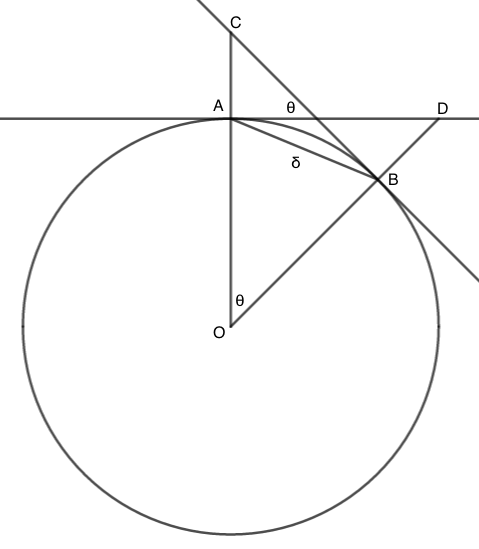
\includegraphics[width=\textwidth]{Circle-1.png}
                \caption{Drawing for Theorem 3.2.2}
              \end{subfigure}
              \begin{subfigure}[b]{0.32\textwidth}
                \centering
                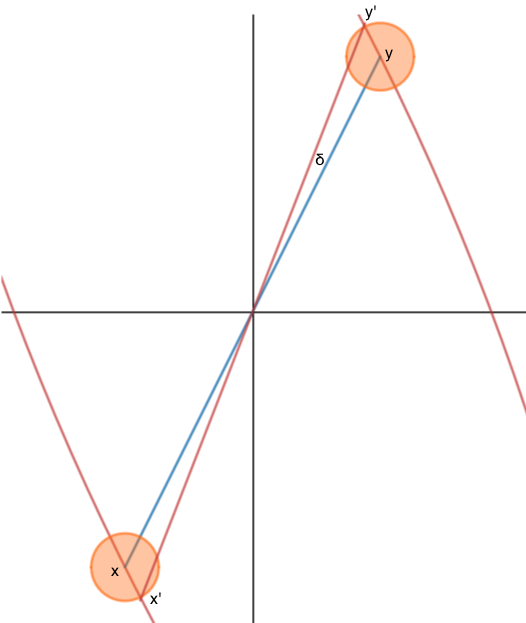
\includegraphics[width=\textwidth]{convex-1.png}
                \caption{Drawing for Theorem 3.2.3}
              \end{subfigure}
              \begin{subfigure}[b]{0.32\textwidth}
                \centering
                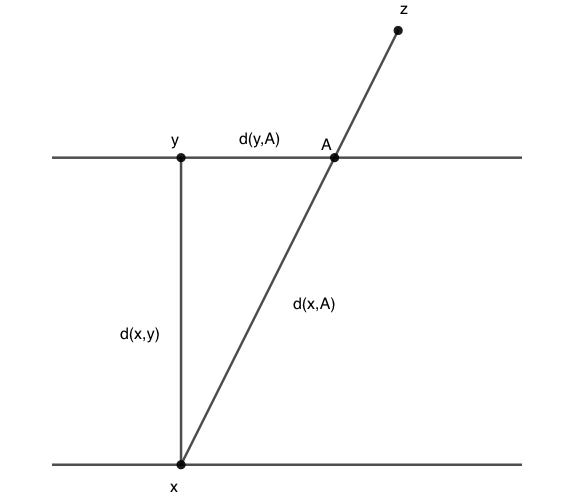
\includegraphics[width=\textwidth]{line-1.png}
                \caption{Drawing for Lemma 3.2.1}
              \end{subfigure}  
            \end{figure}
            \begin{theorem}
            If $K\subset \mathbb{R}^2$ is compact and convex, then $R_K(\theta)$ is continuous.
            \end{theorem}
            \begin{proof}
            For let $K$ be compact and convex, and without loss of generality suppose it contained within the unit disc and contains the origin. Let $\theta\in (0,2\pi)$ be given and let $\ell_{\theta}$ be a line through the origin making an angle $\theta$ with the horizontal. Let $x=(x_1,x_2),y=(y_1,y_2)\in K$ be such that $W_{\ell_{\theta}}(K) = d(x,y)$. Such points exist as $K$ is compact. Let $\varepsilon>0$ be given. About $x$, consider $B_{\frac{\varepsilon}{2}}(x)$, and similarly $B_{\frac{\varepsilon}{2}}(y)$. Neither of these are empty, as $K$ is convex. Let $x',y'\in K\cap(B_{\frac{\varepsilon}{2}}(x)\cup B_{\frac{\varepsilon}{2}}(y))$ be such that $d(x',y')$ is maximized. As this set is compact, such points exist. Let $\delta = \min\{|\theta-\frac{x_2'}{\sqrt{x_1'^2+x_2'^2}}|,|\theta-\frac{y_2'}{\sqrt{y_1'^2+y_2'^2}}|\}$. Then for $|\theta-\theta_0|<\delta$, $d(x,y)-\varepsilon \leq W_{\ell_{\theta_0}}(K)\leq d(x,y)+\varepsilon$, and thus $|W_{\ell_\theta}(K)-W_{\ell_{\theta_0}}(K)| < \varepsilon$.
            \end{proof}
            \begin{lemma}
            If $K$ is a compact subset of $\mathbb{R}^2$ and $x,y\in K$ such that $d(x,y)=D(K)$, then the lines perpendicular to $\overline{xy}$ at $x$ and $y$ contain all of $K$ in between.
            \end{lemma}
            \begin{proof}
            Suppose not. Let $\overline{X}$ be the line perpendicular to $\overline{xy}$ containing point $x$, and similarly define $\overline{Y}$. Suppose there is a point $z\in K$ that falls on the exterior of the region $\mathcal{U} = \{(x,y)\in \mathbb{R}^2: (x,y)\ \textrm{Lies Between } \overline{X}\ \textrm{and } \overline{Y}\}$. Note that $d(x,z)\ne d(y,z)$, as then $z$ would line between these two lines. Suppose $d(y,z)<d(x,z)$. Where the line $\overline{xz}$ cuts $\overline{Y}$ denote as $A$. But then $d(x,z) > d(x,A) = \sqrt{d(y,A)^2+d(x,y)^2}\geq d(x,y)$. A contradiction as $d(x,y) = D(K)$. Thus $z\in \mathcal{U}$.
            \end{proof}
            \begin{theorem}
            If $K\subset \mathbb{R}^2$ is compact and convex, then there are points $x,y\in K$ such that $\check{W}(K)=d(x,y)$.
            \end{theorem}
            \begin{proof}
            As $f_K(\theta)$ is continuous for convex compact set, and as it is continuous on a compact set $[0,2\pi]$, it attains its maximum. Let $\theta$ be such a maximum. Let $\ell_{\theta}$ be the line through the origin which makes an angle $\theta$ with the horizontal axis and consider set $K_{\ell_{\theta}}$. As $K$ is compact and $\ell_{\theta}$ is closed, $K_{\ell_{\theta}}$ is compact. Then $W=\{d(x,y):x,y\in K_{\ell_{\theta}}\}$ is bounded, has a least upper bound, and therefore there are points $x,y \in K$ such that $\check{W}(K)=d(x,y)$.
            \end{proof}
            \begin{theorem}
            If $K$ is a compact convex set of $\mathbb{R}^2$, then $D(K) = \check{W}(K)$.
            \end{theorem}
            \begin{proof}
            As $K$ is compact, $D(K)$ and $\check{W}(K)$ exists and there are points $x,y$ such that $d(x,y) = D(K)$ and points $x',y'$ such that $d(x',y') = \check{W}(K)$. Suppose $d(x',y')> d(x,y)$. A contradiction, as $d(x,y)$ is the diameter of $K$. So $d(x,y) \geq d(x',y')$. Now suppose $d(x,y)>d(x',y')$. But as $d(x',y')= \check{W}(K)$, $d(x',y')$ is the greatest length of any line segment that terminates in $K$ and such that perpendiculars at these terminating points contain all of $K$. But as $d(x,y)=D(K)$, the lines perpendicular to $\overline{xy}$ at $x$ and $y$ contain all of $K$, a contradiction. Thus $d(x',y') \geq d(x,y)$. But it was just showed that $d(x,y)\geq d(x',y')$. Thus, $d(x,y) = d(x',y')$. $D(K) = \check{W}(K)$.
            \end{proof}
            \begin{definition}
            If $Q$ is a convex polygon with interior (That is, positive area) in $\mathbb{R}^2$, then the perimeter of $Q$ is the sum of the lengths of its edges. 
            \end{definition}
            \begin{definition}
            The perimeter of a line segment $e$ is $P(e) = 2|e|$.
            \end{definition}
            \begin{remark}
            This is for the sake of continuity. If we take a rectangle of length $|e|$ and width $\frac{1}{n}$, then the perimeter is $2|e|+\frac{2}{n} \rightarrow 2|e|$ as $n\rightarrow \infty$. Thus, for the puprose of continuity we define the perimeter of line segments to be twice their length.
            \end{remark}
            \begin{theorem}[Cauchy's Perimeter Theorem]
            If $K$ is a compact convex subset of the plane, then $P(K) = \pi W(K)$.
            \end{theorem}
            \begin{proof}
            Suppose that $Q$ is a convex polygon with edges $e_1,\hdots, e_n$. At each $e_i$, let $\theta_i$ be the angle made with $e_i$ and the horizontal axis of $\mathbb{R}^2$. The mean width is $W(Q) = \frac{1}{2\pi}\int_{0}^{2\pi} W_{\ell_\theta}(Q)d\theta = \frac{1}{2\pi} \int_{0}^{2\pi} \frac{1}{2} \sum_{i=1}^{n} |e_i||\cos(\theta-\theta_i)|d\theta = \frac{1}{4\pi}\sum_{i=1}^{n} |e_i|\int_{0}^{2\pi} |\cos(\theta-\theta_i)|d\theta = \frac{1}{\pi} \sum_{i=1}^{n} |e_i| = \frac{1}{\pi} P(Q)$. Thus, $P(Q) = \pi W(Q)$. For any convex compact subset $K\subset \mathbb{R}^2$, we may find a polygon $Q$ that approximates the boundary with a perimeter $P(Q)$ that is as close to $P(K)$ and a width $W(Q)$ as close to $W(K)$ as desired. That is, for all $n\in \mathbb{N}$, we can obtain a polynomial $Q_n$ such that $\max\{|W(Q_n)-W(K)|,|P(K)-P(Q_n)|\}< \frac{1}{n}$. Then $|P(K)-\pi W(K)| = |P(K) - P(Q_n)+P(Q_n)-\pi W(Q_n)+\pi W(Q_n)-\pi W(K)| \leq |P(K)-P(Q_n)|+|P(Q_n)-\pi W(Q_n)|+\pi|W(Q_n)-W(K)| < \frac{1}{n} + 0 + \frac{\pi}{n} = \frac{1+\pi}{n} \rightarrow 0$. Thus, $P(K) = \pi W(K)$ for arbitrary convex compact subsets of the plane.
            \end{proof}
            \begin{theorem}
            There exist compact path-connected sets $K\subset \mathbb{R}^2$ such that $P(K) \ne \pi W(K)$.
            \end{theorem}
            \begin{proof}
            Consider the set $K = \{(x,y) \in \mathbb{R}^2: x^2+y^2=1, y\geq 0\}$. Then $P(K) = 2\pi$, but \\ $W(K) = \pi(\pi+2)$. To see this, consider the set $\mathcal{K} = \{(x,y)\in \mathbb{R}^2: x^2 + y^2 \leq 1, y\geq 0\}$. This is convex and has perimeter $\pi+2$ and therefore $W(\mathcal{K}) = \pi(\pi+2)$. But, as the image shows, $W(K) = W(\mathcal{K})$. That is, $W_{\ell_{\theta}}(K)$ is the length of the line segment $\overline{AB}$, as is $W_{\ell_{\theta}}(\mathcal{K})$. Therefore the averages $W(K)$ and $W(\mathcal{K})$ are the same. Thus, $P(K) \ne \pi W(K)$.
            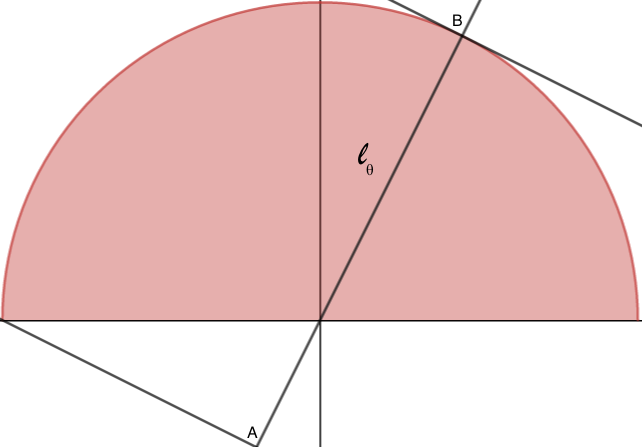
\includegraphics[scale=0.3]{semicircle-1.png}
            \end{proof}
            \begin{definition}
            A functional $f$ with respect to subset inclusion is said to be monotonic on a family of sets $\mathscr{P}$ if and only if $f(K)\leq f(L)$ for all $K,L \in \mathscr{P}$ such that $K\subset L$.
            \end{definition}
            \begin{theorem}
            If $K\subset L \in \mathscr{K}_2$, then $W_{\ell}(K) \leq W_{\ell}(L)$.
            \end{theorem}
            \begin{proof}
            For let $\pi_{\ell}:\mathbb{R}^2 \rightarrow \ell$ be the orthogonal projection map of $\mathbb{R}^2$ to $\ell$. Then $\pi_{\ell}(K)\leq \pi_{\ell}(L)$ as $K\subset L$, and thus $W_{\ell}(K)\leq W_{\ell}(L)$.
            \end{proof}
            \begin{theorem}
            If $K\subset L\in \mathscr{K}_2$, then $W(K)\leq W(L)$.
            \end{theorem}
            \begin{proof}
            For $W_{\ell}(K)\leq W_{\ell}(L)$, and thus $W(K)=\frac{1}{2\pi}\int_{0}^{2\pi}W_{\ell_{\theta}}(K)d\theta \leq \frac{1}{2\pi}\int_{0}^{2\pi}W_{\ell_{\theta}}(L)d\theta=W(L)$.
            \end{proof}
            \begin{theorem}
            If $K\subset L\in \mathscr{K}_2$, then $X_{\ell}(K)\leq X_{\ell}(L)$.
            \end{theorem}
            \begin{proof}
            For if $x\in \ell\cap K$, then $x\in \ell\cap L$, and thus $X_{\ell}(K)=\mu(\ell\cap K) \leq \mu(\ell\cap L)=X_{\ell}(L)$.
            \end{proof}
            \begin{theorem}
            If $K\subset L\subset \mathscr{K}_2$, then $D(K)\leq D(L)$.
            \end{theorem}
            \begin{proof}
            For suppose not. Suppose $D(K)>D(L)$. Then, there are points $x,y\in K$ such that $d(x,y)> \sup\{d(x',y'):x',y'\in L\}$. But as $K\subset L$, $x,y\in L$ and thus $d(x,y) \not> \sup\{d(x',y'):x',y'\in L\}$. Thus, $D(K)\leq D(L)$.
            \end{proof}
            \begin{theorem}
            If $K\subset L \subset \mathscr{K}_2$, then $R_K\leq R_L$.
            \end{theorem}
            \begin{proof}
            For suppose not. Suppose $R_K>R_L$. But as $K\subset L$, either this circle contains all of $L$ as well or it doesn't. But then $R_L \not<R_K$. Thus, $R_L\geq R_K$.
            \end{proof}
            \begin{theorem}
            If $K\subset L \in \mathscr{K}_2$, then $r_K \leq r_L$.
            \end{theorem}
            \begin{proof}
            For suppose not. Suppose $r_K> r_L$. But as the inscribed circle of radius $r_K$ fits entirely in $K$, and $K\subset L$, then it fits inside of $L$. But then $r_K \not > r_L$. Thus, $r_L \geq r_K$.
            \end{proof}
            \begin{theorem}
            If $K,L\in \mathscr{K}_2$ and $K\subset L$, then $P(K)\leq P(L)$.
            \end{theorem}
            \begin{proof}
            As $K\subset L\in  \mathscr{K}_2$, $W(K)\leq W(L)$. As $K$ and $L$ are convex, $P(K)=\pi W(K)$ and $P(L)=\pi W(L)$. Thus, $P(K) \leq \pi W(L) = P(L)$. Therefore, $P(K)\leq P(L)$.
            \end{proof}
            \begin{theorem}
            There exists sets $K,L\subset \mathbb{R}^2$ such that $L$ is convex, $K\subset L$, yet $P(K)>P(L)$.
            \end{theorem}
            \begin{proof}
            For let $L = \{(x,y)\in \mathbb{R}^2: x^2 + y^2 \leq 1\}$. Then $P(L) = 2\pi$. Let $K = \{(x,y)\in \mathbb{R}^2: -\sqrt{2}x\leq y \leq \sqrt{2}x,\frac{-1}{\sqrt{3}} \leq x \leq \frac{1}{\sqrt{3}} \lor \sqrt{2}x\leq y \leq -\sqrt{2}x,\frac{-1}{\sqrt{3}} \leq x \leq \frac{1}{\sqrt{3}} \}$. $P(K) = 4(1+ \sqrt{\frac{2}{3}}) \approx 7.26>2\pi$.
            \end{proof}
            \begin{figure}[H]
              \begin{subfigure}[b]{0.49\textwidth}
                 \centering
                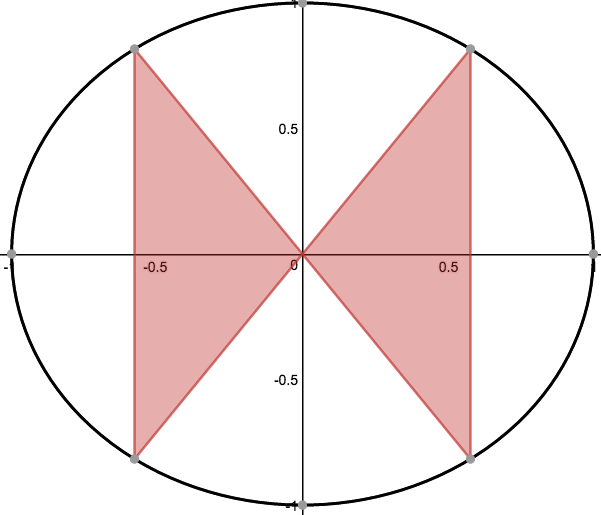
\includegraphics[width=\textwidth]{Circles-3.png}
                \caption{Drawing for Theorem 3.2.15}
              \end{subfigure}
              \begin{subfigure}[b]{0.49\textwidth}
                \centering
                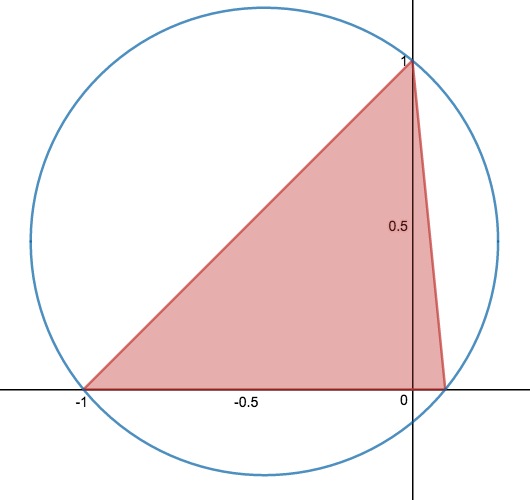
\includegraphics[width=\textwidth]{Circle-4.png}
                \caption{Drawing for Theorem 3.2.16}
              \end{subfigure}
            \end{figure}
            \begin{theorem}
            There exist compact convex sets in $\mathbb{R}^2$ such that $D(K) < 2R_K$.
            \end{theorem}
            \begin{proof}
            For consider the set $K=\{(x,y)\in \mathbb{R}^2: [0\leq y\leq x+1 \land x\geq 0]\lor [0\leq y\leq -10x+1\land x\geq 0]\}$. From Euclid, the smallest circle containing this triangle is the one defined by the three vertices (Three points define a triangle). This circle has the formula $(x+0.45)^2+(y-0.45)^2 = (0.45)^2 +(0.45+\frac{1}{10})^2$. Thus, $2R_K = \sqrt{0.45^2 +(0.45+\frac{1}{10})^2} > \sqrt{2} = D(K)$.
            \end{proof}
            \begin{theorem}
            If $K$ is a compact convex set in $\mathbb{R}^2$, then $D(K) \leq 2R_K$.
            \end{theorem}
            \begin{proof}
            For suppose not. Suppose $D(K) > 2R_K$. As $K$ is compact, there are points $x$ and $y$ in $K$ such that $d(x,y)=D(K)$. But then $d(x,y)>2R_K$, and thus at least one of $x$ or $y$ is not contained in the circle. A contradiction. Thus $D(K)\leq 2R_K$.
            \end{proof}
            \begin{theorem}
            If $K$ is a compact convex set in $\mathbb{R}^2$, then $2\pi r_K \leq P(K)$.
            \end{theorem}
            \begin{proof}
            From Calculus of Variations we know that the circle maximizes the area contained with a set of perimeter $p$. As the inscribed circle has perimeter $2\pi r_K$ and as the circle is a subset of $K$, it is true that $A(K)$ is greater than or equal the area of the circle. Thus, $P(K)\geq 2\pi r_K$.
            \end{proof}
            \begin{theorem}
            For a compact convex set of $\mathbb{R}^2$, $P(K) \leq 2\pi R_K$.
            \end{theorem}
            \begin{proof}
            As $K$ is convex, $P(K) = \pi W(K) \leq \pi \check{W}(K) = \pi D(K) \leq 2\pi R_K$.
            \end{proof}
            \begin{theorem}
            If $K$ is a compact and convex subset of $\mathbb{R}^2$, then $2D(K)\leq P(K)$.
            \end{theorem}
            \begin{proof}
            Suppose not. Suppose $2D(K) >P(K)$. As $K$ is compact and convex, there exist points $x,y\in K$ such that $d(x,y) = D(K)$. But as $K$ is convex, the line contained between $x,y$ in contained in $K$. Thus, $P(\overline{xy}) = 2D(K)$. But as $\overline{xy}\subset K$, $P(K)>P(\overline{xy})$, a contradiction. Thus, $2D(K) \leq P(K)$.
            \end{proof}
            \begin{theorem}
            There exist compact convex subsets of $\mathbb{R}^2$ such that $2D(K) = P(K)$.
            \end{theorem}
            \begin{proof}
            For take a straight line segment of length $\ell$. Then $D(K) = \ell$, $P(K) = 2\ell$, and thus $2D(K) = P(K)$.
            \end{proof}
            \begin{theorem}
            If $K$ is a compact convex subset of $\mathbb{R}^2$, then $P(K) \leq \pi D(K)$.
            \end{theorem}
            \begin{proof}
            From Cauchy's Perimeter theorem, $P(K) = \pi W(K) \leq \pi \check{W}(K) = \pi D(K)$.
            \end{proof}
            \begin{theorem}
            For a compact convex subset $K$ of $\mathbb{R}^2$, $P(K) = \pi D(K)$ if and only if $W_{\ell}(K)$ is a constant.
            \end{theorem}
            \begin{proof}
            For then $\frac{1}{2\pi} \int_{0}^{2\pi} W_{\ell_{\theta}}(K) d\theta = \check{W}(K)$. But as $W_{\ell_{\theta}}(K)$ is continuous for compact convex bodies, it must be true that $W_{\ell_{\theta}}(K) = \check{W}(K)$ for all $\ell_{\theta}$. Thus, $K$ is of constant width.
            \end{proof}
            \begin{remark}
            There are many types of shapes that have constant width besides discs. The Reuleaux Triangle is such an example.
            \end{remark}
            Triangles are the simplest convex bodies in the plane other than points and lines. Any convex polygon can be written as the union of triangles with disjoint interiors. 
            \begin{theorem}
            If $\Delta_s$ is an equilateral triangle with edge length $s$, then $\Delta_s$ has the following properties:
            \begin{enumerate}
            \begin{multicols}{5}
            \item $A(\Delta_s) = \frac{\sqrt{3}}{4}s^2$
            \item $P(\Delta_s) = 3s$
            \item $W(\Delta_s) = \frac{3s}{\pi}$
            \item $R_{\Delta_s} = \frac{1}{\sqrt{3}}s$
            \item $r_{\Delta_s} = \frac{1}{2\sqrt{3}}s$
            \end{multicols}
            \end{enumerate}
            \end{theorem}
            \begin{proof}
            In order:
            \begin{enumerate}
                \item From Pythagoras, $A(\Delta_s) =2\times\big[\frac{1}{2}(\frac{1}{2}s)(\frac{\sqrt{3}}{2}s)\big] = \frac{\sqrt{3}}{4}s^2$
                \item There are three edges, each of length $s$, and thus $P(\Delta_s) = 3s$.
                \item $W(\Delta_s) = \frac{1}{\pi}P(\Delta_s) = \frac{3s}{\pi}$
                \item The circumcircle gives the following equations:
                \begin{enumerate}
                    \item $R_{\Delta_s}^2=\frac{s^2}{4}+h^2$
                    \item $h+R_{\Delta_s} = \frac{\sqrt{3}}{2}s$
                \end{enumerate}
                This has solution $R_{\Delta_s}=\frac{1}{\sqrt{3}}s$
                \item $r_{\Delta_s} = \frac{R_{\Delta_s}}{2}= \frac{1}{2\sqrt{3}}s$
            \end{enumerate}
            \end{proof}
            \begin{theorem}
            If $T$ is a triangle in the plane, then there is a linear transformation $\psi$ such that $\psi T$ is equilateral.
            \end{theorem}
            \begin{proof}
            For let $T$ be a triangle with vertices $a=(x_1,y_1)$, $b=(x_2,y_2)$, $c=(x_3,y_3)$. Let $A = d(b,c)$, $B=d(a,c)$, and $C=d(a,b)$. Suppose If $A=B=C$, we are done. Thus, suppose $C\geq B >A$. At point $a$ and with radius $C$, construct the circle $b,c',d$, and point $b$ and with radius $C$, construct the circle $a,c',e$. If we can shift $c$ to $c'$ in a linear fashion, we are done. Let $\psi =$
            \end{proof}
            \begin{theorem}
            If $T$ is a triangle with edges $a,b,c$ and opposite angles $\alpha,\beta,\gamma$, respectively, then $A(T) = \frac{\sin(\alpha)}{2}bc = \frac{\sin(\beta)}{2}ac = \frac{\sin(\gamma)}{2}ab$
            \end{theorem}
            \begin{proof}
            Suppose the triangle is acute. The proof is symmetric for all sides, so we prove it for just $\alpha$. Note that the perpendicular $h$ dropped from the vertex of $a$ onto $b$ satisfies $h^2+\ell_1^2 = c^2$ and $h^2+\ell_2^2 = a^2$, where $\ell_1+\ell_2 = b$. Then $\sin(\alpha) = \frac{h}{c}$ and $A(T) = \frac{1}{2}h\ell_1 + \frac{h}{2}h\ell_2 = \frac{h}{2}(\ell_1+\ell_2)h = \frac{1}{2}bh = \frac{1}{2}bc\sin(\alpha)$. An identical argument works for obtuse triangles.
            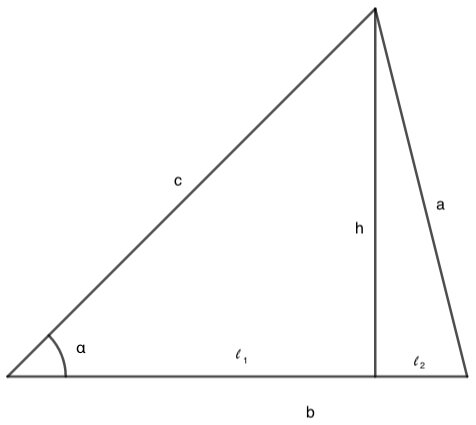
\includegraphics[scale=0.3]{triangle-1.png}
            \end{proof}
            \begin{corollary}[The Law of Sines]
            For a triangle with edges $a,b,c$ and opposite angles $\alpha,\beta,\gamma$, $\frac{\sin(\alpha)}{a} = \frac{\sin(\beta)}{b} = \frac{\sin(\gamma)}{c}$
            \end{corollary}
            \begin{proof}
            From the previous theorem, divide by $\frac{abc}{2}$ to obtain the result.
            \end{proof}
            \begin{theorem}[The Law of Cosines]
            Given a triangle with lengths $a,b,c$ and opposite edges $\alpha,\beta,\gamma$, $c^2=a^2+b^2-2ab\cos(\gamma)$.
            \end{theorem}
            \begin{proof}
            If $\gamma=\frac{\pi}{2}$, this is Pythagoras' Theorem. Thus, suppose $0<\gamma < \frac{\pi}{2}$. Where $c$ and $a$ meet, drop a perpendicular onto $c$ and call this $h$. $h$ satisfies $h^2+\ell_1^2 = c^2$ and $h^2+\ell_2^2=a^2$ from Pythagoras' Theorem, where $\ell_1+\ell_2 = b$. But $\ell_2 = a\cos(\gamma)$, so $\ell_1 = b-a\cos(\gamma)$. Thus $c^2 = h^2 + b^2 +a^2\cos^2(\gamma)-2ab\cos(\gamma)$. But $h = a\sin(\gamma)$. Thus, $c^2 = b^2 + a^2 \cos^2(\gamma)+\sin^2(\gamma)-2ab\cos(\gamma) = b^2 + a^2(\sin^2(\gamma)+\cos^2(\gamma))-2ab\cos(\gamma) = a^2 + b^2 -2ab\cos(\gamma)$. A similar construction is done if $\frac{\pi}{2}<\gamma < \pi$.
            \end{proof}
            \begin{theorem}
            Given a triangle $\Delta$ with lengths $a\leq b\leq c$, $D(\Delta)=c$.
            \end{theorem}
            \begin{proof}
            At the midpoint of $c$, and with radius $c$, construct a circle. This circle contains the entirety of $\Delta$, and thus for all points $x,y\in \Delta$, $d(x,y)\leq c$. Thus, $c=D(\Delta)$.
            \end{proof}
            \begin{theorem}[Heron's Formula]
            For a triangle with lengths $a,b,c>0$, $A(T)^2 = \frac{1}{16}(a+b+c)(-a+b+c)(a-b+c)(a+b-c)$.
            \end{theorem}
            \begin{proof}
            For $A(T) = \frac{1}{2}ab \sin(\gamma) = \frac{1}{2}ab\sqrt{1-\cos^2(\gamma)} = \frac{1}{4}\sqrt{4a^2 b^2 - (a+b-c)^2}=\\ \frac{1}{4}\sqrt{(2ab-(a^2+b^2-c^2))(2ab+(a^2+b^2+c^2))} = \frac{1}{4}\sqrt{(c^2-(a-b)^2)((a+b)^2-c^2)} = \\ \frac{1}{4}\sqrt{(a+b+c)(-a+b+c)(a-b+c)(a+b-c)}$. Squaring this gives the result.
            \end{proof}
            \begin{theorem}
            For any triangle $\Delta$, $r_{\Delta}P(\Delta) = 2A(\Delta)$.
            \end{theorem}
            \begin{proof}
            For let $\Delta$ has sides $a,b,c$, with opposite angles $\alpha, \beta, \gamma$, respectively. Then $A(\Delta) = \frac{ab}{2}\sin(\gamma)$ and $P(\Delta)=a+b+c$. Thus, $\frac{2A(\Delta)}{P(\Delta)} = \frac{ab\sin(\gamma)}{a+b+c}$. But this is the radius of the incircle of $\Delta$. Therefore, etc.
            \end{proof}
            \begin{theorem}[Viviani's Theorem: Page 17]
            \end{theorem}
            \begin{theorem}
            There exist convex polygon's such that the inradius is not unique.
            \end{theorem}
            \begin{proof}
            For consider the rectangle $[0,2]\times [0,1]$. The diameter of any circle that sits inside this body must be at most $1$, and thus the radius is at most $\frac{1}{2}$. However, there are multiple circles that achieve this. For example $(x-\frac{1}{2})^2+(y-\frac{1}{2})^2=\frac{1}{2}$ and $(x-\frac{3}{2})^2+(y-\frac{3}{2})^2=\frac{1}{2}$.
            \end{proof}
            \begin{theorem}
            For an acute triangle, $\frac{2(A)}{abc} = \frac{1}{R_T}$.
            \end{theorem}
            \begin{theorem}
            If $\Delta$ is a triangle with vertices $A,B,C$ and sides $a,b,c$, then given a circle that contains $A,B,C$, the radius of this circle $R$ satisfies $\frac{1}{R} =\frac{2A(\Delta)}{abc}$
            \end{theorem}
            \begin{definition}
            If $K\in \mathscr{K}_2$, then $-K = \{-x:x\in K\}$.
            \end{definition}
            \begin{theorem}
            If $K\in \mathscr{K}_2$, then $W_{\ell}(K) = W_{\ell}(-K)$.
            \end{theorem}
            \begin{proof}
            For let $x,y\in K$ be such that $d(x,y) = W_{\ell}(K)$. Then $d(-x,-y) = W_{\ell}(-K) = d(x,y)$. Therefore, etc.
            \end{proof}
            \begin{theorem}
            There exist sets $K$ and $L$ such that $W_{\ell}(K)<W_{\ell}(L)$ for all $\ell$ yet $K\not\subset L$ for any translation or rotation of $K$.
            \end{theorem}
            \begin{definition}
            For $K\in \mathscr{K}$ and unit vector $u$, $\bar{X}_{u}(K)$ is the mean value of $X_{\ell}(K)$ over all lines $\ell$ parallel to $u$ such that $X_{\ell}(K)>0$.
            \end{definition}
            \begin{theorem}
            For $K\in \mathscr{K}_2$, $\bar{X}_{u}(K) = W_{\ell}(K)=A(K)$.
            \end{theorem}
        \section{On Uniform Convergence}
            \begin{definition}
                A sequence of functions $f_n$ is said to converge
                point-wise on a set $A$ to a function $f$, if
                $\forall\varepsilon>0$ and $\forall x\in A$, there is
                an $N\in\mathbb{N}$ such that $n>N \Rightarrow
                |f(x)-f_n(x)|<\varepsilon$.
            \end{definition}
            \begin{definition}
                A sequence of functions $f_n$ converge uniformly on a
                set $A$ to $f$ if and only if $\forall \varepsilon>0$
                $\exists N\in\mathbb{N}$ such that $\forall x \in A$
                and $n>N$, $|f(x) -f_n(x)|<\varepsilon$.
            \end{definition}
            \begin{definition}
                A sequence of functions $f_n$ are point-wise
                equicontinuous on a set $A$ if and only if
                $\forall_{\varepsilon>0}\forall_{x\in A}
                \exists_{\delta>0}\forall_{n\in\mathbb{N}}:
                |x-x_0|<\delta\Rightarrow|f_{n}(x)-f_{n}(x_0)|<
                \varepsilon$
            \end{definition}
            \begin{definition}
                A sequence of functions $f_n$ are uniformly
                equicontinuous on a set A if and only if
                $\forall_{\varepsilon>0}\exists_{\delta>0}
                \forall_{x\in A}\forall_{n\in\mathbb{N}}:
                |x-x_{0}|<\delta\Rightarrow|f_{n}(x)-f_{n}(x_{0})|<
                \varepsilon$.
            \end{definition}
            \begin{definition}
                A subset $A$ of the real line is open if
                $\forall_{x\in A}\exists_{r>0}:
                \forall_{y\in (x-r,x+r)},y\in A$.
            \end{definition}
            \begin{definition}
                An open cover $\Delta$ of a set $A\subset S$ is a set
                of open subsets $A_k\subset S$, such that
                $A\subset\cup_{k\in I}A_{k}$, where $I$ is some
                index, countable or uncountable.
            \end{definition}
            \begin{definition}
                A set $A$ is said to be compact if and
                only if for all open coverings $\Delta$ there is
                a finite sub-cover $\Delta_0\subset \Delta$, such
                that $A\subset \cup_{A_k \in \Delta_0} A_k$.
            \end{definition}
            \begin{theorem}
                [Heine-Borel Theorem]
                Any closed-bounded subset of the real line is compact. 
            \end{theorem}
            \begin{proof}
                For let $A$ be a closed and bounded subset of
                $\mathbb{R}$ with least upper bound $b$ and
                greatest lower bound $a$. Let $\Delta$ be an
                open covering, and let $X$ be the set of
                points $y\in A$ such that for all $s<y$ such
                that $s\in A$, there is a finite refinement
                of $\Delta$ which covers these points. $X$ is
                non-empty, as $a\in X$. The set $X$ is bounded,
                as for all points $y\in X$ we have that
                $a\leq y\leq b$. As bounded sets have a least
                upper bound, let $x$ be the least upper bound.
                Suppose $x<b$. As $x\in [a,b]$, there exists an
                element $A_k$ of $\Delta$ such that $x \in A_k$.
                But as $A_k$ is open and therefore there is an
                $r>0$ such that
                $y\in (x-r,x+r)\Rightarrow y \in A_k$.
                But then $y=x+\frac{r}{2}>x$ and
                $y\in A_k$. Therefore x is not the
                least upper bound as we have found an
                element in $X$ greater than $x$.
                Therefore $x\not<b$. And thus $x=b$.
            \end{proof}
            \begin{theorem}
                If a sequence of functions are
                point-wise equicontinuous on a closed
                and bounded set, then they are
                uniformly equicontinuous.
            \end{theorem}
            \begin{proof}
                For let $A$ be a closed bounded subset
                of $\mathbb{R}$, and let $f_n(x)$ be a sequence
                of point-wise equicontinuous functions on $A$.
                As the set is closed and bounded, it is compact
                by the Heine-Borel theorem. Let $\varepsilon>0$
                be given. For $x\in A$, define the function
                $\delta(x)%
                 =\min\{\sup\{\delta>0:|x-x_0|<\delta,\ x_0\in A%
                  \Rightarrow |f_n(x)-f_n(x_0)|<\frac{\varepsilon}{2}$,
                $\forall n\in\mathbb{N}\},b-a\}$.
                Construct the open covering $\mathcal{U}$ as
                follows:
                $\mathcal{U}=\{(x-\delta(x),x+\delta(x)):\ x\in A\}$.
                This is an open covering, as every set in
                $\mathcal{U}$ is open, and for all
                $x\in A$, $x\in(x-\delta(x),x+\delta(x))\in\mathcal{U}$.
                But as $A$ is compact, there is a finite sub-cover.
                Let $a=x_0<x_1<...<x_{n-1}<x_n=b$ be the centers
                of the remaining open sets in the sub-cover.
                Further refine this sub-covering as follows: If
                $(x_j-\delta(x_j),x_j+\delta(x_j))%
                 \subset (x_k-\delta(x_k),x_k+\delta(x_k))$
                for $j\ne k$, then remove it from the sub-cover as
                it is superfluous. We now have a set of points
                $a=z_0<z_1<...<z_{N-1}<z_N=b$ such that
                $A\subset\cup_{i=0}^{N} (z_i-\delta(z_i),z_i+\delta(z_i))$.
                Let
                $\delta%
                 =\min\{\delta(z_0),...,\delta(z_N),\delta(b),%
                        \frac{(a+\delta(a))-(z_1-\delta(z_1))}{2},%
                        ...,%
                        \frac{(z_{N-1}+\delta(z_{N-1}))-(b-\delta(b))}{2}\}$.
                That is, $\delta$ is the smallest of the $\delta(z_i)$,
                or half of the smallest intersection of two consecutive
                intervals. Let $x\in A$ be arbitrary. If $(x-\delta,x+\delta)$
                is contained entirely in one of the
                $(z_i-\delta(z_i),z_i+\delta(z_i))$ sets, then we have
                that $|x-x_0|<\delta \Rightarrow |x-x_0| <\delta(z_i) \Rightarrow |f_n(x)-f_n(x_0)|<\frac{\varepsilon}{2}$ for all $n\in\mathbb{N}$.
                Suppose that $(x-\delta,x+\delta)$ is contained in two of
                the $(x-\delta(z_i),x+\delta(z_i))$ sets. Note, it cannot
                be in three or more as we have refined the sub-cover in
                such a manner as to prevent this. Let $y$ be the center
                of the intersection of these two sets. Then we have that
                for $|x-x_0|<\delta$, then
                $|f_n(x)-f_n(x_0)|%
                 =|f_n(x)-f_n(y)+f_n(y)-f_n(x_0)|%
                 \leq|f_n(x)-f_n(y)|+|f_n(y)-f_n(x_0)|$.
                But $|x-y|$ and $|x_0-y|$ are less than
                $\frac{(z_i + \delta(z_i))-(z_{i+1}-\delta(z_{i+1}))}{2}$
                apart, and therefore $|f_n(x)-f_n(y)|<\frac{\varepsilon}{2}$,
                and $|f_n(y)-f_n(x_0)|<\frac{\varepsilon}{2}$.
                Therefore, $|f_n(x)-f_n(x_0)|<\varepsilon$.
                And as $x$ is arbitrary,
                $f_n(x)$ is uniformly equicontinuous.
            \end{proof}
            \begin{theorem}
                If a sequence of point-wise equicontinuous functions converge, then the limit is point-wise continuous.
            \end{theorem}
            \begin{proof}
                For let $f_n:A\rightarrow \mathbb{R}$ be equicontinuous, $\varepsilon>0$ and $x\in A$ be given. Choose $\delta>0$ to satisfy the criterion of equicontinuity at $x$. Let $x_0$ be an arbitrary point in $(x-\delta,x+\delta)\cap A$. It suffices to show that $|f(x) - f(x_0)|<\varepsilon$. As $f_n \rightarrow f$ we have that $\exists N_1 \in\mathbb{N}$ such that $n>N_1\Rightarrow |f(x) - f_n(x)|<\varepsilon$. We also have that $\exists N_2 \in \mathbb{N}$ such that $n>N_2 \Rightarrow |f(x_0)-f_n(x_0)|<\varepsilon$. Let $N=\max\{N_1,N_2\}+1$. But we have that $|f(x) - f(x_0)| = |f(x) - f_N(x) + f_N(x)-f_N(x_0) + f_N(x_0) - f(x_0)|\leq |f(x) - f_n(x)| + |f_n(x)-f_n(x_0)| + |f_n(x_0) - f(x_0)| < 3\varepsilon$. $f$ is continuous.
            \end{proof}
            \begin{theorem}
                If $f_n \rightarrow f$ on a closed bounded subset of $\mathbb{R}$, and if $f_n$ is equicontinuous, then the convergence is uniform.
            \end{theorem}
            \begin{proof}
                Let $A$ be a closed bounded subset of $\mathbb{R}$, $f_n(x)$ a sequence of equicontinuous functions, and let $\varepsilon>0$ be given. As $f_n(x)$ is equicontinuous on a closed bounded set, it is uniformly equicontinuous. But the limit of equicontinuous functions is continuous. Let $\delta>0$ be such that, $\forall x\in A$, $\forall n\in\mathbb{N}$, $|x-x_0|<\delta, x_0\in A \Rightarrow |f_n(x)-f_n(x_0)|<\frac{\varepsilon}{3}$ and $|x-x_0|<\delta \Rightarrow |f(x)-f(x_0)|<\frac{\varepsilon}{3}$. Let $\mathcal{U} = \{(x-\frac{\delta}{2},x+\frac{\delta}{2}): x\in A\}$. This is an open cover of $A$ and thus there is a finite subcover. Let $x_0<x_1<\hdots<x_n$ be the centers of the finitely many sets $(x_k-\frac{\delta}{2},x_k+\frac{\delta}{2})$ that cover $A$. There is thus another finite sequence of positive integers, $N_0, N_1,... N_n$, such that $n>N_k \Rightarrow |f(x_k)-f_n(x_k)|<\frac{\varepsilon}{3}$, for $k=0,1,2,...,n$. Let $N= \max\{N_0, N_1, ..., N_n\}$.It suffices to show that, for any point $x_0 \in A$, for all $n>N$, $|f(x_0)-f_n(x_0)|<\varepsilon$. Let $x_0$ be arbitrary and let $x_k$ be the nearest point to $x_0$ in the above sequence (If there are two nearest points, pick your favorite). Then we have that, for $n>N$, $|f(x_0) - f_n(x_0)| = |f(x_0)-f(x_k)+f(x_k)-f_n(x_k)+f_n(x_k)-f_n(x_0)|\leq |f(x_k)-f(x_0)|+|f(x_k)-f_n(x_k)|+|f_n(x_k)-f_n(x_0)|<\varepsilon$. The convergence is uniform.
            \end{proof}
            \begin{theorem}
                [Integration of a Uniformly Convergent Sequence of Functions]
                If $f_n\rightarrow f$ uniformly on a closed bounded set $A$ with $g.u.b(A)=a$, then $\int_{a}^{x} f_n \rightarrow \int_{a}^{x} f$ uniformly on $A$.
            \end{theorem}
            \begin{proof}
                Let $\varepsilon >0$ be given, let $b=l.u.b.(A)$, and choose $N\in\mathbb{N}$ such that $n>N\Rightarrow |f(x)-f_n(x)|<\frac{\varepsilon}{b-a}$. Then we have $|\int_{a}^{x} f_n - \int_{a}^{x} f| = |\int_{a}^{x} (f_n-f)| \leq \int_{a}^{x} |f_n-f| < \int_{a}^{x} \frac{\varepsilon}{b-a}= \frac{\varepsilon}{b-a}(x-a) \leq \varepsilon$.
            \end{proof}
            \begin{theorem}
                [Differentiation of a Uniformly Convergent Sequence of Functions]
                If $f_n'\rightarrow g$ uniformly on a closed bounded set $A$, and if $f_n \rightarrow f$ on $A$, then $f'=g$.
            \end{theorem}
            \begin{proof}
                Let $a=g.u.b.(A)$ and $b=l.u.b.(A)$. We have that $f_n(x) - f_n(a) = \int_{a}^{x}f_n' \rightarrow \int_{a}^{x}g$ uniformly. But $f_n(x)-f_n(a) \rightarrow f(x) - f(a)$. Therefore $f'(x)=\frac{d}{dx}(f(x)-f(a)) = \frac{d}{dx}\int_{a}^{x} g = g(x)$. $f' = g$.
            \end{proof}
            \begin{theorem}
                [The Product of a Uniformly Convergence Sequence and a Bounded Function]
                If $f_n \rightarrow f$ uniformly, and if $g$ is a bounded function, then $f_n g \rightarrow fg$ uniformly.
            \end{theorem}
            \begin{proof}
                For let $\varepsilon>0$ and $x$ be given, and let $g$ be a bounded function with bound $M$, and choose $N\in\mathbb{N}$ such that $n>N \Rightarrow |f(x)-f_n(x)|<\frac{\varepsilon}{M}$. Then we have that $|f(x)g(x)-f_n(x)g(x)| = |g(x)||f(x)-f_n(x)| < M|f(x)-f_n(x)| <\varepsilon$.
            \end{proof}
            \begin{theorem}
                If $f$ is continuous on a compact set $A$, then it is uniformly continuous.
            \end{theorem}
            \begin{proof}
                For let $\varepsilon>0$ be given, let $a=g.u.b.(A)$, $b=l.u.b.(A)$, and for $x\in A$ define $\delta(x) = \min\{\sup\{\delta>0: |x-x_0|<\delta,x_0\in A\Rightarrow |f(x)-f(x_0)|<\frac{\varepsilon}{2}\},b-a\}$. Let $\Delta = \{(x-\delta(x),x+\delta(x)):x\in A\}$. Then $\Delta$ is an open cover of $A$ and therefore there is an open subscover. Let $x_k$ be the centers of the finitely many sets $(x_k-\delta(x_k),x+\delta(x_k))$ that cover $A$. Further refine this by removing overlaps. That is, if $(x_i-\delta(x_i),x_i+\delta(x_i))\subset (x_j-\delta(x_j),x_j+\delta(x_k))$ for $i\ne j$, then remove it for it is superfluous. We thus obtain a new sequence $z_1,\hdots, z_N$ such that the intervals $(z_k-\delta(z_k),z_k+\delta(z_k))$ cover $A$. Define $\delta = \min\{\delta(z_1),\hdots,\delta(z_N), \frac{(z_0+\delta(z_0))-(z_1-\delta(z_1))}{2},\hdots,(\frac{z_{N-1}+\delta(z_{N-1}))-(z_{N}-\delta(z_{N})}{2}\}$. Let $x,x_0\in A$ such that $|x-x_0|<\delta$. Let $x_k$ be the closest point in the sequence to $x$ (If there are two such points, pick your favorite). Then $|f(x)-f(x_0)|=|f(x)-f(x_k)+f(x_k)-f(x_0)|\leq |f(x)-f(x_k)|+|f(x_k)-f(x_0)|<\varepsilon$
            \end{proof}
            \begin{remark}
                The proof of this is a mimicry of the proof that equicontinuity on a compact set implies uniform equicontinuity.
            \end{remark}
            \begin{definition}
                A set $A$ is called sequentially compact if given a sequence $x_n\in A$, there is a convergent subsequence $x_{n_k}$.
            \end{definition}
            \begin{theorem}
                Compact sets of $\mathbb{R}$ are sequentially compact.
            \end{theorem}
            \begin{proof}
                Let $A$ be a compact set in $\mathbb{R}$, and let $x_n$ be a sequence in $A$. A point $x\in A$ is the limit of a subsequence of $x_n$ if for every $\varepsilon>0$ there are infinitely many of the $x_n$ such that $|x-x_n|<\varepsilon$. Suppose there is no such point. That is, for each $x\in A$ only finitely many of the $x_n$ lie within sufficiently small $\varepsilon-$neighborhoods. Let $\varepsilon(x) = \sup\{\varepsilon>0:\textrm{Only finitely many }x_n \textrm{ lie within } \varepsilon \textrm{ of } x\}$. Define $E=\{(x-\varepsilon(x)<x+\varepsilon(x)):x\in A\}$. This is an open cover of $A$, and therefore there is a finite subcover. Thus, at least one of the finitely many intervals $(x-\varepsilon(x),x+\varepsilon(x))$ must contain infinitely many of the $x_n$, a contradiction. Thus there is a convergent subsequence.
            \end{proof}
            \begin{theorem}
                Continuous functions on compact sets are bounded.
            \end{theorem}
            \begin{proof}
                For suppose not. Let $f:A\rightarrow \mathbb{R}$ be a continuous function on a compact set $A$, and let $x_n$ be a sequence of points in $A$ such that $f(x_n)>n$. Such a sequence must exist as $f$ is not bounded. As $A$ is compact, there must a point $x\in A$ such that some subsequence $x_{n_k}$ that converges to $x$. Let $\varepsilon >0$. Then, as $f$ is continuous, there is a $\delta>0$ such that $|x-x_0|<\delta,\ x_0\in A\Rightarrow |f(x)-f(x_0)|<\varepsilon$. But then for all points $x_{n_k}$ such that $|x-x_{n_k}|<\delta$, $-\varepsilon<f(x_{n_k})-f(x)<\varepsilon \Rightarrow f(x)-\varepsilon < f(x_{n_k})<f(x)+\varepsilon$. A contradiction as $f(x_{n_k})$ is unbounded. Thus, $f$ is bounded.
            \end{proof}
            \begin{corollary}
                Continuous functions on compact sets attain their maximum and minimum.
            \end{corollary}
            \begin{proof}
                For let $f:A\rightarrow \mathbb{R}$ be a continuous function on a compact set $A$. Let $f(A) = \{y\in \mathbb{R}:\exists x\in A|\ f(x)=y\}$. (This is called the image of $A$ under $f$). As $f$ is continuous, it is bounded, and thus the set $f(A)$ is bounded. But bounded sets have an l.u.b. and a g.u.b. Therefore, etc.
            \end{proof}
            \begin{lemma}
                [Uniform Limit Theorem]
                If $f_n\rightarrow f$ uniformly, and if the $f_n$ are continuous, then $f$ is continuous.
            \end{lemma}
            \begin{proof}
                For let $\varepsilon>0$ be given and let $x\in A$. Let $N\in \mathbb{N}$ such that $n>N$ implies $|f(\chi)-f_n(\chi)|<\frac{\varepsilon}{3}$ for all $\chi\in A$. Let $\delta>0$ be chosen such that $|x-x_0|<\delta, x_0\in A\Rightarrow |f_N(x)-f_N(x_0)|<\frac{\varepsilon}{3}$. Then  $|f(x)-f(x_0)|=|f(x)-f_N(x)+f_N(x)-f_N(x_0)+f_N(x_0)-f(x_0)|\leq |f(x)-f_N(x_0)|+|f_N(x)-f_N(x_0)|+|f(x_0)-f_N(x_0)|<\varepsilon$.
            \end{proof}
            \begin{theorem}
                If $f_ng\rightarrow fg$ uniformly on a compact set $A$, and if $g$ is continuous and positive, then $f_n\rightarrow f$ uniformly.
            \end{theorem}
            \begin{proof}
                As $g$ is positive on a compact set, its minimum is also positive and is attained on $A$. Let $x_{min}\in A$ be such a minimum of $g$. Let $\varepsilon>0$ be given and let $N\in \mathbb{N}$ be such that for $n>N$, $|f_ng-fg|<\varepsilon\cdot g(x_{min})$. Then, $|f_ng-fg|=|g||f_n-f|\leq |g(x_{min})||f_n-f|<\varepsilon \cdot g(x_{min})\Rightarrow |f_n-f|<\varepsilon$.
            \end{proof}
            \begin{lemma}
                If $f_n'$ is uniformly bounded, then $f_n$ is equicontinuous.
            \end{lemma}
            \begin{proof}
                For let $M$ be such a bound for $f_n'$ and let $\varepsilon>0$ be given. Choose $\delta = \frac{\varepsilon}{M}$. Then for $x,x_0\in A$ and $|x-x_0|<\delta$, $|\int_{x_0}^{x}f_n'| =|f_n(x)-f_n(x_0)| \leq \int_{x_0}^{x}|f_n'| \leq (x-x_0)M < \varepsilon$.
            \end{proof}
            \begin{theorem}
                If $f_n'$ is uniformly bounded, and if $f_n \rightarrow f$ on a closed and bounded subset of $\mathbb{R}$, then the convergence is uniform.
            \end{theorem}
            \begin{proof}
                From the previous lemma, $f_n$ is equicontinuous. But a sequence of equicontinuous functions on a compact set is uniformly equicontinuous. And a sequence of uniformly equicontinuous functions that converge does so uniformly. Therefore, etc.
            \end{proof}
            \begin{theorem}
                If $f_n \rightarrow f$, $f_n'\rightarrow g$ and if $f_n''-f_n'$ is uniformly bounded on a closed bounded set, then the convergences are uniform and $f' = g$.
            \end{theorem}
            \begin{proof}
                Let $A$ be the closed bounded set under consideration. First note that as $f''_n - f'_n$ is uniformly bounded, $f_n'-f_n$ is equicontinuous. But as $f_n'$ and $f_n$ converge to $g$ and $f$, respectively, then $f_n'-f_n$ converges to $g-f$ uniformly. Let $M$ be a bounded for $f_n''-f_n'$. Let $a$ be the greatest lower bound and $b$ be the least upper bound of $A$. We then have that $-Me^{-a}\leq e^{-x}[f_n''(x)-f_n'(x)]=\frac{d}{dx}[e^{-x}f_n'(x)] < Me^{-a}$. That is, $\frac{d}{dx}[e^{-x}f_n'(x)]$ is uniformly bounded, and therefore $e^{-x}f_n'(x)$ is equicontinuous. But equicontinuity on a compact set implies uniform equicontinuity. As $f_n'\rightarrow g$, and $e^{-x}$ is bounded on $A$, $e^{-x}f_n'\rightarrow e^{-x}g$. But a convergent uniformly equicontinuous sequence of functions converges uniformly. Thus, $e^{-x}f_n'(x) \rightarrow e^{-x}g(x)$ uniformly, and therefore, as $e^{-x}$ is continuous and positive on $A$, $f_n'(x)\rightarrow g(x)$ uniformly. But also $f_n'-f_n \rightarrow g-f$ uniformly, and therefore $f_n \rightarrow f$ uniformly. Thus, $f'=g$.
            \end{proof}
            \begin{corollary}
                If $f_n' - f_n$ is uniformly bounded and if $f_n \rightarrow f$ on a closed and bounded set $A$, then the convergence is uniform.
            \end{corollary}
            \begin{proof}
                Using the inequality from the previous theorem, let $M$ be a bound for $f_n'-f_n$ and let $a$ be the least upper bound of $A$. Then $-Me^{-a}\leq \frac{d}{dx}[e^{-x}f_n] \leq Me^{-a}$. Thus $e^{-x}f_n$ is uniformly equicontinuous and therefore $e^{-x}f_n\rightarrow e^{-x}f$ uniformly, and thus $f_n\rightarrow f$ uniformly.
            \end{proof}
            \begin{corollary}
                If $f_n^{(N+1)}-f_n^{(N)}$ is bounded and a compact set, and if $f_n^{(k)}\rightarrow f_k$ for $k=0,1,\hdots, N$, then the convergence is uniform and $f_{k}' = f_{k+1}$ for $k=0,1,\hdots,N-1$.
            \end{corollary}
            \begin{proof}
                A simple induction and application of the previous theorem proves this.
            \end{proof}
        \section{On Analyticity}
            We deal with functions on intervals for simplicity.
            \begin{definition}
                A real-valued function $f$ is said to be smooth, denoted $f\in C^{\infty}$ if, for all $k$, $\frac{d^k}{dx^k}f(x) \equiv f^{(k)}(x)$ exists.
            \end{definition}
        \begin{theorem}[Taylor's Theorem]
        If $f\in C^{\infty}$, on some interval $[a,b]$, and if $x_0\in (a,b)$, then $f(x) - \sum_{k=0}^{n} f^{(k)}(x_0)\frac{(x-x_0)^k}{k!} = \int_{x_0}^{x} f^{(n+1)}(t)\frac{(x-t)^n}{n!}dt$
        \end{theorem}
        \begin{proof}
        We prove by induction. The base case says $f(x)-f(x_0) = \int_{x_0}^{x} f'(t)dt$, which is true. Suppose it holds for some $n\in \mathbb{N}$. Then $f(x)-\sum_{k=0}^{n+1} f^{(k)}(x_0)\frac{(x-x_0)^k}{k!} = f(x)-\sum_{k=0}^{n} f^{(k)}(x_0)\frac{(x-x_0)^k}{k!} - f^{(n+1)}(x)\frac{(x-x_0)^{n+1}}{(n+1)!} = \int_{x_0}^{x} f^{(n+1)}(t)\frac{(x-t)^n}{n!}dt - f^{(n+1)}(x)\frac{(x-x_0)^{n+1}}{(n+1)!}$. But $\int_{x_0}^{x} f^{(n+1)}(t)\frac{(x-t)^n}{n!}dt =  \int_{x_0}^{x} f^{(n+2)}(t) \frac{(x-t)^{n+1}}{(n+1)!} dt + f^{(n+1)}(x)\frac{(x-x_0)^{n+1}}{(n+1)!}$, from integration by parts. Thus, $f(x)-\sum_{k=0}^{n+1} f^{(k)}(x_0)\frac{(x-x_0)^k}{k!}= \int_{x_0}^{x} f^{(n+2)}(t) \frac{(x-t)^{n+1}}{(n+1)!} dt$
        \end{proof}
        \begin{lemma}
        If $f\in C^{\infty}$ and $f^{(n)}(x)\rightarrow 0$ (Point-wise) on $[a,b]$, and if $F(x) \equiv f(x)-\sum_{k=0}^{\infty} f^{(k)}(x_0)\frac{(x-x_0)^{k}}{k!}$, where $x_0\in [a,b]$ is fixed, then $\int_{x_0}^{x} F^{(n+1)}(t)\frac{(x-t)^{n}}{n!}dt$ converges. 
        \end{lemma}
        \begin{proof}
        For let $x,x_0\in [a,b]$ fixed. We will show that $\int_{x_0}^{x} F^{(n+1)}(t)\frac{(x-t)^{n}}{n!}dt$ is Cauchy. Let $\varepsilon>0$, $N_0 = 1$, and let $n>m>N_0$ be arbitrary. We have that $F(x) = \bigg(f(x)-\sum_{k=0}^{N} f^{(k)}(x_0)\frac{(x-x_0)^{k}}{k!}\bigg)-\bigg(g(x)-\sum_{k=0}^{N} f^{(k)}(x_0)\frac{(x-x_0)^{k}}{k!}\bigg)$, where $N\in \mathbb{N}$ is arbitrary. From Taylor's Theorem we thus have $F(x) = \int_{x_0}^{x}F^{N+1}(t)\frac{(x-t)^N}{N!}dt$. Then $|\int_{x_0}^{x}F^{n+1}(t)\frac{(x-t)^n}{n!}dt-\int_{x_0}^{x}F^{m+1}(t)\frac{(x-t)^m}{m!}dt| = |F(x)-F(x)|= 0 <\varepsilon$. 
        \end{proof}
        \begin{theorem}
        If $f\in C^{\infty}$ and $f^{(n)}(x)\rightarrow 0$ (Point-wise) on some interval $[a,b]$, then $f^{(n)}(x)$ is uniformly bounded.
        \end{theorem}
        \begin{proof}
        For let $x_0\in (a,b)$ be arbitrary. As $f^{(n)}(x_0)\rightarrow 0$, $\sum_{k=0}^{\infty} f^{(k)}(x_0)\frac{(x-x_0)^{k}}{k!}$ converges everywhere. Let $g(x)\equiv \sum_{k=0}^{\infty} f^{(k)}(x_0)\frac{(x-x_0)^{k}}{k!}$. Define $F(x) = f(x)-g(x)$. Then:
        \begin{align*}
            F^{(n)}(x) &= f^{(n)}(x)-g^{(n)}(x)\\
            &= \bigg(f^{(n)}(x)-\sum_{k=n}^{N} f^{(k)}(x_0)\frac{(x-x_0)^{k}}{k!}\bigg)-\bigg(g^{(n)}(x)-\sum_{k=n}^{N} f^{(k)}(x_0)\frac{(x-x_0)^{k}}{k!}\bigg)    
        \end{align*}
        From Taylor's theorem, this is equal to:
        \begin{align*}
            \int_{x_0}^{x} f^{(N+n+1)}(t)\frac{(x-t)^{N+n}}{(N+n)!}dt &- \int_{x_0}^{x} g^{(N+n+1)}(t)\frac{(x-t)^{N+n}}{(N+n)!}dt\\
            &= \int_{x_0}^{x} F^{(N+n+1)}(t)\frac{(x-t)^{N+n}}{(N+n)!}dt    
        \end{align*}
        That is, for all $N>n$, $F^{(n)}(x) = \int_{x_0}^{x} F^{(N+n+1)}(t)\frac{(x-t)^{N+n}}{(N+n)!}dt$. But for all $x_1 \in (a,b)$:
        \begin{equation*}
            F^{(n)}(x)-\sum_{k=n}^{N} F^{(k)}(x_1)\frac{(x-x_1)^k}{k!} = \int_{x_1}^{x} F^{(N+n+1)}(t)\frac{(x-t)^{N+n}}{(N+n)!}dt    
        \end{equation*}
        Now, suppose $f^{(n)}(x)$ is not uniformly bounded. $g^{(n)}(x)$ is uniformly bounded by its definition, and thus $F^{(n)}(x)$ is not uniformly bounded. Let ${k_n}$ be a subsequence of $n$ such that $F^{(k_n)}(x_{k_n})>n$. Such a sequence exists as $F^{(n)}(x)$ is not uniformly bounded. As $[a,b]$ is closed and bounded, it is compact. Thus $x_{k_n}$ has a convergent subsquence $\varphi(x_{k_n})$ (We use this notation so as to avoid writing $x_{k_{m_n}}$). Let $x_1$ be the limit of this subsequence. As $F^{(n)}(x_1)\rightarrow 0$, $\sum_{k=n}^{N} F^{(k)}(x_1)\frac{(x-x_1)^k}{k!}$ converges. Let $M$ be a bound for $F^{(k)}(x_1)$. Such a bound exists as this sequence converges. As $F^{(n)}(x) = \int_{x_0}^{x} F^{(N+n+1)}(t)\frac{(x-t)^{N+n}}{(N+n)!}dt$, we have that:
        \begin{equation*}
            \sum_{k=n}^{N} F^{(k)}(x_1)\frac{(x-x_1)^k}{k!} = -\int_{x_0}^{x_1} F^{(N+n+1)}(t)\frac{(x-t)^{N+n}}{(N+n)!}dt    
        \end{equation*}
        Thus, for all $n$ and $N$:
        \begin{equation*}
            |\int_{x_0}^{x_1} F^{(N+n+1)}(t)\frac{(x-t)^{N+n}}{(N+n)!}dt|\leq Me^{b-a}
        \end{equation*}
        Thus, we have that:
        \begin{align*}
            |F^{(n)}(x)| &= |\int_{x_0}^{x} F^{(N+n+1)}(t)\frac{(x-t)^{N+n}}{(N+n)!}dt|\\ &= |\int_{x_0}^{x_1} F^{(N+n+1)}(t)\frac{(x-t)^{N+n}}{(N+n)!}dt+\int_{x_1}^{x} F^{(N+n+1)}(t)\frac{(x-t)^{N+n}}{(N+n)!}dt|\\
            &\leq Me^{b-a}+|\int_{x_1}^{x} F^{(N+n+1)}(t)\frac{(x-t)^{N+n}}{(N+n)!}dt|
        \end{align*}
        But as $N$ is arbitrary, we may take it to be large enough to make the latter term close to a fixed finite value for each point. Thus $F^{(n)}(\varphi(x_{k_n}))\not\rightarrow \infty$ and therefore $F^{(n)}(x)$ is not unbounded, and is therefore uniformly bounded. Thus $f^{(n)}(x)$ is uniformly bounded.
        \end{proof}
        \begin{definition}
        An analytic function about a point $x_0$ is a function $f:\mathcal{U}\rightarrow\mathbb{R}$ such that $f(x) = \sum_{n=0}^{\infty} f^{n}(x_0) \frac{(x-x_0)^{n}}{n!}$ for all $x\in\mathcal{U}$.
        \end{definition}
        \begin{theorem}[Lagrange's Remainder Theorem]
        A function $f(x)$ is analytic if and only if $\int_{x_0}^{x}f^{n+1}(t)\frac{(x-t)^n}{n!}dt\rightarrow 0$.
        \end{theorem}
        \begin{proof}
        For if $f(x)$ is analytic, then $f(x)-\sum_{k=0}^{n} f^{(k)}(x_0)\frac{(x-x_0)^n}{n!} = \int_{x_0}^{x}f^{n+1}(t)\frac{(x-t)^n}{n!}dt \rightarrow 0$. If $\int_{x_0}^{x}f^{n+1}(t)\frac{(x-t)^n}{n!}dt\rightarrow 0$, then $f(x)-\sum_{k=0}^{n}f^{(k)}\frac{(x-x_0)^{k}}{k!}\rightarrow 0$, and thus $f(x)$ is analytic.
        \end{proof}
        \begin{lemma}
        If $f\in C^{\infty}$ and $f^{(n)}$ is uniformly bounded, then it is analytic.
        \end{lemma}
        \begin{proof}
        For $|\int_{x_0}^{x}f^{n+1}(t)\frac{(x-t)^n}{n!}dt|\leq \int_{x_0}^{x}|f^{n+1}(t)||\frac{(x-t)^n}{n!}|dt$. As $f^{(n)}(x)$ is uniformly bounded, and for all $x$ $\frac{(x-x_0)^n}{n!} \rightarrow 0$, we have that $\int_{x_0}^{x}f^{n+1}(t)\frac{(x-t)^n}{n!}dt\rightarrow 0$.
        \end{proof}
        \begin{corollary}
        If $f^{(n)}(x)\rightarrow 0$, then $f$ is analytic.
        \end{corollary}
        \begin{proof}
        For $f^{(n)}(x)$ is thus uniformly bounded, and therefore analytic.
        \end{proof}
        \section{On Infinite Order O.D.E.'s}
            \begin{definition}
            An infinite order O.D.E. is a differential equation with no largest order of derivative.
            \end{definition}
            \begin{remark}
            An infinite order O.D.E. then necessarily has an infinite number of terms.
            \end{remark}
            \begin{definition}
            A linear infinite order O.D.E. is a differential equation of the form $\sum_{n=0}^{\infty} a_n(x) \frac{d^n f}{dx^n} = F(x)$.
            \end{definition}
            \begin{remark}
            Unlike normal differential equation of order $n\in \mathbb{N}$, infinite order differential equations have the problem of convergence. That is, $\sum_{n=0}^{\infty} a_n(x) \frac{d^n f}{dx^n} = F(x)$ may have a different solution set if point-wise convergence is considered rather than uniform.
            \end{remark}
            We now consider the main topic of the paper.
            \begin{proposition}
            Consider the following differential equation on some interval $(a,b)$:
            \begin{equation}
            \nonumber \sum_{n=0}^{\infty} \frac{d^n f}{dx^n} = 0
            \end{equation}
            Be the convergence uniform or point-wise, the only solution is $f(x)=0$
            \end{proposition}
            We will prove this via the tools we have developed in the previous sections. First, some preliminary results.
            \begin{theorem}
            If, for some open set $A$, $f:A\rightarrow \mathbb{R}$ is continuous and positive at some point $x_0$, then there exists and open interval $(a,b)$ that contains $x_0$ such that $f(x)>0$ on this interval.
            \end{theorem}
            \begin{proof}
            For let $A$ be open, let $f:A\rightarrow \mathbb{R}$ be continuous, and let $x_0\in A$ be such that $f(x_0)>0$. Let $\varepsilon = f(x_0)>0$. As $f$ is continuous, there is a $\delta>0$ such that $|x-x_0|<\delta$ and $x\in A$ implies $|f(x_0)-f(x)|<\varepsilon = f(x_0)$. As $A$ is open and $x_0\in A$ there is an $r>0$ such that $(x_0-r,x_0+r)\in A$. Then $(x_0-r,x_0+r)\cap (x_0-\delta,x_0+\delta)$ is an open interval in $A$ such that $0<f(x)<2f(x_0)$.
            \end{proof}
            \begin{theorem}[The Fundamental Theorem of the Calculus of Variations]
            If $f$ is a continuous function on $(a,b)$, and if for all $\alpha,\beta\in (a,b)$ $\int_{\alpha}^{\beta}f = 0$, then $f=0$.
            \end{theorem}
            \begin{proof}
            For suppose not. Let $f$ be positive at some point $x$. Then, as $f$ is continuous, there is a $\delta>0$ such that for all $x_0\in (x-\delta,x+\delta)\cap(a,b)$, $f(x_0)>0$. But then the integral on this subinterval is positive, a contradiction. Thus $f=0$.
            \end{proof}
            \begin{theorem}[Cauchy Criterion]
            If $\sum a_n$ converges, then $a_n \rightarrow 0$.
            \end{theorem}
            \begin{proof}
            For let $s_n$ be the $n^{th}$ partial sum. As convergent sequence are Cauchy sequences, $s_{n+1}-s_n \rightarrow 0\Rightarrow a_{n+1}\rightarrow 0$.
            \end{proof}
            \begin{theorem}
            If $\sum_{n=0}^{N} \frac{d^{n}f}{dx^n} \rightarrow 0$ uniformly on some interval $(a,b)$, then $f=0$.
            \end{theorem}
            \begin{proof}
            For any $\alpha, \beta\in (a,b)$, $\int_{\alpha}^{\beta} \sum_{n=0}^{N} \frac{d^{n}f}{dx^n} \rightarrow \int_{\alpha}^{\beta} 0 = 0$. Thus, $\int_{\alpha}^{\beta} f + \sum_{n=0}^{N-1} \frac{d^n f}{dx^n}\bigg|_{\alpha}^{\beta} \rightarrow 0$. As the latter term tends to $0$, $\int_{\alpha}^{\beta} f = 0$. As $\alpha$ and $\beta$ are arbitrary, $f=0$.
            \end{proof}
            \begin{theorem}
            If $\sum_{n=0}^{N} \frac{d^n f}{dx^n} \rightarrow 0$ point-wise on some interval $(a,b)$, then $f=0$.
            \end{theorem}
            \begin{proof}
            Suppose not. Let $x\in (a,b)$ be such that $f(x)\ne 0$. Consider the interval $[\frac{a+x}{2},\frac{x+b}{2}]=[\alpha,\beta]$ and let $S_N =\sum_{n=0}^{N} \frac{d^n f}{dx^n}$. Note that $S_N' = S_{N+1}-f$. So $S_N' - S_N = f^{(n+1)}-f$, and thus $|S_N'-S_N| = |f^{(n+1)}-f|$. As $\sum_{n=0}^{N} \frac{d^n f}{dx^n}$ converges, $\frac{d^n f}{dx^n} \rightarrow 0$. But then $f^{(n)}(x)$ is uniformly bounded on $[\alpha,\beta]$. Let $M_1$ be such a bound. As $f$ is continuous on $[\alpha,\beta]$ it is bounded. Let $M_2$ be such a bound. Let $M=M_1+M_2$. Then $|S_N'-S_N| = |f-f^{(N+1)}|\leq M$. That is, $|S_N'-S_N|$ is uniformly bounded. Therefore $S_N$ converges uniformly to zero. But if the convergence is uniform, then $f=0$. A contradiction. Thus $f$ is not nonzero anywhere, and therefore $f=0$.
            \end{proof}
            \begin{remark}
            $a$ and $b$ need not be finite. The theorem holds on all of $\mathbb{R}$. 
            \end{remark}
        \section{Other Results}
            \begin{theorem}
                A sum of $K$ continuous functions is continuous. 
            \end{theorem}
            \begin{proof}
                For let $f_n$, $n=1,2,\hdots,K$ be continuous,
                let $x$ be a point in their domains, and let
                $\varepsilon>0$ be given. Then, there is a
                $\delta_n$ such that $|x-x_0|<\delta_n$, with
                $x_0$ also in the domain, implies
                $|f_n(x)-f_n(x_0)|<\frac{\varepsilon}{K}$.
                Let $\delta=\min\{\delta_1,\hdots,\delta_n\}$. Then
                $|\sum_{n=1}^{K}[f_n(x)-f_n(x_0)]|\leq%
                  \sum_{n=1}^{K}|f_n(x)-f_n(x_0)|<%
                  \sum_{n=1}^{K}\frac{\varepsilon}{K}=\varepsilon$.
            \end{proof}
            \begin{theorem}
                The set of rational numbers $\frac{p}{q}$ where $p$
                and $q$ are prime is dense in $\mathbb{R}^{+}$.
            \end{theorem}
            \begin{proof}
                If $x=0$, from Euclid we have
                $\frac{1}{p_n}\rightarrow 0$,
                where $p_n$ is the $n^{th}$ prime. Let
                $x\in\mathbb{R}^{+}$ be given. From the Prime Number
                Theorem, $\frac{p_n}{n\ln(n)}\rightarrow 1$. Let
                $p_{\ceil{nx}}$ be the $\ceil{nx}^{th}$ prime. Then
                $\frac{p_{\ceil{nx}}}{p_n}\frac{n\ln(n)}{nx\ln(nx)}
                \rightarrow 1$. But
                $\frac{n\ln(x)}{nx\ln(nx)}\rightarrow \frac{1}{x}$.
                Therefore $\frac{p_{\ceil{nx}}}{p_n}\rightarrow x$.
            \end{proof}
            \begin{theorem}
                If $p$ is a positive integer, then
                $e^{p}$ is irrational.
            \end{theorem}
            \begin{proof}
                For let $m$ and $n$ be positive integers, and let:
                \begin{align*}
                    I_{n}
                    &=\frac{1}{n!}
                        \int_{0}^{\infty}[x(x-p)]^{n}e^{-x}\diff{x}
                    &
                    J_{n}
                    &=\frac{1}{n!}
                        \int_{0}^{\infty}[x(x+p)]^{n}e^{-x}\diff{x}
                \end{align*}
                By induction, we have that $I_{n}$ and $J_{n}$ are
                integers for all integer $p$. But now:
                \begin{align*}
                    me^{p}I_{n}
                    &=\frac{me^{p}}{n!}
                        \int_{0}^{\infty}[x(x-p)]^{m}e^{-x}\diff{x}\\
                    &=\frac{me^{p}}{n!}
                        \int_{0}^{p}[x(x-p)]^{n}e^{-x}\diff{x}
                     +\frac{m}{n!}
                        \int_{p}^{\infty}[x(x-p)]^{n}e^{-(x-p)}\diff{x}\\
                    &=\frac{me^{p}}{n!}
                        \int_{0}^{p}[x(x-p)]^{n}e^{-x}\diff{x}+
                        \frac{m}{n!}
                            \int_{0}^{\infty}[(u+p)u]^{n}e^{-u}\diff{u}\\
                    &=\frac{me^{p}}{n!}
                        \int_{0}^{p}[x(x-p)]^{n}e^{-x}\diff{x}+mJ_{n}
                \end{align*}
                But for $x\in[0,p]$, $|x(x-p)|\leq{p^{2}/4}$ and
                $0<e^{-x}\leq{1}$, and therefore:
                \begin{equation*}
                    \Big|\frac{me^{p}}{n!}
                        \int_{0}^{p}|x(x-p)|^{n}e^{-x}\diff{x}\Big|
                    \leq\frac{me^{p}p^{2n}}{4^{n}n!}
                \end{equation*}
                Let $N$ be such that $N!>me^{p}(p^{2}/4)^{N}$, we have:
                \begin{equation*}
                    \Big|\frac{me^{p}}{n!}
                        \int_{0}^{p}[x(x-p)]^{n}e^{-x}\diff{x}\Big|<1
                \end{equation*}
                But moreover, this integral is non-zero since
                the integrand is positive on the interval $(0,p)$.
                So we have:
                \begin{equation*}
                    0<me^{p}I_{n}-mJ_{n}<1
                \end{equation*}
                Therefore $me^{p}$ cannot be an integer, and therefore
                $e^{p}$ is irrational.
            \end{proof}
            \begin{theorem}
                If $p$ and $q$ are positive integers, then
                $e^{p/q}$ is irrational.
            \end{theorem}
            \begin{proof}
                For suppose not. Then
                $(e^{p/q})^{p}=e^{p}$ is rational, a contradiction.
                Therefore, etc.
            \end{proof}
            \begin{theorem}[Kronecker's Theorem]
                If $\alpha$ is irrational, and if $g$ is a continuous
                function, then:
                \begin{equation*}
                    \frac{1}{2\pi}\int_{0}^{2\pi}g(e^{i\theta})\diff{\theta}
                    =\underset{N\rightarrow\infty}{\lim}
                    \frac{1}{N+1}\sum_{n=0}^{N}g(e^{ik\alpha})
                \end{equation*}
            \end{theorem}
            \begin{proof}
                Let $I$ be the functional
                $I(g)=\frac{1}{2\pi}%
                 \int_{0}^{2\pi}g(\exp(i\theta))\diff{\theta}$.
                For $N\in\mathbb{N}$, let $I_{N}(g)$ be the functional 
                $I_{N}(g)=\frac{1}{N+1}\sum_{n=0}^{N}g(\exp(ik\alpha))$.
                Then $I$ and $I_{N}$ are linear functionals.
                Let $\norm{g}$ be the supremum norm,
                $\norm{g}=\sup\{g(\exp(i\theta))\}$. Then, from the
                definition of $I$ and $I_{N}$,
                $|I(g)|\leq\norm{g}$ and $|I_{N}(g)|\leq\norm{g}$.
                If $g$ is the constant mapping $g(\theta)=1$, then
                $I_{N}(g)=I(g)=1$. If $g(\exp(i\theta))=\exp(in\theta)$
                for $n\in\mathbb{N}$, then:
                \begin{equation*}
                    I(g)
                    =\frac{1}{2\pi}\int_{0}^{2\pi}e^{in\theta}\diff{\theta}
                    =0
                \end{equation*}
                Let $r=e^{in\alpha}$. Then we have:
                \begin{equation*}
                    I_{N}(g)=\frac{1}{N+1}\sum_{n=0}^{N}r^{n}
                    =\frac{1-r^{N+1}}{1-r}
                \end{equation*}
                But $\alpha$ is irrational, and thus for all
                $N\in\mathbb{N}$, $1-r\ne{0}$. But then:
                \begin{equation*}
                    |I_{N}(g)|=\frac{1}{N+1}\Big|\frac{1-r^{N+1}}{1-r}\Big|
                    \leq\frac{1}{N+1}\frac{2}{|1-r|}\rightarrow{0}
                \end{equation*}
                If $g(\exp(i\theta))=\sum_{n=0}^{N}a_{n}\exp(in\theta)$,
                then the result holds by induction. If $g$ is continuous,
                and $\varepsilon>0$, then there is a polynomial
                $P$ such that $\sup\{|P(x)-g(x)|\}<\varepsilon/3$. But then:
                \begin{equation*}
                    |I(g)-I_{N}(g)|\leq|I(g)-I(P)|+|I(P)-I_{N}(P)|+
                    |I_{N}(P)-_{N}(g)|
                \end{equation*}
                But $|I(g)-I(P)|<\varepsilon/3$, and from before we have
                that there is an $N\in\mathbb{N}$ such that
                $|I(P)-I_{N}(P)|<\varepsilon/3$. Finally,
                $|I_{N}(P)-I_{N}(g)|=|I_{N}(P-g)|<\norm{P-g}<\varepsilon$.
                Therefore $|I_{N}(g)-I(g)|<\varepsilon$.
            \end{proof}
        \section{An Uninteresting Algebraic Structure}
            \subsubsection{Properties}
            We define a Pseudo-Field to be a set equipped with two operations $<S,\circ, *>$ satisfying the following axioms.
            $\forall a,b,c \in S$
            \begin{enumerate}
                \item $a\circ b = b\circ a$ \hfill Commutativity of the First Operation
                \item $a\circ (b\circ c)=(a \circ b)\circ c$ \hfill Associativity of the First Operation
                \item $a*b = b*a$ \hfill Commutativity of the Second Operation
                \item $a*(b*c) = (a*b)*c$ \hfill Associativity of the Second Operation
                \item $a*(b\circ c)=(a\circ b)*(a\circ c)$ \hfill The Second Operation Distributes over the First Operation
                \item $a\circ (b*c) = (a\circ b)*(a\circ c)$ \hfill The First Operation Distributes over the Second Operation
                \item $\exists e_{\circ}\in S|\ e_{\circ}\circ a = a$ \hfill Identity of the First Operation
                \item $\exists e_{*} \in S|\ e_{*}*a = a$ \hfill Identity of the Second Operation
                \item For all $a\in S$ there is an $a^{-1}\in S$ called the Pseudo-Inverse such that:
                \begin{enumerate}
                    \item $a*a^{-1} = e_{\circ}$
                    \item $a\circ a^{-1}=e_{*}$
                \end{enumerate}
            \end{enumerate}
            \begin{theorem} The identities are unique
            \end{theorem}
            \begin{proof} For suppose not. Suppose $e_{\circ}$ and $e_{\circ}'$ are identities not equal to each other. But then $e_{\circ}=e_{\circ}\circ e_{\circ}'=e_{\circ}'$. So the two are not unequal, and thus the identity is unique. Similarly for $e_{*}$.
            \end{proof}
            \begin{theorem} $e_{\circ}$ and $e_{*}$ are pseudo-inverses of each other.
            \end{theorem}
            \begin{proof} From identity, $e_{\circ}\circ e_{*}=e_{*}$ and $e_{*}*e_{\circ}=e_{\circ}$
            \end{proof}
            \begin{theorem} For any $a\in S$, $a*e_{\circ}=e_{\circ}$ and $a\circ e_{*}=e_{*}$
            \end{theorem}
            \begin{proof} By the definition of pseudo-inverses, we have $a*e_{\circ}=a*(a^{-1}*a)$, and from associativity and commutativity $a*(a^{-1}*a)=(a*a)*a^{-1}$. But from identity, we have $(a*a)*a^{-1}=[(a*a)\circ e_{\circ}]*a^{-1}=[(a*a^{-1})\circ (a*a^{-1})]*a^{-1}$. From the distributive property, $[(a*a^{-1})\circ (a*a^{-1})]*a^{-1}=[a*(a\circ a^{-1})]*a^{-1}=(a*e_{*})*a^{-1}=a*a^{-1}=e_{\circ}$. Similarly for $a\circ e_{*}=e_{*}$
            \end{proof}
            \begin{theorem} For any $a\in S$, $a*a = a\circ a = a$.
            \end{theorem}
            \begin{proof} Let $a\in S$. Then $a=a*e_{*}=a*(a\circ a^{-1})=(a*a)\circ(a*a^{-1})=(a*a)\circ e_{\circ}=a*a$. Similarly, $a=a\circ a$.
            \end{proof}
            \begin{theorem} If $a\circ b = a*b = a$, then $b=a$. 
            \end{theorem}
            \begin{proof}
            For $b = b*(a\circ a^{-1}) = (b*a)\circ(b* a^{-1})= a\circ (b* a^{-1}) = (a\circ b)*(a\circ a^{-1}) = a$.
            \end{proof}
            \begin{theorem} The pseudo-inverses are unique.
            \end{theorem}
            \begin{proof} For suppose not. Suppose $a^{-1}$ and $a'^{-1}$ are both pseudo-inverses for some $a\in S$ not equal to each other.  Then $a*a^{-1}=a* a'^{-1}=e_{\circ}$. And $a\circ a^{-1}=a\circ a'^{-1}=e_{*}$. So then $a^{-1}=a^{-1}*(a\circ a'^{-1})=(a^{-1}*a)\circ (a^{-1}*a'^{-1})$ from the distributive property. Thus, from the property of pseudo-inverses and identity $a^{-1}=e_{\circ}\circ (a^{-1}*a'^{-1})=a^{-1}*a'^{-1}$. Similarly, $a'^{-1}=a'^{-1}*(a\circ a^{-1})=(a'^{-1}*a)\circ (a'^{-1}*a^{-1})=a'^{-1}*a^{-1}$. But it was just proven that $a^{-1}=a'^{-1}*a^{-1}$. So $a^{-1}=a'^{-1}$. The pseudo-inverse is unique.
            \end{proof}
            \begin{theorem} If for some $a\in S$, if $a=a^{-1}$, then $a=e_{\circ}=e_{*}$
            \end{theorem}
            \begin{proof} For let $a\in S$ and let $a=a^{-1}$. Then $a=a*a=a*a^{-1}$ from theorem 1.4. So $a=a*a^{-1}=e_{\circ}$. Similarly, $a=a\circ a^{-1} = e_{*}$
            \end{proof}
            \begin{theorem} For $a\in S$, $(a^{-1})^{-1} =a$.
            \end{theorem}
            \begin{proof} For we have $a = a\circ (a^{-1}* (a^{-1})^{-1}) = (a\circ a^{-1})*(a\circ (a^{-1})^{-1}) =a \circ (a^{-1})^{-1}$. Similarly, $a = a* (a^{-1})^{-1}$. But if $a = a\circ (a^{-1})^{-1} = a*(a^{-1})^{-1}$, then $a = (a^{-1})^{-1}$.
            \end{proof}
            \begin{definition} For $a\in S$, an inverse, or normal inverse, of the First Operation is an element $b\in S$ such that $a\circ b=e_{\circ}$. An inverse of the Second Operation is similarly defined. The normal inverses are denoted $a^{*}$ and $a^{\circ}$.
            \end{definition}
            \begin{theorem} If $a\in S$ has a normal inverse for either operation, than it is unique.
            \end{theorem}
            \begin{proof} For suppose not. Let $a\in S$ have a normal inverse for the First Operation. That is, there is an $a^{\circ}\in S$ such that $a\circ a^{\circ}=e_{\circ}$ and let $a'^{\circ}$ be a second normal inverse not equal to the first. But then $a^{\circ}=a^{\circ}\circ e_{\circ}=a^{\circ}\circ (a\circ a'^{\circ})$ and from associativity we have $a^{\circ}=(a^{\circ}\circ a)\circ a'^{\circ}=a'^{\circ}$. Thus, the normal inverse is unique. Similarly if there is an inverse for the Second Operation
            \end{proof}
            \begin{theorem} If $a\in S$ has a normal inverse, say $a'$, for one operation, then $a^{-1}=a'^{-1}$.
            \end{theorem}
            \begin{proof} For let $a\in S$ have a normal inverse $a'$ for the First Operation. That is, $a\circ a' = e_{\circ}$. But $a' \circ a'^{-1}=e_{*}$, and from theorem 1.3 $a\circ e_{*}=e_{*}$. So $a\circ (a' \circ a'^{-1})=e_{*}$. And from theorem 1.4, $a\circ a=a$, so we have $(a\circ a)\circ (a'\circ a'^{-1}=a\circ (a\circ a')\circ a'^{-1}=a\circ a'^{-1}=e_{*}$. But $a\circ a^{-1}=e_{\circ}$. And pseudo-inverses are unique. Thus, $a^{-1}=a'^{-1}$. 
            \end{proof}
            \begin{theorem} The identities have normal inverses for their respective operations.
            \end{theorem}
            \begin{proof} As normal inverses are unique, it suffices to find inverses for both identities. But $e_{\circ}\circ e_{\circ}=e_{\circ}$, so $e_{\circ}$ is its own inverse for the First Operation. Similarly, $e_{*}*e_{*}=e_{*}$.
            \end{proof}
            \begin{theorem} \textbf{(The Not-A-Field Theorem)} Only the identities have normal inverses.
            \end{theorem}
            \begin{proof} For suppose not. Suppose $a\in S,\ a\ne e_{\circ},\ a\ne e_{*}$ and a has an inverse for the First Operation. That is $\exists a^{\circ}\in S|\ a\circ a^{\circ}=e_{\circ}$. But by theorem 1.4, $a\circ a^{\circ}=(a\circ a)\circ a^{\circ}$. By associativity, we have $e_{\circ}=a\circ a^{\circ} = a\circ (a\circ a^{\circ})=a\circ e_{\circ}=a$. Thus, $a=e_{\circ}$. But by hypothesis, $a\ne e_{\circ}$. Thus, there is no inverse for $a$. Similarly, a has no inverse for the Second Operation.
            \end{proof}
            \begin{theorem}
            There exist pseudo-fields with only one element.
            \end{theorem}
            \begin{proof}
            For let $e_{\circ} = e_{*}$, and let no other elements be in the set. 
            \end{proof}
            \begin{theorem}
            A pseud-field has one element if and only if $e_{\circ} = e_{*}$.
            \end{theorem}
            \begin{proof}
            For suppose there is another element $a \ne e_{\circ}$. But then $a \circ e_{\circ} = a$, but also $a \circ e_{\circ} = a \circ e_{*} = e_{*}$. So $a = e_{*}$. If there is only one element, then clearly $e_{\circ} = e_{*}$ as otherwise there would be two elements.
            \end{proof}
            \begin{definition} A generating set on a pseudo-field is a subset $g_S \subset S$ such that every element of $S$ can be written as a finite combination of elements in $g_S$ using $\circ$ or $*$.
            \end{definition}
            \begin{theorem}
            The number of elements in a finite pseudo-field is a power of 2.
            \end{theorem}
            \begin{proof}
            Consider the set of all generators $g_S$ on $S$. Clearly for all such generators, $1\leq |g_S|\leq |S|$. Let $G$ be the smallest generator, such that $|G| \leq |g_S|$ for any other given generator. 
            \end{proof}
        \section{An Almost Group}
            \begin{definition}
            A group is a set $G$ with an operation $*$ satisfying the following:
            \begin{enumerate}
                \item $a*(b*c) = (a*b)*c$ for all $a,b,c\in G$
                \item There is an $e\in G$ such that $a*e=e*a = a$ for all $a\in G$
                \item For all $a\in G$ there is an $a^{-1}\in G$ such that $a*a^{-1}=a^{-1}*a = e$
            \end{enumerate}
            \end{definition}
            \begin{theorem}
            The identity of a group is unique.
            \end{theorem}
            \begin{proof}
            Suppose not, and let $e'$ be a different identity. But $e' = e'*e = e$. Thus $e$ is unique.
            \end{proof}
            \begin{definition}
            A quasigroup is a group but the operation need not be associative.
            \end{definition}
            \begin{definition}
            An Abelian Quasigroup is a quasigroup with a commutative operation.
            \end{definition}
            An interesting thing to note is that $e$ is an identity for $all$ elements of $G$. There are, however, groups with elements $a,b$ such that $a*b = b*a = a$, and yet $b\ne e$. They key difference is that $a*b$ does not necessarily equal $a$ for $all$ $a\in G$. 
            \begin{theorem}
            There exist abelian quasigroups $\langle G,*\rangle$ with elements $a,b\in G$ such that $a*b = b*a = a$, yet $b\ne e$.
            \end{theorem}
            \begin{proof}
            In a pathological construction, let $G=\mathbb{R}$. Consider the following operation:
            $x* y = \begin{cases} (x+y)^2, & x,y\ne 0 \\ x, & y=0,x\ne 0 \\ y, & x=0,y\ne 0 \\ 0, & x,y=0 \end{cases}$.
            The identity is zero. For $0*0 = 0$, and if $x\ne 0$, then $x*0 = 0*x = x$. The inverse is $-x$. For if $x\ne 0$, then $x*(-x) = (x-x)=0$. The operation is not associative, for $x*(y*z) = (x+(y+z)^2)^2 \ne ((x+y)^2+z)^2$, in general. For take $x=2$, $y=1$, and $z=1$. Then $x*(y*z) = 36$, but $(x*y)*z = 100$. It is, however, commutative. For if $x,y \ne 0$, then $x*y = (x+y)^2 = (y+x)^2 = y*x$. The case of either element being zero is identity, and thus commutative. Let $x=4$ and $y=-2$. Then $x*y = (4-2)^2 = 4=x$, $y*x = (-2+4)^2 = 4 = x$. Also, $4*(-6) = (-6)*4 = (4-2)^2 = (-2)^2 = 4$. Thus, $4$ has three "Identities," that is $0,-2,-6$. $4$ is the only element, for let $x \ne 0$. Then $y = x-\sqrt{x}$ and $y=-x-\sqrt{x}$ are also "Identities," for $x$. Thus, with the exception of $0$ and $1$, every positive element has three "Identites." Note that $-2$ is only an "Identity," for the elements $4$ and $1$. Thus, for any other elements $x*(-2) \ne -2$. Thus, $-2$ is not a true identity.
            \end{proof}
        \section{On Sequences}
            \subsubsection{Some Fun Stuff}
            \begin{theorem}
            Given an enumeration $\{x_n\}_{n=1}^{\infty}$ of the rationals $\mathbb{Q}\cap [0,1]$, for all $\varepsilon>0$ there is a $k\in \mathbb{N}$ such that $|x_{k+1}-x_k|<\varepsilon$.
            \end{theorem}
            \begin{proof}
            For let $x_n$ be such an enumeration. Then, for all $n\in \mathbb{N}$, $0 \leq x_n \leq 1$.
            \end{proof}
            \begin{definition}
            The Fibonacci Numbers are formed by the sequence $F_{n+2}=F_{n+1}+F_{n}$, with $F_0=F_1 = 1$.
            \end{definition}
            \begin{definition}
            Two positive integers are said to be coprime if they share no common factors.
            \end{definition}
            \begin{theorem}
            Any two consecutive Fibonacci numbers are coprime.
            \end{theorem}
            \begin{proof}
            We have that $F_0=F_1 = 1$ and thus $F_2 = 2$, and also $F_3 = 3$. Suppose there is some integer $N\in \mathbb{N}$ such that $F_{N+2}$ and $F_{N+1}$ are not coprime. Then there is a least integer $n\in \mathbb{N}$ such that $F_{n+2}$ and $F_{n+1}$ are not corpime. That is, there are integers $a,b,c\in \mathbb{N}$ such that $F_{n+2} = ab$ and $F_{n+1} = ac$ where $b>c$. But then $F_{n} = F_{n+2} - F_{n+1} = a(b-c)$. Let $\alpha = b-c \in \mathbb{N}$. Then $F_n$ and $F_{n+1}$ are also not coprime. But this is impossible as $n$ is the least integer such that $F_{n+2}$ and $F_{n+1}$ are coprime, and $n-1<n$, a contradiction. Therefore there is no $N$ such that $F_{N+2}$ and $F_{n+1}$ are coprime. Consecutive Fibonacci numbers are coprime. 
            \end{proof}
            \begin{theorem}
            For all $N\in \mathbb{N}$, $\sum_{n=1}^{N} n\cdot n! = (N+1)!-1$.
            \end{theorem}
            \begin{proof}
            For $n\cdot n! = n\cdot n! + n! - n! = n!(n+1) - n!=(n+1)!-n!$. Thus, $\sum_{n=1}^{N} n\cdot n! = \sum_{n=1}^{N} (n+1)! -n! = (N+1)!-1$, as this is a telescoping series.
            \end{proof}
            \begin{theorem}
            If $f(x)$ is an increasing function on $[1,N+1]$, then $\sum_{n=2}^{N+1} f(n) \leq \int_{1}^{N+1} f(x) \leq \sum_{n=1}^{N} f(n)$.
            \end{theorem}
            \begin{proof}
            For $x\in [n,n+1]$, $f(n+1)\leq f(x)\leq f(n)$, as $f$ is decreasing. Thus $\int_{n}^{n+1} f(n+1)dx \leq \int_{n}^{n+1} f(x) dx \leq \int_{n}^{n+1} f(n)dx \Rightarrow f(n+1) \leq \int_{n}^{n+1}f(x)dx \leq f(n)$. Summing over this, we obtain $\sum_{n=1}^{N} f(n+1) \leq \int_{1}^{N+1} f(x) dx \leq \sum_{n=1}^{N} f(n)$. Finally, applying a shift of index to the leftmost term, $\sum_{n=2}^{N+1} \leq \int_{1}^{N+1}f(x)dx \leq \sum_{n=1}^{N} f(n)$. 
            \end{proof}
            \begin{corollary}
            If $f$ is decreasing, then $\int_{1}^{n+1} f(x)dx \leq \sum_{k=1}^{n+1} f(k) \leq \int_{1}^{n+1} f(x)dx + f(1)$
            \end{corollary}
            \begin{proof}
            For $\int_{1}^{n+1}f(x) dx \leq \sum_{k=1}^{n}f(k)\leq \sum_{k=1}^{n+1}$. But $\sum_{k=2}^{N+1} f(k) \leq \int_{1}^{n+1}f(x)dx$ so $\sum_{k=1}^{n+1}f(k) \leq \int_{1}^{n+1}f(x)dx +f(1)$. Combining these together gives the result.
            \end{proof}
            \begin{theorem}
            $\underset{n\rightarrow \infty}\lim \sum_{k=1}^{n} \frac{1}{n+k} = \ln(2)$.
            \end{theorem}
            \begin{proof}
            From the previous theorem, $\int_{1}^{n} \frac{1}{n+x} dx \leq \sum_{k=1}^{n} \frac{1}{n+k} \leq \frac{1}{n+1} + \int_{1}^{n} \frac{1}{n+x}dx$, and thus $\ln(n+x)\big|_{1}^{n+1} \leq \sum_{k=1}^{n} \frac{1}{n+k}\leq \frac{1}{n+1}+\ln(n+x)\big|_{1}^{n+1}\Rightarrow \ln(\frac{2n+1}{n+1})\leq \sum_{k=1}^{n} \frac{1}{n+k} \leq \ln(\frac{2n+1}{n+1})+\frac{1}{n+1}$. As $\frac{2n+1}{n+1}\rightarrow 2$ and as $\ln(x)$ is continuous, $\ln(\frac{2n+1}{n+1})\rightarrow \ln(2)$. But also $\frac{1}{n+1}\rightarrow 0$. Thus, by the squeeze theorem, $\sum_{k=1}^{n} \frac{1}{n+k} \rightarrow \ln(2)$.
            \end{proof}
            \begin{corollary}
            $\sum_{k=1}^{n}\frac{1}{\sqrt{k}}< 2\sqrt{n}$.
            \end{corollary}
            \begin{proof}
            From the theorem we have that $\sum_{k=1}^{n} \frac{1}{\sqrt{k}} \leq \int_{1}^{n}\frac{1}{\sqrt{x}}dx + 1 < \int_{1}^{n} \frac{1}{\sqrt{x}}dx +2 = 2\sqrt{n}-2+2 = 2\sqrt{n}$.
            \end{proof}
            \begin{lemma}
            If $x\mod 1 < \frac{1}{2}$, then $2\floor{x} = \floor{2x}$.
            \end{lemma}
            \begin{proof}
            Let $0\leq x \mod 1 \leq 0.5$. Then $0 \leq x-\floor{x}<0.5 \Rightarrow 2x-2\floor{x} <1$ and thus $2\floor{x} \leq \floor{2x} \leq 1+2\floor{x}$. But then we have that $0 \leq \floor{2x}-2\floor{x} <1$. But this is the difference of two integers, and is thus an integer. But there are no integers between $0$ and $1$, and therefore $\floor{2x}-2\floor{x} = 0$. Thus, $\floor{2x}=2\floor{x}$.
            \end{proof}
            \subsubsection{A Peculiar Family of Sequences and their Averages}
            Consider the sequence $1,2,1,1,3,1,1,1,4,1,1,1,1,5,\hdots, n,\hdots (n\ 1's)\hdots, n+1$ and also the generalization $1^k, 2^k,\hdots (2^k\ 1's)\hdots, 3^k, \hdots (3^k\ 1's)\hdots, n^k, \hdots (n^k\ 1's)\hdots, (n+1)^k$
            \begin{lemma}
            If $a_n, b_n$ are sequences, $a_n\rightarrow A$ and $a_n-b_n\rightarrow 0$, then $b_n \rightarrow A$.
            \end{lemma}
            \begin{proof}
            For $|A-b_n| \leq |A-a_n|+|a_n-b_n| \rightarrow 0$, thus $|A-b_n|\rightarrow 0$ and therefore $b_n \rightarrow A$.
            \end{proof}
            \begin{lemma}
            Let $a_n$ be a sequence and $f,g$ be strictly increasing integer valued functions such that for all $m<f(n)$, $a_{f(n)}>a_m$ and for all $m>g(n)$, $a_{g(n)}<a_m$. If $a_{f(n)}\rightarrow A$ and $a_{f(n)}-a_{g(n)}\rightarrow 0$, then $a_n \rightarrow A$.
            \end{lemma}
            \begin{proof}
            Let $\varepsilon>0$ be given. We have that $a_{g(n)}\rightarrow A$ as well from the previous lemma. Thus, there is an $N_1 \in \mathbb{N}$ such that for all $n>N_1$, $|A-a_{g(n)}|<\varepsilon$. Thus, for $n>N_1$, $A-\varepsilon < a_{g(n)}<A+\varepsilon$. But for all integers $n>g(N_1)$, $a_n >a_{g(N_1)}$, and thus $A-\varepsilon < a_n$ for all $n>g(N_1)$. As $a_{f(n)}\rightarrow A$, there is an $N_2$ such that for all $n>N_2$, $|A-a_{f(n)}|<\varepsilon$. Thus, for $n>N_2$, $A-\varepsilon < a_{f(n)}<A+\varepsilon$. As $f$ is a monotonically increasing function on the integers, $f(n)\geq n$. Thus, $a_{f(n)}>a_n$ for all $n$. But then for $n>\max\{g(N_1),N_2\}$, $A-\varepsilon < a_{g(n)} < a_n < a_{f(n)}<A-\varepsilon$. Thus, $a_n \rightarrow A$.
            \end{proof}
            \begin{lemma}
            If $f$ and $g$ are continuous functions defined on $\mathbb{R}^+$, and if $\underset{x\rightarrow \infty}\lim f(x) = \underset{x\rightarrow \infty}\lim g(x)=A$, and if $S = \{(x,y):x\in \mathbb{R}^+,\min\{f(x),g(x)\}\leq y \leq \max\{f(x),g(x)\}\}$, and if $a_n$ is any sequence such that $(n,a_n)\in S$ for all $n\in \mathbb{N}$, then $a_n \rightarrow A$.
            \end{lemma}
            \begin{proof}
            As $(n,a_n)\in S$:
            \begin{align*}
                \min\{f(n),g(n)\} &\leq a_n \leq \max\{f(n),g(n)\}\\
                \Rightarrow 0 &\leq a_n - \min\{f(n),g(n)\} \leq \max\{(f(n),g(n)\}-\min\{f(n),g(n)\}    
            \end{align*}
            But $\max\{f(n),g(n)\}-\min\{f(n),g(n)\} \rightarrow 0$, and thus $a_n - \min\{f(n),g(n)\} \rightarrow 0$. From the lemma, $a_n \rightarrow A$.
            \end{proof}
            \begin{lemma}
            If $P(x)$ and $Q(x)$ are polynomials of degree $n$, with leading coefficients $a_n$ and $b_n$, respectively, then $\underset{x\rightarrow \infty}\lim \frac{P(x)}{Q(x)} = \frac{a_n}{b_n}$.
            \end{lemma}
            \begin{proof}
            From repeated application of L'H\^{o}pital's Rule:
            \begin{equation*}
                \underset{x\rightarrow \infty}\lim \frac{P(x)}{Q(x)} = \underset{x\rightarrow \infty}\lim \frac{a_n x^n + \hdots + a_0}{b_n x^n + \hdots + b_0} = \underset{x\rightarrow \infty} \lim\frac{n! a_n}{n! b_n} = \frac{a_n}{b_n}
            \end{equation*}
            \end{proof}
            \begin{theorem}
            The average of the family of sequences we were considering is $2$. That is, let $a_n(k)$ be the $n^{th}$ term in the sequence $1^k, 2^k, \hdots (2^k\ 1's)\hdots,3^k,\hdots$, then the average $\frac{\sum_{n=1}^{N} a_n(k)}{N}$ converges to $2$ for all $k\geq 1$.
            \end{theorem}
        \section{A Class of Differentiability}
            \begin{definition}
                A function $f:(a,\infty)\rightarrow \mathbb{R}$, $a>0$, is said to be Kiwi Continuous if $f(x)-xf'(x)$ is bounded.
            \end{definition}
            \begin{remark}
                A function is Kiwi Continuous if the set of $y-$intercepts of the tangent lines of $f(x)$ is bounded.
            \end{remark}
            \begin{theorem}
                If $f:[a,\infty)\rightarrow \mathbb{R}$ is Kiwi Continuous, then $f'$ is bounded.
            \end{theorem}
            \begin{proof}
                By the definition, $-m \leq f(x)-xf'(x)\leq m$. Therefore $-\frac{m}{x^2} \leq \frac{f(x)}{x^2}- \frac{f'(x)}{x} \leq \frac{m}{x^2}$. But $\frac{f(x)}{x^2} - \frac{f'(x)}{x} = -\frac{d}{dx}\big(\frac{f(x)}{x}\big)$. So $-\frac{m}{x^2} \leq \frac{d}{dx}\big(\frac{f(x)}{x}\big) \leq \frac{m}{x^2}$. Let $x_0 \in (a,\infty)$. Then $-\int_{x_0}^x \frac{m}{\tau^2}d\tau = -\big[-\frac{m}{x}+ \frac{m}{x_0}\big] = \frac{m}{x}- \frac{m}{x_0} \leq \int_{x_0}^{x}\frac{d}{d\tau}\big(\frac{f(x)}{x}\big)d\tau = \frac{f(x)}{x} - \frac{f(x_0)}{x_0} \leq \int_{x_0}^{x} \frac{m}{\tau^2}d\tau = \frac{m}{x_0} - \frac{m}{x}$. So $\big|\frac{f(x)}{x}\big| \leq m|\frac{1}{x} - \frac{1}{x_0}| \leq m|\frac{2}{a}|$. Therefore $|f(x)| \leq 2\frac{m}{a}x$. But $|f(x) - xf'(x)| \leq m$. Thus $|f(x)-xf'(x)| \geq |f(x)| - x|f'(x)|$, and therefore $|f'(x)|  \leq \frac{m+|f(x)|}{x} \leq \frac{m+ \frac{2m}{a}x}{x} \leq \frac{m}{a} + \frac{2m}{a} = \frac{3m}{a}$. Therefore, $|f'(x)|$ is bounded.
            \end{proof}
        \section{Degenerate Fredholm Equations of the First Kind}
            \begin{definition}
                A Fredholm Equation of the first kind is an equation
                of the form:
                \begin{equation*}
                    f(x)=\int_{a}^{b}g(x_{0})K(x,x_{0})dx_{0}
                \end{equation*}
            \end{definition}
            \begin{definition}
                A degenerate Fredholm of the First Kind is an
                equation of the form:
                    \begin{equation*}
                        f(x)=\int_{a}^{b}g(x_{0})K_{1}(x)
                             K_{2}(x_{0})dx_{0}
                    \end{equation*}
            \end{definition}
            \begin{theorem}
                If $f(x)=\int_{a}^{b}g(x_{0})K_{1}(x)K_{2}(x_{0})
                dx_{0}$, $f$ and $K_1$ are non-zero,
                and if $K_{2}$ is continuous and non-zero
                at some point $\xi\in(a,b)$,
                then there exists two solutions $g_{1}(x_{0})$ and
                $g_{2}(x_{0})$.
            \end{theorem}
            \begin{proof}
                If $f$ and $K_{1}$ are non-zero, then:
                \begin{equation*}
                    f(x)=\int_{a}^{b}g(x_{0})K_{1}(x)
                         K_{2}(x_{0})dx_{0}
                        =K_{1}(x)\int_{a}^{b}g(x_{0})
                         K_{2}(x_{0})dx_{0}\Rightarrow
                    \frac{f(x)}{K_{1}(x)}=
                    \int_{a}^{b}g(x_{0})K_{2}(x_{0})dx_{0}
                \end{equation*}
                But $\int_{a}^{b}g(x_{0})K_{2}(x_{0})dx_{0}$ is a
                number $c\in\mathbb{R}$. Since $K_{2}$ is continuous
                and positive at a point $\xi\in(a,b)$, there is an
                $\varepsilon>0$ such that
                $\forall_{x\in B_{\varepsilon}(\xi)}$,
                $K_{2}(x)>\frac{K_{2}(\xi)}{2}$.
                Let $G_{r}(x)$ be defined as follows:
                \begin{equation}
                    G_{r}(x)=\begin{cases}
                        0,&x\notin(\xi-\epsilon,\xi)\\
                        \frac{2r}{\varepsilon}(x-(\xi-\varepsilon)),
                        &x\in(\xi-\epsilon,\xi-\frac{\epsilon}{2})\\
                        \frac{2r}{\varepsilon}(x-\xi),&
                        x\in(\xi-\frac{\varepsilon}{2},\xi)
                    \end{cases}
                \end{equation}
                Let $F(r)=\int_{a}^{b}G_{r}(x)K_{2}(x)dx$.
                Then we have:
                \begin{equation*}
                    F(r)=\int_{a}^{b}G_{r}(x)K_{1}(x)dx
                        =\int_{\xi-\epsilon}^{\xi}G_{r}(x)K_{1}(x)dx
                    \geq \frac{K_{1}(\xi)}{2}
                         \int_{\xi-\varepsilon}^{\xi}G_{r}(x)dx
                        =\frac{K_{1}(\xi)}{2}\frac{\varepsilon r}{2}
                \end{equation*}
                Therefore, $F(r)\rightarrow \infty$ as
                $r\rightarrow\infty$. Furthermore, $F(0) = 0$.
                Suppose $c>0$. Let $M=\{r\in\mathbb{R}:c<F(r)\}$.
                $M$ is bounded below, for $0$ is such a bound. Then
                there exists a Greatest Lower Bound $\alpha$. From
                the continuity of $F$,
                $\underset{r\rightarrow\alpha}{\lim}F(r)=F(\alpha)$,
                and $F(\alpha)=c$. Therefore $G_{\alpha}(x)$ is a
                function such that:
                \begin{equation*}
                    \int_{a}^{b}G_{\alpha}(x)K_{1}(x)dx=c
                \end{equation*}
                For the second function, repeat the argument on the
                interval $(\xi,\xi+\varepsilon)$
            \end{proof}
            \begin{theorem}
                There infinitely many solutions to degenerate
                Fredholm Equations of the First Kind.
            \end{theorem}
            \begin{proof}
                By the previous theorem, there are at least two. Let
                $g_{1}$ and $g_{2}$ be such solutions. Then, for all
                $\lambda\in\mathbb{R}$, define $G_{\lambda}$ by:
                $G_{\lambda}(x)=\lambda g_{1}(x)+(1-\lambda)g_{2}(x)$
                For all $\lambda\in\mathbb{R}$, $G_{\lambda}$ is a
                solution.
            \end{proof}
\end{document}
\end{document}
            \part{Riemannian Geometry}
                \renewcommand{\PARPATH}{\TOPPATH/Geometry/Riemannian_Geometry}
                \chapter{Semi-Riemannian Geometry}
                    \renewcommand{\PATH}{\PARPATH/Semi_Riemannian_Geometry}
                    \label{chapt:Semi_Riemannian}%
                    %------------------------------------------------------------------------------%

        \addtocontents{toc}{\protect\newpage}
        \clearpage
        \setcounter{endpage}{\thepage}
    \fi

    \if\compilegeotop1
        \pagenumbering{gobble}
        \book{Geometric Topology}
            \label{book:Geometric_Topology}%
            \renewcommand{\PATH}{\TOPPATH/Geometric_Topology}
            \pagenumbering{arabic}
            \setcounter{page}{\value{endpage}}
            %\part{Surgery Theory}
            %    \documentclass[crop=false,class=book,oneside]{standalone}
%----------------------------Preamble-------------------------------%
%---------------------------Packages----------------------------%
\usepackage{geometry}
\geometry{b5paper, margin=1.0in}
\usepackage[T1]{fontenc}
\usepackage{graphicx, float}            % Graphics/Images.
\usepackage{natbib}                     % For bibliographies.
\bibliographystyle{agsm}                % Bibliography style.
\usepackage[french, english]{babel}     % Language typesetting.
\usepackage[dvipsnames]{xcolor}         % Color names.
\usepackage{listings}                   % Verbatim-Like Tools.
\usepackage{mathtools, esint, mathrsfs} % amsmath and integrals.
\usepackage{amsthm, amsfonts, amssymb}  % Fonts and theorems.
\usepackage{tcolorbox}                  % Frames around theorems.
\usepackage{upgreek}                    % Non-Italic Greek.
\usepackage{fmtcount, etoolbox}         % For the \book{} command.
\usepackage[newparttoc]{titlesec}       % Formatting chapter, etc.
\usepackage{titletoc}                   % Allows \book in toc.
\usepackage[nottoc]{tocbibind}          % Bibliography in toc.
\usepackage[titles]{tocloft}            % ToC formatting.
\usepackage{pgfplots, tikz}             % Drawing/graphing tools.
\usepackage{imakeidx}                   % Used for index.
\usetikzlibrary{
    calc,                   % Calculating right angles and more.
    angles,                 % Drawing angles within triangles.
    arrows.meta,            % Latex and Stealth arrows.
    quotes,                 % Adding labels to angles.
    positioning,            % Relative positioning of nodes.
    decorations.markings,   % Adding arrows in the middle of a line.
    patterns,
    arrows
}                                       % Libraries for tikz.
\pgfplotsset{compat=1.9}                % Version of pgfplots.
\usepackage[font=scriptsize,
            labelformat=simple,
            labelsep=colon]{subcaption} % Subfigure captions.
\usepackage[font={scriptsize},
            hypcap=true,
            labelsep=colon]{caption}    % Figure captions.
\usepackage[pdftex,
            pdfauthor={Ryan Maguire},
            pdftitle={Mathematics and Physics},
            pdfsubject={Mathematics, Physics, Science},
            pdfkeywords={Mathematics, Physics, Computer Science, Biology},
            pdfproducer={LaTeX},
            pdfcreator={pdflatex}]{hyperref}
\hypersetup{
    colorlinks=true,
    linkcolor=blue,
    filecolor=magenta,
    urlcolor=Cerulean,
    citecolor=SkyBlue
}                           % Colors for hyperref.
\usepackage[toc,acronym,nogroupskip,nopostdot]{glossaries}
\usepackage{glossary-mcols}
%------------------------Theorem Styles-------------------------%
\theoremstyle{plain}
\newtheorem{theorem}{Theorem}[section]

% Define theorem style for default spacing and normal font.
\newtheoremstyle{normal}
    {\topsep}               % Amount of space above the theorem.
    {\topsep}               % Amount of space below the theorem.
    {}                      % Font used for body of theorem.
    {}                      % Measure of space to indent.
    {\bfseries}             % Font of the header of the theorem.
    {}                      % Punctuation between head and body.
    {.5em}                  % Space after theorem head.
    {}

% Italic header environment.
\newtheoremstyle{thmit}{\topsep}{\topsep}{}{}{\itshape}{}{0.5em}{}

% Define environments with italic headers.
\theoremstyle{thmit}
\newtheorem*{solution}{Solution}

% Define default environments.
\theoremstyle{normal}
\newtheorem{example}{Example}[section]
\newtheorem{definition}{Definition}[section]
\newtheorem{problem}{Problem}[section]

% Define framed environment.
\tcbuselibrary{most}
\newtcbtheorem[use counter*=theorem]{ftheorem}{Theorem}{%
    before=\par\vspace{2ex},
    boxsep=0.5\topsep,
    after=\par\vspace{2ex},
    colback=green!5,
    colframe=green!35!black,
    fonttitle=\bfseries\upshape%
}{thm}

\newtcbtheorem[auto counter, number within=section]{faxiom}{Axiom}{%
    before=\par\vspace{2ex},
    boxsep=0.5\topsep,
    after=\par\vspace{2ex},
    colback=Apricot!5,
    colframe=Apricot!35!black,
    fonttitle=\bfseries\upshape%
}{ax}

\newtcbtheorem[use counter*=definition]{fdefinition}{Definition}{%
    before=\par\vspace{2ex},
    boxsep=0.5\topsep,
    after=\par\vspace{2ex},
    colback=blue!5!white,
    colframe=blue!75!black,
    fonttitle=\bfseries\upshape%
}{def}

\newtcbtheorem[use counter*=example]{fexample}{Example}{%
    before=\par\vspace{2ex},
    boxsep=0.5\topsep,
    after=\par\vspace{2ex},
    colback=red!5!white,
    colframe=red!75!black,
    fonttitle=\bfseries\upshape%
}{ex}

\newtcbtheorem[auto counter, number within=section]{fnotation}{Notation}{%
    before=\par\vspace{2ex},
    boxsep=0.5\topsep,
    after=\par\vspace{2ex},
    colback=SeaGreen!5!white,
    colframe=SeaGreen!75!black,
    fonttitle=\bfseries\upshape%
}{not}

\newtcbtheorem[use counter*=remark]{fremark}{Remark}{%
    fonttitle=\bfseries\upshape,
    colback=Goldenrod!5!white,
    colframe=Goldenrod!75!black}{ex}

\newenvironment{bproof}{\textit{Proof.}}{\hfill$\square$}
\tcolorboxenvironment{bproof}{%
    blanker,
    breakable,
    left=3mm,
    before skip=5pt,
    after skip=10pt,
    borderline west={0.6mm}{0pt}{green!80!black}
}

\AtEndEnvironment{lexample}{$\hfill\textcolor{red}{\blacksquare}$}
\newtcbtheorem[use counter*=example]{lexample}{Example}{%
    empty,
    title={Example~\theexample},
    boxed title style={%
        empty,
        size=minimal,
        toprule=2pt,
        top=0.5\topsep,
    },
    coltitle=red,
    fonttitle=\bfseries,
    parbox=false,
    boxsep=0pt,
    before=\par\vspace{2ex},
    left=0pt,
    right=0pt,
    top=3ex,
    bottom=1ex,
    before=\par\vspace{2ex},
    after=\par\vspace{2ex},
    breakable,
    pad at break*=0mm,
    vfill before first,
    overlay unbroken={%
        \draw[red, line width=2pt]
            ([yshift=-1.2ex]title.south-|frame.west) to
            ([yshift=-1.2ex]title.south-|frame.east);
        },
    overlay first={%
        \draw[red, line width=2pt]
            ([yshift=-1.2ex]title.south-|frame.west) to
            ([yshift=-1.2ex]title.south-|frame.east);
    },
}{ex}

\AtEndEnvironment{ldefinition}{$\hfill\textcolor{Blue}{\blacksquare}$}
\newtcbtheorem[use counter*=definition]{ldefinition}{Definition}{%
    empty,
    title={Definition~\thedefinition:~{#1}},
    boxed title style={%
        empty,
        size=minimal,
        toprule=2pt,
        top=0.5\topsep,
    },
    coltitle=Blue,
    fonttitle=\bfseries,
    parbox=false,
    boxsep=0pt,
    before=\par\vspace{2ex},
    left=0pt,
    right=0pt,
    top=3ex,
    bottom=0pt,
    before=\par\vspace{2ex},
    after=\par\vspace{1ex},
    breakable,
    pad at break*=0mm,
    vfill before first,
    overlay unbroken={%
        \draw[Blue, line width=2pt]
            ([yshift=-1.2ex]title.south-|frame.west) to
            ([yshift=-1.2ex]title.south-|frame.east);
        },
    overlay first={%
        \draw[Blue, line width=2pt]
            ([yshift=-1.2ex]title.south-|frame.west) to
            ([yshift=-1.2ex]title.south-|frame.east);
    },
}{def}

\AtEndEnvironment{ltheorem}{$\hfill\textcolor{Green}{\blacksquare}$}
\newtcbtheorem[use counter*=theorem]{ltheorem}{Theorem}{%
    empty,
    title={Theorem~\thetheorem:~{#1}},
    boxed title style={%
        empty,
        size=minimal,
        toprule=2pt,
        top=0.5\topsep,
    },
    coltitle=Green,
    fonttitle=\bfseries,
    parbox=false,
    boxsep=0pt,
    before=\par\vspace{2ex},
    left=0pt,
    right=0pt,
    top=3ex,
    bottom=-1.5ex,
    breakable,
    pad at break*=0mm,
    vfill before first,
    overlay unbroken={%
        \draw[Green, line width=2pt]
            ([yshift=-1.2ex]title.south-|frame.west) to
            ([yshift=-1.2ex]title.south-|frame.east);},
    overlay first={%
        \draw[Green, line width=2pt]
            ([yshift=-1.2ex]title.south-|frame.west) to
            ([yshift=-1.2ex]title.south-|frame.east);
    }
}{thm}

%--------------------Declared Math Operators--------------------%
\DeclareMathOperator{\adjoint}{adj}         % Adjoint.
\DeclareMathOperator{\Card}{Card}           % Cardinality.
\DeclareMathOperator{\curl}{curl}           % Curl.
\DeclareMathOperator{\diam}{diam}           % Diameter.
\DeclareMathOperator{\dist}{dist}           % Distance.
\DeclareMathOperator{\Div}{div}             % Divergence.
\DeclareMathOperator{\Erf}{Erf}             % Error Function.
\DeclareMathOperator{\Erfc}{Erfc}           % Complementary Error Function.
\DeclareMathOperator{\Ext}{Ext}             % Exterior.
\DeclareMathOperator{\GCD}{GCD}             % Greatest common denominator.
\DeclareMathOperator{\grad}{grad}           % Gradient
\DeclareMathOperator{\Ima}{Im}              % Image.
\DeclareMathOperator{\Int}{Int}             % Interior.
\DeclareMathOperator{\LC}{LC}               % Leading coefficient.
\DeclareMathOperator{\LCM}{LCM}             % Least common multiple.
\DeclareMathOperator{\LM}{LM}               % Leading monomial.
\DeclareMathOperator{\LT}{LT}               % Leading term.
\DeclareMathOperator{\Mod}{mod}             % Modulus.
\DeclareMathOperator{\Mon}{Mon}             % Monomial.
\DeclareMathOperator{\multideg}{mutlideg}   % Multi-Degree (Graphs).
\DeclareMathOperator{\nul}{nul}             % Null space of operator.
\DeclareMathOperator{\Ord}{Ord}             % Ordinal of ordered set.
\DeclareMathOperator{\Prin}{Prin}           % Principal value.
\DeclareMathOperator{\proj}{proj}           % Projection.
\DeclareMathOperator{\Refl}{Refl}           % Reflection operator.
\DeclareMathOperator{\rk}{rk}               % Rank of operator.
\DeclareMathOperator{\sgn}{sgn}             % Sign of a number.
\DeclareMathOperator{\sinc}{sinc}           % Sinc function.
\DeclareMathOperator{\Span}{Span}           % Span of a set.
\DeclareMathOperator{\Spec}{Spec}           % Spectrum.
\DeclareMathOperator{\supp}{supp}           % Support
\DeclareMathOperator{\Tr}{Tr}               % Trace of matrix.
%--------------------Declared Math Symbols--------------------%
\DeclareMathSymbol{\minus}{\mathbin}{AMSa}{"39} % Unary minus sign.
%------------------------New Commands---------------------------%
\DeclarePairedDelimiter\norm{\lVert}{\rVert}
\DeclarePairedDelimiter\ceil{\lceil}{\rceil}
\DeclarePairedDelimiter\floor{\lfloor}{\rfloor}
\newcommand*\diff{\mathop{}\!\mathrm{d}}
\newcommand*\Diff[1]{\mathop{}\!\mathrm{d^#1}}
\renewcommand*{\glstextformat}[1]{\textcolor{RoyalBlue}{#1}}
\renewcommand{\glsnamefont}[1]{\textbf{#1}}
\renewcommand\labelitemii{$\circ$}
\renewcommand\thesubfigure{%
    \arabic{chapter}.\arabic{figure}.\arabic{subfigure}}
\addto\captionsenglish{\renewcommand{\figurename}{Fig.}}
\numberwithin{equation}{section}

\renewcommand{\vector}[1]{\boldsymbol{\mathrm{#1}}}

\newcommand{\uvector}[1]{\boldsymbol{\hat{\mathrm{#1}}}}
\newcommand{\topspace}[2][]{(#2,\tau_{#1})}
\newcommand{\measurespace}[2][]{(#2,\varSigma_{#1},\mu_{#1})}
\newcommand{\measurablespace}[2][]{(#2,\varSigma_{#1})}
\newcommand{\manifold}[2][]{(#2,\tau_{#1},\mathcal{A}_{#1})}
\newcommand{\tanspace}[2]{T_{#1}{#2}}
\newcommand{\cotanspace}[2]{T_{#1}^{*}{#2}}
\newcommand{\Ckspace}[3][\mathbb{R}]{C^{#2}(#3,#1)}
\newcommand{\funcspace}[2][\mathbb{R}]{\mathcal{F}(#2,#1)}
\newcommand{\smoothvecf}[1]{\mathfrak{X}(#1)}
\newcommand{\smoothonef}[1]{\mathfrak{X}^{*}(#1)}
\newcommand{\bracket}[2]{[#1,#2]}

%------------------------Book Command---------------------------%
\makeatletter
\renewcommand\@pnumwidth{1cm}
\newcounter{book}
\renewcommand\thebook{\@Roman\c@book}
\newcommand\book{%
    \if@openright
        \cleardoublepage
    \else
        \clearpage
    \fi
    \thispagestyle{plain}%
    \if@twocolumn
        \onecolumn
        \@tempswatrue
    \else
        \@tempswafalse
    \fi
    \null\vfil
    \secdef\@book\@sbook
}
\def\@book[#1]#2{%
    \refstepcounter{book}
    \addcontentsline{toc}{book}{\bookname\ \thebook:\hspace{1em}#1}
    \markboth{}{}
    {\centering
     \interlinepenalty\@M
     \normalfont
     \huge\bfseries\bookname\nobreakspace\thebook
     \par
     \vskip 20\p@
     \Huge\bfseries#2\par}%
    \@endbook}
\def\@sbook#1{%
    {\centering
     \interlinepenalty \@M
     \normalfont
     \Huge\bfseries#1\par}%
    \@endbook}
\def\@endbook{
    \vfil\newpage
        \if@twoside
            \if@openright
                \null
                \thispagestyle{empty}%
                \newpage
            \fi
        \fi
        \if@tempswa
            \twocolumn
        \fi
}
\newcommand*\l@book[2]{%
    \ifnum\c@tocdepth >-3\relax
        \addpenalty{-\@highpenalty}%
        \addvspace{2.25em\@plus\p@}%
        \setlength\@tempdima{3em}%
        \begingroup
            \parindent\z@\rightskip\@pnumwidth
            \parfillskip -\@pnumwidth
            {
                \leavevmode
                \Large\bfseries#1\hfill\hb@xt@\@pnumwidth{\hss#2}
            }
            \par
            \nobreak
            \global\@nobreaktrue
            \everypar{\global\@nobreakfalse\everypar{}}%
        \endgroup
    \fi}
\newcommand\bookname{Book}
\renewcommand{\thebook}{\texorpdfstring{\Numberstring{book}}{book}}
\providecommand*{\toclevel@book}{-2}
\makeatother
\titleformat{\part}[display]
    {\Large\bfseries}
    {\partname\nobreakspace\thepart}
    {0mm}
    {\Huge\bfseries}
\titlecontents{part}[0pt]
    {\large\bfseries}
    {\partname\ \thecontentslabel: \quad}
    {}
    {\hfill\contentspage}
\titlecontents{chapter}[0pt]
    {\bfseries}
    {\chaptername\ \thecontentslabel:\quad}
    {}
    {\hfill\contentspage}
\newglossarystyle{longpara}{%
    \setglossarystyle{long}%
    \renewenvironment{theglossary}{%
        \begin{longtable}[l]{{p{0.25\hsize}p{0.65\hsize}}}
    }{\end{longtable}}%
    \renewcommand{\glossentry}[2]{%
        \glstarget{##1}{\glossentryname{##1}}%
        &\glossentrydesc{##1}{~##2.}
        \tabularnewline%
        \tabularnewline
    }%
}
\newglossary[not-glg]{notation}{not-gls}{not-glo}{Notation}
\newcommand*{\newnotation}[4][]{%
    \newglossaryentry{#2}{type=notation, name={\textbf{#3}, },
                          text={#4}, description={#4},#1}%
}
%--------------------------LENGTHS------------------------------%
% Spacings for the Table of Contents.
\addtolength{\cftsecnumwidth}{1ex}
\addtolength{\cftsubsecindent}{1ex}
\addtolength{\cftsubsecnumwidth}{1ex}
\addtolength{\cftfignumwidth}{1ex}
\addtolength{\cfttabnumwidth}{1ex}

% Indent and paragraph spacing.
\setlength{\parindent}{0em}
\setlength{\parskip}{0em}
%--------------------------Main Document----------------------------%
\begin{document}
    \newif\ifmathcoursessurgery
    \ifx\ifmathcourses\undefined
        \title{Surgery Theory}
        \author{Ryan Maguire}
        \date{\vspace{-5ex}}
        \maketitle
        \tableofcontents
        \listoffigures
        \clearpage
        \chapter*{Surgery Theory}
        \markboth{}{SURGERY THEORY}
        \setcounter{chapter}{1}
    \else
        \chapter{Surgery Theory}
        
    \fi
    \section{Lecture Notes from Spring 2017 (Wellesley College)}
        \subimport{Lecture_Notes_Spring_2017/}{Lecture_01}
        \subimport{Lecture_Notes_Spring_2017/}{Lecture_02}
        \subimport{Lecture_Notes_Spring_2017/}{Lecture_03}
        \subimport{Lecture_Notes_Spring_2017/}{Lecture_04}
        \subimport{Lecture_Notes_Spring_2017/}{Lecture_05}
        \subimport{Lecture_Notes_Spring_2017/}{Lecture_06}
    \section{Lecture Notes from Fall 2018 (Wellesley College)}
        \subimport{Lecture_Notes_Fall_2018/}{Lecture_01}
\end{document}
            \part{Knot Theory}
                \chapter{Knot Theory}
    \begin{figure}[H]
        \centering
        \resizebox{0.5\textwidth}{!}{%
            \includegraphics{images/Trefoil_Knot.pdf}
        }
        \caption{A Trefoil Knot}
        \label{fig:Trefoil_Knot}
    \end{figure}
    \begin{figure}[H]
        \centering
        \resizebox{0.5\textwidth}{!}{%
            \includegraphics{images/Trefoil_Gradient.pdf}
        }
        \caption{A Colorful Trefoil Knot}
        \label{fig:Colorful_Trefoil_Knot}
    \end{figure}
    \begin{figure}[H]
        \centering
        \resizebox{0.5\textwidth}{!}{%
            \includegraphics{images/Trefoil_Tricolor.pdf}
        }
        \caption{Tricoloring of the Trefoil}
        \label{fig:Trefoil_Tricoloring}
    \end{figure}
    \begin{figure}[H]
        \centering
        \resizebox{0.5\textwidth}{!}{%
            \includegraphics{images/Sea_Shell.pdf}
        }
        \caption{A Sea Shell}
        \label{fig:Sea_Shell}
    \end{figure}
    \begin{figure}[H]
        \centering
        \resizebox{0.5\textwidth}{!}{%
            \includegraphics{images/Real_Projective_Plane.pdf}
        }
        \caption{The Real Projective Plane}
        \label{fig:Real_Projective_Plane}
    \end{figure}
    \begin{figure}[H]
        \centering
        \resizebox{0.5\textwidth}{!}{%
            \includegraphics{images/Seifert_Trefoil.pdf}
        }
        \caption{Seifert Surface for a Trefoil Knot}
        \label{fig:Seifert_Surface_Trefoil}
    \end{figure}
    \begin{figure}[H]
        \centering
        \resizebox{0.5\textwidth}{!}{%
            \includegraphics{images/Seifert_Hopf_Link.pdf}
        }
        \caption{Seifert Surface for a Hopf Link}
        \label{fig:Seifert_Surface_Hopf_Link}
    \end{figure}
    \begin{figure}[H]
        \centering
        \resizebox{0.5\textwidth}{!}{%
            \includegraphics{images/Trefoil_Non_Oriented_Surface.pdf}
        }
        \caption{Non-Oriented Surface With Trefoil Boundary}
        \label{fig:Trefoil_Non_Oriented_Surface}
    \end{figure}
        \addtocontents{toc}{\protect\newpage}
        \clearpage
        \setcounter{endpage}{\thepage}
        \pagenumbering{gobble}
    \fi

    \if\compilephysics1
        \book{Physics}
            \label{book:Physics}%
            \renewcommand{\PATH}{\TOPPATH/Physics}
            \pagenumbering{arabic}
            \setcounter{page}{\value{endpage}}
            \part{Classical Mechanics}
                \documentclass[crop=false,class=book,oneside]{standalone}
%----------------------------Preamble-------------------------------%
%---------------------------Packages----------------------------%
\usepackage{geometry}
\geometry{b5paper, margin=1.0in}
\usepackage[T1]{fontenc}
\usepackage{graphicx, float}            % Graphics/Images.
\usepackage{natbib}                     % For bibliographies.
\bibliographystyle{agsm}                % Bibliography style.
\usepackage[french, english]{babel}     % Language typesetting.
\usepackage[dvipsnames]{xcolor}         % Color names.
\usepackage{listings}                   % Verbatim-Like Tools.
\usepackage{mathtools, esint, mathrsfs} % amsmath and integrals.
\usepackage{amsthm, amsfonts, amssymb}  % Fonts and theorems.
\usepackage{tcolorbox}                  % Frames around theorems.
\usepackage{upgreek}                    % Non-Italic Greek.
\usepackage{fmtcount, etoolbox}         % For the \book{} command.
\usepackage[newparttoc]{titlesec}       % Formatting chapter, etc.
\usepackage{titletoc}                   % Allows \book in toc.
\usepackage[nottoc]{tocbibind}          % Bibliography in toc.
\usepackage[titles]{tocloft}            % ToC formatting.
\usepackage{pgfplots, tikz}             % Drawing/graphing tools.
\usepackage{imakeidx}                   % Used for index.
\usetikzlibrary{
    calc,                   % Calculating right angles and more.
    angles,                 % Drawing angles within triangles.
    arrows.meta,            % Latex and Stealth arrows.
    quotes,                 % Adding labels to angles.
    positioning,            % Relative positioning of nodes.
    decorations.markings,   % Adding arrows in the middle of a line.
    patterns,
    arrows
}                                       % Libraries for tikz.
\pgfplotsset{compat=1.9}                % Version of pgfplots.
\usepackage[font=scriptsize,
            labelformat=simple,
            labelsep=colon]{subcaption} % Subfigure captions.
\usepackage[font={scriptsize},
            hypcap=true,
            labelsep=colon]{caption}    % Figure captions.
\usepackage[pdftex,
            pdfauthor={Ryan Maguire},
            pdftitle={Mathematics and Physics},
            pdfsubject={Mathematics, Physics, Science},
            pdfkeywords={Mathematics, Physics, Computer Science, Biology},
            pdfproducer={LaTeX},
            pdfcreator={pdflatex}]{hyperref}
\hypersetup{
    colorlinks=true,
    linkcolor=blue,
    filecolor=magenta,
    urlcolor=Cerulean,
    citecolor=SkyBlue
}                           % Colors for hyperref.
\usepackage[toc,acronym,nogroupskip,nopostdot]{glossaries}
\usepackage{glossary-mcols}
%------------------------Theorem Styles-------------------------%
\theoremstyle{plain}
\newtheorem{theorem}{Theorem}[section]

% Define theorem style for default spacing and normal font.
\newtheoremstyle{normal}
    {\topsep}               % Amount of space above the theorem.
    {\topsep}               % Amount of space below the theorem.
    {}                      % Font used for body of theorem.
    {}                      % Measure of space to indent.
    {\bfseries}             % Font of the header of the theorem.
    {}                      % Punctuation between head and body.
    {.5em}                  % Space after theorem head.
    {}

% Italic header environment.
\newtheoremstyle{thmit}{\topsep}{\topsep}{}{}{\itshape}{}{0.5em}{}

% Define environments with italic headers.
\theoremstyle{thmit}
\newtheorem*{solution}{Solution}

% Define default environments.
\theoremstyle{normal}
\newtheorem{example}{Example}[section]
\newtheorem{definition}{Definition}[section]
\newtheorem{problem}{Problem}[section]

% Define framed environment.
\tcbuselibrary{most}
\newtcbtheorem[use counter*=theorem]{ftheorem}{Theorem}{%
    before=\par\vspace{2ex},
    boxsep=0.5\topsep,
    after=\par\vspace{2ex},
    colback=green!5,
    colframe=green!35!black,
    fonttitle=\bfseries\upshape%
}{thm}

\newtcbtheorem[auto counter, number within=section]{faxiom}{Axiom}{%
    before=\par\vspace{2ex},
    boxsep=0.5\topsep,
    after=\par\vspace{2ex},
    colback=Apricot!5,
    colframe=Apricot!35!black,
    fonttitle=\bfseries\upshape%
}{ax}

\newtcbtheorem[use counter*=definition]{fdefinition}{Definition}{%
    before=\par\vspace{2ex},
    boxsep=0.5\topsep,
    after=\par\vspace{2ex},
    colback=blue!5!white,
    colframe=blue!75!black,
    fonttitle=\bfseries\upshape%
}{def}

\newtcbtheorem[use counter*=example]{fexample}{Example}{%
    before=\par\vspace{2ex},
    boxsep=0.5\topsep,
    after=\par\vspace{2ex},
    colback=red!5!white,
    colframe=red!75!black,
    fonttitle=\bfseries\upshape%
}{ex}

\newtcbtheorem[auto counter, number within=section]{fnotation}{Notation}{%
    before=\par\vspace{2ex},
    boxsep=0.5\topsep,
    after=\par\vspace{2ex},
    colback=SeaGreen!5!white,
    colframe=SeaGreen!75!black,
    fonttitle=\bfseries\upshape%
}{not}

\newtcbtheorem[use counter*=remark]{fremark}{Remark}{%
    fonttitle=\bfseries\upshape,
    colback=Goldenrod!5!white,
    colframe=Goldenrod!75!black}{ex}

\newenvironment{bproof}{\textit{Proof.}}{\hfill$\square$}
\tcolorboxenvironment{bproof}{%
    blanker,
    breakable,
    left=3mm,
    before skip=5pt,
    after skip=10pt,
    borderline west={0.6mm}{0pt}{green!80!black}
}

\AtEndEnvironment{lexample}{$\hfill\textcolor{red}{\blacksquare}$}
\newtcbtheorem[use counter*=example]{lexample}{Example}{%
    empty,
    title={Example~\theexample},
    boxed title style={%
        empty,
        size=minimal,
        toprule=2pt,
        top=0.5\topsep,
    },
    coltitle=red,
    fonttitle=\bfseries,
    parbox=false,
    boxsep=0pt,
    before=\par\vspace{2ex},
    left=0pt,
    right=0pt,
    top=3ex,
    bottom=1ex,
    before=\par\vspace{2ex},
    after=\par\vspace{2ex},
    breakable,
    pad at break*=0mm,
    vfill before first,
    overlay unbroken={%
        \draw[red, line width=2pt]
            ([yshift=-1.2ex]title.south-|frame.west) to
            ([yshift=-1.2ex]title.south-|frame.east);
        },
    overlay first={%
        \draw[red, line width=2pt]
            ([yshift=-1.2ex]title.south-|frame.west) to
            ([yshift=-1.2ex]title.south-|frame.east);
    },
}{ex}

\AtEndEnvironment{ldefinition}{$\hfill\textcolor{Blue}{\blacksquare}$}
\newtcbtheorem[use counter*=definition]{ldefinition}{Definition}{%
    empty,
    title={Definition~\thedefinition:~{#1}},
    boxed title style={%
        empty,
        size=minimal,
        toprule=2pt,
        top=0.5\topsep,
    },
    coltitle=Blue,
    fonttitle=\bfseries,
    parbox=false,
    boxsep=0pt,
    before=\par\vspace{2ex},
    left=0pt,
    right=0pt,
    top=3ex,
    bottom=0pt,
    before=\par\vspace{2ex},
    after=\par\vspace{1ex},
    breakable,
    pad at break*=0mm,
    vfill before first,
    overlay unbroken={%
        \draw[Blue, line width=2pt]
            ([yshift=-1.2ex]title.south-|frame.west) to
            ([yshift=-1.2ex]title.south-|frame.east);
        },
    overlay first={%
        \draw[Blue, line width=2pt]
            ([yshift=-1.2ex]title.south-|frame.west) to
            ([yshift=-1.2ex]title.south-|frame.east);
    },
}{def}

\AtEndEnvironment{ltheorem}{$\hfill\textcolor{Green}{\blacksquare}$}
\newtcbtheorem[use counter*=theorem]{ltheorem}{Theorem}{%
    empty,
    title={Theorem~\thetheorem:~{#1}},
    boxed title style={%
        empty,
        size=minimal,
        toprule=2pt,
        top=0.5\topsep,
    },
    coltitle=Green,
    fonttitle=\bfseries,
    parbox=false,
    boxsep=0pt,
    before=\par\vspace{2ex},
    left=0pt,
    right=0pt,
    top=3ex,
    bottom=-1.5ex,
    breakable,
    pad at break*=0mm,
    vfill before first,
    overlay unbroken={%
        \draw[Green, line width=2pt]
            ([yshift=-1.2ex]title.south-|frame.west) to
            ([yshift=-1.2ex]title.south-|frame.east);},
    overlay first={%
        \draw[Green, line width=2pt]
            ([yshift=-1.2ex]title.south-|frame.west) to
            ([yshift=-1.2ex]title.south-|frame.east);
    }
}{thm}

%--------------------Declared Math Operators--------------------%
\DeclareMathOperator{\adjoint}{adj}         % Adjoint.
\DeclareMathOperator{\Card}{Card}           % Cardinality.
\DeclareMathOperator{\curl}{curl}           % Curl.
\DeclareMathOperator{\diam}{diam}           % Diameter.
\DeclareMathOperator{\dist}{dist}           % Distance.
\DeclareMathOperator{\Div}{div}             % Divergence.
\DeclareMathOperator{\Erf}{Erf}             % Error Function.
\DeclareMathOperator{\Erfc}{Erfc}           % Complementary Error Function.
\DeclareMathOperator{\Ext}{Ext}             % Exterior.
\DeclareMathOperator{\GCD}{GCD}             % Greatest common denominator.
\DeclareMathOperator{\grad}{grad}           % Gradient
\DeclareMathOperator{\Ima}{Im}              % Image.
\DeclareMathOperator{\Int}{Int}             % Interior.
\DeclareMathOperator{\LC}{LC}               % Leading coefficient.
\DeclareMathOperator{\LCM}{LCM}             % Least common multiple.
\DeclareMathOperator{\LM}{LM}               % Leading monomial.
\DeclareMathOperator{\LT}{LT}               % Leading term.
\DeclareMathOperator{\Mod}{mod}             % Modulus.
\DeclareMathOperator{\Mon}{Mon}             % Monomial.
\DeclareMathOperator{\multideg}{mutlideg}   % Multi-Degree (Graphs).
\DeclareMathOperator{\nul}{nul}             % Null space of operator.
\DeclareMathOperator{\Ord}{Ord}             % Ordinal of ordered set.
\DeclareMathOperator{\Prin}{Prin}           % Principal value.
\DeclareMathOperator{\proj}{proj}           % Projection.
\DeclareMathOperator{\Refl}{Refl}           % Reflection operator.
\DeclareMathOperator{\rk}{rk}               % Rank of operator.
\DeclareMathOperator{\sgn}{sgn}             % Sign of a number.
\DeclareMathOperator{\sinc}{sinc}           % Sinc function.
\DeclareMathOperator{\Span}{Span}           % Span of a set.
\DeclareMathOperator{\Spec}{Spec}           % Spectrum.
\DeclareMathOperator{\supp}{supp}           % Support
\DeclareMathOperator{\Tr}{Tr}               % Trace of matrix.
%--------------------Declared Math Symbols--------------------%
\DeclareMathSymbol{\minus}{\mathbin}{AMSa}{"39} % Unary minus sign.
%------------------------New Commands---------------------------%
\DeclarePairedDelimiter\norm{\lVert}{\rVert}
\DeclarePairedDelimiter\ceil{\lceil}{\rceil}
\DeclarePairedDelimiter\floor{\lfloor}{\rfloor}
\newcommand*\diff{\mathop{}\!\mathrm{d}}
\newcommand*\Diff[1]{\mathop{}\!\mathrm{d^#1}}
\renewcommand*{\glstextformat}[1]{\textcolor{RoyalBlue}{#1}}
\renewcommand{\glsnamefont}[1]{\textbf{#1}}
\renewcommand\labelitemii{$\circ$}
\renewcommand\thesubfigure{%
    \arabic{chapter}.\arabic{figure}.\arabic{subfigure}}
\addto\captionsenglish{\renewcommand{\figurename}{Fig.}}
\numberwithin{equation}{section}

\renewcommand{\vector}[1]{\boldsymbol{\mathrm{#1}}}

\newcommand{\uvector}[1]{\boldsymbol{\hat{\mathrm{#1}}}}
\newcommand{\topspace}[2][]{(#2,\tau_{#1})}
\newcommand{\measurespace}[2][]{(#2,\varSigma_{#1},\mu_{#1})}
\newcommand{\measurablespace}[2][]{(#2,\varSigma_{#1})}
\newcommand{\manifold}[2][]{(#2,\tau_{#1},\mathcal{A}_{#1})}
\newcommand{\tanspace}[2]{T_{#1}{#2}}
\newcommand{\cotanspace}[2]{T_{#1}^{*}{#2}}
\newcommand{\Ckspace}[3][\mathbb{R}]{C^{#2}(#3,#1)}
\newcommand{\funcspace}[2][\mathbb{R}]{\mathcal{F}(#2,#1)}
\newcommand{\smoothvecf}[1]{\mathfrak{X}(#1)}
\newcommand{\smoothonef}[1]{\mathfrak{X}^{*}(#1)}
\newcommand{\bracket}[2]{[#1,#2]}

%------------------------Book Command---------------------------%
\makeatletter
\renewcommand\@pnumwidth{1cm}
\newcounter{book}
\renewcommand\thebook{\@Roman\c@book}
\newcommand\book{%
    \if@openright
        \cleardoublepage
    \else
        \clearpage
    \fi
    \thispagestyle{plain}%
    \if@twocolumn
        \onecolumn
        \@tempswatrue
    \else
        \@tempswafalse
    \fi
    \null\vfil
    \secdef\@book\@sbook
}
\def\@book[#1]#2{%
    \refstepcounter{book}
    \addcontentsline{toc}{book}{\bookname\ \thebook:\hspace{1em}#1}
    \markboth{}{}
    {\centering
     \interlinepenalty\@M
     \normalfont
     \huge\bfseries\bookname\nobreakspace\thebook
     \par
     \vskip 20\p@
     \Huge\bfseries#2\par}%
    \@endbook}
\def\@sbook#1{%
    {\centering
     \interlinepenalty \@M
     \normalfont
     \Huge\bfseries#1\par}%
    \@endbook}
\def\@endbook{
    \vfil\newpage
        \if@twoside
            \if@openright
                \null
                \thispagestyle{empty}%
                \newpage
            \fi
        \fi
        \if@tempswa
            \twocolumn
        \fi
}
\newcommand*\l@book[2]{%
    \ifnum\c@tocdepth >-3\relax
        \addpenalty{-\@highpenalty}%
        \addvspace{2.25em\@plus\p@}%
        \setlength\@tempdima{3em}%
        \begingroup
            \parindent\z@\rightskip\@pnumwidth
            \parfillskip -\@pnumwidth
            {
                \leavevmode
                \Large\bfseries#1\hfill\hb@xt@\@pnumwidth{\hss#2}
            }
            \par
            \nobreak
            \global\@nobreaktrue
            \everypar{\global\@nobreakfalse\everypar{}}%
        \endgroup
    \fi}
\newcommand\bookname{Book}
\renewcommand{\thebook}{\texorpdfstring{\Numberstring{book}}{book}}
\providecommand*{\toclevel@book}{-2}
\makeatother
\titleformat{\part}[display]
    {\Large\bfseries}
    {\partname\nobreakspace\thepart}
    {0mm}
    {\Huge\bfseries}
\titlecontents{part}[0pt]
    {\large\bfseries}
    {\partname\ \thecontentslabel: \quad}
    {}
    {\hfill\contentspage}
\titlecontents{chapter}[0pt]
    {\bfseries}
    {\chaptername\ \thecontentslabel:\quad}
    {}
    {\hfill\contentspage}
\newglossarystyle{longpara}{%
    \setglossarystyle{long}%
    \renewenvironment{theglossary}{%
        \begin{longtable}[l]{{p{0.25\hsize}p{0.65\hsize}}}
    }{\end{longtable}}%
    \renewcommand{\glossentry}[2]{%
        \glstarget{##1}{\glossentryname{##1}}%
        &\glossentrydesc{##1}{~##2.}
        \tabularnewline%
        \tabularnewline
    }%
}
\newglossary[not-glg]{notation}{not-gls}{not-glo}{Notation}
\newcommand*{\newnotation}[4][]{%
    \newglossaryentry{#2}{type=notation, name={\textbf{#3}, },
                          text={#4}, description={#4},#1}%
}
%--------------------------LENGTHS------------------------------%
% Spacings for the Table of Contents.
\addtolength{\cftsecnumwidth}{1ex}
\addtolength{\cftsubsecindent}{1ex}
\addtolength{\cftsubsecnumwidth}{1ex}
\addtolength{\cftfignumwidth}{1ex}
\addtolength{\cfttabnumwidth}{1ex}

% Indent and paragraph spacing.
\setlength{\parindent}{0em}
\setlength{\parskip}{0em}
%--------------------------Main Document----------------------------%
\begin{document}
    \ifx\ifphysicscourses\undefined
        \newif\ifsub
        \title{Classical Mechanics}
        \author{Ryan Maguire}
        \date{\vspace{-5ex}}
        \maketitle
        \tableofcontents
        \chapter*{Classical Mechanics}
        \markboth{}{CLASSICAL MECHANICS}
        \setcounter{chapter}{1}
    \else
        \chapter{Classical Mechanics}
    \fi
    \section{Notes}
        \subimport{./Notes/}{Old_Notes_on_Lagrangians}
\end{document}
            \part{Diffraction Theory}
                \chapter{Diffraction Theory}
    \section{Maxwell's Equations}
    At the heart of electromagnetism are Maxwell's equations.
    They are:
    \par
    \begin{subequations}
        \begin{minipage}[b]{0.49\textwidth}
            \centering
            \begin{align}
                \mathrm{curl}(\mathbf{E})
                    &=\minus\frac{\partial\mathbf{B}}{\partial{t}}\\
                \mathrm{div}(\mathbf{E})
                    &=\frac{\rho}{\epsilon_{0}}
            \end{align}
        \end{minipage}
        \hfill
        \begin{minipage}[b]{0.49\textwidth}
            \centering
            \begin{align}
                \mathrm{curl}(\mathbf{B})
                    &=\mu_{0}\mathbf{J}+\mu_{0}\epsilon_{0}
                      \frac{\partial\mathbf{E}}{\partial{t}}\\
                \mathrm{div}(\mathbf{B})&=0
            \end{align}
        \end{minipage}
    \end{subequations}
    \par
    With this, we will derive the Fresnel-Huygens principle.
    \section{Fresnel-Fraunhofer Theory}
    \section{Fresnel's Approximation}
    \section{Fresnel Inversion}
    \subsection{Diffraction Through a Square Well}
        \label{Subsec:Cassini_Math_Diffraction_Through_a_Square_well}
        We wish to solve for $\hat{T}(\rho_{0})$. We have that:
        \begin{equation}
            \hat{T}(\rho_{0})
            =\frac{1-i}{2F}
                \int_{-\infty}^{\infty}T(\rho)
                \exp\Big(i\frac{\pi}{2}
                    \big(\frac{\rho-\rho_{0}}{F}\big)^{2}\Big)
                \diff{\rho}
        \end{equation}
        For the square well of height $M$
        starting at $a$ and ending at $b$:
        \begin{equation}
            T(\rho)=
            \begin{cases}
                0,&\rho<a\\
                M,&a\leq\rho\leq{b}\\
                0,&b<\rho
            \end{cases}
        \end{equation}
        Let $H_{M}(\rho_0,F;a,b)$ denote the solution.
        So, we have:
        \begin{subequations}
            \begin{align}
                H_{M}(\rho_0,F;a,b)
                &=\frac{1-i}{2F}\int_{a}^{b}M
                    \exp\Big(
                        \frac{i\pi}{2}
                        \big(\frac{\rho-\rho_{0}}{F}\big)^{2}
                    \Big)\diff{\rho}\\
                &=\frac{M}{F}\frac{1-i}{2}
                    \int_{a}^{b}
                    \exp\Big(
                        \frac{i\pi}{2}
                        \big(\frac{\rho-\rho_{0}}{F}\big)^{2}
                    \Big)\diff{\rho}
            \end{align}
        \end{subequations}
        Now from Euler's formula,
        $\exp(i\theta)=\cos(\theta)+i\sin(\theta).$
        Using this we obtain:
        \begin{equation}
            \exp\Big(
                \frac{i\pi}{2}
                \big(\frac{\rho-\rho_{0}}{F}\big)^{2}
            \Big)
            =\cos\Big(
                \frac{\pi}{2}
                \big(\frac{\rho-\rho_{0}}{F}\big)^{2}
            \Big)+
            i\sin\Big(
                \frac{\pi}{2}
                \big(\frac{\rho-\rho_{0}}{F}\big)^{2}
            \Big)
        \end{equation}
        Recall the Fresnel Cosine Integral and
        Sine Integrals $\big(C(x),S(x)\big)$ are defined as:
        \par
        \begin{subequations}
            \begin{minipage}[b]{0.49\textwidth}
                \begin{equation}
                    S(x)=\int_{0}^{x}\sin(t^{2})\diff{t}
                \end{equation}
            \end{minipage}
            \hfill
            \begin{minipage}[b]{0.49\textwidth}
                \begin{equation}
                    C(x)=\int_{0}^{x}\cos(t^{2})\diff{t}
                \end{equation}
            \end{minipage}
        \end{subequations}
        Letting $u=\sqrt{\frac{\pi}{2}}x$, we obtain:
        \begin{subequations}
            \begin{align}
                \int_{a}^{b}\sin\Big(\frac{\pi}{2}x^{2}\Big)\diff{x}
                &=\int_{0}^{b}\sin\Big(\frac{\pi}{2}x^{2}\Big)\diff{x}-
                    \int_{0}^{a}\sin\Big(\frac{\pi}{2}x^{2}\Big)\diff{x}\\
                &=\sqrt{\frac{2}{\pi}}\Bigg[
                    \int_{0}^{\sqrt{\frac{\pi}{2}}b}\sin(u^{2})\diff{u}-
                    \int_{0}^{\sqrt{\frac{\pi}{2}}a}\sin(u^{2})\diff{u}
                \Bigg]\\
                &=\sqrt{\frac{2}{\pi}}\Big[
                    S\Big(\sqrt{\frac{\pi}{2}}b\Big)-
                    S\Big(\sqrt{\frac{\pi}{2}}a\Big)
                \Big]\\
                    \int_{a}^{b}\cos\Big(\frac{\pi}{2}x^{2}\Big)\diff{x}
                &=\int_{0}^{b}\cos\Big(\frac{\pi}{2}x^{2}\Big)\diff{x}-
                    \int_{0}^{a}\cos\Big(\frac{\pi}{2}x^{2}\Big)\diff{x}\\
                &=C(b)-C(a)
            \end{align}
        \end{subequations}
        We can now compute
        $H_{M}(\rho_0,F;a,b)$.
        Let $x=\frac{\rho-\rho_0}{F}$. Then $dx = \frac{d\rho}{F}$.
        We have:
        \begin{align*}
            H_{M}(\rho_0,F;a,b)
            &=\frac{M}{F}\frac{1-i}{2}
                \int_{a}^{b}
                \exp\Big(i\frac{\pi}{2}
                \big(\frac{\rho-\rho_0}{F}\big)^{2}\Big)
            \diff{\rho}\\
            &=\frac{M}{F}\frac{1-i}{2}
                \bigg[\int_{a}^{b}
                \cos\Big(\frac{\pi}{2}
                \big(\frac{\rho-\rho_0}{F}\big)^{2}\Big)
            \diff{\rho}+
            i\int_{a}^{b}
                \sin\Big(\frac{\pi}{2}
                \big(\frac{\rho-\rho_0}{F}\big)^{2}\Big)
                \diff{\rho}\bigg]\\
            &=M\frac{1-i}{2}\bigg[
                \int_{\frac{a-\rho_0}{F}}^{\frac{b-\rho_0}{F}}
                \cos\Big(\frac{\pi}{2}x^{2}\Big)\diff{x}+
            i\int_{\frac{a-\rho_0}{F}}^{\frac{b-\rho_0}{F}}
                \sin\Big(\frac{\pi}{2}x^{2}\Big)\diff{x}
            \bigg]\\
            &=M\frac{1-i}{2}
                \bigg[\bigg(C\Big(\frac{b-\rho_{0}}{F}\Big)-
                    C\Big(\frac{a-\rho_0}{F}\Big)\bigg)
                +i\bigg(S\Big(\frac{b-\rho_0}{F}\Big)-
                    S\Big(\frac{a-\rho_0}{F}\Big)\bigg)\bigg]
        \end{align*}
    \subsection{Diffraction Through an Inverted Square Well}
        This time we have:
        \begin{equation*}
            T(\rho)=
            \begin{cases}
                M,&\rho<a\\
                0,&a\leq\rho\leq{b}\\
                M,&b<\rho
            \end{cases}
        \end{equation*}
        So $T(\rho) = M - T_{Sq}(\rho)$,
        where $T_{Sq}(\rho)$ is the impulse from the standard
        square well (See
        \ref{Subsec:Cassini_Math_Diffraction_Through_a_Square_well}).
        So we wish to solve:
        \begin{equation*}
            \hat{T}(\rho_{0})=
            \frac{1-i}{2F}\int_{-\infty}^{\infty}
            \big(M-T_{Sq}(\rho)\big)
            \exp(i\frac{\pi}{2}\Big(\frac{\rho-\rho_{0}}{F}\Big)^{2})
            \diff{\rho}
        \end{equation*}
            Simplifying, we have:
            \begin{align*}
                \hat{T}(\rho_{0})
                &=\frac{1-i}{2F}\int_{-\infty}^{\infty}
                \big(M-T(\rho)\big)
                \exp\Big(i\frac{\pi}{2}
                    \big(\frac{\rho-\rho_0}{F}\big)^{2}\Big)
                \diff{\rho}\\
                &=\frac{M}{F}\frac{1-i}{2}
                \bigg(\int_{-\infty}^{\infty}
                \exp\Big(i\frac{\pi}{2}
                    \big(\frac{\rho-\rho_0}{F}\big)^2\Big)
                \diff{\rho}-
                \int_{a}^{b}
                \exp\Big(i\frac{\pi}{2}
                    \big(\frac{\rho-\rho_0}{F}\big)^2\Big)
                \diff{\rho}\Bigg)\\
            \end{align*}
            But from the previous derivation:
            \begin{equation*}
                \int_{a}^{b}
                \exp\Big(i\frac{\pi}{2}
                    \big(\frac{\rho-\rho_0}{F}\big)^{2}\Big)
                \diff{\rho}
                =F\bigg(C\Big(\frac{b-\rho_0}{F}\Big)-
                C\Big(\frac{a-\rho_0}{F}\Big)\bigg)+
                i\bigg(S\Big(\frac{b-\rho_0}{F}\Big)-
                S\Big(\frac{a-\rho_0}{F}\Big)\bigg)
            \end{equation*}
            And:
            \begin{equation*}
                \int_{-\infty}^{\infty}
                \exp\Big(i\frac{\pi}{2}
                    \big(\frac{\rho-\rho_0}{F}\big)^{2}\Big)
                \diff{\rho}
                =\underset{a\rightarrow \infty}{\lim}
                \int_{-a}^{a}
                \exp\Big(i\frac{\pi}{2}
                    \big(\frac{\rho-\rho_0}{F}\big)^{2}\Big)
                \diff{\rho}
                =F(1+i)
            \end{equation*}
            Piecing this together, and using the notation from before,
            we have:
            \begin{equation*}
            \hat{T}(\rho_0)=M-H_{M}(\rho_0,F;a,b)
            \end{equation*}

                \documentclass[crop=false,class=book,oneside]{standalone}
%----------------------------Preamble-------------------------------%
%---------------------------Packages----------------------------%
\usepackage{geometry}
\geometry{b5paper, margin=1.0in}
\usepackage[T1]{fontenc}
\usepackage{graphicx, float}            % Graphics/Images.
\usepackage{natbib}                     % For bibliographies.
\bibliographystyle{agsm}                % Bibliography style.
\usepackage[french, english]{babel}     % Language typesetting.
\usepackage[dvipsnames]{xcolor}         % Color names.
\usepackage{listings}                   % Verbatim-Like Tools.
\usepackage{mathtools, esint, mathrsfs} % amsmath and integrals.
\usepackage{amsthm, amsfonts, amssymb}  % Fonts and theorems.
\usepackage{tcolorbox}                  % Frames around theorems.
\usepackage{upgreek}                    % Non-Italic Greek.
\usepackage{fmtcount, etoolbox}         % For the \book{} command.
\usepackage[newparttoc]{titlesec}       % Formatting chapter, etc.
\usepackage{titletoc}                   % Allows \book in toc.
\usepackage[nottoc]{tocbibind}          % Bibliography in toc.
\usepackage[titles]{tocloft}            % ToC formatting.
\usepackage{pgfplots, tikz}             % Drawing/graphing tools.
\usepackage{imakeidx}                   % Used for index.
\usetikzlibrary{
    calc,                   % Calculating right angles and more.
    angles,                 % Drawing angles within triangles.
    arrows.meta,            % Latex and Stealth arrows.
    quotes,                 % Adding labels to angles.
    positioning,            % Relative positioning of nodes.
    decorations.markings,   % Adding arrows in the middle of a line.
    patterns,
    arrows
}                                       % Libraries for tikz.
\pgfplotsset{compat=1.9}                % Version of pgfplots.
\usepackage[font=scriptsize,
            labelformat=simple,
            labelsep=colon]{subcaption} % Subfigure captions.
\usepackage[font={scriptsize},
            hypcap=true,
            labelsep=colon]{caption}    % Figure captions.
\usepackage[pdftex,
            pdfauthor={Ryan Maguire},
            pdftitle={Mathematics and Physics},
            pdfsubject={Mathematics, Physics, Science},
            pdfkeywords={Mathematics, Physics, Computer Science, Biology},
            pdfproducer={LaTeX},
            pdfcreator={pdflatex}]{hyperref}
\hypersetup{
    colorlinks=true,
    linkcolor=blue,
    filecolor=magenta,
    urlcolor=Cerulean,
    citecolor=SkyBlue
}                           % Colors for hyperref.
\usepackage[toc,acronym,nogroupskip,nopostdot]{glossaries}
\usepackage{glossary-mcols}
%------------------------Theorem Styles-------------------------%
\theoremstyle{plain}
\newtheorem{theorem}{Theorem}[section]

% Define theorem style for default spacing and normal font.
\newtheoremstyle{normal}
    {\topsep}               % Amount of space above the theorem.
    {\topsep}               % Amount of space below the theorem.
    {}                      % Font used for body of theorem.
    {}                      % Measure of space to indent.
    {\bfseries}             % Font of the header of the theorem.
    {}                      % Punctuation between head and body.
    {.5em}                  % Space after theorem head.
    {}

% Italic header environment.
\newtheoremstyle{thmit}{\topsep}{\topsep}{}{}{\itshape}{}{0.5em}{}

% Define environments with italic headers.
\theoremstyle{thmit}
\newtheorem*{solution}{Solution}

% Define default environments.
\theoremstyle{normal}
\newtheorem{example}{Example}[section]
\newtheorem{definition}{Definition}[section]
\newtheorem{problem}{Problem}[section]

% Define framed environment.
\tcbuselibrary{most}
\newtcbtheorem[use counter*=theorem]{ftheorem}{Theorem}{%
    before=\par\vspace{2ex},
    boxsep=0.5\topsep,
    after=\par\vspace{2ex},
    colback=green!5,
    colframe=green!35!black,
    fonttitle=\bfseries\upshape%
}{thm}

\newtcbtheorem[auto counter, number within=section]{faxiom}{Axiom}{%
    before=\par\vspace{2ex},
    boxsep=0.5\topsep,
    after=\par\vspace{2ex},
    colback=Apricot!5,
    colframe=Apricot!35!black,
    fonttitle=\bfseries\upshape%
}{ax}

\newtcbtheorem[use counter*=definition]{fdefinition}{Definition}{%
    before=\par\vspace{2ex},
    boxsep=0.5\topsep,
    after=\par\vspace{2ex},
    colback=blue!5!white,
    colframe=blue!75!black,
    fonttitle=\bfseries\upshape%
}{def}

\newtcbtheorem[use counter*=example]{fexample}{Example}{%
    before=\par\vspace{2ex},
    boxsep=0.5\topsep,
    after=\par\vspace{2ex},
    colback=red!5!white,
    colframe=red!75!black,
    fonttitle=\bfseries\upshape%
}{ex}

\newtcbtheorem[auto counter, number within=section]{fnotation}{Notation}{%
    before=\par\vspace{2ex},
    boxsep=0.5\topsep,
    after=\par\vspace{2ex},
    colback=SeaGreen!5!white,
    colframe=SeaGreen!75!black,
    fonttitle=\bfseries\upshape%
}{not}

\newtcbtheorem[use counter*=remark]{fremark}{Remark}{%
    fonttitle=\bfseries\upshape,
    colback=Goldenrod!5!white,
    colframe=Goldenrod!75!black}{ex}

\newenvironment{bproof}{\textit{Proof.}}{\hfill$\square$}
\tcolorboxenvironment{bproof}{%
    blanker,
    breakable,
    left=3mm,
    before skip=5pt,
    after skip=10pt,
    borderline west={0.6mm}{0pt}{green!80!black}
}

\AtEndEnvironment{lexample}{$\hfill\textcolor{red}{\blacksquare}$}
\newtcbtheorem[use counter*=example]{lexample}{Example}{%
    empty,
    title={Example~\theexample},
    boxed title style={%
        empty,
        size=minimal,
        toprule=2pt,
        top=0.5\topsep,
    },
    coltitle=red,
    fonttitle=\bfseries,
    parbox=false,
    boxsep=0pt,
    before=\par\vspace{2ex},
    left=0pt,
    right=0pt,
    top=3ex,
    bottom=1ex,
    before=\par\vspace{2ex},
    after=\par\vspace{2ex},
    breakable,
    pad at break*=0mm,
    vfill before first,
    overlay unbroken={%
        \draw[red, line width=2pt]
            ([yshift=-1.2ex]title.south-|frame.west) to
            ([yshift=-1.2ex]title.south-|frame.east);
        },
    overlay first={%
        \draw[red, line width=2pt]
            ([yshift=-1.2ex]title.south-|frame.west) to
            ([yshift=-1.2ex]title.south-|frame.east);
    },
}{ex}

\AtEndEnvironment{ldefinition}{$\hfill\textcolor{Blue}{\blacksquare}$}
\newtcbtheorem[use counter*=definition]{ldefinition}{Definition}{%
    empty,
    title={Definition~\thedefinition:~{#1}},
    boxed title style={%
        empty,
        size=minimal,
        toprule=2pt,
        top=0.5\topsep,
    },
    coltitle=Blue,
    fonttitle=\bfseries,
    parbox=false,
    boxsep=0pt,
    before=\par\vspace{2ex},
    left=0pt,
    right=0pt,
    top=3ex,
    bottom=0pt,
    before=\par\vspace{2ex},
    after=\par\vspace{1ex},
    breakable,
    pad at break*=0mm,
    vfill before first,
    overlay unbroken={%
        \draw[Blue, line width=2pt]
            ([yshift=-1.2ex]title.south-|frame.west) to
            ([yshift=-1.2ex]title.south-|frame.east);
        },
    overlay first={%
        \draw[Blue, line width=2pt]
            ([yshift=-1.2ex]title.south-|frame.west) to
            ([yshift=-1.2ex]title.south-|frame.east);
    },
}{def}

\AtEndEnvironment{ltheorem}{$\hfill\textcolor{Green}{\blacksquare}$}
\newtcbtheorem[use counter*=theorem]{ltheorem}{Theorem}{%
    empty,
    title={Theorem~\thetheorem:~{#1}},
    boxed title style={%
        empty,
        size=minimal,
        toprule=2pt,
        top=0.5\topsep,
    },
    coltitle=Green,
    fonttitle=\bfseries,
    parbox=false,
    boxsep=0pt,
    before=\par\vspace{2ex},
    left=0pt,
    right=0pt,
    top=3ex,
    bottom=-1.5ex,
    breakable,
    pad at break*=0mm,
    vfill before first,
    overlay unbroken={%
        \draw[Green, line width=2pt]
            ([yshift=-1.2ex]title.south-|frame.west) to
            ([yshift=-1.2ex]title.south-|frame.east);},
    overlay first={%
        \draw[Green, line width=2pt]
            ([yshift=-1.2ex]title.south-|frame.west) to
            ([yshift=-1.2ex]title.south-|frame.east);
    }
}{thm}

%--------------------Declared Math Operators--------------------%
\DeclareMathOperator{\adjoint}{adj}         % Adjoint.
\DeclareMathOperator{\Card}{Card}           % Cardinality.
\DeclareMathOperator{\curl}{curl}           % Curl.
\DeclareMathOperator{\diam}{diam}           % Diameter.
\DeclareMathOperator{\dist}{dist}           % Distance.
\DeclareMathOperator{\Div}{div}             % Divergence.
\DeclareMathOperator{\Erf}{Erf}             % Error Function.
\DeclareMathOperator{\Erfc}{Erfc}           % Complementary Error Function.
\DeclareMathOperator{\Ext}{Ext}             % Exterior.
\DeclareMathOperator{\GCD}{GCD}             % Greatest common denominator.
\DeclareMathOperator{\grad}{grad}           % Gradient
\DeclareMathOperator{\Ima}{Im}              % Image.
\DeclareMathOperator{\Int}{Int}             % Interior.
\DeclareMathOperator{\LC}{LC}               % Leading coefficient.
\DeclareMathOperator{\LCM}{LCM}             % Least common multiple.
\DeclareMathOperator{\LM}{LM}               % Leading monomial.
\DeclareMathOperator{\LT}{LT}               % Leading term.
\DeclareMathOperator{\Mod}{mod}             % Modulus.
\DeclareMathOperator{\Mon}{Mon}             % Monomial.
\DeclareMathOperator{\multideg}{mutlideg}   % Multi-Degree (Graphs).
\DeclareMathOperator{\nul}{nul}             % Null space of operator.
\DeclareMathOperator{\Ord}{Ord}             % Ordinal of ordered set.
\DeclareMathOperator{\Prin}{Prin}           % Principal value.
\DeclareMathOperator{\proj}{proj}           % Projection.
\DeclareMathOperator{\Refl}{Refl}           % Reflection operator.
\DeclareMathOperator{\rk}{rk}               % Rank of operator.
\DeclareMathOperator{\sgn}{sgn}             % Sign of a number.
\DeclareMathOperator{\sinc}{sinc}           % Sinc function.
\DeclareMathOperator{\Span}{Span}           % Span of a set.
\DeclareMathOperator{\Spec}{Spec}           % Spectrum.
\DeclareMathOperator{\supp}{supp}           % Support
\DeclareMathOperator{\Tr}{Tr}               % Trace of matrix.
%--------------------Declared Math Symbols--------------------%
\DeclareMathSymbol{\minus}{\mathbin}{AMSa}{"39} % Unary minus sign.
%------------------------New Commands---------------------------%
\DeclarePairedDelimiter\norm{\lVert}{\rVert}
\DeclarePairedDelimiter\ceil{\lceil}{\rceil}
\DeclarePairedDelimiter\floor{\lfloor}{\rfloor}
\newcommand*\diff{\mathop{}\!\mathrm{d}}
\newcommand*\Diff[1]{\mathop{}\!\mathrm{d^#1}}
\renewcommand*{\glstextformat}[1]{\textcolor{RoyalBlue}{#1}}
\renewcommand{\glsnamefont}[1]{\textbf{#1}}
\renewcommand\labelitemii{$\circ$}
\renewcommand\thesubfigure{%
    \arabic{chapter}.\arabic{figure}.\arabic{subfigure}}
\addto\captionsenglish{\renewcommand{\figurename}{Fig.}}
\numberwithin{equation}{section}

\renewcommand{\vector}[1]{\boldsymbol{\mathrm{#1}}}

\newcommand{\uvector}[1]{\boldsymbol{\hat{\mathrm{#1}}}}
\newcommand{\topspace}[2][]{(#2,\tau_{#1})}
\newcommand{\measurespace}[2][]{(#2,\varSigma_{#1},\mu_{#1})}
\newcommand{\measurablespace}[2][]{(#2,\varSigma_{#1})}
\newcommand{\manifold}[2][]{(#2,\tau_{#1},\mathcal{A}_{#1})}
\newcommand{\tanspace}[2]{T_{#1}{#2}}
\newcommand{\cotanspace}[2]{T_{#1}^{*}{#2}}
\newcommand{\Ckspace}[3][\mathbb{R}]{C^{#2}(#3,#1)}
\newcommand{\funcspace}[2][\mathbb{R}]{\mathcal{F}(#2,#1)}
\newcommand{\smoothvecf}[1]{\mathfrak{X}(#1)}
\newcommand{\smoothonef}[1]{\mathfrak{X}^{*}(#1)}
\newcommand{\bracket}[2]{[#1,#2]}

%------------------------Book Command---------------------------%
\makeatletter
\renewcommand\@pnumwidth{1cm}
\newcounter{book}
\renewcommand\thebook{\@Roman\c@book}
\newcommand\book{%
    \if@openright
        \cleardoublepage
    \else
        \clearpage
    \fi
    \thispagestyle{plain}%
    \if@twocolumn
        \onecolumn
        \@tempswatrue
    \else
        \@tempswafalse
    \fi
    \null\vfil
    \secdef\@book\@sbook
}
\def\@book[#1]#2{%
    \refstepcounter{book}
    \addcontentsline{toc}{book}{\bookname\ \thebook:\hspace{1em}#1}
    \markboth{}{}
    {\centering
     \interlinepenalty\@M
     \normalfont
     \huge\bfseries\bookname\nobreakspace\thebook
     \par
     \vskip 20\p@
     \Huge\bfseries#2\par}%
    \@endbook}
\def\@sbook#1{%
    {\centering
     \interlinepenalty \@M
     \normalfont
     \Huge\bfseries#1\par}%
    \@endbook}
\def\@endbook{
    \vfil\newpage
        \if@twoside
            \if@openright
                \null
                \thispagestyle{empty}%
                \newpage
            \fi
        \fi
        \if@tempswa
            \twocolumn
        \fi
}
\newcommand*\l@book[2]{%
    \ifnum\c@tocdepth >-3\relax
        \addpenalty{-\@highpenalty}%
        \addvspace{2.25em\@plus\p@}%
        \setlength\@tempdima{3em}%
        \begingroup
            \parindent\z@\rightskip\@pnumwidth
            \parfillskip -\@pnumwidth
            {
                \leavevmode
                \Large\bfseries#1\hfill\hb@xt@\@pnumwidth{\hss#2}
            }
            \par
            \nobreak
            \global\@nobreaktrue
            \everypar{\global\@nobreakfalse\everypar{}}%
        \endgroup
    \fi}
\newcommand\bookname{Book}
\renewcommand{\thebook}{\texorpdfstring{\Numberstring{book}}{book}}
\providecommand*{\toclevel@book}{-2}
\makeatother
\titleformat{\part}[display]
    {\Large\bfseries}
    {\partname\nobreakspace\thepart}
    {0mm}
    {\Huge\bfseries}
\titlecontents{part}[0pt]
    {\large\bfseries}
    {\partname\ \thecontentslabel: \quad}
    {}
    {\hfill\contentspage}
\titlecontents{chapter}[0pt]
    {\bfseries}
    {\chaptername\ \thecontentslabel:\quad}
    {}
    {\hfill\contentspage}
\newglossarystyle{longpara}{%
    \setglossarystyle{long}%
    \renewenvironment{theglossary}{%
        \begin{longtable}[l]{{p{0.25\hsize}p{0.65\hsize}}}
    }{\end{longtable}}%
    \renewcommand{\glossentry}[2]{%
        \glstarget{##1}{\glossentryname{##1}}%
        &\glossentrydesc{##1}{~##2.}
        \tabularnewline%
        \tabularnewline
    }%
}
\newglossary[not-glg]{notation}{not-gls}{not-glo}{Notation}
\newcommand*{\newnotation}[4][]{%
    \newglossaryentry{#2}{type=notation, name={\textbf{#3}, },
                          text={#4}, description={#4},#1}%
}
%--------------------------LENGTHS------------------------------%
% Spacings for the Table of Contents.
\addtolength{\cftsecnumwidth}{1ex}
\addtolength{\cftsubsecindent}{1ex}
\addtolength{\cftsubsecnumwidth}{1ex}
\addtolength{\cftfignumwidth}{1ex}
\addtolength{\cfttabnumwidth}{1ex}

% Indent and paragraph spacing.
\setlength{\parindent}{0em}
\setlength{\parskip}{0em}
%--------------------------Main Document----------------------------%
\begin{document}
    \ifx\ifplanetdiff\undefined
        \newif\iffunct
        \title{Geometry}
        \author{Ryan Maguire}
        \date{\vspace{-5ex}}
        \maketitle
        \tableofcontents
        \clearpage
        \chapter*{Geometry}
        \addcontentsline{toc}{chapter}{Geometry}
        \markboth{}{GEOMETRY}
        \setcounter{chapter}{2}
    \else
        \chapter{Geometry}
    \fi
    \section{The Basics of Planetary Ring Geometry}
\end{document}
                \chapter{Occultation Observations}
    \section{Diffraction Theory for Occultations}
        \subsection{Reduction to a Single Integral}
            We have modelled our problem from the
            Fresnel-Huygens principle. Given a plane wave of
            wavelength $\lambda$ travelling in the
            $\mathbf{\hat{u}}_{i}$ direction incident on a thin
            plane screen, with plane angle $B$,
            the complex transmittance at the point
            $\boldsymbol{\uprho_{0}}=(\rho_{0},\phi_{0})$ measured
            by an observer at the point $\mathbf{R_{c}}$ can be
            modelled by the following equation:
            \begin{equation}
                \hat{T}(\boldsymbol{\uprho_{0}})
                =\frac{\mu_{0}}{i\lambda}
                    \int_{0}^{2\pi}\int_{0}^{\infty}
                    T(\boldsymbol{\rho})
                    \exp\big(ik\mathbf{\hat{u}}_{i}\cdot
                        (\boldsymbol{\uprho}-\mathbf{R_{c}})\big)
                    \frac{\exp(ik
                          \norm{\mathbf{R_{c}}-\boldsymbol{\uprho}})}
                         {\norm{\mathbf{R_{c}}-\boldsymbol{\uprho}}}
                    \rho\diff{\rho}\diff{\phi}
            \end{equation}
            Where $\boldsymbol{\uprho}=(\rho,\phi)$ and $k$
            is the wavenumber $k=\frac{2\pi}{\lambda}$, and
            $\mu_{0}$ is defined as:
            \begin{equation}
                \mu_{0}=\sin(|B|)
            \end{equation}
            If $\mathbf{R_{c}}$ does not lie in the plane of the
            screen, and if the transmittance
            $T(\boldsymbol{\uprho})$ is bounded, then this
            integral converges. If we let
            $\mathbf{D}=\mathbf{R_{c}}-\boldsymbol{\uprho_{0}}$,
            then we can collect all of the exponential terms
            together as:
            \begin{equation}
                \psi(\rho_{0},\phi_{0},\rho,\phi_{s})
                =kD\Big[\sqrt{1-2\xi+\eta}-1+\eta\Big]
            \end{equation}
            Where $\eta$ and $\xi$ are defined by:
            \begin{subequations}
                \begin{align}
                    \xi&=\cos(B)\Big(
                    \frac{\rho\cos(\phi)-\rho_{0}\cos(\phi_{0}}{D}
                    \Big)\\
                    \eta&=\frac{\rho^{2}+\rho_{0}^{2}-2\rho\rho_{0}
                               \cos(\phi-\phi_{0})}{D^{2}}
                \end{align}
            \end{subequations}
            Please note that $\eta$ here is defined as the negative
            of the $\eta$ defined in Marouf et. al 1986. This
            convention is adopted to make it clear later that
            Legendre polynomials can be applied to the problem.
            The integral becomes:
            \begin{equation}
                \hat{T}(\boldsymbol{\uprho_{0}})
                =\frac{\sin(B)}{i\lambda}
                    \int_{0}^{2\pi}\int_{0}^{\infty}\rho
                    T(\boldsymbol{\uprho})
                    \frac{\exp\big(i\psi(\rho_{0},\phi_{0};
                          \rho,\phi)\big)}
                         {\norm{\mathbf{R_{c}}-\boldsymbol{\uprho}}}
                    \diff{\rho}\diff{\phi}
            \end{equation}
            We impose that $T$ is non-negative
            (There's no such thing as `negative' transmittance).
            From this we may use a complex version of Fubini's
            theorem to obtain:
            \begin{equation}
                \hat{T}(\boldsymbol{\uprho_{0}})
                =\frac{\sin(B)}{i\lambda}
                    \int_{0}^{\infty}\rho{T}(\boldsymbol{\uprho})
                    \int_{0}^{2\pi}
                    \frac{\exp\big(i\psi(\rho_{0},\phi_{0};
                          \rho,\phi)\big)}
                         {\norm{\mathbf{R_{c}}-\boldsymbol{\uprho}}}
                    \diff{\phi}\diff{\rho}
            \end{equation}
                In general, this is as far as one can simplify the
                problem. For ring systems, which we are studying, we
                can suppose that $T(\boldsymbol{\uprho})=T(\uprho)$.
                That is, the screen is radially symmetric. The task
                is, given the data $\hat{T}(\boldsymbol{\uprho})$,
                can we determine $T(\uprho)$? Unfortunately, we don't
                have an entire planar set of data, but rather some
                curve. The need then arises to try to collapse this
                problem down to a single integral by some means of
                approximation. The Stationary Phase Approximation
                works well here. Recall that if we have an equation
                like:
                \begin{equation}
                    I(k)=
                    \int_{\Omega}f(x)\exp\big(ikg(x)\big)\diff{x}
                \end{equation}
                Where $g$ is a smooth function with a minimum
                $x_{0}$, then for large $k$
                we can approximate $I$ as:
                \begin{equation}
                    I(k)\approx
                    \exp\big(ikg(x_{0})\big)
                        \sqrt{\frac{2\pi{i}}{k|g''(c)|}}
                \end{equation}
        \subsection{The Inversion Approximation}
            The main equation we wish to study is:
            \begin{equation}
            \hat{T}(\rho_0)=
            \frac{1-i}{2F}\int_{-\infty}^{\infty}T(\rho)
            \exp\big(i\psi(\rho_{0},\phi_{0},\rho,\phi_{s})\big)
                \diff{\rho}
            \end{equation}
            We wish to solve for $T(\rho)$. In general, this is not
            possible and indeed uniqueness is not always guaranteed.
            For suppose $\hat{T}$ is the zero function, and
            $\psi$ is a constant. Then any function $T$ whose
            integral on the real line is zero will be a solution,
            and there are infinitely many such functions.
            Let us suppose that $\psi$ has the form:
            \begin{equation}
                \psi=\sum_{n=0}^{\infty}a_{n}(\rho-\rho_{0})^{n}
            \end{equation}
            It is still not the case that we may solve this. What
            we wish to do is use the Convolution theorem, which
            states the following:
            \begin{theorem}
                If $f,g\in L^{1}(\mathbb{R})$, then:
                \begin{equation}
                    f*g=\mathcal{F}^{-1}\big(
                        \mathcal{F}_{\xi}(f)\cdot
                        \mathcal{F}_{\xi}(g)
                    \big)
                \end{equation}
            \end{theorem}
            The requirement that $f,g\in L^{1}(\mathbb{R})$ is
            necessary. For suppose we have:
            \begin{equation}
                \int_{-\infty}^{\infty}
                    \exp(\minus\rho^{2})
                    \exp\big(2\pi{i}(\rho-\rho_{0})\big)\diff{\rho}
                    =T*e^{i2\pi\rho}    
            \end{equation}
            Taking the Fourier Transform, we get:
            \begin{equation}
                \mathcal{F}_{\rho_0}(e^{\minus\rho^{2}})\cdot
                \mathcal{F}_{\rho_0}(e^{2\pi i \rho})
                =\sqrt{\pi}\exp(\minus\pi^{2}\rho_0^{2})
                    \int_{-\infty}^{\infty}
                    \exp\big(2\pi{i}(\rho-\rho_{0})\big)d\rho
            \end{equation}
            And the integral on the right does not converge. We may
            speak in terms of distributions, or generalized
            functions (Most commonly, the delta function), but this
            makes numerical application difficult. Going back to
            our original problem, the $\psi$ we are concerned with
            comes from the Fresnel kernel. That is::
            \begin{equation}
                \psi(\rho_{0},\phi_{0},\rho,\phi_{s})
                =kD\Big[\sqrt{1-2\xi+\eta}-1+\eta\Big]
            \end{equation}
            Where $\eta$ and $\xi$ are defined by:
            \begin{subequations}
                \begin{align}
                    \eta&=\cos(B)\Big(
                    \frac{\rho\cos(\phi)-\rho_{0}\cos(\phi_{0}}{D}
                    \Big)\\
                    \xi&=\frac{\rho^{2}+\rho_{0}^{2}-2\rho\rho_{0}
                               \cos(\phi-\phi_{0})}{D^{2}}
                \end{align}
            \end{subequations}
            Please note that $\eta$ here is defined as the negative
            of the $\eta$ defined in Marouf et. al 1986. This
            convention is adopted to make it clear later that
            Legendre polynomials can be applied to the problem.
            Unfortunately, for all values of $\psi$, we have:
            \begin{equation}
                \int_{-\infty}^{\infty}|\exp(i\psi)|\diff{\rho}
                =\int_{-\infty}^{\infty}1\diff{\rho}=+\infty
            \end{equation}
            So it is never have the case that
            $\exp(i\psi)\in L^{1}(\mathbb{R})$. However, there are
            many examples of $\psi$ where the conclusion of the
            theorem still seems to hold. Let:
            \par
            \begin{subequations}
                \begin{minipage}[b]{0.49\textwidth}
                    \centering
                    \begin{equation}
                        \psi=\frac{\pi}{2}\rho^{2}
                    \end{equation}
                \end{minipage}
                \hfill
                \begin{minipage}[b]{0.49\textwidth}
                    \centering
                    \begin{equation}
                        T(\rho)=
                        \exp\big(\minus\frac{\pi}{2}\rho^{2}\big)
                    \end{equation}
                \end{minipage}
            \end{subequations}
            \par\hfill\par
            Then evaluate the convolution, we have:
            \begin{equation}
                T*e^{i\psi}=
                \int_{-\infty}^{\infty}
                e^{-\frac{\pi}{2}\rho^2}
                e^{i\frac{\pi}{2}(\rho_0-\rho)^2}d\rho
                =\sqrt{1+i}e^{-\frac{1+i}{4}\rho_0^2}
            \end{equation}
            And $\mathcal{F}_{\xi}\big(\sqrt{1+i}e^{-\frac{1+i}{4}\rho_0^2}\big) = \sqrt{2}(1+i)e^{-(1+i)2\pi \xi^2}$. Now, $\mathcal{F}_{\xi}(e^{-\frac{\pi}{2}\rho^2})\cdot \mathcal{F}_{\xi}(e^{i\frac{\pi}{2}\rho^2}) = \sqrt{2}e^{-2\pi \xi^2}(1+i)e^{-2\pi i \xi^2} = \sqrt{2}(1+i)e^{-(1+i)2\pi \xi^2}$. So we see that, even though $\psi \notin L^{1}(\mathbb{R})$, we still that the result still holds here. 
        \subsection{Window Functions}
            We start with the following definition for resolution.
            \begin{definition}
            The resolution of a reconstruction is:
            \begin{equation}
                \Delta{R}=\frac{2F^{2}}{W_{eff}}
                    \frac{\frac{b^2}{2}}{e^{-b}+b-1}
                =\frac{F^{2}}{W_{eff}}\frac{b^2}{e^{-b}+b-1}
            \end{equation}
            Where $W_{eff}$ and $b$ have the following definitions:
            \par
            \begin{subequations}
                \begin{minipage}[b]{0.49\textwidth}
                    \centering
                    \begin{equation}
                        W_{eff}=\frac{W}{N_{eq}}
                    \end{equation}
                \end{minipage}
                \hfill
                \begin{minipage}[b]{0.49\textwidth}
                    \centering
                    \begin{equation}
                        b=\frac{\sigma^2\omega^2}{2\dot{\rho}}W_{eff}
                    \end{equation}
                \end{minipage}
            \end{subequations}
            \par\hfill\par
            Here $N_{eq}$ is the normalized equivalent width,
            $\sigma$ is the Allen Deviation, $\omega$ is the angular
            frequency, and $\dot{\rho}$ is the time-derivative of
            $\rho$, where $\rho(t)$ is the ring radius of the ring
            intercept point. Let:
            \begin{equation}
                \alpha=\frac{\sigma^{2}\omega^{2}}{2\dot{\rho}}
            \end{equation}
            Then $b=\alpha W_{eff}$. So we have:
            \begin{subequations}
                \begin{align}
                    \Delta{R}=&\frac{F^2}{W_{eff}}
                    \frac{\alpha^{2}W_{eff}^{2}}
                        {\exp(\minus\alpha{W}_{eff})
                         +\alpha{W}_{eff}-1}\\
                    &=\alpha{F}^{2}\frac{\alpha{W}_{eff}}
                        {\exp(\minus\alpha{W}_{eff})
                         +\alpha W_{eff}-1}
                \end{align}
            \end{subequations}
            While it may seem as though we've done some redundant
            separation of variables, this last expression can be
            inverted in terms of the Lambert $W$ function. Recall
            that if $f(x)=x\exp(x)$, $x\in\mathbb{R}^{+}$, then there
            is an inverse function called the Lambert $W$ function,
            $L_{W}(x)$, such that:
            \begin{equation}
                x=L_{W}(x)\exp\big(L_{W}(X)\big)
            \end{equation}
            Returning to $b$ once again, we've reduced
            $\Delta{R}$ down to:
            \begin{equation*}
                \Delta{R}=\alpha{F}^2
                    \frac{b}{e^{-b}+b-1}\Rightarrow
                    \frac{R}{\alpha F^2} = \frac{b}{e^{-b}+b-1}
            \end{equation*}
            Letting $y=\Delta{R}/\alpha{F}^{2}$, we have:
            \begin{equation}
                y=\frac{b}{e^{-b}+b-1}
            \end{equation}
            This is invertable in terms of $L_{W}$:
            \begin{equation*}
                b=L_{W}\bigg(\frac{y}{1-y}e^{\frac{y}{1-y}}\bigg) - \frac{y}{1-y}
            \end{equation*}
            \end{definition}
    \section{Problems with Fresnel Inversion}
        \subsection{Radial Shift from a Linear Phase Offset}
            \begin{theorem}
                If $\hat{T}_0(\rho_0)=\hat{T}(\rho_0)e^{i(a\rho+b)}$,
                and if
                $\hat{f}(\xi)=\mathcal{F}_{\xi}(\hat{T}(\rho_0))$,
                then:
                \begin{equation}
                    \mathcal{F}_{\xi}(\hat{T}_{0}(\rho_0))
                    =e^{ib}\hat{f}(\frac{a}{2\pi}+\xi)
                \end{equation}
            \end{theorem}
            \begin{proof}
                Let $\hat{T}(\rho_0)$ be the complex amplitude,
                $\hat{T}=\norm{\hat{T}}e^{i\theta}$, where
                $\theta=\theta(\rho_0)$ is the phase. Let
                $\hat{f}(\xi)$ denote the Fourier Transform
                of $\hat{T}(\rho_0)$ onto $\xi$. If there is a
                linear offset in the phase $a\rho_0+b$, we have
                $\hat{T}_{0}=\hat{T}e^{i(a\rho+ib)}$. Taking the
                Fourier Transform of this, we have the following:
            \begin{align*}
                \mathcal{F}_{\xi}(\hat{T}_{0})
                &=\int_{-\infty}^{\infty}\hat{T}(\rho_0)
                e^{i(a\rho+b)}e^{i2\pi \rho_0 \xi}d\rho_0\\
            &=e^{ib} \int_{-\infty}^{\infty} \hat{T}(\rho_0)e^{i\rho_0(a+2\pi \xi)}d\rho_0
            \end{align*}
            
            Letting $\eta = \frac{a}{2\pi}+\xi$, we have:
            
            \begin{align*}
            \nonumber \mathcal{F}_{\xi} (\hat{T}_{0}) &= e^{ib}\int_{-\infty}^{\infty}\hat{T}(\rho_0)e^{i2\pi\rho_{0}\eta}d\rho_0 \\
            \nonumber &= e^{ib}\hat{f}(\eta)\\
            		 &= e^{ib}\hat{f}(\frac{a}{2\pi}+\xi)
            \end{align*}
            Thus, we have that:
            \begin{equation*}
            \mathcal{F}_{\xi} (\hat{T}_{0}) = e^{ib}\hat{f}(\frac{a}{2\pi}+\xi)
            \end{equation*}
            So we see that a linear offset in phase creates a horizontal shift in the Fourier transform.
            \end{proof}
            We want the effects on $T(\rho)$.
            \begin{theorem}
            If $\hat{T}_0(\rho_0) = \hat{T}(\rho_0)e^{i(a\rho+b)}$, $F\ne 0$, $T(\rho) = \int_{-\infty}^{\infty}\hat{T}(\rho_0)e^{i\frac{\pi}{2}\big(\frac{\rho-\rho_0}{F}\big)^2} d\rho_0$, and if $T_{0}(\rho) = \int_{-\infty}^{\infty}\hat{T}_{0}(\rho_0)e^{i\frac{\pi}{2}\big(\frac{\rho-\rho_0}{F}\big)^2} d\rho_0$, then $\norm{T_{0}(\rho)} = \norm{T(\rho - \frac{aF^2}{\pi})}$
            \end{theorem}
            \begin{proof}
            \begin{align*}
            T_0(\rho) &= \int_{-\infty}^{\infty} \hat{T}_{0}(\rho_0)e^{i\frac{\pi}{2}\big(\frac{\rho-\rho_0}{F}\big)^2}d\rho_0\\
            &=\int_{-\infty}^{\infty} \hat{T}(\rho_0)e^{i(a\rho_0+b)}e^{i\frac{\pi}{2}\big(\frac{\rho - \rho_0}{F}\big)^2}d\rho_0 \\
            	&= e^{ib}\int_{-\infty}^{\infty}\hat{T}(\rho_0)e^{i\frac{\pi}{2}\bigg[\big(\frac{\rho-\rho_0}{F}\big)^2 + \frac{2a}{\pi}\rho_0\bigg]}d\rho_0
            \end{align*}
            Expanding the terms in the exponential and simplifying, we have:
            \begin{align*}
                \big(\frac{\rho-\rho_0}{F}\big)^2 + \frac{2a}{\pi}\rho &= \frac{\rho_0^2 - 2\rho\rho_0 + \rho^2 + \frac{2aF^2}{\pi}\rho_0}{F^2}\\
                &= \frac{\rho_0^2 - 2\rho_0(\rho - \frac{aF^2}{\pi}) + \rho^2}{F^2}\\
                &= \frac{\big(\rho_0 - (\rho - \frac{aF^2}{\pi})\big)^2 - (\rho - \frac{aF^2}{\pi})^2 + \rho^2}{F^2}\\
                &= \frac{\big(\rho_0 - (\rho-\frac{aF^2}{\pi})\big)^2 +\frac{2aF^2}{\pi}\rho - \frac{a^2F^4}{\pi^2}}{F^2}\\
                &= \frac{\big(\rho_0 - (\rho-\frac{aF^2}{\pi})\big)^2}{F^2} + \frac{2a}{\pi}\rho - \frac{a^2F^2}{\pi^2}
            \end{align*}
            The integral is over $\rho_0$, so we may write:
            \begin{equation*}
            T_0(\rho) = e^{ib}e^{i\frac{\pi}{2}\big(\frac{2a}{\pi}\rho - \frac{a^2F^2}{\pi^2}\big)}\int_{-\infty}^{\infty} \hat{T}(\rho_0)e^{i\frac{\pi}{2}\big(\frac{\rho_0 - (\rho - \frac{aF^2}{\pi})}{F}\big)^2}d\rho_0
            \end{equation*}
            Let $u = \rho - \frac{aF^2}{\pi}$. Then we have:
            \begin{equation*}
            \int_{-\infty}^{\infty} \hat{T}(\rho_0)e^{i\frac{\pi}{2}\big(\frac{\rho_0 - u}{F}\big)^2}d\rho_0 = T(u)
            \end{equation*}
            Therefore:
            \begin{equation*}
            T_0(\rho) = e^{ib}e^{i\frac{\pi}{2}\big(\frac{2a}{\pi}\rho - \frac{a^2F^2}{\pi^2}\big)}T(\rho - \frac{aF^2}{\pi})
            \end{equation*}
            Computing reconstructed power takes the norm $\norm{T_{0}(\rho)}$, and $\norm{e^{ib}e^{i\frac{\pi}{2}\big(\frac{2a}{\pi}\rho - \frac{a^2F^2}{\pi^2}\big)}} = 1$, for all values of $a,F, \rho$ (This is from Euler's theorem). Thus:
            \begin{equation*}
                \norm{T_{0}(\rho)} = \norm{T\big(\rho - \frac{aF^2}{\pi}\big)}    
            \end{equation*}
            So a linear offset $a\rho_0+b$ in the phase creates a radial offset in the reconstructed power of $-\frac{aF^2}{\pi}$.
            \end{proof}
        \subsection{Notes on the Fresnel Approximation}
            \begin{align*}
                \psi
                &=\bigg(
                      1+\frac{%
                          \rho^{2}+\rho_{0}^{2}
                          -2\rho\rho_{0}\cos(\phi-\phi_{0})
                      }{D^{2}}
                      -2\cos(B)\big(
                          \frac{%
                              \rho\cos(\phi)
                              -\rho_{0}\cos(\phi_{0})
                          }{D}
                      \big)
                  \bigg)^{1/2}\\
                &-(1-\cos(B)\big(\frac{\rho\cos(\phi)-\rho_{0}
                  \cos(\phi_{0})}{D})\\
                &=\sqrt{1+\eta-2\xi}-(1-\xi)\\
                  \Rightarrow\frac{\partial\psi}{\partial\phi}
                &=\frac{1}{2\sqrt{1+\eta-2\xi}}
                  \big(
                      \frac{\partial\eta}{\partial\phi}
                      -2\frac{\partial\xi}{\partial\phi}
                  \big)+\frac{\partial\xi}{\partial\phi}\\
                \Rightarrow
                \frac{\partial^{2}\psi}{\partial\phi^{2}}
                &=\frac{-1}{4(1+\eta-2\xi)^{3/2}}
                  \big(
                      \frac{\partial\eta}{\partial\phi}
                      -2\frac{\partial\xi}{\partial\phi}
                  \big)^{2}
                      +\frac{1}{2\sqrt{1+\eta-2\xi}}
                  \big(
                      \frac{\partial^{2}\eta}{\partial\phi^{2}}
                      -2\frac{\partial^{2}\xi}{\partial\phi^{2}}
                  \big)
                +\frac{\partial^{2}\xi}{\partial\phi^{2}}
            \end{align*}
            Now, from the definitions of $\eta$ and $\xi$,
            we have:
            \begin{align*}
                \eta_{\phi=\phi_{0}}
                &=\big(\frac{\rho-\rho_{0}}{D}\big)^{2}
                &
                \xi_{\phi=\phi_{0}}
                &=\cos(B)\cos(\phi_{0})
                  \big(\frac{\rho-\rho_{0}}{D}\big)\\
                \frac{\partial\eta}
                     {\partial\phi}_{\phi=\phi_{0}}
                &=0
                &
                \frac{\partial\xi}
                     {\partial\phi}_{\phi=\phi_{0}}
                &=-\cos(B)\frac{\rho\sin(\phi_{0})}{D}\\
                \frac{\partial^{2}\eta}
                     {\partial\phi^{2}}_{\phi=\phi_{0}}
                &=\frac{2\rho\rho_{0}}{D^{2}}
                &
                \frac{\partial^{2}\xi}
                     {\partial\phi^{2}}_{\phi=\phi_{0}}
                &=-\cos(B)\frac{\rho\cos(\phi_{0})}{D}
            \end{align*}
            Let $\alpha=\cos(B)\cos(\phi_{0})$ and
            $x=(\frac{\rho-\rho_{0}}{D})^{2}$.
            From this, we obtain:
            \begin{align*}
                \psi_{\phi=\phi_{0}}
                &=\sqrt{1+x^{2}-2\alpha{x}}+\alpha{x}-1\\
                \frac{\partial\psi}
                     {\partial\phi}_{\phi=\phi_{0}}
                &=\cos(B)\sin(\phi_{0})\frac{\rho}{D}
                \bigg(
                    \frac{1}{\sqrt{1+x^{2}-2\alpha{x}}}-1
                \bigg)\\
                \frac{\partial^{2}\psi}
                     {\partial\phi^{2}}_{\phi=\phi_{0}}
                &=\frac{%
                      -\rho^{2}\cos^{2}(B)\sin^{2}(\phi_{0})
                  }{%
                    D^{2}(1+x^{2}-2\alpha{x})^{3/2}
                  }
                  +\frac{\rho\rho_{0}}
                        {D^{2}(1+x^{2}-2\alpha{x})^{1/2}}
                  +\frac{\alpha\rho}{D}
                  \bigg(\frac{1}{\sqrt{1+x^{2}-2\alpha{x}}}-1\bigg)
            \end{align*}
            A nice property emerges here related to
            Legendre polynomials. The following is true:
            \begin{equation*}
                \frac{1}{\sqrt{1-2\alpha{x}+x^{2}}}
                =\sum_{n=0}^{\infty}P_{n}(\alpha)x^{n}
            \end{equation*}
            Where $P_{n}(\alpha)$ is the $n^{th}$
            Legendre polynomial. That is, this is
            the \textit{generating function} for the
            Legendre polynomials. Using this we can
            easily compute the Taylor series expansions
            for $\psi$ and $\psi_{\phi}$ about $x=0$.
            $\psi_{\phi\phi}$ is a nastier type of monster.
            Using this, we obtain the following equations:
            \begin{align*}
                \psi_{\phi=\phi_{0}}
                &=\frac{1-\alpha^{2}}{2}x^{2}
                 +\frac{\alpha(1-\alpha^{2})}{3}x^{3}
                 +\frac{-5\alpha^{4}+6\alpha^{2}-1}{8}x^{4}+
                 \hdots\\
                  \frac{\partial\psi}
                       {\partial\phi}_{\phi=\phi_{0}}
                &=\cos(B)\sin(\phi_{0})\frac{\rho}{D}
                  \bigg(
                      \alpha{x}+\frac{3\alpha^{2}-1}{2}x^{2}
                      +\frac{35\alpha^{4}-30\alpha^{2}+3}{8}x^{4}
                      +\hdots
                  \bigg)
            \end{align*}
            We wish to find the point $\phi$ for which
            $\psi_{\phi}=0$. We can use Newton-Raphson
            with initial guess
            $\phi=\phi_{0}$. Note that, from analyticity:
            \begin{equation*}
                \psi=\sum_{k=0}^{\infty}
                     \psi^{(k)}(\phi=\phi_{s})
                     \frac{(\phi-\phi_{s})^{k}}{k!}
                    =\psi_{s}+\psi'_{s}(\phi-\phi_{s})
                    +\frac{1}{2}\psi''_{s}(\phi-\phi_{s})^{2}
                    +\hdots
            \end{equation*}
            Where all derivatives are taken with respect to
            $\phi$, and $\psi_{s}$ denotes the derivatives
            evaluated at $\phi=\phi_{s}$.
            We may form a sequence of points and
            functions defined by
            the Newton-Raphson method as follows:
            \begin{align*}
                \phi_{n+1}&=\phi_{n}-\psi'_{n}/\psi''_{n}\\
                \psi&\approx
                \psi_{n}+\psi'_{n}(\phi_{n+1}-\phi_{n})
                +\frac{1}{2}\psi''_{n}(\phi_{n+1}-\phi_{n})^{2}\\
                &=\psi_{n}+\psi'(-\psi'_{n}/\psi''_{n})
                 +\frac{1}{2}
                  \psi''_{n}(-\psi'_{n}/\psi''_{n})^{2}\\
                &=\psi_{n}-\frac{1}{2}\psi'^{2}_{n}/\psi''_{n}
            \end{align*}
            Now, let's use the equations we've found before
            to evaulate the first iteration of this
            approximation. First we only consider the
            leading terms of each expansion. The leading term
            of $\partial^{2}\psi/\partial\phi^{2}$ occurs
            when we evaluate at $x=0$. This occurs only
            when $\rho=\rho_{0}$. From this, we have the
            following:
            \begin{align*}
                \psi_{\phi=\phi_{0}}
                &\approx
                    \frac{1}{2}\big(
                        1-\cos^{2}(B)\cos^{2}(\phi_{0})
                    \big)
                    \Big(\frac{\rho-\rho_{0}}{D}\Big)^{2}\\
                \frac{\partial\psi}
                     {\partial\phi}_{\phi=\phi_{0}}
                &\approx
                    \cos^{2}(B)\sin(\phi_{0})\cos(\phi_{0})
                    \frac{\rho}{D}
                    \Big(\frac{\rho-\rho_{0}}{D}\Big)\\
                \frac{\partial^{2}\psi}
                     {\partial\phi^{2}}_{\phi=\phi_{0}}
                &\approx
                    \big(1-\cos^{2}(B)\sin^{2}(\phi_{0})\big)
                    \Big(\frac{\rho_{0}}{D}\Big)^{2}
            \end{align*}
            From this, the first approximation becomes:
            \begin{align*}
                \phi_{1}
                &=\phi_{0}-
                \frac{\cos^{2}(B)\sin(\phi_{0})\cos(\phi_{0})}
                     {1-\cos^{2}(B)\sin^{2}(\phi_{0})}
                \frac{\rho}{\rho_{0}}
                \Big(\frac{\rho-\rho_{0}}{\rho_{0}}\Big)\\
                \psi
                &\approx
                    \frac{1}{2}\big(
                        1-\cos^{2}(B)\cos^{2}(\phi_{0})
                    \big)
                    \Big(\frac{\rho-\rho_{0}}{D}\Big)^{2}
                    -
                    \frac{1}{2}
                    \frac{%
                        \cos^{4}(B)\sin^{2}(\phi_{0})
                        \cos^{2}(\phi_{0})
                    }{
                    1-\cos^{2}(B)\sin^{2}(\phi_{0})}
                    \frac{\rho^{2}}{\rho_{0}^{2}}
                \Big(\frac{\rho-\rho_{0}}{D}\Big)^{2}\\
                &\approx
                \frac{\sin^{2}(B)}
                     {1-\cos^{2}(B)\sin^{2}(\phi_{0}}
                \Big(\frac{\rho-\rho_{0}}{D}\Big)^{2}
            \end{align*}
            The second approximation comes from the fact
            that we have assumed that
            $\rho^{2}/\rho_{0}^{2}\approx{1}$
            in the algebra for this final expression. When
            we apply the weight of $kD$, where $k$ is the
            wavenumber, we get the classic Fresnel
            approximation:
            \begin{align*}
                \psi_{Q}&=\frac{\pi}{2}
                \Big(\frac{\rho-\rho_{0}}{F}\Big)^{2}
                &
                F^{2}&=
                \frac{\lambda{D}}{2}
                    \frac{1-\cos^{2}(B)\sin^{2}(\phi_{0})}
                         {\sin^{2}(B)}
            \end{align*}
            This gives us a quadratic approximation that is
            both very easy to compute and gives decent
            diffraction reconstructions for many 
            occultation observations. In particular,
            this applies very well to the
            Rev007E Cassini occultation. During more
            pathalogical geometries, there is a need to use
            a better approximation and to use
            higher order terms. For ease of analyis, and
            to better take advantage of these Legendre
            polynomials, we will continue to use
            the approximation that
            $\rho^{2}/\rho_{0}^{2}\approx{1}$.
            Since $\rho_{0}$ is usually greater
            than 65,000 (Radius of Saturn) and
            $\rho-\rho_{0}$ is bounded by the window width,
            the worst case scenario one could reasonably
            expect is 4,000 kilometer windows, in which
            case the ratio is bounded by 1.06. For
            10,000 kilometer windows the ratio is bounded
            by 1.14. The appoximation can thus be
            generalized to:
            \begin{equation*}
                \psi\approx
                \sum_{k=0}^{N-1}b_{k}x^{k+2}
                -\frac{1}{2}
                \frac{\cos^{2}(B)\sin^{2}(\phi_{0})}
                     {1-\cos^{2}(B)\sin^{2}(\phi_{0})}
                \Big(\sum_{k=1}^{N}P_{k}(\alpha)x^{k}\Big)^{2}
            \end{equation*}
            Where $b_{k}$ is the $k^{th}$ term of the expansion
            for $\psi$, and $P_{n}$ is the $n^{th}$
            Legendre Polynomial. When $N=1$, we obtain
            the Fresnel approximation we previously
            derived. It would be convenient if we could
            write the $b_{k}$ in terms of the
            $P_{k}(\alpha)$. We can do this by solving the
            following simple differential equation.
            \begin{align*}
                \frac{d}{dx}
                \Big(\sqrt{1+x^{2}-\alpha{x}}\Big)
                &=\frac{x-\alpha}{\sqrt{1+x^{2}-\alpha{x}}}\\
                &=(x-\alpha)
                  \sum_{k=0}^{\infty}P_{k}(\alpha)x^{k}\\
                &=\sum_{k=0}^{\infty}P_{k}(\alpha)x^{k+1}
                 -\alpha\sum_{k=0}^{\infty}P_{k}(\alpha)x^{k}\\
                \Rightarrow
                \sqrt{1+x^{2}-2\alpha{x}}
                &=1+\sum_{k=0}^{\infty}P_{k}(\alpha)
                    \frac{x^{k+2}}{k+2}
                 -\alpha\sum_{k=0}^{\infty}P_{k}(\alpha)
                  \frac{x^{k+1}}{k+1}\\
                \Rightarrow
                \sqrt{1+x^{2}-2\alpha{x}}+\alpha{x}-1
                &=\sum_{k=0}^{\infty}
                    \Big(
                        P_{k}(\alpha)-\alpha{P_{k+1}}(\alpha)
                    \Big)
                    \frac{x^{k+2}}{k+2}
            \end{align*}
            Where we used a shift of index to obtain the last
            equation. This gives us our formula:
            \begin{equation*}
                b_{k}=\frac{P_{k}(\alpha)-\alpha{P}_{k+1}(\alpha)}{k+2}
            \end{equation*}
            We have the following first order approximation
            for $\psi$. Higher order approximations can be
            computed by evaluating
            $\psi_{n}-\psi_{n}'^{2}/\psi_{n}''$
            at better approximations obtained by the
            Newton-Raphson method for $\psi$.
            \begin{equation*}
                \psi\approx
                \sum_{k=0}^{N-1}
                \frac{P_{k}(\alpha)-\alpha{P}_{k+1}}{k+2}x^{k+2}
                -\frac{1}{2}
                \frac{\cos^{2}(B)\sin^{2}(\phi_{0})}
                     {1-\cos^{2}(B)\sin^{2}(\phi_{0})}
                \Big(\sum_{k=1}^{N}P_{k}(\alpha)x^{n}\Big)^{2}
            \end{equation*}
            In the cases where $\psi_{\phi\phi}$ can not be assumed
            constant, we need to keep track of the how it's Taylor
            expansion behaves beyond zeroth order. We have:
            \begin{align*}
                \frac{\partial^{2}\psi}
                     {\partial\phi^{2}}_{\phi=\phi_{0}}
                &=\frac{-\rho^{2}\cos^{2}(B)\sin^{2}(\phi_{0})}
                       {D^{2}(1+x^{2}-2\alpha{x})^{3/2}}
                  +\frac{\rho\rho_{0}}{D^{2}(1+x^{2}-2\alpha{x})^{1/2}}
                  +\frac{\alpha\rho}{D}
                  \Big(\frac{1}{\sqrt{1+x^{2}-2\alpha{x}}}-1\Big)\\
                &\approx\frac{\rho^{2}}{D^{2}}\bigg(
                    \frac{-\cos^{2}(B)\sin^{2}(\phi_{0})}
                         {(1+x^{2}-2\alpha{x})^{3/2}}+
                    \frac{1}{(1+x^{2}-2\alpha{x})^{1/2}}+
                    \frac{\alpha{D}}{\rho}
                    \Big(\frac{1}{\sqrt{1+x^{2}-2\alpha{x}}}-1\Big)
                \bigg)\\
                &\approx\frac{\rho^{2}}{D^{2}}\bigg(
                    \sum_{n=0}^{\infty}P_{n}(\alpha)x^{n}
                    \Big(1-\frac{\cos^{2}(B)\sin^{2}(\phi_{0})}
                                {1+x^{2}-2\alpha{x}}\Big)+
                    \frac{\alpha{D}}{\rho}
                    \Big(\sum_{n=1}^{\infty}P_{n}(\alpha)x^{n}\Big)
                \bigg)
            \end{align*}
            Where the approximation is because we have once again
            assumed that $\rho/\rho_{0}\approx{1}$. The ratio of
            $\psi'^{2}/\psi''$ then becomes:
            \begin{equation*}
                \frac{\psi'}{\psi''}_{\phi=\phi_{0}}\approx
                \frac{\cos^{2}(B)\sin^{2}(\phi_{0})
                      \Big(\sum_{k=1}^{N}P_{k}(\alpha)x^{n}\Big)^{2}}
                     {\sum_{n=0}^{\infty}P_{n}(\alpha)x^{n}
                      \Big(1-\frac{\cos^{2}(B)\sin^{2}(\phi_{0})}
                                  {1+x^{2}-2\alpha{x}}\Big)+
                      \frac{\alpha{D}}{\rho}
                      \Big(\sum_{n=1}^{\infty}P_{n}(\alpha)x^{n}\Big)}
            \end{equation*}
            Using the fact that $P_{0}(\alpha)=1$, we can simplify
            this to:
            \begin{equation*}
                \frac{\psi'}{\psi''}_{\phi=\phi_{0}}\approx
                \frac{\cos^{2}(B)\sin^{2}(\phi_{0})
                      \Big(\sum_{k=1}^{N}P_{k}(\alpha)x^{n}\Big)^{2}}
                     {\sum_{n=0}^{\infty}P_{n}(\alpha)x^{n}
                      \Big(1+\frac{\alpha{D}}{\rho}-
                           \frac{\cos^{2}(B)\sin^{2}(\phi_{0})}
                                {1+x^{2}-2\alpha{x}}\Big)-
                      \frac{\alpha{D}}{\rho}}
            \end{equation*}
            Stopping the sum at $n=0$, we retrieve our previous
            approximation. The only limitation to this approximation
            is the validity of $\rho/\rho_{0}\approx{1}$. In
            most cases, this is reasonable.

            %   k = kD/d
            %   x = r-r0
            %   d += -x
            %   d = d_km_vals[crange]
            %   d = d[::-1]
            %   d += 3564.0
            %   phi0 = phi_rad_vals[crange]
            %   d = d_km_vals[crange]
            %   d = np.sqrt(d*d+x*x-2.0*d*x*np.cos(b)*np.cos(phi0))
            %   d = np.sqrt(d*d+x*x-2.0*d*x*np.cos(b))
            %   d = np.sqrt(d*d + r0*r0 + r*r +
            %               2*d*np.cos(b)*(r0*np.cos(phi0)-r*np.cos(phi)) -
            %               2*r*r0*np.cos(phi-phi0))
            %   d += 6.451612903225806*(r0-r)
            %   b = B_rad_vals[crange]
            %   b += -1.065918653576764e-06*(r0-r)
            %   phi0 = phi_rad_vals[center]
            %   phi0 += -5.049088359056939e-06*(r0-r)
            %   phi0 = phi_rad_vals[crange]
            %   phi0 = phi - 2.291714213045173e-06*(r0-r)
            %   phi0 = 4.554515545218878
            %   phi = np.arange(phi_0-0.1,phi_0+0.1,0.00001)
            %   psi_vals = np.amin(psif(kD, r, r0[:,None], phi[None:,], phi0[:,None], b, d),axis=1)
            %   psi_phi = psif(kD, r, r0[:,None], phi1[None:,], phi0, b, d)
            %   phi = np.minimum(psi_phi)
            %   kD = k*d
            %   psi_d2 = d2psi(kD, r, r0, phi, phi0, b, d)
            %   Perturbation for Halley's Method.
            %   psi_d3 = d3psi(kD, r, r0, phi, phi0, b, d)
            %   psi_p = -2*psi_d1*psi_d2/(2.0*psi_d2*psi_d2-psi_d1*psi_d3)
            %   psi_p = -psi_d1/psi_d2
            %   psi_vals = psif(kD, r, r0, phi, phi0, b, d)
            %   psi_vals += psi_d1*psi_p
            %   psi_vals += psi_d2*psi_p*psi_p/2.0
            %   Cubic term of Taylor Expansion for psi.
            %   psi_vals += psi_d3*psi_p*psi_p*psi_p/6.0
            %   a = 5.528863171153257e-09
            %   x = r0-r
            %   psi_vals += -a*x*x*x*x
            %   dDdr = -(d_km_vals[center+1]-d_km_vals[center])/dx_km
            %   psi_vals += dDdr*kD*x*x*x
            
            %   a = 0.3*kD
            %   x = (r-r0)/d
            %   psi_vals += a*x*x*x
            \part{Electromagnetism}
                
\chapter{Electromagnetism I}
    \section{Homework Sets}
        \subsection{Homework I}
            Wangsness Chapter 1 - Problems: 2, 3, 4, 5, 8, 9
            \begin{problem}
                Given
                $\mathbf{A}=2\hat{\mathbf{x}}%
                           -3\hat{\mathbf{y}}%
                           -4\hat{\mathbf{z}}$
                and
                $\mathbf{B}=6\hat{\mathbf{x}}%
                           +5\hat{\mathbf{y}}%
                            +\hat{\mathbf{z}}$,
                find the magnitudes and angles made with the $x$,
                $y$, and $z$ axes for $\mathbf{A}+\mathbf{B}$
                and $\mathbf{A}-\mathbf{B}$.
            \end{problem}
            \begin{solution}
                First, we need to find $\mathbf{A}+\mathbf{B}$
                and $\mathbf{A}-\mathbf{B}$:
                \begin{subequations}
                    \begin{align}
                        \mathbf{A}+\mathbf{B}
                        &=(2\hat{\mathbf{x}}
                            -3\hat{\mathbf{y}}
                            -4\hat{\mathbf{z}})+
                            (6\hat{\mathbf{x}}
                            +5\hat{\mathbf{y}}
                             +\hat{\mathbf{z}})\\
                        &=(2+6)\hat{\mathbf{x}}
                         +(5-3)\hat{\mathbf{y}}
                         +(1-4)\hat{\mathbf{z}}\\
                        &=8\hat{\mathbf{x}}
                         +2\hat{\mathbf{y}}
                         -3\hat{\mathbf{z}}
                    \end{align}
                \end{subequations}
                \begin{subequations}
                    \begin{align}
                        \mathbf{A}-\mathbf{B}
                        &=(2\hat{\mathbf{x}}
                          -3\hat{\mathbf{y}}
                          -4\hat{\mathbf{z}})
                          -(6\hat{\mathbf{x}}
                           +5\hat{\mathbf{y}}
                            +\hat{\mathbf{z}})\\
                        &=(2-6)\hat{\mathbf{x}}
                         -(3+5)\hat{\mathbf{y}}
                         -(4+1)\hat{\mathbf{z}}\\
                        &=-4\hat{\mathbf{x}}
                          -8\hat{\mathbf{y}}
                          -5\hat{\mathbf{z}}
                    \end{align}
                \end{subequations}
                The magnitude of a vector
                $\mathbf{A}=a_{1}\hat{\mathbf{x}}_{1}%
                 +\cdots+a_{N}\hat{\mathbf{x}}_{N}$,
                also called its \textit{norm}, is:
                \begin{equation}
                    \norm{\mathbf{A}}=\sqrt{\sum_{i=1}^{N}a_{i}^{2}}
                \end{equation}
                Using this, we have:
                \par
                \begin{subequations}
                    \begin{minipage}{0.49\textwidth}
                        \centering
                        \begin{align}
                            \norm{\mathbf{A+B}}
                            &=(8^{2}+2^{2}+3^{3})^{1/2}\\
                            &=\sqrt{77}
                        \end{align}
                    \end{minipage}
                    \hfill
                    \begin{minipage}{0.49\textwidth}
                        \centering
                        \begin{align}
                            \norm{\mathbf{A-B}}
                            &=(4^{2}+8^{2}+5^{2})^{1/2}\\
                            &=\sqrt{105}
                        \end{align}
                    \end{minipage}
                \end{subequations}
                \par\hfill\par
                The \textit{direction angle}
                between $\mathbf{A}$ and the $\xi$ axis is:
                \begin{equation}
                    \alpha_{\xi}=\cos^{\minus{1}}\bigg(
                        \frac{\mathbf{A}\cdot\hat{\boldsymbol{\upxi}}}
                        {\norm{\mathbf{A}}
                        \norm{\hat{\boldsymbol{\upxi}}}}
                    \bigg)
                    =\cos^{\minus{1}}\bigg(
                        \frac{\mathbf{A}\cdot\hat{\boldsymbol{\upxi}}}
                        {\norm{\mathbf{A}}}
                    \bigg)
                \end{equation}
                The direction angles of $\mathbf{A}+\mathbf{B}$
                and $\mathbf{A}-\mathbf{B}$ for
                $\hat{\mathbf{x}}$, $\hat{\mathbf{y}}$,
                and $\hat{\mathbf{z}}$ are:
                \begin{subequations}
                    \begin{align}
                        \alpha=\;&\cos^{\minus{1}}\bigg(
                            \frac{(\mathbf{A}+\mathbf{B})
                            \cdot\hat{\mathbf{x}}}
                            {\norm{\mathbf{A+B}}}
                        \bigg)
                        &=\;&\cos^{\minus{1}}
                            \bigg(\frac{8}{\sqrt{77}}\bigg)
                        &=\;&24.3^{\circ}\\
                        \beta=\;&\cos^{\minus{1}}\bigg(
                            \frac{(\mathbf{A}+\mathbf{B})
                            \cdot\hat{\mathbf{y}}}
                            {\norm{\mathbf{A}+\mathbf{B}}}
                        \bigg)
                        &=\;&\cos^{\minus{1}}
                            \bigg(\frac{2}{\sqrt{77}}\bigg)
                        &=\;&76.8^{\circ}\\
                        \gamma=\;&\cos^{\minus{1}}\bigg(
                            \frac{(\mathbf{A}+\mathbf{B})
                            \cdot\hat{\mathbf{z}}}
                            {\norm{\mathbf{A+B}}}
                        \bigg)
                        &=\;&\cos^{\minus{1}}
                            \bigg(\frac{\minus{3}}{\sqrt{77}}\bigg)
                        &=\;&110^{\circ}
                    \end{align}
                \end{subequations}
                For $\mathbf{A}-\mathbf{B}$:
                \begin{subequations}
                    \begin{align}
                        \alpha=\;&\cos^{\minus{1}}\bigg(
                            \frac{(\mathbf{A}-\mathbf{B})
                            \cdot\hat{\mathbf{x}}}
                            {\norm{\mathbf{A-B}}}
                        \bigg)
                        &=\;&\cos^{\minus{1}}
                            \bigg(\frac{\minus{4}}{\sqrt{105}}\bigg)
                        &=\;&113^{\circ}\\
                        \beta=\;&\cos^{\minus{1}}\bigg(
                            \frac{(\mathbf{A}-\mathbf{B})
                            \cdot\hat{\mathbf{y}}}
                            {\norm{\mathbf{A}-\mathbf{B}}}
                        \bigg)
                        &=\;&\cos^{\minus{1}}
                            \bigg(\frac{\minus{8}}{\sqrt{105}}\bigg)
                        &=\;&141.3^{\circ}\\
                        \gamma=\;&\cos^{\minus{1}}\bigg(
                            \frac{(\mathbf{A}-\mathbf{B})
                            \cdot\hat{\mathbf{z}}}
                            {\norm{\mathbf{A-B}}}
                        \bigg)
                        &=\;&\cos^{\minus{1}}
                            \bigg(\frac{\minus{5}}{\sqrt{105}}\bigg)
                        &=\;&119.2^{\circ}
                    \end{align}
                \end{subequations}
            \end{solution}
            \begin{problem}
                Find the relative position vector $\mathbf{R}$
                of $\mathbf{P}=(2,\minus{2},3)$
                with respect to $\mathbf{P}'=(\minus{3},1,4)$.
                What are the direction angles of $\mathbf{R}$?
            \end{problem}
            \begin{solution}
                The relative position vector of $\mathbf{B}$
                with respect to $\mathbf{A}$ is:
                \begin{equation}
                    \mathbf{R}_{\mathbf{A}\rightarrow\mathbf{B}}
                    =\mathbf{B}-\mathbf{A}
                \end{equation}
                Thus, we have:
                \begin{subequations}
                    \begin{align}
                        \mathbf{R}&=\mathbf{P}-\mathbf{P}'\\
                        &=(2\hat{\mathbf{x}}
                          -2\hat{\mathbf{y}}
                          +3\hat{\mathbf{z}})
                        -(\minus{3}\hat{\mathbf{x}}
                                  +\hat{\mathbf{y}}
                                 +4\hat{\mathbf{z}})\\
                        &=(2+3)\hat{\mathbf{x}}
                            +(\minus{2}-1)\hat{\mathbf{y}}
                                    +(3-4)\hat{\mathbf{z}}\\
                        &=5\hat{\mathbf{x}}
                         -3\hat{\mathbf{y}}
                          -\hat{\mathbf{z}}
                    \end{align}
                \end{subequations}
                The direction angles for $\mathbf{R}$ are:
                \begin{subequations}
                    \begin{align}
                        \alpha=\;&\cos^{\minus{1}}\bigg(
                            \frac{\mathbf{R}\cdot\hat{\mathbf{x}}}
                            {\norm{\mathbf{R}}}
                        \bigg)
                        &=\;&\cos^{\minus{1}}
                            \bigg(\frac{5}{\sqrt{35}}\bigg)
                        &=\:&32.5^{\circ}\\
                        \beta=\;&\cos^{\minus{1}}\bigg(
                            \frac{\mathbf{R}\cdot\hat{\mathbf{y}}}
                            {\norm{\mathbf{R}}}
                        \bigg)
                        &=\;&\cos^{\minus{1}}
                            \bigg(\frac{\minus{3}}{\sqrt{35}}\bigg)
                        &=\;&120^{\circ}\\
                        \gamma=\;&\cos^{\minus{1}}\bigg(
                            \frac{\mathbf{R}\cdot\hat{\mathbf{z}}}
                            {\norm{\mathbf{R}}}
                        \bigg)
                        &=\;&\cos^{\minus{1}}
                            \bigg(\frac{\minus{1}}{\sqrt{35}}\bigg)
                        &=\;&99.7^{\circ}
                    \end{align}
                \end{subequations}
            \end{solution}
            \begin{problem}
                Given
                $\mathbf{A}=\hat{\mathbf{x}}%
                           +2\hat{\mathbf{y}}%
                           +3\hat{\mathbf{z}}$
                and
                $\mathbf{B}=4\hat{\mathbf{x}}%
                           -5\hat{\mathbf{y}}%
                           +6\hat{\mathbf{z}}$,
                find the angle between them. Find the component of
                $\mathbf{A}$ in the direction of $\mathbf{B}$.
            \end{problem}
            \begin{solution}
                The definition of the \textit{angle} between two
                vectors $\mathbf{A}$ and $\mathbf{B}$ is:
                \begin{equation}
                    \theta=\cos^{\minus{1}}\bigg(
                        \frac{\mathbf{A}\cdot\mathbf{B}}
                        {\norm{\mathbf{A}}\norm{\mathbf{B}}}
                    \bigg)
                \end{equation}
                We have that:
                \begin{equation}
                    \mathbf{A}\cdot\mathbf{B}
                    =1\cdot{4}-2\cdot{5}+3\cdot{6}
                    =12
                \end{equation}
                The norms of $\mathbf{A}$ and $\mathbf{B}$ are
                computed as follows:
                \par
                \begin{subequations}
                    \begin{minipage}{0.49\textwidth}
                        \centering
                        \begin{align}
                            \norm{\mathbf{A}}
                            &=\sqrt{1^{2}+2^{2}+3^{2}}\\
                            &=\sqrt{14}
                        \end{align}
                    \end{minipage}
                    \hfill
                    \begin{minipage}{0.49\textwidth}
                        \centering
                        \begin{align}
                            \norm{\mathbf{B}}
                            &=\sqrt{4^{2}+5^{2}+6^{2}}\\
                            &=\sqrt{77}
                        \end{align}
                    \end{minipage}
                \end{subequations}
                \par\hfill\par
                Using this, we obtain:
                \begin{equation}
                    \theta=\cos^{-1}
                        \bigg(\frac{12}{\sqrt{14}{\sqrt{77}}}\bigg)
                    =68.6^{\circ}
                \end{equation}
                \par\hfill\par
                The \textit{component} of $\mathbf{A}$
                in the direction of
                $\mathbf{B}$ is defined as:
                \begin{equation}
                    \mathrm{comp}_{\mathbf{B}}(\mathbf{A})
                    =\mathbf{A}\cdot
                        \frac{\mathbf{B}}{\norm{\mathbf{B}}}
                \end{equation}
                Using this, we have:
                \begin{equation}
                    \mathrm{comp}_{\mathbf{B}}(\mathbf{A})
                    =\mathbf{A}\cdot
                        \frac{\mathbf{B}}{\norm{\mathbf{B}}}
                    =\frac{\mathbf{A}\cdot\mathbf{B}}
                        {\norm{\mathbf{B}}}
                    =\frac{12}{\sqrt{77}}
                    \approx{1.37}
                \end{equation}
            \end{solution}
            \begin{problem}
                Given the vectors
                $\mathbf{A}=2\hat{\mathbf{x}}%
                           +3\hat{\mathbf{y}}%
                           -4\hat{\mathbf{z}}$
                and
                $\mathbf{B}=\minus{6}\hat{\mathbf{x}}%
                                   -4\hat{\mathbf{y}}%
                                    +\hat{\mathbf{z}}$,
                find the component of
                $\mathbf{A}\times\mathbf{B}$
                along the direction of
                $\mathbf{C}=\hat{\mathbf{x}}%
                           -\hat{\mathbf{y}}%
                           +\hat{\mathbf{z}}$.
            \end{problem}
            \begin{solution}
                The \textit{cross product} of $\mathbf{A}$
                with $\mathbf{B}$ is:
                \begin{equation}
                    \mathbf{A}\times\mathbf{B}=
                         (A_{y}B_{z}-A_{z}B_{y})\hat{\mathbf{x}}
                        +(A_{z}B_{x}-A_{x}B_{z})\hat{\mathbf{y}}
                        +(A_{x}B_{y}-A_{y}B_{x})\hat{\mathbf{z}}
                \end{equation}
                Note that
                $\mathbf{A}\times\mathbf{B}%
                 =\minus\mathbf{B}\times\mathbf{A}$.
                A way to remember this formula is using matrices:
                \begin{equation}
                    \mathbf{A}\times\mathbf{B}
                    =\det\left(
                        \begin{bmatrix}
                            \hat{\mathbf{x}}&
                            \hat{\mathbf{y}}&
                            \hat{\mathbf{z}}\\
                            A_{x}&A_{y}&A_{z}\\
                            B_{x}&B_{y}&B_{z}
                        \end{bmatrix}
                    \right)
                    =
                    \begin{vmatrix}
                        \hat{\mathbf{x}}&
                        \hat{\mathbf{y}}&
                        \hat{\mathbf{z}}\\
                        A_{x}&A_{y}&A_{z}\\
                        B_{x}&B_{y}&B_{z}
                    \end{vmatrix}
                \end{equation}
                We have:
                \begin{subequations}
                    \begin{align}
                        \mathbf{A}\times\mathbf{B}
                        &=(2\hat{\mathbf{x}}+3\hat{\mathbf{y}}
                            -4\hat{\mathbf{z}})\times
                            (\minus{6}\hat{\mathbf{x}}
                            -4\hat{\mathbf{y}}
                            +\hat{\mathbf{z}})\\
                        &=(3-16)\hat{\mathbf{x}}
                            +(24-2)\hat{\mathbf{y}}
                            +(\minus{8}+18)\hat{\mathbf{z}}\\
                        &=\minus{13}\hat{\mathbf{x}}
                            +22\hat{\mathbf{y}}+10\hat{\mathbf{z}}
                    \end{align}
                \end{subequations}
                The component along the direction
                of $\mathbf{C}$ is:
                \begin{equation}
                    \mathrm{comp}_{\mathbf{C}}
                    (\mathbf{A}\times\mathbf{B})
                    =(\mathbf{A}\times\mathbf{B})\cdot
                        \frac{\mathbf{C}}{\norm{\mathbf{C}}}
                    =\minus\frac{25}{\sqrt{3}}
                \end{equation}
            \end{solution}
            \begin{problem}
                Given a family of hyperbolas in the $xy$
                plane $u=xy$, find $\mathrm{grad}(u)$. If
                $\mathbf{A}=3\hat{\mathbf{x}}%
                           +2\hat{\mathbf{y}}%
                           +4\hat{\mathbf{z}}$,
                find the component of $\mathbf{A}$
                in the direction of $\mathrm{grad}(u)$ at
                the point on the curve for which $u=3$ and $x=2$.
            \end{problem}
            \begin{solution}
                $\mathrm{grad}(u)$ is called the \textit{gradient}
                of $u$. It is also common to write $\nabla(u)$.
                In Cartesian coordinates this can be written as:
                \begin{equation}
                    \mathrm{grad}(u)=\sum_{i=1}^{N}
                        \frac{\partial u}{\partial x_{i}}
                        \hat{\mathbf{x}}_{i}
                \end{equation}
                Where $\frac{\partial u}{\partial x_{i}}$
                is the partial derivative of
                $u$ with respect to the $i^{th}$ coordinate. Thus:
                \begin{equation}
                    \mathrm{grad}(u)
                    =\frac{\partial(xy)}{\partial{x}}
                          \hat{\mathbf{x}}
                    +\frac{\partial(xy)}{\partial{y}}
                        \hat{\mathbf{y}}
                    =y\hat{\mathbf{x}}+x\hat{\mathbf{y}}
                \end{equation}
                When $u=3$ and $x=2$, we have $y=3/2$.
                We then obtain:
                \par
                \begin{subequations}
                    \begin{minipage}{0.49\textwidth}
                        \centering
                        \begin{equation}
                            \mathrm{grad}\big(u\big)_{(2,3/2)}
                            =\frac{3}{2}\hat{\mathbf{x}}
                                +2\hat{\mathbf{y}}
                        \end{equation}
                    \end{minipage}
                    \hfill
                    \begin{minipage}{0.49\textwidth}
                        \centering
                        \begin{equation}
                            \norm{\mathrm{grad}\big(u\big)_{(2,3/2)}}
                            =\frac{5}{2}
                        \end{equation}
                    \end{minipage}
                \end{subequations}
                \par\hfill\par
                So the component of $\mathbf{A}$ along
                $\mathrm{grad}(u)$ when $u=3$ and $x=2$ is:
                \begin{equation}
                    \mathrm{comp}_{\mathrm{grad}(u)}(\mathbf{A})
                    =\mathbf{A}\cdot\frac{\mathrm{grad}(u)}
                        {\norm{\mathrm{grad}(u)}}
                    =(3\hat{\mathbf{x}}
                     +2\hat{\mathbf{y}}
                     -4\hat{\mathbf{z}})\cdot\Big(
                        \frac{3\hat{\mathbf{x}}
                             +4\hat{\mathbf{y}}}{5}
                        \Big)
                    =\frac{17}{5}
                \end{equation}
            \end{solution}
            \begin{problem}
                An ellipsoid is define by the equation:
                \begin{equation}
                    u=\frac{x^{2}}{a^{2}}
                     +\frac{y^{2}}{b^{2}}
                     +\frac{z^{2}}{c^{2}}
                \end{equation}
                Find the unit vector normal to the
                surface of each point of an ellipsoid.
            \end{problem}
            \begin{solution}
                The vector normal to a surface $u$
                is the gradient. The unit vector normal to a
                surface would then be:
                \begin{equation}
                    \hat{\mathbf{n}}
                    =\frac{\mathrm{grad}(u)}{\norm{\mathrm{grad}(u)}}
                \end{equation}
                We have:
                \begin{subequations}
                    \begin{align}
                        \mathrm{grad}(u)
                        &=\frac{\partial{u}}{\partial{x}}
                            \,\hat{\mathbf{x}}
                            +\frac{\partial{u}}{\partial{y}}
                            \,\hat{\mathbf{y}}
                            +\frac{\partial{y}}{\partial{z}}
                            \,\hat{\mathbf{z}}\\
                        &=2a^{\minus{2}}x\,\hat{\mathbf{x}}
                         +2b^{\minus{2}}y\,\hat{\mathbf{y}}
                         +2c^{\minus{2}}z\,\hat{\mathbf{z}}
                    \end{align}
                \end{subequations}
                The norm of $\mathrm{grad}(u)$ is then:
                \begin{equation}
                    \norm{\mathrm{grad}(u)}
                    =2\sqrt{a^{\minus{4}}x^{2}
                           +b^{\minus{4}}y^{2}
                           +c^{\minus{4}}z^{2}}
                \end{equation}
                From the definition of $\hat{\mathbf{n}}$,
                we obtain:
                \begin{equation}
                    \hat{\mathbf{n}}
                    =\frac{\mathrm{grad}(u)}{\norm{\mathrm{grad}(u)}}
                    =\frac{a^{\minus{2}}x\,\hat{\mathbf{x}}
                          +b^{\minus{2}}y\,\hat{\mathbf{y}}
                          +c^{\minus{2}}z\,\hat{\mathbf{z}}}
                        {\sqrt{a^{\minus{4}}x^{2}
                              +b^{\minus{4}}y^{2}
                              +c^{\minus{4}}z^{2}}}
                \end{equation}
            \end{solution}
            \clearpage
        \subsection{Homework II}
            Wangsness Chapter 1 - Problems: 11, 12, 13, 14, 15
            \begin{problem}[Wangsness 1-11]
                \label{problem:EMAG_1_Wangsness_1_11}
                Calculate the path integral of the vector
                valued function $\mathbf{A}$ defined by:
                \begin{equation}
                    \mathbf{A}(x,y,z)=
                         x^{2}\,\hat{\mathbf{x}}
                        +y^{2}\,\hat{\mathbf{y}}
                        +z^{2}\,\hat{\mathbf{z}}
                \end{equation}
                Integrating along the path shown in
                Fig.~\subref{fig:EMAG_I_wangsness_1_11}
                by integrating over $y$.
            \end{problem}
            \begin{solution}
                The \textit{path integral} of $\mathbf{A}$
                along a path $C$ is:
                \begin{equation}
                    \int_{C}\mathbf{A}\cdot\boldsymbol{\diff{\ell}}
                    =\int_{C}\mathbf{A}\cdot\big(
                        \diff{x}\,\hat{\mathbf{x}}
                       +\diff{y}\,\hat{\mathbf{y}}
                       +\diff{z}\,\hat{\mathbf{z}}
                    \big)
                \end{equation}
                We have
                $\mathbf{A}=x^{2}\,\hat{\mathbf{x}}%
                           +y^{2}\,\hat{\mathbf{y}}%
                           +z^{2}\,\hat{\mathbf{z}}$.
                Using this, we obtain:
                \begin{subequations}
                    \begin{align}
                        \int_{C}\mathbf{A}\cdot
                            \boldsymbol{\diff{\ell}}
                        &=\int_{C}\big(
                             x^{2}\,\hat{\mathbf{x}}
                            +y^{2}\,\hat{\mathbf{y}}
                            +z^{2}\,\hat{\mathbf{z}}
                        \big)
                        \cdot\big(
                             \diff{x}\,\hat{\mathbf{x}}
                            +\diff{y}\,\hat{\mathbf{y}}
                            +\diff{z}\,\hat{\mathbf{z}}
                        \big)\\
                        &=\int_{C}
                            \big(x^{2}\diff{x}+y^{2}\diff{y}\big)
                    \end{align}
                \end{subequations}
                Along the path of integration, we have $x=y^{2}$,
                and therefore $\diff{x}=2y\diff{y}$.
                Thus:
                \begin{equation}
                    \int_{C}\mathbf{A}\cdot\boldsymbol{\diff{\ell}}
                    =\int_{C}\big(x^{2}\diff{x}+y^{2}\diff{y}\big)
                    =\int_{0}^{\sqrt{2}}\big(
                        (y^{2})^{2}(2y\diff{y})+y^{2}\diff{y}
                    \big)
                \end{equation}
                We can simplify this further to obtain:
                \begin{equation}
                    \int_{C}\mathbf{A}\cdot\boldsymbol{\diff{\ell}}
                    =\int_{0}^{\sqrt{2}}\big(2y^{5}+y^{2}\big)\diff{y}
                    =\frac{1}{3}\Big[y^{6}+y^{3}\Big]_{0}^{\sqrt{2}}
                    =\frac{2}{3}\big(4+\sqrt{2}\big)
                \end{equation}
            \end{solution}
            \begin{figure}[H]
                \centering
                \captionsetup{type=figure}
                \begin{subfigure}[b]{0.49\textwidth}
                    \centering
                    \captionsetup{type=figure}
                    \documentclass[crop,class=article]{standalone}
%----------------------------Preamble-------------------------------%
%---------------------------Packages----------------------------%
\usepackage{geometry}
\geometry{b5paper, margin=1.0in}
\usepackage[T1]{fontenc}
\usepackage{graphicx, float}            % Graphics/Images.
\usepackage{natbib}                     % For bibliographies.
\bibliographystyle{agsm}                % Bibliography style.
\usepackage[french, english]{babel}     % Language typesetting.
\usepackage[dvipsnames]{xcolor}         % Color names.
\usepackage{listings}                   % Verbatim-Like Tools.
\usepackage{mathtools, esint, mathrsfs} % amsmath and integrals.
\usepackage{amsthm, amsfonts, amssymb}  % Fonts and theorems.
\usepackage{tcolorbox}                  % Frames around theorems.
\usepackage{upgreek}                    % Non-Italic Greek.
\usepackage{fmtcount, etoolbox}         % For the \book{} command.
\usepackage[newparttoc]{titlesec}       % Formatting chapter, etc.
\usepackage{titletoc}                   % Allows \book in toc.
\usepackage[nottoc]{tocbibind}          % Bibliography in toc.
\usepackage[titles]{tocloft}            % ToC formatting.
\usepackage{pgfplots, tikz}             % Drawing/graphing tools.
\usepackage{imakeidx}                   % Used for index.
\usetikzlibrary{
    calc,                   % Calculating right angles and more.
    angles,                 % Drawing angles within triangles.
    arrows.meta,            % Latex and Stealth arrows.
    quotes,                 % Adding labels to angles.
    positioning,            % Relative positioning of nodes.
    decorations.markings,   % Adding arrows in the middle of a line.
    patterns,
    arrows
}                                       % Libraries for tikz.
\pgfplotsset{compat=1.9}                % Version of pgfplots.
\usepackage[font=scriptsize,
            labelformat=simple,
            labelsep=colon]{subcaption} % Subfigure captions.
\usepackage[font={scriptsize},
            hypcap=true,
            labelsep=colon]{caption}    % Figure captions.
\usepackage[pdftex,
            pdfauthor={Ryan Maguire},
            pdftitle={Mathematics and Physics},
            pdfsubject={Mathematics, Physics, Science},
            pdfkeywords={Mathematics, Physics, Computer Science, Biology},
            pdfproducer={LaTeX},
            pdfcreator={pdflatex}]{hyperref}
\hypersetup{
    colorlinks=true,
    linkcolor=blue,
    filecolor=magenta,
    urlcolor=Cerulean,
    citecolor=SkyBlue
}                           % Colors for hyperref.
\usepackage[toc,acronym,nogroupskip,nopostdot]{glossaries}
\usepackage{glossary-mcols}
%------------------------Theorem Styles-------------------------%
\theoremstyle{plain}
\newtheorem{theorem}{Theorem}[section]

% Define theorem style for default spacing and normal font.
\newtheoremstyle{normal}
    {\topsep}               % Amount of space above the theorem.
    {\topsep}               % Amount of space below the theorem.
    {}                      % Font used for body of theorem.
    {}                      % Measure of space to indent.
    {\bfseries}             % Font of the header of the theorem.
    {}                      % Punctuation between head and body.
    {.5em}                  % Space after theorem head.
    {}

% Italic header environment.
\newtheoremstyle{thmit}{\topsep}{\topsep}{}{}{\itshape}{}{0.5em}{}

% Define environments with italic headers.
\theoremstyle{thmit}
\newtheorem*{solution}{Solution}

% Define default environments.
\theoremstyle{normal}
\newtheorem{example}{Example}[section]
\newtheorem{definition}{Definition}[section]
\newtheorem{problem}{Problem}[section]

% Define framed environment.
\tcbuselibrary{most}
\newtcbtheorem[use counter*=theorem]{ftheorem}{Theorem}{%
    before=\par\vspace{2ex},
    boxsep=0.5\topsep,
    after=\par\vspace{2ex},
    colback=green!5,
    colframe=green!35!black,
    fonttitle=\bfseries\upshape%
}{thm}

\newtcbtheorem[auto counter, number within=section]{faxiom}{Axiom}{%
    before=\par\vspace{2ex},
    boxsep=0.5\topsep,
    after=\par\vspace{2ex},
    colback=Apricot!5,
    colframe=Apricot!35!black,
    fonttitle=\bfseries\upshape%
}{ax}

\newtcbtheorem[use counter*=definition]{fdefinition}{Definition}{%
    before=\par\vspace{2ex},
    boxsep=0.5\topsep,
    after=\par\vspace{2ex},
    colback=blue!5!white,
    colframe=blue!75!black,
    fonttitle=\bfseries\upshape%
}{def}

\newtcbtheorem[use counter*=example]{fexample}{Example}{%
    before=\par\vspace{2ex},
    boxsep=0.5\topsep,
    after=\par\vspace{2ex},
    colback=red!5!white,
    colframe=red!75!black,
    fonttitle=\bfseries\upshape%
}{ex}

\newtcbtheorem[auto counter, number within=section]{fnotation}{Notation}{%
    before=\par\vspace{2ex},
    boxsep=0.5\topsep,
    after=\par\vspace{2ex},
    colback=SeaGreen!5!white,
    colframe=SeaGreen!75!black,
    fonttitle=\bfseries\upshape%
}{not}

\newtcbtheorem[use counter*=remark]{fremark}{Remark}{%
    fonttitle=\bfseries\upshape,
    colback=Goldenrod!5!white,
    colframe=Goldenrod!75!black}{ex}

\newenvironment{bproof}{\textit{Proof.}}{\hfill$\square$}
\tcolorboxenvironment{bproof}{%
    blanker,
    breakable,
    left=3mm,
    before skip=5pt,
    after skip=10pt,
    borderline west={0.6mm}{0pt}{green!80!black}
}

\AtEndEnvironment{lexample}{$\hfill\textcolor{red}{\blacksquare}$}
\newtcbtheorem[use counter*=example]{lexample}{Example}{%
    empty,
    title={Example~\theexample},
    boxed title style={%
        empty,
        size=minimal,
        toprule=2pt,
        top=0.5\topsep,
    },
    coltitle=red,
    fonttitle=\bfseries,
    parbox=false,
    boxsep=0pt,
    before=\par\vspace{2ex},
    left=0pt,
    right=0pt,
    top=3ex,
    bottom=1ex,
    before=\par\vspace{2ex},
    after=\par\vspace{2ex},
    breakable,
    pad at break*=0mm,
    vfill before first,
    overlay unbroken={%
        \draw[red, line width=2pt]
            ([yshift=-1.2ex]title.south-|frame.west) to
            ([yshift=-1.2ex]title.south-|frame.east);
        },
    overlay first={%
        \draw[red, line width=2pt]
            ([yshift=-1.2ex]title.south-|frame.west) to
            ([yshift=-1.2ex]title.south-|frame.east);
    },
}{ex}

\AtEndEnvironment{ldefinition}{$\hfill\textcolor{Blue}{\blacksquare}$}
\newtcbtheorem[use counter*=definition]{ldefinition}{Definition}{%
    empty,
    title={Definition~\thedefinition:~{#1}},
    boxed title style={%
        empty,
        size=minimal,
        toprule=2pt,
        top=0.5\topsep,
    },
    coltitle=Blue,
    fonttitle=\bfseries,
    parbox=false,
    boxsep=0pt,
    before=\par\vspace{2ex},
    left=0pt,
    right=0pt,
    top=3ex,
    bottom=0pt,
    before=\par\vspace{2ex},
    after=\par\vspace{1ex},
    breakable,
    pad at break*=0mm,
    vfill before first,
    overlay unbroken={%
        \draw[Blue, line width=2pt]
            ([yshift=-1.2ex]title.south-|frame.west) to
            ([yshift=-1.2ex]title.south-|frame.east);
        },
    overlay first={%
        \draw[Blue, line width=2pt]
            ([yshift=-1.2ex]title.south-|frame.west) to
            ([yshift=-1.2ex]title.south-|frame.east);
    },
}{def}

\AtEndEnvironment{ltheorem}{$\hfill\textcolor{Green}{\blacksquare}$}
\newtcbtheorem[use counter*=theorem]{ltheorem}{Theorem}{%
    empty,
    title={Theorem~\thetheorem:~{#1}},
    boxed title style={%
        empty,
        size=minimal,
        toprule=2pt,
        top=0.5\topsep,
    },
    coltitle=Green,
    fonttitle=\bfseries,
    parbox=false,
    boxsep=0pt,
    before=\par\vspace{2ex},
    left=0pt,
    right=0pt,
    top=3ex,
    bottom=-1.5ex,
    breakable,
    pad at break*=0mm,
    vfill before first,
    overlay unbroken={%
        \draw[Green, line width=2pt]
            ([yshift=-1.2ex]title.south-|frame.west) to
            ([yshift=-1.2ex]title.south-|frame.east);},
    overlay first={%
        \draw[Green, line width=2pt]
            ([yshift=-1.2ex]title.south-|frame.west) to
            ([yshift=-1.2ex]title.south-|frame.east);
    }
}{thm}

%--------------------Declared Math Operators--------------------%
\DeclareMathOperator{\adjoint}{adj}         % Adjoint.
\DeclareMathOperator{\Card}{Card}           % Cardinality.
\DeclareMathOperator{\curl}{curl}           % Curl.
\DeclareMathOperator{\diam}{diam}           % Diameter.
\DeclareMathOperator{\dist}{dist}           % Distance.
\DeclareMathOperator{\Div}{div}             % Divergence.
\DeclareMathOperator{\Erf}{Erf}             % Error Function.
\DeclareMathOperator{\Erfc}{Erfc}           % Complementary Error Function.
\DeclareMathOperator{\Ext}{Ext}             % Exterior.
\DeclareMathOperator{\GCD}{GCD}             % Greatest common denominator.
\DeclareMathOperator{\grad}{grad}           % Gradient
\DeclareMathOperator{\Ima}{Im}              % Image.
\DeclareMathOperator{\Int}{Int}             % Interior.
\DeclareMathOperator{\LC}{LC}               % Leading coefficient.
\DeclareMathOperator{\LCM}{LCM}             % Least common multiple.
\DeclareMathOperator{\LM}{LM}               % Leading monomial.
\DeclareMathOperator{\LT}{LT}               % Leading term.
\DeclareMathOperator{\Mod}{mod}             % Modulus.
\DeclareMathOperator{\Mon}{Mon}             % Monomial.
\DeclareMathOperator{\multideg}{mutlideg}   % Multi-Degree (Graphs).
\DeclareMathOperator{\nul}{nul}             % Null space of operator.
\DeclareMathOperator{\Ord}{Ord}             % Ordinal of ordered set.
\DeclareMathOperator{\Prin}{Prin}           % Principal value.
\DeclareMathOperator{\proj}{proj}           % Projection.
\DeclareMathOperator{\Refl}{Refl}           % Reflection operator.
\DeclareMathOperator{\rk}{rk}               % Rank of operator.
\DeclareMathOperator{\sgn}{sgn}             % Sign of a number.
\DeclareMathOperator{\sinc}{sinc}           % Sinc function.
\DeclareMathOperator{\Span}{Span}           % Span of a set.
\DeclareMathOperator{\Spec}{Spec}           % Spectrum.
\DeclareMathOperator{\supp}{supp}           % Support
\DeclareMathOperator{\Tr}{Tr}               % Trace of matrix.
%--------------------Declared Math Symbols--------------------%
\DeclareMathSymbol{\minus}{\mathbin}{AMSa}{"39} % Unary minus sign.
%------------------------New Commands---------------------------%
\DeclarePairedDelimiter\norm{\lVert}{\rVert}
\DeclarePairedDelimiter\ceil{\lceil}{\rceil}
\DeclarePairedDelimiter\floor{\lfloor}{\rfloor}
\newcommand*\diff{\mathop{}\!\mathrm{d}}
\newcommand*\Diff[1]{\mathop{}\!\mathrm{d^#1}}
\renewcommand*{\glstextformat}[1]{\textcolor{RoyalBlue}{#1}}
\renewcommand{\glsnamefont}[1]{\textbf{#1}}
\renewcommand\labelitemii{$\circ$}
\renewcommand\thesubfigure{%
    \arabic{chapter}.\arabic{figure}.\arabic{subfigure}}
\addto\captionsenglish{\renewcommand{\figurename}{Fig.}}
\numberwithin{equation}{section}

\renewcommand{\vector}[1]{\boldsymbol{\mathrm{#1}}}

\newcommand{\uvector}[1]{\boldsymbol{\hat{\mathrm{#1}}}}
\newcommand{\topspace}[2][]{(#2,\tau_{#1})}
\newcommand{\measurespace}[2][]{(#2,\varSigma_{#1},\mu_{#1})}
\newcommand{\measurablespace}[2][]{(#2,\varSigma_{#1})}
\newcommand{\manifold}[2][]{(#2,\tau_{#1},\mathcal{A}_{#1})}
\newcommand{\tanspace}[2]{T_{#1}{#2}}
\newcommand{\cotanspace}[2]{T_{#1}^{*}{#2}}
\newcommand{\Ckspace}[3][\mathbb{R}]{C^{#2}(#3,#1)}
\newcommand{\funcspace}[2][\mathbb{R}]{\mathcal{F}(#2,#1)}
\newcommand{\smoothvecf}[1]{\mathfrak{X}(#1)}
\newcommand{\smoothonef}[1]{\mathfrak{X}^{*}(#1)}
\newcommand{\bracket}[2]{[#1,#2]}

%------------------------Book Command---------------------------%
\makeatletter
\renewcommand\@pnumwidth{1cm}
\newcounter{book}
\renewcommand\thebook{\@Roman\c@book}
\newcommand\book{%
    \if@openright
        \cleardoublepage
    \else
        \clearpage
    \fi
    \thispagestyle{plain}%
    \if@twocolumn
        \onecolumn
        \@tempswatrue
    \else
        \@tempswafalse
    \fi
    \null\vfil
    \secdef\@book\@sbook
}
\def\@book[#1]#2{%
    \refstepcounter{book}
    \addcontentsline{toc}{book}{\bookname\ \thebook:\hspace{1em}#1}
    \markboth{}{}
    {\centering
     \interlinepenalty\@M
     \normalfont
     \huge\bfseries\bookname\nobreakspace\thebook
     \par
     \vskip 20\p@
     \Huge\bfseries#2\par}%
    \@endbook}
\def\@sbook#1{%
    {\centering
     \interlinepenalty \@M
     \normalfont
     \Huge\bfseries#1\par}%
    \@endbook}
\def\@endbook{
    \vfil\newpage
        \if@twoside
            \if@openright
                \null
                \thispagestyle{empty}%
                \newpage
            \fi
        \fi
        \if@tempswa
            \twocolumn
        \fi
}
\newcommand*\l@book[2]{%
    \ifnum\c@tocdepth >-3\relax
        \addpenalty{-\@highpenalty}%
        \addvspace{2.25em\@plus\p@}%
        \setlength\@tempdima{3em}%
        \begingroup
            \parindent\z@\rightskip\@pnumwidth
            \parfillskip -\@pnumwidth
            {
                \leavevmode
                \Large\bfseries#1\hfill\hb@xt@\@pnumwidth{\hss#2}
            }
            \par
            \nobreak
            \global\@nobreaktrue
            \everypar{\global\@nobreakfalse\everypar{}}%
        \endgroup
    \fi}
\newcommand\bookname{Book}
\renewcommand{\thebook}{\texorpdfstring{\Numberstring{book}}{book}}
\providecommand*{\toclevel@book}{-2}
\makeatother
\titleformat{\part}[display]
    {\Large\bfseries}
    {\partname\nobreakspace\thepart}
    {0mm}
    {\Huge\bfseries}
\titlecontents{part}[0pt]
    {\large\bfseries}
    {\partname\ \thecontentslabel: \quad}
    {}
    {\hfill\contentspage}
\titlecontents{chapter}[0pt]
    {\bfseries}
    {\chaptername\ \thecontentslabel:\quad}
    {}
    {\hfill\contentspage}
\newglossarystyle{longpara}{%
    \setglossarystyle{long}%
    \renewenvironment{theglossary}{%
        \begin{longtable}[l]{{p{0.25\hsize}p{0.65\hsize}}}
    }{\end{longtable}}%
    \renewcommand{\glossentry}[2]{%
        \glstarget{##1}{\glossentryname{##1}}%
        &\glossentrydesc{##1}{~##2.}
        \tabularnewline%
        \tabularnewline
    }%
}
\newglossary[not-glg]{notation}{not-gls}{not-glo}{Notation}
\newcommand*{\newnotation}[4][]{%
    \newglossaryentry{#2}{type=notation, name={\textbf{#3}, },
                          text={#4}, description={#4},#1}%
}
%--------------------------LENGTHS------------------------------%
% Spacings for the Table of Contents.
\addtolength{\cftsecnumwidth}{1ex}
\addtolength{\cftsubsecindent}{1ex}
\addtolength{\cftsubsecnumwidth}{1ex}
\addtolength{\cftfignumwidth}{1ex}
\addtolength{\cfttabnumwidth}{1ex}

% Indent and paragraph spacing.
\setlength{\parindent}{0em}
\setlength{\parskip}{0em}
%--------------------------Main Document----------------------------%
\begin{document}
    \begin{tikzpicture}
        \begin{axis}[%
            width=\linewidth,
            axis lines=center,
            axis line style={->},
            xtick distance=1,
            xlabel=$x$,
            xmin=-0.1,
            xmax=2.2,
            ytick distance=1,
            ylabel=$y$,
            ymin=-0.1,
            ymax=2.1,
            >=Latex,
            line width=0.3mm,
            ->-/.style={%
                decoration={%
                    markings,
                    mark=at position .55 with \arrow{Stealth}
                },
                postaction={decorate}
            }
        ]
            \addplot[%
                ->-,
                samples=30,
                domain=0:1.4141,
                draw=blue
            ] ({\x^2},{\x}) node[pos=0.6,below=0.5cm] {$y^{2}=x$};
            \draw[dashed] (axis cs:2,0) -- (axis cs:2,1.4141);
            \draw[dashed] (axis cs:0,1.4141) -- (axis cs:2,1.4141);
        \end{axis}
    \end{tikzpicture}
\end{document}
                    \subcaption{Path of Integration
                                for Wangsness 1-11.}
                    \label{fig:EMAG_I_wangsness_1_11}
                \end{subfigure}
                \begin{subfigure}[b]{0.49\textwidth}
                    \centering
                    \captionsetup{type=figure}
                    \documentclass[crop,class=article]{standalone}
%----------------------------Preamble-------------------------------%
%---------------------------Packages----------------------------%
\usepackage{geometry}
\geometry{b5paper, margin=1.0in}
\usepackage[T1]{fontenc}
\usepackage{graphicx, float}            % Graphics/Images.
\usepackage{natbib}                     % For bibliographies.
\bibliographystyle{agsm}                % Bibliography style.
\usepackage[french, english]{babel}     % Language typesetting.
\usepackage[dvipsnames]{xcolor}         % Color names.
\usepackage{listings}                   % Verbatim-Like Tools.
\usepackage{mathtools, esint, mathrsfs} % amsmath and integrals.
\usepackage{amsthm, amsfonts, amssymb}  % Fonts and theorems.
\usepackage{tcolorbox}                  % Frames around theorems.
\usepackage{upgreek}                    % Non-Italic Greek.
\usepackage{fmtcount, etoolbox}         % For the \book{} command.
\usepackage[newparttoc]{titlesec}       % Formatting chapter, etc.
\usepackage{titletoc}                   % Allows \book in toc.
\usepackage[nottoc]{tocbibind}          % Bibliography in toc.
\usepackage[titles]{tocloft}            % ToC formatting.
\usepackage{pgfplots, tikz}             % Drawing/graphing tools.
\usepackage{imakeidx}                   % Used for index.
\usetikzlibrary{
    calc,                   % Calculating right angles and more.
    angles,                 % Drawing angles within triangles.
    arrows.meta,            % Latex and Stealth arrows.
    quotes,                 % Adding labels to angles.
    positioning,            % Relative positioning of nodes.
    decorations.markings,   % Adding arrows in the middle of a line.
    patterns,
    arrows
}                                       % Libraries for tikz.
\pgfplotsset{compat=1.9}                % Version of pgfplots.
\usepackage[font=scriptsize,
            labelformat=simple,
            labelsep=colon]{subcaption} % Subfigure captions.
\usepackage[font={scriptsize},
            hypcap=true,
            labelsep=colon]{caption}    % Figure captions.
\usepackage[pdftex,
            pdfauthor={Ryan Maguire},
            pdftitle={Mathematics and Physics},
            pdfsubject={Mathematics, Physics, Science},
            pdfkeywords={Mathematics, Physics, Computer Science, Biology},
            pdfproducer={LaTeX},
            pdfcreator={pdflatex}]{hyperref}
\hypersetup{
    colorlinks=true,
    linkcolor=blue,
    filecolor=magenta,
    urlcolor=Cerulean,
    citecolor=SkyBlue
}                           % Colors for hyperref.
\usepackage[toc,acronym,nogroupskip,nopostdot]{glossaries}
\usepackage{glossary-mcols}
%------------------------Theorem Styles-------------------------%
\theoremstyle{plain}
\newtheorem{theorem}{Theorem}[section]

% Define theorem style for default spacing and normal font.
\newtheoremstyle{normal}
    {\topsep}               % Amount of space above the theorem.
    {\topsep}               % Amount of space below the theorem.
    {}                      % Font used for body of theorem.
    {}                      % Measure of space to indent.
    {\bfseries}             % Font of the header of the theorem.
    {}                      % Punctuation between head and body.
    {.5em}                  % Space after theorem head.
    {}

% Italic header environment.
\newtheoremstyle{thmit}{\topsep}{\topsep}{}{}{\itshape}{}{0.5em}{}

% Define environments with italic headers.
\theoremstyle{thmit}
\newtheorem*{solution}{Solution}

% Define default environments.
\theoremstyle{normal}
\newtheorem{example}{Example}[section]
\newtheorem{definition}{Definition}[section]
\newtheorem{problem}{Problem}[section]

% Define framed environment.
\tcbuselibrary{most}
\newtcbtheorem[use counter*=theorem]{ftheorem}{Theorem}{%
    before=\par\vspace{2ex},
    boxsep=0.5\topsep,
    after=\par\vspace{2ex},
    colback=green!5,
    colframe=green!35!black,
    fonttitle=\bfseries\upshape%
}{thm}

\newtcbtheorem[auto counter, number within=section]{faxiom}{Axiom}{%
    before=\par\vspace{2ex},
    boxsep=0.5\topsep,
    after=\par\vspace{2ex},
    colback=Apricot!5,
    colframe=Apricot!35!black,
    fonttitle=\bfseries\upshape%
}{ax}

\newtcbtheorem[use counter*=definition]{fdefinition}{Definition}{%
    before=\par\vspace{2ex},
    boxsep=0.5\topsep,
    after=\par\vspace{2ex},
    colback=blue!5!white,
    colframe=blue!75!black,
    fonttitle=\bfseries\upshape%
}{def}

\newtcbtheorem[use counter*=example]{fexample}{Example}{%
    before=\par\vspace{2ex},
    boxsep=0.5\topsep,
    after=\par\vspace{2ex},
    colback=red!5!white,
    colframe=red!75!black,
    fonttitle=\bfseries\upshape%
}{ex}

\newtcbtheorem[auto counter, number within=section]{fnotation}{Notation}{%
    before=\par\vspace{2ex},
    boxsep=0.5\topsep,
    after=\par\vspace{2ex},
    colback=SeaGreen!5!white,
    colframe=SeaGreen!75!black,
    fonttitle=\bfseries\upshape%
}{not}

\newtcbtheorem[use counter*=remark]{fremark}{Remark}{%
    fonttitle=\bfseries\upshape,
    colback=Goldenrod!5!white,
    colframe=Goldenrod!75!black}{ex}

\newenvironment{bproof}{\textit{Proof.}}{\hfill$\square$}
\tcolorboxenvironment{bproof}{%
    blanker,
    breakable,
    left=3mm,
    before skip=5pt,
    after skip=10pt,
    borderline west={0.6mm}{0pt}{green!80!black}
}

\AtEndEnvironment{lexample}{$\hfill\textcolor{red}{\blacksquare}$}
\newtcbtheorem[use counter*=example]{lexample}{Example}{%
    empty,
    title={Example~\theexample},
    boxed title style={%
        empty,
        size=minimal,
        toprule=2pt,
        top=0.5\topsep,
    },
    coltitle=red,
    fonttitle=\bfseries,
    parbox=false,
    boxsep=0pt,
    before=\par\vspace{2ex},
    left=0pt,
    right=0pt,
    top=3ex,
    bottom=1ex,
    before=\par\vspace{2ex},
    after=\par\vspace{2ex},
    breakable,
    pad at break*=0mm,
    vfill before first,
    overlay unbroken={%
        \draw[red, line width=2pt]
            ([yshift=-1.2ex]title.south-|frame.west) to
            ([yshift=-1.2ex]title.south-|frame.east);
        },
    overlay first={%
        \draw[red, line width=2pt]
            ([yshift=-1.2ex]title.south-|frame.west) to
            ([yshift=-1.2ex]title.south-|frame.east);
    },
}{ex}

\AtEndEnvironment{ldefinition}{$\hfill\textcolor{Blue}{\blacksquare}$}
\newtcbtheorem[use counter*=definition]{ldefinition}{Definition}{%
    empty,
    title={Definition~\thedefinition:~{#1}},
    boxed title style={%
        empty,
        size=minimal,
        toprule=2pt,
        top=0.5\topsep,
    },
    coltitle=Blue,
    fonttitle=\bfseries,
    parbox=false,
    boxsep=0pt,
    before=\par\vspace{2ex},
    left=0pt,
    right=0pt,
    top=3ex,
    bottom=0pt,
    before=\par\vspace{2ex},
    after=\par\vspace{1ex},
    breakable,
    pad at break*=0mm,
    vfill before first,
    overlay unbroken={%
        \draw[Blue, line width=2pt]
            ([yshift=-1.2ex]title.south-|frame.west) to
            ([yshift=-1.2ex]title.south-|frame.east);
        },
    overlay first={%
        \draw[Blue, line width=2pt]
            ([yshift=-1.2ex]title.south-|frame.west) to
            ([yshift=-1.2ex]title.south-|frame.east);
    },
}{def}

\AtEndEnvironment{ltheorem}{$\hfill\textcolor{Green}{\blacksquare}$}
\newtcbtheorem[use counter*=theorem]{ltheorem}{Theorem}{%
    empty,
    title={Theorem~\thetheorem:~{#1}},
    boxed title style={%
        empty,
        size=minimal,
        toprule=2pt,
        top=0.5\topsep,
    },
    coltitle=Green,
    fonttitle=\bfseries,
    parbox=false,
    boxsep=0pt,
    before=\par\vspace{2ex},
    left=0pt,
    right=0pt,
    top=3ex,
    bottom=-1.5ex,
    breakable,
    pad at break*=0mm,
    vfill before first,
    overlay unbroken={%
        \draw[Green, line width=2pt]
            ([yshift=-1.2ex]title.south-|frame.west) to
            ([yshift=-1.2ex]title.south-|frame.east);},
    overlay first={%
        \draw[Green, line width=2pt]
            ([yshift=-1.2ex]title.south-|frame.west) to
            ([yshift=-1.2ex]title.south-|frame.east);
    }
}{thm}

%--------------------Declared Math Operators--------------------%
\DeclareMathOperator{\adjoint}{adj}         % Adjoint.
\DeclareMathOperator{\Card}{Card}           % Cardinality.
\DeclareMathOperator{\curl}{curl}           % Curl.
\DeclareMathOperator{\diam}{diam}           % Diameter.
\DeclareMathOperator{\dist}{dist}           % Distance.
\DeclareMathOperator{\Div}{div}             % Divergence.
\DeclareMathOperator{\Erf}{Erf}             % Error Function.
\DeclareMathOperator{\Erfc}{Erfc}           % Complementary Error Function.
\DeclareMathOperator{\Ext}{Ext}             % Exterior.
\DeclareMathOperator{\GCD}{GCD}             % Greatest common denominator.
\DeclareMathOperator{\grad}{grad}           % Gradient
\DeclareMathOperator{\Ima}{Im}              % Image.
\DeclareMathOperator{\Int}{Int}             % Interior.
\DeclareMathOperator{\LC}{LC}               % Leading coefficient.
\DeclareMathOperator{\LCM}{LCM}             % Least common multiple.
\DeclareMathOperator{\LM}{LM}               % Leading monomial.
\DeclareMathOperator{\LT}{LT}               % Leading term.
\DeclareMathOperator{\Mod}{mod}             % Modulus.
\DeclareMathOperator{\Mon}{Mon}             % Monomial.
\DeclareMathOperator{\multideg}{mutlideg}   % Multi-Degree (Graphs).
\DeclareMathOperator{\nul}{nul}             % Null space of operator.
\DeclareMathOperator{\Ord}{Ord}             % Ordinal of ordered set.
\DeclareMathOperator{\Prin}{Prin}           % Principal value.
\DeclareMathOperator{\proj}{proj}           % Projection.
\DeclareMathOperator{\Refl}{Refl}           % Reflection operator.
\DeclareMathOperator{\rk}{rk}               % Rank of operator.
\DeclareMathOperator{\sgn}{sgn}             % Sign of a number.
\DeclareMathOperator{\sinc}{sinc}           % Sinc function.
\DeclareMathOperator{\Span}{Span}           % Span of a set.
\DeclareMathOperator{\Spec}{Spec}           % Spectrum.
\DeclareMathOperator{\supp}{supp}           % Support
\DeclareMathOperator{\Tr}{Tr}               % Trace of matrix.
%--------------------Declared Math Symbols--------------------%
\DeclareMathSymbol{\minus}{\mathbin}{AMSa}{"39} % Unary minus sign.
%------------------------New Commands---------------------------%
\DeclarePairedDelimiter\norm{\lVert}{\rVert}
\DeclarePairedDelimiter\ceil{\lceil}{\rceil}
\DeclarePairedDelimiter\floor{\lfloor}{\rfloor}
\newcommand*\diff{\mathop{}\!\mathrm{d}}
\newcommand*\Diff[1]{\mathop{}\!\mathrm{d^#1}}
\renewcommand*{\glstextformat}[1]{\textcolor{RoyalBlue}{#1}}
\renewcommand{\glsnamefont}[1]{\textbf{#1}}
\renewcommand\labelitemii{$\circ$}
\renewcommand\thesubfigure{%
    \arabic{chapter}.\arabic{figure}.\arabic{subfigure}}
\addto\captionsenglish{\renewcommand{\figurename}{Fig.}}
\numberwithin{equation}{section}

\renewcommand{\vector}[1]{\boldsymbol{\mathrm{#1}}}

\newcommand{\uvector}[1]{\boldsymbol{\hat{\mathrm{#1}}}}
\newcommand{\topspace}[2][]{(#2,\tau_{#1})}
\newcommand{\measurespace}[2][]{(#2,\varSigma_{#1},\mu_{#1})}
\newcommand{\measurablespace}[2][]{(#2,\varSigma_{#1})}
\newcommand{\manifold}[2][]{(#2,\tau_{#1},\mathcal{A}_{#1})}
\newcommand{\tanspace}[2]{T_{#1}{#2}}
\newcommand{\cotanspace}[2]{T_{#1}^{*}{#2}}
\newcommand{\Ckspace}[3][\mathbb{R}]{C^{#2}(#3,#1)}
\newcommand{\funcspace}[2][\mathbb{R}]{\mathcal{F}(#2,#1)}
\newcommand{\smoothvecf}[1]{\mathfrak{X}(#1)}
\newcommand{\smoothonef}[1]{\mathfrak{X}^{*}(#1)}
\newcommand{\bracket}[2]{[#1,#2]}

%------------------------Book Command---------------------------%
\makeatletter
\renewcommand\@pnumwidth{1cm}
\newcounter{book}
\renewcommand\thebook{\@Roman\c@book}
\newcommand\book{%
    \if@openright
        \cleardoublepage
    \else
        \clearpage
    \fi
    \thispagestyle{plain}%
    \if@twocolumn
        \onecolumn
        \@tempswatrue
    \else
        \@tempswafalse
    \fi
    \null\vfil
    \secdef\@book\@sbook
}
\def\@book[#1]#2{%
    \refstepcounter{book}
    \addcontentsline{toc}{book}{\bookname\ \thebook:\hspace{1em}#1}
    \markboth{}{}
    {\centering
     \interlinepenalty\@M
     \normalfont
     \huge\bfseries\bookname\nobreakspace\thebook
     \par
     \vskip 20\p@
     \Huge\bfseries#2\par}%
    \@endbook}
\def\@sbook#1{%
    {\centering
     \interlinepenalty \@M
     \normalfont
     \Huge\bfseries#1\par}%
    \@endbook}
\def\@endbook{
    \vfil\newpage
        \if@twoside
            \if@openright
                \null
                \thispagestyle{empty}%
                \newpage
            \fi
        \fi
        \if@tempswa
            \twocolumn
        \fi
}
\newcommand*\l@book[2]{%
    \ifnum\c@tocdepth >-3\relax
        \addpenalty{-\@highpenalty}%
        \addvspace{2.25em\@plus\p@}%
        \setlength\@tempdima{3em}%
        \begingroup
            \parindent\z@\rightskip\@pnumwidth
            \parfillskip -\@pnumwidth
            {
                \leavevmode
                \Large\bfseries#1\hfill\hb@xt@\@pnumwidth{\hss#2}
            }
            \par
            \nobreak
            \global\@nobreaktrue
            \everypar{\global\@nobreakfalse\everypar{}}%
        \endgroup
    \fi}
\newcommand\bookname{Book}
\renewcommand{\thebook}{\texorpdfstring{\Numberstring{book}}{book}}
\providecommand*{\toclevel@book}{-2}
\makeatother
\titleformat{\part}[display]
    {\Large\bfseries}
    {\partname\nobreakspace\thepart}
    {0mm}
    {\Huge\bfseries}
\titlecontents{part}[0pt]
    {\large\bfseries}
    {\partname\ \thecontentslabel: \quad}
    {}
    {\hfill\contentspage}
\titlecontents{chapter}[0pt]
    {\bfseries}
    {\chaptername\ \thecontentslabel:\quad}
    {}
    {\hfill\contentspage}
\newglossarystyle{longpara}{%
    \setglossarystyle{long}%
    \renewenvironment{theglossary}{%
        \begin{longtable}[l]{{p{0.25\hsize}p{0.65\hsize}}}
    }{\end{longtable}}%
    \renewcommand{\glossentry}[2]{%
        \glstarget{##1}{\glossentryname{##1}}%
        &\glossentrydesc{##1}{~##2.}
        \tabularnewline%
        \tabularnewline
    }%
}
\newglossary[not-glg]{notation}{not-gls}{not-glo}{Notation}
\newcommand*{\newnotation}[4][]{%
    \newglossaryentry{#2}{type=notation, name={\textbf{#3}, },
                          text={#4}, description={#4},#1}%
}
%--------------------------LENGTHS------------------------------%
% Spacings for the Table of Contents.
\addtolength{\cftsecnumwidth}{1ex}
\addtolength{\cftsubsecindent}{1ex}
\addtolength{\cftsubsecnumwidth}{1ex}
\addtolength{\cftfignumwidth}{1ex}
\addtolength{\cfttabnumwidth}{1ex}

% Indent and paragraph spacing.
\setlength{\parindent}{0em}
\setlength{\parskip}{0em}
%--------------------------Main Document----------------------------%
\begin{document}
    \begin{tikzpicture}[%
        line width=0.3mm,
        line cap = round,>={Latex},
        every edge/.style={draw=black,very thick}
    ]
        \draw[->] (0,0,0) -- (3,0,0) node[right] {$y$};
        \draw[->] (0,0,0) -- (0,3,0) node[above] {$z$};
        \draw[->] (0,0,0) -- (0,0,4) node[below left] {$x$};
        \draw[fill=gray!60!white,opacity=0.5]
            (2,0) arc (0:90:2) {[x={(0,0,1.33)}]
                  arc (90:0:2)} {[y={(0,0,1.33)}] arc (90:0:2)};
        \draw[->,>=Stealth,draw=blue] (0.9,0.65) --
            node [left] {$\hat{\mathbf{z}}$} (0.9,1.3);
        \draw[->,>=Stealth,draw=red] (0.9,0.65) --
            node [below right] {$\hat{\mathbf{n}}$} (1.4,1.0);
        \draw[fill=orange] 
            (0.8,0.6) to (0.9,0.6) to (1,0.7)
                      to (0.9,0.7) to cycle;
        \node at (0.73,0.67) [below] {$\diff{a}$};
    \end{tikzpicture}
\end{document}
                    \subcaption{Geometry for Wangsness 1-12.}
                    \label{fig:EMAG_1_geometry_for_wangsness_1_12}
                \end{subfigure}
                \caption[Figures for Wangsness 1-11 and 1-12]{%
                    Figures for Problems
                    \ref{problem:EMAG_1_Wangsness_1_11} and
                    \ref{problem:EMAG_1_wangsness_1_12}, Respectively.
                }
                \label{fig:EMAG_1_figures_for_wangsness_1_11_and_1_12}
            \end{figure}
            \begin{problem}[Wangsness 1-12]
                \label{problem:EMAG_1_wangsness_1_12}
                Find the surface integral of $\mathbf{r}$ and the
                volume integral of $\mathrm{div}(\mathbf{r})$
                for a sphere of radius $a_{0}$
                centered at the origin.
            \end{problem}
            \begin{solution}
                The \textit{divergence} of a vector field
                $\mathbf{A}$ in Cartesian coordinates is:
                \begin{equation}
                    \mathrm{div}(\mathbf{A})=\sum_{k=1}^{n}
                        \frac{\partial{A}_{k}}{\partial{x}_{k}}
                \end{equation}
                It is also common to write $\nabla\cdot\mathbf{A}$
                for the divergence. The \textit{surface integral}
                of $\mathbf{A}$ over a closed surface
                $\partial\Sigma$ is defined as:
                \begin{equation}
                    \oiint_{\partial\Sigma}
                        \mathbf{A}\cdot\boldsymbol{\diff{a}}
                    =\oiint_{\partial\Sigma}\mathbf{A}
                        \cdot\hat{\boldsymbol{n}}\diff{a}
                \end{equation}
                Where $\hat{\mathbf{n}}$ is the unit normal to the
                surface $\partial\Sigma$. For a sphere, we have:
                \begin{equation}
                    \hat{\mathbf{n}}
                    =\frac{\mathrm{grad}(u)}{\norm{\mathrm{grad}(u)}}
                    =\frac{2x\,\hat{\mathbf{x}}
                          +2y\,\hat{\mathbf{y}}
                          +2z\,\hat{\mathbf{z}}}
                        {\sqrt{4x^{2}+4y^{2}+4z^{2}}}
                    =\frac{x\,\hat{\mathbf{x}}
                          +y\,\hat{\mathbf{y}}
                          +z\,\hat{\mathbf{z}}}
                          {\sqrt{x^{2}+y^{2}+z^{2}}}
                \end{equation}
                Thus, we have:
                \begin{subequations}
                    \begin{align}
                        \oiint_{\partial\Sigma}
                        \mathbf{r}\cdot\hat{\mathbf{n}}\diff{a}
                        &=\oiint_{\partial\Sigma}\big(
                             x\,\hat{\mathbf{x}}
                            +y\,\hat{\mathbf{y}}
                            +z\,\hat{\mathbf{z}}\big)\cdot\bigg(
                            \frac{x\,\hat{\mathbf{x}}
                                 +y\,\hat{\mathbf{y}}
                                 +z\,\hat{\mathbf{z}}}
                                {\sqrt{x^{2}+y^{2}+z^{2}}}
                            \bigg)\diff{a}\\
                        &=\oiint_{\partial\Sigma}
                            \sqrt{x^{2}+y^{2}+z^{2}}\diff{a}
                    \end{align}
                \end{subequations}
                But recall that $x^{2}+y^{2}+z^{2}=a_{0}^{2}$,
                so we have:
                \begin{equation}
                    \oiint_{\partial\Sigma}\mathbf{r}
                    \cdot\boldsymbol{\diff{a}}
                    =a_{0}\oiint_{\partial\Sigma}\diff{a}\\
                \end{equation}
                And this last integral is simply the surface area
                of $\partial\Sigma$. And the surface area of the
                sphere is $4\pi{a_{0}^{2}}$. So, we obtain:
                \begin{equation}
                    \oiint_{\partial\Sigma}
                        \mathbf{r}\cdot\boldsymbol{\diff{a}}
                    =4\pi{a_{0}^{3}}
                \end{equation}
                Using spherical coordinates is much easier.
                \begin{subequations}
                    \begin{align}
                        \oiint_{\partial\Sigma}
                            \mathbf{r}\cdot\boldsymbol{\diff{a}}
                        &=\int_{0}^{2\pi}\int_{0}^{\pi}a_{0}
                            \hat{\mathbf{r}}\cdot
                            \hat{\mathbf{r}}a_{0}^{2}
                            \sin(\theta)\diff{\theta}\diff{\varphi}\\
                        &=\int_{0}^{2\pi}\int_{0}^{\pi}a_{0}^{3}
                            \sin(\theta)\diff{\theta}\diff{\varphi}\\
                        &=2\pi a_{0}^{3}\int_{0}^{\pi}
                            \sin(\theta)\diff{\theta}\\
                        &=4\pi{a_{0}^{3}}
                    \end{align}
                \end{subequations}
                To compute the \textit{volume integral}
                within $\Sigma$, we compute
                $\mathrm{div}(\mathbf{r})$ and integrate:
                \begin{subequations}
                    \begin{align}
                        \mathrm{div}(\mathbf{r})
                        &=\frac{\partial{x}}{\partial{x}}
                         +\frac{\partial{y}}{\partial{y}}
                         +\frac{\partial{z}}{\partial{z}}
                        =3\\
                        \iiint_{\Sigma}
                            \mathrm{div}(\mathbf{r})\diff{\tau}
                        &=\iiint_{\Sigma}3\diff{\tau}
                         =3\iiint_{\Sigma}\diff{\tau}
                         =3\frac{4}{3}\pi{a_{0}^{3}}
                         =4\pi{a_{0}^{3}}
                    \end{align}
                \end{subequations}
            \end{solution} 
            \begin{problem}[Wangsness 1-13]
                \label{problem:EMAG_1_wangsness_1_13}
                Given the vector field
                $\mathbf{A}=xy\hat{\mathbf{x}}%
                           +yz\hat{\mathbf{y}}%
                           +xz\hat{\mathbf{z}}$,
                evaluate the flux of $\mathbf{A}$
                through a parallelepiped of sides $a,b,c$
                shown in Fig.~\subref{fig:EMAG_1_wangsness_1_13}.
                Compute the volume integral of
                $\mathrm{div}(\mathbf{A})$.
            \end{problem}
            \begin{solution}
                There are six sides we must integrate over.
                We have:
                \begin{equation}
                    \oiint_{\partial\Sigma}
                        \mathbf{A}\cdot\boldsymbol{\diff{a}}
                    =\oiint_{\partial\Sigma}(xy\diff{y}\diff{z}
                                             +yz\diff{x}\diff{z}
                                             +xz\diff{x}\diff{y})
                \end{equation}
                The $\diff{y}\diff{z}$ integral is performed over
                the front and back faces. We obtain:
                \begin{subequations}
                    \begin{align}
                        \underset{\textrm{Front}}{\iint}
                            xy\diff{y}\diff{z}-
                        \underset{\textrm{Back}}{\iint}
                            xy\diff{y}\diff{z}
                        &=\int_{0}^{c}\int_{0}^{b}ay\diff{y}\diff{z}
                            -\int_{0}^{c}\int_{0}^{b}
                            0y\diff{y}\diff{z}\\
                        &=\frac{ab^{2}c}{2}
                    \end{align}
                \end{subequations}
                The $\diff{x}\diff{z}$ integral is performed over
                the left and right faces. We compute:
                \begin{subequations}
                    \begin{align}
                        \underset{\textrm{Right}}{\iint}
                            yz\diff{x}\diff{z}-
                        \underset{\textrm{Left}}{\iint}
                            yz\diff{x}\diff{z}
                        &=\int_{0}^{c}\int_{0}^{a}bz\diff{x}\diff{z}-
                          \int_{0}^{c}\int_{0}^{a}0z\diff{x}\diff{z}\\
                        &=\frac{abc^{2}}{2}
                    \end{align}
                \end{subequations}
                The final $\diff{x}\diff{z}$ integral is performed
                over the top and bottom faces. We have:
                \begin{subequations}
                    \begin{align}
                        \underset{\textrm{Top}}{\iint}
                            xz\diff{x}\diff{y}-
                        \underset{\textrm{Bottom}}{\iint}
                            xz\diff{x}\diff{y}
                        &=\int_{0}^{b}\int_{0}^{a}cx\diff{x}\diff{y}-
                          \int_{0}^{b}\int_{0}^{a}0x\diff{x}\diff{y}\\
                        &=\frac{a^{2}bc}{2}
                    \end{align}
                \end{subequations}
                Summing the results, we obtain:
                \begin{equation}
                    \oiint_{\partial\Sigma}
                        \mathbf{A}\cdot\boldsymbol{\diff{a}}
                    =\frac{abc}{2}(a+b+c)
                \end{equation}
                To compute the volume integral, we first compute
                $\mathrm{div}(\mathbf{A})$. We have:
                \begin{equation}
                    \mathrm{div}(\mathbf{A})
                    =\frac{\partial(xy)}{\partial{x}}
                    +\frac{\partial(yz)}{\partial{y}}
                    +\frac{\partial(xz)}{\partial{z}}
                    =x+y+z
                \end{equation}
                Thus:
                \begin{equation}
                    \iiint_{\Sigma}\mathrm{div}(\mathbf{A})\diff{\tau}
                    =\iiint_{\Sigma}(x+y+z)\diff{\tau}
                    =\int_{0}^{c}\int_{0}^{b}\int_{0}^{a}
                        (x+y+z)\diff{x}\diff{y}\diff{z}
                \end{equation}
                Computing the integrals separately, we obtain:
                \begin{subequations}
                    \begin{align}
                        \nonumber\iiint_{\Sigma}
                            \mathrm{div}(\mathbf{A})\diff{\tau}
                        &=\int_{0}^{c}\int_{0}^{b}\int_{0}^{a}
                            x\diff{x}\diff{y}\diff{z}+
                        \int_{0}^{c}\int_{0}^{b}\int_{0}^{a}
                            y\diff{x}\diff{y}\diff{z}\\
                        &\quad\quad\quad
                        +\int_{0}^{c}\int_{0}^{b}\int_{0}^{a}
                            z\diff{x}\diff{y}\diff{z}\\
                        &=\frac{a^{2}bc}{2}
                         +\frac{ab^{2}c}{2}
                         +\frac{abc^{2}}{2}\\
                        &=\frac{abc}{2}(a+b+c)
                    \end{align}
                \end{subequations}
            \end{solution}
            \begin{figure}[H]
                \centering
                \captionsetup{type=figure}
                \begin{subfigure}[b]{0.49\textwidth}
                    \centering
                    \captionsetup{type=figure}
                    \resizebox{\textwidth}{!}{%
                        \documentclass[crop,class=article]{standalone}
%----------------------------Preamble-------------------------------%
%---------------------------Packages----------------------------%
\usepackage{geometry}
\geometry{b5paper, margin=1.0in}
\usepackage[T1]{fontenc}
\usepackage{graphicx, float}            % Graphics/Images.
\usepackage{natbib}                     % For bibliographies.
\bibliographystyle{agsm}                % Bibliography style.
\usepackage[french, english]{babel}     % Language typesetting.
\usepackage[dvipsnames]{xcolor}         % Color names.
\usepackage{listings}                   % Verbatim-Like Tools.
\usepackage{mathtools, esint, mathrsfs} % amsmath and integrals.
\usepackage{amsthm, amsfonts, amssymb}  % Fonts and theorems.
\usepackage{tcolorbox}                  % Frames around theorems.
\usepackage{upgreek}                    % Non-Italic Greek.
\usepackage{fmtcount, etoolbox}         % For the \book{} command.
\usepackage[newparttoc]{titlesec}       % Formatting chapter, etc.
\usepackage{titletoc}                   % Allows \book in toc.
\usepackage[nottoc]{tocbibind}          % Bibliography in toc.
\usepackage[titles]{tocloft}            % ToC formatting.
\usepackage{pgfplots, tikz}             % Drawing/graphing tools.
\usepackage{imakeidx}                   % Used for index.
\usetikzlibrary{
    calc,                   % Calculating right angles and more.
    angles,                 % Drawing angles within triangles.
    arrows.meta,            % Latex and Stealth arrows.
    quotes,                 % Adding labels to angles.
    positioning,            % Relative positioning of nodes.
    decorations.markings,   % Adding arrows in the middle of a line.
    patterns,
    arrows
}                                       % Libraries for tikz.
\pgfplotsset{compat=1.9}                % Version of pgfplots.
\usepackage[font=scriptsize,
            labelformat=simple,
            labelsep=colon]{subcaption} % Subfigure captions.
\usepackage[font={scriptsize},
            hypcap=true,
            labelsep=colon]{caption}    % Figure captions.
\usepackage[pdftex,
            pdfauthor={Ryan Maguire},
            pdftitle={Mathematics and Physics},
            pdfsubject={Mathematics, Physics, Science},
            pdfkeywords={Mathematics, Physics, Computer Science, Biology},
            pdfproducer={LaTeX},
            pdfcreator={pdflatex}]{hyperref}
\hypersetup{
    colorlinks=true,
    linkcolor=blue,
    filecolor=magenta,
    urlcolor=Cerulean,
    citecolor=SkyBlue
}                           % Colors for hyperref.
\usepackage[toc,acronym,nogroupskip,nopostdot]{glossaries}
\usepackage{glossary-mcols}
%------------------------Theorem Styles-------------------------%
\theoremstyle{plain}
\newtheorem{theorem}{Theorem}[section]

% Define theorem style for default spacing and normal font.
\newtheoremstyle{normal}
    {\topsep}               % Amount of space above the theorem.
    {\topsep}               % Amount of space below the theorem.
    {}                      % Font used for body of theorem.
    {}                      % Measure of space to indent.
    {\bfseries}             % Font of the header of the theorem.
    {}                      % Punctuation between head and body.
    {.5em}                  % Space after theorem head.
    {}

% Italic header environment.
\newtheoremstyle{thmit}{\topsep}{\topsep}{}{}{\itshape}{}{0.5em}{}

% Define environments with italic headers.
\theoremstyle{thmit}
\newtheorem*{solution}{Solution}

% Define default environments.
\theoremstyle{normal}
\newtheorem{example}{Example}[section]
\newtheorem{definition}{Definition}[section]
\newtheorem{problem}{Problem}[section]

% Define framed environment.
\tcbuselibrary{most}
\newtcbtheorem[use counter*=theorem]{ftheorem}{Theorem}{%
    before=\par\vspace{2ex},
    boxsep=0.5\topsep,
    after=\par\vspace{2ex},
    colback=green!5,
    colframe=green!35!black,
    fonttitle=\bfseries\upshape%
}{thm}

\newtcbtheorem[auto counter, number within=section]{faxiom}{Axiom}{%
    before=\par\vspace{2ex},
    boxsep=0.5\topsep,
    after=\par\vspace{2ex},
    colback=Apricot!5,
    colframe=Apricot!35!black,
    fonttitle=\bfseries\upshape%
}{ax}

\newtcbtheorem[use counter*=definition]{fdefinition}{Definition}{%
    before=\par\vspace{2ex},
    boxsep=0.5\topsep,
    after=\par\vspace{2ex},
    colback=blue!5!white,
    colframe=blue!75!black,
    fonttitle=\bfseries\upshape%
}{def}

\newtcbtheorem[use counter*=example]{fexample}{Example}{%
    before=\par\vspace{2ex},
    boxsep=0.5\topsep,
    after=\par\vspace{2ex},
    colback=red!5!white,
    colframe=red!75!black,
    fonttitle=\bfseries\upshape%
}{ex}

\newtcbtheorem[auto counter, number within=section]{fnotation}{Notation}{%
    before=\par\vspace{2ex},
    boxsep=0.5\topsep,
    after=\par\vspace{2ex},
    colback=SeaGreen!5!white,
    colframe=SeaGreen!75!black,
    fonttitle=\bfseries\upshape%
}{not}

\newtcbtheorem[use counter*=remark]{fremark}{Remark}{%
    fonttitle=\bfseries\upshape,
    colback=Goldenrod!5!white,
    colframe=Goldenrod!75!black}{ex}

\newenvironment{bproof}{\textit{Proof.}}{\hfill$\square$}
\tcolorboxenvironment{bproof}{%
    blanker,
    breakable,
    left=3mm,
    before skip=5pt,
    after skip=10pt,
    borderline west={0.6mm}{0pt}{green!80!black}
}

\AtEndEnvironment{lexample}{$\hfill\textcolor{red}{\blacksquare}$}
\newtcbtheorem[use counter*=example]{lexample}{Example}{%
    empty,
    title={Example~\theexample},
    boxed title style={%
        empty,
        size=minimal,
        toprule=2pt,
        top=0.5\topsep,
    },
    coltitle=red,
    fonttitle=\bfseries,
    parbox=false,
    boxsep=0pt,
    before=\par\vspace{2ex},
    left=0pt,
    right=0pt,
    top=3ex,
    bottom=1ex,
    before=\par\vspace{2ex},
    after=\par\vspace{2ex},
    breakable,
    pad at break*=0mm,
    vfill before first,
    overlay unbroken={%
        \draw[red, line width=2pt]
            ([yshift=-1.2ex]title.south-|frame.west) to
            ([yshift=-1.2ex]title.south-|frame.east);
        },
    overlay first={%
        \draw[red, line width=2pt]
            ([yshift=-1.2ex]title.south-|frame.west) to
            ([yshift=-1.2ex]title.south-|frame.east);
    },
}{ex}

\AtEndEnvironment{ldefinition}{$\hfill\textcolor{Blue}{\blacksquare}$}
\newtcbtheorem[use counter*=definition]{ldefinition}{Definition}{%
    empty,
    title={Definition~\thedefinition:~{#1}},
    boxed title style={%
        empty,
        size=minimal,
        toprule=2pt,
        top=0.5\topsep,
    },
    coltitle=Blue,
    fonttitle=\bfseries,
    parbox=false,
    boxsep=0pt,
    before=\par\vspace{2ex},
    left=0pt,
    right=0pt,
    top=3ex,
    bottom=0pt,
    before=\par\vspace{2ex},
    after=\par\vspace{1ex},
    breakable,
    pad at break*=0mm,
    vfill before first,
    overlay unbroken={%
        \draw[Blue, line width=2pt]
            ([yshift=-1.2ex]title.south-|frame.west) to
            ([yshift=-1.2ex]title.south-|frame.east);
        },
    overlay first={%
        \draw[Blue, line width=2pt]
            ([yshift=-1.2ex]title.south-|frame.west) to
            ([yshift=-1.2ex]title.south-|frame.east);
    },
}{def}

\AtEndEnvironment{ltheorem}{$\hfill\textcolor{Green}{\blacksquare}$}
\newtcbtheorem[use counter*=theorem]{ltheorem}{Theorem}{%
    empty,
    title={Theorem~\thetheorem:~{#1}},
    boxed title style={%
        empty,
        size=minimal,
        toprule=2pt,
        top=0.5\topsep,
    },
    coltitle=Green,
    fonttitle=\bfseries,
    parbox=false,
    boxsep=0pt,
    before=\par\vspace{2ex},
    left=0pt,
    right=0pt,
    top=3ex,
    bottom=-1.5ex,
    breakable,
    pad at break*=0mm,
    vfill before first,
    overlay unbroken={%
        \draw[Green, line width=2pt]
            ([yshift=-1.2ex]title.south-|frame.west) to
            ([yshift=-1.2ex]title.south-|frame.east);},
    overlay first={%
        \draw[Green, line width=2pt]
            ([yshift=-1.2ex]title.south-|frame.west) to
            ([yshift=-1.2ex]title.south-|frame.east);
    }
}{thm}

%--------------------Declared Math Operators--------------------%
\DeclareMathOperator{\adjoint}{adj}         % Adjoint.
\DeclareMathOperator{\Card}{Card}           % Cardinality.
\DeclareMathOperator{\curl}{curl}           % Curl.
\DeclareMathOperator{\diam}{diam}           % Diameter.
\DeclareMathOperator{\dist}{dist}           % Distance.
\DeclareMathOperator{\Div}{div}             % Divergence.
\DeclareMathOperator{\Erf}{Erf}             % Error Function.
\DeclareMathOperator{\Erfc}{Erfc}           % Complementary Error Function.
\DeclareMathOperator{\Ext}{Ext}             % Exterior.
\DeclareMathOperator{\GCD}{GCD}             % Greatest common denominator.
\DeclareMathOperator{\grad}{grad}           % Gradient
\DeclareMathOperator{\Ima}{Im}              % Image.
\DeclareMathOperator{\Int}{Int}             % Interior.
\DeclareMathOperator{\LC}{LC}               % Leading coefficient.
\DeclareMathOperator{\LCM}{LCM}             % Least common multiple.
\DeclareMathOperator{\LM}{LM}               % Leading monomial.
\DeclareMathOperator{\LT}{LT}               % Leading term.
\DeclareMathOperator{\Mod}{mod}             % Modulus.
\DeclareMathOperator{\Mon}{Mon}             % Monomial.
\DeclareMathOperator{\multideg}{mutlideg}   % Multi-Degree (Graphs).
\DeclareMathOperator{\nul}{nul}             % Null space of operator.
\DeclareMathOperator{\Ord}{Ord}             % Ordinal of ordered set.
\DeclareMathOperator{\Prin}{Prin}           % Principal value.
\DeclareMathOperator{\proj}{proj}           % Projection.
\DeclareMathOperator{\Refl}{Refl}           % Reflection operator.
\DeclareMathOperator{\rk}{rk}               % Rank of operator.
\DeclareMathOperator{\sgn}{sgn}             % Sign of a number.
\DeclareMathOperator{\sinc}{sinc}           % Sinc function.
\DeclareMathOperator{\Span}{Span}           % Span of a set.
\DeclareMathOperator{\Spec}{Spec}           % Spectrum.
\DeclareMathOperator{\supp}{supp}           % Support
\DeclareMathOperator{\Tr}{Tr}               % Trace of matrix.
%--------------------Declared Math Symbols--------------------%
\DeclareMathSymbol{\minus}{\mathbin}{AMSa}{"39} % Unary minus sign.
%------------------------New Commands---------------------------%
\DeclarePairedDelimiter\norm{\lVert}{\rVert}
\DeclarePairedDelimiter\ceil{\lceil}{\rceil}
\DeclarePairedDelimiter\floor{\lfloor}{\rfloor}
\newcommand*\diff{\mathop{}\!\mathrm{d}}
\newcommand*\Diff[1]{\mathop{}\!\mathrm{d^#1}}
\renewcommand*{\glstextformat}[1]{\textcolor{RoyalBlue}{#1}}
\renewcommand{\glsnamefont}[1]{\textbf{#1}}
\renewcommand\labelitemii{$\circ$}
\renewcommand\thesubfigure{%
    \arabic{chapter}.\arabic{figure}.\arabic{subfigure}}
\addto\captionsenglish{\renewcommand{\figurename}{Fig.}}
\numberwithin{equation}{section}

\renewcommand{\vector}[1]{\boldsymbol{\mathrm{#1}}}

\newcommand{\uvector}[1]{\boldsymbol{\hat{\mathrm{#1}}}}
\newcommand{\topspace}[2][]{(#2,\tau_{#1})}
\newcommand{\measurespace}[2][]{(#2,\varSigma_{#1},\mu_{#1})}
\newcommand{\measurablespace}[2][]{(#2,\varSigma_{#1})}
\newcommand{\manifold}[2][]{(#2,\tau_{#1},\mathcal{A}_{#1})}
\newcommand{\tanspace}[2]{T_{#1}{#2}}
\newcommand{\cotanspace}[2]{T_{#1}^{*}{#2}}
\newcommand{\Ckspace}[3][\mathbb{R}]{C^{#2}(#3,#1)}
\newcommand{\funcspace}[2][\mathbb{R}]{\mathcal{F}(#2,#1)}
\newcommand{\smoothvecf}[1]{\mathfrak{X}(#1)}
\newcommand{\smoothonef}[1]{\mathfrak{X}^{*}(#1)}
\newcommand{\bracket}[2]{[#1,#2]}

%------------------------Book Command---------------------------%
\makeatletter
\renewcommand\@pnumwidth{1cm}
\newcounter{book}
\renewcommand\thebook{\@Roman\c@book}
\newcommand\book{%
    \if@openright
        \cleardoublepage
    \else
        \clearpage
    \fi
    \thispagestyle{plain}%
    \if@twocolumn
        \onecolumn
        \@tempswatrue
    \else
        \@tempswafalse
    \fi
    \null\vfil
    \secdef\@book\@sbook
}
\def\@book[#1]#2{%
    \refstepcounter{book}
    \addcontentsline{toc}{book}{\bookname\ \thebook:\hspace{1em}#1}
    \markboth{}{}
    {\centering
     \interlinepenalty\@M
     \normalfont
     \huge\bfseries\bookname\nobreakspace\thebook
     \par
     \vskip 20\p@
     \Huge\bfseries#2\par}%
    \@endbook}
\def\@sbook#1{%
    {\centering
     \interlinepenalty \@M
     \normalfont
     \Huge\bfseries#1\par}%
    \@endbook}
\def\@endbook{
    \vfil\newpage
        \if@twoside
            \if@openright
                \null
                \thispagestyle{empty}%
                \newpage
            \fi
        \fi
        \if@tempswa
            \twocolumn
        \fi
}
\newcommand*\l@book[2]{%
    \ifnum\c@tocdepth >-3\relax
        \addpenalty{-\@highpenalty}%
        \addvspace{2.25em\@plus\p@}%
        \setlength\@tempdima{3em}%
        \begingroup
            \parindent\z@\rightskip\@pnumwidth
            \parfillskip -\@pnumwidth
            {
                \leavevmode
                \Large\bfseries#1\hfill\hb@xt@\@pnumwidth{\hss#2}
            }
            \par
            \nobreak
            \global\@nobreaktrue
            \everypar{\global\@nobreakfalse\everypar{}}%
        \endgroup
    \fi}
\newcommand\bookname{Book}
\renewcommand{\thebook}{\texorpdfstring{\Numberstring{book}}{book}}
\providecommand*{\toclevel@book}{-2}
\makeatother
\titleformat{\part}[display]
    {\Large\bfseries}
    {\partname\nobreakspace\thepart}
    {0mm}
    {\Huge\bfseries}
\titlecontents{part}[0pt]
    {\large\bfseries}
    {\partname\ \thecontentslabel: \quad}
    {}
    {\hfill\contentspage}
\titlecontents{chapter}[0pt]
    {\bfseries}
    {\chaptername\ \thecontentslabel:\quad}
    {}
    {\hfill\contentspage}
\newglossarystyle{longpara}{%
    \setglossarystyle{long}%
    \renewenvironment{theglossary}{%
        \begin{longtable}[l]{{p{0.25\hsize}p{0.65\hsize}}}
    }{\end{longtable}}%
    \renewcommand{\glossentry}[2]{%
        \glstarget{##1}{\glossentryname{##1}}%
        &\glossentrydesc{##1}{~##2.}
        \tabularnewline%
        \tabularnewline
    }%
}
\newglossary[not-glg]{notation}{not-gls}{not-glo}{Notation}
\newcommand*{\newnotation}[4][]{%
    \newglossaryentry{#2}{type=notation, name={\textbf{#3}, },
                          text={#4}, description={#4},#1}%
}
%--------------------------LENGTHS------------------------------%
% Spacings for the Table of Contents.
\addtolength{\cftsecnumwidth}{1ex}
\addtolength{\cftsubsecindent}{1ex}
\addtolength{\cftsubsecnumwidth}{1ex}
\addtolength{\cftfignumwidth}{1ex}
\addtolength{\cfttabnumwidth}{1ex}

% Indent and paragraph spacing.
\setlength{\parindent}{0em}
\setlength{\parskip}{0em}
%--------------------------Main Document----------------------------%
\begin{document}
    \begin{tikzpicture}[%
        line width=0.4pt,
        line cap = round,
        >={Latex}
    ]
        \draw[->] (0,0) -- (4,0) node[right] {$y$};
        \draw[->] (0,0) -- (0,3) node[above] {$z$};
        \draw[->] (0,0) -- (-2,-2) node[below left] {$x$};
        \draw[ball color=gray!10!white,opacity=0.6]
            (-1.2,-1.2) to (1.5,-1.2) to (1.5,0.8)
                        to (-1.2,0.8) to cycle;
        \draw[ball color = gray!90!white,opacity=0.6]
            (-1.2,0.8) to (0,1.6) to (2.7,1.6)
                       to (1.5,0.8) to cycle;
        \draw[fill=gray,opacity=0.6]
            (1.5,0.8) to (2.7,1.6) to (2.7,0)
                      to (1.5,-1.2) to cycle;
        \draw[fill=black] (-1.2,-1.2) circle (0.03)
            node [below] {$a$};
        \draw[fill=black] (0,1.6) circle (0.03)
            node [above right] {$c$};
        \draw[fill=black] (2.7,0) circle (0.03)
            node [below] {$b$};
    \end{tikzpicture}
\end{document}
                    }
                    \subcaption{Wangsness 1-13}
                    \label{fig:EMAG_1_wangsness_1_13}
                \end{subfigure}
                \begin{subfigure}[b]{0.49\textwidth}
                    \centering
                    \captionsetup{type=figure}
                    \resizebox{\textwidth}{!}{%
                        \documentclass[crop,class=article]{standalone}
%----------------------------Preamble-------------------------------%
\usepackage{tikz}           % Drawing/graphing tools.
\usetikzlibrary{
    arrows.meta,            % Latex and Stealth arrows.
    decorations.markings    % Adding arrows in the middle of a line.
}
%--------------------------Main Document----------------------------%
\begin{document}
    \begin{tikzpicture}[%
        >=Latex,
        font=\footnotesize,
        line cap=round,
        ->-/.style={%
            decoration={%
                markings,
                mark=at position .55 with \arrow{>}
            },
            postaction={decorate}
        }
    ]
        \draw (0.5in, 0.03in) to (0.5in, -0.03in) node[below] {1};
        \draw (1.0in, 0.03in) to (1.0in, -0.03in) node[below] {2};
        \draw (1.5in, 0.03in) to (1.5in, -0.03in) node[below] {3};
        \draw (2.0in, 0.03in) to (2.0in, -0.03in) node[below] {4};
        \draw (0.03in, 0.5in) to (-0.03in, 0.5in) node[left] {1};
        \draw (0.03in, 1.0in) to (-0.03in, 1.0in) node[left] {2};
        \draw (0.03in, 1.5in) to (-0.03in, 1.5in) node[left] {3};
        \draw (0.03in, 2.0in) to (-0.03in, 2.0in) node[left] {4};
        \draw[->] (-0.1in, 0in) to (2.3in, 0in);
        \draw[->] (0in, -0.1in) to (0in, 2.3in);
        \draw[->-,blue] (0in,0in) to (1.5in,0in);
        \draw[->-,blue] (1.5in,0in) to (1.5in,2in);
        \draw[->-,blue] (1.5in,2in) to (0in,2in);
        \draw[->-,blue] (0in,2in) to (0in,0in);
    \end{tikzpicture}
\end{document}
                    }
                    \subcaption{Wangsness 1-14}
                    \label{fig:EMAG_1_wangsness_1_14}
                \end{subfigure}
                \caption[Figures for Wangsness 1-13 and 1-14]
                    {Figures for problems
                     \ref{problem:EMAG_1_wangsness_1_13} and
                     \ref{problem:EMAG_1_wangsness_1_14},
                     Respectively.}
            \end{figure}
            \begin{problem}[Wangsness 1-14]
                \label{problem:EMAG_1_wangsness_1_14}
                Given
                $\mathbf{A}=\minus{y}\hat{\mathbf{x}}%
                                   +x\hat{\mathbf{y}}$,
                calculate the line integral
                over the closed path in the $xy$ plane shown in
                Fig.~\subref{fig:EMAG_1_wangsness_1_14}. Compute
                the surface integral of $\mathrm{curl}(\mathbf{A})$.
            \end{problem}
            \begin{solution}
                Computing the line integral, we get:
                \begin{subequations}
                    \begin{align}
                        \oint_{\partial S}
                            \mathbf{A}\cdot\boldsymbol{\diff{\ell}}
                        &=\oint_{\partial{S}}
                            \big(\minus{y}\hat{\mathbf{x}}
                        +x\hat{\mathbf{y}}\big)
                        \cdot\big(\diff{x}\hat{\mathbf{x}}
                        +\diff{y}\hat{\mathbf{y}}\big)\\
                        \nonumber&=
                        \underset{{y=0,\;\diff{y}=0}}
                        {\underbrace{\int_{0}^{3}%
                            (\minus{y}\diff{x}+x\diff{y})}}
                        +\underset{x=3,\;\diff{x}=0}
                        {\underbrace{\int_{0}^{4}%
                            (\minus{y}\diff{x}+x\diff{y})}}\\
                        &\quad\quad\quad\quad\quad
                        +\underset{y=4,\;\diff{y}=0}
                        {\underbrace{\int_{3}^{0}%
                            (\minus{y}\diff{x}+x\diff{y})}}
                        +\underset{x=0,\;\diff{x}=0}
                        {\underbrace{\int_{4}^{0}%
                            (\minus{y}\diff{x}+x\diff{y})}}
                    \end{align}
                \end{subequations}
                Piecing this together, we obtain:
                \begin{equation}
                    \oint_{\partial S}
                        \mathbf{A}\cdot\boldsymbol{\diff{\ell}}
                    =0+12+12+0=24
                \end{equation}
                Next, we compute the area integral. We have
                $\mathrm{curl}(\mathbf{A})=2\hat{\mathbf{z}}$.
                Thus:
                \begin{subequations}
                    \begin{align}
                        \iint_{S}\big(\nabla\times\mathbf{A}\big)
                            \cdot\boldsymbol{\diff{a}}
                        &=\iint_{S}\big(2\hat{\mathbf{z}}\big)
                            \cdot\big(
                             \diff{y}\diff{z}\hat{\mathbf{x}}
                            +\diff{x}\diff{z}\hat{\mathbf{y}}
                            +\diff{x}\diff{y}\hat{\mathbf{z}}\big)\\
                        &=\int_{0}^{4}\int_{0}^{3}2\diff{y}\diff{x}\\
                        &=24
                    \end{align}
                \end{subequations}
            \end{solution}
            \begin{problem}[Wangsness 1-15]
                \label{problem:EMAG_1_wangsness_1_15}
                Given the vector field $\mathbf{A}$ defined by:
                \begin{equation}
                    \mathbf{A}=x^{2}y\hat{\mathbf{x}}
                              +xy^{2}\hat{\mathbf{y}}
                        +a^{3}e^{-\beta{y}}\cos(\alpha{x})
                            \hat{\mathbf{z}}
                \end{equation}
                compute the line integral along the path in
                Fig.~\ref{fig:EMAG_1_wangsness_1_15}.
                Compute the surface integral of
                $\mathrm{curl}(\mathbf{A}))$ over the same region.
            \end{problem}
            \begin{solution}
                Along the entire contour, we have $z=0$ and
                $\diff{z}=0$. Thus, we have:
                \begin{subequations}
                    \begin{align}
                        \oint_{\partial S}
                            \mathbf{A}\cdot\boldsymbol{\diff{\ell}}
                        &=\oint_{\partial S}\big(
                             x^{2}y\hat{\mathbf{x}}
                            +xy^{2}\hat{\mathbf{y}}
                            +a^{3}e^{\beta{y}}\cos(\alpha{x})
                                \hat{\mathbf{z}}
                        \big)\cdot\big(
                             \diff{x}\hat{\mathbf{x}}
                            +\diff{y}\hat{\mathbf{y}}
                        \big)\\
                        &=\oint_{\partial S}
                        \big(x^{2}y\diff{x}+xy^{2}\diff{y}\big)
                    \end{align}
                \end{subequations}
                Along the first path we have $x=0$ and $dx=0$.
                Along the second path, we
                have $y=\sqrt{2k}$ and thus $\diff{y}=0$.
                Along the third path we have $y^{2}=kx$,
                and therefore $\diff{x}=2y\diff{y}/k$. So:
                \begin{subequations}
                    \begin{align}
                        \oint_{\partial{S}}
                            \mathbf{A}\cdot\boldsymbol{\diff{\ell}}
                        &=\int_{C_{1}}\mathbf{A}
                            \cdot\boldsymbol{\diff{\ell}}
                        +\int_{C_{2}}\mathbf{A}
                            \cdot\boldsymbol{\diff{\ell}}
                        +\int_{C_{3}}
                            \mathbf{A}\cdot\boldsymbol{\diff{\ell}}\\
                        &=\int_{0}^{\sqrt{2k}}0y^{2}\diff{y}
                         +\int_{0}^{2}x^{2}\sqrt{2k}\diff{x}
                         +\int_{\sqrt{2k}}^{0}\Big(
                            \frac{2y^{6}}{k^{3}}
                            +\frac{y^{4}}{k}
                        \Big)\diff{y}\\
                        &=\frac{8}{3}\sqrt{2k}
                         +\int_{\sqrt{2k}}^{0}\Big(
                             \frac{2y^{6}}{k^{3}}
                            +\frac{y^{4}}{k}
                        \Big)\diff{y}\\
                        &=\frac{8}{3}\sqrt{2k}
                         -\frac{16}{7}\sqrt{2k}
                         -\frac{4k\sqrt{2k}}{5}\\
                        &=\sqrt{2k}\big(\frac{8}{21}-\frac{4}{5}k\big)
                    \end{align}
                \end{subequations}
                Next we compute the area
                Note that
                $\boldsymbol{\diff{a}}%
                 =\hat{\mathbf{z}}\diff{x}\diff{y}$.
                The $\hat{\mathbf{z}}$
                component for $\mathrm{curl}(\mathbf{A})$ is
                $(y^{2}-x^{2})\hat{\mathbf{z}}$. We have:
                \begin{subequations}
                    \begin{align}
                        \iint_{\Sigma}\big(\nabla\times\mathbf{A}\big)
                            \cdot\boldsymbol{\diff{a}}
                        &=\int_{0}^{2}\int_{\sqrt{kx}}^{\sqrt{2k}}
                            \big(x^{2}-y^{2}\big)\diff{y}\diff{x}\\
                        &=\int_{0}^{2}\Big[x^{2}y-\frac{y^{3}}{3}
                            \Big]_{\sqrt{kx}}^{\sqrt{2k}}\diff{x}\\
                        &=\int_{0}^{2}\bigg[
                            x^{2}\sqrt{2k}-\frac{2k\sqrt{2k}}{3}
                            -x^{2}\sqrt{kx}+\frac{kx\sqrt{kx}}{3}
                        \bigg]\diff{x}
                    \end{align}
                \end{subequations}
                Splitting the integral into four parts, we obtain:
                \begin{align}
                    \iint_{\Sigma}\big(\nabla\times\mathbf{A}\big)
                        \cdot\boldsymbol{\diff{a}}
                    &=\sqrt{2k}\int_{0}^{2}x^{2}\diff{x}
                     -\frac{2k}{3}\sqrt{2k}
                    \int_{0}^{2}\diff{x}
                    -\sqrt{k}\int_{0}^{2}x^{\frac{5}{2}}\diff{x}
                    +\frac{k\sqrt{k}}{3}
                     \int_{0}^{2}x^{\frac{3}{2}}\diff{x}\\
                    &=\frac{8}{3}\sqrt{2k}
                     -\frac{4k}{3}\sqrt{2k}-\frac{16}{7}\sqrt{2k}
                     +\frac{8k}{15}\sqrt{2k}
                     =\frac{8}{21}\sqrt{2k}-\frac{4}{5}k\sqrt{2k}
                     =\sqrt{2k}\big(\frac{8}{21}-\frac{4k}{5}\big)
                \end{align}
            \end{solution}
            \begin{figure}[H]
                \centering
                \captionsetup{type=figure}
                \begin{tikzpicture}[%
    >=Latex,
    line cap=round,
    ->-/.style={%
        decoration={%
            markings,
            mark=at position .55 with \arrow{Latex}
        },
        postaction={decorate}
    },
    -<-/.style={%
        decoration={%
            markings,
            mark=at position .45 with \arrowreversed{Latex}
        },
        postaction={decorate}
    }
]
    \begin{scope}[line width=0.2pt]
        \draw (1in, 0.03in) -- (1in, -0.03in) node[below] {1};
        \draw (2in, 0.03in) -- (2in, -0.03in) node[below] {2};
        \draw (0.03in, 2in) -- (-0.03in, 2in)
            node[left] {$\sqrt{2k}$};
    \end{scope}
    \draw[->] (-0.1in, 0in) to (2.3in, 0in);
    \draw[->] (0in, -0.1in) to (0in, 2.5in);
    \draw[->-, draw=blue] (0in, 0in) to (0in, 2in);
    \draw[->-, draw=blue] (0in, 2in) to (2in, 2in);
    \draw[rotate=90, -<-, draw=blue]
        (0in, 0in) parabola (2in, -2in);
    \node at (1in, 1in) {$y^{2}=kx$};
    \node at (2.2in, 0.1in) {$x$};
    \node at (0.1in, 2.4in) {$y$};
\end{tikzpicture}
                \caption[Figure for Wangsness 1-15]
                {Figure for problem \ref{problem:EMAG_1_wangsness_1_15}}
                \label{fig:EMAG_1_wangsness_1_15}
            \end{figure}
        \subsection{Homework III}
            Wangsness Chapter 1 - Problems: 19, 20, 21, 22, 23, 24, 26
            \begin{problem}[Wangsness 1-19]
                Let
                $\mathbf{A}%
                 =a\hat{\boldsymbol{\uprho}}%
                 +b\hat{\boldsymbol{\upvarphi}}%
                 +c\hat{\mathbf{z}}$,
                where $a,b,c$ are constants. Is $\mathbf{A}$ a
                constant vector? Find $\nabla\cdot\mathbf{A}$ and
                $\nabla\times\mathbf{A}$. Find the rectangular
                and spherical components of $\mathbf{A}$, expressing
                in terms of $x$, $y$, $z$ and
                $r$, $\theta$, $\varphi$, respectively.
            \end{problem}
            \begin{proof}[Solution]
                If $a$ or $b$ are non-zero, then $\mathbf{A}$
                is not a constant, for
                $\hat{\boldsymbol{\uprho}}$ and
                $\hat{\boldsymbol{\upvarphi}}$ are
                non-constant functions of $\varphi$. To compute
                $\nabla\cdot\mathbf{A}$, we use $\nabla$ in
                cylindrical coordinates and do:
                \begin{equation*}
                    \nabla\cdot\mathbf{A}
                    =\frac{\partial{A_{\rho}}}{\partial\rho}
                    +\frac{A_{\rho}}{\rho}
                    +\frac{1}{\rho}
                     \frac{\partial{A_{\phi}}}{\partial\varphi}
                    +\frac{\partial{A_{z}}}{\partial{z}}
                    =\frac{\partial{a}}{\partial\rho}
                    +\frac{a}{\rho}
                    +\frac{1}{\rho}
                     \frac{\partial{b}}{\partial\varphi}
                    +\frac{\partial{c}}{\partial{z}}
                    =\frac{a}{\rho}
                \end{equation*}
                For $\nabla\times\mathbf{A}$,
                we again use cylindrical coordinates and do:
                \begin{align*}
                    \nabla\times\mathbf{A}
                    =
                    \begin{vmatrix}
                        \frac{1}{\rho}\hat{\boldsymbol{\uprho}}
                        &\hat{\boldsymbol{\upvarphi}}
                        &\frac{1}{\rho}\hat{\mathbf{z}}\\
                        \frac{\partial}{\partial\rho}
                        &\frac{\partial}{\partial\varphi}
                        &\frac{\partial}{\partial{z}}\\
                        A_{\rho}
                        &\rho{A_{\varphi}}
                        &A_{z}
                    \end{vmatrix}
                    &=\frac{\hat{\boldsymbol{\uprho}}}{\rho}\bigg(
                        \frac{\partial{A_{z}}}{\partial\varphi}
                        -\frac{\partial(\rho{A_{\varphi}})}
                              {\partial{z}}
                    \bigg)
                    +\hat{\boldsymbol{\upvarphi}}\bigg(
                        \frac{\partial{A_{\rho}}}{\partial{z}}
                        -\frac{\partial{A_{z}}}{\partial\rho}
                    \bigg)
                    +\frac{\hat{\mathbf{z}}}{\rho}\bigg(
                        \frac{\partial(\rho{A_{\varphi}})}
                             {\partial\rho}
                        -\frac{\partial{A_{\rho}}}
                              {\partial\varphi}
                    \bigg)\\
                    &=\hat{\boldsymbol{\uprho}}\bigg(
                        \frac{1}{\rho}
                        \frac{\partial{A_{z}}}{\partial\varphi}
                        -\frac{\partial{A_{\varphi}}}
                              {\partial{z}}
                    \bigg)
                    +\hat{\boldsymbol{\upvarphi}}\bigg(
                        \frac{\partial{A_{\rho}}}{\partial{z}}
                        -\frac{\partial{A_{z}}}{\partial\rho}
                    \bigg)
                    +\hat{\mathbf{z}}\bigg(
                        \frac{1}{\rho}
                        \frac{\partial(\rho{A_{\varphi}})}
                             {\partial\rho}
                        -\frac{1}{\rho}
                        \frac{\partial{A_{\rho}}}
                             {\partial\varphi}
                    \bigg)\\
                    &=\hat{\boldsymbol{\uprho}}(0-0)
                     +\hat{\boldsymbol{\upvarphi}}(0-0)
                     +\hat{\mathbf{z}}(\frac{A_{\phi}}{\rho}+0-0)
                     =\frac{b}{\rho}\hat{\mathbf{z}}
                \end{align*}
                Rectangular coordinates of $\mathbf{A}$:
                \begin{align*}
                    \mathbf{A}
                    &=a(\cos(\phi)\hat{\mathbf{x}}
                    +\sin(\phi)\hat{\mathbf{y}})
                    +b(-\sin(\phi)\hat{\mathbf{x}}
                    +\cos(\phi)\hat{\mathbf{y}})
                    +c\hat{\mathbf{z}}\\
                    &=a\bigg(
                        \frac{x\hat{\mathbf{x}}
                        +y\hat{\mathbf{y}}}{\sqrt{x^{2}+y^{2}}}
                    \bigg)
                    +b\bigg(
                        \frac{-y\hat{\mathbf{x}}
                        +x\hat{\mathbf{y}}}{\sqrt{x^{2}+y^{2}}}
                    \bigg)
                    +c\hat{\mathbf{z}}
                    =\frac{ax-by}{\sqrt{x^{2}+y^{2}}}\hat{\mathbf{x}}
                    +\frac{ay+bx}{\sqrt{x^{2}+y^{2}}}\hat{\mathbf{y}}
                    +c\hat{\mathbf{z}}
                \end{align*}
                For spherical coordinates:
                \begin{align*}
                    \hat{\boldsymbol{\uprho}}
                    &=\sin(\theta)\hat{\mathbf{r}}
                    +\cos(\theta)\hat{\boldsymbol{\uptheta}}
                    &\mathbf{A}
                    &=a(\sin(\theta)\hat{\mathbf{r}}
                    +\cos(\theta)\hat{\boldsymbol{\uptheta}})
                    +b\hat{\boldsymbol{\upvarphi}}
                    +c(\cos(\theta)\hat{\mathbf{r}}
                    -\sin(\theta)\hat{\boldsymbol{\uptheta}})\\
                    \hat{\mathbf{z}}
                    &=\cos(\theta)\hat{\mathbf{r}}
                    -\cos(\theta)\hat{\boldsymbol{\uptheta}}
                    &
                    &=(a\sin(\theta)
                    +c\cos(\theta))\hat{\mathbf{r}}
                    +b\hat{\boldsymbol{\upvarphi}}
                    +(a\cos(\theta)-c\sin(\theta))
                    \hat{\boldsymbol{\uptheta}}
                \end{align*}
            \end{proof}
            \begin{problem}[Wangsness 1-20]
                Let
                $\mathbf{A}%
                 =a\hat{\mathbf{r}}%
                 +b\hat{\boldsymbol{\uptheta}}%
                 +c\hat{\boldsymbol{\upvarphi}}$.
                Is $\mathbf{A}$ a constant vector? Find
                $\nabla\cdot\mathbf{A}$ and
                $\nabla\times\mathbf{A}$. Find the rectangular
                and cylindrical components of $\mathbf{A}$,
                expressing in terms of $x$, $y$, $z$ and
                $\rho$, $\varphi$, $z$, respectively.
            \end{problem}
            \begin{proof}[Solution]
                If $a$ or $b$ or $c$ are non-zero,
                then $\mathbf{A}$ is not a constant
                vector, for $\hat{\mathbf{r}}$,
                $\hat{\boldsymbol{\uptheta}}$, and
                $\hat{\boldsymbol{\upvarphi}}$ are
                non-constant functions of
                $r$, $\theta$, $\varphi$.
                To compute $\nabla\cdot\mathbf{A}$,
                we use spherical coordinates and do:
                \begin{equation*}
                    \nabla\cdot\mathbf{A}
                    =\frac{1}{r^{2}}
                    \frac{\partial(r^{2}A_{r})}{\partial{r}}
                    +\frac{1}{r\sin(\theta)}
                    \frac{\partial(\sin(\theta)A_{\theta})}
                         {\partial\theta}
                    +\frac{1}{r\sin(\theta)}
                    \frac{\partial A_{\varphi}}{\partial\varphi}
                    =\frac{2a}{r}
                    +\frac{b\cos(\theta)}{r\sin(\theta)}
                \end{equation*}
                For $\nabla\times\mathbf{A}$:
                \begin{align*}
                    \nabla\times\mathbf{A}
                    &=
                    \begin{vmatrix}
                        \frac{1}{r^{2}\sin(\theta)}\hat{\mathbf{r}}
                        &\frac{1}{r\sin(\theta)}\hat{\boldsymbol{\uptheta}}
                        &\frac{1}{r}\hat{\boldsymbol{\upvarphi}}\\
                        \frac{\partial}{\partial{r}}
                        &\frac{\partial}{\partial\theta}
                        &\frac{\partial}{\partial\varphi}\\
                        A_{r}
                        &rA_{\theta}
                        &r\sin(\theta)A_{\varphi}
                    \end{vmatrix}\\
                    &=\frac{\hat{\mathbf{r}}}{r\sin(\theta)}
                    \bigg(
                        \frac{\partial(\sin(\theta)A_{\varphi})}
                             {\partial\theta}
                        -\frac{\partial{A_{\theta}}}
                              {\partial \varphi}
                    \bigg)
                    +\frac{\hat{\boldsymbol{\uptheta}}}{r}
                    \bigg(
                        \frac{1}{\sin(\theta)}
                        \frac{\partial{A_{r}}}{\partial\varphi}
                        -\frac{\partial(rA_{\varphi})}{\partial{r}}
                    \bigg)
                    +\frac{\hat{\boldsymbol{\upvarphi}}}{r}
                    \bigg(
                        \frac{\partial(rA_{\theta})}{\partial{r}}
                        -\frac{\partial{A_{r}}}{\partial\theta}
                    \bigg)\\
                    &=\frac{\cos(\theta)}{r\sin(\theta)}\hat{\mathbf{r}}
                    -\frac{c}{r}\hat{\boldsymbol{\uptheta}}
                    +\frac{b}{r}\hat{\boldsymbol{\upvarphi}}
                \end{align*}
                In rectangular coordinates, we have:
                \begin{align*}
                    \mathbf{A}=\hspace{0.5em}
                    &a\big(\sin(\theta)\cos(\varphi)
                     \hat{\mathbf{x}}
                    +\sin(\theta)\sin(\varphi)
                     \hat{\mathbf{y}}
                    +\cos(\theta)\hat{\mathbf{z}}\big)+\\
                    &b\big(
                        \cos(\theta)\cos(\varphi)
                        \hat{\mathbf{x}}
                        +\cos(\theta)\sin(\varphi)
                        \hat{\mathbf{y}}
                        -\sin(\theta)\hat{\mathbf{z}}
                    \big)+\\
                    &c\big(
                        -\sin(\varphi)\hat{\mathbf{x}}
                        +\cos(\varphi)\hat{\mathbf{y}}
                    \big)\\
                    =\hspace{0.5em}
                    &\frac{a}{\sqrt{x^{2}+y^{2}+z^{2}}}
                    \bigg(
                        x\hat{\mathbf{x}}
                        +y\hat{\mathbf{y}}
                        +z\hat{\mathbf{z}}
                    \bigg)+\\
                    &\frac{b}{\sqrt{x^{2}+y^{2}+z^{2}}}
                    \bigg(
                        \frac{xz}{\sqrt{x^{2}+y^{2}}}
                        \hat{\mathbf{x}}
                        +\frac{yz}{\sqrt{x^{2}+y^{2}}}
                        \hat{\mathbf{y}}
                        -\sqrt{x^{2}+y^{2}}\hat{\mathbf{z}}
                    \bigg)+\\
                    &-\frac{y}{\sqrt{x^{2}+y^{2}}}\hat{\mathbf{x}}
                    +\frac{x}{\sqrt{x^{2}+y^{2}}}\hat{\mathbf{y}}\\
                    =\hspace{0.5em}
                    &\bigg(
                        \frac{ax}{\sqrt{x^{2}+y^{2}+z^{2}}}
                        +\frac{bxz}
                              {\sqrt{x^{2}+y^{2}}
                               \sqrt{x^{2}+y^{2}+z^{2}}}
                        -\frac{y}{\sqrt{x^{2}+y^{2}}}
                    \bigg)\hat{\mathbf{x}}+\\
                    &\bigg(
                        \frac{ay}{\sqrt{x^{2}+y^{2}+z^{2}}}
                        +\frac{byz}
                              {\sqrt{x^{2}+y^{2}}
                               \sqrt{x^{2}+y^{2}+z^{2}}}
                            +\frac{x}{\sqrt{x^{2}+y^{2}}}
                    \bigg)\hat{\mathbf{y}}+\\
                    &\bigg(
                        \frac{az}{\sqrt{x^{2}+y^{2}+z^{2}}}
                        -\frac{b\sqrt{x^{2}+y^{2}}}
                              {\sqrt{x^{2}+y^{2}+z^{2}}}
                    \bigg)
                    \hat{\mathbf{z}}
                \end{align*}
                We can then use this to convert to cylindrical,
                recalling that $r^{2}=\rho^{2}+z^{2}$:
                \begin{equation*}
                    \mathbf{A}
                    =\bigg(
                        \frac{a\rho+bz}{\sqrt{\rho^{2}+z^{2}}}
                    \bigg)
                    \hat{\boldsymbol{\uprho}}
                    +c\hat{\boldsymbol{\upvarphi}}
                    +\bigg(
                        \frac{az-b\rho}{\sqrt{\rho^{2}+z^{2}}}
                    \bigg)\hat{\mathbf{z}}
                \end{equation*}
            \end{proof}
            \begin{problem}[Wangsness 1-21]
                Find $\nabla\cdot\mathbf{r}$ for the position
                vector $\mathbf{r}$ expressed in rectangular,
                cylindrical, and spherical coordinates.
            \end{problem}
            \begin{proof}[Solution]
                In rectangular coordinates we have
                $\mathbf{r}%
                 =x\hat{\mathbf{x}}%
                 +y\hat{\mathbf{y}}%
                 +z\hat{\mathbf{z}}$.
                So:
                \begin{equation*}
                    \nabla\cdot\mathbf{r}
                    =\frac{\partial x}{\partial x}
                    +\frac{\partial y}{\partial y}
                    +\frac{\partial z}{\partial z}
                    =1+1+1
                    =3
                \end{equation*}
                In cylindrical coordinates,
                $\mathbf{r}%
                 =\rho\hat{\boldsymbol{\uprho}}%
                 +z\hat{\mathbf{z}}$,
                So:
                \begin{equation*}
                    \nabla\cdot\mathbf{r}
                    =\frac{1}{\rho}
                    \frac{\partial}{\partial\rho}
                    \big(\rho^2\big)
                    +\frac{1}{\rho}
                    \frac{\partial}{\partial\phi}
                    \big(0\big)
                    +\frac{\partial z}{\partial z}
                    =2+0+1
                    =3
                \end{equation*}
                In spherical coordinates we have:
                \begin{equation*}
                    \nabla\cdot\mathbf{r}
                    =\frac{1}{r^{2}}
                    \frac{\partial}{\partial{r}}
                    \big(r^{2}r\big)
                    =3
                \end{equation*}
            \end{proof}
            \begin{problem}[Wangsness 1-22]
            \label{problem:EMAG_wangsness_1_22}
                Let
                $\mathbf{A}%
                 =a\rho\hat{\boldsymbol{\uprho}}%
                 +b\hat{\boldsymbol{\upvarphi}}%
                 +cz\hat{\mathbf{z}}$,
                where $a$, $b$, and $c$ are constants.
                Find $\oiint\mathbf{A}\cdot\boldsymbol{\diff{a}}$
                over the surface of a right circular cylinder of length
                $L$ and radius $\rho_{0}$ whose axis is along the
                positive $z$ axis and the origin is the center
                of the lower circular face
                (See Fig.~\subref{fig:EMAG_1_wangsness_1_22}).
                Find $\iiint\nabla\cdot\mathbf{A}\diff{\tau}$
                over the volume of the cylinder.
            \end{problem}
            \begin{proof}[Solution]
                We have that:
                \begin{equation*}
                    \oint\mathbf{A}\cdot\boldsymbol{\diff{a}}
                    =\int_{Top}\mathbf{A}\cdot\boldsymbol{\diff{a}}
                    +\int_{Cylinder}\mathbf{A}\cdot\boldsymbol{\diff{a}}
                    +\int_{Bottom}\mathbf{A}\cdot\boldsymbol{\diff{a}}
                \end{equation*}
                On the cylindrical surface, 
                $\diff{a}=\rho_{0}\diff{\phi}\diff{z}$,
                so the integral is:
                \begin{align*}
                    \int_{0}^{L}\int_{0}^{2\pi}
                    (a\rho_0\hat{\boldsymbol{\uprho}}
                     +b\hat{\boldsymbol{\upvarphi}}
                     +cz\hat{\mathbf{z}})
                    \cdot\hat{\boldsymbol{\uprho}}\rho_{0}
                    \diff{\varphi}\diff{z}
                    &=\int_{0}^{L}\int_{0}^{2\pi}a\rho_{0}^{2}
                    \diff{\phi}\diff{z}
                    =a\rho_0^{2}(2\pi)L    
                \end{align*}
                For the top and bottom,
                $\diff{a}%
                 =\pm\rho\diff{\rho}\diff{\phi}\hat{\mathbf{z}}$,
                respectively. On the bottom surface $z=0$ and thus
                the integral is zero. On the top we get:
                \begin{equation*}
                    \int_{0}^{2\pi}\int_{0}^{\rho_0}
                    cL\rho\diff{\rho}\diff{\phi}
                    =\pi cL\rho_0^{2}
                \end{equation*}
                Thus:
                \begin{equation*}
                    \oiint\mathbf{A}\cdot\boldsymbol{\diff{a}}
                    =\pi{L}\rho_0^{2}(2a+c)
                \end{equation*}
                Computing the divergence, we get
                $\nabla\cdot\mathbf{A}=2a+c$. Therefore:
                \begin{equation*}
                    \iiint_C\nabla\cdot\mathbf{A}\diff{\tau}
                    =(2a+c)V=\pi{L}\rho_{0}^{2}(2a+c)
                \end{equation*}
            \end{proof}
            \begin{figure}[H]
                \centering
                \captionsetup{type=figure}
                \begin{subfigure}[b]{0.49\textwidth}
                    \centering
                    \captionsetup{type=figure}
                    \documentclass[class=article]{standalone}
%----------------------------Preamble-------------------------------%
%---------------------------Packages----------------------------%
\usepackage{geometry}
\geometry{b5paper, margin=1.0in}
\usepackage[T1]{fontenc}
\usepackage{graphicx, float}            % Graphics/Images.
\usepackage{natbib}                     % For bibliographies.
\bibliographystyle{agsm}                % Bibliography style.
\usepackage[french, english]{babel}     % Language typesetting.
\usepackage[dvipsnames]{xcolor}         % Color names.
\usepackage{listings}                   % Verbatim-Like Tools.
\usepackage{mathtools, esint, mathrsfs} % amsmath and integrals.
\usepackage{amsthm, amsfonts, amssymb}  % Fonts and theorems.
\usepackage{tcolorbox}                  % Frames around theorems.
\usepackage{upgreek}                    % Non-Italic Greek.
\usepackage{fmtcount, etoolbox}         % For the \book{} command.
\usepackage[newparttoc]{titlesec}       % Formatting chapter, etc.
\usepackage{titletoc}                   % Allows \book in toc.
\usepackage[nottoc]{tocbibind}          % Bibliography in toc.
\usepackage[titles]{tocloft}            % ToC formatting.
\usepackage{pgfplots, tikz}             % Drawing/graphing tools.
\usepackage{imakeidx}                   % Used for index.
\usetikzlibrary{
    calc,                   % Calculating right angles and more.
    angles,                 % Drawing angles within triangles.
    arrows.meta,            % Latex and Stealth arrows.
    quotes,                 % Adding labels to angles.
    positioning,            % Relative positioning of nodes.
    decorations.markings,   % Adding arrows in the middle of a line.
    patterns,
    arrows
}                                       % Libraries for tikz.
\pgfplotsset{compat=1.9}                % Version of pgfplots.
\usepackage[font=scriptsize,
            labelformat=simple,
            labelsep=colon]{subcaption} % Subfigure captions.
\usepackage[font={scriptsize},
            hypcap=true,
            labelsep=colon]{caption}    % Figure captions.
\usepackage[pdftex,
            pdfauthor={Ryan Maguire},
            pdftitle={Mathematics and Physics},
            pdfsubject={Mathematics, Physics, Science},
            pdfkeywords={Mathematics, Physics, Computer Science, Biology},
            pdfproducer={LaTeX},
            pdfcreator={pdflatex}]{hyperref}
\hypersetup{
    colorlinks=true,
    linkcolor=blue,
    filecolor=magenta,
    urlcolor=Cerulean,
    citecolor=SkyBlue
}                           % Colors for hyperref.
\usepackage[toc,acronym,nogroupskip,nopostdot]{glossaries}
\usepackage{glossary-mcols}
%------------------------Theorem Styles-------------------------%
\theoremstyle{plain}
\newtheorem{theorem}{Theorem}[section]

% Define theorem style for default spacing and normal font.
\newtheoremstyle{normal}
    {\topsep}               % Amount of space above the theorem.
    {\topsep}               % Amount of space below the theorem.
    {}                      % Font used for body of theorem.
    {}                      % Measure of space to indent.
    {\bfseries}             % Font of the header of the theorem.
    {}                      % Punctuation between head and body.
    {.5em}                  % Space after theorem head.
    {}

% Italic header environment.
\newtheoremstyle{thmit}{\topsep}{\topsep}{}{}{\itshape}{}{0.5em}{}

% Define environments with italic headers.
\theoremstyle{thmit}
\newtheorem*{solution}{Solution}

% Define default environments.
\theoremstyle{normal}
\newtheorem{example}{Example}[section]
\newtheorem{definition}{Definition}[section]
\newtheorem{problem}{Problem}[section]

% Define framed environment.
\tcbuselibrary{most}
\newtcbtheorem[use counter*=theorem]{ftheorem}{Theorem}{%
    before=\par\vspace{2ex},
    boxsep=0.5\topsep,
    after=\par\vspace{2ex},
    colback=green!5,
    colframe=green!35!black,
    fonttitle=\bfseries\upshape%
}{thm}

\newtcbtheorem[auto counter, number within=section]{faxiom}{Axiom}{%
    before=\par\vspace{2ex},
    boxsep=0.5\topsep,
    after=\par\vspace{2ex},
    colback=Apricot!5,
    colframe=Apricot!35!black,
    fonttitle=\bfseries\upshape%
}{ax}

\newtcbtheorem[use counter*=definition]{fdefinition}{Definition}{%
    before=\par\vspace{2ex},
    boxsep=0.5\topsep,
    after=\par\vspace{2ex},
    colback=blue!5!white,
    colframe=blue!75!black,
    fonttitle=\bfseries\upshape%
}{def}

\newtcbtheorem[use counter*=example]{fexample}{Example}{%
    before=\par\vspace{2ex},
    boxsep=0.5\topsep,
    after=\par\vspace{2ex},
    colback=red!5!white,
    colframe=red!75!black,
    fonttitle=\bfseries\upshape%
}{ex}

\newtcbtheorem[auto counter, number within=section]{fnotation}{Notation}{%
    before=\par\vspace{2ex},
    boxsep=0.5\topsep,
    after=\par\vspace{2ex},
    colback=SeaGreen!5!white,
    colframe=SeaGreen!75!black,
    fonttitle=\bfseries\upshape%
}{not}

\newtcbtheorem[use counter*=remark]{fremark}{Remark}{%
    fonttitle=\bfseries\upshape,
    colback=Goldenrod!5!white,
    colframe=Goldenrod!75!black}{ex}

\newenvironment{bproof}{\textit{Proof.}}{\hfill$\square$}
\tcolorboxenvironment{bproof}{%
    blanker,
    breakable,
    left=3mm,
    before skip=5pt,
    after skip=10pt,
    borderline west={0.6mm}{0pt}{green!80!black}
}

\AtEndEnvironment{lexample}{$\hfill\textcolor{red}{\blacksquare}$}
\newtcbtheorem[use counter*=example]{lexample}{Example}{%
    empty,
    title={Example~\theexample},
    boxed title style={%
        empty,
        size=minimal,
        toprule=2pt,
        top=0.5\topsep,
    },
    coltitle=red,
    fonttitle=\bfseries,
    parbox=false,
    boxsep=0pt,
    before=\par\vspace{2ex},
    left=0pt,
    right=0pt,
    top=3ex,
    bottom=1ex,
    before=\par\vspace{2ex},
    after=\par\vspace{2ex},
    breakable,
    pad at break*=0mm,
    vfill before first,
    overlay unbroken={%
        \draw[red, line width=2pt]
            ([yshift=-1.2ex]title.south-|frame.west) to
            ([yshift=-1.2ex]title.south-|frame.east);
        },
    overlay first={%
        \draw[red, line width=2pt]
            ([yshift=-1.2ex]title.south-|frame.west) to
            ([yshift=-1.2ex]title.south-|frame.east);
    },
}{ex}

\AtEndEnvironment{ldefinition}{$\hfill\textcolor{Blue}{\blacksquare}$}
\newtcbtheorem[use counter*=definition]{ldefinition}{Definition}{%
    empty,
    title={Definition~\thedefinition:~{#1}},
    boxed title style={%
        empty,
        size=minimal,
        toprule=2pt,
        top=0.5\topsep,
    },
    coltitle=Blue,
    fonttitle=\bfseries,
    parbox=false,
    boxsep=0pt,
    before=\par\vspace{2ex},
    left=0pt,
    right=0pt,
    top=3ex,
    bottom=0pt,
    before=\par\vspace{2ex},
    after=\par\vspace{1ex},
    breakable,
    pad at break*=0mm,
    vfill before first,
    overlay unbroken={%
        \draw[Blue, line width=2pt]
            ([yshift=-1.2ex]title.south-|frame.west) to
            ([yshift=-1.2ex]title.south-|frame.east);
        },
    overlay first={%
        \draw[Blue, line width=2pt]
            ([yshift=-1.2ex]title.south-|frame.west) to
            ([yshift=-1.2ex]title.south-|frame.east);
    },
}{def}

\AtEndEnvironment{ltheorem}{$\hfill\textcolor{Green}{\blacksquare}$}
\newtcbtheorem[use counter*=theorem]{ltheorem}{Theorem}{%
    empty,
    title={Theorem~\thetheorem:~{#1}},
    boxed title style={%
        empty,
        size=minimal,
        toprule=2pt,
        top=0.5\topsep,
    },
    coltitle=Green,
    fonttitle=\bfseries,
    parbox=false,
    boxsep=0pt,
    before=\par\vspace{2ex},
    left=0pt,
    right=0pt,
    top=3ex,
    bottom=-1.5ex,
    breakable,
    pad at break*=0mm,
    vfill before first,
    overlay unbroken={%
        \draw[Green, line width=2pt]
            ([yshift=-1.2ex]title.south-|frame.west) to
            ([yshift=-1.2ex]title.south-|frame.east);},
    overlay first={%
        \draw[Green, line width=2pt]
            ([yshift=-1.2ex]title.south-|frame.west) to
            ([yshift=-1.2ex]title.south-|frame.east);
    }
}{thm}

%--------------------Declared Math Operators--------------------%
\DeclareMathOperator{\adjoint}{adj}         % Adjoint.
\DeclareMathOperator{\Card}{Card}           % Cardinality.
\DeclareMathOperator{\curl}{curl}           % Curl.
\DeclareMathOperator{\diam}{diam}           % Diameter.
\DeclareMathOperator{\dist}{dist}           % Distance.
\DeclareMathOperator{\Div}{div}             % Divergence.
\DeclareMathOperator{\Erf}{Erf}             % Error Function.
\DeclareMathOperator{\Erfc}{Erfc}           % Complementary Error Function.
\DeclareMathOperator{\Ext}{Ext}             % Exterior.
\DeclareMathOperator{\GCD}{GCD}             % Greatest common denominator.
\DeclareMathOperator{\grad}{grad}           % Gradient
\DeclareMathOperator{\Ima}{Im}              % Image.
\DeclareMathOperator{\Int}{Int}             % Interior.
\DeclareMathOperator{\LC}{LC}               % Leading coefficient.
\DeclareMathOperator{\LCM}{LCM}             % Least common multiple.
\DeclareMathOperator{\LM}{LM}               % Leading monomial.
\DeclareMathOperator{\LT}{LT}               % Leading term.
\DeclareMathOperator{\Mod}{mod}             % Modulus.
\DeclareMathOperator{\Mon}{Mon}             % Monomial.
\DeclareMathOperator{\multideg}{mutlideg}   % Multi-Degree (Graphs).
\DeclareMathOperator{\nul}{nul}             % Null space of operator.
\DeclareMathOperator{\Ord}{Ord}             % Ordinal of ordered set.
\DeclareMathOperator{\Prin}{Prin}           % Principal value.
\DeclareMathOperator{\proj}{proj}           % Projection.
\DeclareMathOperator{\Refl}{Refl}           % Reflection operator.
\DeclareMathOperator{\rk}{rk}               % Rank of operator.
\DeclareMathOperator{\sgn}{sgn}             % Sign of a number.
\DeclareMathOperator{\sinc}{sinc}           % Sinc function.
\DeclareMathOperator{\Span}{Span}           % Span of a set.
\DeclareMathOperator{\Spec}{Spec}           % Spectrum.
\DeclareMathOperator{\supp}{supp}           % Support
\DeclareMathOperator{\Tr}{Tr}               % Trace of matrix.
%--------------------Declared Math Symbols--------------------%
\DeclareMathSymbol{\minus}{\mathbin}{AMSa}{"39} % Unary minus sign.
%------------------------New Commands---------------------------%
\DeclarePairedDelimiter\norm{\lVert}{\rVert}
\DeclarePairedDelimiter\ceil{\lceil}{\rceil}
\DeclarePairedDelimiter\floor{\lfloor}{\rfloor}
\newcommand*\diff{\mathop{}\!\mathrm{d}}
\newcommand*\Diff[1]{\mathop{}\!\mathrm{d^#1}}
\renewcommand*{\glstextformat}[1]{\textcolor{RoyalBlue}{#1}}
\renewcommand{\glsnamefont}[1]{\textbf{#1}}
\renewcommand\labelitemii{$\circ$}
\renewcommand\thesubfigure{%
    \arabic{chapter}.\arabic{figure}.\arabic{subfigure}}
\addto\captionsenglish{\renewcommand{\figurename}{Fig.}}
\numberwithin{equation}{section}

\renewcommand{\vector}[1]{\boldsymbol{\mathrm{#1}}}

\newcommand{\uvector}[1]{\boldsymbol{\hat{\mathrm{#1}}}}
\newcommand{\topspace}[2][]{(#2,\tau_{#1})}
\newcommand{\measurespace}[2][]{(#2,\varSigma_{#1},\mu_{#1})}
\newcommand{\measurablespace}[2][]{(#2,\varSigma_{#1})}
\newcommand{\manifold}[2][]{(#2,\tau_{#1},\mathcal{A}_{#1})}
\newcommand{\tanspace}[2]{T_{#1}{#2}}
\newcommand{\cotanspace}[2]{T_{#1}^{*}{#2}}
\newcommand{\Ckspace}[3][\mathbb{R}]{C^{#2}(#3,#1)}
\newcommand{\funcspace}[2][\mathbb{R}]{\mathcal{F}(#2,#1)}
\newcommand{\smoothvecf}[1]{\mathfrak{X}(#1)}
\newcommand{\smoothonef}[1]{\mathfrak{X}^{*}(#1)}
\newcommand{\bracket}[2]{[#1,#2]}

%------------------------Book Command---------------------------%
\makeatletter
\renewcommand\@pnumwidth{1cm}
\newcounter{book}
\renewcommand\thebook{\@Roman\c@book}
\newcommand\book{%
    \if@openright
        \cleardoublepage
    \else
        \clearpage
    \fi
    \thispagestyle{plain}%
    \if@twocolumn
        \onecolumn
        \@tempswatrue
    \else
        \@tempswafalse
    \fi
    \null\vfil
    \secdef\@book\@sbook
}
\def\@book[#1]#2{%
    \refstepcounter{book}
    \addcontentsline{toc}{book}{\bookname\ \thebook:\hspace{1em}#1}
    \markboth{}{}
    {\centering
     \interlinepenalty\@M
     \normalfont
     \huge\bfseries\bookname\nobreakspace\thebook
     \par
     \vskip 20\p@
     \Huge\bfseries#2\par}%
    \@endbook}
\def\@sbook#1{%
    {\centering
     \interlinepenalty \@M
     \normalfont
     \Huge\bfseries#1\par}%
    \@endbook}
\def\@endbook{
    \vfil\newpage
        \if@twoside
            \if@openright
                \null
                \thispagestyle{empty}%
                \newpage
            \fi
        \fi
        \if@tempswa
            \twocolumn
        \fi
}
\newcommand*\l@book[2]{%
    \ifnum\c@tocdepth >-3\relax
        \addpenalty{-\@highpenalty}%
        \addvspace{2.25em\@plus\p@}%
        \setlength\@tempdima{3em}%
        \begingroup
            \parindent\z@\rightskip\@pnumwidth
            \parfillskip -\@pnumwidth
            {
                \leavevmode
                \Large\bfseries#1\hfill\hb@xt@\@pnumwidth{\hss#2}
            }
            \par
            \nobreak
            \global\@nobreaktrue
            \everypar{\global\@nobreakfalse\everypar{}}%
        \endgroup
    \fi}
\newcommand\bookname{Book}
\renewcommand{\thebook}{\texorpdfstring{\Numberstring{book}}{book}}
\providecommand*{\toclevel@book}{-2}
\makeatother
\titleformat{\part}[display]
    {\Large\bfseries}
    {\partname\nobreakspace\thepart}
    {0mm}
    {\Huge\bfseries}
\titlecontents{part}[0pt]
    {\large\bfseries}
    {\partname\ \thecontentslabel: \quad}
    {}
    {\hfill\contentspage}
\titlecontents{chapter}[0pt]
    {\bfseries}
    {\chaptername\ \thecontentslabel:\quad}
    {}
    {\hfill\contentspage}
\newglossarystyle{longpara}{%
    \setglossarystyle{long}%
    \renewenvironment{theglossary}{%
        \begin{longtable}[l]{{p{0.25\hsize}p{0.65\hsize}}}
    }{\end{longtable}}%
    \renewcommand{\glossentry}[2]{%
        \glstarget{##1}{\glossentryname{##1}}%
        &\glossentrydesc{##1}{~##2.}
        \tabularnewline%
        \tabularnewline
    }%
}
\newglossary[not-glg]{notation}{not-gls}{not-glo}{Notation}
\newcommand*{\newnotation}[4][]{%
    \newglossaryentry{#2}{type=notation, name={\textbf{#3}, },
                          text={#4}, description={#4},#1}%
}
%--------------------------LENGTHS------------------------------%
% Spacings for the Table of Contents.
\addtolength{\cftsecnumwidth}{1ex}
\addtolength{\cftsubsecindent}{1ex}
\addtolength{\cftsubsecnumwidth}{1ex}
\addtolength{\cftfignumwidth}{1ex}
\addtolength{\cfttabnumwidth}{1ex}

% Indent and paragraph spacing.
\setlength{\parindent}{0em}
\setlength{\parskip}{0em}
%--------------------------Main Document----------------------------%
\begin{document}
    \begin{tikzpicture}[>=Latex]
        \coordinate (x) at (0,0,1.6);
        \coordinate (y) at (2,0,0);
        \coordinate (z) at (0,5,0);
        \coordinate (xt) at (0,4,0.76);
        \coordinate (yt) at (1.5,4,0);
        \coordinate (zt) at (0,4,0);
        \coordinate (p) at (1.05,4,0.66);
        \draw[->] (0,0,0) -- (2,0,0) node[right] {$y$};
        \draw[->] (0,0,0) -- (0,5,0) node[above] {$z$};
        \draw[->] (0,0,0) -- (0,0,1.6) node[below left] {$x$};
        \draw (0,4,0) -- (0,4,0.76) {};
        \draw (0,4,0) -- (1.5,4,0) {};
        \draw[draw=blue] (0,4,0) node [below=0.2cm,right,black]
            {\scriptsize{$\rho$}} -- (1.05,4,0.66) {};
        \pic[%
            draw=black,
            "\scriptsize{${\varphi}$}",
            angle eccentricity=1.7,
            angle radius =0.5cm
        ]   {angle = p--zt--yt};
        \draw[%
            top color=gray!50!black,
            bottom color=gray!10,
            middle color=gray,
            shading=axis,
            opacity=0.25
        ]   (0,0) circle (1.5 and 0.3);
        \draw[%
            left color=gray!50!black,
            right color=gray!50!black,
            middle color=gray!50,
            shading=axis,
            opacity=0.25
        ]   (1.5,0) to (1.5,4) arc (360:180:1.5cm and 0.3cm)
                    to (-1.5,0) arc (180:360:1.5cm and 0.3cm);
        \draw[%
            top color=gray!90!,
            bottom color=gray!2,
            middle color=gray!30,
            shading=axis,
            opacity=0.25
        ]   (0,4) circle (1.5cm and 0.3cm);
        \draw (-1.5,4) to (-1.5,0) arc (180:360:1.5cm and 0.3cm)
                       to (1.5,4) (0,4) circle (1.5cm and 0.3cm);
        \draw[densely dashed] (-1.5,0) arc (180:0:1.5cm and 0.3cm);
    \end{tikzpicture}
\end{document}
                    \caption{Wangsness 1-22}
                    \label{fig:EMAG_1_wangsness_1_22}
                \end{subfigure}
                \begin{subfigure}[b]{0.49\textwidth}
                    \centering
                    \captionsetup{type=figure}
                    \begin{tikzpicture}[%
    line width=0.3mm,
    >=Latex,
    ->-/.style={
        decoration={
            markings,
            mark=at position .55 with \arrow{>}
        },
        postaction={decorate}
    }
]
        \draw[->] (-0.3,0) to (5,0) node [below] {$x$};
        \draw[->] (0,-0.2) to (0,5) node [left] {$y$};
        \draw[red,thick] (0,0) to
            node [above] {$r_{0}$} (3.2,2.4);
        \draw[->-,blue] (0,0) -- (4,0);
        \draw[->-,blue] (0,4) -- (0,0);
        \draw[->-,blue] (4,0) arc (0:90:4);
        \node at (4,3) {$x^2+y^2=r_{0}^{2}$};
        \node at (4,0) [below] {$r_{0}$};
        \node at (0,4) [left] {$r_{0}$};
\end{tikzpicture}
                    \caption{Wangsness 1-23}
                    \label{fig:EMAG_1_wangsness_1_23}
                \end{subfigure}
                \caption[Figures for Wangsness 1-22 and 1-23]{%
                    Figures for problems \ref{problem:EMAG_wangsness_1_22}
                    and \ref{problem:EMAG_wangsness_1_23}, respectively.
                }
            \end{figure}
            \begin{problem}[Wangsness 1-23]
                \label{problem:EMAG_wangsness_1_23}
                Let $\mathbf{A}=4\hat{\mathbf{r}}+3\hat{\boldsymbol{\uptheta}}
                -2\hat{\boldsymbol{\upvarphi}}$. Find the line integral
                around the closed path shown in
                Fig.~\subref{fig:EMAG_1_wangsness_1_23}.
                Find the surface integral of
                $\nabla \times \mathbf{A}$ over the enclosed area.
            \end{problem}
            \begin{proof}[Solution]
                We have:
                \begin{equation*}
                    \oint_{\partial S}
                    \mathbf{A}\cdot\boldsymbol{\diff{\ell}}
                    =\sum_{i}\int_{\partial{S_{i}}}
                    \mathbf{A}\cdot\boldsymbol{\diff{\ell}}
                \end{equation*}
                Along the first path $\varphi=0$,
                $\theta=\frac{\pi}{2}$, and
                $\boldsymbol{\diff{\ell}}%
                 =\diff{r}\hat{\mathbf{r}}$.
                The integral is then $4r_{0}$.
                \begin{equation*}
                    \int_{\partial S_{1}}
                    \mathbf{A}\cdot\boldsymbol{\diff{\ell}}
                    =\int_{0}^{r_{0}}
                    (4\hat{\mathbf{r}}
                    +3\hat{\boldsymbol{\uptheta}}
                    -2\hat{\boldsymbol{\upvarphi}})
                    \cdot(\hat{\mathbf{r}}\diff{r})
                    =4\int_{0}^{r_{0}}\diff{r}
                    =4r_{0}
                \end{equation*}
                Along the second path $r=r_{0}$,
                $\theta=\frac{\pi}{2}$, and 
                $\boldsymbol{\diff{\ell}}%
                 =r_{0}\diff{\varphi}\hat{\boldsymbol{\upvarphi}}$.
                \begin{equation*}
                    \int_{\partial S_{2}}
                    \mathbf{A}\cdot\boldsymbol{\diff{\ell}}
                    =\int_{0}^{\frac{\pi}{2}}(4\hat{\mathbf{r}}
                    +3\hat{\boldsymbol{\uptheta}}
                    -2\hat{\boldsymbol{\upvarphi}})
                    \cdot(r_{0}d\varphi\hat{\boldsymbol{\upvarphi}})
                    =-2\int_{0}^{\frac{\pi}{2}}r_{0}d\varphi
                    =-\pi r_{0}
                \end{equation*}
                Along the final path, $\varphi=\frac{\pi}{2}$,
                $\theta=\frac{\pi}{2}$, and
                $\boldsymbol{\diff{\ell}}%
                 =\diff{r}\hat{\mathbf{r}}$.
                \begin{equation*}
                    \int_{\partial S_{3}}
                    \mathbf{A}\cdot\boldsymbol{\diff{\ell}}
                    =\int_{r_{0}}^{0}
                    (4\hat{\mathbf{r}}
                     +3\hat{\boldsymbol{\uptheta}}
                     -2\hat{\boldsymbol{\upvarphi}})
                    \cdot(\hat{\mathbf{r}}\diff{r})
                    =4\int_{r_{0}}^{0}\diff{r}
                    =-4r_{0}
                \end{equation*}
                Therefore:
                \begin{equation*}
                    \oint_{\partial S}
                    \mathbf{A}\cdot\boldsymbol{\diff{\ell}}
                    =\sum_{i}\int_{\partial S_{i}}
                    \mathbf{A}\cdot\boldsymbol{\diff{\ell}}
                    =4r_{0}-\pi{r}_{0}-4r_{0}
                    =-\pi r_{0}
                \end{equation*}
                The curl is:
                $\nabla\times\mathbf{A}%
                 =\frac{-2\cot(\theta)}{r}\hat{\mathbf{r}}%
                 +\frac{2}{r}\hat{\boldsymbol{\uptheta}}%
                 +\frac{3}{r}\hat{\boldsymbol{\upvarphi}}$.
                For the plane,
                $\boldsymbol{\diff{a}}%
                 =\hat{\mathbf{z}}r\diff{r}\diff{\varphi}$,
                $\theta=\frac{\pi}{2}$. So:
                \begin{align*}
                    \iint\nabla\times
                    \mathbf{A}\cdot\boldsymbol{\diff{a}}
                    &=\int_{0}^{\frac{\pi}{2}}\int_{0}^{r_{0}}
                    \bigg(
                        \frac{-2\cot(\theta)}{r}\hat{\mathbf{r}}
                        +\frac{2}{r}\hat{\boldsymbol{\uptheta}}
                        +\frac{3}{r}\hat{\boldsymbol{\upvarphi}}
                    \bigg)
                    \cdot\hat{\mathbf{z}}r\diff{r}\diff{\varphi}\\
                    &=\int_{0}^{\frac{\pi}{2}}\int_{0}^{r_{0}}
                    \bigg(
                        -2\cot(\theta)\cos(\theta)
                        -2\sin(\theta)
                    \bigg)\diff{r}\diff{\varphi}
                    =-2\int_{0}^{\frac{\pi}{2}}
                    \int_{0}^{r_{0}}\diff{r}\diff{\varphi}
                    =-\pi r_{0}
                \end{align*}
            \end{proof}
            \begin{problem}[Wangsness 1-24]
                Verify that
                $\nabla\times(u\mathbf{A})%
                 =\nabla(u)\times\mathbf{A}%
                 +u(\nabla\times\mathbf{A})$
            \end{problem}
            \begin{proof}[Solution]
                Let $\mathbf{A}=\langle{A_{x},A_{y},A_{z}}\rangle$
                and $u=u(x,y,z)$.
                Using the product rule, we get:
                \begin{align*}
                    \nabla\times (u\mathbf{A})
                    &=
                    \begin{vmatrix}
                        \hat{\mathbf{x}}
                        &\hat{\mathbf{y}}
                        &\hat{\mathbf{z}}\\
                        \frac{\partial}{\partial{x}}
                        &\frac{\partial}{\partial{y}}
                        &\frac{\partial}{\partial{z}}\\
                        uA_{x}
                        &uA_{y}
                        &uA_{z}
                    \end{vmatrix}\\
                    &=\hat{\mathbf{x}}\big(
                        \frac{\partial{u}}{\partial{y}}A_{z}
                        +u\frac{\partial{A_{z}}}{\partial{y}}
                        -\frac{\partial{u}}{\partial{z}}A_{y}
                        -u\frac{\partial{A_{y}}}{\partial{z}}
                    \big)+\\
                    &\hspace{1.4em}\hat{\mathbf{y}}\big(
                        \frac{\partial{u}}{\partial{z}}A_{x}
                        +u\frac{\partial{A_{x}}}{\partial{z}}
                        -\frac{\partial{u}}{\partial{x}}A_{z}
                        -u\frac{\partial{A_{z}}}{\partial{x}}
                    \big)+\\
                    &\hspace{1.4em}
                    \hat{\mathbf{z}}\big(
                        \frac{\partial{u}}{\partial{x}}A_{y}+
                        u\frac{\partial{A_{y}}}{\partial{x}}
                        -\frac{\partial{u}}{\partial{y}}A_{x}
                        -u\frac{\partial{A_{x}}}{\partial{y}}
                    \big)
                \end{align*}
                But:
                \begin{equation*}
                    \nabla(u)\times\mathbf{A}
                    =\hat{\mathbf{x}}\big(
                        \frac{\partial u}{\partial y}
                        A_{z}-\frac{\partial u}{\partial z}A_{y}
                    \big)
                    +\hat{\mathbf{y}}\big(
                        \frac{\partial u}{\partial z}A_{x}
                        -\frac{\partial u}{\partial x}A_{z}
                    \big)
                    +\hat{\mathbf{z}}\big(
                        \frac{\partial u}{\partial x}A_{y}
                        -\frac{\partial u}{\partial y}A_{x}
                    \big)
                \end{equation*}
                and
                \begin{equation*}
                    u(\nabla\times\mathbf{A})
                    =\hat{\mathbf{x}}\big(
                        u\frac{\partial{A_{z}}}{\partial{y}}
                        -u\frac{\partial{A_{y}}}{\partial{z}}
                    \big)
                    +\hat{\mathbf{y}}\big(
                        u\frac{\partial{A_{y}}}{\partial{z}}
                        -u\frac{\partial{A_{z}}}{\partial{y}}A_{x}
                    \big)
                    +\hat{\mathbf{z}}\big(
                        \frac{u\partial{A_{y}}}{\partial{x}}
                        -u\frac{\partial{A_{x}}}{\partial{y}}
                    \big)
                \end{equation*}
                Summing these, we have
                $\nabla\times(u\mathbf{A})%
                 =\nabla(u)\times\mathbf{A}%
                 +u\nabla\times\mathbf{A}$
            \end{proof}
            \begin{problem}[Wangsness 1-26]
                Verify that
                $\oint_{S}u\boldsymbol{\diff{a}}%
                 =\int_{V}\nabla(u)\diff{\tau}$
                and
                $\oint_{S}\mathbf{A}\times\boldsymbol{\diff{a}}%
                 =-\int_{V}\nabla\times\mathbf{A}\diff{\tau}$
            \end{problem}
            \begin{proof}[Solution]
                Let $\mathbf{C}$ be an arbitrary constant vector. Then:
                \begin{equation*}
                    \mathbf{C}\cdot\bigg(
                        \oiint_{S}u\boldsymbol{\diff{a}}
                        -\iiint_{V}\nabla(u)\diff{\tau}
                    \bigg)
                    =\oiint_{S}u\bigg(
                        \mathbf{C}\cdot\boldsymbol{\diff{a}}
                    \bigg)
                    -\iiint_{V}\bigg(
                        \mathbf{C}\cdot\nabla(u)
                    \bigg)\diff{\tau}
                \end{equation*}
                But, as $\mathbf{C}$ is constant,
                $\nabla\cdot\mathbf{C}=0$, and thus we have:
                \begin{align*}
                    \iiint_{V}\mathbf{C}\cdot\nabla(u)\diff{\tau}
                    &=\iiint_{V}\nabla\cdot(u\mathbf{C})\diff{\tau}
                    -\iiint_{V}u\nabla\cdot\mathbf{C}\diff{\tau}\\
                    &=\iiint_{V}\nabla(u\mathbf{C})\diff{\tau}
                \end{align*}
                But from the divergence theorem:
                \begin{equation*}
                    \iiint_{V}\nabla(u\mathbf{C})\diff{\tau}
                    =\oiint_{S}u\mathbf{C}\cdot\boldsymbol{\diff{a}}
                \end{equation*}
                Thus,
                $\mathbf{C}\cdot\big(%
                     \oint_{S}u\boldsymbol{\diff{a}}%
                     -\int_{V}\nabla(u)\diff{\tau}%
                \big)=0$.
                As $\mathbf{C}$ is any arbitrary vector,
                $\oint_{S}u\boldsymbol{\diff{a}}%
                 -\int_{V}\nabla(u)\diff{\tau}=0$
                and thus
                $\oint_{S}u\boldsymbol{\diff{a}}%
                 =\int_{V}\nabla(u)\diff{\tau}$.
                It is a simple exercise in vector geometry
                to show that if $\mathbf{A}\cdot\mathbf{C}=0$
                for all vectors $\mathbf{C}$, then
                $\mathbf{A}=\mathbf{0}$. In an analogous manner:
                \begin{align*}
                    \mathbf{C}\cdot\bigg(
                        \oiint_{S}\mathbf{A}\times\boldsymbol{\diff{a}}
                        +\iiint_{V}\nabla\times\mathbf{A}\diff{\tau}
                    \bigg)
                    =0\Rightarrow\oiint_{S}
                    \mathbf{A}\times\boldsymbol{\diff{a}}
                    =-\iiint_{V}\nabla\times\mathbf{A}\diff{\tau}
                \end{align*}
            \end{proof}
        \subsection{Homework IV}
            Wangsness Chapter 2: Problems 3, 7, 8\\
            Wangsness Chapter 3: Problems 9, 10
            \begin{problem}[Wangsness 2-3]
                \label{problem:EMAG_wangsness_2_3}
                Consider $8$ equal point charges $q$ located on
                the corners of a cube of length $a$, as in
                Fig.~\subref{fig:EMAG_1_Wangsness_2_3}.
                Find the total force on the charge at the origin.
            \end{problem}
            \begin{proof}[Solution]
                The force on a charged particle $q$ at a point $\mathbf{R}$
                exterted by a distribution of charges $q_{i}$ at points
                $\mathbf{R}_{i}$ is defined by:
                \begin{equation*}
                    \mathbf{F}_{q}
                    =\sum_{i=1}^{N}
                    \frac{qq_{i}\hat{\mathbf{r}}_{i}}
                         {4\pi\epsilon_{0}\norm{\mathbf{R}-\mathbf{R}_{i}}}
                \end{equation*}
                Where $\hat{\mathbf{r}}_{i}$ is the unit vector
                pointing from $\mathbf{R}$ to $\mathbf{R}_{i}$.
                The charge is located at the origin, so we have:
                \begin{equation*}
                    \mathbf{F}_q=
                    \sum_{i=1}^{N}\frac{qq'_{i}}{4\pi\epsilon_0}
                    \frac{\hat{\mathbf{r}}_{i}}{R_{i}^{2}}
                    =-\frac{q^{2}}{4\pi \epsilon_0 a^{2}}
                    (1+\frac{2}{2^{3/2}}+\frac{1}{3^{3/2}})
                    (\hat{\mathbf{x}}+\hat{\mathbf{y}}
                    +\hat{\mathbf{z}})
                    \approx-1.9\frac{q^{2}}{4\pi\epsilon_{0}a^{2}}
                    (\hat{\mathbf{x}}
                    +\hat{\mathbf{y}}
                    +\hat{\mathbf{z}})
                \end{equation*}
            \end{proof}
            \begin{figure}[H]
                \centering
                \captionsetup{type=figure}
                \begin{subfigure}[b]{0.49\textwidth}
                    \centering
                    \captionsetup{type=figure}
                    %--------------------------------Dependencies----------------------------------%
%   tikz                                                                       %
%       markings                                                               &
%       arrows.meta                                                            %
%-------------------------------Main Document----------------------------------%
\begin{tikzpicture}[%
    line width=0.4pt,
    line cap=round,
    >={Latex},
    scale=1.3
]
    \draw[->] (0.0,0.0,0.0) -- (3.5,0.0,0.0) node[right] {$y$};
    \draw[->] (0.0,0.0,0.0) -- (0.0,3.5,0.0) node[above] {$z$};
    \draw[->] (0.0,0.0,0.0) -- (0.0,0.0,3.5)
        node[below left] {$x$};
    \draw (0.0,2.5,0.0) to (2.7,2.5,0.0) to (2.7,0.0,0.0)
                        to (0.0,0.0,0.0) to cycle;
    \draw (0.0,2.5,2.0) to (2.7,2.5,2.0) to (2.7,0.0,2.0)
                        to (0.0,0.0,2.0) to cycle;
    \draw (0.0,0.0,0.0) to (0.0,0.0,2.0);
    \draw (0.0,2.5,0.0) to (0.0,2.5,2.0);
    \draw (2.7,2.5,0.0) to (2.7,2.5,2.0);
    \draw (2.7,0.0,0.0) to (2.7,0.0,2.0);
    \draw[fill=black] (0.0,0.0,0.0) circle (0.3mm);
    \draw[fill=black] (0.0,2.5,0.0) circle (0.3mm);
    \draw[fill=black] (0.0,0.0,2.0) circle (0.3mm);
    \draw[fill=black] (2.7,0.0,0.0) circle (0.3mm);
    \draw[fill=black] (2.7,2.5,2.0) circle (0.3mm);
    \draw[fill=black] (0.0,2.5,2.0) circle (0.3mm);
    \draw[fill=black] (2.7,0.0,2.0) circle (0.3mm);
    \draw[fill=black] (2.7,2.5,0.0) circle (0.3mm);
    \node at (0.0,2.5,0.0) [above right] {$a$};
    \node at (0.0,0.0,2.0) [left] {$a$};
    \node at (2.7,0.0,0.0) [above right] {$a$};
    \node at (0.0,0.0,0.0) [below right] {$q$};
\end{tikzpicture}
                    \caption{Drawing for Wangsness 2-3}
                    \label{fig:EMAG_1_Wangsness_2_3}
                \end{subfigure}
                \begin{subfigure}[b]{0.49\textwidth}
                    \centering
                    \captionsetup{type=figure}
                    %--------------------------------Dependencies----------------------------------%
%   tikz                                                                       %
%       markings                                                               %
%       arrows.meta                                                            %
%       angles                                                                 %
%-------------------------------Main Document----------------------------------%
\begin{tikzpicture}[%
    line width=0.4pt,
    line cap=round,
    >={Latex},
    scale=1.3
]
    \draw[->] (0.0,0.0,0.0) -- (3.0,0.0,0.0) node[right] {$y$};
    \draw[->] (0.0,0.0,0.0) -- (0.0,3.0,0.0) node[above] {$z$};
    \draw[->] (0.0,0.0,0.0) -- (0.0,0.0,5.0)
        node[below left] {$x$};
    \draw[ball color=gray,opacity=0.3] (0,0,0) circle (2.0);
    \coordinate (z) at (0.0,1.0,0.0);
    \coordinate (x) at (0.0,0.0,1.0);
    \coordinate (o) at (0.0,0.0,0.0);
    \coordinate (p1) at (0.9,-0.5,0.0);
    \coordinate (p2) at (1.4,0.0,0.0);
    \coordinate (p3) at (-0.5,-0.5,0.0);
    \begin{scope}[%
        every node/.style={
            circle,
            fill=white,
            draw=black,
            inner sep=0pt,
            minimum size=2pt
        }
    ]
        \node (Q) at (0.0,2.5,0.0) {};
        \node (p) at (0.9,0.7,0.0) {};
    \end{scope}
    \node at (Q) [right] {\scriptsize{Q}};
    \node at (p) [right] {\scriptsize{$p$}};
    \node at (-1,0.8,0) {\scriptsize{$\sigma$}};
    \node at (0.5,0.18,0) {\scriptsize{$\mathbf{r}'$}};
    \draw[densely dashed] (o) -- (p1);
    \draw[densely dashed] (p) -- (p1);
    \draw[densely dashed] (p1) -- (p2);
    \draw[densely dashed] (p1) -- (p3);
    \draw[->,>=stealth,draw=blue,semithick] (o) -- (p);
    \draw[->,>=stealth,draw=blue,semithick] (p) -- node[right]
        {\scriptsize{$\mathbf{R}$}}(Q);
    \draw[fill=black] (Q) circle (0.3mm);
    \draw[fill=black] (p) circle (0.3mm);
    \pic[%
        draw=black,
        "\scriptsize{$\theta$}",
        angle eccentricity=1.5,
        angle radius= 0.4cm
    ]   {angle = p--o--z};
    \pic[%
        draw=black,
        "\scriptsize{$\varphi$}",
        angle eccentricity=1.5,
        angle radius=0.25cm
    ]   {angle = x--o--p1};
\end{tikzpicture}
                    \caption{Drawing for Wangsness 2-8}
                    \label{fig:EMAG_1_wangsness_2_8}
                \end{subfigure}
                \caption[Figures for Wangsness 2-3 and 2-8]{%
                    Figures for problems \ref{problem:EMAG_wangsness_2_3}
                    and \ref{problem:EMAG_wangsness_2_8}, respectively.
                }
            \end{figure}
            \begin{problem}[Wangsness 2-7]
                Given a line change of length $L$ with constant charge
                density lying along the positive $z$ axis with its
                ends located at $z_{0}$ and $z_{0}+L$, find the total
                force exerted on this by a uniform spherical charge
                distribution with center at the origin
                and radius $a<z_{0}$.
            \end{problem}
            \begin{proof}[Solution]
                If the charge is distributed over a length $L$
                along the $z$-axis with charge per unit length $\lambda$,
                the force over the length $L$ is given by:
                \begin{equation*}
                    \mathbf{F}_{Lz}
                    =\frac{\rho a^{3}}{3\epsilon_{0}}\hat{\mathbf{z}}
                    \int_{z_{0}}^{z_{0}+L}\frac{\lambda\diff{z}}{z^{2}}
                    =\frac{\rho\lambda{a^{3}}}{3\epsilon_{0}}
                    \bigg(\frac{L}{z_{0}(z_{0}+L)}\bigg)
                    \hat{\mathbf{z}}
                \end{equation*}
            \end{proof}
            \begin{problem}[Wangsness 2-8]
                \label{problem:EMAG_wangsness_2_8}
                Consider the sphere in
                Fig.~\subref{fig:EMAG_1_wangsness_2_8}
                of radius $a$ with a constant surface change density
                $\sigma$. What is the total charge $Q'$ on the sphere?
                Find the force produced by this charge distribution on a
                point $q$ on the $z$ axis for both $z>a$ and $z<a$.
            \end{problem}
            \begin{proof}[Solution]
                We have that:
                \begin{equation*}
                    Q'=\iint_{S}\sigma\diff{a}
                    =\sigma\iint_{S}\diff{a}
                    =\sigma{4}\pi{a^{2}}
                \end{equation*}
                The relative position vector $\mathbf{R}$ of the point
                $Q$ with respect to a point $\mathbf{r}'$ on the sphere
                is $z\hat{\mathbf{z}}-a\hat{\mathbf{r}}'$. So:
                \begin{equation*}
                    \mathbf{F}_{q}
                    =\frac{q}{4\pi\epsilon_{0}}\iint_{S}
                    \frac{\sigma\diff{a}'\mathbf{R}}{R^{3}}
                    =\frac{q\sigma}{4\pi\epsilon_{0}}
                    \int_{0}^{2\pi}\int_{0}^{\pi}
                    \frac{(z\hat{\mathbf{z}}-a\hat{\mathbf{r}}')a^{2}
                          \sin(\theta')\diff{\theta}'\diff{\varphi}'}
                         {\big(z^2+a^2-2az\cos(\theta')\big)^{3/2}}
                \end{equation*}
                Writing
                $\hat{\mathbf{r}}'%
                 =\sin(\theta')\cos(\varphi')\hat{\mathbf{x}}%
                 +\sin(\theta')\sin(\varphi')\hat{\mathbf{y}}%
                 +\cos(\theta')\hat{\mathbf{z}}$
                leads us to conclude the $x$ and $y$ component vanish as
                $\int_{0}^{2\pi}\cos(\varphi')\diff{\varphi}'%
                 =\int_{0}^{2\pi}\sin(\varphi')\diff{\varphi}'%
                 =0$.
                Thus, we have:
                \begin{equation*}
                    \mathbf{F}_{q}
                    =\frac{q\sigma\hat{\mathbf{z}}}{4\pi\epsilon_{0}}
                    \int_{0}^{2\pi}\int_{0}^{\pi}
                    \frac{\big(z-a\cos(\theta)\big)a^{2}
                          \sin(\theta')}
                         {\big(z^{2}+a^{2}-2az\cos(\theta')\big)^{3/2}}
                    \diff{\theta}'\diff{\varphi}'
                \end{equation*}
                Let $u=cos(\theta')$.
                Then $\diff{u}=-\sin(\theta')d\theta'$. We obtain:
                \begin{align*}
                    \mathbf{F}_{q}
                    &=a^{2}\frac{q\sigma \hat{\mathbf{z}}}{2\epsilon_{0}}
                    \int_{-1}^{1}\frac{u}{\big(z^{2}+a^{2}-2azu\big)^{3/2}}\diff{u}
                    &
                    &=a^{2}\frac{q\sigma \hat{\mathbf{z}}}{2\epsilon_{0}}
                    \frac{\partial}{\partial z}
                    \bigg[\frac{1}{za}\sqrt{a^{2}+z^{2}-2azu}\bigg]_{-1}^{1}\\
                    &=a^{2}\frac{q\sigma\hat{\mathbf{z}}}{2\epsilon_{0}}
                    \int_{-1}^{1}\frac{\partial}{\partial{z}}
                    \bigg(\frac{1}{\sqrt{a^{2}+z^{2}-2azu}}\bigg)\diff{u}
                    &
                    &=a^{2}\frac{q\sigma\hat{\mathbf{z}}}{2\epsilon_{0}}
                    \frac{\partial}{\partial{z}}
                    \bigg(\frac{|z-a|-|z+a|}{az}\bigg)\\
                    &=a^{2}\frac{q\sigma \hat{\mathbf{z}}}{2\epsilon_{0}}
                    \frac{\partial}{\partial{z}}
                    \int_{-1}^{1}\frac{1}{\sqrt{a^{2}+z^{2}-2azu}}\diff{u}\\
                \end{align*}
                Now, if $z>a$, then $|z-a|-|z+a|=(z-a)-(z+a)=-2a$, and thus:
                \begin{equation*}
                    \mathbf{F}_{q}
                    =a^{2}\frac{q\sigma\hat{\mathbf{z}}}{2\epsilon_{0}}
                    \frac{\partial}{\partial{z}}\bigg(\frac{-2a}{az}\bigg)
                    =a^{2}\frac{q\sigma}{\epsilon_{0}z^{2}}\hat{\mathbf{z}}
                    =\frac{qQ}{4\pi\epsilon_{0}z^{2}}\hat{\mathbf{z}}\tag{$z>a$}
                \end{equation*}
                If $z<a$, then $|z-a|-|z+a|=2z$, and thus:
                \begin{equation*}
                    \mathbf{F}=\mathbf{F}_{q}=a^{2}\frac{q\sigma
                    \hat{\mathbf{z}}}{2\epsilon_{0}}
                    \frac{\partial}{\partial z}\bigg(\frac{2z}{az}\bigg)
                    =\mathbf{0}\tag{$z<a$}
                \end{equation*}
            \end{proof}
            \begin{problem}[Wangsness 3-9]
                Given two infinite plane sheets with equal and opposite
                constant surface charge densities $\sigma$ that are
                parallel and a distance $\pm a$ to the $xy$ plane,
                find $\mathbf{E}$ everywhere.
            \end{problem}
            \begin{proof}[Solution]
                For an infinite sheet,
                $\mathbf{E}=\frac{\sigma}{2\epsilon_{0}}$.
                Using the principle of superposition, we get:
                \begin{equation*}
                    \mathbf{E}=
                    \begin{cases}
                        0,
                        &|z|>a\\
                        -\frac{\sigma}
                              {\epsilon_{0}}\hat{\mathbf{z}},
                        &|z|\leq{a}
                    \end{cases}
                \end{equation*}
            \end{proof}
            \begin{problem}[Wangsness 3-10]
                A circular arc of radius $a$ with arc angle $2\alpha$
                that lies in the $xy$ plane and has a constant linear
                charge density $\lambda$ and center of curvature at
                the origin. Find $\mathbf{E}$ at an arbitrary point
                on the $z$ axis. Show that when the arc becomes a
                complete circle you obtain
                $\mathbf{E}%
                 =\frac{\lambda{az}\hat{\mathbf{z}}}%
                       {2\epsilon_{0}(a^{2}+z^{2})^{3/2}}$
            \end{problem}
            \begin{proof}[Solution]
                We have that:
                \begin{equation*}
                    \mathbf{E}
                    =\frac{\lambda}{4\pi\epsilon_{0}}
                    \int\frac{\diff{l}\hat{\mathbf{r}}}{R^{2}}
                    =\frac{\lambda}{4\pi\epsilon_0}
                    \int\frac{a\diff{\varphi}'\hat{\mathbf{r}}}
                             {a^{2}+z^{2}}
                \end{equation*}
                And
                \begin{equation*}
                    \hat{\mathbf{r}}=\frac{\mathbf{R}}{R}
                    =\frac{-\rho'\hat{\boldsymbol{\uprho}}
                    +z\hat{\mathbf{z}}}{\sqrt{a^{2}+z^{2}}}
                    =\frac{-a\cos(\phi')\hat{\mathbf{x}}
                    -a\sin(\phi')\hat{\mathbf{y}}
                    +z\hat{\mathbf{z}}}{\sqrt{a^{2}+z^{2}}}    
                \end{equation*}
                So, we obtain the following:
                \begin{equation*}
                    \mathbf{E}
                    =\frac{\lambda}{4\pi\epsilon_0}
                    \int_{-\alpha}^{\alpha}
                    \frac{-a\cos(\phi')\hat{\mathbf{x}}
                          -a\sin(\phi')\hat{\mathbf{y}}
                          +z\hat{\mathbf{z}}}
                         {(a^{2}+z^{2})^{3/2}}a\diff{\varphi}'
                    =\frac{\lambda{a}\big[
                               -a\sin(\alpha)\hat{\mathbf{x}}
                               +z\alpha\hat{\mathbf{z}}
                           \big]}
                          {2\pi\epsilon_{0}(a^{2}+z^{2})^{3/2}}
                \end{equation*}
                If $\alpha=\pi$, we get:
                \begin{equation*}
                    \mathbf{E}
                    =\frac{\lambda az}
                          {2\epsilon_{0}(a^{2}+z^{2})^{3/2}}
                    \hat{\mathbf{z}}
                \end{equation*}
            \end{proof}
        \subsection{Homework V}
            Wangsness Chapter 4 - Problems: 3, 5, 6, 7, 11, 12
            \begin{problem}[Wangsness 4-3]
                \label{problem:EMAG_wangsness_4_3}
                An infinitely long line is surrounded by an infinitely
                long cylinder of radius $\rho_{0}$ whose axis coincides
                with a line of charge
                (See Fig.~\ref{fig:EMAG_1_Wangsness_4_3}). The surface
                of the  cylinder carries a charge of constant surface
                density $\sigma$. Find $\mathbf{E}$ everywhere. What
                particular value of $\sigma$ will make
                $\mathbf{E}=\mathbf{0}$
                for all points outside of the charged cylinder?
            \end{problem}
            \begin{proof}[Solution]
                For $\rho<\rho_0$ choose a Gaussian cylinder concentric
                with the line. From Gauss' Law we have:
                \begin{equation*}
                    \oiint\mathbf{E}\cdot\boldsymbol{\diff{a}}
                    =\frac{Q_{in}}{\epsilon_0}
                    =E(2\pi\rho\ell)\Rightarrow
                    \mathbf{E}
                    =\frac{\lambda}{2\pi\epsilon_{0}\rho}
                    \hat{\boldsymbol{\uprho}}
                \end{equation*}
                Where $\lambda$ is the linear charge density.
                For $\rho>\rho_{0}$ choose a similar
                Gaussian cylinder. We get:
                \begin{equation*}
                    \oiint\mathbf{E}\cdot\boldsymbol{\diff{a}}
                    =\frac{Q_{in}}{\epsilon_{0}}
                    \Rightarrow\mathbf{E}
                    =\frac{\lambda\ell+\sigma 2\pi\rho_{0}\ell}
                    {2\pi\epsilon_{0}\rho\ell}\hat{\boldsymbol{\uprho}}
                    =\frac{\lambda+2\pi\rho_{0}\sigma}
                          {2\pi\epsilon_{0}\rho}
                    \hat{\boldsymbol{\uprho}}
                \end{equation*}
                To make $\hat{\mathbf{E}}=\mathbf{0}$
                for $\rho>\rho_{0}$ we need
                $\sigma=-\frac{\lambda}{2\pi\rho_{0}}$.
            \end{proof}
            \begin{figure}
                \centering
                \captionsetup{type=figure}
                \documentclass[class=article]{standalone}
%----------------------------Preamble-------------------------------%
\usepackage{tikz}                       % Drawing/graphing tools.
\usetikzlibrary{positioning}            % Relative positioning of nodes.
%--------------------------Main Document----------------------------%
\begin{document}
    \begin{tikzpicture}[every path/.style={thick}]
        \draw (-6,0) -- (6,0) node[above left] {$\lambda$};
        \draw[draw=blue] (-4,0) circle (1);
        \draw[draw=blue] (-4,1) -- (3,1) arc (90:-90:1)
            to node[below] {$\sigma$} (-4,-1);
        \draw[draw=red,densely dashed]  (-2,0) circle (0.75);
        \draw (-4,0) to node[above right=0.02 and 0.01]
            {$\rho_{0}$} (-4.71,0.71);
        \draw[draw=red,densely dashed] (-2,-0.75) to (2,-0.75)
            arc (-90:90:0.75) to node[below] {$\ell$} (-2,0.75);
    \end{tikzpicture}
\end{document}
                \caption[Drawing for Wangsness 4-3]
                {Drawing for problem \ref{problem:EMAG_wangsness_4_3}}
                \label{fig:EMAG_1_Wangsness_4_3}
            \end{figure}
            \begin{problem}[Wangsness 4-5]
                \label{problem:EMAG_wangsness_4_5}
                A sphere of radius $a$ has a charge density that varies
                with distance $r$ from the center according to
                $\rho=Ar^{1/2}$, where $A$ is a constant.
                Find $\mathbf{E}$ everywhere.
            \end{problem}
            \begin{proof}[Solution]
                For $r>a$, choose a Gaussian sphere concentric with
                the origin one. We have:
                \begin{equation*}
                    \oiint\mathbf{E}\cdot\boldsymbol{\diff{a}}
                    =\frac{Q_{in}}{\epsilon_{0}}\Rightarrow
                    E(4\pi r^{2})
                    =\iiint{A}r'^{1/2}r'^{2}
                    \sin(\theta')\diff{r}'\diff{\theta}'\diff{\varphi}'
                    =4\pi\frac{2}{7}\frac{a^{7/2}}{\epsilon_{0}}A
                    \Rightarrow\mathbf{E}
                    =\frac{2Aa^{7/2}}{7\epsilon_{0}r^{2}}\hat{\mathbf{r}}
                \end{equation*}
                For $r<a$:
                \begin{equation*}
                    E(4\pi r^{2})
                    =4\pi A\frac{2}{7}r^{7/2}\Rightarrow
                    \mathbf{E}
                    =\frac{2Ar^{3/2}}{7\epsilon_{0}}\hat{\mathbf{r}}
                \end{equation*}
            \end{proof}
            \begin{figure}[H]
                \centering
                \captionsetup{type=figure}
                %--------------------------------Dependencies----------------------------------%
%   tikz                                                                       %
%-------------------------------Main Document----------------------------------%
\begin{tikzpicture}[every path/.style={thick}]
    \draw[draw=blue] (-3.5,0) circle (2);
    \draw[draw=red,densely dashed] (-3.5,0) circle (3);
    \draw[draw=red,densely dashed] (3.5,0) circle (2);
    \draw[draw=blue] (3.5,0) circle (3);
    \draw (-3.5,0) -- node[below left] {$a$} (-4.914,1.414);
    \draw (-3.5,0) -- node[below right] {$r$} (-1.378,2.121);
    \draw (3.5,0) -- node[below right] {$r$} (4.914,1.414);
    \draw (3.5,0) -- node[below left] {$a$} (1.378,2.121);
    \draw[fill=black] (-1.378,2.121) circle (0.4mm)
        node[above right] {$P$};
    \draw[fill=black] (4.914,1.414) circle (0.5mm)
        node[above right] {$P$};
\end{tikzpicture}
                \caption[Drawing for Wangsness 4-3]{%
                    Drawing for problem \ref{problem:EMAG_wangsness_4_5}.
                    Dashed red represents the Gaussian surface,
                    and blue represents the charged sphere.
                }
                \label{fig:EMAG_1_Wangsness_4_5}
            \end{figure}
            \begin{problem}[Wangsness 4-6]
                Two concentric spheres have radii $a$ and $b$ with $b>a$.
                The between them $(a\leq{r}\leq{b})$ is filled with a
                charge of constant density. The charge density is zero
                everywhere else. Find $\mathbf{E}$ everywhere and express
                it in terms of the total charge $Q$.
                What happens as $a\rightarrow{0}$?
            \end{problem}
            \begin{proof}[Solution]
                From the symmetry of the problem we have, for $r<a$, that:
                \begin{equation*}
                    \oiint\mathbf{E}\cdot\boldsymbol{\diff{a}}
                    =0\Rightarrow\mathbf{E}=\mathbf{0}
                \end{equation*}
                For $a\leq{r}\leq{b}$:
                \begin{equation*}
                    \oiint\mathbf{E}\cdot\boldsymbol{\diff{a}}
                    =\frac{Q_{in}}{\epsilon_{0}}
                    =\frac{\rho_{ch}(\frac{4}{3}\pi)(r^{3}-a^{3})}
                          {\epsilon_0}    
                \end{equation*}
                Where $\rho_{ch}$ is the charge density
                $\rho_{ch}=\frac{Q}{\frac{4}{3}\pi(b^{3}-a^{3})}$.
                Therefore:
                \begin{equation*}
                    \mathbf{E}
                    =\frac{Q}{4\pi\epsilon_{0}r^{2}}
                    \bigg(\frac{r^{3}-a^{3}}{b^{3}-a^{3}}\bigg)
                    \hat{\mathbf{r}}
                \end{equation*}
                For $r\geq b$, this is similar to
                the uniform sphere problem:
                \begin{equation*}
                    \oiint\mathbf{E}\cdot\boldsymbol{\diff{a}}
                    =\frac{Q_{in}}{\epsilon_{0}}
                    \Rightarrow\mathbf{E}
                    =\frac{Q}{4\pi\epsilon_{0}r^{2}}\hat{\mathbf{r}}
                \end{equation*}
                In the limit as $a\rightarrow{0}$ we have:
                \begin{equation*}
                    \mathbf{E}=
                    \begin{cases}
                        \frac{Qr}{4\pi\epsilon_{0}b^{3}},&r\leq b\\
                        \frac{Q}{4\pi\epsilon_{0}r^{2}},&r>b
                    \end{cases}
                \end{equation*}
                This is expected, for in the limit as
                $a\rightarrow 0$ we obtain a uniformly
                charged sphere of radius $b$.
            \end{proof}
            \begin{problem}[Wangsness 4-7]
                Given an infinite cylinder whose circular
                cross section area has radius $a$, and with
                constant surface charge density $\sigma_{ch}$,
                find $\mathbf{E}$ everywhere.
            \end{problem}
            \begin{proof}[Solution]
                Choose as a Gaussian surface a cylinder of length
                $L$ and radius $\rho$ that is concentric with the
                infinite cylinder. For $\rho<a$ we have:
                \begin{equation*}
                    \oiint\mathbf{E}\cdot\boldsymbol{\diff{a}}
                    =\frac{Q_{in}}{\epsilon_{0}}
                    =\oiint\mathbf{E}\cdot\boldsymbol{\diff{a}}
                    =\iint_{\textrm{Top}}
                    \mathbf{E}\cdot\boldsymbol{\diff{a}}
                    +\iint_{\textrm{Bottom}}
                    \mathbf{E}\cdot\boldsymbol{\diff{a}}
                    +\iint_{\textrm{Cylinder}}
                    \mathbf{E}\cdot\boldsymbol{\diff{a}}
                \end{equation*}
                From symmetry, we have that $\mathbf{E}$ and
                $\boldsymbol{\diff{a}}$ are orthogonal along the
                top and bottom faces of the cylinder, leaving only
                the cylindrical body left to integrate over. We have:
                \begin{equation*}
                    E(2\pi\rho{L})
                    =\frac{\rho_{ch}\pi{a}^{2}L}{\epsilon_{0}}
                \end{equation*}
                where $\rho_{ch}$ is the charge density.
                Combining this together, we obtain:
                \begin{equation*}
                    \mathbf{E}=
                    \begin{cases}
                        \frac{\rho_{ch}a^{2}}{2\epsilon_{0}\rho}
                        \hat{\boldsymbol{\uprho}},
                        &\rho>a\\
                        \mathbf{0},&\rho<a
                    \end{cases}
                \end{equation*}
                We see that the electric field goes like $\rho^{-1}$,
                which is consistent with the result obtained from 4-11.
            \end{proof}
            \begin{problem}[Wangsness 4-11]
                If $\mathbf{E}$ is an electric field defined by
                $\mathbf{E}=E_{0}(\rho/a)^{3}\hat{\boldsymbol{\uprho}}$
                for $0<\rho<a$ and $\mathbf{E}=\mathbf{0}$ otherwise.
                Find the charge density $\rho_{ch}$ everywhere.
            \end{problem}
            \begin{proof}[Solution]
                From the differential form of Gauss' Law, we have:
                \begin{align*}
                    \nabla\cdot\mathbf{E}
                    &=\frac{1}{\rho}\frac{\partial}{\partial\rho}
                    \big(\rho{E}_{\rho}\big)
                    +\frac{1}{\rho}
                    \frac{\partial{E_{\phi}}}{\partial\phi}
                    +\frac{\partial{E_{z}}}{\partial{z}}
                    =\frac{4E_{0}\rho^{2}}{a^{3}}
                    =\frac{\rho_{ch}}{\epsilon_{0}}\\
                    \Rightarrow\rho_{ch}
                    &=
                    \begin{cases}
                        \frac{4\epsilon_{0}E_{0}\rho^{2}}{a^{3}},
                        &\rho<a\\
                        0,
                        &\rho>a
                    \end{cases}
                \end{align*}
            \end{proof}
            \begin{problem}[Wangsness 4-12]
                If $\mathbf{E}$ is an electric field defined by
                $\mathbf{E}%
                 =(\cos(\theta)\hat{\mathbf{r}}%
                 +\sin(\theta)\hat{\boldsymbol{\upvarphi}})2A/r^{3}$,
                find the charge density $\rho_{ch}$ everywhere.
            \end{problem}
            \begin{proof}[Solution]
                We have from Gauss' Law:
                \begin{equation*}
                    \nabla\cdot\mathbf{E}=\frac{\rho_{ch}}{\epsilon_{0}}
                    \Rightarrow\rho_{ch}=\epsilon_{0}\nabla\cdot\mathbf{E}
                \end{equation*}
                But $\nabla\cdot\mathbf{E}=0$, and thus $\rho_{ch}=0$.
            \end{proof}
        \subsection{Homework VI}
            \begin{problem}[Wangsness 5-1]
                Can
                $\mathbf{E}%
                 =(yz-2x)\hat{\mathbf{x}}%
                 +xz\hat{\mathbf{y}}%
                 +xy\hat{\mathbf{z}}$
                be a possible electrostatic field? If so,
                find a possible potential function $\phi$.
            \end{problem}
            \begin{proof}[Solution]
                We have that:
                \begin{equation*}
                    \nabla\times\mathbf{E}
                    =(x-x)\hat{\mathbf{x}}
                    -(y-y)\hat{\mathbf{y}}
                    +(z-z)\hat{\mathbf{z}}
                    =\mathbf{0}    
                \end{equation*}
                Therefore $\mathbf{E}$ is a possible electrostatic field.
                Indeed, writting $\mathbf{E}=-\nabla(\phi)$, we get:
                \begin{align*}
                    -\frac{\partial\phi}{\partial{x}}
                    &=yz-2x
                    \Rightarrow\phi=-xyz-x^{2}+g(y,z)\\
                    -\frac{\partial\phi}{\partial{y}}
                    &=xz
                    \Rightarrow\frac{\partial{g}}{\partial{y}}=0
                    \Rightarrow{g(y,z)=g(z)}\\
                    -\frac{\partial\phi}{\partial{z}}
                    &=xy
                    \Rightarrow\frac{\partial{g}}{\partial{z}}=0
                    \Rightarrow{g=constant}
                \end{align*}
                The reason $g$ is a function of $y$ and $z$ is because
                we are taking partial derivatives, and thus the
                ``constants'' of integration can be functions of
                the other variables. Thus we must verify what $g(y,z)$
                is. Taking partial derivatives with respect to
                $y$ and $z$ revealed to us that $g$ is indeed just
                a constant. So, we have:
                \begin{equation*}
                    \phi(x,y,z)=-xyz+x^{2}+C    
                \end{equation*}
                where $C$ is some constant. We may choose $C$ as we desire,
                so let $C=0$ to make things easy. The path integral
                from the origin to a point $(x,y,z)$ is independent
                of path and may be computed by using the fundamental
                theorem of gradients. This theorem says that,
                if $\phi$ is differentiable
                (All of its partial derivatives exists), then:
                \begin{equation*}
                    \int_{P_{1}}^{P_{2}}
                    \nabla(\phi)\cdot\boldsymbol{\diff{\ell}}
                    =\phi(P_{2})-\phi(P_{1})
                \end{equation*}
                That is, the path integral of the gradient of
                $\phi$ is independent of the path. It only depends
                on the endpoints.
                This is \textit{multivariate} form of the
                Fundamental Theorem of Calculus. Using this, we have:
                \begin{align*}
                    \int_{C}\mathbf{E}\cdot\boldsymbol{\diff{\ell}}
                    =-\int _{(0,0,0)}^{(x,y,z)}
                    \nabla(\phi)\cdot\boldsymbol{\diff{\ell}}
                    =\phi(0,0,0)-\phi(x,y,z)
                    =xyz-x^2
                \end{align*}
            \end{proof}
            \begin{problem}[Wangsness 5-3]
                \label{problem:EMAG_Wangsness_5_3}
                Give two point charges $q$ and $-q$ on the
                $z$ axis at $z=a$ and $z=-a$, respectively,
                Find $\phi$ everywhere. Show that the
                $xy$ plane is an equipotential surface.
            \end{problem}
            \begin{proof}[Solution]
                The potential is defined as:
                \begin{equation*}
                    \phi=\sum_{k}\frac{q_{k}}{4\pi\epsilon{R_{k}}}
                \end{equation*}
                Using this, we obtain:
                \begin{equation*}
                    \phi
                    =\frac{1}{4\pi\epsilon_0}\bigg(
                        \frac{q}{R_{+}}-\frac{q}{R_{-}}
                    \bigg)
                    =\frac{q}{4\pi\epsilon_0}
                    \bigg(
                        \frac{1}{\sqrt{x^2+y^2+(z-a)^2}}
                        -\frac{1}{\sqrt{x^2+y^2+(z+a)^2}}
                    \bigg)
                \end{equation*}
                Evaulating at $z=0$, we have:
                \begin{equation*}
                    \phi_{z=0}
                    =\frac{q}{4\pi\epsilon_0}\bigg(
                        \frac{1}{\sqrt{x^2+y^2+a^2}}
                        -\frac{1}{\sqrt{x^2+y^2+a^2}}
                    \bigg)
                    =0
                \end{equation*}
                Thus, the entire $xy$ plane is an
                equipotential surface with $\phi=0$.
            \end{proof}
            \begin{problem}[Wangsness 5-4]
                \label{problem:EMAG_Wangsness_5_4}
                Consider the charge distribution show in
                Fig.~\subref{fig:EMAG_Wangsness_5_4}.
                Find $\phi$ at the center of the square.
                Why can't you compute $\mathbf{E}$ at this
                point from your result?
            \end{problem}
            \begin{proof}[Solution]
            \begin{equation*}
                \phi=\frac{1}{4\pi\epsilon_{0}}
                \sum\frac{q_{i}}{R_{i}}
                =\frac{1}{4\pi \epsilon_0}\bigg(
                    \frac{q}{\sqrt{a^2/4}}
                    +\frac{2q}{\sqrt{a^2/2}}
                    -\frac{4q}{\sqrt{a^2/2}}
                    +\frac{3q}{\sqrt{a^2/2}}
                \bigg)
                =\frac{q}{\sqrt{2}\pi\epsilon_{0}a}    
            \end{equation*}
            To know $\mathbf{E}$ from $\phi$,
            $\phi$ must be known in some region about the point,
            not just at the point. To be precise in mathematical terms,
            we must know $\phi$ in some open set about the point in
            order to compute $\nabla(\phi)$. This is analogous to
            functions in calculus. Suppose $f$ is a function and
            $a$ is a real number, and suppose we know the value
            of $f(a)$. Can we determine what $f'(a)$ is?
            The answer is no, there is not enough information.
            If we know what $f(x)$ is in some interval $(a-\epsilon,a+\epsilon)$, then we can compute $f'(a)$.
            \end{proof}
            \begin{figure}[H]
                \centering
                \captionsetup{type=figure}
                \begin{subfigure}[b]{0.49\textwidth}
                    \centering
                    \documentclass[class=article]{standalone}
%----------------------------Preamble-------------------------------%
%---------------------------Packages----------------------------%
\usepackage{geometry}
\geometry{b5paper, margin=1.0in}
\usepackage[T1]{fontenc}
\usepackage{graphicx, float}            % Graphics/Images.
\usepackage{natbib}                     % For bibliographies.
\bibliographystyle{agsm}                % Bibliography style.
\usepackage[french, english]{babel}     % Language typesetting.
\usepackage[dvipsnames]{xcolor}         % Color names.
\usepackage{listings}                   % Verbatim-Like Tools.
\usepackage{mathtools, esint, mathrsfs} % amsmath and integrals.
\usepackage{amsthm, amsfonts, amssymb}  % Fonts and theorems.
\usepackage{tcolorbox}                  % Frames around theorems.
\usepackage{upgreek}                    % Non-Italic Greek.
\usepackage{fmtcount, etoolbox}         % For the \book{} command.
\usepackage[newparttoc]{titlesec}       % Formatting chapter, etc.
\usepackage{titletoc}                   % Allows \book in toc.
\usepackage[nottoc]{tocbibind}          % Bibliography in toc.
\usepackage[titles]{tocloft}            % ToC formatting.
\usepackage{pgfplots, tikz}             % Drawing/graphing tools.
\usepackage{imakeidx}                   % Used for index.
\usetikzlibrary{
    calc,                   % Calculating right angles and more.
    angles,                 % Drawing angles within triangles.
    arrows.meta,            % Latex and Stealth arrows.
    quotes,                 % Adding labels to angles.
    positioning,            % Relative positioning of nodes.
    decorations.markings,   % Adding arrows in the middle of a line.
    patterns,
    arrows
}                                       % Libraries for tikz.
\pgfplotsset{compat=1.9}                % Version of pgfplots.
\usepackage[font=scriptsize,
            labelformat=simple,
            labelsep=colon]{subcaption} % Subfigure captions.
\usepackage[font={scriptsize},
            hypcap=true,
            labelsep=colon]{caption}    % Figure captions.
\usepackage[pdftex,
            pdfauthor={Ryan Maguire},
            pdftitle={Mathematics and Physics},
            pdfsubject={Mathematics, Physics, Science},
            pdfkeywords={Mathematics, Physics, Computer Science, Biology},
            pdfproducer={LaTeX},
            pdfcreator={pdflatex}]{hyperref}
\hypersetup{
    colorlinks=true,
    linkcolor=blue,
    filecolor=magenta,
    urlcolor=Cerulean,
    citecolor=SkyBlue
}                           % Colors for hyperref.
\usepackage[toc,acronym,nogroupskip,nopostdot]{glossaries}
\usepackage{glossary-mcols}
%------------------------Theorem Styles-------------------------%
\theoremstyle{plain}
\newtheorem{theorem}{Theorem}[section]

% Define theorem style for default spacing and normal font.
\newtheoremstyle{normal}
    {\topsep}               % Amount of space above the theorem.
    {\topsep}               % Amount of space below the theorem.
    {}                      % Font used for body of theorem.
    {}                      % Measure of space to indent.
    {\bfseries}             % Font of the header of the theorem.
    {}                      % Punctuation between head and body.
    {.5em}                  % Space after theorem head.
    {}

% Italic header environment.
\newtheoremstyle{thmit}{\topsep}{\topsep}{}{}{\itshape}{}{0.5em}{}

% Define environments with italic headers.
\theoremstyle{thmit}
\newtheorem*{solution}{Solution}

% Define default environments.
\theoremstyle{normal}
\newtheorem{example}{Example}[section]
\newtheorem{definition}{Definition}[section]
\newtheorem{problem}{Problem}[section]

% Define framed environment.
\tcbuselibrary{most}
\newtcbtheorem[use counter*=theorem]{ftheorem}{Theorem}{%
    before=\par\vspace{2ex},
    boxsep=0.5\topsep,
    after=\par\vspace{2ex},
    colback=green!5,
    colframe=green!35!black,
    fonttitle=\bfseries\upshape%
}{thm}

\newtcbtheorem[auto counter, number within=section]{faxiom}{Axiom}{%
    before=\par\vspace{2ex},
    boxsep=0.5\topsep,
    after=\par\vspace{2ex},
    colback=Apricot!5,
    colframe=Apricot!35!black,
    fonttitle=\bfseries\upshape%
}{ax}

\newtcbtheorem[use counter*=definition]{fdefinition}{Definition}{%
    before=\par\vspace{2ex},
    boxsep=0.5\topsep,
    after=\par\vspace{2ex},
    colback=blue!5!white,
    colframe=blue!75!black,
    fonttitle=\bfseries\upshape%
}{def}

\newtcbtheorem[use counter*=example]{fexample}{Example}{%
    before=\par\vspace{2ex},
    boxsep=0.5\topsep,
    after=\par\vspace{2ex},
    colback=red!5!white,
    colframe=red!75!black,
    fonttitle=\bfseries\upshape%
}{ex}

\newtcbtheorem[auto counter, number within=section]{fnotation}{Notation}{%
    before=\par\vspace{2ex},
    boxsep=0.5\topsep,
    after=\par\vspace{2ex},
    colback=SeaGreen!5!white,
    colframe=SeaGreen!75!black,
    fonttitle=\bfseries\upshape%
}{not}

\newtcbtheorem[use counter*=remark]{fremark}{Remark}{%
    fonttitle=\bfseries\upshape,
    colback=Goldenrod!5!white,
    colframe=Goldenrod!75!black}{ex}

\newenvironment{bproof}{\textit{Proof.}}{\hfill$\square$}
\tcolorboxenvironment{bproof}{%
    blanker,
    breakable,
    left=3mm,
    before skip=5pt,
    after skip=10pt,
    borderline west={0.6mm}{0pt}{green!80!black}
}

\AtEndEnvironment{lexample}{$\hfill\textcolor{red}{\blacksquare}$}
\newtcbtheorem[use counter*=example]{lexample}{Example}{%
    empty,
    title={Example~\theexample},
    boxed title style={%
        empty,
        size=minimal,
        toprule=2pt,
        top=0.5\topsep,
    },
    coltitle=red,
    fonttitle=\bfseries,
    parbox=false,
    boxsep=0pt,
    before=\par\vspace{2ex},
    left=0pt,
    right=0pt,
    top=3ex,
    bottom=1ex,
    before=\par\vspace{2ex},
    after=\par\vspace{2ex},
    breakable,
    pad at break*=0mm,
    vfill before first,
    overlay unbroken={%
        \draw[red, line width=2pt]
            ([yshift=-1.2ex]title.south-|frame.west) to
            ([yshift=-1.2ex]title.south-|frame.east);
        },
    overlay first={%
        \draw[red, line width=2pt]
            ([yshift=-1.2ex]title.south-|frame.west) to
            ([yshift=-1.2ex]title.south-|frame.east);
    },
}{ex}

\AtEndEnvironment{ldefinition}{$\hfill\textcolor{Blue}{\blacksquare}$}
\newtcbtheorem[use counter*=definition]{ldefinition}{Definition}{%
    empty,
    title={Definition~\thedefinition:~{#1}},
    boxed title style={%
        empty,
        size=minimal,
        toprule=2pt,
        top=0.5\topsep,
    },
    coltitle=Blue,
    fonttitle=\bfseries,
    parbox=false,
    boxsep=0pt,
    before=\par\vspace{2ex},
    left=0pt,
    right=0pt,
    top=3ex,
    bottom=0pt,
    before=\par\vspace{2ex},
    after=\par\vspace{1ex},
    breakable,
    pad at break*=0mm,
    vfill before first,
    overlay unbroken={%
        \draw[Blue, line width=2pt]
            ([yshift=-1.2ex]title.south-|frame.west) to
            ([yshift=-1.2ex]title.south-|frame.east);
        },
    overlay first={%
        \draw[Blue, line width=2pt]
            ([yshift=-1.2ex]title.south-|frame.west) to
            ([yshift=-1.2ex]title.south-|frame.east);
    },
}{def}

\AtEndEnvironment{ltheorem}{$\hfill\textcolor{Green}{\blacksquare}$}
\newtcbtheorem[use counter*=theorem]{ltheorem}{Theorem}{%
    empty,
    title={Theorem~\thetheorem:~{#1}},
    boxed title style={%
        empty,
        size=minimal,
        toprule=2pt,
        top=0.5\topsep,
    },
    coltitle=Green,
    fonttitle=\bfseries,
    parbox=false,
    boxsep=0pt,
    before=\par\vspace{2ex},
    left=0pt,
    right=0pt,
    top=3ex,
    bottom=-1.5ex,
    breakable,
    pad at break*=0mm,
    vfill before first,
    overlay unbroken={%
        \draw[Green, line width=2pt]
            ([yshift=-1.2ex]title.south-|frame.west) to
            ([yshift=-1.2ex]title.south-|frame.east);},
    overlay first={%
        \draw[Green, line width=2pt]
            ([yshift=-1.2ex]title.south-|frame.west) to
            ([yshift=-1.2ex]title.south-|frame.east);
    }
}{thm}

%--------------------Declared Math Operators--------------------%
\DeclareMathOperator{\adjoint}{adj}         % Adjoint.
\DeclareMathOperator{\Card}{Card}           % Cardinality.
\DeclareMathOperator{\curl}{curl}           % Curl.
\DeclareMathOperator{\diam}{diam}           % Diameter.
\DeclareMathOperator{\dist}{dist}           % Distance.
\DeclareMathOperator{\Div}{div}             % Divergence.
\DeclareMathOperator{\Erf}{Erf}             % Error Function.
\DeclareMathOperator{\Erfc}{Erfc}           % Complementary Error Function.
\DeclareMathOperator{\Ext}{Ext}             % Exterior.
\DeclareMathOperator{\GCD}{GCD}             % Greatest common denominator.
\DeclareMathOperator{\grad}{grad}           % Gradient
\DeclareMathOperator{\Ima}{Im}              % Image.
\DeclareMathOperator{\Int}{Int}             % Interior.
\DeclareMathOperator{\LC}{LC}               % Leading coefficient.
\DeclareMathOperator{\LCM}{LCM}             % Least common multiple.
\DeclareMathOperator{\LM}{LM}               % Leading monomial.
\DeclareMathOperator{\LT}{LT}               % Leading term.
\DeclareMathOperator{\Mod}{mod}             % Modulus.
\DeclareMathOperator{\Mon}{Mon}             % Monomial.
\DeclareMathOperator{\multideg}{mutlideg}   % Multi-Degree (Graphs).
\DeclareMathOperator{\nul}{nul}             % Null space of operator.
\DeclareMathOperator{\Ord}{Ord}             % Ordinal of ordered set.
\DeclareMathOperator{\Prin}{Prin}           % Principal value.
\DeclareMathOperator{\proj}{proj}           % Projection.
\DeclareMathOperator{\Refl}{Refl}           % Reflection operator.
\DeclareMathOperator{\rk}{rk}               % Rank of operator.
\DeclareMathOperator{\sgn}{sgn}             % Sign of a number.
\DeclareMathOperator{\sinc}{sinc}           % Sinc function.
\DeclareMathOperator{\Span}{Span}           % Span of a set.
\DeclareMathOperator{\Spec}{Spec}           % Spectrum.
\DeclareMathOperator{\supp}{supp}           % Support
\DeclareMathOperator{\Tr}{Tr}               % Trace of matrix.
%--------------------Declared Math Symbols--------------------%
\DeclareMathSymbol{\minus}{\mathbin}{AMSa}{"39} % Unary minus sign.
%------------------------New Commands---------------------------%
\DeclarePairedDelimiter\norm{\lVert}{\rVert}
\DeclarePairedDelimiter\ceil{\lceil}{\rceil}
\DeclarePairedDelimiter\floor{\lfloor}{\rfloor}
\newcommand*\diff{\mathop{}\!\mathrm{d}}
\newcommand*\Diff[1]{\mathop{}\!\mathrm{d^#1}}
\renewcommand*{\glstextformat}[1]{\textcolor{RoyalBlue}{#1}}
\renewcommand{\glsnamefont}[1]{\textbf{#1}}
\renewcommand\labelitemii{$\circ$}
\renewcommand\thesubfigure{%
    \arabic{chapter}.\arabic{figure}.\arabic{subfigure}}
\addto\captionsenglish{\renewcommand{\figurename}{Fig.}}
\numberwithin{equation}{section}

\renewcommand{\vector}[1]{\boldsymbol{\mathrm{#1}}}

\newcommand{\uvector}[1]{\boldsymbol{\hat{\mathrm{#1}}}}
\newcommand{\topspace}[2][]{(#2,\tau_{#1})}
\newcommand{\measurespace}[2][]{(#2,\varSigma_{#1},\mu_{#1})}
\newcommand{\measurablespace}[2][]{(#2,\varSigma_{#1})}
\newcommand{\manifold}[2][]{(#2,\tau_{#1},\mathcal{A}_{#1})}
\newcommand{\tanspace}[2]{T_{#1}{#2}}
\newcommand{\cotanspace}[2]{T_{#1}^{*}{#2}}
\newcommand{\Ckspace}[3][\mathbb{R}]{C^{#2}(#3,#1)}
\newcommand{\funcspace}[2][\mathbb{R}]{\mathcal{F}(#2,#1)}
\newcommand{\smoothvecf}[1]{\mathfrak{X}(#1)}
\newcommand{\smoothonef}[1]{\mathfrak{X}^{*}(#1)}
\newcommand{\bracket}[2]{[#1,#2]}

%------------------------Book Command---------------------------%
\makeatletter
\renewcommand\@pnumwidth{1cm}
\newcounter{book}
\renewcommand\thebook{\@Roman\c@book}
\newcommand\book{%
    \if@openright
        \cleardoublepage
    \else
        \clearpage
    \fi
    \thispagestyle{plain}%
    \if@twocolumn
        \onecolumn
        \@tempswatrue
    \else
        \@tempswafalse
    \fi
    \null\vfil
    \secdef\@book\@sbook
}
\def\@book[#1]#2{%
    \refstepcounter{book}
    \addcontentsline{toc}{book}{\bookname\ \thebook:\hspace{1em}#1}
    \markboth{}{}
    {\centering
     \interlinepenalty\@M
     \normalfont
     \huge\bfseries\bookname\nobreakspace\thebook
     \par
     \vskip 20\p@
     \Huge\bfseries#2\par}%
    \@endbook}
\def\@sbook#1{%
    {\centering
     \interlinepenalty \@M
     \normalfont
     \Huge\bfseries#1\par}%
    \@endbook}
\def\@endbook{
    \vfil\newpage
        \if@twoside
            \if@openright
                \null
                \thispagestyle{empty}%
                \newpage
            \fi
        \fi
        \if@tempswa
            \twocolumn
        \fi
}
\newcommand*\l@book[2]{%
    \ifnum\c@tocdepth >-3\relax
        \addpenalty{-\@highpenalty}%
        \addvspace{2.25em\@plus\p@}%
        \setlength\@tempdima{3em}%
        \begingroup
            \parindent\z@\rightskip\@pnumwidth
            \parfillskip -\@pnumwidth
            {
                \leavevmode
                \Large\bfseries#1\hfill\hb@xt@\@pnumwidth{\hss#2}
            }
            \par
            \nobreak
            \global\@nobreaktrue
            \everypar{\global\@nobreakfalse\everypar{}}%
        \endgroup
    \fi}
\newcommand\bookname{Book}
\renewcommand{\thebook}{\texorpdfstring{\Numberstring{book}}{book}}
\providecommand*{\toclevel@book}{-2}
\makeatother
\titleformat{\part}[display]
    {\Large\bfseries}
    {\partname\nobreakspace\thepart}
    {0mm}
    {\Huge\bfseries}
\titlecontents{part}[0pt]
    {\large\bfseries}
    {\partname\ \thecontentslabel: \quad}
    {}
    {\hfill\contentspage}
\titlecontents{chapter}[0pt]
    {\bfseries}
    {\chaptername\ \thecontentslabel:\quad}
    {}
    {\hfill\contentspage}
\newglossarystyle{longpara}{%
    \setglossarystyle{long}%
    \renewenvironment{theglossary}{%
        \begin{longtable}[l]{{p{0.25\hsize}p{0.65\hsize}}}
    }{\end{longtable}}%
    \renewcommand{\glossentry}[2]{%
        \glstarget{##1}{\glossentryname{##1}}%
        &\glossentrydesc{##1}{~##2.}
        \tabularnewline%
        \tabularnewline
    }%
}
\newglossary[not-glg]{notation}{not-gls}{not-glo}{Notation}
\newcommand*{\newnotation}[4][]{%
    \newglossaryentry{#2}{type=notation, name={\textbf{#3}, },
                          text={#4}, description={#4},#1}%
}
%--------------------------LENGTHS------------------------------%
% Spacings for the Table of Contents.
\addtolength{\cftsecnumwidth}{1ex}
\addtolength{\cftsubsecindent}{1ex}
\addtolength{\cftsubsecnumwidth}{1ex}
\addtolength{\cftfignumwidth}{1ex}
\addtolength{\cfttabnumwidth}{1ex}

% Indent and paragraph spacing.
\setlength{\parindent}{0em}
\setlength{\parskip}{0em}
%--------------------------Main Document----------------------------%
\begin{document}
    \begin{tikzpicture}[%
        line width=0.3mm,
        >={Latex},
    ]
        \begin{scope}[%
            every node/.style={
                circle,
                fill=black,
                draw=black,
                inner sep=0pt,
                minimum size=3pt
            }
        ]
            \node (q) at (0,2) {};
            \node (-q) at (0,-2) {};
            \node (P) at (3,1.5) {};
        \end{scope}
        \node at (q) [left] {$q$};
        \node at (-q) [left] {$-q$};
        \node at (P) [above right] {$P$};
        \draw[<->] (0,-2.5) -- (0,3);
        \draw[<->] (-1,0) -- (4.5,0);
        \draw[->,draw=blue] (q) -- node [below] {$R_{+}$} (P);
        \draw[->,draw=red] (-q) -- node [left] {$R_{-}$} (P);

        \node at (0,1) [left] {$a$};
        \node at (0,-1) [left] {$a$};
    \end{tikzpicture}
\end{document}
                    \caption{Drawing for Wangsness 5-3}
                    \label{fig:EMAG_Wangsness_5_3}
                \end{subfigure}
                \begin{subfigure}[b]{0.49\textwidth}
                    \centering
                    %--------------------------------Dependencies----------------------------------%
%   tikz                                                                       %
%       markings                                                               &
%       arrows.meta                                                            %
%-------------------------------Main Document----------------------------------%
\begin{tikzpicture}[%
    line width=0.3mm,
    line cap=round,
    >={Latex},
]
    \draw[->] (-1,0) -- (4.5,0);
    \draw[->] (0,-1) -- (0,4.5);
    \draw[densely dashed] (0,2) -- node [above] {$a/2$} (2,2);
    \draw[densely dashed] (2,0) -- node [right] {$a/2$} (2,2);
    \draw[fill=black] (0,0) circle (1pt)
        node [below left] {$q$};
    \draw[fill=black] (4,0) circle (1pt) node [below] {$2q$};
    \draw[fill=black] (0,4) circle (1pt) node [left] {$3q$};
    \draw[fill=black] (4,4) circle (1pt) node [right] {$-4q$};
    \draw[fill=black] (2,2) circle (1pt)
        node [above right] {$P$};
\end{tikzpicture}
                    \caption{Drawing for Wangsness 5-4}
                    \label{fig:EMAG_Wangsness_5_4}
                \end{subfigure}
                \caption{%
                    Drawings for problems
                    \ref{problem:EMAG_Wangsness_5_3}
                    and
                    \ref{problem:EMAG_Wangsness_5_4}
                }
            \end{figure}
            \begin{problem}[Wangsness 5-10]
                Given a sphere with radius $a$ which has
                a charge density that varies by
                $\rho_{ch}(r)=Ar^{1/2}$ for $r<a$, where $A$
                is a constant, find $\phi$ at all points inside
                and outside of the sphere by using the path
                integral definition.
            \end{problem}
            \begin{proof}[Solution]
                The pontential difference between two points
                $P_{1}$ and $P_{2}$ is defined as:
                \begin{equation*}
                    \Delta\phi=-\int_{P_{1}}^{P_{2}}
                    \mathbf{E}\cdot\boldsymbol{\diff{\ell}}
                \end{equation*}
                We have that:
                \begin{equation*}
                    \mathbf{E}
                    =
                    \begin{cases}
                        \frac{2Aa^{7/2}}{7\epsilon_{0}r^{2}}
                        \hat{\mathbf{r}},
                        &r>a\\
                        \frac{2Ar^{3/2}}{7\epsilon_{0}}
                        \hat{\mathbf{r}},
                        &r<a
                    \end{cases}    
                \end{equation*}
                Now,
                $\boldsymbol{\diff{\ell}}%
                 =-\diff{r}(-\hat{\mathbf{r}})%
                 =\boldsymbol{\diff{r}}$.
                Let $\phi$ be $0$ at the origin.
                If $r_{0}<a$, we have:
                \begin{equation*}
                    \phi
                    =-\int_{0}^{r_{0}}
                    \mathbf{E}\cdot\boldsymbol{\diff{\ell}}
                    =-\frac{2A}{7\epsilon_{0}}
                    \int_{0}^{r_{0}}r^{3/2}\diff{r}
                    =-\frac{4Ar_{0}^{5/2}}{35\epsilon_{0}}
                \end{equation*}
                If $r_{0}>a$, then we have:
                \begin{equation*}
                    \phi
                    =-\int_{0}^{a}
                    \mathbf{E}\cdot\boldsymbol{\diff{\ell}}
                    -\int_{a}^{r_{0}}
                    \mathbf{E}\cdot\boldsymbol{\diff{\ell}}
                    =-\frac{4Aa^{5/2}}{35\epsilon_{0}}
                    -\frac{2Aa^{7/2}}{7\epsilon_{0}}
                    \int_{a}^{r_{0}}\frac{1}{r^{2}}\diff{r}
                    =-\frac{4Aa^{5/2}}{35\epsilon_{0}}
                    -\frac{2Aa^{7/2}}{7\epsilon_{0}}
                    \Big(\frac{1}{r}-\frac{1}{a}\Big)
                \end{equation*}
            \end{proof}
            \begin{problem}[Wangsness 5-11]
                Given two concentric spheres with radii
                $a$ and $b$, with $a<b$, such that the region
                between them is filled with a charge of constant
                density $\rho_{ch}$, find $\phi$ at all points
                and express the answer in terms of $\rho_{ch}$.
            \end{problem}
                We have solved for the $\mathbf{E}$ field in
                a previous problem, and have that:
                \begin{equation*}
                    \mathbf{E}
                    =
                    \begin{cases}
                        \mathbf{0},
                        &r<a\\
                        \frac{Q}{4\pi \epsilon_0}
                        \Big(\frac{r^3-a^3}{b^3-a^3}\Big)
                        \hat{\mathbf{r}},
                        &a\leq{r}\leq{b}\\
                        \frac{Q}{4\pi\epsilon_{0}r^{2}}
                        \hat{\mathbf{r}},
                        &r>b
                    \end{cases}    
                \end{equation*}
                We thus split the integral
                into three regions and compute:
                \begin{equation*}
                    \Delta\phi
                    =\int\mathbf{E}\cdot\boldsymbol{\diff{\ell}}
                    =\int_{0}^{a}\mathbf{E}\cdot\mathbf{dr}
                    +\int_{a}^{b}\mathbf{E}\cdot\mathbf{dr}
                    +\int_{b}^{\infty}\mathbf{E}\cdot \mathbf{dr}    
                    \Rightarrow\phi(\mathbf{r})
                    =
                    \begin{cases}
                        \frac{\rho_{ch}(b^{3}-a^{3})}
                             {3\epsilon_{0}r},
                        &r>b\\
                        \frac{\rho_{ch}}{3\epsilon_{0}}\Big(
                            \frac{3}{2}b^{2}
                            -\frac{r^2}{2}
                            -\frac{a^3}{r}
                        \Big),&a\leq{r}\leq{b}\\
                        \frac{\rho_{ch}}{2\epsilon_0}(b^2-a^2),
                        &r<a
                    \end{cases}
                \end{equation*}
            \begin{problem}[Wangsness 5-14]
                Given a sphere of radius $a$ with constant
                surface charge density $\rho_{ch}$, but no
                volume charge density, find $\phi$ everywhere.
            \end{problem}
            \begin{proof}[Solution]
                $\phi$ may be defined as follows:
                \begin{equation}
                    \phi=\frac{1}{4\pi\epsilon_{0}}
                        \iint_{\Sigma}\frac{\sigma_{ch}\diff{a}'}{R}
                \end{equation}
                Here,
                $R=|\mathbf{r}-\mathbf{r}'|%
                 =\sqrt{a^2+r^2-2ar\cos(\theta')}$,
                and
                $\diff{a}'=%
                 a^2\sin(\theta')\diff{\theta}'\diff{\phi}'$.
                Thus:
                \begin{subequations}
                    \begin{align}
                        \phi&=\frac{\sigma_c}{4\pi\epsilon_0}
                            \int_{0}^{2\pi}\int_{0}^{\pi}
                        \frac{a^2\sin(\theta')\diff{\theta}'
                              \diff{\phi}'}
                             {\sqrt{a^2+r^2-2ar\cos(\theta')}}\\
                        &=\frac{\sigma_c a^2}{2\epsilon_0}
                            \int_{0}^{\pi}
                            \frac{\sin(\theta')\diff{\theta}'}
                                 {\sqrt{a^2-r^2-2ar\cos(\theta')}}\\
                        &=
                        \begin{cases}
                            \frac{a^{2}\sigma}{\epsilon_{0}r},
                                &r>a\\
                            \frac{a\sigma}{\epsilon_{0}},
                                &r<a
                        \end{cases}
                    \end{align}
                \end{subequations}
            \end{proof}
        \subsection{Homework VII}
            \begin{problem}[Wangsness 6-6]
                Suppose there is a capacitor $C_{1}$ that is charged
                to a potential difference $\Delta\phi$
                between its plates, and another capacitor
                $C_{2}$ is uncharged. If one of the plates
                of $C_{1}$ is connected to $C_{2}$ by
                a conductor of negligible capacitance, and
                if the remaining plates are similarly connected,
                for the resultant equilibrium state, find the
                charge on each capacitor and the potential
                difference $\Delta\phi'$ between their respective
                plates.
            \end{problem}
            \begin{proof}[Solution]
                Before the connection we have
                $Q=C_{1}\Delta\phi$.
                After the connection, $Q_{1}=C_{1}\Delta\phi'$,
                $Q_{2}=C_{2}\Delta\phi'$, and from the
                conservation of charge we have $Q_{1}+Q_{2}=Q$.
                Putting this together, we obtain:
                \begin{equation*}
                    Q_{1}+Q_{2}
                    =(C_{1}+C_{2})\Delta\phi'
                    =Q
                    =C_{1}\Delta\phi
                \end{equation*}
                Thus:
                \begin{align*}
                    \Delta\phi'
                    &=\frac{C_{1}}{C_{1}+C_{2}}\Delta\phi
                    &
                    Q_{1}
                    &=\frac{C_{1}^{2}}{C_{1}+C_{2}}\Delta\phi
                    &
                    Q_{2}
                    &=\frac{C_{1}C_{2}}{C_{1}+C_{2}}\Delta\phi
                \end{align*}
            \end{proof}
            \begin{problem}[Wangsness 6-7]
                \label{Problem:EMAG_Wangsness_6_7}
                Suppose the plates of two capacitors
                $C_{1}$ and $C_{2}$ are connected by conductors
                of negligible capacitance in parallel as shown
                in Fig.~\subref{fig:EMAG_Parallel_Circuit}.
                If a potential difference is applied across the
                terminals of $\Delta\phi$, show that this
                combination is equivalent to a single capacitor
                of capacitance $C_{p}=C_{1}+C_{2}$. Similarly, do
                this for series
                (Fig.~\subref{fig:EMAG_Series_Circuit})
                and show that $1/C_{s}=1/C_{1}+1/C_{2}$.
            \end{problem}
            In parallel we have $Q_{1}=C_{1}\Delta\phi$
            and $Q_{2}=C_{2}\Delta\phi$,
            where $Q_{1}$ and $Q_{2}$ are the charges on the
            plates $C_{1}$ and $C_{2}$, respectively.
            The total charge is $Q_{1}+Q_{2}$. Thus we have:
            \begin{equation*}
                Q=Q_{1}+Q_{2}
                 =C_{1}\Delta\phi+C_{2}\Delta\phi
                 =(C_{1}+C_{2})\Delta\phi
                 =C_{p}\Delta\phi
                \Rightarrow{C_{p}}=C_{1}+C_{2}
            \end{equation*}
            For series we have
            $\Delta\phi=\Delta\phi_{1}+\Delta\phi_{2}$,
            where $\Delta\phi_{1}$ and $\Delta\phi_{2}$
            are the potential differences across $C_{1}$ and $C_{2}$,
            respectively. If a charge $Q$ is on the left plate
            of $C_{1}$, then there is a charge $-Q$ on the right
            plate, and therefore there is a charge $Q$ on the
            left plate of $C_{2}$ as well. Thus, $Q=Q_{1}=Q_{2}$.
            So:
            \begin{equation*}
                \Delta\phi=\frac{Q_{1}}{C_{1}}+\frac{Q_{2}}{C_{2}}
                =\frac{Q}{C_{1}}+\frac{Q}{C_{2}}
                =Q\big(\frac{1}{C_{1}}+\frac{1}{C_{2}}\big)
                =\frac{Q}{C_{s}}
                \Rightarrow\frac{1}{C_{s}}
                =\frac{1}{C_{1}}+\frac{1}{C_{2}}
            \end{equation*}
            \begin{figure}
                \centering
                \captionsetup{type=figure}
                \begin{subfigure}[b]{0.49\textwidth}
                    \centering
                    \captionsetup{type=figure}
                    \subimport{tikz/}
                              {Simple_Parallel_Circuit}
                    \caption{Parallel Circuit.}
                    \label{fig:EMAG_Parallel_Circuit}
                \end{subfigure}
                \begin{subfigure}[b]{0.49\textwidth}
                    \centering
                    \captionsetup{type=figure}
                    \subimport{tikz/}
                              {Simple_Series_Circuit}
                    \caption{Series Circuit.}
                    \label{fig:EMAG_Series_Circuit}
                \end{subfigure}
                \caption{%
                    Circuits for problem
                    \ref{Problem:EMAG_Wangsness_6_7}
                }
                \label{fig:EMAG_Wangsness_6_7}
            \end{figure}
            \begin{problem}[Wangsness 6-9]
                Suppose that the potential difference between
                the plates of a spherical capacitor are kept
                constant at $\Delta\phi$. Show that the electric
                field at the surface of the inner sphere will be
                a minimum when $a=b/2$.
                Find this minimum value of $E$.
            \end{problem}
            \begin{proof}[Solution]
                The charge on a capacitor is
                $Q=C\Delta\phi$.
                The electric field for a
                spherical capacitor at $r=a$ is:
                \begin{equation*}
                    E=\frac{Q}{4\pi\epsilon_{0}a^{2}}
                \end{equation*}
                For a spherical capacitor we have:
                \begin{equation*}
                    C=\frac{4\pi\epsilon_{0}ab}{b-a}
                    \Rightarrow
                    E=\frac{b\Delta\phi}{a(b-a)}
                \end{equation*}
                To minimize this, we solve the following:
                \begin{equation*}
                    \frac{\partial{E}}{\partial{a}}=0
                    \Rightarrow
                    \frac{b\Delta\phi}{a^{2}(b-a)^{2}}
                    (b-2a)=0
                    \Rightarrow
                    a=\frac{b}{2}
                \end{equation*}
                To see that is is a minimum, we look at the
                second partial derivative:
                \begin{equation*}
                    \frac{\partial^2 E}
                         {\partial a^2}\bigg|_{a=\frac{b}{2}}
                    =\frac{32\Delta\phi}{b}>0
                \end{equation*}
                Therefore $a=b/2$ is a minimum. Evaluating
                $E$ at this point, we have
                $E=4\Delta\phi/b$
            \end{proof}
            \begin{problem}[Wangsness 6-10]
                \label{problem:EMAG_Wangsness_6_10}
                Given a capacitor made from two infinitely
                long conductors with coaxial cylindrical surfaces,
                like the ones shown in
                Fig.~\ref{fig:EMAG_Wangsness_6_10},
                show that the capacitance of a length $L$
                is given by $C=2\pi\epsilon_{0}L/\ln(b/a)$.
            \end{problem}
            \begin{proof}[Solution]
                We have that
                $E=\frac{\lambda}{2\pi \epsilon_0 \rho}$,
                where $\lambda$
                is the linear charge density,
                $\lambda=\frac{Q}{L}$.
                Thus,
                \begin{equation*}
                    \Delta\phi=-\int_{b}^{a}
                    \frac{\lambda}{2\pi\epsilon_0\rho}\diff{\rho}
                    =\frac{\lambda}{2\pi\epsilon_{0}}
                    \ln\Big(\frac{b}{a}\Big)    
                \end{equation*}
                Therefore:
                \begin{equation*}
                    C=\frac{Q}{\Delta\phi}
                    =\frac{2\pi\epsilon_{0}L}
                          {\ln\big(\frac{b}{a}\big)}
                \end{equation*}
            \end{proof}
            \begin{figure}[H]
                \centering
                \captionsetup{type=figure}
                %--------------------------------Dependencies----------------------------------%
%   tikz                                                                       %
%-------------------------------Main Document----------------------------------%
\begin{tikzpicture}[line width=0.4mm]
    \draw[blue] (0,0) circle (2);
    \draw[blue] (0,2) to (2.88,2);
    \draw[blue] (0,-2) to (2.88,-2);
    \draw (0,0) circle (3.5);
    \draw (0,0) circle (5);
    \draw (0,0) to node [below] {$a$} (1.2,1.6);
    \draw (0,0) to node [below] {$b$} (-2.8,2.1);
    \draw (0,-5) to (8,-5);
    \draw (0,5) to (8,5);
\end{tikzpicture}
                \caption{%
                    Infinite Cylinders for problem
                    \ref{problem:EMAG_Wangsness_6_10}
                }
                \label{fig:EMAG_Wangsness_6_10}
            \end{figure}
        \subsection{Homework VIII}
            \subsubsection{Wangsness 7-2}
                $U_e=\underset{All\ Pairs}\sum\frac{q_i q_j}{r\pi\epsilon_0 R_{ij}}$,
                where $R_{ij}=|\mathbf{r}_i-\mathbf{r}_j|=\sqrt{r_i^2+r_j^2 -2\mathbf{r}_i\cdot \mathbf{r}_j}$.
                Computing the sum, we get
                $U_e=\frac{q^2}{4\pi\epsilon_0 a}\big(12+\frac{12}{\sqrt{2}}+\frac{4}{\sqrt{3}}\big)$.
            \subsubsection{Wangsness 7-4}
                $\rho_c = Ar^n$, where $A$ is a constant and $n\geq 0$.
                Thus, $U_e=\frac{1}{2}\int\rho_c(\mathbf{r})\phi(\mathbf{r})d\tau$.
                We have that $E=\frac{Aa^{n+3}}{\epsilon_0 (n+3)r^2}$
                for $r\geq a$, and $E=\frac{Ar^{n+1}}{\epsilon_0(n+3)}$ for
                $r\leq a$ from Gauss' Law. Now, all of the charges are located within
                $r\leq a$, and so we must compute $\phi$ in this region.
                Letting $\phi(r)\rightarrow 0$ as $r\rightarrow \infty$,
                we may compute $\phi$ as
                $\phi(r)=-\int_{\infty}^{r}\mathbf{E}\cdot\mathbf{d\ell}=-\int_{\infty}^{a}\mathbf{E}\cdot\mathbf{d\ell}- \int_{a}^{r}\mathbf{E}\cdot \mathbf{d\ell}= \frac{Aa^{n+3}}{\epsilon_0(n+3)a}+\frac{Aa^{n+2}}{\epsilon_0(n+2(n+3)}-\frac{Ar^{n+2}}{\epsilon_0(n+3)(n+2)}$.
                We can now compute the potential energy.
                $U_e=\frac{1}{2}\int\rho_c(\mathbf{r})\phi(\mathbf{r})d\tau=\int_{0}^{2\pi}\int_{0}^{\pi}\int_{0}^{a}Ar^n \bigg(\frac{Aa^{n+3}}{\epsilon_0(n+3)a}+\frac{Aa^{n+2}}{\epsilon_0(n+2)(n+3)}-\frac{Ar^{n+2}}{\epsilon_0(n+3)(n+2)}\bigg)r^2 \sin(\theta)dr d\theta d\phi = \frac{2\pi A^2}{\epsilon_0 (n+3)}\bigg[\frac{a^{2n+5}}{n+3}+\frac{a^{2n+5}}{(n+2)(n+3)}-\frac{a^{2n+5}}{(n+2)(2n+5)}\bigg]$.
                Taking the limit as $n\rightarrow 0$, we get $\frac{3}{5}\bigg[\frac{Q^2}{4\pi \epsilon_0 a}\bigg]$,
                as expected for a constant spherical charge density.
            \subsubsection{Wangsness 7-6}
                $U_e = \frac{1}{2}\int_{S}\sigma_c(\mathbf{r})\phi(\mathbf{r})da$.
                In the region between the cylinders we have that
                $E=\frac{\lambda}{2\pi\epsilon_0\rho}$, and thus
                $\phi= \frac{\lambda 2\pi \epsilon_0}\ln\big(\frac{\rho_0}{\rho}\big)$,
                where $\rho_0$ is the zero of $\phi$. We can now compute $U_e$
                and we get $U_e = \frac{\lambda L}{4\pi\epsilon_0}\ln\big(\frac{b}{a}\big)$.
                As $U_e = \frac{1}{2}\frac{Q^2}{C}$, we get
                $C=\frac{2\pi \epsilon_0 L}{\ln\big(\frac{b}{a}\big)}$
            \subsubsection{Wangsness 7-9}
                The electric field is $\mathbf{E}_i = \frac{Qr}{4\pi \epsilon_0 a^3}\hat{\mathbf{r}}$
                inside the distribution, and $\mathbf{E}_o = \frac{Q}{4\pi\epsilon_0r^2}\hat{\mathbf{r}}$.
                The energy density inside is thus
                $\mu_{e_i} = \frac{1}{2}\epsilon_0 E_i^2=\frac{Q^2r^2}{32\pi^2 \epsilon_0 a^6}$
                and outside is $\mu_{e_o} = \frac{1}{2}\epsilon_0 E_0^2 = \frac{Q^2}{32\pi^2 \epsilon_0 r^4}$.
                The total energy is $\int_{Inside} \mu_{e_i}d\tau + \int_{Outside} \mu_{e_o}d\tau$.
                Computing this integral, we get $U_e = \frac{3}{5}\bigg( \frac{Q^2}{4\pi \epsilon_0}\bigg)$,
                in agreement with before.
            \subsubsection{Wangsness 7-10}
                $U_e = \frac{\epsilon_0}{2} \underset{All\ Space}\int E^2 d\tau$.
                The $\mathbf{E}-$Field in between the spheres is
                $\frac{Q}{4\pi \epsilon_0 r^2}\hat{\mathbf{r}}$.
                The energy associated to this region is thus
                $\int_{0}^{2\pi}\int_{0}^{\pi}\int_{a}^{b} \frac{\epsilon}{2} \frac{Q^2}{16\pi^2 \epsilon_0^2 r^4}r^2\sin(\theta) dr d\theta d\phi = \frac{Q^2}{8\pi \epsilon_0}\bigg(\frac{b-a}{ab}\bigg)$.
                We have that $C = \frac{1}{2} \frac{Q^2}{U_e}$, and thus $C=\frac{4\pi \epsilon_0 ab}{b-a}$.
            \subsubsection{Wangsness 7-17}
                $\mathbf{E} = \frac{\lambda}{2\pi\epsilon_0\rho}\hat{\boldsymbol{\uprho}}$,
                $\Delta\phi = \frac{\lambda}{2\pi \epsilon_0 \ln\big(\frac{b}{a}\big)}$,
                and therefore $\lambda=\frac{2\pi \epsilon_0 \Delta\phi}{\ln\big(\frac{b}{a}\big)}$
                and $E = \frac{\Delta \phi}{\rho \ln\big(\frac{b}{a}\big)}$.
                So, $f_e = \mu_e = \frac{1}{2} \epsilon_0 E^2\bigg|_{\rho = a} = \frac{1}{2} \epsilon_0 \bigg[ \frac{\Delta\phi}{a \ln\big(\frac{b}{a}\big)}$.
                Thus, $\mathbf{F}_{Tot} = \int f_e \mathbf{da} = f_e \int \mathbf{da} = 0$.
        \subsection{Homework IX}
            \subsubsection{Wangsness 8-5}
            The monopole moment is $Q = \sum q_i = -3q-2q-q+q+2q+3q+4q+5q=9q$.
            The dipole moment is $\mathbf{p} = \sum q_i \hat{\mathbf{r}}_i = (-3q)\mathbf{0} + (-2q)a\hat{\mathbf{x}} + (-q)(a\hat{\mathbf{x}}+a\hat{\mathbf{y}})+qa\hat{\mathbf{y}} + 2q(a\hat{\mathbf{y}}+a\hat{\mathbf{z}})+3q(a\hat{\mathbf{x}}+a\hat{\mathbf{y}}+a\hat{\mathbf{z}})+4q(a\hat{\mathbf{x}}+a\hat{\mathbf{z}})+5qa\hat{\mathbf{z}}=4qa\hat{\mathbf{x}}+5qa\hat{\mathbf{y}}+14aq\hat{\mathbf{z}}$
            \begin{figure}[H]
                \centering
                \captionsetup{type=figure}
                \documentclass[class=article]{standalone}
%----------------------------Preamble-------------------------------%
%---------------------------Packages----------------------------%
\usepackage{geometry}
\geometry{b5paper, margin=1.0in}
\usepackage[T1]{fontenc}
\usepackage{graphicx, float}            % Graphics/Images.
\usepackage{natbib}                     % For bibliographies.
\bibliographystyle{agsm}                % Bibliography style.
\usepackage[french, english]{babel}     % Language typesetting.
\usepackage[dvipsnames]{xcolor}         % Color names.
\usepackage{listings}                   % Verbatim-Like Tools.
\usepackage{mathtools, esint, mathrsfs} % amsmath and integrals.
\usepackage{amsthm, amsfonts, amssymb}  % Fonts and theorems.
\usepackage{tcolorbox}                  % Frames around theorems.
\usepackage{upgreek}                    % Non-Italic Greek.
\usepackage{fmtcount, etoolbox}         % For the \book{} command.
\usepackage[newparttoc]{titlesec}       % Formatting chapter, etc.
\usepackage{titletoc}                   % Allows \book in toc.
\usepackage[nottoc]{tocbibind}          % Bibliography in toc.
\usepackage[titles]{tocloft}            % ToC formatting.
\usepackage{pgfplots, tikz}             % Drawing/graphing tools.
\usepackage{imakeidx}                   % Used for index.
\usetikzlibrary{
    calc,                   % Calculating right angles and more.
    angles,                 % Drawing angles within triangles.
    arrows.meta,            % Latex and Stealth arrows.
    quotes,                 % Adding labels to angles.
    positioning,            % Relative positioning of nodes.
    decorations.markings,   % Adding arrows in the middle of a line.
    patterns,
    arrows
}                                       % Libraries for tikz.
\pgfplotsset{compat=1.9}                % Version of pgfplots.
\usepackage[font=scriptsize,
            labelformat=simple,
            labelsep=colon]{subcaption} % Subfigure captions.
\usepackage[font={scriptsize},
            hypcap=true,
            labelsep=colon]{caption}    % Figure captions.
\usepackage[pdftex,
            pdfauthor={Ryan Maguire},
            pdftitle={Mathematics and Physics},
            pdfsubject={Mathematics, Physics, Science},
            pdfkeywords={Mathematics, Physics, Computer Science, Biology},
            pdfproducer={LaTeX},
            pdfcreator={pdflatex}]{hyperref}
\hypersetup{
    colorlinks=true,
    linkcolor=blue,
    filecolor=magenta,
    urlcolor=Cerulean,
    citecolor=SkyBlue
}                           % Colors for hyperref.
\usepackage[toc,acronym,nogroupskip,nopostdot]{glossaries}
\usepackage{glossary-mcols}
%------------------------Theorem Styles-------------------------%
\theoremstyle{plain}
\newtheorem{theorem}{Theorem}[section]

% Define theorem style for default spacing and normal font.
\newtheoremstyle{normal}
    {\topsep}               % Amount of space above the theorem.
    {\topsep}               % Amount of space below the theorem.
    {}                      % Font used for body of theorem.
    {}                      % Measure of space to indent.
    {\bfseries}             % Font of the header of the theorem.
    {}                      % Punctuation between head and body.
    {.5em}                  % Space after theorem head.
    {}

% Italic header environment.
\newtheoremstyle{thmit}{\topsep}{\topsep}{}{}{\itshape}{}{0.5em}{}

% Define environments with italic headers.
\theoremstyle{thmit}
\newtheorem*{solution}{Solution}

% Define default environments.
\theoremstyle{normal}
\newtheorem{example}{Example}[section]
\newtheorem{definition}{Definition}[section]
\newtheorem{problem}{Problem}[section]

% Define framed environment.
\tcbuselibrary{most}
\newtcbtheorem[use counter*=theorem]{ftheorem}{Theorem}{%
    before=\par\vspace{2ex},
    boxsep=0.5\topsep,
    after=\par\vspace{2ex},
    colback=green!5,
    colframe=green!35!black,
    fonttitle=\bfseries\upshape%
}{thm}

\newtcbtheorem[auto counter, number within=section]{faxiom}{Axiom}{%
    before=\par\vspace{2ex},
    boxsep=0.5\topsep,
    after=\par\vspace{2ex},
    colback=Apricot!5,
    colframe=Apricot!35!black,
    fonttitle=\bfseries\upshape%
}{ax}

\newtcbtheorem[use counter*=definition]{fdefinition}{Definition}{%
    before=\par\vspace{2ex},
    boxsep=0.5\topsep,
    after=\par\vspace{2ex},
    colback=blue!5!white,
    colframe=blue!75!black,
    fonttitle=\bfseries\upshape%
}{def}

\newtcbtheorem[use counter*=example]{fexample}{Example}{%
    before=\par\vspace{2ex},
    boxsep=0.5\topsep,
    after=\par\vspace{2ex},
    colback=red!5!white,
    colframe=red!75!black,
    fonttitle=\bfseries\upshape%
}{ex}

\newtcbtheorem[auto counter, number within=section]{fnotation}{Notation}{%
    before=\par\vspace{2ex},
    boxsep=0.5\topsep,
    after=\par\vspace{2ex},
    colback=SeaGreen!5!white,
    colframe=SeaGreen!75!black,
    fonttitle=\bfseries\upshape%
}{not}

\newtcbtheorem[use counter*=remark]{fremark}{Remark}{%
    fonttitle=\bfseries\upshape,
    colback=Goldenrod!5!white,
    colframe=Goldenrod!75!black}{ex}

\newenvironment{bproof}{\textit{Proof.}}{\hfill$\square$}
\tcolorboxenvironment{bproof}{%
    blanker,
    breakable,
    left=3mm,
    before skip=5pt,
    after skip=10pt,
    borderline west={0.6mm}{0pt}{green!80!black}
}

\AtEndEnvironment{lexample}{$\hfill\textcolor{red}{\blacksquare}$}
\newtcbtheorem[use counter*=example]{lexample}{Example}{%
    empty,
    title={Example~\theexample},
    boxed title style={%
        empty,
        size=minimal,
        toprule=2pt,
        top=0.5\topsep,
    },
    coltitle=red,
    fonttitle=\bfseries,
    parbox=false,
    boxsep=0pt,
    before=\par\vspace{2ex},
    left=0pt,
    right=0pt,
    top=3ex,
    bottom=1ex,
    before=\par\vspace{2ex},
    after=\par\vspace{2ex},
    breakable,
    pad at break*=0mm,
    vfill before first,
    overlay unbroken={%
        \draw[red, line width=2pt]
            ([yshift=-1.2ex]title.south-|frame.west) to
            ([yshift=-1.2ex]title.south-|frame.east);
        },
    overlay first={%
        \draw[red, line width=2pt]
            ([yshift=-1.2ex]title.south-|frame.west) to
            ([yshift=-1.2ex]title.south-|frame.east);
    },
}{ex}

\AtEndEnvironment{ldefinition}{$\hfill\textcolor{Blue}{\blacksquare}$}
\newtcbtheorem[use counter*=definition]{ldefinition}{Definition}{%
    empty,
    title={Definition~\thedefinition:~{#1}},
    boxed title style={%
        empty,
        size=minimal,
        toprule=2pt,
        top=0.5\topsep,
    },
    coltitle=Blue,
    fonttitle=\bfseries,
    parbox=false,
    boxsep=0pt,
    before=\par\vspace{2ex},
    left=0pt,
    right=0pt,
    top=3ex,
    bottom=0pt,
    before=\par\vspace{2ex},
    after=\par\vspace{1ex},
    breakable,
    pad at break*=0mm,
    vfill before first,
    overlay unbroken={%
        \draw[Blue, line width=2pt]
            ([yshift=-1.2ex]title.south-|frame.west) to
            ([yshift=-1.2ex]title.south-|frame.east);
        },
    overlay first={%
        \draw[Blue, line width=2pt]
            ([yshift=-1.2ex]title.south-|frame.west) to
            ([yshift=-1.2ex]title.south-|frame.east);
    },
}{def}

\AtEndEnvironment{ltheorem}{$\hfill\textcolor{Green}{\blacksquare}$}
\newtcbtheorem[use counter*=theorem]{ltheorem}{Theorem}{%
    empty,
    title={Theorem~\thetheorem:~{#1}},
    boxed title style={%
        empty,
        size=minimal,
        toprule=2pt,
        top=0.5\topsep,
    },
    coltitle=Green,
    fonttitle=\bfseries,
    parbox=false,
    boxsep=0pt,
    before=\par\vspace{2ex},
    left=0pt,
    right=0pt,
    top=3ex,
    bottom=-1.5ex,
    breakable,
    pad at break*=0mm,
    vfill before first,
    overlay unbroken={%
        \draw[Green, line width=2pt]
            ([yshift=-1.2ex]title.south-|frame.west) to
            ([yshift=-1.2ex]title.south-|frame.east);},
    overlay first={%
        \draw[Green, line width=2pt]
            ([yshift=-1.2ex]title.south-|frame.west) to
            ([yshift=-1.2ex]title.south-|frame.east);
    }
}{thm}

%--------------------Declared Math Operators--------------------%
\DeclareMathOperator{\adjoint}{adj}         % Adjoint.
\DeclareMathOperator{\Card}{Card}           % Cardinality.
\DeclareMathOperator{\curl}{curl}           % Curl.
\DeclareMathOperator{\diam}{diam}           % Diameter.
\DeclareMathOperator{\dist}{dist}           % Distance.
\DeclareMathOperator{\Div}{div}             % Divergence.
\DeclareMathOperator{\Erf}{Erf}             % Error Function.
\DeclareMathOperator{\Erfc}{Erfc}           % Complementary Error Function.
\DeclareMathOperator{\Ext}{Ext}             % Exterior.
\DeclareMathOperator{\GCD}{GCD}             % Greatest common denominator.
\DeclareMathOperator{\grad}{grad}           % Gradient
\DeclareMathOperator{\Ima}{Im}              % Image.
\DeclareMathOperator{\Int}{Int}             % Interior.
\DeclareMathOperator{\LC}{LC}               % Leading coefficient.
\DeclareMathOperator{\LCM}{LCM}             % Least common multiple.
\DeclareMathOperator{\LM}{LM}               % Leading monomial.
\DeclareMathOperator{\LT}{LT}               % Leading term.
\DeclareMathOperator{\Mod}{mod}             % Modulus.
\DeclareMathOperator{\Mon}{Mon}             % Monomial.
\DeclareMathOperator{\multideg}{mutlideg}   % Multi-Degree (Graphs).
\DeclareMathOperator{\nul}{nul}             % Null space of operator.
\DeclareMathOperator{\Ord}{Ord}             % Ordinal of ordered set.
\DeclareMathOperator{\Prin}{Prin}           % Principal value.
\DeclareMathOperator{\proj}{proj}           % Projection.
\DeclareMathOperator{\Refl}{Refl}           % Reflection operator.
\DeclareMathOperator{\rk}{rk}               % Rank of operator.
\DeclareMathOperator{\sgn}{sgn}             % Sign of a number.
\DeclareMathOperator{\sinc}{sinc}           % Sinc function.
\DeclareMathOperator{\Span}{Span}           % Span of a set.
\DeclareMathOperator{\Spec}{Spec}           % Spectrum.
\DeclareMathOperator{\supp}{supp}           % Support
\DeclareMathOperator{\Tr}{Tr}               % Trace of matrix.
%--------------------Declared Math Symbols--------------------%
\DeclareMathSymbol{\minus}{\mathbin}{AMSa}{"39} % Unary minus sign.
%------------------------New Commands---------------------------%
\DeclarePairedDelimiter\norm{\lVert}{\rVert}
\DeclarePairedDelimiter\ceil{\lceil}{\rceil}
\DeclarePairedDelimiter\floor{\lfloor}{\rfloor}
\newcommand*\diff{\mathop{}\!\mathrm{d}}
\newcommand*\Diff[1]{\mathop{}\!\mathrm{d^#1}}
\renewcommand*{\glstextformat}[1]{\textcolor{RoyalBlue}{#1}}
\renewcommand{\glsnamefont}[1]{\textbf{#1}}
\renewcommand\labelitemii{$\circ$}
\renewcommand\thesubfigure{%
    \arabic{chapter}.\arabic{figure}.\arabic{subfigure}}
\addto\captionsenglish{\renewcommand{\figurename}{Fig.}}
\numberwithin{equation}{section}

\renewcommand{\vector}[1]{\boldsymbol{\mathrm{#1}}}

\newcommand{\uvector}[1]{\boldsymbol{\hat{\mathrm{#1}}}}
\newcommand{\topspace}[2][]{(#2,\tau_{#1})}
\newcommand{\measurespace}[2][]{(#2,\varSigma_{#1},\mu_{#1})}
\newcommand{\measurablespace}[2][]{(#2,\varSigma_{#1})}
\newcommand{\manifold}[2][]{(#2,\tau_{#1},\mathcal{A}_{#1})}
\newcommand{\tanspace}[2]{T_{#1}{#2}}
\newcommand{\cotanspace}[2]{T_{#1}^{*}{#2}}
\newcommand{\Ckspace}[3][\mathbb{R}]{C^{#2}(#3,#1)}
\newcommand{\funcspace}[2][\mathbb{R}]{\mathcal{F}(#2,#1)}
\newcommand{\smoothvecf}[1]{\mathfrak{X}(#1)}
\newcommand{\smoothonef}[1]{\mathfrak{X}^{*}(#1)}
\newcommand{\bracket}[2]{[#1,#2]}

%------------------------Book Command---------------------------%
\makeatletter
\renewcommand\@pnumwidth{1cm}
\newcounter{book}
\renewcommand\thebook{\@Roman\c@book}
\newcommand\book{%
    \if@openright
        \cleardoublepage
    \else
        \clearpage
    \fi
    \thispagestyle{plain}%
    \if@twocolumn
        \onecolumn
        \@tempswatrue
    \else
        \@tempswafalse
    \fi
    \null\vfil
    \secdef\@book\@sbook
}
\def\@book[#1]#2{%
    \refstepcounter{book}
    \addcontentsline{toc}{book}{\bookname\ \thebook:\hspace{1em}#1}
    \markboth{}{}
    {\centering
     \interlinepenalty\@M
     \normalfont
     \huge\bfseries\bookname\nobreakspace\thebook
     \par
     \vskip 20\p@
     \Huge\bfseries#2\par}%
    \@endbook}
\def\@sbook#1{%
    {\centering
     \interlinepenalty \@M
     \normalfont
     \Huge\bfseries#1\par}%
    \@endbook}
\def\@endbook{
    \vfil\newpage
        \if@twoside
            \if@openright
                \null
                \thispagestyle{empty}%
                \newpage
            \fi
        \fi
        \if@tempswa
            \twocolumn
        \fi
}
\newcommand*\l@book[2]{%
    \ifnum\c@tocdepth >-3\relax
        \addpenalty{-\@highpenalty}%
        \addvspace{2.25em\@plus\p@}%
        \setlength\@tempdima{3em}%
        \begingroup
            \parindent\z@\rightskip\@pnumwidth
            \parfillskip -\@pnumwidth
            {
                \leavevmode
                \Large\bfseries#1\hfill\hb@xt@\@pnumwidth{\hss#2}
            }
            \par
            \nobreak
            \global\@nobreaktrue
            \everypar{\global\@nobreakfalse\everypar{}}%
        \endgroup
    \fi}
\newcommand\bookname{Book}
\renewcommand{\thebook}{\texorpdfstring{\Numberstring{book}}{book}}
\providecommand*{\toclevel@book}{-2}
\makeatother
\titleformat{\part}[display]
    {\Large\bfseries}
    {\partname\nobreakspace\thepart}
    {0mm}
    {\Huge\bfseries}
\titlecontents{part}[0pt]
    {\large\bfseries}
    {\partname\ \thecontentslabel: \quad}
    {}
    {\hfill\contentspage}
\titlecontents{chapter}[0pt]
    {\bfseries}
    {\chaptername\ \thecontentslabel:\quad}
    {}
    {\hfill\contentspage}
\newglossarystyle{longpara}{%
    \setglossarystyle{long}%
    \renewenvironment{theglossary}{%
        \begin{longtable}[l]{{p{0.25\hsize}p{0.65\hsize}}}
    }{\end{longtable}}%
    \renewcommand{\glossentry}[2]{%
        \glstarget{##1}{\glossentryname{##1}}%
        &\glossentrydesc{##1}{~##2.}
        \tabularnewline%
        \tabularnewline
    }%
}
\newglossary[not-glg]{notation}{not-gls}{not-glo}{Notation}
\newcommand*{\newnotation}[4][]{%
    \newglossaryentry{#2}{type=notation, name={\textbf{#3}, },
                          text={#4}, description={#4},#1}%
}
%--------------------------LENGTHS------------------------------%
% Spacings for the Table of Contents.
\addtolength{\cftsecnumwidth}{1ex}
\addtolength{\cftsubsecindent}{1ex}
\addtolength{\cftsubsecnumwidth}{1ex}
\addtolength{\cftfignumwidth}{1ex}
\addtolength{\cfttabnumwidth}{1ex}

% Indent and paragraph spacing.
\setlength{\parindent}{0em}
\setlength{\parskip}{0em}
%--------------------------Main Document----------------------------%
\begin{document}
    \begin{tikzpicture}[line width=0.3mm,line cap=round]
        \begin{scope}[%
            every node/.style={
                circle,
                fill=black,
                draw=black,
                inner sep=0pt,
                minimum size=3pt
            }
        ]
            \node (a) at (0,0) {};
            \node (b) at (2,0) {};
            \node (c) at (2.8,-1.5) {};
            \node (d) at (0.8,-1.5) {};
            \node (e) at (0,-2.5) {};
            \node (f) at (2,-2.5) {};
            \node (g) at (2.8,-4) {};
            \node (h) at (0.8,-4) {};
        \end{scope}
        \node at (a) [above left] {$5q$};
        \node at (b) [above right] {$2q$};
        \node at (c) [below right] {$3q$};
        \node at (d) [below left] {$4q$};
        \node at (e) [below left] {$-3q$};
        \node at (f) [below left] {$q$};
        \node at (g) [below right] {$-q$};
        \node at (h) [below left] {$-2q$};
        \draw[dashed] (a) to (2,0) (b) to (c) to (d) to (a);
        \draw[dashed] (e) to (f) to (g) to (h) to (e);
        \draw[dashed] (a) to (e);
        \draw[dashed] (b) to (f);
        \draw[dashed] (c) to (g);
        \draw[dashed] (d) to (h);
    \end{tikzpicture}
\end{document}
                \caption{Drawing for Wangsness 8-5}
            \end{figure}
            It is possible to find an origin about which the dipole moment will vanish. Consider an arbitrary charge distribution with the center of charge designated as c.c. The position vector of this is $\mathbf{r}_{c.c.} = \frac{\int \mathbf{r}' \rho d\tau '}{\int \rho d\tau '} = \frac{\sum \mathbf{r}_i q_i}{\sum q_i}$. Shifting the origin by $\mathbf{r}_{c.c.}$ the dipole moment becomes zero. The original dipole moment is $\mathbf{p}_{o} = \int \mathbf{r}' d\tau ' = \sum \mathbf{r}_i q_i$. The new dipole moment will be $\mathbf{p}_N = \int (\mathbf{r}' - \mathbf{r}_{c.c.})d\tau' = \int \mathbf{r}' d\tau' - \mathbf{r}_{c.c.} \int \rho d\tau' = \sum \mathbf{r}_i q_i - \mathbf{r}_{c.c} \sum q_i = \sum \mathbf{r}_i q_i - \frac{\sum \mathbf{r}_i q_i }{\sum q_i}\sum q_i = \mathbf{0}$. For the problem at hand, this equates to $\mathbf{r}_{c.c} = \langle \frac{4}{9}a, \frac{5}{9}a, \frac{14}{9}a\rangle$ (In Cartesian Coordinates).
            \begin{problem}[Wangsness 8-8]
            \end{problem}
            \begin{proof}[Solution]
            \begin{equation*}
                Q = \int_{S'} \sigma da'= \int_{0}^{2\pi} \sin(\theta)\cos(\theta)d\theta = \int_{0}^{2\pi} \int_{0}^{\pi} \sigma_{0} \cos(\theta) a^2 \sin(\theta) d\theta d\phi = 2\pi \sigma_{0} = 0
            \end{equation*}
            \begin{equation*}
                \mathbf{p}=\int_{S'}\sigma \mathbf{r}' da'\\
                =\sigma a^{3}\int_{0}^{2\pi} \int_{0}^{\pi} \cos(\theta) \big(\sin(\theta) \cos(\phi) \hat{\mathbf{x}} + \sin(\theta)\sin(\phi) \hat{\mathbf{y}} + \cos(\theta) \hat{\mathbf{z}}\big)\sin(\theta)d\theta d\phi\\
                =\frac{4\pi \sigma_0 a^3}{3} \hat{\mathbf{z}}
            \end{equation*}
            $\phi \approx \frac{1}{4\pi \epsilon_0} \frac{\mathbf{p}\cdot \hat{\mathbf{r}}}{r^2} = \frac{\sigma_0 a^3}{3\epsilon_0^2 r^2}\cos(\theta)$
            \end{proof}
            \subsubsection{Wangsness 9-1}
            Surface of Separation between regions $1$ and $2$ is a plane $f=2x+y+z=1$. $\mathbf{E}_1 = 4\hat{\mathbf{x}}+\hat{\mathbf{y}}-3\hat{\mathbf{z}}$ is given. Find the normal and tangential component of $\mathbf{E}_1$: The unit vector is the normal to the plane which is $\hat{\mathbf{n}}=\frac{\nabla(f)}{|\nabla(f)|} = \frac{2\hat{\mathbf{x}}+\hat{\mathbf{y}}+\hat{\mathbf{z}}}{\sqrt{6}}$. The normal component of $\mathbf{E}_1$ is $\mathbf{E}_1 \cdot \hat{\mathbf{n}} = \sqrt{6}$. Thus, $\mathbf{E}_{1n} = (\mathbf{E}_1 \cdot \hat{\mathbf{n}})\hat{\mathbf{n}} = 2\hat{\mathbf{x}}+\hat{\mathbf{y}}+\hat{\mathbf{z}}$. The tangential component is $\mathbf{E}_1 - \mathbf{E}_{1n} = 2\hat{\mathbf{x}}-4\hat{\mathbf{z}}$.
            \subsubsection{Wangsness 9-3}
            We are given the density $\sigma = \sigma_0 \cos(\theta) = \frac{\sigma_0 z}{a}$ and $\mathbf{E}_1 = \alpha \hat{\mathbf{x}}+\beta \hat{\mathbf{y}}+ \gamma \hat{\mathbf{z}}$. The boundary conditions are $E_{2t} = E_{1t}$ and $E_{2n}-E_{1n} = \frac{\sigma}{\epsilon_0}$. We can write $\mathbf{E}_1 = E_{1t}\hat{\boldsymbol{\upmu}}+E_{1n} \hat{\mathbf{r}}$ where $\hat{\mathbf{r}}$ is the normal to the spherical surface and $\hat{\boldsymbol{\upmu}}$ is the tangent to the sphere. On the outside, $\mathbf{E}_2 = E_{2t}\hat{\boldsymbol{\upmu}}+E_{2n}\hat{\mathbf{r}}$. Now, using the boundary conditions the $E-$field on the outside is $\mathbf{E}_2 = E_{1t}\hat{\boldsymbol{\upmu}}+(\frac{\sigma}{\epsilon_0}+E_{1n})\hat{\mathbf{r}} = E_{1t}\hat{\boldsymbol{\upmu}}+E_{1n}\hat{\mathbf{r}}+\frac{\sigma}{\epsilon_0}\hat{\mathbf{r}} = \alpha \hat{\mathbf{x}}+\beta \hat{\mathbf{y}}+\gamma \hat{\mathbf{z}} + \frac{\sigma z}{\epsilon_0 a}\bigg(\frac{x\hat{\mathbf{x}}+y\hat{\mathbf{y}}+z\hat{\mathbf{z}}}{a}\bigg)$. So, $\mathbf{E}_2 = \big(\alpha+\frac{\sigma_0 zx}{\epsilon_0 a^2}\big)\hat{\mathbf{x}}+\big(\beta + \frac{\sigma_0 zy}{\epsilon_0 a^2}\big)\hat{\mathbf{y}}+\big(\gamma+ \frac{\sigma_0 z^2}{\epsilon_0 a^2}\big)\hat{\mathbf{z}}$
        \subsection{Homework X}
            \subsubsection{Wangsness 10-3}
            $\mathbf{P}= P(1+\alpha z)\hat{\mathbf{z}}$, where $P$ and $\alpha$ are constants. Volume charge density is $\rho_{b} = -\nabla \cdot \mathbf{P} = -\alpha P$. The surface charge densities are $\mathbf{P}\cdot \hat{\mathbf{n}}$, so $\sigma_{top} = P(1+\alpha t)$ and $\sigma_{bottom} = -P$. On the left and right sides the charge density is zero as the normals to the sides are at right angles with $\mathbf{P}$. So, $Q = \int_{V} \rho d\tau' + \int_{top} \sigma_{top} da' + \int_{bottom} \sigma_{bottom} da' = \int_{V}-\alpha P d\tau' + \int_{top}P(1+\alpha t) da' + \int_{bottom} - Pda' = \alpha PAt + PA - \alpha PA t - PA = 0$
            \subsubsection{Wangsness 10-6}
            We are given that $\mathbf{P} = P_0 \hat{\mathbf{k}}$. Now $\rho_{b} = -\nabla \cdot \mathbf{P}$, and as $\mathbf{P}$ is uniform, $-\nabla \cdot \mathbf{P} = 0$. Thus $\rho_b = 0$. $\sigma_b = \mathbf{P}\cdot \hat{\mathbf{n}} = P_0 \hat{\mathbf{k}} \cdot \hat{\mathbf{n}} = P_0 \cos(\theta)$. The positive charge is thus located in the region $\theta < \frac{\pi}{2}$. So $Q_b^+ = \int_{0}^{\pi/2}\int_{0}^{2\pi} P_0 \cos(\theta) a^2 \sin(\theta) d\theta d\phi = \pi a^2 P_0$.
            \begin{figure}[htbp]
                \centering
                \begin{subfigure}[b]{0.49\textwidth}
                    \centering
                    \captionsetup{type=figure}
                    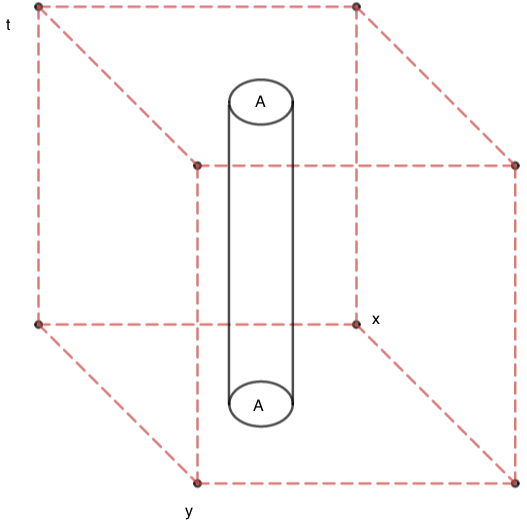
\includegraphics[scale=0.4]{10-3.png}
                    \caption{Drawing for Wangsness 10-3}
                \end{subfigure}
                \begin{subfigure}[b]{0.49\textwidth}
                    \centering
                    \captionsetup{type=figure}
                    %--------------------------------Dependencies----------------------------------%
%   tikz                                                                       %
%       markings                                                               %
%       arrows.meta                                                            %
%       quotes                                                                 %
%-------------------------------Main Document----------------------------------%
\begin{tikzpicture}[font=\scriptsize,>=Latex,line width=0.3mm]
    \draw (0,0) circle (2);
    \node (O) at (0,0) {};
    \node (A) at (0,2) {};
    \node (B) at (1.414,1.414) {};
    \draw[dashed] (0,0) to (0,2);
    \draw[dashed] (0,0) to (1.414,1.414);
    \draw (0,0) to node[below] {$a$} (1.414,-1.414);
    \pic[%
        draw=black,
        "\scriptsize{${\theta}$}",
        angle eccentricity=1.7,
        angle radius =0.5cm
    ]   {angle = B--O--A};
    \draw[->] (-1,-0.5) to node[right] {$\mathbf{P}$} (-1,0.5);
    \foreach \a in {1,3,...,17}{
        \draw (\a*360/36: 2.2) node{$+$};
        \draw (\a*360/36+180: 2.2) node{$-$};
    }
\end{tikzpicture}
                    \caption{Drawing for Wangsness 10-6}
                \end{subfigure}
            \end{figure}
            \subsubsection{Wangsness 10-17}
            Choose a spherical Gaussian surface outside the sphere concentric with the given sphere. $\int \mathbf{D}\cdot \mathbf{da} = Q_f$, so $D_o (4\pi r^2) = q$, and thus $\mathbf{D}_o = \frac{q}{4\pi r^2} \hat{\mathbf{r}}$. From $\mathbf{D} = \epsilon_0 \mathbf{E}+\mathbf{P}$, we have that $\mathbf{D}_o - \epsilon_0 \mathbf{E}_o = \mathbf{P}_o$. $\mathbf{E}_0 = \frac{q}{4\pi \epsilon_0 r^2}\hat{\mathbf{r}}$, and thus $\mathbf{P}_o = 0$. There is no dielectric outside of the sphere. Choosing a Gaussian surface inside of the sphere, we get $\int \mathbf{D}\cdot \mathbf{da} = Q_f$, for $D(4\pi r^2) = q$, and thus $\mathbf{D}_i = \frac{q}{4\pi r^2} \hat{\mathbf{r}}$. $\mathbf{E}_i = \frac{\mathbf{D}_i}{\epsilon} = \frac{\mathbf{D}_i}{\kappa_e \epsilon_0} = \frac{q}{4\pi \kappa_{e} \epsilon_0 r^2}\hat{\mathbf{r}}$. So $\mathbf{P}_i = \mathbf{D}_i - \epsilon_0 \mathbf{E}_i = (1-\frac{1}{\kappa_{e}}) \frac{q}{4\pi r^2} \hat{\mathbf{r}}$. Finally, $Q_b^{surface} = \int_{S} \sigma_{b} da' = \iint \mathbf{P}\cdot \hat{\mathbf{n}} da' = \int_{0}^{\pi} \int_{0}^{2\pi} \frac{\kappa_e-1}{\kappa_e} \frac{q}{4\pi} \sin(\theta) d\theta d\phi = \frac{\kappa_e-1}{\kappa_e} q$.
            \subsubsection{Wangsness 10-18}
            $\oint \mathbf{D} \cdot \mathbf{da} = q$. $\mathbf{D} = \frac{q}{4\pi r^2} \hat{\mathbf{r}}$ for all $r$ inside the cavity or in the dielectric. $\rho_b = 0$ since $\rho_f = 0$ in the dielectric. In the dielectric $\mathbf{E} = \frac{\mathbf{D}}{\epsilon} = \frac{\mathbf{D}}{\kappa_e \epsilon_0}$, so $\mathbf{E} = \frac{q}{4\pi \kappa_e \epsilon_0 r^2}\hat{\mathbf{r}}$. $\mathbf{P} = \mathbf{D}- \epsilon_0 \mathbf{E} = \frac{\kappa_e-1}{\kappa_e} \frac{q}{4\pi r^2} \hat{\mathbf{r}}$ at the surface of the cavity $r=a$. $\sigma_b = \mathbf{P}\cdot \hat{\mathbf{n}} = \frac{\kappa_e-1}{\kappa_e} \frac{q}{4\pi a^2} \hat{\mathbf{r}}\cdot (-\hat{\mathbf{r}}) = - \frac{\kappa_e-1}{\kappa_e} \frac{q}{4\pi a^2}$. $Q_b^{cavity} = \int \sigma da = - \frac{\kappa_e-1}{\kappa_e}q$.
            \subsubsection{Wangsness 10-25}
            $\kappa_e(x) = \alpha+\beta x$ (The dielectric constant varies linearly with $x$. $\alpha$ and $\beta$ are constants). Find $\mathbf{D}$ between the plates. $\int_{Gaussian Surface} \mathbf{D}\cdot \mathbf{da} = Q_f^{enc}$ (D is uniform between plates). $D\Delta a = Q_f^{enc}$, and thus $D = \frac{Q_f^{enc}}{\Delta a} = \sigma = \frac{Q}{A}$, where $Q$ is the total charge of the plate and $A$ is the area of the plate. $E = \frac{D}{\epsilon} = \frac{Q}{\kappa \epsilon_0 A} = \frac{Q}{\epsilon_0 A(\alpha + \beta x)}$. At $x=0$, $\kappa_e = \kappa_{e_1}$, so $\alpha+\beta(0) = \kappa_{e_1}$, and thus $\alpha = \kappa_{e_1}$. At $x=d$, $\kappa_{e} = \kappa_{e_2}$, and so $\beta = \frac{\kappa_{e_2}-\kappa_{e_1}}{d}$. The potential difference between the plates is $\Delta \phi = -\int_{-}^{+} \mathbf{E}\cdot \mathbf{d\ell} = \int_{+}^{-} Edx = \frac{Q}{\epsilon_0 A} \int_{0}^{d} \frac{dx}{\alpha+\beta x} = \frac{Q}{\epsilon A} \frac{1}{\beta} \ln(\alpha+\beta x)\big|_{0}^{d} = \frac{Q}{\epsilon_0 A\beta} \ln(\frac{\alpha+\beta d}{\alpha}) = \frac{Q}{\epsilon_0 A\beta} \ln(\frac{\kappa_{e_2}}{\kappa_{e_1}}) = \frac{Q}{C}$. Hence $C = \frac{\epsilon_0 A\beta}{\ln(\frac{\kappa_{e_2}}{\kappa_{e_1}})} = \frac{(\kappa_{e_2}-\kappa_{e_1})\epsilon_0 A}{d\ln(\frac{\kappa_{e_2}}{\kappa_{e_1}})}$
            \begin{figure}[H]
                \centering
                \captionsetup{type=figure}
                \begin{subfigure}[b]{0.49\textwidth}
                    \centering
                    \captionsetup{type=figure}
                    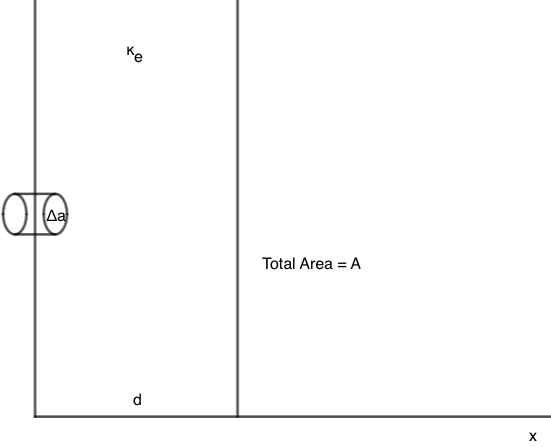
\includegraphics[width=\textwidth]{10-25.png}
                    \caption{Drawing for Wangsness 10-25}
                \end{subfigure}
                \begin{subfigure}[b]{0.49\textwidth}
                    \centering
                    \captionsetup{type=figure}
                    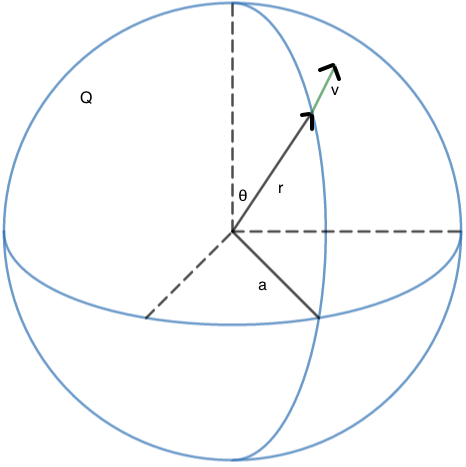
\includegraphics[width=\textwidth]{12-3.png}
                    \caption{Drawing for Wangsness 12-3}
              \end{subfigure}
            \end{figure}
            \subsubsection{Wangsness 10-27}
            $\kappa = \kappa_{e_1}$ for $a\leq \rho < \rho_0$, $\kappa = \kappa_{e_2}$ for $\rho_0 \leq \rho \leq b$. First get $D$ by assuming a charge per unit length $\lambda $on the inner cylinder and $-\lambda$ on the outer. $\int \mathbf{D}\cdot \mathbf{da} = Q_{f}^{enc} = D(2\pi \rho L) = \lambda L$. So $\mathbf{D} = \frac{\lambda}{2\pi \rho} \hat{\boldsymbol{\uprho}}$. $\Delta \phi = -\int_{-}^{+} \mathbf{E} \cdot \mathbf{d\ell} = \int_{a}^{b} \frac{\lambda}{2\pi \rho \epsilon}d\rho = \int_{a}^{\rho_0} \frac{\lambda}{2\pi \epsilon_0 \kappa_{e_1}\rho}d\rho + \int_{\rho_0}^{b} \frac{\lambda}{2\pi \epsilon_0 \kappa_{e_2}\rho}d\rho = \frac{\lambda}{2\pi \epsilon_0}\big[\frac{1}{\kappa_{e_1}}\ln(\frac{\rho_0}{a}) + \frac{1}{\kappa_{e_2}}\ln(\frac{b}{\rho_0})\big]$. From $\Delta \phi = \frac{Q}{C}$, and $Q=\lambda L$, we get $C = \frac{2\pi \epsilon_0 L}{\frac{1}{\kappa_{e_1}}\ln(\frac{\rho_0}{a}) + \frac{1}{\kappa_{e_2}}\ln(\frac{b}{\rho_0})}$
        \subsection{Homework XI}
            \subsubsection{Wangsness 12-3}
            $\mathbf{J} = \rho \mathbf{v}$. $\rho = \frac{Q}{\frac{4}{3}\pi a^3} = \frac{3q}{4\pi a^3}$. $\mathbf{u} = \mathbf{\omega}\times\mathbf{r} = \omega \hat{\mathbf{z}} \times r \hat{\mathbf{r}} = \omega r \sin(\theta) \hat{\boldsymbol{\upvarphi}}$. So, we have that $\mathbf{J} = \frac{3Q}{4\pi a^3} \omega r \sin(\theta) \hat{\boldsymbol{\upvarphi}}$. $\mathbf{da} = rdrd\theta \hat{\boldsymbol{\upvarphi}}$, so $I = \int \mathbf{J} \cdot \mathbf{da} = \frac{3Q \omega}{4\pi a^3} \int_{0}^{\pi} \int_{0}^{a} r^2\sin(\theta)drd\theta = \frac{Q\omega}{2\pi}$
            \subsubsection{Wangsness 13-4}
            We will calculate the force exerted by $C'$ on $C$. $\mathbf{F}_{C'\rightarrow C} = \frac{\mu_0}{4\pi} \oint_{C} \oint_{C'} \frac{I \mathbf{d\ell}\times (I' \mathbf{d\ell}'\times \hat{\mathbf{r}})}{R^2}$. We use the $BAC-CAB$ rule: $\mathbf{A}\times(\mathbf{B}\times \mathbf{C}) = \mathbf{B}(\mathbf{A}\cdot \mathbf{C}) - \mathbf{C}(\mathbf{A}\cdot \mathbf{B})$. We can rewrite the previous integral as  $\mathbf{F}_{C'\rightarrow C} = -\frac{\mu_0 II'}{4\pi} \oint_{C} \oint_{C'} \big[ \mathbf{d\ell}'\cdot(\mathbf{d\ell}\times \frac{\hat{\mathbf{r}}}{R^2}) - \frac{\hat{\mathbf{r}}}{R^2} \mathbf{d\ell}\cdot \mathbf{d\ell}\big]$. Recall that $\nabla(\frac{1}{R}) = \frac{\hat{\mathbf{r}}}{R^2}$. Using this, we have $\mathbf{F}_{C'\rightarrow C} = -\frac{\mu_0 II'}{4\pi} \oint_{C}\oint_{C'} \mathbf{d\ell'}\big[ \mathbf{d\ell}\cdot \nabla(\frac{1}{R})- \frac{\hat{\mathbf{r}}}{R^2} \mathbf{d\ell'} \cdot \mathbf{d\ell}\big]$. From the fundamental theorem of gradients, $\oint \nabla(f) \cdot \mathbf{d\ell} = 0$ for any function $f$. Thus $\oint \nabla(\frac{1}{R}) \cdot \mathbf{d\ell} = 0$. From this we have $\mathbf{F}_{C\rightarrow C'} = -\frac{\mu_0 II'}{4\pi} \oint_{C}\oint_{C'} \frac{\hat{\mathbf{r}}}{R^2} \mathbf{d\ell}'\cdot \mathbf{d\ell}$. We now compute this integral along all four paths of the problem. $\mathbf{d\ell}' = dz' \hat{\mathbf{z}}$ for all paths. Along path $I$, $\mathbf{r} = \hat{\mathbf{x}}d+\hat{\mathbf{z}}z$, $\mathbf{d\ell} = \hat{\mathbf{z}}dz$. Along path $III$, $\mathbf{r} = \hat{\mathbf{x}}(a+d)+\hat{\mathbf{z}}z$, $\mathbf{d\ell} = \hat{\mathbf{z}}dz$. Along paths $II$ and $IV$, $\mathbf{d\ell}\cdot \mathbf{d\ell}' = 0$. Piecing this together, $\mathbf{F}_{C\rightarrow C'} = -\frac{\mu_0 II'}{4\pi}\int_{0}^{b} \int_{-\infty}^{\infty} \frac{\hat{\mathbf{x}}d+\hat{\mathbf{z}}(z-z')}{\big(d^2+(z-z')^2\big)^{3/2}}dz'dz - \frac{\mu_0 II'}{4\pi} \int_{b}^{0} \int_{-\infty}^{\infty} \frac{\hat{\mathbf{x}}(d+a)+\hat{\mathbf{z}}(z-z')}{\big((d+a)^2+(z-z')^2\big)^{3/2}}dz'dz$. Making the substitution $t=z'-z$, we get an integral of the form $\int_{-\infty}^{\infty} \frac{t+z'}{(A+t^2)^{3/2}}dt$. This is an odd function that is integrated over symmetric bounds, and thus the integral is zero. The only part left is the $\hat{\mathbf{x}}$ contribution. Evaluating this integral, we get $\mathbf{F}_{C\rightarrow C'} = -\frac{\mu_0 II' ab}{2\pi d(a+d)}\hat{\mathbf{x}}$.
            \begin{figure}[htbp]
                \centering
                \captionsetup{type=figure}
                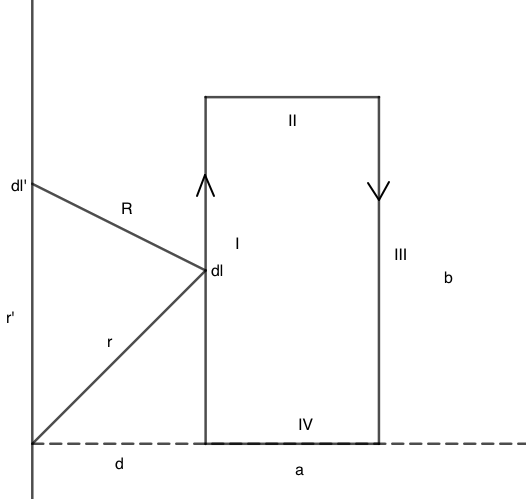
\includegraphics[scale=0.4]{13-4.png}
                \caption{Drawing for Wangsness 13-4}
            \end{figure}
            \subsubsection{Wangsness 14-7}
            $\mathbf{R} = \mathbf{r}-\mathbf{r}'$, where $\mathbf{r} = z\hat{\mathbf{z}}$ and $\mathbf{r}' = a\cos(\phi')\hat{\mathbf{x}}+a\sin(\phi')\hat{\mathbf{y}}$. We have $\boldsymbol{d\ell}' = ad\varphi' \hat{\boldsymbol{\upvarphi}}$. Putting this together, we have $\mathbf{R} = z\hat{\mathbf{z}} - a(\cos(\phi')\hat{\mathbf{x}}+\sin(\phi')\hat{\mathbf{y}})$. So:
            \begin{align*}
                \mathbf{B} &= \frac{\mu_0 I'}{4\pi}\int \frac{\boldsymbol{d\ell}\times \mathbf{R}}{R^3} = \frac{\mu_0I'}{4\pi} \int_{-\alpha}^{\alpha} \frac{ad\phi' \hat{\boldsymbol{\upvarphi}}\times (z\hat{\mathbf{z}}-a\cos(\phi')\hat{\mathbf{x}}-a\sin(\phi')\hat{\mathbf{y}})}{(z^2+a^2)^{3/2}}\\
                &= \frac{\mu_0 I'a}{4\pi(z^2+a^2)^{3/2}}\int_{-\alpha}^{\alpha} (-\sin(\phi')\hat{\mathbf{x}}+\cos(\phi')\hat{\mathbf{y}})\times (-a\cos(\phi')\hat{\mathbf{x}}-a\sin(\phi')\hat{\mathbf{y}}+z\hat{\mathbf{z}})d\phi'\\
                &= \frac{\mu_0 I'a}{4\pi (z^2+a^2)^{3/2}}\int_{-\alpha}^{\alpha} (z\cos(\phi')\hat{\mathbf{x}}+z\sin(\phi')\hat{\mathbf{y}}+a\hat{\mathbf{z}})d\phi'
            \end{align*}
            Sine is an odd function, and the limit is over a symmetric interval, and thus the $\hat{\mathbf{y}}$ component is zero. So we have:
            \begin{equation*}
                \mathbf{B} = \frac{\mu_0 I' a}{2\pi (z^2+a^2)^{3/2}}\big(z\sin(\alpha)\hat{\mathbf{x}}+a\alpha \hat{\mathbf{z}}\big)    
            \end{equation*}
            \subsubsection{Wangsness 14-15}
            The force on $q$ is given by $\mathbf{F} = q\mathbf{v}\times \mathbf{B}$. We first get $\mathbf{B}$ at $q$. $\mathbf{B} = \frac{\mu_0}{4\pi} \int \frac{I' d\ell' \times \hat{\mathbf{r}}}{R^2}$. For this problem, $\mathbf{R} = -\rho' \hat{\boldsymbol{\uprho}}$. We need only compute the integral along paths $I$ and $III$, for along $II$ and $IV$ we have that $\mathbf{d\ell}$ and $\mathbf{R}$ are parallel. So, we have $\mathbf{B} = \frac{\mu_0}{4\pi} \int_{0}^{\pi} \frac{I'(-ad\phi' \hat{\boldsymbol{\upvarphi}})\times (-a\hat{\boldsymbol{\uprho}})}{a^3}+ \frac{\mu_0}{4\pi} \int_{0}^{\pi} \frac{I'(bd\phi' \hat{\boldsymbol{\upvarphi}})\times (-b\hat{\boldsymbol{\uprho}})}{b^3} = \frac{\mu_0 I'}{4} \frac{b-a}{ab} \hat{\mathbf{z}}$. The force is $\mathbf{F} = qv\hat{\mathbf{y}} \times \frac{\mu_0 I}{4} \frac{b-a}{ab} \hat{\mathbf{z}} = \frac{qv\mu_0 I'}{4} \frac{b-a}{ab} \hat{\mathbf{x}}$
            \begin{figure}[htbp]
                \centering
                \captionsetup{type=figure}
                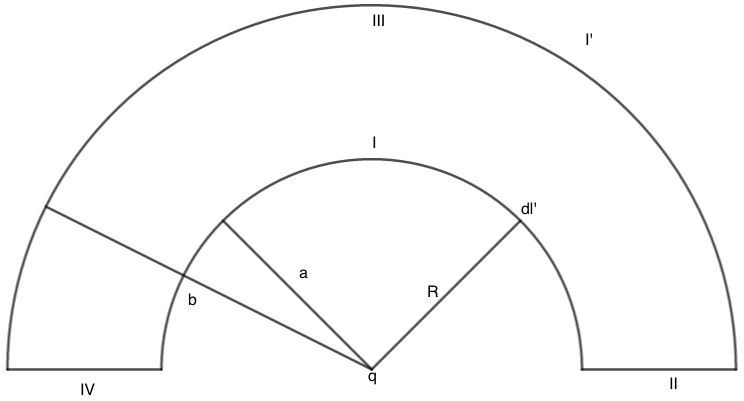
\includegraphics[scale=0.4]{14-15.png}
                \caption{Drawing for Wangsness 14-15}
            \end{figure}
        \subsection{Homework XII}
            \subsubsection{Wangsness 15-7}
            For $\rho\leq a$, path $(1)$ has $\oint \mathbf{B}\cdot \mathbf{d\ell}= \mu_0 I_{enc}$, where $I_{enc} = I\frac{\rho^2}{a^2}$. So $\mathbf{B} = \frac{\mu_0 I\rho}{2\pi a^2} \hat{\boldsymbol{\upvarphi}}$. For $a\leq \rho \leq b$, $I_{enc} = I$. So $B = \frac{\mu_0 I}{2\pi \rho} \hat{\boldsymbol{\upvarphi}}$. For $b\leq \rho \leq c$, $I_{enc} = I =I\frac{\rho^2-b^2}{c^2-b^2} = I\frac{c^2-\rho^2}{c^2-b^2}$. So $\mathbf{B} = \frac{\mu_0 I}{2\pi \rho} \frac{c^2-\rho^2}{c^2-b^2}\hat{\boldsymbol{\upvarphi}}$. Finally, or $\rho \geq c$, $I_{enc} = 0$, so $\mathbf{B} = 0$.
            \begin{figure}[htbp]
                \centering
                \captionsetup{type=figure}
                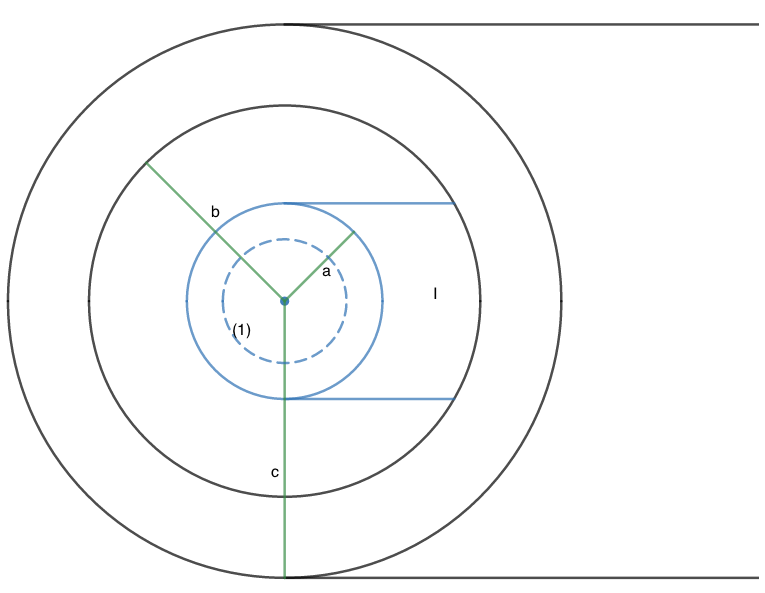
\includegraphics[scale=0.4]{15-7.png}
                \caption{Drawing for Wangsness 15-7}
            \end{figure}
            \subsubsection{Wangsness 15-8}
            \begin{equation*}
                \mathbf{B}=
                    \begin{cases}
                        0,&\rho<a\\
                        \frac{\mu_0 I}{2\pi \rho}
                        \frac{\rho^2-a^2}{b^2-a^2}
                        \hat{\boldsymbol{\upvarphi}},
                        &a<\rho<b\\
                        \frac{\mu_0 I}{2\pi \rho} \hat{\boldsymbol{\upvarphi}},
                        &\rho>b
                    \end{cases}    
            \end{equation*}
            By definition, $\mu_0 \mathbf{J} = \nabla \times \mathbf{B}$. So:
            \begin{equation*}
                \mathbf{J} = \begin{cases} 0, & \rho<a\\ \frac{I}{\pi(b^2-a^2)}, & a<\rho < b\\ 0, & \rho>b \end{cases}    
            \end{equation*}
            The current $I$ i distributed uniformly over the volume between two coaxial cylinders of inner radius $a$ and outer radius $b$ in the direction of the cylinder axis.
            \subsubsection{Wangsness 16-10}
            The field point is on the $z-$axis. $\mathbf{r} = z\hat{\mathbf{z}}$, $\mathbf{r}' =  a\cos(\phi')\hat{\mathbf{x}}+a\sin(\phi')\hat{\mathbf{y}}$. $\mathbf{d\ell}' = \mathbf{dr}' = ad\phi' \hat{\boldsymbol{\upvarphi}} = ad\phi' (-\sin(\phi')\hat{\mathbf{x}}+\cos(\phi')\hat{\mathbf{y}})$. $\mathbf{A} = \frac{\mu_0 I'}{4\pi} \int \frac{\mathbf{d\ell}'}{R} = \frac{\mu_0 I'}{4\pi} \frac{a}{\sqrt{a^2+z^2}}\int_{-\alpha}^{\alpha} (-\sin(\phi')\hat{\mathbf{x}}+\cos(\phi')\hat{\mathbf{y}})d\phi' = \frac{\mu_0 I'a}{2\pi \sqrt{a^2+z^2}}\sin(\alpha)\hat{\mathbf{y}}$. To find $\mathbf{B}$ from $\mathbf{A}$, we need to evaluate $\nabla \times \mathbf{A}$. We don't know about $\mathbf{A}$ for a general point, and thus we can't evaluate the $x$ and $y$ derivatives.
        \subsection{Homework XIII}
            \subsubsection{Wangsness 17-3}
            The $\mathbf{B}$ field associated with $I$ is $\mathbf{B} = \frac{\mu_0 I}{2\pi \rho} \hat{\boldsymbol{\upvarphi}}$. In the plane of the paper, $\phi$ is into the paper. $\Phi = \int \mathbf{B}\cdot \mathbf{da} = \int \frac{\mu_0 I}{2\pi \rho} \cdot b d\rho \hat{\boldsymbol{\upvarphi}} = \frac{\mu_0Ib}{2\pi} \int_{d}^{d+a} \frac{d\rho}{\rho}= \frac{\mu_0 Ib}{2\pi} \ln(\frac{d+a}{d}) = \frac{\mu_0 bI_0 e^{-\lambda t}}{2\pi} \ln(\frac{d+a}{d}) = \frac{\mu_0 I_0 \lambda b}{2\pi} \ln(\frac{d+a}{d})e^{-\lambda t}$. The induced current is clockwise around the loop to produce a field which goes into the paper to counteract the decreasing $\mathbf{B}$ due to $I_0$.
            \subsubsection{Wangsness 17-4}
            The $\mathbf{B}-$field at distance $\rho$ from the wire at points in the plane of the paper is $\mathbf{B} = \frac{\mu_0 I}{2\pi \rho} \hat{\mathbf{y}}$. The flux of $\mathbf{B}$ through the loop is $\Phi = \int \mathbf{B}\cdot \mathbf{da} = \iint \frac{\mu_0 I}{2\pi \rho}\rho d\theta d\rho$. We have $\rho = b+r\cos(\theta)$. So $\Phi = \frac{\mu_0 I}{2\pi} \int_{0}^{a} \int_{0}^{2\pi} \frac{r d\theta dr}{b+r\cos(\theta)} = \frac{\mu_0 I}{2\pi} \int_{0}^{a} \frac{2r}{\sqrt{b^2-r^2}}\tan^{-1}\big[\frac{\sqrt{b^2-r^2}\tan(\theta/2)}{b+r}\big]_{0}^{2\pi} \Rightarrow \tan^{-1}\big[\frac{\sqrt{b^2-r^2}}{b+r}\tan(\pi)\big] - \tan^{-1}\big[ \frac{\sqrt{b^2-r^2}}{b+r}\tan(0)\big]$. So $\Phi = \mu_0 I\big[b-\sqrt{b^2-a^2}\big]$. The loop moves with constant speed $v$ along the $x-$axis away from the current $I$, $v = \frac{db}{dt}$. So $\xi = -\frac{d\Phi}{dt} = -\mu_0 I \frac{d}{dt}\big[b-\sqrt{b^2-a^2}\big] = -\mu_0 I\big[ v-\frac{bv}{\sqrt{b^2-a^2}}\big] = \mu_0 NIv\big[ \frac{b}{\sqrt{b^2-a^2}}-1\big]$. The current will be clockwise trying to increase the flux which is decreasing due to motion away from the wire.
            \begin{figure}[htbp]
                \centering
                \captionsetup{type=figure}
                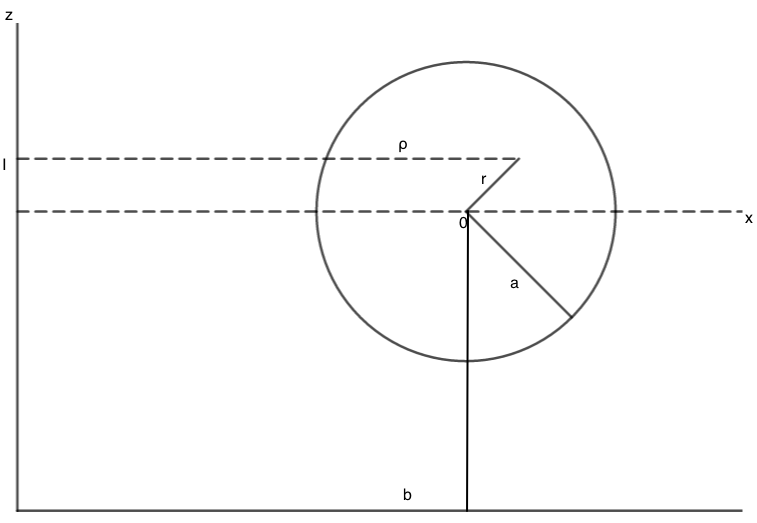
\includegraphics[scale=0.4]{17-4.png}
                \caption[Drawing for Wangsness 17-4]{Drawing for Wangness 17-4}
            \end{figure}
            \subsubsection{Wangsness 17-19}
            $\Phi_{12} = IM_{12}$. The flux due to $1$ through $2$ is $\Phi_{12} = \int \mathbf{B}_1 \cdot \mathbf{da}_2$. $\mathbf{B}_1 = \frac{\mu_0 I}{2\pi} \big( \frac{1}{\rho+d}- \frac{1}{\rho+d+D}\big)$. So we have that $\Phi_{12} = \int_{0}^{a} \frac{\mu_0 I}{2\pi} \big(\frac{1}{\rho+d}- \frac{1}{\rho+d+D}\big) bd\rho = \frac{\mu_0 Ib}{2\pi}\big[ \ln(\frac{a+d}{a+d+D}) - \ln(\frac{d}{d+D})\big]$. Thus, we have $M = \frac{\mu_0 b}{2\pi} \ln\big(\frac{a+d}{d}\big)$
            \subsubsection{Wangsness 17-20}
            The field inside the toroid is $\mathbf{B} = \frac{\mu_0 NI}{2\pi \rho} \hat{\boldsymbol{\upvarphi}}$. The flux through a single turn is $\Phi^1 = \frac{\mu_0 NI}{2\pi} \int_{0}^{a} \int_{0}^{2\pi} \frac{r}{b+r\cos(\theta)}d\theta dr$. We've done this integral before, and we get $\Phi^1= \mu_0 NI\big[b-\sqrt{b^2-r^2}\big]$. $\Phi = N\Phi^1$. $L = \frac{\Phi}{I} = \frac{\mu_0 N^2 I}{I} \big[b-\sqrt{b^2-r^2}\big] = \mu_0 N^2 \big[b-\sqrt{b^2-r^2}\big]$
    \section{Exams}
        \subsection{Exam I}
        \subsubsection{Question I}
        Give the vector field field $\mathbf{A} = c\hat{\boldsymbol{\uptheta}}$, where $c$ is a constant, find $\nabla \times \mathbf{A}$. Is this a conservative vector field? Explain.
        \subsubsection{Question II}
        Verify the Divergence Theorem for $\mathbf{A}$ given in problem 1 in spherical coordinates for a hemisphere of radius $a_0$ resting on the $xy-plane$ with the center of the flat base of the hemisphere at the origin and the symmetry axis of the hemisphere along the positive $z-axis$.
        \subsubsection{Question III}
        A semicircular charged line of radius $a$ carries uniform linear charge density $\lambda$. It has the equation $x^2+y^2 = a^2$, $x\geq 0$, $z=0$. That is, the half circle resting on the $xy-plane$ of radius $a$. Find the electring field at a point $P$ on the $z$ axis a distance $z$ from the origin.
        \subsection{Exam II}
        \subsubsection{Question I}
        A conducting sphere of radius $a$, centered at the origin carries charge $Q_1$. This sphere is surrounded by a hollow concentric conducting spherical shell of inner radius $b$ and outer radius $c$ with $a<b<c$. The outer hollow conducting shell caries a total charge $Q_2$. 
        \begin{enumerate}
            \item What is the electric field everywhere?
            \item What is the potential everywhere, assuming $\underset{r\rightarrow \infty} \lim \phi(r) = 0$?
            \item How much charge is on the inner and outer surfaces of the conducting shell at $r=b$ and $r=c$?
        \end{enumerate}
        \subsubsection{Question II}
        The outer conductor of problem I is now grounded.
        \begin{enumerate}
            \item What is the electric field everywhere?
            \item What is the potential everywhere?
            \item How much charge is on the surfaces at $r=b$ and $r=c$?
            \item What is the capacitance of the system of conductors?
            \item Calculate the electrostatic potential energy of the configuration assuming the energy resides in the charges.
            \item Calculate the electrostatic potential energy of the configuration assuming the energy resides in the electric field.
        \end{enumerate}
        \subsubsection{Question III}
        A semicircular arc of radius $a$ in the $y-z$ plane with center on the $y-axis$ at the origin and the top of the arc on the positive $y-axis$ carries linear charge density $\lambda = \lambda_0 \cos(\theta')$, where $\lambda_0$ is constant and $\theta'$ is measured with respected to the positive $z-axis$.
        \begin{enumerate}
            \item What is the electric monopole moment of this distribution?
            \item What is the electric dipole moment of this distribution?
            \item What is the electric potential at a distance $r$ from the origin for this distribution where $r>a$, accurate to order $\frac{1}{r^2}$?
        \end{enumerate}
        \subsection{Exam III}
        \subsubsection{Question I}
        The electric field in a spherical region of space of radius $a$ is given by $\mathbf{E} = E_0 \frac{r^2}{a^2}\hat{\mathbf{r}}$ for $r< a$, where $E_0$ is a constant. This region is surrounded concentrically by a grounded conducting spherical shell of inner radius $b$ and outer radius $c$ with $a<b<c$. There is no charge in the region $a<r<b$. 
        \begin{enumerate}
            \item What is the electric charge density in the region $r<a$?
            \item Wher is the electric field in the region $a<r<b$?
            \item How much charge is on the surfaces at $r=b$ and $r=c$?
            \item What is the electric field for $r>c$?
            \item What is the electric potential $\phi$ at $r=0$ assuming that ground potential is $\phi = 0$.
        \end{enumerate}
        \subsubsection{Question II}
        A capacitor $C_{1}$ is charged to a potential difference $\Delta \phi$ between its plates. A second capacitor $C_{2}$ is uncharged. One plate of $C_2$ is now connected to a plate of $C_1$ by a conductor of negligible capacitance, the remaining plates are similarly connected. 
        \begin{enumerate}
            \item For the resultant equilibrium state, find the charge on each capacitor and the potential difference $\Delta \phi$ between their respective plates.
            \item Compare the energy stored in capacitor $C_1$ before connecting it to $C_2$, to the energy of the combination after connected them. Are these energies the same? If not, which is larger and where did any additional energy come from, or where did any lost energy go?
        \end{enumerate}
        \subsubsection{Question III}
        Find the electric dipole moment of an hourglass configuration of charge consisting of two identical right circular cones of radius $a$ and height $a$ with symmetry axes aligned apex to apex along the $z-$axis with the apexes touching at the origin. The top cone has charge density $\sigma_0$ on its surface, and the bottom cone has charge density $-\sigma_0$ on its surface.
        \subsection{Practice Final Exam}
        \subsubsection{Problem I}
        The electric field in a region of space is given in spherical coordinates as $\mathbf{E} = cr\hat{\mathbf{r}}$, where $c$ is constant. 
        \begin{enumerate}
            \item Find the charge density at a point $(r,\theta,\phi)$
            \item Find the total charge inside a sphere of radius $a$ centered at the origin.
        \end{enumerate}
        \subsubsection{Problem II}
        A battery is used to charge an ideal parallel plate capacitor to a potential difference $\Delta \phi = V_0$. The battery is then disconnected. The separation between the plates is now increasing from $d$ to $\alpha d$, where $\alpha >1$. The area of the plates is $A$.
        \begin{enumerate}
            \item What is the ratio of the new energy to the original energy>
            \item Is the energy increases or decreased?
            \item Where does this energy come from or go to?
            \item Compute the change in energy $\Delta U_e$ expressing your answer in terms of the given quantities $V_0,d,A,\alpha$ and fundamental constants.
        \end{enumerate}
        \subsubsection{Problem III}
        A dielectric sphere of radius $a$ and permittivity $\varepsilon$ contains a free charge density. $\rho_f = cr$, where $c$ is a constant. The sphere is centered at the origin. Find the electric potential at the center of the sphere assuming that the potential is zero at an infinite distance from the center.
        \subsubsection{Problem IV}
        A thick slab extending from $z=-a$ to $z=a$ carries a uniform vlume current density $\mathbf{J} = J_0 \hat{\mathbf{x}}$. The slab is infinite in the $xy-$plane. Find the magnetic field $B$ as a function of $z$ inside and outside the slab. Plot $B$ as a function of $z$ for $-b<z<b$ where $b>a$.
        \subsubsection{Problem V}
        An ideal long solenoid of radius $a$, carrying $n$ turns per unit length, is looped by a wire with resistance $R$. 
        \begin{enumerate}
            \item If the current in the solenoid is increasing at a constant rate $\frac{dI}{dt} = k$, what current flows in the lopp, and which way (Left or right) does it pass through the resistor?
            \item If the current $I$ in the solenoid is constant but the solenoid is pulled out of the loop and reinserted in the opposite direction, what total charge passes through the resistor?
        \end{enumerate}
        \subsection{Final Exam}
        \subsubsection{Problem I}
        \begin{enumerate}
            \item Write down Maxwell's Equations in differential form.
            \item Convert them to integral form and show derivations.
            \item Name each equation.
        \end{enumerate}
        \begin{proof}[Solution]
        \
        \begin{enumerate}
        \item Gauss' Law: $\nabla \cdot \mathbf{E} = \frac{\rho}{\epsilon_0}\Rightarrow\frac{Q_{encl}}{\epsilon_0}=\iiint_{V} \frac{\rho}{\epsilon_0}d\tau=\iiint_{V} \big(\nabla \cdot \mathbf{E}\big) d\tau = \oiint_{\partial V} \mathbf{E}\cdot \mathbf{da}$
        \item Faraday's Law: $\nabla \times \mathbf{E} = -\frac{\partial \mathbf{B}}{\partial t}\Rightarrow-\frac{d \Phi_{B}}{dt} = \iint_{S} -\frac{\partial \mathbf{B}}{\partial t}da = \iint_{S} \big(\nabla \times \mathbf{E}\big)da = \oint_{\partial S}\mathbf{E}\cdot \mathbf{d\ell}$
        \item Gauss' Law of Magnetism: $\nabla \cdot \mathbf{B} = 0\Rightarrow 0 = \iiint_{V} \big(\nabla \cdot\mathbf{B}\big)d\tau = \oiint_{\partial V} \mathbf{B}\cdot \mathbf{da}$
        \item Ampere's Law: $\nabla \times \mathbf{B} = \mu_0 \mathbf{J} + \mu_0 \epsilon_0 \frac{\partial \mathbf{E}}{\partial t}\Rightarrow\mu_0 I_{encl}+ \mu_0 \epsilon_0 \frac{d\Phi_{E}}{dt} = \iint_{S}\big(\mu_0 \mathbf{J} + \mu_0 \epsilon_0 \frac{\partial \mathbf{E}}{\partial t}\big)da = \iint_{S}\big(\nabla \times \mathbf{B}\big)da = \oint_{\partial S}\mathbf{B}\cdot \mathbf{d\ell}$
        \end{enumerate}
        \end{proof}
        \subsubsection{Problem II}
        A conduction sphere of radius $a$ carries a charge $Q_{1}$. It is surrounded by a conducting spherical shell of inner radius $b$ and outer radius $c$ with $a<b<c$. The charge on the conducting shell is $Q_{2}$. The region between the conductors $a<r<b$ is filled with linear isotropic dielectric of permittivity $\varepsilon$. Find the following in the regions $r<a.a<r<b.b<r.b<r<c.c<r$:
        \begin{enumerate}
            \item The electric displacement $\mathbf{D}$
            \item The electric field $\mathbf{E}$
            \item The polarization vector $\mathbf{P}$
            \item Find the free charge on the conductors at $r=a,b,c$.
            \item The bound volume charge in the dielectric.
            \item The bound surface charge density at the inner and outer surfaces of the dielectric.
            \item The electric potential at the origin assuming the potential is zero as $r$ goes to infinity.
        \end{enumerate}
        \begin{proof}[Solution]
        \
        \begin{enumerate}
        \begin{multicols}{2}
            \item $\mathbf{D}=\begin{cases}\mathbf{0}&r<a\\ \frac{Q_{1}}{4\pi r^{2}} &a<r<b\\\mathbf{0} & b<r<c\\ \frac{Q_{1}+Q_{2}}{4\pi r^{2}} & c<r \end{cases}$
            \item $\mathbf{E}=\begin{cases}\mathbf{0}&r<a\\ \frac{Q_{1}}{4\pi\epsilon_{0} r^{2}} & a<r<b\\ \mathbf{0} & b<r<c\\ \frac{Q_{1}+Q_{2}}{4\pi\epsilon_{0}r^{2}} & c<r\end{cases}$
            \item $\mathbf{P}=\begin{cases}\mathbf{0}&r<a\\ \frac{Q_{1}}{4\pi r^{2}}(1-\frac{\epsilon_{0}}{\varepsilon}) & a<r<b\\ \mathbf{0} & b<r<c\\ \mathbf{0} & c<r \end{cases}$
            \item $Q = \begin{cases} Q_1 & r=a\\ -Q_1 & r=b\\ Q_1+Q_2 & r=c\end{cases}$
        \end{multicols}
        \begin{multicols}{2}
            \item $\rho_b = \nabla \cdot \mathbf{P}$, $\rho_b = 0$.
            \item $\sigma_{b,a}=-\frac{Q_1}{4\pi a^2}\big(1-\frac{\epsilon_0}{\varepsilon}\big)$, $\sigma_{b,b}=\frac{Q_1}{4\pi b^2}\big(1-\frac{\epsilon_0}{\varepsilon}\big)$.
            \end{multicols}
            \item $\phi = -\int_{0}^{\infty}\mathbf{E}\cdot \mathbf{d\ell} = \int_{c}^{\infty} \mathbf{E}\cdot \mathbf{d\ell}+\int_{b}^{c}\mathbf{E}\cdot \mathbf{d\ell}+\int_{a}^{b}\mathbf{E}\cdot \mathbf{d\ell} + \int_{0}^{a} \mathbf{E}\cdot \mathbf{d\ell} = \frac{Q_1+Q_2}{4\pi \epsilon_0 c}+\frac{Q_1}{4\pi \epsilon_0 a}-\frac{Q_1}{4\pi \epsilon_0 b}$.
        \end{enumerate}
        \end{proof}
        \subsubsection{Problem III}
        A sphere of radius $a$ carries charge density $\rho = \rho_0(r/a)$, where $\rho_0$ is a constant. Find the work done to assemble the charge distribution.
        \begin{proof}[Solution]
        We find $\mathbf{E}$ inside and outside using Gauss' law.
        \begin{equation*}
        \oiint_{S} \mathbf{E}\cdot \mathbf{da} = \frac{Q_{encl}}{\epsilon_0} = \int_{0}^{r}\int_{0}^{\pi} \int_{0}^{2\pi} \rho_0 \frac{r}{a}r^2\sin(\theta)d\varphi d\theta dr = \frac{4\pi \rho_0}{a \epsilon_0}\frac{r^4}{4} = E(4\pi r^2).
        \end{equation*}
        So $\mathbf{E} = \frac{\rho_0 r^2}{4a\epsilon_0}\hat{\mathbf{r}}$. Outside we have $\oiint_{S} \mathbf{E}\cdot \mathbf{da} = \int_{0}^{2\pi}\int_{0}^{\pi} \int_{0}^{a} \rho \frac{r}{a}r^2 \sin(\theta) dr d\theta d\varphi$, so $\mathbf{E} = \frac{\rho_0 a^3}{4r^2 \epsilon_0}\hat{\mathbf{r}}$. The work is
        \begin{align*}
        \frac{\epsilon_0}{2}\int_{All\ Space}E^2 d\tau &= \frac{\epsilon_0}{2}\int_{0}^{2\pi}\int_{0}^{\pi}\int_{0}^{\infty} E^2 r^2\sin(\theta) drd\theta d\varphi\\
        &= \int_{0}^{2\pi}\int_{0}^{\pi}\int_{0}^{a} E^2r^2\sin(\theta)dr d\theta d\varphi + \int_{0}^{2\pi}\int_{0}^{\pi}\int_{a}^{\infty} E^2r^2\sin(\theta)drd\theta d\varphi\\
        &= \frac{\pi \rho_0^2 a^5}{7\epsilon_0}
        \end{align*}
        So $\mathbf{E} = \frac{\rho_0 r^2}{4a\epsilon_0}\hat{\mathbf{r}}$
        \end{proof}
        \subsubsection{Problem IV}
        \begin{enumerate}
            \item Could the vector field $\mathbf{F} = ax\hat{\mathbf{x}}+by\hat{\mathbf{y}}+cz\hat{\mathbf{z}}$ be a possible magnetic field, where $a+b+c\ne 0$? Explain why or why not.
            \item An electric field is given by $\mathbf{E} = ax\hat{\mathbf{y}}$, where $a$ is a constant. Is this a conservative field? Explain why or why not.
            \item Find the possible magnetic field $\mathbf{B}$ associated to $\mathbf{E}$. 
        \end{enumerate}
        \begin{proof}[Solution]
        \
        \begin{enumerate}
            \item No, for $\nabla \cdot \mathbf{F} = a+b+c \ne 0$, and therefore $\mathbf{F}$ cannot be a magnetic field.
            \item No, for $\nabla \times \mathbf{E} = a\hat{\mathbf{z}} \ne 0$, and thus $\mathbf{E}$ is not a conservative field.
            \item $\nabla \times \mathbf{E} = -\frac{\partial \mathbf{B}}{\partial t} = a\hat{\mathbf{z}}$, so $\mathbf{B} = -at\hat{\mathbf{z}}+\mathbf{B}_0$, where $\mathbf{B}_0$ is some constant vector. Here $\mathbf{B}$ is increasing with time in the $-z$ direction.
        \end{enumerate}
        \end{proof}
        \subsubsection{Problem V}
        Two infinitely long coaxial cylindrical infinitesimally
        thin conducting shells concentric with the $z-$axis carry
        oppositely directed currents of equal magnitude in the $+$
        and $-$ $z-$directions. The radius of the inner shell is $a$
        and that of the outer shell is $b$. What is the self-inductance
        of a length $\ell$ of this system?
        \begin{proof}[Solution]
        The flux carried by the inner shell cuts through the area of a rectangle of lenght $\ell$ and width $b-a$. So $\Phi = \int \mathbf{B}\cdot \mathbf{da} = \int_{a}^{b} \frac{\mu_0 I}{2\pi \rho}\ell d\rho = \frac{\mu_0 I\ell}{2\pi}\ln\big(\frac{b}{a}\big)$. So, $L = \frac{\Phi}{I} = \frac{\mu_0 \ell}{2\pi}\ln\big(\frac{b}{a}\big)$.
        \end{proof}
        \chapter{Electromagnetism II}
        \section{Homework Sets}
            \subsection{Homework I}
                Wangsness Chapter 8 - Problems: 2, 4, 7, 8
                \begin{problem}
                    \label{problem:EMAG_II_Wangsness_8_2}
                    Given a single point charge $q$ located at the
                    point $(a,b,c)$, Find $Q$, $\mathbf{p}$, and
                    all components of $Q_{jk}$ for this system.
                    Which coordinates are changed there is a charge
                    $\minus{q}$ at the origin?
                \end{problem}
                \begin{solution}
                    The total charge is:
                    \begin{equation}
                        Q=\sum_{n=1}^{N}q_{n}
                    \end{equation}
                    The only charge in this system is $q$, so we have
                    $Q=q$. Next, $\mathbf{p}$ is defined as:
                    \begin{equation}
                        \mathbf{p}=
                        \sum_{n=1}^{N}q_{n}\mathbf{r}_{n}
                    \end{equation}
                    Using this, we have:
                    \begin{equation}
                        \mathbf{p}=q(a\hat{\mathbf{x}}+
                                     b\hat{\mathbf{y}}+
                                     c\hat{\mathbf{z}})
                    \end{equation}
                    Finally, the quadrupole moments are defined as:
                    \begin{equation}
                        Q_{jk}=\sum_{i=1}^{N}
                            q_{i}(3x_{i}y_{i}-r^{2}_{i}\delta_{jk})
                    \end{equation}
                    Using this, we obtain the following table:
                    \begin{table}[H]
                        \centering
                        \captionsetup{type=table}
                        \resizebox{\textwidth}{!}{%
                            \begin{tabular}{|c|c|c|c|}
                                \hline
                                $Q_{ij}$&x&y&z\\
                                \hline
                                x&
                                $q\big(3a^{2}-(a^{2}+b^{2}+c^{2})\big)$&
                                $3qab$&
                                $3qac$\\
                                \hline
                                y&
                                $3qab$&
                                $q\big(3b^{2}-(a^{2}+b^{2}+c^{2})\big)$
                                &$3qbc$\\
                                \hline
                                z&$3qac$&$3qbc$
                                &$q\big(3c^{2}-(a^{2}+b^{2}+c^{2})\big)$
                                \\
                                \hline
                            \end{tabular}
                        }
                        \caption{Quadrapole Moments for Problem
                                 \ref{problem:EMAG_II_Wangsness_8_2}.}
                        \label{tab:EMAG_2_Problem_8_2_%
                               Wangsness_Quadrupole}
                    \end{table}
                    Since both the dipole and quadrupole moments
                    are weighted by the coordinates of the charges,
                    adding a charge to the original does not affect
                    these. However, the total charge will now be zero.
                \end{solution}
                \begin{problem}
                    \label{problem:EMAG_II_Wangsness_8_4}
                    Compute $\phi$ using the multi-pole expansion for a
                    charge $2q$ at $(0,\ell,0)$ and charges $-q$
                    located at $(-a,0,0)$ and $(a,0,0)$.
                \end{problem}
                \begin{solution}
                    The multi-pole expansion of $\phi$ is:
                    \begin{equation}
                        \phi(\mathbf{r})=\frac{1}{4\pi\epsilon_{0}}\Big(
                        \frac{Q}{r}+
                        \frac{\mathbf{p}\cdot\hat{\mathbf{r}}}{r^{2}}
                        +\frac{1}{2r^{3}}\sum_{j,k}
                        \ell_{j}\ell_{k}Q_{kj}+\cdots\Big)
                    \end{equation}
                    For this system, we have the following:
                    \begin{subequations}
                        \begin{align}
                            Q&=0\\
                            \mathbf{p}&=2q\ell\hat{\mathbf{y}}
                        \end{align}
                    \end{subequations}
                    The dipole portion of the potential is then:
                    \begin{equation}
                        \phi_{\mathbf{p}}=
                        \frac{2q\ell{y}}{r^{3}}
                    \end{equation}
                    Computing the quadrupole moments, we obtain the
                    table below:
                    \begin{table}[H]
                        \centering
                        \captionsetup{type=table}
                        \begin{tabular}{|c|c|c|c|}
                            \hline
                            $Q_{ij}$&$x$&$y$&$z$\\
                            \hline
                            $x$&$-2q(\ell^{2}+2a^{2})$&0&0\\
                            \hline
                            $y$&0&$2q(2\ell^{2}+a^{2})$&0\\
                            \hline
                            $z$&0&0&$2q(-\ell^{2}+a^{2})$\\
                            \hline
                        \end{tabular}
                        \caption{Quadrupole Moment for Problem
                                 \ref{tab:EMAG_2_Problem_8_2_%
                                      Wangsness_Quadrupole}.}
                        \label{tab:EMAG_2_Problem_8_4_%
                               Wangsness_Quadrupole}
                    \end{table}
                    The Quadrupole portion of $\phi$ is then:
                    \begin{equation}
                        \phi_{Q}=\frac{q}{r^{5}}\Big[
                            \minus{x}^{2}(\ell^{2}+2a^{2})
                            +y^{2}(2\ell^{2}+a^{2})
                            +z^{2}(\minus\ell^{2}+a^{2})\Big]
                    \end{equation}
                    Recalling that $r^{2}=x^{2}+y^{2}+z^{2}$, and using
                    everything up to the quadrupole moment, we obtain
                    the following approximation for $\phi$:
                    \begin{equation}
                        \phi(r)\approx
                            \frac{q}{2\pi\epsilon_{0}r^{3}}
                            \Big(
                                \ell{y}+\frac{1}{2r^{2}}a\big[
                                \ell^{2}(3y^{2}-r^{2})
                                -a^{2}(3x^{2}-r^{2})\big]
                            \Big)
                    \end{equation}
                \end{solution}
                \begin{problem}
                    Given a line of change of length $L$ with constant
                    charge density $\lambda$ that lies in the first
                    quadrant of the $xy$ plane with one end at the
                    origin and making an angle $\alpha$ with the $x$
                    axis, find $Q$, $\mathbf{p}$, and all components of
                    $Q_{jk}$. 
                \end{problem}
                \begin{solution}
                    The total charge $Q$ is:
                    \begin{equation}
                        Q=\int_{C}\lambda\diff{\ell}
                    \end{equation}
                    Since the path $C$ is a line, and the density
                    $\lambda$ is a constant, we can integrate this
                    to obtain:
                    \begin{equation}
                        Q=\int_{0}^{L}\lambda\diff{r'}=\lambda{L}
                    \end{equation}
                    \begin{equation}
                        \mathbf{p}=\int_{C}\lambda\mathbf{r}\diff{\ell}
                    \end{equation}
                    For this distribution of charge, we have:
                    \begin{subequations}
                        \begin{align}
                            \mathbf{p}&=
                                \lambda\int_{0}^{L}r'\hat{\mathbf{r}}'
                                    \diff{r'}\\
                            &=\lambda\int_{0}^{L}r'
                                \big(\cos(\alpha)\hat{\mathbf{x}}+
                                     \sin(\alpha)\hat{\mathbf{y}}\big)
                                        \diff{r'}\\
                            &=\frac{\lambda{L}^{2}}{2}
                                \big(\cos(\alpha)\hat{\mathbf{x}}+
                                     \sin(\alpha)\hat{\mathbf{y}}\big)
                        \end{align}
                    \end{subequations}
                    The quadrupole components can be obtained by:
                    \begin{equation}
                        Q_{jk}=\int_{C}\lambda(\mathbf{r})
                            (3x_{j}x_{k}-r^{2}\delta_{jk})\diff{\ell}
                    \end{equation}
                    Using this, we obtain the following table:
                    \begin{table}[H]
                        \centering
                        \captionsetup{type=table}
                        \begin{tabular}{|c|c|c|c|}
                            \hline
                            $Q_{jk}$&$x$&$y$&$z$\\
                            \hline
                            $x\phantom{\bigg(}$&
                            $\frac{\lambda{L}^3}{3}\big(3\cos^{2}(\alpha)-1\big)$&
                            $\lambda{L}^{3}\cos(\alpha)\sin(\alpha)$&0\\
                            \hline
                            $y\phantom{\bigg(}$&
                            $\lambda{L}^{3}\cos(\alpha)\sin(\alpha)$&
                            $\frac{\lambda{L}^3}{3}\big(3\sin^{2}(\alpha)-1\big)$&0\\
                            \hline
                            $z\phantom{\bigg(}$&
                            0&0&$\minus\frac{\lambda{L}^{3}}{3}$\\
                            \hline
                        \end{tabular}
                        \caption{Caption}
                        \label{tab:my_label}
                    \end{table}
                    Writing $\mathbf{r}$ using Cartesian unit vectors,
                    we may then approximate $\phi$ as:
                    \begin{equation}
                        \begin{split}
                            \phi(r)=\frac{\lambda{L}}{4\pi\epsilon_{0}r}
                                \Big[1+&\frac{L}{2r}
                                    \big(\cos(\alpha)\cos(\theta)+
                                         \sin(\alpha)\sin(\theta)\big)\\
                                    &+\frac{L^{2}}{6r^{4}}
                                    \Big(3\big(x\cos(\alpha)+
                                         y\sin(\alpha)\big)^{2}-r^{2}\Big)
                                \Big]
                        \end{split}
                    \end{equation}
                \end{solution}
                \begin{problem}
                    Given a sphere of radius $a$ with a surface
                    charge density $\sigma=\sigma_{0}\cos(\theta)$, where
                    $\sigma_{0}$ is a constant, and such that the center
                    of the sphere lies at the origin, calculate $Q$,
                    $\mathbf{p}$, and all of the coordinates of $Q_{jk}$.
                \end{problem}
                \begin{solution}
                    The total charge distributed on a surface $S$ is:
                    \begin{equation}
                        Q=\iint_{S}\sigma\diff{a}
                    \end{equation}
                    Using this, we have:
                    \begin{equation}
                        Q=\int_{0}^{2\pi}\int_{0}^{\pi}
                        \sigma_{0}\cos(\theta)a^{2}\sin(\theta)
                        \diff{\theta}\diff{\phi}
                        =2\pi\sigma_{0}\int_{0}^{\pi}
                        \sin(\theta)\cos(\theta)\diff{\theta}
                        =0
                    \end{equation}
                    The dipole moment can be obtained by:
                    \begin{equation}
                        \mathbf{p}=\iint_{S}\sigma\mathbf{r}\cdot\diff{a}
                    \end{equation}
                    From this, we have:
                    \begin{subequations}
                        \begin{align}
                            \mathbf{p}&=
                            \int_{0}^{2\pi}\int_{0}^{\pi}
                            \sigma_{0}\cos(\theta)
                                \mathbf{r}a^{2}\sin(\theta)
                                \diff{\theta}\diff{\phi}\\
                            p_{x}&=
                            \sigma_{0}a^{3}\int_{0}^{2\pi}\int_{0}^{\pi}
                                \cos(\theta)\sin^{2}(\theta)\cos(\phi)
                                \diff{\theta}\diff{\phi}=0\\
                            p_{y}&=\sigma_{0}a^{3}
                                \int_{0}^{2\pi}\int_{0}^{\pi}
                                \cos(\theta)\sin^{2}(\theta)\sin(\phi)
                                \diff{\theta}\diff{\phi}=0\\
                            p_{z}&=\sigma_{0}a^{3}
                                \int_{0}^{2\pi}\int_{0}^{\pi}
                                \cos^{2}(\theta)\sin(\theta)
                                \diff{\theta}\diff{\phi}
                                =\frac{4\pi\sigma_{0}a^{3}}{3}
                        \end{align}
                    \end{subequations}
                    Thus the dipole moment is:
                    \begin{equation}
                        \mathbf{p}=
                        \frac{4\pi\sigma_{0}a^{3}}{3}\hat{\mathbf{z}}
                    \end{equation}
                    Finally, the quadrupole momements can be
                    obtained from:
                    \begin{equation}
                        Q_{jk}=\int_{S}\sigma
                            (3x_{j}x_{k}-r^{2}\delta_{jk})\diff{a}
                    \end{equation}
                    The charge distribution has axial symmetry.
                    \begin{subequations}
                        \begin{align}
                            Q_{zz}&=
                            \int_{0}^{2\pi}\int_{0}^{\pi}
                                \sigma\cos(\theta)
                                (3z^{2}-r^{2})a^{2}\sin(\theta)
                                \diff{\theta}\diff{\phi}\\
                            &=2\pi\sigma_{0}a^{4}
                                \Big[3\int_{0}^{\pi}\cos^{3}(\theta)
                                     \sin(\theta)\diff{\theta}-
                                     \int_{0}^{\pi}\cos(\theta)
                                     \sin(\theta)\diff{\theta}\Big]\\
                            &=0
                        \end{align}
                    \end{subequations}
                    We can approximate $\phi$ as:
                    \begin{equation}
                        \phi=\frac{1}{2\pi\epsilon_{0}}
                            \frac{\mathbf{p}\cdot\hat{\mathbf{r}}}{r^{2}}
                            =\frac{\sigma_{0}a^{3}}{3\epsilon_{0}r^{2}}
                                \cos(\theta)
                    \end{equation}
                \end{solution}
                \begin{problem}
                    The nucleus of an atom can be approximated as a
                    uniform distribution of positive charge $ne$,
                    where $n$ is the number of protons in the nucleus and
                    $e=1.6\times{1)}^{-19}C$. Certain nuclei like
                    $^{208}\textrm{Pb}$ are spherical in shape, and
                    others like ${184}\textrm{W}$ are ellipsoidal.
                    Consider $^{184}\textrm{W}$ to be an ellipsoidal
                    nucleus with uniform charge density $\rho$ and
                    total charge $74e$. The equation of an ellipsoid is:
                    \begin{equation}
                        \frac{x^{2}}{a^{2}}+\frac{y^{2}}{a^{2}}
                                           +\frac{z^{2}}{b^{2}}=1
                    \end{equation}
                    Where $z$ is the symmetry axis, and $a$ and $b$
                    are the semi-major and semi-minor axes, respectively.
                    Let $a=6.85\times{10}^{-15}\textrm{m}$ and
                    $b=5.570\times{10}^{-15}\textrm{m}$. Calculate the
                    quadrupole moment of this nucleus in units of $e$.
                \end{problem}
                \begin{solution}
                    We are give that $\rho_{c}$ is a constant and
                    $Q=74e$ is the total charge. From axial symmetry, the
                    quadrupole moment is:
                    \begin{equation}
                        Q^{a}=\iiint_{V}\rho_{c}(3z^{2}-r^{2})\diff{\tau}
                    \end{equation}
                    We can rewrite this in cylindrical coordinates,
                    noting that $r^{2}=\rho^{2}+z^{2}$, to obtain:
                    \begin{subequations}
                        \begin{align}
                            Q^{a}&=\int_{-a}^{a}\int_{0}^{2\pi}
                                \int_{0}^{b\sqrt{1-z^{2}/a^{2}}}
                                    \rho_{c}(2z^{2}-\rho^{2})\rho
                                    \diff{\rho}\diff{\phi}\diff{z}\\
                                &=2\pi\rho_{c}\int_{-a}^{a}
                                    \int_{0}^{b\sqrt{1-z^{2}/a^{2}}}
                                    (2z^{2}\rho-\rho^{3})
                                    \diff{\rho}\diff{z}\\
                                &=2\pi\rho_{c}\int_{-a}^{a}
                                    \Big[z^{2}\rho^{2}-
                                         \frac{\rho^{4}}{4}
                                    \Big]_{0}^{b\sqrt{1-z^{2}/a^{2}}}\
                                    \diff{z}\\
                                &=2\pi\rho_{c}\int_{-a}^{a}
                                    \Big[z^{2}b^{2}
                                        \Big(1-\frac{z^{2}}{a^{2}}\Big)
                                        -\frac{b^{4}}{4}
                                        \Big(
                                            1-\frac{z^{2}}{a^{2}}
                                        \Big)^{2}
                                    \Big]\diff{z}\\
                                &=\pi\rho_{c}b^{2}\int_{0}^{a}
                                    \Big[4z^{2}-
                                         4\frac{z^{4}}{a^{2}}-
                                         b^{2}+
                                         \frac{2b^{2}z^{2}}{a^{2}}-
                                         \frac{b^{2}z^{4}}{a^{4}}
                                    \Big]\diff{z}\\
                                &=\pi\rho_{c}b^{2}
                                    \Big[\frac{4}{3}a^{3}-
                                         \frac{4}{5}a^{3}-
                                         ab^{2}+
                                         \frac{2ab^{2}}{3}-
                                         \frac{ab^{2}}{5}\Big]\\
                                &=\frac{8\pi\rho_{c}ab^{2}}{15}
                                    \big(a^{2}-b^{2}\big)
                        \end{align}
                    \end{subequations}
                    But we know that $\rho_{c}=Q/V$, where $Q=74e$ and
                    $V$ is the volume of an ellipsoid:
                    \begin{equation}
                        V=\frac{4\pi}{3}ab^{2}
                    \end{equation}
                    And thus we have:
                    \begin{equation}
                        Q^{a}=\frac{2}{5}(74e)\big(a^{2}-b^{2}\big)
                    \end{equation}
                    Using the numerical values for $e$, $a$, and $b$, we
                    obtain $Q^{a}=4.27\times{10}^{-28}e$
                \end{solution}
            \subsection{Homework II}
                Wangsness Chapter 11 - Problems 3, 4, 8, 9
                \begin{problem}
                    \label{problem:EMAG_II_Wangsness_11_3}
                    Given a point charge $q$ in the distribution shown
                    in Fig.~\ref{fig:problem:EMAG_II_Wangsness_11_3},
                    where $q$ lies in the $xy$ plane near two
                    intersecting planes which intersect at a right angle,
                    and such that the $z$ axis is the line of
                    intersection, find and justify image charges that
                    will give the potential $\phi$ for all points in
                    the first quadrant $x,y\geq{0}$.
                    Calculate $E$ and $\sigma_{f}$.
                \end{problem}
                \begin{solution}
                    The configuration of the images makes both planes
                    equipotentials with $\phi=0$. So, if
                    $P_{0}$ is a point on the $x$ axis, we have:
                    \begin{equation}
                        \begin{split}
                            \phi_{P_{0}}=
                            \frac{1}{4\pi\epsilon_{0}}\Big[
                                &
                                \frac{q}{[(x-a)^{2}+b^{2}]^{1/2}}-
                                \frac{q}{[(x-a)^{2}+b^{2}]^{1/2}}-\\
                                &
                                \quad\quad
                                \frac{q}{[(x+a)^{2}+b^{2}]^{1/2}}+
                                \frac{q}{[(x+a)^{2}+b^{2}]^{1/2}}\Big]
                        \end{split}
                    \end{equation}
                    And this evaluates to zero on the entire $x$ axis.
                    If $P_{0}$ lies in the $xz$ plane, but not on the
                    $x$ axis, then there would be an additional $z^{2}$
                    term under the square root in each denominator. So
                    the sum would still evaluate to zero. Similarly for
                    a point in the $yz$ plane. Thus $\phi$ evaluates to
                    zero on the $xz$ and the $yz$ planes. The potential
                    at a point $P=(x,y,z)$ in the first octant is:
                    \begin{equation}
                        \begin{split}
                            \phi_{P_{0}}=
                            \frac{1}{4\pi\epsilon_{0}}\Big[
                            &
                            \frac{q}{[(x-a)^{2}+(y-b)^{2}+z^{2}]^{1/2}}-
                            \frac{q}{[(x-a)^{2}+(y+b)^{2}+z^{2}]^{1/2}}+
                            \\
                            &\quad
                            \frac{q}{[(x+a)^{2}+(y+b)^{2}+z^{2}]^{1/2}}-
                            \frac{q}{[(x+a)^{2}+(y-b)^{2}+z^{2}]^{1/2}}
                            \Big]
                        \end{split}
                    \end{equation}
                    To compute the electric field, we take the gradient
                    and negate it:
                    \begin{equation}
                        \mathbf{E}=\minus\nabla(\phi)
                    \end{equation}
                    Computing the components, we have:
                    \begin{equation}
                        \begin{split}
                            E_{y}=\frac{\minus{1}}{4\pi\epsilon_{0}}\Big[
                                &
                                \frac{q(y-b)}
                                     {[(x-a)^{2}+(y-b)^{2}+z^{2}]^{3/2}}-
                                \frac{q(y+b)}
                                     {[(x-a)^{2}+(y+b)^{2}+z^{2}]^{3/2}}+
                                \\
                                &\quad\quad
                                \frac{q(y+b)}
                                     {[(x+a)^{2}+(y+b)^{2}+z^{2}]^{3/2}}-
                                \frac{q(y-b)}
                                     {[(x+a)^{2}+(y-b)^{2}+z^{2}]^{3/2}}
                            \Big]
                        \end{split}
                    \end{equation}
                    From this, we see that in the $yz$ plane that
                    $\mathbf{E}=\mathbf{0}$. In the $xz$ plane we have:
                    \begin{equation}
                        \sigma_{f}=\frac{qb}{2\pi}\Big[
                            \frac{1}{[(x+a)^{2}+b^{2}+z^{2}]^{3/2}}-
                            \frac{1}{[(x-a)^{2}+b^{2}+z^{2}]^{3/2}}
                        \Big]
                    \end{equation}
                \end{solution}
                \begin{figure}[H]
                    \centering
                    \captionsetup{type=figure}
                    \begin{subfigure}[b]{0.49\textwidth}
                        \centering
                        \resizebox{\textwidth}{!}{%
                            \subimport{../../../tikz/}{Wangsness_11_3_a}
                        }
                        \subcaption{Configuration of the Problem.}
                    \end{subfigure}
                    \begin{subfigure}[b]{0.49\textwidth}
                        \centering
                        \resizebox{\textwidth}{!}{%
                            \subimport{../../../tikz/}{Wangsness_11_3_b}
                        }
                        \subcaption{Location of Image Charges.}
                    \end{subfigure}
                    \caption{Figures for Problem
                             \ref{problem:EMAG_II_Wangsness_11_3}.}
                    \label{fig:problem:EMAG_II_Wangsness_11_3}
                \end{figure}
                \begin{problem}
                    \label{problem:EMAG_II_Wangsness_11_4}
                    Suppose that the angle between two conducting planes
                    is $60^{\circ}$ and that a charge $q$ lies on the
                    angle bisector of the two planes. Find the image
                    charges that will compute $\phi$ in the region
                    containing $q$. What is the direction of the force
                    on $q$?
                \end{problem}
                \begin{solution}
                    Consider the distribution shown in
                    Fig.~\ref{fig:EMAG_II_Wangsness_11_4}. From the
                    geometry, the potential on the lines through the
                    origin at $0$ and $60$ degrees is thus zero, so we
                    can use this to compute $\phi$ for the two planes.
                    Using this, we see that the net force will be
                    towards the origin. In general, if we have two plates
                    that are an angle $\theta=\pi/n$, where $n$ is a
                    positive integer, we will need $2n-1$ image charges.
                \end{solution}
                \begin{figure}[H]
                    \centering
                    \captionsetup{type=figure}
                    \subimport{../../../tikz/}{Wangsness_11_4.tex}
                    \caption{Solution to Problem
                             \ref{problem:EMAG_II_Wangsness_11_4}.}
                    \label{fig:EMAG_II_Wangsness_11_4}
                \end{figure}
                \begin{problem}
                    \label{problem:EMAG_II_Wangsness_11_8}
                    Consider the geometry of
                    Fig.~\ref{fig:EMAG_II_Wangsness_11_8}. Find
                    $\phi$ at all points $P$ outside of the
                    sphere given that $q$ lies a distance $d$ from the
                    origin and $q'=\minus(a/d)q$ lies a distance
                    $a^{2}/d$, and $q''=\minus{q}'$. Find
                    $\mathbf{E}$ and the force on $q$, and
                    calculate $\sigma_{f}$.
                \end{problem}
                \begin{solution}
                    The potential can be obtained from the usual rule
                    of superposition:
                    \begin{align}
                        \phi_{P}&=\frac{1}{4\pi\epsilon_{0}}\Big[
                        \frac{q}{R}-\frac{a}{d}\frac{q}{R'}+
                        \frac{a}{d}\frac{q}{r}\Big]\\
                        &=\frac{q}{4\pi\epsilon_{0}}\Big[
                            \frac{1}{[r^{2}+d^{2}-2rd\cos(\theta)]^{1/2}}
                            +\frac{ad^{\minus{1}}}
                                {[r^{2}+\frac{a^{4}}{d^{2}}
                                 -2\frac{ra^{2}}{d}\cos(\theta)]^{1/2}}
                            +\frac{ad^{\minus{1}}}{r}\Big]
                    \end{align}
                    Evaluating at $r=a$, we have:
                    \begin{equation}
                        \phi=\frac{q}{4\pi\epsilon_{0}d}
                    \end{equation}
                    As expected. To find $\mathbf{E}$ we take the
                    gradient. Thus:
                    \begin{equation}
                        \mathbf{E}=\minus\nabla(\phi)
                        =\minus\Big[
                            \frac{\partial\phi}{\partial{r}}
                            \hat{\mathbf{r}}+\frac{1}{r}
                            \frac{\partial\phi}{\partial\theta}
                            \hat{\mathbf{\uptheta}}\Big]
                    \end{equation}
                    The components are:
                    \begin{align}
                        E_{r}&=\frac{q}{4\pi\epsilon_{0}}\Big[
                            \frac{r-d\cos(\theta)}{R^{3}}-
                            \frac{ad^{\minus{1}}
                                  [r-a^{2}d^{\minus{1}}\cos(\theta)]}
                                 {R'^{3}}\Big]\\
                        E_{\theta}&=
                            \frac{qd\sin(\theta)}{4\pi\epsilon_{0}}
                            \Big[\frac{1}{R^{3}}-
                                \frac{a^{3}d^{\minus{3}}}{R'^{3}}\Big]
                    \end{align}
                    The charge density is then:
                    \begin{equation}
                        \sigma_{f}=\epsilon_{0}E_{r}\Big|_{r=a}
                        =\frac{q}{4\pi}\Big[
                            \frac{a^{2}-d^{2}}
                                {a[a^{2}+d^{2}-2ad\cos{\theta)]^{3/2}}}
                                +\frac{1}{ad}\Big]
                    \end{equation}
                    The total charge on the sphere is just the integral
                    over the surface of the sphere:
                    \begin{equation}
                        Q_{f}=\iint_{S}\sigma_{f}\diff{a}
                        =\int_{0}^{2\pi}\int_{0}^{\pi}
                            \sigma_{f}a^{2}\sin(\theta)
                            \diff{\theta}\diff{\phi}=0
                    \end{equation}
                \end{solution}
                \begin{figure}[H]
                    \centering
                    \captionsetup{type=figure}
                    \subimport{../../../tikz/}{Wangsness_11_8.tex}
                    \caption{Figure for Problem
                             \ref{problem:EMAG_II_Wangsness_11_8}.}
                    \label{fig:EMAG_II_Wangsness_11_8}
                \end{figure}
                \begin{problem}
                    Given a sphere of radius $a$ concentric with the
                    origin that is insulated and contains a total charge
                    $Q$ on it, and given a point charge $q$ on the
                    $z$ axis a distance $d$ from the origin, find
                    $\phi$ on the sphere and the force on $q$.
                \end{problem}
                \begin{solution}
                    By placing a point charge $q'=Q$ at
                    $a^{2}d^{\minus{1}}$, the surface of the sphere
                    will be equipotential with $\phi=0$. We then place
                    $q''$ at the origin to bring $\phi$ to the proper
                    value. We have:
                    \begin{equation}
                        \phi_{C}=\frac{q}{4\pi\epsilon_{0}d}+
                            \frac{Q}{4\pi\epsilon_{0}a}
                        =\frac{q''}{4\pi\epsilon_{0}a}
                    \end{equation}
                    From this we obtain:
                    \begin{equation}
                        q''=\frac{a}{d}q+Q
                    \end{equation}
                    The force on $q$ is then:
                    \begin{equation}
                        \mathbf{F}=
                        \frac{\minus{a}d^{\minus{1}}q^{2}}
                            {4\pi\epsilon_{0}(d-a^{2}d^{\minus{1}})^{2}}
                        \hat{\mathbf{z}}+
                        \frac{ad^{\minus{1}}q^{2}+qQ}
                            {4\pi\epsilon_{0}d^{2}}
                        \hat{\mathbf{z}}
                    \end{equation}
                \end{solution}
            \subsection{Homework III}
                Wangsness Chapter 11 - Problems 15, 23, 24, Bonus
                \begin{problem}
                    \label{problem:EMAG_II_Wangsness_11_15}
                    Given two semi-infinite conducting planes parallel
                    to the $yz$ plane, as shown in
                    Fig.~\ref{fig:EMAG_II_Wangsness_11_15},
                    find the surface charge density on the face of $x=0$.
                \end{problem}
                \begin{solution}
                    The $x$ component of $\mathbf{E}$ is:
                    \begin{equation}
                        E_{x}=\minus\phi_{0}\frac{4}{L}
                            \sum_{n=1}^{\infty}
                            \cos\Big(\frac{(2n-1)\pi{x}}{L}\Big)
                            \exp\Big(\minus\frac{(2n-1)\pi{y}}{L}\Big)
                    \end{equation}
                    From the definition of $\sigma_{f}$, we have:
                    \begin{equation}
                        \sigma_{f}=\minus\epsilon_{0}\phi_{0}\frac{4}{L}
                            \sum_{n=1}^{\infty}
                            \cos\Big(\frac{(2n-1)\pi{x}}{L}\Big)
                            \exp\Big(\minus\frac{(2n-1)\pi{y}}{L}\Big)
                    \end{equation}
                    Evaluating at zero, we get:
                    \begin{subequations}
                        \begin{align}
                            \sigma_{f}&=\minus\epsilon_{0}
                                \phi_{0}\frac{4}{L}\sum_{n=1}^{\infty}
                                \exp\Big(
                                    \minus\frac{(2n-1)\pi{y}}{L}
                                \Big)\\
                                &=\minus\epsilon_{0}\phi_{0}\frac{4}{L}
                                \exp\big(\frac{\pi{y}}{L}\big)
                                \sum_{n=1}^{\infty}
                                \exp\Big(\minus\frac{2\pi{y}}{L}\Big)^{n}
                        \end{align}
                    \end{subequations}
                    And this is just a geometric series, the argument
                    of which is bounded by 1 for all $y>0$. The formula
                    for a geometric series is:
                    \begin{equation}
                        \sum_{n=1}^{\infty}x^{n}
                        =\frac{1}{1-x}
                    \end{equation}
                    Using this, we get:
                    \begin{equation}
                        \sigma_{f}=\minus\epsilon_{0}\phi_{0}\frac{4}{L}
                            \exp\big(\frac{\pi{y}}{L}\big)
                            \Big(\frac{1}{1-\exp(2\pi{y}/L}\Big)
                    \end{equation}
                    Simplifying the exponential, and using the definition
                    of the hyperbolic sine function $\sinh$, we get:
                    \begin{equation}
                        \sigma_{f}=
                            \frac{\minus2\epsilon_{0}\phi_{0}}
                                 {L\sinh(\pi{y}/L)}
                    \end{equation}
                \end{solution}
                \begin{figure}[H]
                    \centering
                    \captionsetup{type=figure}
                    \begin{tikzpicture}[>=Latex]
                        \draw[->] (0, 0, 0) to (3, 0, 0)
                            node [above] {$x$};
                        \draw[->] (0, 0, 0) to (0, 3, 0)
                            node [above] {$y$};
                        \draw[->] (0, 0, 0) to (0, 0, 6)
                            node [above] {$z$};
                        \draw[fill=gray, opacity=0.4, thick]
                            (0, 0, 3) to (0, 2, 3)
                                      to (0, 2, -3)
                                      to (0, 0, -3)
                                      to cycle;
                        \draw[fill=gray, opacity=0.2]
                            (0, 0, 3) to (2, 0, 3)
                                      to (2, 0, -3)
                                      to (0, 0, -3)
                                      to cycle;
                        \draw[fill=gray, opacity=0.4, thick]
                            (2, 0, 3) to (2, 2, 3)
                                      to (2, 2, -3)
                                      to (2, 0, -3)
                                      to cycle;
                    \end{tikzpicture}
                    \caption{Diagram for Problem
                             \ref{problem:EMAG_II_Wangsness_11_15}.}
                    \label{fig:EMAG_II_Wangsness_11_15}
                \end{figure}
        \addtocontents{toc}{\protect\newpage}
        \clearpage
    \fi

    % Print glossaries and acronyms page.
    \printnoidxglossary[type=\acronymtype]
    \clearpage
    \printnoidxglossary[type=notation, style=mcolindex, sort=def]
    \clearpage
    \printnoidxglossary[style=longpara]

    % Print bibliographies from all texts.
    \clearpage
    \nocite{*}
    \bibliographystyle{annotate}
    \bibliography{./biblio.bib}

    % Print the index.
    \clearpage
    \printindex
\end{document}